%%%%%%%%%%%%%%%%%%%%%%%%%%%%%%%%%%%%%%%%%%%%%%%%%%%%%%%%%%%%%%%%%%%%%%%%%%
%% Review Volume (last updated on 20-4-2015)                            %%
%% Trim Size: 9in x 6in                                                 %%
%% Text Area: 7.35in (include runningheads) x 4.5in                     %%
%% Main Text: 10 on 13pt                                                %%
%% For support: Yolande Koh, <ykoh@wspc.com.sg>                         %%
%%              D. Rajesh Babu, <rajesh@wspc.com.sg>                    %%
%%%%%%%%%%%%%%%%%%%%%%%%%%%%%%%%%%%%%%%%%%%%%%%%%%%%%%%%%%%%%%%%%%%%%%%%%%
%%
%\documentclass[wsdraft]{ws-rv9x6} % to draw border line around text area
\documentclass{ws-rv9x6}
%\usepackage{subfigure}   % required only when side-by-side / subfigures are used
%\usepackage{ws-rv-thm}   % comment this line when `amsthm / theorem / ntheorem` package is used
\usepackage{ws-rv-van}   % numbered citation & references (default)
%\usepackage{ws-index}   % to produce multiple indexes
\makeindex
%\newindex{aindx}{adx}{and}{Author Index}       % author index
%\renewindex{default}{idx}{ind}{Subject Index}  % subject index

%--------------------------------------------------------------------------------------------------------------------------------------------------------
% My Commands
%--------------------------------------------------------------------------------------------------------------------------------------------------------
\usepackage{subcaption}
\usepackage[utf8]{inputenc}
\usepackage[english]{babel}
\usepackage{comment} 
\usepackage{caption}
\usepackage{float}
\restylefloat{table}

\usepackage{mathrsfs}
\usepackage{stmaryrd}
\usepackage{marvosym}

\usepackage{graphics}
\usepackage{graphicx}
\usepackage{hyperref}
\hypersetup{colorlinks=true, urlcolor=blue}

\usepackage{amsthm}
\usepackage{systeme}
\usepackage[mathlines]{lineno}
%\linenumbers

\usepackage{tabularx}
\usepackage{booktabs}
\usepackage{longtable}
\usepackage{multirow}
\usepackage{array}
\newcolumntype{L}[1]{>{\raggedright\let\newline\\\arraybackslash\hspace{0pt}}m{#1}}
\newcolumntype{C}[1]{>{\centering\let\newline\\\arraybackslash\hspace{0pt}}m{#1}}
\newcolumntype{R}[1]{>{\raggedleft\let\newline\\\arraybackslash\hspace{0pt}}m{#1}}

\usepackage{pgfplots}
\DeclareUnicodeCharacter{2212}{−}
\usepgfplotslibrary{groupplots,dateplot}
\usetikzlibrary{patterns,shapes.arrows}
\pgfplotsset{compat=newest}
%% the following commands are needed for some matlab2tikz features
\usetikzlibrary{plotmarks}
\usetikzlibrary{arrows.meta}
\usepgfplotslibrary{patchplots}
\usepackage{grffile}
%% you may also want the following commands
%\pgfplotsset{plot coordinates/math parser=false}
%\newlength\figureheight
%\newlength\figurewidth

%https://www.overleaf.com/learn/latex/Questions/I_have_a_lot_of_tikz%2C_matlab2tikz_or_pgfplots_figures%2C_so_I%27m_getting_a_compilation_timeout._Can_I_externalise_my_figures%3F
%\usetikzlibrary{external}
%\tikzexternalize[prefix=./fig/tikz/]

%\tikzifexternalizing{%
%    \geometry{driver=none}
%}{}%
%\tikzset{external/force remake}

% https://tex.stackexchange.com/questions/57737/automatically-set-file-name-of-externalized-graphics-equal-to-the-file-name-of-t
%\newcommand{\input}[2]{%
%    \tikzsetnextfilename{#2}%
%    \input{#1#2.tex}%
%}

%--------------------------------------------------------------------------------------------------------------------------------------------------------
\begin{document}
\chapter[\textit{Wolb.} invasion \& establishment in \textit{Ae. Aegypti} populations to suppress Zika]{\textit{Wolbachia} invasion and establishment in \textit{Aedes Aegypti} populations to suppress Zika}

\author{Cristina Korb}
\address{Northwestern University, Department of Mathematics,\\
2033 Sheridan Road, Evanston, IL 60208 \\
cristina.korb@northwestern.edu}
\author[C. Korb and M. Martcheva]{Maia Martcheva}
\address{University of Florida, Department of Mathematics,\\
1400 Stadium Rd, Gainesville, FL 32611\\
maia@ufl.edu}


\begin{abstract}
Arboviral diseases such as dengue and Zika are diseases that pose a threat to health globally. 
%Traditional control methods against mosquitoes populations that transmit arboviral diseases should be complemented by longer lasting and larger scale methods such as the use of an intracellular bacterium called \textit{Wolbachia}. 
\textit{Wolbachia}-based control is an eco-friendly strategy that is carried out by infecting wild mosquitoes with a \textit{Wolbachia} strain and then strategically releasing the \textit{Wolbachia} infected mosquitoes with the goal of reducing disease transmission. In this study we develop and analyze an ordinary differential equation model to quantify the effectiveness of different release strategies of \textit{Wolbachia} infected mosquitoes in order to create a sustained infection of \textit{Wolbachia} in the mosquito population and reduce Zika transmission. The model accounts for mating between mosquitoes, assumes complete cytoplasmatic incompatibility and allows for different parameters related to vector-borne transmission. We compute all the reproduction numbers and derive analytic forms of equilibria, where possible. Then local stability analysis is performed for these equilibria. Using numerical simulations we investigate different release strategies of \textit{Wolbachia} infected mosquitoes and observe that there are multiple ways to reach persistence of \textit{Wolbachia} mosquitoes.
%We also notice that for realistic parameter values the two mosquitoes populations are in a competitive-exclusion regime where only one species will survive. 
We perform sensitivity analysis on the reproduction numbers to determine parameters' relative importance to \textit{Wolbachia}
transmission and Zika prevalence. Lastly, we study the effects of seasonal variations on the spread of Zika and \textit{Wolbachia} infection invasion and establishment. %Numerical simulations with periodic birth rates, transitioning rates and death rates for both types of mosquitoes reveal that \textit{Wolbachia} persistence can be achieved but the release strategies require a larger ratio of \textit{Wolbachia} infected mosquitoes compared to wild mosquitoes at the time of release and that the disease takes longer to be eradicated. 
\end{abstract}

%\markboth{Even Page Header}{Odd Page Header} % Customized running heads

\body

\newtheorem{theorem}{Theorem}

%**********************************
\section{Introduction}
\subsection{Zika Background}
Zika virus (ZIKV) is a mosquito-borne viral disease that is mainly transmitted by \textit{Aedes aegypti} mosquitoes. Isolation of the virus from different \textit{Aedes} species has been demonstrated in laboratory but the focus of attention on ZIKV vectors in the Americas has
been on \textit{Aedes aegypti}, which is also the vector of dengue virus (DENV), chikungunya (CHIKV), and urban
Yellow Fever. A potential secondary vector and even more invasive species is \textit{Aedes albopictus}, mosquito present in temperate regions of
Europe and North America, currently inhabiting 28 countries
beyond its native tropical range in Southeast Asia \cite{enserink2008mosquito}. \textit{Aedes albopictus} may become a significant
vector of ZIKV in the future if the virus were to adapt to them
through genome microevolution as occurred with CHIKV in
La Réunion 2005–2006 during the Indian Ocean outbreak \cite{schuffenecker2006genome}. A number of Zika vaccines have shown significant promise in phase 1 and phase 2 human clinical trials \cite{pattnaik2020current}. However, the widespread distribution of \textit{Aedes} mosquitoes along with the fact that as of April 2021, no Zika vaccines have been brought up to licensure, make control of the mosquito populations the most effective tool in combating Zika and other arboviral diseases. Traditional control measures are the use of insecticides and reduction of breeding sites. Some novel technologies to control mosquito populations have been developed more recently and include the release of genetically modified mosquitoes and the use of \textit{Wolbachia}, a maternally-inherited bacterium that once established within the mosquito population can help suppress arboviral diseases. 

ZIKV was first discovered in rhesus monkeys in 1947 while researchers were studying yellow fever in Zika forest, Uganda and then in humans in Nigeria in 1952 \cite{dick1952zika}. Its potential effect on public health was not recognized until the outbreaks on Yap Island in 2007 and then in French Polynesia in 2013. During these early outbreaks, symptoms were mild including fever, rash, arthritis/arthralgia and conjunctivitis \cite{duffy2009zika}. The virus then migrated to Latin America with the first autochthonous  transmission detected in 2015 in Brazil \cite{zanluca2015first}. The incidences of ZIKV infections in the Americas peaked in early 2016 with the cumulative number of documented and suspected cases exceeding 1 million \cite{pattnaik2020current}. The number of incidences in the Americas and the world has waned significantly after 2017 with only 43 reported cases in US States and Territories as of Dec 3rd, 2020 \cite{CDC}. However, outbreaks
and infection clusters continue to occur in some regions, such as India and Southeast Asia \cite{grubaugh2019misperceived}.

As the virus moved from Africa to America some unexpected symptoms/complications related to ZIKV have emerged. The ZIKV epidemic in Brazil was linked to microcephaly in newborns, especially when the mother acquired the infection in the first trimester of the pregnancy \cite{de2016increase}. Also ZIKV infections were found to be associated with Guillain–Barré syndrome (GBS) in adults, an auto-immune disease of the peripheral nerves that can result in muscle weakness and paralysis \cite{styczynski2017increased}.
This dramatic increase in microcephaly cases and GBS led to a declaration of public health emergency of international concern by WHO in February 2016.

In addition to vector transmission Zika has also other modes of transmission. What makes Zika unique among arboviral diseases is that it can be transmitted through sexual contact. Although female-to-male and male-to-male transmission is possible, the most common sexual transmission is from male-to-female \cite{petersen2016update}. Male-to-female sexual transmission can occur regardless if the male shows symptoms. Zika can be detected in the semen  up to 370 days after infection, while shedding of the infected virions is most likely to happen up to 30 days from infection \cite{mead2018zika}. Vertical transmission can occur at any time during pregnancy in symptomatic or asymptomatic mothers \cite{brasil2016zika}. Vertical transmission has
been estimated to occur in $26\%$ of fetuses of Zika infected mothers in French Guiana. This percentage
is similar to transmission percentages that have been observed for other congenital infections
\cite{pomar2018maternal}. Zika can also be transmitted through blood transfusion \cite{bloch2018revisiting} and although infective Zika particles have been detected in breast milk, milkborne transmission has not been confirmed \cite{mann2018breast}.

\subsection{\textit{Wolbachia} background}
\textit{Wolbachia} is a bacterium that occurs naturally in many different insect species but it is not present in the the \textit{Aedes aegypti} mosquitoes, the main vector of Zika. It was first identified in 1920s but did not capture attention until 1971, when UCLA researchers discovered that \textit{Culex pipiens} mosquito eggs were killed when the sperm of \textit{Wolbachia} infected males fertilized \textit{Wolbachia} free eggs 
\cite{yen1971new}. \textit{Wolbachia} infected females will transmit the bacterium to their offspring. Complete maternal transmission means all the offspring of \textit{Wolbachia} infected females are \textit{Wolbachia} infected. Imperfect maternal transmission means that some of the offspring of \textit{Wolbachia} infected females do not have \textit{Wolbachia}. When deliberately introduced into \textit{Aedes aegypti}, \textit{Wolbachia} disrupts the reproductive cycle of hosts through a cytoplasmic incompatibility (CI) between the sperm of \textit{Wolbachia} infected males and eggs of \textit{Wolbachia} free females. The cross
between \textit{Wolbachia} infected males and wild females produces embryos that die before hatching because of complete CI as depicted in Table \ref{ci-table}. Therefore CI produces a reproductive advantage for \textit{Wolbachia} infected females, leading the \textit{Wolbachia} infection to establish itself within mosquito populations \cite{jiggins2017spread}. Bidirectional CI can also alter the reproductive cycle of mosquitoes when a male is infected with a different strain of \textit{Wolbachia} to that of the female \cite{branca2009maintenance}. Other features of \textit{Wolbachia} infection include imperfect maternal transmission, loss of \textit{Wolbachia} infection \cite{ross2019loss}, and coinfection of two strains of \textit{Wolbachia}. 

\vspace{0.1in}

\begin{table}[H]
\centering 
\begin{tabular}{ c C{2.5cm} C{2.5cm} }\toprule
& \multicolumn{2}{c}{\Female\, Female mosquito} \\ \cmidrule{2-3}
%\diagbox[width=10em]{\Male \,Male\\mosquito}{\Female\, Female\\mosquito}&
  \Male \,Male mosquito & \emph{Wolb}-infected &  \emph{Wolb}-free  \\ \midrule
\emph{Wolb}-infected  & \emph{Wolb}-infected offspring & No offspring due to CI\\ \midrule
\emph{Wolb}-free  & \emph{Wolb-}-infected offspring & \emph{Wolb}-free offspring\\ \bottomrule
\end{tabular}
\caption{Impact of \textit{Wolbachia} infection on different male-female mosquito couplings}
\label{ci-table}
\end{table}
%\input{ci-table.tex}

\vspace{0.1in}
% https://www.cidrap.umn.edu/news-perspective/2021/02/zika-roadmap-outlines-steps-toward-diagnostics-treatment-vaccines
In general, the \textit{Wolbachia} strain is named based on the source insect. For example, the \textit{Wolbachia} variant \textit{wMel}, was originally found in natural \textit{D. melanogaster} populations. Depending on the \textit{Wolbachia} strain (\textit{wMel, wMelPop, wAlB, wStri}, and more recently \textit{wAu}), infection with \textit{Wolbachia} can enhance viral blockage in \textit{Aedes aegypti} mosquitoes while also imposing additional fitness costs such as reduced life span, reduced fecundity, increased egg and larval development time and reduced survival of desiccated eggs. 
It has been shown that the \textit{wMel} strain reduces the capacity to transmit ZIKV and CHIKV in \textit{Aedes aegypti} mosquitoes \cite{tan2017wmel} and this made the \textit{wMel} strain the most common used strain for field releases. The novel strain, \textit{wAu}, provides strong blocking of Dengue and Zika virus transmission while offering greater stability at higher temperatures when compared to \textit{wMel}, but it does not induce CI \cite{ant2018wolbachia}. The difference in the most common used \textit{Wolbachia} strains are listed in Table \ref{strains-table}.


\begin{table}[ht]
\centering
\begin{tabular}{C{1.7cm} C{1cm} C{1.7cm} C{1.6cm} C{1.5cm} C{1.6cm}}
\toprule
Strain & CI & Viral Blockage & Maternal transmission & Loss of infection & Fitness Cost\\
\midrule
\textit{wAu} & None & High & High & Low & Medium\\
\midrule
\textit{wMel} & High & Medium & High & High & Medium\\
\midrule
\textit{wMelPop} & High & High & High & High & High\\
\midrule
\textit{wAlbA} & High & Medium & High & High & High\\
\midrule
\textit{wAlbB} & High & Medium & High & Medium & Medium\\
\bottomrule
\end{tabular}
\caption{\textit{Wolbachia} strains characteristics in \textit{Aedes} mosquitoes as defined in \cite{hoffmann2015wolbachia}. Effect size is denoted as: High ($>90\%$), Medium ($20$–$90\%$), Low ($<20\%$) and None (no detectable effects)}
\label{strains-table}
\end{table}


Traditional control methods against mosquito populations that transmit arboviral diseases have involved the use of larvicides and removal of breeding sites and preventive measures such as bed nets and indoor or personal sprays. These methods show short term and small scale efficacy and should still be continued, but they should be complemented with longer lasting and larger scale methods. One issue with these control measures is that they require major human intervention and approval, and the mosquitoes are becoming resistant to insecticide. Therefore there is a need for more powerful tools to fight Zika such as the use of RIDL (release of insects with dominant lethality ) and the use of \textit{Wolbachia}. These novel methods, especially RIDL, are met by a resistance from policy makers and the community  \cite{dickens2016time}. 
 
\subsection{Zika Modeling Background} 
Models developed for Zika transmission vary in complexity and methods used. They include compartmental, spatial, metapopulation, network and agent-based models \cite{wiratsudakul2018dynamics}. Here we will introduce the methods and results from a few deterministic models developed so far. For an overview of models that include more sophisticated methods and integrate real-world data the reader can refer to Wiratsudakul et al. \cite{wiratsudakul2018dynamics}. 
Some of the first Zika transmission models appeared in 2016 (Funk et al. \cite{funk2016comparative}, Champagne et al. \cite{champagne2016structure}  and Kucharski et al. \cite{kucharski2016transmission}). These models were compartmental models that included the vector transmission and focused on a particular outbreak. For example, Funk et al. 
compared three outbreaks of dengue and Zika virus in two different island settings in
Micronesia, the Yap Main Islands and Fais, making full use of commonalities in disease and setting between the outbreaks.
They found that the estimated reproduction numbers for Zika and dengue were similar
when considered in the same setting, but that, conversely, reproduction number for the
same disease can vary considerably by setting \cite{funk2016comparative}. 

Gao et al. \cite{gao2016prevention} were the first to include sexual transmission alongside with vector transmission. They compute the basic reproduction number to be $R_0 = 2.055$ in
which the percentage contribution of sexual transmission is $3.044\%$. 
Sensitivity analyses indicates that $R_0$ is most sensitive to the mosquito parameters
while sexual transmission increases the risk of infection and epidemic size, and prolongs the outbreak.
They conclude that prevention and control efforts against Zika should include both control of mosquitoes and reduction of sexual
transmission. 

In addition to sexual transmission, Maxian et al. 2017, develop an age- and sex-structured mathematical model that describes the transmission dynamics of Zika. Since Zika was found to persist in semen long after it was undetectable in blood, in this model sexually active males have an extended period of sexual transmission. Instead of moving directly to the recovered class, they enter two additional infectious classes (asymptomatic infectious or symptomatic infectious) during which they are infectious to humans but not mosquitoes. The authors conclude that the sexual contribution to the reproduction number is  $4.8\%$  which is too minor to independently sustain an outbreak and therefore vector transmission is the main driver of the then ongoing epidemic \cite{maxian2017zika}.

Since Zika was linked to microcephaly in newborns, including pregnant females in models became necessary in order to project Zika virus infections in childbearing women in the
Americas. Tuncer et al. 2018 introduce six models of Zika, starting from the very generic vector–host
model and incorporating one by one distinct features of Zika, such as asymptomatic
infections, sexual transmission and separate class for pregnant women. The
models were fit to time-series data of cumulative incidences and pregnant infections from the Florida Department of Health Daily Zika Update Reports. The structural and practical identifiability of the
models was tested in order to find whether unknown model parameters can uniquely be determined. Some of their conclusions are that direct transmission
rates are not practically identifiable and that the reproduction numbers are most sensitive to mosquito parameters and therefore control measures should be targeted towards controlling the mosquito population \cite{tuncer2018structural}.

In more recent papers \cite{alzahrani93optimal} and \cite{gonzalez2020optimization} optimal control strategies are investigated. Azahrani et al. formulate a mathematical model on Zika virus with mutations and present their analysis in the presence of three controls: preventions through bednets for humans and pregnant women, the possible treatments for the infected compartments and the use of insecticide spraying on mosquitoes. They also use Colombia real data of Zika virus for the year 2016 and estimate and fit the model parameters and present a mathematical control problem for the elimination of the Zika virus infection in the community. They conclude that while every strategy has some limitations, the combined control was able to reduce infections in humans \cite{alzahrani93optimal}. Gonzales et al. also use data from Colombia and consider control strategies such as awareness and spraying campaigns. They found
that the educational campaign (the use of insect repellent, bednets, and appropriate clothing) reduced
the number of infected people, but not as well as the insecticide campaign \cite{gonzalez2020optimization}. 
\subsection{\textit{Wolbachia} modeling background}
Beginning in 1950s mathematical models that model the spread of \textit{Wolbachia} infection within a wild-type mosquito population have been proposed and studied in the literature. These models take into account the trade-off between the fitness benefits (CI) and costs (reduced life span and decreased fecundity of \textit{Wolbachia} infected mosquitoes) and they can be categorized into those that take into account the population dynamics and those that don't. Some examples of models that neglect changes in the population size are Caspari and Watson 1959 \cite{caspari1959evolutionary}, Turelli and Hoffman 1991 \cite{turelli1991rapid} and Schofield 2002 \cite{schofield2002spatially}. 
The first model of \textit{Wolbachia} infection appeared in 1959 and used a discrete generation population genetic model. The authors concluded that the trade-off between the benefits and costs of \textit{Wolbachia} infection results in a bistable dynamics, where two stable equilibria exist: one where infection frequency is zero, and one where there is a high proportion of infected mosquitoes \cite{caspari1959evolutionary}. In order to reach the non-zero equilibrium, infection frequency must exceed a critical threshold value, determined by the trade-off between the reduction in fecundity of \textit{Wolbachia} infected females and the intensity of CI.  

Local establishment of \textit{Wolbachia} does not necessarily guarantee spatial spread. \textit{Wolbachia} spread beyond the local environment depends on the initial infection frequency, the critical threshold frequency, the dispersal behaviour of the mosquitoes population, and the environment. Initial analysis by Turelli and Hoffmann showed that following a local establishment, a critical frequency threshold of less than $0.5$ is necessary for spatial spread to occur \cite{turelli1991rapid}. Later they show that as the critical threshold approaches $0.5$, wave speed slows dramatically, suggesting that a critical threshold value of $0.35$ or less is most likely necessary for spatial spread  \cite{turelli2017deploying}.

\subsection{Modeling work combining Zika and \textit{Wolbachia}(and modeling work with dengue)}
Many mathematical models have explored the impact of \textit{Wolbachia} on dengue transmission. For example Hughes and Britton \cite{hughes2013modelling} investigated the potential impact of a \textit{Wolbachia} strain with perfect maternal transmission and CI on the transmission of a single-strain dengue virus. They concluded that \textit{Wolbachia} has excellent potential for dengue control in areas where the reproduction number of dengue is not too large. Another study by Ndii et al. formulated a mathematical model that considered the competition for persistence between non-\textit{Wolbachia} and \textit{Wolbachia}-infected mosquitoes. To do this, the authors derived the steady state solutions of the model and showed that vertical transmission of \textit{Wolbachia}, death, maturation, and reproductive rates determine the dominance of \textit{Wolbachia} infected mosquitoes \cite{ndii2012modelling}. In \cite{koiller2014aedes} the authors build a model of \textit{Wobachia} infection into an \textit{Aedes aegypti} population of mosquito and then couple it with a classical dengue model. Their results show that if a sufficiently large number of \textit{Wolbachia} infected mosquitoes are released, then dengue will disappear and they use real data from field releases in Australia to calibrate their model. For a more extensive review of the mathematical models that give insight into the dynamics of the spread of \textit{Wolbachia} and the potential impact of \textit{Wolbachia} on dengue transmission and other arboviral diseases the reader can refer to \cite{dorigatti2018using} and \cite{ogunlade2021review}.

To date, few mathematical models have been developed to investigate the impact of introducing \textit{Wolbachia} infected mosquitoes into wild mosquito population in order to suppress Zika transmission. Wang et al. \cite{wang2017modeling} formulate a differential equations model for Zika transmission without any control measures and two control models to study the impact of releasing \textit{Wolbachia} mosquitoes on the transmission of Zika in Brazil. The first control model considers the strategy of releasing \textit{Wolbachia} harboring female and male mosquitoes while the second strategy considers releasing only \textit{Wolbachia} harboring male mosquitoes.  They use an SEIR model for humans and an SEI model for the mosquitoes. Furthermore, the infected humans are divided into three classes: suspected cases, confirmed cases and asymptomatic cases. They combine the egg, larval and pupal stages as one aquatic stage. Their analysis suggests that releasing both \textit{Wolbachia} harboring female and male mosquitoes will replace the wild mosquito population, while releasing only \textit{Wolbachia} infected male mosquitoes will suppress or even eradicate the wild mosquitoes \cite{wang2017modeling}.

To understand the transmission dynamics of Zika, Xue et al. \cite{xue2021releasing} develop a deterministic and a stochastic model that take into account direct transmission and the release of \textit{Wolbachia} infected male mosquitoes. Their deterministic model uses an SEIR model for humans and mosquitoes are grouped into six compartments: aquatic stage, susceptible males, susceptible females, exposed, infected and \textit{Wolbachia} infected male mosquitoes. Through numerical simulations they have found that the basic reproduction number is the most sensitive to the death rate of adult mosquitoes and thus reducing the lifespan of mosquitoes can reduce the basic reproduction number dramatically. Also, they conclude that the role of sexual transmission is not negligible and mitigation strategies for the transmission of Zika virus should not ignore sexual transmission. The release of \textit{Wolbachia} infected male mosquitoes is cost effective if the ratio of the release rate of \textit{Wolbachia} infected male mosquitoes over the number of wild mosquitoes at the initial state is between 0.1308 and 0.3750 \cite{xue2021releasing}. 

\subsection{Seasonality background}
Since the transmission of Zika virus is affected by periodic seasonality, it is worth further exploring how temperature fluctuations affect the dynamics of Zika transmission periodically. 
The impact of climate variability on vectorborne diseases can be explained by the fact that the arthropod vectors of these diseases are cold-blooded. This means that  fluctuating temperatures and rainfall can impact the development, reproduction (including availability of breeding sites), behavior and population dynamics of mosquitoes \cite{gage2008climate}.
However, this impact cannot be easily predicted.  Concluding that higher temperatures and increased rainfall will lead to increased transmission of arboviral diseases must be accompanied by a more careful and thoughtful analysis of the interplay between climate and human behavior \cite{sutherst2004global}. For example, extremely high temperatures can increase mosquito mortality \cite{reeves1994potential} and 
heavy rainfall can wash out mosquito breeding sites \cite{reiter2001climate}. Also, during hot weather humans may seek refuge in air-conditioned buildings and thus avoiding mosquito bites \cite{reiter2003texas}. During dry season, domestic water storage container can provide more breeding sites for \textit{Aedes aegypti} mosquitoes and thus causing the incidence of the diseases they transmit to rise \cite{chretien2007drought}. 

% We are not going to include in the model the fat that temperature also affect vectorial capacity so no need to mention this?
%Temperature also can affect pathogen development within vectors and interact with humidity to influence vector survival and, hence, vectorial capacity.

\textit{Aedes aegypti} mosquitoes originated from Africa, but now they are present in tropical, subtropical and temperate zones throughout the world. Large portions of the Americas, including the southernmost part of the eastern United States, the Caribbean, Central America, and lower elevation areas in Mexico and South America, have warm and humid climates well suited for proliferation of \textit{Aedes aegypti} \cite{world2009dengue}. 
The lower temperature limit for \textit{Aedes aegypti} is around $10^{\circ}$ C, a temperature below which mosquitoes become inactive and unable to move. However, the  lower temperature limit at which female \textit{Aedes aegypti} has been found to cease biting is $15^{\circ}$C, both in the field and experimentally in the lab \cite{marchoux1903fievre}. 
\textit{Aedes aegypti} are most active at $28^{\circ}$C \cite{connor1924suggestions} and females fed faster between $26^{\circ}$C and $35^{\circ}$C \cite{marchoux1903fievre}. The upper temperature limit for blood-feeding is above $36^{\circ}$C, and the mosquitoes die at $40^{\circ}$C \cite{christophers1960aedes}.
CDC has updated the estimated range map for \textit{Aedes aegypti} by using county-level records along with historical records \cite{centers2018estimated}. According to CDC, the US regions where these mosquitoes can be found are expanding to include regions with more temperate climate rather than just subtropical or tropical climate \cite{centers2018estimated}. Thus it is important to investigate the effects of seasonality when the releasing of \textit{Wolbachia} infected mosquitoes spans multiple seasons.

\subsection{Goals of the present work}
The main goal of this model is to investigate how should \textit{Wolbachia} infected mosquitoes be released in wild mosquitoes populations in order for \textit{Wolbachia} to establish itself in the population and suppress Zika transmission. We are particularly interested in comparing what control measures should be taken when \textit{Wolbachia} is established within the wild mosquito population versus when it is not established. Previous models investigating the effect of \textit{Wolbachia} on Zika have concentrated mainly on exploring the release of \textit{Wolbachia} infected males or a combination of \textit{Wolbachia} infected females and males. In addition to exploring the release strategies of \textit{Wolbachia} infected males or simultaneous \textit{Wolbachia} infected females and males, this model explores  additional scenarios that include releasing \textit{Wolbachia} infected aquatic stage mosquitoes. We also investigate the effects of seasonal variations on the spread of Zika and \textit{Wolbachia infection} by running numerical simulations for a non-autonomous model with  seasonal variation into the birth rates,transitioning rates and death rates of mosquitoes.
\section{Model Derivation}
Here we consider a deterministic model of Zika transmission. As a vector-borne disease, Zika is spread primarily by mosquitoes from the \textit{Aedes aegypti} genus \cite{chang2016zika}. Reports have shown that in humans Zika can be transmitted both sexually by males \cite{foy2011probable} and from mothers to newborns. Zika infection during pregnancy has been linked to severe birth defects \cite{tabata2016zika}. Along with vector transmission, our model includes direct transmission. The human population is modeled using a susceptible-exposed-infectious-removed (SEIR) model. To investigate the effect of \textit{Wolbachia} on the dynamics of Zika spread, we consider two sub-populations of mosquitoes: (i) wild mosquitoes or \textit{Wolbachia} free mosquitoes, and (ii) \textit{Wolbachia} infected mosquitoes.  Thus the total mosquito population $N_v(t)$ consists of \textit{Wolbachia} free mosquitoes plus the \textit{Wolbachia} infected mosquitoes.

The \textit{Wolbachia} free mosquito population is divided into an aquatic stage $A_{wf}(t)$, susceptible \textit{Wolbachia} free females $S_{wf}(t)$, Zika-infected \textit{Wolbachia} free females $I_{wf}(t)$, and \textit{Wolbachia} free males, $M_{wf}(t)$. Similarly, the \textit{Wolbachia} infected mosquito population is divided into an aquatic stage, $A_{wi}(t)$, susceptible \textit{Wolbachia} infected females $S_{wi}(t)$, Zika-infected \textit{Wolbachia} infected females $I_{wi}(t)$ and \textit{Wolbachia} infected males $M_{wi}(t)$.

The total human population $N_h(t)$ is subdivided into four categories: (i) susceptible humans $S_h(t)$, (ii) exposed $E_h(t)$, (iii) infected $I_h(t)$, and (iv) recovered $R_h(t)$. Susceptible humans can become infected via sexual contact with an infected human, or through a bite from an infected female mosquito (\textit{Wolbachia} free or \textit{Wolbachia} infected). Since we don't have separation of sexes for the human population our direct transmission term is represented by a single value which is an average value between male-to-male and male-to-female transmission. We included this term because human-to-human transmission of Zika makes the model more realistic and because we want to compare the importance of direct transmission in the presence and in the absence of \textit{Wolbachia} infected mosquitoes.

\textit{Wolbachia} free parents produce \textit{Wolbachia} free aquatic stage mosquitoes which become susceptible \textit{Wolbachia} free females and \textit{Wolbachia} free males. %We denote $\alpha$ as the sex ratio and $\eta$ as the transitioning rate from pupae. 
We assume that the probability of an encounter of a \textit{Wolbachia} free female with a \textit{Wolbachia} free male is given by $M_{wf}/N_v$. Then the per capita rate at which \textit{Wolbachia} free females are fertilized by \textit{Wolbachia} free males is $\eta M_{wf}/N_v$ where $\eta$ is the egg-laying rate of \textit{Wolbachia} free mosquitoes. A susceptible \textit{Wolbachia} free female can become infected with Zika by biting an infected human.

\textit{Wolbachia} infected susceptible females come from mating involving a \textit{Wolbachia} infected mother (the father may be either \textit{Wolbachia} infected or \textit{Wolbachia} free). It is known that \textit{Wolbachia} harboring mosquitoes are highly resistant to infection with two currently circulating Zika virus isolates from the recent Brazilian epidemic \cite{dutra2016wolbachia}. Thus we consider that Zika infected and \textit{Wolbachia} infected female mosquitoes transmit the virus at a lower rate. \textit{Wolbachia} also imposes various fitness costs, so we assume a different death rate for \textit{Wolbachia} infected mosquitoes \cite{mcmeniman2009stable}. The model assumes complete CI, so there is no mosquito offspring from \textit{Wolbachia} infected males with \textit{Wolbachia} free females. The maternal transmission is assumed to be perfect. All offspring from \textit{Wolbachia} infected female mosquitoes has inherited \textit{Wolbachia}, regardless of the status of the male.

The equations that govern the dynamics are given below. 
%Figure \ref{fig:model-diagram} gives the diagram of the model.

\noindent \textbf{Human population (SEIR)}:
\begin{align}
\label{eq:1}\dot{S_h} & =\Lambda-(\beta_{vh}I_{wf}+\beta^w_{vh}I_{wi}+\beta_{hh}I_h)\dfrac{S_h}{N_h}-\mu_h S_h\\
\label{eq:2}\dot{E_h} &= (\beta_{vh}I_{wf}+\beta^w_{vh}I_{wi}+\beta_{hh}I_h)\dfrac{S_h}{N_h} - (\nu_h+\mu_h)E_h\\
\label{eq:3}\dot{I_h} &= \nu_h E_h - (\gamma_h + \mu_h)I_h\\ 
\label{eq:4}\dot{R_h} &= \gamma_h I_h-\mu_h R_h
\end{align}

%\textcolor{red}{Reword this to include aquatic stage!}

\noindent \textbf{Mosquito Population \textit{Wolbachia} free} - SI for female mosquitoes
\begin{align}
    \label{eq:5}\dot{A}_{wf} & = \eta \dfrac{S_{wf}M_{wf}}{N_v}\left(1-\dfrac{A_{wf}+A_{wi}}{K}\right)-(\gamma_{wf}+\mu_A)A_{wf}\\
    \label{eq:6}\dot{S}_{wf} & = \alpha \gamma_{wf}A_{wf}-\beta_{hv}\dfrac{I_h}{N_h}S_{wf}-\mu_v S_{wf}\\
    \label{eq:7}\dot{I}_{wf} & = \beta_{hv}\dfrac{I_h}{N_h}S_{wf}-\mu_v I_{wf}\\
    \label{eq:8}\dot{M}_{wf} & = (1-\alpha)\gamma_{wf}A_{wf}-\mu_vM_{wf}   
\end{align}

%\textcolor{red}{Reword this to include aquatic stage!}


\noindent \textbf{Mosquito Population \textit{Wolbachia} infected} - SI for female mosquitoes
\begin{align}
    \label{eq:9}\dot{A}_{wi} & =  S_{wi}\dfrac{(q_1M_{wi}+q_2M_{wf})}{N_v}\left(1-\dfrac{A_{wf}+A_{wi}}{K}\right)-(\gamma_{wi}+\mu_{Ai})A_{wi}\\ 
    \label{eq:10}\dot{S}_{wi} & = \alpha \gamma_{wi}A_{wi} -\beta^w_{hv}\dfrac{I_h}{N_h}S_{wi}-\mu_{vi} S_{wi}\\ 
    \label{eq:11}\dot{I}_{wi} & = \beta^w_{hv}\dfrac{I_h}{N_h}S_{wi}-\mu_{vi} I_{wi}\\ 
    \label{eq:12}\dot{M}_{wi} & =  (1-\alpha)\gamma_{wi} A_{wi} -\mu_{vi}M_{wi}
\end{align}
where $N_h=S_h+E_h+I_h+R_h$ and $N_v=S_{wi}+S_{wf}+M_{wi}+M_{wf}+I_{wi}+I_{wf}.$

The parameters pertaining to humans are defined in Table \ref{tab: param-table} along with their estimated values, and the parameters pertaining to mosquitoes are given in Table \ref{tab: param_mosq_table}. The diagram of the model is given in Figure \ref{fig:model-diagram}.

\begingroup
      \setlength{\tabcolsep}{0.7\tabcolsep}% Reduce \tabcolsep by 25%
  \begin{longtable}{C{1.25cm} L{3cm} C{1.7cm} C{1.2cm} C{2.2cm} C{0.8cm}}
   \toprule
        Param. & Description & Value & Units & Range & Ref.\\
   \midrule
          $\Lambda$ & \footnotesize Recruitment as susceptible per unit time & $696$& \footnotesize people per day & &\\
  \midrule
  $\mu_h$ & \footnotesize Per capita natural death rate humans & $\frac{1}{78.8 \times 365}$ & \footnotesize day$^{-1}$ & \footnotesize $\left[\frac{1}{78.5 \times 365}, \frac{1}{79 \times 365}\right]$ & \cite{whowebsite}\\
  \midrule
$\nu_h$ & \footnotesize Average incubation rate for humans & $\frac{1}{10}$ & \footnotesize day$^{-1}$ & $\left[\frac{1}{14},\frac{1}{3}\right]$ & \cite{whowebsite}\\
\midrule
$\gamma_h$ & \footnotesize Per capita recovery rate humans & $\frac{1}{5}$ &  \footnotesize day$^{-1}$ & $\left[\frac{1}{7},\frac{1}{2}\right]$ & \cite{whowebsite}\\
\midrule
$b$ & \footnotesize Mosquito biting rate & 0.5 & \footnotesize bites per mosq per day & [0.3, 1.5] & \cite{gao2016prevention}\\
\midrule
$p_{vh}$ & \footnotesize Prob of transmission from wild vector to susceptible human per bite & 0.4 & \footnotesize unitless & [0.1, 0.75] & \cite{gao2016prevention}\\
\midrule
$\beta_{vh}$ & \footnotesize Transmission rate from wild vector to susceptible human per bite & $bp_{vh}$ & \footnotesize day$^{-1}$ & & \\ 
\midrule
$\beta^{w}_{vh}$ & \footnotesize Transmission rate from \textit{Wolbachia} infected vector to susceptible human per bite & $0.042\beta_{vh}$ & \footnotesize day$^{-1}$ & & \cite{walker2011w}\\
\midrule
$\beta_{hh}$ & \footnotesize Transmission rate from infected human to susceptible human & 0.05 &  \footnotesize day$^{-1}$& [0.001, 0.1] & \cite{gao2016prevention}\\
\midrule
$p_{hv}$ & \footnotesize Prob of transmission from infected human to susceptible mosquito & 0.5 & \footnotesize unitless & [0.3,0.75] & \cite{gao2016prevention}\\
\midrule
$\beta_{hv}$ & \footnotesize Transmission rate from infected human to wild mosquito per bite & $bp_{hv}$ & \footnotesize day$^{-1}$ & & \\
\midrule
$\beta^w_{hv}$ & \footnotesize Transmission rate from infected human to \textit{Wolbachia} infected mosquito per bite &$0.042\beta_{hv}$ & \footnotesize day$^{-1}$ & & \\
\bottomrule
 \caption{Definition of human parameters used in the model framework} 
\label{tab: param-table}
 \end{longtable}


  \begin{longtable}{C{1.25cm} L{3cm} C{1.7cm} C{1.2cm} C{2.2cm} C{0.8cm}}
   \toprule
        Param. & Description & Value & Units & Range & Ref.\\
    \midrule
$K$ & \footnotesize Carrying capacity of aquatic stage & $10^6$ & \footnotesize num of aquatic stage mosq& $[10^4,10^9]$ & \footnotesize Assumed\\
\midrule
$\mu_{v}$ & \footnotesize Death rate wild mosq & 0.061 & \footnotesize day$^{-1}$ & [0.02 - 0.09] & \cite{mcmeniman2009stable}  \\
\midrule
$\mu_{vi}$ & \footnotesize Death rate \textit{Wolb} infected mosq & 0.068 & \footnotesize day$^{-1}$& [0.03 - 0.14]& \cite{styer2007mortality, walker2011w}\\
\midrule
$\gamma_{wf}$ & \footnotesize Transitioning rate of aquatic stage wild mosq & 0.11 & \footnotesize day$^{-1}$ & [0.1, 0.12] & \cite{hoffmann2014stability}\\
\midrule
$\gamma_{wi}$ & \footnotesize Transitioning rate of aquatic stage \textit{Wolb} infected mosq & 0.11 & \footnotesize day$^{-1}$ & [0.1, 0.12] & \cite{hoffmann2014stability}\\
\midrule
$\mu_A$ & \footnotesize Death rate of aquatic stage wild mosq & 0.02 & \footnotesize day$^{-1}$& & \cite{xue2017two}\\
\midrule
$\mu_{Ai}$ & \footnotesize Death rate of aquatic stage \textit{Wolb} infected mosq & 0.2 & \footnotesize day$^{-1}$& & \cite{xue2017two} \\
\midrule
$\eta$ & \footnotesize Egg laying rate of \textit{Wolb} free females (per day) & 13 & \footnotesize number of eggs per mosq per day & [12-18]& \cite{hoffmann2014stability, mcmeniman2009stable}\\
\midrule
$\alpha$ & \footnotesize Fraction of births that are female mosq & 0.5 & \footnotesize unitless & [0.34, 0.6] & \cite{arrivillaga2004food} \\
\midrule
$q_1$ & \footnotesize Egg laying rate of \textit{Wolb} infected females mating with \textit{Wolb} infected males & 11 & \footnotesize number of eggs per mosq per day& [8,12] & \cite{hoffmann2014stability, mcmeniman2009stable}\\
\midrule
$q_2$ & \footnotesize Egg laying rate of \textit{Wolb} infected females mating with \textit{Wolb} free males & 10 & \footnotesize number of eggs per mosq per day & [8,12] & \cite{hoffmann2014stability, mcmeniman2009stable}\\
\bottomrule
\caption{Definition of mosquito parameters in the model framework}
\label{tab: param_mosq_table}
\end{longtable}
\endgroup

%\begin{figure}
%    \centering
%    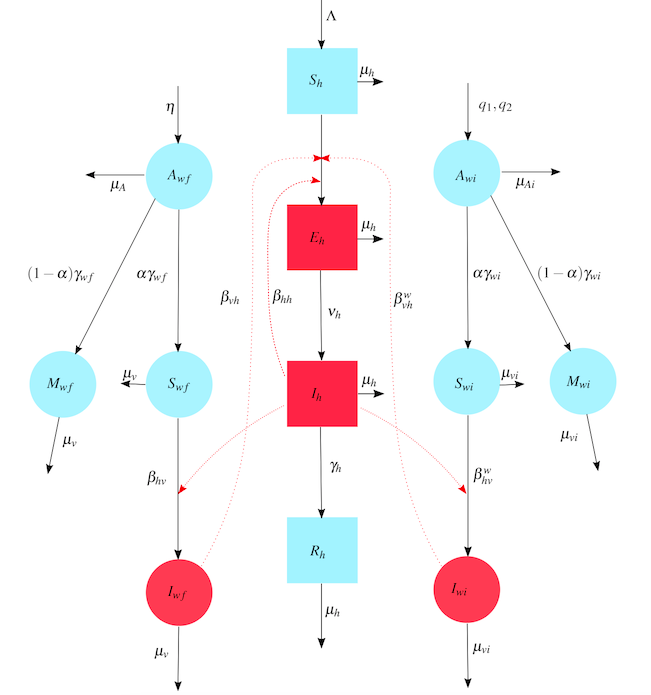
\includegraphics[scale=0.7]{diagram.png}
%    \caption{Diagram of the model. Squares represent human compartments and circles represent vector compartments. Infected compartments are colored red and infection pathway is represented by the red dotted lines.}
%    \label{fig:model-diagram}
%\end{figure}

\begin{figure}[H]
    \def\svgwidth{\columnwidth}
    \input{./fig/model_diagram/model_diagram.eps_tex}
    \caption{Diagram of the model. Squares represent human compartments and circles represent vector compartments. Infected compartments are colored red and infection pathway is represented by the red dotted lines.}
    \label{fig:model-diagram}
\end{figure}

\newpage
\section{Model Analysis}
Since the model simulates the dynamics of humans and mosquito populations, all the state variables and parameters must be non-negative. To show that the model is well posed, we need to show that when starting with non-negative initial values we remain with non-negative values for the variables for all future times.
\subsection{Well-posedness of the Model}
\begin{theorem}
Let $F:D \to \mathbb{R}^{12}$ be
$F(t,x)=(F_1(t,x), \dots, F_n(t,x))$ where
\begin{multline*}
\noindent D = \{(t, S_h, E_h, I_h, R_h, A_{wf}, S_{wf}, I_{wf}, M_{wf}, A_{wi}, S_{wi}, I_{wi}, M_{wi})\in \mathbb{R}^{13}_+ |\\ S_h \geq \epsilon_0, \epsilon_0 \leq N_h \leq \Lambda /\mu_h, A_{wf}, A_{wi}\leq K, N_v^{wf}\leq \gamma_{wf}K/\mu_v,N_v^{wi}\leq \gamma_{wi}K/\mu_{vi}\}
\end{multline*}
 for some $0< \epsilon_0 < \dfrac{\Lambda}{\mu_h}$ and where $N_h=S_h+E_h+I_h+R_h$, $N_v^{wf}=S_{wf} +I_{wf}+M_{wf}$ and $N_v^{wi}=S_{wi} +I_{wi}+M_{wi}$.
The system (\ref{eq:1})-(\ref{eq:12}) is epidemiologically and mathematically well-posed in the valid domain $D$.

%which is a feasible region for the system dynamics is positively invariant.
\end{theorem}

Proof: 
Since $F$ is continuously differentiable in $D$ we have that $F$ is locally Lipschitz in $D$. Then 
%by Theorem \ref{wpthm}, 
for any $(t_0,x_0)$ in $D$, there exists a unique solution passing through $(t_0,x_0)$.
%Then whenever $t\geq 0$, 

%$x=(S_h(t), E_h(t)$, $I_h(t), R_h(t), A_{wf}(t), S_{wf}(t), I_{wf}(t), M_{wf}(t), A_{wi}(t), S_{wi}(t), I_{wi}(t), M_{wi}(t)$) with $x_j=0$ we will show that $F_j(t,x)\geq 0$.
Now, assume that we start from positive values and at some point in time $t_1$ we have that $x_j=0$. Then as seen below, we have that $F_j(t_1,x) \geq 0$ which means that $x_j$ is nondecreasing and therefore returns to the positive quadrant or remains 0:

\noindent $\Lambda \geq 0, 
(\beta_{vh}I_{wf}+\beta^w_{vh}I_{wi}+\beta_{hh}I_h)\dfrac{S_h}{N_h} \geq 0,
 \nu_h E_h \geq 0,
\gamma_h I_h \geq 0,
\eta \dfrac{S_{wf}M_{wf}}{N_v}\left(1-\dfrac{A_{wi}}{K}\right)\geq 0,\\ A_{wi} \leq K,
\alpha \gamma_{wf}A_{wf} \geq 0,
 \beta_{hv}\dfrac{I_h}{N_h}S_{wf} \geq 0,
(1-\alpha)\gamma_{wf}A_{wf}\geq 0,\\
 S_{wi}\dfrac{(q_1M_{wi}+q_2M_{wf})}{N_v}\left(1-\dfrac{A_{wf}}{K}\right)\geq 0, A_{wf}\leq K,
     \alpha \gamma_{wi}A_{wi} \geq 0,
     \beta^w_{hv}\dfrac{I_h}{N_h}S_{wi} \geq 0,
     (1-\alpha)\gamma_{wi} A_{wi} \geq 0.$

%Then for every $x^0=(S_h(0), E_h(0), I_h(0), R_h(0), A_{wf}(0), S_{wf}(0), I_{wf}(0), M_{wf}(0), A_{wi}(0), S_{wi}(0), I_{wi}(0), M_{wi}(0))\in\mathbb{R}_+^{12}$, there exists a unique solution of $x'=F(t,x)$, $x(0)=x^0$, with values in $\mathbb{R}^{12}_+$, which is defined on some interval $[0,b)$. 
%If $b<\infty$, then 
%lim sup $\sum_{j=1}^n x_j(t)=\infty$.

Now we have that $0\leq S_h,E_h,I_h,R_h\leq N_h(t)$. Adding the first four equations we get $\dot{N_h(t)}=\Lambda-\mu_hN_h(t)$. Integrating and taking $\liminf$ and $\limsup$ for $t \to \infty$ we have
$$N_h(0)\leq \liminf N_h(t) = \limsup N_h(t) = \dfrac{\Lambda}{\mu_h}$$ which implies that $\lim N_h(t)=\dfrac{\Lambda}{\mu_h}.$ 

Now we will show the boundness of $A_{wf}$. We claim that $A_{wf}(t) \leq K$ for all $t.$
Suppose there exists a time $t_1$ such that $A_{wf}(t_1) > K$. Then $\dot{A}_{wf}(t_1) < 0$ which means that $A_{wf}$ is decreasing near $t_1$. Then we must have that $A_{wf}(t_1+\epsilon) < K$ for some $\epsilon > 0$ and thus $A_{wf}(t_1) \leq K$ which is a contradiction. Therefore $A_{wf}(t) \leq K$ for all $t$. Similarly, we have that $A_{wi}(t) \leq K$ for all $t$.

Adding equations (\ref{eq:6}) - (\ref{eq:8}) we have the following 
$\dot{N}_v^{wf}(t)=\gamma_{wf}A_{wf}(t)-\mu_vN_v^{wf}(t)$.
Since $A_{wf}(t) \leq K$, we get that $\dot{N}_v^{wf}(t)\leq \gamma_{wf}K-\mu_vN_v^{wf}(t)$. Separating variables and solving for $N_v^{wf}(t)$ we have
$$N_v(t)\leq \dfrac{\gamma_{wf}K}{\mu_v}+e^{-\mu_vt}\left(N_v^{wf}(0)-\dfrac{\gamma_{wf}K}{\mu_v}\right).$$ 
\noindent If $N_v^{wf}(0) \leq \dfrac{\gamma_{wf}K}{\mu_v}$, then, by previous inequality we have $N_v(t)\leq \dfrac{\gamma_{wf}K}{\mu_v}$ and thus $D$ is a positively-invariant set. If $N_v^{wf}(0) > \dfrac{\gamma_{wf}K}{\mu_v}$, then we have that $\dot{N}_v^{wf}\leq 0$ and the wild mosquito population is decreasing. Also, at $t$ goes to infinity we have that $N_v^{wf}(t)$ approaches $\dfrac{\gamma_{wf}K}{\mu_v}$. A similar argument holds for $N_v^{wi}(t)$. Therefore the solutions either enter $D$ in finite time or $N_v^{wf}(t)$ approaches $\dfrac{\gamma_{wf}K}{\mu_v}$ and $N_v^{wi}(t)$ approaches $\dfrac{\gamma_{wi}K}{\mu_{vi}}$,  thus $D$ is an attracting set. 

\subsection{Disease free and only wild mosquitoes present}
When there is no Zika present in the vectors or human population and no  mosquitoes are infected with \textit{Wolbachia} we obtain the following disease free equilibrium point $E^{(1)}$ is

\noindent $\left(\frac{\Lambda}{\mu_h},0,0,0,K\left(1-\frac{1}{R}\right),\frac{\alpha\gamma_{wf}}{\mu_v}K\left(1-\frac{1}{R}\right),0,\frac{(1-\alpha)\gamma_{wf}}{\mu_v}K\left(1-\frac{1}{R}\right),0,0,0,0\right)$ 

\noindent where $R=\dfrac{\eta \alpha (1-\alpha)\gamma_{wf}}{\mu_v (\gamma_{wf}+\mu_A)}$ denotes the offspring reproduction number of wild mosquitoes.

\begin{theorem}
If $R > 1$ then the equilibrium $E^{(1)}$ exists. If $R_w=\dfrac{q_2\alpha(1-\alpha)\gamma_{wi}}{\mu_{vi}(\gamma_{wi}+\mu_{Ai})R}< 1$ and $R_Z=\dfrac{\beta_{vh}\beta_{hv}\nu_h\alpha\mu_h\gamma_{wf}}{\Lambda\mu^2_v(\mu_h+\nu_h)(\gamma_h+\mu_h)}K\left(1-\dfrac{1}{R}\right)
    +\dfrac{\nu_h\beta_{hh}}{(\mu_h+\nu_h)(\gamma_h+\mu_h)} < 1$ then $E^{(1)}$ is locally asymptotically stable. If any of the last two inequalities is reversed, then $E^{(1)}$ is unstable. 
\end{theorem}
\begin{proof}
The Jacobian for the system evaluated at the equilibrium $E^{(1)}$ is a block matrix $J^{(1)}=\left(
\begin{array}{c|c}
    B & \bigstar\\
    \hline
    0 & C
\end{array}
\right)$ where  

\vspace{0.2in}
\noindent $B=\left(
\begin{array}{cccccccc}
 -\mu _h & 0 & -\beta _{\text{hh}} & 0 & 0 & 0 & -\beta _{\text{vh}} & 0 \\%row1
 0 & -e & \beta _{\text{hh}} & 0 & 0 & 0 & \beta _{\text{vh}} & 0  \\%row2
 0 & \nu _h & -f & 0 & 0 & 0 & 0 & 0 \\%row3
 0 & 0 & \gamma _h & -\mu _h & 0 & 0 & 0 & 0 \\%row4
 0 & 0 & 0 & 0 & -b-d & \frac{(1-\alpha)^2 \eta }{R} & c & \frac{\alpha ^2 \eta }{R}  \\
 0 & 0 & -a & 0 & \alpha  \gamma _{\text{wf}} & -\mu _v & 0 &
   0 \\
 0 & 0 & a & 0 & 0 & 0 & -\mu _v & 0 \\
 0 & 0 & 0 & 0 & (1-\alpha) \gamma _{\text{wf}} & 0 & 0 & -\mu _v\\
\end{array}
\right)$ and

\vspace{0.2in}
\noindent $C=\left(
\begin{array}{cccc} -\mu _{\text{Ai}}-\gamma _{\text{wi}} &
   \frac{(1-\alpha) q_2}{R} & 0 & 0 \\
  \alpha  \gamma _{\text{wi}} & -\mu _{\text{vi}} & 0
   & 0 \\
  0 & 0 & -\mu _{\text{vi}} & 0 \\
  (1-\alpha) \gamma _{\text{wi}} & 0 & 0 & -\mu
   _{\text{vi}} \\
\end{array}
\right).$ 

\noindent Here the following notations were made first:
\vspace{0.2in}
\noindent $a=\dfrac{\alpha  K (R-1) \mu _h \beta _{\text{hv}} \gamma
   _{\text{wf}}}{\Lambda  R \mu _v}$, $b=\dfrac{(1-\alpha) \alpha  \eta  (R-1) \gamma _{\text{wf}}}{R
   \mu _v}$, $c=-\dfrac{(1-\alpha) \alpha  \eta }{R}$, $d=\mu _A+\gamma _{\text{wf}}$, $e=\mu _h+\nu _h$, $f=\gamma _h+\mu _h$, $g=\dfrac{(1-\alpha)q_2}{R}$ 
   and $h=-\mu_{Ai}-\gamma_{wi}$.\\
   
   The eigenvalues of the Jacobian will be the eigenvalues of matrix $B$ and matrix $C$. In order for the eigenvalues of $C$ to have negative real part, the determinant must be positive. This means that 
$\dfrac{\eta \mu_{vi}\gamma_{wf}(\gamma_{wi}+\mu_{Ai})}{q_2\gamma_{wi}\mu_v(\gamma_{wf}+\mu_A)}>1$. This can be written as $\dfrac{R_w}{R}<1$ where $R_w=\dfrac{q_2\alpha(1-\alpha)\gamma_{wi}}{\mu_{vi}(\gamma_{wi}+\mu_{Ai})}$ and can be interpreted as the invasion number of \textit{Wolbachia} infected mosquitoes in absence of disease. 

The characteristic polynomial corresponding to $B$ is
$P(\lambda)=(\mu_v+\lambda)P_1(\lambda)P_2(\lambda)$ where $P_1(\lambda)=-(b+d+\lambda)(\mu_v+\lambda)+\mu_v(\gamma_{wf}+\mu_A)$ and $P_2(\lambda)=\beta_{vh}\nu_ha-(\mu_v+\lambda)\left[(e+\lambda)(f+\lambda)-\nu_h\beta_{hh}\right].$ After substitutions, we have that all roots of $P_1(\lambda)=0$ have negative real part.

Rewriting $P_2(\lambda)=0$ we get that $(\mu_v+\lambda)(e+\lambda)(f+\lambda)=\beta_{vh}\nu_h\dfrac{\alpha  K (R-1) \mu _h \beta _{\text{hv}} \gamma
   _{\text{wf}}}{\Lambda  R \mu _v}+(\mu_v+\lambda)\nu_h\beta_{hh}.$ Then we will have
   $$\dfrac{\beta_{vh}\nu_h\alpha  K (R-1) \mu _h \beta _{\text{hv}} \gamma
   _{\text{wf}}}{\Lambda  R \mu _v(\mu_v+\lambda)(e+\lambda)(f+\lambda)}+\dfrac{(\mu_v+\lambda)\nu_h\beta_{hh}}{(\mu_v+\lambda)(e+\lambda)(f+\lambda)}=1.$$ 
   Define 
   \begin{align*}
       G(\lambda) &= \dfrac{\beta_{vh}\nu_h\alpha  K (R-1) \mu _h \beta _{\text{hv}} \gamma
   _{\text{wf}}}{\Lambda  R \mu _v(\mu_v+\lambda)(e+\lambda)(f+\lambda)}+\dfrac{\nu_h\beta_{hh}}{(e+\lambda)(f+\lambda)}\\
   &= \dfrac{\beta_{vh}\beta_{hv}\alpha\mu_h\gamma_{wf}}{\Lambda\mu_v(\mu_v+\lambda)(e+\lambda)(f+\lambda)}K\left(1-\dfrac{1}{R}\right)+\dfrac{\nu_h\beta_{hh}}{(e+\lambda)(f+\lambda)}.
   \end{align*}

We define the reproduction number of Zika in absence of \textit{Wolbachia} infected mosquitoes $R_Z=G(0)$, that is,
$$R_Z=\dfrac{\beta_{vh}\beta_{hv}\nu_h\alpha\mu_h\gamma_{wf}}{\Lambda\mu^2_v(\mu_h+\nu_h)(\gamma_h+\mu_h)}K\left(1-\dfrac{1}{R}\right)
    %\underbrace{K\left(1-\dfrac{1}{R}\right)}_{=A^{(1)}_{wf}}
    +\dfrac{\nu_h\beta_{hh}}{(\mu_h+\nu_h)(\gamma_h+\mu_h)}.$$
Furthermore, let $\dfrac{\nu_h\beta_{vh}\beta_{hv}\alpha\mu_h\gamma_{wf}}{\Lambda\mu^2_v(\mu_h+\nu_h)(\gamma_h+\mu_h)}K\left(1-\dfrac{1}{R}\right)=R^{wf}_Z$ and $\dfrac{\nu_h\beta_{hh}}{(\mu_h+\nu_h)(\gamma_h+\mu_h)}=R_d$. Then we have that $R_Z=G(0)=R^{wf}_Z+R_d.$ 
If $R_Z>1$, then the characteristic equation has a real positive root because $G(0)=R_Z>1$ and $G(\lambda)$ is a decreasing function of $\lambda$ with $\lim_{\lambda \to \infty}G(\lambda)=0$ where $\lambda$ is assumed to be real. However, if $R_Z<1$, then all roots have negative real parts. To see this, we assume that there is a $\lambda$ with $Re(\lambda) \geq 0$. Then we have the following
\begin{align*}
|G(\lambda)|&\leq \dfrac{\beta_{vh}\beta_{hv}\alpha\mu_h\gamma_{wf}}{\Lambda\mu_v(|\mu_v+\lambda|) (|e+\lambda|) (|f+\lambda|)}K\left(1-\dfrac{1}{R}\right)+\dfrac{\nu_h\beta_{hh}}{(|e+\lambda|) (|f+\lambda|)}\\
& \leq G(Re(\lambda)) \leq G(0)=R_Z <1
\end{align*}
Therefore, $|G(\lambda)|<1$ and such a $\lambda$ with nonnegative real part cannot be a solution to the characteristic equation.
\end{proof}

\subsection{Disease free and only \textit{Wolbachia} infected mosquitoes present}
When there is no Zika present in the vectors or human population and all  mosquitoes are infected with \textit{Wolbachia} we have the following disease free equilibrium point $E^{(2)}$ is

\noindent $\left(\frac{\Lambda}{\mu_h},0,0,0,K\left(1-\frac{1}{M}\right),\frac{\alpha\gamma_{wi}}{\mu_{vi}}K\left(1-\frac{1}{M}\right),0,\frac{(1-\alpha)\gamma_{wi}}{\mu_{vi}}K\left(1-\frac{1}{M}\right),0,0,0,0\right)$ where $M=\dfrac{q_1 \alpha (1-\alpha)\gamma_{wi}}{\mu_{vi} (\gamma_{wi}+\mu_{Ai})}$ is the offspring reproduction number of \textit{Wolbachia} infected mosquitoes. Note we rearranged the equations such that the equations for \textit{Wolbachia} infected mosquitoes are appearing before the \textit{Wolbachia} free mosquitoes.

\begin{theorem}
If $M>1$ then $E^{(2)}$ exists. If $$R^i_Z=\dfrac{\beta^w_{vh}\beta^w_{hv}\nu_h\alpha \mu_h\gamma_{wi}}{\Lambda \mu^2_{vi}(\mu_h+\nu_h)(\gamma_h+\mu_h)}K\left(1-\dfrac{1}{M}\right)+\dfrac{\nu_h\beta_{hh}}{(\mu_h+\nu_g)(\gamma_h+\mu_h)}<1$$ then $E^{(2)}$ is locally asymptotically stable. If $R^i_Z>1$ then $E^{(2)}$ is unstable. 
\end{theorem}
\begin{proof}
The Jacobian of the system evaluated at $E^{(2)}$  is $J^{(2)}=\left(
\begin{array}{c|c}
    D & \bigstar\\
    \hline
    0 & E
\end{array}
\right)$ where 

\vspace{0.2in}
\noindent $D=\left(
\begin{array}{cccccccc}
 -\mu _h & 0 & -\beta _{\text{hh}} & 0 & 0 & 0 & -\beta^w_{vh} & 0 \\
 0 & -e & \beta _{\text{hh}} & 0 & 0 & 0 & \beta^w_{vh} & 0 \\
 0 & \nu _h & -f & 0 & 0 & 0 & 0 & 0 \\
 0 & 0 & \gamma _h & -\mu _h & 0 & 0 & 0 & 0 \\
 0 & 0 & 0 & 0 & -(n+h) & \frac{(1-\alpha)^2
   q_1}{M} & -r & \frac{\alpha ^2 q_1}{M} \\
 0 & 0 & -g & 0 & \alpha  \gamma _{\text{wi}} &
   -\mu _{\text{vi}} & 0 & 0 \\
 0 & 0 & g & 0 & 0 & 0 & -\mu _{\text{vi}} & 0 \\
 0 & 0 & 0 & 0 & (1-\alpha) \gamma _{\text{wi}} & 0 & 0 & -\mu _{\text{vi}}\\
\end{array}
\right)$ and

\vspace{0.2in}
\noindent $E=\left(
\begin{array}{cccc}
-d & 0 & 0 & 0 \\
\alpha  \gamma _{\text{wf}} & -\mu _v & 0 & 0 \\
0 & 0 & -\mu _v & 0\\
(1-\alpha) \gamma _{\text{wf}} & 0 & 0 & -\mu _v\\
\end{array}
\right).$

\noindent The matrix $E$ has four obvious negative eigenvalues equal to the diagonal entries $-d$ and $-\mu_v$.
The matrix $D$ has two negative eigenvalues equal to $-\mu_h$. Let $D^*$ be the matrix $D$ after removing the column and row corresponding to the two eigenvalues equal to $-\mu_{h}$. 

The characteristic polynomial of the matrix $D^*$ is $P(\lambda)=(\mu_{vi}+\lambda)P_1(\lambda)P_2(\lambda)$
where $$P_1(\lambda)= \dfrac{q_1\alpha(1-\alpha)\gamma_{wi}}{M}-(n+h+\lambda)(\mu_{vi}+\lambda)$$ and $$P_2(\lambda)=\beta^w_{vh}\nu_h g-(\mu_{vi}+\lambda)[(e+\lambda)(f+\lambda)-\nu_h\beta_{hh}].$$

\noindent It can be easily shown that the roots of $P_1(\lambda)=0$ are negative when $M > 1$.

The characteristic equation corresponding to $P_2(\lambda)$ is 
$$P_2(\lambda)=\beta^w_{vh}\nu_h g-(\mu_{vi}+\lambda)[(e+\lambda)(f+\lambda)-\nu_h\beta_{hh}]=0$$
and it can be written as
$$\dfrac{\beta^w_{vh}\nu_h g}{(\mu_{vi}+\lambda)(e+\lambda)(f+\lambda)}+\dfrac{\nu_h\beta_{hh}}{(e+\lambda)(f+\lambda)}=1.$$

\noindent Define
    $G(\lambda) = \dfrac{\beta^w_{vh}\nu_h g}{(\mu_{vi}+\lambda)(e+\lambda)(f+\lambda)}+\dfrac{\nu_h\beta_{hh}}{(e+\lambda)(f+\lambda)}$.
    We define the reproduction number of Zika in absence of wild mosquitoes as $R_Z^i=G(0)$. Substituting the values of e, f and $g=\dfrac{\alpha  K (M-1) \mu_h \gamma_{\text{wi}} \beta^w_{hv}}{\Lambda  M \mu_{\text{vi}}}$, we get
$$R_Z^i=\dfrac{\beta^w_{vh}\beta^w_{hv}\nu_h\alpha \mu_h\gamma_{wi}}{\Lambda \mu^2_{vi}(\mu_h+\nu_h)(\gamma_h+\mu_h)}K\left(1-\dfrac{1}{M}\right)+\dfrac{\nu_h\beta_{hh}}{(\mu_h+\nu_g)(\gamma_h+\mu_h)}.$$ Furthermore, let $\dfrac{\beta^w_{vh}\beta^w_{hv}\nu_h\alpha \mu_h\gamma_{wi}}{\Lambda \mu^2_{vi}(\mu_h+\nu_h)(\gamma_h+\mu_h)}K\left(1-\dfrac{1}{M}\right)=R_Z^{wi}$. Then we have that $R_Z^i=R_Z^{wi}+R_d$. If $R_Z^i > 1$, then the characteristic equation has a real positive root because $G(0)=R_Z^i>1$ and $G(\lambda)$ is a decreasing function of $\lambda$ with $\lim_{\lambda \to \infty}G(\lambda)=0$ where $\lambda$ is assumed to be real. However, if $R_Z^i <1$, then all roots have negative real parts. To see this we assume there is a $\lambda$ with $Re(\lambda) \geq 0$. Then we have the following
\begin{align*}
|G(\lambda)|&\leq \dfrac{\beta^w_{vh}\nu_h g}{(|\mu_{vi}+\lambda|)(|e+\lambda|)(|f+\lambda|)}+\dfrac{\nu_h\beta_{hh}}{(|e+\lambda|)(|f+\lambda|)}\\
    & \leq G(Re(\lambda)) \leq G(0)=R_Z^{i}<1.
\end{align*}  
Therefore, $G(\lambda)<1$ and such a $\lambda$ with a nonnegative real part cannot be a solution to the characteristic equation.

\end{proof}



\subsection{Disease free and both types of mosquitoes present}
When there is no Zika present in the vectors or human population but some  mosquitoes are infected with \textit{Wolbachia} we have the following disease free equilibrium point $E^{(3)}$ is

\noindent $\left(\frac{\Lambda}{\mu_h},0,0,0,A^{(3)}_{wf},\frac{\alpha \gamma_{wf}A^{(3)}_{wf}}{\mu_v},0,\frac{(1-\alpha)\gamma_{wf}A^{(3)}_{wf}}{\mu_v},CA^{(3)}_{wf},\frac{\alpha\gamma_{wi}CA^{(3)}_{wf}}{\mu_{vi}},0,\frac{(1-\alpha)\gamma_{wi}CA^{(3)}_{wf}}{\mu_{vi}}\right)$ where $C=\dfrac{\gamma_{wf}\mu_{vi}R}{\gamma_{wi}\mu_vM}\left(1-\dfrac{R_w}{R}\right)$, $A^{(3)}_{wf}=\dfrac{K}{1+C}\left( 1-\dfrac{1}{R}-\dfrac{1}{M}\left(1-\dfrac{R_w}{R}\right)\right)$ and for $A^{(3)}_{wf}$ to exist we must have that $\dfrac{1}{R}+\dfrac{1}{M}\left(1-\dfrac{R_w}{R}\right)<1$. 

The stability of this disease free equilibrium can be established using the next generation matrix. The infected compartments are $E_h$, $I_h$, $I_{wf}$ and $I_{wi}$ ordered $(E_h, I_h, I_{wf}, I_{wi})$. The nonlinear terms with new infections $\mathcal{F}$ and the outflow term $\mathcal{V}$ are given by

\vspace{0.2in}
$\mathcal{F}=\left(\begin{array}{c}
     (\beta_{vh}I_{wf}+\beta^w_{vh}I_{wi}+\beta_{hh}I_h)\dfrac{S_h}{N_h}  \\
     0\\
     \beta_{hv}\dfrac{I_h}{N_h}S_{wf}\\
     \beta^w_{hv}\dfrac{I_h}{N_v}S_{wi}
\end{array}\right)$
 and $\mathcal{V}=\left(\begin{array}{c}
      (\nu_h+\mu_h)E_h \\
      -\nu_hE_h+(\gamma_h+\mu_h)I_h\\
      \mu_vI_{wf}\\
      \mu_{vi}I_{wi}      
 \end{array}\right)$.
 
 \vspace{0.2in}

 \noindent The next generation matrix is 
 
  \vspace{0.2in}
 $\mathcal{K}=FV^{-1}=\left(\begin{array}{cccc}
      \dfrac{\beta_{hh}\nu_h}{(\gamma_h+\mu_h)(\nu_h+\mu_h)} & \dfrac{\beta_{hh}}{\gamma_h+\mu_h} & \dfrac{\beta_{vh}}{\mu_v} & \dfrac{\beta^w_{vh}}{\mu_{vi}}  \\
      0& 0 & 0 & 0\\
      \dfrac{\nu_h\beta_{hv}\mu_hS^{(3)}_{wf}}{\Lambda(\gamma_h+\mu_h)(\nu_h+\mu_h)}& \dfrac{\beta_{hv}\mu_hS^{(3)}_{wf}}{\Lambda(\gamma_h+\mu_h)} & 0 &0\\
       \dfrac{\nu_h\beta^w_{hv}\mu_hS^{(3)}_{wi}}{\Lambda(\gamma_h+\mu_h)(\nu_h+\mu_h)}& \dfrac{\beta^w_{hv}\mu_hS^{(3)}_{wi}}{\Lambda(\gamma_h+\mu_h)} & 0 &0
 \end{array}\right).$\\
 
 \vspace{0.2in}
 
 \noindent The reproduction of Zika in presence of both types of mosquitoes denoted by $R_{0Z}^{NG}$ is given by the spectral radius of $\mathcal{K}$. So $R_{0Z}^{NG}=\rho(\mathcal{K}).$
 
 The characteristic polynomial corresponding to $\mathcal{K}$ is $t^2-R_dt-q=0$
where

 $q=\dfrac{1}{1+C}\left( 1-\dfrac{1}{R}-\dfrac{1}{M}\left(1-\dfrac{R_w}{R}\right)\right)\left(\dfrac{R^{wf}_Z}{1-1/R}+C\dfrac{R^{wi}_Z}{1-1/M}\right)$ and it is clearly positive when $R>1$, $M>1$ and $\dfrac{1}{R}+\dfrac{1}{M}\left(1-\dfrac{R_w}{R}\right)<1$. The solutions for this quadratic are given by $t=\dfrac{R_d \pm\sqrt{R_d^2+4q}}{2}$.
 Therefore the reproduction number of Zika in presence of both types of mosquitoes defined using the next generation method, $R_{0Z}^{NG}$, is the spectral radius of $\mathcal{K}$ which equals the largest positive solution of the characteristic equation. Thus we have that
 $$R_{0Z}^{NG}=\dfrac{R_d+\sqrt{R_d^2+\dfrac{4}{1+C}\left( 1-\dfrac{1}{R}-\dfrac{1}{M}\left(1-\dfrac{R_w}{R}\right)\right)\left(\dfrac{R^{wf}_Z}{1-1/R}+C\dfrac{R^{wi}_Z}{1-1/M}\right)}}{2}.$$
 
 
\noindent This reproduction number of Zika in presence of both type of mosquitoes derived by the next-generation approach serves as a threshold condition for the stability of the disease free equilibrium but it is not an easy task to interpret it epidemiologically. From \cite{van2002reproduction} we have:

\begin{theorem}
If $R_{0Z}^{NG}<1$, the disease free equilibrium $E^{(3)}$ is locally asymptotically stable; otherwise, it is unstable.
\end{theorem}

\subsection{Zika present and no \textit{Wolbachia} infected mosquitoes present}
We express all the state variables in terms of $I_h$ and then arrive at an equation in terms of $R_Z$ and $I_h$:
$$AI^2_h+BI_h+Rb\Lambda^3\mu^3_v(R_Z-1)=0$$ where

\noindent $A=b^2R^2\mu^2_v\Lambda\mu_h\beta_{hv}\left(\dfrac{R_Z/R-R_d}{\nu_h(R-1)}\right)$
 and 
\begin{multline*}
B=-\dfrac{\Lambda^2\beta_{hv}\mu_hR\mu^2_v(bR_Z-\nu_h\beta_{hh})}{(R-1)}-\dfrac{b\Lambda^2 \mu^3_vR(bR_Z-\nu_h\beta_{hh})}{\nu_h}+\\
     +\beta_{hh}R\mu^2_v\Lambda^2\nu_h\beta_{hv}\mu_h-b\beta_{hh}\mu^3_v\Lambda^2R-bR\mu^2_v\Lambda^2\beta_{hv}\mu_h.
 \end{multline*}
Using the Sign of the Derivative Method \cite{martcheva2019methods}, we differentiate the quadratic equation implicitly with respect to $R_Z$ and evaluate at $I_h=0$ and $R_Z=1$, to obtain the following
$\dfrac{\partial I_h}{\partial R_Z}B_*+Rb\Lambda^3\mu^3_v=0$ where $B_*$ is the coefficient of $I_h$ evaluated at $R_Z=1.$

\noindent Furthermore, calculations give that $B_*=Rb\Lambda^2\mu_v^2\left[\dfrac{\beta_{hv}\mu_hR(R_d-1)}{R-1}-\dfrac{\mu_v(\gamma_h+\mu_h)(\nu_h+\mu_h)}{\nu_h}\right].$

\noindent Solving for the derivative we get 
    $\dfrac{\partial I_h}{\partial R_Z}
    =\dfrac{-\Lambda\mu_v\nu_h(R-1)}{\beta_{hv}\mu_h\nu_hR(R_d-1)-\mu_v(\gamma_h+\mu_h)(\nu_h+\mu_h)(R-1)}$ and observe that the derivative is always positive since $R>1$ and $R_d<1$.
\begin{comment}
Figure \ref{fig:bbif} shows forward bifurcation at the critical value $R_Z=1$, in which case an endemic equilibrium exists if and only if $R_Z >1$.

\begin{figure}[h]
\centering
  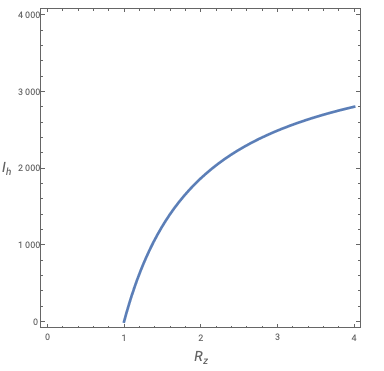
\includegraphics[scale=0.4]{forwardbif.png}
  \caption{Forward bifurcation  at the critical value $R_Z=1$
  %, in which case there are two endemic equilibria for $R^*_Z<R_Z<1$ and one endemic equilibria if $R_Z\geq 1$
  }
  \label{fig:bbif}
\end{figure}
\end{comment}

\begin{theorem}
In presence of wild mosquitoes only the system admits an unique endemic equilibrium, $E^{(4)}$, when $R_Z>1.$
 
 %There is one unique solution when $R_Z>1$.  These 0, 1, or 2 $I_h$ equilibria lead to corresponding equilibria of the model if also $I_h<\dfrac{\Lambda\nu_h}{b}$ and $I_h<\dfrac{\Lambda\mu_v(R-1)}{\beta_{hv}\mu_h}.$
\end{theorem}
\subsection{Zika present and no wild mosquitoes present}
When there is Zika present in the human population and in the mosquito population that is composed of only \textit{Wolbachia} infected mosquitoes we have the following equilibrium point 
$$E^{(5)}=(S^{(5)}_h,E^{(5)}_h,I^{(5)}_h,R^{(5)}_h,A^{(5)}_{wi},S^{(5)}_{wi},I^{(5)}_{wi},M^{(5)}_{wi},0,0,0,0).$$ 
Note that we rearranged the system again as it was done in a previous section.
We express all the state variables in terms of $I_h$ and then arrive at an equation in terms of $R^i_Z$ and $I_h$:
\begin{multline*}
I^2_h\left(b^2M^2\mu^2_{vi}\Lambda\mu_h\beta^w_{hv}\left(\dfrac{R^i_Z/M-R_d}{\nu_h(M-1)}\right)\right)+\\ I_h(-\Lambda\beta^w_{hv}\mu_hM\Lambda\mu^2_{vi}\dfrac{(bR^i_Z-\nu_h\beta_{hh})}{(M-1)}-b\Lambda M\Lambda\mu^3_{vi}\dfrac{(bR^i_Z-\nu_h\beta_{hh})}{\nu_h}+\\
\beta_{hh}\mu^2_{vi}\Lambda^2\nu_hM\mu_h\beta^w_{hv}-b\beta_{hh}\Lambda^2\mu^3_{vi}M-b\Lambda^2\mu^2_{vi}M\mu_h\beta^w_{hv})+
Mb\Lambda^3\mu^3_{vi}(R^{i}_Z-1)=0
\end{multline*}

\begin{theorem}
 In presence of only Wolbachia infected mosquitoes the system admits an unique endemic equilibrium, $E^{(5)}$, when $R^i_Z>1$. 
\end{theorem}
\subsection{Zika present and both types of mosquitoes present}
When there is Zika present in the human population and in the mosquito population that is composed of both \textit{Wolbachia} free and \textit{Wolbachia} infected mosquitoes we have the following equilibrium point 
   $$E^{(6)}=(S^{(6)}_h,E^{(6)}_h,I^{(6)}_h,R^{(6)}_h,A^{(6)}_{wf},S^{(6)}_{wf},I^{(6)}_{wf},M^{(6)}_{wf},A^{(6)}_{wi},S^{(6)}_{wi},I^{(6)}_{wi},M^{(6)}_{wi}).$$ We will explore this equilibrium using numerical simulations since this equilibrium is too complex to deal with analytically.
 \subsection{Overview of equilibria}
 Here is an overview of the equilibria with conditions for existence and stability listed in Table \ref{eqtable}.
 
\noindent $E^{(1)}=\\
\left(\frac{\Lambda}{\mu_h},0,0,0,K\left(1-\frac{1}{R}\right),\frac{\alpha\gamma_{wf}}{\mu_v}K\left(1-\frac{1}{R}\right),0,\frac{(1-\alpha)\gamma_{wf}}{\mu_v}K\left(1-\frac{1}{R}\right),0,0,0,0\right).$

\noindent $E^{(2)}=\\
\left(\frac{\Lambda}{\mu_h},0,0,0,K\left(1-\frac{1}{M}\right),\frac{\alpha\gamma_{wi}}{\mu_{vi}}K\left(1-\frac{1}{M}\right),0,\frac{(1-\alpha)\gamma_{wi}}{\mu_{vi}}K\left(1-\frac{1}{M}\right),0,0,0,0\right).$
 
\noindent$E^{(3)}=\\
\left(\frac{\Lambda}{\mu_h},0,0,0,A^{(3)}_{wf},\frac{\alpha \gamma_{wf}A^{(3)}_{wf}}{\mu_v},0,\frac{(1-\alpha)\gamma_{wf}A^{(3)}_{wf}}{\mu_v},CA^{(3)}_{wf},\frac{\alpha\gamma_{wi}CA^{(3)}_{wf}}{\mu_{vi}},0,\frac{(1-\alpha)\gamma_{wi}CA^{(3)}_{wf}}{\mu_{vi}}\right)$.

\noindent$E^{(4)}=(S^{(4)}_h,E^{(4)}_h,I^{(4)}_h,R^{(4)}_h,A^{(4)}_{wf},S^{(4)}_{wf},I^{(4)}_{wf},M^{(4)}_{wf},0,0,0,0)$.

\noindent$E^{(5)}=(S^{(5)}_h,E^{(5)}_h,I^{(5)}_h,R^{(5)}_h,A^{(5)}_{wi},S^{(5)}_{wi},I^{(5)}_{wi},M^{(5)}_{wi},0,0,0,0)$.

\noindent$E^{(6)}=(S^{(6)}_h,E^{(6)}_h,I^{(6)}_h,R^{(6)}_h,A^{(6)}_{wf},S^{(6)}_{wf},I^{(6)}_{wf},M^{(6)}_{wf},A^{(6)}_{wi},S^{(6)}_{wi},I^{(6)}_{wi},M^{(6)}_{wi})$.

\vspace{0.1in}

Table \ref{eqtable} summarizes the results of the analysis. Besides simulations, no analysis was done for equilibria $E^{(4)}$, $E^{(5)}$ and $E^{(6)}$, hence the n/a values listed in the table.
\begin{table}[H]
\centering
\caption{Overview of equilibria and their conditions for stability:\\
 DF = Disease free,\\
 WF = \textit{Wolbachia} free mosquitoes present,\\
 DP = Disease present, WI = \textit{Wolbachia} infected mosquitoes present.
} 
\begin{tabular}{C{1.1cm}  c C{2.25cm} C{2cm} C{2cm} } 
 \toprule
 Equilibrium & Description & Existence Conditions & Stability Conditions & Instability Conditions\\ 
  \midrule
 $E^{(1)}$ & DF, WF & $R>1$ & $R_w/R<1$, $R_Z <1$ & $R_w/R>1$ or $R_Z>1$ \\ 
 \midrule
 $E^{(2)}$ & DF, WI & $M>1$ & $R^i_Z<1$ & $R^i_Z>1$\\ 
 \midrule
 $E^{(3)}$ & DF, WF, WI & $R_w/R<1$, $R>1$, $M>1$ & $R_{0Z}<1$ & $R_{0Z}>1$\\ 
 \midrule
 $E^{(4)}$ & DP, WF & $R>1$, $R_Z>1$ & n/a & n/a\\ 
 \midrule
 $E^{(5)}$ & DP, WI & $M>1$, $R_Z^i>1$ & n/a & n/a\\ 
 \midrule
 $E^{(6)}$ & DP, WF, WI & $R>1$,$M>1$  & n/a & n/a\\ 
 \bottomrule
\end{tabular}
\label{eqtable}
\end{table}

\section{Numerical Simulations}
\label{simulations}

%\textcolor{blue}{Figure out how to organize and name these sections. Make it more clear what the figures address (what is their purpose, what question they answer) and how you obtained them (what parameters and initial conditions are same/different. You got this!! You did it for an hour. Lets do it for 2 tomorrow :) }

The model is simulated, using the parameter values and ranges from Table \ref{tab: param-table} and Table \ref{tab: param_mosq_table}. We are assuming that there are already some \textit{Wolbachia} infected mosquitoes present and we are trying to determine what ratio of \textit{Wolbachia} infected to \textit{Wolbachia} free mosquitoes should be attained at the time of release of additional \textit{Wolbachia} infected mosquitoes in order to get a desired outcome.

\subsection{Numerical simulation for disease free equilibria}

First, we begin with the disease free equilibria.
Our goal is to determine under what circumstances \textit{Wolbachia} establishes itself in the wild mosquito population and if it does how does that affect Zika dynamics within the human and mosquito populations.

\subsubsection{\textit{Wolbachia} fails to establish when starting with same amount of wild and \textit{Wolbachia} infected mosquitoes}\label{diseasefreefirst} 

Running simulations using the baseline values for parameters from Table \ref{tab: param-table} and Table \ref{tab: param_mosq_table} and the initial conditions listed in Table \ref{init-cond-dis-free-table}  yields to failure of \textit{Wolbachia} infection to establish itself in the wild mosquito population. Notice that we start with the same amount of wild mosquitoes and \textit{Wolbachia} infected mosquitoes. Also, we chose to start with $2.5$ mil Zika infected humans to emphasize convergence to the disease free equilibrium even for high level of initial infection.


\begin{table}[h]
\centering
\caption{Initial conditions for disease free simulations
} 
\label{init-cond-dis-free-table}
\begin{tabular}{ c c c c } 
 \toprule
 Variable & Initial value & Variable & Initial value\\ 
  \midrule
 $S_h(0)$ & 10,000,000 & $I_{wf}(0)$ & 50,000\\
 $E_h(0)$ & 3,000,000 & $M_{wf}(0)$ & 250,000\\
 $I_h(0)$ & 2,500,000 & $A_{wi}(0)$ & 500,000 \\
 $R_h(0)$ & 10,000 & $S_{wi}(0)$ & 250,000 \\
 $A_{wf}(0)$ & 500,000 & $I_{wi}(0)$ & 50,000 \\
 $S_{wf}(0)$ & 250,000 & $M_{wi}(0)$ & 250,000\\
 \bottomrule
\end{tabular}
%\label{eqtable}
\end{table}

Notice in Figure \ref{fig:domwolbachiafree} 
that \textit{Wolbachia} free mosquitoes persist and the \textit{Wolbachia} infected mosquitoes are eliminated in approximately 200 days. The disease is eradicated in approximately 250 days in both humans and wild mosquitoes. This corresponds to steady state $E^{(1)}$ where wild mosquitoes persists and \textit{Wolbachia} infection fails to establish.

%\begin{figure}[h]
%    \centering
    %\hskip-0.75in
%    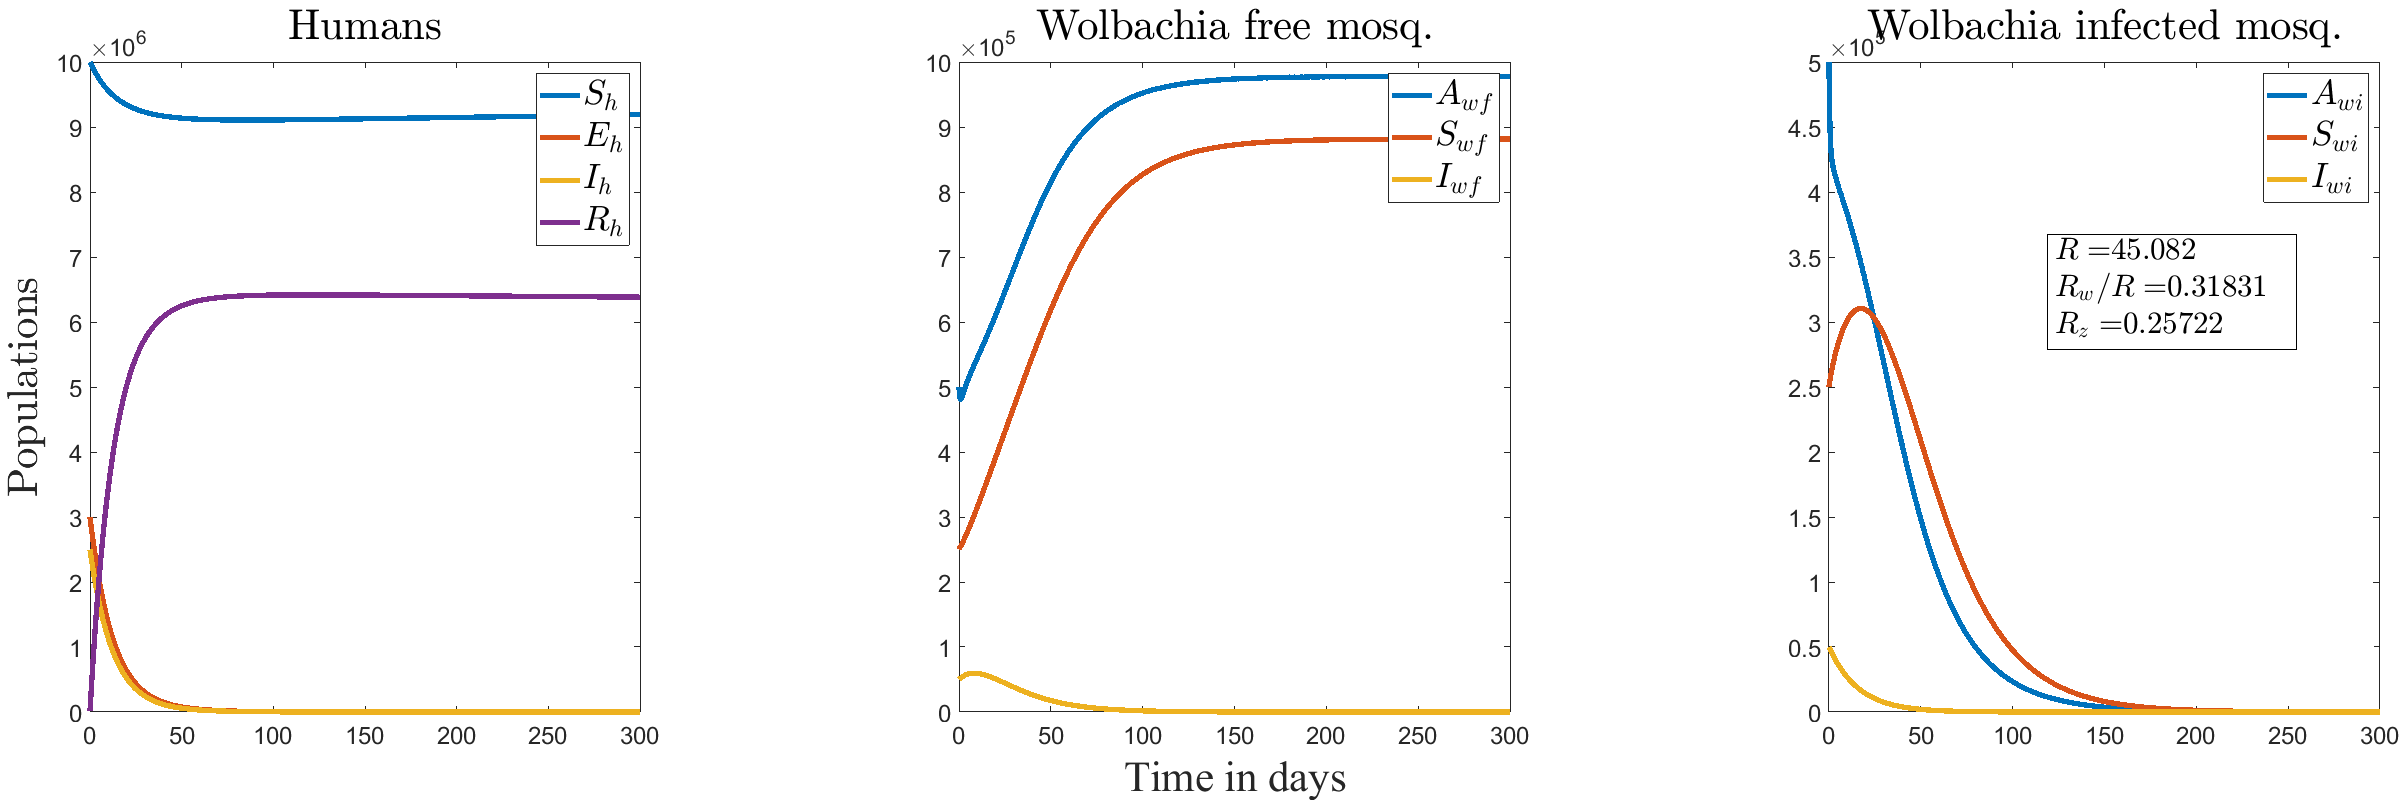
\includegraphics[width=16cm,height=4.5cm]{SimFig1.png}
%    \caption{Dominance of \textit{Wolbachia} free mosquitoes. Figure  obtained using baseline values for parameters from Table \ref{tab: param-table} and Table \ref{tab: param_mosq_table} and the initial conditions listed in Table \ref{init-cond-dis-free-table}}
%    \label{fig:domwolbachiafree}
%\end{figure}

\begin{figure}[H]
    \centering
    % This file was created by matlab2tikz.
%
%The latest updates can be retrieved from
%  http://www.mathworks.com/matlabcentral/fileexchange/22022-matlab2tikz-matlab2tikz
%where you can also make suggestions and rate matlab2tikz.
%
\definecolor{mycolor1}{rgb}{0.00000,0.44700,0.74100}%
\definecolor{mycolor2}{rgb}{0.85000,0.32500,0.09800}%
\definecolor{mycolor3}{rgb}{0.92900,0.69400,0.12500}%
\definecolor{mycolor4}{rgb}{0.49400,0.18400,0.55600}%
%
\begin{tikzpicture}

\begin{axis}[%
width=1.1in,
height=1.5in,
at={(0in,0.108in)},
scale only axis,
xmin=0,
xmax=400,
ymin=0,
ymax=10000000,
ylabel={Population},
xticklabels={0,,100,,300,}, 
axis background/.style={fill=white},
title style={font=\bfseries, yshift=1.75ex},
title={Humans},
legend style={legend cell align=left, align=left, draw=white!15!black}
]
\addplot [color=mycolor1, line width=1.5pt]
  table[row sep=crcr]{%
0	10000000\\
0.626967288553715	9961687.87102005\\
1.32091695442796	9921364.74584687\\
2.00023053400218	9883893.14642212\\
2.59118748828769	9852818.20446228\\
3.35279129445553	9814743.40756324\\
3.9514775518328	9786290.61172597\\
4.64111419767141	9755037.77697592\\
5.45807606913149	9720005.11508451\\
6.40236316621304	9682027.82807787\\
7.38695567660034	9645096.01283487\\
8.15562911890447	9618023.07314091\\
8.92430256120861	9592392.88590323\\
9.60581782460213	9570806.78134412\\
10.287333086133	9550232.05846839\\
11.1878527402878	9524508.15663064\\
12.0883723944426	9500345.9456171\\
12.9753445517272	9477972.24891056\\
13.8352217152715	9457544.2371108\\
14.6010584905744	9440332.28633347\\
15.3328458424658	9424700.39734773\\
16.0588876530528	9409935.85694058\\
16.8074878118932	9395448.0191068\\
17.6290432978421	9380360.62523957\\
18.4590231981128	9365932.76547015\\
19.2655234243721	9352651.80667882\\
20.0166398938745	9340901.2179595\\
20.6820708960295	9330963.53843212\\
21.3459160160273	9321470.5106807\\
22.0342100337148	9312051.21854473\\
22.7729877233505	9302397.71801767\\
23.5756822489202	9292417.85188487\\
24.3492426499724	9283275.46438849\\
25.0729189049453	9275123.17567873\\
25.9274275489151	9265969.48041284\\
26.7504672259092	9257610.90782127\\
27.4063873067498	9251254.83032239\\
28.1565750073642	9244301.01345123\\
28.9180018063635	9237571.28512079\\
29.6524205226451	9231378.35688188\\
30.513805937022	9224468.90565605\\
31.2849770430475	9218591.03098034\\
32.0943621192127	9212718.58117711\\
32.7719704639167	9208024.75915426\\
33.525981195271	9203028.86191379\\
34.2441939301789	9198482.6665994\\
35.0982155501842	9193333.65040354\\
35.8407988213003	9189072.44900383\\
36.5949179343879	9184940.69163458\\
37.4653918929398	9180404.7188549\\
38.1788540333509	9176864.48620965\\
38.9038634896278	9173423.1682113\\
39.7201760765165	9169728.38913149\\
40.5809405483305	9166028.93502638\\
41.3197985906154	9163006.58894706\\
42.194359973073	9159603.0673645\\
42.914493335411	9156935.58346767\\
43.7914742026478	9153843.86714604\\
44.6547824889421	9150960.45341549\\
45.5042293202132	9148270.61198121\\
46.3225440699607	9145810.77382846\\
47.00241012685	9143860.77277939\\
47.8844721186906	9141451.7662362\\
48.6097521390766	9139568.82914684\\
49.3994819223881	9137614.47046545\\
50.1207880657166	9135913.11718053\\
50.9796588402241	9133986.85193123\\
51.7655709274113	9132314.85851286\\
52.5797697361559	9130669.863882\\
53.3346096593887	9129220.59174137\\
54.1957181915641	9127652.34851163\\
55.0124798957258	9126244.90137108\\
55.8477878887206	9124882.3843453\\
56.613306293264	9123698.97636073\\
57.3437685780227	9122625.49841465\\
58.1857767235488	9121452.77088717\\
58.9930675122887	9120390.647077\\
59.7964713107795	9119391.47302017\\
60.5390506815165	9118517.09117727\\
61.2570951133966	9117714.68081965\\
61.8747970368713	9117057.03772731\\
62.6024541705847	9116319.62886506\\
63.349031617865	9115603.42547284\\
64.0502655636519	9114966.53494813\\
64.6536190658808	9114445.30409844\\
65.3699951246381	9113857.43214937\\
66.1124835629016	9113282.36104066\\
66.8034665212035	9112777.30371331\\
67.3928915150464	9112368.61620943\\
68.0959163121879	9111906.89323149\\
68.831986874342	9111452.40521023\\
69.5123500581831	9111057.67209926\\
70.08969572559	9110741.15389207\\
70.6702054068446	9110439.43164262\\
71.3589286096394	9110102.27722255\\
71.9327419362962	9109838.07468056\\
72.4973187483847	9109592.47300456\\
73.1619028821588	9109321.03684415\\
73.7347745392472	9109101.9187927\\
74.3154074698687	9108893.43357414\\
74.9860385991633	9108669.14201005\\
75.5430982280523	9108495.87285079\\
76.0958740152419	9108335.27651218\\
76.5819371379912	9108203.14126757\\
77.1249575577676	9108065.29896646\\
77.7159283366054	9107926.68592956\\
78.2730961889029	9107806.57155536\\
78.8302640412003	9107696.41897425\\
79.3404919244349	9107604.04372711\\
79.7034507300705	9107543.15574555\\
80.0892164167017	9107482.74459201\\
80.5606153830886	9107414.81799403\\
80.9783895667642	9107359.92063466\\
81.3961637523025	9107309.89530897\\
81.7320197243243	9107273.14163665\\
82.0678756982088	9107239.41715858\\
82.4455575235188	9107205.04703138\\
82.8232393488288	9107174.37001873\\
83.1660615298897	9107149.66261257\\
83.508883709088	9107127.88785258\\
83.7867667749524	9107112.35469239\\
84.0646498408169	9107098.68817459\\
84.3228899203241	9107087.63805911\\
84.5811299998313	9107078.15647241\\
84.8814450502396	9107069.07552586\\
85.031602576375	9107065.31016004\\
85.1817601006478	9107062.05628046\\
85.3631614316255	9107058.80199258\\
85.5445627607405	9107056.28168299\\
85.7259640898556	9107054.48860054\\
85.9073654189706	9107053.41605682\\
86.0914173964411	9107053.05744577\\
86.2754693739116	9107053.42691423\\
86.4595213513821	9107054.51767661\\
86.6435733288527	9107056.3230097\\
86.7953628413379	9107058.34483003\\
86.9471523556858	9107060.84443461\\
87.0989418700337	9107063.8181523\\
87.3777797184885	9107070.50419735\\
87.6318763867021	9107077.96071444\\
87.8929907847196	9107086.95986311\\
88.1611229088157	9107097.59232545\\
88.4605241771787	9107111.10766838\\
88.7911945860833	9107128.01866923\\
89.1446097735316	9107148.35733924\\
89.5207697395235	9107172.52981695\\
89.976534076035	9107205.23705398\\
90.3780606072396	9107237.09232008\\
90.7795871365815	9107271.73574537\\
91.2684193719178	9107317.59427937\\
91.800632270053	9107372.01140119\\
92.3371828142554	9107431.4865522\\
92.8390279784799	9107491.19880478\\
93.3766382150352	9107559.43174296\\
94.0193865783513	9107646.63804185\\
94.6327183935791	9107735.4000594\\
95.3444954100996	9107844.97977462\\
96.0339267663658	9107957.62586416\\
96.7244979925454	9108076.65595743\\
97.4899003654718	9108215.57640996\\
98.3185721505433	9108373.95801433\\
99.1333630438894	9108537.45492436\\
99.9174985643476	9108701.7851127\\
100.735617507249	9108880.25118185\\
101.605146467686	9109077.46729979\\
102.580093873665	9109307.42705685\\
103.514981940389	9109536.31290803\\
104.563613779843	9109802.33442728\\
105.619376810268	9110079.59796395\\
106.807711359113	9110402.39774389\\
107.977608263493	9110730.66974018\\
109.190200835466	9111081.26641267\\
110.536783006042	9111482.20431932\\
111.85661268048	9111886.28742992\\
113.276493813843	9112332.48186935\\
114.849687598646	9112839.79462475\\
116.334569094703	9113330.2188314\\
118.017449706793	9113898.62072707\\
119.79380637221	9114511.9641611\\
121.546517588198	9115129.49352377\\
123.496452189982	9115829.68261447\\
125.565114814788	9116586.29849907\\
127.754753286019	9117401.1309375\\
130.085038490593	9118282.46270204\\
132.552753480151	9119229.96240899\\
135.270235545933	9120288.28912756\\
138.15667899698	9121427.42540727\\
141.311581928283	9122687.82225811\\
144.690108586103	9124052.74739143\\
148.345986183733	9125544.68717862\\
152.479516541585	9127247.14275887\\
157.087075792253	9129160.72815211\\
162.329829754308	9131354.29102346\\
168.270936273038	9133856.05038177\\
175.313159087673	9136837.72380682\\
183.835625404492	9140462.51987684\\
194.872490707785	9145173.62664838\\
210.503410756588	9151863.10408854\\
243.234684880823	9165891.23965087\\
284.523505348712	9183580.99831651\\
318.328521080315	9198047.9783524\\
351.310398494825	9212146.6660895\\
384.15365443565	9226170.10960715\\
400	9232930.47791308\\
};
\addlegendentry{$S_h$}

\addplot [color=mycolor2, line width=1.5pt]
  table[row sep=crcr]{%
0	3000000\\
0.626967289485037	2854992.89572828\\
1.32091695442796	2702737.43951704\\
2.00023053353652	2561655.51456933\\
2.59118748828769	2445009.03601168\\
3.35279129352421	2302595.37412675\\
3.9514775518328	2196590.21418627\\
4.64111419767141	2080623.71311422\\
5.45807606913149	1951294.68831702\\
6.40236316621304	1811999.19767463\\
7.13073119521141	1711539.57531032\\
7.89940463798121	1611701.07412983\\
8.66807808028534	1517835.77396484\\
9.26506019243971	1448827.70173418\\
9.94657545536757	1373984.35440284\\
10.587506304495	1307234.52552201\\
11.1878527402878	1247747.22524096\\
11.7881991760805	1191054.31128702\\
12.3885456118733	1137023.29963744\\
12.9753445507959	1086662.86331767\\
13.5485959933139	1039696.49244475\\
14.3457795656286	977860.627396525\\
15.0945916287601	923256.534097727\\
15.8093542675488	874093.113722867\\
16.5579544249922	825519.599924101\\
17.3551914691925	776877.528065387\\
18.180959162768	729643.413552996\\
19.0151512688026	684971.319044468\\
19.7662677378394	647200.037254827\\
20.460260562133	614242.795713923\\
21.1248986232094	584330.590588594\\
21.7879508035257	556013.601816151\\
22.5267284931615	526157.873418038\\
23.3081174073741	496413.162786653\\
24.0962448702194	468205.399024745\\
24.8552382066846	442639.094170311\\
25.5082803014666	421824.699908734\\
26.1288940995	403003.818836565\\
26.7504672259092	385044.797768623\\
27.4063873076811	367012.127681236\\
28.1565750068985	347483.02994544\\
28.9180018058978	328788.764243697\\
29.6524205221795	311770.673076858\\
30.3215839718468	297081.920337646\\
31.0904718325473	281111.81574482\\
31.8684926722199	265883.167442638\\
32.5461010155268	253339.000976859\\
33.2746442845091	240556.426690948\\
34.0107560176402	228341.389853483\\
34.7110697547905	217337.22794607\\
35.4853613446467	205830.84284219\\
36.1962362965569	195842.95814173\\
36.9935995712876	185257.647494773\\
37.7012880528346	176378.797183757\\
38.4205238521099	167823.912979447\\
39.1079416368157	160065.298860927\\
39.8914211611263	151692.584871025\\
40.5809405483305	144715.48570421\\
41.3197985910811	137623.061774602\\
41.954315518029	131832.603667216\\
42.674448881764	125579.233845463\\
43.352983769495	119980.9038767\\
44.1430840869434	113801.506319225\\
44.8148710085079	108819.223411147\\
45.5042293202132	103952.255658996\\
46.3225440690294	98480.1962069003\\
47.0024101259187	94172.2638878804\\
47.6946078734472	89996.2752402965\\
48.4540648548864	85645.4626232795\\
49.2381479563192	81393.0684242588\\
49.9214689601213	77874.65223032\\
50.7495425599627	73831.7272798116\\
51.6027311645448	69904.6207539788\\
52.416929973755	66368.906271317\\
53.1372762727551	63403.275571954\\
53.9744598097168	60137.3129385738\\
54.8139787875116	57045.9944036053\\
55.5293844463304	54548.5330595612\\
56.2918396103196	52017.7135464693\\
56.9602051801048	49904.5689017726\\
57.7639964865521	47486.6686044834\\
58.6091092885472	45081.8060357687\\
59.337651392445	43115.2865513177\\
60.0829992899671	41199.9802768887\\
60.8797435797751	39254.8469591369\\
61.6602839580737	37446.1525576743\\
62.4531386815943	35701.663053113\\
63.1997161279432	34139.8306480162\\
63.866292744875	32808.2216297905\\
64.6536190654151	31307.9035765161\\
65.5184928118251	29745.5142675526\\
66.26098125102	28471.8736713473\\
66.9842949435115	27288.0404204149\\
67.8014880875126	26014.6380064073\\
68.5375586496666	24922.8510130318\\
69.3346337014809	23796.4667944913\\
70.0896957251243	22780.3053649855\\
70.8510857778601	21803.1427980461\\
71.6510927896015	20825.1821780945\\
72.4973187483847	19842.2156402846\\
73.352860101033	18899.2918735086\\
74.1218631602824	18093.0321190665\\
74.9860385986976	17231.1089452831\\
75.8158080889843	16445.100436111\\
76.5819371389225	15753.6425492521\\
77.321947817225	15115.426986903\\
78.1338042258285	14447.1259666234\\
79.0003400030546	13768.7226134627\\
79.7034507300705	13243.4172645845\\
80.5606153835543	12631.940690917\\
81.3961637513712	12064.938612781\\
82.2567166113295	11509.3579711453\\
82.9946504393592	11054.7252778923\\
83.7867667754181	10587.9879098972\\
84.5811299993657	10140.9925602274\\
85.3631614311598	9720.54410119914\\
86.0914173969068	9345.67833099095\\
86.9471523556858	8924.75268802559\\
87.7589247212745	8544.03987156367\\
88.625859381631	8156.42461350001\\
89.5207697399892	7775.79556878982\\
90.3780606072396	7428.7736818213\\
91.2684193714522	7085.65220555151\\
92.1699010916054	6755.25424980838\\
92.9734305376187	6474.44999829214\\
93.7496452215128	6214.85385301244\\
94.6327183931135	5932.78982260404\\
95.5249281730503	5661.44488994824\\
96.3301929044537	5427.72698043426\\
97.2302851891145	5178.4219320775\\
97.9730511070229	4981.73741609463\\
98.8719845381565	4754.11037780251\\
99.6561200581491	4564.43487057323\\
100.554903960787	4356.71240871679\\
101.441452307161	4161.46474678861\\
102.326944285538	3975.53696478112\\
103.230057541281	3794.79911825527\\
104.036006731447	3640.72283334006\\
104.917545896955	3479.61689611617\\
105.740117516834	3335.95786622539\\
106.64951275941	3184.27191292681\\
107.486623848323	3050.956894584\\
108.363015633076	2917.56258946378\\
109.190200835001	2797.18709363602\\
110.03674558783	2679.29784308001\\
110.85907507455	2569.68694025697\\
111.736740022898	2457.79066145653\\
112.588900932111	2353.94593850942\\
113.450908591971	2253.49073138274\\
114.372996310703	2150.90473002288\\
115.226910946891	2060.18394515896\\
115.976888401434	1983.7493873802\\
116.819225552958	1901.36311377771\\
117.708055910654	1818.22737531085\\
118.502312113065	1747.09119326668\\
119.347180342767	1674.54487910541\\
120.178297276143	1606.18534580385\\
121.069484841544	1536.04979029857\\
121.884737781249	1474.6326391683\\
122.716434644535	1414.55848175939\\
123.614574798848	1352.4850788191\\
124.422115696128	1299.04740290809\\
125.262196435593	1245.73798728967\\
126.194693195634	1189.16848878982\\
127.05959337391	1139.038951186\\
127.912597095594	1091.70446806774\\
128.767778942361	1046.25630278792\\
129.64189531561	1001.78791215131\\
130.420389089733	963.802597919013\\
131.272123084869	923.916504293215\\
132.187729207799	882.905213030521\\
133.107239042409	843.57689048443\\
133.94103457965	809.452051165048\\
134.867675999645	773.1658110274\\
135.726921313908	740.992468045093\\
136.573955264874	710.603328398429\\
137.424067630898	681.371883462649\\
138.293640053831	652.729482947383\\
139.234056614339	623.122418284416\\
140.19410170801	594.297268852126\\
141.06507517118	569.313901522197\\
141.892696956173	546.557834100444\\
142.743917980697	524.110766584985\\
143.616303047631	502.070987087674\\
144.518463749439	480.262310037855\\
145.345574147999	461.10876592109\\
146.278850849252	440.4203046537\\
147.175042014103	421.435422203038\\
148.007635389455	404.53783487482\\
148.933900687844	386.540336771403\\
149.785181548912	370.712123199366\\
150.639015974011	355.492262301501\\
151.583166325465	339.394098189194\\
152.479516541585	324.790677186102\\
153.274243671913	312.372826973442\\
154.238397616427	297.947373346426\\
155.090933526866	285.751349534374\\
155.916774070822	274.416331241839\\
156.749863445293	263.440009903628\\
157.643830122892	252.152228645049\\
158.476438584737	242.077023769729\\
159.378810408525	231.614117116667\\
160.270828466862	221.718093011528\\
161.191652963404	211.948014057241\\
162.004180141259	203.686890735757\\
162.920750342775	194.755576035008\\
163.762520858552	186.900097975507\\
164.635088959709	179.092965903692\\
165.469421676826	171.934418464545\\
166.42531406926	164.085350340698\\
167.298072420526	157.233513336629\\
168.097945904825	151.206421311479\\
169.062689285725	144.244720805436\\
169.884629151318	138.567874541041\\
170.715418573469	133.057709536981\\
171.585433684289	127.522906879894\\
172.436241834424	122.333760515321\\
173.336445370689	117.073798720259\\
174.172568044625	112.391689555719\\
175.075065402314	107.548438826576\\
175.98186933808	102.892876579892\\
176.802120762412	98.856004666537\\
177.716447298881	94.5430380068719\\
178.563709272072	90.7150204493664\\
179.39788893098	87.0979552231729\\
180.362421911675	83.0955259241164\\
181.23273096839	79.6425593802705\\
182.193170231301	75.9986892580055\\
183.111792367417	72.6699152849615\\
184.079780631699	69.3202385567129\\
184.977971378248	66.3506425344385\\
185.865937807597	63.5401768898591\\
186.783129826188	60.7623864812776\\
187.761608099565	57.9329898678698\\
188.62970559299	55.5334701309912\\
189.478997201659	53.2823145147413\\
190.377247777302	51.0007804222405\\
191.349881351925	48.6405352461152\\
192.228098658845	46.6035418123938\\
193.168433824088	44.5170953865163\\
194.131992456969	42.4761331086047\\
194.995907082688	40.7260361737572\\
195.933983124327	38.9073845688254\\
196.890647810418	37.1364314537495\\
197.854285213631	35.4341652663425\\
198.722981531639	33.9666797933169\\
199.720669937786	32.3562116567045\\
200.736781897955	30.7945644399151\\
201.676612698007	29.4174127983861\\
202.639574877452	28.0702971494757\\
203.65274431929	26.7195643396117\\
204.610073405784	25.5031182458624\\
205.646596349776	24.2484725830145\\
206.630151405465	23.1151216868311\\
207.723577077501	21.9172981544398\\
208.778631975874	20.8204444427975\\
209.879374868702	19.734614203684\\
211.019844937138	18.6693423134275\\
212.155973618384	17.6653552167118\\
213.28227161523	16.7234022547491\\
214.398792231921	15.839249862358\\
215.566276194993	14.9647333049215\\
216.726996307727	14.1431905496866\\
217.864286123309	13.3820258257911\\
219.00428471528	12.6601875335909\\
220.26025014976	11.9099474432878\\
221.443677496165	11.2437939387746\\
222.773698478006	10.5395164857619\\
224.06576593034	9.89763236558065\\
225.364379400853	9.29190644994378\\
226.728728176095	8.69543290697038\\
228.142344598658	8.1178000443615\\
229.603266647086	7.56114858854562\\
231.146746038925	7.01447527483106\\
232.727283512242	6.49563311599195\\
234.39193775598	5.99063856201246\\
236.00002843095	5.54013650352135\\
237.801014659461	5.07570844748989\\
239.643246090505	4.64091635402292\\
241.551243581809	4.22984145069495\\
243.600108506158	3.82888628914952\\
245.751273440197	3.44876267714426\\
248.013910806738	3.08960684295744\\
250.380742751528	2.75388655299321\\
252.81897511147	2.44615602213889\\
255.428937898483	2.15476653724909\\
258.21352323005	1.88206072710454\\
261.162899526767	1.63076840108261\\
264.415694196709	1.39235933311284\\
267.841665929649	1.17885336466134\\
271.630256763194	0.980665766168386\\
275.863031715155	0.798390394076705\\
280.572125879116	0.635135295335203\\
285.827059472911	0.492049827240407\\
291.725510053802	0.369475513231009\\
298.697528811637	0.2633469956927\\
307.036420112476	0.175653676502407\\
317.339339746162	0.106509566307068\\
330.932327905204	0.0550528322346509\\
350.655004666187	0.0211352170445025\\
385.772430102807	0.003845299128443\\
400	0.00192831270396709\\
};
\addlegendentry{$E_h$}

\addplot [color=mycolor3, line width=1.5pt]
  table[row sep=crcr]{%
0	2500000\\
0.626967289485037	2377702.65101533\\
1.32091695442796	2249421.87210509\\
2.00023053353652	2130664.42980502\\
2.59118748828769	2032549.0039467\\
3.35279129352421	1912842.60109382\\
3.9514775518328	1823794.13423665\\
4.64111419767141	1726427.10012214\\
5.45807606913149	1617897.13436495\\
6.40236316621304	1501065.12856422\\
7.13073119521141	1416843.24686053\\
7.89940463798121	1333171.56618537\\
8.66807808028534	1254532.06573214\\
9.26506019243971	1196733.9212689\\
9.94657545536757	1134064.20909527\\
10.587506304495	1078185.92792744\\
11.1878527402878	1028399.3297104\\
11.7881991760805	980962.624758486\\
12.3885456118733	935764.130815099\\
12.9753445507959	893646.562728668\\
13.5485959933139	854377.362215911\\
14.3457795656286	802691.595692707\\
15.0945916287601	757067.512439507\\
15.8093542675488	716004.807661215\\
16.5579544249922	675451.130621483\\
17.3551914691925	634858.718825353\\
18.180959162768	595461.555053357\\
19.0151512688026	558222.466848889\\
19.7662677378394	526754.303753121\\
20.460260562133	499312.390478728\\
21.1248986232094	474419.993346353\\
21.7879508035257	450868.824149899\\
22.5267284931615	426053.970596184\\
23.3081174073741	401349.728548617\\
24.0962448702194	377940.951425766\\
24.8552382066846	356742.106390324\\
25.5082803014666	339497.341430189\\
26.1288940995	323916.045521738\\
26.7504672259092	309059.696336536\\
27.4063873076811	294154.663038898\\
28.1565750068985	278027.881231043\\
28.9180018058978	262606.688448394\\
29.6524205221795	248583.36436834\\
30.3215839718468	236492.200354118\\
31.0904718325473	223360.914971768\\
31.8684926722199	210854.817428295\\
32.5461010155268	200565.719053876\\
33.2746442845091	190093.667828884\\
34.0107560176402	180099.469744528\\
34.7110697547905	171107.714150141\\
35.4853613446467	161718.480634922\\
36.1962362965569	153579.932015946\\
36.9935995712876	144967.338230133\\
37.7012880528346	137754.141588474\\
38.4205238521099	130814.360575609\\
39.1079416368157	124529.853980716\\
39.8914211611263	117758.655341196\\
40.5809405483305	112125.269795048\\
41.3197985910811	106407.940849099\\
41.954315518029	101747.48281976\\
42.674448881764	96722.3688537758\\
43.352983769495	92231.0760624195\\
44.1430840869434	87282.3585217553\\
44.8148710085079	83299.4741298268\\
45.5042293202132	79415.3397607477\\
46.0979773318395	76226.4116761764\\
46.7716775438748	72774.6891220603\\
47.4638752909377	69403.4486593097\\
48.264200609643	65714.8133437941\\
49.0768139902502	62185.716737811\\
49.7221498540603	59529.3899493939\\
50.5194262792356	56416.3059214139\\
51.2097751218826	53863.2293201834\\
51.9284106884152	51338.2307753609\\
52.5797697356902	49160.4943372039\\
53.3346096598543	46761.6496558939\\
53.9744598097168	44827.8382570934\\
54.8139787875116	42421.47573388\\
55.5293844463304	40481.7218611096\\
56.2918396103196	38520.2429464515\\
56.9602051801048	36885.8759807879\\
57.7639964865521	35019.8035416263\\
58.6091092885472	33168.2651672335\\
59.337651392445	31657.7148916884\\
60.0829992899671	30189.6952110683\\
60.8797435797751	28702.2051594644\\
61.6602839580737	27322.2794541465\\
62.4531386815943	25994.4379880419\\
63.1997161279432	24808.3408776708\\
63.866292744875	23799.2006680109\\
64.6536190654151	22664.6513218447\\
65.3699951241724	21683.5558290388\\
66.1124835633673	20715.4447172405\\
66.8034665207379	19856.7912463071\\
67.5971898012795	18918.1476478665\\
68.3903445368633	18028.3752387143\\
69.1569173438475	17211.6864071316\\
69.8898810707033	16468.4457739424\\
70.6702054059133	15715.4787134277\\
71.5050106998533	14951.2958743488\\
72.3394431103952	14227.7681695488\\
73.1619028812274	13551.8121679663\\
73.9283188502304	12953.3116150009\\
74.6679807198234	12402.9011358386\\
75.4104213318788	11875.9179463768\\
76.2359069790691	11318.4168420653\\
76.9279672987759	10872.9202459594\\
77.7159283356741	10388.7470199037\\
78.5516801155172	9900.65485023195\\
79.3404919253662	9462.72193704452\\
80.0892164171673	9066.40716185793\\
80.8391315061599	8687.41375181358\\
81.5640917383134	8337.27885323996\\
82.2567166113295	8016.9739564429\\
82.9946504393592	7690.28102805\\
83.7867667754181	7355.51902961964\\
84.5811299993657	7035.53203251027\\
85.3631614311598	6735.11460575601\\
86.0914173969068	6467.74221072765\\
86.9471523556858	6168.06699770363\\
87.7589247212745	5897.53557964973\\
88.625859381631	5622.6160670286\\
89.3326897569932	5408.63173421565\\
90.1103762532584	5183.22798153199\\
90.9425312154926	4953.1185906562\\
91.8006322705187	4727.22242141189\\
92.6717462567613	4509.1071811663\\
93.5009738844819	4311.42215823987\\
94.3101979536004	4127.37894979818\\
95.1640626490116	3942.20786801213\\
96.0339267659001	3762.61128758732\\
96.8475840026513	3602.46245957073\\
97.650950612966	3451.40843694611\\
98.503042946104	3298.49324053572\\
99.3947415514849	3146.1137767178\\
100.236201263033	3009.12455615075\\
101.097044599708	2875.47111350019\\
101.932534790598	2751.72219148744\\
102.823453385383	2625.91620369302\\
103.688656871207	2509.51599788433\\
104.563613779377	2397.29830837296\\
105.353363552131	2300.52400919097\\
106.23645654507	2197.1392642851\\
107.124108556658	2098.1084248051\\
107.977608263027	2007.28028248716\\
108.876892126165	1916.00812902069\\
109.681254892144	1838.03563212929\\
110.536783005111	1758.72099718731\\
111.377122048754	1684.27655461663\\
112.277534343302	1608.13546522288\\
113.102079037111	1541.54419606226\\
113.943052687682	1476.56742211943\\
114.849687599111	1409.68842268502\\
115.664770232048	1352.24044188578\\
116.513409440871	1294.99564345973\\
117.454104379751	1234.45911351079\\
118.326843502	1180.90791221149\\
119.187949144747	1130.41658933973\\
120.050133641809	1082.08834045986\\
120.930672287941	1034.92398509011\\
121.715627684724	994.663472047076\\
122.574551405385	952.449804423377\\
123.496452189982	909.184322130401\\
124.267579379492	874.546594448388\\
125.085193733685	839.296655558515\\
125.942861842923	803.882450011559\\
126.753058961127	771.834109384101\\
127.580963308457	740.434785079677\\
128.513345329557	706.633236185182\\
129.366427439731	677.088959774934\\
130.252713790163	647.72934082849\\
131.101108410861	620.842223052401\\
131.952952004503	594.990482804365\\
132.800389151555	570.360839490779\\
133.589737481903	548.354319588747\\
134.4921795642	524.251617341302\\
135.422464135569	500.532769032754\\
136.244576024357	480.481640096288\\
137.170981394127	458.863214735873\\
138.019717938732	439.925486948807\\
138.900809391867	421.104744066019\\
139.74391424749	403.860830222256\\
140.591207915917	387.252721101977\\
141.434835307766	371.404441321734\\
142.219967624638	357.246120088268\\
143.117797295097	341.724374068901\\
144.043874199037	326.429367269855\\
144.861753423698	313.498566976283\\
145.783809802029	299.541125090793\\
146.629436085466	287.293820827734\\
147.50675100321	275.122383296024\\
148.345986182801	263.967275914736\\
149.306483382825	251.760019710753\\
150.182911536191	241.119395570364\\
150.986853069626	231.75860153418\\
151.831642485689	222.317181372549\\
152.630438277498	213.747069845907\\
153.445224632975	205.348679143004\\
154.364108604845	196.275929827243\\
155.20749751199	188.304757575504\\
156.082066413481	180.383358856197\\
156.918469619006	173.121996705886\\
157.876301445533	165.16745719919\\
158.750602351036	158.22844075365\\
159.552192984149	152.124773609918\\
160.518742021639	145.079440013971\\
161.342173268553	139.337007495575\\
162.174675663933	133.763820275664\\
163.046208659187	128.169505859725\\
163.898222126532	122.92807902908\\
164.79997047456	117.615335270297\\
165.637611572631	112.887358977925\\
166.541357539594	108.000338087324\\
167.449370003771	103.30441485066\\
168.270936272107	99.2326533463784\\
169.186441814993	94.8850268367678\\
170.034856576938	91.027056273073\\
170.870284982491	87.3821596135385\\
171.835983159486	83.3511960254982\\
172.707215098199	79.8750362466089\\
173.668911949266	76.2067177374847\\
174.588656922802	72.8567706057802\\
175.557538333349	69.487619264517\\
176.456714067608	66.5009327922016\\
177.345635704231	63.6749721458182\\
178.263682150282	60.8828620784916\\
179.243232703768	58.0390315391123\\
180.112139762379	55.6281625917181\\
180.962070773356	53.3671720707789\\
181.86114598671	51.0756996148266\\
182.834702818654	48.705549039878\\
183.713547789957	46.6608516043052\\
184.654573103413	44.5668207309209\\
185.618946832139	42.5185620314442\\
186.483415245544	40.7628471045755\\
187.422226253431	38.938372828532\\
188.379618396051	37.1620698217303\\
189.343781383242	35.4552831491455\\
190.213046737015	33.9839401710778\\
191.211447271984	32.3693683380261\\
192.228098658845	30.8042517630383\\
193.168433824088	29.4242133325897\\
194.131992456969	28.0743320253678\\
195.145650118589	26.7211822359823\\
196.103535073344	25.502586689312\\
197.140592660755	24.2459561191499\\
198.124549835455	23.1110631427728\\
199.051148605533	22.0910211480223\\
200.135729405098	20.9542031362653\\
201.224527058657	19.8718967847526\\
202.343989209272	18.8174544656649\\
203.503084859345	17.784686320927\\
204.610073405784	16.8513819174841\\
205.771516758017	15.9248430714943\\
206.900293901097	15.0732676964253\\
208.05816311622	14.2470953678712\\
209.241173690185	13.4497902113944\\
210.331266030669	12.7547136927024\\
211.636426425539	11.9696444496512\\
212.943520065863	11.2318924553692\\
214.273909868672	10.5277168983594\\
215.566276194993	9.88600807404146\\
216.865246946458	9.28046867670491\\
218.229868560098	8.68426957260817\\
219.643823308405	8.10692397551611\\
221.105034992099	7.55061471043155\\
222.64884395618	7.00431067543104\\
224.229654411785	6.48587917536497\\
225.894621694926	5.98131403326988\\
227.502961178776	5.53124219272286\\
229.304225165863	5.06729032471776\\
231.146746038925	4.63297402020544\\
233.054992945399	4.2223885031417\\
235.104109186213	3.82194152940065\\
237.255528915673	3.44232765445486\\
239.518426882103	3.08367945067585\\
241.885489309207	2.748462470714\\
244.323932798114	2.44121681433171\\
246.934119247366	2.15030563576147\\
249.718910120428	1.87806846946478\\
252.668484666385	1.62722586281598\\
255.921485578176	1.38925994932652\\
259.34764133906	1.17616693954915\\
263.136401602533	0.978377417195588\\
267.369353380054	0.796481008641422\\
272.078606373165	0.633578040171415\\
277.333691593725	0.490812161471695\\
283.367193857674	0.366113991010934\\
290.358523770701	0.260688652750105\\
298.697528811637	0.173866016790271\\
309.010227123741	0.105365748982877\\
322.738403668627	0.0540988794527948\\
342.682773532812	0.0205432707443833\\
378.526134614367	0.003607212100178\\
400	0.00127261877059937\\
};
\addlegendentry{$I_h$}

\addplot [color=mycolor4, line width=1.5pt]
  table[row sep=crcr]{%
0	10000\\
0.626967289485037	315747.153585021\\
1.32091695442796	636751.03156761\\
2.00023053307086	934203.46452955\\
2.59118748828769	1180163.37430958\\
3.35279129352421	1480516.83185155\\
3.9514775518328	1704147.92159432\\
4.64111419767141	1948877.8944272\\
5.45807606913149	2221939.65821927\\
6.40236316621304	2516241.05920626\\
7.13073119521141	2728645.51441774\\
7.89940463751554	2939889.56821483\\
8.66807807981968	3138655.7542301\\
9.26506019197404	3284897.60649597\\
9.94657545536757	3443626.21235931\\
10.587506304495	3585306.98958319\\
11.1878527402878	3711674.82759465\\
11.7881991760805	3832204.47382607\\
12.3885456118733	3947171.4265296\\
12.9753445507959	4054419.97253418\\
13.5485959937796	4154526.58216754\\
14.345779565163	4286464.39197851\\
15.0945916287601	4403113.64510831\\
15.8093542670831	4508264.53185434\\
16.5579544249922	4612279.8434423\\
17.3551914691925	4716578.81099685\\
18.1809591632336	4818001.916147\\
19.0151512688026	4914065.59599241\\
19.7662677373737	4995406.91508951\\
20.4602605616674	5066476.20186302\\
21.1248986236751	5131061.69540493\\
21.7879508035257	5192280.40308288\\
22.5267284931615	5256913.30297929\\
23.3081174073741	5321401.99366614\\
24.0962448697537	5382654.09517654\\
24.8552382066846	5438257.09999891\\
25.5082803014666	5483590.74864475\\
26.3303606491536	5537550.41860297\\
26.969107253477	5577214.4738563\\
27.6564498739317	5617808.43794166\\
28.4066375736147	5659775.21439928\\
29.1736839227378	5700303.26482961\\
29.8754750052467	5735393.20686046\\
30.7060279017314	5774607.72463583\\
31.4794822521508	5809003.01669779\\
32.0943621201441	5834967.89073404\\
32.7719704629853	5862241.42493379\\
33.525981195271	5891023.86387078\\
34.2441939301789	5916988.87821597\\
34.9046426517889	5939683.38823787\\
35.663080082275	5964422.92248105\\
36.3955771150067	5987047.0409407\\
36.9935995712876	6004641.47644389\\
37.7012880528346	6024496.72725005\\
38.4205238521099	6043657.65008361\\
39.1079416368157	6061062.02074689\\
39.891421161592	6079874.17576193\\
40.5809405483305	6095575.77332089\\
41.3197985915467	6111561.52859015\\
41.954315518029	6124632.00035552\\
42.6744488812983	6138767.66868219\\
43.3529837699607	6151441.24860407\\
44.1430840874091	6165451.56468524\\
44.8148710085079	6176764.64599642\\
45.5042293202132	6187831.05173091\\
46.3225440690294	6200291.86261969\\
47.0024101259187	6210116.06236903\\
47.6946078734472	6219651.7862244\\
48.454064855352	6229600.09717578\\
49.2381479563192	6239336.93000179\\
49.9214689601213	6247403.53084516\\
50.7495425604284	6256684.51282053\\
51.6027311645448	6265711.96442536\\
52.4169299742207	6273850.24403481\\
53.1372762722895	6280684.09627006\\
53.9744598101825	6288218.20464063\\
54.8139787875116	6295357.27851491\\
55.5293844463304	6301130.38210045\\
56.2918396107852	6306985.46261921\\
56.9602051796392	6311877.86951588\\
57.7639964865521	6317479.69718048\\
58.6091092890128	6323055.10321104\\
59.337651392445	6327616.79409841\\
60.0829992899671	6332061.59827906\\
60.8797435797751	6336577.21744591\\
61.6602839585394	6340777.16956457\\
62.4531386811286	6344828.60908391\\
63.1997161284089	6348455.9361741\\
63.866292744875	6351548.32712473\\
64.6536190658808	6355031.83954533\\
65.5184928122908	6358658.17531021\\
66.2609812505543	6361612.85811994\\
66.9842949435115	6364357.5909501\\
67.8014880875126	6367307.7472996\\
68.5375586496666	6369834.81810173\\
69.3346337014809	6372439.18098599\\
70.0896957246587	6374785.75499848\\
70.8510857773945	6377039.1275097\\
71.6510927891359	6379290.6901317\\
72.3394431108609	6381137.31783891\\
73.1619028812274	6383239.08393197\\
73.9283188497648	6385099.98485555\\
74.6679807193577	6386810.94109531\\
75.4104213323444	6388448.30562138\\
76.2359069790691	6390179.18662794\\
76.9279672987759	6391560.96203355\\
77.7159283356741	6393060.86079905\\
78.5516801150516	6394570.40776127\\
79.3404919253662	6395922.13855601\\
80.089216417633	6397142.7177515\\
80.8391315061599	6398307.07588385\\
81.5640917383134	6399379.82411353\\
82.2567166108638	6400358.28689338\\
82.9946504393592	6401352.97388712\\
83.7867667758837	6402368.25433393\\
84.5811299998313	6403334.38619469\\
85.3631614306942	6404236.99268004\\
86.0914173964411	6405036.19125229\\
86.7953628422692	6405772.45397548\\
87.5048280525953	6406479.93029995\\
88.2951889717951	6407228.96422054\\
88.9565297914669	6407825.36928764\\
89.7088497225195	6408471.61902768\\
90.5119027839974	6409125.23416134\\
91.2684193719178	6409708.27129265\\
91.9852666808292	6410232.72793469\\
92.6717462567613	6410710.46602938\\
93.3766382159665	6411177.06697688\\
94.0193865783513	6411582.18986778\\
94.8098331447691	6412054.86790033\\
95.5249281730503	6412459.19015294\\
96.3301929039881	6412889.14139626\\
97.1004776004702	6413276.34966027\\
97.8120008595288	6413613.99552462\\
98.5030429456383	6413924.25197476\\
99.26405229792	6414246.57619314\\
99.9174985652789	6414507.78575394\\
100.554903960787	6414749.25432641\\
101.277758145705	6415007.74984588\\
101.932534790598	6415228.34020835\\
102.580093873665	6415434.28685665\\
103.230057541281	6415629.21752035\\
103.862331801094	6415807.91246615\\
104.563613778912	6415993.95194002\\
105.208091000095	6416154.04644654\\
105.860858223401	6416305.96206474\\
106.491314160638	6416443.24096462\\
107.124108556658	6416572.01618841\\
107.667881494388	6416675.69413632\\
108.234546509571	6416777.08355445\\
108.74842300266	6416863.32638887\\
109.346855189651	6416957.1285928\\
109.859000239521	6417031.90212396\\
110.375636970624	6417102.33655415\\
110.859075075015	6417163.82278036\\
111.377122048289	6417225.09234543\\
111.85661268048	6417277.6550505\\
112.277534343302	6417320.59350165\\
112.759960300289	6417366.21163463\\
113.276493814774	6417410.90505029\\
113.799738146365	6417451.92003655\\
114.229681769386	6417482.49581479\\
114.61134195514	6417507.33046044\\
114.975428715348	6417529.04061946\\
115.352652062662	6417549.53387772\\
115.664770232514	6417564.97952732\\
115.976888401434	6417579.08110278\\
116.334569094703	6417593.61679635\\
116.69224978704	6417606.44862189\\
116.946201317944	6417614.54229516\\
117.200152848847	6417621.80429356\\
117.454104379751	6417628.24565102\\
117.708055910654	6417633.87724744\\
118.017449706793	6417639.65962821\\
118.326843502	6417644.27509882\\
118.502312113531	6417646.38129306\\
118.677780724131	6417648.12158379\\
118.853249335662	6417649.49931869\\
119.028717947192	6417650.51781363\\
119.187949145213	6417651.13390151\\
119.347180342302	6417651.45929561\\
119.506411540322	6417651.49640631\\
119.665642738342	6417651.24762324\\
119.793806373142	6417650.84132516\\
119.92197000701	6417650.25257175\\
120.050133641809	6417649.48257995\\
120.178297275677	6417648.53255824\\
120.415672228672	6417646.30156108\\
120.653047180735	6417643.46465514\\
120.930672287941	6417639.3879667\\
121.208297395147	6417634.50441207\\
121.546517588198	6417627.481484\\
121.884737781249	6417619.29879699\\
122.229644593783	6417609.78091205\\
122.574551405385	6417599.09901884\\
123.000201123767	6417584.34250031\\
123.37832958065	6417569.80358473\\
123.739191864617	6417554.69894558\\
124.113043062389	6417537.80823085\\
124.576652013697	6417515.14198644\\
125.085193733685	6417488.13865894\\
125.565114813857	6417460.65203878\\
126.068777519278	6417429.76688979\\
126.599791754968	6417395.00142031\\
127.233383351937	6417350.64488976\\
127.912597095594	6417299.72783701\\
128.513345329091	6417251.88330566\\
129.130711594597	6417200.05518803\\
129.779629253782	6417142.76289409\\
130.420389089733	6417083.45006866\\
131.101108410396	6417017.55332664\\
131.952952004969	6416931.05592064\\
132.80038915202	6416840.73142524\\
133.589737482369	6416752.92194045\\
134.4921795642	6416648.37016761\\
135.422464135103	6416536.1472414\\
136.417127594352	6416411.39876339\\
137.424067630433	6416280.34254475\\
138.430601111613	6416144.78198558\\
139.573961703107	6415985.55197771\\
140.708079207689	6415822.39734245\\
141.892696956173	6415646.74821055\\
143.117797294632	6415459.80033501\\
144.346818911843	6415267.16296556\\
145.783809802495	6415035.86906692\\
147.175042013638	6414806.12469422\\
148.654741282575	6414555.92773893\\
150.182911535725	6414291.6591661\\
151.831642485224	6414000.34539364\\
153.616205594502	6413678.35669896\\
155.479489620775	6413335.38283017\\
157.504641540349	6412955.46246515\\
159.552192984149	6412564.47594732\\
161.833684618585	6412121.49959168\\
164.305325930007	6411633.82399993\\
166.902087923139	6411113.74201097\\
169.734401725233	6410538.56796985\\
172.707215097733	6409927.12851804\\
175.98186933808	6409245.71523803\\
179.552545158193	6408494.68454735\\
183.481942465529	6407660.10950292\\
187.761608099565	6406743.19885839\\
192.71608239226	6405673.39461329\\
198.259682146832	6404468.10367991\\
204.779523640871	6403042.13464664\\
212.604768516496	6401322.05088459\\
222.399134913459	6399160.35917604\\
235.526975068264	6396254.01151371\\
256.508639273234	6391599.53821241\\
321.700319861062	6377134.11901508\\
355.252989367582	6369699.31954672\\
388.256598177366	6362394.49225295\\
400	6359797.28801898\\
};
\addlegendentry{$R_h$}

\end{axis}

\begin{axis}[%
width=1.1in,
height=1.5in,
at={(1.44in,0.108in)},
scale only axis,
xmin=0,
xmax=400,
ymin=0,
ymax=1000000,
xlabel={Time (days)},
xticklabels={0,,100,,300,}, 
axis background/.style={fill=white},
title style={font=\bfseries, yshift=1.25ex},
title={\emph{Wolb.}-free mosq.},
legend style={legend cell align=left, align=left, draw=white!15!black}
]
\addplot [color=mycolor1, line width=1.5pt]
  table[row sep=crcr]{%
0	500000\\
0.124589653685689	493115.16618332\\
0.250184062519111	488187.252411961\\
0.375778471468948	484836.915279143\\
0.501372880418785	482725.219145044\\
0.626967289252207	481490.785050609\\
0.760260711656883	480826.993904662\\
0.893554133945145	480717.831991181\\
1.02684755634982	481036.968294747\\
1.16014097863808	481638.747259854\\
1.32091695442796	482580.921857102\\
1.48169293021783	483728.177772414\\
1.80324488179758	486405.467773057\\
3.35279129364062	499678.739073169\\
3.95147755171638	504385.227445815\\
4.64111419767141	509547.778658872\\
4.98593252059072	512041.572354749\\
5.93021961755585	518449.311762834\\
6.40236316609662	521790.099253031\\
6.87450671452098	524985.145670739\\
7.38695567613468	528172.757718293\\
8.15562911855523	533139.357034158\\
9.94657545525115	544506.956402673\\
10.587506304495	548514.502339299\\
10.8876795223914	550388.019077793\\
11.4880259580677	554342.514685189\\
12.0883723937441	557992.726252323\\
12.6887188295368	562077.484549875\\
12.9753445507959	563721.698962844\\
13.2619702721713	565504.095745446\\
13.8352217148058	569555.734196136\\
14.0905006401008	571025.735333557\\
14.3457795653958	572620.178638074\\
14.8563374161022	576217.50301911\\
15.3328458417673	579189.709540714\\
15.8093542674324	582487.367522746\\
16.3084210392553	585705.529736306\\
16.8074878110783	589178.052609967\\
17.3551914693089	592743.235526993\\
17.9028951274231	596662.545077075\\
18.180959162768	598372.725671022\\
18.4590231982293	600219.812757586\\
19.015151268919	604405.92639271\\
19.265523425187	605894.624337219\\
19.515895581455	607544.131690389\\
20.0166398939909	611393.145885489\\
20.4602605620166	614250.518144328\\
20.9038812300423	617546.783971846\\
21.3459160167258	620527.473583503\\
21.7879508032929	623764.97587316\\
22.2804692633217	627148.90243823\\
22.7729877232341	630803.397731994\\
23.3081174072577	634427.837383863\\
23.8432470912812	638570.629078213\\
24.0962448702194	640118.086079917\\
24.3492426490411	641849.886320555\\
24.855238206801	645971.75786147\\
25.0729189050617	647294.98319753\\
25.2905996034387	648770.889894056\\
25.7259609999601	652213.352856765\\
26.1288940995	654943.353671739\\
26.5318271989236	657989.531867187\\
26.9691072532441	661055.660867497\\
27.4063873074483	664346.820548439\\
27.9065124404151	667836.88592793\\
28.4066375732655	671694.106643921\\
28.6623196896398	673303.333436402\\
28.9180018061306	675086.544455244\\
29.4293660388794	679291.020303212\\
29.652420522063	680584.877426392\\
29.8754750053631	682086.482986014\\
30.3215839718468	685799.515950252\\
30.513805937022	686987.44318986\\
30.7060279020807	688293.389303012\\
31.0904718324309	691256.922973594\\
31.4794822522672	693935.609813432\\
31.8684926721035	696844.54662597\\
32.3202315676026	699990.652222303\\
32.7719704631018	703388.845152788\\
33.0233073737472	705006.039402204\\
33.2746442842763	706753.602386765\\
33.7773181054508	710731.677159755\\
34.0107560177566	712031.859920544\\
34.2441939300625	713574.950202811\\
34.7110697546741	717537.990104843\\
34.9046426521381	718595.35892533\\
35.0982155497186	719836.810993501\\
35.4853613446467	722896.081146947\\
35.8407988206018	725189.948067573\\
36.1962362965569	727788.945997817\\
36.5949179338058	730468.651120268\\
36.9935995711712	733348.599318573\\
37.4653918922413	736458.053534555\\
37.9371842133114	739952.920967561\\
38.1788540326525	741288.083297659\\
38.4205238518771	742844.408487029\\
38.6621936712181	744897.071359537\\
38.9038634904427	746778.243304852\\
39.1079416370485	747737.52096422\\
39.3120197835378	748960.370752534\\
39.7201760766329	752301.952350377\\
39.8914211611263	753211.380589187\\
40.0626662456198	754250.563824268\\
40.4051564144902	756699.524308527\\
40.7567246817052	758894.162332525\\
41.1082929489203	761299.442762012\\
41.5313042335911	763962.803400771\\
41.9543155181454	766864.992834139\\
42.1943599726073	768199.221374891\\
42.4344044271857	769684.605057685\\
42.9144933361094	773221.731492096\\
43.1337385529187	774149.468901768\\
43.3529837696115	775387.638322281\\
43.5722289864207	777292.915617028\\
43.7914742031135	778991.668708764\\
43.9672791451449	779711.885084312\\
44.1430840871762	780649.980681239\\
44.4946939711226	783191.098499285\\
44.8148710086243	784947.998642187\\
45.135048046126	787004.811226004\\
45.504229320446	789154.239098673\\
45.873410594766	791487.982625988\\
46.3225440692622	794018.196977937\\
46.771677543642	796951.080386185\\
47.0024101261515	797921.803153403\\
47.2331427085446	799161.675296198\\
47.4638752909377	801014.258636682\\
47.6946078733308	802646.565980157\\
47.8844721186906	803225.810894139\\
48.0743363641668	804125.63732382\\
48.4540648548864	807010.186646015\\
48.6097521387273	807626.150190766\\
48.7654394225683	808384.374858032\\
49.0768139903666	810293.29624668\\
49.3994819221552	811960.068725428\\
49.7221498538274	813827.997184814\\
50.1207880665315	815913.634295528\\
50.5194262792356	818230.093199434\\
50.7495425600791	819230.164636236\\
50.9796588410391	820398.251433455\\
51.209775121999	821957.085006582\\
51.4398914028425	823366.360385458\\
51.6027311647777	824009.822858115\\
51.7655709265964	824773.8965593\\
52.0912504502339	826661.433275315\\
52.4169299739879	828208.871541528\\
52.7426094976254	829973.932516569\\
53.1372762725223	831856.172795262\\
53.5319430474192	834013.149736073\\
53.7532014286844	834854.542821822\\
53.9744598098332	835876.078345613\\
54.1957181910984	837311.601806453\\
54.4169765722472	838594.044399849\\
54.6154776799958	839041.221395711\\
54.813978787628	839828.737178252\\
55.0124798952602	841336.64585262\\
55.2109810028924	842629.150757241\\
55.3701827245532	842996.030689339\\
55.529384446214	843582.701158493\\
55.8477878895355	845413.26949121\\
55.9958051298745	845954.711169995\\
56.143822370097	846575.258378917\\
56.4398568506585	848034.340651235\\
56.7867557369173	849514.87759437\\
57.1336546232924	851196.69787293\\
57.3437685776735	851989.604205828\\
57.5538825319381	852884.110275702\\
57.9741104407003	855052.787070227\\
58.1857767233159	855534.518691079\\
58.3974430059316	856322.45915901\\
58.6091092886636	857801.660276045\\
58.8207755712792	859038.040675236\\
58.9930675115902	859234.243497581\\
59.1653594519012	859759.301479765\\
59.3376513922121	860898.331401876\\
59.5099433325231	861900.967834034\\
59.6532073220005	862238.02868687\\
59.7964713113615	862712.752718555\\
60.0829992902	864037.983191575\\
60.3870335514657	865146.128090746\\
60.6910678127315	866461.083003342\\
61.0684193464695	867854.12866782\\
61.4457708802074	869515.199586674\\
61.6602839581901	870072.923014196\\
61.8747970361728	870828.366155023\\
62.0893101141555	872040.53449381\\
62.3038231921382	873081.032993404\\
62.4531386814779	873409.459029091\\
62.6024541708175	873871.454086414\\
62.9010851493804	875185.793274896\\
63.1997161280597	876156.468011408\\
63.4983471066225	877345.879134344\\
63.8662927446421	878568.630788645\\
64.2342383827781	880061.557622898\\
64.4439287241548	880538.186504444\\
64.6536190655315	881204.68532987\\
64.8633094070246	882308.036244027\\
65.0729997484013	883249.117354078\\
65.2214974362869	883527.810260411\\
65.369995124056	883939.210855516\\
65.6669904997107	885154.481510948\\
65.8154881874798	885554.953542295\\
65.9639858753653	886014.028747044\\
66.26098125102	887106.090596995\\
66.4418096741429	887611.032471473\\
66.6226380973822	888178.746997814\\
66.9842949437443	889538.941377772\\
67.1885932296282	889931.056817605\\
67.392891515512	890511.834150419\\
67.5971898015123	891523.679856889\\
67.8014880873961	892378.628944475\\
67.9487021998502	892605.987665607\\
68.0959163121879	892967.193256649\\
68.3903445370961	894088.188456858\\
68.5375586495502	894434.779675209\\
68.6847727618879	894842.634153844\\
68.9792009867961	895841.395680151\\
69.1569173440803	896277.912671415\\
69.3346337013645	896779.911935571\\
69.690066415933	898017.639663827\\
69.8898810704704	898338.49338092\\
70.0896957251243	898845.71339918\\
70.2895103796618	899776.384325493\\
70.4893250343157	900555.377115629\\
70.6702054060297	900542.301720389\\
70.8510857776273	900880.301104306\\
71.0319661493413	901959.507048329\\
71.2128465210553	902819.104824958\\
71.3589286105707	902816.850270778\\
71.5050107000861	903048.205136725\\
71.7971748791169	904214.093192291\\
71.9327419368783	904422.532363037\\
72.0683089947561	904718.03032959\\
72.3394431105116	905550.076297496\\
72.4973187482683	905887.740749457\\
72.655194386025	906277.304272912\\
72.9709456616547	907227.110148441\\
73.1619028813438	907571.074280286\\
73.3528601009166	908021.78948362\\
73.5438173204893	908712.249276273\\
73.7347745401785	909319.271892658\\
73.9283188502304	909364.032637004\\
74.1218631602824	909718.725084517\\
74.3154074703343	910768.51748588\\
74.5089517803863	911578.566769201\\
74.6679807198234	911421.254638787\\
74.8270096591441	911602.904842995\\
74.9860385985812	912419.46003301\\
75.1450675379019	913094.677543119\\
75.2777444350068	913140.176960813\\
75.4104213319952	913332.718280981\\
75.675775125972	914122.365002404\\
75.8158080892172	914351.419150893\\
75.9558410524623	914638.210590551\\
76.2359069790691	915381.306995198\\
76.4089220589958	915686.997839539\\
76.5819371389225	916055.420945744\\
76.9279672987759	917016.801025408\\
77.1249575580005	917176.94241598\\
77.3219478173414	917537.685626703\\
77.518938076566	918357.027119454\\
77.7159283359069	919008.994237234\\
77.8552202990977	919067.884433236\\
77.9945122624049	919265.67470746\\
78.2730961889029	920070.780007678\\
78.41238815221	920262.264732958\\
78.5516801155172	920514.805376613\\
78.8302640420152	921200.331205558\\
79.0003400030546	921459.036849867\\
79.170415964094	921782.72997707\\
79.5105678862892	922661.613149593\\
79.7034507299541	922781.231456097\\
79.8963335736189	923094.279729449\\
80.0892164174002	923846.92584277\\
80.282099261065	924441.965766984\\
80.4213573223678	924476.364857904\\
80.5606153836707	924648.782950108\\
80.8391315062763	925405.18279178\\
80.9783895675791	925564.553454815\\
81.117647628882	925788.056063571\\
81.3961637514876	926426.749193277\\
81.564091738197	926642.752067569\\
81.7320197250228	926927.343569127\\
82.0678756985581	927740.227570203\\
82.2567166112131	927819.298998534\\
82.4455575239845	928088.451383135\\
82.6343984366395	928786.651515622\\
82.8232393492945	929334.064843363\\
82.9946504393592	929109.011374919\\
83.1660615293076	929238.209213748\\
83.3374726193724	930113.008155032\\
83.5088837093208	930769.011395372\\
83.6478252424859	930598.965799675\\
83.7867667755345	930666.214131907\\
84.0646498417482	931515.9682059\\
84.1937698811525	931572.546843426\\
84.3228899205569	931719.005954333\\
84.5811299994821	932261.488953687\\
84.731287524919	932427.033324756\\
84.8814450504724	932646.940790082\\
85.1817601014627	933265.161046556\\
85.3631614310434	933405.67265893\\
85.5445627606241	933656.065711146\\
85.7259640900884	934151.00998573\\
85.9073654196691	934563.111041626\\
86.0914173967903	934409.367385462\\
86.2754693739116	934567.365429889\\
86.4595213510329	935421.701564344\\
86.6435733281542	936038.646387417\\
86.79536284192	935723.800763407\\
86.9471523555694	935749.514293875\\
87.0989418693352	936412.388683976\\
87.2507313831011	936934.327277005\\
87.3777797176735	936850.01046923\\
87.504828052246	936915.246642353\\
87.7589247213909	937458.463592873\\
87.8929907841375	937553.703197221\\
88.0270568467677	937708.769407746\\
88.2951889722608	938194.876309729\\
88.4605241770623	938338.856888978\\
88.6258593817474	938548.070201554\\
88.791194586549	938893.612108502\\
88.9565297913505	939199.149719589\\
89.14460977423	939180.403567622\\
89.3326897571096	939364.683512695\\
89.5207697399892	940010.696955695\\
89.7088497228688	940490.71512858\\
89.8426918997429	940426.368402432\\
89.9765340765007	940503.582964796\\
90.244218430249	941076.485627138\\
90.3780606070068	941147.495833346\\
90.5119027838809	941281.850704112\\
90.7795871375129	941738.125560335\\
90.9425312154926	941853.301444288\\
91.1054752934724	942035.797659875\\
91.2684193714522	942357.77471864\\
91.431363449432	942639.720723667\\
91.6159978599753	942603.14784018\\
91.8006322705187	942760.850183705\\
91.9852666810621	943357.730900512\\
92.1699010916054	943799.583099391\\
92.337182813324	943449.451962949\\
92.5044645350426	943472.635550932\\
92.6717462566448	944284.132081986\\
92.8390279783634	944862.794439212\\
92.9734305377351	944594.14101185\\
93.1078330969904	944573.235947768\\
93.242235656362	944951.531963907\\
93.3766382156173	945274.53662579\\
93.5009738843655	945255.96258937\\
93.6253095529974	945328.028384891\\
93.8739808903774	945721.140521535\\
94.0193865781184	945806.447846464\\
94.1647922658594	945945.19777489\\
94.4556036414579	946397.226097984\\
94.6327183932299	946444.839037773\\
94.8098331451183	946601.576326747\\
94.9869478970068	947000.888000206\\
95.1640626488952	947318.427821702\\
95.3444954109145	947059.977901173\\
95.5249281728175	947123.11299214\\
95.7053609348368	947906.402164188\\
95.8857936967397	948442.45937222\\
96.0339267660165	948028.930784477\\
96.1820598351769	947971.268900968\\
96.3301929044537	948580.361587992\\
96.4783259736141	949041.711103048\\
96.6014119832544	948885.964121034\\
96.7244979928946	948884.061560498\\
96.9706700120587	949301.857815235\\
97.1004776005866	949332.451984771\\
97.2302851889981	949422.802108483\\
97.4899003659375	949777.832964748\\
97.650950612966	949847.168554468\\
97.8120008599944	949980.566864225\\
97.9730511070229	950247.127268633\\
98.134101353935	950475.337855922\\
98.3185721499613	950373.101799866\\
98.5030429459875	950474.561240272\\
98.6875137420138	951039.484971399\\
98.8719845380401	951437.467502152\\
99.0026737913722	951313.617827778\\
99.1333630448207	951332.086335395\\
99.3947415516013	951789.554020628\\
99.5254308049334	951802.958531987\\
99.6561200583819	951880.064557307\\
99.9174985651625	952222.732429305\\
100.076849914039	952269.490210557\\
100.236201263033	952384.165134144\\
100.39555261191	952639.125953803\\
100.554903960903	952854.352222317\\
100.735617507133	952740.697640951\\
100.916331053479	952823.309262759\\
101.097044599825	953349.032306999\\
101.277758146171	953718.923563173\\
101.441452307277	953298.020316472\\
101.605146468384	953253.973521946\\
101.768840629491	954005.151409989\\
101.932534790598	954522.024435316\\
102.064004622283	954198.889446433\\
102.195474453853	954125.187327613\\
102.326944285538	954452.649745177\\
102.458414117224	954725.128686581\\
102.580093873315	954659.234545749\\
102.701773629407	954684.421927211\\
102.945133141708	954984.786025987\\
103.087595341611	955016.393924731\\
103.230057541514	955101.848253244\\
103.51498194132	955448.498866935\\
103.688656871323	955431.874571029\\
103.862331801443	955525.307345091\\
104.036006731447	955862.882401471\\
104.20968166145	956118.703308167\\
104.386647720356	955794.655190116\\
104.563613779144	955794.540248897\\
104.74057983805	956519.291655114\\
104.917545896838	956995.754431262\\
105.062818448641	956529.224812856\\
105.208091000444	956420.518780504\\
105.353363552247	956981.572222721\\
105.498636103934	957394.744470479\\
105.6193768105	957197.366948331\\
105.740117516951	957154.476221256\\
105.981598930084	957491.794009078\\
106.109027737635	957480.109457469\\
106.236456545186	957528.53273109\\
106.491314160405	957800.711239021\\
106.64951275941	957818.741957456\\
106.807711358415	957901.37814927\\
106.965909957536	958117.963443615\\
107.124108556542	958296.37605973\\
107.305366202374	958136.089899222\\
107.486623848206	958180.76610741\\
107.667881494039	958691.246947484\\
107.849139139871	959034.504677022\\
107.977608263143	958870.333150484\\
108.106077386416	958849.404603633\\
108.363015633076	959230.812594012\\
108.491484756349	959205.372821173\\
108.619953879621	959244.1409978\\
108.876892126165	959511.569158377\\
109.033546480699	959512.358659024\\
109.190200835117	959581.513886787\\
109.346855189651	959791.496934471\\
109.503509544069	959962.002433998\\
109.681254892028	959797.882225911\\
109.859000239871	959830.376373757\\
110.036745587713	960306.217515034\\
120.791859734454	966000.034389692\\
135.118006956764	970919.670840084\\
150.639015973778	973967.093020618\\
187.252535330132	976596.246432597\\
203.652744319174	977205.628163317\\
219.004284715513	977289.131695003\\
235.677497814526	977663.683123096\\
276.74976129143	978177.18805526\\
322.887837469461	977833.408569998\\
359.966863565962	977714.521853086\\
400	977878.45012401\\
};
\addlegendentry{$A_{wf}$}

\addplot [color=mycolor2, line width=1.5pt]
  table[row sep=crcr]{%
0	250000\\
0.250184062519111	251519.019664171\\
0.760260711656883	254324.701462002\\
1.64246890600771	259121.850695041\\
2.39420183678158	263441.896908493\\
3.09892335860059	267702.460149789\\
3.95147755171638	273089.032653322\\
4.98593252059072	279902.770299422\\
6.40236316609662	289614.009930438\\
7.89940463774838	300235.741348764\\
9.60581782378722	312669.635755458\\
11.4880259580677	326671.429771291\\
13.8352217148058	344439.813361675\\
17.0813396401936	369404.153903969\\
20.9038812300423	399157.426273419\\
34.4776318423683	505273.506312019\\
37.7012880528346	529962.270985085\\
40.2339113299968	549044.300037442\\
42.4344044271857	565348.183190758\\
44.8148710086243	582634.478949065\\
46.771677543642	596540.96611998\\
48.2642006095266	606946.999639122\\
50.3201071728254	620971.092984944\\
52.0912504502339	632743.091424712\\
53.5319430474192	642098.541485029\\
55.0124798952602	651496.031375077\\
56.7867557369173	662462.015196237\\
58.3974430059316	672129.545388926\\
60.0829992902	681931.700496948\\
61.4457708802074	689631.815297673\\
62.7517696600407	696815.155891391\\
64.0502655636519	703765.525355698\\
65.369995124056	710633.541197417\\
66.803466520505	717866.482761619\\
68.0959163121879	724189.113964631\\
69.3346337013645	730070.19801801\\
70.6702054060297	736219.034182778\\
71.7971748791169	741245.046240641\\
72.9709456616547	746337.59802661\\
74.1218631602824	751187.886406785\\
75.675775125972	757495.575932057\\
76.7549522188492	761730.23720498\\
77.9945122624049	766443.276542353\\
79.170415964094	770767.301151577\\
80.4213573223678	775212.393425376\\
81.564091738197	779139.512970258\\
82.6343984366395	782700.601712186\\
83.9257083086995	786853.713173722\\
85.1817601014627	790745.096187442\\
86.2754693739116	794022.228900248\\
87.7589247213909	798285.684437089\\
88.791194586549	801146.180381823\\
89.9765340765007	804320.734695605\\
91.1054752934724	807237.258689486\\
92.337182813324	810306.188848316\\
93.242235656362	812481.534921247\\
94.4556036414579	815306.923528852\\
95.5249281728175	817713.001363599\\
97.2302851889981	821371.045774751\\
98.3185721499613	823606.720021609\\
99.2640522981528	825481.652277066\\
100.39555261191	827653.809712394\\
101.605146468384	829892.982835159\\
103.51498194132	833238.016058768\\
104.563613779144	834994.188591067\\
106.363885352854	837855.80514832\\
107.486623848206	839560.581871067\\
109.033546480699	841799.229713234\\
110.036745587713	843189.684300763\\
111.377122048638	844974.763990771\\
112.137227122323	845954.960124052\\
113.450908591971	847589.155160246\\
115.508711147471	849994.910432187\\
116.513409440988	851109.327899985\\
118.017449706444	852710.115966632\\
119.347180342767	854059.68741602\\
120.296984752174	854978.098731114\\
121.20829739538	855836.045179693\\
122.057191187283	856614.504753484\\
122.858317884034	857325.18292696\\
125.262196435709	859336.289253627\\
126.906326167518	860620.043582659\\
128.070440904703	861489.279180385\\
128.513345329324	861803.798145374\\
129.130711594247	862241.720619346\\
130.252713790163	863013.582838549\\
131.694703323417	863957.27433113\\
132.428935644799	864421.509487418\\
133.260663987952	864932.048332793\\
134.492179563968	865660.424305942\\
136.072024454363	866552.530874141\\
136.57395526499	866824.639889444\\
136.887610605569	866988.279211612\\
137.170981394127	867138.736170305\\
137.667887546471	867397.603956593\\
138.43060111138	867786.72315784\\
139.573961703107	868354.245064332\\
139.913866791641	868508.507962397\\
140.194101707893	868649.043842478\\
140.591207916033	868830.728722596\\
141.188328549964	869106.814237681\\
142.394617743208	869646.766162649\\
142.86854441883	869848.373286565\\
143.491676609498	870113.128848145\\
144.690108586568	870606.940368812\\
145.033398260945	870738.491754224\\
145.345574147883	870868.730507195\\
145.657750034938	870981.195051469\\
145.90986956947	871084.447463351\\
146.629436085466	871355.159991756\\
147.340896508773	871619.720182937\\
148.176810786128	871923.317270064\\
148.515161579591	872033.655677025\\
148.794320985093	872138.346794898\\
149.073480390594	872227.36880066\\
149.422984878649	872349.597958999\\
150.986853069509	872867.278830615\\
151.33469016524	872972.110754974\\
151.707404405577	873091.358223305\\
153.445224632975	873615.557752516\\
153.61620559427	873663.460149242\\
153.927301605232	873760.516710756\\
154.238397616195	873840.266378474\\
154.489819593728	873917.338468337\\
154.857805556385	874018.342555577\\
155.479489620309	874190.20602124\\
156.91846961889	874569.372195839\\
157.087075792369	874609.555886367\\
157.365452957689	874688.091935648\\
157.643830123008	874751.292278052\\
157.876301445649	874813.487796769\\
159.725575559773	875257.766795717\\
160.022914912552	875327.031280262\\
160.270828467095	875383.811321248\\
161.041132658487	875558.082020689\\
161.833684618818	875733.669115198\\
162.174675663817	875801.432464569\\
162.484983845381	875874.278999312\\
162.795292026829	875930.161505609\\
163.046208659071	875988.111553147\\
163.297125291312	876036.080388016\\
163.646171966684	876108.924183609\\
165.301231780788	876437.779180466\\
165.637611572398	876492.755770266\\
165.915419350727	876552.195043998\\
166.193227129057	876596.543314539\\
166.425314069376	876643.125447998\\
167.146774837282	876772.259743537\\
167.600667586667	876852.605116681\\
167.751965169795	876878.372559151\\
168.097945904825	876941.745230401\\
168.443926639738	876995.148816015\\
168.69143169804	877040.421523393\\
169.062689285609	877101.523582082\\
169.734401725116	877212.481099069\\
170.034856577055	877259.162128285\\
170.37513757532	877316.740519242\\
170.715418573469	877364.875221079\\
170.870284982491	877394.28871039\\
171.025151391397	877420.045148738\\
171.334884209442	877458.502327468\\
171.585433684406	877502.479035787\\
171.83598315937	877536.622441132\\
172.068369181012	877573.717030111\\
172.842701729969	877686.392155617\\
173.171864156961	877735.683979247\\
173.501026584068	877779.423468938\\
173.668911949266	877807.399638416\\
173.836797314347	877832.19701555\\
174.004682679544	877850.08889066\\
174.172568044742	877870.12702799\\
174.31126433739	877894.596303\\
174.449960630154	877915.614881491\\
174.72735321545	877946.191155516\\
174.959161340143	877981.359718949\\
175.313159087556	878027.92486705\\
175.981869338197	878116.08061394\\
176.284010720439	878153.198715631\\
176.62941741501	878200.513805613\\
176.974824109697	878238.077044064\\
177.222031839308	878272.141347753\\
177.469239569036	878300.465030247\\
177.716447298764	878332.088534636\\
178.113668589271	878379.889339108\\
178.41369571106	878414.790784498\\
178.563709271955	878431.78509308\\
178.903470987803	878474.833308634\\
179.243232703535	878508.63306761\\
179.39788893098	878531.566946037\\
179.552545158425	878550.888614158\\
179.707201385871	878562.72182579\\
179.861857613316	878576.615416596\\
180.112139762612	878610.376816024\\
180.362421911908	878634.413265202\\
180.594581293873	878662.212202304\\
180.962070773356	878701.900810524\\
181.696784346248	878781.082228141\\
182.025507626822	878812.296689622\\
182.193170231069	878833.932402417\\
182.360832835431	878852.434126667\\
182.528495439677	878864.083123706\\
182.69615804404	878877.911011475\\
182.834702818422	878897.265235896\\
182.973247592803	878913.201276481\\
183.111792367301	878922.800274378\\
183.250337141682	878933.711398954\\
183.481942465762	878960.533461661\\
183.713547789957	878981.611774391\\
183.95770301763	879006.736405584\\
184.3527631982	879044.661843844\\
184.654573103529	879072.504702296\\
184.805478056311	879086.017526787\\
184.977971378365	879104.83226106\\
185.150464700419	879121.599966834\\
185.322958022472	879133.865857716\\
185.495451344526	879147.589391751\\
185.742442319752	879173.457871719\\
185.989433295093	879193.663422209\\
186.236424270435	879217.240597699\\
186.483415245661	879238.113891273\\
186.783129826421	879265.667023218\\
187.082844407065	879289.897313235\\
187.252535330132	879307.085374705\\
187.422226253198	879322.327192317\\
187.591917176265	879333.314943964\\
187.761608099332	879345.6513693\\
187.91611067357	879363.848723009\\
188.070613247692	879378.466688137\\
188.225115821813	879385.636090328\\
188.379618396051	879394.887961611\\
188.504661994521	879409.236110436\\
188.629705593106	879421.178525247\\
188.879792790278	879437.823484186\\
189.111787086702	879458.823258169\\
189.343781383242	879476.322340033\\
189.614213019726	879498.824596974\\
189.884644656326	879518.840332568\\
190.213046737015	879546.181803834\\
190.541448817821	879568.240946797\\
190.708948431304	879585.241957353\\
190.876448044786	879599.141756059\\
191.043947658385	879606.227457105\\
191.211447271868	879615.515887324\\
191.349881352042	879631.129659867\\
191.488315432216	879643.349056471\\
191.626749512507	879649.259269571\\
191.765183592681	879656.498333552\\
191.996641125646	879677.214762255\\
192.228098658612	879692.242962272\\
192.472090525203	879711.04399963\\
192.716082391911	879727.372258216\\
193.017650013324	879749.644520539\\
193.319217634737	879768.796755012\\
193.49155724654	879783.308389899\\
193.663896858227	879795.801848294\\
193.83623647003	879803.824738047\\
194.008576081833	879813.330079795\\
194.255408831988	879833.203417651\\
194.50224158226	879847.470687922\\
194.749074332532	879865.162151884\\
194.995907082804	879880.202786281\\
195.295393154491	879900.74619946\\
195.594879226293	879918.043930476\\
195.76443117531	879931.337164478\\
195.93398312421	879942.710046123\\
196.103535073227	879949.857119893\\
196.273087022128	879958.374859973\\
196.427477219142	879973.108277506\\
196.581867416156	879984.286327676\\
196.736257613287	879988.045024239\\
196.890647810302	879993.902338904\\
197.01562023547	880005.510321696\\
197.140592660639	880014.72733776\\
197.390537510975	880025.964822668\\
197.622411362361	880041.989905384\\
197.854285213631	880054.557079282\\
198.124549835571	880071.361729924\\
198.394814457512	880085.735992746\\
198.722981531522	880106.298624272\\
199.051148605533	880121.662324576\\
199.218528938596	880135.273858014\\
199.385909271543	880145.808159271\\
199.553289604606	880149.556635621\\
199.720669937669	880155.525265534\\
199.859023093362	880168.402730849\\
199.997376249172	880177.903250268\\
200.135729404865	880181.114988115\\
200.274082560674	880185.667810831\\
200.389757395023	880194.542932517\\
200.505432229256	880201.916512886\\
200.736781897955	880212.517630967\\
200.980654478306	880226.691744046\\
201.224527058774	880238.434350832\\
201.525917485007	880255.093743216\\
201.82730791124	880268.69500051\\
201.999535010546	880280.059311771\\
202.171762109967	880289.426549627\\
202.343989209272	880294.346076268\\
202.516216308577	880300.766195613\\
202.639574877452	880309.210536678\\
202.762933446211	880316.252746905\\
203.009650583961	880326.174847612\\
203.256367721595	880339.559625401\\
203.503084859229	880350.33239753\\
203.802403779118	880365.747761712\\
204.101722699008	880377.973886808\\
204.271172934561	880388.418084164\\
204.440623170114	880396.960868108\\
204.610073405551	880401.298516603\\
204.779523641104	880407.02291464\\
204.933831614326	880419.22207486\\
205.088139587548	880427.883448392\\
205.24244756077	880429.146852663\\
205.396755534108	880432.520684788\\
205.521675942	880442.123386707\\
205.646596349892	880449.345933212\\
205.896437165793	880456.626194871\\
206.128223037929	880469.010463302\\
206.360008910066	880477.968138823\\
206.630151405581	880490.603622334\\
206.900293901097	880500.849791496\\
207.0642914403	880509.203084196\\
207.228288979619	880516.452912052\\
207.392286518938	880521.32294612\\
207.556284058141	880526.918106137\\
207.723577077501	880538.049814091\\
207.890870096744	880546.121835949\\
208.058163115988	880547.428726096\\
208.225456135347	880550.968511013\\
208.363750095479	880561.843576309\\
208.502044055611	880569.354455939\\
208.640338015626	880570.59149305\\
208.778631975758	880573.178566038\\
208.894267404336	880580.414835459\\
209.00990283303	880586.157181434\\
209.241173690185	880593.517967106\\
209.484959085588	880604.305619665\\
209.728744481108	880612.69197341\\
210.030005255947	880625.243992792\\
210.331266030902	880634.783161292\\
210.503410757403	880643.844584171\\
210.675555483904	880650.924372527\\
210.847700210405	880653.573173665\\
211.019844936905	880657.735836499\\
211.143161234679	880664.570903259\\
211.266477532452	880670.011553944\\
211.513110127882	880676.753282326\\
211.759742723429	880686.985860127\\
212.006375318859	880694.634846941\\
212.305571917561	880706.297410217\\
212.604768516263	880714.812032176\\
212.774144291063	880723.171394476\\
212.943520065746	880729.643199931\\
213.11289584043	880731.924996077\\
213.28227161523	880735.605306984\\
213.43651940627	880745.949748285\\
213.590767197311	880752.769270893\\
213.745014988352	880752.206479696\\
213.899262779392	880753.762755561\\
214.024145142525	880761.897577085\\
214.14902750554	880767.660158339\\
214.273909868672	880769.594535687\\
214.398792231805	880772.043708308\\
214.514653005986	880777.354836652\\
214.630513780285	880781.762710921\\
214.862235328648	880788.078044535\\
215.132288470748	880797.661863888\\
215.402341612731	880804.886427911\\
215.56627619511	880811.419276545\\
215.730210777489	880816.85982627\\
215.894145359867	880819.93207744\\
216.058079942246	880823.739934171\\
216.225309033645	880833.056709987\\
216.392538124928	880839.326640468\\
216.559767216328	880838.846586203\\
216.726996307611	880840.608746796\\
216.865246946574	880850.018050368\\
217.003497585538	880856.072510093\\
217.141748224501	880855.864065855\\
217.279998863465	880857.012207896\\
217.395605475409	880863.048652787\\
217.511212087353	880867.596751508\\
217.74242531124	880872.585248475\\
217.986146935727	880880.893704351\\
218.229868560331	880886.822973084\\
218.38045149704	880891.924845343\\
218.531034433865	880896.368394879\\
218.832200307283	880902.934105385\\
219.004284715513	880910.309945933\\
219.176369123743	880915.715449626\\
219.348453531857	880916.702205093\\
219.520537940087	880919.21253066\\
219.643823308288	880924.8694175\\
219.767108676489	880929.137535852\\
220.013679413009	880933.550850869\\
220.260250149528	880941.475640684\\
220.506820886047	880946.837638789\\
220.656374412589	880951.640595918\\
220.805927939131	880955.753008268\\
220.955481465673	880958.474881963\\
221.105034992215	880961.55065955\\
221.274356244132	880968.383916026\\
221.443677496049	880973.339756099\\
221.612998747965	880974.116657094\\
221.782319999882	880976.300681773\\
221.936523728189	880985.287335446\\
222.090727456496	880990.758490215\\
222.244931184803	880988.85879327\\
222.39913491311	880989.084485049\\
222.523989434703	880996.144549089\\
222.648843956296	881000.838168068\\
222.773698477889	881001.709680269\\
222.898552999482	881003.100793116\\
223.014390242985	881007.434013798\\
223.130227486487	881010.868239347\\
223.361901973607	881015.248799282\\
223.496895842371	881019.198310708\\
223.631889711018	881022.598335819\\
223.901877448545	881027.610619305\\
224.065765930223	881032.810743047\\
224.229654412018	881036.926739777\\
224.393542893697	881038.682850757\\
224.557431375375	881041.182236998\\
224.724613650935	881049.170308037\\
224.891795926611	881054.120932746\\
225.058978202171	881052.332661386\\
225.226160477847	881052.793424628\\
225.364379400853	881061.129513517\\
225.502598323859	881066.117598352\\
225.640817246865	881064.850788943\\
225.779036169872	881064.945360419\\
225.894621694926	881070.103207267\\
226.010207219981	881073.776791601\\
226.241378270206	881077.028125155\\
226.363215746707	881080.575210193\\
226.485053223092	881083.521169791\\
226.728728175978	881087.651215216\\
226.879276368883	881091.649336857\\
227.029824561789	881094.99522801\\
227.180372754578	881097.016254798\\
227.330920947483	881099.383786656\\
227.502961178659	881105.525524485\\
227.675001409836	881109.705194619\\
227.847041641013	881109.475075181\\
228.019081872189	881110.77563102\\
228.142344598658	881115.569755817\\
228.265607325244	881118.979246992\\
228.388870051713	881120.1984037\\
228.512132778182	881121.687498627\\
228.635395504767	881125.125851338\\
228.758658231236	881127.922326783\\
229.00518368429	881131.609590523\\
229.154704425018	881135.403986271\\
229.304225165746	881138.513387666\\
229.453745906474	881140.23783541\\
229.603266647202	881142.321589746\\
229.77254796715	881148.037425705\\
229.941829287214	881151.883267863\\
230.111110607162	881151.558274522\\
230.280391927226	881152.646705875\\
230.434563386254	881160.639111029\\
230.588734845282	881165.12291388\\
230.742906304426	881162.244257814\\
230.897077763453	881161.495617502\\
231.021911901189	881167.768593612\\
231.146746038925	881171.679368164\\
231.271580176777	881171.772500501\\
231.396414314513	881172.388752014\\
231.512234332855	881176.005785127\\
231.628054351197	881178.726941566\\
231.859694387764	881181.690533174\\
231.994664310478	881184.819914084\\
232.129634233308	881187.403858448\\
232.399574078852	881190.796038653\\
232.563428795431	881195.020241774\\
232.727283512126	881198.166299927\\
232.891138228704	881198.95863069\\
233.054992945283	881200.499851176\\
233.222140930127	881207.51493487\\
233.389288914972	881211.499453287\\
233.556436899817	881208.753194557\\
233.723584884661	881208.260962018\\
233.861780580715	881215.811079237\\
233.999976276886	881220.018200862\\
234.138171973056	881217.976293833\\
234.27636766911	881217.299277838\\
234.391937755863	881221.813625879\\
234.507507842733	881224.846701784\\
234.738648016355	881226.825707016\\
234.860468406347	881229.706487495\\
234.982288796338	881231.989132429\\
235.225929576438	881234.80141164\\
235.376452322467	881237.991190887\\
235.526975068497	881240.533199906\\
235.677497814526	881241.754806346\\
235.828020560672	881243.327293136\\
236.000028431066	881248.565258143\\
236.172036301461	881251.847209267\\
236.344044171856	881250.72592969\\
236.516052042367	881251.140526653\\
236.639298187802	881255.302738192\\
236.762544333353	881258.08334388\\
236.885790478904	881258.676663069\\
237.009036624455	881259.542751323\\
237.132282770006	881262.360806236\\
237.255528915441	881264.539794022\\
237.502021206543	881267.000422142\\
237.651517933118	881270.056155595\\
237.801014659693	881272.430958426\\
237.950511386152	881273.424896571\\
238.100008112728	881274.782097001\\
238.269260181463	881279.679560623\\
238.438512250199	881282.712464804\\
238.607764318818	881281.580466635\\
238.777016387554	881281.866506063\\
238.931164208916	881289.130707112\\
239.085312030395	881292.891355929\\
239.239459851757	881289.295691997\\
239.393607673235	881287.833431295\\
239.51842688187	881293.529881418\\
239.643246090505	881296.867237645\\
239.768065299257	881296.390221212\\
239.892884507892	881296.438900595\\
240.008691911586	881299.531325422\\
240.124499315163	881301.730157271\\
240.356114122435	881303.65581488\\
240.491066505783	881306.184476528\\
240.626018889016	881308.170667037\\
240.760971272364	881309.178915313\\
240.895923655713	881310.376169011\\
241.059753637179	881313.885572737\\
241.223583618761	881316.321211435\\
241.387413600343	881316.407631779\\
241.551243581809	881317.247052664\\
241.718366445508	881323.549478118\\
241.88548930909	881326.826376874\\
242.052612172789	881323.378443937\\
242.219735036371	881322.188191614\\
242.357913718093	881329.162587232\\
242.496092399815	881332.797655202\\
242.634271081537	881330.18799042\\
242.772449763259	881328.945786954\\
242.888008542708	881332.988743636\\
243.003567322157	881335.552618255\\
243.119126101723	881336.007829646\\
243.234684881172	881336.599584064\\
243.356492756167	881338.992270637\\
243.478300631163	881340.78901126\\
243.721916381153	881342.635972544\\
243.872420485364	881345.233636257\\
244.022924589692	881347.186795822\\
244.173428693903	881347.822819943\\
244.32393279823	881348.812928365\\
244.495916959713	881353.388891482\\
244.667901121196	881356.013273587\\
244.839885282796	881354.239227853\\
245.011869444279	881354.004867033\\
245.135103443521	881357.704163485\\
245.25833744288	881360.024071514\\
245.381571442122	881360.158925229\\
245.504805441364	881360.568621248\\
245.628039440722	881362.932267914\\
245.751273439964	881364.658905454\\
245.874507439323	881365.378235602\\
245.997741438565	881366.220940622\\
246.147220571991	881368.735577779\\
246.296699705417	881370.572260134\\
246.44617883896	881371.031072075\\
246.595657972386	881371.856043065\\
246.764888609992	881376.154028166\\
246.934119247482	881378.591433315\\
247.103349885088	881376.868280983\\
247.272580522695	881376.566544033\\
247.426711025764	881383.297294437\\
247.58084152895	881386.52819113\\
247.734972032136	881382.407276616\\
247.889102535206	881380.422245856\\
248.013910806738	881385.696330519\\
248.13871907827	881388.613597437\\
248.263527349802	881387.718886429\\
248.388335621334	881387.351758393\\
248.504133783747	881390.059843941\\
248.619931946159	881391.87600914\\
248.851528270869	881393.041251749\\
248.986467804178	881395.129827593\\
249.12140733737	881396.678104063\\
249.256346870679	881397.250597071\\
249.391286403872	881398.014244364\\
249.555098262266	881401.00000317\\
249.71891012066	881402.915204489\\
249.882721978938	881402.484489542\\
250.046533837332	881402.809785593\\
250.213638294372	881408.590129714\\
250.380742751528	881411.348637236\\
250.547847208567	881407.386667576\\
250.714951665723	881405.685054591\\
250.85311788111	881412.237663026\\
250.991284096497	881415.453630404\\
251.129450311884	881412.428011695\\
251.267616527388	881410.771736712\\
251.383167022606	881414.469323877\\
251.498717517941	881416.689433149\\
251.614268013276	881416.802472115\\
251.729818508611	881417.053529044\\
251.85161721427	881419.088610232\\
251.973415919929	881420.529349223\\
252.095214625588	881421.047093216\\
252.217013331247	881421.66906129\\
252.367503776331	881423.83292105\\
252.517994221416	881425.354668719\\
252.668484666385	881425.561673746\\
252.81897511147	881426.125109673\\
252.990941900294	881430.216075941\\
253.162908689003	881432.35870775\\
253.334875477827	881430.10642935\\
253.506842266535	881429.396624925\\
253.630067366059	881432.756753947\\
253.753292465582	881434.739118754\\
253.876517565106	881434.538064242\\
253.99974266463	881434.613370639\\
254.122967764153	881436.644080944\\
254.246192863677	881438.039289532\\
254.3694179632	881438.428680873\\
254.492643062724	881438.942940329\\
254.642109304899	881441.061137412\\
254.791575546958	881442.503559244\\
254.941041789134	881442.570303709\\
255.09050803131	881443.005328899\\
255.259722964838	881446.864103172\\
255.428937898367	881448.865212138\\
255.598152831895	881446.708945956\\
255.767367765424	881445.976569012\\
255.921485578059	881452.316471313\\
256.075603390811	881455.159229007\\
256.229721203446	881450.653472946\\
256.383839016082	881448.285417384\\
256.508639273117	881453.250028328\\
256.633439530269	881455.859488876\\
256.758239787305	881454.658725722\\
256.88304004434	881453.986927907\\
256.998831435107	881456.413396848\\
257.114622825757	881457.949170684\\
257.230414216523	881458.210554211\\
257.346205607289	881458.557233326\\
257.481135724229	881460.323352524\\
257.616065841168	881461.550763138\\
257.750995958108	881461.80397154\\
257.885926075047	881462.249908268\\
258.049724652665	881464.851993426\\
258.213523230166	881466.385870482\\
258.377321807784	881465.576249917\\
258.541120385402	881465.524845378\\
258.70821135398	881470.922658119\\
258.875302322442	881473.301337222\\
259.042393290903	881468.962728917\\
259.209484259365	881466.8864373\\
259.347641339293	881473.129987252\\
259.485798419104	881476.038864212\\
259.623955498915	881472.708460251\\
259.762112578843	881470.748778874\\
259.877657003351	881474.193291879\\
259.99320142786	881476.161502156\\
260.108745852369	881476.02380904\\
260.224290276761	881476.025214389\\
260.346082263044	881477.798255813\\
260.467874249211	881478.97812987\\
260.589666235377	881479.236168642\\
260.711458221544	881479.59959464\\
260.861938656541	881481.445586049\\
261.012419091538	881482.651217585\\
261.162899526535	881482.543859233\\
261.313379961532	881482.794650723\\
261.485334018711	881486.530241037\\
261.65728807589	881488.319875024\\
261.82924213307	881485.717175552\\
262.001196190133	881484.658992998\\
262.124414767371	881487.770586567\\
262.24763334461	881489.505605781\\
262.370851921849	881489.058403431\\
262.494070499088	881488.888674487\\
262.617289076326	881490.675414093\\
262.740507653449	881491.827756268\\
262.863726230687	881491.975372819\\
262.986944807926	881492.24895141\\
263.136401602533	881494.07664874\\
263.285858397256	881495.230167428\\
263.435315191862	881495.00961524\\
263.584771986469	881495.158898003\\
263.753975410946	881498.695832777\\
263.923178835539	881500.377237341\\
264.092382260016	881497.90359799\\
264.261585684493	881496.855660025\\
264.415694196476	881502.909154039\\
264.569802708458	881505.467488111\\
264.723911220557	881500.679724191\\
264.87801973254	881498.030991594\\
265.002814115724	881502.768815668\\
265.127608498908	881505.152710891\\
265.252402882092	881503.727667614\\
265.377197265276	881502.832602413\\
265.492983692908	881505.052695468\\
265.60877012054	881506.382991059\\
265.724556548288	881506.439776899\\
265.84034297592	881506.582736676\\
265.975266191526	881508.112554854\\
266.110189407249	881509.104829853\\
266.245112622972	881509.124061056\\
266.380035838578	881509.337173734\\
266.543824682711	881511.658100956\\
266.707613526843	881512.912541181\\
266.871402370976	881511.825255642\\
267.035191215109	881511.497801474\\
267.202272297698	881516.615291071\\
267.369353380171	881518.715627229\\
267.53643446276	881514.101012892\\
267.703515545349	881511.750151059\\
267.841665929416	881517.767212203\\
267.9798163136	881520.451042259\\
268.117966697668	881516.89728031\\
268.256117081852	881514.715251107\\
268.371657056618	881517.974297119\\
268.4871970315	881519.757901406\\
268.602737006382	881519.436457252\\
268.718276981264	881519.254903208\\
268.840064042248	881520.835907114\\
268.961851103348	881521.824604393\\
269.083638164448	881521.892316047\\
269.205425225548	881522.066267117\\
269.355898323702	881523.679310056\\
269.506371421972	881524.653276842\\
269.656844520126	881524.315537855\\
269.807317618397	881524.337208061\\
269.979262343957	881527.812364276\\
270.151207069634	881529.343306438\\
270.32315179531	881526.483802966\\
270.495096520986	881525.170313082\\
270.618310317514	881528.099761645\\
270.741524114041	881529.653507633\\
270.864737910568	881529.025909625\\
270.987951707095	881528.676600123\\
271.111165503622	881530.284539213\\
271.234379300149	881531.258889949\\
271.357593096676	881531.229314861\\
271.480806893203	881531.326503306\\
271.630256763194	881532.941302735\\
271.779706633068	881533.883093277\\
271.929156503058	881533.451989941\\
272.078606373048	881533.391860266\\
272.247801361955	881536.69292967\\
272.416996350861	881538.140033148\\
272.586191339768	881535.433800725\\
272.755386328674	881534.15459733\\
272.909488023492	881539.998188006\\
273.063589718193	881542.348072884\\
273.21769141301	881537.353629827\\
273.371793107828	881534.499193117\\
273.496583185392	881539.070804396\\
273.621373262955	881541.289381874\\
273.746163340402	881539.699962551\\
273.870953417965	881538.641263344\\
273.986736207502	881540.710101011\\
274.102518997039	881541.889798934\\
274.218301786692	881541.796632304\\
274.334084576229	881541.790283197\\
274.46900273324	881543.146915178\\
274.603920890251	881543.966857871\\
274.738839047262	881543.814605534\\
274.873757204274	881543.85707959\\
275.037538913894	881545.97194654\\
275.201320623397	881547.021587523\\
275.365102333017	881545.730800961\\
275.528884042636	881545.20102931\\
275.695957878837	881550.113068933\\
275.863031715038	881552.009406021\\
276.030105551356	881547.19250493\\
276.197179387556	881544.640408323\\
276.335324863554	881550.49147068\\
276.473470339552	881553.010358491\\
276.611615815433	881549.292891861\\
276.74976129143	881546.947898134\\
276.865298004355	881550.071008071\\
276.98083471728	881551.71930719\\
277.096371430322	881551.263184337\\
277.211908143247	881550.947531674\\
277.333691593958	881552.387783539\\
277.455475044553	881553.236359482\\
277.577258495265	881553.164572382\\
277.699041945976	881553.199649142\\
277.849509666092	881554.641956377\\
277.999977386091	881555.446128081\\
278.150445106206	881554.939534919\\
278.300912826322	881554.793273716\\
278.472850711783	881558.077549728\\
278.644788597361	881559.4188883\\
278.816726482823	881556.371164525\\
278.9886643684	881554.870550963\\
279.111874660361	881557.666495316\\
279.235084952204	881559.087375908\\
279.358295244165	881558.327555556\\
279.481505536009	881557.84662099\\
279.604715827969	881559.323506604\\
279.727926119929	881560.167396728\\
279.851136411773	881560.007947093\\
279.974346703733	881559.975848303\\
280.12379149755	881561.434603537\\
280.273236291483	881562.221207023\\
280.4226810853	881561.63577908\\
280.572125879233	881561.422159192\\
280.741314684507	881564.550350323\\
280.91050348978	881565.825721764\\
281.079692295054	881562.949008878\\
281.248881100328	881561.500297837\\
281.402977797785	881567.190036662\\
281.557074495126	881569.387135267\\
281.711171192583	881564.241203032\\
281.865267889923	881561.235991593\\
281.990054811002	881565.685771884\\
282.114841731964	881567.783174274\\
282.239628652926	881566.073269952\\
282.364415574004	881564.894629508\\
282.480195696349	881566.852598572\\
282.595975818695	881567.921909873\\
282.711755941156	881567.718829425\\
282.827536063502	881567.603038128\\
282.962450511986	881568.83272723\\
283.097364960588	881569.526352768\\
283.232279409072	881569.248405246\\
283.367193857674	881569.16580327\\
283.530970337102	881571.129631922\\
283.694746816647	881572.029158667\\
283.858523296076	881570.589209192\\
284.022299775621	881569.911141901\\
284.189368299791	881574.672589549\\
284.356436824077	881576.419397886\\
284.523505348247	881571.454222857\\
284.690573872416	881568.754623173\\
284.828715750249	881574.484008301\\
284.966857627966	881576.881993149\\
285.104999505798	881573.044530489\\
285.243141383515	881570.580083123\\
285.358675705036	881573.603550036\\
285.474210026441	881575.152668483\\
285.589744347963	881574.59782406\\
285.705278669368	881574.183874933\\
285.827059473144	881575.520953409\\
285.94884027692	881576.266818165\\
286.07062108058	881576.092776127\\
286.192401884357	881576.026055562\\
286.342865661602	881577.343211675\\
286.493329438963	881578.022921562\\
286.643793216324	881577.392556103\\
286.794256993569	881577.123198828\\
286.966189864674	881580.267557749\\
287.138122735894	881581.469914763\\
287.310055606999	881578.284223147\\
287.481988478103	881576.646445364\\
287.605196200544	881579.344527252\\
287.728403923102	881580.668013536\\
287.851611645543	881579.811270142\\
287.974819368101	881579.233850251\\
288.098027090542	881580.614669426\\
288.2212348131	881581.362927594\\
288.344442535657	881581.108275501\\
288.467650258099	881580.981404668\\
288.617091330583	881582.325775028\\
288.766532403068	881582.998621788\\
288.915973475552	881582.30006916\\
289.065414548037	881581.973936065\\
289.234598820098	881584.975402313\\
289.403783092159	881586.124888887\\
289.57296736422	881583.123208355\\
289.742151636281	881581.550242583\\
289.896244669915	881587.127201957\\
290.050337703549	881589.212302039\\
290.204430737183	881583.955321903\\
290.358523770818	881580.839586139\\
290.483308377559	881585.200057926\\
290.608092984301	881587.208632514\\
290.732877590926	881585.410406151\\
290.857662197668	881584.143842177\\
290.973440364469	881586.020538055\\
291.089218531153	881587.008929408\\
291.204996697954	881586.725275525\\
291.320774864755	881586.529256442\\
291.45568659436	881587.665889303\\
291.590598323965	881588.26691718\\
291.725510053686	881587.896827827\\
291.860421783291	881587.722537783\\
292.024194428464	881589.575647207\\
292.187967073522	881590.365131947\\
292.351739718695	881588.81583767\\
292.515512363869	881588.029061175\\
292.682576993597	881592.680116101\\
292.849641623441	881594.317310941\\
293.016706253169	881589.243442066\\
293.183770883013	881586.435713474\\
293.321910122642	881592.075900673\\
293.460049362271	881594.385255057\\
293.598188602016	881590.459826643\\
293.736327841645	881587.907811032\\
293.851860409603	881590.858231596\\
293.96739297756	881592.334642559\\
294.082925545517	881591.707427136\\
294.198458113475	881591.221418575\\
294.320236976375	881592.48286249\\
294.442015839391	881593.153431437\\
294.563794702291	881592.904427982\\
294.685573565192	881592.763081393\\
294.836034451844	881593.988491777\\
294.98649533838	881594.576961133\\
295.136956225033	881593.855860497\\
295.287417111569	881593.496263654\\
295.459346306394	881596.5380522\\
295.631275501219	881597.638524497\\
295.803204696043	881594.351691137\\
295.975133890752	881592.613360577\\
296.09833972936	881595.239700026\\
296.221545567969	881596.491786998\\
296.344751406461	881595.563989701\\
296.46795724507	881594.91583672\\
296.591163083562	881596.226229818\\
296.71436892217	881596.904380356\\
296.837574760662	881596.579935425\\
296.960780599271	881596.383587219\\
297.11021894333	881597.644102532\\
297.259657287388	881598.233554632\\
297.409095631447	881597.452070582\\
297.558533975389	881597.043454234\\
297.727714923909	881599.952018855\\
297.896895872313	881601.009219473\\
298.066076820716	881597.915925252\\
298.23525776912	881596.2518683\\
298.389348116587	881601.746148503\\
298.543438464054	881603.749141795\\
298.697528811404	881598.410751635\\
298.851619158871	881595.21398959\\
298.976402068627	881599.508987945\\
299.101184978383	881601.452441436\\
299.225967888138	881599.589464684\\
299.350750797777	881598.25844241\\
299.466527530574	881600.075555247\\
299.582304263371	881601.004622471\\
299.698080996168	881600.661898439\\
299.813857728965	881600.407062556\\
299.948767465074	881601.475474101\\
300.083677201066	881602.008616783\\
300.218586937175	881601.570976336\\
300.353496673284	881601.329467788\\
300.517266507028	881603.101406913\\
300.681036340888	881603.810217724\\
300.844806174748	881602.180760541\\
301.008576008491	881601.314287001\\
301.175637782901	881605.884410547\\
301.342699557426	881607.44124515\\
301.509761331836	881602.287690122\\
301.676823106245	881599.400689445\\
301.814960411517	881604.975482818\\
301.953097716905	881607.219859317\\
302.091235022293	881603.229940243\\
302.229372327565	881600.613725335\\
302.344903609715	881603.510592698\\
302.460434891866	881604.933698847\\
302.575966174016	881604.253425251\\
302.69149745605	881603.714586889\\
302.813274895889	881604.920579948\\
302.935052335728	881605.535946341\\
303.056829775451	881605.231985435\\
303.17860721529	881605.035927234\\
303.329065982252	881606.194075109\\
303.479524749331	881606.715652256\\
303.629983516294	881605.928029827\\
303.780442283372	881605.502274463\\
303.952368782717	881608.468864429\\
304.124295281945	881609.494640724\\
304.296221781289	881606.133655954\\
304.468148280634	881604.321605684\\
304.591352737742	881606.89534695\\
304.714557194849	881608.095087253\\
304.837761651957	881607.115196472\\
304.960966109065	881606.415185165\\
305.084170566173	881607.673944976\\
305.207375023281	881608.300695647\\
305.330579480389	881607.925081596\\
305.453783937497	881607.677795504\\
305.603220280842	881608.876832079\\
305.752656624303	881609.405142901\\
305.902092967764	881608.56285713\\
306.051529311226	881608.093767567\\
306.220707822707	881610.934220746\\
306.389886334189	881611.923761212\\
306.559064845671	881608.763299619\\
306.728243357153	881607.032458289\\
306.882331734872	881612.46612117\\
307.036420112709	881614.408916706\\
307.190508490428	881609.010839541\\
307.344596868264	881605.754671773\\
307.46937853354	881610.001666875\\
307.594160198933	881611.897375386\\
307.718941864325	881609.986925395\\
307.843723529717	881608.608643991\\
307.959499210934	881610.382071981\\
308.075274892151	881611.267644148\\
308.191050573369	881610.881611235\\
308.306826254586	881610.583652183\\
308.441734528868	881611.602045538\\
308.576642803033	881612.085416412\\
308.711551077198	881611.598249065\\
308.84645935148	881611.307457414\\
309.010227123857	881613.01988447\\
309.173994896351	881613.669547065\\
309.337762668845	881611.98131626\\
309.501530441223	881611.056410585\\
309.668590122019	881615.567196935\\
309.835649802699	881617.065113012\\
310.002709483495	881611.853133591\\
310.169769164291	881608.908012041\\
310.307905051159	881614.43485954\\
310.446040938143	881616.631595072\\
310.58417682501	881612.594392192\\
310.722312711994	881609.931107057\\
310.83784305118	881612.788709577\\
310.953373390366	881614.172732961\\
311.068903729552	881613.453557403\\
311.184434068622	881612.875984487\\
311.306210464798	881614.041321252\\
311.427986860974	881614.616213368\\
311.54976325715	881614.271957861\\
311.671539653325	881614.035785271\\
311.821996866143	881615.144616631\\
311.972454078961	881615.617148712\\
312.122911291663	881614.780752753\\
312.27336850448	881614.306490154\\
312.445293027326	881617.217944828\\
312.617217550171	881618.188954248\\
312.789142073016	881614.773601824\\
312.961066595744	881612.907500354\\
313.084270039806	881615.44267636\\
313.207473483868	881616.604035781\\
313.33067692793	881615.585949722\\
313.453880371992	881614.847915521\\
313.577083816053	881616.068817405\\
313.700287260115	881616.657881264\\
313.823490704177	881616.244749552\\
313.946694148239	881615.960115312\\
314.096129024751	881617.114075207\\
314.245563901146	881617.597556733\\
314.394998777541	881616.710690582\\
314.544433654053	881616.197261456\\
314.71361037856	881618.987774681\\
314.882787103066	881619.927706021\\
315.051963827573	881616.717996547\\
315.221140552196	881614.938188096\\
315.375227485551	881620.327405452\\
315.529314419022	881622.226063041\\
315.683401352493	881616.784222356\\
315.837488285964	881613.484497267\\
315.962269038777	881617.696295346\\
316.087049791589	881619.556996172\\
316.211830544402	881617.61173771\\
316.336611297214	881616.198804793\\
316.452386207297	881617.940201945\\
316.568161117262	881618.793882408\\
316.683936027344	881618.376094277\\
316.79971093731	881618.04651615\\
316.934618139523	881619.028234891\\
317.069525341736	881619.475111774\\
317.204432543949	881618.951629975\\
317.339339746279	881618.624702597\\
317.50310600712	881620.293493853\\
317.666872267961	881620.899787386\\
317.830638528802	881619.168462131\\
317.994404789642	881618.200712346\\
318.161462935153	881622.667990923\\
318.328521080664	881624.122706153\\
318.495579226175	881618.867888136\\
318.662637371686	881615.880150498\\
318.800772218383	881621.371842383\\
318.938907065196	881623.533645831\\
319.077041912009	881619.461772709\\
319.215176758706	881616.763973906\\
319.330706406385	881619.592785835\\
319.446236053947	881620.948152116\\
319.561765701626	881620.200452003\\
319.677295349305	881619.594477262\\
319.799070980051	881620.730003095\\
319.920846610912	881621.27521772\\
320.042622241657	881620.901416445\\
320.164397872519	881620.635830202\\
320.314853945514	881621.708500579\\
320.46531001851	881622.145070679\\
320.615766091621	881621.272911805\\
320.766222164617	881620.763081515\\
320.938145238091	881623.634108549\\
321.110068311566	881624.56496042\\
321.28199138504	881621.109743123\\
321.453914458514	881619.204008778\\
321.577117159613	881621.71090674\\
321.700319860713	881622.844123289\\
321.823522561928	881621.798030429\\
321.946725263027	881621.032115808\\
322.069927964127	881622.225258211\\
322.193130665226	881622.786688038\\
322.316333366325	881622.346046304\\
322.439536067541	881622.034026316\\
322.588969868142	881623.154933535\\
322.738403668744	881623.605543746\\
322.887837469461	881622.685988769\\
323.037271270063	881622.140047366\\
323.206446684198	881624.893941802\\
323.375622098334	881625.797496891\\
323.544797512586	881622.551676011\\
323.713972926722	881620.735961984\\
323.86805880093	881626.092589172\\
324.022144675255	881627.958882091\\
324.176230549463	881622.484951247\\
324.330316423788	881619.153287169\\
324.455096507329	881623.339276452\\
324.579876590869	881625.174307296\\
324.704656674527	881623.203524906\\
324.829436758067	881621.765183135\\
324.945211102488	881623.483093047\\
325.060985446908	881624.313388275\\
325.176759791444	881623.872314974\\
325.292534135864	881623.51955149\\
325.427440551925	881624.474377832\\
325.562346967985	881624.894494738\\
325.697253384045	881624.344384592\\
325.832159800106	881623.990959896\\
325.99592495244	881625.627754285\\
326.159690104774	881626.202246507\\
326.323455257225	881624.439321275\\
326.487220409559	881623.440155048\\
326.654277429217	881627.875530506\\
326.821334448876	881629.29856764\\
326.988391468534	881624.012337118\\
327.155448488076	881620.993350104\\
327.293582572136	881626.459263115\\
327.43171665608	881628.595451573\\
327.569850740023	881624.498155436\\
327.707984823966	881621.775048411\\
327.823513964424	881624.582748675\\
327.939043104881	881625.917101158\\
328.054572245339	881625.148484429\\
328.170101385796	881624.521683053\\
328.291876455303	881625.63534897\\
328.413651524694	881626.158801513\\
328.535426594201	881625.763334731\\
328.657201663707	881625.476179843\\
328.807656900957	881626.522333885\\
328.958112138091	881626.932533551\\
329.108567375224	881626.034150192\\
329.259022612474	881625.498238549\\
329.430944623076	881628.339620504\\
329.602866633679	881629.241025319\\
329.774788644281	881625.756575551\\
329.946710654884	881623.821778824\\
330.069912811159	881626.307940684\\
330.193114967435	881627.420520236\\
330.31631712371	881626.353890145\\
330.439519279869	881625.567530951\\
330.562721436145	881626.740317452\\
330.68592359242	881627.281483353\\
330.809125748696	881626.820668615\\
330.932327904971	881626.488566737\\
331.081760916626	881627.585236554\\
331.231193928397	881628.011742334\\
331.380626940052	881627.068216724\\
331.530059951823	881626.498434128\\
331.69923440495	881629.225476076\\
331.868408858078	881630.102356504\\
332.037583311321	881626.830055142\\
332.206757764448	881624.988011545\\
332.36084286205	881630.320740298\\
332.514927959535	881632.163300116\\
332.66901305702	881626.665837444\\
332.823098154506	881623.310752372\\
332.94787774724	881627.477815899\\
333.072657339973	881629.294022765\\
333.197436932707	881627.304523484\\
333.322216525441	881625.847549192\\
333.437990455073	881627.548235695\\
333.553764384706	881628.361382304\\
333.669538314338	881627.903233751\\
333.78531224397	881627.533468198\\
333.920218083542	881628.468574075\\
334.055123922997	881628.869067608\\
334.190029762452	881628.299430599\\
334.324935602024	881627.926575113\\
334.48869994143	881629.539905844\\
334.652464280836	881630.091077791\\
334.816228620242	881628.304979903\\
334.979992959765	881627.282775587\\
335.147049153689	881631.694756048\\
335.31410534773	881633.094563176\\
335.481161541655	881627.785297382\\
335.648217735696	881624.743394701\\
335.786351260147	881630.190403602\\
335.924484784715	881632.307808112\\
336.062618309283	881628.191868786\\
336.200751833734	881625.45020274\\
336.316280602245	881628.242421364\\
336.431809370639	881629.561363964\\
336.547338139149	881628.777408608\\
336.662866907544	881628.135334579\\
336.784641565406	881629.232970111\\
336.906416223152	881629.740464002\\
337.028190881014	881629.329109379\\
337.14996553876	881629.026137672\\
337.300420162966	881630.052846646\\
337.450874787173	881630.443708221\\
337.601329411264	881629.526093786\\
337.75178403547	881628.971056013\\
337.923705266556	881631.790698469\\
338.095626497758	881632.670508981\\
338.267547728843	881629.164622248\\
338.439468960045	881627.208513269\\
338.562670716667	881629.679468711\\
338.685872473288	881630.776914513\\
338.80907422991	881629.695223823\\
338.932275986532	881628.893871969\\
339.05547774327	881630.051730825\\
339.178679499892	881630.57803652\\
339.301881256513	881630.102428243\\
339.425083013135	881629.755599635\\
339.574515446206	881630.834495355\\
339.723947879393	881631.243324537\\
339.873380312463	881630.282220433\\
340.022812745534	881629.694954255\\
340.191986493883	881632.402304327\\
340.361160242348	881633.259623269\\
340.530333990813	881629.967902801\\
340.699507739162	881628.106550749\\
340.853592267027	881633.42175386\\
341.007676794892	881635.246909265\\
341.161761322757	881629.732189762\\
341.315845850506	881626.359929127\\
341.440625083284	881630.513113597\\
341.565404316061	881632.315516034\\
341.690183548839	881630.312290847\\
341.8149627815	881628.841652513\\
341.930736406939	881630.52970832\\
342.046510032262	881631.330279074\\
342.162283657701	881630.859608462\\
342.278057283023	881630.477374511\\
342.412962699658	881631.398018472\\
342.547868116293	881631.784121283\\
342.682773532928	881631.200164316\\
342.817678949563	881630.813059317\\
342.981442692806	881632.409183051\\
343.145206436049	881632.943253137\\
343.308970179292	881631.140161628\\
343.472733922536	881630.101062363\\
343.639789510984	881634.495886123\\
343.806845099432	881635.878657529\\
343.973900687881	881630.552498805\\
344.140956276329	881627.493790894\\
344.279089390533	881632.926936415\\
344.417222504737	881635.030565656\\
344.555355618941	881630.900954276\\
344.693488733144	881628.14567789\\
344.809017228778	881630.926542963\\
344.924545724411	881632.234184631\\
345.040074220044	881631.438980591\\
345.15560271556	881630.785706255\\
345.277377071441	881631.871585787\\
345.399151427322	881632.367376278\\
345.520925783087	881631.944370177\\
345.642700138967	881631.629799069\\
345.793154313578	881632.642247843\\
345.943608488189	881633.018927662\\
346.094062662683	881632.087209938\\
346.244516837294	881631.518145829\\
346.41643749678	881634.321845411\\
346.588358156267	881635.185819515\\
346.760278815753	881631.664211746\\
346.932199475123	881629.692473178\\
347.055400938727	881632.152276784\\
347.178602402215	881633.238624033\\
347.301803865819	881632.145888431\\
347.425005329307	881631.333541483\\
347.548206792912	881632.480452918\\
347.671408256399	881632.995860643\\
347.794609720004	881632.509403281\\
347.917811183492	881632.151774577\\
348.067243192228	881633.217635369\\
348.216675200965	881633.613501116\\
348.366107209702	881632.639505515\\
348.515539218439	881632.039417434\\
348.684712449904	881634.73232611\\
348.853885681485	881635.575299265\\
349.023058913066	881632.269337416\\
349.192232144531	881630.393825121\\
349.346316254581	881635.696175432\\
349.500400364632	881637.508566932\\
349.654484474682	881631.981191745\\
349.808568584733	881628.596335017\\
349.933347553364	881632.739340944\\
350.058126522112	881634.531619562\\
350.182905490743	881632.518328136\\
350.307684459491	881631.037668926\\
350.423457861645	881632.71646168\\
350.539231263916	881633.507809593\\
350.65500466607	881633.02795559\\
350.770778068341	881632.636577596\\
350.905683174846	881633.546615517\\
351.040588281234	881633.922164491\\
351.175493387738	881633.32770558\\
351.310398494243	881632.930150293\\
351.47416180023	881634.513654785\\
351.637925106217	881635.035182723\\
351.801688412088	881633.219628439\\
351.965451718075	881632.168138752\\
352.132506862399	881636.550380119\\
352.29956200684	881637.920657846\\
352.466617151164	881632.582110151\\
352.633672295487	881629.511077578\\
352.771805108758	881634.934055924\\
352.909937922028	881637.0275826\\
353.048070735298	881632.887944343\\
353.186203548568	881630.122686335\\
353.301731844083	881632.89522487\\
353.417260139482	881634.194578584\\
353.532788434997	881633.391124905\\
353.648316730512	881632.729636404\\
353.770090864855	881633.80689423\\
353.891864999197	881634.294101586\\
354.013639133656	881633.862550427\\
354.135413267999	881633.539472447\\
354.285867112805	881634.541462952\\
354.436320957611	881634.907742023\\
354.586774802417	881633.965681093\\
354.73722864734	881633.386330208\\
354.909148887498	881636.178337442\\
355.081069127657	881637.03069727\\
355.252989367815	881633.497559828\\
355.424909608089	881631.514358646\\
355.548110856675	881633.965983566\\
355.671312105143	881635.044191205\\
355.794513353729	881633.943355326\\
355.917714602314	881633.122944634\\
356.040915850899	881634.261827283\\
356.164117099484	881634.769242486\\
356.287318347953	881634.27482845\\
356.410519596539	881633.909278994\\
356.559951293981	881634.965580021\\
356.709382991539	881635.351938428\\
356.858814688982	881634.36848824\\
357.008246386424	881633.758996606\\
357.17741923884	881636.441313994\\
357.346592091373	881637.273765974\\
357.51576494379	881633.957359511\\
357.684937796206	881632.071462102\\
357.839021599735	881637.364386166\\
357.99310540338	881639.167416608\\
358.147189206909	881633.630759724\\
358.301273010555	881630.236664999\\
358.426051785587	881634.372205953\\
358.55083056062	881636.157059728\\
358.675609335653	881634.136385684\\
358.800388110685	881632.648377122\\
358.91616134916	881634.320376309\\
359.031934587634	881635.104960145\\
359.147707826225	881634.618370992\\
359.2634810647	881634.220286705\\
359.398385943728	881635.122546096\\
359.533290822757	881635.490354821\\
359.66819570167	881634.888193716\\
359.803100580699	881634.482974115\\
359.966863565962	881636.057223568\\
360.130626551225	881636.569553002\\
360.294389536488	881634.74485842\\
360.458152521751	881633.684281494\\
360.625207340345	881638.057294823\\
360.792262158939	881639.418409568\\
360.959316977533	881634.070775677\\
361.126371796126	881630.990704068\\
361.264504388673	881636.406225691\\
361.40263698122	881638.492343027\\
361.540769573767	881634.345350934\\
361.678902166313	881631.572772277\\
361.794430315029	881634.339204015\\
361.909958463744	881635.632479228\\
362.025486612343	881634.822975145\\
362.141014761059	881634.155462256\\
362.262788733002	881635.226396794\\
362.384562704945	881635.707309148\\
362.506336676772	881635.269490908\\
362.628110648715	881634.940173853\\
362.778564251726	881635.934494097\\
362.929017854622	881636.293145089\\
363.079471457633	881635.343498279\\
363.229925060645	881634.756602895\\
363.401844993234	881637.540034757\\
363.573764925939	881638.383876468\\
363.745684858644	881634.842282952\\
363.917604791233	881632.850674872\\
364.040805882192	881635.29630138\\
364.164006973035	881636.36853926\\
364.287208063877	881635.26176247\\
364.410409154836	881634.435437656\\
364.533610245679	881635.56843182\\
364.656811336521	881636.069985131\\
364.780012427364	881635.569735492\\
364.903213518322	881635.198376779\\
365.052644987474	881636.247666456\\
365.202076456626	881636.627051961\\
365.351507925778	881635.636667557\\
365.500939394929	881635.020279134\\
365.670111969346	881637.694828616\\
365.839284543763	881638.519564106\\
366.00845711818	881635.195497302\\
366.177629692596	881633.301983184\\
366.331713271327	881638.58799379\\
366.485796850175	881640.384158582\\
366.639880429022	881634.840694248\\
366.793964007753	881631.439824119\\
366.918742640759	881635.569890049\\
367.043521273765	881637.34929823\\
367.168299906654	881635.323209558\\
367.29307853966	881633.829810764\\
367.408851658111	881635.496827344\\
367.524624776561	881636.276450199\\
367.640397895011	881635.784921281\\
367.756171013461	881635.381918389\\
367.891075725551	881636.278472764\\
368.025980437757	881636.640604548\\
368.160885149846	881636.032794409\\
368.295789861935	881635.621953552\\
368.459552612039	881637.189415061\\
368.623315362027	881637.694998012\\
368.787078112015	881635.863599632\\
368.950840862119	881634.79635782\\
369.117895441828	881639.162602992\\
369.284950021422	881640.516997289\\
369.452004601131	881635.162699264\\
369.619059180841	881632.075998105\\
369.757191611454	881637.486050699\\
369.895324042183	881639.566733753\\
370.033456472796	881635.414348084\\
370.171588903409	881632.636400189\\
370.287116944441	881635.39835297\\
370.402644985472	881636.687169976\\
370.518173026503	881635.873228293\\
370.633701067418	881635.201296882\\
370.755474920268	881636.267593672\\
370.877248773002	881636.743889023\\
370.999022625736	881636.301474256\\
371.12079647847	881635.967581212\\
371.271249904064	881636.956275777\\
371.421703329543	881637.309332027\\
371.572156755137	881636.35412142\\
371.722610180732	881635.761692589\\
371.894529887824	881638.538834917\\
372.066449594917	881639.376429081\\
372.238369302009	881635.828633521\\
372.410289009218	881633.83085946\\
372.533489984344	881636.272086467\\
372.656690959586	881637.339945862\\
372.779891934828	881636.228811742\\
372.903092909954	881635.398149246\\
373.026293885196	881636.526824528\\
373.149494860438	881637.024078461\\
373.27269583568	881636.519548723\\
373.395896810805	881636.143929231\\
373.545328112552	881637.188076461\\
373.694759414298	881637.562347715\\
373.844190716045	881636.56687743\\
373.993622017791	881635.945430574\\
374.162794388132	881638.614282703\\
374.331966758589	881639.433358549\\
374.501139129046	881636.103673278\\
374.670311499503	881634.204572693\\
374.824394913507	881639.485512627\\
374.978478327394	881641.276641808\\
375.132561741397	881635.728184547\\
375.286645155284	881632.322344992\\
375.411423684098	881636.448395257\\
375.536202212796	881638.223809357\\
375.66098074161	881636.193749314\\
375.785759270308	881634.696397041\\
375.901532300748	881636.359759113\\
376.017305331072	881637.135743322\\
376.133078361512	881636.640591316\\
376.248851391836	881636.233980855\\
376.383755981573	881637.126350864\\
376.51866057131	881637.484318872\\
376.653565161047	881636.872365423\\
376.788469750783	881636.457401631\\
376.952232328244	881638.019884488\\
377.11599490582	881638.520519195\\
377.27975748328	881636.684203876\\
377.44352006074	881635.612073662\\
377.610574465245	881639.973354686\\
377.777628869633	881641.322819825\\
377.944683274138	881635.963633941\\
378.111737678526	881632.872070287\\
378.249869990395	881638.278111575\\
378.388002302265	881640.354808808\\
378.526134614251	881636.198467171\\
378.66426692612	881633.416581157\\
378.779794888105	881636.175248802\\
378.89532285009	881637.460795891\\
379.010850812192	881636.643599403\\
379.126378774177	881635.968427178\\
379.248152539483	881637.031322362\\
379.369926304906	881637.504231317\\
379.491700070212	881637.058445175\\
379.613473835518	881636.721195817\\
379.76392713096	881637.70576416\\
379.914380426402	881638.054716877\\
380.064833721844	881637.095425433\\
380.215287017287	881636.498938021\\
380.387206558953	881639.271467206\\
380.559126100619	881640.104479023\\
380.731045642286	881636.552134485\\
380.902965183952	881634.549837896\\
381.026166074327	881636.987838022\\
381.149366964702	881638.052485949\\
381.272567855078	881636.938155876\\
381.395768745453	881636.104311836\\
381.518969635828	881637.229819363\\
381.642170526204	881637.723919844\\
381.765371416579	881637.216250796\\
381.888572306838	881636.837506162\\
382.038003485766	881637.877881574\\
382.187434664695	881638.248401688\\
382.336865843623	881637.249201073\\
382.486297022435	881636.624044016\\
382.655469243298	881639.288717315\\
382.824641464162	881640.103641987\\
382.993813685025	881636.769835741\\
383.162985905888	881634.866637651\\
383.317069198936	881640.143858397\\
383.471152491868	881641.931294105\\
383.625235784915	881636.379174675\\
383.779319077963	881632.969690188\\
383.904097530292	881637.092795075\\
384.028875982622	881638.865279628\\
384.153654434951	881636.832306693\\
384.27843288728	881635.33205465\\
384.394205852994	881636.992736239\\
384.509978818824	881637.766051597\\
384.625751784537	881637.268242151\\
384.741524750367	881636.858985632\\
384.876429250231	881637.748286517\\
385.011333750212	881638.103200501\\
385.146238250192	881637.48820804\\
385.281142750173	881637.070220176\\
385.44490520109	881638.629051317\\
385.608667652006	881639.126056607\\
385.772430102923	881637.286134833\\
385.93619255384	881636.210419092\\
386.103246829822	881640.568059028\\
386.270301105687	881641.913908743\\
386.437355381553	881636.551137725\\
386.604409657535	881633.456007539\\
386.742541882326	881638.859106622\\
386.880674107	881640.93288034\\
387.018806331791	881636.773637084\\
387.156938556582	881633.988862542\\
387.272466460709	881636.745120606\\
387.387994364719	881638.028269276\\
387.503522268846	881637.208685453\\
387.619050172972	881636.531136156\\
387.740823874134	881637.591536326\\
387.862597575411	881638.061961426\\
387.984371276572	881637.613702443\\
388.10614497785	881637.273991291\\
388.256598177832	881638.255533127\\
388.407051377813	881638.601475976\\
388.557504577795	881637.639191311\\
388.707957777777	881637.039727002\\
388.879877198138	881639.808872527\\
389.051796618383	881640.638523268\\
389.223716038745	881637.08284213\\
389.39563545899	881635.07722834\\
389.5188362872	881637.5128616\\
389.642037115293	881638.575153964\\
389.765237943386	881637.458479707\\
389.888438771479	881636.622302052\\
390.011639599688	881637.745486076\\
390.134840427781	881638.237273546\\
390.258041255875	881637.727301856\\
390.381242084084	881637.346264974\\
390.530673172907	881638.383873809\\
390.680104261613	881638.751642513\\
390.829535350436	881637.749705749\\
390.978966439259	881637.121827307\\
391.148138550343	881639.783435486\\
391.317310661543	881640.595315322\\
391.486482772627	881637.25848639\\
391.655654883711	881635.352282826\\
391.80973808805	881640.626775589\\
391.963821292389	881642.411502173\\
392.117904496728	881636.85669658\\
392.271987700951	881633.444538572\\
392.396766097285	881637.565483053\\
392.521544493502	881639.33581881\\
392.646322889719	881637.300709295\\
392.771101286053	881635.798330296\\
392.886874204385	881637.457045773\\
393.002647122717	881638.22840355\\
393.118420041166	881637.728644893\\
393.234192959499	881637.317447511\\
393.369097393588	881638.204497217\\
393.504001827678	881638.557171098\\
393.638906261767	881637.939949542\\
393.773810695973	881637.519743543\\
393.93757305399	881639.075896174\\
394.101335412124	881639.57023931\\
394.265097770141	881637.727672222\\
394.428860128275	881636.649326518\\
394.595914309844	881641.004295737\\
394.76296849153	881642.347493556\\
394.930022673216	881636.982092858\\
395.097076854785	881633.884346637\\
395.235209015664	881639.285287624\\
395.373341176542	881641.356916955\\
395.511473337421	881637.19554537\\
395.6496054983	881634.408652102\\
395.765133359819	881637.163142745\\
395.880661221454	881638.444532181\\
395.996189082973	881637.623197254\\
396.111716944608	881636.943904378\\
396.233490598737	881638.00247446\\
396.355264252983	881638.471077656\\
396.477037907112	881638.021004848\\
396.598811561358	881637.679487973\\
396.749264691374	881638.658809869\\
396.899717821274	881639.002544982\\
397.05017095129	881638.03806479\\
397.20062408119	881637.436416927\\
397.372543412494	881640.203080537\\
397.544462743797	881641.030265929\\
397.716382075101	881637.472137393\\
397.888301406405	881635.464090432\\
398.011502188863	881637.897987591\\
398.134702971322	881638.958552145\\
398.257903753896	881637.840158425\\
398.381104536355	881637.002269058\\
398.504305318813	881638.123748788\\
398.627506101271	881638.613839657\\
398.750706883729	881638.102178973\\
398.873907666188	881637.719460719\\
399.023338688887	881638.755040261\\
399.172769711586	881639.120790796\\
399.322200734401	881638.116847055\\
399.4716317571	881637.486972466\\
399.603723817854	881638.404547313\\
399.735815878492	881638.777024406\\
399.867907939246	881638.18855065\\
400	881637.779795314\\
};
\addlegendentry{$S_{wf}$}

\addplot [color=mycolor3, line width=1.5pt]
  table[row sep=crcr]{%
0	50000\\
0.375778471454396	51004.2380331452\\
0.760260711620504	51960.8356071678\\
1.16014097867446	52881.5539578198\\
1.6424689059786	53895.7083797387\\
2.00023053343466	54583.026702287\\
2.39420183681068	55278.9862472689\\
2.84505542353872	56000.7113845227\\
3.35279129364062	56722.9454945127\\
3.60665922868793	57049.747730854\\
3.95147755166545	57458.5128420466\\
4.29629587464296	57828.2554779928\\
4.64111419762048	58160.4724426513\\
4.985932520598	58456.5946773335\\
5.45807606909511	58806.0014808813\\
5.93021961758495	59093.6612864858\\
6.40236316608207	59322.7537556337\\
6.87450671457191	59496.2775836265\\
7.13073119537876	59568.202009326\\
7.38695567618561	59625.0570103917\\
7.64318015699246	59667.2742820655\\
7.89940463779931	59695.2644193416\\
8.15562911860616	59709.4307410656\\
8.41185359941301	59710.1793345304\\
8.66807808021986	59697.8994543027\\
8.92430256102671	59672.9674644003\\
9.26506019242515	59620.8400211741\\
9.60581782383088	59547.8387815316\\
9.9465754552366	59454.7864582767\\
10.287333086635	59342.4728856088\\
10.587506304495	59228.1886881642\\
10.887679522355	59100.0745533555\\
11.187852740215	58958.6323154022\\
11.488025958075	58804.3395991889\\
11.788199175935	58637.6616856609\\
12.0883723937877	58459.0739743326\\
12.6887188295077	58067.9538426084\\
13.2619702721422	57654.821576428\\
13.8352217147694	57205.8923090385\\
14.3457795654249	56778.0797629464\\
14.8563374160804	56325.8557972599\\
15.5711000546071	55655.0101599082\\
16.3084210392626	54921.2068250236\\
17.0813396401718	54111.4628838878\\
17.9028951274377	53210.8409329097\\
18.7370872335523	52259.9212187308\\
19.7662677376939	51044.1577318814\\
20.9038812300496	49656.1199736294\\
22.2804692633072	47930.1872038596\\
24.0962448702048	45604.2661257921\\
29.6524205220921	38451.9683138567\\
31.2849770423272	36409.6971706402\\
32.771970463109	34591.9825560728\\
34.2441939300843	32838.7707555509\\
35.6630800826388	31197.4670451065\\
36.9935995711494	29704.6351472063\\
38.1788540326088	28414.2883066572\\
39.3120197835815	27216.5395234568\\
40.5809405481268	25917.8116476798\\
41.7428098758537	24768.5523446524\\
42.9144933361458	23648.4702395005\\
43.967279145123	22675.3847204048\\
45.1350480460824	21632.8041055541\\
46.0979773319632	20802.0084090189\\
47.2331427085082	19855.8238042599\\
48.2642006095266	19027.1753715286\\
49.399481922097	18148.1013919623\\
50.5194262792065	17314.524946526\\
51.6027311647413	16539.3408641168\\
52.5797697358066	15865.8851348838\\
53.5319430474337	15232.4969934439\\
54.6154776799376	14538.6181329228\\
55.6885861678966	13878.9166957767\\
56.6133062937806	13331.8110092982\\
57.5538825319891	12795.0885524603\\
58.6091092886127	12216.0251653198\\
59.6532073219787	11666.3907293001\\
60.6910678126806	11142.3164435749\\
61.660283958161	10672.3349602784\\
62.6024541707811	10232.9003439656\\
63.4983471066153	9830.5092531603\\
64.4439287241548	9421.64889995437\\
65.3699951240778	9036.51519945736\\
66.2609812509763	8679.80226794844\\
67.1885932296282	8322.3808866376\\
68.0959163122461	7986.1090802434\\
68.9792009867597	7671.00146903972\\
69.8898810705141	7358.36664800364\\
70.851085777671	7041.41969151505\\
71.7971748790878	6742.07232176352\\
72.6551943860686	6481.03755842243\\
73.5438173205257	6220.81061060692\\
74.5089517804154	5949.43700297563\\
75.410421331937	5706.17719042767\\
76.2359069790982	5491.77052174469\\
77.1249575580223	5269.47404213552\\
78.1338042256612	5027.66180268745\\
79.0003400030764	4828.49254870887\\
79.8963335736698	4630.53508900527\\
80.8391315062545	4430.67899879973\\
81.7320197249865	4249.08722461127\\
82.6343984366322	4072.87522286817\\
83.6478252424567	3883.39954508819\\
84.5811299994457	3716.4730790879\\
85.5445627605659	3551.46174485308\\
86.4595213510329	3401.35084562186\\
87.377779717659	3256.90597001787\\
88.295188972239	3118.56230602947\\
89.1446097742228	2995.58568274445\\
90.1103762533749	2861.50546011775\\
90.9425312154781	2750.68759080059\\
91.8006322705478	2640.80780462568\\
92.6717462566958	2533.65501705156\\
93.625309553041	2421.23698241416\\
94.4556036414069	2327.34178444463\\
95.3444954108927	2230.77579125393\\
96.3301929044101	2128.28647803132\\
97.2302851890272	2038.74503816459\\
98.1341013539859	1952.56021266658\\
99.0026737913795	1873.11577357744\\
99.9174985651407	1792.87951895255\\
100.735617507184	1723.99721800256\\
101.605146468362	1653.64362975235\\
102.58009387333	1578.122442022\\
103.514981941298	1508.90303384421\\
104.386647720326	1447.0677214746\\
105.353363552196	1381.41287462285\\
106.236456545215	1324.01376841291\\
107.124108556527	1268.69470003826\\
108.106077386466	1210.1575741204\\
109.033546480649	1157.32605028131\\
109.859000239856	1112.22933372879\\
110.697929039881	1068.17936080287\\
111.616867364675	1021.90948700006\\
112.417841563867	983.202671437124\\
113.276493814628	943.321460595413\\
114.229681769684	900.925775138734\\
115.101169830952	863.820369773704\\
115.976888401638	828.062474930914\\
116.946201318307	790.193788506564\\
117.862752808607	755.969602144105\\
118.677780724378	726.775084533176\\
119.506411540737	698.241450872607\\
120.415672228344	668.210779325913\\
121.208297395438	643.081653039946\\
122.057191187327	617.209671399061\\
123.00020112333	589.681115068095\\
123.863808930706	565.543226495152\\
124.731188330275	542.289339544732\\
125.69103049027	517.663984663464\\
126.599791754808	495.375717462084\\
127.407173330219	476.376575525312\\
128.386128522827	454.310531687464\\
129.248569516938	435.715689790173\\
130.085038490754	418.405276683035\\
130.930093736883	401.612742881502\\
131.835563403009	384.364181025194\\
132.676571316122	369.005458221232\\
133.589737482078	353.020765774985\\
134.492179563982	337.901981596617\\
135.422464135343	322.992094728019\\
136.24457602459	310.362816607078\\
137.170981394083	296.720455346484\\
138.019717938791	284.747414977188\\
138.900809391671	272.827431746489\\
139.743914247396	261.887636869571\\
140.708079208103	249.912329302388\\
141.587455857181	239.467136850501\\
142.394617743266	230.263544371985\\
143.367050171364	219.643009148138\\
144.195346555498	210.983090311885\\
145.033398260952	202.56792976561\\
145.909869569419	194.125155578877\\
146.765837567596	186.219011171859\\
147.672605498061	178.193980915319\\
148.515161579533	171.047003639862\\
149.422984878634	163.666363030185\\
150.334946348601	156.572221616138\\
151.160771617375	150.413412884998\\
152.080118645841	143.841277719584\\
152.93228174909	138.005802281448\\
153.771753599765	132.488457519517\\
154.741241571115	126.390157717302\\
155.615485674418	121.131734025686\\
156.412651098188	116.527638834494\\
157.365452957711	111.253413465463\\
158.231328040398	106.667492530709\\
159.053819339104	102.486357205104\\
160.02291491261	97.7695827675052\\
160.890612353258	93.7306670414619\\
161.833684618869	89.5297304850174\\
162.795292026851	85.4398867434284\\
163.646171966699	81.9769346155808\\
164.470207444778	78.7569791254064\\
165.301231780832	75.6376991488505\\
166.19322712905	72.4268102617207\\
167.146774837311	69.1448453842095\\
168.097945904789	66.019141363402\\
169.062689285594	62.9930607766073\\
169.884629151093	60.5245258729919\\
170.870284982455	57.6914589008011\\
171.835983159392	55.0443477305671\\
172.707215098126	52.7605099576904\\
173.668911949222	50.3493499891265\\
174.588656922773	48.1464847834723\\
175.557538333203	45.9300514952483\\
176.456714067754	43.9644344934204\\
177.469239569029	41.85151173544\\
178.413695711104	39.9722420597391\\
179.397888930973	38.103606233366\\
180.362421911857	36.3570582227549\\
181.368061065696	34.6212449426312\\
182.360832835402	32.9889294758395\\
183.366139803737	31.4143957442793\\
184.352763198156	29.9422008398833\\
185.322958022436	28.5618045763113\\
186.359919758041	27.1566843830151\\
187.252535330153	26.0026403374068\\
188.22511582185	24.8009615092233\\
189.227784234987	23.6202097501955\\
190.213046737023	22.5147239491635\\
191.211447271875	21.4472603567046\\
192.228098658627	20.4122701492452\\
193.319217634722	19.356966824249\\
194.378825207154	18.3843818440364\\
195.445136190436	17.4549684381855\\
196.581867416207	16.5158584885939\\
197.738348288018	15.6122654737483\\
198.887065068542	14.7636835628073\\
199.997376249157	13.9873355864547\\
201.22452705881	13.1766976924555\\
202.343989209257	12.4782459591297\\
203.65274431921	11.7084927176475\\
204.933831614369	11.0010235712762\\
206.244115974026	10.3216324758105\\
207.556284058162	9.68331338202552\\
208.894267404386	9.07306998927379\\
210.331266030873	8.46043386666861\\
211.759742723421	7.8924391183682\\
213.282271615171	7.32896913508739\\
214.862235328699	6.78674131286971\\
216.392538124957	6.29983534759231\\
218.108007748058	5.79542452752503\\
219.76710867654	5.34604485487944\\
221.443677496078	4.92732557555428\\
223.361901973571	4.48833103844663\\
225.226160477803	4.09920047803462\\
227.180372754592	3.72746493717568\\
229.304225165732	3.36159020991181\\
231.512234332826	3.01924848322233\\
233.861780580773	2.69317002540629\\
236.344044171899	2.38685502960288\\
238.931164208952	2.10462346605345\\
241.718366445486	1.83779700280866\\
244.667901121255	1.59218372410396\\
247.889102535235	1.3612949726521\\
251.38316702265	1.14855025208817\\
255.25972296486	0.951199568327866\\
259.485798419104	0.774487703485647\\
264.261585684508	0.6139765396656\\
269.50637142195	0.475761896857875\\
275.5288840426	0.354985475481953\\
282.595975818731	0.251757946178259\\
291.089218531204	0.166592880501412\\
301.676823106223	0.099570896170917\\
315.683401352493	0.0504042850152473\\
336.431809370668	0.0183896578237182\\
374.824394913463	0.0028481891786214\\
400	0.000838697058497928\\
};
\addlegendentry{$I_{wf}$}

\end{axis}

\begin{axis}[%
width=1.1in,
height=1.5in,
at={(2.8in,0.108in)},
scale only axis,
xmin=0,
xmax=400,
xlabel style={font=\color{white!15!black}},
xlabel={},%{Time in days},
ymin=0,
ymax=500000,
ylabel style={font=\color{white!15!black}},
ylabel={},%{Population},
xticklabels={0,,100,,300,}, 
axis background/.style={fill=white},
title style={font=\bfseries, yshift=1.25ex},
title={\emph{Wolb.}-inf mosq.},
legend style={legend cell align=left, align=left, draw=white!15!black}
]
\addplot [color=mycolor1, line width=1.5pt]
  table[row sep=crcr]{%
0	500000\\
0.124589653627481	482988.020683473\\
0.250184062519111	469676.171831364\\
0.375778471468948	459397.192474775\\
0.501372880360577	451520.933623202\\
0.626967289252207	445375.272456137\\
0.760260711598676	440160.011365365\\
0.893554133945145	436077.683767521\\
1.02684755634982	432888.046438177\\
1.16014097869629	430315.473450435\\
1.32091695442796	427729.828537189\\
1.48169293021783	425643.238402762\\
1.64246890600771	423956.295663431\\
2.00023053342011	420875.134776437\\
2.19721618510084	419441.795548284\\
2.59118748852052	417005.578570682\\
3.09892335860059	414098.604583076\\
3.95147755165817	409782.606778321\\
4.64111419761321	406541.203549074\\
4.98593252059072	404982.996265708\\
5.45807606907329	402661.803996073\\
5.93021961761406	400524.787535267\\
6.40236316609662	398746.798806283\\
6.87450671457918	396820.276549663\\
7.13073119538603	395531.044525387\\
7.38695567619288	394336.234514683\\
7.89940463780658	392211.026167541\\
8.41185359942028	389859.360191825\\
8.92430256103398	387637.139719001\\
9.60581782384543	384468.986956023\\
10.2873330866569	381514.338825247\\
10.8876795223332	378550.016467338\\
11.4880259580677	375924.695175373\\
11.7881991759059	374286.267289068\\
12.0883723938023	372769.3762488\\
12.3885456116404	371517.682172848\\
12.6887188295368	370171.789353973\\
12.9753445507959	368458.906048044\\
13.2619702721131	366924.659890503\\
13.5485959934304	365765.049472593\\
13.8352217147476	364487.009455282\\
14.0905006401008	362904.726532564\\
14.345779565454	361480.299898727\\
14.8563374161022	359146.434296711\\
15.3328458417673	356381.669149998\\
15.8093542674324	353999.318496959\\
16.3084210392553	351131.407206028\\
16.8074878110783	348535.823754164\\
17.3551914692507	345304.448348577\\
17.9028951274231	342451.205010739\\
18.1809591628262	340631.619519293\\
18.4590231981711	338963.46238275\\
18.7370872335741	337625.424090504\\
19.015151268919	336176.033982163\\
19.265523425187	334425.598853412\\
19.515895581455	332854.681535977\\
19.766267737723	331636.705728677\\
20.0166398939327	330324.675460311\\
20.4602605620166	327399.487054012\\
20.9038812300423	324944.914128196\\
21.3459160166676	322122.132465508\\
21.7879508033511	319555.423204387\\
22.2804692633217	316416.377919322\\
22.7729877232341	313535.20399957\\
23.3081174073159	310003.351553187\\
23.8432470913394	306975.654600317\\
24.0962448702194	305114.067271547\\
24.3492426490993	303432.639467848\\
24.6022404279793	302127.615261984\\
24.855238206801	300710.360475502\\
25.0729189051199	299085.821222406\\
25.2905996033805	297608.202791735\\
25.7259609999601	295119.592103604\\
26.1288940994418	292364.612166164\\
26.5318271989818	289900.255254962\\
26.9691072531859	286991.754531537\\
27.4063873074483	284281.273552481\\
27.9065124404151	280925.243937303\\
28.4066375733237	277886.743441258\\
28.6623196896981	276017.190538705\\
28.9180018060724	274296.187124867\\
29.1736839224468	272897.531651352\\
29.4293660388212	271395.103100685\\
29.6524205221212	269675.307881578\\
29.8754750053631	268129.337860401\\
30.3215839718468	265623.975524981\\
30.7060279021389	262889.283129755\\
31.0904718324309	260536.719943581\\
31.4794822522672	257905.964699898\\
31.8684926721035	255460.521350757\\
32.3202315676026	252449.970547914\\
32.7719704631018	249638.78879145\\
33.2746442842763	246215.479857728\\
33.777318105509	243251.903980969\\
34.0107560177566	241491.592358713\\
34.2441939300625	239906.899869171\\
34.4776318423683	238686.857770645\\
34.7110697546741	237362.693586325\\
35.0982155496604	234580.829884594\\
35.4853613446467	232331.351392405\\
35.8407988206018	229930.66659627\\
36.3955771151814	226432.588688153\\
37.4653918922413	219648.679722177\\
37.9371842133114	216851.437344832\\
38.1788540325942	215153.453961075\\
38.4205238518771	213595.107956073\\
38.9038634904427	210987.725704035\\
39.1079416370485	209483.176423683\\
39.312019783596	208138.078620912\\
39.7201760766911	205980.861921075\\
40.0626662456198	203697.935351614\\
40.4051564144902	201714.073270879\\
40.7567246817634	199517.032117902\\
41.9543155181454	192437.789087493\\
42.4344044271274	189465.317039749\\
42.9144933361677	186892.293246579\\
43.1337385529187	185386.088781979\\
43.3529837696115	184041.23100127\\
43.5722289863625	183031.099441144\\
43.7914742031135	181926.946038147\\
44.143084087118	179654.034890755\\
44.4946939711226	177824.904492905\\
44.8148710086243	175912.918629747\\
45.8734105947078	170056.289494424\\
46.322544069204	167519.339172695\\
46.7716775437002	165191.573669901\\
47.0024101260933	163781.015170422\\
47.2331427084864	162493.189416305\\
47.4638752909377	161471.1739322\\
47.6946078733308	160365.577561178\\
47.8844721187488	159146.715049267\\
48.0743363641086	158066.27298473\\
48.4540648549446	156365.506446903\\
48.7654394226265	154588.793205403\\
49.2381479562027	152177.079308684\\
49.9214689602377	148688.442036067\\
50.9796588410391	143356.605554786\\
51.4398914029007	141296.235201341\\
51.7655709265964	139612.442576464\\
52.2540902121109	137306.889301555\\
52.9399428850738	134063.094674062\\
53.3346096599707	132255.909726142\\
53.5319430474192	131369.42673898\\
53.9744598098332	129241.350445789\\
54.4169765723054	127419.463306146\\
54.6154776799376	126370.558839535\\
54.8139787875698	125434.569043401\\
55.2109810028924	123960.94308067\\
55.529384446214	122401.458883253\\
55.8477878895355	121124.791376598\\
56.143822370097	119791.454933377\\
58.3974430059898	110397.086684691\\
58.820775571221	108957.647487413\\
58.9930675115902	108139.8880111\\
59.1653594519012	107413.299910587\\
59.5099433325813	106257.482157038\\
59.7964713113615	105060.452103633\\
60.6910678126733	101715.870107955\\
61.0684193464112	100295.626815616\\
61.4457708801492	98961.0135279323\\
61.8747970361728	97334.0267298305\\
62.3038231921964	95951.5368315539\\
62.6024541707593	94825.9965111859\\
63.05040063872	93295.8042450498\\
63.6823199256323	91137.6120584111\\
64.6536190655897	87880.357434113\\
65.0729997484596	86643.4139435891\\
65.369995124056	85625.8241793549\\
65.815488187538	84240.0956180691\\
66.4418096741429	82292.8425819985\\
67.3928915155702	79391.2471451689\\
67.8014880873961	78294.0429836327\\
68.0959163122461	77376.7451848665\\
68.537558649492	76127.6822584195\\
69.1569173440221	74376.9753189107\\
70.0896957251243	71790.93269396\\
70.4893250343157	70814.5127204531\\
70.6702054059715	70249.4498253848\\
70.8510857776855	69745.3303383274\\
71.2128465210553	68952.0299774026\\
71.5050107000861	68107.0865776603\\
71.7971748791169	67420.2502925437\\
72.0683089947561	66700.3457132716\\
74.1218631602824	61689.4728291484\\
74.5089517803863	60921.8937204683\\
74.8270096592023	60090.8595128394\\
75.1450675379601	59473.071989646\\
75.410421331937	58826.6435085802\\
76.2359069790691	57036.8203575948\\
76.7549522188492	55928.3696901494\\
76.9279672987759	55573.1424190662\\
77.3219478172832	54707.5197115578\\
77.7159283358487	53974.0966904703\\
77.9945122624049	53366.3316154226\\
78.41238815221	52542.5347483393\\
79.1704159641522	51050.8509437632\\
79.5105678862892	50419.603218415\\
79.8963335736771	49650.507762595\\
80.282099261065	48996.4056914262\\
80.5606153836707	48445.4724438965\\
80.9783895675791	47697.7865042188\\
81.564091738197	46649.3945767391\\
82.4455575239263	45101.6179908324\\
82.8232393493527	44519.2398500392\\
82.9946504393592	44178.6910529837\\
83.1660615293658	43875.7029565345\\
83.508883709379	43402.2127353204\\
83.7867667755345	42891.6278586345\\
84.0646498417482	42479.4042077051\\
84.3228899206151	42044.269911388\\
86.2754693739116	39025.1424512534\\
86.6435733281542	38564.5771384452\\
86.9471523556276	38059.9117964431\\
87.2507313831011	37687.7372804618\\
87.504828052246	37294.0434120814\\
88.2951889722608	36207.3374109584\\
88.791194586549	35534.8486403836\\
88.9565297913505	35319.5741183333\\
89.3326897571096	34793.6114103339\\
89.708849722927	34350.3060236312\\
89.9765340765589	33978.2333867578\\
90.3780606070068	33475.4443446447\\
91.1054752934724	32564.8499001229\\
91.431363449432	32180.6264087077\\
91.8006322705187	31711.1746973972\\
92.1699010916636	31313.5571778017\\
92.337182813324	31078.1309804249\\
92.5044645349844	30870.0814932226\\
92.8390279783634	30550.8869813161\\
93.1078330970486	30201.4954797499\\
93.3766382156755	29922.9635670873\\
93.6253095530556	29628.1441459518\\
95.5249281728757	27562.883718318\\
95.8857936967979	27248.0976894878\\
96.1820598351769	26898.8239075285\\
96.4783259736141	26646.1809887866\\
96.7244979928364	26376.2655466764\\
97.4899003659375	25635.0050791738\\
97.9730511069647	25173.363714631\\
98.1341013539932	25025.527761678\\
98.5030429459875	24661.52027049\\
98.8719845379819	24355.4996906756\\
99.1333630447625	24098.7184468749\\
99.5254308049334	23752.3678771054\\
100.236201263033	23123.9816165101\\
100.554903960845	22858.7348481349\\
100.916331053479	22533.5470828635\\
101.277758146171	22259.2054826425\\
101.441452307277	22095.5213586739\\
101.605146468384	21951.2824083403\\
101.932534790598	21731.6741079348\\
102.195474453911	21489.0409039885\\
102.458414117224	21296.6163321196\\
102.701773629466	21092.0899061915\\
104.563613779203	19657.1716516182\\
104.917545896897	19439.1443162644\\
105.208091000444	19195.2656960518\\
105.498636103992	19020.1260436891\\
105.740117517009	18831.7523237897\\
106.491314160405	18315.0616601931\\
106.965909957478	17992.7560828108\\
107.124108556542	17889.5727410932\\
107.486623848206	17634.9215648605\\
107.849139139871	17421.5433989414\\
108.106077386474	17241.6376704713\\
108.49148475629	16999.4046979619\\
109.190200835117	16559.4733456204\\
109.503509544127	16373.8337597214\\
109.859000239871	16145.6849594809\\
110.214490935614	15953.679374271\\
110.375636970333	15838.4550121894\\
110.536783005111	15737.0917948011\\
110.859075074666	15583.4819244248\\
111.118098561652	15412.5804755107\\
111.377122048638	15277.5840853051\\
111.616867364675	15133.6122824874\\
113.450908591971	14123.7343168476\\
113.799738146598	13970.5049116104\\
114.08636722865	13798.0831028779\\
114.372996310703	13674.8598741237\\
114.611341954907	13541.6236743401\\
115.352652062778	13176.7423632016\\
115.820829316915	12949.0518499077\\
115.976888401667	12876.1779758477\\
116.334569094528	12696.0319492986\\
116.692249787448	12545.3893369063\\
116.946201318293	12417.8007751027\\
117.327128614532	12246.2086803729\\
118.017449706385	11934.4471807115\\
118.326843502	11803.0057740682\\
118.677780724363	11641.2492710085\\
119.028717946727	11505.3610369553\\
119.187949144747	11423.4852976576\\
119.347180342767	11351.5216258703\\
119.66564273875	11242.720566616\\
119.921970007359	11121.0969681211\\
120.178297275968	11025.2488802028\\
120.415672228322	10922.739840701\\
122.229644593375	10204.4892914518\\
122.574551405385	10095.6436940987\\
122.858317884034	9972.65499284008\\
123.142084362626	9884.97411852726\\
123.378329580883	9789.81174362823\\
123.988425996504	9572.61856803944\\
125.262196435709	9134.23259880755\\
125.43919913756	9079.07854401349\\
125.69103049027	8987.78334847104\\
126.068777519395	8865.11153929814\\
126.753058961127	8642.1836878332\\
127.059593373793	8548.27010635717\\
127.407173330197	8432.58903410705\\
127.754753286659	8335.52920465713\\
127.912597095652	8276.87654576648\\
128.070440904703	8225.35232790944\\
128.386128522805	8147.5666837914\\
128.640562135901	8060.31443569082\\
128.894995749055	7991.66795512196\\
129.130711594305	7918.09227421897\\
130.930093736853	7403.13706465834\\
131.272123084695	7325.16195500182\\
131.553843243863	7236.78898997139\\
131.83556340303	7173.8867297023\\
132.070340606093	7105.42687466071\\
132.552753480501	6980.31296185619\\
133.589737482078	6716.28631469642\\
133.765386030835	6671.72673048597\\
134.116683128348	6594.65472118335\\
134.367014085408	6528.89154985361\\
134.742510521086	6440.58349629422\\
135.422464135336	6280.08753796865\\
135.726921313908	6212.52194554568\\
136.072024454363	6129.24472777609\\
136.417127594817	6059.43630997103\\
136.573955265048	6017.16222304874\\
136.730782935279	5980.03817836114\\
137.0444382758	5924.04135489132\\
137.297524512396	5861.07535484369\\
137.550610748993	5811.59222042252\\
137.785164343892	5758.46871165588\\
139.573961703107	5387.02312023478\\
139.9138667917	5330.81222746428\\
140.194101707835	5266.96738756011\\
140.474336623971	5221.56823191949\\
140.708079208096	5172.0578788729\\
141.188328549906	5081.6145640891\\
142.21996762458	4890.81514710101\\
142.394617743266	4858.61847420345\\
142.743917980639	4802.97025110689\\
142.993170856964	4755.36605085409\\
143.367050171364	4691.47264123231\\
144.04387419892	4575.34278945951\\
144.346818912076	4526.48140732147\\
144.69010858651	4466.23177635961\\
145.033398260945	4415.75985208974\\
145.189486204414	4385.14830072736\\
145.345574147941	4358.27181152912\\
145.657750034879	4317.75530680513\\
145.909869569412	4272.11512470798\\
146.161989103945	4236.27679380565\\
146.395712594676	4197.75469849585\\
148.176810786128	3928.61643243214\\
148.515161579533	3887.90507866588\\
148.794320985093	3841.59185471159\\
149.073480390594	3808.68082958413\\
149.30648338265	3772.73626415717\\
149.662333961867	3724.22767253063\\
150.334946348623	3632.71461581584\\
150.639015973778	3593.76404804457\\
150.986853069509	3545.30031557282\\
151.33469016524	3504.95044133154\\
151.583166325465	3470.3666435206\\
151.955880565743	3423.96507887117\\
152.630438277556	3339.62522426044\\
152.93228174909	3304.15461280278\\
153.27424367168	3260.40347585041\\
153.61620559427	3223.77016747615\\
153.771753599751	3201.52693227609\\
153.927301605232	3182.00051072089\\
154.238397616253	3152.57542230567\\
154.489819593669	3119.38654056517\\
154.741241571144	3093.34036398376\\
154.974369541684	3065.31820689212\\
156.581257271755	2888.34093860706\\
156.749863445293	2869.65939605079\\
157.087075792428	2840.07217709481\\
157.365452957689	2806.37525079481\\
157.643830123008	2782.44017050148\\
157.876301445649	2756.27061948198\\
158.23132804042	2720.96335107624\\
158.90221084503	2654.35811013635\\
159.205427833193	2626.01905582461\\
159.552192984265	2590.75197878538\\
159.898958135396	2561.40330447652\\
160.146871689823	2536.21229992673\\
160.518742021581	2502.42178494\\
161.191652963578	2441.00291172136\\
161.492693573935	2415.18050534115\\
161.833684618876	2383.32299571484\\
162.174675663817	2356.65768870513\\
162.329829754541	2340.45366438461\\
162.484983845323	2326.23022350017\\
162.795292026829	2304.80193542648\\
163.046208659071	2280.61008551007\\
163.297125291312	2261.63249736693\\
163.529823074932	2241.20145707933\\
165.133041885041	2112.22801543371\\
165.301231780846	2098.61292529997\\
165.637611572398	2077.05577805103\\
165.915419350727	2052.48386394273\\
166.193227129057	2035.03566796461\\
166.425314069318	2015.94350747764\\
166.779744466534	1990.1899508835\\
167.449370003596	1941.60918912583\\
167.751965169853	1920.94467916031\\
168.097945904767	1895.22494700644\\
168.443926639738	1873.82885206287\\
168.691431698098	1855.44415654929\\
169.062689285609	1830.78802790801\\
169.734401725116	1785.97176710452\\
170.034856577113	1767.13420484687\\
170.375137575262	1743.89038057817\\
170.715418573469	1724.43985426251\\
170.870284982433	1712.61308624264\\
171.025151391455	1702.23259272182\\
171.334884209442	1686.59668754449\\
171.585433684406	1668.9322181376\\
171.83598315937	1655.0792425496\\
172.068369180954	1640.15791712084\\
173.668911949208	1545.99879113864\\
173.836797314405	1536.05850699259\\
174.172568044742	1520.32290196058\\
174.449960630096	1502.37579135201\\
174.72735321545	1489.63451474358\\
174.959161340084	1475.68470952171\\
175.313159087615	1456.87041347189\\
175.981869338255	1421.38079869974\\
176.284010720439	1406.28781589406\\
176.629417415068	1387.50083441986\\
176.974824109639	1371.87603358331\\
177.222031839367	1358.43972216418\\
177.5928434339	1340.42243847571\\
178.263682150224	1307.67313164525\\
178.563709272014	1293.9101516534\\
178.903470987745	1276.92598221195\\
179.243232703535	1262.71621248347\\
179.39788893098	1254.07230015245\\
179.552545158425	1246.48580481112\\
179.861857613258	1235.05987641809\\
180.112139762554	1222.14516287617\\
180.36242191185	1212.01926909713\\
180.594581293873	1201.10849557532\\
181.532422705961	1160.44256125059\\
181.861145986535	1146.95110147941\\
182.025507626822	1140.3746343301\\
182.360832835431	1125.00893150223\\
182.69615804404	1113.50714713888\\
182.973247592861	1100.38308026327\\
183.250337141682	1091.06726776698\\
183.48194246582	1080.8635337564\\
183.835625403794	1067.10305624688\\
184.503668150865	1041.14715772291\\
184.805478056311	1030.11030614108\\
185.150464700419	1016.37127067137\\
185.495451344468	1004.94688669604\\
185.74244231981	995.116932118952\\
186.112928782764	981.936869679368\\
186.783129826363	957.979925352382\\
187.082844407065	947.913309647469\\
187.422226253198	935.489614399907\\
187.76160809939	925.096773317375\\
187.916110673512	918.772723115399\\
188.070613247692	913.22249115142\\
188.379618395993	904.864102475753\\
188.629705593106	895.413201699674\\
188.879792790278	888.00430440437\\
189.11178708676	880.018998394196\\
190.04884569667	850.261423727963\\
190.377247777418	840.39025734592\\
190.541448817763	835.578574349638\\
190.876448044844	824.334605825075\\
191.211447271868	815.919134071446\\
191.488315432274	806.313590984559\\
191.765183592623	799.496062389633\\
191.996641125646	792.026429270278\\
192.350094591908	781.953854984022\\
193.017650013266	762.954675857094\\
193.319217634737	754.876819545403\\
193.663896858285	744.820752920583\\
194.008576081775	736.459999055078\\
194.255408832047	729.263019112579\\
194.625657957396	719.613968943653\\
195.295393154549	702.075196726073\\
195.594879226352	694.706202297471\\
195.93398312421	685.61123167706\\
196.273087022128	678.003739857464\\
196.4274772192	673.373503734649\\
196.581867416215	669.309929631068\\
196.890647810244	663.190770311689\\
197.140592660639	656.269954225107\\
197.390537511033	650.845100975654\\
197.622411362361	644.997053401428\\
198.558897994575	623.206621742051\\
198.887065068528	615.979015700985\\
199.051148605533	612.455962655775\\
199.385909271601	604.222401967738\\
199.720669937669	598.060604558617\\
199.997376249172	591.025779042742\\
200.274082560674	586.033206930268\\
200.505432229314	580.561855871754\\
200.85871818813	573.184316180472\\
201.525917485007	559.268786890898\\
201.82730791124	553.352820158121\\
202.171762109909	545.98781713174\\
202.516216308577	539.865062507743\\
202.762933446269	534.592904926336\\
203.133009152778	527.524857310986\\
203.802403779118	514.67747992865\\
204.10172269895	509.279989997856\\
204.440623170056	502.618004550051\\
204.779523641162	497.045990563929\\
204.933831614384	493.654056466185\\
205.088139587606	490.677290655265\\
205.39675553405	486.194915823115\\
205.646596349892	481.124335278641\\
205.896437165793	477.150113199605\\
206.128223037929	472.865246999077\\
207.064291440358	456.900771118293\\
207.39228651888	451.605939807778\\
207.556284058141	449.025022925052\\
207.890870096744	442.992818241881\\
208.225456135289	438.478758083482\\
208.502044055553	433.324238952133\\
208.778631975816	429.666315974609\\
209.009902832971	425.656943233218\\
209.363066387887	420.250947609602\\
210.030005255947	410.054256901029\\
210.331266030844	405.719554741692\\
210.675555483904	400.322988646105\\
211.019844936964	395.836984481488\\
211.266477532452	391.973301605321\\
211.636426425655	386.793709231948\\
212.305571917619	377.378914977133\\
212.604768516263	373.423747268214\\
212.943520065746	368.541829825961\\
213.282271615171	364.458863763721\\
213.436519406212	361.973071766959\\
213.590767197253	359.791565792344\\
213.899262779392	356.506792735425\\
214.14902750554	352.790445525199\\
214.398792231746	349.877822613111\\
214.630513780226	346.737205509038\\
215.566276195052	335.036694834009\\
215.894145359867	331.156269343104\\
216.058079942246	329.26480062207\\
216.392538124986	324.843747381878\\
216.726996307669	321.53551291785\\
217.003497585538	317.757426583499\\
217.279998863465	315.076404426363\\
217.511212087353	312.137437436671\\
217.864286123484	308.174830426928\\
218.531034433807	300.700692109647\\
218.832200307341	297.523510395084\\
219.176369123685	293.567947203584\\
219.520537940029	290.279981735279\\
219.767108676548	287.447660061589\\
220.136964781268	283.650802919932\\
220.805927939131	276.74936390901\\
221.105034992273	273.850174286112\\
221.443677496107	270.27158262115\\
221.782319999882	267.278763171227\\
221.936523728189	265.45650919294\\
222.090727456496	263.857332599116\\
222.39913491311	261.449452701432\\
222.648843956296	258.724928611133\\
222.898552999482	256.589725056256\\
223.130227486545	254.287205012399\\
224.065765930281	245.709462473344\\
224.393542893697	242.864800338168\\
224.557431375375	241.47820740781\\
224.891795926611	238.237099346414\\
225.226160477789	235.811891807592\\
225.502598323801	233.04198859341\\
225.779036169813	231.076456665178\\
226.010207220039	228.921627788688\\
226.363215746707	226.016337074805\\
227.02982456173	220.536505785421\\
227.330920947425	218.207159300451\\
227.675001409836	215.307104343607\\
228.019081872189	212.896598879423\\
228.265607325186	210.819881743053\\
228.635395504767	208.036005493079\\
229.304225165746	202.975831883727\\
229.603266647202	200.850191294507\\
229.941829287156	198.226379575965\\
230.280391927168	196.032116908522\\
230.588734845282	193.523448546417\\
230.897077763453	191.757975675864\\
231.146746038983	189.760186035535\\
231.396414314513	188.194573701068\\
231.628054351138	186.506183419202\\
232.563428795431	180.216517394758\\
232.891138228704	178.13071623107\\
233.054992945341	177.114022666065\\
233.389288914972	174.737468361447\\
233.723584884661	172.959221397468\\
233.999976276886	170.928094265691\\
234.27636766911	169.486831663467\\
234.507507842733	167.9066613295\\
234.860468406347	165.77619945124\\
235.526975068497	161.757833453477\\
235.828020560613	160.04976169992\\
236.172036301461	157.923177767429\\
236.516052042309	156.155626793741\\
236.762544333353	154.632694219705\\
237.132282769948	152.591207363119\\
237.801014659635	148.880453556776\\
238.100008112728	147.321700372442\\
238.438512250141	145.397609702253\\
238.777016387554	143.788549178978\\
239.085312030395	141.948848777916\\
239.393607673177	140.654181676975\\
239.643246090563	139.189069448563\\
239.892884507892	138.040929019277\\
240.124499315163	136.802698367508\\
241.059753637237	132.190102491528\\
241.387413600285	130.660489176109\\
241.551243581867	129.91490273329\\
241.885489309148	128.172031543741\\
242.219735036429	126.86795966787\\
242.496092399815	125.3783651985\\
242.772449763201	124.32138434716\\
243.003567322216	123.16247760714\\
243.478300631163	121.04784854647\\
244.495916959771	116.592114809901\\
244.667901121255	115.840670339356\\
245.011869444279	114.54439720459\\
245.258337442821	113.4274460054\\
245.628039440722	111.930192886037\\
246.296699705475	109.20867732371\\
246.595657972386	108.06548503926\\
246.934119247482	106.654340891575\\
247.272580522636	105.474260598188\\
247.58084152895	104.124983984104\\
247.889102535206	103.175457593228\\
248.13871907827	102.100880812737\\
248.388335621334	101.258799593546\\
248.735730108514	99.9393042631564\\
250.21363829443	94.6250617736368\\
250.380742751528	94.0205733765615\\
250.714951665665	93.0641294295201\\
250.991284096497	91.9715782575076\\
251.26761652733	91.1963389650919\\
251.498717517941	90.3463129373849\\
251.973415919929	88.7953022574075\\
252.990941900236	85.5271981106489\\
253.162908689003	84.9760460376274\\
253.506842266535	84.0252976779011\\
253.753292465582	83.2060325327911\\
254.122967764153	82.1078312990139\\
254.791575547017	80.1116611714242\\
255.090508031368	79.2731650336063\\
255.428937898367	78.2381276697852\\
255.767367765424	77.3725793432095\\
256.075603390753	76.3829067692277\\
256.383839016082	75.6864503438119\\
256.633439530211	74.8982488050824\\
256.88304004434	74.2805905512068\\
257.230414216523	73.3127357345656\\
258.708211353922	69.414771679847\\
258.875302322442	68.9713824773207\\
259.209484259365	68.2698414561455\\
259.485798419104	67.4684460135177\\
259.762112578843	66.8998063642066\\
259.993201427802	66.2762946259463\\
260.589666235319	64.8567074025632\\
261.829242133012	61.9984055544483\\
262.001196190133	61.6397569187684\\
262.24763334461	61.038802293886\\
262.617289076268	60.2332448641537\\
263.285858397197	58.7690052468679\\
263.584771986469	58.1539529560832\\
263.923178835481	57.3947304008179\\
264.261585684493	56.759836997604\\
264.569802708516	56.0338832905982\\
264.87801973254	55.5230153133743\\
265.127608498908	54.9448374306085\\
265.377197265276	54.4917642321088\\
265.72455654823	53.7818003304419\\
267.53643446276	50.3523061696906\\
267.703515545349	50.0826554608648\\
267.9798163136	49.4947941033752\\
268.256117081793	49.0776727163466\\
268.4871970315	48.6202917895862\\
269.205425225548	47.3719071421074\\
269.656844520126	46.5946623200434\\
269.979262344015	46.0272726789699\\
270.151207069692	45.7307174389134\\
270.495096520986	45.2191619219957\\
270.741524114041	44.7783243422164\\
271.111165503622	44.1874005004065\\
271.779706633126	43.1132944244309\\
272.078606373048	42.6621200741502\\
272.416996350861	42.1051870096708\\
272.755386328616	41.6394592867582\\
273.063589718251	41.106926940789\\
273.371793107828	40.7321750826086\\
273.621373262897	40.3080406556255\\
273.870953417965	39.9756816599402\\
274.218301786692	39.4548712234828\\
276.030105551297	36.9391054620501\\
276.197179387556	36.7412989251898\\
276.473470339493	36.3100581837352\\
276.74976129143	36.0040695241187\\
276.980834717338	35.6685430001817\\
277.699041945976	34.7527531983214\\
278.150445106206	34.182584211987\\
278.472850711783	33.7663602640387\\
278.644788597361	33.5488144197734\\
278.9886643684	33.1735513721942\\
279.235084952204	32.8501588377403\\
279.727926119929	32.267673449358\\
281.711171192524	30.02643814974\\
281.865267889923	29.8819706162903\\
282.114841731964	29.5708286008448\\
282.364415573946	29.3270136212232\\
282.711755941098	28.9449498924077\\
284.523505348247	27.099407896807\\
284.690573872416	26.9542991500348\\
284.966857628024	26.6379424873739\\
285.243141383573	26.4134710601647\\
285.474210026499	26.1673283692217\\
286.192401884357	25.4955054034363\\
286.643793216266	25.0772308556479\\
286.966189864732	24.7718900516047\\
287.138122735836	24.6122991142329\\
287.481988478045	24.3370083436021\\
287.728403923102	24.0997661329457\\
288.467650258099	23.4655802004854\\
288.915973475552	23.0829757238971\\
289.742151636281	22.4105620319024\\
290.050337703549	22.1239730315283\\
290.358523770876	21.9222967422684\\
290.608092984243	21.6940401208703\\
290.973440364411	21.4163040811545\\
291.590598324023	20.934424894629\\
292.682576993597	20.1060890340596\\
292.849641623383	19.9776887530461\\
293.183770882955	19.774534036289\\
293.460049362329	19.5424510927405\\
293.736327841645	19.3777766387211\\
294.082925545517	19.1201289385208\\
295.287417111627	18.2994081087527\\
295.631275501219	18.056412847247\\
295.97513389081	17.8544567826902\\
296.344751406461	17.6057120470796\\
297.11021894333	17.1175255502458\\
297.896895872313	16.6250531473779\\
298.235257769178	16.4411853085621\\
298.543438463996	16.2309385510162\\
298.851619158871	16.0829855216434\\
299.101184978324	15.9155316715478\\
299.466527530632	15.7117788605392\\
300.218586937175	15.2850835532881\\
302.091235022235	14.2787793088355\\
302.344903609715	14.1474743409199\\
302.93505233567	13.8420841796906\\
305.207375023223	12.7410656670108\\
307.190508490428	11.8561719460413\\
307.469378533599	11.7343688943656\\
307.959499210934	11.5268043237156\\
308.711551077256	11.2137680266751\\
311.068903729494	10.2909891409217\\
314.245563901146	9.162320505362\\
317.666872267961	8.08633257081965\\
318.800772218383	7.75940781325335\\
319.077041911951	7.68531054072082\\
319.561765701626	7.54993609490339\\
322.887837469461	6.68692747835303\\
325.99592495244	5.96873379510362\\
327.569850740023	5.63830842077732\\
328.291876455245	5.49079633870861\\
329.774788644281	5.20244032447226\\
331.69923440495	4.84693902928848\\
333.197436932765	4.59191245940747\\
335.147049153689	4.2732131924131\\
336.431809370639	4.0800566834514\\
340.530333990755	3.51439708512044\\
346.41643749678	2.83372185379267\\
348.853885681485	2.59229420573683\\
351.310398494243	2.37190623331117\\
353.532788434997	2.18724757485325\\
358.550830560562	1.82067904988071\\
366.918742640759	1.34238974895561\\
369.452004601189	1.22412046906538\\
379.491700070212	0.848622841294855\\
386.103246829764	0.666337897069752\\
391.317310661485	0.550980178406462\\
400	0.40173199394485\\
};
\addlegendentry{$A_{wi}$}

\addplot [color=mycolor2, line width=1.5pt]
  table[row sep=crcr]{%
0	250000\\
0.124589653627481	251429.552226495\\
0.375778471468948	253995.463033049\\
0.760260711598676	257390.438980016\\
1.16014097869629	260538.252948979\\
1.64246890600771	264033.310623608\\
2.19721618510084	267774.203924067\\
2.84505542356055	271844.105086148\\
3.35279129364062	274836.490967448\\
3.95147755165817	278160.171657217\\
4.64111419761321	281729.399771218\\
4.98593252059072	283415.209080315\\
5.45807606907329	285626.216655073\\
5.93021961761406	287719.954848211\\
6.40236316609662	289696.404959648\\
7.13073119538603	292547.408975822\\
7.64318015699973	294406.947608011\\
8.15562911861343	296149.909500889\\
8.66807808022713	297779.070415367\\
9.26506019243971	299538.874288403\\
9.94657545525115	301367.011526024\\
10.587506304495	302920.6934841\\
11.1878527402296	304229.091871376\\
11.7881991759059	305405.44689572\\
12.0883723938023	305943.813197461\\
12.6887188295368	306913.723425445\\
12.9753445507959	307339.72562277\\
13.2619702721131	307733.314797361\\
13.5485959934304	308091.243187888\\
14.0905006401008	308702.287621725\\
14.345779565454	308956.746455818\\
14.601058490749	309183.94206118\\
15.0945916289347	309569.481041985\\
15.3328458417673	309728.017366014\\
15.5711000545998	309865.183311466\\
15.8093542674324	309984.629351293\\
16.0588876533438	310093.735476006\\
16.3084210392553	310181.953548068\\
16.5579544251668	310248.438425759\\
16.8074878110783	310296.119172119\\
17.0813396401936	310329.979307282\\
17.3551914692507	310339.461280295\\
17.629043298366	310323.130597704\\
17.9028951274231	310285.372307612\\
18.1809591628262	310230.011381031\\
18.4590231981711	310149.34152026\\
18.7370872335741	310040.577425837\\
19.015151268919	309911.419149667\\
19.265523425187	309783.75321169\\
19.515895581455	309635.372251939\\
19.766267737723	309463.55355621\\
20.2384502280038	309101.306350747\\
20.4602605620166	308911.371317761\\
20.9038812300423	308485.928931433\\
21.3459160166676	308016.341862629\\
21.7879508033511	307491.674343161\\
22.2804692633217	306852.814935368\\
22.7729877232341	306148.979401767\\
23.3081174073159	305323.252315728\\
23.8432470913394	304420.739793113\\
24.3492426490993	303516.428244298\\
25.0729189051199	302109.999746057\\
25.5082803016994	301209.028693092\\
26.1288940994418	299856.529342551\\
26.7504672260839	298419.158999384\\
27.4063873074483	296816.476427839\\
28.1565750068403	294881.105435835\\
28.9180018060724	292810.485016499\\
29.8754750053631	290052.827887537\\
30.7060279021389	287530.570265794\\
31.6739874621853	284449.870814873\\
32.5461010153522	281550.627677117\\
33.5259811948636	278160.480693133\\
34.4776318423683	274742.404301521\\
35.6630800826242	270325.021403965\\
36.7942587524885	265957.589943322\\
37.9371842133114	261406.900322747\\
39.1079416370485	256620.158573711\\
40.4051564144902	251178.941630403\\
41.9543155181454	244525.8482432\\
43.5722289863625	237426.853276057\\
45.8734105947078	227135.137322905\\
48.7654394226265	214009.353970252\\
53.7532014286262	191342.024435415\\
56.2918396103778	179992.828110036\\
58.1857767233159	171678.930341752\\
60.0829992902	163510.550010923\\
61.8747970361728	155970.280099586\\
63.4983471066225	149295.594786128\\
65.0729997484596	142978.323345385\\
66.6226380973239	136921.243675295\\
68.0959163122461	131313.748680223\\
69.5123500586487	126066.545454188\\
70.8510857776855	121240.96331769\\
72.2038760526339	116496.18169853\\
73.5438173205475	111930.709369434\\
74.8270096592023	107684.358586084\\
76.0958740158239	103605.10357255\\
77.3219478172832	99778.2949059048\\
78.551680115459	96051.359055894\\
79.7034507299541	92662.4128287815\\
80.9783895675791	89023.741426167\\
82.2567166112131	85493.9778286113\\
83.508883709379	82148.6882866252\\
84.7312875249772	78990.5166595574\\
85.9073654196691	76049.0406057611\\
87.0989418693352	73164.9903721581\\
88.2951889722608	70364.9862208351\\
89.5207697399892	67593.3600370211\\
90.6457449606969	65134.0081251903\\
91.8006322705187	62691.9179567911\\
92.9734305376769	60295.0785113539\\
94.1647922659176	57944.8124973799\\
95.3444954109145	55699.1535686791\\
96.4783259736141	53614.7058285684\\
97.650950612966	51534.4538122489\\
98.6875137420138	49756.9449467908\\
99.7868093117722	47933.5510984446\\
100.916331053479	46124.4111766673\\
102.064004622225	44350.7227111043\\
103.230057541514	42613.8523243922\\
104.20968166145	41203.737817653\\
105.353363552189	39612.7970238251\\
106.363885352795	38255.2017652083\\
107.486623848206	36798.2785509765\\
108.619953879621	35380.5539874051\\
109.68125489197	34100.029962685\\
110.697929039889	32914.4722910562\\
111.736740022723	31743.7385958625\\
112.75996030058	30629.4320063576\\
113.799738146598	29535.1230985503\\
114.849687599111	28468.3638493021\\
115.976888401667	27364.1297539606\\
117.073177083745	26329.6695687527\\
118.172146604222	25330.4597702126\\
119.187949144747	24439.4824031999\\
120.296984752174	23501.0878909291\\
121.377407491906	22620.5427050331\\
122.402097999409	21814.8759586881\\
123.496452189982	20985.2055716337\\
124.576652013289	20196.3173398264\\
125.69103049027	19412.6827079778\\
126.753058961127	18693.4102235789\\
127.754753286659	18038.7477394823\\
128.894995749055	17320.7927565362\\
129.917363191315	16700.8418835296\\
130.930093736853	16108.1732768005\\
131.952952004562	15530.2964908616\\
132.953814097156	14984.6064743359\\
133.941034579591	14464.7243342027\\
134.992841478204	13930.3061179908\\
136.072024454363	13402.1461175702\\
137.170981394069	12884.4381410623\\
138.156678996282	12436.8760528227\\
139.234056614514	11965.1318797112\\
140.334219165903	11501.6070039519\\
141.311581928749	11104.6814486908\\
142.394617743266	10680.6115738149\\
143.491676609498	10267.2720826629\\
144.518463749264	9894.75821388216\\
145.50166209141	9550.52604998177\\
146.512574340042	9208.95538993913\\
147.506751003384	8884.82361890702\\
148.515161579533	8567.50454399397\\
149.539486374648	8256.72489425627\\
150.639015973778	7935.50730955752\\
151.707404405519	7635.24016284425\\
152.781360013352	7344.74591202114\\
153.771753599751	7086.58631836378\\
154.857805556385	6813.77391990833\\
155.916774070938	6557.82484070893\\
156.918469618831	6324.47615695262\\
157.992537106969	6083.42858754139\\
159.053819339082	5854.20523384213\\
160.146871689823	5627.08132224542\\
161.191652963578	5418.16671521205\\
162.174675663817	5228.62153548707\\
163.297125291312	5020.25566733704\\
164.305325929949	4840.14880901814\\
165.301231780846	4668.55897734512\\
166.309270599158	4500.99070971587\\
167.298072420468	4342.46096300305\\
168.270936272282	4191.89609505859\\
169.310194343911	4036.79556460871\\
170.375137575262	3883.79181081872\\
171.460158946924	3733.81503399607\\
172.436241834424	3603.8404436995\\
173.501026584068	3467.17791354499\\
174.588656922744	3332.91611584171\\
175.557538333233	3217.68099970621\\
176.629417415068	3094.82009971672\\
177.716447298706	2974.9783595663\\
178.733590129879	2867.04299949342\\
179.707201385871	2767.37208771735\\
180.710660984914	2668.26795854839\\
181.696784346248	2574.3255669896\\
182.69615804404	2482.4653939319\\
183.713547789899	2392.32623141259\\
184.805478056311	2299.20412926981\\
185.865937807423	2212.22678990185\\
186.932987116743	2128.02048524137\\
187.916110673512	2053.27480403858\\
188.99578993849	1974.18955224095\\
190.04884569667	1899.99152038706\\
191.043947658327	1832.42884063948\\
192.112369892129	1762.55916618032\\
193.16843382403	1696.11020543514\\
194.255408832047	1630.32683603\\
195.295393154549	1569.77116415533\\
196.273087022128	1514.88593885576\\
197.390537511033	1454.50310842192\\
198.39481445757	1402.29032476444\\
199.385909271601	1352.60172658926\\
200.389757394965	1304.0522925299\\
201.375222271949	1258.09287359443\\
202.343989209272	1214.48575942527\\
203.37972629047	1169.53426226228\\
204.440623170056	1125.21520018944\\
205.521675942	1081.77257126442\\
206.495080157823	1044.09436870069\\
207.556284058141	1004.50717794057\\
208.640338015684	965.617060381453\\
209.606851783348	932.213901937532\\
210.675555483904	896.622925374657\\
211.759742723429	861.898389956099\\
212.774144291005	830.629562135204\\
213.745014988293	801.761022626539\\
214.746374554466	773.038499698217\\
215.730210777489	745.82074658561\\
216.726996307669	719.215658318426\\
217.74242531124	693.093782118754\\
218.832200307341	666.111211919226\\
219.890394044807	640.915323287714\\
220.955481465673	616.516774519871\\
221.936523728189	594.866970964649\\
223.014390242985	571.951763546444\\
224.065765930281	550.452440619643\\
225.058978202171	530.882950622065\\
226.125792745152	510.638463442854\\
227.180372754578	491.384482459864\\
228.265607325186	472.328259426751\\
229.304225165746	454.782363327919\\
230.280391927168	438.884241581487\\
231.396414314513	421.389570718864\\
232.399574078794	406.260323623486\\
233.389288914972	391.867185356328\\
234.391937755921	377.801840013126\\
235.376452322467	364.484380602022\\
236.344044171914	351.852215476509\\
237.378775060992	338.827976132336\\
238.438512250141	325.989063488727\\
239.51842688187	313.404010896687\\
240.491066505725	302.486366432393\\
241.551243581867	291.018087272067\\
242.634271081479	279.751884641766\\
243.600108506158	270.073149456293\\
244.667901121255	259.762397861632\\
245.751273439964	249.70196059224\\
246.764888609934	240.643197763362\\
247.734972032078	232.280324178166\\
248.735730108514	223.958215238119\\
249.718910120602	216.072837865329\\
250.714951665665	208.365748391312\\
251.729818508553	200.797350798966\\
252.818975111528	192.979893613141\\
253.876517565106	185.680600671098\\
254.941041789192	178.611842032231\\
255.921485578059	172.340085456497\\
256.998831435048	165.701039920095\\
258.049724652607	159.47218868573\\
259.042393290903	153.803059156635\\
260.108745852311	147.937817630591\\
261.162899526535	142.35949166253\\
262.24763334461	136.838871907501\\
263.285858397197	131.755456151557\\
264.261585684493	127.149835186603\\
265.377197265276	122.081355811912\\
266.380035838636	117.698035242327\\
267.369353380229	113.528377434355\\
268.371657056676	109.4534969058\\
269.35589832376	105.59507925174\\
270.32315179531	101.93551743764\\
271.357593096676	98.1621501727495\\
272.416996350861	94.4426498803659\\
273.496583185392	90.7966910325922\\
274.603920890251	87.2035294023226\\
275.695957878837	83.7994065622333\\
276.74976129143	80.6397921378957\\
277.849509666034	77.4702223709319\\
278.816726482881	74.7853802736499\\
279.851136411831	72.0170271104435\\
280.91050348978	69.2882076225942\\
281.990054810944	66.613341725315\\
283.097364960588	63.9771927848924\\
284.189368299849	61.4797513419762\\
285.243141383573	59.1616916750208\\
286.34286566166	56.8363147919299\\
287.481988478045	54.5235409855959\\
288.617091330583	52.3128730002209\\
289.742151636281	50.2099037521984\\
290.857662197668	48.2084168093279\\
291.860421783291	46.4774778237334\\
293.016706253169	44.558422192873\\
294.082925545517	42.8591832846287\\
295.136956225033	41.2430630949675\\
296.221545567911	39.6436955865356\\
297.25965728733	38.170961091877\\
298.389348116587	36.6304574195528\\
299.582304263429	35.0709702909808\\
300.681036340888	33.6935732727288\\
301.814960411575	32.3287011773209\\
303.056829775451	30.8972209056956\\
304.296221781289	29.5318117050338\\
305.453783937439	28.3111201502616\\
306.728243357153	27.0253696214058\\
307.959499210934	25.8387905127602\\
309.173994896351	24.7194136256585\\
310.446040938143	23.5989397744997\\
311.671539653325	22.5674082465121\\
312.961066595803	21.5306633585133\\
314.245563901146	20.5454318152624\\
315.529314419022	19.6058160052635\\
316.799710937368	18.7181240235805\\
318.161462935153	17.8113384472672\\
319.561765701626	16.9245527120656\\
320.938145238091	16.0960478828638\\
322.439536067483	15.2383946413756\\
323.86805880093	14.4649075816269\\
325.427440551925	13.6652357814019\\
326.988391468476	12.9090487911599\\
328.535426594259	12.2009224687354\\
330.193114967376	11.4851988164592\\
331.868408858136	10.8045320300153\\
333.553764384764	10.1604312434793\\
335.314105347672	9.52869566751178\\
337.14996553876	8.91158426558832\\
339.055477743212	8.3133370752912\\
341.007676794892	7.74208959139651\\
342.981442692748	7.20436962501844\\
345.040074219985	6.6832921570749\\
347.178602402273	6.18188149563503\\
349.346316254581	5.71200941578718\\
351.637925106159	5.25404225778766\\
354.013639133598	4.81798995664576\\
356.410519596539	4.41472354764119\\
359.031934587692	4.01222581614275\\
361.794430315029	3.62770459096646\\
364.656811336521	3.26811654196354\\
367.640397895011	2.93118066852912\\
370.75547492021	2.61640750110382\\
374.16279438819	2.31068304396467\\
377.777628869633	2.02529753278941\\
381.642170526145	1.7590560420067\\
385.772430102923	1.51308509637602\\
390.258041255933	1.28475182352122\\
395.097076854785	1.07690072571859\\
400	0.900582586531527\\
};
\addlegendentry{$S_{wi}$}

\addplot [color=mycolor3, line width=1.5pt]
  table[row sep=crcr]{%
0	50000\\
0.760260711620504	47659.032862763\\
1.48169293021056	45541.0003919425\\
2.19721618512267	43534.4763451348\\
2.84505542353872	41794.8322584777\\
3.60665922868793	39838.9732897604\\
4.29629587464296	38147.3565534966\\
4.985932520598	36527.7327548778\\
5.93021961758495	34421.0352480165\\
6.87450671457191	32435.6295189716\\
7.64318015699246	30904.0078117584\\
8.41185359941301	29444.3319233066\\
9.26506019242515	27904.1935369377\\
9.9465754552366	26731.6038466502\\
10.887679522355	25192.2199069171\\
11.788199175935	23801.4554813404\\
12.6887188295077	22486.6193168887\\
13.5485959934595	21298.1555699267\\
14.3457795654249	20251.8023703937\\
15.0945916289202	19315.1719563573\\
15.8093542674542	18460.9937502113\\
16.5579544251741	17606.2529044709\\
17.355191469258	16738.7915405673\\
18.1809591628116	15884.6215501725\\
19.015151268919	15065.2826611905\\
19.7662677376939	14363.1702038423\\
20.6820708960222	13550.5043771831\\
21.5669334100239	12808.2677419701\\
22.2804692633072	12238.9519797486\\
23.0405525652823	11659.8251384156\\
23.8432470913322	11077.4405314698\\
24.6022404279502	10553.0762061175\\
25.5082803016703	9958.95778626746\\
26.3303606492045	9448.38093836953\\
27.187747280339	8943.25491538167\\
27.906512440386	8540.30031120587\\
28.6623196896908	8135.80408082719\\
29.429366038843	7744.53407011597\\
30.3215839718541	7312.61688421668\\
31.0904718324091	6959.44342052977\\
31.8684926720889	6619.13587050714\\
32.5461010153595	6336.10307622051\\
33.2746442842981	6045.05263851424\\
34.0107560177858	5764.32667201173\\
34.9046426521818	5440.61087921987\\
35.6630800826388	5180.00973030007\\
36.3955771151959	4939.98462144397\\
37.229495731699	4680.01812155415\\
37.937184213326	4469.99166888775\\
38.6621936711817	4264.44150491342\\
39.5160979301363	4034.24987961409\\
40.233911330055	3850.23849084193\\
40.9325088153564	3679.09351997957\\
41.7428098758537	3489.9482535957\\
42.434404427142	3336.11007907116\\
43.1337385528896	3187.34462835715\\
43.967279145123	3018.54805278178\\
44.8148710085952	2855.94210887976\\
45.5042293204024	2730.08425558664\\
46.3225440692113	2587.76524052733\\
47.0024101261079	2475.10859599517\\
47.884472118727	2336.12986427823\\
48.6097521387783	2227.64477303641\\
49.399481922097	2115.16862376059\\
50.1207880665461	2017.34561410241\\
50.9796588410536	1906.6780823352\\
51.7655709265819	1810.67586940684\\
52.5797697358066	1716.2537168547\\
53.3346096599853	1633.06913479476\\
54.1957181910766	1543.03061121042\\
55.0124798952456	1462.17055559035\\
55.8477878895646	1383.80850392939\\
56.6133062937806	1315.64832267631\\
57.3437685776225	1253.70966929125\\
58.185776723345	1185.88540395578\\
58.9930675115829	1124.27167096299\\
59.7964713113834	1066.10231338112\\
60.5390506820622	1014.99152460439\\
61.2570951132875	967.879241229435\\
62.0893101141701	915.980441032632\\
62.9010851493949	868.014938861619\\
63.6823199256396	824.20670977774\\
64.4439287241548	783.610177118986\\
65.2214974362651	744.207927330099\\
65.9639858753435	708.418839829457\\
66.6226380973385	678.102412539491\\
67.3928915155557	644.278050161323\\
68.2431304246638	608.882000140075\\
68.9792009867597	579.801460407391\\
69.6900664159184	553.026113679138\\
70.4893250343011	524.384596691059\\
71.212846521048	499.729398004587\\
71.9327419369365	476.340422529029\\
72.6551943860686	453.961373970786\\
73.3528601009093	433.341941647719\\
74.1218631602824	411.690506087827\\
74.8270096591878	392.783003226497\\
75.5430982289254	374.465007942301\\
76.2359069790982	357.551027402042\\
76.9279672987468	341.413478454982\\
77.715928335856	323.91936909654\\
78.4123881522028	309.200237732053\\
79.1704159641449	293.934750235479\\
79.8963335736698	280.018953760955\\
80.6998734449589	265.377940265556\\
81.396163751444	253.308319431912\\
82.0678756985217	242.182516935987\\
82.8232393493381	230.250847675583\\
83.6478252424567	217.892499507063\\
84.4520099600122	206.475980124844\\
85.1817601014918	196.632209578333\\
85.9073654196472	187.307513400388\\
86.6435733281614	178.296308198864\\
87.377779717659	169.739421030259\\
88.1611229095288	161.06018240597\\
88.9565297913286	152.699291171586\\
89.7088497229051	145.189383751596\\
90.5119027838446	137.578436507043\\
91.2684193714595	130.772384209609\\
91.9852666810912	124.632920382908\\
92.8390279783853	117.69431645063\\
93.625309553041	111.645019651027\\
94.3101979536586	106.628770327748\\
94.9869478970431	101.892723203702\\
95.705360934815	97.0942365338051\\
96.4783259736141	92.1825428253214\\
97.2302851890272	87.6420304510539\\
97.9730511069793	83.3758772870715\\
98.6875137419847	79.4676887257592\\
99.5254308049552	75.1161932053219\\
100.236201263004	71.6117005659835\\
100.916331053508	68.4109729269185\\
101.768840629476	64.5996558657935\\
102.58009387333	61.169527429156\\
103.372519741402	57.9943884704699\\
104.209681661472	54.8183236490149\\
105.062818448656	51.7600184290277\\
105.860858223517	49.0534209713733\\
106.649512759432	46.5173379692933\\
107.486623848214	43.9683340768606\\
108.234546509746	41.8089703356673\\
109.033546480649	39.6188569621445\\
109.859000239856	37.4763353985836\\
110.697929039881	35.4172171384125\\
111.496994706649	33.5609715036117\\
112.277534343084	31.8414992732796\\
113.102079037308	30.1204485889029\\
113.943052687617	28.4606666494074\\
114.730514777017	26.9893196145131\\
115.5087111475	25.6098567617519\\
116.334569094557	24.2227679975331\\
117.200152849138	22.8493437523794\\
118.017449706407	21.623935420459\\
118.853249335567	20.438579493908\\
119.665642738735	19.3485941760955\\
120.534359704528	18.2471410037833\\
121.377407491898	17.2380974841217\\
122.229644593353	16.2746457531539\\
123.14208436264	15.3026280735648\\
123.988425996518	14.4528998787937\\
124.908191032089	13.5827690913211\\
125.81694616664	12.7744212114703\\
126.753058961142	11.9919186486441\\
127.75475328663	11.2075130501398\\
128.767778942478	10.4663141480632\\
129.779629253382	9.77482732463977\\
130.759079062969	9.14895601573517\\
131.835563403009	8.50713146010821\\
132.953814097149	7.88796597011969\\
134.116683128326	7.29177238600096\\
135.270235546042	6.74481959055265\\
136.417127594803	6.24164321446005\\
137.667887546464	5.7355291852291\\
138.900809391671	5.276758548207\\
140.194101707842	4.83485339490289\\
141.587455857181	4.40002594365797\\
142.993170856942	4.00090832638671\\
144.518463749293	3.60863523606531\\
146.16198910393	3.22884092787717\\
147.838459992716	2.88253821338003\\
149.662333961845	2.54778875033662\\
151.458928245338	2.25603505041363\\
153.445224632982	1.97216198806564\\
155.615485674418	1.70262945116701\\
157.876301445634	1.46091166065162\\
160.270828467081	1.24217714200495\\
162.920750342972	1.03804684011993\\
165.776515461563	0.855419732572045\\
168.938936756422	0.690399638660892\\
172.571728466268	0.53970547906647\\
176.629417415053	0.409902172425063\\
181.368061065696	0.297250615964003\\
186.932987116736	0.203794283661409\\
193.836236470022	0.127580655302154\\
202.63957487743	0.0701966756751062\\
214.862235328699	0.0306161349653848\\
234.860468406332	0.0078722836842644\\
284.189368299827	0.000275644670182373\\
400	1.04926584754139e-07\\
};
\addlegendentry{$I_{wi}$}

\end{axis}

\end{tikzpicture}%
    %\makebox[0pt][l]{% This file was created by matlab2tikz.
%
%The latest updates can be retrieved from
%  http://www.mathworks.com/matlabcentral/fileexchange/22022-matlab2tikz-matlab2tikz
%where you can also make suggestions and rate matlab2tikz.
%
\definecolor{mycolor1}{rgb}{0.92900,0.69400,0.12500}%
%
\begin{tikzpicture}
\useasboundingbox (7.7,-1.25) -- (7.7,-1.25);
\begin{axis}[%
width=0.7in,
height=0.5in,
at={(1.6in,0.22in)},
scale only axis,
xmin=0,
xmax=1095,
ymin=0,
ymax=100000,
axis background/.style={fill=white},
title style={font=\bfseries},
title={},%{Inf. Humans},
legend style={legend cell align=left, align=left, draw=white!15!black},
yticklabels=\empty,
scaled y ticks=false,%https://tex.stackexchange.com/questions/299298/placement-of-the-scale-tick-label-in-pgfplots
xticklabels={,,}
]
\addplot [color=mycolor1, line width=1.5pt]
  table[row sep=crcr]{%
104.927078136578	101052.060094618\\
107.153831279327	81866.6809686457\\
109.453248484046	65948.6446793466\\
111.750334609969	53236.5337215013\\
114.029534925299	43156.0748063747\\
116.332873778185	35024.0007643426\\
118.578184057958	28691.0556899876\\
120.822788713776	23620.9702428417\\
123.067148372531	19562.6590220507\\
125.372140452921	16236.8479637103\\
127.633380539162	13636.8049581398\\
129.940989205672	11522.7299350133\\
132.22221711406	9859.79039660924\\
134.469528362999	8552.58707408948\\
136.680772957159	7522.84822290672\\
138.956536949641	6675.60748624832\\
141.243960724722	5997.63488287157\\
143.477238319683	5469.7741249267\\
145.705572938517	5048.65485935024\\
147.941190117708	4711.07303034226\\
150.1937268357	4439.83314501215\\
152.436227333092	4224.80533263666\\
154.659666340565	4055.0114505323\\
156.879387890163	3920.08129320575\\
159.101820489595	3812.7701450114\\
161.31480616951	3728.09248491901\\
163.510064206959	3661.65415825465\\
165.661692718044	3610.18938274351\\
167.815900042522	3569.56431857796\\
169.940922038557	3538.09938140136\\
172.029103791487	3513.88762035118\\
174.088421983659	3495.25288196886\\
176.112591533194	3481.01565351475\\
178.143511923612	3469.98552213247\\
180.145648683872	3461.65063874959\\
182.134270667462	3455.33740764324\\
184.126993708269	3450.53697354211\\
186.20453031738	3446.76304999356\\
188.430217797548	3443.72668321112\\
191.022466967712	3441.04734416088\\
194.965701883004	3437.79244662497\\
199.532001433516	3433.88772286415\\
202.458010697112	3430.70867163685\\
205.136244633599	3427.05653430658\\
207.76482601554	3422.61351909305\\
210.408628459918	3417.14661918693\\
213.086376809923	3410.46040012006\\
215.845269906597	3402.23272640178\\
218.690068391181	3392.18732700346\\
221.59982093249	3380.11819942073\\
224.587630997063	3365.65844721395\\
227.650278915433	3348.45054356966\\
230.808463167195	3327.91600488505\\
233.981136883362	3304.12773123701\\
237.215202178515	3276.25473319132\\
240.503481256615	3243.73304189208\\
243.852152772743	3205.77980753052\\
247.23780027531	3161.8830106346\\
250.645871885092	3111.47405389052\\
254.103518511794	3053.31082883742\\
257.624938992361	2986.15805517386\\
261.2643636516	2907.73473736101\\
265.030340813755	2816.39878763535\\
268.998122961668	2708.62486757139\\
273.232748671318	2580.59169214468\\
277.944776106262	2423.18030905859\\
283.296811867272	2227.81199981293\\
290.124513562027	1960.20891174891\\
307.419733274568	1274.3733360138\\
313.121872026037	1071.54909138975\\
317.855647955061	918.330963048647\\
322.4203413223	784.961397780775\\
326.96495967028	666.584993277284\\
331.236457885825	568.21955417101\\
335.143985662537	488.689694292174\\
339.425287604696	412.272358165079\\
343.184444557934	353.690874136955\\
347.346043305995	297.26207474721\\
350.885277444715	255.564134653949\\
354.907582843254	214.468176774273\\
358.115522630964	185.971302978491\\
361.323462418688	160.891621093513\\
364.565583675416	138.672990237246\\
367.87606787018	118.895864677048\\
371.111052849999	102.107836394236\\
374.31363423678	87.6954164827475\\
377.496430908868	75.3107054031134\\
380.672061744597	64.6639913823165\\
383.84456955576	55.5370211960981\\
387.006371911528	47.7650078335428\\
390.159063918836	41.1712430506304\\
393.304240684622	35.5986033426598\\
396.479983577548	30.8585142612574\\
399.770743225454	26.7597093251097\\
403.357945903175	23.0975157466455\\
406.74550588851	20.293759112843\\
410.006127504661	18.1027892295824\\
413.802046726516	16.0797478108871\\
417.781430046802	14.4667951027805\\
422.265360835692	13.1610372881551\\
427.19107387308	12.2402322251291\\
432.338183423301	11.7612075723009\\
437.822445749043	11.7370204415201\\
443.254519839902	12.2032727972546\\
448.256621063818	13.112281736685\\
452.655802703026	14.372055841246\\
456.565845673278	15.9486989510769\\
460.291937617847	17.9660336776724\\
463.69455856859	20.3764293293498\\
466.840102874849	23.230085961899\\
469.782286651374	26.6005961527262\\
472.536125692757	30.5429702547844\\
475.114912203586	35.1146183239325\\
477.526847211993	40.3646427570784\\
479.902306343458	46.6946359368158\\
482.260681668136	54.4128043058736\\
484.498245819326	63.3998377639946\\
486.73804600595	74.444081804133\\
488.86512736023	87.3213748587004\\
491.0003851941	103.200752710152\\
493.13390379271	122.800380799265\\
495.226821833799	146.625246438023\\
497.220116960045	174.681800445294\\
499.253028722276	210.135840835443\\
501.26926382049	253.967283008722\\
503.244370584551	307.57443530568\\
505.176894328921	373.052224162529\\
507.135790589353	456.206668617524\\
509.019687522436	556.507279858473\\
510.951503331366	685.837436325935\\
512.829845721091	844.435218257684\\
514.714594484511	1045.23188138024\\
516.580430072921	1296.51011189066\\
518.431834787378	1611.68591159073\\
520.30148811113	2014.66684581633\\
522.137603468742	2515.33971938053\\
523.990672513188	3153.40383509337\\
525.871812420708	3971.53765016187\\
527.774389347556	5014.7748668795\\
529.694555493974	6334.78742918988\\
531.688054495215	8040.94615263087\\
533.798296182242	10269.5996776752\\
536.102413712375	13224.8718924507\\
538.948320721407	17533.7126412169\\
544.835240081855	26629.9530960044\\
546.531246553903	28468.1494194454\\
547.850715012421	29437.8301343376\\
548.852827508701	29872.7237561304\\
549.590107831304	30021.4330575585\\
549.977937884745	30041.739701017\\
550.099112225435	30040.0074675715\\
550.355467754722	30023.8242665114\\
550.784535846062	29959.313131266\\
551.437517490282	29774.2092214057\\
552.309397266072	29373.6556724842\\
553.452749126853	28611.7794025761\\
554.984168445779	27250.1964588361\\
557.24665081811	24765.6098558436\\
565.566572908254	15248.0421587794\\
568.364971697389	12757.8995234161\\
570.976572887113	10838.7871086503\\
573.475965264486	9334.96333596323\\
575.917621390079	8138.7369700486\\
578.296259898227	7192.85786586204\\
580.670247849615	6428.62620777065\\
583.025192493355	5816.61879401439\\
585.377603487083	5323.7629479694\\
587.715099788664	4929.08704320413\\
590.055642951324	4610.38789935863\\
592.410280594413	4351.66587198676\\
594.778844760629	4141.31322899103\\
597.169247739264	3969.17565158378\\
599.635747484019	3824.70624531039\\
602.171865917029	3703.3206243053\\
604.786503606869	3600.0760349949\\
607.583854436598	3507.79483756232\\
610.663822037692	3421.47361334793\\
614.335306360284	3331.84242459139\\
620.153825699366	3202.89540407121\\
626.994329954861	3048.66068325036\\
631.479298477992	2936.35856495002\\
635.614647435883	2821.10616438158\\
639.801338304314	2691.3032464861\\
644.263884647517	2537.92697292625\\
649.14231376542	2353.65030344138\\
655.179687529191	2106.35288942813\\
677.210474437583	1182.18503618179\\
682.121976338414	1004.81287010128\\
686.712203401039	855.224040840229\\
691.070349249057	728.414865363738\\
695.232206380679	621.105767302914\\
699.020299492549	534.71469660892\\
703.171456011391	451.635307655917\\
706.775242043237	388.600198350818\\
710.73499863247	328.195760990493\\
713.955543222764	285.271550643825\\
717.777159794176	240.796879676767\\
721.223656004018	206.087389576787\\
724.482592033062	177.457825950667\\
727.741528062106	152.467567503962\\
731.083305861568	130.207470971451\\
734.353926107535	111.357544507759\\
737.572273515092	95.3235487934871\\
740.757232799297	81.6302265992999\\
743.937144004827	69.8659230602789\\
747.114517093025	59.7907464655291\\
750.285251114721	51.2076607691561\\
753.445245120747	43.9331401092786\\
756.590562695434	37.7985730224464\\
759.747025119621	32.6064441103663\\
762.949411499707	28.1920436663495\\
766.232500942075	24.43263186494\\
769.819304784643	21.0788210598985\\
773.406108627212	18.3864174481569\\
777.169823973061	16.1522370344319\\
781.444580339725	14.2169125086511\\
785.565889712758	12.8450874639093\\
790.28177454554	11.7576613292331\\
795.259865210479	11.069799574092\\
800.770671082893	10.7786914794997\\
806.540159137076	10.9652827143\\
811.79204588478	11.5915276014857\\
816.604791247562	12.6109940274328\\
821.084394102552	14.0393556550989\\
825.090610883432	15.8245192061877\\
828.720015147308	17.9849753629678\\
832.043461223453	20.556543764018\\
835.11447453445	23.5892751518695\\
837.973973283515	27.1461334642372\\
840.653117433481	31.3019698005373\\
843.175304208606	36.1421710824361\\
845.557810900136	41.7608242229908\\
847.919611308185	48.5978189956804\\
850.152312513092	56.521619915773\\
852.368888071636	66.1567916392523\\
854.563772298119	77.8852225887385\\
856.729377427182	92.1533114899648\\
858.866329511482	109.55833673467\\
860.923735801218	130.26990360007\\
862.934817582282	155.260604758849\\
864.964939661193	186.515034658543\\
866.988959994822	225.336178262005\\
868.962401049983	272.570849907264\\
870.903438577719	330.54971207006\\
872.851911522579	403.407430589999\\
874.735698471995	491.647519400853\\
876.642917587582	603.75292476888\\
878.530274407414	743.490323535909\\
880.422270993353	920.373805474344\\
882.261381685254	1137.43092663665\\
884.097716226461	1410.74134024265\\
885.929605310666	1754.97040631493\\
887.768203520725	2191.58590585289\\
889.596946360063	2740.11916926672\\
891.427994052327	3432.3808609347\\
893.306857289586	4327.48074882865\\
895.219492399265	5474.36612472932\\
897.178747909027	6945.70281791555\\
899.214725141355	8844.89212615983\\
901.400388942639	11347.1556900699\\
903.868094994541	14744.18725352\\
907.479262137407	20467.7951864072\\
910.959603710551	25742.1800449045\\
912.779349526609	27842.0725159352\\
914.148677934281	28943.9939978615\\
915.212902133382	29473.2389212275\\
915.983292261677	29669.9298507486\\
916.51263273225	29714.390042441\\
916.552349866091	29714.7820771781\\
916.664001992947	29713.7037000354\\
916.90508681869	29700.4775674503\\
917.314710402861	29644.363918529\\
917.91887007287	29486.6540892098\\
918.758656880949	29127.5681814549\\
919.870449434602	28427.4868320715\\
921.348623335769	27170.4610526833\\
923.459470031958	24931.4151030321\\
932.906919490444	14393.3745970275\\
935.628991306774	12113.6165076969\\
938.190314732055	10344.5933225387\\
940.671989562805	8942.33450756737\\
943.103025740915	7825.01964648961\\
945.472531565887	6941.63014823166\\
947.84121699848	6226.92823933286\\
950.200325433834	5652.52241875975\\
952.537329583982	5193.59489139622\\
954.864792069609	4824.68907506595\\
957.224778092845	4522.8985162801\\
959.583133494845	4279.46293779928\\
961.961599420101	4080.7228895468\\
964.379146418389	3916.6799412105\\
966.835026695131	3780.6425149503\\
969.419425715416	3663.10171625366\\
972.112818515685	3561.62537980681\\
974.990856268472	3470.39205721696\\
978.33381771906	3379.54149260296\\
982.551460867966	3278.31407179088\\
995.223317650554	2981.91234130024\\
999.515060497535	2865.87602329429\\
1003.82273727773	2736.23334501954\\
1008.23906240246	2588.53289536851\\
1012.91326510732	2416.33678760649\\
1018.39078467818	2196.79515432011\\
1026.4132897724	1853.66062110095\\
1037.31003704858	1388.83689993985\\
1042.86009038592	1170.5238725501\\
1048.05701116804	984.375537110463\\
1052.57240389458	839.075228428381\\
1057.06628083659	710.327506980044\\
1061.30310974986	603.294732481067\\
1065.12065157048	518.279636992491\\
1068.45655432835	452.322669771529\\
1072.06985706456	389.015493215804\\
1076.01868882903	328.68050360182\\
1079.34458890685	284.353417895603\\
1083.19423860834	239.676203988347\\
1086.99147418303	201.85642194422\\
1090.1601318805	174.47568647482\\
1093.32878957798	150.493321887494\\
1095	139.093393224684\\
};
%\addlegendentry{$I_h$}

\end{axis}
\end{tikzpicture}%}%
    %\makebox[0pt][l]{% This file was created by matlab2tikz.
%
%The latest updates can be retrieved from
%  http://www.mathworks.com/matlabcentral/fileexchange/22022-matlab2tikz-matlab2tikz
%where you can also make suggestions and rate matlab2tikz.
%
\definecolor{mycolor1}{rgb}{0.92900,0.69400,0.12500}%
%
\begin{tikzpicture}
\useasboundingbox (-0.17,-0.7) -- (-0.17,-0.7);
\begin{axis}[%
width=0.5in,
height=0.5in,
at={(1.52in,0.42in)},
scale only axis,
xmin=0,
xmax=1095,
ymin=0,
ymax=175000000,
axis background/.style={fill=white},
title style={font=\bfseries},
title={},%{Inf. \emph{Wolb}-inf},
legend style={legend cell align=left, align=left, draw=white!15!black},
yticklabels=\empty,
scaled y ticks=false,%https://tex.stackexchange.com/questions/299298/placement-of-the-scale-tick-label-in-pgfplots
xticklabels={,,}
]
\addplot [color=mycolor1, line width=1.5pt]
  table[row sep=crcr]{%
0	0\\
2.18940651416779	8971.66418413818\\
3.79044516384602	14125.7206139416\\
5.5117409080267	18293.1619465798\\
7.41116762161255	21528.8359278738\\
8.83478863537312	23234.332343623\\
10.4171102643013	24597.941659838\\
12.1581324934959	25636.9052527398\\
14.0747666656971	26420.678094551\\
16.1670127660036	27049.4507704228\\
19.4626498520374	27971.7092866451\\
21.7121638953686	28798.1471437514\\
23.9031445980072	29922.3296086341\\
26.0941252857447	31522.3898296356\\
28.194549664855	33659.1360446513\\
30.2949740588665	36610.6389560401\\
32.322840064764	40487.1012563258\\
34.3507060706615	45766.7825542092\\
36.3207656145096	52731.8959917128\\
38.2908251434565	62285.8077423871\\
40.2164593338966	75173.7686267197\\
42.1420935094357	93253.9021748453\\
44.03961391747	118574.661777958\\
45.9371343404055	155320.396126151\\
47.8323390930891	209615.486492485\\
49.7275438457727	291905.085943595\\
50.7053618878126	350551.014664784\\
51.6831799447536	424363.157844275\\
52.6609979867935	517820.707303599\\
54.4608836323023	762286.139486253\\
56.1050188541412	1107173.18766068\\
57.749154061079	1635040.20867644\\
59.393289282918	2440485.59518027\\
60.8797681927681	3523940.69730091\\
62.2085907906294	4890137.17886911\\
63.4151898622513	6556292.72901915\\
65.0417531877756	9605914.08705698\\
66.5084020197392	13286805.0594755\\
68.4015618413687	19419249.8642234\\
71.0060860812664	29929835.1715846\\
76.4548103362322	52643431.2623949\\
78.5715709924698	59455399.2336822\\
80.513367921114	64283715.9451071\\
82.1566056907177	67316044.0789029\\
83.5202802866697	69143951.2040696\\
85.0015029460192	70482104.9684993\\
86.1881125569344	71114080.3987683\\
87.0780697613955	71355962.9174605\\
87.7150261998177	71416992.5455977\\
88.0335044264793	71414468.3447277\\
88.3519826382399	71390920.7575959\\
88.9525465220213	71291858.3200134\\
89.8083775937557	71034785.4001765\\
90.8017311990261	70581304.6678353\\
92.1884446889162	69704466.5993364\\
93.9735790193081	68228770.2423325\\
96.3823680132627	65769763.8829315\\
99.7402390539646	61771248.4435555\\
114.485396578908	43539661.953905\\
118.578184053302	39343232.1222389\\
122.382367789745	35904127.3338541\\
126.052689909935	32995782.1129918\\
129.629776537418	30523802.8315085\\
133.129262119532	28422542.1728428\\
136.592812091112	26621697.8257625\\
139.948083207011	25113945.8986098\\
143.258904233575	23829457.7119877\\
146.541993141174	22732486.9290021\\
149.797537431121	21798165.9569765\\
153.017395749688	21006241.7429973\\
156.190612286329	20338360.0499799\\
159.356667086482	19768910.2975177\\
162.494567260146	19286979.1423035\\
165.661692723632	18871486.7379392\\
168.882209777832	18510049.7722785\\
172.201251968741	18189716.7495357\\
175.782103732228	17889564.4641037\\
179.981099113822	17578274.4374164\\
194.459212198853	16540047.798545\\
198.051982820034	16224733.5366474\\
201.483033284545	15881897.8525837\\
204.906896024942	15491842.4598538\\
208.38397462666	15041092.159363\\
212.024290040135	14506256.261339\\
215.874833464622	13868920.7625997\\
220.029891237617	13100776.8628255\\
224.684342876077	12150070.8352041\\
230.256499737501	10910287.3753552\\
238.593502357602	8936102.6532498\\
248.824832320213	6537215.25337856\\
254.489062860608	5320042.65819514\\
259.274803861976	4389672.8997456\\
263.568026617169	3643956.50156641\\
267.561737671494	3030409.95813854\\
271.204148456454	2538706.69316444\\
274.697207137942	2126382.53836803\\
278.124332040548	1775336.52288611\\
281.40445882082	1485526.71578503\\
284.605633959174	1242550.63559359\\
287.710378706455	1040868.51378737\\
290.862106829882	866652.69164148\\
293.961808606982	721756.744359255\\
296.941262274981	604069.738088802\\
300.024653762579	501563.885086447\\
302.996950149536	418717.542381197\\
305.719828590751	354611.772871256\\
308.682832270861	295784.606472164\\
311.689489588141	245975.078947082\\
314.638333231211	205255.375690088\\
317.312495723367	174192.984236166\\
320.075434729457	147044.070166722\\
323.015684127808	122804.535445645\\
325.591361001134	104892.405892581\\
328.338558346033	88667.6013150364\\
331.236457884312	74269.6046515703\\
334.315559640527	61522.0243399292\\
336.8008377105	52840.957181558\\
339.425287604332	44990.460359484\\
342.202878013253	37935.6292510331\\
345.147577628493	31645.3031987399\\
348.445276141167	25813.1182508022\\
350.885277450085	22190.7150676399\\
353.566814377904	18785.3965880275\\
357.046209365129	15126.1556698978\\
360.254149153829	12385.7327764779\\
363.462088942528	10146.1099322438\\
366.772573143244	8268.68724358082\\
370.032724529505	6774.89710645378\\
373.25150769949	5584.1605848372\\
376.437887296081	4633.48167195916\\
379.613518133759	3870.77855418622\\
382.787066951394	3259.08009316027\\
385.954222038388	2770.65833678842\\
389.110671669245	2382.19326519966\\
392.255848422647	2074.00529162586\\
395.421402618289	1827.99893757701\\
397.538564547896	1693.07798659801\\
399.770743221045	1572.4029841572\\
402.680433899164	1443.29446014762\\
405.390481889248	1347.08214153349\\
407.423017889261	1287.74772006273\\
410.006127506495	1225.9246955663\\
412.334605380893	1181.56243662536\\
414.390751779079	1150.25644904375\\
416.698387995362	1123.07505363226\\
418.322951078415	1108.5924051553\\
420.010859385133	1097.38957759738\\
421.137450605631	1092.01542063057\\
422.265360832214	1088.27827869356\\
423.348086506128	1086.2248314023\\
423.866857066751	1085.76916734874\\
424.385627627373	1085.64956915379\\
424.904398187995	1085.87182892859\\
425.830895751715	1087.12568756938\\
426.757393315434	1089.46403621137\\
428.05843500793	1094.61570417881\\
429.354093700647	1101.94126859307\\
431.073740199208	1115.13789875805\\
432.744958296418	1131.90707467496\\
434.67737390101	1156.40620812774\\
436.790819048882	1189.92125795782\\
438.858709514141	1230.10485328734\\
441.174984261394	1284.72642911971\\
443.539187669754	1352.25194689631\\
445.833479419351	1430.76065118611\\
448.256621062756	1529.72025614977\\
450.710817024112	1649.59052725136\\
453.108067467809	1789.23962618411\\
455.471553713083	1952.9036590457\\
457.995822787285	2161.94459979236\\
460.490230411291	2410.69590245187\\
462.835399627686	2691.28812472522\\
465.283893406391	3043.57120093703\\
467.647926747799	3454.51481586695\\
469.919620245695	3930.42484472692\\
472.281015560031	4529.55313155055\\
474.579337760806	5240.00032749772\\
476.848529517651	6095.77393898368\\
479.00596794486	7087.31886167824\\
481.203779920936	8321.02452453971\\
483.325349971652	9780.44414366782\\
485.443077623844	11568.398919493\\
487.553363770247	13765.3248510659\\
489.637475162745	16450.1614233404\\
491.710772708058	19766.414764747\\
493.75571398437	23840.3000015616\\
495.739891588688	28764.6108622104\\
497.748827427626	34995.4788413793\\
499.660652860999	42409.6177413613\\
501.587203577161	51752.8965753019\\
503.496707230806	63384.1722844094\\
505.373791873455	77765.6241610795\\
507.251530513167	95905.0066910982\\
509.090763002634	118344.745365977\\
510.95150333643	147104.270216063\\
512.766379728913	182711.138964891\\
514.598818972707	228431.741929621\\
516.378196135163	284930.754335687\\
518.142714366317	356116.459737062\\
519.911994218826	446969.527310297\\
521.701162531972	564347.716271803\\
523.455355122685	711409.905281186\\
525.219819411635	900266.835134491\\
527.002009019256	1144230.18323913\\
528.759523302317	1451319.48040985\\
530.554641798139	1850976.97460274\\
532.357609733939	2361571.4217231\\
534.202745974064	3023751.65572914\\
536.102413713932	3884035.91693719\\
538.048622354865	4986582.67505254\\
540.120980888605	6439194.46158218\\
542.364807233214	8356843.45312715\\
544.940413370728	10980124.4390675\\
548.447894126177	15082503.7369399\\
554.75818246603	22493717.4242561\\
557.515911892056	25145288.89434\\
559.825617209077	26944583.2054368\\
561.875052049756	28202378.5121458\\
563.71907761693	29067285.8114284\\
565.367049828172	29637137.4538252\\
566.796532481909	29985937.653156\\
568.028380617499	30185212.8310315\\
569.05595241487	30284203.8024048\\
569.804061934352	30319919.0305495\\
570.306941121817	30327466.2279215\\
570.337073102593	30327508.9735482\\
570.36720508337	30327505.951491\\
570.500611260533	30326944.9015277\\
570.784334927797	30322808.0991744\\
571.231751471758	30308293.599313\\
571.887403652072	30269866.6752869\\
572.775257751346	30186684.6097305\\
573.902727231383	30032367.9761089\\
575.288878247142	29773550.2028553\\
576.962533727288	29369040.4101235\\
579.009276166558	28753682.2854078\\
581.465175807476	27865970.0245393\\
584.48220346868	26594523.300264\\
588.274129897356	24784295.5796427\\
593.487026393414	22050666.2304039\\
610.539152190089	12942655.4158401\\
615.464090779424	10643466.1227683\\
619.85938128829	8801978.97136901\\
623.880489885807	7306198.32735963\\
627.694076597691	6058256.49560162\\
631.299601063132	5028775.44253619\\
634.764750540257	4171218.39905927\\
638.047989338636	3470433.16269615\\
641.251594990492	2883236.84008574\\
644.451137900352	2383247.68981834\\
647.511573463678	1977475.30416739\\
650.464736819267	1645522.94479266\\
653.375250801444	1368762.2044878\\
656.330876708031	1132358.8789767\\
659.214788511395	939183.078828543\\
662.154789894819	774895.138145819\\
664.895094871521	647077.556432828\\
667.822882667184	533349.308890536\\
670.671242892742	441779.614559904\\
673.553774088621	365109.130349651\\
676.298057734966	304597.091231495\\
679.055317535996	254012.794113874\\
681.578794792295	215229.922169179\\
684.363137811422	179393.103551298\\
687.309337005019	148070.87060903\\
689.778284624219	126159.280044332\\
692.406602486968	106451.483275875\\
695.232206374407	88742.0839838982\\
698.253065988421	73100.0874643177\\
700.655593514442	62675.5527197868\\
703.17145600915	53361.1559281349\\
705.813161462545	45073.0861123949\\
708.699403196573	37483.3076551706\\
711.808513492346	30727.5553278178\\
713.955543220043	26783.8215131909\\
716.503287598491	22751.6987984926\\
719.051031991839	19324.2526179254\\
722.309968009591	15680.3136458993\\
725.568904042244	12726.2086628079\\
728.85545399785	10318.324601233\\
732.197231799364	8349.81336405873\\
735.4322732687	6819.60656447709\\
738.633926615119	5601.67055632174\\
741.817203193903	4629.12629467249\\
744.997114405036	3850.57513706386\\
748.173218429089	3228.97869868577\\
751.338582456112	2734.9576036036\\
754.493684306741	2343.05884622037\\
757.639001891017	2032.70020660758\\
760.801036730409	1785.54615585506\\
762.94941149652	1648.04806128144\\
765.13813778758	1529.16964353621\\
768.025902867317	1399.99110344052\\
770.71600574255	1303.31550602615\\
773.406108632684	1225.53700534999\\
775.747493430972	1170.88949480653\\
778.453561872244	1120.63749730587\\
780.857292965055	1086.1514454335\\
782.62923464179	1066.2201051712\\
784.397889196873	1050.62061369419\\
786.149889960885	1039.17418721318\\
787.773766949773	1031.99462874234\\
788.806738093495	1029.10028487444\\
789.790095731616	1027.53674246371\\
790.743522018194	1027.1285944283\\
791.667016983032	1027.76929435134\\
792.580203488469	1029.41118073463\\
793.483081549406	1032.0238366127\\
794.818083658814	1037.71648317575\\
796.120993345976	1045.41117966175\\
797.769045785069	1058.26537615061\\
799.675384819508	1077.67068770528\\
801.488641485572	1100.90585120022\\
803.607620388269	1134.41044643521\\
805.929223626852	1179.71495699883\\
808.338770478964	1237.36184330285\\
810.680915459991	1305.17156139016\\
813.095173537731	1389.04618665576\\
815.618619740009	1494.38687385619\\
817.99911557138	1613.25781811774\\
820.426698490977	1757.64476774633\\
822.936082854867	1936.35676848888\\
825.288608089089	2136.70237970352\\
827.656821623445	2377.2736595273\\
830.118545129895	2677.80283398926\\
832.535771220922	3034.47422233224\\
834.821117535233	3440.96846318245\\
837.175313428044	3946.9332319051\\
839.510250464082	4557.47028587759\\
841.818421110511	5294.17527267337\\
843.997463434935	6141.70465828478\\
846.201144769788	7186.99636954069\\
848.415414988995	8476.75947248936\\
850.528703853488	9989.70622625947\\
852.63519769907	11843.6899585873\\
854.729942634702	14119.9170237035\\
856.805761784315	16915.0454636514\\
858.86632950604	20365.0889775306\\
860.846799328923	24487.7926834375\\
862.842153474689	29660.339294523\\
864.788338467479	35960.5063603222\\
866.740618109703	43871.8505347073\\
868.657085448503	53621.3219430745\\
870.570238366723	65867.586035803\\
872.457402318716	81106.8800670803\\
874.312527760863	100017.947509691\\
876.181479975581	124142.315629467\\
877.981114268303	153559.638309821\\
879.804940626025	191349.245913878\\
881.618447959423	239179.896030873\\
883.4245262146	299933.340715945\\
885.199489161372	376090.660016\\
886.994671404362	474508.469134927\\
888.749202370644	597442.232613981\\
890.493255734444	753262.567140266\\
892.244394242764	952804.721701652\\
894.032164141536	1213296.74913506\\
895.818931385875	1546391.19953591\\
897.596075236797	1968530.88920197\\
899.398471370339	2511795.84136364\\
901.266942754388	3225084.98102255\\
903.147099390626	4128099.49183403\\
905.12132242322	5309620.86130971\\
907.235984772444	6871158.22116762\\
909.573153167963	8967624.2190022\\
912.298715874553	11860135.2342027\\
916.628034502268	17043898.5785961\\
921.13429312408	22251696.937912\\
923.886910423636	24907970.0395612\\
926.198394820094	26715513.3696844\\
928.262209579349	27983819.6321785\\
930.11180369556	28848255.4582612\\
931.741524606943	29407146.2413019\\
933.16025878489	29748612.857075\\
934.39298966527	29942831.5137309\\
935.382474213839	30034068.2021096\\
936.109608694911	30066402.2457217\\
936.584395810962	30072319.6666628\\
936.662053093314	30072174.5746845\\
936.872779846191	30070229.036183\\
937.253365978599	30061048.1650962\\
937.81727732718	30034356.0257744\\
938.596496298909	29972688.9423115\\
939.620149672031	29850196.5146391\\
940.896827802062	29635877.8076954\\
942.465214639902	29287213.9341985\\
944.349425911903	28757521.1321197\\
946.631717950106	27976256.2187745\\
949.40993501246	26854806.8596974\\
952.881261125207	25250775.3909885\\
957.467015430331	22897462.8054416\\
965.986609846354	18228946.9199571\\
973.81589743495	14051936.0986244\\
979.138920426369	11458147.0713876\\
983.6753051579	9466588.51197298\\
987.846711426973	7835464.39124775\\
991.685934409499	6510881.73680507\\
995.334761098027	5408360.81961806\\
998.852813377976	4484750.27589747\\
1002.14884001017	3736656.59690408\\
1005.37257872522	3106673.37120421\\
1008.43009950221	2594144.04949167\\
1011.49635583162	2155132.04298222\\
1014.49879355729	1790205.0083722\\
1017.41686600447	1489928.98521395\\
1020.3025355041	1239174.33695702\\
1023.27659423649	1022432.683276\\
1026.14698022604	847771.921281368\\
1029.04188787937	700911.912509277\\
1031.97277618945	577612.392020717\\
1034.82191385329	478358.548040748\\
1037.72912669182	394596.801672593\\
1040.6129604131	326069.791125178\\
1043.36398592591	271931.664919555\\
1045.92998792231	229684.726845264\\
1048.59336511791	192881.317948833\\
1051.3663611263	160933.206663832\\
1053.77844665945	137565.324776024\\
1056.37863329053	116234.55431056\\
1059.12922346592	97323.7333849669\\
1062.02773851156	80767.4084492773\\
1065.12065157294	66233.2531001419\\
1067.62257863581	56430.9496038258\\
1070.26320569217	47663.1163201481\\
1073.05706501007	39867.875219062\\
1076.01868882775	32990.0802941918\\
1079.34458890557	26665.151261881\\
1081.82373043895	22748.8355890363\\
1084.56474678218	19082.1952287257\\
1088.04769341648	15261.8293756843\\
1091.21635110676	12458.2593813837\\
1094.53875660896	10078.5357555002\\
1095	9787.31925982237\\
};
%\addlegendentry{$I_{wi}$}

\end{axis}
\end{tikzpicture}%}%
    \caption{Dominance of \textit{Wolbachia} free mosquitoes. Figure  obtained using baseline values for parameters from Table \ref{tab: param-table} and Table \ref{tab: param_mosq_table} and the initial conditions listed in Table \ref{init-cond-dis-free-table}}
    \label{fig:domwolbachiafree}
\end{figure}

\subsubsection{\textit{Wolbachia} is established when more \textit{Wolbachia} infected susceptible females are released}\label{morefemales} 


Increasing the amount of \textit{Wolbachia} infected susceptible female mosquitoes can lead to the second steady state, $E^{(2)}$, where \textit{Wolbachia} infected mosquitoes persist and wild mosquitoes are eliminated. 
More specifically, increasing the initial amount of \textit{Wolbachia} infected females from $S_{wi}(0)=250,000$ to $850,000$ causes the \textit{Wolbachia} infected mosquitoes to persist and the \textit{Wolbachia} free mosquito population to die out in about 330 days. The disease again is eradicated in both humans and wild mosquitoes in approximately 250 days and in 180 days in \textit{Wolbachia} infected mosquitoes as seen in Figure \ref{domiWolbInfFem}.

%\begin{figure}[H]
    %\hskip-0.75in
%    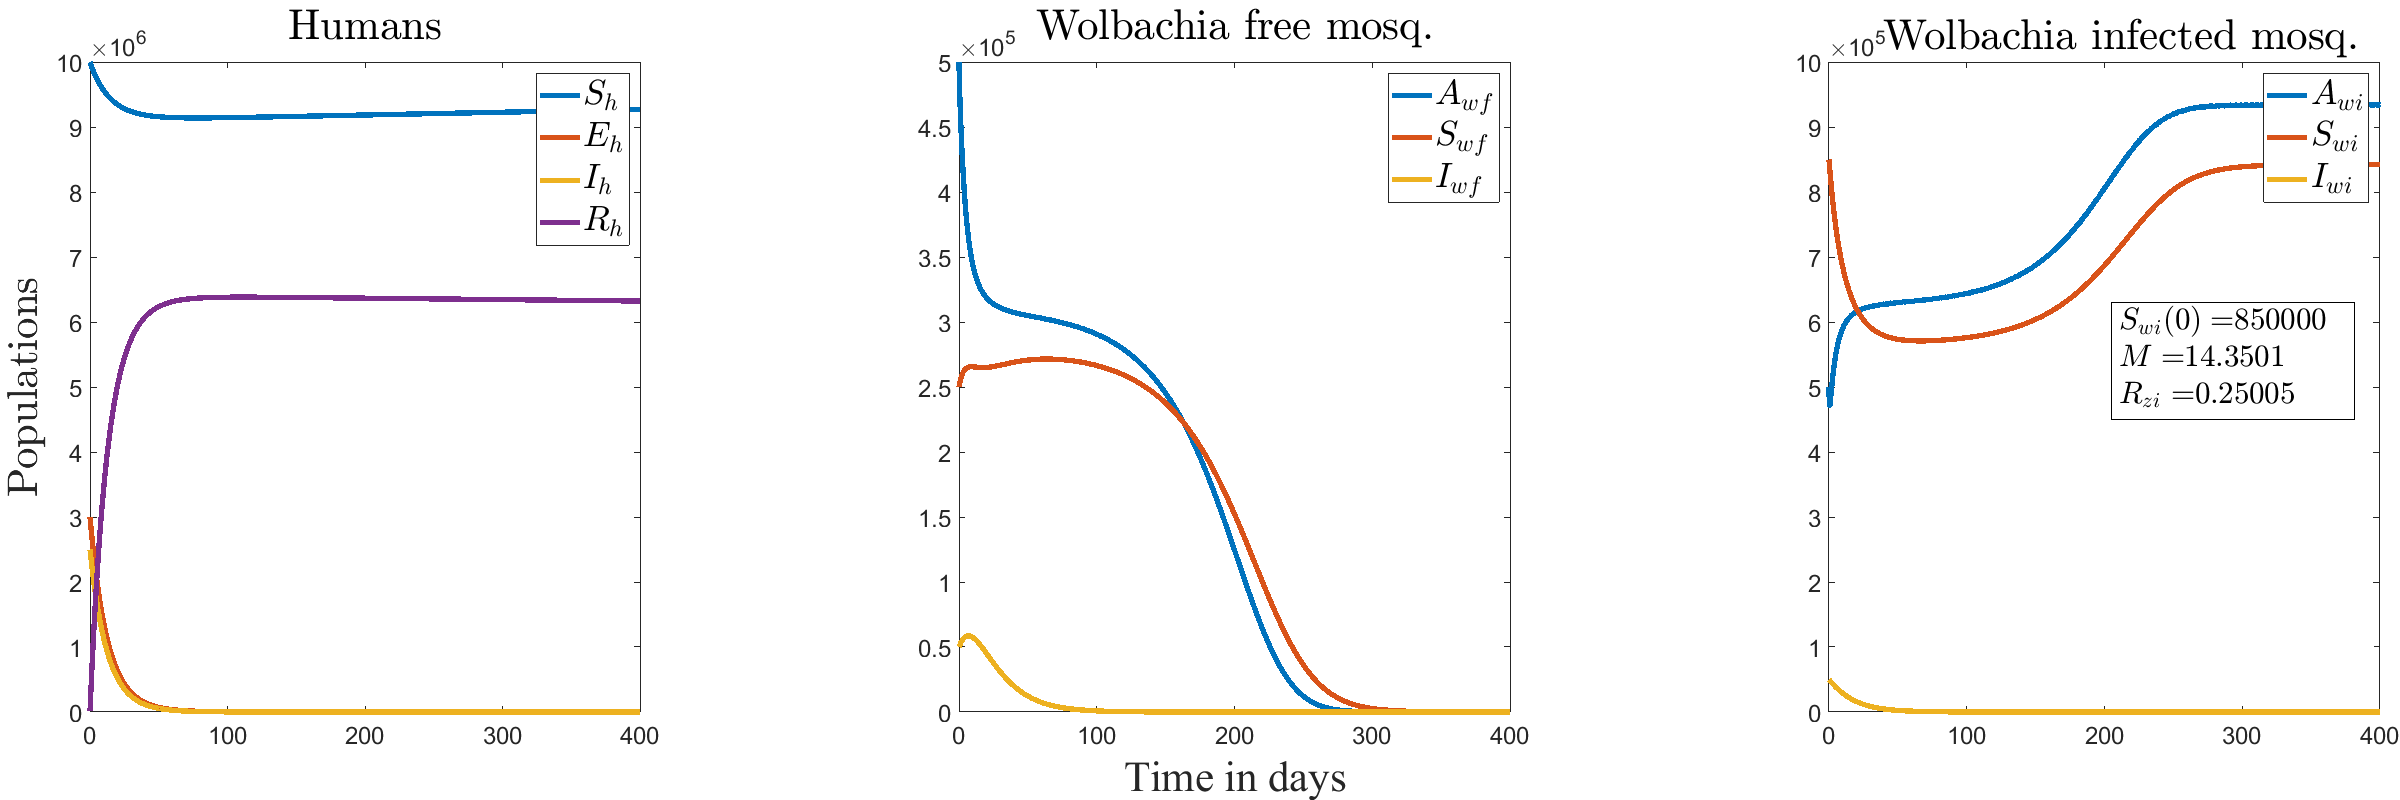
\includegraphics[width=16cm,height=4.5cm]{SimFig2.png}
%    \caption{Dominance of \textit{Wolbachia} infected mosquitoes when we start with more \textit{Wolbachia} infected susceptible females. Figure  obtained using baseline values for parameters from Table \ref{tab: param-table} and Table \ref{tab: param_mosq_table} and the initial conditions listed in Table \ref{init-cond-dis-free-table} with $S_{wi}(0)=850,000$ }
%    \label{domiWolbInfFem}
%\end{figure}

\begin{figure}[H]
    %\hskip-0.75in
    \centering
    % This file was created by matlab2tikz.
%
%The latest updates can be retrieved from
%  http://www.mathworks.com/matlabcentral/fileexchange/22022-matlab2tikz-matlab2tikz
%where you can also make suggestions and rate matlab2tikz.
%
\definecolor{mycolor1}{rgb}{0.00000,0.44700,0.74100}%
\definecolor{mycolor2}{rgb}{0.85000,0.32500,0.09800}%
\definecolor{mycolor3}{rgb}{0.92900,0.69400,0.12500}%
\definecolor{mycolor4}{rgb}{0.49400,0.18400,0.55600}%
%
\begin{tikzpicture}

\begin{axis}[%
width=1.1in,
height=1.5in,
at={(0in,0.108in)},
scale only axis,
xmin=0,
xmax=500,
ymin=0,
ymax=10000000,
ylabel={Population},
axis background/.style={fill=white},
title style={font=\bfseries, yshift=1.75ex},
title={Humans},
legend style={legend cell align=left, align=left, draw=white!15!black}
]
\addplot [color=mycolor1, line width=1.5pt]
  table[row sep=crcr]{%
0	10000000\\
0.765056511387229	9953492.81650919\\
1.47194442898035	9912864.93958851\\
2.31220270507038	9867313.65271446\\
2.98156107403338	9833030.27077908\\
3.79818408936262	9793460.45666417\\
4.52072778902948	9760396.31391199\\
5.24327148869634	9729051.97018429\\
5.95698402822018	9699684.53970912\\
6.86575885303319	9664445.56982095\\
7.70856483653188	9633786.97209193\\
8.5384411290288	9605376.72451172\\
9.42060376890004	9576987.54590004\\
10.3596544079483	9548683.81630458\\
11.2865064665675	9522554.63982962\\
12.1403113473207	9499967.62487093\\
12.9464165307581	9479865.41908826\\
13.7830935399979	9460181.12060302\\
14.6950544770807	9440010.90418391\\
15.6378694456071	9420477.10033766\\
16.522389980033	9403290.71381013\\
17.3290426395833	9388519.17120673\\
18.1288343649358	9374672.70532094\\
19.0003886222839	9360437.46428327\\
19.9424811657518	9345990.32672844\\
20.8641538266093	9332741.59250819\\
21.6947692949325	9321505.10602591\\
22.474192969501	9311532.10854222\\
23.2989031877369	9301547.8835581\\
24.2171767633408	9291078.76659767\\
25.1672232691199	9280921.87433394\\
26.0402734093368	9272155.40937005\\
26.8226525578648	9264733.8076427\\
27.605534536764	9257695.86070863\\
28.4796141777188	9250272.01517434\\
29.4350519496948	9242650.39304071\\
30.3573260679841	9235752.11982832\\
31.1688550356776	9230032.74040275\\
31.9272057767957	9224968.40627317\\
32.7469044439495	9219782.85195459\\
33.6778475921601	9214236.99905251\\
34.6388088315725	9208872.80435731\\
35.5018532071263	9204348.63108441\\
36.2623611297458	9200579.20335287\\
37.0322384182364	9196959.87381433\\
37.9129537455738	9193049.34705915\\
38.6445842403919	9189977.74364883\\
39.3641969226301	9187105.40002875\\
40.2160322051495	9183886.61645029\\
41.1461885850877	9180584.45049843\\
41.9272505231202	9177973.65485769\\
42.8544741496444	9175055.63720288\\
43.6042623110116	9172832.49101762\\
44.5214396249503	9170269.91066318\\
45.3026811610907	9168216.27817578\\
46.0351212732494	9166393.3323057\\
46.8571230880916	9164459.73074997\\
47.567582519725	9162879.63204042\\
48.3062363751233	9161322.16977523\\
49.2309799622744	9159488.93771886\\
50.0084278192371	9158042.95730932\\
50.7328173685819	9156770.03537111\\
51.5497367680073	9155416.48116231\\
52.2547903172672	9154314.89925138\\
53.0157979466021	9153191.91288028\\
53.7117225341499	9152222.30202833\\
54.5177461951971	9151164.58369356\\
55.23957654275	9150274.12827704\\
56.0262561980635	9149361.89213868\\
56.7074290402234	9148618.86844851\\
57.4650948010385	9147841.19757086\\
58.193614795804	9147139.77282707\\
59.0279931053519	9146389.61559887\\
59.744499143213	9145788.67390806\\
60.4966285210103	9145198.84647809\\
61.1646964829415	9144708.63728851\\
61.8963507637382	9144206.57095389\\
62.6661302298307	9143715.91170625\\
63.3266383763403	9143324.28255572\\
64.0826695133001	9142907.86852319\\
64.7916134241968	9142546.97119942\\
65.398315930739	9142259.91747869\\
66.0837090909481	9141958.85179021\\
66.8501043766737	9141650.18631472\\
67.4353184476495	9141433.57945167\\
68.0205325167626	9141232.8666397\\
68.6345992330462	9141038.74244019\\
69.3063712380826	9140844.9954869\\
69.7896564938128	9140717.22184018\\
70.272941749543	9140598.84970426\\
70.7191109918058	9140497.6810794\\
71.3577385414392	9140366.00595504\\
71.9351134710014	9140259.83406658\\
72.4913782514632	9140168.70386158\\
72.8858546689153	9140110.51586826\\
73.3039643168449	9140054.51575836\\
73.7523530442268	9140000.78745729\\
74.2310208510607	9139950.46629121\\
74.7081743907183	9139907.3354457\\
75.1838136669248	9139871.13173046\\
75.6264794785529	9139843.36177224\\
76.03617182374	9139822.61666178\\
76.4233065936714	9139807.28553786\\
76.6055951882154	9139801.47632377\\
76.7878837827593	9139796.556298\\
76.9701723773032	9139792.51586606\\
77.1637358553708	9139789.1778104\\
77.3572993334383	9139786.80959918\\
77.5508628115058	9139785.4001366\\
77.7444262895733	9139784.93845567\\
77.9721714165062	9139785.59417324\\
78.199916543439	9139787.52954752\\
78.4276616722345	9139790.72739435\\
78.6554067991674	9139795.17076324\\
78.9020065627992	9139801.36708867\\
79.148606326431	9139808.98319715\\
79.3952060882002	9139817.99848796\\
79.641805851832	9139828.39266188\\
80.0867324043065	9139850.57061857\\
80.531658956781	9139877.05737002\\
80.9068783316761	9139902.66094408\\
81.2820977084339	9139931.18381561\\
81.6457100752741	9139961.5491481\\
82.009322443977	9139994.53888882\\
82.4301172606647	9140035.91946981\\
82.8509120773524	9140080.65589807\\
83.3401574473828	9140136.77981281\\
83.8294028155506	9140197.20339205\\
84.5500865615904	9140293.78562992\\
85.1932918168604	9140387.334006\\
85.9515573233366	9140506.15729322\\
86.6916252952069	9140630.67499157\\
87.5392491165549	9140783.19624878\\
88.2531855218112	9140919.50826248\\
89.0064626764506	9141070.76660044\\
89.8931436184794	9141258.15628095\\
90.8048241455108	9141460.85430006\\
91.7643233966082	9141684.58888602\\
92.6862033922225	9141909.07188951\\
93.6690801754594	9142158.12872985\\
94.7489755786955	9142442.68609271\\
96.025431394577	9142792.85593922\\
97.3460765685886	9143169.82438865\\
98.8068112228066	9143602.85508533\\
100.320183660835	9144067.88276671\\
101.775817209855	9144529.62035896\\
103.265133719891	9145015.50227486\\
104.976977005601	9145589.36032173\\
106.685474272817	9146177.0207867\\
108.596466634423	9146850.28053879\\
110.642002688721	9147587.68448972\\
112.849331652746	9148400.67491391\\
115.285890763626	9149316.40401512\\
117.888193387538	9150312.90252851\\
120.613772349432	9151374.25281978\\
123.632799273357	9152567.84696373\\
126.968477195129	9153905.11157734\\
130.711437044665	9155424.7137625\\
134.990427836776	9157181.83083534\\
139.831728493795	9159189.87945843\\
145.519573660567	9161569.52718747\\
152.251454442739	9164406.50881513\\
160.65935128741	9167970.73099652\\
171.726490145549	9172683.47837899\\
188.46533177048	9179833.54704031\\
289.171536395326	9222881.94187665\\
326.022572955117	9238601.77843975\\
362.705672034994	9254230.01308266\\
399.472100369632	9269873.76424031\\
436.124572401866	9285449.13661166\\
472.76509610191	9300999.60567264\\
500	9312545.44232154\\
};
\addlegendentry{$S_h$}

\addplot [color=mycolor2, line width=1.5pt]
  table[row sep=crcr]{%
0	3000000\\
0.765056511387229	2824019.59446306\\
1.47194442944601	2670707.46842176\\
2.31220270553604	2499392.12583703\\
2.98156107403338	2370928.8550946\\
3.79818408982828	2223245.58988763\\
4.52072778949514	2100391.90070561\\
5.24327148869634	1984446.9379418\\
5.95698402822018	1876321.75000225\\
6.65303424652666	1776661.44382106\\
7.50393267069012	1662139.50548809\\
8.32246133452281	1559095.87222681\\
9.18638051021844	1457414.72071721\\
9.88905028719455	1379738.28048157\\
10.596035269089	1305864.66589124\\
11.2865064670332	1237632.33739331\\
12.1403113463894	1158295.39365957\\
12.9464165302925	1088187.89188001\\
13.7830935409293	1020028.33275559\\
14.4564422080293	968375.611422931\\
15.1722790165804	916412.068142405\\
15.864847604651	868871.834840247\\
16.7259760391898	813289.146783169\\
17.5249371249229	765001.927214019\\
18.3409426361322	718735.755085539\\
19.0003886232153	683465.0683479\\
19.7060769568197	647699.280516881\\
20.415289582219	613703.638124944\\
21.2890739003196	574345.485781704\\
22.0812400099821	540924.99174701\\
22.8736281753518	509509.11673589\\
23.750018007122	476958.993350082\\
24.4587781103328	452217.770083589\\
25.1672232691199	428817.829332994\\
26.0402734102681	401701.867100551\\
26.8226525578648	378917.584999015\\
27.6055345362984	357462.217462228\\
28.4796141772531	334995.606686148\\
29.1970099103637	317657.480793547\\
29.9111360297538	301325.727093651\\
30.7736220667139	282761.776365935\\
31.5430249753408	267208.493458002\\
32.321397440508	252380.523318808\\
33.2037267889827	236606.331582141\\
33.9235572223552	224501.651885707\\
34.6388088320382	213113.936420326\\
35.5018532075919	200172.659270005\\
36.2623611292802	189450.444734201\\
37.0322384177707	179206.89070245\\
37.9129537451081	168196.100246899\\
38.6445842413232	159588.65466977\\
39.3641969216987	151571.974519162\\
40.2160322056152	142624.810021184\\
40.9646465219557	135218.980680069\\
41.7319850376807	128045.321015273\\
42.6226682430133	120216.465972274\\
43.3543329238892	114161.59629104\\
44.076607673429	108497.755952115\\
44.9301307867281	102182.883871296\\
45.6710113231093	97014.3684332059\\
46.4304918614216	92000.3064544732\\
47.3190106106922	86477.9339092057\\
48.0647263354622	82112.138027193\\
48.7892564563081	78091.8016227693\\
49.6314068967476	73677.4234943292\\
50.53885018453	69213.1076829331\\
51.3147189170122	65621.6762329568\\
52.2547903172672	61530.9528855747\\
53.0157979470678	58416.0687868446\\
53.9328502230346	54881.3719191239\\
54.6996303359047	52098.6421545269\\
55.5976386084221	49027.2197735473\\
56.4548737877049	46272.5339612616\\
57.212539547123	43973.2455763095\\
57.9507747967727	41848.2373470878\\
58.8308136677369	39455.2889661486\\
59.7444991436787	37122.4926777505\\
60.4966285210103	35311.0714182737\\
61.4022270455025	33252.5492207236\\
62.1529439189471	31641.7655930365\\
63.1064689946361	29713.165275149\\
63.9040489285253	28194.8855193369\\
64.7916134241968	26600.652039635\\
65.6132799633779	25209.0514625367\\
66.3391741863452	24043.2162175006\\
67.2402470903471	22674.249145797\\
68.0205325172283	21554.8681831262\\
68.858523234725	20417.0188784245\\
69.7896564942785	19226.227311627\\
70.7191109908745	18109.9895912483\\
71.5501968516037	17169.3704727129\\
72.4913782509975	16165.6325579649\\
73.3039643173106	15348.4724465674\\
74.2310208501294	14468.7367935409\\
75.1838136669248	13619.3756167726\\
76.0361718246713	12903.717519559\\
76.9701723777689	12164.4594215956\\
77.7444262895733	11585.2222134396\\
78.6554067987017	10940.3919310877\\
79.3952060886659	10444.3385818079\\
80.3091956810094	9863.70606060186\\
81.2820977079682	9282.50241110194\\
82.2197198523208	8756.09725088673\\
83.0955347623676	8292.4577305303\\
84.0696307313628	7806.6871020915\\
84.9918031464331	7374.06518464861\\
85.9515573233366	6950.21320030652\\
86.884015196003	6562.6303975815\\
87.7706711268984	6214.88874997199\\
88.7553702914156	5851.02474025311\\
89.6714733825065	5532.34405733179\\
90.626103497576	5219.35912275221\\
91.5526547413319	4933.10528528225\\
92.436932049226	4675.06220133463\\
93.4269131259061	4402.68460330926\\
94.3519347081892	4163.00812048698\\
95.2950039934367	3932.51299450919\\
96.2168911052868	3719.92394781904\\
97.1116451304406	3524.92826115247\\
98.1102202180773	3319.71576782828\\
99.0277494508773	3142.02080987021\\
99.9676465131342	2970.13907447783\\
100.885291015729	2811.66151314229\\
101.77581721032	2666.18337256461\\
102.777887184173	2511.70990584604\\
103.705014913809	2376.98587152269\\
104.635382849257	2249.2457744563\\
105.548939702101	2130.66792592919\\
106.449004187714	2020.11067349929\\
107.457393457182	1903.21406055614\\
108.37602493912	1802.76261619385\\
109.30545487348	1706.65175309358\\
110.216075721662	1617.57150079543\\
111.110091658309	1534.74205497373\\
112.070240826346	1450.60640967777\\
113.044104358181	1370.07998872455\\
113.879758580122	1304.62973139994\\
114.805879076477	1235.81475804327\\
115.728987797163	1170.90777131682\\
116.555504961871	1115.74699102761\\
117.494448944926	1056.2887230753\\
118.30533304112	1007.54335078271\\
119.227964234073	954.859790790826\\
120.174091636669	903.744426202495\\
121.021062475629	860.351597879548\\
121.952108164784	815.091561101377\\
122.952161938883	769.168471692596\\
123.87765720021	729.01396528678\\
124.833017722238	689.794870954938\\
125.682141525205	656.73802367365\\
126.60545474058	622.614248230122\\
127.598153105006	587.929122582078\\
128.537742260844	556.90562704578\\
129.495748330373	526.981119762175\\
130.334285863675	502.128000571858\\
131.242610947695	476.543646038976\\
132.241232234519	449.935805965681\\
133.181865998544	426.24906082591\\
134.149103963748	403.206694507506\\
134.990427835844	384.190403888468\\
135.893357284367	364.788778159302\\
136.882979992311	344.659310317133\\
137.837212034501	326.3126061894\\
138.804659028538	308.717974156141\\
139.831728493795	291.085419962183\\
140.714150479063	276.74971759785\\
141.520165290684	264.278403529432\\
142.472652785946	250.269093301147\\
143.448779082857	236.688253576402\\
144.461100068409	223.387552667875\\
145.34408748243	212.402295653708\\
146.154654928483	202.797511796001\\
147.119326490909	191.934786717873\\
148.093139030505	181.562874455936\\
149.110343114007	171.330376944039\\
149.978137252852	163.060579712037\\
150.782392061781	155.755054893438\\
151.74213529611	147.466428804677\\
152.723681666423	139.447765722405\\
153.72692452278	131.704319790471\\
154.597032739781	125.339023284148\\
155.405184934847	119.703974795062\\
156.375287859701	113.27452935325\\
157.396059392951	106.883103182539\\
158.384825378191	101.037259922363\\
159.285604753997	95.9912430131808\\
160.220214960631	91.022671285551\\
161.256825070363	85.8128461046144\\
162.180770495441	81.4217026359402\\
163.185237138066	76.9029385698959\\
164.128079839516	72.8902541440912\\
165.063890748657	69.1148900962435\\
166.046111295931	65.3627272392623\\
166.961131535005	62.0509829916991\\
167.78806483699	59.2027662214823\\
168.720043510199	56.1492441236041\\
169.640682977159	53.2876115585677\\
170.626800149214	50.3840694781393\\
171.520558880176	47.8893888494931\\
172.344283938874	45.6996955382638\\
173.303313496988	43.2761028017849\\
174.243957269937	41.0238052946515\\
175.203331630677	38.8472696747631\\
176.097263978329	36.9231592896394\\
177.150222859345	34.7784928716719\\
178.111966213211	32.9285017480142\\
179.005117148627	31.2985563748516\\
179.932837294415	29.6907425504178\\
180.832179696299	28.2108380799182\\
181.934590430465	26.4968061898835\\
182.890669006389	25.0946451765485\\
183.938506187405	23.6427706922404\\
184.987501766998	22.2731938883662\\
185.996894229669	21.0300544239581\\
186.944556104485	19.9259593361057\\
188.078727830201	18.6802448430099\\
189.154030528385	17.5709294243716\\
190.276465171017	16.4829326472245\\
191.456169342622	15.4116677381098\\
192.583272592165	14.452993768733\\
193.802001782227	13.483076334931\\
194.984703292139	12.603814939037\\
196.177941946778	11.7745321006514\\
197.436950693373	10.9583246530965\\
198.606582923327	10.2505713957362\\
199.903168820776	9.51899927994236\\
201.313287565019	8.78217512462288\\
202.71495311847	8.10596447810531\\
204.253264841624	7.4232399603352\\
205.707595422864	6.83041189890355\\
207.117486860137	6.30063206981868\\
208.644638034515	5.77273217169568\\
210.257248219103	5.26288991607726\\
211.926681315526	4.78212636057287\\
213.726229920052	4.31259414227679\\
215.578161410056	3.87711427547038\\
217.507729841862	3.4697231343016\\
219.659213331528	3.06534464610741\\
221.974088440649	2.68230347707868\\
224.347569058184	2.33879658998922\\
226.858855727594	2.02271610917524\\
229.470290861093	1.73886560928077\\
232.292143459432	1.47636102652177\\
235.530935233925	1.22312291618437\\
239.032925413456	0.997530901804566\\
242.810729893856	0.800197524949908\\
247.242919942364	0.617455020546913\\
252.108099282254	0.464160316158086\\
257.934790103231	0.329435344785452\\
264.710258897394	0.220806700177491\\
273.157546564471	0.133817954920232\\
284.279087714385	0.0689994250424206\\
300.325656181201	0.0263987286016345\\
328.825033344794	0.00474098930135369\\
427.508812675253	1.18562020361423e-05\\
500	1.43423676490784e-07\\
};
\addlegendentry{$E_h$}

\addplot [color=mycolor3, line width=1.5pt]
  table[row sep=crcr]{%
0	2500000\\
0.765056511387229	2351595.60085356\\
1.47194442944601	2222449.89977796\\
2.31220270553604	2078282.56009156\\
2.98156107403338	1970268.80808076\\
3.79818408982828	1846185.63103666\\
4.52072778949514	1743034.40504949\\
5.24327148869634	1645739.8770989\\
5.95698402822018	1555054.83876516\\
6.65303424652666	1471509.39221837\\
7.50393267069012	1375552.83804227\\
8.32246133452281	1289257.86229374\\
9.18638051021844	1204146.24835572\\
9.88905028719455	1139157.36246449\\
10.596035269089	1077375.46433603\\
11.2865064670332	1020334.81692782\\
12.1403113463894	954041.345282766\\
12.9464165302925	895489.550745429\\
13.7830935409293	838593.969677079\\
14.4564422080293	795498.497124705\\
15.1722790165804	752163.915187235\\
15.864847604651	712537.524204609\\
16.7259760391898	666233.395123498\\
17.5249371249229	626031.984913783\\
18.3409426361322	587537.554752209\\
19.0003886232153	558209.260740943\\
19.7060769568197	528486.405110063\\
20.415289582219	500252.064478594\\
21.2890739003196	467587.384022624\\
22.0812400099821	439872.295877883\\
22.8736281753518	413839.723867796\\
23.750018007122	386889.967387978\\
24.4587781103328	366422.548482603\\
25.1672232691199	347079.488909396\\
26.0402734102681	324684.276422048\\
26.8226525578648	305884.433554038\\
27.6055345362984	288197.405214535\\
28.4796141772531	269695.282062195\\
29.1970099103637	255430.801278251\\
29.9111360297538	242006.524520359\\
30.7736220667139	226763.075782736\\
31.5430249753408	214005.683940876\\
32.321397440508	201856.047861703\\
33.2037267889827	188946.031370393\\
33.9235572223552	179050.545861906\\
34.6388088320382	169750.852732181\\
35.5018532075919	159194.7357528\\
36.2623611292802	150459.368137473\\
37.0322384177707	142123.718598061\\
37.9129537451081	133175.202251486\\
38.6445842413232	126188.808422713\\
39.3641969216987	119689.48087103\\
40.2160322056152	112445.021478595\\
40.9646465219557	106456.473688063\\
41.7319850376807	100662.98870715\\
42.6226682430133	94349.1929467884\\
43.3543329238892	89472.8509838935\\
44.076607673429	84917.1512126145\\
44.9301307867281	79844.7605761373\\
45.6710113231093	75699.0093194442\\
46.4304918614216	71682.5071403836\\
47.3190106106922	67265.3472069418\\
48.0647263354622	63778.4605254009\\
48.7892564563081	60571.7873047455\\
49.6314068967476	57055.8733045803\\
50.53885018453	53505.9262667866\\
51.3147189170122	50654.5582579626\\
52.0197724672034	48201.6470279107\\
52.7621287372895	45753.2822429547\\
53.4905948457308	43477.4009430758\\
54.3358620530926	40984.8264460783\\
55.23957654275	38485.2229896439\\
56.0262561980635	36439.7125668945\\
56.707429040689	34760.8270190479\\
57.4650948001072	32988.5055157035\\
58.1936147948727	31373.7653703475\\
59.0279931048863	29625.9442898845\\
59.9176080105826	27874.6955945613\\
60.6896353578195	26443.1219064919\\
61.4022270455025	25190.2847453705\\
62.1529439189471	23937.7005096972\\
63.1064689946361	22440.4370128545\\
63.9040489285253	21263.7201828747\\
64.7916134241968	20030.1412471551\\
65.6132799633779	18955.1267269459\\
66.3391741863452	18055.8561092187\\
67.2402470903471	17001.5411645127\\
68.0205325172283	16140.8320027562\\
68.858523234725	15267.2689076257\\
69.7896564942785	14354.5920267226\\
70.7191109908745	13500.5588325965\\
71.5501968516037	12782.0825093812\\
72.3059566575103	12163.5577661572\\
73.0949094928801	11551.2888630512\\
73.9916869471781	10894.4335125927\\
74.9459940288216	10238.3152337731\\
75.8313256511465	9666.64292538445\\
76.6055951877497	9194.12608652283\\
77.3572993334383	8758.50903002545\\
78.1999165443704	8295.81430183724\\
79.1486063254997	7805.37630718714\\
80.0867324047722	7350.19053458422\\
80.9068783326074	6975.02180236205\\
81.8275162600912	6577.65143311908\\
82.6405146694742	6246.4324767096\\
83.5847801314667	5883.51547525777\\
84.5500865611248	5535.22648117458\\
85.3947804863565	5248.13124042517\\
86.3068454908207	4955.53427633131\\
87.0764050977305	4721.91113958927\\
88.0020931363106	4456.03351503983\\
88.7553702914156	4251.21586860344\\
89.6714733825065	4015.27818635944\\
90.626103497576	3783.8890767307\\
91.5526547413319	3572.56267398084\\
92.436932049226	3382.31942952424\\
93.4269131259061	3181.7833430795\\
94.3519347081892	3005.56705838023\\
95.2950039934367	2836.32571161492\\
96.2168911052868	2680.43520214502\\
97.1116451304406	2537.62428005133\\
97.8555056680925	2424.91356979404\\
98.8068112232722	2288.28781960066\\
99.7879068045877	2155.71635438129\\
100.672720807139	2042.97617912292\\
101.523001641501	1940.37954305112\\
102.281448347494	1853.36212194851\\
103.265133719891	1746.47460467787\\
104.09753076639	1661.00790725136\\
104.976977006532	1575.39047491224\\
105.739593933802	1504.8372782506\\
106.685474272352	1421.83417727752\\
107.457393457182	1357.60114420112\\
108.37602493912	1285.03915663715\\
109.30545487348	1215.6816124972\\
110.216075721662	1151.45997387031\\
111.110091658309	1091.80042752763\\
112.070240826346	1031.25681055756\\
113.044104358181	973.365780071821\\
113.879758580122	926.354371091351\\
114.805879076477	876.96736622043\\
115.728987797163	830.424969424959\\
116.555504961871	790.902642012574\\
117.494448944926	748.334537988063\\
118.30533304112	713.462713436689\\
119.227964234073	675.801296276972\\
120.174091636669	639.289291641675\\
121.021062475629	608.316134797875\\
121.952108164784	576.03296594508\\
122.725282827858	550.556561197154\\
123.632799272425	522.115742834751\\
124.612230983097	493.099084841553\\
125.495377938263	468.346218329389\\
126.423943513539	443.683822839521\\
127.388261135202	419.470076391939\\
128.294509865809	397.941214479506\\
129.257490438875	376.294621703681\\
130.134192649741	357.630028213374\\
131.065552980173	338.831121769734\\
132.010744533502	320.778775852174\\
132.932695337106	304.111353160813\\
133.929377983324	287.079923837911\\
134.808281905018	272.865609130822\\
135.715111456346	258.94718091283\\
136.671936308499	245.040733470581\\
137.589482581709	232.416288250126\\
138.564753181301	219.718875634484\\
139.438146684784	208.944967704825\\
140.350372767542	198.262350344565\\
141.286839339416	187.870235764422\\
142.220143143088	178.061209983192\\
143.23018171452	168.028047363739\\
144.104571187869	159.804794093594\\
144.993115127087	151.864703415893\\
145.942961172666	143.816782935522\\
146.868333888706	136.39036973333\\
147.852199051064	128.918430042453\\
148.722211061977	122.655846433248\\
149.618881987873	116.522192819044\\
150.547364174854	110.496556238271\\
151.487475722563	104.715281878132\\
152.506114016753	98.794520016294\\
153.376384614501	94.00391793577\\
154.250653867144	89.4267617790028\\
155.193530682009	84.7414828985929\\
156.122471635696	80.3670429890044\\
157.012081738561	76.3908826955594\\
157.972025874536	72.3219568012282\\
158.826446730178	68.8839430431835\\
159.762299449649	65.306457338389\\
160.659351287875	62.0526518677361\\
161.634730689693	58.6992520275526\\
162.568397107534	55.6598706669174\\
163.420947813429	53.022760251537\\
164.362032566685	50.2571697453968\\
165.264820786659	47.74024975067\\
166.224611690734	45.2029405864887\\
167.150891062338	42.8825513604097\\
168.011771960184	40.8332033664919\\
168.962325723376	38.684246880468\\
169.858720497228	36.7616783934645\\
170.810147526674	34.8257066770457\\
171.726490145084	33.0577411567792\\
172.584041328635	31.484720364213\\
173.538474440109	29.8219555914402\\
174.637159076985	28.0164305078797\\
175.722243872471	26.3406607066281\\
176.698263675906	24.919178864453\\
177.621457037982	23.6453225850128\\
178.573186249938	22.4002323849127\\
179.576959946193	21.1580177103169\\
180.626451025251	19.9328040126711\\
181.691978069954	18.7613908331841\\
182.890669006389	17.525595548097\\
183.938506187405	16.5121206515469\\
184.987501766998	15.5561534771696\\
185.996894229669	14.6884879474528\\
187.191345866304	13.7239414402284\\
188.465331769548	12.7647349108011\\
189.662467955612	11.9244397031143\\
190.968650125898	11.0704234591685\\
192.160214864183	10.3446645587683\\
193.475201017689	9.59866922814399\\
194.758134746924	8.92256775032729\\
196.177941946778	8.22951677907258\\
197.605798525736	7.58661816455424\\
199.011795200408	7.00246340315789\\
200.574121644255	6.40574081568047\\
202.079484783579	5.87871287018061\\
203.625356229488	5.38238084688783\\
205.358955890872	4.87519957777113\\
207.117486860137	4.40927204908803\\
209.025829551276	3.95361432339996\\
211.043723718263	3.52261854568496\\
213.206820325926	3.11233025463298\\
215.3521055663	2.7523333481513\\
217.692064828239	2.40666261874139\\
220.084349705372	2.09778877114877\\
222.797461271752	1.7948403400369\\
225.676239987835	1.52073519537225\\
228.783035251778	1.27133446047083\\
232.292143459432	1.03808977641165\\
236.249116323888	0.825596131384373\\
240.553384080529	0.643149436451495\\
245.546246843413	0.481015670578927\\
251.288380100857	0.344039380550385\\
258.08542637853	0.231031600851566\\
266.497064372059	0.140833729878068\\
277.41114549851	0.0738443597219884\\
292.892866946757	0.0293805906549096\\
319.693992496002	0.00588513724505901\\
402.771206018049	3.83509323000908e-05\\
500	1.03376805782318e-07\\
};
\addlegendentry{$I_h$}

\addplot [color=mycolor4, line width=1.5pt]
  table[row sep=crcr]{%
0	10000\\
0.765056511387229	381051.317412611\\
1.47194442898035	704284.232839136\\
2.3122027060017	1065493.18341768\\
2.98156107403338	1336392.97645429\\
3.79818409029394	1647899.28342115\\
4.52072778902948	1907118.79718356\\
5.24327148869634	2151853.08368707\\
5.95698402822018	2380179.3499132\\
6.65303424652666	2590728.77429735\\
7.50393267069012	2832811.16345113\\
8.32246133405715	3050772.11811411\\
9.18638051021844	3266001.88461253\\
9.88905028719455	3430533.87502465\\
10.596035269089	3587111.74291608\\
11.2865064665675	3731828.28271426\\
12.1403113463894	3900223.4548236\\
12.9464165298268	4049152.76391598\\
13.7830935409293	4194066.36875297\\
14.4564422080293	4303972.17094986\\
15.1722790170461	4414621.38499704\\
15.8648476041853	4515929.11362774\\
16.7259760387242	4634476.22032828\\
17.5249371249229	4737558.83028531\\
18.3409426361322	4836416.84002211\\
19.2356180679053	4937826.92976243\\
19.9424811657518	5013108.43517086\\
20.6516937902197	5084602.05771076\\
21.5015339367092	5165255.12050645\\
22.2744753677398	5234145.3865404\\
23.0733457775787	5301154.64817623\\
23.9755754172802	5372034.10872161\\
24.7003794573247	5425516.07569119\\
25.6177081996575	5489072.56000068\\
26.4349189009517	5542048.39857225\\
27.2034743810073	5588936.82950506\\
28.0288330232725	5636318.69397205\\
28.7187460884452	5673700.57489699\\
29.4350519506261	5710490.99081809\\
30.1491780700162	5745229.94236149\\
30.9817700656131	5783426.82570541\\
31.7301099449396	5815763.94730068\\
32.5184932723641	5847911.1217177\\
33.4321379614994	5882853.05639474\\
34.1692668534815	5909345.3554604\\
35.0864735282958	5940327.42466874\\
35.8849478689954	5965619.13515834\\
36.6340929893777	5988014.4034425\\
37.4567974144593	6011208.88017498\\
38.1568305771798	6029856.46077186\\
38.8844551350921	6048237.84494215\\
39.8080559456721	6070185.8884479\\
40.6015623975545	6087880.63100416\\
41.3414540691301	6103471.18190114\\
42.1590564288199	6119738.55814128\\
42.8544741496444	6132825.25965079\\
43.6042623110116	6146206.12539141\\
44.521439624019	6161605.18170547\\
45.3026811610907	6173931.24114123\\
46.0351212732494	6184865.89978205\\
46.8571230890229	6196462.18968462\\
47.5675825187936	6205941.10863843\\
48.3062363760546	6215291.06728408\\
49.2309799632058	6226312.31305335\\
50.0084278183058	6235024.0319287\\
50.7328173676506	6242712.3758162\\
51.549736767076	6250914.13450247\\
52.2547903172672	6257614.91028732\\
53.0157979466021	6264476.07790325\\
53.9328502230346	6272260.94396544\\
54.6996303359047	6278388.31171742\\
55.5976386079565	6285149.22444\\
56.4548737881705	6291210.25484443\\
57.212539547123	6296266.71265756\\
57.9507747963071	6300937.25348864\\
58.8308136677369	6306192.9000484\\
59.744499143213	6311311.62485201\\
60.4966285210103	6315282.31166208\\
61.4022270450369	6319789.48142702\\
62.1529439194128	6323311.76260565\\
63.1064689951017	6327522.71574874\\
63.9040489280596	6330832.07512251\\
64.7916134241968	6334300.60828743\\
65.6132799629122	6337322.04305028\\
66.3391741858795	6339848.11983885\\
67.2402470903471	6342807.38016906\\
68.0205325167626	6345220.71275634\\
68.858523234725	6347667.06290523\\
69.7896564938128	6350218.79614143\\
70.7191109908745	6352601.70460963\\
71.5501968516037	6354601.85679038\\
72.3059566579759	6356319.74382937\\
73.0949094928801	6358015.91702904\\
73.9916869476438	6359829.92880297\\
74.7081743907183	6361196.757313\\
75.6264794776216	6362847.45485754\\
76.4233065927401	6364192.66593694\\
77.1637358553708	6365374.0333435\\
77.9721714165062	6366592.29941873\\
78.6554067991674	6367566.4722417\\
79.3952060891315	6368566.84473606\\
80.3091956805438	6369728.56457325\\
81.094488020055	6370664.6754478\\
81.8275162596256	6371489.48180743\\
82.6405146690086	6372351.72379012\\
83.3401574473828	6373051.64875144\\
84.0696307308972	6373741.95578903\\
84.7903144760057	6374386.21773266\\
85.5962691558525	6375064.44161797\\
86.3068454908207	6375627.15848066\\
87.0764050977305	6376201.14973697\\
87.7706711264327	6376688.83182151\\
88.5042779063806	6377174.52538252\\
89.2281329119578	6377625.29039068\\
90.0763835879043	6378119.28410955\\
90.8048241445795	6378515.44930685\\
91.5526547413319	6378896.5122967\\
92.1876607062295	6379200.59160079\\
92.9354747347534	6379536.76139875\\
93.6690801745281	6379844.51920033\\
94.3519347077236	6380112.27101444\\
95.1212500045076	6380393.29297056\\
95.8339716838673	6380635.01339368\\
96.4083508159965	6380817.33471677\\
97.1116451304406	6381026.03442955\\
97.8555056685582	6381230.07950847\\
98.5858729956672	6381414.47731023\\
99.2486876780167	6381568.74686029\\
99.9676465131342	6381722.63078482\\
100.496452233754	6381827.2310815\\
101.097861223854	6381937.68636344\\
101.775817209855	6382051.74857625\\
102.281448347494	6382129.87065178\\
102.777887184173	6382200.99645549\\
103.265133719891	6382265.59697635\\
103.901272839867	6382342.42963157\\
104.464585770853	6382403.61153439\\
104.976977006532	6382453.86604265\\
105.548939702101	6382504.09428343\\
105.976064018905	6382537.68940752\\
106.449004187249	6382571.10100933\\
106.942780666985	6382601.85816856\\
107.457393457182	6382629.56205691\\
107.935141547583	6382651.42584966\\
108.37602493912	6382668.40455417\\
108.773713694885	6382681.15676667\\
109.128207813948	6382690.52417812\\
109.479869214818	6382697.99603895\\
109.654283556156	6382701.04117472\\
109.828697897494	6382703.65445565\\
110.003112238832	6382705.84047933\\
110.216075721197	6382707.93693275\\
110.429039204493	6382709.41134204\\
110.642002687789	6382710.27177188\\
110.854966171086	6382710.52617986\\
111.110091658309	6382710.04409955\\
111.365217145532	6382708.71684293\\
111.620342632756	6382706.55749256\\
111.875468119979	6382703.57892433\\
112.070240826346	6382700.76138517\\
112.265013532713	6382697.47931753\\
112.45978623908	6382693.73820989\\
112.849331651814	6382684.90049638\\
113.238877064548	6382674.29082576\\
113.656704175286	6382660.98855502\\
114.102812984027	6382644.64477989\\
114.56587323267	6382625.40318664\\
115.045884920284	6382603.07695594\\
115.50743928086	6382579.38814617\\
115.950536313467	6382554.65452912\\
116.555504961871	6382517.82872507\\
117.124099710025	6382480.10344421\\
117.679623561911	6382440.43127063\\
118.305333040655	6382392.53134322\\
118.989943778142	6382336.36319863\\
119.702020338736	6382273.93968785\\
120.410127284937	6382207.98473222\\
121.224707539193	6382127.5369416\\
122.145401830785	6382030.99628266\\
122.952161938883	6381941.7483107\\
123.87765720021	6381834.28713641\\
124.833017721772	6381717.96279575\\
125.868905112147	6381585.98850134\\
126.968477195129	6381439.64236461\\
128.051277470775	6381289.61906792\\
129.25749043934	6381116.03942985\\
130.534379077144	6380925.37742031\\
131.818711137399	6380726.94601368\\
133.181865998544	6380509.57419131\\
134.808281905018	6380241.8437137\\
136.460892624222	6379961.27450301\\
138.084941486828	6379677.94690237\\
140.004609918222	6379334.25838054\\
141.986817192286	6378970.4004548\\
144.104571187869	6378572.7006122\\
146.366348684765	6378138.91816444\\
148.916277088225	6377640.0837652\\
151.487475723028	6377127.98112932\\
154.423843303695	6376533.57351772\\
157.588048219681	6375883.37391416\\
161.067872260697	6375158.6862828\\
165.063890748657	6374316.35362691\\
169.640682976693	6373341.02513352\\
174.833759980276	6372223.87053349\\
180.832179696299	6370923.21942168\\
188.292258564383	6369294.94296332\\
197.774646357633	6367214.32122598\\
210.831242408603	6364338.39290933\\
233.630326288752	6359304.56730771\\
292.388040818274	6346329.62708967\\
329.598458396271	6338124.55471189\\
366.425700639375	6330014.33973574\\
403.161917342804	6321934.50154294\\
439.805834362283	6313885.2375654\\
476.469226520509	6305841.95226606\\
500	6300685.12526495\\
};
\addlegendentry{$R_h$}

\end{axis}

\begin{axis}[%
width=1.1in,
height=1.5in,
at={(1.34in,0.108in)},
scale only axis,
xmin=0,
xmax=500,
ymin=0,
ymax=500000,
xlabel={Time (days)},
axis background/.style={fill=white},
title style={font=\bfseries, yshift=1.25ex},
title={\emph{Wolb.}-free mosq.},
legend style={legend cell align=left, align=left, draw=white!15!black}
]
\addplot [color=mycolor1, line width=1.5pt]
  table[row sep=crcr]{%
0	500000\\
0.124589653627481	492676.804806024\\
0.307978130120318	483942.02038861\\
0.582596574851777	473549.274505795\\
0.856286479742266	464785.921615768\\
1.20725304697407	454786.001020839\\
1.61964695597999	444164.841671941\\
2.11362735746661	432657.937293277\\
2.51077805378009	424226.142604389\\
2.98156107391696	415055.032755535\\
3.52597641799366	405515.461512154\\
4.03903198987246	397389.9026794\\
4.52072778949514	390520.89112965\\
5.00242358905962	384217.310604109\\
5.4841193886823	378548.041409878\\
6.18900076759746	371025.213077914\\
6.86575885262573	364797.171424837\\
7.29120806459105	361264.597771615\\
7.91319700249005	356506.660424081\\
8.53844112838851	352282.233377416\\
8.97040071617812	349633.949516957\\
9.6548270281055	345759.818617928\\
10.5960352691473	341154.727491039\\
11.7219254166121	336616.705575771\\
11.9396348914015	335864.661321353\\
12.3409878016682	334369.166200071\\
13.3545681667747	331224.119526306\\
14.2319926522323	328837.605757183\\
14.4564422079711	328298.535285093\\
14.9336667470634	327072.997026208\\
15.4108912861557	326120.347147208\\
15.637869445316	325544.242361651\\
15.8648476044182	325043.441158515\\
16.3188039226807	324295.783742536\\
16.5223899809062	323830.358420655\\
16.7259760391898	323424.201340008\\
17.1331481556408	322798.346067836\\
17.5249371249811	322071.435850691\\
17.9167260943213	321495.010220515\\
18.3409426363651	320801.509332958\\
18.7651591783506	320238.60762375\\
19.0003886229824	319862.998730757\\
19.2356180676143	319529.528496807\\
19.7060769569362	319007.03442364\\
19.9424811652862	318626.793098523\\
20.1788853736944	318312.141195924\\
20.4152895820444	318126.780150921\\
20.6516937904526	317912.849785517\\
20.8641538271331	317577.381715451\\
21.0766138638137	317308.156365794\\
21.2890739004943	317158.802371019\\
21.5015339371166	316988.77921139\\
21.6947692947579	316726.692846499\\
21.8880046523409	316506.015046698\\
22.2744753675652	316190.424631718\\
22.673910572601	315764.366252552\\
23.0733457776369	315447.05857928\\
23.2989031875622	315212.57181016\\
23.5244605974294	315007.33918689\\
23.9755754171638	314696.682720054\\
24.2171767638065	314434.329573083\\
24.4587781104492	314223.599377898\\
24.7003794570919	314118.710403436\\
24.9419808037346	313986.528177877\\
25.1672232690034	313717.05865877\\
25.3924657343305	313519.097134464\\
25.6177081995993	313462.192884172\\
25.8429506649263	313371.712734915\\
26.0402734101517	313153.385064253\\
26.2375961553771	312987.733515943\\
26.4349189006025	312910.624461274\\
26.6322416458279	312820.8675828\\
26.822652557632	312654.826877549\\
27.0130634694942	312517.250481479\\
27.3938852931024	312327.740321027\\
27.6055345364148	312170.003028294\\
27.817183779669	312034.885280397\\
28.2404822662938	311839.419647695\\
28.4796141773113	311656.946502027\\
28.7187460883288	311511.095327528\\
28.9578779994044	311440.650554687\\
29.1970099104219	311350.321566376\\
29.4350519502768	311130.787864786\\
29.6730939901317	310978.918131715\\
29.9111360299285	310968.684831255\\
30.1491780697834	310918.42310958\\
30.357326068799	310712.270888298\\
30.5654740678146	310573.196808806\\
30.7736220668303	310556.980709768\\
30.9817700658459	310516.14696684\\
31.1688550356193	310368.781062267\\
31.3559400053928	310258.251140907\\
31.7301099448814	310146.390381387\\
31.9272057767375	310028.208290123\\
32.1243016086519	309931.17890558\\
32.5184932724806	309803.248928388\\
32.746904444648	309674.122513878\\
32.9753156168154	309570.271181124\\
33.2037267889827	309516.961747898\\
33.4321379612084	309451.273785951\\
33.6778475918691	309280.783738676\\
33.923557222588	309163.912256733\\
34.1692668532487	309162.43748127\\
34.4149764839676	309125.707670567\\
34.6388088321546	308926.593332244\\
34.8626411802834	308804.953665851\\
35.0864735284704	308838.618477087\\
35.3103058766574	308832.353900868\\
35.5018532073591	308678.088638949\\
35.6934005380608	308575.641587856\\
35.8849478687625	308558.199423497\\
36.0764951995225	308528.727102123\\
36.2623611293966	308424.964587409\\
36.4482270593289	308345.829271932\\
36.8199589190772	308260.232459066\\
37.0322384176543	308163.351255813\\
37.2445179161732	308085.761483787\\
37.4567974147503	308044.238669374\\
37.6690769132692	307995.251586307\\
37.9129537452827	307869.011634485\\
38.1568305772962	307779.235846584\\
38.4007074093097	307767.748301762\\
38.6445842413232	307732.480090945\\
38.8844551348011	307552.640404097\\
39.1243260283372	307447.908438538\\
39.3641969218152	307503.774035674\\
39.6040678153513	307511.060774092\\
39.8080559453811	307338.516502521\\
40.012044075469	307236.719009473\\
40.216032205557	307262.67831241\\
40.4200203355867	307263.350998536\\
40.6015623977873	307153.210001709\\
40.783104459988	307077.362833453\\
40.9646465221886	307053.409974015\\
41.146188584331	307024.425351214\\
41.3414540688391	306942.992882914\\
41.5367195533472	306879.794070606\\
41.7319850378553	306847.388542651\\
41.9272505223053	306810.211258666\\
42.1590564291691	306716.321993156\\
42.3908623359748	306646.082952535\\
42.6226682428387	306624.802683832\\
42.8544741497026	306589.967933995\\
43.1044035367086	306444.572245666\\
43.3543329237727	306357.512552404\\
43.6042623107787	306398.938350966\\
43.8541916978429	306398.2943169\\
44.0766076733125	306213.332363644\\
44.2990236488404	306113.667942084\\
44.5214396243682	306185.31079144\\
44.7438555998961	306212.257083447\\
44.9301307869027	306077.714167157\\
45.1164059739094	305994.953234832\\
45.3026811609161	305994.232221701\\
45.4889563478646	305983.159281982\\
45.6710113229346	305902.220197176\\
45.8530662979465	305843.312643219\\
46.0351212730166	305818.002742115\\
46.2171762480284	305789.25102935\\
46.4304918616544	305714.187638952\\
46.6438074752223	305656.386069221\\
46.8571230887901	305631.554861249\\
47.0704387024161	305599.208003182\\
47.3190106106922	305490.225899088\\
47.5675825190265	305418.771648326\\
47.8161544273025	305429.81571757\\
48.0647263356368	305413.97849986\\
48.3062363757635	305238.281296167\\
48.5477464159485	305146.354367771\\
48.7892564560752	305235.558115244\\
49.0307664962602	305268.183014667\\
49.2309799630893	305101.112699787\\
49.4311934298603	305008.679196953\\
49.6314068966312	305048.416043823\\
49.8316203634604	305063.162388434\\
50.0084278187132	304966.261339415\\
50.1852352740243	304901.757747099\\
50.3620427293354	304884.51723913\\
50.5388501845882	304863.521495197\\
50.732817367767	304795.320305893\\
50.9267845508875	304743.363809259\\
51.1207517340663	304718.851410076\\
51.3147189171868	304689.898699298\\
51.5497367671924	304607.158859729\\
51.7847546171979	304547.168970816\\
52.0197724672034	304535.328268022\\
52.254790317209	304509.23492155\\
52.5084595271619	304365.792327909\\
52.7621287370566	304285.816053643\\
53.0157979470096	304347.578823219\\
53.2694671569625	304361.012692266\\
53.4905948456726	304171.29785705\\
53.7117225343827	304074.415079717\\
53.932850223151	304163.635445976\\
54.1539779118611	304204.315055369\\
54.3358620531508	304073.845488112\\
54.5177461944986	303995.233131283\\
54.6996303357882	303996.078431538\\
54.8815144770779	303988.256802794\\
55.0605455098557	303914.943006908\\
55.2395765426336	303861.806337332\\
55.5976386081893	303812.944753816\\
55.8119474030682	303744.007247719\\
56.0262561980053	303690.942204115\\
56.2405649928842	303668.636376878\\
56.4548737877631	303638.916793004\\
56.7074290408636	303531.495217881\\
56.959984293906	303462.791577644\\
57.2125395470066	303480.483971447\\
57.4650948001072	303468.77632626\\
57.70793479844	303284.017886619\\
57.9507747967727	303190.981445105\\
58.1936147950473	303297.653286512\\
58.4364547933801	303340.732134636\\
58.6336342305876	303168.628580228\\
58.8308136677952	303074.481152899\\
59.0279931050027	303115.910879436\\
59.2251725422102	303132.929766051\\
59.3982814092888	303038.93662146\\
59.5713902764255	302975.941462535\\
59.7444991435041	302956.781811074\\
59.9176080105826	302934.861125044\\
60.1106148474501	302869.149887777\\
60.3036216842593	302818.319644382\\
60.4966285211267	302792.605660803\\
60.6896353579359	302762.737313042\\
60.9271659204387	302679.961269689\\
61.1646964829415	302619.308763213\\
61.4022270454443	302606.174419595\\
61.6397576079471	302578.37045954\\
61.8963507635053	302427.216099717\\
62.1529439190635	302343.790854204\\
62.4095370746218	302412.966720973\\
62.6661302302382	302428.720338874\\
62.8862996124662	302227.378897003\\
63.1064689946943	302124.938516894\\
63.3266383769223	302220.365224184\\
63.5468077591504	302264.326540803\\
63.7254283437505	302130.893902805\\
63.9040489284089	302049.39567419\\
64.082669513009	302045.389651325\\
64.2612900976674	302034.033801382\\
64.4380645398633	301960.600491013\\
64.6148389820592	301906.081166481\\
64.9683878663927	301850.155809232\\
65.1833518986823	301779.12792455\\
65.3983159309719	301722.994075416\\
65.6132799632032	301696.005454963\\
65.8282439954928	301661.73422096\\
66.0837090908899	301548.041239465\\
66.339174186287	301473.846617379\\
66.5946392817423	301488.635607633\\
66.8501043771394	301472.276452297\\
67.0451757338014	301370.662372219\\
67.2402470904635	301302.799986165\\
67.4353184471838	301292.903553888\\
67.6303898038459	301272.876648975\\
67.825461160508	301193.301045126\\
68.0205325172283	301134.173447828\\
68.2156038738904	301110.210502042\\
68.4106752305524	301080.027103807\\
68.6345992325805	300992.323835498\\
68.8585232345504	300927.663797455\\
69.0824472365784	300910.118525816\\
69.3063712385483	300879.568883849\\
69.5480138663552	300752.104253624\\
69.789656494162	300672.300329532\\
70.0312991220271	300696.28351786\\
70.272941749834	300687.124281865\\
70.4960263703833	300523.554385137\\
70.7191109909327	300431.077705049\\
70.942195611482	300483.052046493\\
71.1652802320314	300495.977667567\\
71.3577385417302	300362.550842708\\
71.5501968514291	300279.427289612\\
71.7426551611279	300281.01704819\\
71.9351134708268	300268.739530111\\
72.1205350641976	300179.270296563\\
72.3059566576267	300114.360328356\\
72.4913782509975	300088.529520017\\
72.6767998444266	300057.460365828\\
72.8858546686824	299975.061641096\\
73.0949094929383	299911.07016803\\
73.3039643171942	299881.984358221\\
73.5130191414501	299844.777678495\\
73.7523530444014	299734.649164343\\
73.9916869472945	299657.420270749\\
74.2310208502458	299651.504975562\\
74.4703547531972	299623.023533844\\
74.7081743910094	299460.13998474\\
74.9459940288798	299364.985519541\\
75.183813666692	299415.60912381\\
75.4216333045624	299421.022157587\\
75.6264794778544	299256.606730567\\
75.8313256512047	299159.296542577\\
76.0361718244967	299185.538229052\\
76.2410179978469	299185.482817162\\
76.4233065927983	299074.73548818\\
76.6055951877497	298998.212580363\\
76.7878837827593	298974.686108841\\
76.9701723777107	298944.894372957\\
77.1637358556618	298860.794651753\\
77.3572993335547	298794.727221698\\
77.5508628115058	298759.424364679\\
77.7444262893987	298718.737577158\\
77.972171416739	298621.427234307\\
78.1999165441375	298546.077857218\\
78.427661671536	298516.542105166\\
78.6554067988764	298473.691225084\\
78.9020065622171	298326.929396003\\
79.1486063255579	298232.47949703\\
79.3952060888987	298253.712789841\\
79.6418058521813	298236.469569322\\
79.8642691284185	298049.391346983\\
80.0867324045976	297941.240056426\\
80.3091956807766	297993.232221895\\
80.5316589570139	298002.017044372\\
80.7192686447524	297857.497965217\\
80.9068783325492	297763.637313777\\
81.094488020346	297751.948818326\\
81.2820977080846	297728.45262408\\
81.4639038920286	297633.653951621\\
81.6457100759726	297560.985099865\\
82.0093224438606	297479.955872747\\
82.2197198523791	297388.506030194\\
82.4301172608975	297313.639353684\\
82.640514669416	297270.60742281\\
82.8509120779345	297219.863913746\\
83.095534762484	297093.237031168\\
83.3401574470336	297000.58828078\\
83.5847801315249	296982.922197291\\
83.8294028160744	296940.393632655\\
84.06963073113	296750.957131659\\
84.3098586461856	296637.453682672\\
84.5500865612412	296688.816518509\\
84.7903144762968	296687.888526915\\
84.9918031462585	296503.986411182\\
85.1932918162202	296391.198740439\\
85.3947804861818	296406.655883816\\
85.5962691561435	296396.23596457\\
85.7739132398274	296277.586350726\\
85.9515573235112	296191.296631833\\
86.3068454908789	296110.319548462\\
86.4992353926064	296017.383178261\\
86.6916252943338	295940.460937016\\
87.0764050977887	295836.204460072\\
87.3078271074919	295724.141849098\\
87.5392491171369	295633.136202731\\
87.770671126782	295586.873165052\\
88.0020931364852	295526.975407817\\
88.2531855214038	295355.612811025\\
88.5042779063806	295241.274222592\\
88.7553702913574	295254.608283168\\
89.006462676276	295223.996970918\\
89.2281329116668	295009.805446594\\
89.4498031470575	294881.910538351\\
89.6714733825065	294928.681851448\\
89.8931436178973	294928.53523253\\
90.0763835877879	294770.259001406\\
90.2596235577366	294662.688486216\\
90.4428635276854	294634.458728651\\
90.6261034976342	294596.364248858\\
90.8048241447541	294492.39800944\\
90.983544791874	294408.5297251\\
91.3409860861721	294298.085895158\\
91.5526547412737	294192.725758948\\
91.7643233963754	294102.452711069\\
91.9759920514771	294041.500062415\\
92.1876607065788	293973.146620848\\
92.4369320491678	293824.803415504\\
92.6862033916987	293711.38991067\\
92.9354747342877	293676.180635417\\
93.1847460768768	293613.999807482\\
93.4269131257315	293394.033756914\\
93.6690801746445	293257.518381105\\
93.9112472234992	293303.426062364\\
94.1534142724122	293290.424262599\\
94.3519347079564	293084.603632066\\
94.5504551435006	292953.086672622\\
94.748975579103	292953.00197906\\
94.9474960146472	292927.72989137\\
95.1212500041584	292797.811937446\\
95.2950039936113	292698.595634302\\
95.6425119726337	292584.905138295\\
95.8339716835762	292478.550994353\\
96.0254313945188	292386.633335458\\
96.4083508163458	292247.306674256\\
96.6427822543774	292115.205059759\\
96.877213692409	292003.338774363\\
97.1116451304406	291935.140728476\\
97.3460765684722	291853.076812854\\
97.6007911183988	291652.689217265\\
97.8555056682671	291513.171457648\\
98.1102202181355	291511.218057037\\
98.3649347680621	291460.602074396\\
98.585872995609	291217.045491215\\
98.806811223214	291065.618287004\\
99.0277494508191	291100.247518847\\
99.248687678366	291085.080297964\\
99.4284273870871	290910.18650661\\
99.6081670957501	290785.770333698\\
99.7879068044713	290738.009873531\\
99.9676465131342	290681.951186956\\
100.143915086635	290564.502620244\\
100.320183660137	290465.576388632\\
100.672720807081	290319.699310304\\
100.885291015671	290195.227305655\\
101.097861224262	290084.638162545\\
101.523001641384	289910.85444498\\
101.775817210146	289735.563950581\\
102.028632778907	289595.656192733\\
102.281448347669	289535.848398118\\
102.53426391643	289447.530008832\\
102.777887184231	289194.263497336\\
103.02151045209	289030.00539845\\
103.265133719891	289061.347971025\\
103.508756987751	289028.60167268\\
103.705014913925	288798.62974449\\
103.901272840099	288644.997714681\\
104.097530766332	288624.394741345\\
104.293788692506	288579.307634288\\
104.464585770969	288434.107030071\\
104.63538284949	288318.239013724\\
104.976977006474	288165.893783771\\
105.358285470225	287929.555026137\\
105.739593933977	287747.135410838\\
105.976064018556	287589.279364007\\
106.212534103077	287450.814945377\\
106.449004187656	287354.726391148\\
106.685474272235	287244.703063602\\
106.942780667159	287011.133164808\\
107.200087062025	286840.662790116\\
107.457393456949	286813.787884347\\
107.714699851873	286735.028959468\\
107.935141547641	286460.245379248\\
108.15558324341	286281.178990677\\
108.376024939178	286295.224174908\\
108.596466634946	286257.599935384\\
108.773713694594	286062.615427618\\
108.950960754242	285917.621628805\\
109.30545487348	285769.043111214\\
109.654283555981	285514.790845888\\
110.003112238424	285325.930226877\\
110.429039204842	285040.207073572\\
110.85496617126	284811.52286632\\
111.110091658484	284603.554581771\\
111.365217145707	284430.705867274\\
111.62034263293	284338.043644453\\
111.875468120154	284216.11249968\\
112.070240826521	284040.944636595\\
112.265013532888	283896.396023414\\
112.654558945622	283703.547575941\\
113.044104358414	283407.708743019\\
113.433649771148	283189.185929009\\
113.656704175577	283010.023224745\\
113.879758579948	282851.906246128\\
114.102812984376	282737.443771349\\
114.325867388805	282610.137703253\\
114.565873232612	282384.615894328\\
114.805879076477	282202.532006944\\
115.045884920284	282115.654983853\\
115.285890764091	281997.553461647\\
115.507439280686	281745.809077627\\
115.72898779728	281558.245093989\\
115.950536313816	281501.29136364\\
116.17208483041	281408.442470665\\
116.363794896053	281196.131326847\\
116.555504961638	281029.086701339\\
116.747215027281	280938.578834757\\
116.938925092865	280834.961263013\\
117.1240997102	280663.43390857\\
117.309274327476	280514.03759127\\
117.679623562086	280281.102459775\\
118.096763214679	279940.246539354\\
118.513902867213	279671.7203725\\
118.75192332291	279450.496767743\\
118.989943778608	279259.000814363\\
119.227964234247	279132.710323099\\
119.465984689945	278984.836509368\\
119.702020338795	278714.573262747\\
119.938055987644	278505.094185948\\
120.174091636494	278426.896324763\\
120.410127285402	278307.221500012\\
120.613772348792	278050.83321714\\
120.81741741224	277854.198844761\\
121.021062475687	277767.744380696\\
121.224707539135	277657.257070583\\
121.406557695591	277458.537515757\\
121.588407851988	277290.250333496\\
121.9521081649	277042.427048162\\
122.338695496263	276691.740115903\\
122.725282827683	276406.977853488\\
123.179041050083	275993.393985538\\
123.632799272484	275669.273480953\\
123.87765720021	275395.104491738\\
124.122515127878	275167.56272196\\
124.367373055604	275043.92934784\\
124.612230983272	274884.712695301\\
124.833017722063	274586.646135389\\
125.053804460855	274358.229752863\\
125.274591199646	274271.316280134\\
125.495377938438	274145.557903183\\
125.68214152538	273903.663631012\\
125.868905112322	273706.220505264\\
126.242432286206	273445.049061589\\
126.605454740522	273070.374599253\\
126.96847719478	272771.356951421\\
127.388261134969	272357.305350019\\
127.808045075217	272006.55689381\\
128.051277470484	271736.685174336\\
128.294509865693	271496.681060261\\
128.53774226096	271323.590631764\\
128.780974656169	271127.113892702\\
129.019232547551	270802.057707777\\
129.257490438933	270543.492361898\\
129.495748330315	270429.861678089\\
129.734006221697	270269.323986748\\
129.93409943569	269972.643383405\\
130.134192649624	269737.629611094\\
130.334285863559	269613.909595356\\
130.534379077493	269467.106353747\\
130.888495012478	269042.537303276\\
131.242610947462	268724.787873614\\
131.62667774054	268305.05167934\\
132.01074453356	267941.360486933\\
132.471719935304	267432.000231768\\
132.932695336989	267006.08509452\\
133.181865998544	266673.331100039\\
133.431036660157	266389.995886475\\
133.680207321711	266218.353690605\\
133.929377983266	266006.964532266\\
134.149103963689	265656.338862715\\
134.368829944171	265379.738269164\\
134.588555924653	265253.126421879\\
134.808281905076	265085.454096467\\
134.990427835903	264809.394261534\\
135.172573766729	264576.421641916\\
135.536865628324	264236.637522551\\
135.893357284309	263795.646646448\\
136.249848940293	263419.67615675\\
136.671936308441	262914.635434459\\
137.094023676589	262464.865863293\\
137.589482581883	261836.41046638\\
137.837212034559	261604.625300258\\
138.084941487235	261348.007499618\\
138.324847334356	260960.276754159\\
138.564753181534	260643.386709661\\
138.804659028654	260482.081412425\\
139.044564875774	260269.370798188\\
139.241355780279	259927.604099338\\
139.438146684784	259648.147775676\\
139.63493758929	259478.891313875\\
139.831728493737	259287.847867542\\
140.177491342882	258794.236610981\\
140.523254192027	258396.092167697\\
140.905046765809	257891.485159566\\
141.286839339591	257434.692371028\\
141.753491241427	256809.045822733\\
142.220143143204	256260.430357855\\
142.472652786004	255859.781282659\\
142.725162428746	255510.008480096\\
142.977672071545	255276.549691151\\
143.230181714345	255000.31999643\\
143.448779082741	254591.825800683\\
143.667376451136	254259.548856108\\
143.885973819532	254081.336827625\\
144.104571187927	253860.998923302\\
144.461100068584	253271.185766955\\
144.817628949299	252840.384690017\\
145.168601304758	252318.997394606\\
145.519573660218	251853.834942482\\
145.94296117255	251239.446815822\\
146.366348684882	250673.172467357\\
146.868333888822	249905.053943466\\
147.370319092821	249273.03728709\\
147.611259072029	248816.130180047\\
147.852199051296	248431.790822502\\
148.093139030563	248207.8240591\\
148.334079009772	247929.902183554\\
148.528145035903	247538.3317488\\
148.722211061977	247208.092439424\\
149.11034311424	246740.756286457\\
149.449369029957	246165.277438482\\
149.788394945732	245675.182876889\\
150.357621867675	244789.497467896\\
150.54736417497	244505.148497581\\
151.017419948825	243743.568492995\\
151.487475722679	243051.865429305\\
151.742135296168	242575.269246878\\
151.996794869716	242148.962288507\\
152.251454443263	241838.703823459\\
152.506114016753	241484.57672071\\
152.723681666248	241013.803690367\\
152.941249315743	240618.570072954\\
153.158816965239	240375.879957536\\
153.376384614734	240091.358696657\\
153.72692452278	239409.099533588\\
154.077464430826	238874.506744099\\
154.423843303579	238258.724888341\\
154.981876429112	237316.906528649\\
156.375287859817	234939.122090446\\
156.62810408388	234527.259078558\\
157.012081738387	233792.565609755\\
157.396059392893	233154.174017182\\
157.780037047341	232432.465292134\\
158.164014701848	231766.440081523\\
158.605636054184	230929.764604351\\
159.047257406521	230161.133512876\\
159.523952101765	229212.661034363\\
160.000646797067	228415.942515649\\
160.439783124137	227482.080568506\\
160.878919451206	226770.751931465\\
161.256825070479	225960.056522928\\
161.634730689751	225289.131336274\\
161.9987572268	224537.975035931\\
162.568397107418	223424.248801439\\
163.89236916427	220792.278668432\\
164.128079839575	220337.247570465\\
164.595985294029	219290.292685382\\
165.063890748483	218450.932499462\\
165.46575082466	217512.776410569\\
165.867610900896	216763.808124387\\
166.224611690559	215952.496157117\\
166.771372007555	214800.94594911\\
169.422645456973	208973.769093991\\
169.640682977042	208456.877567095\\
170.076758017298	207597.227408936\\
170.443452772044	206683.218300185\\
170.810147526732	205893.731374248\\
171.342956041801	204640.865192409\\
172.138352674374	202787.185935294\\
172.584041328577	201716.596833983\\
173.06355610746	200606.686838036\\
173.30331349693	200056.455622491\\
173.773635383521	198836.856678517\\
174.243957270053	197826.354505215\\
174.63715907681	196769.298298095\\
175.030360883626	195889.415832452\\
175.376302377903	194985.69632381\\
175.909753925342	193668.835359391\\
178.573186249996	186872.73993695\\
178.78915169934	186285.340691547\\
179.221082598146	185278.119965745\\
179.576959946309	184271.848673587\\
180.10624072724	182894.408423019\\
183.553850637225	173551.106358438\\
183.938506187347	172500.46802751\\
184.298725070839	171496.873199802\\
185.357708508265	168514.034468764\\
186.450976580207	165418.061730222\\
186.94455610431	163947.169093199\\
187.438135628356	162610.689662835\\
187.865197096369	161280.075819987\\
188.292258564383	160145.568208341\\
188.638404975121	159072.023020975\\
189.323509670678	157069.697040175\\
190.481130909699	153657.691353545\\
191.212409734318	151477.77281937\\
191.456169342506	150765.241721193\\
191.925533023663	149281.133923118\\
192.394896704762	147976.857941344\\
192.77164847916	146760.013901068\\
193.311800635711	145159.658512951\\
194.984703291964	140037.875971812\\
195.684540903603	137874.871433429\\
196.177941946662	136391.804565738\\
196.424642468221	135657.264687344\\
196.846372664731	134275.059289475\\
197.268102861184	133060.363517551\\
197.774646357924	131451.117652882\\
198.606582923501	128866.126610204\\
200.94370460452	121579.078701579\\
202.714953118586	116052.79586241\\
203.397755451791	113917.227899771\\
204.462567712471	110617.179789696\\
205.004119021876	108909.976605224\\
206.471902234072	104351.189031249\\
211.043723718205	90366.7604219601\\
214.767218002235	79373.5368977231\\
216.697694404924	73844.3243583242\\
217.323394855484	72105.7351754347\\
218.201751478249	69671.9954810024\\
220.543404401338	63347.7877841827\\
223.701247597579	55292.1242722259\\
225.238602469908	51553.6306955553\\
228.130312165944	44943.3290565595\\
229.667636203871	41635.6156153047\\
230.579868018802	39749.4365465147\\
232.101621905691	36720.425750969\\
233.4137114482	34224.2798939952\\
234.41054771113	32410.3379041717\\
236.038870679971	29590.2074261476\\
237.10769817105	27827.0946717622\\
238.178983297432	26137.1051678833\\
239.989703413099	23457.7753817205\\
241.003142044472	22044.3540526696\\
242.30154368683	20331.2613638237\\
243.202126182092	19201.0519478237\\
244.22726880206	17975.7233775621\\
245.38012869173	16668.8574405726\\
246.198332319385	15786.934090826\\
247.242919942364	14716.0147420302\\
248.075422071735	13904.4304464487\\
248.693974359543	13324.0616847878\\
249.76127481024	12369.1219967704\\
250.562334459799	11689.1391610513\\
251.485085503489	10944.8485854447\\
252.321253469971	10304.4083947506\\
253.298928687873	9596.1681022087\\
254.094095077016	9048.36193735228\\
254.919779627002	8508.41789246793\\
255.7014290691	8022.49782768352\\
256.740882280865	7414.0931572562\\
257.784153827582	6842.64566021884\\
258.563400438521	6440.65188279696\\
259.484451792203	5992.3294789705\\
260.327372080646	5605.97806109674\\
261.297597937926	5188.74295773497\\
262.068778027315	4875.63962827041\\
262.881684610329	4564.15376559709\\
263.666499762679	4280.16845925339\\
264.504065459187	3994.30021474295\\
265.420293438714	3702.0568612832\\
266.335382107296	3428.67968048004\\
267.019286848081	3236.30461927259\\
267.832326360629	3020.16289211111\\
268.668787466711	2811.60137543181\\
269.381291948375	2644.52491241362\\
270.131631712138	2478.00827273465\\
270.966130853572	2304.14447487658\\
271.787743887457	2143.88587316399\\
272.620551673521	1991.9032462482\\
273.488299712422	1844.139211756\\
274.22190627805	1726.90798967873\\
274.901849048212	1624.51134113321\\
275.717334844405	1509.04977248958\\
276.555577488616	1398.3816977407\\
277.262287900608	1311.07165450329\\
278.001234515803	1225.0494183696\\
278.830176644959	1134.85596897529\\
279.653770908131	1051.40079106652\\
280.523913320852	969.476323792594\\
281.179143013374	911.742294776428\\
281.929457603663	849.605670698453\\
282.534422859899	802.405918661854\\
283.293976468151	746.641695543833\\
284.123550882563	689.922467396653\\
284.745698210434	650.047703059507\\
285.446756359015	607.737247494282\\
286.24636452843	562.66842764552\\
286.840413442638	531.233346376335\\
287.550688873278	495.83920069685\\
288.331731261802	459.508776808507\\
288.981025194051	431.236026523926\\
289.743070001423	400.169841240568\\
290.359258916345	376.612801699317\\
291.119753041537	349.361708659912\\
291.931022372504	322.372088659322\\
292.540380300547	303.410030867555\\
293.245353593142	282.808819534082\\
293.857612242049	266.007144163421\\
294.660711967328	245.41674797592\\
295.363325817685	228.659764989454\\
296.125040165382	211.736495581979\\
296.770081176888	198.349000590097\\
297.544069000112	183.360733213543\\
298.170809291943	172.025771433313\\
298.931954972737	159.166630211519\\
299.726887947763	146.728463240026\\
300.32565618126	137.979695219081\\
301.034860182612	128.270607527695\\
301.658554700844	120.279625684896\\
302.469651374326	110.606065142085\\
303.165594852064	102.907742252399\\
303.911242562579	95.2362059248844\\
304.553257937951	89.0761600302649\\
305.14144965593	83.7728306429344\\
305.761199674569	78.5120282791904\\
306.551429663843	72.2722089287126\\
307.366974659264	66.3438314732048\\
308.107249053253	61.3691729957354\\
308.819860907621	56.9239966753521\\
309.452614019276	53.2405104488716\\
310.067873207619	49.8777116898564\\
310.798090793018	46.1608265002724\\
311.55198187934	42.6067768440116\\
312.174437182548	39.8730673436075\\
312.9281338281	36.7915387748508\\
313.554115221836	34.407785588759\\
314.34768279636	31.6037805897649\\
315.155777347565	28.9804869491491\\
315.888004207052	26.7861675124732\\
316.602629137109	24.8016151999473\\
317.241649122094	23.1492685611011\\
317.939590417664	21.4675068634679\\
318.586169929593	20.016575005604\\
319.306422069902	18.5133062014356\\
320.096728506032	16.9910413107136\\
320.854885278211	15.646258135559\\
321.678657507524	14.3034602945554\\
322.466441063967	13.1247766980086\\
323.186548148282	12.1312546848203\\
323.982756195357	11.1185418738751\\
324.747406558541	10.224651749013\\
325.559993548843	9.35189375281334\\
326.343620015483	8.57982084504329\\
327.07252266194	7.91803516022628\\
327.878678482841	7.24452449870296\\
328.825033344736	6.52575677086134\\
329.749160439358	5.89120261382777\\
330.574930324161	5.37612611049553\\
331.564843004977	4.81691953708651\\
332.533340108988	4.32518349238671\\
333.478065764939	3.8934449753724\\
334.456665099657	3.49095035437495\\
335.662235692376	3.05125185823999\\
336.914748836018	2.65220577968284\\
338.164360322757	2.30556216533296\\
339.548607064236	1.97358050948242\\
340.959820383985	1.68389323021984\\
342.419106452144	1.42843903769972\\
344.02693213633	1.19117617612937\\
345.933093295724	0.960029922658578\\
347.941616789205	0.764435155375395\\
350.192244871228	0.591757426795084\\
352.915880013898	0.433767035661731\\
356.048356547835	0.303143967699725\\
359.750575899379	0.19821813859744\\
364.338917059707	0.116849806625396\\
370.626512678631	0.05646263534436\\
379.86679484183	0.0192754559684545\\
397.882745012874	0.00233255821513012\\
492.578423681029	2.87545844912529e-08\\
500	1.17579475045204e-08\\
};
\addlegendentry{$A_{wf}$}

\addplot [color=mycolor2, line width=1.5pt]
  table[row sep=crcr]{%
0	250000\\
0.307978130120318	251834.844920306\\
0.673826543148607	253721.35954491\\
1.09026419121074	255582.970736544\\
1.4719444293296	257067.10162217\\
1.91505200928077	258559.310269825\\
2.31220270559425	259711.090014781\\
2.70935340190772	260707.118645456\\
2.98156107391696	261309.614139792\\
3.25376874598442	261852.250506309\\
3.52597641799366	262339.508962108\\
3.79818409006111	262776.488618113\\
4.03903198987246	263125.129869711\\
4.2798798896838	263439.787890605\\
4.52072778949514	263722.563591831\\
4.76157568924828	263976.752033938\\
5.00242358905962	264205.536578135\\
5.24327148887096	264409.178717203\\
5.4841193886823	264588.980375267\\
5.72496728849364	264748.235548565\\
5.95698402804555	264885.170750407\\
6.18900076759746	265004.916483899\\
6.42101750714937	265108.013368312\\
6.65303424664307	265197.615744165\\
6.86575885262573	265270.283988955\\
7.07848345860839	265332.391808773\\
7.29120806459105	265384.166197701\\
7.5039326705155	265427.815213348\\
7.70856483653188	265463.819970127\\
7.91319700249005	265492.833388981\\
8.11782916850643	265515.066103616\\
8.32246133446461	265531.951951343\\
8.53844112838851	265545.293521023\\
8.75442092231242	265553.221119052\\
8.97040071617812	265555.912533443\\
9.18638051010203	265554.66580567\\
9.42060376907466	265550.259761217\\
9.6548270281055	265541.59065006\\
9.88905028707813	265528.633028042\\
10.359654407599	265496.519494142\\
10.5960352691473	265477.097941129\\
11.2865064670332	265409.879766129\\
11.7219254166121	265363.150877687\\
12.5416642567725	265274.038352877\\
12.9464165301761	265231.219683671\\
13.5586439851322	265169.311714362\\
14.2319926522323	265109.319871069\\
14.4564422079711	265090.978582271\\
15.1722790166386	265041.931016247\\
15.4108912861557	265027.803321994\\
16.0918257635785	264998.469703585\\
16.3188039226807	264990.612583964\\
16.5223899809062	264986.790473896\\
16.9295620974153	264980.093946759\\
17.1331481556408	264978.194597463\\
17.32904264034	264978.795068765\\
17.5249371249811	264980.111977247\\
17.7208316096803	264981.856307999\\
17.9167260943213	264984.853665528\\
18.1288343653432	264990.234446605\\
18.5530509073287	265003.670492544\\
18.7651591783506	265012.176140997\\
19.2356180676143	265037.233511986\\
19.4708475123043	265050.836740308\\
19.7060769569362	265066.262632614\\
20.4152895820444	265123.550917087\\
20.6516937904526	265144.617316997\\
21.5015339371166	265234.861282798\\
22.2744753675652	265331.961488365\\
23.0733457776369	265445.429244354\\
23.9755754171638	265588.050391306\\
24.9419808037346	265755.85737658\\
26.4349189006025	266042.777374177\\
27.2034743812983	266200.421031772\\
28.0288330229814	266375.848665316\\
29.1970099104219	266632.247982257\\
36.2623611293966	268253.720468762\\
37.4567974147503	268518.137561968\\
39.1243260283372	268876.266503987\\
41.7319850378553	269396.769935816\\
43.1044035367086	269652.258680409\\
43.6042623107787	269740.195894063\\
45.1164059739094	269997.627731356\\
46.4304918616544	270204.663143983\\
47.3190106106922	270336.653716552\\
47.8161544273025	270406.537899053\\
48.7892564560752	270538.06205922\\
49.2309799630893	270595.635482177\\
49.6314068966312	270645.315770826\\
51.1207517340663	270819.323727424\\
52.0197724672034	270914.430472418\\
53.0157979470096	271011.038738877\\
53.2694671569625	271033.330489715\\
53.7117225343827	271075.26392358\\
54.1539779118611	271109.44978183\\
54.5177461944986	271140.792280346\\
55.5976386081893	271220.554076677\\
56.0262561980053	271250.041646093\\
56.959984293906	271308.096742806\\
57.4650948001072	271334.435720052\\
57.70793479844	271348.996095408\\
57.9507747967727	271361.722567699\\
58.4364547933801	271380.807367374\\
58.6336342305876	271391.314023597\\
58.8308136677952	271400.363488023\\
59.2251725422102	271413.90912766\\
59.5713902764255	271427.685555918\\
60.3036216842593	271450.924487829\\
60.9271659204387	271467.162085351\\
61.1646964829415	271472.592842455\\
61.6397576079471	271480.869124603\\
61.8963507635053	271486.400747218\\
62.1529439190635	271490.407370705\\
62.4095370746218	271491.672305876\\
62.6661302302382	271493.154144772\\
62.8862996124662	271497.071987293\\
63.1064689946943	271499.167935471\\
63.3266383769223	271498.023051469\\
63.5468077591504	271497.216037734\\
63.7254283437505	271498.693929979\\
63.9040489284089	271499.163891795\\
64.082669513009	271498.259744088\\
64.2612900976674	271497.19949713\\
64.4380645398633	271496.785635799\\
64.6148389820592	271495.845079874\\
64.7916134241968	271494.251261726\\
65.1833518986823	271490.400952163\\
65.3983159309719	271487.77582045\\
66.0837090908899	271476.85715519\\
66.339174186287	271471.950221484\\
66.8501043771394	271458.463794779\\
67.0451757338014	271454.214719582\\
67.2402470904635	271449.179036637\\
68.0205325172283	271424.548451619\\
68.8585232345504	271393.123663853\\
69.789656494162	271352.145822151\\
70.272941749834	271326.113350222\\
70.4960263703833	271315.931839346\\
70.7191109909327	271304.348010023\\
71.1652802320314	271276.451942533\\
71.5501968514291	271255.067708308\\
72.8858546686824	271165.704361412\\
73.3039643171942	271134.920486577\\
74.2310208502458	271062.312573807\\
75.183813666692	270980.957989092\\
75.6264794778544	270941.561524948\\
76.0361718244967	270902.709199225\\
77.5508628115058	270750.586956971\\
78.427661671536	270654.714192608\\
79.3952060888987	270542.257874417\\
80.9068783325492	270353.883324534\\
82.4301172608975	270146.406751666\\
83.5847801315249	269977.573603149\\
84.9918031462585	269759.583613978\\
85.3947804861818	269693.870856072\\
87.3078271074919	269368.51939969\\
88.2531855214038	269198.032945914\\
88.7553702913574	269103.36052796\\
90.4428635276854	268775.150334489\\
91.9759920514771	268458.346216909\\
93.4269131257315	268142.815569744\\
93.9112472234992	268031.978614032\\
96.0254313945188	267533.504726401\\
97.3460765684722	267203.010056786\\
98.1102202181355	267005.614955763\\
99.9676465131342	266505.096871421\\
100.885291015671	266247.916403845\\
102.028632778907	265916.98955935\\
103.901272840099	265349.076325785\\
105.976064018556	264681.913107635\\
107.200087062025	264270.815478487\\
109.30545487348	263525.996459272\\
110.429039204842	263112.319167793\\
111.875468120154	262558.691121457\\
112.849331651989	262174.956508556\\
114.102812984376	261664.962083845\\
115.72898779728	260978.815615214\\
117.679623562086	260113.210248939\\
118.989943778608	259508.384077639\\
120.613772348792	258728.359772815\\
121.770258008444	258152.540750097\\
123.179041050083	257428.736168133\\
124.833017722063	256544.92106155\\
126.055668699264	255866.481149463\\
127.598153105122	254981.580765149\\
129.019232547551	254136.408647766\\
130.134192649624	253451.355558482\\
131.81871113705	252379.237831724\\
133.181865998544	251480.042240496\\
134.368829944171	250672.179715587\\
136.249848940293	249340.915041671\\
137.589482581883	248357.140817067\\
139.241355780279	247098.057555383\\
140.523254192027	246086.132825055\\
141.753491241427	245086.610531236\\
143.230181714345	243845.580097671\\
144.282835628255	242936.019659206\\
145.519573660218	241837.464607918\\
146.868333888822	240603.451610122\\
148.528145035903	239029.34652842\\
149.788394945732	237793.450565876\\
151.017419948825	236554.280870856\\
152.506114016753	235004.045687864\\
153.72692452278	233695.671179396\\
155.193530681951	232074.252323328\\
156.62810408388	230435.4491799\\
157.972025874595	228853.647454557\\
159.523952101765	226968.282593066\\
161.067872260814	225027.226144938\\
162.568397107418	223078.915644868\\
163.89236916427	221307.28970089\\
165.46575082466	219137.821455325\\
167.150891062338	216733.066059134\\
168.720043510373	214419.478931372\\
170.443452772044	211791.662999899\\
172.138352674374	209118.632876078\\
173.773635383521	206456.115775242\\
175.549273125071	203467.727703186\\
177.150222859113	200688.273152419\\
178.78915169934	197758.5869597\\
180.62645102531	194369.563094945\\
182.17720279051	191425.162286745\\
183.938506187347	187986.919295629\\
185.769853054313	184306.881839587\\
187.438135628356	180860.948916643\\
189.154030528269	177227.12937818\\
190.968650126131	173285.901845813\\
192.960024366388	168846.948478817\\
194.984703291964	164217.833934632\\
197.057237762958	159362.879509801\\
199.21440133889	154193.597076487\\
201.498079044977	148602.324214227\\
204.043961971009	142241.528704208\\
206.893025721365	134988.787592248\\
210.07649177924	126758.427991816\\
214.962180523551	113989.14245104\\
220.084349705372	100634.141111992\\
223.122470897331	92836.7275818473\\
225.676239987777	86405.4375621071\\
227.918493224599	80879.5679826045\\
229.864981546649	76191.3122366599\\
231.7205787985	71828.5749664651\\
233.4137114482	67948.0540400635\\
235.210602427367	63942.5246256238\\
236.879853255406	60332.6218852208\\
238.372858487128	57199.2429779558\\
239.801809857367	54288.0590498217\\
241.228021026589	51470.7459339603\\
242.641001158161	48768.7623966853\\
244.016020024836	46226.3104137686\\
245.38012869173	43789.9454766547\\
246.699366104498	41516.0250878049\\
248.075422071735	39230.8758242016\\
249.42888951808	37069.8412791663\\
250.728651877609	35075.270721585\\
251.894945094129	33352.5508899113\\
253.10779843037	31627.807307133\\
254.249096534797	30066.4415963831\\
255.490944436344	28434.5734988328\\
256.740882280865	26861.629814652\\
257.934790103056	25423.2823834167\\
259.088642746094	24091.5749887028\\
260.112366825517	22957.1798639192\\
261.297597937926	21697.9712758927\\
262.37095819466	20606.6932296431\\
263.453910352488	19551.7661872102\\
264.504065459187	18571.9287447049\\
265.588240473182	17603.7286770527\\
266.658746637229	16689.820183289\\
267.615860685648	15907.11900944\\
268.668787466711	15082.5107587505\\
269.683916424809	14322.5815788162\\
270.786765489494	13534.7758544717\\
271.787743887457	12852.6958531329\\
272.826793416694	12176.7206492419\\
273.918356879731	11500.5268415035\\
274.901849048212	10919.9988171701\\
275.934765413112	10338.538453484\\
276.927479364618	9805.98230710241\\
278.001234515803	9257.83968416916\\
279.009032747534	8768.70881158271\\
280.032491051417	8296.08713729592\\
281.015335590229	7864.18188505631\\
281.929457603663	7481.03307180811\\
282.922044119565	7084.45232511498\\
283.962648822577	6689.54658024921\\
284.920962747594	6343.9630736782\\
285.846560443693	6025.95853692747\\
286.840413442638	5701.04698359512\\
287.874014251865	5380.52690436289\\
288.818701710959	5102.39757580287\\
289.743070001423	4843.35002740915\\
290.749687828065	4575.34446244087\\
291.774463191454	4316.90810263698\\
292.716623623681	4091.53471357073\\
293.653526025766	3878.50415397983\\
294.660711967328	3661.25520852656\\
295.679490074806	3453.31566034287\\
296.608820924012	3273.49554621527\\
297.544069000112	3101.58221571881\\
298.563800139294	2923.99577128713\\
299.574174058216	2757.68034853402\\
300.502957181598	2612.84219103452\\
301.450656528119	2472.61241870082\\
302.469651374326	2329.93191500806\\
303.475726107426	2196.87608357013\\
304.392754094151	2082.01954836427\\
305.337513561943	1969.77740611107\\
306.184885787254	1874.11294828291\\
307.067640580004	1779.25404615182\\
307.959597214649	1688.15146960504\\
308.819860907621	1604.59367841855\\
309.663531723199	1526.56603444554\\
310.635152742558	1441.2829606866\\
311.55198187934	1365.08324713894\\
312.532287984737	1287.96212821495\\
313.340085985838	1227.62873411499\\
314.34768279636	1156.2394128787\\
315.303305830457	1092.29852820904\\
316.245316672081	1032.66665315715\\
317.241649122094	973.072788524732\\
318.101235295646	924.382357476919\\
318.934017228312	879.497344856325\\
319.895360500901	830.344583740516\\
320.854885278211	783.983568849857\\
321.8322069805	739.385108224407\\
322.640026728506	704.417025374481\\
323.58524832956	665.567894683627\\
324.577229520772	627.070396167168\\
325.559993548843	591.10083154653\\
326.504143545404	558.467269481916\\
327.467547739274	527.004564303847\\
328.454638599709	496.586948331853\\
329.292075601174	472.147938763839\\
330.225353124959	446.313020775618\\
331.157280964369	421.913312248187\\
331.965317100694	401.830279140151\\
332.868437934318	380.503764264984\\
333.785100725712	360.005409819249\\
334.649203509383	341.686853737279\\
335.452917237824	325.480062736839\\
336.425560496631	306.884276195313\\
337.367586198612	289.880527036439\\
338.164360322757	276.231431483757\\
339.1390644731	260.399878008873\\
339.952436616237	247.881397158955\\
340.815469455672	235.252304101537\\
341.710945625382	222.824533020204\\
342.614150637295	210.951035409584\\
343.446184327942	200.571065468364\\
344.395350109553	189.349118690589\\
345.286660887534	179.38091383857\\
346.109830153116	170.639540669683\\
346.91824723524	162.467825279513\\
347.738414419407	154.575566365558\\
348.596070381696	146.730775020318\\
349.481642043218	139.046677600243\\
350.389024642005	131.589098630066\\
351.229351474729	125.038664577063\\
352.17970404349	118.021384058811\\
353.061033070902	111.865140955313\\
353.882901975943	106.413101814571\\
354.697668891749	101.269771963591\\
355.560573169379	96.0926519307541\\
356.396832633414	91.3274192889221\\
357.353948531556	86.1621200115187\\
358.306964632124	81.3085703483084\\
359.286316258193	76.604969410866\\
360.098760626453	72.9097344066249\\
361.04176731396	68.8431564943749\\
362.026144813048	64.8394777370268\\
363.009763191745	61.0710454350337\\
363.960302691557	57.6372230867273\\
364.921490697307	54.3609032548266\\
365.901479437831	51.2118715079851\\
366.894031447126	48.2080935340491\\
367.852857321675	45.4735685279593\\
368.812478446634	42.8918736841297\\
369.809692541603	40.3640289636678\\
370.774816342513	38.0593187691993\\
371.714942496095	35.9407500299276\\
372.693455529632	33.8606983258505\\
373.683775108482	31.8779658252024\\
374.660573032044	30.035960009729\\
375.612499392708	28.3432197485236\\
376.587310028146	26.7085210621008\\
377.595375901437	25.1170692706364\\
378.544113472453	23.7059366209432\\
379.475715985056	22.3974054887076\\
380.468930025585	21.0817331938888\\
381.467626374273	19.8366651125252\\
382.431359426701	18.7049067357439\\
383.37781934673	17.6562628789106\\
384.364713180752	16.6253442708403\\
385.381266386015	15.6263065236271\\
386.460014224867	14.6316863917164\\
387.439983722754	13.7831014362164\\
388.459848816914	12.9521654656273\\
389.616112691059	12.0704997706343\\
390.790796270885	11.2361994177336\\
391.930561731511	10.4818372576265\\
393.162888035586	9.72306994022802\\
394.391077822947	9.02148633974139\\
395.752668292844	8.30269521143055\\
397.035877863818	7.67776872770628\\
398.480409001757	7.03036186564714\\
399.982444736874	6.41499671491329\\
401.397440503119	5.88463652302744\\
402.976724440814	5.34429916914087\\
404.641025830409	4.82846658932976\\
406.251670546713	4.37671324395342\\
408.07382037153	3.91637235105736\\
409.923288892198	3.4986091266037\\
411.956083999365	3.09065172378905\\
414.026787373528	2.72395388287259\\
416.280650126631	2.37408860161668\\
418.7295388169	2.04468847060343\\
421.383152450551	1.73913547687698\\
424.209260452364	1.46375856304076\\
427.213235996081	1.21868900861591\\
430.608299489657	0.990730125573464\\
434.325638515525	0.789731852710247\\
438.521468595078	0.61140272859484\\
443.290969326277	0.457063977315556\\
448.933433252329	0.323966214375105\\
455.563411665964	0.216202530486044\\
463.95199286897	0.129608230548911\\
474.865858447447	0.0666045940597542\\
490.87559629418	0.0250827815034427\\
500	0.0143764799577184\\
};
\addlegendentry{$S_{wf}$}

\addplot [color=mycolor3, line width=1.5pt]
  table[row sep=crcr]{%
0	50000\\
0.491366606554948	51299.1625348697\\
0.973275335491053	52458.4072316449\\
1.47194442933687	53539.4765855603\\
1.9150520093026	54401.0903849032\\
2.3122027056088	55096.1907776602\\
2.709353401915	55720.3811688644\\
3.25376874597714	56464.6688487194\\
3.52597641800821	56790.1435001511\\
4.03903198985063	57322.3352270052\\
4.27987988966197	57536.7342688534\\
4.52072778946604	57729.243201936\\
4.76157568927738	57900.4020689244\\
5.00242358908872	58050.7522712597\\
5.24327148889279	58180.846589893\\
5.48411938870413	58291.2307187037\\
5.72496728851547	58382.4390245859\\
5.95698402805283	58452.665381321\\
6.18900076759019	58506.0752023538\\
6.42101750712754	58543.1428193856\\
6.65303424667218	58564.3275612356\\
6.86575885263301	58570.1831189686\\
7.07848345860111	58563.4296542153\\
7.29120806456922	58544.4154825787\\
7.50393267053005	58513.4773500862\\
7.70856483651733	58472.7746088854\\
7.9131970025046	58421.6477915746\\
8.11782916849188	58360.389159572\\
8.32246133447916	58289.2825146971\\
8.53844112838851	58203.8597357976\\
8.97040071620722	58002.3506497846\\
9.42060376910376	57751.0909460445\\
9.88905028707813	57447.9025966159\\
10.3596544076063	57103.4146615747\\
10.8324161306882	56720.0003883464\\
11.2865064670259	56319.0795317912\\
11.9396348914161	55691.1340166764\\
12.5416642567652	55063.8306857918\\
13.1504923484972	54387.2603036361\\
14.0075430965298	53371.9264409959\\
14.9336667470707	52204.565706489\\
15.86484760444	50970.8054296532\\
17.1331481556408	49215.7780676492\\
18.5530509073433	47179.4319816363\\
20.8641538271186	43782.1936520579\\
24.217176763821	38857.0543935539\\
26.040273410159	36251.7439130961\\
27.605534536393	34080.5447926774\\
28.9578779993899	32262.5309624394\\
30.3573260688136	30443.5087243408\\
31.7301099448596	28724.7049239785\\
32.9753156168226	27224.0812366618\\
34.169266853256	25838.6623541263\\
35.3103058766574	24564.0873940935\\
36.4482270592998	23341.2747861713\\
37.6690769132911	22082.7786361807\\
38.8844551348157	20884.3561623997\\
40.0120440754763	19820.3863390204\\
41.1461885843601	18795.900358258\\
42.1590564291619	17918.9070814454\\
43.3543329237509	16928.9520118037\\
44.5214396243682	16008.0832842124\\
45.6710113229274	15143.9331068202\\
46.6438074752223	14444.9184677892\\
47.5675825190046	13807.6918950534\\
48.5477464159412	13159.0385826156\\
49.6314068966531	12473.7794056174\\
50.732817367767	11810.4204748391\\
51.7847546172125	11206.8938681452\\
52.7621287370712	10671.4832189626\\
53.7117225344045	10173.8293194649\\
54.699630335781	9678.82633994969\\
55.5976386082111	9248.26223493344\\
56.7074290408345	8740.69238552695\\
57.70793479844	8305.44064437276\\
58.8308136678024	7841.09313130291\\
59.9176080105899	7414.92731410672\\
60.9271659204533	7038.64050752069\\
61.8963507635053	6694.39640986094\\
62.8862996124517	6359.24299201964\\
63.9040489284016	6031.28716909948\\
64.9683878664	5705.53265244106\\
65.8282439955074	5454.66222662762\\
66.8501043771248	5170.19844662215\\
67.8254611605298	4911.9424121026\\
68.8585232345649	4651.8904586825\\
69.7896564941911	4428.85331802013\\
70.7191109909108	4216.48190967706\\
71.7426551610988	3993.95016125179\\
72.6767998444193	3800.76431338835\\
73.5130191414501	3635.50220924064\\
74.4703547531826	3454.82183395055\\
75.4216333045624	3283.90201524906\\
76.4233065927983	3112.78450300248\\
77.357299333562	2961.03821290764\\
78.1999165441448	2830.31624559163\\
79.1486063255506	2689.84460879213\\
80.0867324046048	2557.61424352144\\
81.0944880203315	2422.61975135302\\
82.0093224438606	2306.10153903401\\
82.8509120779418	2203.74984069564\\
83.8294028160817	2090.31535488769\\
84.7903144762822	1984.47711667709\\
85.7739132398128	1881.56922185295\\
86.6916252943483	1790.27259317081\\
87.5392491171369	1709.80927233551\\
88.5042779063733	1622.50846628268\\
89.4498031470866	1541.21513681136\\
90.4428635276854	1460.1365419637\\
91.3409860861793	1390.42323834429\\
92.1876607066006	1327.70133788002\\
93.1847460768549	1257.39470031868\\
94.1534142723976	1192.60122333188\\
95.1212500041365	1131.14557552833\\
96.0254313944897	1076.55261476272\\
96.8772136924381	1027.49994318905\\
97.8555056682744	973.873391983943\\
98.8068112232068	924.373834496713\\
99.7879068044494	875.92222795658\\
100.672720807102	834.378252268965\\
101.523001641392	796.289210722018\\
102.53426391643	753.217528216628\\
103.508756987743	713.890580770603\\
104.464585770998	677.288384052874\\
105.358285470218	644.745026294797\\
106.212534103091	615.0842304174\\
107.200087062047	582.472435766744\\
108.155583243417	552.54812581947\\
109.128207813847	523.649110061262\\
110.003112238432	498.93374018521\\
110.854966171253	475.979389283304\\
111.875468120139	449.85293306641\\
112.849331652011	426.245902220267\\
113.879758579962	402.602429326187\\
114.805879076455	382.463053977321\\
115.728987797265	363.382580576639\\
116.747215027273	343.428335044737\\
117.679623562115	326.11002682861\\
118.513902867235	311.349526147118\\
119.465984689945	295.312366914593\\
120.41012728538	280.217974654079\\
121.406557695576	265.116759720877\\
122.33869549627	251.721553531468\\
123.179041050091	240.221859955433\\
124.1225151279	227.930799669659\\
125.053804460855	216.410549061642\\
126.055668699271	204.661568799464\\
126.968477194758	194.508954769131\\
127.808045075224	185.612827152028\\
128.780974656191	175.807510908271\\
129.734006221719	166.701406189823\\
130.711437045	157.848295046679\\
131.626677740525	149.982107231212\\
132.471719935289	143.065234111229\\
133.431036660135	135.596031355803\\
134.368829944178	128.668801978085\\
135.354719697512	121.764846208323\\
136.249848940322	115.815590117927\\
137.094023676575	110.46968158301\\
138.084941487228	104.50627193314\\
139.044564875796	99.0360564928851\\
140.004609918324	93.8479539837281\\
140.905046765823	89.2275155861716\\
141.753491241398	85.08076344039\\
142.725162428775	80.5662891485117\\
143.667376451114	76.4159619897619\\
144.639364508956	72.3568391835506\\
145.519573660233	68.8660383220777\\
146.366348684867	65.6657445170349\\
147.370319092799	62.0621306542016\\
148.334079009779	58.7877057574078\\
149.279856072098	55.7411928144502\\
150.167879560344	53.0235466944941\\
151.017419948832	50.5468724176681\\
151.996794869716	47.8338608871782\\
152.941249315743	45.3545885761923\\
153.902194476796	42.9629072060488\\
154.770222176317	40.9102850498821\\
155.616839187584	39.0020906404898\\
156.628104083909	36.8382174775907\\
157.58804822011	34.8944919547139\\
158.605636054162	32.9450544386273\\
159.523952101772	31.2787337783375\\
160.439783124129	29.7002074414413\\
161.445777880108	28.0572110698267\\
162.362783763798	26.6382345281309\\
163.420947813582	25.0890638046621\\
164.362032566809	23.7865377162743\\
165.465750824689	22.3441089551197\\
166.581612480208	20.9739697010009\\
167.564357713243	19.8364432086673\\
168.720043510366	18.5767453922308\\
169.858720497185	17.4131733740796\\
170.987750365108	16.3307970356254\\
172.138352674359	15.2963135497776\\
173.303313496952	14.3150597520143\\
174.440558173454	13.4173417157072\\
175.722243872246	12.4722728232955\\
176.924243267604	11.6459653524435\\
178.111966213102	10.8827396178385\\
179.399021272235	10.1114949748444\\
180.626451025324	9.42644619434577\\
181.934590430268	8.74684846158925\\
183.361522862135	8.06071270999382\\
184.802398396096	7.42190469214984\\
186.223935404923	6.84077260994673\\
187.865197096369	6.22557485452853\\
189.492988813123	5.66949026448128\\
191.212409734318	5.13535757416685\\
192.960024366381	4.64342419381137\\
194.758134746909	4.18585257326049\\
196.635507566454	3.75559484848782\\
198.606582923516	3.3508095143261\\
200.758913124337	2.95787122624461\\
202.942553896297	2.60570986009407\\
205.358955891039	2.26407663713326\\
208.010225707054	1.93992102964694\\
210.831242408618	1.64519441170705\\
213.899366451573	1.3746363077953\\
217.139059869027	1.13651190878591\\
220.772931749285	0.917566695214191\\
224.800964952032	0.723249680151639\\
229.241205658065	0.55586007853708\\
234.410547711137	0.408663090413029\\
240.55338408034	0.283102730085375\\
247.867296539385	0.182511331760907\\
257.118662085217	0.104480348003563\\
269.683916424816	0.0488133002145332\\
288.981025194029	0.0151012286733021\\
329.749160439365	0.00125829031458125\\
500	3.88681655749679e-08\\
};
\addlegendentry{$I_{wf}$}

\end{axis}

\begin{axis}[%
width=1.1in,
height=1.5in,
at={(2.8in,0.108in)},
scale only axis,
xmin=0,
xmax=500,
xlabel style={font=\color{white!15!black}},
xlabel={},%,{Time in days},
ymin=0,
ymax=1000000,
ylabel style={font=\color{white!15!black}},
ylabel={},%{Population},
axis background/.style={fill=white},
title style={font=\bfseries, yshift=1.25ex},
title={\emph{Wolb.}-inf mosq.},
legend style={legend cell align=left, align=left, draw=white!15!black}
]
\addplot [color=mycolor1, line width=1.5pt]
  table[row sep=crcr]{%
0	500000\\
0.0994707718491554	487466.533132575\\
0.216283891815692	478402.600962486\\
0.307978130062111	474343.310593527\\
0.399672368308529	472312.369532025\\
0.491366606554948	471595.996008771\\
0.582596574909985	471663.768506865\\
0.673826543148607	472420.276432259\\
0.856286479742266	475308.48770463\\
1.09026419126894	480159.303001186\\
2.1136273574084	503677.542159949\\
2.70935340190772	515832.867865171\\
3.25376874592621	525576.199021545\\
3.79818409006111	534654.473391484\\
4.76157568930648	548239.680534522\\
5.24327148892917	553720.427124123\\
5.72496728855185	559546.413989244\\
6.18900076753926	563718.551529552\\
6.65303424664307	568637.499132861\\
7.07848345860839	571762.829446464\\
7.5039326705737	575571.251614328\\
7.91319700249005	578210.622977082\\
8.32246133452281	581264.440574987\\
8.75442092225421	583718.472109576\\
9.18638051010203	586500.713961914\\
9.42060376913287	587548.413969287\\
9.65482702804729	588705.252687603\\
10.123273546109	591441.809286204\\
10.359654407599	592171.042380984\\
10.5960352692055	593109.332723469\\
10.8324161306955	594530.566797474\\
11.0687969921855	595763.345619024\\
11.2865064670332	596202.328703653\\
11.5042159418808	596885.212941145\\
11.7219254166121	598063.23794549\\
11.9396348914597	599091.391768127\\
12.1403113465058	599473.813046685\\
12.3409878016682	600024.702838489\\
12.7423407118767	601661.455816145\\
12.9464165301761	602085.457329175\\
13.1504923484754	602615.368643063\\
13.558643985074	604020.205605832\\
13.7830935408128	604431.819417923\\
14.0075430965517	604954.158027935\\
14.2319926522905	605717.10590853\\
14.4564422079129	606395.17776158\\
14.6950544775464	606644.956666668\\
14.9336667470634	607091.727942629\\
15.1722790165804	607976.447766384\\
15.4108912862139	608708.977313092\\
15.6378694452578	608718.983822943\\
15.8648476044182	609017.308739955\\
16.0918257635785	609913.311580874\\
16.3188039227389	610633.566826409\\
16.5223899809644	610604.340821808\\
16.7259760391898	610811.019204184\\
16.9295620974153	611443.665737971\\
17.1331481556408	611984.36465081\\
17.3290426402818	612064.34419072\\
17.5249371250393	612282.17134208\\
17.9167260943213	613144.921760273\\
18.128834365285	613285.330086751\\
18.3409426363651	613531.373719684\\
18.5530509073287	613982.938310217\\
18.7651591782924	614379.524563147\\
19.0003886229824	614451.961263066\\
19.2356180676725	614682.638317164\\
19.4708475122461	615254.946971169\\
19.7060769569362	615717.605115444\\
19.9424811652862	615571.913360003\\
20.1788853736361	615709.832741758\\
20.4152895821026	616454.181814641\\
20.6516937904526	617011.293431508\\
20.8641538270749	616754.27900259\\
21.0766138638137	616798.508779487\\
21.2890739004361	617415.819644396\\
21.5015339371748	617898.202727804\\
21.6947692946997	617768.753874221\\
21.8880046523409	617824.390244687\\
22.0812400099821	618188.597234942\\
22.2744753676234	618501.817690106\\
22.4741929700831	618498.078813396\\
22.6739105726592	618604.866396976\\
22.8736281751189	618906.540132026\\
23.0733457776951	619169.152271101\\
23.298903187504	619170.523261082\\
23.5244605974294	619294.099496666\\
23.7500180073548	619669.204408635\\
23.9755754171638	619972.31865944\\
24.2171767638065	619809.78701707\\
24.4587781104492	619882.838532793\\
24.7003794570919	620467.514681577\\
24.9419808037346	620889.238130558\\
25.1672232690034	620518.541959487\\
25.3924657342723	620490.854770144\\
25.6177081996575	621160.310510865\\
25.8429506649263	621640.371108996\\
26.0402734101517	621339.083633447\\
26.2375961553771	621291.755061508\\
26.4349189006025	621681.30346115\\
26.6322416458279	621993.503539127\\
26.822652557632	621878.623969723\\
27.013063469436	621896.979628876\\
27.2034743812401	622132.957861224\\
27.3938852930441	622336.035482714\\
27.6055345364148	622294.328004788\\
27.817183779669	622354.882975256\\
28.0288330230396	622610.384956259\\
28.2404822662938	622819.523420521\\
28.4796141773695	622693.146672743\\
28.7187460883288	622738.726137148\\
28.9578779994044	623154.709822978\\
29.1970099104801	623455.201544861\\
29.4350519502768	623078.741899719\\
29.6730939900735	623034.757622992\\
29.9111360299867	623701.799186237\\
30.1491780697834	624151.938206597\\
30.357326068799	623706.385539021\\
30.5654740678146	623594.719808912\\
30.7736220668303	624102.683782956\\
30.9817700658459	624476.184820649\\
31.1688550355611	624238.515089094\\
31.3559400053928	624182.670688396\\
31.543024975108	624415.772968846\\
31.7301099448232	624610.65658873\\
31.9272057767957	624522.566789428\\
32.1243016086519	624536.063590756\\
32.321397440508	624724.949840182\\
32.5184932724806	624882.267832223\\
32.746904444648	624789.274760171\\
32.9753156168154	624817.633315457\\
33.2037267889827	625097.22146177\\
33.4321379611501	625305.482465067\\
33.6778475919273	625008.504664751\\
33.923557222588	624978.203525368\\
34.1692668532487	625532.206621945\\
34.4149764839094	625897.051090516\\
34.6388088321546	625371.25864759\\
34.8626411802834	625237.149904734\\
35.0864735285286	625895.21141189\\
35.3103058766574	626341.972665946\\
35.5018532073591	625953.856056109\\
35.6934005380608	625827.893801588\\
35.8849478687625	626135.047074751\\
36.0764951994643	626376.240054253\\
36.2623611293966	626219.66921022\\
36.4482270593289	626186.127430616\\
36.6340929891448	626346.659046473\\
36.8199589190772	626482.404757389\\
37.0322384176543	626398.100058013\\
37.2445179162314	626408.744078836\\
37.4567974146921	626600.927941791\\
37.6690769132692	626750.435458293\\
37.9129537453409	626556.35830809\\
38.1568305772962	626545.037056176\\
38.4007074092515	626932.433221789\\
38.6445842413232	627192.172340467\\
38.8844551348593	626693.62553034\\
39.124326028279	626578.194438619\\
39.3641969218152	627287.631659203\\
39.6040678153513	627741.950937796\\
39.8080559454393	627201.674533021\\
40.0120440755272	627023.803807283\\
40.2160322054988	627503.205021386\\
40.4200203355867	627849.135001721\\
40.6015623977873	627582.292716056\\
40.783104459988	627490.520182464\\
40.9646465221886	627664.952522178\\
41.1461885843892	627811.301749243\\
41.3414540688973	627706.508508789\\
41.536719553289	627693.737618841\\
41.7319850377971	627838.074574822\\
41.9272505223053	627955.535066607\\
42.1590564291691	627834.598150814\\
42.390862336033	627833.19643244\\
42.6226682428969	628082.543013519\\
42.8544741496444	628258.928081186\\
43.1044035367668	627887.146374907\\
43.3543329237727	627814.719460984\\
43.6042623107787	628405.57294181\\
43.8541916977847	628775.508670984\\
44.0766076733125	628145.88329713\\
44.2990236488404	627956.579334364\\
44.5214396243682	628654.219808258\\
44.7438555998961	629118.00408384\\
44.9301307868445	628689.464047625\\
45.1164059739094	628528.314222262\\
45.3026811608579	628791.824399288\\
45.4889563479228	629000.340300123\\
45.6710113228764	628838.802942363\\
45.8530662979465	628790.533324613\\
46.0351212730166	628915.703998923\\
46.2171762480866	629021.905943794\\
46.4304918616544	628929.938024042\\
46.6438074752223	628926.292390403\\
46.8571230887901	629092.733039936\\
47.0704387023579	629218.775665259\\
47.3190106106922	628993.086956057\\
47.5675825190265	628961.021918483\\
47.8161544273607	629356.793321033\\
48.0647263355786	629611.127279415\\
48.3062363758218	629021.81043064\\
48.5477464159485	628867.483113417\\
48.7892564560752	629655.684212961\\
49.0307664963184	630147.95730728\\
49.2309799630893	629543.430216888\\
49.4311934298603	629327.055535878\\
49.6314068966312	629799.036539663\\
49.8316203634022	630140.056430428\\
50.0084278187715	629867.423389591\\
50.1852352740243	629763.190908073\\
50.3620427292772	629905.004554434\\
50.5388501846464	630026.749430953\\
50.732817367767	629924.076796178\\
50.9267845508875	629905.645043391\\
51.1207517340081	630029.98339138\\
51.314718917245	630130.658089411\\
51.5497367671924	630003.063481255\\
51.7847546172561	629993.686786295\\
52.0197724672034	630235.339622749\\
52.2547903171508	630401.970119588\\
52.5084595271619	629978.380448281\\
52.7621287370566	629886.164607467\\
53.0157979469514	630534.963744012\\
53.2694671569625	630930.551817177\\
53.4905948456144	630220.801132162\\
53.7117225343827	629996.597511324\\
53.932850223151	630746.592074696\\
54.1539779119194	631242.320017437\\
54.335862053209	630791.451645595\\
54.5177461944986	630611.978412944\\
54.6996303357882	630848.642596483\\
54.8815144770779	631039.836600595\\
55.0605455099139	630884.15603003\\
55.2395765426336	630834.146737675\\
55.4186075754697	630942.031973162\\
55.5976386081893	631034.996146558\\
55.8119474031264	630947.013771445\\
56.0262561979471	630942.300834742\\
56.2405649928842	631099.027228007\\
56.4548737877049	631216.92020083\\
56.7074290408054	630975.800143747\\
56.959984293906	630938.166540403\\
57.2125395470066	631354.572669403\\
57.4650948001072	631616.807093169\\
57.70793479844	630957.149239603\\
57.9507747967727	630779.924072488\\
58.1936147951055	631653.254141206\\
58.4364547934383	632192.639754955\\
58.6336342305876	631541.578605579\\
58.8308136678534	631300.754127083\\
59.0279931050027	631773.633692332\\
59.2251725422684	632118.408996503\\
59.3982814092888	631848.018753994\\
59.5713902764255	631741.000847648\\
59.9176080105826	631974.81471818\\
60.1106148473918	631880.147691091\\
60.3036216843175	631864.229154701\\
60.4966285211267	631981.050163905\\
60.6896353579359	632076.370433195\\
60.9271659204969	631951.562540897\\
61.1646964829415	631944.078947195\\
61.4022270453861	632187.965523631\\
61.6397576079471	632355.162283907\\
61.8963507635053	631897.020837191\\
62.1529439190635	631797.407869542\\
62.4095370746218	632504.816189957\\
62.66613023018	632931.044245412\\
62.8862996124662	632161.935257958\\
63.1064689946361	631916.21222992\\
63.3266383769223	632717.500764308\\
63.5468077590922	633247.552611858\\
63.7254283437505	632783.862211799\\
63.9040489284089	632595.287242961\\
64.0826695130672	632817.212639276\\
64.2612900976092	633000.807803565\\
64.4380645398051	632853.909479478\\
64.6148389820009	632807.652922154\\
64.9683878663927	632998.0519236\\
65.1833518986823	632918.794875976\\
65.3983159309719	632919.32795987\\
65.6132799632614	633075.245527106\\
65.828243995551	633193.471838662\\
66.0837090909481	632948.06114246\\
66.3391741863452	632913.565978886\\
66.5946392817423	633352.741420122\\
66.8501043771394	633628.016347004\\
67.0451757338597	633365.968908305\\
67.2402470904635	633283.944929204\\
67.4353184471838	633510.687018406\\
67.6303898039041	633684.481692411\\
67.825461160508	633542.693450716\\
68.0205325172283	633510.451914662\\
68.2156038739486	633666.079580454\\
68.4106752305524	633789.539432426\\
68.6345992325805	633650.102047641\\
68.8585232346086	633634.508448422\\
69.0824472365202	633870.978967808\\
69.3063712385483	634039.492077757\\
69.5480138664134	633719.296090879\\
69.789656494162	633654.566114513\\
70.0312991220271	634144.621935054\\
70.2729417497758	634459.610260321\\
70.4960263703251	633924.420465134\\
70.7191109908745	633769.793632419\\
70.9421956114238	634387.470231814\\
71.1652802319732	634798.215983655\\
71.357738541672	634381.844822758\\
71.5501968513709	634235.046337346\\
71.7426551610697	634541.811191809\\
71.9351134707686	634775.599265126\\
72.1205350642558	634586.998410931\\
72.3059566576267	634530.64200204\\
72.4913782509975	634684.255686332\\
72.6767998443684	634810.900148151\\
72.8858546686824	634701.520333256\\
73.0949094928801	634691.971741787\\
73.3039643171942	634870.643508146\\
73.5130191413919	635007.220132171\\
73.7523530443432	634803.443322809\\
73.9916869472945	634777.803206687\\
74.2310208502458	635136.337135084\\
74.4703547531972	635375.800526548\\
74.7081743910676	634893.494151772\\
74.9459940288216	634776.518721517\\
75.183813666692	635444.115325707\\
75.4216333045624	635871.008626298\\
75.6264794778544	635332.089448351\\
75.8313256511465	635155.040479908\\
76.0361718245549	635643.513495755\\
76.2410179978469	635992.183872954\\
76.4233065928565	635708.555948585\\
76.6055951877497	635610.102863047\\
76.7878837827593	635797.953849552\\
76.9701723777689	635953.31108646\\
77.1637358556036	635837.212288146\\
77.3572993335547	635819.562526309\\
77.5508628115058	635969.018668076\\
77.7444262893405	636090.883478577\\
77.972171416739	635969.563232209\\
78.1999165441375	635968.634223714\\
78.427661671536	636216.852483075\\
78.6554067989346	636395.271342806\\
78.9020065622171	636048.754356919\\
79.1486063254997	635987.184860438\\
79.3952060888987	636553.15964662\\
79.6418058521813	636913.741049793\\
79.8642691284185	636313.576336575\\
80.0867324046558	636142.259612401\\
80.3091956807766	636839.611108266\\
80.5316589570139	637305.307706101\\
80.7192686448107	636877.193117081\\
80.9068783326074	636724.754405628\\
81.0944880202878	637018.935872157\\
81.2820977080846	637250.671330911\\
81.4639038920868	637086.319516266\\
81.6457100759726	637043.323596351\\
81.8275162599748	637187.244157082\\
82.0093224438606	637310.431034414\\
82.2197198524373	637225.770695041\\
82.4301172608975	637233.099575389\\
82.6405146694742	637415.340135426\\
82.8509120779345	637557.692913428\\
83.095534762484	637357.943096353\\
83.3401574470336	637345.754234701\\
83.5847801315831	637744.393989023\\
83.8294028161326	638010.554660889\\
84.06963073113	637470.110118128\\
84.3098586461274	637346.133977648\\
84.5500865612412	638123.777381142\\
84.7903144762386	638619.226212853\\
84.9918031462003	638037.963886409\\
85.1932918161619	637846.56524799\\
85.3947804861236	638357.277420333\\
85.5962691560853	638728.775304027\\
85.7739132398274	638460.156550802\\
85.951557323453	638369.813183221\\
86.1292014071951	638544.029713504\\
86.3068454909371	638694.524120257\\
86.4992353926646	638604.553432812\\
86.691625294392	638604.061460309\\
86.8840151961194	638754.209060852\\
87.0764050978469	638880.241431874\\
87.3078271074919	638779.564187551\\
87.5392491171369	638797.116172239\\
87.770671126782	639062.902773884\\
88.002093136427	639256.767618609\\
88.253185521462	638886.08484805\\
88.5042779063806	638832.067245769\\
88.7553702912992	639483.248379376\\
89.0064626763342	639896.426481184\\
89.228132911725	639234.294234421\\
89.4498031471157	639049.686719428\\
89.6714733825065	639829.649336133\\
89.8931436178973	640354.146924024\\
90.0763835877879	639918.542901674\\
90.2596235577948	639764.119591469\\
90.4428635276854	640049.047432025\\
90.626103497576	640281.521380498\\
90.8048241448123	640141.556479015\\
90.9835447919322	640114.310284686\\
91.3409860861721	640381.766575112\\
91.5526547413319	640322.839497387\\
91.7643233963754	640349.982831341\\
91.9759920515353	640542.03361286\\
92.1876607065788	640695.839783724\\
92.4369320491096	640504.490669011\\
92.6862033917569	640510.540507175\\
92.9354747342877	640954.132835911\\
93.1847460768186	641252.040196766\\
93.4269131257897	640658.968443855\\
93.6690801746445	640533.131725623\\
93.9112472234992	641425.083642264\\
94.153414272354	641993.468788988\\
94.3519347079564	641376.599529142\\
94.5504551435588	641175.525294539\\
94.7489755790448	641708.807441773\\
94.9474960146472	642104.469303622\\
95.1212500041584	641852.3788159\\
95.2950039936695	641773.265546684\\
95.6425119725754	642093.523577973\\
95.833971683518	642029.428531611\\
96.0254313944606	642048.368075579\\
96.2168911054032	642206.188191841\\
96.4083508163458	642342.360154879\\
96.6427822543774	642265.425632323\\
96.877213692409	642305.529641689\\
97.1116451304406	642594.034267488\\
97.3460765684722	642808.726736771\\
97.6007911183406	642422.237402415\\
97.8555056683253	642381.985102249\\
98.1102202181937	643118.988510641\\
98.3649347680621	643587.458310083\\
98.5858729956672	642874.889312666\\
98.8068112231558	642683.944959694\\
99.0277494507609	643543.948572333\\
99.248687678366	644127.378301562\\
99.4284273870289	643689.131824156\\
99.6081670958083	643537.501470593\\
99.7879068044713	643820.450627031\\
99.9676465131342	644059.030640015\\
100.143915086635	643942.881717348\\
100.320183660137	643933.577568336\\
100.672720807139	644215.646663766\\
100.885291015729	644183.813598213\\
101.097861224203	644234.019319892\\
101.310431432794	644442.236279451\\
101.523001641384	644613.420480561\\
101.775817210204	644437.550206901\\
102.028632778907	644467.603304708\\
102.281448347727	644957.776315755\\
102.53426391643	645291.200751985\\
102.777887184289	644660.362131004\\
103.021510452032	644541.021479927\\
103.265133719891	645540.969127869\\
103.508756987751	646180.904817338\\
103.705014913925	645539.127322352\\
103.901272840099	645335.774757521\\
104.097530766274	645895.103796264\\
104.293788692448	646317.956537483\\
104.464585770969	646083.302851308\\
104.63538284949	646018.646279836\\
104.976977006416	646350.84267143\\
105.16763123835	646312.941855761\\
105.358285470167	646354.027731158\\
105.739593933919	646678.967988596\\
105.976064018556	646629.990555771\\
106.212534103077	646697.431237789\\
106.449004187714	647013.638242792\\
106.685474272235	647254.749846868\\
106.942780667101	646866.381883523\\
107.200087062083	646848.010780242\\
107.457393456949	647664.634508522\\
107.714699851931	648188.05287192\\
107.935141547699	647442.873938741\\
108.155583243468	647255.645208475\\
108.376024939236	648190.957493891\\
108.596466635005	648831.944752468\\
108.773713694536	648396.427143277\\
108.950960754184	648253.397769701\\
109.128207813832	648544.397634861\\
109.30545487348	648796.576125429\\
109.479869214701	648704.313628964\\
109.654283555923	648715.645681268\\
110.003112238483	649026.652105656\\
110.216075721662	649024.381331893\\
110.429039204842	649101.708357336\\
110.642002688022	649332.711792024\\
110.854966171202	649527.590740936\\
111.110091658426	649376.3564919\\
111.365217145649	649437.262116593\\
111.620342632872	649974.453966387\\
111.875468120095	650347.05833126\\
112.070240826462	650154.908683762\\
112.265013532946	650146.214989212\\
112.459786239313	650453.2572053\\
112.65455894568	650705.925093863\\
112.849331652047	650634.302603647\\
113.044104358414	650676.390455398\\
113.238877064781	650914.035959577\\
113.433649771148	651118.253143338\\
113.656704175519	651059.88452553\\
113.879758580006	651131.172234784\\
114.102812984376	651465.930668048\\
114.325867388747	651730.304551563\\
114.56587323267	651496.422352505\\
114.805879076477	651526.427423176\\
115.045884920284	652127.816967246\\
115.285890764091	652550.567091316\\
115.507439280744	652098.226877912\\
115.72898779728	652033.115824955\\
115.950536313816	652751.383964733\\
116.172084830469	653261.728222322\\
116.363794896053	652921.303383909\\
116.555504961638	652854.99572307\\
116.747215027222	653250.056652372\\
116.938925092923	653571.184748238\\
117.124099710141	653458.377623866\\
117.309274327476	653481.976855979\\
117.679623562144	653936.007216601\\
117.888193388353	653913.823399393\\
118.096763214679	653996.396960506\\
118.305333041004	654276.566579906\\
118.513902867213	654512.895148638\\
118.75192332291	654407.416136126\\
118.989943778608	654488.323666899\\
119.227964234306	654970.141713894\\
119.465984689887	655328.852925677\\
119.702020338853	654943.218015783\\
119.938055987703	654932.894870854\\
120.174091636552	655726.026951855\\
120.410127285402	656274.979420565\\
120.61377234885	655824.20261786\\
120.817417412298	655741.868469131\\
121.021062475746	656335.638634436\\
121.224707539193	656788.677956052\\
121.406557695591	656588.181225528\\
121.588407851988	656577.519905804\\
121.9521081649	657111.418067937\\
122.145401830552	657086.712616324\\
122.338695496321	657164.888019064\\
122.725282827625	657642.743370766\\
122.952161938883	657629.105637641\\
123.179041050142	657742.64329454\\
123.405920161284	658118.899077383\\
123.632799272542	658422.277112564\\
123.87765720021	658188.024120102\\
124.122515127878	658250.584797173\\
124.367373055546	658964.972283202\\
124.61223098333	659467.934597706\\
124.833017722121	658970.349334963\\
125.053804460797	658912.178863801\\
125.274591199588	659741.037877694\\
125.49537793838	660335.753172692\\
125.682141525322	660000.816542818\\
125.868905112264	659947.791348487\\
126.055668699322	660351.515485831\\
126.242432286264	660691.792335391\\
126.423943513306	660622.956555483\\
126.605454740464	660680.035323485\\
126.96847719478	661162.034584438\\
127.178369164933	661190.439510424\\
127.388261134969	661316.202730598\\
127.598153105122	661627.141599436\\
127.808045075275	661896.276866667\\
128.051277470426	661824.305765281\\
128.294509865693	661950.574892647\\
128.53774226096	662509.946176865\\
128.780974656227	662930.921396897\\
129.019232547609	662510.371947855\\
129.257490438991	662521.670786598\\
129.495748330373	663464.957247118\\
129.734006221755	664119.279953772\\
129.93409943569	663643.854753529\\
130.134192649624	663568.417597671\\
130.334285863559	664211.280373986\\
130.534379077493	664713.371836118\\
130.711437045014	664546.588218412\\
130.888495012536	664563.677202677\\
131.242610947462	665120.501461957\\
131.43464434403	665146.044253933\\
131.626677740482	665265.781333053\\
132.010744533618	665798.108655207\\
132.241232234403	665836.037174581\\
132.471719935304	666000.18809709\\
132.702207636205	666428.847129494\\
132.932695336989	666781.6746254\\
133.181865998544	666552.013974273\\
133.431036660098	666656.001781164\\
133.680207321653	667501.057860892\\
133.929377983208	668098.12839537\\
134.149103963748	667558.256629527\\
134.368829944171	667512.594215318\\
134.588555924594	668461.419425513\\
134.808281905134	669149.800652829\\
134.990427835844	668825.539067727\\
135.172573766671	668791.007184847\\
135.536865628324	669573.352054035\\
135.715111456346	669551.098924007\\
135.893357284367	669646.592563782\\
136.249848940293	670175.287067692\\
136.460892624338	670259.320954246\\
136.671936308499	670435.326519351\\
136.882979992544	670787.566154258\\
137.094023676589	671099.443853911\\
137.341753129265	671069.859560772\\
137.589482581941	671251.537709803\\
137.837212034618	671900.337006092\\
138.084941487177	672394.94187788\\
138.324847334414	671946.084709565\\
138.564753181534	671987.79446832\\
138.804659028654	673094.867440142\\
139.044564875774	673866.373664464\\
139.241355780279	673373.332913028\\
139.438146684784	673311.274331718\\
139.63493758929	674007.561326836\\
139.831728493795	674563.888119327\\
140.004609918338	674434.340755078\\
140.177491342882	674484.561763845\\
140.523254192085	675083.385844841\\
140.714150478947	675162.296107939\\
140.905046765809	675329.350055194\\
141.286839339533	675936.410073423\\
141.520165290451	676033.702605087\\
141.753491241368	676257.480978301\\
141.986817192286	676749.172701808\\
142.220143143204	677162.127711098\\
142.472652785946	676948.62575597\\
142.725162428804	677105.131065144\\
142.977672071545	678090.27416065\\
143.230181714287	678791.3691373\\
143.448779082741	678221.051514616\\
143.667376451078	678197.517545649\\
143.885973819532	679271.026418842\\
144.104571187869	680059.351808544\\
144.282835628255	679751.927799657\\
144.461100068642	679742.740668306\\
144.817628949299	680582.004461272\\
144.993115127087	680608.430590185\\
145.168601304758	680747.398582828\\
145.519573660218	681343.339172137\\
145.731267416384	681488.307897236\\
145.94296117255	681721.896968744\\
146.366348684882	682491.019880257\\
146.617341286852	682515.341459753\\
146.868333888822	682763.249885391\\
147.119326490792	683509.59624873\\
147.370319092763	684087.49067421\\
147.611259072088	683626.560965915\\
147.852199051296	683710.770162724\\
148.093139030505	684984.422603061\\
148.33407900983	685878.909327856\\
148.528145035845	685379.466737928\\
148.722211061977	685340.270468387\\
148.916277088108	686097.983105527\\
149.11034311424	686715.806536728\\
149.27985607204	686626.353229705\\
149.449369029957	686715.292449826\\
149.788394945674	687378.273232807\\
149.978137252969	687513.849762757\\
150.16787956038	687734.109374336\\
150.54736417497	688435.984845623\\
150.782392061898	688600.819620341\\
151.017419948825	688893.179668092\\
151.252447835752	689457.499823933\\
151.487475722679	689940.625998981\\
151.742135296226	689760.166782667\\
151.996794869658	689981.489501456\\
152.251454443205	691107.615921743\\
152.506114016753	691918.245424117\\
152.723681666306	691335.692462311\\
152.941249315743	691346.841799812\\
153.15881696518	692547.159261651\\
153.376384614734	693439.696378411\\
153.551654568757	693155.438042085\\
153.72692452278	693179.269551793\\
154.077464430826	694099.137461218\\
154.250653867144	694176.308259072\\
154.423843303579	694363.744091915\\
154.770222176332	695046.719249296\\
154.98187642917	695257.837446818\\
155.193530681892	695555.988342187\\
155.616839187569	696449.460174385\\
155.86965541169	696539.934897771\\
156.122471635696	696864.366209933\\
156.375287859817	697712.979277187\\
156.628104083939	698381.721132898\\
156.820092911134	698372.146746832\\
157.012081738445	698561.678745986\\
157.396059392835	699564.739581009\\
157.588048220146	699692.908182197\\
157.780037047341	699942.295078171\\
158.164014701848	700821.020785517\\
158.384825377958	700998.671078768\\
158.605636054184	701314.644533453\\
158.826446730294	701911.077718279\\
159.047257406521	702433.601971929\\
159.285604754114	702438.935637888\\
159.523952101823	702732.374171292\\
159.762299449416	703650.475563188\\
160.000646797009	704373.086757245\\
160.220214960631	704112.069183419\\
160.439783124137	704280.948618\\
160.659351287642	705321.271874025\\
160.878919451148	706129.870121753\\
161.067872260814	705962.499775561\\
161.256825070479	706097.76836215\\
161.634730689693	707303.30933292\\
161.816743958276	707386.804593688\\
161.998757226742	707617.969711671\\
162.362783763791	708518.535699649\\
162.568397107418	708733.190779487\\
162.774010451045	709059.961093213\\
163.185237138299	710088.862349635\\
163.420947813545	710250.558671704\\
163.656658488908	710614.504699937\\
163.89236916427	711413.425010558\\
164.128079839633	712079.302975568\\
164.362032566802	711924.7985972\\
164.59598529397	712187.909661487\\
164.829938021256	713347.205939665\\
165.063890748424	714233.031162229\\
165.264820786542	713964.521693514\\
165.46575082466	714108.407300632\\
165.666680862778	715009.078996014\\
165.867610900896	715752.856126154\\
166.046111295698	715743.58722363\\
166.224611690617	715943.789351752\\
166.581612480222	716954.041777329\\
166.771372007555	717159.119940257\\
166.961131535005	717475.551332038\\
167.340650589671	718455.017493691\\
167.564357713214	718718.535668149\\
167.788064836757	719119.547853004\\
168.0117719603	719803.931917594\\
168.235479083844	720410.685454824\\
168.477761297137	720453.003483984\\
168.720043510315	720824.091835145\\
168.962325723609	721918.282472938\\
169.204607936786	722777.302552626\\
169.422645456973	722486.904674426\\
169.640682977042	722692.455869543\\
169.858720497228	723901.93488544\\
170.076758017298	724845.265071625\\
170.260105394642	724696.541684364\\
170.443452771986	724864.681666728\\
170.81014752679	726154.360417514\\
170.98775036505	726304.000587934\\
171.165353203425	726592.3295878\\
171.520558880176	727571.968535808\\
171.726490144967	727870.957668656\\
171.932421409641	728275.676738423\\
172.344283939106	729441.173369493\\
172.584041328519	729676.366138467\\
172.823798718047	730129.492856382\\
173.06355610746	731058.77874696\\
173.303313496988	731836.182673412\\
173.538474440225	731667.779547853\\
173.773635383463	731987.201713655\\
174.008796326816	733362.48931962\\
174.243957270053	734408.356121704\\
174.440558173461	734121.616283711\\
174.637159076869	734290.455131673\\
174.833759980276	735278.319321856\\
175.030360883567	736105.668042324\\
175.203331630793	736143.394237256\\
175.376302377903	736387.864930957\\
175.722243872238	737461.787846649\\
175.909753925283	737740.877136843\\
176.097263978445	738123.659964035\\
176.472284084535	739210.191870588\\
176.698263676139	739559.390722556\\
176.924243267626	740046.79641328\\
177.150222859113	740823.28187793\\
177.3762024506	741517.598059496\\
177.621457038098	741591.899738519\\
177.866711625597	742040.547029684\\
178.111966213095	743322.217408588\\
178.357220800593	744323.753690111\\
178.573186249938	743993.972391403\\
178.789151699399	744230.904664864\\
179.005117148743	745612.624941836\\
179.221082598087	746692.143680026\\
179.399021272198	746556.435107035\\
179.576959946309	746752.607747993\\
179.932837294531	748118.739842863\\
180.10624072724	748327.607269256\\
180.279644159949	748668.638132015\\
180.626451025368	749727.603487447\\
180.832179696416	750104.944915412\\
181.03790836758	750583.586213423\\
181.449365709792	751883.837648797\\
181.691978069954	752187.518000028\\
181.934590430232	752726.024536535\\
182.17720279051	753784.176262193\\
182.419815150788	754670.461303788\\
182.655242078588	754477.725535859\\
182.890669006505	754846.609118386\\
183.126095934305	756439.514707979\\
183.361522862106	757643.399275344\\
183.553850637167	757329.77318672\\
183.746178412228	757515.517156146\\
183.938506187289	758582.393854258\\
184.130833962467	759485.458168632\\
184.298725070781	759560.586747441\\
184.466616179212	759841.859601043\\
184.802398396074	760973.494249146\\
184.987501766765	761315.203847661\\
185.172605137574	761755.55488424\\
185.542811878957	762940.218760558\\
185.769853054313	763364.096796389\\
185.996894229669	763927.894810895\\
186.450976580265	765561.010105546\\
186.697766342317	765656.625649985\\
186.944556104252	766171.734802193\\
187.191345866304	767628.732590688\\
187.438135628356	768760.258869686\\
187.651666362421	768381.364497321\\
187.865197096369	768638.61963827\\
188.078727830434	770178.888515113\\
188.292258564383	771381.363863732\\
188.465331769781	771247.010452195\\
188.63840497518	771460.701089761\\
188.98455138586	772888.379095792\\
189.154030528269	773140.915541023\\
189.323509670678	773522.08459657\\
189.662467955495	774645.703541603\\
189.867133694119	775083.980311444\\
190.071799432626	775620.947264543\\
190.48113090964	777030.371312039\\
190.724890517886	777385.408737632\\
190.968650126131	777990.970656124\\
191.212409734377	779156.346858195\\
191.456169342506	780131.048235777\\
191.690851183143	779901.302823401\\
191.925533023663	780302.634169027\\
192.160214864183	782086.98386843\\
192.39489670482	783424.982887391\\
192.583272591932	783071.690196077\\
192.77164847916	783260.0795166\\
192.960024366388	784390.966904773\\
193.148400253616	785353.502194013\\
193.311800635769	785447.636140705\\
193.475201017805	785750.117715237\\
193.802001782111	786919.45232418\\
193.984392887098	787301.795188336\\
194.166783991968	787780.148802256\\
194.531566201826	789031.556572626\\
194.758134746924	789504.648099613\\
194.984703292022	790119.663210488\\
195.437840382103	791864.904040302\\
195.684540903661	791961.333665101\\
195.931241425104	792516.720047897\\
196.177941946662	794109.492830084\\
196.424642468221	795336.132778825\\
196.635507566505	794894.394261023\\
196.846372664673	795151.859334554\\
197.057237762958	796819.208426677\\
197.268102861242	798114.974420473\\
197.436950693489	797962.113026911\\
197.605798525736	798174.704386675\\
197.943494190113	799634.909050489\\
198.109266373445	799905.994605277\\
198.275038556778	800304.969075147\\
198.606582923559	801457.913213437\\
198.809189061983	801926.524274197\\
199.011795200408	802492.602534169\\
199.417007477372	803956.931028649\\
199.660088149016	804330.948475881\\
199.90316882066	804968.183029001\\
200.146249492303	806197.952492717\\
200.389330164064	807221.192486208\\
200.574121644138	807407.024858985\\
200.758913124329	807819.98261397\\
201.128496084712	809360.042736121\\
201.313287564786	809693.87414213\\
201.498079044977	810168.119596172\\
201.867662005359	811558.617161604\\
202.079484783579	811965.413982117\\
221.606590303243	869769.02303797\\
237.335543086752	902757.66517106\\
258.236062654061	926014.225613871\\
277.855047605117	932136.102455832\\
287.550688873278	933180.42771121\\
300.325656181201	933720.247574788\\
326.693603250897	933729.36501898\\
346.707687160349	933472.678157251\\
366.425700639375	933972.041892427\\
389.069112423225	933453.547824931\\
430.445610350929	934170.83323272\\
481.538510916056	933369.297090666\\
499.783691055723	933934.652027551\\
499.891845527804	933924.850401192\\
500	933920.177864167\\
};
\addlegendentry{$A_{wi}$}

\addplot [color=mycolor2, line width=1.5pt]
  table[row sep=crcr]{%
0	850000\\
1.61964695597999	809591.928395019\\
2.31220270565245	794313.838436319\\
2.98156107391696	780688.923270082\\
3.52597641805187	770355.628694957\\
4.2798798896838	757057.549670229\\
5.00242358911783	745302.966494722\\
5.72496728855185	734417.457299453\\
6.42101750709116	724687.270430269\\
7.07848345860839	716111.837039899\\
7.70856483653188	708399.139298855\\
8.32246133452281	701329.260273399\\
8.97040071617812	694311.200961769\\
9.65482702804729	687352.179050236\\
10.359654407599	680630.364997645\\
11.0687969921855	674283.423393074\\
11.9396348914597	667031.617514445\\
12.7423407118767	660825.961040488\\
13.558643985074	654943.82402874\\
14.2319926522905	650393.546573916\\
14.9336667470634	645924.082086073\\
15.6378694452578	641690.314926976\\
16.5223899809644	636711.749139337\\
17.3290426402818	632478.728446498\\
18.128834365285	628549.75311548\\
19.0003886229824	624549.18779568\\
19.7060769569362	621503.651695209\\
20.6516937904526	617687.117494638\\
21.5015339371748	614496.37972437\\
22.2744753676234	611777.12089882\\
23.0733457776951	609134.248223319\\
23.9755754171638	606340.815664192\\
24.9419808037346	603558.073138615\\
25.8429506649263	601147.024983096\\
26.822652557632	598718.199467249\\
27.6055345364148	596902.842104995\\
28.4796141773695	595003.121934978\\
29.1970099104801	593531.136616718\\
30.1491780697834	591703.92267292\\
31.1688550355611	589900.670541599\\
32.1243016086519	588333.278215226\\
32.746904444648	587372.178010092\\
33.4321379611501	586363.623941757\\
34.4149764839094	585010.180661505\\
35.6934005380608	583410.931927672\\
36.2623611293966	582743.613234791\\
37.0322384176543	581892.175689826\\
37.9129537453409	580980.858500993\\
38.6445842413232	580264.017942779\\
40.0120440755272	579051.290745799\\
40.6015623977873	578559.852300699\\
41.536719553289	577838.109436068\\
42.1590564291691	577386.958681931\\
42.8544741496444	576905.966452325\\
44.0766076733125	576138.023796163\\
44.5214396243682	575870.028931567\\
44.9301307868445	575638.737568603\\
46.2171762480866	574958.982426985\\
47.0704387023579	574549.532387151\\
48.0647263355786	574108.278956393\\
48.5477464159485	573921.432850117\\
49.0307664963184	573714.248043343\\
49.4311934298603	573576.043358221\\
49.8316203634022	573420.012808812\\
50.3620427292772	573240.708872905\\
50.732817367767	573118.318368829\\
51.5497367671924	572863.731737651\\
52.2547903171508	572655.797381732\\
52.7621287370566	572526.784074311\\
53.2694671569625	572382.643389193\\
53.4905948456144	572338.792173532\\
53.7117225343827	572289.28201648\\
54.1539779119194	572169.801493189\\
54.5177461944986	572099.123239139\\
54.8815144770779	572016.581078185\\
56.4548737877049	571720.365242478\\
56.959984293906	571642.106019595\\
57.4650948001072	571555.623473182\\
57.70793479844	571530.126644052\\
57.9507747967727	571498.91964216\\
58.1936147951055	571453.825548087\\
58.4364547934383	571414.714347358\\
58.6336342305876	571399.458774101\\
58.8308136678534	571379.069963119\\
59.2251725422684	571321.875889704\\
59.5713902764255	571289.818321646\\
59.9176080105826	571251.198263747\\
60.3036216843175	571216.029614793\\
60.6896353579359	571178.865475477\\
61.1646964829415	571142.311986766\\
61.6397576079471	571101.759592083\\
61.8963507635053	571091.165566734\\
62.1529439190635	571076.48861137\\
62.4095370746218	571051.276641849\\
62.66613023018	571031.135422515\\
62.8862996124662	571030.953936322\\
63.1064689946361	571024.00029048\\
63.3266383769223	571002.752195574\\
63.5468077590922	570986.121984144\\
63.7254283437505	570985.982963454\\
63.9040489284089	570982.360772728\\
64.2612900976092	570965.263653806\\
64.4380645398051	570962.46439008\\
64.6148389820009	570958.660253599\\
64.9683878663927	570948.294547572\\
65.1833518986823	570945.628716557\\
65.3983159309719	570942.443259096\\
65.6132799632614	570937.646776724\\
65.828243995551	570934.002949767\\
66.0837090909481	570935.995515423\\
66.3391741863452	570935.805925832\\
66.5946392817423	570929.654455025\\
66.8501043771394	570926.67750121\\
67.0451757338597	570931.726660459\\
67.2402470904635	570934.662384523\\
67.4353184471838	570933.633785217\\
67.6303898039041	570933.825629127\\
67.825461160508	570939.000993196\\
68.0205325172283	570943.057253484\\
68.2156038739486	570944.867058045\\
68.4106752305524	570947.582643872\\
68.6345992325805	570955.275102742\\
68.8585232346086	570961.765688075\\
69.0824472365202	570965.209947642\\
69.3063712385483	570970.192049058\\
69.5480138664134	570983.393087523\\
69.789656494162	570993.573010744\\
70.0312991220271	570996.433585386\\
70.2729417497758	571002.434457747\\
70.4960263703251	571020.371014064\\
70.7191109908745	571033.376343506\\
70.9421956114238	571035.829930077\\
71.1652802319732	571041.768010779\\
71.357738541672	571058.35312152\\
71.5501968513709	571071.450820692\\
71.7426551610697	571078.420809302\\
71.9351134707686	571086.81009096\\
72.3059566576267	571113.986961578\\
72.6767998443684	571134.988423302\\
73.0949094928801	571166.503251335\\
73.5130191413919	571193.467586916\\
73.9916869472945	571234.822285476\\
74.2310208502458	571249.516336986\\
74.4703547531972	571266.444794564\\
74.7081743910676	571294.106787974\\
74.9459940288216	571317.045496702\\
75.183813666692	571329.249934049\\
75.4216333045624	571345.410153716\\
75.6264794778544	571372.72448528\\
75.8313256511465	571395.222157261\\
76.0361718245549	571408.550411412\\
76.2410179978469	571424.248423759\\
76.6055951877497	571467.453332622\\
76.9701723777689	571501.404768379\\
77.3572993335547	571545.831277884\\
77.7444262893405	571585.714462098\\
78.1999165441375	571640.564429255\\
78.6554067989346	571689.261035155\\
78.9020065622171	571724.605473388\\
79.1486063254997	571756.361211918\\
79.3952060888987	571779.618614463\\
79.6418058521813	571806.3073801\\
79.8642691284185	571844.057005148\\
80.0867324046558	571876.056811999\\
80.3091956807766	571896.006585484\\
80.5316589570139	571919.666205056\\
80.9068783326074	571980.018697921\\
81.2820977080846	572025.621700021\\
81.6457100759726	572081.127827523\\
82.0093224438606	572130.859391499\\
82.4301172608975	572195.214407185\\
82.8509120779345	572255.166175824\\
83.3401574470336	572335.001039009\\
83.8294028161326	572404.090794477\\
84.06963073113	572451.086436267\\
84.3098586461274	572492.55137823\\
84.5500865612412	572521.539638599\\
84.7903144762386	572555.000517381\\
84.9918031462003	572597.66901072\\
85.1932918161619	572635.056760691\\
85.5962691560853	572692.626036652\\
85.951557323453	572760.657994965\\
86.3068454909371	572819.835429143\\
86.8840151961194	572924.655575544\\
87.3078271074919	573003.452560055\\
87.770671126782	573087.357871885\\
88.002093136427	573129.154587394\\
88.5042779063806	573233.307083915\\
88.7553702912992	573273.719428862\\
89.0064626763342	573318.002421608\\
89.228132911725	573372.17780121\\
89.4498031471157	573419.879234967\\
89.6714733825065	573454.138141686\\
89.8931436178973	573492.415917318\\
90.2596235577948	573577.346146907\\
90.626103497576	573647.416057814\\
91.1622654390521	573762.912806776\\
91.5526547413319	573847.124201657\\
93.1847460768186	574202.137149706\\
93.6690801746445	574325.543125045\\
93.9112472234992	574370.004494778\\
94.153414272354	574419.537444008\\
94.5504551435588	574526.735940593\\
94.9474960146472	574610.136370189\\
95.2950039936695	574700.485197941\\
95.833971683518	574831.420620726\\
97.3460765684722	575209.835604055\\
97.8555056683253	575351.18278389\\
98.3649347680621	575471.228612935\\
98.8068112231558	575604.887476966\\
99.248687678366	575706.541178508\\
99.6081670958083	575815.61875307\\
99.9676465131342	575909.842545413\\
100.496452233638	576061.007425835\\
101.310431432794	576293.475631045\\
101.775817210204	576431.861326643\\
102.281448347727	576576.748445761\\
102.53426391643	576648.948136753\\
103.021510452032	576809.524588565\\
103.508756987751	576937.960065443\\
103.901272840099	577073.864287703\\
104.293788692448	577184.979120892\\
104.806179928011	577352.189377391\\
105.548939702101	577591.239840787\\
106.685474272235	577963.477274381\\
107.200087062083	578146.390074537\\
107.714699851931	578306.77843414\\
108.155583243468	578475.858947309\\
108.596466635005	578610.918965759\\
108.950960754184	578747.215438003\\
109.479869214701	578934.017446884\\
111.875468120095	579819.881262509\\
112.459786239313	580048.832605372\\
113.044104358414	580279.599645899\\
113.656704175519	580523.190298226\\
115.285890764091	581183.551959225\\
115.72898779728	581381.261845557\\
116.172084830469	581556.199517506\\
116.555504961638	581730.306410093\\
117.124099710141	581974.297834685\\
119.465984689887	583026.963484651\\
119.938055987703	583257.965577994\\
120.410127285402	583466.850438489\\
120.817417412298	583673.361671003\\
121.224707539193	583859.366441804\\
121.770258008502	584130.69071843\\
122.531989161973	584509.261790411\\
123.632799272542	585066.572023236\\
124.122515127878	585328.365159462\\
124.61223098333	585573.514193169\\
125.053804460797	585820.866148872\\
125.49537793838	586042.625888031\\
126.055668699322	586353.338329852\\
126.605454740464	586657.954268771\\
127.598153105122	587213.607224145\\
128.780974656227	587891.495458185\\
129.257490438991	588183.638433972\\
129.734006221755	588450.546978713\\
130.134192649624	588704.266284692\\
130.534379077493	588936.240069106\\
131.626677740482	589618.463523485\\
132.702207636205	590299.491168026\\
133.181865998544	590614.741957475\\
135.536865628324	592182.47163389\\
138.084941487177	593990.757689522\\
138.564753181534	594357.364442566\\
139.044564875774	594695.630272078\\
139.438146684784	595006.018794651\\
140.004609918338	595430.420788222\\
142.220143143204	597171.822052871\\
142.977672071545	597788.951842683\\
143.448779082741	598184.778957067\\
143.885973819532	598542.879645376\\
144.282835628255	598877.973698202\\
146.868333888822	601141.950555956\\
147.370319092763	601587.308261394\\
147.852199051296	602043.287100385\\
148.33407900983	602468.236509843\\
148.916277088108	603022.464759675\\
149.449369029957	603530.622525232\\
150.54736417497	604591.000285661\\
152.506114016753	606545.541086907\\
152.941249315743	607010.98717164\\
153.376384614734	607443.253939035\\
154.250653867144	608374.625612227\\
155.86965541169	610134.701868925\\
157.588048220146	612065.736085417\\
159.285604754114	614053.423575173\\
161.067872260814	616213.579588731\\
163.185237138299	618893.472267845\\
165.264820786542	621650.683486947\\
167.564357713214	624838.595624166\\
169.204607936786	627198.973392617\\
169.858720497228	628169.839941326\\
170.62680014933	629322.012172804\\
171.726490144967	631003.551819591\\
173.303313496988	633471.471153634\\
176.698263676139	639062.97984701\\
178.357220800593	641915.797035412\\
179.576959946309	644085.078952588\\
180.626451025368	645977.924344995\\
182.419815150788	649297.313008965\\
186.223935404909	656689.225667118\\
187.651666362421	659586.52071971\\
190.48113090964	665497.382824276\\
193.148400253616	671292.123124865\\
196.424642468221	678697.101794525\\
197.436950693489	681051.251554327\\
200.758913124329	688942.696973684\\
202.291307561914	692667.95548628\\
203.834659100277	696470.852808489\\
207.566409138148	705832.424865529\\
209.556080324692	710917.46244388\\
211.697683826322	716434.778163821\\
220.772931749234	739929.471455844\\
226.033134266851	753257.698656067\\
230.739965912187	764687.260878043\\
233.4137114482	770915.042957559\\
234.584043582203	773551.798956052\\
237.335543086752	779592.525408912\\
240.778263062472	786712.100758703\\
241.962086215615	789043.214963137\\
243.804771247553	792563.003090685\\
244.826264059637	794450.696499804\\
247.659171006992	799423.900475644\\
249.605133205536	802618.873369004\\
250.396017041989	803879.732031218\\
251.485085503547	805558.443735769\\
252.916668172809	807693.511317048\\
253.939093619236	809140.488328648\\
254.73943953868	810256.621500786\\
255.701429069042	811557.85415522\\
257.461899063201	813819.698184492\\
259.682356315199	816489.789047632\\
260.112366825459	816993.69752965\\
260.731182486285	817687.278215586\\
261.108792787418	818096.413350694\\
261.917687943671	818968.688305856\\
262.701866444317	819796.371148328\\
263.666499762679	820779.098372073\\
265.734605315491	822749.987232788\\
266.497064372292	823442.243179782\\
268.048792035552	824788.369740867\\
268.481723385514	825129.212614436\\
268.855851547909	825453.395092588\\
269.229979710188	825730.808180256\\
269.532604186563	825983.249004317\\
271.573661330855	827521.301160039\\
272.001826444059	827816.374037102\\
272.414309930406	828122.5049701\\
272.826793416752	828381.121254985\\
273.157546564587	828623.229160913\\
273.631652101525	828929.935550723\\
274.22190627805	829315.239574922\\
275.101200790727	829870.121596341\\
276.741528426646	830852.076756291\\
277.11343030259	831039.271270253\\
277.41114549851	831219.015577138\\
279.653770908131	832396.286428405\\
281.741878956091	833389.431888368\\
282.131112689036	833568.319901365\\
282.332767774467	833659.504963783\\
282.73607794533	833822.776228046\\
283.108010293916	833995.48277369\\
283.479942642502	834135.542688767\\
283.801746762474	834279.605437062\\
284.279087714502	834469.024266831\\
284.920962747652	834722.917073225\\
285.846560443752	835077.000009704\\
286.24636452843	835215.040323383\\
286.642397137941	835369.998952035\\
287.038429747336	835492.636075096\\
287.379935831297	835624.993613369\\
287.721441915259	835728.643135207\\
288.026586588472	835839.013823898\\
288.494054744835	835991.109723941\\
289.171536395908	836208.694470044\\
289.552558799624	836324.809433149\\
289.743070001481	836381.050404809\\
290.153862611391	836514.515216412\\
290.5646552213	836621.927994256\\
290.934720434831	836744.581650024\\
291.304785648244	836831.927700614\\
291.617904010345	836931.132724477\\
291.931022372562	837010.003150513\\
292.235701336525	837097.798347563\\
293.245353593142	837358.937417324\\
293.653526025708	837468.204748846\\
294.06169845839	837559.766981276\\
294.261369628017	837618.972671791\\
294.461040797643	837670.444546954\\
294.66071196727	837705.802114017\\
294.860383137013	837745.532640509\\
295.1956782575	837838.821552127\\
295.530973377987	837902.549065376\\
295.828006771626	837977.3020083\\
296.286300418316	838077.187948384\\
296.60882092407	838146.27982172\\
296.96357813268	838223.471461773\\
297.350572044379	838301.557602717\\
297.544069000171	838339.077353565\\
297.752982430742	838389.387808294\\
297.961895861314	838433.678694041\\
298.170809292002	838465.147743373\\
298.379722722573	838500.330566079\\
298.563800139236	838548.715976248\\
298.747877556016	838588.574171952\\
298.931954972679	838611.639081814\\
299.116032389458	838638.683971817\\
299.421460168669	838707.677274931\\
299.726887947763	838756.985705359\\
300.026272064541	838815.919376485\\
300.502957181539	838899.919149011\\
300.857559182332	838959.908119965\\
301.03486018267	838988.707289649\\
301.450656528119	839064.865730584\\
301.866452873568	839123.101936286\\
302.067519040429	839167.350126714\\
302.268585207406	839203.178096624\\
302.469651374267	839221.125014256\\
302.670717541245	839244.277068717\\
302.835676644812	839281.539825153\\
303.000635748496	839311.531599758\\
303.330553955631	839348.380288706\\
303.620898259105	839399.422332115\\
303.911242562579	839438.754440091\\
304.232250250294	839488.351248525\\
304.553257938009	839531.276608952\\
304.945385749917	839589.700231254\\
305.337513561943	839637.433806675\\
305.549356618314	839674.370648294\\
305.761199674569	839704.932447106\\
305.973042730941	839721.59574782\\
306.184885787312	839742.631998495\\
306.368157725548	839779.817824853\\
306.551429663785	839807.898052909\\
306.734701602138	839817.965909335\\
306.917973540374	839832.438431971\\
307.067640580004	839859.516208318\\
307.217307619634	839881.631088728\\
307.516641698894	839911.594777093\\
307.811945376103	839951.341111428\\
308.107249053195	839983.588966613\\
308.463554980466	840027.413184026\\
308.819860907621	840064.143347142\\
309.030778611545	840092.629664433\\
309.241696315352	840117.221448908\\
309.452614019276	840133.427764072\\
309.663531723199	840152.159034001\\
309.865702465409	840186.374943686\\
310.067873207619	840211.566859954\\
310.270043949829	840217.348849769\\
310.472214692039	840229.03375056\\
310.635152742499	840257.938286917\\
310.79809079296	840279.332223463\\
310.961028843536	840287.853134228\\
311.123966893996	840298.471676318\\
311.409310217481	840334.052835644\\
311.694653541083	840358.624128386\\
312.014509302098	840391.957128709\\
312.334365062998	840419.244549517\\
312.730210906477	840459.098741264\\
313.126056749839	840488.703791141\\
313.340085985838	840516.517592992\\
313.554115221836	840537.674516227\\
313.768144457834	840544.089809037\\
313.982173693832	840555.391872459\\
314.164928245125	840585.263911164\\
314.347682796419	840605.565886492\\
314.530437347596	840606.886503244\\
314.713191898889	840612.9360995\\
314.860720381839	840633.62735396\\
315.008248864673	840649.364436398\\
315.303305830457	840666.820481906\\
315.595655018813	840694.013465141\\
315.888004207052	840714.247602314\\
316.245316672139	840743.80581678\\
316.602629137109	840766.766355061\\
316.815635798732	840787.369588095\\
317.028642460471	840804.075861216\\
317.241649122094	840812.237089608\\
317.454655783717	840823.139866993\\
317.616300661699	840839.586764955\\
317.777945539681	840852.781891284\\
318.101235295646	840869.016326519\\
318.424525051611	840894.845163789\\
318.747814807575	840912.485109375\\
318.934017228312	840927.649854861\\
319.120219649049	840940.551999882\\
319.306422069902	840948.970402304\\
319.492624490638	840958.451321373\\
319.69399249577	840977.372905883\\
319.895360500901	840991.660586752\\
320.096728506032	840996.023694877\\
320.298096511164	841003.363590488\\
320.483692766866	841024.653143427\\
320.669289022568	841039.065395046\\
320.85488527827	841039.617865203\\
321.040481533855	841043.761899741\\
321.200025527272	841060.89178448\\
321.35956952069	841073.183891371\\
321.519113514107	841077.41835528\\
321.678657507524	841082.846801135\\
321.832206980558	841095.228045809\\
321.985756453476	841105.242703013\\
322.292855399428	841118.266764134\\
322.466441063909	841130.109706461\\
322.640026728506	841140.148666741\\
322.987198057584	841154.222254134\\
323.186548148282	841168.818534906\\
323.385898238863	841180.205802628\\
323.58524832956	841184.786820752\\
323.784598420258	841191.349309384\\
323.982756195357	841210.454602094\\
324.180913970456	841222.995094774\\
324.379071745556	841221.529079677\\
324.577229520772	841224.253388229\\
324.747406558599	841242.559260657\\
324.917583596311	841254.386252259\\
325.087760634138	841254.367234675\\
325.257937671966	841256.749652628\\
325.408965610433	841269.249153782\\
325.559993548784	841278.455550918\\
325.862049425719	841287.29639872\\
326.022572955582	841297.059554142\\
326.183096485562	841305.066264744\\
326.504143545404	841315.631528775\\
326.693603250897	841326.594857274\\
326.883062956389	841335.403741171\\
327.072522661998	841339.835925582\\
327.26198236749	841345.398492546\\
327.467547739274	841360.7658929\\
327.673113111057	841371.052674074\\
327.878678482841	841370.239276962\\
328.084243854624	841372.962857621\\
328.269441227196	841391.65194575\\
328.454638599651	841402.691328541\\
328.639835972222	841398.288062887\\
328.825033344678	841397.933971546\\
328.980714096921	841412.053713412\\
329.136394849047	841421.280232269\\
329.292075601174	841422.633079097\\
329.4477563533	841425.023158645\\
329.598458396387	841434.065833426\\
329.749160439358	841440.963383889\\
330.050564525416	841448.53698628\\
330.225353125017	841456.961874294\\
330.400141724618	841463.752900485\\
330.574930324219	841467.489388248\\
330.74971892382	841471.856687592\\
330.953499944066	841483.195614242\\
331.157280964428	841491.215956395\\
331.361061984673	841492.042749193\\
331.564843004919	841495.10772779\\
331.765080052777	841512.085104986\\
331.965317100636	841521.682976307\\
332.165554148494	841515.355697611\\
332.365791196353	841513.954504384\\
332.533340109047	841530.259672625\\
332.700889021624	841539.661393313\\
332.868437934318	841536.669434912\\
333.035986847011	841536.085774811\\
333.183346486301	841545.976647191\\
333.330706125591	841552.727648576\\
333.478065764997	841554.855102602\\
333.625425404287	841557.35257152\\
333.785100725712	841564.387562809\\
333.944776047138	841569.84640465\\
334.264126689988	841575.898311592\\
334.456665099715	841584.059736236\\
334.649203509325	841590.141426211\\
334.841741919052	841591.910225235\\
335.034280328779	841594.868149571\\
335.243598783272	841608.102665405\\
335.452917237883	841615.776748945\\
335.662235692376	841611.122377496\\
335.87155414687	841610.573383248\\
336.056222930085	841627.997043758\\
336.240891713416	841637.006264208\\
336.425560496631	841629.039763936\\
336.610229279846	841625.537297009\\
336.762489057961	841637.842338663\\
336.914748835959	841645.202839584\\
337.067008614074	841644.868766665\\
337.219268392189	841645.41717344\\
337.367586198612	841652.293969796\\
337.515904005035	841657.19686498\\
337.81253961788	841661.379528102\\
337.98844997026	841667.54077243\\
338.164360322757	841672.194987201\\
338.340270675253	841673.995285757\\
338.516181027633	841676.41748266\\
338.723808842828	841685.638562509\\
338.931436657906	841691.42158994\\
339.1390644731	841689.63144391\\
339.346692288294	841690.313868384\\
339.548607064295	841706.247818036\\
339.750521840178	841714.014551479\\
339.952436616179	841704.014108905\\
340.154351392179	841699.636717593\\
340.319630908081	841714.903530388\\
340.484910423984	841722.885354286\\
340.65018993977	841718.014499289\\
340.815469455672	841715.531039306\\
340.959820384043	841723.767034529\\
341.104171312298	841728.98111075\\
341.248522240552	841729.888637671\\
341.392873168923	841731.06571681\\
341.551909397123	841736.324908109\\
341.71094562544	841740.136997476\\
341.869981853641	841741.549474258\\
342.029018081841	841743.310369132\\
342.224062266992	841749.612263282\\
342.419106452144	841753.885939315\\
342.614150637295	841753.888273422\\
342.809194822446	841755.124348786\\
343.021524657612	841767.092892763\\
343.233854492777	841773.069076799\\
343.446184327942	841765.623852833\\
343.658514163108	841762.787514015\\
343.84272314969	841779.673650429\\
344.026932136388	841787.480477415\\
344.211141122971	841776.992933121\\
344.395350109553	841771.314165507\\
344.54493813077	841782.548198022\\
344.69452615187	841788.787804478\\
344.844114172971	841787.467525871\\
344.993702194188	841786.903259041\\
345.140181540861	841792.396452593\\
345.286660887534	841796.034203276\\
345.433140234207	841796.964354226\\
345.579619580996	841798.099096581\\
345.756356438389	841802.774759322\\
345.933093295782	841806.032300165\\
346.109830153175	841806.578708323\\
346.286567010568	841807.738657969\\
346.497127085458	841815.576136356\\
346.707687160349	841819.878317106\\
346.91824723524	841816.308073298\\
347.128807310131	841815.393638591\\
347.332009679871	841830.840520806\\
347.53521204961	841837.466766886\\
347.738414419466	841824.797495358\\
347.941616789205	841818.330996801\\
348.105230187299	841833.086568573\\
348.268843585392	841840.244519866\\
348.432456983603	841834.178895525\\
348.596070381696	841830.479217172\\
348.738202475477	841837.685180426\\
348.880334569258	841841.945755278\\
349.022466662922	841842.112612076\\
349.164598756703	841842.479063142\\
349.32312039996	841846.597052863\\
349.481642043218	841849.35272348\\
349.640163686476	841849.854893469\\
349.798685329617	841850.687047352\\
349.995465100394	841855.760071348\\
350.192244871287	841858.843180669\\
350.389024642063	841857.692173284\\
350.58580441284	841857.802060865\\
350.800320100156	841868.986484959\\
351.014835787355	841873.855352419\\
351.229351474671	841864.485443985\\
351.443867161986	841860.106012433\\
351.627826382406	841876.780836077\\
351.811785602709	841883.865188583\\
351.995744823129	841871.637500417\\
352.179704043549	841864.485902679\\
352.327459771885	841875.100744351\\
352.475215500221	841880.669265104\\
352.622971228557	841878.748201603\\
352.770726956893	841877.496145204\\
352.915880013956	841882.120971899\\
353.061033070902	841884.963140647\\
353.206186127849	841885.239977401\\
353.351339184912	841885.693813775\\
353.528526781942	841889.404195909\\
353.705714378855	841891.755914051\\
353.882901975885	841891.494907305\\
354.060089572915	841891.839425286\\
354.272616012604	841898.757754352\\
354.485142452177	841902.083039413\\
354.697668891749	841897.352717626\\
354.910195331322	841895.396951216\\
355.072789790924	841901.984092185\\
355.235384250409	841905.448668289\\
355.397978709894	841903.530867711\\
355.560573169379	841902.543849195\\
355.723167628865	841907.100320881\\
355.88576208835	841909.705419883\\
356.048356547835	841908.950056323\\
356.210951007321	841908.770980323\\
356.396832633414	841913.577598715\\
356.582714259508	841916.159787825\\
356.768595885485	841914.22661369\\
356.954477511579	841913.496882493\\
357.154213021509	841921.525986254\\
357.353948531556	841925.079583022\\
357.553684041486	841918.959211145\\
357.753419551533	841915.852668852\\
357.937934578396	841927.190715203\\
358.12244960526	841932.01538793\\
358.306964632124	841923.683973991\\
358.491479658987	841918.83546555\\
358.651500505395	841927.793734015\\
358.811521351687	841932.133184252\\
358.971542198095	841928.690373861\\
359.131563044386	841926.501709738\\
359.286316258134	841931.553212639\\
359.441069471883	841934.28675476\\
359.595822685631	841933.313914229\\
359.750575899379	841932.827543519\\
359.924668262945	841936.761897816\\
360.098760626512	841938.90651998\\
360.272852990078	841937.671678821\\
360.446945353528	841937.191111405\\
360.645219340338	841943.031919677\\
360.843493327149	841945.710713645\\
361.04176731396	841941.593218011\\
361.240041300771	841939.562219375\\
361.436567178811	841950.028831263\\
361.633093056967	841954.205377489\\
361.829618935008	841944.936939231\\
362.026144813048	841939.74545343\\
362.196026618709	841950.729874497\\
362.365908424486	841955.559590249\\
362.535790230148	841949.100145023\\
362.705672035809	841944.993920647\\
362.857717613806	841951.467002006\\
363.009763191687	841954.750329935\\
363.161808769684	841953.071883818\\
363.313854347682	841951.97141818\\
363.47546643368	841955.73262505\\
363.637078519561	841957.750609381\\
363.798690605559	841956.790696575\\
363.960302691557	841956.330480685\\
364.149609875632	841960.511673103\\
364.338917059707	841962.538073757\\
364.528224243782	841960.108714501\\
364.717531427857	841958.923505199\\
364.921490697307	841967.107832472\\
365.125449966756	841970.321702669\\
365.329409236205	841962.628253873\\
365.533368505538	841958.471679226\\
365.717423971742	841970.577252999\\
365.901479437831	841975.391596532\\
366.085534904036	841965.50881766\\
366.269590370124	841959.501974311\\
366.425700639375	841968.337998624\\
366.581810908625	841972.4900994\\
366.737921177875	841969.041051122\\
366.894031447126	841966.661628306\\
367.045993555221	841971.040851665\\
367.1979556632	841973.310054342\\
367.349917771295	841972.300437021\\
367.50187987939	841971.670199809\\
367.677368600504	841974.974747294\\
367.852857321617	841976.638959298\\
368.028346042847	841975.172819024\\
368.203834763961	841974.426434921\\
368.406715991441	841980.041230981\\
368.609597219038	841982.336054817\\
368.812478446634	841977.372493349\\
369.015359674231	841974.738935794\\
369.213942890987	841986.02084097\\
369.412526107859	841990.164274047\\
369.611109324731	841978.920696538\\
369.809692541603	841972.4439418\\
369.976821659831	841983.924530882\\
370.143950778176	841988.821946735\\
370.311079896404	841981.903262648\\
370.478209014749	841977.307835308\\
370.626512678573	841983.338705904\\
370.774816342513	841986.327097328\\
370.923120006453	841984.77027511\\
371.071423670277	841983.639245299\\
371.232303376775	841986.827314135\\
371.393183083157	841988.444175174\\
371.554062789655	841987.393445043\\
371.714942496154	841986.782782188\\
371.907610605471	841990.545507736\\
372.100278714905	841992.199837747\\
372.292946824222	841989.422356361\\
372.485614933656	841987.933714098\\
372.693455529632	841996.505711751\\
372.901296125725	841999.566194237\\
373.109136721701	841990.385301282\\
373.316977317794	841985.308136657\\
373.500376213109	841998.369090739\\
373.68377510854	842003.353895509\\
373.867174003855	841992.1147317\\
374.05057289917	841985.122273074\\
374.203072932432	841993.960740678\\
374.355572965578	841998.064884439\\
374.50807299884	841994.764609011\\
374.660573031986	841992.354660871\\
374.810128381825	841996.248867457\\
374.959683731664	841998.203581672\\
375.109239081386	841997.220854898\\
375.258794431225	841996.536110286\\
375.435646911967	841999.399241713\\
375.612499392708	842000.738585312\\
375.789351873449	841999.141208654\\
375.96620435419	841998.237198596\\
376.173239578842	842003.781591101\\
376.380274803494	842005.837859629\\
376.587310028146	842000.166042211\\
376.794345252798	841997.066634287\\
376.9946029149	842009.299176305\\
377.194860577118	842013.545359611\\
377.395118239219	842000.466960465\\
377.595375901437	841992.844207212\\
377.760001764051	842004.89037156\\
377.924627626548	842009.964532821\\
378.089253489161	842002.783670393\\
378.253879351774	841997.872418956\\
378.398996412056	842003.596375548\\
378.544113472453	842006.400705253\\
378.689230532851	842004.997418142\\
378.834347593249	842003.900390674\\
378.99468969123	842006.690631223\\
379.155031789094	842008.038547132\\
379.315373887075	842006.948884028\\
379.475715985056	842006.256193085\\
379.671255413443	842009.741277024\\
379.86679484183	842011.14797889\\
380.062334270217	842008.129841476\\
380.257873698603	842006.44012243\\
380.468930025585	842015.46840087\\
380.679986352567	842018.4762517\\
380.891042679432	842007.99382408\\
381.102099006413	842002.150788798\\
381.284862690372	842016.1519454\\
381.467626374215	842021.372835323\\
381.650390058174	842009.016311506\\
381.833153742016	842001.224667306\\
381.982705163187	842010.127738108\\
382.132256584358	842014.253063801\\
382.281808005529	842011.138785312\\
382.431359426701	842008.765466045\\
382.579006214626	842012.329131714\\
382.726653002668	842014.077267809\\
382.874299790594	842013.132780961\\
383.021946578519	842012.429504685\\
383.199882962625	842014.992306086\\
383.37781934673	842016.11579723\\
383.555755730835	842014.444252004\\
383.73369211494	842013.445946764\\
383.94403247023	842018.984833777\\
384.15437282552	842020.891089302\\
384.364713180694	842014.673556377\\
384.575053535984	842011.233405904\\
384.776606748463	842024.34314604\\
384.978159960941	842028.731248271\\
385.179713173537	842014.111321534\\
385.381266386015	842005.550066525\\
385.543945451849	842018.120132366\\
385.706624517799	842023.393755212\\
385.86930358375	842016.058487302\\
386.0319826497	842010.941156235\\
386.174659841345	842016.46954606\\
386.317337033106	842019.164453378\\
386.460014224867	842017.890112967\\
386.602691416629	842016.837495379\\
386.762603250565	842019.365286985\\
386.922515084618	842020.538480341\\
387.082426918554	842019.430895615\\
387.242338752607	842018.69073709\\
387.439983722754	842021.989558433\\
387.637628692901	842023.232310772\\
387.835273663048	842020.059404183\\
388.032918633311	842018.241623792\\
388.246383725083	842027.659494516\\
388.459848816972	842030.652856842\\
388.673313908745	842019.164035896\\
388.886779000633	842012.746807292\\
389.069112423225	842027.525709067\\
389.251445845817	842032.964127492\\
389.433779268409	842019.748398596\\
389.616112691117	842011.350656088\\
389.763546542614	842020.344472849\\
389.910980394226	842024.516601603\\
390.058414245839	842021.552078126\\
390.205848097336	842019.221497238\\
390.352085140767	842022.576553536\\
390.498322184081	842024.19568231\\
390.644559227512	842023.280642684\\
390.790796270827	842022.569631617\\
390.969408726669	842024.934279882\\
391.148021182511	842025.917454958\\
391.326633638353	842024.205307435\\
391.505246094195	842023.150440363\\
391.717903912882	842028.687915184\\
391.930561731569	842030.494892953\\
392.14321955014	842023.909346732\\
392.355877368827	842020.244602115\\
392.517279502121	842025.766310985\\
392.678681635531	842028.131762152\\
392.840083768824	842025.106429403\\
393.001485902234	842022.994317632\\
393.162888035527	842026.353090301\\
393.324290168937	842027.822851846\\
393.485692302231	842026.066692819\\
393.647094435641	842024.856404924\\
393.833090282395	842028.302416166\\
394.019086129265	842029.614561196\\
394.205081976135	842026.578941821\\
394.391077823006	842024.719798583\\
394.59233512904	842031.489259557\\
394.793592435191	842033.768620792\\
394.994849741342	842026.272357366\\
395.196107047494	842021.883266972\\
395.381627462571	842032.479377198\\
395.567147877766	842036.302648822\\
395.752668292844	842026.356575772\\
395.938188707922	842020.119617633\\
396.097598515335	842028.432359678\\
396.257008322631	842031.97869991\\
396.416418130044	842027.533137652\\
396.575827937457	842024.360758093\\
396.72917791293	842028.542107936\\
396.882527888287	842030.427858095\\
397.03587786376	842028.690745246\\
397.189227839233	842027.40838221\\
397.362607132643	842030.293022753\\
397.535986426054	842031.465492895\\
397.709365719464	842029.412986386\\
397.882745012874	842028.081906684\\
398.081966342521	842032.785414612\\
398.281187672168	842034.399213112\\
398.480409001815	842029.334963271\\
398.679630331346	842026.354270147\\
398.877747840947	842036.06617566\\
399.075865350547	842039.318418733\\
399.273982860032	842028.663865281\\
399.472100369632	842022.306573382\\
399.642215158674	842032.911004282\\
399.812329947832	842037.099002895\\
399.982444736874	842029.488387322\\
400.152559525915	842024.35957469\\
400.303446497303	842030.273069826\\
400.45433346869	842032.945301132\\
400.605220440077	842030.633840875\\
400.756107411464	842028.874802267\\
400.916440684348	842031.862674111\\
401.076773957233	842033.157486254\\
401.237107230234	842031.589211811\\
401.397440503119	842030.490218272\\
401.58674306469	842033.740865104\\
401.776045626262	842034.926076094\\
401.965348187834	842031.831095894\\
402.154650749406	842029.941876099\\
402.360169172287	842037.292510056\\
402.565687595168	842039.663534189\\
402.771206017933	842031.042154363\\
402.976724440814	842026.044851766\\
403.161917343037	842037.857764785\\
403.34711024526	842042.083711413\\
403.5323031476	842030.911431386\\
403.717496049823	842023.870912686\\
403.873104062513	842032.452701496\\
404.02871207532	842036.179714512\\
404.18432008801	842032.063909804\\
404.3399281007	842029.036132903\\
404.490476965555	842032.889825559\\
404.641025830409	842034.641626836\\
404.791574695264	842033.173550444\\
404.942123560118	842032.055532052\\
405.116741371341	842034.659124345\\
405.29135918268	842035.690204025\\
405.465976994019	842033.732876386\\
405.640594805242	842032.459473807\\
405.844286719104	842037.272542056\\
406.047978632851	842038.851823662\\
406.251670546713	842033.333155281\\
406.45536246046	842030.118974972\\
406.655616319738	842040.982274098\\
406.855870179017	842044.536337325\\
407.056124038296	842032.230028678\\
407.256377897575	842024.923238457\\
407.423922461108	842036.359672764\\
407.591467024758	842040.924734557\\
407.759011588409	842033.10944982\\
407.926556152059	842027.75818782\\
408.07382037153	842033.51977871\\
408.221084591001	842036.170038162\\
408.368348810473	842034.223894536\\
408.515613029944	842032.681355541\\
408.675128219649	842035.377510942\\
408.834643409238	842036.537937721\\
408.994158598944	842035.121088242\\
409.153673788649	842034.115999745\\
409.346077564522	842037.228310515\\
409.538481340394	842038.322682159\\
409.730885116267	842035.174048174\\
409.923288892256	842033.262970506\\
410.132597635617	842041.239951484\\
410.341906378977	842043.729355524\\
410.551215122337	842033.97339181\\
410.760523865814	842028.378213863\\
410.945239452994	842041.401876794\\
411.129955040058	842046.046855191\\
411.314670627238	842033.730290488\\
411.499386214418	842025.937877975\\
411.651618809439	842034.774439404\\
411.803851404344	842038.683814147\\
411.956083999365	842034.906568375\\
412.108316594386	842032.045186044\\
412.256511464599	842035.643288497\\
412.404706334812	842037.293019219\\
412.552901204908	842036.034294529\\
412.701096075121	842035.048567174\\
412.876852012239	842037.443087372\\
413.052607949357	842038.371454414\\
413.228363886476	842036.491308448\\
413.404119823594	842035.266911972\\
413.611675673514	842040.20983121\\
413.81923152355	842041.776254787\\
414.02678737347	842035.844455742\\
414.234343223507	842032.42562419\\
414.436312430073	842044.398309213\\
414.638281636755	842048.252257198\\
414.840250843321	842034.383948251\\
415.042220049887	842026.188486631\\
415.20753876341	842038.384899513\\
415.372857476934	842043.309090271\\
415.538176190457	842035.371320473\\
415.703494903981	842029.861757685\\
415.847783709643	842035.51002371\\
415.992072515306	842038.150185983\\
416.136361320969	842036.495401009\\
416.280650126631	842035.131152629\\
416.439543034649	842037.617910352\\
416.598435942666	842038.683023046\\
416.757328850566	842037.376311665\\
416.916221758584	842036.440953982\\
417.111137733795	842039.457270019\\
417.30605370889	842040.488654698\\
417.500969684101	842037.300762576\\
417.695885659312	842035.376343324\\
417.908225697349	842043.915159383\\
418.120565735502	842046.516716017\\
418.332905773539	842035.76687075\\
418.545245811576	842029.657927517\\
418.729538816959	842043.735329711\\
418.913831822225	842048.752505219\\
419.098124827491	842035.470687936\\
419.282417832874	842027.043502027\\
419.432013163809	842036.105680142\\
419.581608494744	842040.177394507\\
419.731203825795	842036.682153468\\
419.88079915673	842033.965861885\\
420.027175861062	842037.387514608\\
420.173552565393	842038.96802328\\
420.319929269725	842037.855881834\\
420.466305974056	842036.964312319\\
420.642894469551	842039.213516432\\
420.819482964929	842040.071803588\\
420.996071460424	842038.250508795\\
421.172659955919	842037.063787703\\
421.383152450551	842042.113886458\\
421.593644945184	842043.674804088\\
421.804137439816	842037.425475201\\
422.014629934449	842033.853804522\\
422.217911065207	842046.741073127\\
422.421192196081	842050.843319127\\
422.624473326956	842035.685344714\\
422.82775445783	842026.763108426\\
422.991439543664	842039.582987193\\
423.155124629615	842044.806013362\\
423.318809715449	842036.781395162\\
423.482494801399	842031.154724482\\
423.624589263578	842036.737526322\\
423.766683725757	842039.379470607\\
424.050872650114	842036.692142362\\
424.209260452306	842039.042083591\\
424.367648254614	842040.045466088\\
424.526036056806	842038.813112852\\
424.684423858998	842037.924925399\\
424.881074563018	842040.872380154\\
425.077725267038	842041.860729016\\
425.274375971174	842038.655131977\\
425.471026675194	842036.727397691\\
425.685562396771	842045.682965643\\
425.900098118465	842048.367115737\\
426.114633840043	842036.876230577\\
426.329169561621	842030.390878881\\
426.513239085441	842045.273846486\\
426.697308609146	842050.575438373\\
426.88137813285	842036.549207658\\
427.065447656554	842027.635859943\\
427.213235996081	842036.890309241\\
427.361024335609	842041.093926895\\
427.508812675253	842037.791051666\\
427.65660101478	842035.173895877\\
427.801665201318	842038.489621377\\
427.946729387972	842040.029880147\\
428.091793574626	842039.012314142\\
428.236857761163	842038.18154178\\
428.413898787228	842040.335223013\\
428.590939813294	842041.148402153\\
428.767980839359	842039.371225252\\
428.945021865424	842038.212165757\\
429.157479848131	842043.323329708\\
429.369937830837	842044.87732978\\
429.582395813661	842038.429824246\\
429.794853796368	842034.765855601\\
429.957542935037	842040.039410112\\
430.120232073707	842042.206551806\\
430.282921212376	842039.004814991\\
430.445610350929	842036.748530836\\
430.608299489599	842040.055988598\\
430.770988628268	842041.41859625\\
430.933677766938	842039.419996112\\
431.096366905607	842038.013211093\\
431.282208738383	842041.449032738\\
431.468050571275	842042.66790309\\
431.653892404051	842039.371699222\\
431.839734236826	842037.296906565\\
432.039296446601	842043.900050904\\
432.238858656492	842046.048307539\\
432.438420866267	842038.553423312\\
432.637983076042	842034.07941621\\
432.82238644443	842044.123087174\\
433.006789812818	842047.693972792\\
433.19119318109	842038.183913432\\
433.375596549478	842032.149000791\\
433.535668426077	842040.034995897\\
433.695740302675	842043.326747041\\
433.855812179274	842038.866228305\\
434.015884055872	842035.668572412\\
434.170761285699	842039.746948088\\
434.325638515525	842041.514285305\\
434.480515745352	842039.575835797\\
434.635392975179	842038.136334003\\
434.809532519896	842041.025004193\\
434.983672064496	842042.127726086\\
435.157811609213	842039.847127235\\
435.331951153814	842038.335239694\\
435.530106465681	842043.03047357\\
435.728261777549	842044.571813439\\
435.9264170893	842039.321673453\\
436.124572401168	842036.171365671\\
436.320927432505	842045.520227888\\
436.517282463727	842048.610749213\\
436.713637494948	842038.31825249\\
436.909992526285	842032.093411144\\
437.079846577602	842042.131582263\\
437.249700629036	842046.050283681\\
437.419554680353	842038.738370215\\
437.589408731787	842033.777146028\\
437.741562367184	842039.459360388\\
437.893716002698	842041.96376643\\
438.045869638096	842039.514894307\\
438.198023273493	842037.654019949\\
438.359745934373	842040.623094367\\
438.521468595136	842041.851770798\\
438.683191255899	842040.098729113\\
438.844913916662	842038.856391521\\
439.034197304165	842042.149428132\\
439.223480691551	842043.289750188\\
439.412764079054	842039.968254077\\
439.60204746644	842037.904757952\\
439.805834362749	842045.158839709\\
440.009621258941	842047.457079016\\
440.213408155134	842038.872479485\\
440.417195051326	842033.826132874\\
440.601133993478	842045.088939437\\
440.785072935629	842049.099748109\\
440.96901187778	842038.492490315\\
441.152950819815	842031.745367271\\
441.309110524948	842039.899661564\\
441.465270229965	842043.392561324\\
441.621429935098	842039.312768203\\
441.777589640114	842036.307587479\\
441.929684125003	842040.074951144\\
442.081778609892	842041.736805458\\
442.233873094781	842040.118935673\\
442.38596757967	842038.88920176\\
442.561523452983	842041.522850765\\
442.737079326413	842042.516738737\\
442.912635199726	842040.373391503\\
443.088191073155	842038.960659415\\
443.290969326277	842043.831951714\\
443.493747579399	842045.385387631\\
443.696525832522	842039.67670535\\
443.899304085644	842036.308766454\\
444.097713495023	842046.861355524\\
444.296122904401	842050.303395619\\
444.49453231378	842038.418657709\\
444.692941723159	842031.285068373\\
444.860032610479	842042.152401429\\
445.027123497799	842046.470806539\\
445.194214385119	842039.0331585\\
445.361305272439	842033.911705243\\
445.509712348809	842039.443155485\\
445.658119425294	842041.942666171\\
445.806526501663	842039.905072404\\
445.954933578148	842038.300185177\\
446.115937165567	842040.985067632\\
446.276940752985	842042.099946208\\
446.437944340287	842040.54271449\\
446.598947927705	842039.433477067\\
446.791620082688	842042.623489883\\
446.984292237787	842043.70337477\\
447.176964392769	842040.340321577\\
447.369636547868	842038.277748293\\
447.577315857983	842046.248552831\\
447.784995168215	842048.715710393\\
447.99267447833	842038.955320114\\
448.200353788561	842033.298506788\\
448.383623654488	842045.807861675\\
448.566893520416	842050.278129166\\
448.750163386343	842038.604639667\\
448.93343325227	842031.156522535\\
449.085965559701	842039.555324398\\
449.238497867133	842043.241885702\\
449.391030174564	842039.553593068\\
449.543562481878	842036.757641671\\
449.693249952397	842040.264731482\\
449.8429374228	842041.836211136\\
449.992624893319	842040.469975404\\
450.142312363721	842039.40787986\\
450.319257462979	842041.841388373\\
450.496202562354	842042.749985746\\
450.673147661611	842040.713573342\\
450.850092760869	842039.379040781\\
451.057054867619	842044.446678267\\
451.264016974368	842046.022600529\\
451.470979081118	842039.856751264\\
451.677941187867	842036.274159191\\
451.878023642232	842048.034649038\\
452.078106096596	842051.83059983\\
452.278188550961	842038.353532616\\
452.478271005326	842030.314260687\\
452.642835657345	842041.957288525\\
452.807400309248	842046.661653224\\
452.971964961267	842039.172966255\\
453.136529613286	842033.943046191\\
453.281733587501	842039.346907146\\
453.426937561715	842041.841770353\\
453.572141535929	842040.138795167\\
453.717345510027	842038.746656834\\
453.877823365154	842041.216311309\\
454.03830122028	842042.244414941\\
454.198779075406	842040.830966227\\
454.359256930533	842039.820315404\\
454.554838260519	842042.939372763\\
454.750419590506	842043.97549534\\
454.946000920609	842040.571347692\\
455.141582250595	842038.50633849\\
455.352496958221	842047.154303577\\
455.563411665964	842049.781406513\\
455.774326373707	842038.91593662\\
455.985241081333	842032.692183339\\
456.167857284658	842046.33160614\\
456.350473488099	842051.223897441\\
456.533089691424	842038.616151643\\
456.715705894749	842030.548471233\\
456.865261737723	842039.161294246\\
457.014817580814	842043.018894643\\
457.164373423788	842039.669262368\\
457.313929266762	842037.059989212\\
457.461702300934	842040.375998848\\
457.609475335106	842041.880657695\\
457.757248369278	842040.693970681\\
457.905021403451	842039.752864882\\
458.083078469266	842042.041458436\\
458.261135535082	842042.888786916\\
458.439192600781	842040.932269607\\
458.617249666597	842039.655965965\\
458.827555284137	842044.895620253\\
459.037860901677	842046.493555108\\
459.248166519217	842039.943184034\\
459.458472136757	842036.183021197\\
459.659849811462	842048.993546932\\
459.86122748605	842053.095790278\\
460.062605160754	842038.226231851\\
460.263982835459	842029.398999486\\
460.426571255666	842041.699337557\\
460.589159675874	842046.735367815\\
460.751748096198	842039.226364351\\
460.914336516405	842033.921050594\\
461.057078277576	842039.239366609\\
461.199820038746	842041.735643063\\
461.485303561203	842039.03878648\\
461.645361334551	842041.361486495\\
461.805419108015	842042.330460557\\
461.96547688148	842041.015621104\\
462.125534654944	842040.072622385\\
462.323261542944	842043.14064046\\
462.520988430944	842044.145946924\\
462.718715318944	842040.716641881\\
462.916442207061	842038.652964313\\
463.129788376973	842047.839398391\\
463.343134547002	842050.59195545\\
463.55648071703	842038.841165741\\
463.769826886943	842032.169276821\\
463.951992869028	842046.711495072\\
464.134158850997	842051.941313326\\
464.316324832966	842038.588781596\\
464.498490814934	842030.027403292\\
464.645898804883	842038.823337775\\
464.793306794832	842042.820877847\\
464.940714784665	842039.717487886\\
465.088122774614	842037.245198996\\
465.234478128492	842040.439308357\\
465.380833482253	842041.902261284\\
465.527188836131	842040.833937836\\
465.673544189893	842039.972824364\\
465.852302772808	842042.163252246\\
466.031061355607	842042.969866796\\
466.209819938522	842041.072248436\\
466.388578521321	842039.837865398\\
466.601239278098	842045.193662445\\
466.813900034758	842046.805122523\\
467.026560791535	842039.989622434\\
467.239221548312	842036.110360034\\
467.400504814694	842041.494807479\\
467.561788081075	842043.719667236\\
467.723071347573	842040.552851082\\
467.884354613954	842038.297810395\\
468.045637880452	842041.507135875\\
468.206921146833	842042.83371278\\
468.368204413215	842040.947563787\\
468.529487679712	842039.604677936\\
468.715491845738	842042.88050204\\
468.901496011647	842044.031700596\\
469.087500177673	842040.851946474\\
469.273504343699	842038.846384013\\
469.474910727469	842045.452839526\\
469.676317111356	842047.568491777\\
469.877723495127	842039.89963883\\
470.079129879014	842035.347404954\\
470.264751151786	842045.837362559\\
470.450372424559	842049.528829085\\
470.635993697215	842039.389553052\\
470.821614969987	842032.982710791\\
470.9809666035	842041.2060621\\
471.140318237012	842044.64822516\\
471.299669870408	842040.077245304\\
471.459021503921	842036.781707056\\
471.612233707565	842040.853542221\\
471.765445911209	842042.631966538\\
471.918658114853	842040.795562713\\
472.071870318498	842039.41108159\\
472.245176764205	842042.165752667\\
472.418483210029	842043.215938708\\
472.591789655853	842041.056201719\\
472.765096101561	842039.615027374\\
472.964406780549	842044.175637085\\
473.163717459422	842045.654188581\\
473.363028138294	842040.467223095\\
473.562338817283	842037.363607144\\
473.760613144841	842046.971195414\\
473.9588874724	842050.103058444\\
474.157161799958	842039.283519415\\
474.355436127516	842032.783313507\\
474.525576900807	842043.327400107\\
474.695717674098	842047.429013944\\
474.865858447389	842039.6807536\\
475.03599922068	842034.427695246\\
475.186774980393	842040.267351569\\
475.337550739991	842042.860484863\\
475.488326499588	842040.467352355\\
475.639102259302	842038.624385369\\
475.799309077091	842041.516697269\\
475.95951589488	842042.720791025\\
476.119722712669	842041.072744767\\
476.279929530458	842039.891298717\\
476.469226520858	842043.027292418\\
476.658523511258	842044.10676026\\
476.847820501658	842040.923375359\\
477.037117492058	842038.942215135\\
477.242785710376	842046.185008661\\
477.448453928693	842048.448260899\\
477.654122146894	842039.712716816\\
477.859790365212	842034.609484192\\
478.045097460155	842046.372008794\\
478.230404555216	842050.518748443\\
478.415711650159	842039.198093958\\
478.601018745219	842032.035098994\\
478.756581945927	842040.576117959\\
478.912145146751	842044.245203413\\
479.067708347458	842040.046817683\\
479.223271548282	842036.938685758\\
479.373683798243	842040.726195792\\
479.524096048204	842042.412420347\\
479.674508298165	842040.88411049\\
479.824920548126	842039.703224632\\
479.99944948859	842042.221208956\\
480.173978428938	842043.173219724\\
480.348507369403	842041.15037722\\
480.523036309751	842039.808243841\\
480.726800777484	842044.522351327\\
480.930565245217	842046.011631843\\
481.134329712833	842040.419740409\\
481.338094180566	842037.129635842\\
481.538510916056	842047.931300327\\
481.738927651662	842051.408198495\\
481.939344387152	842038.980689364\\
482.139761122642	842031.575202407\\
482.307351370924	842042.992516199\\
482.47494161909	842047.51006471\\
482.642531867372	842039.590876403\\
482.810122115538	842034.150294915\\
482.957289509359	842039.874117212\\
483.10445690318	842042.479502585\\
483.251624297118	842040.482756517\\
483.398791690939	842038.887696719\\
483.558173075668	842041.52352194\\
483.717554460512	842042.626885285\\
483.876935845241	842041.161337464\\
484.036317230086	842040.105026012\\
484.22868808941	842043.138805499\\
484.42105894885	842044.163490997\\
484.613429808174	842040.963552125\\
484.805800667498	842038.996319566\\
485.015247225878	842046.897358474\\
485.224693784257	842049.314454783\\
485.434140342637	842039.488739578\\
485.643586901017	842033.828448616\\
485.828434307245	842046.833529132\\
486.013281713473	842051.431080881\\
486.198129119701	842038.995693344\\
486.382976525812	842031.112060097\\
486.535189504037	842039.938669092\\
486.687402482261	842043.818781444\\
486.839615460485	842039.983470258\\
486.991828438709	842037.06702217\\
487.139893836691	842040.627265729\\
487.287959234556	842042.237976413\\
487.436024632538	842040.942501557\\
487.584090030519	842039.917777993\\
487.759735107888	842042.255917913\\
487.935380185372	842043.133325743\\
488.111025262857	842041.214248782\\
488.286670340225	842039.947503597\\
488.494267761242	842044.818369468\\
488.701865182258	842046.324086041\\
488.909462603391	842040.355058698\\
489.117060024408	842036.892840483\\
489.319194321986	842048.825337564\\
489.521328619565	842052.628031024\\
489.723462917143	842038.673701968\\
489.925597214722	842030.412350645\\
490.090989710647	842042.613460302\\
490.256382206455	842047.51312362\\
490.421774702263	842039.490652403\\
490.587167198188	842033.91272094\\
490.731381746125	842039.546775081\\
490.87559629418	842042.163633494\\
491.019810842234	842040.476137884\\
491.164025390171	842039.07789552\\
491.322777450783	842041.527515599\\
491.481529511278	842042.557255443\\
491.64028157189	842041.221076603\\
491.799033632502	842040.253947143\\
491.993881144561	842043.215172936\\
492.188728656736	842044.200444542\\
492.383576168912	842040.986159802\\
492.57842368097	842039.029193838\\
492.790881310939	842047.508098054\\
493.003338940791	842050.059280621\\
493.215796570759	842039.276036555\\
493.428254200611	842033.132497882\\
493.612699135789	842047.206494391\\
493.797144070966	842052.194214538\\
493.981589006144	842038.814441098\\
494.166033941321	842030.31766567\\
494.315640934044	842039.389234902\\
494.465247926768	842043.449167309\\
494.614854919491	842039.908900569\\
494.764461912215	842037.151854839\\
494.91071940423	842040.554280626\\
495.056976896245	842042.112741609\\
495.20323438826	842040.977970973\\
495.349491880275	842040.061914178\\
495.525946060428	842042.2739994\\
495.702400240581	842043.099622018\\
495.878854420735	842041.256340238\\
496.055308600771	842040.044102984\\
496.265805811272	842045.038130727\\
496.476303021656	842046.557197516\\
496.686800232157	842040.297196398\\
496.897297442541	842036.704843173\\
497.100743622403	842049.559530349\\
497.304189802147	842053.625260519\\
497.507635982009	842038.411389813\\
497.711082161753	842029.448823075\\
497.874871279229	842042.285978544\\
498.038660396589	842047.497353529\\
498.202449514065	842039.398250917\\
498.366238631541	842033.715476762\\
498.508283531643	842039.299547802\\
498.650328431861	842041.931826468\\
498.934418232297	842039.198777375\\
499.092659202055	842041.526793451\\
499.250900171814	842042.508780718\\
499.409141141688	842041.258935957\\
499.567382111447	842040.351147001\\
499.675536583527	842040.935231445\\
499.783691055723	842041.277120593\\
499.891845527804	842041.393783316\\
500	842041.449558651\\
};
\addlegendentry{$S_{wi}$}

\addplot [color=mycolor3, line width=1.5pt]
  table[row sep=crcr]{%
0	50000\\
1.09026419121801	47248.4420454011\\
2.11362735745206	44760.3754439562\\
3.25376874597714	42101.4666458034\\
4.27987988966197	39812.9029168918\\
5.24327148889279	37754.9979275458\\
6.18900076759019	35820.051670962\\
7.29120806456922	33670.2500072927\\
8.32246133447916	31759.531467813\\
9.1863805101093	30232.0113563961\\
10.1232735460726	28648.8633465129\\
11.0687969922292	27126.3380820496\\
11.9396348914161	25788.8116051379\\
12.9464165301906	24317.1840394335\\
13.7830935408201	23153.0064119602\\
14.6950544775173	21942.6053269466\\
15.6378694453088	20752.9994245433\\
16.5223899809353	19691.7402800338\\
17.5249371249884	18550.2834613317\\
18.3409426363432	17667.3797406765\\
19.2356180676361	16744.935046735\\
20.1788853736871	15821.8189544198\\
21.0766138637919	14988.2841188996\\
22.0812400099749	14105.0938996429\\
23.0733457776587	13281.8173174081\\
23.9755754171929	12573.2309071473\\
24.9419808037055	11854.5271502814\\
25.8429506649263	11220.2019188995\\
26.8226525576611	10567.5939071779\\
27.8171837796835	9942.66967012876\\
28.7187460883579	9407.17761530885\\
29.6730939901099	8870.80938695121\\
30.5654740678292	8396.20346046729\\
31.5430249751153	7904.62787330401\\
32.518493272466	7442.07245514133\\
33.4321379611865	7032.82660961087\\
34.4149764839531	6617.10921401669\\
35.3103058766574	6259.36927058181\\
36.2623611294039	5899.71918434669\\
37.244517916195	5549.91484728187\\
38.1568305772962	5243.24397281077\\
39.1243260283154	4936.18596500571\\
40.0120440754763	4670.02082583356\\
40.964646522174	4400.08331634125\\
41.9272505223198	4142.91093621498\\
42.8544741496808	3909.20175659875\\
43.8541916978211	3671.75955822504\\
44.7438555998888	3472.44644555703\\
45.6710113229274	3276.08841618948\\
46.6438074752223	3081.84259360927\\
47.5675825190046	2907.93113618222\\
48.5477464159412	2734.00158855564\\
49.4311934298603	2586.07004382758\\
50.3620427293208	2438.76372958533\\
51.3147189172159	2296.6026308507\\
52.254790317209	2164.37201520392\\
53.0157979470023	2062.87531635055\\
53.9328502231365	1946.81606311182\\
54.8815144770851	1833.56703685114\\
55.8119474030973	1728.84666188397\\
56.7074290408345	1633.67083343863\\
57.70793479844	1533.47363783191\\
58.6336342305949	1446.21391662231\\
59.5713902764037	1362.84780216899\\
60.4966285211194	1285.27791827908\\
61.4022270454443	1213.60814599731\\
62.1529439190781	1157.21922402714\\
63.1064689946797	1089.33951779785\\
64.0826695130309	1023.94939693662\\
64.9683878664	968.008099909828\\
65.8282439955074	916.613592309703\\
66.5946392817204	873.100927021391\\
67.4353184471693	827.734183952256\\
68.2156038738904	787.731490800084\\
69.0824472365639	745.546975802172\\
70.0312991220053	701.949536471788\\
70.9421956114602	662.490253883589\\
71.7426551610988	629.645956525717\\
72.6767998444193	593.365159128203\\
73.5130191414501	562.661169681924\\
74.4703547531826	529.452523505955\\
75.4216333045624	498.392857369232\\
76.2410179978178	473.102440974442\\
77.1637358556472	446.154048814788\\
77.9721714167681	423.806897936302\\
78.9020065622244	399.483672925846\\
79.864269128404	375.780412888424\\
80.7192686447743	355.901731243503\\
81.6457100759872	335.547267819682\\
82.4301172608975	319.226295674191\\
83.3401574470117	301.283774034688\\
84.3098586461856	283.273966725297\\
85.1932918161983	267.805885059977\\
86.1292014071951	252.340163301713\\
87.0764050978105	237.59791892318\\
88.0020931364634	224.024087542603\\
88.7553702913356	213.553540028195\\
89.6714733824847	201.477976493399\\
90.6261034976269	189.62172448096\\
91.5526547412883	178.783057262823\\
92.4369320491678	169.018368368452\\
93.4269131257388	158.71918567433\\
94.3519347079637	149.665070003561\\
95.2950039936259	140.967137169915\\
96.2168911054323	132.954668216094\\
97.1116451304697	125.615008031615\\
97.8555056682744	119.82346120476\\
98.8068112232068	112.805410576366\\
99.7879068044494	105.999261672492\\
100.672720807102	100.21511630201\\
101.523001641392	94.9553684127823\\
102.281448347669	90.4979387122075\\
103.265133719913	85.0281521818179\\
104.09753076631	80.6596665784018\\
104.976977006467	76.2888298927064\\
105.739593933962	72.6916422374998\\
106.685474272221	68.4657729042883\\
107.457393456963	65.2006130227455\\
108.376024939193	61.5180843983253\\
109.305454873473	58.0048642641123\\
110.216075721641	54.7583233005644\\
111.110091658476	51.7486707209464\\
112.070240826513	48.7012702542343\\
113.044104358385	45.7945395665956\\
113.879758579962	43.4397530823553\\
114.805879076455	40.9719867129752\\
115.728987797265	38.6525216212758\\
116.747215027273	36.2468975333395\\
117.679623562115	34.1763271177479\\
118.513902867235	32.4247201826438\\
119.465984689945	30.5358438284384\\
120.41012728538	28.7720520867879\\
121.406557695576	27.0216326479422\\
122.33869549627	25.4812922200217\\
123.179041050091	24.1685224322282\\
124.1225151279	22.7755879920805\\
125.053804460855	21.479912453724\\
126.055668699271	20.1687760922505\\
126.968477194758	19.0444654215971\\
128.051277470469	17.7923159449711\\
129.019232547573	16.7433190614975\\
130.13419264961	15.6119676470262\\
131.242610947491	14.5635829649764\\
132.241232234424	13.679913988075\\
133.431036660135	12.6973097012742\\
134.588555924638	11.8096547866298\\
135.715111456317	11.0058260040969\\
136.882979992515	10.2306783224267\\
138.084941487228	9.49031947907497\\
139.241355780287	8.82903882785467\\
140.523254192049	8.15014851500018\\
141.753491241398	7.54816287629365\\
142.977672071553	6.99365221203334\\
144.461100068605	6.37647145353549\\
145.94296117255	5.81478710072406\\
147.370319092799	5.32100158346293\\
148.916277088116	4.83379219898052\\
150.547364174992	4.36846479377709\\
152.251454443234	3.93051926058251\\
154.077464430819	3.51029514110269\\
155.869655411661	3.14197783567215\\
157.972025874595	2.75932693280629\\
160.220214960595	2.40203525211837\\
162.56839710741	2.07862460774777\\
165.063890748461	1.7829779547028\\
167.788064836794	1.50850192138751\\
170.810147526747	1.25364860576519\\
174.008796326794	1.03111824152438\\
177.621457038134	0.827384250762407\\
181.691978070012	0.646123859572981\\
186.450976580236	0.484404792783607\\
191.925533023648	0.348257240926614\\
198.440810740176	0.235620828760148\\
206.471902234087	0.145998506908654\\
216.918377136986	0.0787158454331802\\
231.911100352103	0.032714299064537\\
257.633517552109	0.00736741624132264\\
330.050564525372	0.000110049455543049\\
500	4.39467839896679e-09\\
};
\addlegendentry{$I_{wi}$}

\end{axis}

\end{tikzpicture}%
    %\makebox[0pt][l]{% This file was created by matlab2tikz.
%
%The latest updates can be retrieved from
%  http://www.mathworks.com/matlabcentral/fileexchange/22022-matlab2tikz-matlab2tikz
%where you can also make suggestions and rate matlab2tikz.
%
\definecolor{mycolor1}{rgb}{0.92900,0.69400,0.12500}%
%
\begin{tikzpicture}
\useasboundingbox (7.7,-1.25) -- (7.7,-1.25);
\begin{axis}[%
width=0.7in,
height=0.5in,
at={(1.6in,0.22in)},
scale only axis,
xmin=0,
xmax=1095,
ymin=0,
ymax=100000,
axis background/.style={fill=white},
title style={font=\bfseries},
title={},%{Inf. Humans},
legend style={legend cell align=left, align=left, draw=white!15!black},
yticklabels=\empty,
scaled y ticks=false,%https://tex.stackexchange.com/questions/299298/placement-of-the-scale-tick-label-in-pgfplots
xticklabels={,,}
]
\addplot [color=mycolor1, line width=1.5pt]
  table[row sep=crcr]{%
104.927078136578	101052.060094618\\
107.153831279327	81866.6809686457\\
109.453248484046	65948.6446793466\\
111.750334609969	53236.5337215013\\
114.029534925299	43156.0748063747\\
116.332873778185	35024.0007643426\\
118.578184057958	28691.0556899876\\
120.822788713776	23620.9702428417\\
123.067148372531	19562.6590220507\\
125.372140452921	16236.8479637103\\
127.633380539162	13636.8049581398\\
129.940989205672	11522.7299350133\\
132.22221711406	9859.79039660924\\
134.469528362999	8552.58707408948\\
136.680772957159	7522.84822290672\\
138.956536949641	6675.60748624832\\
141.243960724722	5997.63488287157\\
143.477238319683	5469.7741249267\\
145.705572938517	5048.65485935024\\
147.941190117708	4711.07303034226\\
150.1937268357	4439.83314501215\\
152.436227333092	4224.80533263666\\
154.659666340565	4055.0114505323\\
156.879387890163	3920.08129320575\\
159.101820489595	3812.7701450114\\
161.31480616951	3728.09248491901\\
163.510064206959	3661.65415825465\\
165.661692718044	3610.18938274351\\
167.815900042522	3569.56431857796\\
169.940922038557	3538.09938140136\\
172.029103791487	3513.88762035118\\
174.088421983659	3495.25288196886\\
176.112591533194	3481.01565351475\\
178.143511923612	3469.98552213247\\
180.145648683872	3461.65063874959\\
182.134270667462	3455.33740764324\\
184.126993708269	3450.53697354211\\
186.20453031738	3446.76304999356\\
188.430217797548	3443.72668321112\\
191.022466967712	3441.04734416088\\
194.965701883004	3437.79244662497\\
199.532001433516	3433.88772286415\\
202.458010697112	3430.70867163685\\
205.136244633599	3427.05653430658\\
207.76482601554	3422.61351909305\\
210.408628459918	3417.14661918693\\
213.086376809923	3410.46040012006\\
215.845269906597	3402.23272640178\\
218.690068391181	3392.18732700346\\
221.59982093249	3380.11819942073\\
224.587630997063	3365.65844721395\\
227.650278915433	3348.45054356966\\
230.808463167195	3327.91600488505\\
233.981136883362	3304.12773123701\\
237.215202178515	3276.25473319132\\
240.503481256615	3243.73304189208\\
243.852152772743	3205.77980753052\\
247.23780027531	3161.8830106346\\
250.645871885092	3111.47405389052\\
254.103518511794	3053.31082883742\\
257.624938992361	2986.15805517386\\
261.2643636516	2907.73473736101\\
265.030340813755	2816.39878763535\\
268.998122961668	2708.62486757139\\
273.232748671318	2580.59169214468\\
277.944776106262	2423.18030905859\\
283.296811867272	2227.81199981293\\
290.124513562027	1960.20891174891\\
307.419733274568	1274.3733360138\\
313.121872026037	1071.54909138975\\
317.855647955061	918.330963048647\\
322.4203413223	784.961397780775\\
326.96495967028	666.584993277284\\
331.236457885825	568.21955417101\\
335.143985662537	488.689694292174\\
339.425287604696	412.272358165079\\
343.184444557934	353.690874136955\\
347.346043305995	297.26207474721\\
350.885277444715	255.564134653949\\
354.907582843254	214.468176774273\\
358.115522630964	185.971302978491\\
361.323462418688	160.891621093513\\
364.565583675416	138.672990237246\\
367.87606787018	118.895864677048\\
371.111052849999	102.107836394236\\
374.31363423678	87.6954164827475\\
377.496430908868	75.3107054031134\\
380.672061744597	64.6639913823165\\
383.84456955576	55.5370211960981\\
387.006371911528	47.7650078335428\\
390.159063918836	41.1712430506304\\
393.304240684622	35.5986033426598\\
396.479983577548	30.8585142612574\\
399.770743225454	26.7597093251097\\
403.357945903175	23.0975157466455\\
406.74550588851	20.293759112843\\
410.006127504661	18.1027892295824\\
413.802046726516	16.0797478108871\\
417.781430046802	14.4667951027805\\
422.265360835692	13.1610372881551\\
427.19107387308	12.2402322251291\\
432.338183423301	11.7612075723009\\
437.822445749043	11.7370204415201\\
443.254519839902	12.2032727972546\\
448.256621063818	13.112281736685\\
452.655802703026	14.372055841246\\
456.565845673278	15.9486989510769\\
460.291937617847	17.9660336776724\\
463.69455856859	20.3764293293498\\
466.840102874849	23.230085961899\\
469.782286651374	26.6005961527262\\
472.536125692757	30.5429702547844\\
475.114912203586	35.1146183239325\\
477.526847211993	40.3646427570784\\
479.902306343458	46.6946359368158\\
482.260681668136	54.4128043058736\\
484.498245819326	63.3998377639946\\
486.73804600595	74.444081804133\\
488.86512736023	87.3213748587004\\
491.0003851941	103.200752710152\\
493.13390379271	122.800380799265\\
495.226821833799	146.625246438023\\
497.220116960045	174.681800445294\\
499.253028722276	210.135840835443\\
501.26926382049	253.967283008722\\
503.244370584551	307.57443530568\\
505.176894328921	373.052224162529\\
507.135790589353	456.206668617524\\
509.019687522436	556.507279858473\\
510.951503331366	685.837436325935\\
512.829845721091	844.435218257684\\
514.714594484511	1045.23188138024\\
516.580430072921	1296.51011189066\\
518.431834787378	1611.68591159073\\
520.30148811113	2014.66684581633\\
522.137603468742	2515.33971938053\\
523.990672513188	3153.40383509337\\
525.871812420708	3971.53765016187\\
527.774389347556	5014.7748668795\\
529.694555493974	6334.78742918988\\
531.688054495215	8040.94615263087\\
533.798296182242	10269.5996776752\\
536.102413712375	13224.8718924507\\
538.948320721407	17533.7126412169\\
544.835240081855	26629.9530960044\\
546.531246553903	28468.1494194454\\
547.850715012421	29437.8301343376\\
548.852827508701	29872.7237561304\\
549.590107831304	30021.4330575585\\
549.977937884745	30041.739701017\\
550.099112225435	30040.0074675715\\
550.355467754722	30023.8242665114\\
550.784535846062	29959.313131266\\
551.437517490282	29774.2092214057\\
552.309397266072	29373.6556724842\\
553.452749126853	28611.7794025761\\
554.984168445779	27250.1964588361\\
557.24665081811	24765.6098558436\\
565.566572908254	15248.0421587794\\
568.364971697389	12757.8995234161\\
570.976572887113	10838.7871086503\\
573.475965264486	9334.96333596323\\
575.917621390079	8138.7369700486\\
578.296259898227	7192.85786586204\\
580.670247849615	6428.62620777065\\
583.025192493355	5816.61879401439\\
585.377603487083	5323.7629479694\\
587.715099788664	4929.08704320413\\
590.055642951324	4610.38789935863\\
592.410280594413	4351.66587198676\\
594.778844760629	4141.31322899103\\
597.169247739264	3969.17565158378\\
599.635747484019	3824.70624531039\\
602.171865917029	3703.3206243053\\
604.786503606869	3600.0760349949\\
607.583854436598	3507.79483756232\\
610.663822037692	3421.47361334793\\
614.335306360284	3331.84242459139\\
620.153825699366	3202.89540407121\\
626.994329954861	3048.66068325036\\
631.479298477992	2936.35856495002\\
635.614647435883	2821.10616438158\\
639.801338304314	2691.3032464861\\
644.263884647517	2537.92697292625\\
649.14231376542	2353.65030344138\\
655.179687529191	2106.35288942813\\
677.210474437583	1182.18503618179\\
682.121976338414	1004.81287010128\\
686.712203401039	855.224040840229\\
691.070349249057	728.414865363738\\
695.232206380679	621.105767302914\\
699.020299492549	534.71469660892\\
703.171456011391	451.635307655917\\
706.775242043237	388.600198350818\\
710.73499863247	328.195760990493\\
713.955543222764	285.271550643825\\
717.777159794176	240.796879676767\\
721.223656004018	206.087389576787\\
724.482592033062	177.457825950667\\
727.741528062106	152.467567503962\\
731.083305861568	130.207470971451\\
734.353926107535	111.357544507759\\
737.572273515092	95.3235487934871\\
740.757232799297	81.6302265992999\\
743.937144004827	69.8659230602789\\
747.114517093025	59.7907464655291\\
750.285251114721	51.2076607691561\\
753.445245120747	43.9331401092786\\
756.590562695434	37.7985730224464\\
759.747025119621	32.6064441103663\\
762.949411499707	28.1920436663495\\
766.232500942075	24.43263186494\\
769.819304784643	21.0788210598985\\
773.406108627212	18.3864174481569\\
777.169823973061	16.1522370344319\\
781.444580339725	14.2169125086511\\
785.565889712758	12.8450874639093\\
790.28177454554	11.7576613292331\\
795.259865210479	11.069799574092\\
800.770671082893	10.7786914794997\\
806.540159137076	10.9652827143\\
811.79204588478	11.5915276014857\\
816.604791247562	12.6109940274328\\
821.084394102552	14.0393556550989\\
825.090610883432	15.8245192061877\\
828.720015147308	17.9849753629678\\
832.043461223453	20.556543764018\\
835.11447453445	23.5892751518695\\
837.973973283515	27.1461334642372\\
840.653117433481	31.3019698005373\\
843.175304208606	36.1421710824361\\
845.557810900136	41.7608242229908\\
847.919611308185	48.5978189956804\\
850.152312513092	56.521619915773\\
852.368888071636	66.1567916392523\\
854.563772298119	77.8852225887385\\
856.729377427182	92.1533114899648\\
858.866329511482	109.55833673467\\
860.923735801218	130.26990360007\\
862.934817582282	155.260604758849\\
864.964939661193	186.515034658543\\
866.988959994822	225.336178262005\\
868.962401049983	272.570849907264\\
870.903438577719	330.54971207006\\
872.851911522579	403.407430589999\\
874.735698471995	491.647519400853\\
876.642917587582	603.75292476888\\
878.530274407414	743.490323535909\\
880.422270993353	920.373805474344\\
882.261381685254	1137.43092663665\\
884.097716226461	1410.74134024265\\
885.929605310666	1754.97040631493\\
887.768203520725	2191.58590585289\\
889.596946360063	2740.11916926672\\
891.427994052327	3432.3808609347\\
893.306857289586	4327.48074882865\\
895.219492399265	5474.36612472932\\
897.178747909027	6945.70281791555\\
899.214725141355	8844.89212615983\\
901.400388942639	11347.1556900699\\
903.868094994541	14744.18725352\\
907.479262137407	20467.7951864072\\
910.959603710551	25742.1800449045\\
912.779349526609	27842.0725159352\\
914.148677934281	28943.9939978615\\
915.212902133382	29473.2389212275\\
915.983292261677	29669.9298507486\\
916.51263273225	29714.390042441\\
916.552349866091	29714.7820771781\\
916.664001992947	29713.7037000354\\
916.90508681869	29700.4775674503\\
917.314710402861	29644.363918529\\
917.91887007287	29486.6540892098\\
918.758656880949	29127.5681814549\\
919.870449434602	28427.4868320715\\
921.348623335769	27170.4610526833\\
923.459470031958	24931.4151030321\\
932.906919490444	14393.3745970275\\
935.628991306774	12113.6165076969\\
938.190314732055	10344.5933225387\\
940.671989562805	8942.33450756737\\
943.103025740915	7825.01964648961\\
945.472531565887	6941.63014823166\\
947.84121699848	6226.92823933286\\
950.200325433834	5652.52241875975\\
952.537329583982	5193.59489139622\\
954.864792069609	4824.68907506595\\
957.224778092845	4522.8985162801\\
959.583133494845	4279.46293779928\\
961.961599420101	4080.7228895468\\
964.379146418389	3916.6799412105\\
966.835026695131	3780.6425149503\\
969.419425715416	3663.10171625366\\
972.112818515685	3561.62537980681\\
974.990856268472	3470.39205721696\\
978.33381771906	3379.54149260296\\
982.551460867966	3278.31407179088\\
995.223317650554	2981.91234130024\\
999.515060497535	2865.87602329429\\
1003.82273727773	2736.23334501954\\
1008.23906240246	2588.53289536851\\
1012.91326510732	2416.33678760649\\
1018.39078467818	2196.79515432011\\
1026.4132897724	1853.66062110095\\
1037.31003704858	1388.83689993985\\
1042.86009038592	1170.5238725501\\
1048.05701116804	984.375537110463\\
1052.57240389458	839.075228428381\\
1057.06628083659	710.327506980044\\
1061.30310974986	603.294732481067\\
1065.12065157048	518.279636992491\\
1068.45655432835	452.322669771529\\
1072.06985706456	389.015493215804\\
1076.01868882903	328.68050360182\\
1079.34458890685	284.353417895603\\
1083.19423860834	239.676203988347\\
1086.99147418303	201.85642194422\\
1090.1601318805	174.47568647482\\
1093.32878957798	150.493321887494\\
1095	139.093393224684\\
};
%\addlegendentry{$I_h$}

\end{axis}
\end{tikzpicture}%}%
    %\makebox[0pt][l]{% This file was created by matlab2tikz.
%
%The latest updates can be retrieved from
%  http://www.mathworks.com/matlabcentral/fileexchange/22022-matlab2tikz-matlab2tikz
%where you can also make suggestions and rate matlab2tikz.
%
\definecolor{mycolor1}{rgb}{0.92900,0.69400,0.12500}%
%
\begin{tikzpicture}
\useasboundingbox (-0.17,-0.7) -- (-0.17,-0.7);
\begin{axis}[%
width=0.5in,
height=0.5in,
at={(1.52in,0.42in)},
scale only axis,
xmin=0,
xmax=1095,
ymin=0,
ymax=175000000,
axis background/.style={fill=white},
title style={font=\bfseries},
title={},%{Inf. \emph{Wolb}-inf},
legend style={legend cell align=left, align=left, draw=white!15!black},
yticklabels=\empty,
scaled y ticks=false,%https://tex.stackexchange.com/questions/299298/placement-of-the-scale-tick-label-in-pgfplots
xticklabels={,,}
]
\addplot [color=mycolor1, line width=1.5pt]
  table[row sep=crcr]{%
0	0\\
2.18940651416779	8971.66418413818\\
3.79044516384602	14125.7206139416\\
5.5117409080267	18293.1619465798\\
7.41116762161255	21528.8359278738\\
8.83478863537312	23234.332343623\\
10.4171102643013	24597.941659838\\
12.1581324934959	25636.9052527398\\
14.0747666656971	26420.678094551\\
16.1670127660036	27049.4507704228\\
19.4626498520374	27971.7092866451\\
21.7121638953686	28798.1471437514\\
23.9031445980072	29922.3296086341\\
26.0941252857447	31522.3898296356\\
28.194549664855	33659.1360446513\\
30.2949740588665	36610.6389560401\\
32.322840064764	40487.1012563258\\
34.3507060706615	45766.7825542092\\
36.3207656145096	52731.8959917128\\
38.2908251434565	62285.8077423871\\
40.2164593338966	75173.7686267197\\
42.1420935094357	93253.9021748453\\
44.03961391747	118574.661777958\\
45.9371343404055	155320.396126151\\
47.8323390930891	209615.486492485\\
49.7275438457727	291905.085943595\\
50.7053618878126	350551.014664784\\
51.6831799447536	424363.157844275\\
52.6609979867935	517820.707303599\\
54.4608836323023	762286.139486253\\
56.1050188541412	1107173.18766068\\
57.749154061079	1635040.20867644\\
59.393289282918	2440485.59518027\\
60.8797681927681	3523940.69730091\\
62.2085907906294	4890137.17886911\\
63.4151898622513	6556292.72901915\\
65.0417531877756	9605914.08705698\\
66.5084020197392	13286805.0594755\\
68.4015618413687	19419249.8642234\\
71.0060860812664	29929835.1715846\\
76.4548103362322	52643431.2623949\\
78.5715709924698	59455399.2336822\\
80.513367921114	64283715.9451071\\
82.1566056907177	67316044.0789029\\
83.5202802866697	69143951.2040696\\
85.0015029460192	70482104.9684993\\
86.1881125569344	71114080.3987683\\
87.0780697613955	71355962.9174605\\
87.7150261998177	71416992.5455977\\
88.0335044264793	71414468.3447277\\
88.3519826382399	71390920.7575959\\
88.9525465220213	71291858.3200134\\
89.8083775937557	71034785.4001765\\
90.8017311990261	70581304.6678353\\
92.1884446889162	69704466.5993364\\
93.9735790193081	68228770.2423325\\
96.3823680132627	65769763.8829315\\
99.7402390539646	61771248.4435555\\
114.485396578908	43539661.953905\\
118.578184053302	39343232.1222389\\
122.382367789745	35904127.3338541\\
126.052689909935	32995782.1129918\\
129.629776537418	30523802.8315085\\
133.129262119532	28422542.1728428\\
136.592812091112	26621697.8257625\\
139.948083207011	25113945.8986098\\
143.258904233575	23829457.7119877\\
146.541993141174	22732486.9290021\\
149.797537431121	21798165.9569765\\
153.017395749688	21006241.7429973\\
156.190612286329	20338360.0499799\\
159.356667086482	19768910.2975177\\
162.494567260146	19286979.1423035\\
165.661692723632	18871486.7379392\\
168.882209777832	18510049.7722785\\
172.201251968741	18189716.7495357\\
175.782103732228	17889564.4641037\\
179.981099113822	17578274.4374164\\
194.459212198853	16540047.798545\\
198.051982820034	16224733.5366474\\
201.483033284545	15881897.8525837\\
204.906896024942	15491842.4598538\\
208.38397462666	15041092.159363\\
212.024290040135	14506256.261339\\
215.874833464622	13868920.7625997\\
220.029891237617	13100776.8628255\\
224.684342876077	12150070.8352041\\
230.256499737501	10910287.3753552\\
238.593502357602	8936102.6532498\\
248.824832320213	6537215.25337856\\
254.489062860608	5320042.65819514\\
259.274803861976	4389672.8997456\\
263.568026617169	3643956.50156641\\
267.561737671494	3030409.95813854\\
271.204148456454	2538706.69316444\\
274.697207137942	2126382.53836803\\
278.124332040548	1775336.52288611\\
281.40445882082	1485526.71578503\\
284.605633959174	1242550.63559359\\
287.710378706455	1040868.51378737\\
290.862106829882	866652.69164148\\
293.961808606982	721756.744359255\\
296.941262274981	604069.738088802\\
300.024653762579	501563.885086447\\
302.996950149536	418717.542381197\\
305.719828590751	354611.772871256\\
308.682832270861	295784.606472164\\
311.689489588141	245975.078947082\\
314.638333231211	205255.375690088\\
317.312495723367	174192.984236166\\
320.075434729457	147044.070166722\\
323.015684127808	122804.535445645\\
325.591361001134	104892.405892581\\
328.338558346033	88667.6013150364\\
331.236457884312	74269.6046515703\\
334.315559640527	61522.0243399292\\
336.8008377105	52840.957181558\\
339.425287604332	44990.460359484\\
342.202878013253	37935.6292510331\\
345.147577628493	31645.3031987399\\
348.445276141167	25813.1182508022\\
350.885277450085	22190.7150676399\\
353.566814377904	18785.3965880275\\
357.046209365129	15126.1556698978\\
360.254149153829	12385.7327764779\\
363.462088942528	10146.1099322438\\
366.772573143244	8268.68724358082\\
370.032724529505	6774.89710645378\\
373.25150769949	5584.1605848372\\
376.437887296081	4633.48167195916\\
379.613518133759	3870.77855418622\\
382.787066951394	3259.08009316027\\
385.954222038388	2770.65833678842\\
389.110671669245	2382.19326519966\\
392.255848422647	2074.00529162586\\
395.421402618289	1827.99893757701\\
397.538564547896	1693.07798659801\\
399.770743221045	1572.4029841572\\
402.680433899164	1443.29446014762\\
405.390481889248	1347.08214153349\\
407.423017889261	1287.74772006273\\
410.006127506495	1225.9246955663\\
412.334605380893	1181.56243662536\\
414.390751779079	1150.25644904375\\
416.698387995362	1123.07505363226\\
418.322951078415	1108.5924051553\\
420.010859385133	1097.38957759738\\
421.137450605631	1092.01542063057\\
422.265360832214	1088.27827869356\\
423.348086506128	1086.2248314023\\
423.866857066751	1085.76916734874\\
424.385627627373	1085.64956915379\\
424.904398187995	1085.87182892859\\
425.830895751715	1087.12568756938\\
426.757393315434	1089.46403621137\\
428.05843500793	1094.61570417881\\
429.354093700647	1101.94126859307\\
431.073740199208	1115.13789875805\\
432.744958296418	1131.90707467496\\
434.67737390101	1156.40620812774\\
436.790819048882	1189.92125795782\\
438.858709514141	1230.10485328734\\
441.174984261394	1284.72642911971\\
443.539187669754	1352.25194689631\\
445.833479419351	1430.76065118611\\
448.256621062756	1529.72025614977\\
450.710817024112	1649.59052725136\\
453.108067467809	1789.23962618411\\
455.471553713083	1952.9036590457\\
457.995822787285	2161.94459979236\\
460.490230411291	2410.69590245187\\
462.835399627686	2691.28812472522\\
465.283893406391	3043.57120093703\\
467.647926747799	3454.51481586695\\
469.919620245695	3930.42484472692\\
472.281015560031	4529.55313155055\\
474.579337760806	5240.00032749772\\
476.848529517651	6095.77393898368\\
479.00596794486	7087.31886167824\\
481.203779920936	8321.02452453971\\
483.325349971652	9780.44414366782\\
485.443077623844	11568.398919493\\
487.553363770247	13765.3248510659\\
489.637475162745	16450.1614233404\\
491.710772708058	19766.414764747\\
493.75571398437	23840.3000015616\\
495.739891588688	28764.6108622104\\
497.748827427626	34995.4788413793\\
499.660652860999	42409.6177413613\\
501.587203577161	51752.8965753019\\
503.496707230806	63384.1722844094\\
505.373791873455	77765.6241610795\\
507.251530513167	95905.0066910982\\
509.090763002634	118344.745365977\\
510.95150333643	147104.270216063\\
512.766379728913	182711.138964891\\
514.598818972707	228431.741929621\\
516.378196135163	284930.754335687\\
518.142714366317	356116.459737062\\
519.911994218826	446969.527310297\\
521.701162531972	564347.716271803\\
523.455355122685	711409.905281186\\
525.219819411635	900266.835134491\\
527.002009019256	1144230.18323913\\
528.759523302317	1451319.48040985\\
530.554641798139	1850976.97460274\\
532.357609733939	2361571.4217231\\
534.202745974064	3023751.65572914\\
536.102413713932	3884035.91693719\\
538.048622354865	4986582.67505254\\
540.120980888605	6439194.46158218\\
542.364807233214	8356843.45312715\\
544.940413370728	10980124.4390675\\
548.447894126177	15082503.7369399\\
554.75818246603	22493717.4242561\\
557.515911892056	25145288.89434\\
559.825617209077	26944583.2054368\\
561.875052049756	28202378.5121458\\
563.71907761693	29067285.8114284\\
565.367049828172	29637137.4538252\\
566.796532481909	29985937.653156\\
568.028380617499	30185212.8310315\\
569.05595241487	30284203.8024048\\
569.804061934352	30319919.0305495\\
570.306941121817	30327466.2279215\\
570.337073102593	30327508.9735482\\
570.36720508337	30327505.951491\\
570.500611260533	30326944.9015277\\
570.784334927797	30322808.0991744\\
571.231751471758	30308293.599313\\
571.887403652072	30269866.6752869\\
572.775257751346	30186684.6097305\\
573.902727231383	30032367.9761089\\
575.288878247142	29773550.2028553\\
576.962533727288	29369040.4101235\\
579.009276166558	28753682.2854078\\
581.465175807476	27865970.0245393\\
584.48220346868	26594523.300264\\
588.274129897356	24784295.5796427\\
593.487026393414	22050666.2304039\\
610.539152190089	12942655.4158401\\
615.464090779424	10643466.1227683\\
619.85938128829	8801978.97136901\\
623.880489885807	7306198.32735963\\
627.694076597691	6058256.49560162\\
631.299601063132	5028775.44253619\\
634.764750540257	4171218.39905927\\
638.047989338636	3470433.16269615\\
641.251594990492	2883236.84008574\\
644.451137900352	2383247.68981834\\
647.511573463678	1977475.30416739\\
650.464736819267	1645522.94479266\\
653.375250801444	1368762.2044878\\
656.330876708031	1132358.8789767\\
659.214788511395	939183.078828543\\
662.154789894819	774895.138145819\\
664.895094871521	647077.556432828\\
667.822882667184	533349.308890536\\
670.671242892742	441779.614559904\\
673.553774088621	365109.130349651\\
676.298057734966	304597.091231495\\
679.055317535996	254012.794113874\\
681.578794792295	215229.922169179\\
684.363137811422	179393.103551298\\
687.309337005019	148070.87060903\\
689.778284624219	126159.280044332\\
692.406602486968	106451.483275875\\
695.232206374407	88742.0839838982\\
698.253065988421	73100.0874643177\\
700.655593514442	62675.5527197868\\
703.17145600915	53361.1559281349\\
705.813161462545	45073.0861123949\\
708.699403196573	37483.3076551706\\
711.808513492346	30727.5553278178\\
713.955543220043	26783.8215131909\\
716.503287598491	22751.6987984926\\
719.051031991839	19324.2526179254\\
722.309968009591	15680.3136458993\\
725.568904042244	12726.2086628079\\
728.85545399785	10318.324601233\\
732.197231799364	8349.81336405873\\
735.4322732687	6819.60656447709\\
738.633926615119	5601.67055632174\\
741.817203193903	4629.12629467249\\
744.997114405036	3850.57513706386\\
748.173218429089	3228.97869868577\\
751.338582456112	2734.9576036036\\
754.493684306741	2343.05884622037\\
757.639001891017	2032.70020660758\\
760.801036730409	1785.54615585506\\
762.94941149652	1648.04806128144\\
765.13813778758	1529.16964353621\\
768.025902867317	1399.99110344052\\
770.71600574255	1303.31550602615\\
773.406108632684	1225.53700534999\\
775.747493430972	1170.88949480653\\
778.453561872244	1120.63749730587\\
780.857292965055	1086.1514454335\\
782.62923464179	1066.2201051712\\
784.397889196873	1050.62061369419\\
786.149889960885	1039.17418721318\\
787.773766949773	1031.99462874234\\
788.806738093495	1029.10028487444\\
789.790095731616	1027.53674246371\\
790.743522018194	1027.1285944283\\
791.667016983032	1027.76929435134\\
792.580203488469	1029.41118073463\\
793.483081549406	1032.0238366127\\
794.818083658814	1037.71648317575\\
796.120993345976	1045.41117966175\\
797.769045785069	1058.26537615061\\
799.675384819508	1077.67068770528\\
801.488641485572	1100.90585120022\\
803.607620388269	1134.41044643521\\
805.929223626852	1179.71495699883\\
808.338770478964	1237.36184330285\\
810.680915459991	1305.17156139016\\
813.095173537731	1389.04618665576\\
815.618619740009	1494.38687385619\\
817.99911557138	1613.25781811774\\
820.426698490977	1757.64476774633\\
822.936082854867	1936.35676848888\\
825.288608089089	2136.70237970352\\
827.656821623445	2377.2736595273\\
830.118545129895	2677.80283398926\\
832.535771220922	3034.47422233224\\
834.821117535233	3440.96846318245\\
837.175313428044	3946.9332319051\\
839.510250464082	4557.47028587759\\
841.818421110511	5294.17527267337\\
843.997463434935	6141.70465828478\\
846.201144769788	7186.99636954069\\
848.415414988995	8476.75947248936\\
850.528703853488	9989.70622625947\\
852.63519769907	11843.6899585873\\
854.729942634702	14119.9170237035\\
856.805761784315	16915.0454636514\\
858.86632950604	20365.0889775306\\
860.846799328923	24487.7926834375\\
862.842153474689	29660.339294523\\
864.788338467479	35960.5063603222\\
866.740618109703	43871.8505347073\\
868.657085448503	53621.3219430745\\
870.570238366723	65867.586035803\\
872.457402318716	81106.8800670803\\
874.312527760863	100017.947509691\\
876.181479975581	124142.315629467\\
877.981114268303	153559.638309821\\
879.804940626025	191349.245913878\\
881.618447959423	239179.896030873\\
883.4245262146	299933.340715945\\
885.199489161372	376090.660016\\
886.994671404362	474508.469134927\\
888.749202370644	597442.232613981\\
890.493255734444	753262.567140266\\
892.244394242764	952804.721701652\\
894.032164141536	1213296.74913506\\
895.818931385875	1546391.19953591\\
897.596075236797	1968530.88920197\\
899.398471370339	2511795.84136364\\
901.266942754388	3225084.98102255\\
903.147099390626	4128099.49183403\\
905.12132242322	5309620.86130971\\
907.235984772444	6871158.22116762\\
909.573153167963	8967624.2190022\\
912.298715874553	11860135.2342027\\
916.628034502268	17043898.5785961\\
921.13429312408	22251696.937912\\
923.886910423636	24907970.0395612\\
926.198394820094	26715513.3696844\\
928.262209579349	27983819.6321785\\
930.11180369556	28848255.4582612\\
931.741524606943	29407146.2413019\\
933.16025878489	29748612.857075\\
934.39298966527	29942831.5137309\\
935.382474213839	30034068.2021096\\
936.109608694911	30066402.2457217\\
936.584395810962	30072319.6666628\\
936.662053093314	30072174.5746845\\
936.872779846191	30070229.036183\\
937.253365978599	30061048.1650962\\
937.81727732718	30034356.0257744\\
938.596496298909	29972688.9423115\\
939.620149672031	29850196.5146391\\
940.896827802062	29635877.8076954\\
942.465214639902	29287213.9341985\\
944.349425911903	28757521.1321197\\
946.631717950106	27976256.2187745\\
949.40993501246	26854806.8596974\\
952.881261125207	25250775.3909885\\
957.467015430331	22897462.8054416\\
965.986609846354	18228946.9199571\\
973.81589743495	14051936.0986244\\
979.138920426369	11458147.0713876\\
983.6753051579	9466588.51197298\\
987.846711426973	7835464.39124775\\
991.685934409499	6510881.73680507\\
995.334761098027	5408360.81961806\\
998.852813377976	4484750.27589747\\
1002.14884001017	3736656.59690408\\
1005.37257872522	3106673.37120421\\
1008.43009950221	2594144.04949167\\
1011.49635583162	2155132.04298222\\
1014.49879355729	1790205.0083722\\
1017.41686600447	1489928.98521395\\
1020.3025355041	1239174.33695702\\
1023.27659423649	1022432.683276\\
1026.14698022604	847771.921281368\\
1029.04188787937	700911.912509277\\
1031.97277618945	577612.392020717\\
1034.82191385329	478358.548040748\\
1037.72912669182	394596.801672593\\
1040.6129604131	326069.791125178\\
1043.36398592591	271931.664919555\\
1045.92998792231	229684.726845264\\
1048.59336511791	192881.317948833\\
1051.3663611263	160933.206663832\\
1053.77844665945	137565.324776024\\
1056.37863329053	116234.55431056\\
1059.12922346592	97323.7333849669\\
1062.02773851156	80767.4084492773\\
1065.12065157294	66233.2531001419\\
1067.62257863581	56430.9496038258\\
1070.26320569217	47663.1163201481\\
1073.05706501007	39867.875219062\\
1076.01868882775	32990.0802941918\\
1079.34458890557	26665.151261881\\
1081.82373043895	22748.8355890363\\
1084.56474678218	19082.1952287257\\
1088.04769341648	15261.8293756843\\
1091.21635110676	12458.2593813837\\
1094.53875660896	10078.5357555002\\
1095	9787.31925982237\\
};
%\addlegendentry{$I_{wi}$}

\end{axis}
\end{tikzpicture}%}%
    \caption{Dominance of \textit{Wolbachia} infected mosquitoes when we start with more \textit{Wolbachia} infected susceptible females. Figure  obtained using baseline values for parameters from Table \ref{tab: param-table} and Table \ref{tab: param_mosq_table} and the initial conditions listed in Table \ref{init-cond-dis-free-table} with $S_{wi}(0)=850,000$ }
    \label{domiWolbInfFem}
\end{figure}

Simulations suggest that one would need to start with approximately 3.4 times as many \textit{Wolbachia} infected females, compared with \textit{Wolbachia} free females in order to allow for the \textit{Wolbachia} infected mosquitoes to establish in the population in roughly around one year. In this case where \textit{Wolbachia} infected mosquitoes persist when we start with more \textit{Wolbachia} infected susceptible female mosquitoes, the sexual transmission component becomes more important than in any other case. If the sexual transmission parameter, $\beta_{hh}$ is set to $0$, the \textit{Wolbachia} infected mosquito population fails to establish itself as seen in Figure \ref{domiWolbInfFemfails}. All other simulations did not change when setting $\beta_{hh}=0$.
%\textcolor{red}{This figure looks different. Fix}
%\begin{figure}[H]
    %\hskip-0.75in
%    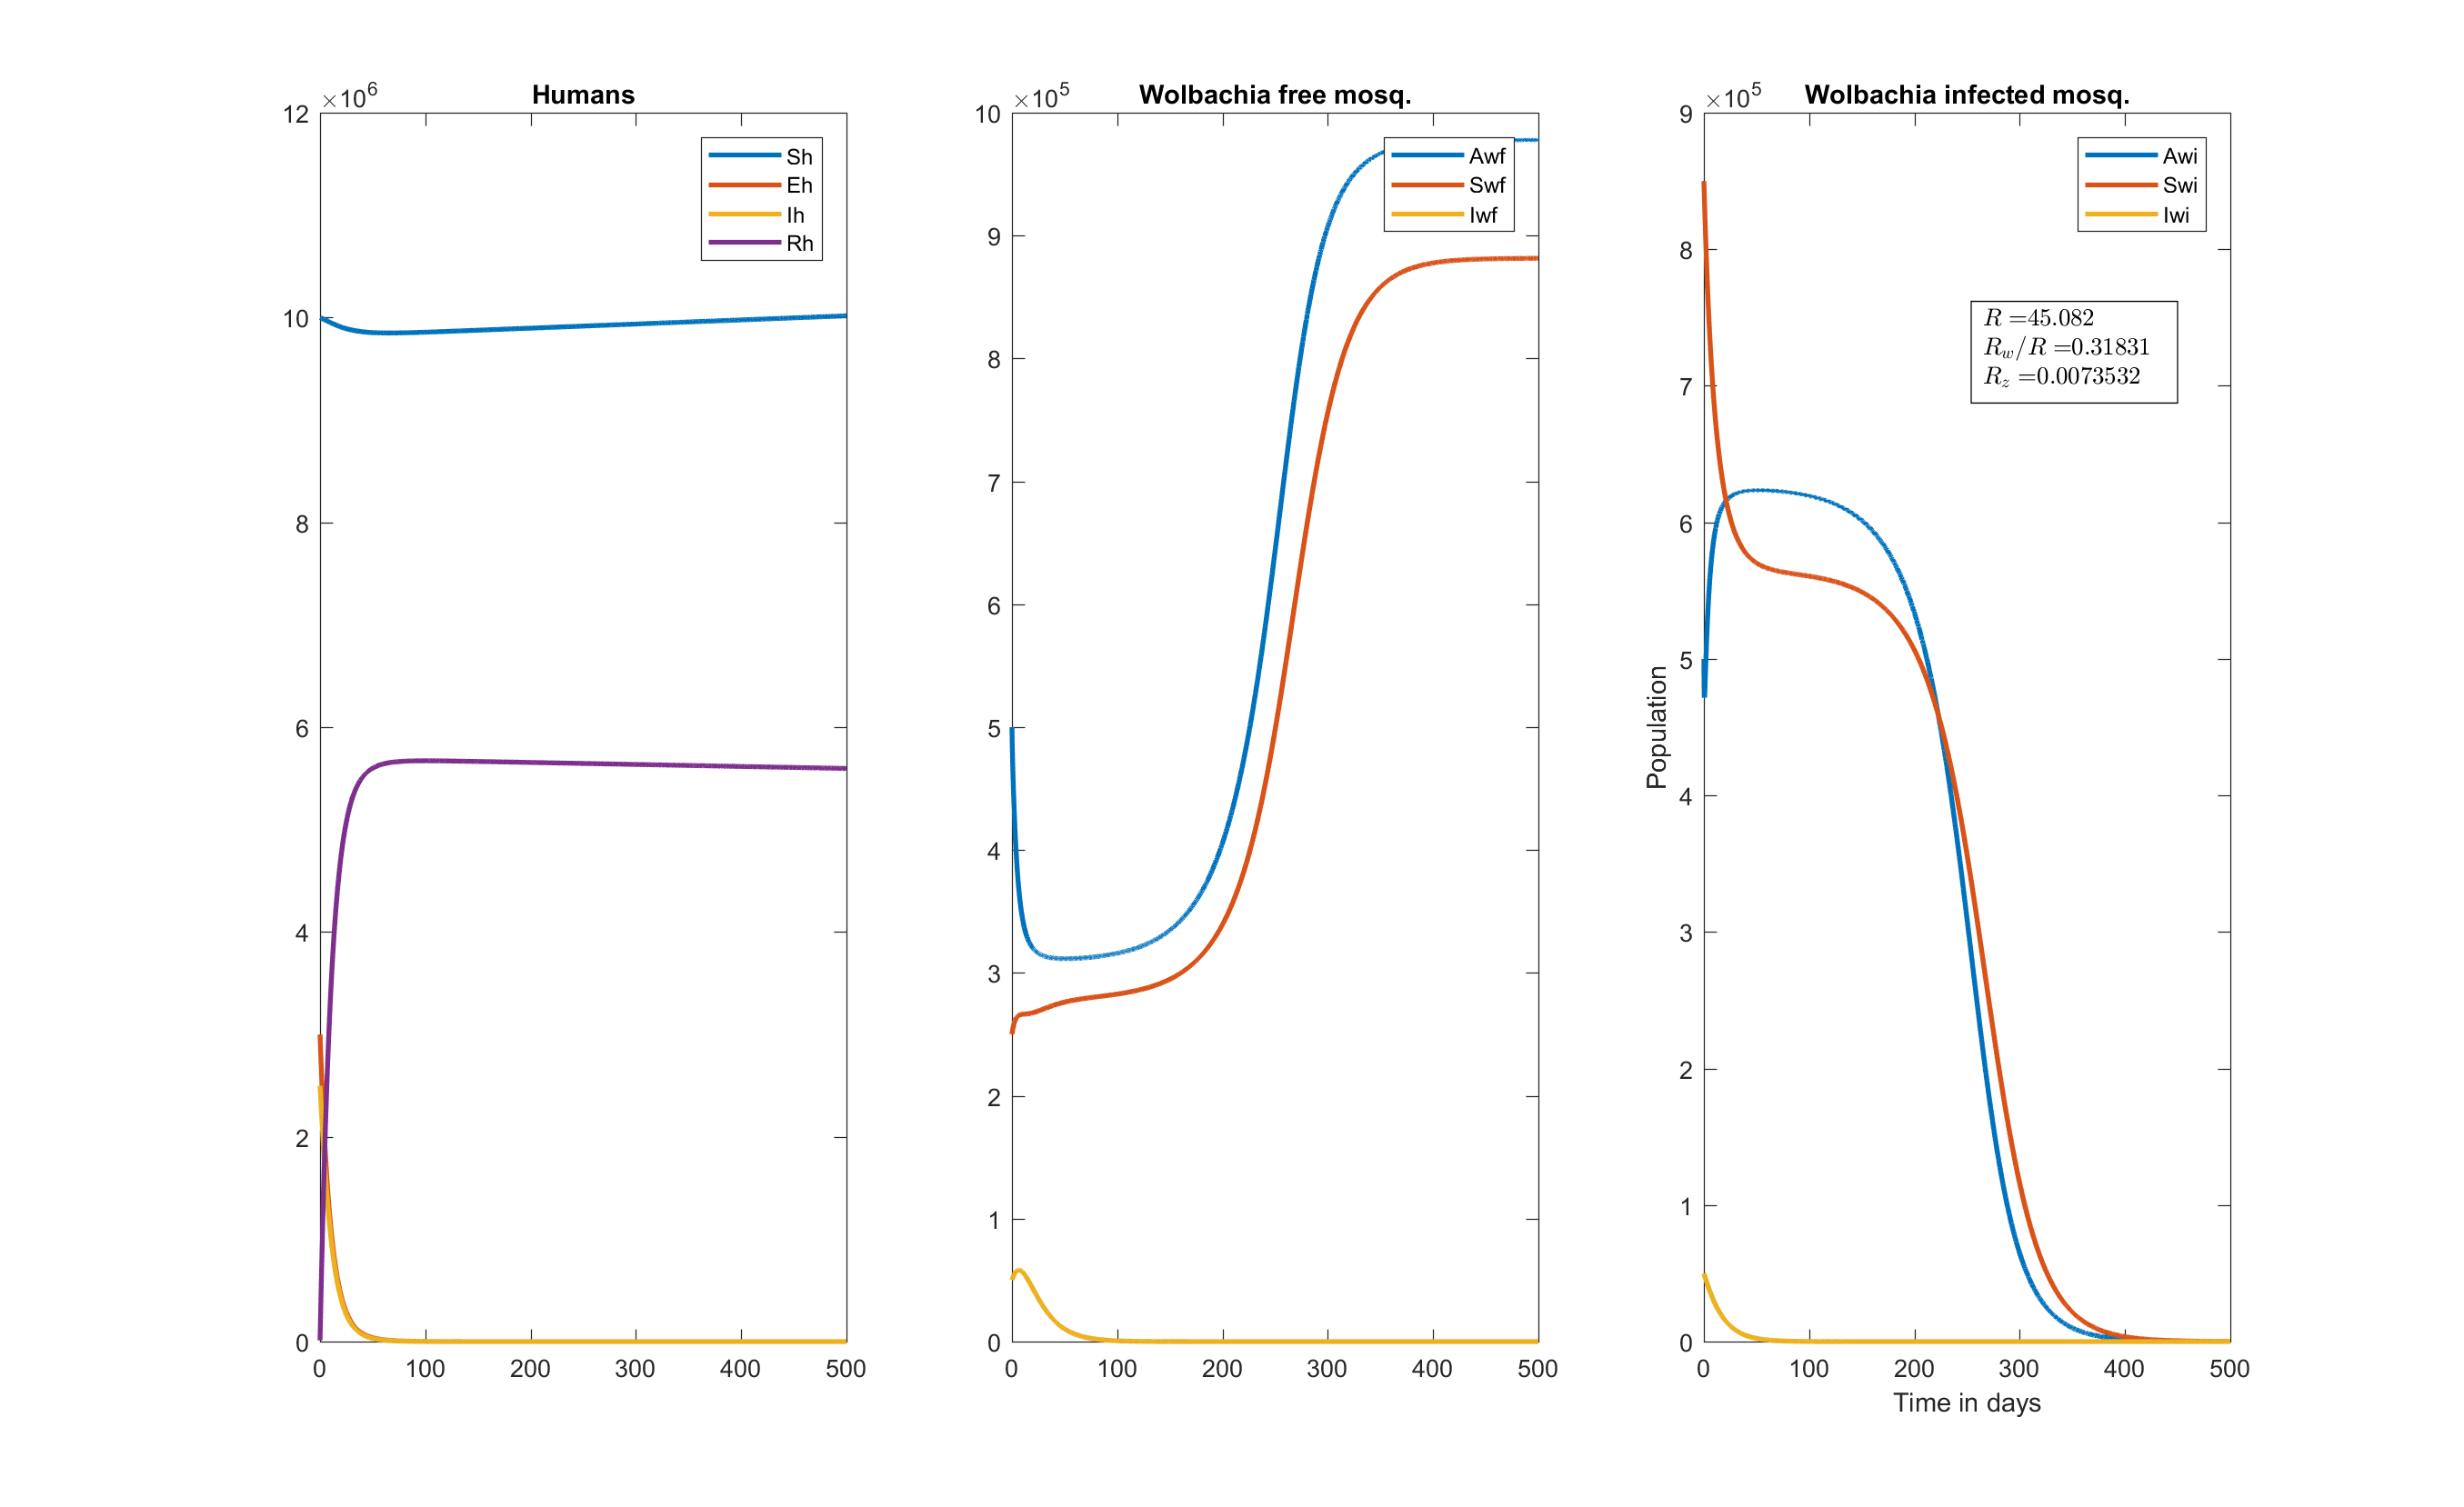
\includegraphics[width=17cm,height=4.5cm]{NoSexualTransmission.png}
%    \caption{\textit{Wolbachia} infected mosquito population dies when we start with more \textit{Wolbachia} infected susceptible females but sexual transmission is ignored. Figure  obtained using baseline values for parameters from Table \ref{tab: param-table} and Table \ref{tab: param_mosq_table} and the initial conditions listed in Table \ref{init-cond-dis-free-table} with $S_{wi}(0)=850,000$} and $\beta_{hh}=0.$
%    \label{domiWolbInfFemfails}
%\end{figure}

\begin{figure}[H]
    \centering
    % This file was created by matlab2tikz.
%
%The latest updates can be retrieved from
%  http://www.mathworks.com/matlabcentral/fileexchange/22022-matlab2tikz-matlab2tikz
%where you can also make suggestions and rate matlab2tikz.
%
\definecolor{mycolor1}{rgb}{0.00000,0.44700,0.74100}%
\definecolor{mycolor2}{rgb}{0.85000,0.32500,0.09800}%
\definecolor{mycolor3}{rgb}{0.92900,0.69400,0.12500}%
\definecolor{mycolor4}{rgb}{0.49400,0.18400,0.55600}%
%
\begin{tikzpicture}

\begin{axis}[%
width=1.1in,
height=1.5in,
at={(0in,0.108in)},
scale only axis,
xmin=0,
xmax=500,
ymin=0,
ymax=12000000,
ylabel={Population},
axis background/.style={fill=white},
title style={font=\bfseries, yshift=1.75ex},
title={Humans},
legend style={legend cell align=left, align=left, draw=white!15!black}
]
\addplot [color=mycolor1, line width=1.5pt]
  table[row sep=crcr]{%
0	10000000\\
0.85628642141819	9996107.42039933\\
1.91505087353289	9991089.28209122\\
3.25375290215015	9984498.13399715\\
5.00219079479575	9975631.90913277\\
9.41912457719445	9953103.51500395\\
11.0663244202733	9944991.44480671\\
12.5382224749774	9937980.57573593\\
13.778412161395	9932277.07478416\\
14.9276677779853	9927173.8491858\\
16.0845545176417	9922223.87846249\\
17.3202937599272	9917151.80709223\\
18.3306815680116	9913173.68433986\\
19.4587810747325	9908913.84520294\\
20.6378516145051	9904667.04522539\\
21.679354576394	9901089.74217486\\
22.6567830201238	9897879.57900743\\
23.7308480106294	9894513.98203613\\
24.6795011851937	9891680.00464057\\
25.5952984727919	9889065.1197636\\
26.6081041544676	9886308.56595914\\
27.5794822592288	9883795.02899951\\
28.4518044050783	9881643.66810532\\
29.4054611790925	9879403.19278989\\
30.3261806834489	9877347.43051472\\
31.3230909109116	9875236.72732683\\
32.2866912018508	9873306.63113711\\
33.1672956831753	9871634.22329015\\
34.1311401296407	9869900.38791255\\
35.0469267684966	9868343.32846494\\
36.0354304537177	9866757.73285064\\
36.989502152428	9865317.43891281\\
37.8686468135566	9864065.5728239\\
38.838592255488	9862764.95972251\\
39.7609566245228	9861603.46208859\\
40.5534792561084	9860661.8449041\\
41.2923547755927	9859829.21692807\\
42.1087198443711	9858958.27288942\\
42.8030657842755	9858256.62614558\\
43.5518755614758	9857538.86419944\\
44.4680750388652	9856713.61313613\\
45.2486080117524	9856054.80294513\\
45.9803226422518	9855472.76299315\\
46.8013624213636	9854859.1413918\\
47.5109687298536	9854361.22386675\\
48.2488149795681	9853874.21504007\\
48.9727068375796	9853425.79338012\\
49.7731260247529	9852962.59885591\\
50.4800257459283	9852580.98594818\\
51.2553286850452	9852190.95728744\\
51.9597230125219	9851861.52813005\\
52.7014476135373	9851539.34982607\\
53.4294183533639	9851246.90028485\\
54.0925511047244	9851000.24895333\\
54.8200436197221	9850750.54810076\\
55.5360744222999	9850525.36478924\\
56.1787180174142	9850340.03410315\\
56.6453310530633	9850215.10202004\\
57.1501280609518	9850088.82085685\\
57.6452781353146	9849973.68767911\\
58.1307812724262	9849868.98197249\\
58.7679473701864	9849743.5215679\\
59.3355450313538	9849642.85295881\\
59.8550944291055	9849559.59551273\\
60.4342065043747	9849476.51687109\\
60.8647243324667	9849421.22119708\\
61.3396852724254	9849366.44876022\\
61.8336863983423	9849316.24639916\\
62.3467277120799	9849271.22211599\\
62.8234529737383	9849235.71175712\\
63.2638621833175	9849208.18610997\\
63.662811005488	9849187.52705467\\
64.0202994383872	9849172.39438846\\
64.375959277153	9849160.44635787\\
64.5528749004006	9849155.63904396\\
64.7297905217856	9849151.57690363\\
64.9067061450332	9849148.25287132\\
65.1217607818544	9849145.19608887\\
65.3368154186755	9849143.20716176\\
65.5518700554967	9849142.27377385\\
65.7669246904552	9849142.38374173\\
66.0223969370127	9849143.85366024\\
66.2778691817075	9849146.75901106\\
66.533341428265	9849151.08009561\\
66.7888136729598	9849156.79746781\\
67.0327164176852	9849163.54114741\\
67.2766191624105	9849171.52353378\\
67.5205219052732	9849180.72834763\\
67.9596339575946	9849200.33060004\\
68.3500525727868	9849220.96841161\\
68.7159491926432	9849242.99339443\\
69.0573238134384	9849265.83733638\\
69.4204471688718	9849292.52152158\\
69.8053192552179	9849323.43507691\\
70.2370422687382	9849361.26550041\\
70.7156162094325	9849407.00761488\\
71.2136160321534	9849458.74794863\\
71.7310417406261	9849516.86045517\\
72.4292873572558	9849602.09837493\\
73.0455152802169	9849683.61526926\\
73.7510614469647	9849783.92746235\\
74.492929821834	9849897.14231551\\
75.1393887493759	9850002.02079928\\
75.911855045706	9850134.64687634\\
76.7514979802072	9850287.46035754\\
77.5277035422623	9850436.40127782\\
78.3952244762331	9850611.19661753\\
79.3500858191401	9850813.28154797\\
80.2653936035931	9851016.05790393\\
81.2558704186231	9851244.96434637\\
82.4100495129824	9851523.44557168\\
83.5500974785537	9851810.18962694\\
84.7488898281008	9852123.43366987\\
86.1120348554105	9852493.25349751\\
87.5210357103497	9852889.67023815\\
88.9719276893884	9853311.76967163\\
90.4273331407458	9853748.24855278\\
91.9684638883919	9854223.56080309\\
93.6470873504877	9854755.34805912\\
95.4693042561412	9855347.73156037\\
97.3415410816669	9855971.1795518\\
99.4284864533693	9856681.98314532\\
101.536688277498	9857415.16474304\\
103.91370549053	9858257.95116379\\
106.475513644516	9859182.99684112\\
109.347147427499	9860237.72324795\\
112.408559240401	9861379.79541721\\
115.846823336557	9862680.61796758\\
119.633243236691	9864131.44072401\\
124.00562187098	9865825.88915896\\
128.932295881212	9867754.2505167\\
134.77434053272	9870060.5160195\\
141.56892259419	9872761.88847862\\
150.159113546833	9876196.57656312\\
161.529476307333	9880762.55247744\\
179.336241200566	9887934.0320888\\
267.813881669194	9923588.82031498\\
304.786209246144	9938460.16594956\\
341.585221335292	9953242.89523504\\
378.263075429946	9967958.15502648\\
414.926954338327	9982649.06691511\\
451.672858864069	9997354.06812287\\
488.466434059665	10012059.3348114\\
500	10016665.0770783\\
};
\addlegendentry{$S_h$}

\addplot [color=mycolor2, line width=1.5pt]
  table[row sep=crcr]{%
0	3000000\\
0.673826509155333	2807656.70757491\\
1.32424164516851	2633986.51531848\\
1.91505087306723	2485798.30765356\\
2.70934844342992	2299965.82783991\\
3.5259551317431	2123778.59456413\\
4.27977073471993	1973482.78560544\\
5.00219079433009	1839732.80320244\\
5.72461085394025	1715325.33462288\\
6.42059023259208	1603687.07098872\\
7.07797077205032	1505140.29363253\\
7.7079201634042	1416585.38572749\\
8.32160609727725	1335504.3399249\\
8.9691876876168	1255151.78505745\\
9.65320093557239	1175714.80745231\\
10.3575963457115	1099358.78164505\\
11.0663244212046	1027729.88053262\\
11.7190690734424	966058.985003178\\
12.3376985252835	911170.252242335\\
12.9426152952947	860641.651714332\\
13.554221901577	812524.479051909\\
14.2267926819623	762846.373369761\\
14.927667778451	714450.464500894\\
15.6310865827836	669106.512992457\\
16.3112884853035	628126.233549998\\
16.9213297958486	593615.414397526\\
17.7115274821408	551853.109166411\\
18.3306815680116	521297.719579993\\
18.9890728867613	490755.263366029\\
19.6936351680197	460153.990221769\\
20.401797503233	431421.728913445\\
21.0621458874084	406336.874151787\\
21.8722689929418	377656.146591414\\
22.6567830196582	351922.355401016\\
23.2805948122405	332791.074541477\\
23.9559746100567	313319.156183069\\
24.6795011856593	293798.074793642\\
25.3704245518893	276363.436313177\\
26.0171553338878	261042.137993879\\
26.79814458685	243740.377368668\\
27.5794822592288	227653.154171231\\
28.2131313825957	215442.202072167\\
28.9291504523717	202483.872551799\\
29.6430988833308	190392.747189254\\
30.3261806843802	179548.462897286\\
31.1363453874364	167541.289004047\\
31.893285040278	157102.136058714\\
32.7113614147529	146603.538051102\\
33.3952628159896	138407.817100044\\
34.1311401296407	130139.178054981\\
34.8234287016094	122846.746615056\\
35.6529276454821	114686.875088118\\
36.4065202013589	107781.752713353\\
37.2013943558559	100984.437696611\\
37.8686468140222	95637.6605575467\\
38.5990509660915	90135.5758458124\\
39.3176748342812	85056.9809827702\\
40.1684376290068	79443.9589643283\\
40.9160815095529	74843.8285327735\\
41.6822990570217	70429.2953654565\\
42.3401684910059	66865.4302936308\\
43.0526690436527	63226.5111819115\\
43.8014788199216	59634.0883996501\\
44.4680750393309	56623.4287043931\\
45.2486080126837	53307.9013330266\\
45.9803226431832	50392.0139604779\\
46.8013624218293	47326.5553424065\\
47.5109687298536	44841.3690342233\\
48.2488149786368	42408.0974535239\\
48.9727068385109	40160.85932654\\
49.7731260247529	37826.9633182613\\
50.480025744997	35889.0963716689\\
51.2553286845796	33888.0480217608\\
51.9597230125219	32175.7556822803\\
52.701447612606	30474.6748657767\\
53.4294183538295	28900.5841260497\\
54.2744242339395	27184.300931925\\
54.9990513203666	25801.2968077324\\
55.7502889540046	24448.4524477199\\
56.6453310535289	22937.17260302\\
57.4025265658274	21738.3572908998\\
58.1307812724262	20649.7875480945\\
58.9651546347886	19475.3342887983\\
59.8550944295712	18302.5979486089\\
60.6272438634187	17347.4376655133\\
61.3396852728911	16514.2502566944\\
62.0902070556767	15683.4908834798\\
62.8234529732727	14915.6695179692\\
63.662811005488	14086.6301236143\\
64.552874899935	13261.9421525807\\
65.3368154182099	12578.9491759641\\
66.022396936547	12012.8994877175\\
66.7888136734255	11412.6293756957\\
67.5205219057389	10869.7772028917\\
68.3500525727868	10287.9456278575\\
69.228011125233	9708.62789919833\\
69.9977552993223	9229.64994421462\\
70.7156162089668	8805.8700344828\\
71.4723288859241	8381.75177004933\\
72.4292873567902	7876.61025978485\\
73.222210438922	7482.83125926321\\
74.1019828240387	7070.50541270338\\
74.9239024408162	6707.23930223566\\
75.6543662799522	6401.13654948771\\
76.5574465901591	6043.19133363618\\
77.3336521512829	5752.59551088745\\
78.1707346285693	5455.82544571161\\
79.106628654059	5143.2109634364\\
80.0414433963597	4849.89393602824\\
80.8726071147248	4603.99142503133\\
81.8082630853169	4342.89571654378\\
82.6188772832975	4129.35351789882\\
83.550097478088	3897.65620397124\\
84.5093911094591	3673.26173405442\\
85.3635979136452	3484.89408538118\\
86.2932129376568	3291.39243619377\\
87.0642231283709	3139.47234684508\\
87.9778482937254	2968.92158815544\\
88.9719276898541	2794.32841862738\\
89.8660466200672	2646.46016721101\\
90.795228023082	2501.42596152658\\
91.7581846420653	2359.84048914816\\
92.6709006824531	2233.33750038268\\
93.6470873504877	2105.81670056004\\
94.5348361437209	1996.41355773527\\
95.4693042566068	1887.6047770977\\
96.4133965019137	1783.90213776426\\
97.3415410807356	1687.69000081019\\
98.3534204047173	1588.88765854994\\
99.2453225045465	1506.75499954587\\
100.156046831515	1427.39809621172\\
101.113470351789	1348.60273951851\\
102.037851568311	1276.77001778549\\
103.027063625865	1204.24387647817\\
103.913705491461	1142.83557219012\\
104.832791150082	1082.56478319643\\
105.770680078305	1024.41404086677\\
106.710458166432	969.350471857935\\
107.736410115846	912.685058278963\\
108.626477722544	866.271973577794\\
109.523164007813	821.948571755085\\
110.476390378084	777.362982280087\\
111.409502532333	736.105564930942\\
112.408559240401	694.400223243516\\
113.294617312029	659.427769578062\\
114.202669930179	625.444412992802\\
115.135971037671	592.369601854589\\
116.083774102852	560.598020573612\\
117.119867246132	527.841831176542\\
118.009087334387	501.281335717533\\
118.896341274958	476.12996198656\\
119.846394765656	450.614202067722\\
120.785169114359	426.761793647893\\
121.690424335655	404.972154889256\\
122.672384157777	382.60700310301\\
123.541108543985	363.864476433024\\
124.486426909454	344.5223449287\\
125.393348680809	326.943027032074\\
126.387993809767	308.703235208057\\
127.346330719534	292.101723394357\\
128.215738268569	277.821617066395\\
129.16881317459	262.975266159046\\
130.083140397444	249.485101121943\\
131.06492918171	235.775456514675\\
132.018458198756	223.187698950525\\
132.898957811762	212.166239861399\\
133.863950741012	200.715870528016\\
134.774340533651	190.48453335464\\
135.749758967198	180.104369941633\\
136.697001389693	170.569290693384\\
137.577680364251	162.160557871684\\
138.5503040771	153.35776937101\\
139.468801688403	145.486617055722\\
140.431762074586	137.670357584488\\
141.374278929085	130.429098163266\\
142.266855079681	123.924889461603\\
143.250426402315	117.134534488432\\
144.16316867061	111.168132672086\\
145.120424913708	105.238565910608\\
146.058428125922	99.7366152163595\\
146.949939061422	94.7754403916188\\
147.94025172526	89.5545099563897\\
148.861865526531	84.9555826899596\\
149.808109500445	80.480387895368\\
150.741679665633	76.2971559683792\\
151.645020165481	72.4573129136115\\
152.644394950476	68.4348775343969\\
153.55879287608	64.9511532606557\\
154.500993979163	61.5476027424447\\
155.431857756339	58.3608222836629\\
156.332342125475	55.4357045702636\\
157.337024221662	52.3454107339494\\
158.261109224055	49.6558668334037\\
159.194386634044	47.0802714223973\\
160.121216409374	44.6551313735545\\
161.032817149069	42.3921267571859\\
162.044311992824	40.0155354728922\\
162.960194228683	37.9791011321358\\
163.891579162795	36.0147774904035\\
164.817234549206	34.1635180828162\\
165.724098528735	32.4424345977604\\
166.68981855968	30.7051598890685\\
167.662089425605	29.0503470376134\\
168.725684036035	27.3423682274297\\
169.682915424928	25.8914736271836\\
170.601452002767	24.57187873777\\
171.59581849305	23.2192697939463\\
172.543776652776	21.9993763621897\\
173.654405792244	20.6516659632325\\
174.618033316918	19.5496092122048\\
175.716323922854	18.3652834519744\\
176.842926030979	17.225149799604\\
177.880688347388	16.2378382505849\\
179.086841503158	15.1614157115109\\
180.234572810587	14.2036549132317\\
181.349275914486	13.3315796675161\\
182.555458180606	12.4483295446262\\
183.786050859839	11.6076652859338\\
185.124142831657	10.7580595887266\\
186.422458820511	9.99337800592184\\
187.738088242244	9.27410196186975\\
189.20253180759	8.53437835397199\\
190.565868526231	7.89903194736689\\
191.950775207486	7.30220364267007\\
193.447223335039	6.70806366298348\\
195.087715640198	6.11232472304255\\
196.673974680714	5.5868243733421\\
198.39946975559	5.06655696872622\\
200.147829764057	4.58897965867072\\
201.862859976478	4.16444449825212\\
203.756528425962	3.74134985357523\\
205.840791524854	3.32539955992252\\
208.039846160915	2.936789622996\\
210.327357653994	2.5808815388009\\
212.765991523396	2.2490591625683\\
215.438257910311	1.93447477370501\\
218.258122809697	1.65035641426221\\
221.367281336337	1.38548022927716\\
224.807241802569	1.14196150284261\\
228.521811525337	0.927138710394502\\
232.681145651266	0.734505007043481\\
237.293243078049	0.567672231700271\\
242.609053144231	0.422191398683935\\
249.009096345399	0.296007911209017\\
256.62282983074	0.194462756160647\\
266.298304262571	0.114474556874484\\
279.364201130811	0.0564177450723946\\
299.248911239672	0.0195753346197307\\
338.577083528508	0.00254072528332472\\
500	7.01751559972763e-07\\
};
\addlegendentry{$E_h$}

\addplot [color=mycolor3, line width=1.5pt]
  table[row sep=crcr]{%
0	2500000\\
0.856286420952529	2332598.83400162\\
1.76734856609255	2163403.32644162\\
2.51077405083925	2032338.40373033\\
3.25375290215015	1907688.63428424\\
4.03896404802799	1782805.60971437\\
4.76138410763815	1674041.52391674\\
5.48380416724831	1571029.0849149\\
6.1885971063748	1475926.34410982\\
7.07797077205032	1363264.71152658\\
7.91248214105144	1264706.13265004\\
8.75332715734839	1172071.91170635\\
9.41912457672879	1103250.08200585\\
10.1213536537252	1034793.76562293\\
10.8300817292184	969803.878459235\\
11.5014875228517	911851.006624111\\
12.3376985252835	844327.792352616\\
13.1464841640554	783649.095645785\\
13.778412161395	739222.909400765\\
14.4509829417802	694655.699844881\\
15.1660101967864	650181.13546946\\
15.8578205504455	609840.352341426\\
16.5146355889738	573848.891920552\\
17.3202937603928	532587.697631566\\
18.1189129557461	494625.534578975\\
18.7542187930085	466382.085545911\\
19.4587810742669	436961.078177376\\
20.1657433914952	409329.748984202\\
20.8499987511896	384277.800436345\\
21.4864401598461	362380.597170908\\
22.2580978265032	337533.418114315\\
23.0554682132788	313689.280080267\\
23.7308480106294	294850.649990185\\
24.4383256603032	276364.053292243\\
25.1455506314524	259078.781875505\\
25.8201723936945	243632.690943128\\
26.6081041544676	226795.501815158\\
27.3682658849284	211697.002297753\\
28.0019150078297	199913.271759689\\
28.6904774289578	187882.002843045\\
29.4054611795582	176188.270758436\\
30.1183742913418	165286.16940959\\
30.7417934704572	156333.412621033\\
31.5098364357837	146000.297625499\\
32.2866912009194	136278.464902925\\
32.9393285484985	128639.873697822\\
33.640555253718	120935.108488206\\
34.3764325673692	113373.165726743\\
35.0469267689623	106919.443693792\\
35.8441790500656	99750.2200135933\\
36.5920650744811	93489.1144734416\\
37.2013943558559	88698.0076371212\\
37.8686468140222	83750.7669131909\\
38.5990509660915	78671.7557918238\\
39.3176748342812	73995.4552985653\\
40.1684376290068	68841.568744306\\
40.9160815095529	64630.211837342\\
41.6822990570217	60600.3933404335\\
42.3401684910059	57356.1464346987\\
43.0526690436527	54052.6066739173\\
43.8014788199216	50800.9531527902\\
44.4680750393309	48083.8709398587\\
45.2486080126837	45100.7585854996\\
45.9803226431832	42485.7214909624\\
46.8013624218293	39745.8239814918\\
47.5109687298536	37532.090106729\\
48.2488149786368	35371.6156011741\\
48.9727068385109	33382.918015054\\
49.7731260247529	31324.7234650077\\
50.480025744997	29621.7294672835\\
51.2553286845796	27869.2752152048\\
51.9597230125219	26374.9139842945\\
52.701447612606	24895.4032510319\\
53.4294183538295	23531.1188104004\\
54.2744242339395	22049.1656474941\\
54.9990513203666	20859.4826973374\\
55.7502889540046	19699.8668436324\\
56.3929325495847	18763.7905733804\\
57.1501280614175	17722.893833444\\
57.8880297034048	16769.1052541868\\
58.7679473701864	15704.6088504391\\
59.5087281642482	14865.7436417984\\
60.2411691467278	14084.3788855723\\
61.1022048033774	13222.8994627721\\
61.8336863992736	12536.3179882979\\
62.6032483680174	11855.9144781255\\
63.4840667885728	11126.3954439033\\
64.1990436553024	10570.3451094725\\
64.9067061450332	10049.8147631227\\
65.7669246909209	9454.52285542386\\
66.5333414277993	8956.54974898137\\
67.2766191614792	8500.89331711968\\
68.1548432651907	7994.89318967517\\
68.8866365030408	7598.35237745754\\
69.6128832125105	7225.95146579156\\
70.4763292390853	6808.89639460947\\
71.213616032619	6473.50717667211\\
71.9897545934655	6139.77960713394\\
72.8688201201148	5784.24203335447\\
73.7510614464991	5449.80750847002\\
74.4929298222996	5184.81577395322\\
75.3968775151297	4880.66593833594\\
76.1693438095972	4636.05191721721\\
76.945549370721	4403.56405298645\\
77.7217549318448	4183.63057938078\\
78.6197143252939	3943.89439093322\\
79.3500858186744	3759.82463314198\\
80.2653936031274	3542.1064616139\\
81.0642387671396	3363.15821993677\\
81.9923939737491	3167.35776544735\\
82.8277050526813	3001.5787919187\\
83.7908949530683	2821.88119316893\\
84.7488898285665	2654.5213609538\\
85.5685006091371	2519.7453392446\\
86.4859654852189	2377.48571000854\\
87.292629419826	2259.46511259023\\
88.2263681427576	2130.58436682541\\
89.1954574221745	2005.04259847198\\
90.0531421266496	1900.46787789091\\
90.9760273983702	1794.36228912137\\
91.7581846420653	1709.33854576014\\
92.6709006824531	1615.46857260773\\
93.6470873504877	1521.05713878572\\
94.5348361437209	1440.23447079398\\
95.4693042566068	1360.015106251\\
96.4133965019137	1283.71610588906\\
97.3415410807356	1213.06729510613\\
98.1004505734891	1158.3267957936\\
99.0223469794728	1095.28268241184\\
99.9779783003032	1033.69935052376\\
100.901861389168	977.586579698138\\
101.787269922905	926.781108213123\\
102.783039242495	872.907209578436\\
103.714408942033	825.457081092522\\
104.65929363016	780.044480817858\\
105.579582226463	738.297049671412\\
106.475513644516	699.871267493814\\
107.479922128376	659.239337362349\\
108.403960820753	624.007762175985\\
109.347147426568	590.043228980619\\
110.263802064583	558.855808391236\\
111.155534768477	530.141482087784\\
112.162998650223	499.517251618672\\
113.097148866393	472.743792913854\\
114.031631354708	447.430982823018\\
114.945405404549	424.020553317852\\
115.846823336557	402.153838743456\\
116.860843960196	378.929109589197\\
117.786782312207	358.919424738735\\
118.721757796593	339.807600742672\\
119.633243237156	322.174682640005\\
120.528933467809	305.755302139092\\
121.494032371324	289.015364184976\\
122.475992193446	272.939214230981\\
123.316997736692	259.895156607497\\
124.246024390217	246.22070142813\\
125.171175597236	233.329133277293\\
126.001757787541	222.339802045841\\
126.949107739143	210.444797845092\\
127.766700727399	200.698854558636\\
128.693443343975	190.203530580737\\
129.641847761348	180.037996551022\\
130.492691083346	171.386981372256\\
131.432391937356	162.320362173021\\
132.213813619222	155.151371124666\\
133.127339208964	147.175187557004\\
134.109487918671	139.061396313831\\
134.995958071668	132.126655188389\\
135.933557729702	125.171508962288\\
136.909048762638	118.327207400929\\
137.822217220441	112.262746193446\\
138.789317222312	106.181563983206\\
139.670259863604	100.93168819882\\
140.611055004876	95.6137028937228\\
141.568922593724	90.4891975717619\\
142.499499241356	85.7758025578223\\
143.500735455658	80.9802743829787\\
144.383979742415	76.9744852371514\\
145.301445522811	73.024561942555\\
146.272348900791	69.0665031694807\\
147.199687672313	65.4877551691607\\
148.181318555493	61.9025177434087\\
149.060278835706	58.8601116295904\\
149.983611523174	55.8259219140746\\
150.935868372209	52.8613133220933\\
151.881404096726	50.0742329359055\\
152.898725235369	47.2402647859417\\
153.778815423138	44.9189484086819\\
154.679836108349	42.661109090317\\
155.647353016771	40.3634250038303\\
156.586340712849	38.2524177436717\\
157.579710555263	36.1397308292799\\
158.6531612291	33.9882550677285\\
159.539586036932	32.3089187471196\\
160.554334516637	30.4884953107685\\
161.529476307798	28.8362168744206\\
162.521217966452	27.2479740031995\\
163.53563076118	25.7142205182463\\
164.600642762613	24.1971099637449\\
165.724098528735	22.6939914259128\\
166.884272732772	21.2400154531933\\
167.856543599162	20.0937691098079\\
168.950579457451	18.878010250628\\
169.927027413622	17.8553872550838\\
171.018649772741	16.7777944901027\\
172.14983229991	15.7299277582206\\
173.17159590451	14.8399681835435\\
174.37762449868	13.8542801775038\\
175.510499599855	12.9882782935165\\
176.649656613823	12.1722161355428\\
177.880688347388	11.3480543517508\\
179.086841503158	10.5948573951609\\
180.422539516352	9.81912954896688\\
181.712112193927	9.12428379431367\\
183.049190457445	8.4558691252023\\
184.515435237437	7.77920320164412\\
186.03772267187	7.13407597970217\\
187.505364924204	6.56296294135973\\
188.978368033655	6.03586842305958\\
190.565868526231	5.51524219103158\\
192.202253622003	5.02568828500807\\
193.937757804524	4.55402463395149\\
195.819423559122	4.09267640300095\\
197.660494612064	3.68669775687158\\
199.794768333435	3.26636207615957\\
201.862859976478	2.90499102696776\\
204.15344137745	2.55138039262965\\
206.553107017186	2.22717360733077\\
209.201700550504	1.91712966375053\\
211.977831007447	1.63856211211532\\
214.975848732051	1.38319672551006\\
218.468441897072	1.13566617062315\\
222.307997980155	0.91458298638463\\
226.584285459016	0.718873597215861\\
231.413066423498	0.548005701508373\\
236.837609823793	0.40427651675418\\
243.318427340593	0.281401824206114\\
251.150542250369	0.181958694942296\\
261.144246759824	0.104682133998722\\
274.744488350116	0.0497025432996452\\
296.013571006712	0.0158183323219419\\
340.928741482086	0.00151549698784947\\
500	4.69852238893509e-07\\
};
\addlegendentry{$I_h$}

\addplot [color=mycolor4, line width=1.5pt]
  table[row sep=crcr]{%
0	10000\\
0.7650564648211	380970.678138305\\
1.47194395214319	703747.37023471\\
2.1136252656579	980807.851611423\\
2.70934844296426	1224989.27436496\\
3.52595513220876	1540220.06134532\\
4.27977073471993	1812185.6777976\\
5.00219079386443	2056604.94493874\\
5.72461085394025	2285996.64232593\\
6.42059023305774	2493539.68723658\\
7.07797077205032	2678092.50988782\\
7.9124821415171	2897224.70579701\\
8.53746662754565	3050864.5826699\\
9.1850482178852	3201137.40235339\\
9.88727729488164	3354385.81719801\\
10.5938390372321	3498970.04921089\\
11.2839059717953	3631423.29657245\\
11.9366506244987	3749213.51299609\\
12.7387464260682	3884583.30593513\\
13.5542219011113	4012310.13696434\\
14.2267926819623	4110641.88002252\\
14.9276677789167	4206799.97697688\\
15.6310865832493	4297226.85450299\\
16.3112884853035	4379234.23457091\\
17.1246768999845	4470741.39614562\\
17.9071443434805	4552486.87321373\\
18.5424501802772	4614629.37434062\\
19.2239269809797	4677341.59149662\\
19.9296892797574	4738245.90680414\\
20.6378516154364	4795484.88534954\\
21.2742930231616	4843823.17196472\\
22.0651834094897	4900062.96820066\\
22.8561256164685	4952348.00038597\\
23.5057214116678	4992529.55940304\\
24.1971501354128	5032741.73867185\\
24.9206767110154	5072175.03786274\\
25.5952984727919	5106660.71824937\\
26.4111212138087	5145620.30699627\\
27.1782254520804	5179700.93635987\\
28.0019150078297	5213742.11943489\\
28.6904774289578	5240310.14569532\\
29.4054611800238	5266200.60404345\\
30.1183742908761	5290405.24344499\\
30.94959986303	5316734.48827505\\
31.6965819597244	5338777.5211538\\
32.4833942810073	5360457.86720569\\
33.167295682244	5378106.36433249\\
33.8858476914465	5395529.60651002\\
34.5999306347221	5411780.38667414\\
35.2704248363152	5426134.55358648\\
36.035430454649	5441510.76133488\\
36.7776099480689	5455474.51026328\\
37.6251787636429	5470352.6291421\\
38.3555829152465	5482322.92285942\\
39.0781335448846	5493441.98717145\\
39.7609566254541	5503330.93985856\\
40.5534792570397	5514103.4157427\\
41.292354776524	5523508.53707967\\
42.1087198443711	5533232.9941317\\
42.8030657852069	5540988.98658082\\
43.5518755614758	5548857.59454902\\
44.2458762992173	5555719.32497246\\
45.0624966016039	5563297.04006175\\
45.7984549030662	5569696.11757425\\
46.5883050756529	5576140.43270908\\
47.2626942489296	5581317.58682817\\
48.007517692633	5586709.22987007\\
48.7314095515758	5591641.12107401\\
49.5730212284252	5597017.84384703\\
50.3033008147031	5601392.08987819\\
51.0615029493347	5605665.85993127\\
51.724924903363	5609195.02819505\\
52.447984367609	5612831.12325197\\
53.2083741035312	5616432.27730815\\
54.0925511056557	5620351.19741216\\
54.8200436197221	5623373.13092323\\
55.5360744222999	5626180.18893579\\
56.392932549119	5629334.7422089\\
57.1501280618832	5631948.44227372\\
57.8880297038704	5634348.38033599\\
58.7679473701864	5637032.26412294\\
59.5087281642482	5639151.02156143\\
60.2411691462621	5641127.25300114\\
61.1022048033774	5643308.7427582\\
61.8336863992736	5645048.94870946\\
62.6032483680174	5646774.4850277\\
63.4840667890385	5648625.10645598\\
64.199043655768	5650035.5677532\\
64.9067061450332	5651355.40936304\\
65.7669246913865	5652863.59384026\\
66.533341428265	5654123.62480308\\
67.2766191614792	5655274.7445689\\
68.1548432651907	5656550.24875456\\
68.8866365030408	5657547.15050674\\
69.6128832120448	5658480.64732199\\
70.4763292390853	5659522.20611786\\
71.2136160321534	5660356.186056\\
71.9897545939311	5661182.14792482\\
72.8688201196492	5662056.97091178\\
73.5756007581949	5662716.24276294\\
74.2774435132742	5663334.13279323\\
75.1393887503073	5664045.52733978\\
75.9118550447747	5664641.07276032\\
76.7514979802072	5665245.98491703\\
77.527703541331	5665768.06907973\\
78.1707346281037	5666174.98194391\\
78.8631714899093	5666588.48918039\\
79.5935429828241	5666998.24478204\\
80.2653936035931	5667352.37966599\\
81.0642387671396	5667746.45817581\\
81.8082630848512	5668088.43977374\\
82.6188772832975	5668434.98293083\\
83.309300002642	5668709.80427473\\
84.0303936721757	5668977.85109268\\
84.7488898281008	5669226.55678689\\
85.3635979136452	5669425.44169106\\
86.1120348554105	5669651.09214438\\
86.8714705808088	5669862.40142598\\
87.521035711281	5670029.69489998\\
88.2263681422919	5670197.96086764\\
88.9719276893884	5670361.35905237\\
89.6425168877468	5670496.21199994\\
90.2402376336977	5670607.16177655\\
90.795228023082	5670702.68172494\\
91.3376261498779	5670789.31300902\\
91.9684638883919	5670882.02226208\\
92.4248219085857	5670943.8834483\\
92.9169794563204	5671005.86469491\\
93.4050727905706	5671062.63238716\\
93.8891019104049	5671114.44785559\\
94.3329763077199	5671158.16189419\\
94.9385558171198	5671212.12394741\\
95.4693042570725	5671254.21035285\\
95.8380144275725	5671280.67524751\\
96.2216024771333	5671305.86102105\\
96.6454326463863	5671330.97485746\\
97.109504936263	5671355.29251527\\
97.5945109119639	5671377.25622513\\
98.1004505734891	5671396.52368768\\
98.576395929791	5671411.35608018\\
98.7993714548647	5671417.23451412\\
99.0223469799384	5671422.44317267\\
99.2453225050122	5671426.99144853\\
99.4284864533693	5671430.24011325\\
99.6116504026577	5671433.05446458\\
99.7948143510148	5671435.43949871\\
99.9779783003032	5671437.40015147\\
100.15604683198	5671438.9040552\\
100.334115362726	5671440.01589395\\
100.512183894403	5671440.74004061\\
100.69025242608	5671441.08081688\\
100.901861389168	5671440.99319249\\
101.113470351323	5671440.37727663\\
101.325079314411	5671439.24004344\\
101.536688277498	5671437.58837078\\
101.787269922905	5671434.97652438\\
102.037851568311	5671431.66388858\\
102.288433213718	5671427.66136797\\
102.539014859125	5671422.97969048\\
102.783039242961	5671417.77784638\\
103.027063625865	5671411.95151445\\
103.515112392604	5671398.46296316\\
103.913705491461	5671385.67289831\\
104.312298589386	5671371.32988919\\
104.832791150548	5671350.32534692\\
105.38848437462	5671325.14144241\\
105.770680078305	5671306.21582454\\
106.240569122136	5671281.20678042\\
106.710458166897	5671254.32902619\\
107.223434140906	5671222.91580914\\
107.958927017637	5671174.23511541\\
108.626477722079	5671126.48011127\\
109.347147426568	5671071.2723628\\
110.051213751547	5671013.82698602\\
110.901567004621	5670940.03039363\\
111.663470296189	5670869.99477597\\
112.654119830579	5670773.68297986\\
113.689554203302	5670667.02117558\\
114.564274138771	5670572.41081076\\
115.609872570261	5670454.2180034\\
116.601820674725	5670337.24729814\\
117.786782312207	5670191.72206641\\
119.070924753323	5670027.36949581\\
120.272697821259	5669867.73805107\\
121.69042433612	5669672.72566094\\
123.0928869294	5669473.2280776\\
124.486426909454	5669269.03218081\\
126.194875798188	5669011.26586096\\
127.976885731332	5668734.48271838\\
129.878365054727	5668431.12352702\\
131.823102778755	5668113.19306608\\
133.863950741477	5667772.11733575\\
136.117356492206	5667387.68910303\\
138.550304077566	5666964.53956255\\
141.179635263979	5666499.04046695\\
144.16316867061	5665962.0146209\\
147.44943628367	5665361.36583046\\
150.935868372209	5664715.46931262\\
154.858678237535	5663980.06094056\\
159.366986335255	5663125.88635354\\
164.600642763078	5662125.01121082\\
170.826260198839	5660924.915338\\
178.338642412797	5659467.25371738\\
187.992117246613	5657584.48916665\\
201.608044530265	5654918.92618702\\
226.401403448544	5650054.23734743\\
280.412042237818	5639456.72377132\\
317.805899638683	5632129.67341469\\
354.682110437192	5624913.27533793\\
391.382630587555	5617740.42505119\\
428.111567735672	5610571.17616474\\
464.854530777782	5603408.34368462\\
500	5596565.4905073\\
};
\addlegendentry{$R_h$}

\end{axis}

\begin{axis}[%
width=1.1in,
height=1.5in,
at={(1.42in,0.108in)},
scale only axis,
xmin=0,
xmax=500,
ymin=0,
ymax=1000000,
xlabel={Time (days)},
axis background/.style={fill=white},
title style={font=\bfseries, yshift=1.25ex},
title={\emph{Wolb.}-free mosq.},
legend style={legend cell align=left, align=left, draw=white!15!black}
]
\addplot [color=mycolor1, line width=1.5pt]
  table[row sep=crcr]{%
0	500000\\
0.124589653685689	492676.804810654\\
0.307978125405498	483942.020869771\\
0.58259655314032	473549.28055744\\
0.856286420952529	464785.951746002\\
1.20725283923093	454786.121604362\\
1.61964625923429	444165.223551504\\
2.1136252656579	432658.996895119\\
2.51077405072283	424228.166295992\\
2.98155067279004	415058.894732071\\
3.52595513185952	405522.622240575\\
4.03896404791158	397402.023833515\\
4.52057742117904	390539.519985244\\
5.00219079433009	384243.818497397\\
5.48380416748114	378584.070246288\\
6.18859710649122	371078.01337105\\
6.86527706554625	364870.301979605\\
7.29066447867081	361352.934630883\\
7.91248214116786	356620.833299831\\
8.53746662731282	352427.017395111\\
8.96918768750038	349802.526903035\\
9.6532009356888	345969.937066107\\
10.5938390374649	341429.782680695\\
11.7190690735588	336981.609799996\\
11.9366506242659	336248.58594871\\
12.3376985252835	334788.691199139\\
13.3503530326998	331742.157539863\\
14.2267926817294	329448.573024938\\
14.4509829418967	328934.453694387\\
14.689325360232	328316.856317484\\
14.9276677785674	327762.524449772\\
15.4043526153546	326866.402974568\\
15.6310865827836	326316.826657043\\
15.8578205503291	325843.343038158\\
16.3112884851871	325152.928238831\\
16.5146355888573	324712.561813128\\
16.7179826924112	324332.128327514\\
17.1246768996352	323759.833286414\\
17.5159106213832	323084.237247405\\
17.9071443431312	322561.050095597\\
18.3306815681281	321925.422463026\\
18.7542187932413	321422.163694429\\
18.9890728868777	321079.407558988\\
19.2239269805141	320779.331863463\\
19.6936351679033	320325.395884937\\
19.9296892797574	319978.829824673\\
20.1657433914952	319698.62310179\\
20.4017975033494	319549.080619633\\
20.6378516152035	319370.864988599\\
20.849998751306	319066.203879357\\
21.0621458875248	318828.589776886\\
21.2742930236273	318712.253733477\\
21.4864401597297	318575.126214549\\
21.679354576394	318341.8977462\\
21.8722689930582	318150.620876182\\
22.2580978263868	317895.505819554\\
22.4574404230807	317699.981669251\\
22.6567830197746	317531.208356499\\
23.0554682132788	317277.174671563\\
23.2805948124733	317077.963655727\\
23.5057214116678	316908.408330461\\
23.9559746100567	316670.437144922\\
24.19715013518	316446.076224471\\
24.4383256603032	316274.003750972\\
24.6795011854265	316209.058078478\\
24.9206767105497	316116.595597864\\
25.1455506313359	315882.435829469\\
25.3704245520057	315720.74476791\\
25.5952984727919	315701.996746515\\
25.8201723935781	315649.284844282\\
26.0171553337714	315462.238751386\\
26.2141382739646	315328.625746981\\
26.4111212141579	315284.837066923\\
26.6081041543512	315228.253119307\\
26.7981445869664	315093.156049703\\
26.9881850195816	314986.949265516\\
27.3682658846956	314861.470193544\\
27.5794822591124	314738.667689589\\
27.7906986336457	314638.822971032\\
28.0019150080625	314580.283172668\\
28.2131313824793	314515.012085535\\
28.4518044057768	314372.112386049\\
28.6904774290742	314266.364029364\\
28.9291504524881	314237.074126832\\
29.1678234757856	314187.680710527\\
29.4054611796746	314007.075154266\\
29.6430988835637	313895.15351064\\
29.8807365874527	313927.003969118\\
30.1183742913418	313918.262003209\\
30.3261806843802	313745.923709855\\
30.5339870773023	313641.757379661\\
30.7417934703408	313662.492250042\\
30.9495998633793	313658.215084662\\
31.1363453875529	313541.889972721\\
31.3230909117265	313463.032439661\\
31.5098364357837	313442.882765057\\
31.6965819599573	313416.420829552\\
31.893285040278	313331.656815575\\
32.0899881205987	313268.413261268\\
32.2866912009194	313241.287311923\\
32.4833942812402	313209.20744031\\
32.7113614149857	313119.065749439\\
32.9393285486149	313054.630512593\\
33.1672956823604	313041.569710391\\
33.3952628159896	313015.975457917\\
33.6405552538345	312887.0122732\\
33.8858476916794	312812.590255224\\
34.1311401295243	312855.528379764\\
34.3764325673692	312862.668713274\\
34.5999306346057	312700.630524252\\
34.8234287017258	312617.501614706\\
35.0469267689623	312692.58715038\\
35.2704248361988	312727.025427505\\
35.4616762407823	312604.799052009\\
35.6529276453657	312535.415173801\\
35.8441790498327	312552.740422938\\
36.0354304544162	312557.819109429\\
36.2209753278876	312486.123641682\\
36.4065202012425	312439.56627933\\
36.5920650745975	312432.195754708\\
36.7776099480689	312420.65134055\\
36.9895021519624	312360.97924546\\
37.2013943558559	312321.007776414\\
37.4132865597494	312317.831325023\\
37.6251787636429	312307.100719084\\
37.868646814255	312223.546952897\\
38.1121148647508	312177.202519417\\
38.3555829153629	312210.682820686\\
38.599050965975	312220.012257716\\
38.8385922553716	312081.24998883\\
39.0781335447682	312019.157126099\\
39.3176748341648	312120.972405462\\
39.5572161235614	312173.296710409\\
39.7609566253377	312035.359687716\\
39.9646971271141	311969.743153834\\
40.1684376288904	312034.759692756\\
40.3721781307831	312073.967968405\\
40.5534792570397	311995.681162064\\
40.7347803831799	311952.508454035\\
40.9160815094365	311962.471002497\\
41.0973826356931	311967.331113946\\
41.2923547760583	311921.201838767\\
41.48732691654	311893.778328551\\
41.6822990569053	311897.908293208\\
41.8772711972706	311897.223740118\\
42.1087198442547	311845.630564908\\
42.3401684911223	311818.296928587\\
42.5716171381064	311841.088402498\\
42.803065784974	311850.133016934\\
43.0526690437691	311749.77379245\\
43.3022723025642	311709.150898902\\
43.5518755613593	311799.979785989\\
43.801478820038	311847.940151933\\
44.0236775599187	311702.073906231\\
44.245876299683	311643.610508304\\
44.4680750394473	311760.663460842\\
44.6902737792116	311832.036567761\\
44.8763851902913	311730.912570455\\
45.0624966014875	311682.945673664\\
45.2486080125673	311719.213992229\\
45.434719423647	311744.922913737\\
45.6165871635312	311698.162171279\\
45.798454903299	311674.086074821\\
45.9803226431832	311684.578210518\\
46.1621903829509	311691.614523422\\
46.3752477292437	311657.4922223\\
46.5883050754201	311641.193233382\\
46.8013624217128	311658.838636852\\
47.0144197678892	311668.893353218\\
47.262694249046	311607.646532848\\
47.5109687300865	311585.036231509\\
47.7592432111269	311647.173618087\\
48.0075176921673	311681.935558223\\
48.2488149787532	311551.446535822\\
48.4901122653391	311507.045667774\\
48.731409551925	311648.639783085\\
48.9727068385109	311732.368230425\\
49.172811634955	311602.593133774\\
49.3729164315155	311549.615317155\\
49.573021228076	311632.638507184\\
49.77312602452	311690.067327651\\
49.9498509546975	311627.791884405\\
50.1265758848749	311598.960668637\\
50.3033008149359	311618.916824327\\
50.4800257451134	311635.090810527\\
50.6738514798926	311606.395070195\\
50.8676772146719	311594.559874754\\
51.0615029495675	311611.133887537\\
51.2553286843468	311623.259499895\\
51.4901267937385	311589.029861758\\
51.7249249031302	311578.414221078\\
51.9597230125219	311617.566282376\\
52.1945211219136	311642.25129508\\
52.4479843672598	311550.486120196\\
52.701447612606	311524.247314918\\
52.9549108579522	311644.073297846\\
53.2083741034148	311714.447040575\\
53.4294183539459	311568.611438717\\
53.6504626044771	311518.562979827\\
53.8715068550082	311660.436726264\\
54.0925511056557	311752.487658207\\
54.2744242341723	311659.323315615\\
54.4562973626889	311619.798354224\\
54.6381704912055	311662.474839931\\
54.8200436198385	311696.306304601\\
54.9990513203666	311661.900772035\\
55.1780590208946	311648.490652585\\
55.3570667214226	311666.390094779\\
55.5360744219506	311681.476822545\\
55.7502889537718	311660.388798604\\
55.9645034857094	311655.922594326\\
56.1787180175306	311683.489648627\\
56.3929325493518	311703.590842284\\
56.6453310534125	311652.681090981\\
56.8977295574732	311642.072921932\\
57.1501280615339	311721.046172737\\
57.4025265655946	311769.95286332\\
57.6452781344997	311637.978569729\\
57.8880297034048	311601.035102274\\
58.1307812723098	311770.708690228\\
58.3735328412149	311874.997873791\\
58.5707401057007	311745.767922027\\
58.7679473701864	311697.373461431\\
58.9651546346722	311789.533116492\\
59.162361899158	311856.588838\\
59.3355450318195	311802.727240226\\
59.508728164481	311781.166760654\\
59.8550944296876	311826.658148734\\
60.0481317881495	311807.761706609\\
60.2411691466114	311804.52637139\\
60.4342065050732	311827.60894259\\
60.6272438634187	311846.565907784\\
60.8647243332816	311822.317791315\\
61.1022048031446	311821.367843192\\
61.3396852731239	311870.116111928\\
61.5771657429868	311903.938629494\\
61.8336863992736	311815.068645277\\
62.0902070555603	311796.852072086\\
62.3467277117306	311937.373229498\\
62.6032483680174	312022.878849769\\
62.8234529732727	311873.513307889\\
63.0436575784115	311827.088006725\\
63.2638621835504	311986.398968461\\
63.4840667886892	312092.574692632\\
63.6628110053716	312003.202708216\\
63.841555222054	311968.034459139\\
64.02029943862	312013.748845731\\
64.1990436553024	312051.970454326\\
64.3759592777351	312025.131371085\\
64.5528749001678	312018.215614927\\
64.9067061449168	312060.432668993\\
65.1217607815051	312047.758582013\\
65.3368154180935	312050.946956538\\
65.5518700545654	312084.911263615\\
65.7669246911537	312111.557881968\\
66.0223969366634	312067.367183887\\
66.2778691822896	312064.853324886\\
66.5333414279157	312155.70558646\\
66.7888136734255	312214.489943789\\
67.0327164174523	312079.964728983\\
67.2766191615956	312047.735512688\\
67.5205219056224	312238.834510762\\
67.7644246496493	312358.493196427\\
67.9596339573618	312228.526482981\\
68.1548432650743	312182.73080768\\
68.3500525727868	312281.31226104\\
68.5452618804993	312355.168815061\\
68.7159491917118	312306.865856135\\
68.8866365029244	312290.218630348\\
69.2280111253494	312342.390332871\\
69.4204471687553	312330.392639212\\
69.6128832122777	312333.333983084\\
69.8053192558	312361.297650687\\
69.9977552993223	312385.375495017\\
70.2370422692038	312368.678956354\\
70.4763292389689	312375.096917744\\
70.7156162088504	312431.154037977\\
70.9549031787319	312472.042847117\\
71.2136160323862	312385.824907856\\
71.4723288861569	312374.069507631\\
71.7310417398112	312530.402552173\\
71.9897545934655	312627.625648612\\
72.2095209751278	312475.850288942\\
72.4292873567902	312432.500389919\\
72.6490537384525	312605.543123291\\
72.8688201199984	312722.879634267\\
73.0455152795184	312636.301471558\\
73.2222104390385	312604.589897263\\
73.3989055985585	312653.273041044\\
73.5756007579621	312695.360389888\\
73.7510614467319	312674.27665822\\
73.9265221353853	312672.527543944\\
74.2774435128085	312722.939261288\\
74.4929298221832	312717.156150331\\
74.7084161315579	312726.780328593\\
74.9239024408162	312766.382642997\\
75.1393887501908	312798.808421845\\
75.3968775151297	312760.985535122\\
75.6543662800686	312765.737811049\\
75.9118550448911	312866.276300305\\
76.16934380983	312933.487853362\\
76.363395200111	312890.389432771\\
76.5574465903919	312883.008793702\\
76.7514979805565	312936.338400829\\
76.9455493708374	312979.629669042\\
77.1396007611183	312961.910077346\\
77.3336521513993	312965.304951752\\
77.5277035416802	313004.555194721\\
77.7217549318448	313037.933047895\\
77.9462447802071	313022.816032454\\
78.1707346285693	313031.636386795\\
78.3952244768152	313089.156376388\\
78.6197143251775	313133.635461872\\
78.86317148956	313082.540575237\\
79.106628654059	313082.776982081\\
79.350085818558	313194.863494607\\
79.593542983057	313271.392943951\\
79.8174931897083	313173.865080181\\
80.0414433964761	313154.518146113\\
80.2653936032439	313294.229438563\\
80.4893438100116	313391.126171306\\
80.68097546231	313317.322710452\\
80.8726071147248	313298.098986631\\
81.0642387671396	313369.971340517\\
81.255870419438	313427.655752708\\
81.4400013081031	313401.52387947\\
81.6241321966518	313401.25952643\\
81.9923939738655	313476.950453124\\
82.2012217435986	313469.039583488\\
82.4100495133316	313480.311926418\\
82.6188772830646	313527.577947557\\
82.8277050527977	313566.971241742\\
83.0685025278945	313542.486181266\\
83.3093000029912	313553.06662375\\
83.550097478088	313639.397576262\\
83.7908949530683	313702.207760553\\
84.0303936719429	313619.737218012\\
84.269892390701	313611.796030511\\
84.5093911095755	313764.480721521\\
84.7488898283336	313867.493684873\\
84.9537925234763	313770.840693631\\
85.158695218619	313748.218110627\\
85.3635979137616	313861.5278576\\
85.5685006089043	313946.470309156\\
85.7496786911506	313902.137832888\\
85.9308567732805	313894.723629154\\
86.2932129377732	313986.716024582\\
86.4859654854517	313978.18373303\\
86.6787180331303	313988.711438202\\
87.0642231284874	314068.79495836\\
87.292629419826	314062.554119359\\
87.5210357110482	314079.638448479\\
87.7494420023868	314144.928335964\\
87.9778482937254	314196.83515346\\
88.2263681427576	314146.542187518\\
88.4748879917897	314153.413176996\\
88.7234078408219	314286.490343029\\
88.9719276898541	314378.017638196\\
89.1954574224073	314272.64168156\\
89.4189871549606	314255.130052694\\
89.6425168875139	314416.061629275\\
89.8660466199508	314529.173210055\\
90.0531421268824	314457.014335066\\
90.2402376336977	314440.716500794\\
90.4273331405129	314514.270503262\\
90.6144286473282	314575.691583778\\
90.7952280228492	314558.168616852\\
90.9760273984866	314564.511450057\\
91.3376261496451	314646.096449028\\
91.5479053958552	314647.889087216\\
91.7581846420653	314667.461411374\\
91.9684638882754	314720.647170618\\
92.1787431344856	314766.366749207\\
92.4248219083529	314748.905509395\\
92.6709006823367	314768.352585615\\
92.916979456204	314868.670747928\\
93.1630582300713	314942.940346782\\
93.4050727902213	314855.141474127\\
93.6470873503713	314851.928543206\\
93.8891019105213	315032.377374502\\
94.1311164707877	315154.957820174\\
94.3329763072543	315054.680761558\\
94.5348361438373	315033.992435071\\
94.7366959804203	315156.540645316\\
94.9385558168869	315250.817680388\\
95.1154719635379	315213.350501086\\
95.2923881100724	315211.575942224\\
95.6462204032578	315308.536800397\\
95.8380144278053	315309.607769151\\
96.0298084524693	315328.153660489\\
96.4133965017973	315419.082983125\\
96.6454326465027	315422.920854066\\
96.8774687912082	315449.748567777\\
97.1095049360301	315524.697081822\\
97.3415410807356	315585.896496045\\
97.594510911731	315538.000553443\\
97.8474807427265	315553.335056747\\
98.1004505737219	315709.660543848\\
98.3534204046009	315818.255331814\\
98.5763959296746	315706.791210259\\
98.7993714546319	315692.653438764\\
99.0223469795892	315875.666341781\\
99.2453225046629	316006.190807241\\
99.4284864534857	315937.060692447\\
99.6116504023084	315924.966812232\\
99.7948143512476	316001.547298179\\
99.9779783000704	316067.876469659\\
100.156046831631	316059.474672478\\
100.334115363192	316073.428813418\\
100.690252426197	316164.773304532\\
100.901861388935	316177.300399844\\
101.113470351789	316206.609976929\\
101.325079314527	316267.839470942\\
101.536688277265	316321.909085479\\
101.787269922788	316313.583574943\\
102.037851568311	316344.045816622\\
102.288433213835	316460.367997591\\
102.539014859358	316548.259192414\\
102.783039242728	316457.842644571\\
103.027063625981	316461.657088548\\
103.271088009351	316671.191021784\\
103.515112392721	316815.005846092\\
103.714408942033	316713.55207946\\
103.913705491228	316696.722051064\\
104.11300204054	316829.488666103\\
104.312298589852	316934.241512172\\
104.48579610989	316904.640458855\\
104.659293630044	316909.865567085\\
105.006288670353	317016.21082173\\
105.197386522312	317027.775800479\\
105.388484374387	317055.740919467\\
105.770680078305	317161.999730571\\
106.005624600337	317177.844072185\\
106.240569122485	317216.554062904\\
106.475513644516	317303.539849766\\
106.710458166548	317376.471586079\\
106.966946153785	317334.359169482\\
107.223434141139	317360.970020034\\
107.479922128492	317541.855216867\\
107.736410115729	317669.458501877\\
107.958927017404	317555.850434478\\
108.181443919078	317547.901397193\\
108.403960820753	317753.484660199\\
108.626477722428	317902.567713314\\
108.806645148434	317838.50118243\\
108.986812574556	317832.637601383\\
109.347147426684	317988.256979042\\
109.523164007929	317989.917406173\\
109.699180589058	318012.975182327\\
110.051213751431	318119.010639018\\
110.263802064699	318143.946026641\\
110.476390377851	318185.046931204\\
110.901567004388	318322.017663153\\
111.155534768361	318326.014122309\\
111.409502532217	318370.432518098\\
111.663470296189	318504.893074493\\
111.917438060162	318609.00124836\\
112.162998650223	318520.909257127\\
112.408559240401	318535.243742471\\
112.654119830462	318774.032200693\\
112.899680420524	318940.431209221\\
113.097148866393	318841.463383652\\
113.294617312145	318831.453794036\\
113.492085757898	318976.603949951\\
113.689554203651	319093.892808081\\
113.860592779121	319073.584950991\\
114.031631354592	319087.700759471\\
114.373708505416	319209.1769941\\
114.564274138538	319232.792898695\\
114.754839771544	319272.194712611\\
115.135971037555	319399.291745377\\
115.37292180385	319429.874465621\\
115.609872570261	319483.342036241\\
115.846823336557	319585.343804155\\
116.083774102852	319673.100478669\\
116.342797388672	319641.67153892\\
116.601820674376	319683.35165969\\
116.860843960196	319889.820982396\\
117.119867246016	320038.653491072\\
117.34217226808	319928.385070399\\
117.564477290143	319930.555355393\\
117.786782312207	320159.648925718\\
118.009087334387	320328.947212298\\
118.187254949939	320272.585343175\\
118.36542256549	320275.683591052\\
118.721757796709	320450.655416305\\
118.896341274842	320463.998045034\\
119.070924752974	320498.278915712\\
119.420091709238	320624.932572161\\
119.633243237389	320664.764362939\\
119.846394765424	320720.460820898\\
120.272697821725	320885.677962109\\
120.528933467926	320906.185103894\\
120.785169114242	320968.391056846\\
121.041404760559	321123.770024324\\
121.297640406876	321247.460023647\\
121.494032371207	321248.807895945\\
121.690424335655	321286.61768936\\
122.08320826455	321477.325112417\\
122.279600228998	321502.546976101\\
122.475992193446	321550.888622796\\
122.868776122341	321720.527592975\\
123.092886929517	321754.646507864\\
123.316997736576	321815.26903097\\
123.541108543752	321929.444642672\\
123.765219350928	322029.695925785\\
124.005621870514	322034.178455063\\
124.246024390101	322091.336431071\\
124.486426909687	322261.877990302\\
124.726829429273	322397.660389835\\
124.94900251308	322358.060315684\\
125.171175597003	322394.35558179\\
125.393348680926	322583.497508398\\
125.615521764848	322732.709938655\\
125.808639776078	322709.669967997\\
126.001757787308	322740.586450925\\
126.387993809883	322969.820147069\\
126.575031786342	322990.106330631\\
126.762069762801	323037.873816094\\
127.136145715718	323215.793107633\\
127.346330719534	323259.754497691\\
127.55651572335	323325.27514548\\
127.976885730983	323528.664611835\\
128.215738268569	323563.900365592\\
128.454590806155	323637.004187935\\
128.693443343858	323790.998508857\\
128.932295881445	323920.770096609\\
129.168813174823	323902.967214697\\
129.405330468202	323959.295262186\\
129.641847761464	324173.407843201\\
129.878365054843	324340.451931462\\
130.083140397677	324304.476213985\\
130.287915740395	324340.687697719\\
130.492691083229	324509.013480685\\
130.697466425947	324650.274345363\\
130.881197803887	324658.36475188\\
131.06492918171	324704.230600076\\
131.432391937473	324906.981770492\\
131.627747357939	324952.995819092\\
131.823102778406	325020.0987882\\
132.213813619455	325220.471656514\\
132.442195016891	325278.146234433\\
132.670576414326	325362.107073845\\
132.898957811762	325499.968274304\\
133.127339209197	325623.38474003\\
133.372876386507	325643.939562582\\
133.618413563818	325724.085674875\\
133.863950741128	325934.228297679\\
134.109487918438	326103.132763832\\
134.331105456804	326068.864397431\\
134.552722995053	326120.84917252\\
134.774340533419	326345.991230439\\
134.995958071784	326526.299131496\\
135.184408295667	326515.989505036\\
135.372858519549	326561.198195665\\
135.749758967315	326819.387855093\\
135.933557729586	326860.179705729\\
136.117356491857	326926.462355381\\
136.4849540164	327133.976136649\\
136.697001389461	327203.063079696\\
136.909048762522	327292.429673556\\
137.333143508644	327539.63447487\\
137.577680364484	327599.827505844\\
137.822217220324	327700.71871854\\
138.066754076048	327889.798418468\\
138.311290931888	328051.514460522\\
138.5503040771	328044.497679305\\
138.789317222429	328123.180725381\\
139.028330367757	328385.606259058\\
139.267343513086	328592.261221038\\
139.468801688403	328565.807554671\\
139.67025986372	328617.833547903\\
139.871718039038	328810.264357426\\
140.073176214471	328975.78611193\\
140.252469144529	329003.333580616\\
140.431762074702	329067.544385673\\
140.790347934933	329300.771310735\\
140.984991599689	329371.942607683\\
141.179635264329	329462.604182813\\
141.568922593724	329704.823125227\\
141.801566755748	329792.398884358\\
142.034210917656	329906.440342905\\
142.499499241589	330229.309846806\\
142.749808295048	330272.048427892\\
143.000117348623	330382.411295721\\
143.250426402199	330641.861809339\\
143.500735455658	330852.654115738\\
143.721546527348	330828.272911077\\
143.942357599037	330901.300330707\\
144.163168670726	331169.001129393\\
144.383979742299	331386.922593365\\
144.568091035122	331393.69201676\\
144.752202327945	331457.596068374\\
145.120424913592	331753.641849907\\
145.301445523044	331819.168028827\\
145.482466132496	331908.661114762\\
145.844507351285	332156.92344102\\
146.058428126038	332257.199356698\\
146.272348900791	332376.92039481\\
146.700190450298	332682.377664146\\
146.949939061305	332775.437184614\\
147.199687672313	332912.500785772\\
147.449436283321	333145.92317895\\
147.699184894445	333348.614734293\\
147.940251725027	333358.976259867\\
148.181318555726	333467.514903281\\
148.422385386424	333787.68182243\\
148.663452217006	334042.799879152\\
148.861865526414	334031.382470975\\
149.060278835823	334104.826391379\\
149.258692145115	334326.762239055\\
149.457105454523	334522.165199524\\
149.632607477484	334573.849537068\\
149.808109500445	334661.478425303\\
150.159113546251	334937.009715064\\
150.353302252712	335038.991968761\\
150.547490959172	335159.422438864\\
150.935868372093	335457.754056004\\
151.172252303222	335583.452586698\\
151.408636234351	335736.164813138\\
151.88140409661	336138.904194782\\
152.135734381271	336212.980115802\\
152.390064665931	336363.101758234\\
152.644394950708	336682.113764136\\
152.898725235369	336944.8493173\\
153.118747782311	336938.112526977\\
153.338770329254	337039.943064652\\
153.558792876313	337357.739356102\\
153.778815423255	337621.047666141\\
153.959360062145	337650.784763665\\
154.139904701151	337739.511915369\\
154.500993978931	338086.844684992\\
154.679836108233	338182.647100173\\
154.858678237419	338301.521191906\\
155.21636249579	338605.063423919\\
155.431857756223	338744.383543978\\
155.647353016655	338902.796302512\\
156.07834353752	339284.686395681\\
156.332342125243	339421.155285471\\
156.586340712965	339605.094345512\\
156.840339300805	339893.631749549\\
157.094337888528	340148.241369028\\
157.337024221779	340186.4469867\\
157.579710555146	340335.129182608\\
157.822396888514	340722.817390156\\
158.065083221765	341036.45185638\\
158.261109224171	341048.102953616\\
158.457135226578	341150.96065725\\
158.849187231273	341643.757045192\\
159.021786932717	341725.731896983\\
159.194386634161	341843.548848202\\
159.539586037165	342177.295223695\\
159.733462827862	342317.598075116\\
159.927339618676	342475.894939682\\
160.315093200188	342848.418265647\\
160.554334516404	343022.823305534\\
160.793575832737	343225.107405981\\
161.272058465169	343730.421627739\\
161.529476307682	343848.605134832\\
161.786894150195	344050.906572539\\
162.044311992708	344440.829139636\\
162.301729835337	344767.447263732\\
162.521217966452	344789.630449236\\
162.740706097567	344930.999091436\\
162.960194228683	345308.581597234\\
163.179682359798	345627.266441261\\
163.357656560489	345687.830036085\\
163.535630761296	345809.694728984\\
163.891579162679	346227.07167603\\
164.068845062633	346360.655727769\\
164.246110962704	346517.089343315\\
164.600642762729	346894.489777873\\
165.033826336148	347290.910825826\\
165.467009909567	347772.122737809\\
165.724098528735	347965.669257359\\
165.98118714802	348210.098972868\\
166.238275767188	348566.903381951\\
166.495364386356	348887.043863794\\
166.689818559564	349021.743467824\\
166.884272732888	349198.594387486\\
167.273181079305	349683.775930343\\
167.467635252513	349851.588163796\\
167.662089425838	350044.703347359\\
168.050997772254	350509.811298011\\
168.275893193553	350714.737346683\\
168.500788614852	350948.517299015\\
168.950579457451	351517.180484832\\
169.194691446493	351705.420091907\\
169.438803435653	351954.405744071\\
169.682915424695	352334.015040487\\
169.927027413854	352674.257812032\\
170.151835610159	352794.40153653\\
170.376643806463	353006.675907206\\
170.601452002767	353405.368458683\\
170.826260199072	353755.585262944\\
171.018649772624	353873.563373213\\
171.211039346061	354056.371871278\\
171.595818493166	354622.021068318\\
171.780489761964	354791.239841754\\
171.965161030879	354991.777896771\\
172.334503568592	355485.355702058\\
172.753049736493	355952.657047754\\
173.171595904394	356522.784588963\\
173.413000848261	356766.762704588\\
173.654405792127	357053.545902134\\
174.137215679861	357782.409945986\\
174.377624498447	357963.736458192\\
174.618033317151	358234.620454696\\
174.858442135737	358696.775205501\\
175.098850954324	359102.130986962\\
175.30467527709	359231.685763417\\
175.510499599855	359450.471248074\\
175.922148245387	360181.992566391\\
176.104025337496	360349.407004894\\
176.285902429605	360561.9729877\\
176.649656613707	361118.201302672\\
177.036195447785	361599.165844939\\
177.422734281863	362178.5061761\\
177.651711314567	362459.914846403\\
177.880688347155	362770.926710782\\
178.338642412447	363497.4839185\\
178.588042109506	363759.685724369\\
178.837441806449	364092.482433637\\
179.086841503391	364578.73357625\\
179.336241200333	365017.406452544\\
179.560824102839	365188.031846273\\
179.78540700546	365466.562544815\\
180.009989907965	365962.977579357\\
180.23457281047	366403.199396679\\
180.422539516585	366570.416811449\\
180.610506222583	366806.877896516\\
180.98643963458	367488.198211374\\
181.167857774417	367717.679808268\\
181.34927591437	367977.51893805\\
181.712112194044	368585.156985509\\
182.133785187383	369207.705888918\\
182.555458180606	369931.687977506\\
182.802324319026	370266.735416804\\
183.049190457445	370649.188970045\\
183.542922734283	371587.077177217\\
183.786050860072	371839.170153385\\
184.02917898586	372197.676222647\\
184.272307111649	372784.945255524\\
184.515435237437	373303.237596944\\
184.718337768805	373486.80469916\\
184.921240300289	373770.835894108\\
185.327045363141	374665.545699915\\
185.504714690265	374893.998427621\\
185.682384017506	375168.322736286\\
186.03772267187	375846.76447886\\
186.422458820511	376480.217461227\\
186.807194969268	377209.179251799\\
187.272641605814	378000.422920418\\
187.738088242477	378932.939820155\\
187.992117246846	379292.716395707\\
188.246146251215	379734.744507862\\
188.754204259953	380922.073786655\\
188.978368033771	381160.921184212\\
189.20253180759	381525.528063811\\
189.426695581409	382143.367507707\\
189.650859355228	382696.575490653\\
189.834938235581	382927.490546855\\
190.019017115934	383232.891957608\\
190.38717487664	384062.850870223\\
190.744562175591	384703.122176443\\
191.101949474658	385459.661749132\\
191.52636234113	386280.41909158\\
191.950775207719	387204.174017541\\
192.202253622003	387657.299642107\\
192.453732036287	388163.374298702\\
192.956688864972	389369.356207153\\
193.201956099831	389716.109755282\\
193.447223334806	390188.253458463\\
193.692490569782	390931.208011061\\
193.937757804641	391591.659006222\\
194.1381375161	391847.216528482\\
194.338517227559	392215.802347316\\
194.739276650362	393316.249677249\\
194.913496145164	393621.77372591\\
195.087715639966	393974.81682268\\
195.43615462957	394812.563815493\\
195.819423559005	395638.854894527\\
196.202692488325	396561.210482563\\
196.673974680481	397605.880672172\\
197.145256872638	398801.986654692\\
197.402875742409	399289.06760397\\
197.660494612181	399871.315610591\\
198.175732351607	401387.4288906\\
198.399469755474	401718.206120969\\
198.62320715934	402194.228194364\\
199.07068196719	403656.078918962\\
199.251703558723	403969.091395018\\
199.432725150255	404363.066502738\\
199.794768333202	405385.037482709\\
200.14782976429	406215.103312417\\
200.713975667488	407686.263945937\\
201.140144612058	408826.03588178\\
201.353229084285	409411.693483097\\
201.608044530381	410014.971879269\\
201.862859976478	410677.507806341\\
202.372490868787	412219.789879522\\
202.61927202018	412691.28641835\\
202.866053171456	413308.597438389\\
203.112834322848	414241.821938237\\
203.359615474124	415078.180884765\\
203.558071949985	415428.238175085\\
203.756528425845	415905.489206994\\
204.15344137745	417265.384514673\\
204.49661738635	418119.767903133\\
205.030683303252	419683.142278021\\
205.412463119254	420813.426776023\\
205.840791524621	422057.594100303\\
206.078230022104	422755.832466931\\
206.553107017069	424280.803899339\\
206.813108931412	424929.781323234\\
207.073110845638	425687.720647963\\
207.593114674208	427606.595310058\\
207.816480417503	428057.479374673\\
208.039846160915	428674.781483526\\
208.486577647505	430493.414333458\\
208.665358373313	430909.847775714\\
208.844139099121	431415.429129251\\
209.20170055062	432681.215431218\\
209.551253497018	433745.384742148\\
210.753908864339	437801.98460903\\
211.267349871341	439444.746077152\\
211.780790878343	441396.620836815\\
212.174871136318	442649.218328029\\
212.568951394293	444139.616244708\\
212.963031652384	445465.53973488\\
213.357111910358	446948.89661147\\
213.805994097493	448502.123052704\\
214.254876284744	450254.208124091\\
214.495200433768	451029.254239651\\
214.735524582793	451889.420731559\\
215.216172880959	453917.938353226\\
215.438257910311	454583.558760653\\
215.66034293978	455369.252092704\\
216.104512998485	457360.360504323\\
216.297816550592	457970.011214952\\
216.491120102699	458665.720162789\\
216.877727206913	460325.128635876\\
217.252446377766	461705.300502797\\
217.837484635762	464062.916723923\\
218.258122809813	465794.385678348\\
218.468441896955	466683.884691148\\
218.945526877767	468534.329909785\\
219.422611858579	470684.535335992\\
219.658546371269	471500.865553339\\
219.894480883959	472440.502330227\\
220.366349909338	474764.81307447\\
220.570703695179	475453.968563778\\
220.775057481136	476262.529021775\\
221.183765052818	478272.507733012\\
221.550797619508	479727.186616682\\
222.112914083176	482246.016825279\\
222.50308187725	484006.057693685\\
222.925896902103	485877.972303981\\
223.381359158084	488002.642477458\\
223.609090285958	489092.361488399\\
223.853516660281	490078.343410034\\
224.097943034489	491169.377117772\\
224.58679578302	493734.903597291\\
224.807241802686	494552.064818054\\
225.027687822352	495518.568425256\\
225.468579861801	497973.379828629\\
225.656065255753	498712.875267254\\
225.843550649821	499549.189642924\\
226.218521437841	501515.751179053\\
226.584285459248	503198.133939102\\
227.1608875487	506056.537755236\\
227.582563684788	508190.077169999\\
227.793401752948	509281.270025133\\
228.279008267797	511607.222579999\\
228.764614782645	514286.718361455\\
229.001578597352	515285.000105908\\
229.238542412058	516439.650038189\\
229.712470041472	519316.734255115\\
229.91199048562	520134.424885499\\
230.111510929768	521094.753517514\\
230.510551817948	523478.085902769\\
230.865500910673	525203.154092441\\
231.413066423731	528174.420815597\\
232.45106899587	533791.445150249\\
232.911222307011	536465.124642704\\
233.158446063986	537664.761600532\\
233.405669820844	538994.717325981\\
233.900117334677	542133.940456679\\
234.117776484927	543086.957646752\\
234.335435635294	544225.957358405\\
234.770753935794	547153.319640027\\
235.132992380532	548969.902018288\\
235.495230825385	551219.565620383\\
235.85104896815	553181.470676426\\
237.047857394791	560315.997545063\\
237.538628761424	563097.636632321\\
238.029400128056	566294.767841725\\
238.26582732622	567445.605149766\\
238.502254524385	568793.647967707\\
238.975108920713	572209.965580094\\
239.169038725551	573121.758611978\\
239.362968530389	574203.817336931\\
239.75082813995	576912.492130755\\
240.092883429956	578850.619164489\\
240.624101862661	582190.650598741\\
241.652468822082	588624.313937543\\
242.113346353406	591704.091924085\\
242.361199748819	593070.42402307\\
242.609053144348	594596.115298254\\
243.10475993529	598237.74041498\\
243.31842734071	599269.741849191\\
243.532094746246	600530.792019677\\
243.959429557319	603852.453128784\\
244.1338127075	604770.729009125\\
244.30819585768	605813.041869111\\
244.656962158042	608255.771722289\\
245.001440379187	610401.762334603\\
246.176935654832	618260.982830521\\
246.667485589511	621355.741893818\\
247.158035524189	624928.290373646\\
247.392009496572	626148.993644727\\
247.625983468955	627613.008630013\\
248.093931413721	631434.53356069\\
248.281677313033	632365.969897187\\
248.469423212344	633499.158546023\\
248.844915010966	636403.309744031\\
249.17327768018	638424.115958961\\
249.685887321713	641930.718500083\\
250.694585244637	648761.733979385\\
251.150542250485	652049.9312834\\
251.396300290129	653473.859781835\\
251.642058329657	655086.692794294\\
252.133574408945	659016.363238826\\
252.342114938539	660025.387130742\\
252.550655468134	661310.588541511\\
252.967736527207	664846.080719582\\
253.135129080038	665744.492439223\\
253.302521632751	666783.621835093\\
253.637306738179	669260.279703351\\
253.968676949269	671418.734497239\\
255.11153273657	679390.655189584\\
255.59544521675	682532.290657161\\
256.079357697046	686205.075435945\\
256.441672452842	688483.311379631\\
256.803987208637	691146.994578227\\
257.166301964549	693515.143603842\\
257.528616720345	696109.970753283\\
257.948192115058	698867.448307856\\
258.367767509655	701914.382109064\\
258.594671271741	703262.434533628\\
258.821575033828	704753.200669907\\
259.275382558	708261.371416073\\
259.482527560787	709336.019118224\\
259.689672563574	710631.497942413\\
260.103962569148	714004.219942304\\
260.279781403719	714937.451025763\\
260.455600238405	716022.188690274\\
260.807237907546	718658.081101671\\
261.144246759941	720760.234121992\\
261.672893670737	724345.043684589\\
262.056169787655	726961.469366623\\
262.247807846055	728294.22197556\\
262.690480306046	731065.071164508\\
263.133152766037	734295.482025225\\
263.352212351165	735423.04059428\\
263.571271936293	736771.181298471\\
264.009391106549	740277.46578234\\
264.19472153252	741136.724934773\\
264.380051958608	742215.13676529\\
264.750712810783	745095.040525534\\
265.075595443603	746938.23807191\\
265.400478076539	749188.86093964\\
265.7463844046	751303.321685978\\
266.092290732777	753628.461363556\\
266.504317792249	756142.933300717\\
266.916344851721	758950.90152779\\
267.140729055973	760126.635244463\\
267.365113260108	761473.957823781\\
267.813881668611	764807.903729771\\
268.013779612724	765636.279587266\\
268.213677556952	766739.943775706\\
268.613473445293	769923.191988779\\
268.778345034807	770642.135523324\\
268.943216624204	771531.818418949\\
269.272959803231	773821.286650876\\
269.589564344031	775581.773384331\\
269.906168884831	777604.316677181\\
270.27650302439	779743.632059934\\
270.646837164066	782092.819574915\\
271.083306360757	784498.620086324\\
271.519775557332	787413.389089016\\
271.733849579468	788273.754345843\\
271.947923601605	789407.260377781\\
272.161997623742	791146.393352128\\
272.376071645878	792683.285582639\\
272.55180018465	793270.831799859\\
272.727528723306	794118.234302821\\
273.078985800734	796659.102713928\\
273.230597419897	797321.418783836\\
273.38220903906	798093.567516898\\
273.685432277387	799942.889387164\\
274.014135929989	801678.983364086\\
274.342839582474	803612.568744106\\
274.744488350232	805720.504966485\\
275.14613711799	808123.876502305\\
275.36661631451	809042.684243812\\
275.587095511029	810162.116115122\\
275.807574707433	811741.438098116\\
276.028053903952	813152.239561459\\
276.220551445964	813673.241672577\\
276.413048988092	814526.76966898\\
276.605546530103	816067.166156145\\
276.798044072115	817414.005129298\\
276.952801004401	817886.752554429\\
277.107557936572	818549.873942271\\
277.417071801028	820429.897693233\\
277.714318020036	821791.313158\\
278.011564239161	823407.292353819\\
278.367499322048	825128.324836912\\
278.723434404936	827050.095304814\\
278.937023313483	827957.350673978\\
279.150612222147	828980.011968303\\
279.577790039242	831457.929017935\\
279.786353088799	832013.906678454\\
279.994916138356	832893.021404889\\
280.203479187912	834494.499940754\\
280.412042237469	835849.36961362\\
280.579244051361	836154.530027502\\
280.746445865138	836759.16927602\\
281.080849492806	838934.239409023\\
281.223014453193	839387.689850613\\
281.365179413697	839956.537045188\\
281.649509334471	841405.643884003\\
281.961618495407	842741.507046076\\
282.273727656459	844267.664791767\\
282.662683366099	845921.341048094\\
283.051639075857	847870.09549623\\
283.267136538168	848518.31393727\\
283.48263400048	849389.615022571\\
283.698131462792	850775.558043684\\
283.913628925104	851968.983507445\\
284.060142094502	852356.169479144\\
284.206655264017	852881.884442161\\
284.499681602931	854327.304201779\\
284.792707941844	855452.393036397\\
285.085734280758	856773.432316753\\
285.455121594016	858227.765471396\\
285.82450890739	859916.535463987\\
286.03963331331	860543.158201462\\
286.254757719231	861355.120402475\\
286.469882125268	862597.939993755\\
286.685006531188	863675.672534405\\
286.833665040904	864044.624415699\\
286.982323550736	864542.148235502\\
287.279640570283	865915.017798847\\
287.57695758983	866950.305058422\\
287.874274609378	868202.022634783\\
288.24015766324	869499.523665133\\
288.606040716986	871069.108469354\\
288.813807338243	871586.877058787\\
289.021573959501	872293.864083327\\
289.229340580641	873435.678996771\\
289.437107201898	874416.68470868\\
289.58457228553	874727.053422897\\
289.732037369278	875169.285012029\\
290.026967536658	876443.537347885\\
290.321897704038	877365.290774054\\
290.616827871418	878517.003199202\\
290.976077976287	879666.5831695\\
291.335328081273	881098.543267064\\
291.538572870544	881539.444138662\\
291.741817659815	882165.231536084\\
291.945062449202	883213.547984085\\
292.148307238473	884108.089552363\\
292.331749220029	884186.143644573\\
292.51519120147	884623.537407491\\
292.698633183027	885823.071355495\\
292.882075164584	886794.378754312\\
293.02890776319	886862.791292855\\
293.175740361796	887167.477220045\\
293.469405559008	888484.606079371\\
293.605134128244	888764.897667923\\
293.740862697479	889129.97695916\\
294.012319835834	890092.493598501\\
294.330259586801	890990.053437635\\
294.648199337767	892097.671805693\\
294.841904837056	892549.629354558\\
295.035610336345	893104.572624846\\
295.423021334922	894597.512232366\\
295.619871225441	894742.841209659\\
295.81672111596	895200.897746586\\
296.013571006595	896363.639941933\\
296.210420897114	897280.201746045\\
296.371283622109	897192.909857701\\
296.532146346988	897451.22225389\\
296.693009071983	898358.103918885\\
296.853871796979	899119.825174646\\
296.987119750236	899227.072941924\\
297.120367703494	899481.369207\\
297.386863609892	900391.641173618\\
297.527500145603	900689.507675072\\
297.668136681314	901043.17812792\\
297.949409752619	901913.170852716\\
298.124180005514	902306.438755928\\
298.298950258526	902759.390823581\\
298.648490764434	903879.183398009\\
298.848630922846	904140.010870417\\
299.048771081259	904598.37413902\\
299.248911239672	905510.228009669\\
299.449051398085	906254.552899343\\
299.589641379425	906380.928894552\\
299.730231360765	906643.914174709\\
300.011411323445	907572.046605305\\
300.152001304785	907829.015261849\\
300.292591286125	908145.397252679\\
300.573771248804	908953.47088417\\
300.745901346789	909291.172226363\\
300.918031444657	909692.229950869\\
301.262291640509	910720.49201414\\
301.457738241181	910927.411355134\\
301.653184841853	911326.635589768\\
301.848631442524	912164.144397224\\
302.044078043196	912843.271237261\\
302.184567417135	912938.670082197\\
302.325056791073	913170.597554586\\
302.606035538949	914040.740497775\\
302.746524912771	914260.366515962\\
302.887014286709	914542.612649232\\
303.167993034585	915293.889355659\\
303.337845213944	915581.986268205\\
303.507697393303	915936.949797125\\
303.847401751904	916884.827598705\\
304.038734074915	917043.267170083\\
304.230066397809	917390.387924283\\
304.421398720704	918164.608477928\\
304.612731043715	918787.533141825\\
304.786209246377	918629.206911788\\
304.959687448922	918826.113540872\\
305.133165651583	919772.060507892\\
305.306643854245	920497.154289188\\
305.446862109471	920380.04013471\\
305.587080364814	920499.916087592\\
305.867516875383	921452.988585296\\
305.997667075135	921559.456099789\\
306.12781727477	921754.569976442\\
306.388117674156	922390.177343754\\
306.539737245184	922613.151770741\\
306.691356816213	922889.19548971\\
306.994595958153	923615.424268757\\
307.178161847289	923824.807216151\\
307.361727736308	924142.350586658\\
307.545293625444	924701.396539541\\
307.728859514464	925177.866680619\\
307.91521270806	925090.439414235\\
308.101565901539	925314.675610825\\
308.287919095135	926236.484890906\\
308.474272288731	926919.158317473\\
308.627658353886	926655.167178203\\
308.781044419156	926732.663172431\\
308.934430484311	927449.531345348\\
309.087816549581	928024.581462181\\
309.215903534205	927983.305009371\\
309.343990518944	928090.93614217\\
309.600164488307	928716.201165241\\
309.735337169957	928856.921827529\\
309.870509851607	929056.500089042\\
310.140855215024	929628.417558357\\
310.307862209505	929828.101904679\\
310.474869204103	930091.678463106\\
310.808883193182	930846.930032464\\
310.999179733335	930890.623834883\\
311.189476273605	931135.870614372\\
311.379772813874	931840.454619379\\
311.570069354144	932378.918266449\\
311.705127129564	932357.623975925\\
311.840184905101	932476.684328062\\
312.110300455941	933129.391443338\\
312.245358231361	933242.237614919\\
312.380416006781	933417.529133189\\
312.650531557738	933952.884939221\\
312.815149419941	934117.91967278\\
312.979767282261	934349.350525167\\
313.3090030069	935048.139031516\\
313.495625612792	935066.437082187\\
313.6822482188	935278.269562336\\
313.868870824692	935928.360471255\\
314.0554934307	936422.988804269\\
314.224425558466	936119.991316876\\
314.393357686233	936190.367406772\\
314.562289814116	937049.833230153\\
314.731221941882	937675.697045036\\
314.866756931413	937444.64227849\\
315.002291920828	937460.608546954\\
315.273361899657	938232.80916996\\
315.398700944963	938248.855725589\\
315.524039990269	938354.693965143\\
315.774718080764	938812.674196757\\
315.921439456521	938937.498639455\\
316.068160832277	939115.036771525\\
316.361603583791	939642.321088559\\
316.540474845911	939737.107532274\\
316.719346108031	939940.153871251\\
316.898217370268	940384.378384751\\
317.077088632388	940746.779335934\\
317.25929138402	940534.146084536\\
317.441494135652	940642.981262511\\
317.6236968874	941472.482187639\\
317.805899639032	942053.83347176\\
317.955307960627	941676.447492651\\
318.104716282338	941654.850715381\\
318.254124603933	942299.938565324\\
318.403532925528	942797.162573041\\
318.527552266722	942671.643341411\\
318.651571607799	942699.270957174\\
318.899610290071	943173.694442331\\
319.030440027942	943235.603514336\\
319.161269765813	943356.661332846\\
319.422929241555	943771.202026177\\
319.585390222608	943878.633590269\\
319.747851203661	944049.422961564\\
320.072773165884	944616.654830608\\
320.258955467842	944556.924903775\\
320.445137769915	944700.226679977\\
320.631320071872	945306.071131672\\
320.817502373829	945744.693201078\\
320.949175938033	945650.265773299\\
321.080849502236	945697.452580242\\
321.344196630525	946209.984720457\\
321.475870194728	946252.187921851\\
321.607543758932	946357.485019709\\
321.870890887221	946754.624733266\\
322.031581021147	946835.732758496\\
322.192271154956	946984.112838152\\
322.513651422807	947519.610551076\\
322.69595694996	947443.63770046\\
322.878262477112	947563.504526375\\
323.060568004264	948126.064464556\\
323.242873531417	948532.38561694\\
323.407901199418	948143.419267574\\
323.572928867536	948131.73206324\\
323.737956535653	948916.683438721\\
323.902984203771	949466.486436583\\
324.035372484126	949168.834295836\\
324.167760764481	949120.35798155\\
324.432537325192	949769.500818314\\
324.555019842344	949727.383263888\\
324.677502359496	949775.802919689\\
324.922467393801	950120.858695183\\
325.065967518603	950179.708768159\\
325.209467643523	950291.894470851\\
325.496467893245	950690.366920612\\
325.671527711907	950706.265691294\\
325.84658753057	950831.613714638\\
326.021647349233	951200.122228669\\
326.196707167896	951486.83938164\\
326.375080747879	951194.103065595\\
326.553454327863	951225.431035956\\
326.731827907846	951982.503680516\\
326.91020148783	952490.418474424\\
327.056494747289	952048.2726904\\
327.202788006864	951964.258035724\\
344.320701828226	963846.771438146\\
370.683965382748	973151.612348959\\
370.823795562959	972603.40585635\\
385.110666213324	974850.424651547\\
406.408740461688	976489.435423541\\
425.100615459844	977165.24719923\\
450.607871164917	977589.524470579\\
479.104045274435	977958.806916622\\
500	977808.713239095\\
};
\addlegendentry{$A_{wf}$}

\addplot [color=mycolor2, line width=1.5pt]
  table[row sep=crcr]{%
0	250000\\
0.307978125405498	251834.908743647\\
0.673826509038918	253722.003773347\\
1.09026403317694	255585.586076118\\
1.47194395237602	257073.289375551\\
1.91505087318365	258572.325983505\\
2.31219965824857	259733.069099006\\
2.7093484433135	260741.043713087\\
2.98155067279004	261353.549839512\\
3.25375290238298	261907.743338499\\
3.52595513185952	262408.138541082\\
4.03896404791158	263222.834974926\\
4.52057742117904	263852.75808981\\
5.00219079433009	264373.256022438\\
5.24299748090561	264597.512009777\\
5.72461085405666	264981.39328606\\
6.18859710649122	265285.651192295\\
6.65258335904218	265529.994711775\\
7.07797077205032	265715.494976402\\
7.50335818517487	265864.670279453\\
7.91248214116786	265984.053156337\\
8.32160609727725	266079.97362743\\
8.53746662731282	266124.204801784\\
8.75332715734839	266163.622416628\\
9.18504821753595	266229.736116509\\
9.41912457661238	266261.275728082\\
9.6532009356888	266289.125688182\\
10.1213536537252	266335.242598911\\
10.3575963455951	266357.066842678\\
10.5938390374649	266376.482653787\\
11.5014875227353	266439.707252717\\
11.9366506242659	266465.858811968\\
12.5382224759087	266505.931012536\\
12.9426152951783	266534.241954071\\
13.5542219014606	266580.572202914\\
14.2267926817294	266640.090951479\\
14.4509829418967	266661.609076663\\
15.1660101970192	266739.496398329\\
15.4043526153546	266767.547884741\\
16.3112884851871	266889.855399931\\
17.1246768996352	267018.615439823\\
17.9071443431312	267158.897776976\\
18.5424501807429	267284.346144531\\
18.9890728868777	267378.700181307\\
19.6936351679033	267535.321586026\\
20.6378516152035	267763.10152922\\
21.8722689930582	268089.245400217\\
22.6567830197746	268308.983106912\\
23.5057214116678	268557.115985766\\
24.4383256603032	268840.272268051\\
25.1455506313359	269060.323971761\\
27.1782254520804	269713.888636957\\
29.1678234757856	270371.016077179\\
30.5339870773023	270826.788753188\\
35.0469267689623	272295.013371155\\
37.6251787636429	273089.6672638\\
38.8385922553716	273449.750253654\\
39.9646971271141	273773.380041065\\
42.3401684911223	274424.61662078\\
44.0236775599187	274860.798317299\\
44.8763851902913	275072.361710772\\
45.798454903299	275296.311536778\\
47.262694249046	275638.769515011\\
48.4901122653391	275914.605203248\\
51.4901267937385	276540.482763355\\
52.701447612606	276777.978728954\\
53.4294183539459	276915.164023608\\
53.8715068550082	276995.998442628\\
56.6453310534125	277486.334844226\\
57.8880297034048	277693.484009272\\
58.3735328412149	277768.124270077\\
58.7679473701864	277833.682720698\\
59.8550944296876	278001.80375307\\
60.8647243332816	278155.081309854\\
62.0902070555603	278335.781221404\\
62.6032483680174	278406.295456407\\
63.0436575784115	278471.64081983\\
63.4840667886892	278529.665513223\\
64.02029943862	278605.168725155\\
66.2778691822896	278907.279292186\\
66.7888136734255	278971.546343667\\
67.2766191615956	279036.672212422\\
67.7644246496493	279094.314011005\\
68.1548432650743	279146.099541161\\
68.7159491917118	279214.463489934\\
69.6128832122777	279324.686666553\\
71.7310417398112	279576.384703923\\
71.9897545934655	279605.502558483\\
72.4292873567902	279659.881068525\\
72.8688201199984	279706.98355087\\
73.3989055985585	279769.419477085\\
75.1393887501908	279966.364372785\\
75.6543662800686	280025.035594854\\
76.363395200111	280102.931231439\\
77.3336521513993	280210.170542704\\
78.86317148956	280377.87120294\\
79.350085818558	280429.911845081\\
79.8174931897083	280481.622588259\\
80.2653936032439	280529.08979936\\
80.68097546231	280574.35398879\\
81.4400013081031	280656.337120839\\
83.3093000029912	280858.950391357\\
83.7908949530683	280909.636892652\\
84.269892390701	280963.532739775\\
84.7488898283336	281012.538553333\\
85.158695218619	281059.38393948\\
85.5685006089043	281101.750594701\\
86.1120348555269	281161.885743074\\
87.0642231284874	281265.793872301\\
88.4748879917897	281422.391564352\\
88.9719276898541	281475.179656615\\
89.4189871549606	281527.521780187\\
89.8660466199508	281574.375508385\\
90.4273331405129	281638.654842577\\
91.1568267740076	281721.13205284\\
92.1787431344856	281837.375151658\\
92.916979456204	281922.41458452\\
93.4050727902213	281980.238221033\\
93.8891019105213	282035.204382274\\
94.1311164707877	282062.338939606\\
94.5348361438373	282112.482078988\\
94.9385558168869	282158.052010683\\
95.6462204032578	282243.230774577\\
98.5763959296746	282603.700592368\\
99.0223469795892	282658.553958311\\
99.4284864534857	282710.218007437\\
102.783039242728	283151.70737239\\
103.271088009351	283216.350342036\\
103.515112392721	283248.381427022\\
103.913705491228	283306.119396421\\
104.48579610989	283384.350896327\\
106.710458166548	283702.513760548\\
107.479922128492	283816.073509248\\
107.958927017404	283889.005904232\\
108.403960820753	283954.794369591\\
108.806645148434	284016.240408343\\
111.917438060162	284508.485415231\\
112.408559240401	284592.262393861\\
112.899680420524	284670.10153901\\
113.294617312145	284739.620097046\\
113.860592779121	284834.617314633\\
116.083774102852	285225.624433707\\
116.860843960196	285367.1978966\\
117.34217226808	285457.613722924\\
117.786782312207	285539.259485558\\
118.187254949939	285614.948470412\\
120.528933467926	286073.173523908\\
122.279600228998	286431.828000869\\
123.765219350928	286748.54024322\\
126.387993809883	287337.606114765\\
128.454590806155	287831.520762713\\
129.168813174823	288007.906243697\\
131.06492918171	288490.947885946\\
132.213813619455	288795.006384589\\
134.109487918438	289316.684427503\\
137.121096135583	290202.021328984\\
138.311290931888	290570.124911922\\
140.790347934933	291376.107588055\\
142.499499241589	291962.48803912\\
144.568091035122	292708.216790295\\
146.272348900791	293353.925775145\\
147.449436283321	293816.079072864\\
148.663452217006	294306.762562671\\
151.172252303222	295377.482526758\\
152.644394950708	296037.318782855\\
153.778815423255	296562.608349139\\
155.862848277087	297574.139298891\\
157.094337888528	298196.535175691\\
159.366986335721	299402.091861596\\
160.554334516404	300061.461135283\\
162.044311992708	300917.283609111\\
163.179682359798	301591.524989337\\
165.033826336148	302742.291000369\\
166.238275767188	303518.596348946\\
167.467635252513	304337.877502128\\
168.950579457451	305361.626432475\\
170.601452002767	306550.518600231\\
171.595818493166	307291.714362967\\
173.171595904394	308508.643318631\\
174.618033317151	309673.135550522\\
175.716323922621	310584.230379965\\
176.842926030746	311549.511875049\\
178.10966537986	312669.615521926\\
179.336241200333	313789.820785498\\
181.167857774417	315535.688583198\\
182.555458180606	316915.359314896\\
184.02917898586	318440.439854622\\
185.124142831657	319608.941520419\\
186.23009074619	320827.389640151\\
187.505364924204	322277.353309329\\
188.754204259953	323744.70947669\\
190.565868526115	325966.223110575\\
191.950775207719	327737.369868471\\
193.447223334806	329729.337082337\\
194.538896938902	331228.733877783\\
195.627789094229	332771.940160977\\
196.909615776618	334646.424618765\\
198.175732351607	336560.387965558\\
199.971299048746	339392.211199126\\
201.353229084285	341664.376364813\\
202.866053171456	344252.650292651\\
203.954984901589	346175.417077015\\
205.221573211253	348487.481017522\\
206.553107017069	351001.399587458\\
208.039846160915	353918.87280334\\
209.20170055062	356272.953851953\\
210.540633259108	359081.721791456\\
211.780790878343	361770.158748974\\
213.160071781371	364866.17367832\\
214.495200433768	367970.136595657\\
215.882427969133	371307.454246004\\
217.06508679234	374249.359785714\\
218.468441896955	377856.01072249\\
219.894480883959	381657.356571972\\
221.183765052818	385206.321609048\\
222.698165774229	389528.739073674\\
224.097943034489	393670.631148093\\
225.468579861801	397858.035909007\\
226.95004948054	402548.558205993\\
228.279008267797	406898.472541224\\
229.712470041472	411737.56124582\\
231.413066423731	417696.575651249\\
232.911222307011	423134.557192491\\
234.553094785544	429304.281696497\\
235.85104896815	434338.686560185\\
237.293243078166	440094.799379962\\
238.975108920713	447018.206459694\\
240.813265005359	454860.434879172\\
242.361199748819	461676.783517563\\
244.1338127075	469714.565226789\\
245.969181391178	478301.633363661\\
247.625983468955	486278.766927714\\
249.17327768018	493902.825540542\\
250.922563747503	502729.81209203\\
252.759195997729	512215.609651489\\
254.502918554354	521415.708961886\\
256.803987208637	533810.234568635\\
259.275382558	547402.726332134\\
262.9118165361	567809.576979104\\
266.710331321927	589427.947239589\\
273.38220903906	627366.895111733\\
276.413048988092	644274.957927419\\
279.577790039242	661508.93586879\\
281.223014453193	670266.227124666\\
283.051639075857	679807.928487477\\
284.792707941844	688690.080388939\\
286.685006531188	698095.884405139\\
288.24015766324	705632.141709169\\
290.026967536658	714049.671079629\\
291.538572870544	720973.797384147\\
293.02890776319	727607.642352645\\
294.489229462342	733928.003417479\\
296.013571006595	740327.710018637\\
297.808773216908	747608.07851916\\
299.248911239672	753243.323074294\\
300.918031444657	759550.490426453\\
302.465546165011	765178.572846113\\
303.847401751904	770030.119451102\\
305.133165651583	774397.688440902\\
306.842976387125	779990.950092225\\
308.287919095135	784526.136220073\\
309.870509851607	789300.696331651\\
311.189476273605	793128.301995956\\
312.815149419941	797652.78685983\\
314.0554934307	800967.549030148\\
315.002291920828	803427.277420289\\
316.540474845911	807276.469112944\\
317.6236968874	809883.610943076\\
319.292099503684	813744.642545246\\
320.631320071872	816706.553717846\\
322.192271154956	820013.753923115\\
323.572928867536	822813.319532426\\
325.496467893245	826509.656567114\\
326.553454327863	828456.639682003\\
328.494202629314	831853.250525584\\
329.496583167464	833533.569162983\\
331.211156132631	836278.141903507\\
332.566821419168	838349.173670352\\
334.802803126513	841562.962492041\\
336.281333260937	843562.220643969\\
338.037475843448	845817.012154912\\
338.88452039531	846858.920212772\\
339.932992946124	848109.053880422\\
340.92874148197	849254.508164014\\
342.498386976542	850987.160461336\\
343.804209550959	852359.278996809\\
345.094699713984	853657.055347391\\
347.188016310683	855649.980782813\\
349.169996465673	857403.180593879\\
350.026484804461	858129.948792639\\
350.757058483316	858728.768823984\\
352.542841383722	860132.415817421\\
353.962939741439	861186.324660039\\
354.557943998603	861617.875208991\\
355.546087106108	862308.623987287\\
356.07481910137	862668.9261265\\
358.038904451416	863953.54199239\\
358.872754414682	864474.51624054\\
359.314158602501	864737.751384225\\
359.929779869621	865105.796543481\\
361.215372666251	865847.400420198\\
362.860201933072	866750.120376437\\
364.550608877791	867627.095493444\\
365.525182103505	868105.067145424\\
366.355256538489	868501.879579321\\
367.664574393304	869103.710008691\\
367.947286046809	869230.945817378\\
368.560256419238	869501.674543108\\
370.175371180638	870188.65380117\\
370.514433982084	870323.242759904\\
370.823795562959	870450.715650739\\
371.103455923498	870560.517716238\\
371.476641030284	870709.420249412\\
373.15989533742	871354.262212869\\
373.632829403272	871524.704979146\\
374.25494204869	871749.438123468\\
375.6223696206	872223.720779345\\
375.949459465337	872337.458416669\\
376.261061271653	872437.493515961\\
376.542740457808	872531.122912762\\
376.920375306741	872652.480469867\\
377.523397263954	872848.1190425\\
378.428631211049	873129.982953127\\
378.763059721678	873235.342451714\\
379.100805180147	873333.04878557\\
379.269677909324	873380.343811002\\
379.548427966191	873470.544345187\\
379.827178023057	873545.273116552\\
380.17627469427	873649.822476534\\
381.911580716376	874134.800242488\\
382.581589396228	874313.73390488\\
383.228675091173	874484.721434347\\
384.022262322134	874689.206770458\\
384.363713647006	874769.166704607\\
384.674398858915	874853.004751611\\
384.985084070824	874919.735089707\\
385.236248355825	874986.386649679\\
385.603868003353	875072.343956197\\
386.224922898691	875219.262236454\\
387.662090536905	875542.876433547\\
387.830479411408	875576.757344218\\
388.108564154129	875644.964969235\\
388.386648896849	875697.977375994\\
388.735066697584	875775.614746916\\
391.011069695582	876239.492260616\\
391.780707790982	876388.808142054\\
392.572441675351	876539.458394864\\
392.913065731176	876596.732984519\\
393.223078979761	876660.142182743\\
393.53309222823	876706.729235959\\
393.783824791433	876757.231523851\\
394.034557354636	876797.836110303\\
394.383371894364	876860.552043604\\
396.205024880241	877165.058702058\\
396.373058424797	877189.094238064\\
396.650656393729	877241.147212789\\
396.928254362661	877278.209444041\\
397.160203695297	877318.75759088\\
397.881221469259	877429.486731734\\
398.334769743145	877498.503956555\\
398.658796063391	877549.050752871\\
398.831639625598	877575.45176294\\
399.177326750243	877620.516119265\\
399.42468392686	877659.893592726\\
399.795719691901	877712.261821163\\
400.46699414216	877807.726100574\\
400.767232827609	877847.604090918\\
401.10724967171	877897.566216483\\
401.44726651581	877938.192720443\\
401.756787162391	877986.603657102\\
402.066307809087	878018.403128837\\
402.316725193057	878057.041234278\\
402.567142577027	878085.905662014\\
402.915555212414	878132.45859347\\
403.573327238206	878214.961056187\\
403.902267844649	878257.646549312\\
404.231208451092	878294.865476501\\
404.56675390352	878341.065093164\\
404.734526629676	878355.711047669\\
404.902299355948	878372.521282321\\
405.179540999117	878412.711593827\\
405.456782642403	878438.062007672\\
405.688491998706	878468.900111328\\
406.042336131795	878508.930317418\\
406.71071647096	878584.977757717\\
407.012692480115	878616.725028579\\
407.357887481921	878657.971479313\\
407.703082483611	878689.552479057\\
407.950183823821	878719.383886082\\
408.197285163915	878743.516864648\\
408.56793717423	878783.32062686\\
409.291230594157	878856.747893873\\
409.630801828927	878894.32891676\\
409.970373063581	878922.738658478\\
410.124952799408	878943.236659802\\
410.279532535234	878960.14012832\\
410.434112271061	878969.576534765\\
410.588692006771	878981.08533101\\
410.838879021001	879011.010180772\\
411.089066035231	879031.252757163\\
411.321145574329	879055.563592124\\
411.688498992473	879089.794099171\\
412.422883880674	879158.2864951\\
412.75144713209	879184.815582591\\
412.919028443634	879204.080452378\\
413.086609755293	879220.228888283\\
413.254191066837	879229.545208189\\
413.421772378497	879241.053275526\\
413.560262711137	879258.496594435\\
413.698753043893	879272.534442251\\
413.837243376533	879280.250076749\\
413.975733709172	879289.286831556\\
414.207267862745	879312.993570629\\
414.438802016317	879330.986219186\\
414.682878177031	879352.887079713\\
415.077799619059	879385.659068258\\
415.379490181804	879409.616324119\\
415.530335463118	879421.203156277\\
415.875169232488	879452.421243827\\
416.047586117173	879462.529239627\\
416.220003001741	879474.108141928\\
416.466917200712	879496.930128532\\
416.713831399567	879514.119407873\\
416.960745598422	879534.708345245\\
417.357460860978	879564.986078929\\
417.657062988263	879586.819588793\\
417.806864051963	879597.334184499\\
418.146108318935	879625.829741956\\
418.315730452421	879634.872118846\\
418.485352586024	879645.27486398\\
418.639799904195	879661.718675939\\
418.794247222366	879674.595774675\\
418.948694540537	879680.039666826\\
419.103141858708	879687.57461892\\
419.353160340106	879711.101851493\\
419.603178821504	879725.014093532\\
419.835115453694	879743.500966148\\
420.202227289439	879768.61269754\\
420.47257769655	879786.644684248\\
420.607752900105	879795.305578083\\
420.936039331835	879819.228488078\\
421.264325763565	879837.91298336\\
421.43176661816	879853.206288947\\
421.599207472755	879865.410972313\\
421.76664832735	879870.816353217\\
421.934089181945	879878.433666152\\
422.072483907687	879892.670394906\\
422.210878633428	879903.521874942\\
422.34927335917	879908.074826086\\
422.487668084912	879913.963073341\\
422.719074171386	879932.433598043\\
422.950480257859	879945.237182718\\
423.194414963131	879961.714076427\\
423.438349668519	879975.739819496\\
423.739830991253	879995.194881054\\
424.041312314104	880011.562315399\\
424.213596646325	880024.495543561\\
424.385880978545	880035.421620396\\
424.558165310766	880041.889039872\\
424.730449642986	880049.848418998\\
424.977226854186	880067.524563186\\
425.224004065502	880079.616339015\\
425.470781276701	880095.152434223\\
425.717558488017	880108.057947857\\
426.016963216127	880126.036886634\\
426.316367944237	880140.799549175\\
426.485870129545	880152.669155741\\
426.655372314854	880162.62825624\\
426.824874500162	880168.372269294\\
426.99437668547	880175.495337657\\
427.148726896849	880188.963751569\\
427.303077108343	880198.885906704\\
427.457427319721	880201.399752168\\
427.6117775311	880206.018377594\\
427.736725082272	880216.626411789\\
427.861672633444	880224.849075308\\
428.111567735672	880234.114266986\\
428.343399833771	880248.325459011\\
428.575231931871	880259.094966843\\
428.845437752665	880273.823932852\\
429.115643573343	880286.143784883\\
429.443726938567	880304.239250237\\
429.771810303908	880317.167327971\\
429.939148101141	880329.546276728\\
430.10648589849	880338.85704266\\
430.273823695723	880341.392625856\\
430.441161493072	880346.15496805\\
430.579486147384	880358.038154429\\
430.717810801696	880366.550961119\\
430.856135456008	880368.782655606\\
430.99446011032	880372.360065213\\
431.225772500155	880386.98660542\\
431.457084889873	880395.980874664\\
431.70091605396	880408.476256066\\
431.944747217931	880418.55568373\\
432.246075134841	880433.180410148\\
432.547403051634	880444.770294851\\
432.719590115943	880454.994667541\\
432.891777180252	880463.2298942\\
433.06396424456	880467.025977478\\
433.236151308869	880472.329485853\\
433.482828189735	880486.22844826\\
433.729505070718	880494.578573405\\
433.976181951701	880506.405854849\\
434.222858832567	880515.635697935\\
434.522118816152	880529.198093292\\
434.821378799621	880539.592401574\\
434.990792983444	880549.007939344\\
435.160207167268	880556.529147689\\
435.329621351091	880559.852936335\\
435.499035534798	880564.569506769\\
435.653314528754	880575.854400685\\
435.80759352271	880583.608066583\\
435.961872516666	880583.971720299\\
436.116151510505	880586.450232414\\
436.241053876467	880595.330000826\\
436.365956242313	880601.833644635\\
436.490858608158	880604.504990496\\
436.61576097412	880607.687922073\\
436.847516550915	880618.760591289\\
437.07927212771	880626.418350847\\
437.349371984019	880637.553025057\\
437.619471840211	880646.313700553\\
437.783439041115	880653.772256286\\
437.947406242136	880660.133030456\\
438.11137344304	880664.119853049\\
438.275340643944	880668.837142289\\
438.442602829658	880679.077587109\\
438.609865015256	880686.264863887\\
438.77712720097	880686.694678453\\
438.944389386568	880689.362140316\\
439.082662672852	880699.518052057\\
439.220935959136	880706.314510718\\
439.359209245536	880706.842656943\\
439.49748253182	880708.724172766\\
439.613104427815	880715.372227346\\
439.728726323694	880720.529184424\\
439.959970115684	880726.72740245\\
440.203725447063	880736.300473727\\
440.447480778559	880743.483452584\\
440.748696207535	880754.56345176\\
441.049911636626	880762.647381481\\
441.222027330892	880770.884097102\\
441.394143025274	880777.144890156\\
441.56625871954	880778.980871427\\
441.738374413806	880782.335635123\\
441.861676097964	880788.594777786\\
441.984977782005	880793.462355659\\
442.231581150088	880799.066343423\\
442.478184518171	880808.171617608\\
442.724787886254	880814.70380204\\
443.023941722582	880825.025260823\\
443.32309555891	880832.214024484\\
443.492445181007	880839.828865344\\
443.661794803105	880845.561256349\\
443.83114442532	880847.1092022\\
444.000494047417	880850.060009666\\
444.154720807215	880859.742593638\\
444.308947567013	880865.90499028\\
444.463174326927	880864.690816048\\
444.617401086725	880865.598901461\\
444.742270342889	880873.210242097\\
444.867139599053	880878.452251049\\
444.992008855217	880879.869111496\\
445.116878111497	880881.803186416\\
445.348577641998	880890.572323314\\
445.580277172499	880895.946220062\\
445.850299350219	880904.44317891\\
446.120321527822	880910.591930045\\
446.284234090941	880916.476843261\\
446.448146653944	880921.273556916\\
446.612059216946	880923.7061866\\
446.775971779949	880926.878273648\\
446.943178492249	880935.549563393\\
447.110385204549	880941.178711415\\
447.277591916849	880940.063411608\\
447.444798629149	880941.193753283\\
447.5830342517	880950.082099804\\
447.721269874135	880955.619019394\\
447.85950549657	880954.897029106\\
447.997741119121	880955.53403004\\
448.113337890827	880961.144283917\\
448.228934662649	880965.268231948\\
448.460128206061	880969.414355058\\
448.703827974852	880976.842739696\\
448.947527743643	880981.900026763\\
449.248660679441	880990.378868952\\
449.549793615122	880995.890112709\\
449.721856944729	881002.668389651\\
449.893920274335	881007.480453153\\
450.065983603941	881007.87822764\\
450.238046933548	881009.803123131\\
450.361321677337	881015.042589223\\
450.484596421127	881018.895346076\\
450.731145908707	881022.48400834\\
450.97769539617	881029.591681893\\
451.22424488375	881034.144147433\\
451.373782877228	881038.459687978\\
451.523320870707	881042.08744678\\
451.672858864302	881044.327444813\\
451.82239685778	881046.924037543\\
451.99169911549	881053.217626168\\
452.161001373082	881057.637486841\\
452.330303630792	881057.882428121\\
452.499605888501	881059.537631399\\
452.653794335434	881068.044458162\\
452.807982782251	881073.039204954\\
452.962171229185	881070.667251542\\
453.116359676002	881070.422991803\\
453.241204663645	881077.103470323\\
453.366049651173	881081.419606031\\
453.4908946387	881081.915843671\\
453.615739626228	881082.93342983\\
453.731568858027	881086.921455549\\
453.847398089711	881090.012032113\\
454.079056553077	881093.70983941\\
454.349021776346	881100.271189939\\
454.618986999732	881104.503270337\\
454.782859481405	881109.233517872\\
454.946731963078	881112.882600515\\
455.110604444752	881114.174843198\\
455.274476926425	881116.213144092\\
455.441642940859	881123.733072059\\
455.60880895541	881128.218953706\\
455.775974969845	881125.969943044\\
455.94314098428	881125.972442243\\
456.081348987296	881133.93063382\\
456.219556990196	881138.543292255\\
456.357764993212	881136.903945539\\
456.495972996112	881136.627717686\\
456.611551356968	881141.476358999\\
456.727129717707	881144.842213265\\
456.958286439301	881147.482373125\\
457.201945483917	881153.336884199\\
457.445604528533	881156.83424536\\
457.596140745329	881160.444342307\\
457.746676962124	881163.404408999\\
457.897213178803	881165.041810442\\
458.047749395599	881167.027876412\\
458.219774306286	881172.736046888\\
458.391799216857	881176.485131353\\
458.563824127545	881175.827651503\\
458.735849038116	881176.703413824\\
458.859104031464	881181.194606645\\
458.982359024812	881184.302655443\\
459.105614018277	881185.221868012\\
459.228869011626	881186.412413392\\
459.352124004974	881189.553553239\\
459.475378998322	881192.054198603\\
459.721888985019	881195.153905\\
459.871398428804	881198.594549357\\
460.020907872589	881201.352197851\\
460.170417316374	881202.726902057\\
460.319926760159	881204.462859067\\
460.489194270107	881209.787002955\\
460.658461780054	881213.243821337\\
460.827729290002	881212.532712785\\
460.99699679995	881213.237298548\\
461.151157143526	881220.881397109\\
461.305317487218	881225.019367723\\
461.459477830795	881221.797884914\\
461.613638174487	881220.7080848\\
461.738465369563	881226.705474251\\
461.863292564638	881230.342183869\\
461.98811975983	881230.162850293\\
462.112946954905	881230.507900687\\
462.228761136183	881233.874292548\\
462.34457531746	881236.345926687\\
462.576203679899	881238.81376354\\
462.711165408953	881241.656269\\
462.846127137891	881243.954790769\\
463.116050595883	881246.780450397\\
463.279893674306	881250.663476555\\
463.443736752612	881253.47050153\\
463.607579831034	881253.926003727\\
463.77142290934	881255.13240956\\
463.938559066388	881261.807546651\\
464.105695223436	881265.454579922\\
464.272831380484	881262.373735422\\
464.439967537532	881261.54870811\\
464.578155284282	881268.824370305\\
464.716343031148	881272.758826312\\
464.854530778015	881270.446346393\\
464.992718524882	881269.500015463\\
465.108283390175	881273.789767223\\
465.223848255468	881276.599315386\\
465.45497798617	881278.134369382\\
465.576792580658	881280.782699224\\
465.698607175145	881282.833962152\\
465.942236364121	881285.186644458\\
466.092750392505	881288.094561977\\
466.243264420889	881290.356302469\\
466.393778449274	881291.299232882\\
466.544292477658	881292.594607288\\
466.716289201635	881297.517616659\\
466.888285925612	881300.486771497\\
467.060282649705	881299.055031853\\
467.232279373682	881299.161027211\\
467.355519885081	881303.103140383\\
467.478760396363	881305.664726789\\
467.602000907762	881306.04011212\\
467.725241419161	881306.689276652\\
467.848481930443	881309.291375908\\
467.971722441842	881311.255409705\\
468.218203464639	881313.289101922\\
468.367691967054	881316.08779621\\
468.517180469469	881318.207007513\\
468.666668971884	881318.946809745\\
468.816157474415	881320.051283998\\
468.985399492551	881324.664126814\\
469.154641510686	881327.414343314\\
469.323883528938	881326.001765072\\
469.493125547073	881326.008868293\\
469.647265275707	881333.019945606\\
469.801405004226	881336.529263923\\
469.95554473286	881332.684448237\\
470.109684461495	881330.974243145\\
470.234498609905	881336.470390223\\
470.359312758315	881339.608546414\\
470.484126906726	881338.933489132\\
470.608941055136	881338.78504418\\
470.72474420222	881341.695282665\\
470.840547349304	881343.712739172\\
471.072153643589	881345.278030539\\
471.207100057392	881347.598165113\\
471.34204647108	881349.376881483\\
471.476992884767	881350.178701693\\
471.611939298571	881351.170569465\\
471.775760806748	881354.431969276\\
471.939582314808	881356.621157801\\
472.103403822985	881356.462725978\\
472.267225331045	881357.058754173\\
472.434339583735	881363.11405178\\
472.601453836309	881366.145607128\\
472.768568088883	881362.454433195\\
472.935682341456	881361.022237678\\
473.0738552314	881367.797090602\\
473.212028121226	881371.23391345\\
473.350201011053	881368.427521359\\
473.488373900997	881366.989502382\\
473.603928871686	881370.869148292\\
473.719483842375	881373.270487\\
473.835038813064	881373.563931356\\
473.950593783753	881373.99463206\\
474.072397432406	881376.218289564\\
474.194201080943	881377.84677599\\
474.437808378134	881379.359525412\\
474.588306131074	881381.752227308\\
474.738803883898	881383.501580277\\
474.889301636838	881383.934952593\\
475.039799389779	881384.723542962\\
475.211775434553	881389.070470271\\
475.383751479443	881391.467382496\\
475.555727524217	881389.467561372\\
475.727703568991	881389.008772588\\
475.850933459937	881392.547989982\\
475.974163350882	881394.708601677\\
476.097393241827	881394.684946431\\
476.220623132889	881394.936866111\\
476.343853023835	881397.143438456\\
476.46708291478	881398.713728219\\
476.590312805725	881399.277428511\\
476.713542696671	881399.96522362\\
476.863015837851	881402.29290135\\
477.012488979031	881403.943674293\\
477.161962120328	881404.217632689\\
477.311435261508	881404.858772628\\
477.480658578337	881408.949726879\\
477.649881895166	881411.18150353\\
477.819105211878	881409.254251886\\
477.988328528707	881408.74960787\\
478.142453134758	881415.296220471\\
478.296577740926	881418.344280607\\
478.450702346978	881414.042110874\\
478.604826953029	881411.87670057\\
478.729631533381	881417.005056412\\
478.854436113732	881419.777394997\\
478.979240694083	881418.738597017\\
479.104045274435	881418.228046986\\
479.219840330537	881420.803575449\\
479.33563538664	881422.487772095\\
479.567225498846	881423.390807973\\
479.702160679386	881425.327658577\\
479.837095860043	881426.724973874\\
479.972031040699	881427.147264828\\
480.106966221356	881427.761466291\\
480.270771905431	881430.566771445\\
480.434577589505	881432.302646644\\
480.59838327358	881431.693765352\\
480.762188957655	881431.841954095\\
480.929287140374	881437.442470084\\
481.09638532321	881440.022444709\\
481.263483506045	881435.883468496\\
481.430581688881	881434.005790609\\
481.568743681069	881440.413182429\\
481.706905673258	881443.484875235\\
481.845067665447	881440.316084072\\
481.983229657635	881438.517298361\\
482.098777372623	881442.096025773\\
482.214325087611	881444.197837857\\
482.329872802598	881444.193137889\\
482.445420517586	881444.326973709\\
482.567216138938	881446.239028373\\
482.689011760289	881447.557303382\\
482.810807381524	881447.953138447\\
482.932603002875	881448.453754756\\
483.083088816958	881450.468431668\\
483.233574631158	881451.841835156\\
483.384060445242	881451.901334411\\
483.534546259325	881452.318087622\\
483.706507132971	881456.242341948\\
483.8784680065	881458.219398783\\
484.050428880029	881455.802775909\\
484.222389753675	881454.929605138\\
484.345611855271	881458.173200938\\
484.468833956984	881460.039600941\\
484.59205605858	881459.723153459\\
484.715278160176	881459.683598861\\
484.838500261889	881461.599957858\\
484.961722363485	881462.881342747\\
485.084944465198	881463.157431752\\
485.208166566794	881463.558911679\\
485.357628439669	881465.540997923\\
485.507090312429	881466.848071426\\
485.656552185188	881466.780234372\\
485.806014057947	881467.081420548\\
485.975223654998	881470.78946473\\
486.144433251931	881472.640862114\\
486.313642848982	881470.335995144\\
486.482852445915	881469.455883154\\
486.636965958402	881475.661711839\\
486.791079470771	881478.371341222\\
486.945192983141	881473.733605853\\
487.099306495627	881471.234206856\\
487.224104058347	881476.092700674\\
487.348901621066	881478.59662568\\
487.473699183902	881477.290938332\\
487.598496746621	881476.514699347\\
487.714285868919	881478.844636953\\
487.830074991332	881480.284307024\\
487.94586411363	881480.450006044\\
488.061653236044	881480.701419267\\
488.196580177057	881482.357045961\\
488.331507118186	881483.474519146\\
488.466434059199	881483.618341631\\
488.601361000212	881483.955441813\\
488.765155075584	881486.426109412\\
488.928949150955	881487.82938808\\
489.092743226211	881486.890011805\\
489.256537301582	881486.709620902\\
489.423623695038	881491.976463846\\
489.590710088494	881494.225114342\\
489.757796482067	881489.75758675\\
489.924882875523	881487.553059881\\
490.06303687382	881493.69083871\\
490.201190872118	881496.49462921\\
490.339344870416	881493.059939903\\
490.47749886883	881490.99645396\\
490.593041262473	881494.354386741\\
490.708583656233	881496.236425666\\
490.824126049876	881496.012966962\\
490.939668443636	881495.928983033\\
491.061458177399	881497.612405718\\
491.183247911278	881498.703069874\\
491.305037645157	881498.872302157\\
491.426827379037	881499.147326583\\
491.577304435195	881500.884643188\\
491.727781491354	881501.982209441\\
491.878258547513	881501.767395179\\
492.028735603788	881501.911328913\\
492.200685346965	881505.525470287\\
492.372635090258	881507.194481741\\
492.544584833551	881504.472054253\\
492.716534576844	881503.294854517\\
492.839750965126	881506.321545778\\
492.962967353407	881507.972075904\\
493.086183741805	881507.440800199\\
493.209400130087	881507.187384591\\
493.332616518368	881508.890807978\\
493.455832906649	881509.96021748\\
493.579049295047	881510.025280382\\
493.702265683329	881510.21668537\\
493.851719289785	881511.945210136\\
494.001172896242	881513.000110576\\
494.150626502698	881512.681497617\\
494.300080109155	881512.733259368\\
494.469279640936	881516.160365083\\
494.638479172718	881517.732681096\\
494.807678704383	881515.150760907\\
494.976878236164	881513.995171432\\
495.130983610172	881519.95096624\\
495.285088984296	881522.412288532\\
495.43919435842	881517.528348529\\
495.593299732544	881514.783902087\\
495.718092147843	881519.444392887\\
495.842884563259	881521.751377802\\
495.967676978675	881520.249868874\\
496.092469394091	881519.278689239\\
496.208254164318	881521.42843113\\
496.324038934545	881522.688686501\\
496.439823704888	881522.675737033\\
496.555608475115	881522.749265916\\
496.690529372077	881524.198556257\\
496.825450269156	881525.110707081\\
496.960371166118	881525.050215194\\
497.095292063081	881525.184004287\\
497.259077621973	881527.409150454\\
497.422863180866	881528.568405373\\
497.586648739874	881527.386547423\\
497.750434298767	881526.965080318\\
497.917512043146	881531.987110123\\
498.084589787642	881533.992671089\\
498.251667532022	881529.28408858\\
498.418745276518	881526.83975599\\
498.556893410743	881532.779718278\\
498.695041544968	881535.386947562\\
498.83318967931	881531.757167714\\
498.971337813535	881529.499470278\\
499.086876304355	881532.695402038\\
499.202414795058	881534.416189527\\
499.317953285761	881534.032223788\\
499.433491776581	881533.788421894\\
499.555277192034	881535.304094315\\
499.677062607487	881536.227757529\\
499.79884802294	881536.230728602\\
499.920633438393	881536.340233649\\
500	881536.839118449\\
};
\addlegendentry{$S_{wf}$}

\addplot [color=mycolor3, line width=1.5pt]
  table[row sep=crcr]{%
0	50000\\
0.491366597234446	51298.9079881716\\
0.973275227050181	52456.5240276227\\
1.47194395232509	53533.2901396958\\
1.91505087317637	54388.0837282171\\
2.3121996582413	55074.2350370623\\
2.70934844330623	55686.515287533\\
2.98155067282642	56064.4790806376\\
3.2537529023466	56409.3120216378\\
3.52595513186679	56721.7237885071\\
3.79815736138698	57002.4465882094\\
4.03896404796251	57224.9808300104\\
4.27977073454531	57423.8542915253\\
4.52057742112811	57599.6188440614\\
4.76138410771091	57752.8270861823\\
5.00219079429371	57884.0376096844\\
5.24299748086924	57993.8250276262\\
5.48380416745204	58082.7603171144\\
5.72461085403484	58151.4061902001\\
5.95660398028849	58198.8761756939\\
6.18859710654942	58228.5529873314\\
6.42059023280308	58240.9431394075\\
6.65258335906401	58236.539874166\\
6.86527706558263	58218.1661763009\\
7.07797077210125	58186.4766737812\\
7.29066447862715	58141.8482804178\\
7.50335818514577	58084.6470972296\\
7.70792016317137	58018.1101200062\\
7.91248214119696	57940.6070102766\\
8.11704411922256	57852.4567296052\\
8.5374666273201	57639.1742174215\\
8.96918768745672	57377.5165315766\\
9.41912457659055	57061.817095216\\
9.88727729471429	56689.9807334586\\
10.3575963456242	56275.1748949136\\
10.8300817293202	55820.0565630123\\
11.501487522728	55113.1523196565\\
12.1371745748111	54385.565054686\\
12.7387464263738	53650.9431055382\\
13.5542219014751	52593.0657056966\\
14.4509829418457	51360.3788377899\\
15.4043526153473	49985.8915293803\\
16.7179826924403	48011.7630958553\\
18.3306815681717	45507.2792683445\\
23.7308480108622	37054.7325606723\\
25.3704245520494	34595.2045366309\\
26.7981445869445	32524.449395511\\
28.2131313824648	30546.1455142804\\
29.4054611796455	28940.6523191816\\
30.7417934703626	27211.2320150938\\
31.8932850402998	25781.8726812871\\
32.939328548644	24532.8512865275\\
34.1311401295025	23167.3091842521\\
35.2704248362061	21918.9881130319\\
36.4065202012353	20729.0847460596\\
37.413286559713	19719.7803371858\\
38.355582915392	18812.8475721243\\
39.3176748341575	17923.7562349503\\
40.3721781307468	16991.0996618091\\
41.4873269164891	16051.1203773782\\
42.5716171380845	15181.4140306945\\
43.5518755613157	14431.5107886788\\
44.6902737792116	13602.4789873914\\
45.6165871634948	12959.9460617435\\
46.5883050754492	12315.7241893803\\
47.5109687300719	11731.3000648213\\
48.4901122653391	11139.1114508298\\
49.573021228025	10516.4597692339\\
50.4800257450988	10020.0239948241\\
51.4901267937385	9492.96664556205\\
52.4479843672743	9017.28816239421\\
53.4294183539241	8553.23844137999\\
54.4562973627035	8091.90842483279\\
55.3570667214153	7706.74770617467\\
56.3929325493737	7285.37457709148\\
57.4025265656383	6895.89233084553\\
58.373532841244	6540.13575968135\\
59.3355450318122	6205.06379459548\\
60.2411691465895	5904.74791678088\\
61.1022048031955	5632.22780561051\\
62.0902070555094	5334.46245434361\\
63.0436575783679	5061.56888123605\\
64.0202994386636	4796.06774770613\\
64.9067061449387	4566.82512380643\\
65.7669246911391	4354.54893840015\\
66.78881367344	4114.83052928613\\
67.764424649693	3897.98865987024\\
68.7159491917337	3697.25487925863\\
69.6128832122922	3517.3004430479\\
70.4763292390126	3352.1681577335\\
71.4723288861205	3171.09754426314\\
72.4292873567611	3006.16766844677\\
73.3989055985076	2847.64382267852\\
74.2774435128667	2711.11577420148\\
75.1393887501981	2583.42414858496\\
76.16934380983	2438.58199491914\\
77.1396007611111	2309.46071640616\\
77.9462447801998	2207.25881103968\\
78.863171489611	2096.49081296391\\
79.8174931897593	1987.02829163249\\
80.6809754623609	1892.85759195935\\
81.6241321966518	1795.02987991983\\
82.6188772830938	1697.26322747798\\
83.5500974780516	1610.51993420771\\
84.5093911095391	1525.74805796858\\
85.3635979138053	1453.98918360661\\
86.2932129377223	1379.68991629275\\
87.292629419775	1304.00439855954\\
88.2263681427576	1237.01756268729\\
89.1954574223928	1171.10256473059\\
90.0531421268242	1115.67881371144\\
90.976027398443	1058.94688137058\\
91.9684638882682	1001.13252313461\\
92.9169794561894	948.810073607652\\
93.8891019105722	898.004222687152\\
94.9385558169161	846.188460027501\\
95.838014427849	804.151405592806\\
96.6454326465173	768.188300630893\\
97.594510911731	727.956177527703\\
98.5763959296455	688.539052001652\\
99.6116504023448	649.278314766896\\
100.512183894672	616.944138034487\\
101.325079314534	589.136104095291\\
102.288433213856	557.79318874859\\
103.271088009365	527.533395037368\\
104.312298589808	497.253583416066\\
105.197386522326	472.880228651273\\
106.005624600381	451.665017307489\\
106.966946153829	427.66370367202\\
107.958927017433	404.229587075548\\
108.986812574556	381.297545694259\\
109.875197170266	362.526037940072\\
110.688978691134	346.141147634153\\
111.663470296189	327.489821225274\\
112.654119830462	309.557003349051\\
113.689554203615	291.860226235549\\
114.564274138495	277.699574039842\\
115.372921803901	265.219480966691\\
116.342797388636	250.987519118615\\
117.342172268094	237.120028586265\\
118.365422565497	223.713748947441\\
119.245508231099	212.790383468768\\
120.059546293567	203.16167432411\\
121.041404760537	192.125230285426\\
122.083208264572	181.069228334316\\
123.092886929473	170.961133643243\\
124.005621870514	162.309715699041\\
124.949002513138	153.827373730441\\
125.808639776078	146.484415189851\\
126.762069762764	138.749350755737\\
127.766700727167	131.040251351493\\
128.693443343807	124.309079352985\\
129.641847761515	117.778329217392\\
130.492691083193	112.211856099864\\
131.432391937466	106.369251226541\\
132.442195016876	100.429437335879\\
133.3728763865	95.2492067879066\\
134.331105456775	90.1947195158573\\
135.184408295652	85.9199629833893\\
136.11735649185	81.4777749127388\\
137.121096135619	76.9547308338297\\
138.066754076062	72.9234667190176\\
139.028330367764	69.0409179235721\\
140.073176214421	65.0562480828303\\
140.984991599646	61.7674039173216\\
141.801566755727	58.9635484097671\\
142.749808295106	55.8670275668919\\
143.721546527333	52.86254194715\\
144.752202327989	49.8524120560251\\
145.663486741862	47.3341390050628\\
146.70019045029	44.6237369160008\\
147.699184894394	42.1590094825006\\
148.663452217028	39.9093021301887\\
149.632607477492	37.769280029599\\
150.547490959201	35.8546229417043\\
151.40863623433	34.1413051489144\\
152.390064665982	32.2884028345798\\
153.338770329312	30.5930551809215\\
154.320449340041	28.9325705485753\\
155.216362495776	27.496058066572\\
156.078343537534	26.1814221460372\\
157.094337888499	24.7124963884635\\
158.065083221787	23.3861758460262\\
159.021786932753	22.1488252861382\\
160.121216409432	20.8076559522742\\
161.272058465169	19.4908436829428\\
162.301729835286	18.3836084613504\\
163.357656560525	17.3135651632401\\
164.423376862709	16.2968698352051\\
165.467009909553	15.3592541904072\\
166.689818559615	14.3292194073583\\
167.856543599017	13.4110401643848\\
168.9505794574	12.6037168328694\\
170.151835610137	11.7732770597795\\
171.403428919606	10.9663376585086\\
172.753049736493	10.1582238593401\\
174.137215679868	9.39141285783262\\
175.510499599906	8.68800978485524\\
176.842926030775	8.05607979367778\\
178.338642412498	7.40146940849081\\
179.785407005424	6.81910180962586\\
181.349275914319	6.24119409077684\\
182.802324319047	5.74837755272165\\
184.515435237408	5.2172849951603\\
186.230090746234	4.73503367526428\\
187.992117246846	4.28604472195002\\
190.019017115934	3.8221804762652\\
191.950775207668	3.42709961139917\\
194.1381375161	3.02903924312704\\
196.43833358441	2.66045762729482\\
198.84694456328	2.32272540629492\\
201.353229084263	2.01698055786255\\
204.153441377472	1.72300141918822\\
207.07311084566	1.46229103920632\\
210.327357653921	1.21821717156854\\
214.030435191133	0.989982379622234\\
218.04780372278	0.790827392607753\\
222.503081877199	0.616835891960363\\
227.582563684817	0.465071018901654\\
233.652893577768	0.332308706965705\\
241.002428148109	0.221713554827147\\
250.054381266447	0.1352178905654\\
262.056169787647	0.0707215652510058\\
279.577790039228	0.0278994589316426\\
310.999179733393	0.00546749817294767\\
414.323034939574	2.8578557248693e-05\\
500	3.72187059838325e-07\\
};
\addlegendentry{$I_{wf}$}

\end{axis}

\begin{axis}[%
width=1.1in,
height=1.5in,
at={(2.8in,0.108in)},
scale only axis,
xmin=0,
xmax=500,
xlabel style={font=\color{white!15!black}},
xlabel={},%{Time in days},
ymin=0,
ymax=900000,
ylabel style={font=\color{white!15!black}},
ylabel={},%{Population},
axis background/.style={fill=white},
title style={font=\bfseries, yshift=1.25ex},
title={\emph{Wolb.}-inf mosq.},
legend style={legend cell align=left, align=left, draw=white!15!black}
]
\addplot [color=mycolor1, line width=1.5pt]
  table[row sep=crcr]{%
0	500000\\
0.0994707718491554	487466.533132854\\
0.216283889487386	478402.601038247\\
0.307978125405498	474343.310665446\\
0.39967236132361	472312.369641403\\
0.491366597241722	471595.996092913\\
0.58259655314032	471663.768210689\\
0.673826509038918	472420.275271616\\
0.856286420952529	475308.482629944\\
1.09026403317694	480159.282351876\\
2.1136252656579	503677.051668487\\
2.7093484433135	515831.452500096\\
3.25375290238298	525573.024820955\\
3.79815736133605	534648.702788731\\
4.76138410775457	548224.069874043\\
5.24299748090561	553698.378091796\\
5.72461085405666	559516.21530343\\
6.18859710649122	563679.54617613\\
6.65258335904218	568588.150874687\\
7.07797077205032	571701.880143715\\
7.50335818517487	575497.90884351\\
7.91248214116786	578122.50987317\\
8.32160609727725	581160.651948689\\
8.75332715734839	583595.574034199\\
9.18504821753595	586357.177561073\\
9.41912457661238	587392.9678947\\
9.6532009356888	588537.332356548\\
10.1213536537252	591247.14349158\\
10.3575963455951	591962.43391232\\
10.5938390374649	592886.155064287\\
10.8300817293348	594292.094434437\\
11.0663244212046	595509.081201197\\
11.2839059719117	595933.090931997\\
11.5014875227353	596600.61302525\\
11.7190690735588	597763.018042954\\
11.9366506242659	598775.00452195\\
12.1371745747747	599141.750920085\\
12.3376985252835	599676.712517108\\
12.7387464264175	601280.893365943\\
12.9426152951783	601687.44490065\\
13.146484163939	602199.570879286\\
13.5542219014606	603567.794219305\\
13.7784121615114	603958.756727873\\
14.0026024216786	604459.927531868\\
14.2267926817294	605201.045125338\\
14.4509829418967	605856.968059215\\
14.689325360232	606083.31216647\\
14.9276677785674	606505.935188993\\
15.1660101970192	607365.478386172\\
15.4043526153546	608072.57070676\\
15.6310865827836	608058.682549798\\
15.8578205503291	608332.499143947\\
16.0845545177581	609203.205164891\\
16.3112884851871	609897.848159494\\
16.5146355888573	609845.617991445\\
16.7179826924112	610028.949115818\\
16.9213297960814	610637.915134252\\
17.1246768996352	611154.630028537\\
17.3202937605092	611211.302896665\\
17.5159106213832	611405.525401644\\
17.9071443431312	612220.137026466\\
18.1189129556296	612334.373292394\\
18.3306815681281	612553.828152379\\
18.5424501807429	612978.197722394\\
18.7542187932413	613347.444295972\\
18.9890728868777	613390.043114944\\
19.2239269805141	613590.205590604\\
19.4587810742669	614130.863518327\\
19.6936351679033	614561.856193936\\
19.9296892797574	614385.461057413\\
20.1657433914952	614491.79118469\\
20.4017975033494	615203.007800034\\
20.6378516152035	615727.069512479\\
20.849998751306	615441.46592935\\
21.0621458875248	615456.463330841\\
21.2742930236273	616043.589077314\\
21.4864401597297	616495.706651179\\
21.679354576394	616339.26727673\\
21.8722689930582	616367.52296676\\
22.0651834097225	616703.790730029\\
22.2580978263868	616988.994125234\\
22.4574404230807	616956.680953047\\
22.6567830197746	617034.51522865\\
22.8561256165849	617306.623921466\\
23.0554682132788	617539.649733847\\
23.2805948124733	617508.33349402\\
23.5057214116678	617598.63823837\\
23.7308480108622	617939.403162922\\
23.9559746100567	618208.293191542\\
24.19715013518	618010.732120181\\
24.4383256603032	618047.709786772\\
24.6795011854265	618594.246184596\\
24.9206767105497	618978.251479335\\
25.1455506313359	618574.755428963\\
25.3704245520057	618513.110104739\\
25.5952984727919	619146.486461188\\
25.8201723935781	619590.798423278\\
26.0171553337714	619259.999825235\\
26.2141382739646	619182.438376045\\
26.4111212141579	619540.619699233\\
26.6081041543512	619821.513045752\\
26.7981445869664	619677.388180695\\
26.9881850195816	619666.036077723\\
27.1782254520804	619871.549772826\\
27.3682658846956	620044.210739627\\
27.5794822591124	619969.605408255\\
27.7906986336457	619996.742534424\\
28.0019150080625	620217.858703114\\
28.2131313824793	620392.758750122\\
28.4518044057768	620229.402920524\\
28.6904774290742	620237.008295336\\
28.9291504524881	620612.964794802\\
29.1678234757856	620873.944999846\\
29.4054611796746	620461.38376262\\
29.6430988835637	620379.629807568\\
29.8807365874527	621005.494467313\\
30.1183742913418	621415.312909269\\
40.1684376288904	623054.463263854\\
50.8676772146719	623429.940035847\\
60.8647243332816	623245.974660169\\
61.1022048031446	623180.818580478\\
70.9549031787319	622966.426677212\\
80.8726071147248	621808.180839402\\
90.9760273984866	620762.42095451\\
100.901861388935	619234.813907773\\
110.051213751431	617523.579758723\\
120.785169114242	614353.795942033\\
121.041404760559	614632.830543883\\
130.287915740395	611091.631819689\\
140.431762074702	606862.243581905\\
150.935868372093	600903.149974285\\
160.793575832737	593192.520726116\\
170.826260199072	583872.480532473\\
180.798472928582	570610.887529137\\
190.38717487664	554680.480956345\\
200.927060139831	531289.218238975\\
201.353229084285	530359.273954875\\
201.608044530381	529474.537870573\\
201.862859976478	528750.101460821\\
202.117675422691	528389.629056539\\
202.372490868787	527898.444053828\\
202.61927202018	526639.890022781\\
202.866053171456	525797.524324085\\
203.112834322848	525873.780905412\\
203.359615474124	525645.482429736\\
203.558071949985	524497.709299068\\
203.756528425845	523713.720694146\\
203.954984901589	523567.095115969\\
204.15344137745	523300.969209921\\
204.3250293819	522564.940074673\\
204.49661738635	521967.946312892\\
204.839793395251	521148.744963228\\
205.221573211253	519928.259958587\\
205.603353027138	518953.526230365\\
205.840791524621	518145.177917574\\
206.078230022104	517422.918290895\\
206.315668519586	516889.156102697\\
206.553107017069	516292.756452091\\
206.813108931412	515124.114243992\\
207.073110845638	514240.529466945\\
207.333112759981	514007.694527586\\
207.593114674208	513537.492860005\\
207.816480417503	512175.128709755\\
208.039846160915	511258.488488473\\
208.26321190421	511246.87728648\\
208.486577647505	510989.167204009\\
208.665358373313	510009.218741155\\
208.844139099121	509264.504121801\\
209.20170055062	508441.07897166\\
209.551253497018	507128.397332693\\
209.900806443533	506115.826592199\\
210.327357653878	504630.464532445\\
210.753908864339	503396.753532291\\
211.010629367782	502339.547302206\\
211.267349871341	501436.025263024\\
211.5240703749	500884.464805933\\
211.780790878343	500203.252928799\\
211.977831007331	499314.469367281\\
212.174871136318	498562.214447678\\
212.568951394293	497488.77056619\\
212.963031652384	495944.358137159\\
213.357111910358	494753.967406651\\
213.805994097493	492993.962288955\\
214.254876284744	491670.958007811\\
214.495200433768	490531.547966613\\
214.735524582793	489585.199407638\\
214.975848731934	489061.123104503\\
215.216172880959	488398.862638457\\
215.438257910311	487160.537364663\\
215.66034293978	486200.279782376\\
215.882427969133	485804.066052342\\
216.104512998485	485253.424990325\\
216.297816550592	484200.469989225\\
216.491120102699	483343.751972905\\
216.877727206913	482238.087304879\\
217.252446377766	480577.045641291\\
217.62716554862	479307.105518144\\
218.047803722788	477524.327060575\\
218.468441896955	476067.639435504\\
218.706984387361	474935.700301071\\
218.945526877767	473935.615118335\\
219.184069368173	473224.653276416\\
219.422611858579	472417.720231161\\
219.658546371269	471081.824558776\\
219.894480883959	470006.633268611\\
220.130415396648	469492.566980723\\
220.366349909338	468802.183120366\\
220.570703695179	467550.899828499\\
220.775057481136	466552.321704803\\
220.979411266977	466018.947614179\\
221.183765052818	465383.977223278\\
221.367281336221	464386.960063642\\
221.550797619508	463520.030010586\\
221.917830186198	462167.18978694\\
222.307997980271	460345.939432841\\
222.698165774229	458813.889033844\\
223.153628030093	456672.573336136\\
223.609090285958	454924.488610056\\
223.853516660281	453556.900029652\\
224.097943034489	452388.314523854\\
224.342369408696	451662.128969237\\
224.58679578302	450785.059732962\\
224.807241802686	449345.213888457\\
225.027687822352	448194.324542962\\
225.248133842018	447627.827353898\\
225.468579861801	446902.052945476\\
225.656065255753	445723.062661235\\
225.843550649821	444727.840952434\\
226.218521437841	443290.535402037\\
226.584285459248	441381.911788884\\
226.95004948054	439793.130587166\\
227.371725616744	437667.081989862\\
227.793401752948	435813.309384866\\
228.279008267797	433235.82087051\\
228.521811525221	432293.967968958\\
228.764614782645	431253.312044263\\
229.001578597352	429688.739248019\\
229.238542412058	428396.583164879\\
229.475506226765	427695.511150176\\
229.712470041472	426804.903549368\\
229.91199048562	425399.072165051\\
230.111510929768	424241.25150687\\
230.311031373916	423529.148840903\\
230.510551817948	422725.374536674\\
230.865500910673	420632.760312073\\
231.220450003282	418973.07046028\\
231.605682844063	416863.284325445\\
231.990915684844	414986.239152229\\
232.45106899587	412441.7378859\\
232.911222307011	410246.373470967\\
233.158446063986	408648.680989187\\
233.405669820844	407251.908974304\\
233.652893577819	406307.167403443\\
233.900117334677	405203.360394145\\
234.117776484927	403579.970683494\\
234.335435635294	402247.999535514\\
234.553094785544	401502.396288803\\
234.770753935794	400598.747397228\\
234.951873158221	399312.632599008\\
235.132992380532	398194.423423539\\
235.495230825385	396448.893018848\\
235.85104896815	394312.867227957\\
236.206867110799	392435.106710355\\
236.627362252795	389979.503633208\\
237.047857394791	387749.067901695\\
237.538628761424	384749.321131759\\
238.029400128056	382312.734180571\\
238.26582732622	380552.100587806\\
238.502254524385	379066.240387433\\
238.738681722549	378179.495604963\\
238.975108920713	377098.38132598\\
239.169038725551	375576.872883089\\
239.362968530389	374291.16011139\\
239.75082813995	372467.294121701\\
240.092883429956	370201.227974686\\
240.434938719962	368296.379017131\\
240.813265005359	365948.884339416\\
241.191591290873	363788.427445203\\
241.652468822082	360906.022390347\\
242.113346353406	358328.766653506\\
242.361199748819	356552.655424323\\
242.609053144348	354971.753994616\\
242.856906539761	353832.562373586\\
243.10475993529	352535.433663289\\
243.31842734071	350792.805641667\\
243.532094746246	349331.970878906\\
243.745762151782	348434.65792827\\
243.959429557319	347388.003824156\\
244.30819585768	344850.177039999\\
244.656962158042	342888.284957784\\
245.001440379187	340610.714515908\\
245.553672863985	337181.43297893\\
246.667485589511	330090.336072239\\
247.158035524189	327324.281861713\\
247.392009496572	325459.371552461\\
247.625983468955	323858.047471881\\
247.859957441338	322832.255173644\\
248.093931413721	321619.405069232\\
248.281677313033	320060.472143211\\
248.469423212344	318717.654268059\\
248.844915010966	316707.497599647\\
249.17327768018	314388.028509052\\
249.685887321713	311125.145175612\\
250.694585244637	304585.646841673\\
251.150542250485	301809.759216527\\
251.396300290129	299970.997973401\\
251.642058329657	298312.215795586\\
251.887816369301	297060.122157459\\
252.133574408945	295662.959253546\\
252.342114938539	293912.263253851\\
252.550655468134	292421.000047631\\
252.759195997729	291445.635241793\\
252.967736527207	290336.290132118\\
253.302521632751	287824.23398449\\
253.637306738179	285806.040881153\\
254.134362054756	282497.239448281\\
255.11153273657	276204.576583388\\
255.59544521675	272901.820035746\\
256.079357697046	270047.611588632\\
256.441672452842	267521.232940742\\
256.803987208637	265314.731598834\\
257.166301964549	262872.687553934\\
257.73840441776	259190.462562043\\
258.157979812357	256544.811927703\\
258.367767509655	255246.812835729\\
258.821575033828	252130.991619096\\
259.275382558	249527.137669273\\
259.689672563574	246546.172068546\\
260.103962569148	244305.163732361\\
260.455600238405	241804.006403662\\
260.807237907546	239751.261977807\\
261.144246759941	237495.232928903\\
261.672893670737	234176.14228505\\
262.690480306046	227735.753419745\\
263.133152766037	225162.387735301\\
263.571271936293	222174.471142743\\
264.009391106549	219853.832586847\\
264.380051958608	217267.034251423\\
264.750712810783	215272.849925323\\
265.075595443603	213124.925738333\\
265.573431240628	210133.780886615\\
266.504317792249	204496.368447645\\
266.916344851721	202140.262010022\\
267.365113260108	199303.856330493\\
267.813881668611	196934.533533329\\
268.213677556952	194290.531826441\\
268.613473445293	192328.691211141\\
268.943216624204	190195.796208857\\
269.272959803231	188430.061665814\\
269.747866614372	185649.304273596\\
270.646837164066	180595.571567198\\
271.083306360757	178061.134112642\\
271.519775557332	175794.877764791\\
271.947923601605	173200.382603122\\
272.376071645878	171217.555779447\\
272.727528723306	169046.100459903\\
273.078985800734	167385.337101538\\
273.38220903906	165635.131025708\\
274.342839582474	160613.142116577\\
274.744488350232	158474.487110559\\
275.14613711799	156482.329203435\\
275.587095511029	154085.299228984\\
276.028053903952	152094.432327724\\
276.413048988092	149901.955106356\\
276.798044072115	148312.307743268\\
277.107557936572	146602.196143729\\
277.565694910591	144418.283743631\\
278.367499322048	140541.979417663\\
278.937023313483	137836.838861771\\
279.364201130695	135905.984736711\\
279.577790039242	134963.223013693\\
279.994916138356	132845.953670522\\
280.412042237469	131259.884415779\\
280.746445865138	129530.076073354\\
281.080849492806	128227.304727949\\
281.365179413697	126869.096823748\\
283.051639075857	119667.289930319\\
283.48263400048	117752.438895171\\
283.913628925104	116170.909836192\\
284.206655264017	114871.8784771\\
284.939221111243	111953.101273101\\
286.469882125268	106037.851318656\\
286.685006531188	105277.031034361\\
286.982323550736	104077.790008203\\
287.725616099546	101358.181142921\\
289.229340580641	96023.0377455238\\
289.437107201898	95350.1845026574\\
289.732037369278	94259.0792021463\\
290.321897704038	92270.0201625747\\
291.945062449202	86992.461281233\\
292.148307238473	86389.0914556752\\
292.51519120147	85089.8730376719\\
292.882075164584	84140.3218660681\\
293.175740361796	83120.5236930687\\
293.469405559008	82297.5874003232\\
293.876591266599	81038.644649657\\
295.81672111596	75362.9763046573\\
296.210420897114	74430.4890576141\\
296.532146346988	73415.571897108\\
296.853871796979	72669.615417384\\
297.120367703494	71886.6205354979\\
297.949409752619	69722.3693821372\\
298.473720511422	68373.4465281107\\
298.848630922846	67393.1866782242\\
299.048771081259	66880.5530288103\\
299.449051398085	65981.7250439726\\
299.730231360765	65241.2670687956\\
300.433181267465	63568.3003257343\\
301.848631442524	60309.6141417553\\
302.044078043196	59899.7019855534\\
302.325056791073	59226.8345489419\\
302.887014286709	58001.9099086977\\
304.421398720704	54783.3705568821\\
304.612731043715	54417.7572571306\\
304.959687448922	53627.2412457236\\
305.306643854245	53047.2101031318\\
305.587080364814	52421.4310604405\\
305.867516875383	51916.675165373\\
306.257967474405	51140.6181277487\\
308.101565901539	47677.7918095159\\
308.474272288731	47111.5621783159\\
308.781044419156	46491.3390203093\\
309.087816549581	46034.7392775544\\
309.343990518944	45552.1159558294\\
310.140855215024	44219.8104572902\\
310.641876198584	43393.7907324237\\
310.999179733335	42794.8173519664\\
311.189476273605	42482.2504108817\\
311.570069354144	41936.3865183796\\
311.840184905101	41479.8215036066\\
312.515473782201	40450.9906297508\\
313.868870824692	38455.3286830952\\
314.0554934307	38204.9533808185\\
314.393357686233	37659.963243029\\
314.731221941882	37267.6597998192\\
315.002291920828	36838.899028735\\
315.273361899657	36496.834034521\\
315.649379035458	35969.8835144256\\
317.441494135652	33597.666967974\\
317.805899639032	33210.5962494833\\
318.104716282338	32781.8706162324\\
318.403532925528	32471.5534324447\\
318.651571607799	32140.6130636146\\
319.422929241555	31231.1504714866\\
319.910312184831	30664.3182503328\\
320.258955467842	30251.5856953212\\
320.445137769915	30035.7268483271\\
320.817502373829	29659.5782064642\\
321.080849502236	29344.8189788325\\
321.739217323018	28636.7046663226\\
323.060568004264	27260.1536865094\\
323.242873531417	27087.5679716603\\
323.572928867536	26709.9531618239\\
323.902984203771	26440.4448688168\\
324.167760764481	26143.2655359192\\
324.432537325192	25907.3655989787\\
324.799984876649	25542.6858245387\\
326.553454327863	23898.2384775955\\
326.91020148783	23630.7944960343\\
327.202788006864	23332.2260618408\\
327.495374525781	23117.6196988991\\
327.738337035291	22887.225801905\\
328.494202629314	22254.9662153224\\
328.972088657669	21860.3919089586\\
329.313983583939	21572.7446380922\\
329.496583167464	21422.2931858978\\
329.861782334279	21160.8226182869\\
330.120275172871	20940.9167169112\\
330.63726084982	20543.2486625358\\
332.063492998248	19485.8352681519\\
332.242471138714	19365.3871381701\\
332.566821419168	19100.6689767507\\
332.891171699506	18912.7521330442\\
333.151621106546	18704.0867919571\\
333.412070513587	18539.1031133648\\
333.773572939099	18283.2935539139\\
335.498054360156	17129.6870092364\\
335.849044025643	16942.3858431787\\
336.137236849172	16732.0068899225\\
336.425429672701	16581.5127835587\\
336.664918040507	16419.0657150924\\
337.409846011549	15973.9811468564\\
337.880568385473	15696.1610673317\\
338.21734507184	15493.4701703952\\
338.397214300116	15387.4436983176\\
338.756952756783	15203.5105638648\\
339.01208803372	15048.0496113198\\
339.522358587477	14767.206804023\\
341.425200417056	13748.2047959532\\
341.745242255274	13615.5556732561\\
342.00265295268	13467.5173229054\\
342.260063650203	13350.7600610327\\
342.61754863977	13169.2629131337\\
344.320701828226	12351.4431580721\\
344.667264405056	12218.8424299159\\
344.952221277636	12069.2378554326\\
345.237178150215	11962.4996298036\\
345.474283189978	11846.8163466149\\
346.211718384759	11530.1663322505\\
346.677258725394	11332.5770580856\\
347.01022757485	11188.3776716411\\
347.188016310683	11112.9583799862\\
347.543593782466	10982.3149021157\\
347.796318262001	10871.3960306058\\
348.30176722107	10671.1773912759\\
350.18492692057	9944.73487683106\\
350.501811152906	9850.18781343882\\
350.757058483316	9744.2749387119\\
351.012305813725	9660.89409058623\\
351.366945140879	9531.02069359086\\
353.054423152586	8946.33044719847\\
353.397707834491	8851.6158962507\\
353.680323787965	8744.40019782807\\
353.962939741439	8668.04017584992\\
354.198358650901	8585.02649673028\\
354.930443313322	8357.97635047056\\
355.392176157911	8216.35453795106\\
355.722331104567	8112.98243959842\\
355.898575103027	8058.92335184757\\
356.251063099829	7965.38198344945\\
356.502061594394	7885.67558696331\\
357.004058583523	7741.88082021044\\
358.872754414682	7220.25686910679\\
359.187311893445	7152.36550202779\\
359.441005311674	7076.10339415714\\
359.694698729785	7016.14202775969\\
360.04732043948	6922.60230801476\\
361.893744568108	6469.39029014995\\
362.064171009813	6433.71636524249\\
362.345077248407	6356.42266781919\\
362.625983487	6301.4358316923\\
362.860201933072	6241.52157328161\\
363.588470132905	6077.7406282553\\
364.047425345634	5975.62307156983\\
364.375509647187	5901.08030820079\\
364.550608877791	5862.10259337502\\
364.900807339232	5794.71260583401\\
365.150557244895	5737.12626370636\\
365.525182103505	5659.81869282166\\
366.203440012992	5519.31108135986\\
366.507073063869	5460.1787018833\\
366.851184365107	5387.27812849067\\
367.195295666344	5326.19012018829\\
367.508148150984	5256.65406413388\\
367.82100063574	5207.62997094891\\
368.073571457877	5152.44989392208\\
368.32614228013	5109.10452650744\\
368.677313488675	5041.40687397227\\
370.514433982084	4713.63997818809\\
370.683965382748	4687.84770219622\\
370.963625743287	4631.87218504725\\
371.243286103825	4592.08207439445\\
371.476641030284	4548.65313525649\\
372.202154614264	4429.98504121124\\
372.65907650406	4356.02013171394\\
372.985639569117	4302.02599273121\\
373.15989533742	4273.79581743479\\
373.508406874258	4225.0172038296\\
373.757251932402	4183.24420902354\\
374.130519519676	4127.1878189944\\
374.806144951377	4025.30089038424\\
375.10850279592	3982.44255603955\\
375.451080679079	3929.5866211853\\
375.793658562121	3885.31978685153\\
376.105260368553	3834.87045823876\\
376.416862174869	3799.32233274332\\
376.668618740747	3759.25107555115\\
376.920375306741	3727.79505950713\\
377.270500123966	3678.62349154649\\
379.100805180147	3440.68927005853\\
379.269677909324	3421.97005386907\\
379.548427966191	3381.29543416633\\
379.827178023057	3352.39731706935\\
380.059909137199	3320.81721455895\\
380.783429643838	3234.55153370299\\
381.238864302519	3180.79734668741\\
381.564310809015	3141.55639094021\\
381.737945762696	3121.04141013778\\
382.08521566994	3085.60971288977\\
382.333402533084	3055.21700433304\\
382.705682827742	3014.44415189256\\
383.379387059831	2940.33471341769\\
383.680810997263	2909.17230765347\\
384.022262322134	2870.73084614647\\
384.363713647006	2838.54921516194\\
384.674398858915	2801.84037552774\\
384.985084070824	2775.98402571259\\
385.236248355825	2746.80605120782\\
385.487412640825	2723.91236879572\\
385.836778728524	2688.1020572579\\
387.662090536905	2514.89747480478\\
387.830479411408	2501.27296550549\\
388.108564154129	2471.64206124446\\
388.386648896849	2450.59800632182\\
388.618927430711	2427.57983310102\\
389.340999688487	2364.71619764483\\
389.795345413731	2325.55266481254\\
390.119972692686	2296.96284936508\\
390.293151396443	2282.01717252668\\
390.639508803957	2256.21283349709\\
390.887216065079	2234.05118640966\\
391.258776956587	2204.32702156086\\
391.931077733869	2150.29921064281\\
392.231817619526	2127.58726220496\\
392.572441675351	2099.56500250101\\
392.913065731176	2076.11290670699\\
393.223078979761	2049.34415921953\\
393.53309222823	2030.49423479987\\
393.783824791433	2009.20584254083\\
394.034557354636	1992.50836869096\\
394.383371894364	1966.37760245334\\
396.205024880241	1840.03269553185\\
396.373058424797	1830.09540551191\\
396.650656393729	1808.46935437818\\
396.928254362661	1793.11441654596\\
397.160203695297	1776.30775422615\\
397.881221469259	1730.41545172129\\
398.334769743145	1701.82956498605\\
398.658796063391	1680.9615425932\\
398.831639625598	1670.05305173818\\
399.177326750243	1651.22367140849\\
399.42468392686	1635.03761938354\\
399.795719691901	1613.33163995575\\
400.46699414216	1573.87771441089\\
400.767232827609	1557.29570996063\\
401.10724967171	1536.83391486073\\
401.44726651581	1519.71299398376\\
401.756787162391	1500.1614046857\\
402.066307809087	1486.39620669663\\
402.316725193057	1470.8412584716\\
402.567142577027	1458.6439110249\\
402.915555212414	1439.54885158234\\
404.734526629676	1347.24560224009\\
404.902299355948	1339.98639101139\\
405.179540999117	1324.18089625123\\
405.456782642403	1312.9607605004\\
405.688491998706	1300.67375968129\\
406.408740461688	1267.12683637871\\
406.861704475596	1246.23334306199\\
407.18528998096	1230.98087966768\\
407.357887481921	1223.00813871634\\
407.703082483611	1209.24868295342\\
407.950183823821	1197.41283944051\\
408.32083583402	1181.5424762239\\
408.991359219304	1152.69554920739\\
409.291230594157	1140.57341325178\\
409.630801828927	1125.61353797279\\
409.970373063581	1113.09822824656\\
410.279532535234	1098.80107166886\\
410.588692006771	1088.73656813521\\
410.838879021001	1077.35862909234\\
411.089066035231	1068.43832869409\\
411.437185343937	1054.46986134455\\
413.254191066837	986.960687480285\\
413.421772378497	981.651752498699\\
413.698753043893	970.088507934008\\
413.975733709172	961.880988379125\\
414.207267862745	952.889802366146\\
414.926954337745	928.343505319441\\
415.379490181804	913.057141650235\\
415.702752347803	901.897964835865\\
415.875169232488	896.065017525922\\
416.220003001741	885.999767998466\\
416.466917200712	877.337352513918\\
416.837288498995	865.7231507533\\
417.507261924678	844.612424559658\\
417.806864051963	835.742234925623\\
418.146108318935	824.794799241703\\
418.485352586024	815.637342348346\\
418.794247222366	805.173400224885\\
419.103141858708	797.807994184783\\
419.353160340106	789.478789689951\\
419.603178821504	782.949584346963\\
419.951083769789	772.72340899019\\
421.76664832735	723.307551777107\\
421.934089181945	719.421662018169\\
422.210878633428	710.955716260476\\
422.487668084912	704.947215535329\\
422.719074171386	698.363265239517\\
423.438349668519	680.38996528124\\
423.890571652679	669.197750260588\\
424.213596646325	661.027355087688\\
424.385880978545	656.756742291269\\
424.730449642986	649.388145934325\\
424.977226854186	643.044208881445\\
425.347392671159	634.539061330142\\
426.016963216127	619.079529425595\\
426.316367944237	612.584379388834\\
426.655372314854	604.567763816682\\
426.99437668547	597.862497401889\\
427.303077108343	590.199142715894\\
427.6117775311	584.805395916686\\
427.861672633444	578.704456653795\\
428.111567735672	573.922448094585\\
428.459315882879	566.431707852404\\
430.273823695723	530.238033478265\\
430.441161493072	527.391988440999\\
430.717810801696	521.190307334065\\
430.99446011032	516.789118216839\\
431.225772500155	511.965476206387\\
431.944747217931	498.79819776467\\
432.396739093238	490.599177408149\\
432.719590115943	484.613846826367\\
432.891777180252	481.485399982543\\
433.236151308869	476.087900805403\\
433.482828189735	471.439707086538\\
433.852843511151	465.208285609493\\
434.522118816152	453.881621130859\\
434.821378799621	449.12314756948\\
435.160207167268	443.249797747121\\
435.499035534798	438.337515024352\\
435.80759352271	432.722554369131\\
436.116151510505	428.770737122628\\
436.365956242313	424.300034702173\\
436.61576097412	420.796085055219\\
436.963394339313	415.30677944154\\
438.77712720097	388.785652760998\\
438.944389386568	386.700249695685\\
439.220935959136	382.15541293961\\
439.49748253182	378.930209521204\\
439.728726323694	375.394926374196\\
440.447480778559	365.744861189742\\
440.89930392208	359.736172642675\\
441.222027330892	355.34980349394\\
441.394143025274	353.057136326795\\
441.738374413806	349.101810697699\\
441.984977782005	345.694903288735\\
442.35488283413	341.127719300683\\
443.023941722582	332.826083393767\\
443.32309555891	329.338623302639\\
443.661794803105	325.033957931213\\
444.000494047417	321.433840033831\\
444.308947567013	317.318322624662\\
444.617401086725	314.421919625252\\
444.867139599053	311.144808081328\\
445.116878111497	308.576481607161\\
445.464427407249	304.552620806731\\
447.277591916849	285.112771865679\\
447.444798629149	283.584210762754\\
447.721269874135	280.252590144984\\
447.997741119121	277.888421070063\\
448.228934662649	275.296682859189\\
448.947527743643	268.222337714513\\
449.399227147223	263.817565015517\\
449.721856944729	260.602065590792\\
449.893920274335	258.921402262989\\
450.238046933548	256.022020550328\\
450.484596421127	253.524281720049\\
450.85442065238	250.175981460838\\
451.523320870707	244.089872241835\\
451.82239685778	241.533226580359\\
452.161001373082	238.377426899504\\
452.499605888501	235.738228903618\\
452.807982782251	232.720972438692\\
453.116359676002	230.597554733162\\
453.366049651173	228.194814861869\\
453.615739626228	226.311821211595\\
453.963227321394	223.36152295582\\
455.775974969845	209.108803947573\\
455.94314098428	207.988123796531\\
456.219556990196	205.54532880499\\
456.495972996112	203.811930062831\\
456.727129717707	201.911532555707\\
457.445604528533	196.724349815864\\
457.897213178803	193.494667409221\\
458.219774306286	191.136990314699\\
458.391799216857	189.904697264312\\
458.735849038116	187.778877099743\\
458.982359024812	185.947343746782\\
459.352124004974	183.492158440757\\
460.020907872589	179.029437475372\\
460.319926760159	177.154789726599\\
460.658461780054	174.840781189268\\
460.99699679995	172.905622154241\\
461.305317487218	170.693134895759\\
461.613638174487	169.136109402985\\
461.863292564638	167.374150809948\\
462.112946954905	165.993367858115\\
462.460389498621	163.829850657028\\
464.272831380484	153.378346258891\\
464.439967537532	152.556560920435\\
464.716343031148	150.765181246679\\
464.992718524882	149.494049165281\\
465.223848255468	148.100375373731\\
465.942236364121	144.296359245782\\
466.393778449274	141.927910448983\\
466.716289201635	140.198937572655\\
466.888285925612	139.295254947036\\
467.232279373682	137.736350329011\\
467.478760396363	136.393145850161\\
467.848481930443	134.592593464535\\
468.517180469469	131.319779702579\\
468.816157474415	129.944999546977\\
469.154641510686	128.247994159698\\
469.493125547073	126.828848489793\\
469.801405004226	125.206259235158\\
470.109684461495	124.064387011691\\
470.359312758315	122.772160957684\\
470.608941055136	121.759511491284\\
470.956350496504	120.172766312724\\
472.768568088883	112.50770151522\\
472.935682341456	111.905013993033\\
473.212028121226	110.591184544028\\
473.488373900997	109.658927061129\\
473.719483842375	108.636754343985\\
474.437808378134	105.84677370789\\
474.889301636838	104.109701106674\\
475.211775434553	102.841634973418\\
475.383751479443	102.178856732324\\
475.727703568991	101.035543274134\\
475.974163350882	100.050368987489\\
476.46708291478	98.2758762498852\\
478.450702346978	91.4480554482434\\
478.604826953029	91.0079473924125\\
478.854436113732	90.0601384725887\\
479.104045274435	89.3174019390717\\
479.451430442743	88.1535641420633\\
481.263483506045	82.5315246678656\\
481.430581688881	82.0894782217219\\
481.706905673258	81.1258099509869\\
481.983229657635	80.4420243591303\\
482.214325087611	79.6922656460665\\
482.932603002875	77.6458433335647\\
483.384060445242	76.371728817001\\
483.706507132971	75.4416233164957\\
483.8784680065	74.9554876199691\\
484.222389753675	74.1168974065222\\
484.468833956984	73.3942673641723\\
484.961722363485	72.0926757510751\\
486.945192983141	67.0844897162169\\
487.099306495627	66.7616701209918\\
487.348901621066	66.0664344162215\\
487.598496746621	65.5216292877449\\
487.94586411363	64.667928036768\\
489.757796482067	60.544085676549\\
489.924882875523	60.2198398917681\\
490.201190872118	59.5129635746125\\
490.47749886883	59.0113924538018\\
490.708583656233	58.4614164280938\\
491.426827379037	56.9602972306311\\
491.878258547513	56.0256972871721\\
492.200685346965	55.3434381481493\\
492.372635090258	54.9868442579173\\
492.716534576844	54.3717202784028\\
492.962967353407	53.8416390366619\\
493.579049295047	52.6560084221419\\
495.285088984296	49.4269858516054\\
495.593299732544	48.9763677594019\\
495.842884563259	48.4663743062411\\
496.208254164318	47.8458265111549\\
496.825450269156	46.7691650990164\\
497.750434298767	45.2381806129124\\
498.084589787642	44.6315106496913\\
498.418745276518	44.1775959543884\\
498.695041544968	43.6590594520094\\
498.971337813535	43.2911287641618\\
499.202414795058	42.8876837678254\\
500	41.6637670545606\\
};
\addlegendentry{$A_{wi}$}

\addplot [color=mycolor2, line width=1.5pt]
  table[row sep=crcr]{%
0	850000\\
1.61964625923429	809593.042488848\\
2.31219965824857	794316.808832398\\
2.98155067279004	780694.806438157\\
3.52595513185952	770364.722856734\\
4.27977073460352	757073.37446876\\
5.00219079433009	745326.702248862\\
5.72461085405666	734449.677457209\\
6.42059023282491	724727.35651436\\
7.07797077205032	716159.790625745\\
7.70792016317137	708455.17977435\\
8.32160609727725	701393.807596721\\
8.96918768750038	694385.541847745\\
9.6532009356888	687436.142851298\\
10.3575963455951	680722.918127246\\
11.0663244212046	674382.823335534\\
11.9366506242659	667136.942211135\\
12.7387464264175	660935.071340025\\
13.5542219014606	655055.167425161\\
14.4509829418967	649042.244683744\\
15.1660101970192	644563.451484821\\
15.8578205503291	640480.569281457\\
16.5146355888573	636802.595139342\\
17.3202937605092	632555.538905059\\
18.1189129556296	628609.599431943\\
18.9890728868777	624586.451310078\\
19.6936351679033	621519.074207082\\
20.6378516152035	617667.866364789\\
21.4864401597297	614441.193919937\\
22.4574404230807	611002.330219934\\
23.2805948124733	608276.440164563\\
24.19715013518	605434.745461348\\
25.1455506313359	602691.296847871\\
26.0171553337714	600332.056916597\\
26.9881850195816	597880.93054584\\
27.7906986336457	595982.76336349\\
28.4518044057768	594500.896055906\\
29.4054611796746	592486.130601287\\
30.3261806843802	590664.59479299\\
31.3230909117265	588826.160750356\\
32.0899881205987	587498.525782047\\
32.7113614149857	586475.143273603\\
33.6405552538345	585028.715422329\\
34.5999306346057	583629.696418552\\
35.6529276453657	582197.928034837\\
36.2209753278876	581466.062960986\\
37.2013943558559	580275.714668212\\
37.868646814255	579510.41572667\\
38.8385922553716	578460.100700442\\
39.9646971271141	577322.999216496\\
40.5534792570397	576756.86281714\\
41.6822990569053	575743.872731007\\
42.3401684911223	575190.443513821\\
42.803065784974	574809.417180854\\
44.0236775599187	573876.594560735\\
45.434719423647	572875.150953977\\
46.5883050754201	572133.553598039\\
47.262694249046	571723.878481736\\
48.2488149787532	571157.374134379\\
48.731409551925	570884.287435037\\
48.9727068385109	570748.31657752\\
49.3729164315155	570550.467006805\\
49.77312602452	570334.693849221\\
51.4901267937385	569517.529423023\\
52.4479843672598	569098.158099739\\
52.9549108579522	568878.12381675\\
53.2083741034148	568768.926806673\\
53.6504626044771	568605.343800028\\
54.0925511056557	568415.603357993\\
54.4562973626889	568286.436565306\\
54.9990513203666	568082.101833783\\
56.3929325493518	567591.70998962\\
56.8977295574732	567429.522647843\\
57.4025265655946	567258.654866959\\
57.8880297034048	567119.838086763\\
58.3735328412149	566953.403303993\\
58.7679473701864	566850.027921605\\
59.162361899158	566725.046488895\\
59.508728164481	566632.887849331\\
60.0481317881495	566482.810894504\\
61.3396852731239	566141.411865018\\
61.5771657429868	566079.632924036\\
62.0902070555603	565961.735523343\\
62.6032483680174	565823.37005047\\
62.8234529732727	565782.713695313\\
63.0436575784115	565735.266080817\\
63.4840667886892	565616.40141972\\
63.841555222054	565546.033418489\\
64.1990436553024	565462.165646079\\
64.7297905224841	565350.051821233\\
65.1217607815051	565268.073808635\\
66.0223969366634	565085.489629134\\
66.2778691822896	565035.736552486\\
66.7888136734255	564926.987379501\\
67.0327164174523	564890.691498973\\
67.2766191615956	564847.593242566\\
67.5205219056224	564789.004894757\\
67.7644246496493	564736.050929656\\
67.9596339573618	564710.214328449\\
68.1548432650743	564678.660510123\\
68.5452618804993	564597.557891077\\
68.8866365029244	564543.09432012\\
69.4204471687553	564449.561462026\\
70.9549031787319	564190.198868267\\
71.2136160323862	564155.905086081\\
71.4723288861569	564116.706048656\\
71.7310417398112	564065.893535282\\
71.9897545934655	564019.715167531\\
72.2095209751278	563997.565642711\\
72.4292873567902	563967.939741167\\
72.8688201199984	563882.534301217\\
73.0455152795184	563863.040816309\\
73.2222104390385	563839.791471213\\
73.5756007579621	563782.760506265\\
73.9265221353853	563734.836572127\\
74.4929298221832	563652.938929508\\
75.9118550448911	563451.55651734\\
76.16934380983	563413.06422555\\
76.5574465903919	563366.379157098\\
76.9455493708374	563309.772858382\\
77.3336521513993	563261.638009727\\
77.7217549318448	563207.832658438\\
78.1707346285693	563152.664858382\\
78.6197143251775	563090.426741023\\
78.86317148956	563064.523190834\\
79.106628654059	563035.138493956\\
79.593542983057	562963.474125558\\
79.8174931897083	562943.861720498\\
80.0414433964761	562918.814086525\\
80.4893438100116	562849.498164034\\
80.68097546231	562832.458107998\\
80.8726071147248	562811.619671358\\
81.255870419438	562758.237703774\\
81.6241321966518	562717.991865086\\
81.9923939738655	562670.767837527\\
82.4100495133316	562623.405586115\\
82.8277050527977	562570.448372017\\
83.3093000029912	562517.858491198\\
83.7908949530683	562454.060974951\\
84.0303936719429	562433.595347763\\
84.269892390701	562407.918489741\\
84.7488898283336	562337.510666663\\
84.9537925234763	562322.113580012\\
85.158695218619	562301.511061993\\
85.5685006089043	562243.164792366\\
85.7496786911506	562226.795380685\\
85.9308567732805	562207.839451718\\
86.2932129377732	562162.443573926\\
86.6787180331303	562121.07811885\\
87.0642231284874	562074.295626863\\
87.5210357110482	562024.957135528\\
87.9778482937254	561968.212609323\\
88.2263681427576	561945.468364886\\
88.4748879917897	561918.704963568\\
88.9719276898541	561850.321916795\\
89.1954574224073	561834.206744716\\
89.4189871549606	561811.8861098\\
89.8660466199508	561745.404934756\\
90.0531421268824	561730.812670463\\
90.2402376336977	561712.272067677\\
90.6144286473282	561663.34480492\\
90.9760273984866	561626.078542594\\
91.3376261496451	561582.245859452\\
91.7581846420653	561536.439572622\\
92.1787431344856	561485.119189466\\
92.4248219083529	561460.387004262\\
92.6709006823367	561433.029701127\\
93.1630582300713	561368.668586478\\
93.4050727902213	561349.231635533\\
93.6470873503713	561323.799175387\\
93.8891019105213	561285.382512471\\
94.1311164707877	561251.013450356\\
94.3329763072543	561236.598463426\\
94.5348361438373	561216.546065578\\
94.9385558168869	561158.158227079\\
95.1154719635379	561141.869585602\\
95.2923881100724	561123.041788163\\
95.6462204032578	561078.230311104\\
96.0298084524693	561035.549302001\\
96.4133965017973	560987.713788374\\
96.8774687912082	560935.231215975\\
97.3415410807356	560875.105577787\\
97.594510911731	560850.81297147\\
97.8474807427265	560822.003404727\\
98.3534204046009	560747.695829895\\
98.5763959296746	560730.87426375\\
98.7993714546319	560707.153975675\\
99.2453225046629	560635.517446939\\
99.4284864534857	560619.90584092\\
99.6116504023084	560600.24388288\\
99.9779783000704	560549.051037733\\
100.334115363192	560508.445141861\\
100.901861388935	560436.641853612\\
101.325079314527	560381.862114286\\
101.536688277265	560353.744086635\\
101.787269922788	560325.412941394\\
102.037851568311	560294.25837243\\
102.539014859358	560221.588624877\\
102.783039242728	560199.314240959\\
103.027063625981	560170.340600447\\
103.271088009351	560126.874633441\\
103.515112392721	560087.88723301\\
103.714408942033	560071.25530562\\
103.913705491228	560048.631953873\\
104.312298589852	559984.20418246\\
104.659293630044	559943.988878735\\
105.006288670353	559894.395285744\\
105.388484374387	559844.883602026\\
105.770680078305	559790.397014915\\
106.240569122485	559728.259123746\\
106.710458166548	559658.272798104\\
106.966946153785	559628.85643619\\
107.223434141139	559594.500508275\\
107.736410115729	559507.549818807\\
107.958927017404	559486.832245098\\
108.181443919078	559458.644727697\\
108.626477722428	559376.137635564\\
108.806645148434	559357.015310079\\
108.986812574556	559333.764394742\\
109.347147426684	559275.38364242\\
109.699180589058	559226.846225919\\
110.263802064699	559141.947898846\\
110.68897869112	559076.428436435\\
110.901567004388	559042.886602059\\
111.409502532217	558969.618334\\
111.917438060162	558882.430674056\\
112.162998650223	558854.067765876\\
112.408559240401	558818.440829876\\
112.899680420524	558720.60909614\\
113.097148866393	558699.152467738\\
113.294617312145	558671.428188393\\
113.689554203651	558596.10541783\\
114.031631354592	558546.57198391\\
114.564274138538	558458.002402153\\
115.37292180385	558323.316513856\\
115.846823336557	558240.593530352\\
116.083774102852	558198.248554866\\
116.342797388672	558160.484144118\\
116.601820674376	558117.457511137\\
117.119867246016	558011.999552857\\
117.34217226808	557984.480144517\\
117.564477290143	557949.061753194\\
118.009087334387	557850.640249754\\
118.187254949939	557825.804030166\\
118.36542256549	557796.769913409\\
118.721757796709	557726.770463291\\
119.070924752974	557666.183581462\\
120.272697821725	557438.668455908\\
120.785169114242	557345.503223285\\
121.297640406876	557237.852676408\\
121.690424335655	557166.51306386\\
122.08320826455	557084.186753241\\
122.475992193446	557009.172452443\\
123.092886929517	556883.983753717\\
123.541108543752	556790.147514895\\
123.765219350928	556742.016610721\\
124.246024390101	556648.397558255\\
124.726829429273	556537.115803008\\
124.94900251308	556497.60460238\\
125.171175597003	556452.71892288\\
125.615521764848	556344.248059792\\
126.001757787308	556268.561731758\\
126.387993809883	556177.179017211\\
126.762069762801	556098.376635821\\
127.346330719534	555966.089067838\\
127.766700727167	555869.039442525\\
128.215738268569	555767.778389956\\
128.454590806155	555713.316071056\\
128.932295881445	555594.240227525\\
129.168813174823	555545.473189769\\
129.405330468202	555491.427601355\\
129.878365054843	555364.405200499\\
130.083140397677	555322.523033094\\
130.287915740395	555275.56875253\\
130.697466425947	555165.067991011\\
131.06492918171	555080.11742195\\
131.627747357939	554937.39758267\\
132.442195016891	554729.967985181\\
132.898957811762	554609.304925339\\
133.127339209197	554547.674876829\\
133.618413563818	554425.055598086\\
134.109487918438	554282.457381267\\
134.331105456804	554231.260462261\\
134.552722995053	554174.030270955\\
134.995958071784	554038.639153884\\
135.372858519549	553943.088571059\\
135.933557729586	553782.880123151\\
136.697001389461	553565.706149025\\
137.822217220324	553239.046800554\\
138.311290931888	553085.529318537\\
138.789317222429	552951.703112661\\
139.267343513086	552790.176215321\\
139.67025986372	552677.02653904\\
140.073176214471	552540.925190341\\
140.431762074702	552433.653758269\\
143.000117348623	551594.003889738\\
143.500735455658	551410.50816687\\
143.942357599037	551270.698668203\\
144.383979742299	551101.028218537\\
144.752202327945	550979.94604821\\
145.482466132496	550716.383558126\\
147.449436283321	549982.354603326\\
147.699184894445	549883.802021691\\
148.181318555726	549709.363840517\\
148.663452217006	549503.679541596\\
149.060278835823	549359.013288839\\
149.632607477484	549123.595311582\\
150.353302252712	548830.707076704\\
151.408636234351	548391.695928731\\
152.135734381271	548082.994957397\\
152.390064665931	547974.804042412\\
152.898725235369	547738.741650785\\
153.338770329254	547557.975949318\\
153.778815423255	547344.723702525\\
154.139904701151	547190.629662278\\
156.840339300805	545913.584706782\\
157.094337888528	545786.012870443\\
157.579710555146	545558.612711649\\
158.065083221765	545296.764901014\\
158.457135226578	545110.995241633\\
159.021786932717	544815.002460524\\
159.733462827862	544444.484266445\\
160.793575832737	543879.167144846\\
162.960194228683	542664.414236766\\
163.357656560489	542434.883962448\\
163.891579162679	542121.337445111\\
164.600642762729	541701.651016614\\
165.724098528735	541021.038352085\\
166.689818559564	540413.101346251\\
167.662089425838	539789.13612998\\
169.438803435653	538608.171442006\\
170.151835610159	538115.554841929\\
170.601452002767	537795.914117697\\
171.780489761964	536953.836566771\\
172.753049736493	536239.948291563\\
174.618033317151	534819.958863228\\
175.30467527709	534271.971537601\\
175.716323922621	533938.975787282\\
178.338642412447	531747.779597785\\
178.837441806449	531320.569577897\\
181.530694054207	528867.541530882\\
183.049190457445	527412.003552612\\
185.124142831657	525315.227346493\\
187.505364924204	522768.386120712\\
189.20253180759	520858.842748487\\
192.453732036287	516931.002356616\\
194.338517227559	514496.658479942\\
196.673974680481	511302.31407857\\
198.399469755474	508815.834725376\\
199.251703558723	507538.433689094\\
200.14782976429	506171.711985304\\
201.608044530381	503872.909670655\\
202.866053171456	501824.283953717\\
205.412463119254	497442.783702826\\
206.813108931412	494914.435179294\\
208.039846160915	492621.924192188\\
210.540633259108	487700.707088179\\
211.977831007331	484729.981540808\\
213.160071781371	482201.695061144\\
214.735524582793	478716.114778459\\
216.491120102699	474657.081004378\\
218.047803722788	470905.220990048\\
219.658546371269	466868.852505956\\
220.775057481136	463973.635530361\\
222.50308187725	459329.103049062\\
223.853516660281	455566.929519008\\
225.027687822352	452194.548523509\\
226.95004948054	446456.651797955\\
228.279008267797	442344.274137429\\
229.91199048562	437109.394641553\\
231.220450003282	432772.714319166\\
232.45106899587	428582.406924851\\
234.117776484927	422722.312755883\\
235.495230825385	417714.540801774\\
236.837609823793	412701.386520688\\
238.502254524385	406296.159769362\\
240.434938719962	398581.400407327\\
241.882907587686	392621.643326244\\
243.532094746246	385646.451888321\\
245.553672863985	376814.328644805\\
247.158035524189	369598.77955793\\
248.657169111655	362700.534583805\\
250.694585244637	353089.956765177\\
252.759195997729	343087.636499807\\
255.11153273657	331405.371143714\\
257.166301964549	320979.141193169\\
259.689672563574	307938.351784193\\
263.352212351165	288659.929420636\\
268.213677556952	262762.515579797\\
271.947923601605	242922.421400764\\
274.543663966353	229293.876348862\\
277.107557936572	216050.725877657\\
279.364201130695	204625.117832378\\
281.507344374084	194014.480308725\\
283.48263400048	184471.009240892\\
285.270427937387	176044.271542173\\
287.130982060451	167506.061183727\\
288.813807338243	159998.138041141\\
290.469362787786	152817.29640908\\
291.945062449202	146595.025979541\\
293.469405559008	140347.739103155\\
295.035610336345	134124.028634399\\
296.532146346988	128362.525466465\\
297.949409752619	123073.69272393\\
299.449051398085	117656.731731225\\
300.918031444657	112529.664562543\\
302.325056791073	107782.745133855\\
303.677549572545	103370.32187763\\
304.959687448922	99323.1860373823\\
306.257967474405	95356.1973366137\\
307.545293625444	91553.0681709754\\
308.934430484311	87591.7827801214\\
310.140855215024	84269.771606441\\
311.379772813874	80970.4177684491\\
312.650531557738	77702.1722882272\\
313.868870824692	74676.6084818655\\
315.137826910242	71635.1966657598\\
316.361603583791	68805.8295149165\\
317.6236968874	65991.9094082604\\
318.899610290071	63251.9578490595\\
320.072773165884	60823.2125679605\\
321.344196630525	58286.2460034504\\
322.513651422807	56037.9476030417\\
323.737956535653	53769.0895375169\\
324.922467393801	51654.3962870556\\
326.196707167896	49465.0594718293\\
327.495374525781	47322.1382783493\\
328.65349797206	45484.4387034798\\
329.861782334279	43637.7425957284\\
331.053454910521	41885.5603875091\\
332.242471138714	40202.8955179512\\
333.532571322052	38449.425821688\\
334.802803126513	36793.6443533662\\
335.993140437407	35303.3412966707\\
337.157126209931	33901.5205944869\\
338.397214300116	32466.485594456\\
339.649926225888	31075.5604490429\\
340.752324384986	29898.979443495\\
342.00265295268	28615.9997148198\\
343.154992912663	27480.472365255\\
344.320701828226	26376.0737374553\\
345.474283189978	25325.0811047963\\
346.677258725394	24272.2596950846\\
347.92268050171	23226.8952096645\\
349.016120274435	22345.1427968584\\
350.18492692057	21438.6027136497\\
351.366945140879	20557.9503043625\\
352.542841383722	19716.8884614479\\
353.680323787965	18935.2848298871\\
354.806276875082	18191.2350159012\\
355.898575103027	17496.8285395458\\
357.129557830864	16745.1460796237\\
358.212001946289	16110.4085842263\\
359.441005311674	15418.1706832945\\
360.576786454185	14804.3890456354\\
361.723318126518	14209.1925480012\\
362.860201933072	13642.0879745878\\
364.047425345634	13073.650671883\\
365.275432197843	12510.1841887295\\
366.355256538489	12034.4985505196\\
367.508148150984	11546.3206639426\\
368.677313488675	11071.0703381319\\
369.839633178199	10617.7757486569\\
370.963625743287	10196.8897793967\\
372.079114949796	9795.40431650961\\
373.15989533742	9421.36985879682\\
374.379364577821	9016.20020333142\\
375.451080679079	8674.41789753688\\
376.668618740747	8301.61692525877\\
377.795774999191	7970.63877159893\\
378.931932450854	7650.28311852517\\
380.059909137199	7344.7896179941\\
381.238864302519	7038.42872020544\\
382.457495964598	6735.06706235919\\
383.530099028605	6478.80766911781\\
384.674398858915	6216.10077837028\\
385.836778728524	5960.00703763682\\
386.991845861427	5715.92720614304\\
388.108564154129	5489.41170658451\\
389.218551257509	5273.06133406516\\
390.293151396443	5071.71432755969\\
391.506484217709	4853.51113567466\\
392.572441675351	4669.55112345016\\
393.783824791433	4468.87509836454\\
394.906421552063	4290.57189005439\\
396.036991335568	4118.17788428126\\
397.160203695297	3953.69839870289\\
398.334769743145	3788.70166763267\\
399.548362515168	3625.41941727826\\
400.617113484885	3487.43811786489\\
401.756787162391	3346.07110179903\\
402.915555212414	3208.15562645334\\
404.066738147871	3076.76471800823\\
405.179540999117	2954.86311504536\\
406.286605685018	2838.34624400735\\
407.357887481921	2729.97335843684\\
408.56793717423	2612.4980034004\\
409.630801828927	2513.48969558754\\
410.838879021001	2405.47813163907\\
411.959046750329	2309.46548301529\\
413.086609755293	2216.69084173301\\
414.207267862745	2128.14997242915\\
415.379490181804	2039.31505549478\\
416.59037430014	1951.43293074972\\
417.657062988263	1877.15250227426\\
418.794247222366	1801.07495198993\\
419.951083769789	1726.82265986362\\
421.1001825477	1656.09922178625\\
422.210878633428	1590.49369038071\\
423.316382315825	1527.76038945676\\
424.385880978545	1469.43078142044\\
425.594169882359	1406.19298470463\\
426.655372314854	1352.90530300129\\
427.861672633444	1294.76992811472\\
428.980540663004	1243.0799283511\\
430.10648589849	1193.14969745325\\
431.225772500155	1145.49044579198\\
432.396739093238	1097.6682276089\\
433.606166630285	1050.36768304731\\
434.671748807887	1010.38320781989\\
435.80759352271	969.43885862967\\
436.963394339313	929.467331170454\\
438.11137344304	891.400160841295\\
439.220935959136	856.090689681703\\
440.325603112811	822.319474598859\\
441.394143025274	790.924451746978\\
442.601486202213	756.885023668758\\
443.661794803105	728.204183016904\\
444.867139599053	696.913586919778\\
445.98531043902	669.088350151782\\
447.110385204549	642.21525206638\\
448.228934662649	616.562193072052\\
449.399227147223	590.820031210082\\
450.607871164917	565.361242273357\\
451.672858864302	543.838820805307\\
452.807982782251	521.801917469944\\
453.963227321394	500.285815506242\\
455.110604444752	479.796170425252\\
456.219556990196	460.791720542591\\
457.323775006225	442.612973460695\\
458.391799216857	425.71492900874\\
459.598633991671	407.392785855802\\
460.658461780054	391.955745292595\\
461.863292564638	375.113866331056\\
462.981088866945	360.136081448058\\
464.105695223436	345.672223265399\\
465.223848255468	331.864372807089\\
466.393778449274	318.008157153614\\
467.602000907762	304.305218361784\\
468.666668971884	292.720582548063\\
469.801405004226	280.859658897389\\
470.956350496504	269.278234245838\\
472.103403822985	258.249715713086\\
473.212028121226	248.020852279267\\
474.31600472948	238.235762853059\\
475.383751479443	229.14050907921\\
476.590312805725	219.278518357198\\
477.649881895166	210.969674726715\\
478.854436113732	201.904638522421\\
479.972031040699	193.842617991148\\
481.09638532321	186.057635626872\\
482.214325087611	178.625551227131\\
483.384060445242	171.167316174367\\
484.59205605858	163.791800456704\\
485.656552185188	157.556328621227\\
486.791079470771	151.172328672837\\
487.94586411363	144.938529773965\\
489.092743226211	139.00245250517\\
490.201190872118	133.496860818239\\
491.305037645157	128.229938051431\\
492.372635090258	123.334462894592\\
493.579049295047	118.026229764801\\
494.638479172718	113.554045997909\\
495.842884563259	108.674831306096\\
496.960371166118	104.335391942179\\
498.084589787642	100.145189070725\\
499.202414795058	96.1448755763704\\
500	93.3888471173123\\
};
\addlegendentry{$S_{wi}$}

\addplot [color=mycolor3, line width=1.5pt]
  table[row sep=crcr]{%
0	50000\\
1.09026403315511	47248.0830732734\\
2.11362526570883	44758.0992617519\\
3.2537529023466	42094.3460746634\\
4.27977073454531	39798.8901082352\\
5.24299748086924	37732.4132978345\\
6.18859710654942	35787.0708637754\\
7.29066447862715	33623.137553445\\
8.32160609725543	31698.0219748905\\
9.41912457659055	29751.6649845457\\
10.3575963456242	28169.5689408243\\
11.2839059719481	26680.2237965213\\
12.3376985253344	25070.5156032823\\
13.3503530326998	23605.6084803637\\
14.2267926817512	22400.2720391408\\
15.1660101969755	21170.6452828264\\
16.0845545177581	20027.8757381617\\
17.1246768996498	18802.3249002052\\
18.1189129556515	17695.8987672919\\
18.989072886885	16777.4506797764\\
19.9296892797283	15834.751469418\\
20.8499987513278	14960.6132010372\\
21.679354576394	14211.932090509\\
22.6567830198037	13374.9872041524\\
23.5057214116605	12686.1509330344\\
24.4383256603105	11968.320962696\\
25.3704245520494	11289.6578785642\\
26.2141382739428	10707.1888491122\\
27.1782254521386	10076.8577190949\\
28.0019150080334	9566.68799405896\\
28.9291504524299	9022.12236835386\\
29.8807365874163	8494.38541328508\\
30.7417934703626	8042.6571460867\\
31.6965819599791	7568.94221845105\\
32.4833942812693	7199.00617298581\\
33.3952628160114	6792.21730489674\\
34.3764325673328	6379.48814891726\\
35.2704248362061	6024.77121774785\\
36.2209753278366	5668.72178813934\\
36.9895021519333	5395.953926873\\
37.8686468142041	5099.64449142775\\
38.8385922553716	4791.1992475699\\
39.760956625345	4514.88112281019\\
40.7347803832236	4240.1142623809\\
41.6822990568908	3988.55746028286\\
42.5716171380845	3765.82825293513\\
43.5518755613157	3534.48761903674\\
44.4680750394327	3330.94612950803\\
45.4347194236761	3128.71883067702\\
46.3752477292001	2943.59434245339\\
47.2626942490097	2778.85023570296\\
48.2488149787678	2606.456246954\\
49.1728116349914	2454.53514677195\\
50.1265758848167	2306.90559779276\\
51.0615029495311	2170.72923213758\\
51.9597230125219	2047.40675571392\\
52.7014476126351	1950.8230706211\\
53.6504626044843	1833.80688501057\\
54.4562973627035	1739.9290023846\\
55.3570667214153	1640.62616940918\\
56.1787180175161	1554.96166869568\\
57.1501280615703	1459.39712821778\\
58.1307812723389	1368.84259785736\\
58.965154634694	1296.20790336661\\
59.855094429724	1222.95551122904\\
60.6272438634551	1162.74386715884\\
61.5771657429432	1092.70151177253\\
62.3467277117888	1039.0495937518\\
63.2638621835213	978.524462108231\\
64.1990436553242	920.423156374782\\
65.1217607814906	866.466151840541\\
66.0223969367144	816.842113363622\\
66.78881367344	776.85128642981\\
67.764424649693	728.756678755526\\
68.7159491917337	684.711791435788\\
69.6128832122922	645.628386538046\\
70.4763292390126	610.10885743166\\
71.2136160324371	581.327142313021\\
71.9897545934946	552.492053627488\\
72.8688201200275	521.554006909726\\
73.7510614467101	492.243674100377\\
74.4929298221978	468.874255553055\\
75.3968775151079	441.892141945558\\
76.3633952000819	414.756462295329\\
77.1396007611111	394.17468937856\\
77.9462447801998	373.866884049974\\
78.863171489611	352.049919027173\\
79.8174931897593	330.694080815258\\
80.6809754623609	312.489714620991\\
81.6241321966518	293.749032101157\\
82.4100495133389	278.994453178035\\
83.3093000029839	263.019571981815\\
84.2698923907301	246.964743577395\\
85.1586952186481	232.984702548063\\
86.1120348555269	218.868827419385\\
86.8714705807797	208.239271892839\\
87.7494420024086	196.593129430825\\
88.7234078408219	184.435108407866\\
89.642516887463	173.65323401722\\
90.6144286472918	162.937881224403\\
91.5479053958188	153.270322119526\\
92.4248219083893	144.712625526074\\
93.4050727902504	135.711900163253\\
94.3329763072761	127.709219300101\\
95.2923881100578	119.93171292328\\
96.221602477126	112.851814992275\\
97.1095049360083	106.47841621266\\
97.8474807427046	101.456650414431\\
98.7993714546319	95.3282616471697\\
99.6116504023448	90.3930643253116\\
100.512183894672	85.2205224212375\\
101.325079314534	80.8067168513153\\
102.288433213856	75.8718171851579\\
103.271088009365	71.1492999594047\\
104.113002040533	67.3383760107827\\
105.006288670324	63.5185292716342\\
105.770680078342	60.422916858166\\
106.710458166512	56.8236641371841\\
107.479922128463	54.0374385853283\\
108.403960820739	50.8720335287944\\
109.347147426713	47.832823298515\\
110.263802064677	45.0537800200691\\
111.15553476831	42.5058517112775\\
112.162998650238	39.8007869111534\\
113.097148866334	37.4471822715132\\
114.031631354541	35.2325037758201\\
114.945405404556	33.1940895644657\\
115.846823336527	31.299260823871\\
116.860843960218	29.297191870246\\
117.786782312258	27.5815380309359\\
118.721757796658	25.9514671613942\\
119.633243237353	24.4555047230679\\
120.528933467955	23.0698409207107\\
121.494032371265	21.6649030360932\\
122.475992193446	20.3235661327635\\
123.316997736627	19.2412679484041\\
124.246024390093	18.1128526145912\\
125.171175597032	17.0551946276173\\
126.194875798588	15.9570091275236\\
127.136145715682	15.0100343317026\\
128.215738268605	13.9931903517572\\
129.16881317478	13.1531690110205\\
130.287915740424	12.23124203927\\
131.432391937466	11.3555091134767\\
132.442195016876	10.6352798667722\\
133.618413563818	9.85400929954631\\
134.77434053344	9.14241392752592\\
135.933557729571	8.48063531206571\\
137.121096135619	7.85256365017267\\
138.311290931852	7.26997491817019\\
139.670259863749	6.6576834176667\\
140.984991599646	6.1146796427347\\
142.499499241581	5.54408694166341\\
143.942357599008	5.05032555088837\\
145.482466132453	4.57193779555382\\
147.199687672342	4.0920228314717\\
148.861865526407	3.67575759655301\\
150.741679665647	3.25602560002881\\
152.644394950694	2.88019945077394\\
154.679836108182	2.52627875620965\\
156.840339300754	2.19829639810632\\
159.194386634219	1.88944223024737\\
161.786894150231	1.59949963711551\\
164.600642762714	1.33516871347092\\
167.662089425779	1.09716406463849\\
171.018649772588	0.884900168392051\\
174.858442135752	0.692164422638598\\
179.086841503362	0.528314061273704\\
184.029178985824	0.385461623656738\\
189.834938235588	0.266340040107025\\
196.909615776589	0.169900049324497\\
206.078230022147	0.0950019750744104\\
218.706984387325	0.0427374339269591\\
238.738681722542	0.0120553797169123\\
284.792707941815	0.000636049830063712\\
500	3.34694050252438e-10\\
};
\addlegendentry{$I_{wi}$}

\end{axis}

\end{tikzpicture}%
    \caption{\textit{Wolbachia} infected mosquito population dies when we start with more \textit{Wolbachia} infected susceptible females but sexual transmission is ignored. Figure  obtained using baseline values for parameters from Table \ref{tab: param-table} and Table \ref{tab: param_mosq_table} and the initial conditions listed in Table \ref{init-cond-dis-free-table} with $S_{wi}(0)=850,000$ and $\beta_{hh}=0.$}
    \label{domiWolbInfFemfails}
\end{figure}



These two semitrivial equilibria $E^{(1)}$ and $E^{(2)}$ correspond to the dominance of each type of mosquito. The winner is determined by the initial conditions. So depending on the initial conditions, we have that either \textit{Wolbachia} free mosquitoes persist or \textit{Wolbachia} infected mosquitoes persist as time goes to infinity. 

\subsubsection{\textit{Wolbachia} is established when more \textit{Wolbachia} infected aquatic stage mosquitoes are released \label{moreaquatics}}

The steady state where some mosquitoes carry \textit{Wolbachia} in the long run is the desirable one thus %Since releasing \textit{Wolbachia} infected mosquitoes \textcolor{red}{can be very expensive} and take a long time to implement, 
it is important to develop mathematical models that suggest the optimal release strategy of \textit{Wolbachia} infected mosquitoes (adults or aquatic stage) in order to drive the mosquito population close to the steady state where only susceptible humans and \textit{Wolbachia} infected mosquitoes exist. As we will see from simulations, there are multiple ways to reach this outcome. We are interested in the release strategy that also allows for the fastest establishment of \textit{Wolbachia} infected mosquitoes.

%There might be a significant cost difference between producing \textit{Wolbachia} infected adult mosquitoes and \textit{Wolbachia} infected aquatic stage mosquitoes.

Field studies have used both approaches of releasing \textit{Wolbachia} infected adult mosquitoes and \textit{Wolbachia} infected aquatic stage mosquitoes with successful outcomes. \textit{Wolbachia} releases are now ongoing or planned in 12 countries \cite{brady2020cost}. Recently, in Indonesia \textit{Wolbachia} carrying mosquitoes were released as eggs using
mosquito release containers which were 2-litre plastic buckets each containing one oviposition strip with 100–150
eggs, food, and
1 litre of water. These containers were covered and placed outside houses,
protected from direct sun and rain with holes drilled near the top of
the bucket walls to allow \textit{Wolbachia} infected adult mosquitoes to escape once they eclosed \cite{indriani2020reduced}.

%\textcolor{red}{Remove this sentence? Even though, we do not have specific information about the cost of rearing and releasing \textit{Wolbachia} infected mosquitoes (adults or aquatic stage) or cost of hospitalizations and treatment for humans and thus a rigorous study for the cost of the different releasing strategy is very difficult and not taken into account}. 

We are interested to see whether or not \textit{Wolbachia} infection can be established by releasing \textit{Wolbachia} infected mosquitoes in aquatic stage.  Increasing the initial amount of \textit{Wolbachia} infected aquatic stage from $A_{wi}(0)= 500,000$ to $A_{wi}(0) = 1,850,000$ allows the \textit{Wolbachia} infected mosquito to persist as well as seen in the Figure \ref{fig:my_label}.

\begin{figure}[H]
    \centering
    % This file was created by matlab2tikz.
%
%The latest updates can be retrieved from
%  http://www.mathworks.com/matlabcentral/fileexchange/22022-matlab2tikz-matlab2tikz
%where you can also make suggestions and rate matlab2tikz.
%
\definecolor{mycolor1}{rgb}{0.00000,0.44700,0.74100}%
\definecolor{mycolor2}{rgb}{0.85000,0.32500,0.09800}%
\definecolor{mycolor3}{rgb}{0.92900,0.69400,0.12500}%
\definecolor{mycolor4}{rgb}{0.49400,0.18400,0.55600}%
%
\begin{tikzpicture}

\begin{axis}[%
width=1.1in,
height=1.5in,
at={(0.0in,0.108in)},
scale only axis,
xmin=0,
xmax=500,
ymin=0,
ymax=12000000,
ylabel style={font=\color{white!15!black}},
ylabel={Population},
axis background/.style={fill=white},
title style={font=\bfseries, yshift=1.73ex},
title={Humans},
legend style={legend cell align=left, align=left, draw=white!15!black}
]
\addplot [color=mycolor1, line width=1.5pt]
  table[row sep=crcr]{%
0	10000000\\
0.954954294487834	9995652.05545613\\
2.09897456131876	9990236.44733552\\
3.88575133308768	9981542.87343048\\
6.8728650752455	9966975.00561038\\
8.74889496713877	9958083.71764707\\
10.1864297613502	9951493.6783633\\
11.5812319926918	9945320.17829931\\
12.9962852764875	9939301.86206895\\
14.2003188505769	9934387.23406818\\
15.4621173739433	9929448.01051842\\
16.7773572728038	9924534.63951711\\
17.817508161068	9920820.5408866\\
18.9147805646062	9917067.03222758\\
19.8840045761317	9913891.4872327\\
21.0139162410051	9910353.68226905\\
22.083403525874	9907165.78555489\\
23.1798820719123	9904056.87078359\\
24.3045543581247	9901032.21672321\\
25.3000006694347	9898490.58094373\\
26.2076416257769	9896281.31530854\\
27.0130857173353	9894405.1729745\\
28.0980211906135	9892000.13341129\\
29.0829736609012	9889934.68272696\\
29.9735033866018	9888160.88756401\\
30.7562223095447	9886673.14441077\\
31.8104342892766	9884771.54980541\\
32.7889414113015	9883108.00843893\\
33.6667542941868	9881695.87962801\\
34.4312559682876	9880525.82800556\\
35.2655308917165	9879310.50196402\\
36.0449492577463	9878231.29020568\\
36.8243676237762	9877204.64078708\\
37.7807501778007	9876014.26661378\\
38.59501978755	9875058.90796596\\
39.4495221115649	9874111.72619273\\
40.2269609402865	9873297.52409926\\
41.1285433936864	9872407.9769855\\
41.8959366921335	9871695.42632679\\
42.6681307218969	9871018.31974981\\
43.5838730335236	9870265.31376417\\
44.3466435875744	9869677.95213224\\
45.0986123420298	9869133.04907331\\
45.7307526916265	9868700.33249308\\
46.4963718894869	9868206.21867427\\
47.2687649969012	9867739.87207039\\
47.9986831024289	9867327.77396009\\
48.8150448352098	9866898.58420407\\
49.5382263939828	9866545.33596819\\
50.1042632628232	9866285.91249066\\
50.8035197407007	9865985.45402841\\
51.5660194698721	9865682.20861507\\
52.2836804203689	9865419.20739556\\
52.8484205678105	9865227.01108642\\
53.4131607152522	9865047.41926582\\
54.0608700532466	9864856.5009668\\
54.7810415960848	9864662.5030599\\
55.3024594336748	9864533.67622693\\
55.7993970401585	9864419.72289076\\
56.2718544136733	9864319.16813371\\
56.8878135401756	9864199.16013115\\
57.4434085730463	9864101.37746862\\
57.9710023533553	9864017.44379166\\
58.3827703930438	9863957.81954493\\
58.7945384308696	9863903.23284573\\
59.2959349341691	9863843.41055837\\
59.7973314374685	9863790.70838915\\
60.307650975883	9863744.18816047\\
60.8179705142975	9863704.66098249\\
61.2375256195664	9863677.27076284\\
61.6570807248354	9863654.38032189\\
62.0070170257241	9863638.65829737\\
62.3569533266127	9863625.94128721\\
62.5419100765139	9863620.41475625\\
62.7268668245524	9863615.70412607\\
62.9118235744536	9863611.80139395\\
63.0967803224921	9863608.69862939\\
63.3259381838143	9863605.952179\\
63.5550960432738	9863604.40688942\\
63.7842539027333	9863604.04813722\\
64.0134117640555	9863604.86146323\\
64.2749852128327	9863607.20405055\\
64.5365586616099	9863611.03414748\\
64.7981321122497	9863616.33103054\\
65.0597055610269	9863623.07424248\\
65.2458353973925	9863628.74219583\\
65.6180950701237	9863642.21573912\\
65.9903547447175	9863658.49229895\\
66.3626144174486	9863677.51620452\\
66.7756328899413	9863701.77183746\\
67.2294101584703	9863732.15557266\\
67.713589053601	9863768.78293327\\
68.2281695716083	9863812.34903515\\
68.7188557833433	9863858.22617695\\
69.1856476869434	9863905.69295479\\
69.7951489984989	9863973.12649758\\
70.3456847239286	9864039.19239738\\
70.8689758200198	9864106.38879524\\
71.4810910020024	9864190.26862339\\
72.1813875045627	9864292.98152558\\
72.9301333185285	9864410.47385441\\
73.6875964403152	9864537.08383748\\
74.5193711146712	9864684.71766607\\
75.3984167799354	9864850.0954851\\
76.1772273369133	9865004.28687151\\
77.1188506316394	9865199.88742839\\
78.0817398373038	9865409.79022364\\
79.1915776431561	9865663.45481068\\
80.2775740586221	9865923.13759773\\
81.5310769993812	9866236.10298806\\
82.7883378081024	9866563.32603315\\
84.0758165717125	9866911.29411253\\
85.4679077453911	9867301.16287061\\
86.8858576435596	9867711.75712121\\
88.358501913026	9868151.48463883\\
89.8875257987529	9868621.24208792\\
91.5827570203692	9869156.45116866\\
93.286612149328	9869708.2790342\\
95.158832475543	9870329.18090905\\
97.2194747850299	9871028.40201691\\
99.4067646302283	9871786.7653155\\
101.671128518879	9872587.35573998\\
104.292664378881	9873531.45641001\\
106.978867705911	9874515.45306535\\
109.907856283709	9875604.75959785\\
113.218025574461	9876853.17126364\\
116.95160298422	9878279.51866854\\
121.052277592942	9879864.11166824\\
125.833882790059	9881730.50175178\\
131.226055329666	9883853.51362349\\
137.859521385282	9886484.44539625\\
146.089231910184	9889768.26793309\\
156.8061895594	9894064.3015764\\
173.11534913443	9900622.84109918\\
275.720458971336	9941915.97882967\\
312.474460901693	9956676.21410272\\
349.228485202417	9971417.62892174\\
385.857826039195	9986090.30757312\\
422.561218112707	10000773.9183956\\
459.283083973452	10015446.1798468\\
495.987763889134	10030092.8669264\\
500	10031692.7822971\\
};
\addlegendentry{$S_h$}

\addplot [color=mycolor2, line width=1.5pt]
  table[row sep=crcr]{%
0	3000000\\
0.686618838924915	2804128.83321486\\
1.3272512271069	2633199.97246867\\
1.98104698443785	2469755.10014689\\
2.67703457688913	2307165.83205354\\
3.41031068051234	2147714.88729714\\
4.12347165960819	2003480.24591084\\
4.67973094154149	1897911.30204059\\
5.31680885190144	1784000.641178\\
6.04785356298089	1661912.34205823\\
6.87286507431418	1534409.83730389\\
7.77321220934391	1406712.5351676\\
8.50497427815571	1311026.16925134\\
9.23673634650186	1222046.08295781\\
9.86986528988928	1150101.37264318\\
10.502994232811	1082529.72083005\\
11.2218194059096	1010770.65818697\\
11.9406445790082	943930.382843413\\
12.574028997682	888837.159805488\\
13.2074134163558	837076.203453987\\
13.9149942728691	782940.136692762\\
14.7709680050611	722284.592256689\\
15.4621173734777	676889.893127045\\
16.1532667414285	634463.752916499\\
16.7773572737351	598538.940346438\\
17.4014478060417	564735.468517971\\
18.0918262619525	529658.143142372\\
18.9147805650719	490805.762885126\\
19.5609299051575	462400.728609852\\
20.4087884943001	427723.264694149\\
21.2156254895963	397257.430221495\\
21.8207532367669	375912.313744752\\
22.6087041064166	349915.000470871\\
23.1798820714466	332260.455355496\\
23.7969374218956	314241.244067956\\
24.5036436212249	294866.648438758\\
25.3000006694347	274540.827954538\\
25.9529104097746	258985.657829574\\
26.7171040587127	241959.761216547\\
27.3090673778206	229590.368285637\\
28.0980211910792	214141.192077028\\
28.8859831667505	199812.680538862\\
29.4769546487369	189739.113340887\\
30.2217777562328	177809.532853296\\
31.0423924946226	165588.809265573\\
31.8104342883453	154963.578760447\\
32.5932399863377	144882.797670411\\
33.1803442598321	137785.068341672\\
33.9099593106657	129481.143861697\\
34.7093476098962	120997.274678487\\
35.4603854832239	113570.368614819\\
36.2398038497195	106379.867543584\\
37.063463262748	99312.1395518049\\
37.780750177335	93569.9485394917\\
38.5950197880156	87483.5316298599\\
39.4495221120305	81554.6253064563\\
40.2269609398209	76537.8299598359\\
40.8928024782799	72507.0726837888\\
41.6301105008461	68311.0114708305\\
42.4275890742429	64067.777509294\\
43.1492140148766	60474.630802494\\
43.9721077792346	56642.9701199452\\
44.7074804576114	53442.0906375721\\
45.5200392412953	50133.0087874397\\
46.2411654898897	47383.0635897326\\
47.0101716429926	44630.8820095221\\
47.7859517033212	42030.4747969355\\
48.6368773002177	39367.2187209167\\
49.3495474387892	37278.4530582526\\
50.1042632618919	35197.8377906089\\
50.8035197407007	33383.1315206103\\
51.5660194694065	31520.2498731422\\
52.4719271371141	29453.5540515664\\
53.2249139999039	27848.4509889516\\
54.0608700537123	26177.8452104148\\
54.7810415956192	24826.4192412538\\
55.5631683534011	23444.6943396498\\
56.2718544136733	22265.1895020478\\
57.0776787595823	21002.3470787015\\
57.7951377597637	19943.763166388\\
58.5886544119567	18840.4800355048\\
59.2959349341691	17913.2055612886\\
60.0524912062101	16976.2296363888\\
60.8179705142975	16082.4325928306\\
61.6570807243697	15161.3065293306\\
62.356953326147	14437.0090021049\\
63.0967803234234	13712.1796859349\\
64.0134117631242	12868.6446808181\\
64.7981321113184	12191.3192374245\\
65.618095071055	11524.7944919229\\
66.3626144179143	10953.8232513415\\
67.2294101589359	10327.5054543996\\
67.970879312139	9822.53885696176\\
68.7188557833433	9340.14926480455\\
69.6070963195525	8800.37405352201\\
70.5201150886714	8280.52776091546\\
71.2770526083186	7874.68849534728\\
72.1813875045627	7417.75334705273\\
72.9301333189942	7061.0483080144\\
73.6875964403152	6718.90985117061\\
74.5193711142056	6363.63081105892\\
75.3984167794697	6009.97919320641\\
76.1772273369133	5714.23746699328\\
77.1188506311737	5377.33189664176\\
78.0817398368381	5054.68617165182\\
79.0066046761349	4764.18435621681\\
79.8270623348653	4521.35780402133\\
80.5329653089866	4322.97596442886\\
81.2991390619427	4118.08761744946\\
82.226890809834	3883.70217553945\\
83.1491182683967	3664.68600365287\\
84.0758165717125	3457.7350374097\\
84.9747641184367	3268.75570869772\\
85.7189029520378	3120.57267884398\\
86.6788731086999	2939.79303113231\\
87.4729896741919	2798.58368370915\\
88.358501913026	2649.49189135106\\
89.1770770763978	2519.0771509381\\
90.1454227063805	2373.43937493348\\
91.0298327212222	2248.11880046083\\
91.9513732199557	2124.8706397037\\
92.8083298560232	2016.5817239359\\
93.7947443756275	1899.01928177988\\
94.7414373289794	1792.88861298328\\
95.718391077593	1689.81007324997\\
96.6130268545821	1600.80972090224\\
97.4649245557375	1520.5725560654\\
98.4510976108722	1432.86387847876\\
99.406764629297	1352.85220514191\\
100.370657597203	1276.8155962415\\
101.263290172443	1210.32994811097\\
102.121920556761	1149.73905261373\\
103.117533512414	1083.37264103536\\
104.108986001927	1021.19021423953\\
105.067026810255	964.581217743456\\
105.989987020381	913.086336019449\\
106.978867705446	861.030221081804\\
107.854571534321	817.46991377743\\
108.757248489186	774.922070594039\\
109.706473600119	732.615029971115\\
110.641092209611	693.259975009132\\
111.63173487084	653.893733576871\\
112.496598258615	621.390149159823\\
113.390043586958	589.536674471572\\
114.341462643817	557.438264556695\\
115.270368816797	527.81199164642\\
116.21999532776	499.175462358166\\
117.134504897986	473.087756757159\\
117.944981363136	451.124681170564\\
118.893257914577	426.734498985112\\
119.854577859398	403.370419539977\\
120.867281667423	380.155136416201\\
121.739204050973	361.251803977415\\
122.540860736277	344.71071614651\\
123.513615841977	325.662606369238\\
124.503421761096	307.370242975652\\
125.491675002966	290.140172273386\\
126.366521733813	275.701348595787\\
127.174474790227	263.01031944016\\
128.129128252622	248.770932384301\\
129.000951108523	236.445909296628\\
129.909919607453	224.249367823824\\
130.754757899791	213.48126663873\\
131.72662046086	201.735367092304\\
132.659070782363	191.076590434648\\
133.621377570555	180.669197058771\\
134.502540060319	171.639259201009\\
135.341186184436	163.466013618279\\
136.31147472281	154.49574080063\\
137.251308507752	146.277909335215\\
138.199003640097	138.434955009259\\
139.076469819993	131.549410519656\\
139.920171615668	125.252557097003\\
140.897938317154	118.331759597175\\
141.870722451247	111.826177780516\\
142.810537400655	105.881249085069\\
143.7160916375	100.452359403484\\
144.685846421868	94.946923638694\\
145.543608111795	90.3292847420089\\
146.426755041815	85.809434258379\\
147.355427494738	81.3001796053723\\
148.270010311157	77.0907953972928\\
149.238841791172	72.8689372362569\\
150.284083544277	68.5726534426212\\
151.132335053757	65.2726547112688\\
152.101975816768	61.6941176569089\\
153.038415925577	58.4240650655702\\
154.070471550804	55.0200631483458\\
154.959694610909	52.2462422819808\\
155.825554160401	49.6793618504889\\
156.806189559866	46.9237275542691\\
157.695600465406	44.5564271607436\\
158.578881020658	42.323251043912\\
159.4661799483	40.1921915169805\\
160.326506145764	38.2280362974852\\
161.277894230559	36.1671086815186\\
162.349733201321	33.9774978081696\\
163.38151705265	31.9944896427915\\
164.335676371586	30.2633534092456\\
165.25755693391	28.6793807223439\\
166.272486568894	27.0307692219503\\
167.146025069989	25.6875311643817\\
168.238630176522	24.1005081944168\\
169.180517917965	22.8108987133019\\
170.187493485399	21.5079758460633\\
171.191046302672	20.2831036779098\\
172.185080292635	19.1382233565673\\
173.350710354745	17.8772617438808\\
174.40186869679	16.8110923212953\\
175.582787532359	15.6884851614013\\
176.769056265242	14.6357723483816\\
177.902197120711	13.6957993181422\\
179.09821627615	12.7686325227842\\
180.168104065582	11.9921905812807\\
181.3042383641	11.2189321340993\\
182.577804893721	10.4108303091489\\
183.800285625737	9.68955211387947\\
185.167048329953	8.94171509426087\\
186.540900968481	8.24772640690207\\
187.886255384888	7.61996554676443\\
189.210659078788	7.04831241210923\\
190.779336155392	6.42601928254589\\
192.285877022892	5.8797569074668\\
193.854115649126	5.36000811960548\\
195.590702622198	4.8374810507521\\
197.338602059055	4.36257408186793\\
199.156880775932	3.91756687592715\\
201.04462041799	3.50314756669104\\
202.979309168644	3.12351394630969\\
205.188806247897	2.73962781718001\\
207.535737337079	2.38301163678989\\
210.05772566516	2.05098390765488\\
212.703383018728	1.75191855477169\\
215.605776042677	1.4733987073414\\
218.80853461707	1.21681018732488\\
222.160779918544	0.99566667759791\\
225.942082563415	0.793778798077255\\
230.120741358493	0.617675377056003\\
234.972099337261	0.461380128283054\\
240.466750449501	0.331352536100894\\
247.255673224106	0.219942912459373\\
255.612570262048	0.132670710794628\\
266.567347131204	0.0682962266728282\\
282.463030609768	0.0260069705545902\\
310.815150488634	0.00463187182322145\\
410.770736396313	1.04750506579876e-05\\
500	4.56348061561584e-08\\
};
\addlegendentry{$E_h$}

\addplot [color=mycolor3, line width=1.5pt]
  table[row sep=crcr]{%
0	2500000\\
0.864190097898245	2331090.92827857\\
1.74519182927907	2167405.75763103\\
2.53251957334578	2028596.48473296\\
3.41031068051234	1882218.04645202\\
4.12347165960819	1769758.80155398\\
4.9982698969543	1639592.73219494\\
5.63534780731425	1550070.75372876\\
6.46035931864753	1440544.1259718\\
7.28537082998082	1337990.67351158\\
8.01713289879262	1252626.44005105\\
8.74889496760443	1172297.47501814\\
9.5533008184284	1089537.10656844\\
10.1864297613502	1028291.01758398\\
10.8624068195932	966505.000999317\\
11.5812319922261	904693.468198545\\
12.3629008578137	841791.002622114\\
12.9962852769531	793942.406268603\\
13.6296696956269	748741.904507979\\
14.485643427819	691632.006932391\\
15.1165426890366	652299.490971205\\
15.8076920574531	611741.588494072\\
16.5693270959891	569937.073472674\\
17.1934176287614	537810.060637071\\
17.817508161068	507491.185926597\\
18.6404624641873	470112.807817151\\
19.2378552351147	444724.053535915\\
19.8840045752004	418816.286380114\\
20.6104977428913	391503.607125216\\
21.4173347386532	363279.863375081\\
22.0834035263397	341544.298715322\\
22.871354396455	317535.134061664\\
23.4884097469039	299942.408221053\\
24.3045543590561	278196.061689244\\
25.1009114072658	258536.148459249\\
25.6981791933067	244734.083907337\\
26.4623728422448	228175.700723385\\
27.3090673778206	211176.135795453\\
28.0980211910792	196516.521764617\\
28.8859831667505	182927.894201135\\
29.4769546487369	173380.629027956\\
30.2217777562328	162082.8518466\\
31.0423924946226	150521.385220491\\
31.8104342883453	140481.601742455\\
32.5932399863377	130969.05937316\\
33.1803442598321	124280.173720578\\
33.9099593106657	116465.176725932\\
34.7093476098962	108494.346752926\\
35.4603854832239	101529.425481301\\
36.2398038497195	94799.2632776503\\
36.8243676247075	90062.632755057\\
37.5416545388289	84591.2707747398\\
38.323596584145	79026.8780809985\\
39.060802698601	74136.6949984608\\
39.8382415259257	69327.3030582201\\
40.6570615624078	64620.1194130573\\
41.3642843100242	60829.2792156423\\
42.1617628829554	56838.3767960211\\
42.9086723681539	53354.4330997267\\
43.5838730344549	50401.9129854427\\
44.3466435871087	47276.3690745919\\
45.0986123424955	44398.471004826\\
45.7307526906952	42125.1457433607\\
46.4963718894869	39538.6337292702\\
47.2687649964355	37102.2228661506\\
47.9986831028946	34948.4927229434\\
48.8150448347442	32698.8861423624\\
49.5382263944484	30836.8438479239\\
50.3373487549834	28912.1328186588\\
51.0366052337922	27334.749492642\\
51.8307265876792	25655.9619455966\\
52.660173852928	24021.5038960483\\
53.4131607157178	22635.5818499629\\
54.0608700537123	21513.0091547524\\
54.7810415956192	20335.6516890568\\
55.5631683534011	19136.103097978\\
56.2718544136733	18115.6872666217\\
57.0776787595823	17027.0569751603\\
57.7951377597637	16117.7887070598\\
58.5886544119567	15173.5080623147\\
59.2959349341691	14382.6945130858\\
60.0524912062101	13586.378861927\\
60.8179705142975	12829.5013775961\\
61.6570807243697	12052.4443927845\\
62.356953326147	11443.6603094358\\
63.0967803234234	10836.4996248679\\
63.784253903199	10303.7970785769\\
64.5365586620755	9753.48682197789\\
65.4319652342238	9140.03860311024\\
66.1764845810831	8662.05061992025\\
67.0025215242058	8163.49196373206\\
67.7135890531354	7759.39697603183\\
68.4854598310776	7345.33857424324\\
69.1856476874091	6990.55134895584\\
69.9832016783766	6609.06298602326\\
70.8689758190885	6211.80916740699\\
71.6851293970831	5868.74788454548\\
72.4295165580697	5573.80260335049\\
73.1826210264117	5291.75353857176\\
74.1034837774932	4967.7944559427\\
74.8669987362809	4715.52106790338\\
75.5822072010487	4491.79226343147\\
76.4046666310169	4248.65713764355\\
77.1188506311737	4049.08521385491\\
77.8967668693513	3843.19392611226\\
78.6366587406956	3657.84482602403\\
79.3765506120399	3482.12109908508\\
80.2775740581565	3280.341095482\\
81.0437478111126	3118.66946936911\\
81.9949528728612	2929.7959964904\\
82.7883378081024	2781.66526602162\\
83.6700126510113	2626.43324424047\\
84.4816204928793	2491.73385708965\\
85.2213359316811	2375.40141346073\\
85.9698981596157	2263.57404856198\\
86.8858576426283	2134.3384333984\\
87.8193156006746	2010.70106005669\\
88.724525262136	1898.07117203204\\
89.6296288906597	1792.14170450578\\
90.4033196140081	1706.56922921911\\
91.2141408207826	1621.52439230308\\
92.1356813195162	1530.28792102076\\
93.0325460345484	1446.69473079965\\
93.7947443756275	1379.44473250164\\
94.7414373289794	1300.4768546503\\
95.718391077593	1223.95806122292\\
96.6130268545821	1158.03469008952\\
97.4649245557375	1098.71990901185\\
98.4510976108722	1034.01235135505\\
99.406764629297	975.104868203402\\
100.370657597203	919.233925898094\\
101.263290172443	870.470642499626\\
102.121920556761	826.105187341105\\
102.86079453351	789.812858339399\\
103.741629246622	748.703368057031\\
104.660021135118	708.200570038985\\
105.513681405224	672.589130080305\\
106.49594365526	633.897516569588\\
107.438759170473	598.922913437709\\
108.412171429954	564.899843671825\\
109.303708232008	535.488106912002\\
110.152268258855	508.959136836696\\
111.134247746784	479.94073080318\\
112.085851707961	453.441551011056\\
113.046007560566	428.224793871865\\
113.935275052674	406.153208474163\\
114.790350181982	386.029254076537\\
115.781518547796	363.974949649069\\
116.768701069988	343.288826708216\\
117.722645044327	324.439923249651\\
118.6414559572	307.283649158198\\
119.625719843898	289.929279879201\\
120.497289815918	275.396668461151\\
121.395740821958	261.191034795716\\
122.340446564835	247.056592451409\\
123.270427065436	233.901427681558\\
124.255970281549	220.735271164216\\
125.116283772513	209.857974898536\\
126.004986682441	199.191818367224\\
126.951265787706	188.437486994546\\
127.875010524411	178.506310094148\\
128.819157409016	168.902615908999\\
129.728125907946	160.150520402472\\
130.533743035514	152.777306013741\\
131.476337895263	144.58439972112\\
132.43168153055	136.732958301902\\
133.43764818646	128.929787328001\\
134.303501332179	122.573879148345\\
135.09965624474	117.008570308331\\
136.065776003059	110.595796805806\\
137.048570882063	104.4351841975\\
138.029262512457	98.6318986108527\\
138.897141844966	93.7672406993806\\
139.698713675141	89.4887643563561\\
140.645835396834	84.6855045771226\\
141.690552147571	79.68705721898\\
142.591403665021	75.6153968200088\\
143.46793860849	71.8541353633627\\
144.46055072546	67.8208816801198\\
145.361733512022	64.3560890657827\\
146.257993476465	61.0862227282487\\
147.158377720509	57.9689300935715\\
148.030832630116	55.1004338157363\\
148.99562385818	52.0935637871735\\
149.883071633987	49.4730003182776\\
150.787341565359	46.9384258557111\\
151.664057496935	44.6051855292171\\
152.5398941366	42.3901202650741\\
153.53693771502	40.0020796386525\\
154.426160774659	37.9859714731574\\
155.392624385655	35.9097308046184\\
156.315871860366	34.0323086972348\\
157.250895012636	32.2308431328274\\
158.233365034219	30.4404653930105\\
159.271922179032	28.6557137537748\\
160.326506145764	26.9502566950396\\
161.277894230559	25.4987551309168\\
162.349733201321	23.9566905368119\\
163.38151705265	22.5601799814031\\
164.335676371586	21.3410790688358\\
165.25755693391	20.2256327769719\\
166.272486568894	19.064679141622\\
167.358889994211	17.8954478586093\\
168.4797755857	16.7639306285419\\
169.617420947179	15.6883361060172\\
170.702097457368	14.7268806733191\\
171.762844889425	13.8433952326886\\
172.879987915978	12.9699138007127\\
174.014911428094	12.1386748426594\\
175.241364565678	11.2998845297843\\
176.346633382142	10.593481910415\\
177.490766997449	9.90846938546747\\
178.756496517453	9.2018544212915\\
180.168104065582	8.47273293230683\\
181.517987780273	7.82927464367822\\
182.896056162659	7.2224539113231\\
184.253467161674	6.67043785797432\\
185.816421995405	6.0865510860458\\
187.346752853133	5.56407646927983\\
188.97551244963	5.05684199882671\\
190.779336155392	4.54850261937827\\
192.516677014064	4.10693156346679\\
194.487103886902	3.65740165533498\\
196.479514507111	3.25250554317608\\
198.669264847878	2.8586414498277\\
200.881854864769	2.50873655406758\\
203.204876890872	2.18701979704201\\
205.807431241497	1.87497403332964\\
208.596381008625	1.58946615410969\\
211.615050636232	1.32887195143849\\
215.00536973495	1.0864220764488\\
218.592428493313	0.877557590603828\\
222.603517577052	0.690873753279448\\
227.207103808876	0.524727813899517\\
232.43208793411	0.383745429106057\\
238.742462473456	0.26273994660005\\
246.426323892549	0.165451635606587\\
256.229831510689	0.0915553760714829\\
269.707804047503	0.0404880046844482\\
291.413050961681	0.0108378231525421\\
342.843209534418	0.000473134685307741\\
500	3.25962901115417e-08\\
};
\addlegendentry{$I_h$}

\addplot [color=mycolor4, line width=1.5pt]
  table[row sep=crcr]{%
0	10000\\
0.686618839390576	343986.938973142\\
1.42725556902587	683894.722723727\\
2.09897456225008	974646.529583286\\
2.86035360302776	1284950.07344831\\
3.64803100656718	1585473.05750296\\
4.36119198612869	1840505.63775839\\
4.9982698969543	2055310.02702691\\
5.63534780777991	2258422.22308092\\
6.46035931911319	2504985.00505113\\
7.28537083044648	2734048.44017737\\
8.01713289879262	2923485.21925783\\
8.74889496713877	3100795.23798107\\
9.5533008184284	3282573.30033412\\
10.1864297613502	3416550.11330703\\
10.8624068191275	3551270.86630216\\
11.5812319926918	3685640.03075733\\
12.3629008578137	3821998.33399001\\
12.9962852764875	3925489.16190298\\
13.6296696951613	4023085.59734471\\
14.485643427819	4146192.90992058\\
15.1165426895022	4230865.72878066\\
15.8076920574531	4318097.46584182\\
16.5693270964548	4407945.40493384\\
17.1934176282957	4476963.12895067\\
17.817508161068	4542083.23587713\\
18.640462464653	4622365.10041503\\
19.2378552351147	4676906.09127805\\
19.8840045752004	4732581.08605437\\
20.6104977428913	4791307.40281977\\
21.4173347391188	4852042.02225005\\
22.0834035268053	4898860.09166756\\
22.871354396455	4950633.92277583\\
23.4884097464383	4988618.53610825\\
24.3045543590561	5035637.91763427\\
25.1009114068002	5078221.27195268\\
25.6981791937724	5108166.4433567\\
26.4623728422448	5144154.44265357\\
27.3090673778206	5181182.91026844\\
28.0980211906135	5213191.0145381\\
28.8859831672162	5242933.25950463\\
29.4769546492025	5263876.8807903\\
30.2217777557671	5288716.47298344\\
31.0423924950883	5314205.73864004\\
31.8104342883453	5336404.47719579\\
32.5932399863377	5357499.12261792\\
33.4235492767766	5378306.40034805\\
34.1531643280759	5395352.56115872\\
34.9874392505735	5413527.2697336\\
35.8500946667045	5430950.51304723\\
36.6295130327344	5445583.85505383\\
37.3025589007884	5457432.00459794\\
38.05217338074	5469824.99150142\\
38.8664429914206	5482391.90440722\\
39.6438818192109	5493581.18394701\\
40.4213206470013	5504035.46301606\\
41.1285433946177	5512949.86399537\\
41.8959366921335	5522023.37578918\\
42.6681307209656	5530565.59554397\\
43.3897556615993	5538050.56074332\\
44.1662251511589	5545602.81512071\\
44.8878988930956	5552186.06716343\\
45.7307526906952	5559379.00562335\\
46.4963718894869	5565481.01538152\\
47.2687649959698	5571249.00873657\\
47.9986831024289	5576364.97293954\\
48.8150448352098	5581726.88678895\\
49.5382263949141	5586179.84496772\\
50.3373487545177	5590797.45471243\\
51.0366052333266	5594593.46456591\\
51.8307265872136	5598645.51483722\\
52.660173852928	5602602.86643498\\
53.4131607161835	5605968.23750507\\
54.0608700541779	5608700.83578399\\
54.7810415951535	5611573.31718143\\
55.5631683534011	5614506.8348819\\
56.2718544136733	5617007.7254735\\
57.0776787595823	5619681.21393408\\
57.7951377592981	5621918.35917172\\
58.5886544119567	5624245.41539726\\
59.2959349341691	5626196.99345746\\
60.0524912057444	5628164.36778669\\
60.8179705142975	5630036.02845113\\
61.6570807248354	5631958.87433267\\
62.3569533266127	5633465.83718363\\
63.0967803234234	5634968.8112188\\
63.7842539036646	5636287.11029897\\
64.5365586625412	5637648.1730644\\
65.4319652346894	5639163.72826076\\
66.1764845810831	5640342.79166546\\
67.0025215242058	5641570.1917809\\
67.7135890526697	5642562.66504869\\
68.4854598306119	5643576.79598092\\
69.1856476878747	5644442.95472864\\
69.9832016788423	5645370.75653683\\
70.6945454543456	5646148.33777361\\
71.4810910029337	5646956.42846373\\
72.1813875045627	5647632.69555767\\
72.9301333194599	5648313.18954406\\
73.6875964403152	5648959.2593581\\
74.5193711146712	5649622.42449756\\
75.2146263578907	5650141.61621217\\
75.9497880432755	5650657.70391568\\
76.6321059241891	5651107.96082396\\
77.3781560435891	5651570.2437968\\
78.0817398373038	5651978.92096274\\
78.8216317081824	5652381.58290455\\
79.6018064739183	5652777.63739192\\
80.2775740586221	5653098.23261935\\
81.0437478106469	5653437.80147087\\
81.7630149358884	5653734.60632459\\
82.4140398092568	5653985.80544703\\
83.1491182688624	5654250.47257691\\
83.8729146113619	5654492.36947878\\
84.4816204924136	5654682.10771366\\
85.2213359316811	5654896.63107452\\
85.9698981596157	5655096.63785507\\
86.6788731086999	5655271.00277549\\
87.2998267114162	5655412.24004293\\
87.9924785634503	5655557.70673566\\
88.5415135873482	5655664.33663749\\
89.1770770763978	5655778.58906438\\
89.8875257987529	5655895.12724062\\
90.4033196140081	5655972.64612414\\
91.0298327207565	5656059.10941753\\
91.5827570203692	5656128.66450433\\
92.1356813199818	5656192.12774044\\
92.5841136770323	5656239.27547425\\
93.0325460350141	5656282.67420565\\
93.5406782617792	5656327.45791155\\
94.0488104894757	5656367.72264692\\
94.5105617158115	5656400.51814207\\
94.9723129421473	5656429.81255074\\
95.3453520098701	5656450.99355061\\
95.718391077593	5656470.01105874\\
96.0646343110129	5656485.77201875\\
96.4108775444329	5656499.75454054\\
96.8151761647314	5656513.88367875\\
97.2194747850299	5656525.70335994\\
97.4649245562032	5656531.77784465\\
97.7103743264452	5656537.03623611\\
97.9558240976185	5656541.49137643\\
98.2012738687918	5656545.15589526\\
98.4510976104066	5656548.08666222\\
98.7009213529527	5656550.22410732\\
98.9507450954989	5656551.58087918\\
99.200568838045	5656552.16941483\\
99.406764629297	5656552.08514156\\
99.6129604205489	5656551.49262075\\
99.8191562127322	5656550.39852324\\
100.025352003984	5656548.80942784\\
100.198004800826	5656547.10279951\\
100.370657596737	5656545.05742962\\
100.543310393579	5656542.67703287\\
100.898405517451	5656536.74371868\\
101.263290172443	5656529.21962686\\
101.671128518879	5656519.13821317\\
102.121920556761	5656505.99446506\\
102.604055554606	5656489.67702743\\
103.117533512414	5656469.80758063\\
103.557950869203	5656450.77907409\\
104.108986001462	5656424.46880719\\
104.660021134652	5656395.4654603\\
105.290354107507	5656359.10368369\\
105.989987020381	5656314.91815201\\
106.748921972699	5656262.62958109\\
107.438759170473	5656211.33921763\\
108.226304798387	5656148.60253441\\
108.929787018336	5656088.95912877\\
109.706473600119	5656019.34067848\\
110.641092209145	5655930.57715917\\
111.631734870374	5655830.86491744\\
112.701971533708	5655717.02011561\\
113.753531230614	5655599.35153638\\
114.790350181982	5655478.04527253\\
115.781518547796	5655357.46980621\\
116.95160298422	5655209.69309849\\
118.167317681946	5655050.32973105\\
119.396861828864	5654883.54124727\\
120.867281667888	5654677.22776861\\
122.3404465653	5654463.6474657\\
124.008518801071	5654214.22654848\\
125.66277889628	5653959.64282893\\
127.397683793679	5653685.65587674\\
129.364538508467	5653367.25225234\\
131.476337894797	5653017.17429676\\
133.791908510961	5652624.70359056\\
136.065776003525	5652231.61883361\\
138.717813869938	5651764.81904355\\
141.510381843895	5651264.94042007\\
144.685846421868	5650687.73873711\\
148.030832630582	5650071.29919344\\
151.883016657084	5649352.64756573\\
156.315871859901	5648516.44106961\\
161.277894230559	5647571.37638573\\
167.146025069989	5646444.6025552\\
174.208390062675	5645079.29219018\\
183.241457753815	5643323.5074835\\
195.590702622198	5640913.44569505\\
216.59777890984	5636803.20711689\\
280.642751164734	5624268.80290517\\
317.7890724428	5617009.77094955\\
354.584164530039	5609828.55743073\\
391.341851086356	5602663.80559363\\
428.08397886809	5595511.23070307\\
464.835066303611	5588366.04616596\\
500	5581537.78528963\\
};
\addlegendentry{$R_h$}

\end{axis}

\begin{axis}[%
width=1.1in,
height=1.5in,
at={(1.34in,0.108in)},
scale only axis,
xmin=0,
xmax=500,
ymin=0,
ymax=500000,
xlabel={Time (days)},
axis background/.style={fill=white},
title style={font=\bfseries, yshift=1.25ex},
title={\emph{Wolb.}-free mosq.},
legend style={legend cell align=left, align=left, draw=white!15!black}
]
\addplot [color=mycolor1, line width=1.5pt]
  table[row sep=crcr]{%
0	500000\\
0.124589653627481	386754.349844869\\
0.31681861699326	271290.421794876\\
0.412933098676149	233305.489620663\\
0.597833209729288	185047.784980096\\
0.686618839099538	170389.786620311\\
0.775404468469787	159842.756546674\\
0.864190097840037	152510.011378438\\
0.954954294720665	147581.463517161\\
1.0457184916595	144745.145423537\\
1.13648268854013	143561.232372026\\
1.22724688542075	143633.280040657\\
1.32725122704869	144788.542687992\\
1.42725556867663	146824.403614445\\
1.6272642519325	152674.02737706\\
1.98104698449606	165680.665288807\\
2.67703457694734	192097.526277525\\
3.04367262864253	204527.916640139\\
3.41031068033772	215766.509435656\\
3.8857513332041	228528.532320845\\
4.36119198607048	239575.365894001\\
4.67973094142508	246075.124081761\\
4.99826989677968	251969.760141203\\
5.31680885207606	257331.150368881\\
5.63534780743066	262181.712001609\\
6.04785356309731	267697.566847886\\
6.46035931876395	272601.769341084\\
6.87286507443059	277051.193345422\\
7.28537083009724	280921.207479427\\
7.77321220922749	284741.947572413\\
8.26105358835775	288152.003609265\\
8.74889496754622	291001.465816399\\
9.23673634667648	293493.308694409\\
9.55330081825377	294875.749169516\\
10.1864297614084	297319.191523838\\
10.5029942329857	298371.940667561\\
11.5812319923425	301188.628587887\\
11.9406445788336	302003.262540758\\
12.3629008580465	302610.031620452\\
12.7851571372012	303275.43404352\\
13.4185415559914	304016.948856032\\
13.6296696956269	304238.704926549\\
14.2003188504023	304708.872988956\\
14.485643427819	304934.048547781\\
14.7709680052358	305125.215390831\\
15.1165426892694	305216.413574688\\
15.4621173732448	305344.443185732\\
15.8076920572785	305603.038979625\\
16.1532667412539	305771.487201887\\
16.3612969187088	305745.333194159\\
16.569327096222	305750.829745072\\
16.7773572736769	305804.919884218\\
16.9853874511318	305848.590204675\\
17.1934176285868	305843.418562669\\
17.4014478060417	305845.381286527\\
17.6094779834966	305860.588063304\\
17.8175081610098	305869.138864343\\
18.0918262620689	305842.447332293\\
18.3661443631281	305822.6175562\\
18.6404624641873	305826.497159028\\
18.9147805653047	305814.645176814\\
19.2378552352311	305682.829446871\\
19.5609299052157	305611.216398877\\
19.8840045752004	305689.523694804\\
20.207079245185	305700.541665334\\
20.4087884941255	305586.76599967\\
20.6104977430659	305510.879182401\\
20.8122069919482	305490.375854589\\
21.0139162408886	305464.149126546\\
21.2156254897709	305392.183305827\\
21.4173347387114	305332.508705256\\
21.8207532365341	305247.545933918\\
22.0834035265143	305157.419369587\\
22.3460538164945	305080.501872456\\
22.608704106533	305033.174309768\\
22.8713543965132	304975.461615921\\
23.1798820716213	304802.189531045\\
23.4884097466711	304690.127394404\\
23.7969374217791	304721.314452274\\
24.1054650968872	304696.049054581\\
24.3045543589396	304566.022144746\\
24.5036436209921	304474.449653222\\
24.7027328830445	304439.817666652\\
24.901822145097	304399.938188785\\
25.1009114071494	304313.682503447\\
25.30000066926	304241.637251957\\
25.6981791933649	304137.952903842\\
25.9529104096582	304036.525145973\\
26.2076416259515	303950.706686213\\
26.4623728421866	303897.555368885\\
26.7171040584799	303834.950997337\\
27.0130857181503	303660.883631229\\
27.3090673777624	303546.615828594\\
27.6050490373746	303569.525433814\\
27.9010306969867	303541.245102513\\
28.098021191021	303411.398574344\\
28.295011684997	303319.968639692\\
28.4920021789731	303286.368232869\\
28.6889926729491	303247.12536875\\
28.8859831669834	303159.919708223\\
29.0829736609594	303087.905194981\\
29.4769546489115	302987.583139867\\
29.7252290179604	302887.600460116\\
29.9735033870093	302804.202976753\\
30.2217777560581	302754.996576677\\
30.4700521251652	302696.322794175\\
30.7562223098939	302530.321139808\\
31.0423924946226	302421.634150738\\
31.3285626793513	302443.405021105\\
31.6147328641382	302417.720441611\\
31.8104342885781	302291.49601432\\
32.006135713018	302203.25734113\\
32.2018371374579	302173.257965257\\
32.3975385618978	302136.965152107\\
32.5932399863377	302050.984251257\\
32.7889414107194	301980.882081712\\
33.1803442595992	301886.897181478\\
33.4235492766602	301789.559759645\\
33.6667542937794	301709.45858556\\
33.9099593108403	301664.799660683\\
34.1531643279013	301610.347162432\\
34.4312559688115	301451.70168033\\
34.7093476097216	301348.06528164\\
34.9874392506899	301369.053686996\\
35.2655308916001	301345.462644191\\
35.4603854832239	301222.113383904\\
35.6552400747896	301136.306448739\\
35.8500946664135	301109.037759664\\
36.0449492580374	301074.823933356\\
36.2398038496613	300989.267772374\\
36.4346584412851	300920.175390582\\
36.8243676244747	300830.417715467\\
37.0634632626898	300734.254579794\\
37.3025589008466	300655.856627847\\
37.5416545390617	300613.98292173\\
37.7807501772186	300561.957081562\\
38.0521733807982	300408.154894165\\
38.3235965843196	300307.294955955\\
38.5950197878992	300325.907249422\\
38.8664429914788	300302.357907874\\
39.0608026983682	300180.325709847\\
39.2551624053158	300095.406508123\\
39.4495221122052	300069.247662314\\
39.6438818190945	300035.544885674\\
39.8382415260421	299948.980809698\\
40.0326012329315	299879.42250488\\
40.4213206467684	299790.807933906\\
40.6570615625824	299693.91716821\\
40.8928024783963	299615.28614683\\
41.1285433942103	299574.19250024\\
41.3642843100242	299522.608648112\\
41.6301105010789	299371.088727487\\
41.8959366921335	299270.708909938\\
42.16176288313	299285.285488139\\
42.4275890741847	299259.792999202\\
42.6681307211402	299044.013807525\\
42.9086723680375	298923.712893024\\
43.149214014993	299003.935629643\\
43.3897556618904	299025.56724702\\
43.5838730343385	298856.362685218\\
43.7779904067283	298750.309728198\\
43.9721077791182	298745.952227558\\
44.1662251515663	298727.529125654\\
44.3466435869923	298628.912199476\\
44.52706202236	298553.856162334\\
44.887898893212	298468.814778442\\
45.0986123426119	298380.834568556\\
45.3093257919536	298307.126496751\\
45.5200392413535	298259.583970776\\
45.7307526907534	298206.421016962\\
45.9859590903507	298084.986341477\\
46.2411654899479	297992.601749796\\
46.4963718896033	297964.601614253\\
46.7515782892006	297914.995119364\\
47.0101716427598	297714.659040907\\
47.2687649963191	297596.620098048\\
47.5273583499365	297662.059417999\\
47.7859517034958	297665.084697351\\
47.9986831026617	297452.369484854\\
48.2114145018859	297328.573202593\\
48.4241459010518	297370.359487957\\
48.636877300276	297375.876027948\\
48.8150448348606	297245.706385345\\
48.9932123694452	297154.186054778\\
49.3495474386727	297077.406250992\\
49.5382263945066	296987.732057624\\
49.7269053503405	296913.542793792\\
50.1042632619501	296810.689873399\\
50.3373487549252	296706.764803303\\
50.5704342479003	296619.906335402\\
50.8035197408171	296568.682872901\\
51.0366052337922	296507.00903807\\
51.3013123517158	296341.535276772\\
51.5660194695811	296229.038577603\\
51.8307265875046	296236.873517487\\
52.0954337053699	296201.459687708\\
52.2836804211838	296070.806705818\\
52.4719271369395	295976.885259476\\
52.6601738526952	295940.797139095\\
52.848420568509	295897.292757563\\
53.0366672842647	295802.049552405\\
53.2249140000204	295723.058035553\\
53.6014074315899	295613.010551917\\
53.8311387427384	295504.328660187\\
54.0608700538869	295412.786996838\\
54.2906013649772	295356.766092598\\
54.5203326761257	295290.470234011\\
54.7810415953863	295124.166622104\\
55.041750514647	295007.449707756\\
55.3024594339076	295002.901081424\\
55.5631683532265	294958.543558924\\
55.7993970401003	294726.497313449\\
56.0356257269741	294589.766090387\\
56.2718544139061	294654.232085583\\
56.5080831007799	294659.07109005\\
56.6979483203613	294475.618995055\\
56.8878135399427	294355.328935286\\
57.0776787595241	294336.679317712\\
57.2675439791637	294303.858145776\\
57.4434085726389	294192.44387635\\
57.6192731660558	294104.07921015\\
57.971002353006	293990.567682357\\
58.1768863726757	293887.007337496\\
58.3827703922871	293796.98122202\\
58.7945384315681	293661.12332634\\
59.0452366828686	293520.01081205\\
59.2959349341691	293406.505431446\\
59.5466331855278	293354.574006914\\
59.7973314368282	293281.573190175\\
60.0524912062101	293060.179381558\\
60.307650975592	292919.432826877\\
60.5628107449738	292959.262420759\\
60.8179705143557	292936.891948436\\
61.0277480668738	292704.67793608\\
61.2375256193336	292561.060614798\\
61.4473031718517	292583.111408482\\
61.6570807243697	292568.336525526\\
61.8320488748723	292421.304955225\\
62.0070170253748	292312.626228716\\
62.3569533263217	292200.378398299\\
62.5419100755826	292092.805522131\\
62.7268668249017	292000.20588067\\
63.0967803234234	291858.774341951\\
63.3259381834068	291732.130354372\\
63.555096043332	291621.602462415\\
63.7842539033154	291544.89197256\\
64.0134117632406	291458.024185889\\
64.2749852127163	291266.632606812\\
64.5365586621338	291126.093811927\\
64.7981321115512	291101.535007111\\
65.0597055609687	291034.7860354\\
65.2458353976835	290884.819460527\\
65.4319652343402	290770.474789085\\
65.618095071055	290712.455902605\\
65.8042249077698	290646.95380995\\
65.9903547444264	290530.583420665\\
66.1764845811413	290430.024857514\\
66.5487442545127	290275.60038674\\
66.7756328893011	290140.349067636\\
67.0025215240894	290021.724269038\\
67.2294101588777	289937.763521659\\
67.4562987936661	289843.515757265\\
67.7135890530189	289647.605419113\\
67.9708793123718	289499.645585903\\
68.2281695717247	289460.391752845\\
68.4854598310194	289382.294947802\\
68.7188557832269	289125.492465047\\
68.9522517354344	288960.51929512\\
69.1856476876419	288989.421591863\\
69.4190436397912	288960.706996522\\
69.6070963193779	288756.226344566\\
69.7951489989646	288612.739842099\\
69.9832016784931	288567.607106849\\
70.1712543580798	288508.512663656\\
70.3456847233465	288374.737713203\\
70.5201150886132	288263.323963796\\
70.8689758192049	288101.912610804\\
71.2770526080858	287852.807922093\\
71.6851293970249	287659.666539572\\
71.9332584507065	287484.774686702\\
72.1813875044463	287336.583787921\\
72.4295165581279	287248.210701454\\
72.6776456118678	287139.063224933\\
72.9301333190524	286885.242033777\\
73.1826210261788	286709.072913497\\
73.4351087333634	286706.917974314\\
73.6875964405481	286644.621276807\\
73.8955401090207	286386.808081365\\
74.1034837774932	286214.179906394\\
74.3114274459658	286200.896418274\\
74.5193711143802	286151.997993431\\
74.6931849253597	285980.887174277\\
74.8669987363392	285846.771962107\\
75.2146263582981	285680.044414073\\
75.5822072008159	285423.663013202\\
75.9497880433919	285224.048305327\\
76.404666630784	284915.597094482\\
76.8595452182344	284678.187812886\\
77.1188506309409	284447.221241549\\
77.3781560437055	284265.242500328\\
77.637461456412	284195.274705159\\
77.8967668691184	284084.240591867\\
78.0817398369545	283905.402467021\\
78.2667128048488	283760.998135825\\
78.6366587405209	283573.891688397\\
79.0066046761931	283295.245247129\\
79.3765506119234	283076.856969423\\
79.8270623350982	282746.228461146\\
80.2775740582729	282488.081948189\\
80.5329653092194	282249.778833407\\
80.788356560166	282057.346956377\\
81.0437478110543	281969.213690034\\
81.2991390620009	281843.455465175\\
81.5310769989155	281550.18556664\\
81.7630149358301	281344.87432304\\
81.9949528727448	281325.468668345\\
82.2268908096594	281250.497881637\\
82.4140398091404	281015.288186418\\
82.6011888086214	280838.701305944\\
82.7883378081024	280756.864344675\\
82.9754868075834	280661.29463489\\
83.3227497292683	280352.402346635\\
83.6700126509531	280124.123744002\\
84.0758165718289	279798.056589546\\
84.4816204927629	279525.396947264\\
84.728192305658	279303.892405333\\
84.9747641186113	279107.799330856\\
85.2213359315647	278968.964556848\\
85.467907744518	278809.857937883\\
85.7189029519795	278510.692517684\\
85.9698981594411	278285.554861026\\
86.2208933669608	278226.602431505\\
86.4718885744223	278109.833988699\\
86.6788731085835	277815.46467157\\
86.8858576427447	277602.493626031\\
87.092842176964	277541.99654617\\
87.2998267111252	277447.094724331\\
87.4729896742501	277242.472274505\\
87.6461526373751	277073.281900351\\
87.9924785636249	276832.15479283\\
88.3585019129096	276499.263572293\\
88.7245252622524	276220.424912566\\
89.177077076456	275815.456480117\\
89.6296288906597	275477.70868008\\
89.8875257984619	275193.169975487\\
90.1454227062059	274955.086224723\\
90.4033196140081	274823.62607731\\
90.6612165217521	274652.608600055\\
90.8455246214871	274434.791900125\\
91.0298327212222	274249.769852221\\
91.3984489206341	273976.618671584\\
91.7670651201042	273614.755533929\\
92.1356813195162	273310.058528772\\
92.5841136771487	272876.159113123\\
93.0325460347813	272510.628921027\\
93.2866121484549	272215.224933817\\
93.5406782621285	271963.143524093\\
93.7947443758603	271809.972724811\\
94.0488104895339	271620.641492433\\
94.2796861026436	271278.136074399\\
94.5105617157533	271018.774199551\\
94.741437328863	270935.363493237\\
94.9723129419144	270798.976535756\\
95.1588324758341	270522.654134997\\
95.3453520096955	270301.831751848\\
95.7183910774766	270026.620374666\\
96.0646343108965	269632.915855324\\
96.4108775443165	269315.420439861\\
96.8151761646732	268886.997772769\\
97.2194747850299	268508.565917156\\
97.7103743267362	267965.50170963\\
97.9558240975603	267759.895045684\\
98.2012738683843	267534.649248523\\
98.4510976107558	267175.126884124\\
98.7009213531273	266885.162809461\\
98.9507450954989	266751.732996807\\
99.2005688378704	266563.34377465\\
99.4067646293552	266220.502618208\\
99.61296042084	265954.212219659\\
99.8191562123829	265831.488141912\\
100.025352003868	265676.008986966\\
100.370657597203	265211.912208268\\
100.715963190538	264872.571857637\\
101.08084784518	264439.053326113\\
101.445732499822	264055.904333878\\
101.896524537704	263524.178555909\\
102.347316575528	263054.725134601\\
102.60405555449	262699.878213949\\
102.860794533393	262388.332028284\\
103.117533512297	262176.696382153\\
103.374272491259	261927.384186562\\
103.741629246564	261420.619382825\\
104.108986001927	261035.070133587\\
104.476342757232	260564.926839663\\
104.843699512596	260147.711575322\\
105.290354107681	259579.560984374\\
105.737008702767	259074.267798749\\
105.989987020264	258704.626337357\\
106.242965337762	258375.088125063\\
106.49594365526	258137.655738862\\
106.748921972816	257865.91329301\\
106.978867705271	257459.194920269\\
107.208813437785	257129.732370545\\
107.43875917024	256964.084848495\\
107.668704902753	256748.599702904\\
107.854571534554	256419.013064274\\
108.040438166354	256141.007689918\\
108.412171430013	255739.608612863\\
108.75724848907	255236.849417528\\
109.102325548127	254804.429811413\\
109.505090916005	254244.606382009\\
109.907856283884	253730.222113158\\
110.396680234233	253026.33249353\\
110.885504184582	252424.996265643\\
111.134247746668	251988.101211374\\
111.382991308696	251615.211743298\\
111.631734870782	251386.873485767\\
111.880478432809	251107.124465385\\
112.085851708136	250702.266130735\\
112.291224983463	250367.95351767\\
112.496598258847	250166.140514164\\
112.701971534174	249933.668556911\\
113.046007560624	249354.946603812\\
113.390043587075	248890.781787257\\
113.753531230846	248329.915128142\\
114.11701887456	247814.603127024\\
114.565906412783	247122.750019344\\
115.014793951064	246486.759197417\\
115.525943682354	245639.230090985\\
115.78151854797	245326.461656491\\
116.037093413644	244978.499894158\\
116.4028972417	244341.563788352\\
116.768701069814	243814.895426065\\
117.134504897927	243209.417181677\\
117.500308725983	242651.403128026\\
117.94498136302	241915.742605543\\
118.389654000057	241235.98326508\\
118.893257914402	240348.197563065\\
119.145059871604	240005.891191558\\
119.396861828747	239631.716278824\\
119.625719844014	239145.609802147\\
119.854577859282	238729.435752195\\
120.083435874549	238461.918445917\\
120.312293889816	238148.58145439\\
120.68228574167	237405.244129174\\
121.052277593466	236848.169952791\\
121.395740822132	236211.774099043\\
121.939618222183	235273.296563668\\
123.270427065494	232940.888246281\\
123.513615841861	232527.482583256\\
123.761067321699	231996.911854229\\
124.008518801478	231523.485946984\\
124.255970281316	231179.682986233\\
124.503421761154	230789.046652871\\
124.707709098351	230309.7759464\\
124.911996435549	229893.577181832\\
125.320571109885	229270.550230775\\
125.66277889628	228554.683553553\\
126.004986682674	227940.558921644\\
126.547289259091	226892.556166696\\
126.951265787473	226107.738169143\\
128.383245980833	223342.44539593\\
128.637363708986	222877.584026924\\
129.000951108581	222088.124583024\\
129.364538508235	221395.380883567\\
129.909919607628	220272.180696266\\
130.312728171528	219438.449678155\\
131.726620460802	216525.026393646\\
131.976903026458	216032.179213755\\
132.204292278504	215455.689111063\\
132.431681530492	214940.216733254\\
132.659070782538	214554.7736187\\
132.886460034526	214128.694917095\\
133.253918802482	213231.84853004\\
133.621377570438	212496.872061915\\
134.132970391773	211344.349683052\\
134.900617516541	209643.169498658\\
135.34118618432	208638.901105968\\
135.824246063537	207573.899601629\\
136.065776003175	207044.896285435\\
136.557173442619	205826.697528641\\
137.048570882005	204839.582313937\\
137.454046133324	203774.488331689\\
137.859521384642	202942.746279337\\
138.19900363998	202078.838033647\\
138.717813870113	200858.666951814\\
141.870722451073	193191.931145218\\
143.029671136581	190239.496190318\\
143.467938608257	189147.03063033\\
143.9642446668	187820.354155054\\
144.460550725344	186616.888994552\\
144.911142118741	185337.957885038\\
145.361733512196	184291.776743048\\
145.725482711627	183246.387288444\\
146.089231910999	182334.614232398\\
146.595516606874	180958.203300027\\
147.552477268735	178387.755997697\\
148.27001031104	176434.285137121\\
148.509187991847	175795.317969818\\
148.995623858005	174379.909967343\\
149.482059724163	173152.304797472\\
149.88307163422	171936.637771193\\
150.284083544277	170909.894864625\\
150.787341565476	169454.536827688\\
151.66405749711	166974.112903436\\
153.28767682024	162322.288950913\\
153.714782326831	161079.971588917\\
154.781849998748	157963.281795754\\
155.825554160518	154895.415608238\\
156.31587186025	153400.176827813\\
156.806189559982	152001.912888588\\
157.250895012752	150590.438937712\\
157.695600465522	149360.309016867\\
158.054110178084	148214.643482398\\
158.578881020541	146651.77317337\\
160.562411475752	140613.450043093\\
161.038105518033	139121.690215345\\
161.517682942969	137690.03328484\\
161.757471655437	136984.054785715\\
162.152312686143	135691.332722758\\
162.547153716849	134541.29975312\\
163.042154896015	132978.247022295\\
164.335676371702	128951.611090502\\
165.923071168363	124018.308402262\\
167.358889994444	119528.153034549\\
169.617420947063	112489.390822742\\
170.011682973418	111255.067374221\\
170.865080405783	108592.457850679\\
176.135421940533	92387.9412497475\\
178.073056999943	86573.9174729451\\
181.304238363926	77117.6680519758\\
181.903472712263	75433.8090871527\\
182.896056162543	72633.9842301033\\
185.167048329837	66374.1962409982\\
185.816421995405	64647.6679634847\\
186.698457842227	62321.4104387721\\
188.740365820529	57079.6504110265\\
189.945879625855	54104.7504499296\\
191.593477049551	50165.8527507135\\
192.516677014122	48034.7587860379\\
193.142859018408	46611.503722798\\
195.369390247914	41764.713612304\\
196.479514506995	39460.8990362441\\
197.523065328132	37375.5590514334\\
199.559819129703	33517.844074104\\
200.652080519591	31562.2667340123\\
202.021213736734	29218.1730007153\\
203.204876890813	27289.2529058486\\
204.289625870239	25601.1370283573\\
205.959069065517	23162.384146003\\
206.886372085137	21878.6369995552\\
207.975798883126	20437.7083522142\\
209.43874658976	18624.0718988407\\
210.573153731646	17301.7202059686\\
211.615050636174	16150.848617799\\
212.862931514392	14856.1354411735\\
213.731285543821	14002.8366498665\\
214.784275822865	13022.6274357022\\
215.805911478645	12126.4411439337\\
216.448854814284	11586.1782624283\\
217.21903014282	10965.3898111714\\
218.167447739455	10239.4939919735\\
219.02464074106	9617.52584550675\\
220.166769265663	8842.08905374195\\
220.915206794569	8360.05833641888\\
221.772773980221	7836.18445164192\\
222.603517577169	7355.25856898708\\
223.6751521611	6773.92354047752\\
224.495901445742	6354.65298390354\\
225.289114534098	5970.99123274401\\
226.139334433712	5582.33924239076\\
226.889761299128	5258.48696244013\\
227.659955410927	4942.60454634781\\
228.470697079669	4628.3587447874\\
229.271554091305	4335.34459518548\\
230.120741358609	4042.73954962241\\
231.035431204597	3747.49737085449\\
231.775874409999	3522.07493878371\\
232.6238208703	3279.20717797615\\
233.444677160529	3058.41622971377\\
234.349224046629	2831.14605622052\\
235.127818159992	2647.63165246195\\
235.88696772221	2479.14309624216\\
236.532645713654	2343.53735275008\\
237.333732824773	2184.71804524271\\
238.158539944328	2031.54180211382\\
238.913173255336	1899.88115711947\\
239.632860657584	1781.72350591549\\
240.466750449501	1653.23817121703\\
241.27444403508	1537.12333125691\\
241.941986130783	1446.90724120196\\
242.68606575072	1351.99874876073\\
243.374244251347	1269.41062546789\\
244.188580014626	1177.69610610523\\
245.086823661113	1083.84901284758\\
245.860916239908	1008.5431658646\\
246.61479310994	939.926049724629\\
247.255673224339	885.04516047379\\
248.051405826351	821.089944368927\\
248.871966730105	759.708800209512\\
249.623246136529	707.258287948265\\
250.338990814635	660.498508513323\\
251.167769480206	609.985707814747\\
251.970823825919	564.582973796525\\
252.635435661825	529.44929901103\\
253.376900185191	492.658023590804\\
254.062178058317	460.828394462471\\
254.872445458139	425.698111240345\\
255.612570261816	395.879441292316\\
256.384146823082	366.90366227692\\
257.10147465195	341.780677130213\\
257.714397724078	321.603430248273\\
258.526204077585	296.636051706038\\
259.381431239017	272.380036848306\\
260.117842943699	253.00222492771\\
260.795103498851	236.35114150733\\
261.411591594224	222.111606160062\\
262.03541475872	208.524746282375\\
262.799228074669	192.998728846083\\
263.578926350281	178.307266103977\\
264.335495796229	165.072307898256\\
265.090975935047	152.803771357518\\
265.736112781393	143.026218200102\\
266.567347131437	131.316028743458\\
267.183535866032	123.23587455065\\
267.932357903628	114.063943636778\\
268.568429701787	106.793812547869\\
269.358956607699	98.3822836538311\\
270.175843392848	90.3662349827355\\
270.92445199861	83.5734641546733\\
271.636593197531	77.5746388936532\\
272.251698544016	72.7351071383455\\
272.877787439269	68.1072332079057\\
273.603937796259	63.0976477132645\\
274.354901880724	58.2944629167323\\
274.966147184838	54.648273834493\\
275.720458970987	50.4545726324432\\
276.364346132788	47.1238127612742\\
277.040703372739	43.8556455050712\\
277.810250349459	40.405782239628\\
278.558016578667	37.3077694801614\\
279.193030273775	34.8596613949048\\
279.982447453309	32.034403833386\\
280.79865840706	29.3488857309567\\
281.546837112634	27.0798195448588\\
282.258261540672	25.0823078871472\\
282.872568748426	23.4750774207641\\
283.497842197248	21.9417864730349\\
284.223299673584	20.2854716553702\\
284.973916131246	18.7007943770732\\
285.584880584211	17.500784238684\\
286.338544165366	16.1243381110835\\
286.981704152538	15.0340123196365\\
287.811453079048	13.7337395086652\\
288.613609832653	12.5814611531096\\
289.385461689206	11.5625806943863\\
290.21230723511	10.5610384684987\\
290.945484025928	9.7450582763413\\
291.702638380288	8.96696949534817\\
292.498643419298	8.21491574391257\\
293.281303171127	7.53604045422981\\
294.110727359133	6.8768539368175\\
295.008072106983	6.22766159137245\\
295.891677632928	5.64697722392157\\
296.762077077234	5.12749152770266\\
297.807394859672	4.56564699538285\\
298.730235697702	4.12005547975423\\
299.784703249694	3.66343548591249\\
300.822478499205	3.26268919807626\\
302.022888138541	2.85315358493244\\
303.277074511803	2.47924276487902\\
304.511568268936	2.15847989427857\\
305.90592364769	1.84547434392152\\
307.370617873967	1.56487156753428\\
309.030734205095	1.29756644094596\\
310.815150488808	1.06041195447324\\
312.775058567466	0.849214677873533\\
314.91043987294	0.666257188655436\\
317.412566123938	0.501055425673258\\
320.252338057209	0.362258693377953\\
323.670697853493	0.244864906242583\\
327.865647110448	0.151169546181336\\
333.218508803402	0.0814952193759382\\
340.694157910359	0.0342401116504334\\
353.236837596633	0.00791832973482087\\
387.299934614275	0.000142094795592129\\
500	1.74622982740402e-10\\
};
\addlegendentry{$A_{wf}$}

\addplot [color=mycolor2, line width=1.5pt]
  table[row sep=crcr]{%
0	250000\\
0.0743518900708295	250326.9042133\\
0.124589653627481	250393.913035302\\
0.22070413531037	250241.892544279\\
0.31681861699326	249791.876326656\\
0.509047580359038	248271.986051835\\
0.775404468469787	245429.539460697\\
1.74519182945369	234281.446726053\\
2.09897456201725	230809.264951297\\
2.53251957322937	227107.789274445\\
2.86035360279493	224687.974776362\\
3.22699165449012	222332.739950456\\
3.64803100680001	220039.107135764\\
3.8857513332041	218919.187090565\\
4.12347165966639	217914.081832744\\
4.36119198607048	217016.183004623\\
4.67973094142508	215968.566750214\\
4.99826989677968	215083.089469133\\
5.31680885207606	214344.534262667\\
5.63534780743066	213739.853404668\\
6.04785356309731	213137.263443763\\
6.46035931876395	212713.365807528\\
6.87286507443059	212445.652143842\\
7.28537083009724	212319.075845629\\
7.52929151966237	212305.248583403\\
7.77321220922749	212330.722759512\\
8.01713289879262	212392.274174501\\
8.26105358835775	212488.391060689\\
8.50497427798109	212617.342607875\\
8.74889496754622	212775.634532989\\
8.99281565711135	212960.951062661\\
9.23673634667648	213171.718929897\\
9.55330081825377	213480.75138994\\
9.86986528983107	213825.202485644\\
10.1864297614084	214201.178010495\\
10.5029942329857	214606.427791609\\
11.2218194059096	215622.907071665\\
11.9406445788336	216736.631614963\\
12.7851571372012	218153.487497189\\
13.6296696956269	219647.496908999\\
14.7709680052358	221745.312875638\\
19.5609299052157	230702.806121326\\
21.2156254897709	233644.040344935\\
22.3460538164945	235577.456475298\\
23.4884097466711	237461.079471853\\
24.7027328830445	239377.957843054\\
25.6981791933649	240885.458961634\\
26.7171040584799	242366.519201505\\
27.6050490373746	243605.956789493\\
28.6889926729491	245054.424355629\\
29.7252290179604	246374.162480772\\
30.7562223098939	247624.236786068\\
31.8104342885781	248836.660855086\\
32.7889414107194	249906.77580668\\
33.6667542937794	250821.253635132\\
34.7093476097216	251853.494004925\\
35.8500946664135	252914.522014102\\
36.8243676244747	253768.810634818\\
37.7807501772186	254561.20941497\\
38.5950197878992	255200.94364739\\
39.6438818190945	255978.672309941\\
40.4213206467684	256523.018499754\\
41.1285433942103	256994.682880031\\
41.8959366921335	257482.872724885\\
42.9086723680375	258088.1866744\\
43.9721077791182	258675.793470542\\
44.887898893212	259147.789569599\\
45.7307526907534	259553.907674053\\
46.4963718896033	259899.956710853\\
47.2687649963191	260229.409386819\\
48.2114145018859	260600.399937001\\
49.1713799040299	260946.192841226\\
49.9155843061744	261194.661334143\\
50.5704342479003	261398.880524075\\
51.3013123517158	261611.03018854\\
51.8307265875046	261753.05454355\\
52.6601738526952	261960.639257247\\
53.4131607158342	262131.715809754\\
54.0608700538869	262266.299696987\\
54.7810415953863	262402.278008976\\
55.3024594339076	262490.630751364\\
56.0356257269741	262606.139634185\\
57.0776787595241	262741.386344549\\
57.7951377595309	262820.176792247\\
58.3827703922871	262875.457604244\\
58.7945384315681	262908.609555803\\
59.0452366828686	262927.651123811\\
59.2959349341691	262944.79813856\\
59.7973314368282	262973.173012595\\
60.0524912062101	262987.655787349\\
60.307650975592	262999.466290826\\
60.8179705143557	263014.287132723\\
61.0277480668738	263022.143117105\\
61.2375256193336	263027.726962532\\
61.4473031718517	263029.927278823\\
61.6570807243697	263031.68592618\\
61.8320488748723	263034.363595441\\
62.0070170253748	263035.813603075\\
62.1819851758191	263035.806093129\\
62.5419100755826	263034.484848523\\
62.7268668249017	263032.828517933\\
62.9118235741626	263030.099591221\\
63.0967803234234	263026.687119712\\
63.3259381834068	263021.989892968\\
63.555096043332	263015.951938244\\
63.7842539033154	263008.323474814\\
64.2749852127163	262989.962837031\\
64.5365586621338	262978.033925037\\
65.2458353976835	262936.645714007\\
65.4319652343402	262924.839247927\\
65.9903547444264	262883.777314712\\
66.3626144178561	262853.204454686\\
67.0025215240894	262794.750515249\\
67.7135890530189	262720.570485624\\
67.9708793123718	262691.529872463\\
68.9522517354344	262568.926526577\\
70.1712543580798	262388.585319366\\
70.6945454539382	262304.720860227\\
71.4810910025844	262168.475959882\\
72.1813875044463	262038.525287605\\
73.1826210261788	261838.065618942\\
74.5193711143802	261539.2413113\\
75.0408125473186	261416.789966968\\
75.9497880433919	261190.369781104\\
76.6321059245383	261011.464863565\\
77.637461456412	260733.414973716\\
78.821631708357	260385.092468944\\
79.6018064735108	260143.166631226\\
80.5329653092194	259841.709199683\\
81.5310769989155	259502.738679665\\
82.2268908096594	259254.075368442\\
82.7883378081024	259051.257788685\\
84.0758165718289	258564.195085543\\
85.2213359315647	258107.650060695\\
86.4718885744223	257583.962709995\\
87.092842176964	257316.369000072\\
88.541513587581	256665.175268703\\
89.6296288906597	256153.010632982\\
90.4033196140081	255777.118258113\\
91.7670651201042	255090.682673302\\
93.0325460347813	254425.029922454\\
94.0488104895339	253870.475812226\\
94.741437328863	253483.316502646\\
96.4108775443165	252514.846067882\\
97.7103743267362	251727.677281387\\
98.9507450954989	250946.528422614\\
100.54331039387	249903.811462767\\
101.896524537704	248981.072490032\\
103.117533512297	248117.801787618\\
104.660021134943	246986.913329282\\
105.989987020264	245974.652910876\\
107.208813437785	245015.93680026\\
108.929787018569	243607.481665081\\
110.396680234233	242359.561793909\\
111.880478432809	241047.622361125\\
113.046007560624	239985.792882798\\
114.565906412783	238553.385364203\\
116.037093413644	237114.848604762\\
117.317406811926	235823.078762706\\
118.641455957259	234445.352179282\\
120.083435874549	232894.250415502\\
121.739204050798	231049.639322055\\
123.027238289127	229566.364432002\\
124.503421761154	227810.353597477\\
125.66277889628	226392.711579124\\
127.174474790401	224487.488258\\
128.637363708986	222581.999392127\\
129.909919607628	220876.512050544\\
131.476337895088	218712.749237346\\
133.070189418504	216435.442934491\\
134.502540060319	214324.897737592\\
136.065776003175	211949.758062571\\
137.454046133324	209778.751056313\\
139.07646981976	207163.282350305\\
140.645835396717	204555.723763821\\
142.411233361403	201527.187506703\\
143.9642446668	198781.408932539\\
145.725482711627	195572.235907679\\
147.355427494564	192512.809939866\\
148.995623858005	189348.495036015\\
150.787341565476	185790.963706151\\
152.539894136542	182212.804692905\\
154.24831616279	178631.443787841\\
156.070713010384	174712.096198066\\
157.874855321832	170732.237340468\\
159.660437717277	166699.930769142\\
161.517682942969	162410.462031625\\
163.730240579986	157180.75225873\\
165.923071168363	151877.898228763\\
168.238630176522	146161.483057656\\
170.702097457426	139963.832554887\\
173.350710354745	133191.200673163\\
177.009626509272	123699.175794852\\
187.679934116022	95905.8146101319\\
190.2792622376	89302.1254156676\\
192.516677014122	83726.6592872613\\
194.642263377784	78544.199501153\\
196.479514506995	74168.2857676261\\
198.353042620234	69816.2659012342\\
199.962757483474	66174.1785513661\\
201.695682630525	62360.9093102005\\
203.204876890813	59136.0189417294\\
204.697671683156	56038.0925619732\\
206.136781049427	53141.5793276456\\
207.535737337079	50412.7881015941\\
208.957422167121	47729.5905895969\\
210.375900896965	45144.3805787322\\
211.615050636174	42962.1397148019\\
213.022480009939	40570.3101316663\\
214.342087998753	38412.0126343158\\
215.605776042736	36421.6483801606\\
216.895627099962	34467.1025276752\\
218.167447739455	32615.6346187959\\
219.45685298898	30814.6702343026\\
220.610707100481	29267.3717911509\\
221.772773980221	27769.6353348198\\
222.824886406539	26465.3076819489\\
223.989600623667	25077.7744309813\\
225.071458524326	23841.0818959579\\
226.139334433712	22668.6751448022\\
227.207103808818	21543.3576945128\\
228.298509972519	20440.625091047\\
229.271554091305	19497.030861662\\
230.333951569395	18508.3282508491\\
231.474643461639	17493.8015425915\\
232.432087934227	16678.821369226\\
233.444677160529	15852.2020391347\\
234.504942869302	15024.4392371193\\
235.507392941101	14276.3033780367\\
236.532645713654	13544.7331076715\\
237.529019862763	12865.2812642755\\
238.59648184129	12170.6776345731\\
239.632860657584	11528.1362914495\\
240.677975070488	10910.801832627\\
241.622483480372	10378.4016351681\\
242.68606575072	9806.81422990386\\
243.754791915417	9261.13094277272\\
244.777186629595	8764.93192534253\\
245.706097724149	8335.14769248111\\
246.61479310994	7933.37413378066\\
247.663335228164	7491.8142711501\\
248.715335328947	7071.56181061035\\
249.623246136529	6726.43924326281\\
250.545267487469	6391.9352150092\\
251.587666774634	6032.3594135064\\
252.635435661825	5689.95879027044\\
253.530152511434	5412.01194817654\\
254.440951278957	5142.14947531262\\
255.458254949597	4855.66908910504\\
256.384146823082	4608.03757254785\\
257.289145490795	4377.53441054811\\
258.332927017473	4125.21688573272\\
259.225206891948	3920.50180196296\\
260.117842943699	3725.37614664721\\
261.000599530642	3541.51600415428\\
262.03541475872	3336.99044830957\\
262.971971166262	3161.64811809827\\
263.876621734875	3000.67092221684\\
264.713235865638	2858.8133588187\\
265.736112781393	2694.10670982231\\
266.721394315071	2544.10533200193\\
267.55794688483	2423.08975934773\\
268.568429701787	2284.30636229186\\
269.551790932077	2156.63761500816\\
270.465630015184	2044.20178185205\\
271.431558081997	1931.53435080772\\
272.251698544016	1840.62027935789\\
273.258968423877	1734.63713104819\\
274.210282031156	1640.00419155217\\
275.154725131346	1551.03412424802\\
276.149717078835	1462.39298903174\\
277.040703372739	1387.22599635035\\
277.997191906732	1310.73285754729\\
278.981359042053	1236.33379980543\\
279.982447453309	1164.89942553209\\
280.943481803581	1100.1343745687\\
281.884607351793	1040.13756168121\\
282.872568748426	980.610018777719\\
283.878611011314	923.433864219929\\
284.829348099593	872.418704597338\\
285.773296479485	824.513474745792\\
286.767317490128	776.866060565051\\
287.657612512994	736.499869699939\\
288.613609832653	695.455617809144\\
289.596930077241	655.592702733527\\
290.597187998821	617.357925604854\\
291.557844670955	582.713167172973\\
292.498643419298	550.6485148223\\
293.281303171127	525.30773037707\\
294.110727359133	499.711226552434\\
295.008072106983	473.407454382454\\
295.891677632928	448.846862675331\\
296.762077077234	425.888096991053\\
297.593147223932	405.053936674085\\
298.576428891392	381.705345908238\\
299.411276280007	362.932505347067\\
300.207409954339	345.884277588571\\
301.207202179532	325.59638712497\\
302.167670261872	307.220209612336\\
303.108310041833	290.222314939776\\
303.890673910209	276.798604407406\\
304.719748881878	263.246227094671\\
305.616845067183	249.323971660517\\
306.50039136078	236.327844779356\\
307.370617873967	224.186427191133\\
308.201403501036	213.174735793902\\
309.184524672746	200.837092702743\\
310.019234500185	190.921435998869\\
310.815150488808	181.920852909447\\
311.814683865523	171.213678692468\\
312.775058567466	161.517640842358\\
313.715622006508	152.55197243148\\
314.497822747217	145.474662821915\\
315.326702269726	138.331692743406\\
316.223663937068	130.995244342426\\
317.107189165254	124.147938148933\\
317.977325601678	117.753211974108\\
318.807952485397	111.9554530608\\
319.790990183305	105.460531427525\\
320.625628331851	100.24191476393\\
321.421424269734	95.506206128106\\
322.420814745885	89.873756390356\\
323.381143411563	84.7739070707466\\
324.321670483565	80.0591916466365\\
325.103781783429	76.3384709758102\\
325.932552719023	72.5839103942271\\
326.829441831913	68.7281115293736\\
327.712961102603	65.1297360036406\\
328.583050679299	61.769898654602\\
329.413589585107	58.7243186410051\\
330.396583890833	55.3128165623057\\
331.231184712786	52.5721017970936\\
332.026914779795	50.0854021445266\\
333.026226768678	47.1281949473196\\
333.986532769573	44.4508348233066\\
334.927042614669	41.9759657626855\\
335.913550561294	39.5278054512455\\
336.918094918889	37.1813861135161\\
337.868277496833	35.0901275161887\\
338.811786601844	33.129836577049\\
339.804654136882	31.1850156342844\\
340.847935007187	29.2642157907831\\
341.83629347122	27.5536880781874\\
342.843209534476	25.9137345653144\\
343.823531617527	24.4108442013385\\
344.736328986124	23.0898823444732\\
345.700776155631	21.7717026788741\\
346.726606771059	20.4520588028245\\
347.695221603615	19.2794746204745\\
348.770430933568	18.056366659468\\
349.793168180971	16.9649899882497\\
350.837710685504	15.9183684395393\\
351.914144426933	14.9072709940956\\
353.025621600973	13.9305702885031\\
354.236083246069	12.9395054216147\\
355.34115040797	12.0964019340463\\
356.510025231051	11.264300859475\\
357.747551834094	10.4456003623782\\
358.933445296308	9.71692827861989\\
360.209710685129	8.98939587286441\\
361.44246000651	8.33841698244214\\
362.672666769417	7.73576563474489\\
364.052781649865	7.1113502404769\\
365.500500544324	6.5104278207873\\
366.910305151483	5.97407061763806\\
368.352248234674	5.47115771129029\\
369.979896865552	4.95414499327308\\
371.618992916367	4.48284968646476\\
373.463960859459	4.00576851831283\\
375.253194924444	3.59164124913514\\
377.177523216989	3.19389692373807\\
379.164969218138	2.82928161817836\\
381.419045051909	2.46585729782237\\
383.728205791209	2.14190260105534\\
386.242360937758	1.83738632145105\\
388.937309034693	1.55887481092941\\
391.835443908931	1.30628740345128\\
395.046451400616	1.07393324474106\\
398.555486539146	0.867001902137417\\
402.440053925151	0.684090880560689\\
406.874779305886	0.521954224503133\\
412.101156782417	0.379470712097827\\
418.211990617216	0.261392226209864\\
425.685307067761	0.16569591825828\\
435.246663213009	0.0924728508107364\\
448.467279085191	0.0412833821610548\\
469.676470960199	0.0113214693265036\\
500	0.00178062793565914\\
};
\addlegendentry{$S_{wf}$}

\addplot [color=mycolor3, line width=1.5pt]
  table[row sep=crcr]{%
0	50000\\
0.412933098668873	51088.4142682798\\
0.775404468469787	51937.0609515802\\
1.1364826885474	52675.60094114\\
1.42725556869846	53195.3289873299\\
1.74519182946824	53691.6888963438\\
2.09897456201725	54162.0174895586\\
2.38800456948957	54486.9898819553\\
2.67703457696189	54762.63913135\\
3.04367262866435	55046.6280330387\\
3.22699165451195	55162.9118983201\\
3.41031068035954	55263.0403436341\\
3.64803100679273	55369.9500465081\\
3.88575133322593	55452.2733929832\\
4.12347165965912	55511.337301171\\
4.36119198609231	55548.3804030682\\
4.67973094142508	55565.5074603813\\
4.99826989675785	55547.7502681008\\
5.31680885209062	55497.4821637236\\
5.63534780742339	55416.8904718752\\
6.04785356308275	55270.7316963176\\
6.4603593187494	55081.0683080505\\
6.87286507440876	54851.5210119047\\
7.28537083007541	54585.3767875328\\
7.77321220922749	54227.4738207521\\
8.26105358838686	53827.0784226819\\
8.74889496753894	53388.2443395824\\
9.23673634669103	52914.6741197504\\
9.86986528984562	52253.7475320895\\
10.5029942330075	51546.603590016\\
11.2218194059096	50695.226878884\\
12.1517727184182	49529.3577300901\\
13.2074134164213	48134.9865405079\\
14.4856434278336	46371.0995427896\\
16.1532667412612	43988.5645311311\\
22.6087041065111	34660.0595956772\\
24.3045543589324	32323.7238265357\\
25.6981791933576	30466.9231007905\\
27.0130857181211	28773.485327926\\
28.2950116849897	27181.0332043451\\
29.4769546489188	25766.2320883885\\
30.7562223098867	24294.318688045\\
32.0061357129962	22916.7064433385\\
33.1803442596211	21677.3195436056\\
34.153164327894	20690.6095979668\\
35.2655308915855	19606.55700247\\
36.4346584412633	18517.3779276831\\
37.5416545390326	17532.6771898814\\
38.5950197878992	16636.8966176076\\
39.6438818191236	15783.9589423227\\
40.6570615625969	14996.0792867326\\
41.6301105010716	14271.8601987978\\
42.6681307211256	13533.3376437726\\
43.7779904067356	12781.371261747\\
44.887898893212	12066.9561482565\\
45.9859590903507	11395.7843558373\\
47.0101716427816	10800.4804851356\\
47.9986831026763	10252.9960353198\\
48.9932123694598	9728.00160919427\\
49.9155843061453	9263.38314982787\\
50.803519740839	8835.62188079201\\
51.8307265874828	8363.73188251009\\
52.8484205684945	7919.52647003275\\
53.8311387427384	7511.6765210357\\
54.7810415954009	7136.31054436425\\
55.799397040093	6753.61044690999\\
56.6979483203613	6432.16001633686\\
57.6192731660849	6117.68885545705\\
58.5886544119203	5802.65239905899\\
59.5466331855059	5506.58140404733\\
60.5628107449666	5208.34969837582\\
61.4473031718662	4961.43563258331\\
62.3569533263289	4719.25345334057\\
63.325938183385	4473.80912449885\\
64.2749852126872	4245.38125884596\\
65.2458353976617	4023.38682175319\\
66.1764845811413	3821.16033302391\\
67.0025215241039	3649.94943862296\\
67.9708793123573	3458.71332090781\\
68.9522517354271	3274.85843685568\\
69.9832016785076	3091.96945121742\\
70.8689758191904	2942.81790342755\\
71.6851293970249	2811.61957047795\\
72.6776456118605	2659.7543134144\\
73.6875964405408	2513.46289162574\\
74.6931849253742	2375.63879716337\\
75.5822072008305	2259.97802431758\\
76.4046666308059	2157.90499451286\\
77.3781560436764	2042.92442689319\\
78.2667128048197	1943.24114358822\\
79.1915776440728	1844.56332476794\\
80.0523181966782	1757.16369846681\\
81.0437478110762	1661.53675526694\\
81.9949528727448	1574.6144711298\\
82.9754868075906	1489.70351462134\\
83.8729146114056	1415.95505908309\\
84.7281923056871	1349.02704215404\\
85.7189029519941	1275.3968218849\\
86.6788731085762	1207.84145656315\\
87.6461526373605	1143.34898302605\\
88.5415135875737	1086.69067634645\\
89.4033529835651	1034.77870707087\\
90.403319613979	977.614573029874\\
91.3984489206487	923.830964929861\\
92.359897498347	874.652655812148\\
93.2866121484622	829.707096302162\\
94.2796861026291	784.080295601132\\
95.1588324758341	745.767645130763\\
96.0646343108965	708.233618557279\\
97.0173254748515	670.776085150312\\
97.9558240975675	635.79834458507\\
98.9507450955134	600.691594847442\\
99.8191562123611	571.624745110348\\
100.715963190552	543.071724120484\\
101.671128518763	514.215818300669\\
102.604055554468	487.501747917362\\
103.557950868904	461.611480385742\\
104.476342757254	437.975810652533\\
105.290354107674	418.033188587469\\
106.242965337769	395.837351822229\\
107.208813437763	374.52801139465\\
108.226304798191	353.3108056536\\
109.102325548112	336.002855902181\\
109.907856283869	320.832090805387\\
110.885504184596	303.331170942394\\
111.880478432831	286.493853894644\\
112.873989547385	270.608121279496\\
113.753531230825	257.276835961071\\
114.565906412805	245.544200781871\\
115.525943682325	232.362638175844\\
116.402897241715	220.937484046408\\
117.317406811955	209.617386990743\\
118.16731768156	199.61441333023\\
119.145059871596	188.692420967185\\
120.083435874578	178.769228482066\\
121.052277593488	169.067825677717\\
121.939618222197	160.642372076829\\
122.784049512753	153.01223399731\\
123.761067321677	144.632457268199\\
124.707709098351	136.948570417582\\
125.662778896265	129.607396341518\\
126.547289259084	123.157899850397\\
127.397683793337	117.25810934668\\
128.383245980811	110.77107016142\\
129.364538508213	104.666514649034\\
130.312728171513	99.0856878284612\\
131.226055329418	93.9898299466367\\
132.204292278504	88.8202897389128\\
133.070189418519	84.4806268042157\\
133.962439451323	80.2291531085793\\
134.90061751657	75.9878921731361\\
135.824246063545	72.0300489441288\\
136.802872162305	68.0597331999888\\
137.65678375899	64.7733961756603\\
138.538485895318	61.5453995645003\\
139.477255734972	58.2838918298658\\
140.393732476434	55.2654811477332\\
141.330211540771	52.3414726168266\\
142.231063057974	49.6737562219132\\
143.248804872412	46.8219323798912\\
144.212397696057	44.2717937603738\\
145.136437815469	41.9559277722874\\
146.089231911013	39.6938415112236\\
146.961327946294	37.7296077628562\\
147.791654949498	35.9491591416663\\
148.752405924912	33.992829050927\\
149.682565679199	32.1994908311826\\
150.619588891728	30.4878129092103\\
151.664057497088	28.6860302190689\\
152.539894136557	27.2568326460751\\
153.536937714838	25.7156098492123\\
154.604005386755	24.1617653621724\\
155.609089273079	22.7834337731401\\
156.561030710116	21.5499418072213\\
157.695600465551	20.1659894043405\\
158.745142150401	18.9643381650239\\
159.854695486305	17.7710735154033\\
161.038105518019	16.5802827432199\\
162.152312686143	15.5315034622108\\
163.207155289092	14.5992530861549\\
164.335676371717	13.6631921487715\\
165.502960201033	12.7574990980793\\
166.796609669582	11.8230814406415\\
167.997484767497	11.0164690015299\\
169.180517918096	10.2751623392978\\
170.53911450904	9.484595381291\\
171.762844889425	8.82421407443326\\
173.115349135252	8.1471900614124\\
174.595347330905	7.46515243469912\\
175.924210498968	6.90108358142606\\
177.490766997224	6.29008410552342\\
179.098216276201	5.71878528775414\\
180.640527709475	5.21900588221615\\
182.418679259521	4.69624896944151\\
184.25346716147	4.21115368924802\\
186.194370061319	3.75192118096311\\
188.09257665366	3.35082101232547\\
190.112570931728	2.97054164081783\\
192.285877022994	2.60902409334085\\
194.642263377784	2.26616094556812\\
197.154138790174	1.94972702249652\\
199.761288306574	1.66756133520539\\
202.581644229263	1.40776402704796\\
205.807431241592	1.15950742244604\\
209.288344668101	0.940168346452992\\
213.182028505449	0.743311116282712\\
217.567988038136	0.570220434077783\\
222.603517577169	0.420380625851976\\
228.470697079683	0.29452539941849\\
235.507392941108	0.192093753517838\\
244.405474064224	0.111807226887322\\
256.384146823104	0.0539092367180274\\
274.507713206738	0.017860272389953\\
310.603861706717	0.00197603247215739\\
500	1.89829734154046e-08\\
};
\addlegendentry{$I_{wf}$}

\end{axis}

\begin{axis}[%
width=1.1in,
height=1.5in,
at={(2.8in,0.108in)},
scale only axis,
xmin=0,
xmax=500,
xlabel style={font=\color{white!15!black}},
xlabel={},
ymin=0,
ymax=2000000,
axis background/.style={fill=white},
title style={font=\bfseries, yshift=1.25ex},
title={\emph{Wolb.}-inf mosq.},
legend style={legend cell align=left, align=left, draw=white!15!black}
]
\addplot [color=mycolor1, line width=1.5pt]
  table[row sep=crcr]{%
0	1850000\\
0.124589653685689	1599242.85771858\\
0.316818617051467	1314691.55421081\\
0.509047580417246	1123120.17056363\\
0.686618839157745	1002235.98345066\\
0.864190097898245	918740.333780374\\
1.04571849154308	859168.656708516\\
1.22724688542075	817480.923715143\\
1.42725556879304	784905.412037428\\
1.6272642519325	761720.078383134\\
1.86311940709129	741711.639667978\\
2.09897456201725	726916.803066218\\
2.3880045695696	712771.077096914\\
2.67703457688913	701612.897234445\\
3.04367262870073	689754.40067842\\
3.41031068027951	679954.439670289\\
3.88575133332051	669003.396040697\\
4.36119198612869	659963.104258779\\
4.67973094130866	654562.45969215\\
4.99826989672147	649769.742196204\\
5.31680885213427	645579.124552512\\
6.04785356298089	637086.195911438\\
6.46035931864753	633226.466282806\\
6.87286507431418	630502.510843545\\
7.28537082998082	627967.591369847\\
7.52929151966237	626190.208452849\\
7.77321220934391	624712.473458976\\
8.50497427792288	621467.155703907\\
8.74889496760443	620503.218035191\\
9.23673634673469	619029.488529369\\
9.55330081819557	618046.135390734\\
9.86986528988928	617269.620756244\\
10.5029942330439	616346.861990029\\
10.8624068193603	615236.356126458\\
11.2218194059096	614667.961572005\\
11.5812319924589	615213.089586762\\
11.9406445787754	615428.781721983\\
12.1517727184109	614883.222196321\\
12.3629008580465	614586.100440247\\
12.574028997682	614612.144560137\\
12.7851571373176	614650.298799031\\
12.9962852767203	614499.48748368\\
13.2074134163558	614430.78183218\\
13.4185415559914	614466.163759928\\
13.6296696956269	614513.155492785\\
13.9149942731019	614463.287946487\\
14.200318850344	614502.840638893\\
14.485643427819	614701.208650666\\
14.770968005294	614877.919881237\\
15.1165426892694	614561.541585949\\
15.4621173732448	614615.730937513\\
15.8076920572203	615500.534692065\\
16.1532667411957	616073.173497325\\
16.3612969187088	615831.215373644\\
16.569327096222	615795.543035339\\
16.9853874510154	616291.219402275\\
17.1934176285286	616318.436161264\\
17.4014478060417	616416.465843794\\
17.817508161068	616808.289075282\\
18.0918262619525	616910.731164379\\
18.3661443630699	617092.73779547\\
18.6404624641873	617437.242512545\\
18.9147805653047	617737.209894006\\
19.2378552353475	617523.404004546\\
19.5609299051575	617661.943516858\\
19.8840045752004	618612.780769248\\
20.2070792452432	619247.617354214\\
20.4087884940673	619033.758625811\\
20.6104977431241	619026.139300434\\
21.0139162407722	619582.588216829\\
21.2156254898291	619620.826981216\\
21.4173347386532	619730.002951251\\
21.8207532365341	620146.010329561\\
22.0834035265725	620247.697629597\\
22.3460538166109	620426.147624678\\
22.6087041064166	620765.663096663\\
22.871354396455	621057.13124423\\
23.1798820716795	620855.700908295\\
23.4884097466711	620979.455855802\\
23.7969374218956	621855.687667683\\
24.1054650968872	622440.866106031\\
24.3045543588232	622225.98272212\\
24.5036436209921	622212.698175247\\
24.901822145097	622755.511309453\\
25.1009114072658	622771.125917218\\
25.3000006692018	622861.102031366\\
25.6981791933067	623252.063566371\\
25.9529104095418	623317.536438728\\
26.2076416260097	623463.91867329\\
26.4623728422448	623780.477061752\\
26.7171040584799	624046.13626388\\
27.0130857180338	623820.740882962\\
27.3090673778206	623907.137751129\\
27.6050490373746	624711.858028927\\
27.9010306969285	625244.973454039\\
28.0980211910792	625014.615707918\\
28.295011684997	624984.823322577\\
28.6889926730655	625499.794979434\\
28.8859831669834	625487.965514506\\
29.0829736609012	625554.649709167\\
29.4769546489697	625913.853127628\\
29.7252290179022	625943.440548705\\
29.9735033870675	626058.141676022\\
30.2217777559999	626350.871353089\\
30.4700521251652	626591.348553418\\
30.7562223097775	626346.069919401\\
31.0423924946226	626400.514649685\\
31.3285626794677	627141.387889622\\
31.61473286408	627628.599777304\\
31.8104342885781	627385.704260138\\
32.0061357130762	627342.218169198\\
32.2018371373415	627605.442796568\\
32.3975385618396	627834.078530687\\
32.5932399863377	627798.497813415\\
32.7889414108358	627845.681462402\\
33.1803442595992	628181.121150138\\
33.4235492767766	628180.784450321\\
33.6667542937212	628270.048786477\\
33.9099593108986	628545.578459633\\
34.1531643278431	628767.516508503\\
34.4312559687532	628507.50357098\\
34.7093476096634	628537.642269746\\
34.9874392505735	629228.030906508\\
35.2655308914836	629679.817341037\\
35.4603854832239	629427.611852859\\
35.6552400747314	629374.075348051\\
35.8500946664717	629631.045193558\\
36.0449492579792	629850.329335284\\
36.2398038497195	629795.730801158\\
36.4346584412269	629828.031881287\\
36.8243676244747	630148.518235564\\
37.063463262748	630124.976656076\\
37.3025589007884	630195.287973405\\
37.5416545390617	630459.59583774\\
37.7807501771022	630669.07057814\\
38.05217338074	630400.264765098\\
38.3235965843778	630413.406232587\\
38.5950197880156	631064.10379871\\
38.8664429914206	631489.086522124\\
39.0608026983682	631231.119654002\\
39.2551624053158	631171.215639494\\
39.4495221122634	631425.303747882\\
39.6438818192109	631638.904957888\\
39.8382415259257	631569.605510483\\
40.0326012328733	631591.182443856\\
40.4213206467684	631904.530805205\\
40.6570615626406	631863.355031617\\
40.8928024785127	631920.088612828\\
41.1285433941521	632178.205012469\\
41.3642843100242	632380.24813649\\
41.6301105010789	632107.177935519\\
41.8959366921335	632109.040352555\\
42.1617628831882	632728.833984871\\
42.4275890742429	633133.964986493\\
42.6681307211984	632464.892082107\\
42.9086723681539	632309.690875037\\
43.1492140148766	633233.953072085\\
43.3897556618322	633843.769310682\\
43.5838730342221	633331.737895304\\
43.7779904068448	633159.97571806\\
43.9721077792346	633536.380727894\\
44.1662251516245	633837.578995075\\
44.3466435868759	633678.952078647\\
44.52706202236	633647.739098\\
44.8878988933284	633937.686614494\\
45.0986123424955	633901.259359846\\
45.3093257918954	633942.63651947\\
45.5200392412953	634126.128912357\\
45.7307526906952	634280.128547615\\
45.9859590902925	634159.419890587\\
46.2411654898897	634197.156981734\\
46.4963718894869	634584.636474715\\
46.751578289317	634856.721515526\\
47.0101716427598	634321.004920671\\
47.2687649964355	634232.764439674\\
47.5273583498783	635140.782578696\\
47.785951703554	635712.359553977\\
47.9986831026617	635016.604444316\\
48.2114145017695	634804.309884815\\
48.42414590111	635492.082232343\\
48.6368773002177	635984.368928376\\
48.815044834977	635665.792699345\\
48.9932123695035	635557.965837351\\
49.3495474385563	635922.556896126\\
49.5382263944484	635850.686526481\\
49.7269053503405	635864.137676052\\
50.1042632618919	636142.241569711\\
50.3373487549834	636096.343260464\\
50.5704342478421	636145.290126969\\
50.8035197409336	636390.414005949\\
51.0366052337922	636580.49938918\\
51.3013123515993	636277.668234099\\
51.5660194696393	636266.738534691\\
51.8307265874464	636915.930881819\\
52.0954337054864	637331.587682447\\
52.2836804210674	637052.336125528\\
52.4719271368813	636975.221051049\\
52.6601738526952	637215.884417983\\
52.848420568509	637417.410526971\\
53.0366672843229	637337.183773239\\
53.2249140001368	637347.377553181\\
53.6014074315317	637634.851215675\\
53.831138742622	637585.453146446\\
54.0608700539451	637632.383865594\\
54.2906013650354	637876.6461075\\
54.5203326761257	638066.871704305\\
54.7810415953863	637784.919940826\\
55.041750514647	637778.79380488\\
55.3024594339076	638393.044376785\\
55.5631683531683	638791.544189079\\
55.7993970401585	638098.470962304\\
56.0356257269159	637933.232121735\\
56.2718544139061	638880.129896231\\
56.5080831006635	639501.203033533\\
56.6979483203031	638968.938204994\\
56.8878135399427	638786.837732317\\
57.0776787595823	639167.741102292\\
57.267543979222	639472.276144481\\
57.4434085725807	639308.502858908\\
57.6192731661722	639273.655827958\\
57.9710023531225	639558.394140458\\
58.1768863727339	639522.704505814\\
58.3827703923453	639564.22875289\\
58.5886544119567	639745.770655998\\
58.7945384315681	639899.113964828\\
59.045236682985	639783.587186319\\
59.2959349341691	639824.840707253\\
59.546633185586	640211.668153265\\
59.79733143677	640485.122845186\\
60.0524912062101	639948.804769585\\
60.3076509756502	639865.079712378\\
60.5628107448574	640790.749982301\\
60.8179705142975	641374.145359658\\
61.027748066932	640665.051671899\\
61.2375256193336	640452.344825926\\
61.4473031719681	641166.574112203\\
61.6570807243697	641678.189680087\\
61.8320488748141	641355.157886799\\
62.0070170252584	641248.042912811\\
62.3569533263799	641626.786598465\\
62.5419100755826	641560.373068038\\
62.7268668247852	641579.878507887\\
63.0967803234234	641870.543107953\\
63.3259381833486	641836.343797916\\
63.5550960432738	641895.995758688\\
63.784253903199	642148.942577028\\
64.013411763357	642348.442759874\\
64.2749852125999	642061.878988937\\
64.5365586620755	642066.038966553\\
64.7981321115512	642727.702070234\\
65.0597055610269	643156.796634217\\
65.2458353976253	642888.019721997\\
65.4319652344566	642822.254368104\\
65.618095071055	643076.484403978\\
65.8042249076534	643291.006739673\\
65.9903547444846	643221.020031812\\
66.1764845810831	643242.755884152\\
66.5487442545127	643557.590236943\\
66.7756328892428	643521.805315983\\
67.0025215242058	643583.953573107\\
67.2294101589359	643846.326997037\\
67.4562987936661	644054.337723935\\
67.7135890529025	643789.581509406\\
67.9708793123718	643802.181568355\\
68.2281695716083	644437.601405127\\
68.4854598310776	644857.581840141\\
68.7188557833433	644184.70092179\\
68.9522517353762	644038.837217529\\
69.1856476876419	645002.04884436\\
69.4190436399076	645641.540390872\\
69.6070963193197	645126.001042808\\
69.7951489989646	644961.026511546\\
69.9832016786095	645360.40554246\\
70.1712543580215	645683.000538076\\
70.3456847234629	645533.741126173\\
70.5201150886714	645514.732865843\\
70.8689758190885	645835.640245803\\
71.0730142137036	645817.866799408\\
71.2770526080858	645878.715600553\\
71.481091002468	646082.092618801\\
71.6851293970831	646256.972147575\\
71.9332584508229	646163.803081816\\
72.1813875043299	646229.563089757\\
72.4295165580697	646645.023821725\\
72.6776456118096	646946.427019179\\
72.9301333189942	646435.266169311\\
73.1826210261788	646377.906642342\\
73.4351087333634	647331.321884882\\
73.6875964405481	647943.435699423\\
73.8955401089042	647257.920299129\\
74.1034837774932	647068.915946869\\
74.3114274458494	647806.577534409\\
74.5193711144384	648342.173169663\\
74.6931849254761	648038.381470515\\
74.8669987362809	647951.722332771\\
75.2146263583563	648375.853411901\\
75.3984167794697	648330.190792756\\
75.5822072008159	648371.752622015\\
75.9497880432755	648710.835328979\\
76.1772273371462	648702.982005734\\
76.404666630784	648790.809769288\\
76.6321059244219	649075.440932075\\
76.8595452182926	649305.997724544\\
77.1188506309409	649049.313730583\\
77.3781560435891	649086.321692936\\
77.6374614564702	649786.695052326\\
77.8967668691184	650253.436367213\\
78.0817398370709	650006.235834712\\
78.2667128047906	649964.5220965\\
78.4516857727431	650247.025247871\\
78.6366587404627	650489.26302341\\
78.8216317084152	650443.053464317\\
79.0066046761349	650490.119458432\\
79.376550611807	650860.402040803\\
79.6018064734526	650855.232285371\\
79.8270623350982	650949.528029032\\
80.0523181967437	651246.789929423\\
80.2775740581565	651489.367662709\\
80.5329653092194	651260.121478269\\
80.7883565600496	651310.298443958\\
81.0437478111126	651987.189998184\\
81.2991390619427	652448.149306748\\
81.5310769989155	651807.504817934\\
81.7630149358884	651696.644437727\\
81.9949528728612	652700.235302827\\
82.2268908096012	653379.062352668\\
82.414039809024	652888.857458864\\
82.6011888086796	652752.462322506\\
82.7883378081024	653186.509273053\\
82.9754868075252	653542.616435133\\
83.1491182683967	653418.779062149\\
83.3227497292683	653427.230830476\\
83.6700126510113	653809.20033693\\
83.8729146113619	653823.533890408\\
84.0758165719453	653917.964959429\\
84.2787185322959	654157.429825013\\
84.4816204926465	654368.15435551\\
84.728192305658	654314.808305729\\
84.9747641186696	654422.495329899\\
85.2213359316811	654883.949952463\\
85.4679077444598	655230.629448937\\
85.7189029520378	654759.540871954\\
85.9698981593829	654745.601277669\\
86.2208933669608	655749.114763344\\
86.4718885743059	656409.949642906\\
86.6788731084671	655756.178528978\\
86.8858576428611	655603.210528983\\
87.0928421770222	656385.27681498\\
87.2998267111834	656963.449613665\\
87.4729896741919	656687.54174835\\
87.6461526374333	656631.734330104\\
87.9924785636831	657126.627549069\\
88.1754902382381	657113.649557178\\
88.358501913026	657189.536394059\\
88.724525262136	657602.278823325\\
88.9508011692669	657636.426712856\\
89.1770770763978	657768.040698911\\
89.4033529835287	658099.779951791\\
89.6296288906597	658376.929661045\\
89.8875257985201	658167.422142245\\
90.1454227061477	658255.08213959\\
90.4033196140081	659013.270327912\\
90.6612165216357	659536.107862582\\
90.8455246214289	659322.499616609\\
91.0298327212222	659317.333239456\\
91.3984489205759	659924.56877242\\
91.5827570203692	659914.476492586\\
91.7670651201624	659999.529892779\\
92.1356813195162	660451.602041653\\
92.3598974982742	660491.878907952\\
92.5841136772651	660633.692545373\\
92.8083298560232	660982.372979366\\
93.0325460347813	661275.700705974\\
93.2866121483967	661097.132067086\\
93.5406782622449	661201.820322154\\
93.7947443758603	661941.100433272\\
94.0488104894757	662462.548534147\\
94.2796861026436	661866.093286332\\
94.5105617158115	661804.863160192\\
94.7414373287465	662868.848908244\\
94.9723129419144	663605.620708493\\
95.1588324757759	663151.513224133\\
95.3453520096373	663055.70150332\\
95.5318715434987	663538.149125729\\
95.718391077593	663941.436913335\\
95.8915126943029	663854.534260769\\
96.0646343107801	663902.362262749\\
96.4108775442	664370.364983452\\
96.6130268545821	664430.599305984\\
96.8151761647314	664572.770899322\\
97.2194747850299	665124.478518775\\
97.4649245559704	665126.896035912\\
97.710374326678	665293.510631057\\
97.9558240976185	665820.330074827\\
98.2012738683261	666230.852719752\\
98.4510976108722	665813.366427063\\
98.7009213531855	665859.322827608\\
98.9507450954989	666935.915174202\\
99.2005688378122	667666.300336192\\
99.406764629297	667054.971636128\\
99.6129604207817	666951.12940849\\
99.8191562122665	667794.740521928\\
100.025352003751	668432.000991525\\
100.198004800593	668194.982514608\\
100.370657597203	668181.789520872\\
100.715963190654	668772.920822551\\
100.898405517917	668805.348838849\\
101.08084784518	668928.629771878\\
101.445732499938	669442.254044667\\
101.671128518879	669534.037895809\\
101.896524537588	669725.660487597\\
102.121920556528	670121.981682371\\
102.347316575469	670462.840542658\\
102.604055554373	670316.298786662\\
102.860794533277	670472.55834155\\
103.117533512414	671311.399242796\\
103.374272491317	671911.420953446\\
103.55795086897	671742.745185115\\
103.741629246622	671786.633090633\\
104.108986001927	672504.53539723\\
104.29266437958	672543.536550933\\
104.476342757232	672679.892631472\\
104.843699512538	673241.281467\\
105.067026810022	673343.110909497\\
105.290354107739	673548.937503933\\
105.513681405224	673966.33385686\\
105.737008702708	674327.503013015\\
105.989987020148	674216.030601583\\
106.24296533782	674393.554479417\\
106.49594365526	675217.951174137\\
106.748921972699	675820.959894053\\
106.978867705213	675279.487991403\\
107.208813437726	675283.144655556\\
107.43875917024	676432.403483243\\
107.668704902753	677249.040384163\\
107.854571534554	676840.345213443\\
108.040438166354	676797.06560148\\
108.226304798154	677343.822657011\\
108.412171429954	677809.838819887\\
108.58470995957	677771.617814077\\
108.757248488953	677871.250805101\\
109.102325548185	678451.811817674\\
109.303708232008	678572.826416343\\
109.505090916064	678777.936396182\\
109.907856283942	679462.563370612\\
110.152268259088	679538.328167858\\
110.396680234233	679782.340526199\\
110.641092209378	680394.991264794\\
110.885504184524	680889.136841157\\
111.134247746551	680539.313754612\\
111.382991308812	680662.939980487\\
111.63173487084	681838.883563035\\
111.880478432868	682661.999210825\\
112.085851708194	682102.170412494\\
112.291224983521	682060.752641772\\
112.496598258847	682987.150260618\\
112.701971534174	683703.008018462\\
112.87398954737	683515.197800578\\
113.046007560566	683556.472432032\\
113.390043587191	684271.47708202\\
113.571787409019	684362.600585665\\
113.753531230846	684547.012543465\\
114.117018874502	685190.200832073\\
114.341462643584	685356.454986616\\
114.565906412899	685625.380386603\\
114.790350181982	686104.524027231\\
115.014793951064	686527.077829283\\
115.270368816797	686460.646450808\\
115.525943682296	686704.74618268\\
115.781518548029	687648.335086055\\
116.037093413528	688347.784998721\\
116.21999532776	688235.917572464\\
116.402897241758	688342.045782602\\
116.768701069755	689200.699377489\\
116.951602983754	689302.203072312\\
117.134504897986	689503.756049622\\
117.500308725983	690203.630183852\\
117.72264504456	690383.565875712\\
117.944981363136	690670.541441926\\
118.16731768148	691175.021877521\\
118.389654000057	691622.037606266\\
118.6414559572	691594.191208392\\
118.893257914344	691863.366450035\\
119.145059871487	692796.956711427\\
119.396861828864	693503.644191536\\
119.625719844131	693027.84064945\\
119.854577859398	693111.835328087\\
120.083435874665	694371.975256738\\
120.312293889932	695291.023282777\\
120.497289815685	694936.928409513\\
120.68228574167	694958.190856993\\
120.867281667655	695585.574015732\\
121.052277593408	696130.178661019\\
121.224009207916	696152.231646712\\
121.39574082219	696316.087484104\\
121.73920405074	697036.175025384\\
121.939618222183	697232.63630368\\
122.140032393625	697515.799328516\\
122.54086073651	698365.04296657\\
122.784049512818	698531.112974151\\
123.027238289127	698870.651589647\\
123.270427065436	699589.94550086\\
123.513615841744	700187.541216162\\
123.761067321757	699918.190354707\\
124.008518801536	700136.48134171\\
124.255970281316	701438.305846451\\
124.503421761096	702377.240893053\\
124.707709098468	701876.783021177\\
124.911996435607	701910.16808561\\
125.116283772746	702940.09619346\\
125.320571109885	703753.472207841\\
125.491675002966	703624.187429305\\
125.66277889628	703730.923277389\\
126.004986682674	704596.164663867\\
126.185754208127	704758.164347037\\
126.36652173358	705016.433668246\\
126.728056784486	705816.182708266\\
126.951265787473	706072.117984796\\
127.174474790459	706434.169505125\\
127.6208927962	707534.260764685\\
127.875010524411	707562.458712856\\
128.129128252622	707911.461866312\\
128.383245980833	708982.819274074\\
128.637363709044	709802.37486578\\
128.819157408783	709756.888127726\\
129.000951108523	709936.426341342\\
129.364538508235	710962.700487782\\
129.546332207974	711137.959433813\\
129.728125907714	711416.527524071\\
130.091713307425	712280.125011433\\
130.31272817147	712551.973763234\\
130.533743035514	712934.531296198\\
130.975772763835	714090.117563496\\
131.226055329433	714158.60933668\\
131.47633789503	714534.700280743\\
131.72662046086	715598.757825671\\
131.976903026458	716428.007062826\\
132.204292278504	716023.867292417\\
132.43168153055	716199.661325292\\
132.659070782596	717593.908749136\\
132.886460034642	718634.900244679\\
133.070189418504	718340.365725336\\
133.253918802598	718434.433016422\\
133.621377570555	719791.758844757\\
133.791908510961	719881.97251954\\
133.962439451367	720118.891939431\\
134.303501332179	720998.641479213\\
134.502540060319	721280.87801586\\
134.701578788459	721652.880296129\\
135.09965624474	722689.823488327\\
135.341186184203	722957.396580518\\
135.582716123899	723404.882405244\\
135.824246063596	724246.210054799\\
136.065776003059	724961.369509004\\
136.31147472281	724778.226499136\\
136.557173442561	725101.559211978\\
136.802872162312	726550.39054171\\
137.048570882063	727622.183937205\\
137.251308507752	727182.082991964\\
137.45404613344	727296.362910443\\
137.656783758895	728445.507694899\\
137.859521384584	729369.839466124\\
138.029262512224	729302.558452759\\
138.199003640097	729480.13075761\\
138.538485895377	730511.301835117\\
138.717813870171	730750.24438693\\
138.897141844966	731088.993746287\\
139.255797794554	732060.100287889\\
139.477255735081	732413.025789172\\
139.698713675374	732876.072895806\\
140.141629556194	734192.412044409\\
140.393732476514	734319.801894428\\
140.645835396834	734780.927541716\\
140.897938316921	735993.740428565\\
141.150041237241	736944.270142537\\
141.330211540684	736966.830812188\\
141.510381844128	737223.137288606\\
141.870722451014	738428.525377186\\
142.050892754458	738680.657074205\\
142.231063057901	739039.894242304\\
142.591403664788	740076.024626439\\
142.810537400655	740443.24871698\\
143.029671136523	740925.399423753\\
143.467938608257	742295.204753856\\
143.7160916375	742459.974495823\\
143.964244666742	742945.54573136\\
144.212397695985	744149.094184069\\
144.460550725227	745107.052248011\\
144.6858464221	744767.604945785\\
144.911142118741	745034.022142576\\
145.136437815381	746573.847337882\\
145.361733512254	747744.042752448\\
145.543608111795	747502.943225035\\
145.725482711568	747667.133067537\\
146.089231911115	749214.372711848\\
146.257993476233	749370.140937899\\
146.426755041583	749678.428278977\\
146.76427817205	750716.730692429\\
146.961327946279	751082.427591305\\
147.158377720509	751541.288651271\\
147.552477268735	752763.114701492\\
147.791654949542	753127.218119588\\
148.030832630349	753678.753665307\\
148.270010311157	754641.159687083\\
148.509187991731	755471.316804377\\
148.752405924955	755362.328164241\\
148.995623857947	755783.317555818\\
149.238841791172	757382.890965517\\
149.482059724163	758586.694599391\\
149.682565679308	758192.255229693\\
149.88307163422	758377.869834988\\
150.083577589132	759646.409751611\\
150.284083544277	760679.392509468\\
150.451836217893	760664.010706856\\
150.619588891743	760904.114592373\\
150.955094239209	762089.192979415\\
151.132335053757	762396.34246132\\
151.309575868072	762807.242487408\\
151.664057497168	763934.137318384\\
151.883016656851	764372.394367241\\
152.101975816768	764925.107874123\\
152.5398941366	766436.449119525\\
152.789155031089	766644.930595981\\
153.03841592581	767202.450889505\\
153.287676820299	768547.191360324\\
153.536937714787	769616.017872613\\
153.714782326715	769691.182858177\\
153.892626938876	770010.308021133\\
154.248316162731	771371.027998761\\
154.426160774659	771685.451649135\\
154.60400538682	772111.103183751\\
154.959694610676	773292.101051124\\
155.176159498282	773735.950478384\\
155.392624385655	774299.188159585\\
155.825554160634	775847.341172492\\
156.070713010384	776082.234771359\\
156.315871860366	776653.316023886\\
156.561030710116	777978.229550402\\
156.806189559866	779043.679846453\\
157.028542286484	778737.293979043\\
157.250895012869	779068.017484368\\
157.473247739254	780738.994943782\\
157.695600465639	782019.647071064\\
157.874855321832	781805.220843304\\
158.054110178025	782015.798868397\\
158.412619890645	783714.05522984\\
158.578881020425	783912.911321997\\
158.745142150437	784270.720674094\\
159.07766441023	785425.284463831\\
159.271922179265	785848.241013224\\
159.4661799483	786367.792635548\\
159.85469548637	787722.354160717\\
160.090600816067	788148.333005118\\
160.326506145997	788769.823863805\\
160.562411475694	789821.332052994\\
160.798316805623	790732.819797066\\
161.038105518091	790655.273216968\\
161.277894230559	791134.971040826\\
161.517682943027	792855.766757626\\
161.757471655495	794157.674172803\\
161.954892170848	793768.502162842\\
162.152312686201	793989.261530574\\
162.349733201554	795349.092616428\\
162.547153716907	796460.312715471\\
162.712154109962	796464.368175397\\
162.877154503018	796735.816741986\\
163.207155289128	798015.460945529\\
163.38151705265	798357.574600604\\
163.555878816405	798807.465280051\\
163.904602343682	800023.931127729\\
164.120139357634	800504.988956821\\
164.335676371818	801104.734396916\\
164.766750399722	802725.770840744\\
165.012153666932	802962.045153182\\
165.25755693391	803564.037296059\\
165.50296020112	804992.992870372\\
165.748363468098	806129.669022457\\
165.923071168363	806216.541190218\\
166.097778868629	806558.431987546\\
166.44719426916	807996.543044053\\
166.621901969425	808332.349341338\\
166.796609669691	808783.477144499\\
167.146025069989	810027.239498779\\
167.358889994444	810496.422960687\\
167.571754918899	811089.252215071\\
167.997484767577	812712.369442376\\
168.238630176522	812954.830592575\\
168.479775585467	813549.886093609\\
168.720920994645	814937.994533712\\
168.96206640359	816050.392313728\\
169.180517918197	815713.811025887\\
169.398969432572	816048.824062102\\
169.617420946946	817798.521500503\\
169.835872461554	819134.051114917\\
170.011682973476	818893.873639072\\
170.187493485166	819100.071339995\\
170.539114509011	820852.221934516\\
170.702097457368	821046.610786927\\
170.865080405725	821406.481407428\\
171.19104630244	822582.313891014\\
171.381645831512	823006.363015561\\
171.572245360352	823530.127957029\\
171.953444418497	824903.531088343\\
172.185080292635	825320.801071776\\
172.416716167005	825941.458923459\\
172.648352041375	827011.67055557\\
172.879987915745	827933.028510567\\
173.115349135362	827810.171554488\\
173.350710354745	828273.310717985\\
173.586071574129	830044.318413051\\
173.821432793746	831370.800213733\\
174.014911427861	830920.272637401\\
174.208390062209	831111.30392503\\
174.401868696557	832500.989267873\\
174.595347330905	833627.809055503\\
174.756851639599	833595.924375815\\
174.918355948292	833843.594296725\\
175.241364565445	835107.791437461\\
175.412076048786	835426.345407721\\
175.582787532127	835856.428046889\\
175.924210499041	837043.918956551\\
176.135421940591	837494.275138698\\
176.346633382142	838067.056780855\\
176.769056265242	839648.284114202\\
177.009626509156	839826.376772756\\
177.250196753303	840386.607590807\\
177.490766997216	841813.71103522\\
177.73133724113	842931.279586715\\
177.902197120478	842967.173861807\\
178.07305700006	843268.961760966\\
178.414776758756	844657.977426136\\
178.585636638105	844951.837020574\\
178.756496517453	845364.781673901\\
179.09821627615	846542.911459105\\
179.306635268033	846959.339927705\\
179.515054260148	847503.165173865\\
179.931892243912	849042.422485317\\
180.168104065815	849202.957480731\\
180.404315887718	849731.759640376\\
180.640527709387	851091.65493105\\
180.87673953129	852159.491997112\\
181.090488947695	851710.813093449\\
181.304238363868	851967.489445479\\
181.517987780273	853712.036834312\\
181.731737196445	855018.590226946\\
181.903472712263	854686.396668358\\
182.075208228081	854821.268510436\\
182.418679259485	856491.063453414\\
182.577804893954	856619.005514096\\
182.73693052819	856918.487535658\\
183.055181796895	857989.223997322\\
183.241457754048	858341.291302409\\
183.4277337112	858795.770583621\\
183.800285625737	860039.611848814\\
184.026876393473	860359.533557508\\
184.253467161441	860889.859585142\\
184.48005792941	861887.460550925\\
184.706648697378	862727.905778809\\
184.936848513549	862471.399076122\\
185.167048329953	862827.630029335\\
185.397248146124	864554.067882407\\
185.627447962295	865811.80388522\\
185.816421995405	865228.684135876\\
186.005396028282	865316.63300901\\
186.194370061392	866658.748656332\\
186.383344094269	867724.716025412\\
186.540900968248	867596.792466147\\
186.698457842227	867759.556989932\\
187.013571590185	868883.058992031\\
187.180162221659	869113.652369537\\
187.346752853133	869459.081266111\\
187.67993411608	870486.535111775\\
187.886255384888	870826.928840435\\
188.092576653697	871292.94401761\\
188.505219191313	872672.71916174\\
188.740365820471	872705.486197634\\
188.97551244963	873134.75693547\\
189.210659079021	874465.762832626\\
189.445805708179	875472.240131765\\
189.612497013994	875396.984414469\\
189.779188320041	875597.226178334\\
190.112570931669	876810.625963829\\
190.279262237716	877001.619926196\\
190.445953543531	877315.071304558\\
190.779336155392	878303.811158882\\
190.982871378772	878593.965687276\\
191.186406602385	879014.824887058\\
191.59347704961	880320.487179464\\
191.824277040781	880320.513257133\\
192.055077031953	880701.941634242\\
192.285877022892	881945.982657009\\
192.516677014064	882884.816435222\\
192.725404348923	882260.845016376\\
192.934131683549	882370.300702536\\
193.142859018408	884028.167396045\\
193.351586353034	885228.683960548\\
193.519096118398	884755.110393144\\
193.686605883762	884765.92094034\\
194.021625414258	886238.047771954\\
194.176784905139	886251.394127066\\
194.331944396021	886441.477847487\\
194.642263377784	887306.912472207\\
194.82404509536	887530.521809983\\
195.005826812936	887858.990575562\\
195.369390247855	888858.859519752\\
195.59070262243	889016.285278321\\
195.812014997005	889389.968544248\\
196.033327371348	890245.054385331\\
196.254639745923	890937.024494504\\
196.479514507111	890490.583301057\\
196.704389268067	890677.958079422\\
196.929264029022	892284.023671042\\
197.154138790211	893403.303082079\\
197.338602059055	892648.364634972\\
197.523065328132	892587.753589941\\
197.707528596977	893824.758374579\\
197.891991866054	894775.653009275\\
198.045675450703	894517.065262253\\
198.199359035585	894558.135309565\\
198.506726204883	895461.794617005\\
198.669264847646	895566.010699009\\
198.831803490408	895787.945520083\\
199.156880775932	896576.519670575\\
199.358349952847	896761.32363192\\
199.559819129761	897074.609187295\\
199.761288306676	897656.21267933\\
199.962757483358	898159.32717986\\
200.192531828769	898002.756206291\\
200.42230617418	898253.645904623\\
200.652080519591	899431.894376462\\
217.219030142762	920974.589726361\\
254.251564668724	933132.836061726\\
270.175843392964	934141.716234823\\
298.884042504011	933912.712049921\\
343.63125659572	934147.135789569\\
380.584543514764	933941.839708101\\
412.70374935912	933943.007772916\\
439.421186012216	934001.643052192\\
470.694630952086	932968.293451349\\
495.987763889367	933671.596599745\\
};
\addlegendentry{$A_{wi}$}

\addplot [color=mycolor2, line width=1.5pt]
  table[row sep=crcr]{%
0	250000\\
0.124589653685689	259814.30982341\\
0.316818616935052	271963.610706734\\
0.50904758030083	281474.339996615\\
0.77540446841158	291866.173340746\\
1.0457184916595	300342.60487542\\
1.3272512271069	307845.739674295\\
1.7451918295119	317520.037028437\\
2.24348956579342	327686.270471068\\
2.67703457700554	335726.865060432\\
3.22699165449012	345115.40177068\\
3.8857513332041	355382.655991299\\
4.36119198612869	362227.952908877\\
4.99826989672147	370771.18562246\\
5.63534780743066	378678.119332309\\
6.46035931876395	388130.30902878\\
7.28537083009724	396791.52098756\\
8.01713289879262	403949.484556506\\
8.74889496748801	410659.567303631\\
9.55330081831198	417588.260949754\\
10.5029942330439	425238.735797304\\
11.2218194059096	430713.364414395\\
12.3629008580465	438852.330939796\\
13.2074134164723	444521.04318116\\
14.2003188504605	450833.716232236\\
15.1165426892694	456354.959574906\\
16.1532667413121	462255.586860072\\
16.9853874511318	466780.211617644\\
17.8175081609515	471109.468796516\\
18.6404624641873	475212.660161466\\
19.560929905274	479613.744294553\\
20.8122069919482	485261.746312343\\
21.8207532365341	489576.349821002\\
22.871354396455	493850.519364502\\
23.7969374217791	497440.154163267\\
24.901822145097	501521.423546199\\
25.9529104096582	505212.543018242\\
27.0130857181503	508752.942735906\\
27.9010306970449	511567.366118761\\
28.6889926729491	513982.301589266\\
29.7252290180186	517021.494228457\\
30.7562223098939	519900.721098916\\
31.61473286408	522178.30602702\\
32.3975385618396	524190.19638138\\
33.4235492766602	526715.630163925\\
34.4312559688697	529079.970971522\\
35.4603854832239	531372.706444257\\
36.4346584412269	533450.478966533\\
37.5416545390617	535696.737194063\\
38.5950197878992	537729.41423219\\
39.8382415260421	540007.751967257\\
40.8928024783963	541842.416807705\\
41.8959366921335	543510.147566363\\
43.149214014993	545477.70335003\\
44.887898893212	548044.265368784\\
45.7307526906952	549219.908520613\\
46.4963718896033	550251.504305558\\
47.5273583498783	551586.396038864\\
49.3495474386727	553812.23863959\\
50.3373487549834	554954.951490656\\
51.5660194696393	556315.789380349\\
53.6014074316481	558417.290133516\\
54.5203326761257	559317.509526591\\
55.041750514647	559822.928987835\\
57.4434085725807	561995.959606265\\
58.3827703923453	562804.460661566\\
60.0524912062101	564185.225219256\\
60.5628107449738	564583.132093947\\
61.0277480668155	564953.424267592\\
61.4473031718517	565274.55490056\\
62.0070170253748	565705.656233069\\
63.7842539033154	567024.092124006\\
65.618095071055	568326.054959567\\
67.9708793123718	569930.120156056\\
68.4854598310776	570258.612197945\\
68.9522517353762	570579.619563013\\
69.4190436397912	570863.367305115\\
69.7951489989646	571118.800377429\\
70.69454545388	571690.302584104\\
73.1826210261788	573255.618119189\\
73.6875964405481	573547.721631941\\
74.1034837774932	573818.346564581\\
74.5193711144384	574057.192916938\\
75.0408125473186	574380.893434206\\
76.8595452182926	575477.039069298\\
77.3781560437055	575795.607272708\\
77.8967668691184	576093.700473988\\
78.4516857726267	576430.198352689\\
79.6018064734526	577117.710580745\\
81.9949528727448	578540.446019211\\
82.2268908096012	578671.507919097\\
82.6011888086796	578907.906859104\\
83.1491182683967	579231.818684597\\
85.2213359315647	580479.816268153\\
85.7189029520378	580788.622446131\\
86.2208933669608	581085.308533924\\
86.4718885744223	581231.716525133\\
86.8858576427447	581501.00279488\\
87.299826711067	581740.164701193\\
87.8193156004418	582067.096134605\\
88.7245252622524	582628.495892704\\
92.3598974983906	584939.943404043\\
94.2796861026436	586206.802330586\\
94.741437328863	586507.116849607\\
94.9723129419144	586654.714233889\\
95.3453520097537	586919.180010253\\
95.8915126941865	587286.096521409\\
98.2012738684425	588888.44026079\\
98.7009213531855	589255.852203959\\
99.2005688379286	589595.271558836\\
99.6129604208982	589909.220164452\\
100.025352003868	590194.038751165\\
100.715963190538	590706.459394222\\
103.557950868853	592861.816661958\\
105.989987020264	594802.188017168\\
108.412171429954	596813.624422928\\
111.134247746668	599215.044311618\\
113.571787408902	601463.92561561\\
115.27036881668	603109.116132993\\
117.317406811984	605159.859788332\\
118.389654000057	606270.811015604\\
121.39574082219	609528.500463762\\
122.540860736393	610821.976510618\\
124.707709098351	613363.19935449\\
127.39768379333	616674.168610773\\
128.637363709044	618258.702923482\\
131.476337895147	622070.026684082\\
132.204292278504	623080.016390748\\
134.701578788459	626654.288739796\\
136.065776003175	628681.396687416\\
136.802872162312	629802.766300821\\
137.656783759012	631121.754677848\\
138.36874476762	632238.828548567\\
139.477255734964	634009.62145944\\
141.330211540801	637047.889524663\\
143.467938608257	640686.921965383\\
146.257993476349	645654.736792798\\
148.27001031104	649390.588076195\\
149.482059724163	651693.493844476\\
150.619588891743	653917.069243593\\
151.883016656968	656423.0165268\\
153.714782326831	660142.513848242\\
155.825554160518	664558.885277102\\
158.911403280334	671260.335975738\\
160.562411475694	674958.888952505\\
161.954892170848	678141.291930672\\
165.25755693391	685889.097538522\\
166.447194269043	688733.839925938\\
169.835872461554	697027.838313226\\
171.191046302556	700421.120108255\\
174.918355948175	709878.16134685\\
177.009626509272	715260.979053622\\
188.092576653697	743916.914606249\\
191.824277040665	753326.184132193\\
193.686605883762	757915.612924379\\
196.929264029139	765693.023037971\\
200.42230617418	773731.717346561\\
203.430444612983	780299.678413608\\
206.314493033336	786257.429805214\\
207.975798883126	789544.767050666\\
209.288344668108	792035.066369774\\
210.216813281062	793762.953324648\\
211.615050636232	796296.550504021\\
214.120994086727	800591.367936146\\
214.784275822807	801682.771290444\\
216.746703004697	804795.469769354\\
218.167447739397	806940.803203978\\
219.989290196449	809546.806586591\\
222.603517577169	813046.056946185\\
225.071458524326	816057.316595132\\
225.724426553701	816813.527031509\\
227.659955410985	818953.514715244\\
229.061997456476	820411.380823687\\
230.860061295796	822158.757781388\\
231.328239375958	822598.511163244\\
232.815553806373	823931.342808892\\
234.193505223957	825099.241137419\\
236.102193719358	826610.282571511\\
236.532645713654	826927.182889693\\
236.747871710802	827081.759099255\\
237.138445786783	827385.99290892\\
237.529019862763	827643.465082559\\
237.843779903487	827881.771140535\\
238.742462473572	828496.782373904\\
239.425305600627	828952.340768629\\
240.047970771557	829355.955264606\\
240.466750449501	829629.352909692\\
240.67797507043	829764.559899922\\
241.100424312404	830002.302233302\\
241.448463757755	830231.844736105\\
241.79650320299	830421.08332938\\
242.232951986371	830684.304877116\\
243.97168596508	831657.603387302\\
244.405474064173	831879.79476428\\
244.777186629595	832073.660852647\\
245.241642176872	832307.697931069\\
245.706097724149	832541.65974899\\
247.042046519578	833186.272486939\\
247.4692999291	833368.124309929\\
247.857370527228	833560.41309707\\
248.245441125357	833708.019629987\\
248.558703927789	833858.751649861\\
249.017330914619	834048.813703369\\
249.623246136587	834301.589193801\\
250.54526748741	834672.872519832\\
250.957820833079	834824.61504754\\
251.377718127449	834998.063494813\\
251.79761542182	835131.873132633\\
252.144032230019	835276.852018604\\
252.490449038101	835383.039314984\\
252.780422285432	835495.235391962\\
254.872445458197	836195.477945992\\
255.303939637379	836315.335447144\\
255.612570261816	836418.493231117\\
256.075516198645	836554.952990324\\
256.726132974261	836745.892442369\\
257.10147465195	836850.667737358\\
257.289145490853	836901.510247438\\
257.714397724136	837027.348242647\\
258.139649957302	837128.350580333\\
258.332927017473	837193.063944569\\
258.526204077643	837248.323190742\\
258.719481137698	837284.261634406\\
258.912758197868	837325.19878907\\
259.225206892006	837419.520160887\\
259.537655586028	837488.574025527\\
259.827749264892	837566.046757667\\
261.411591594224	837935.702310953\\
261.617087626015	837978.858889837\\
261.826251192368	838036.208075113\\
262.03541475872	838085.371609459\\
262.244578325073	838116.935088629\\
262.453741891426	838153.778330825\\
262.626484983019	838204.024415347\\
262.799228074611	838245.528672316\\
263.144714257913	838299.583645677\\
263.434188986197	838368.680731103\\
263.723663714482	838422.946236511\\
264.029579755384	838487.198036638\\
264.524365830934	838583.303110465\\
264.902105900343	838653.020389848\\
265.090975934989	838686.598852783\\
265.306021550437	838733.28066756\\
265.521067165886	838774.534988936\\
265.736112781335	838804.096268759\\
265.9511583969	838837.186459495\\
266.259252764168	838900.144668133\\
266.567347131437	838948.341994846\\
266.875441498705	839004.710863941\\
267.183535865974	839053.894792278\\
267.557946884772	839118.811393774\\
267.93235790357	839174.826627275\\
268.14438183629	839215.132135023\\
268.356405769009	839250.344340624\\
268.568429701729	839274.602663653\\
268.780453634448	839302.144378687\\
268.973287958885	839344.734059853\\
269.166122283321	839378.130283637\\
269.358956607641	839392.529801488\\
269.551790932077	839412.091749444\\
269.70780404727	839445.203524105\\
269.863817162463	839472.160318151\\
270.175843392848	839507.568424955\\
270.465630015125	839554.246450493\\
270.755416637403	839591.831641396\\
271.0934873597	839640.738969645\\
271.431558081997	839683.012712477\\
271.841628313065	839741.654078699\\
272.251698544016	839786.397333563\\
272.460394842434	839823.592554047\\
272.669091140851	839852.847951232\\
272.877787439269	839864.798684675\\
273.086483737687	839882.197997715\\
273.258968423936	839916.453324952\\
273.431453110068	839942.144953241\\
273.603937796317	839952.012168013\\
273.77642248245	839965.115628362\\
273.92104233196	839988.725189059\\
274.065662181587	840008.502987444\\
274.354901880724	840037.453448327\\
274.660524532781	840075.353685947\\
274.966147184838	840106.778027956\\
275.343303077854	840150.720384617\\
275.720458970987	840186.368955789\\
275.93508802494	840215.688446732\\
276.149717078893	840239.781991546\\
276.36434613273	840252.401088692\\
276.578975186683	840268.719647494\\
276.732884582016	840290.154785506\\
276.886793977348	840307.964373676\\
277.194612768129	840332.832511469\\
277.502431558794	840366.240966053\\
277.810250349459	840392.818118336\\
278.184133464121	840430.730311588\\
278.558016578667	840460.254996217\\
278.769687810331	840485.764205966\\
278.981359042111	840506.353772451\\
279.193030273775	840516.179652379\\
279.404701505438	840529.433446008\\
279.597283488023	840559.10620878\\
279.789865470724	840579.74904337\\
279.982447453309	840581.599478824\\
280.175029435894	840588.713268142\\
280.330936678685	840611.792499384\\
280.486843921477	840628.813796453\\
280.642751164269	840636.105723121\\
280.79865840706	840644.631935612\\
281.088305200101	840673.389956292\\
281.377951993025	840693.322204774\\
281.715722232242	840721.971838439\\
282.053492471459	840744.337571452\\
282.258261540672	840763.256565922\\
282.463030609884	840779.291011191\\
282.667799679213	840789.181558778\\
282.872568748426	840800.861599145\\
283.080993231386	840826.418844287\\
283.289417714346	840844.187185958\\
283.49784219719	840844.833248784\\
283.70626668015	840851.029659014\\
283.878611011314	840876.060727544\\
284.050955342478	840892.637743316\\
284.223299673526	840893.520726855\\
284.39564400469	840897.712154559\\
284.540212036343	840913.886165804\\
284.684780067997	840926.290421916\\
284.973916131305	840940.671184631\\
285.279398357728	840963.422804462\\
285.584880584269	840979.938079216\\
285.773296479485	840993.755462756\\
285.961712374818	841005.812563673\\
286.338544165366	841023.748356254\\
286.552930827718	841043.134939145\\
286.76731749007	841057.416547908\\
286.981704152538	841060.355022107\\
287.19609081489	841067.094788859\\
287.349931380944	841081.722407422\\
287.503771946998	841092.78311911\\
287.81145307899	841104.324442058\\
288.119134211098	841124.627889444\\
288.426815343206	841138.31032266\\
288.613609832712	841150.475744671\\
288.800404322217	841160.844932531\\
289.173993301229	841175.296616245\\
289.385461689206	841192.395403214\\
289.596930077183	841204.6775862\\
289.80839846516	841206.309092762\\
290.019866853254	841211.453772223\\
290.21230723511	841233.791905521\\
290.404747616965	841247.197790158\\
290.597187998821	841241.934282363\\
290.789628380677	841241.992918857\\
290.94548402587	841259.379884161\\
291.101339671179	841270.766588135\\
291.257195316372	841272.483482071\\
291.413050961564	841275.48210674\\
291.557844670955	841285.933872552\\
291.702638380346	841294.087614018\\
291.992225799011	841304.02388352\\
292.161031672382	841313.33610091\\
292.329837545869	841321.218321315\\
292.667449292727	841332.333253286\\
292.872067252174	841344.530393564\\
293.076685211621	841353.918621778\\
293.281303171068	841357.239656977\\
293.485921130632	841362.421712375\\
293.694189873408	841381.418597134\\
293.9024586163	841392.715305497\\
294.110727359192	841386.997816748\\
294.318996101967	841386.889165017\\
294.491265103221	841406.723522402\\
294.663534104475	841418.168595035\\
294.835803105729	841413.997196298\\
295.008072106983	841413.175921942\\
295.152619056869	841425.164658298\\
295.297166006756	841433.419794805\\
295.586259906646	841439.605353672\\
295.738968769787	841447.497386247\\
295.891677632928	841453.843014394\\
296.19709535921	841461.982669974\\
296.385422598571	841470.705608127\\
296.573749837931	841477.720003173\\
296.762077077292	841481.28218542\\
296.950404316536	841485.72315591\\
297.164651952335	841499.544810345\\
297.378899588133	841508.331354682\\
297.593147223932	841505.850750015\\
297.80739485973	841507.22989711\\
297.961201666039	841518.044856614\\
298.115008472349	841525.326684317\\
298.268815278658	841527.032809341\\
298.422622085083	841529.40849367\\
298.576428891392	841536.714059793\\
298.730235697702	841542.380822291\\
299.037849310436	841548.852583015\\
299.224562795251	841556.701238712\\
299.411276280065	841562.797658\\
299.597989764879	841565.368796153\\
299.784703249694	841568.834014706\\
299.996056601987	841581.240360773\\
300.207409954281	841588.889203083\\
300.41876330669	841585.952357253\\
300.630116658984	841586.577254626\\
300.822478499147	841604.825487111\\
301.014840339427	841614.197965381\\
301.20720217959	841604.972837568\\
301.399564019754	841601.102916414\\
301.555395049392	841615.317479972\\
301.711226079147	841623.564971578\\
301.867057108786	841622.176883652\\
302.022888138541	841622.09768296\\
302.16767026193	841629.711857011\\
302.312452385202	841635.05079574\\
302.602016631979	841639.423508942\\
302.770781101892	841645.536150843\\
302.93954557192	841650.248120936\\
303.108310041833	841652.443503553\\
303.277074511861	841655.109048582\\
303.481607644586	841663.572781069\\
303.686140777427	841669.270474719\\
303.890673910151	841668.944372494\\
304.095207042992	841670.519891581\\
304.303387655993	841685.875859142\\
304.511568268877	841693.582371897\\
304.719748881878	841684.337015334\\
304.927929494879	841680.733129977\\
305.100158387912	841697.684246136\\
305.27238728106	841706.283300449\\
305.444616174093	841699.310793979\\
305.616845067125	841695.711794514\\
305.761384357465	841705.37998141\\
305.90592364769	841711.335079749\\
306.050462937914	841711.98552043\\
306.195002228138	841712.978801089\\
306.34769679443	841718.50300215\\
306.500391360838	841722.500584584\\
306.65308592713	841724.120343765\\
306.805780493421	841726.002141029\\
306.994059620309	841731.906173238\\
307.182338747079	841736.130735869\\
307.370617873967	841736.931279032\\
307.558897000854	841738.639964374\\
307.77306583419	841749.385398601\\
307.987234667642	841755.13509944\\
308.201403500978	841749.660590789\\
308.41557233443	841748.078574648\\
308.569362802082	841756.786390982\\
308.723153269733	841761.980063312\\
308.876943737385	841761.616452563\\
309.030734205036	841761.940699064\\
309.184524672804	841767.213385\\
309.338315140456	841770.864382072\\
309.492105608108	841771.957554772\\
309.645896075759	841773.354874713\\
309.832565287943	841778.82165858\\
310.019234500127	841782.560826175\\
310.205903712427	841782.7988571\\
310.392572924611	841783.955481048\\
310.603861706681	841793.774680626\\
310.815150488866	841798.869551667\\
311.026439270936	841793.415329377\\
311.237728053005	841791.54992258\\
311.430046657217	841807.543832672\\
311.622365261428	841814.693987351\\
311.814683865523	841803.287571772\\
312.007002469734	841797.254555944\\
312.162821947248	841809.721154713\\
312.318641424761	841816.239392647\\
312.474460902275	841813.14133283\\
312.630280379788	841811.367381418\\
312.775058567408	841817.41912352\\
312.919836755143	841821.20832591\\
313.064614942879	841821.756511893\\
313.209393130499	841822.518282744\\
313.378136089188	841826.870549714\\
313.546879047877	841829.83845442\\
313.715622006566	841830.305458713\\
313.884364965139	841831.25931045\\
314.088850892498	841837.670573396\\
314.293336819857	841841.339650262\\
314.497822747217	841839.009039403\\
314.702308674576	841838.602671421\\
314.910439872881	841851.957838016\\
315.118571071303	841857.692026785\\
315.326702269726	841846.509645425\\
315.534833468148	841840.98661778\\
315.707041085348	841856.353504754\\
315.879248702549	841863.389343992\\
316.051456319867	841854.879166157\\
316.223663937068	841849.755381822\\
316.368201004458	841858.149158452\\
316.512738071848	841862.841284009\\
316.657275139238	841862.239525881\\
316.801812206628	841861.991423336\\
316.954500685912	841866.216076735\\
317.107189165312	841868.925063304\\
317.259877644596	841869.266592296\\
317.412566123996	841869.881483464\\
317.600819283165	841874.239472189\\
317.789072442451	841876.934068134\\
317.97732560162	841876.220168732\\
318.165578760905	841876.430727822\\
318.379703335697	841885.489987136\\
318.593827910488	841889.575367463\\
318.807952485397	841882.460436341\\
319.022077060188	841879.256058798\\
319.175859684823	841886.809045621\\
319.329642309458	841890.858402381\\
319.483424934093	841889.360635924\\
319.637207558728	841888.560888532\\
319.790990183363	841892.719949177\\
319.944772807998	841895.266763711\\
320.098555432633	841895.264722031\\
320.252338057151	841895.576594975\\
320.43898319453	841899.739325081\\
320.625628331793	841902.188023637\\
320.812273469171	841901.148872434\\
320.998918606434	841901.04188493\\
321.210171438055	841909.445293641\\
321.421424269676	841913.142745598\\
321.632677101297	841906.311435522\\
321.843929933035	841903.083830654\\
322.036224870593	841917.844208293\\
322.228519808268	841923.778707039\\
322.420814745943	841911.179759885\\
322.613109683502	841903.964097463\\
322.768923810334	841915.474482518\\
322.92473793705	841921.046915496\\
323.080552063766	841917.013770336\\
323.236366190598	841914.313153825\\
323.381143411505	841919.510599733\\
323.525920632528	841922.452490544\\
323.670697853551	841922.159837111\\
323.815475074458	841922.087984821\\
323.984206877532	841925.478198466\\
324.15293868049	841927.493012387\\
324.321670483565	841927.015513864\\
324.490402286639	841927.034075669\\
324.694862118922	841932.324194039\\
324.899321951205	841934.885245457\\
325.103781783488	841931.459852846\\
325.30824161577	841929.971162284\\
325.516345316893	841942.233619881\\
325.7244490179	841946.890901946\\
325.932552719023	841934.651361738\\
326.140656420146	841928.080872862\\
326.312852773117	841942.582585162\\
326.485049125971	841948.7649716\\
326.657245478942	841939.415687325\\
326.829441831913	841933.459824743\\
326.973978645634	841941.157899361\\
327.118515459355	841945.160631236\\
327.263052273076	841943.875389604\\
327.407589086914	841942.949777638\\
327.5602750947	841946.465318276\\
327.712961102603	841948.471192431\\
327.86564711039	841948.115260222\\
328.018333118293	841948.038929417\\
328.206572305295	841951.553666094\\
328.394811492297	841953.413813747\\
328.583050679299	841951.873934724\\
328.771289866301	841951.267492646\\
328.98538977257	841959.407384916\\
329.199489678838	841962.585411951\\
329.413589585107	841954.576300388\\
329.627689491375	841950.487614881\\
329.781468371279	841957.411007931\\
329.935247251182	841960.836538539\\
330.089026131085	841958.720499956\\
330.242805010872	841957.308069881\\
330.396583890775	841960.860182137\\
330.550362770678	841962.80521191\\
330.704141650582	841962.206269849\\
330.857920530485	841961.926610034\\
331.044552621664	841965.37885528\\
331.231184712844	841967.124500675\\
331.417816803907	841965.389548053\\
331.604448895087	841964.594206397\\
331.815681837499	841972.22645501\\
332.026914779795	841975.162834528\\
332.238147722208	841967.581650144\\
332.449380664504	841963.612295184\\
332.641662699287	841977.700788546\\
332.833944733953	841982.973299152\\
333.026226768619	841969.725265446\\
333.218508803402	841961.8658495\\
333.37432047911	841972.855499711\\
333.530132154701	841977.912938277\\
333.685943830409	841973.370707922\\
333.841755506	841970.165626157\\
333.986532769515	841974.898012931\\
334.13131003303	841977.378658226\\
334.276087296545	841976.628272927\\
334.420864560176	841976.102650152\\
334.58959057834	841978.969306996\\
334.758316596504	841980.465453691\\
334.927042614669	841979.473957308\\
335.095768632833	841978.983569613\\
335.300214114948	841983.663730936\\
335.504659597063	841985.621990334\\
335.709105079179	841981.601031477\\
335.913550561294	841979.523588179\\
336.121639052872	841991.191600679\\
336.329727544566	841995.263139642\\
336.537816036143	841982.448810597\\
336.745904527721	841975.308762037\\
336.918094918947	841989.339802942\\
337.090285310056	841995.058003642\\
337.262475701282	841985.252519932\\
337.434666092391	841978.844267967\\
337.579203227186	841986.163988054\\
337.72374036198	841989.791820923\\
337.868277496891	841988.13490213\\
338.012814631686	841986.840889579\\
338.16549970326	841989.970902374\\
338.318184774718	841991.594516085\\
338.470869846293	841990.859387052\\
338.623554917867	841990.407274241\\
338.811786601902	841993.463678559\\
339.00001828582	841994.870286642\\
339.188249969739	841992.881462681\\
339.376481653773	841991.830985327\\
339.590567895328	841999.471272584\\
339.804654136882	842002.156259152\\
340.018740378437	841993.661322858\\
340.232826619991	841989.092180058\\
340.386603716761	841995.673463717\\
340.540380813531	841998.760030661\\
340.694157910417	841996.30804834\\
340.847935007187	841994.562730463\\
341.001712103956	841997.785105154\\
341.155489200726	841999.403205995\\
341.309266297612	841998.479982242\\
341.463043394382	841997.878973362\\
341.649668432772	842000.945316426\\
341.836293471279	842002.309104267\\
342.022918509669	842000.196232705\\
342.209543548175	841999.027036692\\
342.420765543589	842006.240488525\\
342.631987539004	842008.763580502\\
342.843209534534	842000.775241411\\
343.054431529948	841996.403143779\\
343.246706551872	842010.126738533\\
343.438981573796	842015.039794641\\
343.631256595603	842001.439452379\\
343.823531617527	841993.230594926\\
343.979342181701	842003.937476204\\
344.135152745759	842008.715293453\\
344.290963309817	842003.896680772\\
344.446773873991	842000.417738477\\
344.591551430058	842004.897662023\\
344.736328986124	842007.127916847\\
344.881106542191	842006.1290411\\
345.025884098257	842005.357091303\\
345.194607112673	842007.939585511\\
345.363330126973	842009.154225594\\
345.532053141273	842007.883751434\\
345.700776155572	842007.117139063\\
345.905213779304	842011.466302783\\
346.10965140292	842013.097461039\\
346.314089026535	842008.753327197\\
346.51852665015	842006.356418655\\
346.726606771117	842017.701852688\\
346.934686891967	842021.455580509\\
347.142767012818	842008.32947969\\
347.350847133785	842000.880471156\\
347.523034368642	842014.656090552\\
347.695221603615	842020.122437636\\
347.867408838472	842010.069516866\\
348.039596073446	842003.415886562\\
348.184133599279	842010.530336696\\
348.328671125229	842013.954784077\\
348.473208651179	842012.096229415\\
348.617746177129	842010.602369877\\
348.770430933568	842013.523268468\\
348.923115690006	842014.939540703\\
349.075800446561	842013.998725848\\
349.228485202999	842013.342788299\\
349.416712862323	842016.150631239\\
349.604940521647	842017.311278059\\
349.793168180971	842015.078977976\\
349.981395840296	842013.787698551\\
350.195474551641	842021.157071485\\
350.409553262871	842023.574717073\\
350.623631974217	842014.816376187\\
350.837710685562	842009.986737755\\
350.991486934246	842016.382521693\\
351.145263183047	842019.285298507\\
351.299039431848	842016.651162877\\
351.452815680648	842014.725356053\\
351.606591929449	842017.768964705\\
351.760368178133	842019.209822357\\
351.914144426933	842018.110786253\\
352.067920675734	842017.335561358\\
352.254541908158	842020.192717348\\
352.441163140582	842021.349512479\\
352.627784373006	842019.031781256\\
352.814405605313	842017.659936309\\
353.025621601031	842024.646388102\\
353.236837596633	842026.945478387\\
353.448053592234	842018.73648349\\
353.659269587952	842014.146119584\\
353.851540807285	842027.671916366\\
354.043812026735	842032.390156213\\
354.236083246069	842018.598934263\\
354.428354465519	842010.200736118\\
354.584164530504	842020.754356331\\
354.73997459549	842025.380631626\\
354.895784660475	842020.412245471\\
355.051594725461	842016.784901669\\
355.196372566745	842021.128021053\\
355.341150407912	842023.222595198\\
355.485928249196	842022.089064049\\
355.63070609048	842021.183636411\\
355.799427541904	842023.612169635\\
355.968148993328	842024.674287757\\
356.136870444869	842023.252658188\\
356.305591896293	842022.336387192\\
356.510025231051	842026.506234454\\
356.71445856581	842027.960189608\\
356.918891900685	842023.440980561\\
357.123325235443	842020.871011085\\
357.331400768366	842032.041685095\\
357.539476301172	842035.623255245\\
357.747551834094	842022.328311319\\
357.955627367017	842014.711969902\\
358.127812929568	842028.349206239\\
358.299998492235	842033.679124836\\
358.472184054786	842023.492205854\\
358.644369617454	842016.705687842\\
358.78890745691	842023.708950191\\
358.933445296367	842027.023234488\\
359.077983135823	842025.055464655\\
359.22252097528	842023.453363625\\
359.375205651741	842026.261011546\\
359.527890328201	842027.56499281\\
359.680575004662	842026.512780248\\
359.83325968124	842025.746456487\\
360.021485183155	842028.419700418\\
360.209710685071	842029.447155852\\
360.397936187102	842027.08300625\\
360.586161689018	842025.661329958\\
360.800236268435	842032.884008617\\
361.014310847735	842035.156900187\\
361.228385427152	842026.25594664\\
361.442460006569	842021.285269216\\
361.596235851874	842027.580614312\\
361.750011697295	842030.383879276\\
361.9037875426	842027.651117277\\
362.057563388022	842025.627588249\\
362.211339233327	842028.574414046\\
362.365115078748	842029.919312966\\
362.518890924053	842028.725090362\\
362.672666769475	842027.855545804\\
362.859285950544	842030.599459122\\
363.04590513173	842031.644199817\\
363.2325243128	842029.215567431\\
363.419143493986	842027.734021033\\
363.630356212612	842034.597592641\\
363.841568931239	842036.775430769\\
364.052781649865	842028.447004222\\
364.263994368492	842023.738500778\\
364.456263530068	842037.157218175\\
364.648532691528	842041.770006374\\
364.840801853104	842027.875492252\\
365.033071014681	842019.374827748\\
365.188880857895	842029.845486649\\
365.344690701109	842034.389736889\\
365.500500544324	842029.340288564\\
365.656310387538	842025.632627363\\
365.801088442211	842029.901707255\\
365.945866496884	842031.922849836\\
366.090644551557	842030.716439785\\
366.235422606114	842029.738772746\\
366.404143242515	842032.083988669\\
366.572863878799	842033.063567923\\
366.741584515199	842031.560137067\\
366.910305151483	842030.562876883\\
367.114736152114	842034.635692531\\
367.319167152862	842035.993760388\\
367.523598153493	842031.379815499\\
367.728029154241	842028.716201903\\
367.936102180975	842039.792306341\\
368.144175207824	842043.280723747\\
368.352248234674	842029.894439832\\
368.560321261524	842022.187569389\\
368.732505937223	842035.749918094\\
368.904690612922	842041.006016408\\
369.076875288622	842030.746609192\\
369.249059964437	842023.888201483\\
369.393598020775	842030.831304071\\
369.53813607723	842034.085984677\\
369.682674133568	842032.059123956\\
369.827212190023	842030.398460882\\
369.979896865552	842033.144841039\\
370.132581541082	842034.388073403\\
370.285266216611	842033.275593473\\
370.437950892141	842032.449551057\\
370.626175238052	842035.049983574\\
370.814399583964	842036.005388658\\
371.002623929875	842033.569912595\\
371.190848275903	842032.077697588\\
371.404920596164	842039.221024755\\
371.618992916425	842041.415616559\\
371.833065236686	842032.437525789\\
372.047137556947	842027.390561529\\
372.200913210167	842033.631578616\\
372.354688863386	842036.381017464\\
372.508464516606	842033.594907815\\
372.662240169826	842031.518521473\\
372.816015823046	842034.41300093\\
372.969791476382	842035.705998985\\
373.123567129602	842034.460291971\\
373.277342782822	842033.53973293\\
373.463960859459	842036.222401045\\
373.650578936096	842037.206539175\\
373.83719701285	842034.717927138\\
374.023815089487	842033.177051153\\
374.235026023467	842039.974166991\\
374.446236957447	842042.08643189\\
374.657447891426	842033.6934207\\
374.868658825289	842028.921030652\\
375.060926874867	842042.281834199\\
375.253194924444	842046.837594921\\
375.445462974021	842032.88723399\\
375.637731023598	842024.331165896\\
375.793540769373	842034.756958656\\
375.949350515264	842039.25685158\\
376.105160261155	842034.163569111\\
376.260970007046	842030.412477442\\
376.405748204445	842034.641522171\\
376.550526401843	842036.622958195\\
376.695304599241	842035.377139343\\
376.840082796756	842034.360410245\\
377.008803006844	842036.660577208\\
377.177523217048	842037.59552818\\
377.346243427135	842036.047866882\\
377.514963637339	842035.006816242\\
377.719393370673	842039.027170327\\
377.923823104007	842040.333395541\\
378.128252837341	842035.668230445\\
378.332682570675	842032.953987623\\
378.540754232556	842043.978959691\\
378.748825894319	842047.417014566\\
378.9568975562	842033.981356779\\
379.16496921808	842026.225548034\\
379.337153422995	842039.747404665\\
379.509337627911	842044.963592309\\
379.681521832827	842034.665002231\\
379.853706037742	842027.767734152\\
379.998244233313	842034.678312982\\
380.142782428884	842037.900771156\\
380.287320624455	842035.841965151\\
380.431858820026	842034.149643581\\
380.584543514648	842036.862904476\\
380.737228209386	842038.073297867\\
380.889912904007	842036.928238442\\
381.042597598629	842036.069913794\\
381.230821325327	842038.630989148\\
381.419045051909	842039.54744822\\
381.607268778491	842037.073416465\\
381.795492505073	842035.543072407\\
382.009563593892	842042.643508232\\
382.223634682712	842044.795778093\\
382.437705771532	842035.775995569\\
382.651776860352	842030.687798788\\
382.805552421953	842036.899451507\\
382.959327983437	842039.619797436\\
383.113103545038	842036.804853215\\
383.266879106523	842034.699897877\\
383.420654668123	842037.566085812\\
383.574430229608	842038.831032959\\
383.728205791209	842037.557499542\\
383.881981352693	842036.609368547\\
384.068598835147	842039.258937008\\
384.255216317717	842040.210322763\\
384.441833800171	842037.689294595\\
384.628451282624	842036.116354328\\
384.839661246981	842042.877555075\\
385.050871211337	842044.954382728\\
385.262081175693	842036.526470306\\
385.47329114005	842031.719555916\\
385.66555858939	842045.04905916\\
385.857826038846	842049.574001291\\
386.050093488302	842035.593465531\\
386.242360937758	842027.007460605\\
386.398170641507	842037.409006443\\
386.553980345256	842041.884928522\\
386.709790049004	842036.767959005\\
386.865599752753	842032.993398841\\
387.010378039908	842037.200810101\\
387.155156327062	842039.160790154\\
387.299934614333	842037.89367572\\
387.444712901488	842036.85583882\\
387.613432888291	842039.131664264\\
387.782152874977	842040.04250091\\
387.95087286178	842038.470939799\\
388.119592848467	842037.406227476\\
388.324021895067	842041.39823579\\
388.528450941667	842042.676449723\\
388.732879988151	842037.983609572\\
388.937309034751	842035.242011331\\
389.145379954949	842046.239354878\\
389.353450875147	842049.650198873\\
389.561521795345	842036.187868192\\
389.76959271566	842028.405620598\\
389.941776670283	842041.905597393\\
390.113960625022	842047.100221261\\
390.286144579644	842036.780464044\\
390.458328534267	842029.862202565\\
390.60286681517	842036.755209437\\
390.747405096074	842039.960258754\\
390.891943376861	842037.884193577\\
391.036481657764	842036.174768175\\
391.189166371827	842038.870136903\\
391.34185108589	842040.062789457\\
391.49453580007	842038.900128991\\
391.647220514133	842038.024364181\\
391.835443908931	842040.564178347\\
392.023667303729	842041.459598222\\
392.211890698527	842038.964737676\\
392.400114093442	842037.413795675\\
392.61418451264	842044.491061477\\
392.828254931956	842046.620469296\\
393.042325351154	842037.578165942\\
393.25639577047	842032.467696223\\
393.410171288066	842038.663486803\\
393.563946805778	842041.368117297\\
393.717722323374	842038.537597066\\
393.871497841086	842036.41720942\\
394.025273358682	842039.268115516\\
394.179048876395	842040.517910722\\
394.33282439399	842039.229346366\\
394.486599911703	842038.266322081\\
394.673217074713	842040.898012148\\
394.859834237606	842041.831707065\\
395.046451400616	842039.293169487\\
395.233068563626	842037.702910094\\
395.444278002251	842044.444711957\\
395.655487440876	842046.502399209\\
395.866696879501	842038.055636665\\
396.077906318125	842033.230075568\\
396.270173444063	842046.542671839\\
396.462440569885	842051.050968369\\
396.654707695823	842037.054137234\\
396.846974821645	842028.451964803\\
397.002784507582	842038.840414302\\
397.158594193403	842043.303389637\\
397.314403879223	842038.173627122\\
397.470213565044	842034.386392183\\
397.614991906565	842038.582119876\\
397.759770247969	842040.530512187\\
397.904548589489	842039.251896404\\
398.04932693101	842038.202659753\\
398.21804680035	842040.465339611\\
398.38676666969	842041.363153312\\
398.555486539146	842039.7786849\\
398.724206408486	842038.701194049\\
398.928635083488	842042.677894729\\
399.133063758491	842043.940981695\\
399.337492433377	842039.233196103\\
399.541921108379	842036.476825179\\
399.749991626479	842047.459248022\\
399.958062144578	842050.855397593\\
400.166132662562	842037.378664693\\
400.374203180661	842029.582140701\\
400.546387002221	842043.070301097\\
400.718570823781	842048.253280099\\
400.890754645341	842037.922093709\\
401.062938466901	842030.99249666\\
401.207476798445	842037.876014636\\
401.352015129989	842041.071663266\\
401.496553461533	842038.986278204\\
401.641091793077	842037.267616976\\
401.793776521808	842039.953324573\\
401.94646125054	842041.136397666\\
402.099145979271	842039.964233054\\
402.251830708119	842039.079051095\\
402.440053925151	842041.607385368\\
402.628277142299	842042.491445163\\
402.816500359331	842039.985337942\\
403.004723576363	842038.423274078\\
403.218793632346	842045.488029483\\
403.432863688329	842047.605093367\\
403.646933744312	842038.550630648\\
403.861003800295	842033.428135334\\
404.01477929682	842039.615361609\\
404.168554793461	842042.311507036\\
404.322330289986	842039.472576954\\
404.476105786627	842037.343857156\\
404.629881283152	842040.186512603\\
404.783656779793	842041.42812726\\
404.937432276318	842040.131447565\\
405.091207772959	842039.160382353\\
405.277824764256	842041.782420149\\
405.464441755554	842042.706564044\\
405.651058746735	842040.158573311\\
405.837675738032	842038.558963599\\
406.048884892138	842045.290292413\\
406.260094046127	842047.337646335\\
406.471303200233	842038.880707507\\
406.682512354339	842034.045079881\\
406.874779305886	842047.348548152\\
407.067046257551	842051.84785831\\
407.259313209099	842037.842230981\\
407.451580160763	842029.231331096\\
407.607389839133	842039.612710275\\
407.76319951762	842044.068696261\\
407.91900919599	842038.932027599\\
408.074818874476	842035.137950417\\
408.219597247895	842039.32737103\\
408.364375621313	842041.269507975\\
408.509153994732	842039.984683358\\
408.65393236815	842038.929292803\\
408.82265217579	842041.184876574\\
408.991371983313	842042.075660368\\
409.160091790836	842040.484224381\\
409.32881159836	842039.39983555\\
409.533240072662	842043.368273249\\
409.737668546848	842044.623194772\\
409.942097021034	842039.907341702\\
410.14652549522	842037.142996621\\
410.354595795623	842048.117365181\\
410.562666096026	842051.505582938\\
410.770736396313	842038.021076686\\
410.978806696716	842030.216847012\\
411.150990447379	842043.698628751\\
411.323174198042	842048.87532206\\
411.495357948821	842038.53796706\\
411.667541699484	842031.602251833\\
411.812080060481	842038.480648018\\
411.956618421478	842041.671222526\\
412.101156782475	842039.580806944\\
412.245695143356	842037.857160645\\
412.398379881983	842040.537653785\\
412.551064620609	842041.715556483\\
412.703749359236	842040.538262049\\
412.856434097863	842039.647997283\\
413.044657219667	842042.170135624\\
413.232880341588	842043.048064128\\
413.421103463392	842040.535886733\\
413.609326585312	842038.967820137\\
413.823396444437	842046.025823504\\
414.037466303678	842048.136225267\\
414.251536162919	842039.075200187\\
414.465606022161	842033.94621468\\
414.619381508557	842040.128818816\\
414.773156994954	842042.820384879\\
414.92693248135	842039.976916002\\
415.080707967747	842037.843699391\\
415.23448345426	842040.681902131\\
415.388258940657	842041.9191019\\
415.542034427053	842040.618042458\\
415.69580991345	842039.642637699\\
415.882426812546	842042.259466477\\
416.069043711526	842043.178455993\\
416.255660610506	842040.625363659\\
416.442277509603	842039.020707893\\
416.653486509807	842045.7463848\\
416.864695510012	842047.788162291\\
417.075904510333	842039.325731924\\
417.287113510538	842034.484671969\\
417.479380368371	842047.783214096\\
417.671647226089	842052.277674767\\
417.863914083922	842038.267301058\\
418.056180941756	842029.651691764\\
418.211990617216	842040.02925543\\
418.367800292675	842044.481469691\\
418.523609968135	842039.341074289\\
418.679419643595	842035.54330489\\
418.824198035523	842039.729322109\\
418.968976427335	842041.668083558\\
419.113754819264	842040.379908511\\
419.258533211076	842039.321197204\\
419.427252986003	842041.572951923\\
419.59597276093	842042.459942367\\
419.764692535857	842040.864746626\\
419.933412310784	842039.776635629\\
420.137840676703	842043.740614712\\
420.342269042507	842044.991130256\\
420.546697408427	842040.270924057\\
420.75112577423	842037.502276236\\
420.959195956937	842048.47229873\\
421.167266139644	842051.856236645\\
421.375336322351	842038.36753637\\
421.583406505059	842030.559149084\\
421.755590217886	842044.037488887\\
421.927773930831	842049.210790582\\
422.099957643775	842038.87010743\\
422.272141356603	842031.931091223\\
422.416679734481	842038.806723878\\
422.561218112358	842041.994560603\\
422.705756490119	842039.901430756\\
422.850294867996	842038.175094753\\
423.002979612793	842040.852774499\\
423.15566435759	842042.027887567\\
423.308349102386	842040.847825364\\
423.461033847183	842039.95481822\\
423.649256917997	842042.473613703\\
423.837479988928	842043.348234219\\
424.025703059742	842040.832781769\\
424.213926130557	842039.26147654\\
424.427995883394	842046.315837061\\
424.642065636115	842048.422644522\\
424.856135388953	842039.358079023\\
425.07020514179	842034.225592024\\
425.223980623297	842040.405702498\\
425.377756104805	842043.094797985\\
425.531531586195	842040.248880403\\
425.685307067703	842038.113237761\\
425.83908254921	842040.949038318\\
425.992858030717	842042.183856303\\
426.146633512224	842040.880434012\\
426.300408993731	842039.902688112\\
426.487025843235	842042.51670674\\
426.673642692738	842043.432915584\\
426.860259542242	842040.877071034\\
427.046876391629	842039.269693041\\
427.258085308829	842045.992320904\\
427.46929422603	842048.031090099\\
427.68050314323	842039.565697294\\
427.891712060431	842034.721706834\\
428.08397886774	842048.017591407\\
428.276245675166	842052.509435973\\
428.468512482475	842038.496501985\\
428.660779289785	842029.878352305\\
428.81658896408	842040.253857652\\
428.972398638492	842044.704037252\\
429.128208312788	842039.561631494\\
429.284017987084	842035.76187038\\
429.428796389489	842039.946051704\\
429.573574791895	842041.882992305\\
429.718353194301	842040.593009912\\
429.86313159659	842039.532507285\\
430.031851354288	842041.782196543\\
430.200571111985	842042.66714078\\
430.369290869683	842041.069916939\\
430.538010627381	842039.979798134\\
430.742438934743	842043.941372202\\
430.946867242223	842045.189511128\\
431.151295549702	842040.466956815\\
431.355723857065	842037.695988075\\
431.563793976209	842048.663666245\\
431.771864095354	842052.045295618\\
431.979934214498	842038.554333226\\
432.188004333759	842030.743703423\\
432.360188026447	842044.220186591\\
432.532371719251	842049.391658866\\
432.70455541194	842039.049180645\\
432.876739104744	842032.108384011\\
433.021277492051	842038.982526065\\
433.165815879474	842042.168886085\\
433.310354266781	842040.074292217\\
433.454892654205	842038.346505456\\
433.607577402727	842041.022667763\\
433.760262151249	842042.196276209\\
433.912946899771	842041.014721159\\
434.065631648293	842040.120234876\\
434.253854691866	842042.637227386\\
434.442077735323	842043.51006373\\
434.630300778896	842040.992844857\\
434.818523822352	842039.419792866\\
435.032593517681	842046.472188636\\
435.246663213009	842048.577057545\\
435.460732908337	842039.51058258\\
435.674802603666	842034.376207109\\
435.828578082728	842040.554972672\\
435.982353561791	842043.2427357\\
436.13612904097	842040.395497453\\
436.289904520032	842038.258546382\\
436.443679999094	842041.093051398\\
436.597455478157	842042.32658484\\
436.751230957336	842041.021888211\\
436.905006436398	842040.042879688\\
437.091623259243	842042.655382777\\
437.278240082203	842043.570091978\\
437.464856905048	842041.012763127\\
437.651473728009	842039.403917018\\
437.862682600389	842046.124900519\\
438.07389147277	842048.162047345\\
438.285100345151	842039.695056927\\
438.496309217531	842034.849486075\\
438.688575997716	842048.143937407\\
438.8808427779	842052.634371129\\
439.073109558085	842038.620056487\\
439.26537633827	842030.000536863\\
439.421186012216	842040.374932175\\
439.576995686162	842044.824014517\\
439.732805360109	842039.680524622\\
439.888615034055	842035.879689432\\
440.033393442398	842040.062880719\\
440.178171850741	842041.998839396\\
440.322950258967	842040.707882352\\
440.46772866731	842039.646413725\\
440.636448415811	842041.894989169\\
440.805168164312	842042.778829976\\
440.973887912813	842041.180512461\\
441.14260766143	842040.089310933\\
441.34703593736	842044.049588103\\
441.551464213291	842045.296445446\\
441.755892489338	842040.572624919\\
441.960320765269	842037.800404639\\
442.168390850187	842048.766818632\\
442.376460934989	842052.147203152\\
442.584531019907	842038.655020998\\
442.792601104826	842030.843181984\\
442.964784786804	842044.318663963\\
443.136968468782	842049.489149752\\
443.309152150759	842039.145703621\\
443.481335832737	842032.203946966\\
443.625874225399	842039.077285251\\
443.770412618178	842042.262849003\\
443.91495101084	842040.167465704\\
444.059489403502	842038.438896671\\
444.212174154236	842041.114240767\\
444.36485890497	842042.28703791\\
444.517543655704	842041.104677901\\
444.670228406438	842040.209394057\\
444.858451435342	842042.72541441\\
445.046674464247	842043.597288736\\
445.234897493036	842041.079117407\\
445.42312052194	842039.505123568\\
445.637190186186	842046.556459965\\
445.851259850548	842048.660283632\\
446.065329514793	842039.59277912\\
446.279399179155	842034.457385421\\
446.433174657053	842040.635425838\\
446.586950134952	842043.322470435\\
446.740725612966	842040.474520113\\
446.894501090865	842038.33686357\\
447.048276568763	842041.170670073\\
447.202052046661	842042.403510932\\
447.35582752456	842041.098127218\\
447.509603002458	842040.118437931\\
447.6962198111	842042.730123903\\
447.882836619741	842043.64402456\\
448.069453428383	842041.085895433\\
448.256070236908	842039.47625778\\
448.467279085191	842046.196354721\\
448.678487933474	842048.232626848\\
448.889696781756	842039.764775089\\
449.100905630039	842034.918352182\\
449.293172395672	842048.212030777\\
449.485439161188	842052.701703853\\
449.677705926821	842038.686644878\\
449.869972692453	842030.066386687\\
450.025782366283	842040.440183534\\
450.181592040113	842044.888674307\\
450.337401713943	842039.744599923\\
450.493211387773	842035.943185673\\
450.637989799376	842040.12584321\\
450.782768210862	842042.061272513\\
450.927546622464	842040.769790011\\
451.072325034067	842039.707800593\\
451.241044777795	842041.955775569\\
451.409764521406	842042.839021504\\
451.578484265134	842041.240114374\\
451.747204008861	842040.14832914\\
451.951632267796	842044.107907148\\
452.156060526846	842045.354073587\\
452.360488785896	842040.629570442\\
452.564917044947	842037.856675456\\
452.772987111355	842048.82240793\\
452.981057177763	842052.202121357\\
453.189127244172	842038.709281659\\
453.39719731058	842030.896790784\\
453.569380986737	842044.37173302\\
453.741564663011	842049.541687006\\
453.913748339284	842039.197719106\\
454.085932015558	842032.255444933\\
454.23047041113	842039.128349923\\
454.375008806819	842042.313484424\\
454.519547202508	842040.217675561\\
454.664085598197	842038.488684825\\
454.816770350211	842041.163587851\\
454.969455102109	842042.335947649\\
455.122139854124	842041.153153712\\
455.274824606138	842040.25743993\\
455.463047627127	842042.772936236\\
455.651270648115	842043.644291979\\
455.83949366922	842041.125607218\\
456.027716690209	842039.55110567\\
456.241786337807	842046.601871012\\
456.455855985405	842048.705131244\\
456.669925633003	842039.637071762\\
456.883995280601	842034.501129194\\
457.037770757917	842040.678778728\\
457.191546235234	842043.365436063\\
457.34532171255	842040.517101903\\
457.499097189866	842038.379065085\\
457.652872667299	842041.212495068\\
457.806648144615	842042.444962603\\
457.960423621931	842041.139208528\\
458.114199099247	842040.159152289\\
458.300815900206	842042.770397817\\
458.487432701164	842043.68386265\\
458.674049502122	842041.125302156\\
458.860666303081	842039.515237843\\
459.071875138325	842046.234856913\\
459.283083973569	842048.270657567\\
459.494292808813	842039.802341538\\
459.705501644174	842034.955459366\\
459.89776840189	842048.248721443\\
460.090035159606	842052.737984526\\
460.282301917439	842038.722524364\\
460.474568675156	842030.101868091\\
460.630378348986	842040.475342363\\
460.786188022816	842044.923514281\\
460.941997696646	842039.779124861\\
461.097807370359	842035.977398501\\
461.242585783824	842040.159768354\\
461.38736419729	842042.094912329\\
461.532142610638	842040.803146611\\
461.676921024104	842039.740876494\\
461.845640765154	842041.988527828\\
462.01436050632	842042.871453139\\
462.183080247371	842041.272228218\\
462.351799988537	842040.180128378\\
462.556228238391	842044.139329557\\
462.760656488244	842045.385123619\\
462.965084738215	842040.660252561\\
463.169512988068	842037.88699393\\
463.377583044581	842048.852359085\\
463.585653100978	842052.231710817\\
463.793723157491	842038.738516736\\
464.001793213887	842030.925674538\\
464.173976887134	842044.40032587\\
464.346160560264	842049.569993236\\
464.518344233511	842039.225744133\\
464.690527906641	842032.283191046\\
464.83506630396	842039.155862512\\
464.979604701162	842042.340765669\\
465.124143098481	842040.244727448\\
465.2686814958	842038.515509438\\
465.421366248513	842041.190174753\\
465.574051001226	842042.362298848\\
465.726735753939	842041.17927105\\
465.879420506652	842040.283325558\\
466.067643523449	842042.798539438\\
466.255866540247	842043.6696157\\
466.444089557044	842041.150654235\\
466.632312573842	842039.575879067\\
466.846382212476	842046.626336653\\
467.060451850994	842048.729293237\\
467.274521489628	842039.66093467\\
467.488591128262	842034.524696307\\
467.642366605229	842040.702135188\\
467.796142082312	842043.388583821\\
467.949917559396	842040.540042805\\
468.103693036479	842038.401801052\\
468.257468513446	842041.235028125\\
468.411243990529	842042.467294474\\
468.565019467613	842041.161340807\\
468.718794944696	842040.181086815\\
468.905411741463	842042.792094987\\
469.092028538231	842043.705324956\\
469.278645335115	842041.146531997\\
469.465262131882	842039.536237759\\
469.676470960258	842046.255599307\\
469.887679788517	842048.291145887\\
470.098888616776	842039.822579668\\
470.310097445035	842034.975450004\\
470.502364198561	842048.268487624\\
470.694630952086	842052.757529767\\
470.886897705612	842038.741853417\\
471.079164459254	842030.120982628\\
471.234974133084	842040.494283071\\
471.390783806914	842044.942283164\\
471.546593480743	842039.797723978\\
471.702403154573	842035.995829431\\
471.84718156897	842040.17804426\\
471.991959983367	842042.113034482\\
472.136738397763	842040.821116147\\
472.281516812276	842039.758694769\\
472.450236551929	842042.006171706\\
472.618956291699	842042.888924244\\
472.787676031352	842041.289528077\\
472.956395771122	842040.197258709\\
473.160824016086	842044.156256832\\
473.365252261166	842045.401850236\\
473.569680506131	842040.676780927\\
473.774108751095	842037.903326345\\
473.982178802253	842048.868493569\\
474.190248853294	842052.247650403\\
474.398318904452	842038.754265368\\
474.606388955493	842030.941233863\\
474.77857262711	842044.415728443\\
474.950756298611	842049.585241366\\
475.122939970111	842039.240840742\\
475.295123641728	842032.298137368\\
475.439662039862	842039.170683003\\
475.584200438112	842042.355461504\\
475.728738836246	842040.259299697\\
475.873277234496	842038.529959224\\
476.025961987558	842041.204496456\\
476.178646740736	842042.376493549\\
476.331331493799	842041.19333974\\
476.484016246977	842040.297269396\\
476.672239261447	842042.8123311\\
476.860462276032	842043.683256774\\
477.048685290618	842041.164146214\\
477.236908305087	842039.589223616\\
477.450977938832	842046.639515379\\
477.665047572576	842048.742308355\\
477.879117206321	842039.673788638\\
478.093186840066	842034.537390898\\
478.246962316916	842040.714716279\\
478.400737793883	842043.401052464\\
478.554513270734	842040.552399993\\
478.708288747701	842038.41404782\\
478.862064224551	842041.247165567\\
479.015839701518	842042.479323517\\
479.169615178369	842041.173262311\\
479.323390655336	842040.192901771\\
479.510007449891	842042.803782058\\
479.696624244563	842043.716885483\\
479.883241039119	842041.157967275\\
480.069857833791	842039.547549157\\
480.281066658325	842046.266771956\\
480.492275482859	842048.302181645\\
480.703484307276	842039.833480629\\
480.91469313181	842034.986217622\\
481.106959883124	842048.279134308\\
481.299226634437	842052.768057415\\
481.491493385634	842038.75226459\\
481.683760136948	842030.131278226\\
481.839569810778	842040.504485015\\
481.995379484608	842044.952392535\\
482.151189158438	842039.807741884\\
482.306998832384	842036.005756724\\
482.451777247363	842040.187888032\\
482.596555662341	842042.122795417\\
482.74133407732	842040.830794858\\
482.886112492182	842039.768291987\\
483.054832231253	842042.015674966\\
483.223551970208	842042.898334423\\
483.392271709279	842041.298845996\\
483.560991448234	842040.206485293\\
483.765419690637	842044.16537402\\
483.969847932924	842045.410859321\\
484.174276175327	842040.685683204\\
484.378704417613	842037.912123055\\
484.586774465861	842048.877183645\\
484.794844514108	842052.256235479\\
485.002914562356	842038.76274757\\
485.210984610603	842030.949614079\\
485.383168281172	842044.42402421\\
485.555351951858	842049.593453929\\
485.727535622544	842039.248971676\\
485.899719293229	842032.306187339\\
486.044257691829	842039.178665185\\
486.188796090544	842042.36337653\\
486.33333448926	842040.267148145\\
486.477872887859	842038.537741698\\
486.630557641271	842041.212209928\\
486.783242394566	842042.384138602\\
486.935927147977	842041.200916908\\
487.088611901272	842040.304779305\\
487.276834914694	842042.819759029\\
487.465057927999	842043.690603578\\
487.653280941304	842041.171412699\\
487.841503954609	842039.596410678\\
488.055573585792	842046.646613111\\
488.26964321686	842048.749317949\\
488.483712848043	842039.68071142\\
488.69778247911	842034.544227824\\
488.851557955961	842040.721492062\\
489.005333432811	842043.40776767\\
489.159108909662	842040.559055158\\
489.312884386512	842038.420643502\\
489.466659863363	842041.253702355\\
489.620435340214	842042.485801911\\
489.774210816948	842041.179682775\\
489.927986293798	842040.199264838\\
490.114603087306	842042.810076234\\
490.301219880697	842043.723111492\\
490.487836674089	842041.164125814\\
490.674453467596	842039.553640962\\
490.885662290035	842046.272789019\\
491.096871112473	842048.308124968\\
491.308079935028	842039.83935134\\
491.519288757467	842034.992016503\\
491.711555507616	842048.284868045\\
491.903822257649	842052.773727029\\
492.096089007682	842038.757871463\\
492.288355757715	842030.136822843\\
492.444165431662	842040.509979182\\
492.599975105491	842044.957836835\\
492.755784779321	842039.813136916\\
492.911594453151	842036.011102945\\
493.056372868479	842040.193189263\\
493.201151283691	842042.128052028\\
493.345929699019	842040.836007177\\
493.490708114346	842039.773460409\\
493.659427852952	842042.020792777\\
493.828147591557	842042.903402094\\
493.996867330163	842041.303863971\\
494.165587068768	842040.211454071\\
494.370015309658	842044.170283871\\
494.574443550548	842045.415710941\\
494.778871791554	842040.690477292\\
494.983300032443	842037.916860279\\
495.191370079177	842048.881863431\\
495.399440125795	842052.260858708\\
495.607510172529	842038.767315386\\
495.815580219147	842030.954126962\\
495.987763889367	842044.428491605\\
496.159947559587	842049.597876507\\
496.33213122969	842039.253350286\\
496.50431489991	842032.310522339\\
496.648853298859	842039.182963671\\
496.793391697807	842042.367638844\\
496.937930096756	842040.271374597\\
497.082468495704	842038.541932614\\
497.235153249232	842041.216363678\\
497.387838002644	842042.3882555\\
497.540522756171	842041.204997241\\
497.693207509699	842040.30882341\\
497.881430522306	842042.823758978\\
498.069653535029	842043.694559831\\
498.257876547636	842041.175325691\\
498.446099560359	842039.600280891\\
498.660169190029	842046.650435209\\
498.874238819815	842048.753092575\\
499.088308449485	842039.684439288\\
499.302378079272	842034.547909448\\
499.476783559425	842043.964110316\\
499.651189039578	842047.524178312\\
499.825594519847	842039.968411299\\
500	842034.951098845\\
};
\addlegendentry{$S_{wi}$}

\addplot [color=mycolor3, line width=1.5pt]
  table[row sep=crcr]{%
0	50000\\
0.686618839092262	47892.530635975\\
1.52725991032639	45451.5576424483\\
2.38800456948957	43091.3943040756\\
3.22699165451195	40915.1368077553\\
4.12347165965912	38715.5050382856\\
4.99826989675785	36685.8659464632\\
6.04785356308275	34392.4706895978\\
6.87286507440876	32691.3616936182\\
7.77321220922749	30930.579862635\\
8.74889496753894	29128.5716766154\\
9.55330081826833	27721.1810589981\\
10.5029942330075	26145.5120142985\\
11.5812319923643	24462.859914034\\
12.5740289976166	23007.4602756717\\
13.4185415560205	21836.2285360032\\
14.2003188504241	20803.9147823128\\
15.1165426892403	19654.44480517\\
16.1532667412612	18428.2249837893\\
16.9853874511246	17498.1048561067\\
17.8175081609879	16613.6619806011\\
18.6404624642018	15781.7427893953\\
19.5609299052448	14899.167725759\\
20.6104977430368	13951.2627754691\\
21.4173347387041	13262.6757375674\\
22.3460538165164	12510.9249153593\\
23.1798820715921	11871.4022120733\\
24.1054650968726	11198.7330881454\\
24.9018221451115	10649.7869575106\\
25.6981791933576	10127.0757062294\\
26.4623728422084	9649.02033549592\\
27.3090673777551	9145.03009120229\\
28.2950116849897	8590.46034955503\\
29.0829736609448	8170.97455315512\\
29.9735033870311	7720.94223904378\\
30.7562223098867	7345.46001951471\\
31.6147328641237	6954.14183986397\\
32.3975385618687	6615.15534227085\\
33.1803442596211	6292.36194308701\\
34.153164327894	5912.65615503521\\
34.9874392506608	5604.98758527906\\
35.8500946664208	5303.37333779044\\
36.6295130328726	5044.59663018365\\
37.5416545390326	4757.47309762117\\
38.3235965843414	4524.16426926999\\
39.255162405294	4260.86426482768\\
40.0326012329533	4052.71523396772\\
40.8928024784036	3834.06155260652\\
41.6301105010716	3655.92463467389\\
42.4275890741992	3472.42674573544\\
43.3897556619122	3263.08947219576\\
44.3466435869705	3067.25985838066\\
45.0986123425901	2921.54867554175\\
45.9859590903507	2758.37843496796\\
46.7515782892078	2624.85159040137\\
47.5273583499147	2496.07217208467\\
48.4241459010736	2354.97652482536\\
49.3495474386509	2217.65215351227\\
50.1042632619792	2111.54960580645\\
51.0366052337922	1987.39419322067\\
51.8307265874828	1887.36839823004\\
52.6601738527097	1788.21923575517\\
53.6014074316045	1681.95139888643\\
54.5203326761402	1584.25162610582\\
55.3024594339367	1505.5477463527\\
56.271854413877	1413.36722807935\\
57.0776787595532	1341.0237266784\\
57.9710023530206	1265.11821293199\\
58.7945384315535	1198.93218406461\\
59.5466331855059	1141.50070978011\\
60.3076509755847	1086.17285366765\\
61.2375256193554	1022.1779387472\\
62.181985175841	961.019934008247\\
63.0967803234234	905.258606688556\\
64.0134117632697	852.617433505868\\
64.7981321115367	809.981558934749\\
65.618095071055	767.699006510295\\
66.5487442545345	722.368077206353\\
67.4562987936661	680.733581967776\\
68.2281695717029	647.212309208327\\
69.1856476876128	607.909365791777\\
69.9832016785076	576.995238825461\\
70.8689758191904	544.49690264777\\
71.6851293970249	516.172626024992\\
72.4295165581498	491.623625187756\\
73.1826210262006	467.973325641411\\
74.1034837774714	440.593419378638\\
75.0408125473114	414.36679066209\\
75.9497880433773	390.424187525226\\
76.8595452182344	367.845305855364\\
77.6374614564047	349.576634984012\\
78.4516857726703	331.426067754706\\
79.3765506119234	311.949462418932\\
80.2775740582656	294.076244037213\\
81.0437478110762	279.686129777561\\
81.9949528727448	262.797047981476\\
82.7883378081024	249.493291412844\\
83.6700126509677	235.498183733565\\
84.4816204927411	223.310845205364\\
85.4679077445253	209.347059404696\\
86.2208933669317	199.277747695014\\
87.0928421769349	188.221963209682\\
87.9924785636103	177.45853058085\\
88.7245252622306	169.156716272002\\
89.6296288906742	159.428182056887\\
90.403319613979	151.557749549247\\
91.2141408209209	143.727025648892\\
92.135681319538	135.318073369155\\
93.032546034774	127.607946739023\\
93.7947443758385	121.402621353613\\
94.7414373288411	114.114752915033\\
95.7183910774984	107.053473179483\\
96.6130268544803	100.972131731418\\
97.464924555883	95.5035861668075\\
98.4510976107777	89.5429558708347\\
99.4067646293697	84.122932666367\\
100.370657597203	78.9895450404074\\
101.263290172516	74.5163629519229\\
102.121920556623	70.4535700876513\\
102.860794533386	67.1358228429162\\
103.741629246571	63.3848778913671\\
104.660021134929	59.6977870651608\\
105.513681405209	56.463892825559\\
106.495943655282	52.9598026709282\\
107.438759170247	49.8019399756668\\
108.412171430005	46.7398176746574\\
109.303708232052	44.101414533834\\
110.152268259051	41.7292467942898\\
111.134247746653	39.1435965822893\\
112.085851708158	36.7915546563017\\
113.046007560617	34.5622304721546\\
113.935275052696	32.618724908687\\
114.790350181924	30.8535719702486\\
115.78151854797	28.9272341413962\\
116.768701069806	27.1287781223436\\
117.722645044523	25.4977067151995\\
118.641455957251	24.0199590782358\\
119.625719844036	22.5323095653439\\
120.682285741663	21.0382921763594\\
121.567472436473	19.8635596135209\\
122.540860736393	18.6477660643941\\
123.513615841839	17.5075161151763\\
124.503421761176	16.4192198532983\\
125.491675003075	15.4005072697546\\
126.547289259084	14.3824731246496\\
127.620892796265	13.4164929710751\\
128.637363708993	12.5621388525178\\
129.72812590783	11.7061259749316\\
130.754757899653	10.9541290320558\\
131.976903026487	10.1220332393059\\
133.253918802497	9.32045099805691\\
134.502540060326	8.59849790161388\\
135.824246063545	7.89551487651624\\
137.04857088202	7.29604911575734\\
138.368744767649	6.70088999471773\\
139.69871367536	6.15072974051873\\
141.150041237328	5.60213128948817\\
142.591403664861	5.10607691042242\\
144.212397696057	4.60085114725371\\
145.907357311306	4.12633588444442\\
147.552477268728	3.71296720384998\\
149.482059724178	3.28096780466149\\
151.486816682613	2.88568993113586\\
153.536937714838	2.53104533729493\\
155.609089273079	2.21720235333487\\
158.054110178098	1.89693931469083\\
160.562411475723	1.61677440619678\\
163.38151705273	1.35135806616745\\
166.447194269087	1.11232727288734\\
169.835872461525	0.897379596746759\\
173.586071574195	0.707953493205423\\
177.902197120588	0.539264528488275\\
182.896056162572	0.393958675995236\\
188.740365820508	0.273172103858087\\
195.812014996933	0.175715209028567\\
204.861383204799	0.100174842926208\\
217.393509090485	0.0462024927328457\\
237.138445786775	0.0137534423265606\\
280.330936678722	0.00098581807105802\\
500	1.52067514136434e-09\\
};
\addlegendentry{$I_{wi}$}

\end{axis}

\end{tikzpicture}%
    \caption{Dominance of \textit{Wolbachia} infected mosquitoes when we start with more \textit{Wolbachia} infected aquatic stage. Figure obtained using baseline values for parameters from Table \ref{tab: param-table} and Table \ref{tab: param_mosq_table} and the initial conditions listed in Table \ref{init-cond-dis-free-table} with $A_{wi}(0)=1,850,000$ }
    \label{fig:my_label}
\end{figure}

%\begin{figure}[H]
%    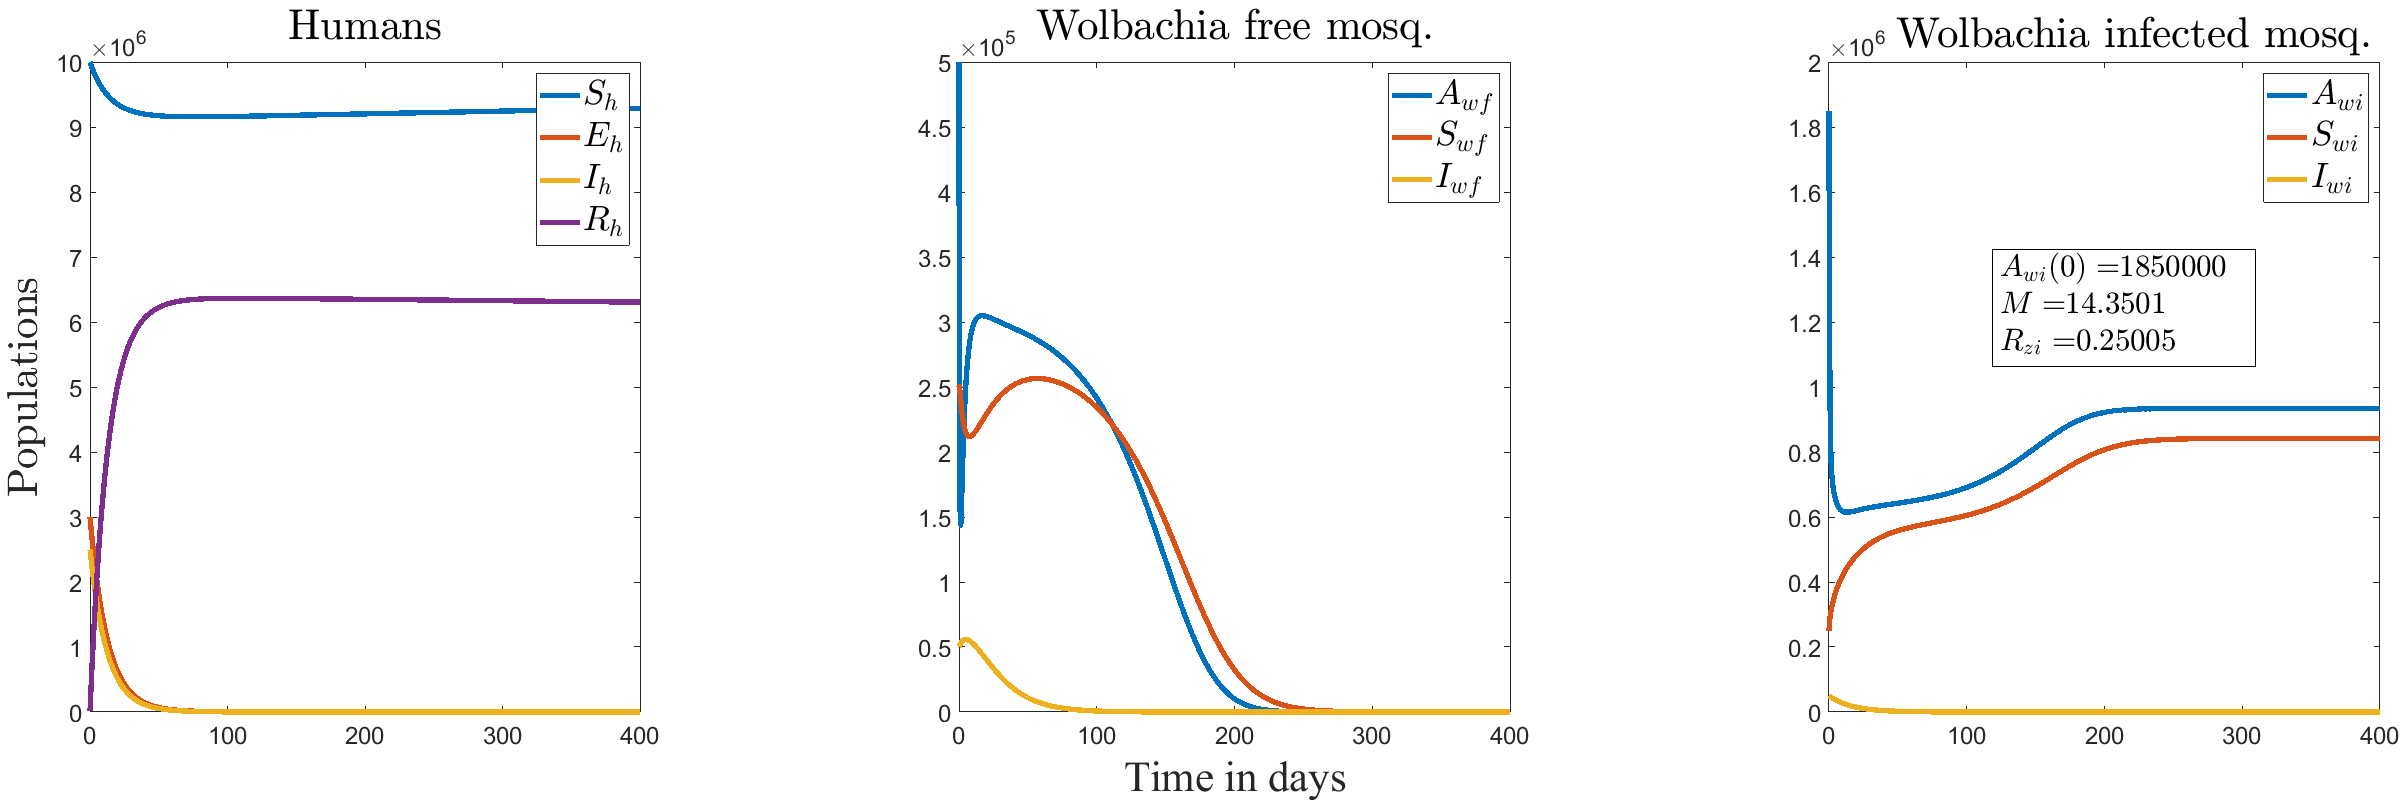
\includegraphics[width=16cm,height=4.5cm]{SimFig3.png} 
%    \caption{Dominance of \textit{Wolbachia} infected mosquitoes when we start with more \textit{Wolbachia} infected aquatic stage. Figure obtained using baseline values for parameters from Table \ref{tab: param-table} and Table \ref{tab: param_mosq_table} and the initial conditions listed in Table \ref{init-cond-dis-free-table} with $A_{wi}(0)=1,850,000$ }
%    \label{fig:my_label}
%\end{figure}

Our simulations suggest that one would need to release 3.7 times as many \textit{Wolbachia} infected aquatic stage compared to \textit{Wolbachia} free aquatic stage. The wild mosquitoes are eliminated and the \textit{Wolbachia} infected mosquitoes will establish in a little over 250 days, faster than in the case when more \textit{Wolbachia} infected females are released as seen in section \ref{morefemales}. The disease is completely eradicated in humans and wild mosquitoes in around 230 days, a little earlier than in the case where more \textit{Wolbachia} females were released, and in 180 days in \textit{Wolbachia} infected mosquitoes.

%\textcolor{red}{Should we combine 4 5 and 6 into a paragraph and not include the pictures to reduce the numbers of figures we have?}

\subsubsection{\textit{Wolbachia} is established when more \textit{Wolbachia} infected males are released}

Persistence of \textit{Wolbachia} infected mosquitoes by releasing more \textit{Wolbachia} infected males can be achieved as well, but it requires 5.8 as many \textit{Wolbachia} infected males compared with \textit{Wolbachia} free males which is much higher than the required number of females as seen in section \ref{morefemales}. In Figure \ref{domwolbmales} we observe that increasing the initial amount of \textit{Wolbachia} infected males from $M_{wi}(0) = 250,000$ to $M_{wi}(0) = 1,450,000$ allows the \textit{Wolbachia} infected mosquito population to establish itself in the population of mosquitoes in roughly 250 days, the same amount of time it takes using more aquatic stage mosquitoes as seen in section \ref{moreaquatics}. Disease is again eradicated in approximately 230 days.

\begin{figure}[H]
    \centering
    % This file was created by matlab2tikz.
%
%The latest updates can be retrieved from
%  http://www.mathworks.com/matlabcentral/fileexchange/22022-matlab2tikz-matlab2tikz
%where you can also make suggestions and rate matlab2tikz.
%
\definecolor{mycolor1}{rgb}{0.00000,0.44700,0.74100}%
\definecolor{mycolor2}{rgb}{0.85000,0.32500,0.09800}%
\definecolor{mycolor3}{rgb}{0.92900,0.69400,0.12500}%
\definecolor{mycolor4}{rgb}{0.49400,0.18400,0.55600}%
%
\begin{tikzpicture}

\begin{axis}[%
width=1.1in,
height=1.5in,
at={(0in,0.108in)},
scale only axis,
xmin=0,
xmax=500,
ymin=0,
ymax=12000000,
ylabel={Population},
axis background/.style={fill=white},
title style={font=\bfseries, yshift=1.73ex},
title={Humans},
legend style={legend cell align=left, align=left, draw=white!15!black}
]
\addplot [color=mycolor1, line width=1.5pt]
  table[row sep=crcr]{%
0	10000000\\
0.913924006745219	9995840.57742167\\
1.92641207948327	9991038.23906881\\
3.17480980791152	9984902.87219497\\
4.80059913732111	9976685.37990599\\
9.5780531745404	9952387.64958285\\
11.2461568433791	9944223.57212964\\
12.6230313405395	9937707.51461681\\
13.889776064083	9931918.49711347\\
15.1723393127322	9926276.41954371\\
16.2563931588084	9921689.18819655\\
17.3911907710135	9917071.6740042\\
18.5736717991531	9912464.92143045\\
19.5104080028832	9908965.35871537\\
20.5022200513631	9905404.65565141\\
21.6842381693423	9901354.51556365\\
22.6220219582319	9898289.46672166\\
23.6689356155694	9895020.48167925\\
24.7209563329816	9891895.04700772\\
25.8525308556855	9888707.81219605\\
26.7921928390861	9886195.26385505\\
27.7427467927337	9883774.19338747\\
28.5684254132211	9881767.1193642\\
29.5983177088201	9879385.14827251\\
30.5872691459954	9877221.00079928\\
31.5584866311401	9875209.18229062\\
32.5530509892851	9873261.5943218\\
33.5004510991275	9871508.60168649\\
34.3427112940699	9870031.00901265\\
35.3316928353161	9868389.7086544\\
36.3323550894856	9866828.18152981\\
37.1879955343902	9865569.03281036\\
38.0976765099913	9864304.34196512\\
38.8950076885521	9863256.29222184\\
39.606980426237	9862366.51437871\\
40.3687026947737	9861461.10566425\\
41.1389419995248	9860592.88401723\\
41.9806213285774	9859696.61292507\\
42.866797586903	9858809.96337203\\
43.6535840239376	9858069.88729917\\
44.3446596600115	9857455.07967048\\
45.1342950817198	9856791.51241833\\
45.9568532947451	9856142.83347818\\
46.7026485018432	9855590.82835276\\
47.3448501862586	9855142.06845437\\
48.0594703610986	9854670.63062535\\
48.8360722400248	9854190.51045329\\
49.5397256370634	9853783.42452728\\
50.3395282831043	9853351.76317229\\
51.0515960138291	9852994.24033264\\
51.6352444831282	9852719.36047527\\
52.2936704400927	9852428.26819086\\
53.0416534673423	9852121.21768882\\
53.8033422641456	9851833.43885686\\
54.4746362939477	9851599.8770091\\
55.0660563148558	9851409.14858767\\
55.5881230942905	9851252.14016831\\
56.1401972286403	9851097.36022674\\
56.780554972589	9850931.89387705\\
57.2368880044669	9850822.9359356\\
57.7581325396895	9850707.34476096\\
58.2793770767748	9850600.9629596\\
58.8357859347016	9850497.28537358\\
59.3921947926283	9850403.52195723\\
59.7631340324879	9850346.37848902\\
60.215326378122	9850282.38370591\\
60.6675187256187	9850224.47503293\\
61.180462250486	9850165.9710611\\
61.6934057753533	9850114.90599509\\
62.158953493461	9850074.8301378\\
62.6245012097061	9850040.56957877\\
62.9997502733022	9850017.08933132\\
63.374999338761	9849997.22057475\\
63.7230802215636	9849981.95611989\\
64.0711611043662	9849969.68054195\\
64.2747118100524	9849963.86478259\\
64.4782625157386	9849959.0411594\\
64.6818132214248	9849955.19883333\\
64.885363927111	9849952.32707571\\
65.1329152043909	9849950.12716136\\
65.3804664798081	9849949.32819766\\
65.6280177552253	9849949.91154271\\
65.8755690306425	9849951.85878603\\
66.1275697629899	9849955.22313661\\
66.3795704934746	9849959.96309146\\
66.631571225822	9849966.05996526\\
66.8835719563067	9849973.49530869\\
67.0912207439542	9849980.61499261\\
67.5065183192492	9849997.50347463\\
67.8877709191293	9850016.06105588\\
68.2349785398692	9850035.4523651\\
68.5921205375344	9850057.82742452\\
68.9591969083995	9850083.34222395\\
69.3698274977505	9850114.84656084\\
69.8240123055875	9850153.2548944\\
70.3100540563464	9850198.40105187\\
70.8279527500272	9850250.98619022\\
71.4566670972854	9850320.85179158\\
72.0113146007061	9850387.80733291\\
72.5659621022642	9850459.59392331\\
73.2410800457001	9850553.28163337\\
73.9763138201088	9850662.9120382\\
74.7182833664119	9850781.26825662\\
75.6007629111409	9850931.70752121\\
76.5095880497247	9851097.11746297\\
77.2627118770033	9851241.87556297\\
78.1613748800009	9851423.3012945\\
79.1560507994145	9851634.61223743\\
80.2788810227066	9851885.68525712\\
81.3621719703078	9852139.79026329\\
82.364212622866	9852384.61530134\\
83.5905463192612	9852696.26367524\\
84.9552447404712	9853057.62253808\\
86.2214505430311	9853405.6527003\\
87.7000734359026	9853826.45178339\\
89.2558771595359	9854284.65082889\\
90.657723588869	9854709.97850086\\
92.394762666896	9855252.01793298\\
94.0952117331326	9855797.33164315\\
95.803286395967	9856358.36867584\\
97.8626080006361	9857050.73429455\\
99.9546966142952	9857770.10590838\\
102.313099671155	9858598.13048597\\
104.847567683086	9859505.64466408\\
107.56429858692	9860496.01375135\\
110.548276647925	9861601.73673675\\
113.737292727455	9862800.94748457\\
117.260660389438	9864143.36240224\\
121.397606424987	9865738.5711663\\
125.947790345177	9867511.88264909\\
131.347047764808	9869635.52014555\\
137.570321561769	9872102.3669189\\
145.303512433544	9875187.25559253\\
155.279874475673	9879186.88189638\\
169.645906412974	9884966.91675312\\
198.931691296399	9896773.32871299\\
245.039350230247	9915356.49649016\\
282.266977503896	9930341.0298431\\
319.092511234805	9945144.78997749\\
355.786052551121	9959876.66419745\\
392.531612193212	9974610.60216516\\
429.213930968195	9989300.41934643\\
466.006828736514	10004015.7112598\\
500	10017594.5348349\\
};
\addlegendentry{$S_h$}

\addplot [color=mycolor2, line width=1.5pt]
  table[row sep=crcr]{%
0	3000000\\
0.58142259484157	2833266.18211278\\
1.30325068114325	2639413.74222998\\
1.92641207948327	2483030.55733457\\
2.49701290717348	2348192.21988372\\
3.17480980791152	2197762.19143471\\
3.79093175847083	2069633.63278223\\
4.40705370856449	1949192.3180668\\
5.19414456700906	1805771.64934605\\
5.98123542545363	1673226.88943341\\
6.62398004904389	1572470.60948763\\
7.26672467263415	1477982.38569301\\
7.98818505275995	1378897.45969202\\
8.57411298155785	1303507.58483806\\
9.22256506001577	1225041.20616232\\
9.93354128813371	1144625.95000328\\
10.6718803783879	1066908.3569736\\
11.4375823312439	992094.565538021\\
12.0879659852944	932848.501503163\\
12.8905640188605	864788.722717525\\
13.5567053826526	812246.485499156\\
14.4127452597022	749585.564452289\\
15.1723393127322	698222.965227654\\
15.7420348520391	662130.81008484\\
16.5135723119602	616345.310453893\\
17.0809711180627	584804.648025617\\
17.7014104239643	552250.909977517\\
18.5736717986874	509676.291413964\\
19.3230607616715	475863.347191485\\
20.0063140266575	447096.01201614\\
20.7977245808579	416057.288087152\\
21.3887336403131	394369.85758253\\
22.2469084425829	364986.421255772\\
22.9971354729496	341200.527713648\\
23.6689356151037	321296.950886037\\
24.437067666091	300042.585549206\\
25.2887336649001	278215.497941479\\
26.0404632519931	260354.704008443\\
26.7921928386204	243713.262644579\\
27.5051083047874	228978.669319444\\
28.2931992062367	213792.906097898\\
29.0323181417771	200528.755748223\\
29.7869842322543	187892.344086908\\
30.587269146461	175421.185597718\\
31.2901251856238	165201.454138796\\
32.0952095221728	154277.21418464\\
32.9320110329427	143743.184429268\\
33.6899311207235	134870.424297301\\
34.3427112936042	127702.223668326\\
35.0688521401025	120209.514767715\\
35.8573742280714	112608.677375596\\
36.5698455194943	106187.675907809\\
37.3783253268339	99378.8674856545\\
38.0976765104569	93718.2549475376\\
38.8950076880865	87850.5814379421\\
39.6069804257713	82947.9357223874\\
40.3687026938424	78030.4687645338\\
41.1389419999905	73379.2666270887\\
41.9806213290431	68639.7812033342\\
42.6813216242008	64948.5735951434\\
43.4232254787348	61275.1141566974\\
44.1143011152744	58056.790402242\\
44.8710832744837	54742.9944515666\\
45.5839556907304	51809.9208823484\\
46.3297508982942	48924.3210076415\\
47.116973745171	46068.0324861854\\
47.8006030684337	43735.3664655127\\
48.5772049478255	41241.2169281375\\
49.3051745053381	39044.1621549688\\
50.1511111119762	36650.7848227532\\
50.8770458269864	34724.7759777214\\
51.6352444826625	32830.8596616378\\
52.2936704400927	31277.7669731607\\
53.0416534668766	29610.3943281793\\
53.8033422646113	28011.9796222104\\
54.6833351748064	26281.9593713777\\
55.4141008341685	24934.0717436559\\
56.1401972286403	23669.3807979734\\
57.008721488528	22247.9944693539\\
57.7581325401552	21096.3893349324\\
58.6503163152374	19809.6044729771\\
59.3921947930939	18804.7914725351\\
60.2153263790533	17754.5974032115\\
60.9239904880524	16901.6014676783\\
61.693405775819	16025.7665052707\\
62.3917273515835	15273.5425754935\\
63.1873748060316	14463.0084375199\\
64.0711611048318	13617.1465390753\\
64.8853639280424	12885.2972793668\\
65.6280177552253	12254.8897957541\\
66.3795704939403	11650.8291941565\\
67.2988695320673	10955.4308029255\\
68.0613747294992	10412.6817166619\\
68.9591969083995	9810.59119749581\\
69.8240123065189	9266.03409723472\\
70.5690034036525	8823.01955576334\\
71.4566670982167	8324.72434936697\\
72.196197100915	7932.67983564129\\
73.0160407316871	7521.10875798576\\
73.7212165901437	7185.40833789483\\
74.4865082777105	6839.16940721124\\
75.4136086315848	6443.46188472863\\
76.3359069013968	6073.98213268118\\
77.2627118765377	5725.37392794574\\
78.1613748804666	5407.63793897768\\
78.9051635768265	5158.84573342977\\
79.8648438369855	4855.65852321545\\
80.6591856838204	4619.00302316761\\
81.545300048776	4369.34599478263\\
82.3642126219347	4151.28930805298\\
83.3326538917609	3908.15359104192\\
84.2173740770668	3699.14196314663\\
85.1397124072537	3493.72497273237\\
85.997132926248	3313.50482578995\\
86.7297325613908	3167.25298755849\\
87.7000734368339	2983.8796925731\\
88.5356365577318	2834.88400524762\\
89.429245328065	2684.11353990296\\
90.2097178152762	2559.28081084369\\
91.1489989235997	2417.02951627178\\
92.1447311486118	2275.18637802079\\
93.0141698340885	2158.41418810934\\
93.9124636375345	2044.28573953221\\
94.869154559914	1929.59714789968\\
95.8032863964327	1824.03282384854\\
96.7584254639223	1722.2564248722\\
97.6785775781609	1629.74982581986\\
98.4939897246659	1552.05979838222\\
99.4480188195594	1465.98697895976\\
100.415395812131	1383.7178217941\\
101.24867482949	1316.66328273946\\
102.14013841562	1248.61287017213\\
102.918554788455	1192.14664427703\\
103.854997276794	1127.67117034132\\
104.847567683551	1063.22059788276\\
105.714409736451	1010.0208470067\\
106.610297909006	957.892955678515\\
107.564298587851	905.39760167338\\
108.495485829189	856.986730819102\\
109.447476534639	810.218235158361\\
110.364809962921	767.611004777253\\
111.177641483489	731.765264240559\\
112.128484496381	691.985973093193\\
113.092532976065	653.895065400284\\
114.108604999725	616.048707621172\\
114.983759367373	585.23618911393\\
115.788197311107	558.292709374335\\
116.764096788596	527.286901031155\\
117.757223990746	497.52193823969\\
118.749362991191	469.483115081675\\
119.627944554202	445.989716168027\\
120.439207314514	425.352333618328\\
121.397606424056	402.210709276609\\
122.273121903185	382.182532979175\\
123.186397043988	362.361597046722\\
124.034985938575	344.874447578564\\
125.011024022941	325.809747081716\\
125.947790344246	308.511011631228\\
126.915164704435	291.616788791958\\
127.801231603604	276.960535941646\\
128.644273938611	263.704247753602\\
129.61951804487	249.162891532294\\
130.564417767804	235.842976097949\\
131.517879646737	223.127244757954\\
132.400954238139	211.965091685299\\
133.249827351887	201.763943742495\\
134.233462455217	190.557854050305\\
135.212877691258	180.020147550851\\
136.159263603855	170.393215187825\\
137.070780381095	161.609158178791\\
138.047003349755	152.704118770547\\
138.911077984143	145.233032846823\\
139.801440428942	137.917370293289\\
140.737606641836	130.622881113552\\
141.659188165329	123.81928775087\\
142.635563531425	116.997581739444\\
143.487452546135	111.35345757613\\
144.367031630129	105.811425215099\\
145.303512432612	100.213632847182\\
146.217704178765	95.0347071308643\\
147.151758338325	90.0193768842146\\
148.050143819302	85.4452007929794\\
148.846596575342	81.5845301398076\\
149.778664422221	77.2871173964813\\
150.722933478653	73.1638443311676\\
151.716183271725	69.0634144209325\\
152.570433154237	65.7207362717018\\
153.594678813592	61.9249658756889\\
154.552501866594	58.5734682064503\\
155.479709461797	55.5015098778531\\
156.413543011062	52.5699435472488\\
157.277738291305	49.9946954827756\\
158.108990827575	47.6363253314048\\
159.072410639841	45.0413318369538\\
160.029456421733	42.6029730141163\\
160.953770789318	40.3729099696502\\
161.845053204801	38.3327146028168\\
162.799340968952	36.2619664175436\\
163.820792765822	34.1687251171097\\
164.839942368213	32.2000846299343\\
165.848681509029	30.3627392789349\\
166.792326011695	28.7385201789439\\
167.705241810065	27.249507419765\\
168.787508883048	25.5833746748976\\
169.860468130093	24.0316119040363\\
170.748457567766	22.8183976653963\\
171.829034455586	21.4239006377757\\
172.872026523575	20.1583196842112\\
173.959452908952	18.9178844238631\\
175.114243437536	17.6835559923202\\
176.248457816895	16.5491552492604\\
177.276017051656	15.5839781644754\\
178.346609790809	14.637812118046\\
179.513700212352	13.6712500499561\\
180.604533119127	12.8252365505323\\
181.814703319222	11.947361624334\\
182.923447873443	11.195536554791\\
184.251321161166	10.3566773091443\\
185.589917177334	9.57418636325747\\
186.954669557046	8.83679050020874\\
188.378874221817	8.12730896146968\\
189.661213984713	7.53699329588562\\
191.023829956539	6.9562756717205\\
192.473937823903	6.38695272849873\\
193.908209693152	5.86933636572212\\
195.545675095171	5.3290727166459\\
197.18358753249	4.83801969559863\\
198.931691295933	4.3633488365449\\
200.757025646511	3.91694432077929\\
202.712604335044	3.48883789079264\\
204.704173365608	3.1005322849378\\
206.905612364411	2.72100649075583\\
209.179510478396	2.37732317298651\\
211.647962697316	2.05282332608476\\
214.275442694314	1.75557960150763\\
217.100938652642	1.4834401467815\\
220.256954526063	1.22869133017957\\
223.62746487977	1.00442799925804\\
227.413994475268	0.80062911985442\\
231.573937804438	0.623800217173994\\
236.457842247561	0.465119736269116\\
241.94406847842	0.334262588527054\\
248.585409247316	0.223901002667844\\
256.770034721587	0.13650147151202\\
267.629625991452	0.0706912879832089\\
283.190306047443	0.0274793556891382\\
310.649523221888	0.00516893807798624\\
401.83889394952	1.99521891772747e-05\\
500	5.02914190292358e-08\\
};
\addlegendentry{$E_h$}

\addplot [color=mycolor3, line width=1.5pt]
  table[row sep=crcr]{%
0	2500000\\
0.913924006279558	2321618.68966047\\
1.75407781591639	2165800.24850291\\
2.49701290717348	2034706.44234965\\
3.17480980791152	1920631.57243142\\
4.09899273328483	1773543.97869592\\
4.80059913778678	1668300.97666121\\
5.58768999623135	1556676.28043176\\
6.40973184118047	1447154.26001529\\
7.26672467263415	1340370.80246296\\
7.98818505275995	1256087.78734227\\
8.8670769459568	1160024.92421327\\
9.57805317407474	1087379.31890737\\
10.4804548905231	1001346.35372877\\
11.2461568429135	933468.380734647\\
11.8204333074391	885481.934402899\\
12.6230313410051	822392.923814503\\
13.2236347007565	778062.886901785\\
13.8897760645486	731626.204196788\\
14.7925422862172	673016.672543369\\
15.5521363387816	627315.603781338\\
16.2563931583427	587703.685302021\\
17.0809711180627	544485.018027553\\
17.7014104239643	514077.887410076\\
18.5736717986874	474194.6274278\\
19.3230607616715	442431.860631884\\
20.0063140266575	415352.965326794\\
20.7977245808579	386083.944725047\\
21.3887336403131	365604.416256134\\
22.2469084425829	337825.268853656\\
22.9971354729496	315315.664854253\\
23.6689356151037	296468.41903821\\
24.437067666091	276334.292814246\\
25.2887336649001	255654.067848795\\
26.0404632519931	238733.149509184\\
26.7921928386204	222972.164119915\\
27.5051083047874	209023.92340354\\
28.2931992062367	194658.45918841\\
29.0323181417771	182121.865313581\\
29.7869842322543	170190.909841476\\
30.587269146461	158430.626833339\\
31.2901251856238	148806.527495439\\
32.0952095221728	138534.487086878\\
32.9320110329427	128647.17804823\\
33.6899311207235	120334.951996117\\
34.3427112936042	113631.660765086\\
35.0688521401025	106637.893053925\\
35.8573742280714	99558.4116717172\\
36.5698455194943	93591.2084831502\\
37.3783253268339	87278.5693202899\\
38.0976765104569	82043.4706419618\\
38.8950076880865	76630.7219373905\\
39.6069804257713	72120.0860802201\\
40.3687026938424	67607.789817608\\
41.1389419999905	63351.9109353991\\
41.7702014967799	60078.7411366678\\
42.5061465501785	56491.0345831662\\
43.2377495151013	53152.4341878518\\
43.883942569606	50380.3915282413\\
44.6078714677133	47459.2113539977\\
45.3975068884902	44480.4344786895\\
46.1433020965196	41852.2763513485\\
46.8890973040834	39391.6586535079\\
47.5727266273461	37273.6499300273\\
48.3183376546949	35103.7390629249\\
49.0706233731471	33052.8744821544\\
49.7742767701857	31252.1798545704\\
50.5279454533011	29441.2440177347\\
51.2261462006718	27865.2857416924\\
52.0443427641876	26134.5754246437\\
52.7923257914372	24654.6726660514\\
53.5494459988549	23249.3837730819\\
54.2659374121577	21999.7826740136\\
55.0660563153215	20690.4588045063\\
55.77214780543	19605.5940162055\\
56.5523884566501	18478.6684151143\\
57.2368880044669	17548.2467440758\\
58.0187548082322	16547.7416069913\\
58.8357859347016	15568.5402154308\\
59.5776644125581	14734.1800059509\\
60.441422552336	13823.9100213447\\
61.1804622509517	13093.8461138229\\
61.9261796344072	12399.7537500486\\
62.8121257419698	11627.0259248381\\
63.5490397796966	11024.3708376801\\
64.2747118109837	10464.1605200516\\
65.1329152039252	9841.48965532007\\
65.8755690311082	9335.27908173809\\
66.6315712253563	8849.05041534826\\
67.5065183197148	8320.5813032859\\
68.2349785403349	7906.83799835574\\
68.9591969083995	7517.65845692158\\
69.8240123065189	7080.06405152055\\
70.5690034036525	6725.30800356995\\
71.4566670982167	6327.67207959667\\
72.196197100915	6015.89720955817\\
73.0160407316871	5689.65212892881\\
73.7212165901437	5424.38021272141\\
74.4865082777105	5151.59174891934\\
75.4136086315848	4840.87417265959\\
76.1622257526033	4604.77375732362\\
77.0598311116919	4337.97251451714\\
77.9149241433479	4099.27944766451\\
78.6542763542384	3904.29853605758\\
79.4069380220026	3716.02982578473\\
80.2788810217753	3510.05794845382\\
81.1790438918397	3310.22891720664\\
81.9115562052466	3156.62664162135\\
82.8168690386228	2977.26497904211\\
83.5905463187955	2832.62066214532\\
84.4018417433836	2688.97731120279\\
85.3241800731048	2535.06064480823\\
86.2214505434968	2394.30953782192\\
86.9838735703379	2281.24498945847\\
87.9311028653756	2148.62082010088\\
88.7223886894062	2044.10382507322\\
89.6026134970598	1934.13780241506\\
90.4120859215036	1838.52799534984\\
91.3946365909651	1729.1396461199\\
92.1447311486118	1650.26229454344\\
93.0141698340885	1563.55435693497\\
93.9124636375345	1478.98615016555\\
94.6434560189955	1413.7183424877\\
95.5462501812726	1337.2569071413\\
96.3173588262871	1275.38094836939\\
97.3105167322792	1200.07027574396\\
98.2703140741214	1131.69603108894\\
99.1946799224243	1069.68152723787\\
100.185046212748	1007.15314025804\\
101.062384919729	954.937621439341\\
101.967177160084	904.02647293359\\
102.918554788455	853.522498820908\\
103.854997276794	806.661677066702\\
104.847567683551	759.889787903521\\
105.714409736451	721.336935277097\\
106.610297909006	683.609276067931\\
107.564298587851	645.664904343896\\
108.495485829189	610.717359547503\\
109.447476534639	576.996646992862\\
110.364809962921	546.312064230908\\
111.177641483489	520.523747941479\\
112.128484496381	491.934636220802\\
113.092532976065	464.588046183344\\
113.922948863823	442.281141077168\\
114.811384809669	419.625477715861\\
115.788197311107	396.080444075167\\
116.764096788596	373.902251608204\\
117.757223990746	352.630566987675\\
118.749362991191	332.609667195007\\
119.627944554202	315.847387445159\\
120.439207314514	301.132727263495\\
121.397606424056	284.643627053127\\
122.273121903185	270.382528656162\\
123.186397043988	256.277833686676\\
124.034985938575	243.84124339791\\
125.011024022941	230.29066739697\\
125.947790344246	218.002518746536\\
126.915164704435	206.008420720231\\
127.801231603604	195.608587612864\\
128.644273938611	186.20651008375\\
129.61951804487	175.89779439522\\
130.564417767804	166.459426226094\\
131.517879646737	157.453163625672\\
132.400954238139	149.550493470393\\
133.249827351887	142.330856906716\\
134.233462455217	134.40292975679\\
135.212877691258	126.95067595318\\
136.159263603855	120.144914344884\\
137.070780381095	113.937023665756\\
138.047003349755	107.645584205631\\
138.911077984143	102.368755752221\\
139.801440428942	97.2030456969514\\
140.737606641836	92.0536088580266\\
141.659188165329	87.2519010477699\\
142.635563531425	82.4385586027056\\
143.487452546135	78.4569748844951\\
144.367031630129	74.5481701241806\\
145.303512432612	70.6007969290949\\
146.217704178765	66.9494684729725\\
147.151758338325	63.4140923377126\\
148.050143819302	60.1902106720954\\
149.065145857166	56.7448010258377\\
150.026149063837	53.6647714464925\\
150.94758336572	50.8687431132421\\
151.897499944549	48.1387290684506\\
152.766880776267	45.7687612650916\\
153.594678813592	43.6206367057748\\
154.552501866594	41.2605286436155\\
155.479709461797	39.097462283913\\
156.413543011062	37.033413594123\\
157.277738291305	35.2203651643358\\
158.327200929169	33.137368932832\\
159.320813876577	31.2786727193743\\
160.206617057789	29.7095518740825\\
161.169442611281	28.0929396594875\\
162.089320153929	26.630469578784\\
163.020827886183	25.2268665884621\\
163.999288288411	23.831879613921\\
165.033389538527	22.4410614599474\\
166.083631969057	21.1113120056689\\
167.031119134743	19.9791667126119\\
168.098314668983	18.7762517812662\\
169.125272711739	17.6868574013934\\
170.289591562934	16.5276912134141\\
171.481370433234	15.4194862837903\\
172.524362501223	14.5105021637864\\
173.719435761217	13.534351198934\\
174.896873895545	12.6365336384624\\
176.073588992935	11.7984685036354\\
177.276017051656	10.9991758372635\\
178.577074865345	10.1948677371256\\
179.898541947361	9.43778689531609\\
181.265163939912	8.713578928262\\
182.684162590187	8.02001330815256\\
184.081460617017	7.39068955462426\\
185.589917177334	6.76626624213532\\
187.167207360268	6.16933321626857\\
188.695184390061	5.64099492272362\\
190.337135739625	5.12323072133586\\
192.160754521377	4.60330690350384\\
193.908209693152	4.15432461770251\\
195.87707097223	3.70032670721412\\
197.87205825327	3.29051907500252\\
200.060564709827	2.89258989319205\\
202.26533295773	2.53998933918774\\
204.704173365608	2.19943100446835\\
207.229432689026	1.89448710763827\\
210.012892022263	1.60675000865012\\
213.040104007814	1.34283817559481\\
216.260040847585	1.1091887219809\\
219.816626752727	0.897738674655557\\
223.839152283501	0.706422615330666\\
228.489889969584	0.535145321860909\\
233.727801513392	0.391150386538357\\
239.920303374529	0.269780549686402\\
247.490147774108	0.171105624176562\\
256.979755381588	0.0965286125428975\\
270.097332206089	0.0436474177986383\\
290.810897414573	0.012415299192071\\
337.403509377036	0.000728189945220947\\
500	3.63215804100037e-08\\
};
\addlegendentry{$I_h$}

\addplot [color=mycolor4, line width=1.5pt]
  table[row sep=crcr]{%
0	10000\\
0.692256398499012	346652.97616578\\
1.44249711651355	690674.001158919\\
2.27108060661703	1046546.54144979\\
2.94887750782073	1319745.00174549\\
3.79093175847083	1637848.10739775\\
4.40705370809883	1856376.53829254\\
5.19414456747472	2118987.49711056\\
5.98123542591929	2364018.88996521\\
6.62398004904389	2551800.24106333\\
7.26672467309982	2729103.02870661\\
7.98818505275995	2916296.09147407\\
8.86707694549114	3128450.0036399\\
9.57805317360908	3288103.51226479\\
10.4804548900574	3476383.24389528\\
11.2461568433791	3624379.67044721\\
11.8204333074391	3728740.940296\\
12.6230313405395	3865648.19404867\\
13.2236347002909	3961666.40203037\\
13.8897760650143	4062109.01375544\\
14.7925422862172	4188713.34448092\\
15.5521363392472	4287333.55111272\\
16.2563931588084	4372765.88984475\\
17.0809711180627	4465951.60134829\\
17.7014104239643	4531513.81383508\\
18.5736717991531	4617531.08062168\\
19.3230607612059	4686073.02698351\\
20.0063140271232	4744549.67488578\\
20.7977245813236	4807816.09382181\\
21.3887336403131	4852131.08083968\\
22.2469084430486	4912319.8211628\\
22.9971354724839	4961171.51807402\\
23.6689356155694	5002141.43455631\\
24.437067666091	5045987.3625479\\
25.2887336649001	5091121.28663441\\
26.0404632519931	5128137.22888064\\
26.7921928390861	5162696.47756146\\
27.5051083052531	5193354.64458222\\
28.2931992067024	5225011.72406442\\
29.0323181422427	5252714.88252172\\
29.7869842322543	5279153.90156181\\
30.5872691469267	5305293.93297089\\
31.2901251856238	5326750.9352353\\
32.0952095221728	5349724.48838216\\
32.9320110334083	5371915.53092378\\
33.6899311207235	5390637.15593452\\
34.3427112931386	5405783.08220895\\
35.0688521396369	5421635.36553387\\
35.8573742276058	5437738.74113758\\
36.5698455199599	5451360.56131382\\
37.3783253272995	5465823.73959493\\
38.0976765109226	5477862.93636169\\
38.8950076876208	5490357.23912366\\
39.6069804253057	5500808.37241074\\
40.3687026938424	5511301.96091077\\
41.1389419995248	5521237.44717808\\
41.9806213285774	5531371.62004892\\
42.6813216237351	5539271.33051043\\
43.4232254782692	5547139.04179693\\
44.1143011152744	5554036.72188385\\
44.8710832744837	5561143.46809926\\
45.5839556902647	5567437.24710287\\
46.3297508982942	5573632.09961336\\
47.1169737456366	5579766.53156315\\
47.8006030684337	5584777.89564974\\
48.5772049473599	5590137.26761997\\
49.3051745053381	5594858.75521641\\
50.1511111119762	5600002.09543514\\
50.8770458269864	5604140.51046954\\
51.6352444821969	5608208.93897749\\
52.2936704400927	5611544.02687528\\
53.0416534664109	5615122.80243156\\
53.8033422650769	5618551.32367926\\
54.6833351748064	5622258.8389008\\
55.4141008341685	5625144.37386018\\
56.1401972286403	5627848.75571992\\
57.008721488528	5630883.87563933\\
57.7581325406209	5633338.82983559\\
58.6503163147718	5636076.66585953\\
59.3921947935596	5638209.91848686\\
60.2153263790533	5640434.32212469\\
60.9239904880524	5642236.46953009\\
61.6934057762846	5644081.89423625\\
62.3917273515835	5645662.2303834\\
63.1873748060316	5647359.5401866\\
63.8971206629649	5648786.01821341\\
64.6818132223561	5650272.61625399\\
65.3804664798081	5651520.68151571\\
66.1275697629899	5652781.01153059\\
66.8835719563067	5653982.52584434\\
67.714167107828	5655221.95898441\\
68.4085823511705	5656197.06056109\\
69.142735093832	5657170.81336367\\
69.8240123065189	5658024.62190478\\
70.5690034031868	5658906.29799949\\
71.4566670982167	5659889.91081318\\
72.196197100915	5660657.00635524\\
73.0160407312214	5661455.04323082\\
73.7212165901437	5662099.80301489\\
74.4865082781762	5662758.31417646\\
75.1818335428834	5663321.33864713\\
75.9750714721158	5663924.8059271\\
76.6832691980526	5664430.40697054\\
77.4655926413834	5664954.49251393\\
78.1613748800009	5665391.7770934\\
78.9051635768265	5665830.76481791\\
79.6578252445906	5666246.55600675\\
80.4858996141702	5666672.72105998\\
81.1790438918397	5667005.54980179\\
81.9115562057123	5667334.82750388\\
82.5905408300459	5667620.41844297\\
83.3326538922265	5667912.01409686\\
84.0329064112157	5668168.41902974\\
84.7707770755515	5668419.86543657\\
85.5484976908192	5668665.10764965\\
86.2214505439624	5668861.72142802\\
86.9838735703379	5669067.84961935\\
87.7000734368339	5669246.15264241\\
88.3488844260573	5669395.45678076\\
88.9091408215463	5669515.42827195\\
89.6026134965941	5669652.90929249\\
90.2097178157419	5669763.66674581\\
90.9033612562343	5669879.7138567\\
91.3946365909651	5669955.39360591\\
91.8946996293962	5670027.08394393\\
92.3947626678273	5670093.5569398\\
93.0141698345542	5670168.91181016\\
93.5665512634441	5670229.82766061\\
94.0952117331326	5670282.77972517\\
94.6434560194612	5670332.36020093\\
95.0948531003669	5670369.23875581\\
95.5462501812726	5670402.66557002\\
96.0603226115927	5670436.65586897\\
96.5743950409815	5670466.43939179\\
96.9424558868632	5670485.25554252\\
97.3105167327449	5670502.03407132\\
97.6785775776953	5670516.82243634\\
98.046638423577	5670529.66691366\\
98.4939897246659	5670542.72634498\\
98.7176653752103	5670548.22890006\\
98.9413410257548	5670553.05957259\\
99.1946799224243	5670557.73138901\\
99.448018820025	5670561.56702545\\
99.7013577166945	5670564.57981299\\
99.9546966133639	5670566.78286082\\
100.185046212748	5670568.0939907\\
100.415395812131	5670568.75585706\\
100.645745410584	5670568.77784269\\
100.876095009968	5670568.16918876\\
101.062384920195	5670567.22195029\\
101.24867482949	5670565.87294766\\
101.434964739718	5670564.12686782\\
101.621254649013	5670561.98834045\\
101.794215904549	5670559.65548317\\
102.14013841562	5670554.00111839\\
102.514918043278	5670546.41486905\\
102.918554788455	5670536.58538323\\
103.365247866139	5670523.7522881\\
103.854997276329	5670507.38660771\\
104.349103881977	5670488.51338417\\
104.847567684017	5670467.14275902\\
105.302669635043	5670445.64711693\\
105.920279786922	5670413.54373018\\
106.437793378718	5670384.12761427\\
106.974796153605	5670351.26089078\\
107.564298587851	5670312.52500743\\
108.239311155863	5670264.88056341\\
109.007835175842	5670206.53467197\\
109.814409906045	5670140.81495926\\
110.548276648857	5670077.21257788\\
111.400590558536	5669999.00886067\\
112.380956928246	5669903.5863853\\
113.322084783576	5669806.77962329\\
114.294261135161	5669701.7316637\\
115.38597833924	5669578.01263167\\
116.520121918991	5669443.44109094\\
117.757223990746	5669290.10151932\\
118.921200487763	5669140.01161718\\
120.215110471472	5668967.02286367\\
121.652709135786	5668767.80426417\\
123.186397043988	5668547.78709732\\
124.759670646861	5668314.75791571\\
126.360987170599	5668070.62878761\\
128.001328481361	5667813.94480655\\
129.866507050581	5667514.73455815\\
131.859543409199	5667187.26358761\\
133.97985106986	5666831.06599884\\
136.379845665768	5666419.32787125\\
138.911077983677	5665976.5016367\\
141.659188165329	5665487.15919407\\
144.724816577509	5664932.3285678\\
148.050143819302	5664321.56847867\\
151.716183271259	5663639.38107391\\
155.879379436374	5662855.62805065\\
160.560938330367	5661965.28022552\\
166.083631969057	5660905.70515118\\
172.698194512166	5659627.16206243\\
180.925682555884	5658027.20503378\\
191.816304160282	5655899.53420056\\
208.308526934125	5652667.26618704\\
308.148064853624	5633085.49998309\\
344.967112226412	5625879.05463028\\
381.782208881341	5618682.58898569\\
418.421108788811	5611529.70392406\\
455.054156376049	5604387.06508958\\
491.854323222302	5597220.99546235\\
500	5595636.0327518\\
};
\addlegendentry{$R_h$}

\end{axis}

\begin{axis}[%
width=1.1in,
height=1.5in,
at={(1.34in,0.108in)},
scale only axis,
xmin=0,
xmax=500,
ymin=0,
ymax=500000,
xlabel={Time (days)},
axis background/.style={fill=white},
title style={font=\bfseries, yshift=1.25ex},
title={\emph{Wolb.}-free mosq.},
legend style={legend cell align=left, align=left, draw=white!15!black}
]
\addplot [color=mycolor1, line width=1.5pt]
  table[row sep=crcr]{%
0	500000\\
0.124589653627481	492509.988382942\\
0.353006124321837	481186.073057289\\
0.581422595016193	471999.743330203\\
0.91392400622135	460712.792019552\\
1.30325068120146	449393.000670114\\
1.75407781609101	437854.631404395\\
2.27108060690807	426071.397875236\\
2.7229452074389	416777.719493482\\
3.17480980796972	408335.603980639\\
3.790931758238	397966.928471592\\
4.40705370850628	388827.276757735\\
4.80059913778678	383447.579230582\\
5.19414456706727	378513.427820673\\
5.98123542557005	369889.789636176\\
6.40973184129689	365520.485260002\\
7.05247646494536	359707.75435792\\
7.4809728806722	356176.654901321\\
7.98818505287636	352315.495074396\\
8.57411298155785	348282.697467695\\
9.22256505995756	344144.745218286\\
9.57805317401653	342080.329860266\\
10.8633058666019	335760.487061283\\
11.6290078192251	332467.676156016\\
12.3554986630916	329670.721658978\\
13.2236347007565	326650.741163955\\
13.5567053827108	325588.199587886\\
14.2228467466193	323864.985678661\\
14.6026437730179	322729.126411604\\
15.5521363388398	320391.365454963\\
16.2563931585173	318813.354576656\\
16.7707514650538	317796.658677174\\
17.0809711180045	317102.64041196\\
17.3911907709553	316500.568268287\\
17.7014104239061	316080.35876339\\
18.0116300768568	315616.712364539\\
18.3863245581742	314889.374140477\\
18.9483662801795	314028.216143729\\
19.3230607615551	313472.315911212\\
20.2542670391267	312202.288672212\\
20.5022200514213	311900.299288843\\
20.7977245810907	311449.054396052\\
21.0932291107601	311072.9768393\\
21.3887336404296	310854.396574229\\
21.684238170099	310589.989712303\\
21.8717949276324	310314.91040757\\
22.0593516851659	310082.768725955\\
22.434465200291	309739.408231378\\
22.8095787154161	309330.453480042\\
23.1846922304831	308989.605866895\\
23.6689356152783	308518.577698664\\
24.1531790000736	308138.103685701\\
24.4370676663239	307819.218238162\\
24.7209563325741	307566.540510382\\
25.0048449988244	307457.071117023\\
25.2887336650747	307302.167273695\\
25.4766660617897	307092.314583736\\
25.6645984585048	306923.325236166\\
26.0404632519349	306702.340835668\\
26.4163280453067	306404.321702013\\
26.7921928387368	306173.143165805\\
27.0298313274398	305995.024217653\\
27.2674698161427	305836.298716898\\
27.7427467936068	305585.487345494\\
28.0179730000091	305342.899162055\\
28.2931992064696	305160.58102153\\
28.5684254128719	305110.77791306\\
28.8436516192742	305017.24837495\\
29.0323181418935	304846.862320336\\
29.2209846645128	304715.89812224\\
29.5983177097514	304568.574918992\\
29.7869842323707	304443.644112564\\
29.9756507549901	304336.00244064\\
30.3529838001705	304171.036768663\\
30.5872691465775	304031.993873874\\
30.8215544929262	303911.945872893\\
31.290125185682	303737.868816689\\
31.5584866311401	303540.339698302\\
31.8268480765983	303399.027742908\\
32.0952095219982	303382.287763164\\
32.3635709674563	303323.74901224\\
32.5530509893433	303177.284770274\\
32.7425310112885	303069.248578734\\
32.9320110331755	303021.000591998\\
33.1214910550625	302966.376566434\\
33.3109710769495	302860.422027782\\
33.5004510988365	302772.028580247\\
33.8794111426687	302647.003012701\\
34.11106121802	302530.254244244\\
34.3427112933714	302432.53316197\\
34.574361368781	302372.665133568\\
34.8060114441323	302303.637596452\\
35.0688521401025	302132.780101467\\
35.3316928360146	302015.159177934\\
35.5945335319848	302015.838205823\\
35.8573742278968	301976.627475886\\
36.0948646584875	301743.252339857\\
36.3323550890782	301610.286955142\\
36.5698455196689	301687.836518176\\
36.8073359502596	301704.591890178\\
36.9976657425286	301525.15342067\\
37.1879955347395	301411.510596601\\
37.3783253270085	301402.863520276\\
37.5686551192775	301380.648808275\\
37.7449955830234	301278.028100452\\
37.9213360467693	301199.472050337\\
38.2740169742028	301108.321562778\\
38.4810138788307	301018.275406808\\
38.6880107834004	300942.768651113\\
39.102004592598	300838.990222691\\
39.3544925090973	300717.117335464\\
39.6069804255967	300624.788338883\\
39.8594683420961	300597.118078061\\
40.1119562585955	300548.601495694\\
40.3687026939006	300347.135264395\\
40.6254491292057	300230.914114814\\
40.882195564569	300304.498926488\\
41.1389419998741	300313.829245581\\
41.3493618321372	300099.427587355\\
41.5597816644004	299977.860817671\\
41.7702014966635	300029.122017102\\
41.9806213289849	300042.856732497\\
42.1557964027743	299915.436904423\\
42.3309714765637	299827.894673433\\
42.6813216241426	299761.848610514\\
42.8667975877761	299678.406248189\\
43.0522735514096	299610.680716791\\
43.4232254787348	299521.126550677\\
43.6535840242286	299426.436101774\\
43.8839425697806	299348.896343431\\
44.1143011152744	299306.692356293\\
44.3446596608264	299254.637709278\\
44.6078714677133	299100.174814623\\
44.8710832746583	298999.440902034\\
45.1342950816033	299020.390643342\\
45.3975068885484	298997.951301163\\
45.5839556904975	298876.226542963\\
45.7704044925049	298791.746163029\\
45.956853294454	298765.768117175\\
46.1433020964614	298732.532626333\\
46.3297508984106	298647.400796246\\
46.5161997003597	298578.819937191\\
46.8890973043162	298490.441279525\\
47.1169737454038	298395.024473834\\
47.3448501864914	298317.151302249\\
47.572726627579	298275.339913732\\
47.8006030686665	298223.443289557\\
48.0594703616807	298072.687491824\\
48.3183376546949	297972.491683251\\
48.5772049477091	297986.288512879\\
48.8360722407233	297960.032688674\\
49.0706233730889	297741.81644348\\
49.3051745054545	297620.659172338\\
49.5397256378201	297704.166063658\\
49.7742767701857	297727.321989378\\
49.9626939409645	297555.964318858\\
50.1511111118016	297448.810256478\\
50.3395282825804	297444.784900011\\
50.5279454534175	297426.612811288\\
50.702495640202	297327.946283755\\
50.8770458269864	297252.702682238\\
51.2261462005554	297166.428727878\\
51.4306953414925	297078.681366884\\
51.6352444824297	297004.759389192\\
52.044342764304	296902.004401304\\
52.2936704399181	296780.66069402\\
52.5429981155903	296687.482381555\\
52.7923257912043	296656.849420799\\
53.0416534668766	296605.116932656\\
53.2955497328076	296403.40610275\\
53.5494459987385	296283.834882023\\
53.8033422646695	296347.96205142\\
54.0572385306004	296349.08707645\\
54.265937411983	296132.889152705\\
54.4746362933656	296006.897794409\\
54.6833351747482	296049.473785742\\
54.892034056189	296054.771408045\\
55.0660563154961	295922.452427875\\
55.2400785748032	295829.164062092\\
55.5881230934174	295749.524780405\\
55.7721478051972	295658.714021803\\
55.9561725169769	295583.184279573\\
56.3242219405365	295476.781736248\\
56.5523884565337	295371.52672939\\
56.7805549725308	295282.760775966\\
57.008721488528	295228.41123079\\
57.2368880045833	295163.944448148\\
57.4975102724275	294996.911845898\\
57.7581325403298	294881.72286557\\
58.0187548082322	294884.527779485\\
58.2793770761346	294844.690310441\\
58.4648466956569	294712.356685287\\
58.6503163151792	294616.339455434\\
58.8357859347016	294577.70948332\\
59.0212555542239	294531.568290065\\
59.2067251737462	294433.788968058\\
59.3921947932686	294352.198050032\\
59.763134032255	294236.831089423\\
59.9892302056542	294124.902317927\\
60.2153263789951	294030.029988365\\
60.4414225523942	293970.542786463\\
60.6675187257351	293900.766283275\\
60.9239904882852	293731.351663965\\
61.1804622508353	293610.839665511\\
61.4369340133271	293600.940079928\\
61.6934057758772	293551.808120048\\
61.9261796344654	293318.361449025\\
62.1589534931118	293178.433074056\\
62.3917273517	293235.81086779\\
62.6245012102881	293234.765870287\\
62.8121257422026	293049.484415338\\
62.9997502741171	292926.415302596\\
63.1873748059734	292903.665766862\\
63.3749993378879	292866.77381646\\
63.5490397796966	292752.141460847\\
63.7230802214472	292660.403746749\\
64.0711611050065	292539.859247043\\
64.2747118107509	292432.097189312\\
64.4782625164953	292337.828486731\\
64.8853639279841	292193.386285084\\
65.1329152038088	292047.264848509\\
65.3804664796335	291928.530195597\\
65.6280177553999	291870.909600628\\
65.8755690312246	291792.337758452\\
66.1275697625242	291567.142414495\\
66.3795704938238	291421.227297174\\
66.6315712251235	291452.745119523\\
66.8835719564813	291423.229960622\\
67.0912207442452	291188.514036884\\
67.2988695320673	291040.817058837\\
67.5065183198894	291055.864608696\\
67.7141671076533	291034.681412534\\
67.8877709186636	290884.06655537\\
68.0613747296156	290771.35089841\\
68.4085823515197	290649.992874225\\
68.5921205371269	290537.623236171\\
68.7756587227341	290440.15224509\\
69.1427350939484	290288.834707097\\
69.369827498158	290156.090845858\\
69.5969199023093	290039.397772866\\
69.8240123065189	289956.437650654\\
70.0511047107284	289863.2805492\\
70.3100540571613	289665.488000209\\
70.5690034036525	289517.945983039\\
70.8279527500854	289485.014964236\\
71.0869020965765	289410.399527497\\
71.2717845972511	289255.382212952\\
71.4566670979839	289135.712789105\\
71.8264320993912	289000.870060213\\
72.011314600124	288878.863889503\\
72.1961971007986	288772.615778349\\
72.5659621022642	288606.696706883\\
72.7910014169174	288464.584336013\\
73.0160407315707	288338.978586376\\
73.2410800462239	288247.814548964\\
73.4661193608772	288146.378342847\\
73.7212165900855	287943.32888023\\
73.9763138192939	287787.470864321\\
74.2314110485022	287738.602750658\\
74.4865082777105	287651.499447122\\
74.7182833662373	287389.335396861\\
74.9500584547641	287217.331809444\\
75.1818335432326	287235.678027105\\
75.4136086317594	287197.42085221\\
75.600762912014	286987.753615877\\
75.7879171922687	286838.280941774\\
75.9750714725233	286786.113748578\\
76.1622257527779	286719.958450853\\
76.3359069013386	286580.073235075\\
76.5095880498993	286462.41450986\\
76.856950347079	286288.248596206\\
77.2627118765959	286024.275929286\\
77.668473406171	285815.968868394\\
77.9149241431733	285632.297693844\\
78.1613748802338	285475.010340246\\
78.4078256172943	285376.867342381\\
78.6542763542966	285258.131655304\\
78.9051635768847	284996.541430172\\
79.1560507994145	284811.214495899\\
79.4069380219444	284796.770050466\\
79.6578252444742	284723.270568476\\
79.8648438369273	284459.314892016\\
80.0718624293804	284279.154249734\\
80.2788810218335	284255.868762773\\
80.4858996142866	284197.39794738\\
80.6591856836458	284019.741054769\\
80.8324717530049	283878.693046491\\
81.1790438917815	283697.214774239\\
81.5453000486013	283425.362189796\\
81.9115562054212	283209.933255929\\
82.3642126220511	282882.228433049\\
82.8168690386228	282624.923220429\\
83.0747614653083	282383.668613402\\
83.3326538919937	282190.650226066\\
83.5905463186209	282107.962437759\\
83.8484387453063	281984.783817214\\
84.0329064112739	281798.086169105\\
84.2173740772996	281645.433858455\\
84.5863094092347	281440.808738646\\
84.9552447412279	281144.930242865\\
85.324180073163	280908.934358851\\
85.7728153084172	280557.252801654\\
86.2214505436132	280277.39652995\\
86.475591552502	280027.858400602\\
86.7297325613326	279823.45589263\\
86.9838735701633	279721.710894873\\
87.2380145789939	279582.890368704\\
87.4690440078266	279280.569459067\\
87.7000734366593	279064.517567289\\
87.931102865492	279030.778929182\\
88.1621322943829	278942.511796357\\
88.3488844261155	278699.261632343\\
88.53563655779	278513.695800001\\
88.7223886895226	278421.539996744\\
88.9091408212553	278315.698012156\\
89.2558771591284	277988.896882826\\
89.6026134970016	277741.957189751\\
90.0073497092817	277394.380747365\\
90.4120859215036	277099.719914268\\
90.657723588869	276865.413849282\\
90.9033612562343	276656.176846033\\
91.1489989236579	276503.494962326\\
91.3946365910233	276330.703386618\\
91.6446681101224	276019.653412081\\
91.8946996292798	275781.249814196\\
92.1447311483789	275705.934707191\\
92.3947626675363	275573.849040873\\
92.6012317230343	275270.082517197\\
92.8077007785905	275046.194162477\\
93.0141698341467	274971.996901101\\
93.220638889703	274863.924195709\\
93.39359507669	274650.047136837\\
93.566551263677	274471.078040456\\
93.9124636377092	274209.07737035\\
94.2779598284396	273854.582538129\\
94.6434560191119	273553.529103327\\
95.0948531003087	273121.634795024\\
95.5462501814472	272756.110058833\\
95.8032863963745	272456.942290978\\
96.0603226113017	272203.448638765\\
96.3173588262871	272054.861632121\\
96.5743950412143	271867.266958052\\
96.7584254640387	271638.556366221\\
96.942455886805	271442.164784827\\
97.3105167324538	271144.926226452\\
97.6785775780445	270759.658405957\\
98.0466384236934	270430.813291322\\
98.4939897246077	269968.197823643\\
98.9413410255802	269572.88544353\\
99.1946799226571	269261.859899059\\
99.4480188196758	268993.345153119\\
99.7013577167527	268821.976540042\\
99.9546966138296	268614.984638772\\
100.185046212864	268259.27779289\\
100.415395811957	267985.056951366\\
100.64574541105	267883.316336009\\
100.876095010084	267729.551488673\\
101.062384919845	267441.936522508\\
101.248674829607	267208.821229949\\
101.62125464913	266906.114793456\\
101.967177160201	266488.53707168\\
102.313099671213	266146.013061388\\
102.716736416158	265688.976043373\\
103.12037316116	265281.075424465\\
103.610122571466	264703.313596946\\
104.099871981773	264235.651650112\\
104.349103882385	263859.756141818\\
104.598335782997	263551.964360252\\
104.84756768361	263397.507233627\\
105.096799584222	263189.10524514\\
105.302669634926	262833.144330935\\
105.508539685572	262552.157400996\\
105.714409736276	262411.846323668\\
105.920279786922	262239.325658863\\
106.265288848022	261750.049673782\\
106.610297909065	261383.244325044\\
106.974796153721	260921.569616541\\
107.33929439832	260509.313037783\\
107.789302777033	259942.430383194\\
108.239311155747	259436.524943029\\
108.495485829015	259062.417390413\\
108.751660502341	258730.672913927\\
109.007835175667	258496.803342023\\
109.264009848994	258225.876618195\\
109.6309432204	257690.270323038\\
109.997876591748	257273.472831325\\
110.364809963095	256773.208790456\\
110.731743334502	256324.763649545\\
111.177641483722	255719.562486582\\
111.623539632943	255175.753396495\\
111.876012064691	254785.835945077\\
112.128484496439	254435.07544032\\
112.380956928188	254174.382196111\\
112.633429359936	253879.979093266\\
112.862981167913	253455.928280147\\
113.092532975948	253107.307058008\\
113.322084783926	252918.697044829\\
113.551636591903	252681.277126979\\
113.737292727805	252337.161463555\\
113.922948863707	252043.450371729\\
114.29426113551	251607.135324121\\
114.6390102515	251074.246165513\\
114.983759367489	250610.100635853\\
115.385978339415	250014.152890671\\
115.788197311282	249462.455859093\\
116.27614704991	248714.712974969\\
116.764096788538	248066.864483208\\
117.012378589076	247609.137729254\\
117.260660389671	247213.762483323\\
117.508942190267	246959.319375177\\
117.757223990862	246654.594775544\\
117.962299366831	246233.106693725\\
118.167374742741	245880.358683945\\
118.37245011871	245656.774075976\\
118.577525494678	245403.183224649\\
118.921200487646	244793.239797231\\
119.264875480614	244294.961535172\\
119.627944554435	243699.358306599\\
119.991013628256	243148.034287161\\
120.439207314746	242412.799694739\\
120.887401001179	241731.744437267\\
121.397606424172	240835.578684225\\
121.652709135669	240495.481266488\\
121.907811847166	240120.950099415\\
122.273121903418	239448.934055487\\
122.638431959669	238884.147043228\\
123.003742015862	238242.199211708\\
123.369052072114	237646.265397734\\
123.813007983204	236865.73457044\\
124.256963894295	236139.260633355\\
124.759670646628	235201.331001108\\
125.262377398903	234429.456968465\\
125.490848380723	233922.485084469\\
125.719319362484	233483.336742565\\
125.947790344304	233188.444545605\\
126.176261326123	232848.943191635\\
126.545713015134	232069.738260804\\
126.915164704202	231471.169357057\\
127.258149714675	230799.331529608\\
127.801231603487	229802.340481486\\
129.372529038985	226885.18287466\\
129.619518044812	226330.356869785\\
129.866507050639	225830.751466438\\
130.113496056467	225456.529153668\\
130.360485062294	225036.836671535\\
130.564417767688	224538.449875031\\
130.768350473081	224101.025145876\\
131.176215883868	223428.499961681\\
131.517879646679	222677.104550435\\
132.040013685706	221642.872819906\\
134.233462455275	217159.879939636\\
134.487073841039	216665.120674225\\
134.849975766207	215836.932151669\\
135.212877691432	215101.815990074\\
135.757230579213	213917.585965165\\
136.821009790525	211619.262795783\\
137.320550971781	210458.99675723\\
137.820092153037	209441.442129867\\
138.273914546764	208302.78265548\\
138.727736940549	207433.344472198\\
139.094419027388	206498.911455191\\
139.461101114226	205719.750422193\\
139.971610086563	204510.538401017\\
140.936215607624	202263.120271795\\
141.418197312683	201090.872467014\\
141.900179017743	199991.859315006\\
142.390435360256	198722.680254404\\
142.88069170271	197674.314407231\\
143.285198931524	196569.487943983\\
143.689706160338	195687.518353696\\
144.028368895233	194788.934695224\\
144.545924103702	193511.093845128\\
147.690789626911	185502.48340821\\
148.846596575226	182430.385755518\\
149.283695139049	181291.326913098\\
149.778664422105	179916.574156483\\
150.273633705219	178658.610092695\\
150.722933478886	177340.294852729\\
151.172233252553	176242.367046747\\
151.534866598551	175166.281725188\\
152.065733246971	173729.330102084\\
154.071589158382	168114.90953246\\
154.310044330661	167453.622512599\\
154.79495940276	166000.040879425\\
155.279874474916	164723.382243661\\
155.679544448969	163480.020846583\\
156.07921442308	162414.325803387\\
156.580707304936	160920.936413081\\
157.454360521806	158371.991033979\\
159.072410639725	153601.077552527\\
159.497974512808	152329.983709061\\
160.5609383306	149145.172457721\\
161.845053204685	145245.591799986\\
163.24231480353	141021.931592153\\
163.46380172082	140380.627573333\\
163.820792765764	139224.287857686\\
164.343323450186	137638.313783834\\
166.318582429027	131533.438965641\\
166.79232601187	130032.031015702\\
167.269912257558	128586.079745903\\
167.508705380373	127872.614028537\\
167.901778239582	126579.34043264\\
168.294851098792	125417.835575134\\
168.951728144253	123345.785008671\\
170.289591562876	119159.072629856\\
173.719435761101	108464.551448357\\
174.439487205062	106226.901177528\\
174.896873895428	104784.223689997\\
175.331612980051	103466.380114787\\
175.723851345945	102250.020623529\\
176.572638675803	99630.6805946385\\
180.090962814924	88950.282707138\\
180.925682555884	86460.6431247683\\
182.23481931095	82590.1562755725\\
184.760902794078	75301.7728423249\\
186.059755564143	71635.9315604027\\
189.661213984946	61921.7110887894\\
191.023829956597	58421.4332175003\\
193.703092042764	51818.614539724\\
195.37997715699	47906.1405201826\\
196.981231846148	44334.0213385988\\
198.51661989477	41049.3368680205\\
200.937763121503	36209.4370120123\\
202.041697269131	34119.6614852268\\
203.079482386762	32234.4589437006\\
204.904545477009	29096.9584282449\\
205.962771844119	27372.3992323457\\
207.391342851683	25167.8026763329\\
208.506314853847	23537.0451876588\\
209.403909020126	22282.4045537382\\
210.01289202203	21456.8972316271\\
211.471118734335	19576.2800455856\\
212.393896941678	18451.3006646063\\
213.478077103733	17192.7090811264\\
214.784569042036	15772.2653066472\\
215.708914426737	14821.037790846\\
216.652785993414	13898.1617032657\\
217.325014982431	13269.0715464455\\
218.343608966388	12359.3924425562\\
219.208391212509	11627.1783472004\\
220.036790639511	10959.0039235353\\
221.075154435413	10168.9118836243\\
222.211925619224	9356.58472760435\\
223.030250182492	8806.41269087431\\
223.839152283734	8289.5357742217\\
224.696780475089	7769.90229754295\\
225.767169485393	7160.11355518189\\
226.521817318513	6754.89043664938\\
227.413994475151	6301.84377107344\\
228.269258202694	5892.44050378649\\
229.273848802201	5440.9386436218\\
230.126769495313	5081.5022596753\\
230.943276836944	4756.9279048217\\
231.770636824134	4446.78551864973\\
232.797219244414	4088.07240980392\\
233.556037870119	3838.71704792482\\
234.28032279684	3613.60120439099\\
235.119957575225	3367.34493442765\\
235.932897519728	3143.70028300647\\
236.603972626268	2969.28192443342\\
237.351421892236	2784.99821313837\\
238.043108836398	2623.79103956092\\
238.862112327188	2443.76548964222\\
239.764849281579	2258.74394122139\\
240.542119745165	2109.59128653252\\
241.299753759755	1972.9217176197\\
241.944068478653	1863.10426329664\\
242.743623379851	1734.656259763\\
243.56718261959	1610.93214431131\\
244.3208110907	1504.7512270778\\
245.039350230945	1409.62513160188\\
245.871774667874	1306.36267429654\\
246.678136367409	1213.17434987199\\
247.344815770397	1140.84813540248\\
248.088103116897	1064.85266609117\\
248.775424041785	998.823241164617\\
249.588583397737	925.615420248243\\
250.485716813419	850.799313421827\\
251.259056228155	790.842627853563\\
252.012001624855	736.299417498405\\
252.652014385851	692.732947465149\\
253.446793627983	642.016220238758\\
254.266640844697	593.39056286501\\
255.017379196652	551.890608523623\\
255.732444789028	514.945225194271\\
256.560314061702	475.089943962754\\
257.362546310527	439.307537937886\\
258.026666446996	411.641686288582\\
258.767719202791	382.69828619482\\
259.452512347896	357.688751871057\\
260.262066987692	330.121379889781\\
261.001620898431	306.744450450991\\
261.772790015966	284.047880757716\\
262.489624451206	264.393249472778\\
263.10205852933	248.624742863642\\
263.913252253318	229.130064697296\\
264.768024382356	210.206158767513\\
265.50417852524	195.102253020566\\
266.181102973176	182.137584483018\\
266.797185121744	171.061468693952\\
267.420599273697	160.501755762321\\
268.183984120726	148.443069759582\\
268.963415905659	137.040480469237\\
269.719765937829	126.777768629428\\
270.474898473942	117.274509023002\\
271.119669223262	109.707695216232\\
271.796607366123	102.271444261889\\
272.566631632275	94.4060632012552\\
273.315139867249	87.3238541205646\\
273.950900441268	81.71472713002\\
274.741099055216	75.2293204913731\\
275.557779881114	69.0529792010784\\
276.30625339027	63.8231998559786\\
277.018179633305	59.2085943355341\\
277.633049171185	55.4883995697601\\
278.258897803666	51.9331465847208\\
278.984841285215	48.0867467704229\\
279.73569593759	44.400883533177\\
280.346852869028	41.6046953355544\\
281.100970722211	38.3909758851514\\
281.744643672777	35.8403453805367\\
282.420865594584	33.3387785998057\\
283.190306047385	30.6996345723164\\
283.937896594463	28.3314292974537\\
284.572730346059	26.461210078327\\
285.361960966547	24.3040203646524\\
286.178065317043	22.2546435920522\\
286.926181007351	20.5241234179121\\
287.637488348002	19.00169132062\\
288.251661010843	17.7773813478998\\
288.87679616682	16.6099696250749\\
289.602139268361	15.3494430076098\\
290.352704880934	14.143983461312\\
291.152017535991	12.9619503763388\\
291.93153089768	11.9028065739549\\
292.72839755204	10.9085465810494\\
293.497547861363	10.0260014664382\\
294.178748428822	9.30322774482192\\
294.975157348497	8.52282469521742\\
295.782859638333	7.79716264590388\\
296.635237201932	7.09789916832233\\
297.5390375508	6.42328245885437\\
298.454602732731	5.80426115525188\\
299.280273265787	5.2965196048608\\
300.213528982538	4.77564975660061\\
301.269371510367	4.2466522968607\\
302.328031071112	3.77442596695619\\
303.492531452328	3.31454525189474\\
304.602041877341	2.92804201209219\\
305.796144837863	2.56171404442284\\
307.088529293425	2.21603494568262\\
308.485580672161	1.89414904691512\\
309.888746536337	1.61731298879022\\
311.572121882869	1.33769358531572\\
313.364288728277	1.0923186703003\\
315.396228104364	0.867695784370881\\
317.53972806473	0.680198940681294\\
319.874685157731	0.521393888688181\\
322.636682647106	0.380373432475608\\
326.00236898422	0.258707023749594\\
330.071541002428	0.162077958229929\\
335.311860252928	0.088543412159197\\
342.466838724853	0.0386318633682095\\
354.146935401193	0.00989266129909083\\
382.891424120811	0.000334608252160251\\
500	2.91038304567337e-10\\
};
\addlegendentry{$A_{wf}$}

\addplot [color=mycolor2, line width=1.5pt]
  table[row sep=crcr]{%
0	250000\\
0.238797888974659	251443.250450874\\
0.581422595016193	253247.383363394\\
0.91392400622135	254771.545520243\\
1.30325068120146	256328.739801898\\
1.58174355246592	257313.53782991\\
1.9264120797161	258402.328198574\\
2.27108060690807	259361.247885535\\
2.7229452074389	260445.722519513\\
3.17480980796972	261357.594493711\\
3.48287078313297	261893.027387159\\
3.790931758238	262365.664584605\\
4.09899273340125	262781.292033974\\
4.40705370850628	263145.836944638\\
4.80059913778678	263546.670645866\\
5.19414456706727	263880.345280328\\
5.58768999628955	264153.747375459\\
5.98123542557005	264378.024273085\\
6.19548363343347	264483.110234099\\
6.40973184129689	264575.6464474\\
6.62398004921852	264656.315352739\\
6.83822825708194	264726.839405258\\
7.05247646494536	264788.578940702\\
7.26672467280878	264841.488798542\\
7.4809728806722	264886.195218537\\
7.69522108853562	264923.6337971\\
7.98818505287636	264964.580248193\\
8.2811490172171	264994.279099172\\
8.57411298155785	265013.819084769\\
8.86707694589859	265024.994224414\\
9.22256505995756	265030.867036316\\
9.57805317401653	265026.151157499\\
9.93354128813371	265010.510064741\\
10.4804548903485	264979.173075234\\
10.6718803785043	264966.260369281\\
11.0547313547577	264935.513262656\\
11.4375823310693	264902.564686458\\
12.0879659852362	264841.402651524\\
13.2236347007565	264732.659321432\\
14.2228467466193	264640.382668405\\
15.1723393124994	264570.391181012\\
15.5521363388398	264546.350211221\\
15.7420348520391	264535.263470529\\
16.2563931585173	264509.532516405\\
16.5135723117855	264498.196761267\\
16.7707514650538	264488.390672244\\
17.0809711180045	264480.150416563\\
17.7014104239061	264465.255201484\\
18.0116300768568	264460.682512516\\
18.1989773174864	264460.743246903\\
18.3863245581742	264460.93494098\\
18.5736717988621	264461.000233495\\
18.7610190394917	264461.857222577\\
18.9483662801795	264464.098945385\\
19.1357135208673	264466.863866165\\
19.3230607615551	264470.060467823\\
19.5104080021847	264473.984766076\\
19.7583610144793	264480.699732372\\
20.0063140268321	264488.405124026\\
20.2542670391267	264496.847073184\\
20.5022200514213	264506.575620944\\
21.3887336404296	264550.999706098\\
21.684238170099	264567.871704616\\
22.6220219578245	264635.064890104\\
23.1846922304831	264680.725919352\\
23.9110573076759	264746.048343308\\
24.1531790000736	264768.994707241\\
25.4766660617897	264906.705109969\\
26.7921928387368	265058.967657879\\
28.0179730000091	265211.872410137\\
30.3529838001705	265515.327498959\\
31.8268480765983	265712.121311245\\
32.5530509893433	265806.379429942\\
33.5004510988365	265929.656018664\\
35.3316928360146	266159.719181035\\
35.8573742278968	266220.545351127\\
36.3323550890782	266279.168697913\\
36.8073359502596	266329.810120173\\
37.1879955347395	266374.851020074\\
38.8950076879701	266553.721618951\\
39.8594683420961	266645.697843397\\
40.882195564569	266734.986041012\\
41.1389419998741	266754.849393723\\
41.5597816644004	266791.320897648\\
41.9806213289849	266820.427232984\\
42.3309714765637	266847.39030596\\
43.2377495151013	266907.741522784\\
43.8839425697806	266946.595205434\\
44.8710832746583	266998.518621549\\
45.3975068885484	267019.655920336\\
45.7704044925049	267035.95086036\\
46.5161997003597	267061.470597983\\
47.1169737454038	267078.107059632\\
47.3448501864914	267083.568847354\\
48.0594703616807	267097.219135622\\
48.3183376546949	267101.021662551\\
48.8360722407233	267103.797163407\\
49.0706233730889	267107.202240171\\
49.3051745054545	267108.620577229\\
49.5397256378201	267106.49365517\\
49.7742767701857	267104.654545867\\
49.9626939409645	267105.500312495\\
50.1511111118016	267105.037553328\\
50.5279454534175	267100.191434541\\
50.702495640202	267098.707819185\\
50.8770458269864	267096.557146087\\
51.2261462005554	267090.34022204\\
51.4306953414925	267086.622563518\\
51.6352444824297	267082.251306095\\
52.044342764304	267071.49283545\\
52.2936704399181	267064.890403079\\
52.5429981155903	267057.202538175\\
53.5494459987385	267019.644775422\\
54.0572385306004	266992.58921398\\
54.265937411983	266984.152422977\\
54.4746362933656	266973.933225619\\
54.892034056189	266947.724823054\\
55.2400785748032	266928.227380481\\
55.9561725169769	266880.738503031\\
56.5523884565337	266836.950991625\\
57.008721488528	266800.490788079\\
57.7581325403298	266737.183769359\\
59.0212555542239	266612.899526635\\
59.5776644127909	266553.650124391\\
60.4414225523942	266454.221398283\\
61.1804622508353	266363.658497185\\
62.3917273517	266198.843073627\\
63.8971206632559	265973.349483284\\
64.8853639279841	265811.252532241\\
65.6280177553999	265682.371887229\\
66.6315712251235	265497.990958104\\
68.2349785405677	265180.564863197\\
69.369827498158	264938.541585506\\
70.3100540571613	264727.195127811\\
71.0869020965765	264542.689167387\\
71.8264320993912	264362.911188583\\
72.5659621022642	264176.520430687\\
73.4661193608772	263940.69697048\\
74.2314110485022	263732.914935496\\
75.600762912014	263344.041989761\\
76.3359069013386	263126.068790386\\
77.2627118765959	262842.558819235\\
78.4078256172943	262477.24636303\\
79.6578252444742	262059.273814391\\
80.2788810218335	261846.418086658\\
81.9115562054212	261261.051623019\\
83.0747614653083	260824.407091503\\
84.2173740772996	260377.358277455\\
85.5484976908192	259835.733418723\\
86.7297325613326	259336.455204195\\
88.3488844261155	258619.552899477\\
89.429245328065	258122.119243011\\
90.657723588869	257537.170686395\\
91.8946996292798	256927.248779595\\
93.739507450664	255973.104957423\\
95.0948531003087	255241.637666412\\
96.3173588262871	254556.94578675\\
97.8626080008689	253659.108288109\\
99.1946799226571	252855.106191011\\
100.415395811957	252093.129828787\\
102.313099671213	250855.912056517\\
103.610122571466	249976.587847756\\
105.096799584222	248929.33057469\\
106.092784317501	248207.677097197\\
107.33929439832	247277.425894038\\
108.751660502341	246188.725576852\\
110.364809963095	244895.778990141\\
111.876012064691	243638.574920792\\
113.092532975948	242592.894610423\\
114.811384809494	241059.634909821\\
116.27614704991	239704.384457746\\
117.757223990862	238283.212056463\\
118.921200487646	237133.962209258\\
120.439207314746	235586.033663513\\
121.907811847166	234034.870764999\\
123.186397043988	232643.120635577\\
124.759670646628	230874.262373432\\
126.360987170599	229006.982901957\\
127.801231603487	227270.967623866\\
129.12977733888	225619.920186788\\
130.768350473081	223518.046335809\\
132.400954238197	221347.234680827\\
133.979851069453	219176.935491661\\
135.5757796166	216907.895446247\\
137.070780381153	214714.684663815\\
138.500825743657	212552.544805515\\
140.141779744066	209995.258008001\\
141.659188165213	207556.088949903\\
143.285198931524	204862.70368723\\
145.082601524424	201785.992292352\\
146.720622221241	198892.666091986\\
148.409498011402	195819.081424946\\
150.026149063662	192790.523222234\\
151.71618327155	189534.241861619\\
153.356223641487	186286.419293447\\
155.037416938809	182867.744081837\\
156.924493829603	178924.399139302\\
158.575604166137	175383.707825948\\
160.383777694311	171410.742530238\\
162.333587102708	167019.031932576\\
164.343323450186	162380.351191334\\
166.318582429027	157716.150339021\\
168.459070360172	152551.969539534\\
170.748457567825	146913.851430499\\
173.295731142396	140517.194295986\\
176.073588993109	133419.325217917\\
179.513700212352	124500.498803077\\
185.58991717716	108607.31547958\\
189.661213984946	98037.7222688911\\
192.473937823845	90857.3058024415\\
194.814767796197	84995.1506657017\\
196.981231846148	79684.9589706872\\
198.931691295758	75014.9894256817\\
200.757025646337	70752.0209340898\\
202.488968646503	66811.9894816292\\
204.219274616102	62985.6153407054\\
205.734216827725	59731.1447299602\\
207.391342851683	56278.4805437766\\
208.955111936957	53127.301140247\\
210.378794258984	50351.4870678934\\
211.824806660297	47625.2651542946\\
213.259090555715	45015.4968019589\\
214.634835188568	42601.5833243241\\
215.867295701522	40514.1273867444\\
217.100938652758	38495.9061268599\\
218.343608966388	36534.9895736796\\
219.596462866059	34631.133121805\\
220.875809094578	32762.411160698\\
222.063523170771	31095.1123692671\\
223.204090071202	29554.6919029349\\
224.48146687937	27899.1900441425\\
225.619644166843	26485.1598499708\\
226.833889196045	25039.0663103516\\
228.04862643563	23655.6146173638\\
229.273848802201	22322.8866451104\\
230.318042192084	21235.6481011409\\
231.377238785033	20177.3881719556\\
232.480627053825	19121.6213456225\\
233.556037870119	18137.2388470765\\
234.698310789419	17138.5646066528\\
235.757915943803	16254.126045745\\
236.896233383915	15347.6194541727\\
237.851794429065	14620.4814845623\\
238.862112327188	13884.2240325976\\
239.920303374296	13147.8251753871\\
240.92093675246	12483.1246799297\\
241.944068478653	11834.2005521362\\
242.938551155967	11232.2039742689\\
244.004566245538	10617.266963224\\
245.039350230945	10049.2802368646\\
246.082634412218	9504.38028682652\\
247.025701300357	9034.89404920355\\
248.088103116897	8531.22574740654\\
248.965438836371	8134.6844494752\\
250.021713164519	7679.61231038597\\
250.94972046226	7299.17154868838\\
251.823765275651	6956.76875545498\\
252.86535197281	6568.09518504434\\
253.797115845955	6237.52744717296\\
254.702440594963	5931.1878790317\\
255.732444789028	5599.71383739723\\
256.770034721587	5283.34778968425\\
257.70868684887	5011.63997578115\\
258.614556818327	4761.90666551865\\
259.452512347896	4541.36521776055\\
260.47761011956	4284.66594321426\\
261.464322368964	4050.58558835293\\
262.302090913989	3861.40366148215\\
263.314508799755	3643.97367108427\\
264.299545436457	3443.64302359155\\
265.214181278076	3267.06964886765\\
266.181102973176	3089.82202108926\\
267.211572555825	2911.07108683465\\
268.183984120726	2751.51773281058\\
269.108116030227	2607.69625784975\\
270.097332205914	2461.76979019493\\
270.904745640175	2348.52726942481\\
271.796607366123	2229.285627198\\
272.753758691018	2107.82859140408\\
273.738980249909	1989.5077293528\\
274.741099055216	1875.77151624032\\
275.702650780906	1772.58702838677\\
276.644233210536	1676.90151079895\\
277.633049171185	1581.8297706311\\
278.639956438041	1490.42090731813\\
279.59109288035	1408.81849514006\\
280.53538233228	1332.12509495014\\
281.530086022569	1255.75180846563\\
282.420865594584	1191.00530233514\\
283.377203684184	1125.13203495205\\
284.361119095527	1061.08845949644\\
285.361960966547	999.615029070526\\
286.322878979612	943.890205644828\\
287.263903087121	892.281543073594\\
288.251661010843	841.095112713054\\
289.25749612425	791.943319050071\\
290.208143870812	748.093756213028\\
291.152017535991	706.926240337256\\
292.14587642852	665.992931828019\\
293.036057675781	631.320844844391\\
293.991978206963	596.071640474489\\
294.975157348497	561.845936830388\\
295.975276545272	529.024285399995\\
296.935874911433	499.28754452616\\
297.876624072262	471.769936012395\\
298.659195432614	450.027253517532\\
299.488515832403	428.068331603892\\
300.385785843653	405.504795906367\\
301.269371510367	384.43819912849\\
302.139718309627	364.748883250868\\
302.970703799278	346.884503750654\\
303.953936567763	326.865525808709\\
304.788742071483	310.771708056855\\
305.584810711793	296.158339764399\\
306.584525632672	278.769782385847\\
307.544964784523	263.020771939249\\
308.485580672161	248.454472538608\\
309.26789570431	236.952537681034\\
310.09691243188	225.341383552062\\
310.993968116236	213.414026194485\\
311.877507042431	202.280618613469\\
312.747706108436	191.880484755558\\
313.578444387123	182.448981482245\\
314.56154011382	171.882257256308\\
315.396228104364	163.390487647092\\
316.192108159245	155.683006915729\\
317.191598777194	146.514684696158\\
318.151959203125	138.212507492397\\
319.092511235271	130.53617112973\\
319.874685157731	124.477098229632\\
320.703532252344	118.362135310366\\
321.60047205654	112.081758080458\\
322.483994987968	106.220276619191\\
323.354117143026	100.746550181299\\
324.184717734286	95.7841023911024\\
325.16774220654	90.2250783189666\\
326.00236898422	85.7586387813208\\
326.79814517661	81.7056962191127\\
327.797512132674	76.8854750272585\\
328.757833769138	72.5211535607814\\
329.698355430213	68.4865638495539\\
330.684907603427	64.4950462717679\\
331.689498761785	60.6690858415095\\
332.639693005127	57.259029680572\\
333.583209553559	54.0623138326337\\
334.576111967152	50.8905169730424\\
335.465638573805	48.2070818071952\\
336.421160145896	45.4817664630827\\
337.40350937692	42.8402583697462\\
338.402808485087	40.3103317128262\\
339.363111024431	38.0198490922339\\
340.303618312639	35.9026413011597\\
341.290115915879	33.808341568918\\
342.294649290096	31.8011177651351\\
343.244829292467	30.0121877286583\\
344.188336831401	28.3353191696224\\
345.181196214049	26.6717227507033\\
346.224471512425	25.0286965280538\\
347.212826619856	23.5655545904301\\
348.219734993065	22.1628065385157\\
349.200050701795	20.8773128041066\\
350.257625211147	19.5739329123753\\
351.281729330483	18.3893551470246\\
352.311195829068	17.2707772489521\\
353.41610023292	16.1457776093157\\
354.452304849576	15.157372372516\\
355.571975079016	14.157220020541\\
356.675535864488	13.2360258087283\\
357.817657704523	12.3456864370382\\
359.035758981248	11.4619894800708\\
360.27227136289	10.6295835457859\\
361.513356567302	9.85486005287385\\
362.707883085182	9.16255900950637\\
364.020848603512	8.45757204212714\\
365.397964047792	7.77633272280218\\
366.818935112795	7.13085486058844\\
368.235760242387	6.54059573222185\\
369.640465517063	6.00362046441296\\
371.177558166499	5.46640758519061\\
372.695635718061	4.98303169832798\\
374.453341024055	4.47648922976805\\
376.190864978533	4.02638349449262\\
378.038703596336	3.59724449447822\\
380.033909611928	3.18508093437413\\
382.071765328408	2.81281029456295\\
384.125285105489	2.48167403606931\\
386.419056180224	2.1576659923885\\
388.950887523242	1.84891428035917\\
391.618816795992	1.57124280295102\\
394.521835142281	1.3162593570305\\
397.776568617672	1.07924916077172\\
401.243150450056	0.873552738805301\\
405.12644454668	0.689313266484533\\
409.69878261257	0.521542534756009\\
414.909691915265	0.379529336758424\\
421.072261295922	0.260608872806188\\
428.532115351583	0.165335067547858\\
438.081006087479	0.0923416524310596\\
451.441780002846	0.0408738559344783\\
472.865041493613	0.0110637411125936\\
500	0.0021137025905773\\
};
\addlegendentry{$S_{wf}$}

\addplot [color=mycolor3, line width=1.5pt]
  table[row sep=crcr]{%
0	50000\\
0.467214359669015	51237.8100617916\\
0.913924006228626	52319.8241477124\\
1.30325068120874	53181.7012786467\\
1.75407781606918	54086.2074371051\\
2.27108060692262	55002.1998619013\\
2.72294520745345	55699.3816862198\\
3.17480980798427	56303.1229075781\\
3.48287078311841	56662.7794443637\\
3.79093175825255	56981.5662446398\\
4.09899273338669	57260.6042547867\\
4.40705370852083	57501.0371512989\\
4.80059913778678	57753.8810656072\\
5.19414456704544	57948.1291759002\\
5.58768999631138	58086.2921287018\\
5.98123542557732	58170.8493228951\\
6.19548363344802	58195.2302248174\\
6.40973184131872	58204.8670045624\\
6.62398004918941	58200.1571942904\\
6.83822825706011	58181.4904871696\\
7.05247646493808	58149.2544472598\\
7.26672467280878	58103.8383672596\\
7.48097288067947	58045.6241019545\\
7.69522108855017	57974.987436667\\
7.98818505288364	57858.9651666049\\
8.28114901720983	57721.3473195393\\
8.57411298154329	57563.0515367583\\
8.86707694586948	57384.9726886704\\
9.22256505995028	57143.5754787853\\
9.57805317403108	56875.8705667146\\
9.93354128810461	56583.3430167401\\
10.4804548903339	56088.076333716\\
11.0547313547722	55513.8754094463\\
11.6290078192105	54889.5874960714\\
12.3554986630625	54036.0928769355\\
13.223634700742	52935.4422884687\\
14.2228467466484	51578.3934113793\\
15.1723393125067	50217.4476078141\\
16.2563931585391	48599.0904905742\\
17.7014104238842	46368.6989156412\\
20.5022200514068	41944.3158629313\\
22.9971354729496	38035.8724684081\\
24.7209563325741	35413.067002352\\
26.2283956486135	33193.7936078185\\
27.5051083048893	31377.4042854747\\
28.8436516192814	29541.0679869624\\
30.164317277573	27801.3165431052\\
31.2901251856674	26376.6522109882\\
32.5530509893651	24843.5561715724\\
33.6899311207453	23522.6827024474\\
34.8060114441541	22280.4196332374\\
35.8573742278895	21159.1074385713\\
36.9976657425068	19995.8527010028\\
38.0976765104861	18924.9059723637\\
39.1020045925834	17990.0838672675\\
40.1119562585882	17090.3984283899\\
41.1389419998741	16215.9732579355\\
42.1557964027597	15389.2043994955\\
43.2377495150795	14550.8214386587\\
44.1143011152817	13901.8491866906\\
45.1342950816179	13179.6312476554\\
46.1433020964323	12498.8900108658\\
47.1169737453893	11872.6108074532\\
48.0594703616589	11293.9844091399\\
49.0706233730889	10702.2607592732\\
50.1511111117798	10101.8682429927\\
51.0515960137855	9625.66010710492\\
52.0443427642822	9125.07040923674\\
53.0416534668693	8646.90286619918\\
54.0572385305859	8184.33883623844\\
55.0660563154888	7748.12312852014\\
55.9561725169915	7381.65682623073\\
57.0087214885498	6969.61185606455\\
58.0187548082467	6594.93122645759\\
59.0212555542093	6242.16339208435\\
59.9892302056469	5918.7785048909\\
60.9239904882706	5621.82375794314\\
61.9261796344872	5319.40991425451\\
62.8121257421881	5065.2036820822\\
63.7230802214472	4816.08820826611\\
64.6818132222543	4566.73586184971\\
65.628017755429	4332.94556547473\\
66.6315712251526	4097.70019053106\\
67.5065183198676	3902.78015693736\\
68.4085823515197	3711.28395893936\\
69.3698274981361	3517.31297006362\\
70.3100540571686	3337.17638839231\\
71.2717845972802	3162.25787904982\\
72.1961971008204	3002.59860163028\\
73.0160407315561	2867.62565868779\\
73.9763138192939	2717.08507722474\\
74.9500584547422	2572.3568004163\\
75.9750714725451	2428.18796868771\\
76.8569503470571	2310.52874700932\\
77.6684734061564	2207.22064010278\\
78.6542763543257	2087.82681385332\\
79.6578252444888	1972.81994576156\\
80.6591856836458	1864.29161999628\\
81.5453000485795	1773.17748647321\\
82.364212622022	1692.88676290998\\
83.3326538919719	1602.55681653749\\
84.2173740772778	1524.20524822022\\
85.1397124071955	1446.55127312997\\
85.9971329260297	1377.876301199\\
86.9838735701487	1302.82600502257\\
87.9311028655211	1234.58991135843\\
88.9091408212698	1167.84542496798\\
89.8049816031416	1109.85107743624\\
90.6577235888763	1057.29957653486\\
91.6446681101443	999.548614664491\\
92.6012317230634	946.561250730942\\
93.5665512636842	895.912085441167\\
94.4607079237685	851.398021664674\\
95.3205516408634	810.662900975905\\
96.317358826258	765.853449534006\\
97.3105167324466	723.653002740444\\
98.2703140741578	685.064808635587\\
99.1946799226425	649.833664062273\\
100.185046212893	614.081047815904\\
101.06238491986	584.044145577158\\
101.967177160179	554.595142471589\\
102.918554788659	525.21955852861\\
103.85499727662	497.815306081997\\
104.847567683624	470.318048659494\\
105.714409736269	447.541502369\\
106.610297909057	425.153117487011\\
107.564298587684	402.535055957822\\
108.495485829044	381.611935256864\\
109.447476534689	361.338614983542\\
110.364809963117	342.817024039286\\
111.177641483715	327.195689959393\\
112.128484496432	309.817877571433\\
113.092532975919	293.135441043087\\
114.108604999616	276.518674858322\\
114.983759367504	262.959292075866\\
115.788197311274	251.079547588073\\
116.764096788524	237.381857949506\\
117.757223990848	224.205069069598\\
118.74936299117	211.767723318175\\
119.627944554428	201.327977113542\\
120.439207314717	192.143209120884\\
121.39760642418	181.828047475879\\
122.273121903403	172.887029449994\\
123.186397044003	164.025966801244\\
124.034985938772	156.197791899598\\
125.011024022759	147.652194842492\\
125.947790344297	139.887984611385\\
126.915164704216	132.295922554345\\
127.80123160348	125.702011510039\\
128.644273938597	119.731875504032\\
129.619518044827	113.176337803583\\
130.56441776768	107.165328645278\\
131.517879646657	101.421508041029\\
132.400954238175	96.3750520266694\\
133.24982735204	91.7594745651877\\
134.233462455253	86.6852545711881\\
135.212877691432	81.9099246733385\\
136.159263604	77.5441568410315\\
137.07078038116	73.5580053862286\\
138.047003349893	69.5144182517397\\
138.911077983939	66.1200092462095\\
139.801440429132	62.7945111868612\\
140.737606641749	59.4769820817601\\
141.659188165235	56.3812458158791\\
142.635563531476	53.2758748795968\\
143.689706160323	50.1135988603564\\
144.545924103688	47.6827814736025\\
145.524423341005	45.0478346435702\\
146.469163200003	42.6410678597313\\
147.511112530796	40.1344305409948\\
148.409498011402	38.0909277516985\\
149.283695139042	36.2016370972124\\
150.27363370519	34.1742577956466\\
151.35354992553	32.0909000346946\\
152.40219985188	30.1885533626919\\
153.356223641502	28.5552508186738\\
154.310044330654	27.009940863587\\
155.279874474887	25.5237292683378\\
156.246378717049	24.1233221382499\\
157.277738291072	22.7128921796684\\
158.327200929307	21.361628139377\\
159.320813876526	20.1558228949725\\
160.383777694304	18.9404772507478\\
161.385114433506	17.8621314054471\\
162.333587102723	16.896898717845\\
163.463801720798	15.8139913689374\\
164.508863089599	14.873984687576\\
165.613731049023	13.9403359219068\\
166.792326011891	13.0083171028818\\
167.901778239604	12.1874699542386\\
169.125272711535	11.34162357061\\
170.289591562883	10.590759191582\\
171.481370433103	9.87316160705814\\
172.698194512377	9.19015406461403\\
173.959452909083	8.53156063759525\\
175.331612980044	7.86804054157255\\
176.734729105367	7.24237558338064\\
178.116144716696	6.67454685948906\\
179.706121079893	6.07535422759247\\
181.265163939752	5.53958285436966\\
182.923447873211	5.02096969227568\\
184.591042249762	4.54793188962503\\
186.294674757672	4.11022389319987\\
188.220719137986	3.66541703908297\\
190.111828488014	3.27510984456603\\
192.16075452137	2.89856945593056\\
194.347140827966	2.54396028343763\\
196.778876159806	2.19983675589901\\
199.264755236822	1.89571342519048\\
202.041697269116	1.60502406486921\\
205.104917588447	1.33539898776507\\
208.308526934517	1.1013983420271\\
211.824806660312	0.891172606658074\\
215.867295701515	0.698287876599352\\
220.477118412971	0.528480893117376\\
225.767169485371	0.383641116437502\\
231.967335843685	0.263397314185568\\
239.453941096173	0.16714600915293\\
248.965438836356	0.0937121823517373\\
262.114557376728	0.0420692384286667\\
283.190306047392	0.0116399302205537\\
332.03388785397	0.000591712952882517\\
500	2.10056896321476e-08\\
};
\addlegendentry{$I_{wf}$}

\end{axis}

\begin{axis}[%
width=1.1in,
height=1.5in,
at={(2.8in,0.108in)},
scale only axis,
xmin=0,
xmax=500,
xlabel style={font=\color{white!15!black}},
xlabel={},
ymin=0,
ymax=1000000,
ylabel style={font=\color{white!15!black}},
axis background/.style={fill=white},
title style={font=\bfseries, yshift=1.25ex},
title={\emph{Wolb.}-inf mosq.},
legend style={legend cell align=left, align=left, draw=white!15!black}
]
\addplot [color=mycolor1, line width=1.5pt]
  table[row sep=crcr]{%
0	500000\\
0.124589653685689	484142.169590712\\
0.238797888974659	474424.549007548\\
0.353006124380045	468204.008409891\\
0.467214359669015	464697.632322032\\
0.581422594957985	463018.436976072\\
0.692256398731843	462499.614827395\\
0.8030902025057	462919.754898801\\
0.913924006279558	464059.498713882\\
1.024757809937	465674.429182884\\
1.30325068125967	470856.405551829\\
2.94887750770431	506348.682916243\\
3.48287078307476	516168.983041515\\
4.09899273340125	526474.435149765\\
4.40705370856449	531235.869033717\\
5.98123542557005	552146.321597749\\
6.40973184129689	556359.223802887\\
6.83822825702373	560878.555914514\\
7.69522108859383	568641.034821813\\
8.57411298155785	575633.410404654\\
8.86707694584038	577824.863128651\\
9.22256505989935	579711.29196097\\
9.57805317407474	581900.522942431\\
9.93354128813371	584975.141265487\\
10.2890294021927	587499.426564216\\
10.4804548902903	588165.937052265\\
10.6718803785043	589014.768875076\\
20.0063140267739	617837.464444529\\
30.3529838002287	628585.756165586\\
40.1119562585372	633271.519840592\\
50.8770458269864	636731.035400202\\
60.441422552336	640225.597695971\\
70.8279527501436	644823.427337618\\
80.8324717530049	650141.297858888\\
90.9033612562343	656947.83019537\\
100.876095010084	666654.76081664\\
111.177641483722	677327.38729748\\
122.821086987737	694119.6999716\\
133.472628297866	713469.456040384\\
144.724816577276	738278.464965627\\
155.879379436024	767960.232840977\\
167.90177823964	802988.382191882\\
180.925682555884	843759.178749256\\
193.703092042822	878305.983744877\\
206.743702201871	904756.2446037\\
220.6764637538	920965.641197408\\
233.727801513625	928889.291080027\\
245.246538461768	931544.544335494\\
260.262066987692	932670.390245719\\
295.590442731394	933296.302303965\\
336.794420081074	933942.853063562\\
362.499808304477	934219.374534069\\
398.786625368753	933983.574505219\\
426.335647019208	933296.314774575\\
459.606920831138	934113.378783102\\
494.535559241311	933997.326841283\\
500	933923.108021055\\
};
\addlegendentry{$A_{wi}$}

\addplot [color=mycolor2, line width=1.5pt]
  table[row sep=crcr]{%
0	250000\\
0.238797888974659	252659.909426809\\
0.692256398731843	257118.78511917\\
1.9264120797161	269057.612066464\\
2.72294520749711	277231.937964823\\
3.790931758238	288650.534741164\\
5.58768999634776	308439.769595349\\
7.98818505287636	334830.997376997\\
9.57805317407474	351750.671413182\\
11.0547313548159	366826.351075069\\
12.087965985178	376981.113091591\\
13.2236347007565	387731.057361014\\
14.4127452598186	398490.989033513\\
15.552136338898	408344.512544529\\
16.5135723118437	416300.524554852\\
17.3911907708971	423288.701727541\\
18.5736717988038	432263.017582248\\
19.5104080021847	439044.385900806\\
20.5022200513631	445908.131597815\\
21.3887336404296	451775.447815504\\
22.434465200291	458382.670157702\\
23.4268139229389	464351.933283083\\
24.4370676663239	470135.946251176\\
25.4766660617897	475779.987147188\\
26.4163280453067	480640.069138998\\
27.2674698161427	484845.573144962\\
28.2931992064696	489679.380979802\\
29.4096511871321	494645.56209935\\
30.3529838002287	498629.002602464\\
31.2901251856238	502396.593156815\\
32.0952095220564	505489.474760847\\
33.1214910550043	509246.558355165\\
34.1110612180782	512686.871390028\\
35.0688521401025	515850.071635753\\
36.0948646584293	519064.855224046\\
36.9976657425286	521744.753337977\\
37.9213360467693	524366.375242269\\
38.8950076879701	526993.4039401\\
39.8594683420379	529466.598403727\\
40.882195564569	531955.197112694\\
42.1557964027161	534876.795718133\\
43.0522735514678	536823.258740066\\
44.1143011152744	539011.603089032\\
45.1342950816033	541003.760432395\\
46.3297508984106	543213.744388298\\
47.3448501864914	544989.685235179\\
48.3183376546949	546612.617495368\\
49.5397256377619	548528.896661932\\
51.2261462005554	551006.685646997\\
52.044342764304	552138.921719505\\
52.7923257912043	553136.754619051\\
53.8033422646113	554429.74232525\\
55.5881230934756	556575.900218822\\
56.5523884565337	557670.817545881\\
57.758132540388	558978.899030173\\
59.763134032255	561000.559365314\\
60.6675187257351	561863.880928413\\
61.1804622508353	562348.145285273\\
63.3749993379461	564280.384731739\\
64.0711611049483	564869.400329335\\
65.1329152038088	565741.035479692\\
66.3795704938238	566730.823470252\\
66.8835719564231	567099.709705786\\
67.2988695320673	567430.306693877\\
67.8877709186636	567861.470504715\\
68.7756587227341	568514.654341953\\
70.5690034036525	569790.373164766\\
71.2717845973093	570267.164420904\\
72.1961971007986	570893.877502246\\
74.231411048444	572229.920388639\\
74.7182833661791	572550.447639958\\
74.9500584547641	572702.587306977\\
75.4136086318176	572978.441080843\\
75.7879171923269	573227.915901316\\
76.5095880499575	573679.024987144\\
79.4069380220026	575461.330947562\\
79.6578252444742	575607.153462237\\
80.0718624293804	575874.081620899\\
80.4858996142866	576109.792387931\\
81.0057578224223	576430.197742057\\
82.8168690386228	577517.291089377\\
83.3326538919937	577833.865193542\\
83.8484387453645	578130.525693435\\
84.4018417432671	578466.776441484\\
85.5484976908192	579155.298507146\\
90.4120859215036	582098.329807682\\
91.8946996292798	583025.944513319\\
92.3947626674781	583319.930512456\\
92.8077007785905	583594.957881359\\
93.220638889703	583840.310092713\\
93.7395074507222	584175.715634496\\
94.6434560191119	584752.902650399\\
98.0466384236934	586986.576646944\\
101.062384919845	589061.130307562\\
102.140138415736	589827.610843783\\
103.12037316116	590536.251208664\\
106.092784317443	592762.974909265\\
109.264009849052	595276.176073724\\
110.364809963154	596193.786836358\\
111.623539632885	597257.375318626\\
112.380956928129	597912.256678038\\
112.862981167971	598341.593810748\\
113.322084783926	598738.895438047\\
113.737292727805	599110.62183559\\
116.76409678848	601905.123048269\\
117.260660389671	602393.661171873\\
117.757223990862	602855.593359101\\
118.167374742799	603273.062622598\\
118.749362991191	603838.673453998\\
120.887401001179	606012.432392553\\
123.813007983263	609153.407894545\\
125.011024022708	610491.641363996\\
125.490848380723	611046.225779241\\
128.001328481827	613994.861518279\\
129.372529039043	615670.443018956\\
130.113496056409	616599.248014448\\
130.564417767688	617176.24064435\\
133.249827352003	620691.477789814\\
134.487073841039	622372.788158453\\
137.320550971781	626412.908905079\\
138.047003349871	627482.865461089\\
140.538997675874	631266.724637334\\
141.900179017801	633410.569761602\\
145.303512432729	639036.136944353\\
147.151758338558	642238.306592932\\
149.283695138991	646067.429455269\\
152.065733246971	651283.510260372\\
154.071589158382	655197.09110593\\
155.479709461913	658023.695129427\\
158.327200929285	663916.730166407\\
161.385114433477	670526.566246183\\
162.799340968952	673682.832084825\\
165.848681509029	680658.556571775\\
168.294851098792	686421.666224076\\
173.083878833102	698135.090423933\\
176.248457816662	706097.985388829\\
183.402018439607	724532.300381895\\
185.17540998559	729147.421672188\\
191.628445449518	745771.181972695\\
192.961693108431	749136.045072549\\
195.711373033701	755982.581492421\\
197.413077772828	760145.565737977\\
198.724155595293	763287.176667904\\
202.488968646503	772046.149133957\\
205.734216827783	779215.679087719\\
207.067522526719	782033.182443087\\
208.308526934474	784602.151505199\\
210.01289202203	788019.283913002\\
212.824701652396	793389.025297577\\
214.455138941412	796338.885228428\\
217.100938652758	800881.423950186\\
219.596462866059	804853.166630525\\
220.256954526296	805859.353719827\\
222.211925619282	808722.918597922\\
223.627464879537	810690.487242624\\
225.44275664282	813072.584748629\\
228.048626435571	816261.201583465\\
230.726295862929	819228.906202624\\
231.770636824076	820315.949771887\\
232.164034863235	820687.950914715\\
232.480627053883	821017.557516507\\
234.698310789419	823107.95838195\\
236.282860671519	824492.994543713\\
236.603972626268	824763.025548565\\
237.196892827516	825254.773246006\\
238.043108836398	825935.325945643\\
239.609395188862	827127.751088714\\
241.514525332721	828477.206848499\\
241.944068478653	828758.949826388\\
242.158840051619	828896.134043453\\
242.548695603735	829169.108765289\\
242.938551155967	829395.859559455\\
243.25286688772	829609.679753389\\
243.858771703555	829981.808787233\\
245.246538461768	830806.31195548\\
245.66091492353	831034.005967419\\
246.082634412218	831283.594551726\\
246.504353900906	831491.994922612\\
246.851918833912	831697.663714951\\
247.199483766803	831863.429152164\\
247.490147773991	832024.867719032\\
249.588583397795	833063.818531191\\
250.021713164519	833249.977227169\\
250.331048930413	833399.684093327\\
252.438676798833	834309.886309691\\
252.865351972869	834468.588815136\\
253.252979742945	834640.166185223\\
253.640607513022	834767.495229425\\
253.953624178888	834902.05909622\\
254.266640844755	835010.699825066\\
254.702440594905	835176.378330369\\
256.144543864182	835684.207128459\\
256.350593401818	835751.064587551\\
256.770034721587	835905.21306299\\
257.189476041356	836020.147774339\\
257.535616579698	836149.767313448\\
257.881757118041	836240.899619315\\
258.171575775952	836340.651007532\\
259.074043971719	836609.306568922\\
259.452512347838	836722.542389896\\
259.830980723957	836826.225214905\\
260.262066987692	836955.681361256\\
260.693153251428	837058.937659069\\
261.001620898372	837150.433818001\\
261.464322368964	837269.717672356\\
262.114557376713	837437.116754298\\
262.489624451147	837528.618264505\\
262.677157988423	837572.910062319\\
263.102058529272	837684.095790815\\
263.526959070237	837770.762150847\\
263.720105661778	837829.029694677\\
263.913252253318	837877.916844421\\
264.106398844859	837907.574817168\\
264.299545436399	837942.277949338\\
264.611864733743	838026.613326952\\
264.92418403097	838085.853281623\\
265.214181278134	838154.341609912\\
266.181102973176	838353.627526067\\
266.591824405594	838441.239430993\\
267.002545837895	838514.350677744\\
267.211572555825	838565.800846778\\
267.420599273755	838609.135508266\\
267.629625991569	838634.954316988\\
267.838652709499	838666.101263928\\
268.011318415171	838711.66470507\\
268.183984120726	838748.537132982\\
268.356649826397	838769.434445198\\
268.529315531952	838793.482800344\\
268.81871578109	838855.046804602\\
269.108116030227	838901.892297969\\
269.413940984057	838958.416621132\\
269.908549071872	839042.261529695\\
270.286115339957	839102.813366399\\
270.474898473942	839131.872951151\\
270.689822057029	839173.453038427\\
270.904745640117	839209.663644011\\
271.119669223321	839234.244138659\\
271.334592806408	839262.40269631\\
271.642602512846	839318.390765496\\
271.950612219283	839359.728741199\\
272.258621925837	839409.344332144\\
272.566631632275	839451.877096235\\
272.940885749762	839508.843258236\\
273.315139867249	839557.056665285\\
273.52706005855	839593.002600359\\
273.738980249851	839623.905471524\\
273.950900441268	839643.909481234\\
274.162820632569	839667.238751246\\
274.355580106843	839706.020842392\\
274.548339581001	839735.656715697\\
274.741099055274	839746.354785611\\
274.933858529432	839762.244634807\\
275.089838867309	839792.398093671\\
275.245819205302	839816.424652032\\
275.557779881172	839846.053673651\\
275.84752168064	839887.444454727\\
276.137263480108	839919.819998177\\
276.475243300432	839962.745607043\\
276.81322312064	839999.139359173\\
277.223136145971	840050.780217181\\
277.633049171185	840088.673034941\\
277.841665382031	840122.42715639\\
278.050281592878	840148.285325173\\
278.258897803607	840156.891733935\\
278.467514014454	840170.976496359\\
278.639956438099	840202.503674081\\
278.812398861628	840225.498988215\\
278.984841285157	840232.70767236\\
279.157283708802	840243.173701331\\
279.301886765985	840264.583376523\\
279.446489823167	840282.17936476\\
279.735695937532	840306.817977951\\
280.041274403338	840340.23356642\\
280.346852869028	840367.243306708\\
280.723911795649	840405.832908093\\
281.100970722153	840436.232684536\\
281.315528372419	840462.607665828\\
281.530086022569	840483.792101237\\
281.744643672719	840493.540499895\\
281.959201322985	840507.018211474\\
282.113089413499	840526.435047144\\
282.266977504012	840542.243509561\\
282.574753685156	840563.159498086\\
282.8825298663	840592.680663288\\
283.190306047443	840615.432237645\\
283.564101320924	840648.780137071\\
283.937896594405	840673.829982398\\
284.149507844937	840696.841618452\\
284.361119095469	840714.963856396\\
284.572730346001	840722.355559439\\
284.784341596533	840733.200252002\\
284.976881386596	840760.694331145\\
285.169421176543	840779.187086356\\
285.361960966489	840778.923366708\\
285.554500756552	840783.940362462\\
285.71039189666	840805.328392979\\
285.866283036768	840820.675405685\\
286.022174176876	840826.310527599\\
286.178065316984	840833.193873119\\
286.322878979612	840847.227238346\\
286.46769264224	840858.934297139\\
286.757319967379	840875.895067125\\
287.095042047207	840901.138146472\\
287.432764127036	840920.157587447\\
287.63748834806	840937.076639368\\
287.842212568969	840951.133445899\\
288.046936789877	840959.068989743\\
288.251661010785	840968.815108487\\
288.460039396188	840992.419781278\\
288.668417781475	841008.2616511\\
288.876796166878	841007.012951426\\
289.085174552165	841011.331934015\\
289.25749612425	841034.816069958\\
289.429817696335	841049.865175281\\
289.60213926842	841049.242974916\\
289.774460840388	841051.941552238\\
289.919021850568	841066.869398134\\
290.063582860632	841078.03815196\\
290.352704880876	841089.978334487\\
290.658166570007	841110.193877751\\
290.963628259022	841124.213998074\\
291.152017535991	841136.513226623\\
291.34040681296	841147.067483002\\
291.717185366782	841162.042814442\\
291.931530897622	841179.770333995\\
292.145876428462	841192.413538581\\
292.360221959301	841193.736061645\\
292.574567490141	841198.877198023\\
292.72839755204	841212.36805559\\
292.88222761394	841222.302002279\\
293.189887737622	841231.618892333\\
293.343717799522	841241.507524967\\
293.497547861305	841249.73584552\\
293.805207985104	841261.267492209\\
293.991978206905	841272.144967344\\
294.178748428822	841281.239252741\\
294.365518650739	841286.777823505\\
294.552288872539	841293.179748622\\
294.763723110547	841308.878027777\\
294.975157348556	841319.777210993\\
295.186591586447	841320.044952696\\
295.398025824456	841323.84028776\\
295.590442731394	841344.957577096\\
295.782859638333	841357.159307404\\
295.975276545272	841350.712790336\\
296.167693452211	841349.598274436\\
296.323541368823	841366.038132823\\
296.479389285319	841376.487550023\\
296.635237201932	841377.277289004\\
296.791085118544	841379.356808265\\
296.935874911374	841388.961200108\\
297.080664704321	841396.274336693\\
297.370244290098	841404.549029442\\
297.5390375508	841412.905460964\\
297.707830811501	841419.840611841\\
298.045417333022	841429.087123227\\
298.250010032905	841440.168633668\\
298.454602732789	841448.453976046\\
298.659195432672	841450.685032331\\
298.863788132556	841454.78917169\\
299.072030699113	841472.697853022\\
299.280273265787	841482.921392433\\
299.488515832461	841476.149157601\\
299.696758399019	841474.995508579\\
299.86901526025	841493.968057081\\
300.041272121365	841504.562334783\\
300.21352898248	841499.553397698\\
300.385785843711	841497.901557658\\
300.530330131645	841509.196544891\\
300.674874419696	841516.764026254\\
300.96396299568	841521.591597685\\
301.116667252965	841528.77556343\\
301.269371510367	841534.41901765\\
301.57478002517	841541.171605779\\
301.763092786656	841549.051341941\\
301.951405548141	841555.231197995\\
302.139718309627	841557.967254006\\
302.328031071112	841561.590830035\\
302.542255313834	841574.492075965\\
302.756479556556	841582.369932366\\
302.970703799278	841578.993409864\\
303.184928041999	841579.486403807\\
303.338729747222	841589.670867963\\
303.492531452328	841596.327856524\\
303.646333157434	841597.414636595\\
303.800134862657	841599.176421266\\
303.953936567763	841605.873598975\\
304.107738272869	841610.937077608\\
304.415341683198	841616.217267009\\
304.602041877341	841623.352913974\\
304.788742071483	841628.743668234\\
304.975442265626	841630.616349806\\
305.162142459769	841633.390415372\\
305.373476585723	841645.02214701\\
305.584810711793	841651.906259751\\
305.796144837863	841648.21557703\\
306.007478963933	841648.09472192\\
306.199827853474	841665.667948369\\
306.392176743131	841674.374927756\\
306.584525632672	841664.496458194\\
306.776874522329	841659.978650029\\
306.932701907819	841673.669771934\\
307.088529293425	841681.399389172\\
307.244356679032	841679.499165373\\
307.400184064521	841678.912365933\\
307.544964784523	841686.058568743\\
307.689745504409	841690.93332767\\
307.979306944297	841694.38865354\\
308.148064853624	841699.973927897\\
308.316822762834	841704.163403379\\
308.485580672161	841705.84098435\\
308.654338581488	841707.993704944\\
308.85885762237	841715.842437504\\
309.063376663369	841720.932256572\\
309.267895704252	841720.005484588\\
309.472414745251	841720.987088334\\
309.680580640794	841735.743478081\\
309.888746536337	841742.85889519\\
310.09691243188	841733.032928747\\
310.305078327423	841728.853800571\\
310.477300774655	841745.330159634\\
310.649523221771	841753.460705319\\
310.821745669004	841746.027268077\\
310.993968116236	841741.971198384\\
311.138506557909	841751.257418326\\
311.283044999582	841756.833963602\\
311.427583441255	841757.109073011\\
311.572121882928	841757.730249001\\
311.724814462592	841762.864880695\\
311.877507042373	841766.476170075\\
312.030199622153	841767.712742354\\
312.182892201934	841769.214734043\\
312.371163504082	841774.655219074\\
312.55943480623	841778.421045205\\
312.747706108377	841778.767503227\\
312.935977410641	841780.02697785\\
313.150133069372	841790.266772316\\
313.364288728219	841795.51736504\\
313.578444387065	841789.550884445\\
313.792600045912	841787.482304443\\
313.946388059529	841795.843804047\\
314.100176073145	841800.694304201\\
314.253964086645	841799.990563552\\
314.407752100262	841799.977716605\\
314.561540113762	841804.916401562\\
314.715328127379	841808.236224906\\
314.869116140995	841809.000912704\\
315.022904154495	841810.072667342\\
315.209566129488	841815.148277239\\
315.396228104364	841818.500337954\\
315.582890079357	841818.355243156\\
315.769552054233	841819.132800009\\
315.980830106768	841828.527258065\\
316.192108159186	841833.20288142\\
316.403386211721	841827.335485101\\
316.614664264256	841825.061366226\\
316.80697576853	841840.68520629\\
316.999287272803	841847.470622122\\
317.191598777194	841835.706345627\\
317.383910281467	841829.318442264\\
317.539728064672	841841.498148121\\
317.695545847877	841847.732601292\\
317.851363631082	841844.353958254\\
318.007181414287	841842.3019423\\
318.151959203184	841848.097333817\\
318.296736991964	841851.632278386\\
318.441514780861	841851.928149533\\
318.586292569642	841852.439763777\\
318.755032124813	841856.503307552\\
318.9237716801	841859.185175314\\
319.092511235271	841859.36871963\\
319.261250790558	841860.041868573\\
319.465728912968	841866.116620775\\
319.670207035379	841869.453117742\\
319.874685157789	841866.793896594\\
320.079163280199	841866.06264977\\
320.287286270875	841879.089826196\\
320.495409261552	841884.500746555\\
320.703532252344	841873.000982866\\
320.911655243021	841867.163491104\\
321.083859446459	841882.270684251\\
321.25606364978	841889.050326568\\
321.428267853218	841880.288222741\\
321.60047205654	841874.91462361\\
321.745008959784	841883.099551837\\
321.889545863029	841887.584717391\\
322.034082766389	841886.777771408\\
322.178619669634	841886.32626855\\
322.331307328772	841890.338021756\\
322.48399498791	841892.83590798\\
322.636682647164	841892.968034321\\
322.789370306302	841893.375391107\\
322.977619251935	841897.480177479\\
323.165868197451	841899.924212149\\
323.354117143084	841898.962295005\\
323.542366088601	841898.927525788\\
323.756483303849	841907.710703423\\
323.970600519096	841911.523601779\\
324.184717734344	841904.140132436\\
324.398834949592	841900.670179829\\
324.552616400993	841908.034097095\\
324.706397852395	841911.896113561\\
324.86017930368	841910.212673798\\
325.013960755081	841909.228927547\\
325.167742206482	841913.205704323\\
325.321523657884	841915.571784622\\
325.475305109285	841915.390476336\\
325.629086560686	841915.524691086\\
325.815727772424	841919.474022602\\
326.002368984162	841921.711552508\\
326.189010196016	841920.463410145\\
326.375651407754	841920.149663942\\
326.586898292182	841928.321434411\\
326.79814517661	841931.790271539\\
327.009392061038	841924.733699718\\
327.220638945582	841921.283272694\\
327.412930007908	841935.84183334\\
327.605221070233	841941.57747376\\
327.797512132674	841928.783516443\\
327.989803195	841921.374450792\\
328.14561654313	841932.72841185\\
328.301429891144	841938.14613901\\
328.457243239274	841933.960056972\\
328.613056587288	841931.107888518\\
328.757833769079	841936.165619997\\
328.902610950987	841938.968941297\\
329.047388132778	841938.538775054\\
329.192165314569	841938.330597277\\
329.360895353137	841941.563509419\\
329.529625391704	841943.422490104\\
329.698355430155	841942.790561928\\
329.867085468723	841942.656207986\\
330.071541002369	841947.763052044\\
330.275996536133	841950.142979939\\
330.48045206978	841946.538633488\\
330.684907603427	841944.873033515\\
330.893006756436	841956.956875399\\
331.101105909562	841961.438147358\\
331.309205062571	841949.025869873\\
331.517304215697	841942.28421945\\
331.689498761785	841956.644508024\\
331.861693307874	841962.687409941\\
332.033887853962	841953.20102469\\
332.206082400051	841947.109207362\\
332.350619268371	841954.693586296\\
332.495156136807	841958.583658805\\
332.639693005127	841957.186725457\\
332.784229873447	841956.150404039\\
332.936915562721	841959.550083325\\
333.089601251879	841961.441077768\\
333.242286941153	841960.971187509\\
333.394972630427	841960.781922997\\
333.583209553617	841964.158908747\\
333.771446476807	841965.882745469\\
333.959683399997	841964.207937408\\
334.14792032307	841963.468039408\\
334.36201614514	841971.457768806\\
334.576111967093	841974.48760306\\
334.790207789163	841966.332462634\\
335.004303611116	841962.099361505\\
335.158081931993	841968.919926736\\
335.311860252987	841972.243574118\\
335.465638573864	841970.026559971\\
335.61941689474	841968.514071281\\
335.773195215617	841971.967068792\\
335.926973536494	841973.813827873\\
336.080751857371	841973.117411532\\
336.234530178364	841972.741157562\\
336.421160145896	841976.077399078\\
336.607790113543	841977.708256006\\
336.794420081074	841975.859699056\\
336.981050048722	841974.951973279\\
337.192279712763	841982.458325232\\
337.40350937692	841985.270461667\\
337.614739041077	841977.566873408\\
337.825968705118	841973.476441044\\
338.018248631735	841987.455242147\\
338.210528558469	841992.619690959\\
338.402808485087	841979.265731288\\
338.595088411705	841971.30125398\\
338.750899733161	841982.205897393\\
338.906711054617	841987.179272768\\
339.062522376073	841982.553950331\\
339.218333697529	841979.266533492\\
339.36311102449	841983.923017742\\
339.507888351334	841986.328383532\\
339.652665678295	841985.503290704\\
339.797443005256	841984.903609729\\
339.966168107698	841987.684829092\\
340.134893210139	841989.096336767\\
340.303618312581	841988.020962273\\
340.472343415022	841987.447523124\\
340.676786540309	841992.02816068\\
340.88122966548	841993.888067262\\
341.08567279065	841989.769935773\\
341.290115915821	841987.596434264\\
341.498201900744	841999.16745472\\
341.70628788555	842003.143431136\\
341.914373870473	841990.235347069\\
342.12245985528	841983.002391323\\
342.294649290037	841996.956633709\\
342.466838724911	842002.599104412\\
342.639028159669	841992.719211327\\
342.811217594426	841986.237169844\\
342.955754827126	841993.495165923\\
343.100292059826	841997.061840614\\
343.244829292526	841995.344289649\\
343.389366525225	841993.990181869\\
343.542051484459	841997.057310657\\
343.694736443693	841998.618573454\\
343.84742140281	841997.821591983\\
344.000106362044	841997.308185638\\
344.188336831401	842000.289840093\\
344.376567300758	842001.622480229\\
344.564797769999	841999.560436338\\
344.753028239356	841998.437542246\\
344.967112226645	842005.996355129\\
345.181196214049	842008.600940822\\
345.395280201454	842000.026785461\\
345.609364188742	841995.379298621\\
345.763141019735	842001.904794319\\
345.916917850613	842004.936087142\\
346.07069468149	842002.429323065\\
346.224471512483	842000.629723352\\
346.378248343361	842003.79833306\\
346.532025174238	842005.363126944\\
346.685802005115	842004.387026989\\
346.839578836109	842003.733621468\\
347.026202727924	842006.737047951\\
347.212826619856	842008.038579077\\
347.399450511788	842005.864092571\\
347.586074403604	842004.633945898\\
347.797294600168	842011.779122184\\
348.008514796617	842014.234839404\\
348.219734993065	842006.180130036\\
348.430955189513	842001.742381039\\
348.623229067656	842015.40648462\\
348.815502945683	842020.260943671\\
349.00777682371	842006.603182789\\
349.200050701736	841998.337370965\\
349.355861106305	842008.998154771\\
349.511671510874	842013.730390481\\
349.667481915443	842008.86672706\\
349.823292320012	842005.343146239\\
349.968069950351	842009.781919455\\
350.112847580807	842011.971361883\\
350.257625211147	842010.931982544\\
350.402402841602	842010.11988291\\
350.571125379764	842012.656064384\\
350.739847918041	842013.824824627\\
350.908570456202	842012.50888204\\
351.077292994363	842011.697251047\\
351.281729330425	842015.99247328\\
351.486165666487	842017.570325594\\
351.690602002549	842013.173525871\\
351.895038338611	842010.724556992\\
352.103117083781	842022.017420694\\
352.311195829068	842025.719359298\\
352.519274574355	842012.542462578\\
352.727353319642	842005.043113619\\
352.899540047976	842018.777105938\\
353.07172677631	842024.202412007\\
353.243913504528	842014.109177971\\
353.416100232862	842007.415568898\\
353.560637843912	842014.496570448\\
353.705175454961	842017.887877168\\
353.849713066011	842015.996467003\\
353.99425067706	842014.470044463\\
354.146935401252	842017.356872221\\
354.299620125326	842018.739362386\\
354.452304849518	842017.765034511\\
354.604989573709	842017.075887934\\
354.793216581806	842019.843236259\\
354.981443590019	842020.963812002\\
355.169670598116	842018.691844909\\
355.357897606213	842017.361335111\\
355.571975079016	842024.686573803\\
355.786052551819	842027.060668437\\
356.000130024622	842018.259419993\\
356.214207497542	842013.387347594\\
356.367983619799	842019.752913148\\
356.521759742172	842022.625750369\\
356.67553586443	842019.961941637\\
356.829311986803	842018.00673348\\
356.98308810906	842021.021222842\\
357.136864231434	842022.433209197\\
357.290640353691	842021.305534363\\
357.444416476064	842020.501931321\\
357.631037090323	842023.325014898\\
357.817657704582	842024.448095112\\
358.00427831884	842022.096996108\\
358.190898932982	842020.692144095\\
358.402113945107	842027.641623306\\
358.613328957115	842029.904230431\\
358.82454396924	842021.659299329\\
359.035758981248	842017.033388121\\
359.228029581252	842030.526967135\\
359.420300181257	842035.213477776\\
359.612570781377	842021.391173866\\
359.804841381381	842012.96214288\\
359.960651375237	842023.490801221\\
360.116461369093	842028.092395854\\
360.272271362948	842023.099618271\\
360.428081356804	842019.448106947\\
360.572859256878	842023.768947715\\
360.717637157068	842025.841426184\\
360.862415057141	842024.685965859\\
361.007192957331	842023.758801279\\
361.175914160674	842026.162263538\\
361.344635364017	842027.199544964\\
361.51335656736	842025.753300823\\
361.682077770587	842024.812659439\\
361.88651040406	842028.953308385\\
362.090943037532	842030.378409508\\
362.295375671005	842025.830692929\\
362.499808304477	842023.232544283\\
362.707883085241	842034.374761169\\
362.915957865887	842037.928299785\\
363.12403264665	842024.605868131\\
363.332107427297	842016.962283569\\
363.504292721394	842030.576985578\\
363.676478015375	842035.884690179\\
363.848663309473	842025.675956544\\
364.020848603453	842018.867804199\\
364.165386503912	842025.852963002\\
364.309924404486	842029.149310945\\
364.454462304944	842027.163759086\\
364.599000205402	842025.544034993\\
364.751684877789	842028.333245233\\
364.904369550059	842029.618944991\\
365.057054222445	842028.54859599\\
365.209738894831	842027.764300784\\
365.39796404785	842030.415632657\\
365.586189200752	842031.421405106\\
365.774414353771	842029.03579055\\
365.96263950679	842027.592886199\\
366.17671340832	842034.791684374\\
366.390787309734	842037.041011784\\
366.604861211265	842028.116843579\\
366.818935112795	842023.12320749\\
366.97271089803	842029.402202576\\
367.126486683148	842032.189268535\\
367.280262468266	842029.440451573\\
367.434038253501	842027.401015038\\
367.587814038619	842030.33208685\\
367.741589823854	842031.661365878\\
367.895365608972	842030.451648826\\
368.049141394207	842029.566751153\\
368.235760242329	842032.292232003\\
368.422379090567	842033.318733641\\
368.608997938805	842030.872049745\\
368.795616786927	842029.372647373\\
369.006828969461	842036.216218187\\
369.218041151995	842038.374320954\\
369.429253334529	842030.026456227\\
369.640465517063	842025.298724752\\
369.832734343712	842038.700012458\\
370.025003170478	842043.295637204\\
370.217271997128	842029.384313852\\
370.409540823894	842020.866973807\\
370.565350635676	842031.32412953\\
370.721160447574	842035.855029514\\
370.876970259473	842030.792388181\\
371.032780071371	842027.071655384\\
371.177558166441	842031.328685532\\
371.322336261626	842033.337877282\\
371.467114356812	842032.119606117\\
371.611892451998	842031.130182241\\
371.780612958712	842033.461839116\\
371.949333465425	842034.42798596\\
372.118053972139	842032.911242523\\
372.286774478853	842031.900802109\\
372.491205098457	842035.957827405\\
372.695635718061	842037.300291179\\
372.900066337665	842032.670929566\\
373.104496957269	842029.992077059\\
373.312569574104	842041.052791384\\
373.520642190822	842044.526050058\\
373.728714807658	842031.12490424\\
373.936787424493	842023.403303247\\
374.108971957699	842036.953464534\\
374.281156490906	842042.197550048\\
374.453341023996	842031.92634843\\
374.625525557203	842025.056243483\\
374.770063653588	842031.989556545\\
374.914601749857	842035.234538262\\
375.059139846242	842033.198062082\\
375.203677942511	842031.527869793\\
375.356362622115	842034.264280873\\
375.509047301603	842035.497628545\\
375.66173198109	842034.3753421\\
375.814416660578	842033.539582589\\
376.002640819526	842036.128168196\\
376.190864978475	842037.07185015\\
376.379089137539	842034.624768535\\
376.567313296488	842033.121076324\\
376.781385246897	842040.25149267\\
376.995457197307	842042.433344971\\
377.209529147716	842033.442704236\\
377.423601098242	842028.383328281\\
377.577376722707	842034.61550622\\
377.731152347289	842037.356187615\\
377.884927971754	842034.561398305\\
378.038703596336	842032.476412195\\
378.192479220801	842035.362375294\\
378.346254845383	842036.646929433\\
378.500030469848	842035.392846135\\
378.653806094429	842034.463987364\\
378.840423991904	842037.136691645\\
379.027041889494	842038.110970484\\
379.213659786968	842035.612600409\\
379.400277684559	842034.062072254\\
379.611488327035	842040.848376686\\
379.82269896951	842042.949973945\\
380.033909611986	842034.546456319\\
380.245120254462	842029.763673319\\
380.437388123246	842043.115054765\\
380.62965599203	842047.661538161\\
380.821923860814	842033.702093199\\
381.014191729599	842025.137012851\\
381.170001461753	842035.555506595\\
381.325811194023	842040.048183514\\
381.481620926294	842034.947770381\\
381.637430658448	842031.189613804\\
381.782208881807	842035.412146006\\
381.926987105166	842037.387122944\\
382.071765328408	842036.134893334\\
382.216543551767	842035.11180997\\
382.385263693985	842037.404649071\\
382.553983836318	842038.332340585\\
382.722703978536	842036.777484447\\
382.891424120753	842035.72931062\\
383.09585364745	842039.741131295\\
383.300283174263	842041.03892379\\
383.50471270096	842036.365427202\\
383.709142227657	842033.642949085\\
383.917213666602	842044.659603745\\
384.125285105547	842048.089466795\\
384.333356544375	842034.645778814\\
384.54142798332	842026.882010444\\
384.713612112566	842040.397280326\\
384.885796241695	842045.606976201\\
385.057980370824	842035.302013468\\
385.23016450007	842028.39842508\\
385.374702720437	842035.303713816\\
385.519240940688	842038.520930973\\
385.663779161056	842036.456929018\\
385.808317381423	842034.75945823\\
385.961002081167	842037.467332496\\
386.113686780795	842038.672384827\\
386.266371480539	842037.522026461\\
386.419056180166	842036.658451281\\
386.607279806631	842039.213125647\\
386.795503433095	842040.123250574\\
386.98372705956	842037.642948059\\
387.171950686025	842036.106402708\\
387.386021573562	842043.199862827\\
387.6000924611	842045.34524967\\
387.814163348754	842036.318686788\\
388.028234236292	842031.223784296\\
388.182009784156	842037.430661409\\
388.335785332019	842040.146275894\\
388.489560879767	842037.326642218\\
388.643336427631	842035.217040667\\
388.797111975378	842038.078627639\\
388.950887523242	842039.339012938\\
389.10466307099	842038.060954126\\
389.258438618854	842037.108339161\\
389.445056005032	842039.752524851\\
389.631673391093	842040.698584305\\
389.818290777272	842038.172284477\\
390.004908163333	842036.594129818\\
390.216117969598	842043.349489986\\
390.427327775746	842045.42055485\\
390.63853758201	842036.98696697\\
390.849747388274	842032.174438378\\
391.042014740175	842045.498851357\\
391.234282092075	842050.018781814\\
391.426549444092	842036.03333961\\
391.618816795992	842027.442466796\\
391.77462649392	842037.840069589\\
391.930436191848	842042.312093622\\
392.086245889775	842037.19127231\\
392.242055587703	842033.412895929\\
392.38683389069	842037.616789398\\
392.531612193678	842039.573280514\\
392.676390496665	842038.302703176\\
392.821168799768	842037.261433945\\
392.989888750832	842039.533301354\\
393.158608702011	842040.440216895\\
393.327328653075	842038.864769517\\
393.496048604255	842037.796209684\\
393.700477538863	842041.783608946\\
393.904906473588	842043.057268223\\
394.109335408313	842038.359928077\\
394.313764343038	842035.613881843\\
394.521835142281	842046.606732873\\
394.729905941524	842050.013152418\\
394.937976740766	842036.546485125\\
395.146047540125	842028.759938852\\
395.318231454468	842042.256357833\\
395.490415368928	842047.447475461\\
395.662599283271	842037.12427682\\
395.83478319773	842030.202602118\\
395.979321493418	842037.092751879\\
396.123859789106	842040.294970633\\
396.268398084794	842038.216099225\\
396.412936380482	842036.503892886\\
396.56562109862	842039.196352583\\
396.718305816757	842040.386120701\\
396.870990534895	842039.220598491\\
397.023675253033	842038.341998122\\
397.211898594163	842040.87835558\\
397.40012193541	842041.770354828\\
397.588345276541	842039.27210782\\
397.776568617672	842037.717816924\\
397.990638927673	842044.791315707\\
398.204709237674	842046.917006615\\
398.418779547676	842037.871041898\\
398.632849857677	842032.756951101\\
398.786625368753	842038.950162847\\
398.94040087983	842041.652238364\\
399.094176390907	842038.81918581\\
399.247951901983	842036.696289228\\
399.40172741306	842039.544710906\\
399.555502924137	842040.792042805\\
399.709278435213	842039.501034787\\
399.86305394629	842038.53558924\\
400.049671057495	842041.164372812\\
400.2362881687	842042.095191722\\
400.422905279906	842039.553807615\\
400.609522391111	842037.960732649\\
400.820731744054	842044.699380851\\
401.031941096997	842046.753956501\\
401.243150450056	842038.304129617\\
401.454359803	842033.475537234\\
401.646626876434	842046.785384888\\
401.838893949753	842051.290975406\\
402.031161023071	842037.291495432\\
402.223428096506	842028.686694885\\
402.379237779882	842039.073015345\\
402.535047463258	842043.533886005\\
402.69085714675	842038.402043852\\
402.846666830126	842034.612748511\\
402.99144518096	842038.806576949\\
403.136223531794	842040.753085578\\
403.281001882744	842039.472600133\\
403.425780233578	842038.421510355\\
403.594500084175	842040.682053343\\
403.763219934772	842041.577750104\\
403.931939785485	842039.99118353\\
404.100659636082	842038.911615468\\
404.305088250549	842042.885827868\\
404.509516865131	842044.146455924\\
404.713945479598	842039.436240925\\
404.918374094181	842036.67746869\\
405.126444546739	842047.657466111\\
405.334514999297	842051.051227113\\
405.542585451854	842037.572153299\\
405.750655904412	842029.773308792\\
405.922839704435	842043.259548361\\
406.095023504575	842048.4406345\\
406.267207304714	842038.107590448\\
406.439391104854	842031.176150932\\
406.583929445012	842038.058126527\\
406.728467785288	842041.252247125\\
406.873006125446	842039.165347163\\
407.017544465722	842037.445184715\\
407.170229197247	842040.129321998\\
407.322913928772	842041.310838048\\
407.475598660414	842040.137128617\\
407.628283391939	842039.250415993\\
407.816506580217	842041.776884369\\
408.004729768611	842042.659097735\\
408.192952956888	842040.151162498\\
408.381176145282	842038.587290921\\
408.595246142009	842045.65001295\\
408.809316138853	842047.76507053\\
409.023386135581	842038.708631536\\
409.237456132309	842033.584181684\\
409.391231625807	842039.770015989\\
409.545007119188	842042.464782326\\
409.69878261257	842039.624485375\\
409.852558105951	842037.494411346\\
410.006333599449	842040.335725833\\
410.160109092831	842041.576010922\\
410.313884586212	842040.278012246\\
410.467660079594	842039.305640155\\
410.654277043068	842041.926109213\\
410.840894006542	842042.848700826\\
411.027510970016	842040.299173709\\
411.21412793349	842038.698044336\\
411.425337041146	842045.427671026\\
411.636546148919	842047.473345549\\
411.847755256691	842039.014752875\\
412.058964364463	842034.177489236\\
412.251231287722	842047.479473962\\
412.443498211098	842051.977323641\\
412.635765134473	842037.970266845\\
412.828032057732	842029.357948637\\
412.983841735171	842039.738178732\\
413.13965141261	842044.193028812\\
413.295461090049	842039.055237785\\
413.451270767488	842035.260048633\\
413.596049146377	842039.448444255\\
413.740827525267	842041.389564611\\
413.885605904157	842040.103730959\\
414.030384283047	842039.047340303\\
414.199104080675	842041.30177088\\
414.36782387842	842042.191412232\\
414.536543676048	842040.598843925\\
414.705263473676	842039.513334091\\
414.909691915265	842043.480428981\\
415.114120356855	842044.734023547\\
415.318548798445	842040.016859438\\
415.522977240034	842037.251218491\\
415.731047504931	842048.224278143\\
415.939117769944	842051.611206925\\
416.14718803484	842038.125437517\\
416.355258299736	842030.319955662\\
416.527442038991	842043.800700792\\
416.699625778245	842048.976372634\\
416.871809517499	842038.638015257\\
417.043993256753	842031.701305838\\
417.188531622756	842038.578869713\\
417.333069988759	842041.768619663\\
417.477608354762	842039.677386606\\
417.622146720765	842037.952930227\\
417.774831461138	842040.632576026\\
417.927516201511	842041.809638542\\
418.080200941884	842040.631510512\\
418.232885682257	842039.740419796\\
418.421108788694	842042.261551324\\
418.609331895248	842043.13848352\\
418.797555001685	842040.625319737\\
418.985778108123	842039.056277721\\
419.19984793535	842046.11318392\\
419.41391776246	842048.222503133\\
419.627987589687	842039.160411726\\
419.842057416798	842034.030371618\\
419.995832901681	842040.212224696\\
420.149608386564	842042.903046654\\
420.303383871447	842040.05884026\\
420.457159356331	842037.924892959\\
420.610934841214	842040.762372187\\
420.764710326097	842041.998854588\\
420.91848581098	842040.697083483\\
421.072261295863	842039.720973598\\
421.258878180059	842042.336955983\\
421.445495064138	842043.255107985\\
421.632111948216	842040.701186709\\
421.818728832295	842039.095711031\\
422.029937807471	842045.820469589\\
422.241146782762	842047.861341002\\
422.452355757938	842039.398018363\\
422.66356473323	842034.556075755\\
422.855831575813	842047.853817449\\
423.048098418396	842052.347490164\\
423.240365260863	842038.336345295\\
423.432632103446	842029.719970838\\
423.588441778556	842040.09691455\\
423.744251453667	842044.548515978\\
423.900061128777	842039.407515061\\
424.055870803772	842035.609145761\\
424.200649198843	842039.794610009\\
424.345427593798	842041.73282302\\
424.49020598887	842040.444103603\\
424.634984383825	842039.384852751\\
424.803704153514	842041.63598535\\
424.972423923202	842042.522359473\\
425.14114369289	842040.926552866\\
425.309863462579	842039.837837115\\
425.51429181092	842043.801091799\\
425.718720159144	842045.050891497\\
425.923148507369	842040.329978039\\
426.127576855593	842037.560631147\\
426.335647019208	842048.529947523\\
426.543717182707	842051.913190094\\
426.751787346322	842038.423808446\\
426.959857509821	842030.614745695\\
427.132041216712	842044.092526274\\
427.304224923486	842049.265276936\\
427.47640863026	842038.924053089\\
427.648592337151	842031.984500597\\
427.793130717822	842038.859684271\\
427.937669098494	842042.047076199\\
428.082207479165	842039.953505377\\
428.226745859836	842038.226732392\\
428.379430605681	842040.903955068\\
428.532115351525	842042.078614927\\
428.684800097486	842040.898103062\\
428.83748484333	842040.004650385\\
429.025707905996	842042.522902788\\
429.213930968544	842043.396985887\\
429.402154031093	842040.881001369\\
429.590377093758	842039.309169992\\
429.80444682925	842046.3629387\\
430.018516564742	842048.46916224\\
430.232586300233	842039.404021578\\
430.446656035725	842034.27096574\\
430.600431516417	842040.450671104\\
430.75420699711	842043.139365231\\
430.907982477918	842040.293049843\\
431.061757958611	842038.15701308\\
431.215533439419	842040.992423395\\
431.369308920112	842042.22685445\\
431.52308440092	842040.923048305\\
431.676859881612	842039.944922079\\
431.863476723083	842042.558484195\\
432.050093564554	842043.474241315\\
432.236710406025	842040.917949663\\
432.423327247496	842039.310129443\\
432.634536151192	842046.032261987\\
432.845745054889	842048.070542488\\
433.056953958585	842039.604668443\\
433.268162862281	842034.760201932\\
433.460429661442	842048.055654781\\
433.652696460602	842052.547074367\\
433.844963259762	842038.533724485\\
434.037230058922	842029.91516214\\
434.193039733102	842040.290333117\\
434.348849407281	842044.740182195\\
434.50465908146	842039.597449866\\
434.660468755639	842035.797365211\\
434.805247159791	842039.981248308\\
434.950025563943	842041.917893126\\
435.094803968095	842040.627617141\\
435.239582372247	842039.566823527\\
435.408302127151	842041.816177271\\
435.577021882054	842042.700789121\\
435.745741636958	842041.103235833\\
435.914461391862	842040.01279088\\
436.118889689795	842043.973974281\\
436.323317987844	842045.221727153\\
436.527746285778	842040.498791416\\
436.732174583711	842037.727445672\\
436.940244692494	842048.694743031\\
437.148314801394	842052.075997413\\
437.356384910177	842038.584667583\\
437.564455018961	842030.773673521\\
437.736638708506	842044.249855099\\
437.908822398051	842049.421030211\\
438.081006087479	842039.078260418\\
438.253189777024	842032.137174589\\
438.397728165961	842039.011074518\\
438.542266554898	842042.197194673\\
438.686804943834	842040.102363\\
438.831343332771	842038.374340589\\
438.984028081992	842041.050256419\\
439.136712831212	842042.223620469\\
439.289397580433	842041.041822934\\
439.442082329537	842040.147096394\\
439.630305368686	842042.663796051\\
439.818528407719	842043.536342596\\
440.006751446752	842041.018836805\\
440.194974485901	842039.445501091\\
440.409044171916	842046.497577733\\
440.623113857815	842048.602131771\\
440.83718354383	842039.535346662\\
441.051253229845	842034.400664456\\
441.205028708559	842040.579211573\\
441.358804187272	842043.266758178\\
441.512579665985	842040.419305422\\
441.666355144698	842038.282141832\\
441.820130623528	842041.116436424\\
441.973906102241	842042.349761228\\
442.127681580954	842041.044857617\\
442.281457059667	842040.065644017\\
442.468073878204	842042.677900951\\
442.654690696858	842043.592366581\\
442.841307515395	842041.034796649\\
443.027924333932	842039.425712088\\
443.239133199095	842046.146428515\\
443.450342064258	842048.183311839\\
443.661550929421	842039.716061941\\
443.872759794467	842034.870234407\\
444.065026570344	842048.164452954\\
444.257293346105	842052.65465753\\
444.449560121866	842038.640118655\\
444.641826897627	842030.020376535\\
444.797636571573	842040.394591558\\
444.953446245519	842044.843495689\\
445.109255919349	842039.699829715\\
445.265065593296	842035.898820081\\
445.40984400257	842040.081850574\\
445.554622411844	842042.017649775\\
445.699400821119	842040.726534435\\
445.844179230393	842039.664908917\\
446.01289897738	842041.913303467\\
446.181618724484	842042.796965065\\
446.350338471588	842041.198469925\\
446.519058218575	842040.107092552\\
446.7234864895	842044.067159095\\
446.927914760308	842045.313808298\\
447.132343031233	842040.589782127\\
447.336771302042	842037.817358586\\
447.544841381372	842048.783567267\\
447.752911460702	842052.163749614\\
447.960981540033	842038.671369367\\
448.169051619363	842030.859333972\\
448.341235299595	842044.334653349\\
448.513418979826	842049.504978927\\
448.685602660058	842039.161375607\\
448.85778634029	842032.219463042\\
449.002324733883	842039.092670793\\
449.146863127477	842042.278105227\\
449.29140152107	842040.182593722\\
449.435939914663	842038.453897646\\
449.588624665746	842041.129108863\\
449.741309416946	842042.30177425\\
449.893994168029	842041.119283515\\
450.046678919112	842040.223870145\\
450.234901945572	842042.739732621\\
450.423124972032	842043.611450717\\
450.611347998609	842041.093124708\\
450.799571025069	842039.518977914\\
451.013640684308	842046.570142271\\
451.227710343548	842048.673796194\\
451.441780002904	842039.606124487\\
451.655849662144	842034.470565432\\
451.809625139926	842040.648488088\\
451.963400617591	842043.335416015\\
452.117176095373	842040.487350054\\
452.270951573155	842038.349578947\\
452.42472705082	842041.183272016\\
452.578502528602	842042.416000403\\
452.732278006384	842041.11050511\\
452.88605348405	842040.130705271\\
453.072670290363	842042.742258551\\
453.259287096676	842043.656027906\\
453.44590390299	842041.097768821\\
453.632520709187	842039.488002627\\
453.843729553628	842046.207955598\\
454.054938397952	842048.244085683\\
454.266147242277	842039.776094052\\
454.477356086718	842034.929532781\\
454.669622849906	842048.22308589\\
454.861889613094	842052.712635446\\
455.054156376398	842038.697455602\\
455.246423139586	842030.077077478\\
455.402232813416	842040.450777141\\
455.558042487246	842044.899171851\\
455.713852161076	842039.755002554\\
455.869661834906	842035.953494272\\
456.014440246974	842040.136065137\\
456.159218659159	842042.071408477\\
456.303997071343	842040.779840649\\
456.448775483412	842039.717766662\\
456.617495226325	842041.965644132\\
456.786214969237	842042.848793469\\
456.95493471215	842041.249790596\\
457.123654455063	842040.157910577\\
457.328082711319	842044.117375054\\
457.532510967576	842045.363429303\\
457.736939223832	842040.638815313\\
457.941367480089	842037.865810768\\
458.14943754347	842048.831432575\\
458.357507606968	842052.21103703\\
458.56557767035	842038.718090563\\
458.773647733731	842030.905493839\\
458.945831409073	842044.380348432\\
459.118015084416	842049.550216064\\
459.290198759758	842039.206163442\\
459.462382434984	842032.263805236\\
459.606920831138	842039.136639869\\
459.751459227293	842042.32170467\\
459.895997623447	842040.225826704\\
460.040536019602	842038.496767494\\
460.193220771849	842041.171598901\\
460.345905524096	842042.343887685\\
460.498590276227	842041.161023289\\
460.651275028475	842040.265239695\\
460.839498048183	842042.78065091\\
461.027721067891	842043.651922449\\
461.215944087715	842041.133154321\\
461.404167107423	842039.558570335\\
461.618236752343	842046.609242953\\
461.832306397147	842048.712411699\\
462.046376042068	842039.644262105\\
462.260445686872	842034.508230418\\
462.414221164188	842040.685816484\\
462.567996641388	842043.372410939\\
462.721772118704	842040.524014455\\
462.875547595904	842038.385915892\\
463.02932307322	842041.21928474\\
463.18309855042	842042.451691659\\
463.336874027736	842041.145877449\\
463.490649504936	842040.165761628\\
463.677266304614	842042.776935642\\
463.863883104292	842043.690329712\\
464.050499904086	842041.131699178\\
464.237116703764	842039.521565591\\
464.448325536912	842046.241107071\\
464.659534370061	842048.276831173\\
464.87074320321	842039.808439764\\
465.081952036358	842034.961483023\\
465.274218792911	842048.254677473\\
465.466485549347	842052.743873987\\
465.658752305782	842038.728348689\\
465.851019062335	842030.107627782\\
466.006828736165	842040.48104968\\
466.162638409995	842044.929169828\\
466.318448083824	842039.784729257\\
466.474257757654	842035.982952223\\
466.619036171352	842040.165275367\\
466.763814585051	842042.100373017\\
466.908592998749	842040.808561316\\
467.053371412447	842039.746245624\\
467.222091153148	842041.993844412\\
467.390810893849	842042.876717667\\
467.559530634549	842041.27744115\\
467.72825037525	842040.18529023\\
467.932678623591	842044.144430229\\
468.137106872047	842045.390163832\\
468.341535120504	842040.66523304\\
468.545963368961	842037.891915369\\
468.754033423727	842048.857220887\\
468.962103478611	842052.236513896\\
469.170173533494	842038.74326228\\
469.37824358826	842030.930363043\\
469.550427260925	842044.404967145\\
469.722610933706	842049.574587977\\
469.894794606371	842039.230293219\\
470.066978279036	842032.28769485\\
470.211516676587	842039.160328403\\
470.356055074139	842042.345194\\
470.50059347169	842040.249118542\\
470.645131869242	842038.519863633\\
470.797816622071	842041.194490356\\
470.9505013749	842042.366576185\\
471.103186127846	842041.183510419\\
471.255870880676	842040.287527308\\
471.444093896775	842042.802695336\\
471.632316912874	842043.673726225\\
471.820539928973	842041.154719836\\
472.008762945072	842039.579900246\\
472.222832582192	842046.630307868\\
472.436902219313	842048.733215156\\
472.650971856434	842039.664808032\\
472.865041493555	842034.528521648\\
473.018816970638	842040.70592633\\
473.172592447605	842043.392341082\\
473.326367924572	842040.543766483\\
473.480143401655	842038.405491459\\
473.633918878622	842041.238685591\\
473.787694355589	842042.470919278\\
473.941469832673	842041.164933209\\
474.09524530964	842040.184647113\\
474.281862105825	842042.795616751\\
474.46847890201	842043.70880859\\
474.655095698079	842041.149977893\\
474.841712494264	842039.539646328\\
475.052921321476	842046.258966069\\
475.264130148571	842048.294471401\\
475.475338975666	842039.825864567\\
475.686547802878	842034.978694725\\
475.878814555705	842048.271695905\\
476.071081308532	842052.760702181\\
476.263348061475	842038.744990735\\
476.455614814302	842030.124085121\\
476.611424488132	842040.497357344\\
476.767234161962	842044.945329544\\
476.923043835792	842039.800742798\\
477.078853509622	842035.998820947\\
477.223631924251	842040.18101061\\
477.368410338764	842042.115975872\\
477.513188753393	842040.824032761\\
477.657967168023	842039.761586828\\
477.826686907443	842042.009035454\\
477.99540664698	842042.891759945\\
478.164126386517	842041.292335978\\
478.332846126053	842040.200039089\\
478.537274370203	842044.159004249\\
478.741702614352	842045.404565079\\
478.946130858618	842040.679463587\\
479.150559102767	842037.905977196\\
479.358629152994	842048.871112288\\
479.566699203337	842052.250237484\\
479.774769253563	842038.75682145\\
479.98283930379	842030.943759215\\
480.155022975057	842044.418228348\\
480.327206646325	842049.5877162\\
480.499390317593	842039.243290979\\
480.67157398886	842032.300563209\\
480.816112387227	842039.173088418\\
480.960650785477	842042.357846683\\
481.105189183843	842040.261664815\\
481.24972758221	842038.532304462\\
481.402412335388	842041.206820902\\
481.555097088567	842042.378797378\\
481.707781841746	842041.195623114\\
481.860466594924	842040.299532504\\
482.048689609161	842042.814569505\\
482.236912623281	842043.685470733\\
482.425135637517	842041.166335972\\
482.613358651637	842039.591389441\\
482.827428284567	842046.641654287\\
483.041497917613	842048.744420704\\
483.255567550543	842039.675874828\\
483.469637183473	842034.539451218\\
483.623412660323	842040.716758175\\
483.77718813729	842043.403076106\\
483.930963614141	842040.554405543\\
484.084739090991	842038.416035446\\
484.238514567842	842041.249135446\\
484.392290044809	842042.4812758\\
484.546065521659	842041.175197139\\
484.69984099851	842040.194819303\\
484.886457792833	842042.805678831\\
485.073074587039	842043.718761716\\
485.259691381361	842041.159823177\\
485.446308175568	842039.549384949\\
485.657516999519	842046.268585226\\
485.868725823355	842048.303972695\\
486.079934647307	842039.835249799\\
486.291143471142	842034.987965148\\
486.483410222107	842048.280862204\\
486.675676973071	842052.769765988\\
486.867943723919	842038.753954257\\
487.060210474883	842030.132949133\\
487.216020148713	842040.50614072\\
487.371829822543	842044.954033213\\
487.527639496373	842039.809367716\\
487.683449170203	842036.007367847\\
487.828227585298	842040.189485598\\
487.973006000393	842042.124379538\\
488.117784415488	842040.832365632\\
488.262562830467	842039.769849534\\
488.431282569421	842042.017217262\\
488.60000230826	842042.89986161\\
488.768722047098	842041.300358208\\
488.937441786053	842040.207982679\\
489.14187002799	842044.16685365\\
489.346298269928	842045.412321403\\
489.550726511865	842040.68712795\\
489.755154753686	842037.913550666\\
489.963224801468	842048.878593947\\
490.17129484925	842052.257628738\\
490.379364897031	842038.764124131\\
490.587434944813	842030.950974087\\
490.759618615266	842044.425370511\\
490.931802285835	842049.594786725\\
491.103985956288	842039.250291222\\
491.276169626857	842032.307493744\\
491.420708025573	842039.179960587\\
491.565246424405	842042.364661032\\
491.709784823121	842040.26842184\\
491.854323221836	842038.539004684\\
492.007007975248	842041.213461715\\
492.159692728659	842042.385379283\\
492.312377482071	842041.202146571\\
492.465062235482	842040.305998051\\
492.653285248554	842042.820964469\\
492.841508261743	842043.691795851\\
493.029731274815	842041.172591935\\
493.217954288004	842039.597577023\\
493.432023918605	842046.647764957\\
493.646093549323	842048.75045549\\
493.860163180041	842039.68183487\\
494.074232810759	842034.545337339\\
494.22800828761	842040.722591653\\
494.38178376446	842043.408857429\\
494.535559241311	842040.560135172\\
494.689334718045	842038.421713862\\
494.843110194895	842041.254763156\\
494.996885671746	842042.486853234\\
495.150661148597	842041.180724696\\
495.304436625331	842040.200297443\\
495.491053418606	842042.811097658\\
495.67767021188	842043.724121852\\
495.864287005039	842041.165125223\\
496.050903798314	842039.55462954\\
496.262112620519	842046.273765466\\
496.473321442609	842048.309089447\\
496.684530264814	842039.840304033\\
496.89573908702	842034.992957538\\
497.08800583682	842048.285798507\\
497.280272586737	842052.774647084\\
497.472539336537	842038.758781334\\
497.664806086454	842030.13772261\\
497.820615760284	842040.510870761\\
497.976425434113	842044.958720321\\
498.13223510806	842039.814012406\\
498.28804478189	842036.011970513\\
498.432823197218	842040.194049529\\
498.577601612546	842042.128905051\\
498.722380027873	842040.836853012\\
498.867158443201	842039.77429912\\
499.03587818169	842042.021623273\\
499.204597920296	842042.904224453\\
499.373317658785	842041.304678264\\
499.54203739739	842040.212260379\\
499.656528047984	842040.921662148\\
499.771018698695	842041.321454225\\
499.885509349289	842041.413264347\\
500	842041.443270289\\
};
\addlegendentry{$S_{wi}$}

\addplot [color=mycolor3, line width=1.5pt]
  table[row sep=crcr]{%
0	50000\\
0.803090202491148	47530.582925428\\
1.58174355245137	45255.4215742254\\
2.49701290718804	42722.7205641421\\
3.17480980798427	40940.7511038013\\
4.09899273338669	38632.3777482865\\
4.80059913778678	36968.7485007746\\
5.58768999631138	35188.838358416\\
6.62398004918941	32977.0799809146\\
7.48097288067947	31254.4888808185\\
8.28114901720983	29728.0512981059\\
9.22256505995028	28027.8329390756\\
10.2890294021854	26219.2180203499\\
11.2461568429208	24695.5781427591\\
12.0879659852144	23428.6526778549\\
12.8905640187731	22281.0065861712\\
13.8897760646796	20929.9158297836\\
14.792542286159	19779.1999869902\\
15.7420348520172	18636.4021348057\\
16.5135723117928	17756.0062793586\\
17.3911907709407	16804.3445093862\\
18.386324558167	15785.9371892081\\
19.323060761526	14882.896304652\\
20.2542670391049	14035.573632256\\
21.0932291107529	13312.8810089312\\
22.059351685195	12525.8391695236\\
22.9971354729496	11805.6299185296\\
23.9110573076759	11142.8978976499\\
24.7209563325741	10586.1939421253\\
25.6645984584975	9971.90872242055\\
26.6042604420218	9394.99634947513\\
27.5051083048893	8872.71013971535\\
28.2931992064405	8439.23367106187\\
29.2209846645055	7955.50072435173\\
30.164317277573	7491.58263510593\\
31.0558398392968	7077.60574329984\\
31.8268480765691	6737.76619875152\\
32.7425310112667	6354.93828383218\\
33.6899311207453	5981.35644513437\\
34.5743613687737	5652.13493219125\\
35.3316928360218	5384.43858444467\\
36.3323550890709	5049.78201856388\\
37.1879955347686	4779.92836597418\\
38.0976765104861	4508.60205127885\\
38.8950076879992	4283.30393134771\\
39.8594683420888	4025.57094415956\\
40.6254491292275	3831.8276861997\\
41.5597816644149	3607.9220308848\\
42.5061465503532	3394.30443148022\\
43.4232254787203	3199.22989338403\\
44.3446596607973	3014.39151928817\\
45.1342950816179	2864.41958415492\\
45.9568532944613	2716.04011582051\\
46.889097304309	2557.05140634139\\
47.8006030686374	2410.51491222099\\
48.5772049477091	2292.24831789704\\
49.5397256378055	2153.61804563394\\
50.3395282825877	2044.76912775968\\
51.2261462005772	1930.47056241449\\
52.0443427642822	1830.62505661936\\
52.7923257912262	1743.83903833346\\
53.5494459987312	1660.15197287405\\
54.4746362933802	1563.28347790378\\
55.4141008341248	1470.66518760705\\
56.3242219405365	1386.14401413167\\
57.2368880045542	1306.23615719769\\
58.0187548082467	1241.434075973\\
58.8357859346943	1177.1321648439\\
59.7631340322769	1108.15461476635\\
60.6675187257351	1044.76241007313\\
61.4369340133489	993.681760797488\\
62.3917273516854	933.739069104136\\
63.1873748059879	886.548936220213\\
64.0711611050065	836.912228083667\\
64.885363928006	793.638872198659\\
65.628017755429	756.116595262123\\
66.3795704938457	719.945397688447\\
67.2988695320673	678.039268115921\\
68.2349785405604	637.866852267813\\
69.1427350939484	601.181035083959\\
70.0511047106993	566.57870816518\\
70.8279527500999	538.56831789828\\
71.6415495986948	510.71427189235\\
72.5659621022423	480.808454949482\\
73.4661193608699	453.369461107941\\
74.2314110485022	431.275686616165\\
75.1818335432545	405.329319669014\\
75.9750714725451	384.872725574649\\
76.8569503470571	363.339575781494\\
77.6684734061564	344.590323896286\\
78.6542763543257	323.111379059723\\
79.4069380219516	307.618307032972\\
80.2788810218335	290.596795991536\\
81.1790438917524	274.012508586682\\
81.9115562054139	261.218505071498\\
82.8168690386301	246.229480390502\\
83.5905463186427	234.104180160677\\
84.4018417432599	222.030948592343\\
85.3241800731848	209.060787314353\\
86.2214505436423	197.171691000316\\
86.9838735701487	187.603132048491\\
87.9311028655211	176.360647280693\\
88.9091408212698	165.460350741785\\
89.8049816031416	156.069577429327\\
90.6577235888763	147.627282790447\\
91.6446681101443	138.42618302186\\
92.6012317230634	130.057292152022\\
93.5665512636842	122.125964718784\\
94.4607079237685	115.212679974247\\
95.3205516408634	108.93512826498\\
96.0603226113235	103.809461910139\\
96.9424558868195	98.0126788451525\\
97.8626080008762	92.3118015134969\\
98.7176653751085	87.3128538506862\\
99.4480188197049	83.2586415453407\\
100.415395811964	78.1780524400892\\
101.248674829614	74.0518908691884\\
102.1401384157	69.8793260278908\\
102.918554788659	66.4293687681275\\
103.85499727662	62.5048563100499\\
104.847567683624	58.5989382387343\\
105.714409736269	55.3888019918668\\
106.610297909057	52.2565587113495\\
107.564298587684	49.1164710898738\\
108.495485829044	46.2343367294307\\
109.447476534689	43.4633547682315\\
110.364809963117	40.9512055761079\\
111.177641483715	38.8474140913604\\
112.128484496432	36.5238326108738\\
113.092532975919	34.3105210301728\\
114.108604999616	32.1235068098904\\
114.983759367504	30.3524549299909\\
115.788197311274	28.811216769951\\
116.764096788524	27.0466996311225\\
117.757223990848	25.3625276187158\\
118.74936299117	23.7853156365818\\
119.627944554428	22.4711639829184\\
120.663304157955	21.0159183544238\\
121.652709135677	19.7139123075467\\
122.638431959647	18.4974364832742\\
123.591030027674	17.3936333463207\\
124.508317270462	16.3934165331157\\
125.490848380701	15.3861553734459\\
126.545713015155	14.373948205568\\
127.601134725155	13.428263168149\\
128.644273938597	12.5551222396462\\
129.619518044827	11.7905678477036\\
130.768350473081	10.9498213254847\\
131.859543409431	10.2072052459916\\
133.027026406169	9.46872069474193\\
134.233462455253	8.76206251646363\\
135.575779616629	8.0380414086103\\
136.821009790539	7.42036139693664\\
138.047003349893	6.8589418719057\\
139.461101114204	6.2643043058124\\
140.936215607646	5.69927164593537\\
142.390435360241	5.19251831012662\\
144.028368895211	4.67589525438234\\
145.524423341005	4.24941121984739\\
147.33143543468	3.78620867708378\\
149.065145857137	3.38969661202282\\
150.947583365691	3.0064149333848\\
152.963328397913	2.64429059504619\\
155.037416938831	2.317527257037\\
157.454360521806	1.9877453837471\\
160.029456421711	1.68827254398639\\
162.799340968995	1.41672863328131\\
165.848681509029	1.16842849797831\\
169.125272711535	0.950309269726858\\
172.698194512377	0.758983800529677\\
176.896819534923	0.583176089603512\\
181.604645323612	0.434383547457401\\
187.167207360166	0.307074360789557\\
193.908209693313	0.202043790544849\\
202.265332957802	0.120541089134349\\
213.47807710374	0.060512001713505\\
230.318042192084	0.0216335751247243\\
262.302090913967	0.0031018331865198\\
404.10065963606	5.69336407352239e-07\\
500	1.666194293648e-09\\
};
\addlegendentry{$I_{wi}$}

\end{axis}

\end{tikzpicture}%
    \caption{Dominance of \textit{Wolbachia} infected mosquitoes when starting with more \textit{Wolbachia} infected males. Figure  obtained using baseline values for parameters from Table \ref{tab: param-table} and Table \ref{tab: param_mosq_table} and the initial conditions listed in Table \ref{init-cond-dis-free-table} with $M_{wi}(0)=1,450,000$ }
    \label{domwolbmales}
\end{figure}

%\begin{figure}[H]
    %\hskip-0.75in
%    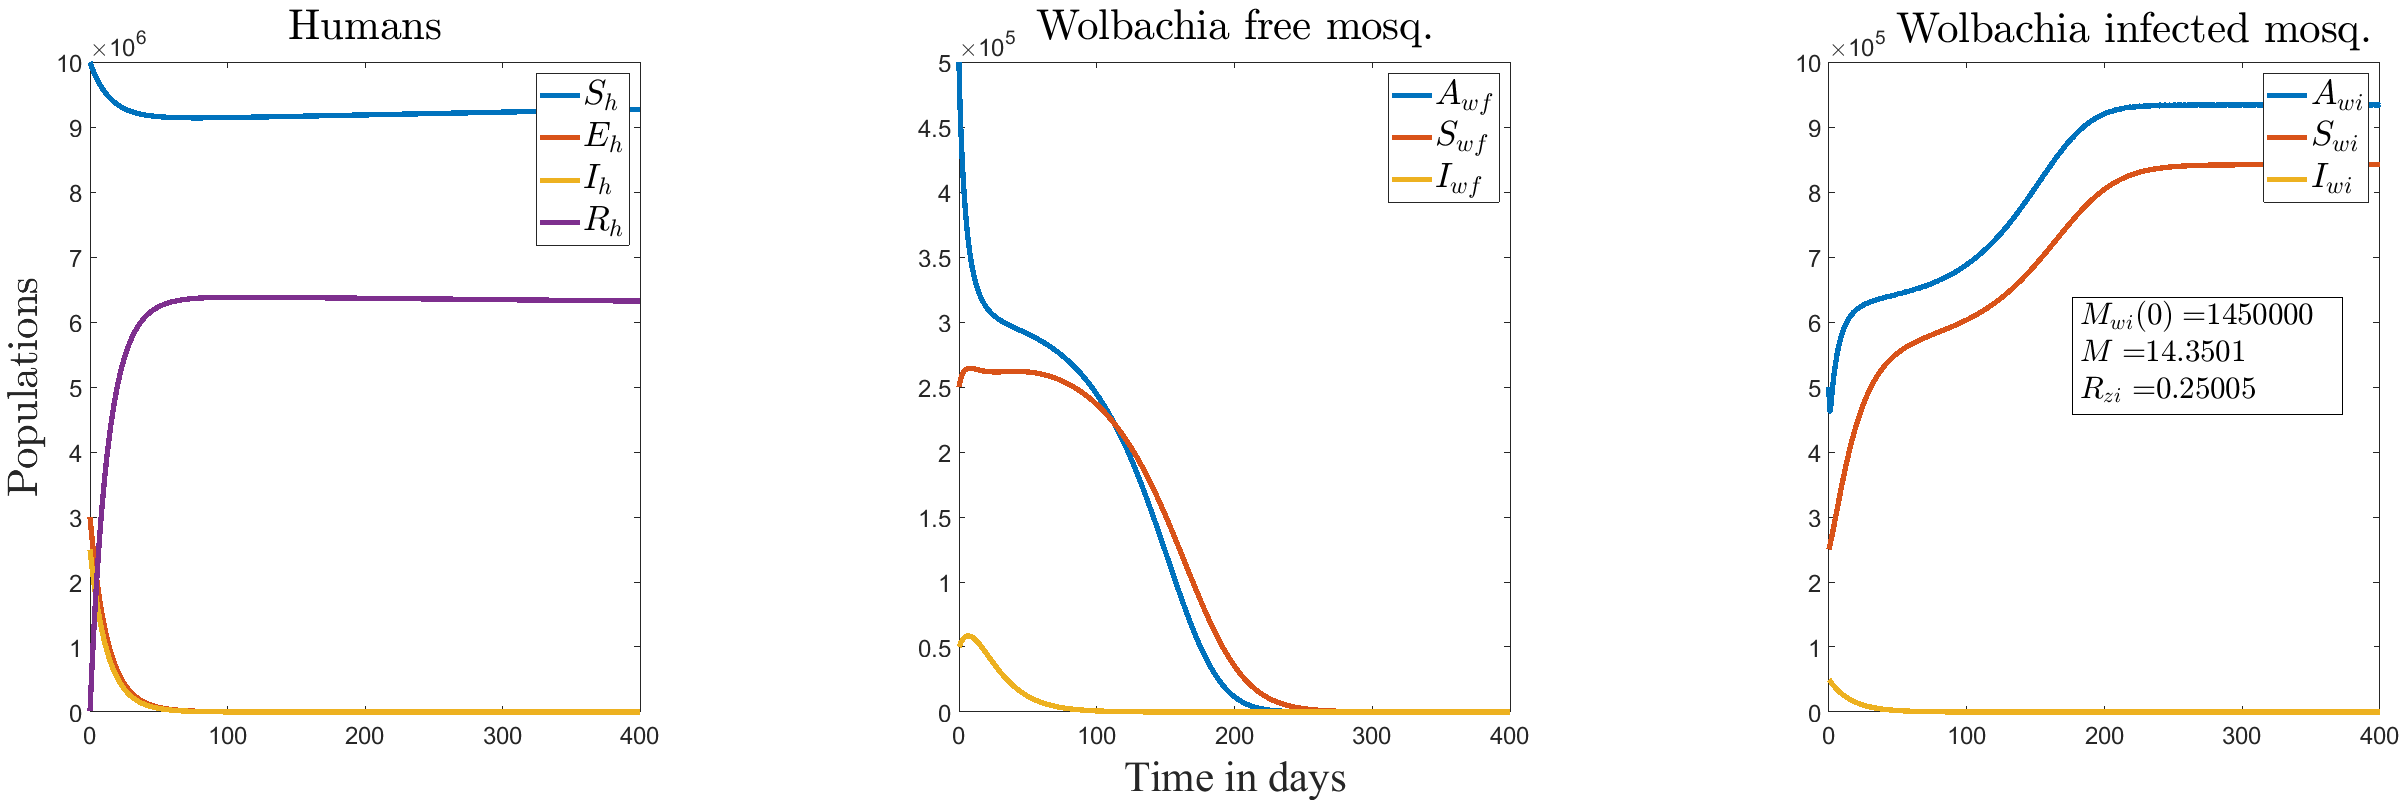
\includegraphics[width=16cm,height=4.5cm]{SimFig4.png} 
%    \caption{Dominance of \textit{Wolbachia} infected mosquitoes when starting with more \textit{Wolbachia} infected males. Figure  obtained using baseline values for parameters from Table \ref{tab: param-table} and Table \ref{tab: param_mosq_table} and the initial conditions listed in Table \ref{init-cond-dis-free-table} with $M_{wi}(0)=1,450,000$ }
%    \label{domwolbmales}
%\end{figure}

\subsubsection{\textit{Wolbachia} is established when more \textit{Wolbachia} infected  aquatic stage and females are released simultaneously}

Not surprisingly, a combination of more \textit{Wolbachia} infected aquatic stage and more \textit{Wolbachia} infected females, also allows the \textit{Wolbachia} infected mosquito population to establish itself. In Figure \ref{domwolbaqfem} we notice that if we release twice as many \textit{Wolbachia} infected aquatic stage and 3 times as many \textit{Wolbachia} infected females compared to their \textit{Wolbachia} free counterparts, then the wild mosquitoes population is eliminated and the \textit{Wolbachia} infected mosquitoes persist after roughly 250 days. Disease is again eradicated in approximately 230 days.

\begin{figure}[H]
    \centering
    % This file was created by matlab2tikz.
%
%The latest updates can be retrieved from
%  http://www.mathworks.com/matlabcentral/fileexchange/22022-matlab2tikz-matlab2tikz
%where you can also make suggestions and rate matlab2tikz.
%
\definecolor{mycolor1}{rgb}{0.00000,0.44700,0.74100}%
\definecolor{mycolor2}{rgb}{0.85000,0.32500,0.09800}%
\definecolor{mycolor3}{rgb}{0.92900,0.69400,0.12500}%
\definecolor{mycolor4}{rgb}{0.49400,0.18400,0.55600}%
%
\begin{tikzpicture}

\begin{axis}[%
width=1.1in,
height=1.5in,
at={(0in,0.108in)},
scale only axis,
xmin=0,
xmax=500,
ymin=0,
ymax=12000000,
ylabel={Population},
axis background/.style={fill=white},
title style={font=\bfseries, yshift=1.75ex},
title={Humans},
legend style={legend cell align=left, align=left, draw=white!15!black}
]
\addplot [color=mycolor1, line width=1.5pt]
  table[row sep=crcr]{%
0	10000000\\
0.923681894317269	9995794.91527189\\
1.96301792375743	9990863.90480548\\
3.38836635276675	9983855.73208251\\
5.60079066641629	9972683.00142322\\
8.5069951377809	9958015.03162731\\
10.2244324684143	9949582.64549745\\
11.5698178894818	9943174.63468449\\
12.8992098867893	9937047.42527553\\
14.2201495319605	9931183.23040788\\
15.4504169560969	9925936.78288408\\
16.6579080801457	9920998.33562475\\
17.7952068652958	9916542.98165611\\
19.0052423253655	9912014.28768939\\
20.1938000377268	9907779.14743155\\
21.3362367227674	9903906.63394906\\
22.2664338145405	9900895.70557681\\
23.3209721874446	9897634.47296399\\
24.2740261871368	9894823.88039194\\
25.2158514093608	9892171.47493401\\
26.1630899943411	9889626.52009213\\
27.0851447675377	9887264.62261214\\
28.1061096340418	9884778.67820675\\
29.0426495224237	9882614.44789398\\
29.992115020752	9880530.3819464\\
30.9126281943172	9878612.40110807\\
31.8366146497428	9876785.47264449\\
32.627462124452	9875297.56368847\\
33.6383909974247	9873493.97290776\\
34.6139975711703	9871854.42051723\\
35.5581543613225	9870358.6166137\\
36.3359830100089	9869191.0828581\\
37.2754911389202	9867856.05659123\\
38.2049097437412	9866613.3500138\\
39.1387497074902	9865439.76203099\\
40.0474124941975	9864367.13865602\\
40.8005793020129	9863527.93229793\\
41.5627512056381	9862723.05198086\\
42.3979193698615	9861890.51918258\\
43.2783783320338	9861066.71330964\\
44.0588835068047	9860380.90011883\\
44.7435852065682	9859812.4315171\\
45.5255173239857	9859199.81745604\\
46.3423652742058	9858600.00651852\\
47.0839704889804	9858089.66591391\\
47.7214865013957	9857676.07132529\\
48.4300269372761	9857242.72699511\\
49.1993041280657	9856802.54268006\\
49.8972599674016	9856429.49998734\\
50.6922506839037	9856033.98008032\\
51.4012475349009	9855706.68561718\\
51.9818388968706	9855455.91288741\\
52.6359465233982	9855191.38543743\\
53.3780459146947	9854913.59990493\\
54.1333604957908	9854654.35800588\\
54.7998775839806	9854444.55685882\\
55.3879426382482	9854273.70955292\\
55.9079011138529	9854133.44652836\\
56.4576419498771	9853995.85762844\\
57.0944503862411	9853849.83343803\\
57.5480118785053	9853754.32332164\\
58.0652231946588	9853653.79417004\\
58.5824345089495	9853561.96844888\\
59.1359522677958	9853473.0722607\\
59.6894700247794	9853393.59534661\\
60.0584818627685	9853345.70864474\\
60.5077919773757	9853292.77531242\\
60.9571020901203	9853245.61160727\\
61.4664764422923	9853198.94847754\\
61.9758507926017	9853159.33041213\\
62.4384897276759	9853129.29298384\\
62.6698091961443	9853116.35143117\\
63.0878152884543	9853096.40820214\\
63.4611885361373	9853082.27430223\\
63.6478751599789	9853076.48678227\\
63.8210909292102	9853071.86972822\\
63.9943067003042	9853067.97043112\\
64.1675224713981	9853064.78220788\\
64.3407382406294	9853062.29843315\\
64.5431303717196	9853060.27993632\\
64.7455225028098	9853059.20384976\\
64.9479146338999	9853059.05990421\\
65.1503067631274	9853059.83793475\\
65.3962245844305	9853062.0094958\\
65.6421424038708	9853065.509542\\
65.8880602233112	9853070.32045726\\
66.1339780446142	9853076.42484338\\
66.384297972545	9853083.94916329\\
66.6346179004759	9853092.7779931\\
66.8849378284067	9853102.89367603\\
67.3417099285871	9853124.61169561\\
67.7546142730862	9853147.79479383\\
68.1338058914989	9853171.98830559\\
68.4792847801	9853196.40117217\\
68.8345820251852	9853223.81916928\\
69.3822554219514	9853270.57008638\\
69.8336248304695	9853313.09204756\\
70.2849942389876	9853359.12652382\\
70.7993793562055	9853415.76047689\\
71.497587159276	9853499.53117707\\
72.0490552131087	9853571.13186626\\
72.784345952794	9853673.79471901\\
73.4551762510091	9853774.37698347\\
74.1855090744793	9853891.09752115\\
74.9224593676627	9854016.20610527\\
75.7991380430758	9854174.21912399\\
76.7023912854493	9854346.98371232\\
77.6523585096002	9854539.0529243\\
78.5881054569036	9854738.11556629\\
79.5800415147096	9854959.26763056\\
80.6513607222587	9855209.19864128\\
81.7035502325743	9855465.234347\\
82.7412974555045	9855727.42436322\\
83.9895553123206	9856054.75105567\\
85.2708337567747	9856403.43222751\\
86.5962222367525	9856776.7049487\\
88.0398130696267	9857196.76289987\\
89.5250324681401	9857642.48892913\\
90.9861734975129	9858093.33660724\\
92.6685210373253	9858626.33714356\\
94.5096972621977	9859225.17214327\\
96.34762387909	9859837.5573147\\
98.5003256108612	9860571.43545226\\
100.628090025857	9861312.48867586\\
103.071349792182	9862180.33183248\\
105.631662365049	9863106.67958624\\
108.37204846926	9864114.72843048\\
111.450504777953	9865264.51397951\\
114.949138350785	9866589.89796647\\
118.781414074823	9868060.3202031\\
122.96139171347	9869681.93979756\\
127.866294510663	9871603.20655786\\
133.527361290529	9873839.19897438\\
140.459038810804	9876596.22593413\\
149.157831853256	9880075.66836565\\
161.0384282507	9884847.9367033\\
180.383788136765	9892640.08614671\\
251.925553303212	9921468.19400261\\
288.84621110931	9936321.47708618\\
325.552138082683	9951069.56603529\\
362.246027586982	9965794.02683203\\
398.963195135817	9980509.0385095\\
435.709347562864	9995216.87123109\\
472.484779903665	10009917.6223146\\
500	10020904.3746264\\
};
\addlegendentry{$S_h$}

\addplot [color=mycolor2, line width=1.5pt]
  table[row sep=crcr]{%
0	3000000\\
0.685482889413834	2804442.79235735\\
1.37311768298969	2621387.83705239\\
2.10435023484752	2440144.9160876\\
2.76000501541421	2288593.82806665\\
3.38836635230109	2152430.9773212\\
4.15447989292443	1997631.63494174\\
4.7835271274671	1879127.37706079\\
5.60079066734761	1735909.90482313\\
6.35365588963032	1613949.99721566\\
6.91830480657518	1528316.43356961\\
7.66554452804849	1422161.84615753\\
8.21080978633836	1349540.48097002\\
8.80318048829213	1274986.95411224\\
9.47438804944977	1195650.94973246\\
10.22443246888	1113031.42718006\\
10.8420454813167	1049462.79695413\\
11.5698178899474	979375.742824235\\
12.1401610570028	927865.834075908\\
12.899209887255	863657.106414642\\
13.6540325419046	804391.835611969\\
14.2201495324261	762740.710776387\\
14.9357522181235	713295.745590033\\
15.7265474661253	662537.616178891\\
16.4683582824655	618359.587788806\\
17.2265574731864	576388.624204091\\
17.7952068662271	546880.624107666\\
18.5007970891893	512460.021556092\\
19.2744908193126	477325.078164898\\
20.0033939224668	446542.715006866\\
20.7650183797814	416607.122004376\\
21.5687859957106	387303.891469266\\
22.2664338145405	363636.981102115\\
23.0573375937529	338647.714445042\\
23.797499186825	316908.110157619\\
24.4651842010207	298567.189208497\\
25.2158514084294	279286.446147541\\
25.9552604476921	261586.205348084\\
26.5787490853108	247590.007367608\\
27.3383426098153	231609.989205027\\
28.1061096349731	216572.848685666\\
28.8316641701385	203319.456356098\\
29.6404518242925	189562.592638297\\
30.354117013514	178251.310455806\\
31.1436248081736	166576.634365516\\
31.8366146492772	157005.424752824\\
32.6274621239863	146800.436208471\\
33.4515627352521	136922.184859517\\
34.1988757839426	128582.570247652\\
34.8422910957597	121841.166155213\\
35.5581543617882	114786.773219925\\
36.3359830100089	107619.373590598\\
37.040614107158	101543.693570263\\
37.841483421158	95086.2025091695\\
38.5544341998175	89711.5089340657\\
39.343526346609	84144.7142678336\\
40.0474124937318	79494.9866737262\\
40.8005793029442	74827.2854042538\\
41.5627512061037	70405.8430601512\\
42.3979193693958	65885.2981702681\\
43.0942879058421	62357.5676444327\\
43.8306496068835	58850.0053760433\\
44.5153513066471	55781.0272788922\\
45.2648732843809	52620.5183267207\\
46.1569639700465	49111.4056726461\\
46.8985691857524	46388.589368545\\
47.72148650093	43558.9570344221\\
48.4300269382074	41273.5002892371\\
49.1993041280657	38939.6638547401\\
49.8972599674016	36946.7300685407\\
50.692250684835	34811.6549206581\\
51.4012475353666	33021.0978031103\\
52.1852094787173	31157.7341047786\\
52.8833129876293	29595.0203711148\\
53.6298174420372	28018.2693604226\\
54.385132022202	26515.9580159998\\
55.2146231466904	24966.9020708916\\
55.9079011147842	23748.0138666267\\
56.6408888953738	22529.6557837944\\
57.3212311323732	21459.7254451206\\
58.0652231937274	20352.8412667671\\
58.9514463478699	19114.9970928445\\
59.6894700243138	18146.7497591781\\
60.5077919764444	17135.2618892048\\
61.2117892662063	16314.1564808879\\
61.9758507926017	15471.2000832488\\
62.6698091961443	14746.5511584044\\
63.4611885356717	13964.917047041\\
64.3407382410951	13148.6495476179\\
65.1503067635931	12442.9552614056\\
65.8880602237768	11835.5342193865\\
66.6346179004759	11253.4248478138\\
67.5481621013023	10582.9160453398\\
68.3065453357995	10059.0691196783\\
69.199697623495	9477.77055863244\\
70.0593095351942	8952.38719105907\\
70.7993793566711	8525.16304894583\\
71.681409843266	8044.43067346839\\
72.600523267407	7574.31485947175\\
73.4551762510091	7163.54518772988\\
74.185509074945	6831.42327051982\\
74.9224593676627	6512.93633952737\\
75.7991380440071	6154.59331392357\\
76.7023912859149	5807.29938107217\\
77.4507912122644	5535.36531992769\\
78.3433789070696	5228.64426783472\\
79.0819018417969	4988.52086652815\\
80.0346736931242	4695.88805117086\\
80.8234754395671	4467.38462945586\\
81.7035502325743	4226.25774190947\\
82.5166252618656	4015.68982386542\\
83.4777624811977	3780.96486780932\\
84.355634868145	3579.18786329869\\
85.2708337572403	3380.84626539331\\
86.1215615547262	3206.81510358118\\
86.8483202471398	3065.58740387345\\
87.8107141354121	2888.52101789555\\
88.6391943590716	2744.66304528853\\
89.5250324676745	2599.09443304315\\
90.2986646923237	2478.55294555938\\
91.2296311813407	2341.17554375716\\
92.2162981866859	2204.19437282206\\
93.0774938589893	2091.44000073569\\
93.9669385356829	1981.25194226671\\
94.9140554117039	1870.51006382937\\
95.8387887137942	1768.55505795078\\
96.7840131483972	1670.26150983013\\
97.6938715875149	1580.96493518585\\
98.5003256103955	1505.93234489532\\
99.4439862701111	1422.76865225751\\
100.400438778568	1343.28760026162\\
101.223595704883	1278.53920350736\\
102.103583054151	1212.85312619014\\
103.071349792182	1144.59565490903\\
104.038650988601	1080.29543573456\\
105.022694071755	1018.66635394515\\
106.004596638028	960.746622582432\\
106.87352568889	912.296768332832\\
107.676109923515	869.75978409918\\
108.62449731119	822.08919255482\\
109.490234167781	780.896030739415\\
110.392332104035	740.201958386227\\
111.231066506356	704.29980226513\\
112.196025301702	665.174078215379\\
113.121426144615	629.723040012177\\
114.075680385344	595.169236154296\\
114.949138349853	565.225575875025\\
115.780761502218	538.133014555555\\
116.743036241736	508.417686296161\\
117.674726730678	481.226610550657\\
118.613366587088	455.316550699994\\
119.48211804172	432.59112324845\\
120.317698308732	411.81276754383\\
121.28615761688	388.984788281377\\
122.248627432622	367.560310164932\\
123.178262934089	347.994671620429\\
124.074495675974	330.124275466893\\
125.034149913583	312.010597331449\\
125.882181380875	296.836610368453\\
126.754355880432	282.003188868985\\
127.671623121016	267.20478000911\\
128.575484912843	253.384858732112\\
129.532788309269	239.528522953857\\
130.366711099632	228.078450179193\\
131.22617785586	216.851170735899\\
132.141331647988	205.504211293533\\
133.035418111365	194.992695402354\\
133.948490717914	184.813035855535\\
134.824279907625	175.548868666403\\
135.81475729635	165.629821026698\\
136.753332728986	156.747996476479\\
137.652097816579	148.689289907925\\
138.576299819164	140.833863815293\\
139.421195362695	134.015660114121\\
140.226794200949	127.821682802867\\
141.159517433494	121.006280218251\\
142.061515859328	114.760417649522\\
142.967583837453	108.810071215965\\
143.80521417968	103.583188455552\\
144.611874973401	98.7862812704407\\
145.547422172967	93.4995231004432\\
146.474207659252	88.5402852250263\\
147.368780246936	84.0020938054658\\
148.232766398229	79.8391075744294\\
149.157831853256	75.6092679621652\\
150.145563637372	71.3388539720327\\
151.128689355683	67.3267526137643\\
152.103387525771	63.5707280328497\\
153.016093956307	60.2428138060495\\
153.898339749314	57.1907693245448\\
154.783195392229	54.2841430245899\\
155.767864545807	51.2219873964787\\
156.595725245774	48.7807683818974\\
157.539168314077	46.1394009222277\\
158.542532979976	43.4860724476166\\
159.489497234579	41.1211308562197\\
160.388180371374	38.9950637486763\\
161.247799965553	37.0636790781282\\
162.284996440168	34.8593843635172\\
163.299014598131	32.8302948372439\\
164.147316184361	31.2232156307437\\
165.045945934486	29.6059221257456\\
166.01159066055	27.9606240829453\\
166.954298619647	26.4420273085125\\
167.886583512649	25.0207754508592\\
168.779980136547	23.7300256523304\\
169.826618995517	22.3017137087882\\
170.914560779929	20.9074330925941\\
172.018811347429	19.580716483295\\
173.001339683309	18.470674208831\\
174.10202490259	17.3011582759209\\
175.248885173351	16.1607096716762\\
176.344794895966	15.1407218058594\\
177.440114254598	14.1851375005208\\
178.530394810252	13.2934111882932\\
179.772626603954	12.3450292106718\\
181.023444489576	11.4579506055452\\
182.284445500001	10.6276981616393\\
183.572069935966	9.84152229689062\\
184.915949342307	9.08251845277846\\
186.126709618606	8.4486026824452\\
187.415201083291	7.82217533281073\\
188.787748789415	7.20554136484861\\
190.146282892674	6.64276273874566\\
191.700218169484	6.05237335711718\\
193.256326188799	5.51340049784631\\
194.918761058245	4.9901863061823\\
196.660741559695	4.49480299977586\\
198.313277831767	4.0701185176149\\
200.125451468863	3.65012734336779\\
202.079302879516	3.24545168643817\\
204.08632513741	2.87617914471775\\
206.360301970504	2.50804191362113\\
208.670628529508	2.18200937565416\\
211.199529920239	1.87329349294305\\
213.913926562294	1.59015490533784\\
216.925208265893	1.32563936291263\\
220.182506341953	1.08864320022985\\
223.825835586991	0.873229177668691\\
227.897488704883	0.682374040596187\\
232.398610102478	0.519421178847551\\
237.576315334998	0.379393864888698\\
243.75018515531	0.260781369637698\\
251.300198234152	0.164818652439862\\
260.887298713904	0.0919953635893762\\
274.270818354562	0.0407353141345084\\
295.78091777768	0.0109886969439685\\
346.553433446679	0.000497793313115835\\
500	4.33064997196198e-08\\
};
\addlegendentry{$E_h$}

\addplot [color=mycolor3, line width=1.5pt]
  table[row sep=crcr]{%
0	2500000\\
0.923681894782931	2319763.44965897\\
1.82168561127037	2153609.21376544\\
2.57350993668661	2021567.47635391\\
3.38836635230109	1885778.75306832\\
4.15447989292443	1765017.52628547\\
5.09805074427277	1625318.46982717\\
5.97722327848896	1503882.17014195\\
6.73008850123733	1406352.39494537\\
7.41646462120116	1322439.12430202\\
8.21080978633836	1231047.4336799\\
9.09936583926901	1135758.21522102\\
9.84941025916487	1060741.71372533\\
10.5994546785951	990426.299918086\\
11.3272270872258	926462.606118497\\
12.1401610570028	859708.286165684\\
12.899209887255	801597.403073339\\
13.6540325419046	747611.90155522\\
14.4586837613024	693986.094232195\\
15.1742864469998	649490.898740235\\
16.0026779752225	601501.639261381\\
16.8474578778259	556196.788484823\\
17.6056570685469	518447.906092294\\
18.2656003483571	487690.033159737\\
19.0052423244342	455395.84904562\\
19.8129878081381	422590.388940006\\
20.5746122654527	393854.370751434\\
21.3362367227674	367104.197127881\\
22.0338845415972	344229.023450857\\
22.7937030009925	320969.107446248\\
23.559235686902	299162.005999152\\
24.2740261871368	280175.861338924\\
25.0386582440697	261236.570273234\\
25.7474309019744	244862.205373643\\
26.3709195395932	231337.570052864\\
27.085144768469	216792.873220677\\
27.8488250430673	202289.036760535\\
28.620678818319	188654.57156223\\
29.2536348737776	178191.033421002\\
29.9921150212176	166746.126718286\\
30.7264578007162	156127.277982593\\
31.3746214215644	147344.474228663\\
32.100230474025	138125.631970049\\
32.8910779487342	128766.531342941\\
33.6383909974247	120536.474655375\\
34.3857040461153	112860.763809724\\
35.0705846208148	106280.267391542\\
35.8174305777065	99565.9075635145\\
36.5708600422367	93247.2863770644\\
37.2754911393858	87723.2226425721\\
38.0301475147717	82191.7786831898\\
38.7291964283213	77399.3460933128\\
39.5483029861934	72161.0384209123\\
40.2969672479667	67704.4382984536\\
41.054636603687	63493.3105694116\\
41.7715432466939	59766.8603403862\\
42.5720115038566	55881.9823970287\\
43.2783783311024	52679.1518318281\\
44.0588835068047	49368.7217674484\\
44.7435852065682	46649.1320575546\\
45.52551732352	43739.8506258973\\
46.3423652742058	40908.9615579774\\
47.0839704894461	38510.1423530825\\
47.72148650093	36569.6755715907\\
48.4300269382074	34536.6830463847\\
49.1993041280657	32467.4480782384\\
49.8972599674016	30706.2780576609\\
50.692250684835	28825.8601101427\\
51.4012475353666	27254.286980764\\
52.1852094787173	25624.4221341223\\
52.8833129876293	24262.2297003921\\
53.6298174420372	22892.4238011264\\
54.385132022202	21591.8758387896\\
55.2146231466904	20255.852762958\\
55.9079011147842	19208.3748825016\\
56.6408888953738	18164.8827126483\\
57.3212311323732	17251.5852107401\\
58.0652231937274	16309.9315481866\\
58.9514463478699	15260.9285301929\\
59.6894700243138	14443.5563923544\\
60.5077919764444	13592.8207191811\\
61.2117892662063	12904.6946458858\\
61.9758507926017	12200.6935815071\\
62.6698091961443	11597.5673558326\\
63.4611885356717	10949.2633863674\\
64.1675224704668	10403.9934200905\\
64.9479146329686	9835.82720397692\\
65.6421424038708	9358.80737616448\\
66.3842979720794	8876.63456493663\\
67.1352577568032	8416.20661136135\\
67.9610664458014	7939.76547414251\\
68.8345820247196	7467.60201330576\\
69.6079401266761	7075.04470052291\\
70.2849942394532	6749.78060811199\\
71.0565719152801	6398.81395953288\\
71.8652325281873	6052.15827412764\\
72.600523267407	5754.61666081101\\
73.4551762510091	5428.58195368294\\
74.185509074945	5165.82188308192\\
74.9224593676627	4914.58977129683\\
75.7991380440071	4632.81600857759\\
76.7023912859149	4360.6720930445\\
77.4507912122644	4148.25223860936\\
78.3433789070696	3909.39183294727\\
79.0819018417969	3722.9550352064\\
80.0346736931242	3496.43755560974\\
80.8234754395671	3320.10388434166\\
81.7035502325743	3134.56305394089\\
82.5166252618656	2972.99928249605\\
83.2218660656363	2840.07380641112\\
84.1725950906985	2670.8419927652\\
85.0877939793281	2518.06965256063\\
85.8989988812245	2390.43260281952\\
86.8483202471398	2249.74981871853\\
87.8107141354121	2116.07351988461\\
88.6391943590716	2007.74343740195\\
89.5250324676745	1898.38349129632\\
90.2986646923237	1808.02696432546\\
91.2296311813407	1705.27861452242\\
91.9685617461801	1628.11440316774\\
92.8730074483901	1538.64038929716\\
93.7956989691593	1452.67276012944\\
94.690616838634	1374.10064550256\\
95.5843711313792	1300.06640442181\\
96.3476238781586	1240.1497465563\\
97.3299282118678	1167.25675346935\\
98.2790702870116	1101.06589509221\\
99.1934112641029	1040.99617873738\\
100.172787530348	980.423944869544\\
101.039668489248	929.866255809553\\
101.932872081175	880.597030897159\\
102.872085851151	831.700250226073\\
103.796825689264	786.298656065948\\
104.776683300734	740.978515728842\\
105.63166236598	703.639320937917\\
106.514431159943	667.118090466596\\
107.454365070909	630.372167006601\\
108.372048470192	596.502772814129\\
109.309814580251	563.820246515796\\
110.211912516505	534.11395065533\\
111.011628234759	509.122020787094\\
111.947518460453	481.389472231269\\
112.895794810727	454.863869627938\\
113.893524658866	428.563997543417\\
114.751781818923	407.184731143527\\
115.541207944043	388.480896511581\\
116.499422176741	366.949227864388\\
117.473878437188	346.296985675115\\
118.445319098886	326.884324493352\\
119.30456588231	310.63657022547\\
120.098355606198	296.355638207402\\
121.03645208152	280.334190648049\\
121.892245292664	266.48496133415\\
122.783200643025	252.8020890099\\
123.612005375326	240.712568495888\\
124.565733836032	227.522295563947\\
125.479743907694	215.56705017481\\
126.421102808788	203.916647770442\\
127.282280341256	193.815839458723\\
128.102691311389	184.662789577618\\
129.052183912136	174.612026259769\\
129.970964038279	165.411151206587\\
130.895381242968	156.646243560594\\
131.750514481217	148.954807410948\\
132.573408230674	141.912080224138\\
133.527361290529	134.165430387482\\
134.473964231554	126.898360650986\\
135.387982821092	120.256659352221\\
136.26987393247	114.179246375803\\
137.214074023999	108.013480805326\\
138.223704766016	101.789247579407\\
139.066632919479	96.8688835180365\\
139.99454959156	91.7274315631948\\
140.923528028186	86.8537728656083\\
141.867485648952	82.1669024275616\\
142.805595163722	77.7597635285929\\
143.633996514603	74.0649752025492\\
144.611874973401	69.9287014864385\\
145.547422172967	66.1877221213654\\
146.474207659252	62.6789336302318\\
147.368780246936	59.4683937639929\\
148.232766398229	56.5235664076172\\
149.157831853256	53.5316971116699\\
150.145563637372	50.5113607146777\\
151.128689355683	47.6739100925624\\
152.103387525771	45.0177056696266\\
153.016093956307	42.6643499284983\\
153.898339749314	40.5061387396418\\
154.783195392229	38.4507965450175\\
155.767864545807	36.2854976858944\\
156.595725245774	34.5592741044238\\
157.539168314077	32.6915072775446\\
158.542532979976	30.8152480963618\\
159.489497234579	29.1428703060374\\
160.388180371374	27.6393607035279\\
161.457171680406	25.9510863348842\\
162.440652863123	24.4886076352559\\
163.481364227831	23.0301872021519\\
164.594848758075	21.5652882577851\\
165.64154259162	20.2728386307135\\
166.628225286957	19.1250734822825\\
167.68451299239	17.9678231272846\\
168.779980136547	16.8411013372242\\
169.826618995517	15.8302440773696\\
170.914560779929	14.8433424183168\\
172.018811347429	13.9041302590631\\
173.165500052739	12.9912511184812\\
174.280220532324	12.1609218786471\\
175.465924049262	11.3354891696945\\
176.746387942694	10.5064648939297\\
178.051937461831	9.72316269669682\\
179.321379159577	9.01717190025374\\
180.703616313171	8.30621343525127\\
182.089130813256	7.64942751312628\\
183.572069935966	7.00348825985566\\
185.065172959119	6.40783393522725\\
186.552596498746	5.86447258060798\\
188.165206260979	5.32695037173107\\
189.757553316653	4.84421282820404\\
191.542743735947	4.35448286030442\\
193.256326188799	3.93072094302624\\
195.236540311947	3.49178701778874\\
197.252931717783	3.09484392404556\\
199.375752501655	2.72530618403107\\
201.641329093371	2.37916654720902\\
204.08632513741	2.05448314966634\\
206.798576113768	1.74559857230633\\
209.653253065888	1.47025727853179\\
212.612484086305	1.23035957664251\\
216.066763839684	0.999152550008148\\
219.799134979956	0.797707165125757\\
223.980199794751	0.619688951410353\\
228.840813293122	0.461878563743085\\
234.475895803422	0.328369009308517\\
241.095761044882	0.219831036869437\\
249.452136429027	0.132381672970951\\
260.380858344492	0.0681408401578665\\
276.207629933022	0.0260151443071663\\
304.550418150146	0.00462949275970459\\
404.510660799686	1.04573555290699e-05\\
500	3.11993062496185e-08\\
};
\addlegendentry{$I_h$}

\addplot [color=mycolor4, line width=1.5pt]
  table[row sep=crcr]{%
0	10000\\
0.76488255802542	380888.941468298\\
1.48525966517627	709648.595747549\\
2.24568254686892	1036001.54948193\\
2.94650009367615	1318813.93777393\\
3.64373753219843	1583891.21136698\\
4.4690035097301	1877707.36464345\\
5.09805074427277	2087888.20551113\\
5.97722327895463	2362809.6780311\\
6.73008850123733	2581773.02589547\\
7.41646462120116	2768953.33261113\\
8.21080978680402	2971629.40213783\\
9.09936583973467	3181732.47309313\\
9.84941025916487	3346334.28727694\\
10.5994546785951	3500034.46621106\\
11.3272270867601	3639400.43168176\\
12.1401610570028	3784434.17051972\\
12.8992098877206	3910383.86398451\\
13.6540325414389	4027171.25174764\\
14.4586837608367	4143002.70150712\\
15.1742864465341	4239003.25073495\\
16.0026779752225	4342460.33090145\\
16.8474578782916	4440081.54282527\\
17.6056570690125	4521409.29704139\\
18.2656003478914	4587683.37942388\\
19.0052423244342	4657291.5714878\\
19.8129878081381	4728045.28161613\\
20.5746122654527	4790075.58645385\\
21.3362367227674	4847880.09936826\\
22.0338845420629	4897370.42404677\\
22.7937030009925	4947762.24449896\\
23.5592356873676	4995082.86665526\\
24.2740261871368	5036353.45513646\\
25.0386582445353	5077599.69904761\\
25.7474309019744	5113332.06861967\\
26.5787490857765	5152391.32705709\\
27.3383426098153	5185577.44774081\\
28.1061096349731	5216865.55930688\\
28.8316641701385	5244492.42281758\\
29.6404518242925	5273220.60680882\\
30.354117013514	5296882.87220649\\
31.143624807708	5321345.86887722\\
31.8366146488115	5341433.19696995\\
32.6274621235207	5362883.57956177\\
33.4515627352521	5383680.81601021\\
34.1988757839426	5401265.44423626\\
34.8422910962254	5415498.68705507\\
35.5581543613225	5430411.06940268\\
36.3359830100089	5445582.10971204\\
37.0406141066924	5458458.39569303\\
37.8414834206924	5472160.45116246\\
38.5544341998175	5483578.26966517\\
39.343526346609	5495417.20276179\\
40.0474124941975	5505316.10113304\\
40.8005793029442	5515262.7712158\\
41.5627512056381	5524693.4730437\\
42.3979193698615	5534344.34311515\\
43.0942879058421	5541881.72807156\\
43.8306496068835	5549381.13522676\\
44.5153513066471	5555946.824693\\
45.2648732848465	5562711.99716443\\
46.1569639705122	5570227.312473\\
46.8985691852868	5576061.11477834\\
47.7214865004644	5582125.57542239\\
48.4300269382074	5587024.68384895\\
49.1993041280657	5592027.87824918\\
49.8972599674016	5596300.1314691\\
50.692250684835	5600876.42069005\\
51.4012475358322	5604713.23989443\\
52.1852094782516	5608704.47679142\\
52.883312988095	5612049.96376949\\
53.6298174420372	5615423.29682064\\
54.385132022202	5618634.7072249\\
55.2146231466904	5621942.56227482\\
55.9079011147842	5624542.28552788\\
56.6408888949081	5627137.54901341\\
57.3212311323732	5629413.36438872\\
58.0652231937274	5631763.95036266\\
58.9514463478699	5634387.13823861\\
59.6894700247794	5636434.19121346\\
60.5077919764444	5638567.30352418\\
61.2117892662063	5640294.22815734\\
61.9758507926017	5642062.02631184\\
62.6698091961443	5643576.99202182\\
63.461188535206	5645205.45961984\\
64.1675224704668	5646574.70294376\\
64.9479146329686	5648000.52260774\\
65.6421424038708	5649196.42755732\\
66.384297972545	5650403.65274293\\
67.1352577572688	5651554.39651768\\
67.9610664453357	5652742.38658974\\
68.6520242253318	5653677.57209557\\
69.3822554228827	5654610.92355853\\
70.0593095347285	5655428.44000228\\
70.7993793562055	5656272.14040293\\
71.681409843266	5657213.41619514\\
72.4167005829513	5657947.73780531\\
73.2315661516041	5658711.17829726\\
73.9321477124467	5659327.51776833\\
74.6922317994758	5659956.62433859\\
75.3829145049676	5660494.39770139\\
76.1711299857125	5661070.7752295\\
76.8750239508227	5661553.58558651\\
77.6523585105315	5662053.65191984\\
78.3433789070696	5662470.48827286\\
79.0819018417969	5662888.63297363\\
79.8291113497689	5663284.38888919\\
80.6513607222587	5663689.83061461\\
81.3398195905611	5664006.32936343\\
82.0672808745876	5664319.16927292\\
82.7412974555045	5664590.1677195\\
83.4777624811977	5664866.54024061\\
84.1725950902328	5665109.29246864\\
84.9047542018816	5665347.09632138\\
85.4538735346869	5665513.8715413\\
86.1215615542606	5665703.87009723\\
86.8483202476054	5665895.41540543\\
87.5816152011976	5666073.3170166\\
88.2689120043069	5666226.70840953\\
88.8243355369195	5666341.6401252\\
89.5250324681401	5666475.61037078\\
90.0980712566525	5666576.39764719\\
90.7427158122882	5666680.7358013\\
91.229631180875	5666753.43277768\\
91.7208253061399	5666821.62677446\\
92.2162981871516	5666885.34998591\\
92.8730074483901	5666962.24865591\\
93.4532198356465	5667023.28499872\\
93.9669385356829	5667072.12282174\\
94.5096972631291	5667118.59797519\\
94.9140554117039	5667149.90739332\\
95.3609325578436	5667181.31467267\\
95.8387887133285	5667211.29366268\\
96.3476238781586	5667239.24451938\\
96.7840131483972	5667260.05142789\\
97.1479565240443	5667275.23170619\\
97.5118998996913	5667288.48501096\\
97.8758432753384	5667299.85592939\\
98.2790702870116	5667310.30866335\\
98.5003256108612	5667315.10593025\\
98.7215809347108	5667319.2502437\\
98.9428362576291	5667322.75078315\\
99.1934112645686	5667325.94920213\\
99.4439862705767	5667328.346437\\
99.6945612765849	5667329.95519244\\
99.945136282593	5667330.7879628\\
100.172787530348	5667330.88213003\\
100.400438778102	5667330.3550007\\
100.628090025857	5667329.21549841\\
100.855741273612	5667327.47241297\\
101.039668489248	5667325.62921157\\
101.223595704883	5667323.40217002\\
101.407522920519	5667320.79573452\\
101.762161108665	5667314.71533302\\
102.103583054617	5667307.57315042\\
102.473557968624	5667298.43844931\\
102.872085850686	5667287.01267128\\
103.31317509152	5667272.49680134\\
103.796825689264	5667254.38387985\\
104.284661759622	5667233.85461178\\
104.776683300734	5667210.91981883\\
105.428672933951	5667177.1945783\\
106.004596637562	5667144.35429937\\
106.514431159943	5667112.98013097\\
107.053072953597	5667077.56209584\\
107.676109923981	5667033.78309704\\
108.372048470192	5666981.44990973\\
109.129394993186	5666920.55674907\\
109.851073342375	5666858.87578506\\
110.572751691565	5666793.78513104\\
111.450504777953	5666710.23551575\\
112.444532142952	5666610.11051496\\
113.347057478502	5666514.41434129\\
114.4137311019	5666395.78195772\\
115.541207944043	5666264.26968822\\
116.743036241271	5666117.62260393\\
117.875575023703	5665973.74011085\\
119.127013723366	5665808.77916484\\
120.537041011266	5665615.95227864\\
122.070436362177	5665398.55777067\\
123.612005375326	5665172.61565625\\
125.256946911104	5664924.08791783\\
126.920982415788	5664665.58547347\\
128.811881713569	5664364.03571942\\
130.729982936755	5664050.53851805\\
132.789446522482	5663706.3421777\\
134.999437745661	5663329.24833759\\
137.433085920289	5662905.87074799\\
139.994549592026	5662452.28127759\\
142.967583836988	5661917.04240792\\
146.131437052973	5661338.73198041\\
149.586610616185	5660698.67072644\\
153.477878118865	5659969.18396276\\
158.040850646794	5659104.5514829\\
163.299014598131	5658098.76806009\\
169.500140265562	5656903.17887959\\
177.1083527226	5655426.76397604\\
186.982093653642	5653500.99817674\\
201.203355307691	5650717.28949117\\
230.460211576894	5644978.99222901\\
276.207629933022	5636008.79716256\\
313.415322924964	5628722.61738279\\
350.230315473862	5621522.5412396\\
387.04495399259	5614331.73724501\\
423.683804028668	5607184.40072034\\
460.31684546452	5600047.29399961\\
497.11701167468	5592886.77355912\\
500	5592326.19296027\\
};
\addlegendentry{$R_h$}

\end{axis}

\begin{axis}[%
width=1.1in,
height=1.5in,
at={(1.34in,0.108in)},
scale only axis,
xmin=0,
xmax=500,
ymin=0,
ymax=500000,
xlabel={Time (days)},
axis background/.style={fill=white},
title style={font=\bfseries, yshift=1.25ex},
title={\emph{Wolb.}-free mosq.},
legend style={legend cell align=left, align=left, draw=white!15!black}
]
\addplot [color=mycolor1, line width=1.5pt]
  table[row sep=crcr]{%
0	500000\\
0.124589653627481	467118.612179115\\
0.265923185739666	442298.326527915\\
0.407256717851851	426113.770429613\\
0.546369803661946	415297.185004442\\
0.685482889413834	407771.158806849\\
0.844282226404175	401587.146380964\\
1.00308156333631	397034.667483577\\
1.18809962313389	392866.744018143\\
1.48525966494344	387613.100308773\\
1.82168561127037	382680.571779595\\
2.24568254675251	377181.480092483\\
2.76000501529779	371176.883115503\\
3.38836635224288	364599.234142136\\
3.89910871267784	359788.881039981\\
4.46900351007935	354821.218948612\\
4.78352712729247	352297.818482369\\
5.78900697291829	345224.825574577\\
6.54187219543383	340594.350459688\\
7.16738471388817	337139.200108282\\
7.66554452822311	334639.184108005\\
8.50699513743166	330705.392094357\\
9.09936583950184	328461.63098869\\
9.47438804927515	326925.353645928\\
10.4119435737957	323668.263201994\\
11.084636284213	321542.391337421\\
12.1401610568282	318526.471647832\\
12.7105042238836	317259.837443312\\
13.0879155510338	316262.853029249\\
14.4586837611278	313316.764285759\\
14.9357522183564	312409.160263049\\
15.1742864469416	311980.106722238\\
15.4504169564461	311401.635826741\\
15.7265474659507	310892.888066693\\
16.0026779754553	310524.29720101\\
16.2788084849017	310122.420727008\\
16.6579080802621	309415.367204729\\
17.0370076755644	308876.124123086\\
17.4161072708666	308268.147378175\\
18.5007970890729	306761.559628483\\
18.7359938300215	306467.223549707\\
19.0052423246088	306044.288614939\\
19.274490819138	305682.135790443\\
19.5437393136672	305447.487816392\\
19.8129878081963	305177.159560762\\
20.003393922525	304885.853859895\\
20.1938000368536	304634.727825167\\
20.5746122655692	304250.728673728\\
20.9554244942847	303785.666129021\\
21.3362367230002	303397.405036478\\
21.8013352688286	302873.293388214\\
22.2664338147151	302444.677680509\\
22.5300684077665	302110.568630378\\
22.7937030008179	301831.848345425\\
23.0573375938693	301672.047843628\\
23.3209721869207	301476.274784806\\
23.559235686902	301108.629718849\\
23.7974991869414	300841.179467858\\
24.0357626869227	300781.016593536\\
24.2740261869039	300663.857371821\\
24.4651842011954	300383.307951269\\
24.6563422154868	300168.276224174\\
25.0386582440697	299933.724267642\\
25.3930445730803	299571.388144662\\
25.7474309020326	299301.306858812\\
26.1630899937009	298931.710559932\\
26.5787490853108	298627.771642235\\
26.8319469268899	298387.42522247\\
27.0851447684108	298177.722463908\\
27.3383426099899	298033.018723859\\
27.5915404515108	297869.450745415\\
27.848825043242	297556.411198202\\
28.1061096349149	297327.891063668\\
28.3633942265878	297285.510265619\\
28.620678818319	297182.103796896\\
28.8316641701385	296882.485958537\\
29.0426495219581	296673.911119553\\
29.2536348737776	296633.905126197\\
29.4646202255972	296558.353529212\\
29.6404518242343	296361.105363278\\
29.8162834228133	296203.212302006\\
30.1679466200294	295995.194702782\\
30.5402874072315	295697.824809148\\
30.9126281943754	295462.888824463\\
31.374621421739	295114.503821715\\
31.8366146490443	294845.48229211\\
32.100230474025	294595.082647815\\
32.3638462989475	294397.927802411\\
32.6274621239281	294320.144080631\\
32.8910779489088	294200.954073329\\
33.0779062110814	294013.908518976\\
33.2647344732541	293863.496939464\\
33.6383909975993	293670.539375775\\
34.0120475219446	293387.121487989\\
34.3857040462899	293168.561362092\\
34.8422910959343	292839.762661795\\
35.2988781455206	292590.030030291\\
35.5581543616718	292354.27568108\\
35.8174305777648	292168.091141978\\
36.0767067939159	292092.98907363\\
36.3359830100089	291979.474510984\\
36.5708600424114	291688.539713584\\
36.8057370747556	291492.023474933\\
37.040614107158	291494.130220154\\
37.2754911395023	291438.071530902\\
37.4641552333487	291209.273674341\\
37.652819327137	291042.850891747\\
37.8414834209834	290976.452645913\\
38.0301475147717	290896.529423719\\
38.2049097431591	290743.440808456\\
38.3796719715465	290613.163863234\\
38.7291964283213	290415.135756732\\
39.1387497073156	290125.116904578\\
39.5483029862517	289892.684980988\\
39.7978577400791	289694.550608109\\
40.0474124939647	289523.833802404\\
40.2969672477921	289413.747792634\\
40.5465220016777	289283.419009392\\
40.8005793027114	289006.987967435\\
41.0546366038034	288809.998373985\\
41.3086939048371	288790.431251886\\
41.5627512059291	288710.160935693\\
41.7715432468685	288434.872654741\\
41.9803352877498	288246.626175052\\
42.1891273286892	288220.877658923\\
42.3979193696287	288159.259257709\\
42.5720115037402	287976.194464218\\
42.7461036378518	287830.756830992\\
43.0942879060749	287642.909704129\\
43.462468756421	287365.302928779\\
43.8306496068253	287145.406972711\\
44.2871174066677	286813.040796688\\
44.7435852065682	286552.952238664\\
45.0042292454746	286309.050510603\\
45.2648732844391	286114.938059591\\
45.5255173234036	286034.16808918\\
45.7861613623681	285912.331409023\\
45.9715626662364	285725.776547985\\
46.1569639701629	285574.038502995\\
46.5277665779577	285373.292537869\\
46.8985691857524	285081.704219997\\
47.2693717935472	284851.155691829\\
47.7214865007554	284506.369608661\\
48.1736012079637	284235.337945711\\
48.4300269380328	283989.404171406\\
48.6864526680438	283790.132981324\\
48.942878398113	283696.591939695\\
49.1993041281821	283565.280295607\\
49.431956074608	283265.266956576\\
49.6646080210921	283054.590126963\\
49.897259967518	283032.500484848\\
50.1299119140022	282954.327102274\\
50.317358170927	282714.938489573\\
50.5048044279101	282534.87314531\\
50.692250684835	282450.441162737\\
50.8796969417599	282352.408415941\\
51.2273973376141	282038.713516429\\
51.5750977334101	281806.320298118\\
51.9818388969288	281475.803189794\\
52.3885800604476	281199.391163617\\
52.6359465240967	280975.501758602\\
52.8833129877457	280777.40415423\\
53.1306794513948	280637.169854531\\
53.3780459150439	280476.716217042\\
53.6298174419207	280175.006252013\\
53.8815889687394	279948.421153937\\
54.133360495558	279890.287911595\\
54.3851320224348	279773.762510892\\
54.5925048035569	279477.630732688\\
54.7998775846208	279263.962991598\\
55.0072503657429	279204.593391671\\
55.2146231468651	279110.608154446\\
55.3879426388303	278905.818320193\\
55.5612621307373	278736.806028316\\
55.9079011146678	278496.875977802\\
56.2743950050208	278165.382362989\\
56.6408888953156	277888.461518306\\
57.0944503867067	277485.924544839\\
57.5480118780397	277151.416320935\\
57.8066175359418	276868.166311903\\
58.0652231938438	276631.977455529\\
58.3238288517459	276503.617195797\\
58.5824345095898	276335.441199531\\
58.766940428759	276119.222885499\\
58.9514463478699	275936.121696758\\
59.3204581861501	275667.69324724\\
59.6894700244302	275310.507035044\\
60.0584818627103	275010.991509105\\
60.5077919765608	274583.305279404\\
60.9571020904696	274224.742731957\\
61.2117892659735	273932.679802645\\
61.4664764414774	273684.496417031\\
61.7211636169814	273536.352856539\\
61.9758507924853	273351.78726265\\
62.2071702604298	273011.909380527\\
62.4384897283744	272756.303581229\\
62.669809196319	272678.969129696\\
62.9011286642635	272548.073004255\\
63.0878152879886	272274.53358731\\
63.2745019117137	272057.143092763\\
63.6478751592222	271790.639854141\\
63.9943067000713	271404.317975612\\
64.3407382409205	271094.877232408\\
64.7455225023441	270675.725967241\\
65.1503067637095	270307.088214912\\
65.6421424037544	269775.511905262\\
65.8880602237768	269576.313641581\\
66.1339780437993	269357.421356066\\
66.3842979720794	269003.09962851\\
66.6346179003594	268719.258189468\\
66.8849378286395	268593.94457953\\
67.1352577569196	268413.072987879\\
67.3417099291109	268074.438004924\\
67.5481621013605	267813.351088025\\
67.7546142735519	267697.634098574\\
67.9610664457432	267548.852375529\\
68.133805890684	267304.63928039\\
68.306545335683	267094.116788877\\
68.6520242255647	266765.463997532\\
69.0171398241073	266342.957180734\\
69.3822554226499	265971.347406226\\
69.8336248309934	265453.559288666\\
70.2849942392786	264998.761102017\\
70.5421867978876	264651.496992681\\
70.7993793564965	264348.074359524\\
71.0565719151055	264145.702136519\\
71.3137644737144	263905.339841748\\
71.6814098433824	263410.494303514\\
72.0490552129922	263038.165603852\\
72.4167005826603	262580.793525978\\
72.7843459522701	262176.945555886\\
73.2315661514294	261624.63747313\\
73.6787863505306	261136.007712557\\
73.9321477127378	260775.011481238\\
74.185509074945	260454.663608178\\
74.4388704372104	260227.571105239\\
74.6922317994176	259965.855176488\\
74.9224593678373	259566.475084481\\
75.1526869361987	259245.403584045\\
75.3829145046184	259090.323950203\\
75.613142073038	258884.837004434\\
75.7991380437743	258561.607976943\\
75.9851340145105	258290.611884966\\
76.3571259559831	257905.144023876\\
76.7023912857403	257416.085441197\\
77.0476566154975	256998.196643766\\
77.4507912120898	256454.916669458\\
77.8539258086821	255957.710536745\\
78.3433789071278	255273.96822818\\
78.8328320055152	254694.229829703\\
79.0819018416223	254266.827157471\\
79.3309716777876	253904.358254057\\
79.5800415138947	253688.459509947\\
79.82911135006	253420.53183105\\
80.0346736931242	253023.294914117\\
80.2402360361884	252697.603974147\\
80.4457983793109	252506.243252187\\
80.6513607223751	252283.882886118\\
80.9955901565263	251719.952899559\\
81.3398195906193	251272.101521417\\
81.7035502325161	250727.865193248\\
82.0672808743548	250229.847024935\\
82.516625261982	249558.80497337\\
82.9659696496092	248944.515609282\\
83.2218660654034	248512.470838776\\
83.4777624811977	248120.341252128\\
83.7336588969338	247820.867508479\\
83.989555312728	247485.80719253\\
84.3556348682614	246865.941077602\\
84.7217144237948	246357.933013479\\
85.0877939793281	245770.33598597\\
85.4538735349197	245230.952427907\\
85.898998881341	244517.313391938\\
86.3441242277622	243860.544681487\\
86.8483202472562	242997.387164764\\
87.100418256945	242668.99525612\\
87.352516266692	242308.349692984\\
87.5816152011394	241832.456768965\\
87.8107141355285	241427.641393738\\
88.0398130699759	241173.86680043\\
88.2689120044233	240873.625025955\\
88.6391943593044	240148.117804884\\
89.0094767141272	239611.859412815\\
89.3531805498642	238993.261760219\\
89.8974778211559	238084.209558344\\
91.229631181166	235824.418376517\\
91.4730888655758	235424.688322811\\
91.7208253060235	234906.2996815\\
91.9685617464129	234446.087058256\\
92.2162981868023	234117.762245644\\
92.4640346271917	233741.884287331\\
92.6685210377327	233272.256798943\\
92.8730074482737	232866.829292523\\
93.2819802692975	232269.107157403\\
93.6244594024029	231571.396553241\\
93.9669385355664	230977.260181045\\
94.5096972627798	229959.984658453\\
94.9140554117621	229198.143840151\\
96.3476238782168	226515.72345922\\
96.6020414603991	226066.261039348\\
96.9659848361043	225296.860104988\\
97.3299282117514	224626.073832768\\
97.8758432752802	223534.576419298\\
98.2790702868369	222724.345567926\\
99.6945612764684	219894.819503292\\
99.9451362826512	219417.48550264\\
100.172787530522	218852.5644984\\
100.400438778335	218349.952158095\\
100.628090026206	217980.084695628\\
100.855741274077	217568.80323282\\
101.223595704825	216691.760050699\\
101.591450135573	215980.05005863\\
102.103583054268	214857.502123759\\
102.872085851093	213202.249368016\\
103.313175091404	212223.920020485\\
103.796825689438	211188.304428286\\
104.038650988485	210674.146281257\\
104.530672530003	209483.087862573\\
105.022694071522	208528.552367905\\
105.428672934417	207484.773749864\\
105.834651797311	206679.887531448\\
106.174541478569	205834.683150642\\
106.693978424417	204645.576481213\\
109.851073342201	197164.310818328\\
111.011628234584	194277.666645566\\
111.450504777953	193210.839174707\\
111.947518460278	191910.789163215\\
112.444532142661	190737.379483503\\
112.895794810727	189480.536209988\\
113.347057478735	188463.002778256\\
113.711368932156	187435.012178993\\
114.075680385518	186544.476893539\\
114.58275646047	185194.48148563\\
115.541207943927	182674.812400272\\
116.259868618392	180758.496749223\\
116.499422176566	180132.260807296\\
116.986650306848	178739.003952714\\
117.473878437188	177539.360187998\\
117.87557502382	176340.121978266\\
118.27727161051	175335.801944399\\
118.781414075289	173902.980904756\\
119.659670201247	171463.190822062\\
121.286157616938	166882.948502705\\
121.714054222277	165658.269810928\\
122.7832006432	162584.013824191\\
123.82887659577	159555.683670068\\
124.320114756061	158076.435457926\\
124.811352916353	156697.492867287\\
125.256946910697	155297.509243625\\
125.70254090504	154085.587780932\\
126.061821856943	152948.118544056\\
126.587729344494	151401.313228738\\
128.575484913075	145413.313603585\\
129.05218391231	143930.396667992\\
129.532788309094	142510.17936614\\
129.773090507544	141810.130179363\\
130.168837568781	140520.915077671\\
130.564584630076	139380.307388064\\
131.060779549356	137822.821942201\\
132.14133164793	134481.192235034\\
140.923528028361	107142.729091735\\
141.395506838569	105635.583629515\\
141.867485648836	104235.970036634\\
142.255546069529	102981.897234286\\
142.805595163838	101314.046746856\\
143.976431844581	97712.7484160569\\
145.547422172793	92928.4943209866\\
147.368780246936	87445.356728028\\
149.372221234778	81511.3678868804\\
149.973281817744	79790.0519500577\\
150.969048836152	76921.6475391198\\
153.246986037586	70490.9234041294\\
153.898339749314	68713.6871106997\\
154.783195392054	66314.8665896602\\
156.831586012733	60895.2181356525\\
158.040850646968	57811.202177944\\
159.925171472714	53147.3345952334\\
161.038428250642	50485.8843872157\\
164.147316184361	43490.3142538566\\
165.641542591853	40331.6276723994\\
167.68451299239	36264.9481259311\\
169.010422170919	33776.0598104469\\
169.826618995343	32293.1029278727\\
170.914560779871	30391.3831902471\\
172.223403338925	28203.1227524126\\
173.165500052914	26702.5480717923\\
174.458416162001	24735.2070372713\\
175.465924049262	23276.638460592\\
176.565405552567	21761.0745235508\\
177.108352722833	21034.8352911515\\
178.370909027464	19423.2113608297\\
179.321379159577	18274.1768658615\\
179.998250326316	17487.8524876407\\
181.183358577488	16173.6711541217\\
182.089130813372	15223.2639049598\\
182.949291866622	14362.1018459883\\
183.973232549732	13389.9010264004\\
184.617502108391	12803.0158208526\\
185.389238976582	12127.9233547254\\
186.339653058618	11337.4132085136\\
187.415201083233	10496.0302476406\\
188.491265206598	9705.4382565514\\
189.249589554791	9178.13485614094\\
190.146282892674	8586.46376779594\\
191.006008072291	8049.72338500497\\
192.015167035919	7455.83455337357\\
192.871958262229	6981.21016443032\\
193.692406492075	6551.01497095777\\
194.72119249258	6045.31443398097\\
195.701600935834	5594.34863827546\\
196.488309388864	5253.8170872117\\
197.252931717958	4940.36454929627\\
198.099748456152	4612.22082438617\\
199.053592210752	4266.90845734667\\
199.970449919463	3955.97625826608\\
200.819404937269	3686.1595317882\\
201.641329093545	3440.57872659998\\
202.546925474831	3187.57431625464\\
203.32629646681	2983.09167584352\\
204.086325137643	2795.14669062418\\
204.732788945665	2643.7456447166\\
205.534762572148	2466.29818136047\\
206.506393351592	2265.75519537338\\
207.286394648021	2115.59527265496\\
208.043657291739	1978.56606960658\\
208.882064277248	1836.27955562947\\
209.827411712322	1687.52968700818\\
210.7377807218	1554.58861400367\\
211.389954981511	1465.36234345933\\
212.178314805788	1363.80385090492\\
212.984476988961	1266.85188834451\\
213.759018299927	1179.6701300416\\
214.446045666526	1107.04582743172\\
215.250845518953	1027.24317239312\\
216.066763839568	951.845225466066\\
216.925208265719	878.27527864842\\
217.663606705552	819.198696817912\\
218.343254302745	768.13318146544\\
218.962481793831	724.22474604036\\
219.799134979956	668.656300651492\\
220.529086384224	623.46777901554\\
221.282511124329	579.864389863214\\
221.895737662213	546.506784517725\\
222.65364344063	507.79868975142\\
223.301241238485	476.793152996572\\
224.134564002801	439.537020882068\\
224.752020834421	413.723248234834\\
225.503027557221	384.276549852337\\
226.141214454896	360.829311929934\\
226.934004978335	333.601471899659\\
227.752412349859	307.559630258125\\
228.502082944615	285.398210231157\\
229.215753913042	265.733848742791\\
229.832480249461	249.807193058368\\
230.460211576778	234.523949846101\\
231.187822727312	217.931127574877\\
231.939653005567	201.973891138914\\
232.551595801138	189.816646264459\\
233.307281684713	175.776412394305\\
233.952633118315	164.581173979212\\
234.784041344014	151.168546994159\\
235.400332425255	141.909810151672\\
236.149340146745	131.394865499868\\
236.785594809451	123.056390972342\\
237.576315335114	113.405198608874\\
238.393325943733	104.204349004314\\
239.142017349368	96.4042362458422\\
239.854286498972	89.5125417652889\\
240.469530826318	83.9505012955633\\
241.095761044708	78.6298509807093\\
241.822034145414	72.8686074701254\\
242.573065346107	67.3430217631976\\
243.184364864603	63.146920244908\\
243.938791918627	58.3187610504683\\
244.58280507708	54.4825843928847\\
245.259243107983	50.7175564732752\\
246.028854738164	46.7419536186499\\
246.776725241041	43.1703242344083\\
247.411845063732	40.3469590662862\\
248.201372650685	37.0876668368583\\
249.017647912959	33.9886463574949\\
249.765865503752	31.3693138785311\\
250.477359794488	29.0626192138297\\
251.091746543942	27.2060523153632\\
251.717101613991	25.4344092364772\\
252.442627133685	23.5201525597367\\
253.193274986057	21.6882286423934\\
253.804264790087	20.3005961911404\\
254.557991784939	18.7084465715452\\
255.201224576798	17.446872803499\\
256.031023364165	15.9420346908737\\
256.646411220834	14.9087055073469\\
257.393646918645	13.7422129265615\\
258.028112660162	12.8223614112358\\
258.816964211059	11.7626992624719\\
259.632860047102	10.7573003827711\\
260.380858344666	9.90954171837075\\
261.091931639821	9.16483753646025\\
261.914114643238	8.3720658934908\\
262.711243590515	7.66832614864688\\
263.517169748666	7.01592827501008\\
264.417114006472	6.35183121624868\\
265.384718980291	5.70652150205569\\
266.335123224242	5.13589575624792\\
267.257982742798	4.63572557555744\\
268.216233091487	4.16698232962517\\
269.235066410038	3.71980671468191\\
270.387921612244	3.27100869920105\\
271.497344413248	2.88953650777694\\
272.731889067742	2.51635857304791\\
274.126278489304	2.15209214488277\\
275.402709059184	1.86447632801719\\
276.943567144917	1.56749609077815\\
278.613013060065	1.29838450340321\\
280.383305502997	1.06282301974716\\
282.309351526783	0.85438159952173\\
284.444206153217	0.670420165872201\\
286.814391530235	0.511783789144829\\
289.642018798622	0.370553048793226\\
292.915481850796	0.254694001050666\\
296.991938573658	0.159424060315359\\
302.207212662091	0.0873395513626747\\
309.529971674841	0.0373687464743853\\
321.457569500199	0.00929325434844941\\
351.64140695025	0.000264828151557595\\
500	0\\
};
\addlegendentry{$A_{wf}$}

\addplot [color=mycolor2, line width=1.5pt]
  table[row sep=crcr]{%
0	250000\\
0.124589653627481	250681.734858124\\
0.265923185739666	251234.646940735\\
0.407256717822747	251632.366504864\\
0.546369803632842	251928.544287786\\
0.764882557909004	252273.124148712\\
1.00308156336541	252550.003831774\\
1.28060865297448	252798.645338362\\
1.48525966494344	252948.598879801\\
1.70954362917109	253088.865889478\\
1.96301792308805	253222.857201995\\
2.2456825467234	253346.200505975\\
2.57350993691944	253459.969786892\\
2.76000501529779	253512.34961919\\
2.94650009364705	253556.497681438\\
3.1329951720254	253593.301579962\\
3.38836635224288	253633.234898774\\
3.64373753248947	253661.803195402\\
3.89910871270695	253680.159754705\\
4.15447989292443	253690.009923598\\
4.46900351010845	253693.515335668\\
4.78352712726337	253686.610331777\\
5.09805074444739	253669.715761098\\
5.6007906672603	253633.675385754\\
5.78900697288918	253617.737754333\\
6.35365588980494	253562.019683625\\
7.41646462108474	253448.644485983\\
7.91462443541968	253397.223572425\\
8.50699513746076	253344.578390229\\
8.80318048846675	253318.893310769\\
9.09936583950184	253296.663568005\\
9.47438804927515	253275.404049683\\
9.66189915419091	253265.443685043\\
9.84941025907756	253256.812549798\\
10.0369213639933	253250.146703894\\
10.22443246888	253244.593981052\\
10.4119435737957	253240.081879691\\
10.5994546786824	253236.960154636\\
10.8420454814623	253235.445145485\\
11.0846362842422	253236.043003272\\
11.327227087022	253238.530362724\\
11.5698178898019	253243.507895441\\
11.8549894733296	253253.851260738\\
12.1401610568282	253266.558140024\\
12.4253326403559	253280.459697503\\
12.7105042238836	253298.305552535\\
13.0879155510629	253329.434945361\\
13.4653268782131	253363.728365105\\
13.8427382053924	253404.503698851\\
14.2201495325426	253449.447628232\\
14.6972179897421	253513.995281237\\
15.1742864469416	253584.775171821\\
16.0026779754262	253724.756566917\\
16.4683582825819	253811.827959806\\
17.2265574732155	253964.774506996\\
18.0304036071757	254140.45549309\\
18.7359938300506	254303.568300883\\
20.1938000368827	254664.077263886\\
21.1458306086133	254909.967480185\\
22.5300684077665	255276.904786771\\
24.0357626869227	255675.486878736\\
26.8319469268608	256390.47309669\\
27.848825043242	256633.58836808\\
28.3633942266169	256749.923065431\\
29.8162834228424	257064.261869125\\
30.7264578008035	257244.684612065\\
31.3746214217099	257365.489191218\\
32.3638462989766	257536.255483312\\
33.264734473225	257674.980670968\\
34.0120475219155	257779.172544968\\
34.613997571083	257855.492817711\\
35.0705846207275	257908.383961226\\
35.8174305777939	257987.477135158\\
36.8057370747556	258074.108909634\\
37.8414834209543	258140.609621924\\
38.3796719715756	258167.737069743\\
38.7291964283213	258181.550750688\\
38.9339730678184	258188.965376705\\
39.1387497072865	258195.298082768\\
39.3435263467836	258200.387470253\\
39.7978577401082	258209.436192184\\
40.0474124939647	258212.489223416\\
40.2969672477921	258213.337225688\\
40.5465220016486	258213.147193263\\
40.8005793027114	258213.662139802\\
41.0546366038034	258211.646691772\\
41.5627512059291	258199.211246655\\
41.7715432468394	258195.876149401\\
41.9803352877789	258190.346942737\\
42.7461036378227	258158.071636781\\
43.0942879060458	258139.200641135\\
43.4624687564501	258117.542521887\\
43.8306496068253	258092.128962433\\
44.2871174066968	258057.424953232\\
44.7435852065391	258017.187253419\\
45.0042292455037	257993.572393645\\
45.2648732844682	257967.777103165\\
46.1569639701629	257866.644276026\\
46.8985691857233	257770.169995296\\
47.4954291471222	257684.172963791\\
47.9475438543595	257613.717381022\\
48.6864526680729	257490.662943025\\
49.6646080210921	257309.298327749\\
50.879696941789	257052.677868259\\
51.4012475355121	256934.777894789\\
52.1852094786882	256745.892516629\\
52.8833129877457	256567.434782575\\
53.8815889687394	256294.8280323\\
55.0072503657429	255959.702320842\\
56.2743950049917	255553.760099317\\
57.0944503866776	255273.359374572\\
58.0652231938438	254924.102225515\\
59.3204581861501	254441.555765761\\
60.2831369196356	254051.36027021\\
61.2117892659735	253656.916546188\\
62.207170260459	253214.325800975\\
63.0878152879886	252804.515077076\\
63.9943067000713	252367.436660881\\
65.1503067637095	251785.041466854\\
66.1339780438284	251267.695487342\\
66.8849378286395	250859.621678927\\
68.3065453356539	250055.320636367\\
69.6079401268216	249281.646980072\\
70.7993793564965	248542.789904928\\
72.2328778978263	247611.922927789\\
73.45517625098	246784.20683139\\
74.6922317993885	245912.712156521\\
75.613142073038	245242.129700778\\
76.7023912857403	244427.002463582\\
78.0986523579049	243341.550513557\\
79.3309716777876	242347.572881624\\
80.9955901564972	240946.69064897\\
82.2919530681975	239811.776026904\\
83.4777624811686	238739.246387828\\
85.0877939793572	237226.765811274\\
86.3441242277913	236002.44804683\\
87.5816152011103	234759.165867294\\
88.8243355367158	233469.365298347\\
90.2986646922654	231888.654431052\\
91.7208253059944	230310.261976644\\
93.0774938587565	228752.060425798\\
94.6906168384885	226835.226043059\\
96.0932062959764	225110.48527827\\
97.6938715874276	223072.295786148\\
99.1934112641611	221096.808278484\\
100.628090026206	219143.822289654\\
102.274294027186	216828.213853035\\
103.796825689438	214613.448787704\\
105.428672934417	212161.225657112\\
107.053072953684	209636.060494588\\
108.624497311102	207115.42060268\\
110.392332103977	204184.04815682\\
111.947518460307	201523.286133466\\
113.711368932127	198409.59121444\\
115.343851412646	195437.504180679\\
116.986650306877	192360.036680115\\
118.78141407526	188895.520348432\\
120.537041011354	185406.438438771\\
122.248627432738	181909.565164956\\
123.82887659577	178598.755677763\\
125.479743907868	175056.804470819\\
127.476951731107	170661.387476322\\
129.292486110702	166564.271299697\\
131.400956730969	161688.346679618\\
133.527361290413	156651.855117146\\
135.814757296263	151110.069321261\\
138.223704765987	145148.527322323\\
140.92352802839	138334.850005016\\
143.805214179563	130939.084954396\\
147.577811622614	121126.406086943\\
156.181794895703	98689.8362339431\\
159.081157657405	91279.7717236481\\
161.45717168058	85322.5480494706\\
163.703348213399	79812.5004057883\\
165.641542591824	75169.1656601474\\
167.482442472334	70866.5635733058\\
169.3369009007	66648.9741973616\\
170.914560779871	63160.0982750254\\
172.427995330421	59904.2312437522\\
173.949973875104	56723.7913624749\\
175.465924049262	53653.3569511469\\
176.927370332764	50788.2216173358\\
178.370909027464	48051.8164487566\\
179.77262660407	45485.5703087838\\
181.183358577517	42994.3551444738\\
182.506060955435	40742.844064644\\
183.772651242849	38663.5755025294\\
185.06517295909	36619.2787747451\\
186.339653058589	34680.0312984754\\
187.631754798029	32791.0831035716\\
188.787748789415	31166.487422277\\
189.951918104693	29592.111250339\\
191.006008072291	28219.4014255966\\
192.172641469195	26757.8517778651\\
193.256326188741	25453.7048653603\\
194.326055361103	24216.0262731438\\
195.395429938653	23027.1470837246\\
196.488309388864	21861.1511780495\\
197.672689705127	20652.2001455013\\
198.702402208379	19646.2501929659\\
199.815448370209	18604.8747865863\\
200.819404937269	17705.512391048\\
201.860315986589	16811.9633904547\\
203.01454807003	15866.1474789651\\
204.086325137614	15028.9831603353\\
205.143772111856	14240.5533875578\\
206.202790928568	13487.1084582998\\
207.28639464805	12752.3811067679\\
208.251425036869	12127.8416831998\\
209.304935772467	11476.9756860153\\
210.292717340635	10895.0447112707\\
211.199529920239	10384.1067271049\\
212.178314805788	9856.77485343273\\
213.139385251125	9362.5311274222\\
214.068834824284	8905.93950724712\\
215.037051013875	8451.85090136394\\
216.066763839539	7992.12173726765\\
217.081913304282	7561.3628299316\\
218.003430504148	7188.87860761123\\
218.96248179386	6819.21056532499\\
220.009216320759	6435.82587589955\\
220.992443764844	6093.98204303847\\
221.895737662184	5794.87313999081\\
222.869509373268	5487.78585841705\\
223.825835586962	5201.05725610652\\
224.752020834421	4936.79809781464\\
225.715756523103	4675.25060070009\\
226.740651125816	4411.45559484762\\
227.752412349888	4164.87328069421\\
228.671448118926	3952.24984370332\\
229.626904803969	3742.1403462298\\
230.66945535253	3525.00865032413\\
231.650132428884	3331.76250222643\\
232.551595801167	3163.0822127377\\
233.522398829227	2990.57228249029\\
234.475895803422	2829.93666527647\\
235.400332425255	2682.12624391061\\
236.361425034294	2536.33684516145\\
237.383436789067	2389.68810840102\\
238.393325943733	2252.83213152233\\
239.311079918436	2135.05402426832\\
240.264449383889	2019.02141598423\\
241.095761044708	1922.85036676525\\
241.994544043584	1823.87447674415\\
242.878715105355	1731.34444967532\\
243.750185155106	1644.61761431926\\
244.58280507708	1565.71547409132\\
245.56708776005	1477.19160782613\\
246.402789989603	1405.87903185227\\
247.200138456188	1340.97874934692\\
248.201372650685	1263.61872171829\\
249.162477418402	1193.47449908676\\
250.103664642142	1128.48471816021\\
251.091746543942	1063.989740833\\
252.097911247227	1002.03308833222\\
253.048702508764	946.748230972211\\
253.992696538771	894.827052747976\\
254.986813646188	843.176061991835\\
255.877176399983	799.413698762888\\
256.833220145287	754.912340858224\\
257.816624079656	711.68525694203\\
258.816964211059	670.219197894767\\
259.777656257356	632.644238619192\\
260.71848525753	597.86426745003\\
261.501197491511	570.374207327026\\
262.330683094857	542.60440687355\\
263.228072399885	514.065707620437\\
264.111690551974	487.417097479221\\
264.982121635752	462.50403802644\\
265.813241916563	439.8943076781\\
266.79655298352	414.554811463662\\
267.631425545143	394.179806122149\\
268.427597835456	375.675158296042\\
269.427435953286	353.652770145505\\
270.387921612244	333.70476879226\\
271.328575996158	315.25185041962\\
272.110968901834	300.677973504615\\
272.940078402578	285.963644529285\\
273.837198758905	270.847210162028\\
274.720749840722	256.735953135096\\
275.590992857935	243.551950650173\\
276.421806571132	231.593997022312\\
277.404943048372	218.195810983074\\
278.239666005946	207.427347981808\\
279.035603358469	197.652199784614\\
280.035162151005	186.023175241018\\
280.995545531914	175.492096282367\\
281.936115954362	165.753940504248\\
282.718332657649	158.066499350971\\
283.547231431032	150.307496147492\\
284.444206153188	142.338165298715\\
285.327732945385	134.900049713615\\
286.197877971455	127.953315191553\\
287.028520471329	121.654863738804\\
288.011566124333	114.598936207825\\
288.846211109863	108.92941320024\\
289.642018798651	103.784379645047\\
290.641423269437	97.6649650716572\\
291.6017562091	92.1241209524451\\
292.54228659661	87.0016064487863\\
293.324406629428	82.958955119946\\
294.153188229102	78.8794613395294\\
295.050084376067	74.6899172397389\\
295.933603989688	70.7800402165158\\
296.803698033706	67.129274388164\\
297.634245570691	63.8199110949354\\
298.617244013294	60.1128996951738\\
299.451848396653	57.1347365658148\\
300.247584897996	54.4325519560371\\
301.246904556901	51.2190478570119\\
302.207212662091	48.3096211771772\\
303.147724074923	45.6202042139485\\
304.134238185099	42.959767002525\\
305.138789079443	40.4098620303266\\
306.0889732246	38.1372317027417\\
307.032483300107	36.0069069949677\\
308.02535569403	33.8933649903338\\
309.068639896112	31.8059110442409\\
310.057000380388	29.9469577493146\\
311.063921025227	28.164682583214\\
312.044246908277	26.5313532720029\\
312.957044592331	25.0957367770025\\
313.9214928273	23.6631326983916\\
314.947327329864	22.2289233663178\\
315.915945225977	20.954533131764\\
316.991154996707	19.6252275452134\\
318.013893479423	18.4390824276488\\
319.058439321409	17.3015697706142\\
320.134873604722	16.2026629189495\\
321.246352918708	15.1411325893132\\
322.264545841172	14.2298166935798\\
323.417107263871	13.2642143361445\\
324.526327090833	12.3968237179215\\
325.76021406395	11.498395315517\\
327.009646724531	10.6549490676261\\
328.242224571033	9.88350324827479\\
329.449126651976	9.18225879449164\\
330.739632810466	8.48737262262148\\
332.062312288937	7.82968172224355\\
333.409625673579	7.2120997167076\\
334.793608815962	6.62837941976613\\
336.156848427199	6.09960397498799\\
337.758883351868	5.53185128353653\\
339.411595944839	5.00145321982563\\
341.036764461373	4.52950401985436\\
342.666986424098	4.10081799706677\\
344.481720287004	3.67115165042924\\
346.34900359012	3.27598155572196\\
348.363533989206	2.89720655267593\\
350.444386682997	2.55187795468373\\
352.662586280174	2.2289554416202\\
355.086352915067	1.92263452729094\\
357.782275489822	1.63110497916932\\
360.620868040889	1.37178775476059\\
363.665032417426	1.13931931916159\\
367.149389842671	0.921175101713743\\
371.037255459203	0.726689325005282\\
375.48006871072	0.554183164960705\\
380.46645085339	0.408843568788143\\
386.432746575883	0.284119342570193\\
393.598512224387	0.183513349649729\\
402.662833986629	0.105569291772554\\
414.961481977778	0.0498566922615282\\
433.947492183797	0.0156584049982484\\
473.399795599165	0.00141116848681122\\
500	0.000278539780993015\\
};
\addlegendentry{$S_{wf}$}

\addplot [color=mycolor3, line width=1.5pt]
  table[row sep=crcr]{%
0	50000\\
0.476813260735071	51258.3178234584\\
0.923681894877518	52322.827691355\\
1.37311768285144	53280.8631430257\\
1.82168561127037	54127.8521319788\\
2.24568254673068	54832.0100401407\\
2.57350993691944	55314.6676495261\\
2.94650009365432	55800.7734778118\\
3.38836635225016	56293.286738209\\
3.64373753247492	56538.3179351361\\
3.89910871270695	56755.3779010239\\
4.1544798929317	56945.2945845489\\
4.46900351010117	57143.110614717\\
4.78352712727064	57302.524402417\\
5.09805074444012	57425.0367074638\\
5.41257436160959	57512.1016979912\\
5.60079066725302	57547.8426703013\\
5.78900697288918	57571.71388469\\
5.97722327853262	57584.0159649443\\
6.16543958416878	57585.0412338567\\
6.35365588981222	57575.0791664337\\
6.54187219544838	57554.4203274178\\
6.73008850109181	57523.3482094485\\
6.91830480672797	57482.1406531491\\
7.16738471390272	57412.4918042475\\
7.41646462107747	57326.1985820364\\
7.66554452825221	57223.8729073559\\
7.91462443542696	57106.1105164851\\
8.21080978644022	56946.7884678132\\
8.50699513745349	56767.4246730549\\
8.80318048847403	56568.9529221812\\
9.2868769443885	56206.0669731176\\
9.66189915418363	55893.6940595691\\
10.2244324688872	55378.3216963347\\
10.8420454814623	54753.5000976117\\
11.5698178897874	53946.8286946228\\
12.1401610568428	53267.6674853652\\
12.8992098874805	52308.2408253246\\
13.6540325418027	51300.1681829764\\
14.6972179897493	49834.7299685144\\
15.7265474659362	48324.9508443331\\
17.2265574732301	46047.2110450835\\
19.5437393136453	42440.8425273728\\
22.2664338147224	38216.3453544466\\
24.0357626869227	35543.8753158909\\
25.5702377375419	33298.2893716352\\
26.8319469268681	31511.5889813539\\
28.1061096349222	29767.5669232339\\
29.464620225619	27979.0705423306\\
30.7264578008035	26386.0769554684\\
31.8366146490516	25040.1136218179\\
33.0779062110596	23597.3048342822\\
34.1988757841027	22350.7426637191\\
35.2988781455497	21179.1714345625\\
36.3359830100235	20120.9148710769\\
37.4641552333196	19019.9505620913\\
38.5544341999484	18004.6778437707\\
39.5483029862517	17119.9239270456\\
40.5465220016558	16269.4223608674\\
41.5627512059218	15441.764557324\\
42.5720115037184	14656.8020172525\\
43.6465591816304	13860.3161944298\\
44.7435852065464	13087.4862327295\\
45.7861613623681	12389.3806256617\\
46.7131678818405	11797.3365338964\\
47.7214865007409	11182.8827822629\\
48.6864526680729	10622.5881003032\\
49.6646080210921	10081.2547116808\\
50.692250684835	9540.25069991445\\
51.5750977334392	9097.25397696906\\
52.6359465240821	8590.45616237948\\
53.6298174418989	8139.86708453634\\
54.5925048035278	7724.76847399071\\
55.5612621307664	7327.34813629631\\
56.4576419501682	6976.98590692669\\
57.3212311323732	6654.57359123387\\
58.3238288517241	6298.10339500217\\
59.3204581861646	5961.90950950452\\
60.2831369196501	5653.55646961735\\
61.2117892659808	5370.66514902319\\
62.2071702604517	5082.59361088689\\
63.0878152879959	4840.20356682025\\
63.9943067000713	4602.37993865685\\
64.9479146330123	4364.41069449934\\
65.8880602237914	4141.49668568142\\
66.8849378286395	3917.2088497512\\
67.7546142735519	3731.21793960936\\
68.6520242255428	3548.31168933728\\
69.6079401268216	3363.09074147091\\
70.5421867979094	3191.19472437477\\
71.4975871585339	3024.28513229214\\
72.4167005826457	2871.78090502289\\
73.2315661514149	2742.88312000026\\
74.1855090749668	2599.17054428053\\
75.1526869362206	2461.00146353477\\
76.1711299852468	2323.29402856433\\
77.0476566155121	2210.85128514427\\
77.8539258086894	2112.14949016626\\
78.832832005508	1998.11923399563\\
79.8291113500381	1888.28304818458\\
80.8234754394434	1784.58548178303\\
81.7035502325016	1697.49588130683\\
82.5166252620038	1620.76292392757\\
83.4777624811759	1534.45497426653\\
84.3556348682687	1459.59112385682\\
85.2708337571239	1385.37833480065\\
86.1215615545661	1319.73749175165\\
87.1004182569595	1248.00081728931\\
88.0398130699905	1182.78058682674\\
89.0094767141563	1118.98903476322\\
89.8974778211559	1063.55722118619\\
90.7427158122664	1013.31838372137\\
91.7208253060016	958.103593205538\\
92.6685210377327	907.445684703205\\
93.6244594024247	859.031199341713\\
94.509697262758	816.479739310649\\
95.3609325582802	777.531213477203\\
96.347623878195	734.68031554966\\
97.3299282117659	694.342576102048\\
98.2790702868369	657.451086726644\\
99.1934112641611	623.749056024782\\
100.1727875305	589.545481275542\\
101.039668489444	560.823895450609\\
101.932872081379	532.679313299122\\
102.872085851079	504.592884069869\\
103.796825689446	478.373168133185\\
104.77668330077	452.062186888201\\
105.631662365849	430.27865635512\\
106.514431159798	408.877919929342\\
107.454365070982	387.249561557022\\
108.372048470061	367.227516657797\\
109.309814580432	347.826764826154\\
110.211912516708	330.12314375749\\
111.011628234584	315.176950568428\\
111.9475184603	298.535187490983\\
112.895794810698	282.561221278273\\
113.893524658823	266.667898452091\\
114.751781818806	253.70704660593\\
115.541207943919	242.337544165086\\
116.499422176566	229.213356029795\\
117.473878437173	216.588898659968\\
118.44531909877	204.689435232242\\
119.304565882376	194.705365117014\\
120.098355606286	185.911225200587\\
121.036452081746	176.024366181991\\
122.070436362592	165.729425735131\\
122.961391713339	157.338385050018\\
123.828876595777	149.57300447634\\
124.811352916346	141.235802923009\\
125.702540905062	134.072172840308\\
126.587729344494	127.313121862629\\
127.476951731114	120.863088732491\\
128.33908811224	114.918725047217\\
129.292486110717	108.681710767174\\
130.168837568803	103.244883521395\\
131.060779549349	97.9878415806525\\
131.925293356566	93.1455778783711\\
132.789446522067	88.5421479345168\\
133.773332879879	83.5745352010999\\
134.64912206967	79.3853438976948\\
135.601370058699	75.0660134115387\\
136.511603330633	71.154950779237\\
137.43308592018	67.4010108231305\\
138.400002292517	63.6726121755928\\
139.230077286404	60.6351747642839\\
140.226794200782	57.1768739367108\\
141.159517433487	54.1176860080814\\
142.061515859168	51.3134669171704\\
142.967583837381	48.6413909021212\\
143.976431844581	45.8279415462748\\
144.823689349636	43.589962391452\\
145.788666447159	41.1724988773349\\
146.816978265197	38.7422499123859\\
147.786842998321	36.580392289492\\
148.706550447205	34.6407451799096\\
149.586610616403	32.880096579036\\
150.649767796735	30.8708629738612\\
151.689259395927	29.0239209353822\\
152.557930425537	27.5646619237959\\
153.477878118676	26.0983674901072\\
154.46704839803	24.6077721382317\\
155.433603465863	23.232706071125\\
156.388760070702	21.9486040988195\\
157.303307546841	20.7850001457045\\
158.375305535665	19.4985906107104\\
159.489497234739	18.2450407887154\\
160.619684820718	17.0550122952627\\
161.793255848897	15.9006012332975\\
162.934315338432	14.8524376047135\\
163.925332198873	13.9978055027605\\
165.045945934631	13.0899617111427\\
166.165749317261	12.241058557549\\
167.280371952234	11.450272050708\\
168.549538101761	10.6113148108125\\
169.82661899535	9.82863356979215\\
171.113968676487	9.09758786098246\\
172.427995330407	8.40698365910066\\
173.797922847545	7.74231393605442\\
175.248885173285	7.0951013808517\\
176.74638794268	6.48339066678454\\
178.21142324456	5.93564436338056\\
179.772626604077	5.40242744343414\\
181.503186753827	4.8667912605888\\
183.170907322172	4.40059883658978\\
184.915949342198	3.96024340592703\\
186.765539938788	3.54123879819963\\
188.787748789429	3.13342063777964\\
190.784221275077	2.77665901534783\\
193.064142225499	2.41842459947657\\
195.395429938646	2.09966177172464\\
197.886219080639	1.80519331867981\\
200.627429752189	1.528458972105\\
203.706310802219	1.26773798779323\\
206.944667494543	1.0412278195945\\
210.583864322311	0.834498385556799\\
214.634651087676	0.65219219114806\\
219.168890957561	0.494867736466404\\
224.597656626509	0.355536740709795\\
231.015033602365	0.240468130774389\\
238.828047571194	0.149356263638765\\
249.017647912988	0.0802409254392842\\
263.372621074283	0.0334336678424734\\
287.550216097174	0.00765097131079528\\
354.078579070228	0.000132209519506432\\
500	1.8007995095104e-08\\
};
\addlegendentry{$I_{wf}$}

\end{axis}

\begin{axis}[%
width=1.1in,
height=1.5in,
at={(2.8in,0.108in)},
scale only axis,
xmin=0,
xmax=500,
xlabel style={font=\color{white!15!black}},
xlabel={},
ymin=0,
ymax=1000000,
ylabel style={font=\color{white!15!black}},
ylabel={},
axis background/.style={fill=white},
title style={font=\bfseries, yshift=1.25ex},
title={\emph{Wolb.}-inf mosq.},
legend style={legend cell align=left, align=left, draw=white!15!black}
]
\addplot [color=mycolor1, line width=1.5pt]
  table[row sep=crcr]{%
0	1000000\\
0.124589653685689	837259.620048522\\
0.265923185739666	719334.336032836\\
0.407256717793643	647597.966631576\\
0.546369803603739	604289.671566158\\
0.685482889413834	578392.384667407\\
0.844282226404175	561383.378456325\\
0.923681894899346	556283.964359594\\
1.00308156339452	552692.867835177\\
1.09559059317689	549817.760206446\\
1.18809962307569	548099.559389422\\
1.28060865297448	547274.275636806\\
1.37311768287327	547032.055548172\\
1.48525966494344	547185.835533109\\
1.59740164701361	547776.720417626\\
1.82168561127037	549804.759698686\\
2.10435023496393	552789.783207881\\
2.76000501529779	560204.745977304\\
3.13299517205451	564249.211013668\\
3.89910871267784	571655.007642434\\
4.15447989292443	573975.351591823\\
4.46900351007935	576194.17818507\\
4.78352712723427	578599.255801442\\
5.09805074438918	581630.009457364\\
5.41257436166052	584228.879770865\\
5.60079066723119	585175.162511718\\
5.78900697291829	586272.982618727\\
6.16543958417606	588882.707739862\\
6.73008850112092	592107.660816432\\
6.91830480669159	593194.439207564\\
7.41646462108474	595706.181091868\\
7.91462443547789	598347.670722965\\
8.21080978645477	599281.071250895\\
8.50699513743166	600480.434228818\\
8.80318048852496	602375.285750877\\
9.09936583950184	603924.877108596\\
9.28687694435939	604301.9378254\\
9.47438804933336	604858.20019242\\
9.84941025904845	606472.062611799\\
10.22443246888	607605.658197505\\
25.3930445730221	633499.640061116\\
25.7474309019744	633939.569912636\\
25.9552604478085	633995.64334337\\
26.1630899936426	634126.019216112\\
40.2969672478503	644299.91005324\\
55.0072503658012	654660.950160238\\
70.0593095351942	668197.3294961\\
85.898998881341	688129.060323524\\
100.855741274077	715279.147992295\\
115.146494881366	747366.654144142\\
130.895381242968	791955.799355365\\
145.960051750182	838375.26976543\\
160.829056535731	878752.640115727\\
175.248885173234	907267.11288732\\
200.819404937327	928936.293347735\\
227.439885590342	933014.918487245\\
254.986813646159	933225.926187993\\
273.664966003504	934084.582390122\\
302.810270936694	933870.528347966\\
322.960709237377	933625.784798067\\
354.93054320768	934060.067873168\\
402.13370314613	933943.030789756\\
462.795200007735	933588.364174584\\
495.642053353949	934148.438856422\\
500	934321.725084784\\
};
\addlegendentry{$A_{wi}$}

\addplot [color=mycolor2, line width=1.5pt]
  table[row sep=crcr]{%
0	750000\\
0.0492330082925037	750317.929051869\\
0.0994707718491554	750455.292747288\\
0.124589653685689	750462.59324135\\
0.195256419712678	750300.505773186\\
0.265923185739666	749910.907667841\\
0.407256717793643	748634.323438484\\
0.615926346508786	746033.975765859\\
1.00308156339452	740281.417967318\\
1.96301792305894	725721.887018992\\
2.57350993691944	717125.959025581\\
3.13299517205451	709740.167453056\\
3.89910871267784	700334.972737104\\
4.46900351007935	693831.68689841\\
5.09805074438918	687081.299806642\\
5.78900697291829	680172.196210644\\
6.54187219543383	673179.837092385\\
7.16738471388817	667764.162769461\\
7.91462443547789	661721.100341243\\
8.80318048852496	655094.191234289\\
9.47438804933336	650459.615424067\\
10.22443246888	645620.300523139\\
10.8420454814332	641889.042666008\\
11.569817889831	637761.104179358\\
12.4253326404141	633258.996552511\\
13.0879155510338	630015.079846723\\
13.8427382053342	626551.34177324\\
14.458683761186	623899.846981557\\
15.1742864469998	620999.770978861\\
16.0026779754553	617875.014125807\\
16.6579080802621	615569.645638736\\
17.4161072708666	613065.191481357\\
18.0304036071757	611160.792690956\\
18.7359938300215	609098.648846272\\
19.543739313609	606898.957208617\\
20.1938000369119	605246.734587838\\
20.9554244942265	603428.717568845\\
21.5687859959435	602055.864919948\\
22.2664338147733	600583.574411443\\
23.0573375938693	599029.656899841\\
23.559235686902	598109.281828129\\
24.4651842012536	596535.18856919\\
25.3930445730221	595066.689272246\\
25.9552604478085	594238.15644056\\
26.5787490853108	593369.705523083\\
27.3383426099317	592383.753488431\\
27.8488250431838	591769.186675956\\
28.8316641701385	590655.523349571\\
29.8162834228715	589650.410249518\\
30.3541170136305	589144.492678164\\
31.1436248080572	588456.299734603\\
31.8366146490443	587896.654969938\\
32.8910779488506	587126.053381251\\
33.8252192597138	586529.849983815\\
34.3857040462317	586200.409923766\\
35.0705846206984	585831.082774686\\
35.5581543616718	585592.265485822\\
36.3359830100089	585227.763428558\\
36.8057370748138	585048.115052631\\
37.2754911395023	584846.821890616\\
37.6528193271952	584723.672014554\\
38.0301475147717	584588.538733977\\
38.9339730677893	584321.004618386\\
39.5483029861934	584159.69962018\\
40.5465220016195	583939.689338104\\
41.0546366038034	583860.053869713\\
41.3086939048953	583806.86359029\\
41.5627512058709	583761.690079025\\
41.7715432468103	583744.109211483\\
41.9803352877498	583721.283244201\\
42.1891273286892	583686.922675745\\
42.3979193696287	583657.450488482\\
42.5720115037402	583645.24759576\\
42.7461036378518	583631.223262675\\
43.0942879060749	583598.462713112\\
43.8306496068835	583553.970442399\\
44.5153513066471	583531.544287514\\
44.7435852065682	583526.615344295\\
45.0042292454746	583530.900688194\\
45.2648732844973	583533.541146761\\
45.5255173234036	583529.174457017\\
45.7861613624264	583530.695523975\\
45.9715626662364	583541.620402801\\
46.1569639701629	583550.836186125\\
46.3423652740894	583556.634200825\\
46.5277665778995	583564.22467199\\
47.269371793489	583615.111150715\\
48.1736012079054	583699.743836381\\
48.6864526680438	583767.314508636\\
48.942878398113	583793.191886195\\
49.1993041281821	583824.247738033\\
49.4319560746662	583869.464653408\\
49.6646080210339	583908.690251416\\
49.897259967518	583933.465895146\\
50.1299119140022	583964.563082909\\
50.5048044278519	584042.865814685\\
50.8796969418181	584104.92282738\\
51.401247535483	584212.572645268\\
51.7784683151403	584293.213959813\\
52.3885800604476	584428.826513812\\
53.3780459150439	584670.477681499\\
53.8815889686812	584816.679849913\\
54.133360495558	584874.31067463\\
54.3851320224348	584938.509210903\\
54.7998775846791	585075.043075315\\
55.2146231468068	585184.748032555\\
55.5612621307373	585300.797528079\\
56.0911480598152	585469.728131785\\
57.0944503867067	585811.778158807\\
57.5480118780397	585969.767801739\\
58.0652231938438	586167.441987686\\
58.582434509648	586351.194390328\\
59.1359522669809	586572.743394369\\
59.5049641053192	586721.373039876\\
60.7324470335152	587235.31913808\\
61.2117892659735	587449.339449317\\
61.7211636169814	587671.908186626\\
61.9758507924853	587783.878964522\\
62.4384897283744	588013.815996755\\
62.9011286642635	588213.108070616\\
63.2745019117137	588405.966226448\\
63.8210909296758	588670.683320179\\
65.396224583732	589483.368044148\\
66.3842979720794	590021.188333603\\
66.6346179003594	590162.4787435\\
67.1352577569196	590424.455622201\\
67.5481621013023	590675.940645625\\
67.9610664458014	590899.579479258\\
68.4792847805656	591210.998778516\\
69.1996976233786	591644.159181955\\
70.2849942393368	592314.001948817\\
71.0565719151637	592805.775827679\\
71.4975871585775	593093.169777882\\
73.4551762510091	594413.335094526\\
74.6922317993594	595282.551577413\\
75.1526869361987	595631.805333609\\
75.613142073038	595949.945360594\\
76.1711299852468	596374.075809729\\
76.7023912857985	596777.856006989\\
77.8539258086821	597667.599329431\\
80.0346736931242	599437.163573403\\
80.4457983792527	599777.068667234\\
80.8234754394507	600096.692470324\\
82.9659696496092	601970.803931743\\
85.6764362080721	604493.340360136\\
87.3525162666338	606130.424324853\\
87.8107141355285	606607.456234114\\
88.2689120044233	607053.346976468\\
88.8243355366867	607634.00046889\\
89.6968843855429	608547.834078223\\
91.4730888656341	610465.066754085\\
92.2162981868023	611292.415295428\\
92.6685210376745	611807.46314625\\
95.3609325583093	614951.192264824\\
96.6020414604573	616460.803368886\\
99.1934112642193	619772.381395968\\
101.03966848948	622234.064737463\\
103.313175091404	625410.74615137\\
105.022694071522	627885.116261333\\
105.631662365864	628799.816029442\\
106.344486319227	629876.702436133\\
107.454365071026	631585.198201661\\
109.129394993186	634224.299750281\\
111.699011619086	638466.130991261\\
113.711368932156	641924.007400074\\
114.751781818806	643758.303582686\\
116.499422176508	646923.884247106\\
120.098355606315	653760.792617848\\
121.535863152123	656596.397735648\\
124.565733836149	662810.232394664\\
125.882181380992	665597.215948146\\
128.811881713918	671982.974512971\\
133.035418111482	681632.027837969\\
135.601370058721	687713.943739258\\
137.214074023766	691622.665897967\\
140.923528028419	700795.665453436\\
142.449576279847	704645.895216001\\
143.633996514603	707659.982280547\\
146.474207659136	714943.603366632\\
155.767864545691	739016.933388622\\
158.04085064691	744836.228423929\\
161.247799965669	752912.529644217\\
166.011590660783	764494.439620245\\
166.95429861953	766725.379267581\\
168.779980136314	770942.999312065\\
171.566390011925	777173.402287788\\
174.458416161942	783315.457607584\\
176.124184238957	786713.103628309\\
177.440114254365	789291.975825372\\
178.530394810368	791384.926132499\\
179.77262660407	793712.78821064\\
182.506060955464	798568.862277167\\
183.572069935966	800378.509090104\\
184.295367329032	801563.338497084\\
186.33965305856	804807.2954558\\
188.165206260863	807535.691912569\\
190.784221275127	811205.840963487\\
193.256326188799	814372.384384037\\
193.910446643713	815168.689915745\\
195.848882306134	817424.077986174\\
197.2529317179	818962.614766719\\
199.053592210752	820809.765848334\\
199.81544837018	821555.424240302\\
200.627429752145	822330.978825889\\
201.641329093603	823265.795803096\\
202.702799673192	824187.617405914\\
203.516303634504	824879.707538954\\
204.517301009619	825700.32765156\\
204.948276881711	826027.070902973\\
205.339267342002	826349.104824694\\
205.730257802294	826624.085518317\\
206.045279886457	826876.346657899\\
206.944667494507	827530.342570908\\
207.628121801536	828014.821893658\\
208.251425036811	828444.293509372\\
208.670628529624	828734.787724277\\
208.88206427719	828878.520380574\\
209.304935772438	829133.082372208\\
209.653253065655	829376.310672899\\
210.001570358989	829579.01451039\\
210.438290831516	829858.884067611\\
212.178314805729	830896.046952989\\
212.612484086421	831133.56603046\\
212.984476988902	831340.34978663\\
213.449201775482	831590.233335407\\
213.913926562062	831839.762791063\\
215.250845518894	832527.727221313\\
215.678434529109	832722.963882348\\
216.066763839568	832927.229958394\\
216.455093150027	833086.570447155\\
216.768503227155	833246.657359981\\
217.227336654556	833450.171402041\\
217.833518604864	833720.341316802\\
218.756072630174	834117.325112736\\
219.168890957604	834280.256647557\\
219.589053639094	834464.912571235\\
220.009216320701	834609.689200175\\
220.355796363088	834763.591762417\\
220.702376405359	834878.530535484\\
220.992443764815	834997.960305376\\
223.085375305847	835747.807928109\\
223.517107171123	835877.344590817\\
223.825835586991	835987.300365029\\
224.288928210735	836133.776424914\\
224.939772515092	836338.452073932\\
225.31527587655	836450.977968147\\
225.503027557163	836505.646439387\\
225.928485488985	836640.045431216\\
226.353943420807	836749.427403366\\
226.547297273297	836817.908351489\\
226.740651125787	836876.892926366\\
226.934004978393	836916.504217381\\
227.127358830883	836961.087517834\\
227.439885590342	837061.248194271\\
227.752412349917	837136.042549925\\
228.042565060081	837218.771373125\\
229.62690480391	837615.929904356\\
229.832480249461	837662.508754647\\
230.041724025155	837723.315886777\\
230.250967800966	837775.89693492\\
230.460211576778	837810.829437566\\
230.669455352589	837851.01371989\\
230.842244477477	837904.005584138\\
231.015033602365	837948.226334408\\
231.360611852258	838007.625322006\\
231.650132428855	838081.141332737\\
232.09263870446	838175.033828343\\
232.398610102246	838239.458459131\\
233.307281684713	838423.184599662\\
233.522398829227	838472.864375769\\
233.737515973742	838517.083026092\\
234.167750262772	838585.561661799\\
234.475895803422	838652.616698868\\
234.784041344072	838704.84654825\\
235.092186884605	838765.186465729\\
235.587584355613	838854.09150913\\
235.962088216329	838917.867189329\\
236.149340146803	838948.483154696\\
236.361425034353	838991.354952859\\
236.573509921902	839029.104227026\\
236.785594809451	839055.867618577\\
236.997679697	839085.890021998\\
237.190558243077	839130.721724131\\
237.383436789038	839166.332525526\\
237.576315335114	839182.912456979\\
237.769193881075	839204.637680274\\
237.925226896768	839239.491785422\\
238.081259912462	839268.174578259\\
238.393325943733	839306.987318578\\
238.683140362031	839356.780530089\\
238.972954780329	839397.435637379\\
239.311079918407	839449.869088104\\
239.649205056485	839495.609558926\\
240.05936794146	839558.379791844\\
240.469530826318	839607.164234113\\
240.678274232429	839646.389637257\\
240.887017638539	839677.649624095\\
241.095761044766	839691.574133998\\
241.304504450876	839710.929772681\\
241.477014349075	839746.794942052\\
241.649524247274	839774.077858237\\
241.822034145356	839785.514372804\\
241.994544043555	839800.174775904\\
242.283804694889	839846.14842293\\
242.573065346107	839877.644321155\\
242.878715105355	839918.192561955\\
243.184364864603	839952.22387553\\
243.561578391585	839999.328262041\\
243.938791918568	840038.077918811\\
244.153462971444	840069.137490327\\
244.368134024204	840094.950371502\\
244.58280507708	840109.266303127\\
244.797476129839	840127.264183024\\
244.951398455887	840149.892172459\\
245.105320781935	840168.884540402\\
245.413165434031	840196.088846487\\
245.721010086127	840231.795480793\\
246.028854738106	840260.634582135\\
246.402789989603	840301.246294664\\
246.776725241099	840333.417954846\\
246.988431848586	840360.404803282\\
247.200138456188	840382.45425078\\
247.411845063791	840393.72055654\\
247.623551671277	840408.400032713\\
247.816158664413	840439.361991997\\
248.008765657549	840461.277256053\\
248.201372650685	840464.379102151\\
248.393979643821	840472.734066724\\
248.549896711134	840496.814181129\\
248.705813778448	840514.826434178\\
249.017647912959	840532.597774425\\
249.307306923787	840563.14214068\\
249.596965934616	840584.833589998\\
249.934765073005	840615.500492561\\
250.272564211395	840639.848008901\\
250.477359794546	840659.951690843\\
250.682155377697	840677.157689077\\
250.886950960848	840688.206454118\\
251.091746544	840701.032300235\\
251.300198233919	840727.74643153\\
251.508649923955	840746.656314434\\
251.717101613991	840748.425310036\\
251.925553304027	840755.734409877\\
252.097911247285	840781.682115878\\
252.270269190427	840799.164597386\\
252.442627133685	840800.939720065\\
252.614985076827	840806.016007048\\
252.759557554149	840822.928559347\\
252.904130031471	840836.065076401\\
253.193274985999	840851.89242784\\
253.498769888072	840876.147457446\\
253.804264790029	840894.141993149\\
254.181128287455	840921.80789423\\
254.557991784881	840941.499363434\\
254.77240271552	840961.869996343\\
254.986813646159	840977.123467438\\
255.201224576798	840981.020564919\\
255.415635507437	840988.708722694\\
255.569482471677	841004.010636399\\
255.723329435801	841015.739742764\\
256.031023364165	841028.60067246\\
256.338717292529	841050.201355036\\
256.646411220776	841065.159921588\\
256.833220145316	841078.089659033\\
257.020029069739	841089.215453361\\
257.393646918703	841105.157523302\\
257.60513549915	841123.087606064\\
257.816624079715	841136.190743712\\
258.028112660162	841138.631850915\\
258.23960124061	841144.57760077\\
258.432055564132	841167.640453199\\
258.624509887537	841181.761217885\\
258.816964211059	841177.200149432\\
259.009418534464	841177.955378338\\
259.165278912638	841195.904621527\\
259.321139290812	841207.847808062\\
259.476999668987	841210.115204043\\
259.632860047044	841213.659574359\\
259.777656257385	841224.614496138\\
259.92245246761	841233.267388361\\
260.212044888176	841244.190337083\\
260.380858344608	841254.070205085\\
260.54967180104	841262.514916417\\
260.887298713904	841274.739602492\\
261.091931639821	841287.599471284\\
261.296564565622	841297.642883905\\
261.50119749154	841301.611460193\\
261.705830417341	841307.43391799\\
261.914114643238	841327.077320708\\
262.122398869018	841339.011663911\\
262.330683094915	841333.920945499\\
262.538967320696	841334.433273924\\
262.711243590456	841354.779669054\\
262.883519860334	841366.730279622\\
263.055796130095	841363.056608455\\
263.228072399856	841362.72892516\\
263.372621074319	841375.129899409\\
263.517169748666	841383.793667637\\
263.806267097476	841390.78623114\\
263.958978824667	841399.099080604\\
264.111690551974	841405.862032688\\
264.417114006472	841414.826090133\\
264.605449882918	841424.05025427\\
264.793785759364	841431.560738879\\
264.982121635694	841435.614017942\\
265.17045751214	841440.540913824\\
265.384718980291	841454.909780217\\
265.598980448442	841464.236592158\\
265.813241916592	841462.288693247\\
266.027503384743	841464.194752941\\
266.181313304463	841475.384576488\\
266.335123224184	841483.037915236\\
266.488933144021	841485.112291546\\
266.642743063741	841487.853001265\\
266.796552983578	841495.520332195\\
266.950362903299	841501.545831055\\
267.257982742856	841508.726165306\\
267.444704144029	841516.998864516\\
267.631425545202	841523.51497018\\
267.818146946258	841526.501515278\\
268.004868347431	841530.377810517\\
268.216233091429	841543.244899661\\
268.427597835427	841551.348624435\\
268.638962579425	841548.860207381\\
268.850327323424	841549.928733186\\
269.042696866672	841568.578477939\\
269.235066410038	841578.346842474\\
269.427435953286	841569.510420585\\
269.619805496535	841566.025957904\\
269.775638764491	841580.551900053\\
269.931472032331	841589.107472543\\
270.087305300171	841588.024065839\\
270.24313856801	841588.246855593\\
270.387921612244	841596.139445535\\
270.532704656478	841601.754548841\\
270.822270744829	841606.673073155\\
270.99103916192	841613.099511049\\
271.15980757901	841618.122382773\\
271.328575996216	841620.625877227\\
271.497344413307	841623.596580851\\
271.701885909424	841632.426302401\\
271.906427405658	841638.485753444\\
272.110968901892	841638.517128559\\
272.31551039801	841640.446114741\\
272.523699732847	841656.158916996\\
272.731889067683	841664.217236606\\
272.940078402637	841655.317482671\\
273.148267737473	841652.056002553\\
273.320500492817	841669.289672481\\
273.49273324816	841678.167580965\\
273.664966003504	841671.469448835\\
273.837198758847	841668.142526613\\
273.981738624047	841678.038064695\\
274.126278489362	841684.2184878\\
274.270818354562	841685.092338529\\
274.415358219761	841686.307114625\\
274.568054030184	841692.063218638\\
274.720749840722	841696.290756375\\
275.026141461683	841700.246518802\\
275.214425260434	841706.426524704\\
275.402709059184	841710.924200802\\
275.590992857935	841711.995089595\\
275.779276656685	841713.971225488\\
275.993453294854	841725.017723484\\
276.207629933022	841731.064607762\\
276.421806571074	841725.883045613\\
276.635983209242	841724.59075904\\
276.789775177138	841733.504781804\\
276.943567144917	841738.902791559\\
277.097359112697	841738.74170862\\
277.251151080593	841739.266679235\\
277.404943048372	841744.738254549\\
277.558735016151	841748.586459362\\
277.712526984047	841749.875239068\\
277.866318951827	841751.466431338\\
278.052992478828	841757.166172958\\
278.239666005946	841761.135879335\\
278.426339533064	841761.602079927\\
278.613013060065	841762.984461256\\
278.824308209238	841773.05662885\\
279.03560335841	841778.401202906\\
279.246898507699	841773.193076501\\
279.458193656872	841771.571110085\\
279.65051648824	841787.785429438\\
279.842839319608	841795.152830806\\
280.035162150976	841783.959589047\\
280.227484982344	841778.137973032\\
280.383305502939	841790.775449979\\
280.539126023534	841797.462720685\\
280.694946544128	841794.531792589\\
280.85076706484	841792.923475729\\
280.995545531972	841799.127918692\\
281.140323999105	841803.068576592\\
281.285102466238	841803.767060394\\
281.42988093337	841804.677846287\\
281.598625940387	841809.202112406\\
281.767370947404	841812.340417395\\
281.936115954421	841812.976286986\\
282.104860961321	841814.097364534\\
282.309351526783	841820.709111459\\
282.513842092245	841824.576333134\\
282.718332657707	841822.441504297\\
282.922823223053	841822.228698445\\
283.130959292408	841835.7792783\\
283.339095361764	841841.706075649\\
283.547231431003	841830.712812402\\
283.755367500358	841825.377161316\\
283.927577163558	841840.898771621\\
284.099786826759	841848.08725929\\
284.271996489959	841839.727199276\\
284.444206153159	841834.752274288\\
284.588743352215	841843.270490486\\
284.733280551271	841848.085932557\\
284.87781775021	841847.606435882\\
285.022354949266	841847.479532013\\
285.175043947296	841851.831049404\\
285.327732945443	841854.665828128\\
285.480421943474	841855.13213727\\
285.633110941504	841855.870697265\\
285.821366618155	841860.379576798\\
286.009622294805	841863.223490617\\
286.197877971455	841862.65739309\\
286.386133648106	841863.0141539\\
286.600262589171	841872.237948051\\
286.814391530235	841876.485721079\\
287.0285204713	841869.530837095\\
287.242649412365	841866.48474133\\
287.396432754816	841874.150409005\\
287.550216097152	841878.311417127\\
287.703999439604	841876.924308927\\
287.857782781939	841876.234223468\\
288.011566124274	841880.501926706\\
288.165349466726	841883.156460701\\
288.319132809062	841883.261263495\\
288.472916151513	841883.679023719\\
288.659563630703	841887.968948827\\
288.846211109892	841890.543514126\\
289.032858589082	841889.628932046\\
289.219506068272	841889.645184736\\
289.430762433447	841898.186666159\\
289.642018798622	841902.020391317\\
289.853275163798	841895.323359978\\
290.064531528973	841892.228579951\\
290.256828775862	841907.10925425\\
290.449126022635	841913.16229159\\
290.641423269408	841900.679600016\\
290.833720516181	841893.579233332\\
290.989535123343	841905.182861058\\
291.145349730505	841910.847514976\\
291.301164337667	841906.905538748\\
291.456978944829	841904.295266747\\
291.601756209158	841909.576000812\\
291.746533473488	841912.600497574\\
291.891310737818	841912.389819728\\
292.036088002147	841912.399236311\\
292.204820866929	841915.883227463\\
292.373553731712	841917.990943883\\
292.54228659661	841917.605510833\\
292.711019461392	841917.7152367\\
292.915481850738	841923.114622158\\
293.119944240083	841925.783659215\\
293.324406629428	841922.464959285\\
293.528869018774	841921.081743633\\
293.736975422245	841933.45069176\\
293.945081825601	841938.212914511\\
294.153188229073	841926.076371134\\
294.361294632545	841919.607937845\\
294.533492068411	841934.193966384\\
294.705689504277	841940.459516698\\
294.877886940143	841931.191981617\\
295.050084376126	841925.317184287\\
295.194621173432	841933.083047987\\
295.339157970739	841937.152951878\\
295.483694768045	841935.934305528\\
295.628231565468	841935.074704111\\
295.780917777563	841938.65932905\\
295.933603989659	841940.733702307\\
296.086290201871	841940.44571927\\
296.238976413966	841940.436727601\\
296.427216953947	841944.033604506\\
296.615457493812	841945.97503391\\
296.803698033676	841944.515612246\\
296.991938573658	841943.988750084\\
297.206040906021	841952.21818671\\
297.420143238385	841955.484584489\\
297.634245570749	841947.562555248\\
297.848347903113	841943.559990052\\
298.002127125161	841950.544701759\\
298.155906347092	841954.030988109\\
298.30968556914	841951.975164033\\
298.463464791188	841950.622402286\\
298.617244013236	841954.233621189\\
298.771023235284	841956.237254334\\
298.924802457332	841955.696440441\\
299.07858167938	841955.474384478\\
299.265215038089	841958.995810665\\
299.451848396682	841960.809912481\\
299.638481755275	841959.14271003\\
299.825115113868	841958.41439149\\
300.036350005888	841966.121722698\\
300.247584898025	841969.132199677\\
300.458819790045	841961.624017645\\
300.670054682181	841957.726873882\\
300.862337973784	841971.880785065\\
301.05462126527	841977.217743544\\
301.246904556872	841964.032888868\\
301.439187848475	841956.236135222\\
301.59499974316	841967.27648283\\
301.750811637728	841972.384057086\\
301.906623532297	841967.891384305\\
302.062435426866	841964.735409072\\
302.207212662091	841969.513066023\\
302.351989897317	841972.038609973\\
302.496767132427	841971.332781898\\
302.641544367652	841970.851329503\\
302.810270936694	841973.768945228\\
302.978997505852	841975.31557461\\
303.147724074894	841974.374106843\\
303.316450644052	841973.933255138\\
303.520897529321	841978.672778903\\
303.72534441459	841980.689702561\\
303.929791299859	841976.726704161\\
304.134238185128	841974.706557001\\
304.342328167637	841986.432421718\\
304.550418150146	841990.560961819\\
304.758508132654	841977.802559135\\
304.966598115163	841970.717930266\\
305.138789079385	841984.794778284\\
305.310980043723	841990.558150464\\
305.483171008062	841980.797053454\\
305.6553619724	841974.432818126\\
305.799899056437	841981.789355881\\
305.944436140591	841985.453669238\\
306.088973224629	841983.832917218\\
306.233510308666	841982.574751542\\
306.386195454048	841985.742275532\\
306.538880599313	841987.403082438\\
306.691565744695	841986.704849017\\
306.844250890077	841986.289298721\\
307.032483300078	841989.390293745\\
307.220715710195	841990.841026102\\
307.408948120195	841988.895879936\\
307.597180530312	841987.88860163\\
307.811268112157	841995.577491875\\
308.025355694001	841998.310441497\\
308.239443275961	841989.862764068\\
308.453530857805	841985.340358055\\
308.60730811744	841991.954922044\\
308.761085376958	841995.07446291\\
308.914862636593	841992.655160753\\
309.068639896112	841990.94222506\\
309.222417155746	841994.196674114\\
309.376194415265	841995.846576068\\
309.5299716749	841994.954896286\\
309.683748934418	841994.3851455\\
309.870374657447	841997.48902336\\
310.057000380359	841998.889952381\\
310.243626103387	841996.813839043\\
310.430251826299	841995.6810052\\
310.641474892618	842002.935189421\\
310.852697958937	842005.498476798\\
311.063921025256	841997.549734598\\
311.275144091458	841993.216804874\\
311.467419795692	842006.975890869\\
311.659695499926	842011.923905881\\
311.851971204043	841998.357821718\\
312.044246908277	841990.182944847\\
312.200057571172	842000.917327555\\
312.355868234066	842005.722338889\\
312.511678896961	842000.930604072\\
312.667489559855	841997.478293889\\
312.812267076108	842001.982768516\\
312.95704459236	842004.237372806\\
313.101822108496	842003.262662124\\
313.246599624748	842002.514666513\\
313.41532292543	842005.124792453\\
313.584046225995	842006.366805977\\
313.752769526676	842005.123459657\\
313.921492827358	842004.38370693\\
314.125931218034	842008.765054581\\
314.33036960871	842010.428017648\\
314.534807999386	842006.115306747\\
314.739246390061	842003.74946\\
314.947327329894	842015.126259647\\
315.155408269609	842018.910887723\\
315.363489209325	842005.815096013\\
315.571570149041	841998.396124352\\
315.743757687509	842012.196579938\\
315.915945225977	842017.687414304\\
316.088132764446	842007.658547939\\
316.260320302914	842001.028772288\\
316.404857781599	842008.163179876\\
316.549395260285	842011.607401122\\
316.693932739086	842009.768450185\\
316.838470217772	842008.294020008\\
316.991154996678	842011.235247988\\
317.143839775585	842012.671677293\\
317.296524554607	842011.750858847\\
317.449209333514	842011.114736441\\
317.637437382131	842013.946742203\\
317.825665430748	842015.131299103\\
318.013893479481	842012.92266785\\
318.202121528098	842011.654796876\\
318.416200976353	842019.05050464\\
318.630280424724	842021.494137195\\
318.844359873096	842012.761399705\\
319.05843932135	842007.957082017\\
319.212215647567	842014.3708974\\
319.365991973784	842017.291539347\\
319.519768300001	842014.675109803\\
319.673544626101	842012.766846998\\
319.827320952318	842015.827831601\\
319.981097278534	842017.285917205\\
320.134873604751	842016.203970186\\
320.288649930852	842015.445678971\\
320.475271532428	842018.323166839\\
320.661893134005	842019.500080526\\
320.848514735582	842017.202260657\\
321.035136337159	842015.850111916\\
321.246352918679	842022.858626351\\
321.457569500199	842025.179487396\\
321.668786081718	842016.9919372\\
321.880002663238	842012.42278587\\
322.07227425219	842025.967807691\\
322.264545841143	842030.70498152\\
322.456817430211	842016.932308332\\
322.649089019164	842008.552510028\\
322.80489912827	842019.121025799\\
322.960709237377	842023.762029044\\
323.116519346484	842018.80819844\\
323.272329455591	842015.195276649\\
323.417107263813	842019.55169088\\
323.561885072035	842021.659450695\\
323.706662880257	842020.539005775\\
323.851440688479	842019.646549723\\
324.020162289147	842022.09004439\\
324.188883889699	842023.166984136\\
324.357605490251	842021.760043564\\
324.526327090804	842020.858315917\\
324.730760843609	842025.045587899\\
324.935194596532	842026.516762336\\
325.139628349338	842022.014565787\\
325.344062102144	842019.461412911\\
325.552138083032	842030.649069174\\
325.760214063921	842034.247367903\\
325.968290044926	842020.968828707\\
326.176366025815	842013.368745834\\
326.348551749252	842027.019429783\\
326.520737472805	842032.362605171\\
326.692923196359	842022.188705266\\
326.865108919796	842015.415098634\\
327.00964672456	842022.429164861\\
327.154184529209	842025.754153314\\
327.298722333973	842023.796995533\\
327.443260138622	842022.205411759\\
327.595944819041	842025.024063244\\
327.748629499576	842026.338954853\\
327.901314179995	842025.297565999\\
328.053998860414	842024.541967529\\
328.242224571062	842027.22828871\\
328.430450281594	842028.268684665\\
328.618675992242	842025.917345389\\
328.806901702774	842024.508338108\\
329.020976685919	842031.745268871\\
329.235051668948	842034.032223833\\
329.449126651976	842025.145125243\\
329.663201635005	842020.188149962\\
329.816977517214	842026.493252988\\
329.970753399422	842029.306185777\\
330.124529281631	842026.583005618\\
330.27830516384	842024.568970471\\
330.432081046049	842027.525198623\\
330.585856928257	842028.87941986\\
330.739632810466	842027.694444658\\
330.893408692675	842026.834063191\\
331.080028072698	842029.588977567\\
331.266647452605	842030.644603886\\
331.453266832628	842028.226745159\\
331.639886212652	842026.755855759\\
331.851099250722	842033.631364501\\
332.062312288908	842035.820981416\\
332.273525327095	842027.50415643\\
332.484738365281	842022.807129093\\
332.677007726626	842036.236248977\\
332.869277088088	842040.859280978\\
333.061546449433	842026.974799701\\
333.253815810895	842018.48408813\\
333.40962567355	842028.962806195\\
333.565435536322	842033.515024418\\
333.721245398978	842028.473450312\\
333.87705526175	842024.773590897\\
334.02183329314	842029.049862706\\
334.166611324647	842031.07813816\\
334.311389356153	842029.878807397\\
334.456167387543	842028.90815744\\
334.624888101709	842031.261466209\\
334.793608815991	842032.249062716\\
334.962329530157	842030.753577557\\
335.131050244323	842029.764184106\\
335.335481472313	842033.846424461\\
335.539912700187	842035.213805855\\
335.744343928061	842030.60906267\\
335.948775156052	842027.954544671\\
336.156848427258	842039.039834853\\
336.364921698347	842042.537300034\\
336.572994969552	842029.159887032\\
336.781068240758	842021.461808998\\
336.953253001906	842035.031431833\\
337.125437762938	842040.294700206\\
337.297622524085	842030.042332967\\
337.469807285117	842023.190907201\\
337.614345318521	842030.139852897\\
337.758883351926	842033.400322536\\
337.903421385214	842031.379201049\\
338.047959418618	842029.724225762\\
338.200644092401	842032.476556319\\
338.353328766301	842033.725688706\\
338.506013440085	842032.619062108\\
338.658698113984	842031.798819672\\
338.846922571654	842034.406323514\\
339.035147029441	842035.36872603\\
339.223371487111	842032.940177184\\
339.411595944781	842031.454812813\\
339.625668485416	842038.605846373\\
339.839741026051	842040.808042346\\
340.053813566803	842031.837442672\\
340.267886107438	842026.797886961\\
340.421661778237	842033.044180127\\
340.575437449035	842035.798846295\\
340.729213119717	842033.017917524\\
340.882988790516	842030.94666439\\
341.036764461314	842033.846227314\\
341.190540132113	842035.144265587\\
341.344315802911	842033.903558402\\
341.49809147371	842032.987953512\\
341.684709657449	842035.676569147\\
341.871327841189	842036.666592395\\
342.057946024928	842034.183805021\\
342.244564208551	842032.648690522\\
342.455775316339	842039.452259824\\
342.666986424127	842041.570892402\\
342.878197531914	842033.184152728\\
343.089408639586	842028.417966444\\
343.28167679708	842041.784394104\\
343.473944954574	842046.345692616\\
343.666213112068	842032.400754296\\
343.858481269563	842023.850065915\\
344.014291023952	842034.28021556\\
344.170100778225	842038.784415857\\
344.325910532614	842033.695389858\\
344.481720287004	842029.948515423\\
344.626498469384	842034.181447664\\
344.771276651882	842036.166739298\\
344.916054834262	842034.92474719\\
345.060833016643	842033.911811128\\
345.229553267593	842036.216352342\\
345.398273518542	842037.155636727\\
345.566993769375	842035.612270255\\
345.735714020324	842034.575471682\\
345.940143876942	842038.600919685\\
346.14457373356	842039.912178713\\
346.349003590178	842035.251987002\\
346.553433446679	842032.542660153\\
346.761505241506	842043.572597164\\
346.969577036332	842047.015542077\\
347.177648831159	842033.584677981\\
347.385720625985	842025.833620753\\
347.557904876187	842039.359409217\\
347.730089126388	842044.579472063\\
347.902273376705	842034.284686206\\
348.074457626906	842027.391191081\\
348.218995808042	842034.304927808\\
348.363533989177	842037.530514594\\
348.508072170313	842035.474810296\\
348.652610351564	842033.785562551\\
348.805295043509	842036.502039023\\
348.957979735453	842037.715620786\\
349.110664427513	842036.573724575\\
349.263349119457	842035.718534253\\
349.451572905993	842038.283430743\\
349.639796692412	842039.203671043\\
349.828020478948	842036.733382662\\
350.016244265367	842035.206740522\\
350.230315474211	842042.311340579\\
350.444386683055	842044.467719354\\
350.658457891783	842035.451984487\\
350.872529100627	842030.367790795\\
351.026304670493	842036.582294388\\
351.180080240476	842039.305464832\\
351.333855810342	842036.493320055\\
351.487631380325	842034.391138356\\
351.641406950308	842037.260072937\\
351.795182520174	842038.527743378\\
351.948958090157	842037.256911483\\
352.102733660024	842036.311457289\\
352.289351200103	842038.964239134\\
352.475968740182	842039.91880456\\
352.662586280145	842037.400923437\\
352.849203820224	842035.831096037\\
353.060413878877	842042.595783476\\
353.27162393753	842044.676051395\\
353.482833996299	842036.251527132\\
353.694044054952	842031.447964327\\
353.886311562615	842044.780506318\\
354.078579070279	842049.308440321\\
354.270846577827	842035.330833702\\
354.463114085491	842026.747734876\\
354.618923792965	842037.151634628\\
354.774733500322	842041.629883774\\
354.93054320768	842036.515213731\\
355.086352915037	842032.742931807\\
355.231131192995	842036.952443156\\
355.375909470953	842038.91450607\\
355.520687748911	842037.649458949\\
355.665466026869	842036.613671116\\
355.834186035092	842038.891859487\\
356.002906043199	842039.805037011\\
356.171626051306	842038.235795974\\
356.340346059529	842037.173380592\\
356.544775172835	842041.168140503\\
356.749204286141	842042.44907356\\
356.953633399331	842037.758919899\\
357.158062512637	842035.019977107\\
357.366133505013	842046.020002665\\
357.574204497389	842049.43348806\\
357.782275489764	842035.973746402\\
357.990346482256	842028.194065164\\
358.162530460977	842041.696165947\\
358.334714439814	842046.892883044\\
358.506898418535	842036.575180415\\
358.679082397372	842029.65895668\\
358.823620669544	842036.553669261\\
358.968158941716	842039.760408443\\
359.112697213772	842037.686018604\\
359.257235485944	842035.978253444\\
359.409920197795	842038.675358901\\
359.562604909646	842039.8697335\\
359.715289621498	842038.708781526\\
359.867974333232	842037.83470958\\
360.056197760161	842040.376587459\\
360.24442118709	842041.274049505\\
360.432644614018	842038.781210726\\
360.620868040947	842037.232268069\\
360.834938525339	842044.311782852\\
361.04900900973	842046.443409741\\
361.263079494121	842037.403292307\\
361.477149978629	842032.294984454\\
361.6309255003	842038.492314656\\
361.78470102197	842041.19847053\\
361.938476543641	842038.369462151\\
362.092252065311	842036.250572399\\
362.246027586982	842039.10296176\\
362.399803108652	842040.354227627\\
362.553578630323	842039.067122197\\
362.707354151993	842038.105543472\\
362.893971345969	842040.738968804\\
363.080588539829	842041.674380783\\
363.267205733806	842039.137542667\\
363.453822927666	842037.548964257\\
363.665032417397	842044.292648954\\
363.876241907128	842046.352193937\\
364.087451396859	842037.907260919\\
364.29866088659	842033.083509611\\
364.490928043844	842046.397746881\\
364.683195201098	842050.907658995\\
364.875462358468	842036.912409348\\
365.067729515722	842028.311806022\\
365.223539203056	842038.701526629\\
365.37934889039	842043.165758533\\
365.535158577841	842038.037237646\\
365.690968265175	842034.251232852\\
365.835746601224	842038.448094484\\
365.980524937157	842040.397611434\\
366.125303273089	842039.120111915\\
366.270081609022	842038.07198166\\
366.438801489654	842040.335937331\\
366.607521370286	842041.235014944\\
366.776241250918	842039.651799229\\
366.94496113155	842038.57554857\\
367.149389842642	842042.553734877\\
367.353818553733	842043.818289935\\
367.558247264824	842039.11195482\\
367.762675975799	842036.3570176\\
367.970746533014	842047.340888535\\
368.178817090113	842050.738464207\\
368.386887647328	842037.26312898\\
368.594958204543	842029.467990474\\
368.767142038909	842042.957297692\\
368.939325873274	842048.141406833\\
369.11150970764	842037.811329587\\
369.283693542005	842030.882832608\\
369.428231868427	842037.767271472\\
369.572770194849	842040.963832425\\
369.717308521271	842038.879351845\\
369.861846847693	842037.161586933\\
370.014531574911	842039.848232106\\
370.167216302129	842041.032234851\\
370.31990102923	842039.860992588\\
370.472585756448	842038.976724531\\
370.660808990709	842041.506172869\\
370.849032224971	842042.391335103\\
371.037255459232	842039.886319323\\
371.225478693494	842038.325334783\\
371.439548784751	842045.39130425\\
371.653618876124	842047.509566036\\
371.867688967381	842038.456283293\\
372.081759058638	842033.334954977\\
372.235534557141	842039.523012358\\
372.389310055645	842042.219981199\\
372.543085554265	842039.381867235\\
372.696861052769	842037.25395601\\
372.850636551273	842040.09741211\\
373.004412049777	842041.339820619\\
373.158187548281	842040.043928452\\
373.311963046785	842039.073643544\\
373.498580054729	842041.696617998\\
373.685197062558	842042.621688726\\
373.871814070502	842040.074615333\\
374.058431078447	842038.475912977\\
374.269640260143	842045.208258092\\
374.480849441839	842047.256614751\\
374.692058623536	842038.800663406\\
374.903267805232	842033.966012615\\
375.09553477366	842047.270366676\\
375.287801742204	842051.770548859\\
375.480068710749	842037.765775056\\
375.672335679177	842029.155722038\\
375.828145358246	842039.537787314\\
375.983955037314	842043.99445153\\
376.139764716383	842038.858453017\\
376.295574395452	842035.065039779\\
376.44035276561	842039.255072404\\
376.585131135886	842041.197816342\\
376.729909506161	842039.913594207\\
376.87468787632	842038.858800801\\
377.04340768978	842041.115073136\\
377.212127503357	842042.006539072\\
377.380847316817	842040.415779184\\
377.549567130278	842039.332059694\\
377.753995624022	842043.301299178\\
377.958424117649	842044.557013019\\
378.162852611393	842039.841942764\\
378.36728110502	842037.078371439\\
378.575351426611	842048.053521539\\
378.783421748085	842051.442508939\\
378.991492069676	842037.958756924\\
379.19956239115	842030.155274932\\
379.371746148681	842043.637675622\\
379.543929906213	842048.814978846\\
379.716113663744	842038.478222374\\
379.888297421159	842031.543100785\\
380.032835779246	842038.421993943\\
380.177374137333	842041.613060796\\
380.321912495303	842039.523133329\\
380.46645085339	842037.799970732\\
380.619135590969	842040.480969824\\
380.771820328548	842041.659374199\\
380.924505066127	842040.482577509\\
381.077189803706	842039.592805923\\
381.265412934707	842042.11554544\\
381.453636065824	842042.99406885\\
381.641859196941	842040.482480433\\
381.830082327942	842038.914996269\\
382.044152206276	842045.973654767\\
382.258222084609	842048.084702933\\
382.472291962942	842039.02431457\\
382.686361841275	842033.89595878\\
382.840137328603	842040.079011383\\
382.993912815931	842042.771021762\\
383.147688303259	842039.927993266\\
383.301463790704	842037.795212961\\
383.455239278032	842040.633847722\\
383.609014765359	842041.871475843\\
383.762790252687	842040.570841346\\
383.916565740132	842039.59585763\\
384.103182648076	842042.213191805\\
384.28979955602	842043.132681417\\
384.476416463964	842040.58008406\\
384.663033371908	842038.975917879\\
384.87424238713	842045.702143152\\
385.085451402236	842047.744461682\\
385.296660417458	842039.282564112\\
385.50786943268	842034.44203121\\
385.700136299478	842047.741051291\\
385.892403166392	842052.235982469\\
386.084670033306	842038.226069244\\
386.27693690022	842029.610916852\\
386.432746575912	842039.988850708\\
386.588556251605	842044.441430906\\
386.744365927298	842039.301397073\\
386.90017560299	842035.503985893\\
387.044953993056	842039.690333307\\
387.189732383122	842041.629422245\\
387.334510773188	842040.341572257\\
387.479289163137	842039.283183128\\
387.648008941207	842041.535309335\\
387.816728719277	842042.422667803\\
387.985448497348	842040.827836829\\
388.154168275418	842039.740086951\\
388.358596651815	842043.704498598\\
388.563025028212	842044.955441598\\
388.767453404493	842040.23565773\\
388.97188178089	842037.467427348\\
389.179951975006	842048.437871489\\
389.388022169122	842051.82222462\\
389.596092363237	842038.333931222\\
389.804162557353	842030.525947285\\
389.976346273907	842044.004621019\\
390.14852999046	842049.178251756\\
390.320713707013	842038.837891478\\
390.492897423566	842031.89919551\\
390.637435799697	842038.77509627\\
390.781974175945	842041.963198601\\
390.926512552076	842039.870332078\\
391.071050928207	842038.144257016\\
391.223735672422	842040.822209698\\
391.37642041652	842041.997593399\\
391.529105160735	842040.817799708\\
391.681789904833	842039.925058612\\
391.870012980653	842042.444178394\\
392.058236056473	842043.319119826\\
392.246459132177	842040.803985099\\
392.434682207997	842039.232994058\\
392.648751971079	842046.287707978\\
392.862821734278	842048.394864128\\
393.07689149736	842039.330642088\\
393.290961260558	842034.198494773\\
393.444736742415	842040.378847159\\
393.598512224387	842043.068182318\\
393.75228770636	842040.222502288\\
393.906063188333	842038.087094996\\
394.059838670306	842040.923128588\\
394.213614152162	842042.158177628\\
394.367389634135	842040.854984558\\
394.521165116108	842039.877465771\\
394.707781970385	842042.491757009\\
394.894398824661	842043.408235602\\
395.081015678938	842040.852658042\\
395.267632533214	842039.245544129\\
395.478841458447	842045.968467774\\
395.690050383797	842048.007528798\\
395.90125930903	842039.54242337\\
396.112468234263	842034.698717191\\
396.304735046462	842047.994859569\\
396.497001858661	842052.486957917\\
396.68926867086	842038.474272287\\
396.881535483059	842029.856369037\\
397.037345157587	842040.232074056\\
397.193154831999	842044.682451032\\
397.348964506411	842039.54024029\\
397.504774180823	842035.740672384\\
397.649552582181	842039.925031799\\
397.794330983539	842041.862149032\\
397.939109384897	842040.572341962\\
398.083887786139	842039.512013102\\
398.252607545466	842041.761902718\\
398.42132730491	842042.647045446\\
398.590047064237	842041.05001834\\
398.758766823565	842039.960094302\\
398.963195136632	842043.921901664\\
399.167623449699	842045.17027113\\
399.372051762883	842040.447944592\\
399.57648007595	842037.677200989\\
399.784550201264	842048.645106566\\
399.992620326579	842052.026959875\\
400.200690451893	842038.536216909\\
400.408760577207	842030.725804632\\
400.580944271875	842044.202467901\\
400.753127966542	842049.374117634\\
400.925311661325	842039.031813534\\
401.097495355993	842032.091189601\\
401.242033742368	842038.965476245\\
401.38657212886	842042.151979508\\
401.531110515236	842040.057527652\\
401.675648901728	842038.329881615\\
401.828333649901	842041.006191114\\
401.981018397957	842042.179945508\\
402.13370314613	842040.998535264\\
402.286387894303	842040.104192457\\
402.474610940437	842042.621359854\\
402.662833986571	842043.494369261\\
402.851057032822	842040.97732173\\
403.039280078956	842039.404439173\\
403.253349779872	842046.457025521\\
403.467419480672	842048.562082466\\
403.681489181588	842039.495792715\\
403.895558882505	842034.361600421\\
404.0493343618	842040.540496437\\
404.203109841095	842043.22838871\\
404.356885320507	842040.381278564\\
404.510660799802	842038.244454408\\
404.664436279098	842041.079085086\\
404.818211758393	842042.312743124\\
404.971987237688	842041.008170102\\
405.1257627171	842040.029284049\\
405.312379542505	842042.641934139\\
405.498996368027	842043.556788799\\
405.685613193433	842040.999603919\\
405.872230018955	842039.39090021\\
406.083438895643	842046.112043207\\
406.294647772447	842048.149347395\\
406.505856649135	842039.682511936\\
406.71706552594	842034.837094373\\
406.909332308685	842048.131684723\\
407.101599091548	842052.622255289\\
407.29386587441	842038.608074559\\
407.486132657155	842029.988687809\\
407.641942331102	842040.363190788\\
407.797752005165	842044.812379557\\
407.953561679111	842039.668994816\\
408.109371353057	842035.868263804\\
408.254149760818	842040.051551116\\
408.398928168463	842041.987605033\\
408.543706576223	842040.696742523\\
408.688484983868	842039.63536759\\
408.8572047333	842041.884051066\\
409.025924482732	842042.767998896\\
409.194644232164	842041.169787458\\
409.363363981596	842040.078690946\\
409.567792260554	842044.039093903\\
409.772220539628	842045.286075547\\
409.976648818585	842040.562377832\\
410.181077097659	842037.790278939\\
410.389147185837	842048.756815547\\
410.597217274015	842052.137320805\\
410.805287362193	842038.645256954\\
411.013357450487	842030.833535219\\
411.185541133513	842044.309114305\\
411.357724816538	842049.479695773\\
411.529908499564	842039.136343517\\
411.70209218259	842032.194679972\\
411.846630574786	842039.068096215\\
411.991168966866	842042.253737195\\
412.135707359063	842040.158430463\\
412.280245751259	842038.429937301\\
412.43293050176	842041.105360753\\
412.585615252261	842042.278236583\\
412.738300002762	842041.095954645\\
412.890984753263	842040.200748154\\
413.079207783565	842042.716862794\\
413.267430813867	842043.588830424\\
413.455653844168	842041.07075147\\
413.643876874354	842039.496848978\\
413.857946541742	842046.54828812\\
414.072016209015	842048.652213161\\
414.286085876403	842039.584808501\\
414.500155543676	842034.449513556\\
414.65393102169	842040.627624301\\
414.807706499705	842043.314738576\\
414.96148197772	842040.466857314\\
415.115257455851	842038.329269192\\
415.269032933866	842041.16314344\\
415.42280841188	842042.396051469\\
415.576583889895	842041.090734391\\
415.73035936791	842040.111111128\\
415.916976177949	842042.722876348\\
416.103592987871	842043.63685542\\
416.290209797909	842041.078803907\\
416.476826607832	842039.469243021\\
416.688035458443	842046.189425944\\
416.899244309054	842048.225782902\\
417.110453159665	842039.758014679\\
417.321662010276	842034.911674406\\
417.513928777305	842048.205427944\\
417.706195544335	842052.69517479\\
417.898462311365	842038.680188001\\
418.090729078394	842030.060001436\\
418.246538752224	842040.433856324\\
418.402348426054	842044.882404469\\
418.558158099884	842039.73838677\\
418.713967773714	842035.937028677\\
418.858746184967	842040.119737978\\
419.003524596221	842042.05521862\\
419.148303007474	842040.763787078\\
419.293081418728	842039.701848167\\
419.461801162921	842041.949881376\\
419.630520907114	842042.833185002\\
419.799240651191	842041.234335054\\
419.967960395385	842040.142606427\\
420.172388656065	842044.10225224\\
420.376816916629	842045.348485683\\
420.581245177309	842040.624048737\\
420.785673437989	842037.851219184\\
420.993743506144	842048.817017752\\
421.201813574415	842052.19679626\\
421.409883642569	842038.70402033\\
421.61795371084	842030.89159267\\
421.790137387579	842044.366587251\\
421.962321064435	842049.53659281\\
422.134504741174	842039.19267551\\
422.30668841803	842032.250451524\\
422.451226813369	842039.123398534\\
422.595765208709	842042.308574663\\
422.740303604165	842040.21280707\\
422.884841999505	842038.48385723\\
423.037526751403	842041.158803029\\
423.190211503184	842042.331205239\\
423.342896255082	842041.148453384\\
423.495581006981	842040.252781295\\
423.683804028784	842042.768328421\\
423.872027050471	842043.639734455\\
424.060250072274	842041.121099485\\
424.248473094078	842039.546647173\\
424.462542743306	842046.597467893\\
424.676612392417	842048.700782764\\
424.890682041645	842039.6327771\\
425.104751690873	842034.496887759\\
425.258527168306	842040.674575199\\
425.412302645738	842043.361270088\\
425.566078123054	842040.512973151\\
425.719853600487	842038.37497321\\
425.87362907792	842041.208439705\\
426.027404555236	842042.440943444\\
426.181180032669	842041.135225283\\
426.334955510101	842040.155204629\\
426.521572311758	842042.766492869\\
426.708189113415	842043.679999965\\
426.894805915072	842041.121481302\\
427.081422716728	842039.511458364\\
427.292631553253	842046.231123775\\
427.503840389894	842048.266970148\\
427.715049226419	842039.798699141\\
427.926258062944	842034.951861505\\
428.118524821475	842048.245163973\\
428.31079157989	842052.734466814\\
428.503058338421	842038.719045556\\
428.695325096953	842030.098427885\\
428.851134770783	842040.471933438\\
429.006944444613	842044.920136275\\
429.162754118443	842039.775777405\\
429.318563792272	842035.97408131\\
429.463342205505	842040.15647906\\
429.608120618737	842042.091650704\\
429.75289903197	842040.79991245\\
429.897677445202	842039.737669552\\
430.066397186485	842041.98535227\\
430.235116927885	842042.868308672\\
430.403836669284	842041.269114568\\
430.572556410567	842040.177045235\\
430.776984661352	842044.136282955\\
430.981412912137	842045.382113126\\
431.185841162922	842040.657277744\\
431.390269413707	842037.884054376\\
431.598339471151	842048.849455149\\
431.806409528595	842052.228841954\\
432.01447958604	842038.735682237\\
432.222549643368	842030.922874106\\
432.394733316847	842044.397553648\\
432.566916990327	842049.567248806\\
432.739100663806	842039.22302697\\
432.911284337286	842032.280500929\\
433.055822734488	842039.15319504\\
433.200361131574	842042.338120629\\
433.34489952866	842040.242104649\\
433.489437925862	842038.512908676\\
433.642122678459	842041.187597042\\
433.794807431172	842042.359743993\\
433.947492183768	842041.176738871\\
434.100176936481	842040.280815847\\
434.288399953628	842042.796057113\\
434.476622970891	842043.667160476\\
434.664845988038	842041.148225841\\
434.853069005301	842039.573477206\\
435.06713864475	842046.623964633\\
435.281208284199	842048.726950661\\
435.495277923648	842039.658621094\\
435.709347563097	842034.522411413\\
435.863123040181	842040.699870721\\
436.016898517264	842043.38633959\\
436.170673994347	842040.537818632\\
436.324449471431	842038.39959675\\
436.478224948514	842041.232843499\\
436.632000425598	842042.465129355\\
436.785775902681	842041.159195042\\
436.939551379764	842040.178960225\\
437.126168176997	842042.789991412\\
437.31278497423	842043.703244154\\
437.499401771347	842041.144473736\\
437.68601856858	842039.534201793\\
437.897227397538	842046.253588311\\
438.108436226496	842048.289159526\\
438.319645055453	842039.820617567\\
438.530853884411	842034.973511901\\
438.723120638402	842048.266571284\\
438.915387392393	842052.75563485\\
439.107654146268	842038.739979462\\
439.299920900259	842030.119129473\\
439.455730574089	842040.492446771\\
439.611540247919	842044.940463525\\
439.767349921749	842039.795920799\\
439.923159595579	842035.99404256\\
440.067938009859	842040.17627242\\
440.212716424256	842042.11127755\\
440.357494838536	842040.819374013\\
440.502273252816	842039.756967302\\
440.670992992702	842042.004461149\\
440.839712732588	842042.887230439\\
441.008432472474	842041.287850877\\
441.177152212244	842040.195597945\\
441.38158045779	842044.154615757\\
441.58600870322	842045.400228617\\
441.79043694865	842040.67517853\\
441.994865194196	842037.901742949\\
442.202935245819	842048.866929364\\
442.411005297443	842052.246105095\\
442.619075349066	842038.752738574\\
442.82714540069	842030.939725425\\
442.999329072423	842044.414235203\\
443.17151274404	842049.583763101\\
443.343696415774	842039.239377168\\
443.515880087391	842032.296688366\\
443.660418485524	842039.169246201\\
443.804956883658	842042.354036789\\
443.949495281791	842040.257886965\\
444.094033679808	842038.528558365\\
444.246718432987	842041.203108016\\
444.399403186049	842042.375117423\\
444.552087939112	842041.191975831\\
444.704772692174	842040.295917593\\
444.892995706992	842042.810994052\\
445.081218721694	842043.681934326\\
445.269441736513	842041.162838222\\
445.457664751215	842039.587929918\\
445.671734385425	842046.638237759\\
445.885804019636	842048.741046598\\
446.099873653846	842039.672542506\\
446.313943288056	842034.536160219\\
446.467718765023	842040.713496604\\
446.621494241874	842043.399843691\\
446.775269718841	842040.551202027\\
446.929045195691	842038.41286056\\
447.082820672658	842041.245988906\\
447.236596149625	842042.478157366\\
447.390371626476	842041.172106587\\
447.544147103443	842040.191756378\\
447.730763898231	842042.802649064\\
447.917380693136	842043.715764758\\
448.103997487924	842041.156858694\\
448.290614282712	842039.546452586\\
448.501823107596	842046.265688837\\
448.713031932479	842048.301111799\\
448.924240757362	842039.832423853\\
449.135449582245	842034.985173774\\
449.327716333792	842048.278102185\\
449.519983085222	842052.767036832\\
449.712249836768	842038.7512553\\
449.904516588198	842030.130280142\\
450.060326262144	842040.50349601\\
450.216135935974	842044.951412506\\
450.371945609804	842039.806770723\\
450.527755283634	842036.004794348\\
450.672533698613	842040.186933753\\
450.817312113475	842042.12184917\\
450.962090528454	842040.829856583\\
451.106868943316	842039.767361613\\
451.275588682387	842042.014753701\\
451.444308421458	842042.897422183\\
451.613028160529	842041.297942701\\
451.7817478996	842040.205590853\\
451.986176142236	842044.164490186\\
452.190604384872	842045.409985968\\
452.395032627392	842040.684820206\\
452.599460870028	842037.911270292\\
452.807530918508	842048.87634122\\
453.015600967105	842052.255403234\\
453.223671015585	842038.761925299\\
453.431741064065	842030.948801696\\
453.603924734751	842044.423220014\\
453.776108405553	842049.5926578\\
453.948292076238	842039.248183461\\
454.12047574704	842032.305406974\\
454.26501414564	842039.177891391\\
454.409552544239	842042.362609248\\
454.554090942955	842040.266387317\\
454.698629341554	842038.536987266\\
454.851314094849	842041.211462186\\
455.00399884826	842042.383397493\\
455.156683601555	842041.200182381\\
455.30936835485	842040.304051298\\
455.497591368272	842042.81903897\\
455.68581438181	842043.689891384\\
455.874037395231	842041.170708292\\
456.062260408653	842039.595713971\\
456.276330040069	842046.645925065\\
456.490399671369	842048.748638448\\
456.704469302786	842039.680040335\\
456.918538934202	842034.543565062\\
457.072314411053	842040.720835228\\
457.226089887903	842043.407116709\\
457.379865364754	842040.558410018\\
457.533640841604	842038.420004129\\
457.687416318338	842041.253068691\\
457.841191795189	842042.485173909\\
457.99496727204	842041.179060389\\
458.14874274889	842040.198648017\\
458.335359542514	842042.809466092\\
458.521976336022	842043.722507958\\
458.70859312953	842041.163528821\\
458.895209923154	842039.553050439\\
459.106418745825	842046.272205742\\
459.317627568496	842048.30754884\\
459.528836391168	842039.838782251\\
459.740045213839	842034.991454378\\
459.932311963988	842048.284312236\\
460.124578714254	842052.773177437\\
460.316845464404	842038.757327952\\
460.509112214553	842030.136285368\\
460.664921888383	842040.509446598\\
460.820731562329	842044.957309086\\
460.976541236159	842039.812613943\\
461.132350909989	842036.010584704\\
461.277129325201	842040.192675384\\
461.421907740529	842042.127542474\\
461.56668615574	842040.835501917\\
461.711464570952	842039.772959405\\
461.880184309673	842042.020296679\\
462.048904048279	842042.902910857\\
462.217623786884	842041.303377552\\
462.386343525606	842040.210972421\\
462.590771766612	842044.169807934\\
462.795200007735	842045.415240649\\
462.999628248741	842040.690012578\\
463.204056489863	842037.916401077\\
463.412126536714	842048.881409797\\
463.620196583564	842052.260410557\\
463.828266630298	842038.766872607\\
464.036336677149	842030.953689508\\
464.208520347369	842044.428058561\\
464.380704017589	842049.597447808\\
464.552887687925	842039.252925849\\
464.725071358145	842032.31010213\\
464.869609756977	842039.182547002\\
465.014148155926	842042.367225682\\
465.158686554874	842040.270964911\\
465.303224953823	842038.541526373\\
465.455909707234	842041.21596104\\
465.608594460762	842042.387856434\\
465.761279214174	842041.204601721\\
465.913963967701	842040.308431402\\
466.102186980424	842042.82337125\\
466.290409993147	842043.694176339\\
466.478633005871	842041.174946393\\
466.666856018594	842039.59990574\\
466.880925648496	842046.650064722\\
467.094995278283	842048.75272669\\
467.309064908186	842039.684077936\\
467.523134538089	842034.547552579\\
467.676910014823	842040.724787077\\
467.830685491674	842043.411033221\\
467.984460968524	842040.562291506\\
468.138236445258	842038.423850918\\
468.292011922109	842041.256881125\\
468.445787398843	842042.488952279\\
468.599562875694	842041.182804966\\
468.753338352428	842040.202359112\\
468.939955145353	842042.813137001\\
469.126571938163	842043.726139102\\
469.313188731088	842041.167120608\\
469.499805523898	842039.556603298\\
469.711014345405	842046.275715002\\
469.922223166912	842048.311015085\\
470.133431988419	842039.842206139\\
470.344640809926	842034.994836366\\
470.536907559377	842048.287656223\\
470.729174308828	842052.77648402\\
470.921441058395	842038.760597937\\
471.113707807846	842030.139519037\\
471.269517481676	842040.51265084\\
471.425327155506	842044.960484239\\
471.581136829453	842039.815760357\\
471.736946503283	842036.013702646\\
471.881724918727	842040.195767083\\
472.026503334171	842042.130608145\\
472.171281749615	842040.838541752\\
472.316060164943	842039.775973634\\
472.484779903432	842042.023281387\\
472.653499641805	842042.905866318\\
472.822219380294	842041.306304025\\
472.990939118667	842040.213870196\\
473.195367358858	842044.172671337\\
473.399795599165	842045.418070086\\
473.604223839473	842040.692808456\\
473.808652079664	842037.919163787\\
474.016722125583	842048.884139003\\
474.224792171502	842052.263106773\\
474.432862217422	842038.769536502\\
474.640932263341	842030.956321361\\
474.813115933328	842044.43066388\\
474.985299603315	842049.600026986\\
475.157483273186	842039.255479381\\
475.329666943173	842032.312630225\\
475.474205342238	842039.185053799\\
475.618743741303	842042.36971138\\
475.763282140484	842040.273429692\\
475.907820539549	842038.543970427\\
476.060505293077	842041.218383415\\
476.213190046605	842042.390257314\\
476.365874800133	842041.206981273\\
476.51855955366	842040.310789823\\
476.706782566034	842042.825703916\\
476.895005578408	842043.696483518\\
477.083228590782	842041.177228338\\
477.271451603156	842039.602162733\\
477.485521232127	842046.652293652\\
477.699590861215	842048.754927931\\
477.913660490303	842039.686251904\\
478.127730119275	842034.549699574\\
478.281505596125	842040.726914864\\
478.43528107286	842043.413141978\\
478.589056549594	842040.5643814\\
478.742832026444	842038.425922126\\
478.896607503179	842041.258933831\\
479.050382980029	842042.490986641\\
479.204158456763	842041.184821129\\
479.357933933614	842040.204357244\\
479.544550726074	842042.815113491\\
479.731167518534	842043.728094179\\
479.917784310994	842041.169054489\\
480.104401103454	842039.558516215\\
480.315609924379	842046.27760444\\
480.526818745187	842048.312881359\\
480.738027566113	842039.844049603\\
480.949236387038	842034.996657266\\
481.141503136139	842048.289456659\\
481.333769885125	842052.778264314\\
481.526036634226	842038.762358522\\
481.718303383328	842030.141260066\\
481.874113057274	842040.514376021\\
482.029922731104	842044.962193756\\
482.185732404934	842039.817454398\\
482.341542078881	842036.015381354\\
482.486320494325	842040.197431659\\
482.631098909886	842042.132258704\\
482.775877325446	842040.840178399\\
482.920655740891	842039.777596493\\
483.089375479263	842042.024888347\\
483.258095217519	842042.907457529\\
483.426814955776	842041.307879625\\
483.595534694148	842040.215430343\\
483.79996293399	842044.174212975\\
484.004391173716	842045.419593434\\
484.208819413558	842040.694313733\\
484.4132476534	842037.920651202\\
484.621317698853	842048.885608377\\
484.82938774419	842052.264558382\\
485.037457789644	842038.770970706\\
485.245527835097	842030.95773831\\
485.417711504968	842044.432066542\\
485.589895174722	842049.601415572\\
485.762078844593	842039.256854157\\
485.934262514347	842032.313991303\\
486.078800913529	842039.186403408\\
486.22333931271	842042.371049628\\
486.367877711891	842040.274756676\\
486.512416111073	842038.545286249\\
486.6651008646	842041.219687565\\
486.817785618245	842042.391549889\\
486.970470371773	842041.208262363\\
487.1231551253	842040.312059534\\
487.311378137558	842042.826959759\\
487.499601149699	842043.697725638\\
487.68782416184	842041.17845687\\
487.876047173981	842039.603377829\\
488.090116802603	842046.653493636\\
488.304186431225	842048.756113006\\
488.518256059848	842039.687422293\\
488.732325688354	842034.550855439\\
488.886101165204	842040.728060387\\
489.039876641938	842043.414277253\\
489.193652118673	842040.565506519\\
489.347427595523	842038.427037183\\
489.501203072257	842041.260038926\\
489.654978548991	842042.492081858\\
489.808754025842	842041.185906547\\
489.962529502576	842040.205432953\\
490.14914629492	842042.816177547\\
490.335763087147	842043.729146704\\
490.52237987949	842041.170095602\\
490.708996671718	842039.55954604\\
490.920205492293	842046.278621623\\
491.131414312753	842048.313886069\\
491.342623133329	842039.84504203\\
491.553831953905	842034.997637544\\
491.746098702773	842048.290425919\\
491.938365451642	842052.779222728\\
492.130632200511	842038.763306324\\
492.32289894938	842030.142197337\\
492.478708623326	842040.51530476\\
492.634518297156	842044.963114061\\
492.790327970986	842039.818366369\\
492.946137644933	842036.016285071\\
493.090916060493	842040.198327766\\
493.235694476054	842042.133147265\\
493.380472891615	842040.841059468\\
493.525251307175	842039.778470138\\
493.693971045432	842042.025753432\\
493.862690783688	842042.908314135\\
494.031410521944	842041.308727826\\
494.200130260084	842040.216270223\\
494.404558499693	842044.175042888\\
494.608986739302	842045.420413499\\
494.813414978795	842040.695124068\\
495.017843218404	842037.921451921\\
495.225913263625	842048.886399382\\
495.433983308729	842052.265339822\\
495.642053353949	842038.771742774\\
495.85012339917	842030.958501088\\
496.022307068808	842044.432821628\\
496.194490738562	842049.602163078\\
496.366674408317	842039.257594228\\
496.538858078071	842032.314723999\\
496.683396477252	842039.18712993\\
496.827934876434	842042.371770033\\
496.972473275731	842040.275471016\\
497.117011674913	842038.54599458\\
497.269696428557	842041.22038961\\
497.422381182085	842042.392245702\\
497.575065935729	842041.208951993\\
497.727750689373	842040.312743039\\
497.915973701398	842042.827635796\\
498.104196713422	842043.698394286\\
498.292419725447	842041.179118203\\
498.480642737471	842039.604031928\\
498.694712365861	842046.654139599\\
498.908781994251	842048.756750941\\
499.12285162264	842039.688052321\\
499.33692125103	842034.551477648\\
499.502690938301	842042.380639943\\
499.668460625457	842045.5166218\\
499.834230312728	842040.3203743\\
500	842036.714938315\\
};
\addlegendentry{$S_{wi}$}

\addplot [color=mycolor3, line width=1.5pt]
  table[row sep=crcr]{%
0	50000\\
1.00308156335814	47382.3490212538\\
2.104350234913	44631.622757792\\
3.13299517201813	42176.4292753528\\
4.1544798929317	39846.4608490311\\
5.09805074444012	37788.6687135223\\
6.16543958416878	35568.1901282408\\
7.16738471390272	33585.2251819231\\
8.21080978644022	31621.7193160952\\
9.2868769443885	29702.0334517123\\
10.2244324688872	28113.7360531438\\
11.0846362842349	26723.2507964169\\
12.1401610568428	25101.3167028034\\
13.0879155510629	23721.2190026225\\
14.0314438689675	22416.1028782492\\
14.9357522183491	21227.1811995811\\
15.7265474659362	20235.302747383\\
16.6579080802476	19122.0937261069\\
17.6056570685541	18047.866473309\\
18.5007970890874	17085.1848451601\\
19.2744908191162	16292.0585164998\\
20.1938000368827	15394.6401091014\\
21.1458306086279	14514.5281609979\\
22.0338845417864	13736.6498254359\\
22.7937030008179	13102.6561409229\\
23.7974991869196	12307.6742613994\\
24.6563422155086	11664.2184519374\\
25.5702377375419	11014.8933908176\\
26.3709195394986	10474.6095620649\\
27.3383426099826	9855.73231868821\\
28.1061096349222	9389.77975572413\\
29.0426495219654	8850.11826610142\\
29.9921150214432	8333.6504184169\\
30.91262819439	7860.85099551475\\
31.8366146490516	7412.46562469138\\
32.6274621239281	7048.49864991471\\
33.6383909975848	6608.47600063983\\
34.3857040462754	6300.51027297426\\
35.2988781455497	5943.14913943702\\
36.0767067939087	5654.42158555447\\
37.0406141071289	5315.59129465595\\
38.0301475147862	4988.43328706622\\
38.9339730678112	4706.89796484407\\
39.7978577401009	4452.39407297134\\
40.5465220016558	4242.79493528196\\
41.308693904859	4039.37510598526\\
42.1891273286892	3816.30649898997\\
43.0942879060531	3599.61212467997\\
43.8306496068253	3432.30297712454\\
44.7435852065464	3235.48103457987\\
45.5255173234109	3075.78078266702\\
46.5277665779504	2882.41216026108\\
47.2693717935254	2747.10500595806\\
48.1736012079564	2590.59266585179\\
48.9428783981275	2464.40249004062\\
49.8972599675471	2316.27014138446\\
50.8796969417745	2172.98783554714\\
51.778468315184	2049.61315289737\\
52.6359465240821	1938.38499371486\\
53.3780459150585	1846.96711790335\\
54.1333604955798	1758.31221208004\\
55.0072503657429	1660.99639760714\\
55.907901114675	1566.2935424083\\
56.6408888953301	1493.19321617457\\
57.5480118780542	1407.40295677286\\
58.3238288517241	1337.92893387848\\
59.3204581861646	1253.66224797248\\
60.0584818627103	1194.68240709138\\
60.9571020904696	1126.583375167\\
61.7211636170032	1071.72962418811\\
62.669809196319	1007.31036390996\\
63.6478751592076	944.928972767884\\
64.543130371625	891.209506564184\\
65.396224583732	842.854686423387\\
66.1339780438138	803.151862255014\\
66.8849378286395	764.653089915584\\
67.7546142735519	722.362485056241\\
68.6520242255428	681.168176257095\\
69.3822554226572	649.384097886126\\
70.2849942393077	612.130091084146\\
71.0565719151055	581.98481045488\\
72.0490552129995	545.378412917351\\
72.7843459522919	519.749500467835\\
73.6787863505378	490.189855550911\\
74.4388704371813	466.394570144519\\
75.3829145046329	438.441230088378\\
76.3571259559831	411.349417540972\\
77.249223913801	388.011807044611\\
78.0986523578904	367.022204884095\\
79.0819018416441	344.139966365437\\
80.0346736931242	323.329451613739\\
80.9955901565045	303.616231907727\\
81.8854155534427	286.435768113821\\
82.7412974558174	270.829503595203\\
83.4777624811759	258.083851345997\\
84.3556348682687	243.67320421285\\
85.2708337571239	229.507063785466\\
86.1215615545661	217.079638529875\\
86.8483202472344	206.998489981801\\
87.8107141355576	194.366921104862\\
88.6391943592898	184.113408410747\\
89.5250324677327	173.748948303859\\
90.2986646922654	165.176850477583\\
91.2296311811515	155.421572412408\\
91.9685617464056	148.091456860988\\
92.8730074482519	139.589573469711\\
93.7956989689919	131.420349074993\\
94.6906168384958	123.955355962979\\
95.5843711315392	116.924580504732\\
96.347623878195	111.237999480691\\
97.3299282117659	104.325827972105\\
98.2790702868369	98.0567006916826\\
99.1934112641611	92.3752259245375\\
100.1727875305	86.655612357099\\
101.039668489444	81.8902793960369\\
101.932872081379	77.2552788214452\\
102.872085851079	72.6653441430535\\
103.796825689446	68.4137595673019\\
104.77668330077	64.1810377023066\\
105.631662365849	60.703211367887\\
106.514431159798	57.3108596737147\\
107.454365070982	53.9079237284459\\
108.372048470061	50.7814911850146\\
109.309814580432	47.7747758893747\\
110.211912516708	45.0513736969951\\
111.011628234584	42.7678198518988\\
111.9475184603	40.2427410690652\\
112.895794810698	37.837054168398\\
113.893524658823	35.4618252009968\\
114.751781818806	33.5389329252357\\
115.541207943919	31.8629628661147\\
116.499422176566	29.9414028830361\\
117.473878437173	28.1067556542184\\
118.44531909877	26.3903388478429\\
119.304565882376	24.9602422867756\\
120.31769830882	23.3738543267318\\
121.286157616945	21.9523364633351\\
122.248627432746	20.6258042657209\\
123.17826293395	19.4211642844748\\
124.074495675923	18.326893415775\\
125.034149913525	17.2238933887274\\
126.061821856914	16.1167002584843\\
127.087608951661	15.0829900079989\\
128.102691311404	14.1257893548682\\
129.05218391231	13.2858779224043\\
130.168837568803	12.3622149957373\\
131.226177855766	11.5472927189039\\
132.357369939316	10.7352575191981\\
133.527361290428	9.95582603973889\\
134.824279907632	9.15826811266015\\
136.028144533848	8.47564575180877\\
137.214074023803	7.85332963238761\\
138.576299819048	7.19509931003995\\
139.994549591589	6.56878813367803\\
141.395506838599	6.00406424884568\\
142.805595163809	5.4850517864179\\
144.188246220845	5.02006534062093\\
145.788666447159	4.53122026129859\\
147.368780246914	4.095662441272\\
149.157831853205	3.65322221146198\\
150.969048836145	3.254345371206\\
152.785201875398	2.89844981705392\\
154.94126888903	2.52651053281443\\
157.067446779794	2.20685863991821\\
159.489497234739	1.89207733498188\\
162.129340017214	1.60028366755432\\
164.820397346353	1.34944103757152\\
167.886583512489	1.11153403239587\\
171.340179344217	0.893748616363155\\
175.031846297301	0.708219987238408\\
179.321379159584	0.540743065219431\\
184.295367329061	0.395743810957356\\
190.146282892674	0.274354583954846\\
197.252931717943	0.176017199730268\\
206.360301970628	0.099817838119634\\
218.756072630153	0.0462272686418146\\
238.393325943733	0.013708431579289\\
281.140323999054	0.000982261881290469\\
500	1.47701939567924e-09\\
};
\addlegendentry{$I_{wi}$}

\end{axis}

\end{tikzpicture}%
    \caption{Dominance of \textit{Wolbachia} infected mosquitoes when we start with more \textit{Wolbachia} infected aquatic stage and more females. Figure  obtained using baseline values for parameters from Table \ref{tab: param-table} and Table \ref{tab: param_mosq_table} and the initial conditions listed in Table \ref{init-cond-dis-free-table} with $A_{wi}(0)=1,000,000$ and $S_{wi}(0)=750,000$.}
    \label{domwolbaqfem}
\end{figure} 

%\begin{figure}[H]
    %\hskip-0.75in
%    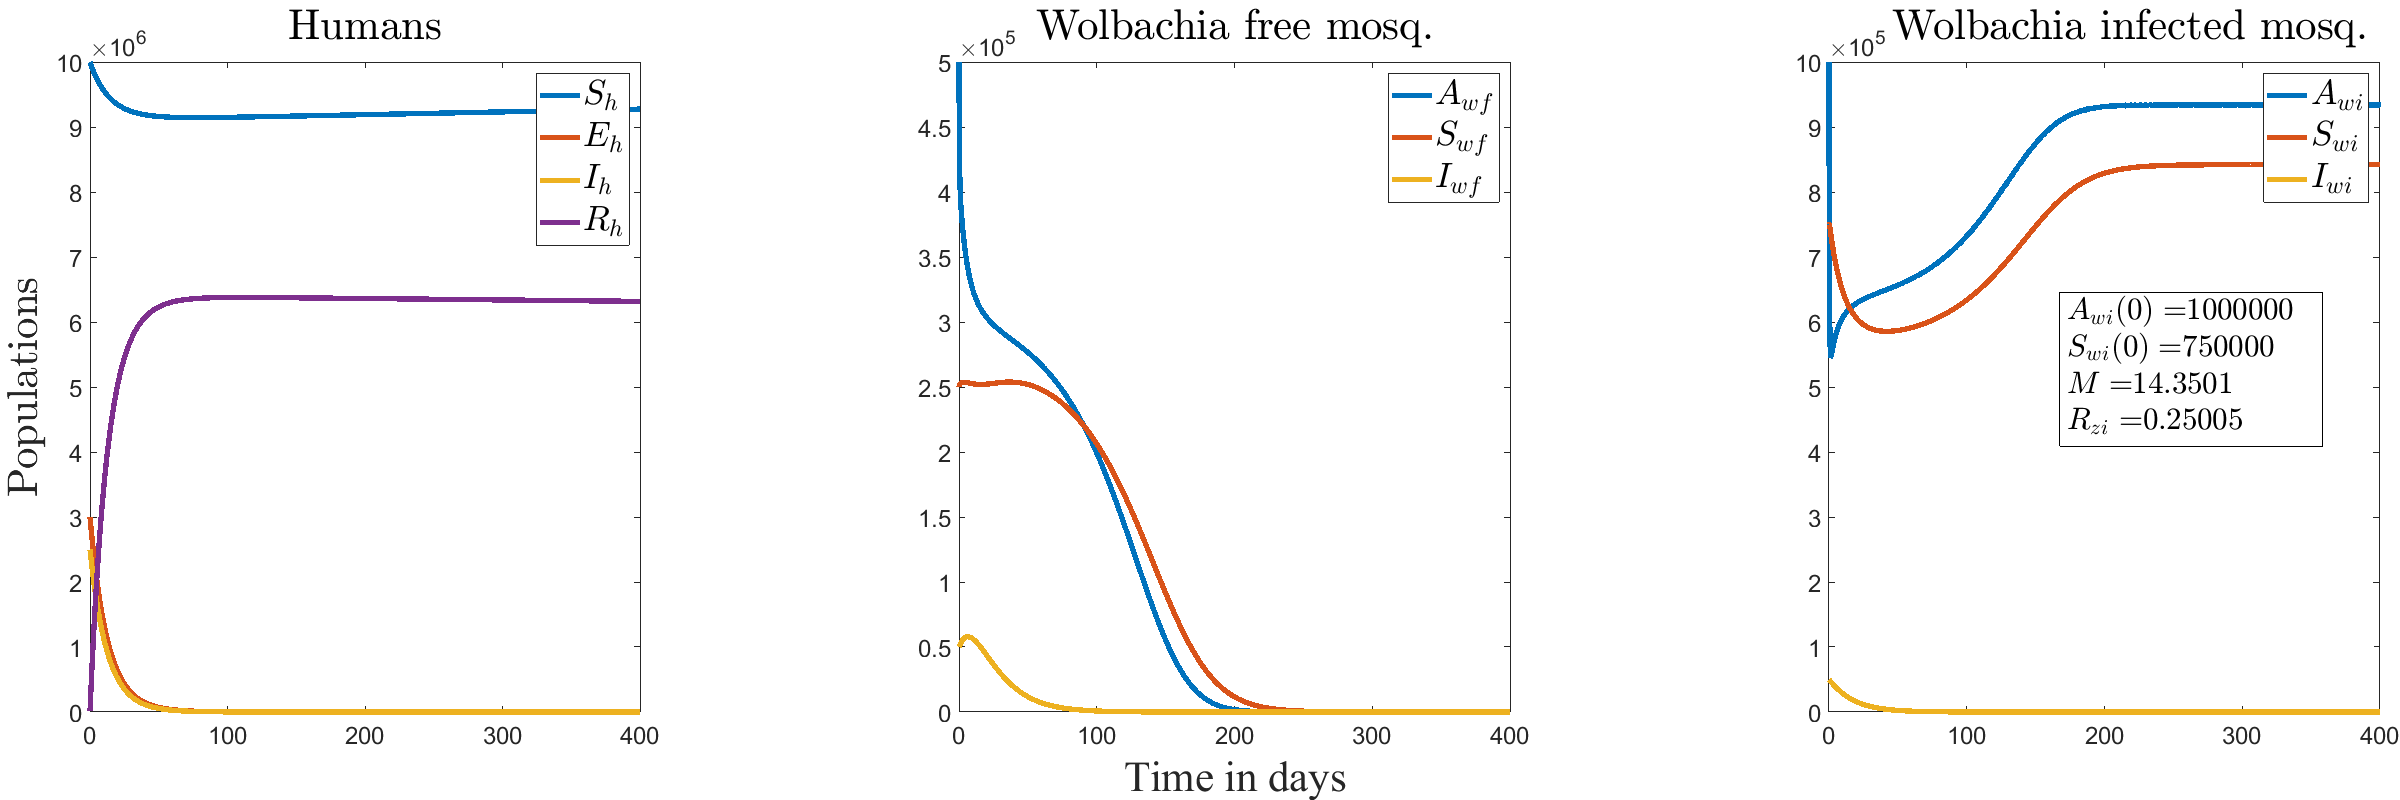
\includegraphics[width=16cm,height=4.5cm]{SimFig5.png}
%    \caption{Dominance of \textit{Wolbachia} infected mosquitoes when we start with more \textit{Wolbachia} infected aquatic stage and more females. Figure  obtained using baseline values for parameters from Table \ref{tab: param-table} and Table \ref{tab: param_mosq_table} and the initial conditions listed in Table \ref{init-cond-dis-free-table} with $A_{wi}(0)=1,000,000$ and $S_{wi}(0)=750,000$.}
%    \label{domwolbaqfem}
%\end{figure} 

\subsubsection{\textit{Wolbachia} is established when more \textit{Wolbachia} infected  aquatic stage and males are released simultaneously}\label{moreaqmale}

Similarly, a combination of aquatic stage mosquitoes and male mosquitoes works as well. If twice as many \textit{Wolbachia} infected aquatic stage is released and 4.4 as many times \textit{Wolbachia} infected males the same outcome is achieved. The \textit{Wolbachia} infected mosquito population establishes itself in 250 days in this case as seen in Figure \ref{domwolbaqmales}. Disease is again eradicated in approximately 230 days.
\begin{figure}[H]
    \centering
    % This file was created by matlab2tikz.
%
%The latest updates can be retrieved from
%  http://www.mathworks.com/matlabcentral/fileexchange/22022-matlab2tikz-matlab2tikz
%where you can also make suggestions and rate matlab2tikz.
%
\definecolor{mycolor1}{rgb}{0.00000,0.44700,0.74100}%
\definecolor{mycolor2}{rgb}{0.85000,0.32500,0.09800}%
\definecolor{mycolor3}{rgb}{0.92900,0.69400,0.12500}%
\definecolor{mycolor4}{rgb}{0.49400,0.18400,0.55600}%
%
\begin{tikzpicture}

\begin{axis}[%
width=1.1in,
height=1.5in,
at={(0in,0.108in)},
scale only axis,
xmin=0,
xmax=500,
ymin=0,
ymax=10000000,
axis background/.style={fill=white},
title style={font=\bfseries, yshift=1.75ex},
title={Humans},
ylabel={Population},
legend style={legend cell align=left, align=left, draw=white!15!black}
]
\addplot [color=mycolor1, line width=1.5pt]
  table[row sep=crcr]{%
0	10000000\\
0.754947032779455	9954090.65360747\\
1.57724191062152	9907002.45617775\\
2.40477236919105	9862485.53834427\\
3.1348997540772	9825448.07651117\\
3.79872075095773	9793489.05976349\\
4.7058820091188	9752296.5428109\\
5.39955880120397	9722617.77534601\\
6.18213821388781	9690912.02191071\\
7.0000037252903	9659671.25593504\\
7.85315533541143	9629017.3924995\\
8.5707955416292	9604669.8376514\\
9.44398874416947	9576707.34619677\\
10.1436470020562	9555543.62135863\\
11.0371231865138	9530024.90652505\\
11.8123948909342	9509172.45992929\\
12.661679636687	9487620.24358788\\
13.4651725329459	9468398.97910928\\
14.4549007862806	9446184.81031441\\
15.3662954401225	9427063.44575519\\
16.141609089449	9411739.72155039\\
16.8533100970089	9398392.27582034\\
17.6803352795541	9383698.88610156\\
18.6077930368483	9368204.7295907\\
19.3740346319973	9356141.67581409\\
20.140276229009	9344707.599087\\
20.8915218841285	9334075.23857766\\
21.7335675507784	9322800.52640181\\
22.7081454042345	9310549.02747569\\
23.474040215835	9301485.7644606\\
24.3464958481491	9291730.83922069\\
25.1210064291954	9283551.00771297\\
25.9760134946555	9275015.34364645\\
26.7417383976281	9267787.30573564\\
27.5074633024633	9260931.34574885\\
28.4683623872697	9252824.73556974\\
29.2985200230032	9246240.82986375\\
30.1502900272608	9239866.00618231\\
30.9170244187117	9234439.17237025\\
31.8187791034579	9228413.28156648\\
32.5954854898155	9223515.25179913\\
33.5195556432009	9218020.01709258\\
34.2876639012247	9213711.97940491\\
35.1393581181765	9209195.44007332\\
35.8715008199215	9205520.41360714\\
36.6650086641312	9201742.78560018\\
37.3827053755522	9198501.11618971\\
38.1992599032819	9195004.91659359\\
39.1060186792165	9191349.35030052\\
39.9422854986042	9188177.93791002\\
40.7045933715999	9185445.18952785\\
41.4746216293424	9182830.15987235\\
42.4142575412989	9179826.66517403\\
43.1917939446867	9177488.92742035\\
43.9202415663749	9175413.76811757\\
44.7588562741876	9173155.68298182\\
45.4871334061027	9171302.85943988\\
46.2799851726741	9169394.38267773\\
47.0304268356413	9167687.33010028\\
47.7808684967458	9166072.23971317\\
48.697255840525	9164218.42758878\\
49.477546453476	9162737.34654613\\
50.2089961655438	9161426.2257386\\
51.0591324772686	9159991.69961284\\
51.7888083159924	9158833.37041772\\
52.5506627038121	9157692.37486855\\
53.2119351029396	9156756.15854436\\
53.9628662485629	9155751.28547437\\
54.7273177951574	9154789.13922662\\
55.6105818115175	9153750.117933\\
56.3441882357001	9152943.48875553\\
57.0730349998921	9152190.30360834\\
57.7155932243913	9151564.43468463\\
58.4348146729171	9150904.48828197\\
59.2189430687577	9150231.71735178\\
59.9629164971411	9149636.4196801\\
60.7068899273872	9149081.09054138\\
61.3870805185288	9148606.8166203\\
62.1281031854451	9148124.90230791\\
62.8757078144699	9147673.85505106\\
63.5756442919374	9147282.16031346\\
64.3276816513389	9146892.82827434\\
65.0252345241606	9146559.6359517\\
65.6371713355184	9146288.56251178\\
66.3372871465981	9146001.78127981\\
67.0858920011669	9145721.57879058\\
67.5908279642463	9145547.41214455\\
68.2592225354165	9145334.53670933\\
68.8489863052964	9145162.83890796\\
69.3704978469759	9145023.16721983\\
69.921898169443	9144887.48951497\\
70.3331418335438	9144794.09092814\\
70.788028948009	9144698.31670709\\
71.2748060133308	9144604.36056521\\
71.7934730350971	9144513.67520714\\
72.2378523536026	9144443.49172574\\
72.6079439725727	9144390.19287186\\
72.9780355915427	9144341.4660042\\
73.3481272105128	9144297.21045039\\
73.7584810536355	9144253.24863911\\
74.2090971209109	9144211.01113623\\
74.6898369975388	9144172.73340318\\
74.9452688395977	9144155.17727704\\
75.200700679794	9144139.51380482\\
75.4561325218529	9144125.7142401\\
75.6881403606385	9144114.77171678\\
75.9201481994241	9144105.32269455\\
76.1521560400724	9144097.34658807\\
76.3841638788581	9144090.82309783\\
76.5714149121195	9144086.60370298\\
76.7586659453809	9144083.30711176\\
76.945916980505	9144080.92306001\\
77.1331680137664	9144079.44139883\\
77.3069101311266	9144078.8649574\\
77.4806522484869	9144079.04883879\\
77.6543943658471	9144079.98520264\\
77.8281364832073	9144081.66629067\\
78.03114185296	9144084.56369478\\
78.23414722085	9144088.4552389\\
78.43715258874	9144093.3289703\\
78.64015795663	9144099.17308207\\
78.8868226669729	9144107.5631144\\
79.1334873754531	9144117.34796422\\
79.380152085796	9144128.50731092\\
79.6268167961389	9144141.02113307\\
79.877909488976	9144155.13038568\\
80.3800948727876	9144187.41659278\\
80.8382919374853	9144221.49449844\\
81.2525006830692	9144255.99268638\\
81.8061946369708	9144307.43135203\\
82.3359318338335	9144362.17906057\\
82.8853746857494	9144424.49996066\\
83.5646166931838	9144509.0707902\\
84.0490626879036	9144574.30382407\\
84.5651266723871	9144648.15010751\\
85.1920709311962	9144743.71770167\\
85.9298954661936	9144864.11607343\\
86.7475433982909	9145007.13467591\\
87.4505055788904	9145137.8074195\\
88.2131851334125	9145287.29487487\\
89.1373799275607	9145478.70689029\\
90.0574438087642	9145679.88294374\\
90.9819744750857	9145892.14658231\\
91.8779147844762	9146107.01238501\\
92.8692544475198	9146354.71058467\\
93.988495958969	9146646.21980239\\
95.2515464704484	9146989.32443654\\
96.5192972160876	9147347.75127868\\
97.9150041360408	9147757.43450231\\
99.2419459149241	9148160.49740513\\
100.672364670783	9148608.6558644\\
102.218677259982	9149107.79805906\\
103.886957796291	9149661.94048941\\
105.565555540845	9150234.40817083\\
107.403190141544	9150876.61942386\\
109.4586159233	9151612.19453502\\
111.692154243588	9152429.86940406\\
114.050202773884	9153311.38895956\\
116.540829686448	9154260.25126149\\
119.321994872764	9155338.45060195\\
122.341512123123	9156528.06186915\\
125.696761805564	9157869.42162279\\
129.329994734377	9159341.00282715\\
133.498797537759	9161049.25538996\\
138.22350698337	9163005.36807555\\
143.763598579913	9165319.64406913\\
150.138145364821	9168002.4364682\\
158.089065646753	9171368.98677314\\
168.446653425694	9175775.38721725\\
183.772752154619	9182317.44163324\\
219.711047651246	9197684.7951394\\
261.496480360627	9215542.90104232\\
298.626366555691	9231390.97640585\\
335.481900801882	9247101.85034111\\
372.287905264646	9262771.5447275\\
408.979144986719	9278372.43511534\\
445.724448766559	9293976.38025688\\
482.406738694757	9309533.69538185\\
500	9316988.13104424\\
};
\addlegendentry{$S_h$}

\addplot [color=mycolor2, line width=1.5pt]
  table[row sep=crcr]{%
0	3000000\\
0.754947033245116	2826274.78755322\\
1.46375025250018	2672431.28225219\\
2.23515446158126	2514613.21449432\\
2.91362608876079	2383630.31970017\\
3.79872075095773	2223103.08224721\\
4.7058820091188	2069956.95653701\\
5.39955880166963	1960127.24999298\\
6.18213821388781	1843324.71096371\\
7.00000372575596	1728825.12826615\\
7.85315533587709	1617105.93123888\\
8.57079554209486	1528857.53033536\\
9.44398874416947	1428088.62102789\\
10.1436470025219	1352268.53015638\\
11.0371231865138	1261403.68277232\\
11.8123948913999	1187641.74649586\\
12.6616796357557	1111902.30109874\\
13.4651725324802	1044812.77408334\\
14.1249913685024	992838.853561489\\
14.9786386163905	929518.58156565\\
15.7539522647858	875613.295013627\\
16.5943737993948	820807.437079086\\
17.3711826940998	773295.495994419\\
18.298640451394	720265.36827276\\
19.1824742341414	673221.309930369\\
19.9487158297561	635009.262087467\\
20.6411066660658	602409.760188164\\
21.4377523274161	567034.984957067\\
22.3251979979686	530150.159679875\\
23.0910928095691	500318.161107259\\
23.8569876216352	472223.427600154\\
24.591249961406	446824.11718635\\
25.4060087846592	420293.561172157\\
26.1674447208643	396977.36193605\\
26.9331696243025	374882.617577041\\
27.7476880731992	352778.832353784\\
28.4683623872697	334352.61900559\\
29.2985200220719	314362.825369744\\
30.1502900277264	295142.654406457\\
30.917024419643	278888.406647841\\
31.5820887410082	265545.710568986\\
32.3254774771631	251416.594856037\\
33.1355015141889	236910.617736645\\
33.9036097717471	223961.335255614\\
34.671718029771	211749.616475167\\
35.3731781616807	201204.955714724\\
36.1360034355894	190358.524816745\\
36.9042409015819	180051.556340308\\
37.8143783756532	168591.767191169\\
38.5702801700681	159654.911532673\\
39.3150853845291	151333.328983299\\
40.1963881226256	142069.997474829\\
40.9586959970184	134536.668141199\\
41.732584446203	127315.933537334\\
42.6261126813479	119481.429489441\\
43.3687070077285	113355.340993771\\
44.1075523155741	107586.381959917\\
44.9908528793603	101091.297271532\\
45.7514173286036	95828.4701397726\\
46.6552060041577	89946.2094100513\\
47.4056476657279	85350.2994392589\\
48.2390621686354	80533.90577712\\
48.9573527118191	76611.8704906609\\
49.73764332477	72577.7483459124\\
50.4446725859307	69114.9424809525\\
51.2485242122784	65387.7813507142\\
52.1397006846964	61501.3705520653\\
52.9616247219965	58131.858901503\\
53.7125558662228	55222.7983450149\\
54.4725006124936	52434.14171826\\
55.4010995333083	49226.1584528382\\
56.1694801864214	46727.7498633014\\
57.0730350003578	43959.3016646723\\
57.9445158829913	41452.0546534541\\
58.6961908056401	39410.1897275988\\
59.590929783415	37116.6466370532\\
60.3349032122642	35316.4233353287\\
61.1603503217921	33425.9210799146\\
61.8709569512866	31883.5825066115\\
62.6423956542276	30293.5027966406\\
63.5756442928687	28480.4939184249\\
64.5020698695444	26793.0885079149\\
65.2292134617455	25542.2937545301\\
66.0892187086865	24141.6183968377\\
66.8334240205586	22994.5854212414\\
67.5908279647119	21885.7479127315\\
68.4671858311631	20672.3738932307\\
69.3704978469759	19495.2443892779\\
70.1056982777081	18589.0992981722\\
71.0154725038446	17528.4929552795\\
71.7934730341658	16671.797011503\\
72.6079439725727	15821.7620360451\\
73.5331730199978	14910.8933673934\\
74.4344051550142	14076.282636846\\
75.2007006807253	13405.0828031152\\
76.1521560391411	12617.9623540216\\
76.9459169795737	11998.2841556645\\
77.8281364841387	11346.6871343926\\
78.6401579561643	10779.5615212242\\
79.3801520862617	10288.486609159\\
80.1290021808818	9815.23925461527\\
81.0453963102773	9266.81488043629\\
81.9794894265942	8740.57258509938\\
82.8853746866807	8259.90047025261\\
83.7910306947306	7806.79499800457\\
84.5651266719215	7440.02282214584\\
85.5609831996262	6994.35552262142\\
86.2988077346236	6682.11642305739\\
87.1962790605612	6321.73288077442\\
87.9589586155489	6031.35102654248\\
88.9063312290236	5689.81362692034\\
89.8841517800465	5358.27662715921\\
90.7796471850015	5072.21153425658\\
91.6322719193995	4814.52898410987\\
92.6192274815403	4533.09306510072\\
93.5757042388432	4276.56664678361\\
94.5405792458914	4032.96376966638\\
95.4341863696463	3820.13792106649\\
96.2936794795096	3626.36842746753\\
97.0332547686994	3467.76132140914\\
97.9150041360408	3287.97461517015\\
98.834483675193	3110.70556956297\\
99.6890785815194	2954.77301103296\\
100.672364669852	2785.27566290973\\
101.61623748811	2631.97665076191\\
102.59090606356	2482.76249895291\\
103.483667606488	2353.71781854006\\
104.333313099109	2237.30054683983\\
105.316499629989	2109.93340694392\\
106.269332394004	1993.59045907855\\
107.230902589858	1882.83845256176\\
108.121557709761	1785.87907679146\\
108.977903274354	1697.4738210137\\
109.970495293848	1600.58579143742\\
110.959294611588	1509.68537998106\\
111.914843875915	1426.85278342664\\
112.835109009873	1351.46592284879\\
113.820950247813	1275.20804548962\\
114.694063018542	1211.34070891375\\
115.594283479266	1148.90108868713\\
116.540829685982	1086.77984253364\\
117.472526995931	1028.97261229903\\
118.459920867346	971.119754637592\\
119.321994872764	923.320278007537\\
120.212693300564	876.44365118118\\
121.161101039033	829.184192572255\\
122.086848103441	785.550102431327\\
123.033094192389	743.356735211797\\
123.944364336785	704.897068251856\\
124.751948299352	672.502868121024\\
125.69676180603	636.513847105671\\
126.654446940403	602.024729964323\\
127.663169226144	567.741295391694\\
128.531582495663	539.81326542329\\
129.329994734377	515.364233685192\\
130.298749556299	487.197392896749\\
131.284325291868	460.137395446189\\
132.268132513389	434.640050324611\\
133.138937599026	413.264132556506\\
133.943141047377	394.4667624617\\
134.893303528894	373.366316832136\\
135.760811148211	355.097025572788\\
136.665032764431	337.013080613222\\
137.50558052538	321.035935318097\\
138.472519638948	303.597780093085\\
139.399979689158	287.768427869305\\
140.356701462064	272.309607937466\\
141.232561197598	258.891098024324\\
142.066300079226	246.736245541368\\
143.030925670639	233.387398189865\\
143.96501956461	221.1532099545\\
144.90643295832	209.474981202278\\
145.777888633776	199.217342177872\\
146.615930198692	189.82899427833\\
147.587148472667	179.50281810388\\
148.552749681287	169.795118172653\\
149.485489924904	160.918082043994\\
150.384517920669	152.802569219843\\
151.347182316706	144.56687296927\\
152.378465614282	136.236926798709\\
153.240948831663	129.640762605704\\
154.189793955069	122.752925335895\\
155.138702993747	116.230975768063\\
156.103383520618	109.955963479355\\
157.064156827051	104.043229786213\\
157.913541991729	99.0813634647056\\
158.915327441413	93.5324001428671\\
159.873081226833	88.5179965323769\\
160.823876718059	83.8057455909438\\
161.742028865032	79.4932458824478\\
162.627685063519	75.5434856810607\\
163.575921247248	71.5315604708157\\
164.590273262002	67.4750195452943\\
165.60174529627	63.6585698062554\\
166.603254287504	60.0919057521969\\
167.540321953129	56.9354151440784\\
168.446653426159	54.039807156194\\
169.35746902274	51.2777333646081\\
170.371770019177	48.3670762516558\\
171.223373645917	46.0508011672646\\
172.193179325666	43.5472764461301\\
173.227259564679	41.0269488031045\\
174.202376691159	38.7835112214088\\
175.1268786937	36.7693894882686\\
176.011666251812	34.9393364959396\\
177.080977854319	32.848138295114\\
178.126537720207	30.9238262781873\\
179.000011855736	29.402458707802\\
179.925010343548	27.8723998232745\\
180.919862732757	26.3150190832093\\
181.89229399804	24.8763588811271\\
182.853048502933	23.5317460675724\\
183.772752155084	22.3122840104625\\
184.85110824788	20.9621735215187\\
185.971873841248	19.6448883581907\\
187.108488894068	18.3929068255238\\
188.119861702435	17.3456457429565\\
189.253424375318	16.2420502188616\\
190.433615210932	15.1670477711596\\
191.560567017179	14.2065120725892\\
192.686823613476	13.3068756759167\\
193.808000560384	12.4674433763139\\
195.084287915844	11.5756285637617\\
196.368478279561	10.7421518596821\\
197.662980537862	9.96221387106925\\
198.984110090882	9.22410988528281\\
200.361338548828	8.51233769068494\\
201.601757622324	7.91800692398101\\
202.921443887055	7.33079966111109\\
204.476798576303	6.69391521858051\\
205.912708983291	6.15475402353331\\
207.462062410079	5.62118532089517\\
209.112112402916	5.10327257821336\\
210.909303151537	4.59285714663565\\
212.748141644057	4.12296634959057\\
214.61637120042	3.69435868179426\\
216.588048648555	3.28984895721078\\
218.65857163677	2.91225930303335\\
220.779108651914	2.57006512535736\\
223.145794227254	2.23503651749343\\
225.718564775307	1.91980866575614\\
228.532220883295	1.62536060810089\\
231.411190074869	1.37043341109529\\
234.728389516007	1.12553791562095\\
238.271037948783	0.911812818143517\\
242.161094629671	0.723297165241092\\
246.711090783123	0.551384072285146\\
251.833796414081	0.40597946383059\\
257.898503185716	0.282350349705666\\
265.252340922598	0.181606793776155\\
274.53314184444	0.103917187545449\\
287.099834358785	0.0487040211446583\\
306.563170860521	0.0150094144046307\\
347.569384318311	0.00124668516218662\\
500	1.16415321826935e-07\\
};
\addlegendentry{$E_h$}

\addplot [color=mycolor3, line width=1.5pt]
  table[row sep=crcr]{%
0	2500000\\
0.754947033245116	2353496.93575622\\
1.46375025250018	2223904.65744691\\
2.23515446158126	2091095.6568671\\
2.91362608876079	1980964.22942168\\
3.79872075095773	1846102.29165225\\
4.7058820091188	1717548.96137361\\
5.39955880166963	1625418.04382318\\
6.18213821388781	1527493.01918575\\
7.00000372575596	1431552.95437616\\
7.85315533587709	1337994.16265013\\
8.57079554209486	1264127.30012471\\
9.44398874416947	1179820.68965124\\
10.1436470025219	1116416.5294926\\
11.0371231865138	1040466.387444\\
11.8123948913999	978841.837214354\\
12.6616796357557	915595.358966919\\
13.4651725324802	859599.764849605\\
14.1249913685024	816239.761462973\\
14.9786386163905	763439.056636495\\
15.7539522647858	718513.078544684\\
16.5943737993948	672861.472341136\\
17.3711826940998	633307.97002771\\
18.298640451394	589188.085401778\\
19.1824742341414	550075.575088948\\
19.9487158297561	518326.945386016\\
20.6411066660658	491257.904650793\\
21.4377523274161	461903.175746959\\
22.3251979979686	431318.336215968\\
23.0910928095691	406600.65957392\\
23.8569876216352	383339.536167868\\
24.591249961406	362325.755400425\\
25.4060087846592	340393.459773845\\
26.1674447208643	321134.485095737\\
26.9331696243025	302899.614700939\\
27.7476880731992	284673.457183341\\
28.4683623872697	269493.203828517\\
29.2985200220719	253039.944657943\\
30.1502900277264	237236.36273167\\
30.917024419643	223885.031202445\\
31.5820887410082	212935.332587554\\
32.3254774771631	201350.938894611\\
33.1355015141889	189469.900868575\\
33.9036097717471	178875.302214567\\
34.671718029771	168894.850142752\\
35.3731781616807	160285.864525842\\
36.1360034355894	151439.876803594\\
36.9042409015819	143043.327762625\\
37.8143783756532	133719.35574482\\
38.5702801700681	126457.358995311\\
39.3150853845291	119703.191673493\\
40.1963881226256	112194.262234944\\
40.9586959970184	106095.71225083\\
41.732584446203	100257.492464521\\
42.6261126813479	93931.6751399944\\
43.3687070077285	88992.0254999502\\
44.1075523155741	84346.1385991517\\
44.9908528793603	79122.6909183245\\
45.7514173286036	74896.2366397753\\
46.6552060041577	70179.1526781083\\
47.4056476657279	66498.9769688994\\
48.2390621686354	62647.6559628649\\
48.9573527118191	59515.8419098784\\
49.73764332477	56298.8670598986\\
50.4446725859307	53541.2093131035\\
51.2485242122784	50577.115194195\\
52.1397006846964	47491.1800991027\\
52.9616247219965	44819.9177449839\\
53.7125558662228	42517.0622949731\\
54.4725006124936	40312.6337896376\\
55.4010995333083	37780.7352600954\\
56.1694801864214	35812.024489596\\
56.888322094921	34067.6345739537\\
57.7155932239257	32169.9928189246\\
58.4348146738485	30610.4102349612\\
59.2189430687577	29000.2099364907\\
59.9629164980724	27554.5938711348\\
60.7068899269216	26184.4954708344\\
61.6138107166626	24610.4913067189\\
62.3852494196035	23349.8921612115\\
63.1090199733153	22228.7864803341\\
63.9516629721038	20994.4251361848\\
64.8508463064209	19756.3381093089\\
65.6371713350527	18736.5056046597\\
66.3372871461324	17875.0053850762\\
67.0858920020983	16999.7155344435\\
67.8432959462516	16159.8359147571\\
68.6751491259784	15287.4073189497\\
69.5542979543097	14418.9352109381\\
70.3331418340094	13692.8107955069\\
71.2748060142621	12865.8306676559\\
72.2378523536026	12074.1106832433\\
73.1630814010277	11361.5352225746\\
73.9837890877388	10766.3710766761\\
74.6898369970731	10280.5302800448\\
75.4561325223185	9779.15786364907\\
76.3841638783924	9206.07858315203\\
77.3069101311266	8671.07015125779\\
78.2341472203843	8166.18036077032\\
79.1334873763844	7705.83609448373\\
79.8779094885103	7345.36353032291\\
80.838291937951	6906.20383855049\\
81.6328998454846	6563.63928850321\\
82.5190794519149	6202.46822092682\\
83.3382026907057	5887.08818184491\\
84.0490626869723	5626.97767280973\\
85.0076147979125	5295.10030384222\\
85.9298954671249	4995.04082263913\\
86.7475433973595	4743.86264578206\\
87.7047320972197	4466.47116978699\\
88.6752825304866	4202.42793564452\\
89.5107658538036	3988.16648444999\\
90.4040278666653	3771.63132839277\\
91.1843017642386	3592.50401203707\\
92.1235576504841	3388.55752936471\\
92.8692544475198	3235.23218483105\\
93.7821000986733	3057.30317152385\\
94.7134229596704	2886.22373876674\\
95.6168262683786	2729.75645634718\\
96.5192972165532	2582.22206654865\\
97.2902335445397	2462.74645163957\\
98.2827959517017	2317.30803026864\\
99.2419459158555	2185.20751907397\\
100.165884832852	2065.31995672826\\
101.155815555248	1944.39672305109\\
102.032562857028	1843.41526017711\\
102.936464287341	1744.96735660685\\
103.886957797222	1647.28611775395\\
104.822733512148	1556.62283222238\\
105.814611452166	1466.12701494014\\
106.680662455969	1391.5501630418\\
107.575477692764	1318.59268165939\\
108.528357346542	1245.2190846242\\
109.458615923766	1177.63559072837\\
110.409649887122	1112.43442587601\\
111.325724427588	1053.13510476798\\
112.137533508241	1003.30046038376\\
113.087305247318	948.056833115406\\
114.050202773418	895.229928154964\\
114.879418211523	852.158982946537\\
115.766360919923	808.434280520771\\
116.74162679445	762.999556540046\\
117.71616039658	720.206040467136\\
118.707841023803	679.175588833168\\
119.698207942303	640.581241620705\\
120.57504999591	608.282924909145\\
121.384795387276	579.933311835863\\
122.341512123588	548.168993356172\\
123.215348221362	520.70789178228\\
124.126618365757	493.561576125212\\
124.973486251663	469.626822256483\\
125.947630607057	443.551614852622\\
126.882420706563	419.914926615078\\
127.847427477129	396.856184389442\\
128.731185555458	376.868946204428\\
129.572183439508	358.798646605574\\
130.545143490192	338.987149424851\\
131.487698335201	320.853440156206\\
132.438447562046	303.558184747584\\
133.318867568858	288.38590547815\\
134.165312801953	274.523813752457\\
135.146213015541	259.301422141492\\
136.122499794699	244.998804907314\\
137.065778233577	231.938152818475\\
137.97449432686	220.022181981709\\
138.947681426071	207.945985249709\\
139.808771980926	197.820267870091\\
140.695697143674	187.910976251122\\
141.628297943622	178.031243325677\\
142.546567604411	168.815494075883\\
143.519374276977	159.57663592929\\
144.367861532606	151.935582558624\\
145.243583399802	144.435686540324\\
146.175970318727	136.859925168101\\
147.086322916672	129.849366501905\\
148.016358358786	123.060332154389\\
148.910343896598	116.871308805887\\
149.703041738365	111.645861987956\\
150.630890476983	105.827119548339\\
151.5707290438	100.24383127084\\
152.55878717266	94.6928896955214\\
153.408228864893	90.168124825228\\
154.427021214738	85.0266330833547\\
155.379873125348	80.4845210453495\\
156.302048692945	76.3205618639477\\
157.230269445572	72.3474547695369\\
158.089065646753	68.8564272052608\\
158.915327441413	65.6571100652218\\
159.873081226833	62.1345626255497\\
160.823876718059	58.8248628429137\\
161.742028865032	55.7964323447086\\
162.627685063519	53.0231510382146\\
163.575921247248	50.2066268837079\\
164.590273262002	47.3591922842897\\
165.60174529627	44.6806589136831\\
166.603254287504	42.1777551998384\\
167.540321953129	39.9629425890744\\
168.446653426159	37.9313858766109\\
169.35746902274	35.9936914923601\\
170.371770019177	33.9519379087724\\
171.223373645917	32.3272524750791\\
172.193179325666	30.5713424934074\\
173.227259564679	28.8037609178573\\
174.202376691159	27.23045793036\\
175.1268786937	25.8180344514549\\
176.227222019341	24.2318469588645\\
177.241572351195	22.8558004535735\\
178.314463178627	21.484976655338\\
179.460688835941	20.1108196997084\\
180.538516914938	18.8986151227728\\
181.55601802608	17.8210888747126\\
182.644888991956	16.7356286351569\\
183.772752155084	15.6806176062673\\
184.85110824788	14.7338505969383\\
185.971873841248	13.8100594924763\\
187.108488894068	12.9320144467056\\
188.288913339842	12.0788333471864\\
189.436848279089	11.3028313722461\\
190.65686282143	10.5323404544033\\
191.973477664869	9.75928680039942\\
193.31602667924	9.02902324451134\\
194.620866687968	8.37131766648963\\
196.040170625318	7.70982051733881\\
197.462470343802	7.09898845525458\\
198.984110090882	6.49858705559745\\
200.514197021723	5.94566745590419\\
202.038087341003	5.44139651581645\\
203.688825545833	4.94292076025158\\
205.515291199088	4.44400630053133\\
207.301425494719	4.0044636875391\\
209.112112402916	3.60287783388048\\
211.232759385835	3.18304470926523\\
213.389648004435	2.80578381381929\\
215.725797113031	2.44703820394352\\
218.184633968398	2.1184897669591\\
220.779108651914	1.81914786435664\\
223.702174193226	1.53186383470893\\
226.792923060246	1.27691971417516\\
230.191785742994	1.04490702692419\\
233.969639660791	0.835799986030906\\
238.080303875264	0.655203185044229\\
242.764089184813	0.496197479311377\\
248.292301756795	0.357139110099524\\
254.751102355309	0.242971684783697\\
262.675032263622	0.151272557675838\\
272.932298330124	0.0817618030123413\\
287.437493221369	0.0341494050808251\\
311.598293326329	0.00793114164844155\\
376.737158735748	0.000151996500790119\\
500	8.38190317153931e-08\\
};
\addlegendentry{$I_h$}

\addplot [color=mycolor4, line width=1.5pt]
  table[row sep=crcr]{%
0	10000\\
0.754947032779455	376294.846968076\\
1.46375025250018	700640.999937531\\
2.23515446204692	1033371.68991537\\
2.91362608876079	1309553.21462139\\
3.79872075095773	1648096.63909736\\
4.7058820091188	1971177.51032909\\
5.39955880120397	2202961.34226484\\
6.18213821388781	2449557.60724876\\
7.0000037252903	2691408.31111087\\
7.85315533634275	2927517.79554978\\
8.5707955416292	3114130.02755594\\
9.44398874416947	3327349.83385186\\
10.1436470020562	3487883.47157042\\
11.0371231865138	3680403.18348873\\
11.8123948918656	3836803.51125198\\
12.6616796357557	3997518.44880695\\
13.4651725329459	4139992.09458671\\
14.1249913685024	4250445.68593427\\
14.9786386163905	4385114.97565592\\
15.7539522647858	4499856.95271063\\
16.5943737998605	4616614.87923582\\
17.3711826940998	4717921.42493162\\
18.298640451394	4831098.29810901\\
19.1824742341414	4931599.63809074\\
19.9487158292904	5013307.85062786\\
20.6411066660658	5083071.83331272\\
21.4377523269504	5158838.45704708\\
22.3251979984343	5237914.71355876\\
23.0910928100348	5301930.98252262\\
23.8569876216352	5362272.07483354\\
24.591249961406	5416870.92591229\\
25.4060087846592	5473952.14734189\\
26.1674447208643	5524162.97765177\\
26.9331696247682	5571785.06104001\\
27.7476880736649	5619469.62972251\\
28.4683623872697	5659255.35517163\\
29.2985200220719	5702455.02952784\\
30.1502900272608	5744030.81325525\\
30.917024419643	5779222.73772277\\
31.5820887414739	5808133.82171845\\
32.3254774771631	5838772.54962459\\
33.1355015141889	5870254.96503039\\
33.9036097722128	5898382.61043907\\
34.6717180293053	5924929.62208108\\
35.3731781616807	5947870.08031226\\
36.1360034355894	5971484.60130571\\
36.9042409015819	5993941.71926232\\
37.8143783761188	6018930.92992024\\
38.5702801700681	6038433.96783096\\
39.3150853840634	6056606.73124815\\
40.1963881226256	6076850.57029395\\
40.9586959965527	6093325.18665249\\
41.7325844466686	6109126.00828667\\
42.6261126808822	6126280.88904619\\
43.3687070077285	6139702.90156409\\
44.1075523160398	6152348.82199561\\
44.9908528793603	6166593.72832667\\
45.7514173286036	6178141.56427228\\
46.6552060041577	6191054.13505649\\
47.4056476661935	6201146.76925341\\
48.2390621686354	6211726.85378977\\
48.9573527118191	6220344.49028688\\
49.73764332477	6229210.09241159\\
50.444672585465	6236821.17534363\\
51.2485242122784	6245013.94765514\\
52.1397006846964	6253556.90456891\\
52.9616247219965	6260963.14011418\\
53.7125558666885	6267356.40256232\\
54.4725006129593	6273483.7650375\\
55.401099533774	6280530.18031104\\
56.1694801868871	6286015.62981267\\
57.0730349998921	6292090.72377915\\
57.9445158829913	6297588.83515455\\
58.6961908051744	6302063.05500002\\
59.5909297838807	6307084.31471528\\
60.3349032122642	6311021.56611122\\
61.1603503217921	6315151.73190888\\
61.870956950821	6318517.21794112\\
62.6423956537619	6321982.41482878\\
63.5756442928687	6325926.94535045\\
64.3276816513389	6328919.57923906\\
65.2292134612799	6332301.37378887\\
66.0892187086865	6335330.37979086\\
66.8334240205586	6337805.18288324\\
67.5908279651776	6340191.99497371\\
68.4671858306974	6342796.63802885\\
69.3704978469759	6345315.2216975\\
70.1056982772425	6347247.65923745\\
71.0154725043103	6349501.46448195\\
71.7934730341658	6351314.7726743\\
72.6079439725727	6353106.75994836\\
73.3481272105128	6354645.90622767\\
74.2090971218422	6356334.90583763\\
74.9452688386664	6357697.17986603\\
75.6881403615698	6358999.30139861\\
76.5714149121195	6360457.64870542\\
77.3069101311266	6361601.39575217\\
78.0311418520287	6362668.17809933\\
78.8868226660416	6363856.43403331\\
79.6268167961389	6364824.23306471\\
80.3800948737189	6365755.36458477\\
81.2525006821379	6366769.13077353\\
81.9794894270599	6367563.65475221\\
82.702227069065	6368310.52793823\\
83.5646166922525	6369148.42008332\\
84.3070946792141	6369825.68731466\\
85.1920709321275	6370582.46817536\\
85.9298954671249	6371173.59012138\\
86.7475433973595	6371788.57631731\\
87.4505055788904	6372285.2401526\\
88.2131851343438	6372792.20294825\\
88.9063312290236	6373225.48097129\\
89.6974588166922	6373689.57329679\\
90.4040278671309	6374077.91156186\\
91.184301763773	6374479.47227979\\
91.8779147844762	6374813.49744388\\
92.619227482006	6375147.74261554\\
93.3693083785474	6375463.11511003\\
93.988495958969	6375706.92130127\\
94.7134229596704	6375974.19755997\\
95.4341863691807	6376221.35257097\\
96.0680617420003	6376424.0626971\\
96.7762759923935	6376635.02685558\\
97.5472123203799	6376846.8737091\\
98.2827959517017	6377032.50128472\\
98.8344836747274	6377161.59677613\\
99.4655122486874	6377299.04065151\\
100.165884832852	6377439.31945928\\
100.672364669852	6377533.02653577\\
101.386026521213	6377654.48059288\\
102.032562856562	6377754.23132096\\
102.590906064026	6377832.82174024\\
103.109243399464	6377899.73704949\\
103.685312701389	6377967.50930754\\
104.088602892123	6378010.94975634\\
104.578023306094	6378059.37100413\\
105.067443719134	6378103.21451278\\
105.565555540845	6378143.27836428\\
106.063667363487	6378178.883515\\
106.474997425452	6378205.02107199\\
106.886327487417	6378228.28544844\\
107.230902589858	6378245.61545882\\
107.575477692299	6378261.02162449\\
107.939531037584	6378275.25360694\\
108.303584381938	6378287.43031342\\
108.528357346542	6378293.94219122\\
108.753130310215	6378299.69862881\\
108.977903274819	6378304.71004505\\
109.202676238492	6378308.98671168\\
109.4586159233	6378312.97463509\\
109.71455560904	6378316.03776069\\
109.970495293848	6378318.1905655\\
110.226434979588	6378319.44729513\\
110.409649887122	6378319.80440502\\
110.592864795588	6378319.71457992\\
110.776079703122	6378319.18282917\\
110.959294611588	6378318.21410453\\
111.142509519123	6378316.81330024\\
111.325724427588	6378314.98525274\\
111.508939336054	6378312.73474279\\
111.692154243588	6378310.0664963\\
111.914843875915	6378306.26765927\\
112.137533508241	6378301.86686242\\
112.360223140568	6378296.87226844\\
112.582912772894	6378291.29192689\\
112.835109010339	6378284.27487935\\
113.339501484297	6378268.06277503\\
113.820950247347	6378249.94669821\\
114.279455299489	6378230.36504789\\
114.694063019007	6378210.75516993\\
115.250128597952	6378181.69848332\\
115.766360919923	6378151.98061693\\
116.340032577515	6378115.96004204\\
116.985260195099	6378071.80796697\\
117.716160396114	6378017.32002417\\
118.459920867346	6377957.19980718\\
119.1172769228	6377900.30465651\\
119.869703061879	6377831.03543164\\
120.575049995445	6377762.24932945\\
121.384795387276	6377678.89202243\\
122.341512123123	6377574.64993272\\
123.215348221362	6377474.27177029\\
124.126618365757	6377364.62000947\\
125.19502420444	6377229.95173983\\
126.198499408551	6377097.80994465\\
127.294652723707	6376947.58382927\\
128.531582496129	6376771.16434098\\
129.814372145571	6376581.01043917\\
131.037931358442	6376393.29960184\\
132.438447562046	6376171.41160216\\
133.943141047843	6375925.31086693\\
135.579966824502	6375649.30851743\\
137.285679379478	6375353.33366509\\
139.173830557615	6375016.7261239\\
141.034692824818	6374676.69083573\\
143.030925670639	6374303.74011134\\
145.243583399802	6373881.56743983\\
147.587148472667	6373425.54948182\\
150.138145364821	6372920.13801544\\
153.073668798432	6372328.53641036\\
156.103383520618	6371708.43351234\\
159.626134202816	6370977.30358501\\
163.575921246782	6370146.98787225\\
168.014527174644	6369203.33891849\\
173.054912858643	6368121.2904358\\
179.000011855736	6366834.42201072\\
186.177227430046	6365270.12208622\\
195.315998530015	6363267.32718283\\
207.783336240798	6360523.92813238\\
228.532220883295	6355946.45519062\\
293.823784547858	6341538.21265554\\
330.855018079281	6333378.76967891\\
367.603896671906	6325291.85866294\\
404.270489510149	6317233.34019364\\
441.007009996101	6309169.74851251\\
477.827793250792	6301097.98939918\\
500	6296242.43654233\\
};
\addlegendentry{$R_h$}

\end{axis}

\begin{axis}[%
width=1.1in,
height=1.5in,
at={(1.35in,0.108in)},
scale only axis,
xmin=0,
xmax=500,
ymin=0,
ymax=500000,
xlabel={Time (days)},
axis background/.style={fill=white},
title style={font=\bfseries, yshift=1.25ex},
title={\emph{Wolb.}-free mosq.},
legend style={legend cell align=left, align=left, draw=white!15!black}
]
\addplot [color=mycolor1, line width=1.5pt]
  table[row sep=crcr]{%
0	500000\\
0.124589653627481	470611.192853151\\
0.308237547695171	440545.290696195\\
0.491885441762861	421196.354217561\\
0.667259835987352	408804.585050426\\
0.842634230211843	400289.209608396\\
1.03970058343839	393516.665839275\\
1.23676693672314	388640.706959287\\
1.46375025232555	384340.747797171\\
1.69073356798617	380934.410101097\\
1.96294401481282	377458.377125721\\
2.40477236837614	372666.105655057\\
2.91362608876079	367837.626754499\\
3.35617341974284	364006.678684091\\
3.7987207507831	360494.657913213\\
4.4034949230263	356064.553033716\\
5.0082690952695	352089.093653265\\
5.39955880155321	349616.858548384\\
5.79084850783693	347348.266489986\\
7.00000372563954	341269.121586636\\
7.85315533605171	337528.904803329\\
8.57079554203665	334701.044628103\\
9.15292434353614	332623.235750504\\
9.44398874428589	331648.855159924\\
9.79381787328748	330397.635883205\\
10.1436470023473	329281.582617888\\
10.8433052604087	327500.615578876\\
11.2309411128517	326323.790043431\\
12.2000307439594	323900.210651381\\
12.9295106013888	322231.462481158\\
13.4651725325966	321136.607116461\\
13.7950819504331	320383.807835905\\
14.1249913683278	319724.294819357\\
14.4549007862224	319249.060364201\\
14.7848102040589	318728.800245258\\
15.1724670284311	317952.498807272\\
15.7539522649022	317015.845449975\\
16.1416090892162	316409.782884136\\
17.1122463958454	315004.955889073\\
17.3711826940416	314666.56397728\\
17.6803352798452	314166.80548351\\
17.9894878656487	313746.207409825\\
18.2986404514522	313492.357140976\\
18.6077930372558	313188.578020856\\
18.7993534361594	312889.591273656\\
18.9909138350631	312634.250700945\\
19.3740346329287	312244.988286879\\
19.757155430736	311792.880333324\\
20.8915218849434	310653.098895765\\
21.1419371037045	310429.27224643\\
21.4377523272997	310069.41731915\\
21.7335675508366	309778.258737969\\
22.0293827744317	309636.146694985\\
22.3251979979686	309445.904051991\\
22.516671700927	309213.870294411\\
22.7081454038271	309023.071683269\\
23.0910928097437	308758.403558768\\
23.4740402156021	308419.627527806\\
23.8569876214606	308145.581841824\\
24.3464958479162	307753.813696086\\
24.8360040744301	307446.812935256\\
25.1210064295447	307169.01702726\\
25.4060087847174	306953.828798084\\
25.6910111398902	306876.645681816\\
25.9760134950629	306753.346871004\\
26.1674447208643	306562.606291504\\
26.3588759467239	306411.705639508\\
26.741738398443	306224.626823385\\
27.1246008501621	305955.273633953\\
27.5074633018812	305751.379078515\\
27.7476880732575	305588.655724932\\
27.9879128446337	305444.594952258\\
28.4683623873862	305221.323061306\\
28.7450815989869	304993.681168056\\
29.0218008106458	304824.220082083\\
29.2985200222465	304783.995108299\\
29.5752392339054	304699.952675852\\
29.7669228318264	304535.291844724\\
29.9586064297473	304409.410172227\\
30.3419736256474	304270.873038825\\
30.5336572235683	304148.809257404\\
30.7253408214892	304043.847903869\\
31.1087080173893	303883.941441493\\
31.3453983792569	303746.756853042\\
31.5820887411246	303628.245727533\\
31.8187791030505	303546.793534691\\
32.0554694649181	303456.536301636\\
32.3254774771631	303259.874038438\\
32.5954854894662	303118.17456095\\
32.8654935017112	303098.921628915\\
33.1355015139561	303037.994247186\\
33.3275285784621	302889.598886521\\
33.5195556429098	302779.203493306\\
33.7115827073576	302728.354998239\\
33.9036097718053	302670.692334621\\
34.0956368363113	302560.996272337\\
34.2876639007591	302468.780816237\\
34.6717180297128	302336.061197073\\
34.9055380737409	302213.762687796\\
35.139358117769	302110.358079244\\
35.3731781617971	302044.913695166\\
35.6069982058834	301969.856543357\\
35.87150082062	301792.222061038\\
36.1360034354148	301667.055195835\\
36.4005060502095	301658.7912257\\
36.6650086650043	301610.817992828\\
36.9042409018148	301372.307855186\\
37.1434731386253	301231.946300223\\
37.3827053754358	301297.290267103\\
37.6219376122463	301303.153600147\\
37.8143783758278	301118.170248743\\
38.0068191394093	300997.841170734\\
38.1992599029909	300981.09802374\\
38.3917006665142	300950.629590858\\
38.5702801698353	300840.578646501\\
38.7488596731564	300754.487180346\\
39.1060186797986	300648.252792166\\
39.3150853842963	300548.756712459\\
39.5241520887939	300463.826886671\\
39.9422854977893	300341.415325932\\
40.1963881225674	300207.720449768\\
40.4504907473456	300103.53406723\\
40.7045933720656	300064.093706679\\
40.9586959968437	300003.607645561\\
41.2166588132968	299791.255484928\\
41.4746216298081	299662.867282398\\
41.7325844462612	299721.307735871\\
41.9905472627725	299716.603041331\\
42.2024024022976	299494.179184036\\
42.4142575417645	299362.789742805\\
42.6261126812897	299400.808835941\\
42.8379678207566	299402.016142773\\
43.0148808830418	299266.175549113\\
43.1917939452687	299169.724518301\\
43.5456200697809	299084.853419759\\
43.732930818398	298991.218962463\\
43.9202415670734	298913.293497941\\
44.2948630644241	298803.471501929\\
44.5268596693641	298695.849943953\\
44.758856274304	298605.477207057\\
44.9908528792439	298550.739991873\\
45.2228494841838	298485.968943181\\
45.4871334063937	298317.078249624\\
45.7514173285454	298201.711466607\\
46.0157012507552	298207.538757984\\
46.2799851729651	298170.186229371\\
46.4675955884741	298038.050974481\\
46.6552060039248	297943.002826997\\
46.8428164194338	297906.244713517\\
47.0304268349428	297862.208967428\\
47.2180372504517	297766.368122924\\
47.4056476659025	297687.019331068\\
47.7808684969204	297576.953862461\\
48.0099653328652	297468.356423242\\
48.2390621688101	297377.223284786\\
48.4681590047549	297322.025323368\\
48.6972558407579	297256.731500923\\
48.9573527118191	297091.210602362\\
49.2174495828804	296975.917169732\\
49.4775464539416	296973.890303514\\
49.7376433250029	296932.032167994\\
49.9733197452733	296700.994677444\\
50.208996165602	296566.260638833\\
50.4446725858725	296634.58432353\\
50.6803490062011	296643.006082089\\
50.8697407415602	296461.13163289\\
51.0591324769775	296343.021813841\\
51.2485242123366	296327.401052679\\
51.4379159476957	296297.664776125\\
51.6133621319314	296188.690135062\\
51.788808316167	296103.01819856\\
52.1397006846382	295995.589517517\\
52.3451816939632	295895.562903452\\
52.5506627032883	295809.293633138\\
52.9616247218801	295681.631580598\\
53.2119351033471	295545.373946737\\
53.462245484814	295437.116614838\\
53.712555866281	295391.062226527\\
53.962866247748	295323.989418552\\
54.2176834302372	295107.643048183\\
54.4725006127264	294972.816447704\\
54.7273177952156	295020.294560738\\
54.9821349777048	295005.230591433\\
55.191617255623	294777.34516429\\
55.4010995335411	294638.948709001\\
55.6105818114593	294667.78105834\\
55.8200640893774	294659.602287388\\
55.9947721380158	294517.039893999\\
56.169480186596	294413.225691185\\
56.5188962838147	294311.789965716\\
56.7036091893096	294209.710998098\\
56.8883220948046	294122.809922051\\
57.2577479057945	293993.372480744\\
57.4866705648019	293874.040248679\\
57.7155932238675	293771.082672769\\
57.944515882933	293702.330624159\\
58.1734385419986	293623.485790746\\
58.434814673732	293440.639202618\\
58.6961908054654	293309.24976937\\
58.9575669372571	293295.003146277\\
59.2189430689905	293238.376574495\\
59.4049364262028	293094.82518126\\
59.590929783415	292987.298570892\\
59.7769231406855	292936.693957729\\
59.9629164978978	292878.621447303\\
60.1489098551101	292769.300542314\\
60.3349032123224	292676.0199204\\
60.706889926747	292536.830436273\\
60.9336201242986	292410.658559026\\
61.1603503217921	292301.38342771\\
61.3870805193437	292227.199563178\\
61.6138107168372	292142.763589805\\
61.8709569511702	291957.33402604\\
62.1281031855033	291820.42596411\\
62.3852494197781	291793.323827068\\
62.6423956541112	291727.200581032\\
62.8757078137714	291479.68619431\\
63.1090199734899	291324.968879352\\
63.3423321331502	291366.055380088\\
63.5756442928105	291349.110289045\\
63.763653632428	291152.450800463\\
63.9516629720456	291017.465438687\\
64.1396723116632	290981.909035325\\
64.3276816512807	290932.319408242\\
64.5020698696608	290806.61440886\\
64.676458088099	290703.569936279\\
65.0252345249173	290559.745058578\\
65.4331923982245	290330.927611885\\
65.8411502715317	290159.020611115\\
66.0892187088029	289996.634990028\\
66.337287146016	289861.350817962\\
66.5853555832873	289786.614101351\\
66.8334240205586	289691.035473984\\
67.0858920019818	289449.691674444\\
67.3383599834633	289286.925952115\\
67.5908279648866	289300.090070821\\
67.843295946368	289252.640586792\\
68.0512592412415	289004.94809911\\
68.2592225361732	288843.457606468\\
68.4671858311049	288843.173452917\\
68.6751491260366	288806.961115571\\
68.8489863062277	288645.042106324\\
69.0228234864189	288520.610383701\\
69.3704978468013	288374.640561582\\
69.7380980621092	288139.534520427\\
70.1056982774753	287962.161995285\\
70.3331418341259	287813.630338859\\
70.5605853907182	287680.922352428\\
71.0154725040193	287471.994725557\\
71.2748060140875	287256.352563035\\
71.5341395241558	287090.40160399\\
71.7934730342822	287037.888929491\\
72.0528065443505	286943.991044941\\
72.2378523538355	286776.254509944\\
72.4228981632623	286643.444056838\\
72.7929897822323	286481.01795035\\
73.1630814011442	286226.146540743\\
73.5331730201142	286032.640137161\\
73.9837890876806	285731.868000963\\
74.4344051552471	285505.002949243\\
74.6898369970149	285283.441990661\\
74.9452688387828	285108.480411667\\
75.2007006806089	285039.290875861\\
75.4561325223767	284932.152120072\\
75.688140361337	284653.624099428\\
75.9201482002973	284464.277044848\\
76.1521560392575	284463.29732718\\
76.3841638782178	284406.182284594\\
76.5714149120613	284183.178434672\\
76.7586659459048	284019.647750032\\
76.9459169797483	283952.230282088\\
77.1331680135918	283870.959624416\\
77.3069101312431	283718.005471418\\
77.4806522488943	283586.94035166\\
77.8281364841387	283384.983299418\\
78.2341472202097	283089.135740174\\
78.6401579562225	282847.886413276\\
78.8868226662744	282644.823646033\\
79.133487376268	282467.692056529\\
79.3801520862617	282348.817747083\\
79.6268167963135	282209.511948245\\
79.877909488685	281928.6278459\\
80.1290021810564	281722.98879059\\
80.3800948734279	281686.09189173\\
80.6311875657993	281590.702779083\\
80.8382919380674	281311.134223902\\
81.0453963103355	281114.261503732\\
81.2525006825454	281072.235958758\\
81.4596050548134	280995.391820398\\
81.6328998454846	280804.020982499\\
81.8061946360976	280648.703614175\\
82.1527842173818	280437.085847282\\
82.5190794520313	280134.387136111\\
82.8853746866807	279886.973150081\\
83.3382026906474	279520.302110773\\
83.7910306946724	279222.51079299\\
84.0490626870305	278959.411678951\\
84.3070946793887	278743.712925809\\
84.5651266717468	278636.602593935\\
84.823158664105	278489.440806298\\
85.0076147979125	278287.087628062\\
85.1920709317783	278118.182691628\\
85.5609831993934	277879.234817516\\
85.9298954670667	277550.298117419\\
86.29880773474	277279.92560154\\
86.7475433975924	276887.100885215\\
87.1962790604448	276564.437205421\\
87.4505055788904	276291.922587792\\
87.7047320973361	276063.690094835\\
87.9589586157817	275936.352841282\\
88.2131851342274	275772.366890207\\
88.4442338324734	275449.860921389\\
88.6752825307194	275212.170095793\\
88.9063312289654	275153.837090363\\
89.1373799272114	275041.691480365\\
89.3240728904493	274781.885913117\\
89.5107658536872	274578.731783369\\
89.8841517801629	274342.372191781\\
90.2307358378312	273982.280109589\\
90.5773198955576	273700.27434258\\
90.9819744745619	273312.515433314\\
91.3866290535661	272976.246826261\\
91.8779147848254	272483.24549503\\
92.1235576504841	272304.310707303\\
92.3692005160847	272105.49252131\\
92.6192274817149	271770.285703514\\
92.8692544473452	271506.268412956\\
93.1192814129754	271402.255427015\\
93.3693083786056	271242.313669508\\
93.5757042386103	270919.055377428\\
93.7821000986733	270674.103854432\\
93.988495958678	270575.947815769\\
94.1948918186827	270444.445806835\\
94.367735532287	270213.276845407\\
94.5405792459496	270016.252564688\\
94.8862666732166	269715.966150119\\
95.2515464707394	269322.342560807\\
95.6168262682622	268980.657782322\\
96.0680617424659	268499.335526938\\
96.5192972166697	268082.38066821\\
96.7762759926845	267755.607469356\\
97.0332547686412	267473.367330337\\
97.2902335446561	267293.637445676\\
97.5472123206127	267075.53028593\\
97.9150041361572	266610.002226079\\
98.2827959517599	266269.111000404\\
98.6505877673044	265841.871555588\\
99.0183795828489	265469.339566484\\
99.4655122486292	264954.524750241\\
99.9126449144096	264504.836811723\\
100.16588483291	264164.777142855\\
100.419124751468	263866.068252844\\
100.672364669968	263662.084632488\\
100.925604588527	263423.098369635\\
101.155815555074	263042.059662029\\
101.386026521621	262740.487465383\\
101.616237488168	262607.266743411\\
101.846448454715	262423.053728274\\
102.03256285697	262114.622287271\\
102.218677259225	261859.285944473\\
102.590906063677	261507.836028072\\
102.936464287399	261048.133573733\\
103.282022511063	260661.17496766\\
103.685312701738	260153.306703751\\
104.088602892472	259692.752204307\\
104.578023305687	259052.568351448\\
105.067443718959	258518.795993821\\
105.316499629989	258112.632679142\\
105.565555541019	257772.5988074\\
105.814611452108	257581.680624335\\
106.063667363138	257338.019373255\\
106.26933239412	256957.757773111\\
106.474997425103	256650.338672871\\
106.680662456085	256479.661358699\\
106.886327487126	256277.514972242\\
107.230902589916	255743.911964425\\
107.575477692764	255328.921793398\\
107.939531037526	254818.123114785\\
108.303584382345	254354.835537971\\
108.75313031039	253726.022347714\\
109.202676238492	253155.657846431\\
109.45861592365	252747.142393224\\
109.714555608807	252379.498499696\\
109.970495294023	252106.553946872\\
110.22643497918	251797.442721788\\
110.592864795297	251211.533705514\\
110.959294611413	250740.250339171\\
111.32572442753	250187.763841821\\
111.692154243647	249684.941649971\\
112.137533508125	249014.939627518\\
112.582912772603	248403.610932059\\
113.087305247143	247589.754887542\\
113.339501484414	247288.543613928\\
113.591697721684	246954.501639161\\
113.820950247638	246499.478754591\\
114.050202773593	246117.215373319\\
114.279455299489	245889.46040341\\
114.508707825444	245614.328942163\\
114.6940630186	245244.818796884\\
114.879418211756	244923.875097908\\
115.250128598011	244427.488355149\\
115.594283479324	243843.01381404\\
115.938438360696	243324.374503103\\
116.540829686041	242360.980796208\\
116.741626794508	242050.199527104\\
117.228893595515	241226.450613274\\
117.71616039658	240498.002178644\\
117.964080553444	240003.790385608\\
118.212000710249	239569.382607935\\
118.459920867113	239270.393244797\\
118.707841023977	238922.779766003\\
118.91255897365	238472.27254477\\
119.117276923265	238087.73688682\\
119.526712822495	237537.729341408\\
119.869703061646	236874.677415136\\
120.212693300797	236318.40283323\\
120.756228343176	235359.401734788\\
121.161101038859	234641.344913072\\
122.596176143445	232118.074363813\\
122.850840163417	231698.156921094\\
123.215348221129	230966.961601391\\
123.579856278899	230337.79072532\\
124.126618365524	229306.428712906\\
124.530410346866	228540.968019457\\
125.947630607232	225872.177446213\\
126.19849940826	225424.520695142\\
126.426473174361	224882.19664985\\
126.654446940462	224404.341412848\\
126.882420706563	224063.750383783\\
127.110394472664	223680.475981442\\
127.478910974809	222841.414818138\\
127.847427477012	222173.712091811\\
128.189504986396	221443.202145199\\
128.7311855554	220349.10081011\\
130.54514349025	216551.547100472\\
130.7915374242	216008.43867497\\
131.037931358092	215583.856518755\\
131.284325292043	215116.020494402\\
131.691071378533	214113.679807778\\
132.097817464964	213359.79339114\\
132.438447562221	212550.472055173\\
132.959007629252	211420.691435981\\
136.122499794699	204297.910577232\\
137.065778233577	202064.0672779\\
138.947681426245	197526.525341515\\
139.173830557731	196947.443756578\\
139.626128820644	195985.624652391\\
139.991415141383	194992.268408483\\
140.356701462122	194143.310218773\\
140.86519498413	192845.45537804\\
141.826166316634	190426.526028864\\
142.306433841935	189171.506126909\\
142.786701367178	187984.031253016\\
143.27514997375	186636.043736708\\
143.763598580379	185492.194060772\\
144.166440548608	184326.947289635\\
144.569282516895	183367.456227198\\
144.906432958436	182416.600791726\\
145.599786889332	180568.348457471\\
146.835910138441	177246.873073532\\
147.336735694727	175829.414253724\\
147.837561251014	174531.877047864\\
148.373952573864	173016.028064466\\
149.089141004253	171020.79543668\\
150.138145364472	168077.674449465\\
150.630890477158	166634.026369246\\
151.123635589844	165296.935690283\\
151.570729043917	163923.8673231\\
152.017822497932	162751.261165151\\
152.378465614514	161633.529884392\\
152.906388764619	160123.206892635\\
154.901475734077	154255.629051603\\
155.379873125523	152796.061380901\\
155.621043257241	152061.714232652\\
156.103383520676	150718.731019752\\
156.500713864749	149441.915135105\\
156.89804420888	148324.769270539\\
157.396382063685	146785.058434194\\
158.481502014794	143482.21551827\\
162.62768506346	130711.433976962\\
164.015922655992	126422.470277646\\
164.413098311226	125178.731833591\\
165.273184229969	122489.25205508\\
167.303219342779	116162.796706809\\
167.777424563887	114635.243421583\\
168.251629784994	113224.666690131\\
168.641677067208	111948.38227072\\
169.194596686168	110258.314958597\\
170.371770019061	106593.50062114\\
171.950727905845	101708.708213338\\
173.054912858235	98308.6682327542\\
174.888758438814	92702.2763258038\\
175.580554716231	90614.1397546015\\
176.011666251638	89341.6992662759\\
176.573802688392	87645.6915834505\\
178.314463178511	82507.7361550317\\
179.692849589745	78477.4412787965\\
180.347844006435	76614.7705371238\\
181.237940379418	74092.1750637306\\
183.535570774693	67715.1526755909\\
186.875673528004	58925.8712829237\\
189.096822435327	53401.2974714006\\
190.656862821605	49693.6373618998\\
192.159569451062	46252.8007517694\\
194.620866688085	40949.9695052346\\
195.315998529608	39520.1829954352\\
196.860939761566	36455.4614745346\\
197.89041936124	34496.7969454087\\
198.984110090882	32493.2709156881\\
201.025324128568	28980.7403078823\\
202.038087341003	27337.6336734469\\
203.325058148301	25342.8467337038\\
204.173753910698	24088.020768052\\
205.316582306754	22469.0933720702\\
206.366111865849	21052.307938435\\
207.622699325439	19450.5530685564\\
208.497044280113	18389.1573638299\\
209.557380231505	17164.354341462\\
210.747575034737	15864.5972947017\\
211.532405616483	15050.2299882622\\
212.534306190326	14060.0795609616\\
213.389648004319	13256.70232964\\
214.041954235407	12668.6286411702\\
215.122123738285	11741.5905882982\\
215.883157538949	11121.6999651143\\
216.783133777382	10424.4530772648\\
217.646061368927	9790.29414987355\\
218.658571636712	9086.98901756597\\
219.518201535917	8523.42917780875\\
220.341501209419	8011.32965563238\\
221.37371558731	7408.03222368134\\
222.356922668929	6868.74401493114\\
223.145794227195	6460.58270097914\\
223.912698215805	6084.02212424949\\
224.762080141169	5688.94997362269\\
225.718564775423	5272.4628642099\\
226.637563026045	4896.64522179746\\
227.488574178948	4569.7705660006\\
228.31264899869	4271.57994408387\\
229.220370546915	3963.86453698465\\
230.001333511143	3714.71494340588\\
230.763142438605	3485.23286636313\\
231.41119007481	3300.04955470818\\
232.214958857046	3082.70087226643\\
233.188323222741	2836.67787057697\\
233.969639660732	2652.11742447043\\
234.728389515891	2483.36625720048\\
235.568513752543	2307.82088289177\\
236.515571752039	2124.03306296404\\
237.427191998693	1959.50988359057\\
238.080303875089	1848.9007752146\\
238.869977477065	1722.79097927507\\
239.677486446919	1602.22169780458\\
240.452960574185	1493.67807517829\\
241.140918700432	1403.11770109495\\
241.946958811837	1303.44542415452\\
242.764089184755	1209.13912915013\\
243.623524418159	1117.02063299954\\
244.362576112268	1042.95468083478\\
245.042962599371	978.837900913844\\
245.663002404792	923.632524176908\\
246.50073867233	853.683162657137\\
247.231467237696	796.736901256547\\
247.985459845455	741.737381026498\\
248.59914366802	699.613045879116\\
249.357790655282	650.667326387484\\
250.006116887147	611.411707045569\\
250.840092633036	564.204217933584\\
251.45795963495	531.461600819312\\
252.209633193677	494.064363689744\\
252.848452516482	464.252412786067\\
253.641928814119	429.602168868296\\
254.460823618167	396.431681481947\\
255.210850544448	368.173982132983\\
255.924997676106	343.070107776846\\
256.542214001121	322.717700474604\\
257.17043965793	303.170423558331\\
257.898503185483	281.932656759454\\
258.650626140647	261.493243834877\\
259.262803969497	245.907064976345\\
260.018916448753	227.888059415796\\
260.664708832221	213.505928369123\\
261.496480360802	196.263897132711\\
262.112987761619	184.351979697589\\
262.862380431034	170.810796134465\\
263.499011736421	160.062889624678\\
264.290132499998	147.613927867904\\
265.107403661939	135.737280661997\\
265.856272296223	125.660300774733\\
266.568808218231	116.748628966976\\
267.1843396654	109.550789749948\\
267.810861331993	102.660611544386\\
268.537389664038	95.1954838250531\\
269.28856468678	88.0313993450836\\
269.899980375485	82.5871639147517\\
270.654647469812	76.3178453418659\\
271.298920480767	71.3327587824897\\
271.975527523377	66.437757373089\\
272.745276477188	61.2657995020272\\
273.493363889225	56.6155547820963\\
274.128703138093	52.9370040637441\\
274.918459757871	48.6880317809992\\
275.734870862914	44.645629078208\\
276.48317230877	41.2266791870352\\
277.194812676345	38.2136657373048\\
277.809364277287	35.7871692170738\\
278.434888239019	33.4704238112899\\
279.160555640934	30.9660013029352\\
279.911271248129	28.5681236028904\\
280.522315744136	26.7507909453125\\
281.276175114908	24.664334958652\\
281.919558517809	23.0101037990535\\
282.595601471199	21.3888014945551\\
283.364904503047	19.6797842319938\\
284.112260591355	18.1479083435843\\
284.746851914737	16.9392849918804\\
285.535832406778	15.5463190531591\\
286.351797843468	14.2240552729927\\
287.099834358844	13.1085313907824\\
287.810986667871	12.1280801117537\\
288.63329505088	11.0837743144948\\
289.43053558364	10.1562941546435\\
290.236515268276	9.2961002595257\\
290.983774236229	8.56273195229005\\
291.701554002473	7.9119298212463\\
292.532778381486	7.21894077659817\\
293.362334825099	6.58695250516757\\
294.164339053677	6.02766315726331\\
295.147329667059	5.40560552879469\\
296.147263306018	4.83812087209662\\
297.107786373177	4.34819977293955\\
298.048472016701	3.91588984261034\\
299.035484354361	3.50791584572289\\
300.212795921601	3.07557984010782\\
301.440839558316	2.68087400408695\\
302.713603788172	2.32443207380129\\
304.125158236304	1.98376434890088\\
305.54458235763	1.69092580018332\\
307.103656941152	1.41842373536201\\
308.825239108643	1.16773049515905\\
310.648038808431	0.949970052926801\\
312.730113344209	0.750068100751378\\
315.039681503375	0.576767442049459\\
317.710154731176	0.425317783840001\\
320.873858661274	0.296162101090886\\
324.72284639912	0.190394613717217\\
329.531035629218	0.109409627213608\\
335.943233627419	0.0520918271504343\\
345.779305256845	0.0165812681661919\\
365.756052449695	0.00159023399464786\\
500	1.74622982740402e-10\\
};
\addlegendentry{$A_{wf}$}

\addplot [color=mycolor2, line width=1.5pt]
  table[row sep=crcr]{%
0	250000\\
0.124589653627481	250695.887212771\\
0.308237547695171	251421.406931333\\
0.491885441762861	251904.334382877\\
0.667259835987352	252225.835882234\\
0.842634230211843	252456.496198569\\
1.03970058343839	252647.172277949\\
1.23676693672314	252788.777872296\\
1.46375025232555	252913.795711962\\
1.69073356798617	253009.953114763\\
1.96294401481282	253100.439115854\\
2.23515446158126	253169.877129126\\
2.40477236837614	253205.409428049\\
2.57439027517103	253235.544179266\\
2.74400818196591	253260.726348427\\
2.91362608876079	253281.729841555\\
3.13489975425182	253303.858007955\\
3.35617341974284	253320.220412768\\
3.57744708523387	253331.383790913\\
3.7987207507831	253338.242241384\\
4.1011078368756	253342.020655523\\
4.4034949230263	253339.843599231\\
4.7058820091188	253332.680762299\\
5.0082690952695	253322.018509122\\
5.39955880155321	253306.087570076\\
5.79084850783693	253286.271541108\\
6.57342792040436	253240.177502658\\
7.42657953081653	253200.321743511\\
7.85315533605171	253185.348553375\\
8.0664432386402	253179.12838349\\
8.2797311412869	253174.144705998\\
8.57079554203665	253169.9182559\\
8.8618599427864	253168.057684013\\
9.15292434353614	253168.46390573\\
9.44398874428589	253171.899410281\\
9.79381787328748	253182.182982849\\
10.1436470023473	253195.47905793\\
10.4934761314071	253209.983908089\\
10.8433052604087	253230.542446938\\
11.2309411128517	253262.477097148\\
11.6185769652948	253297.581779061\\
12.0062128177378	253339.501958473\\
12.3938486701809	253386.422940749\\
12.9295106013888	253461.119419614\\
13.4651725325966	253545.437415534\\
14.1249913683278	253665.805909484\\
14.4549007862224	253728.383297152\\
14.9786386162741	253838.678422388\\
15.7539522649022	254017.970405585\\
16.3354375013732	254163.752197556\\
17.1122463958454	254372.939043666\\
17.6803352798452	254536.657114679\\
18.7993534361594	254876.238848546\\
19.9487158296979	255252.186014723\\
20.8915218849434	255576.021141187\\
22.0293827744317	255981.516523698\\
23.0910928097437	256371.45678705\\
25.6910111398902	257353.089206843\\
30.1502900276682	259030.615824722\\
31.8187791030505	259630.013888475\\
33.3275285784621	260150.222527108\\
34.2876639007591	260469.173352686\\
35.3731781617971	260816.380590369\\
36.4005060502095	261131.505475007\\
37.8143783758278	261542.838736435\\
38.5702801698353	261751.364466724\\
39.3150853842963	261949.171915496\\
40.1963881225674	262172.749889135\\
40.9586959968437	262355.502151688\\
41.4746216298081	262477.190231751\\
43.0148808830418	262807.047375184\\
43.732930818398	262949.520620151\\
44.5268596693641	263097.461578971\\
45.2228494841838	263218.206789045\\
45.7514173285454	263306.570530572\\
46.8428164194338	263470.608407694\\
47.5932580814115	263573.313549839\\
48.2390621688101	263654.760073107\\
48.9573527118191	263737.468681321\\
49.2174495828804	263765.539625395\\
50.208996165602	263862.126136281\\
50.6803490062011	263898.54934108\\
51.0591324769775	263930.492220144\\
51.788808316167	263980.63013909\\
52.3451816939632	264013.489926667\\
52.7561437126133	264034.502910525\\
53.2119351033471	264055.23031754\\
53.462245484814	264065.162365449\\
54.2176834302372	264089.146117251\\
54.4725006127264	264095.541346006\\
54.9821349777048	264100.877292453\\
55.191617255623	264105.377460505\\
55.4010995335411	264107.890789171\\
55.6105818114593	264107.29265946\\
55.8200640893774	264106.541585699\\
55.9947721380158	264107.354429644\\
56.169480186596	264107.128046466\\
56.3441882352345	264105.628529377\\
56.7036091893096	264101.826943457\\
56.8883220948046	264099.196576558\\
57.0730350002996	264095.691309384\\
57.4866705648019	264086.554818156\\
57.7155932238675	264080.35972392\\
58.1734385419986	264064.690034518\\
58.434814673732	264055.716050963\\
58.6961908054654	264044.94414389\\
59.590929783415	263998.263501616\\
60.1489098551101	263963.187675035\\
60.5208965695347	263937.389690888\\
61.1603503217921	263888.549705801\\
61.8709569511702	263827.040463627\\
62.1281031855033	263803.079203623\\
63.1090199734899	263702.136015954\\
64.676458088099	263508.43484395\\
65.4331923982245	263402.852437117\\
66.337287146016	263265.918873051\\
67.3383599834633	263100.978775315\\
68.8489863062277	262820.904346708\\
69.5542979544844	262680.03797886\\
70.3331418341259	262516.010930415\\
71.2748060140875	262306.268485809\\
71.7934730342822	262183.933887941\\
72.9780355917173	261892.564006584\\
73.7584810538683	261689.61091018\\
74.6898369970149	261436.148023677\\
75.688140361337	261150.30289843\\
76.1521560392575	261010.993345384\\
77.6543943664874	260543.400357274\\
78.6401579562225	260218.436831021\\
79.3801520862617	259965.2892633\\
80.3800948734279	259610.075666894\\
81.9794894267689	259011.877748097\\
83.1117886886932	258565.559320264\\
84.3070946793887	258073.947682933\\
85.9298954670667	257369.740437245\\
87.1962790604448	256792.339464274\\
88.2131851342274	256310.276110345\\
88.9063312289654	255973.312098683\\
90.5773198955576	255128.36567017\\
91.6322719191667	254572.178588574\\
92.8692544473452	253897.131971225\\
94.713422959554	252839.90250769\\
96.0680617424659	252027.978806446\\
97.2902335446561	251267.054198094\\
98.8344836750766	250268.47379901\\
100.16588483291	249373.260899493\\
101.386026521621	248524.22254444\\
103.282022511063	247145.797513507\\
104.578023305687	246165.249283257\\
106.063667363138	244997.366121576\\
107.058615038521	244192.382631798\\
108.303584382345	243155.001559864\\
109.714555608807	241940.451934948\\
111.32572442753	240498.7818066\\
112.835109009873	239096.973344852\\
114.279455299489	237705.564571413\\
115.938438360696	236048.330928772\\
117.228893595515	234714.20881723\\
118.707841023977	233132.576921908\\
119.869703061646	231854.259318258\\
121.384795387101	230133.89601599\\
122.850840163417	228411.014405613\\
124.126618365524	226866.711743153\\
125.696761806204	224905.149517828\\
127.294652723765	222837.01042332\\
128.7311855554	220916.870142168\\
130.05656085076	219092.198109943\\
131.691071378533	216771.930323606\\
133.318867568742	214380.154651742\\
134.893303529068	211991.730399813\\
136.484188441245	209499.389604199\\
137.974494327093	207093.806196229\\
139.399979689158	204726.214377643\\
141.034692824818	201932.264325774\\
142.546567604528	199271.88243201\\
144.166440548608	196340.209161904\\
145.955990378687	193001.123888764\\
147.5871484729	189867.892974015\\
149.267938111851	186549.608040347\\
150.87726303353	183287.519892752\\
152.739108731097	179411.001172062\\
154.427021214622	175804.085605232\\
156.302048692713	171695.052237751\\
158.089065646636	167682.020932211\\
160.120028250851	163010.977664246\\
162.170636224153	158182.747637956\\
164.413098311226	152781.479211641\\
166.603254287504	147395.218743814\\
169.031724349421	141308.717220469\\
171.70827648585	134485.678231899\\
175.1268786937	125637.759417442\\
181.556018026255	108826.233466755\\
185.561166664294	98424.3434493337\\
188.457964977599	91024.6084110508\\
190.880110432219	84957.7152009163\\
193.152035385487	79393.2121344011\\
195.084287915786	74773.5363855768\\
196.860939761566	70628.6313835058\\
198.572735831607	66737.1028509649\\
200.36133854877	62786.1680717171\\
201.819922481547	59656.4819536096\\
203.325058148301	56517.9608820232\\
204.797335995536	53540.8015865798\\
206.139410424512	50909.376436698\\
207.622699325439	48094.6725145968\\
208.889478488592	45770.0997913894\\
210.182930531795	43473.0001988592\\
211.532405616483	41159.3048148269\\
212.748141643824	39147.902497449\\
214.041954235407	37083.4013741195\\
215.270894721383	35195.004444596\\
216.39296351932	33532.3163653262\\
217.646061368927	31744.3784551941\\
218.816550859425	30139.4079034525\\
219.903893766925	28704.1356407327\\
221.175513275492	27092.7723684603\\
222.356922668929	25659.5126878185\\
223.491650170414	24339.7362258555\\
224.547913201153	23160.3226809862\\
225.718564775423	21907.323696062\\
226.792923060304	20806.4076114808\\
227.873505228956	19745.2963734984\\
229.064177954046	18628.3541307341\\
230.191785742994	17619.7086179489\\
231.195174196037	16761.2358691927\\
232.214958857046	15925.3497859235\\
233.334644521237	15048.8568856413\\
234.311992203176	14318.0258090723\\
235.356650290545	13571.0369903482\\
236.341128060187	12898.3794952521\\
237.427191998693	12190.3631735805\\
238.46177202207	11547.9909973226\\
239.522391621489	10920.7600942162\\
240.452960574185	10395.6215592832\\
241.51868717582	9822.05579929287\\
242.569659816334	9284.45716740465\\
243.623524418159	8772.20525551593\\
244.532672734	8351.04396051372\\
245.456322469632	7942.09806958807\\
246.50073867233	7501.78555991076\\
247.550059503294	7082.06237563031\\
248.445722712378	6741.02310708398\\
249.357790655282	6409.38113773993\\
250.376692381629	6056.80762340192\\
251.303492884443	5751.84463308926\\
252.209633193677	5467.57079459325\\
253.254904465168	5155.97979414253\\
254.304477960803	4859.91488836234\\
255.210850544448	4617.17908954271\\
256.130736451072	4382.53805152129\\
257.17043965793	4130.90656733472\\
258.216197668109	3891.65238771756\\
259.109759512299	3697.69705785619\\
260.018916448753	3509.81384667475\\
261.034099810233	3310.77810455253\\
261.958860911429	3138.89060942567\\
262.862380431034	2979.2191957779\\
263.711222171551	2836.3243873227\\
264.639177872567	2687.64352447371\\
265.54221544438	2550.16754888993\\
266.363631069195	2431.0183544833\\
267.1843396654	2317.34202064428\\
268.192264479701	2184.74523810553\\
269.1439115791	2066.30549685331\\
270.088647149038	1954.88785819628\\
271.084162810468	1843.79010527156\\
271.975527523377	1749.53591764357\\
272.932298330241	1653.57928839489\\
273.91692338849	1560.18272137636\\
274.918459757871	1470.46178206912\\
275.879713738221	1389.09377468337\\
276.82103219803	1313.68189212261\\
277.809364277287	1238.81241786008\\
278.815782697813	1166.86776589509\\
279.766688964213	1102.66028464842\\
280.710780586815	1042.34396238916\\
281.705097383528	982.319750692113\\
282.595601471199	931.45262791065\\
283.55174352508	879.717355760338\\
284.53532147361	829.44798460498\\
285.535832406778	781.215857511852\\
286.496599614562	737.504267113458\\
287.437493221136	697.036225533346\\
288.220314698992	665.04238004284\\
289.049927723478	632.717437277955\\
289.947410155088	599.493726647983\\
290.83105628466	568.467532666866\\
291.701554002473	539.456161137146\\
292.532778381486	513.121976963768\\
293.516151399293	483.605873927067\\
294.351076985418	459.869140528433\\
295.147329667059	438.307927077287\\
296.147263306018	412.644788415811\\
297.107786373177	389.397150638397\\
298.048472016701	367.889295367175\\
298.830925455026	350.90005994786\\
299.66010672797	333.745279903116\\
300.557277657383	316.120474890165\\
301.440839558316	299.666712102713\\
302.311117360077	284.292235782486\\
303.141989488096	270.345870019577\\
304.125158236304	254.718976192875\\
304.959908868012	242.158149857423\\
305.755890754575	230.754868213786\\
306.755502516287	217.187924231403\\
307.715904384619	204.901304119674\\
308.656489780347	193.538956348784\\
309.438739796635	184.568524049013\\
310.267678641307	175.514008396131\\
311.164680694463	166.213655710628\\
312.048211157438	157.532945469778\\
312.918374293891	149.425107000221\\
313.749049315229	142.073389747646\\
314.732111742138	133.837270626507\\
315.566771139449	127.219106365636\\
316.362603348156	121.21284556709\\
317.362037015148	114.068786478485\\
318.322379061778	107.59998947964\\
319.262916565407	101.619322770217\\
320.045054838236	96.8991660074098\\
320.873858661274	92.1358127796557\\
321.770769540977	87.2438394856872\\
322.65429006482	82.678331418545\\
323.524393527012	78.4151992104598\\
324.354959057993	74.5505751982564\\
325.3379662222	70.2215045863413\\
326.172578111524	66.7434821702773\\
326.968328049581	63.5876531949034\\
327.967663722811	59.8345672975993\\
328.927976311243	56.4365597417927\\
329.868491091358	53.2954291147762\\
330.855018079514	50.1880384034594\\
331.859582614677	47.2096755025559\\
332.809770102089	44.5551433808287\\
333.753282282909	42.0667805003468\\
334.746164831158	39.5979504673742\\
335.635678410006	37.5093109767186\\
336.59119360958	35.3881297744811\\
337.573525680113	33.3322700349381\\
338.572807676217	31.3633167602238\\
339.533105758135	29.5807474782923\\
340.473609797133	27.933075216657\\
341.460093673377	26.3032927194727\\
342.464612444513	24.741315373336\\
343.414789135335	23.3492291035363\\
344.358294717735	22.0443741995259\\
345.351143284352	20.7498876620084\\
346.394411225803	19.4714309796691\\
347.382761943911	18.3329655171838\\
348.389660108427	17.241520038282\\
349.525777567644	16.087783307652\\
350.572319156316	15.0934116547578\\
351.656076068815	14.128378581896\\
352.689176071726	13.2659277599305\\
353.87507270521	12.3405967450235\\
354.96311309142	11.5484838199336\\
356.170019013342	10.7291501000873\\
357.460526567826	9.91724068979966\\
358.571995420847	9.26737666444387\\
359.782445877499	8.60797063796781\\
361.177067217592	7.9061759665492\\
362.465245839674	7.30887156404788\\
363.846342550882	6.71850337920478\\
365.37960306555	6.11876615177607\\
366.774720837129	5.61970023642061\\
368.405617913639	5.08764523261925\\
370.002587405324	4.61549515556544\\
371.781744255044	4.14088697207626\\
373.48241813248	3.73290111101232\\
375.373524339229	3.32624850451248\\
377.379373114323	2.94322027778253\\
379.570119919779	2.57508939027321\\
381.952048582432	2.22687969688559\\
384.295122870593	1.93032138928538\\
386.965340109891	1.64019602932967\\
389.80150834081	1.37963756645331\\
392.991002198367	1.13572635949822\\
396.43822991068	0.920352128101513\\
400.219501928368	0.730776188720483\\
404.474918044813	0.563706893124618\\
409.56106031267	0.413346670742612\\
415.488376758003	0.287932524282951\\
422.622183018073	0.186339219508227\\
431.69291118742	0.107153046817984\\
443.831377313822	0.0511015316005796\\
462.584047313663	0.0162794463103637\\
500	0.00166118465131149\\
};
\addlegendentry{$S_{wf}$}

\addplot [color=mycolor3, line width=1.5pt]
  table[row sep=crcr]{%
0	50000\\
0.491885441770137	51296.7591501691\\
0.941167406825116	52365.1824568805\\
1.35025859452435	53241.2370492735\\
1.82683879137767	54149.4122941494\\
2.23515446159581	54835.4988557317\\
2.57439027516375	55343.8592873047\\
2.91362608873169	55798.6180261769\\
3.35617341975012	56314.8524813688\\
3.79872075076855	56748.1912226617\\
4.10110783689015	56998.9343779442\\
4.40349492301175	57214.4757364519\\
4.70588200912607	57396.1741987581\\
5.00826909524767	57545.3496398458\\
5.39955880153866	57692.1971033558\\
5.79084850782237	57789.4401344141\\
6.18213821411337	57839.6827384382\\
6.57342792039708	57845.4089768406\\
6.7867158230074	57830.6414240349\\
7.00000372561772	57803.7445710395\\
7.21329162822803	57765.088447346\\
7.42657953083108	57715.0303994198\\
7.6398674334414	57653.9211900404\\
7.85315533605171	57582.1092593282\\
8.06644323866203	57499.9322529313\\
8.27973114127235	57407.7188770888\\
8.5707955420221	57266.2666641768\\
8.86185994277184	57107.5205504647\\
9.15292434352887	56932.2529074726\\
9.44398874427861	56741.2091279461\\
9.79381787330931	56491.7334959589\\
10.1436470023473	56221.7282627105\\
10.8433052604159	55624.743398645\\
11.4247590390733	55075.9411495417\\
12.0062128177306	54484.3530829298\\
12.6616796357703	53771.6040419572\\
13.4651725325748	52839.7674047205\\
14.4549007862079	51617.5171909594\\
15.5601238527379	50174.3502972367\\
16.5943737995549	48766.2259923782\\
17.9894878656341	46804.288591375\\
20.1402762285943	43701.5959203732\\
23.8569876214679	38332.3583212514\\
25.6910111398829	35756.5210677767\\
27.3160320760217	33542.3209165964\\
28.7450815990087	31657.8831768926\\
30.1502900276901	29868.1212448724\\
31.3453983792642	28398.3413038606\\
32.5954854894517	26914.4653285814\\
33.9036097718345	25421.6499305745\\
35.1393581177763	24068.4384749422\\
36.4005060502095	22744.7062700971\\
37.6219376122535	21517.6029334283\\
38.7488596731637	20432.9273999769\\
39.9422854978111	19333.2104668384\\
40.9586959968292	18435.6422949091\\
41.9905472627725	17560.4386945833\\
43.0148808830199	16726.7213359371\\
44.1075523157633	15875.0140650745\\
45.2228494841765	15044.6540054327\\
46.2799851729578	14292.8924688415\\
47.4056476659171	13528.9809142593\\
48.468159004784	12841.4172379744\\
49.4775464539343	12217.3487168362\\
50.4446725858797	11645.1429281819\\
51.4379159477248	11082.8214543144\\
52.5506627032737	10482.2504513923\\
53.4622454848213	10012.5751770144\\
54.4725006127119	9514.67707021613\\
55.6105818114665	8981.17240595466\\
56.7036091893024	8494.97867345093\\
57.715593223882	8066.74644563546\\
58.6961908054873	7671.07098894693\\
59.7769231406564	7256.05608767161\\
60.7068899267688	6915.89331648572\\
61.6138107168663	6598.65400802951\\
62.6423956540966	6255.4786882998\\
63.5756442928323	5958.77294681241\\
64.502069869668	5677.45901670521\\
65.4331923982172	5407.4541349768\\
66.3372871460306	5157.00773751654\\
67.3383599834415	4892.60381623651\\
68.2592225361805	4660.85626636926\\
69.1966606665883	4435.7417262534\\
70.1056982774899	4227.4199278488\\
71.0154725039974	4028.34593782992\\
72.0528065443505	3812.34880782689\\
72.9780355916955	3629.13410328869\\
73.9837890876734	3439.60285710295\\
74.9452688388046	3267.3672408219\\
75.9201482002827	3101.25126137121\\
76.9459169797556	2935.29128653109\\
77.8281364841314	2799.46348269868\\
78.8868226662526	2644.49769178671\\
79.8779094886631	2506.99198284902\\
80.8382919380529	2380.38567361207\\
81.8061946361122	2259.08604492424\\
82.702227069356	2152.16911785304\\
83.5646166926599	2053.9291031703\\
84.5651266717323	1945.42544747464\\
85.5609831994079	1842.98631171308\\
86.5231755661589	1749.02074477916\\
87.4505055788904	1662.89634145074\\
88.4442338324588	1575.20652266063\\
89.5107658536872	1486.1241153314\\
90.4040278667017	1415.32436350524\\
91.3866290535443	1341.25679350765\\
92.3692005161065	1270.99342631054\\
93.3693083786275	1203.18459983245\\
94.3677355323016	1139.03309195607\\
95.2515464707176	1085.05519538795\\
96.0680617424587	1037.4237136337\\
97.0332547686485	983.762933251055\\
98.0989000439586	927.682538874571\\
99.0183795828561	881.828694027165\\
99.9126449144023	839.372891513303\\
100.925604588527	793.70759634702\\
101.846448454693	754.321600047042\\
102.763685175538	717.004033501908\\
103.685312701753	681.339937707227\\
104.578023305701	648.462729091661\\
105.565555541034	613.912360766291\\
106.474997425117	583.702084426273\\
107.40319014134	554.380419858084\\
108.303584382338	527.326116260228\\
109.202676238463	501.610917437145\\
110.226434979173	473.833664287602\\
111.142509519479	450.267948204739\\
112.137533508147	425.980449227973\\
113.087305247151	404.005270226735\\
114.050202773571	382.869051832989\\
115.064773404876	361.779236072369\\
115.938438360667	344.540400295999\\
116.741626794494	329.409061986684\\
117.716160396558	311.928615716388\\
118.707841023999	295.081323222083\\
119.698207942078	279.15386601787\\
120.575049995707	265.762811625937\\
121.384795387094	253.961024363125\\
122.341512123487	240.682971402566\\
123.397602250036	226.821215609663\\
124.308872394409	215.496318816455\\
125.195024204149	205.01992091076\\
126.19849940826	193.763123162396\\
127.110394472671	184.064515328086\\
128.018466231711	174.88354714516\\
128.930788615013	166.115512265889\\
129.814372145258	158.038201904441\\
130.791537424186	149.556821921477\\
131.691071378511	142.147639070216\\
132.608762610878	134.962738952512\\
133.498797538479	128.337520281006\\
134.387484556413	122.043141179631\\
135.399122501702	115.248545191767\\
136.303344117965	109.492549844785\\
137.285679379449	103.560917908493\\
138.223506982969	98.1946718732288\\
139.173830557709	93.0372353037237\\
140.17405830176	87.8979097786068\\
141.034692824818	83.7009993241008\\
142.066300079277	78.9304788647496\\
143.030925670471	74.7131104691653\\
143.965019564494	70.8415623783658\\
144.906432958465	67.1402160388825\\
145.777888634002	63.8844418797817\\
146.615930198503	60.9007075757618\\
147.587148472878	57.6146041814864\\
148.552749681447	54.5211605807199\\
149.485489925028	51.6888616974975\\
150.384517920815	49.0965466396374\\
151.34718231688	46.4629133469207\\
152.378465614514	43.7961335334257\\
153.408228865112	41.2840929937884\\
154.427021214651	38.9388376664429\\
155.379873125508	36.8645548817149\\
156.30204869272	34.9609716703344\\
157.230269445419	33.142871258955\\
158.264589301514	31.2266579909701\\
159.13224015454	29.7038090630085\\
160.120028250822	28.0591029270872\\
161.175800951729	26.4004196585374\\
162.170636224146	24.9261000668484\\
163.113175382874	23.6042848370344\\
164.235923360451	22.1196798768724\\
165.273184229998	20.8301008119379\\
166.3699326024	19.5471296544929\\
167.540321953318	18.2638591604846\\
168.641677067215	17.1322613517041\\
169.683213696429	16.1258053289348\\
170.79757183246	15.113451041092\\
171.950727905867	14.1317818408206\\
173.054912858242	13.2507796021746\\
174.202376691203	12.3925786722029\\
175.364998948571	11.5789190339856\\
176.573802688399	10.7887450798444\\
177.750686803614	10.0705487497835\\
179.000011855947	9.3596575889751\\
180.347844006414	8.64810255268094\\
181.724156012111	7.97653402570722\\
183.061208014195	7.37341315159574\\
184.51463836294	6.76870699032588\\
185.971873841198	6.21152966104273\\
187.529649479358	5.66585831809061\\
189.253424375398	5.11700366592413\\
190.880110432197	4.64728285109595\\
192.686823613643	4.17530660333432\\
194.620866688078	3.7224061160814\\
196.696785934284	3.29014871674008\\
198.77842296123	2.90651625604369\\
201.025324128546	2.54191218822234\\
203.325058148315	2.21554788114008\\
205.912708983167	1.89764961877518\\
208.693261384338	1.60623285187467\\
211.682228731857	1.34225393148517\\
214.973352755187	1.10109236963763\\
218.500592414006	0.890179227033514\\
222.504594540609	0.69897844260413\\
226.948283094614	0.534214996521769\\
232.019041222527	0.392891335148306\\
238.080303875067	0.271963142695313\\
245.456322469654	0.173703315631428\\
254.896241723705	0.0977921348894597\\
267.810861331993	0.0445245931987301\\
288.220314698978	0.0128287019688287\\
333.753282282902	0.000798052649770398\\
500	3.14685166813433e-08\\
};
\addlegendentry{$I_{wf}$}

\end{axis}

\begin{axis}[%
width=1.1in,
height=1.5in,
at={(2.8in,0.108in)},
scale only axis,
xmin=0,
xmax=500,
xlabel style={font=\color{white!15!black}},
xlabel={},
ymin=0,
ymax=1000000,
ylabel style={font=\color{white!15!black}},
ylabel={},
axis background/.style={fill=white},
title style={font=\bfseries, yshift=1.25ex},
title={\emph{Wolb.}-inf mosq.},
legend style={legend cell align=left, align=left, draw=white!15!black}
]
\addplot [color=mycolor1, line width=1.5pt]
  table[row sep=crcr]{%
0	1000000\\
0.124589653685689	865299.219622064\\
0.308237547753379	731318.95656113\\
0.491885441821069	649975.707520175\\
0.667259835987352	602341.134826378\\
0.842634230153635	573714.2271958\\
0.94116740685422	562979.356439704\\
1.03970058343839	555091.325856098\\
1.13823376002256	549454.571782448\\
1.23676693672314	545462.470432317\\
1.35025859449524	542280.351138539\\
1.46375025238376	540345.856656058\\
1.57724191015586	539379.278065089\\
1.69073356792796	539052.530030049\\
1.82683879137039	539152.956139132\\
1.96294401481282	539728.927009873\\
2.09904923813883	540674.437434739\\
2.40477236837614	543285.719541405\\
2.74400818196591	546603.259616354\\
3.13489975419361	550448.086771994\\
3.7987207507249	556727.284992934\\
4.7058820091188	564341.124760241\\
5.00826909521129	566712.323655109\\
5.39955880155321	569169.082423815\\
5.79084850777872	571783.077392737\\
6.18213821412064	574972.269957719\\
6.57342792034615	577703.423203497\\
6.78671582299285	578645.961500155\\
7.00000372563954	579726.507696848\\
7.42657953081653	582257.676217947\\
8.0664432386402	585446.997523521\\
8.2797311412869	586516.834488703\\
8.8618599427864	589097.895324473\\
9.44398874428589	591791.437218382\\
9.79381787334569	592649.946450552\\
10.1436470022891	593876.369209502\\
20.8915218849434	618895.2983507\\
30.7253408215474	627706.034152681\\
40.9586959967855	633255.379406568\\
50.8697407415602	637238.00105386\\
60.9336201242404	641406.014341379\\
70.7880289474269	646421.394966871\\
80.8382919380674	652392.093232322\\
90.9819744745037	660301.778602988\\
100.925604588585	670447.823529593\\
110.959294611472	682495.683301992\\
120.937406690675	697572.50144775\\
130.7915374242	715202.385664484\\
140.695697143441	738095.559000622\\
150.87726303353	764952.615680244\\
160.471952484455	792801.384374663\\
170.797571832431	824592.263276527\\
180.919862732524	855767.392175007\\
190.880110432161	881465.101508463\\
200.846189811477	901605.790978362\\
210.90930315177	915652.256803659\\
220.977310963674	924070.328237175\\
230.763142438605	929512.822630574\\
240.952034462825	931708.897929281\\
250.994559383485	932981.352981273\\
260.879972960101	934061.889719347\\
270.869405140169	933272.950706942\\
280.899245429551	933632.266098716\\
290.983774236287	933892.335234177\\
309.029739337973	933677.565923891\\
332.3761591207	934688.829230219\\
355.151339239441	933732.425340369\\
404.474918044871	933693.221633546\\
430.402413116302	934071.231770935\\
471.27301223448	933943.040143177\\
500	933933.779755927\\
};
\addlegendentry{$A_{wi}$}

\addplot [color=mycolor2, line width=1.5pt]
  table[row sep=crcr]{%
0	250000\\
0.124589653685689	254418.480376421\\
0.308237547753379	259510.752020192\\
0.491885441821069	263468.261372054\\
0.754947033128701	268024.307664077\\
1.03970058343839	272165.598481295\\
1.57724191015586	279094.515756599\\
2.74400818196591	293212.953712276\\
4.4034949230263	312778.553785895\\
5.79084850777872	328634.35613274\\
7.21329162816983	344268.509058126\\
8.2797311412869	355548.017737817\\
9.44398874428589	367395.269886171\\
10.4934761313489	377645.037812632\\
11.8123948915163	389949.843907588\\
12.9295106013305	399866.096147348\\
14.124991368386	409975.640291243\\
15.3662954405881	419911.89894253\\
16.3354375014314	427302.646900836\\
17.3711826939834	434847.147962523\\
18.298640451394	441301.706403795\\
19.3740346329287	448442.99300842\\
20.390691447421	454870.184450167\\
21.4377523272997	461170.082162965\\
22.5166717008688	467323.580830932\\
23.4740402156021	472526.128671876\\
24.3464958479162	477057.432584272\\
25.4060087847756	482306.889717167\\
26.5503071725834	487660.190598985\\
27.5074633018812	491914.396565996\\
28.4683623873862	495983.620975564\\
29.2985200223047	499344.188542308\\
30.3419736255892	503372.449295826\\
31.3453983792569	507055.11136307\\
32.3254774771631	510475.757456708\\
33.3275285784621	513793.441402615\\
34.2876639007591	516824.455176012\\
35.3731781617971	520075.787466922\\
36.4005060502095	522992.73490872\\
37.3827053754358	525644.000025792\\
38.7488596731564	529125.050897096\\
39.7332187932916	531487.375920484\\
40.7045933720656	533707.979782633\\
41.7325844463194	535943.564799727\\
43.1917939452687	538934.752168023\\
44.2948630644241	541055.428894134\\
45.2228494841838	542755.023827713\\
46.0157012507552	544149.214970519\\
47.4056476659607	546473.406371891\\
48.4681590048131	548148.628399873\\
49.4775464539416	549666.062778781\\
50.8697407415602	551650.872200065\\
51.6133621319896	552661.538119552\\
52.55066270323	553892.275651724\\
53.7125558662228	555346.541705911\\
54.7273177951574	556559.997976321\\
56.7036091892514	558790.260027508\\
57.7155932239257	559868.412432279\\
58.9575669371989	561131.10589778\\
60.9336201242404	563035.593381596\\
62.1281031854451	564129.574222161\\
62.8757078137714	564790.397637833\\
63.342332133092	565186.875959882\\
63.7636536324862	565548.827158684\\
64.5020698696608	566169.794071575\\
65.4331923981663	566936.971631562\\
67.3383599834051	568452.077727172\\
67.843295946368	568821.349473464\\
68.2592225362314	569153.113837364\\
68.8489863062277	569586.878651686\\
69.7380980621092	570246.496166982\\
71.534139524214	571543.940120399\\
72.2378523538355	572032.044284908\\
73.1630814011442	572675.822753024\\
75.9201482002391	574551.018743299\\
76.3841638781596	574839.947402565\\
76.758665945963	575100.475481519\\
77.4806522488361	575573.717671662\\
83.3382026907057	579370.357140967\\
85.0076147979125	580445.328158154\\
86.523175566108	581430.125763395\\
90.2307358378312	583871.191769543\\
91.3866290535079	584646.032597118\\
93.1192814130336	585826.045190597\\
93.3693083786638	585991.670904943\\
93.7821000986733	586293.483508943\\
94.1948918186827	586565.70105918\\
94.8862666732166	587055.401981881\\
98.2827959517017	589502.124301662\\
101.155815555016	591681.065790696\\
101.61623748811	592030.167745656\\
102.032562856912	592357.28127243\\
105.316499629989	595018.467856308\\
105.81461145205	595426.090558993\\
106.26933239412	595814.678141572\\
106.680662456085	596159.980553479\\
107.058615038521	596483.747520072\\
109.45861592365	598602.463484754\\
111.692154243705	600653.496304994\\
113.591697721626	602471.636583521\\
114.050202773535	602937.973668431\\
114.508707825444	603372.60317723\\
115.064773404854	603938.474330662\\
115.938438360696	604826.889572503\\
117.71616039658	606682.912131073\\
118.459920867113	607481.246842234\\
118.91255897365	607977.769151656\\
121.832184083527	611256.323273895\\
124.751948299236	614747.330542176\\
125.94763060729	616233.650050569\\
127.110394472722	617709.107521098\\
128.189504986396	619129.518595256\\
129.329994734144	620651.524578325\\
131.487698335317	623636.035622178\\
134.165312801953	627515.261996182\\
135.579966824967	629650.127703981\\
137.725481671165	633001.429208495\\
140.35670146218	637300.498578292\\
142.78670136712	641466.310150004\\
146.175970318611	647589.302377477\\
148.016358358669	651062.19021629\\
150.138145364472	655200.662823675\\
152.906388764619	660814.912344459\\
155.138702993747	665512.343493739\\
159.132240154548	674292.582671355\\
162.384939903743	681774.168252468\\
165.985838949447	690373.544138546\\
168.251629784936	695919.441874001\\
169.357469022973	698680.590965636\\
171.223373645917	703365.777060369\\
177.938612261903	720604.929904358\\
188.288913339959	747308.537492525\\
192.841894204263	758628.342601205\\
195.315998529666	764571.669674772\\
198.117858184734	771095.714078048\\
201.20445844566	777956.130462833\\
202.921443887171	781619.031595026\\
205.714000091073	787329.099680166\\
207.301425494719	790425.67276932\\
209.112112402916	793829.682398919\\
210.182930531795	795777.286005506\\
211.071031268802	797333.472641927\\
212.961977097322	800562.64269194\\
214.794861977804	803524.226489819\\
217.423447214765	807522.219247719\\
219.903893766925	810988.784093944\\
220.560304930666	811862.896452425\\
222.504594540573	814342.900059311\\
223.912698215805	816039.105950151\\
225.718564775423	818081.992254793\\
226.482202991727	818907.72286895\\
227.296108653885	819767.107871556\\
228.31264899869	820804.562327544\\
231.195174196037	823514.96034982\\
231.627205953584	823881.21040888\\
232.01904122252	824238.659472187\\
232.410876491573	824548.505924712\\
232.726439207909	824828.558148738\\
234.936588172219	826583.685548648\\
236.515571751981	827741.686796508\\
236.835778099019	827967.172259348\\
237.427191998693	828377.887574489\\
238.271037948551	828945.228006849\\
239.832581272349	829935.869663409\\
241.946958811837	831176.036279528\\
242.375230447855	831398.342085029\\
242.764089184813	831626.835476411\\
243.152947921655	831809.926874537\\
243.466665585991	831988.947242165\\
243.925931465812	832219.701218055\\
244.532672734	832525.118183548\\
245.456322469632	832974.247169419\\
245.869682339951	833159.902994402\\
246.290386561537	833367.330622904\\
246.711090783123	833534.403795463\\
247.058008419466	833706.447801871\\
247.404926055926	833839.187544909\\
247.695192950661	833973.330358997\\
249.790008143173	834824.235492117\\
250.222225631122	834973.52413646\\
250.531159132137	835097.349648049\\
251.45795963495	835428.470154876\\
251.833796414314	835563.224392543\\
252.209633193677	835687.860035031\\
252.635512742214	835839.769436311\\
253.061392290751	835966.298434449\\
253.254904465168	836042.488745281\\
253.448416639585	836109.098010027\\
253.835440988536	836208.278078148\\
254.14813230338	836320.392768754\\
254.460823618225	836406.942815136\\
254.751102355192	836500.43711484\\
256.336475226097	836953.989016884\\
256.54221400118	837007.591822795\\
256.751622553449	837075.496938576\\
256.961031105602	837135.094461339\\
257.170439657872	837176.945733303\\
257.379848210141	837223.992234444\\
257.552733201999	837282.622196145\\
257.725618193741	837332.421997189\\
258.071388177224	837402.799662582\\
258.361007158994	837485.393079587\\
258.803670597845	837592.908545304\\
259.45183208934	837749.169619239\\
259.82988832891	837835.344847358\\
260.018916448695	837877.040361107\\
260.44944470434	837983.211161119\\
260.879972960101	838063.688092947\\
261.188226660481	838139.177093189\\
261.49648036086	838199.710362883\\
261.804734061239	838268.229079553\\
262.300335928914	838370.034907575\\
262.675032263738	838443.363171643\\
262.862380431034	838478.689860254\\
263.286801301292	838569.835166219\\
263.711222171551	838636.905804745\\
263.904192281072	838686.362223193\\
264.097162390477	838726.541934753\\
264.290132499998	838747.621387483\\
264.48310260952	838773.811137092\\
264.639177872567	838812.260078283\\
264.79525313573	838844.504461727\\
265.107403661939	838890.343911768\\
265.397278183606	838946.5671459\\
265.856272296165	839024.225549226\\
266.194511478185	839079.599696734\\
266.363631069195	839106.176887171\\
266.773985367268	839177.479095516\\
267.184339665459	839234.616236941\\
267.39318022097	839278.038332546\\
267.602020776481	839313.442741384\\
267.810861331993	839331.448822882\\
268.019701887504	839354.850249544\\
268.192264479701	839394.043873055\\
268.364827071899	839424.617375494\\
268.537389664096	839439.299654007\\
268.709952256177	839457.180497459\\
268.999258471536	839508.503007195\\
269.28856468678	839545.264134911\\
269.594272531103	839591.290999376\\
269.899980375427	839630.716810157\\
270.277313922648	839684.366611573\\
270.65464746987	839729.536620702\\
270.869405140169	839764.199704589\\
271.084162810468	839793.573537599\\
271.298920480767	839811.404263361\\
271.513678151066	839832.880966561\\
271.821577732568	839879.421700773\\
272.129477314185	839911.465343145\\
272.437376895687	839951.933405551\\
272.745276477188	839985.459463602\\
273.119320183177	840031.666608213\\
273.493363889284	840069.325633088\\
273.705143638887	840099.376331396\\
273.91692338849	840124.453115976\\
274.128703138093	840138.706769696\\
274.340482887696	840156.343240904\\
274.53314184444	840189.978845862\\
274.725800801185	840214.533327641\\
274.918459757813	840220.231304582\\
275.111118714558	840231.161274292\\
275.267056751647	840257.317427553\\
275.422994788736	840277.385314213\\
275.734870862914	840299.2088748\\
276.024556613527	840333.459551309\\
276.31424236414	840358.801359021\\
276.6521022534	840393.655223974\\
276.989962142659	840422.116520025\\
277.194812676287	840444.679953884\\
277.399663210032	840464.318611847\\
277.604513743659	840477.772517188\\
277.809364277287	840492.977908393\\
278.017872264492	840522.094676858\\
278.226380251814	840543.375590725\\
278.434888239019	840547.477352814\\
278.643396226224	840557.098022127\\
278.815782697871	840584.949627274\\
278.988169169403	840604.313018919\\
279.160555640934	840607.941667627\\
279.332942112465	840614.856430467\\
279.477524396381	840633.303234364\\
279.622106680297	840647.961045664\\
279.911271248129	840666.793956775\\
280.216793496162	840694.173090963\\
280.522315744194	840715.241811485\\
280.899245429551	840746.631539626\\
281.276175114908	840769.972917902\\
281.490636249189	840792.389668022\\
281.70509738347	840809.664064658\\
281.919558517868	840815.554735453\\
282.134019652149	840825.21528915\\
282.287880258518	840841.919342706\\
282.441740864888	840855.038386036\\
282.749462077627	840870.6436395\\
283.05718329025	840894.942423056\\
283.364904502989	840912.555399533\\
283.738582547172	840939.775191382\\
284.112260591355	840958.818281092\\
284.323791032424	840978.478248035\\
284.53532147361	840993.289866159\\
284.746851914679	840997.415967033\\
284.958382355864	841005.029029597\\
285.150865706149	841029.600146256\\
285.343349056435	841045.20884629\\
285.535832406837	841042.110057661\\
285.728315757122	841044.315415034\\
285.884186278679	841063.434975578\\
286.040056800353	841076.536493473\\
286.195927321911	841079.94984905\\
286.351797843468	841084.630329953\\
286.496599614504	841096.632706378\\
286.641401385656	841106.324748785\\
286.931004927726	841119.301888651\\
287.268663789961	841139.97975901\\
287.606322652311	841154.515436501\\
287.810986667871	841168.755614958\\
288.015650683432	841180.16368612\\
288.220314698992	841185.481058293\\
288.424978714553	841192.637505951\\
288.633295050822	841213.627651462\\
288.841611387208	841226.890340983\\
289.049927723478	841223.105509919\\
289.258244059864	841224.911674346\\
289.43053558364	841246.324739819\\
289.602827107417	841259.328575096\\
289.775118631194	841256.691997441\\
289.947410155088	841257.392807673\\
290.091962711653	841270.6526616\\
290.236515268218	841280.167829941\\
290.525620381464	841288.841900037\\
290.678338333033	841298.031663241\\
290.831056284602	841305.66427262\\
291.136492187856	841316.346352359\\
291.324846126023	841326.615210773\\
291.513200064306	841335.159715392\\
291.701554002473	841340.236629302\\
291.889907940757	841346.176424342\\
292.104198087589	841361.686047055\\
292.318488234538	841372.139193108\\
292.532778381486	841371.301932387\\
292.747068528319	841374.306583112\\
292.900885102572	841386.277905838\\
293.054701676709	841394.705776652\\
293.208518250962	841397.547905952\\
293.362334825099	841401.049669716\\
293.516151399352	841409.471292512\\
293.669967973488	841416.244785314\\
293.977601121878	841424.902596398\\
294.164339053677	841434.059599519\\
294.351076985477	841441.450947128\\
294.537814917276	841445.303828582\\
294.724552848958	841450.03746023\\
294.93594125798	841463.865529858\\
295.147329667117	841472.918054326\\
295.358718076139	841471.365032473\\
295.57010648516	841473.35896157\\
295.762492092093	841492.84618993\\
295.954877699027	841503.440366401\\
296.147263306077	841495.414888294\\
296.33964891301	841492.734592298\\
296.495486992761	841507.910061022\\
296.651325072628	841517.108312183\\
296.807163152494	841516.660523436\\
296.963001232245	841517.513336795\\
297.107786373119	841525.986770727\\
297.252571513993	841532.178031715\\
297.54214179574	841538.235297651\\
297.71091853606	841545.31648961\\
297.879695276381	841550.98808853\\
298.048472016701	841554.134496283\\
298.217248757021	841557.741969887\\
298.421807656297	841567.335464887\\
298.626366555691	841574.149878669\\
298.830925454968	841574.927302641\\
299.035484354361	841577.593990168\\
299.243691812153	841594.051518924\\
299.451899270061	841602.844116113\\
299.66010672797	841594.665769127\\
299.868314185762	841592.119018021\\
300.04055505374	841609.942401015\\
300.212795921601	841619.402342603\\
300.385036789463	841613.276958053\\
300.557277657441	841610.517991466\\
300.70181886584	841620.888077102\\
300.84636007424	841627.538830578\\
300.990901282639	841628.879022198\\
301.135442491039	841630.556155938\\
301.288141024765	841636.796368309\\
301.440839558374	841641.50395512\\
301.746236625593	841646.407922878\\
301.934530203696	841653.164113584\\
302.122823781916	841658.2320121\\
302.311117360019	841659.867348723\\
302.499410938239	841662.401903581\\
302.713603788172	841674.077040653\\
302.927796638105	841680.744481343\\
303.141989488038	841676.174655386\\
303.356182338088	841675.487395574\\
303.509977517766	841684.832000977\\
303.663772697328	841690.656698457\\
303.817567877006	841690.918529192\\
303.971363056684	841691.862656777\\
304.125158236362	841697.749572265\\
304.27895341604	841702.0096102\\
304.432748595602	841703.706881732\\
304.58654377528	841705.702952012\\
304.773226321675	841711.889232588\\
304.959908867953	841716.34043327\\
305.146591414348	841717.283184894\\
305.333273960743	841719.137089882\\
305.54458235763	841729.737634347\\
305.755890754517	841735.603781432\\
305.967199151521	841730.9097164\\
306.178507548408	841729.796269702\\
306.370839204406	841746.470967482\\
306.563170860289	841754.292168802\\
306.755502516287	841743.544270152\\
306.947834172286	841738.16428594\\
307.103656941094	841751.158701291\\
307.259479710017	841758.199068462\\
307.415302478825	841755.617278647\\
307.571125247632	841754.354979423\\
307.715904384619	841760.878422145\\
307.860683521605	841765.135481234\\
308.005462658475	841766.147947523\\
308.150241795462	841767.370042387\\
308.318991123815	841772.253657407\\
308.487740452052	841775.747974288\\
308.656489780406	841776.736649674\\
308.825239108643	841778.207114509\\
309.029739337973	841785.237760779\\
309.234239567304	841789.519000614\\
309.438739796635	841787.793258365\\
309.643240025965	841787.984908019\\
309.851386231137	841801.943806344\\
310.059532436193	841808.273080283\\
310.267678641248	841797.675035492\\
310.47582484642	841792.730958197\\
310.648038808373	841808.575866109\\
310.820252770442	841816.083334204\\
310.992466732394	841808.036996694\\
311.164680694463	841803.373163579\\
311.309218238341	841812.151419068\\
311.453755782335	841817.224558351\\
311.598293326213	841817.000556221\\
311.742830870091	841817.126931099\\
311.895521013765	841821.743576779\\
312.048211157438	841824.841245475\\
312.200901301112	841825.568329119\\
312.353591444786	841826.565345442\\
312.541852394468	841831.389592127\\
312.730113344151	841834.545588007\\
312.918374293949	841834.288403949\\
313.106635243632	841834.95073953\\
313.320773267536	841844.51843962\\
313.534911291325	841849.105648274\\
313.749049315229	841842.485307884\\
313.963187339017	841839.77006732\\
314.116972219665	841847.671261548\\
314.270757100312	841852.065646935\\
314.424541980959	841850.909841244\\
314.57832686149	841850.44897933\\
314.732111742138	841854.943781408\\
314.885896622785	841857.823485749\\
315.039681503433	841858.151629503\\
315.193466383964	841858.790733012\\
315.380118761794	841863.346555558\\
315.566771139507	841866.184243707\\
315.753423517221	841865.530072644\\
315.940075894934	841865.803962087\\
316.151339621516	841874.634094596\\
316.362603348098	841878.752714742\\
316.573867074796	841872.336418094\\
316.785130801378	841869.519334042\\
316.977432872634	841884.651496638\\
317.169734943891	841890.952358834\\
317.362037015148	841878.712742457\\
317.554339086404	841871.853440246\\
317.710154731176	841883.652005131\\
317.865970375948	841889.509465502\\
318.021786020719	841885.758101723\\
318.177601665375	841883.336721065\\
318.322379061836	841888.791593714\\
318.46715645818	841891.988803478\\
318.611933854525	841891.949519874\\
318.75671125087	841892.128855497\\
318.925446355715	841895.808928034\\
319.094181460561	841898.110897061\\
319.262916565407	841897.917966045\\
319.431651670253	841898.218311648\\
319.636119392933	841903.846178652\\
319.840587115614	841906.74101963\\
320.045054838178	841903.64542146\\
320.249522560858	841902.482763617\\
320.457634594291	841915.074389751\\
320.665746627841	841920.056057568\\
320.873858661274	841908.134910508\\
321.081970694824	841901.879901609\\
321.254170406377	841916.642239419\\
321.42637011793	841923.081697524\\
321.598569829483	841913.985125793\\
321.770769541035	841908.279860515\\
321.915306337527	841916.18748331\\
322.059843134019	841920.397857717\\
322.204379930627	841919.318476368\\
322.348916727118	841918.596919177\\
322.501603395911	841922.326020508\\
322.65429006482	841924.543646645\\
322.806976733729	841924.397765694\\
322.959663402522	841924.529601973\\
323.147906777333	841928.29826805\\
323.33615015226	841930.409691681\\
323.52439352707	841929.118539394\\
323.712636901881	841928.75811363\\
323.926744287251	841937.17483129\\
324.140851672622	841940.626058145\\
324.354959057993	841932.886167572\\
324.569066443364	841929.063729025\\
324.722846399178	841936.176689775\\
324.876626354875	841939.790048667\\
325.030406310689	841937.860165246\\
325.184186266386	841936.63220316\\
325.3379662222	841940.367049466\\
325.491746178013	841942.493257568\\
325.645526133711	841942.07402416\\
325.799306089524	841941.972453215\\
325.985942100524	841945.638584139\\
326.172578111524	841947.595875757\\
326.359214122524	841946.07038577\\
326.545850133523	841945.482260314\\
326.757089091581	841953.346644819\\
326.968328049523	841956.512116718\\
327.179567007581	841949.156642807\\
327.390805965522	841945.410552132\\
327.583091884619	841959.701298797\\
327.775377803715	841965.173069169\\
327.967663722811	841952.120382947\\
328.159949641908	841944.45471455\\
328.315762010287	841955.601109609\\
328.471574378782	841960.813558647\\
328.627386747161	841956.424553658\\
328.783199115656	841953.371303672\\
328.927976311301	841958.243660949\\
329.072753506829	841960.863128192\\
329.217530702474	841960.250508582\\
329.362307898118	841959.861456358\\
329.531035629218	841962.885676637\\
329.699763360317	841964.537914499\\
329.8684910913	841963.701104847\\
330.037218822399	841963.363881635\\
330.241668636678	841968.227594112\\
330.446118450956	841970.36724642\\
330.650568265235	841966.525504627\\
330.855018079514	841964.62522514\\
331.063111171126	841976.472118857\\
331.271204262739	841980.71991087\\
331.479297354352	841968.078518873\\
331.687390445964	841961.109838648\\
331.859582614736	841975.282515921\\
332.031774783391	841981.140391264\\
332.203966952045	841971.47216196\\
332.3761591207	841965.200019415\\
332.520696114516	841972.633584328\\
332.665233108331	841976.374220137\\
332.809770102031	841974.829134357\\
332.954307095846	841973.64596647\\
333.106992409681	841976.891972049\\
333.259677723516	841978.630595219\\
333.412363037234	841978.009554966\\
333.565048351069	841977.67050156\\
333.753282282851	841980.864793082\\
333.941516214749	841982.407846049\\
334.129750146647	841980.554085797\\
334.317984078429	841979.637192543\\
334.532074454823	841987.427776114\\
334.7461648311	841990.261081112\\
334.960255207494	841981.912287455\\
335.174345583888	841977.487672655\\
335.328123192536	841984.171870717\\
335.4819008013	841987.360404821\\
335.635678409948	841985.009481194\\
335.789456018712	841983.364301083\\
335.94323362736	841986.685862733\\
336.097011236125	841988.402305519\\
336.250788844889	841987.576628168\\
336.404566453537	841987.072282104\\
336.591193609522	841990.254699995\\
336.777820765623	841991.73334553\\
336.964447921608	841989.734147208\\
337.151075077592	841988.677400178\\
337.362300378853	841996.016816435\\
337.573525680113	841998.664213105\\
337.784750981373	841990.798329484\\
337.995976282516	841986.54736048\\
338.188253413769	842000.380710339\\
338.380530545022	842005.401877661\\
338.572807676159	841991.907484256\\
338.765084807412	841983.803716236\\
338.92089568451	841994.595645722\\
339.076706561726	841999.457561707\\
339.232517438824	841994.722070842\\
339.388328316039	841991.325490742\\
339.533105758135	841995.881340856\\
339.677883200231	841998.186898741\\
339.822660642327	841997.262755438\\
339.967438084306	841996.564886303\\
340.136161988601	841999.232835738\\
340.304885892896	842000.53213222\\
340.473609797191	841999.34555461\\
340.642333701369	841998.662009716\\
340.846773694386	842003.110708389\\
341.051213687402	842004.840229256\\
341.255653680419	842000.593277075\\
341.460093673435	841998.292433581\\
341.668176322128	842009.734871241\\
341.87625897082	842013.584164973\\
342.084341619629	842000.55180513\\
342.292424268322	841993.19569458\\
342.464612444513	842007.048123656\\
342.636800620705	842012.590203018\\
342.808988796896	842002.611678672\\
342.981176973088	841996.03182662\\
343.125714360503	842003.207999997\\
343.270251747919	842006.693603118\\
343.414789135335	842004.895678005\\
343.559326522751	842003.461909101\\
343.712011355325	842006.445682659\\
343.864696187899	842007.924296868\\
344.017381020472	842007.04532682\\
344.170065853046	842006.450673715\\
344.358294717735	842009.333248773\\
344.546523582423	842010.567845966\\
344.734752447112	842008.408749796\\
344.9229813118	842007.189869293\\
345.137062298134	842014.640692619\\
345.351143284352	842017.138713092\\
345.565224270569	842008.459561516\\
345.779305256903	842003.708238033\\
345.933081749128	842010.159791353\\
346.086858241353	842013.117823256\\
346.240634733578	842010.538450733\\
346.394411225803	842008.666905982\\
346.548187718028	842011.764257359\\
346.701964210253	842013.258399948\\
346.855740702478	842012.212219081\\
347.009517194703	842011.489368945\\
347.196139569278	842014.409410847\\
347.382761943969	842015.628432098\\
347.569384318544	842013.372286001\\
347.756006693118	842012.061360938\\
347.967224498163	842019.11605216\\
348.178442303324	842021.482479455\\
348.389660108369	842013.339813788\\
348.60087791353	842008.815061011\\
348.793150275829	842022.400319926\\
348.985422638012	842027.177122725\\
349.177695000311	842013.443274471\\
349.369967362611	842005.10198882\\
349.525777567644	842015.701680831\\
349.681587772677	842020.373509951\\
349.83739797771	842015.450144829\\
349.993208182743	842011.867409172\\
350.137985926121	842016.251650391\\
350.2827636695	842018.387008662\\
350.427541412995	842017.293953885\\
350.572319156374	842016.428648184\\
350.741041071247	842018.903458668\\
350.909762986004	842020.011421543\\
351.078484900878	842018.635226341\\
351.247206815751	842017.763939354\\
351.451641442254	842021.987683513\\
351.656076068874	842023.494900166\\
351.860510695376	842019.028312998\\
352.064945321879	842016.510359577\\
352.273022238514	842027.733561522\\
352.481099155149	842031.36687562\\
352.689176071668	842018.122675432\\
352.897252988303	842010.556625071\\
353.06943904981	842024.235456026\\
353.241625111317	842029.606379754\\
353.413811172708	842019.45973195\\
353.585997234215	842012.713151796\\
353.730534969713	842019.749832274\\
353.87507270521	842023.097226369\\
354.019610440708	842021.162281436\\
354.164148176205	842019.592712231\\
354.316832867917	842022.434396547\\
354.469517559744	842023.772125828\\
354.622202251572	842022.753393158\\
354.7748869434	842022.02024497\\
354.96311309142	842024.733940044\\
355.151339239441	842025.801423642\\
355.339565387461	842023.47689932\\
355.527791535482	842022.094411323\\
355.741867361357	842029.361175393\\
355.955943187349	842031.677568804\\
356.170019013342	842022.819472676\\
356.384094839334	842017.891179894\\
356.537870800588	842024.21670893\\
356.691646761727	842027.049879146\\
356.845422722981	842024.346756382\\
356.99919868412	842022.352594597\\
357.152974645374	842025.32850474\\
357.306750606629	842026.70224039\\
357.460526567767	842025.536622689\\
357.614302529022	842024.695422307\\
357.800922325463	842027.47336549\\
357.98754212202	842028.551778963\\
358.174161918461	842026.156472944\\
358.360781714902	842024.707892128\\
358.571995420847	842031.608389268\\
358.783209126676	842033.822663262\\
358.99442283262	842025.530124677\\
359.205636538449	842020.857121051\\
359.397906318191	842034.30801649\\
359.590176097816	842038.95249234\\
359.782445877558	842025.089014315\\
359.974715657183	842016.619138431\\
360.130525562447	842027.114727014\\
360.286335467594	842031.683625073\\
360.442145372741	842026.658534716\\
360.597955278005	842022.975007487\\
360.742733262829	842027.266334823\\
360.887511247769	842029.309542193\\
361.032289232709	842028.125031083\\
361.177067217533	842027.169070626\\
361.345788095845	842029.539321134\\
361.51450897404	842030.54370111\\
361.683229852235	842029.064849543\\
361.851950730546	842028.091924442\\
362.056382433511	842032.193894851\\
362.260814136593	842033.58077358\\
362.465245839674	842028.995293604\\
362.669677542755	842026.359816732\\
362.877751324559	842037.464336519\\
363.085825106478	842040.980742771\\
363.293898888282	842027.621901265\\
363.501972670085	842019.942230145\\
363.674157610512	842033.527080637\\
363.84634255094	842038.805359142\\
364.018527491251	842028.567730312\\
364.190712431679	842021.730921372\\
364.3352504184	842028.692099393\\
364.479788405122	842031.964688208\\
364.624326391844	842029.955581633\\
364.768864378566	842028.312513624\\
364.921549050254	842031.077301378\\
365.074233722058	842032.338785482\\
365.226918393746	842031.244412783\\
365.37960306555	842030.436312601\\
365.567827757681	842033.058620454\\
365.756052449695	842034.035672261\\
365.944277141825	842031.62162563\\
366.132501833839	842030.150603206\\
366.346574835014	842037.317770355\\
366.560647836071	842039.53588597\\
366.774720837129	842030.580969364\\
366.988793838187	842025.55692386\\
367.142569546588	842031.814262745\\
367.296345255105	842034.579872567\\
367.450120963505	842031.809790197\\
367.603896672023	842029.749283705\\
367.757672380423	842032.659489232\\
367.911448088824	842033.968079551\\
368.065223797341	842032.737839804\\
368.218999505742	842031.832606753\\
368.405617913697	842034.533674044\\
368.592236321536	842035.536018292\\
368.778854729491	842033.065425316\\
368.96547313733	842031.542372988\\
369.17668460845	842038.359453201\\
369.38789607957	842040.491417159\\
369.59910755069	842032.117807677\\
369.810319021926	842027.364609702\\
370.002587405266	842040.742811803\\
370.194855788723	842045.315704243\\
370.387124172179	842031.382119169\\
370.579392555519	842022.842694093\\
370.735202328535	842033.281965268\\
370.891012101434	842037.795183522\\
371.046821874334	842032.715068995\\
371.202631647349	842028.977023916\\
371.347409799229	842033.218095214\\
371.492187951226	842035.211459105\\
371.636966103106	842033.977478778\\
371.781744255102	842032.972483955\\
371.95046459185	842035.286183367\\
372.119184928481	842036.234540439\\
372.287905265228	842034.700165824\\
372.456625601975	842033.672269614\\
372.661055716453	842037.708382618\\
372.865485830931	842039.030180814\\
373.069915945292	842034.38040174\\
373.27434605977	842031.681367348\\
373.48241813248	842042.721699234\\
373.69049020519	842046.174882327\\
373.8985622779	842032.754054992\\
374.10663435061	842025.012946122\\
374.278818696039	842038.54696642\\
374.451003041584	842043.775142687\\
374.623187387013	842033.48832191\\
374.795371732442	842026.60272636\\
374.939909884124	842033.523074748\\
375.084448035806	842036.755211904\\
375.228986187605	842034.706001641\\
375.373524339288	842033.023189584\\
375.526209026342	842035.746398595\\
375.678893713281	842036.966655928\\
375.831578400335	842035.831382582\\
375.98426308739	842034.982754662\\
376.172486999421	842037.555651627\\
376.360710911453	842038.483808834\\
376.548934823484	842036.021358066\\
376.737158735632	842034.502466767\\
376.951230195118	842041.615785665\\
377.165301654721	842043.780767488\\
377.379373114323	842034.773507477\\
377.593444573926	842029.697695307\\
377.747220161837	842035.918167945\\
377.900995749747	842038.647252244\\
378.054771337658	842035.840968821\\
378.208546925569	842033.744594462\\
378.36232251348	842036.619279913\\
378.516098101391	842037.892652319\\
378.669873689301	842036.627476783\\
378.823649277212	842035.687627201\\
379.010266937898	842038.347137196\\
379.196884598467	842039.308360183\\
379.383502259152	842036.797068293\\
379.570119919721	842035.233758576\\
379.781330175698	842042.005746421\\
379.992540431675	842044.093217571\\
380.203750687651	842035.675787496\\
380.414960943628	842030.879242285\\
380.607228573179	842044.21814671\\
380.79949620273	842048.752345097\\
380.99176383228	842034.780871721\\
381.184031461831	842026.203857836\\
381.339841177221	842036.612686191\\
381.495650892612	842041.095807769\\
381.651460608002	842035.985952418\\
381.807270323392	842032.218440741\\
381.952048582374	842036.432349327\\
382.096826841473	842038.398773403\\
382.241605100455	842037.13805487\\
382.386383359553	842036.106557433\\
382.555103412713	842038.38969342\\
382.723823465873	842039.307772384\\
382.892543519032	842037.743389209\\
383.061263572192	842036.685783265\\
383.265692825196	842040.686304631\\
383.470122078084	842041.97293115\\
383.674551331089	842037.288402616\\
383.878980583977	842034.555019965\\
384.087051727343	842045.560661231\\
384.295122870593	842048.979677362\\
384.50319401396	842035.5253569\\
384.71126515721	842027.751049351\\
384.883449186571	842041.257597403\\
385.055633216049	842046.458697432\\
385.22781724541	842036.145296946\\
385.400001274771	842029.233340064\\
385.544539529132	842036.131624186\\
385.689077783376	842039.341901742\\
385.833616037737	842037.271019856\\
385.978154291981	842035.566731056\\
386.130838999408	842038.267473058\\
386.283523706719	842039.465453448\\
386.436208414147	842038.30807887\\
386.588893121574	842037.437551607\\
386.777116615674	842039.983750727\\
386.965340109891	842040.885488902\\
387.153563603992	842038.396883509\\
387.341787098208	842036.8521273\\
387.555857718922	842043.936351262\\
387.769928339636	842046.072624716\\
387.983998960233	842037.037084458\\
388.198069580947	842031.933303406\\
388.351845111232	842038.133857467\\
388.505620641517	842040.843207379\\
388.659396171803	842038.017364708\\
388.813171702204	842035.901611445\\
388.966947232489	842038.757106683\\
389.120722762775	842040.011452029\\
389.27449829306	842038.727401499\\
389.428273823345	842037.768849686\\
389.614891082048	842040.405908586\\
389.801508340868	842041.344916015\\
389.988125599572	842038.811636484\\
390.174742858391	842037.226577973\\
390.385952454992	842043.974205242\\
390.597162051592	842046.037640244\\
390.808371648309	842037.596538212\\
391.019581244909	842032.776576555\\
391.211848467938	842046.094249976\\
391.40411569085	842050.607545062\\
391.596382913878	842036.615607086\\
391.78865013679	842028.018289474\\
391.9444598275	842038.410671725\\
392.100269518327	842042.877534845\\
392.256079209037	842037.751613906\\
392.411888899864	842033.968185024\\
392.556667224504	842038.167421113\\
392.701445549028	842040.119293047\\
392.846223873668	842038.844130966\\
392.991002198309	842037.798317492\\
393.15972210269	842040.064944719\\
393.328442006954	842040.966668966\\
393.497161911218	842039.386076394\\
393.665881815599	842038.312422698\\
393.870310602128	842042.293719926\\
394.074739388772	842043.561349186\\
394.279168175301	842038.858051385\\
394.483596961829	842036.106116361\\
394.691667600884	842047.093019598\\
394.899738239823	842050.493581548\\
395.107808878762	842037.021173135\\
395.315879517701	842029.228935899\\
395.488063379074	842042.720644546\\
395.660247240332	842047.907120215\\
395.832431101706	842037.57936559\\
396.004614962963	842030.653172218\\
396.149153278908	842037.539539446\\
396.293691594736	842040.738010829\\
396.43822991068	842038.65542426\\
396.582768226508	842036.939536268\\
396.735452950466	842039.628144771\\
396.888137674425	842040.814094251\\
397.040822398383	842039.644783427\\
397.193507122342	842038.762429122\\
397.381730392692	842041.294210377\\
397.569953663042	842042.181681182\\
397.758176933276	842039.678950938\\
397.946400203626	842038.120226559\\
398.160470368806	842045.188738349\\
398.374540533987	842047.30950862\\
398.588610699167	842038.258696839\\
398.802680864348	842033.139812303\\
398.956456367043	842039.329610077\\
399.110231869621	842042.028303208\\
399.264007372316	842039.191898252\\
399.417782875011	842037.06568024\\
399.571558377706	842039.910812975\\
399.725333880284	842041.154883877\\
399.879109382979	842039.860640856\\
400.032884885673	842038.891989968\\
400.219501928426	842041.51692587\\
400.406118971063	842042.443937473\\
400.592736013816	842039.89878507\\
400.779353056569	842038.3019828\\
400.990562296123	842045.036456147\\
401.201771535678	842047.086912637\\
401.412980775232	842038.633029194\\
401.624190014787	842033.800424003\\
401.816457018722	842047.106632978\\
402.00872402254	842051.60864127\\
402.200991026475	842037.605654877\\
402.393258030294	842028.997375313\\
402.549067710759	842039.380877341\\
402.704877391225	842043.838961845\\
402.86068707169	842038.704366703\\
403.016496752156	842034.912343845\\
403.161275115679	842039.103658098\\
403.306053479319	842041.047673156\\
403.450831842842	842039.764712691\\
403.595610206481	842038.711169788\\
403.764330032398	842040.968884068\\
403.933049858431	842041.861778503\\
404.101769684348	842040.272434451\\
404.270489510382	842039.190116652\\
404.474918044871	842043.161035186\\
404.67934657936	842044.418408256\\
404.883775113733	842039.704977325\\
405.088203648222	842036.943026356\\
405.29627401405	842047.919813104\\
405.504344379879	842051.31041225\\
405.712414745591	842037.828239747\\
405.920485111419	842030.026323526\\
406.09266888327	842043.510020376\\
406.26485265512	842048.688600851\\
406.437036426971	842038.353097807\\
406.609220198821	842031.419219403\\
406.753758550738	842038.299153299\\
406.898296902771	842041.491251202\\
407.042835254688	842039.402345924\\
407.187373606605	842037.680196278\\
407.340058342088	842040.362254923\\
407.492743077572	842041.541709898\\
407.645427813055	842040.365955567\\
407.798112548538	842039.477216784\\
407.986335698864	842042.001215274\\
408.17455884919	842042.880984524\\
408.362781999633	842040.370629533\\
408.551005149959	842038.804365086\\
408.765075068339	842045.864395549\\
408.979144986602	842047.976797406\\
409.193214904983	842038.917742456\\
409.407284823363	842033.790705416\\
409.56106031267	842039.974697196\\
409.714835801977	842042.66763806\\
409.8686112914	842039.825531807\\
410.022386780707	842037.693665211\\
410.176162270131	842040.533204714\\
410.329937759438	842041.771729893\\
410.483713248745	842040.471985316\\
410.637488738168	842039.497883349\\
410.824105664855	842042.116275933\\
411.010722591542	842043.036812853\\
411.197339518229	842040.48525208\\
411.383956444799	842038.882111195\\
411.595165491337	842045.609484862\\
411.806374537759	842047.652936447\\
412.01758358418	842039.192154676\\
412.228792630602	842034.352725543\\
412.421059516491	842047.652746556\\
412.613326402381	842052.14866308\\
412.805593288387	842038.139714228\\
412.997860174277	842029.525518703\\
413.153669850552	842039.904227816\\
413.309479526826	842044.357574369\\
413.465289203101	842039.218297748\\
413.621098879259	842035.421636763\\
413.7658772656	842039.608675686\\
413.910655651824	842041.548450464\\
414.055434038048	842040.261281225\\
414.200212424272	842039.203566814\\
414.368932208861	842041.45647101\\
414.537651993567	842042.344600214\\
414.706371778157	842040.750533151\\
414.875091562863	842039.663539545\\
415.079519961262	842043.62885709\\
415.283948359662	842044.880695294\\
415.488376757945	842040.161795891\\
415.692805156345	842037.394439735\\
415.900875374442	842048.365766908\\
416.108945592423	842051.75098961\\
416.317015810404	842038.26354833\\
416.525086028501	842030.456409119\\
416.697269752738	842043.935782185\\
416.869453476858	842049.110102022\\
417.041637201095	842038.770417936\\
417.213820925215	842031.832392642\\
417.35835929797	842038.708854886\\
417.502897670609	842041.897513467\\
417.647436043364	842039.805198418\\
417.791974416003	842038.079669836\\
417.944659158937	842040.758194127\\
418.097343901754	842041.934144607\\
418.250028644572	842040.754913255\\
418.402713387506	842039.862729339\\
418.590936473571	842042.382528297\\
418.779159559752	842043.258141821\\
418.967382645817	842040.743672497\\
419.155605731998	842039.173339457\\
419.369675516733	842046.2287935\\
419.583745301468	842048.336679908\\
419.797815086204	842039.273177176\\
420.011884870939	842034.141741259\\
420.165660353843	842040.322600282\\
420.319435836864	842043.012437388\\
420.473211319768	842040.167254861\\
420.626986802672	842038.032340465\\
420.780762285576	842040.868862104\\
420.93453776848	842042.104395048\\
421.088313251385	842040.801682035\\
421.242088734289	842039.824638895\\
421.428705598693	842042.439501063\\
421.615322462982	842043.356544597\\
421.801939327386	842040.801526198\\
421.988556191674	842039.194965351\\
422.199765133788	842045.91850846\\
422.410974075901	842047.958180667\\
422.622183018015	842039.493677103\\
422.833391960128	842034.650566299\\
423.025658782688	842047.947248605\\
423.217925605131	842052.439878454\\
423.410192427575	842038.427712973\\
423.602459250018	842029.810325834\\
423.758268924663	842040.186449031\\
423.914078599308	842044.637239377\\
424.069888273836	842039.495437065\\
424.225697948481	842035.696273801\\
424.370476347744	842039.8810062\\
424.51525474689	842041.818493361\\
424.660033146036	842040.529053475\\
424.804811545298	842039.469088544\\
424.973531308118	842041.719397781\\
425.142251070938	842042.604956218\\
425.310970833758	842041.008341143\\
425.479690596578	842039.918825012\\
425.684118921519	842043.881120977\\
425.888547246461	842045.129973275\\
426.092975571402	842040.40812378\\
426.297403896344	842037.637851692\\
426.50547403458	842048.606233542\\
426.713544172817	842051.98855585\\
426.921614311053	842038.498272446\\
427.12968444929	842030.688315751\\
427.301868148032	842044.165356213\\
427.47405184689	842049.337377607\\
427.646235545631	842038.995438185\\
427.818419244373	842032.055175955\\
427.962957628886	842038.929765424\\
428.107496013283	842042.116568688\\
428.252034397796	842040.022414257\\
428.396572782309	842038.295062951\\
428.549257529667	842040.971680724\\
428.701942277025	842042.145740789\\
428.854627024382	842040.964633825\\
429.00731177174	842040.070591512\\
429.195534823462	842042.588125189\\
429.383757875185	842043.461497057\\
429.571980926907	842040.944808382\\
429.760203978512	842039.372280686\\
429.974273691187	842046.425266178\\
430.188343403745	842048.530716944\\
430.402413116302	842039.464815103\\
430.61648282886	842034.331006456\\
430.770258308621	842040.510175692\\
430.924033788498	842043.198338656\\
431.077809268259	842040.351496804\\
431.23158474802	842038.214938456\\
431.385360227781	842041.049832324\\
431.539135707659	842042.283751317\\
431.69291118742	842040.979437176\\
431.846686667181	842040.000807625\\
432.033303498058	842042.613765595\\
432.219920328935	842043.528924905\\
432.406537159812	842040.97204156\\
432.593153990689	842039.363636097\\
432.804362876457	842046.085113143\\
433.015571762342	842048.12274691\\
433.226780648227	842039.656236002\\
433.437989533995	842034.81113949\\
433.630256322329	842048.106021001\\
433.822523110663	842052.596878175\\
434.014789898996	842038.582977916\\
434.20705668733	842029.963869463\\
434.362866361393	842040.338597942\\
434.518676035339	842044.788009614\\
434.674485709402	842039.64484511\\
434.830295383465	842035.844332291\\
434.975073789945	842040.027820724\\
435.119852196425	842041.964074113\\
435.264630603022	842040.673409598\\
435.409409009502	842039.612230902\\
435.578128760681	842041.861140641\\
435.746848511975	842042.745312625\\
435.91556826327	842041.14732336\\
436.084288014448	842040.056446795\\
436.288716299925	842044.017113207\\
436.493144585285	842045.264355195\\
436.697572870762	842040.5409147\\
436.902001156122	842037.769070048\\
437.110071251285	842048.735863462\\
437.318141346448	842052.116621601\\
437.526211441611	842038.624805531\\
437.734281536774	842030.813329434\\
437.906465222011	842044.289111903\\
438.078648907249	842049.459893766\\
438.25083259237	842039.11673813\\
438.423016277608	842032.175269602\\
438.567554668756	842039.048849121\\
438.712093059788	842042.234651855\\
438.856631450821	842040.139505486\\
439.001169841969	842038.411171234\\
439.153854592005	842041.086760896\\
439.30653934204	842042.259801531\\
439.459224092076	842041.077683111\\
439.611908842227	842040.182638635\\
439.80013187544	842042.698950755\\
439.988354908652	842043.571113806\\
440.176577941864	842041.053228331\\
440.364800975192	842039.479517163\\
440.578870648751	842046.531171501\\
440.792940322426	842048.635308868\\
441.007009995985	842039.568113344\\
441.22107966966	842034.433025236\\
441.374855147908	842040.611283284\\
441.528630626155	842043.298543496\\
441.682406104403	842040.450806881\\
441.83618158265	842038.313362065\\
441.989957060898	842041.147378204\\
442.143732539145	842042.380426919\\
442.297508017509	842041.075249412\\
442.451283495757	842040.095764434\\
442.637900308589	842042.707695637\\
442.824517121539	842043.621838951\\
443.011133934371	842041.06395\\
443.19775074732	842039.454549901\\
443.408959602821	842046.174912912\\
443.620168458321	842048.21144755\\
443.831377313822	842039.743854291\\
444.042586169322	842034.897687096\\
444.234852939262	842048.191597601\\
444.427119709202	842052.681498957\\
444.619386479259	842038.666663363\\
444.811653249199	842030.046626823\\
444.967462923029	842040.420603277\\
445.123272596858	842044.869271586\\
445.279082270805	842039.725372614\\
445.434891944635	842035.924132145\\
445.57967035519	842040.106949865\\
445.724448765744	842042.042538038\\
445.869227176416	842040.751213232\\
446.014005586971	842039.689380107\\
446.182725332095	842041.937535288\\
446.35144507722	842042.820959749\\
446.520164822345	842041.222229567\\
446.688884567469	842040.130619507\\
446.893312831642	842044.090407338\\
447.097741095698	842045.336781121\\
447.302169359755	842040.612482833\\
447.506597623928	842037.83979033\\
447.714667695807	842048.805727332\\
447.922737767803	842052.185642156\\
448.1308078398	842038.692999788\\
448.338877911679	842030.880704537\\
448.511061589699	842044.355808753\\
448.683245267603	842049.525922335\\
448.855428945622	842039.182111018\\
449.027612623526	842032.239992151\\
449.172151018283	842039.113027174\\
449.316689413041	842042.298290494\\
449.461227807915	842040.202609343\\
449.605766202672	842038.47374516\\
449.758450954221	842041.14878055\\
449.911135705886	842042.321271595\\
450.063820457435	842041.13860788\\
450.2165052091	842040.243023121\\
450.404728232417	842042.758676692\\
450.592951255734	842043.630188061\\
450.781174279167	842041.11165738\\
450.969397302484	842039.537308194\\
451.183466955088	842046.588244907\\
451.397536607692	842048.691674223\\
451.611606260296	842039.623781284\\
451.8256759129	842034.48800343\\
451.979451390449	842040.665770265\\
452.133226867998	842043.352543815\\
452.287002345431	842040.504324842\\
452.44077782298	842038.366402142\\
452.594553300529	842041.199945116\\
452.748328777961	842042.432524683\\
452.90210425551	842041.12688175\\
453.05587973306	842040.14693563\\
453.24249653623	842042.758313331\\
453.429113339516	842043.671908951\\
453.615730142687	842041.113477907\\
453.802346945973	842039.50354163\\
454.013555785175	842046.223304104\\
454.224764624261	842048.259246242\\
454.435973463464	842039.791069535\\
454.647182302666	842034.944325183\\
454.839449062711	842048.237712253\\
455.031715822872	842052.727098369\\
455.223982582917	842038.711758598\\
455.416249343078	842030.091221783\\
455.572059016908	842040.464792856\\
455.727868690738	842044.913060458\\
455.883678364567	842039.768765575\\
456.039488038281	842035.967132874\\
456.184266451164	842040.149589057\\
456.329044864047	842042.084818655\\
456.47382327693	842040.793137926\\
456.618601689814	842039.730952042\\
456.787321431679	842041.978700496\\
456.956041173544	842042.86172202\\
457.124760915409	842041.262592463\\
457.293480657274	842040.17058703\\
457.497908909922	842044.129901289\\
457.702337162569	842045.375807094\\
457.906765415217	842040.65104644\\
458.111193667864	842037.877896932\\
458.319263727288	842048.843372312\\
458.527333786711	842052.222832581\\
458.735403846134	842038.729744843\\
458.943473905558	842030.917008069\\
459.115657579736	842044.391746696\\
459.287841253798	842049.56150007\\
459.460024927859	842039.217335349\\
459.632208601921	842032.274865958\\
459.776746998774	842039.147607499\\
459.921285395627	842042.332580077\\
460.065823792364	842040.236610681\\
460.210362189217	842038.50746087\\
460.363046941697	842041.182197517\\
460.515731694177	842042.35439234\\
460.668416446657	842041.171434718\\
460.821101199137	842040.275558756\\
461.009324217215	842042.790857385\\
461.197547235293	842043.662017512\\
461.385770253371	842041.143139078\\
461.57399327145	842039.568446017\\
461.788062912645	842046.618995951\\
462.002132553956	842048.722043652\\
462.216202195268	842039.653774831\\
462.43027183658	842034.517625228\\
462.584047313663	842040.69512732\\
462.737822790863	842043.381638578\\
462.891598267946	842040.533159634\\
463.045373745146	842038.394979375\\
463.19914922223	842041.228267336\\
463.352924699429	842042.460594054\\
463.506700176513	842041.154700279\\
463.660475653596	842040.174505626\\
463.847092451761	842042.785585021\\
464.033709249808	842043.698885465\\
464.220326047856	842041.140162261\\
464.406942845904	842039.529937017\\
464.618151676259	842046.249375838\\
464.829360506614	842048.284998657\\
465.040569336968	842039.816507512\\
465.251778167323	842034.969452112\\
465.444044922129	842048.262557083\\
465.636311676935	842052.751665522\\
465.828578431741	842038.736054043\\
466.020845186547	842030.115247622\\
466.176654860377	842040.488600224\\
466.332464534207	842044.936651876\\
466.488274208037	842039.79214363\\
466.644083881867	842035.99029955\\
466.788862296031	842040.172560895\\
466.933640710078	842042.107597253\\
467.078419124242	842040.815724713\\
467.223197538406	842039.753348722\\
467.391917278524	842042.000877989\\
467.560637018643	842042.88368237\\
467.729356758762	842041.284337587\\
467.898076498881	842040.192119087\\
468.102504745359	842044.151178139\\
468.306932991836	842045.396831752\\
468.511361238314	842040.67182193\\
468.715789484791	842037.898426145\\
468.923859537463	842048.86365276\\
469.13192959025	842052.242868075\\
469.339999642922	842038.749540336\\
469.548069695593	842030.936565634\\
469.720253367675	842044.411107249\\
469.892437039642	842049.580666514\\
470.064620711724	842039.236311354\\
470.23680438369	842032.293653075\\
470.381342781708	842039.166236466\\
470.525881179608	842042.35105237\\
470.670419577509	842040.254927646\\
470.81495797541	842038.525623918\\
470.967642728472	842041.200199582\\
471.120327481418	842042.372234783\\
471.27301223448	842041.189118783\\
471.425696987426	842040.293085902\\
471.61392000271	842042.808193267\\
471.802143017878	842043.679164125\\
471.990366033046	842041.160098301\\
472.17858904833	842039.58521994\\
472.392658683471	842046.635561458\\
472.606728318729	842048.738403525\\
472.820797953871	842039.669932161\\
473.034867589013	842034.533582242\\
473.18864306598	842040.710941679\\
473.342418542947	842043.397311603\\
473.496194019914	842040.548692574\\
473.649969496881	842038.410373533\\
473.803744973848	842041.243524083\\
473.957520450815	842042.475714558\\
474.111295927665	842041.169685619\\
474.265071404632	842040.189357049\\
474.451688200003	842042.800275707\\
474.638304995256	842043.713417101\\
474.82492179051	842041.154536474\\
475.011538585764	842039.544155525\\
475.222747411462	842046.263419955\\
475.433956237044	842048.298870718\\
475.645165062742	842039.830210147\\
475.856373888324	842034.982987149\\
476.048640640336	842048.275940121\\
476.240907392232	842052.764898944\\
476.433174144244	842038.749141066\\
476.625440896139	842030.12818938\\
476.781250569969	842040.501424268\\
476.937060243799	842044.949359564\\
477.092869917746	842039.804736357\\
477.248679591576	842036.002778385\\
477.393458006321	842040.184934752\\
477.538236421184	842042.119866992\\
477.683014835929	842040.827891103\\
477.827793250792	842039.765412684\\
477.996512989979	842042.012823854\\
478.165232729167	842042.895511239\\
478.333952468471	842041.296050494\\
478.502672207658	842040.203717195\\
478.70710045076	842044.162638745\\
478.911528693978	842045.408156481\\
479.115956937079	842040.683012411\\
479.320385180181	842037.909483936\\
479.52845522936	842048.87457652\\
479.736525278422	842052.253659858\\
479.944595327484	842038.760202815\\
480.152665376547	842030.947099924\\
480.324849047465	842044.421535393\\
480.497032718384	842049.590990076\\
480.669216389302	842039.246532315\\
480.841400060221	842032.30377227\\
480.98593845882	842039.176270454\\
481.130476857303	842042.361001949\\
481.275015255902	842040.264793539\\
481.419553654385	842038.535406887\\
481.57223840768	842041.20989582\\
481.724923160975	842042.381845021\\
481.87760791427	842041.198643695\\
482.030292667565	842040.302526272\\
482.218515681219	842042.817530593\\
482.406738694874	842043.688399482\\
482.594961708644	842041.169232702\\
482.783184722299	842039.59425451\\
482.997254354181	842046.644483745\\
483.211323986063	842048.747215027\\
483.425393618061	842039.678634545\\
483.639463249943	842034.542176708\\
483.793238726794	842040.719459291\\
483.947014203644	842043.405753073\\
484.100789680495	842040.557058576\\
484.254565157345	842038.418664767\\
484.408340634196	842041.251741289\\
484.562116111047	842042.483858365\\
484.715891587897	842041.17775661\\
484.869667064748	842040.197355894\\
485.056283858605	842042.808187959\\
485.242900652345	842043.721243669\\
485.429517446202	842041.162278234\\
485.616134239943	842039.551813404\\
485.82734306308	842046.270983886\\
486.0385518861	842048.306341959\\
486.249760709237	842039.837590116\\
486.460969532258	842034.990276831\\
486.653236282757	842048.283147917\\
486.845503033139	842052.77202614\\
487.037769783637	842038.756189397\\
487.23003653402	842030.135159456\\
487.38584620785	842040.508330931\\
487.54165588168	842044.956203546\\
487.697465555626	842039.811518408\\
487.853275229456	842036.009499082\\
487.998053644667	842040.191598898\\
488.142832059762	842042.126475049\\
488.287610474974	842040.834443487\\
488.432388890185	842039.77190989\\
488.601108628907	842042.019257442\\
488.769828367629	842042.901881802\\
488.938548106351	842041.302358589\\
489.107267845073	842040.209963449\\
489.311696086428	842044.168810928\\
489.516124327783	842045.414255469\\
489.720552569139	842040.689039081\\
489.924980810494	842037.915439128\\
490.133050857694	842048.880459512\\
490.341120904777	842052.259471757\\
490.549190951977	842038.765945061\\
490.75726099906	842030.952773118\\
490.929444669397	842044.427151408\\
491.101628339733	842049.596549756\\
491.273812010069	842039.252036726\\
491.445995680406	842032.309221863\\
491.590534079238	842039.18167415\\
491.735072478186	842042.366360175\\
491.879610877018	842040.270106687\\
492.024149275851	842038.540675366\\
492.176834029378	842041.21511758\\
492.32951878279	842042.387020458\\
492.482203536201	842041.203773169\\
492.634888289613	842040.307610207\\
492.823111302569	842042.822559023\\
493.011334315408	842043.693372985\\
493.199557328247	842041.174151824\\
493.387780341087	842039.599119858\\
493.601849971223	842046.649288612\\
493.815919601358	842048.75196022\\
494.029989231611	842039.683320961\\
494.244058861746	842034.546804994\\
494.397834338481	842040.72404618\\
494.551609815331	842043.41029895\\
494.705385292182	842040.561563801\\
494.859160768916	842038.42312972\\
495.012936245766	842041.256166368\\
495.166711722617	842042.488243909\\
495.320487199351	842041.182102932\\
495.474262676202	842040.201663356\\
495.660879469127	842042.812448779\\
495.847496262169	842043.725458337\\
496.034113055095	842041.166447222\\
496.220729848137	842039.55593721\\
496.431938669877	842046.275057089\\
496.643147491617	842048.310365237\\
496.854356313357	842039.841564233\\
497.065565134981	842034.994202317\\
497.257831884664	842048.287029298\\
497.450098634232	842052.775864108\\
497.642365383799	842038.759984888\\
497.834632133483	842030.138912797\\
497.990441807313	842040.512050117\\
498.146251481143	842044.95988897\\
498.302061155089	842039.815170477\\
498.457870828919	842036.013118104\\
498.602649244363	842040.195187461\\
498.747427659691	842042.130033403\\
498.892206075136	842040.837971855\\
499.036984490464	842039.775408538\\
499.205704228953	842042.022721825\\
499.374423967442	842042.90531224\\
499.543143705814	842041.305755382\\
499.711863444303	842040.213326934\\
499.85593172221	842040.956918571\\
500	842041.317439776\\
};
\addlegendentry{$S_{wi}$}

\addplot [color=mycolor3, line width=1.5pt]
  table[row sep=crcr]{%
0	50000\\
0.754947033092321	47679.5466006696\\
1.57724191015586	45281.4384863525\\
2.40477236838342	42994.1720500954\\
3.13489975424454	41075.3520622123\\
4.10110783689015	38671.0464222604\\
5.00826909524767	36545.5238280096\\
5.79084850782237	34808.4661963918\\
6.7867158230074	32719.683051916\\
7.6398674334414	31032.3821689748\\
8.5707955420221	29292.2953025406\\
9.44398874427861	27750.4438154881\\
10.493476131378	26005.8954128871\\
11.4247590390733	24551.0660724567\\
12.3938486701736	23124.4319831355\\
13.1973415669781	22005.2045065388\\
14.1249913683278	20780.7030327493\\
15.1724670284093	19480.1685050347\\
16.1416090892308	18349.7522187761\\
17.1122463958673	17283.4665553599\\
17.9894878656341	16373.2156443529\\
18.9909138350777	15392.5186271139\\
19.9487158296761	14509.4453362795\\
20.8915218849506	13689.5448720019\\
21.7335675508584	12996.3640872482\\
22.7081454038489	12237.5784295733\\
23.6655139185314	11535.1042547011\\
24.5912499611804	10893.9748628853\\
25.4060087847247	10359.0514600506\\
26.3588759467457	9766.44017313742\\
27.3160320760217	9205.0247686936\\
28.2281376160026	8699.84523764098\\
29.0218008106312	8282.6853243986\\
29.9586064297546	7815.72721623212\\
30.9170244194393	7364.98321241696\\
31.8187791030286	6964.43164312688\\
32.5954854894517	6636.7675876936\\
33.5195556429098	6266.7668613866\\
34.4796909652214	5903.95244216509\\
35.3731781618189	5585.03610952299\\
36.1360034354293	5326.29417256976\\
37.1434731386253	5002.67465022259\\
38.0068191393948	4740.89164252319\\
38.9274391764775	4476.67323693878\\
39.7332187933062	4257.41264875259\\
40.7045933720728	4007.18751053439\\
41.4746216298008	3819.22513871903\\
42.4142575417718	3601.65577392765\\
43.3687070075102	3393.22846922706\\
44.2948630644387	3202.41601053721\\
45.2228494841765	3021.89556058636\\
46.0157012507625	2875.67793330124\\
47.0304268349355	2698.73274465171\\
47.7808684969059	2574.85744347551\\
48.6972558407433	2431.21387270687\\
49.4775464539343	2315.18910828852\\
50.4446725858797	2178.98095489015\\
51.4379159477248	2047.37110510556\\
52.345181693956	1934.0643081532\\
53.2119351033616	1831.63919878518\\
54.2176834302227	1719.52418238376\\
55.1916172556084	1617.45947438146\\
56.1694801866033	1521.04083470187\\
57.073035000285	1437.03644584956\\
57.944515882933	1360.38779275634\\
58.6961908054873	1297.55067260881\\
59.5909297834369	1226.50712904409\\
60.5208965695492	1156.76583497247\\
61.3870805193437	1095.36284088548\\
62.1281031854815	1045.41445926578\\
63.1090199734608	982.767044179767\\
63.9516629720383	931.944918262911\\
64.8508463064936	880.596978280046\\
65.6371713348781	838.009734752137\\
66.58535558328	789.377092330484\\
67.3383599834415	752.767736422764\\
68.2592225361805	710.29054392103\\
69.1966606665883	669.503304037818\\
70.1056982774899	632.184304944472\\
71.0154725039974	596.913088502006\\
71.7934730342604	568.312659632742\\
72.792989782225	533.567256587194\\
73.7584810538901	502.019843333692\\
74.6898369970222	473.354099891156\\
75.6881403613224	444.440738323188\\
76.571414912054	420.333575880402\\
77.4806522488725	396.881880373563\\
78.4371525882088	373.621230711498\\
79.3801520862762	352.023373032636\\
80.3800948734206	330.483413303897\\
81.2525006825672	312.770258315009\\
82.1527842174037	295.486154621518\\
83.1117886886714	278.124527987042\\
84.049062687016	262.143093437917\\
85.0076147979198	246.749069567537\\
85.9298954670739	232.792418808465\\
86.7475433975924	221.081562244115\\
87.7047320973288	208.11952205719\\
88.6752825307121	195.753510108661\\
89.5107658536872	185.69961951096\\
90.4040278667017	175.522036923634\\
91.1843017640422	167.090278861397\\
92.1235576504696	157.477234523998\\
93.1192814129972	147.890950837726\\
93.9884959586561	140.002185051562\\
94.8862666731948	132.296987386435\\
95.8424440053495	124.557664272914\\
96.7762759926627	117.437770422286\\
97.7311082284068	110.579778524079\\
98.6505877672971	104.355805879837\\
99.4655122486292	99.1340972116741\\
100.419124751461	93.3557926907379\\
101.386026521614	87.8420939743664\\
102.218677259196	83.3567158268415\\
103.109243399202	78.8136089643303\\
103.886957797105	75.0501002554229\\
104.822733512323	70.7602163700503\\
105.814611452086	66.4817824094498\\
106.680662456114	62.9592213793439\\
107.57547769275	59.5165727527783\\
108.528357346368	56.0583074364622\\
109.458615923642	52.8771002388821\\
110.409649887231	49.8124002969998\\
111.325724427537	47.0293671948748\\
112.137533508147	44.6940708216061\\
113.087305247151	42.1095428811605\\
114.050202773571	39.6427375607091\\
115.064773404876	37.2006926209069\\
115.938438360667	35.2194604933466\\
116.741626794494	33.4918811683165\\
117.716160396558	31.5098866166591\\
118.707841023999	29.6141867160841\\
119.698207942078	27.8356011920696\\
120.575049995707	26.3508825530225\\
121.608489735328	24.7030711755942\\
122.596176143445	23.225304720836\\
123.579856278906	21.842056016314\\
124.530410346844	20.5843036198712\\
125.445893005177	19.4420030543915\\
126.426473174361	18.2892463330136\\
127.478910974838	17.1285534482522\\
128.531582495823	16.0418846192406\\
129.572183439726	15.0360106921944\\
130.54514349025	14.1531350347068\\
131.691071378511	13.180119628174\\
132.779077659514	12.3188032864855\\
133.943141047443	11.4600534459751\\
135.146213015374	10.6359442125322\\
136.303344117965	9.89977717046713\\
137.505580525314	9.18933510493662\\
138.72153229476	8.52312020277168\\
139.99141514139	7.87935140182526\\
141.232561197772	7.29762087813288\\
142.546567604542	6.72893583393306\\
143.965019564494	6.16517661334365\\
145.421685144684	5.63584483056911\\
146.835910138449	5.16589924613072\\
148.552749681447	4.6482775565164\\
150.138145364464	4.2169520522657\\
152.017822497939	3.75766234718321\\
153.799011410025	3.36918488457013\\
155.862213388951	2.96966357550264\\
158.089065646629	2.59201804119948\\
160.295990367638	2.26567415540194\\
162.627685063446	1.96590434012614\\
165.273184229998	1.6740557373414\\
168.014527174433	1.41776545922039\\
171.22337364588	1.16770673772407\\
174.650638183928	0.949658600067778\\
178.54297940433	0.751482688552642\\
182.853048503079	0.58039802024723\\
187.740229771989	0.433469513816817\\
193.64400926666	0.305085304717068\\
200.667055494421	0.201251398742897\\
209.557380231519	0.11913275259576\\
221.571917899171	0.0588314362539677\\
239.522391621496	0.0205665504690842\\
273.916923388468	0.0027393007549108\\
437.526211441618	1.59292540047318e-07\\
500	3.66708263754845e-09\\
};
\addlegendentry{$I_{wi}$}

\end{axis}

\end{tikzpicture}%
    \caption{Dominance of \textit{Wolbachia} infected mosquitoes when we start with more \textit{Wolbachia} infected aquatic stage and more males. Figure  obtained using baseline values for parameters from Table \ref{tab: param-table} and Table \ref{tab: param_mosq_table} and the initial conditions listed in Table \ref{init-cond-dis-free-table} with $A_{wi}(0)=1,000,000$ and $S_{wi}(0)=1,100,000$.}
    \label{domwolbaqmales}
\end{figure}

%\begin{figure}[H]
    %\hskip-0.75in
%    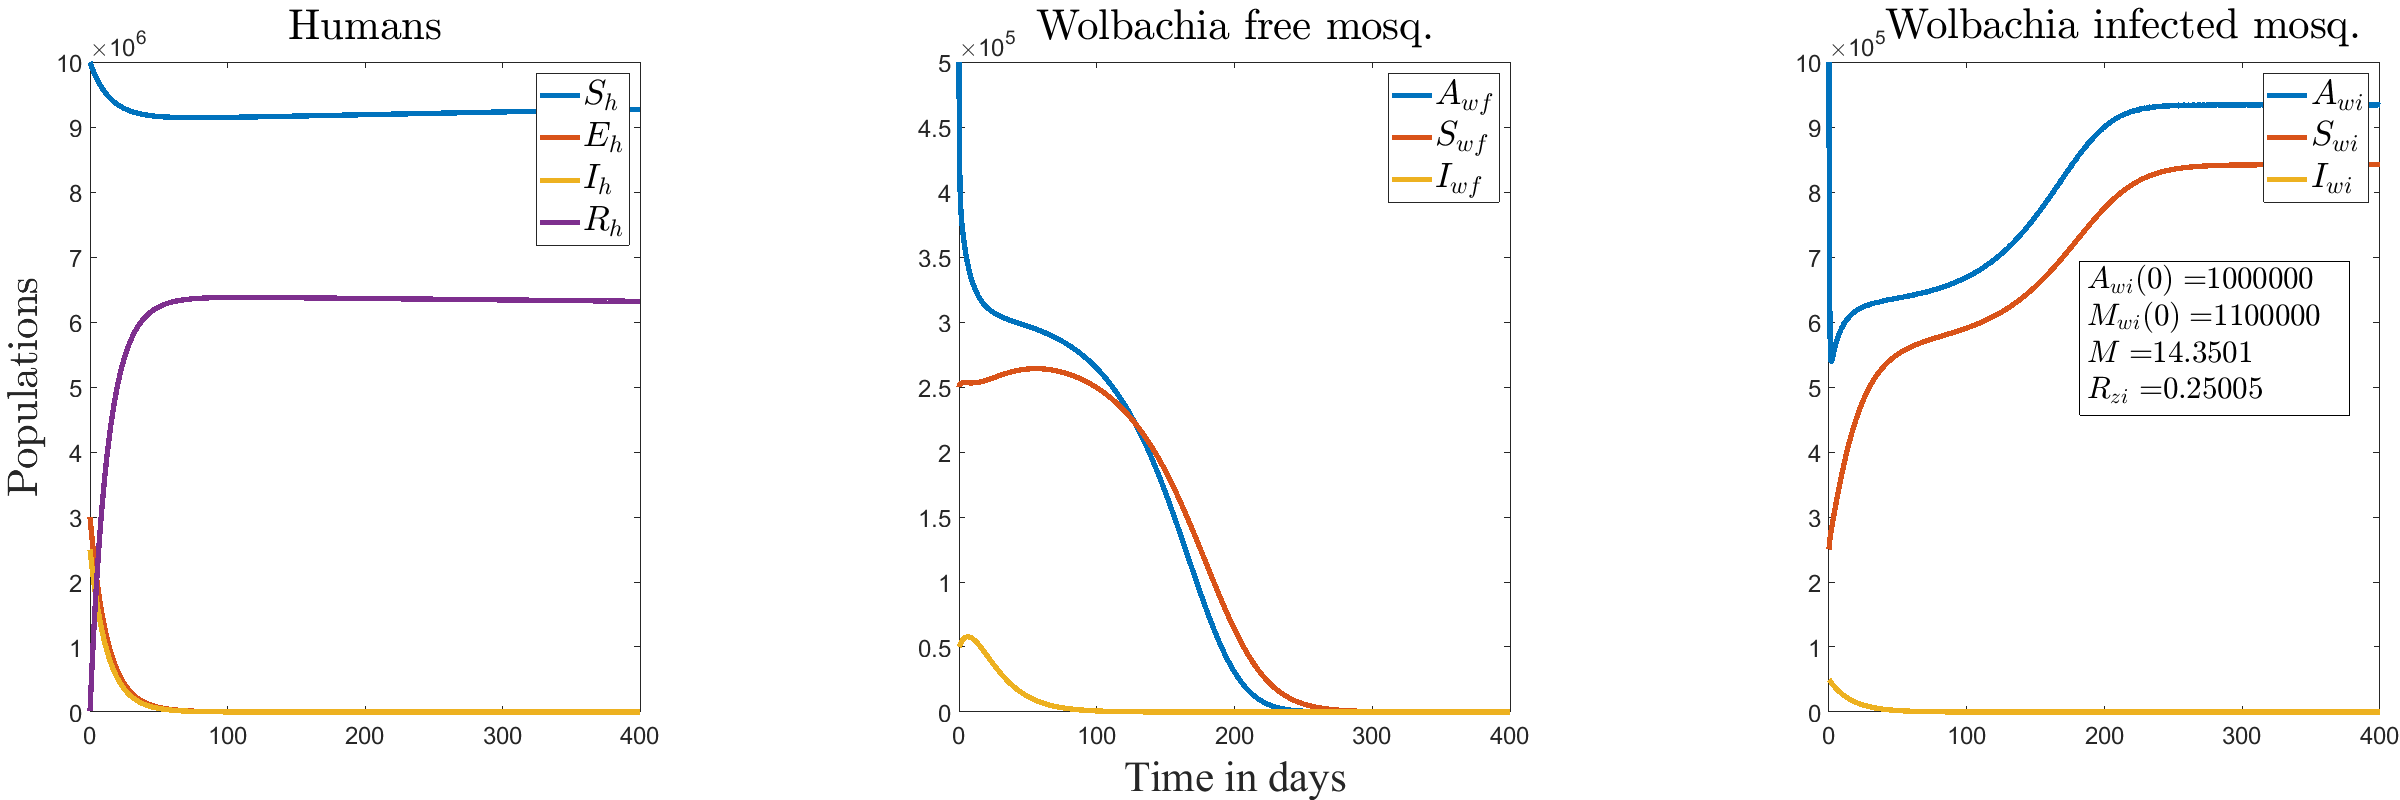
\includegraphics[width=16cm,height=4.5cm]{SimFig6.png}
%    \caption{Dominance of \textit{Wolbachia} infected mosquitoes when we start with more \textit{Wolbachia} infected aquatic stage and more males. Figure  obtained using baseline values for parameters from Table \ref{tab: param-table} and Table \ref{tab: param_mosq_table} and the initial conditions listed in Table \ref{init-cond-dis-free-table} with $A_{wi}(0)=1,000,000$ and $S_{wi}(0)=1,100,000$.}
%    \label{domwolbaqmales}
%\end{figure}

This strategy of releasing a combination of both types of mosquito stages (aquatic  and adults) might be a better choice since one can survey the land to estimate the number of wild aquatic stage. Also, since the hatching rate of the aquatic stage depends on environmental parameters such as humidity, precipitation and temperature, introducing adults can offset the unhatched aquatic stage. 

As seen in sections \ref{morefemales} - \ref{moreaqmale} \textit{Wolbachia} establishment can be achieved by different release strategies. The establishment takes roughly around one year in all scenarios, but the disease takes longer to be eradicated when \textit{Wolbachia} infected susceptible females are released when compared to all other strategies.
%\textcolor{red}{I can move that paragraph here saying we don't have cost info.---
%One would have to take into account the production cost of different release strategies to decide on the optimal strategy.} 

Fore realistic parameters values, we have not been able to find a situation in which both types of mosquitoes coexist. This suggests that for realistic parameter values the two mosquito populations are in a competitive-exclusion regime where only one of the species will persist. These results are consistent with other models that have considered complete cytoplasmic incompatibility and perfect maternal transmission such as \cite{hughes2013modelling}, \cite{koiller2014aedes} and \cite{qu2018modeling}. Incomplete cytoplasmic  incompatbility refers to when a fraction of the offspring resulting from \textit{Wolbachia} infected males with \textit{Wolbachia} free females survives. Incomplete CI and imperfect maternal transmission are two mechanisms by which \textit{Wolbachia} free offspring are produced. Therefore models that include incomplete CI and/or imperfect maternal transmission of \textit{Wolbachia} can observe a coexistence equilibrium.   For example, in \cite{qu2018modeling} the authors consider both cases when the maternal transmission of \textit{Wolbachia} is perfect and imperfect. In the case where they consider imperfect maternal transmission, there is no complete \textit{Wolbachia} infected equilibrium achieved but two endemic equlibria: a high-infection stable endemic equilibrium and a low-infection unstable endemic equilibrium.
Also in \cite{ndii2015modelling} the results indicate that when incomplete cytoplasmic incompatibility and imperfect maternal transmission is taken into account four steady
states that are biologically feasible are observed: all mosquitoes dying out, only \textit{Wolbachia} free
mosquitoes surviving, and two steady states where \textit{Wolbachia} free and \textit{Wolbachia} infected
mosquitoes coexist. The stability of the coexistence steady states is analyzed numerically with only one of them being physically realistic stable steady state.
%page 15 of qumodeling
%page7Ndii
%\textcolor{blue}{As suggested by the reviewers, the absence of coexistence is common with \textit{Wolbachia} models and often depends on on assumptions such as complete CI.} 


\subsection{Numerical Simulations for Disease Present Equilibria}
In this section we perform numerical simulations for the model when the disease is endemic. 
The initial conditions used for the simulations are given in Table \ref{init-cond-dis-present-table}. Notice that we assume that we start with no Zika infected \textit{Wolbachia} females. We again use the baseline values from Table \ref{tab: param-table} and Table \ref{tab: param_mosq_table}  with two changes. First, the biting rate of the mosquitoes is set to the higher end of the range $b=1.25$, and second the carrying capacity of the aquatic stage is set to $K=10^9$. 

\begin{table}[H]
\centering
\caption{Initial conditions for disease present simulations
} 
\label{init-cond-dis-present-table}
\begin{tabular}{ c c c c} 
 \toprule
 Variable & Initial value & Variable & Initial value\\ 
  \midrule
 $S_h(0)$ & 8,000,000 & $I_{wf}(0)$ & 50,000\\
 $E_h(0)$ & 1,000,000 & $M_{wf}(0)$ & 250,000\\
 $I_h(0)$ & 900,000 & $A_{wi}(0)$ & 500,000 \\
 $R_h(0)$ & 100,000 & $S_{wi}(0)$ & 250,000 \\
 $A_{wf}(0)$ & 2,500,000 & $I_{wi}(0)$ & 0 \\
 $S_{wf}(0)$ & 250,000 & $M_{wi}(0)$ & 250,000\\
 \bottomrule
\end{tabular}
\end{table}
\subsubsection{Zika is present but \textit{Wolbachia} infection is not established \label{disfirst}}
When the biting rate of the mosquitoes and the carrying capacity of the aquatic environment is set to the higher end of their range we get that the disease is endemic as we can see in Figure \ref{e4allnice}.  Zika persists both in humans and wild mosquitoes, and the \textit{Wolbachia} infected mosquitoes are eliminated in 400 days. The peak of infected humans infected with Zika is reached in 25 days with approximately 1.8 million infected humans. Zika stays endemic in humans with 3,500 infected humans  and in the \textit{Wolbachia} free mosquitoes with approximately 2.4 mil Zika infected wild mosquitoes.

\begin{figure}[H]
\centering
    % This file was created by matlab2tikz.
%
%The latest updates can be retrieved from
%  http://www.mathworks.com/matlabcentral/fileexchange/22022-matlab2tikz-matlab2tikz
%where you can also make suggestions and rate matlab2tikz.
%
\definecolor{mycolor1}{rgb}{0.00000,0.44700,0.74100}%
\definecolor{mycolor2}{rgb}{0.85000,0.32500,0.09800}%
\definecolor{mycolor3}{rgb}{0.92900,0.69400,0.12500}%
\definecolor{mycolor4}{rgb}{0.49400,0.18400,0.55600}%
%
\begin{tikzpicture}

\begin{axis}[%
width=1.1in,
height=1.5in,
at={(0in,0.108in)},
scale only axis,
xmin=0,
xmax=600,
ymin=0,
ymax=12000000,
axis background/.style={fill=white},
title style={font=\bfseries, yshift=1.75ex},
ylabel={Population},
title={Humans},
legend style={legend cell align=left, align=left, draw=white!15!black}
]
\addplot [color=mycolor1, line width=1.5pt]
  table[row sep=crcr]{%
0	8000000\\
0.443013366311789	7991588.42525528\\
1.1075335862115	7977721.37601196\\
1.7336552394554	7962996.50165479\\
2.3597768926993	7946330.73029662\\
2.75118921883404	7934762.80756718\\
3.14260154590011	7922190.78016901\\
3.53401387296617	7908502.31379796\\
3.92542620003223	7893572.12842647\\
4.42641701176763	7872427.42926689\\
4.92740782257169	7848695.63958027\\
5.42839863430709	7822002.72442426\\
5.92938944604248	7791920.34730049\\
6.54240528773516	7749779.71818391\\
7.15542112942785	7700790.93233571\\
7.76843697205186	7643715.32024266\\
8.38145281374454	7577092.47663384\\
9.03355396911502	7493801.4873328\\
9.68565512448549	7395281.86451398\\
10.337756279856	7278552.76681177\\
10.9898574352264	7140053.9618201\\
11.5992462327704	6987225.87955045\\
12.2086350312456	6807585.29643718\\
12.8180238287896	6596451.00137416\\
13.4274126272649	6348586.69579161\\
13.9731931900606	6090753.97795831\\
14.5189737519249	5794395.07491525\\
15.0647543147206	5455619.11886668\\
15.610534876585	5071579.81458828\\
16.0992427505553	4687995.93754558\\
16.5879506235942	4267581.16089652\\
17.0766584975645	3814032.22522003\\
17.9878750415519	2906186.08421682\\
18.8328923825175	2055013.35147082\\
19.6290178140625	1327306.53514594\\
20.0026345746592	1033534.43913486\\
20.3762513352558	780666.220740934\\
20.9393344810233	477831.259432901\\
21.3182672495022	326157.613925247\\
21.6972000179812	213089.73903615\\
21.8866664022207	169256.427723114\\
22.0761327864602	133031.58812241\\
22.2655991706997	103367.761817867\\
22.4291342552751	82199.3602965791\\
22.5926693407819	64773.3574070577\\
22.7562044262886	50653.7700331481\\
23.0545265385881	31575.8570617577\\
23.3241005921736	20065.5215088688\\
23.5760169308633	12871.6876585102\\
23.8102755527943	8378.19207298942\\
24.0327627491206	5509.87453027163\\
24.2434785189107	3679.34050868545\\
24.4458580510691	2494.80458534323\\
24.6399013474584	1728.21089489479\\
24.8281080815941	1226.54210178461\\
25.010478252545	898.119539716281\\
25.1893107378855	680.633876385167\\
25.3646055357531	536.505859731697\\
25.5389338312671	439.590779917315\\
25.7122956244275	374.29571840167\\
25.887763579376	329.379955921322\\
26.065337697044	298.277599257417\\
26.2485216306522	276.034519519657\\
26.4373153802007	259.818406309001\\
26.6355023002252	247.374379794113\\
26.8430823907256	237.468528244644\\
27.0640954012051	229.046080998145\\
27.4157642992213	218.305994551629\\
27.8191551798955	208.138283078559\\
28.2584095625207	198.663683895953\\
28.7266420703381	189.948444501497\\
29.0535255717114	184.54273188673\\
29.5477227279916	177.125182623975\\
30.2058214321733	168.717961947434\\
30.8574834484607	161.681942839175\\
31.5047708097845	155.742842662148\\
32.1496296776459	150.69934632536\\
32.9515882898122	145.506478171796\\
33.5879093566909	142.020766374655\\
34.2191788591444	139.073689155281\\
35.0024785967544	136.068630853668\\
35.3136465223506	134.9358747527\\
35.7795665338635	133.567018181086\\
35.9343186197802	133.119476833381\\
36.243822792545	132.42384244781\\
36.5516014192253	131.624524579383\\
36.8593800459057	131.075250820257\\
37.1655776742846	130.416227364913\\
37.4717753035948	129.997523156926\\
37.7768511949107	129.464430683292\\
38.0819270862266	129.163174469955\\
38.2341744815931	128.927194211632\\
38.3864218769595	128.743919781409\\
38.690916666761	128.549904204905\\
38.8430290156975	128.36656091176\\
38.9951413637027	128.234728844836\\
39.2993660606444	128.13998251874\\
39.4513644091785	128.005302684382\\
39.6033627567813	127.921157218516\\
39.9073594529182	127.918809887953\\
40.059270305559	127.829680613242\\
40.2111811572686	127.790125256404\\
40.5150028625503	127.873949578963\\
40.6669966764748	127.827820745297\\
40.8189904903993	127.830316231586\\
41.1229781182483	127.995272840373\\
41.2753690797836	127.989922143519\\
41.4277600413188	128.032470197417\\
41.7325419653207	128.275416452438\\
41.8855638587847	128.308912869543\\
42.0385857522488	128.389950822107\\
42.3446295382455	128.709058075212\\
42.4983050217852	128.779871141538\\
42.6519805043936	128.898102264851\\
42.9593314696103	129.291489893571\\
43.1136012161151	129.398647747003\\
43.2678709626198	129.553049264476\\
43.5764104565606	130.01836745441\\
43.7313699852675	130.161485893652\\
43.8863295139745	130.351515720598\\
44.1962485713884	130.887113072909\\
44.3522067461163	131.066169589758\\
44.5081649217755	131.291850139387\\
44.8200812721625	131.898032926023\\
45.1346367718652	132.374660674483\\
45.4491922715679	133.053213646635\\
45.7666038917378	133.601817181334\\
46.0840155109763	134.354170538485\\
46.4041379252449	134.974932027049\\
46.7242603404447	135.801264936104\\
47.0471064187586	136.495439246297\\
47.3699524970725	137.396072185598\\
47.6960329180583	138.166443011723\\
48.0221133390442	139.143898177892\\
48.3521654121578	139.993973258883\\
48.6822174862027	141.052928528748\\
49.0166596621275	141.985713623464\\
49.3511018380523	143.130737657659\\
49.6899030385539	144.148674349301\\
50.0287042381242	145.382660468109\\
50.3718330366537	146.489034444094\\
50.8888970250264	148.389320765622\\
51.2367674047127	149.729598117061\\
51.5873761847615	151.061366200447\\
51.9407233642414	152.504204448313\\
52.2970857191831	153.941319405101\\
52.6564632477239	155.494318420067\\
53.0189361386001	157.043725498021\\
53.3845043918118	158.713290045969\\
53.7532163197175	160.381779492833\\
54.1250719232485	162.174432355911\\
55.6471138047054	169.895814646967\\
57.2317272638902	178.839285379276\\
58.8859235029668	189.215686013922\\
60.6190049210563	201.30115537066\\
62.2093750759959	213.491054379381\\
64.1200205618516	229.811505824327\\
65.8835905520245	246.583773789927\\
66.405076701194	251.898710264824\\
68.0204302594066	269.206677193753\\
68.576664227061	275.587206271477\\
70.1488656252623	294.565041211434\\
71.292064011097	309.431181009859\\
72.501408463344	326.186037556268\\
73.3908589351922	339.197025865316\\
74.3891648752615	354.543107012287\\
75.4280164977536	371.388987804763\\
76.5850285133347	391.262025475502\\
77.7367722643539	412.254404868931\\
78.7261175140738	431.289056425914\\
79.6919685686007	450.815551636741\\
80.7781895529479	473.940596014261\\
81.9361755894497	500.011129260063\\
82.946072245948	523.989432790317\\
84.045620135963	551.477332851849\\
85.0712890345603	578.470033005811\\
86.2112629460171	610.063412112184\\
87.2292466880754	639.751971901394\\
88.2847972335294	672.06364717707\\
89.2657328024507	703.534128265455\\
90.3749218145385	740.855339022353\\
91.5963986841962	784.164184710011\\
92.7767146965489	828.290409046225\\
93.9799757879227	875.660621078685\\
95.0656931875274	920.537039972842\\
96.3159030070528	974.795200490393\\
97.5101199131459	1029.27586127818\\
98.7993577104062	1091.07807070669\\
100.111625297926	1157.24622963276\\
101.405760027468	1225.79063164908\\
102.644288530573	1294.50411015097\\
103.967752415687	1371.34319064207\\
105.212104706094	1446.83764642943\\
106.595450182445	1534.48332730029\\
107.912800012156	1621.59332033619\\
109.27249154076	1715.22092004213\\
110.684614446945	1816.42234248854\\
112.060223575681	1918.83322379738\\
113.588667689823	2036.95389814302\\
115.166331725195	2163.51382045541\\
116.707288024016	2291.48908299953\\
118.343778386712	2431.86820942163\\
120.025804808363	2580.63364389353\\
121.963430780917	2757.1394397961\\
124.023964190856	2950.16303748544\\
126.335887065157	3172.19254869595\\
129.141816474497	3447.51557519007\\
133.348262829706	3866.79710438196\\
138.224307565019	4351.62154851854\\
140.895054167137	4611.64685925655\\
143.155980701558	4826.49456929602\\
145.206064868718	5015.94555525482\\
147.05294261314	5181.45991535578\\
148.790923380293	5332.16723999567\\
150.365679486655	5464.08228986897\\
151.9708924843	5593.65892253071\\
153.48592608422	5711.14660317451\\
154.88411261607	5815.21989786159\\
156.231611134484	5911.40752597619\\
157.521356800571	5999.57066442538\\
158.791137252934	6082.54421984963\\
159.982638250105	6156.88074712828\\
161.145645760931	6226.09870415088\\
162.206289335154	6286.31309766416\\
163.384088139981	6349.89622744359\\
164.388886539266	6401.39458752517\\
165.416067547165	6451.41958536673\\
166.489047481678	6500.84452643711\\
167.455064515583	6542.87260777876\\
168.486409586854	6585.17001766339\\
169.466989040375	6622.93581704702\\
170.359259133227	6655.24135219771\\
171.181664392352	6683.29495680332\\
172.043272329494	6710.93112180941\\
172.856642980129	6735.39064802136\\
173.689413809218	6758.81441039406\\
174.499050824903	6780.03816338629\\
175.245728384703	6798.27719208971\\
176.035060884431	6816.18754723947\\
176.709642936476	6830.39536184538\\
177.397780134343	6843.86238416471\\
178.081109696999	6856.22670010477\\
178.80642356351	6868.27088469267\\
179.393020981923	6877.21302900184\\
180.077306124382	6886.75911079999\\
180.756021997891	6895.30428086687\\
181.258026543073	6901.04468807857\\
181.869743127376	6907.3861843897\\
182.390402504243	6912.22876668628\\
182.879133865237	6916.31896914449\\
183.448068727739	6920.53561381903\\
183.936792121269	6923.69899636041\\
184.309195457958	6925.8301727483\\
184.721505169757	6927.9127750285\\
185.056527559645	6929.3940044241\\
185.391549950466	6930.68895056844\\
185.733330355026	6931.82089192513\\
186.075110758655	6932.76465405151\\
186.356354584917	6933.40221214388\\
186.63759841118	6933.91593515035\\
186.87172509823	6934.25034918543\\
187.10585178528	6934.50102838781\\
187.352910699323	6934.67581421137\\
187.599969613366	6934.75953593198\\
187.753251342103	6934.76619821694\\
187.90653307084	6934.73850567546\\
188.059814799577	6934.67672509514\\
188.213096528314	6934.58112724125\\
188.388733725064	6934.43036265299\\
188.564370922744	6934.23595010303\\
188.915645317174	6933.71779789962\\
189.165477689356	6933.24582320731\\
189.540226248093	6932.37943913322\\
189.91497480683	6931.32646743674\\
190.371313778684	6929.79801381659\\
190.868581181392	6927.83248686884\\
191.370527219959	6925.54029036779\\
191.840902098455	6923.11963149626\\
192.346317837015	6920.23376568686\\
192.951276714914	6916.40467888769\\
193.528454156592	6912.38495222665\\
194.198559964076	6907.28817449603\\
194.84876648616	6901.92117436789\\
195.618874985725	6895.05511056446\\
196.380542997271	6887.75160519592\\
197.188198518008	6879.48538293224\\
198.160382792354	6868.87440071348\\
199.139952477068	6857.51327983104\\
200.139833221212	6845.28917727433\\
201.306290253997	6830.31456787512\\
202.466817061417	6814.7484499868\\
203.869159474969	6795.18741304986\\
205.434514287859	6772.56852414366\\
207.4273477979	6742.89951449726\\
210.278940443881	6699.49186670687\\
214.828602767549	6630.23551298957\\
216.983376578428	6598.28882121947\\
218.844252765179	6571.46523974277\\
220.591013843194	6547.08093932457\\
222.265095476061	6524.53693105839\\
223.757787954994	6505.18365826551\\
225.19660008885	6487.24231696595\\
226.660448100418	6469.74305651709\\
227.998071505688	6454.44195475988\\
229.279843203723	6440.41305177473\\
230.510349034332	6427.53824289329\\
231.636084561236	6416.27377362829\\
232.79897219874	6405.15618930943\\
233.91194045078	6395.01008483116\\
235.078556139022	6384.89260635059\\
236.210411965847	6375.58014140371\\
237.374843395315	6366.51260388363\\
238.445813342929	6358.62683675345\\
239.504229607061	6351.25495954789\\
240.59540485125	6344.08655437455\\
241.637566320598	6337.64192015585\\
242.619415569119	6331.92235045321\\
243.614826086909	6326.46525186766\\
244.610510354862	6321.34294779785\\
245.573245776817	6316.70239107963\\
246.49380484689	6312.54513659701\\
247.461888519116	6308.46090897173\\
248.361873031594	6304.92139015067\\
249.251629960723	6301.65910324268\\
250.019517272711	6299.02797973063\\
250.810457644053	6296.49158588983\\
251.615543413907	6294.08596022241\\
252.386884591542	6291.94316739216\\
253.141011938453	6289.99706448801\\
253.935172499157	6288.10207597818\\
254.745975626633	6286.32575579826\\
255.509101852775	6284.79536948726\\
256.264173746109	6283.41178007424\\
256.890541574918	6282.35958989989\\
257.656389094889	6281.18709858693\\
258.397373326123	6280.16817858722\\
258.997759168036	6279.42316011619\\
259.678329642862	6278.66301580705\\
260.422657867894	6277.93089068215\\
261.029777767137	6277.40784794278\\
261.667702692561	6276.92754297424\\
262.29691391997	6276.52102497779\\
262.965434962884	6276.15968213789\\
263.687829894014	6275.84787430614\\
264.272595000453	6275.65305459965\\
264.940818440169	6275.49104498699\\
265.588759192266	6275.39333385415\\
266.30491468776	6275.35049577896\\
266.922226198018	6275.36617861502\\
267.522412164137	6275.42615557835\\
268.202740832232	6275.54520107806\\
268.946840474382	6275.73464876972\\
269.669727249071	6275.97495431546\\
270.491450360976	6276.31170096807\\
271.320989835076	6276.71616901737\\
272.211103450507	6277.21746180113\\
273.161715106107	6277.82419718709\\
274.111572719179	6278.49822126236\\
275.197860630229	6279.34468315169\\
276.214808688499	6280.20320999529\\
277.46885140799	6281.33999043517\\
278.713349141181	6282.54259187821\\
280.178262795322	6284.03849783726\\
281.833919916302	6285.81390206981\\
283.842087741941	6288.05715159141\\
286.480153327808	6291.09663880803\\
293.084843588993	6298.74371337797\\
295.346936442889	6301.26038379502\\
297.355673008598	6303.41534086876\\
299.174414966255	6305.28933852538\\
301.003544331528	6307.09114602674\\
302.747178307734	6308.72492643073\\
304.406170531176	6310.1990274312\\
306.012287585996	6311.54851232376\\
307.541434238665	6312.76048284862\\
309.027862664312	6313.86942158826\\
310.461046402343	6314.87357556913\\
311.919469882734	6315.82974612154\\
313.417180742137	6316.74307900015\\
314.922416099347	6317.59166687168\\
316.360814927146	6318.33861444984\\
317.791999576613	6319.02098373231\\
319.318230154924	6319.68340238184\\
320.784263419919	6320.25806401111\\
322.266592768021	6320.77970737219\\
323.786337849684	6321.25475529488\\
325.223305869848	6321.65052912664\\
326.85559489578	6322.03996971902\\
328.453736865893	6322.36242037173\\
330.122322768904	6322.64052847866\\
331.840726550668	6322.86831262428\\
333.567352633923	6323.04145998601\\
335.372312847525	6323.1672988208\\
337.345306242816	6323.2459350666\\
339.300059325993	6323.26905364078\\
341.458365013823	6323.23826074786\\
343.738926630467	6323.14966850448\\
346.334299561568	6322.98946214374\\
349.220564481802	6322.7509131087\\
352.555149168707	6322.41511762235\\
356.668413601816	6321.94132019766\\
364.352481926791	6320.98484886996\\
370.881136923097	6320.19728096016\\
375.674481229857	6319.67425579298\\
380.051769353449	6319.25202752929\\
384.341564245522	6318.89545894414\\
388.567894279957	6318.6012759069\\
392.857675291598	6318.35953511018\\
397.315677931532	6318.16545950714\\
402.042802852578	6318.01727927383\\
407.097558011301	6317.91573388781\\
412.827875568531	6317.85894509126\\
419.494360675104	6317.85177287553\\
428.010408433154	6317.90219935495\\
444.795754349791	6318.07280630805\\
460.835143182427	6318.20915752091\\
475.390299666673	6318.27406703401\\
492.757888504304	6318.29254977591\\
537.630299617536	6318.25498673227\\
593.821703251451	6318.24912256468\\
600	6318.24967538845\\
};
\addlegendentry{$S_h$}

\addplot [color=mycolor2, line width=1.5pt]
  table[row sep=crcr]{%
0	1000000\\
0.443013366311789	965061.831205644\\
1.1075335862115	916688.564000291\\
1.7336552394554	875569.869619588\\
2.3597768926993	838831.111364453\\
2.75118921883404	818129.693076143\\
3.14260154590011	799208.469281339\\
3.53401387296617	782109.440682627\\
3.92542620003223	766885.290962347\\
4.42641701176763	750237.201440839\\
4.92740782257169	736928.510886032\\
5.42839863430709	727161.842355281\\
5.92938944604248	721180.72220751\\
6.54240528773516	719439.308863795\\
7.15542112942785	724452.56908802\\
7.76843697205186	737024.052911873\\
8.38145281374454	758116.467147926\\
9.03355396911502	791214.258665941\\
9.68565512448549	836985.538395174\\
10.337756279856	897520.250370541\\
10.9898574352264	975326.944345132\\
11.5992462327704	1066297.92721735\\
12.2086350312456	1177928.29735644\\
12.8180238287896	1313535.09048566\\
13.4274126272649	1476783.47317953\\
13.9731931900606	1649672.27875671\\
14.5189737519249	1850880.57579867\\
15.0647543147206	2082675.07700502\\
15.610534876585	2346225.91565409\\
16.0992427505553	2609098.38570375\\
16.5879506235942	2895340.91281647\\
17.5653663706034	3515964.51945773\\
18.410383711569	4054789.48400262\\
18.8328923825175	4299254.70749307\\
19.2554010534659	4513026.5936201\\
19.6290178140625	4669462.02604975\\
20.0026345746592	4786762.68564577\\
20.3762513352558	4859383.46234388\\
20.7498680958524	4888297.00138409\\
20.9393344810233	4887497.38759998\\
21.1288008652627	4876115.37438377\\
21.3182672495022	4854657.7954492\\
21.5077336337417	4823989.95892748\\
21.6972000179812	4785177.91591578\\
22.0761327864602	4685906.44239385\\
22.4291342552751	4573446.93625907\\
22.9197395117953	4396519.7264844\\
25.4522529346868	3445992.50338198\\
26.2485216306522	3182880.23502805\\
26.9468724355102	2968625.29895889\\
27.6846915530041	2757924.61153976\\
28.4108049413189	2565202.8843032\\
29.2169673228636	2367007.28033084\\
30.0421497831121	2180026.69613164\\
30.8574834484607	2009831.01421132\\
31.6662551313639	1854176.1968538\\
32.4715199023485	1711215.21087872\\
33.2703771758825	1580325.9591301\\
34.0616777222604	1460587.02600281\\
34.8460289463401	1350894.04935276\\
35.6248144479468	1250170.25563985\\
36.3977121058851	1157672.68613393\\
37.1655776742846	1072593.04996178\\
37.9293891405687	994203.804149485\\
38.690916666761	921789.662490883\\
39.4513644091785	854778.453831719\\
40.2111811572686	792725.085372216\\
40.9709843043238	735214.143360781\\
41.7325419653207	681793.748469215\\
42.4983050217852	632028.728765806\\
43.2678709626198	585713.031415777\\
44.0412890426815	542622.33513806\\
44.8200812721625	502473.139367244\\
45.6078980816528	464919.329647248\\
46.4041379252449	429854.744106077\\
47.2085294574499	397156.155920608\\
48.0221133390442	366654.518129411\\
48.8494385741651	338081.335739058\\
49.6899030385539	311377.012765166\\
50.3718330366537	291300.312306381\\
51.0628322148696	272306.480273467\\
51.7640497749671	254328.039053768\\
52.4767744829878	237301.982277147\\
53.2017202656716	221185.284768931\\
53.939144121483	205947.210159703\\
54.6895689340308	191552.271893249\\
55.4541219174862	177956.256000046\\
56.2341142855585	165116.55660064\\
57.0305258026347	153000.208429404\\
57.8440782614052	141580.318629501\\
58.6756916018203	130828.622938312\\
59.5266579687595	120714.309040976\\
60.3983901254833	111208.11717505\\
61.0659080250189	104468.896952452\\
61.744772949256	98061.1748127267\\
62.4416761398315	91920.4686532877\\
63.1514149531722	86091.2887764843\\
63.8744366327301	80563.2816379899\\
64.6111884210259	75326.56063715\\
65.3699327129871	70321.9923996245\\
66.144333627075	65590.8718361491\\
66.9349431507289	61123.899913894\\
67.7423132751137	56912.1633581538\\
68.576664227061	52902.4843011396\\
69.2861426817253	49746.1603201609\\
70.1488656252623	46197.5635713134\\
70.8175060683861	43650.0412519025\\
71.5293429819867	41118.4681081576\\
72.2583920927718	38705.6066555958\\
72.9461336992681	36584.865520604\\
73.7903530141339	34172.8951988369\\
74.5884826583788	32071.9994007433\\
75.4280164977536	30035.3106182842\\
76.1076193526387	28506.963805547\\
76.8237330941483	27004.6291609826\\
77.5085124718025	25664.859833261\\
78.3381766369566	24159.3209130354\\
79.1010630186647	22880.4375572242\\
79.8936849664897	21650.5396859888\\
80.5505934907123	20702.1117976084\\
81.23838310875	19773.185308136\\
81.9361755894497	18893.3259873912\\
82.7639005072415	17925.5372828217\\
83.4925874648616	17136.7617608793\\
84.2299643587321	16394.3772986177\\
85.0712890345603	15610.7980727376\\
85.763931828551	15012.738865043\\
86.6441633179784	14309.2371024163\\
87.4135632803664	13742.2258056253\\
88.1130678933114	13262.5654717339\\
88.8552958443761	12788.263391152\\
89.7062743101269	12285.1208885536\\
90.3749218145385	11918.0175956786\\
91.2098486246541	11491.8481747303\\
91.9295623293146	11151.1396631394\\
92.7767146965489	10779.2634287458\\
93.5536026237532	10463.8443690138\\
94.4290165472776	10135.4125999222\\
95.2717713173479	9844.06987125427\\
96.1579558327794	9561.78013748955\\
96.9698383742943	9323.03157539573\\
97.7240219041705	9116.91876005754\\
98.5825427938253	8899.21193395555\\
99.4143445659429	8704.10002818424\\
100.264834964648	8519.37578320224\\
101.051516308449	8360.74062985275\\
101.794072791003	8220.95115974825\\
102.644288530573	8071.84077282902\\
103.454347935505	7939.79693931434\\
104.28403257858	7813.87676383276\\
105.040929836221	7706.59416107833\\
105.76215340849	7610.60309506115\\
106.595450182445	7506.70773701835\\
107.397737380117	7413.24477566127\\
108.197912542149	7325.94517150428\\
109.08567433618	7235.45912323892\\
109.832943152636	7164.08724359237\\
110.684614446945	7087.67174967565\\
111.579120403156	7012.62943022978\\
112.426092617214	6946.11023902055\\
113.232552152127	6886.55733342469\\
114.181763154455	6820.82749711908\\
114.986416067928	6768.52779298089\\
115.954855502583	6709.42076917831\\
116.890475740656	6655.99932063092\\
117.752069497481	6609.76626544818\\
118.662693724968	6563.77027584426\\
119.633321980014	6517.76459398307\\
120.543302805163	6477.27401473001\\
121.539952198975	6435.66519197728\\
122.488538061269	6398.5564783439\\
123.462292271666	6362.84121744614\\
124.445218130015	6329.09665056504\\
125.273539098911	6302.36953480542\\
126.195490144193	6274.37647777144\\
127.037871667184	6250.35116276052\\
127.857256449759	6228.35076155048\\
128.795243123546	6204.76642801147\\
129.735264854506	6182.78903505951\\
130.546924536116	6165.10815340932\\
131.368435257114	6148.40306824446\\
132.107639704831	6134.37239051424\\
132.93934078794	6119.69576625433\\
133.739112775773	6106.66956880502\\
134.478238754906	6095.56170562282\\
135.192501157522	6085.66317711491\\
135.977204911411	6075.72104371898\\
136.651148444973	6067.95074912999\\
137.309015538543	6061.0417555701\\
137.868836397305	6055.68236109614\\
138.393171780743	6051.09174424317\\
139.001542118378	6046.28037599009\\
139.522300292738	6042.59709377401\\
140.065477932803	6039.17881052569\\
140.537377594039	6036.5570389526\\
141.073892453685	6033.96570688579\\
141.438299229369	6032.44003172964\\
141.802706005983	6031.10254461318\\
142.250486685894	6029.71488563716\\
142.647262153216	6028.71928213723\\
143.025379047729	6027.97353344969\\
143.286582355388	6027.57332712412\\
143.579571533948	6027.23552586231\\
143.90434658248	6026.99757735431\\
144.066734107211	6026.93214533199\\
144.252971756272	6026.90084771346\\
144.439209405333	6026.91612077318\\
144.625447054394	6026.97778664529\\
144.943144758232	6027.1895270776\\
145.206064868718	6027.46581316926\\
145.468984979205	6027.83306666184\\
145.731905089691	6028.29076777492\\
146.0239832839	6028.90463799704\\
146.34521956183	6029.70706421509\\
146.68820600491	6030.70991124492\\
147.05294261314	6031.94056073297\\
147.565328223631	6033.95247506257\\
148.027553562075	6036.04808815569\\
148.546426232904	6038.71364156809\\
149.056557632051	6041.65294641163\\
149.661840910092	6045.54426778201\\
150.187219647691	6049.27165101469\\
150.722599165514	6053.39891263377\\
151.33964888379	6058.56060098205\\
151.9708924843	6064.2811343642\\
152.642448759638	6070.84527633525\\
153.303161459975	6077.77369394992\\
154.109619651921	6086.84614757262\\
154.88411261607	6096.17789702676\\
155.694129085168	6106.56546920817\\
156.556126837619	6118.29997656308\\
157.521356800571	6132.23899859749\\
158.446534520946	6146.3567880746\\
159.487147334032	6163.07661651727\\
160.654029830359	6182.82169470005\\
161.869132034481	6204.42455192003\\
163.129152888432	6227.85766298696\\
164.388886539266	6252.23890171107\\
165.865083629265	6281.88947596122\\
167.455064515583	6314.95287631638\\
169.348560956307	6355.57834804058\\
171.538006139919	6403.82237218693\\
174.75427260343	6476.10698549263\\
179.54717214033	6583.8227902744\\
181.869743127376	6634.74208433554\\
183.819308738224	6676.32557367068\\
185.56244015228	6712.37523358222\\
187.229381241836	6745.68315886892\\
188.740008120425	6774.76635336038\\
190.219200788066	6802.13919006474\\
191.527318846434	6825.37449381687\\
192.814445433207	6847.30088505708\\
194.028504950926	6867.09825315885\\
195.268890934996	6886.41067285929\\
196.380542997271	6902.91500543058\\
197.537902705371	6919.27625846956\\
198.68539125286	6934.65990105364\\
199.827410816215	6949.13476495165\\
200.830186059698	6961.15463980101\\
201.83218174614	6972.52026873454\\
202.802342362702	6982.91201121919\\
203.729538874701	6992.28293375298\\
204.702971801162	7001.53592469823\\
205.608792671934	7009.61293125525\\
206.504205607809	7017.09775177762\\
207.4273477979	7024.30159943271\\
208.243561682291	7030.24392198399\\
209.038062118925	7035.64942081738\\
209.890309553593	7041.03967578523\\
210.716735351831	7045.87090738025\\
211.55165679194	7050.36448299233\\
212.307601074688	7054.10453883465\\
213.034123181365	7057.41141496319\\
213.705474535935	7060.22210089583\\
214.35691141244	7062.72935990989\\
215.076548037119	7065.2529868912\\
215.696411211975	7067.22449406609\\
216.299514670856	7068.96737559512\\
216.983376578428	7070.73958894983\\
217.605300203897	7072.16783104651\\
218.107326661237	7073.19646471366\\
218.572559671476	7074.05288338009\\
219.115945858881	7074.93789087329\\
219.611904631369	7075.63972389512\\
220.114572972991	7076.25038853288\\
220.591013843194	7076.73789404146\\
221.008290201426	7077.09356115386\\
221.472350084223	7077.41269958951\\
221.961863661185	7077.66424238961\\
222.416711383499	7077.82162876986\\
222.741880109534	7077.89010829292\\
223.088985746726	7077.92355947662\\
223.510163259692	7077.91029791627\\
223.881600302644	7077.85070272814\\
224.253037344664	7077.7472460214\\
224.704677430913	7077.56378708128\\
225.19660008885	7077.2939169975\\
225.693231775425	7076.94963349029\\
226.158998943865	7076.56323444378\\
226.660448100418	7076.08071821742\\
227.260868079029	7075.41549481638\\
227.83298691269	7074.69640463497\\
228.496676782146	7073.76262432989\\
229.140914128162	7072.7586868722\\
229.905415947549	7071.44932202715\\
230.661786866374	7070.03511782922\\
231.462756494991	7068.41706611682\\
232.304192413576	7066.59314179327\\
233.250108351	7064.40287257265\\
234.237515420653	7061.97273368482\\
235.319907940924	7059.15751889441\\
236.540236084722	7055.81670947\\
237.820722988807	7052.14836832788\\
239.352922672406	7047.5789423082\\
241.089838977903	7042.21641853265\\
243.36446941644	7034.99872154742\\
251.150906215422	7010.11567483936\\
253.141011938453	7004.01769731939\\
255.023286700249	6998.43334854767\\
256.717590649612	6993.58392162435\\
258.273875954561	6989.2934220368\\
259.833142256364	6985.16383786965\\
261.261664354242	6981.53703119885\\
262.629502071068	6978.20992349368\\
264.034890905023	6974.94393621944\\
265.242990602739	6972.26219743211\\
266.551839292049	6969.48960037995\\
267.862576497719	6966.85226107668\\
269.071886505	6964.54280726425\\
270.326880064793	6962.27140744589\\
271.488904127851	6960.28135337681\\
272.673753984272	6958.36310988385\\
273.765902765095	6956.69295122847\\
274.950987977907	6954.98547152989\\
276.04477126617	6953.50471780915\\
277.189101893455	6952.05144198332\\
278.307503776625	6950.72385112196\\
279.342227700166	6949.57538038958\\
280.455352255143	6948.4233990116\\
281.560931514017	6947.3626490552\\
282.632570781745	6946.41151607037\\
283.718670606613	6945.52261112072\\
284.735437821597	6944.75677728187\\
285.864251137711	6943.979170762\\
286.963059153408	6943.29298689496\\
288.02686057426	6942.69266348425\\
289.113824932836	6942.14173373301\\
290.202698810026	6941.65054419264\\
291.324999949895	6941.20508569758\\
292.484995615669	6940.80650953669\\
293.594783454202	6940.48114023544\\
294.75846174825	6940.19568810333\\
295.88792339433	6939.97024456691\\
297.217162225395	6939.76617443562\\
298.477582045831	6939.62990133278\\
299.843651260249	6939.54064261727\\
301.303438714705	6939.50722005405\\
302.747178307734	6939.53175610956\\
304.270934669301	6939.61393985245\\
305.873787323944	6939.7563631041\\
307.541434238665	6939.95844752062\\
309.398018005304	6940.2395329522\\
311.419564477168	6940.60236698855\\
313.749437531456	6941.07983562537\\
316.533541630022	6941.7128876932\\
320.061790912412	6942.5777983889\\
331.840726550668	6945.51348967198\\
335.222394206561	6946.27376894653\\
338.339307009242	6946.91811022814\\
341.307417619042	6947.47548783757\\
344.188673601486	6947.96104110591\\
347.155433027074	6948.40254201554\\
350.125738196075	6948.78534545191\\
353.044904839247	6949.10523054097\\
356.000652392395	6949.37467745412\\
359.116647901945	6949.6029662108\\
362.364924509078	6949.78481645323\\
365.767869263887	6949.91994118597\\
369.437754243612	6950.00994017627\\
373.533090359531	6950.05257427692\\
378.103835647926	6950.04224894848\\
383.522988042794	6949.97134990431\\
390.56535938289	6949.81946411822\\
418.729531870224	6949.15591479652\\
427.887042950839	6949.03003072646\\
437.716365368105	6948.95258016512\\
449.348931359127	6948.92007372808\\
465.946148122661	6948.93607128877\\
517.312708484009	6949.01414271817\\
590.555088084191	6949.00602460001\\
600	6949.00581607968\\
};
\addlegendentry{$E_h$}

\addplot [color=mycolor3, line width=1.5pt]
  table[row sep=crcr]{%
0	900000\\
0.664520106511191	848534.674687683\\
1.42059441306628	794045.140555637\\
2.04671606584452	752083.961192852\\
2.7511892192997	708192.927677323\\
3.53401387296617	663441.70201178\\
3.9254261997994	642626.854947223\\
4.42641701130196	617489.950998018\\
4.92740782280453	594036.283852641\\
5.42839863430709	572268.173665781\\
5.92938944580965	552200.845035871\\
6.54240528773516	530003.120952056\\
7.15542112966068	510460.491713176\\
7.7684369715862	493674.568190154\\
8.38145281374454	479796.64320161\\
9.03355396888219	468448.740952939\\
9.68565512425266	460895.201664878\\
10.3377562796231	457505.330336403\\
10.9898574347608	458757.322759439\\
11.5992462330032	464630.890047909\\
12.2086350310128	475639.363206636\\
12.8180238292553	492482.854237\\
13.4274126272649	515966.227598152\\
13.9731931895949	543360.250209978\\
14.5189737521578	577607.880303728\\
15.0647543144878	619558.820045382\\
15.6105348768178	669987.331182703\\
16.0992427503224	722870.355449211\\
16.5879506238271	783663.240903831\\
17.0766584970988	852694.955762325\\
17.5653663706034	929785.839367298\\
17.9878750413191	1002431.32672643\\
18.8328923827503	1162070.49023021\\
20.3762513354886	1470463.30592816\\
21.1288008647971	1606185.7154121\\
21.5077336332761	1666042.29367863\\
21.8866664019879	1718965.44693982\\
22.2655991704669	1764444.29465601\\
22.5926693410147	1797454.14174819\\
22.9197395117953	1824719.98185205\\
23.1893135653809	1842950.28238711\\
23.4588876191992	1857497.19759432\\
23.693146241596	1867269.22925234\\
23.9274048639927	1874504.79180477\\
24.1381206337828	1878952.27110501\\
24.243478518445	1880476.41986636\\
24.3488364033401	1881550.49813203\\
24.4458580515347	1882152.02209796\\
24.5428796997294	1882391.9764954\\
24.6399013476912	1882279.94887513\\
24.7369229958858	1881825.34471739\\
24.8281080815941	1881094.12241845\\
25.0104782527778	1878779.39329455\\
25.1893107376527	1875454.22033696\\
25.3646055359859	1871234.15798527\\
25.6256147280801	1863296.79611753\\
25.8877635798417	1853475.06488366\\
26.2485216301866	1837205.9895671\\
26.635502300458	1816590.21157227\\
27.064095401438	1790427.33472768\\
27.5502279261127	1757142.03309626\\
28.1060141844209	1715208.75708794\\
28.7266420703381	1664521.4445241\\
29.5477227279916	1592912.75632729\\
30.6953240893781	1487594.96318819\\
33.9041765846778	1189916.32785908\\
35.1580625593197	1080229.15366739\\
36.2438227923121	990255.696426651\\
37.3186764891725	906297.355971887\\
38.2341744813602	838993.241652427\\
39.1472537124064	775782.771470976\\
40.0592703053262	716533.635057786\\
40.970984304091	661119.012045186\\
41.8855638585519	609254.111646512\\
42.8056559867691	560701.618736062\\
43.5764104563277	522712.610473514\\
44.3522067463491	486836.705232945\\
45.1346367723309	452945.302988274\\
45.925309701357	420920.591166834\\
46.7242603399791	390713.425179139\\
47.5329927075654	362219.406112016\\
48.3521654126234	335370.666962192\\
49.1838807498571	310058.34812654\\
50.028704238357	286229.256636573\\
50.8888970252592	263787.452464783\\
51.7640497747343	242711.896393201\\
52.4767744834535	226770.150511958\\
53.2017202654388	211608.833405783\\
53.939144121483	197210.54562851\\
54.6895689340308	183552.241871479\\
55.454121917719	170601.420410554\\
56.2341142857913	158325.951777791\\
57.0305258024018	146701.915349971\\
57.8440782618709	135710.389050598\\
58.6756916013546	125330.40083108\\
59.5266579687595	115537.818705573\\
60.3983901250176	106309.354298337\\
61.0659080252517	99752.6041900632\\
61.7447729497217	93507.3309990724\\
62.4416761395987	87512.0351042871\\
63.1514149527065	81811.7045220297\\
63.8744366322644	76397.7809894904\\
64.6111884210259	71261.8418331465\\
65.3699327134527	66346.7848768586\\
66.1443336266093	61694.3047290349\\
66.9349431507289	57296.428142617\\
67.7423132755794	53145.253412402\\
68.5766642268281	49188.9138151119\\
69.286142682191	46071.8077471196\\
70.1488656254951	42564.377248764\\
70.8175060683861	40044.5470408949\\
71.5293429822195	37539.0006693434\\
72.2583920930047	35149.5414602014\\
72.9461336992681	33048.3033585842\\
73.790353013901	30657.3545034637\\
74.5884826579131	28573.8015678918\\
75.4280164975207	26553.1271159742\\
76.1076193524059	25036.3310430723\\
76.8237330939155	23545.0078339563\\
77.5085124720354	22214.7870065011\\
78.3381766371895	20719.7543386563\\
79.1010630191304	19449.6586742816\\
79.8936849667225	18228.1557106478\\
80.5505934902467	17286.2062905633\\
81.23838310875	16363.6832767478\\
81.9361755892169	15489.9829587287\\
82.7639005067758	14529.1313154767\\
83.4925874653272	13746.2013337996\\
84.2299643591978	13009.5368009098\\
85.0712890343275	12232.3006660633\\
85.7639318287838	11639.3534731688\\
86.644163318444	10942.2555744036\\
87.4135632805992	10380.7893685114\\
88.1130678930786	9906.15214429074\\
88.8552958446089	9437.18193524168\\
89.7062743101269	8940.17840530328\\
90.3749218147714	8577.93236141209\\
91.2098486248869	8157.88832544186\\
91.9295623295475	7822.52270408813\\
92.7767146960832	7457.02264792263\\
93.5536026235204	7147.54333926132\\
94.2044961676002	6905.79825590225\\
95.0656931875274	6608.71499441797\\
95.8179026404396	6368.89951556455\\
96.6317973544355	6128.46202022769\\
97.3300260670949	5936.81403687876\\
98.1518258859869	5727.24223403144\\
99.0161726272199	5524.0458658326\\
99.7770586090628	5358.63292667223\\
100.571254297858	5198.37131457194\\
101.405760027235	5042.56053368375\\
102.206915625604	4904.1573547516\\
103.060099300463	4767.84087062208\\
103.809612334007	4656.78011036036\\
104.576893772464	4550.86076307227\\
105.383279575501	4447.38226285949\\
106.177551335189	4352.70998350321\\
107.015849951422	4259.98098234064\\
107.912800012156	4168.27555358154\\
108.784349704161	4085.98165772599\\
109.646125948988	4010.65659580426\\
110.471696623601	3943.67114752578\\
111.280951751163	3882.53083692258\\
112.060223575681	3827.55917814653\\
112.816868808819	3777.57360005355\\
113.736941555748	3720.94120977493\\
114.626584753394	3670.1623144804\\
115.549116755603	3621.28660945338\\
116.340912591899	3582.15830418142\\
117.184875844046	3543.0947293092\\
118.024863047292	3506.71824703156\\
118.856290435418	3472.9848633525\\
119.633321980014	3443.3529698255\\
120.543302805629	3410.80625566957\\
121.398792671738	3382.17353739473\\
122.313502300996	3353.50628886069\\
123.262612659251	3325.72950111888\\
124.16438217042	3301.05809585401\\
125.101563351694	3277.06527312403\\
126.055093223928	3254.25668080687\\
126.897474746685	3235.36285792571\\
127.857256449526	3215.18034068285\\
128.795243123779	3196.75594270229\\
129.735264854738	3179.5037185559\\
130.546924536116	3165.5310844304\\
131.36843525758	3152.21812147368\\
132.293781499844	3138.17595436238\\
133.220371391159	3125.08172999858\\
134.009246915579	3114.66435252316\\
134.812163523864	3104.72597406572\\
135.707627497846	3094.40547605138\\
136.516359738074	3085.75393110677\\
137.309015538776	3077.87211363949\\
138.055443350691	3070.97644506255\\
138.866221164353	3064.05027730064\\
139.647358425194	3057.91960758273\\
140.358539308188	3052.79055285873\\
141.07389245322	3048.0577564789\\
141.802706005983	3043.66732818866\\
142.399746912532	3040.38956883992\\
143.025379048195	3037.25803846447\\
143.579571533715	3034.73956896062\\
144.066734107211	3032.72133788466\\
144.625447054161	3030.62922915374\\
145.206064868951	3028.70390790375\\
145.731905090157	3027.17629962089\\
146.184601423098	3026.0237558838\\
146.68820600491	3024.91638031416\\
147.05294261314	3024.22815593565\\
147.400319570443	3023.66075003147\\
147.730336876819	3023.20065025939\\
148.159761594143	3022.71616260451\\
148.546426232439	3022.3894441505\\
148.913171954453	3022.17458163318\\
149.199943309417	3022.07049883367\\
149.486714664381	3022.02210296853\\
149.836967155803	3022.03797488846\\
150.187219647458	3022.1356475309\\
150.544139326084	3022.31859778473\\
150.901059004711	3022.58501636889\\
151.193452257197	3022.86493821652\\
151.607107253512	3023.35495972889\\
151.9708924843	3023.87609681394\\
152.355072671548	3024.51715063001\\
152.801764785312	3025.37840545946\\
153.303161460208	3026.49176098988\\
153.851455331082	3027.88428437663\\
154.367783973692	3029.36027345364\\
154.884112616302	3030.99346472556\\
155.514968401752	3033.19865822536\\
156.231611134717	3035.97807794809\\
156.880642540753	3038.74157539755\\
157.521356801037	3041.6940180962\\
158.305470516672	3045.60307715018\\
159.135739984922	3050.08715972817\\
159.982638250571	3055.01476866635\\
160.893170709023	3060.69684503134\\
161.712128294166	3066.13468774129\\
162.566596453311	3072.12539243139\\
163.639023390366	3080.08163740369\\
164.742289289134	3088.74758261186\\
165.865083629265	3098.03624838614\\
167.005979449488	3107.92586860666\\
168.312823123066	3119.76776565285\\
169.703845207812	3132.91756122559\\
171.181664392119	3147.4320498684\\
172.856642980361	3164.46284382977\\
174.754272602964	3184.36177948536\\
177.053711534943	3209.10328542255\\
180.630520861829	3248.30459013674\\
184.721505169524	3293.00970548508\\
187.105851784814	3318.44568949682\\
189.040561503498	3338.52171800379\\
190.868581181392	3356.90409946162\\
192.580381635344	3373.51428366522\\
194.02850495046	3387.05667025573\\
195.502213635249	3400.31765939738\\
196.838494330877	3411.85877884692\\
198.160382792121	3422.80034301803\\
199.483681646176	3433.26130000339\\
200.704209249001	3442.45963415946\\
201.832181746373	3450.56742603052\\
202.971787266899	3458.3690190413\\
204.101906253258	3465.71416864195\\
205.130129506113	3472.05579995573\\
206.255820418941	3478.62435231381\\
207.276258189231	3484.24065594841\\
208.243561682524	3489.26851734449\\
209.289470877964	3494.38260304881\\
210.278940444114	3498.91491465922\\
211.21365732071	3502.92620326485\\
212.168286137516	3506.7553590266\\
213.0341231809	3509.99780919822\\
213.857333614491	3512.88039141311\\
214.704630132765	3515.64685358759\\
215.572438576957	3518.27333728853\\
216.299514671089	3520.31572703412\\
217.138857484329	3522.49784596963\\
217.856313432567	3524.21696227114\\
218.572559671476	3525.80177843617\\
219.28126544971	3527.24350874219\\
219.945898597827	3528.4838976278\\
220.730105962371	3529.81180642033\\
221.472350083757	3530.93690752075\\
222.113479568623	3531.80837263446\\
222.741880109766	3532.57460997417\\
223.386350912275	3533.27236279473\\
224.005412650062	3533.86084175389\\
224.554130735807	3534.31722996221\\
225.196600089315	3534.77581147687\\
225.848487498239	3535.15994734666\\
226.409723522142	3535.42711573374\\
227.009004523978	3535.64942646446\\
227.532224239316	3535.79187453561\\
228.163156098919	3535.90158613911\\
228.833548962604	3535.94626501715\\
229.418772279518	3535.92684611282\\
230.021320812404	3535.8519913035\\
230.661786865909	3535.71362202102\\
231.289428427583	3535.52149206703\\
231.933107574936	3535.26868553576\\
232.675277252449	3534.91019391222\\
233.400487067876	3534.49388730619\\
234.23751542042	3533.93667292967\\
235.078556138789	3533.2988527338\\
235.939303059131	3532.57044305303\\
236.870060204295	3531.7027392243\\
237.820722989039	3530.73723293841\\
238.805973044364	3529.65927788173\\
239.828699352453	3528.46482248232\\
241.08983897767	3526.89763571671\\
242.449080826715	3525.10729455552\\
243.972062361659	3522.9969776189\\
245.57324577705	3520.68322183588\\
247.583990553627	3517.67636331613\\
250.470009071752	3513.24556610524\\
255.868928251322	3504.94157443778\\
258.273875954095	3501.36036359076\\
260.297580096405	3498.44616377982\\
262.132292215247	3495.89934403845\\
263.919203901198	3493.51723347371\\
265.588759192266	3491.38694224553\\
267.222319180844	3489.39724900527\\
268.821794443764	3487.54371310677\\
270.32688006456	3485.88760511042\\
271.795389678096	3484.35558845429\\
273.161715106107	3483.00533258449\\
274.580678998493	3481.6800632996\\
275.894761770265	3480.52263998659\\
277.343828873476	3479.32376916986\\
278.713349141181	3478.26459703757\\
280.010387085844	3477.32673564926\\
281.438961062115	3476.36590307718\\
282.80536929029	3475.5161169318\\
284.115487026051	3474.76332537038\\
285.554850998567	3474.00425305218\\
286.963059153408	3473.32831414184\\
288.362555009779	3472.71959755989\\
289.836831279797	3472.14367357781\\
291.324999949662	3471.62736965576\\
292.784919602331	3471.18139233743\\
294.228804148501	3470.79633460124\\
295.752676656703	3470.4471319858\\
297.355673008366	3470.13944645366\\
299.023434079718	3469.87998247752\\
300.756759014213	3469.67109026411\\
302.437846911605	3469.52300000796\\
304.270934669301	3469.41738798446\\
306.150787848979	3469.36386003415\\
308.188847622834	3469.36170284916\\
310.461046402343	3469.41923836106\\
312.923809160013	3469.54235742893\\
315.635039167246	3469.73786951927\\
318.638472808758	3470.01163543086\\
322.434384176508	3470.41827276233\\
327.989811707055	3471.07901058299\\
337.47027159133	3472.20792441885\\
342.256625953829	3472.71692396328\\
346.585358464392	3473.12227508775\\
350.773041324224	3473.45872125006\\
354.966505914694	3473.73891707673\\
359.116647901712	3473.96136661991\\
363.482776947552	3474.13989855302\\
368.150993031217	3474.27377608721\\
373.197544360766	3474.36113958969\\
378.763495964929	3474.40098153846\\
385.430041323882	3474.39024601015\\
394.069514956791	3474.31633486389\\
432.977913741022	3473.91458737105\\
447.371218905319	3473.86555850389\\
466.709845540347	3473.8611471958\\
556.94072181615	3473.90173212369\\
600	3473.89906396042\\
};
\addlegendentry{$I_h$}

\addplot [color=mycolor4, line width=1.5pt]
  table[row sep=crcr]{%
0	100000\\
0.664520107209682	216152.199342478\\
1.42059441283345	340282.590466166\\
2.35977689176798	483508.148604352\\
3.14260154590011	594399.258091316\\
3.92542620003223	698280.428515567\\
4.92740782350302	822052.584863845\\
5.92938944511116	936759.408836026\\
7.15542113035917	1066783.5011748\\
8.38145281374454	1187908.06009423\\
9.68565512448549	1310204.34642952\\
12.2086350303143	1543090.85229389\\
13.4274126272649	1663330.96969552\\
13.9731931891292	1721070.5264877\\
14.5189737528563	1782163.1659439\\
15.0647543147206	1847383.34099435\\
15.610534876585	1917632.95183732\\
16.0992427505553	1985631.15535179\\
16.5879506245255	2059180.33733596\\
17.0766584966332	2139030.53626653\\
17.5653663706034	2226010.56535962\\
17.9878750406206	2307601.4294374\\
18.4103837125003	2395549.85986891\\
18.8328923825175	2490207.1458172\\
19.6290178149939	2687874.90519129\\
20.3762513361871	2896568.93690613\\
21.1288008652627	3128236.89449976\\
21.8866664022207	3380502.66367713\\
22.919739510864	3747450.70603503\\
24.4458580520004	4315685.89476642\\
26.6355023011565	5130106.26016755\\
27.8191551789641	5550970.93836263\\
28.8900838214904	5913776.83853834\\
29.878478134051	6231291.30531592\\
30.8574834484607	6528287.24572437\\
31.8277394529432	6804959.87691479\\
32.7915654946119	7062317.13286309\\
33.7466754466295	7300388.20122654\\
34.6895792968571	7519286.40157963\\
35.6248144470155	7721133.24995192\\
36.3977121058851	7876927.10100385\\
37.1655776742846	8022256.233266\\
37.9293891415	8157881.06079637\\
38.690916666761	8284640.10249066\\
39.4513644091785	8403203.73974808\\
40.2111811581999	8514079.9615789\\
40.9709843043238	8617773.61872465\\
41.7325419653207	8714899.50773344\\
42.4983050208539	8806082.0827811\\
43.2678709626198	8891556.09670526\\
44.0412890426815	8971610.60503094\\
44.8200812730938	9046664.94405647\\
45.6078980825841	9117276.23496585\\
46.4041379261762	9183566.56588252\\
47.2085294574499	9245699.72378695\\
48.0221133399755	9303936.36227228\\
48.8494385741651	9358737.98645605\\
49.6899030376226	9410174.47350465\\
50.5433974359185	9458360.60759692\\
51.2367674056441	9494714.91520368\\
51.9407233651727	9529235.39839121\\
52.6564632486552	9562022.17858261\\
53.3845043927431	9593135.84705133\\
54.1250719223171	9622623.46034708\\
54.8788535390049	9650549.74741939\\
55.6471138056368	9676994.85408299\\
56.4311185833067	9702030.16406559\\
57.2317272629589	9725707.88829255\\
58.0496530309319	9748073.41794647\\
58.8859235029668	9769178.50764617\\
59.741909250617	9789079.17868044\\
60.619004920125	9807826.68858313\\
61.2921963334084	9821171.826711\\
61.9770740121603	9833883.34629126\\
62.6739772036672	9845980.07529352\\
63.3901338279247	9857588.49449316\\
64.1200205627829	9868619.50784087\\
64.8641031850129	9879091.16663003\\
65.6228474769741	9889021.21126668\\
66.405076701194	9898524.93771227\\
67.2040665261447	9907520.11148587\\
68.0204302594066	9916023.7627509\\
68.8547812104225	9924052.65098865\\
69.7175041530281	9931706.54445041\\
70.5802270974964	9938754.84781343\\
71.292064011097	9944149.70294894\\
72.0153757221997	9949270.33788707\\
72.7237710803747	9953956.59291168\\
73.5906059741974	9959280.65466169\\
74.3891648761928	9963815.86103428\\
75.2075673602521	9968125.08618493\\
76.1076193526387	9972499.98021832\\
76.823733093217	9975729.3557803\\
77.7367722652853	9979549.56345733\\
78.5386447608471	9982651.1030347\\
79.2885357718915	9985353.87299497\\
80.09540136531	9988064.60732393\\
81.0057856161147	9990896.70131204\\
81.9361755885184	9993563.78996057\\
82.7639005072415	9995759.82635112\\
83.4925874657929	9997566.25878885\\
84.2299643587321	9999282.17078016\\
85.0712890345603	10001112.4005156\\
85.9948127605021	10002977.3115859\\
86.8606135044247	10004600.066084\\
87.7696092128754	10006184.1445361\\
88.665129641071	10007635.0111635\\
89.4860035553575	10008877.2089005\\
90.3749218154699	10010135.5206891\\
91.2098486255854	10011241.7595625\\
92.0961441528052	10012342.4720027\\
92.948044270277	10013334.8197596\\
93.7554554082453	10014220.7015797\\
94.653536926955	10015148.6035296\\
95.6478760447353	10016111.3061788\\
96.6317973546684	10017003.0140387\\
97.5101199131459	10017752.3696616\\
98.5825427938253	10018613.053845\\
99.5957015883178	10019376.3415386\\
100.571254298091	10020069.8213575\\
101.599916409701	10020761.0212917\\
102.644288530573	10021424.6081329\\
103.809612333775	10022124.0469477\\
104.869754966348	10022726.4394264\\
105.969852371141	10023320.7209554\\
107.015849951655	10023859.4006965\\
108.197912542149	10024440.1831741\\
109.45930874534	10025030.4660525\\
110.684614447877	10025577.7219059\\
111.877289054915	10026088.1885841\\
113.232552152127	10026644.3755937\\
114.626584753394	10027192.7696578\\
115.954855501652	10027695.3191802\\
117.479275947437	10028250.6696385\\
119.049887144938	10028801.5559945\\
120.703931096941	10029361.0441216\\
122.313502300531	10029887.4793778\\
124.164382170886	10030473.4833678\\
126.055093223229	10031053.3170758\\
128.048431448638	10031646.7037236\\
130.135356668383	10032250.8557825\\
132.29378150031	10032859.8841264\\
134.645201139152	10033507.8377533\\
137.309015538543	10034225.7062379\\
140.212008619681	10034992.5644914\\
143.741959057748	10035909.313315\\
148.668674806133	10037172.4753345\\
156.71838468872	10039236.0715907\\
160.534459391609	10040230.0000608\\
163.766491016373	10041085.7674909\\
166.866534529254	10041921.5183879\\
169.828860063106	10042735.8225467\\
172.70259075053	10043541.8720888\\
175.481962388381	10044337.5294148\\
178.198737042025	10045131.1699438\\
181.007024271414	10045968.4245529\\
183.819308739156	10046824.1457514\\
186.637598412111	10047698.8393055\\
189.540226249024	10048617.1659209\\
192.580381635576	10049597.1754923\\
195.735536335036	10050632.7134329\\
198.988432068378	10051718.4176377\\
202.632897458971	10052954.3096385\\
206.504205606878	10054286.5926547\\
210.882376007736	10055813.0770402\\
216.148738807067	10057670.1114557\\
223.088985746726	10060139.1144683\\
245.573245776817	10068152.4099821\\
253.441099079326	10070928.5301157\\
261.397010466084	10073715.7975018\\
269.92095262371	10076682.0064231\\
279.674635667354	10080056.0183373\\
292.238189598545	10084381.2053161\\
314.391328919679	10091984.479761\\
360.771618723869	10107904.8552162\\
405.715914228931	10123327.9316926\\
443.013535441831	10136106.3596438\\
483.113406939432	10149825.3768976\\
523.536281045526	10163635.7929272\\
563.847401183099	10177388.7837069\\
600	10189706.6008536\\
};
\addlegendentry{$R_h$}

\end{axis}

\begin{axis}[%
width=1.1in,
height=1.5in,
at={(1.4in,0.108in)},
scale only axis,
xmin=0,
xmax=600,
ymin=0,
ymax=1000000000,
xlabel={Time (days)},
axis background/.style={fill=white},
title style={font=\bfseries, yshift=1.25ex},
title={\emph{Wolb.}-free mosq.},
legend style={legend cell align=left, align=left, draw=white!15!black}
]
\addplot [color=mycolor1, line width=1.5pt]
  table[row sep=crcr]{%
0	2500000\\
0.221506595611572	2610373.49495447\\
0.443013310432434	2743603.6401211\\
0.664520144462585	2899686.72021699\\
0.886026859283447	3078771.57113767\\
1.10753357410431	3281112.36682594\\
1.42059445381165	3607569.46255493\\
1.73365521430969	3983559.3440032\\
2.04671609401703	4412108.68906355\\
2.35977685451508	4896785.79268074\\
2.75118923187256	5588491.44408572\\
3.14260149002075	6385934.87654114\\
3.53401386737823	7302097.79482579\\
3.92542624473572	8351721.99310279\\
4.42641699314117	9917457.52576137\\
4.92740786075592	11771970.2381787\\
5.42839860916138	13963974.5501945\\
5.92938947677612	16549570.6930203\\
6.54240524768829	20343821.5659763\\
7.15542113780975	24958768.2819799\\
7.76843702793121	30547042.6390666\\
8.38145279884338	37281616.6855048\\
9.03355395793915	45918696.6035403\\
9.68565511703491	56307337.0180212\\
10.3377562761307	68675578.1443164\\
10.9898574352264	83239111.2997867\\
11.599246263504	99001083.8796161\\
12.2086349725723	116897030.52303\\
12.8180238008499	136881737.728246\\
13.4274126291275	158830924.533333\\
14.5189737081528	202178193.897119\\
16.5879505872726	288721640.600294\\
17.5653663873672	325945740.324909\\
17.9878749847412	340747549.273108\\
18.4103837013245	354499266.951861\\
18.8328924179077	367069973.527428\\
19.629017829895	388058818.235009\\
20.0026345252991	396703849.777838\\
20.3762513399124	404504124.328087\\
20.9393345117569	414987300.54531\\
21.5077335834503	424164275.969225\\
21.8866664171219	429541628.289595\\
22.4291342496872	436315437.498891\\
22.919739484787	441608530.455499\\
23.3241006135941	445442482.642921\\
23.810275554657	449487840.429333\\
24.2434785366058	452628280.822302\\
24.6399013996124	455159554.349727\\
25.101663351059	457738818.65089\\
25.5389338731766	459854268.225351\\
25.976550579071	461688684.560449\\
26.4373153448105	463349479.918469\\
26.8430824279785	464608562.270358\\
27.2985413074493	465822010.912714\\
27.6846915483475	466704679.772166\\
28.1060141324997	467533519.845814\\
28.5632003545761	468294728.183975\\
28.8900837898254	468762459.503023\\
29.2169673442841	469173895.543883\\
29.547722697258	469540355.096095\\
29.8784781694412	469862273.312891\\
30.2058213949203	470143528.617292\\
30.6953240633011	470505397.075186\\
31.1818021535873	470809907.072162\\
31.6662551164627	471073051.621363\\
32.3105747699738	471382462.525684\\
34.2191789150238	472252660.14259\\
34.6895792484283	472498291.537609\\
35.1580625772476	472767480.80494\\
35.6248143911362	473064995.971321\\
36.0890706777573	473394319.463727\\
36.5516014099121	473759113.770432\\
37.0124788284302	474162138.958881\\
37.4717752933502	474605835.838813\\
37.9293891191483	475092112.889075\\
38.5386692285538	475811254.346085\\
39.1472537517548	476614923.818602\\
39.7553610801697	477506256.385077\\
40.3630920648575	478487593.555052\\
40.9709843397141	479561520.140026\\
41.5801509618759	480731564.277012\\
42.1916075944901	482001277.138445\\
42.9593315124512	483731136.882254\\
43.731369972229	485623073.395655\\
44.5081648826599	487679962.509559\\
45.2919144630432	489909621.375711\\
46.0840154886246	492318645.898061\\
46.8856834173203	494913641.614598\\
47.8590731620789	498272198.616921\\
48.8494385480881	501917650.365653\\
49.8593035936356	505865182.140485\\
50.888897061348	510121862.282833\\
51.9407234191895	514704008.620729\\
53.0189361572266	519637267.416516\\
54.1250718832016	524936739.677351\\
55.2611299753189	530620557.784011\\
56.6281229257584	537767395.768134\\
58.0496530532837	545536944.649942\\
59.5266579389572	553951151.817091\\
61.065908074379	563063527.883759\\
62.6739772558212	572927516.69254\\
64.3656045198441	583652041.628515\\
66.1443336009979	595281249.794598\\
67.7423132658005	605942318.577325\\
68.2985472679138	609852193.954872\\
68.8547812700272	613443776.643069\\
69.286142706871	616577463.213686\\
69.7175041437149	619409261.659296\\
70.1488655805588	622531864.368883\\
70.5802271366119	625416632.980286\\
71.0547850131989	628886147.176484\\
71.5293430089951	632027191.036724\\
72.0153757333755	635708753.224358\\
72.501408457756	638800999.718686\\
72.9461337327957	642288090.62494\\
73.3908588886261	645091935.451254\\
73.7903530597687	648194590.555298\\
74.189847111702	650855538.375328\\
74.5884826183319	653856516.157704\\
74.9871182441711	656592417.414207\\
75.4280165433884	659881744.349733\\
75.8689147233963	662895168.691782\\
76.34632396698	666535408.40138\\
76.8237330913544	669669463.461622\\
77.2802526950836	673304408.199246\\
77.7367722988129	676142492.9861\\
78.1377085447311	679367288.135353\\
78.5386447906494	681957277.526091\\
78.9135903120041	684852801.962359\\
79.2885357141495	687409121.975505\\
79.6919685602188	690428502.261341\\
80.0954014062881	693195215.790571\\
80.550593495369	696612995.181559\\
81.0057855844498	699638814.093226\\
81.4709806442261	703274434.399835\\
81.9361755847931	706127974.894287\\
82.3500380516052	709484264.296345\\
82.7639005184174	711969867.162179\\
83.1282440423965	714832229.227441\\
83.4925874471664	717206148.247356\\
83.8612759113312	719943635.665213\\
84.4402955770493	723976485.289711\\
84.8609578609467	726840339.76513\\
85.0712890625	728236865.292343\\
85.5330508947372	731681171.568996\\
85.9948127269745	734490550.345482\\
86.4277131557465	737910240.022726\\
86.8606134653091	740286332.172455\\
87.2292467355728	743203226.285133\\
87.5978798866272	745378877.853353\\
87.9413385391235	747902911.444242\\
88.47496342659	751441915.587924\\
88.8552958965302	753934795.181197\\
89.045462012291	755146008.311672\\
89.4860035181046	758227544.032888\\
89.9265450239182	760860717.617708\\
90.3749217987061	764182514.027075\\
90.5991102457047	765267987.859197\\
90.823298573494	766495814.930873\\
91.016573548317	768123346.355168\\
91.2098486423492	769505980.226657\\
91.5963987112045	771444387.125323\\
91.929562330246	773885030.489218\\
92.2627259492874	775809611.591\\
92.6053850650787	778105190.220523\\
92.9480443000793	780140575.818532\\
93.3517498970032	782767139.353439\\
93.7554553747177	785083481.627657\\
94.2044961452484	788111815.233353\\
94.6535369157791	790373450.532668\\
94.8596150875092	792036052.917101\\
95.0656931400299	793410380.105204\\
95.2717713117599	794186247.993441\\
95.47784948349	795127448.718068\\
95.8179026842117	797620406.379965\\
96.1579558849335	799279518.049604\\
96.4738501310349	801332757.341024\\
96.9698383808136	804168480.532055\\
97.3300260305405	806187655.10371\\
97.5101199150085	807162363.371595\\
97.9379239082336	809756822.085812\\
98.3657279014587	811860590.007575\\
98.5825427770615	813435064.510183\\
98.7993576526642	814742949.607977\\
99.0161726474762	815468169.226591\\
99.2329875230789	816377748.60023\\
99.4143445491791	817824157.774\\
99.5957015752792	818978223.034344\\
99.7770586013794	819585358.792658\\
99.9584156274796	820308711.073801\\
100.264835000038	822296205.615659\\
100.571254253387	823753942.068891\\
100.891428947449	825571805.157365\\
140.537377595901	942404388.256489\\
162.746749997139	961951797.56238\\
162.874217629433	962280367.92099\\
163.001685261726	962464770.5996\\
193.088107943535	972731975.075184\\
224.12922501564	976104250.307014\\
257.656389117241	977347176.485699\\
284.905442118645	977856772.766896\\
312.653353333473	977742671.659156\\
388.442934632301	977675084.379263\\
507.542573332787	977894102.553421\\
544.466510295868	978096839.137637\\
599.370925426483	977842397.993786\\
599.520833015442	977736561.656593\\
599.670740604401	977669972.80348\\
599.7530554533	977706678.739683\\
599.8353703022	977728863.875082\\
599.9176851511	977738236.621111\\
600	977743337.978636\\
};
\addlegendentry{$A_{wf}$}

\addplot [color=mycolor2, line width=1.5pt]
  table[row sep=crcr]{%
0	250000\\
0.443013310432434	301217.815113544\\
0.886026859283447	357289.250534654\\
1.42059445381165	434341.0912081\\
1.73365521430969	485572.758293509\\
2.04671609401703	542218.713902712\\
2.35977685451508	605083.139021873\\
2.75118923187256	693739.760133386\\
3.14260149002075	795195.47083807\\
3.53401386737823	911411.8774755\\
3.92542624473572	1044629.44202459\\
4.42641699314117	1243991.14005196\\
4.92740786075592	1481242.85553372\\
5.42839860916138	1763351.26208889\\
5.92938947677612	2098485.85135198\\
6.54240524768829	2594572.89342129\\
7.15542113780975	3204522.70728564\\
7.76843702793121	3952538.23858261\\
8.38145279884338	4866857.0751586\\
9.03355395793915	6058118.58448434\\
9.68565511703491	7520315.13073313\\
10.3377562761307	9304821.06632435\\
10.9898574352264	11466070.2271192\\
11.599246263504	13875810.5260307\\
12.2086349725723	16714841.3777953\\
12.8180238008499	20028934.2818857\\
13.4274126291275	23851699.4946836\\
13.9731931686401	27724356.4280236\\
14.5189737081528	32034106.706059\\
15.0647543668747	36776643.2985021\\
15.6105349063873	41922985.4825929\\
16.5879505872726	51996539.3454238\\
17.9878749847412	67685255.5896796\\
19.2554010152817	82021880.2771082\\
20.0026345252991	90044797.6584669\\
20.9393345117569	99365802.5201846\\
21.6972000598907	106188639.993946\\
22.4291342496872	112171795.424597\\
23.0545265674591	116849834.631274\\
23.810275554657	122041218.579092\\
24.5428797006607	126675110.780461\\
25.3646055459976	131509256.247984\\
26.3429185152054	136900787.249138\\
27.5502278804779	143208660.194822\\
29.7131004333496	154127735.123338\\
31.8277394771576	164894459.046686\\
33.4291433095932	173329443.582147\\
35.0024785995483	181931440.931825\\
36.5516014099121	190731956.208892\\
38.0819270610809	199750492.811121\\
39.7553610801697	209968271.96329\\
41.4277600049973	220525806.215008\\
43.2678710222244	232503053.726895\\
45.2919144630432	246059607.056985\\
47.5329927206039	261462359.337213\\
50.0287042856216	279004094.661704\\
53.0189361572266	300425130.387845\\
56.8293243646622	328146745.070608\\
62.4416761398315	369432388.344852\\
77.2802526950836	478760503.545529\\
81.2383830547333	507539182.680475\\
85.302169919014	536678144.164676\\
88.6651296615601	560348865.133751\\
91.4031236171722	579235708.080009\\
93.7554553747177	595128298.944581\\
96.3159029483795	612023526.669164\\
98.5825427770615	626584448.128282\\
100.731341600418	640021401.769131\\
102.862975001335	652964400.457263\\
105.212104678154	666747150.525563\\
107.015849947929	676981556.066263\\
108.633687376976	685887975.062226\\
110.471696615219	695690995.264886\\
112.060223579407	703884397.660583\\
113.736941576004	712252040.807567\\
115.346247434616	720010970.705126\\
117.184875845909	728541616.666692\\
118.662693738937	735147750.810392\\
120.382674455643	742548282.142122\\
122.138466596603	749793392.256485\\
123.743128180504	756141806.540501\\
125.101563334465	761316956.428357\\
126.616680860519	766876224.116592\\
128.048431396484	771922407.629688\\
129.595210909843	777161670.860579\\
130.849984407425	781251094.213872\\
132.293781518936	785780759.82029\\
133.476154327393	789352197.144188\\
134.812163472176	793244476.560753\\
136.381571054459	797624854.888353\\
137.682229399681	801102103.463261\\
138.866221189499	804157349.652204\\
140.35853934288	807850918.418451\\
141.802706003189	811272194.821143\\
143.741959095001	815621003.719185\\
145.074604868889	818463685.062254\\
146.345219612122	821065455.673484\\
147.565328240395	823460635.602731\\
148.424177646637	825102032.181679\\
150.012093424797	828004507.07947\\
151.193452239037	830066273.762365\\
152.098952531815	831600091.102269\\
153.485926032066	833854056.011413\\
154.496866106987	835438439.344504\\
155.873289823532	837504672.900638\\
156.880642533302	838967718.854553\\
159.135740041733	842048861.766429\\
161.271883249283	844760194.118336\\
162.566596508026	846311461.672925\\
163.639023423195	847544192.991133\\
164.91899061203	848958541.127344\\
165.865083575249	849963941.90667\\
167.625259757042	851747349.117073\\
168.659996032715	852753164.793864\\
171.664322733879	855455252.697141\\
173.164747476578	856704084.364155\\
175.127611398697	858240426.988131\\
176.709642887115	859404327.296298\\
179.547172188759	861332602.189935\\
181.716814041138	862680605.421128\\
182.721544742584	863267526.505938\\
184.7215051651	864383541.951934\\
186.637598395348	865380319.979184\\
187.906533122063	865996736.019605\\
188.915645360947	866474374.529232\\
191.840902090073	867756303.201753\\
192.219963908195	867908472.580212\\
192.814445376396	868149068.294825\\
194.708724975586	868885656.752519\\
194.988807916641	868982112.622705\\
195.385552287102	869132197.761536\\
197.662398695946	869928325.63484\\
199.827410817146	870629404.640928\\
200.139833211899	870718528.204298\\
200.452255606651	870823058.688652\\
200.704209208488	870893087.366454\\
201.189581155777	871038775.940856\\
201.968575835228	871266202.882447\\
203.141232132912	871596187.917892\\
203.310677051544	871645811.894025\\
203.589918255806	871714063.613905\\
203.985532879829	871824621.502193\\
206.876783370972	872554749.093994\\
207.729526996613	872757339.803896\\
208.072216749191	872833042.56254\\
208.414906620979	872916620.598786\\
208.726484298706	872979693.316258\\
209.038062095642	873058394.950005\\
209.289470911026	873107897.685225\\
209.657356262207	873190110.990093\\
211.889656305313	873658722.690205\\
212.168286085129	873706518.519009\\
212.446915984154	873768478.322284\\
212.795413136482	873833052.329329\\
213.40175640583	873949010.767941\\
214.530770778656	874158597.155614\\
214.828602790833	874211991.173897\\
215.572438597679	874343655.549545\\
216.299514651299	874469795.270245\\
216.641445636749	874524186.66136\\
216.9833766222	874586699.898472\\
217.294338345528	874630901.112859\\
217.605300188065	874690892.659923\\
217.856313467026	874725514.954946\\
218.223634958267	874786177.234038\\
219.611904621124	875001083.440588\\
219.777224183083	875027081.292022\\
220.114573001862	875071668.150765\\
220.451921701431	875130074.358523\\
220.591013789177	875144917.767573\\
220.730105996132	875163049.658406\\
221.008290171623	875210300.724109\\
221.240320086479	875239428.44372\\
221.717106819153	875306760.948929\\
222.568327307701	875425229.46172\\
222.915432929993	875468467.894948\\
223.262538552284	875520391.955779\\
223.51016330719	875549536.893822\\
223.881600260735	875598828.892354\\
225.69323182106	875823206.366877\\
225.848487496376	875840194.581948\\
226.158998966217	875886629.493617\\
226.409723520279	875910462.901257\\
226.660448074341	875943560.999462\\
227.009004473686	875982244.483122\\
227.667902350426	876057883.031022\\
227.998071551323	876092965.782395\\
228.328240633011	876132601.542359\\
228.496676802635	876146736.468577\\
228.66511285305	876163820.884206\\
229.00198507309	876208995.549749\\
229.140914082527	876218454.716604\\
229.279843211174	876231223.07777\\
229.557701349258	876267806.657222\\
229.789511084557	876288144.074034\\
230.143577814102	876325471.98762\\
231.63608455658	876476526.25705\\
231.80941259861	876495521.95878\\
232.056802511215	876516038.280773\\
232.427887320518	876552528.929741\\
233.250108361244	876629879.618584\\
233.400487065315	876644411.561666\\
233.741456031799	876672165.218399\\
234.082424879074	876708347.163256\\
234.237515449524	876716911.368213\\
234.392605900764	876728945.762686\\
234.702786922455	876765534.224097\\
234.828043341637	876772366.763486\\
234.953299760818	876781526.976652\\
235.203812479973	876806844.67179\\
235.43600332737	876824409.524712\\
235.803748607635	876855766.493841\\
236.705148100853	876931363.064133\\
236.87006020546	876945930.240153\\
237.038321256638	876955193.418389\\
237.206582307816	876967431.513785\\
237.543104410172	877002985.435212\\
237.681913733482	877008527.814893\\
237.820722937584	877017394.186982\\
238.098341464996	877046216.300775\\
238.329989433289	877060155.062278\\
238.68380510807	877087807.506455\\
239.352922677994	877137365.331201\\
239.655536532402	877161403.227825\\
239.828699350357	877171368.467355\\
240.001862168312	877183213.024876\\
240.348187804222	877213959.435155\\
240.595404863358	877228188.273144\\
240.842621922493	877247729.728142\\
241.089838981628	877263559.87442\\
241.487311124802	877291132.217051\\
241.787821412086	877312470.687354\\
241.938076615334	877323367.245117\\
242.108411312103	877332262.307765\\
242.278746128082	877342953.972859\\
242.619415521622	877371060.860782\\
242.774384498596	877375995.884308\\
242.929353356361	877384416.82475\\
243.239291071892	877413821.995183\\
243.364469408989	877417787.742707\\
243.489647746086	877424091.815976\\
243.74000442028	877443729.720533\\
243.972062349319	877456080.246548\\
244.33958363533	877479265.838309\\
245.075543642044	877523401.699716\\
245.405113697052	877546333.283061\\
245.573245763779	877552037.445897\\
245.741377949715	877560734.726308\\
246.077642202377	877589258.409271\\
246.216363072395	877591937.418611\\
246.355083942413	877597950.981054\\
246.632525801659	877621097.780425\\
246.748289942741	877625000.21043\\
246.864054083824	877630355.752303\\
247.09558236599	877645057.26571\\
247.339786529541	877657358.675653\\
247.583990573883	877671846.524414\\
247.886411309242	877687341.766912\\
248.188832044601	877705536.662943\\
248.361873030663	877712188.369926\\
248.534914016724	877720738.614924\\
248.880995988846	877744952.422953\\
249.00454056263	877749088.807009\\
249.128085255623	877754575.332597\\
249.375174641609	877769549.27289\\
249.622264027596	877780852.982936\\
249.869353294373	877794537.29192\\
250.169681191444	877808550.799046\\
250.470009088516	877825427.652903\\
250.640233397484	877831320.69362\\
250.810457587242	877839027.228221\\
251.150906205177	877861212.95698\\
251.305785298347	877863485.983133\\
251.460664391518	877869256.181933\\
251.770422458649	877893391.025203\\
251.89554309845	877895252.561576\\
252.020663619041	877899460.064226\\
252.270904779434	877914928.144491\\
252.502864360809	877923449.646074\\
252.734823942184	877935213.40564\\
253.005615949631	877946555.783654\\
253.276407957077	877960041.752097\\
253.441099047661	877966002.60235\\
253.605790257454	877972983.653244\\
253.935172557831	877990734.518889\\
254.103209376335	877993823.2555\\
254.271246314049	877999918.18543\\
254.439283251762	878012770.510387\\
254.607320070267	878023274.045258\\
254.745975613594	878023847.438219\\
254.884631156921	878027762.951725\\
255.161942243576	878046735.347886\\
255.277662158012	878048912.522764\\
255.393381953239	878052549.141445\\
255.624821782112	878063832.304639\\
255.868928194046	878072558.555212\\
256.113034725189	878083501.886432\\
256.415312767029	878094648.98529\\
256.717590689659	878108541.777541\\
256.890541553497	878112753.687449\\
257.063492536545	878118878.003579\\
257.40939438343	878138280.364738\\
257.532891750336	878140716.219539\\
257.656389117241	878144509.118942\\
257.903383851051	878156116.655278\\
258.150378584862	878164083.710232\\
258.397373318672	878174460.197362\\
258.697566270828	878184491.114749\\
258.997759222984	878197426.853956\\
259.167901754379	878201105.942138\\
259.338044404984	878206610.734105\\
259.678329586983	878224428.459718\\
259.833142280579	878224737.195653\\
259.987954854965	878228551.214548\\
260.142767429352	878239776.925588\\
260.297580122948	878248796.113314\\
260.422657847404	878249104.026604\\
260.547735691071	878251763.423475\\
260.797891139984	878264152.138751\\
260.913834452629	878266563.849144\\
261.029777765274	878269845.34692\\
261.261664390564	878278803.254726\\
261.532356619835	878286898.129835\\
261.803048849106	878297167.203956\\
261.967670559883	878301186.593743\\
262.13229227066	878306237.06006\\
262.461535573006	878320158.860994\\
262.629502058029	878321314.229642\\
262.797468543053	878325485.258578\\
262.965434908867	878336420.558355\\
263.13340139389	878345019.994299\\
263.272008538246	878344035.98588\\
263.410615682602	878346399.567564\\
263.687829852104	878362283.770472\\
263.803516864777	878363184.263388\\
263.919203877449	878365548.797497\\
264.150577902794	878374301.95578\\
264.394612073898	878380381.858571\\
264.638646245003	878388701.141624\\
264.940818428993	878396629.162154\\
265.242990612984	878407336.392108\\
265.415874838829	878409741.621622\\
265.588759183884	878414069.346155\\
265.761643528938	878422787.983604\\
265.934527754784	878429907.918355\\
266.057990074158	878431083.737431\\
266.181452393532	878433621.628053\\
266.42837703228	878442734.334011\\
266.551839232445	878445174.709247\\
266.675301551819	878448228.272272\\
266.922226190567	878456152.6749\\
267.072272658348	878459369.519479\\
267.222319126129	878463231.209924\\
267.522412180901	878473244.829405\\
267.692494273186	878475282.273214\\
267.86257648468	878479154.325085\\
268.032658696175	878487180.328869\\
268.20274078846	878493732.443658\\
268.357504248619	878492583.998902\\
268.512267589569	878494946.741058\\
268.667031049728	878504724.80796\\
268.821794390678	878512305.388981\\
268.946840524673	878511460.232829\\
269.071886539459	878512970.583972\\
269.321978569031	878523073.49932\\
269.437894821167	878524433.281099\\
269.553811073303	878526666.924581\\
269.785643458366	878533541.46765\\
270.056261777878	878539224.985488\\
270.326880097389	878547105.110686\\
270.491450309753	878549682.707075\\
270.656020641327	878553299.342461\\
270.985161304474	878564376.988626\\
271.153075575829	878564096.109336\\
271.320989847183	878566837.815309\\
271.488904118538	878576348.801205\\
271.656818389893	878583533.41275\\
271.795389652252	878581391.953052\\
271.933960914612	878582602.082432\\
272.211103439331	878596190.835377\\
272.326766133308	878596142.173869\\
272.442428708076	878597560.924767\\
272.673753976822	878604432.907471\\
272.795744299889	878606201.492348\\
272.917734503746	878608544.976278\\
273.161715149879	878614912.80396\\
273.312762022018	878617372.624763\\
273.463808894157	878620446.814155\\
273.765902757645	878628784.661215\\
273.938737750053	878629846.057556\\
274.111572742462	878632837.361284\\
274.284407734871	878640226.137783\\
274.45724272728	878646024.689656\\
274.580678939819	878646262.862644\\
274.704115271568	878647866.804302\\
274.950987935066	878655122.784856\\
275.074424266815	878656640.856622\\
275.197860598564	878658775.990775\\
275.444733262062	878664875.148174\\
275.594742774963	878666990.348016\\
275.744752287865	878669756.009093\\
276.044771313667	878677594.247688\\
276.214808702469	878678409.510468\\
276.38484609127	878681065.940979\\
276.554883480072	878687882.050986\\
276.724920988083	878693231.879229\\
276.8796479702	878690998.258495\\
277.034374952316	878692280.173561\\
277.189101934433	878700980.080158\\
277.34382891655	878707489.174263\\
277.468851447105	878705785.055614\\
277.593873977661	878706439.411982\\
277.843919038773	878714839.406036\\
277.959815144539	878715415.429008\\
278.075711369514	878716868.322906\\
278.307503819466	878722190.485654\\
278.442785620689	878723874.491819\\
278.578067302704	878726077.225997\\
278.848630905151	878732177.135426\\
279.013163208961	878733680.335631\\
279.177695393562	878736228.461316\\
279.506760001183	878745186.469744\\
279.674635648727	878743835.131659\\
279.842511415482	878745511.500488\\
280.010387063026	878753960.851605\\
280.178262829781	878760090.853683\\
280.316807508469	878757086.505525\\
280.455352306366	878757436.706605\\
280.593896985054	878764075.434296\\
280.732441663742	878769314.083971\\
280.848086357117	878768557.680042\\
280.963730931282	878769271.186394\\
281.195020198822	878774740.380281\\
281.316990613937	878775773.719813\\
281.438961029053	878777384.993202\\
281.682901978493	878782297.508504\\
281.833919882774	878783862.372325\\
281.984937906265	878786046.200777\\
282.286973714828	878792616.996999\\
282.459772229195	878792676.184138\\
282.632570743561	878794670.77906\\
282.805369257927	878801067.715457\\
282.978167772293	878805880.720598\\
283.101584911346	878805419.443269\\
283.2250020504	878806326.680714\\
283.471836328506	878812197.552742\\
283.59525346756	878813027.572264\\
283.718670606613	878814477.533347\\
283.96550488472	878819214.975041\\
284.115486979485	878820508.329817\\
284.265469193459	878822456.320148\\
284.565433502197	878828671.617559\\
284.735437870026	878828575.072797\\
284.905442118645	878830324.575573\\
285.075446486473	878836238.020916\\
285.245450854301	878840690.843306\\
285.400150895119	878837647.528717\\
285.554851055145	878838122.990296\\
285.709551095963	878846018.436531\\
285.86425113678	878851728.036136\\
285.989256381989	878849382.928267\\
286.114261507988	878849398.508069\\
286.364271879196	878856527.710558\\
286.48015332222	878856518.835896\\
286.596034765244	878857389.075034\\
286.827797532082	878861552.725339\\
286.963059186935	878862564.759162\\
287.09832072258	878864098.620455\\
287.368843913078	878868870.032384\\
287.533348083496	878869571.492709\\
287.697852253914	878871322.268996\\
287.862356424332	878875400.675445\\
288.026860594749	878878698.546026\\
288.194707751274	878876548.391307\\
288.362555027008	878877429.76971\\
288.530402183533	878885086.904324\\
288.698249459267	878890429.929237\\
288.836774587631	878886781.616375\\
288.975299715996	878886490.068848\\
289.11382496357	878892488.543237\\
289.252350091934	878897090.302268\\
289.367981433868	878895805.695355\\
289.483612775803	878895992.866734\\
289.714875459671	878900415.148604\\
289.836831331253	878900899.779092\\
289.958787083626	878901964.611886\\
290.20269882679	878905791.055148\\
290.353695392609	878906688.071265\\
290.504691958427	878908207.488303\\
290.806685209274	878913459.684847\\
290.979456782341	878912771.043988\\
291.152228355408	878914021.927521\\
291.324999928474	878919678.801122\\
291.497771501541	878923756.448772\\
291.621174573898	878922773.235157\\
291.744577527046	878923160.593267\\
291.991383552551	878927997.923839\\
292.114786624908	878928314.541258\\
292.238189578056	878929253.256308\\
292.484995603561	878932974.669397\\
292.634957551956	878933654.85719\\
292.78491961956	878934992.807267\\
293.084843635559	878939997.314209\\
293.254823565483	878939220.551895\\
293.424803495407	878940293.496477\\
293.594783425331	878945533.585977\\
293.764763355255	878949317.289872\\
293.91944360733	878945669.972173\\
294.074123859406	878945543.868067\\
294.228804111481	878952839.261264\\
294.383484363556	878957952.525174\\
294.508476853371	878955129.283292\\
294.633469343185	878954668.393376\\
294.883454203606	878960849.741613\\
294.999324798584	878960404.609455\\
295.115195274353	878960840.274843\\
295.34693646431	878964139.87992\\
295.482183218002	878964650.778977\\
295.617429971695	878965685.831754\\
295.887923359871	878969466.568604\\
296.052406907082	878969570.212709\\
296.216890335083	878970726.4698\\
296.381373763084	878974213.504505\\
296.545857310295	878976923.448822\\
296.713683485985	878974177.74553\\
296.881509780884	878974466.456022\\
297.049335956573	878981533.023523\\
297.217162251472	878986289.409528\\
297.355672955513	878982161.050155\\
297.494183778763	878981391.129678\\
297.632694602013	878986912.370824\\
297.771205306053	878991039.419598\\
297.886826992035	878989361.103751\\
298.002448558807	878989155.972856\\
298.233691811562	878992797.984478\\
298.355636954308	878992873.681896\\
298.477582097054	878993531.287383\\
298.721472263336	878996548.396239\\
298.872453212738	878996947.784065\\
299.023434042931	878997972.15685\\
299.325395822525	879002241.953668\\
299.49814760685	879000996.209675\\
299.670899510384	879001693.08971\\
299.843651294708	879006798.713198\\
300.016403079033	879010328.645757\\
300.139795780182	879008956.667315\\
300.263188362122	879008956.810412\\
300.50997364521	879013024.394912\\
300.633366346359	879012958.671508\\
300.756759047508	879013516.668758\\
301.003544330597	879016481.511792\\
301.15349149704	879016705.16211\\
301.303438663483	879017588.928572\\
301.603333115578	879021692.063085\\
301.773295164108	879020408.96345\\
301.943257212639	879020978.329417\\
302.11321914196	879025717.260903\\
302.283181190491	879029002.992733\\
302.437846899033	879024906.17422\\
302.592512607574	879024332.414411\\
302.747178316116	879031181.312245\\
302.901844024658	879035850.873311\\
303.026827096939	879032671.87504\\
303.151810288429	879031856.487758\\
303.4017765522	879037332.686947\\
303.517639160156	879036563.022456\\
303.633501768112	879036675.425086\\
303.865227103233	879039332.351099\\
304.000462889671	879039470.544431\\
304.135698795319	879040134.644414\\
304.406170487404	879043178.707069\\
304.570638775826	879042837.864646\\
304.735107064247	879043552.12089\\
304.899575352669	879046599.530186\\
305.06404364109	879048872.443477\\
305.231854557991	879045684.073052\\
305.399665355682	879045532.295061\\
305.567476272583	879052159.975748\\
305.735287070274	879056480.428015\\
305.873787283897	879051995.351931\\
306.01228761673	879050869.98504\\
306.150787830353	879056036.655451\\
306.289288163185	879059811.0314\\
306.4049025774	879057840.225411\\
306.520517110825	879057343.667604\\
306.751746177673	879060406.099682\\
306.873683452606	879060178.072307\\
306.995620846748	879060533.23951\\
307.239495396614	879062949.333269\\
307.390464782715	879062979.227656\\
307.541434288025	879063636.055567\\
307.692403674126	879065589.964263\\
307.843373060226	879067176.561137\\
308.016110301018	879065517.305495\\
308.188847661018	879065803.014515\\
308.36158490181	879070499.552118\\
308.53432226181	879073623.059814\\
308.657707333565	879071962.609088\\
308.781092405319	879071675.45072\\
309.027862668037	879075171.970127\\
309.151247739792	879074822.620866\\
309.274632930756	879075098.216629\\
309.521403074265	879077501.92691\\
309.671339511871	879077387.018734\\
309.821275830269	879077934.002151\\
309.971212267876	879079840.520333\\
310.121148586273	879081368.847105\\
310.291097521782	879079710.396131\\
310.461046457291	879079906.494652\\
310.63099527359	879084273.993135\\
310.800944209099	879087190.690116\\
310.955599308014	879082760.779947\\
311.11025428772	879081855.328741\\
311.264909386635	879088373.429695\\
311.41956448555	879092714.293081\\
311.544540882111	879089271.75882\\
311.669517159462	879088193.78992\\
311.919469833374	879093147.739688\\
312.035326719284	879092137.74202\\
312.151183605194	879092010.769849\\
312.382897377014	879094191.848993\\
312.518125414848	879094054.123566\\
312.653353333473	879094443.626766\\
312.923809170723	879096942.44113\\
313.088266372681	879096272.664152\\
313.252723574638	879096659.861113\\
313.417180776596	879099382.005422\\
313.581637978554	879101331.607744\\
313.749437570572	879097815.789777\\
313.91723716259	879097338.21341\\
314.085036754608	879103641.319227\\
314.252836346626	879107639.416102\\
314.391328930855	879102890.579531\\
314.529821515083	879101502.417313\\
314.668314099312	879106406.966743\\
314.80680668354	879109920.64886\\
314.922416090965	879107733.646939\\
315.03802549839	879107021.697013\\
315.269244194031	879109655.818552\\
315.391175866127	879109203.364962\\
315.513107538223	879109335.075982\\
315.756970763206	879111307.168544\\
315.907931804657	879111064.141038\\
316.058892846107	879111449.515704\\
316.209853887558	879113133.422441\\
316.360814929008	879114451.485314\\
316.533541679382	879112486.930758\\
316.706268310547	879112469.107352\\
316.878995060921	879116863.691146\\
317.051721692085	879119687.245908\\
317.175101399422	879117813.907045\\
317.298480987549	879117314.744324\\
317.545240283012	879120389.924787\\
317.668619990349	879119831.339719\\
317.791999578476	879119898.622229\\
318.03875887394	879121888.471135\\
318.188687324524	879121523.90053\\
318.338615775108	879121822.558848\\
318.488544344902	879123482.066064\\
318.638472795486	879124764.728249\\
318.808412194252	879122829.610471\\
318.978351473808	879122750.614007\\
319.148290872574	879126844.405967\\
319.31823015213	879129489.198083\\
319.472877502441	879124813.890773\\
319.627524852753	879123664.103492\\
319.782172083855	879129938.557258\\
319.936819434166	879134037.347946\\
320.061790943146	879130400.744394\\
320.186762332916	879129129.428316\\
320.436705231667	879133698.887233\\
320.552557945251	879132511.973318\\
320.668410658836	879132208.806735\\
320.900116205215	879134039.682558\\
321.035338282585	879133698.923517\\
321.170560479164	879133886.387614\\
321.441004872322	879135984.091582\\
321.605453968048	879135072.378494\\
321.769903063774	879135219.050353\\
321.934352278709	879137702.021335\\
322.098801374435	879139413.917779\\
322.266592741013	879135657.382806\\
322.434384226799	879134940.334249\\
322.602175593376	879141004.899855\\
322.769966959953	879144766.119381\\
322.908454060555	879139823.481971\\
323.046941041946	879138242.249924\\
323.185428142548	879142954.247048\\
323.32391512394	879146276.446425\\
323.439520835876	879143930.658383\\
323.555126547813	879143060.527996\\
323.786337852478	879145380.151134\\
323.908265352249	879144762.929631\\
324.03019297123	879144730.601559\\
324.274048089981	879146376.802795\\
324.425003051758	879145933.488318\\
324.575958013535	879146119.678824\\
324.726912856102	879147605.491686\\
324.877867817879	879148726.561877\\
325.050586819649	879146538.075132\\
325.223305821419	879146297.647449\\
325.396024823189	879150470.817303\\
325.568743824959	879153074.456466\\
325.692119598389	879151045.048468\\
325.815495252609	879150390.480927\\
326.06224656105	879153156.857847\\
326.18562233448	879152444.944278\\
326.308997988701	879152359.590389\\
326.555749297142	879154046.240519\\
326.70567214489	879153498.796759\\
326.855594873428	879153615.584666\\
327.005517721176	879155094.207364\\
327.155440449715	879156196.993407\\
327.325372815132	879154059.327077\\
327.49530518055	879153778.961934\\
327.665237545967	879157672.430885\\
327.835170030594	879160118.246968\\
327.989811658859	879155263.383836\\
328.144453406334	879153934.840478\\
328.299095153809	879160031.065202\\
328.453736901283	879163952.801919\\
328.578704714775	879160174.26849\\
328.703672647476	879158761.565903\\
328.953608512878	879163049.908947\\
329.069458246231	879161733.663141\\
329.185307979584	879161301.705404\\
329.417007446289	879162876.635454\\
329.552225470543	879162387.513412\\
329.687443494797	879162427.35853\\
329.957879543304	879164232.044596\\
330.122322797775	879163143.626885\\
330.286766052246	879163114.64971\\
330.451209306717	879165422.984087\\
330.615652561188	879166961.339593\\
330.78343808651	879163029.089766\\
330.951223492622	879162137.260065\\
331.119009017944	879168027.749315\\
331.286794424057	879171616.131098\\
331.425277471542	879166532.10369\\
331.563760519028	879164810.031476\\
331.702243566513	879169381.582202\\
331.840726494789	879172564.131931\\
331.956329584122	879170102.551005\\
332.071932554245	879169117.08108\\
332.303138613701	879171207.418286\\
332.42506313324	879170470.089869\\
332.546987771988	879170318.198921\\
332.790836930275	879171726.906443\\
332.941787481308	879171137.658092\\
333.092738032341	879171178.737342\\
333.243688702583	879172520.252554\\
333.394639253616	879173497.845618\\
333.56735265255	879171146.283721\\
333.740066051483	879170743.772134\\
333.912779450417	879174755.749026\\
334.08549284935	879177199.309691\\
334.208865761757	879175056.308981\\
334.332238554955	879174288.644463\\
334.578984260559	879176830.323912\\
334.702357053757	879176006.85946\\
334.825729846954	879175810.470163\\
335.072475552559	879177276.593874\\
335.222394227982	879176596.163654\\
335.372312903404	879176580.711454\\
335.522231459618	879177927.828184\\
335.67215013504	879178899.857935\\
335.842077493668	879176614.974418\\
336.012004852295	879176188.270902\\
336.181932210922	879179936.182506\\
336.35185956955	879182237.44088\\
336.506497263908	879177252.146375\\
336.661134839058	879175793.769199\\
336.815772533417	879181760.558745\\
336.970410227776	879185553.730864\\
337.095375537872	879181672.148977\\
337.220340847969	879180156.803258\\
337.345306277275	879182465.231697\\
337.470271587372	879184241.095511\\
337.586119174957	879182830.986346\\
337.701966762543	879182305.567028\\
337.933661937714	879183694.78942\\
338.068876981735	879183098.035803\\
338.204092025757	879183030.801448\\
338.339306950569	879183925.286266\\
338.474521994591	879184622.97568\\
338.638961076736	879183406.426282\\
338.803400039673	879183250.100514\\
338.967839121819	879185431.838062\\
339.132278203964	879186844.408098\\
339.300059318542	879182784.814784\\
339.46784055233	879181766.335523\\
339.635621666908	879187530.702373\\
339.803402900696	879190993.876993\\
339.941882967949	879185807.436838\\
340.080363154411	879183983.361246\\
340.218843221664	879188453.204372\\
340.357323408127	879191534.635136\\
340.472924470901	879188989.21797\\
340.588525533676	879187920.247988\\
340.819727659225	879189844.617558\\
340.941650152206	879189020.36233\\
341.063572645187	879188781.947052\\
341.307417631149	879190018.813019\\
341.458364963531	879189323.989529\\
341.609312415123	879189260.101737\\
341.760259747505	879190497.251522\\
341.911207199097	879191371.085071\\
342.083916544914	879188901.606353\\
342.256626009941	879188381.910896\\
342.429335355759	879192277.364021\\
342.602044701576	879194605.22254\\
342.725415468216	879192380.127046\\
342.848786234856	879191530.734105\\
343.095527887344	879193910.062257\\
343.218898653984	879193006.009902\\
343.342269420624	879192729.413005\\
343.589010953903	879194036.260645\\
343.738926649094	879193259.795545\\
343.888842344284	879193148.858687\\
344.038757920265	879194401.032143\\
344.188673615456	879195278.670703\\
344.358597278595	879192887.526396\\
344.528521060944	879192355.210107\\
344.698444724083	879195998.085986\\
344.868368506432	879198195.043627\\
345.023003220558	879193115.652737\\
345.177637934685	879191563.620611\\
345.332272648811	879197437.052178\\
345.486907362938	879201137.50548\\
345.611870884895	879197181.614684\\
345.736834406853	879195592.259034\\
345.86179792881	879197826.953556\\
345.986761450768	879199529.442333\\
346.102607488632	879198051.671789\\
346.218453526497	879197458.886576\\
346.450145602226	879198714.270795\\
346.585358500481	879198039.958316\\
346.720571279526	879197895.570655\\
346.85578417778	879198713.306181\\
346.990997076035	879199334.647953\\
347.155433058739	879198025.80511\\
347.319869041443	879197777.760856\\
347.484305024147	879199868.332196\\
347.648740887642	879201190.330857\\
347.816519021988	879197039.055574\\
347.984297037125	879195929.404219\\
348.152075171471	879201602.987851\\
348.319853186607	879204976.04911\\
348.458331227303	879199715.909778\\
348.596809267998	879197818.435992\\
348.735287308693	879202215.099533\\
348.873765349388	879205223.781354\\
348.989365100861	879202618.054529\\
349.104964733124	879201489.021389\\
349.336164236069	879203294.021338\\
349.458085179329	879202407.252514\\
349.580006122589	879202106.618238\\
349.823848009109	879203219.929541\\
349.974793076515	879202449.207154\\
350.125738143921	879202309.865203\\
350.276683330536	879203472.000896\\
350.427628397942	879204271.263083\\
350.600334882736	879201717.047337\\
350.773041367531	879201113.150762\\
350.945747733116	879204924.88595\\
351.118454217911	879207169.626075\\
351.241823554039	879204885.560049\\
351.365192890167	879203977.464257\\
351.611931443214	879206240.194233\\
351.735300779343	879205278.271276\\
351.858670115471	879204944.081284\\
352.105408668518	879206136.573759\\
352.255322217941	879205291.167033\\
352.405235648155	879205111.689733\\
352.555149197578	879206295.717536\\
352.705062627792	879207105.612641\\
352.874983787537	879204638.213615\\
353.044904828072	879204030.114939\\
353.214825868607	879207597.629423\\
353.384747028351	879209719.76045\\
353.53937959671	879204572.870649\\
353.694012284279	879202953.661452\\
353.848644852638	879208760.133246\\
354.003277420998	879212394.091339\\
354.128239631653	879208384.913185\\
354.253201842308	879206742.487901\\
354.378164052963	879208924.313949\\
354.503126263618	879210574.195055\\
354.61897110939	879209047.916403\\
354.734816074371	879208406.837899\\
354.966505885124	879209566.285047\\
355.101717233658	879208836.382592\\
355.236928462982	879208636.699525\\
355.372139811516	879209399.4331\\
355.507351160049	879209966.064456\\
355.671784877777	879208591.089631\\
355.836218595505	879208277.330723\\
356.000652432442	879210302.588341\\
356.165086150169	879211559.70462\\
356.332862019539	879207342.757215\\
356.500637769699	879206167.80365\\
356.668413639069	879211776.367469\\
356.836189389229	879215084.894167\\
356.974665999413	879209771.980094\\
357.113142490387	879207821.94978\\
357.251618981361	879212166.215428\\
357.390095472336	879215122.811118\\
357.505694270134	879212473.907203\\
357.621292948723	879211301.875487\\
357.85249042511	879213021.426162\\
357.974410176277	879212089.910996\\
358.096330046654	879211744.743536\\
358.340169787407	879212769.627488\\
358.491113185883	879211944.589122\\
358.642056703568	879211751.252747\\
358.793000102043	879212859.712193\\
358.943943500519	879213605.618017\\
359.116647958755	879210990.776348\\
359.289352297783	879210326.641012\\
359.46205663681	879214078.486498\\
359.634760975838	879216263.769738\\
359.758129119873	879213937.522602\\
359.881497383118	879212987.438922\\
360.128233909607	879215166.775894\\
360.251602053642	879214163.465453\\
360.374970316887	879213788.088143\\
360.621706724167	879214898.80529\\
360.771618723869	879214004.101675\\
360.921530723572	879213775.616655\\
361.071442604065	879214910.921265\\
361.221354603767	879215672.382917\\
361.391273736954	879213150.468165\\
361.56119287014	879212488.193895\\
361.731112122536	879216001.835843\\
361.901031255722	879218070.479304\\
362.05566239357	879212875.34288\\
362.210293412209	879211208.118469\\
362.364924550056	879216966.730977\\
362.519555568695	879220553.164043\\
362.644516825676	879216505.902797\\
362.769478082657	879214825.550862\\
362.894439220428	879216969.594731\\
363.019400477409	879218581.881099\\
363.135244607925	879217020.938393\\
363.251088738441	879216345.350183\\
363.482776999474	879217436.244525\\
363.617987155914	879216666.621214\\
363.753197312355	879216427.428822\\
363.888407468796	879217150.863778\\
364.023617625237	879217678.405773\\
364.188049793243	879216256.182568\\
364.35248196125	879215895.474711\\
364.516914129257	879217874.070951\\
364.681346178055	879219084.835246\\
364.849120378494	879214820.973456\\
365.016894578934	879213599.37043\\
365.184668779373	879219161.486529\\
365.352442979813	879222423.913526\\
365.490918397903	879217073.302018\\
365.629393815994	879215085.730215\\
365.767869234085	879219392.567291\\
365.906344652176	879222311.957817\\
366.021942734718	879219632.213363\\
366.137540698051	879218429.4688\\
366.368736624718	879220087.985695\\
366.490655660629	879219124.510044\\
366.612574696541	879218747.534602\\
366.856412768364	879219709.259696\\
367.007355093956	879218845.426863\\
367.158297300339	879218613.525936\\
367.309239506721	879219683.648283\\
367.460181832314	879220391.445645\\
367.63288462162	879217733.303883\\
367.805587410927	879217026.144896\\
367.978290200233	879220735.215648\\
368.15099298954	879222878.033441\\
368.274360537529	879220521.659698\\
368.397727966309	879219541.587256\\
368.521095395088	879220740.639142\\
368.644462823868	879221661.362407\\
368.767830252647	879220628.491661\\
368.891197681427	879220223.696846\\
369.137932658195	879221276.006466\\
369.287843465805	879220346.092585\\
369.437754273415	879220082.603469\\
369.587665081024	879221183.106773\\
369.737575888634	879221909.97367\\
369.907493591309	879219349.119527\\
370.077411413193	879218648.148005\\
370.247329235077	879222123.308063\\
370.417247056961	879224153.744058\\
370.571877002716	879218924.143976\\
370.726506948471	879217222.620082\\
370.881136894226	879222947.042806\\
371.035766839981	879226499.524415\\
371.160727381706	879222425.057085\\
371.285687923431	879220717.61004\\
371.410648465157	879222834.661103\\
371.535609006882	879224420.08803\\
371.651452541351	879222834.379366\\
371.767296075821	879222134.1349\\
371.998983025551	879223176.048374\\
372.134192347527	879222378.043635\\
372.269401788712	879222110.620149\\
372.404611110687	879222805.973726\\
372.539820432663	879223305.583038\\
372.704251408577	879221849.59587\\
372.868682384491	879221455.336652\\
373.033113360405	879223400.585539\\
373.197544336319	879224578.222273\\
373.365317344666	879220280.830056\\
373.533090353012	879219025.884106\\
373.700863361359	879224554.799156\\
373.868636369705	879227784.272563\\
374.007110953331	879222406.713278\\
374.145585656166	879220392.303674\\
374.284060239792	879224672.381821\\
374.422534823418	879227565.172122\\
374.538132309914	879224863.377441\\
374.65372979641	879223638.672981\\
374.884924650192	879225253.547438\\
375.006843090057	879224267.217024\\
375.128761649132	879223867.494856\\
375.372598528862	879224784.050308\\
375.52353990078	879223892.470725\\
375.674481272697	879223632.985868\\
375.825422644615	879224675.685298\\
375.976364016533	879225356.221671\\
376.149065613747	879222667.10334\\
376.32176733017	879221929.163188\\
376.494469046593	879225607.628257\\
376.667170763016	879227720.059538\\
376.790537595749	879225342.127244\\
376.913904428482	879224340.593608\\
377.037271380424	879225518.280073\\
377.160638213158	879226417.739979\\
377.284005045891	879225363.711039\\
377.407371997833	879224937.858974\\
377.654105782509	879225948.356254\\
377.804015755653	879224993.234\\
377.953925728798	879224704.682192\\
378.103835701942	879225780.266013\\
378.253745675087	879226482.359434\\
378.423662424088	879223893.618547\\
378.593579173088	879223164.931028\\
378.763495922089	879226612.52646\\
378.933412790298	879228615.591957\\
379.088041901588	879223361.301626\\
379.242671012878	879221635.202638\\
379.397300243378	879227335.126047\\
379.551929354668	879230863.277111\\
379.676889300346	879226769.312057\\
379.801849365234	879225042.445184\\
379.926809310913	879227140.147987\\
380.051769375801	879228706.320813\\
380.167612433434	879227102.857638\\
380.283455491066	879226384.935966\\
380.51514172554	879227391.728783\\
380.650350451469	879226573.371495\\
380.785559177399	879226285.701454\\
380.920767903328	879226960.914\\
381.055976629257	879227440.487147\\
381.220406770706	879225960.278776\\
381.384836912155	879225541.948111\\
381.549267053604	879227463.26905\\
381.713697075844	879228617.132883\\
381.881469249725	879224295.676243\\
382.049241423607	879223016.797356\\
382.217013478279	879228521.877934\\
382.384785652161	879231727.691786\\
382.52325963974	879226330.783261\\
382.661733746529	879224297.101154\\
382.800207734108	879228557.960993\\
382.938681721687	879231431.645058\\
383.054278850555	879228714.011064\\
383.169875860214	879227473.530672\\
383.401069998741	879229057.047997\\
383.522988080978	879228054.294265\\
383.644906044006	879227638.224789\\
383.888742089272	879228522.313453\\
384.039682865143	879227610.78715\\
384.190623521805	879227331.470123\\
384.341564297676	879228354.450591\\
384.492504954338	879229015.381992\\
384.665205836296	879226303.983811\\
384.837906718254	879225543.900972\\
385.010607600212	879229200.346039\\
385.183308362961	879231290.911821\\
385.306674838066	879228897.464632\\
385.430041313171	879227880.484391\\
385.553407788277	879229042.791356\\
385.676774263382	879229926.94356\\
385.800140619278	879228857.681068\\
385.923507094383	879228416.666391\\
386.046873569489	879228970.39897\\
386.170240044594	879229397.050797\\
386.320149421692	879228423.770518\\
386.47005879879	879228117.163053\\
386.619968175888	879229174.791768\\
386.769877433777	879229859.032782\\
386.939793467522	879227250.193147\\
387.109709501266	879226501.526577\\
387.279625535011	879229929.24857\\
387.449541568756	879231912.577396\\
387.604170203209	879226640.480603\\
387.758798718452	879224896.655313\\
387.913427233696	879230578.904008\\
388.06805574894	879234089.499488\\
388.1930154562	879229981.464265\\
388.31797504425	879228240.581531\\
388.442934632301	879230324.318133\\
388.567894339561	879231876.590977\\
388.683737039566	879230260.308988\\
388.799579739571	879229529.622725\\
389.031265258789	879230511.050381\\
389.16647362709	879229677.991176\\
389.301681876183	879229375.693652\\
389.436890125275	879230036.352785\\
389.572098493576	879230501.446211\\
389.736527919769	879229003.731012\\
389.900957465172	879228567.998594\\
390.065386891365	879230472.01828\\
390.229816436768	879231608.689905\\
390.397587895393	879227269.82729\\
390.565359354019	879225973.634184\\
390.733130812645	879231461.468292\\
390.90090239048	879234650.159088\\
391.039375901222	879229239.244834\\
391.177849531174	879227191.610226\\
391.316323161125	879231438.554376\\
391.454796791077	879234298.401756\\
391.570393562317	879231569.29548\\
391.685990333557	879230317.38711\\
391.917183756828	879231878.184743\\
392.039101481438	879230863.529231\\
392.161019206047	879230435.611322\\
392.404854536057	879231296.163042\\
392.555794835091	879230370.17301\\
392.706735014915	879230076.472677\\
392.85767531395	879231085.149263\\
393.008615493774	879231731.856903\\
393.181315779686	879229004.29131\\
393.354016065598	879228228.137127\\
393.526716351509	879231868.596341\\
393.699416518211	879233943.285117\\
393.822782635689	879231538.570316\\
393.946148872375	879230510.370278\\
394.069514989853	879231661.504357\\
394.19288110733	879232534.534143\\
394.316247224808	879231454.201519\\
394.439613342285	879231002.166514\\
394.562979459763	879231544.928625\\
394.68634557724	879231960.659373\\
394.83625459671	879230974.17532\\
394.986163496971	879230654.435975\\
395.136072397232	879231699.003356\\
395.285981297493	879232370.255268\\
395.455896735191	879229746.789279\\
395.62581217289	879228983.5802\\
395.795727729797	879232396.833238\\
395.965643167496	879234365.789542\\
396.120271325111	879229080.723235\\
396.274899363518	879227323.984132\\
396.429527521133	879232993.353864\\
396.58415555954	879236491.154601\\
396.709114909172	879232372.863081\\
396.834074258804	879230621.761874\\
396.959033608437	879232695.314393\\
397.083992958069	879234237.449781\\
397.199835419655	879232611.81747\\
397.315677881241	879231871.818945\\
397.547362923622	879232834.737277\\
397.682570934296	879231990.947332\\
397.81777882576	879231677.971408\\
397.952986836433	879232328.004203\\
398.088194727898	879232782.523171\\
398.252623796463	879231272.020348\\
398.417052745819	879230823.574155\\
398.581481814384	879232714.950543\\
398.74591088295	879233839.055752\\
398.913681864738	879229487.467683\\
399.081452846527	879228178.613231\\
399.249223828316	879233653.832548\\
399.416994929314	879236829.995915\\
399.555468082428	879231408.832782\\
399.693941354752	879229350.986245\\
399.832414627075	879233587.743392\\
399.970887899399	879236437.459659\\
400.08648443222	879233699.952047\\
400.202081084251	879232439.673385\\
400.433274149895	879233983.826044\\
400.555191636086	879232960.448957\\
400.677109003067	879232523.847041\\
400.920943975449	879233367.143399\\
401.071883797646	879232430.546889\\
401.222823739052	879232126.29676\\
401.373763561249	879233124.47948\\
401.524703383446	879233760.749817\\
401.69740319252	879231021.318074\\
401.870103001595	879230233.365299\\
402.042802810669	879233862.085697\\
402.215502619743	879235925.112728\\
402.338868498802	879233512.120138\\
402.46223449707	879232475.675938\\
402.585600376129	879233618.598792\\
402.708966255188	879234483.453014\\
402.832332134247	879233394.981907\\
402.955698013306	879232934.843563\\
403.079063892365	879233469.537512\\
403.202429771423	879233877.235003\\
403.352338433266	879232881.036783\\
403.502246975899	879232551.634042\\
403.652155518532	879233586.587797\\
403.802064061165	879234248.277196\\
403.971979141235	879231614.04096\\
404.141894221306	879230840.120712\\
404.311809301376	879234242.714082\\
404.481724381447	879236201.079167\\
404.636352181435	879230906.453299\\
404.790979862213	879229140.193563\\
404.945607662201	879234800.06627\\
405.100235462189	879238288.429953\\
405.225194573402	879234162.572125\\
405.350153684616	879232403.931131\\
405.47511279583	879234469.96782\\
405.600071907043	879236004.620457\\
405.71591424942	879234372.085274\\
405.831756591797	879233625.210789\\
406.063441157341	879234574.458715\\
406.198648929596	879233722.741363\\
406.333856582642	879233401.875128\\
406.469064354897	879234044.05449\\
406.604272007942	879234490.756848\\
406.76870071888	879232970.799486\\
406.933129310608	879232512.951084\\
407.097558021545	879234394.975093\\
407.261986732483	879235509.782599\\
407.429757356644	879231148.776923\\
407.597527980804	879229830.550048\\
407.765298604965	879235296.429201\\
407.933069348335	879238463.314806\\
408.071542263031	879233034.559644\\
408.210015296936	879230969.146971\\
408.348488330841	879235198.355001\\
408.486961364746	879238040.562067\\
408.602557778358	879235296.826223\\
408.718154191971	879234030.341296\\
408.949346899986	879235562.149168\\
409.071264147758	879234532.302148\\
409.193181395531	879234089.257022\\
409.437016010284	879234919.747125\\
409.587955594063	879233975.276766\\
409.738895177841	879233663.193155\\
409.88983476162	879234653.582196\\
410.040774464607	879235282.099216\\
410.213473916054	879232533.850787\\
410.3861733675	879231737.129361\\
410.558872818947	879235357.123383\\
410.731572270393	879237411.479215\\
410.854938030243	879234992.330353\\
410.978303670883	879233949.753803\\
411.101669430733	879235086.567704\\
411.225035190582	879235945.338465\\
411.348400831223	879234850.810504\\
411.471766591072	879234384.640404\\
411.595132350922	879234913.327706\\
411.718497991562	879235315.043521\\
411.868406295776	879234311.610682\\
412.018314599991	879233975.009619\\
412.168222904205	879235002.800601\\
412.318131327629	879235657.363846\\
412.488046050072	879233015.099702\\
412.657960772514	879232233.193716\\
412.827875614166	879235627.8379\\
412.997790336609	879237578.303\\
413.152417898178	879232276.545013\\
413.307045340538	879230503.180762\\
413.461672902107	879236155.965214\\
413.616300344467	879239637.283891\\
413.741259336472	879235505.776468\\
413.866218328476	879233741.504747\\
413.991177201271	879235801.927657\\
414.116136193275	879237330.990304\\
414.231978416443	879235693.297538\\
414.347820520401	879234941.284769\\
414.579504966736	879235880.314626\\
414.714712500572	879235022.670489\\
414.849919915199	879234695.904136\\
414.985127449036	879235332.209881\\
415.120334982872	879235773.065137\\
415.284763336182	879234246.034114\\
415.449191808701	879233781.149685\\
415.61362016201	879235656.173439\\
415.778048634529	879236764.020146\\
415.945819020271	879232395.962366\\
416.113589406013	879231070.715762\\
416.281359791756	879236529.597971\\
416.449130177498	879239689.531849\\
416.587602972984	879234255.086819\\
416.726075768471	879232184.002754\\
416.864548683167	879236407.551283\\
417.003021478653	879239244.127779\\
417.118617773056	879236495.721071\\
417.234214067459	879235224.581088\\
417.465406537056	879236747.127657\\
417.587323665619	879235712.425766\\
417.709240794182	879235264.545086\\
417.953075051308	879236085.422067\\
418.104014396667	879235135.03978\\
418.254953861237	879234817.073468\\
418.405893206596	879235801.608609\\
418.556832671165	879236424.301009\\
418.729531884193	879233669.42787\\
418.902231097221	879232866.116492\\
419.074930310249	879236479.551029\\
419.247629523277	879238527.387527\\
419.370995044708	879236103.609351\\
419.494360685349	879235056.420818\\
419.617726206779	879236188.639664\\
419.74109184742	879237042.833912\\
419.864457368851	879235943.748845\\
419.987823009491	879235473.039879\\
420.111188530922	879235997.206561\\
420.234554171562	879236394.419934\\
420.384462237358	879235385.540765\\
420.534370422363	879235043.519786\\
420.684278488159	879236065.916708\\
420.834186673164	879236715.112597\\
421.004101157188	879234066.800855\\
421.174015760422	879233278.877949\\
421.343930244446	879236667.5317\\
421.513844847679	879238612.042352\\
421.66847217083	879233304.907649\\
421.82309949398	879231526.18669\\
421.977726817131	879237173.625993\\
422.132354140282	879240649.631232\\
422.257312893867	879236513.862081\\
422.382271766663	879234745.34235\\
422.507230639458	879236801.529527\\
422.632189393044	879238326.373867\\
422.748031497002	879236684.78863\\
422.86387360096	879235928.897502\\
423.095557808876	879236860.213443\\
423.230765104294	879235998.094236\\
423.365972518921	879235666.872354\\
423.501179814339	879236298.741987\\
423.636387228966	879236735.18059\\
423.800815463066	879235202.805685\\
423.965243697166	879234732.604978\\
424.129671812057	879236602.338665\\
424.294100046158	879237704.924322\\
424.461870193481	879233331.535607\\
424.629640460014	879232000.981784\\
424.797410607338	879237454.573341\\
424.965180873871	879240609.249915\\
425.103653550148	879235170.501131\\
425.242126226425	879233095.126837\\
425.380598902702	879237314.393743\\
425.519071578979	879240146.709972\\
425.634667754173	879237394.768684\\
425.750263929367	879236120.105749\\
425.981456279755	879237635.642345\\
426.103373289108	879236597.26524\\
426.225290298462	879236145.723601\\
426.347207307816	879236605.796407\\
426.469124317169	879236959.321463\\
426.62006354332	879236004.461945\\
426.77100288868	879235682.039999\\
426.92194211483	879236662.140781\\
427.072881340981	879237280.420494\\
427.245580434799	879234520.527898\\
427.418279409409	879233712.222765\\
427.590978503227	879237320.686036\\
427.763677477837	879239363.581051\\
427.887042999268	879236936.293575\\
428.010408401489	879235885.608575\\
428.13377392292	879237014.343483\\
428.257139444351	879237865.067554\\
428.380504846573	879236762.526741\\
428.503870368004	879236288.375564\\
428.627235889435	879236809.113575\\
428.750601291656	879237202.911783\\
428.900509357452	879236189.901135\\
429.050417304039	879235843.768306\\
429.200325250626	879236862.072593\\
429.350233197212	879237507.195717\\
429.520147562027	879234854.29456\\
429.690061926842	879234061.805058\\
429.859976291656	879237445.911895\\
430.029890656471	879239385.902463\\
430.184517860413	879234074.685734\\
430.339145064354	879232291.897639\\
430.493772268295	879237935.27837\\
430.648399472237	879241407.248721\\
430.773358225822	879237268.242956\\
430.898316860199	879235496.496841\\
431.023275613785	879237549.466781\\
431.148234367371	879239071.10691\\
431.264076352119	879237426.564767\\
431.379918336868	879236667.727278\\
431.611602425575	879237593.182493\\
431.746809720993	879236727.663014\\
431.882016897202	879236393.055484\\
432.017224192619	879237021.554\\
432.152431488037	879237454.636064\\
432.316859483719	879235918.199675\\
432.48128759861	879235443.958169\\
432.645715594292	879237309.670699\\
432.810143709183	879238408.25697\\
432.977913737297	879234030.815392\\
433.145683765411	879232696.226513\\
433.313453793526	879238145.795461\\
433.48122382164	879241296.474477\\
433.619696497917	879235854.452866\\
433.758169054985	879233775.815922\\
433.896641612053	879237991.826675\\
434.03511428833	879240820.902814\\
434.150710344315	879238066.273157\\
434.266306400299	879236788.930607\\
434.497498631477	879238299.135035\\
434.619415521622	879237257.962212\\
434.741332530975	879236803.635596\\
434.86324942112	879237260.934186\\
434.985166311264	879237611.69576\\
435.136105537415	879236653.429943\\
435.287044644356	879236327.617989\\
435.437983751297	879237304.344817\\
435.588922977448	879237919.266938\\
435.761621832848	879235155.554894\\
435.934320688248	879234343.449737\\
436.107019662857	879237948.130004\\
436.279718518257	879239987.264523\\
436.403083920479	879237557.306338\\
436.526449322701	879236503.960343\\
436.649814724922	879237630.043745\\
436.773180127144	879238478.126727\\
436.896545529366	879237372.95575\\
437.019910931587	879236896.184661\\
437.143276333809	879237414.313018\\
437.266641736031	879237805.511808\\
437.416549563408	879236789.356472\\
437.566457509995	879236440.09384\\
437.716365337372	879237455.282897\\
437.866273283958	879238097.30587\\
438.036187529564	879235440.911213\\
438.206101775169	879234644.945551\\
438.376015901566	879238025.591217\\
438.545930147171	879239962.140983\\
438.700557231903	879234647.816787\\
438.855184316635	879232861.932596\\
439.009811401367	879238502.223855\\
439.164438486099	879241971.122715\\
439.289397120476	879237829.65303\\
439.414355874062	879236055.450812\\
439.539314508438	879238105.971654\\
439.664273142815	879239625.172603\\
439.780115127563	879237978.379521\\
439.895957112312	879237217.299133\\
440.127640962601	879238138.292949\\
440.262848138809	879237270.185083\\
440.398055315018	879236933.000321\\
440.533262491226	879237558.93269\\
440.668469667435	879237989.459733\\
440.832897663116	879236449.931745\\
440.997325539589	879235972.61444\\
441.161753535271	879237835.266194\\
441.326181530952	879238930.808314\\
441.493951439857	879234550.281883\\
441.661721348763	879233212.621815\\
441.829491257668	879238659.129223\\
441.997261166573	879241806.765809\\
442.13573372364	879236362.253295\\
442.274206280708	879234281.133303\\
442.412678718567	879238494.666103\\
442.551151275635	879241321.276562\\
442.666747331619	879238564.601071\\
442.782343387604	879237285.219414\\
443.013535499573	879238791.366411\\
443.135452270508	879237748.066311\\
443.257369160652	879237291.620656\\
443.379286050797	879237746.808463\\
443.501202940941	879238095.467487\\
443.652142047882	879237134.610135\\
443.803081154823	879236806.219151\\
443.954020142555	879237780.379276\\
444.104959249496	879238392.747254\\
444.277657985687	879235626.129846\\
444.450356841087	879234811.134278\\
444.623055577278	879238412.937282\\
444.795754313469	879240449.211807\\
444.919119715691	879238017.22252\\
445.042484998703	879236961.852909\\
445.165850400925	879238085.920018\\
445.289215803146	879238931.994719\\
445.412581086159	879237824.82385\\
445.53594648838	879237346.060762\\
445.659311771393	879237862.20502\\
445.782677173615	879238251.427592\\
445.932585000992	879237232.881618\\
446.08249270916	879236881.239817\\
446.232400536537	879237894.060945\\
446.382308363914	879238533.727599\\
446.552222490311	879235874.677813\\
446.722136616707	879235076.070422\\
446.892050743103	879238454.085998\\
447.061964869499	879240388.021347\\
447.216591954231	879235071.336125\\
447.371218919754	879233283.099764\\
447.525845885277	879238921.044151\\
447.6804728508	879242387.609958\\
447.805431485176	879238244.268785\\
447.930390119553	879236468.20116\\
448.055348753929	879238516.862077\\
448.180307388306	879240034.210755\\
448.296149253845	879238385.70844\\
448.411991238594	879237622.925039\\
448.643674969673	879238540.531704\\
448.778882145882	879237670.458903\\
448.914089202881	879237331.317831\\
449.049296379089	879237955.30247\\
449.184503436089	879238383.890382\\
449.348931312561	879236842.016228\\
449.513359189034	879236362.364996\\
449.677787065506	879238222.694479\\
449.842214941978	879239315.927176\\
450.009984850883	879234933.060648\\
450.177754640579	879233593.071136\\
450.345524549484	879239037.25674\\
450.51329433918	879242182.586256\\
450.651766777039	879236736.185014\\
450.790239334106	879234653.182464\\
450.928711771965	879238864.836811\\
451.067184209824	879241689.578291\\
451.182780265808	879238931.352159\\
451.298376202583	879237650.425102\\
451.529568195343	879239153.49747\\
451.651485085487	879238108.585568\\
451.773401856422	879237650.534501\\
451.895318746567	879238104.123306\\
452.017235636711	879238451.189713\\
452.168174624443	879237488.36955\\
452.319113612175	879237158.025459\\
452.470052599907	879238130.242052\\
452.620991587639	879238740.676239\\
452.79369032383	879235971.859384\\
452.96638906002	879235154.676009\\
453.139087677002	879238754.301503\\
453.311786413193	879240788.411884\\
453.435151696205	879238354.885833\\
453.558516979218	879237297.985293\\
453.681882381439	879238420.527189\\
453.805247664452	879239265.082897\\
453.928612947464	879238156.399527\\
454.051978230476	879237676.130075\\
454.175343632698	879238190.774112\\
454.29870891571	879238578.502584\\
454.448616623878	879237558.149403\\
454.598524332047	879237204.709313\\
454.748432159424	879238215.740899\\
454.898339867592	879238853.627029\\
455.068253874779	879236192.571196\\
455.238168001175	879235391.968213\\
455.408082008362	879238767.997337\\
455.577996134758	879240699.95838\\
455.732623100281	879235381.490427\\
455.887250065804	879233591.478315\\
456.041876912117	879239227.651266\\
456.19650387764	879242692.456322\\
456.321462512016	879238547.702887\\
456.446421027184	879236770.227781\\
456.57137966156	879238817.485554\\
456.696338176727	879240333.437035\\
456.812180161476	879238683.645552\\
456.928022027016	879237919.577835\\
457.159705758095	879238834.630574\\
457.294912815094	879237963.076475\\
457.430119872093	879237622.460819\\
457.565326929092	879238244.977554\\
457.700533986092	879238672.104251\\
457.864961862564	879237128.462433\\
458.029389619827	879236647.053071\\
458.1938174963	879238505.633532\\
458.358245253563	879239597.12719\\
458.526015043259	879235212.498809\\
458.693784832954	879233870.755806\\
458.86155462265	879239313.194035\\
459.029324412346	879242456.787576\\
459.167796850204	879237008.965344\\
459.306269288063	879234924.546686\\
459.444741725922	879239134.78827\\
459.58321416378	879241958.124327\\
459.698810100555	879239198.732293\\
459.814406037331	879237916.64344\\
460.04559803009	879239417.404864\\
460.167514801025	879238371.281738\\
460.28943169117	879237912.02443\\
460.411348462105	879238364.411987\\
460.53326523304	879238710.282114\\
460.684204220772	879237745.987834\\
460.835143208504	879237414.177183\\
460.986082196236	879238384.934681\\
461.137021064758	879238993.917347\\
461.309719800949	879236223.449872\\
461.482418417931	879235404.624971\\
461.655117034912	879239002.617035\\
461.827815651894	879241035.104353\\
461.951180934906	879238600.42595\\
462.074546217918	879237542.37762\\
462.197911500931	879238663.7762\\
462.321276783943	879239507.193431\\
462.444642066956	879238397.376614\\
462.568007349968	879237915.978494\\
462.69137263298	879238429.498652\\
462.814737915993	879238816.108005\\
462.964645624161	879237794.401407\\
463.114553332329	879237439.614843\\
463.264461040497	879238449.306775\\
463.414368748665	879239085.860259\\
463.584282755852	879236423.303283\\
463.754196763039	879235621.207324\\
463.924110770226	879238995.750661\\
464.094024777412	879240926.235331\\
464.248651742935	879235606.434525\\
464.403278589249	879233815.095064\\
464.557905435562	879239449.944196\\
464.712532401085	879242913.433684\\
464.837490916252	879238767.625233\\
464.962449550629	879236989.098873\\
465.087408065796	879239035.308828\\
465.212366580963	879240550.217107\\
465.328208446503	879238899.463226\\
465.444050312042	879238134.43689\\
465.675734043121	879239047.583843\\
465.810941100121	879238174.924643\\
465.94614815712	879237833.209108\\
466.081355214119	879238454.631162\\
466.216562271118	879238880.668371\\
466.380990028381	879237335.708842\\
466.545417785645	879236852.989189\\
466.709845542908	879238710.266464\\
466.874273300171	879239800.464675\\
467.042043089867	879235414.524145\\
467.209812760353	879234071.475545\\
467.377582550049	879239512.613065\\
467.545352339745	879242654.914693\\
467.683824658394	879237206.035176\\
467.822297096252	879235120.563087\\
467.960769414902	879239329.753957\\
468.09924185276	879242152.044968\\
468.214837789536	879239391.786139\\
468.330433726311	879238108.833696\\
468.561625599861	879239607.877804\\
468.683542490005	879238560.854815\\
468.805459260941	879238100.70151\\
468.927376031876	879238552.196951\\
469.049292802811	879238897.178813\\
469.200231790543	879237931.790181\\
469.351170659065	879237598.89104\\
469.502109646797	879238568.565845\\
469.65304851532	879239176.471684\\
469.825747132301	879236404.779963\\
469.998445749283	879235584.737889\\
470.171144366264	879239181.519121\\
470.343842983246	879241212.803604\\
470.467208147049	879238777.271387\\
470.590573430061	879237718.37279\\
470.713938713074	879238838.924591\\
470.837303996086	879239681.498786\\
470.960669279099	879238570.842807\\
471.084034442902	879238088.609229\\
471.207399725914	879238601.297639\\
471.330765008926	879238987.078926\\
471.480672717094	879237964.371105\\
471.630580306053	879237608.588694\\
471.780488014221	879238617.290065\\
471.930395722389	879239252.858401\\
472.100309610367	879236589.191985\\
472.270223617554	879235785.992924\\
472.440137624741	879239159.438783\\
472.610051631927	879241088.83322\\
472.764678478241	879235768.048406\\
472.919305324554	879233975.72925\\
473.073932170868	879239609.601542\\
473.228559136391	879243072.12052\\
473.353517651558	879238925.533937\\
473.478476166725	879237146.232382\\
473.603434681892	879239191.669843\\
473.72839319706	879240705.809184\\
473.844235062599	879239054.346052\\
473.960076928139	879238288.613388\\
474.191760540009	879239200.356535\\
474.326967597008	879238326.883551\\
474.462174654007	879237984.35826\\
474.597381711006	879238604.974569\\
474.732588648796	879239030.210035\\
474.897016406059	879237484.281043\\
475.061444163322	879237000.597654\\
475.225871920586	879238856.916688\\
475.390299677849	879239946.162606\\
475.558069348335	879235559.257763\\
475.725839138031	879234215.249936\\
475.893608808517	879239655.432093\\
476.061378479004	879242796.785084\\
476.199850916862	879237347.129409\\
476.338323235512	879235260.884173\\
476.47679567337	879239469.304074\\
476.61526799202	879242290.828453\\
476.730863928795	879239529.933883\\
476.84645986557	879238246.348177\\
477.07765173912	879239744.133375\\
477.199568510056	879238696.450913\\
477.321485280991	879238235.641107\\
477.443402051926	879238686.48303\\
477.565318822861	879239030.814329\\
477.716257691383	879238064.624374\\
477.867196679115	879237730.928413\\
478.018135547638	879238699.810851\\
478.169074416161	879239306.928818\\
478.341773033142	879236534.341601\\
478.514471650124	879235713.409474\\
478.687170147896	879239309.305558\\
478.859868764877	879241339.711001\\
478.98323404789	879238903.55496\\
479.106599211693	879237844.035265\\
479.229964494705	879238963.968657\\
479.353329777718	879239805.927304\\
479.476694941521	879238694.65873\\
479.600060224533	879238211.815392\\
479.723425507545	879238723.896885\\
479.846790671349	879239109.074072\\
479.996698379517	879238085.635991\\
480.146605968475	879237729.127432\\
480.296513676643	879238737.106703\\
480.446421265602	879239371.957072\\
480.616335272789	879236707.482322\\
480.786249160767	879235903.479789\\
480.956163167953	879239276.126511\\
481.12607717514	879241204.72732\\
481.280704021454	879235883.226407\\
481.435330867767	879234090.194483\\
481.589957714081	879239723.356271\\
481.744584560394	879243185.169543\\
481.869543075562	879239038.01728\\
481.994501590729	879237258.152305\\
482.119460105896	879239303.028437\\
482.244418621063	879240816.609154\\
482.360260486603	879239164.630861\\
482.476102232933	879238398.385267\\
482.707785964012	879239309.109301\\
482.842992901802	879238435.045722\\
482.978199958801	879238091.9329\\
483.113406896591	879238711.964735\\
483.24861395359	879239136.618764\\
483.413041710854	879237589.986883\\
483.577469348907	879237105.604961\\
483.741897106171	879238961.229653\\
483.906324863434	879240049.785738\\
484.07409453392	879235662.182555\\
484.241864204407	879234317.480278\\
484.409633874893	879239756.970981\\
484.57740354538	879242897.637594\\
484.715875983238	879237447.420493\\
484.854348301888	879235360.616145\\
484.992820620537	879239568.47864\\
485.131293058395	879242389.448884\\
485.246888995171	879239628.094895\\
485.362484812737	879238344.051654\\
485.593676686287	879239840.927572\\
485.715593457222	879238792.768928\\
485.837510228157	879238331.485192\\
485.959426999092	879238781.855445\\
486.081343770027	879239125.717306\\
486.23228263855	879238158.949261\\
486.383221507072	879237824.678613\\
486.534160375595	879238792.989734\\
486.685099363327	879239399.539773\\
486.857797861099	879236626.307231\\
487.030496478081	879235804.733896\\
487.203194975853	879239399.992504\\
487.375893592834	879241429.765062\\
487.499258756638	879238993.159998\\
487.62262403965	879237933.193343\\
487.745989203453	879239052.681809\\
487.869354486465	879239894.197686\\
487.992719650269	879238782.488554\\
488.116084933281	879238299.206796\\
488.239450216293	879238810.852013\\
488.362815380096	879239195.595039\\
488.512723088264	879238171.63225\\
488.662630677223	879237814.602077\\
488.812538266182	879238822.062784\\
488.96244597435	879239456.39769\\
489.132359862328	879236791.342759\\
489.302273750305	879235986.763705\\
489.472187757492	879239358.837189\\
489.64210164547	879241286.868884\\
489.796728491783	879235964.854602\\
489.951355338097	879234171.311832\\
490.10598218441	879239803.964526\\
490.260609030724	879243265.27228\\
490.385567545891	879239117.71491\\
490.510526061058	879237337.446533\\
490.635484576225	879239381.920849\\
490.760443091393	879240895.101772\\
490.876284956932	879239242.754864\\
490.992126703262	879238476.142326\\
491.223810315132	879239386.137527\\
491.359017372131	879238511.651705\\
491.494224309921	879238168.118931\\
491.62943136692	879238787.733098\\
491.76463830471	879239211.971728\\
491.929066061974	879237664.837802\\
492.093493700027	879237179.957091\\
492.257921457291	879239035.086129\\
492.422349214554	879240123.149918\\
492.59011888504	879235735.048513\\
492.757888555527	879234389.850928\\
492.925658226013	879239828.848593\\
493.0934278965	879242969.025932\\
493.231900215149	879237518.408743\\
493.370372533798	879235431.206045\\
493.508844852448	879239638.671491\\
493.647317290306	879242459.247112\\
493.762913107872	879239697.566022\\
493.878509044647	879238413.19709\\
494.109700918198	879239909.425936\\
494.231617689133	879238860.928524\\
494.353534460068	879238399.307691\\
494.475451231003	879238849.342526\\
494.597367882729	879239192.870625\\
494.748306870461	879238225.691659\\
494.899245738983	879237891.012612\\
495.050184607506	879238858.917836\\
495.201123476028	879239465.064488\\
495.373821973801	879236691.373704\\
495.546520471573	879235869.345183\\
495.719219088554	879239464.151382\\
495.891917586327	879241493.474921\\
496.015282869339	879239056.551359\\
496.138648033142	879237996.267736\\
496.262013316154	879239115.440743\\
496.385378479958	879239956.642751\\
496.50874376297	879238844.621381\\
496.632108926773	879238361.028962\\
496.755474209785	879238872.3651\\
496.878839373589	879239256.800609\\
497.028747081757	879238232.466248\\
497.178654670715	879237875.066785\\
497.328562259674	879238882.160451\\
497.478469848633	879239516.1306\\
497.64838385582	879236850.66522\\
497.818297743797	879236045.678418\\
497.988211631775	879239417.346583\\
498.158125519753	879241344.975985\\
498.312752366066	879236022.598917\\
498.467379212379	879234228.695228\\
498.622006058693	879239860.988315\\
498.776632905006	879243321.93908\\
498.901591420174	879239174.095701\\
499.026549935341	879237393.542573\\
499.151508450508	879239437.733311\\
499.276466965675	879240950.632138\\
499.392308712006	879239298.025182\\
499.508150577545	879238531.153822\\
499.739834189415	879239440.635084\\
499.875041127205	879238565.851597\\
500.010248184204	879238222.022836\\
500.145455121994	879238841.342688\\
500.280662059784	879239265.288663\\
500.445089817047	879237717.801115\\
500.609517455101	879237232.569163\\
500.773945212364	879239087.349258\\
500.938372850418	879240175.066551\\
501.106142520905	879235786.614572\\
501.273912191391	879234441.068547\\
501.441681861877	879239879.719443\\
501.609451532364	879243019.552751\\
501.747923851013	879237568.654318\\
501.886396169662	879235481.171649\\
502.024868607521	879239688.358085\\
502.16334092617	879242508.656457\\
502.278936862946	879239746.745607\\
502.394532680511	879238462.14794\\
502.625724554062	879239957.922459\\
502.747641324997	879238909.187246\\
502.869558095932	879238447.329828\\
502.991474747658	879238897.129298\\
503.113391518593	879239240.423233\\
503.264330387115	879238272.956021\\
503.415269255638	879237937.990561\\
503.566208124161	879238905.611186\\
503.717146992683	879239511.475059\\
503.889845490456	879236737.463111\\
504.062544107437	879235915.115644\\
504.235242605209	879239509.604916\\
504.407941102982	879241538.613975\\
504.531306385994	879239101.467395\\
504.654671549797	879238040.961859\\
504.778036832809	879239159.914047\\
504.901401996613	879240000.896385\\
505.024767279625	879238888.656519\\
505.148132443428	879238404.846745\\
505.27149772644	879238915.966671\\
505.394862890244	879239300.187095\\
505.544770479202	879238275.59289\\
505.694678068161	879237917.935229\\
505.844585776329	879238924.772322\\
505.994493365288	879239558.487541\\
506.164407253265	879236892.735357\\
506.334321141243	879236087.463695\\
506.50423514843	879239458.848756\\
506.674149036407	879241386.197227\\
506.828775763512	879236063.566877\\
506.983402609825	879234269.41125\\
507.138029456139	879239901.45335\\
507.292656302452	879243362.155006\\
507.417614817619	879239214.11209\\
507.542573332787	879237433.36033\\
507.667531728745	879239477.353281\\
507.792490243912	879240990.055383\\
507.908332109451	879239337.267102\\
508.024173855782	879238570.215297\\
508.255857467651	879239479.338326\\
508.391064524651	879238604.347396\\
508.52627146244	879238260.312394\\
508.66147851944	879238879.427203\\
508.79668545723	879239303.169319\\
508.961113095284	879237755.435486\\
509.125540852547	879237269.958951\\
509.289968490601	879239124.496103\\
509.454396247864	879240211.972202\\
509.622165799141	879235823.276237\\
509.789935469627	879234477.487749\\
509.957705140114	879239915.897378\\
510.1254748106	879243055.491367\\
510.26394712925	879237604.397335\\
510.402419447899	879235516.719974\\
510.540891766548	879239723.712403\\
510.679364204407	879242543.818021\\
510.794960021973	879239781.747458\\
510.910555958748	879238496.990808\\
511.141747832298	879239992.449597\\
511.263664484024	879238943.549152\\
511.385581254959	879238481.527366\\
511.507498025894	879238931.163333\\
511.629414796829	879239274.29462\\
511.780353665352	879238306.627216\\
511.931292533875	879237971.462864\\
512.082231402397	879238938.885886\\
512.23317027092	879239544.553442\\
512.405868768692	879236770.318564\\
512.578567266464	879235947.749735\\
512.751265764236	879239542.019074\\
512.923964262009	879241570.809932\\
513.047329545021	879239133.50863\\
513.170694708824	879238072.849155\\
513.294059991837	879239191.648177\\
513.41742515564	879240032.47816\\
513.540790438652	879238920.086767\\
513.664155602455	879238436.126272\\
513.787520885468	879238947.096284\\
513.910886049271	879239331.167587\\
514.060793638229	879238306.393248\\
514.210701227188	879237948.556614\\
514.360608816147	879238955.215876\\
514.510516405106	879239588.754423\\
514.680430412292	879236922.803499\\
514.85034430027	879236117.334467\\
515.020258188248	879239488.52339\\
515.190172076225	879241415.677252\\
515.344798922539	879236092.871471\\
515.499425768852	879234298.541356\\
515.654052495956	879239930.409633\\
515.80867934227	879243390.938783\\
515.933637857437	879239242.757709\\
516.058596372604	879237461.868425\\
516.183554887772	879239505.724443\\
516.308513402939	879241018.290356\\
516.424355149269	879239365.376556\\
516.540196895599	879238598.199849\\
516.771880507469	879239507.074933\\
516.907087564468	879238631.940436\\
517.042294502258	879238287.762708\\
517.177501559258	879238906.735629\\
517.312708497047	879239330.336685\\
517.477136135101	879237782.432444\\
517.641563892365	879237296.78669\\
517.805991530418	879239151.155769\\
517.970419168472	879240238.465015\\
518.138188838959	879235849.60028\\
518.305958509445	879234503.644081\\
518.473728179932	879239941.886827\\
518.641497850418	879243081.315293\\
518.779970169067	879237630.085991\\
518.918442487717	879235542.273989\\
519.056914806366	879239749.132248\\
519.195387125015	879242569.104569\\
519.31098306179	879239806.923566\\
519.426578879356	879238522.056982\\
519.657770752907	879240017.297455\\
519.779687523842	879238968.282762\\
519.901604294777	879238506.147327\\
520.023520946503	879238955.670247\\
520.145437717438	879239298.689078\\
520.29637658596	879238330.883264\\
520.447315454483	879237995.581403\\
520.598254323006	879238962.867807\\
520.749193191528	879239568.399638\\
520.921891689301	879236794.010638\\
521.094590187073	879235971.288772\\
521.267288684845	879239565.406058\\
521.439987182617	879241594.046062\\
521.56335246563	879239156.637796\\
521.686717629433	879238095.871897\\
521.810082912445	879239214.565028\\
521.933448076248	879240055.289679\\
522.056813240051	879238942.793527\\
522.180178523064	879238458.728828\\
522.303543686867	879238969.595193\\
522.426908969879	879239353.563397\\
522.576816558838	879238328.664513\\
522.726724147797	879237970.704135\\
522.876631736755	879238977.24044\\
523.026539325714	879239610.656828\\
523.196453213692	879236944.568485\\
523.366367101669	879236138.962973\\
523.536280989647	879239510.016261\\
523.706194996834	879241437.03554\\
523.860821723938	879236114.10844\\
524.015448570251	879234319.65765\\
524.170075416565	879239951.405697\\
524.324702143669	879243411.815526\\
524.449660658836	879239263.53889\\
524.574619174004	879237482.554477\\
524.699577689171	879239526.315768\\
524.824536204338	879241038.787462\\
524.940377950668	879239385.786826\\
525.056219816208	879238618.523702\\
525.287903428078	879239527.227226\\
525.423110365868	879238651.993384\\
525.558317303658	879238307.716886\\
525.693524360657	879238926.591609\\
525.828731298447	879239350.095034\\
525.993158936501	879237802.072842\\
526.157586693764	879237316.309949\\
526.322014331818	879239170.562669\\
526.486441969872	879240257.756389\\
526.654211640358	879235868.774795\\
526.821981310844	879234522.702455\\
526.989750981331	879239960.829614\\
527.157520532608	879243100.143426\\
527.295992851257	879237648.820422\\
527.434465169907	879235560.915141\\
527.572937488556	879239767.680432\\
527.711409926414	879242587.560382\\
527.82700574398	879239825.302844\\
527.942601680756	879238540.360069\\
528.173793554306	879240035.44921\\
528.295710206032	879238986.355312\\
528.417626976967	879238524.141079\\
528.539543747902	879238973.58561\\
528.661460518837	879239316.526453\\
528.81239926815	879238348.624642\\
528.963338136673	879238013.227394\\
529.114277005196	879238980.419017\\
529.265215873718	879239585.856672\\
529.43791437149	879236811.360717\\
529.610612869263	879235988.532629\\
529.783311367035	879239582.544356\\
529.956009864807	879241611.079615\\
530.07937514782	879239173.597069\\
530.202740311623	879238112.757255\\
530.326105594635	879239231.376828\\
530.449470758438	879240072.028303\\
530.572836041451	879238959.459362\\
530.696201205254	879238475.322249\\
530.819566369057	879238986.116577\\
530.942931652069	879239370.013115\\
531.092839241028	879238345.027645\\
531.242746829987	879237986.981219\\
531.392654418945	879238993.432009\\
531.542562007904	879239626.763421\\
531.712475895882	879236960.579468\\
531.882389783859	879236154.87898\\
532.052303671837	879239525.837853\\
532.222217679024	879241452.763431\\
532.376844406128	879236129.751852\\
532.531471252441	879234335.217008\\
532.686097979546	879239966.88129\\
532.840724825859	879243427.20797\\
532.965683341026	879239278.864734\\
533.090641856194	879237497.814007\\
533.215600371361	879239541.50925\\
533.340558886528	879241053.915241\\
533.456400632858	879239400.854037\\
533.572242379189	879238633.530629\\
533.803925991058	879239542.114439\\
533.939133048058	879238666.811256\\
534.074339985847	879238322.465802\\
534.209546923637	879238941.271953\\
534.344753980637	879239364.707188\\
534.50918161869	879237816.602594\\
534.673609256744	879237330.757842\\
534.838036894798	879239184.929226\\
535.002464652061	879240272.042169\\
535.170234322548	879235882.978846\\
535.338003873825	879234536.825254\\
535.505773544312	879239974.87152\\
535.673543214798	879243114.105068\\
535.812015533447	879237662.716455\\
535.950487852097	879235574.745842\\
536.088960170746	879239781.446\\
536.227432489395	879242601.261217\\
536.34302842617	879239838.950036\\
536.458624243736	879238553.953844\\
536.689816117287	879240048.936852\\
536.811732888222	879238999.787387\\
536.933649539948	879238537.517859\\
537.055566310883	879238986.907368\\
537.177483081818	879239329.793458\\
537.32842195034	879238361.824231\\
537.479360818863	879238026.359976\\
537.630299568176	879238993.484996\\
537.781238436699	879239598.856452\\
537.953936934471	879236824.285292\\
538.126635432243	879236001.382486\\
538.299334049225	879239595.31993\\
538.472032546997	879241623.781454\\
538.5953977108	879239186.246604\\
538.718762874603	879238125.354727\\
538.842128157616	879239243.922476\\
538.965493321419	879240084.522378\\
539.088858604431	879238971.902126\\
539.212223768234	879238487.713953\\
539.335588932037	879238998.457469\\
539.45895421505	879239382.303443\\
539.608861804008	879238357.256864\\
539.758769392967	879237999.14969\\
539.908676981926	879239005.540083\\
540.058584570885	879239638.811458\\
540.228498458862	879236972.559932\\
540.39841234684	879236166.792289\\
540.568326234818	879239537.684377\\
540.738240122795	879241464.543646\\
540.892866969109	879236141.472263\\
541.047493815422	879234346.877895\\
541.202120542526	879239978.482828\\
541.35674738884	879243438.750574\\
541.481705904007	879239290.36012\\
541.606664419174	879237509.262362\\
541.731622815132	879239552.910746\\
541.856581330299	879241065.270106\\
541.972423195839	879239412.165906\\
542.088264942169	879238644.79969\\
542.319948554039	879239553.298448\\
542.455155491829	879238677.945978\\
542.590362548828	879238333.551493\\
542.725569486618	879238952.308869\\
542.860776424408	879239375.69558\\
543.025204062462	879237827.532329\\
543.189631819725	879237341.62928\\
543.354059457779	879239195.74271\\
543.518487095833	879240282.798074\\
543.686256766319	879235893.676467\\
543.854026436806	879234547.464903\\
544.021795988083	879239985.453425\\
544.189565658569	879243124.62965\\
544.328037977219	879237673.194163\\
544.466510295868	879235585.176855\\
544.604982614517	879239791.830438\\
544.743454933167	879242611.59935\\
544.859050869942	879239849.249782\\
544.974646806717	879238564.215354\\
545.205838561058	879240059.122348\\
545.327755331993	879239009.933066\\
545.449672102928	879238547.623901\\
545.571588754654	879238996.973955\\
545.693505525589	879239339.820767\\
545.844444394112	879238371.80316\\
545.995383262634	879238036.290796\\
546.146322131157	879239003.367974\\
546.29726099968	879239608.691859\\
546.469959497452	879236834.066627\\
546.642657995224	879236011.110072\\
546.815356492996	879239604.994052\\
546.988054990768	879241633.402476\\
547.111420154572	879239195.829943\\
547.234785437584	879238134.900544\\
547.358150601387	879239253.430925\\
547.48151576519	879240093.993628\\
547.604881048203	879238981.336352\\
547.728246212006	879238497.11132\\
547.851611495018	879239007.818144\\
547.974976658821	879239391.627589\\
548.12488424778	879238366.536845\\
548.274791836739	879238008.385743\\
548.424699425697	879239014.732444\\
548.574607014656	879239647.960364\\
548.744520902634	879236981.659906\\
548.914434790611	879236175.843607\\
549.084348678589	879239546.687277\\
549.254262566566	879241473.498449\\
549.40888941288	879236150.383664\\
549.563516259193	879234355.746073\\
549.718142986298	879239987.307891\\
549.872769832611	879243447.532801\\
549.997728347778	879239299.10801\\
550.122686743736	879237517.976038\\
550.247645258904	879239561.590317\\
550.372603774071	879241073.915725\\
550.48844563961	879239420.780208\\
550.604287385941	879238653.382798\\
550.83597099781	879239561.819545\\
550.9711779356	879238686.431118\\
551.10638487339	879238342.000846\\
551.241591930389	879238960.722605\\
551.376798868179	879239384.073868\\
551.541226506233	879237835.867743\\
551.705654263496	879237349.92206\\
551.87008190155	879239203.993083\\
552.034509539604	879240291.00629\\
552.202279210091	879235901.841986\\
552.370048880577	879234555.58793\\
552.537818431854	879239993.534101\\
552.705588102341	879243132.668261\\
552.84406042099	879237681.198358\\
552.982532739639	879235593.146748\\
553.121005058289	879239799.766103\\
553.259477376938	879242619.500967\\
553.375073313713	879239857.123163\\
553.490669250488	879238572.060597\\
553.721861004829	879240066.911618\\
553.843777775764	879239017.693001\\
553.96569442749	879238555.35462\\
554.087611198425	879239004.675578\\
554.20952796936	879239347.493414\\
554.360466837883	879238379.4401\\
554.511405706406	879238043.89221\\
554.662344455719	879239010.934039\\
554.813283324242	879239616.222756\\
554.985981822014	879236841.557532\\
555.158680319786	879236018.561197\\
555.331378817558	879239612.405582\\
555.504077315331	879241640.774659\\
555.627442598343	879239203.174191\\
555.750807762146	879238142.21696\\
555.874173045158	879239260.719614\\
555.997538208961	879240101.254702\\
556.120903372765	879238988.56993\\
556.244268655777	879238504.317513\\
556.36763381958	879239014.997063\\
556.490998983383	879239398.779344\\
556.640906572342	879238373.655742\\
556.79081428051	879238015.471944\\
556.940721869469	879239021.786103\\
557.090629458427	879239654.981644\\
557.260543346405	879236988.644704\\
557.430457234383	879236182.792107\\
557.60037112236	879239553.599636\\
557.770285010338	879241480.374884\\
557.924911737442	879236157.227664\\
558.079538583755	879234362.557756\\
558.234165430069	879239994.087319\\
558.388792157173	879243454.280166\\
558.51375067234	879239305.829661\\
558.638709187508	879237524.672056\\
558.763667702675	879239568.260772\\
558.888626098633	879241080.560722\\
559.004467964172	879239427.401712\\
559.120309710503	879238659.980893\\
559.351993322372	879239568.371074\\
559.487200260162	879238692.95563\\
559.622407317162	879238348.498457\\
559.757614254951	879238967.193428\\
559.892821192741	879239390.51802\\
560.057248950005	879237842.279619\\
560.221676588058	879237356.301822\\
560.386104226112	879239210.340885\\
560.550531864166	879240297.322302\\
560.718301534653	879235908.125784\\
560.886071205139	879234561.839649\\
561.053840756416	879239999.753832\\
561.221610426903	879243138.8562\\
561.360082745552	879237687.360272\\
561.498555064201	879235599.282713\\
561.637027382851	879239805.876161\\
561.7754997015	879242625.585246\\
561.891095638275	879239863.186051\\
562.00669157505	879238578.102161\\
562.237883329391	879240072.910741\\
562.359800100327	879239023.669867\\
562.481716871262	879238561.309311\\
562.603633522987	879239010.608176\\
562.725550293922	879239353.404002\\
562.876489162445	879238385.323552\\
563.027428030968	879238049.748651\\
563.178366780281	879239016.763591\\
563.329305648804	879239622.025543\\
563.502004146576	879236847.329866\\
563.674702644348	879236024.303225\\
563.84740114212	879239618.117428\\
564.020099639893	879241646.456494\\
564.143464922905	879239208.834708\\
564.266830086708	879238147.856233\\
564.39019536972	879239266.337711\\
564.513560533524	879240106.851703\\
564.636925697327	879238994.145917\\
564.760290980339	879238509.872562\\
564.883656144142	879239020.531252\\
565.007021307945	879239404.292749\\
565.156928896904	879238379.143997\\
565.306836485863	879238020.935158\\
565.456744074821	879239027.224386\\
565.60665178299	879239660.395107\\
565.776565670967	879236994.03019\\
565.946479558945	879236188.149743\\
566.116393446922	879239558.929528\\
566.2863073349	879241485.677184\\
566.440934062004	879236162.505041\\
566.595560908318	879234367.810288\\
566.750187635422	879239999.315044\\
566.904814481735	879243459.48322\\
567.029772996902	879239311.012922\\
567.15473151207	879237529.835577\\
567.279689908028	879239573.404601\\
567.404648423195	879241085.684932\\
567.520490288734	879239432.507812\\
567.636332035065	879238665.068942\\
567.868015646935	879239573.423197\\
568.003222584724	879238697.986899\\
568.138429641724	879238353.508952\\
568.273636579514	879238972.183232\\
568.408843517303	879239395.487211\\
568.573271155357	879237847.22386\\
568.737698912621	879237361.221225\\
568.902126550674	879239215.235558\\
569.066554188728	879240302.192366\\
569.234323859215	879235912.970899\\
569.402093410492	879234566.659909\\
569.569863080978	879240004.549297\\
569.737632751465	879243143.627012\\
569.876105070114	879237692.110894\\
570.014577388763	879235604.013196\\
570.153049707413	879239810.586533\\
570.291522026062	879242630.275596\\
570.407117962837	879239867.859784\\
570.522713780403	879238582.759323\\
570.753905653954	879240077.534908\\
570.875822305679	879239028.276723\\
570.997739076614	879238565.898916\\
571.119655847549	879239015.180588\\
571.241572618484	879239357.95928\\
571.392511367798	879238389.8577\\
571.54345023632	879238054.261757\\
571.694389104843	879239021.255744\\
571.845327973366	879239626.496831\\
572.018026471138	879236851.777407\\
572.19072496891	879236028.727122\\
572.363423466682	879239622.517769\\
572.536121964455	879241650.833405\\
572.659487128258	879239213.194971\\
572.78285241127	879238152.199898\\
572.906217575073	879239270.66483\\
573.029582858086	879240111.162332\\
573.152948021889	879238998.440116\\
573.276313185692	879238514.150388\\
573.399678468704	879239024.792759\\
573.523043632507	879239408.537993\\
573.672951221466	879238383.369556\\
573.822858810425	879238025.141114\\
573.972766399384	879239031.410815\\
574.122673988342	879239664.562093\\
574.29258787632	879236998.175252\\
574.462501764297	879236192.272972\\
574.632415652275	879239563.031002\\
574.802329540253	879241489.757014\\
574.956956386566	879236166.565313\\
575.11158311367	879234371.851058\\
575.266209959984	879240003.336339\\
575.420836806297	879243463.48514\\
575.545795202255	879239314.999291\\
575.670753717422	879237533.806437\\
575.79571223259	879239577.359985\\
575.920670747757	879241089.624893\\
576.036512494087	879239436.433535\\
576.152354359627	879238668.980468\\
576.384037852287	879239577.306463\\
576.519244909286	879238701.853755\\
576.654451847076	879238357.359459\\
576.789658784866	879238976.017448\\
576.924865841866	879239399.305197\\
577.089293479919	879237851.022194\\
577.253721117973	879237364.999992\\
577.418148756027	879239218.994837\\
577.58257651329	879240305.932248\\
577.750346064568	879235916.69111\\
577.918115735054	879234570.36052\\
578.08588540554	879240008.230351\\
578.253654956818	879243147.288615\\
578.392127275467	879237695.756563\\
578.530599594116	879235607.642968\\
578.669071912766	879239814.200429\\
578.807544231415	879242633.873684\\
578.92314016819	879239871.444749\\
579.038736104965	879238586.3312\\
579.269927859306	879240081.080717\\
579.391844630241	879239031.808853\\
579.513761401176	879238569.417412\\
579.635678052902	879239018.685494\\
579.757594823837	879239361.450639\\
579.90853369236	879238393.332353\\
580.059472560883	879238057.71977\\
580.210411310196	879239024.697183\\
580.361350178719	879239629.921764\\
580.534048676491	879236855.18355\\
580.706747174263	879236032.114554\\
580.879445672035	879239625.886557\\
581.052144169807	879241654.183644\\
581.17550945282	879239216.532027\\
581.298874616623	879238155.523812\\
581.422239780426	879239273.975639\\
581.545605063438	879240114.46008\\
581.668970227242	879239001.72485\\
581.792335510254	879238517.42215\\
581.915700674057	879239028.051591\\
582.03906583786	879239411.783939\\
582.188973426819	879238386.599902\\
582.338881015778	879238028.355921\\
582.488788604736	879239034.610145\\
582.638696193695	879239667.746008\\
582.808610081673	879237001.341783\\
582.97852396965	879236195.42219\\
583.148437857628	879239566.162967\\
583.318351745605	879241492.871813\\
583.472978591919	879236169.664596\\
583.627605438232	879234374.93487\\
583.782232165337	879240006.4047\\
583.93685901165	879243466.538128\\
584.061817526817	879239318.03994\\
584.186775922775	879237536.834776\\
584.311734437943	879239580.376042\\
584.43669295311	879241092.62871\\
584.55253469944	879239439.426049\\
584.66837656498	879238671.961715\\
584.900060176849	879239580.265275\\
585.035267114639	879238704.799538\\
585.170474052429	879238360.292261\\
585.305680990219	879238978.937316\\
585.440888047218	879239402.212179\\
585.605315685272	879237853.913571\\
585.769743323326	879237367.875831\\
585.93417096138	879239221.8552\\
586.098598718643	879240308.777206\\
586.26636826992	879235919.520444\\
586.434137940407	879234573.174286\\
586.601907610893	879240011.028584\\
586.76967716217	879243150.0714\\
586.90814948082	879237698.52669\\
587.046621799469	879235610.400468\\
587.185094118118	879239816.945318\\
587.323566436768	879242636.606017\\
587.439162373543	879239874.166656\\
587.554758310318	879238589.04271\\
587.785950064659	879240083.77152\\
587.907866835594	879239034.48879\\
588.029783606529	879238572.086518\\
588.151700258255	879239021.343804\\
588.27361702919	879239364.09819\\
588.424555897713	879238395.966631\\
588.575494766235	879238060.340831\\
588.726433515549	879239027.305078\\
588.877372384071	879239632.516549\\
589.050070881844	879236857.763409\\
589.222769379616	879236034.679551\\
589.395467877388	879239628.436747\\
589.56816637516	879241656.719102\\
589.691531658173	879239219.057015\\
589.814896821976	879238158.038362\\
589.938261985779	879239276.479782\\
590.061627268791	879240116.953851\\
590.184992432594	879239004.208286\\
590.308357715607	879238519.895285\\
590.43172287941	879239030.51446\\
590.555088043213	879239414.236576\\
590.704995632172	879238389.040153\\
590.85490322113	879238030.783837\\
591.004810810089	879239037.025773\\
591.154718399048	879239670.1494\\
591.324632287025	879237003.731376\\
591.494546175003	879236197.798043\\
591.664460062981	879239568.525126\\
591.834373950958	879241495.22035\\
591.989000797272	879236172.000821\\
592.143627643585	879234377.25882\\
592.298254370689	879240008.716393\\
592.452881217003	879243468.837627\\
592.57783973217	879239320.329649\\
592.702798128128	879237539.114722\\
592.827756643295	879239582.646247\\
592.952715158463	879241094.889209\\
593.068556904793	879239441.677586\\
593.184398770332	879238674.204317\\
593.416082382202	879239582.49009\\
593.551289319992	879238707.014027\\
593.686496257782	879238362.496461\\
593.821703195572	879238981.131265\\
593.956910252571	879239404.395915\\
594.121337890625	879237856.084943\\
594.285765528679	879237370.034893\\
594.450193166733	879239224.002002\\
594.614620923996	879240310.911807\\
594.782390475273	879235921.642673\\
594.95016014576	879234575.284188\\
595.117929816246	879240013.126191\\
595.285699367523	879243152.156778\\
595.424171686172	879237700.602049\\
595.562644004822	879235612.465835\\
595.701116323471	879239819.000708\\
595.83958864212	879242638.651473\\
595.955184578896	879239876.203866\\
596.070780515671	879238591.071697\\
596.301972270012	879240085.784132\\
596.423889040947	879239036.492811\\
596.545805811882	879238574.081977\\
596.667722463608	879239023.33073\\
596.789639234543	879239366.076612\\
596.940578103065	879238397.934566\\
597.091516971588	879238062.298323\\
597.242455720901	879239029.252171\\
597.393394589424	879239634.453288\\
597.566093087196	879236859.688362\\
597.738791584969	879236036.592771\\
597.911490082741	879239630.33828\\
598.084188580513	879241658.60901\\
598.207553863525	879239220.938663\\
598.330919027328	879238159.911776\\
598.454284191132	879239278.344988\\
598.577649474144	879240118.810878\\
598.701014637947	879239006.057165\\
598.82437980175	879238521.736044\\
598.947745084763	879239032.347127\\
599.071110248566	879239416.061179\\
599.221017837524	879238390.854997\\
599.370925426483	879238032.588963\\
599.520833015442	879239038.821221\\
599.670740604401	879239671.935214\\
599.7530554533	879239323.003827\\
599.8353703022	879239112.119925\\
599.9176851511	879239023.041763\\
600	879238974.571322\\
};
\addlegendentry{$S_{wf}$}

\addplot [color=mycolor3, line width=1.5pt]
  table[row sep=crcr]{%
0	50000\\
0.221506625413895	51741.4414619207\\
0.664520099759102	55704.4445999563\\
1.10753358900547	60314.6239106655\\
1.42059440910816	63978.4878619164\\
1.73365524411201	67999.6358439922\\
2.04671606421471	72402.1276224107\\
2.35977689921856	77213.8297645003\\
2.7511892169714	83855.6624560952\\
3.1426015496254	91263.8229564428\\
3.53401386737823	99524.4396708906\\
3.92542620003223	108734.872444853\\
4.42641700804234	122088.786964506\\
4.92740781605244	137448.115063891\\
5.4283986389637	155126.869067684\\
5.9293894469738	175494.778834775\\
6.54240529239178	204723.446450621\\
7.15542112290859	239576.407101586\\
7.76843696832657	281242.967560291\\
8.38145281374454	331222.675910547\\
9.03355397284031	395651.932384804\\
9.68565511703491	474388.486896202\\
10.3377562761307	571161.626633927\\
10.9898574352264	690966.709513023\\
11.5992462337017	829521.8859815\\
12.208635032177	1000438.96410975\\
12.8180238306522	1212590.29314642\\
13.4274126291275	1477889.24373715\\
13.9731931835413	1773113.03455535\\
14.5189737528563	2136217.43494546\\
15.0647543072701	2583751.97177733\\
15.610534876585	3136888.20505664\\
16.09924274683	3742768.07761461\\
16.587950617075	4473439.11945544\\
17.0766585022211	5351310.86483298\\
17.5653663724661	6402898.71174669\\
17.9878750443459	7474223.46856588\\
18.4103837162256	8712494.70967251\\
18.8328923881054	10132846.7734773\\
19.2554010599852	11750945.6396389\\
19.6290178149939	13357694.1009448\\
20.0026345700026	15132224.5499836\\
20.3762513399124	17074811.1031641\\
20.9393344819546	20319087.2911468\\
21.5077336281538	23958651.7117259\\
22.0761327892542	27922905.3232236\\
22.9197395145893	34287806.7374331\\
23.9274048656225	42389927.986054\\
26.843082383275	66133732.3863748\\
27.8191551864147	73492307.9314906\\
28.7266420722008	79875609.9681502\\
29.5477227270603	85220693.6205056\\
30.2058214247227	89190141.6185276\\
30.8574834465981	92835856.5108215\\
31.5047708153725	96172452.5024139\\
32.1496296823025	99213672.5242014\\
32.7915654927492	101962485.693184\\
33.4291432648897	104421259.075353\\
34.061677724123	106598631.727633\\
34.5331296473742	108055645.090343\\
35.0024785995483	109368795.255859\\
35.4692304879427	110541997.468407\\
35.9343186169863	111582808.659111\\
36.3977121114731	112496063.188897\\
36.8593800514936	113286669.738306\\
37.3186764866114	113958751.685866\\
37.7768511921167	114519118.793789\\
38.0819270908833	114833094.195406\\
38.3864218741655	115100605.935484\\
38.690916672349	115323395.176125\\
38.9951413571835	115502421.946018\\
39.2993660569191	115638999.982961\\
39.4513644129038	115691677.177262\\
39.6033627539873	115734167.497287\\
39.755361109972	115766606.833643\\
39.9073594510555	115789130.784207\\
40.0592703074217	115801870.060296\\
40.2111811637878	115804975.061147\\
40.3630920052528	115798579.959913\\
40.515002861619	115782818.497985\\
40.6669966727495	115757807.790571\\
40.81899048388	115723686.802399\\
40.9709843099117	115680587.89101\\
41.2753690779209	115567813.138758\\
41.5801510065794	115420397.681976\\
41.885563865304	115239101.6944\\
42.1916076391935	115024759.527607\\
42.4983050227165	114778186.381708\\
42.9593314677477	114349948.449391\\
43.4221407026052	113853551.322687\\
43.8863295167685	113292156.460653\\
44.3522067517042	112668128.842771\\
44.9773590266705	111741147.779927\\
45.6078980863094	110709346.265918\\
46.2440767139196	109577528.215666\\
47.0471064150333	108030355.89722\\
47.8590731322765	106345267.056293\\
48.6822174787521	104527619.129456\\
49.6899030357599	102172844.489054\\
50.8888970315456	99216114.3157504\\
52.1173969507217	96048404.0977424\\
53.7532163262367	91673976.0428226\\
56.0371099859476	85394981.8860746\\
60.3983901292086	73375100.4504814\\
62.4416761398315	67917527.2405494\\
64.1200205683708	63577332.5003486\\
65.6228474825621	59820746.3074149\\
67.20406652987	56014737.7644371\\
68.576664224267	52840800.7769508\\
69.9331848919392	49827667.1436566\\
71.292064011097	46935522.3633661\\
72.501408457756	44469199.9204433\\
73.7903530150652	41952440.8273554\\
74.98711822927	39718657.8089807\\
76.1076193451881	37716300.9515857\\
77.2802526801825	35711794.9597264\\
78.5386447608471	33662393.4530578\\
79.69196857512	31874582.3903884\\
80.7781895548105	30267998.544626\\
81.9361755847931	28635579.7458777\\
83.1282439827919	27039167.0052681\\
84.2299643605947	25637175.724481\\
85.3021699637175	24338248.9026584\\
86.4277131259441	23041860.2984191\\
87.597879871726	21764349.1369742\\
88.6651296466589	20659295.6141993\\
89.7062743157148	19634397.0391193\\
90.8232985585928	18590865.5924226\\
91.929562330246	17612254.2464527\\
92.948044270277	16757559.9146684\\
93.9799757897854	15934934.1956055\\
95.0656931847334	15114551.6759767\\
96.15795584023	14333846.5367669\\
97.1499322205782	13661879.0927217\\
98.151825889945	13017417.064937\\
99.2329875379801	12358824.4602751\\
100.264834970236	11764313.7079415\\
101.21160364151	11246727.2725021\\
102.20691563189	10730094.8984604\\
103.257223621011	10214065.3122388\\
104.284032583237	9737131.00515661\\
105.383279576898	9255228.84493801\\
106.385250300169	8840517.36051184\\
107.397737383842	8444038.29224069\\
108.483025074005	8042988.32918487\\
109.459308743477	7702310.18624523\\
110.47169663012	7368104.38366699\\
111.579120397568	7023610.50043927\\
112.609027132392	6721950.04223488\\
113.588667690754	6450865.60236931\\
114.626584753394	6179636.18766423\\
115.549116760492	5951660.01926298\\
116.52410030365	5723438.20433442\\
117.615672722459	5482619.69786069\\
118.662693724036	5265417.77842265\\
119.633321985602	5075458.9048318\\
120.703931093216	4877950.77590634\\
121.681111723185	4708089.40653791\\
122.663573816419	4546781.27936099\\
123.743128225207	4379883.520473\\
124.757611855865	4232375.01637051\\
125.664316162467	4107771.14119367\\
126.616680905223	3983859.03583086\\
127.517762511969	3872859.90734603\\
128.430781453848	3766265.53982057\\
129.455157056451	3653344.61427088\\
130.395394578576	3555583.04727969\\
131.368435263634	3460022.13676195\\
132.293781504035	3374164.02020913\\
133.348262831569	3281966.35402745\\
134.311276376247	3202733.85576078\\
135.192501157522	3134165.51223613\\
136.246782317758	3056810.44444941\\
137.144548758864	2994749.99295507\\
138.0554433465	2935177.55208354\\
139.001542121172	2876742.81506328\\
139.918947249651	2823259.19067237\\
140.895054161549	2769614.21099061\\
141.802706003189	2722595.92780048\\
142.771019771695	2675323.56202143\\
143.741959065199	2630764.77607419\\
144.625447049737	2592568.17558005\\
145.60044503212	2552883.49547952\\
146.50583769381	2518238.26588932\\
147.400319576263	2485995.97263715\\
148.291969627142	2455727.54476725\\
149.199943304062	2426736.30032732\\
150.012093394995	2402299.77884428\\
150.901059001684	2377098.09504315\\
151.849630743265	2351908.69489805\\
152.642448753119	2332143.21147254\\
153.48592607677	2312346.20582294\\
154.367783978581	2292948.36900695\\
155.199540510774	2275818.71710682\\
156.052450448275	2259378.59708725\\
156.880642548203	2244459.83079487\\
157.761971265078	2229667.15156394\\
158.618835881352	2216310.48443855\\
159.487147331238	2203762.77858737\\
160.270805388689	2193256.37464182\\
161.019408240914	2183916.62321538\\
161.712128296494	2175858.27331753\\
162.386442899704	2168534.73153377\\
163.12915289402	2161042.13400207\\
163.766491010785	2155076.09960341\\
164.388886541128	2149649.49340799\\
165.095692038536	2143950.15079816\\
165.736443057656	2139195.36056651\\
166.370026424527	2134866.47584583\\
167.005979448557	2130882.02318542\\
167.625259742141	2127338.36352389\\
168.312823116779	2123780.12479892\\
168.945064455271	2120845.93094896\\
169.466989040375	2118659.90973361\\
169.953874915838	2116807.94458881\\
170.514613643289	2114892.93387403\\
171.003493517637	2113408.57340008\\
171.538006141782	2111977.47107556\\
172.043272331357	2110804.24779686\\
172.422221973538	2110035.86376174\\
172.856642976403	2109269.83042298\\
173.164747446775	2108799.31429815\\
173.514525026083	2108337.10832877\\
173.864302605391	2107949.60459866\\
174.181676715612	2107661.9559879\\
174.499050825834	2107433.28850584\\
174.754272609949	2107292.15656951\\
175.009494379163	2107187.96382163\\
175.245728388429	2107124.35521147\\
175.363845393062	2107104.14864445\\
175.481962382793	2107091.63574398\\
175.620237007737	2107086.72504053\\
175.758511632681	2107092.18444988\\
175.896786257625	2107107.91860904\\
176.035060882568	2107133.87485906\\
176.203706398606	2107179.29646671\\
176.372351914644	2107239.61369799\\
176.540997430682	2107314.6427312\\
176.709642931819	2107404.31949194\\
177.053711533546	2107632.24160744\\
177.397780135274	2107918.7955128\\
177.680631250143	2108198.11053954\\
178.081109702587	2108658.65872505\\
178.433991730213	2109126.8361768\\
178.806423559785	2109682.77326402\\
179.238869816065	2110405.96695045\\
179.723883464932	2111313.66038078\\
180.254017457366	2112418.79356258\\
180.756021991372	2113570.78883077\\
181.410955682397	2115221.96074787\\
182.043296247721	2116968.93615723\\
182.721544742584	2119001.91740468\\
183.448068723083	2121353.40856858\\
184.171758890152	2123865.13804275\\
185.056527554989	2127152.16588046\\
185.904220551252	2130509.89139245\\
186.871725097299	2134573.22464387\\
187.906533077359	2139169.21557899\\
189.040561497211	2144474.22711214\\
190.219200789928	2150252.97241613\\
191.52731885016	2156942.4349829\\
192.95127671957	2164503.85610294\\
194.708725005388	2174159.61661543\\
196.838494330645	2186210.19473329\\
199.983622014523	2204387.14640939\\
204.457425951958	2230225.24881932\\
206.752590790391	2243152.23223843\\
208.72648434341	2253962.1426931\\
210.551094695926	2263638.92270659\\
212.168286144733	2271924.3715809\\
213.705474540591	2279519.43636119\\
215.200520679355	2286624.601441\\
216.641445621848	2293195.03440714\\
217.981820046902	2299051.73592356\\
219.281265452504	2304487.76154819\\
220.591013848782	2309720.27605221\\
221.839485272765	2314473.80038393\\
222.915432929993	2318385.36122924\\
224.129225000739	2322590.92576702\\
225.196600094438	2326107.76832883\\
226.284361228347	2329517.10310727\\
227.396546155214	2332821.85533117\\
228.496676787734	2335911.9298953\\
229.557701349258	2338725.09742586\\
230.510349035263	2341113.3575976\\
231.462756499648	2343372.45886391\\
232.427887365222	2345532.43718541\\
233.400487065315	2347579.9810611\\
234.392605930567	2349537.73147708\\
235.319907933474	2351250.11949813\\
236.210411965847	2352790.47603677\\
237.038321271539	2354133.09545396\\
237.959532260895	2355527.75496031\\
238.805973038077	2356719.6483648\\
239.655536547303	2357831.74367052\\
240.471796318889	2358822.99000682\\
241.213447511196	2359659.69025405\\
241.938076600432	2360419.91036041\\
242.619415566325	2361084.38652748\\
243.364469408989	2361756.81406687\\
244.08809132874	2362357.03442541\\
244.745973706245	2362858.83008516\\
245.405113652349	2363320.82310212\\
246.077642157674	2363751.29702917\\
246.748289912939	2364140.85648099\\
247.339786484838	2364452.29862453\\
247.886411309242	2364714.09618218\\
248.361873030663	2364922.04470849\\
248.880995929241	2365128.41611853\\
249.375174641609	2365305.65692459\\
249.869353339076	2365464.44518971\\
250.31984513998	2365593.53175119\\
250.810457646847	2365717.62813501\\
251.305785283446	2365825.77813812\\
251.77042247355	2365911.85420878\\
252.14578422904	2365971.22076689\\
252.50286437571	2366019.1464096\\
252.870219931006	2366059.99001816\\
253.141011938453	2366084.72190577\\
253.441099077463	2366106.9482992\\
253.770481362939	2366125.06630275\\
253.935172498226	2366131.71894503\\
254.103209391236	2366137.04069355\\
254.271246299148	2366140.65380861\\
254.439283192158	2366142.46892874\\
254.607320085168	2366142.76247473\\
254.745975628495	2366142.05111955\\
254.884631156921	2366140.18459116\\
255.023286700249	2366137.08894643\\
255.277662113309	2366128.93075785\\
255.509101852775	2366118.53162558\\
255.746874988079	2366104.92435429\\
255.990981519222	2366087.9147626\\
256.264173746109	2366065.31894039\\
256.56645168364	2366035.96038005\\
256.890541568398	2365999.629603\\
257.236443430185	2365955.20496009\\
257.656389087439	2365893.97025852\\
258.150378584862	2365811.75919968\\
258.697566241026	2365708.41382977\\
259.167901784182	2365609.661231\\
259.678329646587	2365492.34946069\\
260.297580093145	2365336.77466623\\
260.91383446753	2365168.28955387\\
261.532356575131	2364985.95339973\\
262.296913921833	2364743.36785951\\
263.133401408792	2364457.63337868\\
263.919203907251	2364171.63652048\\
264.789732351899	2363836.19125316\\
265.761643484235	2363440.81052546\\
266.922226190567	2362943.1524808\\
268.032658666372	2362444.31912582\\
269.437894791365	2361786.39541368\\
270.985161244869	2361034.35383844\\
272.795744270086	2360127.63798717\\
275.444733276963	2358771.14208226\\
280.31680752337	2356274.80928582\\
282.459772273898	2355208.27937387\\
284.415451332927	2354264.43977036\\
286.114261522889	2353472.64437632\\
287.533348083496	2352833.78066269\\
288.9752997756	2352207.6342057\\
290.353695392609	2351631.92714413\\
291.74457757175	2351074.96484502\\
293.084843590856	2350561.73288882\\
294.383484393358	2350086.97086725\\
295.61742991209	2349657.08821319\\
296.713683515787	2349292.46487844\\
297.886826962233	2348920.28003004\\
299.023434072733	2348577.82953714\\
300.139795720577	2348258.60178126\\
301.153491526842	2347983.48943371\\
302.283181220293	2347693.15147234\\
303.401776537299	2347422.59056601\\
304.406170532107	2347193.77698809\\
305.399665370584	2346980.45934078\\
306.289288118482	2346799.8369882\\
307.239495441318	2346618.26862113\\
308.188847616315	2346448.02623624\\
309.027862668037	2346306.4785258\\
309.971212223172	2346157.47921903\\
310.800944209099	2346034.88469821\\
311.79449352622	2345898.50295885\\
312.518125355244	2345806.04379247\\
313.252723544836	2345717.9913352\\
314.085036724806	2345625.00048412\\
314.806806728244	2345550.13378727\\
315.635039165616	2345470.85488124\\
316.360814929008	2345406.79043144\\
317.175101384521	2345340.90097678\\
317.915379211307	2345286.30671363\\
318.638472810388	2345237.69785862\\
319.31823015213	2345196.11876725\\
320.061790913343	2345155.22532031\\
320.668410688639	2345125.19209751\\
321.170560508966	2345102.54755484\\
321.769903123379	2345078.10562721\\
322.266592770815	2345059.93335965\\
322.908454030752	2345039.04439111\\
323.439520835876	2345023.97872534\\
323.908265396953	2345012.39653969\\
324.274048045278	2345004.37296395\\
324.726912915707	2344995.69795382\\
325.050586864352	2344990.37436773\\
325.568743869662	2344983.01375619\\
325.938870921731	2344978.9472934\\
326.185622289777	2344976.66529524\\
326.555749341846	2344973.90530574\\
326.85559488833	2344972.31073539\\
327.005517661572	2344971.6616265\\
327.155440434813	2344971.15210943\\
327.325372830033	2344970.82443318\\
327.665237605572	2344970.43345784\\
327.83516998589	2344970.45981719\\
328.299095138907	2344971.52016051\\
328.453736871481	2344972.01789877\\
328.953608468175	2344974.86230341\\
329.301157668233	2344977.60022517\\
329.552225425839	2344979.92710415\\
329.957879498601	2344984.29632041\\
330.451209291816	2344990.69412433\\
330.783438026905	2344995.72685415\\
331.286794438958	2345003.95149562\\
332.071932554245	2345019.41077486\\
332.546987757087	2345029.92602846\\
333.092738091946	2345043.12165615\\
333.567352637649	2345055.54016587\\
334.332238554955	2345077.18356185\\
334.949102729559	2345096.11416712\\
335.67215013504	2345119.88911887\\
336.66113486886	2345155.15196818\\
337.220340892673	2345176.14260291\\
337.933661922812	2345204.16793662\\
338.967839121819	2345247.09045601\\
339.941882967949	2345289.70749313\\
341.458365008235	2345359.60258776\\
342.848786279559	2345426.99995969\\
344.188673600554	2345494.31347096\\
346.585358470678	2345619.19309242\\
349.458085134625	2345773.17835525\\
354.128239661455	2346024.45310536\\
355.836218640208	2346114.4830709\\
358.340169757605	2346242.78959218\\
359.881497398019	2346319.21997267\\
361.731112077832	2346407.7680299\\
363.617987111211	2346494.31525758\\
365.016894608736	2346555.871424\\
367.309239551425	2346651.13208218\\
368.76783028245	2346708.26332605\\
369.907493650913	2346750.9775719\\
370.881136924028	2346785.94196762\\
372.704251408577	2346848.1437505\\
373.700863361359	2346880.12361321\\
375.37259849906	2346930.82809928\\
376.32176733017	2346958.00262058\\
377.953925669193	2347001.66761352\\
379.242671042681	2347033.78293307\\
381.220406740904	2347078.59662706\\
382.049241378903	2347096.02571976\\
384.039682805538	2347134.07611144\\
384.837906688452	2347148.10135415\\
386.32014939189	2347171.98262645\\
387.109709560871	2347183.78109725\\
388.567894279957	2347203.51916252\\
389.166473597288	2347211.08801357\\
389.900957420468	2347219.82265115\\
391.177849546075	2347233.69707608\\
391.685990273952	2347238.67050627\\
392.706735059619	2347248.10502295\\
393.526716291904	2347254.93322676\\
394.836254537106	2347264.7112831\\
395.455896750093	2347268.85153647\\
395.795727714896	2347270.89409159\\
395.965643197298	2347271.86207558\\
396.27489939332	2347273.86354394\\
396.584155574441	2347275.33280855\\
396.834074243903	2347276.83925726\\
398.417052790523	2347284.22914118\\
398.745910838246	2347285.45029512\\
399.081452846527	2347286.86345464\\
399.416994869709	2347287.79542799\\
399.693941414356	2347288.91819341\\
399.970887944102	2347289.57918073\\
400.202081039548	2347290.37098546\\
401.071883797646	2347292.61582321\\
401.373763561249	2347293.26326619\\
401.52470344305	2347293.55770242\\
401.870103046298	2347294.31949119\\
402.215502649546	2347294.75013733\\
402.462234452367	2347295.22623535\\
402.708966240287	2347295.51336406\\
402.955698028207	2347295.86575636\\
403.502246960998	2347296.43895726\\
403.802064105868	2347296.63004483\\
403.971979171038	2347296.81808583\\
404.141894251108	2347296.93842132\\
404.481724396348	2347296.93922387\\
404.636352151632	2347297.13755198\\
404.790979921818	2347297.22435819\\
404.945607677102	2347297.0900231\\
405.100235432386	2347297.00485522\\
405.225194558501	2347297.12288575\\
405.350153669715	2347297.16660737\\
405.600071907043	2347297.03089276\\
405.715914234519	2347297.05073507\\
405.831756561995	2347297.03926012\\
406.469064295292	2347296.73660479\\
406.604271993041	2347296.63841164\\
406.768700674176	2347296.56603196\\
406.93312934041	2347296.45176229\\
407.261986687779	2347296.07764797\\
407.429757341743	2347296.03466633\\
407.597527995706	2347295.89410371\\
407.933069288731	2347295.26051931\\
408.071542322636	2347295.23869231\\
408.21001534164	2347295.11442578\\
408.486961379647	2347294.52754571\\
408.602557763457	2347294.43397182\\
408.718154147267	2347294.29361559\\
409.07126416266	2347293.7101001\\
409.315098688006	2347293.28879178\\
410.386173337698	2347291.26658136\\
410.731572270393	2347290.34463339\\
410.978303700686	2347289.87348902\\
411.348400861025	2347288.95855153\\
411.868406325579	2347287.65181072\\
412.168222948909	2347286.83323023\\
412.318131268024	2347286.40539311\\
412.657960802317	2347285.54993273\\
412.997790336609	2347284.4154857\\
413.152417838573	2347284.10664159\\
413.307045355439	2347283.69211803\\
413.616300374269	2347282.48738602\\
413.74125932157	2347282.21386534\\
413.866218268871	2347281.86978951\\
414.231978371739	2347280.64026015\\
414.714712440968	2347279.06015061\\
415.449191778898	2347276.56146838\\
415.778048604727	2347275.30579549\\
415.945818990469	2347274.82250258\\
416.113589376211	2347274.24795938\\
416.449130147696	2347272.76527159\\
416.587602987885	2347272.40029824\\
416.726075828075	2347271.93711011\\
417.003021493554	2347270.68498446\\
417.234214007854	2347269.90846345\\
417.953075006604	2347267.06096694\\
418.4058932513	2347265.24892589\\
418.729531869292	2347263.98971705\\
418.90223108232	2347263.30236173\\
419.247629508376	2347261.71103325\\
419.494360670447	2347260.77637596\\
420.234554171562	2347257.59752291\\
420.684278547764	2347255.66839926\\
421.004101201892	2347254.33362286\\
421.343930274248	2347252.77165712\\
421.513844817877	2347251.96862549\\
421.668472141027	2347251.43488173\\
421.823099449277	2347250.79981294\\
422.132354095578	2347249.16694236\\
422.382271766663	2347248.21582432\\
422.748031511903	2347246.51803304\\
423.365972489119	2347243.75114861\\
424.294100061059	2347239.45658644\\
424.629640445113	2347238.07604717\\
424.965180814266	2347236.28861788\\
425.242126211524	2347235.22224091\\
425.519071608782	2347233.74378411\\
425.750263929367	2347232.78729396\\
426.46912433207	2347229.43136086\\
427.41827942431	2347225.11624804\\
427.763677462935	2347223.35372248\\
428.010408431292	2347222.30672145\\
428.627235844731	2347219.42161588\\
429.350233256817	2347216.05948749\\
429.690061986446	2347214.58983132\\
430.029890716076	2347212.87675111\\
430.339145064354	2347211.65720215\\
430.648399427533	2347209.98483808\\
430.898316904902	2347209.00986122\\
431.264076396823	2347207.28991084\\
432.017224177718	2347203.89138813\\
432.810143709183	2347200.29482429\\
433.145683780313	2347198.96125227\\
433.481223851442	2347197.23185313\\
433.758169054985	2347196.22151543\\
434.035114243627	2347194.80632606\\
434.2663064152	2347193.90807569\\
434.86324942112	2347191.30036448\\
435.588922962546	2347188.16451819\\
435.93432071805	2347186.79624565\\
436.279718488455	2347185.1783884\\
436.526449307799	2347184.24044777\\
437.019910931587	2347182.17339739\\
437.866273239255	2347178.66455066\\
438.206101715565	2347177.38531378\\
438.545930191875	2347175.8703517\\
438.700557261705	2347175.40245128\\
438.855184331536	2347174.83758903\\
439.164438486099	2347173.35803479\\
439.414355829358	2347172.54315022\\
439.780115127563	2347171.06420866\\
440.533262491226	2347168.18599264\\
441.32618150115	2347165.17007272\\
441.661721363664	2347164.09173101\\
441.997261211276	2347162.62294383\\
442.135733738542	2347162.27354485\\
442.274206250906	2347161.83161695\\
442.551151290536	2347160.63886771\\
442.782343372703	2347159.92885213\\
443.257369205356	2347158.25550146\\
444.104959234595	2347155.30364539\\
444.450356796384	2347154.23818372\\
444.795754343271	2347152.92722119\\
445.042485058308	2347152.21090031\\
445.41258110106	2347150.97841738\\
446.892050772905	2347146.29448703\\
447.061964914203	2347145.72100589\\
447.216591909528	2347145.40135342\\
447.371218904853	2347144.98527263\\
447.680472895503	2347143.80482277\\
447.805431514978	2347143.55132148\\
447.930390149355	2347143.2330832\\
448.180307388306	2347142.40192309\\
448.411991193891	2347141.79910775\\
449.049296364188	2347139.97855553\\
449.348931357265	2347139.17543095\\
449.677787110209	2347138.23331626\\
449.842214986682	2347137.75585617\\
450.009984835982	2347137.42685139\\
450.177754685283	2347137.0156197\\
450.513294368982	2347135.8861967\\
450.651766836643	2347135.67718272\\
450.790239304304	2347135.3758232\\
451.067184224725	2347134.46472523\\
451.298376217484	2347133.99031036\\
451.651485055685	2347133.09166493\\
453.139087706804	2347129.50702499\\
453.311786398292	2347129.05292715\\
453.558517023921	2347128.59038849\\
453.80524764955	2347127.98147696\\
454.175343573093	2347127.19494063\\
454.448616623878	2347126.62004636\\
455.408082053065	2347124.57447262\\
455.577996134758	2347124.17506512\\
455.732623070478	2347124.01370129\\
455.887250006199	2347123.75578278\\
456.196503892541	2347122.8912423\\
456.321462482214	2347122.76521781\\
456.446421056986	2347122.57435155\\
456.696338236332	2347121.99760267\\
456.928021982312	2347121.63021363\\
457.294912800193	2347120.95206068\\
458.193817481399	2347119.34223598\\
458.358245298266	2347119.02957781\\
458.526015087962	2347118.86841179\\
458.693784877658	2347118.62469395\\
459.029324442148	2347117.82928643\\
459.167796865106	2347117.75770801\\
459.306269288063	2347117.59353866\\
459.583214133978	2347116.95606467\\
459.698810115457	2347116.85274146\\
459.814406082034	2347116.70927261\\
460.045598015189	2347116.31220548\\
460.289431646466	2347115.98652032\\
460.684204220772	2347115.4086419\\
460.986082136631	2347114.95623264\\
461.137021094561	2347114.72544393\\
461.309719741344	2347114.56187768\\
461.482418388128	2347114.34645972\\
461.827815681696	2347113.72023198\\
461.951180964708	2347113.62465268\\
462.07454623282	2347113.49187239\\
462.321276798844	2347113.1160612\\
462.568007364869	2347112.84646587\\
462.814737930894	2347112.51283102\\
463.114553317428	2347112.18507108\\
463.414368718863	2347111.78107651\\
463.584282726049	2347111.65722322\\
463.754196748137	2347111.48380525\\
464.094024792314	2347110.95083952\\
464.248651698232	2347110.92968531\\
464.403278589249	2347110.81148364\\
464.712532386184	2347110.22488135\\
464.837490946054	2347110.21059012\\
464.962449505925	2347110.13112481\\
465.212366625667	2347109.77617222\\
465.444050326943	2347109.6131881\\
465.67573402822	2347109.3614223\\
465.946148127317	2347109.13791724\\
466.216562211514	2347108.85733764\\
466.545417770743	2347108.61783756\\
466.874273315072	2347108.24784762\\
467.042043060064	2347108.22851613\\
467.209812805057	2347108.12597357\\
467.377582535148	2347107.83488974\\
467.54535228014	2347107.61092332\\
467.683824673295	2347107.65426427\\
467.82229706645	2347107.60455529\\
468.09924185276	2347107.19461715\\
468.214837804437	2347107.18571778\\
468.330433756113	2347107.13634771\\
468.561625659466	2347106.92649874\\
468.805459231138	2347106.79684652\\
469.049292817712	2347106.60718502\\
469.351170673966	2347106.44329621\\
469.65304851532	2347106.20570895\\
469.8257471174	2347106.17643389\\
469.998445734382	2347106.09455201\\
470.171144336462	2347105.89065711\\
470.343842938542	2347105.73312041\\
470.467208191752	2347105.73137979\\
470.590573459864	2347105.69204797\\
470.837303981185	2347105.50195965\\
471.084034502506	2347105.41651669\\
471.330765023828	2347105.26545709\\
471.630580350757	2347105.1574232\\
471.930395677686	2347104.9708073\\
472.100309669971	2347104.96910335\\
472.270223647356	2347104.9170762\\
472.440137639642	2347104.7495143\\
472.610051617026	2347104.62461066\\
472.764678493142	2347104.71187881\\
472.919305354357	2347104.70146678\\
473.073932230473	2347104.48363747\\
473.228559091687	2347104.32854196\\
473.353517636657	2347104.39987032\\
473.478476181626	2347104.40560929\\
473.728393256664	2347104.21981785\\
473.960076928139	2347104.21216632\\
474.191760584712	2347104.11429995\\
474.462174639106	2347104.06860708\\
474.7325886935	2347103.9638827\\
474.897016435862	2347103.96385483\\
475.061444178224	2347103.93560386\\
475.390299662948	2347103.77393524\\
475.558069378138	2347103.85976422\\
475.725839093328	2347103.86162665\\
475.893608793616	2347103.67419209\\
476.061378508806	2347103.55311961\\
476.19985088706	2347103.68081774\\
476.338323250413	2347103.71495122\\
476.61526799202	2347103.47115399\\
476.730863928795	2347103.53099313\\
476.84645986557	2347103.55000322\\
477.07765173912	2347103.47583984\\
477.321485295892	2347103.48774138\\
477.565318837762	2347103.43804215\\
477.867196649313	2347103.4452313\\
478.169074445963	2347103.37628853\\
478.341773033142	2347103.44239935\\
478.51447160542	2347103.455109\\
478.687170177698	2347103.34501199\\
478.859868749976	2347103.28048088\\
478.983233988285	2347103.3446933\\
479.106599241495	2347103.37091096\\
479.353329733014	2347103.31071252\\
479.600060224533	2347103.35355063\\
479.846790716052	2347103.32916643\\
480.146605998278	2347103.37290724\\
480.446421295404	2347103.33570771\\
480.616335242987	2347103.4176385\\
480.78624920547	2347103.44849241\\
480.956163153052	2347103.36305922\\
481.126077115536	2347103.31953384\\
481.280703961849	2347103.48020811\\
481.435330808163	2347103.54258293\\
481.589957669377	2347103.39692211\\
481.744584515691	2347103.31337866\\
481.869543030858	2347103.44208121\\
481.994501560926	2347103.50479306\\
482.244418621063	2347103.43174635\\
482.476102262735	2347103.52718864\\
482.707785904408	2347103.53104904\\
482.978199928999	2347103.60236655\\
483.24861395359	2347103.61280501\\
483.577469393611	2347103.72210047\\
483.906324833632	2347103.69530097\\
484.074094519019	2347103.84889859\\
484.241864204407	2347103.91783167\\
484.409633904696	2347103.79677169\\
484.577403590083	2347103.74138053\\
484.715875938535	2347103.92276989\\
484.854348301888	2347104.01012474\\
484.99282066524	2347103.92091581\\
485.131293013692	2347103.87136582\\
485.246888935566	2347103.97449633\\
485.362484872341	2347104.03647389\\
485.593676716089	2347104.04727681\\
485.837510243058	2347104.14739774\\
486.081343770027	2347104.18449478\\
486.383221551776	2347104.29718208\\
486.685099318624	2347104.33158241\\
486.857797876	2347104.45585081\\
487.030496433377	2347104.52602035\\
487.203194975853	2347104.4726882\\
487.37589353323	2347104.46423016\\
487.499258771539	2347104.568076\\
487.622624009848	2347104.63357647\\
487.869354471564	2347104.65089607\\
488.116084948182	2347104.76986334\\
488.362815409899	2347104.82022765\\
488.662630662322	2347104.95295434\\
488.962445929646	2347105.00273108\\
489.132359862328	2347105.13306813\\
489.30227380991	2347105.21169096\\
489.472187742591	2347105.17339218\\
489.642101675272	2347105.17637007\\
489.796728506684	2347105.37881814\\
489.951355352998	2347105.48244855\\
490.10598218441	2347105.37752719\\
490.260609015822	2347105.33420999\\
490.38556753099	2347105.49504755\\
490.510526046157	2347105.58956176\\
490.760443076491	2347105.57912669\\
490.992126718163	2347105.73143809\\
491.223810344934	2347105.79104507\\
491.494224339724	2347105.9260198\\
491.764638334513	2347105.9986102\\
492.093493744731	2347106.1814805\\
492.422349154949	2347106.22607201\\
492.590118825436	2347106.41525748\\
492.757888510823	2347106.5192192\\
492.92565818131	2347106.43263154\\
493.093427851796	2347106.41116014\\
493.231900200248	2347106.62013228\\
493.370372548699	2347106.73469712\\
493.50884488225	2347106.672327\\
493.647317230701	2347106.64924687\\
493.87850907445	2347106.85773183\\
494.109700918198	2347106.91089609\\
494.353534430265	2347107.05460414\\
494.597367942333	2347107.13417813\\
494.899245679379	2347107.29793112\\
495.201123431325	2347107.38172963\\
495.373821973801	2347107.53351559\\
495.546520516276	2347107.63066663\\
495.719219043851	2347107.60378337\\
495.891917586327	2347107.62124552\\
496.138648048043	2347107.82671344\\
496.385378494859	2347107.87909272\\
496.632108956575	2347108.03206868\\
496.878839403391	2347108.11540082\\
497.178654640913	2347108.28680296\\
497.478469878435	2347108.37375244\\
497.648383796215	2347108.52449664\\
497.818297728896	2347108.62305339\\
497.988211646676	2347108.6042186\\
498.158125579357	2347108.62619427\\
498.312752395868	2347108.84552895\\
498.467379227281	2347108.96566503\\
498.622006043792	2347108.8768708\\
498.776632875204	2347108.84930526\\
498.90159137547	2347109.02259995\\
499.026549890637	2347109.12932892\\
499.276466906071	2347109.14260176\\
499.508150532842	2347109.31604058\\
499.739834144711	2347109.39596479\\
500.010248139501	2347109.55364038\\
500.280662119389	2347109.6478536\\
500.609517499804	2347109.85558727\\
500.938372895122	2347109.92349264\\
501.106142550707	2347110.1239834\\
501.273912206292	2347110.2388567\\
501.441681876779	2347110.16279\\
501.609451532364	2347110.15145263\\
501.747923880816	2347110.36850025\\
501.886396214366	2347110.49088076\\
502.024868547916	2347110.43606819\\
502.163340896368	2347110.4202897\\
502.394532725215	2347110.64040026\\
502.625724554062	2347110.70448975\\
502.869558051229	2347110.85897133\\
503.113391548395	2347110.94855919\\
503.41526928544	2347111.1236724\\
503.717147022486	2347111.21770044\\
503.88984555006	2347111.37483744\\
504.062544077635	2347111.47697894\\
504.235242605209	2347111.45472892\\
504.407941132784	2347111.47647077\\
504.654671564698	2347111.68744664\\
504.901402011514	2347111.74462885\\
505.148132458329	2347111.90171307\\
505.394862905145	2347111.98846841\\
505.694678127766	2347112.16312276\\
505.994493350387	2347112.25234509\\
506.164407253265	2347112.40394945\\
506.334321171045	2347112.50306059\\
506.504235088825	2347112.48447748\\
506.674149006605	2347112.5064055\\
506.828775823116	2347112.72543958\\
506.983402639627	2347112.84503195\\
507.138029456139	2347112.75545309\\
507.292656257749	2347112.72686476\\
507.417614772916	2347112.89916071\\
507.542573273182	2347113.004738\\
507.792490288615	2347113.0152536\\
508.024173900485	2347113.18560341\\
508.255857512355	2347113.26193351\\
508.526271477342	2347113.41478589\\
508.79668545723	2347113.50351059\\
509.125540822744	2347113.70369089\\
509.45439620316	2347113.76309855\\
509.622165858746	2347113.95889758\\
509.78993549943	2347114.06884176\\
509.957705155015	2347113.98761125\\
510.1254748106	2347113.9708785\\
510.263947144151	2347114.18330072\\
510.402419477701	2347114.30090141\\
510.540891811252	2347114.24115606\\
510.679364144802	2347114.22029364\\
510.910555973649	2347114.43158376\\
511.141747787595	2347114.48644271\\
511.385581284761	2347114.63075291\\
511.629414781928	2347114.70972969\\
511.931292504072	2347114.8711092\\
512.233170211315	2347114.95075792\\
512.40586873889	2347115.09938458\\
512.578567251563	2347115.19281235\\
512.751265779138	2347115.16164799\\
512.923964291811	2347115.17427795\\
513.170694738626	2347115.37189882\\
513.417425170541	2347115.41533647\\
513.664155602455	2347115.55829506\\
513.910886049271	2347115.63055153\\
514.21070125699	2347115.78709699\\
514.51051646471	2347115.85768552\\
514.680430367589	2347115.99850205\\
514.850344285369	2347116.08666381\\
515.020258188248	2347116.05697228\\
515.190172091126	2347116.06763552\\
515.344798907638	2347116.27628465\\
515.499425709248	2347116.38536642\\
515.654052525759	2347116.28515309\\
515.80867934227	2347116.2458085\\
515.933637842536	2347116.40932441\\
516.058596342802	2347116.50604422\\
516.308513343334	2347116.49861638\\
516.540196955204	2347116.65206569\\
516.771880552173	2347116.71124516\\
517.042294517159	2347116.84377176\\
517.312708482146	2347116.91184773\\
517.641563847661	2347117.08649524\\
517.970419213176	2347117.11992304\\
518.13818885386	2347117.30230138\\
518.305958494544	2347117.39871496\\
518.473728150129	2347117.303846\\
518.641497790813	2347117.2733693\\
518.779970124364	2347117.47436978\\
518.918442457914	2347117.5804794\\
519.056914791465	2347117.50917475\\
519.195387110114	2347117.47668613\\
519.310983017087	2347117.59341916\\
519.42657892406	2347117.66841953\\
519.657770752907	2347117.70354375\\
519.901604235172	2347117.82685331\\
520.145437717438	2347117.88464367\\
520.447315439582	2347118.01954532\\
520.749193146825	2347118.07245238\\
520.921891659498	2347118.2056665\\
521.094590172172	2347118.28360121\\
521.267288684845	2347118.23686533\\
521.43998721242	2347118.23384747\\
521.563352420926	2347118.34087858\\
521.686717644334	2347118.40898444\\
521.933448076248	2347118.42979249\\
522.180178493261	2347118.54998179\\
522.426908925176	2347118.599335\\
522.726724132895	2347118.72787757\\
523.026539340615	2347118.77028406\\
523.196453243494	2347118.89505336\\
523.366367146373	2347118.96711537\\
523.536281049252	2347118.92127334\\
523.70619495213	2347118.91573718\\
523.86082175374	2347119.10960339\\
524.01544855535	2347119.20386447\\
524.170075371861	2347119.08879392\\
524.324702173471	2347119.03455698\\
524.449660673738	2347119.18601325\\
524.574619174004	2347119.27065194\\
524.824536174536	2347119.23900013\\
525.056219771504	2347119.36992326\\
525.287903383374	2347119.40651387\\
525.55831733346	2347119.5126017\\
525.828731283545	2347119.55416559\\
526.15758664906	2347119.69648172\\
526.486441999674	2347119.69749039\\
526.654211640358	2347119.86329956\\
526.821981281042	2347119.94312544\\
526.989750921726	2347119.83165169\\
527.15752056241	2347119.78455456\\
527.295992895961	2347119.9718263\\
527.43446521461	2347120.06419824\\
527.572937548161	2347119.97914773\\
527.711409881711	2347119.93290594\\
527.827005788684	2347120.03815284\\
527.942601695657	2347120.10166292\\
528.173793509603	2347120.11379585\\
528.417626991868	2347120.21284471\\
528.661460474133	2347120.24636577\\
528.963338181376	2347120.35121483\\
529.265215873718	2347120.37406954\\
529.437914386392	2347120.49009423\\
529.610612899065	2347120.55084333\\
529.783311411738	2347120.48692691\\
529.956009924412	2347120.46673498\\
530.079375132918	2347120.56150267\\
530.202740356326	2347120.61734951\\
530.449470773339	2347120.61365461\\
530.696201205254	2347120.70936415\\
530.942931637168	2347120.73426437\\
531.242746829987	2347120.833134\\
531.542562022805	2347120.84591855\\
531.712475925684	2347120.95392525\\
531.882389828563	2347121.00924411\\
532.05230371654	2347120.94667946\\
532.222217619419	2347120.92444228\\
532.376844421029	2347121.10312974\\
532.531471222639	2347121.18223163\\
532.686098024249	2347121.05202219\\
532.84072484076	2347120.98266748\\
532.965683326125	2347121.12192258\\
533.090641826391	2347121.19437477\\
533.340558826923	2347121.13839556\\
533.572242423892	2347121.24682273\\
533.803926020861	2347121.26097426\\
534.074339985847	2347121.34094705\\
534.344753935933	2347121.35648037\\
534.673609271646	2347121.46725936\\
535.002464622259	2347121.43686764\\
535.170234262943	2347121.58671218\\
535.338003903627	2347121.65061146\\
535.505773544312	2347121.52324991\\
535.673543184996	2347121.46030459\\
535.812015503645	2347121.63452607\\
535.950487837195	2347121.71387568\\
536.088960155845	2347121.61583123\\
536.227432489395	2347121.55662426\\
536.343028396368	2347121.65107025\\
536.45862428844	2347121.70380002\\
536.689816102386	2347121.69443502\\
536.933649584651	2347121.77090277\\
537.177483066916	2347121.78193955\\
537.479360774159	2347121.85908931\\
537.781238466501	2347121.85440028\\
537.953936979175	2347121.95473909\\
538.126635476947	2347121.99985515\\
538.29933398962	2347121.92035921\\
538.472032502294	2347121.8846419\\
538.5953977108	2347121.96835274\\
538.718762919307	2347122.01317094\\
538.965493351221	2347121.9875043\\
539.212223768234	2347122.06135766\\
539.458954200149	2347122.06451906\\
539.758769392967	2347122.13713308\\
540.058584570885	2347122.12384084\\
540.228498473763	2347122.21714956\\
540.398412376642	2347122.25782931\\
540.56832626462	2347122.18068495\\
540.738240167499	2347122.14392793\\
540.892866969109	2347122.30945434\\
541.047493770719	2347122.37544551\\
541.202120572329	2347122.23217611\\
541.356747373939	2347122.14981246\\
541.481705859303	2347122.27859215\\
541.60666435957	2347122.3406027\\
541.856581360102	2347122.26384206\\
542.08826495707	2347122.3531263\\
542.319948554039	2347122.34825365\\
542.590362504125	2347122.40617356\\
542.86077645421	2347122.39981872\\
543.025204122066	2347122.45707168\\
543.189631789923	2347122.4842032\\
543.518487140536	2347122.42766537\\
543.686256766319	2347122.56426759\\
543.854026407003	2347122.61499016\\
544.021796047688	2347122.47451782\\
544.189565688372	2347122.39852792\\
544.328038007021	2347122.56203279\\
544.46651032567	2347122.63071127\\
544.604982659221	2347122.52204132\\
544.74345497787	2347122.45225459\\
544.859050884843	2347122.53790379\\
544.974646791816	2347122.58186883\\
545.20583859086	2347122.55507095\\
545.449672073126	2347122.61329263\\
545.693505555391	2347122.60622783\\
545.995383247733	2347122.66116811\\
546.297260940075	2347122.63449332\\
546.469959452748	2347122.72235553\\
546.642657965422	2347122.75506875\\
546.815356463194	2347122.66324399\\
546.988054975867	2347122.61527203\\
547.111420184374	2347122.69027439\\
547.23478539288	2347122.72642212\\
547.481515809894	2347122.6835288\\
547.728246241808	2347122.74030815\\
547.974976658821	2347122.72654867\\
548.27479185164	2347122.77880786\\
548.574607029557	2347122.74538818\\
548.744520932436	2347122.82739119\\
548.914434820414	2347122.85683858\\
549.084348723292	2347122.76853526\\
549.25426261127	2347122.72069275\\
549.40888941288	2347122.87619489\\
549.56351621449	2347122.9322228\\
549.7181430161	2347122.77905117\\
549.872769802809	2347122.68684636\\
549.997728303075	2347122.8077177\\
550.122686803341	2347122.86185981\\
550.372603788972	2347122.76948223\\
550.604287385941	2347122.84443162\\
550.835970982909	2347122.82536164\\
551.106384932995	2347122.86688474\\
551.37679888308	2347122.84432048\\
551.541226550937	2347122.89180873\\
551.705654218793	2347122.90924487\\
552.034509554505	2347122.83352402\\
552.202279195189	2347122.96044643\\
552.370048820972	2347123.00156127\\
552.537818461657	2347122.85155328\\
552.705588102341	2347122.76609966\\
552.84406042099	2347122.9218476\\
552.982532739639	2347122.98281814\\
553.121005058289	2347122.86648926\\
553.259477391839	2347122.78909253\\
553.375073283911	2347122.86842634\\
553.490669190884	2347122.90611005\\
553.721861004829	2347122.86685161\\
553.965694472194	2347122.91207865\\
554.209527954459	2347122.89217021\\
554.511405646801	2347122.9314182\\
554.813283339143	2347122.88928162\\
554.985981851816	2347122.96840183\\
555.158680349588	2347122.99244821\\
555.331378847361	2347122.89203167\\
555.504077360034	2347122.8355428\\
555.627442568541	2347122.90450695\\
555.750807777047	2347122.93465459\\
555.99753819406	2347122.87987526\\
556.244268611073	2347122.92492034\\
556.490999042988	2347122.89957802\\
556.790814220905	2347122.93796536\\
557.090629413724	2347122.89089587\\
557.260543301702	2347122.96526138\\
557.430457189679	2347122.98714215\\
557.600371092558	2347122.89134294\\
557.770284980536	2347122.83607505\\
557.924911782146	2347122.984881\\
558.079538583755	2347123.03427084\\
558.234165370464	2347122.87451923\\
558.388792172074	2347122.77579227\\
558.51375067234	2347122.89143498\\
558.638709157705	2347122.9403861\\
558.888626158237	2347122.83773915\\
559.120309755206	2347122.90330195\\
559.351993337274	2347122.87497339\\
559.622407287359	2347122.90585133\\
559.892821237445	2347122.87281476\\
560.057248905301	2347122.91401935\\
560.221676573157	2347122.92523518\\
560.55053190887	2347122.83726312\\
560.718301534653	2347122.95803219\\
560.886071175337	2347122.99305885\\
561.05384080112	2347122.83702761\\
561.221610441804	2347122.74561544\\
561.360082760453	2347122.89649382\\
561.498555079103	2347122.95263863\\
561.637027412653	2347122.8315277\\
561.775499731302	2347122.74939241\\
561.891095623374	2347122.82480368\\
562.006691530347	2347122.85859503\\
562.237883344293	2347122.81164202\\
562.481716811657	2347122.84888336\\
562.725550293922	2347122.82112156\\
563.027427986264	2347122.85082892\\
563.329305678606	2347122.79935193\\
563.502004176378	2347122.87321809\\
563.67470267415	2347122.8920752\\
563.847401186824	2347122.78653388\\
564.020099684596	2347122.72498439\\
564.143464893103	2347122.79037265\\
564.266830101609	2347122.81697693\\
564.513560518622	2347122.75520794\\
564.760290935636	2347122.79339208\\
565.007021352649	2347122.76131664\\
565.306836545467	2347122.79169303\\
565.606651723385	2347122.73679852\\
565.776565611362	2347122.80681127\\
565.946479514241	2347122.82439819\\
566.116393402219	2347122.72436377\\
566.286307290196	2347122.664919\\
566.440934091806	2347122.80997422\\
566.595560893416	2347122.85566121\\
566.750187680125	2347122.69225439\\
566.904814481735	2347122.58991958\\
567.029772982001	2347122.70268109\\
567.154731467366	2347122.74878171\\
567.404648467898	2347122.64052531\\
567.636332049966	2347122.70099619\\
567.868015646935	2347122.66767915\\
568.13842959702	2347122.69286442\\
568.408843532205	2347122.65427376\\
568.573271200061	2347122.69216834\\
568.737698867917	2347122.70012467\\
569.066554203629	2347122.60578395\\
569.234323829412	2347122.72338058\\
569.402093470097	2347122.75528616\\
569.56986309588	2347122.596185\\
569.737632736564	2347122.50175363\\
569.876105055213	2347122.65017803\\
570.014577373862	2347122.70390308\\
570.153049692512	2347122.58040646\\
570.291522011161	2347122.49591933\\
570.407117918134	2347122.56939308\\
570.522713825107	2347122.60127029\\
570.753905624151	2347122.55055878\\
570.997739106417	2347122.58393604\\
571.241572573781	2347122.5524119\\
571.543450266123	2347122.57760078\\
571.845327958465	2347122.52175798\\
572.018026456237	2347122.59319445\\
572.190724954009	2347122.60967092\\
572.363423466682	2347122.50179768\\
572.536121964455	2347122.4379646\\
572.659487172961	2347122.50175102\\
572.782852381468	2347122.5267778\\
573.029582798481	2347122.4619265\\
573.276313215494	2347122.4971243\\
573.523043632507	2347122.46215758\\
573.822858810425	2347122.48914702\\
574.122674003243	2347122.43100265\\
574.292587891221	2347122.49923374\\
574.462501779199	2347122.51508214\\
574.632415667176	2347122.41335203\\
574.802329570055	2347122.35225403\\
574.956956356764	2347122.49584135\\
575.111583158374	2347122.54009515\\
575.266209945083	2347122.37528957\\
575.420836746693	2347122.27159019\\
575.545795246959	2347122.38327371\\
575.670753732324	2347122.42831837\\
575.920670717955	2347122.31801569\\
576.152354314923	2347122.37666692\\
576.384037911892	2347122.34160385\\
576.654451847076	2347122.36484319\\
576.924865797162	2347122.32440448\\
577.089293465018	2347122.36122261\\
577.253721117973	2347122.36813791\\
577.582576453686	2347122.27182028\\
577.75034609437	2347122.38846168\\
577.918115720153	2347122.41944775\\
578.085885360837	2347122.25946245\\
578.25365498662	2347122.16418198\\
578.392127305269	2347122.31193171\\
578.530599623919	2347122.36500561\\
578.669071942568	2347122.2408812\\
578.807544261217	2347122.15578945\\
578.92314016819	2347122.22877605\\
579.038736075163	2347122.26018202\\
579.269927874207	2347122.20857546\\
579.513761341572	2347122.24107641\\
579.757594823837	2347122.20874462\\
580.059472516179	2347122.23302722\\
580.361350208521	2347122.17638022\\
580.534048706293	2347122.24740182\\
580.706747204065	2347122.26349592\\
580.879445701838	2347122.15527253\\
581.05214419961	2347122.09112115\\
581.175509408116	2347122.1546995\\
581.298874616623	2347122.17953423\\
581.545605033636	2347122.11434628\\
581.792335450649	2347122.14926995\\
582.039065867662	2347122.11409073\\
582.338881060481	2347122.14090356\\
582.638696238399	2347122.08267055\\
582.808610126376	2347122.15088986\\
582.978524014354	2347122.16675393\\
583.148437902331	2347122.06506667\\
583.31835180521	2347122.00403835\\
583.472978591919	2347122.14771216\\
583.627605393529	2347122.19207422\\
583.782232180238	2347122.02739854\\
583.936858981848	2347121.92385037\\
584.061817467213	2347122.0356715\\
584.186775967479	2347122.0808675\\
584.43669295311	2347121.97090809\\
584.668376550078	2347122.02992523\\
584.900060132146	2347121.99527322\\
585.170474082232	2347122.01904853\\
585.440888017416	2347121.97920519\\
585.605315685272	2347122.01641391\\
585.769743353128	2347122.02374113\\
586.098598688841	2347121.9283102\\
586.266368314624	2347122.04543577\\
586.434137940407	2347122.07692714\\
586.601907581091	2347121.91746804\\
586.769677206874	2347121.8227344\\
586.908149525523	2347121.9709508\\
587.046621844172	2347122.02450508\\
587.185094162822	2347121.90087467\\
587.323566481471	2347121.81629035\\
587.439162388444	2347121.88971071\\
587.554758295417	2347121.92155965\\
587.785950094461	2347121.87086622\\
588.029783561826	2347121.90436897\\
588.273617044091	2347121.87307794\\
588.575494721532	2347121.89870197\\
588.877372413874	2347121.84345353\\
589.050070911646	2347121.91530038\\
589.222769424319	2347121.93223773\\
589.395467922091	2347121.8248753\\
589.568166419864	2347121.76160234\\
589.69153162837	2347121.8258187\\
589.814896836877	2347121.85130014\\
590.06162725389	2347121.78743127\\
590.308357670903	2347121.82370763\\
590.555088087916	2347121.78991395\\
590.854903265834	2347121.81845358\\
591.154718443751	2347121.76199354\\
591.324632331729	2347121.8312376\\
591.494546219707	2347121.84814061\\
591.664460122585	2347121.74750623\\
591.834374010563	2347121.68754449\\
591.989000797272	2347121.83220063\\
592.143627598882	2347121.87755603\\
592.298254385591	2347121.71388452\\
592.452881187201	2347121.61135115\\
592.577839672565	2347121.72400002\\
592.702798172832	2347121.77003051\\
592.952715158463	2347121.66176005\\
593.184398755431	2347121.72236608\\
593.416082337499	2347121.68932477\\
593.686496287584	2347121.7150068\\
593.956910222769	2347121.67709823\\
594.121337890625	2347121.71549675\\
594.285765558481	2347121.72402361\\
594.614620879292	2347121.63102083\\
594.782390519977	2347121.74939956\\
594.95016014576	2347121.78215356\\
595.117929771543	2347121.6239664\\
595.285699412227	2347121.53051378\\
595.424171730876	2347121.67979418\\
595.562644049525	2347121.73441844\\
595.701116368175	2347121.61186387\\
595.839588686824	2347121.52836111\\
595.955184593797	2347121.60268867\\
596.070780485868	2347121.63544866\\
596.301972284913	2347121.58658873\\
596.545805767179	2347121.62204114\\
596.789639234543	2347121.59271562\\
597.091516926885	2347121.62079412\\
597.393394619226	2347121.56802252\\
597.566093116999	2347121.64129598\\
597.738791614771	2347121.6596667\\
597.911490112543	2347121.55374427\\
598.084188610315	2347121.49191773\\
598.207553818822	2347121.55717114\\
598.330919027328	2347121.58369271\\
598.577649444342	2347121.52191323\\
598.824379861355	2347121.5602906\\
599.071110278368	2347121.52860905\\
599.370925456285	2347121.55972947\\
599.670740634203	2347121.50586493\\
600	2347121.5171268\\
};
\addlegendentry{$I_{wf}$}

\end{axis}

\begin{axis}[%
width=1.1in,
height=1.5in,
at={(2.8in,0.108in)},
scale only axis,
xmin=0,
xmax=600,
xlabel style={font=\color{white!15!black}},
xlabel={},
ymin=0,
ymax=450000000,
title style={font=\bfseries, yshift=1.25ex},
ylabel={},
axis background/.style={fill=white},
title style={font=\bfseries},
title={\emph{Wolb.}-inf mosq.},
legend style={legend cell align=left, align=left, draw=white!15!black}
]
\addplot [color=mycolor1, line width=1.5pt]
  table[row sep=crcr]{%
0	500000\\
0.443013370037079	988083.882309318\\
1.73365521430969	2372492.21546912\\
2.35977691411972	3149239.0387271\\
2.75118923187256	3706304.89749169\\
3.1426015496254	4334449.85022253\\
3.53401386737823	5048113.18740678\\
3.92542618513107	5863741.26726174\\
4.42641699314117	7085550.63779444\\
4.92740780115128	8544114.78182483\\
5.42839860916138	10286630.0151455\\
5.92938941717148	12369417.3026375\\
6.54240530729294	15477904.8739699\\
7.15542113780975	19327678.8426122\\
7.76843696832657	24076180.1637391\\
8.38145279884338	29912326.7134371\\
9.03355395793915	37564554.2692555\\
9.68565511703491	46953134.4219434\\
10.3377562761307	58337345.7925028\\
10.9898574352264	72009942.2179638\\
11.5992462038994	87121619.1914588\\
12.208635032177	104518670.353112\\
12.8180238008499	124131345.42045\\
13.4274126291275	145891617.696032\\
14.5189737677574	189316157.266713\\
16.09924274683	254837740.643773\\
16.5879506468773	273998338.534047\\
17.0766584873199	291619479.952175\\
17.5653663873672	307727307.355222\\
17.9878750443459	320610760.597511\\
18.4103837013245	332037493.60794\\
18.8328923583031	341813619.815114\\
19.2554010748863	350309792.325959\\
19.629017829895	357121865.18356\\
20.0026345849037	362990024.439083\\
20.3762513399124	367873690.381213\\
20.9393344521523	374082635.769883\\
21.3182672262192	377644649.239219\\
21.6972000002861	380729839.266218\\
22.076132774353	383425018.711733\\
22.5926693677902	386607751.319692\\
23.0545265674591	389089912.999429\\
23.5760169029236	391598060.797855\\
24.2434785366058	394498640.61978\\
25.0104782581329	397570393.392506\\
26.0653377175331	401561237.411263\\
27.6846915483475	407458456.881206\\
29.2169673442841	412847627.68989\\
30.3694930672646	416717410.80959\\
31.3432865142822	419809867.290311\\
32.1496296525002	422217943.871081\\
32.9515882730484	424454008.06061\\
33.7466754317284	426497661.643097\\
34.3766800165176	427985031.942113\\
35.0024785995483	429340392.953619\\
35.6248144507408	430562753.441463\\
36.2438228130341	431650549.449651\\
36.7054907083511	432376977.956044\\
37.1655776500702	433027570.577268\\
37.6243132352829	433602420.683895\\
38.0819270610809	434101970.324057\\
38.5386692881584	434526842.322438\\
38.8430290222168	434768803.94917\\
39.1472536921501	434977695.789721\\
39.4513643980026	435153677.833799\\
39.7553610801697	435296704.640256\\
40.0592703223228	435406975.673655\\
40.2111811637878	435449884.460817\\
40.3630920052528	435484483.796483\\
40.5150028467178	435510942.948289\\
40.6669966578484	435529471.185066\\
40.8189904689789	435539823.876683\\
40.9709842801094	435541915.577139\\
41.1229780912399	435535918.829272\\
41.2753691077232	435521991.058425\\
41.4277600646019	435499914.489963\\
41.5801510214806	435469608.242906\\
41.7325419783592	435431249.618781\\
42.0385857224464	435330298.807845\\
42.3446295261383	435196777.040827\\
42.6519805192947	435030804.328174\\
42.9593314528465	434832400.663833\\
43.2678709626198	434601543.150017\\
43.576410472393	434338474.061804\\
44.0412890315056	433882848.129093\\
44.5081649422646	433353960.919605\\
44.9773589968681	432751242.025007\\
45.4491922855377	432074247.477888\\
45.9253097176552	431320386.258004\\
46.5641991496086	430198634.221363\\
47.2085294723511	428942118.801511\\
47.8590731024742	427548783.338393\\
48.5171914696693	426014715.967722\\
49.1838807463646	424336105.567503\\
49.8593036532402	422510913.49415\\
50.7149618268013	420023638.876828\\
51.5873761773109	417293166.718363\\
52.4767744541168	414314198.499865\\
53.3845043778419	411077832.79658\\
54.310999751091	407578674.318311\\
55.2611300349236	403793616.3563\\
56.2341142892838	399719336.87905\\
57.4329287409782	394436234.389471\\
58.6756916046143	388671798.558847\\
59.9571605324745	382436646.265488\\
61.2921963334084	375651829.68263\\
62.6739771962166	368335174.190123\\
64.1200205683708	360394129.551567\\
65.8835905790329	350345652.022625\\
67.4731898903847	340961847.053178\\
68.0204302668571	337773300.055742\\
68.2985472679138	336129270.667448\\
68.8547812104225	332502301.494071\\
69.286142706871	330058497.683326\\
69.7175041437149	327237079.046691\\
70.1488656401634	324716251.239651\\
70.5802270770073	321902473.042431\\
71.0547850131989	319102152.052139\\
71.5293430089951	315918269.362299\\
72.0153757333755	313123287.874799\\
72.501408457756	309686793.507488\\
72.7237710952759	308524742.393762\\
72.9461336731911	307200450.563341\\
73.3908589482307	304002233.683963\\
73.790353000164	301702096.072324\\
74.189847111702	298952493.576709\\
74.5884826779366	296535922.986883\\
75.2075673341751	292521832.109651\\
75.6484656333923	289619434.779344\\
75.8689147830009	288137478.909872\\
76.3463239073753	285235885.49765\\
76.8237330913544	281872636.796072\\
77.051992893219	280622332.492653\\
77.2802526950836	279217889.698838\\
77.7367722392082	275866148.848808\\
78.1377084851265	273553139.762268\\
78.5386447906494	270701423.119444\\
78.9135902523994	268433001.206455\\
79.4902521967888	264650069.260366\\
80.550593495369	257825472.546967\\
81.0057856440544	254705075.921051\\
81.4709805846214	251938930.128354\\
81.9361755847931	248599851.336948\\
82.3500380516052	246243398.541292\\
82.7639005184174	243265791.186409\\
83.1282439827919	241138655.767769\\
83.6769316792488	237572782.067954\\
84.650626718998	231422747.91616\\
85.0712890625	228657477.816512\\
85.5330508947372	225910312.053639\\
85.9948127865791	222778039.827625\\
86.4277131557465	220358207.987443\\
86.8606135249138	217311501.509736\\
87.2292466759682	215283056.467841\\
87.5978798866272	212822001.434849\\
87.9413385391235	210840969.328742\\
88.47496342659	207564936.178729\\
90.5991101861	194762611.25164\\
90.823298573494	193326025.31301\\
91.2098486423492	191334436.561649\\
91.5963987112045	188810845.433602\\
91.929562330246	187047703.830425\\
92.4340555667877	184109652.43168\\
95.6478760242462	166213823.770439\\
95.8179026246071	165362719.480734\\
96.1579558253288	163403781.151077\\
96.6317973732948	160961515.419845\\
97.5101199150085	156358018.979099\\
97.9379239082336	154230552.675911\\
98.3657279014587	151940813.503753\\
98.7993577122688	149940966.005346\\
99.2329875230789	147498662.705168\\
99.5957015752792	145943879.0334\\
99.9584156274796	143940983.588456\\
100.264834940434	142582982.704745\\
100.891428947449	139567492.98066\\
101.794072806835	135294357.71929\\
102.206915616989	133446342.338065\\
102.425602078438	132467162.113354\\
102.862975001335	130305145.695873\\
103.060099303722	129580868.031639\\
103.25722360611	128751455.156763\\
103.651472270489	126715710.920764\\
103.96775239706	125498948.843839\\
104.430463194847	123425588.344187\\
107.397737383842	111146966.030666\\
107.569424927235	110522841.437868\\
107.912800014019	108990042.020586\\
108.19791251421	107983923.07257\\
108.784349679947	105732586.147402\\
109.83294314146	101779983.100875\\
110.258778810501	100309677.672282\\
110.684614419937	98635817.2584096\\
110.982783079147	97654479.9476773\\
111.579120397568	95550254.2996181\\
112.609027147293	91999966.7812935\\
113.024710476398	90687037.4210455\\
113.440393805504	89198096.0745685\\
113.736941576004	88304712.5213304\\
114.18176317215	86856415.5007761\\
116.15772485733	80704415.8961688\\
116.52410030365	79753849.7671269\\
116.890475749969	78509148.0026979\\
117.184875845909	77766543.0900176\\
117.615672707558	76501130.3263571\\
119.633322000504	71034489.6630889\\
119.829563379288	70540559.4290136\\
120.222046196461	69372490.9970943\\
120.543302834034	68670394.7782578\\
120.864559412003	67740399.4000421\\
121.131676018238	67132452.6640196\\
121.681111752987	65770631.9572796\\
122.663573801517	63384470.1936487\\
123.062933027744	62498897.713223\\
123.462292253971	61488493.0479262\\
123.743128240108	60896309.5975792\\
124.304800152779	59624777.420392\\
125.273539125919	57485263.0981111\\
125.664316177368	56696762.2297641\\
126.055093228817	55800194.1668329\\
126.335887074471	55260645.3875621\\
126.757077813148	54384123.8228946\\
128.621956467628	50679203.1673952\\
128.968529820442	50107180.8114647\\
129.315103173256	49355732.3277815\\
129.595210969448	48906588.7392219\\
130.005337715149	48138566.2396381\\
132.479923307896	43829047.7420736\\
132.78620159626	43404180.775361\\
133.092479944229	42838497.2068705\\
133.34826284647	42468895.144474\\
133.874179840088	41639013.0062554\\
134.81216353178	40188346.4614357\\
135.19250112772	39652546.2141905\\
135.572838783264	39038285.0809526\\
135.842416226864	38677235.8755949\\
136.381571054459	37899640.8748097\\
137.309015512466	36594090.777576\\
137.682229459286	36115016.9524667\\
138.0554433465	35568007.0855966\\
138.393171787262	35180583.6866236\\
138.730900228024	34661572.7825323\\
139.00154209137	34360425.3850191\\
139.397242188454	33839519.4756275\\
141.951966226101	30763777.7024133\\
142.101226449013	30607836.4268558\\
142.399746894836	30216825.2240237\\
142.64726215601	29966934.4092624\\
143.286582350731	29255960.6575199\\
144.066734135151	28410511.8981823\\
144.439209401608	28041125.0736867\\
144.811684727669	27616516.3225257\\
145.074604809284	27368836.7582017\\
145.60044503212	26834047.5548425\\
146.505837678909	25934729.6433989\\
146.870574295521	25604799.359446\\
147.235310912132	25226461.7161365\\
147.565328240395	24960252.6802396\\
147.895345509052	24600449.2074355\\
148.159761607647	24393435.9021474\\
148.546426236629	24033382.2957619\\
151.047255635262	21902655.6954237\\
151.193452239037	21794686.7418479\\
151.485845506191	21522428.3235565\\
151.728368997574	21349305.8273754\\
152.355072677135	20855029.1729476\\
153.120396852493	20266443.8197807\\
153.485926091671	20009469.7902574\\
153.851455330849	19712966.489813\\
154.109619677067	19540567.8946889\\
154.625948309898	19167384.7876824\\
155.514968395233	18539421.0218333\\
155.873289763927	18309107.0516269\\
156.231611132622	18044216.6632153\\
156.556126832962	17858409.447243\\
156.880642533302	17605812.6349832\\
157.140846073627	17461183.7074146\\
157.52135682106	17208604.9714617\\
159.982638239861	15713188.9126635\\
160.126721799374	15637334.7118815\\
160.414888978004	15445292.5253544\\
160.654029846191	15323624.3666189\\
161.271883308887	14975429.1842512\\
162.026135802269	14560742.0610418\\
162.386442899704	14379773.6543535\\
162.746749997139	14170438.8776024\\
163.001685261726	14048796.0731737\\
163.511555790901	13785019.4144039\\
164.388886511326	13341192.6457295\\
164.742289304733	13178614.8051605\\
165.095692038536	12991197.162357\\
165.416067540646	12859933.2257571\\
165.736443042755	12680897.3398313\\
165.993724226952	12578525.6896293\\
166.370026409626	12399293.6967417\\
168.802530229092	11338313.3547177\\
168.945064485073	11284439.5806223\\
169.230132877827	11147745.9581316\\
169.466989040375	11061233.8011905\\
170.078889787197	10813272.1173379\\
170.825322628021	10518071.8420799\\
171.181664407253	10389406.3287039\\
171.538006126881	10240258.6599643\\
171.790639221668	10153582.5472985\\
172.295905411243	9965369.60034078\\
173.164747416973	9648747.23087937\\
173.514524996281	9532887.9901318\\
173.864302575588	9399100.42696828\\
174.18167668581	9305471.94720244\\
174.499050796032	9177487.47565913\\
174.754272580147	9104346.01381505\\
175.127611398697	8976059.32975513\\
176.540997445583	8521413.73183715\\
176.70964294672	8466537.50000441\\
177.053711533546	8371255.38222194\\
177.397780120373	8249197.05106932\\
177.680631220341	8178334.38421184\\
177.963482379913	8080283.6854232\\
178.198737025261	8018263.01368928\\
178.806423544884	7840308.82295281\\
179.547172129154	7628552.20053917\\
179.900594770908	7536349.36748236\\
180.254017472267	7429303.32724696\\
180.505019724369	7367070.2760244\\
181.007024288177	7231797.23908687\\
181.869743108749	7004288.23208487\\
182.216849386692	6921116.64559805\\
182.56395560503	6824953.26104206\\
182.879133880138	6757683.95999628\\
183.194312095642	6665598.70905936\\
183.448068737984	6612973.46264637\\
183.819308757782	6520556.64117128\\
185.224038779736	6193153.6235013\\
185.391549944878	6153633.32328796\\
185.733330368996	6085067.74674344\\
186.075110733509	5997117.93045944\\
186.356354594231	5946065.83660513\\
186.637598395348	5875330.05273813\\
186.871725082397	5830593.08974761\\
187.476440131664	5702135.01086026\\
188.213096499443	5549343.91847515\\
188.564370930195	5482874.90376103\\
188.915645301342	5405614.96673959\\
189.165477693081	5360680.12955415\\
189.665142416954	5262933.4953903\\
190.523426771164	5098573.10827601\\
190.868581175804	5038531.97821122\\
191.213735580444	4969047.51262224\\
191.527318835258	4920452.50899249\\
191.840902090073	4853864.83003181\\
192.093609988689	4815806.1119014\\
192.463349759579	4748910.74310333\\
193.861821353436	4511994.81130654\\
194.02850496769	4483396.74465746\\
194.368614971638	4433808.95213032\\
194.708724975586	4370142.69457126\\
194.988807976246	4333186.62131369\\
195.268890917301	4281933.60825306\\
195.502213656902	4249519.21904421\\
196.10480350256	4156394.94850737\\
196.838494360447	4045671.66859317\\
197.188198506832	3997536.76025158\\
197.537902712822	3941539.12984228\\
197.786894738674	3908958.41241586\\
198.284878790379	3838046.33571243\\
199.139952480793	3718829.09739655\\
199.483681619167	3675304.25478202\\
199.827410817146	3624899.31768566\\
200.139833211899	3589652.66083157\\
200.452255606651	3541322.76344287\\
200.704209268093	3513694.41368002\\
201.072871983051	3465101.79643339\\
202.466817080975	3293047.89208502\\
202.632897436619	3272279.56608039\\
202.971787273884	3236283.42289239\\
203.310677051544	3190036.83472931\\
203.589918255806	3163190.57792866\\
203.869159460068	3125934.50894403\\
204.101906239986	3102371.28013432\\
204.702971816063	3034650.23191053\\
205.434514284134	2954154.69069922\\
205.783071041107	2919179.47564769\\
206.13162779808	2878465.27819777\\
206.380012989044	2854769.52988207\\
206.876783370972	2803174.63902962\\
207.729526996613	2716445.40281147\\
208.072216808796	2684795.53991628\\
208.414906561375	2648124.37123471\\
208.726484358311	2622483.36667317\\
209.038062095642	2587307.87285554\\
209.289470851421	2567195.94223034\\
209.657356262207	2531807.20448411\\
211.048016667366	2406527.81058484\\
211.213657319546	2391405.83843249\\
211.551656782627	2365204.17538393\\
211.889656245708	2331525.1512295\\
212.168286144733	2311972.85595238\\
212.446915984154	2284826.80005223\\
212.679247379303	2267656.83525276\\
213.279211997986	2218296.77717668\\
214.009192705154	2159639.05929357\\
214.356911420822	2134162.62871748\\
214.70463013649	2104492.05663908\\
214.952575385571	2087219.52612311\\
215.448465943336	2049599.32106292\\
216.299514651299	1986367.7621392\\
216.641445636749	1963300.48381102\\
216.983376562595	1936563.79352003\\
217.294338405132	1917870.01820147\\
217.605300188065	1892216.41343975\\
217.856313407421	1877546.5631296\\
218.223634898663	1851725.29264557\\
219.611904621124	1760328.21497381\\
219.777224242687	1749296.25265092\\
220.114573001862	1730185.62181956\\
220.451921701431	1705612.83918428\\
220.730105936527	1691346.0940724\\
221.008290231228	1671532.11326998\\
221.240320146084	1658999.00479323\\
221.839485287666	1622961.94221896\\
222.568327307701	1580144.15808195\\
222.915432929993	1561552.99038106\\
223.262538552284	1539893.83441353\\
223.510163247585	1527282.75474107\\
224.005412638187	1499809.41522205\\
224.855224132538	1453636.27162045\\
225.196600079536	1436796.15137386\\
225.537976026535	1417272.01188409\\
225.848487496376	1403621.52978534\\
226.158998966217	1384884.37385416\\
226.409723520279	1374168.40137327\\
226.776633560658	1355302.17859316\\
228.163156092167	1288530.07902783\\
228.328240692616	1280470.5762049\\
228.66511285305	1266511.43374562\\
229.00198507309	1248558.08702886\\
229.279843211174	1238133.8857227\\
229.557701349258	1223653.23770589\\
229.789511084557	1214493.23813039\\
230.388091981411	1188151.34786141\\
231.116100370884	1156856.99889165\\
231.462756514549	1143272.25562495\\
231.809412658215	1127441.77850509\\
232.056802511215	1118223.17307943\\
232.551582276821	1098137.19733173\\
233.400487065315	1064381.66236627\\
233.741455972195	1052072.68673855\\
234.082424938679	1037799.10905176\\
234.392605900764	1027819.81233203\\
234.702786922455	1014119.49083894\\
234.953299760818	1006283.43842787\\
235.319907963276	992485.18034029\\
236.705148160458	943653.54443872\\
236.87006020546	937759.564754188\\
237.206582307816	927552.36746788\\
237.543104469776	914422.171902537\\
237.820722997189	906798.059038341\\
238.098341524601	896205.38725239\\
238.329989373684	889504.553070486\\
238.928140938282	870232.650923133\\
239.655536532402	847339.678146422\\
240.001862168312	837403.573717237\\
240.348187804222	825822.802047372\\
240.595404863358	819078.24568218\\
241.089838981628	804381.162201643\\
241.938076615334	779683.036446631\\
242.278746068478	770678.054399908\\
242.619415581226	760234.330471575\\
242.929353296757	752932.765081167\\
243.239291071892	742907.369436741\\
243.489647746086	737172.85392487\\
243.8560333848	727073.877407789\\
245.240328669548	691335.902961016\\
245.405113637447	687022.373434842\\
245.74137789011	679552.865838408\\
246.077642142773	669943.079872191\\
246.355083942413	664362.91323626\\
246.632525742054	656609.102168977\\
246.864054083824	651703.974305511\\
247.461888492107	637595.554267108\\
248.188832044601	620837.427556098\\
248.534914016724	613564.877316117\\
248.880995929241	605087.415056765\\
249.128085255623	600149.831476569\\
249.622263967991	589389.418702006\\
250.470009088516	571307.373240054\\
250.810457646847	564715.275320828\\
251.150906205177	557069.150192678\\
251.460664331913	551723.542632699\\
251.770422458649	544383.090109766\\
252.020663619041	540184.157584548\\
252.386884570122	532788.803468764\\
253.770481348038	506619.419709444\\
253.935172498226	503460.831946015\\
254.271246314049	497991.634343207\\
254.607320070267	490954.637574732\\
254.884631156921	486868.322723627\\
255.161942243576	481189.764226258\\
255.393381953239	477597.389152408\\
255.990981519222	467264.220525265\\
256.717590630054	454991.011485875\\
257.06349247694	449665.263930857\\
257.409394323826	443456.541495919\\
257.656389117241	439840.156117022\\
258.150378584862	431958.523580134\\
258.99775916338	418714.366865277\\
259.338044404984	413886.348913968\\
259.678329646587	408285.937275469\\
259.987954854965	404370.576352596\\
260.297580122948	398993.733582199\\
260.547735631466	395917.930985332\\
260.913834452629	390500.321743488\\
262.296913921833	371330.024100184\\
262.46153563261	369016.224134564\\
262.797468543053	365009.998852372\\
263.13340139389	359854.981059968\\
263.410615622997	356861.45892328\\
263.687829911709	352701.230900764\\
263.919203877449	350069.34720844\\
264.516629159451	342498.645506322\\
265.242990612984	333506.896154463\\
265.588759183884	329605.338686824\\
265.934527754784	325056.598920405\\
266.181452393532	322406.994809628\\
266.675301611423	316632.122104406\\
267.522412180901	306928.301017046\\
267.86257648468	303391.064887762\\
268.202740848064	299287.703534782\\
268.512267649174	296418.980265141\\
268.821794450283	292479.25154072\\
269.071886479855	290225.488058865\\
269.437894821167	286255.591772139\\
270.8205909729	272208.369274914\\
270.985161244869	270512.916941822\\
271.320989847183	267577.434460104\\
271.656818449497	263799.996474862\\
271.933960914612	261606.407594442\\
272.211103439331	258557.733270645\\
272.442428708076	256629.032537818\\
273.039724826813	251080.893360376\\
273.765902757645	244491.534174085\\
274.111572742462	241632.523106158\\
274.457242667675	238299.086610377\\
274.704115331173	236357.329567492\\
275.197860658169	232125.081726193\\
276.044771254063	225013.508202016\\
276.38484609127	222421.300908089\\
276.724920928478	219414.091303945\\
277.034374892712	217311.715559185\\
277.343828856945	214424.332145035\\
277.593873918056	212772.543657124\\
277.959815204144	209862.889954031\\
279.342227697372	199567.441262186\\
279.506759941578	198324.819215655\\
279.842511355877	196173.418265581\\
280.178262770176	193404.843077362\\
280.455352246761	191797.093982875\\
280.732441723347	189562.545389414\\
280.963730931282	188148.879783869\\
281.560931503773	184082.210124969\\
282.286973774433	179252.448676467\\
282.632570803165	177156.972811759\\
282.978167772293	174713.675772429\\
283.2250020504	173290.402003229\\
283.718670606613	170188.16045177\\
284.565433502197	164975.42182678\\
284.905442178249	163075.406170011\\
285.245450854301	160871.136645555\\
285.554850995541	159330.111714244\\
285.86425113678	157213.622802556\\
286.114261507988	156002.824300408\\
286.48015332222	153869.923516154\\
287.862356424332	146323.013197839\\
288.026860594749	145412.13152355\\
288.362555027008	143835.117105126\\
288.698249459267	141805.643888712\\
288.9752997756	140627.093094766\\
289.252350091934	138989.026687562\\
289.483612775803	137952.714323282\\
290.080742955208	134971.521386862\\
290.80668514967	131430.976132572\\
291.152228355408	129894.890216351\\
291.497771561146	128103.781643033\\
291.744577586651	127060.404895604\\
292.238189578056	124786.164071918\\
293.084843575954	120964.754305601\\
293.424803495407	119571.90111953\\
293.76476341486	117955.969793499\\
294.07412391901	116826.260563314\\
294.383484423161	115274.652491331\\
294.633469283581	114387.001269519\\
294.999324738979	112823.313813508\\
296.381373822689	107290.52049768\\
296.54585725069	106622.735789776\\
296.881509721279	105466.613410354\\
297.217162251472	103978.757575989\\
297.494183778763	103114.728888452\\
297.771205365658	101913.792603731\\
298.002448558807	101154.024778843\\
298.599527180195	98968.349557817\\
299.32539588213	96372.6125074625\\
299.670899450779	95246.4594341516\\
300.016403079033	93933.3125347495\\
300.263188362122	93168.3540627956\\
300.756758987904	91500.9564341903\\
301.603333115578	88699.2413493991\\
301.943257153034	87678.0699270368\\
302.283181190491	86493.328323245\\
302.592512607574	85665.0684899688\\
302.901844024658	84527.4711330533\\
303.151810288429	83876.6640030742\\
303.517639160156	82730.1842182279\\
304.899575412273	78673.6242839098\\
305.064043700695	78184.0153365731\\
305.399665355682	77336.37425524\\
305.735287070274	76245.4968501925\\
306.012287557125	75611.9990774393\\
306.28928810358	74731.4710276723\\
306.520517170429	74174.4064923525\\
307.117558121681	72571.8469846845\\
307.843373060226	70668.6422464848\\
308.188847601414	69842.9544944763\\
308.534322202206	68880.1486193538\\
308.781092464924	68319.2720716\\
309.274632871151	67096.7039981484\\
310.121148586273	65042.4408490658\\
310.461046397686	64293.7103282809\\
310.800944209099	63425.0379713178\\
311.110254347324	62817.7447549105\\
311.41956448555	61983.6311068535\\
311.669517159462	61506.4408296347\\
312.035326778889	60665.8000483513\\
313.417180716991	57691.3976100683\\
313.581637918949	57332.4006793499\\
313.917237102985	56710.8880653977\\
314.252836346626	55911.0189096332\\
314.529821515083	55446.5147950649\\
314.806806743145	54800.8721017241\\
315.03802549839	54392.4063332081\\
315.635039150715	53217.326982379\\
316.360814929008	51821.807929635\\
316.706268310547	51216.3815129995\\
317.05172175169	50510.4063716531\\
317.298481047153	50099.1420981288\\
317.791999578476	49202.6839361787\\
318.638472795486	47696.383017838\\
318.978351473808	47147.3766986728\\
319.31823015213	46510.4171835184\\
319.627524793148	46065.1159183383\\
319.936819493771	45453.4923471808\\
320.186762332916	45103.5853590369\\
320.552557945251	44487.1678555608\\
321.934352219105	42306.1330542564\\
322.098801374435	42042.8922184706\\
322.434384167194	41587.1597601771\\
322.769967019558	41000.6400119662\\
323.046941101551	40660.0323324203\\
323.323915183544	40186.5972869396\\
323.555126488209	39887.0780472755\\
324.152120471001	39025.4132605791\\
324.877867877483	38002.108805716\\
325.223305881023	37558.1660569906\\
325.568743884563	37040.4891601205\\
325.815495252609	36738.9160311818\\
326.308997988701	36081.5548121333\\
327.155440449715	34977.0062235594\\
327.495305240154	34574.4304952621\\
327.835169970989	34107.3572271466\\
328.144453406334	33780.8243459463\\
328.453736841679	33332.3271726966\\
328.703672647476	33075.7430996299\\
329.069458186626	32623.7263146043\\
330.451209306717	31024.3856160045\\
330.615652561188	30831.3526913524\\
330.951223492622	30497.168220222\\
331.286794424057	30067.0759848952\\
331.563760519028	29817.3093966842\\
331.840726554394	29470.1390185952\\
332.071932554245	29250.5009061694\\
332.668912351131	28618.6380334496\\
333.394639194012	27868.246652782\\
333.740066051483	27542.7043955326\\
334.085492908955	27163.090642035\\
334.332238554955	26941.9454448223\\
334.825729906559	26459.8969907165\\
335.67215013504	25649.9236475825\\
336.012004852295	25354.7134145498\\
336.35185956955	25012.2052180171\\
336.661134898663	24772.7563580871\\
336.970410168171	24443.8688697219\\
337.220340907574	24255.7126609683\\
337.586119174957	23924.2418897748\\
338.967839121819	22751.4234573245\\
339.13227814436	22609.8698366284\\
339.467840492725	22364.8086482286\\
339.803402841091	22049.4158401489\\
340.080363094807	21866.2581036091\\
340.357323348522	21611.671666801\\
340.588525533676	21450.6067800522\\
341.185495138168	20987.2483196259\\
341.911207199097	20436.9718050957\\
342.256625950336	20198.2464036942\\
342.602044701576	19919.8682202101\\
342.84878629446	19757.6976484656\\
343.342269420624	19404.2000273466\\
344.188673615456	18810.2279837132\\
344.528521001339	18593.7443003058\\
344.868368446827	18342.575161159\\
345.177637934685	18166.9818256497\\
345.486907422543	17925.8003869057\\
345.736834406853	17787.8204296827\\
346.102607488632	17544.7433573008\\
347.484304964542	16684.6830630302\\
347.648740947247	16580.8779025674\\
347.984297037125	16401.1681925654\\
348.319853186607	16169.8817546368\\
348.596809267998	16035.566845715\\
348.873765349388	15848.8706771135\\
349.104964792728	15730.7566560507\\
349.701927065849	15390.9604988098\\
350.427628397942	14987.4252045155\\
350.773041307926	14812.3608159423\\
351.118454217911	14608.2171927691\\
351.365192830563	14489.2920688391\\
351.858670055866	14230.059851706\\
352.705062687397	13794.4796789885\\
353.044904828072	13635.7251347303\\
353.384747028351	13451.5341413021\\
353.694012224674	13322.7654994726\\
354.003277480602	13145.8984724283\\
354.253201842308	13044.7126446366\\
354.618971168995	12866.4548139572\\
356.000652372837	12235.7399703264\\
356.165086150169	12159.6157280207\\
356.500637769699	12027.8280231953\\
356.836189448833	11858.2168321013\\
357.113142490387	11759.7184745073\\
357.39009553194	11622.8066310883\\
357.621292948723	11536.1887810826\\
358.21824991703	11287.002017498\\
358.943943560123	10991.0730788112\\
359.289352238178	10862.6914947629\\
359.634760916233	10712.9846084714\\
359.881497383118	10625.771802485\\
360.374970316887	10435.665602982\\
361.221354544163	10116.2360211611\\
361.561192929745	9999.81473332644\\
361.901031255722	9864.73959267139\\
362.210293412209	9770.30803865194\\
362.519555568695	9640.60368669033\\
362.769478023052	9566.39959305525\\
363.135244607925	9435.6749497056\\
364.516914069653	8973.14318466187\\
364.681346237659	8917.31784033775\\
365.016894578934	8820.67207592726\\
365.352442979813	8696.28846979141\\
365.629393815994	8624.05508881807\\
365.906344711781	8523.65118992329\\
366.137540698051	8460.13020789623\\
366.734493792057	8277.38955324888\\
367.460181772709	8060.3708255291\\
367.805587410927	7966.22267591953\\
368.150993049145	7856.43550682068\\
368.397727906704	7792.47814160585\\
368.891197741032	7653.06392621994\\
369.737575829029	7418.81062841415\\
370.077411413193	7333.4333306551\\
370.417247056961	7234.37613832951\\
370.726506948471	7165.12487357855\\
371.035766899586	7070.00624281168\\
371.285687923431	7015.58865737915\\
371.651452481747	6919.72160965204\\
373.033113360405	6580.52366739511\\
373.197544336319	6539.58412402868\\
373.533090353012	6468.70896434784\\
373.868636369705	6377.49215424061\\
374.145585596561	6324.51972335577\\
374.422534883022	6250.88833731413\\
374.65372979641	6204.30508834124\\
375.250680029392	6070.2917458415\\
375.976363956928	5911.14060145617\\
376.32176733017	5842.09693849087\\
376.667170703411	5761.58428072929\\
376.913904488087	5714.68097054958\\
377.407371997833	5612.44109046459\\
378.253745615482	5440.65070933104\\
378.593579173088	5378.03906345367\\
378.933412730694	5305.3951639533\\
379.242671012878	5254.60953569412\\
379.551929354668	5184.85393977165\\
379.801849365234	5144.94658112526\\
380.167612433434	5074.64203292131\\
381.549266993999	4825.889734447\\
381.713697135448	4795.86654376984\\
382.049241364002	4743.88997107744\\
382.384785652161	4676.99571281672\\
382.661733686924	4638.14812850952\\
382.938681781292	4584.15016108751\\
383.169875919819	4549.98807907104\\
383.766824066639	4451.70860874653\\
384.492504954338	4334.99424397945\\
384.837906718254	4284.36073851585\\
385.183308422565	4225.31633675098\\
385.430041313171	4190.91951560974\\
385.923507153988	4115.94124954939\\
386.769877493382	3989.95771092176\\
387.109709560871	3944.04110479355\\
387.449541628361	3890.76725107431\\
387.758798718452	3853.52329742908\\
388.068055808544	3802.36757105589\\
388.31797504425	3773.10123461485\\
388.683737039566	3721.54287910461\\
390.065386891365	3539.11861199141\\
390.229816436768	3517.10089308023\\
390.565359354019	3478.98352324963\\
390.900902330875	3429.92613726854\\
391.177849531174	3401.43697488308\\
391.454796731472	3361.83714544773\\
391.685990273952	3336.78411233425\\
392.282936871052	3264.71005940437\\
393.008615553379	3179.11665737629\\
393.354016065598	3141.98419910669\\
393.699416577816	3098.68351870775\\
393.946148812771	3073.45832699537\\
394.439613342285	3018.47237569094\\
395.285981237888	2926.0812882781\\
395.625812232494	2892.4079759717\\
395.9656432271	2853.33914679289\\
396.274899363518	2826.0259809494\\
396.58415555954	2788.51048332453\\
396.834074258804	2767.04775476456\\
397.199835419655	2729.23695868254\\
398.581481814384	2595.45446640253\\
398.745910823345	2579.30757313967\\
399.081452846527	2551.35386437178\\
399.416994869709	2515.37718153\\
399.693941414356	2494.48439055681\\
399.970887959003	2465.44347685575\\
400.202081024647	2447.07059317827\\
400.799026489258	2394.21437680721\\
401.52470344305	2331.44362926483\\
401.870103061199	2304.21219491959\\
402.215502679348	2272.45722198486\\
402.462234437466	2253.95807832479\\
402.955698013306	2213.63357520103\\
403.80206412077	2145.87764567137\\
404.141894221306	2121.18299371004\\
404.481724381447	2092.53147608042\\
404.790979921818	2072.50109279156\\
405.100235462189	2044.98871827126\\
405.350153684616	2029.24880355597\\
405.71591424942	2001.51985478401\\
407.097558021545	1903.40905874968\\
407.261986672878	1891.56756532192\\
407.597527980804	1871.06742501259\\
407.933069288731	1844.68354469538\\
408.210015356541	1829.36159431934\\
408.486961364746	1808.06412470341\\
408.718154132366	1794.59016984701\\
409.315098702908	1755.82747870684\\
410.040774405003	1709.79386532307\\
410.3861733675	1689.82340204716\\
410.731572270393	1666.5355451107\\
410.978303730488	1652.96899294853\\
411.471766591072	1623.39656460285\\
412.318131268024	1573.7069953084\\
412.657960772514	1555.59690082073\\
412.997790336609	1534.58498936892\\
413.307045340538	1519.89548391104\\
413.616300344467	1499.71897149086\\
413.866218268871	1488.17592477798\\
414.231978356838	1467.84057766199\\
415.61362016201	1395.8898922205\\
415.778048574924	1387.20579648018\\
416.113589346409	1372.17178487778\\
416.449130117893	1352.82286030054\\
416.726075828075	1341.58632963896\\
417.003021478653	1325.96757858992\\
417.234214007854	1316.08629417419\\
417.83115786314	1287.65921092033\\
418.556832671165	1253.89991462231\\
418.902231097221	1239.25434213877\\
419.247629523277	1222.17591565847\\
419.494360685349	1212.22672212124\\
419.987823009491	1190.53942376375\\
420.834186673164	1154.09897899628\\
421.174015760422	1140.8177254796\\
421.513844788074	1125.40838670731\\
421.823099434376	1114.63566094637\\
422.132354080677	1099.83896970749\\
422.382271766663	1091.37373507023\\
422.748031497002	1076.4605563879\\
424.129671871662	1023.69463461637\\
424.294100046158	1017.3260461092\\
424.629640460014	1006.30067008734\\
424.965180814266	992.110897123814\\
425.242126226425	983.870448172092\\
425.519071638584	972.416241526604\\
425.750263929367	965.169677615166\\
426.347207307816	944.322317123413\\
427.072881400585	919.564513385296\\
427.418279409409	908.824000895023\\
427.763677477837	896.299322247505\\
428.010408461094	889.002955317497\\
428.503870368004	873.098298847675\\
429.350233256817	846.374235868454\\
429.690061986446	836.634261369705\\
430.029890716076	825.333626925945\\
430.339145064354	817.43331182003\\
430.648399412632	806.581968903542\\
430.898316919804	800.373880326748\\
431.264076411724	789.437107682228\\
432.645715653896	750.740538358688\\
432.810143709183	746.070051848888\\
433.145683765411	737.984451055527\\
433.481223881245	727.578197598457\\
433.758169054985	721.534957706928\\
434.035114228725	713.134865701199\\
434.266306400299	707.820503354073\\
434.86324942112	692.531817853451\\
435.588922977448	674.375358879566\\
435.934320747852	666.498664677143\\
436.279718518257	657.313527703285\\
436.526449322701	651.962641179562\\
437.019910931587	640.298751235008\\
437.866273224354	620.700307309628\\
438.206101715565	613.557369351387\\
438.545930206776	605.269900083542\\
438.855184316635	599.476099848747\\
439.164438486099	591.518123686314\\
439.414355814457	586.965339422226\\
439.780115127563	578.94471102953\\
441.161753535271	550.566065907478\\
441.326181530952	547.140902400017\\
441.661721348763	541.211219727993\\
441.997261226177	533.579654812813\\
442.274206280708	529.147764027119\\
442.551151275635	522.987443625927\\
442.782343387604	519.090084433556\\
443.379286110401	507.87792044878\\
444.104959249496	494.56263679266\\
444.450356781483	488.786157608032\\
444.795754373074	482.050113677979\\
445.042485058308	478.125968694687\\
445.535946428776	469.572096765041\\
446.382308363914	455.199312388897\\
446.722136616707	449.96094250679\\
447.061964929104	443.883214533329\\
447.371218919754	439.634252727032\\
447.680472910404	433.798162639141\\
447.930390119553	430.459316253662\\
448.29614931345	424.577278614044\\
449.677787125111	403.765411555767\\
449.842215001583	401.253521084785\\
450.177754700184	396.90490758419\\
450.513294398785	391.308195054531\\
450.790239274502	388.0580072999\\
451.067184209824	383.540251612663\\
451.298376202583	380.682069659233\\
451.895318746567	372.459474503994\\
452.620991587639	362.69452804327\\
452.966389000416	358.458267867565\\
453.311786413193	353.518297314644\\
453.558517038822	350.640471458435\\
454.051978290081	344.367371082306\\
454.898339867592	333.826890945435\\
455.238168001175	329.985260248184\\
455.577996134758	325.528074383736\\
455.887250006199	322.412039518356\\
456.19650387764	318.132061958313\\
456.446421086788	315.683472573757\\
456.812180101871	311.369798362255\\
458.1938174963	296.107126116753\\
458.358245313168	294.264996349812\\
458.693784892559	291.075880289078\\
459.029324471951	286.971453249454\\
459.306269288063	284.587882757187\\
459.58321416378	281.274723529816\\
459.814406096935	279.178635835648\\
460.411348462105	273.148480474949\\
461.137021124363	265.987220406532\\
461.482418358326	262.880499958992\\
461.827815651894	259.257703483105\\
462.074546217918	257.147209525108\\
462.568007349968	252.546743273735\\
463.41436868906	244.81673425436\\
463.754196763039	241.999420583248\\
464.094024777412	238.730680823326\\
464.403278589249	236.44549292326\\
464.712532401085	233.306711137295\\
464.962449491024	231.511003673077\\
465.328208506107	228.347509801388\\
466.709845542908	217.154413998127\\
466.874273300171	215.803462147713\\
467.209812819958	213.464679002762\\
467.54535228014	210.454639554024\\
467.822297096252	208.706614494324\\
468.09924185276	206.27686226368\\
468.330433785915	204.739666700363\\
468.927376031876	200.317366838455\\
469.65304851532	195.0655554533\\
469.998445749283	192.787198126316\\
470.343842923641	190.130369007587\\
470.590573430061	188.582608401775\\
471.084034502506	185.208791136742\\
471.930395662785	179.539879322052\\
472.270223677158	177.473762452602\\
472.610051631927	175.076585769653\\
472.919305384159	173.400710821152\\
473.228559076786	171.098840594292\\
473.478476166725	169.78193295002\\
473.844235062599	167.461939692497\\
475.225871920586	159.253323495388\\
475.390299677849	158.262583732605\\
475.725839078426	156.547403872013\\
476.061378538609	154.339948534966\\
476.338323235512	153.058009445667\\
476.61526799202	151.276116013527\\
476.84645986557	150.148791670799\\
477.443402051926	146.905634880066\\
478.169074475765	143.054143965244\\
478.514471590519	141.38327819109\\
478.859868764877	139.434854626656\\
479.106599211693	138.299782216549\\
479.600060224533	135.825545072556\\
480.446421265602	131.66816753149\\
480.786249220371	130.152951180935\\
481.126077115536	128.394947350025\\
481.435330808163	127.165920495987\\
481.74458450079	125.477810978889\\
481.994501590729	124.512037932873\\
482.360260426998	122.810637533665\\
483.741897106171	116.79073113203\\
483.906324863434	116.064157962799\\
484.241864204407	114.806306183338\\
484.577403604984	113.187437176704\\
484.854348301888	112.247308790684\\
485.131292998791	110.940531611443\\
485.362484872341	110.11379212141\\
485.959426999092	107.735376417637\\
486.685099303722	104.910830199718\\
487.030496418476	103.685476779938\\
487.37589353323	102.256572365761\\
487.622623980045	101.424150705338\\
488.116084933281	99.6096332669258\\
488.962445914745	96.5607606172562\\
489.30227380991	95.4495549201965\\
489.642101705074	94.1602975130081\\
489.951355338097	93.2589729428291\\
490.260609030724	92.0209735631943\\
490.510526061058	91.3127099871635\\
490.876284897327	90.0649634599686\\
492.257921457291	85.6501783132553\\
492.422349154949	85.1173353791237\\
492.757888495922	84.1948717236519\\
493.093427836895	83.0076507329941\\
493.370372533798	82.3181940317154\\
493.647317230701	81.3598501086235\\
493.878509104252	80.7535488009453\\
494.475451171398	79.0093032717705\\
495.201123416424	76.9378815293312\\
495.546520531178	76.0392509102821\\
495.891917586327	74.9913432002068\\
496.138648033142	74.3808747529984\\
496.632108926773	73.050172150135\\
497.478469848633	70.8142373561859\\
497.818297743797	69.9993185997009\\
498.158125579357	69.0538230538368\\
498.467379212379	68.3928236365318\\
498.776632845402	67.4849188923836\\
499.026549875736	66.965503513813\\
499.392308712006	66.0504505634308\\
500.773945212364	62.8128039836884\\
500.938372910023	62.4220359325409\\
501.273912191391	61.745533823967\\
501.609451532364	60.8748681545258\\
501.886396229267	60.3692451119423\\
502.163340866566	59.6664296984673\\
502.394532740116	59.2217898368835\\
502.991474807262	57.9426221251488\\
503.717146992683	56.4235149621964\\
504.062544047832	55.7644912004471\\
504.407941102982	54.995992898941\\
504.654671549797	54.5482970476151\\
505.148132443428	53.5724069476128\\
505.994493365288	51.932651758194\\
506.334321200848	51.3350192904472\\
506.674148976803	50.6416264176369\\
506.983402609825	50.1568729281425\\
507.292656242847	49.4910477995872\\
507.542573273182	49.1101270318031\\
507.908332109451	48.4390596151352\\
509.957705140114	44.9498924612999\\
510.1254748106	44.6434711813927\\
510.402419507504	44.272665143013\\
510.679364144802	43.7572453022003\\
510.910555958748	43.4311621785164\\
511.507498025894	42.4930659532547\\
512.233170211315	41.3790066838264\\
512.578567266464	40.8957020044327\\
512.923964321613	40.3321126103401\\
513.294059932232	39.8142205476761\\
513.910886049271	38.9286430478096\\
515.020258188248	37.3860467076302\\
515.190172076225	37.1387746930122\\
515.499425709248	36.7832736968994\\
515.80867934227	36.2949811220169\\
516.058596313	36.0156273245811\\
516.424355149269	35.5234903097153\\
519.542174816132	31.7111269831657\\
520.145437717438	31.0223938822746\\
521.267288684845	29.7788007855415\\
521.563352406025	29.4621782898903\\
522.726724147797	28.2479219436646\\
523.196453213692	27.7753036022186\\
523.536281049252	27.4176025390625\\
523.706194937229	27.2362619638443\\
524.015448570251	26.9755501747131\\
524.324702143669	26.6174536943436\\
524.574619174004	26.4125855565071\\
524.940377950668	26.051669716835\\
528.173793494701	23.1544759273529\\
529.78331142664	21.8387179374695\\
530.32610553503	21.4130279421806\\
530.942931652069	20.9367434978485\\
532.68609803915	19.6463400125504\\
532.965683341026	19.4503351449966\\
533.572242438793	19.028343975544\\
534.50918161869	18.3935131430626\\
536.933649599552	16.8364642262459\\
537.953936994076	16.228745341301\\
540.7382401824	14.6483051776886\\
541.047493755817	14.5080881714821\\
541.35674738884	14.3154954314232\\
541.731622874737	14.1341633200645\\
542.319948554039	13.8345712423325\\
545.693505525589	12.2358775138855\\
549.254262626171	10.7425484061241\\
549.563516199589	10.639718234539\\
549.997728288174	10.4608498811722\\
551.106384932995	10.0492059588432\\
552.202279210091	9.66143518686295\\
556.490999042988	8.25788736343384\\
560.550531923771	7.12159830331802\\
561.053840816021	6.99275451898575\\
561.891095638275	6.78296262025833\\
567.4046484828	5.54754686355591\\
573.972766399384	4.36952996253967\\
576.519244849682	3.98285955190659\\
580.361350178719	3.46209979057312\\
588.27361702919	2.59558254480362\\
593.821703255177	2.12095421552658\\
597.911490142345	1.82720255851746\\
600	1.69364756345749\\
};
\addlegendentry{$A_{wi}$}

\addplot [color=mycolor2, line width=1.5pt]
  table[row sep=crcr]{%
0	250000\\
0.088602602481842	251289.602787375\\
0.221506655216217	254118.052916586\\
0.443013370037079	261125.2646842\\
0.664520084857941	270896.672790587\\
0.886026859283447	283351.333408773\\
1.10753357410431	298438.783385038\\
1.420594394207	324227.610518515\\
1.73365521430969	355371.539391041\\
2.04671609401703	392108.462580323\\
2.35977691411972	434754.783503473\\
2.75118923187256	497051.99713403\\
3.1426015496254	570436.394078732\\
3.53401386737823	656337.729474843\\
3.92542618513107	756425.593209147\\
4.42641699314117	908437.508710027\\
4.92740780115128	1092060.10226285\\
5.42839860916138	1313451.10770875\\
5.92938941717148	1579899.77108908\\
6.54240530729294	1979886.7344119\\
7.15542113780975	2479695.65402925\\
7.76843696832657	3103074.95362955\\
8.38145279884338	3878085.32722372\\
9.03355395793915	4905175.84125656\\
9.68565511703491	6190883.88349968\\
10.3377562761307	7792755.61167789\\
10.9898574352264	9771510.33998752\\
11.5992462038994	12017227.3319704\\
12.208635032177	14715747.0585859\\
12.8180238008499	17930641.3592753\\
13.4274126291275	21707902.3385585\\
13.9731931686401	25594810.9540727\\
14.5189737677574	29994798.3128616\\
15.0647543072701	34923122.9278276\\
15.6105349063873	40358398.4228142\\
16.09924274683	45618667.3328297\\
16.5879506468773	51240593.2010933\\
17.5653663873672	63417592.0862398\\
18.8328923583031	80387704.5403834\\
21.6972000002861	119541564.835015\\
22.919739484787	135363537.602466\\
24.0327627658844	149066633.828679\\
25.1893107295036	162589565.413608\\
26.3429185152054	175388356.866571\\
27.415764272213	186718686.63769\\
28.5632002949715	198275064.09188\\
29.7131004333496	209318277.680088\\
30.8574834465981	219810602.694989\\
31.9886845946312	229721460.401402\\
33.1116110682487	239126489.432425\\
34.2191788554192	247993056.639652\\
35.3136464953423	256363176.943485\\
36.3977121114731	264274772.424475\\
37.4717752933502	271743745.44787\\
38.5386692881584	278799403.677673\\
39.6033627390862	285479235.131332\\
40.6669966578484	291791419.970689\\
41.7325419783592	297752367.681642\\
42.6519805192947	302603750.39705\\
43.576410472393	307208298.834699\\
44.5081649422646	311572124.640998\\
45.4491922855377	315697214.589013\\
46.2440767288208	318961195.083094\\
47.0471064448357	322054226.1986\\
47.8590731024742	324973623.731051\\
48.6822174787521	327720725.088831\\
49.520502448082	330299817.847096\\
50.2002686262131	332230384.000046\\
50.8888970017433	334040315.351706\\
51.5873761773109	335727348.489775\\
52.2970857024193	337289302.843868\\
52.8361520171165	338374038.569285\\
53.3845043778419	339388140.389957\\
53.9391441345215	340322968.257567\\
54.5002843141556	341176517.051597\\
55.0681381225586	341946682.283736\\
55.6471138000488	342635910.485713\\
56.0371099710464	343046018.769154\\
56.4311186075211	343416450.110494\\
56.8293243646622	343746317.967642\\
57.2317272424698	344034567.876287\\
57.6385034918785	344280229.497108\\
58.0496530532837	344482219.377044\\
58.255227804184	344565878.07801\\
58.4654597043991	344639529.941378\\
58.6756916046143	344701222.083567\\
58.8859235048294	344751016.328325\\
59.0961554050446	344788951.851873\\
59.3114066720009	344815547.886358\\
59.5266579389572	344829839.763539\\
59.7419092655182	344831896.343646\\
59.9571605324745	344821759.161639\\
60.177775323391	344798760.326142\\
60.3983901143074	344763095.017496\\
60.6190049052238	344714840.346994\\
60.8396196961403	344654039.389871\\
61.0659080147743	344578686.399789\\
61.2921963334084	344490293.56679\\
61.5184846520424	344388947.897805\\
61.9770740270615	344144017.379316\\
62.4416761398315	343842495.34254\\
62.9126960635185	343482561.986724\\
63.3901337981224	343062765.529013\\
63.8744366168976	342581036.586263\\
64.3656045198441	342035891.708396\\
64.8641031980515	341424977.082855\\
65.3699327111244	340746847.836461\\
65.8835905790329	339998730.363572\\
66.4050766825676	339179412.246703\\
66.9349431395531	338285285.03492\\
67.7423132658005	336808485.953238\\
68.5766642093658	335137791.094821\\
69.286142706871	333603754.854827\\
70.1488656401634	331606179.987161\\
71.0547850131989	329353764.714066\\
72.0153757333755	326798629.837493\\
72.9461336731911	324166865.953695\\
73.790353000164	321652448.025906\\
74.7878004312515	318530044.445028\\
75.8689147830009	314968252.403774\\
77.051992893219	310867713.439798\\
78.3381766080856	306192532.780327\\
79.4902521967888	301819127.742699\\
80.7781895399094	296741493.98262\\
82.1431068181992	291158153.182004\\
83.8612759113312	283868446.827\\
85.5330508947372	276527347.96878\\
87.4135632514954	268027734.366721\\
89.4860035777092	258414894.921935\\
92.0961441397667	246048762.513622\\
95.987929224968	227322201.156231\\
101.40576004982	201326522.935862\\
104.125892519951	188558304.418916\\
106.595450162888	177235238.033705\\
108.784349679947	167464746.73869\\
110.833698749542	158572550.158953\\
112.609027147293	151087574.94298\\
114.478310883045	143439403.960837\\
116.15772485733	136781929.73456\\
117.752069473267	130653282.48864\\
119.437080562115	124385645.812516\\
120.998117685318	118772829.623291\\
122.488538086414	113589435.523495\\
124.023964166641	108429757.879565\\
125.468927621841	103739962.611975\\
127.037871658802	98830443.6436697\\
128.430781424046	94628860.8551144\\
130.005337715149	90055264.0557688\\
131.368435263634	86244340.8055022\\
132.78620159626	82424592.2555311\\
134.311276376247	78476949.2113746\\
135.707627475262	75005343.1543263\\
137.144548773766	71572185.871868\\
138.56203597784	68320766.5218248\\
140.065477907658	65014786.1276153\\
141.438299238682	62120725.1213487\\
142.894777417183	59177513.7716655\\
144.252971768379	56546136.0417739\\
145.60044503212	54041103.6943925\\
146.870574295521	51772659.1662563\\
148.29196959734	49338102.3847738\\
149.66184091568	47091713.843134\\
151.047255635262	44916514.3467478\\
152.355072677135	42949261.6806185\\
153.668690681458	41054438.0748397\\
155.041826546192	39157591.4500997\\
156.393868982792	37370600.2766744\\
157.76197129488	35641112.4705031\\
159.135739982128	33980806.7441534\\
160.414888978004	32501147.2473601\\
161.712128281593	31063084.898787\\
163.001685261726	29694015.0949026\\
164.233287632465	28440528.2883198\\
165.576255321503	27131561.9683375\\
166.866534531116	25928547.044416\\
168.139236688614	24792291.8584311\\
169.466989040375	23658286.1631722\\
170.825322628021	22550060.4145251\\
172.16958886385	21502847.2837386\\
173.514524996281	20502335.7653918\\
174.881883502007	19531689.4168885\\
176.203706383705	18635846.6401964\\
177.539205670357	17771465.8245714\\
178.806423544884	16987539.7444443\\
180.07730615139	16235293.1042069\\
181.410955667496	15480904.1661955\\
182.721544742584	14773019.4374499\\
184.054275512695	14085807.634808\\
185.391549944878	13427776.0714766\\
186.637598395348	12841872.2692118\\
187.906533062458	12270954.7627971\\
189.165477693081	11729283.1544994\\
190.371313750744	11232569.8719411\\
191.684110462666	10715345.8169507\\
192.95127671957	10238372.9969687\\
194.198559939861	9789341.84214807\\
195.502213656902	9340848.13725883\\
196.685843884945	8951241.06540018\\
197.911390781403	8564759.92164445\\
199.139952480793	8193898.77036583\\
200.452255606651	7815327.16994607\\
201.695787608624	7472525.06399804\\
202.971787273884	7136263.86322957\\
204.334653019905	6793725.92837554\\
205.608792662621	6488195.73914778\\
206.876783370972	6197704.33563185\\
208.072216808796	5935643.11355108\\
209.415175259113	5654374.20058537\\
210.716735363007	5394385.77427632\\
212.028971195221	5144294.39344424\\
213.279211997986	4916751.91260713\\
214.530770778656	4698986.62479603\\
215.847187101841	4480268.90798134\\
217.138857483864	4275503.04697347\\
218.456251442432	4076268.25332087\\
219.611904621124	3909105.46241456\\
220.869198083878	3734982.91399747\\
222.113479554653	3570258.09020633\\
223.386350929737	3409238.60112286\\
224.554130733013	3267876.17800891\\
225.848487496376	3117996.08775014\\
227.125190019608	2976896.98876256\\
228.328240692616	2849753.40618682\\
229.557701349258	2725412.74949998\\
230.813224673271	2603997.12832397\\
232.056802511215	2489064.47056454\\
233.250108361244	2383537.82356524\\
234.54769641161	2273846.13015544\\
235.803748607635	2172458.55613846\\
237.038321256638	2077196.80653721\\
238.329989373684	1981997.81222421\\
239.504229605198	1899232.14084041\\
240.719013392925	1817235.72598809\\
241.938076615334	1738501.5893411\\
243.239291071892	1658219.64359081\\
244.475046992302	1585390.76556879\\
245.74137789011	1514072.99464679\\
247.095582425594	1441359.73951238\\
248.361873030663	1376512.77656829\\
249.622263967991	1314866.82028568\\
250.810457646847	1259273.50840276\\
252.145784199238	1199599.27211195\\
253.441099107265	1144406.85332632\\
254.745975613594	1091372.49566078\\
255.990981519222	1043062.76212519\\
257.236443400383	996871.546290994\\
258.54746979475	950452.514045298\\
259.833142280579	907027.734095693\\
261.145721077919	864742.482425153\\
262.296913921833	829278.315538704\\
263.549222767353	792347.60424763\\
264.789732336998	757383.514081538\\
266.057990074158	723231.98558867\\
267.222319185734	693234.027389944\\
268.512267649174	661447.540292025\\
269.785643458366	631503.585478187\\
270.985161244869	604533.989603877\\
272.211103439331	578160.091804743\\
273.463808953762	552393.959205031\\
274.704115331173	528015.98131001\\
275.894761741161	505626.483023942\\
277.189101874828	482362.106392086\\
278.442785561085	460847.89353019\\
279.674635648727	440642.071669042\\
280.963730931282	420447.051504552\\
282.135955810547	402886.331511259\\
283.348419189453	385493.646223307\\
284.565433502197	368790.409052193\\
285.86425113678	351762.8336519\\
287.09832072258	336309.83754617\\
288.362555027008	321182.980948031\\
289.714875459671	305757.102394819\\
290.979456782341	292000.434240222\\
292.238189578056	278923.200982451\\
293.424803495407	267130.778892159\\
294.758461773396	254472.381416023\\
296.052406847477	242763.123120189\\
297.355673015118	231514.285498977\\
298.599527180195	221264.901208043\\
299.843651235104	211466.91596812\\
301.15349149704	201619.387605369\\
302.437846899033	192408.57719636\\
303.749364435673	183437.903525591\\
304.899575412273	175914.936403871\\
306.150787830353	168081.316676378\\
307.390464842319	160663.603534698\\
308.657707333565	153419.468646586\\
309.821275830269	147055.641773343\\
311.110254347324	140313.262749553\\
312.382897436619	133960.781112194\\
313.581637918949	128239.881349981\\
314.806806743145	122645.387546539\\
316.058892846107	117179.215953052\\
317.298481047153	112008.106051743\\
318.488544344902	107258.48220402\\
319.782172143459	102323.67341727\\
321.03533834219	97759.5820788741\\
322.266592741013	93473.4532775283\\
323.555126488209	89189.492964685\\
324.726912915707	85464.1900914311\\
325.93887090683	81774.7579572797\\
327.155440449715	78231.4535512328\\
328.453736841679	74619.5348172784\\
329.687443435192	71341.3224089742\\
330.951223492622	68132.5575553179\\
332.303138554096	64860.2170665264\\
333.56735265255	61941.989531517\\
334.825729906559	59167.9081078172\\
336.012004852295	56666.4136996865\\
337.34530621767	53981.2056635022\\
338.638961076736	51497.261808157\\
339.941882967949	49111.1119334102\\
341.185495138168	46936.8427770138\\
342.429335355759	44858.4239552021\\
343.738926649094	42769.4372228384\\
345.023003220558	40815.5910608768\\
346.334299564362	38912.6091341972\\
347.484304964542	37316.7647622228\\
348.735287308693	35655.0429267883\\
349.974793076515	34081.4866925478\\
351.241823554039	32544.8092694879\\
352.405235648155	31194.8340582252\\
353.694012224674	29764.5969313383\\
354.966505885124	28417.0234113336\\
356.165086150169	27203.4572100043\\
357.39009553194	26016.7075781226\\
358.642056643963	24857.1505011916\\
359.881497383118	23760.212942481\\
361.071442604065	22752.6696745157\\
362.364924490452	21705.8621916175\\
363.61798709631	20737.6695731878\\
364.849120438099	19828.4604756832\\
366.137540698051	18919.7058193088\\
367.309239566326	18129.4517516494\\
368.521095395088	17346.8175754547\\
369.737575829029	16595.1756749153\\
371.035766899586	15828.9874100685\\
372.269401729107	15133.5740184784\\
373.533090353012	14452.9046651125\\
374.884924709797	13758.7425731421\\
376.149065673351	13139.6993983388\\
377.407371997833	12551.2347872257\\
378.593579173088	12020.595721066\\
379.926809370518	11450.9850478172\\
381.220406770706	10924.0650203824\\
382.52325963974	10417.8956341743\\
383.766824066639	9956.66645163298\\
385.010607540607	9515.77421289682\\
386.320149421692	9072.63768345118\\
387.604170143604	8658.17169010639\\
388.915422558784	8254.49220234156\\
390.065386891365	7915.9671369195\\
391.316323161125	7563.46850711107\\
392.555794835091	7229.66974496841\\
393.822782695293	6903.69659304619\\
394.986163437366	6617.32681387663\\
396.274899363518	6313.93289875984\\
397.547362983227	6028.0724170208\\
398.745910823345	5770.64007610083\\
399.970887959003	5518.89641702175\\
401.222823679447	5272.91988253593\\
402.462234437466	5040.22797900438\\
403.652155518532	4826.4985485673\\
404.945607662201	4604.44085091352\\
406.198648929596	4399.05858558416\\
407.429757356644	4206.18925523758\\
408.718154132366	4013.41609871387\\
409.889834821224	3845.78004670143\\
411.101669430733	3679.76084583998\\
412.318131268024	3520.31576478481\\
413.616300344467	3357.78534716368\\
414.849919974804	3210.26774173975\\
416.113589346409	3065.87828028202\\
417.465406537056	2918.62635159492\\
418.729531884193	2787.30936264992\\
419.987823009491	2662.47900998592\\
421.174015760422	2549.91520100832\\
422.507230579853	2429.08436614275\\
423.800815403461	2317.3093085289\\
425.103653490543	2209.93629598618\\
426.347207307816	2112.09615170956\\
427.590978443623	2018.57023745775\\
428.900509297848	1924.56813842058\\
430.184517860413	1836.64802318811\\
431.495760381222	1751.01589858532\\
432.645715653896	1679.20497196913\\
433.896641671658	1604.4298889637\\
435.136105537415	1533.62147623301\\
436.403083920479	1464.47320705652\\
437.566457509995	1403.72588700056\\
438.855184316635	1339.36733043194\\
440.127640962601	1278.72803783417\\
441.326181530952	1224.11922842264\\
442.551151275635	1170.7171561718\\
443.803081095219	1118.53840512037\\
445.042485058308	1069.1777587533\\
446.232400536537	1023.83957117796\\
447.525845885277	976.734752714634\\
448.778882145882	933.167227208614\\
450.009984850883	892.254091799259\\
451.298376202583	851.361346900463\\
452.470052599907	815.800893187523\\
453.681882321835	780.583439588547\\
454.898339867592	746.760535597801\\
456.19650387764	712.283158838749\\
457.430119872093	680.990405678749\\
458.693784892559	650.361244797707\\
460.04559803009	619.124859452248\\
461.309719741344	591.268736362457\\
462.568007349968	564.788617372513\\
463.754196763039	540.910589516163\\
465.087408065796	515.278885602951\\
466.380989968777	491.568166553974\\
467.683824658394	468.791259050369\\
468.927376031876	448.036536097527\\
470.17114430666	428.196994125843\\
471.48067265749	408.256434381008\\
472.764678478241	389.606045305729\\
474.075918734074	371.440998196602\\
475.390299677849	354.081731855869\\
476.61526799202	338.634954869747\\
477.867196619511	323.542025506496\\
479.106599211693	309.264248132706\\
480.296513617039	296.149982452393\\
481.589957654476	282.524713277817\\
482.842992901802	269.92261838913\\
484.07409453392	258.08831936121\\
485.362484872341	246.259917736053\\
486.5341604352	235.973903357983\\
487.869354486465	224.775248646736\\
489.132359862328	214.67074149847\\
490.385567545891	205.094731450081\\
491.62943136692	196.012049555779\\
492.925658166409	186.974984645844\\
494.231617689133	178.291029393673\\
495.546520531178	169.954687297344\\
496.878839433193	161.906430363655\\
498.158125579357	154.537258565426\\
499.392308712006	147.745362877846\\
500.609517514706	141.339297831059\\
501.886396229267	134.917560517788\\
503.113391578197	129.022446870804\\
504.407941102982	123.081584215164\\
505.694678127766	117.446994066238\\
506.983402609825	112.062240719795\\
508.255857527256	106.988668978214\\
509.454396188259	102.419657230377\\
510.794960081577	97.5398911833763\\
512.082231342793	93.0730236768723\\
513.41742515564	88.6560409665108\\
514.680430352688	84.6706128120422\\
515.933637857437	80.8936349749565\\
517.177501499653	77.3112359046936\\
518.473728120327	73.7468292713165\\
519.779687464237	70.3216963410378\\
521.094590187073	67.0336693525314\\
522.426908910275	63.8592690825462\\
523.706194937229	60.9527142047882\\
525.056219756603	58.0285004973412\\
526.322014331818	55.4144662618637\\
527.71140986681	52.6806930303574\\
528.963338196278	50.3327191472054\\
530.32610553503	47.8959594368935\\
531.712475895882	45.5378581285477\\
533.090641856194	43.3089122772217\\
534.50918161869	41.1285446882248\\
535.950487852097	39.0254818201065\\
537.328421890736	37.1156927347183\\
538.718762934208	35.2833130955696\\
540.058584570885	33.6032164692879\\
541.481705844402	31.9061347842216\\
542.860776424408	30.3434079885483\\
544.328038036823	28.7646468281746\\
545.844444394112	27.2193354964256\\
547.358150601387	25.7595797777176\\
548.914434850216	24.3402465581894\\
550.488445580006	22.9844200015068\\
552.034509539604	21.7261642813683\\
553.606265068054	20.5175512433052\\
555.158680379391	19.3897756934166\\
556.790814220905	18.2709695696831\\
558.51375067234	17.1598739027977\\
560.221676588058	16.1251055598259\\
562.006691515446	15.11030626297\\
563.847401201725	14.1306796073914\\
565.776565611362	13.172020316124\\
567.752173841	12.2577080130577\\
569.737632751465	11.402790248394\\
571.694389104843	10.618507027626\\
573.822858810425	9.82655954360962\\
576.036512494087	9.065534055233\\
578.253655016422	8.3624027967453\\
580.534048676491	7.69598472118378\\
582.978524029255	7.04052048921585\\
585.605315685272	6.39827686548233\\
588.27361702919	5.80583590269089\\
591.004810869694	5.25618982315063\\
593.956910192966	4.72045695781708\\
597.091516911983	4.21123987436295\\
600	3.78802627325058\\
};
\addlegendentry{$S_{wi}$}

\addplot [color=mycolor3, line width=1.5pt]
  table[row sep=crcr]{%
0	0\\
1.7336552394554	774.424139175564\\
2.3597768926993	1098.78301222716\\
2.75118921883404	1324.57768040523\\
3.14260154590011	1572.01578933466\\
3.53401387296617	1844.58485089056\\
3.92542620003223	2146.15797011368\\
4.42641701176763	2581.28902987018\\
4.92740782257169	3080.49897504132\\
5.42839863430709	3655.17937151715\\
5.92938944604248	4318.92363687232\\
6.54240528773516	5276.17999527231\\
7.15542112942785	6425.64976458717\\
7.76843697205186	7811.99379850458\\
8.38145281374454	9492.54109208379\\
9.03355396911502	11686.4905529786\\
9.68565512448549	14403.172750012\\
10.337756279856	17789.950469519\\
10.9898574352264	22049.5020207297\\
11.5992462327704	27058.0147723602\\
12.2086350312456	33328.3346889783\\
12.8180238287896	41227.7497744588\\
13.4274126272649	51266.0466595078\\
13.9731931900606	62615.7364353538\\
14.5189737519249	76761.4591771401\\
15.0647543147206	94420.2985140458\\
15.610534876585	116542.52017132\\
16.0992427505553	141095.868415287\\
16.5879506235942	171034.645749833\\
17.0766584975645	207389.335658439\\
17.5653663706034	251434.786264303\\
17.9878750415519	296804.04981851\\
18.410383711569	349754.523789586\\
18.8328923825175	411088.287972498\\
19.2554010534659	481696.07176884\\
19.6290178140625	552540.759855024\\
20.0026345746592	631555.438266914\\
20.3762513352558	718931.933384669\\
20.9393344810233	866837.16386595\\
21.5077336337417	1035576.17913458\\
22.0761327864602	1222604.37114379\\
22.7562044262886	1467699.51186926\\
23.5760169308633	1788282.51516554\\
24.5428796997294	2190961.27469657\\
28.2584095625207	3767634.4449251\\
29.2169673228636	4137425.39146516\\
30.0421497831121	4433850.10059624\\
30.8574834484607	4704312.01111826\\
31.5047708097845	4902040.70332265\\
32.1496296776459	5083458.80989082\\
32.7915654936805	5248276.76266553\\
33.429143265821	5396230.49914534\\
34.0616777222604	5527496.82550643\\
34.5331296464428	5615346.74595763\\
35.0024785967544	5694425.39467177\\
35.4692304851487	5764890.08985296\\
35.9343186197802	5827132.19185185\\
36.3977121058851	5881392.60670925\\
36.8593800459057	5927929.11821909\\
37.3186764894053	5966965.56916295\\
37.6243132492527	5989027.67099135\\
37.9293891405687	6008001.6071215\\
38.2341744815931	6023980.48667144\\
38.5386692713946	6037037.83687246\\
38.8430290156975	6047252.74380882\\
39.1472537126392	6054696.4376039\\
39.2993660606444	6057402.36273365\\
39.4513644091785	6059441.22482998\\
39.6033627567813	6060823.96704714\\
39.7553611053154	6061559.29390967\\
39.9073594529182	6061655.94736294\\
40.059270305559	6061123.1883567\\
40.2111811572686	6059970.03826996\\
40.3630920099095	6058205.30122985\\
40.5150028625503	6055837.79998625\\
40.6669966764748	6052874.59327942\\
40.9709843043238	6045199.88004709\\
41.2753690797836	6035238.72723784\\
41.5801510037854	6023053.4675297\\
41.8855638587847	6008695.00814554\\
42.1916076457128	5992221.61451529\\
42.6519805043936	5963666.30341766\\
43.1136012161151	5930695.04943262\\
43.5764104565606	5893518.31115591\\
44.0412890426815	5852261.20927445\\
44.6641230974346	5791248.55839556\\
45.2919145217165	5723615.56461626\\
45.9253097008914	5649694.64879599\\
46.7242603404447	5549149.57394716\\
47.5329927075654	5440068.13253346\\
48.5171914491802	5298876.15932092\\
49.5205024378374	5147074.407622\\
50.7149618351832	4958300.46116805\\
52.2970857191831	4698899.02491129\\
55.068138143979	4232917.6272001\\
57.8440782614052	3769479.2882446\\
59.5266579687595	3496978.84154647\\
61.0659080250189	3255903.32822148\\
62.4416761398315	3048258.91822087\\
63.8744366327301	2840688.87571325\\
65.117017949	2668286.91210285\\
66.405076701194	2497327.48490815\\
67.7423132751137	2328359.82889088\\
69.0704619465396	2169195.15242051\\
70.1488656252623	2046286.59538815\\
71.292064011097	1922120.73091968\\
72.501408463344	1797524.26516861\\
73.5906059741974	1691123.59532476\\
74.5884826583788	1598364.39029731\\
75.6484656343237	1504643.30729447\\
76.8237330941483	1406345.26440125\\
77.9372403891757	1318471.55727625\\
78.9135902663693	1245477.83936077\\
79.8936849664897	1175876.05816352\\
81.0057856151834	1101183.3599722\\
82.1431068181992	1029306.42512168\\
83.1282439855859	970569.351487055\\
84.2299643587321	908576.128693058\\
85.3021699655801	851815.412853776\\
86.2112629460171	806320.511808358\\
87.2292466880754	758107.868122669\\
88.2847972335294	711018.961246679\\
89.2657328024507	669776.651330833\\
90.1507334392518	634548.336852002\\
91.2098486246541	594736.808733232\\
92.2627259744331	557564.857585596\\
93.1498970547691	528007.584237831\\
94.2044961676002	494860.522713895\\
95.2717713173479	463395.684999252\\
96.3159030070528	434522.780349148\\
97.330026066862	408184.38401809\\
98.365727876313	382920.211952936\\
99.4143445659429	358926.572051323\\
100.418044631369	337368.068547454\\
101.405760027468	317419.107692407\\
102.425602078438	298063.234211771\\
103.454347935505	279741.896320283\\
104.430463175289	263409.796129958\\
105.383279575035	248398.29225026\\
106.385250298306	233547.100932515\\
107.397737380117	219456.356649598\\
108.340468807146	207115.855040078\\
109.27249154076	195611.831336285\\
110.258778800257	184148.75097638\\
111.280951751396	172994.238826987\\
112.243158096448	163128.584144461\\
113.232552152127	153587.19361152\\
114.181763154455	144974.164305381\\
115.166331725195	136566.628969109\\
116.157724875957	128610.063399502\\
117.184875844046	120872.476611697\\
118.184320717119	113807.377586247\\
119.049887145869	108036.362836247\\
120.025804808363	101894.086264898\\
120.998117709532	96136.4678307222\\
121.963430780917	90756.2926058043\\
122.863253433257	86024.9856414916\\
123.883546210825	80971.9029967496\\
124.757611856796	76891.2561370516\\
125.664316161536	72886.3031220781\\
126.616680906154	68915.6500298223\\
127.517762518488	65368.7351343166\\
128.43078144826	61971.1379816709\\
129.455157050863	58380.6219878504\\
130.39539458137	55278.9411427984\\
131.368435257114	52252.6857321877\\
132.29378150031	49537.9223862067\\
133.348262829706	46626.4598411424\\
134.311276369728	44126.8310452839\\
135.192501157522	41964.8126130747\\
136.246782324277	39526.2230191166\\
137.144548765384	37569.4004499651\\
138.055443350226	35689.9399755746\\
139.001542118378	33844.4963230509\\
139.918947244994	32152.9273575097\\
140.895054167137	30452.848218983\\
141.95196623262	28721.0275820754\\
142.894777394831	27266.033892368\\
143.90434658248	25796.243515227\\
144.943144758232	24373.3904510336\\
145.8633651454	23184.2283675624\\
146.870574309491	21954.8206297634\\
147.895345529541	20776.7889961759\\
148.913171954453	19674.9922084091\\
149.836967156269	18730.3650353011\\
150.901059004478	17703.6643237146\\
151.849630740471	16840.5809661178\\
152.801764785312	16020.7727586031\\
153.851455330849	15167.8079707958\\
154.88411261607	14377.5819747197\\
155.873289768584	13663.3400245011\\
156.880642540753	12976.3536819853\\
157.88227850385	12331.277907501\\
158.791137252934	11776.8650317667\\
159.838554683141	11172.2873797799\\
160.89317070879	10598.5331858518\\
161.869132034481	10096.9565060353\\
162.874217637815	9608.18674977776\\
163.922089896165	9126.84844716359\\
164.918990664184	8694.09562494606\\
165.9937242046	8253.38818737213\\
167.005979449488	7861.35037227254\\
167.965650197119	7509.11129987705\\
168.945064460859	7168.01956148911\\
169.953874918632	6835.01599949133\\
171.003493518569	6507.13467153907\\
172.043272329494	6199.91727154423\\
173.010695210658	5928.88569186069\\
174.022989654914	5659.68853322323\\
175.127611382864	5381.76756666042\\
176.203706397675	5125.95365077723\\
177.22574583441	4895.81229283474\\
178.316364387982	4663.18423490133\\
179.393020981923	4445.87532160804\\
180.5050197253	4233.52233773004\\
181.56388483569	4042.04905753117\\
182.563955630176	3870.2603951674\\
183.70182535518	3684.87066708785\\
184.721505169757	3527.31913033314\\
185.733330355026	3378.53790107183\\
186.87172509823	3219.62922359351\\
187.90653307084	3082.52861705795\\
189.040561503731	2939.84472835716\\
190.067087797448	2817.1191240605\\
191.213735594414	2686.83786742575\\
192.346317837015	2564.79655870982\\
193.361770558171	2460.66652676649\\
194.538669990376	2345.87873815279\\
195.735536335967	2235.26052791625\\
196.838494330645	2138.45997619722\\
198.035886774771	2038.62172323186\\
199.139952477068	1951.13226367813\\
200.296044424176	1863.94702838175\\
201.422999381088	1783.07503362\\
202.632897458971	1700.51621799357\\
203.869159474969	1620.45736521017\\
204.977937115356	1552.14019450918\\
206.131627824157	1484.36082236189\\
207.276258189231	1420.2666254947\\
208.414906571619	1359.45649212971\\
209.657356275246	1296.27656267211\\
210.882376008667	1237.04759940132\\
212.028971199878	1184.21710983105\\
213.279211979359	1129.32839279436\\
214.530770773068	1077.06828842685\\
215.696411211975	1030.68367297575\\
216.812411101535	988.23621437978\\
217.981820046902	945.714493689127\\
219.115945858881	906.295949453488\\
220.283247347921	867.504654480144\\
221.472350084223	829.755448808894\\
222.741880109534	791.3224915592\\
224.005412650295	754.89060602989\\
225.19660008885	722.123162447475\\
226.409723522142	690.249283256941\\
227.667902319692	658.709688679315\\
228.83354896307	630.802809128538\\
230.143577868119	600.872936915606\\
231.289428427815	575.879364696331\\
232.551582305692	549.567694634199\\
233.74145598989	525.878771397285\\
234.953299741261	502.813638802618\\
236.210411965847	479.966080284677\\
237.374843395315	459.738443809561\\
238.68380516395	438.024005433545\\
239.82869935222	419.879600767046\\
241.089838977903	400.766830793582\\
242.27874608431	383.550337954424\\
243.489647751674	366.77887015231\\
244.745973705314	350.156078723259\\
245.909510028549	335.436094848439\\
247.217684449628	319.626230384223\\
248.361873031594	306.412002380006\\
249.622263987549	292.488751020283\\
250.810457644053	279.944191657938\\
252.020663645118	267.721273364499\\
253.276407938451	255.603361342102\\
254.607320089824	243.359338779002\\
255.868928251788	232.295813981444\\
257.063492500223	222.284994046204\\
258.397373326123	211.616509096697\\
259.678329642862	201.854462144896\\
260.91383447405	192.866488733329\\
262.132292215712	184.395348867401\\
263.410615650937	175.908486495726\\
264.638646276668	168.124415454455\\
265.934527781792	160.284351604991\\
267.222319181077	152.856358259916\\
268.512267637998	145.761921841651\\
269.785643476062	139.082544248551\\
270.985161250457	133.071625225246\\
272.326766083948	126.656879040413\\
273.614855851047	120.790116338991\\
274.950987977907	114.992492156103\\
276.214808688499	109.765866542235\\
277.46885140799	104.815387018956\\
278.713349141181	100.124191442505\\
280.010387085378	95.4591345703229\\
281.316990609281	90.9803171157837\\
282.632570781745	86.6839118124917\\
283.965504876338	82.5386018510908\\
285.245450858958	78.7455936204642\\
286.596034739166	74.9329456025735\\
287.862356413156	71.5267861811444\\
289.113824932836	68.3134298380464\\
290.353695396334	65.2729029022157\\
291.621174556203	62.3051686836407\\
292.934881595895	59.3721966156736\\
294.228804148734	56.6190365273505\\
295.61742991861	53.8069123197347\\
296.88150975015	51.3692159187049\\
298.233691784553	48.8843236956745\\
299.498147655278	46.6700385781005\\
300.88015167322	44.3650022195652\\
302.283181213774	42.1418699156493\\
303.63350180909	40.1080145398155\\
305.064043683	38.0607932209969\\
306.520517145284	36.0842660432681\\
307.843373035081	34.3785547809675\\
309.27463289164	32.6241536792368\\
310.630995307118	31.0446127858013\\
312.151183652692	29.3653776012361\\
313.581637935713	27.8686389038339\\
315.03802547697	26.4234266383573\\
316.533541630022	25.0176421068609\\
318.038758856244	23.6785303968936\\
319.627524813637	22.3430480975658\\
321.170560513623	21.1183950910345\\
322.76996699255	19.9200380789116\\
324.425002998672	18.7517707515508\\
326.062246610411	17.6636971225962\\
327.665237600915	16.659758137539\\
329.417007401586	15.6279530972242\\
331.119008971378	14.6868643052876\\
332.941787522286	13.7419031560421\\
334.825729896314	12.8292271830142\\
336.815772532485	11.9310406101868\\
338.803400095552	11.0968390014023\\
340.819727714173	10.3102759066969\\
342.972157060169	9.53214810695499\\
345.177637928165	8.79581107199192\\
347.484304965474	8.08655570726842\\
349.823847985826	7.42566037736833\\
352.255322165787	6.79603403992951\\
354.850660991855	6.18282109405845\\
357.505694241263	5.61276491638273\\
360.374970320612	5.05569272860885\\
363.366932834499	4.53363646753132\\
366.490655692294	4.04604923631996\\
369.737575855106	3.59475487377495\\
373.197544360533	3.16912599094212\\
377.037271341309	2.75552747491747\\
381.055976623669	2.38034894317389\\
385.430041323416	2.0298176240176\\
390.065386919305	1.71451638825238\\
395.285981261171	1.4176537329331\\
400.920943920501	1.15463601145893\\
407.261986683123	0.916542144492269\\
414.347820559517	0.708076113834977\\
422.507230591029	0.526050804182887\\
432.017224178649	0.372061864472926\\
443.501202979125	0.244897224009037\\
457.864961851388	0.145147666335106\\
476.962055807933	0.0724072083830833\\
505.394862903282	0.0257107513025403\\
559.120309748687	0.0036345524713397\\
600	0.000820242799818516\\
};
\addlegendentry{$I_{wi}$}

\end{axis}
\end{tikzpicture}%
    \makebox[0pt][l]{% This file was created by matlab2tikz.
%
%The latest updates can be retrieved from
%  http://www.mathworks.com/matlabcentral/fileexchange/22022-matlab2tikz-matlab2tikz
%where you can also make suggestions and rate matlab2tikz.
%
\definecolor{mycolor1}{rgb}{0.92900,0.69400,0.12500}%
%
\begin{tikzpicture}
\useasboundingbox (6.24,-0.2) -- (6.24,-0.2);
\begin{axis}[%
width=0.7in,
height=0.5in,
at={(1.011in,0.642in)},
scale only axis,
xmin=0,
xmax=600,
ymin=0,
ymax=100000,
axis background/.style={fill=white},
title style={font=\bfseries},
title={},
legend style={legend cell align=left, align=left, draw=white!15!black},
yticklabels=\empty,
scaled y ticks=false,%https://tex.stackexchange.com/questions/299298/placement-of-the-scale-tick-label-in-pgfplots
xticklabels={,,}
]
\addplot [color=mycolor1, line width=1.5pt]
  table[row sep=crcr]{%
60.8396197169932	101927.818138931\\
62.4416761395405	87512.035104287\\
64.1200205619534	74644.4061541146\\
65.8835905520973	63221.4087532073\\
67.4731899006001	54492.4312337942\\
69.0704619462776	46996.4026163148\\
70.8175060683425	40044.5470408949\\
72.5014084633585	34390.6459236008\\
74.1898470929445	29593.8397842901\\
75.8689147717814	25557.4735962329\\
77.5085124720499	22214.787006501\\
79.1010630190285	19449.6586742816\\
80.7781895528315	16973.930750668\\
82.3500380479818	14999.6850460583\\
84.0456201356428	13188.6795336732\\
85.7639318287111	11639.3534731689\\
87.4135632805846	10380.7893685115\\
89.0454620483797	9322.46409427824\\
90.5991101899708	8461.72864078177\\
92.2627259746805	7675.13940104542\\
93.9799757877336	6987.45109189385\\
95.6478760441096	6421.57856085994\\
97.330026067124	5936.81403687864\\
99.0161726273072	5524.04586583252\\
100.731341634732	5167.51364010957\\
102.425602078103	4868.16539943252\\
104.125892497002	4612.20030348726\\
105.762153408534	4401.36061161786\\
107.569424924033	4202.50770688239\\
109.272491540672	4042.60976998668\\
110.982783099142	3904.56000908584\\
112.816868808804	3777.57360005363\\
114.626584753307	3670.16231448051\\
116.524100308074	3573.45475785785\\
118.343778386305	3493.52123114502\\
120.222046222232	3422.04172044322\\
122.138466541015	3358.8432870196\\
124.023964190754	3304.7946581888\\
125.85970469279	3258.80427098871\\
127.857256449497	3215.18034068293\\
129.875318756502	3177.03290054495\\
131.735356114907	3146.53174690256\\
133.604045706335	3119.93291851458\\
135.382669974235	3098.05936096855\\
137.144548765282	3079.45966327396\\
138.866221164251	3064.05027730064\\
140.358539308174	3052.79055285885\\
141.802706006041	3043.66732818859\\
143.155980701864	3036.64304704411\\
144.439209405231	3031.3003526283\\
145.600445034841	3027.53908971275\\
146.505837700766	3025.29625489701\\
147.400319570515	3023.66075003151\\
148.15976159423	3022.71616260445\\
148.913171954468	3022.17458163307\\
149.486714664294	3022.02210296849\\
150.187219647501	3022.13564753089\\
150.901059004624	3022.58501636895\\
151.607107253411	3023.35495972894\\
152.483132733978	3024.75137815\\
153.485926083784	3026.93575102225\\
154.625948294895	3030.15737334188\\
155.873289768177	3034.55228319736\\
157.270947810277	3040.51391230972\\
158.791137252905	3048.18368766306\\
160.534459390881	3058.41178749666\\
162.386442894087	3070.83605261408\\
164.565587914054	3087.32806516795\\
167.005979449503	3107.92586860669\\
169.828860063091	3134.12473779621\\
173.164747441158	3167.65401383754\\
177.680631242867	3215.93267109507\\
188.915645317276	3337.24355347895\\
192.697413534406	3374.62669042649\\
195.858625390145	3403.44192063606\\
198.685391252409	3427.01052843712\\
201.306290253749	3446.83477970048\\
203.729538874686	3463.33726676296\\
205.957349440301	3476.92086957736\\
208.243561682641	3489.26851734452\\
210.278940444128	3498.91491465915\\
212.307601074994	3507.29178998202\\
214.183052052977	3513.96774524759\\
215.997962941517	3519.48596814557\\
217.730806818014	3523.92581918415\\
219.281265449739	3527.24350874212\\
220.869198081986	3530.03228842198\\
222.265095476308	3532.00112729409\\
223.633975607387	3533.51724484391\\
224.855224126368	3534.5421887447\\
226.158998944142	3535.31491274705\\
227.396546159172	3535.75947939719\\
228.665112872492	3535.94185953765\\
230.021320812317	3535.8519913034\\
231.462756494569	3535.45887500397\\
232.949350915966	3534.76034715495\\
234.547696437017	3533.71026522288\\
236.375324025183	3532.17393446107\\
238.445813342507	3530.06199491885\\
240.842621914533	3527.21243867038\\
243.614826086574	3523.50073819543\\
247.339786484372	3518.04621063563\\
261.967670510174	3496.12383166103\\
265.588759192295	3491.38694224547\\
268.946840474513	3487.40284020122\\
272.072532193153	3484.07583204424\\
275.197860630506	3481.12810693089\\
278.191607585264	3478.65970175454\\
281.079375546906	3476.60071667263\\
283.965504876396	3474.8464809788\\
286.963059153466	3473.32831414172\\
289.958787123163	3472.09894506686\\
293.084843589269	3471.09692097529\\
296.381373804616	3470.31938299518\\
299.843651260191	3469.77371278165\\
303.633501809207	3469.44784184881\\
307.84337303479	3469.35827715298\\
312.653353290865	3469.52608741907\\
318.488544320542	3469.99679945972\\
327.325372828331	3470.99803154705\\
343.465640191003	3472.835770782\\
352.555149169042	3473.584726887\\
361.561192904614	3474.06803713946\\
371.53560898146	3474.33832584722\\
383.888742089795	3474.39726826375\\
404.311809324703	3474.19107011629\\
438.036187479389	3473.89113290281\\
476.338323254458	3473.87035867607\\
600	3473.89906396031\\
};
%\addlegendentry{$I_h$}

\end{axis}
\end{tikzpicture}%}%
    \makebox[0pt][l]{% This file was created by matlab2tikz.
%
%The latest updates can be retrieved from
%  http://www.mathworks.com/matlabcentral/fileexchange/22022-matlab2tikz-matlab2tikz
%where you can also make suggestions and rate matlab2tikz.
%
\definecolor{mycolor1}{rgb}{0.92900,0.69400,0.12500}%
%
\begin{tikzpicture}
\useasboundingbox (2.62,-0.2) -- (2.62,-0.2);
\begin{axis}[%
width=0.7in,
height=0.5in,
at={(1.011in,0.642in)},
scale only axis,
unbounded coords=jump,
xmin=0,
xmax=600,
ymin=0,
ymax=5000000,
axis background/.style={fill=white},
title style={font=\bfseries},
title={},
legend style={legend cell align=left, align=left, draw=white!15!black},
yticklabels=\empty,
scaled y ticks=false,%https://tex.stackexchange.com/questions/299298/placement-of-the-scale-tick-label-in-pgfplots
xticklabels={,,}
]
\addplot [color=mycolor1, line width=1.5pt]
  table[row sep=crcr]{%
0	50000\\
0.66452010627836	55704.4445999516\\
1.42059441283345	63978.4878619136\\
2.3597768926993	77213.8297644928\\
3.14260154590011	91263.8229564466\\
3.92542620003223	108734.872444849\\
4.92740782257169	137448.115063887\\
5.92938944604248	175494.77883478\\
7.15542112942785	239576.407101583\\
8.38145281374454	331222.675910553\\
9.03355396911502	395651.932384809\\
9.68565512448549	474388.486896204\\
10.337756279856	571161.62663393\\
10.9898574352264	690966.709513027\\
11.5992462327704	829521.885981502\\
12.2086350312456	1000438.96410975\\
12.8180238287896	1212590.29314642\\
13.4274126272649	1477889.24373714\\
14.5189737519249	2136217.43494546\\
15.0647543147206	2583751.97177734\\
16.0992427505553	3742768.07761461\\
17.0766584975645	5351310.86483299\\
nan	nan\\
120.025804808363	5001625.53503184\\
122.138466540724	4631847.11796153\\
124.304800149985	4297131.93966733\\
126.47628398519	4001691.78616932\\
128.621956448071	3744666.93891927\\
130.698454490863	3525222.27664423\\
132.7862016242	3330381.6601041\\
134.812163523398	3163310.9501236\\
136.980081992224	3005865.64436207\\
139.136863072403	2868660.85235855\\
141.256095841527	2750589.08089086\\
143.286582355388	2651318.29523276\\
145.337524924427	2563337.17602278\\
147.400319570675	2485995.97263715\\
149.343328987248	2422321.26299865\\
151.33964888379	2365237.96551826\\
153.303161459975	2316530.7391979\\
155.199540508911	2275818.71710682\\
157.010744296946	2242207.10567808\\
158.791137252934	2213742.91925594\\
160.534459390678	2189890.66559365\\
162.206289335154	2170442.02575309\\
163.766491015442	2155076.09960342\\
165.255879793316	2142725.4214723\\
166.727089609951	2132585.59327875\\
168.139236659743	2124641.81772281\\
169.466989040375	2118659.90973361\\
170.669968140312	2114402.736327\\
171.790639234707	2111369.44436098\\
172.702590749599	2109527.60871588\\
173.514525019564	2108337.10832877\\
174.181676711887	2107661.9559879\\
174.75427260343	2107292.15656951\\
175.245728384703	2107124.35521147\\
175.481962388381	2107091.63574397\\
175.620237012394	2107086.72504053\\
175.758511636406	2107092.18444989\\
176.035060884431	2107133.87485907\\
176.372351909988	2107239.613698\\
176.881677235477	2107510.86683969\\
177.539205688052	2108053.65924919\\
178.316364387982	2108964.3983285\\
179.238869823515	2110405.96695044\\
180.254017452709	2112418.79356258\\
181.410955689847	2115221.96074787\\
182.721544748172	2119001.91740468\\
184.309195457958	2124360.50780856\\
186.075110758655	2131210.13703612\\
188.213096528314	2140576.84070891\\
190.696003975347	2152659.83313814\\
193.695137754083	2168552.21884284\\
197.911390757188	2192378.20251195\\
208.414906571619	2252277.67137891\\
212.168286137283	2271924.37158089\\
215.448465942405	2287775.00629995\\
218.456251419149	2301064.37104613\\
221.240320142359	2312221.18850943\\
223.757787954994	2321327.23910015\\
226.158998943865	2329133.01222651\\
228.496676782146	2335911.92989529\\
230.661786866374	2341481.12555716\\
232.79897219874	2346328.82413998\\
234.828043343499	2350355.69599736\\
236.705148144625	2353602.98414728\\
238.561637283303	2356384.24766132\\
240.34818778839	2358677.59918835\\
241.938076600432	2360419.91036042\\
243.489647751674	2361864.37512587\\
244.91075869184	2362978.15790308\\
246.355083949864	2363917.3934854\\
247.735200931318	2364644.13023479\\
249.004540609196	2365174.53858851\\
250.169681205414	2365552.17104923\\
251.150906215422	2365793.62344202\\
252.020663645118	2365952.55072596\\
252.734823938459	2366045.89470467\\
253.441099079326	2366106.9482992\\
253.935172499157	2366131.71894502\\
254.271246294491	2366140.65380861\\
254.439283192158	2366142.46892873\\
254.607320089824	2366142.76247473\\
254.745975626633	2366142.05111956\\
255.023286700249	2366137.08894643\\
255.393381980248	2366124.11443181\\
255.868928251788	2366096.81301693\\
256.415312713943	2366051.21975427\\
257.063492500223	2365978.18200824\\
258.026881210506	2365833.30098602\\
258.997759168036	2365646.35665034\\
260.142767483369	2365377.08796202\\
261.532356579788	2364985.95339974\\
263.133401408792	2364457.63337868\\
264.940818440169	2363776.12978263\\
267.222319181077	2362810.42650658\\
270.056261770427	2361488.93667932\\
273.938737742603	2359545.26144078\\
283.842087741941	2354537.79740107\\
287.368843929842	2352906.67731987\\
290.50469198171	2351570.29324272\\
293.424803499132	2350435.40633143\\
296.052406864241	2349510.43705967\\
298.59952717647	2348703.47185197\\
301.003544331528	2348023.28052812\\
303.276793401688	2347452.04030837\\
305.399665371515	2346980.45934078\\
307.390464840457	2346590.46809584\\
309.398018005304	2346246.78373277\\
311.264909410849	2345969.8362135\\
312.923809160478	2345756.66256056\\
314.668314120732	2345564.15430667\\
316.209853898734	2345419.71214327\\
317.791999576613	2345295.07612962\\
319.148290818557	2345206.18414547\\
320.436705237255	2345136.25188192\\
321.769903120585	2345078.10562721\\
322.908454037271	2345039.0443911\\
324.030192946084	2345009.63762506\\
324.877867867239	2344993.08526476\\
325.815495240502	2344980.26271775\\
326.432373664342	2344974.74163944\\
327.005517669022	2344971.6616265\\
327.325372828171	2344970.82443317\\
327.665237600915	2344970.43345784\\
327.835169987753	2344970.45981718\\
328.453736865893	2344972.01789877\\
329.185307932086	2344976.65207927\\
329.822661478072	2344982.75703771\\
330.61565256305	2344993.04571996\\
331.840726550668	2345014.51266891\\
333.092738087289	2345043.12165616\\
334.455611391924	2345080.84066208\\
335.842077482492	2345125.79185702\\
337.70196676068	2345194.93013929\\
339.803402842022	2345283.38250416\\
343.095527842641	2345439.18589485\\
346.990997058339	2345640.71180597\\
358.793000108562	2346265.46993369\\
362.519555591047	2346444.3058834\\
365.016894604079	2346555.871424\\
368.767830281518	2346708.26332604\\
371.410648457706	2346804.47197677\\
374.145585608669	2346894.10503095\\
377.284005093388	2346984.12772754\\
379.397300184704	2347037.31843327\\
382.049241377972	2347096.02571977\\
385.01060755644	2347150.92131806\\
387.279625590891	2347186.12136372\\
389.436890159734	2347214.34677586\\
391.316323140636	2347234.9814772\\
393.699416553602	2347256.24665551\\
394.836254537106	2347264.7112831\\
396.27489938587	2347273.86354394\\
397.547362955287	2347280.34100599\\
398.581481814384	2347284.83855095\\
400.086484490894	2347290.00028883\\
400.799026474357	2347291.94782577\\
401.870103049092	2347294.3194912\\
402.338868552819	2347295.01201024\\
402.955698035657	2347295.86575637\\
404.141894251108	2347296.93842132\\
404.481724398211	2347296.93922387\\
404.79097991623	2347297.22435819\\
405.100235434249	2347297.00485521\\
405.350153667852	2347297.16660737\\
405.715914229862	2347297.05073506\\
406.469064299017	2347296.7366048\\
407.597527989186	2347295.8941037\\
407.933069294319	2347295.26051932\\
408.210015339777	2347295.11442579\\
408.718154146336	2347294.29361559\\
410.558872804046	2347290.78855133\\
413.461672859266	2347283.06227467\\
414.231978371739	2347280.64026015\\
415.449191780761	2347276.56146838\\
420.384462296963	2347256.98217893\\
423.230765119195	2347244.35542885\\
427.418279420584	2347225.11624805\\
428.627235841937	2347219.42161589\\
432.810143702663	2347200.29482428\\
433.31345381774	2347198.06329695\\
434.381902509369	2347193.38044318\\
436.773180115968	2347183.15418348\\
443.3792860955	2347157.81743692\\
445.659311807714	2347150.18096008\\
447.216591907665	2347145.40135342\\
448.055348765105	2347142.80907884\\
449.049296361394	2347139.97855554\\
450.651766835712	2347135.67718272\\
450.928711764514	2347134.89959486\\
451.529568219557	2347133.36636902\\
456.696338231675	2347121.99760267\\
457.430119877681	2347120.71601946\\
458.526015089825	2347118.8684118\\
458.861554660834	2347118.19309804\\
459.167796869762	2347117.75770801\\
459.444741716608	2347117.25425014\\
459.930002049543	2347116.50808999\\
460.986082140356	2347114.95623264\\
462.32127680257	2347113.11606119\\
463.264461016282	2347111.97672169\\
464.094024795108	2347110.95083952\\
464.403278593905	2347110.81148364\\
464.712532392703	2347110.22488134\\
464.96244950965	2347110.1311248\\
465.444050327875	2347109.61318811\\
466.380989991128	2347108.75133682\\
467.377582541667	2347107.83488974\\
467.545352283865	2347107.61092331\\
467.822297070175	2347107.60455529\\
468.214837808162	2347107.18571778\\
470.960669237189	2347105.46751568\\
472.440137632191	2347104.7495143\\
472.610051616095	2347104.62461067\\
472.919305355288	2347104.70146679\\
473.228559094481	2347104.32854196\\
473.478476175107	2347104.40560929\\
473.844235088676	2347104.22801906\\
475.558069377206	2347103.85976422\\
475.725839088671	2347103.86162665\\
476.061378509738	2347103.55311962\\
476.338323254138	2347103.71495121\\
476.61526799947	2347103.47115399\\
476.962055807933	2347103.51061508\\
479.996698355302	2347103.35990014\\
480.956163160503	2347103.36305923\\
481.126077117398	2347103.31953385\\
481.435330813751	2347103.54258293\\
481.744584511034	2347103.31337866\\
481.99450156372	2347103.50479307\\
482.360260440968	2347103.49166565\\
484.074094521813	2347103.84889859\\
484.241864210926	2347103.91783168\\
484.577403587289	2347103.74138053\\
484.854348301888	2347104.01012474\\
485.131293016486	2347103.87136581\\
485.478080795147	2347104.03973002\\
489.642101679929	2347105.17637007\\
489.951355346479	2347105.48244855\\
490.260609013028	2347105.33421\\
490.510526047088	2347105.58956176\\
490.876284897327	2347105.66762136\\
491.629431339912	2347105.95940806\\
492.422349159606	2347106.22607201\\
492.757888504304	2347106.5192192\\
493.093427849002	2347106.41116014\\
493.37037254218	2347106.73469713\\
493.647317235358	2347106.64924687\\
493.994104994461	2347106.88229501\\
497.988211653195	2347108.6042186\\
498.158125577495	2347108.62619427\\
498.467379222624	2347108.96566503\\
498.776632867754	2347108.84930525\\
499.026549889706	2347109.12932892\\
499.392308721319	2347109.24176195\\
500.145455122925	2347109.59797393\\
500.938372890465	2347109.92349264\\
501.273912212811	2347110.23885671\\
501.609451534227	2347110.15145262\\
501.886396212503	2347110.49088076\\
502.16334089078	2347110.42028969\\
502.510128634982	2347110.67051303\\
504.23524259869	2347111.45472892\\
504.531306348741	2347111.60135354\\
505.148132459261	2347111.90171308\\
505.994493343867	2347112.25234509\\
506.334321174771	2347112.50306059\\
506.674149004743	2347112.50640551\\
506.983402634971	2347112.84503195\\
507.292656264268	2347112.72686476\\
507.542573276907	2347113.00473801\\
507.908332095481	2347113.11293292\\
508.661478469148	2347113.45645756\\
509.454396199435	2347113.76309856\\
509.789935505018	2347114.06884176\\
510.1254748106	2347113.9708785\\
510.402419477701	2347114.30090141\\
510.679364145733	2347114.22029363\\
511.026151878759	2347114.45713205\\
512.751265778206	2347115.161648\\
513.04732951615	2347115.29253241\\
513.664155608043	2347115.55829505\\
514.510516462848	2347115.85768552\\
514.850344279781	2347116.08666381\\
515.190172097646	2347116.06763552\\
515.499425715767	2347116.38536643\\
515.808679334819	2347116.24580849\\
516.058596340939	2347116.50604423\\
516.424355149269	2347116.5878771\\
517.177501502447	2347116.87515884\\
517.970419206657	2347117.11992303\\
518.305958500132	2347117.39871496\\
518.641497794539	2347117.2733693\\
518.918442454189	2347117.5804794\\
519.195387113839	2347117.47668614\\
519.542174840346	2347117.68412235\\
521.267288691364	2347118.23686533\\
521.563352421857	2347118.34087857\\
522.180178499781	2347118.54998179\\
523.026539334096	2347118.77028405\\
523.366367140785	2347118.96711537\\
523.706194948405	2347118.91573717\\
524.015448559076	2347119.20386448\\
524.324702170677	2347119.03455698\\
524.57461917121	2347119.27065194\\
524.94037797302	2347119.31700585\\
526.989750923589	2347119.83165168\\
527.157520567067	2347119.78455455\\
527.434465221129	2347120.06419824\\
527.711409875192	2347119.93290594\\
528.058197595179	2347120.10587173\\
529.78331141267	2347120.48692692\\
530.079375137575	2347120.56150266\\
530.696201205254	2347120.70936415\\
531.542562022805	2347120.84591855\\
531.882389822975	2347121.00924412\\
532.222217623144	2347120.92444227\\
532.531471228227	2347121.18223163\\
532.840724834241	2347120.98266748\\
533.090641831048	2347121.19437477\\
533.45640062727	2347121.20514634\\
535.505773544312	2347121.5232499\\
535.673543184064	2347121.46030459\\
535.95048783347	2347121.71387569\\
536.227432483807	2347121.55662427\\
536.574220200069	2347121.69724934\\
538.299333991483	2347121.92035921\\
538.595397711731	2347121.96835273\\
539.21222377196	2347122.06135766\\
540.058584578335	2347122.12384084\\
540.398412372917	2347122.25782931\\
540.738240167499	2347122.14392793\\
541.047493768856	2347122.37544552\\
541.356747369282	2347122.14981246\\
541.606664363295	2347122.34060269\\
541.972423156723	2347122.32100659\\
544.021796046756	2347122.47451783\\
544.189565684646	2347122.39852792\\
544.466510331258	2347122.63071127\\
544.74345497787	2347122.45225459\\
545.090242691338	2347122.56658559\\
546.815356464125	2347122.663244\\
547.111420180649	2347122.69027439\\
549.408889411949	2347122.87619489\\
549.563516210765	2347122.9322228\\
549.872769808397	2347122.68684636\\
550.122686800547	2347122.86185981\\
550.48844559025	2347122.81946216\\
552.537818461657	2347122.85155327\\
552.705588096753	2347122.76609967\\
552.982532741502	2347122.98281815\\
553.25947738532	2347122.78909253\\
553.606265095994	2347122.88457953\\
555.33137885388	2347122.89203167\\
555.627442568541	2347122.90450695\\
557.924911781214	2347122.98488099\\
558.079538579099	2347123.03427085\\
558.388792173937	2347122.77579226\\
558.638709165156	2347122.94038611\\
559.004467952065	2347122.88300974\\
561.053840807639	2347122.83702762\\
561.221610441804	2347122.74561544\\
561.49855508469	2347122.95263863\\
561.775499726646	2347122.74939241\\
562.122287435457	2347122.83320223\\
563.847401182167	2347122.78653387\\
564.143464894034	2347122.79037266\\
566.440934093669	2347122.80997423\\
566.595560889691	2347122.85566122\\
566.904814483598	2347122.58991958\\
567.154731472023	2347122.74878171\\
567.520490258001	2347122.68323696\\
569.569863101467	2347122.596185\\
569.737632734701	2347122.50175362\\
570.014577375725	2347122.70390307\\
570.291522016749	2347122.49591934\\
570.638309724629	2347122.57398665\\
572.363423462026	2347122.50179768\\
572.65948717203	2347122.50175101\\
574.956956360489	2347122.49584136\\
575.111583156511	2347122.54009514\\
575.420836748555	2347122.27159019\\
575.670753736049	2347122.42831837\\
576.036512520164	2347122.35980827\\
578.085885355249	2347122.25946244\\
578.253654988483	2347122.16418198\\
578.530599627644	2347122.36500561\\
578.807544267736	2347122.15578945\\
579.154331973754	2347122.23244299\\
580.879445704632	2347122.15527252\\
581.175509413704	2347122.1546995\\
583.472978593782	2347122.14771216\\
583.627605388872	2347122.19207423\\
583.936858979985	2347121.92385037\\
584.186775967479	2347122.08086749\\
584.552534749731	2347122.01287793\\
586.601907578297	2347121.91746805\\
586.769677210599	2347121.82273441\\
587.04662184976	2347122.02450508\\
587.32356648799	2347121.81629035\\
587.670354194008	2347121.89427268\\
589.395467919298	2347121.82487529\\
589.691531627439	2347121.82581871\\
591.989000800997	2347121.83220064\\
592.143627596088	2347121.87755603\\
592.452881186269	2347121.61135114\\
592.702798172832	2347121.77003051\\
593.068556955084	2347121.70452158\\
595.117929778062	2347121.6239664\\
595.285699409433	2347121.53051378\\
595.562644047663	2347121.73441844\\
595.839588685893	2347121.52836111\\
596.186376390979	2347121.60907657\\
597.911490112543	2347121.55374427\\
598.207553820685	2347121.55717114\\
600	2347121.51712679\\
};
%\addlegendentry{$I_{wf}$}

\end{axis}
\end{tikzpicture}%}%
    \makebox[0pt][l]{% This file was created by matlab2tikz.
%
%The latest updates can be retrieved from
%  http://www.mathworks.com/matlabcentral/fileexchange/22022-matlab2tikz-matlab2tikz
%where you can also make suggestions and rate matlab2tikz.
%
\definecolor{mycolor1}{rgb}{0.92900,0.69400,0.12500}%
%
\begin{tikzpicture}
\useasboundingbox (-0.9,-0.2) -- (-0.9,-0.2);
\begin{axis}[%
width=0.7in,
height=0.5in,
at={(1.011in,0.642in)},
scale only axis,
unbounded coords=jump,
xmin=0,
xmax=600,
ymin=0,
ymax=6000000,
axis background/.style={fill=white},
title style={font=\bfseries},
title={},
legend style={legend cell align=left, align=left, draw=white!15!black},
yticklabels=\empty,
scaled y ticks=false,%https://tex.stackexchange.com/questions/299298/placement-of-the-scale-tick-label-in-pgfplots
xticklabels={,,}
]
\addplot [color=mycolor1, line width=1.5pt]
  table[row sep=crcr]{%
0	0\\
2.3597768926993	1098.78301222716\\
3.53401387296617	1844.58485089056\\
4.42641701176763	2581.28902987018\\
5.42839863430709	3655.17937151715\\
6.54240528773516	5276.17999527231\\
7.76843697205186	7811.99379850458\\
8.38145281374454	9492.54109208379\\
9.03355396911502	11686.4905529786\\
9.68565512448549	14403.172750012\\
10.337756279856	17789.950469519\\
10.9898574352264	22049.5020207297\\
11.5992462327704	27058.0147723602\\
12.2086350312456	33328.3346889783\\
12.8180238287896	41227.7497744588\\
13.4274126272649	51266.0466595078\\
13.9731931900606	62615.7364353538\\
14.5189737519249	76761.4591771401\\
15.0647543147206	94420.2985140458\\
16.0992427505553	141095.868415287\\
17.0766584975645	207389.335658439\\
17.9878750415519	296804.04981851\\
18.8328923825175	411088.287972498\\
19.6290178140625	552540.759855024\\
20.7498680958524	814877.583154748\\
21.8866664022207	1158336.75630652\\
23.3241005921736	1687290.6206547\\
25.5389338312671	2620158.49170526\\
28.7266420703381	3951423.57366286\\
30.5331647302955	4599519.1882133\\
31.9886845657602	5039657.53434455\\
33.2703771758825	5360858.07497455\\
34.5331296464428	5615346.74595763\\
35.6248144479468	5786589.87627404\\
36.5516014192253	5897729.842645\\
37.4717753035948	5978402.79178628\\
37.9293891405687	6008001.6071215\\
nan	nan\\
42.0385857522488	6000714.77208277\\
42.805655987002	5953160.56156773\\
43.7313699852675	5880190.08375878\\
44.9773590220138	5758238.40846407\\
46.4041379252449	5590354.89363769\\
48.1871393760666	5347160.79186284\\
50.5433974359185	4985861.20650694\\
54.3109997240826	4360702.61060092\\
59.9571605334058	3428691.01357482\\
63.1514149531722	2944289.23683098\\
65.8835905520245	2565579.24530673\\
68.576664227061	2227364.3875444\\
71.0547850392759	1947377.99008256\\
73.5906059741974	1691123.59532476\\
75.8689147718251	1485761.03855632\\
78.1377085130662	1303179.82634349\\
80.3229974275455	1146512.24200295\\
82.5569692775607	1004241.17514328\\
84.6506266966462	885896.786781181\\
86.8606135044247	775241.691199152\\
89.0454620486125	678832.910735627\\
91.2098486246541	594736.808733232\\
93.3517498392612	521499.346187192\\
95.4778494480997	457551.054237282\\
97.5101199131459	403675.363200389\\
99.5957015873864	354931.743630487\\
101.59991640877	313639.183730424\\
103.651472252794	276363.14720817\\
105.76215340849	242673.000591816\\
107.912800012156	212623.85150691\\
110.045860976912	186563.680013205\\
112.060223575681	164958.627180642\\
114.181763154455	144974.164305381\\
116.157724875957	128610.063399502\\
118.184320717119	113807.377586247\\
120.222046222538	100703.647319003\\
122.313502300531	88883.9544502357\\
124.445218130015	78324.2620623009\\
126.47628398519	69486.3542779172\\
128.621956448071	61283.6946781892\\
130.698454490863	54316.8913334124\\
132.7862016242	48154.9031843841\\
134.812163523398	42883.7025992926\\
136.980081992224	37919.947640134\\
139.136863072403	33589.0592839224\\
141.256095841527	29848.8680939749\\
143.417184009217	26494.4373097438\\
145.600445034914	23517.3946517194\\
147.730336876586	20961.7042826936\\
149.836967156269	18730.3650353011\\
151.9708924843	16733.6389413849\\
154.109619651921	14965.8260202408\\
156.231611134484	13414.4329069816\\
158.446534520946	11983.7232929319\\
160.654029830359	10725.6729391599\\
162.874217637815	9608.18674977776\\
165.095692038536	8619.83892022353\\
167.284869289026	7757.08621952962\\
169.585417123511	6954.55467232596\\
171.790639234707	6273.0085959956\\
174.022989654914	5659.68853322323\\
176.203706397675	5125.95365077723\\
178.558135677129	4613.34550006781\\
180.881523134187	4164.27381015662\\
183.19431210123	3766.27435306925\\
185.56244015228	3403.15579332411\\
187.90653307084	3082.52861705795\\
190.219200788066	2799.43181594089\\
192.580381635576	2540.36163641326\\
194.988807968795	2303.57247941196\\
197.36305061169	2094.06868969463\\
199.827410816215	1898.75908983406\\
202.300736663863	1722.75635289401\\
204.825744723901	1561.32923872862\\
207.276258189231	1420.2666254947\\
209.890309553593	1284.78447024897\\
212.446916012093	1165.56030697003\\
215.076548037119	1055.08265222702\\
217.730806818232	954.677914733067\\
220.283247347921	867.504654480144\\
222.91543292813	786.213004345074\\
225.537976052612	713.004210056737\\
228.163156098686	646.702074646018\\
230.813224697486	586.135613691062\\
233.400487068109	532.559357830323\\
236.074857512489	482.378450048156\\
238.805973044597	436.050836539827\\
241.487311180681	394.926301196218\\
244.204120301642	357.230671871454\\
246.864054080099	323.824789199978\\
249.498719312251	293.825008031912\\
252.145784227178	266.488476750441\\
254.884631163441	240.883089457639\\
257.532891722396	218.470607853495\\
260.142767483369	198.427591655403\\
262.797468516976	179.929210516624\\
265.415874897502	163.377220623195\\
268.202740832232	147.433543409221\\
270.985161250457	133.071625225246\\
273.765902765095	120.120266515762\\
276.554883532226	108.400634734891\\
279.342227700166	97.8343831021339\\
282.135955816135	88.2812704443932\\
284.905442167073	79.7357611851767\\
287.697852252051	71.9603246068582\\
290.50469198171	64.9120274800807\\
293.254823544063	58.6791614023969\\
296.052406864241	52.9552383935079\\
298.87245319318	47.7528487117961\\
301.773295126855	42.9365439945832\\
304.735107107088	38.522033254616\\
307.692403636873	34.5690490817651\\
310.800944212824	30.8521928768605\\
313.9172371272	27.5287310006097\\
317.175101378001	24.4378256890923\\
320.436705237255	21.6921944422647\\
323.908265397884	19.1089522000402\\
327.495305215009	16.763415207155\\
331.286794440821	14.5972243482247\\
335.222394206561	12.6449450775981\\
339.467840498313	10.8312165606767\\
344.03875794448	9.16863967385143\\
348.873765351251	7.68726367596537\\
354.253201847896	6.31888711079955\\
360.128233858384	5.10134003125131\\
366.612574732862	4.02812117803842\\
374.007110983133	3.07704650610685\\
382.384785635397	2.26789544336498\\
392.161019194871	1.58853230345994\\
404.141894251108	1.02683618757874\\
419.074930296279	0.596093175001442\\
439.414355832152	0.284198220819235\\
470.590573456138	0.0913163656368852\\
534.209546955302	0.00900352280586958\\
600	0.000820242799818516\\
};
%\addlegendentry{$I_{wi}$}

\end{axis}
\end{tikzpicture}%}%
\caption{Endemic Zika in humans and \textit{Wolbachia} free mosquitoes. Figure is obtained using initial conditions given in Table \ref{init-cond-dis-present-table} and baseline values from Table \ref{tab: param-table} and Table \ref{tab: param_mosq_table}  with two changes($b=1.25$, $K=10^9$)}
\label{e4allnice}
\end{figure}

%\begin{figure}[H]
%\hskip-0.5in
%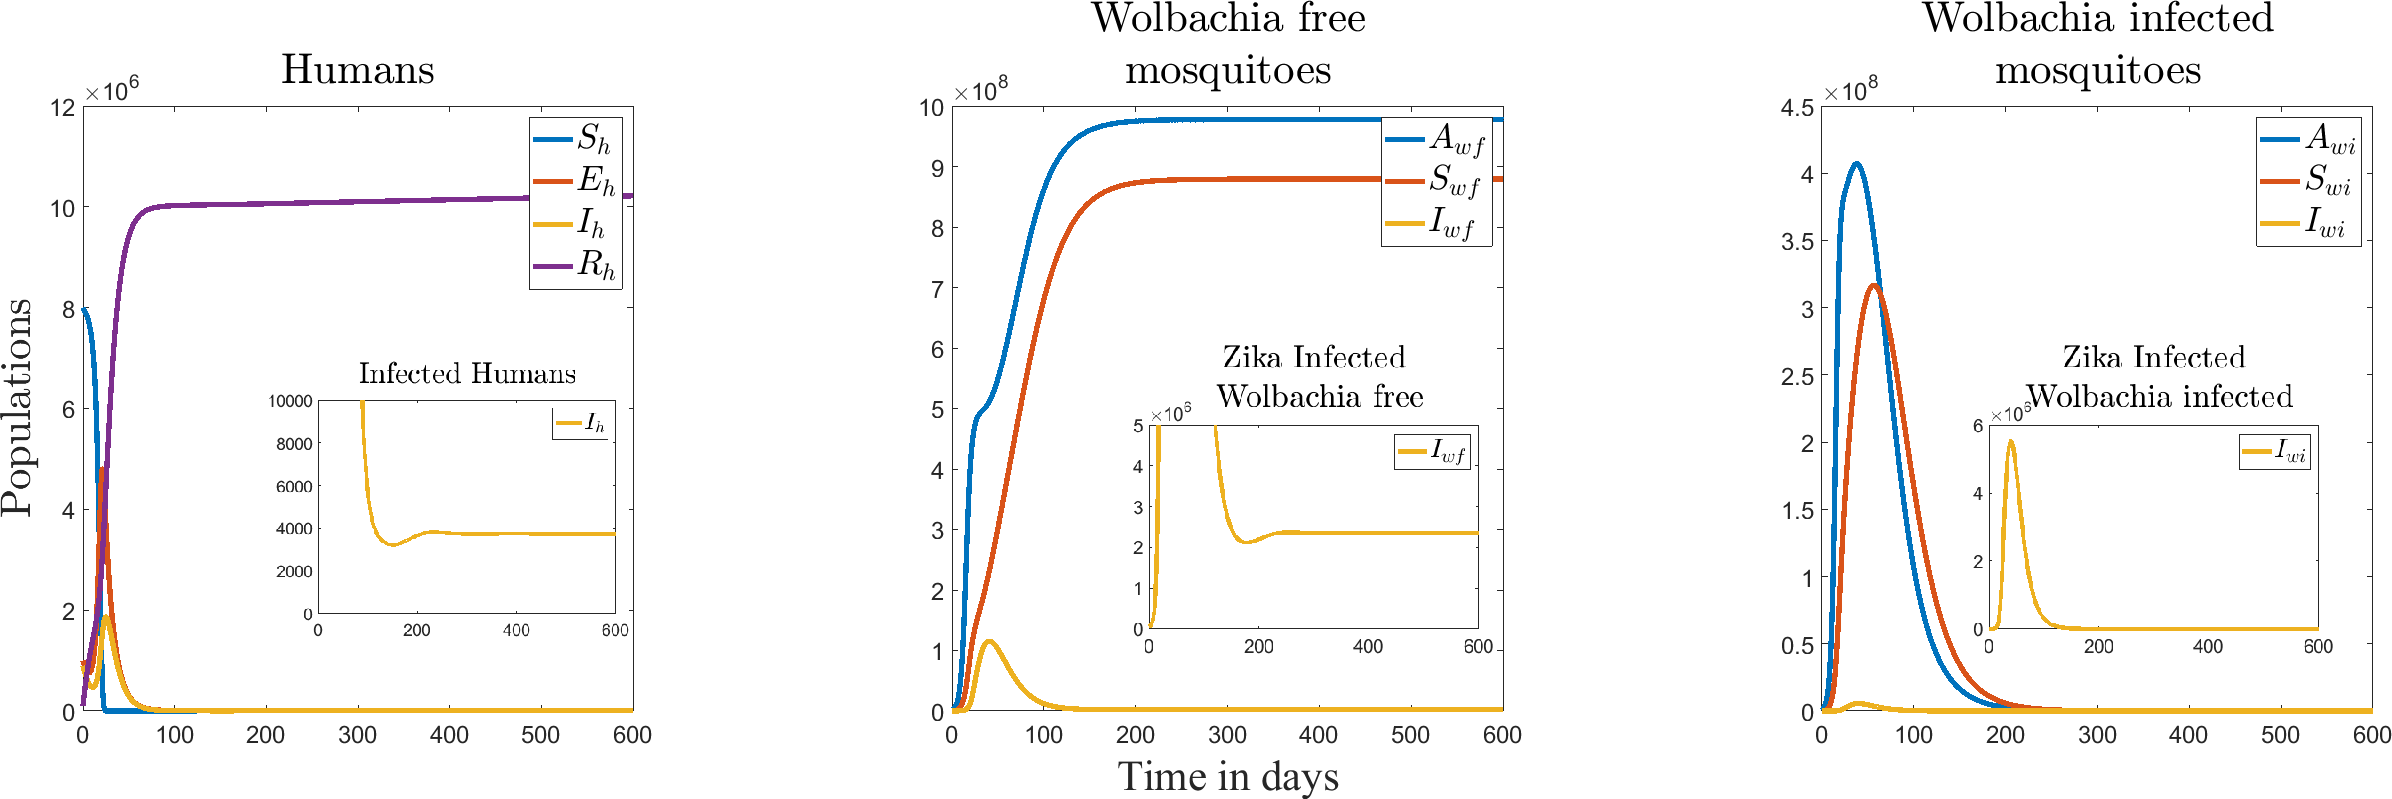
\includegraphics[width=16cm,height=4.5cm]{NewModel6.png}
%\caption{Endemic Zika in humans and \textit{Wolbachia} free mosquitoes. Figure is obtained using initial conditions given in Table \ref{init-cond-dis-present-table} and baseline values from Table \ref{tab: param-table} and Table \ref{tab: param_mosq_table}  with two changes($b=1.25$, $K=10^9$)}
%\label{e4allnice}
%\end{figure}

\subsubsection{Zika is eradicated when \textit{Wolbachia} infection is established }\label{dissecond}
If we allow for the \textit{Wolbachia} infected mosquitoes to establish in the wild mosquito population we get that the disease is eradicated.  
We keep the same parameters as in section \ref{disfirst} and change only the initial condition from $A_{wf}(0)= 2,500,000$ to $A_{wf}(0)=500,000$ and $A_{wi}(0)=500,000$ to  $A_{wi}(0)=1,500,000$ we can see in Figure \ref{wpe4} that the \textit{Wolbachia} infected mosquitoes persist and the disease is eradicated in humans and wild mosquitoes in around 300 days. Zika is eradicated in \textit{Wolbachia} infected mosquitoes in around 380 days. The peak of 1 million Zika infected humans is reached in 40 days. In the field this would corresponds to a strategy of decreasing the number of breeding sites of wild mosquitoes before releasing \textit{Wolbachia} infected aquatic stage.

\begin{figure}[H]
\centering
    % This file was created by matlab2tikz.
%
%The latest updates can be retrieved from
%  http://www.mathworks.com/matlabcentral/fileexchange/22022-matlab2tikz-matlab2tikz
%where you can also make suggestions and rate matlab2tikz.
%
\definecolor{mycolor1}{rgb}{0.00000,0.44700,0.74100}%
\definecolor{mycolor2}{rgb}{0.85000,0.32500,0.09800}%
\definecolor{mycolor3}{rgb}{0.92900,0.69400,0.12500}%
\definecolor{mycolor4}{rgb}{0.49400,0.18400,0.55600}%
%
\begin{tikzpicture}

\begin{axis}[%
width=1.1in,
height=1.5in,
at={(0in,0.108in)},
scale only axis,
xmin=0,
xmax=600,
ymin=0,
ymax=10000000,
ylabel={Population},
axis background/.style={fill=white},
title style={font=\bfseries, yshift=1.75ex},
title={Humans},
legend style={legend cell align=left, align=left, draw=white!15!black}
]
\addplot [color=mycolor1, line width=1.5pt]
  table[row sep=crcr]{%
0	8000000\\
0.443013366311789	7991612.52431396\\
1.1075335862115	7978072.58356399\\
1.92335491906852	7959901.08409989\\
2.73917625192553	7939926.25892732\\
3.24526907037944	7926546.10933092\\
3.75136188790202	7912330.61046799\\
4.25745470635593	7897204.0511693\\
4.76354752480984	7881084.43349191\\
5.39288912247866	7859517.67215684\\
6.02223072014749	7836084.29858074\\
6.65157231781632	7810581.6217319\\
7.28091391548514	7782797.35651307\\
7.96966735832393	7749511.91774629\\
8.6584208002314	7712925.12595558\\
9.34717424307019	7672731.10869713\\
10.035927685909	7628620.08903662\\
10.7026429194957	7581898.53637824\\
11.3693581540138	7530945.83807506\\
12.0360733885318	7475498.31635554\\
12.7027886221185	7415302.0968322\\
13.2980269575492	7357352.72463003\\
13.8932652929798	7295271.32886579\\
14.4885036284104	7228912.07214029\\
15.0837419629097	7158144.80990056\\
16.1171550098807	7024483.08252179\\
17.1505680559203	6876709.23715456\\
18.0398172717541	6738016.30601007\\
18.929066487588	6588561.0238766\\
19.6827749377117	6453488.51529216\\
20.7757545858622	6244155.59872001\\
21.7935681771487	6035382.00985405\\
22.7764504142106	5821846.59643591\\
23.7589354244992	5597653.64253907\\
25.0749843101948	5282675.300731\\
26.399512947537	4952105.6318193\\
28.3718342324719	4444232.75032054\\
31.4275455903262	3655490.60703668\\
32.8448008866981	3303498.27918286\\
34.2165016271174	2978189.43261346\\
35.2840271508321	2737953.01682429\\
36.3212660383433	2516799.15284991\\
37.3263936983421	2314864.75364276\\
38.3069109534845	2130089.71104216\\
39.2736066738144	1959932.96181958\\
40.2305231215432	1803232.39579611\\
41.1724725756794	1660203.73550598\\
42.093238373287	1530850.53318843\\
42.9948081066832	1413835.79203291\\
43.8865317786112	1307056.29027858\\
44.775442509912	1209016.56127758\\
45.658975398168	1119400.6532541\\
46.5288160694763	1038319.78645358\\
47.3818113207817	965235.9490432\\
48.2246802514419	898836.511192287\\
49.0669043790549	837847.513219107\\
49.9101571813226	781751.64045504\\
50.746540277265	730646.40175123\\
51.5684096049517	684482.888064335\\
52.3781835064292	642620.450730074\\
53.1860743965954	604154.030262295\\
53.998547851108	568526.587024544\\
54.8107346557081	535727.890939107\\
55.612159576267	505898.976956616\\
56.3997037168592	478840.790282336\\
57.1818239865825	454002.161753755\\
57.969010097906	430884.225595662\\
58.7615649718791	409361.918912601\\
59.5488904314116	389582.77057216\\
60.3222349947318	371583.725861046\\
61.0856298226863	355095.162882968\\
61.8514950517565	339730.158769637\\
62.6263183718547	325291.475941056\\
63.4026411678642	311853.474662839\\
64.1675793994218	299541.437746201\\
64.9186335941777	288281.389680633\\
65.6670397398993	277816.341659395\\
66.4248843481764	267930.505776423\\
67.190799719654	258612.525433853\\
67.9508711863309	249985.079350276\\
68.6953457752243	242089.170770169\\
69.4307487932965	234789.7091882\\
70.1724670575932	227895.73687782\\
70.926919657737	221331.993437796\\
71.6832736562937	215174.044230444\\
72.4258456788957	209511.145515452\\
73.3352602282539	203054.849545217\\
74.0662085311487	198220.394166807\\
74.810103838332	193601.908478726\\
75.559621937573	189236.006450451\\
76.4798473166302	184242.674112218\\
77.3798831868917	179721.267431321\\
78.2862913347781	175502.047624169\\
79.0300981383771	172272.307540979\\
79.7751708244905	169233.276487487\\
80.6803209055215	165788.162858609\\
81.5702423742041	162646.870599067\\
82.4766108673066	159680.03529831\\
83.2181124417111	157415.656673787\\
84.1372305266559	154798.617572826\\
85.0236336225644	152460.640161674\\
85.9103718427941	150291.931149657\\
86.6395685421303	148628.004902023\\
87.3788497745991	147044.680062523\\
88.2854922022671	145237.01636551\\
89.1620239447802	143621.237070329\\
90.0488743614405	142109.905706397\\
90.7814866304398	140949.528943128\\
91.5196515526623	139856.501248621\\
92.2385906856507	138861.653056142\\
93.1087735164911	137744.594827504\\
93.8124413276091	136907.369299609\\
94.5398027123883	136100.812615436\\
95.2778883185238	135340.542740486\\
95.9993091262877	134651.310242237\\
96.6955904746428	134034.190884802\\
97.3877663938329	133465.365840949\\
98.1021063113585	132922.872838746\\
98.8391083758324	132408.397498945\\
99.5709742726758	131940.835800383\\
100.27462727204	131530.128291077\\
100.96015019156	131164.96985859\\
101.659145425074	130826.611902368\\
102.202262001112	130586.438857776\\
102.760294103064	130359.59781713\\
103.311875623651	130154.548198959\\
103.844367697835	129974.062683439\\
104.361772185192	129814.588116266\\
104.868090944365	129673.216372988\\
105.389051378705	129542.442788268\\
105.930156282149	129421.882054163\\
106.484533867799	129313.974493925\\
106.858386190608	129249.861466324\\
107.223980383947	129193.732454613\\
107.581316448748	129145.009262303\\
107.928900241852	129103.312785101\\
108.26673176419	129068.058028845\\
108.60469336994	129037.883516366\\
108.942785058171	129012.692413204\\
109.291006927378	128991.863237763\\
109.649358979426	128975.737167471\\
109.82853500545	128969.658188796\\
110.016392207704	128964.684692476\\
110.204249409959	128961.128603443\\
110.392106611282	128958.974154047\\
110.579963813536	128958.205774555\\
110.763857169077	128958.781326039\\
110.947750523686	128960.656078949\\
111.131643879227	128963.815950654\\
111.315537233837	128968.247031618\\
111.487327835523	128973.522806414\\
111.659118436277	128979.884892675\\
112.002699639648	128995.82430244\\
112.334773421288	129015.236720541\\
112.666847203858	129038.510726159\\
113.013327531517	129066.830399089\\
113.359807859175	129099.190066997\\
113.731278830208	129138.279250615\\
114.102749802172	129181.821606657\\
114.668001201935	129256.407854437\\
115.210738997906	129337.216812827\\
115.730823051184	129422.841859211\\
116.395477811806	129543.553102933\\
117.078126139939	129680.248835718\\
117.810222770087	129840.608085925\\
118.565473726019	130020.359586213\\
119.286215113476	130204.90168466\\
120.119292449206	130433.352435034\\
120.965752530843	130681.36949618\\
121.893433596939	130970.705558239\\
122.829694503918	131280.373282027\\
123.842411668971	131634.250132315\\
124.850974312983	132005.167738779\\
125.979978960007	132441.024747775\\
127.24004674796	132951.658090185\\
128.5602382496	133512.200671801\\
129.869307277724	134092.042052846\\
131.296331886202	134749.419211582\\
132.80159910582	135469.285361527\\
134.328943988308	136225.282837832\\
135.972185223363	137065.053840715\\
137.847069874406	138053.699402438\\
139.861757511273	139148.821657028\\
141.932897917926	140306.36985582\\
144.08340384718	141538.679298621\\
146.526317025535	142971.850944035\\
149.129220906645	144533.100977219\\
152.024630011059	146305.722981662\\
155.059787871316	148198.70886452\\
158.501800836064	150381.833037021\\
162.25051332172	152796.051995539\\
166.426129208878	155521.741384267\\
171.249476006255	158708.29471394\\
176.853980652057	162450.230894972\\
183.297960315831	166791.064401318\\
191.287494871765	172212.567247038\\
201.51594900433	179193.906171473\\
215.77665275801	188968.750313238\\
241.41480105184	206587.469743619\\
302.810415168293	248782.776411797\\
343.717280043289	276853.660730123\\
384.06861892622	304504.589371673\\
424.196797434241	331964.192545002\\
464.420282660984	359450.598124419\\
504.526563111693	386818.668365643\\
544.760930150747	414235.824736632\\
584.962541379966	441592.380609708\\
600	451815.309304551\\
};
\addlegendentry{$S_h$}

\addplot [color=mycolor2, line width=1.5pt]
  table[row sep=crcr]{%
0	1000000\\
0.44301336677745	965037.977641001\\
1.10753358667716	916347.073228197\\
1.92335491906852	862321.987804045\\
2.73917625192553	814265.110165955\\
3.24526906991377	787324.359137399\\
3.75136188836768	762528.855082863\\
4.25745470635593	739847.275230286\\
4.76354752480984	719254.44373838\\
5.39288912247866	696535.618403852\\
6.02223072014749	677013.925956029\\
6.65157231781632	660692.660383926\\
7.28091391548514	647580.410972656\\
7.96966735785827	636927.924634171\\
8.65842080069706	630177.845041381\\
9.34717424307019	627369.046942171\\
10.0359276854433	628535.585112981\\
10.7026429194957	633478.764347113\\
11.3693581540138	642198.96179336\\
12.0360733880661	654710.114203509\\
12.7027886221185	671011.011777509\\
13.2980269575492	688752.415949646\\
13.8932652929798	709481.63811552\\
14.4885036279447	733168.601767798\\
15.0837419633754	759767.886229345\\
15.6004484863952	785173.784626349\\
16.1171550098807	812687.745186523\\
16.6338615329005	842258.880837164\\
17.5951926638372	902533.667761127\\
18.4844418796711	964033.459267514\\
19.3059207126498	1025355.26203199\\
20.0596291632392	1085060.9528755\\
21.1150257829577	1173465.17869501\\
22.4488230017014	1291475.13493373\\
24.4137930222787	1472316.58376111\\
26.0678442721255	1623867.50377476\\
27.062850296963	1711504.96195145\\
28.0445882482454	1793434.25879732\\
29.0052312077023	1867761.28350579\\
29.6386281833984	1912944.32975922\\
30.243825356476	1952888.82516304\\
30.8490225295536	1989393.02135374\\
31.4275455903262	2020840.29685087\\
32.0060686510988	2048724.17524067\\
32.5652234749869	2072138.6924698\\
33.1243782988749	2091962.11816419\\
33.3974091308191	2100310.32150331\\
33.670439963229	2107774.59513178\\
33.9434707951732	2114349.47487865\\
34.2165016271174	2120031.19340104\\
34.4833830082789	2124719.7468245\\
34.7502643894404	2128552.60583164\\
35.0171457701363	2131530.91381375\\
35.2840271512978	2133657.28328175\\
35.5433368729427	2134911.15788499\\
35.8026465945877	2135369.62578676\\
36.0619563162327	2135038.91479253\\
36.3212660378776	2133926.42285213\\
36.5725479531102	2132110.58766253\\
36.8238298678771	2129577.42502207\\
37.0751117831096	2126336.60099474\\
37.3263936978765	2122398.65196237\\
37.5715230116621	2117896.27010788\\
37.8166523259133	2112752.61161368\\
38.3069109539501	2100589.86094546\\
38.7902588136494	2086235.00355594\\
39.2736066738144	2069640.64842472\\
39.7520648976788	2051120.09288433\\
40.2305231210776	2030632.14329857\\
40.9369852123782	1997038.5314472\\
41.6328554744832	1960397.4391854\\
42.3186308066361	1921217.68379891\\
43.2177390246652	1865853.12421318\\
44.1087594614364	1807254.01177453\\
45.2172089545056	1730327.53890207\\
46.5288160694763	1635300.45759276\\
49.0669043790549	1446209.50461374\\
51.1574749411084	1292118.99368866\\
52.5801562289707	1190813.27098756\\
53.9985478506424	1093914.02510459\\
55.2114471159875	1014855.85280626\\
56.3997037173249	941119.704287698\\
57.5754170422442	871959.695328158\\
58.5634262533858	816830.076706961\\
59.5488904318772	764578.596627\\
60.5130837019533	716086.270628088\\
61.4685624372214	670565.181626\\
62.4326125415973	627139.324059729\\
63.4026411678642	585915.670544568\\
64.3553429483436	547765.840874853\\
65.2928366670385	512406.135625176\\
66.2354231961071	478950.842110461\\
67.190799719654	447096.245227229\\
68.1369898337871	417494.45085844\\
69.0630472842604	390308.965841199\\
69.987037491519	364858.576944232\\
70.9269196572714	340598.430166014\\
71.8689166619442	317843.148814755\\
72.7896182504483	297028.000317525\\
73.6989990412258	277775.002368037\\
74.6222287821583	259481.274272263\\
75.5596219371073	242122.677455951\\
76.4798473166302	226202.452149675\\
77.3798831873573	211640.694700957\\
78.2862913343124	197923.493806401\\
79.2163663101383	184775.952249721\\
80.1389037836343	172605.148944515\\
81.0356892291456	161552.30527942\\
81.9271113583818	151278.057989059\\
82.8458890602924	141384.800679025\\
83.7707273294218	132094.0507274\\
84.6702065481804	123658.826683328\\
85.550938822329	115936.287146571\\
86.4546867031604	108528.501980123\\
87.3788497745991	101459.036249991\\
88.2854922018014	94987.4586446299\\
89.1620239452459	89138.7463869364\\
90.0488743609749	83602.6454694862\\
90.9670639918186	78248.5603672201\\
91.8825172274373	73267.3052258659\\
92.762512548361	68792.388359176\\
93.6337379058823	64644.7256838181\\
94.5398027119227	60609.8882723982\\
95.4619538513944	56775.6421581781\\
96.3525988673791	53315.501304396\\
97.213174237404	50184.0093890517\\
98.1021063113585	47153.564021809\\
99.0250316052698	44212.2350705336\\
99.9309937111102	41514.3666604189\\
100.789205512032	39120.1923695686\\
101.659145425074	36843.1534424452\\
102.574283402879	34599.9492778121\\
103.495736129582	32488.2966998187\\
104.361772184726	30629.1233252482\\
105.215397900436	28907.797180864\\
106.113881994504	27207.5506091327\\
107.045312351547	25557.7269652556\\
107.928900241852	24091.6634713979\\
108.77373921359	22774.1536645098\\
109.649358979426	21490.0141349905\\
110.579963813536	20210.1429875316\\
111.487327835057	19040.9026695662\\
112.334773421753	18014.4369553565\\
113.18656769488	17042.4759693476\\
114.102749801707	16059.7011424978\\
115.033578666393	15123.3951015938\\
115.896586441435	14307.6526254918\\
116.730206990149	13564.4957434814\\
117.619789819699	12817.013529703\\
118.565473726019	12070.7064887071\\
119.455100183841	11411.1574047171\\
120.44571457291	10722.0147458152\\
121.327682286967	10145.997543049\\
122.273915923666	9564.7415980068\\
123.180287008639	9041.35833241418\\
124.170586832799	8504.39793147938\\
125.033664706629	8064.23908172594\\
125.979978960007	7609.49472018098\\
126.909031664953	7189.62379221525\\
127.891665046569	6772.33284793515\\
128.908208236564	6367.7127606296\\
129.869307277258	6008.79576039826\\
130.791926762089	5684.4561800682\\
131.771758911666	5360.29581522476\\
132.80159910582	5040.6589739034\\
133.764700500295	4759.99588674679\\
134.695848098025	4504.34855792066\\
135.657399703283	4255.54770348081\\
136.672735388856	4008.53116700938\\
137.652872470673	3784.40148581099\\
138.575821795035	3585.40620246157\\
139.53419369692	3390.39343867172\\
140.567224019207	3192.6265065195\\
141.548932632431	3015.89205161482\\
142.480987855233	2857.57725402294\\
143.420759563334	2706.74273234\\
144.436786065809	2553.00285746809\\
145.437074153218	2410.53805343388\\
146.359200679697	2286.54848297918\\
147.295890843496	2167.38953999383\\
148.333836584352	2042.86848143768\\
149.33431326272	1929.87209806591\\
150.419697751291	1814.59766358836\\
151.3372068014	1722.7288182932\\
152.203042679001	1640.44940365292\\
153.222665195819	1548.74553137925\\
154.307217472699	1456.99944627285\\
155.385478230659	1371.33809897397\\
156.299304883461	1302.81181763485\\
157.329186042305	1229.79497476527\\
158.351651447825	1161.46378983557\\
159.252689789049	1104.48569698911\\
160.182130390313	1048.7141491482\\
161.207431352232	990.532360896934\\
162.250513321254	934.731674014591\\
163.315507366788	881.074890865944\\
164.273675242439	835.495841221884\\
165.2977758497	789.439520124812\\
166.278723077383	747.755270240828\\
167.202033225447	710.573114870582\\
168.170498130377	673.595606368501\\
169.193263742141	636.670250224881\\
170.173063231166	603.229676687624\\
171.249476006255	568.547277045436\\
172.266148334369	537.652822748758\\
173.263173941523	509.012123777065\\
174.350574500859	479.538131079171\\
175.339316071477	454.244002683554\\
176.378992638085	429.10475606937\\
177.328968666028	407.369349316228\\
178.392053510062	384.365730049554\\
179.402636206243	363.718791185878\\
180.440023217816	343.691210750956\\
181.539852439426	323.675102052279\\
182.48906097142	307.350455555134\\
183.500287681352	290.873803392518\\
184.478472217917	275.785313649103\\
185.403125074226	262.250166606624\\
186.370433549397	248.808020978235\\
187.375122837257	235.582303538918\\
188.368453848176	223.203747441992\\
189.302225429565	212.166420133784\\
190.264518881217	201.367652425077\\
191.2874948713	190.495002055541\\
192.396252060309	179.377912033815\\
193.358425295446	170.261861249804\\
194.359144382179	161.275500220712\\
195.348046031315	152.864727835171\\
196.433089102153	144.143669476267\\
197.41659550136	136.672372216824\\
198.456742213108	129.194574088324\\
199.575175430626	121.612796945963\\
200.624177359976	114.909133207053\\
201.709359892644	108.365283368155\\
202.719187134877	102.613062302582\\
203.768455748446	96.961319158785\\
204.731363837607	92.0506667043082\\
205.842584976461	86.6936849360354\\
206.801100670826	82.3253723299131\\
207.784231619909	78.0746826748364\\
208.781119890045	73.9897533878684\\
209.885423835367	69.7150011695921\\
210.853084303904	66.1737532676198\\
211.87921364978	62.6158302435651\\
213.01651398791	58.8966064122505\\
214.073099024594	55.6405331143178\\
215.135019245557	52.5502423536964\\
216.297382043675	49.3649782962166\\
217.404525150079	46.5115681765601\\
218.387551529333	44.1172124431469\\
219.388665003236	41.8060149415396\\
220.493120155297	39.397078695707\\
221.456116082147	37.4107429310679\\
222.482920964714	35.4034694870934\\
223.625262007117	33.297183026094\\
224.679917677771	31.4644733755849\\
225.737450928893	29.728474532254\\
226.902305958793	27.9274087757803\\
228.011572277173	26.3142426223494\\
229.205506364349	24.6823405679315\\
230.341626737732	23.2239116793498\\
231.55677978741	21.7596588665619\\
232.676709682681	20.4923691242002\\
233.88561022887	19.2074398836121\\
235.132761358749	17.9665666478686\\
236.344452252612	16.8381063090637\\
237.661942460109	15.6917117019184\\
238.990340229589	14.6151428692974\\
240.406980144326	13.5486342343502\\
241.84898144519	12.5432351729833\\
243.2820884916	11.6182532906532\\
244.663477061316	10.7915243301541\\
246.196654117201	9.94291497347876\\
247.806290262844	9.12397106923163\\
249.409452690743	8.37563028046861\\
251.012497941498	7.68895063782111\\
252.768076981883	7.00159370806068\\
254.508448324632	6.38108829408884\\
256.344097666908	5.78633000422269\\
258.197787157726	5.24217791808769\\
260.201640196145	4.71157188341022\\
262.314257714432	4.21043486660346\\
264.493310778867	3.74952834332362\\
266.949663607404	3.29040004080161\\
269.478617254179	2.87658509984612\\
272.223564827349	2.48632879974321\\
275.098858984653	2.13440110255033\\
278.201699043624	1.81049590790644\\
281.599363781977	1.51212149206549\\
285.295432075392	1.24330543866381\\
289.372119973414	1.00207737321034\\
294.130827172659	0.779235241468996\\
299.412754595745	0.589621459599584\\
305.627028034069	0.42491661477834\\
313.042676703539	0.287619329988956\\
322.198761771433	0.177825456485152\\
334.067087295465	0.0955096911638975\\
350.890807040501	0.0397051777690649\\
379.431357761379	0.00904055591672659\\
458.872145301197	0.000156919937580824\\
600	1.504085958004e-07\\
};
\addlegendentry{$E_h$}

\addplot [color=mycolor3, line width=1.5pt]
  table[row sep=crcr]{%
0	900000\\
0.664520106511191	848533.437660982\\
1.51544425287284	787476.342996196\\
2.33126558538061	733780.28220791\\
3.24526907003019	678923.058370382\\
3.75136188825127	650836.60498159\\
4.25745470658876	624311.741783275\\
4.76354752480984	599300.041264919\\
5.39288912247866	570242.04067678\\
6.02223072014749	543374.121453894\\
6.65157231781632	518624.163207306\\
7.28091391548514	495933.033167166\\
7.96966735797469	473401.207009529\\
8.65842080046423	453211.859478708\\
9.34717424295377	435312.183433181\\
10.0359276854433	419665.376189295\\
10.7026429197285	406639.09302703\\
11.3693581538973	395667.935306319\\
12.0360733880661	386728.650429151\\
12.7027886223514	379806.650604992\\
13.2980269575492	375321.409455065\\
13.8932652927469	372420.825921445\\
14.4885036279447	371092.900457862\\
15.0837419632589	371326.586850549\\
15.6004484865116	372785.997820736\\
16.1171550097642	375402.148776148\\
16.6338615330169	379163.656469543\\
17.1505680562695	384057.49384174\\
17.5951926639536	389163.621772319\\
18.0398172717541	395086.516627321\\
18.4844418794382	401814.352177499\\
18.9290664872387	409333.602273618\\
19.3059207126498	416315.253945695\\
20.0596291633556	431911.955790297\\
20.7757545858622	448679.149091331\\
21.4542969800532	466235.297870661\\
22.1211955895415	484986.269294567\\
22.7764504142106	504762.754682424\\
23.7589354243828	536705.373099144\\
24.7443886660039	571156.885807651\\
25.7361755972961	607819.28109882\\
27.062850296963	659087.08919969\\
30.8490225295536	807373.774821404\\
32.0060686510988	849347.039110026\\
32.8448008869309	877743.977274078\\
33.6704399631126	903647.862475905\\
34.4833830082789	926871.263864727\\
35.0171457702527	940763.205122328\\
35.5433368729427	953332.835255488\\
36.0619563162327	964576.602227014\\
36.5725479528774	974493.502353182\\
37.0751117828768	983103.883603061\\
37.5715230118949	990462.599352586\\
38.0617816398153	996593.609023548\\
38.5485848836834	1001552.02022073\\
38.7902588136494	1003593.51875862\\
39.0319327437319	1005355.90847819\\
39.2736066736979	1006839.29639943\\
39.5128357855137	1008033.31475526\\
39.752064897446	1008955.1526981\\
39.9912940093782	1009605.8831606\\
40.2305231213104	1009986.84046264\\
40.4660104849609	1010099.93027104\\
40.7014978486113	1009955.03866723\\
40.9369852122618	1009554.25879069\\
41.1724725759123	1008899.90026621\\
41.4026640253142	1008017.60530731\\
41.6328554747161	1006898.05915626\\
41.8630469240015	1005544.07063959\\
42.0932383734034	1003958.61631459\\
42.5440232401015	1000195.5905836\\
42.9948081067996	995582.910645556\\
43.4406699425308	990212.16065287\\
43.886531778262	984066.523268286\\
44.3309871441452	977199.497168523\\
44.7754425100284	969624.728195345\\
45.4380921764532	957088.614806083\\
46.093895734055	943316.431217418\\
46.7420648824191	928480.391598139\\
47.5925285536796	907353.566959977\\
48.4352362831123	884786.749730225\\
49.2777175795054	860842.284256965\\
50.328348729061	829396.987937004\\
51.5684096054174	790568.779892466\\
53.3891927597579	731497.087962965\\
57.3786205144133	601186.924824142\\
58.9583963368786	551604.125610424\\
60.3222349947318	510435.442293848\\
61.6600287442561	471788.093209604\\
62.8203990708571	439792.304328815\\
63.9763448418817	409407.016486895\\
65.1057351306081	381197.786955387\\
66.2354231958743	354462.007175003\\
67.3808175862068	328866.923523466\\
68.5092271281173	305124.977842672\\
69.6161783593707	283228.424091697\\
70.5496933575487	265809.126779713\\
71.4941851564217	249131.739221278\\
72.4258456788957	233584.968293399\\
73.3352602282539	219245.784181301\\
74.251548614935	205603.033404822\\
75.1858539512614	192490.847500103\\
76.1173007265897	180187.553041255\\
77.0215570001164	168944.971312387\\
77.9226688076742	158397.339681643\\
78.8441464377102	148256.037415111\\
79.7751708240248	138638.676290914\\
80.6803209054051	129863.447847677\\
81.5702423746698	121759.400407421\\
82.4766108668409	114010.7277933\\
83.4042241325369	106579.288250834\\
84.3148892002646	99746.8146468955\\
85.1994020221755	93524.8365579674\\
86.0900883537252	87648.3667781984\\
87.0093322203029	81968.917669512\\
87.9274089530809	76664.1141122943\\
88.8132788856747	71872.4952104229\\
89.6904030303704	67425.6541938877\\
90.5959092684789	63126.667342918\\
91.5196515526623	59027.6181571031\\
92.4132313064765	55320.4837635858\\
93.281903999974	51944.7650160475\\
94.1698481715284	48712.136310221\\
95.0938227854203	45567.5361246362\\
95.9993091259385	42688.7976539958\\
96.867086277809	40106.3495033766\\
97.7369507058756	37680.0018590954\\
98.6531851462787	35288.8395902059\\
99.5709742727922	33051.8200086945\\
100.446444052272	31055.828550861\\
101.302039549802	29226.8563752911\\
102.202262001229	27424.055059527\\
103.128015116672	25691.6399031061\\
104.018683481263	24133.4636359994\\
104.868090944132	22740.1972469796\\
105.746430568979	21388.5677250836\\
106.671460029203	20056.6572871603\\
107.581316448282	18832.1373182324\\
108.435647525941	17754.4750268599\\
109.291006927611	16740.9963280387\\
110.204249409609	15726.5982539946\\
111.131643878762	14763.2649756308\\
112.002699639415	13915.6689801238\\
112.840087367687	13149.7076600638\\
113.731278830324	12383.8075388308\\
114.668001201702	11629.9806893247\\
115.565059660701	10953.996015048\\
116.395477811573	10365.6734930496\\
117.258680699626	9789.8767641203\\
118.191088670515	9206.25151044712\\
119.117330042296	8663.30762057367\\
119.956081387238	8201.24725926679\\
120.792406545021	7766.77398260368\\
121.704849826638	7320.79546874447\\
122.654398251208	6885.74059234734\\
123.51785939699	6514.18240419414\\
124.502384890337	6116.62400059728\\
125.399045494734	5777.16405366501\\
126.357475502533	5436.56074822519\\
127.240046748077	5141.93010166136\\
128.212268261821	4837.08165775239\\
129.100425493787	4575.49425620702\\
130.061537289061	4309.40703547036\\
130.964891486801	4074.3803252608\\
131.936448145891	3836.84151917114\\
132.801599105704	3637.76811735565\\
133.764700500411	3429.06776026776\\
134.695848097908	3239.41234162403\\
135.657399703166	3055.26087250572\\
136.672735388624	2872.86376232433\\
137.65287247079	2707.75726570736\\
138.575821795035	2561.4914899125\\
139.534193696687	2418.46208551666\\
140.567224019323	2273.73792522843\\
141.548932632199	2144.69345720822\\
142.48098785535	2029.33829285111\\
143.420759563334	1919.65223485616\\
144.436786065693	1808.08078725846\\
145.437074153335	1704.90397235076\\
146.359200679814	1615.27915623912\\
147.295890843612	1529.30156852165\\
148.333836584468	1439.62293997686\\
149.334313262487	1358.39743809297\\
150.266046605422	1287.06977431127\\
151.18502159731	1220.55334901798\\
152.203042679233	1151.0481648118\\
153.222665195935	1085.56850372313\\
154.143110731733	1029.79505559441\\
155.059787871316	977.212306570844\\
156.103259452153	920.742578798439\\
157.120727110305	868.941781534464\\
158.201502059586	817.221509487252\\
159.252689788933	769.975338406395\\
160.182130390429	730.559141083853\\
161.207431352115	689.490926743252\\
162.250513321254	650.153806196526\\
163.315507366788	612.375570140081\\
164.273675242672	580.321997578489\\
165.297775849933	547.96833910339\\
166.278723077499	518.717371786945\\
167.202033225563	492.651280414662\\
168.17049813061	466.753045230173\\
169.193263742258	440.916029206477\\
170.173063231399	417.539007762214\\
171.249476006255	393.316001486965\\
172.266148334485	371.757884025457\\
173.263173941756	351.78895030485\\
174.350574500742	331.25588983635\\
175.339316071593	313.648590498371\\
176.378992637969	296.161990702967\\
177.328968665912	281.053577195271\\
178.392053510295	265.074399161153\\
179.40263620636	250.741837447393\\
180.440023217816	236.848004926578\\
181.368124048226	225.081994224223\\
182.287143721478	214.015993409907\\
183.29796031618	202.48115444649\\
184.330581144546	191.348309262539\\
185.403125074459	180.44147610967\\
186.370433549397	171.146028497955\\
187.375122837373	162.004435224109\\
188.368453848176	153.452215552214\\
189.302225429565	145.829791860422\\
190.2645188811	138.375034718425\\
191.287494871416	130.872227171552\\
192.396252060076	123.20384893904\\
193.358425295679	116.918132101884\\
194.359144382412	110.723967646016\\
195.348046031198	104.928489301121\\
196.433089102153	98.9212187941885\\
197.416595501476	93.7764664342394\\
198.45674221334	88.6287888077786\\
199.575175430742	83.4111421245616\\
200.624177359859	78.7991700604325\\
201.709359892411	74.2984099352034\\
202.719187134993	70.3431683388771\\
203.76845574833	66.4579874395858\\
204.731363837374	63.0830503049074\\
205.842584976461	59.4022237502504\\
206.801100670942	56.4013950820081\\
207.784231620026	53.4819609625265\\
208.781119889813	50.676934698713\\
209.885423835251	47.7421621000394\\
210.853084304137	45.3114414950833\\
211.879213650012	42.8697173115797\\
213.016513988026	40.3177801923594\\
214.073099024827	38.0840485712979\\
215.13501924579	35.9644148277584\\
216.297382043558	33.7800230230205\\
217.404525150312	31.823550090543\\
218.599181573489	29.8399949569721\\
219.737010218203	28.0664472682402\\
220.782047832152	26.5310196207138\\
221.865286456188	25.0285014375113\\
223.108313369215	23.4093988983659\\
224.230673465994	22.0380716156214\\
225.361123868264	20.738429982448\\
226.594777959632	19.4078373261727\\
227.824889956391	18.1664577849442\\
228.994210655917	17.0604464773787\\
230.341626737965	15.8695854548132\\
231.556779787526	14.8673810355831\\
232.881230538595	13.8472881825874\\
234.229825165938	12.8807886524592\\
235.591055594268	11.9739127130015\\
236.986746244947	11.1106052863179\\
238.430439489661	10.2833086225437\\
239.810962477117	9.55012473196257\\
241.414801051491	8.76398724352475\\
243.077588643064	8.01747758395504\\
244.835648872657	7.29750575765502\\
246.573229029309	6.64971799612977\\
248.421233276487	6.02398428937886\\
250.205305558047	5.47603492962662\\
252.165043369983	4.93162026302889\\
254.300356194726	4.40008955157828\\
256.496831425349	3.91326696646865\\
258.873078771634	3.44729056942742\\
261.233414354268	3.03958311444148\\
263.879866225994	2.63972265564371\\
266.79693297972	2.25985749799293\\
269.786092765746	1.92744602251332\\
273.075577554177	1.61806153913494\\
276.652162447572	1.33795177110005\\
280.699103359366	1.07922214595601\\
285.090954721323	0.854920783778653\\
290.228459102334	0.651168541051447\\
296.105435756035	0.477110706386156\\
303.021691019298	0.331056681694463\\
311.439502207329	0.212367680040188\\
322.1987617712	0.120567548670806\\
336.864509980311	0.0558718306710944\\
359.943034568103	0.0167555013904348\\
410.095328681055	0.0012563627678901\\
600	9.91858541965485e-08\\
};
\addlegendentry{$I_h$}

\addplot [color=mycolor4, line width=1.5pt]
  table[row sep=crcr]{%
0	100000\\
0.664520107209682	216152.152154885\\
1.51544425264001	355280.33306885\\
2.33126558549702	479313.272003384\\
3.24526906944811	608334.727800077\\
4.25745470635593	740117.058240974\\
5.39288912340999	875579.497901479\\
6.02223072014749	945621.249827554\\
6.65157231874764	1012413.91238757\\
7.28091391548514	1076220.3141636\\
7.96966735832393	1142929.4684119\\
8.65842080116272	1206695.08457877\\
10.0359276849777	1326667.64202272\\
11.3693581540138	1435139.39310139\\
12.7027886230499	1538295.78349116\\
15.0837419629097	1716003.67211602\\
17.1505680568516	1871368.5822068\\
18.4844418801367	1975942.64942644\\
19.682774938643	2074687.92589638\\
20.7757545858622	2169892.69698829\\
21.7935681771487	2263828.62917914\\
22.7764504142106	2360058.74867121\\
23.7589354235679	2462256.47300399\\
24.7443886660039	2571308.68431355\\
25.736175596714	2688118.34420097\\
26.7311816215515	2812768.0828366\\
27.7173422649503	2943920.96182308\\
28.6885327193886	3080607.40110387\\
29.6386281829327	3221552.72660714\\
30.8490225300193	3411284.76865683\\
32.0060686506331	3602888.92569114\\
33.1243782993406	3796961.42404777\\
34.4833830073476	4043395.7578555\\
36.0619563162327	4342015.25841767\\
37.8166523259133	4685766.20893715\\
40.4660104848444	5217655.21969786\\
43.6636008601636	5858048.44765145\\
45.4380921758711	6203020.61654483\\
46.9553136955947	6488156.47620423\\
48.4352362826467	6755527.57473207\\
49.6993439812213	6974378.20984293\\
50.9520076084882	7181861.39603381\\
52.1757400315255	7375063.8161916\\
53.3891927599907	7557090.0416657\\
54.6076879538596	7730147.70972041\\
55.612159576267	7865455.04466575\\
56.5952337849885	7991480.44198987\\
57.5754170417786	8110906.15631669\\
58.5634262543172	8225098.77340719\\
59.5488904323429	8332946.64012592\\
60.5130837019533	8432772.14411179\\
61.4685624372214	8526305.49663698\\
62.432612542063	8615420.53232078\\
63.4026411678642	8699952.16474098\\
64.3553429488093	8778155.92671171\\
65.2928366679698	8850643.78526747\\
66.2354231961071	8919251.61429246\\
67.1907997187227	8984616.71350963\\
68.1369898337871	9045409.40476381\\
69.0630472842604	9101295.18197546\\
69.9870374910533	9153672.90087405\\
70.926919657737	9203663.51589913\\
71.8689166624099	9250617.00055864\\
72.7896182499826	9293628.36196638\\
73.6989990416914	9333469.73826494\\
74.622228782624	9371382.87962379\\
75.559621937573	9407413.93057834\\
76.4798473156989	9440511.30464639\\
77.3798831868917	9470831.34340144\\
78.2862913347781	9499436.67307357\\
79.2163663096726	9526896.49986083\\
80.1389037836343	9552355.54474373\\
81.0356892291456	9575510.45683739\\
81.9271113593131	9597065.0551758\\
82.8458890598267	9617849.57698369\\
83.7707273289561	9637395.34944986\\
84.6702065486461	9655164.6437058\\
85.550938822329	9671452.56022093\\
86.4546867031604	9687094.76876277\\
87.3788497745991	9702039.23184745\\
88.2854922022671	9715733.93904239\\
89.1620239447802	9728121.96171885\\
90.0488743614405	9739857.4148769\\
90.9670639913529	9751215.32843743\\
91.882517227903	9761788.96787827\\
92.7625125478953	9771292.48980245\\
93.633737904951	9780104.13336122\\
94.539802711457	9788677.98958028\\
95.4619538523257	9796826.21159969\\
96.3525988683105	9804178.75222693\\
97.2131742369384	9810831.23900985\\
98.1021063122898	9817266.27978092\\
99.0250316057354	9823508.04326385\\
99.9309937115759	9829228.16505186\\
100.789205512032	9834298.97188492\\
101.659145426005	9839115.54932217\\
102.574283402413	9843853.11504265\\
103.495736129582	9848304.3737175\\
104.361772185192	9852214.99936294\\
105.21539789997	9855827.11404377\\
106.113881994039	9859385.25977073\\
107.045312350616	9862826.77755337\\
107.928900241852	9865874.00129911\\
108.773739213124	9868602.02381964\\
109.649358980358	9871249.79208414\\
110.579963814467	9873875.90997626\\
111.487327834591	9876261.88719981\\
112.334773421288	9878344.45611172\\
113.186567695811	9880304.41718167\\
114.102749802172	9882272.45861934\\
115.033578665927	9884132.60073353\\
115.896586442366	9885739.59560184\\
116.730206990615	9887190.93625582\\
117.619789820164	9888636.82245286\\
118.381521619856	9889795.301411\\
119.286215113476	9891081.36866001\\
120.119292449206	9892184.27726793\\
120.965752530843	9893229.69885979\\
121.704849826172	9894083.92769366\\
122.464157087728	9894907.64086128\\
123.355583261698	9895808.74308245\\
124.17058683373	9896573.71376382\\
125.033664707094	9897325.99990222\\
125.786334471777	9897936.13289988\\
126.541327556595	9898507.42848709\\
127.405554288998	9899113.93635943\\
128.212268261239	9899636.81511362\\
128.908208236098	9900056.06881011\\
129.677077265456	9900486.68140606\\
130.445997312665	9900884.78309466\\
131.137856211513	9901216.51972467\\
131.936448145658	9901569.78261979\\
132.616057477891	9901846.55645603\\
133.370021741837	9902129.17302576\\
134.14549193345	9902394.29939911\\
134.857539618388	9902616.01215947\\
135.500006942078	9902799.01386193\\
136.14732276462	9902967.73701417\\
136.672735389322	9903093.57329071\\
137.262190148234	9903223.33662089\\
137.847069874406	9903340.5933445\\
138.405643239617	9903442.27199201\\
138.916178908199	9903526.70597887\\
139.534193696454	9903618.43625769\\
140.025539418682	9903683.4526449\\
140.567224020138	9903747.28591241\\
141.146395351738	9903806.74103684\\
141.548932632431	9903842.87859558\\
141.932897917926	9903873.4986335\\
142.298291210085	9903899.22997546\\
142.638615265489	9903920.27433297\\
142.953870087862	9903937.30749319\\
143.266128530726	9903951.89214835\\
143.575390595943	9903964.13716456\\
143.906712736934	9903974.87442752\\
144.260094955564	9903983.66738587\\
144.436786064878	9903987.05277761\\
144.637866934761	9903990.09777065\\
144.838947804645	9903992.29314935\\
145.040028672665	9903993.64944673\\
145.241109542549	9903994.17705813\\
145.437074152753	9903993.90370465\\
145.63303876482	9903992.86240807\\
145.829003376886	9903991.06241567\\
146.024967988953	9903988.51285734\\
146.192084334791	9903985.75322645\\
146.526317024603	9903978.64029582\\
146.844047740102	9903969.94126512\\
147.145276475698	9903959.98410191\\
147.459077376872	9903947.87486253\\
147.785450441763	9903933.43640809\\
148.141236780211	9903915.59775826\\
148.526436390355	9903893.86902537\\
148.924128551036	9903868.86127201\\
149.334313262254	9903840.39367488\\
149.902726111934	9903796.57926406\\
150.419697752222	9903752.45769965\\
151.032836392522	9903695.0307625\\
151.667804673314	9903629.93238592\\
152.408595636487	9903547.03239487\\
153.222665196285	9903447.66798768\\
153.979003990069	9903347.9457701\\
154.765556043014	9903237.02226796\\
155.548323409632	9903119.65672086\\
156.495350314304	9902968.8125517\\
157.509727699682	9902797.05899749\\
158.501800835133	9902619.47144458\\
159.612697022036	9902410.00423034\\
160.810408798978	9902172.39514979\\
162.08899846673	9901906.17149185\\
163.315507367253	9901639.44122438\\
164.695937408134	9901326.90648777\\
166.131316946819	9900989.12019448\\
167.745709843934	9900594.87435516\\
169.392589516938	9900178.40431052\\
171.086991576478	9899736.2120444\\
172.905339706689	9899247.65565872\\
174.975327214226	9898675.59516872\\
177.170639328659	9898052.41373981\\
179.402636205778	9897403.42109439\\
181.883309222758	9896666.11615909\\
184.626363290474	9895833.75558142\\
187.56314445287	9894925.53603991\\
190.878854073584	9893882.16929724\\
194.571850595996	9892701.42044282\\
198.66255209595	9891374.80875499\\
203.318769199774	9889845.769803\\
208.589482050389	9888096.04363836\\
214.75736021623	9886029.53092543\\
222.274456830695	9883491.47138464\\
231.72556889616	9880280.59481228\\
244.663477061316	9875864.66883317\\
265.530167650431	9868720.89463999\\
347.75956932269	9840555.88824594\\
388.288400745019	9826699.33098588\\
428.561435334384	9812949.46358853\\
468.760037519038	9799244.18325747\\
509.040952388197	9785530.03817843\\
549.264437612146	9771854.59763209\\
589.370718061924	9758238.03332632\\
600	9754632.44610416\\
};
\addlegendentry{$R_h$}

\end{axis}

\begin{axis}[%
width=1.1in,
height=1.5in,
at={(1.42in,0.108in)},
scale only axis,
xmin=0,
xmax=600,
ymin=0,
ymax=12000000,
xlabel={Time (days)},
axis background/.style={fill=white},
title style={font=\bfseries, yshift=1.25ex},
title={\emph{Wolb.}-free mosq.},
legend style={legend cell align=left, align=left, draw=white!15!black}
]
\addplot [color=mycolor1, line width=1.5pt]
  table[row sep=crcr]{%
0	500000\\
0.443013366311789	799541.886130465\\
1.10753358714283	1215134.69019762\\
2.33126558549702	1962143.21112153\\
3.24526906944811	2562312.57845352\\
3.75136188790202	2922878.45538956\\
4.25745470635593	3307063.06781575\\
4.76354752480984	3716972.59825599\\
5.39288912340999	4264114.66596906\\
6.02223072014749	4850579.47927548\\
6.65157231874764	5472095.26683003\\
7.96966735832393	6858564.09184511\\
9.34717424213886	8331620.04971631\\
10.0359276849777	9028654.47864338\\
10.7026429194957	9651746.02049561\\
11.3693581540138	10200429.3807021\\
12.0360733885318	10654902.2087283\\
12.7027886230499	11001599.2777586\\
13.2980269566178	11212287.3516221\\
13.8932652920485	11323522.3204689\\
14.4885036274791	11334498.2653049\\
15.0837419629097	11249901.318025\\
15.6004484873265	11105405.1068179\\
16.1171550098807	10900578.976878\\
16.6338615324348	10642689.5498817\\
17.1505680568516	10340846.3836459\\
17.5951926633716	10053401.6397067\\
18.4844418801367	9421256.61272538\\
20.0596291627735	8218830.70876264\\
21.4542969800532	7169990.06758867\\
22.4488230012357	6467132.8463228\\
23.431506626308	5820650.50382043\\
24.413793021813	5225770.80796946\\
25.0749843101948	4854626.74739766\\
25.736175596714	4506161.22733278\\
26.3995129466057	4179094.12268683\\
27.0628502964973	3873267.45345824\\
27.7173422649503	3591782.3718201\\
28.3718342315406	3329032.1679424\\
29.0052312072366	3091990.71672127\\
29.6386281829327	2870635.03800034\\
30.2438253574073	2673260.71071762\\
30.8490225300193	2488624.80389433\\
31.716807121411	2244984.68164475\\
32.5652234740555	2028888.00715054\\
33.3974091317505	1836332.36832239\\
34.2165016271174	1664014.65489831\\
35.0171457696706	1510734.93293053\\
35.8026465941221	1373667.64758564\\
36.5725479535758	1251031.74556722\\
37.3263936974108	1141276.7555917\\
38.0617816392332	1043279.2041929\\
38.7902588136494	954305.593570195\\
39.5128357857466	873371.367091011\\
40.2305231206119	799632.068845138\\
40.9369852114469	733019.504934205\\
41.6328554749489	672731.924122773\\
42.3186308071017	618077.687305145\\
42.9948081076145	568461.453584917\\
43.6636008601636	523250.465815455\\
44.3309871442616	481665.511306945\\
44.9963257312775	443446.579569809\\
45.658975398168	408353.540474027\\
46.3113559018821	376488.248701256\\
46.9553136955947	347444.597057374\\
47.5925285536796	320882.578058459\\
48.2246802505106	296515.504892187\\
48.8563483469188	273999.066380389\\
49.4885307792574	253159.745334391\\
50.119252955541	233931.472640606\\
50.7465402763337	216242.909848152\\
51.3629422727972	200156.04727206\\
51.9732965566218	185397.353684075\\
52.5801562294364	171792.812166313\\
53.1860743965954	159197.807502387\\
53.7954294867814	147457.540825292\\
54.4046412538737	136580.254389755\\
55.0110908858478	126543.526595678\\
55.612159576267	117319.179606015\\
56.2028176821768	108907.404950313\\
56.9862939193845	98667.7783116233\\
57.5754170417786	91604.7943998743\\
58.167148815468	85016.6093010642\\
58.7615649718791	78873.1953477692\\
59.3520590662956	73208.7863470651\\
60.1288988534361	66369.1365532428\\
60.8947811163962	60249.6210754253\\
61.660028744489	54696.9153860584\\
62.432612542063	49608.3944999855\\
63.208560468629	44972.8177714292\\
63.9763448424637	40811.41604615\\
64.7308700457215	37096.3404705506\\
65.4799382034689	33741.9999215174\\
66.2354231961071	30665.4356047884\\
66.9993208758533	27839.2012355383\\
67.7608533203602	25280.5663582198\\
68.5092271286994	22995.0064141583\\
69.2468980383128	20944.15251817\\
69.9870374910533	19070.0016702991\\
70.7383065074682	17338.8889281172\\
71.4941851571202	15755.5443451218\\
72.2402026727796	14334.5443349183\\
72.971504535526	13065.9334613178\\
73.6989990416914	11915.252392631\\
74.4368886984885	10851.5292685647\\
75.1858539506793	9868.84455134906\\
75.931407796219	8978.98132593185\\
76.6611206121743	8185.73820603639\\
77.3798831868917	7472.91048879921\\
78.1044800709933	6817.09086929262\\
78.844146437943	6206.93942904286\\
79.5889026522636	5647.74008631334\\
80.3207702636719	5147.31545933522\\
81.0356892291456	4701.31703921407\\
81.748676866293	4295.01128289476\\
82.4766108673066	3916.39043333754\\
83.2181124426425	3565.00914840959\\
83.953978927806	3247.47495372221\\
84.6702065486461	2965.60064002313\\
85.3751704227179	2712.06557005644\\
86.0900883544236	2477.08134568855\\
86.8244503811002	2256.89103344083\\
87.5636085513979	2055.02829663269\\
88.2854922022671	1875.32761818729\\
88.9876514151692	1715.62952258624\\
89.6904030311853	1569.41731010936\\
90.4135643001646	1431.96080857888\\
91.1526413541287	1303.91469507478\\
91.882517227903	1188.70842209458\\
92.587871927768	1087.05840342119\\
93.2819040007889	995.53203677386\\
93.9911447502673	909.959845623001\\
94.7247799821198	829.179388727993\\
95.4619538523257	755.234907787293\\
96.1759539972991	689.910836895928\\
96.8670862782747	632.068632772192\\
97.5623585488647	578.774887820706\\
98.2846841141582	528.163893207908\\
99.0250316057354	480.881980344653\\
99.7509839925915	438.634403472766\\
100.446444053203	401.648991817608\\
101.131094871089	368.287932148203\\
101.837698362768	336.761976603419\\
102.574283402413	306.769405057654\\
103.31187562272	279.414105476812\\
104.018683481961	255.493748949841\\
104.699318025261	234.398053087294\\
105.389051377773	214.797783456743\\
106.113881994039	195.964935686439\\
106.858386190608	178.339729795232\\
107.581316448748	162.744698487222\\
108.266731765121	149.221237137914\\
108.942785058171	136.984543481842\\
109.649358980358	125.267248446122\\
110.392106611282	114.029768345878\\
111.131643878296	103.843302693218\\
111.830909037963	95.050599405542\\
112.500810312107	87.3267780989408\\
113.186567695811	80.0702951718122\\
113.917014315724	73.0033893212676\\
114.668001201004	66.3879684712738\\
115.387899329886	60.6103532966226\\
116.062349831685	55.6549192555249\\
116.730206990615	51.1475816797465\\
117.439235258847	46.7614908255637\\
118.191088670865	42.52095217444\\
118.933377936482	38.7120549567044\\
119.623985255137	35.4756561294198\\
120.282503511757	32.6421838793904\\
120.965752530843	29.9414651039988\\
121.704849826172	27.2711987234652\\
122.464157087728	24.7759055048227\\
123.180287009105	22.6322742290795\\
123.842411668971	20.8158296551555\\
124.502384889871	19.150496667251\\
125.216355100274	17.4987241365016\\
125.979978960007	15.8895550575107\\
126.725179610774	14.4621056728065\\
127.405554288998	13.2712236233056\\
128.212268261239	11.9856999590993\\
128.908208236098	10.9773033373058\\
129.677077265456	9.96164506673813\\
130.445997312665	9.03997003473341\\
131.296331886202	8.11983470991254\\
132.101137379184	7.33543919213116\\
132.987140733749	6.55928567610681\\
133.764700500295	5.94615866243839\\
134.695848098025	5.2868972197175\\
135.657399702817	4.68286409974098\\
136.672735389322	4.1197983790189\\
137.652872471139	3.64065925590694\\
138.746000351384	3.17172577045858\\
139.861757511273	2.75539498031139\\
140.945126712322	2.40353646688163\\
142.298291210085	2.02654158137739\\
143.73002162762	1.69188672862947\\
145.241109542549	1.39847956225276\\
146.9946621079	1.12122354656458\\
148.924128551036	0.879273755475879\\
151.032836392522	0.674176471307874\\
153.420075880364	0.49915012717247\\
156.299304883927	0.347396777942777\\
159.792700637132	0.223834238946438\\
164.074795043096	0.130629625171423\\
170.030904879794	0.0617915242910385\\
179.008869674057	0.0200140196830034\\
197.625179708004	0.00194030813872814\\
322.967458570376	0\\
600	0\\
};
\addlegendentry{$A_{wf}$}

\addplot [color=mycolor2, line width=1.5pt]
  table[row sep=crcr]{%
0	250000\\
0.0443012341856956	250114.18139407\\
0.132903930731118	250571.620755785\\
0.221506626345217	251327.474755958\\
0.443013366311789	254471.10608205\\
0.66452010627836	259324.953309905\\
0.886026846244931	265802.214137784\\
1.1075335862115	273830.633671433\\
1.51544425264001	292480.201344395\\
1.92335491906852	315992.216304103\\
2.33126558549702	344273.919264118\\
2.73917625192553	377281.660592363\\
3.24526907037944	424864.255685668\\
3.75136188790202	480069.118767918\\
4.25745470635593	543234.089660886\\
4.76354752480984	614707.247898713\\
5.39288912247866	715782.755159808\\
6.02223072014749	831113.334664105\\
6.65157231781632	961306.208825687\\
7.28091391548514	1106801.2278365\\
7.96966735832393	1283894.63876663\\
8.6584208002314	1479248.42691661\\
9.34717424307019	1691779.02345743\\
10.035927685909	1919938.05716136\\
11.3693581540138	2396971.89620581\\
13.8932652929798	3338799.98279471\\
14.4885036284104	3549132.98484113\\
15.0837419629097	3748737.17469473\\
15.6004484863952	3911270.56519633\\
16.1171550098807	4062266.81332068\\
16.6338615333661	4200502.28072305\\
17.1505680559203	4324980.44955468\\
17.5951926643029	4420512.32022905\\
18.0398172717541	4505073.87568054\\
18.4844418792054	4578540.87384101\\
18.929066487588	4640863.11552555\\
19.3059207126498	4685005.90530078\\
19.6827749377117	4721339.62766602\\
20.0596291637048	4750032.81996955\\
20.4364833887666	4771262.1632858\\
20.7757545858622	4784162.50568961\\
21.1150257829577	4791383.16030769\\
21.4542969800532	4793122.22030571\\
21.7935681771487	4789573.51088419\\
22.1211955891922	4781317.79838206\\
22.448823002167	4768524.31479121\\
22.7764504142106	4751392.2176124\\
23.1040778262541	4730113.71457869\\
23.4315066253766	4704898.82235374\\
23.7589354244992	4675940.46713836\\
24.0863642236218	4643436.52641565\\
24.413793021813	4607577.09433456\\
25.0749843101948	4525710.60343869\\
25.7361755976453	4432490.1176202\\
26.399512947537	4329038.73798923\\
27.0628502964973	4217085.31143572\\
28.0445882482454	4038660.85917833\\
29.005231208168	3852869.71383139\\
30.546423942782	3540417.955995\\
34.2165016271174	2787615.78175839\\
35.5433368729427	2529875.16672136\\
36.5725479526445	2339296.80301087\\
37.5715230116621	2163306.69909294\\
38.5485848840326	2000419.65172025\\
39.5128357857466	1849017.87240134\\
40.4660104848444	1708649.80812649\\
41.4026640253142	1579710.45760167\\
42.3186308071017	1462110.41703986\\
43.2177390241995	1354622.42977745\\
44.1087594609708	1255590.01074695\\
44.9963257322088	1164030.19752155\\
45.8764355666935	1079876.20949502\\
46.7420648820698	1003196.9532684\\
47.5925285536796	933393.917877801\\
48.435236283578	869298.175897558\\
49.2777175791562	809934.916673213\\
50.1192529546097	755024.292679359\\
50.9520076094195	704698.153888678\\
51.7708530807868	658824.296214916\\
52.5801562285051	616748.448344911\\
53.3891927599907	577691.416711428\\
54.2015945520252	541270.693206027\\
55.0110908858478	507560.14596385\\
55.8090456118807	476660.390055797\\
56.5952337849885	448308.57998392\\
57.3786205146462	421969.036598562\\
58.1671488163993	397239.448034354\\
58.9583963369951	374087.91242778\\
59.7422265727073	352673.317596891\\
60.5130837019533	332979.172535783\\
61.2770961299539	314698.857330089\\
62.0452008815482	297474.125859673\\
62.8203990710899	281178.525898198\\
63.5938757257536	265930.381323056\\
64.3553429488093	251835.489668874\\
65.2928366670385	235637.237240838\\
66.2354231961071	220533.853873119\\
66.9993208767846	209095.048661864\\
67.9508711863309	195771.088882973\\
68.879196530208	183684.879271236\\
69.8016079254448	172496.379715879\\
70.7383065074682	161905.497861952\\
71.6832736562937	151946.423540307\\
72.6077319644392	142853.712436984\\
73.517129634507	134488.973963563\\
74.4368886984885	126570.463828551\\
75.3737290073186	119023.592951771\\
76.2985740220174	112049.346685179\\
77.2007200941443	105669.312445743\\
78.1044800709933	99667.5096295606\\
79.0300981383771	93896.9226187253\\
79.9570373035967	88473.5579340952\\
80.8580050673336	83519.9229784114\\
81.748676866293	78910.4148213817\\
82.6597773693502	74471.7045993088\\
83.5874757310376	70220.8058459554\\
84.4925478743389	66317.9580252105\\
85.3751704217866	62729.6407603975\\
86.2698048641905	59298.2870494919\\
87.1940909978002	55957.3566870568\\
88.1064505772665	52850.4169009589\\
88.9876514151692	50018.6165658645\\
89.8665293920785	47349.8516307641\\
90.7814866304398	44726.8170977915\\
91.7010843902826	42240.5817464897\\
92.587871927768	39977.1126353256\\
93.4550344841555	37883.6393578127\\
94.3548254417256	35829.5624434035\\
95.2778883185238	33840.2105437052\\
96.1759539963678	32012.6418006141\\
97.2131742378697	30026.3294230979\\
98.1021063113585	28423.8223683387\\
99.0250316048041	26851.7045018999\\
99.9309937106445	25394.153931519\\
100.96015019156	23835.2643911587\\
101.837698362768	22582.657229499\\
102.760294103064	21337.3733159583\\
103.670051913708	20177.2961308938\\
104.69931802433	18941.3282547342\\
105.746430569328	17762.1917947363\\
106.671460029669	16782.1826643031\\
107.581316448748	15871.3594713435\\
108.60469336994	14906.1856424147\\
109.649358979426	13981.7813233873\\
110.579963813536	13206.9447367135\\
111.487327835523	12493.0178466626\\
112.500810313039	11741.3226858079\\
113.545543344691	11013.9502112428\\
114.47958406806	10402.0225404603\\
115.387899328955	9839.68337727338\\
116.395477811806	9251.49611740932\\
117.439235259779	8679.3455470698\\
118.381521620788	8193.35266193841\\
119.286215113476	7752.43759495486\\
120.282503510825	7294.34722629748\\
121.327682286501	6842.90381414536\\
122.273915924132	6458.3903793497\\
123.180287009105	6110.38918399531\\
124.170586832799	5751.60031158477\\
125.216355101205	5395.59591004159\\
126.173623448238	5089.09879161138\\
127.074539206922	4816.58772526961\\
128.051966654137	4537.43288149033\\
129.100425493903	4255.97234154027\\
130.061537289061	4013.34214404784\\
130.964891486801	3797.93073305581\\
131.936448145658	3579.15508486889\\
132.98714073468	3356.73376980238\\
133.962039879523	3162.74885781202\\
135.019231140614	2965.04832069296\\
135.972185223363	2797.46115740109\\
136.869220308028	2648.3784897849\\
137.847069874406	2494.90698818583\\
138.916178907268	2337.27747884952\\
139.861757511273	2206.18621994182\\
140.75617536623	2088.96495905984\\
141.750201271847	1965.98578411806\\
142.796242676675	1844.38510333467\\
143.73002162762	1742.20582614373\\
144.637866934761	1648.2966842344\\
145.63303876482	1551.16229540762\\
146.693433371373	1453.95521976333\\
147.622263909318	1373.82867509965\\
148.526436389424	1300.07433457486\\
149.539405618794	1222.13950271625\\
150.573348897509	1147.40852414444\\
151.489392005838	1085.02701127902\\
152.408595637418	1025.84013236593\\
153.420075880364	964.436760800891\\
154.47132421378	904.512126378715\\
155.385478230193	855.438087854534\\
156.299304882996	809.043344056234\\
157.329186041839	759.766065891832\\
158.351651447825	713.8137393957\\
159.252689789049	675.628555565141\\
160.182130390778	638.37921389658\\
161.207431351766	599.666236681864\\
162.25051332172	562.690542332828\\
163.152860285714	532.548469994217\\
164.074795044027	503.419302884489\\
165.118199571967	472.369855992496\\
166.131316945888	444.055537385866\\
167.020807686262	420.599144472741\\
167.958103987388	397.221706124954\\
168.993937967345	372.895248304121\\
170.030904879794	350.034569105133\\
170.924507146701	331.462079521269\\
171.852182409726	313.223345318809\\
172.905339705758	293.731020189822\\
173.9119982915	276.234368789941\\
174.793332785368	261.773873369209\\
175.73573103454	247.14800585527\\
176.695651314221	233.090091581456\\
177.645627342165	219.965274652466\\
178.597658898681	207.55352151487\\
179.590797349811	195.351655134931\\
180.597657744773	183.713324259035\\
181.539852439426	173.45132744126\\
182.489060970955	163.692536786199\\
183.500287680887	153.899463906884\\
184.478472217917	144.984265103936\\
185.403125074692	137.032319284044\\
186.370433549397	129.179950409569\\
187.375122837722	121.500186752528\\
188.368453848176	114.356220580637\\
189.302225429565	108.024105408229\\
190.264518881217	101.865234206431\\
191.287494871765	95.7025864990428\\
192.251396702603	90.2373894238845\\
193.166656408459	85.3371498398483\\
194.146438169293	80.3859961284325\\
195.160216290504	75.5652373218909\\
196.142711845227	71.169275530614\\
197.070030930452	67.2550496067852\\
198.042348123156	63.381886260584\\
199.074171860702	59.5153462123126\\
200.027407500893	56.1532452329993\\
200.935716338456	53.1264805551618\\
201.924342824146	50.0172054730356\\
203.018978167325	46.7863717237487\\
203.955154190771	44.1893280986696\\
204.947478158399	41.5937378667295\\
205.996877701953	39.0145366694778\\
206.988152736798	36.7252596030012\\
207.995218995959	34.5370293175802\\
208.972757729702	32.5377397667617\\
210.030576210469	30.5044356938452\\
211.057742256671	28.6517205284908\\
212.086711186916	26.908574170433\\
213.188116563484	25.1600599968806\\
214.226400106214	23.61592417676\\
215.348897083662	22.052977069281\\
216.450807766989	20.6193474950269\\
217.591113913804	19.2338156634942\\
218.599181573838	18.086699469015\\
219.737010218203	16.8739027306437\\
220.950564894825	15.6698783896863\\
222.069871643558	14.6356691755354\\
223.280629581772	13.5936727961525\\
224.527478112839	12.5980968410149\\
225.737450928427	11.7017285134643\\
227.056069958024	10.7973413988948\\
228.384936917573	9.95662573352456\\
229.801334783435	9.13247868977487\\
231.243219126016	8.36353703308851\\
232.676709682681	7.6632623532787\\
234.229825166054	6.97057016007602\\
235.779404758476	6.34185938443989\\
237.35454364866	5.76086655445397\\
238.990340230055	5.21377268247306\\
240.791668255813	4.67122851777822\\
242.668588945642	4.16588761843741\\
244.663477061316	3.68857659772038\\
246.761516485363	3.24546847399324\\
249.036176290363	2.82499035354704\\
251.397113858722	2.44608133099973\\
253.887777158991	2.10130039043725\\
256.649565183558	1.77550855278969\\
259.641744112596	1.47929197270423\\
262.915375959128	1.21151502244174\\
266.652401061729	0.964556154794991\\
270.807200652547	0.748615090735257\\
275.511425456963	0.561868000775576\\
281.039472126402	0.401037859730422\\
287.574381748214	0.269192333333194\\
295.696482360363	0.164018263109028\\
306.302005380392	0.0858877077698708\\
321.616855592467	0.0337450839579105\\
348.555342349224	0.00652464758604765\\
435.907120468095	3.16547229886055e-05\\
600	1.86264514923096e-09\\
};
\addlegendentry{$S_{wf}$}

\addplot [color=mycolor3, line width=1.5pt]
  table[row sep=crcr]{%
0	50000\\
0.664520106511191	54771.1860910605\\
1.92335491906852	63653.9427763042\\
2.7391762516927	70004.1181630665\\
3.24526906991377	74364.8269278309\\
3.75136188836768	79119.877008961\\
4.25745470658876	84320.9074847787\\
4.76354752480984	90017.5348472088\\
5.39288912247866	97860.2298117238\\
6.02223072014749	106612.163549488\\
6.65157231781632	116341.861856342\\
7.28091391548514	127113.482516508\\
7.9696673580911	140163.039509132\\
8.65842080046423	154597.869834881\\
9.34717424307019	170477.398834528\\
10.0359276854433	187844.578342859\\
10.7026429197285	206102.095256428\\
11.3693581540138	225818.10876383\\
12.0360733880661	247016.900782698\\
12.7027886223514	269702.702844216\\
13.2980269575492	291210.119793349\\
13.8932652927469	313909.207645914\\
14.4885036279447	337801.074373095\\
15.6004484863952	385597.508966402\\
16.6338615329005	433671.673980182\\
17.5951926640701	481491.647289577\\
18.4844418794382	528308.814248022\\
19.6827749379445	595148.99584855\\
20.7757545858622	659600.964616835\\
22.121195589425	742938.831028677\\
23.7589354244992	848964.567662145\\
28.0445882482454	1130823.11247121\\
29.0052312077023	1190200.95560334\\
29.9412267699372	1245074.80730563\\
30.8490225295536	1294796.91692491\\
31.7168071207125	1338535.98323166\\
32.2856460630428	1364958.71146461\\
32.8448008869309	1389057.51731572\\
33.397409131052	1410949.3677687\\
33.9434707951732	1430619.75570539\\
34.4833830082789	1448084.64484523\\
35.0171457701363	1463360.40765801\\
35.5433368729427	1476446.22768568\\
36.0619563162327	1487403.86201634\\
36.5725479528774	1496299.95211194\\
36.8238298678771	1499988.50279931\\
37.0751117828768	1503223.22972106\\
37.3263936978765	1506005.6605054\\
37.5715230118949	1508286.14528438\\
37.8166523259133	1510140.62566648\\
38.0617816396989	1511572.00822085\\
38.3069109537173	1512583.68077448\\
38.5485848837998	1513173.9576917\\
38.7902588136494	1513364.07587837\\
39.0319327437319	1513158.49605533\\
39.2736066735815	1512562.06380499\\
39.5128357855137	1511591.83288025\\
39.752064897446	1510249.07292248\\
39.9912940093782	1508539.44451977\\
40.2305231213104	1506468.90520233\\
40.4660104848444	1504084.31755133\\
40.7014978486113	1501362.22567204\\
41.1724725759123	1494931.28231033\\
41.6328554747161	1487416.32285624\\
42.0932383735199	1478739.50231855\\
42.5440232399851	1469170.19848688\\
42.9948081066832	1458591.7659368\\
43.6636008603964	1441153.22383727\\
44.3309871442616	1421832.14388273\\
44.9963257322088	1400838.85233773\\
45.6589753986336	1378386.05519288\\
46.5288160694763	1346858.70996941\\
47.3818113212474	1314008.11449248\\
48.4352362831123	1271297.35287103\\
49.6993439805228	1217698.13853616\\
51.5684096054174	1135591.89023479\\
55.8090456118807	947988.161417398\\
57.5754170422442	872921.205410738\\
58.9583963369951	816346.581498133\\
60.3222349947318	762751.756702052\\
61.6600287442561	712480.506584132\\
62.8203990708571	670809.693871606\\
63.9763448417652	631127.049046532\\
65.1057351306081	594134.800963171\\
66.2354231958743	558888.074000213\\
67.3808175860904	524924.56516258\\
68.5092271280009	493179.780186358\\
69.6161783593707	463653.885555571\\
70.7383065074682	435309.810692102\\
71.8689166619442	408314.58733528\\
72.9715045362245	383445.053889353\\
74.0662085311487	360120.910688774\\
75.1858539513778	337616.428560963\\
76.2985740215518	316545.192300442\\
77.3798831873573	297247.903648428\\
78.4722430356778	278877.559728247\\
79.4026344814338	264080.738366678\\
80.5026367437094	247546.463679114\\
81.5702423746698	232445.358061743\\
82.659777369583	217944.741815558\\
83.5874757310376	206286.39985067\\
84.6702065481804	193439.066681531\\
85.7306553325616	181607.658668056\\
86.6395685423631	172027.779844839\\
87.5636085516308	162792.416594187\\
88.6389063559473	152652.283403145\\
89.6904030302539	143333.843182236\\
90.5959092683624	135756.749145671\\
91.5196515526623	128431.61980734\\
92.5878719273023	120443.425890849\\
93.6337379058823	113096.055424213\\
94.5398027119227	107088.613683363\\
95.4619538513944	101297.423968362\\
96.5240946707781	95009.0666223727\\
97.562358549796	89235.0176613785\\
98.467261916725	84486.3681391946\\
99.3909645536914	79896.892661548\\
100.446444052272	74954.1598191697\\
101.48059248738	70405.3910665538\\
102.388272701995	66639.0759384127\\
103.311875623185	63011.8535836784\\
104.361772184959	59126.1248456445\\
105.389051378239	55554.6235808516\\
106.297607707093	52574.9865436233\\
107.223980383715	49700.4704298729\\
108.266731764656	46651.4317274115\\
109.291006927611	43837.7098570792\\
110.204249409493	41471.773820658\\
111.131643878762	39199.2581016391\\
112.168736530468	36804.5266695421\\
113.186567695113	34596.0548119904\\
114.102749801939	32721.3126498053\\
115.033578666393	30920.2792048024\\
116.062349831918	29044.5018027725\\
117.078126139706	27303.7880613538\\
118.000655720243	25813.2054909687\\
118.933377936948	24388.6673494603\\
119.956081387121	22916.6954750554\\
120.965752531076	21550.4723342606\\
121.893433596473	20366.9684979343\\
122.829694503685	19238.287554126\\
123.842411668506	18087.6289363129\\
124.850974312983	17009.9872910541\\
125.786334471544	16067.9447388668\\
126.725179611007	15174.7797465376\\
127.731363438768	14272.5243190771\\
128.734223242849	13426.5688805135\\
129.677077265689	12676.9644903161\\
130.618962037144	11969.8728393926\\
131.613283236744	11266.1232042282\\
132.616057477193	10598.2495750915\\
133.567361121299	10001.2587786638\\
134.512396043399	9441.47506192932\\
135.50000694301	8889.89848995116\\
136.497597847367	8365.43148238119\\
137.45867506694	7889.42579633952\\
138.405643238919	7446.89058333077\\
139.37968999939	7017.56913699885\\
140.378272672649	6603.1000713699\\
141.347663992317	6224.164672649\\
142.298291209619	5873.68042068044\\
143.266128530959	5537.10957458755\\
144.260094956262	5211.50691845734\\
145.241109541617	4908.91815004125\\
146.192084334092	4632.36862024968\\
147.145276475465	4370.80209462764\\
148.14123677928	4113.25877336389\\
149.129220906645	3872.76907116547\\
150.084386358736	3653.64045155956\\
151.03283639322	3448.31880165613\\
152.024630010827	3245.94134463789\\
153.025254511507	3053.79308790248\\
153.979003990535	2881.24124246463\\
154.912671956932	2721.76828482514\\
155.907214020845	2561.59255098552\\
156.912268178305	2409.29612991144\\
157.870811014203	2272.48959327629\\
158.802135115257	2147.01101814094\\
159.79270063783	2021.1440049971\\
160.810408799909	1899.50759213325\\
161.765968758613	1791.96982855187\\
162.68330292264	1694.4651575617\\
163.677034646738	1594.81670589908\\
164.695937407203	1498.72500846349\\
165.656928405631	1413.4059230024\\
166.574798827991	1336.45358669246\\
167.564484304748	1258.16732883896\\
168.595286416588	1181.49969997234\\
169.552168358117	1114.51708572311\\
170.599538286915	1045.54502479965\\
171.65128027508	980.579414656619\\
172.692275915528	920.253154370468\\
173.766503234394	861.889156119898\\
174.793332785135	809.563527221791\\
175.735731034772	764.340563027887\\
176.695651313988	720.872774364892\\
177.645627341932	680.289341276512\\
178.597658898449	641.910038655624\\
179.590797349811	604.179029781837\\
180.597657744773	568.189938220195\\
181.539852439426	536.456325508421\\
182.48906097142	506.278320004931\\
183.500287681352	475.993826211896\\
184.478472217685	448.423688090639\\
185.403125074459	423.832058067899\\
186.370433549397	399.548055358464\\
187.375122837489	375.797538107261\\
188.368453848176	353.703757026\\
189.302225429565	334.120520885102\\
190.264518880984	315.072868360672\\
191.2874948713	296.013331282185\\
192.251396702603	279.110662266612\\
193.166656408692	263.955144186504\\
194.146438169293	248.642022425542\\
195.160216290271	233.732058486901\\
196.142711845459	220.13581973128\\
197.070030930219	208.029444818618\\
198.042348123621	196.049985353602\\
199.074171860702	184.090923419688\\
200.027407500893	173.692000242416\\
200.935716338689	164.330208712025\\
201.924342823913	154.713154418161\\
202.869082651101	146.049365053652\\
203.768455748213	138.252794097411\\
204.731363837374	130.366198508069\\
205.688292250736	122.974333198508\\
206.614048605086	116.222370428499\\
207.573244244326	109.617300726706\\
208.589482050389	103.028486697469\\
209.595119085396	96.8983431663364\\
210.514406444738	91.6142246420495\\
211.467058160575	86.4421535511501\\
212.501706261421	81.1551357856952\\
213.477306712419	76.4664092005696\\
214.3797011883	72.3710249124561\\
215.348897083197	68.216440387303\\
216.297382043675	64.3816408747807\\
217.217936386354	60.8660262457561\\
218.175921485759	57.4111491974909\\
219.196047207806	53.9474978470244\\
220.20419247821	50.7298695356585\\
221.119081957266	47.9762929391582\\
222.069871643092	45.2729256884195\\
223.108313369099	42.4940735592972\\
224.086308384081	40.0331260475796\\
224.984796807636	37.8980539559852\\
225.951782686636	35.7272580186836\\
227.056069958489	33.3998941341415\\
228.011572276941	31.5088152557146\\
228.994210655801	29.6756449989043\\
229.993601138704	27.9205815813038\\
231.098447574303	26.1008723785635\\
232.063147115754	24.6092474111356\\
233.089298594045	23.1160518601537\\
234.229825165821	21.5624930120539\\
235.285526103806	20.2176869690884\\
236.344452252612	18.9530242278706\\
237.508243054152	17.6541779485997\\
238.617073069559	16.499564912403\\
239.810962477233	15.3406617853325\\
240.947451455053	14.313186828047\\
242.162428418873	13.2907437398098\\
243.2820884916	12.4133028457873\\
244.491305249976	11.5306260026991\\
245.738556367811	10.6858928240836\\
246.94980394165	9.92481776839122\\
248.267497522989	9.15828819293529\\
249.596090891166	8.44534333841875\\
251.012497941498	7.74629366397858\\
252.599330495112	7.03162497212179\\
254.09226406482	6.41955617931671\\
255.757776089711	5.79939068830572\\
257.367207183037	5.25709007866681\\
259.180544908158	4.70659234863706\\
261.022128821583	4.20648602047004\\
263.060138353612	3.71474164980464\\
265.11397997383	3.27731626504101\\
267.407855489524	2.84937180369161\\
269.786092765862	2.46459168894216\\
272.415872938232	2.09931191499345\\
275.098858984886	1.7823764286004\\
278.201699043624	1.47502415440977\\
281.599363781745	1.19891487248242\\
285.29543207516	0.956912580644712\\
289.372119973414	0.746230195276439\\
294.130827172892	0.558219932718202\\
299.601051660255	0.399841961916536\\
306.133261043578	0.268433882156387\\
314.261039108736	0.163499543908983\\
324.866559108719	0.085616113152355\\
340.285287544364	0.033425901317969\\
367.480944226263	0.00636233878321946\\
456.77384258667	2.74202320724726e-05\\
600	4.42378222942352e-09\\
};
\addlegendentry{$I_{wf}$}

\end{axis}

\begin{axis}[%
width=1.1in,
height=1.5in,
at={(2.8in,0.108in)},
scale only axis,
xmin=0,
xmax=600,
xlabel style={font=\color{white!15!black}},
xlabel={},
ymin=0,
ymax=1000000000,
ylabel style={font=\color{white!15!black}},
ylabel={},
axis background/.style={fill=white},
title style={font=\bfseries, yshift=1.75ex},
title={\emph{Wolb.}-inf mosq.},
legend style={legend cell align=left, align=left, draw=white!15!black}
]
\addplot [color=mycolor1, line width=1.5pt]
  table[row sep=crcr]{%
0	1500000\\
0.443013310432434	1885409.69758499\\
0.886026859283447	2306612.50067258\\
1.10753357410431	2535652.31025851\\
1.51544427871704	2998391.28078115\\
1.92335486412048	3524535.10333645\\
2.33126556873322	4127470.7187804\\
2.73917627334595	4822691.60346317\\
3.24526906013489	5839567.9417485\\
3.75136184692383	7060443.56345665\\
4.25745475292206	8528017.05396295\\
4.763547539711	10293956.6896783\\
5.39288914203644	12999803.1331449\\
6.02223074436188	16399062.9414504\\
6.65157234668732	20662851.2036824\\
7.28091394901276	26004123.2615846\\
7.96966731548309	33395451.6498823\\
8.65842080116272	42778583.1709182\\
9.34717428684235	54619781.0270786\\
10.0359276533127	69491740.7739199\\
10.7026429176331	87418223.3748517\\
11.3693581819534	109357688.458338\\
12.0360734462738	135829222.792835\\
12.7027885913849	167429842.129107\\
13.2980269193649	200465146.031063\\
13.893265247345	237852223.532889\\
14.488503575325	279201554.038629\\
15.0837420225143	324252072.840925\\
16.117154955864	409178344.105142\\
17.5951926708221	531163988.035206\\
18.0398172140121	565588247.963578\\
18.4844418764114	597302600.804119\\
19.3059207201004	650461000.810701\\
19.6827749013901	672103768.130075\\
20.059629201889	691328139.840092\\
20.775754570961	723747108.838776\\
21.1150257587433	737233426.517868\\
21.4542969465256	749111939.937094\\
22.1211955547333	770032395.275236\\
22.4488229751587	779135637.793371\\
23.1040778160095	794473784.093503\\
23.4315066337585	801746449.925571\\
23.7589354515076	808325280.315712\\
24.4137929677963	819360722.066031\\
24.7443886995316	824892601.179969\\
25.0749843120575	829879684.40354\\
26.0678442716599	842476412.76976\\
26.3995130062103	846365714.272631\\
27.062850356102	852586824.528849\\
27.3900963068008	856109191.955183\\
27.7173422574997	859190739.213893\\
28.3718342781067	863870841.157977\\
28.6885327100754	866764312.795905\\
29.0052312612534	869232841.728693\\
29.6386281251907	872732577.792479\\
29.9412267208099	875137621.851461\\
30.2438253164291	877139142.163609\\
30.8490225076675	879782158.390549\\
31.1382840871811	881806015.699646\\
31.4275455474854	883456933.363021\\
32.0060687065125	885507780.347984\\
32.2856460809708	887247709.697535\\
32.5652234554291	888641402.357296\\
32.8448008298874	889407558.403441\\
33.124378323555	890266166.877604\\
33.397409081459	891807241.020284\\
33.6704399585724	893013128.064307\\
33.9434708356857	893600378.240313\\
34.2165015935898	894292341.954003\\
34.4833830595016	895692444.082452\\
34.7502644062042	896754980.179523\\
35.0171457529068	897185268.294125\\
35.2840270996094	897734164.24277\\
35.5433368682861	899017223.665063\\
35.8026466369629	899961076.621809\\
36.0619562864304	900267572.926951\\
36.3212660551071	900699287.8508\\
36.5725479125977	901868276.899776\\
36.8238298892975	902708352.838349\\
37.075111746788	902933365.073025\\
37.3263937234879	903280151.562713\\
37.5715230703354	904343731.129217\\
37.8166522979736	905095387.227534\\
38.0617816448212	905264378.051072\\
38.3069109916687	905550034.488978\\
38.5485849380493	906535081.417266\\
38.7902587652206	907217647.390076\\
39.0319327116013	907330184.757004\\
39.2736066579819	907561308.305354\\
39.5128357410431	908499533.462896\\
39.7520649433136	909130984.056597\\
39.9912940263748	909177537.529345\\
40.230523109436	909351421.51664\\
40.4660104513168	910257726.708042\\
40.7014977931976	910847928.712403\\
40.9369852542877	910833415.999187\\
41.1724725961685	910953209.739221\\
41.402664065361	911818530.534772\\
41.6328554153442	912368310.91381\\
41.8630468845367	912318608.135162\\
42.0932383537292	912400558.708283\\
42.3186308145523	913210886.223761\\
42.5440232753754	913718860.657501\\
42.7694156169891	913656556.195961\\
42.9948080778122	913717601.193351\\
43.2177389860153	914478462.025017\\
43.4406698942184	914949526.891494\\
43.6636008024216	914872234.061229\\
43.886531829834	914914999.428262\\
44.1087594032288	915650713.487738\\
44.3309870958328	916096006.721941\\
44.5532147884369	915985400.19246\\
44.775442481041	916000796.813422\\
44.9963257312775	916731986.417193\\
45.217208981514	917160959.529891\\
45.4380922317505	917007285.860436\\
45.6589753627777	916988770.354685\\
45.8764355182648	917712118.324749\\
46.0938957929611	918125723.621611\\
46.3113559484482	917945091.744749\\
46.5288161039352	917901059.649748\\
46.7420648336411	918594964.580628\\
46.9553136825562	918987163.062074\\
47.1685625314713	918806844.138004\\
47.3818113803864	918754710.464079\\
47.5925285816193	919408662.408602\\
47.8032457828522	919776272.731815\\
48.0139629840851	919602165.846311\\
48.2246803045273	919548529.147119\\
48.4352363348007	920178270.453016\\
48.6457923650742	920527372.886164\\
48.8563483953476	920340336.004649\\
49.066904425621	920275759.568776\\
49.277717590332	920907273.307712\\
49.488530755043	921248177.631018\\
49.6993440389633	921027484.595688\\
49.9101572036743	920939141.778333\\
50.1192529201508	921581063.141479\\
60.128898859024	926880275.971066\\
70.9269196987152	929759575.204424\\
80.1389037370682	931917161.981443\\
90.0488743782043	932684124.22322\\
100.102810502052	933210709.477976\\
110.016392230988	933648616.598022\\
120.119292497635	933820926.08878\\
130.061537265778	934306388.587044\\
140.025539398193	933771831.47082\\
150.084386348724	933659826.687911\\
160.810408830643	933414988.968061\\
170.030904889107	933297910.611204\\
180.124754190445	933833122.951607\\
190.058824539185	934249864.166252\\
200.02740752697	933927185.240191\\
220.048465013504	933738775.407046\\
230.185867547989	932925653.043174\\
240.947451472282	933798771.52365\\
250.205305576324	934456900.698439\\
260.810843348503	934456874.727591\\
270.993832230568	933719716.221616\\
280.852841615677	933774143.554619\\
290.997153878212	933862627.26655\\
300.987720608711	933817413.52688\\
310.797251462936	934317749.501299\\
320.812094926834	934068569.55886\\
330.888284802437	933858679.370093\\
503.942027926445	934070515.556053\\
569.874334812164	934173954.994716\\
570.030135631561	933741338.74302\\
580.168252468109	932926380.39996\\
590.773771762848	932926380.399958\\
590.929572701454	933799534.114808\\
600	933840602.145585\\
};
\addlegendentry{$A_{wi}$}

\addplot [color=mycolor2, line width=1.5pt]
  table[row sep=crcr]{%
0	250000\\
0.221506595611572	265838.295918345\\
0.664520144462585	303918.744539142\\
1.10753357410431	351109.579629064\\
1.51544427871704	403452.224060774\\
1.92335486412048	465416.391344547\\
2.33126556873322	538344.331596494\\
2.73917627334595	623811.618363976\\
3.24526906013489	750153.098057747\\
3.75136184692383	903149.788591504\\
4.25745475292206	1088194.66331267\\
4.763547539711	1311760.49655497\\
5.39288914203644	1655354.36610377\\
6.02223074436188	2088940.53544879\\
6.65157234668732	2635730.59585226\\
7.28091394901276	3324353.71332729\\
7.96966731548309	4281631.24281454\\
8.65842080116272	5508792.00741994\\
9.34717428684235	7078627.9726907\\
10.0359276533127	9077655.49493635\\
10.7026429176331	11515602.384042\\
11.3693581819534	14571205.8995959\\
12.0360734462738	18380022.5235066\\
12.7027885913849	23078701.8025671\\
13.2980269193649	28137544.6630422\\
13.893265247345	34149437.3609774\\
14.488503575325	41230670.2342885\\
15.0837420225143	49449509.9419478\\
15.6004484891891	57532961.6457421\\
16.117154955864	66554810.1026498\\
16.633861541748	76529469.7425768\\
17.1505680084229	87397223.6759255\\
18.0398172140121	107965189.369577\\
18.9290665388107	130652571.769081\\
20.059629201889	161518174.553328\\
22.1211955547333	220419890.351842\\
24.0863642692566	275953667.11828\\
25.4055799245834	311692545.870061\\
26.7311816215515	345962111.041543\\
28.0445882081985	378137662.744772\\
29.0052312612534	400502545.211414\\
29.9412267208099	421359983.47896\\
31.1382840871811	446679406.134925\\
32.2856460809708	469554987.561471\\
33.397409081459	490460501.084911\\
34.4833830595016	509727900.113798\\
35.5433368682861	527480362.026944\\
36.5725479125977	543766724.701281\\
37.5715230703354	558720157.434561\\
38.5485849380493	572570742.969905\\
39.5128357410431	585526116.930212\\
40.4660104513168	597671866.989958\\
41.402664065361	609000651.010375\\
42.5440232753754	622035960.122767\\
43.4406698942184	631721735.221301\\
44.3309870958328	640881811.670658\\
45.217208981514	649571382.405336\\
46.3113559484482	659750334.261983\\
47.3818113803864	669148969.447896\\
48.4352363348007	677884121.191623\\
49.488530755043	686154471.18272\\
50.5374444723129	693963008.421099\\
51.5684095621109	701238854.027915\\
52.7821289300919	709319303.991365\\
53.7954294681549	715710993.65157\\
54.810734629631	721800070.830586\\
56.0059316158295	728576602.480417\\
56.9862939119339	733859484.280648\\
57.9690101146698	738907755.687881\\
59.1552276611328	744680153.609299\\
60.128898859024	749191603.620659\\
61.0856298208237	753423604.590765\\
62.4326125383377	759058767.686259\\
63.4026411771774	762906256.238163\\
64.7308700084686	767889387.838155\\
65.6670397520065	771224463.284288\\
66.9993208646774	775718180.214632\\
67.9508712291718	778765348.805062\\
69.2468980550766	782694287.199338\\
70.1724671125412	785362355.525622\\
71.4941852092743	788969805.902663\\
72.4258456230164	791385918.518394\\
73.880868434906	794946566.415419\\
75.3737289905548	798354257.520933\\
76.8423938751221	801477503.180594\\
78.2862913608551	804340439.974954\\
79.7751708030701	807092983.813853\\
81.3918079137802	809858800.10769\\
82.6597774028778	811889872.681431\\
84.13723051548	814098718.724567\\
85.7306553125381	816300931.861961\\
87.0093321800232	817956674.623682\\
88.6389063596725	819908690.047767\\
89.8665293455124	821285731.319099\\
91.5196515321732	823000338.877785\\
92.9356430768967	824364904.200399\\
94.1698482036591	825480359.356899\\
96.1759539842606	827142046.7894\\
96.8670862913132	827676701.443074\\
97.5623584985733	828195865.442803\\
98.2846840620041	828716200.425194\\
99.0250315666199	829230007.390457\\
99.5709742307663	829590693.304798\\
100.102810502052	829941281.386165\\
101.659145474434	830901930.703269\\
102.202262043953	831220750.194596\\
103.670051932335	832037316.911519\\
105.562704801559	833005659.859594\\
106.11388194561	833266861.293344\\
106.484533905983	833436227.870878\\
108.43564748764	834298869.65029\\
108.942785024643	834504285.117975\\
109.291006922722	834642240.168944\\
110.763857126236	835205332.376252\\
111.131643891335	835343587.769537\\
111.315537214279	835413928.70546\\
111.659118413925	835526343.690194\\
112.002699613571	835654510.316973\\
112.334773421288	835761077.923209\\
112.840087413788	835931732.113705\\
114.291166901588	836390747.228024\\
114.479584097862	836445757.952762\\
114.856418371201	836569264.969378\\
115.210739016533	836663069.846111\\
115.565059661865	836775550.877004\\
115.896586418152	836861099.084018\\
116.228113174438	836959834.311517\\
116.56284236908	837045485.215524\\
116.897571563721	837140073.175368\\
117.258680701256	837229785.936352\\
117.619789838791	837328876.584725\\
118.000655770302	837417775.059476\\
118.381521582603	837521660.469368\\
118.749425888062	837600745.080168\\
119.11733007431	837700250.055633\\
119.455100178719	837769515.404996\\
119.792870283127	837855499.211638\\
120.119292497635	837922509.206246\\
120.445714592934	837999902.573935\\
120.79240655899	838070383.930272\\
121.139098525047	838149301.930531\\
121.516266107559	838222229.367293\\
121.893433570862	838307241.876419\\
122.273915886879	838374287.667715\\
122.654398202896	838461201.866398\\
122.829694509506	838487252.758238\\
123.004990696907	838517985.03687\\
123.355583310127	838595344.288251\\
123.68013548851	838647638.714452\\
124.004687786102	838713060.498044\\
124.336485862732	838767463.809469\\
124.668283939362	838830380.067312\\
125.033664703369	838888656.451983\\
125.399045467377	838956522.585256\\
125.786334514618	839013087.456114\\
126.17362344265	839086626.112604\\
126.35747551918	839107736.340528\\
126.541327595711	839133989.322111\\
126.909031629562	839204607.105659\\
127.07453918457	839222936.73582\\
127.240046739578	839245375.374506\\
127.571061849594	839303448.179676\\
127.891665101051	839344764.153635\\
128.212268233299	839395892.199885\\
128.560238242149	839441142.091053\\
128.908208250999	839494519.906192\\
129.292642712593	839541298.865712\\
129.677077293396	839601134.769933\\
129.869307279587	839618788.670219\\
130.061537265778	839641409.061465\\
130.445997357368	839704628.443103\\
130.618962049484	839718040.898125\\
130.7919267416	839736594.950087\\
131.137856245041	839790916.105005\\
131.296331882477	839804710.650971\\
131.454807519913	839821629.702762\\
131.771758913994	839865044.559811\\
132.101137399673	839899164.162755\\
132.430515885353	839941174.378104\\
132.801599144936	839978587.504315\\
133.172682404518	840025704.649085\\
133.370021700859	840040917.840865\\
133.567361116409	840060259.979929\\
133.9620398283	840114096.620627\\
134.145491957664	840124029.797769\\
134.328943967819	840139814.339952\\
134.695848107338	840191898.900359\\
134.857539653778	840200807.211111\\
135.019231081009	840213964.778419\\
135.342614173889	840253589.511183\\
135.500006914139	840264875.199725\\
135.657399654388	840278396.427416\\
135.972185254097	840312241.981296\\
136.32246029377	840340971.17957\\
136.672735333443	840377418.467437\\
136.869220256805	840390480.799224\\
137.065705180168	840406570.445101\\
137.458675026894	840449852.715385\\
137.652872443199	840457877.976166\\
137.847069859505	840471642.870388\\
138.04126727581	840497759.388104\\
138.235464692116	840519986.513302\\
138.405643224716	840524837.209068\\
138.575821757317	840535275.854392\\
138.916178941727	840574566.202502\\
139.070682644844	840581489.720807\\
139.225186347961	840591437.27172\\
139.534193754196	840620340.64397\\
139.697975635529	840629999.093102\\
139.861757516861	840641379.043725\\
140.189321279526	840669618.356816\\
140.378272652626	840680323.138837\\
140.567224025726	840693160.48711\\
140.945126771927	840726502.951152\\
141.146395325661	840733852.086932\\
141.347663998604	840745894.739427\\
141.548932671547	840768338.393017\\
141.750201225281	840787275.863906\\
141.932897925377	840789351.788971\\
142.115594506264	840798046.58678\\
142.29829120636	840820098.478127\\
142.480987906456	840838537.747899\\
142.638615250587	840841304.744437\\
142.796242713928	840848406.720818\\
143.1114975214	840875819.621844\\
143.266128540039	840881942.519075\\
143.420759558678	840890126.428178\\
143.730021595955	840912641.86256\\
143.906712770462	840920776.373453\\
144.08340382576	840930560.802303\\
144.436786055565	840955777.812377\\
144.637866973877	840962729.614891\\
144.83894777298	840972952.753549\\
145.040028691292	840990445.848734\\
145.241109490395	841005465.165806\\
145.437074184418	841006562.13778\\
145.633038759232	841014272.886723\\
145.829003334045	841036230.143381\\
146.024968028069	841053730.730151\\
146.192084312439	841052742.142709\\
146.359200716019	841057763.583164\\
146.693433403969	841087263.90985\\
146.844047784805	841089865.693264\\
146.994662165642	841095360.1678\\
147.295890808105	841114720.459761\\
147.459077358246	841120249.876285\\
147.622263908386	841127351.264488\\
147.948637008667	841146534.65644\\
148.141236782074	841152601.74066\\
148.333836555481	841160814.690532\\
148.719036221504	841185012.94625\\
148.92412853241	841186747.92638\\
149.129220962524	841193806.411855\\
149.33431327343	841212728.418203\\
149.539405584335	841227616.501213\\
149.721065878868	841224073.508546\\
149.902726054192	841227936.479227\\
150.084386348724	841246600.729947\\
150.266046643257	841261384.592734\\
150.419697761536	841260175.801089\\
150.573348879814	841263346.963681\\
150.88065123558	841282662.866081\\
151.032836437225	841285551.922985\\
151.18502163887	841290336.712252\\
151.48939204216	841305459.896661\\
151.667804718018	841310094.189345\\
151.846217393875	841316288.055879\\
152.203042626381	841334045.569544\\
152.40859568119	841336765.25011\\
152.614148616791	841343015.656672\\
152.819701552391	841357168.195205\\
153.025254487991	841368599.995297\\
153.222665190697	841364613.847296\\
153.420075893402	841368157.876311\\
153.617486596107	841387955.164916\\
153.814897298813	841402667.788933\\
153.979004025459	841397677.069334\\
154.143110752106	841399075.888062\\
154.471324205399	841422188.919461\\
154.618440151215	841422099.734779\\
154.765556097031	841424771.041249\\
155.059787869453	841437890.685996\\
155.222633004189	841440777.733611\\
155.385478258133	841445111.455026\\
155.711168646812	841458350.026718\\
155.907214045525	841461301.103751\\
156.103259444237	841466417.236009\\
156.299304842949	841476232.677933\\
156.49535036087	841484539.721875\\
156.703809261322	841482220.79204\\
156.912268161774	841485863.732096\\
157.120727062225	841502867.574887\\
157.329186081886	841515269.456097\\
157.509727716446	841507686.852094\\
157.690269351006	841508248.822168\\
157.870810985565	841524946.403545\\
158.051352620125	841537521.483428\\
158.201502084732	841533751.081923\\
158.35165143013	841534381.619876\\
158.651950240135	841548343.591042\\
158.802135109901	841549205.411118\\
158.952319979668	841551828.239122\\
159.252689838409	841562156.273522\\
159.432693362236	841564490.975171\\
159.612697005272	841568314.307428\\
159.972704291344	841581113.075588\\
160.182130336761	841580893.955169\\
160.391556501389	841584450.508726\\
160.600982666016	841596509.505703\\
160.810408830643	841605598.863366\\
161.008920073509	841597889.456909\\
161.207431316376	841598568.243602\\
161.405942678452	841617389.775098\\
161.604453921318	841630521.349126\\
161.765968799591	841622792.184156\\
161.927483558655	841621772.032681\\
162.088998436928	841632240.188569\\
162.250513315201	841640718.001878\\
162.394776463509	841638952.661374\\
162.539039731026	841639838.311266\\
162.827566146851	841648912.777259\\
162.990213155746	841650096.277808\\
163.152860283852	841652633.518989\\
163.478154420853	841661978.325241\\
163.67703461647	841662833.949807\\
163.875914812088	841665874.224058\\
164.074795007706	841673683.516052\\
164.273675203323	841679950.994354\\
164.48480629921	841674737.105269\\
164.695937395096	841676050.666935\\
164.907068490982	841692058.96368\\
165.118199586868	841702943.811909\\
165.297775864601	841692499.673147\\
165.477352142334	841690822.234947\\
165.656928420067	841706390.41481\\
165.8365046978	841717639.519722\\
165.983910799026	841712217.759863\\
166.131316900253	841711210.137855\\
166.426129221916	841721668.805133\\
166.574798822403	841721245.587079\\
166.72346842289	841722487.403974\\
167.020807743073	841729721.831733\\
167.202033281326	841730539.358588\\
167.38325881958	841732794.751847\\
167.745709896088	841742300.386088\\
167.958104014397	841740066.720562\\
168.170498132706	841741806.258371\\
168.382892251015	841752532.539976\\
168.595286369324	841760081.566207\\
168.794612169266	841749723.035556\\
168.993937969208	841748456.679119\\
169.19326376915	841766891.095076\\
169.392589569092	841779127.934928\\
169.552168369293	841769543.399908\\
169.711747169495	841766919.397485\\
169.871326088905	841775993.701979\\
170.030904889107	841783171.06512\\
170.173063278198	841780346.486046\\
170.31522154808	841780097.102115\\
170.599538326263	841786575.060197\\
170.762022733688	841786649.402445\\
170.924507141113	841788015.450273\\
171.249475955963	841794816.709022\\
171.45037817955	841794272.623942\\
171.651280283928	841795926.481293\\
171.852182388306	841802395.846618\\
172.053084492683	841807300.119201\\
172.266148328781	841800089.651504\\
172.479212164879	841799837.564042\\
172.692275881767	841815300.489814\\
172.905339717865	841825232.339258\\
173.084256768227	841812823.445276\\
173.263173937798	841809652.209662\\
173.442091107368	841824566.416298\\
173.62100815773	841835011.240966\\
173.766503214836	841828515.6669\\
173.911998271942	841826450.629839\\
174.202988386154	841834655.330503\\
174.350574493408	841833402.943288\\
174.498160600662	841833755.223947\\
174.79333281517	841839000.895142\\
174.975327253342	841838816.6522\\
175.157321691513	841840035.968014\\
175.339316129684	841844072.820426\\
175.521310448647	841847360.358475\\
175.735731005669	841843781.75569\\
175.950151562691	841844309.538238\\
176.164572119713	841854150.613216\\
176.378992676735	841860671.177117\\
176.537321925163	841856668.142288\\
176.695651292801	841855908.175388\\
176.853980660439	841860537.708699\\
177.012310028076	841864323.470053\\
177.170639276505	841862873.425181\\
177.328968644142	841863157.864775\\
177.645627379417	841869041.163675\\
177.832233905792	841867842.797697\\
178.018840432167	841868567.788825\\
178.205446958542	841873244.55401\\
178.392053484917	841876819.494993\\
178.597658872604	841872010.679548\\
178.803264260292	841871784.927007\\
179.00886964798	841881705.35877\\
179.214475035667	841888250.762116\\
179.402636170387	841878303.727332\\
179.590797305107	841875920.696478\\
179.778958439827	841889144.321933\\
179.967119693756	841898005.586752\\
180.124754190445	841890327.633668\\
180.282388687134	841887830.472107\\
180.440023183823	841893877.589376\\
180.597657799721	841898631.307104\\
180.747342228889	841895783.419102\\
180.897026658058	841895173.351385\\
181.196395635605	841900391.780945\\
181.368124008179	841899232.312773\\
181.539852380753	841899605.431157\\
181.711580872536	841902842.033719\\
181.88330924511	841905441.431095\\
182.085226416588	841902637.725497\\
182.287143707275	841902767.84158\\
182.489060997963	841909320.904886\\
182.690978169441	841913797.833787\\
182.893305540085	841905014.699798\\
183.095632910728	841903200.856894\\
183.297960281372	841916637.01201\\
183.500287652016	841925157.993012\\
183.67088830471	841914647.518774\\
183.841488838196	841911284.101661\\
184.012089490891	841921117.943921\\
184.182690024376	841928135.871806\\
184.330581188202	841922942.634126\\
184.478472232819	841921123.384472\\
184.774254322052	841927059.212381\\
184.931472063065	841925318.674876\\
185.088689684868	841925155.743769\\
185.403125047684	841929626.755438\\
185.592565059662	841927947.070645\\
185.782004952431	841928133.764513\\
185.971444964409	841932204.771602\\
186.160884857178	841935163.374372\\
186.370433568954	841929150.863873\\
186.579982280731	841928168.471154\\
186.789530873299	841938436.180731\\
186.999079585075	841944856.093385\\
187.187101244926	841933066.708884\\
187.375122785568	841929669.799462\\
187.563144445419	841943569.051296\\
187.75116610527	841952651.09445\\
187.905488014221	841944132.430713\\
188.059809923172	841940914.09615\\
188.214131951332	841946148.539969\\
188.368453860283	841950264.487034\\
188.515594124794	841947205.608394\\
188.662734508514	841946232.094054\\
188.957015156746	841950168.090668\\
189.129620313644	841948730.35818\\
189.302225470543	841948718.748557\\
189.474830508232	841951386.224805\\
189.647435665131	841953451.83074\\
189.853130102158	841950023.479632\\
190.058824539185	841949639.314556\\
190.264518857002	841955993.316436\\
190.470213294029	841960107.466289\\
190.674533724785	841949749.219321\\
190.878854036331	841947137.384007\\
191.083174467087	841961577.363382\\
191.287494897842	841970437.144839\\
191.456042647362	841958657.141758\\
191.624590396881	841954479.381485\\
191.79313826561	841964112.028565\\
191.961686015129	841970926.867298\\
192.106541395187	841965440.647124\\
192.251396656036	841963237.434965\\
192.541107416153	841967926.915387\\
192.697494626045	841966022.412287\\
192.853881955147	841965580.731519\\
193.166656374931	841969119.538179\\
193.35842525959	841967124.192739\\
193.550194144249	841966955.557286\\
193.741963028908	841970626.463807\\
193.933731913567	841973174.127758\\
194.146438121796	841966227.80357\\
194.359144330025	841964710.11311\\
194.571850538254	841975423.375075\\
194.784556865692	841981862.296447\\
194.972386598587	841968601.425972\\
195.160216331482	841964446.691664\\
195.348046064377	841979036.022734\\
195.535875797272	841988422.576327\\
195.687584757805	841979299.766439\\
195.839293837547	841975573.369788\\
195.99100279808	841980218.813833\\
196.142711877823	841983888.542452\\
196.287900447845	841980713.454219\\
196.433089137077	841979514.721769\\
196.723466396332	841982607.636731\\
196.896748661995	841980994.966371\\
197.070030927658	841980733.721894\\
197.243313193321	841983021.731478\\
197.416595458984	841984732.825348\\
197.625179767609	841980866.782715\\
197.833763957024	841980135.166513\\
198.042348146439	841986394.217105\\
198.250932335854	841990281.257652\\
198.456742167473	841978705.071754\\
198.662552118301	841975518.079965\\
198.868361949921	841990876.999106\\
199.074171900749	842000097.888461\\
199.241173028946	841987366.210344\\
199.408174276352	841982598.379986\\
199.575175404549	841992115.155523\\
199.742176651955	841998819.961263\\
199.884792089462	841993146.337536\\
200.02740752697	841990693.2728\\
200.312638401985	841994550.920904\\
200.468407869339	841992543.256239\\
200.624177336693	841991922.429736\\
200.779946804047	841993547.641129\\
200.93571639061	841994855.047503\\
201.129127264023	841992652.564279\\
201.322538137436	841992248.596353\\
201.515949010849	841995649.729986\\
201.709359884262	841997921.621018\\
201.924342870712	841990309.08155\\
202.139325737953	841988426.080014\\
202.354308724403	841999514.746477\\
202.569291591644	842006001.404466\\
202.719187140465	841999680.09927\\
202.869082689285	841997054.317079\\
203.018978118896	842000050.60682\\
203.168873667717	842002454.48123\\
203.318769216537	842000121.199913\\
203.468664765358	841999270.453425\\
203.76845574379	842001842.195111\\
203.955154180527	841999934.369474\\
204.141852617264	841999538.285105\\
204.328551054001	842002239.494304\\
204.515249490738	842004088.455152\\
204.731363892555	841997798.767063\\
204.947478175163	841996268.214977\\
205.163592457771	842005538.938004\\
205.379706740379	842010947.131453\\
205.533999562263	842005225.921048\\
205.688292264938	842002925.177411\\
205.842584967613	842006077.170031\\
205.996877670288	842008510.390835\\
206.151170372963	842006000.131349\\
206.305463194847	842005084.946467\\
206.459755897522	842006713.480789\\
206.614048600197	842008005.166646\\
206.801100611687	842005722.005852\\
206.988152742386	842005157.815609\\
207.175204753876	842008120.697581\\
207.362256884575	842010110.416386\\
207.573244214058	842003705.445799\\
207.78423166275	842002030.751105\\
207.995218992233	842010964.054707\\
208.206206321716	842016241.363573\\
208.397844195366	842003365.72099\\
208.589482069016	841999219.868345\\
208.781119942665	842013372.478336\\
208.972757697105	842022225.392133\\
209.128348112106	842012289.60022\\
209.283938407898	842008170.660092\\
209.43952870369	842013446.409988\\
209.59511911869	842017417.047927\\
209.740271449089	842013532.701785\\
209.885423779488	842011866.728867\\
210.175728559494	842014696.366423\\
210.345067501068	842012708.760178\\
210.514406442642	842012092.971148\\
210.683745384216	842013986.396664\\
210.85308432579	842015357.433723\\
211.057742238045	842011640.208125\\
211.262400150299	842010683.603573\\
211.467058181763	842015810.050137\\
211.671716094017	842018940.183862\\
211.879213690758	842008226.73916\\
212.086711168289	842005119.533115\\
212.29420876503	842018906.718022\\
212.501706242561	842027030.10362\\
212.673308849335	842013965.319403\\
212.844911456108	842009077.026479\\
213.016513943672	842019394.466643\\
213.188116550446	842026414.353791\\
213.332711696625	842019873.792715\\
213.477306723595	842016946.931455\\
213.766496896744	842021085.728472\\
213.919797897339	842018632.777503\\
214.073099017143	842017673.64231\\
214.226400136948	842019071.926453\\
214.379701137543	842020172.463307\\
214.568530678749	842017856.117991\\
214.757360219955	842017210.598954\\
214.946189761162	842020023.061012\\
215.135019302368	842021862.586681\\
215.348897099495	842014955.555857\\
215.562774896622	842013071.195309\\
215.776652812958	842022526.8219\\
215.990530610085	842027993.689907\\
216.143956303596	842021943.588946\\
216.297381997108	842019404.449366\\
216.45080780983	842022411.547177\\
216.604233503342	842024716.871592\\
216.757659196854	842022067.129091\\
216.911084890366	842021007.147422\\
217.064510703087	842022459.067027\\
217.217936396599	842023592.274254\\
217.404525160789	842021210.46091\\
217.59111392498	842020506.13759\\
217.777702689171	842023233.881559\\
217.964291453362	842025021.925189\\
218.175921440125	842018530.42763\\
218.387551546097	842016718.242971\\
218.59918153286	842025414.231582\\
218.810811638832	842030473.888625\\
219.003429412842	842017260.111288\\
219.196047186852	842012929.197822\\
219.388664960861	842027298.272834\\
219.58128285408	842036196.068024\\
219.737010240555	842025878.153098\\
219.892737627029	842021533.533476\\
220.048465013504	842026849.109148\\
220.204192519188	842030816.351377\\
220.34865629673	842026758.682814\\
220.493120193481	842024947.173985\\
220.782047867775	842027528.889739\\
220.950564861298	842025447.345004\\
221.11908197403	842024718.000241\\
221.287598967552	842026445.037998\\
221.456116080284	842027670.855527\\
221.660701274872	842023913.041822\\
221.86528646946	842022849.520345\\
222.069871664047	842027719.800582\\
222.274456858635	842030645.805149\\
222.482921004295	842019817.042076\\
222.691385149956	842016601.589666\\
222.899849176407	842030340.070883\\
223.108313322067	842038353.588975\\
223.280629634857	842024915.874026\\
223.452945828438	842019844.584485\\
223.625262022018	842030414.316267\\
223.797578215599	842037546.483601\\
223.941943287849	842030745.935596\\
224.0863083601	842027647.851229\\
224.375038504601	842031671.022678\\
224.527478098869	842029112.722029\\
224.679917693138	842028051.119224\\
224.832357287407	842029329.766314\\
224.984796762466	842030325.599112\\
225.172960281372	842027961.571462\\
225.361123919487	842027227.793698\\
225.549287438393	842029855.776729\\
225.737450957298	842031546.512162\\
225.9517827034	842024656.232822\\
226.166114449501	842022703.30341\\
226.380446195602	842031907.608041\\
226.594777941704	842037176.467116\\
226.74854195118	842031107.755767\\
226.902305960655	842028523.312643\\
227.056069970131	842031462.045443\\
227.209833979607	842033691.68291\\
227.363597989082	842030960.463164\\
227.517361998558	842029825.812189\\
227.671126008034	842031222.369404\\
227.8248898983	842032293.458359\\
228.011572241783	842029797.637604\\
228.198254585266	842028996.99168\\
228.384936928749	842031665.327583\\
228.571619272232	842033383.919855\\
228.782914996147	842026778.60328\\
228.994210600853	842024861.696107\\
229.205506324768	842033463.272159\\
229.416802048683	842038435.36993\\
229.609068393707	842025240.197795\\
229.801334738731	842020851.033727\\
229.993601083755	842034970.15857\\
230.185867547989	842043695.362536\\
230.341626763344	842033418.519647\\
230.497385978699	842029055.821318\\
230.653145194054	842034260.493051\\
230.808904528618	842038128.636623\\
230.953675985336	842034031.1805\\
231.098447561264	842032174.451021\\
231.38799071312	842034666.130628\\
231.556779742241	842032505.230428\\
231.725568890572	842031706.873383\\
231.894358038902	842033388.57302\\
232.063147068024	842034561.955574\\
232.267668008804	842030694.343182\\
232.472188830376	842029543.737858\\
232.676709651947	842034374.711332\\
232.881230592728	842037247.935545\\
233.089298605919	842026363.290113\\
233.29736661911	842023071.891229\\
233.505434751511	842036670.255639\\
233.713502764702	842044583.950082\\
233.885610222816	842031204.814153\\
234.057717680931	842026112.742818\\
234.229825139046	842036489.051407\\
234.40193259716	842043479.812479\\
234.546448588371	842036692.538228\\
234.690964579582	842033578.609587\\
234.979996562004	842037502.142819\\
235.132761359215	842034896.487061\\
235.285526156425	842033789.685501\\
235.438290834427	842035034.347347\\
235.591055631638	842035990.728711\\
235.779404759407	842033545.942498\\
235.967753887177	842032747.613584\\
236.156103134155	842035346.972774\\
236.344452261925	842036997.762349\\
236.558550238609	842030007.773177\\
236.772648215294	842027978.344498\\
236.986746191978	842037151.745281\\
237.200844287872	842042381.120941\\
237.354543685913	842036252.478524\\
237.508243083954	842033616.407551\\
237.661942481995	842036512.776545\\
237.815641880035	842038701.337041\\
237.969341278076	842035926.629328\\
238.123040676117	842034748.960378\\
238.276740074158	842036101.35031\\
238.430439472198	842037129.760987\\
238.617073059082	842034588.784556\\
238.803706645966	842033740.316834\\
238.990340232849	842036353.972211\\
239.176973819733	842038020.953435\\
239.388303399086	842031370.923126\\
239.599632978439	842029403.959117\\
239.810962438583	842037943.617391\\
240.022292017937	842042857.781857\\
240.214636087418	842029606.55708\\
240.406980156898	842025170.117287\\
240.599324226379	842039266.367356\\
240.79166829586	842047957.685014\\
240.947451472282	842037625.121091\\
241.103234648705	842033218.823321\\
241.259017825127	842038401.673497\\
241.414801001549	842042243.987414\\
241.559527873993	842038107.608404\\
241.704254627228	842036214.989059\\
241.993708252907	842038641.13962\\
242.162428379059	842036444.75589\\
242.33114862442	842035610.009714\\
242.499868750572	842037252.039721\\
242.668588995934	842038387.579334\\
242.87308883667	842034485.133891\\
243.077588677406	842033294.448143\\
243.282088518143	842038072.827604\\
243.486588358879	842040898.509548\\
243.694724559784	842029977.871031\\
243.902860879898	842026648.254284\\
244.110997200012	842040206.089617\\
244.319133400917	842048077.603171\\
244.491305232048	842034647.821584\\
244.663477063179	842029518.491891\\
244.83564889431	842039889.699303\\
245.007820725441	842046864.498378\\
245.152329802513	842040036.431374\\
245.296838879585	842036889.323687\\
245.585857152939	842040767.052751\\
245.73855638504	842038132.022713\\
245.891255617142	842036996.67429\\
246.043954849243	842038212.341481\\
246.196654081345	842039140.946875\\
246.384941577911	842036667.862309\\
246.573229074478	842035838.431646\\
246.761516451836	842038399.506778\\
246.949803948402	842040015.120512\\
247.163925528526	842033001.77946\\
247.37804710865	842030941.166011\\
247.592168688774	842040065.775217\\
247.806290268898	842045252.436196\\
247.960026025772	842039105.024437\\
248.113761782646	842036447.921004\\
248.26749753952	842039321.660463\\
248.421233296394	842041486.839701\\
248.574969053268	842038687.574556\\
248.728704810143	842037486.437951\\
248.882440567017	842038817.934108\\
249.036176323891	842039824.80055\\
249.222814440727	842037253.466607\\
249.409452676773	842036376.744928\\
249.596090912819	842038966.2407\\
249.782729148865	842040608.239163\\
249.994017362595	842033927.453788\\
250.205305576324	842031930.168686\\
250.416593790054	842040438.97186\\
250.627882003784	842045324.020385\\
250.82018995285	842032059.587743\\
251.012497901917	842027600.739919\\
251.204805850983	842041651.976301\\
251.397113800049	842050307.280224\\
251.552905678749	842039966.050366\\
251.70869743824	842035544.924027\\
251.864489197731	842040703.724737\\
252.020280957222	842044522.99469\\
252.165043354034	842040369.976082\\
252.309805750847	842038460.515642\\
252.599330544472	842040854.236696\\
252.768077015877	842038635.693595\\
252.936823487282	842037780.14251\\
253.105569958687	842039404.199109\\
253.274316430092	842040521.119682\\
253.478803396225	842036591.572898\\
253.683290243149	842035376.144506\\
253.887777209282	842040134.412699\\
254.092264056206	842042939.023372\\
254.300356149673	842031998.896956\\
254.50844836235	842028646.616349\\
254.716540455818	842042172.343138\\
254.924632549286	842050017.218457\\
255.096786141396	842036582.610454\\
255.268939733505	842031439.647596\\
255.441093206406	842041778.563627\\
255.613246798515	842048726.529886\\
255.757776141167	842041889.74582\\
255.902305364609	842038731.178207\\
256.191363930702	842042580.093288\\
256.344097614288	842039929.703829\\
256.496831417084	842038779.481487\\
256.649565219879	842039981.82321\\
256.802298903465	842040896.569538\\
256.990601658821	842038402.930462\\
257.178904414177	842037554.800634\\
257.367207169533	842040101.065831\\
257.555509924889	842041700.847815\\
257.769602298737	842034664.821558\\
257.983694791794	842032583.472452\\
258.197787165642	842041690.721686\\
258.41187953949	842046859.947611\\
258.565612673759	842040697.680874\\
258.71934568882	842038026.522759\\
258.87307882309	842040887.264916\\
259.02681183815	842043039.518866\\
259.18054485321	842040226.796047\\
259.33427798748	842039012.489481\\
259.488011002541	842040331.140363\\
259.64174413681	842041325.279753\\
259.828376173973	842038738.717565\\
260.015008211136	842037846.800974\\
260.201640248299	842040420.896188\\
260.388272166252	842042047.816443\\
260.599557757378	842035351.510721\\
260.810843348503	842033338.061124\\
261.022128820419	842041828.947916\\
261.233414411545	842046697.005073\\
261.425726771355	842033419.075271\\
261.618039250374	842028946.348469\\
261.810351729393	842042983.125254\\
262.002664208412	842051624.059927\\
262.158460974693	842041270.892114\\
262.314257740974	842036838.463014\\
262.470054388046	842041987.421474\\
262.625851154327	842045796.478819\\
262.77061355114	842041632.724203\\
262.915375947952	842039712.941482\\
263.204900741577	842042087.188112\\
263.373642086983	842039857.124954\\
263.542383432388	842038990.192095\\
263.711124897003	842040602.933072\\
263.879866242409	842041708.70423\\
264.084347724915	842037766.428749\\
264.28882920742	842036537.980881\\
264.493310809135	842041282.311878\\
264.697792291641	842044073.564347\\
264.905886173248	842033121.999079\\
265.113979935646	842029757.416444\\
265.322073817253	842043268.82758\\
265.53016769886	842051100.174504\\
265.702327013016	842037655.267728\\
265.874486446381	842032502.342644\\
266.046645879745	842042832.529005\\
266.21880531311	842049771.223198\\
266.363337278366	842042925.261026\\
266.507869124413	842039758.1201\\
266.796932935715	842043591.799008\\
266.949663639069	842040932.619833\\
267.102394223213	842039773.828987\\
267.255124807358	842040967.833545\\
267.407855510712	842041874.33511\\
267.596152186394	842039370.773639\\
267.784448862076	842038512.679163\\
267.972745537758	842041048.680041\\
268.16104221344	842042638.4784\\
268.37513256073	842035592.65512\\
268.589223027229	842033500.770093\\
268.803313493729	842042595.605384\\
269.017403960228	842047753.29945\\
269.17114174366	842041584.045424\\
269.324879527092	842038905.734863\\
269.478617310524	842041759.300853\\
269.632354974747	842043904.297704\\
269.786092758179	842041084.066806\\
269.939830541611	842039862.473218\\
270.093568325043	842041174.276982\\
270.247305989265	842042161.510541\\
270.433937549591	842039566.023071\\
270.620569109917	842038665.506539\\
270.807200670242	842041231.56811\\
270.993832230568	842042850.413851\\
271.205111265182	842036144.919531\\
271.416390419006	842034122.248349\\
271.627669453621	842042603.539531\\
271.838948607445	842047462.440773\\
272.03125667572	842034178.456671\\
272.223564863205	842029698.307929\\
272.41587293148	842043724.341441\\
272.608180999756	842052355.853927\\
272.763979911804	842041997.944519\\
272.919778704643	842037560.018916\\
273.075577497482	842042702.438132\\
273.231376409531	842046505.044088\\
273.376143813133	842042335.76079\\
273.520911335945	842040410.505098\\
273.81044626236	842042774.225435\\
273.979190468788	842040537.548269\\
274.147934675217	842039664.232774\\
274.316678762436	842041271.02058\\
274.485422968864	842042370.788646\\
274.689901709557	842038420.749584\\
274.894380331039	842037184.839929\\
275.098858952522	842041922.221352\\
275.303337693214	842044706.509747\\
275.511425495148	842033748.549356\\
275.719513297081	842030376.97648\\
275.927601099014	842043879.694575\\
276.135688900948	842051703.29198\\
276.307846784592	842038254.612875\\
276.480004549026	842033096.727659\\
276.652162432671	842043419.519557\\
276.824320316315	842050351.512618\\
276.968855619431	842043501.654818\\
277.113390803337	842040330.343475\\
277.402461409569	842044155.208427\\
277.555196404457	842041491.230649\\
277.707931399345	842040327.759292\\
277.860666275024	842041517.355339\\
278.013401269913	842042419.397066\\
278.201699018478	842039909.89705\\
278.389996767044	842039046.134086\\
278.57829451561	842041576.980557\\
278.766592264175	842043161.541435\\
278.980678081512	842036109.392367\\
279.194764018059	842034011.34035\\
279.408849954605	842043100.162774\\
279.622935891151	842048252.009468\\
279.776674032211	842042078.467739\\
279.93041229248	842039395.961057\\
280.08415055275	842042245.484962\\
280.23788869381	842044386.442617\\
280.391626954079	842041562.05805\\
280.545365095139	842040336.39946\\
280.699103355408	842041644.272039\\
280.852841615677	842042627.587716\\
281.039472103119	842040027.286808\\
281.22610270977	842039122.031136\\
281.412733197212	842041683.437396\\
281.599363803864	842043297.676635\\
281.810641288757	842036587.193398\\
282.02191889286	842034559.447141\\
282.233196377754	842043035.355439\\
282.444473862648	842047889.099232\\
282.636781811714	842034601.131141\\
282.82908976078	842030116.703021\\
283.021397709846	842044137.775407\\
283.213705658913	842052764.591285\\
283.369505643845	842042403.371104\\
283.525305509567	842037962.093595\\
283.68110537529	842043101.185099\\
283.836905360222	842046900.432589\\
283.981673717499	842042727.941215\\
284.126442074776	842040799.551983\\
284.415978908539	842043157.264703\\
284.584722876549	842040916.984102\\
284.753466844559	842040040.134049\\
284.922210812569	842041643.481906\\
285.090954780579	842042739.831492\\
285.295432090759	842038785.682053\\
285.49990940094	842037545.685017\\
285.70438683033	842042278.950337\\
285.908864140511	842045059.212564\\
286.116951107979	842034097.600717\\
286.325038075447	842030722.153004\\
286.533124923706	842044220.404845\\
286.741211891174	842052039.831024\\
286.913370251656	842038588.319545\\
287.085528731346	842033427.438825\\
287.257687091827	842043746.972134\\
287.429845452309	842050675.761997\\
287.574381709099	842043823.336951\\
287.718917965889	842040649.49886\\
288.007990479469	842044469.509728\\
288.160725831985	842041802.842434\\
288.313461184502	842040636.73939\\
288.466196537018	842041823.791086\\
288.618931770325	842042723.296877\\
288.807228803635	842040210.631154\\
288.995525836945	842039343.752476\\
289.183822989464	842041871.540774\\
289.372120022774	842043453.075209\\
289.586204767227	842036397.648589\\
289.800289511681	842034296.250251\\
290.014374375343	842043381.493013\\
290.228459119797	842048529.925143\\
290.382198095322	842042354.105981\\
290.535937070847	842039669.31892\\
290.689676046371	842042516.591082\\
290.843414902687	842044655.290009\\
290.997153878212	842041828.594022\\
291.150892853737	842040600.675856\\
291.304631829262	842041906.380271\\
291.458370804787	842042887.525739\\
291.64500105381	842040284.507614\\
291.831631422043	842039376.60056\\
292.018261671066	842041935.457417\\
292.204892039299	842043547.155938\\
292.4161683321	842036833.838125\\
292.627444624901	842034803.243505\\
292.838720917702	842043276.199788\\
293.049997210503	842048127.102884\\
293.242304444313	842034837.012689\\
293.434611797333	842030350.217424\\
293.626919031143	842044368.326323\\
293.819226384163	842052992.422171\\
293.975026726723	842042629.50798\\
294.130827188492	842038186.423949\\
294.286627531052	842043323.566957\\
294.442427992821	842047120.876379\\
294.587197303772	842042946.638232\\
294.731966614723	842041016.526688\\
295.021505117416	842043370.910873\\
295.190249443054	842041128.608371\\
295.358993768692	842040249.785972\\
295.52773809433	842041851.244075\\
295.696482419968	842042945.704446\\
295.900959014893	842038989.206698\\
296.105435729027	842037746.914099\\
296.309912443161	842042477.957091\\
296.514389157295	842045256.016742\\
296.72247505188	842034292.350253\\
296.930560946465	842030914.726659\\
297.138646841049	842044410.454698\\
297.346732854843	842052227.551843\\
297.518891096115	842038774.609778\\
297.691049337387	842033612.101493\\
297.863207578659	842043929.612978\\
298.035365819931	842050856.494092\\
298.179902791977	842044002.739943\\
298.324439644814	842040827.543037\\
298.613513469696	842044644.811744\\
298.766249537468	842041976.656288\\
298.918985486031	842040809.095136\\
299.071721553802	842041994.746209\\
299.224457502365	842042892.848088\\
299.412754654884	842040378.38483\\
299.601051688194	842039509.76021\\
299.789348721504	842042035.89043\\
299.977645754814	842043615.764409\\
300.191729664803	842036558.43147\\
300.405813574791	842034455.141444\\
300.619897484779	842043538.476024\\
300.833981513977	842048685.058665\\
300.987720608711	842042507.933715\\
301.141459822655	842039821.855657\\
301.295198917389	842042667.866306\\
301.448938131332	842044805.305119\\
301.602677226067	842041977.325274\\
301.75641644001	842040748.147662\\
301.910155653954	842042052.630744\\
302.063894748688	842043032.558598\\
302.250524878502	842040428.041961\\
302.437155008316	842039518.662243\\
302.623785018921	842042076.080205\\
302.810415148735	842043686.351539\\
303.021690964699	842036971.462067\\
303.232966899872	842034939.284623\\
303.444242715836	842043410.598398\\
303.655518531799	842048259.915657\\
303.84782576561	842034968.572768\\
304.040132880211	842030480.440258\\
304.232439994812	842044497.007139\\
304.424747109413	842053119.646762\\
304.580547809601	842042755.719874\\
304.736348390579	842038311.598377\\
304.892149090767	842043447.683026\\
305.047949790955	842047243.93351\\
305.192719340324	842043068.71063\\
305.337488889694	842041137.631106\\
305.627027988434	842043490.142534\\
305.795772314072	842041246.721849\\
305.964516758919	842040366.802338\\
306.133261084557	842041967.194117\\
306.302005410194	842043060.593431\\
306.506481766701	842039102.80658\\
306.710958123207	842037859.240786\\
306.915434479713	842042589.022719\\
307.119910955429	842045365.840815\\
307.327996492386	842034401.012428\\
307.536082148552	842031022.175391\\
307.744167685509	842044516.543747\\
307.952253341675	842052332.362342\\
308.124411582947	842038878.544989\\
308.296569943428	842033715.103599\\
308.468728303909	842044031.573439\\
308.640886545181	842050957.443586\\
308.785423755646	842044102.910066\\
308.92996096611	842040926.935403\\
309.21903526783	842044742.676453\\
309.371771454811	842042073.690862\\
309.524507641792	842040905.314795\\
309.677243828773	842042090.17542\\
309.829980015755	842042987.488861\\
310.018276929855	842040472.037668\\
310.206573843956	842039602.443821\\
310.394870877266	842042127.631214\\
310.583167791367	842043706.568548\\
310.797251462936	842036648.193387\\
311.011335015297	842034543.85644\\
311.225418567657	842043626.109902\\
311.439502239227	842048771.648512\\
311.59324157238	842042593.804703\\
311.746980786324	842039907.011302\\
311.900720119476	842042752.317329\\
312.054459452629	842044889.05203\\
312.208198785782	842042060.357444\\
312.361937999725	842040830.478235\\
312.515677332878	842042134.281046\\
312.669416666031	842043113.53023\\
312.856046676636	842040508.175769\\
313.042676687241	842039597.974158\\
313.229306697845	842042154.592763\\
313.41593670845	842043764.06987\\
313.627212285995	842037048.297555\\
313.83848798275	842035015.2353\\
314.049763560295	842043485.640343\\
314.26103913784	842048334.077444\\
314.453346133232	842035042.03718\\
314.645653128624	842030553.158105\\
314.837960124016	842044568.856492\\
315.030267119408	842053190.680119\\
315.186067938805	842042826.197535\\
315.341868638992	842038381.500617\\
315.497669458389	842043516.986555\\
315.653470277786	842047312.640785\\
315.798239946365	842043136.872513\\
315.943009734154	842041205.255062\\
316.232549190521	842043556.721533\\
316.401293635368	842041312.676799\\
316.570038080215	842040432.145394\\
316.738782405853	842042031.943944\\
316.9075268507	842043124.752236\\
317.112003087997	842039166.241716\\
317.316479325294	842037921.964379\\
317.520955562592	842042651.049082\\
317.725431680679	842045427.178026\\
317.933517098427	842034461.695688\\
318.141602516174	842031082.179335\\
318.349687933922	842044575.792878\\
318.55777323246	842052390.901254\\
318.729931592941	842038936.602638\\
318.902089953423	842033772.642028\\
319.074248194695	842044088.516935\\
319.246406555176	842051013.815127\\
319.39094376564	842044158.854396\\
319.535481095314	842040982.449247\\
319.824555754662	842044797.333016\\
319.977292060852	842042127.885787\\
320.130028367043	842040959.055978\\
320.282764673233	842042143.476387\\
320.435500979424	842043040.35029\\
320.623797893524	842040524.345801\\
320.812094926834	842039654.210655\\
321.000391840935	842042178.875345\\
321.188688755035	842043757.291919\\
321.402772188187	842036698.327677\\
321.616855621338	842034593.404263\\
321.830939054489	842043675.063878\\
322.045022368431	842048820.025355\\
322.198761820793	842042641.776948\\
322.352501153946	842039954.582399\\
322.506240487099	842042799.494151\\
322.659979820251	842044935.83557\\
322.813719153404	842042106.743053\\
322.967458605766	842040876.472518\\
323.121197938919	842042179.894074\\
323.274937272072	842043158.763507\\
323.461567282677	842040552.943466\\
323.648197293282	842039642.283887\\
323.834827184677	842042198.454468\\
324.021457195282	842043807.487142\\
324.232732653618	842037091.222242\\
324.444008111954	842035057.666581\\
324.655283689499	842043527.566303\\
324.866559147835	842048375.512704\\
325.058866024017	842035083.073528\\
325.251173019409	842030593.775173\\
325.443480014801	842044609.003111\\
325.635787010193	842053230.379285\\
325.79158782959	842042865.578469\\
325.947388648987	842038420.556669\\
326.103189468384	842043555.710946\\
326.258990287781	842047351.034479\\
326.403760075569	842043174.960976\\
326.548529863358	842041243.042564\\
326.838069558144	842043593.923338\\
327.006814002991	842041349.531555\\
327.175558447838	842040468.659018\\
327.344302773476	842042068.124939\\
327.513047218323	842043160.602412\\
327.717523336411	842039201.690041\\
327.921999454498	842037957.016281\\
328.126475691795	842042685.709812\\
328.330951809883	842045461.452798\\
328.539037108421	842034495.602056\\
328.74712240696	842031115.706061\\
328.955207705498	842044608.905769\\
329.163293004036	842052423.621145\\
329.335451364517	842038969.044059\\
329.507609605789	842033804.790204\\
329.67976796627	842044120.342776\\
329.851926326752	842051045.327891\\
329.996463656425	842044190.124594\\
330.141000986099	842041013.476894\\
330.430075764656	842044827.881402\\
330.582812190056	842042158.176705\\
330.735548496246	842040989.093506\\
330.888284802437	842042173.266966\\
331.041021227837	842043069.894767\\
331.229318141937	842040553.583086\\
331.417615056038	842039683.14629\\
331.605911970139	842042207.517177\\
331.794208884239	842043785.641832\\
332.008292198181	842036726.350326\\
332.222375512123	842034621.10022\\
332.436458945274	842043702.427579\\
332.650542259216	842048847.066025\\
332.804281592369	842042668.592433\\
332.958021044731	842039981.17422\\
333.111760377884	842042825.865486\\
333.265499830246	842044961.987064\\
333.419239163399	842042132.672719\\
333.572978496552	842040902.183841\\
333.726717948914	842042205.392353\\
333.880457282066	842043184.049625\\
334.067087292671	842040577.969687\\
334.253717303276	842039667.054446\\
334.440347194672	842042222.974965\\
334.626977205276	842043831.759511\\
334.838252544403	842037115.218683\\
335.049528002739	842035081.387297\\
335.260803461075	842043551.006243\\
335.472078800201	842048398.679354\\
335.664385795593	842035106.015838\\
335.856692671776	842030616.482774\\
336.048999667168	842044631.449411\\
336.24130654335	842053252.576633\\
336.397107481956	842042887.597943\\
336.552908301353	842038442.394506\\
336.70870912075	842043577.362828\\
336.864509940147	842047372.501266\\
337.009279847145	842043196.257714\\
337.154049754143	842041264.171385\\
337.443589448929	842043614.724576\\
337.612333893776	842041370.139165\\
337.781078338623	842040489.076203\\
337.949822664261	842042088.35631\\
338.118567109108	842043180.648979\\
338.323043227196	842039221.511905\\
338.527519345284	842037976.616691\\
338.731995463371	842042705.092284\\
338.936471581459	842045480.619969\\
339.144556879997	842034514.562022\\
339.352642059326	842031134.453564\\
339.560727357864	842044627.424036\\
339.768812656403	842052441.920976\\
339.940970897675	842038987.187567\\
340.113129258156	842033822.76949\\
340.285287499428	842044138.141828\\
340.457445859909	842051062.952068\\
340.601983308792	842044207.613625\\
340.746520638466	842041030.830525\\
341.035595536232	842044844.966489\\
341.188331842422	842042175.118234\\
341.341068267822	842041005.893611\\
341.493804574013	842042189.929021\\
341.646540999413	842043086.419268\\
341.834837913513	842040569.935999\\
342.023134827614	842039699.330721\\
342.211431741714	842042223.537599\\
342.399728655815	842043801.499229\\
342.613811969757	842036742.024113\\
342.827895283699	842034636.591305\\
343.041978597641	842043717.734265\\
343.256061792374	842048862.192876\\
343.409801244736	842042683.593113\\
343.563540697098	842039996.049716\\
343.717280030251	842042840.617581\\
343.871019482613	842044976.616236\\
344.024758815765	842042147.178152\\
344.178498268127	842040916.567341\\
344.33223760128	842042219.656558\\
344.485977053642	842043198.195123\\
344.672607064247	842040591.970271\\
344.859236955643	842039680.912293\\
345.045866847038	842042236.692835\\
345.232496857643	842043845.338577\\
345.44377219677	842037128.643431\\
345.655047655106	842035094.657999\\
345.866322994232	842043564.120575\\
346.077598452568	842048411.641185\\
346.269905328751	842035118.850634\\
346.462212204933	842030629.185938\\
346.654519200325	842044644.008864\\
346.846826076508	842053264.998285\\
347.002627015114	842042899.91901\\
347.158427834511	842038454.613499\\
347.314228653908	842043589.47813\\
347.470029592514	842047384.513358\\
347.614799380302	842043208.174734\\
347.7595692873	842041275.994495\\
348.049109101295	842043626.364179\\
348.217853546143	842041381.670777\\
348.38659799099	842040500.50147\\
348.555342316628	842042099.677509\\
348.724086761475	842043191.866758\\
348.928562879562	842039232.604353\\
349.13303899765	842037987.585473\\
349.337515115738	842042715.939077\\
349.541991233826	842045491.346296\\
349.750076413155	842034525.171798\\
349.958161592484	842031144.944452\\
350.166246891022	842044637.788228\\
350.374332070351	842052452.16377\\
350.546490430832	842038997.341438\\
350.718648672104	842033832.831006\\
350.890807032585	842044148.103971\\
351.062965393066	842051072.817356\\
351.20750272274	842044217.402852\\
351.352040171623	842041040.543765\\
351.641115069389	842044854.529372\\
351.79385137558	842042184.600957\\
351.94658780098	842041015.29729\\
352.099324226379	842042199.255345\\
352.252060651779	842043095.668584\\
352.44035756588	842040579.089643\\
352.62865447998	842039708.390267\\
352.816951394081	842042232.505201\\
353.005248308182	842043810.375538\\
353.219331502914	842036750.797869\\
353.433414816856	842034645.262995\\
353.647498130798	842043726.302992\\
353.861581325531	842048870.661067\\
354.015320777893	842042691.990802\\
354.169060111046	842040004.377423\\
354.322799563408	842042848.876209\\
354.47653901577	842044984.806087\\
354.630278348923	842042155.29891\\
354.784017801285	842040924.619962\\
354.937757253647	842042227.642409\\
355.0914965868	842043206.114557\\
355.278126597404	842040599.808747\\
355.4647564888	842039688.670992\\
355.651386499405	842042244.373239\\
355.8380163908	842043852.941348\\
356.049291729927	842037136.159766\\
356.260567188263	842035102.088175\\
356.47184252739	842043571.463614\\
356.683117866516	842048418.899093\\
356.875424742699	842035126.036974\\
357.067731738091	842030636.298504\\
357.260038614273	842044651.041694\\
357.452345490456	842053271.954431\\
357.608146429062	842042906.81867\\
357.763947248459	842038461.455946\\
357.919748187065	842043596.262528\\
358.075549006462	842047391.240021\\
358.22031891346	842043214.848284\\
358.365088820457	842041282.615538\\
358.654628634453	842043632.88245\\
358.8233730793	842041388.128722\\
358.992117404938	842040506.89997\\
359.160861849785	842042106.017762\\
359.329606294632	842043198.14914\\
359.53408241272	842039238.81665\\
359.738558530807	842037993.72862\\
359.943034529686	842042722.01404\\
360.147510647774	842045497.353899\\
360.355595827103	842034531.11387\\
360.563681125641	842031150.819945\\
360.77176630497	842044643.593394\\
360.979851603508	842052457.901319\\
361.15200984478	842039003.028853\\
361.324168205261	842033838.466599\\
361.496326446533	842044153.684205\\
361.668484807014	842051078.343579\\
361.813022255898	842044222.886484\\
361.957559704781	842041045.984849\\
362.246634483337	842044859.886187\\
362.399370908737	842042189.912985\\
362.552107334137	842041020.565123\\
362.704843640327	842042204.479857\\
362.857580065727	842043100.849985\\
363.045876979828	842040584.217575\\
363.234173893929	842039713.465579\\
363.422470808029	842042237.529047\\
363.61076772213	842043815.348291\\
363.824851036072	842036755.713155\\
364.038934230804	842034650.121167\\
364.253017544746	842043731.103759\\
364.467100739479	842048875.40568\\
364.620840191841	842042696.695927\\
364.774579644203	842040009.043363\\
364.928318977356	842042853.503453\\
365.082058429718	842044989.394827\\
365.23579788208	842042159.849038\\
365.389537215233	842040929.131981\\
365.543276667595	842042232.11702\\
365.697016119957	842043210.551974\\
365.883646011353	842040604.200921\\
366.070276021957	842039693.01855\\
366.256905913353	842042248.676946\\
366.443535804749	842043857.201588\\
366.654811263084	842037140.371594\\
366.866086602211	842035106.251789\\
367.077361941338	842043575.578598\\
367.288637280464	842048422.966496\\
367.480944275856	842035130.06399\\
367.673251152039	842030640.284137\\
367.865558028221	842044654.983154\\
368.057865023613	842053275.853235\\
368.21366584301	842042910.685649\\
368.369466662407	842038465.2908\\
368.525267601013	842043600.064917\\
368.68106842041	842047395.01013\\
368.825838327408	842043218.588672\\
368.970608234406	842041286.326532\\
369.260148048401	842043636.535837\\
369.428892493248	842041391.748391\\
369.597636938095	842040510.486385\\
369.766381263733	842042109.571538\\
369.93512570858	842043201.670502\\
370.139601826668	842039242.298823\\
370.344077944756	842037997.172106\\
370.548554062843	842042725.419345\\
370.753030061722	842045500.721485\\
370.96111536026	842034534.444607\\
371.169200539589	842031154.11338\\
371.377285718918	842044646.847768\\
371.585371017456	842052461.117994\\
371.757529258728	842039006.217171\\
371.929687619209	842033841.625798\\
372.101845860481	842044156.812653\\
372.274004220963	842051081.441951\\
372.418541669846	842044225.960932\\
372.563079118729	842041049.035428\\
372.852153897285	842044862.889526\\
373.004890322685	842042192.891275\\
373.157626748085	842041023.518676\\
373.310363173485	842042207.409122\\
373.463099479675	842043103.755093\\
373.651396393776	842040587.092793\\
373.839693307877	842039716.311354\\
374.027990221977	842042240.345966\\
374.216287136078	842043818.136579\\
374.43037045002	842036758.469264\\
374.644453644753	842034652.845307\\
374.858536958694	842043733.795813\\
375.072620153427	842048878.066311\\
375.226359605789	842042699.334444\\
375.380099058151	842040011.659936\\
375.533838391304	842042856.098338\\
375.687577843666	842044991.968141\\
375.841317296028	842042162.400753\\
375.995056629181	842040931.662364\\
376.148796081543	842042234.626437\\
376.302535533905	842043213.040552\\
376.489165425301	842040606.664185\\
376.675795435905	842039695.456837\\
376.862425327301	842042251.090666\\
377.049055218697	842043859.59096\\
377.260330677032	842037142.733824\\
377.471606016159	842035108.587016\\
377.682881355286	842043577.886658\\
377.894156694412	842048425.247941\\
378.086463570595	842035132.322679\\
378.278770565987	842030642.519607\\
378.471077442169	842044657.194056\\
378.663384318352	842053278.040349\\
378.819185256958	842042912.854865\\
378.974986076355	842038467.441986\\
379.130787014961	842043602.197914\\
379.286587834358	842047397.12505\\
379.431357741356	842043220.686954\\
379.576127648354	842041288.408351\\
379.865667462349	842043638.585352\\
380.034411907196	842041393.779039\\
380.203156352043	842040512.498414\\
380.371900677681	842042111.56527\\
380.540645122528	842043203.646068\\
380.745121240616	842039244.252447\\
380.949597358704	842037999.104063\\
381.154073357582	842042727.329918\\
381.35854947567	842045502.610928\\
381.566634654999	842034536.313329\\
381.774719953537	842031155.961186\\
381.982805132866	842044648.673825\\
382.190890312195	842052462.923001\\
382.363048672676	842039008.006181\\
382.535207033157	842033843.39845\\
382.707365274429	842044158.568154\\
382.879523634911	842051083.180654\\
383.024061083794	842044227.68621\\
383.168598413467	842041050.747318\\
383.457673311234	842044864.574914\\
383.610409736633	842042194.56264\\
383.763146162033	842041025.176186\\
383.915882587433	842042209.053011\\
384.068618893623	842043105.385438\\
384.256915807724	842040588.706406\\
384.445212721825	842039717.908476\\
384.633509635925	842042241.926908\\
384.821806550026	842043819.701469\\
385.035889863968	842036760.016109\\
385.249973058701	842034654.374238\\
385.464056372643	842043735.306803\\
385.678139567375	842048879.559708\\
385.831879019737	842042700.815444\\
385.985618472099	842040013.128632\\
386.139357805252	842042857.55487\\
386.293097257614	842044993.412579\\
386.446836709976	842042163.833097\\
386.600576043129	842040933.082758\\
386.754315495491	842042236.03507\\
386.908054947853	842043214.437499\\
387.094684839249	842040608.046956\\
387.281314730644	842039696.825617\\
387.467944741249	842042252.445668\\
387.654574632645	842043860.93231\\
387.865849971771	842037144.05995\\
388.077125430107	842035109.898007\\
388.288400769234	842043579.182452\\
388.49967610836	842048426.528832\\
388.691982984543	842035133.590741\\
388.884289979935	842030643.774633\\
389.076596856117	842044658.435406\\
389.2689037323	842053279.26842\\
389.424704670906	842042914.07286\\
389.580505490303	842038468.649852\\
389.736306428909	842043603.395587\\
389.892107248306	842047398.312595\\
390.036877155304	842043221.865173\\
390.181647062302	842041289.577341\\
390.471186876297	842043639.736213\\
390.639931321144	842041394.919332\\
390.808675646782	842040513.628273\\
390.977420091629	842042112.684863\\
391.146164536476	842043204.755472\\
391.350640654564	842039245.349556\\
391.555116653442	842038000.18903\\
391.75959277153	842042728.402893\\
391.964068889618	842045503.672054\\
392.172154068947	842034537.362797\\
392.380239367485	842031156.998921\\
392.588324546814	842044649.699433\\
392.796409726143	842052463.93684\\
392.968568086624	842039009.010988\\
393.140726327896	842033844.394062\\
393.312884688377	842044159.554196\\
393.485042929649	842051084.157311\\
393.629580378532	842044228.655322\\
393.774117827415	842041051.708913\\
394.063192725182	842044865.521632\\
394.215929150581	842042195.5015\\
394.368665575981	842041026.107278\\
394.521401882172	842042209.976456\\
394.674138307571	842043106.301284\\
394.862435221672	842040589.612877\\
395.050732135773	842039718.805703\\
395.239029049873	842042242.815052\\
395.427325963974	842043820.580606\\
395.641409277916	842036760.885123\\
395.855492472649	842034655.233206\\
396.069575667381	842043736.155724\\
396.283658981323	842048880.398768\\
396.437398433685	842042701.647547\\
396.591137766838	842040013.953834\\
396.7448772192	842042858.373244\\
396.898616671562	842044994.224167\\
397.052356004715	842042164.637906\\
397.206095457077	842040933.880866\\
397.359834909439	842042236.826576\\
397.513574242592	842043215.222448\\
397.700204253197	842040608.823958\\
397.886834144592	842039697.594771\\
398.073464155197	842042253.207092\\
398.260094046593	842043861.686073\\
398.471369385719	842037144.805166\\
398.682644724846	842035110.634732\\
398.893920183182	842043579.910668\\
399.105195522308	842048427.248693\\
399.297502398491	842035134.303371\\
399.489809274673	842030644.47994\\
399.682116270065	842044659.133083\\
399.874423146248	842053279.958673\\
400.030223965645	842042914.75744\\
400.186024904251	842038469.32874\\
400.341825723648	842043604.068755\\
400.497626662254	842047398.980081\\
400.642396569252	842043222.527429\\
400.78716647625	842041290.234418\\
401.076706290245	842043640.383109\\
401.245450615883	842041395.560303\\
401.41419506073	842040514.263391\\
401.582939505577	842042113.314217\\
401.751683950424	842043205.379107\\
401.956159949303	842039245.966294\\
402.16063606739	842038000.798955\\
402.365112185478	842042729.006089\\
402.569588303566	842045504.2686\\
402.777673482895	842034537.952783\\
402.985758662224	842031157.582317\\
403.193843841553	842044650.276055\\
403.401929140091	842052464.506874\\
403.574087381363	842039009.575925\\
403.746245741844	842033844.953828\\
403.918404102325	842044160.108612\\
404.090562343597	842051084.706471\\
404.23509979248	842044229.200243\\
404.379637241364	842041052.249611\\
404.66871213913	842044866.053972\\
404.82144844532	842042196.029432\\
404.97418487072	842041026.63085\\
405.12692129612	842042210.495733\\
405.279657721519	842043106.816293\\
405.46795463562	842040590.122629\\
405.656251549721	842039719.310266\\
405.844548463821	842042243.314513\\
406.032845377922	842043821.07501\\
406.246928572655	842036761.373841\\
406.461011886597	842034655.716285\\
406.675095081329	842043736.633171\\
406.889178395271	842048880.870682\\
407.042917728424	842042702.115555\\
407.196657180786	842040014.417966\\
407.350396633148	842042858.83354\\
407.504135966301	842044994.680652\\
407.657875418663	842042165.090588\\
407.811614871025	842040934.329786\\
407.965354204178	842042237.271788\\
408.11909365654	842043215.663976\\
408.305723547935	842040609.261027\\
408.49235355854	842039698.027436\\
408.678983449936	842042253.635413\\
408.865613460541	842043862.110092\\
409.076888799667	842037145.224384\\
409.288164138794	842035111.049181\\
409.499439477921	842043580.320346\\
409.710714817047	842048427.653683\\
409.903021812439	842035134.704284\\
410.095328688622	842030644.876735\\
410.287635564804	842044659.525615\\
410.479942560196	842053280.347047\\
410.635743379593	842042915.14262\\
410.79154419899	842038469.710717\\
410.947345137596	842043604.44752\\
411.103145956993	842047399.355657\\
411.247915863991	842043222.900069\\
411.392685770988	842041290.604148\\
411.682225584984	842043640.747118\\
411.850970029831	842041395.920985\\
412.019714474678	842040514.620787\\
412.188458919525	842042113.668374\\
412.357203245163	842043205.730049\\
412.561679363251	842039246.313365\\
412.766155481339	842038001.142199\\
412.970631599426	842042729.345554\\
413.175107598305	842045504.604329\\
413.383192896843	842034538.284818\\
413.591278076172	842031157.910648\\
413.799363255501	842044650.600597\\
414.00744843483	842052464.827723\\
414.179606795311	842039009.893896\\
414.351765155792	842033845.268889\\
414.523923397064	842044160.420677\\
414.696081757545	842051085.015592\\
414.840619206429	842044229.506978\\
414.985156655312	842041052.553971\\
415.274231433868	842044866.353632\\
415.426967859268	842042196.326617\\
415.579704284668	842041026.925587\\
415.732440710068	842042210.788055\\
415.885177016258	842043107.106215\\
416.073473930359	842040590.409599\\
416.26177084446	842039719.594322\\
416.450067877769	842042243.595701\\
416.63836479187	842043821.353354\\
416.852447986603	842036761.64899\\
417.066531181335	842034655.988265\\
417.280614495277	842043736.90199\\
417.49469769001	842048881.136393\\
417.648437142372	842042702.379071\\
417.802176594734	842040014.679303\\
417.955915927887	842042859.092721\\
418.109655380249	842044994.93769\\
418.263394832611	842042165.34549\\
418.417134165764	842040934.582575\\
418.570873618126	842042237.522491\\
418.724613070488	842043215.912608\\
418.911242961884	842040609.507154\\
419.097872972488	842039698.271088\\
419.284502863884	842042253.876624\\
419.47113275528	842043862.348883\\
419.682408213615	842037145.460474\\
419.893683552742	842035111.282592\\
420.104958891869	842043580.551078\\
420.316234230995	842048427.881782\\
420.508541107178	842035134.930084\\
420.70084810257	842030645.100217\\
420.893154978752	842044659.746711\\
421.085461854935	842053280.565812\\
421.241262793541	842042915.359584\\
421.397063612938	842038469.925879\\
421.552864551544	842043604.660877\\
421.708665370941	842047399.567221\\
421.853435277939	842043223.109982\\
421.998205184937	842041290.812426\\
422.287744998932	842043640.952175\\
422.456489443779	842041396.124175\\
422.625233888626	842040514.822129\\
422.793978214264	842042113.867894\\
422.962722659111	842043205.927762\\
423.167198777199	842039246.5089\\
423.371674895287	842038001.335584\\
423.576150894165	842042729.536814\\
423.780627012253	842045504.793488\\
423.988712191582	842034538.471895\\
424.19679749012	842031158.095641\\
424.404882669449	842044650.783467\\
424.612967848778	842052465.00852\\
424.785126209259	842039010.073069\\
424.957284450531	842033845.446422\\
425.129442811012	842044160.596531\\
425.301601052284	842051085.189793\\
425.446138501167	842044229.679836\\
425.59067595005	842041052.725492\\
425.879750847816	842044866.522509\\
426.032487273216	842042196.494102\\
426.185223698616	842041027.091694\\
426.337960004807	842042210.952803\\
426.490696430206	842043107.269614\\
426.678993344307	842040590.571338\\
426.867290258408	842039719.754423\\
427.055587172508	842042243.754187\\
427.243884086609	842043821.510241\\
427.457967400551	842036761.804078\\
427.672050595284	842034656.141571\\
427.886133790016	842043737.053519\\
428.100217103958	842048881.286176\\
428.25395655632	842042702.527618\\
428.407695889473	842040014.826624\\
428.561435341835	842042859.238828\\
428.715174794197	842044995.082592\\
428.86891412735	842042165.48919\\
429.022653579712	842040934.725086\\
429.176393032074	842042237.663829\\
429.330132365227	842043216.05278\\
429.516762375832	842040609.645918\\
429.703392267227	842039698.408459\\
429.890022277832	842042254.01262\\
430.076652169228	842043862.483519\\
430.287927508354	842037145.59359\\
430.499202847481	842035111.414199\\
430.710478186607	842043580.68118\\
430.921753644943	842048428.010403\\
431.114060521126	842035135.057407\\
431.306367397308	842030645.226235\\
431.4986743927	842044659.871391\\
431.690981268883	842053280.689183\\
431.84678208828	842042915.48194\\
432.002583026886	842038470.047219\\
432.158383846283	842043604.781201\\
432.314184784889	842047399.686536\\
432.458954691887	842043223.228368\\
432.603724598885	842041290.929892\\
432.89326441288	842043641.067829\\
433.062008738518	842041396.238777\\
433.230753183365	842040514.935691\\
433.399497628212	842042113.98043\\
433.568242073059	842043206.039281\\
433.772718071938	842039246.619194\\
433.977194190025	842038001.444668\\
434.181670308113	842042729.644701\\
434.386146426201	842045504.900192\\
434.59423160553	842034538.577426\\
434.802316784859	842031158.199998\\
435.010401964188	842044650.886632\\
435.218487262726	842052465.11052\\
435.390645503998	842039010.174151\\
435.562803864479	842033845.54658\\
435.734962105751	842044160.695745\\
435.907120466232	842051085.288079\\
436.051657915115	842044229.777365\\
436.196195363998	842041052.822268\\
436.485270261765	842044866.617795\\
436.638006567955	842042196.588605\\
436.790742993355	842041027.185422\\
436.943479418755	842042211.045765\\
437.096215844154	842043107.361816\\
437.284512758255	842040590.662606\\
437.472809672356	842039719.844768\\
437.661106586456	842042243.843623\\
437.849403500557	842043821.598775\\
438.06348669529	842036761.8916\\
438.277570009232	842034656.228089\\
438.491653203964	842043737.139038\\
438.705736517906	842048881.370711\\
438.859475851059	842042702.611457\\
439.013215303421	842040014.909773\\
439.166954755783	842042859.321293\\
439.320694088936	842044995.164378\\
439.474433541298	842042165.5703\\
439.62817299366	842040934.805526\\
439.781912326813	842042237.743607\\
439.935651779175	842043216.131902\\
440.12228167057	842040609.724247\\
440.308911681175	842039698.486003\\
440.495541572571	842042254.089391\\
440.682171583176	842043862.559523\\
440.893446922302	842037145.668737\\
441.104722261429	842035111.488497\\
441.315997600555	842043580.754631\\
441.527272939682	842048428.08302\\
441.719579935074	842035135.12929\\
441.911886811256	842030645.297383\\
442.104193687439	842044659.941787\\
442.296500563622	842053280.758844\\
442.452301502228	842042915.551027\\
442.608102321625	842038470.115734\\
442.763903260231	842043604.849143\\
442.919704079628	842047399.75391\\
443.064473986626	842043223.295218\\
443.209243893623	842041290.996223\\
443.498783707619	842043641.133138\\
443.667528152466	842041396.303494\\
443.836272597313	842040514.999823\\
444.00501704216	842042114.043984\\
444.173761367798	842043206.102261\\
444.378237485886	842039246.681484\\
444.582713603973	842038001.506276\\
444.787189722061	842042729.705635\\
444.99166572094	842045504.960459\\
445.199751019478	842034538.637031\\
445.407836198807	842031158.258942\\
445.615921378136	842044650.944906\\
445.824006557465	842052465.168137\\
445.996164917946	842039010.23125\\
446.168323159218	842033845.603157\\
446.340481519699	842044160.751792\\
446.51263988018	842051085.343603\\
446.657177329063	842044229.832462\\
446.801714658737	842041052.87694\\
447.090789556503	842044866.671627\\
447.243525981903	842042196.641995\\
447.396262407303	842041027.238376\\
447.548998832703	842042211.098287\\
447.701735138893	842043107.413909\\
447.890032052994	842040590.714173\\
448.078328967094	842039719.895815\\
448.266625881195	842042243.894157\\
448.454922795296	842043821.648801\\
448.669006109238	842036761.941055\\
448.88308930397	842034656.276978\\
449.097172617912	842043737.187364\\
449.311255812645	842048881.418482\\
449.464995265007	842042702.658836\\
449.618734717369	842040014.956762\\
449.772474050522	842042859.367897\\
449.926213502884	842044995.210599\\
450.079952955246	842042165.61614\\
450.233692288399	842040934.850989\\
450.387431740761	842042237.788696\\
450.541171193123	842043216.176621\\
450.727801084518	842040609.768518\\
450.914430975914	842039698.529833\\
451.101060986519	842042254.132784\\
451.287690877914	842043862.602483\\
451.498966217041	842037145.711214\\
451.710241675377	842035111.530494\\
451.921517014503	842043580.796151\\
452.13279235363	842048428.12407\\
452.325099229813	842035135.169926\\
452.517406105995	842030645.337604\\
452.709713101387	842044659.981586\\
452.90201997757	842053280.798227\\
453.057820916176	842042915.590087\\
453.213621735573	842038470.15447\\
453.36942255497	842043604.887556\\
453.525223493576	842047399.792003\\
453.669993400574	842043223.333016\\
453.814763307571	842041291.033729\\
454.104303121567	842043641.170067\\
454.273047566414	842041396.340089\\
454.441791892052	842040515.036087\\
454.610536336899	842042114.079922\\
454.779280781746	842043206.137875\\
454.983756899834	842039246.71671\\
455.188232898712	842038001.541116\\
455.3927090168	842042729.740095\\
455.597185134888	842045504.994543\\
455.805270314217	842034538.67074\\
456.013355493546	842031158.292278\\
456.221440792084	842044650.977865\\
456.429525971413	842052465.200727\\
456.601684331894	842039010.263546\\
456.773842573166	842033845.635158\\
456.946000933647	842044160.783495\\
457.118159174919	842051085.375011\\
457.262696623802	842044229.863629\\
457.407234072685	842041052.907867\\
457.696308970451	842044866.702079\\
457.849045395851	842042196.672199\\
458.001781702042	842041027.268333\\
458.154518127441	842042211.128\\
458.307254552841	842043107.44338\\
458.495551466942	842040590.743347\\
458.683848381042	842039719.924696\\
458.872145295143	842042243.922748\\
459.060442209244	842043821.677106\\
459.274525523186	842036761.969037\\
459.488608717918	842034656.30464\\
459.702691912651	842043737.214709\\
459.916775226593	842048881.445514\\
460.070514559746	842042702.685647\\
460.224254012108	842040014.983353\\
460.37799346447	842042859.39427\\
460.531732916832	842044995.236755\\
460.685472249985	842042165.642081\\
460.839211702347	842040934.876717\\
460.992951154709	842042237.814214\\
461.146690487862	842043216.201929\\
461.333320498466	842040609.793574\\
461.519950389862	842039698.554639\\
461.706580281258	842042254.157344\\
461.893210291862	842043862.626799\\
462.104485630989	842037145.735257\\
462.315760970116	842035111.554267\\
462.527036309242	842043580.819654\\
462.738311767578	842048428.147307\\
462.930618643761	842035135.192929\\
463.122925519943	842030645.360372\\
463.315232396126	842044660.004116\\
463.507539391518	842053280.820524\\
463.663340210915	842042915.6122\\
463.819141149521	842038470.176401\\
463.974941968918	842043604.909304\\
464.130742907524	842047399.81357\\
464.275512814522	842043223.354417\\
464.42028260231	842041291.054964\\
464.709822416306	842043641.190976\\
464.878566861153	842041396.36081\\
465.047311306	842040515.056621\\
465.216055750847	842042114.100272\\
465.384800195694	842043206.158042\\
465.589276194572	842039246.736657\\
465.79375231266	842038001.560846\\
465.998228430748	842042729.75961\\
466.202704548836	842045505.013846\\
466.410789728165	842034538.689831\\
466.618874907494	842031158.311158\\
466.826960086823	842044650.996532\\
467.035045385361	842052465.219185\\
467.207203626633	842039010.281838\\
467.379361987114	842033845.653284\\
467.551520228386	842044160.801452\\
467.723678588867	842051085.392802\\
467.86821603775	842044229.881283\\
468.012753486633	842041052.925386\\
468.30182826519	842044866.71933\\
468.45456469059	842042196.689309\\
468.60730111599	842041027.285304\\
468.760037541389	842042211.144833\\
468.912773966789	842043107.460076\\
469.10107088089	842040590.759875\\
469.289367794991	842039719.941058\\
469.477664709091	842042243.938947\\
469.665961623192	842043821.693143\\
469.880044817924	842036761.984892\\
470.094128131866	842034656.320315\\
470.308211326599	842043737.230204\\
470.522294521332	842048881.460832\\
470.676033973694	842042702.700839\\
470.829773426056	842040014.998421\\
470.983512759209	842042859.409215\\
471.137252211571	842044995.251578\\
471.290991663933	842042165.656782\\
471.444731116295	842040934.891298\\
471.598470449448	842042237.828676\\
471.75220990181	842043216.216273\\
471.938839793205	842040609.807775\\
472.12546980381	842039698.568699\\
472.312099695206	842042254.171264\\
472.498729705811	842043862.640581\\
472.710005044937	842037145.748885\\
472.921280384064	842035111.567742\\
473.13255572319	842043580.832977\\
473.343831062317	842048428.16048\\
473.536137938499	842035135.205969\\
473.728444933891	842030645.373279\\
473.920751810074	842044660.016888\\
474.113058686256	842053280.833164\\
474.268859624863	842042915.624737\\
474.42466044426	842038470.188835\\
474.580461382866	842043604.921635\\
474.736262202263	842047399.825798\\
474.881032109261	842043223.366551\\
475.025802016258	842041291.067004\\
475.315341830254	842043641.202832\\
475.484086275101	842041396.372559\\
475.652830719948	842040515.068265\\
475.821575045586	842042114.111811\\
475.990319490433	842043206.169478\\
476.194795608521	842039246.747969\\
476.399271726608	842038001.572035\\
476.603747725487	842042729.770677\\
476.808223843575	842045505.024793\\
477.016309022903	842034538.700658\\
477.224394321442	842031158.321866\\
477.432479500771	842044651.00712\\
477.640564680099	842052465.229655\\
477.812723040581	842039010.292214\\
477.984881281853	842033845.663566\\
478.157039642334	842044160.811638\\
478.329198002815	842051085.402894\\
478.473735332489	842044229.891298\\
478.618272781372	842041052.935324\\
478.907347679138	842044866.729116\\
479.060084104538	842042196.699016\\
479.212820529938	842041027.294932\\
479.365556836128	842042211.154383\\
479.518293261528	842043107.469549\\
479.706590175629	842040590.769253\\
479.894887089729	842039719.950342\\
480.08318400383	842042243.948138\\
480.271480917931	842043821.702242\\
480.485564231873	842036761.993888\\
480.699647426605	842034656.329208\\
480.913730740547	842043737.238996\\
481.12781393528	842048881.469524\\
481.281553387642	842042702.709461\\
481.435292720795	842040015.006973\\
481.589032173157	842042859.417696\\
481.742771625519	842044995.25999\\
481.896510958672	842042165.665126\\
482.050250411034	842040934.899573\\
482.203989863396	842042237.836884\\
482.357729196548	842043216.224414\\
482.544359207153	842040609.815835\\
482.730989098549	842039698.576679\\
482.917619109154	842042254.179165\\
483.104249000549	842043862.648404\\
483.315524339676	842037145.75662\\
483.526799678802	842035111.575391\\
483.738075137138	842043580.84054\\
483.949350476265	842048428.167958\\
484.141657352448	842035135.213371\\
484.33396422863	842030645.380607\\
484.526271224022	842044660.02414\\
484.718578100204	842053280.840341\\
484.874378919601	842042915.631855\\
485.030179858208	842038470.195894\\
485.185980677605	842043604.928636\\
485.341781616211	842047399.832741\\
485.486551523209	842043223.373441\\
485.631321430206	842041291.073841\\
485.920861244202	842043641.209565\\
486.089605569839	842041396.379231\\
486.258350014687	842040515.074878\\
486.427094459534	842042114.118365\\
486.595838904381	842043206.175973\\
486.800315022469	842039246.754393\\
487.004791021347	842038001.57839\\
487.209267139435	842042729.776963\\
487.413743257523	842045505.031011\\
487.621828436852	842034538.706808\\
487.82991361618	842031158.327948\\
488.037998914719	842044651.013134\\
488.246084094048	842052465.235603\\
488.41824233532	842039010.298108\\
488.590400695801	842033845.669406\\
488.762559056282	842044160.817425\\
488.934717297554	842051085.408627\\
489.079254746437	842044229.896988\\
489.22379219532	842041052.940971\\
489.512867093086	842044866.734677\\
489.665603518486	842042196.704531\\
489.818339824677	842041027.300402\\
489.971076250076	842042211.15981\\
490.123812675476	842043107.474931\\
490.312109589577	842040590.774582\\
490.500406503677	842039719.955618\\
490.688703417778	842042243.953361\\
490.877000331879	842043821.707413\\
491.091083526611	842036761.999\\
491.305166840553	842034656.334263\\
491.519250035286	842043737.243993\\
491.733333349228	842048881.474465\\
491.887072682381	842042702.714361\\
492.040812134743	842040015.011833\\
492.194551587105	842042859.422517\\
492.348290920258	842044995.264772\\
492.50203037262	842042165.669868\\
492.655769824982	842040934.904277\\
492.809509158134	842042237.841549\\
492.963248610497	842043216.229041\\
493.149878621101	842040609.820417\\
493.336508512497	842039698.581216\\
493.523138403893	842042254.183657\\
493.709768414497	842043862.652852\\
493.921043753624	842037145.761018\\
494.132319092751	842035111.57974\\
494.343594431877	842043580.84484\\
494.554869771004	842048428.17221\\
494.747176766396	842035135.217581\\
494.939483642578	842030645.384773\\
495.131790518761	842044660.028263\\
495.324097514153	842053280.844422\\
495.479898333549	842042915.635903\\
495.635699152946	842038470.199909\\
495.791500091553	842043604.932618\\
495.94730091095	842047399.83669\\
496.092070817947	842043223.377359\\
496.236840724945	842041291.07773\\
496.52638053894	842043641.213394\\
496.695124983788	842041396.383026\\
496.863869428635	842040515.078639\\
497.032613873482	842042114.122092\\
497.20135819912	842043206.179667\\
497.405834317207	842039246.758047\\
497.610310435295	842038001.582005\\
497.814786553383	842042729.780539\\
498.019262552261	842045505.034548\\
498.2273478508	842034538.710307\\
498.435433030128	842031158.331408\\
498.643518209457	842044651.016555\\
498.851603388786	842052465.238986\\
499.023761749268	842039010.301461\\
499.195920109749	842033845.672729\\
499.368078351021	842044160.820717\\
499.540236711502	842051085.41189\\
499.684774160385	842044229.900226\\
499.829311609268	842041052.944183\\
500.118386387825	842044866.737841\\
500.271122813225	842042196.707669\\
500.423859238625	842041027.303515\\
500.576595664024	842042211.162898\\
500.729331970215	842043107.477995\\
500.917628884315	842040590.777614\\
501.105925917625	842039719.95862\\
501.294222831726	842042243.956334\\
501.482519745827	842043821.710356\\
501.696602940559	842036762.00191\\
501.910686135292	842034656.33714\\
502.124769449234	842043737.246838\\
502.338852643967	842048881.477277\\
502.492592096329	842042702.71715\\
502.646331548691	842040015.0146\\
502.800070881844	842042859.425261\\
502.953810334206	842044995.267494\\
503.107549786568	842042165.672568\\
503.26128911972	842040934.906955\\
503.415028572083	842042237.844205\\
503.568768024445	842043216.231676\\
503.75539791584	842040609.823026\\
503.942027926445	842039698.583799\\
504.128657817841	842042254.186215\\
504.315287709236	842043862.655384\\
504.526563167572	842037145.763523\\
504.737838506699	842035111.582216\\
504.949113845825	842043580.847288\\
505.160389184952	842048428.174631\\
505.352696061134	842035135.219978\\
505.545003056526	842030645.387146\\
505.737309932709	842044660.030612\\
505.929616808891	842053280.846747\\
506.085417747498	842042915.638209\\
506.241218566895	842038470.202195\\
506.397019505501	842043604.934885\\
506.552820324898	842047399.838939\\
506.697590231895	842043223.379591\\
506.842360138893	842041291.079944\\
507.131899952888	842043641.215575\\
507.300644397736	842041396.385188\\
507.469388842583	842040515.080781\\
507.638133168221	842042114.124216\\
507.806877613068	842043206.181772\\
508.011353731155	842039246.760129\\
508.215829849243	842038001.584064\\
508.420305848122	842042729.782576\\
508.624781966209	842045505.036563\\
508.832867145538	842034538.7123\\
509.040952444077	842031158.33338\\
509.249037623405	842044651.018505\\
509.457122802734	842052465.240915\\
509.629281163216	842039010.303372\\
509.801439404488	842033845.674623\\
509.973597764969	842044160.822594\\
510.145756006241	842051085.413749\\
510.290293455124	842044229.902071\\
510.434830904007	842041052.946015\\
510.723905801773	842044866.739644\\
510.876642227173	842042196.709458\\
511.029378652573	842041027.30529\\
511.182114958763	842042211.164658\\
511.334851384163	842043107.479741\\
511.523148298264	842040590.779343\\
511.711445212364	842039719.960331\\
511.899742126465	842042243.958029\\
512.088039040565	842043821.712034\\
512.302122354507	842036762.003569\\
512.51620554924	842034656.33878\\
512.730288743973	842043737.248459\\
512.944372057915	842048881.47888\\
513.098111510277	842042702.718741\\
513.25185084343	842040015.016177\\
513.405590295792	842042859.426826\\
513.559329748154	842044995.269046\\
513.713069081306	842042165.674108\\
513.866808533669	842040934.908482\\
514.020547986031	842042237.84572\\
514.174287319183	842043216.233178\\
514.360917329788	842040609.824514\\
514.547547221184	842039698.585272\\
514.734177231789	842042254.187673\\
514.920807123184	842043862.656829\\
515.132082462311	842037145.764951\\
515.343357801437	842035111.583628\\
515.554633140564	842043580.848685\\
515.7659085989	842048428.176013\\
515.958215475082	842035135.221345\\
516.150522351265	842030645.3885\\
516.342829346657	842044660.031952\\
516.535136222839	842053280.848073\\
516.690937042236	842042915.639524\\
516.846737980843	842038470.2035\\
517.00253880024	842043604.936179\\
517.158339738846	842047399.840222\\
517.303109645844	842043223.380864\\
517.447879552841	842041291.081208\\
517.737419366837	842043641.21682\\
517.906163692474	842041396.386422\\
518.074908137321	842040515.082004\\
518.243652582169	842042114.125427\\
518.412397027016	842043206.182973\\
518.616873025894	842039246.761317\\
518.821349143982	842038001.585239\\
519.02582526207	842042729.783739\\
519.230301380157	842045505.037714\\
519.438386559486	842034538.713438\\
519.646471738815	842031158.334505\\
519.854556918144	842044651.019618\\
520.062642216682	842052465.242015\\
520.234800457954	842039010.304463\\
520.406958818436	842033845.675704\\
520.579117059708	842044160.823665\\
520.751275420189	842051085.41481\\
520.895812869072	842044229.903124\\
521.040350317955	842041052.94706\\
521.329425215721	842044866.740674\\
521.482161521912	842042196.71048\\
521.634897947311	842041027.306303\\
521.787634372711	842042211.165663\\
521.940370798111	842043107.480737\\
522.128667712212	842040590.78033\\
522.316964626312	842039719.961309\\
522.505261540413	842042243.958996\\
522.693558454514	842043821.712992\\
522.907641649246	842036762.004516\\
523.121724963188	842034656.339717\\
523.335808157921	842043737.249385\\
523.549891471863	842048881.479796\\
523.703630805016	842042702.719649\\
523.857370257378	842040015.017078\\
524.01110970974	842042859.42772\\
524.164849042892	842044995.269933\\
524.318588495255	842042165.674987\\
524.472327947617	842040934.909354\\
524.626067280769	842042237.846586\\
524.779806733131	842043216.234037\\
524.966436624527	842040609.825363\\
525.153066635132	842039698.586114\\
525.339696526527	842042254.188507\\
525.526326537132	842043862.657653\\
525.737601876259	842037145.765767\\
525.948877215385	842035111.584435\\
526.160152554512	842043580.849483\\
526.371427893639	842048428.176801\\
526.56373488903	842035135.222126\\
526.756041765213	842030645.389273\\
526.948348641396	842044660.032717\\
527.140655517578	842053280.848831\\
527.296456456184	842042915.640275\\
527.452257275581	842038470.204245\\
527.608058214188	842043604.936919\\
527.763859033585	842047399.840955\\
527.908628940582	842043223.381592\\
528.05339884758	842041291.081931\\
528.342938661575	842043641.217531\\
528.511683106422	842041396.387127\\
528.68042755127	842040515.082703\\
528.849171996117	842042114.12612\\
529.017916321754	842043206.183659\\
529.222392439842	842039246.761996\\
529.42686855793	842038001.585911\\
529.631344676018	842042729.784403\\
529.835820674896	842045505.038371\\
530.043905973434	842034538.714088\\
530.251991152763	842031158.335148\\
530.460076332092	842044651.020254\\
530.668161511421	842052465.242645\\
530.840319871902	842039010.305087\\
531.012478113174	842033845.676322\\
531.184636473656	842044160.824277\\
531.356794834137	842051085.415417\\
531.50133228302	842044229.903726\\
531.645869612694	842041052.947657\\
531.93494451046	842044866.741262\\
532.08768093586	842042196.711064\\
532.240417361259	842041027.306882\\
532.393153786659	842042211.166237\\
532.54589009285	842043107.481308\\
532.73418700695	842040590.780894\\
532.922483921051	842039719.961868\\
533.110780835152	842042243.95955\\
533.299077749252	842043821.71354\\
533.513161063194	842036762.005058\\
533.727244257927	842034656.340253\\
533.941327571869	842043737.249915\\
534.155410766602	842048881.48032\\
534.309150218964	842042702.720169\\
534.462889552116	842040015.017594\\
534.616629004478	842042859.428231\\
534.770368456841	842044995.27044\\
534.924107909203	842042165.67549\\
535.077847242355	842040934.909853\\
535.231586694717	842042237.847081\\
535.385326147079	842043216.234528\\
535.571956038475	842040609.82585\\
535.758585929871	842039698.586595\\
535.945215940475	842042254.188983\\
536.131845831871	842043862.658126\\
536.343121170998	842037145.766234\\
536.554396629333	842035111.584897\\
536.76567196846	842043580.84994\\
536.976947307587	842048428.177253\\
537.169254183769	842035135.222574\\
537.361561059952	842030645.389716\\
537.553868055344	842044660.033155\\
537.746174931526	842053280.849265\\
537.901975750923	842042915.640706\\
538.057776689529	842038470.204672\\
538.213577508926	842043604.937342\\
538.369378447533	842047399.841375\\
538.51414835453	842043223.382009\\
538.658918261528	842041291.082344\\
538.948458075523	842043641.217939\\
539.11720252037	842041396.38753\\
539.285946846008	842040515.083103\\
539.454691290855	842042114.126517\\
539.623435735703	842043206.184053\\
539.82791185379	842039246.762385\\
540.032387852669	842038001.586296\\
540.236863970757	842042729.784784\\
540.441340088844	842045505.038748\\
540.649425268173	842034538.714461\\
540.857510447502	842031158.335517\\
541.06559574604	842044651.020619\\
541.273680925369	842052465.243005\\
541.445839285851	842039010.305444\\
541.617997527122	842033845.676676\\
541.790155887604	842044160.824628\\
541.962314128876	842051085.415765\\
542.106851577759	842044229.904072\\
542.251389026642	842041052.948\\
542.540463924408	842044866.7416\\
542.693200349808	842042196.711398\\
542.845936655998	842041027.307214\\
542.998673081398	842042211.166567\\
543.151409506798	842043107.481634\\
543.339706420898	842040590.781218\\
543.528003334999	842039719.962188\\
543.7163002491	842042243.959867\\
543.9045971632	842043821.713854\\
544.118680357933	842036762.005369\\
544.332763671875	842034656.34056\\
544.546846866608	842043737.250219\\
544.76093018055	842048881.48062\\
544.914669513702	842042702.720467\\
545.068408966064	842040015.017889\\
545.222148418427	842042859.428525\\
545.375887751579	842044995.270731\\
545.529627203941	842042165.675779\\
545.683366656303	842040934.91014\\
545.837106108665	842042237.847365\\
545.990845441818	842043216.23481\\
546.177475452423	842040609.826129\\
546.364105343819	842039698.586872\\
546.550735235214	842042254.189257\\
546.737365245819	842043862.658397\\
546.948640584946	842037145.766502\\
547.159915924072	842035111.585162\\
547.371191263199	842043580.850202\\
547.582466602325	842048428.177512\\
547.774773597717	842035135.22283\\
547.9670804739	842030645.38997\\
548.159387350082	842044660.033407\\
548.351694345474	842053280.849513\\
548.507495164871	842042915.640953\\
548.663296103477	842038470.204917\\
548.819096922874	842043604.937585\\
548.974897861481	842047399.841616\\
549.119667649269	842043223.382248\\
549.264437556267	842041291.082581\\
549.553977370262	842043641.218172\\
549.722721815109	842041396.387762\\
549.891466259956	842040515.083332\\
550.060210704803	842042114.126744\\
550.228955149651	842043206.184278\\
550.433431148529	842039246.762609\\
550.637907266617	842038001.586517\\
550.842383384705	842042729.785002\\
551.046859383583	842045505.038964\\
551.254944682121	842034538.714675\\
551.46302986145	842031158.335729\\
551.671115040779	842044651.020828\\
551.879200339317	842052465.243212\\
552.051358580589	842039010.305649\\
552.223516941071	842033845.676879\\
552.395675182343	842044160.82483\\
552.567833542824	842051085.415964\\
552.712370991707	842044229.90427\\
552.85690844059	842041052.948197\\
553.145983219147	842044866.741794\\
553.298719644547	842042196.711591\\
553.451456069946	842041027.307405\\
553.604192495346	842042211.166756\\
553.756928920746	842043107.481822\\
553.945225834846	842040590.781404\\
554.133522748947	842039719.962372\\
554.321819663048	842042243.960049\\
554.510116577148	842043821.714034\\
554.724199771881	842036762.005547\\
554.938283085823	842034656.340736\\
555.152366280556	842043737.250393\\
555.366449475288	842048881.480793\\
555.52018892765	842042702.720638\\
555.673928380013	842040015.018059\\
555.827667713165	842042859.428693\\
555.981407165527	842044995.270898\\
556.135146617889	842042165.675945\\
556.288885951042	842040934.910304\\
556.442625403404	842042237.847528\\
556.596364855766	842043216.234971\\
556.782994747162	842040609.826289\\
556.969624757767	842039698.58703\\
557.156254649162	842042254.189414\\
557.342884540558	842043862.658552\\
557.554159998894	842037145.766656\\
557.76543533802	842035111.585314\\
557.976710677147	842043580.850352\\
558.187986016273	842048428.177661\\
558.380292892456	842035135.222978\\
558.572599887848	842030645.390116\\
558.76490676403	842044660.033551\\
558.957213640213	842053280.849656\\
559.113014578819	842042915.641095\\
559.268815398216	842038470.205058\\
559.424616336823	842043604.937724\\
559.580417156219	842047399.841755\\
559.725187063217	842043223.382385\\
559.869956970215	842041291.082718\\
560.15949678421	842043641.218307\\
560.328241229057	842041396.387895\\
560.496985673904	842040515.083464\\
560.665729999542	842042114.126875\\
560.834474444389	842043206.184408\\
561.038950562477	842039246.762737\\
561.243426680565	842038001.586644\\
561.447902679443	842042729.785128\\
561.652378797531	842045505.039088\\
561.86046397686	842034538.714798\\
562.068549275398	842031158.33585\\
562.276634454727	842044651.020948\\
562.484719634056	842052465.243331\\
562.656877994537	842039010.305767\\
562.829036235809	842033845.676996\\
563.001194596291	842044160.824945\\
563.173352837563	842051085.416079\\
563.317890286446	842044229.904384\\
563.462427735329	842041052.94831\\
563.751502633095	842044866.741905\\
563.904239058495	842042196.711701\\
564.056975483894	842041027.307514\\
564.209711790085	842042211.166865\\
564.362448215485	842043107.48193\\
564.550745129585	842040590.781511\\
564.739042043686	842039719.962478\\
564.927338957787	842042243.960154\\
565.115635871887	842043821.714138\\
565.329719185829	842036762.00565\\
565.543802380562	842034656.340838\\
565.757885694504	842043737.250494\\
565.971968889236	842048881.480892\\
566.125708341599	842042702.720736\\
566.279447674751	842040015.018157\\
566.433187127113	842042859.42879\\
566.586926579475	842044995.270994\\
566.740665912628	842042165.67604\\
566.89440536499	842040934.910398\\
567.048144817352	842042237.847621\\
567.201884150505	842043216.235064\\
567.38851416111	842040609.826381\\
567.575144052505	842039698.587121\\
567.76177406311	842042254.189505\\
567.948403954506	842043862.658642\\
568.159679293633	842037145.766744\\
568.370954632759	842035111.585402\\
568.582230091095	842043580.850439\\
568.793505430222	842048428.177747\\
568.985812306404	842035135.223062\\
569.178119182587	842030645.3902\\
569.370426177979	842044660.033634\\
569.562733054161	842053280.849739\\
569.718533873558	842042915.641176\\
569.874334812164	842038470.205139\\
570.030135631561	842043604.937805\\
570.185936570168	842047399.841835\\
570.330706477165	842043223.382464\\
570.475476384163	842041291.082796\\
570.765016198158	842043641.218384\\
570.933760523796	842041396.387972\\
571.102504968643	842040515.08354\\
571.27124941349	842042114.126951\\
571.439993858337	842043206.184483\\
571.644469976425	842039246.762811\\
571.848945975304	842038001.586717\\
572.053422093391	842042729.7852\\
572.257898211479	842045505.03916\\
572.465983390808	842034538.714868\\
572.674068570137	842031158.33592\\
572.882153868675	842044651.021018\\
573.090239048004	842052465.2434\\
573.262397289276	842039010.305835\\
573.434555649757	842033845.677064\\
573.606714010239	842044160.825012\\
573.778872251511	842051085.416145\\
573.923409700394	842044229.904449\\
574.067947149277	842041052.948375\\
574.357022047043	842044866.741969\\
574.509758353233	842042196.711765\\
574.662494778633	842041027.307577\\
574.815231204033	842042211.166927\\
574.967967629433	842043107.481992\\
575.156264543533	842040590.781572\\
575.344561457634	842039719.962539\\
575.532858371735	842042243.960214\\
575.721155285835	842043821.714198\\
575.935238480568	842036762.005709\\
576.14932179451	842034656.340896\\
576.363404989243	842043737.250552\\
576.577488303185	842048881.480949\\
576.731227636337	842042702.720793\\
576.884967088699	842040015.018213\\
577.038706541061	842042859.428846\\
577.192445874214	842044995.271049\\
577.346185326576	842042165.676095\\
577.499924778938	842040934.910453\\
577.653664112091	842042237.847676\\
577.807403564453	842043216.235118\\
577.994033455849	842040609.826434\\
578.180663466454	842039698.587174\\
578.367293357849	842042254.189557\\
578.553923368454	842043862.658693\\
578.765198707581	842037145.766795\\
578.976474046707	842035111.585453\\
579.187749385834	842043580.850489\\
579.39902472496	842048428.177796\\
579.591331720352	842035135.223111\\
579.783638596535	842030645.390248\\
579.975945472717	842044660.033683\\
580.168252468109	842053280.849786\\
580.324053287506	842042915.641223\\
580.479854106903	842038470.205186\\
580.635655045509	842043604.937851\\
580.791455864906	842047399.841881\\
580.936225771904	842043223.38251\\
581.080995678902	842041291.082842\\
581.370535492897	842043641.218429\\
581.539279937744	842041396.388016\\
581.708024382591	842040515.083584\\
581.876768827438	842042114.126994\\
582.045513153076	842043206.184526\\
582.249989271164	842039246.762854\\
582.454465389252	842038001.586759\\
582.658941507339	842042729.785242\\
582.863417506218	842045505.039201\\
583.071502804756	842034538.714909\\
583.279587984085	842031158.335961\\
583.487673163414	842044651.021058\\
583.695758342743	842052465.243439\\
583.867916703224	842039010.305875\\
584.040075063705	842033845.677103\\
584.212233304977	842044160.825051\\
584.384391665459	842051085.416184\\
584.528929114342	842044229.904487\\
584.673466563225	842041052.948413\\
584.962541341782	842044866.742006\\
585.115277767181	842042196.711802\\
585.268014192581	842041027.307614\\
585.420750617981	842042211.166964\\
585.573486924171	842043107.482028\\
585.761783838272	842040590.781608\\
585.950080752373	842039719.962574\\
586.138377785683	842042243.960249\\
586.326674699783	842043821.714233\\
586.540757894516	842036762.005744\\
586.754841089249	842034656.34093\\
586.968924403191	842043737.250585\\
587.183007597923	842048881.480982\\
587.336747050285	842042702.720826\\
587.490486502647	842040015.018246\\
587.6442258358	842042859.428878\\
587.797965288162	842044995.271081\\
587.951704740524	842042165.676127\\
588.105444073677	842040934.910485\\
588.259183526039	842042237.847707\\
588.412922978401	842043216.235149\\
588.599552869797	842040609.826465\\
588.786182880402	842039698.587205\\
588.972812771797	842042254.189587\\
589.159442663193	842043862.658723\\
589.370718121529	842037145.766825\\
589.581993460655	842035111.585482\\
589.793268799782	842043580.850518\\
590.004544138908	842048428.177825\\
590.196851015091	842035135.22314\\
590.389158010483	842030645.390276\\
590.581464886665	842044660.03371\\
590.773771762848	842053280.849814\\
590.929572701454	842042915.641251\\
591.085373520851	842038470.205213\\
591.241174459457	842043604.937878\\
591.396975278854	842047399.841907\\
591.541745185852	842043223.382537\\
591.68651509285	842041291.082868\\
591.976054906845	842043641.218455\\
592.144799351692	842041396.388042\\
592.31354367733	842040515.08361\\
592.482288122177	842042114.127019\\
592.651032567024	842043206.184551\\
592.855508685112	842039246.762878\\
593.0599848032	842038001.586784\\
593.264460802078	842042729.785267\\
593.468936920166	842045505.039225\\
593.677022099495	842034538.714933\\
593.885107398033	842031158.335984\\
594.093192577362	842044651.021081\\
594.301277756691	842052465.243462\\
594.473436117172	842039010.305897\\
594.645594358444	842033845.677125\\
594.817752718925	842044160.825073\\
594.989910960197	842051085.416206\\
595.134448409081	842044229.904509\\
595.278985857964	842041052.948435\\
595.56806075573	842044866.742028\\
595.720797181129	842042196.711823\\
595.87353348732	842041027.307635\\
596.02626991272	842042211.166985\\
596.17900633812	842043107.482049\\
596.36730325222	842040590.781629\\
596.555600166321	842039719.962595\\
596.743897080421	842042243.960269\\
596.932193994522	842043821.714253\\
597.146277308464	842036762.005763\\
597.360360503197	842034656.34095\\
597.574443697929	842043737.250605\\
597.788527011871	842048881.481002\\
597.942266464233	842042702.720845\\
598.096005797386	842040015.018265\\
598.249745249748	842042859.428897\\
598.40348470211	842044995.2711\\
598.557224035263	842042165.676145\\
598.710963487625	842040934.910503\\
598.864702939987	842042237.847725\\
599.01844227314	842043216.235167\\
599.205072283745	842040609.826483\\
599.39170217514	842039698.587222\\
599.578332185745	842042254.189604\\
599.764962077141	842043862.658741\\
599.882480978966	842042947.479822\\
600	842042428.433329\\
};
\addlegendentry{$S_{wi}$}

\addplot [color=mycolor3, line width=1.5pt]
  table[row sep=crcr]{%
0	0\\
0.443013366311789	201.80250832811\\
1.10753358714283	532.116604773328\\
1.51544425264001	756.652927273884\\
1.92335491999984	1001.62939587049\\
2.33126558549702	1270.4300798513\\
2.73917625099421	1566.82124106586\\
3.24526906944811	1979.10283517465\\
3.75136188790202	2448.66909997165\\
4.25745470635593	2985.44937726483\\
4.76354752480984	3601.07745654695\\
5.39288912340999	4497.24498892017\\
6.02223072014749	5566.73375114426\\
6.65157231874764	6847.22224428691\\
7.28091391548514	8384.93868859485\\
7.96966735832393	10430.1822996698\\
8.65842080116272	12940.8188202772\\
9.34717424213886	16031.3827208895\\
10.0359276849777	19847.9472631663\\
10.7026429194957	24407.3331380785\\
11.3693581540138	30013.9385241084\\
12.0360733885318	36915.4500340987\\
12.7027886230499	45430.5241963603\\
13.2980269566178	54712.7782827895\\
13.8932652920485	65890.7685030624\\
14.4885036274791	79324.4680744037\\
15.0837419629097	95458.7424102556\\
15.6004484873265	112047.536428006\\
16.1171550098807	131370.395108674\\
16.6338615324348	153783.45624212\\
17.1505680568516	179705.108778426\\
17.5951926633716	205159.591451529\\
18.0398172717541	233772.934020877\\
18.4844418801367	265798.140878504\\
18.9290664866567	301531.846006045\\
19.3059207126498	334945.222662471\\
19.682774938643	371367.409264648\\
20.0596291627735	410945.772452259\\
20.7757545858622	495469.215535728\\
21.4542969800532	587570.885170899\\
22.1211955901235	690311.414178789\\
22.7764504142106	803784.685386065\\
23.431506626308	930318.794117212\\
24.0863642226905	1070523.42157753\\
24.7443886660039	1225799.79061499\\
25.4055799543858	1396870.20305434\\
26.0678442716599	1583795.59693638\\
26.7311816215515	1787002.24165928\\
27.3900962807238	2004949.2187786\\
28.0445882491767	2237437.71063942\\
28.6885327193886	2481768.94489914\\
29.6386281829327	2870202.57995189\\
30.5464239437133	3271711.90986548\\
31.4275455903262	3688522.19779238\\
32.2856460623443	4118441.86428722\\
33.3974091317505	4707292.93471571\\
34.4833830073476	5312323.10113485\\
35.8026465941221	6078202.27290796\\
37.8166523259133	7285757.93482343\\
40.4660104848444	8871311.45683892\\
41.8630469236523	9671582.72231467\\
42.9948081076145	10287794.0786098\\
43.8865317776799	10747897.1512547\\
44.7754425108433	11180833.3385463\\
45.658975398168	11583014.3038163\\
46.5288160704076	11949342.6416643\\
47.1685625091195	12198952.0925718\\
47.8032457865775	12429337.6492118\\
48.4352362826467	12641215.6494678\\
49.0669043790549	12835160.025892\\
49.6993439812213	13011246.0832159\\
50.3283487297595	13168264.3709021\\
50.9520076084882	13306054.8376758\\
51.3629422727972	13387120.2197897\\
51.7708530798554	13459978.9932564\\
52.1757400315255	13524834.9322971\\
52.5801562294364	13582248.922575\\
52.9841016735882	13632306.0549118\\
53.3891927599907	13675266.8291826\\
53.7954294867814	13711151.9052741\\
54.2015945520252	13739925.4133007\\
54.4046412538737	13751678.3066579\\
54.6076879538596	13761693.0200897\\
54.8107346557081	13769987.3302554\\
55.0110908858478	13776502.7330389\\
55.2114471159875	13781370.7799844\\
55.4118033461273	13784605.7254861\\
55.612159576267	13786226.4948708\\
55.8090456109494	13786264.906733\\
56.0059316474944	13784774.2738912\\
56.2028176821768	13781769.6941719\\
56.3997037168592	13777270.3928955\\
56.5952337849885	13771341.5402457\\
56.7907638512552	13763970.1611779\\
56.9862939193845	13755172.3311199\\
57.3786205146462	13733296.3890914\\
57.7722135707736	13705798.9558227\\
58.167148815468	13672770.2316129\\
58.5634262543172	13634304.2384323\\
58.9583963360637	13590815.2879251\\
59.3520590662956	13542507.3241396\\
59.9355627130717	13462128.9593002\\
60.5130837019533	13372703.4949861\\
61.0856298226863	13274853.7434606\\
61.660028744489	13167987.6595818\\
62.432612542063	13011375.9940772\\
63.208560468629	12840325.8952001\\
63.9763448424637	12658681.8936294\\
64.9186335932463	12420584.8381204\\
65.8565008919686	12168914.0604107\\
66.9993208758533	11845255.8474726\\
68.3231084812433	11451165.5610394\\
69.8016079254448	10992372.0948558\\
71.6832736562937	10389403.7417057\\
79.0300981383771	8012605.57610389\\
80.8580050673336	7450013.61321248\\
82.4766108673066	6969014.29102824\\
83.953978927806	6545827.70451375\\
85.3751704227179	6154075.30142859\\
86.8244503811002	5770817.5888817\\
88.1064505781978	5445860.2225883\\
89.3381503075361	5146281.81399273\\
90.595909267664	4853209.45274077\\
91.882517227903	4566819.49935404\\
93.1087735164911	4306378.16081707\\
94.3548254426569	4054073.68027075\\
95.4619538523257	3840154.0526749\\
96.6955904737115	3612914.55667563\\
97.9195285085589	3398762.52882542\\
99.0250316057354	3214740.0221947\\
100.102810490876	3043677.66493166\\
101.302039550617	2862720.21234375\\
102.388272702694	2707059.34802054\\
103.495736129582	2556139.93960572\\
104.530545104295	2421973.29042465\\
105.562704855576	2294504.75281515\\
106.671460028738	2164381.56397283\\
107.759984480217	2043217.64482128\\
108.773739213124	1936006.33852336\\
109.82853500545	1829982.28582914\\
110.947750523686	1723386.26611407\\
112.002699639648	1628231.2870294\\
113.013327531517	1541702.14041766\\
114.102749802172	1453272.18210766\\
115.210738997906	1368253.60875728\\
116.228113222867	1294350.51050371\\
117.258680699393	1223361.22452577\\
118.381521619856	1150239.78158395\\
119.455100184307	1084242.85119562\\
120.445714572445	1026574.72959108\\
121.516266057268	967566.417061772\\
122.464157087728	918055.073014913\\
123.517859397456	865884.96651403\\
124.502384889871	819737.347918529\\
125.592689983547	771410.97098862\\
126.541327556595	731622.537225589\\
127.571061830968	690691.126625497\\
128.5602382496	653476.619589958\\
129.484860008582	620463.73330708\\
130.445997312665	587875.083968576\\
131.454807560891	555471.819928205\\
132.4305158481	525799.26089083\\
133.370021741837	498699.627122432\\
134.328943988308	472455.46641867\\
135.342614183202	446189.50182673\\
136.322460306808	422168.560366701\\
137.262190148234	400330.284140725\\
138.235464682803	378887.579775339\\
139.225186301395	358246.24442577\\
140.189321326092	339208.668996831\\
141.146395351738	321301.32033038\\
142.115594564006	304121.513661206\\
143.111497499049	287416.840115162\\
144.083403846249	271993.050420748\\
145.040028672665	257614.745992064\\
146.024967988953	243599.724941066\\
146.9946621079	230542.617841054\\
147.948636975139	218376.988334164\\
148.924128551036	206597.734497055\\
149.902726111934	195416.995604733\\
150.880651189014	184846.507602604\\
151.846217341721	174969.271016849\\
152.819701554254	165544.129918681\\
153.814897250384	156432.538146216\\
154.765556043014	148196.905837931\\
155.71116858907	140434.846541014\\
156.703809246421	132723.625534033\\
157.690269356593	125479.979895633\\
158.651950223371	118799.210557615\\
159.612697022036	112480.422058733\\
160.600982664153	106331.425989296\\
161.604453904554	100432.310845353\\
162.683302922174	94455.315706145\\
163.677034646273	89265.7887342833\\
164.695937408134	84241.4553072564\\
165.656928405166	79762.8285333253\\
166.723468447104	75071.362143917\\
167.745709843934	70834.8081412986\\
168.794612191617	66737.0374005046\\
169.871326038614	62777.9789208155\\
170.924507146701	59133.6813761313\\
171.852182408795	56100.0616284348\\
172.905339706689	52845.115700243\\
173.911998292431	49911.3787697144\\
174.975327214226	46990.0198019985\\
175.950151568279	44463.0425598864\\
177.012309990823	41864.9088630024\\
178.018840426579	39543.8286465965\\
179.008869674057	37387.0543497708\\
179.967119636014	35412.2274749149\\
181.046711178496	33312.716439072\\
182.085226472467	31411.3139497023\\
183.095632951707	29666.2030127868\\
184.182690070942	27897.4588406235\\
185.245907396078	26270.1814591996\\
186.160884862766	24946.4603471663\\
187.187101222575	23541.4973867219\\
188.214131902903	22215.139216613\\
189.129620298743	21096.3644787539\\
190.058824485168	20018.8033414017\\
191.083174472675	18894.990531195\\
192.106541344896	17835.6703428477\\
193.166656408459	16801.309837468\\
194.146438170224	15899.1088941526\\
195.160216290504	15016.9125031941\\
196.142711846158	14208.9901966546\\
197.070030929521	13486.6292185541\\
198.042348124087	12768.8934962843\\
199.074171861634	12049.247803703\\
200.027407500893	11420.7593675721\\
200.935716338456	10852.6308693383\\
201.924342824146	10266.5627956055\\
203.018978167325	9654.75733608752\\
203.95515418984	9160.72922018915\\
204.947478158399	8664.83567051776\\
205.996877701953	8169.79806590639\\
206.988152736798	7728.36719652079\\
207.995218995959	7304.49370128289\\
208.97275772877	6915.45314725861\\
210.030576210469	6517.93625891954\\
211.057742256671	6153.97156216763\\
212.086711186916	5809.88896800019\\
213.188116563484	5463.02280898951\\
214.226400107145	5155.15458497219\\
215.135019246489	4900.10413956083\\
216.14395632036	4631.75691051036\\
217.217936387286	4362.35179138929\\
218.175921484828	4135.38813736849\\
219.196047207341	3906.76113600098\\
220.20419247821	3693.3269837983\\
221.287599019706	3477.03116689622\\
222.274456830695	3291.1317731142\\
223.280629582703	3111.89490590245\\
224.375038547441	2928.08192702569\\
225.361123869196	2771.84471596591\\
226.38044620119	2619.15972530283\\
227.363597957417	2479.92167857476\\
228.384936917573	2343.16317287274\\
229.416802072898	2212.70531807467\\
230.497385982424	2083.92056673206\\
231.556779786944	1964.99048610032\\
232.47218882665	1867.74294546619\\
233.505434704944	1763.7861628253\\
234.546448629349	1664.93847762421\\
235.591055594385	1571.35553730652\\
236.558550249785	1489.41139249504\\
237.661942459643	1401.19509439357\\
238.617073070258	1329.09133625776\\
239.599632920697	1258.81283909827\\
240.599324200302	1191.14725485817\\
241.704254647717	1120.61031590402\\
242.668588945642	1062.49393648282\\
243.694724615663	1003.98129274137\\
244.663477061316	951.720584047958\\
245.738556368276	896.92334484309\\
246.761516485363	847.734063705429\\
247.80629026331	800.297562360764\\
248.882440537214	754.228189185262\\
249.782729091123	717.744554057717\\
250.820189982653	677.899525500834\\
251.86448921077	640.039902226999\\
252.936823468655	603.377304624766\\
253.887777158991	572.636842984706\\
254.924632584676	540.912943014875\\
255.902305362746	512.621784884483\\
256.990601688623	482.877376338467\\
257.983694748953	457.253205768764\\
259.026811840013	431.810454813763\\
260.015008168295	409.022723834962\\
261.022128822282	387.043302558362\\
262.002664260566	366.786502733827\\
263.060138354078	346.134274661541\\
264.084347743541	327.247826233506\\
265.113979974762	309.306467080489\\
266.218805307522	291.154129073024\\
267.255124861374	275.102824892849\\
268.161042163149	261.802373748273\\
269.17114174366	247.733812473714\\
270.247306033969	233.581001186743\\
271.205111294985	221.670415455475\\
272.223564827815	209.675227761269\\
273.231376389042	198.448329441249\\
274.316678820178	187.033580519259\\
275.303337646648	177.230553040281\\
276.307846743613	167.781031291932\\
277.402461387217	158.060025226325\\
278.389996774495	149.777073163539\\
279.408849947155	141.68882983923\\
280.545365143567	133.183846704662\\
281.599363781512	125.756012324244\\
282.636781832203	118.852084703743\\
283.681105425581	112.287224106491\\
284.753466816619	105.925494896248\\
285.704386783764	100.588160529733\\
286.741211906075	95.0764584373683\\
287.863454261795	89.452512210235\\
288.80722884275	84.9827798027545\\
289.800289537758	80.5219662301242\\
290.843414960429	76.0896545760334\\
291.831631403416	72.1172375883907\\
292.838720908388	68.2834848482162\\
293.97502676025	64.203383050859\\
295.021505130455	60.6630575694144\\
296.105435756966	57.2028990332037\\
297.138646887615	54.089593924582\\
298.179902780801	51.1244335155934\\
299.224457532167	48.3141237348318\\
300.191729707643	45.8504778072238\\
301.295198952779	43.193839488551\\
302.437154971063	40.607424562797\\
303.444242721424	38.4560256972909\\
304.580547763035	36.1658996809274\\
305.627028035	34.1783166974783\\
306.710958151147	32.2353424970061\\
307.744167705998	30.4867787305266\\
308.929960919544	28.5972183272243\\
310.018276927993	26.9668107554317\\
311.225418612361	25.2674959357828\\
312.361938044429	23.7661324180663\\
313.415936749429	22.4540689643472\\
314.645653126761	21.0150422751904\\
315.79823997803	19.7505767792463\\
316.907526809722	18.6059159934521\\
318.141602508724	17.4106973242015\\
319.390943825245	16.2793087493628\\
320.623797925189	15.2353380378336\\
321.830939002335	14.2783931475133\\
323.121197931468	13.3222788609564\\
324.444008160383	12.4088323507458\\
325.791587784886	11.543001871556\\
327.175558388233	10.7169715669006\\
328.539037127048	9.96130936592817\\
330.14100102894	9.14162845164537\\
331.605911975726	8.45157076604664\\
333.265499776229	7.73285976797342\\
334.838252590969	7.10854374431074\\
336.552908279002	6.48548881523311\\
338.323043234646	5.89980758912861\\
340.285287544131	5.31248927488923\\
342.211431769654	4.79316922463477\\
344.332237653434	4.28018874116242\\
346.462212247774	3.82052154280245\\
348.7240867652	3.38658553361893\\
351.207502774894	2.96697946824133\\
353.861581340432	2.57612659409642\\
356.683117881417	2.21719290688634\\
359.738558474928	1.88495382666588\\
363.045877005905	1.58146520331502\\
366.654811216518	1.30602919310331\\
370.753030093387	1.05120888538659\\
375.380099022761	0.823003433644772\\
380.540645148605	0.626665225252509\\
386.600576072931	0.455278309062123\\
393.62958041206	0.314520103856921\\
402.160636093467	0.200981477275491\\
413.175107639283	0.112926471978426\\
428.561435334384	0.0506386030465364\\
453.057820858434	0.0142355263233185\\
509.801439430565	0.000782178714871407\\
600	8.69669020175934e-06\\
};
\addlegendentry{$I_{wi}$}

\end{axis}
\end{tikzpicture}%
    \makebox[0pt][l]{% This file was created by matlab2tikz.
%
%The latest updates can be retrieved from
%  http://www.mathworks.com/matlabcentral/fileexchange/22022-matlab2tikz-matlab2tikz
%where you can also make suggestions and rate matlab2tikz.
%
\definecolor{mycolor1}{rgb}{0.92900,0.69400,0.12500}%
%
\begin{tikzpicture}
\useasboundingbox (6.24,-0.2) -- (6.24,-0.2);
\begin{axis}[%
width=0.7in,
height=0.5in,
at={(1.011in,0.642in)},
scale only axis,
unbounded coords=jump,
xmin=0,
xmax=600,
ymin=0,
ymax=1000000,
axis background/.style={fill=white},
title style={font=\bfseries},
title={},
legend style={legend cell align=left, align=left, draw=white!15!black},
yticklabels=\empty,
scaled y ticks=false,%https://tex.stackexchange.com/questions/299298/placement-of-the-scale-tick-label-in-pgfplots
xticklabels={,,}
]
\addplot [color=mycolor1, line width=1.5pt]
  table[row sep=crcr]{%
0	900000\\
1.51544425287284	787476.342996196\\
3.24526907003019	678923.058370382\\
4.76354752480984	599300.041264919\\
6.02223072014749	543374.121453894\\
7.28091391548514	495933.033167166\\
8.65842080046423	453211.859478708\\
10.0359276854433	419665.376189295\\
11.3693581538973	395667.935306319\\
12.0360733880661	386728.650429151\\
12.7027886223514	379806.650604992\\
13.2980269575492	375321.409455065\\
13.8932652927469	372420.825921445\\
14.4885036279447	371092.900457862\\
15.0837419632589	371326.586850549\\
15.6004484865116	372785.997820736\\
16.1171550097642	375402.148776148\\
16.6338615330169	379163.656469543\\
17.5951926639536	389163.621772319\\
18.4844418794382	401814.352177499\\
19.6827749379445	423844.929294795\\
20.7757545858622	448679.149091331\\
22.1211955895415	484986.269294567\\
23.7589354243828	536705.373099144\\
25.7361755972961	607819.28109882\\
29.6386281835148	760971.213392679\\
32.2856460630428	859025.124102071\\
33.9434707951732	911713.644365501\\
35.2840271511814	947281.633446025\\
36.5725479528774	974493.502353182\\
37.5715230118949	990462.599352586\\
38.3069109537173	999231.602987829\\
38.5485848836834	1001552.02022073\\
nan	nan\\
42.5440232401015	1000195.5905836\\
43.4406699425308	990212.16065287\\
44.3309871441452	977199.497168523\\
45.4380921764532	957088.614806083\\
46.7420648824191	928480.391598139\\
48.4352362831123	884786.749730225\\
50.5374445030466	822963.636545\\
53.7954294871306	718144.797064902\\
59.1552277018782	545561.057377469\\
62.0452008815482	461005.386919606\\
64.5431064969162	395066.467313757\\
66.8078420336824	341480.980235372\\
69.0630472842604	293999.404474629\\
71.3050966567826	252395.717398485\\
73.3352602282539	219245.784181301\\
75.3737290075514	189948.559066866\\
77.3798831873573	164674.049635231\\
79.4026344814338	142413.16845059\\
81.3918078826973	123344.041954839\\
83.4042241325369	106579.288250834\\
85.3751704221359	92334.98412593\\
87.3788497744827	79790.9144957679\\
89.3381503068376	69177.0950938097\\
91.3382187152747	59810.760734037\\
93.281903999974	51944.7650160475\\
95.0938227854203	45567.5361246362\\
97.0385820813244	39615.458543064\\
99.0250316052698	34364.0309616363\\
100.960150191328	29943.7662202708\\
102.944154610042	26026.3041714284\\
104.868090944132	22740.1972469796\\
106.858386190375	19798.3552991271\\
108.773739213822	17346.2895486053\\
110.763857168728	15137.5496392541\\
112.666847203975	13304.3912429534\\
114.668001201702	11629.9806893247\\
116.562842400977	10251.2565835596\\
118.565473726136	8982.51896013506\\
120.445714573027	7943.80473578942\\
122.464157087496	6970.62602136261\\
124.502384890337	6116.62400059728\\
126.541327556712	5373.72329277289\\
128.560238249251	4732.73264609848\\
130.618962037144	4162.71780513402\\
132.616057477077	3679.51190223533\\
134.695848097908	3239.41234162403\\
136.672735388624	2872.86376232433\\
138.746000351268	2535.45173730515\\
140.756175366114	2248.27527798468\\
142.796242677141	1991.82236518513\\
144.838947803713	1765.82876336551\\
146.994662107434	1556.41321563174\\
149.129220906529	1374.64743015426\\
151.3372068014	1209.88999387634\\
153.42007588048	1073.34672662558\\
155.548323409981	950.338462254615\\
157.690269356826	841.276157413493\\
159.792700637714	746.813658399042\\
161.927483612904	662.081899943878\\
164.074795044027	586.829878105316\\
166.278723077499	518.717371786945\\
168.382892273599	461.262657541432\\
170.599538287031	407.764152062009\\
172.692275915528	363.085089261411\\
174.975327213993	320.016571283108\\
177.170639327844	283.516003405908\\
179.40263620636	250.741837447393\\
181.539852439426	222.970905982889\\
183.670888278866	198.386664989637\\
185.782004968729	176.741106966278\\
188.059809957398	156.059406697052\\
190.2645188811	138.375034718425\\
192.54110741755	122.236128185294\\
194.784556808299	108.192213262198\\
197.070030930219	95.5577969501028\\
199.241173050716	84.9360071031842\\
201.51594900398	75.0811586889904\\
203.76845574833	66.4579874395858\\
205.996877702186	58.9085371368565\\
208.206206371193	52.2760218915064\\
210.514406444621	46.1476839825045\\
212.844911412452	40.6928107225103\\
215.13501924579	35.9644148277584\\
217.591113914154	31.505225506844\\
220.048465058208	27.5997224586317\\
222.482920964831	24.2103995037032\\
224.984796807636	21.1622967721196\\
227.517361957231	18.4691167550627\\
230.185867493739	16.0028635432245\\
232.881230538595	13.8472881825874\\
235.779404758825	11.8535869226325\\
238.803706649691	10.0796668650582\\
242.162428418756	8.42006992804818\\
245.738556367927	6.95335111732129\\
249.596090891282	5.657276271726\\
253.887777158991	4.49810250091832\\
258.719345703372	3.47567575448193\\
264.084347743657	2.61111988977063\\
270.433937572874	1.86214074015152\\
277.860666332184	1.25476129329763\\
287.085528698983	0.769142129342072\\
299.224457531702	0.404585057520308\\
316.570038028294	0.162094535655342\\
346.846826094785	0.0331559991464019\\
440.495541598764	0.000266222632490098\\
600	9.91858541965485e-08\\
};
%\addlegendentry{$I_h$}

\end{axis}
\end{tikzpicture}%}%
    \makebox[0pt][l]{% This file was created by matlab2tikz.
%
%The latest updates can be retrieved from
%  http://www.mathworks.com/matlabcentral/fileexchange/22022-matlab2tikz-matlab2tikz
%where you can also make suggestions and rate matlab2tikz.
%
\definecolor{mycolor1}{rgb}{0.92900,0.69400,0.12500}%
%
\begin{tikzpicture}
\useasboundingbox (2.62,-0.2) -- (2.62,-0.2);
\begin{axis}[%
width=0.7in,
height=0.5in,
at={(1.011in,0.642in)},
scale only axis,
xmin=0,
xmax=600,
ymin=0,
ymax=2000000,
axis background/.style={fill=white},
title style={font=\bfseries},
title={},
legend style={legend cell align=left, align=left, draw=white!15!black},
yticklabels=\empty,
scaled y ticks=false,%https://tex.stackexchange.com/questions/299298/placement-of-the-scale-tick-label-in-pgfplots
xticklabels={,,}
]
\addplot [color=mycolor1, line width=1.5pt]
  table[row sep=crcr]{%
0	50000\\
3.24526906991377	74364.8269278309\\
4.25745470658876	84320.9074847787\\
5.39288912247866	97860.2298117238\\
6.65157231781632	116341.861856342\\
7.9696673580911	140163.039509132\\
9.34717424307019	170477.398834528\\
10.7026429197285	206102.095256428\\
12.0360733880661	247016.900782698\\
13.8932652927469	313909.207645914\\
15.6004484863952	385597.508966402\\
17.5951926640701	481491.647289577\\
19.6827749379445	595148.99584855\\
22.121195589425	742938.831028677\\
26.0678442721255	1002303.99661021\\
29.3219296955504	1209134.55050592\\
31.1382840599399	1309814.27617609\\
32.5652234749869	1377247.07503051\\
33.9434707951732	1430619.75570539\\
35.0171457701363	1463360.40765801\\
36.0619563162327	1487403.86201634\\
36.8238298678771	1499988.50279931\\
37.5715230118949	1508286.14528438\\
38.0617816396989	1511572.00822085\\
38.5485848837998	1513173.9576917\\
38.7902588136494	1513364.07587837\\
39.0319327437319	1513158.49605533\\
39.2736066735815	1512562.06380499\\
39.752064897446	1510249.07292248\\
40.2305231213104	1506468.90520233\\
40.9369852123782	1498309.01534695\\
41.863046924118	1483219.78380675\\
42.7694156733342	1464003.79049007\\
43.8865317783784	1434903.7299145\\
45.2172089542728	1393517.32860888\\
46.9553136953618	1330651.07185768\\
49.277717579389	1235806.75356309\\
53.3891927597579	1054448.485602\\
57.7722135698423	864743.280717656\\
60.7039324089419	748170.134878952\\
63.4026411678642	650592.084889241\\
65.8565008919686	570515.810346388\\
68.3231084807776	498300.098573453\\
70.7383065074682	435309.810692102\\
72.9715045362245	383445.053889353\\
75.1858539513778	337616.428560963\\
77.3798831873573	297247.903648428\\
79.5889026527293	261209.061418899\\
81.7486768665258	230008.889583502\\
83.953978927806	201848.067861218\\
86.0900883537252	177758.932061761\\
88.2854922018014	155915.108112833\\
90.4135642994661	137250.352575773\\
92.5878719273023	120443.425890849\\
94.7247799821198	105901.364875951\\
96.867086277809	93061.9194466418\\
99.0250316052698	81684.7767184007\\
101.131094870623	71911.2135345184\\
103.311875623185	63011.8535836784\\
105.389051378239	55554.6235808516\\
107.581316448282	48633.915345558\\
109.649358979426	42893.7223851145\\
111.830909037963	37568.1477452416\\
113.91701431619	33093.0095163626\\
116.062349831918	29044.5018027725\\
118.191088670399	25515.769132087\\
120.282503511058	22465.8026516293\\
122.464157087496	19671.32345631\\
124.502384890337	17375.0027872967\\
126.541327556828	15345.6933009622\\
128.734223242849	13426.5688805135\\
130.791926762089	11844.3732862966\\
132.80159910582	10479.0824508632\\
134.857539619086	9244.93148532696\\
136.869220308261	8178.0614947516\\
138.916178907501	7218.69108305313\\
140.945126712788	6378.8038804594\\
143.111497498816	5589.559900427\\
145.241109541617	4908.91815004125\\
147.295890843729	4330.84455707413\\
149.334313262487	3824.6363490962\\
151.489392005373	3353.63667141204\\
153.617486564908	2945.46881019021\\
155.711168589536	2592.40273696184\\
157.870811014203	2272.48959327629\\
159.972704254091	1999.07684693532\\
162.088998467196	1757.01071553305\\
164.074795044027	1556.59229538054\\
166.131316946121	1373.09655770753\\
168.17049813061	1212.51131859608\\
170.315221583238	1063.83451935742\\
172.479212125065	932.290546751348\\
174.645746690454	816.884139641188\\
176.695651313988	720.872774364892\\
178.803264286602	633.910039333627\\
180.897026700899	557.908690230222\\
182.893305586185	493.947343087755\\
185.088689719327	432.039481576998\\
187.187101222808	380.132315347437\\
189.302225429565	334.120520885102\\
191.456042650389	292.985584930284\\
193.550194182666	257.851556152571\\
195.687584790401	226.332864358788\\
197.833763916278	198.560333771398\\
200.027407500893	173.692000242416\\
202.139325755648	152.697534296429\\
204.328551074723	133.609129230026\\
206.459755879361	117.321386830648\\
208.589482050389	103.028486697469\\
210.683745374437	90.6727611271199\\
212.844911412569	79.473789767595\\
214.946189731359	69.9129241101909\\
217.064510662574	61.43833886832\\
219.196047207806	53.9474978470244\\
221.287599019706	47.4856479640584\\
223.452945794445	41.6100682679098\\
225.549287398579	36.6152937875595\\
227.824889956508	31.8696748679504\\
229.993601138704	27.9205815813038\\
232.267667971319	24.3041363398079\\
234.546448629349	21.1500316243619\\
236.986746244831	18.2248069467023\\
239.388303365558	15.7413196507841\\
241.993708243128	13.4282371881418\\
244.663477061316	11.4101597538684\\
247.378047102131	9.66891087964177\\
250.416593791218	8.03305253572762\\
253.683290253161	6.58172164205462\\
257.178904436296	5.31782355508767\\
261.022128821583	4.20648602047004\\
265.322073812596	3.23597786622122\\
270.247306033038	2.39621918206103\\
275.927601079922	1.69451115676202\\
282.829089778475	1.11227070656605\\
291.458370817592	0.657058360986412\\
303.021691019414	0.324540518224239\\
320.282764673	0.113237225217745\\
353.219331544358	0.0151857032906264\\
509.24903759989	1.11665576696396e-06\\
600	4.42378222942352e-09\\
};
%\addlegendentry{$I_{wf}$}

\end{axis}
\end{tikzpicture}%}%
    \makebox[0pt][l]{% This file was created by matlab2tikz.
%
%The latest updates can be retrieved from
%  http://www.mathworks.com/matlabcentral/fileexchange/22022-matlab2tikz-matlab2tikz
%where you can also make suggestions and rate matlab2tikz.
%
\definecolor{mycolor1}{rgb}{0.92900,0.69400,0.12500}%
%
\begin{tikzpicture}
\useasboundingbox (-0.9,-0.2) -- (-0.9,-0.2);
\begin{axis}[%
width=0.7in,
height=0.5in,
at={(1.011in,0.642in)},
scale only axis,
xmin=0,
xmax=600,
ymin=0,
ymax=20000000,
axis background/.style={fill=white},
title style={font=\bfseries},
title={},
legend style={legend cell align=left, align=left, draw=white!15!black},
yticklabels=\empty,
scaled y ticks=false,%https://tex.stackexchange.com/questions/299298/placement-of-the-scale-tick-label-in-pgfplots
xticklabels={,,}
]
\addplot [color=mycolor1, line width=1.5pt]
  table[row sep=crcr]{%
0	0\\
1.10753358714283	532.116604773328\\
2.33126558549702	1270.4300798513\\
3.24526906944811	1979.10283517465\\
4.25745470635593	2985.44937726483\\
5.39288912340999	4497.24498892017\\
6.65157231874764	6847.22224428691\\
7.28091391548514	8384.93868859485\\
7.96966735832393	10430.1822996698\\
8.65842080116272	12940.8188202772\\
9.34717424213886	16031.3827208895\\
10.0359276849777	19847.9472631663\\
10.7026429194957	24407.3331380785\\
11.3693581540138	30013.9385241084\\
12.0360733885318	36915.4500340987\\
12.7027886230499	45430.5241963603\\
13.8932652920485	65890.7685030624\\
15.0837419629097	95458.7424102556\\
16.1171550098807	131370.395108674\\
17.1505680568516	179705.108778426\\
18.0398172717541	233772.934020877\\
18.9290664866567	301531.846006045\\
20.0596291627735	410945.772452259\\
21.1150257829577	540008.824016754\\
22.1211955901235	690311.414178789\\
23.431506626308	930318.794117212\\
24.7443886660039	1225799.79061499\\
26.0678442716599	1583795.59693638\\
27.3900962807238	2004949.2187786\\
29.0052312072366	2607575.19170229\\
30.8490225300193	3411917.73866084\\
32.8448008876294	4410376.58894831\\
35.2840271517634	5773753.4327998\\
43.8865317776799	10747897.1512547\\
45.8764355666935	11677432.4879142\\
47.5925285536796	12354784.1037395\\
49.0669043790549	12835160.025892\\
50.3283487297595	13168264.3709021\\
51.5684096049517	13424763.5193803\\
52.5801562294364	13582248.922575\\
53.3891927599907	13675266.8291826\\
54.2015945520252	13739925.4133007\\
54.8107346557081	13769987.3302554\\
55.2114471159875	13781370.7799844\\
55.612159576267	13786226.4948708\\
55.8090456109494	13786264.906733\\
56.0059316474944	13784774.2738912\\
56.3997037168592	13777270.3928955\\
56.7907638512552	13763970.1611779\\
57.3786205146462	13733296.3890914\\
58.167148815468	13672770.2316129\\
58.9583963360637	13590815.2879251\\
59.9355627130717	13462128.9593002\\
61.0856298226863	13274853.7434606\\
62.432612542063	13011375.9940772\\
63.9763448424637	12658681.8936294\\
65.8565008919686	12168914.0604107\\
68.3231084812433	11451165.5610394\\
71.6832736562937	10389403.7417057\\
80.8580050673336	7450013.61321248\\
84.3148892000318	6444883.87227882\\
87.3788497745991	5628654.22048947\\
90.2312193308026	4936850.21984306\\
92.9356430321932	4342413.98694091\\
95.4619538523257	3840154.0526749\\
97.9195285085589	3398762.52882542\\
100.446444053203	2990829.03407594\\
102.944154610857	2630341.87021385\\
105.389051377773	2315516.33877033\\
107.759984480217	2043217.64482128\\
110.016392206773	1811673.23670385\\
112.334773421288	1599309.79170208\\
114.668001201004	1409294.5774529\\
116.897571580485	1247803.63300473\\
119.117330042645	1104606.06019444\\
121.327682286501	977718.808294334\\
123.517859397456	865884.96651403\\
125.786334471777	763121.959997993\\
128.051966654137	672347.683383923\\
130.253767300397	594256.088041553\\
132.4305158481	525799.26089083\\
134.695848098025	462777.201962555\\
136.869220308959	409323.510440409\\
139.070682605729	361393.729267664\\
141.146395351738	321301.32033038\\
143.420759564266	282417.095087126\\
145.63303876482	249083.465452664\\
147.785450441763	220411.773327231\\
149.902726111934	195416.995604733\\
152.024630010128	173202.696939543\\
154.143110731617	153538.774456352\\
156.299304883927	135813.499038419\\
158.501800835133	119818.348962229\\
160.600982664153	106331.425989296\\
162.827566122636	93683.5727081597\\
164.907068489119	83236.3496602774\\
167.020807685331	73813.5015207957\\
169.193263743073	65242.7844994329\\
171.450378140435	57394.3361725137\\
173.621008178219	50742.1867841426\\
175.735731035471	45006.887791466\\
177.83223388344	39964.1547876373\\
179.967119636014	35412.2274749149\\
182.085226472467	31411.3139497023\\
184.330581145361	27665.1719782539\\
186.370433548465	24652.874243848\\
188.515594176948	21840.2901520319\\
190.674533676356	19335.4875817522\\
192.853881912306	17100.041078439\\
194.972386550158	15176.5581678506\\
197.070030929521	13486.6292185541\\
199.241173051298	11936.6760650072\\
201.322538115084	10619.4079138041\\
203.468664715067	9414.19030733965\\
205.688292250037	8312.33579020575\\
207.784231619909	7391.31475498714\\
210.030576210469	6517.93625891954\\
212.086711186916	5809.88896800019\\
214.226400107145	5155.15458497219\\
216.450807766989	4553.11724517681\\
218.599181573838	4038.93593882397\\
220.782047832385	3576.32631324232\\
222.899849234149	3178.53961582109\\
225.172960337251	2800.99524999969\\
227.363597957417	2479.92167857476\\
229.609068429098	2189.21835615672\\
231.894358005375	1928.54825942405\\
234.057717697695	1710.63052151352\\
236.156103087589	1522.96147612669\\
238.430439488962	1342.88055342995\\
240.599324200302	1191.14725485817\\
242.873088793829	1050.56505255215\\
245.1523297932	926.397524815053\\
247.378047103062	819.409336749464\\
249.596090890467	725.159037958831\\
251.86448921077	640.039902226999\\
254.092264065519	566.235372265801\\
256.344097666442	500.330858118832\\
258.565612634644	442.878970298916\\
260.810843288898	391.55366551131\\
263.060138354078	346.134274661541\\
265.322073811665	305.802463833243\\
267.596152158454	270.017930805683\\
269.786092765629	239.544039385393\\
272.031256716698	211.889067778364\\
274.316678820178	187.033580519259\\
276.480004595593	166.213182773441\\
278.766592234373	146.734673095867\\
281.039472127333	129.648295000196\\
283.213705671951	115.179049896076\\
285.49990942888	101.712538393214\\
287.718918005005	90.1576258949935\\
290.014374319464	79.5915961097926\\
292.204891989008	70.6716900728643\\
294.442427998409	62.5971334725618\\
296.722475063056	55.3225751351565\\
299.071721529588	48.7151404116303\\
301.295198952779	43.193839488551\\
303.655518572778	38.0194422435015\\
305.964516706765	33.5610502939671\\
308.29656993784	29.5913859382272\\
310.797251423821	25.857543790713\\
313.229306727648	22.6809674594551\\
315.79823997803	19.7505767792463\\
318.349687894806	17.2169100828469\\
321.000391824171	14.9300700314343\\
323.834827231243	12.8213948328048\\
326.838069580495	10.9127529989928\\
329.9964636527	9.21271322481334\\
333.419239165261	7.6694743540138\\
337.154049718753	6.28030744381249\\
341.188331864774	5.06231803260744\\
345.655047629029	3.98856447264552\\
350.718648729846	3.04522589966655\\
356.471842508763	2.24223425239325\\
363.234173925593	1.56574588641524\\
371.377285743132	1.01704620756209\\
381.774719925597	0.587161287665367\\
395.855492478237	0.279803359881043\\
417.648437134922	0.0894042458385229\\
462.527036352083	0.00873939692974091\\
600	8.69669020175934e-06\\
};
%\addlegendentry{$I_{wi}$}

\end{axis}
\end{tikzpicture}%}%
\caption{Disease dies out when \textit{Wolbachia} mosquitoes persist. Figure is obtained using initial conditions given in Table \ref{init-cond-dis-present-table} with two changes ($A_{wf}(0)=500,000$, $A_{wi}(0)=1,500,000$)  and baseline values from Table \ref{tab: param-table} and Table \ref{tab: param_mosq_table}  with two changes( $b=1.25$ and $K=10^9$)}
\label{wpe4}
\end{figure}
   
%\begin{figure}[H]
%\centering
%\hskip-0.75in
%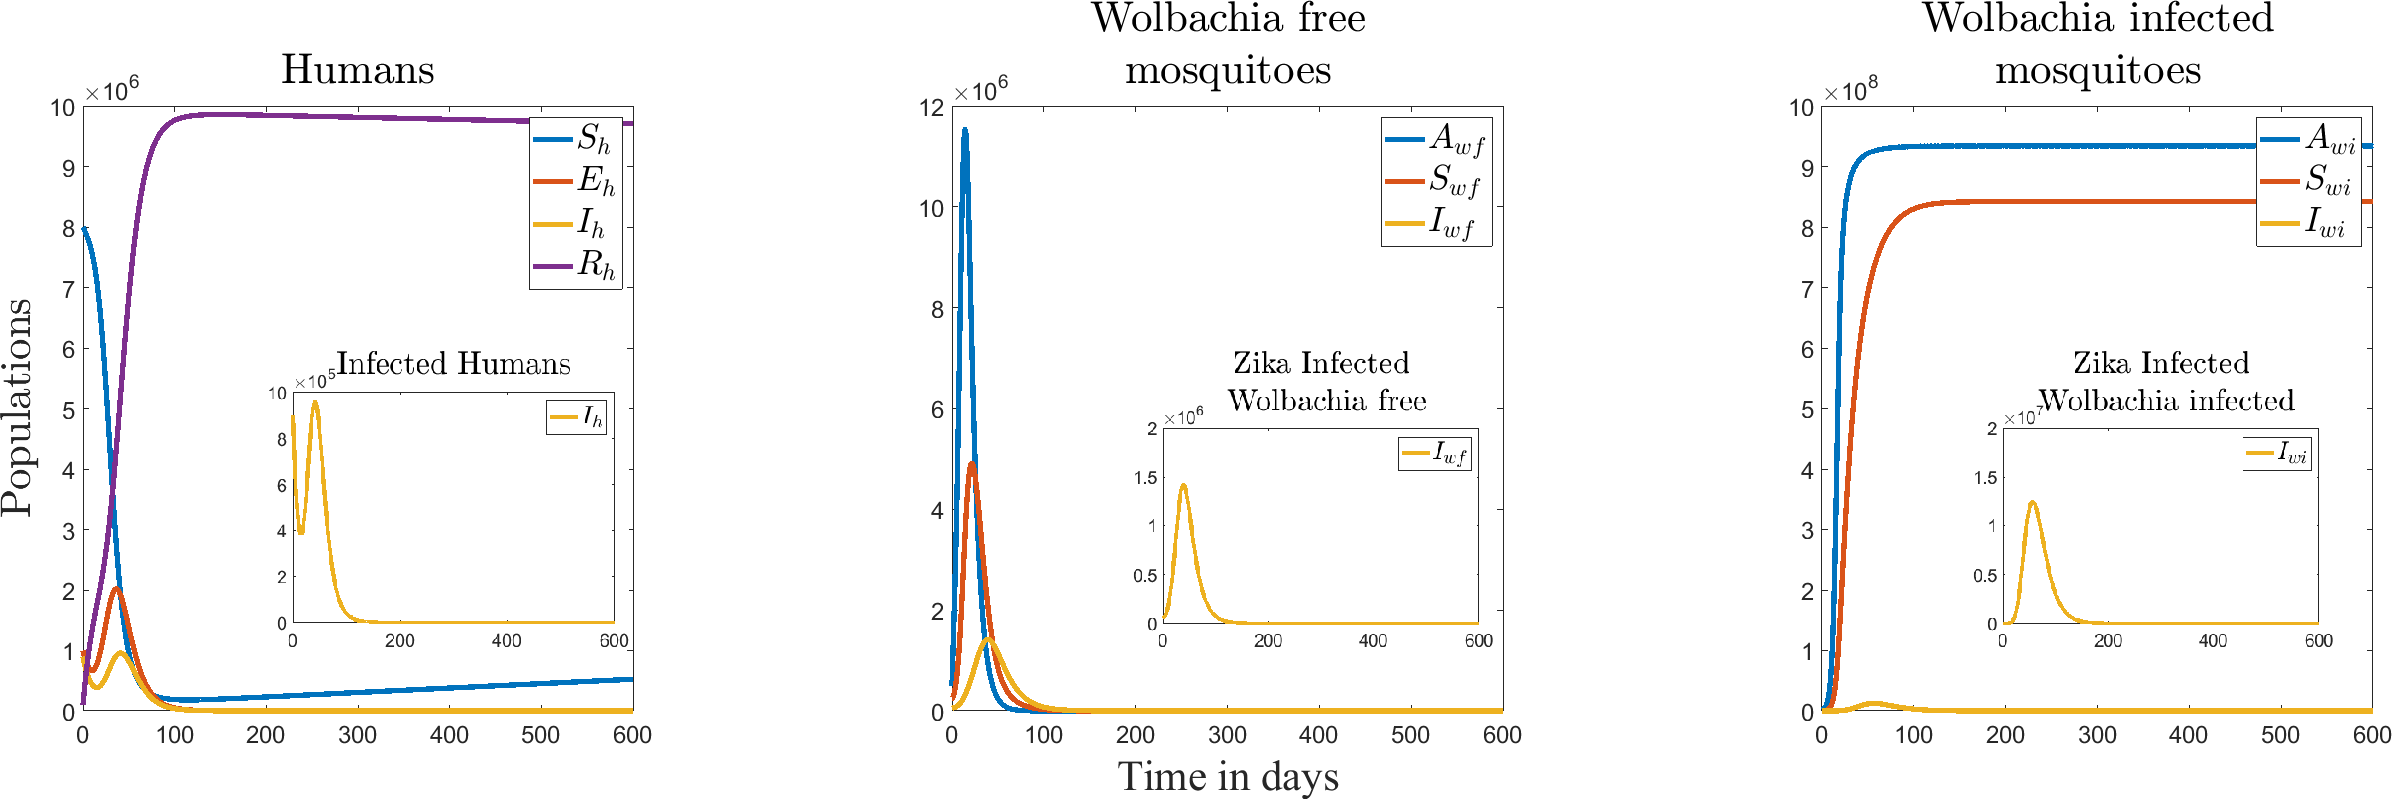
\includegraphics[width=16cm, height=4.5cm]{NewModel6b.png}
%\caption{Disease dies out when \textit{Wolbachia} mosquitoes persist. Figure is obtained using initial conditions given in Table \ref{init-cond-dis-present-table} with two changes ($A_{wf}(0)=500,000$, $A_{wi}(0)=1,500,000$)  and baseline values from Table \ref{tab: param-table} and Table \ref{tab: param_mosq_table}  with two changes( $b=1.25$ and $K=10^9$)}
%\label{wpe4}
%\end{figure}

\subsubsection{Zika is present and \textit{Wolbachia} infection is established when \textit{Wolbachia} infected vectors are more competent}\label{disthird}
In this section we are interested to see if Zika can stay endemic even when \textit{Wolbachia} infection is established. In order to investigate this we keep the same initial conditions as in section \ref{dissecond}, same parameters values as in section \ref{disfirst} with the change that we
increase the competence of \textit{Wolbachia} infected mosquitoes $\beta_{hv}^w=0.042\beta_{hv}$ to $\beta_{hv}^w=0.042\beta_{hv}$.  We notice in Figure \ref{sim6c} that in this case  the \textit{Wolbachia} infected mosquito population persists and the disease persists in both humans and \textit{Wolbachia} infected mosquitoes. The wild mosquito population is eliminated in around 330 days. The number of Zika infected humans reach a peak of 1.8 million in around 35 days and then settle to around 3,500. As we can see in Figure \ref{sim6c} even though the decrease in the number of Zika infected \textit{Wolbachia} infected mosquitoes is very substantial (from 2.4 millions to around 850,000) the impact in humans seems very minimal.

\begin{figure}[H]
\centering
    % This file was created by matlab2tikz.
%
%The latest updates can be retrieved from
%  http://www.mathworks.com/matlabcentral/fileexchange/22022-matlab2tikz-matlab2tikz
%where you can also make suggestions and rate matlab2tikz.
%
\definecolor{mycolor1}{rgb}{0.00000,0.44700,0.74100}%
\definecolor{mycolor2}{rgb}{0.85000,0.32500,0.09800}%
\definecolor{mycolor3}{rgb}{0.92900,0.69400,0.12500}%
\definecolor{mycolor4}{rgb}{0.49400,0.18400,0.55600}%
%
\begin{tikzpicture}

\begin{axis}[%
width=1.1in,
height=1.5in,
at={(0in,0.108in)},
scale only axis,
xmin=0,
xmax=1000,
ymin=0,
ymax=12000000,
axis background/.style={fill=white},
title style={font=\bfseries, yshift=1.75ex},
ylabel={Population},
xticklabels={0,,,400,,800,},
title={Humans},
legend style={legend cell align=left, align=left, draw=white!15!black}
]
\addplot [color=mycolor1, line width=2.0pt]
  table[row sep=crcr]{%
0	8000000\\
0.553766838274896	7989326.58891905\\
1.24841085448861	7974492.52578841\\
1.94305487070233	7958016.39926198\\
2.83532823249698	7934240.16952949\\
3.72760159429163	7907100.77964745\\
4.29635578021407	7887775.9109127\\
4.86510996613652	7866648.4990348\\
5.43386415112764	7843499.66751423\\
6.00261833705008	7818086.35496417\\
6.66998398862779	7785011.06592623\\
7.3373496402055	7747944.30101137\\
8.00471529178321	7706318.57164435\\
8.67208094336092	7659492.42892152\\
9.35855307523161	7605131.2068639\\
10.0450252071023	7543583.59490689\\
10.731497338973	7473785.74414637\\
11.4179694708437	7394504.70547009\\
12.0579913156107	7310788.04812714\\
12.6980131603777	7216213.46793141\\
13.3380350051448	7109178.96705273\\
13.9780568499118	6987835.01110097\\
14.5419493187219	6867379.50631719\\
15.105841787532	6732445.01065442\\
15.6697342563421	6581135.09578467\\
16.2336267260835	6411407.57425581\\
16.7245868267491	6246927.515408\\
17.2155469274148	6065209.80402485\\
17.7065070280805	5864702.25051615\\
18.6171470507979	5438410.28964558\\
19.4565068949014	4977770.94138881\\
20.2402727901936	4487550.54037273\\
21.3325307099149	3716702.02882397\\
24.4022662490606	1423316.2562627\\
25.0951017700136	1010830.39502683\\
25.7982730343938	671475.981306665\\
26.1550265373662	531712.697299021\\
26.5117800394073	413997.144585671\\
27.098769729957	263199.615473203\\
27.5592421032488	177662.194522784\\
28.019714477472	115999.089784865\\
28.4801868507639	73279.6612564242\\
28.9117602789775	46268.351757626\\
29.3144347621128	29374.7909688074\\
29.690651524812	18841.4844200239\\
30.0404105652124	12276.1813383549\\
30.3730040136725	8087.11683940608\\
30.6884318673983	5413.90814751666\\
30.9921203264967	3682.1197060626\\
31.2840693891048	2559.95134803932\\
31.5681208055466	1824.38933078293\\
31.8442745739594	1342.13728862163\\
32.116054482758	1022.35499356128\\
32.3834605310112	810.298506269231\\
32.6504892064258	667.725104228593\\
32.9171405080706	571.85114219971\\
33.1882926691324	506.157253026031\\
33.4639456914738	461.016299188137\\
33.7498290594667	429.111694524065\\
34.0459427731112	406.275862909853\\
34.3587852707133	389.164778035134\\
34.6883565504104	375.95945081301\\
35.0422525499016	365.092038101517\\
35.4204732682556	355.83883258421\\
36.0543113853782	343.471359477378\\
36.7624101955444	332.614482551813\\
37.2891522999853	325.934587589465\\
37.8545609237626	319.750751242973\\
38.4586360668764	314.267498477362\\
39.0874973824248	309.463621465489\\
39.4143211264163	307.312128021382\\
40.0679686153308	303.933156628162\\
40.4088238626719	302.296498400159\\
40.7496791090816	300.944947521202\\
41.0905343564227	299.943664515391\\
41.7079709023237	298.432486594655\\
41.9845522008836	297.911922190338\\
42.2611334994435	297.54546345491\\
42.5377147980034	297.285943108611\\
42.8142960974947	297.102879358456\\
43.0908773960546	297.029590849765\\
43.3674586946145	297.065035513602\\
43.6440399931744	297.196390951052\\
43.9296813094988	297.424634873867\\
44.2153226258233	297.751281170174\\
44.5009639421478	298.173095899634\\
45.0598507942632	299.265762847848\\
45.606341865845	300.661984511651\\
46.1286425301805	302.289543339051\\
46.6267527844757	304.101244789548\\
47.3492024950683	307.163858355023\\
48.0674818549305	310.707873690873\\
48.8021361865103	314.837565748021\\
49.5821872595698	319.764631145634\\
50.3603047104552	325.230573215522\\
51.3547719335184	333.024526646361\\
52.269758855924	340.988863660954\\
53.1487694699317	349.360538379289\\
54.0626004366204	358.822711014189\\
55.0294827353209	369.694120466709\\
56.2234006654471	384.375201151706\\
57.299165953882	398.822422991507\\
58.3238293388858	413.696944587864\\
59.4362356737256	431.130257125944\\
60.5970719764009	450.818203402683\\
61.8560289405286	473.974468445405\\
63.0210544867441	497.167873305269\\
64.3157526431605	525.049191779457\\
65.6376122264192	555.94386516232\\
66.967880031094	589.668670048937\\
68.1333379615098	621.525264871307\\
69.4519619131461	660.331476363353\\
70.6526701822877	698.379875032231\\
71.9011137746274	740.849402376451\\
73.1383401248604	786.042642008513\\
74.3974052546546	835.402124173008\\
75.6323095178232	887.313523670658\\
76.9582566646859	947.145619254559\\
78.2360534705222	1009.0583531186\\
79.4914920479059	1074.19510147627\\
80.7252978533506	1142.60529462621\\
81.9894841117784	1217.47017675173\\
83.3000635867938	1300.45857913326\\
84.6526078758761	1392.15739274304\\
86.0958265606314	1497.16126242746\\
87.5543103404343	1611.199385738\\
88.9076042752713	1724.51582497265\\
90.3820145996287	1856.61553104687\\
91.7516736751422	1987.78877079766\\
93.1263828556985	2128.00969876722\\
94.5988538786769	2288.12578316219\\
96.0618447903544	2457.7924080072\\
97.5537828272209	2642.10295378417\\
99.1462130527943	2851.86740701925\\
100.734175255522	3074.91362127848\\
102.175272129476	3289.68732663896\\
103.718501294032	3533.06923771463\\
105.290825250559	3795.610736873\\
106.89959319029	4079.77286653873\\
108.643596738577	4405.88236900046\\
110.362783804536	4745.99506594706\\
112.124529565684	5113.91914621089\\
113.993294084445	5525.76383303199\\
115.852495546453	5957.55639631022\\
117.773259383626	6426.65731209796\\
119.759028274566	6935.99580812268\\
121.835227494128	7494.62534887809\\
123.892760313116	8074.01787159592\\
126.042334811762	8706.02986748703\\
128.226098725572	9375.14317900129\\
130.562114572152	10119.9199825805\\
132.920143389143	10900.7513799304\\
135.390598475002	11748.451218579\\
138.023653831333	12683.3087935802\\
140.877347629517	13730.4646526882\\
143.885722516105	14869.4992035078\\
147.050306518562	16102.9223193005\\
150.481211179867	17476.5707267243\\
154.222855629399	19012.423596302\\
158.415486075915	20773.2454255335\\
163.158272805624	22806.5773886619\\
168.72691746708	25236.7688355623\\
175.915190167725	28418.4877585899\\
196.680611421354	37636.8923986936\\
202.357173891738	40101.4709733706\\
207.291102602147	42204.0333246263\\
211.632748577744	44015.9823314622\\
215.584432094358	45628.2592084883\\
219.275263883173	47097.5837684395\\
222.772354528308	48453.1238465225\\
225.98308231961	49662.8296925416\\
229.138522894122	50816.0527304998\\
232.105245634913	51865.2561465669\\
234.92348210793	52827.9757550377\\
237.438640478998	53657.2291659042\\
239.917482364923	54445.1097713765\\
242.254002779722	55159.4797008103\\
244.583590986207	55842.9140207935\\
246.830065470189	56473.3133012317\\
248.974467125721	57047.5574389677\\
250.901337736286	57539.6203093799\\
252.864541098475	58016.7190964948\\
254.603264252655	58418.0827027196\\
256.298269770108	58789.5484256614\\
258.025655520149	59147.3576452853\\
259.585323837586	59451.8987277662\\
261.138885945082	59737.2848349167\\
262.54245810397	59979.3188633872\\
263.937112205662	60204.6150295101\\
265.214453483	60397.388092638\\
266.601902972907	60591.7801151201\\
267.865456095897	60754.9703593887\\
269.059859781526	60896.8834091807\\
270.196838730015	61020.6497959336\\
271.243976354599	61124.7271205755\\
272.328569062054	61222.3774109529\\
273.362405857071	61305.725977229\\
274.259691246785	61370.2803721335\\
275.143896092661	61426.7462926852\\
275.826405306347	61465.4396932693\\
276.631680736318	61505.5700691873\\
277.367809539661	61536.9881568691\\
277.983187935315	61559.3680781741\\
278.477630624548	61574.7736050533\\
279.037891101092	61589.4432075946\\
279.460719023831	61598.5466520106\\
279.88354694657	61605.9514902811\\
280.268422871828	61611.2107490525\\
280.653298797086	61615.0545682954\\
280.965124361217	61617.1285676667\\
281.121037143283	61617.8156592948\\
281.276949925348	61618.2692036368\\
281.421825441532	61618.4811317297\\
281.566700958647	61618.4910260122\\
281.711576474831	61618.2987084035\\
281.856451991014	61617.904017414\\
282.025316245854	61617.1883454332\\
282.363044754602	61614.9304178469\\
282.736526980996	61611.1481279247\\
283.145762924105	61605.4507010039\\
283.558612316847	61598.0541787734\\
283.975075159222	61588.9117099168\\
284.52787712682	61574.1629217025\\
285.017095839605	61558.6191465613\\
285.603892986663	61536.8831635276\\
286.250887554139	61509.0009976402\\
286.816197398119	61481.2709442573\\
287.458918960765	61445.9222334828\\
288.288605219685	61394.2705299063\\
289.090823721141	61337.8710753834\\
289.862577306107	61277.6182587724\\
290.689341682009	61206.5479945568\\
291.578578871675	61122.5808645897\\
292.47001133021	61030.5869798241\\
293.554825263098	60908.099070658\\
294.588868494146	60780.6095391894\\
295.775677329861	60621.432888926\\
296.864954234101	60463.3196419133\\
298.073126139119	60274.5964389499\\
299.364558386616	60057.4863363989\\
300.68854178302	59818.6000884129\\
302.037343568169	59558.5058015799\\
303.422657763585	59274.0924410401\\
304.995692734607	58930.3508201623\\
306.535626700148	58572.959275092\\
308.045818151906	58202.9866611548\\
309.826405515894	57742.8422912825\\
311.51595817972	57283.2471229555\\
313.411242653616	56742.378111735\\
315.403909236193	56146.5492985845\\
317.602906562388	55459.068776208\\
319.827915889211	54734.3226134218\\
322.344922096469	53883.1300077699\\
325.199398661032	52883.4902855242\\
328.374140945263	51737.5658741184\\
332.329223634675	50275.2295620907\\
345.123530485667	45517.2155661285\\
348.404314829037	44345.7774153035\\
351.379515921697	43317.1640406335\\
353.993706054054	42444.9030792508\\
356.517829137854	41634.3215001244\\
358.85340313334	40914.5182996886\\
361.14354265295	40238.8903112439\\
363.233002751134	39649.8761187624\\
365.212256543338	39116.9844332058\\
367.13963708654	38622.1567372112\\
368.922011303715	38186.1630143002\\
370.858088253997	37736.4585982421\\
372.623044908978	37348.4008405283\\
374.415609844029	36975.7877876451\\
376.026713899337	36659.4409139259\\
377.5924466094	36368.817393817\\
379.126996653154	36100.0166779663\\
380.731385085732	35835.8680004459\\
382.198513370007	35609.3199470378\\
383.706616596319	35391.2490508929\\
385.037190507166	35211.1865978865\\
386.455642202869	35031.8251791177\\
387.754914603196	34878.8004783029\\
389.130405698903	34728.3814596068\\
390.373516433872	34602.5451357216\\
391.642136501148	34483.873523294\\
392.819673130289	34382.4021687545\\
394.019766953774	34287.4522099243\\
395.097472297959	34209.3560332367\\
396.056635847315	34145.4709841376\\
397.076523973607	34083.2629044615\\
398.08575283736	34027.4233710784\\
399.003595727496	33981.5044352012\\
399.955842499621	33938.6870144624\\
400.785729420371	33905.3180442899\\
401.68368258141	33873.29059227\\
402.415561217815	33850.2782201413\\
403.062947425991	33832.2061797474\\
403.842985906638	33813.2423759662\\
404.486113423482	33799.8891492328\\
405.101890511811	33789.0126007684\\
405.71766760014	33779.9816040499\\
406.278312008828	33773.3461664775\\
406.676754154265	33769.540715551\\
407.099875507876	33766.3201754745\\
407.503998875618	33764.0271910038\\
407.889124258421	33762.5481362389\\
408.237690718845	33761.7991826274\\
408.393694488332	33761.6444102675\\
408.549698256887	33761.6006851206\\
408.705702026375	33761.6676822864\\
408.8506592419	33761.8288834868\\
409.140573673882	33762.4360177983\\
409.4544959208	33763.5193745736\\
409.792425983585	33765.1773665603\\
410.166136618704	33767.600465144\\
410.575627825223	33770.960969883\\
410.988731310703	33775.0923396675\\
411.405447074212	33780.0074531334\\
411.958563745022	33787.6799027193\\
412.592762598768	33798.0706034051\\
413.188062368892	33809.353013685\\
413.870997819118	33824.0944801886\\
414.67678980995	33843.920763894\\
415.56729672756	33868.8403482661\\
416.336947848089	33892.8754338659\\
417.295951797627	33925.9985636966\\
418.315672725439	33964.9997373773\\
419.324723446742	34007.337431876\\
420.411349083297	34056.990327579\\
421.607552359812	34116.3867279682\\
422.92203101702	34187.2065478601\\
424.112523916177	34256.2021054178\\
425.509631741792	34342.8559119776\\
426.955307718366	34438.7480701124\\
428.548807245679	34551.4804782579\\
430.232697779313	34678.2633564072\\
431.812440373003	34804.0147127267\\
433.684544618241	34961.1280241255\\
435.484274039976	35119.9802697459\\
437.57281064149	35313.316788245\\
439.743736101314	35523.8056232473\\
442.020190151408	35754.1292269463\\
444.446241401136	36009.4522294551\\
447.112294525839	36300.5792251835\\
449.975338393822	36624.0525393058\\
453.046031072736	36981.6909692986\\
456.528916970827	37398.3975471398\\
460.591368478723	37895.8659255728\\
465.967703770846	38566.4984477824\\
479.882716237567	40308.0761032254\\
484.278527433053	40843.3615558874\\
487.998125981539	41285.3666266063\\
491.398812355474	41678.6332920501\\
494.555710503832	42032.9400132317\\
497.523780519143	42355.4391837344\\
500.343287643977	42651.3397116568\\
502.859564763494	42906.140359493\\
505.339492929168	43148.1450516311\\
507.677021672018	43367.5213711169\\
510.007601714693	43577.4107762855\\
512.255013938062	43771.1119275521\\
514.400302696973	43947.757624221\\
516.327949138358	44099.3960795589\\
518.291938154958	44246.8130044471\\
520.219801287167	44384.408170498\\
522.034750107676	44507.3762152214\\
523.877962654456	44625.6231769565\\
525.628012338653	44731.6091735959\\
527.147621468641	44818.6095107999\\
528.73466143664	44904.4250002122\\
530.269468721002	44982.4682781715\\
531.666171675548	45049.2285383111\\
533.111491966061	45114.0112506291\\
534.493094921112	45171.8272712473\\
535.786384391598	45222.2920156494\\
537.015690834261	45266.9735589018\\
538.172146176919	45306.0773148024\\
539.349889182486	45342.9781124257\\
540.57897426188	45378.3408326972\\
541.638619686477	45406.2492685085\\
542.649630618282	45430.6522147702\\
543.72681992501	45454.2654710067\\
544.685509202071	45473.2136864169\\
545.704900793731	45491.2308613891\\
546.557722931728	45504.6212741379\\
547.293304267339	45514.9430767009\\
547.968921666965	45523.4243801553\\
548.787596399896	45532.4235841474\\
549.41244140733	45538.352918392\\
550.137691238895	45544.219058401\\
550.744044300169	45548.2886315314\\
551.194487757981	45550.8212426435\\
551.6887312131	45553.1204229807\\
552.065684770234	45554.5375050334\\
552.468448644504	45555.7307591932\\
552.89702283591	45556.6373839276\\
553.265198544599	45557.1181654613\\
553.572975768708	45557.3092175964\\
553.726864380762	45557.3328783056\\
553.880752992816	45557.3087193109\\
554.188530217856	45557.1171098361\\
554.529228147119	45556.6826927876\\
554.902846781537	45555.938460133\\
555.301133813336	45554.8375036987\\
555.724089242518	45553.3219449157\\
556.128059787676	45551.5424970351\\
556.705538278446	45548.4378039083\\
557.329352974892	45544.346089975\\
557.909002964385	45539.8609511545\\
558.584640002809	45533.8076972114\\
559.198663045652	45527.5407183124\\
560.028199751861	45517.9248568155\\
560.925798488781	45506.0451042447\\
561.810299773701	45492.8542956654\\
562.681522822939	45478.4365196163\\
563.727177960798	45459.2872035801\\
564.804431745782	45437.4826857857\\
565.917068528011	45412.7834260743\\
567.129015942104	45383.4034149479\\
568.380100361072	45350.4175053919\\
569.610036426224	45315.4121728921\\
570.852572080679	45277.5108637866\\
572.273541526869	45231.1171341538\\
573.700472451746	45181.3431288432\\
575.266761051491	45123.1472504642\\
576.744820719585	45064.9267516453\\
578.405709884129	44995.8221652396\\
580.021726123057	44924.9966059905\\
581.813663125969	44842.5155560123\\
583.725680499338	44750.1720777955\\
585.729407316074	44648.8887079917\\
587.784407591447	44540.5506118014\\
590.095874777995	44413.7281880332\\
592.60274929367	44270.8175625345\\
595.36241263058	44107.8092858428\\
598.401317609474	43922.4450690188\\
601.869496372528	43704.8704484971\\
606.193833804689	43427.1593445269\\
613.664712896571	42939.8494035248\\
619.828404061496	42540.5764769176\\
623.937467700802	42280.3995867297\\
627.428675638512	42065.1713785771\\
630.445945253596	41884.5470722718\\
633.312347719446	41718.3278700616\\
635.976195504889	41569.0952024786\\
638.508030451834	41432.3588755103\\
640.871043682098	41309.541314194\\
643.182688737288	41194.1345587643\\
645.345044235699	41090.620821977\\
647.429595187306	40995.0483628586\\
649.433504927903	40907.1962103862\\
651.488687045872	40821.2990429578\\
653.462451929227	40742.8977323025\\
655.373679572716	40670.8703588871\\
657.211463636719	40605.2712457199\\
658.85289369151	40549.7478070576\\
660.512862863019	40496.5639899028\\
662.106290864758	40448.3348464482\\
663.645237372257	40404.3900559582\\
665.165199608542	40363.535016994\\
666.752602999099	40323.5723328795\\
668.134842328727	40291.0244926699\\
669.470439406112	40261.5612122286\\
670.822566084564	40233.7164059961\\
672.089266218245	40209.4345703898\\
673.301375083625	40187.8257462988\\
674.552600529976	40167.1796565466\\
675.782680027187	40148.5167831769\\
676.817045951262	40134.0695303306\\
678.004167175852	40118.8822727539\\
679.093702379614	40106.2447312605\\
680.087868889794	40095.7917158185\\
681.132156442851	40085.9109376036\\
681.934637560509	40079.077503942\\
682.706662045792	40073.121621443\\
683.533714561723	40067.4089586446\\
684.267250356264	40062.9159706999\\
685.025032754987	40058.8366159583\\
685.652756988071	40055.8868967947\\
686.195323004387	40053.6487913271\\
686.809431394562	40051.4617201025\\
687.434378241189	40049.6109407637\\
687.987391070463	40048.2864332451\\
688.476785313338	40047.357932901\\
688.910876402631	40046.7247379916\\
689.369591367431	40046.2490118649\\
689.711001046933	40046.0232642638\\
690.088010430336	40045.9005700015\\
690.490834404714	40045.9156199088\\
690.919472970068	40046.0965137891\\
691.287700666115	40046.3869849248\\
691.749425908551	40046.9265794875\\
692.211151150055	40047.6601694794\\
692.738730059005	40048.7342392728\\
693.323908204213	40050.2176229851\\
693.958431153558	40052.1702372469\\
694.535984691232	40054.2561326465\\
695.196416537277	40056.9983138526\\
695.932100550272	40060.4968133243\\
696.607816597447	40064.1177764814\\
697.426615810953	40069.0221984303\\
698.259866109118	40074.5869239559\\
699.238639240153	40081.8516731299\\
700.139638748951	40089.2233753987\\
701.107962102629	40097.8645990556\\
702.212628333829	40108.6148093184\\
703.355822918005	40120.7205480039\\
704.575505614281	40134.7104645362\\
705.813471795991	40150.015940127\\
707.055923117325	40166.4671676876\\
708.46025519073	40186.3387243813\\
710.000324339606	40209.6378883887\\
711.51061296463	40233.9620993864\\
713.137382601388	40261.7317391187\\
714.769414282404	40291.1570181428\\
716.586331109516	40325.6724138204\\
718.455802210607	40363.0159290303\\
720.472465191036	40405.255101989\\
722.556041979231	40450.8840041859\\
724.77635401953	40501.5610697735\\
727.203069664538	40559.1591813937\\
729.693813927472	40620.4320180602\\
732.555594400503	40693.1948253447\\
735.791307738982	40778.0396485925\\
739.484410132281	40877.5338386307\\
744.00354610756	41002.0000033518\\
752.466857364401	41238.4386849422\\
758.428733257577	41403.6530684661\\
762.649184413254	41518.12521559\\
766.220139661804	41612.5748639097\\
769.512964012101	41697.2288119551\\
772.57618522644	41773.5300856894\\
775.424082246609	41842.0894654067\\
778.045432889834	41902.9783318257\\
780.575076804496	41959.5714495741\\
782.984202355146	42011.3703315547\\
785.260628623888	42058.3401537472\\
787.452777728438	42101.6799519146\\
789.507705342025	42140.5628160387\\
791.481225186028	42176.2698548688\\
793.392220291309	42209.2807707768\\
795.38267403841	42241.992005432\\
797.299617738463	42271.8524053264\\
799.09124999214	42298.2808010532\\
800.894043612294	42323.4117836682\\
802.604307627305	42345.8833075529\\
804.216854603961	42365.8393381871\\
805.846124940552	42384.7806671085\\
807.273062612861	42400.3564498015\\
808.839350597933	42416.3604739197\\
810.317410295829	42430.4122136291\\
811.666368445382	42442.3453983748\\
813.051762060262	42453.7160595413\\
814.20833855588	42462.5228236653\\
815.386201854795	42470.8515808647\\
816.615405376069	42478.8563659964\\
817.675153684802	42485.1963232337\\
818.840160392225	42491.5686422316\\
819.950370108709	42497.0616631322\\
820.93381957151	42501.457462539\\
821.934318029322	42505.4786784789\\
822.895590207539	42508.916405824\\
823.668186554685	42511.3785716845\\
824.415396462195	42513.5062069474\\
825.241367968731	42515.5695044696\\
826.002639075741	42517.2043158822\\
826.636686240323	42518.3716599755\\
827.231850255281	42519.3076786194\\
827.914622223005	42520.1919805566\\
828.505908777006	42520.7950886264\\
829.148820413277	42521.2804382155\\
829.610517364927	42521.5201058639\\
830.072214316577	42521.6691795671\\
830.566835151054	42521.7288551535\\
831.127303749323	42521.672073504\\
831.550290435553	42521.5422020294\\
831.973277122714	42521.3377755247\\
832.550794879906	42520.9390662368\\
833.055226705968	42520.4784474969\\
833.656994101591	42519.7927582329\\
834.284674839117	42518.9207995301\\
834.827201762237	42518.0391193023\\
835.441264784895	42516.8990342384\\
836.274467227049	42515.1128683742\\
837.10850498639	42513.0519172996\\
838.001257139258	42510.5467692241\\
838.908123069443	42507.6893919893\\
839.919244000688	42504.1372787291\\
840.842644223943	42500.560951327\\
841.955335315317	42495.8369121244\\
842.974833770655	42491.1175691299\\
844.128626022488	42485.33419808\\
845.239074380137	42479.3334961189\\
846.474434369244	42472.1680522459\\
847.869771111757	42463.4697071882\\
849.336218317971	42453.6562554091\\
850.843641900457	42442.8739336981\\
852.360448693857	42431.338369214\\
853.97646685876	42418.3197211316\\
855.686783886515	42403.75706062\\
857.507680478506	42387.4081319496\\
859.38739146851	42369.6657789359\\
861.460309876129	42349.1420225902\\
863.611618684605	42326.8530627061\\
865.965636578389	42301.4025850249\\
868.469071635045	42273.2342095654\\
871.186715731397	42241.5141047407\\
874.016865693033	42207.3884281507\\
877.293859551661	42166.7199527705\\
881.186383907683	42117.1742495587\\
886.294614275917	42050.8529531462\\
898.153909982182	41896.4197579073\\
902.231583530083	41844.7613751628\\
905.65588486474	41802.4785864186\\
908.939718002453	41763.0991247864\\
911.859873274341	41729.1965623684\\
914.544434471987	41699.0653485088\\
917.099797135219	41671.3888835004\\
919.556616160087	41645.76950048\\
921.898001212627	41622.3095954675\\
924.056684331968	41601.5461726226\\
926.304519764148	41580.8433963433\\
928.450206598267	41561.9848156087\\
930.378212284297	41545.8133861236\\
932.342558667064	41530.1080853343\\
934.270772214979	41515.4631264806\\
936.086043190211	41502.3856925853\\
937.92958076857	41489.8184435405\\
939.679931963794	41478.5592160346\\
941.404494567774	41468.1121502575\\
942.959448947571	41459.2458371669\\
944.51066227816	41450.9258925272\\
946.087310126983	41443.0083073834\\
947.538299361244	41436.2023401735\\
948.950475327671	41430.0207460569\\
950.296809521504	41424.5331598297\\
951.611979630776	41419.554327351\\
952.850985118188	41415.2079000119\\
954.182739271782	41410.9069776349\\
955.316027453169	41407.5482836533\\
956.550269915722	41404.2038624976\\
957.627597128041	41401.5503743161\\
958.74031829834	41399.068111741\\
959.759844176471	41397.0228024991\\
960.768738002516	41395.2129215766\\
961.686286186799	41393.7506718915\\
962.63821724616	41392.4172292361\\
963.467831743881	41391.4065358369\\
964.365506507456	41390.4705640692\\
965.097173552029	41389.8280470846\\
965.932867095806	41389.225358462\\
966.738484242931	41388.7757960996\\
967.474913143553	41388.4767884212\\
968.244430268183	41388.277691938\\
968.958819646388	41388.1957041323\\
969.568648317829	41388.2034583976\\
970.376671370119	41388.3230703222\\
971.073628282174	41388.5254759146\\
971.820335046388	41388.8434059853\\
972.640955628827	41389.3122306122\\
973.459729149938	41389.9033030346\\
974.292954145931	41390.6298144804\\
975.12701138109	41391.481907296\\
976.019782635383	41392.53060921\\
976.926669541746	41393.738614873\\
977.937814072706	41395.2526183715\\
979.015134608373	41397.0564307058\\
980.18544569239	41399.2348557506\\
981.378488162532	41401.6854306404\\
982.582049202174	41404.3877626332\\
983.871821632609	41407.5341350539\\
985.254418685101	41411.1873682952\\
986.636559828185	41415.1211795975\\
987.97206339892	41419.1819905546\\
989.478000017814	41424.0573136043\\
991.013708686456	41429.3411909882\\
992.764035937376	41435.7323852852\\
994.488574511372	41442.396641559\\
996.360538678244	41450.0224125804\\
998.160185645334	41457.7173451521\\
1000	41465.9309311286\\
};
\addlegendentry{$S_h$}

\addplot [color=mycolor2, line width=2.0pt]
  table[row sep=crcr]{%
0	1000000\\
0.553766838274896	956723.138621383\\
1.24841085448861	907118.545496847\\
1.94305487070233	862431.653610752\\
2.83532823249698	811913.078104639\\
3.72760159429163	768931.745154525\\
4.29635578021407	745429.154260769\\
4.86510996613652	724980.40263605\\
5.43386415112764	707630.860892419\\
6.00261833705008	693443.868770363\\
6.66998398862779	680947.494030641\\
7.3373496402055	673124.04996881\\
8.00471529178321	670224.330547321\\
8.67208094336092	672547.244166399\\
9.35855307523161	680767.595856654\\
10.0450252071023	695396.347074725\\
10.731497338973	717041.143765689\\
11.4179694708437	746423.004754462\\
12.0579913156107	781545.751663682\\
12.6980131603777	825019.697133297\\
13.3380350051448	877882.382811911\\
13.9780568499118	941339.328367425\\
14.5419493187219	1007139.63040167\\
15.105841787532	1083420.89178521\\
15.6697342563421	1171454.94657076\\
16.2336267260835	1272580.89412113\\
16.7245868267491	1372390.23546567\\
17.2155469274148	1484245.34872584\\
17.7065070280805	1609085.46493423\\
18.6171470507979	1877405.44639865\\
19.4565068949014	2168896.61595184\\
20.2402727901936	2477599.20141979\\
21.3325307099149	2952737.44978726\\
22.6987288380042	3559923.67512227\\
23.3772886628285	3829529.90525304\\
24.0558484876528	4051994.50917309\\
24.4022662490606	4141702.25274416\\
24.7486840095371	4212516.28183224\\
25.0951017700136	4262922.0862073\\
25.4415195314214	4292336.04274797\\
25.7982730343938	4301070.12918077\\
26.1550265373662	4287795.76602124\\
26.5117800394073	4253251.8910143\\
26.8685335423797	4200028.76860936\\
27.3290059166029	4108331.68831642\\
27.7894782898948	3994814.6892114\\
28.4801868507639	3796896.4869225\\
31.9823514577001	2732094.27297589\\
33.0504661584273	2456520.40110222\\
34.0459427731112	2224461.66591586\\
35.0422525499016	2014147.59413744\\
36.0543113853782	1820905.45589686\\
37.0257812477648	1652932.36790155\\
37.8545609237626	1521982.02788334\\
38.7606736384332	1390702.86732358\\
39.7411448713392	1261432.29755311\\
40.7496791090816	1141048.88293662\\
41.7079709023237	1037382.21139564\\
42.8142960974947	929428.531655788\\
43.9296813094988	832035.119844985\\
45.0598507942632	743832.23955775\\
46.1286425301805	669110.244296112\\
47.112505203113	607040.945067631\\
48.0674818549305	552362.545281259\\
49.0621532108635	500700.311166853\\
50.1012544976547	451947.699023687\\
51.1165885357186	408962.174122053\\
52.0504487929866	373100.130462465\\
53.1487694699317	334992.648987468\\
54.0626004366204	306325.563400119\\
55.0294827353209	278715.405853018\\
55.9899086281657	253809.272818184\\
57.0885976413265	228101.869611131\\
58.1085263192654	206637.249417879\\
59.2029870357364	185913.068859152\\
60.1341792913154	169980.629364467\\
61.0374882668257	155879.66559589\\
62.0476597724482	141547.455115091\\
63.0210544867441	129040.64266556\\
64.0874541122466	116665.476623181\\
65.0006482368335	107067.22875319\\
66.038137297146	97173.8560927873\\
66.967880031094	89138.1474029217\\
67.9332563569769	81547.416665337\\
69.0173201980069	73851.3829950429\\
70.07812026795	67084.8373456607\\
71.0017189336941	61749.1152354507\\
71.9011137746274	57004.6025538947\\
72.9185112109408	52125.9121462787\\
73.9976863283664	47463.6350001059\\
74.9445530064404	43765.5634837868\\
75.9727777400985	40124.9912409801\\
76.9582566646859	36967.8866045764\\
78.0262725809589	33877.4563226011\\
78.9855859419331	31366.9955867343\\
79.993183106184	28974.4955850597\\
80.9303061598912	26953.1544637019\\
81.9894841117784	24882.3634474333\\
82.9732667468488	23142.8755364446\\
83.9511135742068	21572.4441160941\\
85.0298490300775	20005.5594723411\\
86.0958265606314	18610.8185444707\\
87.0560673847795	17472.1519581741\\
88.0188898760825	16431.6978622153\\
89.1118831671774	15361.5813601408\\
90.1666211877018	14429.6519990424\\
91.2836569081992	13539.2534010205\\
92.3784131249413	12752.8866209183\\
93.3420634483919	12124.1196748484\\
94.3956043273211	11497.8103357926\\
95.4653531974182	10920.6462330455\\
96.5668727299199	10381.7663029721\\
97.5537828272209	9941.80944341794\\
98.5980970123783	9515.8598677516\\
99.7494298107922	9088.55276762415\\
100.734175255522	8754.60202598013\\
101.756724814884	8435.40707122348\\
102.942704305053	8096.70417669974\\
104.00892833434	7817.98497939389\\
105.08566621691	7558.58212436736\\
106.142997682095	7323.15889759269\\
107.374603685923	7070.39002518076\\
108.643596738577	6831.29955437034\\
109.885077208281	6615.81481852941\\
111.158961465582	6411.32876718789\\
112.543417255394	6205.80252366699\\
113.834628486075	6027.83836685773\\
115.270252886228	5843.52021417208\\
116.673079413362	5675.45051544998\\
118.217624203302	5502.36494355183\\
119.759028274566	5340.51254274882\\
121.370249596424	5181.44089253061\\
122.924128967337	5036.61208431609\\
124.514133762568	4896.11860714573\\
126.343386876397	4743.04061501939\\
128.011263127439	4610.61443591397\\
129.954431465827	4464.08232048061\\
131.710466394201	4338.23235592805\\
133.710433921777	4201.92063175328\\
135.60710404627	4079.12128873449\\
137.461244291626	3964.84186680801\\
139.387081748806	3851.91772384942\\
141.276619776152	3746.63326657936\\
143.148399809375	3647.55266563967\\
144.974703486077	3555.74605894089\\
146.733521177433	3471.76531719603\\
148.476903955452	3392.71752499789\\
150.327539900318	3313.27599555813\\
152.114093348384	3240.85387196112\\
153.777660338208	3177.10289398953\\
155.392154898494	3118.55607892107\\
157.014654746279	3062.94485622644\\
158.568101946265	3012.66390931606\\
160.118367674761	2965.31152932346\\
161.751166292466	2918.42040531803\\
163.350773562677	2875.37942317594\\
164.841577677056	2837.78636220843\\
166.216618932784	2805.21951010637\\
167.631683988497	2773.7699321406\\
169.032651430927	2744.65339400619\\
170.306794643402	2719.88152222801\\
171.718824921176	2694.29151352216\\
172.927442360669	2673.91333906818\\
174.158588130958	2654.5747297788\\
175.456734174863	2635.70757099055\\
176.626381859183	2620.02447509672\\
177.865332105197	2604.75025053136\\
179.051955280825	2591.39129740652\\
180.140681395307	2580.21130231209\\
181.134516534396	2570.8933330318\\
182.178370344453	2562.0073298635\\
183.167170648463	2554.43148982897\\
183.9635800533	2548.91882530507\\
184.771331346594	2543.85973193031\\
185.623809163459	2539.09692563582\\
186.358993875794	2535.46116131358\\
187.034351892769	2532.50360335689\\
187.648210951127	2530.13112198655\\
188.269287428819	2528.03512565419\\
188.857991455123	2526.32966455631\\
189.519325794652	2524.73872556351\\
190.105907676741	2523.61404610891\\
190.564319612458	2522.92182698194\\
190.941133210436	2522.47510659788\\
191.317946808413	2522.13844891638\\
191.746396139264	2521.88904038724\\
192.174845471047	2521.78125803545\\
192.482454779558	2521.79100158345\\
192.790064088069	2521.87345747463\\
193.097673397511	2522.02849232312\\
193.405282706022	2522.25600874983\\
193.778748631477	2522.62949025631\\
194.152214556932	2523.10947447177\\
194.575030134991	2523.7811937267\\
195.190260137431	2525.00156017393\\
195.767503411509	2526.40793853346\\
196.390966112725	2528.21055496577\\
196.970256730914	2530.14900563564\\
197.645542379469	2532.72863308992\\
198.463904300705	2536.31577960681\\
199.296724555083	2540.48422503471\\
200.130274745636	2545.17895884719\\
201.022431344725	2550.78279781155\\
201.928772451356	2557.0887329746\\
202.939378198236	2564.84896414448\\
204.0159982685	2573.96247831546\\
204.974258518778	2582.80976231769\\
205.993204405531	2592.9791999273\\
207.146277687512	2605.43724471983\\
208.256020615809	2618.38322502002\\
209.490689712577	2633.89390284289\\
210.740582194179	2650.79060447589\\
211.973925121129	2668.64967541676\\
213.395803774707	2690.71231006365\\
214.812924291939	2714.28539503459\\
216.218549577519	2739.24566358235\\
217.756394739263	2768.37494919263\\
219.275263883173	2799.03595499415\\
220.861573558301	2833.09250559285\\
222.395600578748	2868.03210558835\\
224.005823195912	2906.86143126618\\
225.60966267623	2947.76588120684\\
227.213334152475	2990.92832891084\\
228.969707291573	3040.84326867294\\
230.710768362507	3093.10154548101\\
232.547241850756	3151.28231993783\\
234.401692218147	3213.28555942886\\
236.219740762375	3277.31233055331\\
238.015817613341	3343.78223250713\\
239.917482364923	3417.7179114297\\
241.737292835489	3491.96897540335\\
243.615875527263	3572.27999681421\\
245.533761544153	3658.18538457528\\
247.414873972535	3746.35919953417\\
249.442096378654	3845.8038701592\\
251.515062151477	3952.32079673838\\
253.615227353759	4065.29742258415\\
255.622619460337	4178.11579696368\\
257.81427197624	4306.75124458782\\
260.052980822511	4444.09348215442\\
262.12606287282	4576.6691156961\\
264.37917665299	4726.65836863406\\
266.601902972907	4880.63870805688\\
268.848463062197	5042.29979711492\\
271.243976354599	5221.27085803729\\
273.742886574008	5415.0623083692\\
276.417460934259	5630.24215742759\\
279.037891101092	5848.49140888639\\
281.856451991014	6090.91069535911\\
284.872447673231	6358.30870807823\\
288.288605219685	6669.8170853965\\
292.325118635781	7047.14506927505\\
298.287391308695	7614.79466157593\\
304.579131658189	8211.76281121839\\
308.045818151906	8532.23557289969\\
310.881493020803	8786.39432390314\\
313.411242653616	9005.11432594713\\
315.612218173221	9187.95796606969\\
317.755821177736	9358.32339336257\\
319.673991137184	9503.53846602421\\
321.498851692304	9634.72428327985\\
323.271060097963	9755.10296458285\\
324.825723771006	9854.63276098669\\
326.230239468627	9939.41091504507\\
327.770605149679	10026.5294740712\\
329.092685041949	10096.2307061376\\
330.446517008357	10162.592942588\\
331.743934175931	10221.3030149695\\
332.963860559277	10272.045608894\\
334.046135646291	10313.3785320437\\
335.107034174725	10350.4859689288\\
336.023454166017	10379.7938831346\\
337.058040788397	10409.7959169801\\
337.95599601604	10433.1667416096\\
338.840886030346	10453.7597823702\\
339.712470766157	10471.6710252864\\
340.544159033336	10486.5642973715\\
341.220423805527	10497.0918538421\\
341.836274780333	10505.4451870117\\
342.364024056122	10511.6691766568\\
342.949380286969	10517.5659338515\\
343.584089384414	10522.7667779895\\
343.96925223805	10525.31929301\\
344.354415090755	10527.4175968729\\
344.666479200125	10528.7851848053\\
344.978543309495	10529.8561714673\\
345.268517660908	10530.5860293107\\
345.558492012322	10531.0610895371\\
345.727483844385	10531.2206786629\\
345.896475676447	10531.2941093156\\
346.06546750851	10531.2815366276\\
346.234459340572	10531.1831023386\\
346.439228490926	10530.9489845391\\
346.64399764128	10530.5893403385\\
346.848766791634	10530.1044833204\\
347.261920288205	10528.7461386239\\
347.678688979708	10526.8634094121\\
348.059487160295	10524.6954541914\\
348.576728664339	10521.0703689726\\
349.155759955756	10516.0891722729\\
349.767630841583	10509.7756026797\\
350.333357496187	10502.9878683928\\
350.950724484399	10494.5499127898\\
351.687464546412	10483.0901941247\\
352.457336110063	10469.5222148364\\
353.172035997733	10455.4930700082\\
353.993706054054	10437.6892480412\\
354.975675561465	10414.1113794018\\
355.889833006077	10389.9642246487\\
356.85583424475	10362.2076632325\\
357.883364286274	10330.2311897073\\
359.025825962424	10291.8113842299\\
360.23622820247	10247.9425228713\\
361.572356264107	10195.9098706683\\
362.925044532865	10139.5777073875\\
364.403860178776	10074.0385658443\\
366.065592529252	9995.81025446299\\
367.682437535375	9915.41641830746\\
369.475262590684	9821.80290701147\\
371.388235404156	9717.29636623617\\
373.700884894468	9585.45547748916\\
376.219313999638	9436.21922807023\\
379.126996653154	9258.2656523874\\
383.030304571614	9013.09007610474\\
395.284368926659	8238.47628482804\\
398.834615864791	8022.51397342607\\
401.973149901256	7837.42685544956\\
404.794001967646	7676.50477279257\\
407.503998875618	7527.24356592167\\
409.96139101591	7396.72362389602\\
412.448042566888	7269.54667820502\\
414.891147932969	7149.55416382104\\
417.295951797627	7036.35346117523\\
419.61461118795	6931.89079993684\\
421.81589272432	6837.00723991357\\
423.959607689641	6748.63625806756\\
426.031805982813	6666.99311047792\\
428.125756475143	6588.25439895131\\
430.232697779313	6512.82068548817\\
432.225475694053	6444.94733945187\\
434.11863071844	6383.56427566521\\
435.912921505049	6328.14259013906\\
437.759645815939	6273.86977418419\\
439.551220230758	6223.86835749075\\
441.30872194469	6177.32119202055\\
443.050898006186	6133.59358116612\\
444.735612510704	6093.56202820875\\
446.315471777692	6058.00727565866\\
448.035666669719	6021.44817569759\\
449.571339417249	5990.68074835557\\
451.17667318508	5960.37595902197\\
452.636662852019	5934.44092765264\\
454.083899977617	5910.23967275582\\
455.504811367951	5887.91852696892\\
456.931697211228	5866.91955548525\\
458.344025642611	5847.51297609974\\
459.764423318207	5829.35915715434\\
461.168849895708	5812.73536940571\\
462.372269529849	5799.52565572411\\
463.661913657561	5786.41592949629\\
464.872053041123	5775.08675211202\\
465.967703770846	5765.63163058739\\
467.14464436844	5756.31428344361\\
468.190268627368	5748.75753088109\\
469.267440338619	5741.67415493261\\
470.168542454951	5736.28972476907\\
471.206928037107	5730.68990280107\\
472.096273771487	5726.40376632381\\
472.987766782753	5722.57483532652\\
473.86803163588	5719.24912507087\\
474.690308813937	5716.54719324037\\
475.487459764816	5714.29771212768\\
476.149074447341	5712.70498042274\\
476.735952006653	5711.49884904083\\
477.383044388145	5710.39268224593\\
477.948451472446	5709.61698363069\\
478.377011918463	5709.14686573017\\
478.95945005957	5708.66997868102\\
479.421083148569	5708.423868143\\
479.882716237567	5708.29371463973\\
480.223393565044	5708.27168698143\\
480.596992827952	5708.31949124765\\
480.995260815136	5708.45298286062\\
481.418197528459	5708.6876130132\\
481.822146966122	5709.00055839401\\
482.399590209126	5709.59797211736\\
482.867410169914	5710.21063851751\\
483.45804595761	5711.1477097664\\
484.109631714411	5712.39183585905\\
484.687849322334	5713.67937323358\\
485.305444412865	5715.24381815642\\
486.102576136589	5717.5497637298\\
486.908843077719	5720.20790886506\\
487.809660786763	5723.56143869739\\
488.777797123417	5727.61214556638\\
489.728374687023	5732.03440417536\\
490.651627352461	5736.74669233803\\
491.610276616178	5742.06947928201\\
492.629625358619	5748.20378565229\\
493.783231591806	5755.72802022379\\
494.893497752957	5763.54463667795\\
496.128669663332	5772.89303242881\\
497.523780519143	5784.26419666875\\
498.801518861204	5795.42068344727\\
500.189412888139	5808.3270082809\\
501.640125771984	5822.67659633514\\
503.244518415071	5839.54544230737\\
504.832813342102	5857.25309776887\\
506.535282746889	5877.31692610681\\
508.283326562494	5899.04999568127\\
510.007601714693	5921.57577117439\\
511.881423774175	5947.23858364671\\
513.859408618882	5975.61436821707\\
515.954397256486	6007.04751447216\\
518.119626398198	6040.95293175057\\
520.408266122453	6078.27242209762\\
522.869976110756	6120.00663212687\\
525.483111458831	6165.98090413027\\
528.181759811006	6215.11110871565\\
531.237617065199	6272.55651528388\\
534.493094921112	6335.59348183684\\
538.172146176919	6408.7192748012\\
542.649630618282	6499.74491254706\\
548.995878069662	6630.91678157356\\
557.474265472963	6805.91856019292\\
561.810299773701	6893.44880867284\\
565.331954901107	6962.77169654518\\
568.525017502718	7023.85401256755\\
571.36957161501	7076.57917241845\\
574.129071761854	7125.98980247322\\
576.744820719585	7171.07065968122\\
579.141360395588	7210.73873068672\\
581.468986157328	7247.65939488634\\
583.537186629139	7279.05742656253\\
585.575504358858	7308.64138952736\\
587.57291100733	7336.2666734783\\
589.468173183501	7361.18516890705\\
591.252494984306	7383.45843260828\\
593.064482000656	7404.86878193542\\
594.719476368278	7423.33721929789\\
596.346260647289	7440.46103426814\\
597.978312786669	7456.59881569445\\
599.483323685825	7470.54440013412\\
600.881774939597	7482.6896314444\\
602.286119161174	7494.09190061875\\
603.681529309601	7504.62891604193\\
604.959556594491	7513.58329762891\\
606.193833804689	7521.59764910396\\
607.425119607709	7528.97149800044\\
608.595477975905	7535.40539731923\\
609.788571951911	7541.38802234177\\
610.84727267269	7546.21035961341\\
611.872639280744	7550.44617791288\\
612.903378725983	7554.27455622237\\
613.83706410788	7557.37222073134\\
614.741127680987	7560.03768793959\\
615.576869026758	7562.21095698606\\
616.382527477108	7564.04293279629\\
617.118997526355	7565.49290189333\\
617.888564524241	7566.7800110653\\
618.602995928377	7567.76754553337\\
619.212858103216	7568.45349414553\\
619.828404061496	7569.00005647726\\
620.405973411165	7569.38050805684\\
620.873907246627	7569.59515663795\\
621.46469011344	7569.74730776437\\
621.947496014647	7569.77366929315\\
622.49007290788	7569.69876400661\\
623.104190803133	7569.48137784842\\
623.729148476385	7569.11658080015\\
624.282175011002	7568.67387085315\\
624.916287798434	7568.028871282\\
625.511514648795	7567.29087240901\\
626.194356464781	7566.28756663017\\
627.000026273541	7564.89063595515\\
627.73650585115	7563.41407934111\\
628.50608137995	7561.66988779325\\
629.407363238744	7559.36907499842\\
630.253419948742	7556.95944334753\\
631.179500508122	7554.04889083002\\
632.227183168754	7550.41814903077\\
633.312347719446	7546.28654325008\\
634.346727988683	7542.0043774657\\
635.533876608126	7536.68558303267\\
636.811953844503	7530.48896978237\\
638.200198806822	7523.22199558187\\
639.464452446438	7516.13377020136\\
640.871043682098	7507.73900968861\\
642.410004267469	7497.96396685019\\
643.929982089438	7487.7299383888\\
645.689754855819	7475.19711247645\\
647.429595187306	7462.12342430186\\
649.279589320533	7447.5232152734\\
651.277171174996	7431.00538061932\\
653.462451929227	7412.1122231707\\
655.790323262103	7391.129530509\\
658.235729927197	7368.24127311446\\
661.073388956487	7340.74234891031\\
664.248976827599	7308.97750325315\\
667.981932985596	7270.61069747712\\
672.723805637099	7220.8340209974\\
685.652756988071	7084.5637791371\\
689.711001046933	7043.09051677864\\
693.112400554121	7009.24994456396\\
696.269958573394	6978.74707811419\\
699.238639240153	6950.98391000833\\
701.90481640771	6926.88462776691\\
704.575505614281	6903.60050885007\\
707.055923117325	6882.79107656702\\
709.393903912045	6863.9328486044\\
711.72492588032	6845.89172495529\\
713.972752504051	6829.2389505608\\
716.11843159236	6814.04424760584\\
718.251108511351	6799.63642511424\\
720.327774924226	6786.28563048132\\
722.127422221005	6775.2656962676\\
724.061971787363	6763.9962528795\\
725.809174456634	6754.3365144711\\
727.637834794819	6744.75732422061\\
729.277206618339	6736.63390427642\\
730.944463838823	6728.82417509053\\
732.555594400503	6721.71131348424\\
734.216915155761	6714.82402945776\\
735.791307738982	6708.71600775421\\
737.351786077954	6703.06372865196\\
738.7371936813	6698.37994413543\\
740.10208856035	6694.07209964655\\
741.561026059091	6689.80265206099\\
742.795156130567	6686.46021993086\\
744.00354610756	6683.42533680517\\
745.295137585141	6680.44021654595\\
746.407820168883	6678.08166987635\\
747.61981665343	6675.7355988957\\
748.726004630327	6673.7958713118\\
749.691514841281	6672.25896227546\\
750.718560842797	6670.78268389124\\
751.688129445538	6669.53801569063\\
752.611543177627	6668.48615058605\\
753.600096347742	6667.50330919959\\
754.405682952143	6666.81109993067\\
755.295980056748	6666.15882593207\\
756.06546503678	6665.68965820596\\
756.812750176527	6665.31735518947\\
757.658717853948	6664.99422315042\\
758.428733257577	6664.79015566967\\
759.19749241136	6664.67128137685\\
759.970080466941	6664.63658690173\\
760.717285034247	6664.68316912744\\
761.543251481839	6664.82552424073\\
762.476850170642	6665.10023229942\\
763.380817133002	6665.47996004671\\
764.216472610831	6665.92944404949\\
765.022054529749	6666.45129942521\\
766.066243351437	6667.25558010396\\
767.055469237268	6668.14884815551\\
768.063582220115	6669.18877880462\\
769.20104454644	6670.51675512735\\
770.248593831435	6671.88241095375\\
771.33362809103	6673.4386226302\\
772.57618522644	6675.39463839494\\
773.844258934259	6677.57817383949\\
775.209781191312	6680.13634099532\\
776.682569491677	6683.12973741628\\
778.045432889834	6686.11038926896\\
779.468901167624	6689.43356246687\\
781.033827799372	6693.32688451093\\
782.567608861253	6697.37831174117\\
784.315887561068	6702.27000189107\\
786.040394768119	6707.36891028285\\
787.914466006681	6713.20393434167\\
789.892710469663	6719.67808282375\\
791.987974142656	6726.86700107623\\
794.153481602669	6734.63157606684\\
796.442413443699	6743.18057081383\\
798.904429866001	6752.73388298601\\
801.662802768871	6763.83168180473\\
804.59748634696	6776.03824121598\\
807.915967758745	6790.25717863627\\
811.822329441085	6807.43820496462\\
816.768299061805	6829.65364731103\\
831.127303749323	6894.44029980153\\
835.031889435835	6911.4914179435\\
838.531137948856	6926.36469910666\\
841.743840619922	6939.60614860523\\
844.732312073	6951.51291992422\\
847.408053848892	6961.79976525623\\
849.953325386159	6971.22823235951\\
852.360448693857	6979.80264482368\\
854.745249949396	6987.95029640663\\
856.88277051691	6994.94539747573\\
859.081595946103	7001.82541534957\\
861.152505712584	7008.00253181439\\
863.188623837195	7013.7813655911\\
865.21701902058	7019.24091682304\\
867.086480276659	7024.00444082078\\
868.958444214426	7028.51221832819\\
870.758097216487	7032.59517236799\\
872.538752018474	7036.39045251347\\
874.228364339098	7039.76482653152\\
875.833773612045	7042.76503954548\\
877.293859551661	7045.31856729742\\
878.913502220064	7047.95551102143\\
880.467993047088	7050.29258867167\\
881.803501754999	7052.1488177292\\
883.309448305517	7054.07412907481\\
884.633665507659	7055.62040150259\\
885.982679096051	7057.05502940901\\
887.368131305091	7058.38128360361\\
888.733061876148	7059.54292132985\\
890.047350995243	7060.52642693184\\
891.237721176818	7061.30356540531\\
892.42033528164	7061.96955091506\\
893.618478975259	7062.53737473022\\
894.827508702874	7063.00220580772\\
896.058535461314	7063.36495713051\\
897.212357992306	7063.6048799539\\
898.322835152969	7063.74526240118\\
899.558227358386	7063.79834629502\\
900.808906145394	7063.74303227849\\
902.043085074984	7063.58231954835\\
903.251516080461	7063.3244223129\\
904.543160185218	7062.94053312857\\
905.65588486474	7062.52164024394\\
906.867926592007	7061.97416225914\\
908.11909019202	7061.31102194358\\
909.349107690156	7060.56399076898\\
910.764071666636	7059.59060021862\\
912.165674631484	7058.50898520928\\
913.654095619917	7057.23584435508\\
915.16005356051	7055.82099914365\\
916.695782664232	7054.25101153553\\
918.301210241392	7052.47718817089\\
919.966006290168	7050.49993186537\\
921.725658017211	7048.26384589635\\
923.653873055242	7045.6490523126\\
925.623050113209	7042.81054093689\\
927.716698998585	7039.61733099073\\
929.835666023195	7036.21380497236\\
932.170215569437	7032.27912847605\\
934.673583294265	7027.86354198121\\
937.295076641254	7023.04429772962\\
940.114708494395	7017.66517479625\\
943.276484479196	7011.42864061613\\
946.856831562705	7004.15634673834\\
951.238360131159	6995.03746813163\\
958.341988541186	6979.99880393129\\
965.744369547814	6964.394820082\\
970.184159853496	6955.25148243643\\
973.8763416484	6947.84879633877\\
977.35529034026	6941.08467668574\\
980.396945073269	6935.36683474388\\
983.257743358612	6930.17616518866\\
986.033173365518	6925.32977582142\\
988.708487789147	6920.84775635134\\
991.22520742286	6916.81148450356\\
993.70557508152	6913.0126185976\\
996.043507782742	6909.60127860494\\
998.37449476216	6906.36914937478\\
1000	6904.2177288644\\
};
\addlegendentry{$E_h$}

\addplot [color=mycolor3, line width=2.0pt]
  table[row sep=crcr]{%
0	900000\\
0.901088846614584	831031.83171089\\
1.94305487023667	758835.689778966\\
2.83532823249698	703092.893748392\\
3.72760159475729	652650.162295937\\
4.86510996590368	595636.475636677\\
6.00261833705008	546401.563156058\\
6.66998398862779	521020.715568999\\
7.3373496402055	498178.29366746\\
8.00471529155038	477852.387776902\\
8.67208094312809	460049.806736671\\
9.35855307499878	444402.491550301\\
10.0450252071023	431496.029507686\\
10.731497338973	421403.433735676\\
11.4179694710765	414243.142900096\\
12.0579913156107	410345.703934324\\
12.6980131603777	409276.749393254\\
13.3380350049119	411226.02783439\\
13.978056849679	416435.349703789\\
14.5419493187219	423955.393282303\\
15.1058417877648	434461.373292041\\
15.6697342568077	448227.593894517\\
16.2336267258506	465569.200025114\\
16.7245868265163	483852.229681022\\
17.2155469274148	505376.605218929\\
17.7065070280805	530426.882306923\\
18.197467128979	559294.383108712\\
18.6171470510308	587216.821336484\\
19.4565068949014	652823.664152332\\
20.2402727904264	726717.1958944\\
20.9684447369073	806834.678791619\\
21.67408024217	894868.917359773\\
22.6987288380042	1038813.77782943\\
24.4022662488278	1301027.35322961\\
25.4415195311885	1454248.80478851\\
26.1550265369006	1546449.65160388\\
26.8685335426126	1623405.5715435\\
27.3290059163701	1663343.15498221\\
27.7894782903604	1695247.87355232\\
28.2499506641179	1718959.13675739\\
28.4801868509967	1727801.32943845\\
28.7104230378754	1734674.92000652\\
28.9117602794431	1739103.47714467\\
29.1130975210108	1742107.66458563\\
29.3144347625785	1743735.42524923\\
29.5157720039133	1744032.04757677\\
29.6906515245792	1743246.90366289\\
29.8655310450122	1741532.80403552\\
30.040410565678	1738926.97318613\\
30.3730040132068	1731639.53432991\\
30.6884318676312	1722100.84194609\\
31.1380948578008	1704514.98230778\\
31.568120805081	1683813.99456113\\
32.1160544825252	1652735.19602582\\
32.7838148570154	1609006.81208719\\
33.6017722021788	1548743.06401501\\
34.6883565501776	1460977.657361\\
36.4990391428582	1305461.92270495\\
38.7606736379676	1111750.23859258\\
40.408823862439	978791.486624062\\
41.7079709023237	881125.441628008\\
43.0908773958217	784919.296923877\\
44.2153226258233	712794.120939012\\
45.3330963302869	646503.808010991\\
46.3776976573281	589311.192573338\\
47.5858997858595	528670.935323563\\
48.5572514091618	483998.210364425\\
49.5821872598026	440583.876740518\\
50.6193549239542	400312.734325397\\
51.5929553320166	365646.491534374\\
52.7083789813332	329402.020295152\\
53.8258801971097	296526.396438272\\
54.7827618257143	270894.774909765\\
55.7564165918157	247013.460439067\\
56.8780293278396	222033.221087381\\
57.9061862279195	201314.715924979\\
58.9697383975144	181884.513952193\\
59.9027329494711	166373.934215982\\
60.8285183187108	152283.191799475\\
61.8560289409943	138034.761703789\\
62.8243434692267	125832.7548393\\
63.8700319598429	113872.498353071\\
64.772349705454	104480.03933079\\
65.8499335555825	94288.2600818842\\
66.7853142758831	86267.0415807187\\
67.7331747519784	78851.6000373894\\
68.7963246386498	71311.7779460123\\
69.8866036294494	64353.0676462357\\
70.8271945579909	58919.5925068774\\
71.9011137750931	53299.9090891427\\
72.9185112111736	48496.7646314448\\
73.9976863288321	43901.6422991818\\
74.9445530062076	40253.6028568381\\
75.9727777403314	36659.7864315291\\
76.9582566644531	33541.5144136725\\
78.0262725811917	30487.9050666976\\
78.9855859419331	28006.8042374924\\
79.9931831059512	25642.1611254259\\
80.9303061596584	23644.5704200119\\
81.9894841115456	21598.6967882586\\
82.9732667470817	19880.9690765175\\
83.951113573974	18331.2034905374\\
84.8412284529768	17044.753957435\\
85.8902073220816	15666.7043825376\\
86.8843758301809	14485.6707827204\\
87.8640300312545	13429.4849299022\\
88.9076042750385	12410.639565351\\
89.9512277755421	11490.7013448356\\
90.9412421397865	10700.5361771544\\
91.908358537592	9998.80313019804\\
92.939390423242	9319.77668041363\\
93.9891052248422	8694.56837467314\\
94.9679158714134	8165.81989315408\\
95.9127218921203	7700.3448917272\\
96.9398572391365	7239.61300215684\\
97.9845872463193	6814.71616408741\\
98.9635077058338	6452.67645045021\\
100.055527630262	6085.88232440292\\
101.106725061545	5766.01953709754\\
102.175272129709	5470.81732146163\\
103.266284270911	5197.32440216537\\
104.342138241744	4952.36286956281\\
105.290825250559	4754.66949173436\\
106.358668814879	4550.6131777775\\
107.521954871248	4348.28076857538\\
108.643596738344	4170.75953250472\\
109.667626395822	4022.12704998627\\
110.840490400791	3865.95266468264\\
111.915085720597	3734.64000112424\\
113.135079194093	3597.67688685632\\
114.30190781923	3477.38750239508\\
115.443086439278	3368.71387667698\\
116.673079413595	3260.38854022184\\
117.921380990185	3158.71415733011\\
119.186328831827	3063.171594074\\
120.39636935899	2978.007881989\\
121.835227494128	2883.71646082425\\
123.270105880219	2796.30564576108\\
124.721044748789	2713.78464818932\\
126.187234398676	2635.646970612\\
127.796427530004	2555.21108449134\\
129.352616642835	2482.08232514258\\
130.908365460578	2413.01902145823\\
132.543898607139	2344.29851275054\\
134.306279310957	2274.23904530471\\
136.040115189739	2208.95748710167\\
137.836183984531	2144.79931926588\\
139.696271178778	2081.7733651197\\
141.488326059887	2024.11052469048\\
143.304308103397	1968.55256251153\\
145.179896529065	1914.04987115692\\
147.050306518562	1862.4779695922\\
148.855229137931	1815.23986754031\\
150.634882458718	1771.01066429308\\
152.326137672644	1731.07347120694\\
154.078217431903	1691.79353598575\\
155.802024260629	1655.17263977346\\
157.532224974362	1620.3846096613\\
159.28600205062	1587.08518690686\\
160.948634060565	1557.29615827696\\
162.523494235706	1530.63911723136\\
164.240055124043	1503.27031505643\\
165.807096806355	1479.78526958684\\
167.459416971775	1456.53505702503\\
169.032651430927	1435.80664491793\\
170.521125502884	1417.4306124649\\
172.026440001326	1400.04065813357\\
173.350510155782	1385.71564593911\\
174.855358060449	1370.51460378943\\
176.252869421151	1357.40518948319\\
177.657021500869	1345.19006320089\\
179.051955280593	1333.98549911263\\
180.329100411152	1324.52466741856\\
181.563094625715	1316.09478823096\\
182.79364606319	1308.37297597458\\
183.9635800533	1301.65549499914\\
185.156197821023	1295.42437374056\\
186.214165309211	1290.41065037414\\
187.238971578656	1286.00889614713\\
188.269287428819	1282.02945370367\\
189.202485925052	1278.80694533861\\
190.105907676974	1276.02965343744\\
190.941133210668	1273.75907514617\\
191.746396139497	1271.83806691086\\
192.482454779558	1270.31080116378\\
193.251478051534	1268.94690303504\\
193.965481594205	1267.89136899193\\
194.575030134758	1267.15000521205\\
195.190260137431	1266.55024932697\\
195.767503411509	1266.12264315784\\
196.235100437189	1265.87182078487\\
196.825434076367	1265.67691027489\\
197.307899555191	1265.61821571877\\
197.850132859778	1265.65992688877\\
198.259313820628	1265.76666126819\\
198.880314428126	1266.05200842535\\
199.468964457046	1266.45946218446\\
199.985684161773	1266.92673249613\\
200.56404649606	1267.57102685189\\
201.175226294203	1268.39082407882\\
201.928772451589	1269.59773167712\\
202.571374611231	1270.79776528664\\
203.400786799844	1272.57873620582\\
204.202717461856	1274.54904441396\\
204.974258518778	1276.67491457541\\
205.800806677435	1279.20269769849\\
206.689726317534	1282.21018257947\\
207.580752433045	1285.52538880217\\
208.665169379907	1289.9664715305\\
209.698875497095	1294.61576642725\\
210.885174467694	1300.45272781141\\
211.973925121594	1306.2826276035\\
213.181619128445	1313.28094529221\\
214.472411428811	1321.38176626316\\
215.795804588823	1330.35719460039\\
217.143979098182	1340.20304355188\\
218.528501337627	1351.05799149442\\
219.892576297512	1362.49609517469\\
221.350629150402	1375.5463005018\\
222.772354528541	1389.10022384301\\
224.313428155147	1404.72750294767\\
225.79637249792	1420.69610483176\\
227.405723957811	1439.07354469667\\
228.96970729134	1457.99342792551\\
230.50259170495	1477.56749999733\\
232.249843408586	1501.14386709849\\
233.973335906165	1525.74351581559\\
235.69251144235	1551.63644694048\\
237.438640478533	1579.34724425036\\
239.266190220136	1609.90444316529\\
241.112753784284	1642.42713905801\\
243.004651851021	1677.50183687592\\
244.797773423372	1712.41723669088\\
246.643348376267	1750.08758948045\\
248.626192260766	1792.55862454046\\
250.527936785948	1835.2760785534\\
252.520052974811	1882.14624893083\\
254.60326425219	1933.52559518162\\
256.605909432285	1985.23736317083\\
258.659806150477	2040.67111686338\\
260.801214548061	2101.08837443218\\
262.958853335818	2164.70143209025\\
265.214453483233	2234.1667786066\\
267.524887498701	2308.47904380085\\
269.848519883351	2386.44307229901\\
272.123969404493	2465.91454769229\\
274.548956975574	2553.97729209857\\
277.060120341601	2648.76795438561\\
279.672132985434	2751.14250664273\\
282.363044754602	2860.47388904751\\
285.161744005047	2978.10683557298\\
288.13474378502	3107.09312762343\\
291.422648031265	3254.00945498049\\
295.141733893426	3424.63184476318\\
299.892030193005	3647.27877292968\\
310.134210671997	4128.88955547824\\
313.55617591436	4284.41931165592\\
316.373541813577	4408.24889698392\\
318.877099137055	4514.15700716595\\
321.125158045907	4605.29826730792\\
323.11506399489	4682.39901516703\\
324.994676708244	4751.80110396072\\
326.819291237043	4815.70412569656\\
328.527076937724	4872.18897782941\\
330.138625890715	4922.35748896631\\
331.557062268024	4963.86974289082\\
332.963860559277	5002.49372229027\\
334.358168213628	5038.1837023776\\
335.613958128029	5068.05492783291\\
336.849677259801	5095.29383780435\\
338.100741316099	5120.64876665478\\
339.146794843255	5140.10399288312\\
340.115405949065	5156.68355654087\\
341.22042380576	5173.89536102256\\
342.177130789729	5187.3197124647\\
343.160949985962	5199.68577187345\\
343.969252237584	5208.7497173429\\
344.822511255275	5217.24261169089\\
345.558492012555	5223.68032457028\\
346.234459340572	5228.8687172872\\
346.848766791867	5232.98287066328\\
347.470304633956	5236.5640439454\\
348.059487160295	5239.42009479762\\
348.576728663873	5241.4964259977\\
349.011002132902	5242.92943419586\\
349.461695398903	5244.11807107995\\
349.767630842049	5244.75216838322\\
350.144781944575	5245.34218175011\\
350.521933047334	5245.72117679752\\
350.73632876575	5245.84283113014\\
350.950724484399	5245.8966802319\\
351.165120202815	5245.88287400547\\
351.533490234055	5245.70162003837\\
351.841438859468	5245.3977701962\\
352.149387484882	5244.95573966671\\
352.457336110296	5244.37605411187\\
352.798218947835	5243.57450949401\\
353.172035997733	5242.50330794905\\
353.570531699806	5241.14112740988\\
353.993706053589	5239.44720840966\\
354.590484396322	5236.62852529367\\
355.287758772494	5232.70402259822\\
355.889833006309	5228.77421990689\\
356.517829137389	5224.14734443114\\
357.265400401084	5217.94602264487\\
358.091762016062	5210.22772750515\\
359.025825962191	5200.43266170309\\
359.930279244436	5189.88862861483\\
360.954957660055	5176.71487044613\\
362.001169875497	5161.95545805455\\
363.079023642	5145.41010086751\\
364.192263798555	5126.94375776337\\
365.404858344467	5105.29839469772\\
366.80162526411	5078.47754721344\\
368.092014787719	5051.9958123602\\
369.647686918965	5018.02614333178\\
371.19964899309	4982.06227657059\\
372.930999190547	4939.6935252815\\
374.814122734591	4891.17352758581\\
376.84347408032	4836.366243836\\
379.12699665362	4772.00405406882\\
381.63277171948	4698.66884554061\\
384.663372872397	4607.06551893172\\
388.55185969919	4486.46468793461\\
400.785729420139	4104.86232926813\\
404.271737584379	4000.17513258103\\
407.311436184682	3911.57965440978\\
410.166136618704	3831.0296694322\\
412.882202663459	3757.02552775363\\
415.413366504014	3690.53535864246\\
417.930580504471	3626.89860060834\\
420.242399031995	3570.71461428842\\
422.57730223611	3516.21915722382\\
424.866610754048	3465.01777180587\\
427.142157214694	3416.33381503727\\
429.318928014021	3371.83450547303\\
431.403017141158	3331.12907179445\\
433.539849251742	3291.31749411067\\
435.484274039976	3256.77486374765\\
437.418905432336	3223.98751937016\\
439.358704359503	3192.68246912351\\
441.30872194469	3162.78070492088\\
443.050898006419	3137.38103370951\\
444.888506109593	3111.91867866088\\
446.744090038352	3087.5737458989\\
448.563207762083	3065.02187422803\\
450.360345731257	3044.00224946206\\
452.094151502475	3024.89271295606\\
453.667307580123	3008.53316245764\\
455.351926134201	2992.03262744262\\
456.931697211228	2977.50197553542\\
458.497913165018	2963.98369926238\\
459.975907102693	2952.02588646021\\
461.480747262249	2940.6366102579\\
462.878986261785	2930.75480070757\\
464.283159725601	2921.50088834972\\
465.678360187449	2912.96188971307\\
466.95616934984	2905.70719405892\\
468.190268627601	2899.20758160693\\
469.421322012087	2893.21409587376\\
470.591492093168	2887.96527045988\\
471.784386956366	2883.05875637429\\
472.842865233542	2879.07631447609\\
473.868031635415	2875.54822181072\\
474.898587244097	2872.32441099198\\
475.832091084449	2869.68070614734\\
476.735952006653	2867.36891664658\\
477.571513416246	2865.4468014359\\
478.37701191823	2863.78762894007\\
479.267205452546	2862.17331804149\\
480.036593934288	2860.96197759197\\
480.78379245894	2859.94737952366\\
481.418197528692	2859.21012866916\\
482.207109128125	2858.45117648388\\
482.867410169914	2857.94945879071\\
483.458045957377	2857.60299247177\\
484.109631714411	2857.33208168996\\
484.6878493228	2857.18880810146\\
485.305444412865	2857.13596771751\\
485.930264015449	2857.18710714998\\
486.61951249931	2857.36467786203\\
487.198173656827	2857.61120347446\\
487.809660786996	2857.96768272924\\
488.563521565171	2858.54188540112\\
489.20634823991	2859.14812627435\\
490.036125575425	2860.08801599406\\
490.838423603214	2861.1638843941\\
491.610276616178	2862.35251488979\\
492.437147377757	2863.7913781153\\
493.326457844814	2865.52806412894\\
494.217923254706	2867.46363512683\\
495.098155621206	2869.56396308145\\
496.128669663332	2872.25890106312\\
497.234451736091	2875.43020798708\\
498.424592170399	2879.16215139255\\
499.606991842622	2883.1920126481\\
500.958786666393	2888.18607177422\\
502.225177715532	2893.23250646261\\
503.629472066881	2899.23670226079\\
505.001706538023	2905.51040545106\\
506.535282747122	2912.98703024397\\
508.138661715202	2921.31686428376\\
509.793328932952	2930.44873846299\\
511.573672845494	2940.86463105213\\
513.262991356896	2951.29687703075\\
515.157917448785	2963.61387428665\\
516.941922028083	2975.78350706585\\
519.042915883707	2990.80055006058\\
521.051088868175	3005.81684530643\\
523.243569919607	3022.91441011894\\
525.628012338188	3042.29561898112\\
527.973487055628	3062.10874331743\\
530.646404240746	3085.52514043497\\
533.485092062736	3111.28357252292\\
536.532986611361	3139.84879492992\\
539.839198178612	3171.75320985494\\
543.572935738601	3208.72551234951\\
547.968921666732	3253.20755336829\\
554.902846781304	3324.47615319886\\
562.49304050603	3402.25084217032\\
566.744018738624	3444.87897665636\\
570.435984726064	3480.96663109167\\
573.700472451281	3511.93794015329\\
576.533330436796	3537.96316040121\\
579.310280151898	3562.59893841459\\
581.813663125969	3583.98432190227\\
584.102668239269	3602.79590225942\\
586.3779424557	3620.74237437965\\
588.554448473966	3637.16661197785\\
590.638416942442	3652.17724578967\\
592.602749293903	3665.65835486981\\
594.530977147399	3678.238734507\\
596.346260647522	3689.47316831793\\
597.978312786436	3699.05668735667\\
599.639295920497	3708.29700542684\\
601.255402175244	3716.78212451725\\
602.875089704525	3724.7781858386\\
604.429643041454	3731.96850745007\\
605.765199078014	3737.76340151182\\
607.271208882565	3743.87049066718\\
608.595477975905	3748.86408963916\\
609.944547503022	3753.58734860038\\
611.161138311494	3757.53103403887\\
612.282044413034	3760.8991483897\\
613.492361684795	3764.25007160939\\
614.588218966033	3767.0282654902\\
615.76537662698	3769.74220849364\\
616.811170726782	3771.91902032914\\
617.888564524008	3773.93191104499\\
618.789835262811	3775.43740846403\\
619.828404061263	3776.97173925606\\
620.717929301551	3778.11606654245\\
621.60962508712	3779.10683886614\\
622.490072907414	3779.93246096\\
623.31251002755	3780.56755221146\\
624.109821355669	3781.058561404\\
624.916287798202	3781.43122537248\\
625.664425335592	3781.6662633291\\
626.38286668621	3781.79246396804\\
627.000026273075	3781.82359449845\\
627.736505850684	3781.7679871642\\
628.506081380183	3781.60292478255\\
629.220521550626	3781.35272281035\\
630.041905771475	3780.95081915474\\
630.830995864002	3780.4508081635\\
631.647438523825	3779.81728810794\\
632.565057305619	3778.96595729655\\
633.517055858392	3777.92903147591\\
634.346727988916	3776.89952557255\\
635.389172992902	3775.44249487389\\
636.434930502437	3773.80098647811\\
637.403303636471	3772.12330688653\\
638.508030452067	3770.02798147965\\
639.651295327116	3767.66036005528\\
640.871043682331	3764.91637729132\\
642.109088114928	3761.9072292936\\
643.52056396124	3758.20949061122\\
644.964366748463	3754.14252260607\\
646.440924486378	3749.69678548002\\
648.020946073579	3744.63184522325\\
649.741336141247	3738.77193614491\\
651.488687045639	3732.47118457407\\
653.317516108276	3725.52189540677\\
655.165357727557	3718.15545376972\\
657.211463636719	3709.62351474655\\
659.435460801469	3699.94022091525\\
661.894775895402	3688.78564122389\\
664.586848625215	3676.10315214586\\
667.53141305875	3661.75130700646\\
670.822566084797	3645.23101276159\\
674.866467188811	3624.42432463239\\
680.824334862176	3593.20760638057\\
689.216686378932	3549.2820006283\\
693.535415854072	3527.19290259224\\
697.221916007344	3508.82083304785\\
700.516642368631	3492.87570214318\\
703.542655301746	3478.69052859931\\
706.404218164273	3465.72839388461\\
709.049217353575	3454.17248545215\\
711.510612964397	3443.81068843836\\
713.972752504051	3433.84437011275\\
716.274398098234	3424.90416621463\\
718.455802210839	3416.77896990348\\
720.617155458778	3409.07235356746\\
722.770351858577	3401.7436453898\\
724.776354019064	3395.23565117712\\
726.735176445451	3389.18332667393\\
728.663133773487	3383.52228444559\\
730.627436866751	3378.05975442939\\
732.367100589676	3373.48134909174\\
734.216915155761	3368.88208479551\\
736.00280350144	3364.70601302525\\
737.66371135856	3361.0558297711\\
739.279721559258	3357.72070703073\\
740.899329083739	3354.59227842116\\
742.453769961838	3351.7910637788\\
744.003546108026	3349.19411051669\\
745.449035673402	3346.94759397674\\
746.830807347083	3344.95797609282\\
748.28020567284	3343.03600061033\\
749.691514841747	3341.32597027416\\
751.135159591911	3339.74047662481\\
752.466857364168	3338.42367966427\\
753.78858659137	3337.25396074424\\
754.988186065108	3336.30971338274\\
756.252286321484	3335.43453147984\\
757.447225934593	3334.71929058875\\
758.740653838264	3334.06664263154\\
759.970080466941	3333.56221203343\\
761.12665552157	3333.18969510496\\
762.30451592803	3332.91085241176\\
763.533709512092	3332.72676705243\\
764.593450950691	3332.65466307919\\
765.758450729772	3332.66678057727\\
766.868648915552	3332.76626616088\\
768.063582220348	3332.96792894509\\
769.357004279504	3333.29509359365\\
770.586426612455	3333.70931787416\\
771.742996787885	3334.189338336\\
773.09318629466	3334.85857939231\\
774.455826886697	3335.65063289506\\
775.852684357204	3336.5816413858\\
777.298153571086	3337.66909538326\\
778.679903393146	3338.82376099098\\
780.129282404901	3340.15285100671\\
781.540576286847	3341.55999487964\\
783.192499101628	3343.34454056225\\
784.91924821632	3345.36328244791\\
786.683297265321	3347.5815598208\\
788.474925347371	3349.98939366965\\
790.433675354812	3352.79253796162\\
792.361574492883	3355.71724133263\\
794.49814920919	3359.14005468227\\
796.656714517158	3362.78016498056\\
798.904429866234	3366.75173972757\\
801.361924371449	3371.28889841633\\
804.008557235589	3376.38207347132\\
806.87027156516	3382.10387577093\\
809.894428095315	3388.36061168974\\
813.389597200789	3395.81529819779\\
817.486663450254	3404.78868313623\\
822.895590207539	3416.88324997644\\
835.236577110598	3444.56261373451\\
839.551038739737	3453.96206547786\\
843.167340954999	3461.62595972209\\
846.474434368778	3468.42128472263\\
849.524712140206	3474.4787970176\\
852.360448693624	3479.9076016515\\
855.035095443716	3484.83242234215\\
857.680020126747	3489.50180560187\\
860.141371660866	3493.65684945229\\
862.60347334831	3497.6202641679\\
864.905086899642	3501.14350381354\\
867.086480276426	3504.31486430811\\
869.247826624662	3507.29133172962\\
871.18671573163	3509.81777128344\\
873.220213172026	3512.31865388877\\
875.209905981785	3514.61582173267\\
877.089166811435	3516.64761944953\\
878.913502220064	3518.49061680911\\
880.809389632894	3520.26977371029\\
882.69383353903	3521.89995900774\\
884.422165817581	3523.27354006353\\
886.138646685751	3524.52244948503\\
887.910674214363	3525.69135533134\\
889.530324107734	3526.65297857905\\
891.237721177051	3527.55672164983\\
892.848957759095	3528.3065954668\\
894.453850203659	3528.95479623694\\
896.058535461547	3529.50520434347\\
897.647134468891	3529.95476775942\\
899.141612670617	3530.29203307745\\
900.808906145161	3530.57148167142\\
902.420081984717	3530.74583449308\\
904.081446374534	3530.82865979942\\
905.65588486474	3530.81782242376\\
907.372376174899	3530.70880896109\\
908.939718002221	3530.52246712218\\
910.591728563188	3530.2383188731\\
912.318575310055	3529.84730159864\\
914.082720155828	3529.35122072627\\
915.874448373215	3528.7503157272\\
917.677336271154	3528.05002447101\\
919.55661616032	3527.22143788752\\
921.553314822726	3526.23497580853\\
923.653873055475	3525.08426742\\
925.776954873931	3523.80919789802\\
927.909212057479	3522.42124435958\\
930.17351722694	3520.83639732515\\
932.659594724653	3518.97348028747\\
935.102207927266	3517.02737155114\\
937.718079392798	3514.82702196809\\
940.621484645875	3512.25829686318\\
943.710562555585	3509.39695293689\\
947.164640137693	3506.06460752874\\
951.069435099605	3502.16161374492\\
955.693023579894	3497.40509027173\\
963.051218055189	3489.68035398773\\
971.385562162381	3480.96345235338\\
976.172681630589	3476.0892401645\\
980.185445692623	3472.12769900518\\
983.871821632376	3468.61437807279\\
987.354947507381	3465.42435819423\\
990.590711212251	3462.58746518963\\
993.705575081753	3459.98240877013\\
996.64991969266	3457.64160529454\\
999.479128079722	3455.51005861396\\
1000	3455.13063944969\\
};
\addlegendentry{$I_h$}

\addplot [color=mycolor4, line width=2.0pt]
  table[row sep=crcr]{%
0	100000\\
0.901088846847415	255881.949146058\\
1.943054869771	421391.797727607\\
2.83532823249698	551739.599694338\\
3.72760159522295	672613.245053399\\
4.86510996520519	814425.985782996\\
6.00261833705008	944154.991500549\\
7.3373496402055	1083304.0868105\\
8.67208094336092	1210925.18317081\\
10.0450252071023	1333015.88280345\\
12.057991316542	1501511.9517065\\
14.5419493187219	1706580.15109305\\
15.6697342563421	1804628.9483209\\
16.7245868258178	1902643.14970239\\
17.7065070290118	2001939.72318448\\
18.6171470507979	2103438.17590329\\
19.4565068949014	2207271.14814358\\
20.2402727901936	2315167.7444496\\
20.9684447366744	2426642.19886563\\
21.6740802414715	2546542.64683427\\
22.3571793064475	2675074.97253137\\
23.0380087513477	2816471.47424255\\
23.716568576172	2971371.67684691\\
24.7486840095371	3234376.81713745\\
25.7982730343938	3534386.10583593\\
27.098769729957	3944599.25621763\\
28.7104230374098	4491609.06896196\\
32.2497575059533	5705431.59177606\\
33.7498290594667	6182972.82080403\\
35.0422525499016	6566505.67422667\\
36.2766752634197	6906468.37444163\\
37.5525233522058	7230068.09709795\\
38.7606736384332	7510702.24423748\\
39.7411448713392	7720535.3854247\\
40.7496791090816	7920295.06308644\\
41.9845522008836	8143795.17369359\\
43.0908773951232	8325498.75839596\\
44.215322624892	8493476.70634779\\
45.3330963309854	8644982.87969538\\
46.3776976577938	8773681.25028003\\
47.3492024950683	8883044.99315046\\
48.3123666327447	8982379.53523923\\
49.3221702352166	9077546.18109638\\
50.3603047113866	9166567.27227159\\
51.3547719344497	9244153.35834126\\
52.4890689179301	9324263.32983086\\
53.5891599580646	9394192.83727781\\
54.5360409151763	9448814.89606488\\
55.5229245554656	9500741.98553527\\
56.4568927027285	9545575.97729686\\
57.5015060454607	9591190.15498111\\
58.5391323585063	9632185.59549614\\
59.4362356737256	9664472.46776459\\
60.3656256347895	9695100.3588978\\
61.4554281625897	9727679.7547684\\
62.4309214353561	9754066.05618133\\
63.4351876545697	9778747.46108078\\
64.5440511740744	9803348.96387973\\
65.6376122254878	9825153.83672324\\
66.6027485206723	9842568.51730385\\
67.5330931469798	9857881.90863141\\
68.575329080224	9873475.55070234\\
69.669282771647	9888236.67689193\\
70.6526701822877	9900237.77945779\\
71.7176650781184	9912012.93637392\\
72.7100240271538	9921949.90612693\\
73.797826865688	9931807.85312296\\
74.7709088623524	9939796.65388588\\
75.8025436289608	9947493.44670422\\
76.7421052847058	9953875.23464841\\
77.8164916913956	9960509.01211507\\
78.8056687470526	9966049.42882599\\
79.8174809589982	9971208.24609512\\
80.7252978533506	9975439.27177882\\
81.7730969991535	9979898.77041749\\
82.7814178671688	9983801.18297414\\
83.7889869995415	9987356.10459255\\
84.8412284534425	9990736.23591821\\
85.8902073223144	9993800.68068581\\
86.8843758292496	9996450.93569636\\
88.0188898760825	9999203.11945105\\
89.1118831671774	10001607.6027937\\
90.1666211877018	10003721.5039281\\
91.2836569081992	10005761.4950687\\
92.3784131258726	10007582.3655291\\
93.3420634474605	10009053.2903698\\
94.3956043273211	10010533.6154941\\
95.4653531964868	10011912.9810824\\
96.5668727308512	10013215.7612586\\
97.7691850364208	10014515.4055773\\
98.9635077062994	10015693.1553869\\
100.055527631193	10016681.4263044\\
101.106725061312	10017560.6479062\\
102.377152860165	10018538.1713019\\
103.573287773877	10019381.9968556\\
104.675348149613	10020100.3747655\\
105.927326548845	10020854.4979296\\
107.227252500132	10021574.6665719\\
108.457758128643	10022203.3319886\\
109.667626395822	10022776.0490308\\
110.999725932255	10023359.519943\\
112.333973409608	10023899.1400764\\
113.675962887704	10024400.9619423\\
114.924585778266	10024834.3105335\\
116.261904653162	10025265.6507685\\
117.601008081809	10025666.3777238\\
118.99542901665	10026053.182275\\
120.396369358525	10026412.9339063\\
121.680234860629	10026719.0777931\\
122.924128968269	10026995.6481213\\
124.307222776115	10027281.4613286\\
125.607636051252	10027530.5809177\\
126.811844309792	10027745.2685177\\
128.01126312837	10027944.5761617\\
129.352616643533	10028151.1244662\\
130.562114572152	10028323.2516945\\
131.710466394201	10028474.8231058\\
132.920143390074	10028622.4991446\\
134.151021566242	10028760.6236313\\
135.197147555649	10028868.738699\\
136.407198702917	10028983.5360191\\
137.461244292557	10029074.8571896\\
138.427815837786	10029151.7205735\\
139.541676463559	10029232.3770155\\
140.502215903252	10029295.3154508\\
141.488326059654	10029353.7367468\\
142.488440852612	10029406.7535469\\
143.449661707506	10029451.9521048\\
144.22501995787	10029484.4031335\\
144.974703485146	10029512.4543523\\
145.801308730617	10029539.6763567\\
146.561523415148	10029561.3537843\\
147.195094095543	10029577.0125007\\
147.791624011472	10029589.7925139\\
148.287741363049	10029598.994561\\
148.855229137465	10029607.9567698\\
149.284041959792	10029613.6378995\\
149.866526061669	10029619.8733695\\
150.327539900318	10029623.6157312\\
150.634882459417	10029625.5327955\\
150.942225016654	10029626.9924364\\
151.316114857793	10029628.1573946\\
151.503059778363	10029628.4906251\\
151.690004698932	10029628.6589199\\
151.902049023658	10029628.6513355\\
152.114093348384	10029628.4340714\\
152.32613767311	10029628.0084573\\
152.538181997836	10029627.3758226\\
152.924042822793	10029625.6978091\\
153.309903649613	10029623.3465839\\
153.777660338208	10029619.6049575\\
154.222855629399	10029615.1484492\\
154.680904071778	10029609.6646797\\
155.18722021766	10029602.5579755\\
155.802024260163	10029592.4774774\\
156.424545139074	10029580.6785482\\
157.187178155407	10029564.0870212\\
157.965746995062	10029544.777604\\
158.720717815682	10029523.8225067\\
159.474430128932	10029500.7663324\\
160.486918658018	10029466.5294026\\
161.410349462181	10029432.1396413\\
162.523494236171	10029386.8129557\\
163.735775075853	10029332.8188065\\
164.986449308693	10029272.2722931\\
166.216618932784	10029208.1395238\\
167.631683988497	10029129.0289577\\
169.032651431859	10029045.3776802\\
170.521125502884	10028951.0303654\\
172.180247541517	10028839.6476405\\
173.966083040461	10028712.9612753\\
175.915190167725	10028567.3168927\\
177.865332104266	10028414.6056463\\
180.140681395307	10028228.5437956\\
182.639827134088	10028015.6455178\\
185.312068268657	10027779.666968\\
188.477515824139	10027491.2345872\\
192.328650124371	10027130.9906619\\
198.672109365463	10026526.9569053\\
204.576155848801	10025968.0441819\\
208.25602061674	10025628.4492302\\
211.327155536041	10025353.5004668\\
214.011008149013	10025121.3825284\\
216.410941150039	10024921.5380402\\
218.697315704077	10024738.9502142\\
220.689342834055	10024586.8203092\\
222.583977553993	10024448.7396589\\
224.467230634764	10024318.4311838\\
226.194450374693	10024205.4757597\\
227.753979142755	10024109.2456672\\
229.30733849667	10024019.1604646\\
230.710768362507	10023942.9865931\\
232.105245634913	10023872.4511848\\
233.382400803268	10023812.5623384\\
234.615870373324	10023759.1805718\\
235.692511443049	10023716.3028295\\
236.804533280432	10023675.7817812\\
237.823425235227	10023642.1224847\\
238.831688925624	10023612.1806618\\
239.748662903905	10023587.9405973\\
240.495437962934	10023570.3582146\\
241.32093346864	10023553.2299733\\
242.081766132265	10023539.6356229\\
242.715445639566	10023529.9508374\\
243.310263689607	10023522.2385082\\
243.804258782417	10023516.8637288\\
244.369408547878	10023511.8781331\\
244.797773422673	10023508.9371594\\
245.226138297468	10023506.7277064\\
245.533761544153	10023505.5968555\\
245.841384790838	10023504.8504698\\
245.995196413249	10023504.6223977\\
246.14900803566	10023504.491579\\
246.302819659933	10023504.4583939\\
246.456631282344	10023504.5232233\\
246.643348377198	10023504.7341814\\
246.830065470189	10023505.090823\\
247.01678256318	10023505.5938332\\
247.203499658033	10023506.2438984\\
247.6262482889	10023508.2627246\\
248.048996917903	10023511.0469196\\
248.43379381299	10023514.2533348\\
248.974467126653	10023519.8530209\\
249.442096378654	10023525.7392146\\
250.021458350122	10023534.3909537\\
250.527936786413	10023543.2019908\\
251.105912541971	10023554.6977871\\
251.723248841241	10023568.6957993\\
252.520052975044	10023589.4299114\\
253.326006257907	10023613.5122007\\
254.073667960241	10023638.7002156\\
254.791655629873	10023665.5129838\\
255.622619459406	10023699.8105348\\
256.605909431353	10023745.0072822\\
257.440820449963	10023787.3851905\\
258.448422607034	10023843.5228522\\
259.429438175634	10023903.5340023\\
260.487529342994	10023974.3100182\\
261.512306950986	10024048.970866\\
262.54245810397	10024130.2156002\\
263.64787145704	10024224.4489424\\
264.837647750974	10024334.2126392\\
266.019665716216	10024452.0152517\\
267.217225989327	10024580.4684703\\
268.425669625401	10024719.5835257\\
269.656098755077	10024871.2464267\\
270.954254120588	10025042.4584596\\
272.328569062054	10025236.5325148\\
273.742886573076	10025450.3372527\\
275.143896091729	10025676.536137\\
276.631680736318	10025932.8002959\\
278.137032533064	10026209.298985\\
279.672132985666	10026509.4832708\\
281.276949925348	10026843.4001124\\
282.736526980996	10027165.3028345\\
284.355591854081	10027543.069623\\
286.062450939789	10027965.3310021\\
287.673159481958	10028386.8182467\\
289.277596486732	10028829.2524356\\
291.074258688837	10029351.867771\\
292.80777811259	10029883.719351\\
294.588868495077	10030458.7682609\\
296.523623989895	10031116.6494295\\
298.441272320226	10031803.1698929\\
300.265620987862	10032488.3532767\\
302.193295065314	10033246.4643043\\
304.169800048694	10034060.2438787\\
306.24625409767	10034954.8866435\\
308.260111125186	10035861.2373075\\
310.507851846516	10036917.4145165\\
312.80942854844	10038046.9151141\\
314.990906601772	10039161.4552577\\
317.449991945177	10040467.7984989\\
319.981840640306	10041866.2466712\\
322.537457572296	10043330.3988159\\
325.199398661032	10044908.5415465\\
328.068268960342	10046665.8007297\\
331.062299242243	10048556.6712938\\
334.358168212697	10050697.7294709\\
338.100741315633	10053193.00226\\
342.364024056122	10056100.187703\\
348.059487160295	10060053.0658223\\
360.766372667626	10068893.2144092\\
365.404858345166	10072041.4809398\\
369.302838262171	10074626.2928217\\
372.930999189615	10076971.5427313\\
376.375354019925	10079136.7467311\\
379.543795391917	10081071.2032495\\
382.601497471333	10082882.8755602\\
385.647279074416	10084631.4470488\\
388.55185969919	10086245.5128703\\
391.352643290535	10087751.7746463\\
394.173724859953	10089218.9421323\\
396.883945463225	10090581.2876008\\
399.546317800879	10091874.9601943\\
402.262617219239	10093149.8976967\\
404.947946239263	10094366.5276885\\
407.696561567485	10095567.8311151\\
410.370882222429	10096695.1319096\\
413.035132516176	10097778.7489674\\
415.721226951107	10098832.8003131\\
418.315672725439	10099815.6312746\\
420.989755565301	10100793.8736042\\
423.653775237501	10101734.9050671\\
426.339639894664	10102651.393143\\
429.126397822052	10103569.8320873\\
431.812440373003	10104425.4861704\\
434.730246666819	10105324.0113509\\
437.572810640559	10106170.3234151\\
440.560113038868	10107030.9748283\\
443.467515638098	10107842.3806375\\
446.529780907556	10108671.2541243\\
449.782834725454	10109525.3465289\\
453.046031072736	10110357.3957759\\
456.528916971758	10111221.1276942\\
460.18739088811	10112104.6754704\\
464.074873661622	10113020.7215936\\
468.344150301069	10114004.3569585\\
473.156666433439	10115091.2842977\\
479.113327756524	10116414.6058079\\
500.804911911488	10121212.5382317\\
505.917699789628	10122376.9381804\\
510.436147278175	10123426.9540276\\
514.712181163952	10124442.2300836\\
518.753582896665	10125423.7423141\\
522.683179205284	10126400.7119508\\
526.569404788315	10127390.6736694\\
530.269468721002	10128356.6802734\\
534.070159746334	10129374.1244347\\
537.762818552554	10130388.1797531\\
541.45014785789	10131426.7970505\\
545.108453555033	10132483.662996\\
548.787596400827	10133573.6434412\\
552.468448644504	10134691.6913275\\
556.320552617311	10135891.4765172\\
560.028199752793	10137074.9665188\\
563.881071358919	10138334.4090265\\
567.789390336722	10139642.325044\\
571.831276698038	10141026.3230147\\
575.948198875412	10142467.7284746\\
580.226412827149	10143998.0175572\\
584.745586456731	10145648.3179864\\
589.468173183501	10147407.296371\\
594.5309771467	10149328.3353943\\
600.085127793252	10151472.6725203\\
606.193833805621	10153868.2435808\\
613.320010472089	10156700.3652042\\
623.104190804064	10160629.1215749\\
642.109088115394	10168266.5775363\\
650.08209470287	10171427.857159\\
657.058552775532	10174156.8889453\\
663.344324916601	10176580.0528395\\
669.256114799529	10178824.6823985\\
675.204335138202	10181047.3081965\\
680.978245653212	10183169.217649\\
686.604728598148	10185202.8358728\\
692.36505956389	10187250.2290584\\
698.051553534344	10189237.9011216\\
703.94099216722	10191262.9127493\\
709.855631956831	10193264.1851719\\
715.962465086952	10195299.0131573\\
722.341732099652	10197393.7672996\\
729.277206618339	10199639.8176839\\
736.810809232295	10202048.5182277\\
745.449035672471	10204779.3225679\\
756.252286320552	10208163.1717774\\
791.191389905289	10219083.9871859\\
800.894043613225	10222159.9535302\\
809.707607291639	10224983.3837158\\
818.103759042919	10227702.4345743\\
826.491998879239	10230449.2870727\\
834.827201761305	10233209.3283078\\
843.51581216976	10236118.1018872\\
852.571944776922	10239182.2775285\\
862.22982028313	10242482.6265003\\
873.033385558054	10246207.7543231\\
885.982679095119	10250706.8498032\\
907.0604394041	10258068.5817161\\
928.294238174334	10265473.2465646\\
942.23411267437	10270301.3998779\\
954.786131395027	10274616.5518746\\
966.738484242931	10278693.7077414\\
978.861231675372	10282796.853279\\
991.417717760429	10287014.7675905\\
1000	10289881.028544\\
};
\addlegendentry{$R_h$}

\end{axis}

\begin{axis}[%
width=1.1in,
height=1.5in,
at={(1.4in,0.108in)},
scale only axis,
xmin=0,
xmax=1000,
ymin=0,
ymax=14000000,
axis background/.style={fill=white},
xlabel={Time (days)},
xticklabels={0,,,400,,800,},
title style={font=\bfseries, yshift=1.25ex},
title={\emph{Wolb.}-free mosq.},
legend style={legend cell align=left, align=left, draw=white!15!black}
]
\addplot [color=mycolor1, line width=2.0pt]
  table[row sep=crcr]{%
0	500000\\
0.553766839206219	870920.342162667\\
3.28146491385996	2592364.53414843\\
4.29635578021407	3352001.07289129\\
5.43386415205896	4335823.97985815\\
6.66998398862779	5568112.12646586\\
8.00471529178321	7050966.57115366\\
10.0450252071023	9395505.97047283\\
10.7314973399043	10122136.3025741\\
11.4179694708437	10778466.1490728\\
12.057991316542	11307676.4357339\\
12.6980131603777	11737291.277844\\
13.3380350042135	12053218.9014173\\
13.9780568499118	12248540.146234\\
14.5419493187219	12319083.5514144\\
15.105841787532	12294302.1542413\\
15.6697342563421	12178282.7128227\\
16.2336267251521	11979361.2993836\\
16.7245868258178	11747217.132612\\
17.2155469264835	11466983.6025151\\
17.7065070290118	11146140.2431526\\
18.6171470507979	10473539.3348379\\
20.2402727901936	9148085.67933348\\
22.0156297739595	7704191.22599746\\
23.3772886637598	6683162.96103894\\
24.4022662490606	5980718.39668355\\
25.44151953049	5329493.00087805\\
26.5117800403386	4722234.36066655\\
27.5592421032488	4187225.62327274\\
28.4801868516952	3762408.572763\\
29.5157720036805	3331973.40593831\\
30.5307179410011	2954828.53633996\\
31.4300439208746	2654494.09112995\\
32.3834605310112	2367791.81424309\\
33.3261191807687	2113544.68728426\\
34.1939996313304	1902818.04582742\\
35.0422525499016	1716543.73053182\\
35.8319475054741	1559102.36792619\\
36.7624101955444	1391576.8646603\\
37.5525233522058	1263222.51372783\\
38.458636065945	1130251.43741427\\
39.4143211264163	1004886.19638851\\
40.4088238626719	888948.883975148\\
41.4313896037638	783479.649584318\\
42.2611334994435	707062.603030484\\
43.0908773951232	638018.791983563\\
43.9296813104302	574999.955259033\\
44.7866052575409	516979.903900163\\
45.6063418667763	466927.04056037\\
46.6267527844757	411285.400681583\\
47.585899785161	365004.539582517\\
48.5572514086962	323407.894671902\\
49.3221702352166	293998.607214259\\
50.1012544967234	266776.117571456\\
51.1165885347873	235028.314269407\\
52.0504487920552	209160.259557076\\
52.928574224934	187429.559297636\\
53.8258801978081	167546.464377811\\
54.7827618252486	148654.152516499\\
55.756416592747	131609.114153501\\
56.6674610152841	117429.424093461\\
57.5015060454607	105788.693852339\\
58.3238293379545	95439.3803870454\\
59.2029870357364	85489.7240036242\\
60.1341792922467	76077.7514591683\\
61.0374882668257	67936.8477465734\\
61.8560289405286	61313.5903687999\\
62.8243434689939	54306.1746182125\\
63.6526098083705	48950.4529629536\\
64.5440511740744	43774.2161187641\\
65.4252908956259	39194.7538140398\\
66.4145447798073	34621.3047389798\\
67.3330115415156	30854.0189715941\\
68.1333379615098	27906.9130162913\\
69.0173201970756	24977.5115667861\\
69.8866036292166	22396.642874416\\
70.8271945584565	19903.6575100347\\
71.7176650781184	17799.5224372428\\
72.5015368424356	16132.0724707153\\
73.3581690378487	14487.9107720517\\
74.1975457910448	13039.4333363082\\
75.1181971505284	11616.5070330966\\
75.9727777410299	10435.0906257853\\
76.7421052847058	9474.65062768571\\
77.6067108027637	8500.31438582577\\
78.4458343591541	7650.58320071921\\
79.3284975923598	6848.3625440672\\
80.1688852533698	6162.83599035814\\
81.1353144664317	5458.86318344809\\
81.9894841108471	4903.92349573411\\
82.9732667468488	4334.29275692813\\
83.7889869995415	3912.56846146472\\
84.6526078749448	3510.69284155406\\
85.4600281752646	3172.40266857669\\
86.3014457989484	2854.51826973446\\
87.2277589403093	2541.22968772799\\
88.1899987533689	2252.1950233914\\
89.1118831671774	2006.18006869033\\
89.9512277748436	1805.65582312644\\
90.9412421397865	1594.71819823794\\
91.9083585385233	1412.5046238564\\
92.7523979898542	1270.587795645\\
93.5577440410852	1148.49853140488\\
94.3956043273211	1033.92255824432\\
95.2995407544076	923.079637998715\\
96.2301874365658	821.383903115988\\
97.1444991026074	732.39719388634\\
97.9845872465521	659.165636826307\\
98.9635077062994	583.008700326085\\
99.9024787209928	518.253356013447\\
100.734175255522	466.933017089963\\
101.540058230981	422.062129236758\\
102.377152860165	380.016774618998\\
103.266284270212	339.929421318695\\
104.17553328909	303.313549529761\\
105.08566621691	270.61449142918\\
105.927326548845	243.524741075933\\
106.899593191221	215.585690271109\\
107.819959420711	192.102750057355\\
108.643596738577	173.2667403128\\
109.450175583363	156.613571533933\\
110.362783804536	139.692141937092\\
111.158961465582	126.43179814145\\
112.124529564753	112.029665697366\\
112.94397014752	101.102108350024\\
113.834628485143	90.4306802079082\\
114.751752225682	80.6184902749956\\
115.647790992633	72.0625851918012\\
116.467492032796	65.0338794216514\\
117.42875677906	57.6600137576461\\
118.365745810792	51.2777289953083\\
119.18632883206	46.2725205365568\\
119.971475303173	41.9417880941182\\
120.799174688756	37.8146432600915\\
121.680234860629	33.8668433502316\\
122.578152054921	30.2675280850381\\
123.477657357231	27.0459645316005\\
124.307222776115	24.3799212947488\\
125.267795894295	21.619545025751\\
126.187234397978	19.2705882694572\\
127.00428121537	17.3987281061709\\
128.01126312837	15.3401555269957\\
129.010455494747	13.538208425045\\
129.954431466758	12.0310488101095\\
130.908365460113	10.678494092077\\
131.920124890283	9.40978492051363\\
132.920143390074	8.30420978367329\\
133.99576382339	7.25961750000715\\
135.003696637228	6.40050953999162\\
136.04011519067	5.62302550114691\\
137.310666350648	4.79769353382289\\
138.427815837786	4.17280529998243\\
139.850865893066	3.49327448010445\\
141.276619777083	2.92353600263596\\
142.836583221331	2.4060939848423\\
144.564317399636	1.93927392177284\\
146.389525651932	1.54419578239322\\
148.476903954521	1.1900789886713\\
150.942225016654	0.874978790059686\\
153.777660338208	0.614344250410795\\
157.187178155407	0.401604751124978\\
161.410349462181	0.237252684310079\\
167.042779015377	0.117630358785391\\
175.601542357355	0.0405373964458704\\
191.960620805621	0.0053049623966217\\
272.123969404027	2.60770320892334e-07\\
1000	0\\
};
\addlegendentry{$A_{wf}$}

\addplot [color=mycolor2, line width=2.0pt]
  table[row sep=crcr]{%
0	250000\\
0.0443013366311789	250114.181734961\\
0.110753358341753	250428.964195486\\
0.2215067287907	251327.439788154\\
0.443013468757272	254472.331578857\\
0.553766838274896	256691.811808798\\
0.901088846847415	266290.142617385\\
1.24841085448861	279703.808956627\\
1.59573286212981	296749.73014852\\
1.94305487070233	317293.366315077\\
2.38919155113399	348704.038574693\\
2.83532823249698	385813.448546198\\
3.28146491385996	428744.453337662\\
3.72760159429163	477657.771645086\\
4.29635578021407	549059.017587784\\
4.86510996613652	631216.377964221\\
5.43386415112764	724786.006098805\\
6.00261833705008	830390.017117616\\
6.66998398862779	970491.688410597\\
7.3373496402055	1128771.4594278\\
8.00471529178321	1305566.66223599\\
8.67208094336092	1500884.50059465\\
9.35855307523161	1720711.42932294\\
10.731497338973	2210915.72667907\\
12.0579913156107	2731334.28815503\\
14.5419493187219	3720408.87289927\\
15.6697342563421	4121689.36256555\\
16.7245868267491	4442484.82536198\\
17.2155469274148	4569713.53390876\\
17.7065070280805	4681433.79004633\\
18.1974671287462	4776782.36926018\\
18.6171470507979	4844807.21367305\\
19.0368269728497	4900186.30795289\\
19.4565068949014	4942786.66698822\\
19.8761868169531	4972511.67678804\\
20.2402727901936	4987860.15066144\\
20.604358763434	4993617.91491023\\
20.9684447366744	4989911.21947845\\
21.3325307099149	4976880.08280629\\
21.6740802424029	4956341.21714411\\
22.0156297739595	4927984.29503145\\
22.3571793064475	4892057.98954481\\
22.6987288380042	4848827.78382473\\
23.3772886628285	4742531.76588638\\
24.0558484876528	4611668.42793446\\
24.7486840095371	4456323.92767728\\
25.7982730343938	4188947.8907369\\
27.3290059166029	3760210.44308272\\
29.3144347621128	3203086.76712818\\
30.5307179400697	2888137.76736537\\
31.5681208055466	2642378.47521064\\
32.5171635551378	2437159.5584064\\
33.4639456914738	2250780.26165293\\
34.3587852707133	2090576.07845284\\
35.2313629090786	1948185.74832309\\
36.2766752643511	1793951.18675612\\
37.2891522999853	1659770.24621632\\
38.1565984953195	1555391.32615492\\
39.0874973824248	1453037.88500377\\
40.0679686153308	1354847.91631942\\
41.0905343564227	1261717.06462759\\
42.2611334994435	1165270.49550519\\
43.3674586946145	1082814.33550599\\
44.5009639421478	1005959.24321119\\
45.606341865845	937525.52487042\\
46.6267527844757	879393.226845604\\
47.8225970771164	816719.130956496\\
49.0621532108635	757255.028336451\\
50.3603047104552	700276.569748132\\
51.5929553322494	650620.480976321\\
52.928574224934	601167.226544644\\
54.0626004366204	562372.325497272\\
55.2762036453933	523793.623589983\\
56.4568927017972	488921.423273688\\
57.7038461370394	454694.288585093\\
58.9697383977473	422451.830888489\\
60.3656256338581	389574.089771891\\
61.6643981095403	361293.921413146\\
63.0210544867441	333935.184812021\\
64.3157526431605	309742.314368316\\
65.6376122264192	286824.540088779\\
66.967880031094	265443.404895913\\
68.3543335208669	244820.382529803\\
69.669282771647	226711.504453992\\
71.0017189336941	209696.512496129\\
72.293049656786	194397.152900993\\
73.5779979517683	180254.984184079\\
74.9445530064404	166314.852141125\\
76.1651096260175	154756.332053425\\
77.3905594237149	143940.599398787\\
78.6257515540347	133786.184105006\\
79.993183106184	123359.607559071\\
81.340322772041	113865.778219547\\
82.5895689856261	105702.632922277\\
83.9511135742068	97457.7440381357\\
85.244938602671	90208.5387407122\\
86.5070650363341	83647.6075883415\\
87.8640300314873	77116.1034340216\\
89.1118831671774	71553.7268818077\\
90.3820145996287	66297.7048810627\\
91.7516736751422	61055.5486083087\\
92.9393904237077	56842.0298943026\\
94.1923547759652	52707.8728469554\\
95.4653531974182	48811.8060271433\\
96.7352153761312	45209.1230453728\\
97.9845872465521	41921.5035640532\\
99.2970172418281	38722.638969684\\
100.547900352627	35899.2085726466\\
101.756724814884	33364.8280428741\\
103.104494287632	30747.8688211059\\
104.342138241976	28524.6043788809\\
105.495984284207	26595.9228387484\\
106.719285065308	24692.4655022779\\
107.97061278671	22885.4369014911\\
109.232724771835	21196.0296465736\\
110.522019336931	19598.287293843\\
111.726054657251	18214.6280175652\\
112.94397014752	16913.9414112344\\
114.301907818764	15572.4873976493\\
115.443086439744	14527.482565023\\
116.673079413362	13479.2650888506\\
117.921380990185	12492.5021837605\\
119.18632883206	11566.030033337\\
120.396369359456	10743.9709357312\\
121.68023486156	9935.39071795531\\
122.924128967337	9209.94008128252\\
124.100311790593	8572.66706772707\\
125.437715972774	7901.34493097663\\
126.655691832304	7335.7391299298\\
127.796427530237	6842.71825037245\\
129.010455495678	6354.31128744595\\
130.244136573747	5893.64799969178\\
131.500807898119	5458.67843148019\\
132.751823179424	5057.52087689284\\
133.99576382339	4687.83835079148\\
135.197147555649	4356.45306253619\\
136.407198702917	4046.33340719622\\
137.648714138195	3751.06332895998\\
138.861200157553	3483.49223650899\\
140.160055324435	3217.98635957949\\
141.488326059654	2967.3731774129\\
142.836583221331	2732.93192183226\\
144.055371236987	2536.97767733689\\
145.385089572519	2339.1734836949\\
146.733521177433	2154.32418966852\\
147.945101391524	2000.72452226933\\
149.06963554956	1867.97428250499\\
150.327539900318	1729.8867786685\\
151.503059778363	1610.08351424336\\
152.731112410314	1493.77702856436\\
154.078217431903	1375.83377203811\\
155.392154898494	1269.7705710046\\
156.633338238113	1177.10021157004\\
157.965746995993	1085.1315522166\\
159.286002051085	1001.09067044128\\
160.486918658018	930.312316165306\\
161.751166292466	861.20127831772\\
162.946679948829	800.576981922612\\
164.240055124275	739.786601541564\\
165.469208872877	686.298026672564\\
166.626141059212	639.490547318012\\
167.976218022406	588.889532667585\\
169.185518412851	546.973828258924\\
170.306794643402	510.779460330494\\
171.565017381683	473.008432808332\\
172.740643655881	440.245163439773\\
173.966083041392	408.506932237186\\
175.31192599237	376.280357560143\\
176.626381859183	347.260993027128\\
177.865332105197	321.960568976589\\
179.196538984776	296.82674991712\\
180.517519427463	273.825949980877\\
181.870732485317	252.110826463439\\
183.167170648463	232.923828563653\\
184.386464873329	216.213093288243\\
185.623809163459	200.480181836523\\
186.865512387827	185.84262603987\\
188.061059033498	172.759984425269\\
189.37473316025	159.444156244397\\
190.564319612458	148.27381768357\\
191.746396139264	137.949286852963\\
193.097673397511	127.02457347326\\
194.363622345962	117.57598919142\\
195.575088987127	109.192850193009\\
196.8254340766	101.166977272369\\
198.054723340087	93.8515877975151\\
199.296724555083	86.9976099971682\\
200.564046495594	80.519580473192\\
201.740385912359	74.9390531377867\\
203.093181065284	68.9978666882962\\
204.389436655678	63.7473708791658\\
205.608408949338	59.1749805444852\\
206.845589544624	54.8694990538061\\
208.087203570642	50.8634897684678\\
209.282503928058	47.2834651824087\\
210.59598992113	43.6393445432186\\
211.785545099527	40.5819923635572\\
213.181619128212	37.2659134464338\\
214.472411428578	34.4414824973792\\
215.795804589055	31.7677986184135\\
217.143979097717	29.257347731851\\
218.528501337394	26.8855278817937\\
219.892576297745	24.7368330154568\\
221.350629150867	22.6296066045761\\
222.772354528308	20.7478404678404\\
224.159625675529	19.0625991206616\\
225.60966267623	17.4472229909152\\
227.020944346674	16.0065544322133\\
228.511233483441	14.6141488403082\\
230.089849810116	13.2710727769881\\
231.64381798543	12.0695642726496\\
233.194022330455	10.9793416354805\\
234.92348210793	9.87883800640702\\
236.593164215796	8.921133287251\\
238.519949458539	7.93074120488018\\
240.495437962934	7.02933736331761\\
242.570842534304	6.19246002379805\\
244.583590986207	5.47611346747726\\
246.830065470189	4.77397162187845\\
249.28621996101	4.10887120105326\\
251.931435531937	3.49580095801502\\
254.791655629873	2.93537176866084\\
257.81427197624	2.44043047819287\\
261.138885945082	1.99182538222522\\
264.837647751905	1.58891531359404\\
269.059859781526	1.22757845371962\\
273.915154797956	0.912391907535493\\
279.460719023831	0.650086376816034\\
286.062450938858	0.434201650321484\\
294.380614206195	0.261086833663285\\
305.203973273747	0.134663610719144\\
321.125158045441	0.0508259460330009\\
349.767630841583	0.00879760831594467\\
453.459011381492	1.544039696455e-05\\
1000	0\\
};
\addlegendentry{$S_{wf}$}

\addplot [color=mycolor3, line width=2.0pt]
  table[row sep=crcr]{%
0	50000\\
0.901088846381754	56415.4708945313\\
1.94305487023667	63797.9370430461\\
2.83532823249698	70810.8691378292\\
3.72760159475729	78900.4320072387\\
4.29635578021407	84773.1483458839\\
4.86510996613652	91287.1928468514\\
5.4338641515933	98508.0347031741\\
6.00261833705008	106501.374389553\\
6.66998398862779	116950.622556553\\
7.3373496402055	128647.611817725\\
8.00471529178321	141690.724922412\\
8.67208094289526	156178.154070943\\
9.35855307523161	172691.205696789\\
10.0450252071023	190960.346189675\\
10.731497338973	211117.786858197\\
11.4179694708437	233297.441767072\\
12.0579913156107	255928.81557725\\
12.6980131603777	280608.415616844\\
13.3380350051448	307517.568663881\\
13.9780568494461	336854.139332984\\
15.105841787532	395203.009638919\\
15.6697342568077	427991.86555025\\
16.7245868267491	496894.379333391\\
17.7065070280805	571360.05145624\\
18.6171470507979	650990.469955535\\
19.4565068949014	734850.161507531\\
20.2402727901936	823382.507065412\\
20.9684447371401	915300.281897115\\
21.6740802424029	1013714.055319\\
22.6987288380042	1172998.57234561\\
23.7165685757063	1348631.10856794\\
25.0951017704792	1605216.74569798\\
26.8685335428454	1936010.19274488\\
27.7894782903604	2092493.99130839\\
28.4801868507639	2197860.48617778\\
29.1130975210108	2283594.10093721\\
29.6906515243463	2352005.11780832\\
30.2152900863439	2405708.51555886\\
30.6884318673983	2447188.78863972\\
31.1380948578008	2480557.71765656\\
31.568120805081	2507068.94002751\\
31.9823514581658	2527763.18235014\\
32.3834605310112	2543437.46982619\\
32.7838148567826	2554979.08243185\\
33.0504661584273	2560485.76657789\\
33.3261191803031	2564418.57503299\\
33.6017722021788	2566628.49019329\\
33.7498290590011	2567127.87584913\\
33.8978859162889	2567160.34408335\\
34.0459427735768	2566736.4939446\\
34.193999630399	2565866.91858177\\
34.3587852702476	2564387.88775461\\
34.6883565504104	2559870.9252614\\
35.0422525494359	2552816.37547476\\
35.4204732682556	2542909.06766452\\
35.8319475064054	2529544.03385157\\
36.2766752638854	2512303.22119949\\
36.7624101950787	2490446.35634993\\
37.5525233526714	2448932.630797\\
38.4586360668764	2393647.12435157\\
39.414321126882	2328239.04454852\\
40.4088238622062	2254276.99482534\\
41.9845522008836	2128756.27352722\\
44.5009639421478	1918432.65487365\\
47.5858997860923	1662467.66266506\\
49.5821872600354	1505049.05629734\\
51.3547719335184	1373057.9964624\\
52.9285742253996	1262767.07465863\\
54.5360409156419	1157140.39608875\\
55.9899086286314	1067789.93755893\\
57.5015060454607	981054.884876157\\
58.9697383977473	902673.564315581\\
60.3656256338581	833324.481340085\\
61.6643981095403	773137.752720575\\
63.0210544862784	714526.140258922\\
64.3157526431605	662445.534523125\\
65.6376122259535	612945.844293898\\
66.967880031094	566665.193272504\\
68.3543335208669	521972.649658135\\
69.669282771647	482714.843424643\\
71.0017189336941	445839.85648237\\
72.293049656786	412709.722540036\\
73.577997952234	382121.35165051\\
74.9445530064404	352015.476821567\\
76.1651096264832	327095.355378907\\
77.3905594232492	303817.418121138\\
78.625751553569	282003.336042874\\
79.8174809589982	262421.298478369\\
81.1353144659661	242326.459887176\\
82.3977201054804	224505.31147051\\
83.6268604267389	208401.421831551\\
84.8412284529768	193615.892896338\\
86.0958265601657	179432.855872644\\
87.3994504953735	165787.682306709\\
88.7033253828995	153171.61672344\\
89.9512277757749	141992.480437404\\
91.2836569086649	130951.097324167\\
92.5654055578634	121137.382923915\\
93.7734246328473	112559.921817964\\
95.1337283132598	103623.670054512\\
96.3985300837085	95950.6886304133\\
97.5537828272209	89438.5857662586\\
98.7808023588732	83004.1608504117\\
100.055527630262	76808.3726367354\\
101.323391645681	71103.9274427169\\
102.579033591319	65871.4616592759\\
103.863714814652	60915.6999241714\\
105.085666216444	56547.8909669928\\
106.358668814879	52329.9658120018\\
107.669306056574	48315.4667318785\\
108.829435348976	45019.4617122305\\
110.04431274021	41808.4634506959\\
111.347992529161	38616.8576695779\\
112.543417255394	35904.7258884856\\
113.834628486075	33188.7181099653\\
115.097419332247	30731.2079182724\\
116.261904653162	28626.5124505423\\
117.601008080877	26383.6936183958\\
118.838008215651	24468.2641700665\\
119.971475302707	22835.4379916205\\
121.179891293868	21214.4249821664\\
122.431169072632	19657.0323469923\\
123.685208835173	18210.8660771614\\
124.927955735009	16882.6736709345\\
126.187234398909	15635.5618323637\\
127.389155026991	14531.2517196578\\
128.630774713587	13472.2811056133\\
129.954431466293	12428.1701671095\\
131.081490904558	11603.1547552324\\
132.335974034853	10749.089654319\\
133.567768970504	9971.65371525334\\
134.810245717876	9244.41329711489\\
136.040115189739	8576.78763476945\\
137.310666350648	7937.66085776966\\
138.42781583732	7415.16081620846\\
139.696271178778	6863.45665130764\\
140.877347629517	6386.71855234262\\
142.103972701821	5926.6113202367\\
143.449661706574	5459.87520615244\\
144.769510442857	5037.81860970985\\
146.009418308735	4671.08910626452\\
147.339881673455	4307.20967766084\\
148.666066546459	3972.70831724163\\
150.020197341684	3657.9439556119\\
151.316114857793	3380.08911848441\\
152.53818199737	3137.43005752005\\
153.777660338208	2909.10000124993\\
155.018448169343	2697.16952740261\\
156.215752040502	2507.31436919048\\
157.532224974129	2313.94971972518\\
158.720717816614	2152.22242766479\\
159.903721826151	2002.46738134045\\
161.25644432893	1843.9532509041\\
162.523494235706	1706.87768926006\\
163.735775076319	1585.2755652098\\
164.986449308693	1468.89362452785\\
166.216618932784	1362.75757653685\\
167.459416971542	1263.31682278728\\
168.72691746708	1169.36927148933\\
169.903944186866	1088.39474479109\\
171.2574023013	1002.188576065\\
172.553844951093	926.023319945671\\
173.773577950895	859.657329856884\\
175.011237934697	797.175577937625\\
176.252869421151	739.055908636656\\
177.44871089654	687.088891689666\\
178.762787871528	634.187527972739\\
179.952262378298	589.822965967935\\
181.134516534861	548.803340309765\\
182.486008203588	505.39443495404\\
183.752137643285	467.847570661921\\
184.963764584158	434.531635499094\\
186.214165309444	402.63511013519\\
187.443591265008	373.557288576383\\
188.685744219925	346.310549514368\\
189.953103698324	320.558072892018\\
191.129540009424	298.37007908849\\
192.482454779558	274.745580740739\\
193.778748631477	253.866516022012\\
194.997845712584	235.680821938906\\
196.235100436956	218.555753113236\\
197.47672096733	202.621081414632\\
198.672109364532	188.378451225813\\
199.98568416154	173.8794641071\\
201.175226294436	161.714778986759\\
202.357173891272	150.470806437545\\
203.708392534405	138.571076805703\\
204.974258518778	128.278263356071\\
206.185602134559	119.145410687663\\
207.435927517712	110.400082312059\\
208.665169379674	102.428263711743\\
209.907061281614	94.9588228096254\\
211.174359014723	87.897834487725\\
212.350685166195	81.8144403784536\\
213.70340596186	75.3374735116959\\
214.99963606149	69.6126341572963\\
216.218549577054	64.6267706202343\\
217.455705556087	59.931328473147\\
218.697315705009	55.5619560112245\\
219.892576297745	51.6569242640398\\
221.206035008188	47.6815059022047\\
222.395600578282	44.3457529549487\\
223.577465837356	41.2627459908836\\
224.928638073616	37.9998085494153\\
226.194450375158	35.1775059700012\\
227.598113763612	32.2922900188714\\
228.969707291108	29.7017477676272\\
230.294415047392	27.3972400450148\\
231.643817985896	25.2335282186978\\
233.005643856712	23.2231141375378\\
234.401692218147	21.3283410971053\\
235.846317308955	19.5302507490851\\
237.227271412965	17.9533156058751\\
238.675819192082	16.4358500987291\\
240.086301824544	15.0816145702265\\
241.529113152064	13.8117245361209\\
243.157457770314	12.5065128179267\\
244.797773423605	11.3163952375762\\
246.45663128281	10.2279734881595\\
248.241395365912	9.17356851743534\\
250.021458349656	8.23023335216567\\
251.931435531937	7.32567005231977\\
253.920854425058	6.48903779638931\\
255.990630108397	5.71988010685891\\
258.237039063592	4.98791141901165\\
260.632378849667	4.31031907256693\\
263.131107866298	3.70139029668644\\
265.805462465622	3.14465727191418\\
268.848463062663	2.61231874069199\\
272.123969404493	2.1395774288103\\
275.637987392955	1.72711335727945\\
279.672132985666	1.35068074939772\\
284.183306579944	1.02604606281966\\
289.464369250927	0.743732434697449\\
295.631011167075	0.510795317590237\\
303.253752425779	0.321049300953746\\
312.965402340051	0.177691833116114\\
326.438576943707	0.0782208573073149\\
348.404314829502	0.0205337759107351\\
401.97314990079	0.000786583870649338\\
1000	0\\
};
\addlegendentry{$I_{wf}$}

\end{axis}

\begin{axis}[%
width=1.1in,
height=1.5in,
at={(2.8in,0.108in)},
scale only axis,
xmin=0,
xmax=1000,
ymin=0,
ymax=1000000000,
axis background/.style={fill=white},
title style={font=\bfseries, yshift=1.25ex},
title={\emph{Wolb.}-inf mosq.},
legend style={legend cell align=left, align=left, draw=white!15!black},
xticklabels={0,,,400,,800,}
]
\addplot [color=mycolor1, line width=2.0pt, forget plot]
  table[row sep=crcr]{%
0	1500000\\
0.553766846656799	1983587.0447396\\
1.248410820961	2673455.12244141\\
1.94305491447449	3511850.72100008\\
2.38919150829315	4158988.35471916\\
2.83532822132111	4912370.79336274\\
3.28146493434906	5792727.59007013\\
3.72760164737701	6824614.62107861\\
4.29635572433472	8405049.56340337\\
4.86510992050171	10343322.1840585\\
5.4338641166687	12720182.9649726\\
6.00261831283569	15635166.3436097\\
6.66998398303986	19906044.3123826\\
7.33734965324402	25309188.0170693\\
8.00471532344818	32124103.2989455\\
8.67208099365234	40699790.8687732\\
9.35855305194855	51808396.9346576\\
10.045025229454	65715958.0798842\\
10.7314972877502	82970766.6341711\\
11.4179694652557	104231351.133172\\
12.0579912662506	128318727.531641\\
12.6980131864548	156861510.406501\\
13.3380349874496	190077823.353227\\
13.9780569076538	228236533.588817\\
14.5419492721558	266105448.356878\\
15.6697342395782	350697839.275834\\
18.1974670886993	552790322.648517\\
19.0368269681931	611760363.974119\\
19.8761868476868	660766074.358366\\
20.604358792305	697301917.399707\\
21.3325307369232	726507620.214053\\
22.0156297683716	749942337.111871\\
22.6987287998199	768517623.248684\\
23.3772886991501	784592754.504468\\
24.0558484792709	797260745.407655\\
24.7486840486526	808870783.657758\\
25.7982730865479	822495299.678814\\
26.1550265550613	826581607.416545\\
27.3290059566498	837317009.709629\\
28.019714474678	842723941.295269\\
28.7104229927063	847433594.211849\\
29.515771985054	852260749.004158\\
30.3730039596558	856772312.476195\\
31.2840694189072	861019124.167889\\
32.2497575283051	865047335.005005\\
33.326119184494	869096836.468967\\
34.3587852716446	872643898.420364\\
35.6095836162567	876593131.783573\\
36.7624101638794	879970191.406602\\
38.1565984487534	883783292.798441\\
40.4088238477707	889521311.729413\\
50.8784050941467	908133165.862862\\
60.1341792345047	919205088.948355\\
72.084562420845	926149235.307999\\
80.5202895402908	929074842.025979\\
90.9412420988083	931118956.187777\\
100.920450210571	932396353.298482\\
120.183922290802	933991760.393722\\
140.877347588539	933672889.899347\\
160.948634028435	933545427.87828\\
180.920227527618	934274213.865082\\
200.869636416435	933927065.129468\\
220.861573576927	934535472.529165\\
250.901337742805	934076287.103906\\
275.826405286789	934025683.751047\\
300.900002121925	933682981.362841\\
330.908353686333	933776252.724563\\
360.954957604408	933754142.099958\\
390.890741705894	933597914.225065\\
420.989755511284	934132728.52713\\
450.86476123333	934106735.191207\\
480.995260834694	934225616.360841\\
523.243569970131	933660352.20261\\
552.254161596298	933659574.7803\\
581.052386164665	934720622.165744\\
640.02498114109	933644016.507167\\
700.893646001816	933651017.199741\\
750.92686021328	934721524.50457\\
800.894043564796	932858826.222856\\
};
\addplot [color=mycolor1, line width=2.0pt]
  table[row sep=crcr]{%
850.997542977333	933554831.455309\\
900.953598976135	933885278.430179\\
950.900510072708	933856486.288176\\
1000	933777335.974371\\
};
\addlegendentry{$A_{wi}$}

\addplot [color=mycolor2, line width=2.0pt, forget plot]
  table[row sep=crcr]{%
0	250000\\
0.332260131835938	273189.666209459\\
0.553766846656799	291263.618575215\\
0.901088833808899	323974.024695039\\
1.248410820961	362366.182238579\\
1.5957328081131	406947.48752284\\
1.94305491447449	458322.363388538\\
2.38919150829315	535488.835391998\\
2.83532822132111	627091.81662035\\
3.28146493434906	735537.634252667\\
3.72760164737701	863656.331513643\\
4.29635572433472	1060911.10270011\\
4.86510992050171	1304143.58497\\
5.4338641166687	1603889.04881907\\
6.00261831283569	1972958.28795815\\
6.66998398303986	2515423.81604493\\
7.33734965324402	3206052.91153526\\
8.00471532344818	4084453.65797138\\
8.67208099365234	5198944.66456556\\
9.35855305194855	6652360.18565667\\
10.045025229454	8499096.64320636\\
10.7314972877502	10837617.5160971\\
11.4179694652557	13778168.8307186\\
12.0579912662506	17168470.1067302\\
12.6980131864548	21320316.8489139\\
13.3380349874496	26368222.7835569\\
13.9780569076538	32427232.9916174\\
14.5419492721558	38682842.1596863\\
15.105841755867	45900233.4564846\\
15.6697342395782	54145928.8173341\\
16.2336267232895	63421143.0243815\\
17.2155469655991	81946699.7064685\\
18.1974670886993	103334736.17547\\
19.4565068483353	133784794.090263\\
23.7165685892105	241031021.456984\\
24.7486840486526	263997510.800688\\
25.7982730865479	285372913.422926\\
26.8685334920883	305093981.657528\\
27.789478302002	320492423.114371\\
28.9117603302002	337594880.131648\\
30.0404105186462	353313033.076297\\
31.2840694189072	369358750.989884\\
32.783814907074	387502968.883314\\
34.8531421422958	411285853.262313\\
38.1565984487534	448013571.714905\\
43.9296813011169	511131827.164266\\
47.3492025136948	547531689.793062\\
49.8422043323517	573153447.690563\\
52.2697588205338	597070498.95091\\
54.2993206977844	616173162.172686\\
56.2234007120132	633436562.099052\\
57.9061862230301	647818826.20136\\
59.6694842576981	662149334.49816\\
61.2464581727982	674303436.695102\\
62.8243434429169	685853523.167046\\
64.3157526254654	696194718.698248\\
66.0381373167038	707462184.570514\\
67.7331748008728	717846284.911255\\
69.2346410751343	726480511.465175\\
70.8271945714951	735086589.027984\\
72.2930496931076	742508536.293778\\
73.7978268861771	749667784.923001\\
75.6323095560074	757759268.007393\\
76.9582567214966	763209934.513921\\
78.4458343982697	768958154.46339\\
80.1688852310181	775112677.196056\\
81.5567098855972	779721972.032415\\
83.136665225029	784619074.453354\\
84.6526079177856	788968152.474856\\
85.8902072906494	792295683.497515\\
87.8640300035477	797181179.865826\\
89.1118831634521	800027315.983525\\
90.382014632225	802761103.082855\\
92.5654056072235	807036000.922541\\
93.9891052246094	809587517.841027\\
96.2301874160767	813224279.704054\\
97.5537828207016	815186363.849756\\
99.7494298219681	818148946.215079\\
101.323391675949	820061407.519508\\
102.942704319954	821880607.526133\\
104.880507230759	823851766.515743\\
106.358668804169	825237344.012785\\
106.899593234062	825705363.514895\\
107.521954894066	826234596.23975\\
108.457758069038	826996573.87976\\
109.885077238083	828097537.311189\\
112.333973407745	829774314.273026\\
112.9439702034	830162227.150517\\
115.270252943039	831530889.163311\\
116.261904597282	832064726.019441\\
116.673079371452	832262327.14899\\
117.084254145622	832489116.989801\\
117.428756833076	832641864.631032\\
117.921380996704	832887991.307078\\
119.971475243568	833802277.499272\\
122.137203097343	834675583.62881\\
124.100311756134	835380279.142999\\
124.514133810997	835503631.663445\\
124.927955746651	835661169.315861\\
125.267795920372	835751959.688053\\
125.607636094093	835874579.791333\\
126.042334794998	836001124.019378\\
126.811844348907	836230572.896274\\
129.352616667747	836923568.158458\\
129.657258152962	837000129.901679\\
130.099284052849	837106990.264262\\
131.08149087429	837342036.981716\\
131.500807881355	837432053.420845\\
131.92012488842	837534361.338021\\
132.128049492836	837567683.530308\\
132.335973978043	837608997.888034\\
132.751823186874	837721539.897288\\
132.92014336586	837743244.164188\\
133.088463544846	837772877.870412\\
133.425104022026	837857977.72528\\
133.710433959961	837906330.114506\\
134.306279301643	838023343.053863\\
135.197147607803	838193287.326425\\
135.390598416328	838230562.408743\\
135.82360959053	838298375.290294\\
136.256620764732	838391173.508675\\
136.557776689529	838433669.215572\\
137.00951051712	838512264.320293\\
139.696271181107	838933684.123173\\
140.160055279732	838997305.715072\\
141.064913511276	839123748.6641\\
141.488326072693	839171197.769691\\
141.911738634109	839239772.574007\\
142.103972673416	839251057.425151\\
142.296206831932	839270886.637451\\
142.680674910545	839341342.363881\\
142.836583256721	839350230.683097\\
142.992491483688	839364815.964315\\
143.304308056831	839411108.764999\\
143.595015287399	839439484.839377\\
144.055371284485	839493011.130187\\
145.179896473885	839619503.149822\\
145.38508951664	839644362.42242\\
145.593199133873	839655394.777251\\
145.801308751106	839673830.753981\\
146.217527866364	839738262.044533\\
146.389525651932	839742361.825974\\
146.5615234375	839754534.361143\\
146.905518889427	839805709.637227\\
147.050306558609	839813143.468295\\
147.195094108582	839824100.040355\\
147.484669208527	839855724.219359\\
147.791624069214	839880983.267815\\
148.287741422653	839926536.682881\\
148.666066527367	839962508.246222\\
148.855229139328	839980996.83437\\
149.069635510445	839992753.963748\\
149.284042000771	840009331.688412\\
149.712854743004	840060589.49674\\
149.866526007652	840067341.519085\\
150.02019739151	840077505.700023\\
150.327539920807	840107929.212587\\
150.634882450104	840128922.220521\\
150.942224979401	840155815.032108\\
151.316114902496	840181771.655531\\
151.690004706383	840214773.840926\\
151.902049064636	840224167.347142\\
152.11409330368	840238078.555703\\
152.538182020187	840282815.418471\\
152.731112360954	840283403.259709\\
152.92404282093	840292765.176663\\
153.309903621674	840343115.269002\\
153.465822577477	840343528.939904\\
153.62174141407	840349841.749362\\
153.933579206467	840380213.435405\\
154.078217387199	840385813.542974\\
154.222855687141	840393588.470978\\
154.512132048607	840415128.702793\\
154.849676132202	840434082.870068\\
155.187220215797	840458422.704703\\
155.392154932022	840467459.569481\\
155.597089529037	840479059.688388\\
156.006958961487	840511800.261103\\
156.215752005577	840513433.972004\\
156.424545168877	840522569.649937\\
156.633338212967	840548580.230911\\
156.842131376266	840568713.439668\\
157.014654755592	840565134.603513\\
157.187178134918	840569855.380298\\
157.532225012779	840606947.357171\\
157.676732301712	840608138.679767\\
157.821239709854	840612977.162669\\
158.11025428772	840632704.305169\\
158.415486097336	840645417.931079\\
158.720717787743	840663770.427616\\
159.09757399559	840680174.891587\\
159.474430084229	840703625.236995\\
159.689075946808	840707448.707488\\
159.903721809387	840716102.497502\\
160.333013534546	840751482.066684\\
160.48691868782	840752773.792278\\
160.640823841095	840757496.468654\\
160.948634028435	840777117.641302\\
161.102539181709	840781525.928422\\
161.256444334984	840787474.467654\\
161.564254641533	840803940.046687\\
161.751166343689	840809837.857924\\
161.938078045845	840817350.632886\\
162.311901330948	840838127.316004\\
162.523494243622	840840648.093334\\
162.735087037086	840847767.263186\\
163.158272862434	840879154.602272\\
163.350773572922	840873886.46431\\
163.543274283409	840877370.848478\\
163.735775113106	840899340.338318\\
163.928275823593	840915821.658152\\
164.084165453911	840911725.495508\\
164.240055084229	840913506.83957\\
164.551834464073	840934755.263064\\
164.696706056595	840936240.28651\\
164.841577649117	840939926.24063\\
165.131320953369	840953382.35001\\
165.300264954567	840957542.175235\\
165.469208836555	840963009.887376\\
165.807096838951	840978234.587549\\
166.011857867241	840981758.124336\\
166.216618895531	840987923.565052\\
166.62614107132	841010039.588083\\
166.834460020065	841006345.19783\\
167.042778968811	841010184.520415\\
167.251098036766	841030877.743038\\
167.459416985512	841045795.931974\\
167.631683945656	841038106.831657\\
167.803951025009	841038674.212654\\
168.148485064507	841067276.143722\\
168.293093204498	841065118.177381\\
168.437701225281	841066604.617717\\
168.726917505264	841079638.548787\\
168.879784464836	841081794.057521\\
169.032651424408	841085411.755372\\
169.338385343552	841096951.786225\\
169.526904940605	841100194.968598\\
169.715424537659	841105030.155193\\
170.092463731766	841120386.030235\\
170.306794643402	841119607.383592\\
170.521125555038	841123727.87201\\
170.735456347466	841138999.194917\\
170.949787259102	841150254.001729\\
171.103594779968	841148398.673301\\
171.257402300835	841150005.511006\\
171.565017342567	841163484.336926\\
171.718824863434	841164856.447934\\
171.87263250351	841167793.552577\\
172.180247545242	841178308.095668\\
172.367046236992	841180644.629081\\
172.553844928741	841184628.12554\\
172.927442312241	841198438.295731\\
173.138976216316	841197095.02293\\
173.350510120392	841200384.368439\\
173.562044024467	841214139.247899\\
173.773577928543	841224206.874812\\
173.966083049774	841215568.582092\\
174.158588171005	841215715.635988\\
174.351093173027	841234384.502247\\
174.543598294258	841247593.671517\\
174.699478149414	841240859.957481\\
174.85535800457	841240031.741143\\
175.167117834091	841256148.896991\\
175.311926007271	841255263.254871\\
175.45673418045	841256598.544545\\
175.74635052681	841265411.132333\\
175.915190219879	841266895.62257\\
176.084029793739	841269710.424769\\
176.421709060669	841279694.05706\\
176.626381874084	841280097.265555\\
176.8310546875	841283169.528021\\
177.240400314331	841299174.740208\\
177.448710918427	841292444.281029\\
177.657021522522	841293271.861237\\
177.865332126617	841310969.384451\\
178.073642730713	841322927.132541\\
178.245929002762	841312814.891138\\
178.418215274811	841310986.002591\\
178.762787818909	841334885.661782\\
178.907371520996	841330757.023834\\
179.051955223083	841330292.594705\\
179.341122746468	841339483.264903\\
179.493907570839	841339623.632364\\
179.64669251442	841341242.46587\\
179.952262401581	841348831.509602\\
180.140681385994	841349673.774759\\
180.329100370407	841352128.310546\\
180.705938458443	841362780.207843\\
180.920227527618	841359387.027988\\
181.134516477585	841360911.889898\\
181.348805546761	841373594.360758\\
181.563094615936	841382295.427186\\
181.716913580894	841378638.827019\\
181.870732426643	841378455.338964\\
182.17837035656	841388389.223873\\
182.332189321518	841388007.424121\\
182.486008167267	841389205.057416\\
182.793646097183	841396284.933998\\
182.98040831089	841396555.632699\\
183.167170643806	841398494.228045\\
183.54069519043	841408277.51866\\
183.75213766098	841404685.998083\\
183.963580012321	841405748.887829\\
184.175022482872	841417295.185093\\
184.386464834213	841425180.631359\\
184.578898072243	841414597.942567\\
184.771331310272	841412805.345082\\
184.963764548302	841429520.619505\\
185.156197786331	841440806.163541\\
185.312068223953	841432556.360216\\
185.467938661575	841430215.588812\\
185.779679656029	841443319.931078\\
185.924508213997	841441056.667186\\
186.069336771965	841441023.706073\\
186.358993887901	841447129.896312\\
186.527833342552	841447049.946051\\
186.696672916412	841448314.426055\\
187.034351944923	841455240.28041\\
187.238971590996	841453809.215657\\
187.443591237068	841455067.001269\\
187.64821100235	841462275.315917\\
187.852830648422	841467502.605061\\
188.061058998108	841458988.917452\\
188.269287467003	841458044.584984\\
188.477515816689	841473970.673779\\
188.685744166374	841484182.777863\\
188.857991456985	841472665.374682\\
189.030238747597	841469431.039948\\
189.202485918999	841481677.611053\\
189.37473320961	841490512.565751\\
189.519325852394	841485235.214854\\
189.663918375969	841483626.662816\\
189.953103661537	841490545.761308\\
190.105907678604	841489497.900152\\
190.258711695671	841489937.57236\\
190.564319610596	841495196.46627\\
190.752726435661	841494614.150615\\
190.941133260727	841495658.46353\\
191.317946791649	841503533.59652\\
191.532171487808	841498579.253087\\
191.746396183968	841498559.057781\\
191.960620760918	841509711.883203\\
192.174845457077	841516899.823238\\
192.32865011692	841512166.458261\\
192.482454776764	841510914.133111\\
192.790064096451	841518734.161046\\
192.943868756294	841517305.991484\\
193.097673416138	841517465.028456\\
193.405282735825	841522490.888183\\
193.592015624046	841521528.449429\\
193.778748631477	841522244.53684\\
194.15221452713	841529614.076275\\
194.363622307777	841524677.388248\\
194.575030088425	841524406.297424\\
194.786437869072	841534626.944683\\
194.997845768929	841541201.488064\\
195.19026017189	841529444.507527\\
195.382674574852	841526484.176832\\
195.575088977814	841542034.033518\\
195.767503380775	841552166.610708\\
195.923369050026	841542995.71257\\
196.079234719276	841539739.344285\\
196.390966057777	841551030.077358\\
196.53578877449	841547932.235202\\
196.680611371994	841547070.4029\\
196.970256686211	841551536.127526\\
197.139078140259	841550508.830197\\
197.307899594307	841550833.291426\\
197.645542383194	841555900.807264\\
197.85013282299	841553357.807702\\
198.054723381996	841553513.212361\\
198.259313821793	841559627.695379\\
198.463904261589	841563771.717476\\
198.672109365463	841554170.78873\\
198.880314469337	841552146.0836\\
199.088519454002	841566994.433619\\
199.296724557877	841576141.313355\\
199.468964457512	841563756.85978\\
199.641204357147	841559659.796987\\
199.813444256783	841571046.711878\\
199.985684156418	841579028.78363\\
200.130274772644	841573041.924464\\
200.274865269661	841570728.311735\\
200.564046502113	841576251.236872\\
200.716841459274	841574471.522594\\
200.869636416435	841574184.364888\\
201.175226330757	841578004.57382\\
201.363612890244	841576544.344085\\
201.551999330521	841576717.780324\\
201.740385890007	841580274.063071\\
201.928772449493	841582871.849373\\
202.142973184586	841576953.443713\\
202.357173919678	841575976.420517\\
202.57137465477	841586177.424936\\
202.785575389862	841592423.625804\\
202.939378142357	841587021.655246\\
203.093181014061	841585104.567699\\
203.400786757469	841591607.097934\\
203.554589629173	841589525.951549\\
203.708392500877	841589036.404701\\
204.015998244286	841592778.400719\\
204.202717423439	841591043.519946\\
204.389436602592	841590993.358578\\
204.576155900955	841594400.174295\\
204.762875080109	841596848.83728\\
204.974258542061	841591065.904914\\
205.185642004013	841589955.006277\\
205.397025465965	841599340.854315\\
205.608408927917	841605088.775886\\
205.800806641579	841592591.223482\\
205.99320435524	841588892.700642\\
206.18560218811	841603702.473131\\
206.377999901772	841613103.163051\\
206.533863067627	841603349.586422\\
206.689726352692	841599512.503017\\
207.001452803612	841609648.279391\\
207.146277666092	841606019.466311\\
207.291102647781	841604629.6787\\
207.580752491951	841608048.917151\\
207.749569535255	841606416.152113\\
207.91838657856	841606139.357748\\
208.256020665169	841610017.010105\\
208.460595011711	841606759.856041\\
208.665169358253	841606206.806119\\
208.869743704796	841611618.484517\\
209.074318170547	841615065.23036\\
209.282503962517	841604762.723121\\
209.490689754486	841602039.987509\\
209.698875546455	841616190.901998\\
209.907061338425	841624647.83922\\
210.079293489456	841611702.671533\\
210.251525640488	841607045.885841\\
210.423757791519	841617871.690339\\
210.595989942551	841625297.326926\\
210.740582227707	841618849.30615\\
210.885174512863	841616076.415998\\
211.174358963966	841620687.091315\\
211.327155590057	841618428.77949\\
211.479952096939	841617665.79888\\
211.785545110703	841620542.824133\\
211.973925113678	841618505.455357\\
212.162305116653	841618105.899532\\
212.350685119629	841621093.594322\\
212.539065241814	841623126.41689\\
212.753249883652	841616570.181085\\
212.96743452549	841614959.772781\\
213.181619167328	841624531.133031\\
213.395803809166	841630152.954344\\
213.549604892731	841624306.037274\\
213.703405976295	841621946.276214\\
214.011008143425	841627570.427671\\
214.16480922699	841625053.202861\\
214.318610310555	841624129.967382\\
214.626212477684	841627011.766635\\
214.812924265862	841624758.689069\\
214.999636054039	841624193.626973\\
215.186347842216	841627088.845732\\
215.373059630394	841629029.052508\\
215.584432125092	841622674.872421\\
215.795804619789	841620996.124375\\
216.007177114487	841629816.659909\\
216.218549609184	841635003.729282\\
216.410941123962	841622001.802047\\
216.60333275795	841617800.463086\\
216.795724272728	841632107.114756\\
216.988115906715	841641008.799669\\
217.143979072571	841630855.679647\\
217.299842357635	841626620.405868\\
217.611568808556	841635964.220845\\
217.756394743919	841631970.079407\\
217.901220679283	841630216.648277\\
218.190872550011	841632913.784142\\
218.359686970711	841630862.62038\\
218.528501391411	841630169.659729\\
218.697315692902	841631952.019223\\
218.866130113602	841633221.634183\\
219.070696949959	841629468.086998\\
219.275263905525	841628421.579555\\
219.479830741882	841633342.571279\\
219.684397697449	841636301.661459\\
219.892576336861	841625507.310765\\
220.100754857063	841622294.620703\\
220.308933496475	841635955.973967\\
220.517112135887	841643927.233151\\
220.689342856407	841630585.088079\\
220.861573576927	841625532.183532\\
221.033804297447	841635961.91131\\
221.206035017967	841642993.685526\\
221.350629091263	841636217.479591\\
221.495223283768	841633117.573549\\
221.784411549568	841637078.008868\\
221.937208771706	841634477.783052\\
222.090006113052	841633374.366316\\
222.395600557327	841635574.974772\\
222.58397758007	841633123.003945\\
222.772354483604	841632310.959181\\
222.960731506348	841634888.331052\\
223.149108529091	841636512.770875\\
223.363287210464	841629494.864798\\
223.577465891838	841627424.956393\\
223.791644573212	841636538.454832\\
224.005823254585	841641705.235614\\
224.159625649452	841635533.465703\\
224.313428163528	841632850.004784\\
224.621033072472	841637830.35329\\
224.774835586548	841634992.726934\\
224.928638100624	841633750.353862\\
225.236243009567	841635997.696441\\
225.422952890396	841633361.387837\\
225.609662652016	841632414.830458\\
225.796372532845	841634930.346675\\
225.983082294464	841636492.418632\\
226.194450378418	841629712.283057\\
226.405818462372	841627609.315951\\
226.617186427116	841636006.920463\\
226.82855451107	841640773.336753\\
227.020944356918	841627391.833173\\
227.213334202766	841622811.515758\\
227.405723929405	841636738.583904\\
227.598113775253	841645262.921508\\
227.753979086876	841634806.802309\\
227.909844517708	841630269.107091\\
228.221575260162	841639010.036316\\
228.366404414177	841634737.092586\\
228.511233448982	841632705.714246\\
228.800891637802	841634849.622409\\
228.969707250595	841632477.102682\\
229.138522863388	841631463.925549\\
229.307338476181	841632927.293173\\
229.476154088974	841633878.881102\\
229.68071937561	841629741.095023\\
229.885284543037	841628311.838529\\
230.089849829674	841632851.556114\\
230.294414997101	841635430.799689\\
230.502591729164	841624252.022896\\
230.710768342018	841620655.74057\\
230.918945074081	841633933.474375\\
231.127121686935	841641523.090721\\
231.299353837967	841627867.822532\\
231.471585869789	841622502.030951\\
231.643818020821	841632618.546871\\
231.816050052643	841639338.242124\\
231.960647821426	841632301.389618\\
232.10524559021	841628941.364213\\
232.394441127777	841632383.33745\\
232.547241806984	841629509.831646\\
232.700042486191	841628133.854191\\
233.005643844604	841629791.530137\\
233.194022297859	841627005.805688\\
233.382400751114	841625861.034361\\
233.570779323578	841628106.798127\\
233.759157776833	841629400.467863\\
233.97333586216	841622007.510061\\
234.187514066696	841619563.579813\\
234.401692271233	841628303.889419\\
234.61587035656	841633098.729465\\
234.769676208496	841626660.568213\\
234.923482060432	841623711.281236\\
235.231093883514	841628161.752983\\
235.384899735451	841625059.694791\\
235.538705587387	841623553.481706\\
235.692511439323	841624578.345776\\
235.84631729126	841625274.932547\\
236.033029079437	841622320.109081\\
236.219740748405	841621055.811757\\
236.406452536583	841623254.417315\\
236.593164205551	841624500.22091\\
236.804533243179	841617362.884708\\
237.015902400017	841614903.43404\\
237.227271437645	841622945.058806\\
237.438640475273	841627356.459057\\
237.631032824516	841613653.255426\\
237.823425292969	841608751.405321\\
238.015817642212	841622356.527103\\
238.208209991455	841630559.87088\\
238.364079713821	841619844.8097\\
238.519949436188	841615048.424826\\
238.83168888092	841623272.889531\\
238.976522684097	841618760.315537\\
239.121356487274	841616489.692086\\
239.411023974419	841618156.317389\\
239.579843401909	841615505.882828\\
239.748662948608	841614215.260975\\
239.917482376099	841615401.723007\\
240.086301803589	841616076.738274\\
240.290869951248	841611604.104835\\
240.495437979698	841609840.577539\\
240.700006008148	841614046.629315\\
240.904574155807	841616292.69258\\
241.112753748894	841604775.599314\\
241.320933461189	841600841.228946\\
241.529113173485	841613780.701671\\
241.73729288578	841621032.809918\\
241.909529447556	841607099.297852\\
242.08176612854	841601455.297182\\
242.254002809525	841611293.448642\\
242.4262393713	841617735.134945\\
242.570842504501	841610465.236353\\
242.715445637703	841606872.386557\\
243.004651904106	841609849.48537\\
243.157457828522	841606730.349028\\
243.310263633728	841605109.009569\\
243.463069558144	841605838.460703\\
243.615875482559	841606276.78277\\
243.804258823395	841603189.16441\\
243.992642045021	841601742.844526\\
244.181025266647	841603687.487689\\
244.369408607483	841604680.22641\\
244.583590984344	841596945.249125\\
244.797773480415	841594159.594565\\
245.011955857277	841602558.436465\\
245.226138353348	841607012.12418\\
245.37994992733	841600328.99095\\
245.533761501312	841597134.938343\\
245.687573194504	841599471.962102\\
245.841384768486	841601096.564099\\
245.995196461678	841597749.946187\\
246.14900803566	841595999.371984\\
246.302819609642	841596780.151691\\
246.456631302834	841597232.710289\\
246.64334833622	841593981.527706\\
246.830065488815	841592421.086471\\
247.016782522202	841594323.840899\\
247.203499674797	841595273.861721\\
247.414873957634	841587801.67004\\
247.626248240471	841585007.491094\\
247.837622642517	841592714.470058\\
248.048996925354	841596791.383667\\
248.241395354271	841582784.035919\\
248.433793783188	841577577.927359\\
248.626192212105	841590878.424913\\
248.818590760231	841598777.358443\\
248.974467158318	841587815.883816\\
249.130343556404	841582773.126577\\
249.442096352577	841590505.095968\\
249.586936831474	841585763.432348\\
249.731777310371	841583263.831424\\
250.021458387375	841584472.872213\\
250.190284490585	841581555.464718\\
250.359110593796	841579997.955212\\
250.527936816216	841580917.691982\\
250.696762919426	841581325.92786\\
250.901337742805	841576529.744033\\
251.105912566185	841574442.729649\\
251.310487389565	841578325.449368\\
251.515062093735	841580248.084356\\
251.723248839378	841568401.705146\\
251.931435585022	841564137.939774\\
252.139622211456	841576747.792567\\
252.3478089571	841583670.312461\\
252.52005302906	841569464.14318\\
252.692296981812	841563547.386742\\
252.864541053772	841573112.684335\\
253.036785125732	841579281.433558\\
253.18139564991	841571782.180051\\
253.326006293297	841567960.019138\\
253.615227341652	841570478.698567\\
253.768040895462	841567116.924453\\
253.920854449272	841565252.964593\\
254.073668003082	841565739.887391\\
254.226481437683	841565935.565108\\
254.41487288475	841562548.43496\\
254.603264212608	841560802.57665\\
254.791655659676	841562447.759104\\
254.980046987534	841563140.83856\\
255.194237828255	841555064.679511\\
255.408428668976	841551937.764174\\
255.622619509697	841559995.373759\\
255.836810231209	841564107.583475\\
255.990630149841	841557178.763848\\
256.144449949265	841553739.057796\\
256.298269748688	841555830.59909\\
256.452089548111	841557209.534198\\
256.605909466743	841553616.801277\\
256.759729266167	841551620.10276\\
256.91354906559	841552154.833851\\
257.067368984222	841552361.180153\\
257.254094719887	841548810.664605\\
257.440820455551	841546950.806443\\
257.627546191216	841548554.161612\\
257.81427192688	841549204.531546\\
258.025655508041	841541392.593122\\
258.237039089203	841538258.501395\\
258.448422551155	841545625.484828\\
258.659806132317	841549362.107036\\
258.852214097977	841535044.598995\\
259.044622182846	841529528.133038\\
259.237030148506	841542518.080806\\
259.429438233376	841550106.242557\\
259.585323810577	841538892.574061\\
259.741209506989	841533597.607508\\
259.8970952034	841537883.598581\\
260.052980780602	841540825.229636\\
260.197830319405	841535848.582995\\
260.342679858208	841533113.991821\\
260.487529397011	841533599.697133\\
260.632378816605	841533853.052363\\
260.801214575768	841530661.14789\\
260.970050215721	841528829.044325\\
261.138885974884	841529474.179981\\
261.307721614838	841529607.56604\\
261.512306928635	841524477.736659\\
261.716892242432	841522056.908748\\
261.921477556229	841525605.79416\\
262.126062870026	841527194.207014\\
262.334260463715	841515007.020154\\
262.542458057404	841510402.246199\\
262.750655770302	841522670.994511\\
262.958853363991	841529252.055613\\
263.131107807159	841514762.766154\\
263.303362369537	841508562.820784\\
263.475616931915	841517845.03185\\
263.647871494293	841523730.376691\\
263.792491793633	841515992.586135\\
263.937112212181	841511931.896749\\
264.226352930069	841513973.59279\\
264.379176616669	841510359.149515\\
264.532000303268	841508242.448781\\
264.684824109077	841508476.643173\\
264.837647795677	841508419.37078\\
265.026050567627	841504719.845679\\
265.214453458786	841502661.433619\\
265.402856349945	841503994.032845\\
265.591259241104	841504374.176228\\
265.805462479591	841495941.431284\\
266.019665718079	841492457.764834\\
266.233868956566	841500158.687016\\
266.448072195053	841503913.726018\\
266.601902961731	841496727.676027\\
266.755733728409	841493030.754727\\
266.909564495087	841494865.268106\\
267.063395261765	841495986.908278\\
267.217226028442	841492136.284654\\
267.37105679512	841489881.642311\\
267.524887442589	841490158.476321\\
267.678718209267	841490106.694925\\
267.865456104279	841486242.248378\\
268.052193880081	841484068.315693\\
268.238931775093	841485357.586207\\
268.425669670105	841485693.528265\\
268.637066364288	841477524.880623\\
268.848463058472	841474033.911794\\
269.059859752655	841481044.048039\\
269.271256446838	841484423.384121\\
269.46367764473	841469779.843272\\
269.656098723412	841463937.269307\\
269.848519921303	841476601.238312\\
270.040940999985	841483863.048059\\
270.196838736534	841472384.194104\\
270.352736473083	841466824.116453\\
270.508634209633	841470845.31908\\
270.664531826973	841473521.862976\\
270.809393048286	841468298.206612\\
270.954254150391	841465316.626181\\
271.099115252495	841465555.480861\\
271.243976354599	841465561.787841\\
271.412824749947	841462081.387613\\
271.581673026085	841459960.710929\\
271.750521421432	841460317.306454\\
271.919369697571	841460161.901399\\
272.123969435692	841454681.461641\\
272.328569054604	841451909.919735\\
272.533168673515	841455108.196692\\
272.737768411636	841456345.610225\\
272.945980906487	841443800.324478\\
273.154193401337	841438837.439815\\
273.362405896187	841450748.357516\\
273.570618391037	841456971.179467\\
273.742886543274	841442184.545175\\
273.91515481472	841435687.394929\\
274.087422966957	841444672.856025\\
274.259691238403	841450261.122487\\
274.404324054718	841442273.116011\\
274.548956990242	841437962.330619\\
274.693589806557	841438918.002362\\
274.838222742081	841439504.231391\\
274.991059422493	841435625.069032\\
275.143896102905	841433243.662022\\
275.296732783318	841433213.263049\\
275.44956946373	841432891.236204\\
275.637987375259	841428864.80087\\
275.826405286789	841426479.454292\\
276.014823198318	841427485.257949\\
276.203241109848	841427538.355118\\
276.417460918427	841418732.977109\\
276.631680727005	841414876.768037\\
276.845900535583	841422205.588506\\
277.060120344162	841425588.1514\\
277.213964939117	841418133.81039\\
277.367809534073	841414168.777016\\
277.521654129028	841415735.569136\\
277.675498723984	841416589.314739\\
277.829343318939	841412470.220898\\
277.983187913895	841409947.19586\\
278.13703250885	841409955.853852\\
278.290877103806	841409635.778269\\
278.477630615234	841405445.159097\\
278.664384126663	841402945.123745\\
278.851137638092	841403908.53159\\
279.037891149521	841403918.445175\\
279.249305009842	841395380.044894\\
279.460718989372	841391519.503488\\
279.672132968903	841398160.558424\\
279.883546948433	841401170.587546\\
280.075984954834	841386189.992291\\
280.268422842026	841380010.695003\\
280.460860848427	841392338.66266\\
280.653298854828	841399264.253022\\
280.809211611748	841387512.083667\\
280.965124368668	841381679.050023\\
281.121037125587	841385427.975761\\
281.276949882507	841387832.100632\\
281.421825408936	841382354.643033\\
281.566700935364	841379119.485368\\
281.711576461792	841379105.125352\\
281.85645198822	841378858.183405\\
282.025316238403	841375082.214409\\
282.194180488586	841372666.15162\\
282.36304473877	841372727.678424\\
282.531908988953	841372277.188252\\
282.736526966095	841366438.751572\\
282.941144943237	841363309.529891\\
283.14576292038	841366150.720088\\
283.350380897522	841367031.007445\\
283.558612346649	841354121.538444\\
283.766843795776	841348795.015214\\
283.975075125694	841360343.310996\\
284.183306574821	841366203.430078\\
284.355591893196	841351115.714966\\
284.527877092361	841344318.085805\\
284.700162410736	841353004.125377\\
284.872447729111	841358292.893481\\
285.017095804214	841350052.644617\\
285.161743998528	841345490.034839\\
285.306392192841	841346194.503068\\
285.451040387154	841346529.572677\\
285.603893041611	841342384.629147\\
285.756745696068	841339737.749953\\
285.909598231316	841339442.306913\\
286.062450885773	841338855.344537\\
286.250887513161	841334502.095667\\
286.439324140549	841331790.370552\\
286.627760767937	841332470.43216\\
286.816197395325	841332197.961073\\
287.03043794632	841323022.014059\\
287.244678497314	841318796.00602\\
287.4589189291	841325756.272148\\
287.673159480095	841328770.440855\\
287.82702088356	841321050.931338\\
287.980882406235	841316821.294418\\
288.1347438097	841318124.301213\\
288.288605213165	841318714.403438\\
288.442466616631	841314331.330264\\
288.596328139305	841311544.778768\\
288.75018954277	841311290.50345\\
288.904050946236	841310707.712786\\
289.090823769569	841306198.091618\\
289.277596473694	841303379.672523\\
289.464369297028	841304025.524731\\
289.651142001152	841303718.227958\\
289.862577319145	841294820.544944\\
290.074012637138	841290601.684505\\
290.285447835922	841296885.814151\\
290.496883153915	841299539.337949\\
290.689341664314	841284233.634299\\
290.881800174713	841277730.330352\\
291.074258685112	841289735.971539\\
291.266717195511	841296339.537247\\
291.422648072243	841284325.685622\\
291.578578829765	841278231.854486\\
291.734509706497	841281721.258463\\
291.890440583229	841283866.117811\\
292.035333275795	841278147.320172\\
292.180225968361	841274671.459626\\
292.325118660927	841274417.193586\\
292.470011353493	841273930.684717\\
292.638894677162	841269875.513482\\
292.807778120041	841267180.978432\\
292.97666156292	841266964.923316\\
293.145544886589	841266237.356795\\
293.350185036659	841260063.368593\\
293.554825305939	841256599.759468\\
293.759465456009	841259108.071893\\
293.964105606079	841259656.218123\\
294.17235994339	841246408.57621\\
294.380614161491	841240745.427061\\
294.588868498802	841251959.299028\\
294.797122836113	841257485.683873\\
294.969428300858	841242121.150011\\
295.141733884811	841235048.070201\\
295.314039468765	841243460.620485\\
295.486345052719	841248476.381825\\
295.631011128426	841240006.380347\\
295.775677323341	841235214.948552\\
295.920343518257	841235691.759824\\
296.065009713173	841235799.66122\\
296.217881083488	841231414.701593\\
296.370752573013	841228528.653105\\
296.523623943329	841227995.025569\\
296.676495432854	841227170.499623\\
296.86495423317	841222524.836589\\
297.053413033485	841219521.960785\\
297.241871833801	841219912.375085\\
297.430330634117	841219351.224538\\
297.644595742226	841209847.481659\\
297.858860969543	841205295.606691\\
298.073126196861	841211932.534598\\
298.28739130497	841214624.53696\\
298.441272377968	841206673.550614\\
298.595153331757	841202213.631285\\
298.749034285545	841203287.839857\\
298.902915358543	841203649.850382\\
299.056796312332	841199038.846525\\
299.21067738533	841196025.425801\\
299.364558339119	841195545.501229\\
299.518439412117	841194737.863578\\
299.705234766006	841189955.944773\\
299.892030239105	841186866.754743\\
300.078825592995	841187243.609905\\
300.265620946884	841186668.535279\\
300.477081418037	841177468.453897\\
300.688541769981	841172949.407678\\
300.900002121925	841178936.116618\\
301.111462593079	841181293.742008\\
301.303944945335	841165718.779864\\
301.496427297592	841158948.478549\\
301.688909649849	841170690.157294\\
301.881392121315	841177030.955634\\
302.037343621254	841164803.84117\\
302.193295121193	841158498.402429\\
302.349246621132	841161778.308144\\
302.505198001862	841163714.575328\\
302.65011036396	841157801.999884\\
302.79502260685	841154133.61882\\
302.939934849739	841153688.265343\\
303.084847092628	841153011.594993\\
303.253752470016	841148735.504531\\
303.422657728195	841145821.609287\\
303.591563105583	841145387.934634\\
303.760468482971	841144444.061832\\
303.965134263039	841138009.171835\\
304.169800043106	841134287.082366\\
304.374465823174	841136539.745831\\
304.579131603241	841136834.167428\\
304.787412166595	841123329.161719\\
304.99569272995	841117411.62124\\
305.203973293304	841128374.914626\\
305.412253856659	841133652.592047\\
305.584582328796	841118082.201208\\
305.756910800934	841110805.677875\\
305.929239273071	841119017.921032\\
306.101567745209	841123834.699965\\
306.246254086494	841115197.578142\\
306.39094042778	841110240.655684\\
306.535626649857	841110553.863005\\
306.680312991142	841110499.290624\\
306.833205461502	841105943.319597\\
306.986098051071	841102887.85171\\
307.138990521431	841102186.547948\\
307.291882991791	841101195.691868\\
307.480366826057	841096346.388734\\
307.668850541115	841093142.274985\\
307.857334375381	841093334.123236\\
308.045818209648	841092576.4827\\
308.260111093521	841082850.982962\\
308.474404096603	841078080.827161\\
308.688697099686	841084503.664013\\
308.902990102768	841086984.147592\\
309.056892633438	841078881.906576\\
309.210795164108	841074272.739701\\
309.364697813988	841075200.019297\\
309.518600344658	841075416.570794\\
309.672502994537	841070660.98665\\
309.826405525208	841067504.834619\\
309.980308055878	841066884.19494\\
310.134210705757	841065937.417254\\
310.321031212807	841060988.244723\\
310.507851839066	841057734.494452\\
310.694672465324	841057949.755638\\
310.881492972374	841057215.444442\\
311.09298145771	841047837.090433\\
311.304469823837	841043143.552778\\
311.515958189964	841048960.218881\\
311.727446556091	841051150.736911\\
311.919955134392	841035424.70456\\
312.112463712692	841028507.007035\\
312.304972410202	841040105.932898\\
312.497480988503	841046306.303672\\
312.653454780579	841033965.650523\\
312.809428572655	841027549.238977\\
312.965402364731	841030721.233379\\
313.121376156807	841032551.304005\\
313.266309380531	841026540.746364\\
313.411242604256	841022776.37065\\
313.556175947189	841022237.189244\\
313.701109170914	841021468.328092\\
313.87003827095	841017086.384056\\
314.038967370987	841014069.16945\\
314.207896471024	841013534.900135\\
314.376825451851	841012492.707264\\
314.581519246101	841005941.118251\\
314.786212921143	841002106.204283\\
314.990906596184	841004250.37262\\
315.195600271225	841004439.611778\\
315.40390920639	840990829.638155\\
315.612218141556	840984811.707491\\
315.820527076721	840995680.201293\\
316.028836011887	841000866.302723\\
316.201188921928	840985220.835244\\
316.37354183197	840977872.78742\\
316.545894742012	840986017.887002\\
316.718247532845	840990769.799304\\
316.862954974174	840982078.765846\\
317.007662415504	840977070.305647\\
317.152369856834	840977334.609428\\
317.297077298164	840977232.971705\\
317.449991941452	840972628.685445\\
317.60290658474	840969527.286654\\
317.755821228027	840968782.58793\\
317.908735752106	840967750.465328\\
318.097246050835	840962852.755877\\
318.285756230354	840959603.832698\\
318.474266529083	840959754.747764\\
318.662776708603	840958959.421851\\
318.87709915638	840949194.046181\\
319.091421604156	840944389.072507\\
319.305743932724	840950782.945269\\
319.520066380501	840953238.482124\\
319.673991084099	840945119.814475\\
319.827915906906	840940497.025218\\
319.981840610504	840941413.79323\\
320.135765433311	840941622.078446\\
320.289690136909	840936859.874817\\
320.443614840508	840933699.715619\\
320.597539663315	840933077.839758\\
320.751464366913	840932132.165062\\
320.938311219215	840927186.997642\\
321.125158071518	840923941.061774\\
321.31200492382	840924168.221429\\
321.498851656914	840923449.26362\\
321.710369348526	840914091.509549\\
321.921886920929	840909423.821552\\
322.133404493332	840915272.341581\\
322.344922065735	840917498.963055\\
322.537457585335	840901807.735681\\
322.729993104935	840894929.811378\\
322.922528505325	840906574.622571\\
323.115064024925	840912824.21658\\
323.271060109138	840900524.251678\\
323.427056193352	840894151.885536\\
323.583052277565	840897371.782022\\
323.739048361778	840899252.195574\\
323.884002566338	840893289.741011\\
324.028956651688	840889576.069263\\
324.173910856247	840889090.354726\\
324.318864941597	840888377.214509\\
324.487817883492	840884062.6053\\
324.656770825386	840881116.06919\\
324.825723767281	840880656.000415\\
324.994676709175	840879691.090247\\
325.199398636818	840873236.645559\\
325.404120564461	840869503.924267\\
325.608842611313	840871755.79693\\
325.813564538956	840872057.17621\\
326.021901965141	840858564.398396\\
326.230239510536	840852669.507576\\
326.438576936722	840863668.031839\\
326.646914362907	840868988.414045\\
326.819291234016	840853455.336374\\
326.991668105125	840846224.087673\\
327.164044857025	840854491.284878\\
327.336421728134	840859368.28467\\
327.481149554253	840850783.313777\\
327.625877380371	840845883.810295\\
327.77060520649	840846260.19963\\
327.915332913399	840846273.004503\\
328.068269014359	840841791.652394\\
328.221204996109	840838816.112367\\
328.374140977859	840838200.329993\\
328.52707695961	840837299.79831\\
328.715613007545	840832567.542538\\
328.904149055481	840829488.45888\\
329.092684984207	840829813.857056\\
329.281221032143	840829197.042276\\
329.495572328568	840819638.498223\\
329.709923505783	840815046.412495\\
329.924274682999	840821660.050825\\
330.138625860214	840824340.263978\\
330.292571425438	840816385.014453\\
330.446516990662	840811928.899439\\
330.600462555885	840813015.863839\\
330.754408121109	840813397.061283\\
330.908353686333	840808809.933401\\
331.062299251556	840805827.872857\\
331.21624481678	840805387.246049\\
331.370190382004	840804625.592259\\
331.557062268257	840799907.084665\\
331.74393415451	840796892.194066\\
331.930806040764	840797355.028176\\
332.117678046227	840796875.775766\\
332.329223632812	840787793.249699\\
332.540769219398	840783406.763772\\
332.752314925194	840789543.249669\\
332.96386051178	840792062.684896\\
333.15642118454	840776640.292271\\
333.3489818573	840770036.791519\\
333.541542410851	840781962.879884\\
333.734103083611	840788497.473474\\
333.890119314194	840776429.428475\\
334.046135663986	840770292.644126\\
334.202151894569	840773752.23779\\
334.358168244362	840775875.088536\\
334.50314104557	840770139.550617\\
334.648113846779	840766655.583119\\
334.793086647987	840766402.480733\\
334.938059568405	840765924.428049\\
335.10703420639	840761886.549616\\
335.276008844376	840759220.315046\\
335.444983482361	840759044.259255\\
335.613958120346	840758366.688217\\
335.818706154823	840752264.273357\\
336.023454189301	840748888.90928\\
336.228202223778	840751503.889327\\
336.432950258255	840752173.072508\\
336.641313672066	840739057.872405\\
336.849677205086	840733546.677902\\
337.058040738106	840744936.226951\\
337.266404271126	840750651.981022\\
337.438802242279	840735447.326337\\
337.611200213432	840728549.032832\\
337.783598065376	840737154.600996\\
337.95599603653	840742373.020394\\
338.100741267204	840734075.824605\\
338.245486617088	840729466.977305\\
338.390231966972	840730137.080308\\
338.534977197647	840730445.989046\\
338.687931656837	840726279.646221\\
338.840885996819	840723621.993255\\
338.993840456009	840723327.069244\\
339.14679479599	840722750.052335\\
339.33535349369	840718419.882784\\
339.523912072182	840715747.152349\\
339.712470769882	840716483.371923\\
339.901029348373	840716281.305648\\
340.115405917168	840707198.094978\\
340.329782485962	840703087.165566\\
340.544159054756	840710188.556041\\
340.75853562355	840713361.163949\\
340.912498354912	840705761.545093\\
341.066461086273	840701664.097126\\
341.220423817635	840703112.954477\\
341.374386548996	840703858.610953\\
341.528349280357	840699638.0632\\
341.682312011719	840697025.349594\\
341.83627474308	840696956.911528\\
341.990237474442	840696570.011012\\
342.177130818367	840692309.494398\\
342.364024043083	840689756.564892\\
342.550917267799	840690685.509407\\
342.737810611725	840690676.013839\\
342.949380278587	840682128.719725\\
343.16094994545	840678282.84604\\
343.372519731522	840684966.079067\\
343.584089398384	840688036.464855\\
343.77667081356	840673117.289276\\
343.969252228737	840667022.063221\\
344.161833643913	840679462.780817\\
344.35441505909	840686515.074487\\
344.510447144508	840674867.061573\\
344.666479229927	840669153.496014\\
344.822511196136	840673039.851467\\
344.978543281555	840675591.804422\\
345.123530507088	840670256.408111\\
345.268517613411	840667174.898409\\
345.413504838943	840667326.62783\\
345.558492064476	840667255.481826\\
345.727483868599	840663694.199777\\
345.896475672722	840661507.478437\\
346.065467476845	840661813.933952\\
346.234459280968	840661621.590703\\
346.439228534698	840656110.269322\\
346.64399766922	840653330.292557\\
346.848766803741	840656545.287407\\
347.053535938263	840657818.188859\\
347.261920332909	840645319.690767\\
347.470304608345	840640430.178324\\
347.678689002991	840652447.566142\\
347.887073278427	840658794.320357\\
348.059487104416	840644112.244381\\
348.231901049614	840637740.180364\\
348.404314875603	840646876.430032\\
348.576728701591	840652627.755156\\
348.721486449242	840644778.615856\\
348.866244316101	840640619.997236\\
349.155759930611	840642505.776663\\
349.308727622032	840638821.058242\\
349.461695432663	840636647.111542\\
349.614663124084	840636838.014689\\
349.767630815506	840636748.74269\\
349.956206440926	840633022.212447\\
350.144781947136	840630956.140239\\
350.333357453346	840632302.154778\\
350.521933078766	840632712.622\\
350.736328721046	840624328.309696\\
350.950724482536	840620920.382026\\
351.165120244026	840628729.526971\\
351.379515886307	840632612.891883\\
351.533490180969	840625524.907099\\
351.687464594841	840621941.13638\\
351.841438889503	840623905.802863\\
351.995413184166	840625168.965796\\
352.149387478828	840621467.339205\\
352.303361773491	840619375.311001\\
352.457336068153	840619829.333523\\
352.611310482025	840619966.532673\\
352.79821896553	840616344.189208\\
352.985127449036	840614431.903851\\
353.17203605175	840616004.056247\\
353.358944535255	840616639.989921\\
353.570531725883	840608825.222707\\
353.782118916512	840605715.256346\\
353.99370610714	840613138.422761\\
354.205293178558	840616951.02004\\
354.39788877964	840602707.637573\\
354.590484380722	840597291.525849\\
354.783079981804	840610415.893146\\
354.975675582886	840618153.239065\\
355.131717205048	840607059.832902\\
355.287758827209	840601902.810365\\
355.599841952324	840609459.776182\\
355.744837522507	840604645.34683\\
355.88983297348	840602086.024423\\
356.034828543663	840602761.148237\\
356.179823994637	840603214.480326\\
356.348826527596	840600265.732045\\
356.517829179764	840598692.993017\\
356.686831712723	840599614.891944\\
356.855834245682	840600039.316516\\
357.06061732769	840595276.778347\\
357.265400409698	840593247.667267\\
357.470183491707	840597215.821501\\
357.674966573715	840599243.494053\\
357.883364319801	840587513.488272\\
358.091762065887	840583395.067157\\
358.300159692764	840596187.181662\\
358.50855743885	840603309.587295\\
358.680980324745	840589268.357689\\
358.853403091431	840583539.056455\\
359.025825977325	840593320.632262\\
359.198248744011	840599717.976351\\
359.343012809753	840592410.931955\\
359.487776756287	840588795.317678\\
359.777304768562	840591769.588052\\
359.930279254913	840588660.889958\\
360.083253741264	840587063.677135\\
360.236228227615	840587832.009094\\
360.389202713966	840588320.799862\\
360.577787637711	840585307.640734\\
360.766372680664	840583955.877713\\
360.954957604408	840586017.164991\\
361.143542647362	840587143.66964\\
361.357949495316	840579573.779257\\
361.57235622406	840576981.597722\\
361.786763072014	840585608.280264\\
362.001169919968	840590309.623598\\
362.155148983002	840583808.949996\\
362.309128046036	840580813.023192\\
362.617086291313	840585217.928036\\
362.771065473557	840582105.28327\\
362.925044536591	840580602.526675\\
363.233002781868	840582373.034137\\
363.419918894768	840579466.911559\\
363.606835126877	840578271.162355\\
363.793751239777	840580560.169597\\
363.980667471886	840581913.140949\\
364.192263841629	840574909.753475\\
364.403860211372	840572611.722288\\
364.615456581116	840580847.855319\\
364.827052950859	840585473.093683\\
365.019654750824	840571967.698072\\
365.212256550789	840567290.457949\\
365.404858350754	840581155.592728\\
365.597460150719	840589632.965194\\
365.753504276276	840579137.488642\\
365.909548401833	840574578.675527\\
366.221636652946	840583332.607435\\
366.36663377285	840579073.85526\\
366.511631011963	840577070.048829\\
366.80162525177	840579308.886412\\
366.970631122589	840577006.956449\\
367.139637112617	840576080.671234\\
367.308642983437	840577648.609617\\
367.477648854256	840578718.685851\\
367.682437539101	840574737.852017\\
367.887226104736	840573489.854321\\
368.092014789581	840578238.609675\\
368.296803355217	840581046.014897\\
368.505205988884	840570107.718961\\
368.713608622551	840566780.748819\\
368.922011256218	840580364.853717\\
369.130413889885	840588277.666475\\
369.302838206291	840574888.034845\\
369.475262641907	840569810.211921\\
369.647686958313	840580243.585746\\
369.820111274719	840587291.722561\\
369.964874744415	840580529.795924\\
370.109638214111	840577458.8025\\
370.399165272713	840581520.582857\\
370.552139639854	840578985.593509\\
370.705113887787	840577961.322455\\
371.01106262207	840580361.913326\\
371.199648976326	840578052.138733\\
371.388235449791	840577402.493051\\
371.576821804047	840580164.573339\\
371.765408277512	840581990.570777\\
371.979817390442	840575214.100147\\
372.194226622581	840573413.761653\\
372.408635735512	840582830.964267\\
372.623044967651	840588320.70201\\
372.777022004128	840582384.790451\\
372.930999159813	840579952.634454\\
373.238953471184	840585481.902652\\
373.392930626869	840582930.067469\\
373.546907782555	840581986.967064\\
373.854862093925	840584873.211793\\
374.041777968407	840582642.304204\\
374.228693962097	840582120.01487\\
374.415609836578	840585080.655255\\
374.602525830269	840587103.512792\\
374.814122676849	840580856.112552\\
375.025719642639	840579311.934863\\
375.237316608429	840588300.057914\\
375.448913574219	840593674.610577\\
375.641513705254	840580848.021133\\
375.834113836288	840576848.140496\\
376.026713848114	840591389.896134\\
376.219313979149	840600541.305419\\
376.37535405159	840590589.400399\\
376.531394004822	840586572.917081\\
376.843474030495	840596407.497187\\
376.988466620445	840592648.949951\\
377.133459210396	840591143.982727\\
377.423444390297	840594376.266147\\
377.592446565628	840592651.168831\\
377.761448860168	840592299.809901\\
378.09945333004	840596081.84984\\
378.304239273071	840592790.684365\\
378.509025335312	840592229.528525\\
378.713811278343	840597662.256217\\
378.918597340584	840601150.759669\\
379.126996636391	840590902.190585\\
379.335396051407	840588262.285578\\
379.543795347214	840602531.284844\\
379.75219476223	840611125.509795\\
379.924613714218	840598296.405581\\
380.097032785416	840593777.293816\\
380.269451737404	840604767.768107\\
380.441870689392	840612370.72614\\
380.586627960205	840606072.71122\\
380.731385111809	840603464.029246\\
381.020899415016	840608445.437582\\
381.173867464066	840606394.12094\\
381.326835632324	840605851.642807\\
381.632771730423	840609210.095362\\
381.821352243423	840607487.426158\\
382.009932875633	840607422.00057\\
382.198513388634	840610765.297471\\
382.387093901634	840613169.735338\\
382.601497411728	840607047.593151\\
382.815901041031	840605897.892297\\
383.030304551125	840615962.079332\\
383.244708180428	840622094.949199\\
383.398677587509	840616618.681068\\
383.5526471138	840614644.102272\\
383.860586047173	840621082.166467\\
384.014555573463	840618982.154013\\
384.168525099754	840618488.752437\\
384.476464033127	840622267.944815\\
384.66337287426	840620575.449414\\
384.850281715393	840620588.459841\\
385.037190556526	840624081.163895\\
385.22409927845	840626633.112539\\
385.435689210892	840620981.152065\\
385.647279024124	840620028.515562\\
385.858868956566	840629604.33829\\
386.070458769798	840635562.535844\\
386.263050556183	840623263.334271\\
386.455642223358	840619787.816113\\
386.648233890533	840634851.256762\\
386.840825557709	840644520.782843\\
386.996856212616	840634985.896602\\
387.152886867523	840631384.212622\\
387.464948296547	840642041.499916\\
387.609931468964	840638662.579778\\
387.75491464138	840637535.172609\\
388.044880986214	840641516.291496\\
388.21387386322	840640224.468072\\
388.382866740227	840640303.621533\\
388.720852613449	840644938.329736\\
388.925629138947	840642158.998622\\
389.130405664444	840642105.635648\\
389.335182189941	840648041.973842\\
389.539958834648	840652030.213685\\
389.748348236084	840642286.244696\\
389.95673763752	840640146.919097\\
390.165127038956	840654912.633569\\
390.373516440392	840663999.293494\\
390.545924901962	840651574.327012\\
390.718333244324	840647456.568406\\
390.890741705894	840658845.586042\\
391.063150048256	840666844.275381\\
391.207896709442	840660876.524083\\
391.352643251419	840658595.951761\\
391.642136454582	840664226.993826\\
391.795093774796	840662516.144806\\
391.948051095009	840662311.755835\\
392.253965735435	840666339.206636\\
392.442534923553	840665024.839529\\
392.631103992462	840665364.144234\\
392.81967318058	840669108.445048\\
393.008242249489	840671910.53536\\
393.222633957863	840666236.762005\\
393.437025666237	840665530.830645\\
393.651417374611	840676034.031539\\
393.865809082985	840682601.517537\\
394.019766926765	840677435.031751\\
394.173724889755	840675767.737246\\
394.481640696526	840682812.777481\\
394.635598540306	840681013.31807\\
394.789556503296	840680818.013621\\
395.097472310066	840685185.996861\\
395.284368872643	840683846.847294\\
395.471265554428	840684209.663005\\
395.84505879879	840690943.234777\\
396.056635856628	840685675.694615\\
396.268212914467	840685102.995234\\
396.479789972305	840695054.135225\\
396.691366910934	840701383.365141\\
396.883945465088	840689418.379841\\
397.076524019241	840686273.435139\\
397.269102454185	840701663.791713\\
397.461681008339	840711656.638128\\
397.617698907852	840702381.385355\\
397.773716926575	840699036.789185\\
398.08575284481	840710200.456235\\
398.230723619461	840707054.216214\\
398.375694394112	840706157.283226\\
398.665635943413	840710592.703099\\
398.834615826607	840709562.40328\\
399.003595709801	840709900.205602\\
399.341555476189	840715043.551736\\
399.546317815781	840712567.614742\\
399.751080155373	840712813.464406\\
399.955842494965	840719044.624291\\
400.160604834557	840723323.831371\\
400.368979692459	840713872.428782\\
400.577354550362	840712021.383628\\
400.785729408264	840727070.933657\\
400.994104266167	840736437.40094\\
401.16649889946	840724241.349952\\
401.338893413544	840720349.502548\\
401.511288046837	840731961.200247\\
401.683682560921	840740179.919757\\
401.828416228294	840734395.313064\\
401.973149895668	840732295.708986\\
402.262617230415	840738282.107919\\
402.415561199188	840736756.409529\\
402.568505167961	840736734.863882\\
402.874393224716	840741121.069842\\
403.062947392464	840740024.027689\\
403.25150167942	840740577.241173\\
403.628610014915	840747541.146086\\
403.842985868454	840742099.660887\\
404.057361721992	840741621.58322\\
404.271737575531	840752347.89373\\
404.48611342907	840759134.537555\\
404.640057682991	840754123.531906\\
404.794001936913	840752609.342302\\
405.101890563965	840759953.425871\\
405.255834817886	840758300.884376\\
405.409779071808	840758250.239489\\
405.717667579651	840762900.765411\\
405.904549121857	840761729.526529\\
406.091430544853	840762257.036637\\
406.465193510056	840769310.306649\\
406.676754117012	840764219.037466\\
406.888314843178	840763818.48796\\
407.099875450134	840773937.366177\\
407.3114361763	840780430.681005\\
407.503998875618	840768612.543828\\
407.696561574936	840765610.964859\\
407.889124274254	840781140.875217\\
408.081686973572	840791270.335061\\
408.23769068718	840782104.290367\\
408.393694519997	840778866.536905\\
408.705702066422	840790236.707398\\
408.850659251213	840787184.365749\\
408.995616436005	840786379.398106\\
409.285530924797	840790992.963324\\
409.45449590683	840790063.778922\\
409.623461008072	840790500.234733\\
409.961390972137	840795833.49132\\
410.166136622429	840793468.717866\\
410.37088227272	840793822.157778\\
410.575627803802	840800157.085966\\
410.780373454094	840804536.904051\\
410.988731265068	840795185.358618\\
411.197089195251	840793430.385765\\
411.405447125435	840808571.806263\\
411.613804936409	840818027.020817\\
411.786184310913	840805902.882496\\
411.958563804626	840802080.24555\\
412.130943179131	840813758.070872\\
412.303322553635	840822040.85599\\
412.44804251194	840816309.090289\\
412.592762589455	840814260.475839\\
412.882202625275	840820343.310784\\
413.035132527351	840818866.553819\\
413.188062310219	840818892.067281\\
413.493922114372	840823366.757988\\
413.682459950447	840822321.290469\\
413.870997786522	840822923.326373\\
414.248073577881	840829976.583578\\
414.462431669235	840824582.150305\\
414.67678976059	840824147.498863\\
414.891147971153	840834913.197327\\
415.105506062508	840841736.261824\\
415.259436249733	840836750.191229\\
415.413366556168	840835259.007337\\
415.721226930618	840842643.316876\\
415.875157117844	840841008.976141\\
416.029087424278	840840974.762582\\
416.336947798729	840845652.862194\\
416.523813128471	840844495.687009\\
416.710678339005	840845034.769862\\
417.08440887928	840852103.684239\\
417.295951843262	840847017.968854\\
417.507494688034	840846619.719349\\
417.719037652016	840856737.249974\\
417.930580496788	840863226.596961\\
418.123126626015	840851403.548008\\
418.315672755241	840848394.166908\\
418.508218884468	840863912.821282\\
418.700764894485	840874029.027498\\
418.856754541397	840864851.699671\\
419.012744188309	840861600.744828\\
419.324723482132	840872938.731326\\
419.469667315483	840869870.134665\\
419.614611148834	840869047.445407\\
419.904498934746	840873621.209658\\
420.073449015617	840872666.919299\\
420.24239897728	840873076.452091\\
420.580299139023	840878350.412444\\
420.785027384758	840875947.031615\\
420.989755511284	840876259.220994\\
421.194483757019	840882549.993862\\
421.399212002754	840886883.454652\\
421.607552409172	840877483.354141\\
421.815892696381	840875676.88828\\
422.024233102798	840890763.282069\\
422.232573509216	840900161.456151\\
422.40493786335	840887989.695028\\
422.577302217484	840884117.275229\\
422.749666571617	840895742.679487\\
422.92203104496	840903971.699412\\
423.066738009453	840898194.500066\\
423.211444973946	840896099.063292\\
423.500859022141	840902084.142231\\
423.653775215149	840900554.437442\\
423.806691408157	840900525.666582\\
424.112523913383	840904887.803939\\
424.301045656204	840903770.996908\\
424.489567279816	840904299.765946\\
424.866610765457	840911200.678576\\
425.080951094627	840905717.35678\\
425.295291423798	840905191.207283\\
425.509631752968	840915862.333757\\
425.723972082138	840922588.951561\\
425.877889037132	840917533.085087\\
426.031805992126	840915970.718897\\
426.339639902115	840923208.53463\\
426.493556857109	840921499.782951\\
426.647473812103	840921389.947068\\
426.955307722092	840925913.196166\\
427.142157196999	840924660.34197\\
427.329006671906	840925102.063016\\
427.702705740929	840931971.179893\\
427.914231061935	840926770.478679\\
428.125756502151	840926254.968628\\
428.337281823158	840936252.51818\\
428.548807263374	840942620.31341\\
428.741337418556	840930686.397703\\
428.933867573738	840927563.974902\\
429.126397848129	840942966.70749\\
429.318928003311	840952965.908426\\
429.47490465641	840943694.023509\\
429.6308811903	840940347.102804\\
429.942834377289	840951488.947149\\
430.087766051292	840948328.613374\\
430.232697725296	840947413.20405\\
430.522561192513	840951798.636206\\
430.691497325897	840950733.452383\\
430.860433340073	840951030.921496\\
431.198305487633	840956077.247654\\
431.403017163277	840953534.420775\\
431.607728719711	840953705.446546\\
431.812440395355	840959853.084566\\
432.01715195179	840964042.113402\\
432.225475668907	840954494.641221\\
432.433799386024	840952538.738112\\
432.642123103142	840967472.93743\\
432.850446820259	840976717.902773\\
433.022797465324	840964419.81529\\
433.19514799118	840960419.479686\\
433.367498636246	840971914.857679\\
433.539849281311	840980013.151571\\
433.684544563293	840974126.423491\\
433.829239964485	840971920.51975\\
434.118630766869	840977681.93128\\
434.27153468132	840976033.381607\\
434.424438714981	840975884.935834\\
434.730246663094	840980005.26135\\
434.918753504753	840978738.328063\\
435.107260346413	840979115.796293\\
435.295767188072	840982888.370169\\
435.484274029732	840985710.555904\\
435.698597788811	840980052.145892\\
435.91292154789	840979349.233357\\
436.127245187759	840989841.450322\\
436.341568946838	840996388.217231\\
436.495474219322	840991203.197111\\
436.649379372597	840989510.784971\\
436.957189798355	840996485.876594\\
437.111095070839	840994645.221913\\
437.265000224113	840994402.761126\\
437.572810649872	840998658.624423\\
437.759645819664	840997242.609536\\
437.946480989456	840997520.185774\\
438.133316159248	841001264.803584\\
438.320151329041	841004058.033728\\
438.531660676003	840998669.0633\\
438.743169903755	840997963.86447\\
438.954679250717	841007769.851999\\
439.16618847847	841013945.366745\\
439.358704328537	841001836.981\\
439.551220178604	840998538.565247\\
439.743736147881	841013763.020712\\
439.936251997948	841023583.579688\\
440.092217206955	841014167.737219\\
440.248182535172	841010675.902486\\
440.560113072395	841021525.092355\\
440.705034255981	841018228.703341\\
440.849955558777	841017176.660071\\
441.139798164368	841021287.150074\\
441.308721899986	841020061.206966\\
441.477645754814	841020197.273993\\
441.81549346447	841024918.870279\\
442.020190119743	841022178.661008\\
442.224886894226	841022151.339072\\
442.429583668709	841028099.433182\\
442.634280323982	841032088.325373\\
442.842589139938	841022337.492848\\
443.050897955894	841020176.894441\\
443.259206771851	841034904.348758\\
443.467515587807	841043942.302433\\
443.639854311943	841031473.932877\\
443.81219291687	841027302.21462\\
443.984531641006	841038624.591537\\
444.156870245934	841046549.66547\\
444.301555871964	841040518.065864\\
444.446241378784	841038166.717891\\
444.735612511635	841043635.616518\\
444.888506054878	841041832.306272\\
445.041399717331	841041528.664333\\
445.347186923027	841045337.317785\\
445.535680890083	841043877.851981\\
445.72417473793	841044062.191967\\
445.912668704987	841047640.93374\\
446.101162672043	841050268.880265\\
446.315471768379	841044389.691845\\
446.529780864716	841043465.05376\\
446.744090080261	841053734.153176\\
446.958399176598	841060057.534685\\
447.11229455471	841054712.442831\\
447.266189932823	841052859.450595\\
447.573980569839	841059511.907579\\
447.727875947952	841057509.829677\\
447.881771326065	841057105.59129\\
448.189562082291	841061036.863759\\
448.376384854317	841059423.551435\\
448.563207745552	841059503.36429\\
448.750030636787	841063049.65147\\
448.936853528023	841065644.259627\\
449.148348808289	841060030.614017\\
449.359844088554	841059099.964407\\
449.57133936882	841068679.297256\\
449.782834768295	841074628.03063\\
449.975338339806	841062314.227912\\
450.167842030525	841058809.387471\\
450.360345721245	841073825.661403\\
450.552849411964	841083438.155811\\
450.708805322647	841073854.80499\\
450.86476123333	841070194.856721\\
451.176673173904	841080706.062391\\
451.32158601284	841077252.884883\\
451.466498732567	841076043.76985\\
451.756324291229	841079839.327106\\
451.925237894058	841078429.729611\\
452.094151496887	841078381.874762\\
452.431978702545	841082734.825786\\
452.636662840843	841079771.218621\\
452.841346979141	841079520.069196\\
453.046031117439	841085243.707234\\
453.250715136528	841089008.025925\\
453.459011435509	841079029.372104\\
453.66730761528	841076640.159726\\
453.875603795052	841091137.525143\\
454.083899974823	841099945.603578\\
454.256228804588	841087288.31112\\
454.428557634354	841082926.944495\\
454.600886464119	841094058.467061\\
454.773215293884	841101792.776893\\
454.917893052101	841095601.737907\\
455.062570691109	841093090.642889\\
455.351926088333	841098239.220324\\
455.504811406136	841096266.743168\\
455.657696604729	841095793.770874\\
455.963467121124	841099263.297604\\
456.151950359344	841097594.795688\\
456.340433716774	841097569.898082\\
456.528916954994	841100939.116943\\
456.717400312424	841103357.4809\\
456.931697249413	841097240.404521\\
457.145994186401	841096077.438345\\
457.36029112339	841106107.374254\\
457.574588060379	841112191.746252\\
457.728475570679	841106675.536254\\
457.882363080978	841104651.186429\\
458.190138101578	841110960.26128\\
458.344025611877	841108786.645006\\
458.497913122177	841108210.760591\\
458.805688261986	841111798.442158\\
458.992501020432	841109976.660731\\
459.179313898087	841109847.881788\\
459.366126656532	841113185.375745\\
459.552939534187	841115571.198788\\
459.764423370361	841109721.652186\\
459.975907087326	841108554.764161\\
460.1873909235	841117897.14017\\
460.398874640465	841123609.147233\\
460.591368436813	841111081.068089\\
460.783862233162	841107361.319033\\
460.97635614872	841122161.363032\\
461.168849945068	841131558.019648\\
461.324798583984	841121800.949708\\
461.4807472229	841117966.929463\\
461.792644619942	841128128.998314\\
461.937550902367	841124514.014268\\
462.082457065582	841123143.005594\\
462.372269511223	841126614.570082\\
462.541175127029	841125016.27809\\
462.710080742836	841124779.701651\\
463.04789185524	841128755.128361\\
463.252565741539	841125563.082256\\
463.457239747047	841125083.409652\\
463.661913633347	841130578.277681\\
463.866587638855	841134113.99074\\
464.074873685837	841123903.587498\\
464.283159732819	841121282.206577\\
464.4914457798	841135546.371928\\
464.699731826782	841144121.725613\\
464.872053027153	841131273.212187\\
465.044374227524	841126720.170998\\
465.216695427895	841137659.144489\\
465.389016628265	841145201.165104\\
465.533688426018	841138849.437469\\
465.67836022377	841136177.524851\\
465.967703819275	841141004.171617\\
466.120582699776	841138861.826365\\
466.273461580276	841138218.993352\\
466.579219341278	841141348.842058\\
466.767694354057	841139471.196248\\
466.956169366837	841139237.196782\\
467.144644379616	841142397.295235\\
467.333119392395	841144606.680251\\
467.547406673431	841138252.553485\\
467.761693954468	841136852.423374\\
467.975981354713	841146644.74909\\
468.19026863575	841152491.891389\\
468.344150304794	841146805.889257\\
468.498031973839	841144611.683511\\
468.805795311928	841150580.904457\\
468.959676980972	841148237.639026\\
469.113558650017	841147492.149319\\
469.421321988106	841150740.772677\\
469.608127117157	841148713.464025\\
469.794932246208	841148379.24237\\
469.981737375259	841151511.321234\\
470.168542504311	841153691.904882\\
470.380017280579	841147610.585709\\
470.591492056847	841146211.865454\\
470.802966952324	841155322.028205\\
471.014441728592	841160802.235619\\
471.206928014755	841148064.372468\\
471.399414300919	841144134.471337\\
471.591900706291	841158723.395408\\
471.784386992455	841167909.448969\\
471.940330386162	841157982.851655\\
472.096273779869	841153979.125991\\
472.408160567284	841163801.317633\\
472.553062081337	841160028.87771\\
472.6979637146	841158500.447588\\
472.987766742706	841161657.321821\\
473.156666398048	841159875.874148\\
473.325566053391	841159456.255861\\
473.663365364075	841163065.941019\\
473.868031620979	841159652.754058\\
474.072697877884	841158952.062216\\
474.277364134789	841164225.907651\\
474.482030391693	841167540.906837\\
474.69030880928	841157106.803414\\
474.898587226868	841154261.551679\\
475.106865644455	841168301.154668\\
475.315144062042	841176652.530926\\
475.487459778786	841163619.951719\\
475.65977537632	841158882.585759\\
475.832091093063	841169636.62649\\
476.004406690598	841176994.047464\\
476.149074435234	841170488.033759\\
476.293742179871	841167661.82234\\
476.583077549934	841172179.916232\\
476.735952019691	841169874.828065\\
476.888826489449	841169069.358978\\
477.194575309753	841171874.274566\\
477.383044362068	841169796.679049\\
477.571513414383	841169362.910487\\
477.759982466698	841172323.381355\\
477.948451519012	841174333.381962\\
478.162731647491	841167753.144761\\
478.37701189518	841166126.991442\\
478.591292142868	841175693.116666\\
478.805572390556	841181314.535379\\
478.959450006485	841175466.973114\\
479.113327741623	841173111.254281\\
479.42108309269	841178757.636095\\
479.574960827827	841176253.267742\\
479.728838562965	841175346.805916\\
480.036593914032	841178273.895401\\
480.223393559456	841176051.776226\\
480.41019320488	841175522.944589\\
480.596992850304	841178460.577551\\
480.783792495728	841180446.97229\\
480.995260834694	841174146.401236\\
481.20672917366	841172528.539438\\
481.418197512627	841181419.414472\\
481.629665851593	841186680.819247\\
481.822147011757	841173744.899411\\
482.014628052711	841169616.761274\\
482.207109093666	841184006.772451\\
482.39959025383	841192994.460011\\
482.555530190468	841182908.120844\\
482.711470127106	841178744.597507\\
483.023350119591	841188247.093076\\
483.168248772621	841184326.55329\\
483.313147306442	841182650.130473\\
483.602944612503	841185511.383122\\
483.771840333939	841183557.934762\\
483.940735936165	841182966.506863\\
484.278527379036	841186233.148267\\
484.483188390732	841182612.622382\\
484.687849283218	841181704.830262\\
484.892510294914	841186771.725862\\
485.097171187401	841189880.143882\\
485.305444359779	841179236.649932\\
485.513717651367	841176182.004889\\
485.721990823746	841190011.792189\\
485.930263996124	841198153.956003\\
486.102576136589	841184949.36654\\
486.274888277054	841180039.875462\\
486.447200417519	841190621.40403\\
486.619512557983	841197806.661898\\
486.764177799225	841191156.704273\\
486.908843040466	841188186.61285\\
487.198173642159	841192417.210904\\
487.351045489311	841189960.509658\\
487.503917217255	841189003.590033\\
487.809660792351	841191506.108372\\
487.998126029968	841189242.486509\\
488.186591148376	841188622.947312\\
488.375056385994	841191397.883619\\
488.563521623611	841193222.636375\\
488.777797102928	841186432.32678\\
488.992072701454	841184596.312681\\
489.206348180771	841193952.593075\\
489.420623779297	841199364.666034\\
489.574499249458	841193367.233562\\
489.72837471962	841190861.762999\\
490.036125540733	841196209.038811\\
490.190001010895	841193555.426223\\
490.343876481056	841192499.899841\\
490.65162730217	841195129.414994\\
490.838423609734	841192727.047022\\
491.025219798088	841192018.23029\\
491.212016105652	841194776.124163\\
491.398812413216	841196583.069881\\
491.610276579857	841190079.890173\\
491.821740865707	841188259.637334\\
492.033205151558	841196948.147814\\
492.244669437408	841202007.683926\\
492.437147378922	841188888.964223\\
492.629625320435	841184577.987951\\
492.822103381157	841198784.736208\\
493.01458132267	841207589.687604\\
493.170519590378	841197356.104566\\
493.326457858086	841193045.372512\\
493.638334393501	841202253.620101\\
493.78323161602	841198196.750591\\
493.928128838539	841196384.150374\\
494.217923283577	841198973.54048\\
494.386816859245	841196861.941827\\
494.555710554123	841196112.597105\\
494.724604129791	841197843.248051\\
494.89349770546	841199064.109883\\
495.098155617714	841195253.153515\\
495.302813529968	841194155.238353\\
495.507471323013	841199032.264916\\
495.712129235268	841201951.199545\\
495.920399427414	841191115.601244\\
496.12866961956	841187868.972244\\
496.336939930916	841201506.579547\\
496.545210123062	841209457.140076\\
496.717520475388	841196094.916805\\
496.889830946922	841191027.792492\\
497.062141299248	841201451.492929\\
497.234451770782	841208479.260089\\
497.379116177559	841201697.56031\\
497.523780465126	841198595.845742\\
497.813109278679	841202563.615744\\
497.965980052948	841199968.31598\\
498.118850708008	841198872.993576\\
498.424592137337	841201099.3079\\
498.613055467606	841198665.804418\\
498.801518917084	841197876.682555\\
498.989982247353	841200482.332968\\
499.178445577621	841202138.102853\\
499.392718672752	841195156.15222\\
499.606991887093	841193128.794415\\
499.821264982224	841202293.899192\\
500.035538077354	841207515.284761\\
500.18941283226	841201381.296319\\
500.343287587166	841198739.439535\\
500.651037096977	841203814.490248\\
500.804911851883	841201025.048114\\
500.958786606789	841199833.902403\\
501.266536235809	841202192.823603\\
501.453330993652	841199626.577514\\
501.640125751495	841198754.184927\\
501.826920628548	841201348.804513\\
502.013715386391	841202992.778582\\
502.225177764893	841196305.581519\\
502.436640024185	841194301.606787\\
502.648102402687	841202806.562771\\
502.859564781189	841207683.026937\\
503.052041530609	841194398.44487\\
503.244518399239	841189921.687367\\
503.436995267868	841203962.456514\\
503.629472017288	841212601.916751\\
503.785410165787	841202234.889356\\
503.941348195076	841197790.82356\\
504.253224372864	841206732.795889\\
504.398121595383	841202552.531866\\
504.543018817902	841200616.722271\\
504.832813382149	841202960.277623\\
505.00170648098	841200705.689502\\
505.17059969902	841199813.616824\\
505.339492917061	841201401.813879\\
505.508386135101	841202480.465615\\
505.713042974472	841198497.51555\\
505.917699813843	841197227.963443\\
506.122356653214	841201933.688502\\
506.327013492584	841204681.710108\\
506.535282731056	841193672.785037\\
506.743552088737	841190253.0538\\
506.951821327209	841203717.567047\\
507.160090565681	841211495.570688\\
507.332400918007	841197991.277579\\
507.504711270332	841192782.186282\\
507.677021622658	841203063.900617\\
507.849331974983	841209950.00023\\
507.993996858597	841203049.727468\\
508.13866174221	841199829.605019\\
508.427991390228	841203561.104588\\
508.580862522125	841200841.2165\\
508.733733534813	841199621.526786\\
509.039475798607	841201599.78235\\
509.227939009666	841199013.739337\\
509.416402339935	841198072.409863\\
509.604865670204	841200526.197888\\
509.793328881264	841202030.418386\\
510.007601737976	841194876.586118\\
510.221874475479	841192677.716752\\
510.436147332191	841201671.613014\\
510.650420069695	841206722.261869\\
510.804295539856	841200465.964017\\
510.958171010017	841197702.011668\\
511.26592195034	841202533.547039\\
511.419797420502	841199622.60572\\
511.573672890663	841198310.196374\\
511.881423830986	841200427.30967\\
512.068218827248	841197714.651569\\
512.255013942719	841196696.181884\\
512.441809058189	841199145.073792\\
512.628604054451	841200643.633093\\
512.840066552162	841193792.235925\\
513.051528930664	841191624.427017\\
513.262991309166	841199965.845812\\
513.474453806877	841204679.241417\\
513.666931152344	841191246.842588\\
513.85940861702	841186622.461584\\
514.051886081696	841200515.623761\\
514.244363427162	841209007.9276\\
514.400302648544	841198522.14936\\
514.556241989136	841193959.513602\\
514.8681204319	841202664.944868\\
515.013018965721	841198375.048002\\
515.157917499542	841196329.820925\\
515.447714447975	841198455.209746\\
515.616608738899	841196073.754056\\
515.785503029823	841195055.102033\\
515.954397201538	841196517.028994\\
516.123291492462	841197469.66706\\
516.327949166298	841193334.328438\\
516.532606720924	841191912.792501\\
516.73726439476	841196466.946292\\
516.941922068596	841199063.7918\\
517.150192260742	841187901.518207\\
517.358462452888	841184328.764285\\
517.566732645035	841197640.458487\\
517.775002837181	841205266.147258\\
517.947314620018	841191636.354385\\
518.119626402855	841186301.965035\\
518.291938185692	841196458.529447\\
518.464249968529	841203219.784067\\
518.608916401863	841196214.959218\\
518.753582954407	841192890.494558\\
519.042915940285	841196413.978536\\
519.195788621902	841193584.418506\\
519.34866130352	841192255.304062\\
519.654406785965	841194015.463317\\
519.842871665955	841191295.353552\\
520.031336426735	841190220.324878\\
520.219801306725	841192540.808113\\
520.408266067505	841193912.052916\\
520.622540354729	841186607.409784\\
520.836814641953	841184258.174699\\
521.051088809967	841193102.140306\\
521.265363097191	841198003.324426\\
521.419240474701	841191639.927212\\
521.57311797142	841188769.133847\\
521.88087272644	841193387.792617\\
522.034750103951	841190370.659491\\
522.188627481461	841188952.321569\\
522.49638235569	841190858.378988\\
522.6831792593	841188017.981648\\
522.86997616291	841186872.145053\\
523.056773066521	841189194.070199\\
523.243569970131	841190565.993957\\
523.455034136772	841183571.614494\\
523.666498422623	841181261.264748\\
523.877962708473	841189460.569489\\
524.089426875114	841194032.318287\\
524.281906485558	841180471.46266\\
524.474385976791	841175718.931544\\
524.666865587234	841189484.168574\\
524.859345197678	841197848.972876\\
525.015286684036	841187260.229526\\
525.171228289604	841182594.880151\\
525.48311150074	841191095.690187\\
525.628012299538	841186710.954489\\
525.772913217545	841184571.13675\\
526.062714934349	841186508.105253\\
526.231611609459	841184017.129055\\
526.400508165359	841182889.276961\\
526.569404840469	841184242.352443\\
526.73830139637	841185086.416021\\
526.942961454391	841180819.815517\\
527.147621512413	841179267.4784\\
527.352281451225	841183691.325406\\
527.556941509247	841186158.279059\\
527.765214323997	841174864.234044\\
527.973487019539	841171160.141051\\
528.18175983429	841184340.892938\\
528.390032529831	841191836.126909\\
528.562347054482	841178098.769504\\
528.734661459923	841172657.117305\\
528.906975865364	841182706.72906\\
529.079290270805	841189361.333714\\
529.223959445953	841182267.148564\\
529.368628621101	841178853.580448\\
529.657966971397	841182199.656891\\
529.810842394829	841179276.600105\\
529.96371781826	841177854.267284\\
530.116593241692	841178786.058994\\
530.269468665123	841179428.835184\\
530.457936525345	841176594.71688\\
530.646404266357	841175406.091323\\
530.83487200737	841177613.427689\\
531.023339748383	841178871.882486\\
531.237617015839	841171439.354128\\
531.451894402504	841168962.762826\\
531.66617166996	841177679.942098\\
531.880448937416	841182454.817426\\
532.034329295158	841176000.903203\\
532.18820977211	841173039.899037\\
532.495970487595	841177479.081181\\
532.649850845337	841174372.461655\\
532.803731203079	841172864.933505\\
532.957611560822	841173892.22477\\
533.111491918564	841174593.509399\\
533.298292040825	841171645.777673\\
533.485092043877	841170393.02515\\
533.671892166138	841172608.491872\\
533.858692169189	841173874.318626\\
534.0701597929	841166760.188159\\
534.281627297401	841164330.613673\\
534.493094921112	841172411.254037\\
534.704562544823	841176864.82147\\
534.897045493126	841163196.757864\\
535.089528560638	841158337.442555\\
535.282011508942	841171996.323991\\
535.474494576454	841180255.189459\\
535.630439519882	841169580.834291\\
535.786384344101	841164830.196825\\
536.098274230957	841173161.447946\\
536.243178367615	841168698.147406\\
536.388082504272	841166480.049623\\
536.677890777588	841168261.32337\\
536.846790790558	841165679.926779\\
537.015690803528	841164462.014007\\
537.184590935707	841165725.422341\\
537.353490948677	841166480.125797\\
537.558154702187	841162105.559027\\
537.762818574905	841160445.782094\\
537.967482328415	841164762.771628\\
538.172146201134	841167123.317405\\
538.380422830582	841155721.343693\\
538.58869946003	841151909.866822\\
538.796976208687	841164983.821998\\
539.005252838135	841172372.748242\\
539.177571058273	841158547.68307\\
539.349889159203	841153018.725607\\
539.522207379341	841162981.497971\\
539.69452548027	841169549.575958\\
539.839198231697	841162382.86154\\
539.983870863914	841158897.070019\\
540.273216128349	841162099.63611\\
540.426095247269	841159101.011674\\
540.578974246979	841157603.425643\\
540.731853365898	841158460.309345\\
540.884732365608	841159028.439316\\
541.073204159737	841156102.566271\\
541.261676073074	841154822.649817\\
541.450147867203	841156939.206703\\
541.638619661331	841158107.277928\\
541.852901339531	841150572.337041\\
542.067183017731	841147993.953566\\
542.28146469593	841156610.046112\\
542.49574637413	841161284.340584\\
542.649630665779	841154758.358288\\
542.803514838219	841151725.642374\\
543.111283183098	841156022.491868\\
543.265167355537	841152844.980102\\
543.419051527977	841151266.892943\\
543.572935700417	841152223.993323\\
543.726819872856	841152855.359509\\
543.913624167442	841149823.020782\\
544.100428462029	841148486.132631\\
544.287232756615	841150617.983008\\
544.474037051201	841151800.595107\\
544.685509204865	841144592.618474\\
544.896981358528	841142069.815034\\
545.108453512192	841150057.92037\\
545.319925785065	841154419.465997\\
545.512413263321	841140667.922978\\
545.704900741577	841135725.669348\\
545.897388339043	841149302.235448\\
546.089875817299	841157479.207168\\
546.245824933052	841146738.630859\\
546.401773929596	841141922.167177\\
546.713671922684	841150122.990228\\
546.858579993248	841145599.30715\\
547.003488063812	841143321.149854\\
547.29330432415	841144983.279168\\
547.462208628654	841142332.804802\\
547.631112933159	841141046.217258\\
547.800017356873	841142241.3916\\
547.968921661377	841142928.204658\\
548.173590302467	841138471.714558\\
548.378259062767	841136730.61132\\
548.582927703857	841140966.945526\\
548.787596344948	841143247.330476\\
548.995878100395	841131764.105988\\
549.204159736633	841127872.035543\\
549.412441372871	841140866.16498\\
549.620723128319	841148175.769028\\
549.793045759201	841134285.228412\\
549.965368509293	841128691.294833\\
550.137691259384	841138589.700528\\
550.310014009476	841145093.743182\\
550.454690694809	841137873.337299\\
550.599367499352	841134334.207786\\
550.888721108437	841137431.16749\\
551.041604399681	841134377.033368\\
551.194487810135	841132824.289319\\
551.347371101379	841133626.399411\\
551.500254392624	841134140.049107\\
551.688731193542	841131147.314656\\
551.877207994461	841129801.055048\\
552.06568479538	841131851.841194\\
552.254161596298	841132954.582236\\
552.468448638916	841125345.727076\\
552.682735681534	841122694.140182\\
552.897022843361	841131237.861902\\
553.111309885979	841135840.328857\\
553.265198588371	841129262.91585\\
553.419087171555	841126179.173201\\
553.726864337921	841130375.197842\\
553.880753040314	841127147.580976\\
554.034641623497	841125519.758429\\
554.18853020668	841126427.529305\\
554.342418789864	841127009.870478\\
554.52922809124	841123918.321402\\
554.716037511826	841122522.746892\\
554.902846813202	841124596.488943\\
555.089656114578	841125721.437906\\
555.301133871078	841118448.554423\\
555.512611508369	841115861.548693\\
555.72408926487	841123786.268693\\
555.935566902161	841128084.977843\\
556.128059744835	841114276.459278\\
556.320552587509	841109277.879794\\
556.513045430183	841122798.918188\\
556.705538272858	841130920.794679\\
556.861491918564	841120135.639204\\
557.017445683479	841115275.055249\\
557.329352974892	841123389.046161\\
557.4742654562	841118825.249094\\
557.619177937508	841116507.335431\\
557.909003019333	841118091.025037\\
558.077912211418	841115395.241674\\
558.246821522713	841114063.788398\\
558.415730714798	841115214.580055\\
558.584640026093	841115857.390301\\
558.789314389229	841111347.955553\\
558.993988752365	841109554.569352\\
559.198662996292	841113739.369582\\
559.403337359428	841115968.759949\\
559.611624836922	841104433.94754\\
559.819912314415	841100491.046675\\
560.028199791908	841113435.271275\\
560.236487150192	841120695.491011\\
560.408815026283	841106764.170824\\
560.581142902374	841101130.040968\\
560.753470659256	841110988.981461\\
560.925798535347	841117453.909915\\
561.070479750633	841110200.704493\\
561.215161085129	841106629.168892\\
561.504523634911	841109662.496443\\
561.657411694527	841106575.064519\\
561.810299754143	841104989.405985\\
561.963187813759	841105759.018002\\
562.116075873375	841106240.49167\\
562.304558157921	841103208.426255\\
562.493040561676	841101823.400175\\
562.681522846222	841103836.04211\\
562.870005130768	841104901.119678\\
563.084298372269	841097249.824641\\
563.29859149456	841094556.584263\\
563.512884736061	841103059.588752\\
563.727177977562	841107621.915269\\
563.881071329117	841101015.824457\\
564.034964799881	841097903.845544\\
564.342751502991	841102044.732951\\
564.496644973755	841098789.889208\\
564.65053832531	841097135.237895\\
564.804431796074	841098016.613714\\
564.958325147629	841098572.891427\\
565.145140051842	841095450.037836\\
565.331954956055	841094023.723976\\
565.518769741058	841096067.348932\\
565.705584645271	841097162.661921\\
565.917068481445	841089856.614319\\
566.128552436829	841087237.21788\\
566.340036273003	841095130.460777\\
566.551520109177	841099398.26891\\
566.744018793106	841085561.792964\\
566.936517357826	841080535.992476\\
567.129015922546	841094030.74939\\
567.321514487267	841102126.782405\\
567.477473139763	841091320.691225\\
567.633431792259	841086439.678341\\
567.945348978043	841094514.354061\\
568.090266108513	841089932.535227\\
568.235183238983	841087596.981027\\
568.525017499924	841089146.528024\\
568.693932056427	841086431.290622\\
568.862846493721	841085080.853912\\
569.031760931015	841086213.172358\\
569.200675487518	841086837.915613\\
569.405355930328	841082306.990544\\
569.610036373138	841080492.819638\\
569.814716935158	841084657.636137\\
570.019397377968	841086867.612866\\
570.227691054344	841075313.334003\\
570.435984730721	841071351.796184\\
570.644278407097	841084278.426674\\
570.852572083473	841091521.577789\\
571.024905204773	841077576.153296\\
571.197238445282	841071928.561895\\
571.369571566582	841081774.85897\\
571.541904807091	841088227.505656\\
571.686590790749	841080964.004982\\
571.831276655197	841077382.591939\\
572.120648622513	841080397.408446\\
572.27354156971	841077300.545229\\
572.426434397697	841075705.85616\\
572.579327344894	841076466.870076\\
572.732220292091	841076940.085193\\
572.920708417892	841073898.197997\\
573.109196543694	841072503.939585\\
573.297684669495	841074507.996735\\
573.486172795296	841075564.993192\\
573.700472474098	841067904.901216\\
573.914772152901	841065203.69337\\
574.129071712494	841073699.728369\\
574.343371391296	841078255.675473\\
574.497269630432	841071645.148725\\
574.651167988777	841068529.193734\\
574.958964467049	841072663.512392\\
575.112862825394	841069405.749092\\
575.266761064529	841067748.587727\\
575.420659303665	841068627.896039\\
575.574557542801	841069182.45128\\
575.761378288269	841066057.860885\\
575.948198914528	841064630.391952\\
576.135019540787	841066673.50037\\
576.321840167046	841067768.793463\\
576.533330440521	841060463.109724\\
576.744820713997	841057844.883498\\
576.956310987473	841065740.262125\\
577.167801260948	841070010.784846\\
577.360305786133	841056176.89832\\
577.552810311317	841051154.473145\\
577.745314836502	841064653.635689\\
577.937819361687	841072754.499548\\
578.093782901764	841061952.274912\\
578.249746322632	841057075.657256\\
578.561673402786	841065160.721041\\
578.706595182419	841060583.978909\\
578.851516842842	841058253.887171\\
579.141360402107	841059815.505876\\
579.310280203819	841057107.765183\\
579.479199886322	841055765.299426\\
579.648119688034	841056906.100238\\
579.817039370537	841057539.737911\\
580.021726131439	841053019.999731\\
580.226412773132	841051217.728572\\
580.431099534035	841055395.255399\\
580.635786175728	841057618.513757\\
580.844086170197	841046078.011185\\
581.052386164665	841042131.105604\\
581.260686159134	841055073.469273\\
581.468986153603	841062332.856899\\
581.64132463932	841048400.824706\\
581.813663125038	841042767.291253\\
581.986001610756	841052628.503899\\
582.158340096474	841059096.418923\\
582.303030610085	841051845.730502\\
582.447721123695	841048277.548211\\
582.737102031708	841051320.063343\\
582.889999747276	841048238.190373\\
583.042897343636	841046658.886911\\
583.195795059204	841047435.710248\\
583.348692774773	841047925.072138\\
583.53718662262	841044903.452335\\
583.725680470467	841043530.041444\\
583.914174318314	841045555.581273\\
584.10266828537	841046634.557071\\
584.316974282265	841038999.830701\\
584.531280398369	841036324.811486\\
584.745586514473	841044848.03509\\
584.959892511368	841049431.738166\\
585.113795518875	841042841.276518\\
585.267698407173	841039745.836927\\
585.575504302979	841043922.533761\\
585.729407310486	841040686.323678\\
585.883310317993	841039051.111116\\
586.037213206291	841039952.792381\\
586.191116213799	841040530.057109\\
586.377942442894	841037433.384496\\
586.564768671989	841036034.394914\\
586.751595020294	841038106.597383\\
586.93842124939	841039231.464391\\
587.149917840958	841031959.620377\\
587.361414432526	841029376.021424\\
587.572911024094	841037306.983376\\
587.784407615662	841041613.632186\\
587.976917862892	841027812.685016\\
588.169427990913	841022823.983678\\
588.361938238144	841036357.925289\\
588.554448485374	841044493.951058\\
588.710416674614	841033720.116618\\
588.866384744644	841028872.40525\\
589.178321123123	841037016.829765\\
589.323247075081	841032467.90334\\
589.468173146248	841030165.991777\\
589.758025288582	841031785.048859\\
589.926949977875	841029111.227634\\
590.095874786377	841027803.126589\\
590.26479947567	841028978.769887\\
590.433724284172	841029647.638525\\
590.63841688633	841025170.975778\\
590.843109607697	841023412.450481\\
591.047802329063	841027634.487866\\
591.252494931221	841029902.787318\\
591.460801005363	841018408.327306\\
591.669106960297	841014508.287219\\
591.877413034439	841027498.60115\\
592.085718989372	841034806.381334\\
592.25806248188	841020914.282783\\
592.430405855179	841015321.325479\\
592.602749347687	841025223.953861\\
592.775092720985	841031733.600834\\
592.919787406921	841024517.914902\\
593.064481973648	841020985.124695\\
593.353871226311	841024099.566551\\
593.506773352623	841021056.028639\\
593.659675359726	841019515.421097\\
593.812577486038	841020331.324794\\
593.965479493141	841020860.076203\\
594.153978705406	841017887.349593\\
594.342477917671	841016563.359181\\
594.530977129936	841018638.895489\\
594.719476342201	841019768.318323\\
594.93378841877	841012191.274595\\
595.148100495338	841009574.693265\\
595.362412571907	841018157.284901\\
595.576724767685	841022800.85382\\
595.730631947517	841016253.487132\\
595.88453912735	841013201.549811\\
596.192353487015	841017466.462246\\
596.346260666847	841014274.690661\\
596.50016784668	841012684.26774\\
596.654075026512	841013631.112233\\
596.807982206345	841014253.840884\\
596.994813680649	841011212.673186\\
597.181645035744	841009869.68574\\
597.368476510048	841011998.433894\\
597.555307984352	841013180.269899\\
597.766810417175	841005973.21693\\
597.978312730789	841003455.116486\\
598.189815163612	841011452.452227\\
598.401317596436	841015825.93426\\
598.593832969666	841002085.797935\\
598.786348462105	840997158.631389\\
598.978863835335	841010755.1127\\
599.171379208565	841018953.983051\\
599.32735145092	841008230.912606\\
599.483323693275	841003434.429747\\
599.795268177986	841011682.692985\\
599.940197944641	841007182.206531\\
600.085127830505	841004929.049095\\
600.374987483025	841006646.537399\\
600.543916583061	841004030.468397\\
600.712845802307	841002780.499014\\
600.881774902344	841004014.679435\\
601.05070412159	841004742.41636\\
601.255402207375	841000337.409268\\
601.460100293159	840998651.112218\\
601.664798259735	841002946.035759\\
601.86949634552	841005287.663563\\
602.077807784081	840993867.949598\\
602.286119103432	840990043.380063\\
602.494430541992	841003110.15224\\
602.702741980553	841010494.728729\\
602.875089645386	840996665.993398\\
603.047437429428	840991136.969086\\
603.21978521347	841001104.290926\\
603.392132997513	841007678.880344\\
603.536831140518	841000517.648171\\
603.681529283524	840997039.641173\\
603.970925688744	841000264.605247\\
604.123831391335	840997279.737333\\
604.276737213135	840995798.095455\\
604.429643034935	840996673.27788\\
604.582548856735	840997261.561098\\
604.771052718163	840994362.497955\\
604.95955657959	840993112.599831\\
605.148060441017	840995262.696914\\
605.336564302444	840996467.043562\\
605.550881743431	840988975.424293\\
605.765199065208	840986444.891405\\
605.979516386986	840995114.318214\\
606.193833827972	840999845.101857\\
606.347744584084	840993360.422131\\
606.501655220985	840990371.502415\\
606.809476733208	840994763.424492\\
606.963387489319	840991635.419783\\
607.117298126221	840990109.039948\\
607.271208882332	840991120.218887\\
607.425119638443	840991807.519019\\
607.611955523491	840988844.983871\\
607.798791408539	840987581.017935\\
607.985627174377	840989789.213528\\
608.172463059425	840991050.823888\\
608.383970499039	840983934.281551\\
608.595477938652	840981507.258564\\
608.806985378265	840989596.39592\\
609.018492817879	840994062.00963\\
609.211012601852	840980405.616973\\
609.403532385826	840975562.799166\\
609.5960521698	840989244.508935\\
609.788571953773	840997528.801043\\
609.944547533989	840986874.728768\\
610.100523114204	840982147.619691\\
610.412474155426	840990535.734794\\
610.557407021523	840986100.353234\\
610.702339887619	840983912.537479\\
610.992205500603	840985761.397135\\
611.161138296127	840983222.180366\\
611.330071091652	840982049.342767\\
611.499003887177	840983360.952707\\
611.667936682701	840984166.361497\\
611.872639298439	840979855.697576\\
612.077341794968	840978264.167585\\
612.282044410706	840982654.35374\\
612.486747026443	840985091.554543\\
612.695062875748	840973769.115158\\
612.903378725052	840970042.386012\\
613.111694574356	840983207.813665\\
613.32001042366	840990691.241881\\
613.492361664772	840976944.043062\\
613.664712905884	840971497.007116\\
613.837064146996	840981546.942754\\
614.009415268898	840988204.30092\\
614.154116272926	840981112.447132\\
614.298817157745	840977704.06051\\
614.588218927383	840981068.954597\\
614.741127729416	840978158.206769\\
614.894036412239	840976750.889124\\
615.199853777885	840978363.605302\\
615.38836145401	840975556.829121\\
615.576869010925	840974399.509645\\
615.765376567841	840976642.505703\\
615.953884243965	840977939.991763\\
616.168205857277	840970554.388685\\
616.382527470589	840968130.311099\\
616.5968490839	840976906.773943\\
616.811170697212	840981744.815293\\
616.965084075928	840975337.152681\\
617.118997573853	840972425.476472\\
617.426824331284	840976972.542118\\
617.580737709999	840973922.272986\\
617.734651088715	840972473.805678\\
618.042477965355	840974328.629274\\
618.229317307472	840971461.234511\\
618.41615664959	840970292.654978\\
618.602995872498	840972596.508889\\
618.789835214615	840973953.976712\\
619.001346707344	840966946.027569\\
619.212858080864	840964627.975882\\
619.424369573593	840972826.600691\\
619.635880947113	840977401.868341\\
619.828404068947	840963845.067412\\
620.020927190781	840959102.280197\\
620.213450312614	840972884.711903\\
620.405973434448	840981269.784585\\
620.561951398849	840970697.098923\\
620.717929244041	840966051.63422\\
621.029885172844	840974603.78026\\
621.174820184708	840970244.650875\\
621.319755196571	840968133.227094\\
621.609625101089	840970135.26651\\
621.778560519218	840967685.485033\\
621.947496056557	840966602.238202\\
622.116431474686	840968003.604114\\
622.285366892815	840968898.900031\\
622.490072965622	840964697.258592\\
622.69477891922	840963214.990492\\
622.899484872818	840967714.732503\\
623.104190826416	840970261.638201\\
623.31251001358	840959050.732514\\
623.520829200745	840955435.90042\\
623.729148507118	840968713.809886\\
623.937467694283	840976309.75209\\
624.10982131958	840962655.323797\\
624.282175064087	840957301.35955\\
624.454528689384	840967444.815344\\
624.626882314682	840974195.738242\\
624.77158510685	840967182.284254\\
624.916287779808	840963852.433928\\
625.205693244934	840967374.77184\\
625.358603954315	840964547.290071\\
625.511514663696	840963223.334775\\
625.817335963249	840965003.052592\\
626.005846261978	840962299.338018\\
626.194356441498	840961245.211282\\
626.382866740227	840963591.547864\\
626.571376919746	840964992.471409\\
626.7857016325	840957724.457841\\
627.000026226044	840955418.191162\\
627.214350938797	840964312.799717\\
627.42867565155	840969269.029681\\
627.582590699196	840962946.164162\\
627.736505866051	840960119.391288\\
628.044336080551	840964836.556652\\
628.198251128197	840961871.386043\\
628.352166295052	840960508.082028\\
628.659996509552	840962533.413816\\
628.846838116646	840959769.588114\\
629.033679842949	840958704.662794\\
629.220521569252	840961112.270177\\
629.407363295555	840962573.547071\\
629.618877410889	840955683.057694\\
629.830391645432	840953482.629347\\
630.041905760765	840961799.152725\\
630.253419995308	840966492.307975\\
630.445945262909	840953042.499728\\
630.63847053051	840948406.950068\\
630.83099591732	840962297.08059\\
631.023521184921	840970789.770003\\
631.179500460625	840960303.965767\\
631.335479855537	840955745.507188\\
631.647438526154	840964472.002896\\
631.79237473011	840960193.826426\\
631.937310814857	840958163.390319\\
632.227183222771	840960327.486378\\
632.39612019062	840957972.174371\\
632.565057277679	840956983.419404\\
632.733994364738	840958479.30098\\
632.902931451797	840959469.124296\\
633.107639551163	840955381.997597\\
633.312347769737	840954014.286085\\
633.517055869102	840958628.662011\\
633.721763968468	840961290.180616\\
633.930085301399	840950195.68536\\
634.138406634331	840946697.405538\\
634.346727967262	840960092.191106\\
634.555049300194	840967804.876776\\
634.727404356003	840954246.665333\\
634.899759292603	840948989.053738\\
635.072114348412	840959229.11208\\
635.244469404221	840966076.570071\\
635.389173030853	840959143.974146\\
635.533876657486	840955895.007591\\
635.823283791542	840959579.153225\\
635.976195454597	840956837.1311\\
636.129107117653	840955598.621004\\
636.434930443764	840957549.17361\\
636.623442173004	840954950.711665\\
636.811953902245	840954001.804993\\
637.000465512276	840956453.333798\\
637.188977241516	840957959.401042\\
637.403303623199	840950810.784819\\
637.617630124092	840948623.913521\\
637.831956505775	840957637.996023\\
638.046283006668	840962713.56712\\
638.200198769569	840956476.261462\\
638.35411465168	840953735.033374\\
638.661946296692	840958623.216704\\
638.815862059593	840955743.488428\\
638.969777941704	840954465.580515\\
639.277609586716	840956661.553092\\
639.464452505112	840954001.210261\\
639.651295304298	840953039.694621\\
639.838138222694	840955550.641115\\
640.02498114109	840957115.172394\\
640.236496686935	840950341.388749\\
640.44801235199	840948257.616369\\
640.659528017044	840956690.826418\\
640.871043682098	840961500.489831\\
641.063570022583	840948156.348277\\
641.256096243858	840943626.512225\\
641.448622584343	840957622.572775\\
641.641148924828	840966220.98253\\
641.797128677368	840955820.499958\\
641.953108429909	840951347.355532\\
642.265067815781	840960244.41818\\
642.410004258156	840956045.351341\\
642.554940700531	840954093.959543\\
642.844813466072	840956415.927647\\
643.013751149178	840954152.514115\\
643.182688713074	840953255.55479\\
643.351626396179	840954843.123082\\
643.520563960075	840955924.532922\\
643.725273013115	840951948.237248\\
643.929982066154	840950691.212882\\
644.134691119194	840955416.148122\\
644.339400172234	840958188.048848\\
644.54772233963	840947205.563289\\
644.756044626236	840943819.22165\\
644.964366793633	840957326.008301\\
645.172688961029	840965150.419143\\
645.345044255257	840951684.247081\\
645.517399549484	840946518.650322\\
645.689754843712	840956850.775713\\
645.862110137939	840963790.134791\\
646.006813764572	840956934.485309\\
646.151517271996	840953762.388142\\
646.440924525261	840957600.008376\\
646.593836188316	840954938.942368\\
646.746747851372	840953781.274051\\
647.052571296692	840955893.155779\\
647.241083264351	840953393.934085\\
647.42959523201	840952544.088645\\
647.618107199669	840955094.49348\\
647.806619167328	840956699.25957\\
648.020946025848	840949662.603291\\
648.235273003578	840947587.488175\\
648.449599981308	840956713.168799\\
648.663926839828	840961900.055621\\
648.817842483521	840955742.497418\\
648.971758127213	840953080.893594\\
649.279589295387	840958127.931077\\
649.433504939079	840955327.463953\\
649.587420582771	840954128.674564\\
649.895251750946	840956482.44477\\
650.082094669342	840953917.646397\\
650.268937706947	840953051.465467\\
650.455780625343	840955657.529221\\
650.642623543739	840957316.973662\\
650.854139447212	840950650.353593\\
651.065655350685	840948673.508296\\
651.277171134949	840957213.456032\\
651.488687038422	840962129.542335\\
651.681213259697	840948881.852449\\
651.873739361763	840944448.335779\\
652.066265583038	840958540.69929\\
652.258791804314	840967235.104311\\
652.414770960808	840956912.067611\\
652.570750236511	840952516.245019\\
652.882708668709	840961567.541535\\
653.027644515038	840957439.93027\\
653.172580242157	840955559.84506\\
653.462451934814	840958023.962574\\
653.631389141083	840955843.176204\\
653.800326228142	840955028.638418\\
653.96926343441	840956698.410376\\
654.138200640678	840957861.832742\\
654.342909455299	840953984.672766\\
654.54761826992	840952826.487671\\
654.752327084541	840957649.963495\\
654.957035899162	840960520.104084\\
655.165357708931	840949637.212838\\
655.3736795187	840946350.212448\\
655.582001447678	840959956.169939\\
655.790323257446	840967879.371429\\
655.962677955627	840954494.545552\\
656.135032534599	840949410.132182\\
656.30738723278	840959823.316423\\
656.479741811752	840966843.495298\\
656.62444460392	840960055.487095\\
656.769147276878	840956950.87033\\
657.058552742004	840960922.941798\\
657.211463689804	840958332.704199\\
657.364374518394	840957245.671781\\
657.670196175575	840959498.238148\\
657.858707427979	840957085.415069\\
658.047218680382	840956321.6759\\
658.235729932785	840958957.879331\\
658.424241185188	840960648.169415\\
658.638567447662	840953708.419874\\
658.852893710136	840951729.848711\\
659.06721997261	840960951.722118\\
659.281546235085	840966234.412657\\
659.435460805893	840960145.436134\\
659.589375376701	840957552.206813\\
659.897204518318	840962735.350381\\
660.051119089127	840960002.698967\\
660.205033659935	840958871.510681\\
660.512862920761	840961359.829833\\
660.699704885483	840958876.361195\\
660.886546969414	840958091.199311\\
661.073388934135	840960777.955218\\
661.260231018066	840962517.801773\\
661.471745967865	840955941.856638\\
661.683260917664	840954055.308099\\
661.894775867462	840962685.18859\\
662.106290817261	840967690.801841\\
662.298815965652	840954524.189895\\
662.491340994835	840950171.475496\\
662.683866024017	840964344.42554\\
662.8763910532	840973119.050962\\
663.032369017601	840962860.710939\\
663.188346982002	840958529.37078\\
663.500302910805	840967708.955694\\
663.645237326622	840963640.707769\\
663.790171861649	840961819.777241\\
664.080040931702	840964401.566064\\
664.248976826668	840962289.067759\\
664.417912721634	840961542.541385\\
664.5868486166	840963280.031334\\
664.755784511566	840964510.919034\\
664.960492014885	840960715.208504\\
665.165199637413	840959638.070561\\
665.369907140732	840964542.172997\\
665.574614644051	840967492.559784\\
665.782935142517	840956690.935304\\
665.991255640984	840953484.814459\\
666.19957613945	840967171.295099\\
666.407896637917	840975174.583277\\
666.580249786377	840961855.670881\\
666.752603054047	840956836.903425\\
666.924956202507	840967315.467436\\
667.097309350967	840974400.745589\\
667.242010593414	840967667.198804\\
667.386711835861	840964616.824283\\
667.676114320755	840968696.703187\\
667.829023599625	840966163.17084\\
667.981932997704	840965132.600741\\
668.287751674652	840967497.355698\\
668.476261258125	840965153.296041\\
668.664770960808	840964457.956288\\
668.853280544281	840967162.172844\\
669.041790246964	840968920.142643\\
669.256114840508	840962056.979313\\
669.470439434052	840960154.526912\\
669.684764027596	840969452.032259\\
669.89908862114	840974809.909377\\
670.053001523018	840968774.70769\\
670.206914424896	840966234.991849\\
670.514740228653	840971524.361574\\
670.668653130531	840968844.547661\\
670.82256603241	840967765.93933\\
671.130391955376	840970358.638896\\
671.317232251167	840967938.131581\\
671.504072546959	840967215.561265\\
671.690912842751	840969964.516462\\
671.877753019333	840971766.224992\\
672.089266180992	840965259.946378\\
672.300779342651	840963442.598218\\
672.512292504311	840972141.196989\\
672.72380566597	840977215.081621\\
672.916328787804	840964110.243721\\
673.108851909637	840959818.929113\\
673.301375031471	840974052.910758\\
673.493898272514	840982888.184857\\
673.649874329567	840972678.740351\\
673.80585038662	840968396.022648\\
674.117802500725	840977672.005514\\
674.262735128403	840973648.295915\\
674.40766787529	840971871.662128\\
674.697533249855	840974541.312667\\
674.866467237473	840972479.694339\\
675.035401105881	840971783.734946\\
675.204335093498	840973571.459339\\
675.373269081116	840974852.299154\\
675.577974557877	840971116.794916\\
675.782680034637	840970099.405923\\
675.987385511398	840975062.768909\\
676.192090988159	840978072.002325\\
676.400409221649	840967329.891321\\
676.608727574348	840964182.815846\\
676.817045927048	840977927.856463\\
677.025364279747	840985989.259732\\
677.197715401649	840972718.152396\\
677.370066404343	840967746.855734\\
677.542417526245	840978272.524942\\
677.714768648148	840985404.618094\\
677.859467864037	840978710.217576\\
678.004167199135	840975698.739071\\
678.293565750122	840979855.647678\\
678.446473002434	840977362.544505\\
678.599380373955	840976372.138778\\
678.905194997787	840978816.423406\\
679.093702435493	840976520.972455\\
679.28220975399	840975873.848112\\
679.470717072487	840978625.859936\\
679.659224510193	840980431.271419\\
679.873546719551	840973621.691479\\
680.087868928909	840971772.306157\\
680.302191138268	840981122.316826\\
680.516513228416	840986532.24616\\
680.670424103737	840980534.227017\\
680.824334859848	840978031.408327\\
681.13215649128	840983393.704639\\
681.286067247391	840980750.072161\\
681.439978003502	840979707.373278\\
681.747799634933	840982371.071631\\
681.934637546539	840979993.251644\\
682.121475458145	840979312.980553\\
682.30831348896	840982103.82033\\
682.495151400566	840983947.065816\\
682.70666205883	840977487.4619\\
682.918172717094	840975716.28723\\
683.129683256149	840984460.516818\\
683.341193914413	840989579.590172\\
683.533714532852	840976515.588631\\
683.7262352705	840972264.683322\\
683.918755888939	840986538.605207\\
684.111276507378	840995413.456577\\
684.267250299454	840985235.907794\\
684.423224210739	840980984.785063\\
684.735171794891	840990323.034917\\
684.880102276802	840986328.023136\\
685.025032758713	840984579.837776\\
685.314893722534	840987305.634859\\
685.483825325966	840985276.412666\\
685.652756929398	840984612.532043\\
685.821688652039	840986431.997177\\
685.99062025547	840987744.294715\\
686.195322990417	840984046.597373\\
686.400025844574	840983066.549664\\
686.604728579521	840988066.748054\\
686.809431433678	840991112.410509\\
687.017747044563	840980407.055265\\
687.226062655449	840977296.237118\\
687.434378266335	840991076.977987\\
687.64269387722	840999173.668485\\
687.815042495728	840985931.566884\\
687.987391114235	840980988.91162\\
688.159739732742	840991542.799701\\
688.33208823204	840998702.838722\\
688.476785302162	840992031.78958\\
688.621482372284	840989043.405968\\
688.910876393318	840993245.731045\\
689.063781380653	840990776.366153\\
689.216686367989	840989809.437164\\
689.522496342659	840992299.888448\\
689.711001038551	840990032.497108\\
689.899505734444	840989413.046687\\
690.088010430336	840992192.31766\\
690.276515126228	840994024.647481\\
690.490834355354	840987245.35484\\
690.70515370369	840985425.740834\\
690.919472932816	840994804.941418\\
691.133792281151	841000243.639603\\
691.287700653076	840994266.119775\\
691.441609025002	840991783.517264\\
691.749425888062	840997185.390192\\
691.903334379196	840994561.283889\\
692.057242751122	840993537.848861\\
692.365059614182	840996239.286321\\
692.551894783974	840993883.990266\\
692.738730072975	840993225.870767\\
692.925565361977	840996038.461436\\
693.112400531769	840997903.130176\\
693.323908209801	840991467.476328\\
693.535415887833	840989719.760512\\
693.746923446655	840998486.896581\\
693.958431124687	841003628.475121\\
694.150949001312	840990584.75255\\
694.343466877937	840986353.687025\\
694.535984635353	841000646.928007\\
694.728502511978	841009540.782841\\
694.884473919868	840999378.539899\\
695.040445208549	840995142.42153\\
695.352387905121	841004509.762345\\
695.497316002846	841000528.069852\\
695.64224421978	840998792.967083\\
695.932100534439	841001544.22142\\
696.101029515266	840999529.536484\\
696.269958615303	840998879.896896\\
696.607816576958	841002039.247496\\
696.812516450882	840998357.830374\\
697.017216205597	840997393.62635\\
697.221915960312	841002409.18612\\
697.426615834236	841005469.842439\\
697.63492834568	840994779.504523\\
697.843240976334	840991683.216971\\
698.051553487778	841005477.91054\\
698.259866118431	841013588.201125\\
698.432211995125	841000357.255556\\
698.604557991028	840995425.393014\\
698.776903986931	841005989.632423\\
698.949249863625	841013159.786248\\
699.093944549561	841006497.169476\\
699.238639235497	841003516.975405\\
699.528028607368	841007734.954083\\
699.680931091309	841005273.633391\\
699.833833694458	841004314.509521\\
700.139638781548	841006819.853765\\
700.328140616417	841004561.289628\\
700.516642332077	841003950.316175\\
700.705144166946	841006737.684649\\
700.893646001816	841008577.80808\\
701.1079621315	841001807.116943\\
701.322278261185	840999995.626693\\
701.53659427166	841009382.394512\\
701.750910401344	841014828.298491\\
701.904816389084	841008855.83869\\
702.058722376823	841006378.035452\\
702.366534352303	841011788.723049\\
702.520440220833	841009168.799398\\
702.674346208572	841008149.312056\\
702.982158184052	841010857.940477\\
703.168990492821	841008506.676202\\
703.355822920799	841007852.256648\\
703.542655348778	841010668.187201\\
703.729487657547	841012535.909401\\
703.940992116928	841006103.472039\\
704.152496695518	841004358.525066\\
704.3640011549	841013127.907833\\
704.575505614281	841018271.3962\\
704.768020510674	841005229.300307\\
704.960535407066	841000999.442314\\
705.153050303459	841015293.360883\\
705.345565199852	841024187.641457\\
705.501534104347	841014025.729197\\
705.657502889633	841009789.660048\\
705.969440698624	841019156.248627\\
706.114366531372	841015174.055469\\
706.25929236412	841013438.242587\\
706.549144029617	841016187.453971\\
706.71807038784	841014171.323707\\
706.886996746063	841013519.98122\\
707.224849462509	841016675.149283\\
707.429546236992	841012990.836228\\
707.634242892265	841012023.354584\\
707.838939547539	841017035.207264\\
708.043636322021	841020091.847812\\
708.251945734024	841009397.264445\\
708.460255146027	841006296.287317\\
708.668564677238	841020085.733375\\
708.876874089241	841028190.500157\\
709.04921734333	841014954.97684\\
709.22156059742	841010018.197905\\
709.393903970718	841020577.09164\\
709.566247224808	841027741.710813\\
709.710939526558	841021074.436974\\
709.855631947517	841018089.370628\\
710.145016670227	841022296.967783\\
710.297916889191	841019829.977882\\
710.450816988945	841018864.980731\\
710.756617188454	841021357.967884\\
710.9451161623	841019091.495933\\
711.133615136147	841018472.317755\\
711.322113990784	841021251.156967\\
711.51061296463	841023082.49885\\
711.724925875664	841016301.631373\\
711.939238786697	841014479.550584\\
712.153551697731	841023855.228068\\
712.367864608765	841029289.754975\\
712.521768212318	841023309.057602\\
712.675671815872	841020822.791758\\
712.98347902298	841026215.881439\\
713.137382626534	841023586.980956\\
713.291286230087	841022558.320126\\
713.599093437195	841025248.013747\\
713.78592300415	841022884.987509\\
713.972752451897	841022218.529711\\
714.159582018852	841025022.119273\\
714.346411585808	841026877.267366\\
714.557912945747	841020430.423657\\
714.769414305687	841018670.687786\\
714.980915665627	841027424.817576\\
715.192416906357	841032552.792212\\
715.384928941727	841019496.551567\\
715.577440977097	841015252.172443\\
715.769953012466	841029531.064153\\
715.962465047836	841038410.13615\\
716.118431568146	841028235.954371\\
716.274398088455	841023987.368393\\
716.586331129074	841033328.181345\\
716.731254816055	841029333.909639\\
716.876178383827	841027585.844674\\
717.16602575779	841030310.039443\\
717.334949612617	841028279.128176\\
717.503873467445	841027612.79557\\
717.672797203064	841029428.990146\\
717.841721057892	841030737.35334\\
718.046414852142	841027034.216086\\
718.251108527184	841026047.598047\\
718.455802202225	841031039.955421\\
718.660495877266	841034076.860382\\
718.868802309036	841023362.113826\\
719.077108740807	841020240.591823\\
719.285415172577	841034008.984836\\
719.493721604347	841042092.503437\\
719.666062355042	841028839.468455\\
719.838403105736	841023884.879936\\
720.01074385643	841034425.570087\\
720.183084607124	841041571.848092\\
720.327774882317	841034889.207733\\
720.472465157509	841031888.595619\\
720.761845707893	841036064.576377\\
720.91474366188	841033580.744164\\
721.067641496658	841032598.742118\\
721.373437404633	841035057.234699\\
721.561933517456	841032769.278364\\
721.750429749489	841032128.381112\\
721.938925981522	841034885.241899\\
722.127422213554	841036694.411085\\
722.341732144356	841029888.209751\\
722.556041955948	841028040.458296\\
722.770351886749	841037390.041891\\
722.984661698341	841042798.267412\\
723.138563156128	841036798.65831\\
723.292464613914	841034293.298661\\
723.600267529488	841039647.660073\\
723.754168868065	841036999.266801\\
723.908070325851	841035950.959923\\
724.215873241425	841038600.905015\\
724.402700185776	841036213.552037\\
724.589527130127	841035522.553483\\
724.776354074478	841038301.364817\\
724.96318089962	841040131.559302\\
725.174679279327	841033656.361628\\
725.386177659035	841031867.965334\\
725.597676038742	841040593.045495\\
725.809174418449	841045691.787918\\
726.001683831215	841032608.990067\\
726.19419324398	841028337.734238\\
726.386702656746	841042589.292201\\
726.579212069511	841051440.917334\\
726.735176444054	841041244.602946\\
726.891140818596	841036973.679451\\
727.20306968689	841046269.207825\\
727.347991347313	841042253.838976\\
727.492913126945	841040484.542992\\
727.782756447792	841043165.883854\\
727.951678037643	841041109.851222\\
728.120599627495	841040418.240085\\
728.289521217346	841042208.985432\\
728.458442807198	841043491.767781\\
728.663133740425	841039757.518896\\
728.867824673653	841038739.552073\\
729.072515726089	841043700.280408\\
729.277206659317	841046705.385867\\
729.485510230064	841035958.269004\\
729.693813920021	841032804.067906\\
729.902117609978	841046539.343172\\
730.110421180725	841054589.626659\\
730.282759785652	841041309.220898\\
730.45509827137	841036327.0139\\
730.627436876297	841046839.742754\\
730.799775362015	841053957.971749\\
730.944463849068	841047251.847268\\
731.089152216911	841044227.611481\\
731.378529071808	841048355.941898\\
731.531425118446	841045846.841116\\
731.684321045876	841044839.451134\\
731.990113019943	841047246.813574\\
732.178606748581	841044927.187172\\
732.367100596428	841044254.44934\\
732.555594444275	841046979.278305\\
732.744088172913	841048756.279595\\
732.9583953619	841041913.442039\\
733.172702550888	841040028.799778\\
733.387009739876	841049341.155897\\
733.601316809654	841054712.022607\\
733.755216360092	841048685.597355\\
733.909116029739	841046153.284893\\
734.216915130615	841051453.338561\\
734.370814681053	841048777.709529\\
734.5247143507	841047702.057691\\
734.832513451576	841050296.989381\\
735.019338130951	841047876.110878\\
735.206162691116	841047151.435528\\
735.392987370491	841049896.399245\\
735.579811930656	841051692.627369\\
735.791307687759	841045178.932357\\
736.002803444862	841043351.811351\\
736.214299321175	841052037.860456\\
736.425795078278	841057097.462815\\
736.618302106857	841043979.146569\\
736.810809254646	841039672.116926\\
737.003316283226	841053887.509189\\
737.195823431015	841062702.917419\\
737.351786136627	841052477.401093\\
737.50774872303	841048177.116779\\
737.819674015045	841057413.456153\\
737.964594125748	841053370.569363\\
738.10951423645	841051573.661347\\
738.399354338646	841054199.506417\\
738.568274021149	841052111.037056\\
738.737193703651	841051386.882982\\
738.906113386154	841053144.968929\\
739.075032949448	841054395.005734\\
739.279721617699	841050621.014334\\
739.48441016674	841049563.141959\\
739.689098715782	841054483.764154\\
739.893787264824	841057448.658797\\
740.102088570595	841046660.668069\\
740.310389876366	841043465.360643\\
740.518691062927	841057159.171959\\
740.726992368698	841065167.943396\\
740.899329066277	841051853.358284\\
741.071665763855	841046836.778852\\
741.244002461433	841057314.853429\\
741.416339159012	841064398.385422\\
741.561026096344	841057663.217513\\
741.705713033676	841054609.838829\\
741.99508690834	841058679.602142\\
742.14798116684	841056139.505961\\
742.300875544548	841055101.042903\\
742.606664299965	841057446.030484\\
742.795156121254	841055087.866011\\
742.983647942543	841054376.481033\\
743.172139763832	841057062.537593\\
743.360631585121	841058800.684779\\
743.574936389923	841051913.661574\\
743.789241194725	841049984.659872\\
744.003546118736	841059252.409128\\
744.217850923538	841064578.606123\\
744.371749043465	841058520.142196\\
744.525647163391	841055955.698933\\
744.833443284035	841061191.224009\\
744.987341403961	841058483.290313\\
745.141239523888	841057375.266405\\
745.449035644531	841059905.256288\\
745.635858416557	841057444.886516\\
745.822681069374	841056680.627819\\
746.0095038414	841059385.901004\\
746.196326613426	841061142.371975\\
746.407820224762	841054583.673924\\
746.619313716888	841052711.399192\\
746.830807328224	841061352.072707\\
747.04230093956	841066366.255634\\
747.23480618	841053206.744476\\
747.427311420441	841048858.330733\\
747.619816660881	841063032.022099\\
747.812321901321	841071805.730789\\
747.968283176422	841061546.59076\\
748.124244451523	841057212.570235\\
748.436166882515	841066381.111889\\
748.581085801125	841062306.739234\\
748.726004600525	841060478.288847\\
749.015842318535	841063040.89026\\
749.184760451317	841060915.515538\\
749.353678584099	841060154.397088\\
749.522596716881	841061875.452774\\
749.691514849663	841063088.414554\\
749.896201491356	841059269.478349\\
750.100888133049	841058166.567269\\
750.305574774742	841063042.026229\\
750.510261416435	841065961.711673\\
750.718560814857	841055127.802191\\
750.92686021328	841051886.418537\\
751.135159611702	841065533.882272\\
751.343459010124	841073496.316365\\
751.515794157982	841060143.580958\\
751.688129425049	841055088.71353\\
751.860464692116	841065528.284234\\
752.032799959183	841072573.30809\\
752.177485704422	841065805.909015\\
752.322171568871	841062720.237982\\
752.611543178558	841066725.250408\\
752.764436364174	841064150.926967\\
752.917329549789	841063078.197194\\
753.223115801811	841065354.537522\\
753.41160607338	841062954.024266\\
753.600096344948	841062200.237424\\
753.788586616516	841064843.827665\\
753.977076888084	841066539.475249\\
754.191379904747	841059604.163775\\
754.40568292141	841057626.775535\\
754.619986057281	841066845.977841\\
754.834289073944	841072123.623697\\
754.988186120987	841066030.35286\\
755.14208304882	841063431.052169\\
755.449877023697	841068596.721008\\
755.60377407074	841065853.853975\\
755.757670998573	841064710.867196\\
756.065465092659	841067170.847429\\
756.252286314964	841064667.962974\\
756.439107656479	841063861.150903\\
756.625928878784	841066523.821612\\
756.812750220299	841068237.669403\\
757.024242043495	841061630.763194\\
757.235733985901	841059710.200709\\
757.447225928307	841068302.446458\\
757.658717870712	841073268.212958\\
757.851221680641	841060064.8013\\
758.043725609779	841055672.362856\\
758.236229419708	841069801.792629\\
758.428733229637	841078531.283484\\
758.584693551064	841068236.485656\\
758.74065387249	841063866.739362\\
759.052574396133	841072963.639713\\
759.197492361069	841068856.019608\\
759.342410445213	841066994.299334\\
759.632246375084	841069490.303739\\
759.801163434982	841067326.10962\\
759.970080494881	841066526.154749\\
760.138997554779	841068208.353441\\
760.307914495468	841069382.449682\\
760.512599825859	841065516.435391\\
760.717285037041	841064366.414362\\
760.921970248222	841069194.70858\\
761.126655578613	841072067.233724\\
761.334953546524	841061185.448045\\
761.543251514435	841057896.101423\\
761.751549482346	841071495.417755\\
761.959847450256	841079409.761575\\
762.13218164444	841066017.431162\\
762.304515957832	841060922.884709\\
762.476850152016	841071322.627809\\
762.649184465408	841078327.851332\\
762.793869495392	841071527.139421\\
762.938554525375	841068408.129576\\
763.227924704552	841072346.403084\\
763.380817174911	841069736.831351\\
763.533709526062	841068628.847641\\
763.839494228363	841070834.667668\\
764.027983427048	841068390.698306\\
764.216472625732	841067593.451527\\
764.404961824417	841070193.571449\\
764.593450903893	841071845.757087\\
764.807752728462	841064861.095379\\
765.022054553032	841062834.326826\\
765.236356377602	841072004.070059\\
765.450658082962	841077232.301051\\
765.604554414749	841071103.614643\\
765.758450746536	841068468.885398\\
766.06624341011	841073563.668557\\
766.220139622688	841070785.382225\\
766.374035954475	841069606.979798\\
766.68182861805	841071996.144289\\
766.868648886681	841069450.300203\\
767.055469274521	841068600.536419\\
767.242289543152	841071220.257593\\
767.429109930992	841072891.174319\\
767.640600681305	841066235.74102\\
767.852091431618	841064266.635678\\
768.063582181931	841072810.275104\\
768.275073051453	841077727.49169\\
768.467575907707	841064480.066131\\
768.660078883171	841060043.551109\\
768.852581858635	841074128.748175\\
769.045084834099	841082814.082733\\
769.201044559479	841072483.671769\\
769.357004284859	841068078.285728\\
769.668923735619	841077103.841828\\
769.813841223717	841072963.129678\\
769.958758831024	841071068.324848\\
770.24859380722	841073498.19174\\
770.417510271072	841071295.479745\\
770.586426615715	841070457.02622\\
770.755342960358	841072100.74503\\
770.92425942421	841073236.38363\\
771.128943800926	841069323.814672\\
771.333628058434	841068127.261138\\
771.53831243515	841072909.03009\\
771.742996811867	841075735.076392\\
771.951293945312	841064806.124374\\
772.159590959549	841061469.589326\\
772.367888092995	841075021.617013\\
772.57618522644	841082888.765419\\
772.748518943787	841069457.573369\\
772.920852661133	841064324.131618\\
773.09318625927	841074684.89666\\
773.265519976616	841081651.194324\\
773.410204768181	841074817.900087\\
773.554889440536	841071666.313364\\
773.844258904457	841075539.464592\\
773.99715089798	841072895.522454\\
774.150042891502	841071753.19174\\
774.455826878548	841073890.392248\\
774.644315481186	841071404.177499\\
774.832804083824	841070564.723612\\
775.021292567253	841073122.672741\\
775.209781169891	841074732.730821\\
775.424082279205	841067700.259396\\
775.63838326931	841065625.710933\\
775.852684378624	841074747.669834\\
776.066985368729	841079928.199338\\
776.220881462097	841073765.333277\\
776.374777436256	841071096.44431\\
776.682569503784	841076122.977852\\
776.836465477943	841073310.613186\\
776.990361571312	841072098.164328\\
777.29815351963	841074419.336002\\
777.484973430634	841071832.282137\\
777.671793222427	841070941.356058\\
777.858613014221	841073519.961107\\
778.045432925224	841075149.812713\\
778.256923079491	841068447.985764\\
778.468413233757	841066432.526809\\
778.679903388023	841074929.81869\\
778.89139354229	841079800.779719\\
779.083896040916	841066511.425472\\
779.276398658752	841062032.975668\\
779.468901157379	841076076.160309\\
779.661403656006	841084719.582729\\
779.817363262177	841074355.363097\\
779.973322868347	841069916.179081\\
780.285241961479	841078874.186474\\
780.430159330368	841074702.15746\\
780.575076818466	841072776.068811\\
780.864911675453	841075143.475038\\
781.033827781677	841072904.415634\\
781.202744007111	841072029.664331\\
781.371660113335	841073637.13731\\
781.540576338768	841074736.577807\\
781.745260238647	841070780.214835\\
781.949944257736	841069539.935237\\
782.154628157616	841074278.038999\\
782.359312057495	841077060.500509\\
782.567608833313	841066087.334179\\
782.775905609131	841062706.620333\\
782.984202384949	841076214.447961\\
783.192499160767	841084037.51596\\
783.364832639694	841070570.023195\\
783.537166237831	841065400.292931\\
783.709499716759	841075724.748814\\
783.881833314896	841082654.808472\\
784.026518106461	841075791.179894\\
784.171202778816	841072609.291532\\
784.460572361946	841076421.950642\\
784.613464236259	841073746.10319\\
784.766356229782	841072571.914799\\
785.072140216827	841074645.546768\\
785.260628581047	841072120.231577\\
785.449117064476	841071241.750492\\
785.637605547905	841073760.747868\\
785.826093912125	841075331.925798\\
786.04039478302	841068255.352751\\
786.254695653915	841066136.78363\\
786.468996405602	841075214.783165\\
786.683297276497	841080351.465852\\
786.837193369865	841074157.189128\\
786.991089463234	841071456.937431\\
787.298881649971	841076420.898584\\
787.45277774334	841073577.312016\\
787.606673836708	841072333.696469\\
787.914466023445	841074592.704334\\
788.101285815239	841071968.007857\\
788.288105607033	841071039.519217\\
788.474925398827	841073580.644442\\
788.661745071411	841075173.093436\\
788.873235225677	841068429.032911\\
789.084725260735	841066371.427827\\
789.296215295792	841074826.640955\\
789.507705330849	841079655.642148\\
789.700207948685	841066328.257732\\
789.892710447311	841061811.822202\\
790.085213065147	841075817.017069\\
790.277715563774	841084422.566199\\
790.433675408363	841074027.790568\\
790.589635133743	841069558.093866\\
790.901554584503	841078455.220351\\
791.04647231102	841074254.979592\\
791.191389918327	841072300.733339\\
791.481225132942	841074611.993105\\
791.650141477585	841072340.288182\\
791.819057822227	841071432.965639\\
791.98797416687	841073007.946315\\
792.156890511513	841074074.962648\\
792.361574530602	841070079.395675\\
792.56625854969	841068800.017544\\
792.770942568779	841073499.128496\\
792.975626587868	841076242.704074\\
793.183923482895	841065230.104747\\
793.392220258713	841061810.043162\\
793.60051715374	841075278.573351\\
793.808814048767	841083062.481463\\
793.981147766113	841069562.736393\\
794.153481602669	841064360.806461\\
794.325815439224	841074653.098554\\
794.49814915657	841081551.07918\\
794.642834305763	841074660.596106\\
794.787519335747	841071451.908762\\
795.076889514923	841075211.14703\\
795.229781746864	841072507.1447\\
795.382673978806	841071304.868511\\
795.688458561897	841073322.529537\\
795.876947283745	841070762.821589\\
796.065436005592	841069850.048896\\
796.25392472744	841072334.861604\\
796.442413449287	841073871.948645\\
796.656714558601	841066756.728872\\
796.871015548706	841064599.636107\\
797.08531665802	841073639.229329\\
797.299617767334	841078737.639813\\
797.45351421833	841072515.953155\\
797.607410669327	841069788.362347\\
797.915203690529	841074697.865915\\
798.069100141525	841071827.128139\\
798.222996592522	841070556.434996\\
798.530789613724	841072761.511885\\
798.717609763145	841070104.192241\\
798.904429912567	841069143.186117\\
799.09124994278	841071651.905651\\
799.278070092201	841073212.046326\\
799.489560484886	841066431.527121\\
799.701050877571	841064337.589505\\
799.912541270256	841072756.589529\\
800.124031662941	841077549.515525\\
800.316534638405	841064189.439839\\
800.509037613869	841059640.400985\\
800.701540589333	841073613.054884\\
800.894043564796	841082186.18899\\
801.050003886223	841071765.256493\\
801.20596408844	841067269.47363\\
801.517884612083	841076114.65316\\
801.662802815437	841071890.354996\\
801.807720899582	841069912.122036\\
802.09755718708	841072175.625179\\
802.26647400856	841069876.181034\\
802.43539083004	841068941.212473\\
802.60430765152	841070488.646845\\
802.773224473	841071528.200502\\
802.977908968925	841067499.453407\\
803.182593464851	841066187.029812\\
803.387277960777	841070853.236717\\
803.591962456703	841073564.034471\\
803.800259828568	841062518.211925\\
804.008557200432	841059065.053515\\
804.216854572296	841072500.599437\\
804.42515194416	841080251.671121\\
804.597486376762	841066724.879081\\
804.769820690155	841061495.988956\\
804.942155122757	841071761.406\\
805.11448943615	841078632.605078\\
805.25917506218	841071719.701346\\
805.403860807419	841068488.666974\\
805.693232059479	841072203.439937\\
805.846124887466	841069476.02465\\
805.999017834663	841068250.41722\\
806.304803609848	841070221.663721\\
806.493292927742	841067633.471448\\
806.681782245636	841066692.33642\\
806.87027156353	841069148.91748\\
807.058760881424	841070657.88279\\
807.273062586784	841063510.807331\\
807.487364292145	841061322.014689\\
807.701665997505	841070330.070735\\
807.915967702866	841075397.0921\\
808.069864869118	841069152.933418\\
808.22376203537	841066402.958969\\
808.531556367874	841071267.967187\\
808.685453414917	841068375.068443\\
808.839350581169	841067082.301384\\
809.147144913673	841069243.494355\\
809.333965659142	841066559.665651\\
809.520786523819	841065572.274807\\
809.707607269287	841068054.742807\\
809.894428133965	841069588.743543\\
810.105919241905	841062778.751237\\
810.317410349846	841060655.496257\\
810.528901338577	841069045.340125\\
810.740392446518	841073809.259392\\
810.932896256447	841060422.904941\\
811.125399947166	841055847.710784\\
811.317903757095	841069794.328857\\
811.510407447815	841078341.556484\\
811.666368484497	841067899.715475\\
811.82232940197	841063383.116438\\
812.134251475334	841072186.952087\\
812.279170274734	841067943.523253\\
812.424089193344	841065946.242225\\
812.713926911354	841068171.90005\\
812.88284444809	841065850.504518\\
813.051762104034	841064893.690927\\
813.22067964077	841066419.394453\\
813.389597177505	841067437.311477\\
813.594282507896	841063382.450905\\
813.798967838287	841062044.069163\\
814.003653168678	841066684.485438\\
814.208338499069	841069369.63115\\
814.416636824608	841058297.82637\\
814.624935030937	841054818.843867\\
814.833233237267	841068228.729443\\
815.041531443596	841075954.291908\\
815.213866591454	841062406.486829\\
815.386201858521	841057156.697467\\
815.558537006378	841067401.340945\\
815.730872273445	841074251.8641\\
815.87555873394	841067321.651221\\
816.020245075226	841064073.394469\\
816.309617996216	841067753.988033\\
816.462511658669	841065008.600662\\
816.615405321121	841063765.112598\\
816.921192765236	841065700.874311\\
817.109683036804	841063090.946028\\
817.298173189163	841062128.210639\\
817.486663460732	841064563.337816\\
817.6751537323	841066050.96925\\
817.889456391335	841058879.755134\\
818.103759050369	841056667.002515\\
818.318061709404	841065651.29503\\
818.532364368439	841070694.707508\\
818.686262369156	841064433.657114\\
818.840160369873	841061666.891319\\
819.147956371307	841066498.623151\\
819.301854372025	841063589.177948\\
819.455752372742	841062279.959877\\
819.763548374176	841064408.539198\\
819.950370073318	841061705.051459\\
820.13719189167	841060698.137454\\
820.324013590813	841063161.228991\\
820.510835289955	841064675.973099\\
820.722327470779	841057844.297814\\
820.933819532394	841055699.535592\\
821.145311713219	841064068.063972\\
821.356803774834	841068810.821425\\
821.549308538437	841055405.304967\\
821.74181330204	841050811.098867\\
821.934318065643	841064738.870464\\
822.126822829247	841073267.378727\\
822.282784700394	841062810.427004\\
822.438746571541	841058278.824963\\
822.750670433044	841067052.986991\\
822.895590186119	841062795.847223\\
823.040509939194	841060784.944963\\
823.330349445343	841062983.630786\\
823.499268054962	841060646.627096\\
823.668186545372	841059674.318957\\
823.837105035782	841061184.650137\\
824.006023645401	841062187.294621\\
824.210710048676	841058114.034403\\
824.41539645195	841056757.420226\\
824.620082855225	841061379.787658\\
824.824769258499	841064047.028452\\
825.033068656921	841052957.111133\\
825.241367936134	841049460.195829\\
825.449667334557	841062852.350917\\
825.65796661377	841070560.330676\\
825.830302834511	841056998.041913\\
826.002639055252	841051733.901834\\
826.174975275993	841061964.350791\\
826.347311496735	841068800.77675\\
826.491998910904	841061858.763321\\
826.636686205864	841058598.800691\\
826.926060914993	841062256.268808\\
827.07895565033	841059498.752006\\
827.231850266457	841058243.230672\\
827.537639498711	841060155.215734\\
827.726130843163	841057530.772792\\
827.914622187614	841056553.664693\\
828.103113532066	841058974.573272\\
828.291604876518	841060448.110036\\
828.505908727646	841053260.982862\\
828.720212697983	841051032.508433\\
828.93451654911	841060001.296878\\
829.148820400238	841065029.35925\\
829.30271935463	841058757.339589\\
829.45661842823	841055979.711084\\
829.764416337013	841060790.04066\\
829.918315291405	841057869.986922\\
830.072214365005	841056550.258995\\
830.380012273788	841058658.115925\\
830.566835165024	841055942.189403\\
830.753658056259	841054922.97674\\
830.940480828285	841057373.92175\\
831.127303719521	841058876.641314\\
831.338797092438	841052031.463436\\
831.550290465355	841049873.384323\\
831.761783838272	841058228.806076\\
831.97327709198	841062958.607646\\
832.165783047676	841049541.373106\\
832.358289003372	841044935.615897\\
832.550794839859	841058852.035194\\
832.743300795555	841067369.310701\\
832.899263739586	841056903.289384\\
833.055226683617	841052362.734175\\
833.367152571678	841061119.345928\\
833.512073397636	841056854.122733\\
833.656994104385	841054835.228939\\
833.946835637093	841057018.207151\\
834.115755200386	841054672.161\\
834.284674882889	841053690.925271\\
834.453594446182	841055192.452539\\
834.622514128685	841056186.393412\\
834.827201724052	841052102.690759\\
835.031889438629	841050735.804236\\
835.236577153206	841055348.088645\\
835.441264748573	841058005.388604\\
835.649565339088	841046905.446192\\
835.857866048813	841043398.696384\\
836.066166639328	841056781.244037\\
836.274467229843	841064479.754449\\
836.446804523468	841050909.666593\\
836.619141936302	841045637.871142\\
836.791479229927	841055860.840535\\
836.963816642761	841062689.87955\\
837.108505010605	841055741.684956\\
837.253193378448	841052475.638346\\
837.542570114136	841056121.229741\\
837.695465803146	841053357.524923\\
837.848361492157	841052095.911369\\
838.154152870178	841053996.000031\\
838.342645406723	841051364.362949\\
838.531137943268	841050380.201525\\
838.719630479813	841052794.210276\\
838.908123016357	841054260.968833\\
839.122428297997	841047066.237574\\
839.336733460426	841044830.352308\\
839.551038742065	841053791.955996\\
839.765343904495	841058812.979728\\
839.91924405098	841052535.949751\\
840.073144078255	841049753.417785\\
840.380944132805	841054554.26277\\
840.53484416008	841051629.555902\\
840.688744187355	841050305.27159\\
840.996544241905	841052404.306496\\
841.183368325233	841049683.160149\\
841.370192408562	841048658.86473\\
841.55701649189	841051104.876451\\
841.743840575218	841052602.780732\\
841.955335259438	841045752.250419\\
842.166830062866	841043589.00431\\
842.378324747086	841051939.475353\\
842.589819431305	841056664.467021\\
842.782326579094	841043242.903137\\
842.974833726883	841038632.990301\\
843.167340993881	841052545.472473\\
843.35984814167	841061058.917811\\
843.515812158585	841050589.801369\\
843.671776175499	841046046.269343\\
843.983704209328	841054797.286552\\
844.12862598896	841050529.526864\\
844.273547768593	841048508.185769\\
844.563391327858	841050686.535331\\
844.732312083244	841048337.898806\\
844.901232838631	841047354.182891\\
845.070153594017	841048853.348672\\
845.239074349403	841049845.023779\\
845.443763375282	841045758.672244\\
845.648452401161	841044389.30085\\
845.85314142704	841048999.285118\\
846.057830452919	841051654.418406\\
846.266132354736	841040552.342523\\
846.474434375763	841037043.649726\\
846.68273627758	841050424.491776\\
846.891038298607	841058121.419022\\
847.063376784325	841044550.030178\\
847.235715389252	841039277.07958\\
847.408053874969	841049499.077896\\
847.580392360687	841056327.229547\\
847.725081682205	841049378.296986\\
847.869771122932	841046111.606752\\
848.159149885178	841049756.19127\\
848.312046647072	841046992.035492\\
848.464943408966	841045730.061439\\
848.770736813545	841047629.700416\\
848.959230661392	841044997.915605\\
849.147724509239	841044013.738869\\
849.336218357086	841046427.877167\\
849.524712085724	841047894.878474\\
849.739018797874	841040700.511892\\
849.953325390816	841038465.176121\\
850.167631983757	841047427.550803\\
850.381938576698	841052449.476957\\
850.535839676857	841046173.128453\\
850.689740777016	841043391.379374\\
850.997542977333	841048194.094443\\
851.151444077492	841045270.404087\\
851.30534517765	841043947.22612\\
851.613147377968	841046048.742976\\
851.799972653389	841043329.227076\\
851.986798048019	841042306.68907\\
852.173623323441	841044754.597217\\
852.360448718071	841046254.506048\\
852.571944832802	841039406.328526\\
852.783440828323	841037245.610382\\
852.994936943054	841045598.819337\\
853.206433057785	841050326.673216\\
853.398941516876	841036907.737535\\
853.591449975967	841032300.623206\\
853.783958435059	841046216.128099\\
853.97646689415	841054732.686017\\
854.132431983948	841044266.07839\\
854.288397073746	841039725.16868\\
854.600327253342	841048481.772565\\
854.745249986649	841044216.66091\\
854.890172719955	841042198.049704\\
855.180018186569	841044382.101785\\
855.348940134048	841042036.885772\\
855.517861962318	841041056.69027\\
855.686783909798	841042559.48412\\
855.855705738068	841043554.873613\\
856.060396194458	841039473.107574\\
856.265086531639	841038108.471122\\
856.46977686882	841042723.360658\\
856.674467206001	841045383.51743\\
856.88277053833	841034286.603414\\
857.091073870659	841030783.252239\\
857.299377202988	841044169.669308\\
857.507680535316	841051872.273076\\
857.680020093918	841038305.565203\\
857.852359771729	841033037.435134\\
858.024699449539	841043264.435127\\
858.19703912735	841050097.659444\\
858.341729402542	841043152.980108\\
858.486419796944	841039890.629559\\
858.775800466537	841043544.148194\\
858.928698182106	841040784.783772\\
859.081595897675	841039527.68161\\
859.387391448021	841041437.305234\\
859.575886487961	841038811.788628\\
859.764381527901	841037833.997422\\
859.952876567841	841040254.650084\\
860.14137160778	841041728.26491\\
860.355679631233	841034541.488777\\
860.569987654686	841032313.910122\\
860.784295678139	841041284.246662\\
860.998603582382	841046314.245292\\
861.152505755424	841040043.715469\\
861.306407809258	841037267.875762\\
861.614211916924	841042082.680157\\
861.768114089966	841039165.104263\\
861.922016143799	841037848.119175\\
862.229820251465	841039962.25612\\
862.416646838188	841037250.507156\\
862.603473305702	841036235.846586\\
862.790299892426	841038691.753703\\
862.97712635994	841040199.754406\\
863.188623785973	841033360.80218\\
863.400121212006	841031209.465077\\
863.611618638039	841039572.247154\\
863.823116064072	841044309.776235\\
864.015625834465	841030899.645256\\
864.208135485649	841026301.49297\\
864.400645136833	841040226.176341\\
864.593154788017	841048751.981804\\
864.74912083149	841038292.835048\\
864.905086874962	841033759.488755\\
865.217018961906	841042531.526175\\
865.361942648888	841038273.624912\\
865.506866335869	841036262.294516\\
865.796713590622	841038461.115705\\
865.965636610985	841036124.589252\\
866.134559512138	841035153.168001\\
866.303482532501	841036664.827422\\
866.472405433655	841037669.155162\\
866.677097082138	841033598.288578\\
866.881788611412	841032244.679002\\
867.086480259895	841036870.742664\\
867.291171908379	841039542.170881\\
867.4994764328	841028456.754089\\
867.707781076431	841024965.059564\\
867.916085720062	841038363.349386\\
868.124390244484	841046077.902275\\
868.296730995178	841032521.043539\\
868.469071626663	841027262.888238\\
868.641412377357	841037500.030887\\
868.813753008842	841044343.45299\\
868.958444237709	841037407.318395\\
869.103135466576	841034153.58677\\
869.392517805099	841037824.559627\\
869.545416474342	841035074.474688\\
869.698315143585	841033826.718718\\
870.004112482071	841035755.233525\\
870.192608714104	841033141.453818\\
870.381104826927	841032175.49608\\
870.56960105896	841034608.088784\\
870.758097171783	841036093.724021\\
870.972406506538	841028920.6653\\
871.186715722084	841026706.944241\\
871.40102493763	841035691.315718\\
871.615334272385	841040735.434184\\
871.769237160683	841034475.053534\\
871.92314016819	841031709.43851\\
872.230946063995	841036544.915974\\
872.384849071503	841033637.731406\\
872.538751959801	841032331.20094\\
872.846557974815	841034466.435521\\
873.033385515213	841031767.576951\\
873.22021317482	841030765.895583\\
873.407040834427	841033234.8802\\
873.593868374825	841034756.031738\\
873.80536699295	841027932.010625\\
874.016865730286	841025795.733274\\
874.228364348412	841034173.739415\\
874.439862966537	841038926.56805\\
874.632373690605	841025530.33822\\
874.824884533882	841020946.223168\\
875.01739525795	841034885.140281\\
875.209905982018	841043425.225231\\
875.365872859955	841032977.600852\\
875.521839737892	841028455.863345\\
875.833773612976	841037251.374429\\
875.978698015213	841033004.4049\\
876.12362241745	841031004.061953\\
876.413471341133	841033225.020786\\
876.582395195961	841030901.459435\\
876.751319050789	841029943.068924\\
876.920242905617	841031467.829948\\
877.089166760445	841032485.315008\\
877.293859601021	841028430.441283\\
877.498552322388	841027092.924093\\
877.703245043755	841031735.19741\\
877.907937765121	841034422.90744\\
878.116243481636	841023354.063709\\
878.324549198151	841019879.07345\\
878.532854914665	841033294.254936\\
878.74116063118	841041025.748011\\
878.913502216339	841027482.84987\\
879.085843801498	841022238.760519\\
879.258185386658	841032490.114923\\
879.430526971817	841039347.785896\\
879.575218915939	841032423.58748\\
879.719910860062	841029181.850505\\
880.009294748306	841032876.980865\\
880.162194132805	841030139.701028\\
880.315093636513	841028904.800134\\
880.620892524719	841030859.173239\\
880.809389591217	841028261.399596\\
880.997886776924	841027311.519565\\
881.186383962631	841029760.269688\\
881.374881029129	841031262.12049\\
881.589191436768	841024107.526725\\
881.803501725197	841021912.378017\\
882.017812132835	841030915.463441\\
882.232122421265	841035978.351804\\
882.386026144028	841029731.447489\\
882.539929866791	841026979.365834\\
882.847737193108	841031842.077266\\
883.001640915871	841028948.547113\\
883.155544638634	841027655.716635\\
883.463351964951	841029818.485958\\
883.650180578232	841027136.399183\\
883.837009072304	841026151.553082\\
884.023837566376	841028637.443983\\
884.210666179657	841030175.552608\\
884.422165870667	841023370.749047\\
884.633665561676	841021253.78519\\
884.845165252686	841029651.233804\\
885.056664943695	841034423.55121\\
885.249176502228	841021045.015568\\
885.44168817997	841016478.703107\\
885.634199857712	841030435.58939\\
885.826711535454	841038993.664853\\
885.982679128647	841028560.557781\\
886.13864672184	841024053.404011\\
886.450581908226	841032878.276916\\
886.595506906509	841028644.959903\\
886.740432024002	841026658.308323\\
887.030282020569	841028906.761702\\
887.199206709862	841026599.266091\\
887.368131279945	841025656.985447\\
887.537055969238	841027197.904124\\
887.705980539322	841028231.583507\\
887.910674214363	841024196.361969\\
888.115367889404	841022878.564807\\
888.320061564445	841027540.640842\\
888.524755239487	841030248.198099\\
888.733061909676	841019199.533993\\
888.941368579865	841015744.820755\\
889.149675130844	841029180.429209\\
889.357981801033	841036932.369024\\
889.530324101448	841023406.318968\\
889.702666401863	841018179.158165\\
889.875008702278	841028447.558093\\
890.047351002693	841035322.292761\\
890.192043542862	841028412.386062\\
890.336735963821	841025184.981359\\
890.62612092495	841028908.890174\\
890.779021024704	841026186.839416\\
890.931921124458	841024967.199175\\
891.237721204758	841026952.186223\\
891.426219105721	841024373.322439\\
891.614717006683	841023442.396649\\
891.803214907646	841025910.151265\\
891.991712808609	841027431.040663\\
892.206024050713	841020298.099097\\
892.420335292816	841018124.673399\\
892.63464653492	841027149.582233\\
892.848957777023	841032234.319791\\
893.002861976624	841026003.091791\\
893.156766295433	841023266.723124\\
893.464574694633	841028160.965953\\
893.618479013443	841025283.220486\\
893.772383213043	841024006.201237\\
894.080191731453	841026200.670437\\
894.267020940781	841023537.856159\\
894.453850150108	841022572.318921\\
894.640679478645	841025077.560416\\
894.827508687973	841026635.046591\\
895.039009213448	841019852.178488\\
895.250509738922	841017757.210266\\
895.462010264397	841026176.74346\\
895.673510789871	841030971.161999\\
895.86602306366	841017612.682175\\
896.058535456657	841013066.502128\\
896.251047849655	841027043.650236\\
896.443560123444	841035621.985021\\
896.599528193474	841025205.225747\\
896.755496382713	841020714.463985\\
897.067432522774	841029572.247239\\
897.212357997894	841025354.216807\\
897.357283473015	841023382.872884\\
897.647134423256	841025662.000051\\
897.816059589386	841023372.400748\\
897.984984755516	841022448.038162\\
898.153910040855	841024006.898686\\
898.322835206985	841025058.536864\\
898.527529478073	841021045.084648\\
898.73222386837	841019749.091544\\
898.936918258667	841024433.017762\\
899.141612648964	841027162.441597\\
899.349920034409	841016135.992843\\
899.558227300644	841012703.555635\\
899.766534686089	841026161.547055\\
899.974842071533	841033935.861924\\
900.147184848785	841020428.246459\\
900.319527626038	841015219.573237\\
900.49187040329	841025506.544611\\
900.664213299751	841032399.850345\\
};
\addplot [color=mycolor2, line width=2.0pt]
  table[row sep=crcr]{%
900.664213299751	841032399.850345\\
900.808906197548	841025505.495593\\
900.953598976135	841022293.664623\\
901.242984771729	841026048.778498\\
901.395885229111	841023343.221281\\
901.548785686493	841022140.087444\\
901.854586601257	841024158.123651\\
902.043085098267	841021599.64304\\
902.231583476067	841020689.117227\\
902.420081973076	841023177.292171\\
902.608580470085	841024718.61192\\
902.822892308235	841017608.883793\\
903.037204146385	841015458.70474\\
903.251516103745	841024506.917163\\
903.465827941895	841029614.954863\\
903.619732618332	841023400.435357\\
903.77363717556	841020680.791125\\
904.081446409225	841025608.525693\\
904.235350966454	841022747.526924\\
904.389255523682	841021487.261984\\
904.697064757347	841023715.26031\\
904.883894562721	841021072.801782\\
905.070724248886	841020127.62977\\
905.25755405426	841022653.249063\\
905.444383740425	841024231.116585\\
905.655884861946	841017471.299898\\
905.867385983467	841015399.407122\\
906.078887104988	841023842.06307\\
906.2903881073	841028659.592716\\
906.482900977135	841015322.07654\\
906.67541372776	841010796.903314\\
906.867926597595	841024795.146373\\
907.060439348221	841033394.551921\\
907.216407775879	841022994.794477\\
907.372376203537	841018521.055982\\
907.684312939644	841027412.942975\\
907.829238653183	841023210.740311\\
907.974164485931	841021255.227838\\
908.26401591301	841023566.024471\\
908.432941436768	841021294.880203\\
908.601866960526	841020388.972772\\
908.770792484283	841021966.289047\\
908.939718008041	841023036.380955\\
909.144412875175	841019045.27816\\
909.34910774231	841017771.637092\\
909.553802490234	841022477.925597\\
909.758497357368	841025229.701542\\
909.96680521965	841014225.946706\\
910.175112962723	841010816.227247\\
910.383420825005	841024296.998193\\
910.591728568077	841032094.059915\\
910.764071702957	841018605.182863\\
910.936414718628	841013415.273083\\
911.108757853508	841023721.056983\\
911.281100988388	841030633.157997\\
911.425794005394	841023754.540758\\
911.570487141609	841020558.450838\\
911.85987329483	841024345.050095\\
912.012773990631	841021656.118072\\
912.165674686432	841020469.604593\\
912.471475958824	841022520.864794\\
912.659974813461	841019982.84922\\
912.848473548889	841019092.7793\\
913.036972284317	841021601.40227\\
913.225471138954	841023163.157654\\
913.439783334732	841016076.630617\\
913.654095649719	841013949.64993\\
913.868407845497	841023021.075135\\
914.082720160484	841028152.295891\\
914.236624956131	841021954.393218\\
914.390529751778	841019251.362131\\
914.698339223862	841024212.306946\\
914.852244019508	841021367.897588\\
915.006148815155	841020124.212146\\
915.313958287239	841022385.337447\\
915.500788331032	841019762.965833\\
915.687618374825	841018837.865403\\
915.874448418617	841021383.541853\\
916.061278343201	841022981.44874\\
916.27277982235	841016244.279107\\
916.484281182289	841014195.023454\\
916.695782661438	841022660.323609\\
916.907284140587	841027500.461068\\
917.099797129631	841014183.444225\\
917.292310237885	841009678.780927\\
917.484823226929	841023697.57982\\
917.677336215973	841032317.498882\\
917.83330476284	841021934.292699\\
917.989273309708	841017477.105201\\
918.301210284233	841026402.086002\\
918.446136116982	841022215.230873\\
918.59106194973	841020275.053788\\
918.880913496017	841022616.480793\\
919.049839258194	841020363.166688\\
919.218764901161	841019475.070118\\
919.387690544128	841021070.177011\\
919.556616187096	841022158.0406\\
919.761311173439	841018188.443787\\
919.966006278992	841016936.282359\\
920.170701384544	841021664.028012\\
920.375396370888	841024437.227686\\
920.583704471588	841013455.211107\\
920.792012453079	841010067.21934\\
921.00032043457	841023569.735715\\
921.208628416061	841031388.489924\\
921.380971670151	841017917.480262\\
921.553314805031	841012745.436429\\
921.72565805912	841023069.101401\\
921.898001194	841029999.052148\\
922.042694330215	841023135.378618\\
922.187387347221	841019954.219427\\
922.476773619652	841023770.634716\\
922.629674315453	841021097.431743\\
922.782575011253	841019926.626954\\
923.088376402855	841022009.241395\\
923.276875257492	841019490.516027\\
923.465374231339	841018619.704546\\
923.653873085976	841021147.553368\\
923.842371940613	841022728.502939\\
924.056684374809	841015663.751092\\
924.270996689796	841013558.510992\\
924.485309123993	841022651.652434\\
924.699621558189	841027804.538025\\
924.853526353836	841021622.157001\\
925.007431030273	841018934.626608\\
925.315240621567	841023926.505262\\
925.469145298004	841021097.533293\\
925.623050093651	841019869.260313\\
925.930859684944	841022161.133671\\
926.117689728737	841019557.384207\\
926.30451977253	841018650.869441\\
926.491349816322	841021215.093972\\
926.678179860115	841022831.513227\\
926.889681458473	841016115.248994\\
927.101182937622	841014086.85921\\
927.312684416771	841022572.996142\\
927.52418589592	841027433.914168\\
927.716699004173	841014135.732665\\
927.909212112427	841009649.885733\\
928.101725101471	841023687.506645\\
928.294238209724	841032326.191847\\
928.450206637383	841021958.126141\\
928.606175065041	841017516.059613\\
928.918111920357	841026471.216636\\
929.063037633896	841022298.345432\\
929.207963347435	841020372.126817\\
929.497814774513	841022741.391131\\
929.66674041748	841020504.263577\\
929.835666060448	841019632.3182\\
930.004591584206	841021243.538792\\
930.173517227173	841022347.483302\\
930.378212332726	841018397.330416\\
930.582907319069	841017164.56251\\
930.787602424622	841021911.65154\\
930.992297410965	841024704.142623\\
931.200605392456	841013741.688576\\
931.408913373947	841010373.218963\\
931.617221355438	841023895.235168\\
931.825529336929	841031733.421546\\
931.997872471809	841018278.415232\\
932.170215606689	841013122.349971\\
932.34255862236	841023461.977672\\
932.51490175724	841030407.849261\\
932.659594774246	841023557.502645\\
932.804287672043	841020389.643572\\
933.093673586845	841024232.573361\\
933.246574163437	841021573.344079\\
933.399474740028	841020416.480141\\
933.705275893211	841022526.875975\\
933.893774747849	841020025.221064\\
934.082273483276	841019171.430226\\
934.270772218704	841021716.247255\\
934.459270954132	841023314.1183\\
934.673583269119	841016268.547901\\
934.887895584106	841014182.428615\\
935.102207899094	841023294.63377\\
935.316520214081	841028466.515719\\
935.470424890518	841022297.737995\\
935.624329447746	841019623.77599\\
935.932138562202	841024642.682545\\
936.08604323864	841021827.184668\\
936.239947795868	841020612.349142\\
936.547756910324	841022930.985712\\
936.734586834908	841020343.42392\\
936.921416759491	841019453.043934\\
937.108246684074	841022033.347554\\
937.295076608658	841023665.796613\\
937.506577968597	841016967.619162\\
937.718079447746	841014957.252981\\
937.929580807686	841023461.354316\\
938.141082167625	841028340.166582\\
938.33359503746	841015058.197532\\
938.526107907295	841010588.519188\\
938.71862077713	841024642.278501\\
938.911133646965	841033297.037775\\
939.067101836205	841022941.939821\\
939.223070025444	841018512.805784\\
939.535006403923	841027493.715432\\
939.679931998253	841023332.768129\\
939.824857473373	841021418.437815\\
940.114708542824	841023811.369498\\
940.283633828163	841021587.986693\\
940.452559232712	841020729.73878\\
940.62148463726	841022354.606482\\
940.790410041809	841023472.155203\\
940.995104908943	841019538.436102\\
941.199799776077	841018322.033546\\
941.404494524002	841023085.416555\\
941.609189391136	841025894.136609\\
941.817497134209	841014948.127964\\
942.025804877281	841011596.03966\\
942.234112620354	841025134.38096\\
942.442420482635	841032988.816102\\
942.614763259888	841019547.189382\\
942.787106156349	841014404.459949\\
942.959448933601	841024757.381337\\
943.131791830063	841031716.498108\\
943.276484489441	841024877.236912\\
943.421177148819	841021720.425978\\
943.710562586784	841025585.336193\\
943.863462924957	841022937.677642\\
944.016363143921	841021792.342686\\
944.322163820267	841023925.669784\\
944.510662317276	841021438.083841\\
944.699160814285	841020598.299431\\
944.887659192085	841023157.056285\\
945.076157689095	841024768.810147\\
945.290469765663	841017738.961518\\
945.504781723022	841015668.484299\\
945.719093799591	841024796.249182\\
945.93340587616	841029983.61378\\
946.08731007576	841023825.916804\\
946.241214394569	841021162.990551\\
946.549023032188	841026203.830232\\
946.702927231789	841023399.252588\\
946.856831550598	841022195.292672\\
947.164640188217	841024535.545202\\
947.351469755173	841021961.036641\\
947.538299322128	841021083.645927\\
947.725129008293	841023676.87072\\
947.911958575249	841025322.182891\\
948.12345969677	841018638.504019\\
948.334960699081	841016642.556453\\
948.546461701393	841025160.994452\\
948.757962822914	841030054.065456\\
948.950475335121	841016785.008431\\
949.142987847328	841012328.179141\\
949.335500359535	841026394.727672\\
949.528012871742	841035062.208538\\
949.683980822563	841024717.373172\\
949.839948654175	841020298.454833\\
950.151884317398	841029299.649564\\
950.2968095541	841025148.084407\\
950.441734671593	841023243.093973\\
950.731585025787	841025654.577068\\
950.900510072708	841023441.950444\\
951.069435119629	841022594.40395\\
951.23836016655	841024229.914598\\
951.40728521347	841025358.057227\\
951.611979603767	841021437.119616\\
951.816674113274	841020233.41862\\
952.02136862278	841025009.417671\\
952.226063013077	841027830.681481\\
952.434370398521	841016897.372001\\
952.642677783966	841013557.901992\\
952.850985169411	841027108.779094\\
953.059292435646	841034975.671001\\
953.23163497448	841021544.299601\\
953.403977394104	841016411.767783\\
953.576319813728	841026774.82413\\
953.748662352562	841033744.024674\\
953.893354654312	841026913.201327\\
954.038046956062	841023764.784096\\
954.327431559563	841027646.346701\\
954.480331540108	841025007.440136\\
954.633231520653	841023870.810233\\
954.939031362534	841026021.4056\\
955.127529382706	841023544.391804\\
955.316027402878	841022715.109796\\
955.504525542259	841025284.294214\\
955.693023562431	841026906.413272\\
955.907335162163	841019888.286855\\
956.121646761894	841017829.440442\\
956.335958361626	841026968.736777\\
956.550269961357	841032167.552171\\
956.704173803329	841026018.043742\\
956.858077645302	841023363.255016\\
957.165885448456	841028420.214162\\
957.319789409637	841025623.647283\\
957.47369325161	841024427.649325\\
957.781501054764	841026783.678369\\
957.968330144882	841024218.674049\\
958.15515935421	841023350.717953\\
958.341988563538	841025953.302665\\
958.528817772865	841027607.912708\\
958.74031829834	841020934.697569\\
958.951818823814	841018949.124089\\
959.163319468498	841027477.839371\\
959.374819993973	841032381.107915\\
959.567332148552	841019121.278362\\
959.759844183922	841014673.600735\\
959.952356219292	841028749.218724\\
960.144868254662	841037425.702879\\
960.300835728645	841027088.130203\\
960.456803202629	841022676.420372\\
960.768738031387	841031691.865112\\
960.913662791252	841027546.879668\\
961.058587551117	841025648.423487\\
961.348437070847	841028072.838024\\
961.51736164093	841025867.689726\\
961.686286211014	841025027.563691\\
961.855210781097	841026670.432877\\
962.024135351181	841027805.882743\\
962.228829264641	841023893.743607\\
962.43352329731	841022698.756106\\
962.63821721077	841027483.376069\\
962.842911243439	841030313.186729\\
963.051218032837	841019388.516839\\
963.259524941444	841016057.595875\\
963.467831730843	841029616.921533\\
963.67613863945	841037492.185644\\
963.848480582237	841024067.705071\\
964.020822525024	841018941.997712\\
964.193164587021	841029311.801665\\
964.365506529808	841036287.699553\\
964.510198354721	841029462.478682\\
964.654890298843	841026319.616506\\
964.944274067879	841030212.145792\\
965.097173571587	841027578.986942\\
965.250073075294	841026448.056221\\
965.555871963501	841028609.903722\\
965.744369506836	841026139.752939\\
965.932867050171	841025317.262259\\
966.121364593506	841027893.160614\\
966.309862136841	841029521.930486\\
966.524173259735	841022511.307098\\
966.73848426342	841020459.867744\\
966.952795267105	841029606.462988\\
967.16710627079	841034812.498621\\
967.321009755135	841028668.145759\\
967.47491312027	841026018.459464\\
967.782719969749	841031085.462435\\
967.936623454094	841028293.869346\\
968.090526819229	841027102.795744\\
968.398333668709	841029468.524647\\
968.585162401199	841026909.336722\\
968.771991014481	841026047.126782\\
968.958819627762	841028655.381798\\
969.145648241043	841030315.600509\\
969.35714828968	841023648.67777\\
969.568648338318	841021669.304114\\
969.780148386955	841030204.115337\\
969.991648316383	841035113.403519\\
970.184159874916	841021859.01279\\
970.37667131424	841017416.691571\\
970.569182872772	841031497.569095\\
970.761694431305	841040179.252084\\
970.917661309242	841029845.873021\\
971.073628306389	841025438.299546\\
971.385562181473	841034461.842059\\
971.5304864645	841030320.58194\\
971.675410747528	841028425.805629\\
971.965259313583	841030857.443666\\
972.13418340683	841028656.448553\\
972.303107500076	841027820.4187\\
972.472031593323	841029467.322946\\
972.640955686569	841030606.757788\\
972.845649003983	841026699.394588\\
973.050342440605	841025509.098872\\
973.255035758018	841030298.317521\\
973.459729194641	841033132.655876\\
973.668035387993	841022212.546151\\
973.876341700554	841018886.091868\\
974.084647893906	841032449.773991\\
974.292954087257	841040329.325368\\
974.465295553207	841026908.371427\\
974.637637019157	841021786.12076\\
974.809978485107	841032159.296695\\
974.982319951057	841039138.520262\\
975.127011418343	841032316.079345\\
975.271702766418	841029175.949717\\
975.561085700989	841033073.802041\\
975.71398460865	841030443.411825\\
975.866883635521	841029315.20278\\
976.172681689262	841031482.352527\\
976.361178636551	841029015.401092\\
976.549675583839	841028196.040774\\
976.738172531128	841030774.994595\\
976.926669597626	841032406.760047\\
977.140979886055	841025399.490979\\
977.355290293694	841023351.311828\\
977.569600701332	841032501.057945\\
977.783911108971	841037710.1724\\
977.937814116478	841031568.007438\\
978.091717004776	841028920.457273\\
978.399522900581	841033991.57646\\
978.553425788879	841031201.997114\\
978.707328796387	841030012.890282\\
979.015134572983	841032382.411667\\
979.201962709427	841029825.459376\\
979.388790726662	841028965.418569\\
979.575618863106	841031575.770463\\
979.762446880341	841033238.028553\\
979.973946332932	841026573.365571\\
980.185445666313	841024596.162138\\
980.396945118904	841033133.039734\\
980.608444452286	841038044.325693\\
980.800955414772	841024791.728055\\
980.993466258049	841020351.116661\\
981.185977220535	841034433.600001\\
981.378488183022	841043116.836646\\
981.534454584122	841032784.71082\\
981.690420985222	841028378.334052\\
982.002353906631	841037404.098548\\
982.147277712822	841033263.83964\\
982.292201519012	841031370.021827\\
982.582049250603	841033803.44955\\
982.750972747803	841031603.445533\\
982.919896245003	841030768.353975\\
983.088819861412	841032416.139772\\
983.257743358612	841033556.410184\\
983.462436079979	841029650.012689\\
983.667128920555	841028460.604314\\
983.871821641922	841033250.622334\\
984.076514363289	841036085.696065\\
984.284819960594	841025166.299586\\
984.493125677109	841021840.468061\\
984.701431274414	841035404.660708\\
984.909736871719	841043284.663893\\
985.082077741623	841029864.078288\\
985.254418730736	841024742.127029\\
985.426759600639	841035115.515741\\
985.599100470543	841042094.912067\\
985.743791460991	841035272.612051\\
985.888482451439	841032132.578753\\
986.177864313126	841036030.491332\\
986.330762863159	841033400.09422\\
986.483661293983	841032271.835508\\
986.789458274841	841034438.757731\\
986.977954745293	841031971.604621\\
987.166451096535	841031151.980126\\
987.354947447777	841033730.601515\\
987.543443918228	841035361.981077\\
987.757753610611	841028354.231134\\
987.972063422203	841026305.484202\\
988.186373114586	841035454.558623\\
988.400682926178	841040662.93946\\
988.554585337639	841034520.231626\\
988.7084877491	841031872.091081\\
989.016292691231	841036941.88707\\
989.170195102692	841034151.607721\\
989.324097514153	841032961.758859\\
989.631902456284	841035329.670311\\
989.818729996681	841032771.682748\\
990.00555741787	841031910.547383\\
990.192384958267	841034519.739882\\
990.379212498665	841036180.788121\\
990.590711236	841029514.716533\\
990.802209973335	841027536.022901\\
991.01370871067	841036071.312567\\
991.225207448006	841040980.952828\\
991.417717814445	841027726.846704\\
991.610228061676	841023284.647676\\
991.802738428116	841037365.439161\\
991.995248794556	841046046.942382\\
992.151214718819	841035713.418362\\
992.307180643082	841031305.590814\\
992.619112610817	841040328.295407\\
992.76403594017	841036186.590675\\
992.908959269524	841034291.289232\\
993.19880604744	841036721.637674\\
993.367729067802	841034519.794332\\
993.536652088165	841033682.817425\\
993.705575108528	841035328.66829\\
993.874498128891	841036466.964084\\
994.079190254211	841032558.135115\\
994.283882379532	841031366.226561\\
994.488574504852	841036153.666057\\
994.693266630173	841038986.10715\\
994.901571631432	841028064.009369\\
995.10987663269	841024735.393941\\
995.318181633949	841038296.69517\\
995.526486635208	841046173.760861\\
995.698827028275	841032750.752964\\
995.871167421341	841027626.315358\\
996.043507814407	841037997.134405\\
996.215848207474	841044973.928896\\
996.360538721085	841038149.447645\\
996.505229234695	841035007.193609\\
996.794610142708	841038900.548446\\
996.947508215904	841036267.711207\\
997.100406289101	841035136.975751\\
997.406202316284	841037298.835053\\
997.594698190689	841034828.509884\\
997.783193945885	841034005.660135\\
997.97168982029	841036580.997791\\
998.160185694695	841038209.048885\\
998.374494791031	841031197.483161\\
998.588803887367	841029144.844879\\
998.803112983704	841038289.93477\\
999.01742208004	841043494.281611\\
999.171324133873	841037348.667926\\
999.325226068497	841034697.580495\\
999.633030056953	841039761.360403\\
999.816515088081	841037836.877367\\
1000	841037204.28187\\
};
\addlegendentry{$S_{wi}$}

\addplot [color=mycolor3, line width=2.0pt]
  table[row sep=crcr]{%
0	0\\
0.553766831755638	2532.0917122364\\
1.24841085076332	6021.62309007347\\
1.943054869771	10004.7906815857\\
2.38919155299664	12898.910541296\\
2.83532823622227	16108.7092483193\\
3.2814649194479	19684.5356414914\\
3.72760158777237	23684.0194277316\\
4.29635578393936	29501.0024319589\\
4.86510996520519	36264.4561050534\\
5.43386414647102	44158.2980511934\\
6.00261834263802	53404.3721605092\\
6.66998398303986	66341.6233277023\\
7.33734963834286	82023.0280830711\\
8.00471529364586	101108.999165282\\
8.67208094894886	124439.559944138\\
9.35855308175087	153995.499655783\\
10.0450251996517	190569.890598923\\
10.7314973324537	236026.736242637\\
11.4179694652557	292839.130938157\\
12.0579913109541	358847.338605389\\
12.6980131566525	440535.996526867\\
13.3380350023508	541919.446412593\\
13.9780568480492	668347.170421824\\
14.5419493168592	805815.391414523\\
15.1058417856693	973020.950198829\\
15.6697342544794	1176390.75241213\\
16.2336267232895	1424170.40061989\\
16.7245868295431	1683735.86189024\\
17.2155469208956	1991134.74826534\\
17.7065070271492	2354396.91602497\\
18.1974671334028	2783436.12737668\\
18.6171470582485	3210818.51155153\\
19.0368269681931	3701241.4085272\\
19.4565068930387	4262461.31418034\\
19.8761868178844	4903665.09254964\\
20.6043587625027	6234653.16473819\\
21.3325307071209	7886313.60381721\\
22.0156297683716	9777479.38546354\\
22.6987288445234	12043364.078593\\
23.3772886693478	14705365.4753107\\
24.0558484941721	17804222.1285518\\
24.7486840039492	21435051.6534895\\
25.4415195286274	25528696.7233163\\
26.1550265401602	30199345.6391493\\
27.3290059119463	38717362.9387145\\
28.7104230374098	49603185.9109598\\
31.2840693891048	70041347.8411196\\
32.5171635597944	79015174.2668584\\
33.4639456868172	85306536.776373\\
34.3587852716446	90704319.3050608\\
35.2313629090786	95420600.0345085\\
36.0543113797903	99359022.9498084\\
36.7624101936817	102349376.118809\\
37.5525233596563	105254922.217998\\
38.1565984934568	107175132.048603\\
38.7606736421585	108840769.190761\\
39.4143211245537	110364597.282425\\
40.06796862185	111608960.121857\\
40.7496791034937	112621267.819685\\
41.0905343592167	113022214.923827\\
41.4313896000385	113355417.004881\\
41.7079709023237	113577276.027595\\
41.9845522046089	113756650.031681\\
42.2611335068941	113894500.258269\\
42.5377147942781	113991863.439563\\
42.8142960965633	114049771.078476\\
43.0908773988485	114069142.376487\\
43.3674587011337	114050952.092333\\
43.6440399885178	113996241.465256\\
43.9296813160181	113902501.785516\\
44.2153226286173	113771916.272837\\
44.5009639412165	113605541.346345\\
45.0598507970572	113180828.800807\\
45.606341868639	112644802.428171\\
46.1286425292492	112027799.208324\\
46.6267527788877	111349809.39379\\
47.3492024987936	110222128.467718\\
48.0674818605185	108945392.111654\\
48.802136182785	107494601.162833\\
49.8422042876482	105219292.102211\\
50.8784051388502	102730604.172999\\
52.0504487901926	99695643.5055486\\
53.589159950614	95435721.799809\\
55.5229245573282	89778226.0171623\\
58.969738394022	79327806.1322504\\
62.2392906099558	69511947.6222887\\
64.5440511703491	62878344.526921\\
66.6027485132217	57241520.4711085\\
68.3543335199356	52694048.9871963\\
70.0781202614307	48459213.2450102\\
71.7176650762558	44661044.0924008\\
73.3581690341234	41088051.3279175\\
74.9445530027151	37848800.0399915\\
76.3574415147305	35140056.4344561\\
77.8164916932583	32513224.4230289\\
79.3284975886345	29968433.2142508\\
80.7252978533506	27772367.8409292\\
82.2058712244034	25600375.0669228\\
83.6268604248762	23659920.9321702\\
85.0298490226269	21875891.4239983\\
86.3014457970858	20366565.829032\\
87.7091701924801	18808847.2436539\\
89.1118831634521	17368554.9605551\\
90.3820146024227	16155287.2225502\\
91.751673668623	14938117.33668\\
93.1263828575611	13805911.6198442\\
94.3956043273211	12835263.1834344\\
95.7635989934206	11864302.975812\\
96.9398572444916	11088004.8819926\\
98.1999894529581	10312687.1441326\\
99.4478214383125	9598821.65787916\\
100.734175249934	8915426.46989673\\
101.973391398787	8304200.76146261\\
103.266284272075	7712499.68829852\\
104.508743196726	7185176.11014545\\
105.711655423045	6710607.60394675\\
107.079901322722	6210851.68136576\\
108.271919518709	5807797.66146278\\
109.450175583363	5436931.57479122\\
110.681254863739	5076707.88487162\\
111.915085718036	4741715.5787494\\
113.135079190135	4434311.54310478\\
114.451855957508	4127191.51742072\\
115.64779099822	3868851.93235673\\
116.87866678834	3621948.42190067\\
118.217624202371	3373625.47246993\\
119.37722864747	3174375.36818282\\
120.608816385269	2977642.47795132\\
121.835227489471	2795880.30046262\\
123.097117424011	2622501.01493004\\
124.307222783566	2468271.62761164\\
125.60763604939	2314673.83074965\\
126.811844304204	2182818.63154607\\
128.011263132095	2060667.65142058\\
129.352616637945	1934093.35420032\\
130.562114566565	1828354.30427048\\
131.92012488842	1718367.18468042\\
133.256783813238	1618421.23141634\\
134.616794794798	1524499.24756345\\
135.823609620333	1447201.35167241\\
137.160088405013	1367707.22850774\\
138.427815839648	1297779.40649822\\
139.696271181107	1232731.44070391\\
141.064913496375	1167632.73346721\\
142.296206772327	1113228.89123851\\
143.595015317202	1059780.94779317\\
144.974703490734	1007090.37691107\\
146.389525651932	957075.540680274\\
147.791624009609	911193.01565899\\
149.069635555148	872308.952019617\\
150.481211185455	832358.587210372\\
151.902049019933	795071.969247714\\
153.309903651476	760786.641036719\\
154.680904075503	729741.855402425\\
156.006958946586	701744.294289187\\
157.359701558948	675084.620306879\\
158.720717817545	650055.48524183\\
160.118367671967	626084.713601932\\
161.564254596829	602993.884475693\\
162.94667994976	582418.118643656\\
164.395944774151	562305.37164253\\
165.807096809149	544050.217518315\\
167.251097992063	526627.64291127\\
168.726917460561	510040.05576168\\
170.09246379137	495711.68922551\\
171.565017387271	481281.992524609\\
172.927442356944	468812.172090471\\
174.351093217731	456625.943052664\\
175.746350541711	445465.774661332\\
177.24040029943	434318.861950517\\
178.590501576662	424915.842155218\\
179.952262371778	416036.598747849\\
181.348805576563	407524.855107084\\
182.793646067381	399315.270705387\\
184.175022467971	392001.170680746\\
185.623809158802	384860.284223631\\
187.034351885319	378400.997421384\\
188.47751583159	372268.823248178\\
189.808511063457	367018.840978563\\
191.129540011287	362174.431672171\\
192.482454776764	357574.040875137\\
193.778748631477	353493.791108429\\
194.997845709324	349936.932068393\\
196.23510043323	346594.347205743\\
197.476720973849	343500.555445939\\
198.672109365463	340759.950369447\\
199.813444256783	338353.810607105\\
200.869636401534	336304.995272577\\
201.928772449493	334417.235893071\\
203.093181058764	332529.437036023\\
204.015998274088	331169.342697456\\
204.974258512259	329881.44869034\\
205.993204399943	328648.088681981\\
206.845589548349	327721.864834607\\
207.749569475651	326842.856363356\\
208.46059499681	326224.930245504\\
209.282503932714	325590.044087693\\
210.079293444753	325054.672471255\\
210.740582197905	324669.495042413\\
211.327155530453	324372.286679581\\
211.973925128579	324092.500028282\\
212.539065182209	323888.779972687\\
212.967434480786	323759.568174452\\
213.395803779364	323651.761710584\\
213.85720705986	323559.710233033\\
214.164809241891	323512.050774202\\
214.472411423922	323475.318215892\\
214.812924295664	323447.363015875\\
214.999636054039	323437.679256737\\
215.186347827315	323431.962594345\\
215.373059600592	323430.229297787\\
215.584432095289	323433.105584279\\
215.795804589987	323441.030399412\\
216.007177084684	323453.958705544\\
216.218549579382	323471.959097445\\
216.603332728148	323517.80931893\\
216.988115862012	323580.064057067\\
217.455705553293	323678.226167634\\
217.901220694184	323794.378278375\\
218.359686970711	323936.884336233\\
218.866130068898	324121.290290654\\
219.479830786586	324382.576781213\\
220.100754901767	324688.976235047\\
220.861573562026	325121.587383106\\
221.639817431569	325629.013739705\\
222.395600572228	326184.421880111\\
223.149108484387	326799.279169708\\
224.005823194981	327572.194507942\\
224.928638070822	328492.454770803\\
225.796372503042	329440.39619571\\
226.828554540873	330672.028847039\\
227.909844517708	332083.405553371\\
228.969707295299	333586.789149627\\
230.089849814773	335304.81669645\\
231.299353778362	337309.000180885\\
232.547241851687	339539.192436993\\
233.75915774703	341863.395584434\\
235.077287971973	344568.984266967\\
236.406452491879	347485.494039863\\
237.823425233364	350804.105985954\\
239.266190215945	354406.41840151\\
240.700006037951	358211.563758448\\
242.254002779722	362591.280651212\\
243.804258778691	367228.068058133\\
245.37994992733	372217.758663133\\
247.016782566905	377700.161460638\\
248.626192256808	383391.584631771\\
250.359110638499	389857.901344836\\
252.139622226357	396872.094213232\\
253.92085441947	404270.418056965\\
255.622619464993	411700.143225685\\
257.440820455551	420034.508090481\\
259.237030163407	428675.919176087\\
261.138885945082	438274.214935288\\
263.131107866764	448830.716339901\\
265.02605061233	459355.275778592\\
267.063395231962	471203.720087245\\
269.059859782457	483356.712499425\\
271.099115237594	496330.153411388\\
273.154193356633	509981.752172336\\
275.296732783318	524835.068606272\\
277.521654143929	540932.80221507\\
279.672132983804	557143.642332569\\
282.025316238403	575613.235577792\\
284.355591848493	594648.060287073\\
286.816197395325	615538.631735146\\
289.277596488595	637229.008255318\\
291.890440553427	661090.656605914\\
294.588868498802	686594.197440922\\
297.430330634117	714330.026544124\\
300.477081388235	744978.425880969\\
303.965134248137	781060.921277627\\
308.045818150043	824328.025900841\\
314.038967341185	889045.542879894\\
320.751464396715	961327.346317723\\
324.318864956498	998770.458622932\\
327.336421698332	1029491.87345435\\
329.924274682999	1054924.70498486\\
332.329223632812	1077644.20302342\\
334.50314104557	1097305.68032533\\
336.43295019865	1113981.748015\\
338.390231922269	1130078.3172338\\
340.11540594697	1143532.57969461\\
341.836274772882	1156224.79069951\\
343.372519686818	1166909.40619771\\
344.978543311357	1177399.08616661\\
346.439228489995	1186313.97853869\\
347.887073323131	1194543.42113718\\
349.155759960413	1201246.14207524\\
350.33335749805	1207033.70512354\\
351.533490240574	1212495.36674348\\
352.611310422421	1217019.97096823\\
353.782118871808	1221522.93245804\\
354.783079981804	1225029.26479028\\
355.744837492704	1228098.92550422\\
356.686831697822	1230819.82464194\\
357.470183476806	1232866.69362135\\
358.300159752369	1234821.41123718\\
359.198248788714	1236688.54277121\\
359.930279240012	1238020.38554017\\
360.577787667513	1239056.11201495\\
361.143542647362	1239851.97151946\\
361.786763072014	1240633.77718435\\
362.463107198477	1241315.08889699\\
362.925044536591	1241697.84248553\\
363.41991892457	1242033.76956621\\
363.793751254678	1242236.87170587\\
364.192263796926	1242405.74035659\\
364.615456566215	1242531.02095848\\
364.827052935958	1242572.92265444\\
365.019654735923	1242599.48502412\\
365.212256535888	1242614.4790608\\
365.404858350754	1242617.71859546\\
365.597460150719	1242609.74947406\\
365.753504276276	1242595.38293013\\
365.909548401833	1242573.4843394\\
366.221636652946	1242507.14795899\\
366.511630967259	1242419.43306714\\
366.801625266671	1242306.21584228\\
367.139637082815	1242142.55883737\\
367.47764891386	1241944.67969789\\
367.887226164341	1241659.64178939\\
368.296803414822	1241324.82821386\\
368.922011300921	1240719.29014058\\
369.475262597203	1240089.04937823\\
370.109638258815	1239257.81047933\\
370.858088254929	1238130.44497177\\
371.576821818948	1236900.33605407\\
372.408635735512	1235299.08748974\\
373.238953471184	1233514.02676542\\
374.041777968407	1231614.20782168\\
375.025719687343	1229057.50578247\\
376.026713892817	1226204.42487973\\
377.133459225297	1222763.05859593\\
378.304239317775	1218804.85045004\\
379.543795391917	1214271.06088644\\
380.876142263412	1209021.14166819\\
382.198513373733	1203442.30945577\\
383.706616595387	1196655.89797162\\
385.224099323153	1189398.36109924\\
386.84082557261	1181224.96735094\\
388.55185970664	1172117.74700178\\
390.545924842358	1160964.6849474\\
392.631104022264	1148748.94241211\\
394.94351439178	1134629.03028341\\
397.461680993438	1118678.70636949\\
400.36897970736	1099675.99836239\\
404.057361751795	1074929.05769144\\
410.575627818704	1030411.63790312\\
416.336947843432	991313.711116448\\
420.242399036884	965432.395811647\\
423.65377523005	943447.558162183\\
426.647473812103	924736.879241347\\
429.474904596806	907631.713714629\\
432.225475698709	891567.281683579\\
434.730246663094	877463.781640485\\
437.265000224113	863725.782668576\\
439.551220223308	851811.508421689\\
441.815493404865	840467.999812528\\
444.156870290637	829224.899603218\\
446.31547178328	819303.631973535\\
448.37638489902	810231.72397542\\
450.552849397063	801077.79695265\\
452.636662855744	792725.262128681\\
454.60088647902	785219.9029098\\
456.528916969895	778199.220304862\\
458.497913166881	771381.737398073\\
460.398874670267	765135.418256387\\
462.227363303304	759436.241591692\\
464.074873656034	753982.757483467\\
465.823031976819	749101.963327184\\
467.547406703234	744551.469913706\\
469.267440333962	740270.463055342\\
470.80296690762	736664.232685596\\
472.408160582185	733109.304359421\\
473.86803163588	730065.054658487\\
475.315144106746	727222.581936464\\
476.73595200479	724600.120229065\\
478.162731692195	722132.258621991\\
479.574960842729	719851.05734019\\
480.995260819793	717717.218112797\\
482.399590209126	715763.25304316\\
483.602944552898	714211.289918318\\
484.892510265112	712671.663159981\\
486.102576136589	711342.025884002\\
487.19817365706	710233.078793049\\
488.375056371093	709141.486315936\\
489.420623794198	708257.154002681\\
490.497751906514	707429.605807006\\
491.398812353611	706801.558586225\\
492.437147378922	706149.906153664\\
493.326457843184	705652.32334502\\
494.217923253775	705209.170462236\\
494.893497750163	704910.199562311\\
495.712129220366	704590.067627832\\
496.336939886212	704376.636515602\\
497.06214132905	704162.16809459\\
497.668444916606	704010.107824519\\
498.271721452475	703883.25733602\\
498.801518857479	703791.867768258\\
499.178445547819	703738.094965413\\
499.606991842389	703688.504583344\\
500.035538136959	703650.67745313\\
500.34328764677	703631.15023981\\
500.651037156582	703617.616840169\\
500.804911911488	703613.220628977\\
500.958786666393	703610.337866455\\
501.112661421299	703608.954380572\\
501.266536176205	703609.102734342\\
501.453330978751	703611.37889035\\
501.640125766397	703615.877013698\\
501.826920568943	703622.570504203\\
502.01371537149	703631.509049624\\
502.436640068889	703660.127638564\\
502.859564766288	703699.842948169\\
503.24451841414	703746.199375793\\
503.785410135984	703826.631560877\\
504.253224343061	703911.041217983\\
504.832813337445	704034.615385622\\
505.5083861202	704204.799701467\\
506.122356623411	704383.742549703\\
506.743552044034	704588.274025396\\
507.504711329937	704870.433357179\\
508.283326566219	705194.841041118\\
509.039475753903	705544.380646944\\
510.007601708174	706040.917789534\\
510.958170995116	706581.177784815\\
511.881423771381	707155.417368606\\
512.84006652236	707802.76195614\\
513.85940861702	708547.318373844\\
515.013018921018	709458.585186467\\
516.123291507363	710403.776119307\\
517.358462452888	711532.502286434\\
518.753582894802	712902.884769797\\
520.031336456537	714245.484893173\\
521.419240519404	715796.389186725\\
522.869976103306	717518.363566533\\
524.474386021495	719539.763019949\\
526.062714979053	721658.298348933\\
527.765214294195	724055.521057725\\
529.657966941595	726868.416532293\\
531.451894372702	729673.333935961\\
533.485092058778	733008.546320572\\
535.474494561553	736425.492844731\\
537.558154731989	740159.56374982\\
539.839198172092	744418.581806034\\
542.281464740634	749164.485721156\\
544.896981373429	754443.840177417\\
547.631112962961	760160.141934618\\
550.599367514253	766569.780866295\\
553.88075299561	773868.837182522\\
557.61917796731	782408.282390982\\
561.96318782866	792553.49821651\\
568.525017499924	808124.849801213\\
576.533330440521	827086.900368378\\
580.8440862149	837072.781236574\\
584.531280383468	845397.949664891\\
587.784407585859	852528.717019051\\
590.638416945934	858588.203921691\\
593.353871271014	864159.048944905\\
595.884539082646	869162.389287069\\
598.189815193415	873548.254827529\\
600.543916597962	877846.325238079\\
602.70274195075	881617.765362337\\
604.771052718163	885071.456092134\\
606.809476703405	888315.475796029\\
608.595477983356	891023.380631745\\
610.412474155426	893645.14880228\\
612.077341839671	895927.36306569\\
613.837064102292	898211.591374353\\
615.576869025826	900338.755759671\\
617.118997529149	902113.316597149\\
618.602995932102	903721.420066744\\
620.020927175879	905166.103202417\\
621.464690119028	906543.609143421\\
622.899484843016	907819.133373573\\
624.282175004482	908959.8153622\\
625.511514648795	909900.471651852\\
626.785701587796	910802.755542308\\
628.04433606565	911620.99677512\\
629.220521554351	912320.454425216\\
630.253419950604	912882.59904936\\
631.335479840636	913419.792300776\\
632.396120235324	913894.717443496\\
633.312347725034	914264.254345164\\
634.138406664133	914565.192896605\\
635.072114363313	914868.324958906\\
635.976195499301	915125.170474395\\
636.623442173004	915286.874385804\\
637.403303638101	915457.293487757\\
638.046282976866	915577.565703854\\
638.661946281791	915676.140362263\\
639.277609571815	915758.298216581\\
639.838138207793	915818.917268634\\
640.236496731639	915853.899768263\\
640.659528031945	915883.46060048\\
641.063569992781	915904.843518555\\
641.448622599244	915918.524305016\\
641.797128647566	915925.697282881\\
641.953108385205	915927.31725283\\
642.109088107944	915927.766133234\\
642.265067845583	915927.220934808\\
642.410004273057	915925.929240957\\
642.55494068563	915923.727719456\\
642.844813510776	915916.609411776\\
643.182688742876	915904.018218562\\
643.520563960075	915886.628316402\\
643.929982095957	915859.414347515\\
644.339400216937	915825.151498005\\
644.756044566631	915783.645456672\\
645.345044240355	915712.562725842\\
645.862110167742	915638.613438234\\
646.440924480557	915543.532092735\\
647.052571237087	915428.61527352\\
647.806619137526	915266.776041433\\
648.449599951506	915111.41354847\\
649.27958932519	914887.475759104\\
650.082094699144	914646.313708082\\
651.065655305982	914318.076518878\\
652.066265583038	913947.595245048\\
653.17258028686	913496.375785202\\
654.138200625777	913067.27527456\\
655.165357723832	912575.74916999\\
656.307387188077	911987.225258216\\
657.517285361886	911317.17984274\\
658.852893695235	910523.33962889\\
660.358948290348	909561.864205793\\
661.894775897264	908512.038681194\\
663.5003028512	907342.695057034\\
665.165199607611	906056.322101712\\
666.924956157804	904618.678510904\\
668.853280559182	902957.043854415\\
670.822566092014	901172.951409042\\
672.916328787804	899186.781989545\\
675.204335138202	896919.864492938\\
677.542417541146	894509.859805599\\
680.087868884206	891791.368409738\\
682.91817265749	888668.737057611\\
686.195323005319	884945.677586272\\
690.088010430336	880411.124300346\\
695.642244204879	873816.310302854\\
705.345565229654	862282.126882404\\
709.710939571261	857218.706139162\\
713.291286200285	853172.246765107\\
716.586331114173	849554.491072521\\
719.66606234014	846280.584367722\\
722.55604198575	843313.730401829\\
725.174679324031	840721.295481905\\
727.782756507397	838236.254846334\\
730.11042124033	836104.579507232\\
732.555594399571	833957.148754343\\
734.832513466477	832044.838546261\\
737.003316327929	830302.669409052\\
739.07503297925	828715.674283117\\
741.071665763855	827257.62312974\\
742.983647927642	825927.878996581\\
744.833443313837	824704.338268563\\
746.619313761592	823582.662606984\\
748.436166927218	822501.573516443\\
750.10088814795	821565.101426408\\
751.68812943995	820720.283489093\\
753.223115861416	819947.920997024\\
754.834289073944	819184.780684009\\
756.439107611775	818473.25240235\\
757.851221710443	817887.032757983\\
759.34241040051	817308.329896659\\
760.717285037041	816811.662718192\\
761.959847450256	816392.793512791\\
763.380817130208	815949.223163664\\
764.593450948596	815599.986118123\\
765.91234703362	815250.803365007\\
767.055469229817	814973.852623776\\
768.063582226634	814749.173064992\\
769.201044544578	814517.720195323\\
770.248593837023	814325.027649775\\
771.128943741322	814178.249223769\\
771.951293900609	814053.517343208\\
772.920852601528	813921.63347967\\
773.699574202299	813827.435400426\\
774.455826893449	813746.135060981\\
775.209781184793	813674.8664722\\
775.852684363723	813621.782228291\\
776.52867347002	813573.551469475\\
777.144257545471	813536.341788784\\
777.671793237329	813509.545415208\\
778.25692306459	813485.254374474\\
778.679903388023	813471.117844135\\
779.083896100521	813460.584591165\\
779.46890117228	813452.795609772\\
779.817363277078	813447.988099948\\
780.129282400012	813445.334393188\\
780.28524197638	813444.552315637\\
780.430159389973	813444.289450154\\
780.575076803565	813444.335152417\\
780.719994217157	813444.674930483\\
780.86491163075	813445.357386604\\
781.033827796578	813446.630097181\\
781.371660128236	813450.478879645\\
781.745260238647	813456.918776155\\
782.154628157616	813466.439819619\\
782.567608863115	813478.910335764\\
782.984202355146	813493.960205182\\
783.364832654595	813510.310227424\\
784.026518076658	813543.911094502\\
784.613464280963	813579.502142727\\
785.260628625751	813624.885776252\\
786.040394768119	813688.086618155\\
786.837193354964	813762.016346961\\
787.606673821807	813842.522230208\\
788.474925354123	813943.812525973\\
789.29621528089	814049.74222827\\
790.277715593576	814188.946921736\\
791.336307540536	814354.687015131\\
792.361574485898	814529.991263106\\
793.392220288515	814720.783210263\\
794.498149216175	814940.972254097\\
795.688458606601	815196.370782718\\
797.08531665802	815519.175497562\\
798.376893132925	815839.433938816\\
799.701050892472	816188.955569282\\
801.205964118242	816611.201145381\\
802.773224443197	817078.458027601\\
804.425151973963	817600.179108232\\
806.304803565145	818229.11606735\\
808.22376203537	818907.714348659\\
810.105919197202	819607.310958654\\
812.134251430631	820396.558673888\\
814.208338558674	821239.43382749\\
816.615405380726	822259.435206085\\
818.994058385491	823307.570143789\\
821.549308538437	824473.69683288\\
824.415396466851	825824.859101251\\
827.537639543414	827341.009490952\\
831.338797092438	829236.607084125\\
836.066166609526	831646.904901221\\
844.563391298056	836036.05400075\\
850.167632013559	838902.486722708\\
854.44436211884	841041.217291713\\
858.024699419737	842784.038345993\\
861.306407794356	844334.018290967\\
864.208135440946	845660.596214205\\
867.086480274796	846930.424816102\\
869.698315173388	848039.791965544\\
872.077043130994	849011.807943195\\
874.439862981439	849938.992532238\\
876.582395195961	850745.349684209\\
878.74116063118	851522.93796955\\
880.620892494917	852171.07330592\\
882.53992985189	852803.806571826\\
884.422165811062	853395.415520445\\
886.294614270329	853954.740740672\\
888.115367889404	854470.516669199\\
889.875008702278	854941.91985099\\
891.614716991782	855381.850562602\\
893.310670495033	855785.200056791\\
894.827508702874	856124.574419066\\
896.251047804952	856424.595361739\\
897.816059634089	856733.767421395\\
899.141612663865	856978.511083007\\
900.491870462894	857211.833634838\\
901.854586616158	857430.866232276\\
903.03720420599	857607.69466576\\
904.389255583286	857794.426236272\\
905.655884861946	857954.845049709\\
906.867926597595	858094.95387049\\
908.119090199471	858226.224280655\\
909.144412845373	858323.644487873\\
910.175112977624	858412.455082819\\
911.281100973487	858497.131504625\\
912.165674626827	858557.700954661\\
913.036972314119	858610.6785478\\
913.868407890201	858655.235379905\\
914.698339238763	858693.91666317\\
915.313958331943	858718.930586547\\
915.874448373914	858738.954888418\\
916.484281241894	858757.883064702\\
917.099797129631	858773.77750957\\
917.484823226929	858782.000857785\\
918.145241752267	858793.558343634\\
918.591061890125	858799.387654305\\
918.880913540721	858802.26045388\\
919.218764856458	858804.845989093\\
919.556616157293	858806.430855885\\
919.761311218143	858807.032361835\\
919.966006293893	858807.259835303\\
920.170701354742	858807.065019742\\
920.375396415591	858806.567910999\\
920.583704426885	858805.929768547\\
920.792012423277	858804.835673198\\
921.208628430963	858801.203067392\\
921.553314819932	858797.716578513\\
922.042694300413	858790.624240488\\
922.476773589849	858782.910624251\\
922.935475736856	858773.233455881\\
923.465374186635	858760.041852415\\
924.056684330106	858742.805826083\\
924.699621558189	858720.844144881\\
925.315240591764	858697.153864905\\
925.930859640241	858670.625323489\\
926.678179889917	858634.644298017\\
927.312684431672	858600.92459999\\
928.294238179922	858542.921139508\\
929.063037604094	858492.991272718\\
930.004591628909	858426.056876779\\
930.992297455668	858349.22971186\\
931.997872471809	858264.398477703\\
933.093673601747	858164.138820425\\
934.270772218704	858047.903743446\\
935.624329417944	857903.398580045\\
936.921416804194	857754.310636431\\
938.333595022559	857580.627916053\\
939.679931968451	857404.105808631\\
941.199799716473	857192.869722649\\
942.959448948503	856932.624887079\\
944.699160754681	856659.866786212\\
946.549022987485	856353.517055318\\
948.33496068418	856043.022535712\\
950.441734686494	855658.765623435\\
952.642677754164	855238.548924416\\
955.316027447581	854703.965283975\\
957.78150101006	854190.172571227\\
960.456803157926	853612.876212642\\
963.676138594747	852894.428181455\\
966.524173215032	852241.671462774\\
970.376671373844	851338.501946658\\
977.937814071774	849528.162975594\\
986.483661323786	847484.77187714\\
990.590711206198	846525.716007665\\
994.283882379532	845684.915994793\\
997.406202346087	844994.046570882\\
1000	844436.391901731\\
};
\addlegendentry{$I_{wi}$}

\end{axis}
\end{tikzpicture}%
    \makebox[0pt][l]{% This file was created by matlab2tikz.
%
%The latest updates can be retrieved from
%  http://www.mathworks.com/matlabcentral/fileexchange/22022-matlab2tikz-matlab2tikz
%where you can also make suggestions and rate matlab2tikz.
%
\definecolor{mycolor1}{rgb}{0.92900,0.69400,0.12500}%
%
\begin{tikzpicture}
\useasboundingbox (11.94,0.15) -- (11.94,0.15);
\begin{axis}[%
width=0.7in,
height=0.5in,
at={(1.011in,0.642in)},
scale only axis,
xmin=0,
xmax=1000,
ymin=0,
ymax=100000,
axis background/.style={fill=white},
title style={font=\bfseries},
title={},
legend style={legend cell align=left, align=left, draw=white!15!black},
yticklabels=\empty,
scaled y ticks=false,%https://tex.stackexchange.com/questions/299298/placement-of-the-scale-tick-label-in-pgfplots
xticklabels=\empty
]
\addplot [color=mycolor1, line width=2.0pt]
  table[row sep=crcr]{%
65.2129695665062	100183.428964816\\
67.3330115420831	81898.7582110762\\
69.4519619134808	67038.3704570242\\
71.7176650782785	54218.3307458039\\
73.7978268657753	44716.1743590273\\
75.9727777403168	36659.7864315292\\
78.0262725812354	30487.9050666976\\
80.1688852529624	25253.4019043985\\
82.3977201052767	20865.5868379419\\
84.6526078756724	17308.0119551887\\
86.8843758301227	14485.6707827205\\
89.1118831671338	12223.1045708275\\
91.2836569085484	10444.504598345\\
93.3420634482172	9072.43386411201\\
95.6144760953903	7842.77313452864\\
97.7691850367701	6898.93441016357\\
100.055527630335	6085.88232440295\\
102.175272129738	5470.81732146161\\
104.508743195227	4916.45484318577\\
106.899593190508	4454.08110090156\\
109.232724771558	4083.77428793935\\
111.726054656829	3756.97922846225\\
114.301907819172	3477.3875023951\\
116.878666793811	3243.09842579871\\
119.56812846016	3035.67761575572\\
122.43116907269	2846.6609857961\\
125.437715972701	2674.97346072532\\
128.820615104458	2506.60260601305\\
132.335974035042	2352.82874864276\\
136.040115189826	2208.95748710177\\
140.005460609013	2071.61608238124\\
144.055371237278	1946.38425160118\\
148.098578772362	1834.74634686371\\
151.902049023207	1740.89926296411\\
155.802024260644	1655.17263977345\\
159.474430128816	1583.62293932991\\
162.946679948742	1523.73005036562\\
166.421379995954	1470.96215660746\\
169.715424589638	1427.22997937567\\
172.927442360437	1390.19516397224\\
175.91519016755	1360.48504009622\\
178.762787871572	1336.23290403787\\
181.348805580288	1317.50903870139\\
183.963580053241	1301.65549499904\\
186.358993875401	1289.76154939087\\
188.477515824503	1281.27908032299\\
190.411515634099	1275.16586784768\\
192.174845470698	1270.92259849542\\
193.77874863139	1268.14788772949\\
195.190260137315	1266.55024932692\\
196.390966112362	1265.8071735055\\
197.476720967345	1265.61899957802\\
198.672109364648	1265.93978747357\\
199.813444260129	1266.75960368611\\
201.022431344652	1268.17250416185\\
202.357173891418	1270.38029875926\\
204.015998268587	1274.06849165389\\
205.800806677493	1279.20269769858\\
207.749569478736	1286.18742594257\\
209.907061281672	1295.60130335856\\
212.162305143764	1307.33739155215\\
214.626212522213	1322.38994589908\\
217.299842327076	1341.38728768924\\
220.100754901126	1364.30707288752\\
223.14910847845	1392.83036326396\\
226.405818430518	1427.52633213651\\
229.885284573946	1469.5611172332\\
233.382400803603	1517.15709547196\\
237.015902346975	1572.50643477257\\
240.904574100554	1638.67665843092\\
244.797773423372	1712.41723669082\\
248.818590708222	1796.79138513835\\
253.036785160686	1894.66346033878\\
257.254094687902	2002.46765522155\\
261.71689225825	2127.74779238312\\
266.233868967509	2266.56046390541\\
271.099115237448	2429.73976191317\\
276.203241131996	2616.01664328242\\
281.7115764747	2833.65589499348\\
287.673159481958	3086.81220931609\\
294.797122782838	3408.65666202993\\
318.662776721001	4505.26269620802\\
323.427056201181	4694.15772846965\\
327.336421693442	4833.15755885978\\
330.754408125242	4940.689788786\\
333.890119362361	5026.49575945316\\
336.641313731496	5090.85266270164\\
339.146794843269	5140.10399288301\\
341.374386549403	5176.1485767025\\
343.372519685028	5202.15386631471\\
345.26851766117	5221.24206536994\\
346.848766791794	5232.98287066336\\
348.231900994913	5240.15691792377\\
349.308727677431	5243.74867156341\\
350.144781944662	5245.34218175018\\
350.736328765794	5245.84283113021\\
351.379515921304	5245.80156825695\\
352.149387484809	5244.95573966666\\
352.985127472872	5243.06398137556\\
353.993706053676	5239.44720840966\\
355.131717167111	5233.64096551137\\
356.517829137447	5224.14734443107\\
358.091762016134	5210.22772750512\\
359.930279244494	5189.88862861488\\
362.001169875526	5161.9554580546\\
364.403860179009	5123.27979612067\\
367.139637086482	5071.69505526892\\
370.254401764789	5004.20450900542\\
373.854862035354	4916.18984866745\\
378.099453331655	4801.28856108614\\
383.552647104909	4640.94689449208\\
392.253965790485	4370.16169142367\\
403.440055853833	4024.87435294529\\
409.961391015459	3836.71513876878\\
415.721226951951	3682.61733892652\\
420.989755565039	3553.02367613293\\
425.877889027033	3443.10925177349\\
430.522561201928	3348.09925065191\\
434.918753510632	3266.65645085712\\
439.166188488511	3195.71952173083\\
443.259206822302	3134.42640966267\\
447.112294525927	3082.90460062139\\
450.864761292847	3038.32503569109\\
454.428557645675	3000.9473575037\\
457.882363074299	2969.19201544661\\
461.168849895708	2942.93260470311\\
464.28315972563	2921.50088834975\\
467.144644368585	2904.68248610779\\
469.794932233577	2891.49104002262\\
472.252217179019	2881.25578380632\\
474.482030383544	2873.5887409982\\
476.583077555551	2867.74287974212\\
478.591292140889	2863.37807749219\\
480.4101931966	2860.43483057317\\
482.014628047225	2858.62028183091\\
483.458045957421	2857.60299247188\\
484.892510267397	2857.1598658048\\
486.274888257423	2857.26006420313\\
487.656789004526	2857.86935431126\\
489.206348239997	2859.14812627443\\
490.838423603243	2861.1638843941\\
492.62962535827	2864.15070271255\\
494.555710503715	2868.24752214231\\
496.717520509061	2873.91191623299\\
499.178445553014	2881.69465776593\\
501.826920569016	2891.6075323851\\
504.687916092138	2904.04078328464\\
507.849332021084	2919.77556600212\\
511.265921916842	2939.02117961114\\
515.013018922851	2962.64958269424\\
519.195788607423	2991.92128991299\\
523.666498409715	3026.29367888736\\
528.734661436567	3068.68941757365\\
534.493094920865	3120.63245258389\\
541.261676030277	3185.73337858557\\
550.454690739833	3278.66582253418\\
569.031760987069	3467.36106789496\\
575.948198875412	3532.65815632624\\
581.641324641838	3582.53860909677\\
586.751594989226	3623.614769612\\
591.252494984641	3656.46242957986\\
595.362412630318	3683.45862128402\\
599.171379217441	3705.74682595333\\
602.702741950648	3723.95171464371\\
605.979516441381	3738.66020398488\\
609.018492861171	3750.38469475473\\
611.872639280438	3759.69847714783\\
614.443518054599	3766.6753420516\\
616.811170726811	3771.91902032918\\
619.001346683188	3775.76726233879\\
621.029885192474	3778.48043887773\\
622.899484837952	3780.26499161625\\
624.626882320401	3781.31177860651\\
626.194356464766	3781.7687434745\\
627.890420956624	3781.74368824944\\
629.407363238803	3781.27199632059\\
631.023521169031	3780.312013573\\
632.90293144215	3778.61574165848\\
634.899759348438	3776.14904717337\\
637.000465516045	3772.83943809416\\
639.277609565965	3768.45623650664\\
641.953108378002	3762.29855365289\\
644.756044571433	3754.74669597911\\
648.020946073651	3744.63184522315\\
651.68121322355	3731.75631078395\\
655.790323262001	3715.58984256799\\
660.358948282956	3695.80374318035\\
665.782935187293	3670.32876009664\\
672.723805636677	3635.50595996402\\
685.4838253786	3568.72047773522\\
695.787172380136	3515.90987430517\\
702.828252186344	3481.99687363805\\
708.876874074456	3454.91242265294\\
714.346411622086	3432.36785784611\\
719.285415154794	3413.77989564871\\
723.908070351681	3398.01437459174\\
728.12059966517	3385.08544202527\\
732.178606778733	3373.96559959231\\
736.002803501498	3364.70601302518\\
739.689098705931	3356.90971861176\\
743.172139730275	3350.56301510794\\
746.407820168592	3345.55069071941\\
749.522596713141	3341.52228397832\\
752.466857364183	3338.42367966431\\
755.295980056995	3336.08533101241\\
758.043725555486	3334.40268210215\\
760.51259979044	3333.37522477277\\
763.083239668122	3332.78163847064\\
765.604554419144	3332.65973589293\\
768.063582220289	3332.96792894516\\
770.58642661247	3333.70931787412\\
773.410204721498	3335.03247962114\\
776.374777452249	3336.96002214059\\
779.468901167784	3339.53250380345\\
782.775905608112	3342.88076955355\\
786.254695600757	3347.02843722596\\
790.085213033788	3352.28119376511\\
794.325815405944	3358.85716549843\\
799.091249992067	3367.08972253278\\
804.425151972493	3377.20181254673\\
810.740392496693	3390.14479810964\\
818.840160392225	3407.79491508842\\
844.128626022139	3463.62380380953\\
850.843641900734	3477.02926386826\\
856.674467195669	3487.75092603308\\
861.922016120705	3496.54307757059\\
866.881788659957	3504.02435693842\\
871.401024988823	3510.08856541668\\
875.677806704189	3515.13428407264\\
879.719910834785	3519.26438043821\\
883.650180529425	3522.67439663286\\
887.368131304727	3525.34645153406\\
891.084821128461	3527.48037712171\\
894.640679453005	3529.02388738735\\
898.322835152692	3530.11748477594\\
901.854586619505	3530.69526279869\\
905.444383767899	3530.82427582567\\
909.144412846144	3530.49210694447\\
912.848473536767	3529.70842973437\\
916.695782664057	3528.4429928337\\
920.792012427133	3526.62370417573\\
925.161335832847	3524.19017209575\\
929.835666023355	3521.07983806226\\
935.102207927353	3517.02737155107\\
940.995104875721	3511.91888412107\\
947.911958584591	3505.32769870886\\
957.165885465773	3495.86866762942\\
979.762446931942	3472.5389953916\\
987.543443899063	3465.25563179863\\
994.283882373973	3459.51308281011\\
1000	3455.13063944978\\
};
%\addlegendentry{Ih}

\end{axis}
\end{tikzpicture}%}%
    \makebox[0pt][l]{% This file was created by matlab2tikz.
%
%The latest updates can be retrieved from
%  http://www.mathworks.com/matlabcentral/fileexchange/22022-matlab2tikz-matlab2tikz
%where you can also make suggestions and rate matlab2tikz.
%
\definecolor{mycolor1}{rgb}{0.92900,0.69400,0.12500}%
%
\begin{tikzpicture}
\useasboundingbox (8.32,0.15) -- (8.32,0.15);
\begin{axis}[%
width=0.7in,
height=0.5in,
at={(1.011in,0.642in)},
scale only axis,
xmin=0,
xmax=600,
ymin=0,
ymax=5000000,
axis background/.style={fill=white},
title style={font=\bfseries},
title={},
legend style={legend cell align=left, align=left, draw=white!15!black},
yticklabels=\empty,
scaled y ticks=false,%https://tex.stackexchange.com/questions/299298/placement-of-the-scale-tick-label-in-pgfplots
xticklabels={,,}
]
\addplot [color=mycolor1, line width=2.0pt]
  table[row sep=crcr]{%
0	50000\\
3.72760159475729	78900.4320072387\\
4.86510996613652	91287.1928468514\\
6.00261833705008	106501.374389553\\
7.3373496402055	128647.611817725\\
8.67208094289526	156178.154070943\\
10.0450252071023	190960.346189675\\
11.4179694708437	233297.441767072\\
12.6980131603777	280608.415616844\\
13.9780568494461	336854.139332984\\
15.105841787532	395203.009638919\\
16.2336267256178	463515.266591775\\
17.7065070280805	571360.05145624\\
19.0368269728497	691582.164971599\\
20.2402727901936	823382.507065412\\
21.6740802424029	1013714.055319\\
23.0380087504163	1229790.10711021\\
25.0951017704792	1605216.74569798\\
27.5592421032488	2054921.3402437\\
28.9117602794431	2257510.5161299\\
30.040410565678	2388708.35997255\\
30.992120326031	2470365.11008033\\
31.8442745739594	2521382.8217248\\
32.5171635556035	2547738.61608226\\
33.0504661584273	2560485.76657789\\
33.4639456910081	2565734.67749297\\
33.7498290590011	2567127.87584913\\
33.8978859162889	2567160.34408335\\
34.0459427735768	2566736.4939446\\
34.3587852702476	2564387.88775461\\
34.8531421902589	2556861.87144525\\
35.4204732682556	2542909.06766452\\
36.0543113853782	2521271.29793484\\
37.0257812477648	2477383.01939611\\
38.1565984953195	2412886.22804161\\
39.7411448708735	2304511.10426805\\
41.9845522008836	2128756.27352722\\
50.8784051369876	1407745.1723862\\
53.5891599575989	1218491.9536784\\
55.9899086286314	1067789.93755893\\
58.3238293388858	936455.569798851\\
60.5970719764009	822298.335630413\\
62.8243434694596	722763.290686503\\
65.0006482368335	636348.14961671\\
67.1504457867704	560578.400684536\\
69.2346410555765	495366.486156606\\
71.3507676846348	436639.019640454\\
73.577997952234	382121.35165051\\
75.8025436289608	334311.711629108\\
77.8164916918613	296114.02634866\\
79.993183106184	259649.978995486\\
81.9894841117784	230121.706297223\\
84.1132401474752	202349.74851448\\
86.3014457984827	177208.802530704\\
88.3611076297238	156387.394743492\\
90.3820146000944	138324.943435078\\
92.5654055578634	121137.382923915\\
94.5988538786769	107049.795179226\\
96.7352153765969	94005.4512723917\\
98.7808023588732	83004.1608504117\\
100.920450158417	72869.4572034255\\
103.104494288098	63797.5706900121\\
105.085666216444	56547.8909669928\\
107.227252501063	49633.8673384702\\
109.232724771369	43927.1132035265\\
111.347992529161	38616.8576695779\\
113.517297287937	33836.5568089639\\
115.647790992633	29717.8552272269\\
117.773259383161	26108.2461837162\\
119.759028274566	23132.9590770709\\
121.835227494128	20383.9728489672\\
123.89276031265	17981.9918875638\\
126.042334812228	15774.2386567229\\
128.011263127439	13990.6473923619\\
130.099284019787	12318.9375038566\\
132.128049463034	10886.1722128224\\
134.306279310957	9532.77192967199\\
136.407198702451	8387.02299749199\\
138.42781583732	7415.16081620846\\
140.502215902787	6534.43746307166\\
142.680674927775	5721.89353049779\\
144.769510442857	5037.81860970985\\
146.905518941116	4422.7786633051\\
149.069635549095	3876.16744925501\\
151.129169937689	3418.82969403127\\
153.309903649148	2993.24750603503\\
155.392154898494	2636.41716053383\\
157.532224974129	2313.94971972518\\
159.689075977542	2028.84337604046\\
161.751166292466	1789.16854106216\\
163.928275833838	1566.7795330896\\
166.011857869569	1379.87634243537\\
168.148485039361	1211.34349454427\\
170.306794643868	1061.98833737522\\
172.367046246305	936.629941046238\\
174.543598311953	820.231418741867\\
176.626381858718	722.415692056529\\
178.762787871528	634.187527972739\\
180.920227489434	556.020645229612\\
182.980408355594	490.387230882421\\
185.15619782079	429.463149244431\\
187.238971578889	378.246937057469\\
189.374733159784	332.063903125469\\
191.532171473838	291.134571471717\\
193.59201566875	256.773399945814\\
195.767503411509	224.876474065706\\
197.850132859778	198.060025686398\\
199.98568416154	173.8794641071\\
202.142973171547	152.448863010854\\
204.202717462089	134.456902360078\\
206.377999863122	117.755914691836\\
208.460594997741	103.713863721117\\
210.59598992113	91.0527296792716\\
212.753249835223	79.8307810509577\\
214.812924291939	70.4096228098497\\
216.988115868997	61.6644922993146\\
219.070696977433	54.3113817689009\\
221.206035008188	47.6815059022047\\
223.363287157845	41.8050961182453\\
225.60966267623	36.4543298198842\\
227.75397914229	31.9868780174293\\
229.885284573771	28.0892160418443\\
232.249843408354	24.3182326531969\\
234.615870374255	21.0516565162688\\
237.015902346931	18.1861600535922\\
239.411023984663	15.7154435180128\\
241.909529483877	13.4950982504524\\
244.583590986207	11.4651214298792\\
247.414873972535	9.64762073569\\
250.359110640362	8.06256210105494\\
253.615227353293	6.61106287641451\\
257.067368925083	5.35652002133429\\
260.97005024692	4.22251037880778\\
265.214453483466	3.25999888824299\\
270.196838730015	2.40622415579855\\
275.826405305881	1.70739506185055\\
282.73652698053	1.12060937751085\\
291.26671719132	0.666384305339307\\
302.650110316928	0.333074487745762\\
319.520066385623	0.119205994065851\\
351.379515921231	0.0171315935440361\\
491.610276616178	3.33972275257111e-06\\
600.085127793252	4.65661287307739e-09\\
};
%\addlegendentry{Iwf}

\end{axis}
\end{tikzpicture}%}%
    \makebox[0pt][l]{% This file was created by matlab2tikz.
%
%The latest updates can be retrieved from
%  http://www.mathworks.com/matlabcentral/fileexchange/22022-matlab2tikz-matlab2tikz
%where you can also make suggestions and rate matlab2tikz.
%
\definecolor{mycolor1}{rgb}{0.92900,0.69400,0.12500}%
%
\begin{tikzpicture}
\useasboundingbox (4.8,0.15) -- (4.8,0.15);
\begin{axis}[%
width=0.7in,
height=0.5in,
at={(1.011in,0.642in)},
scale only axis,
unbounded coords=jump,
xmin=0,
xmax=1000,
ymin=0,
ymax=20000000,
axis background/.style={fill=white},
title style={font=\bfseries},
title={},
legend style={legend cell align=left, align=left, draw=white!15!black},
yticklabels=\empty,
scaled y ticks=false,%https://tex.stackexchange.com/questions/299298/placement-of-the-scale-tick-label-in-pgfplots
xticklabels={,,}
]
\addplot [color=mycolor1, line width=2.0pt]
  table[row sep=crcr]{%
0	0\\
1.59573286399245	7941.55917936191\\
2.83532823249698	16108.7092483155\\
4.29635578021407	29501.0024319626\\
5.43386415019631	44158.2980511934\\
6.66998398676515	66341.623327706\\
8.00471528992057	101108.999165285\\
9.35855307430029	153995.499655791\\
10.7314973399043	236026.736242641\\
12.0579913146794	358847.338605385\\
13.3380350060761	541919.446412589\\
14.5419493168592	805815.391414523\\
15.6697342582047	1176390.75241213\\
16.7245868258178	1683735.86189025\\
17.7065070271492	2354396.91602496\\
19.0368269719183	3701241.4085272\\
20.2402727901936	5532392.4590794\\
21.3325307108462	7886313.60381721\\
22.6987288370728	12043364.078593\\
24.0558484867215	17804222.1285518\\
24.7486840113997	21435051.6534895\\
nan	nan\\
86.5070650354028	20131765.8150331\\
89.5204409509897	16969112.0638953\\
92.3784131258726	14411166.1488555\\
95.2995407544076	12185240.0533405\\
97.9845872446895	10441243.6582164\\
100.734175257385	8915426.46989674\\
103.573287773877	7578547.52871731\\
106.358668815345	6469157.38824303\\
109.015273958445	5570751.19287221\\
111.726054657251	4791422.45002446\\
114.451855953783	4127191.51742073\\
117.084254175425	3582488.09401466\\
119.759028274566	3111798.64958151\\
122.578152053058	2692197.69332706\\
125.267795894295	2353654.21391349\\
128.01126312837	2060667.65142057\\
130.735240016133	1813833.64946224\\
133.567768972367	1596277.39320007\\
136.407198701054	1411729.05261056\\
139.232487034053	1255968.57183694\\
142.103972703218	1121475.72326637\\
144.974703487009	1007090.37691107\\
147.945101391524	906380.016038049\\
150.788553737104	824052.789363809\\
153.777660336345	749944.534661386\\
156.633338239044	689169.859367281\\
159.68907597661	633268.759691712\\
162.735087092966	585476.82172389\\
165.807096805423	544050.217518315\\
168.879784449935	508388.693085711\\
171.872632462531	478394.677507997\\
174.855358060449	452505.791689508\\
177.865332104266	429889.859162897\\
180.920227490366	410075.13832264\\
183.9635800533	393088.064911369\\
187.034351892769	378400.997421376\\
189.95310369879	366471.115171198\\
192.790064089	356577.291980814\\
195.575088985264	348344.575055379\\
198.259313821793	341680.433774356\\
200.716841444373	336591.002039194\\
203.093181066215	332529.437036026\\
205.185641996562	329614.153203882\\
207.291102603078	327275.502492584\\
209.07431814447	325742.816575222\\
210.740582194179	324669.49504241\\
212.16230514273	324020.395524058\\
213.395803775638	323651.761710592\\
214.318610336632	323492.327862654\\
214.99963606149	323437.679256734\\
215.373059600592	323430.22929778\\
215.584432095289	323433.105584279\\
216.007177084684	323453.958705544\\
216.603332724422	323517.809318926\\
217.455705557019	323678.226167627\\
218.359686970711	323936.884336226\\
219.479830790311	324382.57678121\\
220.861573558301	325121.587383103\\
222.395600579679	326184.421880115\\
224.159625675529	327719.296722472\\
226.194450374693	329902.058069434\\
228.366404380649	332716.433969773\\
230.71076836437	336314.414544821\\
233.382400803268	341124.141921882\\
236.219740763307	347064.371094249\\
239.266190219671	354406.418401502\\
242.426239427179	363093.136967015\\
245.841384790838	373732.261174478\\
249.286219961941	385812.857192293\\
252.864541098475	399836.686543416\\
256.605909433216	416156.184057742\\
260.632378850132	435672.508739352\\
264.684824053198	457424.98468373\\
268.848463062197	482044.388696291\\
273.154193364084	509981.752172329\\
277.829343337566	543213.011152837\\
282.531909007579	579688.581382781\\
287.673159480095	623001.53624114\\
293.145544897765	672847.505657338\\
299.210677374154	732132.211739473\\
306.535626698285	808206.636233736\\
329.924274686724	1054924.70498486\\
334.938059523702	1101130.41142572\\
339.146794844419	1136065.90955244\\
342.737810589373	1162570.6510555\\
346.065467510372	1184090.65503394\\
349.011002134532	1200505.76455694\\
351.687464546412	1213163.94015742\\
353.993706054986	1222290.40140186\\
356.179824028164	1229390.51964484\\
358.091762017459	1234351.59098555\\
359.930279243737	1238020.38554017\\
361.357949458063	1240127.26307443\\
362.617086313665	1241450.04687661\\
363.606835085899	1242140.79339829\\
364.403860177845	1242475.40650103\\
365.019654739648	1242599.48502412\\
365.404858343303	1242617.71859546\\
365.75350427255	1242595.38293013\\
366.221636656672	1242507.147959\\
366.801625262946	1242306.21584228\\
367.682437535375	1241808.39747643\\
368.713608674705	1240934.09164273\\
369.964874751866	1239457.50589304\\
371.388235405087	1237237.01930245\\
373.0849763304	1233859.02028677\\
375.025719691068	1229057.50578247\\
377.278451796621	1222290.32415301\\
379.75219476223	1213475.05303717\\
382.601497471333	1201672.20361633\\
385.858868949115	1186241.74935124\\
389.539958782494	1166659.92387617\\
393.865809049457	1141278.56254606\\
399.341555453837	1106452.89466603\\
407.503998875618	1051436.8111483\\
421.194483779371	959231.778328706\\
427.914231091738	917002.117615696\\
433.829239986837	882477.694550626\\
439.166188489646	853785.637360059\\
444.156870290637	829224.899603218\\
448.750030629337	808629.023701705\\
453.250715181231	790340.551162459\\
457.574588030577	774534.372874293\\
461.636695943773	761244.330715865\\
465.533688396215	749891.105916377\\
469.267440337688	740270.46305535\\
472.697963684797	732490.803159568\\
476.004406742752	725929.648266137\\
479.113327756524	720579.172508191\\
482.014628048986	716283.768319685\\
484.687849324197	712907.588495322\\
487.19817365706	710233.078793053\\
489.574499242008	708133.839922655\\
491.61027661711	706662.681038864\\
493.63833437115	705490.88884319\\
495.30281348899	704744.455383703\\
496.88983091712	704210.031217907\\
498.271721452475	703883.257336017\\
499.392718698829	703711.820307907\\
500.343287643045	703631.150239814\\
500.958786666393	703610.337866452\\
501.112661421299	703608.954380568\\
501.453330975026	703611.378890358\\
501.826920568943	703622.5705042\\
502.436640065163	703660.127638567\\
503.24451841414	703746.199375786\\
504.253224339336	703911.041217979\\
505.508386123925	704204.799701471\\
506.951821330935	704661.856841285\\
508.580862496048	705328.368421417\\
510.436147276312	706277.971843932\\
512.441809020936	707527.533427693\\
514.712181162089	709213.911298811\\
517.150192242116	711336.534891207\\
520.031336449087	714245.484893177\\
523.056773014367	717747.405490622\\
526.400508183986	722123.70041731\\
530.116593275219	727572.886237994\\
534.070159748197	733998.086019881\\
538.588699508458	742062.326409753\\
543.572935737669	751746.921062592\\
549.204159736633	763532.393814128\\
555.93556695804	778536.446913838\\
565.518769778311	800971.040722337\\
582.592411551625	841048.952340323\\
589.613099239767	856434.171345681\\
595.362412631512	868145.754878707\\
600.543916601688	877846.325238086\\
605.148060474545	885683.537785821\\
609.403532408178	892206.229165636\\
613.320010472089	897554.025379118\\
616.811170727015	901767.336588167\\
620.020927175879	905166.103202421\\
623.104190804064	907993.439730827\\
625.817336022854	910123.748461906\\
628.3521662727	911810.207524277\\
630.638470560312	913080.075023793\\
632.902931440622	914103.732576538\\
634.899759348482	914815.417765711\\
636.623442173004	915286.874385808\\
638.200198806822	915603.833863571\\
639.464452445507	915780.038262025\\
640.448012385517	915869.715091772\\
641.256096292287	915912.613382857\\
641.797128640115	915925.697282884\\
642.109088115394	915927.766133226\\
642.265067853034	915927.220934816\\
642.554940681905	915923.727719456\\
643.013751126826	915910.914131746\\
643.725273024291	915873.900955476\\
644.547722395509	915805.33831016\\
645.689754854888	915664.495560076\\
647.052571240813	915428.615273517\\
648.449599951506	915111.413548466\\
650.268937654793	914586.710007723\\
652.258791755885	913872.057982624\\
654.342909440398	912972.227075562\\
656.76914729923	911737.143396966\\
659.435460802168	910159.515802212\\
662.491340987384	908086.171669211\\
665.991255681962	905391.303623293\\
669.89908862114	902020.030085385\\
674.26273516193	897864.279108107\\
679.282209750265	892661.664339401\\
685.48382537812	885762.395557906\\
694.150949001312	875595.495776694\\
711.322114035487	855384.247597784\\
718.455802209675	847553.944317617\\
724.402700155973	841475.608497955\\
729.693813927472	836480.245538473\\
734.524714313447	832298.34554252\\
739.075032986701	828715.674283125\\
743.360631529242	825673.434449971\\
747.42731141299	823094.474363573\\
751.135159593076	821009.127328109\\
754.619986012578	819283.541958023\\
757.851221702993	817887.032757986\\
760.921970278025	816740.656785235\\
763.686601892114	815858.611996166\\
766.220139663666	815173.892409772\\
768.660078905523	814625.078470103\\
770.755343001336	814238.847439785\\
772.74851891771	813943.802766751\\
774.644315462559	813727.441834483\\
776.220881432295	813594.560095225\\
777.484973400831	813518.502129167\\
778.679903391749	813471.117844131\\
779.468901168555	813452.795609768\\
780.129282403737	813445.334393185\\
780.430159389973	813444.289450154\\
780.719994220883	813444.674930487\\
781.033827800304	813446.630097181\\
781.540576286614	813453.079802085\\
782.359312113374	813472.185138963\\
783.364832658321	813510.310227424\\
784.613464277238	813579.50214272\\
786.040394768119	813688.086618159\\
787.606673821807	813842.5222302\\
789.296215288341	814049.742228266\\
791.336307544261	814354.687015135\\
793.600517142564	814760.86888954\\
796.065436024219	815281.092483185\\
798.904429867864	815976.149499897\\
801.952639058232	816830.342797834\\
805.403860766441	817923.208812751\\
809.14714487642	819246.778555013\\
813.389597199857	820902.612545662\\
818.31806172058	823005.83861937\\
824.006023623049	825629.229943696\\
831.127303749323	829129.863346808\\
842.974833771586	835216.1139745\\
855.180018190295	841403.266327862\\
862.229820284992	844760.82073975\\
868.124390259385	847376.210155752\\
873.220213171095	849465.366708778\\
878.116243489087	851301.708255179\\
882.539929848164	852803.806571823\\
886.595506917685	854041.903787237\\
890.336735989898	855061.26828577\\
893.926287461072	855925.396240532\\
897.212357990444	856617.071805786\\
900.31952765584	857183.113811646\\
903.251516081393	857638.251343723\\
905.867385961115	857980.274671428\\
908.432941455394	858257.018534731\\
910.591728564352	858445.379089985\\
912.471475988626	858577.004157767\\
914.236624926329	858673.133835103\\
915.687618359923	858732.61271777\\
917.099797133356	858773.777509578\\
918.145241748542	858793.558343627\\
919.049839198589	858803.677831478\\
919.556616161019	858806.430855881\\
919.966006290168	858807.259835307\\
920.170701354742	858807.065019745\\
920.583704423159	858805.92976854\\
921.000320430845	858803.146754801\\
921.898001212627	858792.765451588\\
922.782575018704	858776.669664007\\
923.842371925712	858749.268429816\\
925.161335833371	858703.387240615\\
926.678179893643	858634.644298013\\
928.450206596404	858533.253076907\\
930.378212284297	858397.839462116\\
932.659594725817	858204.77012752\\
935.102207928896	857960.451020032\\
937.929580766708	857631.405744348\\
940.995104875416	857222.046420317\\
944.322163797915	856720.21660538\\
948.123459637165	856080.51882422\\
952.434370398521	855279.074323907\\
957.319789353758	854287.809267554\\
963.051218055189	853035.906112317\\
970.376671370119	851338.501946654\\
995.10987663269	845500.343718056\\
1000	844436.391901724\\
};
%\addlegendentry{Iwi}

\end{axis}
\end{tikzpicture}%}%
    \caption{Disease persists when \textit{Wolbachia} mosquitoes are more competent. Figure is obtained using initial conditions given in Table \ref{init-cond-dis-present-table} with two changes ($A_{wf}(0)=500,000$, $A_{wi}(0)=1,500,000$)  and baseline values from Table \ref{tab: param-table} and Table \ref{tab: param_mosq_table}  with three changes($b=1.25$, $K=10^9$, $\beta_{hv}^w=0.042\beta_{hv}$)}
    \label{sim6c}
\end{figure}

%\begin{figure}[H]
%    \centering
    %\hskip-0.75in
%    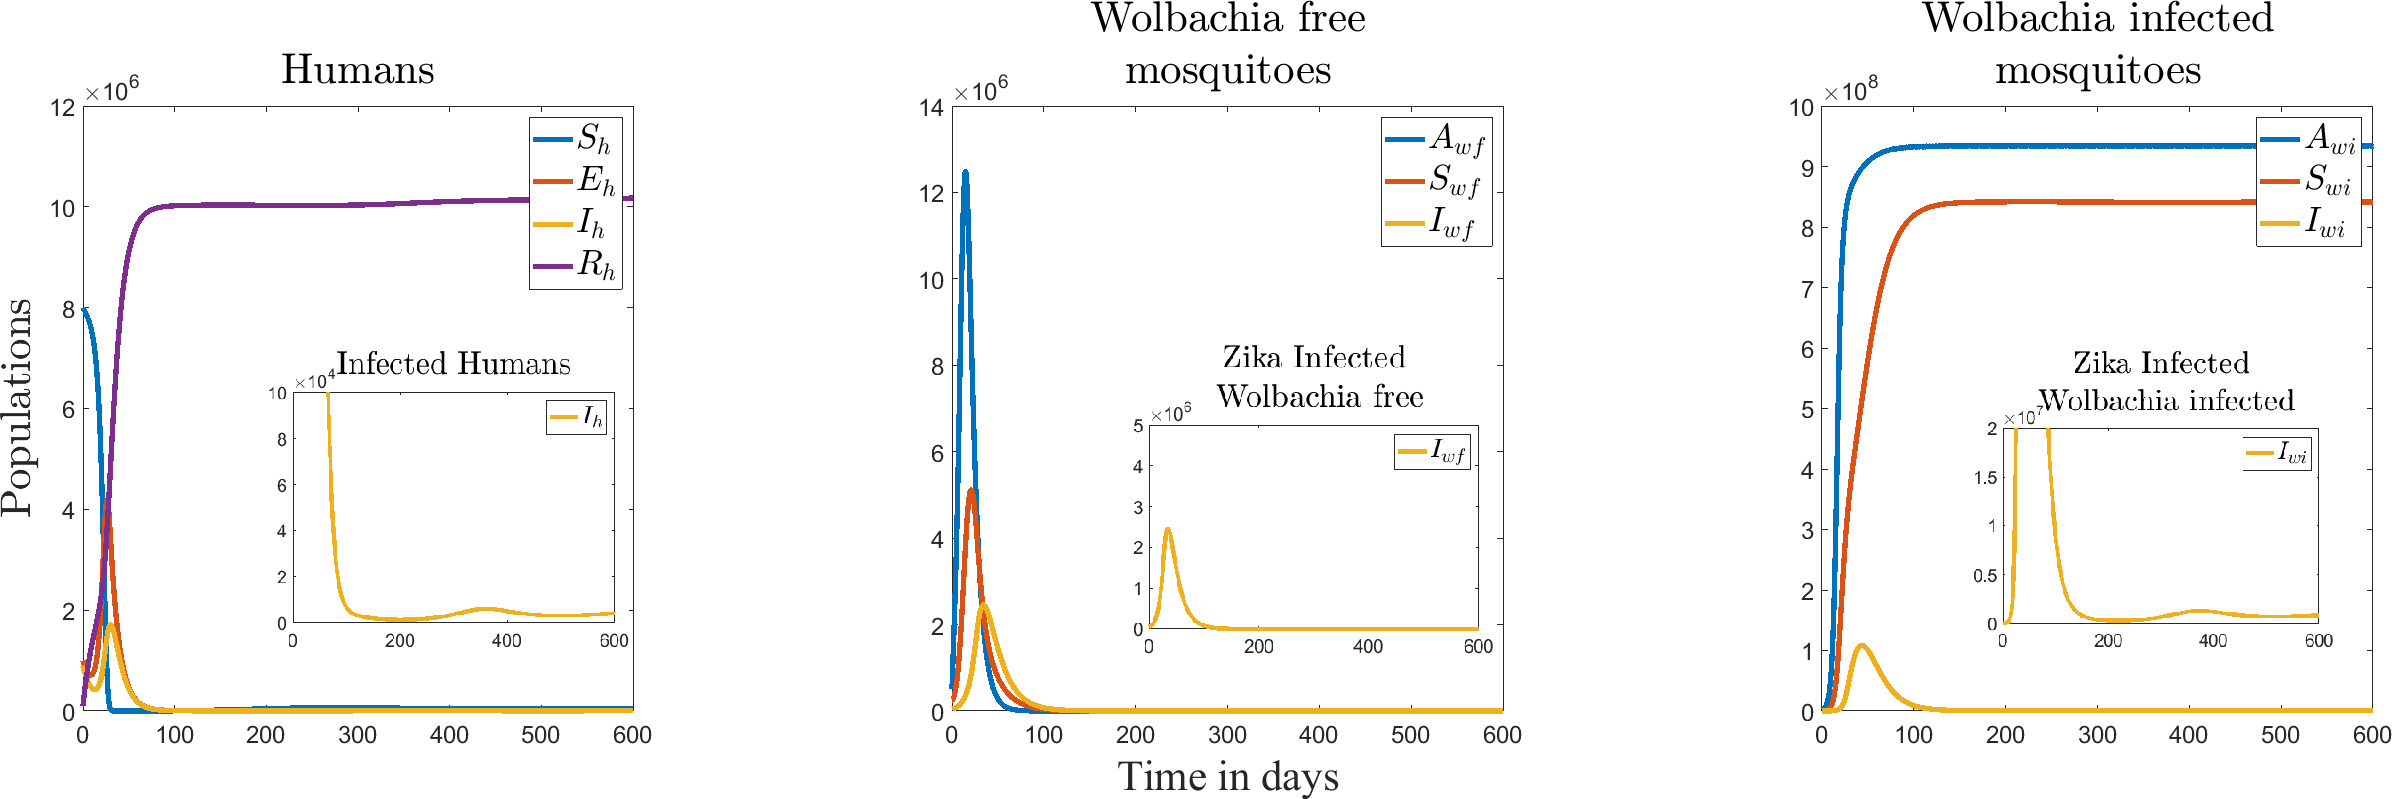
\includegraphics[width=16cm,height=4.5cm]{NewModel6c.png}
%    \caption{Disease persists when \textit{Wolbachia} mosquitoes are more competent. Figure is obtained using initial conditions given in Table \ref{init-cond-dis-present-table} with two changes ($A_{wf}(0)=500,000$, $A_{wi}(0)=1,500,000$)  and baseline values from Table \ref{tab: param-table} and Table \ref{tab: param_mosq_table}  with three changes($b=1.25$, $K=10^9$, $\beta_{hv}^w=0.042\beta_{hv}$)}
%    \label{sim6c}
%\end{figure}


Thus, if the carrying capacity of the environment is large enough and the mosquito biting rate is high, Zika can be endemic in the human population and in wild mosquitoes. If \textit{Wolbachia} infected mosquitoes persist, Zika is eradicated. However, if \textit{Wolbachia} infected mosquitoes lose some of their ability to block Zika virus (due to loss of \textit{Wolbachia} or higher temperatures), Zika can become endemic even when \textit{Wolbachia} infected mosquitoes dominate.

\section{Elasticity of the Reproduction numbers}

In this section we investigate the model dynamics over a wide range of feasible parameters to help better understand the model response under different assumptions.  More specifically, we explore the elasticity of the reproduction numbers. Below is a list of all the reproduction numbers.
The elasticity of a quantity $Q$ with respect to a parameter $p$ is given by
$$\epsilon_p^Q=\dfrac{\partial Q}{\partial p}\dfrac{p}{Q}.$$ 

\noindent The elasticities give the percentage change in the quantity $Q$ due to a $1\%$ increase the in the parameter $p$ \cite{martcheva2015introduction}. We will investigate how the reproduction numbers from the model change in response to $1\%$ increase in various parameters. 

Here is a summary of all the reproduction numbers: 
\begin{itemize}
    \item $R=\dfrac{\eta \alpha (1-\alpha)\gamma_{wf}}{\mu_v (\gamma_{wf}+\mu_A)}$ is the offspring reproduction number of wild mosquitoes.
    \item $R_w=\dfrac{q_2\alpha(1-\alpha)\gamma_{wi}}{\mu_{vi}(\gamma_{wi}+\mu_{Ai})}$ is the invasion number of \textit{Wolbachia} infected mosquitoes in absence of disease.
    \item $R_Z=R^{wf}_Z+R_d$ is the reproduction number of Zika in absence of \textit{Wolbachia} infected mosquitoes where $R^{wf}_Z=\dfrac{\nu_h\beta_{vh}\beta_{hv}\alpha\mu_h\gamma_{wf}}{\Lambda\mu^2_v(\mu_h+\nu_h)(\gamma_h+\mu_h)}K\left(1-\dfrac{1}{R}\right)$ and $R_d=\dfrac{\nu_h\beta_{hh}}{(\mu_h+\nu_h)(\gamma_h+\mu_h)}$.
    \item $M=\dfrac{q_1 \alpha (1-\alpha)\gamma_{wi}}{\mu_{vi} (\gamma_{wi}+\mu_{Ai})}$is the offspring reproduction number of \textit{Wolbachia} infected mosquitoes.
    \item $R^i_Z=R^{wi}_Z+R_d$ is the reproduction number of Zika in absence of \textit{Wolbachia} free mosquitoes where  $R^{wi}_Z=\dfrac{\beta^w_{vh}\beta^w_{hv}\nu_h\alpha \mu_h\gamma_{wi}}{\Lambda \mu^2_{vi}(\mu_h+\nu_h)(\gamma_h+\mu_h)}K\left(1-\dfrac{1}{M}\right).$
    \item $R_{0Z}^{NG}=\dfrac{R_d+\sqrt{R_d^2+\dfrac{4}{1+C}\left( 1-\dfrac{1}{R}-\dfrac{1}{M}\left(1-\dfrac{R_w}{R}\right)\right)\left(\dfrac{R^{wf}_Z}{1-1/R}+C\dfrac{R^{wi}_Z}{1-1/M}\right)}}{2}$ is the reproduction number of Zika in presence of both types of mosquitoes where 
    
    $q=\dfrac{1}{1+C}\left( 1-\dfrac{1}{R}-\dfrac{1}{M}\left(1-\dfrac{R_w}{R}\right)\right)\left(\dfrac{R^{wf}_Z}{1-1/R}+C\dfrac{R^{wi}_Z}{1-1/M}\right)$ and $C=\dfrac{\gamma_{wf}\mu_{vi}R}{\eta\gamma_{wi}\mu_vM}\left(1-\dfrac{R_w}{R}\right).$
 \end{itemize}   
    \vspace{0.2in}
    We begin with the elasticity of the reproduction offspring numbers of the mosquitoes $R$, $M$ and $R_w$. Looking through Figure \ref{elast2}, we can observe some common trends. All of the mosquitoes offspring numbers, $R$, $M$, $R_w$ are most sensitive to the mosquito death rates, $\mu_v$ and $\mu_{vi}$ and to the corresponding mosquito egg laying rates $\eta$, $q_1$ and $q_2$.
    
    The elasticity of the offspring numbers to the death rate of the mosquito are approximately $1\%$, meaning that $1\%$ increase in the parameter results in $1\%$ decrease in the offspring numbers. The elasticity of the offspring numbers to the  to the egg laying rates are also approximately $1\%$, meaning that $1\%$ increase in the parameter results in $1\%$ increase in the offspring numbers.  
    This suggests that measures to control the population of mosquitoes should be targeted towards decreasing the lifespan of the mosquitoes and decreasing the egg laying rates. The offspring numbers are not sensitive at all to the proportion of adult females arising from the aquatic stage, $\alpha$. Also, the transition rate from aquatic stage to adult mosquito, $\gamma_{wi}$, and the death rate of the aquatic stage, $\mu_{Ai}$, are more influential for the \textit{Wolbachia} infected mosquitoes. As we can observe in Figures \ref{elast2} b) and \ref{elast2} c) the reproduction offspring numbers $M$ and $R_w$ are more sensitive to $\gamma_{wi}$ and $\mu_{Ai}$ compared to the sensitivity of the reproduction offspring number $R$ with respect to $\gamma_{wf}$ and $\mu_{A}$.

 \begin{figure}[H]%
    \centering
    %\hskip-0.25in
    \subfloat[Elasticity of R]{{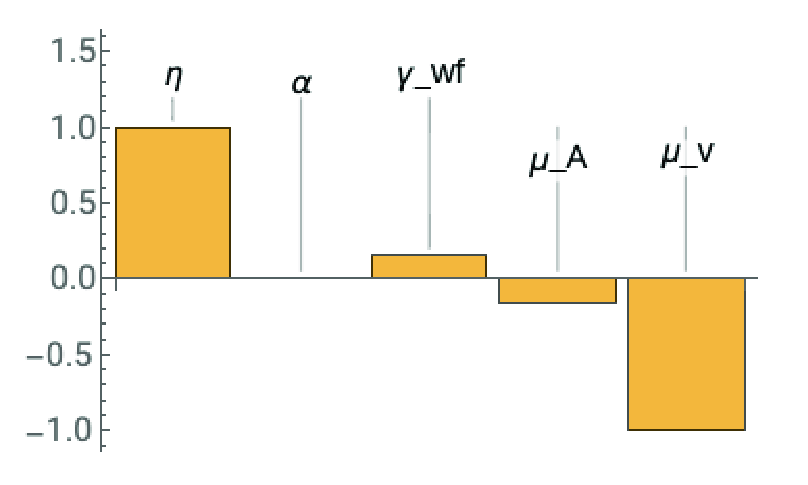
\includegraphics[width=4.5cm]{fig/eps/ER.eps} }}%
    %\label{elastR}
    \qquad
    \subfloat[Elasticity of M]{{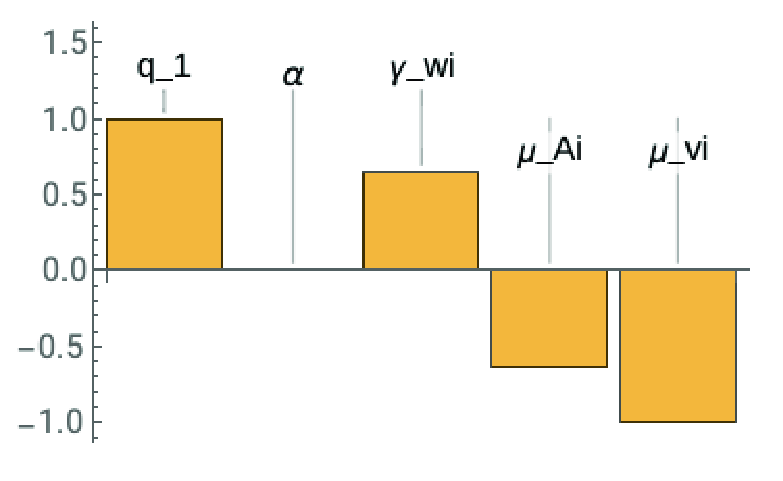
\includegraphics[width=4.5cm]{fig/eps/EM.eps} }}%
     %\label{elastM}
    \qquad
    \subfloat[Elasticity of $R_w$]{{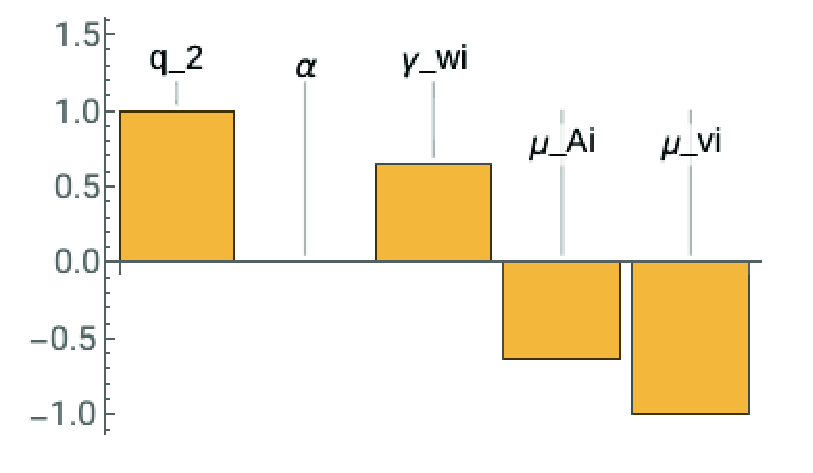
\includegraphics[width=4.5cm]{fig/eps/ERw.eps} }}%
     %\label{elastRw}
    \qquad
    \caption{Elasticities of the reproduction offspring numbers}
    \label{elast2}
\end{figure} 

Next, we investigate the elasticity of the reproduction numbers of Zika in presence of only one type of mosquitoes. In Figure \ref{fig:elasticities3} (a) we notice that the reproduction number of Zika in absence of \textit{Wolbachia} infected mosquitoes, $R_Z$, is most sensitive to the mosquito death rate, $\mu_v$, and somewhat sensitive to $\gamma_h$, $\beta_{vh}$, $\beta_{hv}$, $K$ and $\gamma_{wf}.$ On the other hand, the reproduction number $R_Z$ is not sensitive at all to $\nu_h$ and depends very little on $\beta_{hh}$, the direct transmission parameter.    
Figure \ref{fig:elasticities3} (b) shows the elasticities of $R_{Zi}$, the reproduction number of Zika in absence of \textit{Wolbachia} free mosquitoes. 
%In the presence of \textit{Wolbachia} infected only mosquitoes it appears that all other control mechanisms are much less influential except for the treatment of humans. That suggests that the presence of \textit{Wolbachia} infected mosquitoes actually does contribute to control in some sense. It makes all others types of control less influential. 
Notice that treatment of humans and controlling the sexual transmission are most influential because of the high elasticity of $\gamma_h$ and $\beta_{hh}$  parameters. That suggests that the presence of \textit{Wolbachia} infected mosquitoes changes the way Zika must be controlled making mosquito control less important.
$R_{Zi}$ shows very little sensitivity to the death rate of mosquitoes, meaning that killing the \textit{Wolbachia} infected mosquitoes is not a good control strategy. Also, in the presence of \textit{Wolbachia} infected mosquitoes we see more sensitivity to the direct transmission parameter.
\begin{figure}[H]%
    \centering
    %\hskip-0.5in
    \subfloat[$R_Z$]{{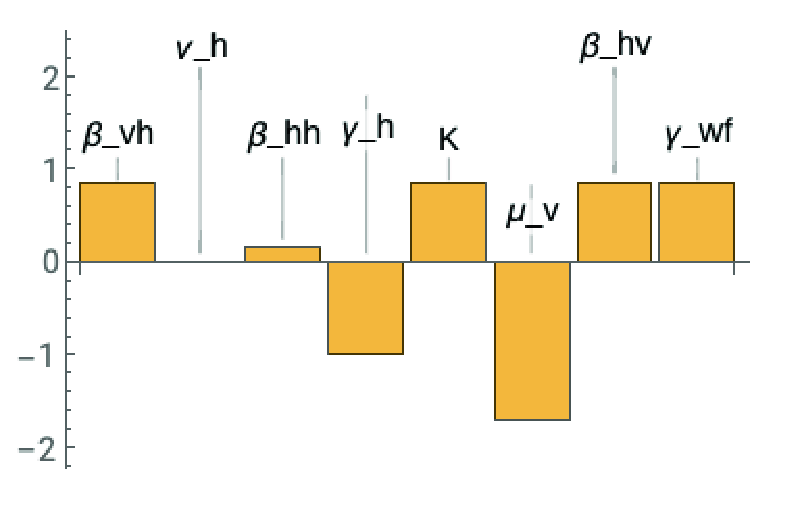
\includegraphics[width=0.45\columnwidth]{fig/eps/ERz.eps} }}%
    \qquad
    \subfloat[$R_z^{i}$]{{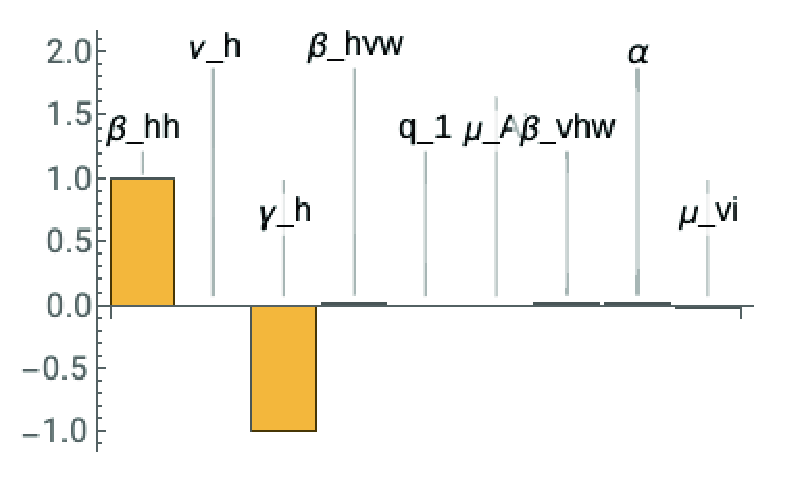
\includegraphics[width=0.45\columnwidth]{fig/eps/ERzii.eps} }}%
    \qquad
    \subfloat[$R^{NG}_{0Z}$]{{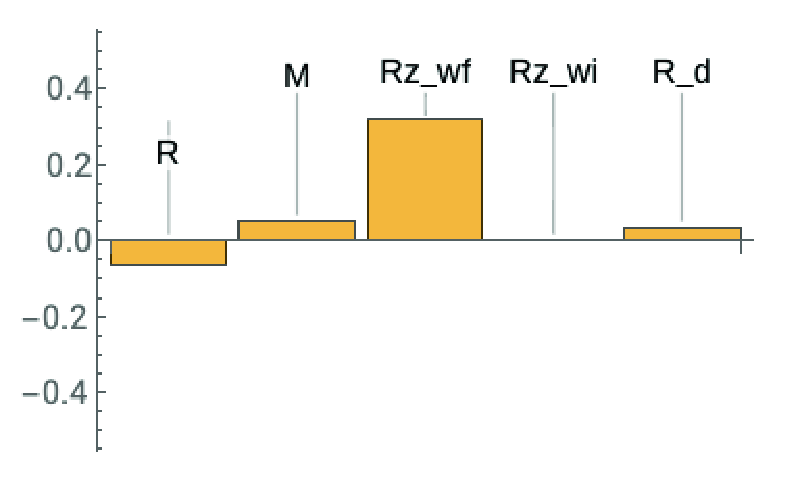
\includegraphics[width=0.45\columnwidth]{fig/eps/ER0Rs.eps} }}%
    \caption{Elasticities of reproduction numbers of Zika in presence of one type of mosquito and in presence of both types of mosquitoes with respect to other reproduction numbers.}
    \label{fig:elasticities3}%
\end{figure} 
  
The elasticity of the reproduction number of Zika in presence of both types of mosquitoes with respect to other offspring/reproduction numbers is investigated next. As we notice in Figure \ref{fig:elasticities3} (c) the reproduction number in presence of both types of mosquitoes,$R^{NG}_{0Z}$, is most sensitive to $R_z^{wf}$, the reproduction number in absence of \textit{Wolbachia} infected mosquitoes. A $1\%$ increase in $R_z^{wf}$ results in a $0.32\%$ increase in $R^{NG}_{0Z}$.
%\begin{figure}[H]%
%    \centering
%    \hskip-0.55in
%    \subfloat{{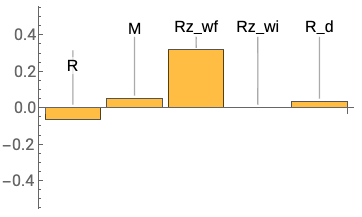
\includegraphics[width=4.5cm]{ER0Rs.png} }}%
%    \qquad
%    \caption{Elasticity of $R^{NG}_{0Z}$, Zika reproduction number is presence of both types of mosquitoes with respect to other reproduction numbers}
%    \label{fig:elasticitiesrs}%
%\end{figure} 
Lastly, we investigate the elasticity of the reproduction number of Zika in presence of both types of mosquitoes with respect to  parameters in Figure \ref{fig:elasticities4}. In terms of parameters, $R^{NG}_{0Z}$ is most sensitive again to the death rate of the \textit{Wolbachia} free mosquitoes and the direct transmission. A $1\%$ increase in $\beta_{hh}$ results in a $3.358\%$ increase in $R^{NG}_{0Z}$. We notice again that in the presence of \textit{Wolbachia} infected mosquitoes, the direct transmission becomes somewhat more influential. This might be happening due to the fact that \textit{Wolbachia} infected mosquitoes have a lower transmission rate. Parameters related to the vector-borne transmission in \textit{Wolbachia} free mosquitoes are also influential.
\begin{figure}[H]%
    \centering
    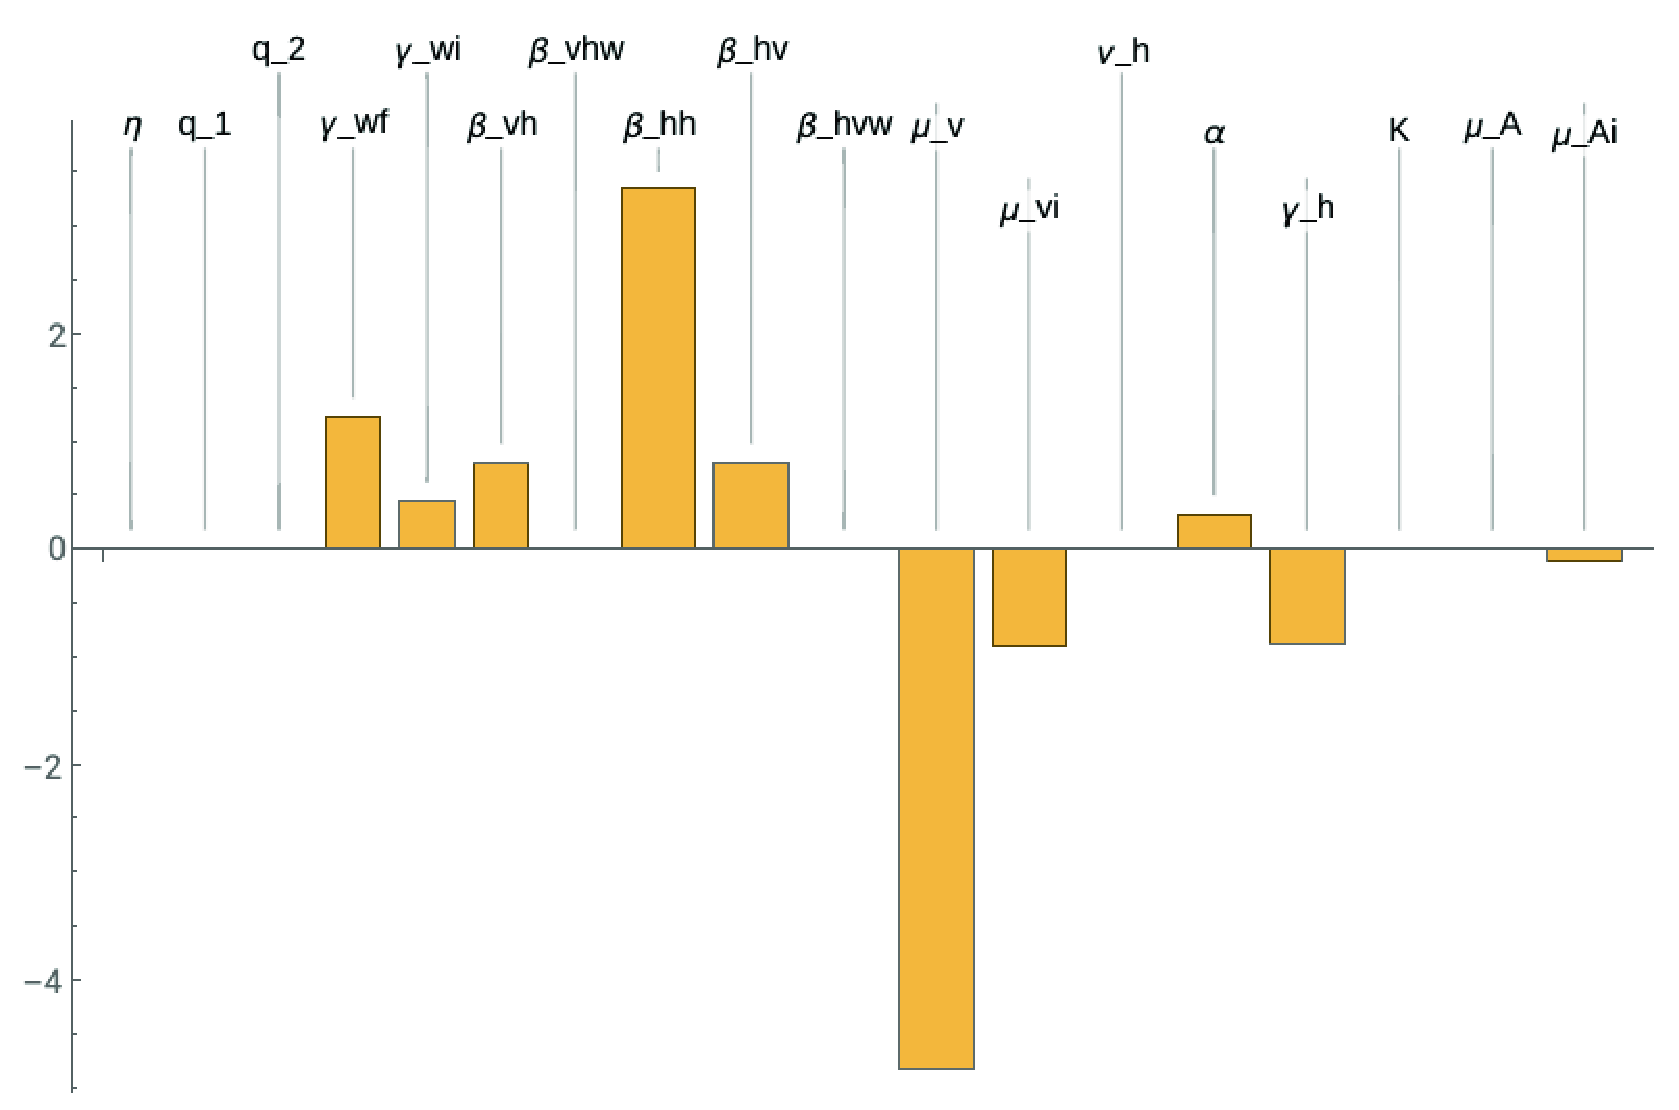
\includegraphics[width=0.95\columnwidth]{fig/eps/ER0Param.eps}%
    \caption{Elasticity of $R_{0Z}^{NG}$, Zika reproduction number in presence of both types of mosquitoes with respect to parameters}
    \label{fig:elasticities4}%
\end{figure} 

The presence of \textit{Wolbachia} infected mosquitoes switches the control strategies. When no \textit{Wolbachia} infected mosquitoes are present the control should be targeted towards decreasing the lifespan of the mosquitoes and when \textit{Wolbachia} infected mosquitoes are present the efforts should be concentrated on treatment of humans to increase the recovery rate and sexual transmission control to decrease the direct transmission rate.

\section{Non-autonomous model simulations}
%\begin{comment}
%Since the transmission of Zika virus is affected by periodic seasonality, it is worth further exploring how temperature fluctuations affect the dynamics of Zika transmission periodically. 
%The impact of climate variability on vectorborne diseases can be explained by the fact that the arthropod vectors of these diseases are cold-blooded. This means that  fluctuating temperatures and rainfall can impact the development, reproduction (including availability of breeding sites), behavior and population dynamics of mosquitoes \cite{gage2008climate}.
%However, this impact cannot be easily predicted.  Concluding that higher temperatures and increased rainfall will lead to increased transmission of arboviral diseases must be accompanied by a more careful and thoughtful analysis of the interplay between climate and human behavior \cite{sutherst2004global}. For example, extremely high temperatures can increase mosquito mortality \cite{reeves1994potential} and 
%heavy rainfall can wash out mosquito breeding sites \cite{reiter2001climate}. Also, during hot weather humans may seek refuge in air-conditioned buildings and thus avoiding mosquito bites \cite{reiter2003texas}. During dry season, domestic water storage container can provide more breeding sites for \textit{Aedes aegypti} mosquitoes and thus causing the incidence of the diseases they transmit to rise \cite{chretien2007drought}. 

% We are not going to include in the model the fat that temperature also affect vectorial capacity so no need to mention this?
%Temperature also can affect pathogen development within vectors and interact with humidity to influence vector survival and, hence, vectorial capacity.

%\textit{Aedes aegypti} mosquitoes originated from Africa, but now they are present in tropical, subtropical and temperate zones throughout the world. Large portions of the Americas, including the southernmost part of the eastern United States, the Caribbean, Central America, and lower elevation areas in Mexico and South America, have warm and humid climates well suited for proliferation of \textit{Aedes aegypti} \cite{world2009dengue}. 
%The lower temperature limit for \textit{Aedes aegypti} is around $10^{\circ}$ C, a temperature below which mosquitoes become inactive and unable to move. However, the  lower temperature limit at which female \textit{Aedes aegypti} has been found to cease biting is $15^{\circ}$C, both in the field and experimentally in the lab \cite{marchoux1903fievre}. 
%\textit{Aedes aegypti} are most active at $28^{\circ}$C \cite{connor1924suggestions} and females fed faster between $26^{\circ}$C and $35^{\circ}$C \cite{marchoux1903fievre}. The upper temperature limit for blood-feeding is above $36^{\circ}$C, and the mosquitoes die at $40^{\circ}$C \cite{christophers1960aedes}.
%CDC has updated the estimated range map for \textit{Aedes aegypti} by using county-level records along with historical records \cite{centers2018estimated}. According to CDC, the US regions where these mosquitoes can be found are expanding to include regions with more temperate climate rather than just subtropical or tropical climate \cite{centers2018estimated}. Thus it is important to investigate the effects of seasonality when the releasing of \textit{Wolbachia} infected mosquitoes spans multiple seasons. 
%\end{comment}

In this section we study the effects of seasonal variations on the spread of Zika and \textit{Wolbachia} infection. Since the mosquito population varies periodically, we introduce a seasonal variation into the birth rates, transitioning rates and death rates of mosquitoes. The egg laying rates are not constant any more. We assume $\eta(t)$, $q_1(t)$, $q_2(t)$ to be periodically forced. These periodic functions will take larger values during the wet season and smaller values during the dry season. In particular, we take the egg laying rate of \textit{\textit{Wolbachia}} free females to have the form
$\eta(t)=11\sin\left(2\pi(t-91)/365\right)+13$. This function assumes a 365-day period and has an amplitude of 11, vertical shift of 13 and phase shift of 91 days. Notice that the choice of this simple sinusoidal function assures that $\eta(t)\geq 0$ for all time. Similarly, the egg laying rates of \textit{Wolbachia} infected females when mating with wild males, $q_1(t)$, and when mating with \textit{Wolbachia} infected males, $q_2(t)$, have the following form $q_1(t)=q_2(t)=9\sin\left(2\pi(t-91)/365\right)+11$. The lower amplitude and vertical shift ensure that \textit{Wolbachia} infected females lay fewer eggs.

The periodic death rate of wild mosquitoes has the form $\mu_v=0.035\sin\left(2\pi t/365-91(1.0172)\right)+0.061$. The amplitude is chosen to be 0.035, the average of the range found in literature for the death rate of \textit{Aedes aegypti} mosquitoes, and the vertical shift is chosen to 0.061, the baseline value used in the first model with no seasonality. Similarly, the periodic death rates of \textit{Wolbachia} infected mosquitoes is chosen to have the form $\mu_{vi}=0.055\sin\left(2\pi t/365-91(1.0172)\right)+0.068$ where the higher amplitude and vertical shift accounts for the higher death rate of \textit{Wolbachia} infected mosquitoes. As we can observe in Figure \ref{fig:birthdeath}, in the months with higher temperatures, the conditions are good for the mosquitoes to thrive and multiply and the death rates are lower. 

%\begin{figure}[H]
%\begin{subfigure}{.5\textwidth}
%\centering
%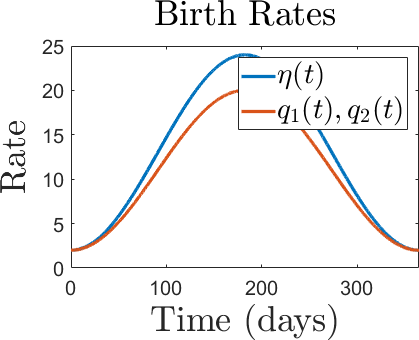
\includegraphics[scale=0.35]{seasetaseasonality_birth.png}
%\end{subfigure}
%\begin{subfigure}{.5\textwidth}
%\centering
%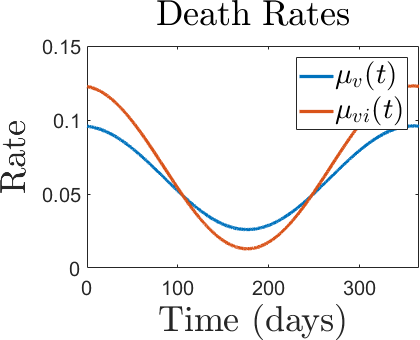
\includegraphics[scale=0.35]{seasetaseasonality_death.png}
%\end{subfigure}
%\caption{Seasonality of birth and death rates.}
%\label{fig:birthdeath}
%\end{figure}

\begin{figure}[H]
    \centering
    % This file was created by matlab2tikz.
%
%The latest updates can be retrieved from
%  http://www.mathworks.com/matlabcentral/fileexchange/22022-matlab2tikz-matlab2tikz
%where you can also make suggestions and rate matlab2tikz.
%
\definecolor{mycolor1}{rgb}{0.00000,0.44700,0.74100}%
\definecolor{mycolor2}{rgb}{0.85000,0.32500,0.09800}%
%
\begin{tikzpicture}

\begin{axis}[%
width=1.65in,
height=1.5in,
at={(1.011in,0.926in)},
scale only axis,
xmin=0,
xmax=365,
xlabel style={font=\color{white!15!black}},
xlabel={Time (days)},
ymin=0,
ymax=25,
ylabel style={font=\color{white!15!black}},
ylabel={Rate},
axis background/.style={fill=white},
title style={font=\bfseries},
title={Birth Rates},
legend style={legend cell align=left, align=left, draw=white!15!black, cells={align=left}}
]
\addplot [color=mycolor1, line width=1.5pt]
  table[row sep=crcr]{%
0	2.00017225335523\\
2.10000000000002	2.00956999759558\\
4.19999999999999	2.03330489584226\\
6.30000000000001	2.0713459856222\\
8.39999999999998	2.12364364185595\\
10.5	2.19012964159401\\
12.6	2.27071725301437\\
14.7	2.36530134856565\\
16.8	2.47375854210691\\
18.9	2.59594734986672\\
21.1	2.7385087778564\\
23.3	2.89576152900622\\
25.5	3.06748046537717\\
27.7	3.25341973786874\\
29.9	3.4533131381998\\
32.2	3.67690168991248\\
34.5	3.91507892806368\\
36.8	4.16747215540954\\
39.2	4.44556812604623\\
41.6	4.73823910721177\\
44	5.04498644713198\\
46.5	5.37891954294707\\
49.1	5.74114677884023\\
51.7	6.11788841933696\\
54.4	6.52367479427932\\
57.2	6.9592287928412\\
60.1	7.42509284302679\\
63.1	7.92159993891187\\
66.3	8.46607488704024\\
69.7	9.05958690476803\\
73.3	9.70265128756449\\
77.3	10.4318811834165\\
81.9	11.2853013231024\\
88	12.4326518446461\\
101.3	14.938582130148\\
106	15.8066198496982\\
110	16.5311544285967\\
113.6	17.1690464243947\\
116.9	17.739801921964\\
120.1	18.2786999836724\\
123.1	18.7694274547943\\
126	19.2292121566382\\
128.8	19.6584514853657\\
131.5	20.0577485576015\\
134.1	20.4278831264335\\
136.6	20.7697839307157\\
139.1	21.0973206179856\\
141.5	21.3976797422324\\
143.9	21.6837309296734\\
146.3	21.9549868073153\\
148.6	22.2006290042489\\
150.9	22.4318741534291\\
153.2	22.6483604048722\\
155.4	22.8413112752175\\
157.6	23.0201723918289\\
159.8	23.1846876801836\\
162	23.3346216046064\\
164.2	23.4697595054841\\
166.3	23.5847743121911\\
168.4	23.6859811478359\\
170.5	23.7732479868298\\
172.6	23.8464609884852\\
174.7	23.9055246455216\\
176.8	23.9503619086564\\
178.9	23.9809142871167\\
181	23.9971419249408\\
183.1	23.9990236529713\\
185.2	23.9865570164706\\
187.3	23.9597582783223\\
189.4	23.9186623978172\\
191.5	23.8633229850476\\
193.6	23.7938122309727\\
195.7	23.7102208132444\\
197.8	23.6126577779173\\
199.9	23.5012503971965\\
202.1	23.3698475639127\\
204.3	23.2235982742627\\
206.5	23.0627119125872\\
208.7	22.8874188190465\\
210.9	22.6979699598431\\
213.1	22.4946365679149\\
215.4	22.2675314178721\\
217.7	22.0259245318808\\
220	21.7701939738619\\
222.4	21.4887196429777\\
224.8	21.1927822618294\\
227.3	20.8696784949272\\
229.8	20.5320259344218\\
232.4	20.1661051955997\\
235	19.7858555060369\\
237.7	19.376629962976\\
240.5	18.9377365736013\\
243.4	18.4686658436911\\
246.4	17.9691196850409\\
249.6	17.4217238911961\\
253	16.8254809972084\\
256.7	16.1618367068538\\
260.8	15.4116099760385\\
265.6	14.5183360458525\\
272.3	13.2555362001656\\
283	11.2387329209066\\
287.9	10.3309483193648\\
292	9.58566735499403\\
295.7	8.9275645818895\\
299.1	8.33729602283518\\
302.3	7.79627615985419\\
305.3	7.30335313814021\\
308.2	6.84126184457864\\
311	6.40962905489488\\
313.7	6.00787441916248\\
316.3	5.63523950547039\\
318.9	5.2773307627545\\
321.4	4.94774173477396\\
323.8	4.64533393875558\\
326.2	4.35716079298663\\
328.6	4.08371328584542\\
330.9	3.83590885429624\\
333.2	3.60244429644268\\
335.5	3.38368493517584\\
337.7	3.18851281550116\\
339.9	3.00738775056629\\
342.1	2.84056905617666\\
344.3	2.68829556578197\\
346.5	2.55078528853983\\
348.6	2.43347845353179\\
350.7	2.32995577862386\\
352.8	2.24035231044599\\
354.9	2.16478493784797\\
357	2.10335223941678\\
359.1	2.05613435487925\\
361.2	2.0231928805589\\
363.3	2.00457078902286\\
365	2.00000092915417\\
};
\addlegendentry{$\eta(t)$}

\addplot [color=mycolor2, line width=1.5pt]
  table[row sep=crcr]{%
0	2.00014093456338\\
2.30000000000001	2.00917436321532\\
4.60000000000002	2.03227654151203\\
6.89999999999998	2.06941131940727\\
9.19999999999999	2.12052058879016\\
11.5	2.18552437441195\\
13.8	2.2643209590309\\
16.2	2.36111523308546\\
18.6	2.47262840820684\\
21	2.59867048864481\\
23.4	2.73902672435219\\
25.8	2.89345797687491\\
28.3	3.06900684407879\\
30.8	3.25921785822663\\
33.3	3.46373937334107\\
35.8	3.68219328740525\\
38.4	3.92373045051784\\
41	4.17941693394249\\
43.7	4.45936525446319\\
46.4	4.75341705427667\\
49.2	5.07257806196975\\
52.1	5.41761852436019\\
55.1	5.78915890314141\\
58.2	6.18764444501988\\
61.4	6.61331861486224\\
64.8	7.08012441977189\\
68.4	7.58896201640437\\
72.3	8.15489405322575\\
76.6	8.79360123224529\\
81.6	9.55121129443694\\
88.3	10.5821902176835\\
101.6	12.6318044624722\\
106.7	13.4009298858016\\
111	14.0352988956834\\
114.9	14.5963962723042\\
118.5	15.1000305342036\\
121.9	15.5612876738872\\
125.1	15.9811938768098\\
128.2	16.3736038855782\\
131.2	16.7388240452429\\
134.1	17.0773589216274\\
136.9	17.3898845914719\\
139.6	17.677223132526\\
142.3	17.9501636706575\\
144.9	18.1988376560526\\
147.5	18.4331172406751\\
150	18.6443750971392\\
152.5	18.8415006817976\\
155	19.0241295656018\\
157.4	19.1855011385228\\
159.8	19.3329262837866\\
162.2	19.4661538189563\\
164.6	19.5849567514326\\
167	19.6891326652025\\
169.4	19.7785040657155\\
171.7	19.8501184289789\\
174	19.9078842197603\\
176.3	19.9517110467563\\
178.6	19.9815303302077\\
180.9	19.9972954092125\\
183.2	19.9989816147406\\
185.5	19.986586308235\\
187.8	19.9601288857416\\
190.1	19.9196507475575\\
192.4	19.8652152334486\\
194.7	19.7969075235364\\
197	19.7148345050089\\
199.4	19.6146561973914\\
201.8	19.4998002692573\\
204.2	19.3704624117277\\
206.6	19.226862990183\\
209	19.0692466688058\\
211.5	18.8904476708278\\
214	18.6970614829571\\
216.5	18.4894456211627\\
219.1	18.2588431512648\\
221.7	18.0137262968987\\
224.3	17.7545851802765\\
227	17.47118912386\\
229.8	17.1625666736178\\
232.6	16.8396536174129\\
235.5	16.4909417719037\\
238.5	16.1158428722329\\
241.6	15.713945963721\\
244.9	15.2714247075608\\
248.3	14.8011199320301\\
252	14.2746061800885\\
256	13.6905543666554\\
260.5	13.0184191538434\\
265.8	12.2116040067907\\
273.6	11.0078538813113\\
283.4	9.49787675727401\\
288.6	8.71126947794892\\
293	8.05972145094933\\
296.9	7.49616878890589\\
300.5	6.98989827556704\\
303.9	6.52583466152208\\
307.1	6.10301478683976\\
310.2	5.70753885804385\\
313.2	5.3391319885792\\
316.1	4.99731927606911\\
318.9	4.68145244225371\\
321.7	4.38023792429732\\
324.4	4.10431172563875\\
327	3.85265156310788\\
329.6	3.61528284633232\\
332.1	3.40096332766979\\
334.6	3.20069226298165\\
337.1	3.01483989641281\\
339.6	2.84374981604287\\
342	2.69368555985983\\
344.4	2.55777357260655\\
346.8	2.43624542064236\\
349.2	2.32930816319936\\
351.6	2.23714399959545\\
353.9	2.16282815796001\\
356.2	2.10234063012308\\
358.5	2.05577606633381\\
360.8	2.02320733033304\\
363.1	2.00468538533738\\
365	2.00000076021706\\
};
\addlegendentry{$q_1(t)$\\$q_2(t)$}

\end{axis}
\end{tikzpicture}% \
    % This file was created by matlab2tikz.
%
%The latest updates can be retrieved from
%  http://www.mathworks.com/matlabcentral/fileexchange/22022-matlab2tikz-matlab2tikz
%where you can also make suggestions and rate matlab2tikz.
%
\definecolor{mycolor1}{rgb}{0.00000,0.44700,0.74100}%
\definecolor{mycolor2}{rgb}{0.85000,0.32500,0.09800}%
%
\begin{tikzpicture}

\begin{axis}[%
width=1.6in,
height=1.5in,
at={(1.143in,0.926in)},
scale only axis,
xmin=0,
xmax=365,
xlabel style={font=\color{white!15!black}},
xlabel={Time (days)},
ymin=0,
ymax=0.14,
ylabel style={font=\color{white!15!black}},
ylabel={},
axis background/.style={fill=white},
title style={font=\bfseries},
title={Death Rates},
legend style={legend cell align=left, align=left, draw=white!15!black}
]
\addplot [color=mycolor1, line width=1.5pt]
  table[row sep=crcr]{%
0	0.0957815563227769\\
2.80000000000001	0.0955532711360547\\
5.60000000000002	0.0952448590787753\\
8.39999999999998	0.0948570353390323\\
11.2	0.0943906992559391\\
14.1	0.0938260951925258\\
17	0.0931798362635163\\
19.9	0.0924535300371758\\
22.8	0.091648983199093\\
25.8	0.090736491281973\\
28.8	0.0897448417384794\\
31.9	0.0886397835491266\\
35.1	0.0874167115055684\\
38.3	0.0861136328346674\\
41.6	0.0846902154067948\\
45	0.0831439090058552\\
48.5	0.0814730977441513\\
52.2	0.0796262895475479\\
56.1	0.0775981677671211\\
60.2	0.0753857123179955\\
64.7	0.0728755129152319\\
69.7	0.0700036722251411\\
75.6	0.0665309733557251\\
84	0.0614974398579307\\
95.9	0.0543738901153006\\
101.8	0.0509263931418786\\
106.7	0.0481405119862757\\
111.1	0.0457161351275772\\
115.2	0.0435355309584793\\
119.1	0.041541705780503\\
122.8	0.0397308974563657\\
126.3	0.03809710887964\\
129.7	0.0365894016908328\\
133	0.0352058048497952\\
136.2	0.0339434347181395\\
139.3	0.0327986208627635\\
142.4	0.0317339651663247\\
145.4	0.0307828265198395\\
148.4	0.0299121250610028\\
151.3	0.0291490874153624\\
154.2	0.0284652788698736\\
157.1	0.027862400397396\\
159.9	0.0273585112663568\\
162.7	0.0269326346397065\\
165.5	0.0265857580986335\\
168.3	0.0263186860281053\\
171.1	0.0261320377514949\\
173.9	0.0260262460944887\\
176.7	0.0260015563812885\\
179.5	0.0260580258657797\\
182.3	0.0261955235987443\\
185.1	0.0264137307316901\\
187.9	0.0267121412557572\\
190.7	0.0270900631758195\\
193.5	0.0275466201144923\\
196.4	0.0281012492916943\\
199.3	0.0287377140649596\\
202.2	0.0294544312290554\\
205.1	0.0302496179510285\\
208.1	0.0311526926912506\\
211.1	0.0321352200467118\\
214.2	0.0332311876639437\\
217.3	0.0344060839343001\\
220.5	0.0356981266244816\\
223.8	0.0371107606623013\\
227.2	0.0386466277089426\\
230.7	0.0403074409689452\\
234.4	0.0421445451000295\\
238.3	0.0441634433833542\\
242.4	0.0463673592086025\\
246.8	0.0488131494293498\\
251.7	0.051618340686673\\
257.4	0.0549639291838275\\
265.2	0.059629550947875\\
279	0.0678914755754363\\
284.8	0.0712747840405541\\
289.7	0.0740548060203423\\
294.1	0.0764727386264212\\
298.2	0.0786463638937107\\
302	0.0805828447189469\\
305.7	0.0823880783731852\\
309.2	0.0840161498724683\\
312.6	0.0855179102175043\\
315.9	0.0868953840578115\\
319.1	0.0881515052883515\\
322.2	0.0892899911254403\\
325.3	0.0903480669373948\\
328.3	0.091292615754071\\
331.3	0.0921565265580853\\
334.2	0.0929128259966774\\
337.1	0.0935897423255483\\
340	0.0941855917163252\\
342.8	0.0946825806781249\\
345.6	0.0951014618458998\\
348.4	0.0954412638604936\\
351.2	0.0957011987422902\\
354	0.095880663718674\\
356.8	0.0959792426215245\\
359.6	0.0959967068525884\\
362.4	0.0959330159133742\\
365	0.0958013334896464\\
};
\addlegendentry{$\mu_v(t)$}

\addplot [color=mycolor2, line width=1.5pt]
  table[row sep=crcr]{%
0	0.122656731364316\\
2.19999999999999	0.122385501718441\\
4.39999999999998	0.12203640863504\\
6.60000000000002	0.121609951908795\\
8.89999999999998	0.121082056492355\\
11.2	0.120471098830762\\
13.5	0.119778034944147\\
15.8	0.119003949331557\\
18.1	0.118150053274064\\
20.4	0.11721768293927\\
22.8	0.116162687884298\\
25.2	0.115025633413438\\
27.6	0.113808456836011\\
30	0.112513231973196\\
32.5	0.111083426046093\\
35	0.109573971137991\\
37.6	0.107922647620057\\
40.2	0.106191496966574\\
42.9	0.10431298434105\\
45.7	0.102282246731932\\
48.5	0.100172010740835\\
51.4	0.0979078231152926\\
54.5	0.0954053627640405\\
57.7	0.0927405547623721\\
61.1	0.0898272833328519\\
64.7	0.0866615202953653\\
68.6	0.0831516146017179\\
73	0.0791107248656431\\
78.4	0.0740669460188883\\
87.8	0.0651881438729447\\
95.1	0.0583316178625637\\
100	0.0538081185003989\\
104.2	0.0500098205865811\\
108	0.0466535951119909\\
111.5	0.0436426544711708\\
114.8	0.0408844067966356\\
117.9	0.0383727215441922\\
120.9	0.0360221672415264\\
123.8	0.0338308155110667\\
126.6	0.0317956198658749\\
129.3	0.0299125697831641\\
131.9	0.0281768375230058\\
134.5	0.0265207334733759\\
137	0.0250065031999043\\
139.5	0.0235717556539612\\
142	0.022219143274981\\
144.4	0.0210002307923105\\
146.8	0.0198613963489152\\
149.2	0.0188045802867691\\
151.5	0.0178704291848817\\
153.8	0.0170147203095325\\
156.1	0.0162387926650354\\
158.4	0.0155438604147662\\
160.7	0.0149310109815133\\
163	0.0144012033455851\\
165.2	0.0139729011652321\\
167.4	0.0136219492989085\\
169.6	0.013348850202533\\
171.8	0.01315399487072\\
174	0.0130376622767585\\
176.2	0.0130000189734005\\
178.4	0.0130411188544031\\
180.6	0.0131609030772779\\
182.8	0.0133592001476472\\
185	0.0136357261644662\\
187.2	0.0139900852270785\\
189.4	0.0144217700013201\\
191.7	0.0149550824243079\\
194	0.0155713989778405\\
196.3	0.0162697552563031\\
198.6	0.0170490584790741\\
200.9	0.0179080892007164\\
203.2	0.0188455032188699\\
205.6	0.0199056557129325\\
208	0.021047751179367\\
210.4	0.0222698437198687\\
212.8	0.0235698511376654\\
215.3	0.0250044882482143\\
217.8	0.0265186118113547\\
220.4	0.0281746090457773\\
223	0.0299102389466839\\
225.7	0.0317931876688249\\
228.5	0.0338282837416273\\
231.3	0.0359426218832368\\
234.2	0.0382107778149248\\
237.3	0.0407171536714372\\
240.5	0.0433856381022224\\
243.9	0.0463023967341769\\
247.5	0.049471368617958\\
251.5	0.0530752037333855\\
256	0.0572130657177468\\
261.5	0.0623556413505639\\
281.5	0.0811374389338653\\
285.8	0.0850479746749784\\
289.7	0.0885146951748084\\
293.2	0.0915477351070422\\
296.5	0.0943295073388413\\
299.7	0.0969460807605742\\
302.7	0.0993196450686469\\
305.6	0.101534905933079\\
308.4	0.103594684036466\\
311.1	0.105502778309699\\
313.8	0.107330005866118\\
316.4	0.109009449312566\\
319	0.110606892514397\\
321.5	0.112062590341964\\
324	0.113436828992633\\
326.4	0.114677101566144\\
328.8	0.115837845860426\\
331.2	0.116917084203465\\
333.5	0.117873168829931\\
335.8	0.118751212444977\\
338.1	0.119549841095136\\
340.4	0.120267805094727\\
342.7	0.120903980981154\\
345	0.121457373273074\\
347.2	0.121908442268193\\
349.4	0.122282330829307\\
351.6	0.122578503662055\\
353.8	0.122796536737383\\
356	0.122936117898462\\
358.2	0.122997047307706\\
360.4	0.122979237732807\\
362.6	0.122882714671618\\
364.8	0.122707616315665\\
365	0.122687809769445\\
};
\addlegendentry{$\mu_{vi}(t)$}

\end{axis}
\end{tikzpicture}% \ 
    % This file was created by matlab2tikz.
%
%The latest updates can be retrieved from
%  http://www.mathworks.com/matlabcentral/fileexchange/22022-matlab2tikz-matlab2tikz
%where you can also make suggestions and rate matlab2tikz.
%
\definecolor{mycolor1}{rgb}{0.00000,0.44700,0.74100}%
%
\begin{tikzpicture}

\begin{axis}[%
width=1.6in,
height=1.5in,
at={(1.143in,0.926in)},
scale only axis,
xmin=0,
xmax=365,
xlabel style={font=\color{white!15!black}},
xlabel={Time (days)},
ymin=0,
ymax=0.25,
ylabel style={font=\color{white!15!black}},
ylabel={Rate},
axis background/.style={fill=white},
title style={font=\bfseries},
title={Transition Rates},
legend style={legend cell align=left, align=left, draw=white!15!black}
]
\addplot [color=mycolor1, line width=1.5pt]
  table[row sep=crcr]{%
0	0.0200009260263982\\
2.19999999999999	0.0200889225290553\\
4.39999999999998	0.0203201975576803\\
6.60000000000002	0.0206944194499101\\
8.80000000000001	0.0212110515488462\\
11	0.0218693529728284\\
13.2	0.0226683796778957\\
15.4	0.023606985811341\\
17.6	0.0246838253552824\\
19.9	0.0259557347911255\\
22.2	0.0273750468676894\\
24.5	0.028939536990606\\
26.8	0.0306467530168675\\
29.1	0.0324940190986922\\
31.5	0.0345677830250111\\
33.9	0.0367873465718844\\
36.3	0.0391489218061452\\
38.8	0.0417555588334722\\
41.3	0.0445070865536081\\
43.8	0.0473984097706079\\
46.4	0.0505479229621528\\
49.1	0.0539657128064732\\
51.8	0.0575261267279643\\
54.6	0.0613608276453874\\
57.5	0.0654759561459173\\
60.5	0.0698758186554187\\
63.7	0.0747160226068218\\
67	0.079851201079407\\
70.6	0.0856003540808956\\
74.5	0.0919769324800654\\
78.8	0.0991527075620411\\
84	0.10797919551004\\
92.1	0.121893449538675\\
100.5	0.136280701293856\\
105.5	0.14470221804811\\
109.7	0.151637490660335\\
113.5	0.157770796520424\\
117	0.16327755925505\\
120.3	0.168326145196829\\
123.4	0.172927028809795\\
126.4	0.177236154935031\\
129.3	0.181256694962144\\
132.1	0.184993877992383\\
134.8	0.18845471059285\\
137.4	0.191647709452354\\
140	0.194697208769639\\
142.5	0.19748840413672\\
145	0.200136108817446\\
147.4	0.202538355556385\\
149.8	0.20479974137254\\
152.2	0.206916406958385\\
154.5	0.208805732262931\\
156.8	0.210555865672973\\
159.1	0.212164064072851\\
161.4	0.21362780681244\\
163.7	0.214944799657871\\
165.9	0.216065308102884\\
168.1	0.217048053087751\\
170.3	0.217891625296772\\
172.5	0.218594814996379\\
174.7	0.219156613769997\\
176.9	0.219576215964253\\
179.1	0.219853019844265\\
181.3	0.219986628456411\\
183.5	0.219976850198009\\
185.7	0.219823699091535\\
187.9	0.219527394765066\\
190.1	0.219088362136802\\
192.3	0.218507230806154\\
194.5	0.217784834150564\\
196.7	0.216922208130541\\
198.9	0.215920589803886\\
201.1	0.214781415551897\\
203.4	0.21344515940325\\
205.7	0.211962439637432\\
208	0.210335580232481\\
210.3	0.208567131087307\\
212.6	0.206659864025085\\
215	0.204524905735298\\
217.4	0.202245696252987\\
219.8	0.199826125303616\\
222.3	0.197160937541469\\
224.8	0.194352865485826\\
227.4	0.191286491255141\\
230	0.1880773409477\\
232.7	0.184600536091352\\
235.5	0.180847687011521\\
238.3	0.176953502821107\\
241.2	0.172780895965388\\
244.3	0.168175367410186\\
247.5	0.16327755925505\\
250.9	0.15793013108032\\
254.6	0.151963902223372\\
258.6	0.145368856582081\\
263.2	0.137637877206771\\
269	0.127738647923366\\
285.5	0.0994895500131179\\
290.1	0.0918117292881675\\
294.1	0.0852772857998616\\
297.7	0.0795361221106532\\
301.1	0.0742561870906684\\
304.3	0.0694296217079682\\
307.3	0.0650437755418238\\
310.2	0.0609432919670212\\
313	0.0571237185404243\\
315.7	0.0535787774807659\\
318.4	0.050177296220113\\
321	0.0470442445913477\\
323.6	0.0440573123233321\\
326.1	0.041328631578267\\
328.6	0.0387456320970045\\
331	0.0364074520581426\\
333.4	0.0342119320391134\\
335.8	0.0321628189401508\\
338.1	0.0303397075193743\\
340.4	0.0286571274095877\\
342.7	0.0271177158450087\\
345	0.0257238856609661\\
347.3	0.024477821512221\\
349.5	0.0234260062345015\\
351.7	0.0225126839029599\\
353.9	0.021739164276994\\
356.1	0.0211065566305138\\
358.3	0.0206157681611217\\
360.5	0.0202675026891939\\
362.7	0.020062259648455\\
364.9	0.0200003333698078\\
365	0.0200009260263982\\
};
\addlegendentry{$\gamma_{wf}(t),\gamma_{wi}(t)$}

\end{axis}
\end{tikzpicture}%
    \caption{Seasonality of rates.}
\label{fig:birthdeath}
\end{figure}

The temperature of the environment also affects on how the immature stages of \textit{Aedes aegypti} mosquitoes develop. The lower temperature threshold for immature stages to develop is $16^{\circ}$C, while $34^{\circ}$C is the upper limit \cite{christophers1960aedes}. The development time from the aquatic stage to adults was shorter at higher temperatures ($30^{\circ}$ C vs. $21^{\circ}$C) and density and food availability played an important role.  The time taken by larvae to complete their development was optimal at $32^{\circ}$C and that mortality was significant at $14^{\circ}$C and $38^{\circ}$C \cite{bar1958effect}. 
The highest temperature at which development fully occurred was $36 ^{\circ}$C. Immature stages were found to survive short exposure to temperatures up to $45^{\circ}$C \cite{bar1957effect}. Thus, it is important to assume that the transitioning rates from aquatic stage to adult are periodic. 

We let $\gamma_{wf}$ and $\gamma_{wi}$ to have the following form $\gamma_{wf}=\gamma_{wi}=0.1\sin\left(2\pi(t-91)/365\right)+0.12$.

%\begin{figure}[H]
%    \centering
%    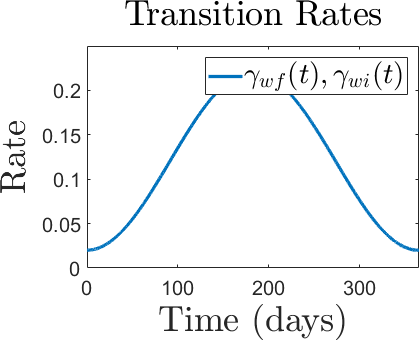
\includegraphics[scale=0.4]{seasetaseasonality_trans.png}
%    \caption{Seasonality of transitioning rates}
%    \label{fig:transrates}
%\end{figure}

As seen in Figure \ref{fig:birthdeath} the transitioning rates have a similar shape as the egg laying rates with an amplitude of 0.1 which is the average of the range of values for the transitioning rates found in literature.  Even tough \textit{Wolbachia} infected aquatic stage might take slightly longer to develop compared to wild mosquitoes, the change is so small that we allow both transitioning rates (wild and \textit{Wolbachia} infected) to have the same form.

When we allow for the egg laying rates, death rates and transitioning rates to depend explicitly on time, the model becomes nonautonomous. Nonautonomous models are harder to analyze theoretically, so we will only perform numerical simulations for the nonautonoums model. Our goal is to get some insight on how the seasonality of the rates affects \textit{Wolbachia} spread and diseases dynamics when we simulate over a span of 3 years.

\subsection{Disease free simulations for nonautonomous model}
The nonautonomous model is simulated using periodicity for the egg laying rates, transitioning rates from aquatic stage to adults and for death rates. All other parameters remain constant and the initial conditions stay the same as in Section \ref{diseasefreefirst}. When the parameters that remain constant take the baseline values from Table \ref{tab: param-table} and Table \ref{tab: param_mosq_table} and the periodic parameters take the form mentioned earlier, we illustrate the effect of the introduction of \textit{Wolbachia} infected mosquitoes through numerical simulations. The initial conditions used are the same as in \ref{diseasefreefirst} and listed in Table \ref{init-cond-dis-free-table}.

\subsubsection{Zika takes longer to be eradicated when seasonality is included }
As we see in Figure \ref{nonautfig1}, \textit{Wolbachia} free mosquitoes persist and the disease is eradicated in both humans and mosquitoes in approximately in 350 days, a little longer than in the case where seasonality was not taken into account. \textit{Wolbachia} free female mosquitoes population oscillates between 500,000 and 1,750,000 compared to settling around 900,000 in the non-seasonal scenario. 

\begin{figure}[H]
    \centering
    % This file was created by matlab2tikz.
%
%The latest updates can be retrieved from
%  http://www.mathworks.com/matlabcentral/fileexchange/22022-matlab2tikz-matlab2tikz
%where you can also make suggestions and rate matlab2tikz.
%
\definecolor{mycolor1}{rgb}{0.00000,0.44700,0.74100}%
\definecolor{mycolor2}{rgb}{0.85000,0.32500,0.09800}%
\definecolor{mycolor3}{rgb}{0.92900,0.69400,0.12500}%
\definecolor{mycolor4}{rgb}{0.49400,0.18400,0.55600}%
%
\begin{tikzpicture}

\begin{axis}[%
width=1.1in,
height=1.5in,
at={(0in,0in)},
scale only axis,
xmin=0,
xmax=1095,
ymin=0,
ymax=10000000,
ylabel style={font=\color{white!15!black}},
ylabel={Populations},
axis background/.style={fill=white},
title style={font=\bfseries, yshift=1.75ex},
title={Humans},
legend style={legend cell align=left, align=left, draw=white!15!black}
]
\addplot [color=mycolor1, line width=1.5pt]
  table[row sep=crcr]{%
0	10000000\\
1.00493236072361	9939550.07384746\\
2.13882757537067	9876883.49349193\\
3.26014249026775	9820202.41477508\\
4.50234820693731	9763003.30287783\\
5.8858892377466	9705559.7279975\\
6.91610314324498	9666675.93447124\\
8.06772240996361	9626785.16111643\\
9.34074703603983	9586697.74028952\\
10.7928718943149	9545609.68115494\\
12.4240969829261	9504711.07481351\\
13.2397095281631	9486142.91665158\\
14.2930871732533	9463852.84377713\\
15.3464648164809	9443328.70520884\\
16.3998424597085	9424429.89418352\\
17.4532201047987	9407026.2655159\\
18.5961008667946	9389696.11458169\\
19.7389816269279	9373846.99854374\\
20.8818623889238	9359351.99932889\\
22.0247431509197	9346094.27528706\\
23.1045897677541	9334608.34415549\\
24.1844363827258	9324050.54797176\\
25.2642829995602	9314345.91092581\\
26.344129614532	9305425.14527615\\
27.4479431249201	9297050.4229064\\
28.5517566334456	9289366.86445447\\
29.6555701419711	9282317.84797114\\
30.7593836504966	9275851.15780163\\
32.2536521684378	9267940.48954209\\
33.7479206845164	9260903.84779052\\
35.242189200595	9254646.57133215\\
36.7364577185363	9249084.75194373\\
38.2415730021894	9244110.00688041\\
39.7466882877052	9239697.55906304\\
41.074531827122	9236223.57739408\\
42.4023753665388	9233103.55516528\\
43.5819949302822	9230601.8201462\\
44.7616144940257	9228332.105039\\
45.8715538866818	9226391.08770175\\
46.9814932793379	9224623.79731286\\
48.0535654611886	9223069.10555667\\
49.1256376430392	9221652.80078021\\
50.1444613039494	9220425.72836018\\
51.1632849648595	9219306.23742397\\
52.1092992201447	9218356.48849238\\
53.0553134735674	9217487.41137769\\
53.9320544693619	9216749.45956159\\
54.8087954651564	9216072.45190365\\
56.052290212363	9215209.72224101\\
57.2658529113978	9214469.81830177\\
58.4497471563518	9213837.32049449\\
59.6042365413159	9213298.8319336\\
60.6995749939233	9212854.01525232\\
61.7520400136709	9212482.84168422\\
62.7666874080896	9212173.57797186\\
63.7485729847103	9211916.68707437\\
64.7025426831096	9211704.47450991\\
65.3315414730459	9211583.57980128\\
65.9535592515022	9211478.18424352\\
66.5649315360934	9211387.75642895\\
67.1656583230942	9211311.10931813\\
67.7518054991961	9211247.53092357\\
68.3233730606735	9211195.79054568\\
68.8818710055202	9211154.65440174\\
69.4272993318737	9211123.14507169\\
69.9654874224216	9211100.15031659\\
70.2309613507241	9211091.68361148\\
70.496435277164	9211085.07323163\\
70.7619092054665	9211080.2873514\\
71.0242070294917	9211077.32005358\\
71.2865048535168	9211076.0737689\\
71.5488026794046	9211076.51944206\\
71.8111005034298	9211078.62854392\\
72.0684559103101	9211082.28755418\\
72.3258113190532	9211087.4949334\\
72.5831667277962	9211094.22514872\\
73.0880494378507	9211111.75697432\\
73.583104044199	9211134.36710965\\
74.0668522641063	9211161.48252934\\
74.5392940957099	9211192.6088254\\
75.2336114086211	9211246.39450098\\
75.9188686087728	9211308.50034056\\
76.6003510188311	9211378.77277729\\
77.5041873753071	9211484.45088308\\
78.3852101638913	9211600.46255919\\
79.4303956888616	9211753.77768734\\
80.4392727538943	9211916.95503145\\
81.6449442766607	9212130.25157178\\
82.8259716257453	9212357.19011185\\
84.1228297930211	9212625.41448085\\
85.5660859681666	9212945.53778308\\
87.1604406870902	9213323.4301878\\
88.805398279801	9213737.6081307\\
90.610062578693	9214217.66784387\\
92.5776467993855	9214768.5725465\\
94.779691953212	9215415.41165342\\
97.1692320480943	9216149.22485008\\
99.8007232677191	9216990.82811657\\
102.639381321147	9217932.66121211\\
105.736698465422	9218994.67517899\\
109.206741884351	9220220.43616066\\
113.078496273607	9221625.39670974\\
117.439616445452	9223246.46426457\\
122.404484888539	9225131.82117497\\
128.009991336614	9227300.57127162\\
134.491186656058	9229848.88471066\\
142.110541265458	9232886.59040556\\
151.108252072707	9236516.29028963\\
161.885368252173	9240906.78757774\\
174.794185234234	9246209.01249017\\
189.903622251004	9252458.38486113\\
206.658727407455	9259431.39203311\\
224.458532672375	9266882.27694117\\
243.794043542817	9275019.86371195\\
267.675574352965	9285116.46917644\\
320.288757918403	9307418.85038555\\
376.81121805124	9331355.14302729\\
431.506294153631	9354473.56723981\\
485.979189038277	9377454.4397657\\
540.338043425232	9400343.85530689\\
594.697283146903	9423190.21360181\\
649.071585519239	9445999.74650043\\
702.969275865704	9468566.82898234\\
756.919965429232	9491113.79073039\\
811.707051027566	9513967.05705455\\
866.167474457994	9536640.96079168\\
920.54793295823	9559238.7744484\\
974.90796183981	9581785.43717825\\
1029.22341392003	9604271.09049005\\
1082.58913276717	9626322.25363663\\
1095	9631444.66685547\\
};
\addlegendentry{$S_h$}

\addplot [color=mycolor2, line width=1.5pt]
  table[row sep=crcr]{%
0	3000000\\
1.00493236072361	2770934.51090881\\
2.13882757490501	2533425.60025218\\
3.26014249026775	2318611.52189372\\
4.50234820740297	2101883.37796357\\
5.88588923867792	1884318.33205698\\
6.91610314324498	1737120.80561848\\
8.06772240903229	1586192.05793444\\
9.34074703510851	1434622.79804636\\
10.7928718933836	1279404.91597043\\
12.4240969838575	1125073.71581671\\
13.2397095286287	1055075.0470995\\
14.2930871727876	971110.149644022\\
15.3464648164809	893869.838351978\\
16.3998424601741	822817.510665729\\
17.4532201038674	757453.806375413\\
18.5961008658633	692436.340632804\\
19.7389816278592	633046.553339704\\
20.8818623893894	578799.154681548\\
22.0247431513853	529244.657837521\\
23.1045897672884	486364.317181414\\
24.1844363831915	446996.540718153\\
25.2642829990946	410854.125917451\\
26.3441296149977	377670.258460501\\
27.4479431239888	346552.584465941\\
28.55175663298	318034.956694125\\
29.6555701419711	291900.281068378\\
30.7593836514279	267947.097291316\\
32.2536521679722	238671.488007224\\
33.7479206845164	212650.614408176\\
35.2421892015263	189519.703551258\\
36.7364577180706	168955.851359783\\
38.2415730026551	150546.279483902\\
39.7466882877052	134189.116944115\\
41.0745318266563	121277.159301606\\
42.4023753660731	109640.40978229\\
43.5819949298166	100268.816580646\\
44.76161449356	91721.807748422\\
45.8715538866818	84366.5362304091\\
46.9814932798035	77620.0173350386\\
48.0535654616542	71633.428734276\\
49.1256376430392	66124.5749686593\\
50.1444613039494	61296.5847207615\\
51.1632849643938	56834.2408435722\\
52.5823063468561	51175.4509792551\\
53.9320544698276	46337.0847003581\\
55.2232937142253	42154.7245750162\\
56.4667884614319	38499.4926416599\\
57.6653851354495	35289.897981117\\
58.8345769508742	32428.9483778891\\
59.9693493586965	29884.8305155179\\
61.0646878117695	27628.0106766759\\
62.0957161150873	25667.661864866\\
63.421277792193	23360.92338771\\
64.7025426835753	21339.1531049055\\
65.9535592519678	19543.5470315437\\
67.1656583240256	17956.4631139822\\
68.3233730611391	16568.3822648744\\
69.4272993318737	15351.1518685808\\
70.7619092050008	14006.0093533462\\
72.0684559112415	12811.0018379819\\
73.3355767414905	11756.2837188821\\
74.5392940957099	10840.6902852301\\
75.6917078047991	10036.0289546987\\
76.8263101079501	9306.71820006054\\
77.9446987695992	8643.89497818099\\
79.2276824912988	7946.25075120432\\
80.4392727538943	7343.64008036908\\
81.644944276195	6793.38847914385\\
82.8259716257453	6298.0798328002\\
84.1228297920898	5799.65686441772\\
85.3841905025765	5356.4975558552\\
86.6444962155074	4951.01688598655\\
87.8252873672172	4602.01253550919\\
89.1383590339683	4245.92710962053\\
90.451373685617	3920.58336490253\\
91.6705740913749	3643.54120418383\\
92.8872509137727	3389.03795313789\\
94.0835747397505	3158.39333655126\\
95.3349288953468	2936.18518285686\\
96.6249562241137	2725.75355835492\\
97.9391302606091	2529.13844774198\\
99.1372260400094	2364.15840716101\\
100.409959928133	2202.53310196195\\
101.640801672358	2058.47316948185\\
102.981998002622	1914.026289762\\
104.256817394868	1787.80302636139\\
105.528526193462	1671.71488869563\\
106.854826118797	1560.20622077724\\
108.137774745934	1460.84087350732\\
109.435005538166	1368.14148019301\\
110.71291797841	1283.82277245773\\
112.072520497255	1201.09340203786\\
113.385461818427	1127.45261553722\\
114.708929010667	1058.90475869086\\
116.06276105158	994.187313547824\\
117.439616444521	933.493999939412\\
118.810019681696	877.775019093882\\
120.165611328091	826.867434747051\\
121.492827430833	780.74002817506\\
122.898052585777	735.569569700863\\
124.297070004977	694.029618748929\\
125.653379680123	656.749325985089\\
127.04989960324	621.183061141986\\
128.466639227234	587.780211521778\\
129.860469760839	557.329349213745\\
131.276507409289	528.638161001727\\
132.713207406923	501.647835711949\\
134.129216740839	476.961324548814\\
135.534945551772	454.179555510171\\
136.995980119333	432.173601611983\\
138.434059251565	412.041213157121\\
139.91314854892	392.784944559447\\
141.39410388656	374.856192381587\\
142.878179397434	358.13432323467\\
144.377504617441	342.401510079857\\
145.84903000528	328.002268660348\\
147.395546184387	313.89017215604\\
148.949209731072	300.679528583772\\
150.509708307683	288.304694799706\\
152.046951272059	276.917803959455\\
153.591475286521	266.214312163647\\
155.162531797308	256.023318300489\\
156.743124946021	246.421200075187\\
158.352500909474	237.259621658828\\
159.981545709539	228.566048354842\\
161.655163893476	220.191246201284\\
163.320863196161	212.368894066196\\
165.028584245127	204.834955265746\\
166.783183147665	197.562169376295\\
168.556507552974	190.651299122721\\
170.364282047842	184.020329679828\\
172.181011306588	177.739706963301\\
174.051489531994	171.637727363035\\
175.978833313566	165.700697763823\\
177.92174676666	160.041082168464\\
179.948798867874	154.450063508935\\
182.030221383087	149.00837478647\\
184.197847030591	143.629358043894\\
186.445944625884	138.326684976928\\
188.759291343391	133.129595633131\\
191.203445999883	127.889909822959\\
193.757258825004	122.655817702413\\
196.470356763806	117.32833928382\\
199.342304198071	111.913263468072\\
202.441903634928	106.288743323181\\
205.779341811314	100.447439797688\\
209.359109120443	94.3895827075467\\
213.200891922228	88.0899026924744\\
217.276616872288	81.6034608064219\\
221.498664310202	75.077093760483\\
225.703143292107	68.7655747290701\\
229.764516317751	62.8511285451241\\
233.623159110546	57.4096884261817\\
237.251182527747	52.4663491249084\\
240.686933540739	47.9545876551419\\
243.961901789531	43.8215585872531\\
247.073347599246	40.0585556230508\\
250.061905235052	36.6044513406232\\
252.894386708271	33.4836293240078\\
255.700209119357	30.5452312980779\\
258.359386591706	27.9055692437105\\
260.996717032976	25.4303341549821\\
263.541041290388	23.1790052563883\\
266.086274898145	21.0619268584996\\
268.590356954373	19.1107156397775\\
271.136991919018	17.259114312008\\
273.563059492502	15.6178090237081\\
276.00957305124	14.0812321957201\\
278.478897884022	12.6477241516113\\
281.082163112238	11.2597662643529\\
283.67436590977	9.9982577781193\\
286.295630543493	8.83900264604017\\
288.986690542195	7.76391560677439\\
291.804490985349	6.75522604119033\\
294.519768251106	5.88857440184802\\
297.522733943071	5.04099219432101\\
300.481082421262	4.3100359076634\\
303.730176647659	3.61452421080321\\
307.270480401348	2.9703774433583\\
311.016440665815	2.40155798150226\\
314.961780538317	1.90991972619668\\
319.330955170561	1.47339592315257\\
324.327714506537	1.08743234490976\\
329.683455742896	0.779310015030205\\
336.302020110656	0.511293868999928\\
344.02199311927	0.309041762258857\\
354.05901144119	0.158074213657528\\
368.877272553742	0.0573371080681682\\
394.329434370622	0.00972475251182914\\
487.445209166966	3.67756001651287e-05\\
1095	0\\
};
\addlegendentry{$E_h$}

\addplot [color=mycolor3, line width=1.5pt]
  table[row sep=crcr]{%
0	2500000\\
1.00493236072361	2306933.64358773\\
2.13882757490501	2107204.85762762\\
3.26014249026775	1926932.74119233\\
4.50234820740297	1745389.47419636\\
5.88588923867792	1563462.31651631\\
6.91610314324498	1440545.73383169\\
8.06772240903229	1314647.5046027\\
9.34074703510851	1188344.56087518\\
10.7928718933836	1059128.36228503\\
11.6084844386205	992861.127688391\\
12.4240969838575	930770.271124108\\
13.2397095286287	872589.350560917\\
14.2930871727876	802830.278004989\\
15.3464648164809	738685.671134328\\
16.3998424601741	679701.984494261\\
17.4532201038674	625459.458815821\\
18.5961008658633	571523.036594646\\
19.7389816278592	522270.353768674\\
20.8818623893894	477294.307734635\\
22.0247431513853	436219.95015687\\
23.1045897672884	400687.177544802\\
24.1844363831915	368072.417468944\\
25.2642829990946	338135.906295424\\
26.3441296149977	310655.878639267\\
27.4479431239888	284893.116066288\\
28.55175663298	261288.19868608\\
29.6555701419711	239660.319219839\\
30.7593836514279	219842.45321879\\
32.2536521679722	195628.581703254\\
33.7479206845164	174114.502176218\\
35.2421892015263	154997.559386177\\
36.7364577180706	138009.647959178\\
38.2415730026551	122808.929221727\\
39.7466882877052	109310.245996427\\
41.0745318266563	98660.8655186212\\
42.4023753660731	89068.9111068016\\
43.5819949298166	81348.8371607694\\
44.76161449356	74312.4332787269\\
45.8715538866818	68261.1165197799\\
46.9814932798035	62714.4129067981\\
48.0535654616542	57796.0247240714\\
49.1256376430392	53273.5172446873\\
50.1444613039494	49313.0432301825\\
51.1632849643938	45655.4325997499\\
52.5823063468561	41021.8103068261\\
53.9320544698276	37064.816771145\\
55.2232937142253	33648.5605674\\
56.4667884614319	30666.6193315461\\
57.6653851354495	28051.5523274569\\
58.8345769508742	25723.5485794554\\
59.9693493586965	23656.0572194741\\
61.0646878117695	21824.4458753723\\
62.0957161150873	20235.5076300274\\
63.421277792193	18368.5717725833\\
64.7025426835753	16735.0538758147\\
65.9535592519678	15286.748299472\\
67.1656583240256	14008.8303260445\\
68.3233730611391	12893.049996525\\
69.4272993318737	11916.2350401548\\
70.4964352776296	11044.5586905275\\
71.8111005029641	10064.3398443749\\
73.0880494383164	9200.28198637301\\
74.3030731799081	8451.13368154364\\
75.4626596062444	7796.59820809169\\
76.6003510192968	7206.82940615946\\
77.7244430719875	6670.80987976678\\
79.0170644093305	6106.82594337687\\
80.2389040179551	5620.6916958103\\
81.4437107634731	5181.99113506265\\
82.6340433950536	4784.73014336126\\
83.7599820932373	4439.22376363399\\
85.0227046934888	4083.7232622127\\
86.2893469841219	3758.10491435044\\
87.49881054461	3473.55522582633\\
88.6419897568412	3226.23059979314\\
89.8026578440331	2994.82359202905\\
91.0707594277337	2762.76254330855\\
92.2730137994513	2561.05311845941\\
93.4980346770026	2372.24841824872\\
94.7796919536777	2191.20904147485\\
96.0505426973104	2026.8772828076\\
97.2977705672383	1878.99473603768\\
98.5943823731504	1738.07696640352\\
99.8007232672535	1617.68555456446\\
101.010168826208	1506.46354518225\\
102.281434920151	1398.91981580853\\
103.542474792339	1300.90954244882\\
104.745293622836	1214.78266378772\\
106.054756974336	1128.48744352069\\
107.320390990004	1051.84660582757\\
108.539780221414	983.758698906284\\
109.86098235473	915.814118497074\\
111.123798357788	856.056920651812\\
112.437327704858	798.811485410668\\
113.706402044278	747.855745280627\\
114.968422007281	701.065923407674\\
116.234730686061	657.684783204924\\
117.540977408644	616.367053040303\\
118.897325519007	576.838698789012\\
120.243757119868	540.705877850298\\
121.589473647065	507.416853637435\\
122.898052585777	477.523718926124\\
124.2248296123	449.498266019393\\
125.590238156728	422.855165380053\\
126.916987380944	398.922819715925\\
128.280763274524	376.162810147274\\
129.665859120432	354.79573953338\\
130.995199810714	335.807264549658\\
132.347788181156	317.886527364142\\
133.744582537562	300.739504389931\\
135.174337813631	284.498154094908\\
136.558347407263	269.932873830199\\
137.927402140107	256.55128115369\\
139.346374805551	243.670433924533\\
140.765311604366	231.713418622501\\
142.205172663089	220.445710881613\\
143.616996864323	210.174372249283\\
145.078823551536	200.283055175096\\
146.52347396221	191.190471931826\\
147.979067916982	182.658824590966\\
149.460001658183	174.574311641511\\
150.928158820607	167.104124550708\\
152.448575849645	159.89253212465\\
153.988222633023	153.088608922902\\
155.53643962834	146.710769692436\\
157.117865792941	140.636139587965\\
158.706361449324	134.944347143639\\
160.297775092069	129.61939381063\\
161.9334881627	124.506446111482\\
163.588653928135	119.6727256421\\
165.255083151627	115.121939385775\\
166.97101703519	110.738368170802\\
168.693616996985	106.61938445922\\
170.45246041147	102.679065918084\\
172.224788864609	98.955527109094\\
174.051489531994	95.3537034881301\\
175.946383056231	91.8470754395239\\
177.874240227509	88.4966498217545\\
179.847368351184	85.2723208088428\\
181.889007063117	82.1323435595259\\
184.001463257242	79.0719797285274\\
186.19347280683	76.0774211930111\\
188.468045985792	73.1433659945615\\
190.860218093265	70.2259001224302\\
193.365861965809	67.3324424591847\\
196.008246717043	64.4378557722084\\
198.82372635603	61.5065101729706\\
201.851061122026	58.5048381583765\\
205.119064116385	55.4119873195887\\
208.636984088458	52.2253300016746\\
212.499559197109	48.867318995297\\
216.6999706598	45.3536970689893\\
221.241573038511	41.6902716350742\\
226.021292562131	37.9677999592386\\
230.84518385632	34.3406885075383\\
235.552836016752	30.9284111512825\\
240.051398070995	27.7939531002194\\
244.269084868021	24.9786851271056\\
248.28326547984	22.4218828123994\\
252.108926208224	20.1069553839043\\
255.763193100691	18.0154952737503\\
259.249261672143	16.1361274640076\\
262.656982537359	14.4133569411933\\
265.96499279188	12.852544574067\\
269.280552092474	11.4004501947202\\
272.522939939518	10.0897445986047\\
275.852830201387	8.85552514111623\\
279.128268028144	7.75014221528545\\
282.540692097507	6.7098145885393\\
285.897538918536	5.79279248649254\\
289.384706435259	4.94609395274892\\
293.08615620574	4.15788011811674\\
296.887978437822	3.45752999559045\\
300.749575809576	2.84907755535096\\
305.007276484743	2.28546208981425\\
309.624105704948	1.78526982013136\\
314.574802655261	1.35789799457416\\
319.784369067755	1.00881053553894\\
325.819937384222	0.707161283120513\\
332.869155455381	0.460690069478005\\
341.489988451358	0.268017861526459\\
352.779301696923	0.128650280181319\\
368.877272553742	0.0435399180278182\\
399.314557428937	0.00527272140607238\\
558.648141171783	3.37976962327957e-06\\
1095	0\\
};
\addlegendentry{$I_h$}

\addplot [color=mycolor4, line width=1.5pt]
  table[row sep=crcr]{%
0	10000\\
1.00493236072361	492791.056117504\\
2.13882757537067	992931.466222065\\
3.26014249026775	1444932.24386906\\
4.50234820693731	1900661.43466493\\
5.88588923867792	2357885.29860206\\
6.91610314324498	2667097.70678266\\
8.06772240903229	2984055.23185042\\
9.34074703510851	3302279.89732567\\
10.7928718933836	3628104.35212603\\
12.4240969838575	3952031.83310205\\
13.2397095290944	4098949.36498224\\
14.293087172322	4275182.68026824\\
15.3464648164809	4437311.00136892\\
16.3998424606398	4586465.08306005\\
17.4532201038674	4723694.19000605\\
18.5961008658633	4860216.09716514\\
19.7389816278592	4984945.54213155\\
20.8818623898551	5098901.83539666\\
22.0247431509197	5203026.25376741\\
23.1045897677541	5293150.01163131\\
24.1844363836572	5375915.04938178\\
25.2642829995602	5451923.30899336\\
26.3441296154633	5521732.65791164\\
27.4479431239888	5587217.48317659\\
28.5517566334456	5647253.24429437\\
29.6555701419711	5702294.46457\\
30.7593836514279	5752761.84440476\\
32.2536521675065	5814472.85046373\\
33.7479206845164	5869355.2861917\\
35.2421892015263	5918171.24099868\\
36.7364577185363	5961595.63255942\\
38.2415730031207	6000493.71659951\\
39.7466882877052	6035075.04216403\\
41.074531827122	6062386.51158071\\
42.4023753665388	6087011.37461947\\
43.5819949302822	6106850.07847754\\
44.7616144940257	6124948.49792994\\
45.8715538866818	6140526.89660332\\
46.9814932793379	6154818.19365349\\
48.0535654611886	6167500.7643507\\
49.1256376430392	6179171.32422141\\
50.1444613039494	6189398.6761875\\
51.1632849648595	6198849.9294121\\
52.5823063468561	6210831.37306043\\
53.9320544693619	6221070.05315042\\
55.2232937142253	6229913.98393888\\
56.4667884614319	6237636.07666797\\
57.6653851354495	6244409.09452084\\
58.8345769504085	6250438.38148413\\
59.9693493591622	6255791.71584139\\
61.0646878117695	6260532.2267618\\
62.0957161150873	6264642.07410245\\
63.421277792193	6269466.26910191\\
64.7025426831096	6273681.18304186\\
65.9535592524335	6277411.33169783\\
67.1656583240256	6280695.25786526\\
68.3233730606735	6283554.97730727\\
69.4272993318737	6286051.0229266\\
70.496435277164	6288270.88917088\\
71.5488026784733	6290280.88382624\\
72.8405221346766	6292530.0155175\\
74.0668522641063	6294461.86081926\\
75.2336114086211	6296132.02383461\\
76.3731902157888	6297618.53183077\\
77.5041873743758	6298963.92093073\\
78.5958282463253	6300149.48381529\\
79.6331088868901	6301181.05974644\\
80.8400102257729	6302273.97481266\\
82.0435297200456	6303258.09752466\\
83.20982808806	6304119.42278137\\
84.3022928228602	6304850.38243624\\
85.3841905025765	6305507.56148984\\
86.4669215995818	6306103.77725666\\
87.49881054461	6306618.9749484\\
88.4785812338814	6307063.6610282\\
89.4713197890669	6307473.07068036\\
90.4513736860827	6307839.34492702\\
91.5216707373038	6308199.2953781\\
92.5776467993855	6308516.32805122\\
93.4980346765369	6308763.90648425\\
94.5051874201745	6309006.20075957\\
95.4742571199313	6309212.92790326\\
96.3377494607121	6309376.69887317\\
97.1692320490256	6309517.28107789\\
98.0670023299754	6309651.30078773\\
98.8641098113731	6309755.69538125\\
99.6689884886146	6309847.9447679\\
100.409959928133	6309921.78051905\\
101.132544369437	6309984.05677692\\
101.769428925589	6310031.35060742\\
102.40075038746	6310071.51347467\\
102.981998003088	6310102.81653468\\
103.542474792339	6310128.04876159\\
104.013617143035	6310145.63026299\\
104.504050903954	6310160.52740602\\
104.980545549653	6310171.77929244\\
105.420937523246	6310179.44133279\\
105.736698465422	6310183.35976767\\
106.05475697387	6310186.00774075\\
106.274529446848	6310187.0899352\\
106.384415682405	6310187.40517425\\
106.502018291503	6310187.57737158\\
106.619620900601	6310187.58007129\\
106.737223509699	6310187.41457489\\
106.854826118797	6310187.08217321\\
107.087608554401	6310185.93705959\\
107.320390990004	6310184.15281885\\
107.638726876117	6310180.69569125\\
108.039540768601	6310174.70592363\\
108.439278852195	6310166.95848527\\
108.868803729303	6310156.71136057\\
109.435005538166	6310140.25106675\\
110.051562752575	6310118.63817475\\
110.712917977944	6310091.34586354\\
111.452542933635	6310055.9984801\\
112.262956732884	6310011.68784241\\
113.078496274538	6309961.49490378\\
114.008051179349	6309897.7918183\\
115.06154984422	6309817.70989256\\
116.148745869286	6309726.82823766\\
117.342905271798	6309618.00702111\\
118.659163353965	6309487.92503525\\
120.009319744073	6309344.29044899\\
121.492827430367	6309175.51817005\\
123.087842272595	6308982.35768503\\
124.813718405552	6308760.93535306\\
126.7176190475	6308503.1667288\\
128.798842350952	6308206.8824737\\
131.069129218347	6307868.3532387\\
133.510178521276	6307488.66057804\\
136.203228261322	6307053.31361078\\
139.151680436917	6306559.58203841\\
142.418601143174	6305994.70063288\\
146.034104404971	6305351.1176232\\
150.032044267282	6304620.67295213\\
154.517793445848	6303781.78797963\\
159.561935619451	6302818.69009699\\
165.255083152093	6301711.55610525\\
171.74658638332	6300428.62699945\\
179.158227248117	6298942.94573044\\
187.575449628755	6297234.63157457\\
197.086652838625	6295283.039327\\
207.601064667106	6293104.25965303\\
218.982672402635	6290724.24553773\\
231.005101463757	6288188.54343136\\
243.676013432443	6285494.20550974\\
257.370281200856	6282560.06983431\\
273.001465199515	6279188.24577266\\
292.883802874945	6274875.94479062\\
327.916118091904	6267251.35771798\\
396.338945285417	6252361.65066224\\
451.272875584662	6240431.37884169\\
505.718621190637	6228629.57289169\\
560.072369525209	6216869.97089958\\
614.384622015059	6205141.52324462\\
668.701883925125	6193434.12319902\\
723.055568411015	6181740.98358749\\
777.915785633959	6169961.25925206\\
832.418298699893	6158280.57014268\\
886.816545045935	6146644.27688138\\
941.163061184809	6135041.00505053\\
995.447639434598	6123472.82384557\\
1049.50345710944	6111975.06733174\\
1095	6102314.6153717\\
};
\addlegendentry{$R_h$}

\end{axis}

\begin{axis}[%
width=1.1in,
height=1.5in,
at={(1.42in,0in)},
scale only axis,
xmin=0,
xmax=1095,
xlabel style={font=\color{white!15!black}},
xlabel={Time (days)},
ymin=0,
ymax=2000000,
axis background/.style={fill=white},
title style={font=\bfseries, yshift=1.75ex},
title={\emph{Wolb}-free mosq.},
legend style={legend cell align=left, align=left, draw=white!15!black}
]
\addplot [color=mycolor1, line width=1.5pt, forget plot]
  table[row sep=crcr]{%
0	500000\\
0.375778471468948	477780.437554786\\
0.626967289252207	465123.161077722\\
1.00493236072361	448807.671496293\\
1.38289743219502	435269.641643133\\
1.76086250355002	424034.834085891\\
2.13882757502142	414654.353347019\\
2.51259921339806	406846.359775678\\
2.8863708517747	400291.223232839\\
3.26014249003492	394797.729992486\\
3.63391412841156	390186.97143713\\
4.06813116779085	385746.13836195\\
4.50234820728656	382160.480686352\\
4.93656524666585	379309.390770329\\
5.37078228604514	377075.212641062\\
5.8858892385615	375094.499285438\\
6.40099619096145	373764.592954931\\
6.91610314347781	373010.566504044\\
7.43121009587776	372753.572989092\\
8.06772240903229	373028.208526963\\
8.70423472218681	373914.825085869\\
9.34074703534134	375366.2217887\\
9.97725934837945	377323.494147587\\
10.7928718935	380492.26457926\\
11.6084844386205	384393.400886207\\
12.424096983741	389004.416205559\\
13.2397095287452	394270.372165921\\
14.2930871725548	401939.326747357\\
15.3464648164809	410660.253700706\\
16.3998424602905	420461.595966986\\
17.4532201041002	431222.085449551\\
18.5961008658633	443796.80429471\\
19.7389816277428	457510.713803062\\
20.8818623895058	472428.139351114\\
23.1045897672884	503860.114696642\\
25.264282999211	537364.187812311\\
27.4479431241052	573392.342939362\\
34.4950549430214	691754.850091546\\
35.9893234597985	714959.392893722\\
38.2415730028879	748050.871674722\\
41.0745318268891	784682.857925146\\
43.581994929933	812664.284274445\\
45.8715538866818	834825.759322956\\
48.0535654614214	853180.306610057\\
50.6538731341716	871587.499210256\\
51.1632849645102	874687.08710046\\
52.1092992194463	881019.325204901\\
53.0553134743823	886006.617669187\\
53.9320544698276	891262.712612206\\
54.8087954652729	895341.486914713\\
55.6377919632941	899810.647399239\\
56.466788461199	903241.192099571\\
57.2658529106993	907158.98931996\\
58.0649173601996	910079.692333952\\
58.8345769507578	913567.444343488\\
59.6042365413159	916028.831127875\\
59.9693493589293	917693.394039592\\
60.3344621764263	919122.097368564\\
61.0646878116531	921178.486305973\\
61.4083639127202	922649.002136117\\
61.7520400139038	923897.438757012\\
62.4393922161544	925648.135400159\\
63.0939826000249	928051.958189716\\
63.7485729840118	929585.734772403\\
64.384552783682	931765.088907138\\
65.0205325833522	933118.110773725\\
65.3315414729295	934228.32733631\\
65.6425503625069	935144.053720744\\
66.264568141778	936311.146348294\\
66.5649315358605	937360.078043733\\
66.8652949298266	938203.063348132\\
67.1656583239092	938653.006979698\\
67.4660217179917	939184.515441736\\
67.7518054989632	940155.659933299\\
68.0375892799348	940922.593098392\\
68.3233730609063	941304.996576436\\
68.6091568418778	941765.405403\\
68.8818710052874	942645.885721526\\
69.1545851686969	943339.452214414\\
69.4272993321065	943686.242938918\\
69.700013495516	944100.743447403\\
69.9654874227708	944908.693454751\\
70.230961350142	945544.922580305\\
80.4392727537779	961463.524168185\\
90.9197554501006	971532.056617708\\
100.887793283095	977955.372471865\\
110.813350929762	982507.973951892\\
120.926479334245	985814.941474409\\
130.92127040273	987842.050116339\\
140.970954866149	989998.576840006\\
150.987758646952	991158.867151846\\
160.807341351407	992206.48075397\\
170.994517475017	993111.775677123\\
180.95005190454	993381.156347017\\
190.940418280778	993736.645189802\\
200.985782437027	993223.981784755\\
210.511673477944	993084.927388768\\
220.978059447021	992676.774315394\\
230.947290154174	992007.319636328\\
240.906536125462	990874.905939822\\
241.02834875707	990700.954576419\\
250.981190808234	988908.165547781\\
260.996717033093	986156.828905387\\
270.863894424285	982615.723981955\\
280.95303725556	976900.877256349\\
290.907116529765	969409.270641722\\
300.749575809692	959338.249658418\\
310.636998045957	945508.63201233\\
320.793146770098	925688.375018657\\
330.272568293149	900217.180561178\\
331.570861874381	896420.824111815\\
332.869155455497	892031.429109924\\
334.230779520003	887771.968398512\\
335.592403584393	882898.380135307\\
337.011636636686	878123.868324394\\
339.195649379632	870122.776443212\\
340.725208760705	864347.818817693\\
342.33399000729	858228.399047972\\
344.021993119153	851610.581855357\\
345.798866330646	844642.980207125\\
351.733846597024	821485.691716297\\
354.059011440957	812830.226085533\\
355.338721184875	808365.108240924\\
356.618430928676	804431.338462942\\
359.871541342349	795006.574417258\\
360.858241677284	792727.92700295\\
362.831642347039	788629.202410962\\
363.818342681974	786936.011513673\\
364.805043016793	785697.811726146\\
366.820253085694	783763.921013016\\
367.84876281966	783236.481941012\\
368.877272553626	783300.091341506\\
370.904783969861	784027.103965364\\
371.903785652132	784820.845898403\\
372.902787334402	786187.857717893\\
374.871598694939	789399.097540431\\
375.84140837309	791349.222291926\\
376.811218051356	793797.691039584\\
378.743033354869	799028.956505141\\
379.705038980232	801917.087439104\\
382.593546706135	812003.06771408\\
383.558043181431	815569.363683927\\
388.404196153977	835470.500055753\\
389.376582828001	839694.89737395\\
391.350630870555	847771.700352268\\
393.324678913108	856354.435705413\\
395.334189827903	864276.551902545\\
397.343700742698	872649.310785577\\
398.329129085876	875838.702895036\\
399.314557429054	879399.418294424\\
400.299985772115	883826.634591521\\
401.285414115293	887760.53774355\\
401.804525531712	889213.044678165\\
402.323636948247	890826.076024401\\
403.361859781086	894446.209245057\\
405.438305446994	901052.01655442\\
406.206137382309	903598.154708023\\
406.973969317623	905958.412447238\\
408.509633188369	909942.814127808\\
409.420900836121	912776.966101407\\
410.332168483874	915079.507239211\\
411.243436131626	917634.491906557\\
412.154703779379	919811.77368549\\
412.694406447117	921387.117150619\\
413.234109114856	922772.965318756\\
413.773811782477	923753.866759174\\
414.313514450216	924835.607592997\\
414.721847794135	926012.48229311\\
415.130181138171	927037.092338153\\
415.946847826126	928600.099073244\\
416.763514514081	930600.029302902\\
417.580181202036	932082.165941454\\
418.022809166927	933240.753965863\\
418.465437131817	934215.589317071\\
418.908065096708	934809.131952668\\
419.350693061599	935498.071390292\\
419.777397762169	936796.213332108\\
420.204102462856	937761.118315638\\
430.721013307688	953771.951992496\\
440.921424581436	964864.276168488\\
450.919841080671	972587.527619323\\
451.096358332783	972609.116398684\\
460.917375822435	978576.17069225\\
470.46946410567	982243.482754787\\
480.9849622068	985798.370763254\\
490.938558231224	988733.479729154\\
500.923946415656	990005.235729746\\
510.979277531966	991243.111922298\\
520.963013418717	992488.414029053\\
530.911842685891	993012.63663111\\
540.979185155826	994344.137909615\\
550.988862779923	993906.473053101\\
560.936633805279	993940.668623601\\
570.952361081145	992970.001324043\\
580.983796480228	993485.143822093\\
590.956395796733	992327.947220203\\
600.898503218777	992446.179882342\\
610.938317736494	990921.653823513\\
618.28811906348	988334.584064868\\
};
\addplot [color=mycolor1, line width=1.5pt]
  table[row sep=crcr]{%
618.28811906348	988334.584064868\\
620.87474582484	988882.824113883\\
630.950817567413	984870.46030377\\
640.955372724449	979657.466106118\\
650.943189198151	973776.714080787\\
660.790063003195	965053.382827741\\
670.491744659143	953817.837739698\\
680.612360580009	937015.041049046\\
681.057604645612	935890.692070625\\
681.501915393164	935608.180488964\\
681.946226140601	934929.62209055\\
682.390536888153	933454.702145939\\
682.834847635706	932170.566068754\\
683.246351237409	931819.827810264\\
683.657854838995	931156.288996623\\
684.480862042168	928842.061608674\\
684.895153039834	928218.233151581\\
685.309444037499	927417.357228534\\
686.138026032713	925276.850229139\\
686.614408553112	924379.016047802\\
687.090791073511	923338.243422597\\
688.043556114309	920774.179230475\\
688.599890007405	919687.14980645\\
689.156223900616	918393.615843831\\
690.268891686923	915057.813109742\\
690.857970867073	913929.0794537\\
691.44705004734	912501.393586252\\
692.625208407873	908581.270920676\\
693.204373076442	907363.720001218\\
693.783537745127	905866.124867349\\
694.94186708238	901947.424752772\\
695.532684055855	900457.574676601\\
696.123501029448	898770.020614335\\
697.305134976632	894766.984935533\\
697.965256507741	892871.157295976\\
698.625378038851	890808.157298186\\
699.945621101186	886120.838678457\\
700.701534792315	883784.570260654\\
701.457448483445	881252.35712522\\
702.969275865704	875499.418446081\\
703.793232299737	872800.767996798\\
704.61718873377	869874.814095351\\
706.265101601952	863238.597743867\\
707.133195692091	860202.522512663\\
708.001289782231	856961.069228256\\
709.73747796251	849809.157945501\\
711.613898143289	842719.524768456\\
713.490318324184	835045.25505713\\
715.634221678716	826914.206426415\\
717.778125033248	818626.174643221\\
719.09748587769	813817.425636068\\
720.416846722132	809219.352923375\\
721.736207566573	804996.82518669\\
724.151284694439	797685.347715828\\
725.247000977979	794722.692991137\\
726.342717261403	792305.909554056\\
728.534149828251	787861.414024998\\
729.629866111674	786081.628388264\\
730.725582395098	785017.502177101\\
731.821298678522	784253.292635817\\
732.945766313002	783294.459284842\\
734.070233947481	782963.28087104\\
735.194701581961	783566.700814017\\
736.31916921644	784479.319175845\\
737.393819530495	785068.302251799\\
738.468469844665	786261.589418047\\
739.54312015872	788327.838655019\\
740.617770472891	790649.457792982\\
741.654971780139	792578.994553639\\
742.692173087504	795023.086492493\\
743.729374394869	798212.844911376\\
744.766575702117	801570.886705488\\
745.791208783747	804512.726403194\\
746.81584186526	807886.617265551\\
748.865108028403	816015.771245876\\
749.881613045931	819565.924128545\\
750.898118063458	823485.605394476\\
752.931128098513	832504.202901656\\
753.928337431047	836192.025525806\\
754.925546763581	840231.577948521\\
756.919965428766	849446.907084302\\
757.867937435862	852738.721360496\\
758.815909442957	856460.771494485\\
759.76388145017	861072.144400109\\
760.711853457266	865346.895632654\\
761.55716909375	867771.788977391\\
762.402484730352	870782.003344165\\
763.247800366953	875016.991645464\\
764.093116003438	878810.874686557\\
764.80194370402	880480.223942046\\
765.510771404603	882714.46433586\\
766.219599105185	886041.100771571\\
766.928426805767	889048.763629857\\
767.537872983725	890501.806351335\\
768.147319161799	892309.452108603\\
769.366211517714	897019.004815114\\
769.953325176379	898509.560949213\\
770.540438835043	900213.332662861\\
771.714666152489	904287.933288262\\
772.332273282344	905735.880568651\\
772.949880412314	907415.18716422\\
773.567487542168	909585.259710479\\
774.185094672139	911565.073392203\\
774.807882538531	912466.070350596\\
775.43067040504	913901.859063002\\
776.053458271432	916534.016843198\\
776.67624613794	918702.623665779\\
777.089425969752	919175.080902514\\
777.502605801681	919943.608200528\\
778.328965465422	922311.177125397\\
778.742145297234	923079.767424536\\
779.155325129163	923959.112061569\\
779.981684792903	926036.297299925\\
780.496455803979	926968.507804701\\
781.011226814939	928037.287815227\\
782.040768837091	930655.296647525\\
782.488333955291	931269.759980283\\
782.935899073374	932080.938973299\\
783.831029309658	934385.155193383\\
784.278594427742	934723.448159596\\
784.726159545826	935413.040975284\\
785.173724664026	936860.39430662\\
785.62128978211	938052.179667708\\
786.040758969961	937848.275571107\\
786.460228157812	938285.914174008\\
786.879697345663	940090.159997205\\
787.299166533514	941462.244753292\\
787.649183697882	941063.863041705\\
787.999200862367	941269.667330557\\
788.349218026851	942590.683968624\\
788.699235191219	943666.21358592\\
789.003630060703	943601.205434517\\
789.308024930186	943848.684245756\\
789.916814669152	945268.503669997\\
790.230002227239	945463.606404903\\
790.543189785443	945830.46688662\\
800.148759864736	958471.012760223\\
810.911255108076	968613.842090228\\
820.853730414994	974561.356260344\\
830.856184887467	980281.479160488\\
840.951304429211	984273.878209649\\
850.733250457095	986640.107527785\\
860.841470365063	988659.094730859\\
870.79302856233	990996.877934517\\
900.934610549244	993612.295207541\\
910.926410546759	994514.942171723\\
920.918494975544	993153.828938635\\
930.983060827595	993827.91807216\\
940.931284468155	993202.504098958\\
950.984493117314	994330.203446042\\
960.950649793725	992144.048726769\\
970.971689449856	990198.44374412\\
980.962883418892	989366.326969305\\
990.943397703813	986416.50151275\\
1000.79043308692	982105.263265355\\
1010.89479743538	977499.590050304\\
1020.95869731111	970152.665507491\\
1030.99208457384	959804.050211068\\
1040.67381601804	947118.791066903\\
1050.56650455471	928303.611856503\\
1051.00553026597	926448.299168696\\
1051.44455597736	925087.673030103\\
1051.88358168863	924549.113004572\\
1052.3226073999	923866.995035723\\
1053.12808156211	921452.624362656\\
1053.93355572433	919602.964931035\\
1054.91486145405	916961.985210821\\
1055.89616718376	914500.836094456\\
1058.66835904494	906861.396241631\\
1059.76658607053	904335.016698089\\
1060.86481309624	901197.244923995\\
1061.96304012195	896633.111539325\\
1063.06126714754	892618.31004682\\
1063.62366747507	891396.421877029\\
1064.1860678026	889833.021752496\\
1065.31086845754	885802.29490886\\
1066.4356691126	882176.485582874\\
1069.14556451933	872618.985274158\\
1070.73065927112	866519.638073367\\
1071.69924077822	863130.836126952\\
1072.66782228521	859514.536585329\\
1074.60498529929	851448.830705463\\
1075.60078232514	847911.938223989\\
1076.59657935111	844122.157063708\\
1078.58817340294	835711.626952345\\
1080.58865308482	828272.476501081\\
1082.58913276671	820402.280817916\\
1084.86801503948	812259.180472621\\
1086.00745617587	808348.13183721\\
1088.26751652721	801061.347106208\\
1089.38813574205	797799.679131619\\
1090.50875495689	795004.946822494\\
1092.47203062871	790544.670562951\\
1093.3146870858	788869.542212912\\
1094.1573435429	787461.20953272\\
1095	786252.795462679\\
};
\addlegendentry{$A_{wf}$}

\addplot [color=mycolor2, line width=1.5pt]
  table[row sep=crcr]{%
0	250000\\
0.250184062635526	249351.741176492\\
0.626967289252207	248108.294084739\\
1.38289743219502	244951.414659905\\
2.51259921328165	239413.481303201\\
4.06813116790727	231666.043341739\\
4.93656524666585	227666.085447493\\
5.88588923844509	223706.133298237\\
6.91610314347781	219960.307146852\\
7.43121009599417	218313.183017405\\
8.06772240903229	216492.671456089\\
8.7042347220704	214906.820001367\\
9.34074703534134	213553.443050156\\
9.97725934837945	212432.731077493\\
10.7928718936164	211336.415111271\\
11.6084844386205	210610.546597295\\
12.4240969836246	210246.247463337\\
13.2397095288616	210241.230371769\\
14.2930871725548	210766.852634252\\
15.3464648164809	211867.179021822\\
16.3998424601741	213524.724002358\\
17.4532201041002	215745.076355391\\
18.5961008658633	218802.93130528\\
19.7389816276263	222499.179733955\\
20.8818623896223	226813.670438909\\
22.0247431513853	231763.598659071\\
23.1045897672884	237036.472218379\\
24.1844363831915	242849.610167231\\
25.2642829990946	249184.113102045\\
26.3441296152305	256041.432520643\\
27.4479431242216	263576.693147116\\
28.5517566332128	271613.359273959\\
29.6555701422039	280129.696382913\\
31.5065179097001	295366.532288071\\
33.0007864262443	308450.669644743\\
35.2421892015263	329122.892312306\\
38.2415730028879	358175.16547108\\
47.517529370496	449717.649894615\\
50.6538731341716	479176.70207229\\
53.4936839721631	504787.733738795\\
56.466788461199	530527.971867808\\
59.6042365413159	556564.311617004\\
62.7666874080896	581797.975609021\\
66.2645681416616	608789.560945297\\
70.761909204768	642493.493460452\\
85.5660859688651	752218.521483471\\
89.3048394115176	780993.382702877\\
93.0420529707335	810598.571699769\\
96.4813528421801	838726.838398022\\
99.8007232672535	866780.959119715\\
102.758696788922	892594.721304357\\
105.632612329675	918456.587487901\\
108.649454723811	946476.158970688\\
111.667313597398	975426.863013744\\
114.968422007514	1008180.83196627\\
118.113826684188	1040454.5043029\\
121.492827430833	1076281.9095406\\
124.906100661494	1113668.60309496\\
128.6584344476	1156115.42457899\\
132.188463789644	1197253.94493025\\
136.148039224558	1244663.09691683\\
140.518176052021	1298316.13401433\\
146.153221300337	1369026.84531622\\
161.981608072761	1568197.43512711\\
165.301217351109	1608046.93735857\\
168.223449734505	1641947.25642877\\
171.030783861643	1673215.5464332\\
173.341462678742	1697823.88520839\\
175.438594620908	1719150.11404548\\
177.522368369391	1739283.32746593\\
179.430113479728	1756702.42261867\\
181.176419591065	1771728.84059796\\
182.861372666201	1785339.63530062\\
184.516805094434	1797805.72946111\\
185.995655369014	1808144.00778788\\
187.27712725196	1816468.54118249\\
188.678742341697	1824867.95516685\\
189.903622250538	1831586.92108524\\
191.02061846829	1837192.77336599\\
192.160723478766	1842387.62175538\\
193.154692430049	1846472.77046643\\
194.137727097142	1850096.97997243\\
194.968036078382	1852833.93075723\\
195.903440585127	1855549.3712487\\
196.694501044462	1857541.43084994\\
197.427070698701	1859133.25679915\\
198.091074061813	1860364.57966381\\
198.724332462996	1861349.89152634\\
199.342304197839	1862129.17298422\\
199.875342927175	1862660.22822626\\
200.317304001423	1862998.50070065\\
200.68584972457	1863209.50025856\\
201.019077261211	1863345.90163898\\
201.314828340663	1863422.02441307\\
201.518307635793	1863450.56590918\\
201.606666508596	1863455.92704261\\
201.740421062801	1863459.86394366\\
201.949827092467	1863445.04720633\\
202.109825788531	1863420.52287034\\
202.304011831991	1863374.29010972\\
202.619881412713	1863260.26831714\\
202.957610862562	1863084.38336056\\
203.326343090739	1862830.51541156\\
203.707352687139	1862499.15249461\\
204.167594985338	1862006.23712656\\
204.725740706315	1861268.53088664\\
205.245592841879	1860445.30748002\\
205.847436169861	1859329.09380743\\
206.49761930923	1857924.67901659\\
207.210955960443	1856146.38596512\\
207.96467880602	1853997.40521752\\
208.750808879733	1851461.00993091\\
209.576717613265	1848472.94024069\\
210.543476532912	1844552.14196359\\
211.534557140432	1840063.87680574\\
212.545799620682	1834997.55340299\\
213.663898218423	1828826.73423138\\
214.818855660502	1821830.79112062\\
216.026968952036	1813846.29185027\\
217.228819086915	1805236.40522092\\
218.57423681044	1794822.70853087\\
219.906800586032	1783718.25507302\\
221.352389241336	1770806.22723597\\
222.886731846724	1756146.43179411\\
224.510986961192	1739592.87113342\\
226.232349209953	1720944.87228181\\
228.040226157755	1700196.71898684\\
229.927017012844	1677353.76186147\\
231.970767892664	1651343.5777827\\
234.175216096919	1621948.33363357\\
236.569050401449	1588632.12215972\\
239.070760193281	1552489.68863442\\
242.297348964494	1504252.67644126\\
246.172032723436	1444615.06804294\\
253.405142600415	1331188.53892491\\
259.040178369265	1243727.29937423\\
262.896134703187	1185550.69971616\\
266.207557003945	1137158.10075956\\
269.280552092241	1093808.96677411\\
272.221215260448	1053889.13085738\\
274.870827936335	1019330.86771877\\
277.396434360184	987689.318630005\\
279.931441683322	957240.29099505\\
282.171278357506	931445.06547349\\
284.481100048404	905940.320344347\\
286.693722168449	882545.198351882\\
288.787682595663	861317.138335127\\
291.113493360113	838783.203134944\\
293.288509535836	818659.887276205\\
295.481257911073	799287.881980469\\
297.522733943071	782052.599438293\\
299.652614874067	764860.836792876\\
301.949900481384	747186.866160369\\
304.010783186415	732061.377178941\\
306.007811489282	718028.420550742\\
308.427717362531	701828.71096116\\
310.636998045957	687746.367078061\\
313.004233230604	673369.608380742\\
315.325797207886	659931.111863493\\
317.582496913616	647457.092253704\\
319.784369067522	635806.696471806\\
321.801924472675	625548.756838173\\
323.830306880875	615606.871114561\\
326.343982561026	603754.769431755\\
329.09434319241	591341.841542071\\
331.570861874381	580609.612588292\\
334.230779520003	569505.286824957\\
337.011636636686	558318.795775058\\
339.960429070285	546885.041620461\\
343.177991563221	534880.112685243\\
345.798866330646	525462.96153771\\
348.597481296863	515780.440518679\\
350.688391497126	508806.911232727\\
352.779301697155	502105.007044861\\
355.338721184758	494324.715040358\\
356.618430928793	490592.057782061\\
358.884841007413	484387.595453618\\
360.858241677284	479404.867806105\\
361.844942012103	477071.37390389\\
362.831642346922	474880.579271951\\
363.818342681974	472808.282482247\\
364.805043016793	470851.081886651\\
365.791743351845	469036.75825322\\
366.820253085578	467330.372017215\\
367.848762819543	465781.136357793\\
368.877272553509	464380.850722984\\
369.905782287475	463166.365442331\\
370.904783969745	462199.34997232\\
371.903785652015	461403.639427639\\
372.902787334286	460769.583613685\\
373.901789016789	460330.13803173\\
374.871598694939	460119.184847069\\
375.84140837309	460083.171128585\\
376.811218051473	460211.514074445\\
377.781027729623	460530.382308308\\
378.743033354869	461058.610592514\\
379.705038980115	461760.822086624\\
380.667044605594	462624.618886488\\
381.62905023084	463671.759376343\\
382.593546706019	464924.69004477\\
383.558043181431	466342.782511979\\
384.522539656609	467912.104103591\\
385.487036132021	469651.169390418\\
386.459422806045	471591.103575403\\
387.431809480069	473679.700183824\\
388.404196154093	475902.552709005\\
389.376582827885	478275.424702966\\
391.350630870555	483549.432771069\\
393.324678913224	489306.143332443\\
395.33418982802	495682.150743298\\
397.343700742815	502445.049928806\\
400.299985772232	513095.330812517\\
402.323636948131	520789.61451057\\
404.919194030575	531050.757548702\\
407.741801253054	542656.060942766\\
411.243436131626	557602.835237845\\
414.721847794252	573010.723594298\\
418.022809166927	588113.230269109\\
421.05751186423	602437.931008456\\
423.450901616598	614010.945634129\\
426.776002653176	630559.096949223\\
429.675793030066	645468.832736502\\
432.955266506644	662903.081371327\\
436.151700359304	680537.862499726\\
439.057321250672	697151.316483416\\
442.268785270397	716228.578284293\\
444.987665565684	732992.469451717\\
447.53011096525	749211.242032259\\
450.419308734126	768310.544596415\\
453.143872588873	787005.490305145\\
455.952249344438	807004.031582525\\
458.578055311693	826391.446693425\\
461.083722132258	845542.798301674\\
464.062556621386	869155.374326308\\
466.832296384498	891962.104653876\\
469.420996618923	914034.374051352\\
472.13062879513	937934.969518443\\
475.115958152106	965228.974143633\\
478.053309072508	993075.121968985\\
481.142618610989	1023424.95479918\\
483.980403745547	1052258.52060356\\
486.873216494918	1082573.59353302\\
490.846780593274	1125717.36553107\\
494.057702842169	1161789.46211559\\
497.218348564114	1198276.86768884\\
501.102698314702	1244348.39736384\\
505.145877085859	1293548.03292162\\
509.366447798675	1345975.13830265\\
526.424965880811	1560237.75482626\\
529.915045891888	1602311.39574534\\
533.009775385493	1638382.72916743\\
535.909668100299	1670833.28252861\\
538.219132896047	1695564.64448915\\
540.386983233737	1717746.29721965\\
542.327275726479	1736652.89573905\\
544.271022859262	1754606.64956273\\
546.108297447907	1770601.25278625\\
547.856141990051	1784862.03812326\\
549.395379357506	1796606.86504176\\
550.843665689463	1806922.99118087\\
552.290853936924	1816485.28738124\\
553.573132147081	1824311.99577899\\
554.703123457264	1830685.62295049\\
555.833806463284	1836561.64872684\\
556.880015454721	1841536.82348577\\
557.953687696718	1846172.327297\\
559.097900404828	1850574.12372572\\
559.993206221843	1853624.92557158\\
560.856760515599	1856233.71766994\\
561.627090100199	1858280.30187252\\
562.277911770158	1859803.90371196\\
563.026720079593	1861316.48044273\\
563.709206875414	1862470.1789457\\
564.264373968355	1863252.01265903\\
564.838077664841	1863906.66356622\\
565.249596918002	1864281.15001107\\
565.658062851755	1864574.67093448\\
566.046782955294	1864780.93071995\\
566.424775819993	1864912.31019093\\
566.720430628629	1864967.32500223\\
566.836278639967	1864977.44421566\\
566.96745557664	1864982.89368564\\
567.056505966466	1864977.73216707\\
567.101031161379	1864978.37326168\\
567.145556356292	1864976.78981739\\
567.54754941701	1864901.55396627\\
567.846624718048	1864796.99185941\\
568.090464230394	1864679.17331942\\
568.407343663741	1864482.79076834\\
568.69688763842	1864263.94424523\\
569.199306471506	1863784.96684894\\
569.664655140601	1863232.40295986\\
570.17522300058	1862506.42892374\\
570.827344014542	1861390.07947974\\
571.537559573771	1859944.38577571\\
572.338392462814	1858014.53067291\\
573.099496699404	1855892.80666372\\
573.911593324272	1853316.87236292\\
574.712841456756	1850459.18933903\\
575.52804798237	1847234.25867127\\
576.440035463776	1843240.86903118\\
577.340318236733	1838911.3314545\\
578.524691398256	1832615.41252477\\
579.610162707511	1826260.38121985\\
580.842692006379	1818377.29044658\\
582.111190729309	1809526.13300149\\
583.351481560385	1800163.35230312\\
584.70935090608	1789123.7570501\\
586.173810415668	1776321.98956008\\
587.73933424335	1761632.44687593\\
589.359301462537	1745383.13847681\\
591.274295876734	1724853.18609464\\
592.97295783693	1705514.97805685\\
595.003876858857	1681085.30139613\\
596.876936019864	1657382.54149442\\
598.8208969119	1631703.14057648\\
601.299125105608	1597534.80990634\\
604.044825909892	1558060.70681526\\
607.128232994117	1512102.04718057\\
610.522900296375	1460034.06078193\\
617.769432725618	1346432.69373651\\
622.418693251675	1273778.34115873\\
626.995698706945	1203891.91186389\\
630.125206436962	1157534.53687879\\
633.521143313497	1108907.36243163\\
636.305671025068	1070496.02112279\\
638.990213710815	1034830.00212184\\
641.501967926277	1002738.16519396\\
643.984049993102	972281.466595321\\
646.37233858672	944176.40291852\\
649.071585518541	913830.733208273\\
651.394078801852	888946.395629268\\
653.552480913699	866808.135277415\\
655.984090526355	842987.804662119\\
658.164153058315	822634.676470269\\
660.550066086696	801396.794389683\\
662.825821050908	782134.957707656\\
664.749169721734	766554.58236837\\
667.013880681479	749029.96743164\\
669.207735724049	732872.537673936\\
671.380094804568	717599.259216037\\
673.491044154624	703437.842679803\\
675.829522243934	688465.085748221\\
678.118572666775	674513.672993847\\
680.167116514407	662566.656332229\\
682.834847635822	647764.64381635\\
684.895153039834	636818.415326392\\
687.090791073395	625622.592384212\\
689.712557793828	612838.351452899\\
692.036129227607	601978.282917367\\
694.94186708238	588971.890216823\\
697.305134976516	578800.696853724\\
699.945621101186	567840.517187447\\
702.213362174574	558729.242782276\\
705.441145167919	546218.573788749\\
708.869383872254	533472.125886611\\
711.613898143405	523651.762620698\\
714.562270001508	513540.284644459\\
716.706173355924	506485.690166197\\
719.097485877806	498961.317677039\\
721.73620756669	491120.449523415\\
723.055568411015	487417.588615491\\
725.247000977863	481678.752452538\\
726.342717261286	478967.633147901\\
727.43843354471	476402.334502189\\
728.534149828134	474029.392442414\\
729.629866111558	471799.81552139\\
730.725582394982	469701.300932005\\
731.821298678406	467788.1614528\\
732.945766313002	466078.571522329\\
734.070233947365	464553.378553311\\
735.194701581961	463190.818730514\\
736.319169216324	462063.156072122\\
737.393819530495	461268.503570322\\
738.468469844665	460667.526959762\\
739.543120158836	460238.243986046\\
740.617770472774	460043.289616359\\
741.654971780255	460130.390376719\\
742.692173087504	460410.449374296\\
743.729374394752	460861.810803133\\
744.766575702233	461534.476529032\\
745.79120878363	462459.623789974\\
746.81584186526	463569.621881888\\
747.84047494689	464840.961510735\\
748.86510802852	466317.720115033\\
749.881613045931	468023.524797122\\
750.898118063575	469892.961456266\\
751.914623080986	471900.455990589\\
752.931128098629	474089.181117579\\
753.928337431047	476449.207215718\\
755.922756096115	481528.549022626\\
756.919965428766	484268.873396769\\
758.815909442957	489927.243884511\\
760.711853457149	495888.219411824\\
763.247800366953	504553.604297701\\
764.80194370402	510161.92454512\\
767.537872983841	520452.810809619\\
770.540438835043	532351.270943986\\
772.949880412314	542273.459322747\\
775.43067040504	552810.349497402\\
777.915785633493	563608.401269398\\
780.496455803979	575150.111352687\\
783.831029309658	590470.441070564\\
787.999200862367	610348.213697055\\
790.230002227239	621297.271629987\\
793.690454480005	638794.927454169\\
796.339175918605	652626.454595901\\
799.912328539882	671957.166818161\\
802.925468849484	688894.13801403\\
806.098618891323	707393.32397617\\
808.897910983069	724337.839937932\\
811.091639200924	738053.321796101\\
813.821295998991	755670.492574559\\
816.678564777831	774804.135218777\\
819.495793660171	794397.067138399\\
822.139249441912	813464.293614071\\
824.787230458809	833256.057600458\\
827.637021490606	855356.59979283\\
830.541204599198	878746.005394887\\
833.152345326263	900558.64651031\\
836.053078056546	925667.196798112\\
839.039511543233	952509.499591738\\
842.080814910354	980876.379533911\\
844.963328171754	1008741.31975612\\
847.975203827489	1038868.26453729\\
850.911591488635	1069224.01198855\\
854.374033192405	1106253.26518017\\
857.012238580268	1135323.44925277\\
860.543592113769	1175351.0069069\\
863.994282771368	1215613.38212302\\
868.072001291439	1264503.09588671\\
872.63633007207	1320625.6031834\\
878.588056456996	1395337.75517633\\
891.433549579466	1556652.4332322\\
894.980106670642	1599502.78958811\\
897.909859874519	1633779.36698896\\
900.398337307386	1661884.79454567\\
902.923742427491	1689276.27003468\\
905.015568414936	1710975.00865979\\
907.164237634046	1732209.47759415\\
908.81771395891	1747758.83383321\\
910.786338465288	1765286.12093776\\
912.445111223031	1779163.80299153\\
913.956469203811	1791055.73571494\\
915.500962339807	1802424.10658177\\
916.996883610962	1812642.88869158\\
918.356683508959	1821225.00703277\\
919.654413229786	1828763.62451306\\
920.829868836561	1835023.69707614\\
921.846453232225	1839991.72901482\\
922.953015881358	1844916.55405024\\
923.954054209171	1848926.73724943\\
924.954332944704	1852506.34502794\\
925.874293000437	1855412.50519119\\
926.711703222711	1857733.25969114\\
927.450795357581	1859518.65667946\\
928.156090303091	1860990.90464979\\
928.798728154274	1862135.35480371\\
929.392974461429	1863021.90761847\\
929.877871262142	1863627.79655838\\
930.345635029953	1864103.91811457\\
930.79429345089	1864466.81160313\\
931.140331367264	1864678.96469323\\
931.491266761674	1864837.35084171\\
931.706729897996	1864907.49601126\\
931.877607906237	1864945.78173821\\
932.109138786094	1864976.27446423\\
932.230459520593	1864981.24032478\\
932.27660248708	1864983.18396485\\
932.322745453566	1864982.96430937\\
932.578481024364	1864958.86304314\\
932.756575979525	1864925.35602303\\
933.018936087843	1864845.49071099\\
933.143176663434	1864797.91058351\\
933.585399013944	1864565.67869075\\
933.896539387293	1864345.18162302\\
934.425183768384	1863865.04167883\\
934.923453207128	1863287.01347987\\
935.466371308779	1862518.1406691\\
935.916677943431	1861776.97926931\\
936.504736496136	1860655.0129563\\
937.121013316559	1859299.63488061\\
937.769152122084	1857672.4624749\\
938.404037699569	1855885.88511698\\
939.165370981907	1853478.63093384\\
939.978182472521	1850597.15256741\\
940.931284468155	1846810.27355485\\
941.998376919655	1842045.36651097\\
942.969808655558	1837232.92045231\\
944.039585130988	1831408.58391054\\
945.017388243461	1825610.69639929\\
946.029277664376	1819141.07419842\\
947.171677855076	1811264.25770869\\
948.461093896767	1801653.89179986\\
949.630819669692	1792296.23794263\\
951.022221517749	1780380.63006678\\
952.43560158764	1767430.86075362\\
953.993206061423	1752204.00712867\\
955.645434513455	1734998.3549448\\
957.424276651582	1715324.28937459\\
959.532613331685	1690539.71175938\\
961.431128452998	1666968.35285995\\
963.687759817578	1637536.19819248\\
965.883810034487	1607571.01619875\\
968.361961915623	1572388.52035883\\
971.094961688155	1532177.77702385\\
973.955829923507	1488849.39213257\\
978.281218288001	1421719.79840088\\
990.860881088069	1225584.94301307\\
994.44079075777	1171990.25421733\\
997.747572923778	1124102.03629718\\
1000.44800835499	1086314.0666632\\
1002.93362828507	1052705.6617608\\
1005.74751579831	1016068.32179772\\
1008.61340698041	980412.116486483\\
1010.72608260741	955188.675878752\\
1013.09507176816	928011.941752557\\
1015.33950837236	903340.634412463\\
1017.51276893611	880453.20369556\\
1019.83437321545	857058.855489095\\
1022.03746960708	835869.905535276\\
1024.38432248053	814321.97769481\\
1026.72807342885	793859.983239198\\
1028.78823916265	776697.391071889\\
1030.71283913031	761342.281605668\\
1033.13938321802	742865.441463009\\
1035.87205782486	723208.796739315\\
1037.92546635168	709180.033381405\\
1040.26907787588	693894.198081526\\
1042.37671549036	680788.513498202\\
1044.60041183652	667572.947259226\\
1046.83972487762	654865.661309817\\
1048.97193338722	643283.361773805\\
1051.88358168863	628174.696350255\\
1053.93355572433	618030.941323571\\
1056.58921514917	605427.699166206\\
1058.66835904494	595938.377223222\\
1060.86481309636	586208.249174892\\
1064.74846813013	569878.31681763\\
1067.56046976754	558550.297285838\\
1069.93811189523	549287.858851044\\
1072.66782228532	538970.408199624\\
1076.59657935123	524760.827124193\\
1079.58841324388	514468.190431131\\
1081.58889292576	507844.517014321\\
1083.72857390298	501027.835408661\\
1086.00745617598	494113.468669771\\
1088.26751652709	487684.717346436\\
1090.50875495677	481759.91614918\\
1092.47203062871	477025.289623378\\
1094.1573435429	473341.312642205\\
1095	471637.369435689\\
};
\addlegendentry{$S_{wf}$}

\addplot [color=mycolor3, line width=1.5pt]
  table[row sep=crcr]{%
0	50000\\
0.375778471454396	50342.2664573257\\
0.626967289274035	50524.1187269934\\
1.00493236070906	50729.2504648338\\
1.38289743213682	50855.7312285996\\
1.76086250357184	50907.9137675483\\
2.13882757500687	50890.0929367001\\
2.51259921336168	50807.9823777456\\
2.88637085171649	50666.3487345271\\
3.26014249007858	50469.5837663512\\
3.63391412843339	50221.8790064446\\
4.06813116784906	49875.5170630689\\
4.50234820725746	49472.1089113963\\
5.37078228608152	48517.1318226702\\
6.40099619100511	47176.005676516\\
7.43121009592869	45666.3162307448\\
8.70423472217226	43642.6864159825\\
10.7928718935073	40126.8525662595\\
14.2930871726057	34224.3889265852\\
16.3998424602541	30882.7321534588\\
18.5961008658924	27657.3956973615\\
19.7389816277137	26094.0178283036\\
20.8818623895349	24611.3467705338\\
22.0247431513562	23209.2845157144\\
23.1045897672957	21957.5503420088\\
24.1844363832352	20774.851180988\\
25.2642829991819	19658.8601949351\\
26.3441296151213	18607.0303034855\\
27.4479431241489	17595.3252824406\\
28.5517566331691	16644.4194444045\\
29.6555701421894	15750.8867289682\\
31.5065179095909	14372.5708413119\\
33.0007864263316	13360.4769055162\\
34.4950549430796	12429.7810492667\\
35.9893234598203	11573.0808741229\\
37.4890153605156	10780.8012269529\\
38.9941306451583	10047.2372781391\\
40.4106100571735	9408.02846268741\\
41.7384535965539	8849.84882762405\\
42.9921851481195	8356.26766868975\\
44.7616144937347	7710.08944890987\\
46.4265235832281	7151.08245490315\\
48.0535654614432	6646.31140594598\\
49.635049473487	6191.53485357999\\
51.1632849644739	5782.88700960372\\
52.5823063468706	5428.50123676563\\
53.9320544698203	5112.23354530916\\
55.6377919632796	4739.5363101611\\
57.2658529107357	4409.90128392412\\
58.8345769507578	4114.62006906114\\
60.3344621764772	3851.38523866698\\
61.7520400138746	3618.63148156799\\
63.4212777920475	3363.22044147876\\
65.0205325833595	3136.18511944643\\
66.5649315358096	2932.22262363103\\
68.0375892799202	2750.80065808564\\
69.4272993320701	2590.55608947682\\
71.0242070293898	2418.71751114649\\
72.583166727054	2262.81484274488\\
74.0668522640262	2124.58220301601\\
75.4626596064554	2002.97949266253\\
77.0522691969963	1873.80487006931\\
78.5958282460706	1757.22503050944\\
80.0385352819285	1655.6098068152\\
81.4437107634876	1563.01216880463\\
83.0178998568881	1466.24813565952\\
84.481755853667	1382.43030212629\\
85.9298769017914	1304.95784700661\\
87.4988105445373	1226.71387828259\\
88.9718786565136	1158.26674159507\\
90.4513736857916	1094.06921093769\\
91.9683807997135	1032.64932481472\\
93.4980346768716	974.916725528667\\
95.0562724455449	920.13077194988\\
96.6249562238881	868.784080412544\\
98.194874400062	820.941271525116\\
99.6689884889129	779.01373017158\\
101.254919912579	736.912013053341\\
102.758696788973	699.664739854372\\
104.256817394969	664.960470488746\\
105.840784601853	630.690097417828\\
107.426502951865	598.695474492859\\
108.978478231395	569.459405165493\\
110.519899557919	542.30954502309\\
112.072520497386	516.72775301028\\
113.599421968895	493.174894100986\\
115.154677680184	470.704776071798\\
116.71845459006	449.54848517778\\
118.279638365559	429.762136098732\\
119.837137533868	411.257082847282\\
121.396181214695	393.881297162821\\
122.992947429273	377.190792084039\\
124.633329711745	361.125776235334\\
126.220735679417	346.547817425686\\
127.854155565299	332.469528529524\\
129.529581366696	318.93049918452\\
131.216988034597	306.149206058282\\
132.895334065754	294.224194241113\\
134.560734032275	283.110371227587\\
136.258417297737	272.464176421359\\
137.927402140303	262.620875767061\\
139.63264521036	253.154573589192\\
141.394103886654	243.956532365002\\
143.180325372261	235.185613362388\\
144.963013175882	226.947613334065\\
146.794848008976	218.977133055625\\
148.615732091246	211.51206289597\\
150.46740384747	204.351425164743\\
152.361605498285	197.439262721062\\
154.255591780151	190.911032597243\\
156.185157038664	184.621049417918\\
158.155634727365	178.54137026659\\
160.188317523091	172.601435445897\\
162.241220637719	166.913048847411\\
164.401765830931	161.231400335004\\
166.597707653229	155.745361530913\\
168.854519136214	150.378894463815\\
171.240763740556	144.971231006049\\
173.698862717545	139.653826000977\\
176.274762983601	134.32277110227\\
179.05007807412	128.817959836502\\
181.983149942942	123.229974141082\\
185.161026688831	117.398806854384\\
188.638467840989	111.236251871516\\
192.49594048263	104.613948278253\\
196.796794443166	97.4380034242495\\
201.606666508589	89.6144288609139\\
206.848474822626	81.2853087629701\\
212.112659738188	73.1110392218179\\
217.003188930437	65.7015673498172\\
221.422542765911	59.1877976286632\\
225.391882853517	53.5154383829722\\
229.017734324218	48.5088240234545\\
232.3732681072	44.0471731504222\\
235.489555289147	40.0697660214137\\
238.447767688544	36.4567224777857\\
241.238067380888	33.205145044747\\
243.961901789342	30.1863100629052\\
246.582139093407	27.4337223047332\\
249.113836182296	24.9199380343271\\
251.565485749226	22.6252776395122\\
254.02695998524	20.4614428548884\\
256.395926797399	18.511987651611\\
258.821359552312	16.6507678823546\\
261.215208227055	14.9458958815812\\
263.541041290191	13.4128216235695\\
265.85963351887	12.0024659665069\\
268.219013957532	10.6843317159801\\
270.59079692966	9.47366005712684\\
273.001465199297	8.35531329106743\\
275.443191241509	7.33178903665248\\
277.951819813199	6.3878547376371\\
280.585754249078	5.5061633613077\\
283.229873253869	4.72513459535548\\
286.096584731189	3.98591880097229\\
289.185698488625	3.30222148095345\\
292.31044490754	2.71640132486209\\
295.694896261673	2.18671986418485\\
299.361134103456	1.71844298479846\\
303.449570108576	1.30439323538303\\
307.864778741699	0.961178340177867\\
313.004233230691	0.667621751694242\\
318.877541273483	0.435652098552964\\
326.343982560917	0.249880207600654\\
336.302020110517	0.117085270678217\\
350.688391497017	0.0385001204485889\\
379.705038980195	0.0042491197164054\\
565.887521736302	4.51668165624142e-06\\
1095	0\\
};
\addlegendentry{$I_{wf}$}

\end{axis}

\begin{axis}[%
width=1.1in,
height=1.5in,
at={(2.8in,0in)},
scale only axis,
xmin=0,
xmax=1095,
ymin=0,
ymax=500000,
axis background/.style={fill=white},
title style={font=\bfseries, yshift=1.25ex},
title={\emph{Wolb}-inf. mosq.},
legend style={legend cell align=left, align=left, draw=white!15!black}
]
\addplot [color=mycolor1, line width=1.5pt]
  table[row sep=crcr]{%
0	500000\\
0.375778471468948	448166.887235798\\
0.626967289252207	419800.529728926\\
1.00493236072361	384689.683936532\\
1.38289743213682	357010.32686621\\
1.76086250355002	335215.890675416\\
2.13882757502142	317904.754633622\\
2.51259921333985	304106.515775413\\
2.88637085171649	292967.410244967\\
3.26014249009313	283926.563230207\\
3.63391412841156	276477.973568234\\
4.06813116784906	269301.166694374\\
4.50234820728656	263383.944606974\\
4.93656524666585	258433.324711132\\
5.37078228610335	254172.430449189\\
5.8858892385615	249726.748214642\\
6.40099619101966	245808.361552315\\
7.43121009593597	239027.224351804\\
8.70423472218681	231600.456727362\\
9.97725934843766	224808.860657321\\
11.6084844386205	216471.139841873\\
14.293087172613	203416.197727279\\
16.3998424602323	193559.708068129\\
20.8818623895058	172766.56999255\\
23.1045897672884	162179.544272454\\
26.3441296151141	146152.650998956\\
28.5517566331546	134678.310396578\\
36.736457718187	91131.4287849693\\
39.7466882874724	76454.7407725878\\
41.7384535965393	67656.1214923052\\
42.9921851481195	62497.6386618509\\
44.7616144937347	55708.5500639391\\
46.4265235832427	49955.5059316382\\
47.5175293705543	46481.8655637036\\
49.1256376431556	41728.5878192575\\
50.6538731341716	37689.62306974\\
51.63629209192	35304.0858380637\\
53.0553134743241	32089.3931044108\\
54.8087954652729	28560.6839371209\\
56.4667884612572	25600.7903020805\\
58.0649173601996	23057.5537429629\\
59.6042365413159	20866.1518307392\\
61.4083639127784	18598.7986718594\\
62.7666874080896	17064.5798555723\\
64.0665628838469	15729.2463736773\\
65.3315414729295	14542.7410067942\\
66.8652949298266	13241.7583313901\\
67.751805498905	12545.7298350786\\
69.4272993320483	11345.1264837654\\
70.496435277455	10650.613940502\\
71.5488026785897	10014.9079811468\\
72.5831667270395	9432.95021133265\\
73.5831040448393	8907.93015191099\\
74.5392940958845	8438.03669937828\\
75.4626596064772	8012.00584638421\\
76.373190215556	7616.72110487026\\
77.2782282858971	7246.6492688256\\
78.1649544669781	6904.82188640168\\
79.0170644095051	6594.59758570336\\
80.0385352819576	6242.93483873579\\
82.4421151638962	5504.73919879465\\
85.2034475979162	4786.72453853459\\
86.1117723682546	4574.31251058978\\
88.9718786565354	3984.70731356327\\
90.7687514725258	3659.69121390139\\
91.6705740913167	3513.01171839488\\
92.577646799502	3368.62072354829\\
93.4980346768862	3234.31835248374\\
94.0835747396923	3150.74759594491\\
94.7796919538523	3053.94854704768\\
95.4742571201059	2961.90280511673\\
96.4813528422383	2836.25675906835\\
97.1692320489674	2753.16335061553\\
97.8112581911264	2680.88065695064\\
99.9234109480167	2456.28571903962\\
102.400750387285	2224.5144348368\\
105.205760183453	1997.05260236398\\
106.274529446382	1918.85347391624\\
106.971217336482	1871.09078876482\\
107.638726876001	1825.49069755524\\
108.137774745817	1792.70724843239\\
108.759129226266	1754.51191844454\\
109.435005537933	1711.86620218918\\
109.647993946273	1701.03123106033\\
109.956272553653	1681.96192756156\\
110.519899557927	1649.36403610103\\
111.123798357905	1616.14177819615\\
113.813382119464	1476.74749330455\\
114.008051178884	1469.2951908852\\
114.287681141403	1455.12203717633\\
114.708929010842	1435.83503517037\\
115.247805516527	1411.00220954471\\
115.558662235329	1397.37904573826\\
115.762401119166	1389.26618019654\\
115.962641074206	1379.69661489688\\
116.148745868879	1372.13614999392\\
116.320715503069	1364.4829431196\\
116.640516022569	1351.16050539695\\
117.149482927402	1330.58278037625\\
119.555028278555	1237.66243115586\\
119.743101115397	1232.61560911027\\
119.931173952296	1223.66811681428\\
120.08746553614	1219.83125762222\\
120.313992845302	1211.20771323354\\
120.756932143995	1196.07871663693\\
121.299534998601	1178.52162973321\\
121.492827430775	1171.24737846362\\
121.672475769417	1166.06323810597\\
121.755477891944	1163.87078255089\\
121.990446076728	1155.13302627765\\
122.266386893229	1146.46601789189\\
123.087842272944	1120.85565832781\\
123.271532973624	1116.18018868775\\
123.360328830604	1113.93734077044\\
123.537920544681	1106.24731461849\\
123.681220360741	1103.65206719597\\
123.888477339526	1096.88949417026\\
124.297070004919	1085.16679476242\\
124.721336149902	1072.80346869491\\
124.906100661436	1068.89009392413\\
125.090865172911	1061.80242528237\\
125.168352276145	1061.05847180088\\
125.24583937932	1059.43720363604\\
125.400813585671	1053.19615168014\\
125.527096632984	1050.90598210634\\
125.90869913646	1040.38937918918\\
126.40272125206	1028.06201082002\\
126.651162935945	1020.99984628934\\
126.983443492034	1012.63970162923\\
127.430874980579	1001.06835326913\\
127.603556329908	997.634071485896\\
127.776237679238	992.143621448369\\
127.854155565321	991.363685660646\\
127.932073451404	989.855095047504\\
128.08790922357	984.255025162478\\
128.216478590912	982.365361396514\\
128.466639227059	976.191096427734\\
128.869046303153	966.521107401291\\
129.034718407376	963.191390357097\\
129.200390511658	958.638630912057\\
129.282688225445	957.720551842591\\
129.364985939173	956.147697157459\\
129.529581366689	950.595055510639\\
129.597720243619	950.143344957731\\
129.665859120549	949.034323377244\\
129.860469760839	943.906739342085\\
130.097691412549	938.812934023561\\
130.754010394274	925.234316167654\\
130.921270402789	920.377593616431\\
130.995199810714	919.98693429539\\
131.069129218697	918.83183778997\\
131.216988034605	913.809584865463\\
131.276507409406	913.392204882693\\
131.395546159067	910.914902483986\\
131.624327022	906.276398932096\\
132.028100799187	898.354538925167\\
132.426931077789	891.080158823286\\
132.585216870764	886.032185092743\\
132.649212138902	885.874411186436\\
132.713207407098	885.0544283567\\
132.895334065775	880.722321317007\\
133.057742432924	877.564667330356\\
133.364888566837	872.013320631173\\
133.825462056731	863.043381617405\\
133.962060367223	860.556735984108\\
134.073497949576	858.531738399877\\
134.352091905486	853.425469950307\\
134.790561066475	846.176130511507\\
135.006714997173	841.683434572478\\
135.118463541381	839.71385984146\\
135.397834901814	834.805557011452\\
135.603500876692	831.311292824219\\
135.749660180009	829.220304320159\\
135.827264158346	828.054681997804\\
136.037661151553	823.855019562528\\
136.148039224674	821.989359825791\\
136.423984407389	817.349638082611\\
136.625528907054	814.081613973947\\
136.768527835025	812.12998033769\\
136.844345263031	811.045692045183\\
136.995980119158	807.542085024237\\
137.064231964585	807.466417796037\\
137.132483810012	806.711758711666\\
137.268987500865	802.76678467571\\
137.323638116824	802.673726757814\\
137.378288732783	802.139087390911\\
137.538223535521	799.253214034485\\
137.808763194131	795.19454700622\\
138.215564840822	788.512855465175\\
138.288396310993	788.227362041594\\
138.361227781221	787.36691283487\\
138.506890721561	783.517565235379\\
138.566324222193	783.625937136821\\
138.625757722766	783.11592798552\\
138.794044965063	779.80279983324\\
138.892885447305	778.416653517925\\
139.151680437266	774.581167235214\\
139.346374805551	771.773736683826\\
139.485063689004	770.152204373793\\
139.558854449657	769.23075674579\\
139.758114115568	765.73994944914\\
139.861470404547	764.2612998283\\
140.119861126994	760.562255195458\\
140.310361879529	757.93327739567\\
140.446019091178	756.409005947877\\
140.518176051963	755.546310160891\\
140.713900788978	752.270229085174\\
140.81672241987	750.845804013254\\
141.073776497098	747.30428513285\\
141.261203047121	744.826333130361\\
141.394103886676	743.397946721758\\
141.464529209479	742.595663825457\\
141.605379855144	739.774315044517\\
141.668858971272	739.861069309642\\
141.732338087342	739.334073250298\\
141.859296319599	736.07966132916\\
141.910278631432	736.11697903974\\
141.961260943208	735.753654341621\\
142.110541265574	733.4904844095\\
142.363230215909	730.399689378857\\
142.742492025369	725.21087043226\\
142.810335711343	725.110504766053\\
142.878179397318	724.486233563512\\
143.013866769208	721.299152409658\\
143.069352970226	721.521255740139\\
143.124839171243	721.181570938672\\
143.282079910161	718.52109436749\\
143.374616583867	717.458650473855\\
143.616996864148	714.486869440472\\
143.799078854208	712.322151194036\\
143.928677213029	711.125644053624\\
143.99758157524	710.435317084659\\
144.135390299547	707.817754427728\\
144.183813163138	707.643541228434\\
144.280658890319	706.4934975871\\
144.522773208213	703.613076184061\\
144.701043623441	701.578543203883\\
144.827982455434	700.445181016752\\
144.895497815625	699.794421423809\\
145.030528536125	697.333767823817\\
145.078823551419	697.166450532386\\
145.175413582008	696.049078546115\\
145.416888658423	693.272773235221\\
145.592590282497	691.346052742796\\
145.717114995408	690.278970346146\\
145.783072500257	689.672162403003\\
145.914987509954	687.337061493308\\
145.974545957579	687.528020144033\\
146.034104405146	687.156823928177\\
146.153221300337	684.399733774422\\
146.201202867029	684.523044943693\\
146.24918443372	684.277174316987\\
146.389729165821	682.451689011941\\
146.575558445649	680.549537899438\\
146.920920233941	676.754410921712\\
146.983956346405	675.907270823489\\
147.047671559907	675.929984310758\\
147.111386773409	675.469925632235\\
147.238817200414	672.764236548333\\
147.291060195072	673.059176370094\\
147.343303189671	672.836633237661\\
147.491461379919	670.64222668088\\
147.535133580852	670.382991901715\\
147.807544208248	667.449753105349\\
147.921893347346	666.481917813537\\
148.036242486385	665.062882014201\\
148.101072912337	664.845005271898\\
148.165903338348	664.317916012078\\
148.29556419031	662.112443080405\\
148.341302461864	662.029339706176\\
148.432779004972	661.112654918339\\
148.6614703628	658.815541869437\\
148.773530058097	657.909482473391\\
148.885589753394	656.559199519397\\
148.949209730956	656.349496576062\\
149.012829708576	655.849872300634\\
149.140069663699	653.772367946047\\
149.185774234356	653.690742364444\\
149.277183375671	652.793597378011\\
149.505706228956	650.567282342643\\
149.616309724224	649.720139364537\\
149.726913219551	648.412684377516\\
149.789126708754	648.227430625411\\
149.8513401979	647.760583589028\\
149.975767176307	645.781773356372\\
150.032044266933	646.04141195619\\
150.0883213575	645.780517505889\\
150.200875538692	643.393956752319\\
150.246355385694	643.574994536175\\
150.291835232638	643.412100605259\\
150.425099387008	641.905241654662\\
150.509708307916	641.161160409742\\
150.749359340873	638.924818774394\\
150.868558993854	638.148384743778\\
150.987758646894	636.619612067181\\
151.048005359771	636.726967272232\\
151.10825207259	636.38482502033\\
151.228745498287	634.038774763816\\
151.27827076515	634.380910750129\\
151.327796032012	634.241421734507\\
151.426846565679	632.367759905872\\
151.509852059244	632.206072085479\\
151.724724118947	630.2493573635\\
151.985551705933	627.876371982566\\
152.046951272234	627.758729518275\\
152.108350838476	627.350355721836\\
152.231149971019	625.451504067227\\
152.318120322539	625.216213249718\\
152.492061025521	623.680563764588\\
152.791731616016	620.982987775817\\
152.85206869524	620.866234083776\\
152.912405774521	620.477056350035\\
153.033079933026	618.685897131916\\
153.12012850499	618.452327540435\\
153.294225648977	616.96005156351\\
153.591475286405	614.350817660568\\
153.650530986721	614.25171973306\\
153.709586687095	613.887588691432\\
153.827698087727	612.176165276091\\
153.881206269434	612.482108785189\\
153.934714451141	612.30134238262\\
154.041730814497	610.196910715953\\
154.085100142634	610.417635353806\\
154.128469470772	610.314949716907\\
154.25559178018	609.046120335755\\
154.33635908633	608.438869489473\\
154.564810348384	606.600234771206\\
154.678202051844	606.005967950623\\
154.791593755304	604.696428962576\\
154.848907704407	604.863285712025\\
154.906221653568	604.607817018928\\
155.020849551889	602.536235275853\\
155.068076967029	602.909416584589\\
155.11530438211	602.830269715632\\
155.209759212332	601.173853213841\\
155.249428199488	601.240846629429\\
155.289097186644	601.109749722062\\
155.494438511552	599.48738016322\\
155.743299597001	597.52119330375\\
155.801792754675	597.476625814801\\
155.860285912291	597.15648734651\\
155.977272227523	595.490860791062\\
156.06042615202	595.359789681039\\
156.226734000898	594.084291348874\\
156.512911643425	591.835262055509\\
156.570464969089	591.786555299826\\
156.628018294694	591.47980225191\\
156.743124945904	589.907269027608\\
156.79513596266	590.2782656739\\
156.847146979417	590.155008993403\\
156.951169012929	588.132287133369\\
156.992843207961	588.407082684513\\
157.034517403052	588.356776603847\\
157.156423350214	587.232831541216\\
157.23353846441	586.725554050005\\
157.452808255504	585.148582689464\\
157.562853049778	584.652545774763\\
157.672897844051	583.48298160563\\
157.72878596728	583.698857426003\\
157.784674090508	583.495560987969\\
157.896450337023	581.536569829157\\
157.942215859308	581.964255059138\\
157.987981381535	581.934723463957\\
158.079512426106	580.357905068842\\
158.117573576747	580.466073194693\\
158.155634727387	580.378105085343\\
158.352500909532	578.984419020708\\
158.592449486838	577.279985973262\\
158.649405468139	577.27381406998\\
158.70636144944	577.003016136354\\
158.820273412042	575.475844358501\\
158.860468996514	575.532928229251\\
158.900664580986	575.407910058508\\
159.021251334285	574.499688104261\\
159.240225086862	573.184775868431\\
159.338612086081	572.326172221394\\
159.394442969467	572.321147633251\\
159.450273852912	572.064681875927\\
159.561935619684	570.616962944798\\
159.602222600428	570.671571578423\\
159.642509581114	570.547695188317\\
159.763370523229	569.656748914742\\
159.981545709656	568.385338414169\\
160.078859953908	567.54363109055\\
160.133588738507	567.546526727965\\
160.188317523105	567.305668691872\\
160.297775092244	565.919788219326\\
160.34741746576	566.28598078544\\
160.397059839277	566.203706103086\\
160.49634458631	564.432669115951\\
160.53660635883	564.704929331318\\
160.981889855058	561.925001395692\\
161.034529699187	561.807550238911\\
161.087169543374	561.549108400126\\
161.19244923169	560.512952712306\\
161.245718435501	560.752064105531\\
161.298987639311	560.601783023565\\
161.40552604699	558.862190267129\\
161.493416321871	559.273517457012\\
161.581306596752	557.880260218866\\
161.618235245056	558.001426609058\\
161.65516389336	557.93870049878\\
161.807194721012	557.030800205539\\
162.077847893641	555.277324880706\\
162.13230547501	555.319051769562\\
162.186763056379	555.106047378154\\
162.295678219059	553.73232374189\\
162.334476902848	553.817959175154\\
162.373275586579	553.727715228975\\
162.489671637828	552.942369108321\\
162.567269005347	552.488738174725\\
162.79530519218	551.087789425917\\
162.848932844179	551.121174095548\\
162.902560496179	550.915702889964\\
163.009815800237	549.617303703213\\
163.058348829916	550.027724168496\\
163.106881859596	549.982357933943\\
163.203947919013	548.253896987939\\
163.281891437015	548.570064069645\\
163.359834955074	547.683922076423\\
163.43200612301	547.580133047071\\
163.673130565265	546.137720849016\\
163.724524088262	546.046501903911\\
163.775917611318	545.821207938949\\
163.878704657312	544.876266809064\\
163.930926548317	545.146600223496\\
163.983148439322	545.028992141946\\
164.087592221273	543.35734775383\\
164.173285603931	543.838517146185\\
164.258978986531	542.490659557108\\
164.294675697631	542.63856322522\\
164.693035220669	540.584068570344\\
164.739801543008	540.25607273163\\
164.793122309668	540.320210954233\\
164.846443076269	540.137760882615\\
164.953084609471	538.854646772495\\
164.990834427299	538.956674884947\\
165.028584245068	538.888293012104\\
165.141833698435	538.18411807192\\
165.217333334032	537.782380260585\\
165.439619949262	536.53153009247\\
165.491957997903	536.591824831441\\
165.544296046603	536.418036017974\\
165.648972143885	535.200458167004\\
165.69627357577	535.629381674691\\
165.838177871483	533.96419228951\\
165.914010467823	534.313481671968\\
165.989843064162	533.490530517069\\
166.060074668552	533.423319977766\\
166.295041404432	532.134167741111\\
166.345220476855	532.069014971494\\
166.395399549336	531.873075276206\\
166.495757694182	530.998798076645\\
166.546732673713	531.289710348705\\
166.597707653244	531.199878560728\\
166.699657612247	529.610102187202\\
166.783183147549	530.123327004374\\
166.866708682792	528.846546961577\\
166.90147813363	529.007002298895\\
167.244333514245	527.528617293923\\
167.335667038627	526.885364619433\\
167.387762560742	526.972084645473\\
167.439858082798	526.817436106328\\
167.544049127027	525.609228453715\\
167.580869260244	525.725784520968\\
167.617689393461	525.675918346504\\
167.728149793169	525.03857829998\\
167.801790059661	524.679785905231\\
168.018810771406	523.554495036427\\
168.069970512181	523.63498279039\\
168.121130252955	523.487022366258\\
168.223449734505	522.34191379603\\
168.315920169	522.784091265756\\
168.408390603552	521.210643793573\\
168.482449078234	521.585458133253\\
168.556507552916	520.812620633515\\
168.625062275038	520.776057511452\\
168.854519136192	519.613863983657\\
168.903578775586	519.569587462873\\
168.952638414921	519.397970873397\\
169.050757693592	518.585029202572\\
169.100626987813	518.889474276977\\
169.150496282033	518.821616314002\\
169.250234870473	517.306779777224\\
169.331925611128	517.842914955516\\
169.413616351725	516.624878246337\\
169.481580611144	516.79269545729\\
169.585511586221	516.268278848263\\
169.657445017656	515.940976512327\\
169.872041560709	514.890337932156\\
169.923029282189	514.993761788355\\
169.974017003668	514.861723487149\\
170.075992446626	513.720676489349\\
170.112028646749	513.847856583947\\
170.540638775274	511.884571892151\\
170.590710319637	511.981213814404\\
170.640781864058	511.854771905171\\
170.740924952785	510.77266552177\\
170.831454827159	511.236105914344\\
170.921984701476	509.732277133269\\
170.994517474959	510.123487941688\\
171.067050248443	509.393627433165\\
171.100628139335	509.438485228748\\
171.134206030285	509.381339443731\\
171.3589695259	508.3229591446\\
171.407021619554	508.296231929329\\
171.45507371315	508.144969033659\\
171.551177900459	507.383115955687\\
171.600030021102	507.696745438094\\
171.648882141802	507.646800187242\\
171.746586383146	506.200153680693\\
171.826643324806	506.749910030048\\
171.906700266467	505.58641722711\\
171.973330628301	505.772139179811\\
172.075223569176	505.292449378932\\
172.145748727315	504.995227483218\\
172.356121538498	504.035581898061\\
172.406102632347	504.152652690187\\
172.456083726254	504.039492194424\\
172.556045914011	502.955709359783\\
172.591397427022	503.091283809743\\
173.011809989344	501.300603958545\\
173.060914059635	501.409829553508\\
173.110018129926	501.301060807426\\
173.208226270508	500.2732747189\\
173.297050542664	500.751669568301\\
173.385874814878	499.30915703706\\
173.457085943781	499.712104558072\\
173.528297072684	499.018357569934\\
173.561268866062	499.072059487982\\
173.594240659382	499.025775153073\\
173.814898131939	498.053466968646\\
173.909216734697	497.906548333878\\
174.003535337455	497.187943932193\\
174.051489531877	497.507666391029\\
174.099443726358	497.472159653553\\
174.195352115261	496.08537357446\\
174.273986188986	496.643916502653\\
174.352620262711	495.527622227906\\
174.418097980495	495.727203583519\\
174.518224992731	495.284437278635\\
174.58752358146	495.012110125157\\
174.794185234176	494.12811168906\\
174.843277612992	494.255720324873\\
174.892369991867	494.158024236851\\
174.990554749616	493.123561018845\\
175.025313557126	493.26546556392\\
175.438594621024	491.617589830072\\
175.486844849424	491.736578859447\\
175.535095077823	491.642298885155\\
175.631595534622	490.661129803979\\
175.718922452303	491.14949477592\\
175.806249369925	489.761210464523\\
175.876316213049	490.171933342004\\
175.946383056114	489.508907036216\\
175.978833313799	489.569563888828\\
176.367516268801	488.124516406737\\
176.413892911398	487.82720901072\\
176.461057969485	488.150669368741\\
176.508223027573	488.126759294246\\
176.602553143748	486.792384548055\\
176.679948444478	487.355730262585\\
176.757343745208	486.280785797106\\
176.821829768596	486.490658547264\\
176.9204372206	486.078373286349\\
176.988680077717	485.826537626039\\
177.192123073561	485.005121609662\\
177.240437461238	485.140806133451\\
177.288751848915	485.055730893102\\
177.38538062427	484.06348873704\\
177.453874496859	484.203615288367\\
177.556615305715	483.735688092653\\
177.625109178305	483.484150629141\\
177.826733688649	482.680074029602\\
177.874240227684	482.806424021197\\
177.921746766719	482.723907434731\\
178.016759844846	481.782706832339\\
178.102788868768	482.277167658671\\
178.188817892689	480.936414453492\\
178.257900873141	481.351893054787\\
178.326983853651	480.714939470869\\
178.358986606763	480.78097463731\\
178.742123843869	479.438340423687\\
178.787821929262	479.155511634133\\
178.83430348296	479.480786338972\\
178.973748143995	478.177397775231\\
179.050078074099	478.742503774003\\
179.12640800426	477.703499987314\\
179.190046492033	477.920796227176\\
179.287354321452	477.533560538606\\
179.354693004803	477.298522451078\\
179.555366879154	476.528620448487\\
179.603009618062	476.67021421931\\
179.650652357028	476.59529686399\\
179.745937834959	475.639247392945\\
179.813558179187	475.788555752661\\
179.914988695527	475.346452358819\\
179.982609039813	475.110984305502\\
180.057707282424	474.920847450907\\
180.098995352862	474.816626673681\\
180.181571493857	474.355620930612\\
180.228437834652	474.487281484704\\
180.275304175506	474.414192724566\\
180.369036857213	473.507229603129\\
180.453953898337	474.004499946139\\
180.538870939403	472.70549618837\\
180.607118515414	473.123130888212\\
180.675366091426	472.508313973784\\
180.706990082632	472.578353865014\\
181.08540475677	471.319153618766\\
181.130522374122	471.04839920206\\
181.176419591124	471.37384687399\\
181.314111242129	470.117475030245\\
181.389537379378	470.681720005523\\
181.464963516628	469.674032865965\\
181.527888628945	469.896249250916\\
181.624102044036	469.529398167098\\
181.690678649582	469.307969638321\\
181.889007063	468.580021475733\\
181.936078502971	468.725650034903\\
181.983149942942	468.658759686979\\
182.077292822883	467.733686152496\\
182.144180068164	467.889498024306\\
182.211067313445	467.461475844786\\
182.277954558725	467.409310208983\\
182.385659817606	467.069244599959\\
182.426477831206	466.97244797583\\
182.508113858465	466.530155435496\\
182.554438024992	466.665331821307\\
182.60076219152	466.599638802349\\
182.693410524575	465.72196507937\\
182.777391595475	466.219191028853\\
182.861372666317	464.956893817463\\
182.928924547043	465.374423991481\\
182.996476427827	464.778340296296\\
183.027786114078	464.851179642545\\
183.268363832089	464.074679685989\\
183.357623916818	464.002343751315\\
183.446884001605	463.398154155409\\
183.537698319647	463.719949215825\\
183.628512637748	462.506114091724\\
183.703188241285	463.067199157143\\
183.777863844763	462.08679480874\\
183.840202182066	462.311732576345\\
183.935514765384	461.961199940648\\
184.0014632573	461.75060083979\\
184.075289885106	461.580931644537\\
184.116142266954	461.48576899874\\
184.197847030649	461.056263305654\\
184.24444271042	461.204259294027\\
184.291038390133	461.143522563216\\
184.384229749616	460.244910029985\\
184.450517422054	460.404844950826\\
184.516805094492	459.990223171422\\
184.58309276693	459.946005659527\\
184.689810429059	459.62222073396\\
184.73024041875	459.531222240883\\
184.811100398132	459.104189298465\\
184.856975627132	459.241286108037\\
184.902850856073	459.181199706974\\
184.994601314072	458.328515460598\\
185.077814001415	458.823135086393\\
185.161026688816	457.593182559474\\
185.228016109846	458.008567766286\\
185.295005530817	457.428255478095\\
185.326062450244	457.502816033142\\
185.56463061081	456.759879868827\\
185.653092883585	456.696749846276\\
185.741555156303	456.110358351609\\
185.83156942745	456.433211037714\\
185.921583698597	455.249900607159\\
185.995655369014	455.805728924286\\
186.06972703943	454.849106177629\\
186.131599923188	455.07478069776\\
186.193472807005	454.730090271099\\
186.258921631495	454.68314715178\\
186.364895179344	454.373591247073\\
186.405419902701	454.283196969773\\
186.486469349416	453.866634753416\\
186.532680810196	454.015495820902\\
186.578892271034	453.959246152372\\
186.671315192594	453.083149244892\\
186.737131655333	453.245059439156\\
186.802948118129	452.84128609352\\
186.868764580868	452.802710241813\\
186.974701771396	452.491338929336\\
187.014822499128	452.404691150703\\
187.095063954592	451.989868110453\\
187.140579778934	452.127441005665\\
187.186095603218	452.071363810683\\
187.277127251844	451.239903845359\\
187.359732865705	451.729565618443\\
187.442338479566	450.528165715805\\
187.508894054219	450.939526136848\\
187.57544962893	450.372378136264\\
187.606313227327	450.447680362558\\
187.843329839932	449.729967257939\\
187.931165216141	449.6730803838\\
188.019000592292	449.101198247226\\
188.108388565946	449.422426450299\\
188.197776539659	448.265830576653\\
188.271386156557	448.814445733209\\
188.344995773456	447.878541338141\\
188.406520879536	448.103130385862\\
188.468045985617	447.766330867773\\
188.533119662898	447.723454719002\\
188.638467840967	447.423683416622\\
188.678742341755	447.336706211034\\
188.759291343333	446.930268133874\\
188.805207187193	447.078615455772\\
188.851123030996	447.025348816533\\
188.942954718659	446.168292653572\\
189.008424861939	446.33020578057\\
189.073895005218	445.935003978375\\
189.139365148498	445.89997626259\\
189.244723196723	445.597535500186\\
189.284611101728	445.513932566857\\
189.364386911679	445.108592859469\\
189.409630159906	445.245311728446\\
189.454873408191	445.191797313455\\
189.545359904645	444.378235473239\\
189.627515323926	444.860733305861\\
189.709670743148	443.68457707169\\
189.77591808181	444.090141995461\\
189.842165420472	443.5338403926\\
189.872893835534	443.608979165263\\
190.108806224714	442.908939847141\\
190.152493696602	442.936384898145\\
190.19618116843	442.855594669061\\
190.283556112146	442.295282132225\\
190.372487146582	442.61238894402\\
190.461418181018	441.479164736113\\
190.534704568097	442.018698855129\\
190.607990955235	441.100817590661\\
190.669283808558	441.322615836165\\
190.730576661823	440.991747884778\\
190.795397377515	440.950985316886\\
190.900318186963	440.657750696759\\
190.940418280778	440.572958553676\\
191.020618468348	440.174099530152\\
191.066325351247	440.320646294043\\
191.112032234203	440.268985737232\\
191.203446	439.427880547359\\
191.268692736456	439.587954783987\\
191.33393947297	439.199267804448\\
191.399186209426	439.165859323402\\
191.504163036589	438.869168027828\\
191.543893127353	438.787415091938\\
191.623353308765	438.389090355253\\
191.668409108184	438.523708878842\\
191.713464907545	438.471428166784\\
191.803576506325	437.672798159649\\
191.885436018463	438.146021823282\\
191.967295530601	436.992204873357\\
192.033358746325	437.390274138306\\
192.099421962106	436.842735354963\\
192.130072720465	436.916860288125\\
192.365322818107	436.227565237088\\
192.452401261136	436.175261252793\\
192.539479704108	435.623859640036\\
192.62812072481	435.934478868206\\
192.716761745454	434.82167298178\\
192.789862308069	435.350307717745\\
192.862962870684	434.448059678019\\
192.924138224509	434.665443031001\\
192.985313578334	434.338715044491\\
193.050002624397	434.298246298044\\
193.154692430049	434.008550051949\\
193.194693189696	433.924803437607\\
193.274694708991	433.531195989461\\
193.320278337284	433.674720449199\\
193.365861965576	433.623386384163\\
193.45702922222	432.795457679254\\
193.52217494155	432.951943743858\\
193.587320660881	432.567889732891\\
193.652466380154	432.534295766847\\
193.757258825237	432.240406700235\\
193.796905550989	432.15939453512\\
193.876199002436	431.765820736007\\
193.921151755378	431.897151172918\\
193.966104508261	431.844864499988\\
194.056010014086	431.05849390669\\
194.137727097201	431.520387780387\\
194.219444180257	430.38634511258\\
194.285447350878	430.775256426539\\
194.351450521441	430.234586054692\\
194.382081221964	430.306884761492\\
194.617110773688	429.621880555758\\
194.704056006856	429.568267703871\\
194.791001240024	429.023342668195\\
194.879518659145	429.325193302589\\
194.968036078324	428.230176896031\\
195.041088406404	428.746110289416\\
195.114140734484	427.857359120098\\
195.1753139309	428.068754148087\\
195.236487127258	427.744505437615\\
195.301166336751	427.702608785883\\
195.405822177185	427.413642275438\\
195.445798808069	427.329871528607\\
195.525752069894	426.939358184289\\
195.571298188937	427.07868096669\\
195.616844307981	427.026466135343\\
195.707936546125	426.209195976844\\
195.773104559106	426.360404848703\\
195.838272572088	425.979238800588\\
195.903440585069	425.943744387419\\
196.00824671716	425.649886580126\\
196.047884836269	425.568570063275\\
196.127161074488	425.177642275405\\
196.172095437709	425.304533908959\\
196.217029800988	425.251067327743\\
196.306898527429	424.474522212287\\
196.388627645618	424.923050141253\\
196.470356763748	423.806500809034\\
196.536425404134	424.184601773508\\
196.60249404452	423.649056393711\\
196.63316304452	423.718740056094\\
196.868418841797	423.031927187985\\
196.955395423865	422.974762570579\\
197.042372005933	422.434056264872\\
197.130933672132	422.724903248949\\
197.21949533833	421.645316984737\\
197.292638840852	422.146734799317\\
197.365782343375	421.269553556049\\
197.427070698701	421.473410993814\\
197.520755656413	421.15591886983\\
197.585548861185	420.965761642845\\
197.657974193862	420.814194232051\\
197.698002924211	420.72938013653\\
197.77806038491	420.339932947885\\
197.823655789893	420.473897225515\\
197.869251194876	420.419645133486\\
197.960442004842	419.610722493555\\
198.025758033269	419.75499707472\\
198.091074061696	419.37507826637\\
198.156390090124	419.336028252728\\
198.261411589512	419.039557313838\\
198.301117060415	418.956936851318\\
198.380528002279	418.566670508415\\
198.425529890286	418.687990805542\\
198.470531778352	418.63221560017\\
198.560535554483	417.863253409625\\
198.642434008769	418.296367543866\\
198.724332463113	417.195267846924\\
198.790595058235	417.560890883557\\
198.856857653416	417.028845352528\\
198.88762478577	417.095135913405\\
199.123564117355	416.400662453147\\
199.210739852337	416.337772546802\\
199.297915587318	415.799162506068\\
199.386692808475	416.076781982498\\
199.475470029574	415.010489247972\\
199.548847645056	415.495538972667\\
199.622225260537	414.628172461758\\
199.683749526797	414.822943381441\\
199.777791076631	414.502129350032\\
199.84282564366	414.309287961572\\
200.035978986823	413.67678315338\\
200.081712581217	413.804236945987\\
200.127446175553	413.746822892455\\
200.218913364282	412.944100966561\\
200.284507122356	413.079790569202\\
200.350100880431	412.699554070365\\
200.415694638505	412.655326425331\\
200.521139318065	412.353680685745\\
200.56099023961	412.26878581848\\
200.640692082641	411.877282857953\\
200.685849724687	411.991900537047\\
200.731007366732	411.932715105126\\
200.821322650823	411.169244006684\\
200.903552543954	411.584856287227\\
200.985782437027	410.4973596317\\
201.052372085222	410.84879881097\\
201.118961733475	410.318717633781\\
201.149889077467	410.380836121738\\
201.51830763591	409.297046382912\\
201.562081657175	409.063712967851\\
201.606666508596	409.334925920703\\
201.740421062801	408.270907156111\\
201.814181102265	408.737673642172\\
201.887941141729	407.878505714354\\
201.949827092467	408.062619468721\\
202.044417291589	407.736235316435\\
202.109825788473	407.539149668126\\
202.304011831991	406.895373681909\\
202.349975766323	407.01515358896\\
202.395939700655	406.953467564774\\
202.487867569318	406.154926451854\\
202.553874491015	406.280363130791\\
202.652884873503	405.902058023028\\
202.718891795143	405.69982664322\\
202.912205779226	405.055229689111\\
202.957610862679	405.161999076838\\
203.003015946073	405.098312509246\\
203.093826112978	404.338355646352\\
203.176556490245	404.734310846659\\
203.259286867571	403.658732876589\\
203.326343090739	403.994221760135\\
203.393399313849	403.464633492928\\
203.42455204716	403.521789056133\\
203.795453844476	402.408745397755\\
203.839504423144	402.173793943599\\
203.884377971001	402.433234009484\\
204.018998614745	401.372753815434\\
204.093296799983	401.819235649949\\
204.167594985222	400.966760324547\\
204.229975182388	401.138603468542\\
204.325316403294	400.804419144057\\
204.391238451004	400.601538590505\\
204.586867918144	399.941939920362\\
204.633158847515	400.052855743386\\
204.679449776944	399.985786612087\\
204.772031635744	399.189500026696\\
204.838594809349	399.30297595961\\
204.938439569843	398.91670656146\\
205.005002743506	398.708247185685\\
205.199843902432	398.046819984564\\
205.245592841879	398.144566145609\\
205.291341781383	398.075282951584\\
205.382839660393	397.31694637984\\
205.466248903598	397.690995832905\\
205.549658146803	396.625783604628\\
205.617328934197	396.943473390944\\
205.68499972159	396.412947184057\\
205.716447084909	396.464326476096\\
206.090645122167	395.313281805138\\
206.135067777766	395.07573494449\\
206.180327798123	395.322142973193\\
206.316107859195	394.262395275524\\
206.391109631746	394.68648117024\\
206.466111404356	393.839276596904\\
206.529127214337	393.997172126838\\
206.625435216294	393.652943605266\\
206.692019600363	393.44270483841\\
206.889529166045	392.762710974086\\
206.93624967162	392.863530761329\\
206.982970177254	392.789951229002\\
207.076411188522	391.994056158699\\
207.110047381488	392.105654816842\\
207.508673908596	390.798155044613\\
207.554869288055	390.885659250198\\
207.601064667455	390.809664766421\\
207.693455426372	390.051108045562\\
207.777733990457	390.400883307739\\
207.862012554542	389.344587489381\\
207.930456722155	389.642524826981\\
207.998900889768	389.109648359241\\
208.030717303453	389.154404957546\\
208.409082785598	387.956475354615\\
208.453979632352	387.715355588181\\
208.49973074632	387.94739792723\\
208.545481860347	387.916974684107\\
208.636984088342	386.885630422155\\
208.712867282564	387.28507497214\\
208.788750476844	386.441779400571\\
208.852554419369	386.583965712402\\
208.950061925629	386.227403605066\\
209.017469052982	386.008209031832\\
209.217328424973	385.303163879842\\
209.264588656835	385.392598991224\\
209.311848888756	385.311350944394\\
209.40636935248	384.514019341033\\
209.491543482873	384.891920341004\\
209.576717613323	383.777052290097\\
209.644864638278	384.084114947531\\
209.713011663232	383.56193346146\\
209.776420736511	383.560131035163\\
209.989708406443	382.801494449843\\
210.081398794428	382.679439206899\\
210.173089182412	382.114320090739\\
210.219642752316	382.358146399609\\
210.26619632222	382.326106071065\\
210.359303462028	381.240122964373\\
210.435488470015	381.656033726933\\
210.511673477944	380.797614809009\\
210.575279587938	380.932836930151\\
210.706639287469	380.503985814634\\
210.943238579319	379.624980060908\\
210.991435104166	379.711927161436\\
211.039631629013	379.624392598809\\
211.136024678766	378.799453614571\\
211.170157597342	378.899817322032\\
211.576380178158	377.507434806903\\
211.62409931072	377.575519222359\\
211.671818443225	377.483630658302\\
211.76725670835	376.705370153999\\
211.854048923647	377.03611575457\\
211.940841138945	375.940546886064\\
212.010611380858	376.224084615184\\
212.080381622713	375.680991450092\\
212.14493785362	375.6703236709\\
212.360837926273	374.878667648009\\
212.407078349846	374.851827774371\\
212.453318773478	374.735379783378\\
212.545799620682	374.172420925577\\
212.59308261011	374.385923041613\\
212.640365599538	374.339242599439\\
212.734931578394	373.282097740157\\
212.812894066796	373.661144065845\\
212.890856555197	372.792628437863\\
212.955878494424	372.915048491501\\
213.089587689901	372.458422592026\\
213.328742851445	371.546579683083\\
213.377568325435	371.611620674608\\
213.426393799426	371.512399627944\\
213.524044747464	370.702467938478\\
213.559008115146	370.787270246365\\
213.973728868295	369.310000490572\\
214.021913189092	369.364186715975\\
214.07009750983	369.263564290246\\
214.166466151364	368.487859564659\\
214.254334940983	368.768452014658\\
214.342203730601	367.713404727052\\
214.413483644719	367.953469995817\\
214.484763558838	367.408162619628\\
214.551039359299	367.377516864508\\
214.771946511639	366.537961904774\\
214.818855660502	366.502496855974\\
214.865764809365	366.377978237811\\
214.959583107033	365.801291836833\\
215.007410496008	365.991030531935\\
215.055237884924	365.932524649135\\
215.150892662816	364.897458692663\\
215.230177064193	365.225952299545\\
215.309461465513	364.37977522728\\
215.342780155304	364.486163849011\\
215.714061792183	363.228720501764\\
215.757534295495	363.022106612683\\
215.80704475235	363.073864482692\\
215.856555209204	362.96499671333\\
215.955576122913	362.149806075497\\
215.991272537445	362.223093001114\\
216.026968951977	362.182339526713\\
216.134058195574	361.726621448935\\
216.205451024638	361.467262864113\\
216.414240229875	360.662291466084\\
216.463270520966	360.699996337993\\
216.512300812115	360.588050773949\\
216.610361394356	359.809136836207\\
216.655166027078	360.069762158731\\
216.789579925302	359.005657492497\\
216.862482836877	359.214797001914\\
216.935385748511	358.660225955595\\
217.003188930452	358.611047347833\\
217.228819086857	357.725006109511\\
217.276616872172	357.676733412198\\
217.324414657487	357.541750015342\\
217.420010228176	356.952968882921\\
217.468776764581	357.120006810408\\
217.517543300986	357.04786422255\\
217.615076373855	356.019418214913\\
217.696133739664	356.309482550132\\
217.777191105415	355.463975311548\\
217.811313386424	355.556891639135\\
218.190972830111	354.214258426335\\
218.235356823774	353.999423939618\\
218.285872468492	354.033469413233\\
218.33638811321	353.912065425189\\
218.437419402588	353.091253433144\\
218.483025205263	353.367182330578\\
218.619842613116	352.247297619819\\
218.692973262048	352.457176857861\\
218.80014619854	351.910504112428\\
218.868230773602	351.67915764387\\
219.063071743934	350.9302276987\\
219.11224082415	350.870362971385\\
219.161409904424	350.724294964224\\
219.259748064971	350.114172391943\\
219.309732368332	350.285838128184\\
219.359716671752	350.207500466553\\
219.459685278474	349.125011082971\\
219.541672400548	349.420539750718\\
219.623659522564	348.558871463814\\
219.65793974488	348.643671384314\\
220.043159947381	347.248410066415\\
220.088613067812	347.026541274448\\
220.140519947803	347.05276950571\\
220.192426827794	346.920850616356\\
220.296240587719	346.068147267564\\
220.333153272863	346.121959924698\\
220.370065957948	346.065787467698\\
220.517716698407	345.470492652967\\
220.772109141049	344.404720567574\\
220.823596717557	344.412269981287\\
220.875084294064	344.275592664897\\
220.978059447079	343.466568306147\\
221.025002984679	343.703420453588\\
221.071946522337	343.662218828686\\
221.165833597595	342.579694437038\\
221.241573038336	342.753355735971\\
221.352389241336	342.172279556165\\
221.422542765911	341.921438212332\\
221.621798655717	341.127222287119\\
221.721990522929	340.891020931245\\
221.822182390199	340.27451778081\\
221.873459022318	340.409218653862\\
221.924735654495	340.311019284825\\
222.027288918733	339.252362508036\\
222.112118054065	339.496959784359\\
222.196947189397	338.623085401487\\
222.232415442646	338.695908062393\\
222.267883695837	338.654816997238\\
222.451172163826	337.897285144543\\
222.674209337274	336.967342347838\\
222.727339964651	336.96620464552\\
222.780470592028	336.817587545316\\
222.88673184684	335.971584353654\\
222.963249433844	335.933080710471\\
223.116284607793	335.294016271655\\
223.378306664759	334.15740238427\\
223.430856369378	334.144932509109\\
223.483406073938	333.994357280142\\
223.588505483116	333.18113285501\\
223.636568647576	333.376827745291\\
223.684631811979	333.31486552587\\
223.780758140841	332.266691632452\\
223.819918995199	332.414217156125\\
224.252967143082	330.649731802288\\
224.355749907903	330.385869924736\\
224.458532672666	329.74778144923\\
224.51098696125	329.85162980936\\
224.563441249775	329.736018745403\\
224.668349826883	328.693806035328\\
224.712006606627	328.905223270645\\
224.755663386371	328.876108592667\\
224.842976945802	328.018080742273\\
224.879790795094	328.068141864438\\
224.916604644328	328.009976902453\\
225.10692030983	327.193021613173\\
225.33738246304	326.197694958188\\
225.391882853524	326.176316009718\\
225.446383244009	326.012350970996\\
225.555384025036	325.154390006734\\
225.604637114098	325.357788373367\\
225.653890203161	325.291399330075\\
225.752396381344	324.190445557877\\
225.791960271075	324.334116766579\\
226.445293938566	321.547766623611\\
226.499429823074	321.649474823382\\
226.553565707523	321.52337668871\\
226.66183747648	320.427885474346\\
226.706310516049	320.638725057361\\
226.750783555675	320.605263205187\\
226.839729634812	319.730486570392\\
226.876990904333	319.769431344117\\
226.914252173854	319.703995021177\\
227.147581533587	318.667799706338\\
227.246400654782	318.344836716598\\
227.345219776034	317.81079038576\\
227.401625837607	317.776462119655\\
227.458031899179	317.597971495939\\
227.570844022324	316.704342685465\\
227.651325071638	316.61849562492\\
227.812287170207	315.90663235914\\
228.08937880391	314.644358271034\\
228.145454635727	314.590854422248\\
228.201530467602	314.407035790384\\
228.313682131295	313.555621409847\\
228.364929839096	313.712825625669\\
228.416177546955	313.61948686227\\
228.518672962615	312.531920721929\\
228.560125953751	312.649790924101\\
228.601578944887	312.598253227305\\
228.722902751004	311.938239809126\\
228.799738398753	311.626447652292\\
229.01773432421	310.66843381495\\
229.127251576807	310.335021135339\\
229.236768829403	309.657329025446\\
229.292892175145	309.715076031047\\
229.349015520827	309.563788736996\\
229.461262212251	308.487644233333\\
229.507819831255	308.660960814799\\
229.554377450258	308.601811919885\\
229.647492688266	307.70923077804\\
229.725508441392	307.650344772497\\
229.968181285542	306.533147868467\\
230.070059160411	306.177658028319\\
230.230276214366	305.553788986348\\
230.288615393394	305.353548701503\\
230.405293751392	304.460820797016\\
230.489739703073	304.3288516014\\
230.658631606493	303.557304897753\\
230.947290154116	302.199660614308\\
231.005101463699	302.120486420987\\
231.062912773283	301.918106150988\\
231.17853539245	301.05688605539\\
231.231568265881	301.165733020054\\
231.284601139312	301.046454436844\\
231.390666886175	299.990186736744\\
231.434061335283	300.068950899993\\
231.47745578445	299.991418297868\\
231.60469832737	299.296006695018\\
231.77303805144	298.590619716386\\
232.084354834689	297.160542476282\\
232.141148305731	296.832480215991\\
232.199178256094	296.852406907943\\
232.257208206458	296.678510603611\\
232.373268107185	295.615030469722\\
232.421760370082	295.740935893729\\
232.47025263292	295.654145551962\\
232.60826164257	294.767061355698\\
232.649286126485	294.664117058157\\
232.904610484431	293.450750337448\\
233.011052047717	293.05844567914\\
233.178013905592	292.372775003605\\
233.238534200296	292.151937381481\\
233.359574789647	291.241116883466\\
233.414412451501	291.349144270702\\
233.469250113354	291.220238792768\\
233.578925437061	290.112908002571\\
233.62315911043	290.182508802856\\
233.667392783798	290.0978949251\\
233.79716283438	289.386241747066\\
233.96975268313	288.644888655865\\
234.294052500394	287.122263497615\\
234.35347070219	286.777075934922\\
234.413937922043	286.78703296493\\
234.474405141897	286.597336102859\\
234.595339581603	285.479416500893\\
234.645197498205	285.597568753816\\
234.695055414806	285.501758193306\\
234.836687091098	284.581754412269\\
234.920518777333	284.224652531208\\
235.141073031409	283.205777410418\\
235.307513633335	282.454986187047\\
235.426274561556	282.043902908568\\
235.489555289154	281.803351480979\\
235.661543947645	280.797063420468\\
235.752398354351	280.370250970183\\
235.979534371058	279.302412825346\\
236.145540951402	278.55089587043\\
236.263979306561	278.119965287566\\
236.3270821349	277.873628857196\\
236.453287791577	276.960769456869\\
236.511169096513	277.014767431829\\
236.569050401507	276.852574527031\\
236.684813011438	275.751401255198\\
236.731858986081	275.787800126418\\
236.778904960724	275.676498749526\\
236.916654841683	274.907304731139\\
237.149405582226	273.876808822562\\
237.499010331114	272.107159286272\\
237.562610039313	272.065414639248\\
237.626209747454	271.844089507358\\
237.753409163852	270.737414922158\\
237.806418583903	270.809533012914\\
237.859428003954	270.681445480383\\
238.010018980596	269.713867301063\\
238.099163253792	269.31538808858\\
238.331724973279	268.209597817215\\
238.505789046176	267.401305478183\\
238.630227236543	266.93300822709\\
238.696644069278	266.664442264533\\
238.829477734806	265.704041808553\\
238.88979834941	265.746477093315\\
238.950118964014	265.569077479187\\
239.070760193223	264.424190193415\\
239.119216125691	264.445540224144\\
239.16767205816	264.322833858547\\
239.309605963994	263.52998220257\\
239.550919579691	262.43656601262\\
239.917943556793	260.557143365091\\
239.984670813952	260.496023573738\\
240.051398071053	260.254024068126\\
240.184852585313	259.100299095677\\
240.239885105868	259.155691762629\\
240.294917626365	259.013143512711\\
240.451022897556	258.009084727149\\
240.543103357835	257.592699000961\\
240.784723493911	256.426152685657\\
240.967442441266	255.559728270862\\
241.098254965036	255.049479893933\\
241.168161172944	254.757383158954\\
241.358281174966	253.65271160187\\
241.458896347322	253.158887920552\\
241.710434278124	251.926539164793\\
241.893813430099	251.055288009287\\
242.233359643491	249.266419364314\\
242.297348964552	249.24092413357\\
242.361338285555	249.025004884519\\
242.48931692756	247.909807574935\\
242.54156753514	247.881855325017\\
242.593818142777	247.723161305941\\
242.746925590851	246.866404561035\\
243.005872220558	245.656676896266\\
243.393849667103	243.647273402195\\
243.464390608424	243.529312722152\\
243.534931549802	243.25337484898\\
243.676013432501	242.1179017002\\
243.735028487514	242.111318669282\\
243.794043542584	241.929261106125\\
243.961901789356	240.883393336553\\
244.061558062735	240.413714699913\\
244.321651090693	239.132346519618\\
244.515928921406	238.193698121642\\
244.876740376581	236.27964908327\\
244.944083601644	236.235577132553\\
245.011426826648	236.000087871565\\
245.146113276714	234.842146116309\\
245.200456738065	234.794522771845\\
245.254800199356	234.621140576142\\
245.464770879713	233.52443582355\\
245.877924702363	231.523175789451\\
246.246833189332	229.86418496602\\
246.396434120892	228.68009611679\\
246.458335778385	228.650779528136\\
246.520237435878	228.450360143848\\
246.696058023546	227.363725823932\\
246.800092568796	226.871463397169\\
247.142126501072	225.224599179695\\
247.584875406988	222.963551593304\\
247.663679473684	222.470569700177\\
247.734904308163	222.398580952024\\
247.806129142642	222.13954187819\\
247.9485788116	220.95026749128\\
248.00562764128	220.877760083473\\
248.06267647096	220.685889441113\\
248.283265479666	219.53641777538\\
248.954665174533	216.119166012853\\
249.034250678378	215.94263966236\\
249.113836182281	215.613833322539\\
249.273007190088	214.39247053751\\
249.338439362415	214.332818165538\\
249.403871534741	214.109794255637\\
249.589578175801	212.981602106709\\
249.812724447576	211.914539797406\\
250.450177881401	208.886838814884\\
250.678933974181	207.598438066663\\
250.920739441412	206.405705977057\\
251.565485749219	203.325506076158\\
251.734135814768	202.260036348365\\
251.811945949623	202.105783502979\\
251.88975608442	201.797567358648\\
252.045376354072	200.628185976064\\
252.172476062318	200.261701915821\\
252.417625860951	198.99287169578\\
253.145756299375	195.317383229558\\
253.31868050003	194.697750872932\\
253.491604700626	193.494492228085\\
253.564179866633	193.361730699544\\
253.636755032581	193.089094347786\\
253.843169019732	191.893596569484\\
254.091500775481	190.700567064167\\
254.786378449935	187.397508741997\\
254.969164876442	186.278544730507\\
255.052777692967	186.091707753076\\
255.13639050955	185.756368076894\\
255.303616142657	184.552507225017\\
255.438928649237	184.136754326639\\
255.700209119183	182.809751295252\\
256.486956615583	178.902555919893\\
256.674293008109	178.213861498691\\
256.861629400693	176.968264164694\\
256.939583811909	176.801097134186\\
257.017538223125	176.503199340892\\
257.239058430481	175.262765430438\\
257.575150074495	173.683509470371\\
258.160263460595	170.917952262447\\
258.359386591532	169.857194842654\\
258.549551005824	169.076117661025\\
258.640153854678	168.710780407593\\
258.821359552327	167.483433253365\\
258.967238763522	167.010609418852\\
259.317333520798	165.27701886365\\
260.106534596533	161.476074434293\\
260.31099607388	160.712464001786\\
260.515457551228	159.435675673478\\
260.684844636009	158.901992138475\\
260.925474376883	157.617469676654\\
261.291214108758	155.942509242799\\
262.260225972685	151.310055137321\\
262.458604255051	150.640616104065\\
262.656982537475	149.39944518602\\
262.816417314578	148.863998285437\\
263.19967049011	147.046529369138\\
264.069274048205	143.027772164729\\
264.294659379637	142.186620672059\\
264.520044711127	140.888900296763\\
264.706491441815	140.281211935799\\
264.971471483994	138.955050386663\\
265.459434629534	136.791345985315\\
266.450121216185	132.310108063044\\
266.670055991854	131.560826664965\\
266.889990767464	130.315372626763\\
267.06694336771	129.714867395989\\
267.493166619155	127.814061686804\\
268.464501012408	123.591404595412\\
268.716212896339	122.674680592783\\
268.967924780271	121.367153736297\\
269.17634298827	120.684681449726\\
269.472856100823	119.322943751991\\
270.021229682141	117.047726151184\\
271.136991918902	112.373826612718\\
271.384707209596	111.547938834643\\
271.632422500232	110.309917481558\\
271.832453819807	109.646240286471\\
272.409945381456	107.285508370551\\
273.848998570989	101.615570351423\\
274.110708902532	100.650808608043\\
274.348190487246	99.6966826294665\\
274.769853772188	98.0958084916929\\
275.852830201387	94.023802589043\\
276.323058751354	92.290194355126\\
276.622170211165	91.2645592679037\\
276.90690743085	90.1548489045235\\
277.164995480562	89.2331487134215\\
277.73198680667	87.2232555053779\\
279.128268028144	82.3232219213969\\
279.460495619802	81.2923843605095\\
279.792723211402	80.0187156930333\\
280.070160155359	79.2127600049134\\
280.466675674252	77.828393389238\\
282.540692097391	71.1655162305105\\
283.39803134941	68.4668756775209\\
283.812533190008	67.2700197024969\\
284.640185623313	64.8249580750708\\
286.861473434139	58.5408486744273\\
288.428930454014	54.3563288874575\\
289.610526336066	51.3772321649012\\
292.141793600109	45.337292535638\\
293.534003272187	42.2662771347095\\
295.481257911073	38.2248504074523\\
298.256245836848	32.9992268200731\\
299.652614874067	30.580172011978\\
301.018069198064	28.347136640572\\
304.010783186532	23.9622793438029\\
306.341996775242	20.9387213132577\\
307.567629571597	19.4827695611748\\
308.990655983391	17.8985726946266\\
311.016440665699	15.8430941384286\\
312.594597455522	14.3844363460667\\
313.800846889033	13.342771879863\\
315.689813877398	11.850494592567\\
317.194280347845	10.7690613792511\\
318.877541273483	9.66533051675651\\
320.793146770156	8.53402708831709\\
322.309020074725	7.72263658250449\\
324.327714506653	6.75205410463968\\
326.343982560909	5.89627807808574\\
328.505230641982	5.09137503057718\\
330.921715083765	4.31305007595802\\
333.54996748775	3.59381523862248\\
336.302020110539	2.96331212494988\\
339.195649379632	2.41525768255815\\
342.33399000729	1.93184924317757\\
345.798866330588	1.50780065439176\\
349.642936396936	1.14462638174882\\
354.059011440957	0.834352357196622\\
359.871541342349	0.552690172509756\\
366.820253085694	0.340870705607813\\
375.841408373148	0.184646553127095\\
388.404196153977	0.0791430250392295\\
409.876534660056	0.0182419957127422\\
466.437362028984	0.000805748975835741\\
1095	0\\
};
\addlegendentry{$A_{wi}$}

\addplot [color=mycolor2, line width=1.5pt]
  table[row sep=crcr]{%
0	250000\\
0.124589653627481	249514.833344276\\
0.375778471468948	248203.574446892\\
0.626967289281311	246517.044133189\\
1.00493236069451	243439.63219115\\
1.76086250357912	235958.114577915\\
3.26014249006403	219155.102118707\\
4.50234820725746	205404.832787068\\
5.8858892385324	191282.225591708\\
6.91610314347781	181735.169396666\\
8.06772240906139	172022.769285685\\
9.34074703528313	162368.477499032\\
10.7928718935	152583.860513999\\
11.6084844385914	147594.335025629\\
12.4240969836828	142926.427781776\\
13.2397095287743	138554.794839881\\
14.293087172613	133310.245983151\\
15.3464648164227	128462.585478664\\
16.3998424602614	123962.559109748\\
17.4532201040711	119776.757051339\\
18.5961008658924	115557.744507205\\
19.7389816277137	111614.708067478\\
20.8818623895349	107901.868087982\\
22.0247431513562	104399.538124205\\
24.1844363832497	98258.4253051042\\
26.3441296151141	92538.2144379166\\
28.5517566331546	86998.4394594928\\
32.2536521679722	78074.4441340862\\
36.736457718187	67556.7268808893\\
39.7466882874724	60666.6334073318\\
42.4023753662477	54787.2232598715\\
44.7616144937347	49792.2719517941\\
46.9814932797162	45339.1321275158\\
48.5896015522885	42282.3755710188\\
50.6538731341425	38584.8322636348\\
52.5823063468561	35368.543589341\\
54.3704249675502	32594.4188835198\\
56.0522902122757	30166.4751536074\\
57.6653851354786	27999.2787788582\\
59.2194067460368	26056.1301504571\\
60.6995749940688	24332.1311342911\\
62.095716115	22814.3678302669\\
63.4212777920475	21466.116226416\\
65.0205325833522	19953.5490058803\\
66.5649315358023	18603.9564097581\\
68.0375892799057	17412.579276924\\
69.4272993320774	16368.4070288971\\
70.7619092047971	15433.9986793551\\
72.0684559111251	14579.9463770116\\
73.5831040448393	13660.4043494548\\
75.0045632100082	12861.3552056749\\
76.3731902155851	12146.435712867\\
77.7244430721621	11489.2319057668\\
79.2276824912406	10810.9756387422\\
80.6396414897754	10220.7411298739\\
82.0435297199874	9675.58638131444\\
83.5765974247188	9124.2419012321\\
85.0227046934015	8642.99276057066\\
86.4669215997565	8197.07908876622\\
87.9885257783171	7761.94141108048\\
89.4713197889214	7369.4284525172\\
90.9197554501297	7013.70483441482\\
92.4253302995639	6670.7752875\\
93.9413945328561	6350.90911265527\\
95.3349288952304	6077.72513968605\\
96.7610251801671	5817.24911449457\\
98.1948744000692	5573.43638081016\\
99.6689884889056	5340.24815500615\\
101.132544369408	5124.97413567686\\
102.639381321758	4918.98195073765\\
104.133200640266	4729.27391679768\\
105.632612329617	4552.28860883266\\
107.087608554255	4392.47803039485\\
108.53978022121	4243.87576867841\\
110.051562752749	4099.8830583079\\
111.559928265517	3966.34907595746\\
113.078496274509	3841.40155660035\\
114.542563850613	3729.32076504556\\
115.962641074235	3627.92441910197\\
117.439616444666	3529.60763645318\\
118.89732551921	3439.23642911323\\
120.384228570707	3353.4284372715\\
121.8384800145	3275.32278655839\\
123.360328830633	3199.33167249683\\
124.81371840564	3131.90872430586\\
126.22073567941	3071.11958613951\\
127.689897004544	3012.05407830293\\
129.117554459517	2958.71182329179\\
130.586750385759	2907.73434607376\\
132.028100799187	2861.34549377908\\
133.437533544115	2819.24848526035\\
134.870700895757	2779.55398377284\\
136.313606334297	2742.56655230522\\
137.690124248009	2709.90355481737\\
139.046993062861	2680.06352261672\\
140.373862130364	2653.01938430077\\
141.732338087371	2627.3879151537\\
143.124839171243	2603.15675564873\\
144.522773208213	2580.78179289791\\
145.849030005105	2561.24703960237\\
147.175101986912	2543.26358043298\\
148.524255548109	2526.45592881597\\
149.789126708725	2511.97563185892\\
151.048005359742	2498.71292912983\\
152.274635146779	2486.82224500785\\
153.486374753673	2476.00482834669\\
154.734897903545	2465.76015052744\\
156.018849189772	2456.10489939482\\
157.23353846441	2447.72642199634\\
158.492599178338	2439.75025024079\\
159.763370523229	2432.36425719911\\
161.034529699216	2425.57334666283\\
162.334476902819	2419.1772126552\\
163.630892246671	2413.27760272729\\
165.066334062867	2407.21813684644\\
166.648682632745	2401.00221271726\\
168.659339636099	2393.60811134294\\
171.55117790043	2383.47154542743\\
174.941462370771	2371.39308849088\\
176.555388085631	2365.23342949769\\
177.969253305782	2359.47667195057\\
179.321023663128	2353.57381044785\\
180.64124230342	2347.36007799511\\
181.889007062971	2341.01650029479\\
183.195039502432	2333.82332412273\\
184.450517422054	2326.31707899895\\
185.653092883556	2318.53109683475\\
186.868764580868	2310.01932050803\\
188.108388565975	2300.62549696615\\
189.324499006703	2290.66614007083\\
190.607990955235	2279.30493866763\\
191.926365774503	2266.67470006758\\
193.194693189696	2253.561367891\\
194.509757686028	2238.92412022667\\
195.870856578607	2222.61362384443\\
197.256067089562	2204.75856639017\\
198.683383235941	2184.99600644878\\
200.081712581217	2164.25459371717\\
201.562081657175	2140.77933380648\\
203.135191301611	2114.09243791155\\
204.725740706344	2085.27003527406\\
206.316107859195	2054.59125149407\\
208.030717303453	2019.43557691798\\
209.77642073654	1981.44907137382\\
211.576380178129	1940.00734173713\\
213.475219273445	1893.85696130822\\
215.442736224679	1843.51079890295\\
217.566309837421	1786.4476615802\\
219.797285455395	1723.68283518625\\
222.232415442617	1652.21922859034\\
224.953418493591	1569.23273527002\\
228.08937880391	1470.33472097805\\
232.257208206458	1335.34468876486\\
242.024544771411	1017.95997557684\\
245.254800199356	917.146303604182\\
248.06267647096	832.67951054615\\
250.618482607359	758.897010897897\\
252.894386708271	696.007460507972\\
255.13639050955	636.87638717427\\
257.239058430452	584.120724905253\\
259.249261672114	536.226849027444\\
261.215208227048	491.855533753784\\
263.05045822449	452.66857694037\\
264.892938172503	415.509561542305\\
266.670055991824	381.732238057797\\
268.464501012408	349.667362790584\\
270.115925971419	321.939839733473\\
271.732438160019	296.421047045267\\
273.280548368813	273.451186310383\\
274.870827936335	251.311626666458\\
276.479801601323	230.366518591967\\
278.083589330927	210.892621741572\\
279.626609415573	193.429776102072\\
281.21128896912	176.739663025073\\
282.725398967304	161.919483391102\\
284.215900259325	148.354200785863\\
285.702514776058	135.788500881114\\
287.196975965344	124.077190436714\\
288.58867464916	113.957897530432\\
290.062166137999	104.026063242432\\
291.458992172615	95.3124314650486\\
292.883802875382	87.0875076414668\\
294.270484481356	79.6881627693947\\
295.694896261673	72.670487198804\\
297.099563606112	66.2940993531956\\
298.517209199548	60.3700783353706\\
299.944095644692	54.8921845770965\\
301.25102701888	50.2723502696026\\
302.653742893337	45.7088773571304\\
304.010783186532	41.6564136968227\\
305.339440917363	38.009805586189\\
306.676182061172	34.6390522975707\\
308.14624805213	31.2513967797859\\
309.624105704832	28.1573661440343\\
311.016440665728	25.5051976326504\\
312.184961680323	23.4612165318395\\
313.413869005861	21.4779838799732\\
314.961780538433	19.2033027155849\\
316.417847216391	17.272371182713\\
317.970713479357	15.416115702712\\
319.330955170561	13.9471188702737\\
320.793146770127	12.5168780957756\\
322.309020074725	11.1826641366933\\
323.830306880875	9.98136117760441\\
325.322529758239	8.92384750355268\\
326.868027737801	7.94275592864142\\
328.505230642011	7.01746610130067\\
330.272568293178	6.13612759040552\\
332.220008664968	5.28957431507297\\
334.230779519945	4.53543697754503\\
336.30202011051	3.86917250079568\\
338.430869689066	3.28498511886573\\
340.725208760763	2.75280535986531\\
343.177991563251	2.27841043958324\\
345.798866330588	1.86151737355976\\
348.597481296893	1.50061082062894\\
351.733846597082	1.17937504741712\\
355.338721184817	0.895492833544267\\
359.87154134232	0.63554352815845\\
365.791743351729	0.409276025427971\\
372.902787334402	0.244997862289893\\
383.558043181401	0.117747372918529\\
400.299985772144	0.0402435817813966\\
435.937003304542	0.00564841739833355\\
652.77308842176	4.23275050707161e-05\\
1095	0\\
};
\addlegendentry{$S_{wi}$}

\addplot [color=mycolor3, line width=1.5pt]
  table[row sep=crcr]{%
0	50000\\
0.626967289274035	46442.8237563599\\
1.76086250357184	40645.7768054072\\
2.88637085171649	35612.0047156581\\
3.63391412843339	32620.2124617132\\
4.50234820725746	29460.6840137196\\
5.37078228608152	26609.3990746865\\
6.40099619100511	23585.5502333309\\
7.43121009592869	20908.7317927079\\
8.70423472217226	18021.5035124491\\
9.97725934841583	15538.2652594422\\
10.7928718935073	14132.9766709761\\
11.6084844385987	12856.9985201772\\
12.4240969836901	11698.4423856842\\
13.2397095287815	10646.3601647238\\
14.2930871726057	9429.02313289158\\
15.3464648164299	8353.99889394194\\
16.3998424602541	7404.64728271744\\
17.4532201040784	6565.9094012717\\
18.5961008658924	5765.58489334834\\
19.7389816277137	5065.58031816533\\
20.8818623895349	4453.26256883696\\
22.0247431513562	3917.27495145545\\
23.1045897672957	3472.04656725426\\
24.1844363832352	3079.17256173051\\
25.2642829991819	2732.41332283861\\
26.3441296151213	2426.15166174276\\
27.4479431241489	2149.81855092282\\
28.5517566331691	1906.21290604235\\
29.6555701421894	1691.3827830119\\
30.7593836512169	1501.78257147207\\
31.5065179095909	1386.182349528\\
32.2536521679576	1279.8891856581\\
33.0007864263316	1182.12989718052\\
33.7479206847056	1092.19170660643\\
34.4950549430796	1009.42308909673\\
35.2421892014463	933.235264556803\\
35.9893234598203	863.086647441836\\
36.7364577181943	798.478013450345\\
37.4890153605156	738.538244604431\\
38.241573002837	683.333793460391\\
38.9941306451583	632.47645044246\\
40.4106100571735	547.311664191686\\
41.7384535965539	478.464153091911\\
42.9921851481195	421.858957341887\\
44.1718047118629	375.073662366907\\
45.3165841902301	334.925294594774\\
46.4265235832281	300.353043310621\\
47.5175293705834	270.065536041759\\
48.5896015522958	243.470072851866\\
49.635049473487	220.22509226323\\
50.6538731341425	199.853581564654\\
51.6362920919419	182.121165677658\\
52.5823063468706	166.641445193738\\
53.4936839720758	153.066329136411\\
54.3704249675575	141.131412658018\\
55.6377919632796	125.628779208055\\
56.8663206859928	112.355465903063\\
58.0649173602214	100.867952633882\\
59.2194067460223	91.0087112984838\\
60.3344621764772	82.4822083141989\\
61.4083639127712	75.0949643271088\\
62.4393922160962	68.6844278394274\\
63.4212777920475	63.1383742461039\\
64.3845527836966	58.1764922199654\\
65.3315414729586	53.7180497745212\\
66.5649315358096	48.4726890013553\\
67.7518054989341	43.9613492935532\\
68.8818710052874	40.1004101614672\\
69.9654874227999	36.7540300290566\\
71.0242070293898	33.7868405685949\\
72.0684559111251	31.124087276643\\
73.3355767415633	28.2087139636496\\
74.5392940958627	25.7256445387102\\
75.6917078046754	23.581354263988\\
76.8263101081029	21.6695354301555\\
77.9446987695628	19.958951459339\\
79.2276824912478	18.1870881650539\\
80.4392727538288	16.680918615486\\
81.6449442760713	15.3259137106797\\
83.0178998568881	13.938571445331\\
84.481755853667	12.6210246410628\\
85.9298769017914	11.4620498315271\\
87.4988105445373	10.3483569910022\\
89.1383590339756	9.3222177127318\\
90.7687514725549	8.42309594577819\\
92.577646799502	7.54793863954546\\
94.5051874202254	6.73717969028075\\
96.4813528422528	6.01724714177544\\
98.5943823731868	5.35313299637346\\
101.010168826251	4.70616643498215\\
103.542474792208	4.13468830273632\\
106.384415682536	3.59958225570153\\
109.54149974211	3.11126875377522\\
113.078496274509	2.66900898393942\\
117.149482927394	2.26587053583353\\
121.838480014507	1.90709481230442\\
127.430874980557	1.58645050893392\\
134.129216740752	1.30926636711956\\
142.473972069958	1.07110465911683\\
153.381274220927	0.868381208369101\\
169.050757693592	0.688549322840117\\
210.081398794435	0.365454433187551\\
251.967566219231	0.0797781994915567\\
279.792723211394	0.0125582434920943\\
344.021993119197	1.56451278598979e-05\\
1095	0\\
};
\addlegendentry{$I_{wi}$}

\end{axis}
\end{tikzpicture}%
    \caption{Dominance of wild mosquitoes when initial conditions are the same as in Table \ref{init-cond-dis-free-table}}
    \label{nonautfig1}
\end{figure}

%\begin{figure}[H]
%    \hskip-0.75in
%    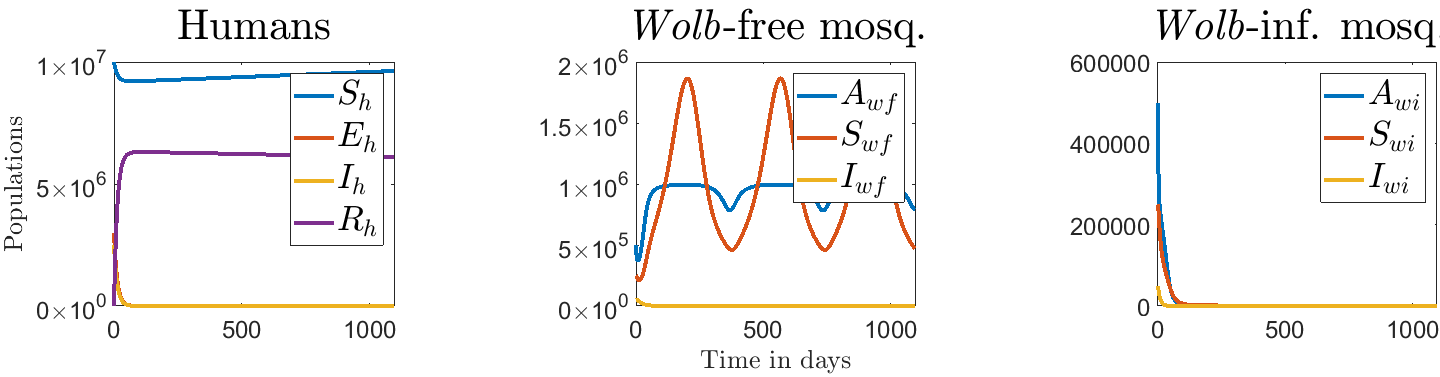
\includegraphics[width=\textwidth]{NonAutSimulation1.png}
%    \caption{Dominance of wild mosquitoes when initial conditions are the same as in Table \ref{init-cond-dis-free-table}}
%    \label{nonautfig1}
%\end{figure}

\subsubsection{\textit{Wolbachia} needs a higher threshold value to establish under seasonality }
Changing the initial conditions exactly like we did in Section \ref{morefemales} does not cause the \textit{Wolbachia} infected mosquitoes to persist. In the case where all parameters were constant, changing the initial amount of \textit{Wolbachia} infected susceptible female mosquitoes from $S_{wi}(0)=250,000$ to $S_{wi}(0)=850,000$ allowed the \textit{Wolbachia} mosquitoes to persist. In the case where seasonality was taken into account, numerical simulations suggest that one would need to increase the \textit{Wolbachia} infected susceptible female mosquitoes to $S_{wi}(0)=1.85$ millions to allow for \textit{Wolbachia} infected mosquitoes to persist as observed in Figure \ref{nonautfig2}. The elimination of wild mosquitoes takes around one year with seasonality taken into account and without seasonality. However, with seasonality, the number of \textit{Wolbachia} infected susceptible females oscillates yearly, with 2,750,000 females during the warm seasons compared to 800,000 \textit{Wolbachia} infected females without seasonality. Also, in the case of seasonality it takes a little longer for Zika to be eradicated in both humans and mosquitoes (around 300 days).

\begin{figure}[H]
    \centering
    % This file was created by matlab2tikz.
%
%The latest updates can be retrieved from
%  http://www.mathworks.com/matlabcentral/fileexchange/22022-matlab2tikz-matlab2tikz
%where you can also make suggestions and rate matlab2tikz.
%
\definecolor{mycolor1}{rgb}{0.00000,0.44700,0.74100}%
\definecolor{mycolor2}{rgb}{0.85000,0.32500,0.09800}%
\definecolor{mycolor3}{rgb}{0.92900,0.69400,0.12500}%
\definecolor{mycolor4}{rgb}{0.49400,0.18400,0.55600}%
%
\begin{tikzpicture}

\begin{axis}[%
width=1.1in,
height=1.5in,
at={(0in,0.036in)},
scale only axis,
xmin=0,
xmax=1095,
ymin=0,
ymax=10000000,
ylabel style={font=\color{white!15!black}},
ylabel={Population},
axis background/.style={fill=white},
title style={font=\bfseries, yshift=1.75ex},
title={Humans},
legend style={legend cell align=left, align=left, draw=white!15!black}
]
\addplot [color=mycolor1, line width=1.5pt]
  table[row sep=crcr]{%
0	10000000\\
1.10916982404888	9933548.12098313\\
2.3637958932668	9865092.70576802\\
3.57381024025381	9805203.62375333\\
4.70053899846971	9754358.91560342\\
6.07678408548236	9698096.6211157\\
7.21084330417216	9656125.40584164\\
8.55472930520773	9611032.78564007\\
10.1084420867264	9564554.53520673\\
11.5497759971768	9526281.10655749\\
12.8787310384214	9494681.380114\\
14.2421036828309	9465565.62661004\\
15.639893932268	9438835.55536907\\
17.0957964472473	9414002.9108861\\
18.6098112296313	9391083.84727513\\
20.1720583029091	9370191.74354212\\
21.7825376670808	9351247.24066365\\
22.5877773482352	9342663.72463996\\
23.4470146019012	9334103.79742334\\
24.3062518574297	9326123.01114997\\
25.1654891110957	9318683.52777851\\
26.0247263666242	9311749.80858445\\
26.9486451279372	9304820.49076382\\
27.8725638873875	9298399.40564604\\
28.7964826487005	9292450.95693511\\
29.7204014100134	9286941.85331183\\
30.7174946330488	9281453.74427788\\
31.7145878560841	9276405.61634185\\
32.7116810809821	9271764.35714477\\
33.7087743040174	9267499.14095024\\
34.7510799989104	9263411.63525324\\
35.7933856956661	9259674.27615241\\
36.8356913905591	9256259.62747233\\
37.8779970873147	9253142.21842908\\
38.8468904662877	9250490.39337881\\
39.8157838452607	9248057.96869331\\
40.7846772242337	9245828.95421516\\
41.7535706050694	9243788.43929968\\
42.5565334241837	9242230.32871746\\
43.3594962451607	9240784.93732913\\
44.162459064275	9239445.42837653\\
45.6531144734472	9237217.7737343\\
47.0284996498376	9235434.04830295\\
48.386170944199	9233902.48067268\\
49.7261283583939	9232591.82135171\\
51.0768057368696	9231452.62038751\\
51.7575044073164	9230941.93692745\\
52.4382030777633	9230470.8917043\\
53.1189017500728	9230037.45229755\\
53.7664240263402	9229658.27978627\\
54.4139463044703	9229309.82623451\\
55.0614685807377	9228990.5996563\\
56.292399039492	9228459.30445017\\
56.8758072219789	9228239.96686783\\
57.4592154044658	9228040.26824692\\
58.5764518063515	9227709.56041202\\
59.1102800294757	9227574.20741829\\
59.6441082507372	9227452.71428202\\
60.1779364719987	9227344.52744377\\
60.6935099791735	9227252.17329953\\
61.2090834863484	9227171.27766609\\
61.7246569935232	9227101.40014484\\
62.2402305025607	9227042.11709137\\
62.7496698014438	9226993.54736503\\
63.2591091003269	9226954.54778755\\
63.76854839921	9226924.75625359\\
64.2779876980931	9226903.82425243\\
64.7683739624918	9226891.73126559\\
65.2587602250278	9226887.25030398\\
65.7491464875638	9226890.10504421\\
66.2395327519625	9226900.02915357\\
66.6962845753878	9226915.40582214\\
67.1530364006758	9226936.49355546\\
67.6097882241011	9226963.09979299\\
68.066540049389	9226995.0384724\\
68.4923722222447	9227029.46006575\\
69.3440365698189	9227111.18226176\\
70.1797656547278	9227207.21412633\\
70.9995594788343	9227315.73646102\\
71.8135250881314	9227436.68552423\\
72.621662478894	9227569.01511206\\
73.8142041265965	9227785.08449262\\
74.9767812117934	9228017.80241876\\
76.0990936122835	9228261.44315149\\
77.5055421423167	9228590.82111434\\
78.8559527676553	9228929.98341006\\
80.5178007036448	9229375.03498819\\
82.1405954118818	9229835.9705451\\
83.9769617281854	9230385.32493589\\
85.9729543402791	9231011.7746759\\
88.2132550179958	9231746.42541203\\
90.7933609951288	9232627.70481542\\
93.7279781047255	9233668.3155587\\
96.8534456845373	9234813.28688768\\
100.602412905544	9236226.63346657\\
104.762329591438	9237834.81192447\\
109.703445298597	9239786.21539819\\
115.563886838034	9242142.96477059\\
122.681345039979	9245048.00802417\\
131.702784406021	9248774.18329373\\
143.509275093675	9253695.5114439\\
159.846954477951	9260551.29181262\\
183.599754285067	9270564.95566986\\
218.166304731742	9285183.41096503\\
290.206976279616	9315707.19607306\\
346.769396238029	9339644.2359432\\
401.268322503194	9362664.14399602\\
455.965017478913	9385723.78208576\\
510.386077906936	9408623.7348594\\
564.761836081743	9431461.39040294\\
619.125902565196	9454251.01462443\\
673.127805836499	9476846.21275957\\
727.546476960182	9499572.91737993\\
782.059750758111	9522296.05955246\\
836.676997255534	9545019.39135446\\
891.068838408217	9567606.1011201\\
945.4495114889	9590145.51299566\\
999.757803898305	9612612.4345578\\
1053.84131408855	9634944.2461807\\
1095	9651911.10707229\\
};
\addlegendentry{$S_h$}

\addplot [color=mycolor2, line width=1.5pt]
  table[row sep=crcr]{%
0	3000000\\
1.10916982358322	2748203.41053051\\
2.36379589373246	2488796.26992221\\
3.57381024071947	2261876.34379031\\
4.70053899846971	2069256.11600885\\
6.07678408641368	1856138.78632726\\
7.21084330463782	1697158.58515692\\
8.55472930474207	1526332.77403685\\
10.1084420867264	1350192.66097419\\
11.5497759981081	1205052.11499619\\
12.8787310379557	1085116.02543906\\
14.2421036823653	974487.678736718\\
15.6398939318024	872784.365461332\\
17.0957964477129	778139.093086914\\
18.6098112296313	690603.585084929\\
20.1720583029091	610606.390674377\\
21.7825376661494	537844.911310874\\
22.5877773482352	504789.94277963\\
23.4470146028325	471759.80122678\\
24.3062518574297	440895.878627361\\
25.165489112027	412056.371302029\\
26.0247263666242	385107.954197898\\
26.9486451274715	358098.519451944\\
27.8725638878532	332988.753832779\\
28.7964826487005	309645.353089723\\
29.7204014095478	287943.474375918\\
30.7174946330488	266230.933046994\\
31.7145878565498	246161.510787461\\
32.7116810800508	227611.192110014\\
33.7087743040174	210464.330740898\\
34.7510799998417	193924.353738818\\
35.7933856956661	178690.155255632\\
36.8356913914904	164658.918230503\\
37.8779970873147	151735.010861752\\
38.8468904662877	140637.233862766\\
39.8157838457264	130355.81590197\\
40.7846772251651	120830.787533858\\
41.7535706046037	112006.139076136\\
43.359496244695	98784.7332015107\\
44.965421885252	87134.8661208823\\
46.3408070616424	78264.1493682452\\
47.7161922380328	70303.8961537937\\
49.0561496522278	63334.7389853336\\
50.3961070664227	57062.8774334788\\
51.7575044077821	51332.6334054666\\
53.1189017491415	46183.9001809936\\
54.413946303539	41771.551715909\\
55.7089908579364	37785.7967717615\\
56.8758072215132	34525.5647816868\\
58.0426235855557	31550.4168881909\\
59.11028002901	29056.4724617386\\
60.1779364724644	26762.6079510027\\
61.2090834868141	24721.9316849262\\
62.2402305016294	22839.406157162\\
63.2591091003269	21122.5269396896\\
64.2779876985587	19537.014002536\\
65.2587602250278	18125.4215898197\\
66.2395327514969	16817.806062297\\
67.6097882250324	15150.4744868227\\
68.9182043955661	13716.1261969553\\
70.1797656547278	12464.7246593107\\
71.4094563918188	11357.4741670568\\
72.621662478894	10364.648985961\\
73.8142041261308	9474.85366367828\\
74.9767812113278	8683.00884636119\\
76.0990936118178	7983.23059579451\\
77.1539300098084	7378.57338878326\\
78.180747454986	6835.38623996917\\
79.5222546434961	6187.46504772361\\
80.8470448884182	5609.96559236338\\
82.1405954109505	5100.00411163131\\
83.3763096467592	4657.84801538102\\
84.5510815088637	4274.52600862179\\
85.6903699906543	3934.21602633083\\
86.8196124732494	3624.83831044519\\
87.9367320965976	3343.8433423629\\
89.0173085168935	3093.79769581417\\
90.2973902360536	2822.89170179889\\
91.5287221297622	2585.90476874309\\
92.7566995578818	2370.49106930522\\
93.9645723006688	2177.15314732213\\
95.1110965190455	2009.15282135271\\
96.2028867653571	1862.02899227571\\
97.2893090001307	1727.059003192\\
98.592156347353	1578.95525440108\\
99.8224645429291	1451.64981828118\\
100.989361339249	1341.15471460251\\
102.167587904725	1238.82734670816\\
103.329599706456	1146.22540170234\\
104.587564531248	1054.47401390178\\
105.828232987784	971.869637761731\\
107.0835371227	895.537982707843\\
108.236393333413	831.291481462773\\
109.371420082171	773.047135330737\\
110.531337942928	718.233021054417\\
111.755000435747	665.128660780378\\
112.957385917194	617.264736666344\\
114.179773333482	572.608924538828\\
115.425783808809	530.882102598902\\
116.721544289496	491.18732199166\\
117.930324606597	457.254632359371\\
119.108776435722	426.801096933428\\
120.310649188235	398.188406622037\\
121.513303552289	371.821404598653\\
122.80252358783	345.854594593402\\
124.054748923518	322.710725702345\\
125.284163504839	301.805828595068\\
126.577793239616	281.58334753383\\
127.862265406176	263.146240403876\\
129.087941164151	246.945459705777\\
130.408942504786	230.873788365629\\
131.702784406021	216.407353795134\\
132.993989999406	203.116745893378\\
134.309708031826	190.648145853542\\
135.652715337928	178.940182416234\\
136.998766301665	168.146522379015\\
138.293195628095	158.576542614959\\
139.617654052563	149.534231580794\\
140.944299322553	141.171154841781\\
142.26251539262	133.489568292629\\
143.605823140591	126.250201554503\\
144.999076172709	119.314201678615\\
146.407535482664	112.842344184406\\
147.812338956632	106.879451373126\\
149.186539788265	101.479820697103\\
150.629319264553	96.2309549180791\\
152.077011241578	91.3583283154294\\
153.551222463604	86.765425844118\\
155.036560817622	82.480265205726\\
156.520116107538	78.5121925268322\\
158.025748528074	74.7749145869166\\
159.577811031602	71.2001261431724\\
161.133112779818	67.8747127368115\\
162.743917783257	64.6763992705382\\
164.350829668809	61.7116993949749\\
165.9917212734	58.8951687384397\\
167.712951909751	56.1478415317833\\
169.444549736567	53.577190565411\\
171.201780792791	51.1471515293233\\
173.069837180432	48.7414991329424\\
174.978182405233	46.4537080153823\\
176.939495727886	44.2624735445715\\
178.992002365645	42.1245542950928\\
181.098624023143	40.0773509787396\\
183.324782757554	38.0577653385699\\
185.644673604518	36.0922969277017\\
188.078510238323	34.1648711627349\\
190.669343812391	32.2460713228211\\
193.410852077883	30.3462133831345\\
196.32772692712	28.4531420446001\\
199.379018406849	26.5958446157165\\
202.64706009347	24.7277361755259\\
206.118268502876	22.8628882588819\\
209.808926641475	20.9981978069991\\
213.684752842411	19.1559025729075\\
217.755177436396	17.3363189357333\\
221.941068819724	15.5786103601567\\
226.197958724108	13.9027087031864\\
230.487229317892	12.3243385399692\\
234.763187303208	10.8595984941348\\
239.003979676403	9.51393260760233\\
243.269543823786	8.26819373527542\\
247.47809693031	7.14513835031539\\
251.707396820188	6.12208539852872\\
255.982572200708	5.19387729885057\\
260.283064988442	4.36477771447971\\
264.735689160414	3.61241050995886\\
269.343361430336	2.94102693907917\\
274.073254778981	2.35678449040279\\
279.115575092845	1.83993534604087\\
284.398612421937	1.4019618104212\\
290.206976280082	1.02498587733135\\
296.585629689973	0.714755999855697\\
303.948151884601	0.461991398595273\\
312.543163870927	0.270633499138057\\
323.380507820286	0.133212300017476\\
339.468222577125	0.0438571595586836\\
368.859377482906	0.0050753322429955\\
522.507422726601	7.77654349803925e-08\\
1095	0\\
};
\addlegendentry{$E_h$}

\addplot [color=mycolor3, line width=1.5pt]
  table[row sep=crcr]{%
0	2500000\\
1.10916982358322	2287796.31896786\\
2.36379589373246	2069714.94745628\\
3.57381024071947	1879363.09927765\\
4.70053899846971	1718073.42266633\\
5.50975447706878	1610940.28697976\\
6.64381369529292	1472055.9801976\\
7.77787291351706	1345251.47660368\\
9.33158569596708	1189200.60948778\\
10.8852984779514	1051375.40920216\\
12.2142535177991	946311.433093696\\
13.5432085581124	851803.481081247\\
14.9409988070838	762615.11224147\\
16.3387890565209	682806.005501037\\
17.8528038384393	605791.212122141\\
19.3668186208233	537493.891831047\\
20.9772979845293	473301.593576347\\
22.5877773482352	416798.685910536\\
23.4470146028325	389473.436453172\\
24.3062518574297	363944.800392574\\
25.165489112027	340094.463603844\\
26.0247263666242	317811.378073403\\
26.9486451274715	295481.067384223\\
27.8725638878532	274724.103730472\\
28.7964826487005	255429.61889458\\
29.7204014095478	237493.949777027\\
30.7174946330488	219551.481036742\\
31.7145878565498	202968.537882298\\
32.7116810800508	187642.219009807\\
33.7087743040174	173476.71962648\\
34.7510799998417	159813.864760405\\
35.7933856956661	147230.728238018\\
36.8356913914904	135642.135032601\\
37.8779970873147	124968.983832964\\
38.8468904662877	115804.723148477\\
39.8157838457264	107315.250261407\\
40.7846772251651	99450.9390454828\\
41.7535706046037	92165.4938546121\\
43.359496244695	81251.4613331482\\
44.965421885252	71636.169759403\\
46.3408070616424	64315.8197382377\\
47.7161922380328	57747.8324191924\\
49.0561496522278	51998.5704546212\\
50.3961070664227	46825.4832525388\\
51.7575044077821	42100.073019519\\
53.1189017491415	37855.1295210687\\
54.413946303539	34218.1584306336\\
55.7089908579364	30933.6223570714\\
56.8758072215132	28247.6474675853\\
58.0426235855557	25797.1703036083\\
59.11028002901	23743.5763163459\\
60.1779364724644	21855.2378413472\\
61.2090834868141	20175.7944847378\\
62.2402305016294	18626.9533852488\\
63.2591091003269	17214.8252380784\\
64.2779876985587	15911.1586517855\\
65.2587602250278	14750.8760922151\\
66.2395327514969	13676.4210472214\\
67.6097882250324	12306.9714497984\\
68.9182043955661	11129.4863137817\\
70.1797656547278	10102.7234840845\\
71.4094563918188	9194.72270114999\\
72.621662478894	8381.00812481064\\
73.8142041261308	7652.15575919114\\
74.9767812113278	7003.92086123629\\
76.0990936118178	6431.4001430748\\
77.1539300098084	5936.99916625582\\
78.180747454986	5493.125093068\\
79.5222546434961	4964.0407074322\\
80.8470448884182	4492.85731813032\\
82.1405954109505	4077.13841921184\\
83.3763096467592	3717.01025406271\\
84.5510815088637	3405.07421471039\\
85.6903699906543	3128.38235594658\\
86.8196124732494	2877.06480657775\\
87.9367320965976	2649.01338093728\\
89.0173085168935	2446.26971082017\\
90.2973902360536	2226.84070381895\\
91.5287221297622	2035.10767513653\\
92.7566995578818	1861.03412551433\\
93.9645723006688	1704.99003595253\\
95.1110965190455	1569.56208845275\\
96.2028867653571	1451.10631846078\\
97.2893090001307	1342.56842082879\\
98.3768842415884	1242.48748692777\\
99.6269731605425	1137.15093306126\\
100.795887122862	1047.22834128747\\
101.970228719059	964.494234671351\\
103.139621624723	889.029826554004\\
104.412799471524	814.024645638186\\
105.647000418045	747.796788973268\\
106.905635516625	686.224737410434\\
108.076114363968	633.888858994469\\
109.20540747419	587.501187842339\\
110.371870234143	543.46320550004\\
111.608357808087	500.713327398058\\
112.800984953996	462.979104828089\\
114.037382060196	427.165835642256\\
115.287680779584	394.068356093485\\
116.428890269715	366.356501834467\\
117.674520757049	338.592009338085\\
118.836264316924	314.833886872977\\
120.064136724919	291.769760928117\\
121.269817642402	270.992973206099\\
122.428871934302	252.617221596651\\
123.711980118882	233.942845061421\\
124.922344423365	217.794736250304\\
126.146330303513	202.786493945867\\
127.406366756186	188.60368896788\\
128.667907636147	175.578887266573\\
129.888665152248	163.996347811539\\
131.16668734327	152.852304990403\\
132.453296706546	142.558657432441\\
133.767377814744	132.917587196454\\
135.035180379171	124.377111764625\\
136.284317175392	116.629028030671\\
137.581615042407	109.221557340585\\
138.895225552376	102.326382277533\\
140.217292817309	95.9471232793294\\
141.505432817619	90.2243511076085\\
142.852210226003	84.7149667609483\\
144.146234846674	79.8376578888856\\
145.453802600037	75.2872966881841\\
146.777059640735	71.0355660021305\\
148.152346297167	66.9600549954921\\
149.529790075496	63.1977375224233\\
150.941799736116	59.6429634275846\\
152.367627045605	56.3353954181075\\
153.77385557536	53.325585281942\\
155.236640199553	50.4362810873426\\
156.677624740172	47.8089211974293\\
158.176979807205	45.284441171214\\
159.739297098946	42.859767658636\\
161.263409827836	40.6776222093031\\
162.885378902312	38.5349816088565\\
164.553407943342	36.5057957898825\\
166.247727280948	34.6074482123367\\
167.996643565129	32.8025352773257\\
169.781401372049	31.1058727800846\\
171.643661490176	29.4754890510812\\
173.606982300524	27.8946734224446\\
175.660340706352	26.375992056448\\
177.790475801565	24.929190415889\\
180.053232760634	23.5186837464571\\
182.428749781568	22.1606545308605\\
184.959280806594	20.8345180428587\\
187.661773618311	19.5371081936173\\
190.553512630519	18.26568689337\\
193.668074044865	17.0115351420827\\
197.023892571218	15.7734330547974\\
200.691210428253	14.5331238028593\\
204.66227145493	13.3007982545532\\
209.012943354901	12.060440252535\\
213.768875451759	10.8138554724865\\
218.931800445542	9.56944056600332\\
224.442374163773	8.34922165097669\\
230.183988590259	7.18432796839625\\
236.041117802262	6.10097894258797\\
241.965641686227	5.11000755941495\\
247.864225147292	4.22730566933751\\
253.783878656104	3.44529955787584\\
259.736114702187	2.76250447006896\\
265.833063470665	2.16733514424413\\
272.166288186796	1.65449902275577\\
278.760343169328	1.22482330957428\\
285.830176047515	0.867958483286202\\
293.653351821937	0.577755636535585\\
302.732435692102	0.348725075833499\\
313.599320157431	0.182628548704088\\
327.684291154146	0.0743095008656383\\
350.466452295892	0.0154573195613921\\
413.128266373184	0.000138209201395512\\
1095	0\\
};
\addlegendentry{$I_h$}

\addplot [color=mycolor4, line width=1.5pt]
  table[row sep=crcr]{%
0	10000\\
1.10916982311755	540683.141769965\\
2.36379589419812	1086888.34288464\\
3.57381024118513	1564301.17187669\\
4.70053899846971	1969290.40421369\\
5.50975447706878	2238525.94050585\\
6.64381369575858	2587822.22188677\\
7.77787291351706	2906994.74763857\\
9.33158569596708	3300108.02996438\\
10.8852984774858	3647596.37181996\\
12.2142535177991	3912659.46015367\\
13.5432085581124	4151212.23413183\\
14.9409988075495	4376436.63636349\\
16.3387890560552	4578051.29141943\\
17.8528038384393	4772668.07703473\\
19.3668186208233	4945299.44125494\\
20.9772979849949	5107585.6120691\\
22.5877773482352	5250449.95082342\\
23.4470146028325	5319544.07142641\\
24.3062518574297	5384096.21339448\\
25.165489112027	5444404.33257338\\
26.0247263666242	5500748.34075424\\
26.9486451270059	5557209.6430496\\
27.8725638883188	5609689.69030472\\
28.7964826487005	5658468.25128404\\
29.7204014100134	5703807.12325335\\
30.7174946330488	5749157.67982863\\
31.7145878570154	5791065.60345963\\
32.7116810800508	5829790.92329678\\
33.7087743040174	5865575.91614327\\
34.7510799998417	5900083.06704532\\
35.7933856956661	5931854.56663165\\
36.8356913914904	5961105.84316555\\
37.8779970873147	5988037.10054407\\
38.8468904662877	6011152.47692877\\
39.8157838461921	6032557.29932489\\
40.7846772251651	6052377.15346188\\
41.7535706041381	6070729.25531301\\
43.3594962451607	6098202.1527068\\
44.965421885252	6122380.82878334\\
46.3408070616424	6140768.10827769\\
47.7161922380328	6157246.1323284\\
49.0561496522278	6171650.9719536\\
50.3961070664227	6184592.90796979\\
51.7575044073164	6196394.72838503\\
53.1189017491415	6206975.89912648\\
54.413946303539	6216022.04818147\\
55.7089908579364	6224172.17822372\\
56.8758072219789	6230820.12385283\\
58.04262358509	6236868.88351333\\
59.1102800285444	6241923.46274086\\
60.1779364719987	6246557.23617832\\
61.2090834872797	6250664.90050168\\
62.2402305016294	6254439.71494409\\
63.2591091003269	6257868.02175317\\
64.2779876980931	6261019.64745208\\
65.2587602250278	6263811.89349933\\
66.2395327519625	6266384.97539947\\
67.6097882250324	6269643.39333003\\
68.9182043960318	6272421.95251815\\
70.1797656547278	6274823.22208837\\
71.4094563918188	6276926.10446595\\
72.621662478894	6278790.50286838\\
73.8142041265965	6280440.80953963\\
74.9767812108621	6281889.66522444\\
76.0990936113521	6283151.44419872\\
77.1539300093427	6284224.94301094\\
78.180747454986	6285173.63536347\\
79.1891037058085	6286019.93160857\\
80.188556519337	6286781.60715751\\
81.1762890722603	6287464.51173689\\
82.1405954109505	6288069.15723386\\
83.0759836062789	6288601.28837259\\
83.9769617291167	6289066.73473339\\
84.8381413994357	6289471.31149405\\
85.6903699906543	6289835.41781497\\
86.5375755820423	6290163.89642887\\
87.3836862547323	6290460.73874214\\
88.2132550170645	6290723.39083361\\
89.0173085164279	6290952.79136513\\
89.7956894757226	6291152.67386621\\
90.7933609951288	6291378.97546502\\
91.5287221297622	6291525.61181499\\
92.2660341132432	6291656.50547999\\
93.00159434136	6291771.87203603\\
93.7279781047255	6291871.69536752\\
94.4377606920898	6291956.42495622\\
95.1110965190455	6292025.70812391\\
95.7692142799497	6292083.51180397\\
96.4197397381067	6292131.48830327\\
97.0702986568213	6292170.79927758\\
97.5083193434402	6292192.59434776\\
97.9463400300592	6292210.77099059\\
98.3768842415884	6292225.22525515\\
98.8074284531176	6292236.40557869\\
99.2172008072957	6292244.10134592\\
99.6269731605425	6292249.01358548\\
99.8224645424634	6292250.40106116\\
100.017955925316	6292251.18327469\\
100.213447307236	6292251.3690632\\
100.408938689157	6292250.96713312\\
100.602412906475	6292249.99911178\\
100.795887122862	6292248.47202428\\
101.182835556567	6292243.77279714\\
101.57653213758	6292236.79464821\\
101.970228719525	6292227.66465203\\
102.364947089925	6292216.41359564\\
102.94964354299	6292196.01778944\\
103.519577788189	6292172.01332481\\
104.238034412265	6292136.21710583\\
104.937094650231	6292095.7460847\\
105.647000418045	6292049.24592318\\
106.549832304008	6291982.68334952\\
107.419546773657	6291911.16823069\\
108.396672302857	6291822.73283224\\
109.537432690151	6291709.42559706\\
110.690805652179	6291584.69502191\\
112.048285691068	6291425.90833269\\
113.426588806324	6291252.62633122\\
115.013920100406	6291039.50732126\\
116.721544289961	6290795.7591692\\
118.569518068805	6290517.03179205\\
120.674454171211	6290183.00778844\\
122.923702134751	6289809.27081663\\
125.404769864865	6289379.84946679\\
128.175919286907	6288882.33151305\\
131.36695065815	6288290.15257711\\
134.953072004952	6287604.79409507\\
139.046700631268	6286802.24045095\\
143.794812355191	6285850.73887097\\
149.46638317965	6284692.72416911\\
156.301565772854	6283275.1481672\\
164.728302521631	6281505.21903238\\
175.431306872517	6279234.57013739\\
189.312100715935	6276266.91840272\\
207.42897999566	6272370.65885973\\
230.350865159184	6267418.15097865\\
260.056625065394	6260976.46020107\\
403.146181366406	6229917.35071222\\
457.811242330819	6218088.01472119\\
512.214756159112	6206337.57651675\\
566.570350886323	6194619.66390013\\
620.864915480837	6182936.99492785\\
674.939431199804	6171323.57339046\\
728.677270974033	6159804.06903184\\
783.233788561076	6148131.06509835\\
837.852676530369	6136466.87489954\\
892.242701165378	6124873.55021681\\
946.593118519522	6113310.54668104\\
1000.96682101395	6101764.43279679\\
1055.0890900949	6090293.36614404\\
1095	6081848.17515491\\
};
\addlegendentry{$R_h$}

\end{axis}

\begin{axis}[%
width=1.1in,
height=1.5in,
at={(1.42in,0.036in)},
scale only axis,
xmin=0,
xmax=1095,
xlabel style={font=\color{white!15!black}},
xlabel={Time (days)},
ymin=0,
ymax=900000,
axis background/.style={fill=white},
title style={font=\bfseries, yshift=1.25ex},
title={\emph{Wolb}-free mosq.},
legend style={legend cell align=left, align=left, draw=white!15!black}
]
\addplot [color=mycolor1, line width=1.5pt]
  table[row sep=crcr]{%
0	500000\\
0.626967289252207	462518.91961646\\
1.35027109051589	425800.652981865\\
2.10632138175424	392972.398656451\\
2.93878368422156	361922.968233078\\
3.57381024089409	341197.87149772\\
4.29593125870451	320286.924496937\\
5.10514673776925	299782.662558812\\
6.07678408641368	278689.98489946\\
6.64381369552575	267933.759613088\\
7.21084330457961	258193.131941941\\
7.77787291369168	249377.816970634\\
8.55472930474207	238671.336665268\\
9.33158569579246	229340.411510742\\
10.1084420868428	221192.361893592\\
10.8852984778932	214122.152358681\\
11.5497759978753	208858.63137104\\
12.2142535179155	204201.504143731\\
12.8787310378975	200080.000369394\\
13.5432085579378	196452.872539457\\
14.2421036825399	193131.583589831\\
14.940998807142	190242.954953571\\
15.6398939317442	187734.29030575\\
16.3387890563463	185578.984009463\\
17.0957964474801	183617.821973762\\
17.8528038386721	181983.125290233\\
18.6098112298641	180632.662651951\\
19.3668186209979	179553.069305094\\
20.1720583027927	178690.514230317\\
20.9772979845293	178070.303057105\\
21.7825376663241	177661.196508134\\
22.5877773480606	177460.905026407\\
23.4470146027161	177476.295367233\\
24.3062518573133	177682.793517755\\
25.1654891119688	178056.559586165\\
26.024726366566	178602.93417629\\
26.9486451273551	179388.805090201\\
27.872563888086	180337.013938342\\
28.7964826488169	181427.240108684\\
29.720401409606	182670.620504664\\
30.7174946331652	184196.706759563\\
31.7145878567244	185864.744678299\\
32.7116810802836	187652.552105068\\
33.7087743037846	189580.845023146\\
35.7933856954915	194077.407335183\\
36.8356913913158	196446.388746603\\
37.8779970871401	198940.008515968\\
40.7846772251069	206480.385888387\\
41.7535706044291	209083.890075144\\
46.3408070615842	222443.856016178\\
48.3861709449557	228638.202838892\\
53.1189017491997	243361.736755769\\
55.0614685808541	249556.44087286\\
56.2923990398995	253516.359888631\\
59.6441082505044	264250.262648446\\
62.2402305017458	272609.840609839\\
63.7685483993264	277594.885313835\\
64.7683739617933	280882.505009326\\
67.1530364004429	288687.557638346\\
68.0665400493308	291567.440415435\\
69.3440365689457	295804.647457913\\
70.1797656545532	298580.696464469\\
72.621662478894	306615.773810111\\
73.4199676503777	309299.906772227\\
75.3508853447274	315750.177636163\\
76.0990936116432	318125.005580514\\
76.8023178770673	320587.253790103\\
77.8431447987095	324036.359833926\\
79.5222546433797	329702.789438288\\
80.5178007037612	333032.511456713\\
82.1405954110087	338539.453064871\\
82.7756575648673	340555.946195634\\
83.3763096468756	342709.6302348\\
83.9769617288839	344620.492184531\\
84.5510815090383	346675.299379972\\
85.4077856398071	349546.146811449\\
86.819612473133	354363.814234459\\
87.3836862545577	356161.280812894\\
87.9367320964229	358156.836986394\\
88.48977793823	359897.048216521\\
89.0173085167771	361814.365507461\\
89.5448390952661	363465.812148025\\
90.0465398558299	365285.454199031\\
90.5482406163937	366866.079756501\\
91.2836017514928	369396.249556702\\
91.7744927909807	371088.206033927\\
93.0015943417093	375257.780300099\\
93.4913839091896	376771.024024499\\
93.9645723006106	378494.015028495\\
94.4377606920898	379934.34299538\\
94.8866512433742	381569.309440328\\
95.3355417946586	382938.617274952\\
95.7692142800079	384500.809820493\\
96.2028867653571	385835.070915245\\
96.636592711031	387381.371655466\\
97.0702986567048	388711.715329878\\
97.5083193431492	390274.473358964\\
97.9463400295936	391592.514150653\\
98.376884241472	393144.178476398\\
98.8074284532922	394406.955482984\\
99.2172008070047	395891.699330516\\
99.626973160659	397084.081776993\\
100.017955925083	398485.404489331\\
110.690805651771	431393.467080615\\
120.791746691684	457508.078162139\\
130.966424027749	476604.221227395\\
140.944299322786	486864.762818541\\
150.941799736232	487811.485749897\\
160.9491838307	479489.815850303\\
170.886251922464	462786.180487508\\
180.929541142308	438849.539178529\\
190.938584989461	409989.786706241\\
200.955897220003	378476.825199773\\
210.99579103	346574.108597299\\
220.809060373111	317187.346114706\\
230.95626516128	290235.72491331\\
240.651506197057	268405.867355347\\
250.711513564282	249910.996378056\\
260.971249285794	234920.588605575\\
270.728445810964	223005.424946024\\
280.899239025079	212108.207887356\\
290.20697628014	202150.267705983\\
291.636087750259	200574.703776258\\
292.611316400114	199478.795752754\\
293.306006681349	198662.266918669\\
293.653351821995	198241.113454872\\
294.328527949983	197526.903711396\\
295.003704077972	196672.031110419\\
295.633548553044	195985.33198464\\
296.585629689973	194839.934051653\\
298.28404681239	192798.780248091\\
303.542913153884	186057.809000885\\
308.405366220919	179286.483721396\\
312.543163870694	172996.913850508\\
316.385408755741	166688.148201801\\
318.158059285022	163607.63944052\\
320.06497835106	160206.354977732\\
322.710535374994	155275.76875943\\
325.48914207553	149849.553259313\\
328.430426650972	143836.33375905\\
331.57295324275	137124.544802816\\
334.938369599986	129646.307463177\\
338.549644276674	121357.297258803\\
351.762553368462	90585.519445436\\
354.173367450654	85268.7144616765\\
356.402793469664	80533.2029057589\\
358.632219488674	75996.4887039616\\
360.861645507684	71685.955327054\\
363.140205839882	67525.8112667739\\
365.467900485208	63546.5742892969\\
367.745562645316	59912.4142930972\\
369.973192320205	56600.2254157225\\
372.17582497868	53542.0510920205\\
374.353460620856	50710.0863000124\\
376.52793846227	48042.7708905628\\
378.69925850298	45510.1999961907\\
381.949844224204	41885.8966515124\\
392.653899803699	30216.1385799386\\
397.99109474232	24165.009235626\\
401.268322502903	20472.4562637068\\
404.085110798595	17415.7366672581\\
405.962969662389	15481.2440840446\\
407.840828526183	13650.8710760646\\
409.552941609581	12090.9810394332\\
411.099308912526	10777.0943606142\\
412.500379468664	9670.0574319326\\
413.756153278053	8746.18445554364\\
414.974165218067	7912.19883643009\\
416.154415288707	7161.65108988323\\
417.345881395391	6460.64541296079\\
418.548563538061	5808.66976425186\\
419.733703710255	5219.31614334136\\
420.901301911857	4687.40485442267\\
422.019878939085	4221.34696570411\\
423.089434791938	3812.97711743193\\
424.111993574945	3454.96009929758\\
425.087555288104	3140.96775522875\\
426.03837380535	2859.45666714531\\
426.964449126681	2606.96473103506\\
427.880826906068	2377.00407672772\\
428.78750714357	2167.56111590279\\
429.680374293472	1977.87142227549\\
430.559428355831	1805.9657462787\\
431.826568890072	1582.3065899958\\
433.039776045305	1392.33662415476\\
434.196557001502	1231.13231847674\\
435.297714058426	1094.09574732382\\
436.383214257075	973.132331411703\\
437.454116674315	866.209197533666\\
438.511480386776	771.60193980491\\
439.525880582747	690.163452451932\\
440.501261358848	619.636776706961\\
441.441769624827	558.170319792524\\
442.351552290493	504.295779444161\\
443.241698711645	456.458102545876\\
444.126723590831	413.245067148004\\
445.002068124362	374.389720706386\\
446.136443957977	329.263363905717\\
447.215813076764	291.244758340938\\
448.247213562659	258.917852862622\\
449.257314264658	230.654118028237\\
450.262814435875	205.513366328843\\
451.252880930842	183.379262614762\\
452.203958360187	164.318798874505\\
453.110216320783	147.967490044597\\
453.991542323143	133.599885966105\\
454.870926157571	120.630744618364\\
455.748819972272	108.918986611709\\
456.809283566254	96.2556374495616\\
457.811242330412	85.625510827289\\
458.7846571072	76.409738113638\\
459.766760145198	68.1063679506187\\
460.732926017139	60.8082046366762\\
461.64749727631	54.6127213509753\\
462.522926365375	49.2692835403723\\
463.40572346095	44.40657918324\\
464.292287803255	40.001683161594\\
465.306039159652	35.4922617021366\\
466.257545986271	31.721870587382\\
467.22605500737	28.2913312730961\\
468.191178276029	25.2411040921579\\
469.235426072206	22.3074124004925\\
470.259972469939	19.7593436776078\\
471.312237271515	17.444315086701\\
472.280964681122	15.5530738191446\\
473.225184258132	13.9065385609865\\
474.210691963206	12.3731053161318\\
475.240624811791	10.9510543962242\\
476.247644871124	9.71873682789737\\
477.416299006611	8.4615370472311\\
478.580174113333	7.37114322080743\\
479.696853197122	6.45742675929796\\
480.911038205202	5.59245570161147\\
482.187475639454	4.80815014219843\\
483.540554421721	4.09675096074352\\
484.960521037574	3.46359091275372\\
486.574641748914	2.86249200318707\\
488.28936916549	2.33851400372805\\
490.144183088269	1.87980356568005\\
492.204264045635	1.47580387815833\\
494.564948018757	1.11930038378341\\
497.375985363149	0.806406459480058\\
500.682778813702	0.549491489888169\\
504.732868351042	0.34477192920167\\
509.953178252035	0.190425630891696\\
517.33768879954	0.0836645599338226\\
529.617335162591	0.0225882532540709\\
561.322372799215	0.00123803864698857\\
1095	0\\
};
\addlegendentry{$A_{wf}$}

\addplot [color=mycolor2, line width=1.5pt]
  table[row sep=crcr]{%
0	250000\\
0.250184062519111	249349.699210105\\
0.626967289252207	248078.063562915\\
1.1091698234668	246015.969654784\\
1.59137235756498	243550.954230791\\
2.36379589384887	238950.917234871\\
3.25629696249962	232908.893001297\\
4.70053899823688	222149.871061543\\
8.55472930474207	192444.48965965\\
10.1084420868428	181350.779683827\\
11.5497759978753	171839.087260263\\
12.8787310379557	163804.412256545\\
14.2421036824817	156316.383311199\\
15.6398939316859	149427.779469846\\
17.0957964474801	143073.4282886\\
17.8528038386721	140087.099329752\\
18.6098112298641	137310.029265906\\
19.3668186210562	134734.227280382\\
20.1720583027927	132206.210421965\\
20.9772979845293	129889.422072916\\
21.7825376662659	127775.475710865\\
22.5877773481188	125854.698282579\\
23.4470146027161	124007.727657524\\
24.3062518573133	122362.068019261\\
25.1654891119106	120908.788430909\\
26.0247263666242	119637.757696909\\
26.9486451273551	118463.624883667\\
27.872563888086	117481.408674917\\
28.7964826488169	116682.34802399\\
29.7204014095478	116056.3600901\\
30.7174946331652	115564.262368966\\
31.7145878566662	115255.977599334\\
32.7116810802836	115123.432524669\\
33.7087743037846	115156.412563287\\
34.7510799996089	115357.054427848\\
35.7933856954332	115724.188708135\\
36.8356913912576	116251.985498548\\
37.8779970870819	116928.936302155\\
38.8468904664041	117681.225528023\\
39.8157838458428	118555.496369346\\
40.7846772251651	119550.37558682\\
41.7535706044873	120653.012196042\\
42.5565334246494	121639.589590411\\
43.3594962449279	122699.120487685\\
44.9654218853684	125029.232138394\\
46.3408070616424	127218.081440715\\
47.7161922379164	129590.848755874\\
49.0561496521113	132058.254661098\\
50.3961070663063	134682.453144823\\
51.7575044077821	137490.780395323\\
53.7664240264567	141898.490561954\\
55.7089908580529	146441.045139694\\
57.4592154035345	150750.365547122\\
59.6441082505044	156414.309581674\\
61.7246569943381	162088.757018425\\
63.7685483993264	167923.129442462\\
66.2395327516133	175316.434009239\\
68.4923722224776	182374.462214436\\
70.5896625670139	189223.222663636\\
73.0257311746245	197521.058536558\\
75.3508853447856	205783.059830675\\
77.8431447986513	215029.37245908\\
80.188556519337	224107.207269287\\
82.4581264879089	233246.606519197\\
84.8381413990865	243220.231249553\\
87.3836862546159	254341.54090683\\
89.7956894754898	265321.088882632\\
92.2660341131268	277026.701922607\\
94.8866512434324	289960.138476028\\
97.5083193432074	303441.554854235\\
100.213447307236	317927.130343497\\
102.94964354299	333172.907375404\\
105.647000417812	348788.528707234\\
108.396672302857	365296.537048428\\
111.159395253984	382470.25586553\\
114.037382060313	400969.83374377\\
117.005582701531	420666.773910555\\
120.187392956577	442437.476274648\\
123.600723096635	466478.237425877\\
127.406366756069	494009.742950115\\
132.148053593701	529167.038977763\\
138.89522555226	580156.424297877\\
146.585376707837	638187.14191352\\
150.754311453202	668859.919318008\\
154.082870284212	692600.114649502\\
156.969008705579	712458.954707055\\
159.424415120855	728701.571891276\\
161.689364002435	743065.124965801\\
163.720887780655	755377.980477927\\
165.723436060827	766928.718788397\\
167.612277796725	777241.524139275\\
169.310931861284	785994.439146281\\
170.930908640265	793852.45977503\\
172.507778174011	801013.413416789\\
174.006871142541	807353.172818447\\
175.375984206912	812725.34018511\\
176.671447122237	817427.155314843\\
177.959907180979	821721.597265056\\
179.165215086541	825384.538740337\\
180.263457244379	828415.08053832\\
181.297381912125	830993.717681771\\
182.272043212201	833176.381564809\\
183.208243880887	835041.749701768\\
184.072231976315	836558.581600858\\
184.88113596139	837798.553350858\\
185.603288956801	838756.441647249\\
186.266758046811	839511.134739857\\
186.898031223333	840116.636617196\\
187.477902296116	840576.089181105\\
188.028185964562	840924.216769555\\
188.489884469658	841151.140920347\\
188.883330665645	841297.157112743\\
189.209878143738	841384.625100348\\
189.527512967587	841441.515659748\\
189.769027708913	841464.787742078\\
189.912534518284	841470.851263491\\
190.021132845315	841471.726125342\\
190.075432008831	841470.943148555\\
190.24107739469	841462.925388259\\
190.387029773206	841448.878180126\\
190.553512630519	841426.282456176\\
190.789600535296	841380.18930351\\
191.101468444918	841294.208402119\\
191.415863181581	841179.838315074\\
191.788762196782	841006.505054625\\
192.239323690999	840743.64559893\\
192.701516172267	840412.684451002\\
193.260761008481	839929.538027944\\
193.878554333933	839288.411815581\\
194.504545157892	838526.048969812\\
195.199515763321	837544.738010334\\
195.931307666935	836358.04033366\\
196.690263937926	834962.133902952\\
197.526650033658	833227.343979884\\
198.426774914959	831131.82861746\\
199.379018406966	828657.374838326\\
200.368746557273	825806.289260567\\
201.374986038776	822616.433472816\\
202.470887144213	818811.833760621\\
203.60482645873	814515.487337907\\
204.815887390752	809527.6377278\\
206.080517387949	803886.49325819\\
207.428979995777	797392.118819416\\
208.819070803351	790192.377509453\\
210.274032906047	782121.910128189\\
211.834012971609	772881.540314618\\
213.4437381631	762733.589288392\\
215.172609769157	751174.75346321\\
216.975504370988	738433.311036884\\
218.931800445425	723867.626186467\\
221.029725221684	707462.980913757\\
223.306315519148	688838.06403582\\
225.813708482427	667464.175739579\\
228.592555982992	642906.940026929\\
232.065226405859	611251.200252396\\
237.102243303438	564244.508573748\\
244.535590464831	494903.339597074\\
248.338370701298	460456.25836591\\
251.49379870703	432791.362051673\\
254.334076653467	408769.855186501\\
257.03950864228	386770.226872755\\
259.547973822453	367209.603182212\\
261.943623527302	349324.460432698\\
264.257374526118	332816.050781889\\
266.481353539973	317672.148091937\\
268.682742656209	303386.869305325\\
270.866580931586	289908.238882209\\
272.895306661958	277998.714009043\\
275.041686252691	266030.678613034\\
277.088427884853	255208.21247247\\
279.115575092728	245042.206553124\\
281.153246790636	235356.961757178\\
283.124778303667	226477.180751679\\
285.077746798168	218135.569027111\\
286.968011530698	210472.832133657\\
288.939156504697	202893.037182693\\
290.7411282541	196308.110816663\\
292.611316400114	189804.182561968\\
294.666116014007	183023.518234989\\
296.585629689973	177010.469872967\\
298.649900380755	170866.680586685\\
300.655344755971	165194.706439919\\
302.732435691985	159602.068293638\\
304.772792098927	154366.187669886\\
306.955116412719	149023.626843502\\
309.403054662514	143315.591160845\\
311.487007583957	138668.401314023\\
314.148121429607	132983.838281675\\
316.976292265463	127211.402045268\\
319.429338662419	122396.850128576\\
322.710535375052	116191.696484671\\
326.192020160612	109847.411885103\\
329.975359179429	103172.801291617\\
334.082829824765	96130.4656703697\\
338.549644276733	88666.0439798948\\
342.458181522437	82282.5099853398\\
346.769396238844	75412.3864092774\\
350.466452295776	69692.6578793366\\
354.173367450712	64157.2031245718\\
357.517506479169	59374.1626588255\\
359.746932498179	56316.5669746603\\
361.97635851719	53373.9154008225\\
364.304053162574	50437.0900790552\\
366.631747807842	47643.6847833734\\
368.85937748279	45113.204719093\\
371.087007157621	42722.0075143727\\
373.264642799739	40521.0062982297\\
375.442278441857	38449.5908066869\\
377.613598482567	36509.0470785557\\
379.784918523277	34682.9300914613\\
381.949844224146	32966.8350366987\\
384.114769925014	31341.1391154794\\
386.259977199603	29806.9629944061\\
388.405184474192	28333.6135266107\\
391.591720971279	26228.7872429814\\
395.837489067577	23515.4231267071\\
403.146181366639	18934.8238547578\\
406.901899094344	16623.8162900533\\
410.326125261025	14580.5938219934\\
413.128266373416	12981.9202534995\\
415.564290253329	11663.2383645079\\
417.345881395391	10747.8515565066\\
419.149904609425	9867.28557924286\\
420.901301911916	9059.54105716106\\
422.554656865541	8341.08387510222\\
424.111993574887	7704.11225355603\\
425.575336144771	7140.775522743\\
426.964449126623	6637.27253904101\\
428.334167024819	6170.11506413657\\
429.680374293472	5738.68281444057\\
430.99895538704	5341.96190198534\\
432.65418239322	4878.83997349045\\
434.19655700156	4480.70325444732\\
435.664766410715	4130.12195803632\\
437.101662103436	3812.41040885227\\
438.511480386835	3523.73130890459\\
439.864013981423	3266.99223104236\\
441.138508736272	3042.11562286073\\
442.648267764249	2795.79199252697\\
444.126723590773	2574.25109847251\\
445.576138380566	2374.59941642371\\
446.956255305908	2199.46656907815\\
448.247213562601	2047.93173195538\\
449.509233447141	1910.47715593618\\
450.762299683061	1783.73467603885\\
452.203958360245	1649.05577825464\\
453.551362900529	1533.15461766848\\
454.870926157571	1428.27087337361\\
456.181214983924	1331.93278410065\\
457.614546434488	1234.76976733096\\
458.981141830562	1149.4993781338\\
460.355252577923	1070.42748909909\\
461.64749727631	1001.68762548442\\
463.050964170368	932.71265466942\\
464.46744994109	868.612644437118\\
465.781808822299	813.686626587179\\
467.063214571215	764.022332688211\\
468.347215691349	717.809178056777\\
469.667692953721	673.706342960009\\
471.01584538701	631.980332115432\\
472.413627451053	591.957488617511\\
473.787580621312	555.569950169418\\
475.116280354559	522.940720584593\\
476.514529635897	491.10275298846\\
477.886827740702	462.14774328249\\
479.321653716965	434.102464392083\\
480.696571924724	409.192364522256\\
482.073015604867	386.024088636739\\
483.540554421721	363.11414572678\\
484.960521037574	342.563138721278\\
486.354140798096	323.81291001162\\
487.794623075286	305.790819946211\\
489.278829547577	288.548769000918\\
490.7487101648	272.69140281307\\
492.204264045693	258.08525538526\\
493.659354844945	244.486171267345\\
495.122557985014	231.74073264841\\
496.605350653292	219.699192710919\\
498.084767228807	208.492124036653\\
499.573289816966	197.964592135279\\
501.094662462827	187.918480827939\\
502.657183766481	178.29101915413\\
504.254014448961	169.115666302387\\
505.827424051124	160.676957482239\\
507.400075926911	152.790672287811\\
509.000847045099	145.280718223774\\
510.59836804634	138.26427734911\\
512.265543329413	131.409781218157\\
513.917468550615	125.050757677411\\
515.579420457128	119.052162440377\\
517.276435011649	113.306216664147\\
519.018727334333	107.772735569743\\
520.760657778126	102.58016728831\\
522.507422726601	97.6860704554711\\
524.302032872452	92.9572203803109\\
526.132470643381	88.4204561065417\\
527.992650758242	84.0815140556078\\
529.897985502146	79.8970404315041\\
531.810974535998	75.9378748957533\\
533.797817148035	72.0608163085999\\
535.80443326605	68.3674459856702\\
537.877446745173	64.7662817478413\\
539.978114392725	61.3202887437074\\
542.146178187919	57.9597914869664\\
544.363335966482	54.7115180996479\\
546.632434329949	51.5675106983399\\
548.98924797168	48.4787933452753\\
551.415642609238	45.4713853814173\\
553.882847413304	42.5781487161294\\
556.391287714127	39.7934155892581\\
558.980277205468	37.0725847228896\\
561.6353081048	34.4325015369104\\
564.344448739546	31.8847759725759\\
567.099800577853	29.4356072146911\\
569.911926002475	27.0752785616787\\
572.753295594361	24.8260566933313\\
575.638853500248	22.6750762385782\\
578.515577059356	20.6589616457932\\
581.445324748405	18.7326366322814\\
584.379245054792	16.9278244781308\\
587.338720817585	15.2294983194442\\
590.297703883145	13.6506396899931\\
593.295336645097	12.1691771921469\\
596.290046452195	10.804211143055\\
599.332572631305	9.5313920439221\\
602.395190006937	8.36198925680947\\
605.511530312593	7.28256892901845\\
608.702138715424	6.28756718779914\\
611.948044482386	5.3836264796555\\
615.307849794626	4.55601221357938\\
618.781641599373	3.80777810607105\\
622.338913063286	3.14565684495028\\
626.132604761166	2.54478346300311\\
630.095988515066	2.02060176688246\\
634.450162173482	1.5513369635446\\
639.050718597719	1.15892871667165\\
644.124909456121	0.827930800383911\\
649.861799295759	0.555793207837269\\
656.77467942331	0.335308867623098\\
665.286767365295	0.173608050914481\\
676.741385480156	0.0675863671349362\\
695.199509510072	0.0131658721948043\\
750.097558206297	7.27016013115644e-05\\
1095	0\\
};
\addlegendentry{$S_{wf}$}

\addplot [color=mycolor3, line width=1.5pt]
  table[row sep=crcr]{%
0	50000\\
0.375778471454396	50342.2521261513\\
0.626967289274035	50524.0119625659\\
0.868068556359503	50663.9632980948\\
1.1091698234377	50770.9851082273\\
1.35027109052317	50845.9918705471\\
1.59137235760136	50889.9274521569\\
1.84884686968144	50903.6478349802\\
2.10632138175424	50884.3033352914\\
2.36379589383432	50833.1559374746\\
2.62127040590713	50751.4716629706\\
2.93878368422884	50610.5808189238\\
3.25629696255055	50427.5939190481\\
3.57381024086499	50204.8912108952\\
3.8913235191867	49944.8105940597\\
4.29593125871179	49562.8573181727\\
5.10514673776925	48646.5802069153\\
6.07678408639913	47319.3984188697\\
7.21084330460144	45526.9280512985\\
8.55472930474934	43163.853164593\\
10.8852984778787	38741.7428498676\\
14.2421036825326	32314.8902480111\\
16.3387890563317	28540.8212044814\\
17.8528038386721	25994.4235813254\\
19.3668186210052	23616.5299241171\\
20.9772979845438	21279.4449714349\\
22.5877773480825	19140.5842488063\\
24.3062518573279	17070.7502698934\\
26.0247263665733	15209.2122064216\\
26.948645127326	14289.687959631\\
27.872563888086	13423.9896602584\\
28.7964826488387	12609.684212887\\
29.7204014095987	11844.3242805072\\
30.7174946331506	11070.4345169051\\
31.7145878567026	10347.6253328082\\
32.7116810802545	9672.91126627488\\
33.7087743038137	9043.40501818905\\
34.751079999638	8430.65625420689\\
35.7933856954696	7861.1890074222\\
36.8356913913012	7332.08644727354\\
37.8779970871256	6840.5937758215\\
38.8468904664551	6415.16468490934\\
39.8157838457846	6017.9896021314\\
40.7846772251141	5647.19493452996\\
42.5565334246639	5031.62917767509\\
44.1624590651118	4536.63805712467\\
45.653114473469	4124.76084286791\\
47.028499649743	3781.16620494138\\
48.3861709449775	3472.92005754718\\
49.7261283591724	3195.95352022458\\
51.0768057370005	2941.58237695579\\
52.4382030784473	2708.01125589552\\
53.7664240263985	2500.12810511457\\
55.0614685808468	2314.6841353143\\
56.2923990398922	2152.78870315166\\
57.4592154035345	2011.14167478595\\
58.5764518070791	1885.41090549258\\
59.6441082505262	1773.60375868277\\
61.2090834869887	1623.18852691965\\
62.7496698009345	1489.28229945599\\
64.2779876985514	1368.88398174595\\
65.7491464883351	1263.50832186652\\
67.1530364004502	1171.63286749047\\
68.4923722225212	1091.14980148117\\
69.7698687421434	1020.32926505952\\
70.9995594793654	957.182906146409\\
72.217593783178	899.100847754518\\
73.4199676503995	845.781858001741\\
74.6026770778481	796.927765708097\\
76.0990936116577	739.803049815375\\
77.5055421424404	690.478427056842\\
78.8559527674224	646.74855220491\\
80.1885565193152	606.787301873519\\
81.5055332570919	570.155115111709\\
82.7756575648891	537.305420653676\\
84.2640216189466	501.655573416065\\
85.6903699904287	470.131489057079\\
87.1016493638526	441.266852439199\\
88.4897779382372	414.946519852827\\
89.795689475548	391.910380167348\\
91.2836017515147	367.538258410139\\
92.7566995579691	345.215784069951\\
94.201166496372	324.927735193785\\
95.5523780373551	307.269279068925\\
97.0702986567121	288.831773160928\\
98.5921563473748	271.713009404688\\
100.017955925083	256.815027618366\\
101.576532137624	241.688786924751\\
103.139621624767	227.635596682085\\
104.587564531219	215.534448157094\\
106.009465557952	204.441844549918\\
107.587551599383	192.976970706237\\
109.039394865955	183.154727732988\\
110.531337943044	173.729096875104\\
112.048285691344	164.786710982749\\
113.579287119974	156.366625035669\\
115.14957775022	148.313018429762\\
116.721544289656	140.795719334536\\
118.309689859976	133.711438563187\\
119.929650898739	126.972387815113\\
121.513303552478	120.822915127654\\
123.156027029727	114.866409609996\\
124.795636619114	109.316685527607\\
126.468294357284	104.030248967771\\
128.078223980221	99.2721647113212\\
129.779112131866	94.5696124373644\\
131.478895241024	90.177180868719\\
133.17418340013	86.0781145581277\\
134.867561275998	82.2426940277874\\
136.580007974779	78.6069318228401\\
138.385972490192	75.0163757199916\\
140.217292817171	71.6104381375553\\
142.089869251162	68.352403970559\\
143.979694688562	65.2755541558145\\
145.902886786782	62.3439396285758\\
147.812338956493	59.6156949949072\\
149.783417658138	56.9738893209142\\
151.815486175117	54.4199428140419\\
153.891907113677	51.9724347712181\\
156.046806134909	49.5900724206003\\
158.252595446735	47.3023213479246\\
160.573760523475	45.0438956982034\\
162.956109461396	42.8690766367363\\
165.438376208927	40.7414347920858\\
168.04530625917	38.642785534139\\
170.796938486863	36.5618087155235\\
173.664555186413	34.5227030633323\\
176.727289691546	32.4731840201566\\
179.966202125099	30.4317697419974\\
183.441321634724	28.3666071394546\\
187.088893734093	26.3196729387782\\
190.988246474211	24.2499727700269\\
195.124669354322	22.171326878597\\
199.490026149171	20.0933374230663\\
204.023121787519	18.0499331343381\\
208.645203682841	16.0795296675933\\
213.276485505201	14.2172485973715\\
217.836256466289	12.4943222725487\\
222.324405656553	10.90885171439\\
226.69748737097	9.47345844988013\\
230.95626516128	8.18329483759589\\
235.130634172521	7.02490992243838\\
239.266031768806	5.98287561106554\\
243.400828660939	5.04642730681371\\
247.574628984534	4.20683827179892\\
251.815537376278	3.45943853121571\\
256.103493719027	2.80706467476557\\
260.558203808992	2.23215438912302\\
265.295346909043	1.72575617842813\\
270.237454096226	1.29989909165306\\
275.686571215716	0.934525954588025\\
281.661262321781	0.637414778524544\\
288.668224534056	0.396172811400902\\
296.907866351932	0.218638215410465\\
307.407677779272	0.097456166477059\\
323.380507820111	0.0260026796313468\\
357.517506479169	0.00122278837807244\\
849.860129010769	0\\
1095	0\\
};
\addlegendentry{$I_{wf}$}

\end{axis}

\begin{axis}[%
width=1.1in,
height=1.5in,
at={(2.8in,0.036in)},
scale only axis,
xmin=0,
xmax=1095,
ymin=0,
ymax=3000000,
axis background/.style={fill=white},
title style={font=\bfseries, yshift=1.25ex},
title={\emph{Wolb}-inf. mosq.},
legend style={legend cell align=left, align=left, draw=white!15!black}
]
\addplot [color=mycolor1, line width=1.5pt, forget plot]
  table[row sep=crcr]{%
0	500000\\
0.250184062519111	466901.768924642\\
0.501372880418785	443205.25741774\\
0.626967289252207	434181.53196885\\
0.868068556301296	420962.240036807\\
1.1091698234668	412128.103971543\\
1.35027109051589	406675.334581773\\
1.59137235756498	403683.337197744\\
1.84884686965961	402407.718907822\\
2.10632138175424	402667.494248984\\
2.36379589384887	404055.374682018\\
2.62127040594351	406194.703545893\\
3.25629696249962	413160.082815341\\
4.70053899823688	430815.394238403\\
5.50975447730161	439308.711247191\\
6.07678408641368	444342.74088145\\
6.64381369552575	448620.4550343\\
7.21084330463782	452146.085850435\\
7.77787291374989	455015.35492356\\
8.55472930474207	458289.674516201\\
9.33158569573425	460436.279326514\\
10.1084420868428	461278.360790703\\
11.5497759978753	461745.173440608\\
12.2142535179155	461521.707614067\\
12.8787310379557	460835.12322677\\
14.2421036824817	459011.129752117\\
14.9409988070838	457888.647466717\\
16.3387890562881	455133.709085712\\
17.8528038386721	452456.954634153\\
18.6098112298641	450996.415684625\\
19.3668186210562	449645.439211298\\
20.1720583027927	448551.614427361\\
21.7825376662659	446544.894215617\\
22.5877773481188	445759.820177153\\
23.4470146027161	445363.239141105\\
24.3062518573133	445137.888189599\\
25.1654891119106	445001.128268126\\
26.0247263666242	445144.964852768\\
26.9486451273551	445804.921467556\\
27.872563888086	446682.608174654\\
28.7964826488169	447683.919565262\\
29.7204014095478	449000.948928565\\
30.7174946331652	450975.94540993\\
32.7116810802836	455416.836603328\\
33.7087743037846	457995.680780692\\
37.8779970870819	471487.309907952\\
38.8468904664041	475596.284325361\\
39.8157838458428	479487.330429241\\
40.7846772251651	482743.906609081\\
41.7535706044873	486285.534136412\\
42.5565334246494	490089.197399512\\
43.3594962449279	493583.374193754\\
44.9654218853684	499452.822439754\\
46.3408070616424	505548.634823411\\
47.7161922379164	510718.165748239\\
49.0561496521113	516287.961504736\\
50.3961070663063	521053.887845807\\
51.076805736986	523840.011523234\\
51.7575044077821	526394.078606467\\
53.1189017491415	530647.64580032\\
53.7664240264567	533197.579343441\\
54.4139463036554	535442.583852533\\
55.7089908580529	538835.685233344\\
56.2923990398413	540975.341598138\\
56.8758072217461	542812.327965521\\
58.0426235853229	545446.866273275\\
58.57645180705	547175.171266848\\
59.1102800287772	548656.152554901\\
60.1779364722315	550790.991485887\\
60.6935099796392	552243.76430001\\
61.2090834869305	553479.53943711\\
62.2402305017458	555212.195018716\\
62.7496698009782	556500.305220304\\
63.2591091000941	557556.051929593\\
64.2779876985587	558856.236896681\\
64.7683739617933	560006.22564981\\
65.2587602250278	560890.886783933\\
65.7491464883788	561272.73018343\\
66.2395327516133	561733.583737681\\
66.6962845759699	562714.30827323\\
67.1530364004429	563426.109619369\\
67.609788224916	563639.616975451\\
68.0665400492726	563930.530322424\\
68.4923722224776	564718.309132515\\
68.9182043956826	565269.23929707\\
69.3440365688875	565393.524396355\\
69.7698687420925	565577.69694815\\
70.179765654495	566206.009434564\\
70.5896625670139	566625.535194274\\
70.9995594794163	566666.09074065\\
80.8470448881853	567275.341646372\\
90.7933609947795	557678.822442983\\
100.795887122862	542233.605388759\\
110.69080565183	524715.616894088\\
120.791746691684	507969.913379599\\
130.966424027691	495549.77493988\\
140.874196385616	490436.438055621\\
150.941799736232	492976.050226406\\
160.895551929716	503897.275692114\\
170.930908640265	522386.624874503\\
180.888933296781	547014.480626249\\
190.988246474182	576827.017494976\\
200.902928096941	608012.340987223\\
210.919517138274	638856.20699274\\
220.941459282301	667686.730434577\\
230.899778900319	690817.223020371\\
240.948366102413	710164.140286113\\
250.930836658343	721743.152998339\\
260.971249285736	727535.969123413\\
270.866580931586	725435.292619037\\
280.899239025079	716959.79776607\\
290.474052267149	702400.738463677\\
300.655344755971	678508.97382279\\
301.073307807208	677696.310066442\\
301.491270858562	676646.020629678\\
302.327196961152	673707.185379189\\
302.732435691985	672837.609560977\\
303.137674422935	671759.538494189\\
303.948151884833	668916.915314029\\
304.360471991939	667868.469498364\\
304.772792098927	666669.138263329\\
305.597432313138	663780.702222428\\
306.502555046231	661073.412922623\\
307.407677779323	657754.286945317\\
307.906522000092	656258.356314174\\
308.405366220861	654594.286721203\\
309.403054662514	650663.539503632\\
309.924042892875	649022.507535777\\
310.445031123236	647183.943101904\\
311.487007583957	642811.122227286\\
312.015085727326	641007.682647797\\
312.543163870694	639017.491399268\\
313.599320157547	634402.859644523\\
314.696922701783	630114.885500519\\
315.794525246019	625111.195054706\\
316.976292265463	620126.985906009\\
318.158059285022	614421.301320775\\
319.429338662419	608672.368941873\\
320.7006180397	602130.138038313\\
322.040562929935	595627.849676133\\
324.083385905251	584723.980082677\\
324.786263990332	580965.72251385\\
329.176562147681	555330.634838701\\
330.77415621106	545771.547036521\\
334.938369599986	518797.954629898\\
340.464875558973	481048.00976676\\
345.664542327286	444621.788177846\\
347.874250150402	429214.538116364\\
350.466452295776	411814.422876177\\
353.058654441149	395244.124292579\\
355.288080460159	381754.993203428\\
357.517506479169	369526.369846741\\
358.632219488616	363682.193100619\\
359.746932498179	358227.011655635\\
360.861645507626	353273.104628432\\
363.140205839882	344040.744559424\\
364.304053162574	339953.928344756\\
365.467900485266	336561.538000272\\
366.631747807842	333625.555895864\\
367.745562645374	331027.677722017\\
368.85937748279	329002.307257634\\
369.973192320205	327673.343889\\
371.087007157621	326837.713730204\\
372.175824978738	326305.889613546\\
373.264642799739	326372.841632864\\
374.353460620856	327148.984791637\\
375.442278441857	328454.411423193\\
376.527938462212	330097.868858415\\
377.613598482567	332390.008814393\\
378.699258502922	335445.444304064\\
379.784918523277	339074.672901406\\
380.86738137377	343064.641119331\\
381.949844224146	347754.252927199\\
383.032307074638	353265.912667733\\
384.114769925014	359382.591747652\\
385.18737356225	365814.791144518\\
386.259977199603	372973.510965818\\
387.332580836839	380983.17669062\\
389.467363306554	398445.024002122\\
390.529542138916	408009.041443645\\
391.591720971279	418397.481716068\\
393.715096225031	440467.354208613\\
394.776292646304	452244.011912426\\
396.89868548885	477605.098532186\\
399.083503995906	504844.288595385\\
402.2072519348	546110.825406551\\
406.901899094344	609132.49956199\\
408.779757958138	632153.548236767\\
410.326125261025	652681.588314994\\
411.872492564027	670047.653868614\\
413.128266373416	685448.663739301\\
416.154415288707	717926.769107615\\
418.548563538119	741381.582041904\\
419.149904609425	746703.533550362\\
420.317502811085	757802.518401064\\
421.485101012629	766906.632914465\\
422.554656865541	776378.019767908\\
423.624212718336	783837.861461085\\
424.599774431554	791803.464665594\\
425.575336144771	798076.929494821\\
426.501411466044	805021.834419535\\
427.427486787317	810512.405875027\\
428.334167024819	816842.877537676\\
429.240847262321	821697.139563647\\
429.680374293472	824796.397497949\\
430.119901324622	827526.66470603\\
430.99895538704	831701.505930393\\
431.412762138527	834527.535412804\\
431.82656889013	836963.355452984\\
432.65418239322	840491.824262794\\
433.039776045247	842999.543175163\\
433.42536969739	845145.392366792\\
434.19655700156	848216.191378029\\
434.563609353849	850452.824807568\\
434.930661706137	852370.921104897\\
435.664766410715	855136.737828141\\
436.023990333895	857213.15365716\\
436.383214257075	858983.235201687\\
437.101662103436	861477.451866775\\
437.454116674257	863472.947051794\\
437.806571245077	865135.508873211\\
438.511480386835	867307.946024095\\
438.849613785394	869220.043416394\\
439.187747184071	870767.779525822\\
439.525880582747	871611.214371666\\
439.864013981423	872606.760387989\\
440.182637670077	874375.899739665\\
440.501261358848	875788.469540648\\
440.819885047502	876528.473665378\\
441.138508736272	877405.872606264\\
441.441769624827	879006.836744739\\
441.745030513383	880290.177621016\\
442.351552290493	881793.310031283\\
442.648267764249	883280.249944669\\
442.944983237889	884473.72849195\\
443.241698711645	885114.398833549\\
443.538414185401	885868.147839652\\
443.832568888087	887318.816927587\\
444.126723590773	888461.052279938\\
444.420878293575	889005.060596953\\
444.715032996261	889683.585154544\\
445.002068124362	891128.281799683\\
445.289103252464	892227.170410123\\
445.576138380566	892649.045561951\\
445.863173508667	893229.4367195\\
446.136443958036	894623.282942873\\
446.409714407288	895659.220969312\\
446.682984856539	896008.445348378\\
446.956255305908	896511.480706364\\
447.215813076822	897792.441079059\\
447.47537084762	898747.174021471\\
447.734928618534	899092.350367539\\
447.994486389449	899564.690971452\\
448.247213562601	900740.849949407\\
448.49994073587	901626.670582069\\
448.752667909022	901968.905422347\\
449.005395082175	902425.029212095\\
449.257314264658	903565.320204035\\
449.509233447141	904415.914337221\\
449.761152629741	904707.92367987\\
450.013071812224	905127.148130844\\
460.355252577923	928172.271187081\\
470.867649444845	945058.082622585\\
480.91103820526	957248.244336365\\
490.93569523585	966888.625178555\\
500.845425501117	973122.833446977\\
510.997041189112	978142.898686047\\
520.934877494001	981314.172971197\\
530.928026107606	984393.733048596\\
540.964197313762	986280.165126186\\
550.949631806347	987763.360096973\\
561.87871289684	988461.245728206\\
567.993012191495	988443.128844706\\
581.174854264129	987372.919259841\\
591.938167248736	985603.443013681\\
592.026331500849	986041.095692609\\
602.972096290439	981345.791796198\\
613.949470896623	976409.318705789\\
614.017051397008	976575.326499179\\
625.033971584984	966930.60837289\\
635.970295629581	951669.411420024\\
647.024569594651	930740.781996314\\
658.333672309993	898971.324326534\\
669.902048754157	854074.149779932\\
670.659528794698	850932.829764359\\
671.41700883524	847105.15744969\\
672.272407335578	843396.489764981\\
673.127805835917	838793.889682123\\
673.580712176859	836916.631736485\\
};
\addplot [color=mycolor1, line width=1.5pt]
  table[row sep=crcr]{%
673.580712176859	836916.631736485\\
674.033618517686	834777.208826295\\
674.939431199571	829563.694149362\\
675.389919769717	827604.821375591\\
675.840408339864	825382.781441297\\
676.741385480156	820047.977360969\\
677.650194775779	815489.8417531\\
678.559004071285	810037.831290775\\
679.53409193689	804774.042202068\\
680.509179802611	798712.003539241\\
681.580560867558	792592.386832853\\
682.651941932621	785561.776978738\\
683.791661574272	778706.006720199\\
684.931381215923	770807.39459465\\
686.108519308036	763296.976942205\\
687.285657400265	754767.807572681\\
688.513375597657	746413.445778262\\
690.398148363689	732478.019797153\\
691.712257501204	722416.915339523\\
696.708454459091	682372.220064243\\
702.290685420041	633562.828220101\\
704.015765369404	617853.177659402\\
709.676036522491	565742.031984528\\
714.000885745743	526370.532860356\\
716.407782808295	505351.058193099\\
718.711787790293	486058.539543121\\
719.812344241072	477243.07646307\\
722.013457142748	460730.677126814\\
723.114013593527	452752.013939823\\
724.214570044307	445227.74884666\\
725.315126495087	438306.105675001\\
727.546476959949	425199.087283923\\
728.677270974149	419237.90412559\\
729.808064988232	414070.886878314\\
732.019060839782	405098.131508447\\
733.099262677366	401433.809164338\\
734.179464514833	398538.211034148\\
735.2596663523	396157.859875794\\
736.319923837204	394086.570192213\\
737.380181321991	392654.829284915\\
738.440438806894	391985.974809715\\
739.500696291798	391857.898825453\\
740.562341518933	392046.022456055\\
741.623986746185	392907.612248991\\
742.685631973436	394567.317254497\\
743.747277200688	396793.978607155\\
744.807388631511	399345.559669283\\
745.867500062333	402595.053989241\\
746.927611493156	406670.349692981\\
747.987722923979	411317.35838839\\
749.042640565196	416250.045343134\\
750.097558206297	421882.221365717\\
751.152475847397	428342.372107136\\
753.2565800054	442560.996194928\\
754.305766522186	450441.732950942\\
755.354953038972	459108.438127006\\
757.454547079746	477540.353502164\\
758.50495460385	487419.442915041\\
760.605769651942	508868.534021634\\
762.757390302839	531717.131765684\\
764.909010953619	556064.615514987\\
767.319103237707	584130.265460237\\
769.729195521795	611215.221870959\\
771.07335903903	627058.80235835\\
774.43376783235	664441.714689977\\
777.376811006339	695174.931775124\\
778.133798144758	702412.887836953\\
778.821776847471	709817.915294465\\
779.509755550185	716662.437008355\\
780.885712955496	728323.470461131\\
782.059750758111	739659.403049056\\
783.23378856061	748977.133406387\\
784.306159280241	758408.820536213\\
785.378529999871	766422.164619994\\
786.445212168735	775060.425093455\\
787.511894337717	782329.500179186\\
788.571380550973	790412.196220118\\
789.63086676423	796814.186971955\\
790.128846775275	800658.56368603\\
790.626826786436	804075.660625196\\
791.622786808526	809413.651291358\\
792.076266340911	812744.338618462\\
792.529745873297	815675.950175904\\
793.436704937951	820188.589670239\\
794.282435937203	825615.512073869\\
795.128166936454	829620.112862849\\
795.954234686564	834566.281178429\\
796.780302436673	838201.240925794\\
797.189138599089	840709.195931707\\
797.597974761622	842889.35121594\\
798.415647086571	846106.116331454\\
798.808577765594	848504.591282967\\
799.201508444501	850523.560102923\\
799.987369802315	853239.04834526\\
800.353240007185	855436.762166921\\
800.719110212056	857252.784998198\\
801.450850621681	859585.725975639\\
801.793472648249	861532.725587506\\
802.136094674701	863150.116754094\\
802.821338727605	865286.036497896\\
803.154343460919	867056.762738766\\
803.487348194118	868538.70789216\\
804.153357660514	870530.981975935\\
804.485070305527	872241.812977426\\
804.816782950656	873653.071432912\\
805.480208240682	875442.032663043\\
805.80548713787	877146.261897866\\
806.130766035058	878501.035402949\\
806.456044932245	879167.246021229\\
806.781323829433	879993.496651667\\
807.089365283144	881639.201985418\\
807.397406736738	882908.253580996\\
807.705448190332	883450.349656126\\
808.013489644043	884154.988283806\\
808.302173375851	885650.503300743\\
808.590857107658	886804.909322751\\
808.879540839465	887325.447153287\\
809.168224571273	887973.843746559\\
809.446639825008	889318.573540164\\
809.725055078627	890373.543039646\\
810.003470332362	890893.18904351\\
810.281885586097	891518.528467095\\
810.559893755242	892803.190140928\\
810.837901924388	893808.123138393\\
811.115910093533	894277.310862541\\
812.771783235716	899348.313519845\\
813.039510889677	900309.411990459\\
823.894192468491	925740.499673552\\
824.086476364522	925678.185028828\\
834.975021949154	943748.36823288\\
835.122231098241	943615.550902904\\
846.233953724033	957748.534421161\\
852.094906837679	963173.426419461\\
857.200663903612	966203.511490164\\
862.463027566206	970328.7446024\\
867.539039139519	973163.534128184\\
871.074764757883	974895.682461668\\
894.939374173759	984092.033317224\\
898.158227029839	985141.779846123\\
901.070444858866	985429.828414655\\
901.152258607792	985752.794099513\\
904.031454645563	986289.561507055\\
904.110065433313	985920.422283701\\
906.949936703546	986684.966690664\\
907.018408225267	986460.261996241\\
909.722602733294	986697.701068981\\
917.392832049401	987478.966422146\\
927.963590982021	988552.480869057\\
937.988584815757	988109.021860427\\
948.979751361185	986239.277093148\\
958.986773200915	985181.81959357\\
969.99985415116	981455.243061736\\
979.89708973316	975487.803791712\\
989.863481123932	968497.687995805\\
1000.96682101395	953562.793285399\\
1010.98071905563	933295.677732257\\
1020.99148717884	907007.200380577\\
1030.57513717748	874216.107272835\\
1040.69934699743	827181.656269853\\
1041.15538059245	825159.628893442\\
1041.61141418747	822877.188937561\\
1042.52348137752	817430.986812635\\
1043.44574658503	812730.849046894\\
1044.36801179242	807138.567494444\\
1045.35806261643	801714.133235726\\
1046.34811344044	795484.704064216\\
1047.43425645586	789187.366100038\\
1048.52039947128	781973.423221731\\
1049.67488248402	774918.35517853\\
1050.82936549664	766823.867505885\\
1052.0233957913	759081.227917629\\
1053.21742608596	750325.895670403\\
1054.46520209173	741700.114755597\\
1056.38106941606	727340.173228564\\
1057.71725205297	716971.451035048\\
1062.79604069947	675726.744931923\\
1068.48135094217	625525.21344828\\
1070.2424710046	609387.440331869\\
1074.97137705679	565663.74745381\\
1080.53955477057	515412.664461984\\
1083.08756988798	493734.027853571\\
1085.4478922945	474664.620407868\\
1086.53420714242	466321.370322913\\
1088.70683683816	450902.446093236\\
1089.79315168608	443483.938748017\\
1090.87946653401	436543.256007606\\
1091.96578138194	430222.092823954\\
1094.02604811487	419238.007994681\\
1095	414580.578674121\\
};
\addlegendentry{$A_{wi}$}

\addplot [color=mycolor2, line width=1.5pt]
  table[row sep=crcr]{%
0	1850000\\
0.868068556301296	1682319.15553153\\
1.84884686954319	1511317.91589848\\
2.62127040605992	1390486.04440898\\
3.57381024071947	1257082.89126401\\
4.29593125870451	1166411.59660217\\
5.10514673776925	1074456.13463535\\
6.07678408641368	976110.577697899\\
7.21084330463782	875946.33107031\\
7.77787291351706	831093.864318762\\
8.55472930474207	774671.55181694\\
9.33158569596708	723577.169439145\\
10.1084420867264	677311.807356539\\
10.8852984779514	635351.67858114\\
11.5497759981081	602523.509859409\\
12.2142535177991	572309.523531405\\
12.8787310379557	544500.153871865\\
13.5432085581124	518880.079059779\\
14.2421036823653	494079.814296669\\
14.9409988070838	471317.978077596\\
15.6398939318024	450429.673903634\\
16.3387890565209	431243.281665963\\
17.0957964477129	412199.948512029\\
17.8528038384393	394831.132814012\\
18.6098112296313	378998.873903907\\
19.3668186208233	364554.052790959\\
20.1720583029091	350560.501435457\\
20.9772979845293	337881.452909396\\
21.7825376661494	326409.891698835\\
22.5877773482352	316025.249624788\\
23.4470146028325	306020.971211238\\
24.3062518574297	297055.906842931\\
25.165489112027	289047.624607594\\
26.0247263666242	281898.681537877\\
26.9486451274715	275071.269071833\\
27.8725638878532	269082.861196726\\
28.7964826487005	263869.440248969\\
29.7204014095478	259350.160985824\\
30.7174946330488	255168.737323492\\
31.7145878565498	251676.165845042\\
32.7116810800508	248823.740072568\\
33.7087743040174	246539.494853823\\
34.7510799998417	244684.815549429\\
35.7933856956661	243370.768522316\\
36.8356913914904	242569.841600876\\
37.8779970873147	242205.877842269\\
38.8468904662877	242189.152519406\\
39.8157838457264	242523.095074149\\
40.7846772251651	243209.005680984\\
41.7535706046037	244162.232254336\\
42.5565334246494	245097.532644773\\
43.359496244695	246221.501520006\\
44.1624590652063	247541.556090191\\
45.6531144734472	250324.845453275\\
46.3408070616424	251756.146216229\\
47.7161922380328	254920.202337351\\
49.0561496522278	258274.181432983\\
50.3961070664227	261931.805014187\\
51.7575044077821	265856.379114033\\
53.7664240263402	272068.612549779\\
55.7089908579364	278462.990596291\\
57.4592154035345	284451.511364214\\
60.1779364724644	294166.556771758\\
62.7496698009782	303681.164755018\\
65.7491464884952	315118.146434324\\
70.589662566781	334096.548927328\\
75.7249894780107	354817.418803664\\
80.8470448884182	376032.038171541\\
85.6903699906543	396702.540222009\\
89.7956894757226	414796.171747162\\
93.0015943418257	429367.024785137\\
96.6365927108563	446454.220804645\\
99.8224645429291	462002.176669489\\
102.562306275591	475861.794036703\\
105.469523976091	491121.816689092\\
108.236393333413	506235.898621567\\
110.850273360498	521098.17149278\\
113.579287120141	537276.080771534\\
115.992276563775	552194.570963243\\
118.569518068805	568816.057408354\\
120.909039211925	584561.966777616\\
123.378319726326	601904.9805025\\
125.83743143687	619963.025272152\\
128.078223980032	637137.664559243\\
130.313133359421	654982.948973284\\
132.550364162307	673599.185886296\\
135.035180379171	695188.803131509\\
137.401547220536	716675.336312248\\
139.8196982136	739591.598935366\\
142.34883846296	764625.859291319\\
144.910978952423	791109.579989089\\
147.396370164584	817889.276486516\\
149.938112646341	846379.980602167\\
152.6352480934	877815.088155017\\
155.307743746787	910142.320838062\\
158.252595446538	947051.450924843\\
161.483613783959	988964.154446594\\
165.064296939876	1036901.35350653\\
169.377740798984	1096212.58898272\\
181.929631008767	1270075.81268279\\
184.920208383817	1309434.59978499\\
187.310042052064	1339613.76887108\\
189.527512967587	1366346.33676361\\
191.53656684095	1389309.78893382\\
193.373329310212	1409110.56744945\\
195.006559237372	1425649.11699993\\
196.474331631791	1439577.84671374\\
197.911579472478	1452292.93677189\\
199.268010664731	1463401.65031491\\
200.579272909556	1473270.7316504\\
201.775964614004	1481493.49338543\\
202.853376963176	1488231.06037772\\
203.860937620047	1493944.70013539\\
204.871606572997	1499082.38884336\\
205.717447033152	1502920.36276746\\
206.621332608629	1506539.10305627\\
207.478317695204	1509503.47981433\\
208.173220923636	1511568.23242154\\
208.819070803467	1513212.39179575\\
209.406806081999	1514474.72152024\\
210.002715005539	1515524.21682907\\
210.494328137022	1516215.43489918\\
210.919517138042	1516684.95878782\\
211.307521954644	1517006.58847896\\
211.640725334641	1517204.95520413\\
211.879795594607	1517301.9326592\\
212.114544135984	1517356.83102141\\
212.247007917147	1517372.4109379\\
212.348670165055	1517376.72700086\\
212.399501288775	1517376.40628925\\
212.573400835507	1517361.15956771\\
212.713551200926	1517333.32352936\\
212.877918900922	1517284.72099445\\
213.111173340585	1517184.3363459\\
213.391440806445	1517015.79170374\\
213.807808999904	1516664.16676363\\
214.218637034763	1516201.41980185\\
214.652329872828	1515588.07111926\\
215.069638772402	1514879.0382696\\
215.638305460103	1513718.3069192\\
216.171895942651	1512426.04515275\\
216.754422865808	1510794.90942341\\
217.423624948133	1508632.95703992\\
218.113457880449	1506081.37360734\\
218.891220721882	1502815.90274596\\
219.726382255089	1498848.79269613\\
220.61468506651	1494112.17780387\\
221.492219965439	1488911.6882922\\
222.566260082647	1481844.62539077\\
223.657605851535	1473890.12557972\\
224.690590821207	1465651.98226943\\
225.877251816913	1455356.24967619\\
227.080859500915	1444020.71397085\\
228.428872124292	1430298.5433509\\
229.84192047501	1414788.51217608\\
231.268186199013	1398019.4660062\\
232.804865299724	1378763.23236847\\
234.518359480891	1355940.30162576\\
236.474640420638	1328273.73415312\\
238.484944358468	1298249.04839747\\
240.584392652381	1265398.61529198\\
243.042621853761	1225310.5983527\\
245.713082922157	1180237.97977227\\
249.435963500291	1115687.0606348\\
259.064914157148	948057.797561276\\
262.043688272592	898193.220846794\\
264.960867492948	851036.089963203\\
267.532636745367	811075.358968503\\
270.073790191207	773238.425106844\\
272.166288186796	743377.480713397\\
274.405684426893	712778.024060824\\
276.653528288007	683503.659038066\\
278.760343169328	657372.763025824\\
280.680243101437	634656.092110685\\
282.659479011782	612317.702392256\\
284.841870470904	588921.445737394\\
286.968011530582	567336.096204368\\
288.939156504814	548365.012125615\\
290.741128254216	531831.307665283\\
292.611316400114	515470.371675546\\
294.666116014123	498393.056902843\\
296.907866351772	480748.213054834\\
299.015753949061	465051.981955289\\
301.073307807092	450484.921222191\\
303.137674422935	436580.887856706\\
305.185112206265	423441.609470428\\
307.40767777944	409837.350718392\\
309.403054662514	398157.373750667\\
311.487007583957	386447.635031319\\
313.599320157431	375036.450453034\\
315.794525246136	363615.810903622\\
318.158059285022	351762.319344985\\
320.700618039817	339456.321712242\\
323.380507820286	326911.036255298\\
326.192020160612	314143.31804307\\
329.176562147681	300955.82454117\\
332.371750274207	287181.906413718\\
335.79390937509	272761.008127231\\
339.468222577125	257621.913264778\\
342.458181522321	245564.250089894\\
345.664542327169	232945.091722374\\
349.170351223089	219625.687541663\\
351.762553368695	210156.011669368\\
354.173367450479	201729.172879165\\
356.402793469839	194303.209833853\\
358.632219488733	187313.351727148\\
360.861645507626	180795.311756658\\
361.976358517073	177731.384318586\\
363.140205839649	174717.072293741\\
364.30405316269	171858.39220986\\
365.467900485266	169147.534739566\\
366.631747807842	166626.060794921\\
367.745562645141	164427.921067788\\
368.859377482906	162403.716378196\\
369.973192320205	160547.422192617\\
371.087007157505	158894.102272793\\
372.175824978855	157506.96549925\\
373.264642799739	156315.328159719\\
374.353460620623	155314.144346986\\
375.442278441973	154534.247558421\\
376.527938462328	154007.906865153\\
377.613598482683	153703.468355529\\
378.699258503038	153615.717108524\\
379.784918523394	153775.799594472\\
380.867381373886	154213.796041287\\
381.949844224378	154899.588159068\\
383.032307074405	155827.464955149\\
384.114769924898	157030.182585131\\
385.18737356225	158525.473927864\\
386.259977199603	160290.543417041\\
387.332580836955	162318.816854259\\
388.405184474308	164643.442081471\\
389.467363306321	167268.968639716\\
390.5295421388	170181.351788717\\
391.591720971279	173372.275571393\\
392.653899803758	176872.55529667\\
393.715096225031	180705.372117366\\
394.776292646304	184836.138408494\\
395.837489067577	189254.040640298\\
396.89868548885	193982.762556173\\
397.991094742436	199189.472370632\\
399.083503996022	204704.828174156\\
400.175913249142	210517.533130059\\
402.2072519348	222116.996119479\\
404.085110798478	233708.50549045\\
405.962969662622	245997.375232849\\
407.840828526299	258997.314002786\\
410.326125260908	276939.143746132\\
413.756153278053	302955.249422248\\
417.947222466581	335784.559090233\\
430.119901324622	433026.794617604\\
438.849613785278	503623.410980622\\
442.648267764132	535166.19860714\\
446.136443958152	564898.710442328\\
449.257314264774	592311.667158571\\
452.203958360013	619044.882940594\\
454.870926157571	644066.05368288\\
457.614546434488	670730.632311685\\
460.544089297764	700360.030215695\\
463.050964170601	726756.643432999\\
465.623218934517	754919.470195424\\
468.191178276204	784217.256370606\\
470.867649444845	816105.604932506\\
473.084731175099	843616.365836935\\
475.363577524666	872991.966080916\\
477.773168809712	905333.066775578\\
480.044784300495	937070.19495368\\
482.623410479166	974636.576668491\\
485.147484031506	1013064.28389292\\
487.699656649958	1053646.88227158\\
490.047234829981	1092553.0320451\\
492.499715352897	1134866.8402817\\
494.821533554234	1176523.04295444\\
497.461849753279	1225818.02346442\\
500.044337756932	1276038.15401086\\
502.803891527001	1331905.17838238\\
505.393082775641	1386378.03008986\\
508.281516880263	1449458.6924874\\
510.887737934943	1508399.06004402\\
513.793794895522	1576284.15732068\\
517.019761308562	1654116.84431851\\
520.496521770954	1740576.45447518\\
524.667968970258	1847146.81298652\\
530.820592724718	2007657.1101047\\
537.475058337208	2180666.45297468\\
541.007963292766	2269707.56797386\\
543.841393426061	2338509.4058821\\
546.433305631857	2398694.62447749\\
548.580528987106	2446107.28150571\\
550.497407645453	2486241.27652532\\
552.300154827069	2521855.42220841\\
553.953054579441	2552497.98252006\\
555.406167779118	2577717.09794934\\
556.85956501076	2601204.71896835\\
558.179653126746	2620943.59579213\\
559.445377918892	2638365.06199486\\
560.661736778915	2653653.28078307\\
561.768389204983	2666274.18735105\\
562.768008550163	2676580.8179298\\
563.686249949504	2685110.26949663\\
564.594858724158	2692637.63460234\\
565.447932137176	2698865.79270385\\
566.260587598197	2704022.05280012\\
566.954476081301	2707816.6583726\\
567.638711159118	2711003.91583594\\
568.217365342192	2713261.36321427\\
568.749370984733	2714981.09006302\\
569.227429287042	2716231.80788177\\
569.65178660024	2717107.90475287\\
570.019690191373	2717686.74300442\\
570.358362095896	2718070.84251616\\
570.620306306984	2718270.77436856\\
570.836836382281	2718369.63154275\\
571.021677268203	2718410.22324689\\
571.074880271684	2718413.43589596\\
571.100506077521	2718413.39031614\\
571.126131882891	2718413.11429275\\
571.181641055271	2718408.95042356\\
571.271291155368	2718394.72416207\\
571.416233753785	2718350.19151731\\
571.685987271834	2718196.97319959\\
571.963855850976	2717939.73527558\\
572.264923264738	2717553.35169254\\
572.572000279091	2717038.86615884\\
572.984584817663	2716160.47224437\\
573.414000174962	2715014.86099739\\
573.854413213674	2713592.67540002\\
574.362746795174	2711642.09231185\\
574.936010121368	2709043.4282292\\
575.583609347697	2705596.46262437\\
576.288044316694	2701229.89362764\\
576.993980228901	2696210.7144082\\
577.760890592821	2690026.10380793\\
578.630627882667	2682090.29761344\\
579.466620991938	2673549.09451416\\
580.409277885687	2662839.62864628\\
581.408970244229	2650246.37831464\\
582.389829365537	2636671.48829214\\
583.506229727529	2619763.30292734\\
584.700625648256	2599982.02248422\\
585.947172996588	2577517.63574115\\
587.251851363108	2552066.5807228\\
588.648435064126	2522693.03640842\\
590.067427861039	2490682.83081587\\
591.63336655451	2452947.63231449\\
593.261212743819	2411192.11106406\\
595.041150244884	2362798.78733333\\
596.922069367953	2308828.61676688\\
598.983324541245	2246715.56431569\\
601.337674617302	2172527.69150668\\
603.970302972943	2086277.81608497\\
607.430623250082	1969213.76993843\\
620.080449192319	1537746.03976104\\
622.942056692205	1445556.4261519\\
625.42483266769	1368547.695675\\
627.870051058475	1295789.95666184\\
630.095988514833	1232432.60897422\\
632.361333747394	1170932.48990802\\
634.450162173249	1116962.8428946\\
636.456218210515	1067653.1986896\\
638.444733458571	1021204.0914828\\
640.482787957415	976100.097599509\\
642.491926166695	934073.1772827\\
644.497017284855	894492.788627142\\
646.387687139679	859253.552282928\\
648.285612745676	825841.130125957\\
650.084545331541	795918.304441776\\
651.79696920421	768920.705387155\\
653.676784041338	740895.724274768\\
655.435435044114	716138.21959009\\
657.237492826302	692112.442296901\\
658.949600614142	670485.759334155\\
661.038341738749	645603.48478996\\
662.959841618314	624048.917730085\\
664.928563194349	603177.287496813\\
666.750176409259	584902.95932524\\
668.864260465838	564808.522033381\\
670.659528794698	548612.742453475\\
672.700106585864	531095.875024765\\
674.939431199338	512851.707104639\\
676.741385480389	498831.616262174\\
679.046548004262	481659.759560297\\
681.580560867675	463675.973870947\\
684.361521394923	444875.833949642\\
687.285657400265	425982.427650538\\
689.741093794815	410692.832656799\\
692.369312069844	394822.867581574\\
695.199509510305	378214.987806875\\
698.217399408109	360966.707610577\\
701.428145445418	343063.641098738\\
704.878305343911	324293.610567354\\
707.696253554896	309314.720226104\\
710.716503419913	293656.864866023\\
714.00088574551	277200.911222499\\
716.407782808412	265572.431787267\\
718.711787790526	254868.411306529\\
720.912900691852	245072.802127091\\
723.114013593644	235795.100477759\\
725.31512649497	227067.72471782\\
726.415682945866	222931.15937479\\
728.677270974033	215027.574681244\\
729.808064988349	211324.795365923\\
730.938859002199	207832.586077385\\
732.019060839899	204735.62046052\\
733.099262677133	201828.307814206\\
734.179464514833	199102.633848833\\
735.259666352067	196597.412663674\\
736.319923837204	194388.785465309\\
737.380181321874	192391.047040084\\
738.440438807011	190596.946359357\\
739.500696291681	189039.616467666\\
740.562341519166	187750.362043617\\
741.623986746185	186696.325106831\\
742.685631973669	185869.469686335\\
743.747277200688	185302.231937292\\
744.807388631627	185027.120098425\\
745.867500062566	185006.844779282\\
746.92761149304	185232.442316476\\
747.987722923979	185736.465498422\\
749.042640564963	186546.165046399\\
750.097558206413	187624.977864797\\
751.152475847397	188962.772108746\\
752.207393488381	190591.635909279\\
753.2565800054	192530.475748132\\
754.305766521953	194746.60783813\\
755.354953038972	197228.286392729\\
756.404139555525	200005.302365559\\
757.454547079746	203107.282315593\\
758.504954603966	206488.483860793\\
759.555362127721	210135.328113115\\
760.605769651942	214071.901714768\\
761.681579977274	218420.095970605\\
762.757390302606	223047.596941672\\
763.833200628404	227940.681061471\\
764.909010953736	233109.450478727\\
766.114057095721	239200.367095048\\
767.319103237707	245616.607342272\\
769.729195521679	259380.720809116\\
771.74544079788	271615.145272702\\
773.761686073616	284477.888760477\\
776.619823867921	303569.970862358\\
780.197734253015	328575.443621328\\
784.842344639823	362110.117215101\\
791.124806797598	408576.726264899\\
798.006810924038	460558.188134058\\
802.821338727605	497883.939653157\\
806.130766035058	524201.524861757\\
810.003470332362	555961.884499111\\
813.307238543406	584029.332718919\\
816.493580406997	612121.475238899\\
819.08330577286	635791.378077607\\
822.04885017639	663937.588420666\\
824.648616611026	689623.337240287\\
827.293032497633	716815.670985917\\
829.515925354324	740546.923523928\\
832.027863992844	768422.61402643\\
834.374487510417	795520.772137588\\
836.975402141921	826832.257335642\\
839.288082204293	855868.877344574\\
841.760176515672	888215.128524057\\
844.111392756924	920294.781330892\\
846.450076326728	953527.916638536\\
848.761329754721	987719.810331867\\
851.143125302624	1024420.50924155\\
853.475348001812	1061835.51306675\\
855.862142888829	1101688.11357714\\
858.373937954195	1145380.02298238\\
861.054334598128	1194035.13571764\\
863.635740483645	1242898.82431774\\
866.27322174143	1294876.10189454\\
868.948655232787	1349727.68893915\\
871.467773870099	1403304.91879106\\
874.260999840219	1464869.68091136\\
877.207769444212	1532186.50156625\\
880.223699917551	1603460.41606718\\
883.513033788651	1683694.79362289\\
887.082041896414	1773299.93383114\\
891.348054039292	1883075.57100191\\
897.682441260666	2048704.96508372\\
903.353330069687	2195566.32251452\\
906.7328265002	2280319.44100357\\
909.391031496227	2344547.08460942\\
911.614151719492	2396109.51365254\\
913.646498868242	2441172.35868631\\
915.50121819973	2480297.01088758\\
917.21009022044	2514447.04044798\\
918.873548465781	2545753.0659961\\
920.478216648102	2573981.24435759\\
921.956157288514	2598132.08431141\\
923.270011799876	2618020.83261161\\
924.498759473208	2635192.95098336\\
925.624694203958	2649668.55676323\\
926.745771529619	2662829.33457084\\
927.789776055142	2673924.13774678\\
928.787677878048	2683448.10011644\\
929.7627043291	2691704.60924651\\
930.614945722278	2698052.1783349\\
931.409520472866	2703225.64023006\\
932.174934282899	2707514.45556145\\
932.85697777383	2710755.59341502\\
933.461915871594	2713165.66856963\\
934.014194708783	2714981.61710574\\
934.525764513761	2716332.53785503\\
935.027199944481	2717341.2415979\\
935.423493217211	2717921.53813378\\
935.740700973198	2718245.9533639\\
935.961585623678	2718396.72855453\\
936.14271263266	2718474.53209276\\
936.288118182682	2718506.85891441\\
936.398660139181	2718517.65480929\\
936.571814032272	2718496.37742908\\
936.704183836468	2718456.47289883\\
936.864771806635	2718378.42932034\\
937.125863876194	2718181.71055184\\
937.405097022653	2717874.08360679\\
937.737637452781	2717381.46628411\\
938.097814060748	2716687.57353579\\
938.508580014575	2715694.55867113\\
938.987699703779	2714262.36117928\\
939.479042693973	2712485.43982273\\
939.995298853144	2710288.04025677\\
940.587903915439	2707338.3848935\\
941.225268279668	2703659.83168242\\
941.926674095914	2699004.15019336\\
942.697148784064	2693155.43192621\\
943.485610601958	2686375.30463065\\
944.308318343014	2678444.70450353\\
945.218653015792	2668655.55317088\\
946.199437496718	2656924.93560917\\
947.173950940836	2644063.1221156\\
948.263501374517	2628274.61978665\\
949.341231331229	2611215.26243671\\
950.536961970851	2590641.20582605\\
951.77680696873	2567520.59442029\\
953.095916208811	2540976.68939226\\
954.43731346447	2512005.0434683\\
955.927079772577	2477578.72291472\\
957.553929756396	2437420.9145825\\
959.214518329129	2393843.74370767\\
961.028509886935	2343489.72521072\\
962.898912208155	2288849.84637736\\
965.018655881751	2223980.06290202\\
967.467804501299	2145753.19491082\\
970.230066771619	2054242.49703764\\
974.215952069499	1918247.56591342\\
983.334624892101	1605628.7161304\\
986.550443870481	1499707.27430843\\
989.363319230732	1410463.96383945\\
991.853142539039	1334638.72018847\\
994.066079473123	1270000.5938427\\
996.350999290589	1206183.00101753\\
998.453662830405	1150199.07094514\\
1000.38438811712	1101146.1830472\\
1002.44448549906	1051338.6287615\\
1004.35119262105	1007549.75553507\\
1006.41580221849	962635.55336049\\
1008.39591712505	921943.774766973\\
1010.16283494234	887551.915551179\\
1012.03788296692	852969.005225487\\
1013.78892052453	822402.743400513\\
1015.59945708327	792478.232150442\\
1017.3257663562	765446.595760961\\
1019.21907197963	737424.827310597\\
1020.99148717895	712664.592556827\\
1022.81060895044	688607.612974064\\
1024.53689662227	666987.115041204\\
1026.36684067547	645302.983001684\\
1028.0304384809	626569.8193173\\
1029.85202815151	607101.895077233\\
1031.67008348368	588648.318815131\\
1033.49330960307	571067.988872292\\
1035.60302306293	551790.798457047\\
1037.57056148676	534718.387171232\\
1039.78386349231	516480.435339618\\
1042.06744778249	498637.09944749\\
1044.36801179266	481524.006819965\\
1046.34811344044	467407.875505998\\
1048.52039947128	452503.768111018\\
1050.82936549652	437245.746229036\\
1053.21742608584	422011.106788158\\
1055.71297809761	406599.553024995\\
1058.38534337142	390585.998643748\\
1061.26171755977	373825.270527774\\
1064.3303638394	356400.577223093\\
1067.60079091089	338279.319609213\\
1071.123031036	319245.511280534\\
1074.0092905513	304025.271165443\\
1077.11846213415	288071.113747026\\
1080.53955477057	271177.469184779\\
1083.08756988775	259110.142483501\\
1085.44789229473	248434.856407986\\
1087.62052199012	239077.728727069\\
1089.79315168597	230266.472281953\\
1091.96578138182	222034.782762965\\
1094.02604811499	214841.888469528\\
1095	211670.916851241\\
};
\addlegendentry{$S_{wi}$}

\addplot [color=mycolor3, line width=1.5pt]
  table[row sep=crcr]{%
0	50000\\
1.35027109052317	44349.9895047291\\
2.62127040590713	39419.5107818829\\
3.8913235191867	34902.3924831569\\
5.10514673776925	30976.4921275768\\
6.07678408639913	28105.2339841279\\
7.21084330460144	25047.6599210568\\
8.55472930474934	21810.9946633761\\
9.33158569579246	20118.9395454305\\
10.1084420868356	18549.4694581426\\
11.5497759978898	15938.5245487985\\
12.8787310379194	13845.6268950375\\
14.2421036825326	11976.3952436163\\
15.6398939317369	10317.5376937761\\
16.3387890563317	9575.61204288655\\
17.0957964475019	8831.86780432521\\
17.8528038386721	8145.96559652119\\
18.609811229835	7513.63369191779\\
19.3668186210052	6930.84375709503\\
20.1720583027709	6361.07419523286\\
20.9772979845438	5838.92369878539\\
21.7825376663095	5360.51506042992\\
22.5877773480825	4922.23073716525\\
23.4470146027015	4495.03763768494\\
24.3062518573279	4106.04111873273\\
25.165489111947	3751.8530458606\\
26.0247263665733	3429.34080935294\\
26.948645127326	3114.61900514402\\
27.872563888086	2830.02677910822\\
28.7964826488387	2572.66267969672\\
29.7204014095987	2339.8671224011\\
30.7174946331506	2113.43072327977\\
31.7145878567026	1910.14097904688\\
32.7116810802545	1727.58990096402\\
33.7087743038137	1563.58909759904\\
34.751079999638	1409.85938462282\\
35.7933856954696	1272.30951299502\\
36.8356913913012	1149.18614612381\\
37.8779970871256	1038.90659763666\\
38.8468904664551	946.679784586442\\
39.8157838457846	863.346349984022\\
40.7846772251141	788.011067551874\\
41.7535706044437	719.864750579538\\
42.5565334246639	668.316888673842\\
43.3594962448842	620.837421245182\\
44.1624590651118	577.086653051156\\
45.653114473469	504.712871795542\\
47.028499649743	446.881786663718\\
48.3861709449775	397.035496115641\\
49.7261283591724	353.942346681746\\
51.0768057370005	315.823517179742\\
52.4382030784473	282.091160268938\\
53.7664240263985	253.123311933712\\
55.0614685808468	228.146391921218\\
56.2923990398922	207.02705836323\\
57.4592154035345	189.088103032424\\
58.5764518070791	173.597281258917\\
59.6441082505262	160.171833736611\\
60.6935099796174	148.155106299702\\
61.72465699436	137.37429363816\\
62.7496698009345	127.569528393287\\
63.7685483993409	118.639348953751\\
64.7683739618078	110.593660880128\\
65.7491464883351	103.329126352604\\
67.1530364004502	93.9039744756301\\
68.4923722225212	85.8640199379806\\
69.7698687421434	78.9606844640512\\
70.9995594793654	72.9438280714094\\
72.217593783178	67.5272488106129\\
73.4199676503995	62.6562585604479\\
74.6026770778481	58.2801195764623\\
75.7249894782071	54.4715149458352\\
76.8023178770527	51.101668932657\\
78.1807474549278	47.1594763631147\\
79.5222546433652	43.6812321883554\\
80.8470448881999	40.5566958429627\\
82.1405954109869	37.7731055559707\\
83.3763096468756	35.3364104668217\\
84.8381413991156	32.7064366293998\\
86.2555386916574	30.3912889442072\\
87.6602091754976	28.3013100022581\\
89.017308516748	26.455944082496\\
90.5482406164083	24.5584571133295\\
92.020263452061	22.8994923601422\\
93.4913839091751	21.3869903401646\\
95.1110965190383	19.8725572191033\\
96.8534456838752	18.4010353011545\\
98.5921563473748	17.07729426062\\
100.408938689492	15.8310257359917\\
102.167587904638	14.7429724239191\\
104.058420256304	13.6882959427821\\
106.009465557952	12.7108664805492\\
108.236393333354	11.7161788221565\\
110.531337943044	10.8090050510873\\
112.95738591707	9.96289406321011\\
115.563886838281	9.1654904107636\\
118.309689859976	8.43285121289227\\
121.269817642453	7.74823065918463\\
124.542221010444	7.0987217996153\\
128.078223980221	6.50279568594124\\
132.03694539189	5.94321564387792\\
136.388208160613	5.43464432049223\\
141.320261905552	4.96551091151923\\
146.872901107061	4.54327676584944\\
153.35135395082	4.15656793830567\\
161.198261303711	3.7949752606728\\
171.748098280514	3.41916711319209\\
209.763362252386	2.15117902889324\\
250.14038599284	0.579039591735636\\
260.971249285765	0.32294685341185\\
272.697284761518	0.151733418788353\\
286.968011530749	0.051075184783258\\
309.924042892868	0.00627624937624205\\
404.085110798595	6.0047022998333e-07\\
1095	0\\
};
\addlegendentry{$I_{wi}$}

\end{axis}

\end{tikzpicture}%
    \caption{Dominance of \textit{Wolbachia} infected mosquitoes when we start with 7.4 times as many \textit{Wolbachia} infected susceptible females compared to wild susceptible females}
    \label{nonautfig2}
\end{figure}

%\begin{figure}[H]
    %\hskip-0.75in
 %   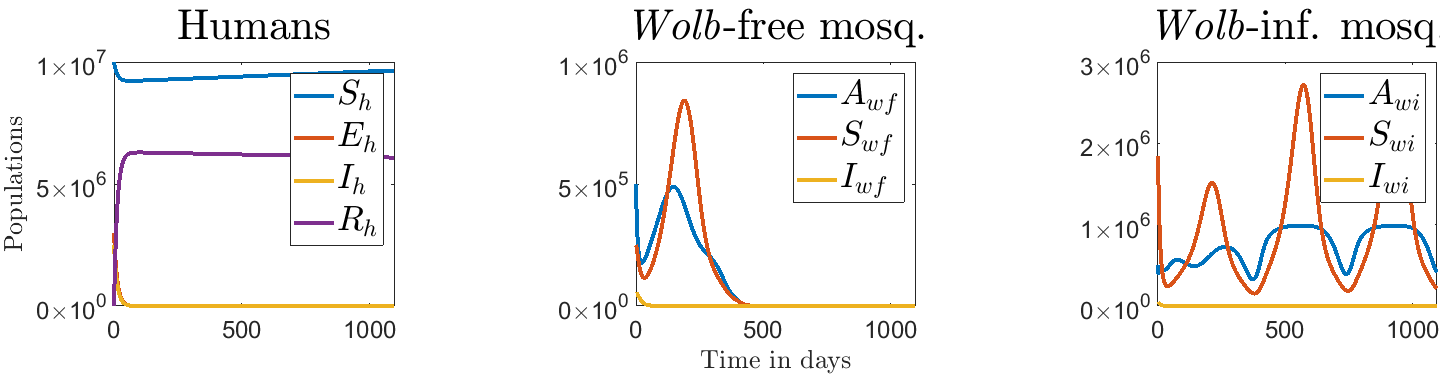
\includegraphics[width=\textwidth]{NonAutSimulation2.png}
 %   \caption{Dominance of \textit{Wolbachia} infected mosquitoes when we start with 7.4 times as many \textit{Wolbachia} infected susceptible females compared to wild susceptible females}
 %   \label{nonautfig2}
%\end{figure}

Simulations that involved releasing more \textit{Wolbachia} infected aquatic stage,  \textit{Wolbachia} infected males, a combination of \textit{Wolbachia} infected aquatic stage and females and a combination of \textit{Wolbachia} infected aquatic stage and males in the periodic setting yield similar results. Persistence of \textit{Wolbachia} infected mosquitoes can be achieved when seasonality is taken into account using the same scnarions as in Sections \ref{moreaquatics} - \ref{moreaqmale}, but it requires release of a higher number of \textit{Wolbachia} infected mosquitoes compared to wild mosquitoes. For example one would need 3.01 million of \textit{Wolbachia} infected aquatic stage to allow for \textit{Wolbachia} infected mosquitoes to persist when seasonality is included compared to 1.85 millions when all parameters were constant as seen in Section \ref{moreaquatics}. This is a little over six times as many \textit{Wolbachia} infected aquatic stage compared with \textit{Wolbachia} free aquatic stage. 
\\
\subsection{Disease present simulations for nonautonomous model}
Next we run numerical simulations using the initial conditions listed in Table \ref{init-cond-dis-present-table} and baseline value for the parameters listed in Table \ref{tab: param-table} and Table \ref{tab: param_mosq_table}. Furthermore, we change the biting rate of the mosquitoes to $b=1.25$ and the carrying capacity of the aquatic stage to $K=10^9$. 

\subsubsection{Zika takes longer to peak when \textit{Wolbachia} infection is not established under seasonality}
As we can see in Figure \ref{fig:new6a} the wild mosquitoes dominate, \textit{Wolbachia} infected mosquitoes are eliminated in 300 days. The number of wild mosquitoes susceptible females oscillates between 460 millions and 1.8 billion. Zika infected humans reach a peak of around 1.5 million in 50 days, which represents $15\%$ of the total population. In the autonomous model the peak was reached in 25 days and it was around 1.8 million infected humans (about $18\%$ of the total population) as seen in Section \ref{disfirst}.

\begin{comment}


\begin{figure}[H]
    %\hskip-0.75in
    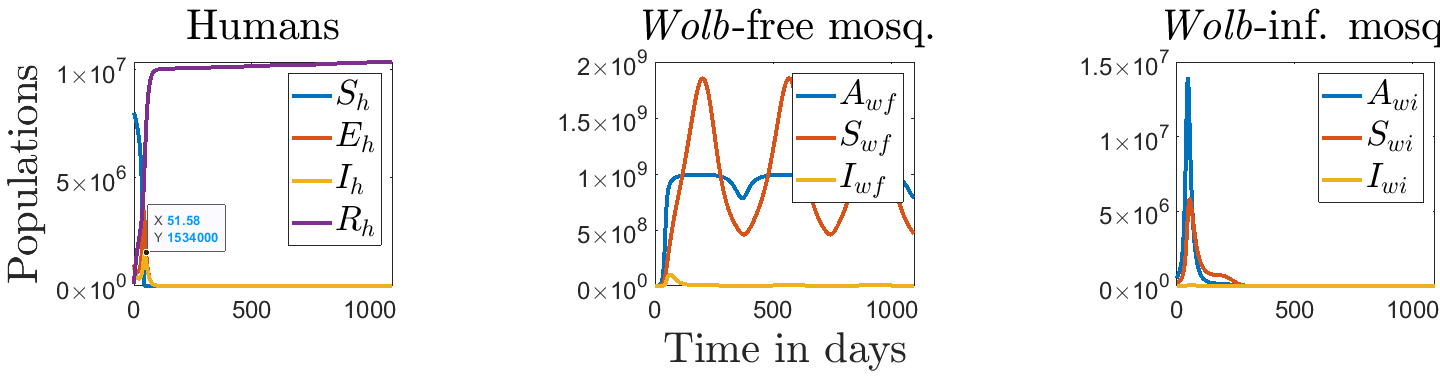
\includegraphics[width=\textwidth]{nonaut6amainupdated.png}
    \caption{Wild mosquitoes dominate and Zika is endemic in humans and wild mosquitoes. The peak of Zika  infected  humans is reached in  50  days  and it is around 1.5  million infected.}
    \label{fig:nonautonoum6amain}
\end{figure}
\end{comment}

\begin{figure}[H]
    \centering
    % This file was created by matlab2tikz.
%
%The latest updates can be retrieved from
%  http://www.mathworks.com/matlabcentral/fileexchange/22022-matlab2tikz-matlab2tikz
%where you can also make suggestions and rate matlab2tikz.
%
\definecolor{mycolor1}{rgb}{0.00000,0.44700,0.74100}%
\definecolor{mycolor2}{rgb}{0.85000,0.32500,0.09800}%
\definecolor{mycolor3}{rgb}{0.92900,0.69400,0.12500}%
\definecolor{mycolor4}{rgb}{0.49400,0.18400,0.55600}%
%
\begin{tikzpicture}

\begin{axis}[%
width=1.1in,
height=1.5in,
at={(0in,0.046in)},
scale only axis,
xmin=0,
xmax=1095,
ymin=0,
ymax=12000000,
ylabel style={font=\color{white!15!black}},
ylabel={Population},
axis background/.style={fill=white},
title style={font=\bfseries, yshift=1.75ex},
title={Humans},
legend style={legend cell align=left, align=left, draw=white!15!black}
]
\addplot [color=mycolor1, line width=1.5pt]
  table[row sep=crcr]{%
0	8000000\\
1.69942089729011	7936880.14411156\\
3.47508282959461	7866006.90650664\\
4.7590152984485	7810945.71479166\\
6.04294776823372	7752704.26365987\\
7.66472212504596	7674788.44648711\\
9.28649648092687	7592238.52461697\\
11.373151877895	7479262.2741998\\
13.4598072748631	7358054.30725875\\
14.7763866689056	7276745.01768892\\
16.0929660629481	7190982.84611829\\
17.4095454569906	7099912.70836832\\
18.7261248510331	7002500.20772388\\
19.8545991042629	6912965.82496763\\
20.9830733565614	6816726.5037963\\
22.1115476097912	6712447.92817219\\
23.2400218620896	6598476.37976984\\
24.3059091279283	6480087.82807265\\
25.3717963928357	6349191.0150875\\
26.437683657743	6203239.19186678\\
27.5035709235817	6039049.40090916\\
28.5528167039156	5855832.13259177\\
29.6020624851808	5646841.81766109\\
30.6513082655147	5406951.38107091\\
31.7005540458485	5130090.38519183\\
32.7480102647096	4810006.16671449\\
33.7954664826393	4439043.90709661\\
34.8429227015004	4012062.36186271\\
35.8903789194301	3526876.53477628\\
37.2340727904812	2824290.26522821\\
40.0972288614139	1235317.6098459\\
40.9473063293844	836777.379943425\\
41.6344864675775	570775.833862492\\
42.2425489388406	383687.925667447\\
42.7714937441051	258277.863358539\\
43.3004385503009	165085.194054103\\
43.8293833555654	99904.6044809893\\
44.306836085394	60418.7245427202\\
44.7327967407182	36971.1764810178\\
45.1179193975404	22940.5381356599\\
45.462204056792	14569.4508823091\\
45.7822285816073	9365.19967174064\\
46.0779929719865	6132.82750644628\\
46.3578590396792	4075.77323993295\\
46.6218267837539	2767.04247083515\\
46.8748468114063	1920.77774108294\\
47.116919121705	1373.34671156574\\
47.3517972808331	1014.16754511371\\
47.5794812906533	778.220574841835\\
47.8035533027723	620.731958780438\\
48.0240133162588	515.315064945258\\
48.2447771895677	443.231682477519\\
48.4658449245617	393.5807163883\\
48.6915017319843	358.290447273292\\
49.0368705540895	322.745520123281\\
49.4093141295016	298.119521766901\\
49.8086800621822	279.61754235439\\
50.238863744773	264.290293783881\\
50.7037605689839	250.606456895359\\
51.2228519786149	237.428255728446\\
51.949460433796	221.816506884061\\
52.6939781401306	208.448090464808\\
53.4347669938579	197.269897469319\\
54.1676233457401	187.92659095861\\
54.8949722610414	180.061593071558\\
55.7993530221283	171.960215252824\\
56.3386772396043	167.785324309021\\
57.2331477878615	162.012261287309\\
57.765753025189	159.037257530726\\
58.8246907694265	154.196257477626\\
59.1757106641307	152.902470809408\\
60.2234504790977	149.599166594446\\
60.5710020978004	148.755970327184\\
61.6094607412815	146.657671066001\\
61.7819580761716	146.361976426095\\
62.1269527478144	145.982790666632\\
62.4712762571871	145.484759610146\\
62.8155997665599	145.255276154727\\
63.1596230892465	144.90230274573\\
63.5036464110017	144.81060757488\\
63.8476463072002	144.591605946422\\
64.1916462033987	144.627901035361\\
64.3637678483501	144.551576131023\\
64.5358894923702	144.53388370201\\
64.8801327813417	144.690008156002\\
65.0525734238327	144.673097215593\\
65.225014067255	144.713720116764\\
65.5698953522369	144.983211302198\\
65.7429248774424	145.022693637758\\
65.9159544017166	145.118885370903\\
66.2620134511963	145.497219600715\\
66.6096422532573	145.740331377834\\
66.9572710562497	146.224248663522\\
67.3066716175526	146.571351741441\\
67.6560721788555	147.158093686216\\
68.007446533069	147.606863448396\\
68.5356977619231	148.541276446544\\
68.8894515121356	149.240762764588\\
69.2446815501899	149.92789252568\\
69.6013878760859	150.727777554654\\
69.959818967618	151.515456423163\\
70.3199748238549	152.416956055909\\
72.1493208426982	157.509926839732\\
72.5213180873543	158.725537931547\\
74.6132799582556	166.190610785969\\
76.9973324742168	176.545286556706\\
79.512514796108	189.527922755107\\
82.1874158820137	205.703350091353\\
84.8082160716876	224.036686514504\\
85.8879988184199	232.348397058435\\
87.3068628804758	243.851923095994\\
88.9351622313261	258.049466579221\\
90.4014522694051	271.707929848693\\
92.0012728404254	287.603934984654\\
93.6574705988169	305.159219860099\\
95.4112211307511	325.010829356499\\
97.0958563247696	345.312431351282\\
98.7846462344751	366.892056582496\\
100.443789641373	389.298513858579\\
102.226469848305	414.710970981978\\
104.090072201565	442.749351713806\\
106.001089552417	473.044052306563\\
108.071385645308	507.584063630551\\
110.214907844551	545.1582488399\\
112.437497159466	585.954528138041\\
114.809161843732	631.379302319139\\
117.487479679286	684.743196783587\\
120.499547284096	746.89140704833\\
124.453813284636	830.801214269362\\
133.062610397115	1014.17868413497\\
135.951104596257	1073.10493410192\\
138.417020654306	1121.3520808043\\
140.579654517584	1161.71296358109\\
142.531373262405	1196.31837401912\\
144.39396555908	1227.55140232481\\
146.129234196618	1254.94386841822\\
147.771610673517	1279.26100959536\\
149.325731177814	1300.76565691456\\
150.808428164572	1319.87328620907\\
152.211496106349	1336.66049146187\\
153.555854269303	1351.54913539812\\
154.880264508538	1365.06542312074\\
156.111927226186	1376.60982654057\\
157.298624148592	1386.80325917061\\
158.437522694468	1395.73689574283\\
159.555536302738	1403.70912308153\\
160.61839822866	1410.56836984772\\
161.660429801792	1416.62651096098\\
162.628330933861	1421.67635454889\\
163.56994025223	1426.06936001033\\
164.502419680357	1429.92897163704\\
165.386618594639	1433.15136236977\\
166.211025694385	1435.78459571861\\
167.009127996862	1438.00382445008\\
167.772988996468	1439.83416528162\\
168.49486312177	1441.30916050822\\
169.166921406984	1442.46773521788\\
169.847809558734	1443.4381124042\\
170.476560603827	1444.15902085975\\
171.094742732123	1444.71001954749\\
171.679930361919	1445.092910368\\
172.259110566229	1445.34419068694\\
172.841110166162	1445.47385287937\\
173.426775798202	1445.48524522036\\
174.000445531681	1445.38568779454\\
174.635085014626	1445.15398736671\\
175.284981757402	1444.79128761217\\
175.966175044887	1444.28285552561\\
176.700035095215	1443.59782313835\\
177.482594336383	1442.72213814873\\
178.360073792748	1441.57763479929\\
179.326411804184	1440.13923525531\\
180.400530887768	1438.34983858559\\
181.6441894155	1436.0689923577\\
183.120272529311	1433.13680564705\\
185.097290819511	1428.9627802996\\
189.870151616633	1418.79633820243\\
191.436856158078	1415.74867913593\\
192.770682784729	1413.37407046836\\
193.945713049732	1411.49073487986\\
194.989659411833	1410.00843391381\\
195.932604310103	1408.84283703379\\
196.828220241703	1407.90275376104\\
197.626497115009	1407.21276013367\\
198.394760952331	1406.68911486771\\
199.095368155278	1406.33839442395\\
199.766297828406	1406.12151559629\\
200.403306180611	1406.02800676785\\
201.009194732644	1406.04462671187\\
201.622194108553	1406.16993733495\\
202.239458835684	1406.41011943016\\
202.851538692601	1406.76490229275\\
203.495291220024	1407.26728903409\\
204.135582784191	1407.90243188199\\
204.797230929136	1408.70495815761\\
205.506056883372	1409.73450138792\\
206.22097164765	1410.95609647315\\
206.990390503779	1412.48258592468\\
207.78396063298	1414.29389926791\\
208.598565406166	1416.41102061979\\
209.457370402291	1418.93439506274\\
210.373426406644	1421.96575588174\\
211.292086875997	1425.368839534\\
212.269864609465	1429.40286399331\\
213.254648881033	1433.90848625544\\
214.295734109357	1439.1699953815\\
215.336780442856	1444.95945613272\\
216.423881752416	1451.58655702416\\
217.547351448797	1459.07944231853\\
218.694398635998	1467.42675694544\\
219.901004386134	1476.99268861022\\
221.101501129568	1487.33560488373\\
222.365722713061	1499.14769379608\\
223.652999118902	1512.17835311033\\
224.93377867993	1526.18274983205\\
226.24763920065	1541.66401207168\\
227.58692617435	1558.64838817529\\
228.961965817027	1577.39604925364\\
230.387531575747	1598.28586605191\\
231.789639342576	1620.32956752833\\
233.227902492508	1644.5439919401\\
234.703471211717	1671.13831594307\\
236.217045009136	1700.33448563982\\
237.743342773989	1731.82186915539\\
239.292092375457	1765.95915047079\\
240.84537426848	1802.5008935621\\
242.431664788164	1842.3015847886\\
244.019017081708	1884.74630345963\\
245.637339156121	1930.82975060493\\
247.236609733663	1979.2772886958\\
248.862334205769	2031.61381044798\\
250.531031721272	2088.70911291614\\
252.208843234926	2149.71108891629\\
253.883404285647	2214.34186197724\\
255.610917898826	2285.10490529984\\
257.351820273325	2360.79290400259\\
259.068396002986	2439.90226868913\\
260.862583905458	2527.53494504839\\
262.637626143172	2619.40435820911\\
264.419293604791	2716.98904264718\\
266.238766650669	2822.40552830882\\
268.056794897653	2933.76037011202\\
269.818076317199	3047.57341452502\\
271.648274656385	3172.22319604456\\
273.58889465034	3311.71491184924\\
275.431977110915	3451.3704332998\\
277.377740202472	3606.59073866811\\
279.344254432246	3771.78228444979\\
281.33267844189	3947.49525020365\\
283.310355591588	4131.07460907754\\
285.455945265479	4340.33628064487\\
287.550700466149	4554.89667731524\\
289.678826414049	4783.33728890587\\
291.928468698636	5036.33355245925\\
294.278813489713	5313.28669966571\\
296.683399114758	5609.9151139902\\
299.158894723281	5929.1661196854\\
301.58084731549	6254.89736041147\\
304.016284460202	6595.47542223148\\
306.716190196574	6987.83692221344\\
309.502251150087	7408.37821422797\\
312.272457541898	7841.50332862232\\
315.147789579816	8305.90030765068\\
318.288077724166	8829.07450773381\\
321.785939550027	9429.62651769817\\
325.275794534013	10045.31820847\\
329.341241634451	10780.2176220771\\
334.286895436235	11694.5496435603\\
340.106189084239	12790.0222906461\\
358.222713761032	16215.0093634631\\
362.098554978147	16925.7461913945\\
365.974396195263	17618.4448927101\\
369.060806747526	18152.8211021312\\
372.093241791241	18658.757120789\\
375.066876276396	19132.0870885737\\
377.006882192567	19426.3347558845\\
378.938448907807	19706.0725896992\\
380.861576420255	19969.8134197025\\
382.788217002526	20217.4617719371\\
384.718370655552	20447.0250140121\\
386.657546197996	20656.9422902558\\
387.631644914858	20753.8871858809\\
388.605743630789	20844.7827425189\\
389.579842347652	20929.3445657697\\
390.569407544099	21008.4687520927\\
391.558972741477	21080.4663486173\\
392.548537937924	21145.0377241205\\
393.538103135303	21201.878450362\\
394.545635129325	21251.4950920045\\
395.553167124279	21292.4728115033\\
396.560699118301	21324.5009101052\\
397.568231113255	21347.2680470916\\
398.35347268451	21358.3939663591\\
399.138714255765	21363.572199977\\
399.92395582702	21362.6665788544\\
400.709197398275	21355.541696311\\
401.49443896953	21342.0663869623\\
402.279680539854	21322.1183966314\\
403.064922111109	21295.5784978718\\
403.850163682364	21262.3304507248\\
404.65450129658	21221.2032116205\\
405.458838911727	21172.8158322154\\
406.263176525943	21117.0684085069\\
407.515987851657	21015.3518197779\\
408.412935275584	20931.2446620688\\
409.309882699512	20837.614439033\\
410.206830123439	20734.3838548465\\
411.278310745955	20598.401062469\\
412.524324567989	20422.8518037759\\
413.630658119917	20251.2646699669\\
415.080638044514	20004.0591910342\\
416.530617970042	19731.7487714924\\
417.99521065969	19431.6147575974\\
419.605738444254	19073.1966147767\\
421.178892782889	18695.4076819587\\
422.682565304451	18309.9166335417\\
424.383855849504	17846.7670961684\\
426.434573533013	17253.630993899\\
428.352251672186	16668.5110383239\\
430.823670692742	15878.4720634948\\
433.662850740366	14933.9637488611\\
439.295733923092	13012.0899746222\\
442.84978374932	11819.5565655828\\
445.479128368199	10971.4242920578\\
447.673250546679	10295.2953783013\\
449.78554923553	9676.92841750104\\
451.688897748478	9150.16498863883\\
453.535467504524	8668.54816733766\\
455.183481888846	8264.069739745\\
456.861983560026	7877.03719310462\\
458.50519092381	7522.45518267155\\
460.136808353476	7193.79340235051\\
461.71656559594	6897.19924644101\\
463.140754445456	6647.38181985728\\
464.595811923034	6408.60415775143\\
466.104261545464	6177.7344059106\\
467.548030663282	5971.73993318249\\
468.951150154695	5784.68823389988\\
470.50717304647	5591.33709875587\\
472.050672751851	5413.03769738507\\
473.548031960614	5251.81940986868\\
475.132672285661	5092.65958494321\\
476.667755734175	4948.63104160782\\
478.239892001264	4810.42162999138\\
479.845492498949	4677.93540948071\\
481.499172322452	4549.58817742392\\
483.213113159873	4424.18872714601\\
485.083863219246	4295.01075026859\\
487.010643016547	4169.17470082641\\
489.036025287583	4043.5984227499\\
491.236933181994	3913.68748026993\\
493.548153816722	3783.39426897652\\
496.02024431061	3649.81880364101\\
498.69396644365	3510.99655724317\\
501.476146466099	3371.88542452175\\
504.323786174878	3234.52883472387\\
507.245482430793	3098.54801768251\\
510.099259165116	2970.47631224431\\
512.889342554845	2849.87258808594\\
515.538471742533	2739.72893830668\\
518.083280460909	2638.09538456798\\
520.549190904014	2543.66896826215\\
522.922680451535	2456.68171914667\\
525.198602897115	2376.96151326224\\
527.390438298695	2303.67164603714\\
529.537542974576	2235.23824292887\\
531.6261771461	2171.88542210404\\
533.654110526666	2113.41888071597\\
535.625375919975	2059.45899621118\\
537.55276181642	2009.42692263238\\
539.450732943602	1962.77486989647\\
541.298035104759	1919.83928509895\\
543.095948176458	1880.36790457368\\
544.873770672828	1843.55852991436\\
546.594586111605	1810.00735664088\\
548.269354688004	1779.2923482107\\
549.927709395997	1750.73909280077\\
551.523932680488	1724.98321702424\\
553.091298975982	1701.32266081311\\
554.603187269531	1680.01290351618\\
556.077759995125	1660.6459982777\\
557.50439293962	1643.22808142845\\
558.904754822142	1627.38231851254\\
560.254082891159	1613.27826367412\\
561.551860604435	1600.78425219283\\
562.789705196396	1589.8408474531\\
563.991117801517	1580.12479160633\\
565.128757252358	1571.74388227519\\
566.217114805244	1564.47038507462\\
567.265749787912	1558.1499340795\\
568.241868640296	1552.87263670005\\
569.162804370746	1548.42950821668\\
570.042629736476	1544.67101105023\\
570.890145268291	1541.50045423489\\
571.649914021604	1539.0341119701\\
572.356582264416	1537.0598408645\\
573.030641363934	1535.46446086746\\
573.673178544268	1534.20594412833\\
574.267228891142	1533.27075081598\\
574.781794814393	1532.6385099655\\
575.288138611242	1532.17796070501\\
575.725562784821	1531.90949606895\\
576.156746117398	1531.76257702615\\
576.597998723388	1531.73355666734\\
577.029259937815	1531.82413028087\\
577.473895619623	1532.04099294357\\
577.908182130195	1532.3742199121\\
578.389741417021	1532.88449374028\\
578.876611505635	1533.55146283656\\
579.439122403041	1534.51199855283\\
580.030530673452	1535.74254480843\\
580.646978883073	1537.26727857441\\
581.319497451186	1539.21427404881\\
582.038325204514	1541.62477783579\\
582.807834378444	1544.58544071671\\
583.598020055331	1548.0383499898\\
584.447399018332	1552.22075252794\\
585.338469980285	1557.13838783093\\
586.280919144861	1562.93706338573\\
587.280307566747	1569.76595830545\\
588.287630862556	1577.3674658332\\
589.354836672544	1586.22007971909\\
590.465860582888	1596.32472179085\\
591.6182289524	1607.78090555873\\
592.785811861977	1620.42173953727\\
593.983322123997	1634.49017514475\\
595.229805661365	1650.34802793991\\
596.534075147472	1668.29934072308\\
597.853792748414	1687.91404827125\\
599.190527678467	1709.31032150984\\
600.569586383179	1733.04283575807\\
601.960397498682	1758.73520367127\\
603.400469495915	1787.2562126983\\
604.846877864562	1817.93190908898\\
606.314534641802	1851.20729501639\\
607.790892816149	1886.93956233934\\
609.324591451325	1926.54533830844\\
610.886578585953	1969.58090114128\\
612.46958514303	2016.07987440098\\
614.082856130786	2066.57037820667\\
615.68199333176	2119.82940570172\\
617.310196336359	2177.46904516686\\
618.997270659544	2240.96792398207\\
620.666727037169	2307.73508858308\\
622.396168258972	2381.18885698915\\
624.106474874541	2458.28878527973\\
625.793265535496	2538.83807321917\\
627.568657214753	2628.63756183535\\
629.360830195248	2724.69996419176\\
631.174462348223	2827.65238048695\\
632.934344127774	2933.26560023427\\
634.771129663102	3049.69447449408\\
636.59370143991	3171.67976004537\\
638.446923593059	3302.5102102831\\
640.326882174239	3442.42390006129\\
642.264190009795	3594.3866965659\\
644.240962627344	3757.7821169151\\
646.169112509117	3925.44532522652\\
648.140953131951	4105.52846058644\\
650.257723861374	4308.70183015801\\
652.29020741675	4513.50681534596\\
654.433159421198	4739.85093139485\\
656.599759587087	4979.60803154763\\
658.790168260224	5233.16622259188\\
660.99863912072	5500.14056409895\\
663.31630156748	5792.43897676095\\
665.780230652541	6116.60732167121\\
668.16895849444	6443.82015277445\\
670.829788070172	6822.88722534664\\
673.394175471738	7202.24743997026\\
676.204263933934	7633.06393539254\\
679.259108551778	8118.32447159849\\
682.264833723195	8611.79260929208\\
685.714790278114	9196.05906317476\\
689.520395282656	9860.25466214027\\
693.631239549257	10597.5667704046\\
697.998454937711	11399.1440035729\\
703.769321672618	12479.2378027877\\
713.578458157368	14340.4341066675\\
721.545982426032	15843.1140648248\\
726.625607421622	16780.4998205472\\
730.435326169245	17465.2759276181\\
733.724285118282	18038.8151964052\\
736.85965071246	18565.8927909154\\
738.898696658202	18896.0559410984\\
740.987868287601	19222.1163527006\\
743.077039917931	19534.0295327585\\
745.181191411801	19831.7927338015\\
747.285342906602	20110.9193147998\\
749.343147496693	20363.5174326124\\
750.372049791738	20481.5281289145\\
751.400952086784	20593.5913618663\\
752.397870279849	20696.1893925536\\
753.394788472913	20792.6174286753\\
754.391706665978	20882.5802679975\\
755.388624859042	20965.7656568289\\
756.346961302683	21039.0505480524\\
757.305297745392	21105.5232868344\\
758.263634189032	21164.9140063412\\
759.221970632672	21216.9396985313\\
760.113960959017	21258.4984132117\\
761.005951286294	21293.2279957533\\
761.89794161357	21320.9163736375\\
762.789931940846	21341.3398623345\\
763.569430031814	21353.0667609451\\
764.348928122781	21358.9536477095\\
765.128426213749	21358.8698197734\\
765.907924304716	21352.6748516914\\
766.564431587234	21342.6169244181\\
767.220938869752	21328.0642243512\\
767.87744615227	21308.9474179279\\
768.533953434788	21285.1923206681\\
769.119140649214	21260.0509829307\\
769.704327863641	21231.1292427396\\
770.289515078068	21198.3852466708\\
770.874702292494	21161.7758877007\\
771.457618738525	21121.4257442886\\
772.040535184555	21077.1677922923\\
773.206368077546	20976.7993021924\\
774.424613033421	20854.8218331784\\
775.642857990228	20715.172791197\\
776.810528547503	20564.5877310606\\
777.978199104778	20397.5594672449\\
778.939017097466	20247.7657681461\\
780.289195733145	20018.4907317767\\
781.457277663052	19802.5520477593\\
782.586814664304	19578.4107949464\\
783.823771486059	19315.9562397599\\
785.162072392181	19012.4561763871\\
786.913594686426	18585.6568920175\\
788.503359884955	18170.6734739421\\
790.309037891217	17669.6964897718\\
792.38924122043	17057.203719493\\
794.369218054228	16443.6559116906\\
796.880253923126	15630.8913528537\\
800.18096540682	14522.0900395764\\
808.385279009119	11743.9724186976\\
810.912330889143	10931.3245641151\\
813.087117239833	10262.9327180665\\
815.167799395509	9655.32935662009\\
817.058071538806	9133.30529419519\\
818.889151037671	8656.62542658113\\
820.565540222451	8246.11027957126\\
822.247624428011	7859.41848111805\\
823.874634184875	7509.35236486886\\
825.476604564115	7187.32272739895\\
827.055844247341	6891.25060175639\\
828.603539060801	6620.92286645528\\
830.114093891345	6375.14299099706\\
831.552110817283	6156.87294572499\\
833.045352923684	5945.47865070682\\
834.556267022155	5746.36695896275\\
836.073403318413	5560.30533499643\\
837.567851806991	5389.54020518623\\
839.106033897959	5225.64360415563\\
840.68310396187	5068.95581540279\\
842.172624999657	4930.50136914384\\
843.738454527222	4793.92284326721\\
845.371565123089	4660.21676812042\\
847.075870053843	4529.08987483475\\
848.804032049142	4403.80591663066\\
850.618443571962	4279.48951435275\\
852.523721685633	4155.7941287579\\
854.602990357205	4027.60477577243\\
856.771257985383	3900.28967862949\\
859.13898115512	3767.44747437723\\
861.681123305112	3630.80065921508\\
864.319564125501	3494.47727299575\\
867.101003559306	3355.98716726154\\
869.988864389248	3217.2823862033\\
872.889890385792	3082.85524116457\\
875.722456164658	2956.28250422608\\
878.487608456984	2837.26927231625\\
881.133817180991	2727.73553804122\\
883.687792384066	2626.23228596989\\
886.101252140477	2534.26546839811\\
888.451675030403	2448.51501687337\\
890.733022061177	2368.9792154748\\
892.964153802022	2294.78319744207\\
895.111536865123	2226.76802371908\\
897.213913616724	2163.42916242499\\
899.265520313755	2104.72855389956\\
901.268649622798	2050.37323341332\\
903.210644394159	2000.45388066769\\
905.10835625045	1954.29459537379\\
906.963499769568	1911.65235437546\\
908.790170920081	1872.03599373531\\
910.556586544029	1835.93805734161\\
912.270889559761	1802.95877665095\\
913.932126663625	1772.90640836023\\
915.573065022938	1745.04038655385\\
917.162789021619	1719.74757240713\\
918.698995763436	1696.88072626851\\
920.227026272565	1675.65417613182\\
921.712756505236	1656.45286114048\\
923.147669791244	1639.24147995748\\
924.533312464133	1623.85421898961\\
925.867903276347	1610.17120627593\\
927.136901280843	1598.1895420514\\
928.370232605375	1587.50093829539\\
929.564345179126	1578.04688514769\\
930.677475349046	1570.02435087599\\
931.732958942652	1563.1202762099\\
932.769179790281	1557.00711269304\\
933.748929321766	1551.83276881091\\
934.67496833019	1547.48341848422\\
935.557228749618	1543.82948262151\\
936.363451120444	1540.90898026526\\
937.123729606159	1538.52173124533\\
937.830869165249	1536.62162640225\\
938.505589085631	1535.09711732995\\
939.115102718584	1533.96276132017\\
939.674810761586	1533.12465777993\\
940.180437105708	1532.53554246202\\
940.674922099337	1532.11407763045\\
941.139729802497	1531.85774727445\\
941.551839680411	1531.74413058627\\
941.998190836981	1531.74191859458\\
942.424810110591	1531.85759893153\\
942.875443601049	1532.1052178517\\
943.34605825413	1532.50183440838\\
943.836598168127	1533.06588861998\\
944.356925102882	1533.83293177187\\
944.922287710011	1534.86416804697\\
945.512819667347	1536.16239321977\\
946.148081434891	1537.81258731335\\
946.815050526522	1539.829825514\\
947.539666747674	1542.3542628549\\
948.295604879037	1545.36016838346\\
949.12779621128	1549.11290781386\\
949.975068702362	1553.41602095682\\
950.876293442212	1558.5332113374\\
951.825014988892	1564.52889615949\\
952.829099563882	1571.56378119625\\
953.848157645203	1579.43903297093\\
954.934917076491	1588.6670122724\\
956.045415947214	1598.99645761959\\
957.203835881315	1610.75939752068\\
958.410359064117	1624.10508859158\\
959.612080184743	1638.53184399474\\
960.870852293447	1654.8856297629\\
962.148235977627	1672.81245532166\\
963.441743772477	1692.36764847487\\
964.79692120757	1714.41013379022\\
966.180075636134	1738.59604533389\\
967.583190481178	1764.92689106986\\
969.017043653876	1793.76260729693\\
970.49036052078	1825.48926479463\\
971.990469770506	1860.05210200697\\
973.511597038247	1897.50967094675\\
975.04427609127	1937.79602696281\\
976.638959178701	1982.52469828073\\
978.201557716355	2029.2413483439\\
979.799223891459	2080.07578044292\\
981.428135541268	2135.22321214247\\
983.050733778626	2193.61841902044\\
984.749321350828	2258.5958879767\\
986.432946433313	2327.03793010209\\
988.106102396734	2399.19225618429\\
989.845774227753	2478.7588547226\\
991.591736179776	2563.44908812642\\
993.349254171364	2653.77786764503\\
995.091693660244	2748.5451029297\\
996.815687123686	2847.59698112682\\
998.578512757085	2954.50131621771\\
1000.38779718429	3070.32475115452\\
1002.20190338232	3192.85511285067\\
1004.07132484298	3326.02265065722\\
1005.91691394802	3464.55300835986\\
1007.85716802813	3617.94772636332\\
1009.81323533505	3780.83176615927\\
1011.83794411831	3958.33003632631\\
1013.87045654655	4145.78431995306\\
1015.81727162842	4334.1768206628\\
1017.9907474583	4554.84562386014\\
1020.14944574609	4784.90390520636\\
1022.29341936763	5024.18226701859\\
1024.58189414255	5291.45166519471\\
1026.84648575447	5567.93470953684\\
1029.09427316487	5854.05838338286\\
1031.62457312085	6189.8635389246\\
1034.03647632711	6523.18946764711\\
1036.74722072855	6912.77334024012\\
1039.45599341299	7317.29005919211\\
1042.17979709525	7738.66211108211\\
1045.30872156005	8239.7168200789\\
1048.67918987293	8798.26865271572\\
1052.06506947055	9377.16173662059\\
1055.42973350361	9968.06815716997\\
1059.60297634639	10719.480963625\\
1064.1493091844	11556.8357809661\\
1070.2539109448	12702.7148059914\\
1089.22843766212	16285.33783413\\
1093.83243383933	17125.3475282202\\
1095	17334.3649396515\\
};
\addlegendentry{$S_h$}

\addplot [color=mycolor2, line width=1.5pt]
  table[row sep=crcr]{%
0	1000000\\
0.886026846710593	946617.505430378\\
1.69942089729011	902410.096910248\\
2.88319551898167	846058.481859738\\
3.47508282959461	821244.70259443\\
4.11704906402156	796703.958180984\\
4.75901529891416	774472.525264651\\
5.40098153334111	754394.643150554\\
6.04294776823372	736323.425734389\\
6.85383494663984	716143.827423751\\
7.66472212458029	698672.530541018\\
8.47560930298641	683676.04050222\\
9.28649648139253	670946.582348101\\
10.3298241798766	657605.135932313\\
11.373151877895	647432.791730579\\
12.4164795763791	640230.398051868\\
13.4598072748631	635832.289772405\\
14.7763866689056	634111.816043287\\
16.0929660629481	636795.054326934\\
17.4095454574563	644175.403694343\\
18.7261248514988	656607.107954632\\
19.8545991042629	671713.73220918\\
20.983073357027	691566.435000924\\
22.1115476097912	716925.583805262\\
23.2400218625553	748761.28073225\\
24.3059091279283	785902.858804251\\
25.3717963928357	831180.77052185\\
26.4376836582087	886175.49496276\\
27.5035709235817	952933.777866463\\
28.5528167039156	1032638.41632861\\
29.6020624847151	1128912.08382043\\
30.6513082655147	1244905.25127112\\
31.7005540463142	1384480.34975091\\
32.7480102647096	1551834.6832075\\
33.795466483105	1750812.12560169\\
34.8429227010347	1982813.91753755\\
35.8903789194301	2246997.27182275\\
37.2340727904812	2623532.59352876\\
38.5777666610666	3004001.5077239\\
39.0842540608719	3135548.6265814\\
39.5907414611429	3252945.88513617\\
40.0972288609482	3350814.39752735\\
40.6037162607536	3424868.8352298\\
40.9473063298501	3459756.11098038\\
41.290896398481	3480756.57445045\\
41.6344864671119	3487117.19467955\\
41.9780765362084	3478900.08512716\\
42.2425489388406	3463001.60203519\\
42.5070213414729	3438881.01937599\\
42.7714937445708	3406883.55820402\\
43.3004385498352	3322302.41189458\\
43.8293833555654	3214811.13843048\\
44.7327967407182	2997423.5352586\\
47.3517972812988	2337853.35773214\\
48.4658449245617	2092618.3111399\\
49.5334619875066	1881449.05854129\\
50.5487949606031	1700443.47534619\\
51.5804084432311	1534419.20472138\\
52.6939781401306	1373420.43959465\\
53.8021913226694	1230044.06307688\\
54.8949722610414	1103400.76459179\\
55.9791277614422	990717.690799693\\
57.0544738355093	890392.189135436\\
58.1197612839751	801095.830420791\\
59.1757106641307	721491.718943952\\
60.2234504790977	650394.65402397\\
61.2639170307666	586792.869159963\\
62.2991145025007	529752.887373885\\
63.3316347501241	478449.720951129\\
64.3637678478844	432197.034109741\\
65.3974547097459	390421.450013254\\
66.4358278522268	352587.329155172\\
67.4813718982041	318262.037542005\\
68.5356977614574	287098.896777513\\
69.6013878765516	258768.19609576\\
70.6819888968021	232964.55654019\\
71.7794409990311	209462.595887985\\
72.8957193330862	188062.377172897\\
73.8431217097677	171682.995084479\\
74.8072618297301	156533.544082178\\
75.7892133244313	142534.818889996\\
76.7936519193463	129569.365958093\\
77.8196731763892	117603.728475283\\
78.8693098565564	106569.125108109\\
79.9441673727706	96407.9350289647\\
81.0508296699263	87027.0021990449\\
82.1874158815481	78414.2837329395\\
83.1203502598219	72040.7292023473\\
84.0762020619586	66098.8636526484\\
85.0564069296233	60567.5548277674\\
86.0556039046496	55460.0572957671\\
87.1002461076714	50638.6862038686\\
88.1778951543383	46165.3352843714\\
89.2346305786632	42222.5853621862\\
90.2121572704054	38928.0843668864\\
91.2357534463517	35806.3681728779\\
92.2765315072611	32943.186594551\\
93.2549732946791	30509.804860658\\
94.315706608817	28126.9678321304\\
95.4112211312167	25917.0625253292\\
96.4954469264485	23955.3799797413\\
97.4561019642279	22386.0236072466\\
98.4288344313391	20943.008612752\\
99.4661288862117	19550.890733955\\
100.443789641373	18364.2481409069\\
101.488085325807	17218.1431190744\\
102.523753805086	16193.3755793953\\
103.620752636343	15217.212711175\\
104.655542278197	14389.131439317\\
105.750091826078	13601.2060370781\\
106.828989543021	12904.0943486742\\
107.831020744517	12320.2780075166\\
108.898163499776	11759.2000504793\\
109.950776530895	11261.0249085105\\
110.967959081288	10826.5932064201\\
112.008041488472	10425.4330753549\\
113.016335962806	10074.0651806537\\
114.02797765471	9755.07662617555\\
115.044413481373	9465.1755395541\\
116.109532794449	9191.09560650866\\
117.136142985895	8952.88590288348\\
118.197470871266	8730.76065641688\\
119.216786166653	8538.28165645106\\
120.225259703118	8366.012838447\\
121.27700364124	8203.7471279921\\
122.32365321368	8058.19302075775\\
123.363768984564	7927.75244873902\\
124.369375152048	7813.81316624023\\
125.378056722227	7710.4137680144\\
126.443184569944	7611.9444876248\\
127.509700909723	7523.31658016751\\
128.571679103188	7444.01440581633\\
129.612508310471	7374.12343508611\\
130.633221652359	7312.40304933954\\
131.634772126563	7257.8014499424\\
132.664597945753	7207.25302974135\\
133.673434197903	7162.73853409011\\
134.679047903512	7122.8517673132\\
135.670448119286	7087.52589860465\\
136.62423888687	7056.96317462204\\
137.587131174281	7029.22645493411\\
138.577566523105	7003.69054298522\\
139.506065896247	6982.2810489242\\
140.423397597391	6963.33825836843\\
141.307897646446	6946.99122903496\\
142.203079260886	6932.217312722\\
143.124820081517	6918.72431409918\\
143.990919583477	6907.51523939474\\
144.84791349899	6897.72095158231\\
145.675939186476	6889.39504801342\\
146.515863502864	6882.01013128739\\
147.292657912709	6876.06525053363\\
148.01830442762	6871.22885472048\\
148.745484713931	6867.03270811914\\
149.427745508961	6863.65136963828\\
150.120141102001	6860.73614568915\\
150.748229408637	6858.51515085623\\
151.353874968365	6856.73322116211\\
151.937767040916	6855.33140352648\\
152.474706373643	6854.3018254498\\
152.976893160027	6853.552648162\\
153.443228207063	6853.03326059692\\
153.896618221421	6852.68372807791\\
154.335769432131	6852.48489716463\\
154.764621619601	6852.4177106563\\
155.168554799166	6852.46435077814\\
155.614273126703	6852.63425806351\\
156.070022847038	6852.93077118369\\
156.558403821662	6853.37968687806\\
157.091022199485	6854.01591782738\\
157.667883811519	6854.86768199317\\
158.336906497367	6856.05353281414\\
159.051173733082	6857.53687742399\\
159.839555535931	6859.4125180901\\
160.73163046781	6861.80701584741\\
161.736957384739	6864.81187009439\\
162.879247940611	6868.56528060371\\
164.201643049717	6873.28332812386\\
165.786597337574	6879.34650088567\\
167.810031515546	6887.52572235838\\
175.7727036383	6920.16590845631\\
177.585881785955	6926.92879348015\\
179.198467454407	6932.56065518642\\
180.686976335011	6937.39438010985\\
182.07019841671	6941.54309584387\\
183.362096926663	6945.10001331102\\
184.583701789379	6948.16786378808\\
185.714731224347	6950.74363930197\\
186.81577095855	6953.00089415303\\
187.85190657014	6954.8958552354\\
188.841031327844	6956.49510873063\\
189.79556207126	6957.84281141311\\
190.703046397772	6958.94525841204\\
191.568039017264	6959.83365120133\\
192.398448107298	6960.53752425639\\
193.194813967682	6961.07580877841\\
193.945713049266	6961.46123242611\\
194.698378982488	6961.72921543242\\
195.425580515526	6961.87626919104\\
196.129181534983	6961.91461916035\\
196.859059390612	6961.84720245283\\
197.595681459643	6961.66940158419\\
198.329077019356	6961.38383371802\\
199.095368155744	6960.97089524288\\
199.896014446858	6960.41571832076\\
200.707284509204	6959.72570473514\\
201.578165346291	6958.84398671519\\
202.459982025903	6957.80442493549\\
203.419946183916	6956.50726528699\\
204.406759929843	6954.99677931145\\
205.460026337299	6953.18978056544\\
206.574988130014	6951.06151631661\\
207.737469262443	6948.61080917483\\
208.949533647858	6945.80818135431\\
210.197236681357	6942.66404252499\\
211.526634481736	6939.02983683813\\
212.904109630268	6934.96001278656\\
214.344270350877	6930.37898738822\\
215.833735010121	6925.29521925608\\
217.372251407243	6919.67865503719\\
218.966957206838	6913.46796471952\\
220.619534019846	6906.61555481236\\
222.314320468344	6899.14755666628\\
224.051349155139	6891.02772672148\\
225.817340098787	6882.2838153122\\
227.636476492044	6872.75298035005\\
229.482424058486	6862.52631311491\\
231.371442813426	6851.46597211948\\
233.271678521764	6839.71304860106\\
235.16951919999	6827.3244761196\\
237.082268713042	6814.15464957478\\
239.034151234198	6799.97730875574\\
240.957587053068	6785.24463425437\\
242.892379419878	6769.62678209506\\
244.834409341682	6753.10812734999\\
246.743640172295	6736.00785941444\\
248.68631148478	6717.69252791721\\
250.650922338013	6698.1896183677\\
252.584971434437	6677.9857491143\\
254.57186359074	6656.15012170933\\
256.548924934585	6633.29534536274\\
258.542341613211	6609.07353191217\\
260.576684901956	6583.09692508867\\
262.637626143638	6555.45024918532\\
264.694116950035	6526.49869587505\\
266.777215489186	6495.75948715815\\
268.9753794102	6461.76370335836\\
271.205063954927	6425.6397559871\\
273.490352642257	6386.90936136805\\
275.803768389393	6345.97117508529\\
278.180684898049	6302.14586625574\\
280.64007972274	6254.99906627182\\
283.310355591588	6201.86634855065\\
286.177772426978	6142.76296582073\\
289.34362081252	6075.37336651608\\
293.0926597137	5993.27019330254\\
298.25342215877	5877.70336923655\\
306.401339748409	5695.05410141451\\
309.871481321752	5619.45547856856\\
312.921874015126	5555.05437733093\\
315.580313595943	5500.93577147229\\
317.827398700174	5456.90984932752\\
320.058139018714	5414.95825089421\\
322.255118119065	5375.51461346447\\
324.200367395766	5342.26088920981\\
326.397843002342	5306.70263215294\\
328.150847699028	5279.93923485745\\
329.936438602861	5254.19985795673\\
331.750566896051	5229.67111687455\\
333.628196828999	5206.05215202924\\
334.945594043471	5190.57640911778\\
336.333761265501	5175.26197180944\\
337.792698493693	5160.27829189552\\
339.31417809613	5145.87711581308\\
340.898200071882	5132.22573725833\\
342.538650129922	5119.54021618608\\
343.387089199387	5113.56324774167\\
344.235528269317	5107.98510652222\\
345.083967338782	5102.80696112989\\
346.008532632142	5097.62286641682\\
346.933097925503	5092.91806494351\\
347.857663218863	5088.69295136305\\
348.782228512224	5084.95012457948\\
349.829439328518	5081.30019872636\\
350.876650144812	5078.27743878635\\
351.923860961106	5075.88380359812\\
352.9710717774	5074.12816311419\\
354.283982273191	5072.85544526204\\
355.596892768983	5072.61319361022\\
356.909803264774	5073.40981088951\\
358.222713761032	5075.29420811078\\
359.191674065311	5077.41635995265\\
360.160634369589	5080.16218909621\\
361.129594673868	5083.54613435129\\
362.098554978147	5087.59656970762\\
363.067515282426	5092.34444787353\\
364.036475586705	5097.80487724207\\
365.005435890984	5104.00280499924\\
365.974396195263	5110.97636271641\\
367.003199712373	5119.27668826841\\
368.03200322995	5128.53097803472\\
369.060806747526	5138.78273897059\\
370.089610264637	5150.09482917981\\
371.091426027939	5162.19259473355\\
372.093241791241	5175.40027495101\\
373.095057554543	5189.77254558308\\
374.096873317845	5205.38133351179\\
375.066876276396	5221.74256911222\\
376.036879234482	5239.38213096745\\
377.006882193033	5258.36096569616\\
377.976885151118	5278.75299410336\\
378.938448907342	5300.43605095148\\
379.900012664031	5323.63901008619\\
380.861576420255	5348.42804594291\\
381.823140176479	5374.87916999264\\
382.788217002526	5403.17421113793\\
383.753293829039	5433.2817463195\\
384.718370655552	5465.26990293013\\
385.683447481599	5499.21385567449\\
386.657546197996	5535.53284032783\\
387.631644914392	5573.9797825627\\
388.605743630789	5614.61902181152\\
389.579842347652	5657.51917169383\\
390.569407544099	5703.48234205367\\
392.548537937924	5802.82067882689\\
394.545635129325	5913.44138011429\\
396.560699118301	6035.96906863432\\
398.353472684044	6154.39690313721\\
399.923955826554	6265.50099039497\\
401.494438969065	6383.48317566188\\
403.064922111575	6508.28257837612\\
404.654501297045	6641.41795211378\\
406.263176525477	6782.92387584457\\
408.412935275584	6982.14360684343\\
410.655303835403	7201.30050660623\\
413.147331478074	7456.68541375501\\
416.047291328199	7766.15593713103\\
420.864261914976	8295.26544252131\\
424.383855849504	8678.35395919625\\
426.973152390681	8948.78644836042\\
428.736624341924	9123.79072145233\\
430.590188607108	9297.14233021997\\
432.061210012529	9425.46458269283\\
433.31744684279	9527.63886728138\\
434.561516206246	9621.40160186961\\
435.808662228752	9707.37435342697\\
436.832874482032	9771.58138298849\\
437.730353572872	9822.86504547019\\
438.731722250581	9874.38539351709\\
439.671741704922	9917.10888800025\\
440.353262512945	9944.58787088888\\
441.132123647723	9972.33212962933\\
441.988156300969	9998.26683404064\\
442.677458259277	10015.6499769618\\
443.194434728473	10026.6286122426\\
443.818831306882	10037.5319945589\\
444.27090239618	10043.8179422729\\
444.795248936396	10049.4207483907\\
445.057422206737	10051.5443700207\\
445.479128368199	10054.0159005118\\
445.79819415044	10055.1152443346\\
445.957727041561	10055.4170449292\\
446.117259932682	10055.5541413971\\
446.276792823803	10055.5270069656\\
446.436325714923	10055.3361230064\\
446.595858606044	10054.9819909944\\
446.8046053336	10054.2729467894\\
447.013352060691	10053.2865812005\\
447.430845515337	10050.4872923451\\
447.915655577555	10045.8667728123\\
448.400465639308	10039.793498592\\
448.847080386709	10032.932059647\\
449.442566716578	10021.9276051088\\
449.979660172481	10010.2198823742\\
450.593273494858	9994.82638845313\\
451.409264477435	9971.12527327798\\
452.248164290097	9943.06608656934\\
453.114201683085	9910.36479079211\\
454.088744007517	9869.29569498496\\
455.183481889311	9818.15716877207\\
456.288662332576	9761.63351639453\\
457.64908995619	9686.05907074129\\
459.116301443428	9598.19944805373\\
460.79477988556	9491.16509935632\\
462.806142630987	9356.2079792493\\
465.999543950893	9133.9471007227\\
470.263354459777	8838.06515907077\\
472.686968931463	8677.30896969885\\
474.692138929851	8550.88646358438\\
476.496716755908	8443.18075327249\\
478.239892000798	8345.14714958798\\
479.845492499415	8260.35999631835\\
481.402760362253	8183.30881202826\\
482.93193914881	8112.65233777091\\
484.417771866079	8048.71666912129\\
485.863105522934	7990.90365299536\\
487.2705166745	7938.64389049495\\
488.700592778623	7889.47592057846\\
490.078241599258	7845.69930603402\\
491.431434738915	7805.95975806285\\
492.756027501542	7770.01946524996\\
494.065246530809	7737.20313055534\\
495.367937817238	7707.05071142549\\
496.672779673245	7679.17653794633\\
497.991253091022	7653.20194693515\\
499.305013260804	7629.3358644573\\
500.637331162114	7607.01146998536\\
501.97067686636	7586.39070077566\\
503.340803634375	7566.81782446476\\
504.72334899148	7548.55291741621\\
506.145533713046	7531.14290569443\\
507.58476553252	7514.77185103856\\
509.076258774847	7498.95287118386\\
510.650987418368	7483.33092196472\\
512.336815051734	7467.63311311323\\
514.170171577483	7451.53903491935\\
516.219195693731	7434.49126544828\\
518.545502365101	7416.02088274481\\
521.408308646176	7394.15219010273\\
525.340380970854	7364.96655594604\\
534.101898755878	7300.93495443091\\
543.783709568437	7230.69481183356\\
548.984035456553	7193.72699376801\\
553.45723940013	7162.64751637541\\
557.735952348448	7133.63741115574\\
562.025201404467	7105.26468614768\\
566.592113167979	7075.75187172322\\
572.129399182741	7040.67683460983\\
584.610939467326	6961.87048981013\\
588.422453378793	6936.96329476545\\
591.657740465831	6915.1514332057\\
594.593897702172	6894.65623891028\\
597.289811716415	6875.11871243361\\
599.847839784343	6855.82960740849\\
602.274136196356	6836.75778299756\\
604.617295959499	6817.53073563613\\
606.901038793381	6797.94105046242\\
609.105119198561	6778.15981469397\\
611.32972362591	6757.24479066068\\
613.505950909108	6735.78651470551\\
615.609439913649	6714.03836984141\\
617.730114172678	6691.04412362538\\
619.860565690324	6666.79916482558\\
621.959247720428	6641.7336717858\\
624.106474874076	6614.81601472991\\
626.192353635561	6587.38415626762\\
628.280378302559	6558.61321939295\\
630.488671225961	6526.7174844835\\
632.6899051168	6493.38982400252\\
634.903426243924	6458.31044946844\\
637.241914856248	6419.53665075963\\
639.586074096616	6378.91068437137\\
641.982257591095	6335.59522321913\\
644.477695548441	6288.62489260593\\
647.073876512237	6237.84308141749\\
649.939884210937	6179.68382215174\\
652.904202823527	6117.46191402711\\
656.370047089178	6042.48242568132\\
660.516723363195	5950.44970060093\\
674.504417507444	5637.90237550531\\
677.81479913881	5567.49665524717\\
680.485861812718	5512.72237477638\\
683.155144400895	5460.16864255071\\
685.284957627766	5420.01397785684\\
687.492146170698	5380.2365884725\\
689.520395282656	5345.4584805225\\
691.214421153069	5317.79222228704\\
693.027034950443	5289.64772810135\\
694.856058940757	5262.83555730153\\
696.720070534386	5237.20752057247\\
698.63764713984	5212.68220216921\\
700.041062981822	5195.94036408747\\
701.444478823803	5180.23700638395\\
702.994374056347	5164.11552162468\\
704.544269289356	5149.29071128275\\
706.228325997945	5134.66474758321\\
707.912382707	5121.59688448301\\
708.824037563987	5115.17478383565\\
709.735692420974	5109.21493919194\\
710.647347277962	5103.71830291441\\
711.559002134483	5098.6847121194\\
712.568730146158	5093.65307553718\\
713.578458157834	5089.197008166\\
714.588186169509	5085.31809480349\\
715.597914180718	5082.01846610289\\
716.767454680055	5078.93038001144\\
717.936995178927	5076.63627916807\\
719.106535677798	5075.14165022364\\
720.276076176669	5074.46059920453\\
721.545982425567	5074.67314245179\\
722.81588867493	5075.88501106529\\
724.085794923827	5078.11241333978\\
725.355701172724	5081.40610269969\\
726.625607421622	5085.83508367324\\
727.895513670985	5091.40345891472\\
729.165419919882	5098.14401152357\\
730.435326168779	5106.16082278593\\
731.531645818613	5114.19263495179\\
732.627965468448	5123.26148671657\\
733.724285118282	5133.41155088507\\
734.82060476765	5144.73020684812\\
735.840127740521	5156.3816108699\\
736.859650712926	5169.14741242584\\
737.879173685331	5183.08200032031\\
738.898696658202	5198.263955459\\
739.943282472901	5215.19704666315\\
740.987868288066	5233.57904298138\\
742.032454102766	5253.48298951983\\
743.077039917931	5275.00499294885\\
744.129115664866	5298.41546056746\\
745.181191412266	5323.63360840781\\
746.233267159201	5350.74348480767\\
747.285342906602	5379.8508215961\\
748.314245201647	5410.34931683168\\
749.343147496693	5442.92384608742\\
750.372049791738	5477.6541900998\\
751.400952086784	5514.63758676359\\
752.397870279849	5552.70894229738\\
753.394788472913	5593.0379356225\\
754.391706665978	5635.68971462036\\
755.388624859042	5680.74289855594\\
757.305297745392	5774.35041275388\\
759.221970632207	5877.43618399091\\
761.005951286294	5982.23293560883\\
762.789931940846	6095.72321532154\\
764.348928122781	6202.15730172768\\
765.907924305182	6315.35487163672\\
767.87744615227	6468.03212700086\\
769.704327863175	6619.12988016382\\
771.457618738525	6772.45530769415\\
773.206368077546	6933.12671170384\\
775.033735511824	7108.7490664185\\
777.394363826141	7346.12627155846\\
779.899835090153	7608.92622092739\\
782.963326997589	7941.05980513059\\
790.309037890751	8743.19212382333\\
792.636738324538	8983.92571219057\\
794.369218054228	9154.13433458144\\
796.09171240218	9313.6431732811\\
797.705131046474	9452.59712090809\\
798.996950133704	9555.54604118643\\
800.180965406355	9642.75191946328\\
801.241904675961	9714.65025022533\\
802.358491120394	9783.56437209249\\
803.385704434477	9840.54849761678\\
804.178524313029	9880.17037256667\\
805.133628476877	9922.71277933009\\
805.975995290093	9955.42363217333\\
806.674660300836	9979.07711865194\\
807.32958279131	9998.35543143749\\
808.097559018992	10017.3681098493\\
808.672998999245	10029.0616777488\\
809.283637444023	10039.0764910555\\
809.768015126232	10045.2691277512\\
810.252392808907	10049.9166842732\\
810.692351528909	10052.8044206635\\
810.912330888677	10053.7741935095\\
811.132310248911	10054.4291750118\\
811.39484362537	10054.8004112886\\
811.657377001829	10054.7266865843\\
811.919910378288	10054.2100630063\\
812.182443754748	10053.2530887714\\
812.48400158342	10051.6138635883\\
812.785559411626	10049.4009776702\\
813.237896153703	10045.0161460913\\
813.592036463786	10040.7001568461\\
813.998759254813	10034.7985241646\\
814.443540336564	10027.2042078949\\
814.926379709039	10017.6333012804\\
815.592752575409	10002.2048132247\\
816.301007875707	9983.06250913674\\
817.058071539272	9959.58391615888\\
817.952643983066	9927.99648463307\\
818.889151037671	9890.70399117982\\
819.940180335194	9844.04736389499\\
821.073130721692	9788.52725384012\\
822.247624428477	9725.8160535912\\
823.633017743006	9645.94252836704\\
825.177332466468	9550.5947498437\\
827.055844247807	9427.66397958808\\
829.524830545299	9258.49721362488\\
836.622898394242	8767.28224998666\\
838.753081328701	8628.66280424315\\
840.683103962336	8509.36027989211\\
842.4631561758	8405.40264483402\\
844.183765074238	8310.90628147451\\
845.76976563409	8229.24376413086\\
847.30878772866	8155.08478111308\\
848.804032049142	8087.83948042151\\
850.258382776286	8026.92397795804\\
851.689833127428	7971.19761364628\\
853.114785478916	7919.76407345291\\
854.450761228334	7875.06466529239\\
855.832774246112	7832.2523640939\\
857.1754232198	7793.83001513779\\
858.489300166257	7759.08679153025\\
859.836593164131	7726.21382103255\\
861.125595356338	7697.20118789328\\
862.406247302424	7670.57073974004\\
863.747073731385	7644.85510460008\\
865.03856107546	7622.01098222751\\
866.346095405053	7600.64024050022\\
867.693662130274	7580.29411354661\\
869.037192224059	7561.53685113369\\
870.438023244496	7543.42915171338\\
871.883763463236	7526.11133574462\\
873.381897077896	7509.44599988451\\
874.929054285865	7493.4102668725\\
876.562523609027	7477.57358409278\\
878.277001638431	7461.94981290074\\
880.183028367348	7445.5417731246\\
882.323416232131	7428.04059087671\\
884.804784164764	7408.62609017408\\
887.92643106496	7385.04807441868\\
892.682701043319	7349.99656933593\\
905.756516169757	7254.70049944846\\
911.833919454832	7211.04841067828\\
916.586206100415	7177.64333927771\\
920.926983615384	7147.85118108196\\
925.169366014656	7119.44466997962\\
929.56434517866	7090.71944860462\\
934.479272070341	7059.29602045473\\
941.677380844951	7014.02994387131\\
948.631714808289	6970.09373211954\\
952.683677814435	6943.8337696963\\
956.045415946748	6921.38542016968\\
959.055848006159	6900.5927030798\\
961.812002121937	6880.84377556015\\
964.392349291127	6861.61973977229\\
966.833777396474	6842.67449555127\\
969.211252599023	6823.42499885662\\
971.533434068318	6803.77183127077\\
973.781979530584	6783.85700708348\\
976.011737622321	6763.16875876905\\
978.201557716355	6741.8636717801\\
980.341861422639	6720.02303136047\\
982.494577280246	6696.97161030071\\
984.606468433514	6673.23554583872\\
986.682199324481	6648.76342188613\\
988.836595873348	6622.10707342066\\
990.980306569953	6594.25726400409\\
993.111744466703	6565.20707922336\\
995.258869141806	6534.53058304777\\
997.444621210452	6501.81213638932\\
999.64855266735	6467.27554964926\\
1001.87030570908	6430.87701024534\\
1004.2033352945	6390.94899141835\\
1006.5160609344	6349.66602273658\\
1008.98769696895	6303.72284643259\\
1011.55141113745	6254.16326245107\\
1014.28247484518	6199.3742634207\\
1017.1931968187	6138.93174541136\\
1020.37394982856	6070.80138258124\\
1024.3226849623	5983.86687150644\\
1029.96450387221	5857.05288921017\\
1036.74722072855	5704.87515599513\\
1040.33345059166	5626.52013450162\\
1043.49881145405	5559.53079537675\\
1046.12393495953	5505.96795321256\\
1048.67918987339	5455.89505738299\\
1050.91644809954	5413.94383760821\\
1052.71866581868	5381.55619250936\\
1054.72779600974	5347.03373842034\\
1056.83360849135	5312.74639391992\\
1058.54974779766	5286.31770464405\\
1060.5653405725	5257.07980117481\\
1062.17339179618	5235.19659203105\\
1063.30026090704	5220.6419801428\\
1064.9983574627	5199.95254723914\\
1066.69645401835	5180.77198149264\\
1068.47518248158	5162.33416206343\\
1070.2539109448	5145.60321974056\\
1072.03263940802	5130.59783810424\\
1072.92200363986	5123.74962528562\\
1073.81136787124	5117.33667999273\\
1074.69394743256	5111.40357358474\\
1075.57652699389	5105.90519267414\\
1076.45910655474	5100.84285032935\\
1077.34168611607	5096.21542684501\\
1078.30462858314	5091.66476196423\\
1079.26757105021	5087.63863161951\\
1080.23051351728	5084.13861934748\\
1081.19345598435	5081.16702045314\\
1082.37622813229	5078.25084580155\\
1083.55900028022	5076.14835779089\\
1084.74177242815	5074.86487499578\\
1085.92454457609	5074.41794818221\\
1087.02584227175	5074.77724383771\\
1088.12713996693	5075.89157192269\\
1089.22843766212	5077.77363102091\\
1090.32973535731	5080.45369175589\\
1091.49730151799	5084.20979106193\\
1092.66486767866	5088.91951643955\\
1093.83243383933	5094.61172115803\\
1095	5101.35210313974\\
};
\addlegendentry{$E_h$}

\addplot [color=mycolor3, line width=1.5pt]
  table[row sep=crcr]{%
0	900000\\
0.886026846477762	832750.83964857\\
1.69942089729011	777028.506307659\\
2.88319551874883	705145.548514726\\
4.11704906425439	640536.561476593\\
5.40098153357394	583087.028437283\\
6.04294776823372	557702.021369065\\
6.85383494640701	528519.44559364\\
7.66472212481312	502301.594512824\\
8.47560930298641	478796.576524349\\
9.28649648139253	457776.429994456\\
10.3298241796438	434059.674230493\\
11.3731518781278	413709.522293675\\
12.4164795766119	396368.518332722\\
13.4598072748631	381750.592326967\\
14.7763866689056	366836.352476814\\
16.0929660631809	355437.866264407\\
17.4095454572234	347229.693847594\\
18.7261248512659	342068.40189908\\
19.8545991042629	340031.119707972\\
20.983073357027	340173.581683898\\
22.1115476097912	342572.771006162\\
23.2400218625553	347380.003254248\\
24.3059091276955	354322.063500258\\
25.3717963930685	363889.626123808\\
26.4376836582087	376463.345790562\\
27.5035709233489	392476.438792675\\
28.5528167041484	412062.338854475\\
29.602062484948	436284.08365375\\
30.6513082655147	466106.970700451\\
31.7005540463142	502411.241878643\\
32.7480102647096	545759.017297898\\
33.7954664828721	598363.828787366\\
34.8429227012675	662148.835553243\\
35.8903789196629	737481.628955695\\
36.5622258549556	791728.37198285\\
37.2340727902483	851058.602758374\\
38.5777666610666	983505.452845203\\
41.290896398481	1266029.90326036\\
41.9780765359756	1327208.15621712\\
42.5070213417057	1367663.90413192\\
43.035966147203	1401274.68227024\\
43.5649109529331	1427219.10353797\\
43.8293833555654	1437229.92607216\\
44.3068360858597	1450184.27159869\\
44.5198164132889	1453861.25369945\\
44.7327967404854	1456283.36669292\\
44.9457770679146	1457473.63845731\\
45.1179193975404	1457555.11761241\\
45.2900617271662	1456877.79255987\\
45.4622040570248	1455466.23371444\\
45.7822285818402	1450971.27183796\\
46.0779929719865	1444779.58856702\\
46.4898429117166	1433168.62119806\\
46.9958829663228	1414651.31790249\\
47.579481291119	1388319.11647929\\
48.2447771898005	1352991.53419077\\
49.0368705538567	1305259.36603503\\
50.0838981370907	1235626.71194365\\
51.7649344385136	1115790.9974584\\
54.7134279599413	905296.43573397\\
56.3386772398371	797352.423031443\\
57.7657530254219	709626.388810647\\
59.0002007165458	639564.488459016\\
60.2234504793305	575583.642313018\\
61.4369634056929	517403.473318069\\
62.6434380121063	464611.849718557\\
63.847646307433	416699.333191375\\
65.0525734240655	373253.225047998\\
66.0889839264564	339246.053158825\\
67.1319713369012	307948.127187831\\
68.1831337097101	279166.50651699\\
69.244681549957	252705.572944848\\
70.3199748238549	228362.453640779\\
71.4116785544902	205973.582365138\\
72.5213180868886	185412.82882089\\
73.6520244576968	166535.951344358\\
74.807261829963	149211.322761111\\
75.7892133241985	135902.261817185\\
76.7936519193463	123515.383454989\\
77.819673176622	112032.516412874\\
78.8693098565564	101399.664425786\\
79.9441673725378	91571.4947264229\\
81.0508296696935	82466.5002194953\\
82.1874158815481	74080.6821421457\\
83.120350259589	67858.7748144041\\
84.0762020619586	62045.8394351976\\
85.0564069293905	56623.7917928081\\
86.2232089906465	50813.930268117\\
87.3068628800102	45983.5415242873\\
88.4067945193965	41580.3973530252\\
89.5340989257675	37537.0496147715\\
90.590747268172	34134.8618796845\\
91.726014173124	30854.7884723772\\
92.7275859545916	28251.7541590568\\
93.6574705988169	26055.6942679517\\
94.6993146673776	23824.173547334\\
95.7395195360295	21814.823907003\\
96.855692565674	19877.4799142194\\
97.9187924617436	18221.6335118576\\
99.0118071185425	16692.1180333539\\
99.9845273462124	15463.8962062297\\
101.055908103241	14241.733763197\\
102.088385979878	13180.9872845144\\
103.104587163078	12238.1210746758\\
104.090072201565	11410.4339175485\\
105.156142190564	10601.8793073581\\
106.126588415587	9936.8149199551\\
107.209822693607	9266.4803179712\\
108.209228459047	8708.91615288658\\
109.265372297727	8176.92520736181\\
110.214907844085	7744.06570109213\\
111.278728632489	7305.24940438895\\
112.351606025128	6907.27482317225\\
113.367430457845	6567.61819844623\\
114.381295773201	6261.1211689359\\
115.404779590666	5981.47691075667\\
116.436762622558	5726.85167290457\\
117.487479679752	5493.04761551204\\
118.504059350351	5288.88636833546\\
119.535979581298	5101.65383952879\\
120.602736004395	4927.214626709\\
121.673708329909	4769.68593585468\\
122.751222069608	4627.1963872551\\
123.767639781116	4506.03594447905\\
124.833001395687	4391.4818475435\\
125.847198690521	4293.11296094209\\
126.860168646323	4204.25912899454\\
127.920641282806	4120.33085431135\\
128.93144979002	4048.15925479913\\
129.938055640319	3983.15262204618\\
131.001407827251	3921.21230745246\\
132.05724512809	3865.89231946459\\
133.062610396883	3818.39214288117\\
134.084236885421	3774.80629902729\\
135.075330537045	3736.61731875851\\
136.119498483138	3700.33918424463\\
137.145074795466	3668.2917789463\\
138.1621980255	3639.6905319707\\
139.154048481956	3614.57336251973\\
140.130369896069	3592.28500042111\\
141.093525958247	3572.45798466401\\
142.090907074977	3553.99134176364\\
143.078014391242	3537.60364055634\\
144.039903820259	3523.28570373263\\
144.99440670968	3510.55185559369\\
145.923489154316	3499.45040378417\\
146.888052904513	3489.16313789273\\
147.829400025541	3480.23978979164\\
148.745484713698	3472.52825066261\\
149.658225925872	3465.72240608069\\
150.528218014631	3459.98709698976\\
151.395742904861	3454.94266678975\\
152.255364484154	3450.55864412407\\
153.064683014061	3446.94889898528\\
153.842632781016	3443.9184893691\\
154.592405427247	3441.377398832\\
155.330832382897	3439.21441923827\\
156.070022847038	3437.3643043437\\
156.779338771245	3435.86579422024\\
157.44515001378	3434.68994526169\\
158.098041099031	3433.74028763361\\
158.710345491767	3433.02157088253\\
159.289925386198	3432.48555168207\\
159.888573502889	3432.07069951366\\
160.456227396382	3431.80014229123\\
161.051206049975	3431.63734428794\\
161.623253181111	3431.59051616071\\
162.213376485044	3431.64804027998\\
162.825244414853	3431.8140545697\\
163.484901966294	3432.10618132213\\
164.201643049717	3432.54685418727\\
164.943403464975	3433.12715355563\\
165.786597337574	3433.92632887047\\
166.701116640586	3434.94365829229\\
167.698903958779	3436.21101837326\\
168.828678929945	3437.816543377\\
170.134148771875	3439.85873964475\\
171.679930361919	3442.47910549771\\
173.636292297626	3446.01311574387\\
177.015020354185	3452.37300638622\\
180.259188403841	3458.39493018156\\
182.366537750699	3462.09377001924\\
184.173210988287	3465.06297524297\\
185.803652491188	3467.54891624674\\
187.300142020918	3469.64843591442\\
188.719578634249	3471.46503078216\\
190.062711284962	3473.0179199574\\
191.338469013106	3474.33701738273\\
192.550261656055	3475.44504658575\\
193.735003568232	3476.38889482873\\
194.857748056063	3477.15424928186\\
195.965367180761	3477.78503187536\\
197.033938677516	3478.27601022436\\
198.086176376091	3478.64646772575\\
199.126310793217	3478.90257051843\\
200.178937964607	3479.05070849508\\
201.208097985247	3479.08815612691\\
202.239458835684	3479.01995920553\\
203.29510679841	3478.84154363628\\
204.375377039425	3478.54642265616\\
205.460026337299	3478.13694553869\\
206.574988130014	3477.59940467589\\
207.696413666941	3476.9411882055\\
208.873146041296	3476.1256780969\\
210.084062646376	3475.15516158403\\
211.340614882298	3474.00961880526\\
212.622597838752	3472.69806575542\\
213.970306508476	3471.16642388189\\
215.336780442623	3469.4562150531\\
216.780917903874	3467.47954597767\\
218.255851950496	3465.28390766121\\
219.776084682206	3462.83636497101\\
221.354919133242	3460.09846453392\\
222.973335028859	3457.08635343146\\
224.672907247907	3453.7002409522\\
226.400154839735	3450.02512039337\\
228.167593546677	3446.01944544329\\
229.967018883675	3441.68433554261\\
231.789639342343	3437.02528144326\\
233.63361352752	3432.03174711461\\
235.532731533749	3426.58734257845\\
237.453304331284	3420.76103857299\\
239.358605772024	3414.65191343334\\
241.296524898615	3408.08928519813\\
243.243642119924	3401.12679643347\\
245.202927157283	3393.73176155007\\
247.173170348164	3385.8843571709\\
249.145512131276	3377.59709187481\\
251.094198103296	3368.96607234376\\
253.101176787168	3359.595787375\\
255.103112425888	3349.74140810617\\
257.074970301706	3339.51854499895\\
259.068396003451	3328.64208058873\\
261.065635731677	3317.17835314921\\
263.055963996099	3305.17123136856\\
265.144949956099	3291.92388565629\\
267.227816935861	3278.04029978672\\
269.307782205753	3263.48891498311\\
271.402048567077	3248.13273927011\\
273.588894650573	3231.33575274074\\
275.80376838916	3213.52814679779\\
278.031875697896	3194.81149764126\\
280.469858381432	3173.42476655496\\
283.003318076953	3150.22609197791\\
285.602447853656	3125.44226349983\\
288.386215902865	3097.86862932495\\
291.261243620422	3068.38253476657\\
294.644929249072	3032.55652602576\\
298.485185386846	2990.75450549833\\
304.309741716832	2926.04292503791\\
311.278845485533	2848.82879014895\\
314.71526556462	2811.78439349122\\
317.827398700174	2779.26734188222\\
320.49008915131	2752.44283684413\\
323.193475257372	2726.32578626182\\
325.275794534013	2707.07580801961\\
327.566512800055	2686.85807931889\\
329.341241634917	2671.93422600417\\
331.141101233428	2657.49827285088\\
332.969498221762	2643.58647986711\\
334.945594043704	2629.43684807629\\
336.333761265269	2620.06573403697\\
337.792698493926	2610.73637237702\\
339.31417809613	2601.58323727269\\
340.898200072115	2592.69200705644\\
342.538650129689	2584.17832249193\\
344.235528269084	2576.12779555027\\
346.008532632142	2568.54355138727\\
346.933097925503	2564.92591231642\\
347.857663218863	2561.5487160522\\
348.782228512224	2558.40705641522\\
349.829439328518	2555.12246148498\\
350.876650144812	2552.14562408742\\
351.923860960873	2549.48717261059\\
352.971071777167	2547.1379386615\\
354.283982273191	2544.60083026183\\
355.596892768983	2542.56828305754\\
356.909803265007	2541.07493009372\\
358.222713761032	2540.08996489248\\
359.191674065311	2539.6703164163\\
360.160634369589	2539.54034511629\\
361.129594673868	2539.70956433029\\
362.098554978147	2540.17814313923\\
363.067515282426	2540.94596164464\\
364.036475586705	2542.02937344834\\
365.005435890984	2543.44077177159\\
365.97439619503	2545.18524595024\\
367.003199712606	2547.40744826011\\
368.03200322995	2550.03417188162\\
369.060806747293	2553.08596006036\\
370.089610264869	2556.57491712901\\
371.091426028172	2560.40489373892\\
372.093241791241	2564.6896379909\\
373.095057554543	2569.45356189762\\
374.096873317845	2574.71536123287\\
375.066876276163	2580.30330967344\\
376.036879234482	2586.40625362401\\
377.006882193033	2593.05132651911\\
377.976885151351	2600.26206987095\\
378.938448907575	2607.99262645678\\
379.900012663798	2616.33551393356\\
380.861576420022	2625.3213698254\\
381.823140176246	2634.97815899341\\
382.788217002759	2645.37376465439\\
383.753293829039	2656.50935595366\\
384.718370655319	2668.41863310384\\
385.683447481599	2681.13289110363\\
386.657546198228	2694.81438456639\\
387.631644914625	2709.38499371358\\
388.605743631022	2724.87980238837\\
389.579842347419	2741.33125203731\\
390.569407544332	2759.05626673391\\
391.558972741244	2777.83802647889\\
392.548537938157	2797.7106378139\\
393.53810313507	2818.70468755229\\
394.545635129558	2841.26189131965\\
395.553167124046	2865.04458001535\\
396.560699118534	2890.08217735356\\
398.353472684277	2937.80978214811\\
399.923955826554	2983.0447087409\\
401.494438969065	3031.54611785198\\
403.064922111575	3083.35746164597\\
404.654501297045	3139.1872924075\\
406.263176525477	3199.15116729913\\
408.412935275584	3284.64501349791\\
410.206830123439	3360.54689812544\\
411.901317656739	3435.88048769115\\
414.113984761527	3539.21347685577\\
416.530617970042	3657.80476428545\\
419.291107576108	3799.2679747357\\
422.682565304451	3978.94007662078\\
429.120997011429	4321.12376838224\\
431.524116949178	4442.65121831861\\
433.317446843022	4528.90824511973\\
435.185089217266	4613.51531051937\\
436.56075628777	4671.78906557127\\
438.043034020811	4730.19355453388\\
439.295733923092	4775.64629549719\\
440.353262512712	4811.01318866131\\
441.417467865394	4843.66327658622\\
442.505132769933	4873.84157024836\\
443.36676021805	4895.37255885312\\
444.270902395947	4915.64210609766\\
445.05742220697	4931.29842888378\\
445.957727041794	4946.92496486939\\
446.595858606277	4956.50089313416\\
447.222098788247	4964.67980289157\\
447.915655577322	4972.32392614544\\
448.549337221775	4978.00746183796\\
448.995951969177	4981.26775339525\\
449.442566716345	4983.91329545272\\
449.78554923553	4985.52898457251\\
450.173771109199	4986.92352105584\\
450.593273495091	4987.91457107174\\
450.818664944032	4988.22688402585\\
451.044056392973	4988.38607215136\\
451.269447841914	4988.39275364648\\
451.409264477203	4988.32054014667\\
451.688897748245	4988.00152751501\\
451.968531019054	4987.4509481322\\
452.248164289864	4986.67035261728\\
452.56953611481	4985.4913119392\\
452.932646493427	4983.79958755895\\
453.324834593805	4981.54844973213\\
453.746100415941	4978.64618928311\\
454.352765368531	4973.600107837\\
455.012818770949	4966.973292768\\
455.695471243933	4958.90784924617\\
456.48639269569	4948.07406583359\\
457.237574423896	4936.36181189818\\
458.132454825565	4920.68483342836\\
459.116301443428	4901.4077746477\\
460.136808353243	4879.30974318506\\
461.26120733819	4852.69071695488\\
462.4936486152	4821.05763816321\\
463.962329608621	4780.44799304102\\
465.58067357284	4732.66464892845\\
467.548030663049	4671.32425011927\\
470.263354459777	4583.02874545217\\
476.411197267007	4381.92764642928\\
478.713237778284	4310.47595535708\\
480.772530702641	4249.69996844092\\
482.607763706706	4198.46111415792\\
484.326564054238	4153.20256205671\\
485.951951225288	4112.95396305085\\
487.561964247609	4075.58936480177\\
489.127788566286	4041.6541927238\\
490.653183393646	4010.85582863912\\
492.126689442201	3983.18212648132\\
493.548153816257	3958.36466298508\\
494.947590012569	3935.66913295584\\
496.348923042184	3914.59607745195\\
497.70121551794	3895.75240216148\\
499.062513554236	3878.18242927711\\
500.422783835791	3861.9439234382\\
501.762911405647	3847.15020539169\\
503.075325784041	3833.73980496032\\
504.39738364378	3821.22833342734\\
505.775618462591	3809.16517212545\\
507.13226425997	3798.18310935958\\
508.509200275643	3787.85721187131\\
509.91065704613	3778.11148169683\\
511.379888128955	3768.63233440905\\
512.832302723546	3759.91738692927\\
514.38820585818	3751.21230825293\\
515.991387310438	3742.83029137296\\
517.682022427442	3734.53710842412\\
519.513066967251	3726.078060108\\
521.486514130374	3717.450223641\\
523.678126315353	3708.32781682792\\
526.251112231752	3698.06751916534\\
529.422971086809	3685.86262879916\\
533.695387392538	3669.86002298933\\
540.273702203995	3645.65568051999\\
547.418208096176	3619.733366339\\
552.865150183905	3600.34020388965\\
557.598317191238	3583.85966837243\\
562.086689099437	3568.60167889856\\
566.561102704844	3553.7549579672\\
571.345147170126	3538.24017522647\\
577.263342546532	3519.41664697696\\
588.684730371926	3483.16605001921\\
592.674175796565	3470.09727075277\\
596.043874074938	3458.70951932366\\
599.020944992779	3448.29396646889\\
601.776043253718	3438.28883198695\\
604.354403863195	3428.54825070384\\
606.837729510618	3418.7694618348\\
609.251434033737	3408.84257342317\\
611.561303444207	3398.90847926377\\
613.856326774461	3388.57491151802\\
616.086663475493	3378.0500253872\\
618.280868047616	3367.19354785676\\
620.398728462169	3356.20811367477\\
622.4937393812	3344.81964827655\\
624.601331486832	3332.80892207683\\
626.696486064699	3320.28976858966\\
628.791678152746	3307.16613994329\\
630.916586667765	3293.21446130285\\
633.035426788032	3278.63719005673\\
635.155649720924	3263.36718650511\\
637.38002699241	3246.59754058183\\
639.586074096384	3229.19855486322\\
641.856015484082	3210.49463017494\\
644.240962627111	3189.97326446092\\
646.650600328576	3168.35063577653\\
649.1832499546	3144.69276879984\\
651.915298341541	3118.15735881496\\
654.756990996655	3089.52543624258\\
657.760150351562	3058.25101743708\\
661.239596999716	3020.92885779124\\
665.525930461939	2973.78496510978\\
678.868034683401	2826.08711003629\\
682.264833723195	2790.16018536431\\
685.284957627766	2759.39629861643\\
687.980004111305	2733.08589662844\\
690.085070572561	2713.39237989229\\
692.422830351163	2692.49609759799\\
694.24364924524	2676.98546349327\\
696.08087833249	2662.05531002255\\
697.998454937944	2647.27976967837\\
700.041062981822	2632.48820493626\\
701.444478823803	2622.91437579109\\
702.99437405658	2612.90480070747\\
704.544269289123	2603.51189126354\\
706.228325998178	2594.00125553482\\
707.912382707	2585.24562528869\\
709.735692420742	2576.60565971304\\
711.559002134716	2568.87631711899\\
712.568730146158	2564.97492504749\\
713.578458157834	2561.35526773869\\
714.588186169276	2558.02645894862\\
715.597914180951	2554.98065161007\\
716.767454679823	2551.78835002659\\
717.936995178694	2548.98494260828\\
719.106535677798	2546.58888000925\\
720.276076176669	2544.58390057739\\
721.5459824258	2542.82195589365\\
722.815888674697	2541.54000723525\\
724.085794923827	2540.76729951729\\
725.355701172724	2540.48440330243\\
726.625607421855	2540.66692455346\\
727.895513670985	2541.37364027137\\
729.165419919882	2542.6399687049\\
730.435326169012	2544.45679062721\\
731.531645818613	2546.46252352465\\
732.627965468448	2548.91737432033\\
733.724285118049	2551.84683813713\\
734.820604767883	2555.259651175\\
735.840127740288	2558.87680400186\\
736.859650712926	2562.95439683809\\
737.879173685331	2567.51770755555\\
738.898696657969	2572.58423178596\\
739.943282472901	2578.31695176917\\
740.987868287833	2584.63538669911\\
742.032454102999	2591.57353329868\\
743.077039917931	2599.15877536777\\
744.129115665099	2607.48169689882\\
745.181191412266	2616.53453885391\\
746.233267159434	2626.35813531582\\
747.285342906369	2636.98750696215\\
748.314245201414	2648.19689144054\\
749.34314749646	2660.25670754514\\
750.372049791506	2673.20852457872\\
751.400952086551	2687.08899918944\\
752.397870279616	2701.45878727548\\
753.39478847268	2716.77661184059\\
754.391706665745	2733.08038490033\\
755.38862485881	2750.4035078017\\
756.346961302217	2768.04770297068\\
757.305297745625	2786.69862539996\\
758.263634189032	2806.38712209556\\
760.113960959483	2847.43270671065\\
761.89794161357	2890.94050351414\\
763.569430031814	2935.34178782813\\
765.128426213982	2980.01947344304\\
766.564431587467	3024.01638492127\\
767.877446152037	3066.66302319407\\
769.704327863175	3129.86809930415\\
771.457618738525	3194.75596216181\\
773.206368077779	3263.55308760097\\
775.033735511824	3339.68658625009\\
776.81052854727	3417.70750571112\\
778.939017097466	3516.0343764436\\
781.06791702006	3619.18649120163\\
783.393549241591	3736.57069738233\\
786.595641647	3904.21490144846\\
795.365385744954	4368.76626584656\\
797.489827865269	4474.38407785492\\
799.292953951983	4559.39614069415\\
800.888258252759	4630.20302419481\\
802.358491120161	4691.18078907556\\
803.649977727327	4740.94403863605\\
804.815260422416	4782.51213168912\\
805.97599528986	4820.55022388441\\
807.089454672532	4853.69821717427\\
808.097559018992	4880.75806545164\\
809.122178216698	4905.28205577889\\
809.929474354023	4922.43237119447\\
810.692351528909	4936.8454287888\\
811.39484362537	4948.55586469942\\
812.18244375498	4959.88743554358\\
812.785559411393	4967.27231576294\\
813.388675068039	4973.53290570783\\
813.998759255046	4978.72155618481\\
814.443540336797	4981.78008252941\\
814.926379709039	4984.41106356704\\
815.451101515209	4986.46022307663\\
815.734403635375	4987.21759506897\\
816.017705755541	4987.73149834038\\
816.301007875707	4988.00305495085\\
816.490273791598	4988.05003374442\\
816.679539707489	4987.98978711013\\
816.86880562338	4987.82273793593\\
817.058071539272	4987.54931717692\\
817.281714650337	4987.08973707492\\
817.729000872234	4985.73020160338\\
818.220217427472	4983.56757583329\\
818.621577593731	4981.28698610468\\
819.02293775999	4978.55089336005\\
819.55452971952	4974.23668300477\\
820.148633630713	4968.50225347606\\
820.819335472072	4960.89941170439\\
821.580721221399	4950.86231313157\\
822.442962480942	4937.76038934314\\
823.391401301138	4921.32352798665\\
824.310546758585	4903.48673326219\\
825.361226251116	4880.95612038975\\
826.433696077205	4855.7924790422\\
827.687801299384	4823.87154425168\\
829.03020131425	4787.0934619254\\
830.674224664457	4738.98609227082\\
832.525749341818	4681.67626426392\\
835.073269726941	4599.30243067769\\
842.29502906464	4363.6993564635\\
844.510871957988	4295.69542102353\\
846.510852462612	4237.39934623195\\
848.349463281687	4186.76654747175\\
850.036395552102	4143.00557969837\\
851.689833127661	4102.7245615772\\
853.246049162233	4067.21871131216\\
854.792959152022	4034.24304608791\\
856.291396666784	4004.47980330675\\
857.721003954997	3978.03974214266\\
859.138981155353	3953.64496077131\\
860.547590622911	3931.14860335481\\
861.933912171982	3910.62414819025\\
863.327941883355	3891.52024457511\\
864.709323462564	3874.0218723882\\
866.069234460359	3858.10151732247\\
867.400328650139	3843.68947945256\\
868.745541872922	3830.21702116518\\
870.087632949231	3817.78618005407\\
871.457142805681	3806.05547510739\\
872.819722226355	3795.25576578476\\
874.197076912271	3785.13861478958\\
875.631732941605	3775.36798833637\\
877.097812478431	3766.1026188354\\
878.581794842146	3757.37550720386\\
880.127039695391	3748.89381669392\\
881.766433105338	3740.47425906709\\
883.496984971687	3732.1301799072\\
885.356473789085	3723.67506909603\\
887.403536160942	3714.85339760222\\
889.68146915664	3705.49297418469\\
892.396039305953	3694.78540065465\\
895.778297095327	3681.88011531951\\
900.549685538048	3664.11091828044\\
907.748489294667	3637.72298031743\\
914.323011936387	3613.98024819163\\
919.535314052366	3595.53219083138\\
924.177609453676	3579.47521074396\\
928.633173476206	3564.43252826575\\
933.179234128911	3549.4490236768\\
938.190416110912	3533.29726363393\\
945.015974983573	3511.68061091704\\
953.177707210649	3485.77273869584\\
957.341283407528	3472.2010471127\\
960.785570263397	3460.62771161133\\
963.855984602822	3449.95070822909\\
966.648403903469	3439.87263128324\\
969.276454458013	3430.0064174158\\
971.800297726179	3420.12858015858\\
974.188471528469	3410.36974757025\\
976.486013667891	3400.55942700757\\
978.78258681437	3390.29750886047\\
981.010145911481	3379.86875140714\\
983.20425871457	3369.1011894627\\
985.35039210855	3358.05815906078\\
987.480301263276	3346.56570614013\\
989.627693074523	3334.40917471074\\
991.747563972371	3321.81713388907\\
993.917764976854	3308.28838723432\\
996.021840397734	3294.53039764729\\
998.132339743897	3280.07395212818\\
1000.2821733593	3264.65333466581\\
1002.48330328334	3248.12311065919\\
1004.70621354738	3230.65759973414\\
1006.97627206217	3212.01753185783\\
1009.30472384067	3192.05821941816\\
1011.69467762788	3170.70214302558\\
1014.28247484495	3146.61598857353\\
1017.00673951115	3120.23297126382\\
1019.93179797614	3090.82251348882\\
1022.99025235046	3059.0051281061\\
1026.45140704466	3021.9029472908\\
1030.56200350565	2976.73050820711\\
1044.43368039187	2823.25038322387\\
1047.57814045064	2790.03735727747\\
1050.42142307712	2761.04349490767\\
1052.71866581868	2738.48101632856\\
1055.42973350338	2712.99511318398\\
1057.97770136199	2690.29702160368\\
1060.08415845921	2672.52875187644\\
1062.17339179642	2655.85735707497\\
1064.14930918487	2641.00546357431\\
1065.84740574029	2628.98714670655\\
1067.58581824997	2617.41401296691\\
1069.36454671319	2606.36083762115\\
1071.14327517641	2596.12018476869\\
1072.92200363963	2586.70776391472\\
1074.69394743256	2578.16700888961\\
1076.45910655498	2570.49905439513\\
1077.34168611607	2566.98521038564\\
1078.30462858314	2563.38640579022\\
1079.26757105021	2560.04404912307\\
1080.23051351728	2556.96516074636\\
1081.19345598435	2554.14412940922\\
1082.37622813229	2551.01482736343\\
1083.55900028045	2548.28434300399\\
1084.74177242839	2545.97235833458\\
1085.92454457632	2544.06138620223\\
1087.02584227151	2542.6243133212\\
1088.12713996693	2541.54667656939\\
1089.22843766212	2540.84308670834\\
1090.32973535755	2540.50735696219\\
1091.49730151822	2540.54272284871\\
1092.66486767866	2541.01453608298\\
1093.83243383933	2541.9462093797\\
1095	2543.33547142125\\
};
\addlegendentry{$I_h$}

\addplot [color=mycolor4, line width=1.5pt]
  table[row sep=crcr]{%
0	100000\\
0.886026846244931	253414.78697167\\
1.69942089729011	384272.091517834\\
2.88319551944733	559503.970391056\\
4.11704906448722	725310.657758724\\
5.40098153427243	882180.014192726\\
6.85383494570851	1043382.50850207\\
8.47560930252075	1206389.00196258\\
10.3298241794109	1375206.00393715\\
12.4164795763791	1547960.61546216\\
14.7763866689056	1727442.96275765\\
17.4095454569906	1914733.3301545\\
25.371796393767	2464555.98938051\\
27.5035709235817	2625098.28000939\\
28.5528167039156	2709389.45726911\\
29.6020624842495	2798248.79408005\\
30.651308266446	2892687.59704978\\
31.7005540467799	2994033.63085391\\
32.7480102647096	3103779.51325621\\
33.7954664826393	3223523.2785436\\
34.842922700569	3355081.77138175\\
35.8903789203614	3501115.18383982\\
37.2340727895498	3714055.74116751\\
38.5777666606009	3959921.3995901\\
39.5907414611429	4169878.48575472\\
40.6037162616849	4401567.0535881\\
41.6344864666462	4658889.36351242\\
43.0359661467373	5037974.10506543\\
45.1179193984717	5637031.12933018\\
47.6933232955635	6373354.66633272\\
49.2851662710309	6798930.40847509\\
50.7037605680525	7150805.39668282\\
51.949460433796	7436362.69950978\\
53.2500586770475	7710511.48956239\\
54.5318836588413	7956986.2185398\\
55.6186439078301	8148111.21300081\\
56.6971259303391	8322325.67015979\\
57.765753025189	8480557.40986339\\
58.8246907684952	8624061.19280284\\
59.8750611562282	8754176.47444881\\
60.9178242813796	8872133.90515366\\
61.9544554110616	8979123.46460753\\
62.9876114279032	9076329.84368788\\
64.0196462552994	9164769.06790844\\
65.0525734238327	9245311.82052709\\
66.0889839269221	9318769.70353881\\
67.1319713369012	9385882.85440872\\
68.1831337101758	9447207.20909208\\
69.2446815501899	9503273.75175167\\
70.3199748247862	9554603.86515768\\
71.4116785544902	9601616.1338907\\
72.5213180873543	9644635.54933196\\
73.6520244572312	9684013.07945913\\
74.6132799573243	9714286.315876\\
75.5922209192067	9742369.43830984\\
76.5899713635445	9768392.30525934\\
77.612183380872	9792578.4319183\\
78.6577574945986	9814967.49838754\\
79.7283410839736	9835665.37305718\\
80.8256028406322	9854770.7271957\\
81.9569630175829	9872460.90342462\\
83.1203502602875	9888746.20751344\\
84.0762020628899	9900825.66869115\\
85.056406930089	9912111.60076624\\
86.223208989948	9924232.1503145\\
87.3068628795445	9934338.23957143\\
88.406794520095	9943580.83019922\\
89.534098925069	9952101.42160388\\
90.5907472688705	9959302.61437712\\
91.7260141726583	9966280.45922214\\
92.7275859545916	9971848.9421096\\
93.8587192501873	9977543.15562605\\
94.9550533741713	9982521.14446583\\
95.9285013843328	9986539.65809375\\
97.0958563257009	9990911.20040099\\
98.073022628203	9994232.11965216\\
99.2389680016786	9997833.00419063\\
100.275764923543	10000737.5659883\\
101.380041019991	10003555.2014211\\
102.523753805086	10006204.3029658\\
103.723985731602	10008721.5939454\\
104.806850628927	10010786.6601562\\
106.001089552417	10012862.1448165\\
107.20982269384	10014770.6171358\\
108.347071273252	10016409.2376665\\
109.587942685932	10018042.9910054\\
110.790534630418	10019489.9929461\\
112.008041488007	10020833.8392103\\
113.245410777628	10022089.0031565\\
114.484709190205	10023247.2269978\\
115.809346742928	10024388.7028157\\
117.136142985895	10025444.1420028\\
118.504059350118	10026451.6484317\\
119.909636411816	10027412.4081994\\
121.349943935871	10028328.7606061\\
122.822483545169	10029203.7802787\\
124.369375152513	10030064.8541029\\
125.995138611645	10030914.7558662\\
127.749880805612	10031778.2422931\\
129.612508310005	10032643.3781773\\
131.550931332633	10033496.9134809\\
133.673434197903	10034386.5232183\\
136.007235892117	10035320.8508769\\
138.577566523105	10036307.9400031\\
141.443713918328	10037368.9229332\\
144.779543753713	10038565.074854\\
148.809792650864	10039972.2159184\\
154.166227871552	10041804.0243041\\
164.115387002006	10045163.4770178\\
175.860508218408	10049141.7459524\\
185.803652491421	10052546.262112\\
199.064425518736	10057125.7247678\\
218.292120622471	10063762.9430449\\
228.003607727587	10067077.7842208\\
236.159144373611	10069827.37206\\
243.373065140098	10072225.7757918\\
249.896543875337	10074361.2097663\\
255.881219789386	10076286.9863324\\
261.379400063306	10078023.4044832\\
266.494466993958	10079606.4079178\\
271.205063953996	10081032.9990147\\
275.679837962613	10082357.3008344\\
279.852485116571	10083562.4801051\\
283.821816131473	10084680.1620367\\
287.55070046708	10085702.8701864\\
291.261243620887	10086692.8897082\\
294.827987128869	10087617.4112063\\
298.253422159702	10088479.4575838\\
301.58084731549	10089292.0597802\\
304.827398592606	10090061.0914156\\
308.028811400756	10090796.3280311\\
311.2788454853	10091519.4128317\\
314.348094737157	10092181.0335193\\
317.366719676182	10092812.094603\\
320.490089152008	10093445.2114592\\
323.662653826177	10094068.5171033\\
326.98217790015	10094700.507885\\
330.531635571271	10095355.0000852\\
334.286895437166	10096025.587792\\
337.792698493227	10096633.484669\\
341.690211059526	10097291.40286\\
346.008532632142	10098001.9602698\\
350.876650145277	10098785.0445733\\
356.909803265706	10099738.3848587\\
369.060806747526	10101650.996277\\
374.096873318776	10102463.5889916\\
377.976885151118	10103108.0546909\\
380.861576419324	10103601.8851756\\
383.753293829039	10104113.0920146\\
386.657546197996	10104646.5981621\\
389.579842347652	10105208.1011167\\
391.558972740546	10105604.9184009\\
393.538103135303	10106017.0123163\\
395.553167123348	10106454.1175407\\
397.568231113255	10106910.8699771\\
399.923955826089	10107472.5119445\\
402.279680540785	10108067.2300817\\
404.65450129658	10108703.7920991\\
406.263176525012	10109157.9336271\\
408.412935275584	10109795.9632217\\
410.206830123439	10110357.3508955\\
411.90131765604	10110913.2414512\\
414.11398476176	10111678.5349575\\
416.047291329131	10112385.4493387\\
417.995210660622	10113135.2611476\\
420.235000180081	10114045.5420516\\
422.286218086258	10114925.4418333\\
424.383855849504	10115871.6686084\\
426.703862961382	10116973.0505796\\
428.736624341458	10117984.9917007\\
431.05715277791	10119192.4793613\\
433.31744684279	10120420.0647367\\
435.808662228286	10121828.14248\\
438.543718360364	10123434.2891231\\
441.417467866093	10125180.3684951\\
445.057422207668	10127459.2087378\\
449.979660172015	10130613.5529752\\
458.318822873756	10135960.4828157\\
462.203272398561	10138378.9842953\\
465.580673573539	10140418.4155152\\
468.660410640761	10142218.0018269\\
471.722080668435	10143946.0374036\\
474.69213892892	10145563.1040673\\
477.621290873736	10147101.7027533\\
480.548023404554	10148585.8083644\\
483.529942471534	10150046.9430456\\
486.637571712956	10151519.9000468\\
489.890111457556	10153013.2289599\\
493.397024085745	10154575.464244\\
497.149653058499	10156200.8753025\\
501.315736025572	10157959.6946324\\
505.944575566798	10159869.4009728\\
511.196883626282	10161992.889616\\
517.160214781761	10164361.4418706\\
523.791367325932	10166953.9872577\\
530.869131164625	10169680.7561527\\
538.074827190489	10172417.2871212\\
545.277956023812	10175114.0477676\\
552.485963480547	10177774.4250488\\
559.765102520585	10180423.2236831\\
567.133462399244	10183067.1139534\\
574.560146993026	10185695.2875064\\
582.038325203583	10188305.5281937\\
589.441813321784	10190854.140586\\
596.646979315206	10193299.5791892\\
603.579799190164	10195618.0007996\\
610.064341023564	10197752.8546324\\
616.16323007457	10199727.5195923\\
621.822827000171	10201527.4104009\\
627.10437040031	10203175.1217569\\
632.08786149323	10204698.0305743\\
636.702775629237	10206077.5907861\\
641.071207018569	10207353.4602358\\
645.155128654093	10208517.4814607\\
649.183249954134	10209636.277391\\
652.904202824458	10210642.2140985\\
656.599759588018	10211613.7041228\\
660.081131219864	10212502.6959953\\
663.529284534976	10213357.3660799\\
666.945789879188	10214178.2839073\\
670.300342308357	10214958.924711\\
673.394175471738	10215656.5364475\\
676.520388443023	10216339.7988762\\
679.650182420388	10217002.3709951\\
682.709989061579	10217629.8499157\\
685.714790279046	10218227.1687245\\
688.955719992518	10218851.3390784\\
692.422830350697	10219497.2484851\\
695.468468636274	10220047.2588598\\
698.637647140771	10220603.6699041\\
702.219426440075	10221214.8085265\\
706.228325998411	10221879.2094536\\
710.64734727703	10222591.4151454\\
715.59791418165	10223369.7120377\\
721.545982426032	10224286.6132194\\
735.840127740055	10226480.5329319\\
739.943282473832	10227128.9002169\\
743.077039917931	10227636.7740696\\
746.233267160133	10228163.3433203\\
749.343147495762	10228701.0802273\\
752.397870279849	10229252.1221264\\
754.391706665978	10229626.4253535\\
756.346961302683	10230006.4760336\\
758.263634188101	10230393.049505\\
760.113960959017	10230780.9081739\\
761.89794161357	10231169.923132\\
764.348928123713	10231731.1141812\\
766.564431587234	10232267.8732962\\
768.533953433856	10232770.9583125\\
770.289515078068	10233241.6964676\\
772.040535185486	10233733.6693031\\
773.815490555018	10234256.7210947\\
775.642857989296	10234822.3646593\\
777.394363826141	10235391.7808713\\
779.419426092878	10236085.0736409\\
781.457277663052	10236822.3174147\\
783.393549241126	10237561.0662157\\
785.162072392181	10238269.3936531\\
787.231547726318	10239139.9082359\\
789.139265963808	10239982.7537825\\
791.121531704441	10240899.8098421\\
793.379229636863	10241995.2721996\\
795.697441641241	10243175.5341458\\
798.135737409815	10244475.2973575\\
800.534611830488	10245809.0296973\\
803.121431142092	10247303.0978138\\
806.150661543012	10249116.9020722\\
809.606555899605	10251253.8996068\\
813.998759254813	10254038.4412872\\
824.46809893474	10260699.5444569\\
828.240313449875	10263017.7756854\\
831.552110817283	10264989.8316424\\
834.680868515745	10266790.7451721\\
837.6598577369	10268445.9821262\\
840.556150488555	10269999.0359592\\
843.502047199756	10271523.1223033\\
846.400152489543	10272970.5104789\\
849.458030447364	10274445.9005506\\
852.612096605822	10275917.2831649\\
855.898291734979	10277402.234269\\
859.399332106113	10278937.8123052\\
863.174299323931	10280548.5575024\\
867.323202468455	10282275.0982415\\
872.027114786208	10284188.9778001\\
877.342667972669	10286309.0023756\\
883.374551886693	10288673.0393522\\
890.049571199343	10291248.4790986\\
897.111697239801	10293933.5371794\\
904.286517152563	10296622.4349016\\
911.449732489884	10299268.6744731\\
918.654245112091	10301892.1934901\\
925.89871183224	10304492.8572972\\
933.220881987363	10307084.6493537\\
940.643011538312	10309675.4717101\\
948.091446245089	10312239.6209401\\
955.435332529247	10314732.6883157\\
962.579639999196	10317123.5390083\\
969.395499879494	10319370.67809\\
975.850071752444	10321465.2916468\\
981.870161687955	10323386.1141765\\
987.480301262811	10325143.9533053\\
992.739688124508	10326760.0320594\\
997.610332924873	10328225.768984\\
1002.20190338232	10329577.2378049\\
1006.51606093347	10330817.5649132\\
1010.68022254109	10331985.2589057\\
1014.54278972559	10333040.4967935\\
1018.28308713809	10334035.1196657\\
1021.96681492589	10334987.1580597\\
1025.33931645937	10335833.8075586\\
1028.80853272043	10336679.0704478\\
1032.10039729066	10337456.5456641\\
1035.31852485612	10338193.194303\\
1038.62557174638	10338926.0144708\\
1041.75400715135	10339596.8313666\\
1044.90111486055	10340249.985687\\
1047.92700671405	10340857.9732733\\
1050.91644809954	10341439.9895549\\
1054.02585851587	10342026.5029522\\
1057.40565492585	10342643.3561797\\
1060.56534057297	10343201.8293781\\
1064.1493091844	10343815.7217629\\
1067.58581824973	10344386.6949883\\
1071.14327517711	10344961.7027466\\
1075.57652699389	10345658.8800612\\
1080.23051351681	10346372.3767674\\
1085.92454457656	10347227.6701025\\
1095	10348575.6757449\\
};
\addlegendentry{$R_h$}

\end{axis}

\begin{axis}[%
width=1.1in,
height=1.5in,
at={(1.42in,0.046in)},
scale only axis,
xmin=0,
xmax=1095,
xlabel style={font=\color{white!15!black}},
xlabel={Time (days)},%,{Time in days},
ymin=0,
ymax=2000000000,
axis background/.style={fill=white},
title style={font=\bfseries, yshift=1.25ex},
title={\emph{Wolb}-free mosq.},
legend style={legend cell align=left, align=left, draw=white!15!black}
]
\addplot [color=mycolor1, line width=1.5pt, forget plot]
  table[row sep=crcr]{%
0	2500000\\
0.443013310432434	2418646.54040563\\
0.886026859283447	2356166.26513517\\
1.10753357410431	2331438.84142292\\
1.69942092895508	2284527.52515876\\
2.29130816459656	2262844.41734421\\
2.88319551944733	2263392.09963679\\
3.4750828742981	2283363.1424439\\
4.11704909801483	2324323.65365553\\
4.75901532173157	2383816.53644371\\
5.4009815454483	2460578.43580592\\
6.04294776916504	2553516.13201022\\
6.85383498668671	2692981.8370651\\
7.66472208499908	2857489.16306543\\
8.47560930252075	3047951.67068934\\
9.28649652004242	3265472.7799387\\
10.3298242092133	3588068.57303882\\
11.3731518983841	3965454.76006985\\
12.4164795875549	4406356.73694694\\
13.4598072767258	4920675.19926214\\
14.7763866186142	5693339.99619126\\
16.0929660797119	6637660.85520387\\
17.4095454216003	7799143.35577512\\
18.7261248826981	9231801.61939955\\
19.8545991182327	10726969.5116783\\
20.9830733537674	12533082.9649687\\
22.1115475893021	14725863.2504812\\
23.2400218248367	17395014.3507448\\
24.3059091567993	20452188.4553167\\
25.3717963695526	24158844.6130561\\
26.4376837015152	28669842.1899978\\
27.5035709142685	34165709.1095786\\
28.5528167486191	40747230.0454735\\
29.6020624637604	48770732.7217671\\
30.651308298111	58563476.8706212\\
31.7005540132523	70489745.413556\\
32.7480102777481	84937719.6969531\\
33.795466542244	102454337.162529\\
34.8429226875305	123581159.445936\\
35.8903789520264	148831118.088246\\
36.562225818634	167427583.652238\\
37.234072804451	188040191.411816\\
37.9059196710587	210743104.368342\\
39.084254026413	255688261.627684\\
40.097228884697	299358678.69025\\
41.2908964157104	356002318.331269\\
43.0359661579132	445525520.221772\\
45.4622040987015	570533549.756247\\
46.6218267679214	625115815.444837\\
47.5794812440872	665941526.328723\\
48.4658448696136	699804322.624234\\
49.2851662635803	727627830.241939\\
50.0838981866837	751607383.308235\\
50.8767910003662	772532835.854184\\
51.7649344205856	792897803.368466\\
52.5073142051697	807727780.868855\\
53.2500586509705	820839417.829203\\
54.1676234006882	835011342.244008\\
55.0765165090561	847210814.932241\\
55.9791277647018	857840431.319307\\
56.8757998943329	867190885.615701\\
57.765753030777	875479235.586208\\
58.6491807699203	882884209.37146\\
59.700447678566	890795190.363836\\
60.7447779178619	897831238.873818\\
61.7819581031799	904130314.703864\\
62.8155997991562	909818182.835852\\
63.847646355629	914987890.153142\\
64.8801327943802	919711212.848783\\
66.0889838933945	924742902.222839\\
67.3066716194153	929333914.171098\\
68.5356978178024	933541413.028322\\
69.7797410488129	937416765.739968\\
71.0458612442017	941012530.22353\\
72.335319519043	944354410.096275\\
73.6520245075226	947469956.658012\\
74.8072618246078	949983658.049285\\
76.1895923614502	952753265.144435\\
77.6121833324432	955356673.01985\\
78.8693099021912	957471773.53833\\
80.3848850727081	959826746.651215\\
82.1874158382416	962372629.255791\\
82.6483216285706	962941321.23625\\
83.1203502416611	963606133.636111\\
83.5923788547516	964116164.835907\\
84.0762020349503	964849978.220076\\
84.3181136846542	965006012.371592\\
84.5600252151489	965213354.448683\\
84.8082160949707	965867889.730326\\
85.0564069747925	966260878.492805\\
85.304597735405	966065371.996427\\
85.5527886152267	966075960.242515\\
85.7203937768936	966554223.961485\\
85.8879988193512	966870787.615363\\
86.2232090234756	967038769.11976\\
86.5584191083908	967568048.41022\\
86.8936293125153	967827333.029516\\
87.1002460718155	968163720.287044\\
87.3068628311157	968416151.647492\\
87.5134797096252	968493473.332868\\
87.7200964689255	968619387.909736\\
87.9489958286285	969245210.208236\\
88.1778951883316	969584746.132136\\
88.4067945480347	969274872.661567\\
88.6356939077377	969199273.478305\\
88.7854280471802	969649224.733769\\
88.9351621866226	969932361.010885\\
89.0848964452744	969972518.325227\\
89.2346305847168	970030383.870256\\
89.534098982811	970468187.678749\\
89.8335672616959	970663485.409066\\
90.2121572494507	971144320.787126\\
90.4014523029327	971195279.450826\\
90.5907472372055	971288937.863904\\
90.805749297142	971862824.505215\\
91.0207513570786	972155847.065454\\
91.2357534170151	971806188.774318\\
91.4507554769516	971695863.970809\\
91.5883848667145	972113347.895688\\
91.7260141372681	972367178.481072\\
91.8636435270309	972384165.661915\\
92.0012727975845	972417835.301316\\
92.276531457901	972796525.208416\\
92.5517901182175	972945419.111494\\
92.9033817052841	973358119.637119\\
93.0791774988174	973384214.792561\\
93.2549732923508	973451516.605653\\
93.4562219381332	973990526.727687\\
93.6574705839157	974250391.023542\\
93.8587192296982	973869440.165978\\
94.0599678754807	973730017.410119\\
94.1878372430801	974125946.550814\\
94.3157066106796	974359471.644239\\
94.4435759782791	974358778.020559\\
94.5714453458786	974374326.036155\\
94.8271839618683	974712023.991484\\
95.0829226970673	974826450.192721\\
95.4112211465836	975189062.393784\\
95.5753703117371	975196693.364451\\
95.7395194768906	975244243.870491\\
95.928501367569	975751436.61543\\
96.1174832582474	975984928.988574\\
96.3064650297165	975589173.227085\\
96.4954469203949	975431814.367265\\
96.7356107234955	976026255.779965\\
96.8556926250458	976011212.191602\\
96.9757744073868	976012761.810744\\
97.2159382104874	976321015.527\\
97.456102013588	976408384.846055\\
97.6103321313858	976604401.987062\\
97.7645622491837	976734570.911338\\
97.9187924861908	976727000.582499\\
98.0730226039886	976758783.207529\\
98.2509285211563	977239525.355175\\
98.428834438324	977452331.454604\\
98.6067403554916	977049043.740258\\
98.7846462726593	976879126.200963\\
99.0118070840836	977445210.700452\\
99.1253875494003	977418296.087801\\
99.2389680147171	977408638.358786\\
99.4661289453506	977694988.15807\\
99.6932897567749	977760594.439754\\
99.8389085531235	977942555.643775\\
99.984527349472	978059190.347185\\
100.130146145821	978039265.576207\\
100.275764942169	978058393.276017\\
100.443789601326	978516367.448251\\
100.611814379692	978712501.055007\\
100.779839038849	978306878.714871\\
100.947863817215	978128533.026422\\
101.163952350616	978670748.423001\\
101.271996736526	978633829.146003\\
101.380041003227	978615009.4852\\
101.596129655838	978884605.953606\\
101.81221818924	978932245.473404\\
101.950302124023	979103530.628995\\
102.088385939598	979209580.375504\\
102.226469874382	979179382.734616\\
102.364553689957	979188136.203536\\
102.523753762245	979626603.866574\\
102.682953834534	979809152.211834\\
102.842154026031	979404128.335687\\
103.00135409832	979220018.880077\\
103.207820296288	979741992.251865\\
103.414286494255	979670111.398845\\
103.620752692223	979926601.0022\\
103.723985671997	979938898.152777\\
103.827218770981	979959137.756647\\
103.95864546299	980122138.489188\\
104.090072154999	980219748.137997\\
104.221498847008	980180929.260988\\
104.352925539017	980181067.552507\\
104.504233956337	980602664.89859\\
104.655542254448	980773976.262708\\
104.806850671768	980371364.007064\\
104.958158969879	980183373.25112\\
105.156142234802	980687942.965405\\
105.354125380516	980602305.814036\\
105.552108645439	980848349.870324\\
105.651100277901	980853974.045071\\
105.750091791153	980867986.523451\\
105.87559068203	981024462.97149\\
106.001089572906	981115238.182738\\
106.126588463783	981069093.440817\\
106.252087235451	981061979.586318\\
106.396312832832	981468897.466587\\
106.540538430214	981630800.682099\\
106.684764027596	981231659.344281\\
106.828989505768	981041103.119868\\
107.019406080246	981530566.444363\\
107.209822654724	981433085.88206\\
107.400239229202	981670678.449867\\
107.495447516441	981670491.081735\\
107.59065580368	981679149.606888\\
107.710838317871	981830419.61995\\
107.831020712852	981915584.805948\\
107.951203227043	981863150.710151\\
108.071385622025	981849861.16845\\
108.209228515625	982243909.626853\\
108.347071290016	982397844.169006\\
108.484914064407	982002785.181982\\
108.622756958008	981810607.832126\\
108.806361317635	982286836.761235\\
108.989965677261	982179065.819534\\
109.173570156097	982409734.242187\\
109.265372276306	982404428.620407\\
109.357174515724	982408428.637315\\
109.472558617592	982555500.24276\\
109.58794271946	982636006.649985\\
109.703326821327	982578119.536859\\
109.818710923195	982559514.718875\\
109.950776576996	982942201.092908\\
110.082842230797	983089316.15552\\
110.214907884598	982698666.93703\\
110.346973538399	982505553.134363\\
110.524397969246	982970093.216689\\
110.701822400093	982853306.695367\\
110.87924683094	983078243.24466\\
110.967959046364	983068385.54661\\
120.912302136421	985985987.564867\\
130.878679156303	988667768.359878\\
140.966804385185	990477098.429418\\
150.990332841873	992119468.800033\\
160.945157170296	992577359.390181\\
170.948848128319	992833923.533903\\
180.957216739655	993775378.621816\\
190.993436336517	993883818.406089\\
200.918360352516	994174002.347972\\
210.956793904305	993693905.100077\\
220.919507145882	993084557.83826\\
230.934575080872	992709370.648398\\
240.957587003708	990563068.549187\\
250.859842777252	989077185.279999\\
260.862583875656	986374678.139168\\
270.824569225311	982386421.121694\\
280.984426856041	977156853.504982\\
281.158552646637	977183592.382131\\
281.332678437233	976537715.444046\\
281.506804227829	976112286.195793\\
281.652717471123	976531051.231762\\
281.798630833626	976635626.936362\\
282.090457320213	975812841.736607\\
282.216259598732	975984008.875961\\
282.342061758041	976018140.548007\\
282.59366607666	975709348.42983\\
282.730216741562	975720358.347668\\
282.866767406464	975672697.463379\\
283.139868736267	975402532.123124\\
283.31035554409	975390208.762285\\
283.480842471123	975309036.410487\\
283.821816086769	974900469.448525\\
284.016344428062	975049021.068284\\
284.210872769356	974998730.667303\\
284.40540099144	974501700.870487\\
284.599929332733	974156499.043077\\
284.777307629585	974557768.454541\\
284.954686045647	974612147.578742\\
285.132064342499	973948951.871532\\
285.309442639351	973484729.056781\\
285.455945253372	973761724.284529\\
285.602447867393	973820855.669516\\
285.895452976227	973296229.126867\\
286.0366127491	973342616.206511\\
286.177772402763	973306439.760095\\
286.4600918293	973004680.357192\\
286.629317045212	972964546.468152\\
286.798542141914	972869425.251401\\
287.136992454529	972496533.789997\\
287.343846440315	972503865.170913\\
287.550700426102	972395131.598069\\
287.964408397675	971747738.755977\\
288.175312161446	972008971.289713\\
288.386215925217	971975617.10272\\
288.597119688988	971295038.321896\\
288.808023333549	970821135.032261\\
288.986555814743	971157005.908508\\
289.165088295937	971198526.862596\\
289.522153258324	970320409.834717\\
289.678826451302	970429219.106541\\
289.83549952507	970407305.537197\\
290.148845791817	970000681.890836\\
290.320380568504	969956473.870232\\
290.491915464401	969852643.416132\\
290.834985136986	969464599.903709\\
291.048114299774	969387813.785106\\
291.261243581772	969237793.449095\\
291.687502145767	968674810.703016\\
291.928468704224	968743212.466492\\
292.16943526268	968612764.199793\\
292.410401821136	968038836.683918\\
292.651368260384	967610948.85608\\
292.872014045715	967897374.848032\\
293.092659711838	967863368.279669\\
293.31330537796	967176309.247313\\
293.533951163292	966662877.521973\\
293.720166683197	966835213.858742\\
293.906382322311	966808085.223697\\
294.278813481331	966164303.334957\\
294.461871385574	966130556.693233\\
294.644929289818	966016038.712076\\
295.011044979095	965557869.646282\\
295.230501174927	965430917.987015\\
295.449957370758	965245026.210264\\
295.888869643211	964674792.276632\\
296.153712749481	964578595.365689\\
296.41855597496	964359741.613366\\
296.948242306709	963467457.869222\\
297.216596484184	963584576.490625\\
297.48495054245	963427153.769236\\
297.753304719925	962676687.059478\\
298.0216588974	962105242.945141\\
298.253422141075	962273198.493092\\
298.48518538475	962183073.661992\\
298.948711872101	961168184.238143\\
299.158894777298	961144381.122568\\
299.369077563286	961000725.247082\\
299.78944337368	960374173.727884\\
300.022708058357	960204727.43198\\
300.255972862244	959972918.115162\\
300.722502350807	959314925.656536\\
301.008617281914	959091116.374793\\
301.29473233223	958784575.74857\\
301.866962313652	957872441.864198\\
302.184199929237	957756250.222498\\
302.501437544823	957444668.201094\\
302.818675041199	956705742.888608\\
303.135912656784	956096719.709156\\
303.429369926453	956130909.70836\\
303.722827196121	955895430.519452\\
304.309741735458	954488345.378639\\
304.568570137024	954425247.026848\\
304.827398538589	954195233.941357\\
305.34505546093	953237668.671597\\
305.609126567841	953001900.995607\\
305.873197555542	952687025.398898\\
306.401339769363	951822212.605406\\
306.716190218925	951469079.989497\\
307.031040668488	951046124.42621\\
307.660741567612	949958953.343182\\
308.028811454773	949592687.395869\\
308.396881222725	949091720.425987\\
309.133020997047	947591707.655625\\
309.502251148224	947344917.421949\\
309.8714812994	946868589.828365\\
310.609941720963	945091129.343635\\
310.944393634796	944847269.327845\\
311.27884542942	944410116.803604\\
311.947749257088	942918824.448461\\
312.27245759964	942526194.060654\\
312.597165822983	942029767.818218\\
313.246582269669	940726578.64412\\
313.980923891068	939538361.903812\\
314.715265512466	938028954.380872\\
315.147789597511	937351088.259762\\
315.580313563347	936566158.732912\\
316.445361614227	934606684.364238\\
316.906040668488	933926236.28904\\
317.366719722748	933069717.528026\\
318.288077712059	930719078.857714\\
318.730593085289	930044727.222887\\
319.17310833931	929189753.64691\\
320.05813896656	926874981.10376\\
320.490089178085	926084472.040772\\
320.922039270401	925171999.484894\\
321.785939574242	922964974.176912\\
322.724296689034	920882842.635389\\
323.662653803825	918408824.957892\\
324.738080978394	915848148.024897\\
325.813508152962	912798595.774766\\
326.397843003273	911403570.633156\\
326.982177853584	909864850.672415\\
328.150847673416	906274197.629686\\
328.746044635773	904750949.102244\\
329.341241598129	903078345.828588\\
330.531635522842	899224526.916231\\
331.750566840172	895658201.350618\\
332.969498276711	891556929.155003\\
334.286895394325	887377284.833933\\
336.33376121521	880296785.643447\\
337.06322991848	877763351.978162\\
339.314178109169	869509143.443458\\
340.106189131737	866600631.244814\\
342.538650155067	857233871.158267\\
344.235528230667	850563474.699527\\
346.008532643318	843594023.405989\\
351.923860907555	820538221.328476\\
354.283982276917	811755957.712812\\
355.5968927145	807199707.252078\\
356.909803271294	803274822.135479\\
360.16063439846	794041498.134882\\
361.129594683647	791856703.760283\\
363.067515254021	787956733.242746\\
364.036475539207	786355659.320995\\
365.005435943604	785185845.708884\\
365.97439622879	784278894.860078\\
367.003199696541	783379591.838125\\
368.032003283501	782914159.739748\\
369.060806751251	783037572.389453\\
371.0914260149	783885885.554203\\
372.093241810799	784742828.074798\\
373.095057606697	786177602.99567\\
375.066876292229	789512271.481153\\
376.036879181862	791517663.748684\\
377.006882190704	794020242.380115\\
378.938448905945	799348742.507639\\
379.900012612343	802279377.598779\\
382.788216948509	812473861.831134\\
383.75329387188	816072338.869926\\
388.605743646622	836092834.676903\\
389.579842329025	840332393.014208\\
391.558972716331	848438448.750494\\
393.538103103638	857038155.757228\\
395.553167104721	864964379.848955\\
397.568231105804	873343249.681124\\
399.138714313507	879016395.091795\\
400.709197402	885073290.134711\\
402.279680490494	890311612.330702\\
403.850163698196	895932764.496929\\
404.654501318932	898015435.593827\\
405.458838939667	900426944.712954\\
406.263176560402	903612286.453607\\
407.067514181137	906391403.36891\\
407.515987873077	907366773.095728\\
407.964461565018	908501302.939743\\
408.861408948898	911180480.030608\\
410.206830143929	914741855.169864\\
411.278310775757	917570180.355037\\
412.524324536324	920671448.471419\\
414.597311377525	925589979.388353\\
415.080638051033	926630603.955305\\
415.563964724541	927897564.105282\\
416.047291278839	929019775.496342\\
417.013944625854	930728628.829711\\
417.504577636719	932311030.071303\\
417.995210647583	933485236.9381\\
418.485843658447	933757699.042573\\
418.976476669312	934319910.489575\\
419.291107535362	935310268.357571\\
419.605738401413	936098948.622735\\
420.235000133514	937127331.956338\\
420.864261865616	938470902.487141\\
421.493523597717	939531696.242087\\
422.286218047142	941101755.104644\\
423.078912496567	942222495.386624\\
423.513893604279	943432394.777499\\
423.94887471199	944287096.407698\\
424.383855819702	944336866.035731\\
424.818836927414	944671866.426048\\
425.088126420975	945445445.743525\\
425.357415795326	946033569.26209\\
425.895994663239	946703749.866106\\
426.434573531151	947684576.900599\\
426.973152399063	948413073.015347\\
427.662702083588	949572433.269049\\
428.352251648903	950331366.678617\\
428.736624360085	951345650.226501\\
429.120996952057	952006641.286309\\
429.505369663239	951859631.226925\\
429.88974237442	952011646.838873\\
430.123224377632	952668548.845637\\
430.356706500053	953141974.549277\\
430.823670744896	953593055.358339\\
431.290634870529	954347633.606384\\
431.757598996162	954870435.461509\\
432.364820957184	955760232.134251\\
432.668431997299	956006973.527175\\
432.972042918205	956296702.45386\\
433.317446827888	957166839.115592\\
433.662850737572	957697527.983651\\
434.008254647255	957447101.815228\\
434.353658556938	957494004.284595\\
434.561516165733	958069553.086918\\
434.769373893738	958466340.478939\\
435.185089230537	958777147.695261\\
435.600804567337	959388817.764469\\
436.016519904137	959779484.530068\\
436.560756325722	960494557.915779\\
436.832874536514	960666545.027357\\
437.104992628098	960879992.506832\\
437.417673110962	961649172.238625\\
437.730353593826	962089620.756397\\
438.043034076691	961771427.87212\\
438.355714440346	961745899.244767\\
438.543718338013	962265572.785266\\
438.73172223568	962609849.878366\\
439.107730031013	962824063.829822\\
439.483737826347	963339174.002861\\
439.859745621681	963638967.418729\\
440.353262543678	964232836.218984\\
440.600021004677	964352352.952893\\
440.846779465675	964512192.670143\\
441.132123589516	965204537.929579\\
441.417467832565	965579451.10937\\
441.702812075615	965220818.129197\\
441.988156318665	965146802.26911\\
442.16048181057	965624693.1098\\
442.332807302475	965930435.59036\\
442.677458286285	966074618.532727\\
443.022109270096	966521775.632056\\
443.366760253906	966756014.512745\\
443.592795729637	967042866.887812\\
443.818831324577	967263343.610814\\
444.044866800308	967344190.495331\\
444.270902395248	967464731.579059\\
444.533075690269	968097825.490372\\
444.795248985291	968423914.121584\\
445.057422161102	968040333.276899\\
445.319595456123	967932303.237177\\
445.479128360748	968378167.03028\\
445.638661265373	968654724.44866\\
445.957727074623	968746081.909996\\
446.276792764664	969143582.550815\\
446.595858573914	969328615.637461\\
446.804605364799	969583015.713831\\
447.013352036476	969772029.902666\\
447.222098827362	969823578.825996\\
447.430845499039	969914443.955134\\
447.673250555992	970500428.198243\\
447.915655612946	970789133.931836\\
448.15806055069	970390866.286552\\
448.400465607643	970258753.856104\\
448.549337267876	970679182.805705\\
448.698208808899	970932876.01519\\
448.847080349922	970951473.346378\\
448.995952010155	970983119.615164\\
449.293695092201	971343248.605875\\
449.591438293457	971490135.357069\\
449.785549283028	971720105.463292\\
449.979660153389	971885170.663668\\
450.17377114296	971913900.761324\\
450.367882013321	971981749.475545\\
450.59327352047	972529594.581418\\
450.818664908409	972789062.923783\\
460.971073865891	978040439.161315\\
470.925267696381	982282999.625105\\
480.930088162422	985659246.890428\\
490.921300768852	988349395.300164\\
500.868840098381	989619967.981889\\
510.099259138107	991674619.697197\\
520.988987326622	992131150.95127\\
530.972272157669	993605720.153512\\
540.981753230095	994127669.002459\\
550.95124065876	994083257.894988\\
560.983075022697	994526889.872877\\
570.935472249985	993556798.60632\\
580.86069560051	993525738.855828\\
580.947233319283	993655806.473783\\
590.931569576263	993030525.535665\\
600.98478937149	991533585.899278\\
610.947677850723	990489411.913823\\
620.939852952957	988276257.171693\\
630.916586637497	984095892.184772\\
635.035722851753	982606009.104972\\
635.155649662018	983120225.899864\\
};
\addplot [color=mycolor1, line width=1.5pt]
  table[row sep=crcr]{%
635.155649662018	983120225.899864\\
635.275576591492	983258906.947274\\
640.960109710693	980119452.540428\\
650.851242542267	973802060.260184\\
660.757681250572	965289792.991943\\
670.829788088799	953150029.712755\\
671.109414458275	952798315.54034\\
671.668667316437	951886272.342228\\
672.007524251938	951524967.38075\\
672.34638106823	951072796.887438\\
673.024094820023	949838648.588564\\
673.39417552948	949550430.132594\\
673.764256119728	949071901.475906\\
674.504417538643	947413113.681385\\
674.850347995758	947224725.421031\\
675.196278452873	946802192.442444\\
675.888139367104	945155883.005114\\
676.204263925552	944875416.045703\\
676.520388484001	944448514.159429\\
677.152637481689	943152897.802481\\
677.483718276024	942706893.02517\\
677.814799189568	942180496.765203\\
678.476960778236	940879309.423287\\
678.868034720421	940285185.687997\\
679.259108543396	939609577.159303\\
680.041256308556	937972046.553745\\
680.485861778259	937319484.270148\\
680.930467367172	936525373.21881\\
681.819678425789	934417301.106968\\
682.264833688736	933803373.09301\\
682.709989070892	932993951.236196\\
683.600299715996	930687309.466514\\
684.02146422863	930028790.281683\\
684.442628741264	929214084.829958\\
685.284957647324	927085392.061119\\
685.714790225029	926264571.629939\\
686.144622921944	925343723.246247\\
687.004288196564	923186590.353469\\
687.980004072189	921011453.967096\\
688.955719947815	918426593.884534\\
689.520395278931	917173830.104313\\
690.085070610046	915781838.732682\\
691.214421153069	912489079.54359\\
691.818625807762	911130912.238233\\
692.422830343246	909563914.501785\\
693.631239533424	905679092.509284\\
694.243649244308	904216188.75397\\
694.856058955193	902527086.497365\\
696.080878376961	898378388.52425\\
696.7200704813	896671458.151123\\
697.359262704849	894762745.151852\\
698.637647151947	890274273.232539\\
699.339355111122	888201250.788751\\
700.041062951088	885935379.490406\\
701.444478869438	880748866.489016\\
702.219426393509	878274177.443261\\
702.994374036789	875596415.69554\\
704.544269323349	869544638.755674\\
705.386297702789	866666850.542616\\
706.22832596302	863585212.613101\\
707.912382721901	856736846.442368\\
709.735692381859	849951766.361763\\
711.559002161026	842427980.508854\\
713.578458189964	834735849.392299\\
715.597914218903	826605201.431759\\
719.106535673141	813638320.097826\\
721.545982480049	805146518.485935\\
722.815888643265	801130724.846496\\
724.08579492569	797729607.832965\\
725.355701208115	794566429.160616\\
726.62560737133	791016439.121263\\
727.895513653755	788235801.02333\\
729.16541993618	786789745.049859\\
730.435326218605	785580841.714262\\
731.531645774841	783952864.945347\\
732.627965450287	783023634.6999\\
733.724285125732	783106697.466694\\
734.820604801178	783488023.956136\\
735.840127706528	783570460.420749\\
736.859650731087	784186773.560135\\
737.879173636436	785521970.173529\\
738.898696660995	787137469.073726\\
739.943282485008	788627767.038067\\
740.987868309021	790626286.37609\\
742.032454133034	793348480.505162\\
743.077039957047	796284655.027058\\
744.129115700722	798929634.156057\\
745.181191444397	802055492.690422\\
747.285342931747	809871941.013107\\
748.314245223999	813239240.579894\\
749.343147516251	817023379.814365\\
751.400952100754	825929185.571408\\
752.3978703022	829567271.530203\\
753.394788503647	833565153.169055\\
755.38862490654	842710883.814828\\
756.346961259842	846196983.996937\\
757.305297732353	850045986.639035\\
758.263634204865	854612805.595099\\
759.221970677376	858929291.584937\\
760.113960981369	861815753.65016\\
761.005951285362	865172114.849884\\
761.897941589355	869514063.438233\\
762.789931893349	873479277.869625\\
763.569429993629	875501939.41851\\
764.34892809391	878110766.930885\\
765.128426194191	881923914.647784\\
765.907924294472	885328435.766742\\
766.564431548119	886804755.010841\\
767.220938920975	888770957.53813\\
767.877446174622	891654599.171924\\
768.533953428268	894288074.399107\\
769.119140625	895670578.305343\\
769.704327821732	897350611.297866\\
770.874702334404	901630017.910534\\
771.457618713379	903038805.444793\\
772.040535211563	904658129.997541\\
773.206368088722	908577689.762171\\
773.815490603447	909825068.910405\\
774.424612998962	911370711.725833\\
775.033735513687	913563029.685439\\
775.642858028412	915507875.364799\\
776.226693272591	916049284.807759\\
776.810528516769	917243260.291565\\
777.394363880157	919874489.587733\\
777.978199124336	921986064.263995\\
778.458608150482	921869410.097668\\
778.939017057419	922541681.195805\\
779.419426083565	924763931.116599\\
779.899835109711	926575554.444701\\
780.289195775986	926675560.385723\\
780.678556323051	927198507.833289\\
781.457277655602	929486042.564089\\
781.833789944649	929958682.638634\\
782.210302352905	930608931.198719\\
782.963327050209	932430802.501105\\
783.393549203873	933044160.39224\\
783.823771476746	933812443.436745\\
784.684216022491	935879664.377848\\
785.16207242012	936144579.208361\\
785.639928817749	936852455.202953\\
786.117785215378	938566682.558072\\
786.595641613007	939892078.843598\\
786.913594722748	939938653.043956\\
787.23154771328	940265702.885532\\
787.867453813553	941732718.938618\\
788.185406804085	942047034.530458\\
788.503359913826	942484681.402893\\
789.139266014099	943728144.424527\\
789.529189944267	944099604.646707\\
789.919113874435	944640423.443144\\
790.309037923813	945549192.984577\\
790.698961853981	946330030.760444\\
791.12153172493	945968838.412073\\
791.544101595879	946330005.056226\\
791.966671347618	948356689.30813\\
792.389241218567	949721694.551106\\
792.636738300323	949383728.881111\\
792.88423538208	949397502.028568\\
793.379229664803	950348463.437596\\
793.626726746559	950497478.344596\\
793.874223828316	950746796.614319\\
794.369218111038	951514319.953658\\
794.701273918152	951792344.73108\\
795.033329844475	952179689.764054\\
795.697441697121	953344522.234315\\
796.091712355614	952923807.687641\\
796.485983133316	953188645.238728\\
796.880253911018	955057932.48344\\
797.274524688721	956238892.787691\\
797.489827871323	955836403.145949\\
797.705131053925	955769020.999723\\
798.135737419128	956506308.013112\\
798.35104060173	956579589.149719\\
798.566343784332	956745319.563939\\
798.996950149536	957321915.681125\\
799.292953968048	957499290.734333\\
799.58895778656	957783312.841141\\
800.180965423584	958734765.162823\\
810.692351579666	968307044.676904\\
820.819335460663	975230972.989107\\
830.114093899727	980215526.553675\\
840.683103919029	984637779.305675\\
850.820950627327	986160854.304974\\
860.077814698219	988789396.509147\\
870.93065071106	991647405.123131\\
880.015062332153	991898295.505149\\
890.944009661674	991750897.927866\\
900.941490888596	993583223.318836\\
910.977754950523	994487531.060398\\
920.926983594894	994417881.244682\\
930.983488082886	993005979.369088\\
940.958956241608	993641610.339585\\
950.978249907494	992716822.658023\\
960.950099468231	992389038.13829\\
970.954478859901	990932816.958481\\
980.88719201088	990188518.765571\\
990.885951519012	985450793.31293\\
1000.96539092064	982290734.393978\\
1010.93093490601	977758229.569752\\
1020.82295799255	970296507.619511\\
1021.04746210575	970731566.737402\\
1030.86075329781	960734414.635882\\
1040.66503942013	946211421.554399\\
1041.32821714878	945289057.05146\\
1041.75400710106	944340441.010114\\
1042.17979705334	943543270.673654\\
1042.60558700562	943082332.625935\\
1043.03137695789	942500312.745123\\
1043.49881148338	940969318.352549\\
1043.96624588966	939916393.632956\\
1044.43368041515	939947232.349082\\
1044.90111482143	939590920.43683\\
1045.30872154236	937846369.508955\\
1045.71632826328	936707289.693053\\
1046.12393498421	936732390.481339\\
1046.53154170513	936475224.119085\\
1046.88040792942	935258830.702905\\
1047.22927415371	934319833.612944\\
1047.9270067215	933189124.930303\\
1048.67918992043	931355554.776836\\
1049.43137300014	929863485.74891\\
1050.42142307758	927531228.325084\\
1051.41147315502	925443398.262087\\
1052.06506943703	923670828.244354\\
1052.71866583824	922048315.163331\\
1053.37226212025	920781115.92803\\
1054.02585852146	919341134.550723\\
1054.72779595852	916628701.297083\\
1055.42973351479	914548643.47841\\
1056.13167095184	913940746.628111\\
1056.83360850811	912750888.605358\\
1057.40565490723	910042595.641128\\
1057.97770130634	908007972.172783\\
1058.54974782467	907192198.654826\\
1059.12179422379	906104529.58387\\
1059.60297632217	904243246.41511\\
1060.08415842056	902596891.034927\\
1061.04652273655	899809231.971313\\
1062.73682630062	894381482.110106\\
1064.14930915833	889842286.068925\\
1065.84740579128	884035091.604463\\
1066.69645404816	881034612.806669\\
1067.58581829071	878143940.544857\\
1068.47518253326	875032244.723953\\
1070.25391089916	867965958.132978\\
1071.14327514172	865016459.769422\\
1072.03263938427	861777196.301841\\
1073.81136786938	854302501.284191\\
1074.69394743443	851158273.618563\\
1075.57652699947	847811816.508613\\
1077.34168612957	840509546.07104\\
1079.26757109165	833166368.707688\\
1081.19345593452	825507389.297757\\
1083.55900025368	816722178.436292\\
1085.92454457283	808376196.434974\\
1087.025842309	804673853.762789\\
1088.12713992596	801218669.780676\\
1089.22843766212	798150770.592593\\
1091.49730145931	792170487.202999\\
1092.66486763954	789554679.037231\\
1093.83243381977	787736978.478709\\
1095	786201876.449421\\
};
\addlegendentry{$A_{wf}$}

\addplot [color=mycolor2, line width=1.5pt]
  table[row sep=crcr]{%
0	250000\\
0.664520025253296	313478.327480555\\
1.1075336933136	351054.613757849\\
1.69942092895508	396693.102264643\\
2.88319540023804	476768.1581707\\
4.11704897880554	551412.806054831\\
6.85383486747742	713779.108684301\\
7.66472220420837	766021.968189716\\
8.47560930252075	821717.870592356\\
9.28649640083313	881777.178502798\\
10.3298242092133	966967.046259165\\
11.3731517791748	1062580.07828665\\
12.4164795875549	1170599.93566728\\
13.4598071575165	1293557.46513748\\
14.7763867378235	1474847.10249138\\
16.0929660797119	1690767.2933383\\
17.4095454216003	1949387.87382627\\
18.7261247634888	2262144.95230412\\
19.8545989990234	2584185.33525944\\
20.9830734729767	2966216.91695952\\
22.1115477085114	3421166.13456726\\
23.240021944046	3966326.59930158\\
24.3059091567993	4583527.32678866\\
25.3717963695526	5320167.94230652\\
26.4376835823059	6201786.5318799\\
27.5035710334778	7261874.88011909\\
28.5528166294098	8519660.9857471\\
29.6020624637604	10032861.6079466\\
30.651308298111	11854843.4756432\\
31.7005541324615	14053140.0181653\\
32.7480101585388	16700939.0207722\\
33.7954664230347	19887617.1451097\\
34.8429226875305	23709826.4456322\\
35.8903789520264	28272958.1558571\\
36.562225818634	31640013.4968793\\
37.2340726852417	35384537.11375\\
37.9059197902679	39532688.3050132\\
39.084254026413	47843010.344928\\
40.0972287654877	56097163.7498035\\
41.2908964157104	67176450.7960227\\
42.2425489425659	77053017.5214376\\
43.3004386425018	89085056.0005133\\
44.5198163986206	104249833.244013\\
45.9301106929779	123332621.627476\\
47.4656393527985	145621448.619583\\
49.6710710525513	179346198.316516\\
55.9791276454926	276695365.502789\\
59.3512206077576	326629730.228192\\
62.8155996799469	376369246.485294\\
66.2620134353638	424366487.35233\\
69.6013879776001	469409368.089457\\
72.7073166370392	509942966.922517\\
75.7892134189606	548840418.106277\\
78.8693099021912	586428019.487137\\
81.9569630622864	622900084.72993\\
85.3045978546143	661230435.299274\\
88.7854280471802	699963502.211855\\
93.2549734115601	748443620.227658\\
100.275764942169	823044900.764781\\
108.209228515625	907322727.535479\\
113.123391151428	960532757.002136\\
117.293547153473	1006671099.25633\\
121.422884225845	1053431648.43903\\
125.57275724411	1101601732.54681\\
129.799550294876	1151910119.15448\\
134.155630350113	1205026107.42137\\
138.956303119659	1264894264.64049\\
144.514278173447	1335543692.51335\\
159.555536270142	1527545092.97872\\
163.375944137573	1574490646.04497\\
166.547214031219	1612195094.65345\\
169.349440813065	1644285038.4725\\
171.679930448532	1669920637.69724\\
173.819279432297	1692487858.11482\\
175.930952787399	1713744010.08482\\
177.849805116653	1732093868.35783\\
179.677579879761	1748641139.74623\\
181.43558216095	1763635960.56199\\
183.120272636414	1777101333.62727\\
184.683647632599	1788758531.00122\\
186.103531599045	1798611277.20996\\
187.391646385193	1806921577.36522\\
188.760062932968	1815066158.31951\\
190.000932455063	1821825231.74865\\
191.154680013657	1827558169.11598\\
192.269992351532	1832581802.21375\\
193.300062894821	1836758456.2572\\
194.247282266617	1840198850.73934\\
195.159876823425	1843145638.68661\\
196.030892848969	1845615491.35355\\
196.828220129013	1847578772.18414\\
197.534050226212	1849077992.05319\\
198.23055100441	1850332776.64812\\
198.817844629288	1851216838.17118\\
199.301706314087	1851827324.33698\\
199.834135770798	1852371790.29104\\
200.265321731567	1852714639.64029\\
200.667204141617	1852956760.8487\\
201.009194850922	1853102744.62781\\
201.339678049088	1853190232.39518\\
201.541875600815	1853218405.66434\\
201.666222810745	1853225753.70147\\
201.754280328751	1853227509.87505\\
201.933660507202	1853218870.2268\\
202.206560134888	1853174538.75341\\
202.459981918335	1853101951.44385\\
202.718732118607	1852996443.46553\\
203.072092056274	1852800429.85222\\
203.461559295654	1852516053.74269\\
203.95666217804	1852046352.68154\\
204.406759977341	1851518746.40401\\
204.936951875687	1850770964.73606\\
205.506056785583	1849816160.60388\\
206.102515697479	1848648438.47239\\
206.751628398895	1847181029.67557\\
207.437827110291	1845407776.9616\\
208.230876684189	1843073545.91139\\
209.090154886246	1840199295.46846\\
209.956375598907	1836941449.34103\\
210.888568878174	1833030159.1777\\
211.88063454628	1828408762.77118\\
212.904109716415	1823148929.12724\\
213.935083627701	1817351135.41738\\
215.098632097244	1810207048.62648\\
216.288973808289	1802249994.52079\\
217.583249330521	1792866836.8643\\
218.929777622223	1782310596.16022\\
220.410796403885	1769783858.33608\\
221.917056560516	1756090688.60124\\
223.465016126633	1741050469.47951\\
225.1472427845	1723637316.76164\\
226.825839519501	1705204833.79933\\
228.713876485825	1683282379.94409\\
230.769732952118	1658075703.03854\\
232.825678825378	1631591956.69536\\
235.118582725525	1600705693.64536\\
237.699335336685	1564454770.51964\\
240.464351177216	1524157241.38422\\
243.954021453857	1471643766.70867\\
248.55507516861	1400624528.39249\\
259.558113574982	1230382791.07837\\
263.483811616898	1171865349.32645\\
266.885804176331	1122853041.24014\\
269.818076372147	1082099118.37008\\
272.588819742203	1044999434.38257\\
275.134601354599	1012195910.23132\\
277.86834192276	978406142.931012\\
280.469858407974	947654376.850529\\
283.003318071365	919048654.496522\\
285.30944275856	894161446.585404\\
287.550700426102	871003093.267779\\
289.83549952507	848443861.834274\\
292.16943526268	826456214.419024\\
294.461871385574	805884209.075227\\
296.683399200439	786875153.320405\\
298.948711872101	768404716.192797\\
301.008617401123	752365663.832834\\
303.135912656784	736547544.372102\\
305.086226940155	722661645.200726\\
307.34589099884	707290151.156137\\
309.502251148224	693293979.221746\\
311.613297462463	680205366.068554\\
313.980923891068	666184208.830389\\
316.445361614227	652297316.992764\\
318.73059296608	639999749.42732\\
320.922039270401	628705376.629493\\
323.193475246429	617473554.361808\\
325.813508033752	605062529.206765\\
328.150847673416	594438008.874467\\
330.531635522842	584007984.181129\\
332.969498157501	573700519.885221\\
335.604292631149	562947264.559934\\
338.522167205811	551464837.679252\\
340.898200035095	542414861.347364\\
344.235528230667	530152488.815798\\
346.933097839355	520615770.639844\\
349.829439401627	510793913.540701\\
351.923861026764	503980258.18727\\
354.283982276917	496661054.749383\\
356.909803152084	488962190.075567\\
359.191673994064	482789481.029752\\
361.129594564438	477967998.547602\\
362.098555088043	475711059.885638\\
363.06751537323	473592597.171888\\
364.036475658417	471590109.29716\\
365.005435943604	469700929.925633\\
365.97439622879	467950331.371849\\
367.00319981575	466274750.334606\\
368.032003164291	464757785.148835\\
369.060806751251	463391224.233185\\
370.089610338211	462211494.216963\\
371.091426134109	461276970.565425\\
372.093241691589	460515374.205313\\
373.095057487488	459916731.892092\\
374.096873283386	459514334.196555\\
375.066876173019	459341261.26467\\
376.036879301071	459343275.283834\\
377.006882190704	459509649.497985\\
377.976885080338	459866473.625471\\
378.938448905945	460431647.043157\\
379.900012731552	461170198.575333\\
380.861576318741	462069689.89579\\
381.823140144348	463151591.176949\\
382.788217067719	464439578.637203\\
383.75329375267	465891958.282881\\
384.718370676041	467494766.461134\\
385.683447599411	469266254.11164\\
386.657546281815	471239886.907042\\
387.631644964218	473361279.894224\\
388.605743646622	475616006.119619\\
389.579842329025	478019630.317333\\
391.558972835541	483356544.798013\\
393.538103103638	489171629.674276\\
395.553167104721	495603013.054011\\
397.568231105804	502415420.756435\\
399.923955917358	510879289.164971\\
402.279680490494	519777968.167647\\
404.654501199722	529125409.697525\\
407.964461565018	542668138.322763\\
410.65530371666	554094976.733802\\
414.113984823227	569261325.614302\\
417.504577636719	584618443.162261\\
420.549631118774	598848713.882447\\
423.94887471199	615197515.980962\\
428.007476806641	635474728.74971\\
431.290634870529	652504005.117292\\
434.353658437729	668965363.533521\\
436.832874536514	682704242.522504\\
439.859745502472	700051060.000585\\
442.677458286285	716793995.082779\\
445.319595575333	733050702.623824\\
447.673250436783	747995559.744971\\
450.367882013321	765701991.0859\\
452.932646512985	783151126.488061\\
455.695471286774	802634992.12301\\
458.318822860718	821815698.120253\\
460.971073865891	841917811.018441\\
463.853284835815	864584776.563004\\
466.606188774109	887062491.161344\\
469.436301231384	911032811.356233\\
472.285343647003	936065177.268277\\
475.044565677643	961179279.467464\\
477.990547895432	988950159.07749\\
481.008866786957	1018427579.79378\\
484.085405349731	1049534577.78738\\
487.183892011642	1081930872.19629\\
490.406725406647	1116732509.87568\\
493.674063920975	1153118011.86614\\
497.222825288773	1193818787.87183\\
501.008102416992	1238465205.1778\\
505.710853815079	1295450836.46297\\
511.58397936821	1368358459.69914\\
526.507703542709	1554522131.56802\\
529.853638887405	1594557977.19429\\
532.915476322174	1630003626.74351\\
535.523653507233	1659066700.79647\\
537.975008249283	1685252487.43813\\
540.229651451111	1708225012.54966\\
542.184748888016	1727179816.02674\\
544.101831197739	1744809002.40589\\
545.901871442795	1760427455.69078\\
547.486216545105	1773373391.82007\\
549.050746440887	1785374391.477\\
550.576275348663	1796287666.48139\\
551.952818632126	1805435601.04747\\
553.237721443176	1813350491.96229\\
554.500070333481	1820519957.65749\\
555.68373298645	1826677456.13242\\
556.768249750137	1831828078.59769\\
557.816312074661	1836346329.5551\\
558.805351257324	1840189126.82995\\
559.795804738998	1843616683.45356\\
560.641022920609	1846205278.02003\\
561.464564085007	1848425375.81857\\
562.256866931915	1850275097.5238\\
562.941976308823	1851646655.46043\\
563.583091259003	1852736558.62959\\
564.190556287766	1853595134.55667\\
564.688129901886	1854170611.78994\\
565.16871881485	1854618190.269\\
565.5946829319	1854925801.05222\\
565.996861457825	1855135946.4059\\
566.306514024734	1855246784.4189\\
566.53009223938	1855298552.25318\\
566.754230737686	1855326658.91109\\
566.875626564026	1855331930.26182\\
566.916091680527	1855332314.05114\\
567.054315805435	1855327245.76614\\
567.16653418541	1855316108.35963\\
567.298821687698	1855295809.38461\\
567.485467195511	1855253017.59521\\
567.707671165466	1855180891.28018\\
568.101477861404	1854993598.69863\\
568.454829931259	1854763251.96774\\
568.908518791199	1854379392.58233\\
569.389053821564	1853865529.11178\\
569.909201383591	1853182360.48554\\
570.42941069603	1852370851.64579\\
571.048116207123	1851234660.27165\\
571.64991402626	1849951889.14763\\
572.314400196075	1848332424.34049\\
573.12137389183	1846076390.70646\\
573.934036016464	1843487387.69051\\
574.739099502563	1840607502.05718\\
575.563745260239	1837335340.08295\\
576.476995229721	1833327233.14532\\
577.396526098251	1828890899.93776\\
578.46693778038	1823219518.10758\\
579.58017873764	1816748706.20608\\
580.789456605911	1809064162.59443\\
581.990528345108	1800766948.96282\\
583.272706031799	1791189610.10595\\
584.656308174133	1780037558.75666\\
586.067258834839	1767813293.99128\\
587.56854891777	1753888565.44925\\
589.111021757126	1738630547.71607\\
590.782167673111	1721057876.29729\\
592.527406930923	1701603113.84847\\
594.379512548447	1679798333.17247\\
596.384250879288	1654944502.79239\\
598.519818782806	1627160984.4335\\
600.859550952911	1595334758.87261\\
603.340692996979	1560213334.5173\\
606.435533285141	1514769710.08905\\
610.064341068268	1459760434.10352\\
615.107334136963	1381534033.25888\\
623.674662828445	1248657571.91366\\
627.481962919235	1191313708.32637\\
630.809607744217	1142687081.42833\\
633.954988241196	1098277092.2857\\
636.837560415268	1059073919.43524\\
639.454676628113	1024822139.5171\\
642.108499765396	991457603.494295\\
644.600772380829	961416677.33982\\
647.073876619339	932866235.670511\\
649.5615670681	905417006.1712\\
652.102752923965	878696122.759989\\
654.433159351349	855338125.792364\\
656.829472064972	832446256.184089\\
659.143698453903	811390218.02461\\
661.239597082138	793190839.522324\\
663.316301584244	775946827.205042\\
665.27163028717	760389563.793591\\
667.55601477623	743032059.55892\\
669.800703525543	726800634.066929\\
672.007524251938	711584721.343037\\
674.134336709976	697591428.923947\\
676.520388364792	682618957.985967\\
678.868034601212	668601651.447683\\
680.930467367172	656825578.18324\\
683.155144453049	644665250.288402\\
685.714790344238	631296541.155704\\
687.980004072189	619983586.974378\\
690.649745941162	607229235.144175\\
693.02703499794	596342266.888488\\
696.080878257751	582951902.227527\\
698.637647151947	572188548.419451\\
700.742770910263	563601332.476931\\
703.769321680069	551673416.13536\\
707.07035446167	539169340.010284\\
710.647347211838	526189947.006978\\
713.578458070755	515995961.076859\\
716.767454624176	505447428.591951\\
719.106535673141	498100552.961758\\
721.54598236084	490877498.56747\\
724.08579492569	483855545.939262\\
725.355701208115	480575575.895733\\
726.62560749054	477550535.265508\\
729.165419816971	471919722.445852\\
730.435326099396	469405364.859239\\
731.531645774841	467525569.80152\\
732.627965450287	465797340.668897\\
733.724285125732	464198242.057127\\
734.820604801178	462811281.774492\\
735.840127706528	461774002.613428\\
736.859650611877	460904545.036322\\
737.879173755646	460189478.419204\\
738.898696660995	459676384.846504\\
739.943282365799	459406994.822993\\
740.987868309021	459333569.500649\\
742.032454013824	459436932.920414\\
743.077039957047	459764288.081284\\
744.129115581512	460365824.123043\\
745.181191444397	461166049.877586\\
746.233267068863	462139782.319905\\
747.285342931747	463336777.143731\\
748.314245223999	464766058.442835\\
749.343147516251	466369878.105561\\
750.372049808502	468121282.880612\\
751.400952100754	470068055.833141\\
752.3978703022	472179425.264407\\
754.391706705093	476793015.915112\\
755.38862490654	479315118.250956\\
757.305297851562	484641050.339175\\
759.221970558167	490334678.934486\\
761.897941589355	499071001.583855\\
763.569430112839	504904319.178669\\
766.564431667328	515888750.990621\\
769.704327821732	528113560.182348\\
772.040535211563	537589735.047589\\
774.424612998962	547561967.33548\\
776.810528516769	557821468.221316\\
778.939017057419	567169807.756799\\
781.067917108536	576686410.705958\\
783.823771476746	589341293.181767\\
786.913594722748	603901201.951808\\
790.69896197319	622342083.549427\\
795.033329963684	644346788.347314\\
797.920434236526	659566275.662188\\
800.534611940384	673801638.743071\\
803.649977684021	691312152.350355\\
806.499994039536	707931063.299655\\
809.283637523651	724748346.177998\\
811.919910430908	741236394.692101\\
814.202120542526	755982437.022431\\
817.50535774231	778141552.29557\\
819.73172712326	793620292.464549\\
823.028976678848	817426412.201454\\
826.284252643585	842006311.218808\\
829.1950776577	864912902.751163\\
832.117372512817	888806161.475556\\
835.073269844055	913937748.495351\\
838.027881383896	940020548.268709\\
841.029173135757	967529107.237732\\
844.101988315582	996757701.533725\\
846.920591592789	1024512146.82987\\
850.110391378403	1057004810.16117\\
853.114785432816	1088640248.91003\\
856.225879192352	1122424834.24381\\
859.47736287117	1158803582.10742\\
863.327941894531	1203198649.86837\\
867.246076345444	1249693255.37012\\
871.685715675354	1303729029.10278\\
876.609977245331	1364907366.92234\\
890.944009542465	1543996980.52987\\
895.459681510925	1598139933.2111\\
898.639827728271	1634793106.28348\\
901.218529462814	1663348760.76338\\
903.838306903839	1691083014.52152\\
905.903945922852	1711911672.74228\\
907.887624502182	1730954066.95492\\
909.960615634918	1749745054.05295\\
911.74202466011	1764915379.19313\\
913.217197656631	1776748491.52393\\
914.913243055344	1789481680.84886\\
916.503955841064	1800532257.54049\\
917.992288827896	1810059121.47317\\
919.48935341835	1818805533.96679\\
920.795717000961	1825730174.92496\\
921.915659666061	1831125936.23076\\
923.016837120056	1835930614.42984\\
923.975158452988	1839701602.25766\\
924.910396575928	1843001764.0645\\
925.738785505295	1845609560.88535\\
926.673742294312	1848191680.54115\\
927.429427623749	1849993467.28681\\
928.128642320633	1851431306.85543\\
928.797508478165	1852599313.29894\\
929.358906507492	1853420633.51566\\
930.020842552185	1854205006.29388\\
930.458410978317	1854608575.43892\\
930.855170726776	1854898433.94896\\
931.290168523788	1855132055.37482\\
931.598737955093	1855243591.52804\\
931.896480083466	1855310716.13704\\
932.00079369545	1855321161.28463\\
932.125627040863	1855330325.053\\
932.190990447998	1855331914.77855\\
932.26433801651	1855331645.52226\\
932.34566950798	1855327588.09349\\
932.479133844376	1855316505.52355\\
932.802054405212	1855248625.18651\\
933.087555646896	1855150460.66143\\
933.510758399963	1854929090.23497\\
933.837522268295	1854702237.03622\\
934.318485021591	1854272785.26285\\
934.814702749252	1853713411.6791\\
935.381877183914	1852931550.44236\\
936.049275159836	1851808677.47599\\
936.622236013412	1850675111.45123\\
937.339100599289	1849032346.48583\\
938.060398817062	1847128308.41151\\
938.885771036148	1844639266.00855\\
939.589526176453	1842263118.89619\\
940.643011569977	1838248684.14697\\
941.509992599487	1834547413.38989\\
942.462709903717	1830064580.24928\\
943.431308507919	1825063738.86793\\
944.444756984711	1819354512.84238\\
945.445965528488	1813246208.72261\\
946.592314004898	1805680824.59934\\
947.875181913376	1796500183.0607\\
949.087799549103	1787147835.11277\\
950.4727602005	1775674640.88302\\
951.975400686264	1762300192.8518\\
953.474019050598	1748026599.23822\\
955.051499128342	1732036811.38386\\
956.800457715988	1713200792.41671\\
958.519330263138	1693609511.01526\\
960.490355491638	1669912787.69312\\
962.295475959778	1647144267.18468\\
964.555624008179	1617319985.1565\\
967.010353326797	1583461309.00946\\
969.503186941147	1547734010.47865\\
972.812389135361	1498633227.16916\\
976.333068132401	1444870789.34543\\
981.428135633469	1365618660.29651\\
988.73903131485	1252281733.17825\\
992.846562623978	1190371355.33827\\
996.697207450867	1134293777.91005\\
999.835650920868	1090279540.15761\\
1002.48330330849	1054493452.71843\\
1005.12795519829	1020062194.77064\\
1007.74843549728	987301411.903453\\
1010.27544140816	957025676.181314\\
1012.51204562187	931325209.812349\\
1014.82532954216	905828799.847595\\
1017.00673961639	882801224.445367\\
1018.92714071274	863310807.635649\\
1021.04746198654	842646276.270103\\
1023.61578583717	818821600.877216\\
1025.81732439995	799379684.831416\\
1027.83528876305	782350175.99128\\
1029.96450376511	765169439.71306\\
1032.32161474228	747031354.780073\\
1034.34303331375	732205653.500934\\
1036.40565705299	717716352.966245\\
1039.18305921555	699217781.847503\\
1041.32821726799	685654350.131463\\
1043.49881148338	672552116.511727\\
1046.12393498421	657430255.701474\\
1047.9270067215	647505027.050518\\
1050.42142295837	634348121.261315\\
1052.71866583824	622762621.511825\\
1054.72779607773	613030304.341927\\
1057.40565490723	600525415.663174\\
1060.56534051895	586459844.872118\\
1063.30026102066	574829324.566339\\
1065.84740567207	564392072.659959\\
1068.47518253326	553965353.12943\\
1072.03263950348	540407182.282749\\
1075.57652688026	527499210.18916\\
1078.30462861061	517970373.244245\\
1080.23051357269	511466415.976719\\
1082.3762280941	504463702.831259\\
1084.74177241325	497081976.928809\\
1087.02584218979	490356654.840937\\
1089.22843766212	484277449.904489\\
1090.32973527908	481410942.247758\\
1091.49730157852	478553884.626291\\
1092.66486763954	475836552.487304\\
1093.83243393898	473242292.329185\\
1095	470838880.026567\\
};
\addlegendentry{$S_{wf}$}

\addplot [color=mycolor3, line width=1.5pt]
  table[row sep=crcr]{%
0	50000\\
0.443013370037079	52804.3632146716\\
1.10753358900547	57742.0979568809\\
2.29130820930004	67695.7706246674\\
4.75901529192924	89082.5015141964\\
6.04294776916504	99519.4291126281\\
7.66472212970257	111892.750926867\\
12.4164795726538	146946.920085922\\
13.4598072767258	155512.437642321\\
14.7763866633177	167450.030744359\\
16.0929660648108	181161.383768573\\
17.4095454514027	197308.973440677\\
18.7261248528957	216687.974732399\\
19.8545991033316	236634.187652543\\
20.9830733537674	260559.828669488\\
22.1115476042032	289573.907884181\\
23.2400218695402	325087.192551002\\
24.305909126997	366260.638412029\\
25.3717963993549	416936.209745154\\
26.4376836568117	479942.659498245\\
27.5035709291697	559056.081479684\\
28.5528167039156	657669.138539001\\
29.6020624786615	783113.270452201\\
30.6513082683086	944472.793714598\\
31.7005540430546	1154621.83614586\\
32.7480102628469	1431650.45204045\\
33.7954664826393	1796720.50897844\\
34.8429227024317	2281331.47620068\\
35.890378922224	2933519.03811328\\
36.5622258484364	3468437.68738353\\
37.2340727895498	4115018.79406022\\
37.9059197306633	4894695.68734638\\
38.5777666568756	5833898.44834481\\
39.0842540562153	6665225.65142687\\
39.590741455555	7614778.67458782\\
40.0972288548946	8693934.48495159\\
40.9473063349724	10830333.4622789\\
41.6344864666462	12881638.0849477\\
42.5070213377476	15930101.8814167\\
43.3004385530949	19139486.130422\\
44.093855753541	22750590.5243365\\
45.1179194003344	27948224.6197322\\
46.2258751690388	34131732.0422971\\
47.8035532981157	43606332.3548306\\
51.5804084390402	66604124.3211035\\
52.880642041564	73783140.8083522\\
53.9849073290825	79350397.2054347\\
55.0765165686607	84302123.9376564\\
55.9791277647018	87950657.9346226\\
56.8757998794317	91160852.9995053\\
57.765753030777	93933923.3369749\\
58.472707644105	95844742.4478354\\
59.1757106631994	97492289.7926361\\
59.8750611543655	98886786.8494945\\
60.5710020959377	100039256.60678\\
61.0908706635237	100751786.479404\\
61.6094607412815	101340211.964659\\
62.126952752471	101809470.156235\\
62.6434380114079	102164424.882668\\
62.9876114279032	102340132.794611\\
63.3316347450018	102468629.411868\\
63.6756463646889	102551289.153107\\
63.8476463109255	102575838.373589\\
64.0196462571621	102589419.765596\\
64.1916462033987	102592197.924221\\
64.3637678474188	102584328.658634\\
64.5358894914389	102565971.394493\\
64.7080111354589	102537291.658651\\
65.0525734275579	102449529.034045\\
65.3974547088146	102322259.136445\\
65.7429248839617	102156561.028343\\
66.2620134502649	101838608.675782\\
66.7834566533566	101439830.979834\\
67.3066716194153	100964240.094415\\
68.0074465274811	100216599.26629\\
68.7125746309757	99346118.0538782\\
69.601387873292	98095927.7971017\\
70.5000527501106	96677325.7930141\\
71.5955597758293	94765953.5939087\\
72.8957193344831	92280761.4551036\\
74.4192980825901	89133437.3978851\\
76.189592346549	85248698.5948979\\
78.8693098574877	79106897.2293883\\
84.0762020647526	67123293.4586213\\
86.5584191679955	61679965.4518303\\
88.6356938779354	57344164.1145137\\
90.5907472670078	53473333.8886651\\
92.4141608476639	50059261.6887005\\
94.1878372579813	46925624.7346086\\
95.9285013824701	44031343.8050406\\
97.6103321313858	41403908.2648701\\
99.2389679998159	39014887.5991502\\
100.779839083552	36891520.2322217\\
102.364553719759	34842006.6954012\\
103.958645507693	32912473.4673636\\
105.552108615637	31110378.5190516\\
107.114614412189	29460484.5417229\\
108.622756898403	27972594.0831342\\
110.082842186093	26625026.1555549\\
111.627599835396	25293556.0478786\\
113.123391091824	24091583.3381709\\
114.588122606277	22993104.0252256\\
116.109532788396	21929665.2171794\\
117.584445938468	20969751.6671257\\
119.016291454434	20100809.0845305\\
120.499547287822	19262175.9356435\\
121.951792031527	18498100.4623314\\
123.363768979907	17806062.8989605\\
124.8330013901	17135986.5439526\\
126.263607546687	16529597.4285044\\
127.669820845127	15975173.4873016\\
129.097731769085	15451890.7689674\\
130.510492920876	14971171.5839608\\
131.936374187469	14521074.0406732\\
133.303096219897	14120776.3896205\\
134.679047897458	13746746.0743916\\
136.063367187977	13398074.6988335\\
137.406247019768	13084802.4888797\\
138.784105911851	12787454.8219403\\
140.130369901657	12519150.1884861\\
141.443713918328	12277384.2417754\\
142.737691625953	12057419.1391215\\
144.039903819561	11853336.3258305\\
145.297827526927	11671776.8820433\\
146.568518802524	11503095.6917078\\
147.829400032759	11349572.2354849\\
149.048861414194	11213536.3168842\\
150.257854878902	11090125.675068\\
151.437610834837	10980140.7123982\\
152.582039952278	10882812.4212029\\
153.675059363246	10798046.3599211\\
154.76462161541	10721131.4570687\\
155.843408718705	10652082.4980546\\
156.884203314781	10591849.2791431\\
157.883010953665	10539666.075185\\
158.889215990901	10492403.9746657\\
159.83955553174	10452433.2943759\\
160.769374549389	10417513.295395\\
161.660429805517	10387760.9935037\\
162.541635423899	10361750.1449152\\
163.375944018364	10340112.1985499\\
164.158515021205	10322342.6663212\\
164.889727130532	10307856.081073\\
165.591097846627	10295803.330072\\
166.293910980225	10285461.9070958\\
166.939167410135	10277436.0418496\\
167.550733879209	10271075.4867629\\
168.079861983657	10266514.5083027\\
168.603841140866	10262828.4303895\\
169.066577523947	10260237.3578973\\
169.499976024032	10258357.2800147\\
169.847809553146	10257219.7771662\\
170.170393705368	10256452.6190337\\
170.43221193552	10256028.9184124\\
170.66599419713	10255798.1664761\\
170.812259882689	10255723.4401666\\
170.903318732977	10255703.6568761\\
170.948848158121	10255701.4018978\\
170.985321804881	10255703.2688738\\
171.0582690835	10255716.7058547\\
171.16227966547	10255758.1585867\\
171.309073731303	10255860.8665943\\
171.484994590282	10256051.3446624\\
171.729066386819	10256435.4210296\\
172.039736524224	10257121.7226451\\
172.391192272305	10258157.9643795\\
172.805560931563	10259723.1874873\\
173.248126536608	10261790.9135909\\
173.780385807157	10264796.7848915\\
174.359365105629	10268678.7924123\\
174.990981921554	10273599.8581518\\
175.728801354766	10280193.9770948\\
176.518862441182	10288184.8724889\\
177.4481651932	10298694.7275723\\
178.459140628576	10311329.0116503\\
179.629684135318	10327281.1410796\\
181.031699299812	10347871.645217\\
182.826369702816	10375850.0814713\\
188.495986148715	10465396.6391588\\
189.903448745608	10485428.6246515\\
191.114369079471	10501254.0226161\\
192.172764763236	10513789.1184451\\
193.129779189825	10523923.9483774\\
193.985572040081	10531911.3699097\\
194.734356641769	10537992.3210978\\
195.425580516458	10542799.4091253\\
196.030892923474	10546335.7460817\\
196.551495790482	10548849.9473723\\
197.033938676119	10550727.03911\\
197.460499987006	10552011.6308773\\
197.827875137329	10552827.702553\\
198.132025226951	10553295.2413245\\
198.361918985844	10553521.208893\\
198.554471850395	10553624.7939142\\
198.69023193419	10553650.3639377\\
198.735485285521	10553650.0972915\\
198.817844688892	10553638.3003925\\
198.933523789048	10553596.8919566\\
199.095368161798	10553489.9934179\\
199.301706328988	10553270.1131432\\
199.566322401166	10552849.4233433\\
199.865075081587	10552184.5080701\\
200.219326838851	10551130.8223933\\
200.601229563355	10549666.848281\\
201.009194731712	10547719.8815114\\
201.469296172261	10545039.9046462\\
201.970758080482	10541522.2623547\\
202.500591039658	10537114.7027971\\
203.112408295274	10531121.8871279\\
203.758401572704	10523718.9628968\\
204.438142821193	10514708.1425834\\
205.150971204042	10503881.8706292\\
205.902171611786	10490912.1883481\\
206.719917580485	10474931.5527989\\
207.573246881366	10456140.0856796\\
208.470886453986	10433991.2367375\\
209.415554925799	10407991.539908\\
210.373426407576	10378758.7149623\\
211.389142885804	10344550.302624\\
212.437664940953	10305718.9199896\\
213.511626690626	10262192.4604972\\
214.654291331768	10211667.3214773\\
215.833735004067	10154922.6221334\\
217.054098531604	10091272.2525943\\
218.328389286995	10019440.1004242\\
219.675259739161	9937564.07028653\\
221.056002616882	9847315.55579315\\
222.493898227811	9746607.87014641\\
223.999301224947	9633935.94390316\\
225.564070224762	9509143.73862924\\
227.225660189986	9368307.68591824\\
228.961965814233	9212316.59395429\\
230.76973298192	9040769.89103197\\
232.711002200842	8846782.18368296\\
234.822796359658	8625109.50518231\\
237.082268714905	8376809.67646532\\
239.54175889492	8095047.90049836\\
242.335787639022	7762799.71699461\\
245.637339159846	7357382.82886207\\
250.111399799585	6794262.50683671\\
259.068396002054	5664404.15061057\\
262.63762614131	5228717.33492301\\
265.704823896289	4866432.47210555\\
268.510667204857	4546986.14785765\\
271.106571644545	4262976.61954986\\
273.58889465034	4002666.21905392\\
275.927698820829	3768072.63441987\\
278.180684894323	3552244.07547577\\
280.299637034535	3358557.82017379\\
282.46786390245	3169809.91732903\\
284.405401036143	3009245.13049996\\
286.4600918293	2847284.80164756\\
288.386215910316	2703145.04354204\\
290.320380598307	2565765.33813938\\
292.169435232878	2441186.65734679\\
294.092597901821	2318445.79290408\\
295.888869643211	2209917.28120275\\
297.753304764628	2103317.19994605\\
299.579260483384	2004681.41103512\\
301.29473233223	1917019.18574677\\
303.135912686586	1828115.57952189\\
304.827398598194	1750977.63425153\\
306.716190204024	1669748.27652486\\
308.396881267428	1601625.79033564\\
310.24071149528	1531176.26949584\\
311.947749301791	1469757.78969206\\
313.613753080368	1413167.68813309\\
315.14778958261	1363846.63663371\\
316.906040653586	1310439.16894092\\
318.730593055487	1258358.5378354\\
320.490089148283	1211177.95828897\\
322.255118116736	1166680.36668716\\
324.200367391109	1120730.06668489\\
325.813508108258	1084938.62434602\\
327.566512793303	1048284.2536743\\
329.341241627932	1013415.21915032\\
331.141101226211	980213.755504444\\
332.969498217106	948578.947347298\\
334.94559404254	916611.448565945\\
336.333761259913	895453.168408424\\
337.792698487639	874306.001505598\\
339.314178094268	853385.300278142\\
340.898200064898	832767.797922924\\
342.538650125265	812603.306207642\\
344.235528275371	792945.522888228\\
346.008532628417	773641.734177947\\
347.857663214207	754779.02346158\\
349.829439327121	736018.77511926\\
351.923860967159	717539.250266686\\
352.971071779728	708834.979723781\\
354.283982276917	698409.974427477\\
355.596892774105	688517.597594634\\
356.909803271294	679149.308143958\\
359.19167406857	664068.768052265\\
361.129594668746	652451.633024082\\
363.067515283823	641916.79735294\\
364.036475583911	637055.95979175\\
365.005435883999	632471.634561732\\
365.974396198988	628162.210536569\\
367.003199711442	623885.885880873\\
368.032003223896	619929.228094682\\
369.060806751251	616299.948597699\\
370.089610263705	612997.403125361\\
371.091426029801	610095.575821117\\
372.093241795897	607518.634338275\\
373.095057561994	605275.954404995\\
374.096873313189	603368.628764629\\
375.066876277328	601843.287351474\\
376.036879241467	600649.235680699\\
377.006882190704	599796.058619902\\
377.976885154843	599286.407770142\\
378.938448905945	599123.574314311\\
379.900012657046	599316.28829366\\
380.861576423049	599874.411291674\\
381.82314017415	600801.685450763\\
382.788217008114	602108.027727187\\
383.753293827176	603805.282381356\\
384.718370661139	605903.596985608\\
385.683447480202	608407.680088699\\
386.657546192408	611352.324808657\\
387.631644919515	614730.613702103\\
388.605743631721	618553.064339682\\
389.579842343926	622825.569085628\\
390.56940753758	627633.865781054\\
391.558972746134	632928.723781377\\
392.548537939787	638721.498782173\\
393.53810313344	645019.699336588\\
394.545635133982	651960.291661009\\
395.553167119622	659449.951552078\\
396.560699120164	667501.714850381\\
398.353472679853	683247.200688094\\
399.923955827951	698586.297934219\\
401.494438976049	715419.998596892\\
403.064922109246	733803.476509601\\
404.65450130403	754040.601668045\\
406.2631765306	776256.966904879\\
407.964461565018	801712.921487272\\
409.309882700443	823322.555621088\\
410.655303835869	846277.433600292\\
412.524324566126	880467.276754081\\
414.113984763622	911718.666665554\\
415.563964679837	942015.991390243\\
417.013944610953	974064.260381863\\
418.48584368825	1008428.28845111\\
420.235000178218	1051710.77559941\\
421.889870867133	1095147.33965006\\
423.513893634081	1140155.01150502\\
425.357415810227	1194124.05347934\\
427.317927211523	1254882.09323086\\
429.120997011662	1313800.49142072\\
431.290634870529	1388487.29431921\\
433.31744684279	1461888.41599301\\
435.600804552436	1548579.68064411\\
437.730353578925	1633003.16311873\\
440.353262513876	1741273.25955142\\
443.194434732199	1863180.5351512\\
446.436325713992	2006981.46622229\\
450.593273490667	2196388.5428499\\
468.533500015736	3019971.63766603\\
478.156777307391	3456554.07362492\\
481.788408204913	3626598.09176333\\
484.8054035604	3772503.40371755\\
487.56196424365	3910659.21368106\\
490.207395076752	4048489.1570836\\
492.692040100694	4183305.72020966\\
495.133530408144	4321394.71182992\\
497.53519281745	4463102.96130325\\
499.94462710619	4611475.98845382\\
502.340034157038	4765409.17317629\\
504.775935456157	4928685.88086835\\
507.245482429862	5101230.63056113\\
509.7762131989	5285335.84988396\\
512.40282727778	5484035.24082936\\
515.142259716988	5699173.67100911\\
518.083280459046	5938489.6623446\\
521.242394149303	6204132.80036411\\
524.835933491588	6515271.65660895\\
529.346589833498	6915332.74668214\\
540.273702204227	7888408.60835652\\
543.467667162418	8161326.38683283\\
546.138110384345	8381059.42459753\\
548.498807325959	8567111.92175567\\
550.644657880068	8728263.58762772\\
552.574310481548	8865743.69770831\\
554.374129876494	8986883.21915203\\
556.037835150957	9092192.53391361\\
557.598317191005	9184678.62841682\\
559.060896754265	9265460.42035307\\
560.430627018213	9335635.07833485\\
561.728041067719	9396973.47816421\\
562.94197639823	9449649.05521345\\
564.080170959234	9494741.25787504\\
565.168718755245	9533849.28509313\\
566.172415226698	9566329.74397556\\
567.133462399244	9594132.0023571\\
568.007850289345	9616564.19732323\\
568.8147957623	9634801.10244372\\
569.589047044516	9650039.37194633\\
570.303463339806	9662109.7582251\\
570.935472205281	9671176.47004145\\
571.509569108486	9678088.08083247\\
572.047720640898	9683412.41750786\\
572.517376899719	9687139.52476548\\
572.940761864185	9689760.38344871\\
573.296719774604	9691418.87598665\\
573.605735644698	9692453.3017558\\
573.839445978403	9692984.61724895\\
574.062712132931	9693289.73715143\\
574.199056640267	9693378.58207218\\
574.301315009594	9693396.6301816\\
574.342632606626	9693392.10197452\\
574.425267770886	9693362.61169712\\
574.560146987438	9693255.92543553\\
574.739099413157	9693002.1429991\\
574.963293626904	9692503.27781309\\
575.242640241981	9691599.62682883\\
575.563745245337	9690173.37849456\\
575.927747875452	9688054.16927083\\
576.34265820682	9684985.80392106\\
576.79837167263	9680812.22610922\\
577.310591965914	9675114.52058111\\
577.865302816033	9667739.6516335\\
578.466937869787	9658321.96492271\\
579.139643132687	9646040.23221917\\
579.851877450943	9631018.98769046\\
580.61135943234	9612713.71899973\\
581.409005016088	9590947.92393523\\
582.273720249534	9564416.25919415\\
583.190726742148	9532953.29174283\\
584.156177341938	9496144.6369684\\
585.166554272175	9453603.1989769\\
586.230936691165	9404379.59139858\\
587.333306506276	9348684.08531789\\
588.539481505752	9282324.93301877\\
589.791087597609	9207585.14411978\\
591.091532453895	9123721.37184787\\
592.478484079242	9027490.28079675\\
593.927483662963	8919706.42129169\\
595.466035947204	8797463.6261072\\
597.078663155437	8661108.82381329\\
598.782840013504	8508364.61399549\\
600.624495133758	8333969.73663402\\
602.61682382226	8135283.16260378\\
604.737890541553	7913462.15378353\\
607.119346752763	7653374.52047251\\
609.805401429534	7348366.16009881\\
612.979238823056	6975807.84825163\\
617.310196340084	6454295.61389387\\
626.192353636026	5382045.88782771\\
629.70886413753	4971622.33342171\\
632.689905121922	4635093.18809095\\
635.395503506064	4340632.8258695\\
637.908904016018	4077633.2482304\\
640.326882168651	3834999.10864638\\
642.575570628047	3618991.45890673\\
644.846926167607	3410578.53943869\\
647.073876515031	3215983.41909173\\
649.183249950409	3040652.41903247\\
651.277152210474	2875267.84148757\\
653.330743700266	2721393.08167319\\
655.385763719678	2575556.63948253\\
657.292839840055	2447373.74632351\\
659.320463389158	2318464.2357931\\
661.239596992731	2203262.31307402\\
663.067750111222	2099489.14641538\\
665.017330080271	1995018.10805888\\
666.9457898736	1897731.73804808\\
668.744293853641	1812206.42731676\\
670.550161644816	1731171.59141032\\
672.34638106823	1655172.18218413\\
674.134336829185	1583871.89986062\\
675.888139426708	1517950.91253398\\
677.483718305826	1461271.36576286\\
679.259108558297	1401713.46351652\\
680.93046733737	1348857.55653323\\
682.709989055991	1295826.42647433\\
684.44262868166	1247237.98254034\\
686.144622921944	1202276.09162153\\
687.980004116893	1156692.30754046\\
689.520395278931	1120631.74791622\\
691.214421153069	1083160.09225814\\
693.027034953237	1045462.02179305\\
694.856058940291	1009784.53860712\\
696.720070540905	975711.878780693\\
698.637647137046	942918.341124132\\
700.742770895362	909382.983077481\\
702.219426438212	887302.043678612\\
703.769321680069	865328.120489731\\
705.386297643185	843651.909956023\\
707.070354357362	822353.124481753\\
708.824037566781	801487.369461581\\
710.647347271442	781128.217383489\\
712.568730145693	761069.229891792\\
714.588186174631	741436.09559691\\
716.767454683781	721829.233672693\\
719.106535673141	702507.015441388\\
720.276076182723	693486.946405783\\
721.545982420444	684164.747656912\\
722.815888673067	675325.363605574\\
724.08579492569	666964.731854811\\
725.355701178312	659071.449268639\\
726.625607416034	651630.528018132\\
727.895513668656	644662.468054563\\
729.165419921279	638179.060578451\\
730.435326173902	632159.387750983\\
731.531645819545	627322.751450598\\
732.627965465188	622850.55690515\\
733.724285110831	618754.275299713\\
734.820604771376	615024.184722289\\
735.84012773633	611878.697546333\\
736.859650716186	609068.055206612\\
737.87917368114	606602.563408181\\
738.898696660995	604480.512371704\\
739.943282470107	602662.01470682\\
740.98786829412	601225.431508958\\
742.032454103231	600183.795781508\\
743.077039912343	599537.446720839\\
744.129115670919	599287.357409373\\
745.181191414595	599463.641134262\\
746.23326715827	600080.83535555\\
747.285342901945	601139.779036909\\
748.314245194197	602604.796991944\\
749.343147501349	604518.481055915\\
750.372049793601	606894.843001992\\
751.400952085853	609735.104934946\\
752.397870272398	612932.178372577\\
753.394788473845	616589.941455752\\
754.39170666039	620721.518314332\\
755.388624861836	625328.41882734\\
756.346961304545	630207.699131459\\
757.305297747254	635550.392161459\\
758.263634189963	641369.183510095\\
759.221970632672	647664.906797826\\
760.113960966468	653954.603475213\\
761.005951285362	660680.16090481\\
761.897941619158	667853.752132356\\
763.569430038333	682496.739282206\\
765.128426209092	697632.008579895\\
766.564431592822	712868.422714174\\
767.877446144819	727928.82875891\\
769.119140654802	743188.322650447\\
770.289515078068	758504.519181699\\
772.040535181761	783158.648883358\\
773.815490558743	810355.02632156\\
775.033735513687	830350.315397754\\
776.810528546572	861509.694617435\\
778.458608105779	892605.997071534\\
780.289195731282	929696.10985294\\
781.833790004253	963138.506757036\\
783.393549248576	998955.718358815\\
785.162072390318	1042108.57032651\\
786.913594692945	1087561.10582237\\
788.821312919259	1140181.79836605\\
790.698961868882	1195174.40674716\\
792.636738330126	1255262.23621078\\
794.369218051434	1311831.42443995\\
796.485983163118	1384534.76574318\\
798.566343769431	1459722.70477815\\
800.534611836076	1534112.88786796\\
802.930696129799	1628674.89637676\\
805.451996535063	1732492.78517765\\
808.097559019923	1845565.19597909\\
811.394843623042	1991302.86978972\\
815.451101511717	2175723.40722297\\
823.391401305795	2542982.49025081\\
830.114093884826	2851318.94923083\\
838.884978994727	3247771.13845843\\
844.02021163702	3482516.59814444\\
847.559140264988	3648972.90824731\\
850.528428375721	3793323.10014178\\
853.246049165726	3930291.21676718\\
855.832774251699	4065804.73744762\\
858.298589885235	4200305.4619458\\
860.711941286922	4337498.66868855\\
863.102343812585	4479227.69268569\\
865.49029250443	4626951.37635048\\
867.909869432449	4783145.49709506\\
870.310296013951	4944741.45878781\\
872.74955406785	5115785.79495767\\
875.258056178689	5298821.84957311\\
877.903225824237	5499476.66974017\\
880.672214403749	5717548.79947245\\
883.601398468018	5956516.63669604\\
886.799913495779	6226086.84791185\\
890.426564112306	6540719.995524\\
895.073695063591	6953491.51720726\\
905.212846592069	7856941.65407242\\
908.475126758218	8136659.39970578\\
911.216582417488	8363098.04435734\\
913.614111989737	8552789.80863023\\
915.744084015489	8713477.44640061\\
917.727264538407	8855461.73742631\\
919.535314053297	8977730.26449947\\
921.215489596128	9084613.60345228\\
922.780293360353	9177845.88040356\\
924.243154093623	9259121.11821337\\
925.628709286451	9330551.22339879\\
926.928000837564	9392380.34212184\\
928.159513443708	9446177.25462152\\
929.317838728428	9492344.95864682\\
930.39468793571	9531284.13784248\\
931.393361791968	9563870.19744173\\
932.34566950798	9591704.38920018\\
933.220881983638	9614437.10435046\\
934.061841323972	9633662.03593731\\
934.814702779055	9648661.13078938\\
935.515437722206	9660717.9918174\\
936.182858347893	9670474.61576518\\
936.785461694002	9677821.2209027\\
937.339100554585	9683336.68271896\\
937.830869168043	9687237.11407667\\
938.259439557791	9689865.28690706\\
938.642099767923	9691601.89570937\\
938.949768200517	9692579.07556732\\
939.190452709794	9693082.17468902\\
939.409703344107	9693340.26811084\\
939.546883761883	9693404.49724221\\
939.589526087046	9693409.18148653\\
939.63216842711	9693406.65292363\\
939.708984002471	9693383.74781421\\
939.811503738165	9693316.50106552\\
939.976217105985	9693120.50846414\\
940.180437102914	9692726.79836269\\
940.41181704402	9692078.78420846\\
940.706832662225	9690940.72413452\\
941.043386235833	9689214.69842592\\
941.441512808204	9686582.82745439\\
941.868025004864	9683051.97314933\\
942.349010527134	9678185.03346319\\
942.875443607569	9671780.16910292\\
943.431308448315	9663791.51621152\\
944.076671615243	9652934.06386198\\
944.759349763393	9639595.25001821\\
945.479392647743	9623459.59366247\\
946.237264871597	9604184.12193216\\
947.0582896173	9580652.09880967\\
947.947270005941	9552070.98336908\\
948.870909675956	9518972.25966902\\
949.865650504827	9479467.15902509\\
950.876293435693	9435262.4175311\\
951.975400730968	9382578.67327847\\
953.130071103573	9322122.09499598\\
954.337250038981	9253405.16254494\\
955.597243413329	9175787.87797236\\
956.9347525388	9086961.78925839\\
958.35587349534	8985528.39378566\\
959.852093979716	8871149.69570997\\
961.438673123717	8741716.55356316\\
963.111228451133	8596642.39531069\\
964.903930902481	8431908.43370467\\
966.77147808671	8250869.8866709\\
968.825627967715	8041624.31812014\\
971.073984861374	7801799.69089802\\
973.574729755521	7523708.64267051\\
976.409540906549	7196809.67949684\\
979.97502207756	6773065.22553949\\
986.21593105793	6016302.40624392\\
991.449459761381	5387301.71537977\\
994.987827807665	4974207.2429143\\
998.043265968561	4629343.10019033\\
1000.83502981067	4325914.68202341\\
1003.36206698418	4062105.75393812\\
1005.7955750674	3818611.40100458\\
1008.07463294268	3600467.5404608\\
1010.27544142306	3399216.5872159\\
1012.51204557717	3204355.75652951\\
1014.68405964971	3024536.92404316\\
1016.63382489979	2871024.50348175\\
1018.57542681694	2725538.46432723\\
1020.59845390916	2581690.35075587\\
1022.63456517458	2444741.14307514\\
1024.58189414442	2320937.36924636\\
1026.45140704513	2208499.97393811\\
1028.2936244607	2103667.53650308\\
1029.96450386941	2013538.51174518\\
1031.87917971611	1915847.91053355\\
1033.72991928458	1826871.86497432\\
1035.68090227246	1738630.48860964\\
1037.43034802377	1664137.84106524\\
1039.18305926025	1593695.57838951\\
1040.99662832916	1525016.1824227\\
1042.60558703542	1467499.47240031\\
1044.43368038535	1405851.87019186\\
1046.1239349544	1352182.04958259\\
1047.9270067215	1298270.09486388\\
1049.43137302995	1255792.78578055\\
1051.41147312522	1203164.29760234\\
1053.37226216495	1154512.49614628\\
1055.42973349988	1106925.05752186\\
1057.40565492213	1064354.04172602\\
1059.12179423869	1029708.07417853\\
1061.04652269185	993255.037095234\\
1062.73682634532	963219.623440415\\
1064.14930918813	939458.671988994\\
1065.84740574658	912414.410714388\\
1067.58581824601	886358.156548262\\
1069.36454671621	861297.160830796\\
1071.14327517152	837766.301830202\\
1072.92200364172	815665.816402704\\
1074.69394743443	794997.358641088\\
1076.45910654962	775664.414293587\\
1078.30462858081	756722.623074338\\
1080.23051351309	738263.653935194\\
1082.3762281388	719190.742339447\\
1083.55900028348	709321.088928536\\
1084.74177242815	699890.799229309\\
1087.02584226429	682895.522696227\\
1088.12713997066	675260.457065389\\
1089.22843766212	667984.574433386\\
1090.32973535359	661061.146839365\\
1091.49730151892	654097.426368356\\
1092.66486768425	647530.547873735\\
1093.83243383467	641365.925153345\\
1095	635594.04227303\\
};
\addlegendentry{$I_{wf}$}
\addlegendentry{$KJ:JLKJL$}

\end{axis}

\begin{axis}[%
width=1.1in,
height=1.5in,
at={(2.8in,0.046in)},
scale only axis,
xmin=0,
xmax=1095,
ymin=0,
ymax=14000000,
axis background/.style={fill=white},
title style={font=\bfseries, yshift=1.25ex},
title={\emph{Wolb}-inf. mosq.},
legend style={legend cell align=left, align=left, draw=white!15!black}
]
\addplot [color=mycolor1, line width=1.5pt]
  table[row sep=crcr]{%
0	500000\\
0.443013366311789	534177.223975042\\
1.10753358714283	578017.305248471\\
1.69942089729011	611392.739327274\\
2.2913082074374	640724.537091333\\
3.47508282959461	691192.207023932\\
4.75901529937983	739939.723856652\\
6.85383494570851	816757.923785385\\
8.47560930252075	880510.801082512\\
9.28649648092687	915038.56682908\\
10.3298241794109	962888.49650991\\
11.373151877895	1015270.32981264\\
12.4164795763791	1073014.47550572\\
13.4598072748631	1136787.41597007\\
14.7763866689056	1226222.56741004\\
16.0929660629481	1329164.64596644\\
17.4095454569906	1449058.74026411\\
18.7261248510331	1586638.78427009\\
19.8545991033316	1719332.9572599\\
20.9830733574927	1870621.41365848\\
22.1115476097912	2044158.15026031\\
23.2400218620896	2241530.49333551\\
24.305909126997	2451373.50839048\\
25.371796393767	2690143.18268306\\
26.4376836586744	2962924.93446038\\
27.5035709235817	3272326.15712065\\
28.5528167039156	3615077.51796085\\
29.6020624842495	4004291.16785629\\
30.651308266446	4446691.70412882\\
31.7005540467799	4944689.91875692\\
32.7480102647096	5498913.8474808\\
33.7954664826393	6118256.52963742\\
34.842922700569	6805591.91619834\\
36.5622258558869	8066195.64104079\\
37.9059197250754	9144459.17374336\\
40.9473063293844	11638379.4015236\\
41.9780765362084	12386396.8208932\\
42.7714937441051	12885929.8342368\\
43.3004385493696	13172265.2971689\\
43.8293833564967	13415800.2033925\\
44.306836085394	13595665.3971879\\
44.7327967397869	13722259.481429\\
45.1179193984717	13808248.3336153\\
45.4622040577233	13861824.1852973\\
45.7822285816073	13891789.1772555\\
45.9301107767969	13899195.7758283\\
46.0779929719865	13902552.0183786\\
46.2258751671761	13901885.3731129\\
46.3578590396792	13897921.5099464\\
46.4898429121822	13890807.1661314\\
46.7538106571883	13867257.9479489\\
46.9958829656243	13834964.4946868\\
47.3517972808331	13769507.4063535\\
47.6933232955635	13687459.0649041\\
48.1342433225363	13555438.373573\\
48.6915017329156	13350291.8024817\\
49.2851662710309	13090714.8580715\\
50.0838981363922	12687241.1433703\\
51.0498215090483	12139169.081142\\
52.5073142368346	11245452.7287736\\
55.257225677371	9554418.70673751\\
56.6971259303391	8732828.34611337\\
58.1197612844408	7980931.47131884\\
59.3512206114829	7379458.20624889\\
60.5710020978004	6827607.23227522\\
61.7819580771029	6320834.9298233\\
62.9876114279032	5854500.49862218\\
64.1916462033987	5424356.77002031\\
65.3974547088146	5026756.83585387\\
66.6096422541887	4658139.03970532\\
67.8317593559623	4315749.55173626\\
69.0663283858448	3997463.624677\\
70.3199748247862	3700468.82764369\\
71.595559777692	3423235.88986514\\
72.8957193326205	3164447.98547459\\
74.2253162153065	2922544.42476983\\
75.3952285125852	2727158.20867614\\
76.5899713635445	2543065.55017103\\
77.8196731768548	2368642.44309947\\
79.0808622185141	2204209.09082764\\
80.3848851062357	2048391.24391946\\
81.7265101540834	1901616.38636925\\
83.1203502602875	1762714.17844344\\
84.3181136380881	1652819.30917772\\
85.5527886450291	1547374.64734644\\
88.406794520095	1336984.44374577\\
89.0848964042962	1292423.41320658\\
90.0228622723371	1233974.24875474\\
91.5883848387748	1142953.04006981\\
94.0599679034203	1016172.51845662\\
94.699314666912	987379.192988006\\
96.4954469259828	909387.001530195\\
97.0958563257009	886097.455264157\\
98.8982266765088	818857.136485396\\
101.70417393744	727719.782546455\\
102.523753805086	704180.098534161\\
104.958158979192	638308.409715787\\
105.255133796483	631411.725029558\\
105.87559068948	616624.025405208\\
107.590655844659	577808.674756056\\
109.95077653043	530522.97783298\\
110.21490784362	525164.717213169\\
110.613110177219	517871.090014776\\
111.167699970305	508005.246212952\\
113.123391095549	474926.889261501\\
113.367430457845	471476.739602897\\
113.694771386683	465949.821457343\\
114.194580789655	458339.551044505\\
114.809161843732	449438.108599348\\
115.044413480908	445697.024777351\\
115.404779590666	440573.576689817\\
115.909408759326	433592.314111779\\
117.791265079752	408906.340760013\\
118.01097086072	405880.233202662\\
118.350765110925	401725.8658388\\
118.828097622842	396043.117210994\\
120.985242461786	371536.702435706\\
121.349943935871	367724.384053355\\
121.951792035252	361615.502127606\\
122.152191836387	359340.906755602\\
122.466176165268	356213.722901743\\
122.909100351855	351916.357178824\\
124.918115863577	333385.605923386\\
125.003230331466	332776.791835785\\
125.173459269106	330559.984507898\\
125.309857571498	329829.492322491\\
125.572757322341	327474.288935132\\
126.0846282579	323195.106976321\\
126.62335931696	318562.90039607\\
126.713446691632	317583.345463907\\
126.786807669327	317398.330919683\\
126.860168647021	316963.09269122\\
127.067917270586	314977.68849737\\
127.315673185512	313071.986465776\\
128.102042306215	306914.132052857\\
128.319054912776	305368.985208726\\
128.697991197929	302454.164071854\\
129.186194205657	299108.937777799\\
129.425466395915	297153.336594628\\
129.73720292002	294984.934304737\\
130.166529975832	291901.929055059\\
130.338511452079	290961.324475035\\
130.571857290342	289147.523993423\\
130.81731474027	287503.763619334\\
131.467090537772	283389.028048068\\
131.634772127494	281934.447071917\\
131.710172643885	281805.406430138\\
131.785573160276	281440.579533093\\
131.93637419492	279865.91838045\\
131.996809661388	279751.697234953\\
132.057245127857	279484.450476291\\
132.290198246017	277941.73095965\\
132.744060574099	275172.400019579\\
133.142772335559	272953.083162658\\
133.303096214309	271419.976194598\\
133.368476411328	271377.397062926\\
133.433856610209	271121.32516693\\
133.619025601074	269752.066682225\\
133.727842794731	269141.476406081\\
134.01284349896	267475.760388335\\
134.227023655549	266255.444934102\\
134.379421805963	265521.067179928\\
134.460426570848	265111.126629863\\
134.679047903046	263657.529240828\\
134.792271513492	263022.701735757\\
135.075330536813	261437.315404344\\
135.284243769944	260304.350717617\\
135.726579414681	257882.792686634\\
135.8388420064	257278.112738919\\
136.119498483837	255774.950607248\\
136.324571285397	254715.060284546\\
136.470032218844	254079.388785342\\
136.547135552391	253726.908177685\\
136.701342219487	252602.010973951\\
136.770669028163	252568.089447288\\
136.839995834976	252321.043735398\\
136.978649448603	251062.645721398\\
137.034124564379	251024.72493213\\
137.089599680156	250848.806118423\\
137.251974189654	249921.104997365\\
137.526836458594	248607.93209745\\
137.940325781703	246452.804286575\\
138.014283195138	246353.705623116\\
138.088240610436	246073.997120973\\
138.236155441031	244845.966685133\\
138.296443844214	244871.818419736\\
138.35673224926	244704.165484777\\
138.527437791228	243644.549300769\\
138.627695254982	243197.591805756\\
138.890387849882	241961.881981587\\
139.088133323938	241056.451335257\\
139.228959687054	240530.917412553\\
139.303870892152	240232.960966799\\
139.506065895781	239113.845771585\\
139.610811082646	238639.118576141\\
139.87267404981	237451.157691408\\
140.065945934504	236605.186106795\\
140.203626820818	236111.923261534\\
140.276883747429	235833.120530928\\
140.475483236834	234784.344351431\\
140.579654518515	234327.706444375\\
140.840082718059	233192.021568997\\
141.030165148899	232395.79929992\\
141.164983186871	231934.462115154\\
141.236440416425	231675.646121502\\
141.379354875535	230777.067847421\\
141.443713918328	230798.505591413\\
141.508072959259	230627.27732124\\
141.636791044846	229593.943201851\\
141.688411083072	229601.00288574\\
141.740031123161	229482.634752918\\
141.891158647835	228760.569420343\\
142.146993167698	227769.899342859\\
142.531373262405	226110.758839106\\
142.600146053359	226073.255606631\\
142.66891884245	225871.60729124\\
142.806464422494	224860.828778258\\
142.862650491297	224925.938989986\\
142.918836561963	224815.026998688\\
143.078014390543	223968.653278787\\
143.171625772491	223629.090023834\\
143.416858140379	222679.961508758\\
143.601236023009	221987.530772626\\
143.732505325228	221602.36937822\\
143.802315331995	221380.552558452\\
143.941935347393	220550.734230561\\
143.990919582546	220492.185926976\\
144.088888056576	220125.368148856\\
144.333809241652	219206.51268681\\
144.514278195798	218556.461012462\\
144.642804261297	218192.317714734\\
144.711174007505	217983.575890653\\
144.847913499922	217204.081727147\\
144.896744569764	217148.092501692\\
144.994406709448	216792.310912978\\
145.23856206052	215907.980133666\\
145.416358470917	215293.133397123\\
145.542395690456	214950.769061325\\
145.609167438	214756.328726307\\
145.742710934952	214017.329580182\\
145.802970340475	214073.259762932\\
145.863229747862	213953.287205046\\
145.983748560771	213082.819737339\\
146.032243773341	213118.317069078\\
146.080738985911	213038.520923814\\
146.222771458328	212459.586251114\\
146.410552905872	211853.944013659\\
146.75982635282	210646.691682069\\
146.823595536873	210378.281994907\\
146.888052904978	210381.360679217\\
146.952510273084	210233.611287488\\
147.081425009295	209380.17347168\\
147.134233236313	209469.377475001\\
147.187041461468	209396.870227503\\
147.292657911777	208716.638086714\\
147.336767012253	208702.636276487\\
147.380876112729	208619.221438257\\
147.656031968072	207688.702208199\\
147.771610673517	207379.647392474\\
147.887189378962	206930.594652241\\
147.952746903524	206858.533955887\\
148.018304428086	206690.146473454\\
148.149419477209	205994.676921668\\
148.195616282523	205965.999443248\\
148.288009889424	205675.20833689\\
148.518993912265	204946.425356086\\
148.632239311934	204657.371970149\\
148.809792650864	204161.353288714\\
148.874100588262	204001.985976208\\
149.002716461197	203347.17641942\\
149.048861419782	203319.222990254\\
149.141151338816	203035.045173543\\
149.371876137331	202329.576339109\\
149.483614880592	202059.477784202\\
149.595353623852	201646.523942295\\
149.658225925639	201585.456610724\\
149.721098227426	201436.660200017\\
149.846842831001	200813.420574829\\
149.903691250831	200891.874267807\\
149.960539670661	200807.85086894\\
150.074236508459	200057.66472034\\
150.120141102001	200112.054124979\\
150.166045695543	200059.250485113\\
150.300542196259	199583.619361786\\
150.385916819796	199348.04437446\\
150.627831896767	198640.315192414\\
150.748229408637	198392.515753387\\
150.868626920506	197910.912784355\\
150.929479898885	197941.67250769\\
150.990332879126	197832.288506115\\
151.112038837746	197095.352400748\\
151.162030886859	197200.027304282\\
151.212022935972	197154.514575882\\
151.312007032335	196566.236723412\\
151.353874968365	196571.846261444\\
151.395742904395	196512.371236067\\
151.61251690425	195894.25394745\\
151.875769603997	195144.372416079\\
151.937767041847	195104.967653165\\
151.999764477834	194975.114812065\\
152.123759349808	194378.731681986\\
152.167627727613	194371.197783196\\
152.211496105418	194301.810426801\\
152.386969618499	193816.898068851\\
152.689373521134	192965.384624818\\
152.750279698521	192926.57955965\\
152.811185875908	192802.99570152\\
152.932998232543	192240.614951145\\
152.976893160492	192232.629754353\\
153.020788086578	192164.562680295\\
153.196367794648	191693.768046554\\
153.496251726523	190870.923827594\\
153.555854270235	190837.823528996\\
153.615456812084	190722.264262553\\
153.734661899507	190185.223857872\\
153.788647340611	190278.778152596\\
153.842632781714	190220.680948922\\
153.950603662059	189561.368998734\\
153.994332397357	189628.673054107\\
154.038061132655	189595.324976228\\
154.166227871552	189196.336438669\\
154.247646411881	189004.835595436\\
154.478010678664	188425.270998213\\
154.592405427247	188236.34390337\\
154.706800175831	187825.299891375\\
154.764621619135	187875.394656476\\
154.822443064302	187794.011366904\\
154.938085952774	187145.337498611\\
154.985707905143	187260.148790598\\
155.033329857513	187234.123135649\\
155.128573764116	186715.63607059\\
155.168554799631	186735.245681139\\
155.208535835147	186693.28343926\\
155.415501337498	186182.670950007\\
155.666418896988	185563.669438744\\
155.725415505469	185547.913476415\\
155.78441211395	185446.508395065\\
155.902405332774	184924.991539132\\
155.944309711456	184932.759764731\\
155.986214090139	184881.707685448\\
156.153831604868	184480.390791424\\
156.442333411425	183773.023824699\\
156.500368615612	183756.195195802\\
156.558403821662	183659.145716339\\
156.674474231899	183166.886213828\\
156.726906502619	183280.971242173\\
156.779338771477	183241.263634503\\
156.884203311056	182609.1289884\\
156.926196223125	182693.500293754\\
156.968189137056	182676.807253137\\
157.09102219902	182324.306875985\\
157.168716672808	182164.691387003\\
157.389684386551	181668.861164209\\
157.500615639612	181511.665197462\\
157.611546894535	181145.37457606\\
157.667883811519	181211.105093842\\
157.724220728502	181146.483052135\\
157.836894564331	180534.452267699\\
157.883010946214	180666.385732593\\
157.92912732996	180656.140311837\\
158.021360093728	180163.702687426\\
158.059700597078	180196.383351289\\
158.098041098565	180168.147539189\\
158.296360399574	179730.523232896\\
158.538138890639	179195.233611321\\
158.595541091636	179191.904695496\\
158.65294329077	179106.377932711\\
158.767747692764	178629.173160475\\
158.808237126097	178645.938837597\\
158.848726561293	178606.174568579\\
158.970194865018	178321.365146473\\
159.190794276074	177907.933043232\\
159.289925385267	177639.083865894\\
159.346184570342	177636.262135638\\
159.402443755418	177555.329189856\\
159.51496212557	177103.053649468\\
159.555536301807	177119.128061878\\
159.596110478044	177079.796338996\\
159.717833006755	176800.580850916\\
159.937591468915	176401.085259201\\
160.035627404228	176137.707979761\\
160.090769974515	176137.452870373\\
160.145912546664	176061.482522644\\
160.256197689101	175628.670416914\\
160.306205116212	175741.590616172\\
160.356212543324	175715.088151243\\
160.456227395684	175162.617034283\\
160.496770104393	175246.480302297\\
160.537312813103	175237.468236469\\
160.656142307445	174932.914284069\\
160.731630466878	174796.481264835\\
160.945157140493	174374.894587936\\
160.998181594536	174337.351054266\\
161.051206050441	174256.06397298\\
161.157254958525	173932.369343774\\
161.210913293064	174005.715511117\\
161.264571627602	173958.062899195\\
161.371888294816	173415.570893327\\
161.416141204536	173543.753902355\\
161.460394116119	173541.954208873\\
161.548899939284	173107.565396134\\
161.586076559499	173144.557939336\\
161.623253181577	173124.4636146\\
161.77630834654	172840.008056132\\
162.048835614696	172291.01270633\\
162.103682572022	172303.001750687\\
162.158529529348	172235.911966575\\
162.268223442137	171807.511683207\\
162.307282296941	171833.430586176\\
162.346341151744	171804.775910033\\
162.463517718017	171559.126508128\\
162.541635427624	171417.074113371\\
162.771240888163	170978.5043227\\
162.825244415551	170988.011554969\\
162.879247941077	170923.357983079\\
162.987254992127	170518.498532839\\
163.036119969562	170645.301308783\\
163.084984946996	170630.510513103\\
163.182714900002	170092.138047267\\
163.26116980426	170189.224816423\\
163.339624708518	169913.074963422\\
163.375944022089	169913.527788024\\
163.412263337523	169879.76106107\\
163.654978537932	169428.609321628\\
163.706722043455	169399.504216287\\
163.758465548977	169328.807557449\\
163.861952561885	169034.052047068\\
163.914529165253	169117.288482957\\
163.967105770484	169080.049871918\\
164.072258979082	168559.474316387\\
164.158515026793	168707.812642656\\
164.244771072641	168288.174106348\\
164.280694941059	168333.606695458\\
164.316618811339	168322.329039607\\
164.464435301721	168073.815227292\\
164.72869810462	167588.436253896\\
164.782374445349	167607.628951536\\
164.836050784215	167550.296676759\\
164.943403465673	167150.670779854\\
164.981392601505	167181.841228211\\
165.019381737337	167160.147993227\\
165.133349142969	166940.25798212\\
165.209327414632	166814.680326292\\
165.433052608743	166423.80379268\\
165.485734352842	166441.882059675\\
165.538416096941	166387.310416972\\
165.643779587001	166008.146400079\\
165.691385503858	166140.805214772\\
165.738991420716	166134.458381239\\
165.834203254431	165622.207528425\\
165.91050779447	165729.817307064\\
165.986812334508	165473.653958188\\
166.02214435488	165479.394584406\\
166.057476373389	165451.989953052\\
166.293910976499	165049.445534086\\
166.344411524013	165028.646355307\\
166.394912071526	164967.283561191\\
166.495913166553	164694.935982695\\
166.547214034945	164784.70866484\\
166.598514903337	164756.295082415\\
166.701116640121	164261.744655412\\
166.785161731765	164420.2507913\\
166.869206821546	164023.1395739\\
166.904187114909	164072.578362459\\
166.939167410135	164066.837940814\\
167.046155627817	163886.169948569\\
167.120210887864	163772.43448898\\
167.341040862724	163410.095617281\\
167.393464118242	163436.478552744\\
167.44588737376	163387.97830835\\
167.550733882934	163012.0906612\\
167.587776402012	163047.890336109\\
167.624818921089	163032.07372657\\
167.735946478322	162833.346872155\\
167.810031514615	162721.37120856\\
168.028384607285	162370.285406316\\
168.079861989245	162394.795316663\\
168.131339371204	162348.42515948\\
168.234294136986	161992.203197962\\
168.327329307795	162128.680858407\\
168.420364480466	161639.565502359\\
168.494863122702	161755.276735185\\
168.569361763075	161514.945510356\\
168.603841146454	161525.149202116\\
168.638320527971	161503.013167648\\
168.869145475328	161140.645266326\\
168.918503489345	161126.48714233\\
168.9678615015	161072.839744791\\
169.066577527672	160819.87961556\\
169.116749467328	160913.96601155\\
169.166921406984	160892.524971249\\
169.267265286297	160421.68629463\\
169.349440878257	160587.466740498\\
169.431616470218	160208.935706535\\
169.465796247125	160261.712678684\\
169.499976024032	160260.496846667\\
169.604512317106	160097.091050733\\
169.676865795627	159995.048887581\\
169.892731899396	159667.599880289\\
169.944024885073	159699.304883851\\
169.995317872614	159657.974106021\\
170.097903843969	159303.289347976\\
170.134148772806	159342.477498451\\
170.17039369978	159331.259401446\\
170.279128484428	159149.852338215\\
170.351618342102	159048.907921404\\
170.565257936716	158730.654694844\\
170.61562606506	158760.301361168\\
170.665994191542	158720.747728506\\
170.766730448231	158384.411976492\\
170.85778930597	158527.662720397\\
170.948848163709	158060.509171885\\
171.021795447916	158181.447994158\\
171.094742732123	157954.660263922\\
171.12851120159	157968.356171392\\
171.162279669195	157950.42687689\\
171.388330863789	157620.855217062\\
171.436662727967	157612.26394272\\
171.484994590282	157565.057240494\\
171.581658318639	157328.214277031\\
171.630794340745	157425.238157954\\
171.679930360988	157409.47073264\\
171.778202405199	156960.126776947\\
171.858716186136	157130.262922453\\
171.939229968935	156768.913128367\\
172.006234338507	156826.16370406\\
172.108699863777	156676.874165799\\
172.179622173309	156584.33017558\\
172.391192276031	156285.613849683\\
172.441460581496	156321.657295275\\
172.491728888825	156286.298576184\\
172.592265501618	155949.651359662\\
172.62781473808	155991.5134524\\
172.663363976404	155984.038613584\\
172.770011689514	155816.98727393\\
172.841110166162	155725.157946393\\
173.050591420382	155434.172494171\\
173.099975198507	155467.816896267\\
173.149358976632	155433.851024348\\
173.248126534745	155114.619436039\\
173.337451167405	155262.643159909\\
173.426775798202	154814.780048642\\
173.498380867764	154939.466836957\\
173.569985937327	154724.038854618\\
173.60313911736	154740.54079083\\
173.636292297393	154726.044767933\\
173.85817296803	154423.615099827\\
173.905597155914	154419.533978127\\
173.953021343797	154377.641978977\\
174.047869719565	154154.414575372\\
174.096092853695	154253.39528504\\
174.144315987825	154242.19404896\\
174.240762254223	153811.671221729\\
174.319830825552	153984.631829284\\
174.398899398744	153638.116069419\\
174.46473412402	153699.767701399\\
174.565407572314	153562.11200067\\
174.635085014626	153477.414871655\\
174.842886265367	153202.540755954\\
174.892251485959	153241.93164075\\
174.94161670655	153211.456334103\\
175.040347147733	152890.310313068\\
175.075294949114	152934.188657738\\
175.110242750496	152929.714916067\\
175.21508615464	152774.560655497\\
175.284981757402	152690.242333291\\
175.490832988173	152421.842682447\\
175.539349505678	152458.585816246\\
175.587866023183	152429.192604573\\
175.684899060056	152124.609116355\\
175.7727036383	152275.825413086\\
175.860508218408	151844.983102849\\
175.930952768773	151972.1621013\\
176.001397321001	151766.379132731\\
176.034021727741	151785.085279992\\
176.066646134481	151773.363884466\\
176.246664652601	151552.559824318\\
176.331550979987	151492.895896919\\
176.378180738539	151455.374766087\\
176.471440253779	151243.592383537\\
176.518862433732	151343.782050962\\
176.566284613684	151336.242570611\\
176.661128973588	150922.163420059\\
176.738941216841	151096.68723898\\
176.816753460094	150763.13952711\\
176.881583206356	150828.059311423\\
176.980716653168	150699.991137607\\
177.049324056134	150621.742018025\\
177.253861412406	150366.557303555\\
177.302437355742	150408.511239972\\
177.351013299078	150382.014326967\\
177.44816518575	150074.113084629\\
177.482594335452	150119.481671277\\
177.517023485154	150117.402803326\\
177.620310936123	149972.096280152\\
177.689169235528	149893.95833111\\
177.765667296946	149829.6352141\\
177.807736208662	149794.350220781\\
177.891874030232	149644.210950941\\
177.939636366442	149683.288727585\\
177.987398700789	149657.601665666\\
178.082923371345	149365.55318612\\
178.1694124192	149518.732505545\\
178.255901468918	149102.780516321\\
178.325349684805	149231.493108563\\
178.394797900692	149033.881047936\\
178.426969263703	149054.289966889\\
178.459140626714	149044.79499802\\
178.636606359854	148839.025507892\\
178.674314029515	148783.197570495\\
178.720256112516	148785.647662193\\
178.766198195517	148751.688099332\\
178.858082361519	148549.534272969\\
178.904811905697	148650.322164586\\
178.951541449875	148645.675013492\\
179.04500053823	148245.914081685\\
179.121733995155	148421.036144124\\
179.198467453942	148098.739394996\\
179.262439629063	148166.016720872\\
179.360257999972	148045.813609544\\
179.427950393409	147972.840719815\\
179.629684142768	147733.833548129\\
179.677579795942	147777.662116634\\
179.725475449115	147754.361620177\\
179.821266757324	147457.793033453\\
179.855254070833	147504.193737004\\
179.889241384342	147503.988562752\\
179.957216013223	147366.150122229\\
179.991203328595	147366.784647975\\
180.025190642104	147346.613039056\\
180.13467105478	147234.638344415\\
180.176176836714	147202.267991759\\
180.259188404307	147059.235003317\\
180.306302564219	147099.996366914\\
180.353416725993	147077.274332576\\
180.447645049542	146795.943767942\\
180.533008867875	146950.043933047\\
180.618372686207	146547.148189325\\
180.68697633408	146676.569938058\\
180.755579983816	146485.882399267\\
180.787368549034	146507.558099894\\
180.819157114252	146499.817169763\\
180.919975508004	146393.500503154\\
180.994458040223	146306.290562348\\
181.0316993054	146253.254406283\\
181.077054107562	146257.941523418\\
181.122408909723	146226.847473307\\
181.213118514046	146032.762302596\\
181.259256923571	146133.627662113\\
181.305395331234	146131.212498352\\
181.397672146559	145743.932565589\\
181.473492037505	145918.821989296\\
181.549311928451	145606.311409058\\
181.612563585863	145675.152595602\\
181.675815243274	145561.246675165\\
181.709276527166	145561.337338978\\
181.742737811059	145542.056122711\\
181.851135874167	145436.47782265\\
181.892611371353	145404.992046969\\
181.975562365726	145266.773169491\\
182.022880392149	145311.881681096\\
182.07019841671	145291.102218734\\
182.164834467694	145004.214936523\\
182.232068894431	145052.467076214\\
182.29930332303	144919.723803308\\
182.332920536399	144921.86148522\\
182.36653775163	144903.494429924\\
182.474803024903	144797.985278849\\
182.515833869576	144767.94336665\\
182.597895560786	144630.764733421\\
182.644461786374	144672.640696134\\
182.691028011963	144652.239939732\\
182.784160463139	144380.061320342\\
182.868578949943	144534.177953839\\
182.952997434884	144142.742523527\\
183.020899193361	144272.15697623\\
183.088800951838	144087.317878271\\
183.12027252838	144109.878351435\\
183.151744106784	144103.480180286\\
183.251539677382	144002.708873192\\
183.325244510546	143919.776379844\\
183.362096926197	143869.007320045\\
183.40695938468	143875.360135354\\
183.451821843162	143846.524710931\\
183.541546758264	143659.162533294\\
183.58719038032	143759.645926218\\
183.632834000513	143758.885439668\\
183.724121242762	143382.494656749\\
183.799184089527	143556.423068309\\
183.874246936291	143252.423343303\\
183.936907297	143322.131956579\\
183.999567657709	143212.128303798\\
184.032712403685	143213.418594508\\
184.065857149661	143195.619855946\\
184.173210987821	143095.462715324\\
184.214275332168	143065.940249918\\
184.296404020861	142932.75177332\\
184.343242021278	142978.612006731\\
184.390080019832	142959.760664351\\
184.483756018803	142681.127627697\\
184.550386533141	142730.682579612\\
184.617017045617	142602.119537752\\
184.650332303718	142605.360596083\\
184.683647559956	142588.381911457\\
184.790917746723	142487.961980514\\
184.831557421014	142459.734113568\\
184.91283676587	142327.318164781\\
184.958950279281	142369.803542513\\
185.005063792691	142351.158022979\\
185.097290819511	142086.772509806\\
185.180935071781	142240.094433444\\
185.264579324052	141858.74120906\\
185.331915140152	141987.502239658\\
185.399250956252	141807.576253032\\
185.430468326434	141830.680157918\\
185.461685694754	141825.260391224\\
185.56065797247	141728.814696984\\
185.633733050898	141649.250709374\\
185.670270590112	141600.288271761\\
185.714731223881	141607.799576171\\
185.759191857651	141580.687324081\\
185.84811312519	141398.87240494\\
185.938594613224	141498.939392736\\
186.029076103121	141132.058434427\\
186.103531492874	141304.361899721\\
186.17798688449	141007.767653992\\
186.240179691464	141077.715660691\\
186.302372496575	140970.844647815\\
186.335266217589	140972.968759013\\
186.368159936741	140956.273510285\\
186.474682185799	140860.281047551\\
186.515416992828	140832.246851796\\
186.596886606887	140703.089584\\
186.643338004127	140749.226075066\\
186.68978940323	140731.775970124\\
186.78269219771	140460.151669178\\
186.84884971939	140510.32995061\\
186.915007239208	140385.141496984\\
186.948086000979	140389.127631154\\
186.981164760888	140373.166415885\\
187.087651139125	140276.613949792\\
187.127979995683	140249.74270458\\
187.208637706935	140121.126408817\\
187.254389863461	140163.764272079\\
187.300142019987	140146.369104644\\
187.391646333039	139888.588214982\\
187.474680904299	140040.371322881\\
187.557715475559	139667.903834516\\
187.624616496265	139795.416524462\\
187.691517518833	139619.581121448\\
187.722541289404	139642.918626709\\
187.753565061837	139638.149728222\\
187.851906569675	139544.941680742\\
187.924494503066	139467.936684716\\
187.960788469762	139420.371627185\\
188.004934448749	139428.584015291\\
188.049080427736	139402.715971049\\
188.137372387573	139225.410336543\\
188.227225352079	139324.973155925\\
188.317078316584	138966.400177887\\
188.391070928425	139136.459482733\\
188.465063538402	138846.304690275\\
188.52690875344	138915.915797213\\
188.588753968477	138811.492305545\\
188.621460134163	138814.1188384\\
188.654166301712	138798.185794421\\
188.760062865913	138705.231104575\\
188.800547096878	138678.258376703\\
188.881515558809	138552.242546316\\
188.927670715377	138598.219234062\\
188.973825871944	138581.695232555\\
189.066136183217	138315.983707953\\
189.13194802776	138366.161730817\\
189.19775987044	138243.629574124\\
189.23066579178	138248.034731476\\
189.26357171312	138232.755615281\\
189.369479533285	138138.97094004\\
189.409575512633	138113.043921536\\
189.489767467603	137987.366911216\\
189.535246806219	138029.736716354\\
189.580726144835	138013.135049481\\
189.671684822068	137760.909804724\\
189.754269653931	137910.456269829\\
189.836854487658	137545.831569057\\
189.903448745608	137671.535722828\\
189.970043003559	137499.060131826\\
190.000932430848	137522.345094528\\
190.031821858138	137517.927958399\\
190.129720654339	137426.973306801\\
190.201960537583	137351.796363337\\
190.238080479205	137305.260057768\\
190.281996659935	137313.754729727\\
190.325912840664	137288.696409721\\
190.413745202124	137114.972852902\\
190.503142300993	137213.24214204\\
190.592539399862	136861.923653038\\
190.666210731491	137029.14772331\\
190.739882063121	136744.583129743\\
190.801497420296	136813.318190061\\
190.863112777472	136710.724272871\\
190.895693654194	136713.548247157\\
190.928274529055	136698.06546345\\
191.033747214824	136607.12342922\\
191.074058147147	136580.82323424\\
191.154680013657	136457.146032073\\
191.200627263635	136502.556110427\\
191.246574513614	136486.523426495\\
191.338469013572	136225.750833558\\
191.404060442001	136275.346459443\\
191.469651872292	136154.822049968\\
191.502447586507	136159.344828364\\
191.535243302584	136144.440034021\\
191.640774283558	136052.419215431\\
191.680713834241	136027.059246281\\
191.760592937469	135903.542979607\\
191.8058862295	135945.250789097\\
191.851179519668	135929.02299593\\
191.941766100004	135681.418479739\\
192.024058446288	135828.060860496\\
192.106350792572	135470.3642531\\
192.172764768824	135593.722032512\\
192.239178743213	135423.949637095\\
192.26999244839	135446.913278284\\
192.300806153566	135442.570446379\\
192.398448107764	135352.965866737\\
192.470477191731	135278.947677778\\
192.506491735578	135233.103526164\\
192.550261655822	135241.490846738\\
192.59403157793	135216.84229875\\
192.681571420282	135045.862598119\\
192.770682783797	135142.090403123\\
192.859794149175	134797.096299304\\
192.933284234256	134960.909706065\\
193.006774321198	134681.182703039\\
193.068276757374	134748.528275268\\
193.12977919355	134647.199001867\\
193.162296580151	134649.935256267\\
193.194813968614	134634.613263432\\
193.300062883645	134544.737723313\\
193.340277025476	134518.750390077\\
193.420705311	134396.677816555\\
193.466532004997	134441.135082947\\
193.512358697131	134425.189739443\\
193.604012083262	134168.481960364\\
193.669507825747	134216.94231455\\
193.735003568232	134097.832339374\\
193.767751438543	134102.189624866\\
193.800499310717	134087.372354995\\
193.905854051933	133996.185360562\\
193.945713048801	133971.042335125\\
194.025431046262	133848.97283731\\
194.070624304935	133889.643229004\\
194.115817565471	133873.397948455\\
194.206204086542	133629.572158059\\
194.28836036101	133772.660184028\\
194.370516635478	133421.084318444\\
194.436876775697	133541.569772158\\
194.503236917779	133373.903665517\\
194.534033600241	133396.289199561\\
194.564830284566	133391.759156303\\
194.662401316687	133302.663242139\\
194.73435664922	133229.182011481\\
194.770334316418	133183.718290415\\
194.814041186124	133191.629900672\\
194.857748055831	133167.017397098\\
194.945161797106	132998.014149155\\
195.034157026559	133091.479331413\\
195.123152257875	132751.982056357\\
195.196601325646	132911.814402658\\
195.270050393417	132636.252451004\\
195.331557463855	132701.711000234\\
195.393064534292	132601.122679424\\
195.425580516458	132603.50026569\\
195.458096496761	132588.066269455\\
195.563322460279	132498.370827541\\
195.603516461328	132472.358709231\\
195.6839044597	132351.210346198\\
195.729697987437	132394.341924703\\
195.775491513312	132378.102737019\\
195.867078568786	132124.666592149\\
195.932604309171	132171.457717264\\
195.998130051419	132053.211944623\\
196.030892921612	132057.133488348\\
196.063655793667	132042.132321076\\
196.169036174193	131950.904593047\\
196.208890814334	131925.648588089\\
196.288600094616	131804.361986991\\
196.333779608831	131843.631148245\\
196.378959123045	131826.997697726\\
196.469318151474	131586.183827814\\
196.551495794207	131725.073146567\\
196.63367343694	131378.900314983\\
196.700107689947	131495.990416605\\
196.766541942954	131329.88120223\\
196.797381091863	131351.439212592\\
196.828220240772	131346.471507989\\
196.925908574834	131257.088614851\\
196.997928643599	131183.558053741\\
197.033938677981	131138.181858104\\
197.07766636461	131145.263899583\\
197.121394053102	131120.33285821\\
197.208849426359	130952.594189422\\
197.253374522552	131042.775271019\\
197.297899618745	131042.589865124\\
197.386949811131	130707.846827907\\
197.460499979556	130863.123569481\\
197.53405014798	130591.120094677\\
197.595681458712	130654.201508971\\
197.657312771305	130553.861659501\\
197.689890472218	130555.618993707\\
197.722468173131	130539.811886072\\
197.827875141054	130449.453467961\\
197.868126709014	130423.094727511\\
197.948629843071	130302.230801905\\
197.994478687644	130343.670793155\\
198.040327532217	130326.772468779\\
198.132025221363	130075.8798611\\
198.197709154338	130120.477642877\\
198.263393087313	130002.578520715\\
198.296235052869	130005.802211938\\
198.329077018425	129990.356244089\\
198.434688678011	129898.252813557\\
198.47461640276	129872.568147752\\
198.554471852258	129751.438295163\\
198.599725211039	129788.947991213\\
198.644978569821	129771.569815222\\
198.735485287383	129533.061215378\\
198.817844690755	129667.10341724\\
198.900204092264	129325.690607114\\
198.966843485832	129438.857225381\\
199.033482881263	129273.792575609\\
199.064425518736	129294.276913606\\
199.09536815621	129288.627881274\\
199.193366654217	129198.19407296\\
199.265593100339	129124.052993655\\
199.3017063234	129078.484993709\\
199.345540381968	129084.392175479\\
199.389374440536	129058.801006107\\
199.477042557672	128891.657444235\\
199.52168248035	128978.878143046\\
199.566322401166	128977.479862565\\
199.65560224466	128646.818506397\\
199.729399301112	128796.952625681\\
199.8031963557	128527.955000002\\
199.865075083449	128588.168961523\\
199.926953809336	128487.607579039\\
199.959658190608	128488.488139169\\
199.992362570018	128472.054099573\\
200.098160207272	128380.218532158\\
200.138549085706	128353.201690987\\
200.219326842576	128232.011826878\\
200.265321677551	128271.39564286\\
200.311316512525	128253.482716896\\
200.403306180611	128004.457011962\\
200.469280643389	128046.339012554\\
200.535255106166	127928.292574113\\
200.568242337555	127930.56021592\\
200.601229568943	127914.414752074\\
200.707284508273	127820.626225624\\
200.747364984825	127794.206220087\\
200.82752593793	127672.633882681\\
200.872943136841	127708.026038684\\
200.918360335752	127689.554917997\\
201.009194733575	127452.692118885\\
201.09190126881	127581.225608926\\
201.174607805908	127243.991700578\\
201.241588164121	127352.694177279\\
201.308568522334	127188.189700618\\
201.339678002521	127207.353747545\\
201.370787484571	127200.782646589\\
201.469296170399	127108.553168928\\
201.541875621304	127033.256245745\\
201.578165346757	126987.22604515\\
201.622194107622	126991.61631201\\
201.66622287035	126965.030940495\\
201.754280395806	126797.843923567\\
201.799125405028	126881.738766784\\
201.843970414251	126878.782321842\\
201.933660432696	126551.587266112\\
202.007855741307	126695.97146696\\
202.082051049918	126429.470581165\\
202.14430558309	126486.319503669\\
202.239458834752	126384.829672731\\
202.305256271735	126323.518785475\\
202.500591037795	126123.319498302\\
202.546825906262	126160.278655861\\
202.593060774729	126141.000025254\\
202.685530511662	125893.204151005\\
202.718732148409	125932.359255051\\
202.751933785155	125931.842031837\\
202.818337056786	125813.169750603\\
202.85153869167	125814.223179122\\
202.884740328416	125797.12580182\\
202.991459775716	125700.85568168\\
203.031775949523	125673.397923065\\
203.112408298999	125550.801122874\\
203.158082924783	125583.712818233\\
203.203757548705	125563.803622406\\
203.29510679841	125327.962937105\\
203.378333054483	125450.304301748\\
203.461559312418	125116.718954884\\
203.52902312763	125220.397003679\\
203.596486942843	125055.988079287\\
203.627829838544	125073.581234282\\
203.659172734246	125065.846671388\\
203.831487648189	124894.093838187\\
203.868030689657	124847.335758865\\
203.912346459925	124849.865370858\\
203.956662232056	124821.954241611\\
204.045293774456	124654.105833046\\
204.090438280255	124734.294450322\\
204.135582784191	124729.432903534\\
204.225871793926	124405.134694755\\
204.300624417141	124543.133828163\\
204.375377040356	124278.654886939\\
204.438142821193	124331.627162412\\
204.534072982147	124227.622629015\\
204.600401742384	124164.448202686\\
204.797230929136	123959.147656396\\
204.843804555014	123993.30485381\\
204.890378179029	123972.308720425\\
204.983525430784	123725.134554118\\
205.017014585435	123762.049059771\\
205.050503740087	123759.986829679\\
205.150971205905	123639.795545908\\
205.184460360557	123621.492430409\\
205.292077951133	123521.945325432\\
205.332717230543	123493.147268143\\
205.413995791227	123368.952434549\\
205.460026336834	123399.011142466\\
205.506056882441	123377.316946892\\
205.598117975518	123141.900246339\\
205.682046234608	123257.335833443\\
205.765974493697	122926.909664012\\
205.834073053673	123024.97636026\\
205.902171613649	122860.210651677\\
205.933818718418	122875.974929603\\
205.965465823188	122866.831441287\\
206.139393445104	122689.573742369\\
206.176271248609	122641.822893647\\
206.22097164765	122642.14175624\\
206.265672046691	122612.571147978\\
206.355072844774	122443.454610132\\
206.400616779923	122519.537206503\\
206.446160713211	122512.417275853\\
206.537248581648	122190.482357256\\
206.61272767745	122321.425844919\\
206.688206773251	122058.52006476\\
206.751628389582	122107.083405389\\
206.848556131124	121999.853204543\\
206.915568379685	121934.319886994\\
207.114338502288	121722.469586909\\
207.161355761811	121753.433912426\\
207.208373021334	121730.362975337\\
207.302407540381	121483.22166647\\
207.336262457073	121517.603061236\\
207.370117375627	121513.726562141\\
207.471682127565	121390.224136081\\
207.539391962811	121322.795079404\\
207.737469261512	121110.015265953\\
207.78396063298	121136.834197937\\
207.830452004448	121113.001616454\\
207.92343474552	120877.426947983\\
208.008259834722	120985.204419032\\
208.09308492206	120657.480137071\\
208.161980766803	120749.314793369\\
208.230876609683	120583.745199347\\
208.26290410012	120597.411835436\\
208.294931590557	120586.60652489\\
208.50818640925	120353.532478165\\
208.553375907242	120351.279586757\\
208.598565405235	120319.709102169\\
208.688944401219	120148.720038207\\
208.734994811937	120220.272802735\\
208.781045220792	120210.530279526\\
208.873146040365	119890.451855302\\
208.949533648789	120013.625903077\\
209.02592125535	119751.862844564\\
209.090154889971	119795.457526332\\
209.188318517059	119684.275369225\\
209.256178503856	119615.876293151\\
209.457370402291	119395.999396356\\
209.504944039509	119423.361538805\\
209.552517678589	119397.848300127\\
209.647664954886	119150.161235843\\
209.733409415931	119266.550908532\\
209.819153876975	118920.617363747\\
209.887764684856	119015.1965588\\
209.956375494599	118852.894247236\\
209.988297281787	118863.949480653\\
210.020219070837	118851.855613481\\
210.23496135883	118615.161719901\\
210.2811163757	118610.539846456\\
210.327271390706	118576.649986215\\
210.419581422582	118400.853683885\\
210.466450162232	118475.999331571\\
210.513318900019	118465.702400051\\
210.607056379318	118128.606090609\\
210.683764217421	118256.783929441\\
210.760472057387	117990.285265634\\
210.824520500377	118031.643196916\\
210.922681402415	117920.783281337\\
210.990906322375	117850.791129949\\
211.195030864328	117623.409724051\\
211.243558870628	117649.941334482\\
211.292086876929	117622.422756193\\
211.389142889529	117366.074183462\\
211.423515787348	117396.878051989\\
211.457888685167	117390.332790432\\
211.561007380486	117260.949903948\\
211.629753176123	117189.482042706\\
211.832583451644	116962.002820935\\
211.880634512752	116982.661165863\\
211.928685575724	116953.775220042\\
212.024787699804	116711.892788174\\
212.112191274762	116813.497883657\\
212.199594847858	116473.446732026\\
212.269864609465	116560.602906264\\
212.340134369209	116391.712324783\\
212.372644558549	116401.493085794\\
212.405154746026	116387.81946677\\
212.622597839683	116140.568059444\\
212.669165911153	116131.825074496\\
212.715733984485	116095.323998408\\
212.80887013115	115920.080440639\\
212.85648988001	115985.726178389\\
212.904109630734	115970.808619309\\
212.999349130318	115642.551116532\\
213.077875608578	115759.13992276\\
213.156402088702	115489.403485507\\
213.189151018858	115527.532285422\\
213.221899950877	115526.673691532\\
213.356586502865	115383.897797931\\
213.597478194162	115099.069716467\\
213.646656773984	115118.713725287\\
213.695835353807	115087.489240514\\
213.794192513451	114835.677702779\\
213.8294153139	114861.583220107\\
213.864638112485	114851.438096633\\
213.970306508243	114715.510029061\\
214.040752105415	114638.97911125\\
214.247197868302	114399.688469358\\
214.295734109357	114415.94726179\\
214.344270350412	114384.273588948\\
214.441342832521	114143.064465692\\
214.485602641478	114231.037185455\\
214.529862450436	114228.929012172\\
214.618382070214	113901.364574602\\
214.690200606361	113974.878549689\\
214.762019142509	113805.197685964\\
214.795408969745	113811.588307453\\
214.828798796982	113794.978903724\\
215.051373180002	113532.486164328\\
215.098632149398	113520.983660605\\
215.145891118795	113481.900034793\\
215.240409057587	113302.25890574\\
215.288594750687	113360.428113366\\
215.336780441925	113341.756500019\\
215.433151828125	113020.248936675\\
215.513041231781	113120.972478321\\
215.5929306373	112858.074041881\\
215.62650738284	112890.620160917\\
215.660084126517	112885.781564398\\
215.798235878348	112733.275031788\\
216.04445400089	112432.290963883\\
216.094341635704	112447.713918839\\
216.14422927238	112413.408485541\\
216.244004545733	112159.834321951\\
216.288973847404	112252.802257899\\
216.333943149075	112250.904987521\\
216.423881752416	111906.397010833\\
216.495835019276	111980.517773887\\
216.567788287997	111812.967834136\\
216.601270483807	111816.305941934\\
216.634752681479	111797.909466973\\
216.860118733719	111528.059991097\\
216.908613683656	111513.266510407\\
216.957108633593	111471.046418974\\
217.054098533466	111285.393612429\\
217.103380037472	111345.230497006\\
217.152661539614	111324.89816482\\
217.251224545762	110987.261950502\\
217.331909120083	111090.061576359\\
217.412593694404	110822.330540437\\
217.4462831337	110852.586792661\\
217.479972571135	110846.441377755\\
217.619147049263	110690.290330432\\
217.869958538562	110377.739943523\\
217.921096051112	110391.004238402\\
217.972233565524	110353.734566314\\
218.074508590624	110090.991759412\\
218.110777262598	110111.655114323\\
218.147045934573	110097.298907587\\
218.255851950496	109951.344346251\\
218.328389294446	109867.913344178\\
218.54232035391	109606.247675397\\
218.593013113365	109613.627378823\\
218.643705874681	109574.892831534\\
218.745091395453	109326.102121767\\
218.791262941435	109406.971384957\\
218.837434487417	109398.573690949\\
218.929777577519	109060.589232372\\
219.004136836156	109124.07638178\\
219.07849609293	108948.554366445\\
219.112912133336	108949.638583701\\
219.181744217873	108876.736588519\\
219.377415155992	108643.085412715\\
219.426670063287	108623.150347354\\
219.475924972445	108577.343098652\\
219.574434788898	108390.474406919\\
219.624847263098	108438.951504637\\
219.675259735435	108412.73793691\\
219.776084681973	108083.706782386\\
219.859364485368	108171.232610296\\
219.942644286901	107899.968968129\\
219.977417578921	107926.940945141\\
220.012190869078	107917.535285657\\
220.155184209347	107749.064971464\\
220.410796418786	107420.463303402\\
220.462980818003	107425.511020979\\
220.515165219083	107383.404848732\\
220.619534019381	107123.699212447\\
220.657030655071	107138.307304513\\
220.694527290761	107119.320065185\\
220.807017197832	106964.115596533\\
220.882010469213	106873.754521683\\
221.101501129568	106595.415063223\\
221.153074538335	106597.00834346\\
221.204647948965	106554.34994488\\
221.307794766501	106304.910698999\\
221.354919133708	106373.140658623\\
221.402043499053	106358.587338539\\
221.496292231604	106032.455597788\\
221.534632217139	106084.092824465\\
221.572972200811	106079.6599636\\
221.685332054272	105898.471955275\\
221.756691819057	105817.971370298\\
221.958618171513	105566.985096578\\
222.008992062882	105543.041200403\\
222.05936595425	105493.522212345\\
222.160113735124	105300.452644821\\
222.211515979841	105339.740664698\\
222.262918224558	105308.512234349\\
222.365722713992	104985.403025461\\
222.408447885886	105058.353809107\\
222.45117305778	105054.048103344\\
222.536623401567	104788.580325691\\
222.572613317519	104808.746668141\\
222.608603233472	104794.295097047\\
222.75665367581	104612.312717952\\
223.020205276087	104261.366090853\\
223.0735623613	104260.665614119\\
223.12691944465	104214.227515027\\
223.233633613214	103951.299027553\\
223.281816044822	104022.538092976\\
223.329998474568	104006.987807069\\
223.42636333406	103664.344316093\\
223.465016191825	103715.176639907\\
223.503669049591	103710.005421661\\
223.616986941546	103526.30578167\\
223.689011296257	103443.482954906\\
223.895205372944	103180.827837739\\
223.99930122681	103098.731028209\\
224.103397082537	102897.878982544\\
224.156317992136	102937.056411672\\
224.209238899872	102902.957597576\\
224.315080717206	102563.445066508\\
224.35850819014	102636.731105553\\
224.401935663074	102631.408075688\\
224.488790608943	102360.805857399\\
224.525137599558	102377.804008545\\
224.561484592035	102361.31896583\\
224.750364596024	102113.883809231\\
224.982007149607	101805.641069483\\
225.037085719407	101801.3720046\\
225.092164287344	101750.804177001\\
225.20232142508	101477.294886088\\
225.241546383128	101484.522580517\\
225.280771341175	101459.488250984\\
225.437671177089	101250.681510262\\
225.707917604595	100879.248076534\\
225.762628851458	100869.032616172\\
225.817340098321	100816.851766964\\
225.926762592047	100556.665249817\\
225.976715924218	100614.023777256\\
226.026669254526	100590.537551908\\
226.126575915143	100252.812734511\\
226.166930343956	100296.102651667\\
226.207284772769	100284.878605919\\
226.325380699709	100088.128247445\\
226.400154840201	99997.7277309671\\
226.612423649058	99717.3246492334\\
226.719131536782	99623.8587259445\\
226.825839424506	99419.7058265079\\
226.880502963439	99445.7554384805\\
226.935166502371	99404.3019858208\\
227.0444935821	99071.5359966457\\
227.08978523314	99133.7050892804\\
227.135076886043	99120.8508470487\\
227.225660189986	98845.2859322596\\
227.263572255149	98857.5456239916\\
227.301484320313	98836.572270086\\
227.497359003872	98569.3067548946\\
227.735577128828	98242.0378724262\\
227.792335664853	98227.8862087112\\
227.849094200879	98171.0315721333\\
227.962611272931	97898.4624397568\\
228.003607727587	97898.1786705572\\
228.044604182243	97867.2347286884\\
228.208590000868	97641.3559389878\\
228.489059457555	97242.535163166\\
228.545263689011	97224.8693314064\\
228.60146792233	97167.3610701263\\
228.713876387104	96904.6900173333\\
228.765379622579	96947.5802770779\\
228.81688285619	96916.4859682638\\
228.919889327139	96589.0279040299\\
228.961965816095	96620.6909264494\\
229.004042306915	96601.8234634958\\
229.127401487902	96395.1074437909\\
229.205813890323	96294.7974560969\\
229.42729517445	95991.0152081996\\
229.537552943453	95886.7952349614\\
229.647810710594	95674.2627579048\\
229.704120012	95689.1711051296\\
229.760429313406	95641.1713487953\\
229.873047916219	95312.8167518731\\
229.920033400878	95360.8482849021\\
229.967018883675	95339.8749497831\\
230.060989851132	95068.4442806747\\
230.100692348555	95072.3988648579\\
230.14039484784	95045.0704823751\\
230.345598643646	94754.8149079364\\
230.593777416274	94402.2633699197\\
230.652429271489	94380.4445381314\\
230.711081126705	94317.6844201144\\
230.828384837136	94040.037234392\\
230.881479967386	94083.4970836621\\
230.934575097635	94049.9040751141\\
231.040765356272	93706.3561232891\\
231.083528894931	93735.6778129656\\
231.126292431727	93714.9658412877\\
231.251725332811	93503.7958250083\\
231.371442813426	93336.3502255995\\
231.512640761212	93153.5334182065\\
231.789639342576	92741.2964617312\\
231.848123824224	92753.8599604722\\
231.906608305871	92701.4529650956\\
232.023577271029	92356.2455794662\\
232.071736976504	92402.5542467367\\
232.119896683842	92379.215396788\\
232.256654558703	92101.9366473947\\
232.297093020752	92071.6695611663\\
232.550315964967	91702.6131536122\\
232.65744012408	91580.0328153875\\
232.825678799301	91369.3134192191\\
232.886793315411	91300.917193817\\
233.009022349492	91010.8664776869\\
233.05279837735	91000.4602299519\\
233.140350434929	90876.2413223404\\
233.359230579808	90565.1428125892\\
233.465982792899	90442.2683980353\\
233.633613526821	90225.4960560687\\
233.694492049515	90155.328439083\\
233.816249096766	89877.8410350308\\
233.872019885108	89905.2148397844\\
233.927790675312	89861.8598378096\\
234.039332251996	89520.949966101\\
234.084586795419	89540.6465052459\\
234.129841338843	89512.1937554274\\
234.262327032164	89284.3058199827\\
234.437229150906	89049.6525049545\\
234.763133788481	88573.8065749872\\
234.822796365246	88467.027507158\\
234.884008802474	88464.2263998743\\
234.945221237838	88402.5810053404\\
235.067646108568	88061.6428566203\\
235.118582654744	88094.4318834729\\
235.169519200921	88061.6731169298\\
235.314168635756	87770.8362338599\\
235.399721320719	87656.0674275793\\
235.622965402901	87334.5311794374\\
235.790202394128	87099.8190305717\\
235.909771976992	86967.9805565719\\
235.973595896736	86891.4478924684\\
236.101243736222	86599.7183636725\\
236.159144373611	86624.4068716876\\
236.217045009136	86576.8796944115\\
236.332846283913	86222.1977765709\\
236.379282020032	86237.805903621\\
236.425717758015	86206.2223609593\\
236.561708075926	85971.6675328445\\
236.741977706552	85723.9223499\\
237.082268713042	85217.112869706\\
237.144785944372	85104.8207340911\\
237.208747543395	85096.8243972939\\
237.272709142417	85029.3158678953\\
237.400632340461	84673.888042843\\
237.45330433175	84702.2558605168\\
237.505976321176	84665.5014762636\\
237.655327793211	84363.8408298641\\
237.743342773989	84244.0855803937\\
237.974305598065	83905.175664831\\
238.149084322155	83653.712264616\\
238.274228246883	83509.9168642163\\
238.341112596914	83426.6163968369\\
238.52288968116	83098.0521419123\\
238.618906451389	82954.5547819939\\
238.858948381618	82596.1655270103\\
239.034151233733	82343.3123535272\\
239.159065581858	82193.9424662292\\
239.225578978658	82109.565349903\\
239.358605772257	81817.0243442338\\
239.419656813145	81821.2557618432\\
239.480707855895	81762.3469481822\\
239.602809937671	81417.8663920015\\
239.652557408437	81418.8666003048\\
239.702304881066	81376.7043986153\\
239.848051015288	81123.7539058812\\
240.094567608088	80774.5994060598\\
240.464351151139	80185.6415650882\\
240.531553734094	80160.7005668078\\
240.598756317049	80083.2456721161\\
240.73316148296	79734.2685492225\\
240.789267875254	79744.1429657266\\
240.845374267548	79695.7474185266\\
241.004885448143	79382.6227422319\\
241.099482234567	79247.3379383869\\
241.34643965587	78875.2292670496\\
241.531106347218	78602.8497786857\\
241.663028402254	78440.3503412455\\
241.733394894749	78348.2970928028\\
241.874127877876	78040.0319010224\\
241.93806014955	78039.5291233454\\
242.001992423087	77975.1582060549\\
242.129856966436	77617.1076897923\\
242.181339636445	77612.6541670077\\
242.232822306454	77566.3864325378\\
242.383726216853	77305.0740748309\\
242.640650581568	76934.0603126641\\
243.030999608338	76307.189657012\\
243.101880446076	76275.1609187219\\
243.172761283815	76190.5072787944\\
243.314522957429	75826.4568994083\\
243.373065140098	75830.1391992792\\
243.43160732463	75776.5856390148\\
243.597801974043	75451.3017544243\\
243.696022538468	75309.6254697647\\
243.954021342099	74916.3910751622\\
244.149008562788	74623.9866277222\\
244.565707299858	73983.7051418032\\
244.673188116401	73817.6607289948\\
244.941890157759	73403.4267988056\\
245.137667907402	73109.6740096025\\
245.500358588994	72514.8328486383\\
245.568848872557	72492.4057489112\\
245.637339156121	72415.0619276334\\
245.774319723248	72063.3182187546\\
245.830341095105	72043.0979880765\\
245.886362465099	71984.9772042222\\
246.050522655249	71701.1836347766\\
246.328061489388	71291.114113057\\
246.743640171364	70620.5655000154\\
246.819303022698	70569.5225077309\\
246.894965874031	70473.1901382618\\
247.046291576698	70113.2622113116\\
247.109730962664	70096.9891552813\\
247.173170348629	70030.2389137782\\
247.353672116995	69688.5950148124\\
247.460918109864	69529.0316129886\\
247.81026366353	69005.2903396431\\
248.257804499939	68296.2872052062\\
248.337388714775	68143.6543786786\\
248.409950846806	68113.9727921151\\
248.482512978837	68029.6521452665\\
248.627637244761	67664.9608851727\\
248.686311485246	67637.6763318051\\
248.744985725731	67574.3065397888\\
248.971720842645	67207.1990195196\\
249.417581586167	66530.7733813431\\
249.815745275468	65963.4987496156\\
249.977342475206	65588.4632938914\\
250.04437113367	65563.8682319745\\
250.111399792135	65490.6058028042\\
250.301864435896	65135.4597108215\\
250.471086412668	64871.0287326872\\
250.785355236381	64410.0939291473\\
251.264958299696	63652.4618240055\\
251.350338397548	63492.0791299362\\
251.427671734244	63452.3444151152\\
251.505005072802	63359.8621057738\\
251.659671746194	62985.6900073048\\
251.721760917455	62949.7218880299\\
251.845939259976	62756.7645949069\\
252.081986941397	62399.1926336884\\
252.754489261657	61348.0191582907\\
252.841161143035	61276.2290647123\\
252.927833024412	61161.7951135878\\
253.101176787168	60775.1106651276\\
253.172624565661	60739.9017437808\\
253.244072342291	60658.8581354078\\
253.446965200827	60289.997506693\\
253.691068900749	59927.3161572684\\
254.387892719358	58899.5376055706\\
254.638269694522	58474.7283517774\\
254.97030021809	57976.4189799894\\
255.518530257046	57158.2227758989\\
255.703305540606	56846.8652800042\\
255.881219789386	56617.0589965135\\
255.966746395454	56508.5224541463\\
256.13779960759	56139.942403717\\
256.27811419405	55999.8798196148\\
256.548924934119	55574.5843512695\\
257.351820273325	54342.1235649977\\
257.542541783303	54119.2056375835\\
257.733263291419	53737.5882614665\\
257.813657654449	53678.3375834133\\
257.89405201748	53580.9643821232\\
258.122938744724	53189.6071140878\\
258.470638656989	52683.1178265754\\
259.068396003917	51808.6269153245\\
259.270949587226	51478.3519921023\\
259.465170001611	51228.5079789367\\
259.55811362341	51110.9402817301\\
259.744000867009	50732.5116513874\\
259.895117599517	50575.926004108\\
260.187188850716	50131.7736356109\\
261.065635731444	48823.8618433531\\
261.274811953306	48578.1330916528\\
261.483988175169	48184.0726247299\\
261.658851314336	48007.6130587906\\
261.907604185864	47602.5189875755\\
262.286123679951	47067.6030753609\\
263.27964968048	45609.0914360285\\
263.483811642975	45391.1117440686\\
263.687973603606	45006.7279638443\\
263.853193886578	44831.6642239895\\
264.25036790967	44253.6345413979\\
265.144949955866	42985.8033710979\\
265.376666720957	42716.4483434949\\
265.608383486047	42314.1645978577\\
265.801264293492	42115.887750214\\
266.075685616583	41698.2317296248\\
266.581546908244	41010.4201487955\\
267.602323262021	39599.8516669348\\
267.829559080303	39358.0856901221\\
268.056794898584	38971.6859449893\\
268.240556403995	38777.2538586799\\
268.6833658088	38174.9596857484\\
269.687997683883	36843.8578598853\\
269.948154950514	36551.6917650811\\
270.208312215284	36145.7822816242\\
270.424685690552	35925.3525522389\\
270.732814209536	35497.5129630174\\
271.303556261584	34776.8637250382\\
272.460210539401	33307.6482990663\\
272.717428999022	33043.2645660732\\
272.974647460505	32659.4790362548\\
273.183229047805	32446.3849670906\\
273.785978667438	31701.4503852949\\
275.283289274201	29920.2710114811\\
275.555907536298	29616.1628159322\\
275.803768388927	29317.1696362626\\
276.244948359206	28812.7039189935\\
277.377740202472	27532.796133155\\
277.86834182404	26990.3810392097\\
278.180684898049	26667.5675843302\\
278.478303298354	26322.3860502485\\
278.748572956771	26033.3936495092\\
279.459904484451	25276.8493127935\\
280.810301063582	23868.7458286006\\
281.1585526485	23544.8033528291\\
281.506804233417	23152.2158104591\\
281.798630805686	22897.0284117758\\
282.216259552166	22466.7227507792\\
286.318932125345	18684.6490747239\\
287.757554451004	17468.3507677987\\
288.808023370802	16603.5964177661\\
289.165088331327	16344.7093576211\\
289.835499536246	15815.468732113\\
291.048114350066	14904.4764946159\\
292.872014012188	13611.5199974347\\
295.888869646937	11647.9581784829\\
298.253422159702	10275.9102884065\\
300.722502348945	8978.81840403005\\
302.818675095215	7985.97421928495\\
304.016284460202	7460.26733450219\\
304.827398592606	7123.31221288629\\
305.873197609559	6703.9169785846\\
307.031040646136	6265.10559253208\\
308.028811400756	5906.73660366237\\
309.502251150087	5409.34549210221\\
311.2788454853	4857.05194616877\\
312.272457541898	4568.27033973858\\
313.613753080368	4204.74053535238\\
315.147789580747	3820.27324710041\\
316.445361627266	3517.75627271459\\
318.288077725098	3126.03186826967\\
320.058139018714	2787.65004352294\\
321.785939550027	2489.87667904422\\
323.193475257605	2269.09713937528\\
324.200367396697	2122.29406276159\\
325.81350810267	1903.99278363585\\
327.566512800753	1691.35426123813\\
328.746044667438	1560.9702049382\\
329.936438603327	1438.45329917222\\
331.141101233661	1324.03242048435\\
332.360032558441	1216.7717312444\\
333.62819682993	1114.13701639511\\
334.945594044402	1016.03614046611\\
336.333761265501	921.801847176626\\
337.792698493227	831.587970312685\\
339.31417809613	746.771540036425\\
340.898200072348	667.207110129297\\
341.690211059526	630.475177356973\\
343.387089200318	558.848991530016\\
345.083967339247	494.765224590898\\
346.008532632142	463.208047721535\\
346.933097925037	433.586158622056\\
347.857663219795	405.715444296598\\
348.782228512689	379.644895380363\\
349.829439328983	352.276311323047\\
350.876650145277	326.863036863506\\
351.923860961571	303.243386033922\\
352.971071777865	281.354650128633\\
354.283982273191	256.124994149432\\
355.596892768517	233.253854030743\\
356.909803265706	212.650257831439\\
358.222713761032	193.876344928518\\
359.191674064845	180.9679527767\\
360.160634368658	168.998015969992\\
361.129594674334	157.940789474174\\
362.098554978147	147.634342856705\\
363.06751528196	137.940954117104\\
364.036475585774	128.935525955632\\
365.005435891449	120.60150251165\\
365.974396195263	112.827096670866\\
367.003199713305	105.066373886541\\
368.032003229484	97.8862031325698\\
369.060806747526	91.2838811390102\\
370.089610265568	85.1383330430835\\
371.091426027939	79.4896713458002\\
372.093241792172	74.2492630463094\\
373.095057554543	69.4174397438765\\
375.066876275465	60.763696718961\\
376.036879234016	56.9071837868541\\
377.006882192567	53.3347736429423\\
378.938448907807	46.8342827297747\\
379.900012664497	43.8927566315979\\
380.861576419324	41.1616278197616\\
382.788217002526	36.150410072878\\
383.753293829039	33.8660907298326\\
384.718370655552	31.7438986562192\\
386.657546197996	27.8374908678234\\
387.631644913927	26.0529375877231\\
389.579842347652	22.8391877673566\\
390.56940754503	21.3393221814185\\
391.558972740546	19.9419515896589\\
393.538103135303	17.431343395263\\
394.545635130256	16.2591581977904\\
395.553167123348	15.1706192418933\\
397.568231113255	13.2244551181793\\
399.138714255765	11.8638874236494\\
400.709197398275	10.6587849408388\\
402.279680540785	9.56451150029898\\
403.850163683295	8.5964632499963\\
405.458838911727	7.69173375703394\\
407.964461563155	6.49547426216304\\
410.206830123439	5.58349450491369\\
412.524324567989	4.78093659877777\\
415.080638045445	4.03534990549088\\
417.504577634856	3.44605662301183\\
420.549631047994	2.82879949733615\\
423.513893632218	2.346022028476\\
426.973152391613	1.8911699000746\\
431.05715277791	1.47793712466955\\
435.600804558024	1.13411558046937\\
440.600020971149	0.857721684500575\\
446.804605333135	0.618057271465659\\
454.880808090791	0.416670618578792\\
465.211997816339	0.2660221029073\\
478.323006689548	0.164925226941705\\
501.008102409542	0.0906871575862169\\
523.038231683895	0.0638220775872469\\
581.894934937358	0.0395773984491825\\
754.391706665978	8.3576887845993e-06\\
1095	0\\
};
\addlegendentry{$A_{wi}$}

\addplot [color=mycolor2, line width=1.5pt]
  table[row sep=crcr]{%
0	250000\\
0.221506626345217	249321.220973011\\
0.443013366311789	248869.15525239\\
0.66452010627836	248624.890609584\\
0.886026846244931	248571.218142906\\
1.1075335862115	248692.285175857\\
1.69942089729011	249753.564041055\\
2.29130820836872	251746.327083452\\
2.883195518516	254514.902949916\\
3.47508282959461	257903.208947646\\
4.11704906448722	262141.301507876\\
4.7590152984485	266912.302182676\\
5.40098153334111	272163.04824337\\
6.04294776823372	277837.934973953\\
6.85383494663984	285556.152580462\\
7.66472212504596	293895.712306468\\
8.47560930345207	302866.261372511\\
9.28649648092687	312473.246895279\\
10.3298241794109	325825.734823451\\
11.373151877895	340390.574404391\\
12.4164795763791	356286.847471897\\
13.4598072748631	373692.679951859\\
14.7763866689056	398251.06658079\\
16.0929660629481	425870.960565144\\
17.4095454569906	456920.091864575\\
18.7261248510331	492325.020606276\\
19.8545991042629	526949.853480934\\
20.9830733565614	565749.134144864\\
22.1115476097912	609246.033012529\\
23.2400218620896	658420.970231724\\
24.3059091279283	711108.855602165\\
25.3717963928357	770362.065504971\\
26.437683657743	837004.766008279\\
27.5035709235817	912397.571172376\\
28.5528167039156	996682.636241808\\
29.6020624851808	1091856.39297287\\
30.6513082655147	1199208.86928154\\
31.7005540458485	1320709.27502357\\
32.7480102647096	1458202.97014275\\
33.7954664826393	1613154.3544977\\
34.8429227015004	1787085.51935978\\
35.8903789194301	1981887.94317044\\
37.2340727904812	2264467.93020744\\
38.5777666615322	2584114.81763872\\
39.5907414611429	2848533.52720811\\
40.9473063293844	3230033.19126431\\
43.0359661476687	3856376.88417708\\
45.2900617271662	4526641.3779207\\
46.4898429121822	4851979.65961284\\
47.4656392857432	5089075.47052954\\
48.3553110575303	5278868.51862451\\
49.0368705540895	5405381.50654086\\
49.6710710246116	5507610.47728373\\
50.238863744773	5586211.8758257\\
50.8767910385504	5659953.65015613\\
51.3958824481815	5708746.98020556\\
51.949460433796	5749991.82193217\\
52.3206503326073	5771605.30683507\\
52.6939781401306	5788617.94663589\\
53.0653503602371	5800998.695194\\
53.4347669938579	5808987.43652358\\
53.6194753106683	5811418.36291999\\
53.8021913226694	5812825.89061056\\
53.9849073337391	5813264.56801256\\
54.1676233457401	5812756.97496675\\
54.3503393577412	5811324.95285091\\
54.5318836588413	5809008.0908677\\
54.8949722610414	5801791.74332976\\
55.257225677371	5791305.3405741\\
55.6186439068988	5777744.46735321\\
56.1589025007561	5752069.66224303\\
56.6971259312704	5720539.97172744\\
57.2331477878615	5683756.78546094\\
57.9432881046087	5627594.57626071\\
58.8246907694265	5547595.77009947\\
59.7004476413131	5458554.98969017\\
60.7447779066861	5342228.29205045\\
62.1269527478144	5175251.15163127\\
63.8476463072002	4953289.49000866\\
66.6096422532573	4581266.03595231\\
70.5000527519733	4059202.46718319\\
72.707316708751	3776297.46975361\\
74.8072618301958	3520545.22054091\\
76.5899713644758	3315069.16140932\\
78.4462051307783	3113156.46170645\\
80.1645262399688	2937414.08240908\\
81.7265101550147	2786959.64116935\\
83.3563645854592	2639248.46120496\\
85.0564069291577	2494981.10260262\\
86.7260242495686	2362730.4245337\\
88.177895154804	2254949.89307186\\
89.8335672728717	2139918.49980613\\
91.4507555058226	2035214.71985784\\
92.9033817341551	1947246.01305773\\
94.4435759615153	1859948.39643364\\
95.9285013834015	1781250.0256524\\
97.4561019642279	1705582.97728804\\
99.0118071185425	1633683.86912903\\
100.443789641373	1571827.37811844\\
101.950302110985	1510957.85285589\\
103.517519542016	1451915.364674\\
105.057150584646	1397887.83047861\\
106.540538410656	1349313.72405057\\
108.071385645308	1302547.76715317\\
109.587942685932	1259353.94767064\\
111.056671306491	1220312.66078706\\
112.609279427677	1181829.58449531\\
114.111279221252	1147153.01187346\\
115.647519881837	1114113.19920409\\
117.136142985895	1084288.72071926\\
118.657353590243	1055896.83959512\\
120.133830509149	1030228.58636926\\
121.584766427986	1006703.63167425\\
123.082333965227	984082.020587071\\
124.548610312864	963464.700337164\\
125.995138611645	944522.956703953\\
127.445025001653	926844.409465774\\
128.853630259633	910849.883529251\\
130.338511451147	895174.786841284\\
131.785573160276	881001.289792243\\
133.222934274934	867938.540407699\\
134.679047903977	855673.066105315\\
136.063367187977	844865.058916065\\
137.466541741043	834709.130324311\\
138.837246883661	825521.252908597\\
140.203626821749	817041.664073051\\
141.572432002053	809189.938150282\\
142.975022630766	801771.165119952\\
144.333809240721	795153.952724329\\
145.609167438	789422.691743167\\
146.952510273084	783859.167830521\\
148.288009890355	778780.917812143\\
149.539484252222	774404.588897996\\
150.808428164572	770321.813835545\\
152.061761913821	766617.092568344\\
153.337181168608	763158.501845024\\
154.592405427247	760039.784704994\\
155.843408723362	757192.17605629\\
157.129869435914	754512.426626795\\
158.387214595452	752116.31248915\\
159.636684655212	749933.211009625\\
160.901211491786	747904.046530465\\
162.213376484811	745968.556191112\\
163.612459395081	744070.119007566\\
165.019381736405	742306.071878849\\
166.598514903337	740464.692990632\\
168.707279293798	738170.401867416\\
171.309073734097	735469.865676367\\
174.144315986894	732501.260941097\\
175.636382541619	730856.376552338\\
177.083627756685	729166.02091913\\
178.523483351804	727363.162741872\\
179.889241385274	725515.654804217\\
181.122408910654	723712.674970776\\
182.332920536399	721801.383727957\\
183.587190379389	719655.466550047\\
184.831557420082	717344.003901339\\
186.02907610219	714932.359868648\\
187.345894177444	712050.246265152\\
188.557831360027	709170.302647253\\
189.795562071726	705989.261712734\\
191.033747214824	702550.508831008\\
192.331619859673	698656.521870584\\
193.636759954505	694427.492250475\\
194.989659411833	689697.590607352\\
196.378959123045	684460.090295595\\
197.755045873113	678879.479101265\\
199.157253431156	672778.622534835\\
200.634216801263	665889.394759178\\
202.113178316504	658505.699457241\\
203.659172734246	650260.696013436\\
205.21794951614	641398.101098259\\
206.848556130193	631535.076018385\\
208.50818640925	620877.557258519\\
210.2811163757	608810.747366273\\
212.112191274762	595624.42060334\\
213.970306508243	581515.783215205\\
215.956844070926	565655.710318779\\
218.074508590624	547918.394542294\\
220.365255055018	527843.327025435\\
222.832724287175	505300.385512667\\
225.61201934889	478940.14832596\\
228.868386091664	447042.89011986\\
233.271678521298	402841.667392287\\
241.29652489908	322222.076443499\\
244.673188116401	289443.729350927\\
247.514541108161	262823.562372798\\
250.04437113367	240036.241856293\\
252.415453607216	219573.812755201\\
254.638269695453	201252.727117314\\
256.755237561651	184631.084153547\\
258.790581890382	169445.649405797\\
260.761057992466	155509.168058353\\
262.637626143172	142948.709030297\\
264.51090138685	131108.143624405\\
266.320307168178	120332.852783888\\
268.056794897653	110598.42701173\\
269.687997683883	101987.642094062\\
271.40204856731	93486.5265899273\\
273.078938254155	85699.4383583702\\
274.692148787901	78688.6786437612\\
276.244948360138	72371.8310258482\\
277.704807950184	66805.8888539551\\
279.228604380973	61368.2497827336\\
280.64007972274	56657.0992953014\\
282.216259552166	51751.0946305897\\
283.651329284534	47595.5809352733\\
285.132064342499	43604.2624521432\\
286.629316992126	39859.3426229041\\
287.964408434927	36754.5296743512\\
289.34362081252	33767.0883816462\\
290.834985080175	30774.9841687158\\
292.169435235672	28295.7630391195\\
293.533951116726	25943.593332638\\
294.827987128869	23873.3383314153\\
296.153712802567	21905.4494842002\\
297.484950601123	20075.9098552587\\
298.948711842299	18223.4059968386\\
300.255972858518	16700.1803281438\\
301.58084731549	15274.8391445857\\
302.818675095215	14043.8450548295\\
304.016284460202	12939.5582903605\\
305.345055469312	11807.705352678\\
306.716190196574	10735.6141561093\\
308.028811400756	9794.07832643855\\
309.133020978421	9061.93941186555\\
310.240711493418	8378.70475966297\\
311.613297395408	7598.65270491317\\
312.921874014661	6918.62512339465\\
313.980923907831	6410.46249123476\\
315.147789579816	5891.29701673519\\
316.445361627266	5360.65703896899\\
317.827398699708	4845.26693537273\\
319.173108371906	4388.81186137907\\
320.490089151077	3981.98772224318\\
321.785939550027	3616.96385693178\\
323.193475257605	3256.76790714636\\
324.200367395766	3020.48535999656\\
325.275794534013	2786.37479801197\\
326.397843002342	2560.75893821847\\
327.566512799822	2344.59562520683\\
328.746044666506	2144.35265737027\\
329.936438602395	1959.15489885397\\
331.141101233661	1787.59206308331\\
332.360032559372	1628.94907931518\\
333.628196828999	1478.50592915993\\
334.945594043471	1336.66443157475\\
336.333761265501	1201.65738738701\\
337.792698494159	1074.26067197882\\
339.31417809613	955.603815170005\\
340.898200072348	845.880373478867\\
342.538650129922	745.436232315376\\
343.387089199387	698.243874910288\\
344.235528268851	654.058637879789\\
345.083967339247	612.673339556903\\
346.008532632142	570.538176886737\\
346.933097925968	531.322477456182\\
347.857663218863	494.837730804458\\
348.782228512689	460.88204953447\\
349.829439328983	425.242935875431\\
350.876650144346	392.402263046242\\
351.92386096064	362.150426849723\\
352.971071776934	334.275848513469\\
354.283982273191	302.398587373085\\
355.596892769448	273.634252897464\\
356.909803264774	247.677844784223\\
358.222713761032	224.265926128253\\
359.191674064845	208.478465558961\\
360.160634369589	193.841351283714\\
361.129594673403	180.266442274675\\
362.098554978147	167.684597098269\\
363.06751528196	156.030242044479\\
364.036475586705	145.223955175839\\
365.005435890518	135.200118676759\\
365.974396195263	125.906509754248\\
367.003199712373	116.784254739061\\
368.032003230415	108.360283724964\\
369.060806747526	100.575762241147\\
370.089610264637	93.387214534916\\
371.091426027939	86.9213416045532\\
372.093241791241	80.9320452930406\\
373.095057554543	75.3797559095547\\
374.096873317845	70.2362161111087\\
375.066876276396	65.6203487347811\\
376.036879234947	61.3290998311713\\
377.006882192567	57.3364226967096\\
377.976885151118	53.6236465601251\\
378.938448907807	50.2020382899791\\
379.900012663566	47.0144802965224\\
380.861576420255	44.0425214534625\\
381.823140176013	41.2729071192443\\
382.788217002526	38.683967070654\\
383.753293829039	36.2688735686243\\
384.718370655552	34.0141105689108\\
385.683447482064	31.9099741922691\\
386.657546197996	29.9294985374436\\
387.631644914858	28.0801739376038\\
388.605743630789	26.3519795527682\\
389.579842347652	24.7376973191276\\
390.569407544099	23.207307648845\\
391.558972741477	21.7776011563838\\
392.548537937924	20.4410008741543\\
393.538103135303	19.1920436657965\\
395.553167124279	16.8960384214297\\
397.568231113255	14.8900663042441\\
399.138714255765	13.5051981527358\\
400.709197398275	12.2567920358852\\
402.279680539854	11.1323774214834\\
403.850163682364	10.1177653819323\\
405.458838911727	9.18216867558658\\
407.515987851657	8.11917231138796\\
409.309882699512	7.30181952659041\\
411.278310745955	6.50743612460792\\
413.630658119917	5.68094809539616\\
416.047291328199	4.95180861931294\\
418.485843684524	4.32120212353766\\
421.493523650803	3.66555706039071\\
424.383855849504	3.14147662743926\\
427.662702031434	2.64979700185359\\
431.524116949178	2.1836606618017\\
435.808662228286	1.77822901308537\\
440.600020971149	1.43065555673093\\
446.276792824268	1.12512237671763\\
453.11420168262	0.864669945091009\\
461.602726032026	0.649421758949757\\
472.553093845956	0.479806463234127\\
487.6591134388	0.355479575693607\\
510.159949264489	0.281588283367455\\
712.568730146624	0.000183292664587498\\
1095	0\\
};
\addlegendentry{$S_{wi}$}

\addplot [color=mycolor3, line width=1.5pt]
  table[row sep=crcr]{%
0	0\\
0.664520106569398	273.51136540751\\
1.1075335865462	434.78816729247\\
1.69942089729011	627.530477074164\\
2.29130820803402	797.305548550299\\
2.88319551877794	946.964987400541\\
3.47508282952185	1079.10765325576\\
4.11704906418163	1205.18577753427\\
4.7590152988414	1315.42535803106\\
5.40098153350118	1411.80780579304\\
6.0429477681464	1496.16705883495\\
6.85383494645066	1588.03881717102\\
7.66472212475492	1665.9315865395\\
8.47560930304462	1732.20697797193\\
9.28649648134888	1789.06475819265\\
10.3298241797311	1851.4846994509\\
11.3731518781133	1904.88559899382\\
12.4164795764955	1952.28748981754\\
16.0929660631227	2110.24558182896\\
17.409545457238	2176.91014248873\\
18.7261248513532	2255.80725242321\\
19.8545991041465	2336.59862433272\\
20.9830733569397	2433.49181534638\\
22.111547609733	2550.60314729731\\
23.2400218625262	2692.44940040806\\
24.3059091277537	2854.17596861701\\
25.3717963929666	3049.4240831637\\
26.4376836581941	3286.21413463744\\
27.5035709234216	3574.41383884806\\
28.5528167041484	3920.92211917751\\
29.6020624848607	4345.34011541589\\
30.6513082655874	4868.53938910396\\
31.7005540462997	5518.64951126839\\
32.7480102646077	6333.51454298446\\
33.7954664829304	7354.47625110543\\
34.8429227012384	8638.16291378034\\
35.890378919561	10269.8921573136\\
36.5622258549556	11547.7865009553\\
37.2340727903647	13035.6732835649\\
37.9059197257593	14762.8654079417\\
38.5777666611684	16765.0937028405\\
39.0842540610902	18478.9549525846\\
39.5907414610265	20379.9627388312\\
40.6037162608845	24781.2635543358\\
41.2908963984519	28246.2759884095\\
42.2425489388261	33672.2863666611\\
43.3004385500535	40474.036627966\\
44.5198164132016	49056.6178757495\\
47.9137833092245	73413.3046523114\\
48.9217476134072	79761.8754618138\\
49.8086800623569	84735.7930845415\\
50.5487949608068	88386.3157243285\\
51.2228519781638	91287.2842052163\\
51.9494604336505	93946.5990567383\\
52.5073142362526	95655.4134326881\\
53.0653503604117	97077.0074773248\\
53.6194753107557	98208.4432722401\\
54.1676233458566	99059.9830805963\\
54.5318836587394	99482.9704239074\\
54.8949722611287	99794.5778684574\\
55.2572256773128	99999.3163873304\\
55.437934792295	100062.904747514\\
55.6186439072771	100101.443279395\\
55.7993530222593	100115.400794141\\
55.9791277614277	100105.369735709\\
56.158902500596	100071.964942059\\
56.3386772397644	100015.673513566\\
56.6971259311395	99837.092054642\\
57.0544738355529	99574.3999599738\\
57.4106828669901	99232.3940439407\\
57.9432881046669	98580.4265466128\\
58.4727076424897	97777.1059395455\\
59.0002007166331	96835.7154617983\\
59.700447640862	95390.2621647647\\
60.5710020974511	93321.6720714267\\
61.4369634057221	91013.6340955005\\
62.4712762572017	87996.2913780068\\
63.8476463075349	83660.6570927339\\
65.9159544018767	76755.1248283672\\
69.9598189678218	63167.0080613744\\
71.7794409989292	57397.9770463763\\
73.4609272054367	52374.0616499804\\
75.0012437016412	48063.4911003935\\
76.5899713644321	43924.3761487981\\
78.0271629725758	40451.3774955528\\
79.5125147958606	37128.9254770675\\
80.8256028415053	34410.9673179557\\
82.1874158815917	31800.4371728267\\
83.5923789108783	29318.4062496731\\
84.8082160712802	27334.0254500845\\
86.2232089906902	25203.8151657858\\
87.513479652378	23418.517312522\\
88.7854280580068	21795.0881193806\\
90.0228622717987	20336.7318479295\\
91.23575344657	19014.9469821799\\
92.5517901744606	17692.4493426178\\
93.8587192507257	16485.3464690155\\
95.0829227263312	15443.1672682953\\
96.3064650787564	14480.4619065038\\
97.6103321301489	13534.5686246816\\
98.8982266766106	12674.7786528586\\
100.130146134485	11916.0144543337\\
101.488085325749	11145.7702267937\\
102.682953892872	10520.7154894857\\
103.958645513558	9903.33139361454\\
105.25513379644	9324.43781341422\\
106.540538410874	8794.79269592353\\
107.831020744488	8303.72187136573\\
109.173570098166	7832.4397909729\\
110.524397952322	7395.53105285914\\
111.881227606063	6991.07006611924\\
113.24541077709	6616.15630559091\\
114.588122607762	6275.54968614018\\
115.909408759529	5965.55560919864\\
117.29354717012	5665.33351761382\\
118.657353589995	5391.98524911316\\
120.059099143356	5132.28199222902\\
121.422884231462	4898.53806323998\\
122.822483545475	4676.42282248834\\
124.20049888629	4473.84904430567\\
125.572757321541	4286.69438883732\\
126.933529624017	4114.29590981349\\
128.319054912252	3951.16348626775\\
129.737202919394	3796.09783649398\\
131.150408387199	3652.58012330066\\
132.599018566558	3515.93734886649\\
134.012843499848	3391.96731024394\\
135.433023165533	3276.02672883087\\
136.909322641193	3163.89295273878\\
138.356732249435	3061.58644666265\\
139.820301457061	2965.20150836741\\
141.307897646548	2873.92735222717\\
142.806464421737	2788.25021083921\\
144.333809240852	2706.87417397421\\
145.863229747702	2630.90828326037\\
147.380876112657	2560.53794760501\\
148.938408524278	2493.07754681355\\
150.528218014733	2428.77272185766\\
152.123759350448	2368.46393518895\\
153.734661899551	2311.49558841054\\
155.373166860692	2257.23224272279\\
157.010182049853	2206.38749474561\\
158.652943291381	2158.43350675216\\
160.356212542756	2111.64585693671\\
162.103682571789	2066.43203370309\\
163.914529165835	2022.23497466643\\
165.786597337661	1979.05551428252\\
167.735946477711	1936.46340830032\\
169.802887217258	1893.57115535402\\
172.006234338245	1850.00796624905\\
174.398899397915	1804.7495270778\\
177.126186170513	1755.15219062056\\
180.447645049033	1696.69789851962\\
186.271276093976	1596.40362249631\\
191.338469013048	1508.36126932332\\
194.901454926221	1444.67211752268\\
198.132025220606	1385.08998494867\\
201.241588164427	1325.82004829685\\
204.30062441701	1265.55162612705\\
207.471682127667	1201.01749628052\\
210.824520500028	1130.63936723341\\
214.529862451236	1050.64910321686\\
219.147328175895	948.610295410574\\
230.769732981222	690.712668200504\\
234.175095883227	618.123771877741\\
237.082268713013	558.306295407092\\
239.702304880484	506.483540289002\\
242.129856966698	460.495406255126\\
244.362985597138	420.089548283911\\
246.522846029809	382.868014655876\\
248.55507511193	349.602159478309\\
250.53103172133	318.950043090561\\
252.415453606838	291.309802693126\\
254.203921848661	266.534133467881\\
255.966746396298	243.509524067413\\
257.637902536735	222.959143328175\\
259.270949587517	204.068287950169\\
260.862583905357	186.774101524628\\
262.44297397515	170.673847342798\\
264.018414169012	155.66284630372\\
265.492525102905	142.531721126943\\
266.994392825683	130.03509252677\\
268.510667209295	118.291068514329\\
269.948154949656	107.936823274402\\
271.40204856715	98.2052408936142\\
272.846038230127	89.2458298895508\\
274.256917846898	81.1402385046676\\
275.679837963035	73.5830917004496\\
277.092398287903	66.6630954357679\\
278.478303298383	60.4071072906081\\
279.852485117182	54.6965679639688\\
281.158552648965	49.6977271808719\\
282.467863900471	45.0812720226531\\
283.821816131691	40.6980027039535\\
285.13206434279	36.8105557111267\\
286.460091822897	33.2027312782448\\
287.757554450494	29.9795209695585\\
288.98655585169	27.1827173493366\\
290.320380603618	24.4099232716835\\
291.687502160814	21.8308609051601\\
293.09265971389	19.4357688431337\\
294.461871369582	17.3311185413186\\
295.669413486699	15.6476568992075\\
296.948242270446	14.0272463480214\\
298.253422158989	12.5319653566694\\
299.579260486018	11.1631819124304\\
301.008617338317	9.84195930446731\\
302.501437498082	8.61689731804654\\
304.016284460464	7.5191150441533\\
305.609126538911	6.50586445175577\\
307.031040645277	5.71036437581643\\
308.76495111901	4.8635430092545\\
310.609941665753	4.09297702458571\\
312.597165778454	3.39274832121737\\
314.715265564722	2.77235476765782\\
316.906040651273	2.24539000962977\\
319.1731083716	1.80189769042772\\
321.785939549634	1.39536694344133\\
324.738080964977	1.04290302720619\\
328.150847698911	0.743122765226872\\
332.36003255898	0.488157026280533\\
337.063229879597	0.304923519637669\\
343.387089199445	0.162323596829083\\
352.971071777196	0.0634910730877891\\
370.089610264811	0.0131878770771436\\
429.120997011341	0.000391669032978825\\
1095	0\\
};
\addlegendentry{$I_{wi}$}

\end{axis}
\end{tikzpicture}%
    \makebox[0pt][l]{% This file was created by matlab2tikz.
%
%The latest updates can be retrieved from
%  http://www.mathworks.com/matlabcentral/fileexchange/22022-matlab2tikz-matlab2tikz
%where you can also make suggestions and rate matlab2tikz.
%
\definecolor{mycolor1}{rgb}{0.92900,0.69400,0.12500}%
%
\begin{tikzpicture}
\useasboundingbox (7.7,-0.2) -- (7.7,-0.2);
\begin{axis}[%
width=0.7in,
height=0.5in,
at={(1.6in,0.642in)},
scale only axis,
xmin=0,
xmax=1095,
ymin=0,
ymax=100000,
axis background/.style={fill=white},
title style={font=\bfseries},
title={},%{Inf. Humans},
legend style={legend cell align=left, align=left, draw=white!15!black},
yticklabels=\empty,
scaled y ticks=false,%https://tex.stackexchange.com/questions/299298/placement-of-the-scale-tick-label-in-pgfplots
xticklabels={,,}
]
\addplot [color=mycolor1, line width=1.5pt]
  table[row sep=crcr]{%
78.869309856469	101399.664425786\\
81.0508296697953	82466.5002194952\\
83.3563645852846	66372.5609484235\\
85.7203937320883	53236.1927821894\\
87.9489957896149	43355.2029007679\\
90.2121572705946	35313.2017399415\\
92.5517901744606	28690.1547077558\\
94.8271840204397	23565.8430777906\\
97.0958563250751	19487.971517049\\
99.3525484442653	16248.2947079302\\
101.596129631362	13673.1467357345\\
103.827218825551	11623.3244902954\\
106.126588415631	9936.814919955\\
108.34707127299	8636.27213226646\\
110.613110178063	7574.35422041702\\
112.90928082903	6716.57234314637\\
115.162039299947	6045.25353819366\\
117.390513424907	5513.61832589043\\
119.685442313305	5076.08834566387\\
121.951792034553	4731.44380955357\\
124.20049888629	4458.02915572296\\
126.443184570177	4239.75745418131\\
128.697991198584	4064.18974103202\\
130.940043464638	3924.61073259478\\
133.142772335952	3814.80746855286\\
135.353881514238	3726.55843844384\\
137.587131174267	3655.48977554694\\
139.767928863614	3600.29106672484\\
141.939046092506	3556.67491039982\\
144.088888056984	3522.59756833778\\
146.177729408955	3496.62082212124\\
148.195616281737	3477.04642681469\\
150.166045695776	3462.2892863329\\
152.061761913981	3451.49507556879\\
153.842632780928	3443.91848936905\\
155.562127356548	3438.60263931137\\
157.129869436321	3435.21982054156\\
158.59554109101	3433.14412332627\\
159.986609436863	3432.01563497973\\
161.31822996035	3431.60250834115\\
162.675967585659	3431.76395037334\\
164.201643049644	3432.54685418717\\
165.948660064969	3434.09570089082\\
168.07986198955	3436.73359812627\\
170.812259876853	3440.98485078872\\
174.89225148574	3448.35932022637\\
183.120272529224	3463.35779931443\\
186.736240800266	3468.87882205279\\
189.836854487701	3472.76840595355\\
192.594031577435	3475.48238450929\\
195.159876791527	3477.33858611451\\
197.595681459585	3478.48773352991\\
199.926953810151	3479.02538564848\\
202.20656011712	3479.02375950674\\
204.534072981565	3478.49355858468\\
206.915568380035	3477.41188789198\\
209.457370402233	3475.67393119921\\
212.155893061339	3473.19207737547\\
215.051373179595	3469.82636777525\\
218.183314606635	3465.39602888121\\
221.534632216964	3459.77423890175\\
225.092164287489	3452.82985868373\\
228.816882856918	3444.48525964096\\
232.711002202617	3434.56578927097\\
236.741977705868	3422.95716421716\\
240.84537426832	3409.64922080861\\
245.007149407989	3394.48872864585\\
249.145512131261	3377.59709187481\\
253.315520121017	3358.56531474527\\
257.542541782386	3337.01704987725\\
261.833714453009	3312.61469988688\\
266.157226134164	3285.26161263735\\
270.641059165981	3253.79499989365\\
275.283289274972	3217.78460948047\\
280.129415698771	3176.46728956228\\
285.455945265174	3126.86466541686\\
291.474372890618	3066.15954252706\\
298.948711842517	2985.64695928036\\
318.288077724588	2774.55542975928\\
323.662653826759	2721.91976930406\\
328.150847698911	2681.87160276937\\
332.36003255898	2648.13716003452\\
336.333761265312	2620.06573403701\\
340.106189084123	2597.05411362075\\
343.387089199445	2580.05438155042\\
346.008532632186	2568.54355138734\\
348.782228512326	2558.40705641524\\
350.876650144754	2552.14562408735\\
352.971071777196	2547.13793866144\\
355.596892769056	2542.56828305751\\
356.909803264993	2541.07493009382\\
358.22271376093	2540.08996489245\\
359.191674065209	2539.67031641623\\
360.160634369488	2539.5403451162\\
361.129594673766	2539.70956433041\\
362.098554978031	2540.17814313914\\
363.06751528231	2540.94596164464\\
365.005435890867	2543.44077177162\\
367.003199712562	2547.40744826022\\
369.060806747395	2553.08596006026\\
371.091426028084	2560.40489373899\\
373.095057554616	2569.45356189754\\
375.066876276236	2580.30330967346\\
377.006882192945	2593.05132651915\\
378.938448907546	2607.99262645683\\
381.823140176333	2634.97815899333\\
384.718370655348	2668.41863310375\\
387.631644914567	2709.38499371363\\
390.569407544332	2759.056266734\\
393.538103134997	2818.70468755231\\
396.560699118476	2890.08217735366\\
399.923955826642	2983.04470874091\\
403.064922111545	3083.35746164592\\
406.263176525565	3199.15116729903\\
410.206830123425	3360.54689812538\\
414.597311403268	3562.48075335496\\
419.920369311687	3832.2219147009\\
433.662850740526	4544.98952287214\\
437.104992676599	4693.78722669509\\
439.859745595619	4794.86204786081\\
442.33280728024	4869.28079914729\\
444.27090239602	4915.64210609774\\
446.117259932842	4949.43608816399\\
447.673250546461	4969.82135533911\\
448.99595196906	4981.26775339521\\
449.979660172452	4986.28376866103\\
450.593273495033	4987.91457107167\\
451.04405639293	4988.38607215142\\
451.549081112738	4988.19007182622\\
452.108347654459	4987.08930069207\\
452.75109130409	4984.69289968476\\
453.746100415927	4978.64618928308\\
455.012818770876	4966.97329276799\\
456.48639269566	4948.07406583366\\
458.132454825594	4920.68483342839\\
460.136808353229	4879.30974318509\\
462.638836723811	4817.17646735103\\
465.894826356423	4723.08033715578\\
470.785902796633	4565.78390955036\\
479.0474949122	4300.39271681856\\
483.213113159785	4182.21167983605\\
486.852406775564	4091.74761849496\\
490.207395083591	4019.62793455912\\
493.397024086094	3960.91751671575\\
496.482963232731	3912.66415046374\\
499.445063415464	3873.48618657482\\
502.340034152789	3841.12650511348\\
505.294044472044	3813.27195006647\\
508.262234440932	3789.65212471229\\
511.32668269104	3768.96344285274\\
514.569973545513	3750.23372929337\\
518.13764520915	3732.38556923311\\
522.298372060046	3714.02151695175\\
527.695672142392	3692.46116600509\\
536.543543531414	3659.33798227271\\
551.604654944007	3604.79114458806\\
561.772483045599	3569.65772714185\\
571.603132385513	3537.41248664158\\
597.673401451233	3453.05490910701\\
603.627796751898	3431.33342135687\\
608.903947853192	3410.29917211123\\
613.791846731881	3388.87192372406\\
618.467806704692	3366.24440657592\\
623.043838127094	3341.73952918719\\
627.568657214622	3314.90162044371\\
632.087861492633	3285.23966879959\\
636.702775628451	3251.78531614572\\
641.498224527255	3213.49660721071\\
646.490104388882	3169.8180925857\\
651.915298341482	3118.15735881505\\
658.192896270804	3053.66767130572\\
666.338283855264	2964.75351285916\\
681.81967838433	2794.79560082963\\
687.980004111334	2733.08589662853\\
693.027034950253	2687.27305633119\\
697.35926273618	2652.11003421675\\
701.44447882376	2622.91437579105\\
704.54426928921	2603.51189126364\\
707.912382706942	2585.2456252886\\
710.647347277758	2572.62809318493\\
713.578458157805	2561.35526773865\\
715.597914180908	2554.98065160998\\
717.936995178781	2548.98494260829\\
720.276076176655	2544.58390057742\\
721.545982425698	2542.8219558937\\
722.815888674726	2541.54000723522\\
724.085794923769	2540.76729951732\\
725.355701172812	2540.48440330253\\
726.625607421855	2540.66692455352\\
727.895513670897	2541.37364027138\\
729.165419919926	2542.6399687049\\
730.435326168968	2544.45679062714\\
732.627965468389	2548.91737432037\\
734.820604767825	2555.2596511751\\
736.859650712897	2562.95439683807\\
738.898696657983	2572.58423178591\\
740.987868287935	2584.63538669902\\
743.077039917902	2599.1587753677\\
745.181191412194	2616.53453885394\\
747.285342906471	2636.98750696224\\
749.343147496533	2660.25670754521\\
752.397870279659	2701.45878727559\\
755.388624858911	2750.40350780168\\
758.263634188959	2806.38712209565\\
761.005951286483	2868.69295444185\\
764.348928122869	2957.28147571228\\
767.877446152037	3066.66302319399\\
771.457618738539	3194.75596216178\\
775.033735511868	3339.68658625011\\
779.419426093649	3538.91338205464\\
784.684215974165	3803.45323655514\\
799.588957770204	4572.86972824954\\
802.930696136187	4713.68906079039\\
805.626662784314	4809.46809621197\\
807.809839028938	4873.32747357809\\
809.929474353921	4922.43237119437\\
811.657377001873	4952.54486017977\\
813.23789615382	4972.07322314881\\
814.443540336724	4981.78008252934\\
815.451101515224	4986.46022307671\\
816.159356815551	4987.89749643448\\
816.679539707431	4987.98978711021\\
817.058071539257	4987.54931717688\\
817.729000872205	4985.73020160338\\
818.621577593629	4981.28698610474\\
819.731727039267	4972.62622132448\\
821.073130721779	4957.71733706658\\
822.638300533406	4934.54479857963\\
824.625651111477	4896.96177719001\\
826.882026040548	4844.67421168735\\
829.795803689514	4765.06880294041\\
833.742584317282	4642.70413967411\\
846.302285852842	4243.32768614983\\
850.184387034795	4139.29378880547\\
853.645999431174	4058.47197381416\\
856.954532424381	3991.98104234917\\
860.07781465778	3938.46335142059\\
863.102343815772	3894.51105712409\\
866.069234460287	3858.10151732239\\
868.971938159375	3828.05160276912\\
871.883763463076	3802.58455997794\\
874.863662692806	3780.50675903427\\
877.967564671344	3760.91376154624\\
881.320405999781	3742.7113582845\\
885.08513213032	3724.88006228818\\
889.641368856101	3705.65437705314\\
895.954984076379	3681.2150332155\\
908.122057184446	3636.36345440957\\
920.839472605716	3590.98308510793\\
930.556595039467	3558.05005063622\\
941.13972980273	3523.92270854444\\
959.395370690225	3465.34448269119\\
965.955512046203	3442.40977677837\\
971.533434068435	3421.19329539657\\
976.562486423136	3400.22528579454\\
981.361671693114	3378.17768941546\\
985.955787168365	3354.84701706294\\
990.489105862755	3329.36487852556\\
994.987827804085	3301.37191916101\\
999.555003486807	3269.94875035902\\
1004.2033352946	3234.67691470997\\
1009.13522000915	3193.53965087887\\
1014.41263228541	3145.37891765704\\
1020.14944574569	3088.5925065309\\
1027.03639456465	3015.53690229999\\
1040.3334505917	2867.90444344874\\
1048.30309829384	2782.54216685997\\
1054.02585851571	2726.0325950393\\
1059.12179423287	2680.53082296596\\
1063.30026090694	2647.27782371237\\
1066.69645401824	2623.24517115315\\
1070.25391094478	2601.14202908179\\
1073.81136787133	2582.31950519331\\
1076.45910655496	2570.49905439506\\
1079.2675710503	2560.04404912298\\
1081.19345598441	2554.14412940919\\
1083.55900028035	2548.28434300389\\
1085.92454457629	2544.06138620219\\
1088.12713996689	2541.54667656936\\
1089.22843766218	2540.8430867084\\
1090.32973535747	2540.50735696225\\
1091.49730151812	2540.54272284883\\
1092.66486767874	2541.01453608302\\
1093.83243383937	2541.94620937962\\
1095	2543.33547142135\\
};
%\addlegendentry{$I_h$}

\end{axis}
\end{tikzpicture}%}%
    \makebox[0pt][l]{% This file was created by matlab2tikz.
%
%The latest updates can be retrieved from
%  http://www.mathworks.com/matlabcentral/fileexchange/22022-matlab2tikz-matlab2tikz
%where you can also make suggestions and rate matlab2tikz.
%
\definecolor{mycolor1}{rgb}{0.92900,0.69400,0.12500}%
%
\begin{tikzpicture}
\useasboundingbox (4.2,-0.2) -- (4.2,-0.2);
\begin{axis}[%
width=0.5in,
height=0.5in,
at={(1.781in,0.642in)},
scale only axis,
xmin=0,
xmax=1095,
ymin=0,
ymax=175000000,
axis background/.style={fill=white},
title style={font=\bfseries},
title={},%{Inf. \emph{Wolb}-free},
legend style={legend cell align=left, align=left, draw=white!15!black},
yticklabels=\empty,
scaled y ticks=false,%https://tex.stackexchange.com/questions/299298/placement-of-the-scale-tick-label-in-pgfplots
xticklabels={,,}
]
\addplot [color=mycolor1, line width=1.5pt]
  table[row sep=crcr]{%
0	50000\\
0.886026844382286	56019.5790220499\\
2.88319551944733	72892.926440686\\
6.85383494198322	105803.396704108\\
13.4598072767258	155512.437642321\\
16.0929660648108	181161.383768573\\
17.4095454514027	197308.973440677\\
19.8545991033316	236634.187652543\\
20.9830733537674	260559.828669488\\
22.1115476042032	289573.907884181\\
23.2400218695402	325087.192551002\\
24.305909126997	366260.638412029\\
25.3717963993549	416936.209745154\\
26.4376836568117	479942.659498245\\
27.5035709291697	559056.081479684\\
28.5528167039156	657669.138539001\\
29.6020624786615	783113.270452201\\
30.6513082683086	944472.793714598\\
31.7005540430546	1154621.83614586\\
32.7480102628469	1431650.45204045\\
33.7954664826393	1796720.50897844\\
34.8429227024317	2281331.47620068\\
36.5622258484364	3468437.68738353\\
37.9059197306633	4894695.68734638\\
39.0842540562153	6665225.65142687\\
40.6037162542343	9915079.29951362\\
41.9780765324831	14021756.953398\\
43.5649109482765	20299938.3657936\\
45.6343463808298	30767432.5296758\\
48.8066246658564	49823391.4719513\\
52.880642041564	73783140.8083522\\
55.257225677371	85065580.8983934\\
57.2331477850676	92323801.092177\\
59.0002007186413	97104288.1595032\\
60.3972262889147	99773047.1641586\\
61.6094607412815	101340211.964659\\
62.6434380114079	102164424.882668\\
63.5036464184523	102515608.357954\\
64.0196462571621	102589419.765596\\
64.1916462033987	102592197.924221\\
64.5358894914389	102565971.394493\\
65.0525734275579	102449529.034045\\
65.7429248839617	102156561.028343\\
66.609642252326	101581319.633381\\
67.8317593634129	100415442.100074\\
69.4230347126722	98359618.7092207\\
71.4116785526276	95099447.9457776\\
74.0342189669609	89949071.656189\\
78.0271629691124	81056940.9864695\\
87.5134796500206	59659401.8993714\\
91.8636435121298	51069619.437479\\
95.7395195364952	44336917.3211728\\
99.3525484502316	38853876.6693312\\
102.842153981328	34250258.1562755\\
106.252087280154	30357251.3247894\\
109.587942689657	27071845.6401356\\
112.909280821681	24258556.8440044\\
116.109532788396	21929665.2171794\\
119.323183968663	19922281.2737108\\
122.537437647581	18205155.1251028\\
125.699258774519	16763559.5419978\\
128.775810733438	15566497.7111702\\
131.860973671079	14544027.4115478\\
134.905495122075	13687857.9771972\\
137.867100805044	12982703.315965\\
140.787997081876	12395695.2479376\\
143.601236015558	11920206.9780136\\
146.357897609472	11530065.605874\\
149.048861414194	11213536.3168842\\
151.612516909838	10964680.5671695\\
154.08178986609	10768468.2330505\\
156.442333415151	10616674.9252437\\
158.652943298221	10503036.5215359\\
160.731630474329	10418852.5708113\\
162.675967589021	10358073.3935881\\
164.464435309172	10316038.0864114\\
166.057476371527	10288751.3671199\\
167.445887371898	10272081.8815758\\
168.672799915075	10262403.33392\\
169.676865801215	10257738.0824356\\
170.43221193552	10256028.9184124\\
170.903318732977	10255703.6568761\\
170.948848158121	10255701.4018978\\
171.0582690835	10255716.7058547\\
171.309073731303	10255860.8665943\\
171.729066386819	10256435.4210296\\
172.347165033221	10258013.3071029\\
173.198742762208	10261540.4096098\\
174.319830819964	10268394.1447069\\
175.728801354766	10280193.9770948\\
177.517023488879	10299517.5145423\\
179.821266755462	10330008.7622205\\
183.151744112372	10381046.6159331\\
189.903448745608	10485428.6246515\\
192.398448109627	10516287.0743004\\
194.329438492656	10534813.1405002\\
195.867078572512	10545442.6425656\\
197.033938676119	10550727.03911\\
197.948629841208	10553036.1193557\\
198.554471850395	10553624.7939142\\
198.69023193419	10553650.3639377\\
198.735485285521	10553650.0972915\\
198.900204092264	10553611.7905326\\
199.193366646767	10553397.3019034\\
199.655602246523	10552671.9423941\\
200.311316505075	10550809.5470308\\
201.174607813358	10546816.002141\\
202.206560119987	10539649.247656\\
203.419946178794	10527736.919348\\
204.843804553151	10508721.9376464\\
206.446160718799	10480500.155837\\
208.230876609683	10440155.3245922\\
210.197236686945	10384354.9048139\\
212.340134367347	10309482.9488097\\
214.690200611949	10210008.7029375\\
217.201943039894	10083219.5057291\\
219.977417573333	9918358.84571925\\
222.973335027695	9711521.12288992\\
226.287993624806	9448821.19714944\\
229.92003339529	9122530.5172206\\
234.039332255721	8708581.89565529\\
238.810939997435	8179915.31080864\\
244.834409341216	7457014.34441321\\
256.755237564445	5952898.04601616\\
264.806825205684	4971177.19473742\\
270.824569255114	4293260.54878062\\
276.033448666334	3757716.98138814\\
280.810301065445	3313241.59056173\\
285.309442669153	2936934.3782334\\
289.678826406598	2610524.69838864\\
293.90638230741	2330031.40855522\\
298.021658927202	2088468.40719612\\
301.866962298751	1888823.72205026\\
305.873197615147	1705377.29003769\\
309.502251148224	1558867.34580563\\
313.246582254767	1425363.50195092\\
316.906040653586	1310439.16894092\\
320.490089148283	1211177.95828897\\
324.200367391109	1120730.06668489\\
328.150847703218	1036560.62271461\\
331.750566899776	969441.656674981\\
335.60429264605	906441.363773033\\
339.314178094268	853385.300278142\\
343.387089192867	802626.867232636\\
346.933097928762	764053.590763107\\
350.876650139689	726598.116854489\\
354.283982276917	698409.974427477\\
358.222713753581	670289.374886677\\
361.129594668746	652451.633024082\\
364.036475583911	637055.95979175\\
367.003199711442	623885.885880873\\
369.060806751251	616299.948597699\\
371.091426029801	610095.575821117\\
373.095057561994	605275.954404995\\
375.066876277328	601843.287351474\\
376.036879241467	600649.235680699\\
377.006882190704	599796.058619902\\
377.976885154843	599286.407770142\\
378.938448905945	599123.574314311\\
379.900012657046	599316.28829366\\
380.861576423049	599874.411291674\\
381.82314017415	600801.685450763\\
382.788217008114	602108.027727187\\
384.718370661139	605903.596985608\\
386.657546192408	611352.324808657\\
388.605743631721	618553.064339682\\
390.56940753758	627633.865781054\\
392.548537939787	638721.498782173\\
394.545635133982	651960.291661009\\
397.568231105804	676124.542975217\\
399.923955827951	698586.297934219\\
403.064922109246	733803.476509601\\
406.2631765306	776256.966904879\\
409.758356407285	830822.699647799\\
413.147331476212	892473.394993678\\
416.530617967248	963184.570628598\\
420.235000178218	1051710.77559941\\
423.948874741793	1152613.05117908\\
428.007476851344	1277072.05510655\\
432.364820986986	1426961.35997722\\
437.104992672801	1607870.52945121\\
442.505132764578	1833209.16132934\\
449.591438293457	2150374.29803278\\
485.685414120555	3816056.76291621\\
491.301767036319	4107193.08006302\\
496.482963234186	4400275.5206306\\
501.528289794922	4712515.09206876\\
506.673946380615	5060670.12749201\\
512.080553159118	5459247.7753654\\
517.968892529607	5929030.43917526\\
524.996267333627	6529338.21931793\\
548.019428655505	8530029.45603676\\
552.574310481548	8865743.69770831\\
556.378651276231	9112926.74145208\\
559.630356371403	9295294.87577237\\
562.468871533871	9429673.60479589\\
564.957265406847	9526565.33664106\\
567.133462399244	9594132.0023571\\
569.007566973567	9638803.27226548\\
570.62069375813	9666850.8387685\\
571.932373791933	9682365.70557639\\
572.985701620579	9689997.27710189\\
573.756312265992	9692820.43781967\\
574.267228886485	9693395.24474214\\
574.301315009594	9693396.6301816\\
574.425267770886	9693362.61169712\\
574.696404024959	9693074.32415876\\
575.129938006401	9692001.9109811\\
575.764045119286	9689073.37798017\\
576.597998723388	9682751.05558692\\
577.641847148538	9670861.31531158\\
578.876611500978	9651062.80507682\\
580.33361504972	9619681.80980954\\
581.990528449416	9573441.18063653\\
583.874732717872	9507263.85163057\\
586.032313123345	9413906.31308454\\
588.422453373671	9289008.85556485\\
591.091532453895	9123721.37184787\\
594.085464552045	8907518.6724766\\
597.418886035681	8631307.63890617\\
601.21446120739	8276176.93655926\\
605.656899213791	7814379.93943828\\
611.223835289478	7183240.41103961\\
620.180432617664	6105447.9963444\\
630.252561628819	4909385.73827505\\
636.375553056598	4236820.52863666\\
641.729773372412	3699123.83029193\\
646.490104392171	3266054.1663368\\
650.98908212781	2897510.31940778\\
655.228570535779	2586427.48470499\\
659.320463389158	2318464.2357931\\
663.316301569343	2085819.11839484\\
667.249542891979	1882940.45287667\\
671.109414488077	1707027.07957812\\
674.850347980857	1556489.74347122\\
678.476960808039	1427507.51578793\\
682.264833718538	1308787.99798767\\
686.144622921944	1202276.09162153\\
690.085070565343	1107893.32034671\\
693.631239548326	1033419.87450705\\
697.359262734652	964534.741107225\\
700.742770895362	909382.983077481\\
704.544269293547	854782.891654134\\
707.912382707	812169.654548511\\
711.559002131224	771434.74568525\\
715.597914174199	732150.682795763\\
719.106535673141	702507.015441388\\
722.815888673067	675325.363605574\\
726.625607416034	651630.528018132\\
729.165419921279	638179.060578451\\
732.627965465188	622850.55690515\\
734.820604771376	615024.184722289\\
736.859650716186	609068.055206612\\
738.898696660995	604480.512371704\\
740.98786829412	601225.431508958\\
742.032454103231	600183.795781508\\
743.077039912343	599537.446720839\\
744.129115670919	599287.357409373\\
745.181191414595	599463.641134262\\
746.23326715827	600080.83535555\\
747.285342901945	601139.779036909\\
748.314245194197	602604.796991944\\
749.343147501349	604518.481055915\\
751.400952085853	609735.104934946\\
753.394788473845	616589.941455752\\
755.388624861836	625328.41882734\\
757.305297747254	635550.392161459\\
760.113960966468	653954.603475213\\
762.789931938052	675473.546913877\\
765.128426209092	697632.008579895\\
767.877446144819	727928.82875891\\
770.874702289701	766510.260047078\\
773.815490558743	810355.02632156\\
776.810528546572	861509.694617435\\
780.289195731282	929696.10985294\\
783.823771491647	1009202.65941133\\
787.549500763416	1104738.47119914\\
791.121531710029	1207987.52160358\\
795.033329844475	1334220.80592334\\
799.292953953147	1486825.55846666\\
804.178524315357	1679534.98124625\\
810.090933576226	1933120.56357992\\
818.621577590704	2322065.3725625\\
837.154543071985	3169585.72232689\\
847.74928842485	3658073.23454976\\
853.831746265292	3960508.24840665\\
859.225764811039	4252337.61383371\\
864.319564118981	4553743.03570612\\
869.388238251209	4881880.70111662\\
874.635993674397	5252764.72393586\\
880.239017039537	5682912.04803\\
886.595798522234	6208641.88155341\\
894.888612166047	6936921.04523942\\
909.254309207201	8201930.35183631\\
914.656135469675	8632395.79309848\\
918.944128766656	8938548.18450318\\
922.575473189354	9166004.21503213\\
925.738785520196	9335986.08219162\\
928.496203422546	9460046.45777586\\
930.900971218944	9548233.51664738\\
932.995877072215	9608856.34728929\\
934.768124625087	9647794.36608171\\
936.27274107933	9671658.80233334\\
937.521962597966	9684897.12339777\\
938.505589082837	9691048.59039222\\
939.232023566961	9693145.78814836\\
939.589526087046	9693409.18148653\\
939.674810767174	9693396.86254717\\
939.875103235245	9693253.66976422\\
940.226275578141	9692615.48147994\\
940.772688955069	9690638.88231242\\
941.50999262929	9686065.56003968\\
942.462709903717	9676897.19440739\\
943.626293361187	9660690.54025917\\
944.969131350517	9635113.26694262\\
946.552994951606	9595460.65662697\\
948.339628383517	9538433.61300978\\
950.398316219449	9456677.58829434\\
952.68367780745	9346110.50168917\\
955.24580258131	9198034.9890828\\
958.102891772985	9004106.474461\\
961.270259737968	8755841.66709507\\
964.859211936593	8436128.66564576\\
969.01704365015	8021625.56889153\\
973.991690322757	7476331.22773311\\
980.811995625496	6672214.90706415\\
996.934166699648	4753086.15519986\\
1002.88056240976	4111533.23690628\\
1008.07463294268	3600467.5404608\\
1012.87057949603	3174032.51430921\\
1017.37965412438	2814271.53592139\\
1021.61450004578	2512380.34265672\\
1025.81732437015	2245942.75724989\\
1029.96450386941	2013538.51174518\\
1034.03647632897	1812635.46660876\\
1038.05646502972	1638502.35212533\\
1041.75400714576	1497551.18492599\\
1045.71632826328	1364839.35898903\\
1049.43137302995	1255792.78578055\\
1053.37226216495	1154512.49614628\\
1057.40565492213	1064354.04172602\\
1061.04652269185	993255.037095234\\
1064.9983574599	925734.790229216\\
1068.47518248856	873633.137264833\\
1072.03263941407	826545.04785426\\
1075.57652699947	785180.582731068\\
1079.26757104695	747332.129611194\\
1082.3762281388	719190.742339447\\
1085.92454457283	690892.624462411\\
1089.22843766212	667984.574433386\\
1092.66486768425	647530.547873735\\
1095	635594.04227303\\
};
%\addlegendentry{$I_{wf}$}

\end{axis}
\end{tikzpicture}%}%
    \caption{Wild mosquitoes dominate and Zika is endemic in humans and wild mosquitoes. The peak of Zika  infected  humans is reached in  50  days  and it is around 1.5  million infected. Zika is endemic in humans and wild mosquitoes when seasonality is included.}
    \label{fig:new6a}
\end{figure}



The insets in Figure \ref{fig:new6a} shows that the number of Zika infected humans oscillates between 2,500 and 5,000 infected humans. Zika infected wild mosquitoes reach 100 millions and then oscillate approximately between 600,000 and 9.7 millions.
\begin{comment}


\begin{figure}[H]
\begin{subfigure}{.5\textwidth}
\centering
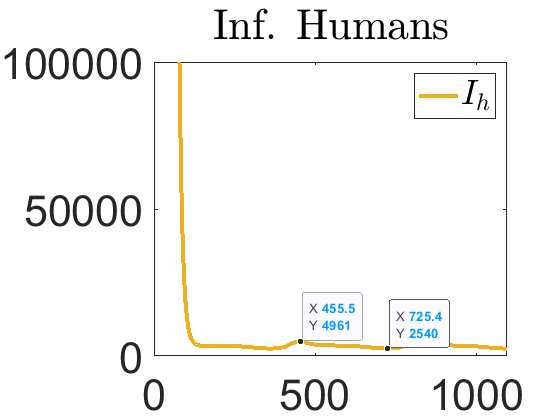
\includegraphics[scale=0.35]{nonaut6ahumans.png}
\end{subfigure}
\begin{subfigure}{.5\textwidth}
\centering
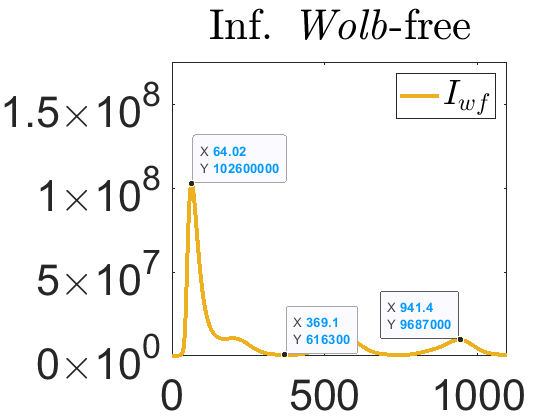
\includegraphics[scale=0.35]{nonaut6amosq.png}
\end{subfigure}
\caption{Endemic Zika in humans and wild mosquitoes when seasonality is included.}
\label{fig:nonaut6ahumansmosq}
\end{figure}
\end{comment}

\subsubsection{ Zika takes longer to be eradicated when \textit{Wolbachia} is established with seasonality}
Changing only the initial conditions from $A_{wf}(0)= 2,500,000$ to $A_{wf}(0)=500,000$ and $A_{wi}(0)=500,000$ to $A_{wi}(0)=1,500,000$ we see in Figure \ref{nonautonoum6b} that the \textit{Wolbachia} infected mosquitoes persist and the number of \textit{Wolbachia} infected susceptible females oscillates between 185 millions and 2.7 billions. Wild mosquitoes are eliminated in roughly one year. The disease is eradicated in humans in 400 days, compared to 300 days in the autonomous model Section \ref{dissecond}, and in 422 days in \textit{Wolbachia} infected mosquitoes as observed in Figure \ref{nonautonoum6b}. This suggests that when seasonality is included, it takes longer for Zika to be eradicated in both humans and mosquitoes.

%\begin{figure}[H]
    %\hskip-0.75in
%    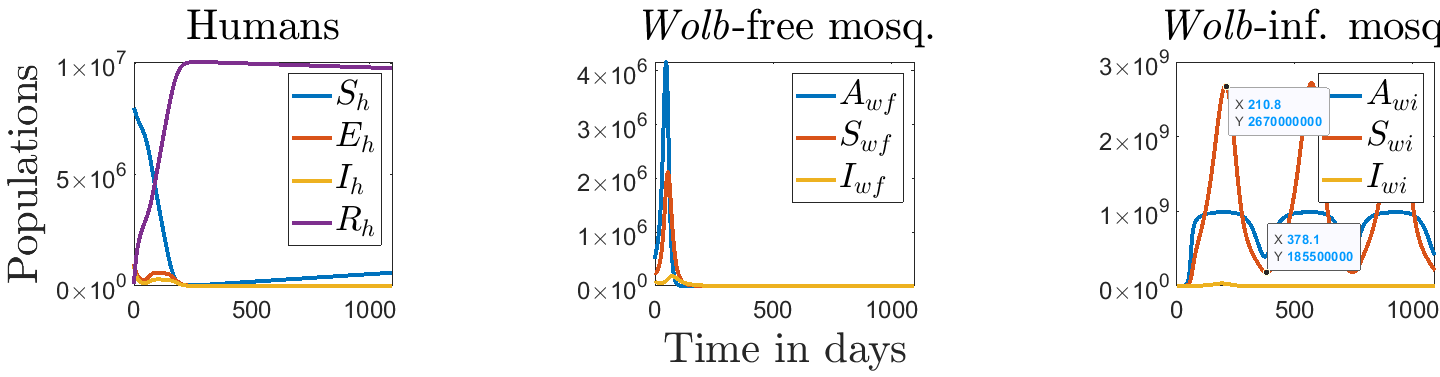
\includegraphics[width=\textwidth]{nonaut6bmainupdated.png}
%    \caption{\textit{Wolbachia} infected mosquitoes dominate and Zika takes longer to be eradicated under seasonality}
%    \label{nonautonoum6bmain}
%\end{figure}

\begin{figure}[H]
    \centering
    % This file was created by matlab2tikz.
%
%The latest updates can be retrieved from
%  http://www.mathworks.com/matlabcentral/fileexchange/22022-matlab2tikz-matlab2tikz
%where you can also make suggestions and rate matlab2tikz.
%
\definecolor{mycolor1}{rgb}{0.00000,0.44700,0.74100}%
\definecolor{mycolor2}{rgb}{0.85000,0.32500,0.09800}%
\definecolor{mycolor3}{rgb}{0.92900,0.69400,0.12500}%
\definecolor{mycolor4}{rgb}{0.49400,0.18400,0.55600}%
%
\begin{tikzpicture}

\begin{axis}[%
width=1.1in,
height=1.5in,
at={(0in,0.046in)},
scale only axis,
xmin=0,
xmax=1095,
ymin=0,
ymax=12000000,
ylabel style={font=\color{white!15!black}},
ylabel={Population},
axis background/.style={fill=white},
title style={font=\bfseries, yshift=1.75ex},
title={Humans},
legend style={legend cell align=left, align=left, draw=white!15!black}
]
\addplot [color=mycolor1, line width=1.5pt]
  table[row sep=crcr]{%
0	8000000\\
10.0197469554842	7654717.53136727\\
16.6913146097213	7464247.45551793\\
25.4146573124453	7251656.47605402\\
41.476538377814	6871465.16967628\\
47.1776461834088	6703751.29295385\\
53.1055087679997	6491027.96221469\\
59.1867785276845	6224966.25001359\\
66.7785295238718	5830823.23564623\\
78.1248450325802	5164662.26103283\\
106.010088063776	3514001.99931216\\
134.085691357963	1943225.49687882\\
146.764157766476	1292958.31121685\\
155.325468384661	913108.291748852\\
162.300785314292	655376.307056356\\
168.341775742359	475154.36083714\\
173.82033185102	346422.290264321\\
178.914474259131	254097.423820506\\
183.746353601106	187708.662267915\\
188.355886877514	140321.282043062\\
192.835096619092	106213.575448534\\
197.225370829925	81675.7372397427\\
201.527869115584	64140.6117283674\\
205.761269991286	51615.3431490501\\
209.942516097799	42675.9938008059\\
214.055446378887	36357.8794427346\\
218.069421230815	31961.0146709206\\
221.94952314347	28967.9327820763\\
225.639307288453	27006.5184440687\\
229.036316781305	25805.5324707897\\
232.01367086824	25143.8663205486\\
234.495250291191	24829.8145653568\\
236.382337043993	24718.6502403226\\
237.563942561857	24700.4856017102\\
238.095535336994	24704.5555281173\\
238.96677317936	24727.0562370354\\
240.363781145774	24802.6208945978\\
242.289457380772	24982.1954164533\\
244.867625931278	25349.7173439804\\
248.139679145068	26007.5286001815\\
252.205337597057	27093.003199487\\
257.116198326461	28754.7138783559\\
263.039354766719	31200.9533373415\\
270.164018780924	34678.1288508857\\
279.005718337372	39626.169645329\\
290.672636229545	46886.348167628\\
309.262874065898	59323.7742660763\\
365.253770497628	97998.5835926021\\
555.463987912983	229180.874563794\\
743.004899727181	357675.947953393\\
931.948561524041	486287.628255194\\
1095	596597.664768079\\
};
\addlegendentry{$S_h$}

\addplot [color=mycolor2, line width=1.5pt]
  table[row sep=crcr]{%
0	1000000\\
3.54464129474945	810965.782268328\\
7.7185012109112	652387.561346482\\
11.7222900261404	541128.185359541\\
16.6913146099541	439748.279775616\\
21.0657066360582	374534.280122382\\
25.4146573123289	326724.68397602\\
29.6123278539162	293940.426939444\\
32.6718788889702	277432.686015792\\
35.669119668426	266980.812409864\\
37.617091854685	263179.289153431\\
39.5650640408276	261746.739929738\\
40.5208012091462	261917.667665965\\
41.4765383774647	262669.739209217\\
43.3880127141019	265935.163182223\\
45.28282944893	271511.857154181\\
48.1369699477218	284316.489591212\\
51.0149412394967	302434.8881589\\
55.1960762967356	337021.196756912\\
61.7078415311407	403628.183720209\\
71.5460098766489	503449.581693115\\
76.7005437599728	542985.696883078\\
80.7661221467424	565499.265703465\\
84.3330768656451	579091.342570869\\
87.5048629490193	586887.167450014\\
90.1572782469448	590788.358088505\\
92.3879478387535	592546.596265478\\
94.0775882168673	593113.821588008\\
94.8891252644826	593186.459197132\\
95.4855309985578	593166.163656901\\
96.4542275379645	593012.119168588\\
97.9600488388678	592511.394874096\\
100.268725245143	591250.508381089\\
103.87864524615	588490.555348103\\
131.122062536771	564758.026886183\\
134.84713414975	559467.320202078\\
138.484328816645	552418.198410022\\
142.158415660029	542783.465891245\\
146.029573714361	529242.020536497\\
150.221351685934	509992.139441172\\
154.823033431894	482834.456027529\\
160.079396344838	444059.574959792\\
166.608528431389	386019.788733766\\
192.317907076562	146362.852995968\\
198.228219201555	108197.698981111\\
203.6235470135	80865.9649117138\\
208.751438659499	60816.4778117135\\
213.698931321851	46072.3272450319\\
218.527687478811	35195.8263588287\\
223.271846801392	27157.6021490726\\
228.000987422769	21143.8895219378\\
232.725321566686	16632.920363353\\
237.509008208057	13190.4525247152\\
242.415775277535	10514.0293861559\\
247.466490443796	8406.31122618797\\
252.699422013247	6713.2174748386\\
258.216266887379	5310.37411701004\\
264.066567047848	4128.95644270233\\
270.039567660308	3163.27159145649\\
276.008761923062	2387.75154896022\\
281.901832628297	1775.30271793169\\
287.577405201271	1307.99032337789\\
292.971370799001	959.584962989902\\
298.295126082725	693.56447832752\\
303.326094352175	501.65567761776\\
307.992125640274	366.152223133598\\
312.561887742253	265.552051851526\\
317.087474775151	190.9119756734\\
321.617167585297	135.700858305208\\
326.088425757363	95.9124459403101\\
330.228226991254	68.9879982381826\\
334.874677464948	47.2529982725391\\
339.122710688505	33.1925524539547\\
343.79054719361	22.3557494708803\\
347.998191500083	15.5655726233963\\
352.921551799634	10.1283368050354\\
358.548397824401	6.15444076748099\\
364.144015478203	3.72641607897822\\
371.711147148628	1.87535210396163\\
382.325701973401	0.707546816091053\\
401.319993272889	0.121777740889229\\
469.577561122831	0.000408986816182733\\
1095	0\\
};
\addlegendentry{$E_h$}

\addplot [color=mycolor3, line width=1.5pt]
  table[row sep=crcr]{%
0	900000\\
2.99548101518303	698496.026883981\\
6.45531167217996	537917.013274955\\
10.0197469554842	424447.275143504\\
13.593212338048	344255.445658597\\
17.7726351680467	277600.644233458\\
22.1715820910176	227914.152939638\\
26.4832571955631	192922.344747641\\
30.6425632415339	168517.281603894\\
34.6700394086074	151829.177227426\\
37.617091854685	143374.561522596\\
40.5208012091462	137922.881435577\\
42.4322755457833	135848.405955796\\
44.335421081516	134964.966154337\\
45.28282944893	134964.513474248\\
46.230237816344	135256.035444764\\
48.1369699477218	136727.224731405\\
50.0556174755329	139396.525378832\\
53.1055087681161	146040.847138027\\
56.5263103736797	156786.352538341\\
61.1124270679429	175713.101557184\\
69.4142261148663	216770.524150619\\
77.0566190781537	252206.912393027\\
82.0044190876652	269972.330296419\\
86.2182203195989	281071.343752039\\
89.9246927821077	287840.999244787\\
93.2434412982548	291791.743465115\\
96.0688302140916	293829.407403286\\
98.509653580375	294784.124818064\\
100.268725245143	295092.37427277\\
101.459107559291	295149.722290145\\
101.792624568101	295146.362778577\\
102.44854652707	295116.960596207\\
103.721484664944	294981.249246453\\
105.565179320169	294628.664674746\\
108.445678811404	293803.472438241\\
113.392450866406	291957.904259936\\
132.148925247835	284222.203778698\\
136.24621586781	281828.350235884\\
140.044075718382	278843.798297453\\
143.787252625101	274865.840445131\\
147.607005822589	269423.014678883\\
151.652107538539	261800.774489685\\
155.998611193965	251165.78463977\\
160.858531417791	236065.559591618\\
166.500600515981	214430.717894896\\
173.820331851137	181197.023619939\\
193.950019101263	87222.7735755871\\
200.428751573549	64049.919638147\\
206.178961150465	47669.4933041643\\
211.533231635811	35754.4636442579\\
216.646491068066	26992.3871113978\\
221.590004797559	20536.0278311907\\
226.436030474491	15746.2912895277\\
231.199819080764	12196.5287226952\\
235.94857310073	9531.17939875345\\
240.719741301262	7511.90582317044\\
245.560789335752	5960.92284040526\\
250.558555114432	4741.78411838296\\
255.712311938405	3775.88143774658\\
261.024994600681	3000.48189637763\\
266.631796675501	2355.32980550919\\
272.470599507331	1821.13947482489\\
278.393201793428	1387.86293957045\\
284.249162170803	1044.99320125848\\
289.846921492252	783.287274373462\\
295.396533666411	577.93689874385\\
300.742220829241	423.490344624617\\
305.682008914184	312.690957580111\\
310.629150935332	227.288637443678\\
315.54679238901	163.115680782939\\
320.415685253334	115.838849147782\\
324.76025582978	84.4220755550778\\
329.525319164735	59.0084503385006\\
334.061858098838	41.5381226621103\\
338.248579191393	29.8007566874148\\
342.842120941612	20.5321387549629\\
346.946280423435	14.6214950684225\\
351.690711724805	9.80551886814646\\
357.423028619378	5.9964405389037\\
364.144015478203	3.3321620663628\\
372.773867634824	1.54485921515152\\
384.438590671285	0.536136602517217\\
407.286048807437	0.0652105994522572\\
524.226830640226	3.46769811585546e-05\\
1095	0\\
};
\addlegendentry{$I_h$}

\addplot [color=mycolor4, line width=1.5pt]
  table[row sep=crcr]{%
0	100000\\
3.54464129544795	650268.995459113\\
7.71850121021271	1129361.0941006\\
12.6577511820942	1546614.85972152\\
17.7726351674646	1870692.8845459\\
23.2774575464427	2140720.64031342\\
29.6123278532177	2386097.37851097\\
36.6431057620794	2608034.30026246\\
49.0962937120348	2949664.00567943\\
57.8565444499254	3208008.15650025\\
64.4198129810393	3438429.34516067\\
71.1233425978571	3717064.96145769\\
79.1381369214505	4106472.13795089\\
89.6921073179692	4687038.92610564\\
153.988257307559	8340548.67875936\\
164.257780905813	8832923.38065618\\
172.289484679699	9162209.68109015\\
179.184500129893	9396928.69349749\\
185.395410181955	9568373.05209843\\
191.126965949312	9694281.45375201\\
196.546615820378	9787622.29811042\\
201.733706597239	9856805.49006774\\
206.763442235067	9908250.33953391\\
211.671707317233	9946452.45504872\\
216.50337523222	9974901.81108272\\
221.283234192058	9996096.71324443\\
226.022444127128	10011875.5231407\\
230.711111415178	10023583.7670999\\
235.373859345913	10032312.2289863\\
240.00604846701	10038803.0722843\\
244.619170963764	10043623.8602043\\
249.110498985276	10047105.5365345\\
253.497590517625	10049604.1637037\\
257.678755151108	10051322.6033023\\
261.572931325063	10052446.7768954\\
265.092522811145	10053130.6397963\\
268.125364948064	10053501.5943902\\
270.537372143939	10053668.7192102\\
272.358522156253	10053726.6128501\\
273.345401737839	10053735.0242699\\
273.806518146768	10053733.646942\\
274.642509767786	10053722.7743139\\
276.00876192376	10053682.5268492\\
277.868975710124	10053585.1063007\\
280.46506164968	10053372.7570791\\
283.665694123134	10052999.7078158\\
287.773079168051	10052362.4578885\\
292.734951173887	10051390.7655171\\
298.890566909686	10049937.5167533\\
306.834072032943	10047758.8478538\\
317.601035570726	10044446.785003\\
334.061858098954	10038971.211594\\
372.773867635056	10025565.5574536\\
586.208945060149	9951447.25694555\\
774.179666737095	9886622.78271289\\
963.002274993807	9821929.66484408\\
1095	9776957.06349101\\
};
\addlegendentry{$R_h$}

\end{axis}

\begin{axis}[%
width=1.1in,
height=1.5in,
at={(1.42in,0.046in)},
scale only axis,
xmin=0,
xmax=1095,
xlabel style={font=\color{white!15!black}},
xlabel={Time (days)},%{Time in days},
ymin=0,
ymax=4500000,
axis background/.style={fill=white},
title style={font=\bfseries, yshift=1.25ex},
title={\emph{Wolb}-free mosq.},
legend style={legend cell align=left, align=left, draw=white!15!black}
]
\addplot [color=mycolor1, line width=1.5pt]
  table[row sep=crcr]{%
0	500000\\
2.05150730069727	580521.407938897\\
5.82371690263972	668977.222195454\\
10.7868288704194	788550.744205204\\
14.528673493769	913119.716527998\\
17.7726351679303	1057459.23981678\\
21.0657066358253	1249182.60621185\\
25.4146573124453	1591836.14785234\\
29.612327854149	2041034.64825236\\
34.6700394088402	2743369.80206375\\
42.4322755457833	3888200.35936708\\
45.2828294490464	4126518.3362404\\
46.2302378164604	4159760.61515374\\
47.1776461838745	4166238.29969356\\
48.1369699477218	4144084.07153215\\
50.0556174754165	4010165.45361615\\
52.0602250038646	3750246.75482696\\
55.8611933351494	3015595.36721978\\
63.4057179656811	1482700.06839107\\
67.2215081905015	958821.671413099\\
70.7006753175519	632870.631839518\\
74.0088832094334	422711.130024761\\
77.4126943964511	277593.583493037\\
80.7661221465096	182790.141542437\\
84.0481421221048	121152.129392898\\
87.5048629492521	78411.031318903\\
90.841176090762	51451.78036599\\
94.2818332621828	33282.2163962298\\
97.58941551717	21876.4223370692\\
100.952751320321	14268.7913953285\\
104.344938649796	9267.84738903726\\
107.741583029274	6013.94341273746\\
111.127259699162	3906.8416572595\\
114.485011718702	2546.64391117264\\
117.800335090142	1668.87983439444\\
121.083733965643	1098.13977126544\\
124.404733284377	719.193440180272\\
127.763997884467	468.81166536035\\
131.122062536888	305.726502104197\\
134.474079501815	199.598250910174\\
137.810117571615	130.637322265189\\
141.173290950712	85.2555367639288\\
144.51399025647	55.8370319670066\\
147.920435524546	36.2970125661232\\
151.362510893494	23.513561474625\\
154.910268768203	15.050406797789\\
158.599421923049	9.47955694515258\\
162.659929236397	5.71303623216227\\
167.443914960138	3.1586054386571\\
173.687604012899	1.46970725990832\\
183.083764495794	0.476570129394531\\
202.24964767741	0.0563352438621223\\
321.617167585529	2.68639996647835e-06\\
1095	0\\
};
\addlegendentry{$A_{wi}$}

\addplot [color=mycolor2, line width=1.5pt]
  table[row sep=crcr]{%
0	250000\\
1.10753358667716	244860.434244457\\
2.05150730069727	243698.573529656\\
2.52349415794015	243953.901276302\\
3.54464129498228	245985.55669721\\
5.19212213344872	252566.070696876\\
7.71850121114403	268371.212192455\\
10.7868288704194	294936.158873216\\
14.528673493769	338200.027295324\\
18.8539557261392	406598.758710216\\
22.171582091134	476897.429964823\\
26.4832571954466	599808.258406598\\
30.6425632415339	762877.683417611\\
34.6700394088402	972367.067271343\\
39.565064040944	1297960.11376642\\
49.0962937115692	1972110.07233285\\
52.0602250038646	2089360.29384697\\
54.1507925326005	2120628.56220468\\
55.1960762967356	2119086.37372202\\
56.5263103735633	2101033.23299235\\
58.5216614892706	2042495.52335513\\
61.1124270679429	1919931.95247363\\
65.8526950064115	1614558.33570429\\
75.5717025171034	973644.856846015\\
80.7661221465096	711907.212317915\\
85.6906933588907	522962.629174626\\
90.3898637117818	388173.383230953\\
94.8891252647154	292050.546892494\\
99.3994617215358	220411.80230128\\
103.878645245917	167642.438878256\\
108.44567881152	127769.287425261\\
113.02183649363	98152.9379781415\\
117.690917923581	75695.2639995674\\
122.380806700327	58869.8439658992\\
127.144832929596	46049.8519623312\\
131.990599783137	36224.0761063406\\
136.875028871465	28715.5571435057\\
141.824759394396	22907.5456581428\\
146.88104110444	18356.1510142717\\
152.057221549563	14769.387353003\\
157.309448691085	11955.980232513\\
162.659929236397	9729.61482037138\\
168.093163706362	7964.32002461469\\
173.643820159137	6547.75230204687\\
179.357924419455	5395.14751970302\\
185.250669944566	4448.30637545278\\
191.39050342096	3655.01595669892\\
197.810551288538	2981.20012976509\\
204.532168474048	2402.44840893243\\
211.469787214883	1908.50208643777\\
218.494222209323	1493.23122514738\\
225.461421856191	1151.63217824604\\
232.212498996407	878.632862661965\\
238.67681751214	664.77485333709\\
244.867625931744	498.8942249557\\
250.765104557388	372.265814617276\\
256.409891049378	276.14066415187\\
261.794230919797	204.115289743058\\
267.028967380524	149.662367717363\\
272.120065673254	108.951807009056\\
276.945211005863	79.5000917087309\\
281.709214149043	57.4615784888156\\
286.323850858957	41.4329957766458\\
290.953085156623	29.4840530660003\\
295.725895547308	20.5056672287174\\
300.742220829241	13.8185095540248\\
306.065031538717	8.96504083462059\\
311.571844996419	5.64973265724257\\
318.154512699693	3.1977028278634\\
326.75251072133	1.48309205053374\\
339.122710688505	0.472102966159582\\
363.034260458779	0.0481776455417275\\
514.522661362309	2.18302011489868e-06\\
1095	0\\
};
\addlegendentry{$S_{wf}$}

\addplot [color=mycolor3, line width=1.5pt]
  table[row sep=crcr]{%
0	50000\\
2.05150730087189	58716.3827657877\\
4.09380157431588	63094.6614193359\\
5.82371690281434	64777.1433300714\\
7.08690644154558	65236.2637158164\\
7.7185012109403	65286.8177347044\\
8.48558312575915	65221.9594338277\\
10.0197469554259	64769.9640326902\\
12.6577511821233	63383.6630448313\\
19.9598311810405	59116.7938194107\\
22.1715820910176	58341.2300533771\\
24.3460574291821	57982.9338333124\\
25.414657312358	57975.4972070588\\
26.483257195534	58089.5409652091\\
28.5820924663567	58697.4508997563\\
30.6425632415921	59838.8479529812\\
33.6709591488179	62625.7201542936\\
36.6431057615555	66830.6024014633\\
39.5650640408567	72591.4589392293\\
43.3880127140437	82860.7426311207\\
48.1369699476927	100108.151344441\\
54.1507925324258	127438.153028291\\
61.7078415311698	161123.237325416\\
65.8526950064697	174145.243025069\\
68.5504441914381	179506.789226734\\
70.7006753176975	181913.163198786\\
72.3798504282895	182659.294357184\\
72.7910237005271	182695.267884135\\
73.2021969727648	182675.02693807\\
74.0088832094043	182475.282572605\\
75.1954221025226	181809.246903763\\
77.0566190781537	179927.787014581\\
79.4759008844267	176117.12463327\\
82.896108190791	168575.820909014\\
88.001328869781	154117.548715376\\
110.204862244515	87388.3528309137\\
116.917101851373	72420.4649671628\\
123.363451551733	60679.3170366538\\
129.725047440559	51255.7479443705\\
136.097825664503	43573.2758602473\\
142.646081041923	37129.6024806037\\
149.37706912632	31692.1128423441\\
156.410329412611	26987.0159057285\\
163.814552103868	22843.6322927353\\
171.660648488061	19131.1210470655\\
179.955928590003	15780.3258755109\\
188.574370833056	12788.0185498297\\
197.263205602736	10187.5289438732\\
205.818045625463	7984.94867850601\\
214.015553373174	6181.13159752209\\
221.761219459586	4738.17252321797\\
229.036316781101	3603.72835596089\\
235.836723157263	2726.46159659169\\
242.289457381092	2046.33568330936\\
248.361673090549	1529.76303980514\\
254.125373483432	1138.19527164567\\
259.67459761232	840.569148152019\\
264.988700082788	618.035818265489\\
270.164018781215	450.650973462005\\
275.103062171198	328.395657021232\\
279.913777130016	237.925067811855\\
284.660901697061	170.817359581939\\
289.317287724145	121.869404153782\\
293.710373049515	87.6414344961522\\
297.997405668983	62.8927169845265\\
302.161631971219	45.1476982695458\\
306.448054162989	31.8075571857044\\
310.629150935361	22.4147450718738\\
315.048076913808	15.3544749650755\\
319.814944087353	10.1180295427912\\
324.76025582978	6.50549659284297\\
330.228226991283	3.95457081688801\\
337.37444769431	2.03755780035863\\
346.946280423464	0.824360373371746\\
363.034260458691	0.176474425388733\\
411.780620935664	0.00209505759994499\\
1095	0\\
};
\addlegendentry{$I_{wf}$}

\end{axis}

\begin{axis}[%
width=1.1in,
height=1.5in,
at={(2.8in,0.046in)},
scale only axis,
xmin=0,
xmax=1095,
ymin=0,
ymax=3000000000,
axis background/.style={fill=white},
title style={font=\bfseries, yshift=1.25ex},
title={\emph{Wolb}-inf. mosq.},
legend style={legend cell align=left, align=left, draw=white!15!black}
]
\addplot [color=mycolor1, line width=1.5pt, forget plot]
  table[row sep=crcr]{%
0	1500000\\
1.57952046394348	1262175.78765345\\
2.99548101425171	1184628.59104574\\
4.09380161762238	1172415.82894647\\
4.64296185970306	1176857.17742848\\
5.82371687889099	1202671.00847292\\
7.71850121021271	1277675.45347548\\
10.7868288755417	1461457.86567724\\
13.5932123661041	1695250.98494053\\
16.6913145780563	2047673.38073754\\
19.959831237793	2576760.53894424\\
23.2774575948715	3368156.13240957\\
26.4832571744919	4513502.43160939\\
29.6123278141022	6216935.34580421\\
32.6718789339066	8804852.3958261\\
35.6691197156906	12808022.035453\\
38.5910779237747	19036790.2402203\\
41.4765384197235	28998142.7307004\\
44.3354210853577	45204346.7639569\\
47.1776461601257	71771138.9835722\\
50.0556174516678	115760586.885192\\
53.1055088043213	190686496.125168\\
56.5263103246689	317170010.667478\\
65.3897777795792	683627374.567206\\
68.5504442453384	755746699.812897\\
71.5460098981857	801321518.145528\\
75.5717024803162	842006746.613358\\
78.8003729581833	864777067.811351\\
88.0013288259506	905306802.850141\\
88.4977947473526	906179453.968889\\
89.9246927499771	911205443.17665\\
90.3898637294769	911838310.770159\\
91.7326304912567	916224630.529028\\
92.1727724075317	916698669.845895\\
93.4534085988998	920624311.492581\\
93.8733432292938	920934497.547653\\
95.0879272222519	924464847.948879\\
95.2867290973663	924500086.8513\\
95.4855309724808	924673193.812331\\
96.6451917886734	927880569.606739\\
96.8361560106277	927873176.090067\\
97.0271203517914	928004193.533459\\
97.4019837379456	929469155.88192\\
97.5894155502319	929431024.544417\\
97.776847243309	929535942.857198\\
98.1432504653931	930971122.777142\\
98.3264520168304	930909311.152264\\
98.5096535682678	930991637.931726\\
98.8670850992203	932383862.868676\\
99.0458009243011	932312099.284522\\
99.2245166301727	932380492.92527\\
99.5744067430496	933723078.454547\\
99.7493518590927	933646485.710733\\
99.9242968559265	933705809.991321\\
100.268725275993	935010381.068685\\
100.440939426422	934920861.725605\\
100.613153576851	934967847.08517\\
100.952751278877	936254088.327201\\
101.12255012989	936141039.233276\\
101.292349100113	936169431.967619\\
101.625866055489	937444972.703522\\
101.792624592781	937309189.85153\\
101.959383130074	937318423.705284\\
102.285492062569	938571315.032036\\
102.611600995064	938424312.28891\\
102.930801987648	939638804.742598\\
103.250002980232	939490079.319127\\
103.564324140549	940667909.693747\\
103.878645300865	940512040.057512\\
104.189507484436	941672559.003817\\
104.500369787216	941488085.516957\\
104.807117700577	942647700.809695\\
105.113865733147	942423062.724874\\
105.414741396904	943576902.684028\\
105.715617179871	943327414.065087\\
106.010088086128	944455086.558651\\
106.304558992386	944207294.882752\\
106.594182491302	945298723.620234\\
106.883805990219	945058188.170321\\
107.170593142509	946127280.781865\\
107.457380175591	945873180.683785\\
107.741582989693	946942988.06864\\
108.025785923004	946652717.021489\\
108.305714488029	947729610.438123\\
108.585643172264	947406653.391851\\
108.859829545021	948472011.374151\\
109.134015917778	948145773.562956\\
109.403151512146	949178377.040019\\
109.672287225723	948868606.395458\\
109.938574790955	949871565.727722\\
110.204862236977	949564692.107398\\
110.469557523727	950562781.370232\\
110.734252691269	950228747.747816\\
110.996257424355	951240812.259536\\
111.258262038231	950867482.0733\\
111.515504717827	951883829.344226\\
111.772747397423	951495224.207576\\
112.024799704552	952487798.429115\\
112.276852011681	952117198.324111\\
112.525588154793	953074417.480489\\
112.774324297905	952722555.316553\\
113.021836519241	953664049.161376\\
113.269348740578	953299722.64706\\
113.515552997589	954254375.636697\\
113.76175737381	953849688.36687\\
114.004511594772	954822505.005822\\
114.247265934944	954387063.568785\\
114.485011696815	955350964.226919\\
114.722757577896	954925387.731069\\
114.95651447773	955853586.19539\\
115.190271496773	955458445.389514\\
115.422547340393	956357957.537878\\
115.654823303223	955969436.670736\\
115.886745810509	956873202.336489\\
116.118668317795	956451621.338538\\
116.348650693893	957381586.844766\\
116.578633189201	956915735.443901\\
116.804278969765	957855385.295732\\
117.029924750328	957381803.165615\\
117.251004219055	958293626.203521\\
117.472083568573	957853635.628551\\
117.69091796875	958725914.47362\\
117.909752249718	958312950.477451\\
118.12857067585	959173997.54574\\
118.347389101982	958744196.583482\\
118.565720438957	959630420.754259\\
118.784051895142	959150546.113634\\
118.999237060547	960064306.393532\\
119.214422345161	959553477.054575\\
119.424855828285	960456280.571908\\
119.635289311409	959969721.198328\\
119.842447042465	960828918.646079\\
120.049604654312	960386362.30657\\
120.256388306618	961215676.51574\\
120.463171958923	960779713.853779\\
120.670551896095	961622901.862455\\
120.877931714058	961142717.126273\\
121.083733916283	962024882.058863\\
121.289536237717	961492109.998908\\
121.491017699242	962386762.152753\\
121.692499160767	961855328.247953\\
121.889737606049	962713214.006385\\
122.08697617054	962233112.730205\\
122.282863140106	963044305.386616\\
122.478750228882	962597742.941159\\
122.675667285919	963402602.715433\\
122.872584462166	962930198.042706\\
123.069570302963	963774214.888283\\
123.266556143761	963237392.975678\\
123.46034693718	964118082.255602\\
123.654137730598	963550154.347777\\
123.843141317368	964413653.523348\\
124.032145023346	963888329.7128\\
124.218439102173	964696209.989085\\
124.404733300209	964229152.119011\\
124.591686010361	965005455.546567\\
124.778638601303	964541426.862458\\
124.966989994049	965343630.394973\\
125.155341506004	964818964.140087\\
125.342193961143	965674908.308806\\
125.529046535492	965086848.846828\\
125.711295962334	965955611.091372\\
125.893545389175	965381947.500208\\
126.071716189384	966199984.293648\\
126.249886870384	965698979.17824\\
126.427570104599	966461119.837202\\
126.605253219604	965998314.095692\\
126.784968733788	966760956.05905\\
126.964684247971	966258270.100772\\
127.144832968712	967077529.443275\\
127.324981570244	966491226.340595\\
127.501592755318	967356437.908087\\
127.678203940392	966740653.543701\\
127.849791884422	967577501.868746\\
128.021379828453	967028732.896127\\
128.190794825554	967793929.938625\\
128.360209822655	967318423.195237\\
128.53134727478	968051011.59371\\
128.702484846115	967570816.41319\\
128.875740647316	968345230.849455\\
129.048996448517	967781925.605462\\
129.220577597618	968627757.23372\\
129.392158746719	967988218.194633\\
129.558603048325	968843936.945848\\
129.725047469139	968238457.398712\\
129.887506008148	969023681.395092\\
130.049964547157	968516545.610853\\
130.212865948677	969235298.487465\\
130.375767350197	968768388.734867\\
130.541725993156	969497759.884218\\
130.707684636116	968970958.08085\\
130.874268174171	969779267.438339\\
140.925879240036	974920598.163683\\
150.999992251396	980564261.452998\\
160.90663254261	982870165.799978\\
170.984843015671	984925773.14971\\
180.935240268707	986825334.716646\\
190.942078590393	987757294.305612\\
200.966497421265	988056190.208466\\
210.957747340202	987921366.542828\\
220.941026210785	986890974.072496\\
230.061258792877	984772834.27718\\
240.884325623512	980595316.155501\\
250.843704342842	975175271.876294\\
260.935704708099	965578012.803588\\
270.838202595711	952483829.807087\\
280.856359839439	932475467.769996\\
281.069573402405	932585174.165859\\
281.28278696537	932282903.104561\\
281.709214091301	930151959.308734\\
281.901832580566	930557874.237667\\
282.094451069832	930415830.483837\\
282.479688048363	928243256.503317\\
282.647393226624	928399841.012499\\
282.982803463936	927580139.064481\\
284.660901665688	923331803.428067\\
285.140006422997	922615050.328547\\
285.619111061096	920615125.729437\\
285.854024291039	920734951.181539\\
286.08893764019	920359962.802142\\
286.558764100075	917828125.956538\\
286.76450586319	917937829.887162\\
287.175989508629	916662190.126709\\
289.052470803261	911301375.155954\\
289.846921443939	909019927.044089\\
294.212955713272	894997283.734577\\
296.055257439613	889068643.967021\\
298.890566945076	878073231.32212\\
313.05690908432	811281040.997576\\
323.489082336426	744426642.052996\\
334.061858057976	659525845.752094\\
345.894369363785	551822165.656736\\
355.172290205956	472070284.140434\\
360.799136281013	433521854.571279\\
365.253770470619	410820913.706889\\
368.505976080894	399384791.404188\\
371.71114718914	393131442.680482\\
372.773867607117	392064264.037955\\
373.836588144302	391769048.05716\\
374.899308562279	392021698.449148\\
375.961532473564	392593918.065745\\
377.02375638485	393845763.216876\\
379.148204088211	398530054.875103\\
381.266535997391	405122070.687104\\
384.43859064579	419958240.423268\\
387.599758863449	440185807.094093\\
391.794495105743	474447720.210786\\
397.088686943054	527771740.867804\\
417.546848773956	746051645.241063\\
425.556699156761	805479404.538693\\
437.332916140556	864798590.120709\\
440.673251152039	877728671.388644\\
443.413646936417	887189372.986502\\
444.275470733643	889759948.634144\\
446.791924953461	897586008.767264\\
447.338054537773	898385684.950603\\
448.881877779961	903352143.471864\\
449.381192564964	904015623.642576\\
450.84086227417	908446345.64947\\
451.3255392313	909010717.587733\\
452.746336817741	913158424.923603\\
453.209102630615	913470685.095316\\
454.521290540695	917157031.380252\\
454.949694037437	917491661.755163\\
456.22753238678	920913926.1066\\
456.440488100052	920941068.087926\\
456.653443694115	921114507.21582\\
457.070451140404	922713786.12546\\
457.278954863548	922668303.356502\\
457.487458586693	922787810.702595\\
457.886619448662	924352614.62703\\
458.086199879646	924300591.920074\\
458.285780191422	924400587.037776\\
458.669427990913	925848806.869537\\
458.861251831055	925840449.765716\\
459.053075671196	925956792.978208\\
460.193140268326	928776639.118425\\
460.384052038193	928742006.498808\\
460.574963927269	928841993.740849\\
460.954641461372	930240254.347884\\
461.144480347633	930123984.641769\\
461.334319114685	930170756.463177\\
461.700713157654	931597129.56167\\
461.883910059929	931444431.827555\\
462.067107081413	931456816.185152\\
462.416820883751	932802932.821407\\
462.59167778492	932696473.820832\\
462.766534686089	932725279.32133\\
463.108138442039	933949176.596306\\
463.278940439224	933890889.063933\\
463.4497423172	933946342.898511\\
463.793907284737	935121292.515274\\
463.9659897089	935049465.65969\\
464.138072252274	935099552.56252\\
464.485421419144	936327475.246513\\
464.659096002579	936178610.498043\\
464.832770705223	936183060.037845\\
465.172816514969	937489323.461928\\
465.512862324715	937221244.151561\\
465.836911678314	938506279.038667\\
466.160960912704	938265629.526595\\
466.472977519035	939426164.260441\\
466.784994006157	939299032.656993\\
467.096845269203	940363832.292778\\
467.252770900726	940264084.177268\\
467.408696532249	940275645.795722\\
467.726712822914	941358999.044078\\
468.044729113579	941184110.202813\\
468.362028717995	942369401.506282\\
468.67932844162	942035053.253042\\
468.983752250671	943271079.545256\\
469.288176178932	942890956.266744\\
469.57756114006	944032478.308207\\
469.866946101189	943776806.281595\\
470.151612639427	944781877.885983\\
470.436279177666	944628303.154846\\
470.727147698402	945597360.507747\\
471.018016219139	945412485.548446\\
471.3140386343	946472230.744896\\
471.610061168671	946127916.140787\\
471.898704767227	947302475.972205\\
472.187348365784	946823012.979708\\
472.460057973862	947970000.051141\\
472.73276758194	947575303.02004\\
472.995523333549	948568425.543099\\
473.258279085159	948335266.642955\\
473.524320006371	949227731.601747\\
473.790360927582	949032982.423679\\
474.065284371376	949971566.964528\\
474.34020781517	949655404.166804\\
474.614742994308	950741478.428138\\
474.889278173447	950223497.8349\\
475.149974584579	951374610.097906\\
475.410670995712	950840698.166213\\
475.656891107559	951862821.962768\\
475.903111100197	951522910.146147\\
476.147372603416	952383289.055486\\
476.391634106636	952163464.544566\\
476.645337343216	953000481.715628\\
476.899040579796	952724796.210044\\
477.159218192101	953696823.506618\\
477.419395804405	953206700.298914\\
477.671029925346	954332798.102161\\
477.922663927078	953690959.182852\\
478.157475948334	954766821.522478\\
478.392287969589	954285652.721637\\
478.618738889694	955162899.466925\\
478.845189809799	954889734.220413\\
479.078187227249	955659684.086123\\
479.311184763908	955414020.69763\\
479.555495500565	956263603.605997\\
479.799806237221	955847360.997018\\
480.043260335922	956900334.26129\\
480.286714434624	956222871.34042\\
480.51443862915	957348188.67508\\
480.742162823677	956702167.773131\\
480.95551109314	957644178.857583\\
481.168859362602	957274498.418871\\
481.382927894592	958023772.573196\\
481.596996307373	957782626.541942\\
481.823712944984	958525449.350905\\
482.050429582596	958193593.653947\\
482.284487843513	959127622.38419\\
482.51854622364	958505495.872207\\
482.742007851601	959638645.265324\\
482.965469360352	958848805.267029\\
483.170672297478	959889703.350002\\
483.375875234604	959365535.477358\\
483.574250340462	960149848.485478\\
483.77262544632	959875769.743704\\
483.980919480324	960548552.297837\\
484.189213514328	960281591.299709\\
484.411122560501	961076672.75319\\
484.633031725883	960574348.176748\\
484.852895498276	961644033.695696\\
485.072759270668	960801032.86562\\
485.274307370186	961940584.822436\\
485.475855588913	961207578.050839\\
485.663009762764	962087622.233155\\
485.850163936615	961725322.263248\\
486.0408847332	962379983.549853\\
486.231605529785	962142945.256586\\
486.438271164894	962814361.922326\\
486.644936800003	962442701.467168\\
486.859393239021	963377671.07858\\
487.07384955883	962613304.567862\\
487.274871945381	963799235.796769\\
487.475894451141	962858684.546224\\
487.656957149506	963885586.055591\\
487.83801984787	963352913.970171\\
488.013949275017	964054448.197948\\
488.189878821373	963803246.635258\\
488.379296898842	964394022.95779\\
488.568714976311	964121671.280728\\
488.773935198784	964888282.99696\\
488.979155421257	964297949.97033\\
489.180442810059	965430238.918592\\
489.381730318069	964395388.988241\\
489.561647415161	965580033.814918\\
489.741564631462	964780926.170514\\
489.907182574272	965606580.800081\\
490.072800636292	965277894.187475\\
490.24506354332	965847965.791904\\
490.417326450348	965628365.787942\\
490.608884215355	966244828.97405\\
490.800441980362	965839563.120212\\
490.999799132347	966811759.177078\\
500.909247756004	973015761.124262\\
510.945683479309	977701224.003592\\
520.955879211426	981632211.92082\\
530.947696685791	985577572.164856\\
540.077594161034	986981348.440816\\
550.981776237488	988326744.169012\\
560.983073830605	988162060.937196\\
570.948552250862	988032881.234395\\
580.974391102791	986990561.153404\\
590.919917345047	985836986.839335\\
600.925184249878	982963233.680828\\
610.968291044235	978792085.745986\\
620.859162926674	971243779.864708\\
630.924149990082	960085923.979418\\
653.691794991493	913173196.549111\\
654.779029011726	910336301.17496\\
657.491844415665	901753099.210897\\
659.25432574749	896175438.097147\\
673.236207842827	838421617.176694\\
683.854232549667	778139859.039398\\
689.846546888351	736490017.122553\\
699.904161810875	654801838.701306\\
712.993661046028	535402347.6147\\
721.359090328217	465374535.042255\\
726.793222427368	429484636.971474\\
731.215074062347	408147225.827749\\
734.482280254364	397639175.404572\\
736.637811303139	393784500.409455\\
738.761498332024	391726870.001155\\
739.823341846466	391802806.367969\\
741.945042490959	393379024.519593\\
744.06475687027	397443461.513721\\
747.241680502892	407804159.771043\\
750.411893963814	423777167.549623\\
754.619725465775	453013350.789306\\
758.819394230843	490574087.342532\\
765.273099899292	560133164.872027\\
778.492003321648	706208893.468895\\
786.711299538612	776973075.22615\\
791.239190816879	807776235.752648\\
801.511434912682	860180680.783021\\
814.626098394394	904144181.917106\\
815.127876520157	905699008.904069\\
817.326371192932	911424937.859856\\
817.79232609272	911776126.816524\\
819.118205785751	915548498.499362\\
819.555420517921	915962629.741876\\
820.873937964439	919550569.185235\\
821.092868328094	919553880.525007\\
821.31179869175	919722119.51912\\
821.732643961906	921396921.82284\\
821.943066596985	921345154.343378\\
822.153489351273	921463068.637004\\
822.552304387093	923032842.139498\\
822.751711845398	923023084.579627\\
822.951119303703	923149438.300099\\
824.116245865822	926113672.875356\\
824.311329841614	926140759.114797\\
824.506413936615	926286325.815898\\
824.900817632675	927692250.429974\\
825.098019480705	927633069.799364\\
825.295221447945	927727273.92205\\
825.680800318718	929215415.444533\\
825.873589754105	929066216.071528\\
826.066379189491	929096064.604855\\
826.431648135185	930553621.235079\\
826.614282608032	930422616.223214\\
826.79691696167	930446352.874941\\
827.146371006966	931754560.156495\\
827.321097970009	931702874.380065\\
827.495825052261	931766696.847933\\
827.844413518906	932959772.650107\\
828.018707752228	932934182.354784\\
828.193002104759	933016223.786716\\
828.549268126488	934224510.602292\\
828.727401137352	934139049.01285\\
828.905534029007	934189481.171727\\
829.261410474777	935507981.085434\\
829.617286920547	935288960.18858\\
829.957385778427	936662454.082118\\
830.297484636307	936374490.625475\\
830.618538975716	937637101.579719\\
830.939593315125	937479441.592039\\
831.254162192345	938582677.640072\\
831.411446690559	938509499.460155\\
831.568731188774	938538462.779561\\
831.890688419342	939596531.589103\\
832.051667094231	939501581.146773\\
832.212645769119	939523643.309652\\
832.541363596916	940678977.207925\\
832.870081424713	940431418.418655\\
833.190225481987	941715002.833716\\
833.510369539261	941302311.278496\\
833.810881376266	942554738.949102\\
834.111393213272	942224640.953666\\
834.399170517921	943300065.343759\\
834.68694794178	943148793.846726\\
834.978282213211	944107149.069478\\
835.269616365433	944002966.033688\\
835.57196700573	945008342.529214\\
835.874317526817	944777497.153884\\
836.176821470261	945946177.196239\\
836.479325532913	945484058.487539\\
836.765236139297	946728708.557943\\
837.051146745682	946232241.562889\\
837.319115638733	947331009.000224\\
837.587084531784	947048158.916497\\
837.852126002312	947961756.170967\\
838.117167472839	947814843.537317\\
838.393518090248	948698098.415079\\
838.669868588448	948498144.803702\\
838.954615116119	949528037.889291\\
839.239361643791	949093344.930517\\
839.51432800293	950299041.268025\\
839.789294242859	949677590.351482\\
840.043867349625	950830277.835524\\
840.29844045639	950380200.232698\\
840.542414188385	951307294.219677\\
840.78638792038	951090836.07164\\
841.037842750549	951894295.649217\\
841.289297699928	951714567.17445\\
841.554658770561	952601210.644497\\
841.820019841194	952243170.781094\\
842.085083723068	953356964.800487\\
842.350147724152	952697921.50488\\
842.596570134163	953900174.288149\\
842.842992663383	953258626.663717\\
843.071807384491	954255448.589207\\
843.300622105598	953924135.266409\\
843.529739737511	954701792.005372\\
843.758857369423	954516537.143369\\
844.003031253815	955281710.497551\\
844.247205257416	955007968.254247\\
844.500854253769	955981151.246903\\
844.754503130913	955388525.200335\\
844.996086239815	956592130.61932\\
845.237669229507	955788060.952395\\
845.457346796989	956894204.894361\\
845.677024245262	956383304.075469\\
845.887996792793	957199017.213853\\
846.098969340324	956970044.062667\\
846.32132422924	957657216.455249\\
846.543679118156	957444045.507648\\
846.782628893852	958259103.043747\\
847.021578669548	957799782.887258\\
847.258951306343	958923149.193079\\
847.496323823929	958067502.195081\\
847.712175011635	959281505.985586\\
847.928026199341	958529297.80173\\
848.126371026039	959452778.06081\\
848.324715971947	959120627.807341\\
848.526641249657	959788550.525343\\
848.728566527367	959598614.164564\\
848.949298501015	960277533.24409\\
849.170030355453	959955189.733866\\
849.400840520859	960920235.287107\\
849.631650686264	960165222.698\\
849.847236275673	961424399.171842\\
850.062821984291	960437685.665245\\
850.254668474197	961527261.599177\\
850.446514964104	960998452.537305\\
850.631626009941	961720206.719508\\
850.816737055779	961508198.054652\\
860.775867938995	969605926.010577\\
860.926273584366	969460065.324919\\
870.901890397072	974440745.096594\\
880.125212430954	979459373.022772\\
880.240900754929	979806750.100069\\
};
\addplot [color=mycolor1, line width=1.5pt]
  table[row sep=crcr]{%
880.240900754929	979806750.100069\\
880.356589078903	979487578.338065\\
890.226906180382	983672821.175721\\
900.968563199043	985341202.328832\\
910.950656533241	987182483.593403\\
920.959587693214	988141116.556526\\
930.086251378059	987430023.561548\\
940.944739818573	987896768.058552\\
949.931285500526	986978412.924312\\
950.011425733566	987416127.864386\\
960.623544335365	984764187.0963\\
960.710391521454	985035935.224532\\
965.920436263084	983021908.120251\\
979.388542532921	976310764.509761\\
988.106885313988	968307068.461005\\
988.249747633934	969400378.107068\\
988.39260995388	968596485.811215\\
999.87551856041	954613200.090208\\
1000.00919795036	954633754.315629\\
1000.41023612022	953699022.0535\\
1000.55977582932	954079343.467449\\
1000.70931553841	954030665.416048\\
1001.00839495659	952335653.794527\\
1001.27702891827	953315749.171893\\
1001.54566276073	951228615.98416\\
1001.76931512356	951888796.365182\\
1001.99296760559	950974911.524918\\
1002.10301434994	951076089.505558\\
1002.32310807705	950735819.827402\\
1002.96378529072	949571700.080911\\
1003.12349617481	949667088.950197\\
1003.44291782379	948779085.314473\\
1003.60262870789	948235341.732525\\
1003.92100524902	948838839.409801\\
1004.23938190937	946641742.54065\\
1004.50760614872	947427256.114859\\
1004.77583038807	945913211.439265\\
1004.89573025703	946128398.888177\\
1005.01563024521	946106583.117688\\
1006.44837510586	943134554.672494\\
1006.63017201424	943391279.641874\\
1006.81196880341	943225172.899655\\
1007.17556250095	941321541.147404\\
1007.50265336037	941959077.238347\\
1007.82974433899	939858315.34895\\
1007.96893537045	940206229.502942\\
1008.1081264019	940198014.821263\\
1009.45151424408	937193250.462948\\
1010.41803395748	934758969.103318\\
1010.61500477791	935138524.655691\\
1010.81197571754	934969402.047763\\
1011.20591759682	932634345.077992\\
1011.374812603	933033805.531131\\
1011.54370760918	932964231.236252\\
1011.88149750233	931335833.297544\\
1012.03727889061	931356992.396254\\
1012.85561025143	929625260.394559\\
1014.06003332138	926380712.622996\\
1014.29055023193	926399950.136725\\
1014.75158393383	924734711.731971\\
1014.98210084438	923733210.020102\\
1015.19080162048	924007594.014914\\
1015.39950227737	923768879.637498\\
1015.81690371037	921535954.592649\\
1016.00120592117	921573188.75178\\
1016.369810462	920589221.768272\\
1018.49309635162	915100081.543612\\
1020.0491861105	910207639.220233\\
1021.43604707718	906104023.785061\\
1023.69268488884	899210260.758739\\
1026.93586611748	887741346.919688\\
1029.58502936363	878040588.761505\\
1043.94847869873	809875216.95946\\
1053.88806962967	745541394.277673\\
1059.16382491589	705408484.038446\\
1066.04772770405	647366430.866318\\
1089.25400149822	447126750.948626\\
1094.62888336182	416359727.44249\\
1095	414621790.770329\\
};
\addlegendentry{$A_{wi}$}

\addplot [color=mycolor2, line width=1.5pt]
  table[row sep=crcr]{%
0	250000\\
2.05150747299194	326296.592730045\\
5.19212198257446	390861.822710514\\
11.7222900390625	511279.246293545\\
15.6099939346313	614651.876629829\\
18.853955745697	735201.04551506\\
22.1715822219849	909036.81850481\\
25.4146571159363	1154862.07494402\\
28.5820922851562	1507932.55809498\\
31.6727986335754	2023683.662642\\
34.6700391769409	2785582.60423613\\
37.6170916557312	3944297.64870119\\
40.5208010673523	5739961.63338709\\
43.3880128860474	8576253.48900986\\
46.2302379608154	13145060.2380981\\
49.096293926239	20715536.4307914\\
52.0602250099182	33682092.8869228\\
55.1960763931274	56360885.0553384\\
57.8565444946289	85378077.9960909\\
61.7078413963318	144268961.592916\\
80.4435667991638	467410696.86617\\
89.4595217704773	585577145.226496\\
111.25826215744	863146932.356673\\
120.359780311584	998688598.348589\\
129.306368350983	1150932183.82015\\
138.417533397675	1328136389.87214\\
148.201482772827	1543869839.41536\\
159.861287593842	1829848422.91386\\
182.65442276001	2394774656.00404\\
189.351949691772	2526574981.02032\\
194.432603359222	2604244117.9572\\
198.506731033325	2649112283.84116\\
201.66081237793	2671723094.86684\\
204.025438785553	2681176141.56354\\
205.631362438202	2683766641.86012\\
206.140508651733	2683926539.64595\\
206.43243265152	2683873010.78936\\
207.05211019516	2683408988.85672\\
208.128180980682	2681454758.09037\\
209.648959159851	2676200821.68655\\
211.728109836578	2664245031.9975\\
214.344275474548	2641356709.21612\\
217.557904243469	2601403369.28627\\
221.476690292358	2535634120.86107\\
226.131494522095	2435022756.98132\\
231.873886108398	2282179458.02726\\
239.606025695801	2040462275.82144\\
264.72970867157	1230236178.27526\\
272.246444702148	1039404968.32395\\
279.148418426514	893895983.412263\\
285.854024410248	777957296.958952\\
292.262112140656	687374545.110637\\
298.890566825867	610540921.865883\\
305.682008743286	545594274.870531\\
313.05690908432	486610270.058108\\
321.617167472839	428259052.393695\\
332.493835926056	363326589.425035\\
345.894369125366	291209546.093691\\
355.172290325165	246997859.049793\\
361.924505233765	219996021.381601\\
367.434751033783	202773303.294242\\
371.71114730835	193051448.705484\\
374.899308681488	188148684.962146\\
377.023756504059	186130844.300032\\
379.148203849792	185076899.370028\\
380.207369804382	184977198.337666\\
381.266536235809	185134921.038831\\
382.325702190399	185540949.713485\\
384.438590526581	187221383.554419\\
386.546036243439	190010687.610363\\
389.697126865387	196362727.289704\\
392.846740245819	205301827.711743\\
397.088686943054	221430638.313044\\
402.295665740967	247157782.349509\\
408.805567741394	286726482.850701\\
419.234910488129	359860337.338883\\
438.354905605316	504453130.263285\\
450.356185436249	604647417.609065\\
459.432196140289	690480289.654572\\
468.203379154205	785350144.261521\\
476.518485546112	889013971.393553\\
484.742963790894	1007299958.21757\\
493.028668403625	1144603638.31587\\
501.538191318512	1306306120.49658\\
510.996388435364	1511148170.72809\\
521.772922992706	1773107180.28321\\
550.33936882019	2483160396.29669\\
556.314898967743	2592744189.06369\\
560.957599639893	2657272024.99412\\
564.641127586365	2693112673.09617\\
567.525684833527	2710623871.71765\\
569.60312795639	2717123520.44458\\
570.948552131653	2718502635.2299\\
571.089991569519	2718515438.82904\\
571.227959632874	2718503761.01693\\
571.692173480988	2718292006.23176\\
572.60585975647	2717076874.52372\\
574.058717250824	2712945422.34129\\
575.942252635956	2703545610.68344\\
578.357484340668	2684775389.9744\\
581.377846240997	2650740915.22232\\
585.010196208954	2594648763.18738\\
589.399343490601	2506084828.6009\\
594.708167552948	2372113357.94949\\
601.574380397797	2164945075.93363\\
613.537124156952	1758605617.19656\\
625.810145378113	1356889654.75845\\
633.782457828522	1133930230.14957\\
640.953360080719	966049818.962109\\
647.723456859589	835540881.747445\\
654.32021188736	731682979.080197\\
660.861716747284	647652177.432317\\
667.305126667023	579517870.304731\\
674.462269306183	516646816.315931\\
682.256427288055	459022340.222553\\
691.839124202728	397967896.22707\\
704.141370773315	328241575.808067\\
715.347157478333	270651677.097466\\
723.532742977142	234071674.297556\\
730.103398799896	210417774.398926\\
734.482280254364	198399130.068952\\
737.699654579163	191822023.455834\\
740.885185241699	187382316.145075\\
743.004899501801	185690449.535234\\
745.124614238739	184971545.212466\\
746.18314743042	185041934.94787\\
747.241680622101	185372341.215886\\
749.358747005463	186817813.022311\\
751.465041160583	189435149.133895\\
754.619725227356	195455146.833641\\
757.764895915985	204055244.414374\\
761.982890129089	219671775.538013\\
767.247858047485	245250144.127771\\
773.3940076828	282119713.204308\\
782.085321903229	342077666.465271\\
799.332624912262	470733125.405327\\
812.069930553436	573396353.430717\\
821.732644081116	660876806.657279\\
830.779066085815	754421124.90377\\
839.239361763	855250848.237887\\
847.258951187134	965332262.475764\\
855.74399805069	1099678882.31769\\
864.285512924194	1255510686.40837\\
873.291364192963	1443242180.13967\\
883.645044326782	1686963330.42964\\
899.413665771484	2093914988.39087\\
911.783387184143	2399943894.28253\\
918.711610794067	2542794489.28041\\
923.957697868347	2627807360.84221\\
928.14875459671	2677470851.02226\\
931.383763313293	2703067482.2534\\
933.873320102692	2714551298.74028\\
935.6089220047	2718124276.9888\\
936.408020973206	2718516201.20153\\
936.649128437042	2718476145.28625\\
937.26850271225	2718037332.36264\\
938.346930980682	2716110520.44695\\
939.89293718338	2710751410.93316\\
941.959294319153	2698772232.21943\\
944.54150056839	2676038727.03881\\
947.725791454315	2636250776.63184\\
951.539521694183	2572082637.30938\\
956.15998840332	2471992006.58522\\
961.939441204071	2317206746.34902\\
969.526615619659	2077821645.20757\\
995.404317855835	1232255389.9614\\
1002.83112764359	1042281044.88381\\
1009.61996650696	897928386.509786\\
1016.18550825119	783130687.644775\\
1022.59961795807	691323751.378472\\
1029.24676179886	613452343.130779\\
1035.99392986298	548331674.501108\\
1043.48014163971	488025268.449091\\
1051.48643255234	433002104.346622\\
1061.3632478714	373233023.839098\\
1074.1306681633	303382898.844042\\
1084.71936178207	251666767.088388\\
1091.35447216034	224289729.344937\\
1095	211666039.072242\\
};
\addlegendentry{$S_{wi}$}

\addplot [color=mycolor3, line width=1.5pt]
  table[row sep=crcr]{%
0	0\\
3.5446412935853	1371.51261202246\\
6.45531167089939	2076.69494196773\\
9.2526650428772	2472.21377775073\\
11.7222900241613	2675.92790519446\\
14.528673492372	2814.67341748625\\
23.2774575427175	3147.16149693727\\
26.4832571968436	3379.77172726393\\
29.6123278513551	3743.42759010941\\
32.6718788892031	4302.13377816975\\
35.6691196709871	5153.09625470638\\
38.5910779461265	6442.84885143489\\
41.47653837502	8448.48611289263\\
44.3354210779071	11647.7256805897\\
47.1776461824775	16898.6695092618\\
50.0556174740195	25933.9259599373\\
52.0602250024676	35926.293936789\\
54.1507925316691	51436.0020735413\\
56.5263103768229	78536.9127367362\\
59.1867785304785	126643.303963184\\
61.7078415304422	196337.996264234\\
64.9268604889512	328759.505121537\\
68.5504441931844	543424.005699746\\
72.7910237014294	882254.012706853\\
77.768769711256	1387021.21490118\\
84.0481421202421	2156182.33066802\\
92.1727724522352	3314107.06013957\\
101.292349055409	4792330.88306393\\
109.805430978537	6370402.50915131\\
117.361543878913	8000744.07967711\\
124.404733285308	9790421.06067762\\
131.284484006464	11858871.9531149\\
138.350737795234	14367848.1122407\\
146.029573716223	17555075.5386214\\
155.704771898687	22131336.1696923\\
171.577745616436	29665693.9332979\\
177.34076166153	31797507.2833042\\
181.732630111277	33007023.2334688\\
185.192773848772	33655391.1506867\\
187.856568783522	33954019.9226078\\
189.780277736485	34056279.3011794\\
190.838802181184	34071216.8944675\\
190.942078620195	34071093.6961454\\
191.322390340269	34068212.8345396\\
192.093195185065	34050654.0511287\\
193.347520492971	33988518.4339958\\
195.1280304268	33829138.6288299\\
197.441969573498	33498622.4529504\\
200.361693955958	32887965.445682\\
203.946648590267	31858539.5474018\\
208.344819128513	30215091.8394492\\
213.895874351263	27642887.9586225\\
221.552233353257	23465302.908119\\
243.928185544908	10920204.292541\\
251.000903844833	7810112.73601153\\
257.194779537618	5603935.97266796\\
262.845910660923	4010644.38203735\\
268.125364944339	2854978.97204193\\
273.067460753024	2027987.68997539\\
277.685165435076	1443199.3589873\\
282.2870695889	1008415.95001208\\
286.764505900443	698643.73130548\\
290.953085154295	487867.979655638\\
295.100639171898	336962.305666082\\
299.188287325203	230837.620451003\\
302.937940225005	161334.665793702\\
306.834072031081	109997.344250873\\
310.629150934517	74995.1138967946\\
314.549361437559	50007.7135284245\\
318.154512703419	34177.7018075436\\
321.617167584598	23558.2915163487\\
325.424340792	15544.1695122421\\
328.822411336005	10668.6228224114\\
332.493835799396	7069.41537460685\\
335.687496833503	4924.63564798981\\
339.122710689902	3327.7218240425\\
342.842120938003	2170.56097365171\\
345.894369348884	1525.8984349668\\
349.229031577706	1037.02338422835\\
352.921551801264	675.641871675849\\
356.297659412026	456.554427333176\\
359.673767030239	308.66329395026\\
363.034260459244	209.300256170332\\
366.363525517285	142.685584045947\\
369.577201373875	98.7953256890178\\
372.773867636919	68.7369086295366\\
375.961532473564	48.0438909903169\\
379.14820408076	33.7276793494821\\
382.325701974332	23.8196465745568\\
386.546036139131	15.1450901627541\\
390.745811074972	9.76790396124125\\
394.951230555773	6.3843701556325\\
400.344320572913	3.78691527247429\\
407.286048807204	2.015858694911\\
417.546848781407	0.867154590785503\\
437.332916125655	0.221591271460056\\
499.027953006327	0.0190794989466667\\
1095	0\\
};
\addlegendentry{$I_{wi}$}

\end{axis}
\end{tikzpicture}%
    \makebox[0pt][l]{% This file was created by matlab2tikz.
%
%The latest updates can be retrieved from
%  http://www.mathworks.com/matlabcentral/fileexchange/22022-matlab2tikz-matlab2tikz
%where you can also make suggestions and rate matlab2tikz.
%
\definecolor{mycolor1}{rgb}{0.92900,0.69400,0.12500}%
%
\begin{tikzpicture}
\useasboundingbox (7.7,-0.2) -- (7.7,-0.2);
\begin{axis}[%
width=0.7in,
height=0.5in,
at={(1.6in,0.642in)},
scale only axis,
xmin=0,
xmax=1095,
ymin=0,
ymax=350000,
axis background/.style={fill=white},
title style={font=\bfseries},
title={},
legend style={legend cell align=left, align=left, draw=white!15!black},
yticklabels=\empty,
scaled y ticks=false,%https://tex.stackexchange.com/questions/299298/placement-of-the-scale-tick-label-in-pgfplots
xticklabels={,,}
]
\addplot [color=mycolor1, line width=1.5pt]
  table[row sep=crcr]{%
12.6577511820942	362761.525752183\\
14.5286734939436	327220.649114535\\
16.6913146100123	292682.830871525\\
18.853955726081	263770.852649701\\
21.065706636	238870.641630009\\
23.2774575459771	217833.772767409\\
25.4146573123871	200569.355252164\\
27.551857078739	185872.246468233\\
29.6123278539744	173829.933718006\\
31.6727986292099	163646.92363193\\
33.670959148847	155394.664972514\\
35.669119668426	148623.028708942\\
37.6170918546268	143374.561522596\\
39.5650640408276	139408.36584683\\
41.4765383774647	136736.791542986\\
42.4322755457251	135848.405955796\\
43.3880127140437	135257.354090167\\
44.3354210814578	134964.966154337\\
45.28282944893	134964.513474248\\
46.230237816344	135256.035444764\\
47.177646183758	135839.502717419\\
48.1369699477218	136727.224731405\\
49.0962937116274	137913.331717356\\
51.0149412394967	141173.547830535\\
53.1055087681161	146040.847138027\\
55.1960762967356	152221.021225308\\
57.8565444507403	161804.164079127\\
61.1124270679429	175713.101557184\\
65.3897777479142	196409.128034608\\
74.4043961737771	240788.610266229\\
78.124845032522	256455.316939046\\
81.0756963819731	267020.25012624\\
83.7632073786808	275061.160419188\\
86.2182203195989	281071.343752039\\
88.4977947905427	285548.863866867\\
90.6155199010973	288817.153386524\\
92.6031232282403	291169.713113404\\
94.2818332622992	292669.626769595\\
95.8743971422664	293723.426349098\\
97.4019837760716	294433.485103149\\
98.6883693503332	294828.797274279\\
99.7493518437841	295030.757026467\\
100.613153585349	295120.603103978\\
101.292349054886	295148.336205796\\
101.459107559233	295149.722290145\\
101.625866063638	295149.051304833\\
101.959383072448	295141.695892693\\
102.44854652707	295116.960596207\\
103.250002921443	295042.884031484\\
104.189507515111	294907.827027745\\
105.565179320169	294628.664674746\\
107.313986653578	294159.975591641\\
109.672287224152	293381.074673292\\
113.145592599467	292056.334780731\\
130.049964489241	285230.115681598\\
132.947439783311	283806.106704724\\
135.499071423255	282318.325400894\\
137.880096715526	280653.59020495\\
140.248773584957	278655.727237489\\
142.586646452954	276273.037868744\\
144.959370392142	273358.956348371\\
147.378293479444	269793.939040769\\
149.914990045654	265328.03736175\\
152.524764442467	259876.996993346\\
155.266245385923	253145.128290975\\
158.184077895305	244797.7331299\\
161.360612809309	234312.704586789\\
164.853020396433	221171.214681178\\
168.880884738173	204150.659224222\\
173.909275835496	180768.610868012\\
191.294472570706	98104.9466193201\\
195.607700321532	80824.0258347755\\
199.477283280226	67139.8424480545\\
203.074439504999	56029.3660814619\\
206.487678488716	46898.5222958789\\
209.75591061532	39376.3435369182\\
212.910004979291	33161.9328685463\\
215.981047443405	28003.5013117066\\
218.992455836909	23706.7497793902\\
221.981363328232	20097.4985583728\\
224.904419816798	17116.8829719052\\
227.82184940693	14608.2777660313\\
230.711111415119	12516.1594770419\\
233.59928198182	10755.6222165211\\
236.480185459775	9277.05098497955\\
239.382120642171	8022.20063316484\\
242.289457381063	6961.40614467568\\
245.226205110783	6055.01207286929\\
248.213677126914	5273.1428449268\\
251.242179145862	4598.77011063858\\
254.390136364033	4000.65872648929\\
257.580707056215	3481.43061297934\\
260.846414865751	3023.64978619054\\
264.175940499699	2619.53140199848\\
267.619989200321	2256.16725128517\\
271.139032942243	1932.60661245597\\
274.796027235803	1639.44117681606\\
278.393201793428	1387.86293957051\\
281.901832628297	1173.26460343704\\
285.379558724642	987.295796406281\\
288.830459905439	826.48091464286\\
292.262111923483	687.794399335457\\
295.39653366647	577.936898743908\\
298.592846496496	480.924295739154\\
301.773477844254	398.00984296255\\
304.915963665466	328.079387644364\\
307.992125640274	269.922016896482\\
311.100497965876	220.312515688129\\
314.050645963347	180.712627519446\\
317.08747477521	146.585237394844\\
319.814944087353	120.922121237905\\
322.853495520947	97.1166171259829\\
325.424340793572	80.3665302569862\\
328.119503511582	65.6613553265925\\
330.983429926622	52.7666166173876\\
334.061858098779	41.5381226621103\\
336.500316197227	34.2643424017006\\
339.122710688505	27.7789995889761\\
341.893694689614	22.1885195059585\\
344.842458270257	17.4138881233521\\
347.998191500083	13.3904401491745\\
350.459871649859	10.8838375099003\\
354.046921004599	8.01997485593893\\
357.423028619436	5.99644053896191\\
360.799136234273	4.46999507094733\\
365.253770497628	3.02106133376947\\
370.648426662374	1.86930216458859\\
377.023756342358	1.0528981416137\\
385.492313403811	0.486848595668562\\
398.173898134381	0.151474105601665\\
426.038520746573	0.011642632947769\\
664.137374134501	2.71463068202138e-06\\
1095	0\\
};
%\addlegendentry{$I_h$}

\end{axis}
\end{tikzpicture}%}%
    \makebox[0pt][l]{% This file was created by matlab2tikz.
%
%The latest updates can be retrieved from
%  http://www.mathworks.com/matlabcentral/fileexchange/22022-matlab2tikz-matlab2tikz
%where you can also make suggestions and rate matlab2tikz.
%
\definecolor{mycolor1}{rgb}{0.92900,0.69400,0.12500}%
%
\begin{tikzpicture}
\useasboundingbox (-0.25,-0.6) -- (-0.25,-0.6);
\begin{axis}[%
width=0.5in,
height=0.5in,
at={(1.412in,0.642in)},
scale only axis,
xmin=0,
xmax=1095,
ymin=0,
ymax=40000000,
axis background/.style={fill=white},
title style={font=\bfseries},
title={},%{Inf. \emph{Wolb}-inf.},
legend style={legend cell align=left, align=left, draw=white!15!black},
yticklabels=\empty,
scaled y ticks=false,%https://tex.stackexchange.com/questions/299298/placement-of-the-scale-tick-label-in-pgfplots
xticklabels={,,}
]
\addplot [color=mycolor1, line width=1.5pt]
  table[row sep=crcr]{%
0	0\\
2.52349416166544	1032.34250655025\\
4.09380157291889	1533.00704500824\\
5.82371690124273	1953.34631364793\\
7.71850121021271	2282.74631396681\\
9.2526650428772	2472.21377775073\\
10.7868288680911	2610.60391909629\\
12.6577511802316	2730.17342738062\\
14.528673492372	2814.67341748625\\
16.6913146078587	2889.57654690742\\
19.9598311781883	2996.91681529582\\
22.1715820878744	3089.34986039251\\
24.3460574299097	3212.47217105329\\
26.4832571968436	3379.77172726393\\
28.5820924639702	3604.83193291724\\
30.64256323874	3904.8506757319\\
32.6718788892031	4302.13377816975\\
34.6700394079089	4826.79074251652\\
36.6431057602167	5520.76361291111\\
38.5910779461265	6442.84885143489\\
40.5208012089133	7678.80133281648\\
42.4322755485773	9351.15966244787\\
44.3354210779071	11647.7256805897\\
46.2302378192544	14840.3725802898\\
48.1369699463248	19382.6070629731\\
50.0556174740195	25933.9259599373\\
52.0602250024676	35926.293936789\\
54.1507925316691	51436.0020735413\\
55.8611933365464	69690.6899178699\\
57.1914274096489	88528.5049789175\\
58.521661490202	112458.619696401\\
59.8518955633044	142460.688099988\\
61.7078415304422	196337.996264234\\
63.4057179689407	259610.866110206\\
65.3897777497768	352243.362130314\\
67.6644868552685	484409.203083463\\
70.2780080363154	670442.063981026\\
73.202196970582	919815.815794587\\
76.3242633491755	1229802.16365562\\
80.121011517942	1659825.49840426\\
84.333076864481	2193981.55386748\\
89.2190900892019	2875011.4047718\\
94.6903233528137	3703515.07982457\\
100.440939418972	4646078.22177651\\
105.862852625549	5611249.99326842\\
110.86525503546	6584123.50865277\\
115.538685329258	7583146.7135331\\
120.049604691565	8648934.0509985\\
124.404733285308	9790421.06067762\\
128.702484831214	11041604.3769605\\
133.023983843625	12438839.0063959\\
137.450740426779	14025499.6263108\\
142.092776469886	15862680.8278479\\
147.128715701401	18047991.6357499\\
153.08989790082	20850616.9715028\\
170.881798602641	29374417.2970012\\
174.646266900003	30868408.2233323\\
177.798029646277	31941909.063556\\
180.486219987273	32705468.5254778\\
182.796307742596	33236523.3388603\\
184.799638420343	33596238.2563553\\
186.495762094855	33823924.3790268\\
187.942960247397	33960674.4297607\\
189.114851005375	34031824.0482176\\
190.008750557899	34061998.1726945\\
190.64065054059	34070665.5332641\\
190.838802181184	34071216.8944675\\
190.907653138041	34071166.0317694\\
191.099048182368	34070367.4288245\\
191.458616502583	34066251.7931709\\
192.001360550523	34053569.9996734\\
192.732758723199	34024164.8613905\\
193.673438034952	33965576.2164326\\
194.819640234113	33862698.4622425\\
196.211534544826	33691586.4251655\\
197.810551285744	33433291.3720163\\
199.670159459114	33051655.2802684\\
201.770807750523	32518875.4817301\\
204.174452096224	31783280.6855815\\
206.905268147588	30795702.9839503\\
210.01590936631	29493381.2009073\\
213.670391574502	27756420.3795401\\
218.10966207087	25410278.119885\\
224.294621556997	21868113.7515188\\
237.897814668715	14015828.6434108\\
243.101987682283	11322141.7833828\\
247.566341996193	9244084.53825708\\
251.645401611924	7557653.16972557\\
255.367614068091	6203751.43121047\\
258.873910591006	5089788.78473672\\
262.271935924888	4154993.43587998\\
265.530487082899	3385229.40515728\\
268.693010546267	2748207.79560193\\
271.740928277373	2227989.64147823\\
274.642509765923	1809832.09847721\\
277.501355156302	1463425.74292326\\
280.26941254735	1182840.19446947\\
282.982803434134	953630.005393289\\
285.619111068547	768703.134809285\\
288.164427101612	620666.37630707\\
290.67263623327	499973.027722441\\
293.20779042691	399661.092019387\\
295.725895546377	318291.162064217\\
298.295126080513	251006.574875683\\
300.742220826447	199243.826303333\\
302.937940225005	161334.665793702\\
305.298986293375	128078.261270933\\
307.606107771397	101830.419501185\\
309.686456874013	82553.5962708294\\
312.066866368055	64708.4949929342\\
314.549361437559	50007.7135284245\\
316.57391397655	40420.3278131559\\
318.707989826798	32217.5422442555\\
321.016426421702	25140.1396158934\\
323.489082291722	19218.3754891232\\
325.424340792	15544.1695122421\\
327.416595682502	12473.1999311224\\
329.525319166481	9863.97929557413\\
331.73863286525	7696.8033695966\\
334.061858095229	5921.87433457375\\
336.50031619519	4489.66548407823\\
338.248579189181	3677.72057889402\\
339.996842183173	3010.52786788344\\
341.89369469136	2421.00362433493\\
343.790547192097	1945.74250912666\\
345.894369348884	1525.8984349668\\
347.99819149822	1196.105787009\\
350.459871649742	899.016830615699\\
352.921551801264	675.641871675849\\
355.172290205956	520.245741419494\\
357.423028618097	400.684844352305\\
359.673767030239	308.66329395026\\
361.924505442381	237.920104771852\\
364.144015476108	184.159979581833\\
366.363525517285	142.685584045947\\
368.505976088345	111.638604529202\\
370.648426659405	87.4580185264349\\
372.773867636919	68.7369086295366\\
374.899308606982	54.112028516829\\
377.023756340146	42.676669664681\\
379.14820408076	33.7276793494821\\
381.266536004841	26.7309806123376\\
383.384867936373	21.2390919700265\\
385.492313407362	16.939774915576\\
387.5997588709	13.5508118271828\\
389.697127006948	10.8848672434688\\
391.794495150447	8.77316109091043\\
394.951230555773	6.3843701556325\\
398.173898130655	4.65739578008652\\
402.295665971935	3.15638784319162\\
406.526289448142	2.1547672227025\\
412.508388280869	1.29533239454031\\
420.343886360526	0.701115563511848\\
432.514075011015	0.300337925553322\\
456.227532424033	0.0787836462259293\\
536.399553768337	0.0132929533720016\\
1095	0\\
};
%\addlegendentry{$I_{wi}$}

\end{axis}
\end{tikzpicture}%}%
    \caption{\textit{Wolbachia} infected mosquitoes dominate and Zika takes longer to be eradicated under seasonality.  Zika eradicated in humans in approximately 400 days when seasonality is included compared to 300 days in the autonomous model. Zika takes around 422 days to be eradicated in \textit{Wolbachia} infected mosquitoes under seasonality.}
    \label{nonautonoum6b}
\end{figure}

However, the number of Zika infected humans first decline, and the reach a peak of around 300,000 infected in 100 days. This value is 3 times less than in the case where seasonality was not considered. Also, the number of total Zika infected \textit{Wolbachia} mosquitoes reaches a peak of 34 millions, compared to 14 millions. Therefore, even though the disease takes longer to be eliminated and there are more \textit{Wolbachia} infected mosquitoes, the number of Zika infected humans is much lower in the case where seasonality is considered. 
%\begin{figure}[H]
%\begin{subfigure}{.5\textwidth}
%\centering
%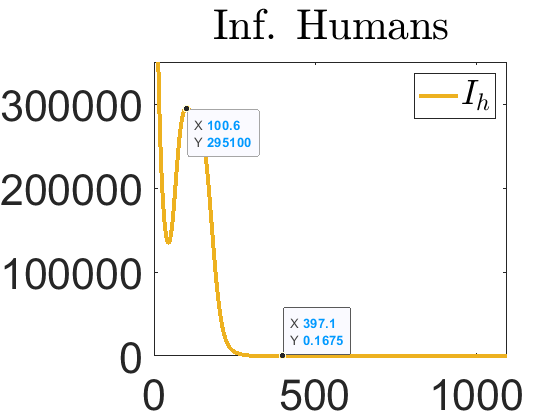
\includegraphics[scale=0.35]{nonaut6bhumans.png}
%\end{subfigure}
%\begin{subfigure}{.5\textwidth}
%\centering
%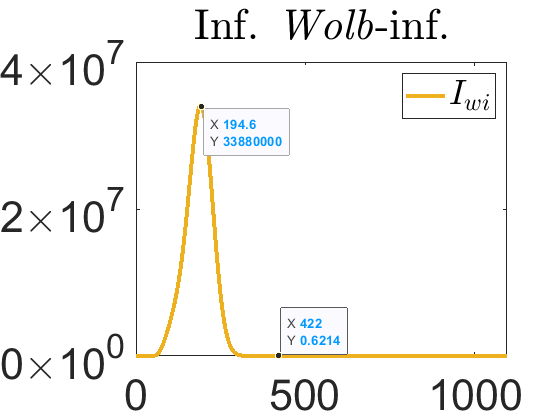
\includegraphics[scale=0.35]{nonaut6bmosq.png}
%\end{subfigure}
%\caption{Zika eradicated in humans in approximately 400 days when seasonality is included compared to 300 days in the autonomous model. Zika takes around 422 days to be eradicated in \textit{Wolbachia} infected mosquitoes under seasonality.}
%\label{fig:nonautinf}
%\end{figure}

\subsubsection{The peak of Zika is smaller when seasonality is included and \textit{Wolbachia} infected vectors are more competent}
Next, we investigate the case where the \textit{Wolbachia} infected mosquitoes are less capable of blocking the virus.  Increasing the competence of \textit{Wolbachia} infected mosquitoes allows for the disease to persist even when \textit{Wolbachia} infected mosquitoes dominate as seen in Figure \ref{fig:newfig6c}. When seasonality is taken into account, we see that the number of Zika infected humans reaches a peak of 1.3 million compared to 1.8 million in the autonomous model. Wild mosquitoes are eliminated in approximately one year and \textit{Wolbachia} infected susceptible females oscillate between 188 millions and 2.7 billions. 

%\begin{comment}


%\begin{figure}[H]
    %\hskip-0.75in
 %   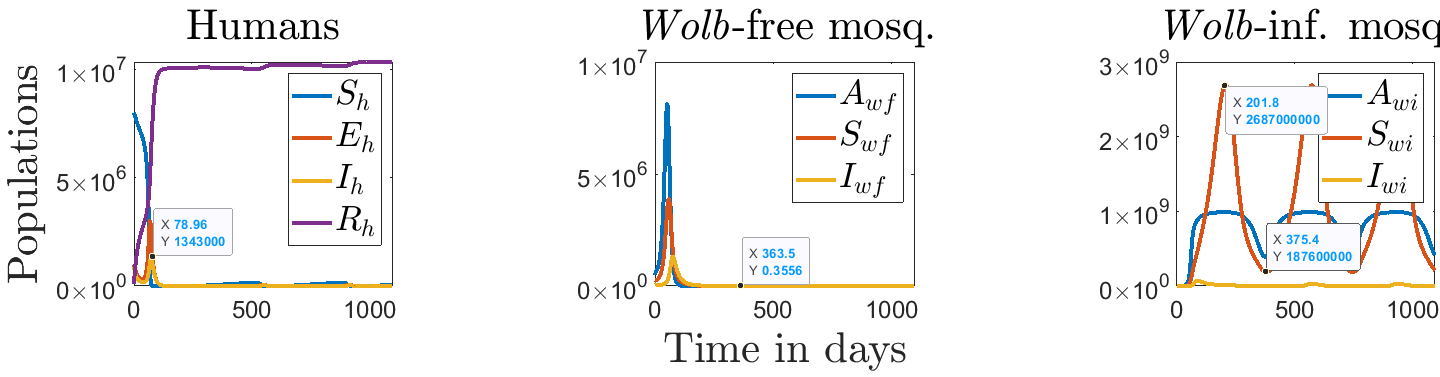
\includegraphics[width=\textwidth]{nonaut6cmainupdated.png}
 %   \caption{\textit{Wolbachia} infected mosquitoes dominate and Zika is eradicated. Zika infected humans reach a peak of 1.3 million compared to 1.8 million in the autonomous model.}
 %   \label{fig:nonautonoum6cmain}
%\end{figure}
%\begin{figure}[H]
%%\begin{subfigure}{.5\textwidth}
%\centering
%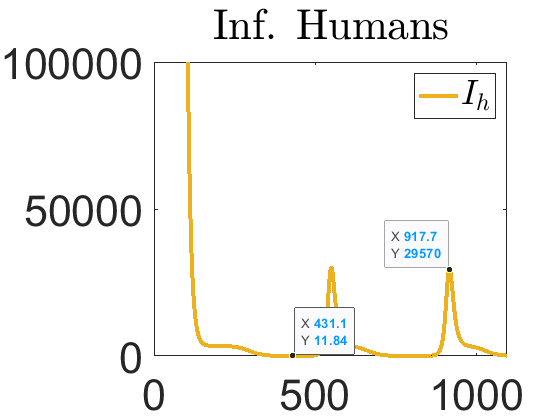
\includegraphics[scale=0.35]{nonaut6chum.png}
%\end{subfigure}
%\begin{subfigure}{.5\textwidth}
%\centering
%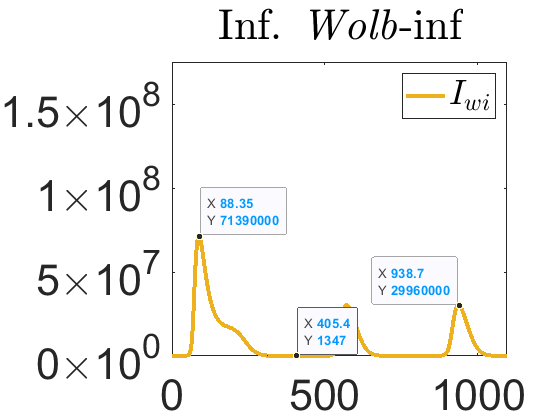
\includegraphics[scale=0.35]{nonaut6cmosq.png}
%\end{subfigure}
%\caption{Endemic Zika in humans and \textit{Wolbachia} mosquitoes when \textit{Wolbachia} vectors are more competent.}
%\label{fig:nonaut6chummosq}
%\end{figure}
%\end{comment}

%\begin{figure}[H]
%\centering \def\svgwidth{\columnwidth} %\includesvg{NonAutSimulation6c_newfig_main}
%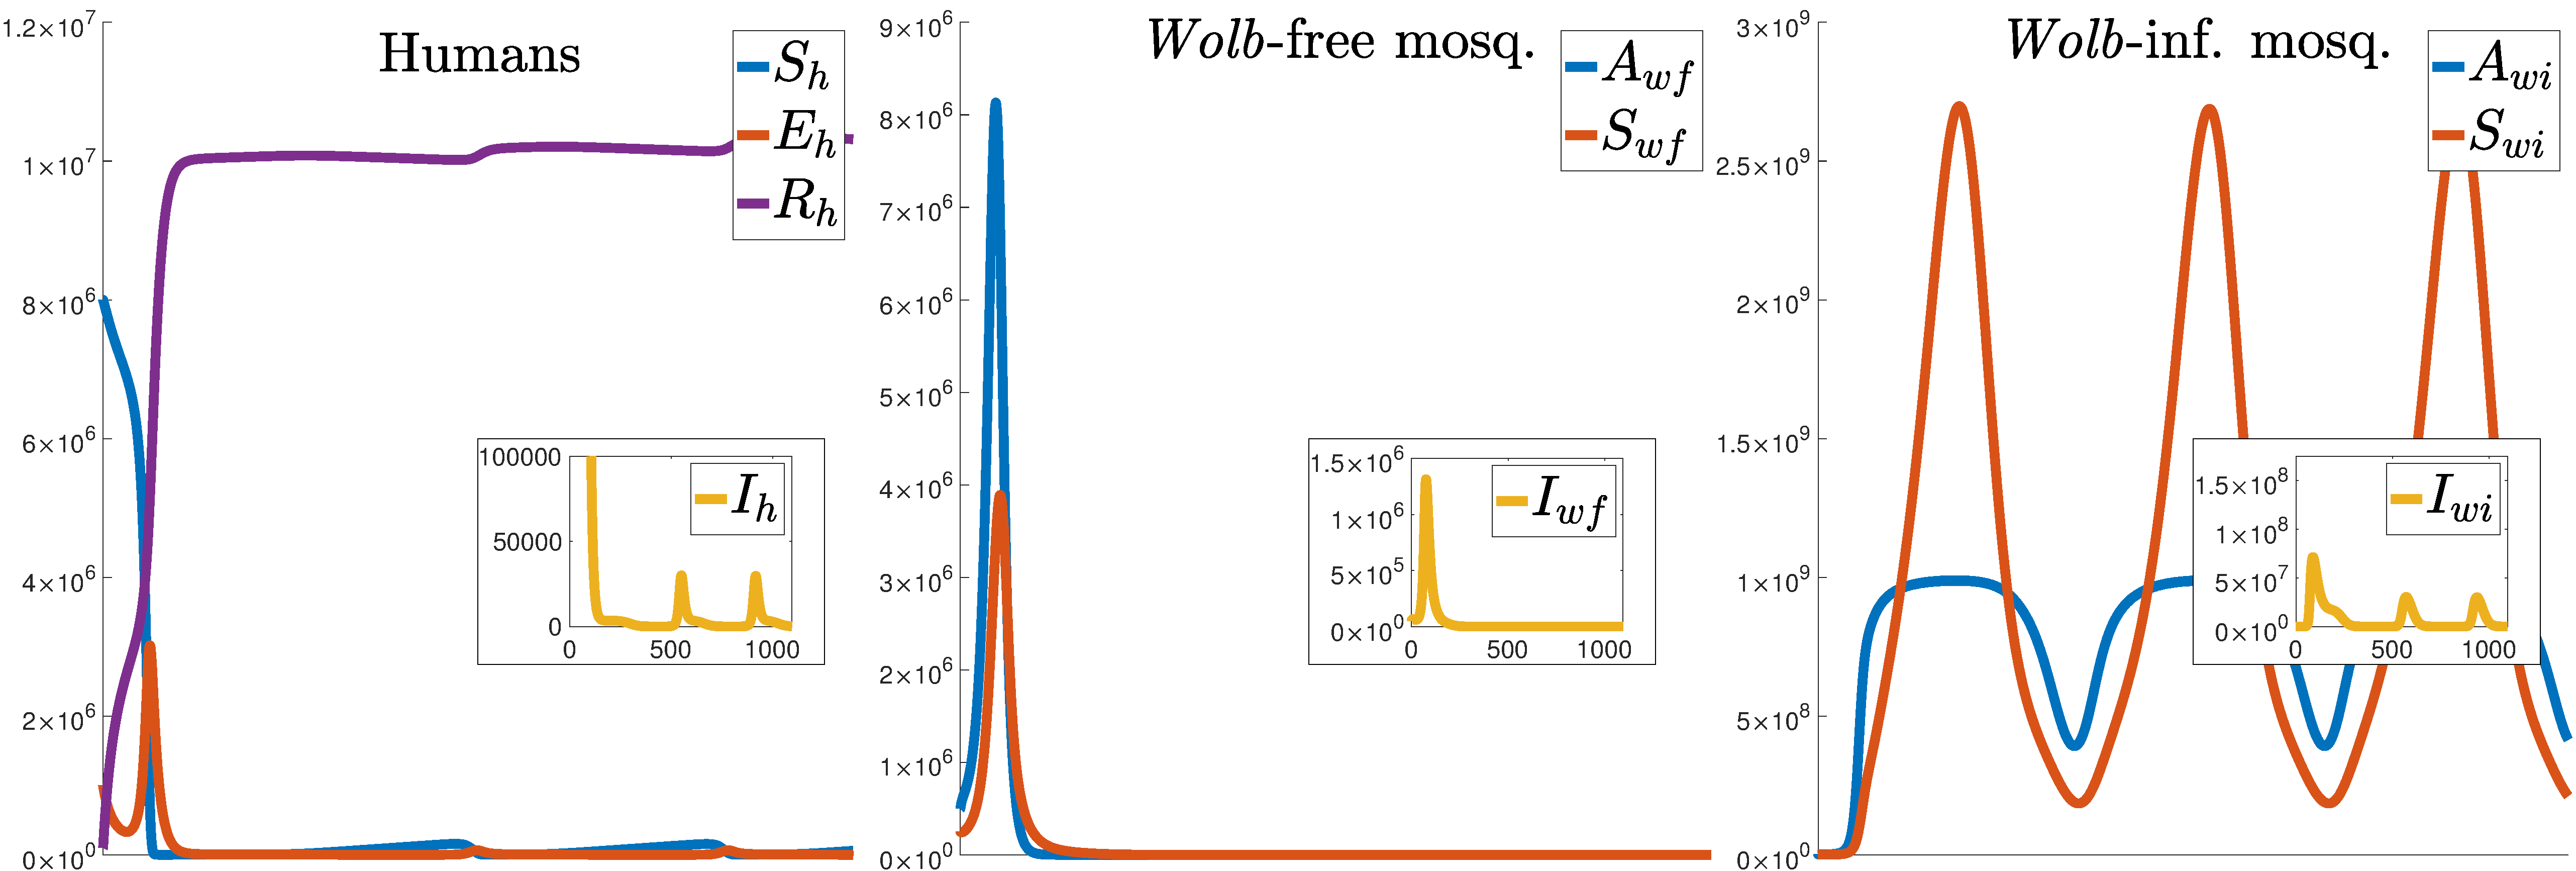
\includegraphics[width=\textwidth]{NonAutSimulation6c_newfig_main.pdf}
%\caption{\textit{Wolbachia} infected mosquitoes dominate and Zika is eradicated. Zika infected humans reach a peak of 1.3 million compared to 1.8 million in the autonomous model. Zika is endemic  in humans and \textit{Wolbachia} mosquitoes when \textit{Wolbachia} vectors are more competent.}\label{fig:newfig6c}
%\end{figure}

\begin{figure}[H]
%\centering \def\svgwidth{\columnwidth} %\includesvg{NonAutSimulation6c_newfig_main}
\centering
    % This file was created by matlab2tikz.
%
%The latest updates can be retrieved from
%  http://www.mathworks.com/matlabcentral/fileexchange/22022-matlab2tikz-matlab2tikz
%where you can also make suggestions and rate matlab2tikz.
%
\definecolor{mycolor1}{rgb}{0.00000,0.44700,0.74100}%
\definecolor{mycolor2}{rgb}{0.85000,0.32500,0.09800}%
\definecolor{mycolor3}{rgb}{0.92900,0.69400,0.12500}%
\definecolor{mycolor4}{rgb}{0.49400,0.18400,0.55600}%
%
\begin{tikzpicture}

\begin{axis}[%
width=1.1in,
height=1.5in,
at={(0in,0.046in)},
scale only axis,
xmin=0,
xmax=1095,
ymin=0,
ymax=12000000,
ylabel style={font=\color{white!15!black}},
ylabel={Population},%{Populations},
axis background/.style={fill=white},
title style={font=\bfseries, yshift=1.75ex},
title={Humans},
legend style={legend cell align=left, align=left, draw=white!15!black}
]
\addplot [color=mycolor1, line width=1.5pt]
  table[row sep=crcr]{%
0	8000000\\
2.18940652068704	7918623.82403113\\
6.69935710821301	7749712.1332971\\
9.54659914318472	7647716.7427842\\
12.158132490702	7558735.45790648\\
14.0747666582465	7496241.39112934\\
16.1670127604157	7430528.54341336\\
18.3378928340971	7364761.31494117\\
21.7121639000252	7266271.69805357\\
31.30890705809	6990809.13352108\\
33.3367730677128	6928493.94945478\\
35.3357358425856	6863528.30838425\\
37.3057953808457	6794766.75005118\\
39.2536422396079	6720579.74040637\\
40.2164593301713	6681045.95818786\\
41.1792764198035	6639248.88678393\\
42.142093510367	6594855.76496908\\
43.0908537171781	6548199.60814162\\
44.0396139249206	6498248.91988023\\
44.9883741317317	6444528.53180761\\
45.9371343394741	6386474.55995677\\
46.8847367167473	6323509.97237021\\
47.8323390949517	6254835.82368626\\
48.7799414731562	6179576.51918358\\
49.7275438504294	6096678.40224129\\
50.7053618943319	6001810.47098886\\
51.6831799391657	5895931.63175786\\
52.6609979830682	5777173.86180264\\
53.6388160269707	5643292.48903192\\
54.4608836350963	5517131.06239197\\
55.2829512432218	5376663.00781479\\
56.1050188504159	5219922.46979829\\
56.9270864585415	5044777.18453112\\
57.7491540657356	4848993.99080892\\
58.5712216738611	4630119.68232779\\
59.3932892810553	4386020.8032602\\
60.2153568891808	4115168.80693215\\
61.5441794926301	3618881.10691976\\
62.873002095148	3054625.46820094\\
64.4995654113591	2301246.86233652\\
66.0195190729573	1596308.92828332\\
66.9972849627957	1181885.73674202\\
67.9334695441648	837248.625682353\\
68.4015618357807	688898.040354805\\
68.8696541264653	557704.779117307\\
69.3303755698726	445170.485730847\\
69.7910970123485	349360.756173428\\
70.2518184548244	269869.999532549\\
71.006086088717	170147.913023992\\
71.593178470619	114795.264321207\\
72.1802708515897	75232.2735741287\\
72.4738170430064	60238.2137855263\\
72.7673632334918	47952.6820283663\\
73.3206033622846	30637.7648807196\\
73.8399912379682	19739.2221475746\\
74.3294037217274	12877.3540157145\\
74.7888408154249	8555.88312823698\\
75.2290614573285	5776.22599641513\\
75.6500656465068	3987.56426476687\\
76.0586486048996	2819.82996515092\\
76.4548103315756	2057.27624678519\\
76.8441132949665	1553.06037237309\\
77.2265574969351	1219.72628492862\\
77.6080407686532	996.324532639235\\
77.9885631110519	846.720951775089\\
78.3751976406202	744.799531929195\\
78.7679443564266	675.376366853714\\
79.1752090929076	626.952304964885\\
79.5969918491319	592.988952683285\\
80.0430447896942	568.264960999601\\
80.5133679136634	549.927988611162\\
81.0198137080297	535.54944916442\\
81.5623821737245	523.977614646778\\
82.1566056879237	514.104590185918\\
82.8024842515588	505.635576451197\\
83.5202802838758	498.127599769272\\
83.9151370339096	494.676728421822\\
84.7048505358398	489.180764068849\\
85.2981553422287	485.913706655614\\
85.8914601486176	483.407584203407\\
86.4847649550065	481.574228391983\\
86.7814173577353	480.893990685232\\
87.0780697613955	480.3626912646\\
87.3965479815379	479.952348311432\\
87.7150262016803	479.700071999803\\
88.0335044218227	479.598686059006\\
88.3519826419652	479.644582368433\\
88.6522645857185	479.820261288434\\
88.9525465294719	480.117368865758\\
89.2528284732252	480.530917143449\\
89.8083775928244	481.598256821744\\
90.3189119454473	482.908350037411\\
90.8017312036827	484.42379180342\\
91.4843874527141	487.003638355993\\
92.1884446879849	490.17486937996\\
92.9388905148953	494.095697690733\\
93.7141148103401	498.702221668325\\
94.7205078937113	505.482279177755\\
95.6009150184691	512.117384271696\\
96.5746036218479	520.182963851839\\
97.5958267766982	529.426937689073\\
98.7179133892059	540.469972511753\\
99.9187945751473	553.272371238098\\
101.282778636552	568.996189091355\\
102.624861915596	585.645422666334\\
104.190487795509	606.483889715746\\
105.753438225947	628.746417260729\\
107.429675181396	654.175339830108\\
109.122369035147	681.414264652878\\
111.004098088481	713.447892385535\\
112.95057539735	748.420609939843\\
115.018882148899	787.498615805991\\
117.26162126381	831.93112133909\\
119.569716969505	879.680780231953\\
122.207102647983	936.439778399654\\
125.12872862909	1001.58547896799\\
128.742413081229	1084.60532579664\\
134.732528392226	1225.09285434056\\
140.013048153371	1347.96947807353\\
143.422654798254	1424.92533904221\\
146.261934524402	1486.75455130171\\
148.804458003491	1539.95416566078\\
151.151127562858	1586.96644960903\\
153.327568753622	1628.59852593113\\
155.439696042798	1667.06679857895\\
157.443609873764	1701.72711251583\\
159.401688891463	1733.82307402696\\
161.267189589329	1762.75649634562\\
163.127740437165	1790.0198133504\\
164.932776393369	1814.97288878448\\
166.724190750159	1838.32071356848\\
168.493762556463	1860.0531950118\\
170.278807319701	1880.70678474009\\
172.075480514206	1900.29522138834\\
173.899365336634	1919.0546580283\\
175.782103725709	1937.35858126637\\
177.780673864298	1955.77476453036\\
179.981099115685	1975.07406809274\\
182.615940002725	1997.22591599915\\
191.151979174465	2068.2156048147\\
193.13790875487	2086.06348798331\\
194.932333514094	2103.11040872149\\
196.618383830413	2120.12127939612\\
198.199833206832	2137.11691034958\\
199.740573831834	2154.7930628676\\
201.234415544197	2173.12353848945\\
202.708201773465	2192.49239498284\\
204.164098875597	2213.01043596957\\
205.601102043875	2234.74147713743\\
207.030026464723	2257.93811783846\\
208.453273037449	2282.74881744292\\
209.867978814989	2309.23265363742\\
211.284028765745	2337.69929774944\\
212.687314029783	2367.98256796878\\
214.111222906969	2400.96989218332\\
215.520527875051	2436.01347537711\\
216.96011946816	2474.43611709587\\
218.388593354262	2515.35906493757\\
219.823609683663	2559.45835875813\\
221.247030113824	2606.35059844609\\
222.69734504912	2657.55982826743\\
224.151349095628	2712.5948453024\\
225.614016364329	2771.9261110127\\
227.07009126246	2835.18991034385\\
228.549830406904	2904.04212618712\\
230.002159334719	2976.36402694602\\
231.472689871676	3054.67498277873\\
232.948315559886	3138.71003509965\\
234.418123168871	3228.17153377831\\
235.917715392075	3325.72490270529\\
237.409468878992	3429.43735911883\\
238.939352985471	3543.12430130597\\
240.447995826602	3662.92649389524\\
241.978776665404	3792.75729748886\\
243.495663912036	3930.10457463935\\
245.036003467627	4078.94124495424\\
246.581893852912	4238.33960688394\\
248.129046568647	4408.48374194\\
249.714759186842	4594.49333208241\\
251.261367507279	4787.85710075125\\
252.880354292691	5003.56646423321\\
254.489062861539	5232.06420251355\\
256.1028053388	5476.16035915818\\
257.714805212803	5735.58143215906\\
259.345951032825	6014.66149126552\\
261.031830833293	6321.39306290913\\
262.697055089287	6643.36790487729\\
264.344188384712	6981.13804054819\\
266.08363727387	7359.41700380575\\
267.860446552746	7769.46922997478\\
269.564799073152	8185.93571939599\\
271.347568845376	8646.4536856031\\
273.232748671435	9161.7558794748\\
275.041521561332	9684.08420226257\\
277.001196825877	10281.3247174006\\
278.894796807319	10889.7323027411\\
280.877284009941	11559.8840722246\\
282.86654800456	12266.5015897201\\
284.954276258126	13044.7804157948\\
287.201848267578	13924.2502517989\\
289.469008802436	14854.4008285534\\
291.675131794065	15800.0687313974\\
293.961808606982	16821.3009407567\\
296.355096715502	17933.3341810163\\
298.99520983547	19209.0937031815\\
301.655141772702	20543.7772140149\\
304.495196497999	22020.1838906035\\
307.419733274728	23592.0676970035\\
310.799075097777	25468.2132284557\\
314.109047212638	27362.2606625389\\
317.85564795509	29566.3426627619\\
321.824998518452	31962.9359652661\\
326.278160332702	34716.7015030589\\
331.236457886174	37851.3241035426\\
336.800837705843	41439.9042324135\\
343.184444557875	45630.3748126486\\
349.544508978724	49866.007960381\\
358.115522630513	55644.3510605134\\
368.954396196641	63029.2204632824\\
383.844569555484	73252.6565754414\\
414.390751785599	94316.8602488674\\
451.944210549816	120191.488608892\\
467.981974064372	131175.984988643\\
477.526847211644	137647.896126129\\
484.032614270225	141993.656375422\\
488.865127360448	145156.699819144\\
492.629284634255	147556.977922773\\
495.739891592413	149477.038330641\\
498.34407544788	151021.824588794\\
500.535948094912	152262.186808035\\
502.440161148086	153282.063641584\\
504.082559505478	154107.53545122\\
505.491861035116	154766.95106071\\
506.738788394257	155305.460912252\\
507.874162230641	155752.847051855\\
508.877536570653	156108.958367649\\
509.792439038865	156397.152217801\\
510.556255300529	156607.866358277\\
511.256655465811	156774.637760849\\
511.840154754929	156892.490756989\\
512.369582030922	156981.504193951\\
512.829845720902	157044.071068158\\
513.277410178445	157090.853991427\\
513.614729041234	157116.45050704\\
513.875439302064	157130.282553388\\
514.131663381122	157138.631961348\\
514.298469401896	157141.190209847\\
514.398585926741	157141.611239238\\
514.448644189164	157141.503963361\\
514.548760714009	157140.646954917\\
514.656706730835	157138.75250065\\
514.830369993113	157133.556649753\\
515.017563966103	157124.928546873\\
515.25038050767	157109.701864547\\
515.546500695869	157082.908720465\\
515.896419225261	157040.117080611\\
516.258647526614	156982.557025365\\
516.669454034418	156900.144690036\\
517.118065861054	156788.231081779\\
517.581773192622	156647.104456476\\
518.091814137995	156460.135793932\\
518.60573768802	156235.9196252\\
519.202225339599	155927.393967334\\
519.817810563371	155550.497084322\\
520.458261312917	155090.240927616\\
521.117501381785	154537.921627452\\
521.759545249864	153917.063597891\\
522.476714312099	153118.547269586\\
523.197087367065	152195.263746778\\
523.950326966122	151088.330885027\\
524.713084860705	149806.829090502\\
525.474911984988	148351.369104477\\
526.254391220398	146664.991043251\\
527.082037001848	144637.570291914\\
527.920979968272	142312.884690888\\
528.759523309767	139696.6192812\\
529.623798844405	136671.40745189\\
530.510709743015	133197.182952194\\
531.421557425521	129216.952593918\\
532.35760974139	124671.462039731\\
533.3283134019	119455.688875591\\
534.339850361459	113471.524189041\\
535.454208403826	106243.65643895\\
536.641020059586	97861.6813003467\\
538.01153931208	87432.1652331194\\
539.844487431459	72635.866554332\\
542.858519543894	48277.4233581629\\
544.128808934242	38886.9760113405\\
545.173535377719	31873.3883167515\\
546.110271209851	26239.39558734\\
546.98422372248	21593.2222384149\\
547.789846007712	17849.3802234624\\
548.53197531309	14855.0020936476\\
549.241436789744	12385.2688185805\\
549.923161660321	10353.0048479829\\
550.570622309111	8708.96418768819\\
551.204031719826	7346.03959776834\\
551.840047056787	6196.46672045905\\
552.445130115375	5282.96533806249\\
553.02751365304	4548.89823154639\\
553.595051753335	3952.48447857983\\
554.169114538468	3451.98453462031\\
554.731542520225	3047.1134389285\\
555.305648809299	2707.47128868755\\
555.843195752241	2446.05040298589\\
556.398994899355	2223.68716763053\\
556.965646386147	2038.50331946928\\
557.515911893919	1891.60547138937\\
558.060862499289	1772.25465336442\\
558.62362750154	1671.20814400632\\
559.163723422214	1591.45383049082\\
559.716342194006	1523.97106726468\\
560.304271844216	1464.8065753635\\
560.870253877714	1417.7250449406\\
561.458871406503	1376.98458920792\\
562.045726669021	1343.07349128649\\
562.639800762758	1314.23712151404\\
563.25986388512	1288.90357870702\\
563.90579025168	1266.71116917394\\
564.545493105426	1248.18212733045\\
565.183843948878	1232.5229236912\\
565.843928391114	1218.82619225327\\
566.480205258355	1207.67187151778\\
567.118631383404	1198.23053228855\\
567.72801150661	1190.66148465872\\
568.313587529585	1184.57778490428\\
568.891934196465	1179.60952268727\\
569.413592098281	1175.94522871077\\
569.917306032963	1173.0919486396\\
570.397337063216	1170.96205223165\\
570.815132442862	1169.55245536752\\
571.193367125466	1168.61738332454\\
571.539780003019	1168.03495743964\\
571.814952739514	1167.753339421\\
572.074966547079	1167.6307712337\\
572.328300306574	1167.64257218409\\
572.587754719891	1167.78615200706\\
572.88089357689	1168.1051916182\\
573.215139651671	1168.66761253029\\
573.577093996108	1169.5099108154\\
573.987428986467	1170.75105245132\\
574.429002467543	1172.41805450805\\
574.952263131738	1174.82654223219\\
575.503222147934	1177.85679854453\\
576.114194766618	1181.79412737768\\
576.795807027258	1186.88403723016\\
577.544175902382	1193.29798888601\\
578.331473690458	1200.95630393922\\
579.197395127267	1210.43515921663\\
580.107013092376	1221.56261601765\\
581.049074823968	1234.33411982935\\
582.069932257757	1249.59423620161\\
583.130877879448	1267.01393506583\\
584.245261618868	1287.02755439933\\
585.419283830561	1310.03053399082\\
586.641587435268	1336.10155745503\\
587.875108878128	1364.65233915951\\
589.125553651713	1395.9532204615\\
590.408968370408	1430.62740182225\\
591.727395114489	1469.03483224288\\
593.066778748296	1511.06646956317\\
594.410234312527	1556.41768894717\\
595.796498825774	1606.73226937279\\
597.169247739017	1660.2639269745\\
598.584571179934	1719.53520397842\\
599.991789511405	1782.81192550529\\
601.40757274162	1851.10885517672\\
602.814194380306	1923.84934964776\\
604.246005816385	2003.20511845872\\
605.666162880138	2087.54206653498\\
607.104140971787	2179.01008499973\\
608.540932304226	2276.89379379246\\
610.018686573952	2384.77161632478\\
611.478177295066	2498.94565993547\\
612.951461894438	2622.38067762554\\
614.412864670157	2753.45201571379\\
615.853382429108	2891.58142801095\\
617.362749653868	3046.40422587283\\
618.850701221265	3209.74288127851\\
620.317365657538	3381.76264175586\\
621.866561792791	3576.02121665888\\
623.366766391322	3777.11465377547\\
624.9034621967	3997.05409166217\\
626.481164781377	4238.31834335346\\
628.022541851737	4489.90298952814\\
629.592765281908	4763.09287862759\\
631.196225228719	5060.448126873\\
632.82042689994	5381.38414181303\\
634.403311014175	5714.00646311417\\
636.0527627673	6082.20576072764\\
637.751206944697	6485.10785732605\\
639.426868167706	6906.91632816009\\
641.073063942604	7345.39850738831\\
642.919892389327	7866.33168906253\\
644.63839114178	8379.07047464792\\
646.543559462763	8979.4405453233\\
648.456405835226	9616.25017491542\\
650.464736823924	10321.593206441\\
652.414960034192	11042.4032011069\\
654.425883273594	11822.2927322732\\
656.552242776379	12686.7667363482\\
658.593448502943	13554.2614594083\\
661.046361346729	14644.0244031949\\
663.583647350781	15823.4751067832\\
665.980430340394	16984.0331294462\\
668.530980909243	18265.8320475407\\
671.438877684064	19782.2468666201\\
674.469707556069	21420.3703177022\\
677.671685214154	23209.1372633204\\
681.035613245331	25146.2405462675\\
684.940537001006	27460.6137858797\\
689.154346621595	30026.7767428039\\
693.793888194486	32922.1374166561\\
699.020299492404	36256.4001543382\\
704.932592982426	40102.8200106611\\
711.808513496071	44653.2141182106\\
720.137343994342	50246.4544232814\\
729.969379927963	56926.921313691\\
742.877173602581	65772.8320282344\\
764.043774646707	80358.6867774408\\
821.084394102916	119685.602033138\\
836.172848664224	130015.851459855\\
845.340826718137	136227.091344143\\
851.659346336499	140441.453509869\\
856.326687590219	143489.276673162\\
859.953319873661	145794.727515047\\
862.934817582369	147628.443129363\\
865.463410346769	149122.275881623\\
867.545501509681	150295.705060515\\
869.384272869676	151277.149149369\\
871.016284714453	152094.332288676\\
872.380278471857	152729.932257302\\
873.614477975294	153260.761302913\\
874.735698471777	153700.384896272\\
875.706710079685	154043.401779248\\
876.592575901188	154321.698712059\\
877.373441938311	154536.341350715\\
878.050066160038	154696.643892681\\
878.698304869235	154825.737400359\\
879.206780711189	154908.855976245\\
879.69987194147	154973.105752747\\
880.101254519075	155012.776140316\\
880.422270993702	155035.907228327\\
880.719292857684	155050.198763279\\
880.945526544936	155056.328830171\\
881.106621911749	155058.11227147\\
881.16401394736	155058.21879401\\
881.221405982971	155058.044157343\\
881.351619818248	155056.59422951\\
881.527371756732	155052.281059827\\
881.709524169564	155044.893463194\\
881.958200956695	155029.886289626\\
882.261381684802	155003.656637405\\
882.596695495769	154964.099450408\\
882.969718437642	154906.496589594\\
883.379701577127	154825.852036376\\
883.822900626808	154717.1512609\\
884.27618872188	154581.51401571\\
884.796173657291	154393.55205311\\
885.320558456704	154166.6664553\\
885.877423216589	153881.798239435\\
886.463021316566	153529.863932613\\
887.099079426378	153082.075107281\\
887.768203521147	152531.33944309\\
888.437235389836	151892.108146589\\
889.145791429095	151110.185202442\\
889.843516560271	150225.626174548\\
890.591457489878	149140.009969112\\
891.323495662771	147927.844422681\\
892.102722017094	146460.633922675\\
892.899378883652	144755.695435816\\
893.692141126841	142835.967337943\\
894.535174109973	140530.151786826\\
895.373575485311	137945.62705842\\
896.22465633601	135003.088106804\\
897.131129162386	131492.229664327\\
898.02281751018	127637.753580724\\
898.984524726868	123014.479991693\\
899.960075984709	117815.630343829\\
900.979320399463	111831.535705433\\
902.082113200799	104734.978769603\\
903.267593489029	96434.4562959047\\
904.644669872709	86048.6325312955\\
906.538053583354	70905.6714155879\\
909.399369806983	48034.9623014685\\
910.690465936437	38577.9935953589\\
911.749265900813	31542.2603764441\\
912.682681142353	25988.4390889313\\
913.555414301343	21397.2329301843\\
914.365079933777	17674.844243113\\
915.096595116891	14753.1111914953\\
915.83173072245	12223.7058180496\\
916.51263273228	10223.4533929667\\
917.160585406236	8602.48292334843\\
917.809197890572	7230.60136052035\\
918.441956608556	6108.66335976589\\
919.045630206354	5214.28046458773\\
919.637289198115	4483.44326963648\\
920.21237496566	3892.90302487463\\
920.783652618527	3406.709359603\\
921.348623335361	3009.73058099393\\
921.918432283215	2680.60931201186\\
922.463866256177	2421.76016785391\\
923.017029496841	2205.97914659418\\
923.575570544228	2027.62132669613\\
924.119262591936	1885.37262956426\\
924.665738651529	1767.91776232701\\
925.231988088228	1668.18826124724\\
925.787067747675	1588.0097941719\\
926.339305094443	1522.1886851741\\
926.890991182067	1467.65656318609\\
927.470443128608	1420.1141267363\\
928.049930915236	1380.59428066574\\
928.668069807813	1345.52482665423\\
929.288983221166	1316.20250628237\\
929.896538703702	1292.12483036239\\
930.515018858016	1271.42958433088\\
931.138309846632	1253.7816652339\\
931.779092522338	1238.43348420225\\
932.434172927402	1225.20999271795\\
933.055201179348	1214.64420101605\\
933.663507083431	1205.91337127145\\
934.283677948639	1198.47150299232\\
934.875853933394	1192.59977267683\\
935.415793040767	1188.20283344667\\
935.941471226513	1184.73136470281\\
936.397920856252	1182.3227749262\\
936.839022485539	1180.50019372534\\
937.253365980461	1179.21867779735\\
937.601384013891	1178.45130783226\\
937.921520858072	1177.98587637022\\
938.190314732492	1177.76796493307\\
938.433486624621	1177.70349023957\\
938.679234326817	1177.76366288029\\
938.931300474331	1177.95367784053\\
939.192650706507	1178.2852048371\\
939.515555646271	1178.88005534466\\
939.869229927659	1179.76139074005\\
940.292371971533	1181.12384812161\\
940.740656056441	1182.92404814623\\
941.254785252735	1185.42858437728\\
941.835575280711	1188.80790900812\\
942.46521464549	1193.11263257544\\
943.156210133806	1198.58393335715\\
943.905978858471	1205.38247370534\\
944.701512542553	1213.55396676436\\
945.551134252921	1223.34805350751\\
946.466532722116	1235.11299421079\\
947.453258135356	1249.18531834986\\
948.475810910575	1265.27895839699\\
949.566747990437	1284.13973260019\\
950.68295070529	1305.25027283467\\
951.83464466501	1328.97247325443\\
953.044517668895	1356.04888100177\\
954.300638989545	1386.54863516055\\
955.55666938331	1419.54649427813\\
956.846383708529	1456.11721745972\\
958.184670117684	1497.05467446335\\
959.53613827005	1541.61844969355\\
960.896578235552	1589.90421400685\\
962.249540979043	1641.50585937034\\
963.621060345322	1697.65433319006\\
965.040140422992	1760.04647351056\\
966.469971129671	1827.59068327304\\
967.883958981372	1899.28619582579\\
969.31529252883	1977.13070899807\\
970.741737407632	2060.3134748945\\
972.169823314063	2149.54968727194\\
973.630429361947	2247.37686933298\\
975.058445298113	2349.84119145386\\
976.529722672887	2462.91251130961\\
977.983852270059	2582.62101921719\\
979.425350007601	2709.5840028543\\
980.928574937396	2851.32630645391\\
982.416635665111	3001.61029758025\\
983.911532799713	3163.18124431651\\
985.387820618227	3333.77720953152\\
986.921090238728	3523.23757112678\\
988.428391152062	3722.36632607691\\
989.937824273482	3935.26331159566\\
991.458687871695	4164.1269149296\\
993.020496445708	4414.89342959411\\
994.628877786919	4690.60964995157\\
996.270397548564	4991.13163546007\\
997.84178229887	5297.69175518863\\
999.515060497448	5645.24510668591\\
1001.22350026388	6023.40006424487\\
1002.91952735838	6422.87930884957\\
1004.56501134206	6834.05158117972\\
1006.37120400742	7312.82391220052\\
1008.07846404333	7792.334630711\\
1009.92164909281	8339.94301085267\\
1011.66241499223	8885.99287781119\\
1013.55276218988	9510.96306942403\\
1015.56423344277	10212.6466356702\\
1017.66034567077	10983.9389677215\\
1019.65878842212	11757.014645\\
1021.83239722252	12638.9735677103\\
1024.08234903868	13595.9962486979\\
1026.41328977235	14633.299422388\\
1028.69693845697	15693.063655776\\
1031.33358067181	16967.6759536685\\
1034.04470289964	18332.1053260118\\
1036.89094740245	19819.264654451\\
1039.77915277705	21381.2460245816\\
1042.86009038612	23101.0959885512\\
1046.45714559499	25172.0733327996\\
1050.2480400987	27419.6053412454\\
1054.42849331629	29965.0387269948\\
1059.12922346313	32898.4168881793\\
1064.34742330573	36227.6931540892\\
1070.26320569683	40076.6132253399\\
1077.12732218858	44619.3911714545\\
1084.56474677939	49610.7365252106\\
1094.69250440504	56486.8520329334\\
1095	56696.6755907796\\
};
\addlegendentry{$S_h$}

\addplot [color=mycolor2, line width=1.5pt]
  table[row sep=crcr]{%
0	1000000\\
0.553766838740557	966058.31036968\\
1.37158667994663	919676.183787928\\
2.18940652068704	877260.634694589\\
3.25676561519504	827074.926673614\\
4.32412470970303	781930.990073116\\
5.51174090895802	736732.148834945\\
6.69935710774735	696051.569450728\\
8.1229781252332	652319.673134006\\
9.54659914271906	613247.972540874\\
10.4171102587134	591341.219973957\\
11.2876213751733	570784.534253247\\
12.1581324911676	551469.656530046\\
13.0286436071619	533296.578808091\\
14.0747666582465	512844.278167485\\
15.1208897093311	493801.89569246\\
16.1670127604157	476071.950771804\\
17.2131358115003	459560.840093136\\
18.3378928336315	443076.280184306\\
19.4626498557627	427843.849313376\\
20.5874068783596	413807.258719699\\
21.7121639004909	400910.594147673\\
22.8076542471536	389401.146634814\\
23.9031445942819	378908.799429115\\
24.9986349414103	369416.888302154\\
26.0941252885386	360910.608422179\\
27.1443374794908	353673.746279006\\
28.1945496704429	347341.329933665\\
29.2447618618608	341924.592176467\\
30.2949740528129	337439.570098841\\
31.3089070576243	334015.229026544\\
32.3228400629014	331511.65376954\\
33.3367730681784	329968.008712315\\
34.3507060729899	329432.793902942\\
35.3357358421199	329934.490927786\\
36.3207656117156	331507.269976535\\
37.3057953808457	334229.077122846\\
38.2908251499757	338194.981738663\\
39.2536422400735	343381.803661491\\
40.2164593301713	349981.961991571\\
41.1792764202692	358137.788640639\\
42.142093510367	368023.393199565\\
43.0908537176438	379657.326547998\\
44.0396139249206	393386.421482857\\
44.9883741321974	409473.709515283\\
45.9371343394741	428244.114226244\\
46.8847367172129	450056.737409444\\
47.8323390949517	475353.221039907\\
48.7799414726906	504651.007028042\\
49.7275438504294	538596.035570038\\
50.7053618947975	579320.117059392\\
51.6831799387001	626757.157264554\\
52.6609979830682	682050.497587413\\
53.6388160274364	746616.519822729\\
54.4608836350963	809278.225763278\\
55.2829512427561	880742.715637373\\
56.1050188504159	962193.899424235\\
56.9270864580758	1054900.0095585\\
57.7491540662013	1160146.99135984\\
58.5712216738611	1279262.94102602\\
59.393289281521	1413183.8318382\\
60.2153568891808	1562234.00066113\\
61.5441794921644	1833968.29111621\\
62.8730020956136	2135382.8281527\\
64.4995654113591	2511450.70158452\\
65.5306361280382	2724927.91984365\\
66.0195190729573	2811589.36800461\\
66.5084020178765	2885514.46901123\\
66.99728496233	2944626.8487286\\
67.4653772534803	2985836.52640428\\
67.9334695446305	3010564.70471804\\
68.4015618357807	3017996.4007574\\
68.869654126931	3008314.96312139\\
69.3303755694069	2983089.2022522\\
69.7910970123485	2942651.91765621\\
70.2518184548244	2888005.2603794\\
71.0060860882513	2774405.80618669\\
71.8867246611044	2614322.02472075\\
73.3206033622846	2323623.86972914\\
75.018559361808	1983077.95850116\\
76.2567294682376	1757114.51321911\\
77.4177795969881	1566418.33910765\\
78.3751976406202	1424322.7824818\\
79.3861004710197	1288128.25191466\\
80.5133679136634	1151557.90461076\\
81.5623821737245	1037557.17598721\\
82.4795449697413	947222.660208226\\
83.5202802834101	854265.478198885\\
84.7048505358398	759589.405774233\\
85.8914601486176	675353.674978797\\
87.0780697613955	600543.695717132\\
88.0335044213571	546437.645093181\\
88.9525465294719	499050.456146725\\
90.0636447691359	447282.506207201\\
91.0292832870036	406734.539224767\\
91.9537589428946	371417.078098849\\
92.9388905148953	337208.133766108\\
93.973579023499	304728.540704845\\
94.9485083366744	277052.00173788\\
95.9937266097404	250229.288188809\\
96.959074838087	227827.082370244\\
98.0355364149436	205268.653556019\\
99.1397984577343	184517.585759447\\
100.275905624032	165429.883652733\\
101.282778636087	150233.923966994\\
102.229041656014	137281.934595982\\
103.218235690147	124990.602997571\\
104.336733817123	112481.045468571\\
105.414274564013	101682.929740059\\
106.487663807813	92022.9713043817\\
107.567597132642	83295.8048311607\\
108.648111461662	75457.7067914805\\
109.61702092737	69114.0732114958\\
110.654651847668	62968.3619052568\\
111.606324853841	57865.5191078666\\
112.654074370395	52781.2812088691\\
113.705904232804	48185.5551465969\\
114.730139620136	44151.4225824308\\
115.73232888151	40584.2477825312\\
116.824288030155	37083.3360558357\\
117.779763943516	34318.1345518501\\
118.864360765088	31483.0340195489\\
119.839980371762	29182.3788595158\\
120.936798337381	26849.9953100611\\
121.944204933941	24921.590399127\\
122.943093487527	23191.7932592854\\
123.989124730229	21556.1388767092\\
125.047591354232	20066.1309980745\\
126.052689902484	18789.8473004163\\
127.120720333885	17566.9676022325\\
128.157495180145	16498.3544313093\\
129.155869028065	15568.8123131623\\
130.213330604136	14680.3054724615\\
131.28332249634	13871.9238864137\\
132.291551474016	13185.388751769\\
133.293041580357	12568.6367547843\\
134.282858504448	12016.8654408655\\
135.316938734148	11495.9241584311\\
136.348536015488	11027.3032315038\\
137.357564268634	10613.4983933312\\
138.371096282732	10237.9427075004\\
139.421637254767	9886.98493057024\\
140.457010342274	9575.53317501768\\
141.471277899109	9300.34932293557\\
142.512412130833	9045.68392705033\\
143.531821840443	8820.9925345704\\
144.529183898121	8622.50738211675\\
145.558614118025	8437.66649382701\\
146.599060771521	8269.53134005982\\
147.623620638158	8120.5398164806\\
148.657689228188	7985.22613960924\\
149.652643505484	7867.94750075415\\
150.675465130713	7759.32741409121\\
151.704928934108	7661.06273225974\\
152.684141956735	7576.91436615167\\
153.711621395778	7497.45904836291\\
154.703860024456	7428.51436892664\\
155.711635703687	7365.57709667506\\
156.711939255707	7309.50406506145\\
157.693914354779	7260.07514503878\\
158.694381772075	7214.90053756163\\
159.677175228484	7175.1423373674\\
160.637498327531	7140.30200462556\\
161.624321971089	7108.24351750826\\
162.598128949292	7079.98028304102\\
163.562787533272	7054.97518292489\\
164.512338063214	7032.99897850305\\
165.443574153818	7013.75229638349\\
166.360805825796	6996.82175941393\\
167.281769895926	6981.66004012898\\
168.17747057043	6968.51861971663\\
169.107452817727	6956.39232751681\\
170.009636227507	6945.96782685351\\
170.900027022697	6936.84987644246\\
171.785417596344	6928.82623354113\\
172.63917454239	6921.98045639088\\
173.515361127444	6915.77652770746\\
174.383395955432	6910.37028999766\\
175.24495184375	6905.65886927349\\
176.083092121873	6901.63676085975\\
176.916168706957	6898.12989582261\\
177.73910365114	6895.09473391017\\
178.563142236788	6892.4352909415\\
179.374653700273	6890.1448898362\\
180.220785801765	6888.06154090678\\
181.080246117897	6886.22199502634\\
181.934522630647	6884.63023789506\\
182.843937742058	6883.1538249515\\
183.814931635279	6881.78038629191\\
184.864160698839	6880.47989345761\\
186.087852721568	6879.1348857237\\
187.793565762229	6877.43113324046\\
190.506852310151	6874.72394266864\\
191.854687943123	6873.21575640189\\
192.998977925628	6871.78289778205\\
194.084562337026	6870.25950948708\\
195.112603590824	6868.64370480832\\
196.141382424161	6866.83563068695\\
197.174800925888	6864.80627857801\\
198.199833206367	6862.56336010899\\
199.241926452145	6860.0300329132\\
200.296768766362	6857.18816896016\\
201.373002408538	6853.98334644642\\
202.458010697272	6850.42301567364\\
203.558149876073	6846.45834827377\\
204.693124840967	6841.97634662315\\
205.828088007867	6837.07908575423\\
206.993408345152	6831.60076249391\\
208.19727202272	6825.44323272863\\
209.436993235257	6818.55263854843\\
210.689553953707	6811.00240193633\\
211.971614044625	6802.63852181146\\
213.267948070075	6793.5025335094\\
214.609214888886	6783.30338484049\\
215.95939212013	6772.23949560151\\
217.331406364683	6760.14448421914\\
218.719899673946	6746.99354908336\\
220.132610793691	6732.63304999983\\
221.570473229978	6716.95701236045\\
223.030979447998	6699.88958971482\\
224.49091912061	6681.62184057664\\
225.960059157573	6661.96211294876\\
227.461843759753	6640.47614889406\\
228.970998435281	6617.39786699554\\
230.496199913323	6592.48102341359\\
232.043592272792	6565.47816226352\\
233.59628780745	6536.54405198805\\
235.140431305394	6505.84396641841\\
236.69962259382	6472.79143310105\\
238.265173770022	6437.4168984876\\
239.844731432386	6399.38639264461\\
241.399729460943	6359.53199186921\\
243.02297984669	6315.2402138086\\
244.65575346956	6267.77884346759\\
246.260023590177	6218.1646132567\\
247.917484018952	6163.65605044086\\
249.590510330163	6105.13739241054\\
251.261367507745	6043.03968078969\\
252.964103758801	5975.85389937507\\
254.672677763272	5904.33901948342\\
256.381579802837	5828.57764406316\\
258.189168136101	5743.71412235126\\
260.001486220397	5653.64871336846\\
261.817309455946	5558.33597100899\\
263.666493854485	5456.01620755997\\
265.581259517465	5344.48530722177\\
267.561737665907	5223.21738137212\\
269.564799073152	5094.59300295962\\
271.777829995379	4945.76406437578\\
274.094094847329	4782.86649750499\\
276.608869342599	4598.45341508836\\
279.269279940054	4395.83562520472\\
282.432750040665	4146.66916190227\\
286.455691818148	3820.78799816407\\
297.618278168142	2910.878366536\\
300.683710063808	2671.38822496263\\
303.346902565565	2470.30287889158\\
305.719828583766	2297.58373522758\\
308.261799272615	2120.08498705178\\
310.353867850732	1980.28235034598\\
312.628284432925	1835.06051793369\\
314.63833322376	1712.76770843007\\
316.769343490247	1589.42456285749\\
318.957678368315	1469.56289638206\\
320.63431291189	1382.37624652917\\
322.420341322199	1293.89335145149\\
324.30352256028	1205.43024517735\\
326.278160332236	1117.88507943368\\
328.338558346033	1032.07186715072\\
330.511983000673	947.469149842393\\
332.006233324762	892.702455744147\\
333.545784202404	839.068944739178\\
335.143985662609	786.289727495052\\
336.800837705377	734.573360487353\\
338.527275665663	683.802146194503\\
340.323299543466	634.210951191839\\
342.202878020238	585.667832300533\\
344.166011095513	538.439568575937\\
346.246810469776	492.038410082925\\
348.445276142098	446.852315478493\\
349.544508978724	425.657130021602\\
350.885277444497	401.016591969877\\
352.226045910735	377.644721154589\\
353.566814376973	355.480650524143\\
354.907582843211	334.48119825637\\
357.046209368389	303.285419652238\\
359.184835893568	274.727096055169\\
361.323462418746	248.631597256754\\
363.462088943925	224.817176462151\\
364.565583675634	213.371074172668\\
365.669078406878	202.467726791278\\
366.772573138587	192.085125033744\\
367.876067870297	182.204576882534\\
368.954396196641	173.017299084459\\
370.032724523451	164.272685577627\\
371.111052849796	155.952718763147\\
372.189381176606	148.041668790393\\
373.251507706475	140.634561553597\\
374.313634236809	133.593126824126\\
375.375760766678	126.902201492805\\
376.437887297012	120.548238175455\\
377.496430908795	114.538015376776\\
378.554974520579	108.835363343358\\
379.613518132828	103.427065609023\\
380.672061744612	98.3011092017405\\
381.729564348236	93.4505571196787\\
382.78706695186	88.8579301326536\\
383.844569555949	84.5116952909157\\
384.902072159573	80.4012172291987\\
385.954222035594	76.5353414611891\\
387.006371911615	72.8822187506594\\
388.058521787636	69.4320039991289\\
389.110671663657	66.1754936147481\\
390.159063918982	63.1144473454915\\
391.207456174307	60.2280653645284\\
392.255848429166	57.5080009815283\\
393.304240684491	54.9463488655165\\
394.362821648829	52.5127538661472\\
395.421402613167	50.2252231040038\\
396.479983577505	48.0764938616194\\
397.538564541843	46.059594231192\\
398.654653883539	44.0684570730664\\
399.770743225235	42.208971566055\\
400.886832567398	40.4740990237333\\
402.680433906149	37.9299004385248\\
404.03545790026	36.19331487827\\
405.39048189437	34.6046738470905\\
406.745505888481	33.1541119087487\\
408.284054425079	31.6627899799496\\
410.006127504632	30.1753136129119\\
411.600884715095	28.9555275887251\\
413.068326056004	27.9569248775952\\
414.979456844274	26.8205122710206\\
416.69838799024	25.9448926118203\\
418.322951075155	25.2352459118702\\
420.010859385133	24.6110584833659\\
421.701405719854	24.0942885326222\\
423.348086510785	23.6893841694109\\
425.367646969389	23.3186364434659\\
427.19107387308	23.0979396463372\\
428.923104634043	22.9853559359908\\
430.644906017929	22.9654746106826\\
432.338183423504	23.0349195366725\\
434.304418617394	23.2271137773059\\
436.09778991295	23.5091560455039\\
437.82244574884	23.8798063606955\\
439.540184312034	24.3503219913691\\
441.17498426605	24.89731233567\\
442.969852006529	25.6167875593528\\
444.684186812956	26.4292014054954\\
446.120293992572	27.2117277495563\\
447.750329385046	28.2224082518369\\
449.238383913878	29.2689429246821\\
450.710817022249	30.4320287657902\\
452.186940434854	31.7377946651541\\
453.547157340217	33.0771718863398\\
454.822255562991	34.4629124896601\\
456.127799638547	36.0249106413685\\
457.405418781098	37.7074476731941\\
458.752476412337	39.6632525771856\\
460.093644826207	41.8156081051566\\
461.265051953029	43.8806300153956\\
462.500663269777	46.2654665610753\\
463.694558568764	48.7919783731923\\
464.949331163894	51.7078913524747\\
466.079915920738	54.5881143053994\\
467.320703039411	58.0551462084986\\
468.469327646308	61.5808844263665\\
469.644953056704	65.5392456660047\\
470.79779337626	69.8021993637085\\
471.860023424495	74.1005717129447\\
472.918939224444	78.7767005139031\\
474.003074261826	84.0114088603295\\
475.114912203513	89.9008223665878\\
476.192500368692	96.1678489209153\\
477.255733505823	102.950716724154\\
478.332787168212	110.496367343701\\
479.376834203023	118.531194077805\\
480.491267206147	127.980235871393\\
481.533971200231	137.730882036965\\
482.626440219581	149.002081961837\\
483.710280943662	161.377962729428\\
484.73885474354	174.353723675944\\
485.795453241561	189.080377616454\\
486.849213652313	205.346815967001\\
487.87811340997	222.935587679502\\
488.865127360448	241.581846016459\\
489.874632570427	262.663298990577\\
490.898052689619	286.359792240895\\
491.926661420614	312.825010809116\\
492.941113485023	341.850776228122\\
493.895234690979	372.12631260138\\
494.851057149004	405.697765144054\\
495.832199975848	443.940437714104\\
496.77216993086	484.606674832758\\
497.748827427626	531.549821901135\\
498.680854574312	581.347887833603\\
499.583290545736	634.781482893508\\
500.535948095378	697.431968462653\\
501.470037421677	765.847896907944\\
502.3564735041	837.952606637497\\
503.301704564132	923.487837220542\\
504.206193507649	1014.71466518147\\
505.107962841634	1115.92684174515\\
506.036033987533	1232.11077169934\\
506.969465222675	1362.81078330847\\
507.874162231106	1504.41347656446\\
508.745121931192	1656.34064641641\\
509.642726446968	1830.9040039652\\
510.556255300995	2029.63494056091\\
511.432636785321	2242.74573871214\\
512.323249848559	2484.64905825257\\
513.219294580165	2756.97901364975\\
514.131663380656	3067.84235176723\\
515.017563966103	3406.14337987313\\
515.896419225261	3781.62501330394\\
516.806019312236	4217.19427571446\\
517.681023590267	4686.73450863967\\
518.547770054545	5206.54657624336\\
519.422713462263	5792.93640741892\\
520.301488111261	6451.43839828018\\
521.19583547907	7201.35825224128\\
522.09763794858	8048.19810800534\\
522.968300336041	8961.64422102552\\
523.869635871146	10016.9994171681\\
524.756776883267	11175.7604761827\\
525.667802501936	12501.7020705799\\
526.609099547844	14029.7717344193\\
527.527393043507	15688.4784775707\\
528.482297448441	17602.7007771363\\
529.465614013374	19788.7446762919\\
530.47258230811	22264.718773792\\
531.502420419827	25052.8565567061\\
532.582767893095	28256.4514856245\\
533.760775174014	32061.631249391\\
535.065363002941	36612.1831025514\\
536.809176266659	43089.2862184951\\
539.680672422983	53786.2780013205\\
540.776815729681	57458.6362966518\\
541.65289562894	60063.2199410987\\
542.401640308555	61989.6849321886\\
543.021819752175	63340.7773851557\\
543.597039162181	64373.9740840937\\
544.070626739878	65054.411891907\\
544.486874054186	65519.6334172119\\
544.866899002809	65832.7340375469\\
545.173535377253	66006.4024060313\\
545.412836925127	66092.5408199159\\
545.596893442795	66129.255970641\\
545.737774949055	66140.0106614139\\
545.776982023381	66140.3311279989\\
545.816189097241	66139.4892357988\\
545.894315190148	66134.3494416242\\
546.011072246358	66118.0900309752\\
546.17242386844	66078.7618733956\\
546.383669460658	65997.8807509872\\
546.651825153735	65847.6952583874\\
546.955399439204	65614.547183549\\
547.324002218433	65243.5359228048\\
547.759411504958	64685.5297050192\\
548.226105429698	63950.7802796345\\
548.773311560508	62922.0915930048\\
549.398240344599	61548.375315296\\
550.132311283145	59701.7445728406\\
551.026512452867	57181.3610760034\\
552.19649661053	53576.9865146675\\
556.906336129643	38746.8102678624\\
558.150262651034	35308.5157269663\\
559.319639421999	32350.6166604892\\
560.44866090687	29750.2310271035\\
561.537908222526	27471.9644167009\\
562.60326549178	25450.614653396\\
563.680240566377	23600.7055379152\\
564.73784335237	21958.3626950253\\
565.789651499595	20481.6222351408\\
566.833686069585	19156.4509615204\\
567.88221057225	17953.6512656938\\
568.922574208584	16875.1968013025\\
569.955054065213	15907.4476927309\\
571.003882907331	15018.9805683596\\
572.046980164479	14220.8514838456\\
573.099264064338	13493.6829272052\\
574.15123422211	12837.3906248608\\
575.204691470135	12244.0221426287\\
576.250916307326	11711.7582884403\\
577.290526527911	11233.6372301066\\
578.331473690458	10800.6530283489\\
579.376865249593	10407.3788648336\\
580.431565097999	10048.644030211\\
581.497416086495	9721.0672143097\\
582.539657950401	9431.33185646916\\
583.603319866117	9163.69548106194\\
584.649914695881	8925.2470419989\\
585.726715150289	8703.07474946138\\
586.80848545488	8501.10695585562\\
587.904892619699	8315.85373686906\\
588.995758955833	8148.92004365195\\
590.088090036996	7997.28918445483\\
591.201495682821	7857.00222939346\\
592.308462800458	7730.25027072197\\
593.449286243413	7611.4140880662\\
594.59852760518	7502.42233487638\\
595.756625965703	7402.19719052454\\
596.92116546724	7309.96877182741\\
598.110181313474	7223.55345731881\\
599.36526030954	7139.72473205067\\
600.671981493942	7059.38402288686\\
602.011931568384	6983.24354106002\\
603.432823389769	6908.27540401695\\
604.96363559179	6832.93465819582\\
606.645814600401	6755.24549879646\\
608.588389201555	6670.41568787489\\
611.026287022512	6568.66307669319\\
618.93754773261	6241.94532338437\\
621.164400343783	6143.81453949166\\
623.219970997423	6048.74739531195\\
625.198024733458	5952.46319688112\\
627.148522170726	5852.34243447147\\
629.068142327946	5748.35025092307\\
630.989473554306	5638.51391658792\\
632.958488679491	5519.74066851335\\
634.885230389424	5397.29958547372\\
636.867090967484	5264.91461434495\\
638.85670966655	5125.53473704262\\
641.073063942138	4962.89862306742\\
643.465740116313	4779.13979907148\\
646.014237846248	4574.98505443288\\
648.913677788805	4333.74751459062\\
652.414960034657	4032.83034696383\\
658.040315015707	3538.35800032504\\
663.267091006041	3082.04070428666\\
666.724631940015	2789.51291182404\\
669.586227766238	2556.25323598087\\
672.255464831367	2347.57166116126\\
674.469707556069	2181.82239525858\\
676.754266084172	2018.37442833884\\
679.055317543447	1861.91181213176\\
681.035613245796	1734.02372665843\\
683.208339430857	1601.01874244725\\
684.940537001006	1500.47854835214\\
686.712203401141	1402.66459582606\\
688.530408616178	1307.49226902379\\
690.402222631499	1214.92670467356\\
692.406602483708	1121.74244334316\\
694.513047287706	1030.2176823318\\
695.95136547368	971.36327611329\\
697.485832483042	911.721433420666\\
699.020299492404	855.213992413133\\
700.65559350932	798.320099740755\\
702.290887525771	744.713966218755\\
704.052024496719	690.503076064866\\
705.813161468133	639.76200228557\\
707.737322618719	588.092518441379\\
709.661483768839	540.129598966334\\
711.808513496071	490.732181520201\\
713.955543222837	445.383470026311\\
715.229415413458	420.287299122661\\
716.503287603613	396.462834395003\\
717.777159794234	373.849661876447\\
719.051031984854	352.402531181928\\
721.223656003829	318.383285747841\\
723.396280023269	287.365031189751\\
725.56890404271	259.133890212514\\
727.74152806215	233.469329513144\\
728.855453995056	221.245847903658\\
729.969379928429	209.620516931638\\
731.083305861335	198.567578422371\\
732.197231794707	188.065201106947\\
733.275578950997	178.403203139082\\
734.353926107753	169.215548600536\\
735.432273264043	160.482059903909\\
736.510620420333	152.185128084384\\
737.572273515165	144.426773964427\\
738.633926609997	137.057118230499\\
739.695579704363	130.059427279513\\
740.757232799195	123.418774998281\\
741.817203201354	117.130578634795\\
742.877173603047	111.168463116977\\
743.93714400474	105.51793729607\\
744.997114406899	100.165869197343\\
746.055815749802	95.105544985272\\
747.11451709317	90.3170135091059\\
748.173218436074	85.7877689022571\\
749.231919779442	81.5063196569681\\
750.285251114517	77.4815459819511\\
751.338582450058	73.6798482183367\\
752.391913785599	70.0906418827362\\
753.445245120674	66.7040719408542\\
754.493684312329	63.5250463904813\\
755.542123503983	60.5279563739896\\
756.590562695637	57.7039173482917\\
757.639001886826	55.0445526391268\\
758.693013503216	52.5288919289596\\
759.747025119606	50.1634825440124\\
760.801036735997	47.9407299249433\\
761.855048352387	45.8533831574023\\
762.94941149978	43.8219140199944\\
764.043774647173	41.9214828605764\\
765.138137794565	40.1450626291335\\
767.129201902542	37.2090783305466\\
768.922603824176	34.8653716575354\\
770.716005745344	32.7804358392023\\
772.509407666512	30.9311913931742\\
774.18657022668	29.3963002432138\\
775.74749342585	28.1225562328473\\
777.169823972974	27.081777561456\\
778.453561868053	26.2336758715101\\
780.27000557771	25.1708570504561\\
782.03690749174	24.2796526066959\\
783.813888948411	23.5139016290195\\
785.565889712889	22.8775338106789\\
787.232474625576	22.3741218391806\\
789.298416914884	21.879244517535\\
791.205269504339	21.5421896767803\\
793.031642519403	21.3220168212429\\
794.818083665799	21.2006140789017\\
796.540339943487	21.1697868695483\\
798.549071096815	21.2399909002706\\
800.41168588493	21.4079411327839\\
802.201931872871	21.6646725879982\\
803.950393304694	22.0087143783458\\
805.929223620333	22.5147837637924\\
807.744932567701	23.0949595267884\\
809.519106327556	23.7769775092602\\
811.236480670515	24.5544489263557\\
812.84188642865	25.3947440613993\\
814.359123932198	26.2988532721065\\
815.870421995874	27.315545046702\\
817.313505841885	28.4047923330218\\
818.664170248434	29.5391674083658\\
819.984049938619	30.7652384848334\\
821.303625971079	32.1183225191198\\
822.737547347322	33.7475864146836\\
824.104214732535	35.4707973450422\\
825.480944833253	37.3933614389971\\
826.784208202735	39.404869093094\\
828.00707938429	41.4799928423017\\
829.255362603348	43.8056547585875\\
830.447263979353	46.2424646909349\\
831.719060414936	49.1009304048494\\
832.865880809259	51.9318298925646\\
834.099849448074	55.2759817331098\\
835.261153035797	58.7363847913221\\
836.475167339202	62.715357797686\\
837.574799492024	66.6736925914884\\
838.665216722991	70.9679229073226\\
839.783366976306	75.7943712868728\\
840.901952236425	81.0986315952614\\
841.950636678375	86.5515270410106\\
843.061682490166	92.8922269106843\\
844.121097843628	99.5383042078465\\
845.23233462777	107.211212879047\\
846.313795933966	115.447918436956\\
847.376358953305	124.366174116265\\
848.415414991323	133.96975615155\\
849.401202716399	143.979042490013\\
850.435880645178	155.531959856395\\
851.437205178663	167.84936469933\\
852.462613172363	181.756491428241\\
853.485000038054	197.078045271803\\
854.48068712838	213.560993328691\\
855.43585315207	230.989520090632\\
856.4099946348	250.582837603521\\
857.410055459011	272.831248883158\\
858.421813304536	297.804886654019\\
859.387809572276	324.243288532831\\
860.342692808248	353.168412887491\\
861.289495340548	384.913988656364\\
862.243381698616	420.352300162893\\
863.212809912395	460.35203793738\\
864.139593543485	502.80286182696\\
865.053240256384	549.166254037991\\
865.986995320302	601.736636676826\\
866.926874524914	660.590002262499\\
867.872570488602	726.565933232196\\
868.813982677646	799.819417070132\\
869.752207233571	881.293761648703\\
870.687386513688	971.980771279428\\
871.589118224569	1069.50715485634\\
872.534526156262	1183.73191560432\\
873.464517347049	1309.57194923656\\
874.37751420727	1447.78064675257\\
875.290350130759	1602.340402612\\
876.181479973719	1771.00410445873\\
877.063226026483	1957.33288213843\\
877.981114269234	2174.41311579105\\
878.88459534524	2414.01134901261\\
879.752406286541	2671.39900417998\\
880.631993058603	2962.88440678315\\
881.527371756267	3295.13355864771\\
882.415623677894	3664.52657022886\\
883.267887916882	4060.72821557336\\
884.156827170402	4522.81375852227\\
885.03221619688	5032.36872799788\\
885.929605310783	5617.5914100525\\
886.826679322403	6273.7368735238\\
887.712966606487	6999.97353159497\\
888.599117225502	7812.38698519487\\
889.492358628195	8728.25357267726\\
890.384552042	9750.59712407272\\
891.271510352381	10884.4039277066\\
892.19717016723	12204.8674637759\\
893.103182387073	13645.526936233\\
894.032164137345	15288.0477213534\\
894.963739790022	17116.1054639975\\
895.926894169766	19209.2067318591\\
896.910095675848	21569.8552848021\\
897.930449443404	24266.9417840033\\
899.019261279143	27424.6405621446\\
900.171465474181	31070.2610227424\\
901.474462641869	35531.5398697685\\
903.106934696902	41501.6393038854\\
906.443072241731	53800.8605684866\\
907.47926213732	57193.3474763185\\
908.319183262996	59631.9291002215\\
909.055161126889	61479.2784782061\\
909.670641683508	62783.2974522151\\
910.23086290108	63759.4560368159\\
910.720782216638	64437.1601103293\\
911.145967806689	64886.2950416724\\
911.511099741794	65166.086074403\\
911.785865860991	65311.1576413675\\
912.026106730569	65391.6166398181\\
912.203455015551	65423.1962696933\\
912.334860636387	65431.3659570958\\
912.407150161918	65430.341601185\\
912.489231358748	65424.438045634\\
912.608435417991	65406.9077332462\\
912.77934952639	65363.3332946445\\
912.981561059598	65283.8994679484\\
913.236265437678	65141.2844652389\\
913.555414301343	64896.6941071181\\
913.897385671269	64555.2280004416\\
914.329552616458	64010.4319751109\\
914.802082079928	63277.3189445101\\
915.330509076361	62299.4784179083\\
915.942914662883	60977.7891151966\\
916.699969489593	59103.0853067203\\
917.599983656313	56598.5212737806\\
918.787208326627	52983.7021446754\\
923.459470031783	38441.9131499403\\
924.721788167953	34991.0012884666\\
925.896632541437	32053.961671548\\
927.033174851444	29468.0227041929\\
928.125286526047	27212.4205265716\\
929.194988978095	25208.8699575788\\
930.256398817059	23408.0961979297\\
931.314755934291	21783.5262735034\\
932.361457437277	20330.509200254\\
933.411144510843	19013.1147470716\\
934.46718515316	17815.9765327838\\
935.515749523416	16742.5909477426\\
936.558510049712	15778.2129919627\\
937.601384014357	14906.6844888423\\
938.651654982939	14113.866999255\\
939.705042972229	13395.9532722733\\
940.740656055976	12758.236674102\\
941.777905408759	12180.5978474584\\
942.805636347272	11662.7244520346\\
943.85092988098	11186.2082514847\\
944.892715636175	10756.75646077\\
945.956314063631	10360.5119034946\\
947.005237427074	10007.3536092383\\
948.051719573792	9688.54034045571\\
949.122658042703	9393.47843071399\\
950.20032543363	9125.20232979814\\
951.263017662335	8885.91975902393\\
952.327955180779	8668.72945565823\\
953.417698348407	8467.4885573918\\
954.489525038283	8288.1357501247\\
955.556669382844	8125.96067803958\\
956.651467850432	7974.79441555357\\
957.768665557727	7834.71170994733\\
958.880982668139	7707.90481950715\\
960.002125081141	7591.44828143017\\
961.135772700887	7483.96597772371\\
962.300639833789	7383.02263662219\\
963.497803265229	7288.08949556062\\
964.733736084774	7198.2497844724\\
965.986609847751	7114.50728634279\\
967.313461506739	7032.70778060472\\
968.682858608197	6954.56420558598\\
970.152057879604	6876.60010059783\\
971.746202353388	6797.54408239061\\
973.542411087546	6713.76566831674\\
975.612282982562	6622.12289604126\\
978.53555764677	6497.66218772437\\
983.832790252753	6272.56378707942\\
986.294438492507	6162.94097605627\\
988.428391151596	6063.37005822267\\
990.426721892785	5965.42735705897\\
992.347783076577	5866.37664675619\\
994.286064834334	5761.09702707361\\
996.164330308791	5653.60915159993\\
998.058569994289	5539.50672095641\\
999.950260492507	5419.69564450439\\
1001.99466585927	5283.57116534142\\
1004.05329731992	5139.60217134701\\
1006.21351105487	4981.32483300474\\
1008.43009950593	4811.68063923391\\
1010.99817836517	4606.80119380681\\
1013.75190324383	4378.55154547933\\
1016.91966362949	4107.43089979375\\
1021.55561785819	3700.80563709419\\
1028.3519890341	3104.78191429516\\
1031.64906014875	2824.58484378876\\
1034.41162910312	2597.75442149583\\
1036.89094740245	2401.79633281333\\
1039.36224895669	2214.63687903993\\
1041.4874207736	2060.78109631129\\
1043.86788147641	1896.68187885359\\
1045.92998791859	1761.81044364162\\
1048.05701116798	1629.91006182414\\
1050.24804009916	1501.74441877333\\
1051.96938251378	1406.51062118635\\
1053.77844665665	1311.53441764694\\
1055.72858663462	1214.91085307114\\
1057.75392837869	1120.72492958419\\
1059.85385222547	1029.48554990673\\
1061.30310974969	970.195134132169\\
1062.80096677644	911.963236175012\\
1064.34742330573	854.981742443517\\
1065.9546272601	799.017329368275\\
1067.62257863907	744.303302344866\\
1069.35988001246	690.79828285845\\
1071.16653138073	638.745828957297\\
1073.05706500588	587.990703222342\\
1075.0314808879	538.809221588075\\
1077.12732218811	490.621252276003\\
1079.34458890697	443.846754958387\\
1080.45322226593	421.984284142032\\
1081.82373043709	396.302158370614\\
1083.19423860824	372.02969434252\\
1084.56474677939	349.09276759997\\
1085.93525495054	327.438994291704\\
1088.04769341554	296.451844779309\\
1090.16013188055	268.155215919018\\
1092.27257034555	242.359981312416\\
1094.38500881055	218.872517334763\\
1095	212.44443330681\\
};
\addlegendentry{$E_h$}

\addplot [color=mycolor3, line width=1.5pt]
  table[row sep=crcr]{%
0	900000\\
0.553766838740557	857132.276035918\\
1.3715866797138	798839.138276761\\
2.18940652091987	746000.834448884\\
3.25676561542787	684351.562591254\\
4.32412470970303	629988.641309898\\
5.51174090872519	576905.21885382\\
6.69935710774735	530523.621401438\\
7.41116761649027	505523.730517106\\
8.1229781252332	482392.85549521\\
8.83478863397613	460963.597798997\\
9.54659914271906	441083.386183143\\
10.4171102589462	418675.47287512\\
11.2876213749405	398155.327242374\\
12.1581324911676	379325.191772504\\
13.0286436071619	362008.564862377\\
14.0747666582465	342982.374158858\\
15.1208897093311	325688.733138457\\
16.1670127604157	309929.523432178\\
17.2131358115003	295532.139995368\\
18.3378928336315	281404.145276098\\
19.4626498559956	268528.835411813\\
20.5874068781268	256776.658588584\\
21.712163900258	246037.973560064\\
22.8076542473864	236466.272729596\\
23.9031445942819	227698.068924812\\
24.9986349414103	219673.314439371\\
26.0941252883058	212343.890740559\\
27.1443374794908	205934.620223597\\
28.1945496706758	200098.482977735\\
29.2447618616279	194811.845400446\\
30.2949740528129	190059.05366926\\
31.3089070578571	185967.686578933\\
32.3228400629014	182356.403288908\\
33.3367730679456	179222.324638802\\
34.3507060729899	176569.167875154\\
35.3357358423527	174460.255917569\\
36.3207656114828	172822.104837017\\
37.3057953808457	171669.152525065\\
38.2908251499757	171022.371865416\\
39.2536422400735	170904.635383077\\
40.2164593301713	171324.508051103\\
41.1792764202692	172318.059135992\\
42.142093510367	173928.832798022\\
43.0908537176438	176169.541271428\\
44.0396139249206	179119.767991316\\
44.9883741321974	182851.41094367\\
45.9371343394741	187446.00281019\\
46.8847367172129	192989.519151569\\
47.8323390949517	199610.409610786\\
48.7799414726906	207452.678448271\\
49.7275438504294	216673.721377696\\
50.7053618947975	227820.991910471\\
51.6831799389329	240905.966990625\\
52.6609979830682	256255.170163583\\
53.6388160272036	274208.038381761\\
54.4608836350963	291597.523422421\\
55.2829512427561	311438.745917879\\
56.1050188504159	334094.407821835\\
56.9270864583086	359922.962670292\\
57.7491540659685	389283.476273508\\
58.5712216738611	422716.582690106\\
59.393289281521	460744.990083629\\
60.2153568891808	503751.524708633\\
60.8797681909055	542345.392597761\\
61.5441794923972	584612.901628995\\
62.208590793889	630657.637747108\\
63.4151898673736	723455.12272755\\
64.4995654111262	815614.634347444\\
67.4653772534803	1079194.66200706\\
68.4015618357807	1151709.57041265\\
68.8696541266982	1183511.64637904\\
69.3303755694069	1211138.74339097\\
69.7910970121156	1234889.93104415\\
70.2518184548244	1254566.27844272\\
70.7125398975331	1269856.9227215\\
71.0060860884842	1277203.61047137\\
71.2996322794352	1282736.7279977\\
71.5931784701534	1286477.65185689\\
71.8867246611044	1288444.80219241\\
72.1802708520554	1288667.37140558\\
72.4738170430064	1287214.25371613\\
72.7673632337246	1284155.7449693\\
73.0609094246756	1279554.86138876\\
73.3206033622846	1274254.34373245\\
73.8399912375025	1260456.88083425\\
74.3294037219603	1243913.92661503\\
75.0185593620408	1215605.95348931\\
75.6500656467397	1185390.45418393\\
76.4548103315756	1142288.06946885\\
77.6080407686532	1074304.60896987\\
79.5969918491319	949047.176948984\\
81.833666406339	808979.381439082\\
83.5202802836429	709818.714510913\\
85.0015029390343	629277.724042201\\
86.1881125515793	569650.015823641\\
87.396547981305	513522.967368457\\
88.6522645854857	460071.801761828\\
89.8083775930572	415117.011769626\\
91.0292832867708	371867.351891728\\
92.1884446877521	334592.88415826\\
93.1967705555726	304981.058768118\\
94.2330432371236	277096.062360408\\
95.4045092228334	248462.977021563\\
96.5746036218479	222684.615553257\\
97.5958267771639	202301.573297814\\
98.7179133889731	181988.360531883\\
99.7402390511706	165222.973200961\\
100.766928370344	149915.591230655\\
101.832983654458	135505.279038783\\
102.822653173469	123364.663994164\\
103.897995751351	111404.011425002\\
104.927078136476	101052.060094618\\
105.936994621065	91839.4769995611\\
106.987289411481	83163.3539370399\\
108.089862585766	74955.4594784384\\
109.122369035613	68026.0015290878\\
110.244916654425	61241.9796486439\\
111.242016339907	55808.9245495589\\
112.339600708568	50410.4888579114\\
113.368367984658	45851.7989418516\\
114.363025056198	41861.4393147421\\
115.449192745378	37927.7805606183\\
116.526758270338	34420.0602705008\\
117.514416123275	31516.7877200644\\
118.578184057958	28691.0556899877\\
119.569716969505	26311.9675384725\\
120.61707071308	24040.1513890887\\
121.6813072199	21961.0378078341\\
122.709870899329	20149.7752820195\\
123.736424759962	18517.3404399017\\
124.766144426074	17038.8211388995\\
125.83713035332	15653.4167508641\\
126.866758528166	14453.6240152335\\
127.93006928754	13337.038245318\\
128.942828035913	12377.9505530018\\
129.940989205614	11522.7299350132\\
130.981450649677	10717.2869379686\\
132.014214034192	9996.24774296\\
133.032963201869	9354.11219803942\\
134.09618864581	8749.97829618282\\
135.156233577291	8208.16190209403\\
136.192220819183	7731.21849598549\\
137.23234687699	7299.49406587495\\
138.248741256539	6918.79175788909\\
139.272310403408	6572.54030125518\\
140.299994189059	6258.7681236472\\
141.357619311893	5967.82441543764\\
142.401773187565	5709.26732646395\\
143.42265479872	5481.31737593282\\
144.475519851549	5269.433890366\\
145.505810748786	5082.68007653137\\
146.541993133957	4913.38323114929\\
147.552941290895	4764.38133928971\\
148.608766303165	4624.15524275322\\
149.652643505484	4499.46497280686\\
150.67546513048	4389.4241119544\\
151.704928933876	4289.61810882995\\
152.747966489522	4198.61156862043\\
153.756259758258	4119.37961257342\\
154.792247392703	4046.05704606138\\
155.807619931176	3981.38255112502\\
156.837525731651	3922.35023792484\\
157.84574557771	3870.35425437731\\
158.829286231659	3824.6298698748\\
159.855638642563	3781.68017221452\\
160.850194729399	3744.26526626316\\
161.857063392643	3710.20089385728\\
162.871825440554	3679.38311026292\\
163.861271126429	3652.40790449013\\
164.83140475885	3628.62848959747\\
165.808012279216	3607.11114378623\\
166.809824206401	3587.32539474824\\
167.782945476007	3570.11478469498\\
168.736376552377	3554.99165057065\\
169.694841119461	3541.36225299141\\
170.66931689973	3528.97115752473\\
171.622605808079	3518.1448481516\\
172.553225708427	3508.69537836267\\
173.471637457842	3500.35300894198\\
174.383395955665	3492.947434298\\
175.309320420492	3486.23666569381\\
176.234061557101	3480.27151942649\\
177.160927797435	3474.96004870511\\
178.074339532992	3470.31512619439\\
178.987061692169	3466.19991965895\\
179.899814593606	3462.55732824258\\
180.786732998677	3459.42417486641\\
181.692493768875	3456.59431392723\\
182.586687802337	3454.12772174645\\
183.504278813023	3451.89644725341\\
184.416381301591	3449.94423830719\\
185.357232702663	3448.17351616919\\
186.314851487055	3446.59100080514\\
187.29869297659	3445.1626849554\\
188.345668162452	3443.82727317442\\
189.479609600035	3442.5558273776\\
190.710700053954	3441.33545274776\\
192.147769947071	3440.06089701201\\
194.17190285353	3438.41875957255\\
197.580002306728	3435.66247986304\\
199.21636520396	3434.19025109359\\
200.646325125592	3432.7619948287\\
201.955607802607	3431.30852394202\\
203.21560331108	3429.75597711303\\
204.443540202919	3428.07956734858\\
205.655537062557	3426.2508969123\\
206.859762597829	3424.24838392832\\
208.063011253951	3422.04943606514\\
209.301624414511	3419.56581927324\\
210.548724272521	3416.8265541452\\
211.796807656065	3413.83257219545\\
213.046412087278	3410.56929070619\\
214.335253143683	3406.91203786293\\
215.640405674232	3402.89324896201\\
216.960119468393	3398.4928638225\\
218.314918013057	3393.60794955795\\
219.668943290832	3388.3377557632\\
221.045016971184	3382.56710221083\\
222.449310296914	3376.22841666942\\
223.868541680044	3369.34032654134\\
225.316882706713	3361.78874990321\\
226.759666542057	3353.71741741314\\
228.237516794354	3344.85516851163\\
229.71709818556	3335.35041321581\\
231.196940929163	3325.18005591328\\
232.686351739336	3314.23992116889\\
234.209990855306	3302.28022297937\\
235.725202071713	3289.57631273335\\
237.270596912829	3275.74306749902\\
238.799000511179	3261.14565834193\\
240.331010959344	3245.55118337879\\
241.893340298673	3228.60345413419\\
243.430089444621	3210.85070487414\\
245.036003467161	3191.09240370756\\
246.630518070888	3170.19223468262\\
248.249420305248	3147.59971517301\\
249.867475967854	3123.56996963592\\
251.50092795724	3097.773590361\\
253.133267447818	3070.38279232034\\
254.764485214138	3041.33427979052\\
256.476044821087	3008.9832877873\\
258.189168136101	2974.61489511537\\
259.896821073722	2938.31381010008\\
261.612579219975	2899.73082789592\\
263.387681403896	2857.53826156748\\
265.231789793586	2811.21385182766\\
267.099893791601	2761.67087014182\\
268.998122961726	2708.62486757128\\
270.972879925044	2650.56568136974\\
272.991928650066	2588.22468861914\\
275.041521560866	2521.9499777481\\
277.293430535123	2445.81770544383\\
279.624306979356	2363.60142523213\\
282.214084007312	2268.5711202824\\
285.151410640916	2156.7564780321\\
288.404636896681	2028.98037904152\\
292.843307998963	1850.43484070944\\
301.334189993329	1508.29548034165\\
304.894367258996	1369.61997930403\\
307.840766273672	1258.7884392757\\
310.353867850732	1167.70299958112\\
312.628284432692	1088.35613282048\\
315.167619235348	1003.5316596746\\
317.312495722668	935.155590788228\\
319.516556549584	868.133001360809\\
321.824998518685	801.534298283979\\
323.659603343112	751.2564413785\\
325.591360994615	700.85328790755\\
327.651759008178	649.938256552676\\
329.787508115871	600.215189804789\\
332.00623332453	551.780022738036\\
333.545784202171	520.048596956534\\
335.143985662609	488.689694292145\\
336.80083770561	457.834283847362\\
338.527275665896	427.416176736588\\
340.323299543466	397.583939595381\\
342.202878020238	368.261317603523\\
344.166011095745	339.618186589098\\
346.246810469776	311.358193255728\\
348.445276142331	283.726113742217\\
349.544508978492	270.727837173734\\
350.88527744473	255.564134653891\\
352.226045910968	241.14963350445\\
353.566814376973	227.465407222975\\
355.9768961058	204.566156213405\\
358.115522630978	185.971302978462\\
360.254149156157	168.893996073632\\
362.392775681335	153.233221142786\\
364.565583675401	138.672990237363\\
366.772573138587	125.180650056107\\
368.954396196874	113.034173821565\\
371.111052850028	102.107836394338\\
373.251507706707	92.2474650156219\\
375.37576076691	83.3591556481551\\
377.496430908795	75.3107054030988\\
379.613518132595	68.0353538522031\\
381.729564348236	61.4629306884017\\
383.844569555717	55.5370211959817\\
385.954222035594	50.2149205536116\\
388.058521787636	45.4437243260909\\
390.159063918749	41.1712430506013\\
392.255848429399	37.3528152452782\\
394.362821648829	33.9256688009482\\
396.479983577505	30.8585142611992\\
397.538564541843	29.4555845069699\\
398.654653883539	28.0646265083924\\
399.770743225468	26.7597093251534\\
400.886832567165	25.5364207425155\\
402.680433906149	23.7309463627171\\
404.03545790026	22.4893854632974\\
405.39048189437	21.3457610625774\\
406.745505888481	20.2937591129448\\
408.284054425312	19.2028444756288\\
410.006127504632	18.1027892294805\\
411.600884714862	17.1892042045947\\
413.802046726458	16.0797478109598\\
415.568161902949	15.3054607617669\\
417.781430046773	14.4667951026931\\
420.0108593849	13.7561359377578\\
422.265360835707	13.1610372881405\\
424.385627629934	12.7044612495229\\
426.757393309148	12.3021245552227\\
429.354093702976	11.9827427642886\\
431.931408548495	11.7825752815697\\
434.304418617627	11.6963045170996\\
436.790819053305	11.7042644738685\\
439.204130770173	11.8082165885717\\
441.80162359518	12.0287322974764\\
444.108523339964	12.3237615546677\\
446.407108561369	12.7173353615217\\
448.75263924012	13.2308883296791\\
450.960128275212	13.8287933249958\\
452.8819350868	14.4504549719859\\
454.822255562758	15.1852941366378\\
456.565845673205	15.9486989511643\\
458.379376777448	16.8594150852878\\
460.093644826207	17.843727157684\\
461.634402881609	18.8439456343185\\
463.17555799312	19.9676345859189\\
464.590208175592	21.1207571073901\\
466.079915920738	22.4765476493631\\
467.480903094169	23.9003076713998\\
468.78965757112	25.3765126422513\\
470.062452826416	26.9636297672987\\
471.258400317281	28.6065779286437\\
472.536125692772	30.5429702547844\\
473.718205065234	32.5200965928379\\
474.854960901197	34.608995921677\\
476.068621228915	37.0653944078367\\
477.255733505823	39.7202870785259\\
478.44084803341	42.6492790083867\\
479.508202238008	45.5531000767369\\
480.595844173105	48.8009060618933\\
481.644034961006	52.2373053017072\\
482.731418507174	56.1559204889927\\
483.807591645513	60.4292524156626\\
484.846837835619	64.971951516578\\
485.882657278795	69.9529723569285\\
486.960381298326	75.6716516572051\\
487.965294542722	81.5537578309886\\
488.97660148982	88.0712609491311\\
490.029502612306	95.568694450194\\
491.000385194086	103.200752710225\\
492.005777468206	111.916373946937\\
492.941113485023	120.851464239182\\
493.964995043352	131.653524941765\\
494.926210085861	142.879305339418\\
495.924508359516	155.784668268636\\
496.909120799508	169.906907304656\\
497.835564184235	184.610263101757\\
498.831904574065	202.139867094345\\
499.802152303979	221.128323592711\\
500.70564128831	240.718540243106\\
501.645786647452	263.291898396565\\
502.607536436524	288.972249307903\\
503.565541580785	317.478232957656\\
504.524228122551	349.29589802702\\
505.432826457778	382.868376563769\\
506.329142174451	419.644236566266\\
507.251530517591	461.743397166487\\
508.187800800893	509.434450661531\\
509.09076299821	560.750740882009\\
510.010465760715	619.062721407739\\
510.901422966039	682.088084229734\\
511.774260327686	750.833807950839\\
512.70291372342	832.525343676331\\
513.614729040768	922.383669086266\\
514.498702451354	1019.77102510887\\
515.403669088148	1131.25370736374\\
516.258647526614	1248.86367428117\\
517.118065861287	1380.56285788957\\
517.990013669012	1529.63067210629\\
518.896035100566	1702.99692061543\\
519.765841417713	1889.27930202801\\
520.633288492681	2096.72608090704\\
521.530698793475	2336.79201250966\\
522.429127297364	2606.10542297922\\
523.296170915477	2896.67441945453\\
524.167778912932	3222.52865621471\\
525.080610902747	3604.06476965547\\
525.986622740515	4027.89559605974\\
526.885311727412	4497.4008370121\\
527.811544424621	5037.61339058471\\
528.724739154102	5631.49191597942\\
529.659177169204	6307.74688274204\\
530.598573864438	7063.10284419265\\
531.54882893851	7909.65025829826\\
532.535592068452	8881.61211657478\\
533.557740319753	9992.47477994184\\
534.631381158251	11275.7364564217\\
535.756660410669	12747.5049019759\\
536.970623102272	14472.3997969399\\
538.379369792761	16627.1036037812\\
540.345565831754	19811.7028043987\\
542.786691528279	23741.1161957996\\
543.962172568543	25470.6992329198\\
544.90365618607	26715.3338014288\\
545.698567875195	27641.4620560408\\
546.420563734137	28367.3623233868\\
547.041872288566	28895.0748599158\\
547.61521349079	29297.1435697488\\
548.109904132551	29575.8783796902\\
548.560002376325	29773.3159756579\\
548.930139654083	29895.1378900826\\
549.27139076544	29974.9542057053\\
549.549655568087	30017.0296376222\\
549.775837606983	30036.0956092309\\
549.923161659855	30041.2667785923\\
549.977937884862	30041.739701017\\
550.005325997248	30041.6824685757\\
550.065913167549	30040.86179062\\
550.165510341292	30037.441788442\\
550.324731389759	30026.6557892759\\
550.509149579098	30006.0548914799\\
550.74732836429	29966.7353276205\\
551.026512452634	29902.7209792556\\
551.36377524049	29800.2127181464\\
551.751541949343	29649.4182489123\\
552.196496610763	29434.8703342855\\
552.707087351941	29137.1543231728\\
553.305729239946	28723.3436331959\\
553.993109623902	28170.7746654712\\
554.787756594364	27442.9203297033\\
555.730204406194	26478.8816676592\\
556.906336129643	25163.0309048805\\
558.623627501773	23113.3769430618\\
562.152136916295	18885.3418552023\\
563.757914660964	17098.6855078288\\
565.183843948878	15624.2520538874\\
566.505730660632	14361.0624274847\\
567.782576641766	13238.3284084732\\
569.004583314992	12252.780450389\\
570.203668089816	11367.7963228107\\
571.374458173988	10578.6779130276\\
572.512850990286	9878.57739200233\\
573.648983593564	9241.82247997471\\
574.772586007603	8668.84151976136\\
575.889073551632	8151.32729257108\\
577.001930176746	7682.9777059136\\
578.094839446712	7265.4864653321\\
579.197395127732	6883.43491825182\\
580.284273204859	6542.03157275287\\
581.38224721211	6229.5617193894\\
582.457152190385	5952.44048336521\\
583.547540343367	5697.80767771881\\
584.607986888383	5473.43440728774\\
585.697941464139	5264.52320807171\\
586.769519270631	5078.59124092432\\
587.845325135626	4909.49795998656\\
588.909683161415	4757.8880599339\\
589.990748779848	4618.33368349122\\
591.048826197861	4494.47451102873\\
592.13371266285	4379.26928366511\\
593.238622185076	4272.98793220567\\
594.324816320091	4178.27416905155\\
595.395887538791	4093.39443185297\\
596.490159678506	4014.51162855211\\
597.59753610054	3941.90446445346\\
598.71460579359	3875.23247161158\\
599.833789374214	3814.32898665918\\
600.990991176572	3756.86298851296\\
602.171865917044	3703.3206243054\\
603.381512726657	3653.16418119892\\
604.613089315128	3606.35535412375\\
605.899161024019	3561.44406338525\\
607.229247207055	3518.6502285914\\
608.635846098652	3476.80800906732\\
610.072618948994	3437.07486229157\\
611.62127360492	3397.00118889567\\
613.365313999588	3354.52790978109\\
615.401025709463	3307.5063182374\\
618.116906712297	3247.30777523201\\
624.486451038159	3106.91888002586\\
626.917233846849	3050.49354280089\\
629.068142327713	2998.19509775238\\
631.09284939128	2946.51818028348\\
633.096550459042	2892.74310322339\\
635.031075040111	2838.12638066337\\
636.975299759069	2780.41449701134\\
639.005154707469	2717.04162049619\\
641.073063942371	2649.16125340853\\
643.192816253053	2576.12819651933\\
645.439968401799	2495.00626943889\\
647.869914923096	2403.24819618813\\
650.464736823691	2301.06617067941\\
653.375250796089	2182.04560285807\\
656.785977464169	2038.01787045831\\
661.877682759194	1817.94018251938\\
667.822882663226	1561.62306486932\\
671.43887768453	1410.36422468675\\
674.469707556069	1288.17308308673\\
677.210474437568	1182.18503618171\\
679.550391468918	1095.55654499377\\
681.578794792062	1023.57672235114\\
683.78573862114	948.721506563714\\
686.115069796098	873.760653862497\\
687.906470610993	818.991426162887\\
689.778284626547	764.45588414208\\
691.738475866383	710.288741901051\\
693.793888194486	656.692515206989\\
695.951365473913	603.896183441859\\
697.485832483275	568.450147108641\\
699.020299492637	534.714696608949\\
700.65559350932	500.586289832834\\
702.290887525771	468.292017153697\\
704.052024496952	435.481771960855\\
705.8131614679	404.646897887345\\
707.737322618486	373.103649860714\\
709.661483769072	343.710592559772\\
711.808513495838	313.295735689579\\
713.955543222837	285.271550643723\\
715.229415413225	269.696000344818\\
716.503287603613	254.878133899532\\
717.777159794234	240.796879676869\\
720.137343994342	216.514500891324\\
722.309968013782	196.115433399798\\
724.482592032989	177.45782595058\\
726.65521605243	160.417293254286\\
728.855453995289	144.686717699049\\
729.969379928429	137.270884338301\\
731.083305861568	130.207470971392\\
733.27557895123	117.2732893473\\
735.432273264043	105.722732073162\\
737.572273515165	95.3235487935599\\
739.695579704596	85.9699735618196\\
741.817203201121	77.5081538606901\\
743.93714400474	69.8659230603371\\
746.055815749802	62.9744457188062\\
747.114517092938	59.7907464655582\\
748.173218436306	56.7711088203359\\
749.231919779442	53.9080454932991\\
750.28525111475	51.2076607691124\\
751.338582450058	48.6491301197093\\
752.391913785366	46.2263966447208\\
754.493684312329	41.7730324536096\\
756.590562695405	37.7985730224755\\
758.693013503216	34.2411932761315\\
760.801036735997	31.0648168455809\\
761.855048352154	29.6117431118619\\
762.94941149978	28.1920436662622\\
764.043774647173	26.8585393943358\\
766.232500942191	24.4326318649109\\
768.025902863359	22.6654400923289\\
769.819304784527	21.0788210600149\\
771.612706705928	19.6572731297929\\
773.406108627096	18.386417448055\\
774.967031826265	17.3927183565684\\
777.169823972974	16.1522370344028\\
779.095430815592	15.2086826250888\\
780.857292958768	14.4494424823206\\
782.629234644119	13.777336624451\\
784.981889457908	13.0136051867157\\
787.232474625809	12.4070500575472\\
789.298416914884	11.9467146010138\\
791.667016983498	11.5223582831677\\
793.934520575916	11.2112601117697\\
796.540339943487	10.9601802318357\\
799.307234284934	10.8107267760206\\
801.847626677249	10.7755776338745\\
804.635939149652	10.8480663113296\\
807.151094653876	11.0148203244898\\
809.809558609733	11.3004674206022\\
812.316966156708	11.6804309173021\\
814.611168463249	12.1310592044611\\
816.849580998067	12.6760234143585\\
818.883478031261	13.2720605949871\\
820.865162234055	13.9567494608928\\
822.737547347555	14.7100085138809\\
824.496619248996	15.5240399478935\\
826.239518336719	16.4455314381048\\
827.831950501073	17.4004498003051\\
829.433401851682	18.4837510643993\\
830.926316481316	19.6188649565447\\
832.370716423029	20.8467005263083\\
833.80165843782	22.2045308854431\\
835.114474534523	23.5892751519568\\
836.475167339202	25.1821406062227\\
837.707857422531	26.7801461538766\\
838.951175332069	28.5589138746727\\
840.161449692678	30.4701820102055\\
841.28281647712	32.417410066817\\
842.469072311418	34.683042626828\\
843.634877437027	37.139274580637\\
844.754001385998	39.7361620792653\\
845.877398293698	42.6056168945506\\
847.022058562841	45.8315605684184\\
848.116525456775	49.2346738951746\\
849.169725759188	52.8376607138198\\
850.246835223865	56.8936498153489\\
851.326134600211	61.3780556390993\\
852.368888071738	66.1567916392814\\
853.38148262538	71.2655513032805\\
854.397601958597	76.909065105021\\
855.435853151837	83.2724086947273\\
856.493301679147	90.4474323489703\\
857.506954081822	98.0618172434624\\
858.495475533186	106.264750256203\\
859.485621418105	115.341444649966\\
860.479341364	125.419109956594\\
861.476813039044	136.62740733847\\
862.44703130424	148.706104827812\\
863.381493288558	161.567152810749\\
864.353860439267	176.380919346586\\
865.343553990824	193.138938249787\\
866.31655089464	211.471499349689\\
867.291103177238	231.91023508017\\
868.261930683395	254.596660986077\\
869.214760221541	279.403067396022\\
870.142820338486	306.285068914993\\
871.072707783198	336.245039877482\\
871.998636571923	369.45673670317\\
872.906290749786	405.688523386139\\
873.796485828934	445.189022831619\\
874.669972471893	488.224184076535\\
875.56815398531	537.424994280096\\
876.494762416696	594.088061406743\\
877.373441938078	654.044974037679\\
878.285771216964	723.510567020858\\
879.146429005312	796.599639711436\\
880.037506119348	880.954061976867\\
880.945526544703	977.117592056049\\
881.846138479188	1083.94571695919\\
882.74232351128	1202.98632979486\\
883.642209003912	1336.89989203145\\
884.541780367028	1486.96352758282\\
885.423566084122	1651.71453359956\\
886.293765589129	1833.51106648427\\
887.193267687224	2043.89870987064\\
888.046040163841	2266.92933280673\\
888.912613808876	2519.79823572864\\
889.803658257704	2810.51454998367\\
890.689659246942	3133.94503582828\\
891.585533288773	3499.7023791098\\
892.49600372836	3915.66151742381\\
893.382438656408	4367.98455143301\\
894.287672673818	4882.94875383005\\
895.219492399367	5474.36612472939\\
896.130799992243	6118.30671535688\\
897.08351041493	6866.4822673439\\
898.022817510413	7684.54420298804\\
899.019261279376	8644.9296553873\\
900.035301161464	9726.73384675826\\
901.073089251062	10941.1678882453\\
902.206112595508	12392.7120055533\\
903.404916821513	14064.2053391885\\
904.773735966068	16121.4486441643\\
906.596671608277	19031.2742977645\\
909.456184227951	23598.038307816\\
910.622316670837	25287.6769647663\\
911.566822028952	26513.3656181509\\
912.37100539892	27428.7819302098\\
913.078596920706	28121.2184535507\\
913.695563687943	28630.0330634762\\
914.235886353068	28998.4452369118\\
914.706975018838	29258.5979412014\\
915.135364122223	29444.7300439817\\
915.506419682875	29566.7241951043\\
915.831730722683	29643.650385926\\
916.09269529907	29685.1359602108\\
916.293230179697	29704.8485121503\\
916.472915598424	29713.5897531428\\
916.552349866135	29714.7820771781\\
916.628034496447	29714.4016344687\\
916.73593698605	29711.3114120767\\
916.878304526908	29702.6779546121\\
917.052789505804	29685.0855228927\\
917.275856170338	29651.4797943116\\
917.54672195483	29594.177110363\\
917.879047260387	29499.7226790143\\
918.26463823556	29357.8256626702\\
918.701553989202	29156.8715146191\\
919.196544398554	28880.4927339908\\
919.762062089052	28505.968209181\\
920.426428565523	27993.5603518493\\
921.172258868115	27336.8622044488\\
922.084842005046	26436.3004074311\\
923.204554832773	25220.8616701951\\
924.752002525376	23417.0069781612\\
929.140843288973	18239.4599612304\\
930.698060163064	16556.7410838669\\
932.083730958402	15167.2281428096\\
933.38383044838	13963.0176990423\\
934.633403900778	12898.0373658729\\
935.859911147738	11939.6392161704\\
937.021759345662	11108.5740532833\\
938.190314732026	10344.5933225388\\
939.327727250056	9666.35334222624\\
940.465521593811	9048.3284819799\\
941.568414893234	8503.00817946414\\
942.687582908198	7999.7638559835\\
943.797397128772	7546.74879431399\\
944.892715636408	7140.97760269558\\
945.985262528528	6773.75029036892\\
947.065027846722	6444.52216141042\\
948.160876851762	6141.67603322375\\
949.230620570946	5873.76709370222\\
950.321464865236	5626.23826629436\\
951.401539576007	5404.35920535401\\
952.451565783704	5208.75335091026\\
953.524380252929	5027.47231674893\\
954.585075634066	4864.97132546082\\
955.642710650805	4717.93920670007\\
956.7163267422	4582.54234468052\\
957.810009755893	4457.57197394804\\
958.880982667906	4346.61823118106\\
959.967028389685	4244.48978064465\\
961.048287007259	4152.15604594233\\
962.147343268152	4066.87829708122\\
963.277787131956	3987.23833430535\\
964.379146418301	3916.67994121043\\
965.518810999813	3850.17495174473\\
966.666330480715	3789.15288655297\\
967.841940072365	3732.10386934178\\
969.025993544841	3679.57003969862\\
970.233503863448	3630.45449838974\\
971.480698914966	3583.83882897068\\
972.784564279485	3538.95831093425\\
974.165881621884	3495.06626365683\\
975.612282982562	3452.47395141702\\
977.148084793705	3410.32722784951\\
978.845873194281	3366.6407624688\\
980.784247922711	3319.52394349687\\
983.175257069524	3264.0331390861\\
992.125302058179	3058.8365283485\\
994.395545818144	3002.96484891884\\
996.482532028574	2949.109178724\\
998.540911872173	2893.29905004171\\
1000.58042228129	2835.10550113837\\
1002.61130131688	2774.11249777395\\
1004.56501134206	2712.46361624892\\
1006.66241658456	2642.98910111794\\
1008.81217371207	2568.27079609944\\
1010.99817836494	2488.76201640791\\
1013.35362113686	2399.33716881205\\
1015.99334734981	2294.92991664796\\
1018.81950027891	2178.95943360659\\
1022.10917658731	2039.77627360658\\
1027.34989008447	1812.92448073137\\
1033.31085049105	1555.75012899376\\
1036.89094740245	1406.00718426961\\
1039.77915277658	1289.50524557685\\
1042.40253384854	1187.81447811541\\
1044.8756725667	1096.0399039567\\
1046.98430327093	1021.19366656546\\
1049.12971906527	948.429367789533\\
1051.36636113259	876.331667392049\\
1053.17542527546	820.876713095\\
1055.07853997545	765.318571284181\\
1057.06628083647	710.32750698016\\
1059.12922346336	656.503218946513\\
1061.30310974992	603.294732481008\\
1062.80096677667	568.681849346729\\
1064.34742330597	534.655064053833\\
1065.95462725987	501.081855593482\\
1067.62257863884	468.111831804039\\
1069.35988001246	435.726494097384\\
1071.1665313805	404.084455140168\\
1073.05706500565	373.0970400488\\
1075.0314808879	342.944934124127\\
1077.12732218835	313.273701041238\\
1079.34458890697	284.353417895501\\
1080.45322226617	270.797275592573\\
1081.82373043732	254.814508847427\\
1083.19423860824	239.67620398826\\
1084.56474677939	225.358576261206\\
1086.99147418304	201.85642194422\\
1089.10391264805	183.205069800373\\
1091.21635111305	166.12088563852\\
1093.32878957805	150.49332188745\\
1095	139.093393224757\\
};
\addlegendentry{$I_h$}

\addplot [color=mycolor4, line width=1.5pt]
  table[row sep=crcr]{%
0	100000\\
0.962676759809256	266138.371303951\\
2.18940652161837	458875.892832125\\
3.25676561519504	611387.6868746\\
4.32412471063435	751528.380180012\\
5.5117409080267	894684.599753488\\
6.69935710728168	1026041.64356791\\
8.12297812476754	1170012.64913741\\
9.5465991422534	1301270.51853852\\
11.2876213751733	1447085.45614837\\
13.0286436080933	1579160.29282371\\
14.0747666582465	1652824.28790388\\
15.1208897102624	1722688.21914563\\
17.2131358124316	1852336.16303114\\
18.3378928340971	1917131.9638601\\
20.5874068774283	2037872.60084183\\
22.8076542466879	2147088.62329076\\
24.9986349418759	2246751.51300761\\
27.1443374790251	2337812.62437836\\
29.2447618618608	2421735.35553688\\
31.30890705809	2500087.53941616\\
33.3367730677128	2573899.56426106\\
36.3207656107843	2678464.21178519\\
44.0396139249206	2944544.90976128\\
45.9371343385428	3013794.04273756\\
47.8323390949517	3086817.11878105\\
49.7275438513607	3165326.22396992\\
50.7053618952632	3208662.17888041\\
51.6831799391657	3254358.36696877\\
52.6609979830682	3302812.94603372\\
53.6388160269707	3354514.76941976\\
54.4608836341649	3400910.28573367\\
55.2829512432218	3450357.90044278\\
56.1050188504159	3503276.85711646\\
56.9270864576101	3560172.73359568\\
57.749154066667	3621633.67995511\\
58.5712216738611	3688244.17224247\\
59.3932892810553	3760678.98484085\\
60.2153568901122	3839759.50130514\\
60.8797681909055	3909151.78674659\\
61.5441794916987	3983912.5633886\\
62.2085907943547	4064508.96100889\\
63.4151898678392	4227484.62661474\\
64.4995654113591	4394087.94721122\\
65.5306361280382	4571609.13303216\\
66.5084020178765	4757709.99350275\\
67.4653772544116	4956298.56492701\\
68.8696541264653	5274384.63490201\\
70.2518184557557	5611953.87658797\\
76.0586486048996	7067807.82427227\\
77.4177795965225	7373476.26844376\\
78.7679443564266	7655082.51703413\\
80.0430447887629	7899874.47018266\\
81.2910979408771	8119510.49818503\\
82.4795449692756	8310740.86005071\\
83.5202802829444	8464413.97089458\\
84.7048505358398	8624452.76979116\\
85.8914601486176	8769842.44390133\\
87.0780697613955	8901340.65458035\\
88.0335044208914	8997846.39290203\\
89.2528284732252	9109794.15467685\\
90.3189119454473	9198172.72337818\\
91.4843874517828	9285523.31726742\\
92.6810104735196	9366027.19996319\\
93.7141148094088	9428722.59426814\\
94.7205078937113	9484265.76215162\\
95.7973208148032	9538173.13404618\\
96.959074838087	9590514.7736961\\
98.0355364140123	9634133.01962226\\
99.1397984586656	9674470.22923653\\
100.275905624032	9711762.57679541\\
101.282778635621	9741587.08012898\\
102.229041656479	9767107.62999133\\
103.218235690147	9791416.94271088\\
104.336733818054	9816254.99671304\\
105.414274564013	9837780.64245147\\
106.487663807347	9857111.60599103\\
107.567597132176	9874643.02304038\\
108.648111462593	9890449.63058209\\
109.61702092737	9903290.5403953\\
110.654651846737	9915777.7465077\\
111.7503346093	9927680.15394541\\
112.811311200261	9938073.46138856\\
113.923975620419	9947897.77450757\\
115.018882147968	9956599.68395335\\
116.103385364637	9964371.37381762\\
117.135223833844	9971061.07614699\\
118.196615114808	9977296.71505437\\
119.197169134393	9982633.49419814\\
120.250237204134	9987738.23201516\\
121.293939992785	9992329.67464741\\
122.382367789745	9996671.24532069\\
123.483724789694	10000647.281598\\
124.527799669653	10004068.4450537\\
125.63532011956	10007365.0211722\\
126.710056751966	10010269.9404648\\
127.854260656983	10013077.5024172\\
128.942828036845	10015503.9491971\\
130.031769672409	10017717.5129512\\
131.195431631058	10019871.49023\\
132.360885834321	10021833.2687647\\
133.495483227074	10023575.5725181\\
134.666778383777	10025219.7247204\\
135.871572200209	10026765.1634195\\
137.107129486278	10028213.9261888\\
138.309918768704	10029506.9628942\\
139.54129335843	10030724.6292921\\
140.836927726865	10031903.4734343\\
142.125175828114	10032983.9450211\\
143.477238319814	10034031.7349831\\
144.863456299528	10035025.8569883\\
146.261934524402	10035957.172748\\
147.743678012863	10036875.9153879\\
149.238692015409	10037741.6328224\\
150.862893838435	10038622.4172608\\
152.556492891163	10039484.494148\\
154.334586527199	10040337.4903244\\
156.243165498599	10041203.6349975\\
158.278506366536	10042080.9247478\\
160.492690922692	10042991.340057\\
162.978763608262	10043970.3772636\\
165.758905623108	10045023.7017984\\
168.967524282634	10046199.2247301\\
172.776173332706	10047555.7499646\\
177.602740591392	10049236.4500931\\
184.351175101474	10051547.7677421\\
195.561533238739	10055347.857785\\
208.163706829771	10059588.2515135\\
216.555472157896	10062379.1511177\\
223.126307396218	10064531.4993777\\
228.684181632474	10066319.4017069\\
233.54866158776	10067852.0732721\\
237.878712307662	10069184.9236262\\
241.799779076129	10070361.132285\\
245.387647820637	10071407.2899175\\
248.678922483698	10072337.7744869\\
251.743097826838	10073175.5159302\\
254.580870311707	10073923.8271338\\
257.270969515666	10074606.0777707\\
259.687490779907	10075194.2577385\\
262.035739725456	10075741.4888391\\
264.223998369649	10076228.1787209\\
266.322306670249	10076672.3115472\\
268.24813901633	10077059.2988416\\
270.085836878046	10077409.1365897\\
271.777829995379	10077713.6362494\\
273.473568692803	10078001.140704\\
275.041521560401	10078250.6303697\\
276.608869342133	10078483.7709251\\
278.124332036823	10078693.256376\\
279.446793459356	10078862.9080148\\
280.722402323037	10079014.65834\\
281.995417974889	10079154.2220281\\
283.296811867505	10079284.4042535\\
284.43131281808	10079387.4208383\\
285.545679405332	10079478.9820609\\
286.455691818148	10079546.5976059\\
287.456113487482	10079613.4376818\\
288.404636897147	10079669.5059378\\
289.260770674795	10079713.9670405\\
290.124513562769	10079752.8816155\\
290.862106822431	10079781.368313\\
291.381198497489	10079798.7877431\\
291.969065090641	10079815.8872146\\
292.556931685656	10079830.1907445\\
293.129684312269	10079841.4339404\\
293.702436940745	10079850.0168863\\
294.22118027322	10079855.4933952\\
294.480551939458	10079857.4126353\\
294.739923605695	10079858.7858533\\
294.997175492346	10079859.608553\\
295.254427378997	10079859.8942253\\
295.511679265648	10079859.642972\\
295.768931154162	10079858.8549541\\
296.062013935298	10079857.3033311\\
296.355096716434	10079855.0555897\\
296.64817949757	10079852.1121159\\
296.941262278706	10079848.4733999\\
297.279770223424	10079843.4062397\\
297.618278168142	10079837.4132585\\
298.295294057578	10079822.6540335\\
298.99520983547	10079803.5172253\\
299.695125613362	10079780.4498566\\
300.354181913659	10079755.1493592\\
301.013238213956	10079726.3906323\\
301.655141772702	10079695.0707348\\
302.646997742355	10079640.2901141\\
303.696854976937	10079573.9219311\\
304.49519649893	10079517.73273\\
305.293538019061	10079456.64483\\
306.572409711778	10079348.6871316\\
307.840766273439	10079229.4973932\\
309.100591165945	10079099.3595054\\
310.353867851198	10078958.4875464\\
311.689489591867	10078796.0799547\\
313.121872026473	10078608.1374051\\
314.63833322376	10078394.0242867\\
316.226191258058	10078153.6183452\\
317.85564795509	10077890.216617\\
319.516556549817	10077604.9236648\\
321.229655714706	10077293.5525654\\
323.015684125945	10076951.1698962\\
324.947441777214	10076561.3551633\\
326.964959669858	10076133.6675346\\
329.063033230603	10075667.8163616\\
331.236457886174	10075163.8862855\\
333.545784201473	10074606.1496677\\
335.972411684692	10073997.031363\\
338.527275666595	10073332.1045189\\
341.22131148167	10072606.8423917\\
344.166011095047	10071788.3032294\\
347.346043305472	10070877.0559304\\
350.885277444497	10069833.2141194\\
354.907582843676	10068613.6823999\\
359.184835894033	10067283.5565858\\
363.46208894439	10065924.3627506\\
368.954396197572	10064143.888846\\
375.375760767609	10062022.4194861\\
382.787066951394	10059533.9839985\\
391.207456173375	10056670.4167195\\
402.680433906615	10052729.9771639\\
419.448223281652	10046931.2143622\\
467.320703038946	10030358.8169492\\
478.224726302549	10026625.7653402\\
485.533841129392	10024156.6481645\\
490.898052690551	10022377.217353\\
495.076515959576	10021023.2962006\\
498.47329152748	10019954.4582388\\
501.269263820723	10019105.3229753\\
503.634375926107	10018416.4535437\\
505.721731735393	10017837.807706\\
507.513795254752	10017368.8491562\\
509.090762998909	10016982.4675313\\
510.485582731664	10016665.4751817\\
511.708365900442	10016410.1974062\\
512.766379721463	10016209.1051725\\
513.763128120452	10016038.8592533\\
514.598818976432	10015912.2938892\\
515.355427889153	10015811.8676466\\
516.017759073526	10015736.089731\\
516.624942053109	10015677.4534725\\
517.174540061504	10015634.0203636\\
517.636041486636	10015605.1239382\\
518.040913904086	10015585.8168919\\
518.372279742733	10015574.4361258\\
518.663705321029	10015567.8618407\\
518.85444932431	10015565.3601309\\
519.020792428404	10015564.3741101\\
519.111508883536	10015564.3147479\\
519.20222534053	10015564.5980213\\
519.312469400465	10015565.4092082\\
519.482510877773	10015567.6807922\\
519.713872272521	10015572.803455\\
519.954208731651	10015580.6735563\\
520.252272706479	10015594.1614905\\
520.574946099892	10015613.5882468\\
520.948684096336	10015642.6293034\\
521.369603941217	10015684.1485448\\
521.817927973345	10015739.1919903\\
522.294857198372	10015810.7181364\\
522.795362358913	10015901.0513448\\
523.34923231788	10016020.4607352\\
523.950326966122	10016174.8324923\\
524.574578274041	10016364.5661618\\
525.219819417223	10016594.7301111\\
525.871812419966	10016865.3705067\\
526.559074319899	10017195.5950437\\
527.274835938588	10017592.8256806\\
528.000934978947	10018056.3384781\\
528.724739154801	10018584.5133087\\
529.465614013374	10019199.6108515\\
530.243817700073	10019934.071289\\
531.00608840026	10020749.0528253\\
531.82571355626	10021740.2515433\\
532.629943717271	10022838.5828864\\
533.467268489301	10024125.7584464\\
534.33985036239	10025635.9048745\\
535.203714352101	10027313.9685404\\
536.102413712069	10029267.1486452\\
537.005609875545	10031457.3430142\\
537.937373233959	10033969.4284472\\
538.90838262625	10036873.4333339\\
539.886868150905	10040105.6640477\\
540.927323359996	10043886.084317\\
542.034066157416	10048295.7053006\\
543.185616824776	10053297.1059486\\
544.444622861221	10059216.0764195\\
545.855396172032	10066340.5790958\\
547.583076741546	10075618.9059852\\
550.245120866224	10090557.7571543\\
553.278244625777	10107424.1339534\\
555.096773579717	10116961.5712193\\
556.654688877985	10124612.0707981\\
558.088118033484	10131164.0398106\\
559.455001519993	10136951.7040724\\
560.765701662749	10142074.6097761\\
562.045726669952	10146680.933081\\
563.2982493788	10150822.361469\\
564.518026063219	10154524.7397857\\
565.735374607146	10157913.622821\\
566.94514683634	10160998.7936355\\
568.134488781914	10163777.3890525\\
569.337147178128	10166350.722276\\
570.537182373926	10168701.2034853\\
571.739120097831	10170856.8460903\\
572.963464720175	10172866.9246559\\
574.181819597259	10174698.5783583\\
575.401127299294	10176379.5914638\\
576.63157139346	10177936.9946735\\
577.875972174108	10179384.4655941\\
579.125029176474	10180721.6703475\\
580.390878524631	10181971.0990313\\
581.711438389495	10183173.3963216\\
583.057979723439	10184304.930786\\
584.40873048082	10185355.2430704\\
585.816274287179	10186370.0458847\\
587.239113144577	10187323.1734084\\
588.709146335721	10188240.6288204\\
590.250325465575	10189138.3776456\\
591.856459509581	10190013.3012013\\
593.487026397139	10190846.7314929\\
595.214044235647	10191677.5647571\\
597.022084325552	10192498.2480287\\
598.913008544594	10193310.568078\\
600.935470448807	10194135.0320177\\
603.057049192488	10194957.9401895\\
605.300232790411	10195788.1812498\\
607.670269796625	10196627.2252723\\
610.138389836997	10197464.841146\\
612.737961901352	10198311.8209689\\
615.401025708765	10199145.4782662\\
618.058837631717	10199945.368041\\
620.69112370722	10200706.9608398\\
623.293368695304	10201429.985812\\
625.727014617994	10202078.7046436\\
628.141325056553	10202695.0222833\\
630.3891797252	10203243.2562828\\
632.544303340837	10203744.4435368\\
634.644270701334	10204208.5169568\\
636.542464591563	10204606.256192\\
638.378126984462	10204970.2497434\\
640.173243680969	10205305.6422139\\
641.785919966176	10205588.8596058\\
643.329278184101	10205843.2460774\\
644.825644388795	10206073.794013\\
646.19898523204	10206271.014371\\
647.511573461816	10206446.3036533\\
648.685041811317	10206591.831959\\
650.044682521373	10206746.9653914\\
651.235505640507	10206870.7226922\\
652.414960034192	10206981.9568199\\
653.375250795856	10207064.071308\\
654.425883274525	10207145.1203524\\
655.423233021051	10207213.4775031\\
656.330876709893	10207268.3609447\\
657.25344683975	10207316.9440719\\
658.040315015242	10207352.6120734\\
658.593448502943	10207374.4936608\\
659.214788513258	10207395.922626\\
659.836128525436	10207414.0106038\\
660.441244935617	10207428.409789\\
661.046361345798	10207439.6309776\\
661.600575622171	10207447.1181049\\
661.877682758495	10207449.8609592\\
662.154789896682	10207451.9366667\\
662.432865174487	10207453.3490739\\
662.710940452293	10207454.0898518\\
662.989015728235	10207454.1591725\\
663.267091006041	10207453.5573098\\
663.583647349849	10207452.0556807\\
663.900203695521	10207449.6852274\\
664.21676003933	10207446.4465871\\
664.533316383138	10207442.340576\\
664.895094871521	10207436.5871328\\
665.256873361766	10207429.7034218\\
665.980430340394	10207412.5518686\\
666.724631940946	10207390.2180674\\
667.468833539635	10207363.144492\\
668.17693178542	10207333.0049478\\
668.885030031204	10207298.6168977\\
669.586227767169	10207260.4015269\\
670.287425501272	10207218.0697135\\
671.0550602898	10207167.0404796\\
671.822695078328	10207111.1506697\\
672.688234584406	10207042.3560745\\
673.553774088621	10206967.5002915\\
674.469707556069	10206881.7625827\\
675.841849377379	10206740.953818\\
677.210474437103	10206586.0055699\\
678.594106767327	10206414.9710845\\
680.045465394855	10206220.4069669\\
681.578794792295	10205998.4629411\\
683.208339430392	10205744.711072\\
684.940537001938	10205455.4871436\\
686.71220340021	10205139.7163646\\
688.530408615246	10204795.5707935\\
690.402222631499	10204421.0182897\\
692.406602483243	10203998.3085403\\
694.513047287241	10203531.3087924\\
696.718598978594	10203018.8643761\\
699.020299492404	10202460.1801374\\
701.47324051708	10201839.8668679\\
704.052024496719	10201162.1903109\\
706.775242043659	10200420.577013\\
709.661483768374	10199608.1458579\\
712.88202835992	10198672.8208062\\
716.503287604079	10197589.038193\\
720.13734399341	10196471.615853\\
724.482592033222	10195101.9626493\\
728.855453995988	10193692.4730912\\
734.353926107287	10191883.9513185\\
740.757232800126	10189737.8039753\\
748.173218436539	10187212.340522\\
756.590562695637	10184309.8646964\\
768.025902863592	10180328.8082044\\
785.565889712423	10174181.3794603\\
833.652562933043	10157311.9547975\\
844.873584697023	10153416.6530199\\
852.368888070807	10150848.4451891\\
857.803259076551	10149019.5970119\\
862.045366210863	10147625.0052793\\
865.463410345837	10146533.8827571\\
868.261930683628	10145671.7220304\\
870.634176848456	10144970.9517213\\
872.688773840666	10144393.2551276\\
874.450628774241	10143925.2924712\\
875.984895233065	10143543.2169938\\
877.373441938311	10143222.0352601\\
878.579175045714	10142965.5438589\\
879.655070252717	10142757.0944307\\
880.631993059069	10142586.8997194\\
881.481833653525	10142455.5029559\\
882.261381685734	10142350.1685362\\
882.969718437642	10142268.3612302\\
883.60060457699	10142207.6848016\\
884.097716227174	10142168.6126131\\
884.541780367494	10142140.6700239\\
884.925477882847	10142122.1204143\\
885.260023808107	10142110.3931489\\
885.550985019654	10142103.7086498\\
885.773059029132	10142100.8877083\\
885.929605310783	10142100.1199912\\
885.988909931853	10142100.0977694\\
886.048214552924	10142100.2248847\\
886.166823793203	10142100.9316715\\
886.336079521105	10142103.0007211\\
886.505335249007	10142106.3413017\\
886.710891256109	10142112.1482088\\
886.994671400636	10142123.4085563\\
887.319220433012	10142141.060915\\
887.657729692757	10142165.1233285\\
888.046040164307	10142200.1560978\\
888.477705849335	10142248.8892857\\
888.912613809109	10142308.9816938\\
889.394418895245	10142389.1949861\\
889.923233166337	10142494.7814497\\
890.493255732581	10142630.5797229\\
891.081514608115	10142796.3947983\\
891.714866116643	10143006.3414267\\
892.351300830022	10143252.766427\\
892.998158048838	10143542.6459509\\
893.692141126841	10143901.5563213\\
894.404313744977	10144325.9058087\\
895.114348117262	10144810.4645286\\
895.854918979108	10145387.0720802\\
896.626495299861	10146072.0737183\\
897.411666696891	10146865.3803606\\
898.205143945292	10147774.5447126\\
899.019261280075	10148829.5315363\\
899.852563519031	10150048.5513002\\
900.678927924484	10151407.9435061\\
901.515174793079	10152948.0843389\\
902.395515009761	10154761.3060956\\
903.313367933035	10156875.6565354\\
904.242549218237	10159263.1889137\\
905.180874790996	10161939.5464494\\
906.165586125106	10165046.3299057\\
907.201082864776	10168650.959116\\
908.276417339221	10172762.9267443\\
909.427777018398	10177574.2056083\\
910.660149656236	10183167.4353351\\
912.026106730103	10189847.5768525\\
913.637579467148	10198258.1381285\\
915.831730723381	10210302.1356943\\
920.044469794258	10233499.5838944\\
921.801563344896	10242554.7452498\\
923.354379706085	10250046.7924565\\
924.782216882333	10256455.0338794\\
926.122719811276	10262029.7145954\\
927.436895728111	10267075.9282751\\
928.704478505999	10271557.2639439\\
929.934126375243	10275555.4850495\\
931.171746343374	10279249.8057778\\
932.397815182805	10282602.9095531\\
933.592686804011	10285596.8580482\\
934.794228995219	10288355.0866196\\
935.993215858936	10290875.007721\\
937.198166193441	10293193.0786698\\
938.402429059148	10295313.862337\\
939.620149664581	10297277.2731291\\
940.818741932511	10299048.6683582\\
942.061050318182	10300732.252695\\
943.302923865616	10302275.5864897\\
944.556962655857	10303706.8639189\\
945.814727785066	10305027.4193915\\
947.094923056662	10306265.87555\\
948.401120569557	10307431.5952958\\
949.720819717273	10308520.1333011\\
951.095492567867	10309569.5644809\\
952.494447683915	10310559.4521929\\
953.923789151013	10311499.3078162\\
955.403717301786	10312405.649191\\
956.919313238934	10313272.3177632\\
958.521484259516	10314129.6310295\\
960.193628048524	10314968.5382365\\
961.91671775654	10315781.5781885\\
963.721087235957	10316584.9119849\\
965.614204050973	10317382.4736959\\
967.635997932404	10318190.4980307\\
969.761317616329	10318998.3100011\\
971.998808918521	10319809.3527035\\
974.367810007185	10320630.1148944\\
976.784212855622	10321432.1775894\\
979.288396209478	10322230.0243639\\
981.876981308684	10323022.1199622\\
984.483652282506	10323788.1478661\\
987.017459690571	10324503.2149485\\
989.492415199056	10325173.5640272\\
991.852587951347	10325786.3982213\\
994.176583850756	10326363.7047039\\
996.376464787871	10326885.1826069\\
998.436944704503	10327350.4435234\\
1000.47213458829	10327786.8394898\\
1002.30301414989	10328158.7684736\\
1004.1812258251	10328518.9839885\\
1005.89812515117	10328828.5073592\\
1007.59666896611	10329115.3629371\\
1009.19241337292	10329366.6416347\\
1010.70235579833	10329587.5958411\\
1012.06766203418	10329772.8855289\\
1013.3536211364	10329934.4853472\\
1014.67309764959	10330086.9687662\\
1015.77879039571	10330204.145357\\
1016.91966363043	10330314.7419033\\
1017.90382534079	10330401.6156684\\
1019.03385807946	10330491.4940008\\
1020.06936096586	10330564.4848125\\
1021.00205913	10330622.4849688\\
1021.83239722252	10330667.897227\\
1022.69288541004	10330708.7359738\\
1023.54517916776	10330742.9110375\\
1024.08234903961	10330761.2301502\\
1024.60021337681	10330776.5274362\\
1025.09877218306	10330789.0585522\\
1025.61436113156	10330799.7487239\\
1026.14698022604	10330808.3667104\\
1026.41328977235	10330811.7508139\\
1026.72548987716	10330814.9326951\\
1027.03768998012	10330817.2667006\\
1027.34989008494	10330818.7527356\\
1027.66209018789	10330819.390884\\
1028.00703961216	10330819.1102679\\
1028.35198903456	10330817.7950594\\
1028.69693845697	10330815.4456892\\
1029.04188787937	10330812.0628626\\
1029.37820146978	10330807.770596\\
1029.71451506019	10330802.4975795\\
1030.05082865059	10330796.2447647\\
1030.70262171701	10330781.3415213\\
1031.33358067274	10330763.4225081\\
1031.97277618386	10330741.7773294\\
1032.62020825222	10330716.2827943\\
1033.31085049175	10330685.1422049\\
1034.04470289871	10330647.6130822\\
1034.82191385515	10330602.9073178\\
1035.6424833592	10330550.2087307\\
1036.47185775638	10330491.2503331\\
1037.31003704853	10330425.9006904\\
1038.54568782635	10330319.110015\\
1039.77915277705	10330200.2594721\\
1041.02986423671	10330067.465662\\
1042.40253384784	10329907.7653498\\
1043.86788147688	10329721.5238369\\
1045.40283024311	10329509.4355791\\
1046.9843032714	10329273.2552964\\
1048.59336511604	10329015.1480408\\
1050.2480400987	10328731.6498704\\
1051.96938251331	10328418.0246157\\
1053.77844665572	10328068.7231933\\
1055.72858663462	10327670.6329359\\
1057.75392837822	10327234.7441494\\
1059.85385222547	10326760.0198041\\
1062.02773851156	10326245.6336111\\
1064.34742330573	10325672.7211745\\
1066.78860295005	10325044.9483306\\
1069.35988001153	10324358.3308312\\
1072.06985706463	10323608.8945898\\
1075.0314808879	10322762.4479672\\
1078.23595554754	10321817.6723942\\
1081.82373043709	10320728.3552071\\
1085.93525495008	10319444.4565697\\
1090.16013188101	10318091.4638221\\
1095	10316506.5148418\\
};
\addlegendentry{$R_h$}

\end{axis}

\begin{axis}[%
width=1.1in,
height=1.5in,
at={(1.42in,0.046in)},
scale only axis,
xmin=0,
xmax=1095,
xlabel style={font=\color{white!15!black}},
xlabel={Time (days)},%{Time in days},
ymin=0,
ymax=9000000,
axis background/.style={fill=white},
title style={font=\bfseries, yshift=1.25ex},
title={\emph{Wolb}-free mosq.},
legend style={legend cell align=left, align=left, draw=white!15!black}
]
\addplot [color=mycolor1, line width=1.5pt]
  table[row sep=crcr]{%
0	500000\\
0.443013468757272	521997.256720413\\
0.962676758877933	543910.739301018\\
1.78049660008401	572303.009940143\\
2.7230860684067	599084.908056719\\
3.79044516291469	625028.636102683\\
5.51174090895802	663033.891580888\\
7.41116761695594	705500.497222356\\
8.83478863444179	740400.449123345\\
9.54659914318472	759301.934617708\\
10.4171102587134	784033.223854847\\
11.2876213751733	810710.360204713\\
12.158132490702	839537.450827405\\
13.0286436071619	870760.183938274\\
14.0747666582465	911802.019337166\\
15.1208897093311	957020.689500254\\
16.1670127604157	1006839.93368534\\
17.2131358115003	1061774.94380675\\
18.3378928340971	1127184.13139846\\
19.4626498557627	1199794.48884223\\
20.5874068783596	1280374.1050032\\
21.7121639000252	1369854.86025265\\
22.8076542476192	1466528.78711351\\
23.9031445942819	1573460.1471214\\
24.9986349409446	1691657.40462544\\
26.0941252885386	1822336.01739404\\
27.1443374799564	1960517.66554061\\
28.1945496704429	2112280.94171979\\
29.2447618618608	2278698.17343061\\
30.2949740523472	2461041.83368621\\
31.30890705809	2653368.78513792\\
32.3228400629014	2862403.94092797\\
33.3367730677128	3088885.18907928\\
34.3507060734555	3333663.23278693\\
35.3357358425856	3589566.77296683\\
36.3207656117156	3863039.68980091\\
37.3057953808457	4153628.24592106\\
39.2536422396079	4775919.34848731\\
41.1792764198035	5439905.49309271\\
44.9883741317317	6781468.50846666\\
45.9371343394741	7088798.47730141\\
46.8847367167473	7371243.65754045\\
47.8323390949517	7620380.74492614\\
48.7799414731562	7828055.00570719\\
49.7275438504294	7986996.96588681\\
50.7053618943319	8092647.5944429\\
51.6831799391657	8132315.38539415\\
52.6609979830682	8101958.8946192\\
53.6388160269707	8000336.66975713\\
54.4608836350963	7860566.73609235\\
55.2829512432218	7673389.2116869\\
56.1050188504159	7442479.02535339\\
56.9270864585415	7172754.46566815\\
57.7491540657356	6870270.28424372\\
59.3932892810553	6192788.20949236\\
63.9573776395991	4196625.74911632\\
65.5306361280382	3579265.41455405\\
66.5084020178765	3228025.93741973\\
67.4653772534803	2909879.74172104\\
68.4015618357807	2623276.8873762\\
69.3303755698726	2362555.90318276\\
70.2518184548244	2126238.3158179\\
71.2996322792023	1883112.67983087\\
72.1802708515897	1698508.35279603\\
73.3206033622846	1484152.82221233\\
74.3294037217274	1315801.65330595\\
75.2290614573285	1180994.65329633\\
76.2567294687033	1043071.27896241\\
77.2265574969351	927147.454501987\\
78.1788242822513	825447.785834811\\
79.1752090929076	730612.224182506\\
80.0430447896942	656705.200969703\\
81.0198137080297	582223.644181273\\
81.8336664065719	526525.9325145\\
82.8024842515588	467001.900205103\\
83.5202802838758	427213.129590131\\
84.3099937848747	387280.747849602\\
85.2981553422287	342462.387835951\\
86.1881125513464	306498.938505164\\
87.0780697613955	274269.80315112\\
88.0335044218227	243395.884103269\\
88.9525465294719	216954.73972587\\
89.8083775928244	194896.663908593\\
90.8017312036827	172071.349018846\\
91.7190731978044	153358.705463406\\
92.6810104735196	135905.037051411\\
93.7141148103401	119354.082312922\\
94.7205078937113	105161.423548739\\
95.6009150184691	94130.1845472651\\
96.5746036218479	83267.8287338549\\
97.5958267766982	73214.254796016\\
98.4904543971643	65406.4729761034\\
99.3507409924641	58682.5782272024\\
100.275905624032	52218.8557805512\\
101.282778636552	45989.426468771\\
102.229041656479	40812.3417249462\\
103.218235690147	36021.1681783283\\
104.190487795509	31860.3868598193\\
105.075110902078	28492.8657956487\\
105.936994620599	25554.5176250031\\
106.820747543126	22855.7694775015\\
107.705519083887	20438.868730587\\
108.648111461662	18144.8742438899\\
109.61702092737	16054.933188959\\
110.518073449843	14327.8307147427\\
111.484888683073	12680.9888681723\\
112.339600708336	11383.6188883772\\
113.229103788733	10174.1715718554\\
114.135094230063	9074.54987974651\\
115.018882148899	8116.67066804413\\
115.988641156815	7181.65851030033\\
116.927933298051	6379.02605685499\\
117.779763943516	5729.15665898565\\
118.768968529068	5057.21934510674\\
119.704848670401	4494.44155467115\\
120.61707071308	4006.30972399004\\
121.552184810862	3561.08453628235\\
122.491535493173	3163.81931827683\\
123.399491466582	2822.12462258618\\
124.303751650266	2518.64544626698\\
125.209865903482	2247.38979075383\\
126.167344334535	1992.59640868567\\
127.12072033342	1767.68536695652\\
128.081686548889	1566.79063259438\\
128.942828035913	1406.35049967375\\
129.85020873975	1255.10716497526\\
130.767469668761	1118.84529101197\\
131.646466238424	1002.25102188904\\
132.584757258184	891.237180826254\\
133.495483227074	795.331458778121\\
134.376193434	712.48541049473\\
135.316938734613	633.566510569304\\
136.270378417335	562.565793267451\\
137.232346876524	499.050471805036\\
138.12638622988	446.520823791623\\
139.039760250598	398.606737134047\\
139.948083211668	356.106996627524\\
140.901192723773	316.423734606244\\
141.831693586893	281.989192122594\\
142.78515814431	250.626565065235\\
143.731959462166	222.976921178401\\
144.659620682709	198.881408270448\\
145.607600391842	176.976093257777\\
146.541993133724	157.774770956486\\
147.482261943631	140.590852896683\\
148.401529921219	125.622430021875\\
149.305956405587	112.474592164159\\
150.259431527928	100.124018507078\\
151.151127562858	89.821649777703\\
152.083961296827	80.1965384334326\\
153.0173957441	71.6168272737414\\
153.934813207947	64.0947553887963\\
154.874369015917	57.2256544996053\\
155.807619931176	51.1445600232109\\
156.795663572848	45.4263805355877\\
157.744524762034	40.550137671642\\
158.694381772541	36.2048506420106\\
159.637254615314	32.3632826954126\\
160.589229192585	28.9088000115007\\
161.517180650495	25.9063711799681\\
162.443305382505	23.2284088470042\\
163.404617553577	20.7506376104429\\
164.400391629897	18.4697674559429\\
165.403272267431	16.434559892863\\
166.396779844537	14.6468778718263\\
167.429563660175	13.0011633206159\\
168.571945675649	11.403200307861\\
169.694841119461	10.0320953456685\\
170.804188474081	8.84514435380697\\
171.941725677811	7.78010172955692\\
173.104653972201	6.82950262352824\\
174.338086319156	5.95404545776546\\
175.568439706229	5.19752901047468\\
176.992576064542	4.44737040437758\\
178.525320402347	3.76693902350962\\
180.104346248321	3.18089650757611\\
181.720336279832	2.68063646834344\\
183.644262129441	2.19312837999314\\
185.765341327526	1.76441711653024\\
188.173508781008	1.38541898690164\\
190.710700053722	1.08010933548212\\
193.87336663343	0.79902645945549\\
198.051982820034	0.545045218430459\\
203.053290078416	0.353026681579649\\
209.756234024651	0.20510720834136\\
220.166850647889	0.0956078339368105\\
238.892568827607	0.0287780072540045\\
284.431312817149	0.00137164909392595\\
750.285251114517	0\\
1095	0\\
};
\addlegendentry{$A_{wf}$}

\addplot [color=mycolor2, line width=1.5pt]
  table[row sep=crcr]{%
0	250000\\
0.332260098773986	247934.567584591\\
0.553766838740557	246824.225376473\\
0.962676759343594	245268.819665205\\
1.37158667994663	244281.835555512\\
1.78049660054967	243789.252696305\\
2.18940652068704	243726.014301107\\
2.72308606794104	244200.228412778\\
3.25676561519504	245227.787062204\\
3.79044516244903	246738.181568202\\
4.32412470970303	248668.008505254\\
4.91793280933052	251247.392557595\\
5.51174090895802	254242.390510247\\
6.10554900811985	257618.127916729\\
6.69935710774735	261343.292374883\\
7.41116761649027	266236.990658114\\
8.1229781252332	271583.634060899\\
8.83478863397613	277373.362978972\\
9.54659914271906	283598.38148965\\
10.4171102587134	291803.137411328\\
11.2876213751733	300683.094681886\\
12.1581324911676	310269.009419543\\
13.0286436071619	320595.145944934\\
14.0747666582465	334047.685757731\\
15.1208897093311	348736.391857312\\
16.1670127604157	364775.63049705\\
17.2131358115003	382294.776023446\\
18.3378928336315	402954.505561692\\
19.4626498557627	425705.485376375\\
20.5874068783596	450777.765711043\\
21.7121639004909	478436.621060138\\
22.8076542471536	508148.80815267\\
23.9031445942819	540893.557382728\\
24.9986349414103	576995.857115181\\
26.0941252885386	616823.652841599\\
27.1443374794908	658881.422649354\\
28.1945496704429	705114.09024305\\
29.2447618618608	755924.869341741\\
30.2949740528129	811754.717125012\\
31.3089070576243	870863.779455792\\
32.3228400629014	935526.886342098\\
33.3367730681784	1006182.78820459\\
34.3507060729899	1083283.04371162\\
35.3357358421199	1164792.1575625\\
36.3207656117156	1253202.96915661\\
37.3057953808457	1348852.64020662\\
38.2908251499757	1452032.55803819\\
39.2536422400735	1560390.80864085\\
40.2164593301713	1676262.12253071\\
41.1792764202692	1799589.78243268\\
43.0908537176438	2065634.73638878\\
44.9883741321974	2353929.3135299\\
47.8323390949517	2812640.71290551\\
49.7275438504294	3115856.1771296\\
50.7053618947975	3264592.41085291\\
51.6831799387001	3404113.66779127\\
52.6609979830682	3531256.05721482\\
53.6388160274364	3643177.34318491\\
54.4608836350963	3723520.23995555\\
55.2829512427561	3789541.4685388\\
56.1050188504159	3839863.69285512\\
56.9270864580758	3873420.69561347\\
57.7491540662013	3889392.43124834\\
58.5712216738611	3887241.60560601\\
59.393289281521	3866755.15848014\\
60.2153568891808	3827980.95083193\\
60.8797681909055	3783501.33646774\\
61.5441794921644	3727693.1904828\\
62.208590793889	3661052.7781961\\
62.8730020956136	3584127.58590454\\
63.9573776391335	3438320.00872437\\
65.041753183119	3270849.81004015\\
66.0195190729573	3104927.23827637\\
67.4653772534803	2842153.62150163\\
71.0060860882513	2187683.46064894\\
72.1802708520554	1988796.28034467\\
73.3206033622846	1810533.10242835\\
74.5591222685762	1634999.90730119\\
75.6500656469725	1496009.66793612\\
76.6528911949135	1380564.97095855\\
77.6080407686532	1280817.17347921\\
78.5715709985234	1189445.84604764\\
79.5969918491319	1101446.36146912\\
80.5133679136634	1030057.41042959\\
81.5623821737245	955833.092689876\\
82.4795449697413	896797.075301788\\
83.5202802834101	835685.577704748\\
84.7048505358398	772847.548534913\\
85.8914601486176	716178.040407847\\
87.0780697613955	664987.02704052\\
88.3519826414995	615347.776433001\\
89.5531104169786	572957.996294067\\
90.8017312036827	532873.712141778\\
91.9537589428946	499074.438294051\\
93.1967705558054	465646.552834729\\
94.4925074507482	433790.681027608\\
95.7973208143376	404455.144918479\\
96.959074838087	380410.440847417\\
98.262995406054	355515.382452358\\
99.561683527194	332705.028319852\\
100.930602618959	310592.17064814\\
102.229041656014	291272.816270888\\
103.558115720749	273008.99365084\\
104.927078136709	255648.862724759\\
106.30410741223	239537.18738084\\
107.705519083887	224405.014481351\\
109.122369035613	210286.719685739\\
110.518073449843	197437.007579437\\
111.89434436569	185705.31745755\\
113.229103788733	175143.703705736\\
114.607768098824	165009.126247962\\
115.988641156815	155583.055913563\\
117.388018693309	146710.244567188\\
118.864360765088	138029.780202418\\
120.2502372046	130464.818550995\\
121.6813072199	123197.759787614\\
123.067148372531	116645.869577448\\
124.527799668722	110215.944209863\\
125.938035470434	104434.463603209\\
127.412500421517	98801.8459327482\\
128.942828035913	93365.4670294011\\
130.419073142577	88484.4577192641\\
131.944879674353	83783.8622459336\\
133.428002678324	79523.278458741\\
134.929778413381	75494.1964302906\\
136.426693613641	71741.0793481795\\
138.004031204153	68047.6393374112\\
139.541293359362	64685.4167580609\\
141.083282218315	61529.3898066008\\
142.648785137571	58529.4848108091\\
144.260863665491	55638.2060016352\\
145.869280851446	52937.5016095261\\
147.482261943165	50398.8523726929\\
149.119420859497	47982.0012263944\\
150.770863712765	45694.1228902526\\
152.436227333266	43527.3111491264\\
154.151570396964	41430.9025679091\\
155.887807298917	39437.516292932\\
157.610479527619	37577.1036019004\\
159.356667085551	35800.9483290985\\
161.140930710826	34090.8528789557\\
162.943117551506	32462.3535634382\\
164.730033124331	30937.7234749603\\
166.57397033833	29450.8648887035\\
168.454670996405	28017.4747121064\\
170.325519168749	26668.1353854761\\
172.267287972849	25341.8526637368\\
174.207705779467	24085.9455060274\\
176.202825956512	22861.2172671054\\
178.212684314232	21690.2902254052\\
180.254620484076	20560.2009703759\\
182.322048627306	19472.4163019736\\
184.416381301358	18423.9796214225\\
186.54659630591	17408.7513178168\\
188.698984502349	16431.6255405685\\
190.883503037971	15486.4901771457\\
193.06618587207	14585.9364681295\\
195.287856522482	13711.4492630344\\
197.507280025166	12877.8345891619\\
199.7405738323	12077.1645743242\\
201.98896481609	11307.8114601076\\
204.218692867551	10579.5780851436\\
206.446650991682	9885.04020027397\\
208.678778018802	9221.16002151929\\
210.862921798602	8601.47536015231\\
213.046412087046	8010.66778710997\\
215.223553943913	7449.35873536393\\
217.361013318878	6924.59004710894\\
219.456208977848	6434.91012190888\\
221.538949171547	5971.86036387226\\
223.587732770946	5538.9500162811\\
225.614016363863	5132.37689904356\\
227.615684350953	4751.38359839609\\
229.562117446214	4400.16713099368\\
231.472689872142	4073.50015225494\\
233.348417781759	3769.83175695501\\
235.188471074682	3487.96919654543\\
237.049017975572	3218.72031572321\\
238.845784669276	2973.35416677408\\
240.614452116657	2745.50943940226\\
242.376023814082	2531.69384408928\\
244.091287358198	2335.70421907166\\
245.7838632809	2153.74520777771\\
247.454100348055	1984.96476281527\\
249.145000365563	1824.62796507962\\
250.754979130812	1681.46128800092\\
252.38339454215	1545.7272422025\\
253.974970126059	1421.54063875508\\
255.517852647696	1308.83305807039\\
257.071656523272	1202.6534617166\\
258.578286031261	1106.42042185925\\
260.106151366606	1015.29292967217\\
261.612579219975	931.525258404203\\
263.14204745274	852.360180830117\\
264.586540109478	782.772862375248\\
266.08363727387	715.694323707372\\
267.561737665907	654.243778954726\\
268.998122961726	598.833250758238\\
270.427823236678	547.66732756421\\
271.777829995379	502.806797054596\\
273.232748671435	458.005211147014\\
274.525049928576	421.123182416428\\
275.898289179895	384.760563982651\\
277.293430535123	350.629297036678\\
278.697827193886	318.95761839347\\
280.107229723595	289.710255687591\\
281.404458819423	264.894040991087\\
282.651416073553	242.820858975407\\
283.88446773449	222.605625741184\\
285.151410641149	203.400632912759\\
286.455691818148	185.181136198342\\
287.710378706921	169.041989403311\\
289.052532548085	153.180995624047\\
290.34301514877	139.203449133318\\
291.6751317936	125.989427836612\\
292.843307998963	115.345550448168\\
294.221180272754	103.841882483568\\
295.511679266114	94.0233258325607\\
296.648179497104	86.0850737490691\\
297.95678611286	77.7058580867015\\
299.345167724416	69.6380116422661\\
300.683710063808	62.5953582115471\\
301.976093552541	56.4237651783042\\
303.346902565565	50.4954623025842\\
304.495196497999	45.9791221739724\\
305.719828583766	41.5776216238737\\
306.998700275552	37.4018594822846\\
308.261799272615	33.6642101923935\\
309.518350061495	30.294636417646\\
310.799075097777	27.1872100364417\\
312.134696839377	24.2669123411179\\
313.61545961909	21.375250921119\\
314.63833322376	19.5709874392487\\
315.69690524647	17.8558317590505\\
316.769343490247	16.2638988862745\\
317.85564795509	14.7891376386397\\
318.957678368315	13.4233235348947\\
320.075434730854	12.1610832526349\\
321.229655715171	10.9767636549659\\
322.420341322199	9.87078496115282\\
323.65960334288	8.83319284254685\\
324.947441777214	7.86597109399736\\
326.278160332236	6.97365453885868\\
327.651759007946	6.15498430980369\\
329.063033231068	5.41058967402205\\
330.511983000673	4.73700409941375\\
332.006233324762	4.12752597266808\\
333.545784202404	3.57925239531323\\
335.143985662609	3.08504742849618\\
337.629263726994	2.4456713614054\\
340.323299543466	1.89852148061618\\
343.184444557875	1.44865565933287\\
346.246810469776	1.08301061065868\\
349.544508978724	0.790705990977585\\
353.566814376973	0.537992069963366\\
359.184835893568	0.313794114161283\\
365.669078406878	0.168469040188938\\
375.375760766678	0.0668293628841639\\
392.255848429166	0.0139760076999664\\
446.120293992572	0.000207805074751377\\
1095	0\\
};
\addlegendentry{$S_{wf}$}

\addplot [color=mycolor3, line width=1.5pt]
  table[row sep=crcr]{%
0	50000\\
0.553766838740557	52929.9948678561\\
1.3715866797138	56428.5502166112\\
2.18940652091987	59121.3402751957\\
2.72308606817387	60522.9167795919\\
3.25676561542787	61685.8746111484\\
3.79044516244903	62640.4369775632\\
4.32412470970303	63413.5618576522\\
4.91793280933052	64088.8195097409\\
5.51174090872519	64594.5098425888\\
6.10554900835268	64953.9290190074\\
6.69935710774735	65188.0738057776\\
7.41116761649027	65329.3439505545\\
8.1229781252332	65342.8064103625\\
8.83478863397613	65251.2405856124\\
9.54659914271906	65075.3323415534\\
10.4171102589462	64771.8515365268\\
11.2876213749405	64395.3347462295\\
12.1581324911676	63968.6235754089\\
16.1670127604157	61877.2584944756\\
17.2131358115003	61403.8735586775\\
18.3378928336315	60970.6992144883\\
19.4626498559956	60632.1798812114\\
20.5874068781268	60404.4137320835\\
21.712163900258	60303.9538686553\\
22.8076542473864	60343.6889473186\\
23.9031445942819	60532.7644553944\\
24.9986349414103	60885.6490192025\\
26.0941252883058	61417.8185954522\\
27.1443374794908	62111.5942777605\\
28.1945496706758	63001.632523041\\
29.2447618616279	64106.1004654241\\
30.2949740528129	65444.771380116\\
31.3089070578571	66980.0312681054\\
32.3228400629014	68777.819571482\\
33.3367730679456	70864.7662384412\\
34.3507060729899	73270.0531001999\\
35.3357358423527	75942.6815480252\\
36.3207656114828	78982.7842358057\\
37.3057953808457	82430.9310433953\\
38.2908251499757	86331.6536603011\\
39.2536422400735	90629.5842447805\\
40.2164593301713	95462.9095021188\\
41.1792764202692	100893.557298255\\
42.142093510367	106989.268442407\\
43.0908537176438	113719.816053854\\
44.0396139249206	121253.755660416\\
44.9883741321974	129684.733231471\\
45.9371343394741	139114.363514097\\
46.8847367172129	149641.12757331\\
47.8323390949517	161404.369432491\\
48.7799414726906	174544.953076333\\
49.7275438504294	189215.022805801\\
50.7053618947975	206134.822081104\\
51.6831799389329	225065.491911137\\
52.6609979830682	246229.103409497\\
53.6388160272036	269872.414954059\\
54.4608836350963	291868.687453925\\
55.2829512427561	315971.950277017\\
56.1050188504159	342355.493650297\\
56.9270864583086	371218.688607444\\
57.7491540659685	402783.189254459\\
58.5712216738611	437212.16483643\\
59.393289281521	474667.111341656\\
60.8797681909055	550716.525253887\\
62.208590793889	628105.167721252\\
63.4151898673736	705878.136718211\\
65.041753183119	820207.106900878\\
68.4015618357807	1065292.38633863\\
69.3303755694069	1126287.57744612\\
70.2518184548244	1180196.24093524\\
71.0060860884842	1218309.54964227\\
71.5931784701534	1243788.15394096\\
72.1802708520554	1265376.55243649\\
72.7673632337246	1282976.9433324\\
73.3206033622846	1295901.69180527\\
73.8399912375025	1304851.02541889\\
74.3294037219603	1310539.71993243\\
74.5591222685762	1312319.7770849\\
74.7888408151921	1313547.19621478\\
75.0185593620408	1314234.84511654\\
75.2290614568628	1314402.68444493\\
75.4395635519177	1314139.67784889\\
75.6500656467397	1313457.1597254\\
75.8605677417945	1312366.78642333\\
76.2567294682376	1309250.67123303\\
76.6528911946807	1304813.60696282\\
77.0353353959508	1299354.41570235\\
77.6080407686532	1289183.46881926\\
78.178824282717	1276883.69384513\\
78.7679443561938	1262177.10707816\\
79.5969918491319	1238495.37361017\\
80.5133679136634	1208963.61856085\\
81.5623821737245	1171815.56137225\\
83.1254235329106	1111954.05115525\\
85.8914601486176	1000090.26571296\\
88.6522645854857	889300.332532206\\
90.5741791210603	815885.653873012\\
92.4231304328423	749309.926618399\\
93.9735790237319	696909.4699166\\
95.6009150184691	645414.142115308\\
97.1713254845235	599132.730866195\\
98.7179133889731	556763.629193237\\
100.275905624032	517187.581838458\\
101.634954653447	485095.309685304\\
103.020444431808	454589.80576182\\
104.482979839202	424674.052638637\\
105.936994621065	397115.707620261\\
107.429675181629	370936.174120306\\
108.791489587165	348789.284302871\\
110.244916654425	326850.705349013\\
111.606324854074	307778.336971199\\
113.089839592809	288500.798485668\\
114.485396577511	271692.097115431\\
115.873896949692	256146.687249551\\
117.261621263577	241695.862436574\\
118.673576293746	228022.156561979\\
120.066820449894	215469.605365081\\
121.423062402057	204078.949136018\\
122.819038602291	193143.390009874\\
124.303751650266	182322.760716549\\
125.73622523644	172611.965838102\\
127.217980363173	163260.15574099\\
128.742413080996	154315.292088632\\
130.213330604369	146282.026533006\\
131.745937383967	138485.366177928\\
133.293041580357	131160.280662189\\
134.798278399045	124516.407853737\\
136.348536015721	118131.274342581\\
137.918511780212	112099.627153408\\
139.481465307064	106494.033377424\\
141.029722716194	101301.946216613\\
142.580598634202	96432.2675269686\\
144.153535572812	91804.9481594251\\
145.754559212131	87391.5668273792\\
147.34918696736	83269.4572041973\\
149.000149703817	79266.3066411775\\
150.67546513048	75457.0000461829\\
152.323345280718	71938.4447005712\\
153.989002504852	68593.5455341451\\
155.711635703919	65339.995086238\\
157.443609873299	62262.6361777163\\
159.211689145071	59305.2068109992\\
160.983646115987	56512.6446874326\\
162.786758040078	53832.6676900387\\
164.594748436706	51295.8592378777\\
166.441077467985	48848.0371616201\\
168.32004903839	46492.998300968\\
170.237282367423	44219.9062577432\\
172.168233959237	42052.3483019373\\
174.128183248919	39967.083747579\\
176.112591533223	37964.1831175177\\
178.143511923496	36018.2316744798\\
180.186951119453	34157.9826462383\\
182.255693194224	32366.7698121087\\
184.351175100543	30639.6812826297\\
186.491486928426	28959.6031632598\\
188.664319690317	27334.5396337837\\
190.855710252188	25772.0818275446\\
193.066185871838	24268.6790794812\\
195.287856522249	22826.5993282734\\
197.543641166063	21428.940917348\\
199.801499238471	20093.5060621235\\
202.060295982519	18817.9105230663\\
204.306455123704	17606.6337006744\\
206.549826402916	16451.4479454132\\
208.796272945823	15347.3374730672\\
211.0141059421	14307.2842988356\\
213.211305455072	13324.4496237128\\
215.374824623577	12401.7001914522\\
217.533543655882	11524.4542417799\\
219.668943290832	10698.4459663327\\
221.756225227844	9930.35562837822\\
223.797198934015	9216.13270558743\\
225.825329638319	8541.7736205142\\
227.81387397158	7914.14498076378\\
229.764351840364	7330.18201624579\\
231.710483660689	6778.12329643685\\
233.596287807217	6271.72116824705\\
235.487767830957	5791.38419055357\\
237.316887568217	5352.54593951744\\
239.111051155487	4946.00096827606\\
240.917153048562	4560.03828491457\\
242.629288160941	4215.13743438362\\
244.342544758227	3889.86093435925\\
246.066449552309	3581.99639823614\\
247.765957769938	3296.95493507688\\
249.413914520061	3037.47549040266\\
251.042993200943	2796.76174611389\\
252.644762309268	2574.8335644016\\
254.248110243818	2366.77472116658\\
255.858634388773	2171.40670216293\\
257.409290132113	1995.66551711387\\
258.912001002813	1836.43805587362\\
260.42417498841	1686.73681510286\\
261.919674573932	1548.60738326749\\
263.387681403896	1422.16759072291\\
264.828891834011	1306.43589769257\\
266.322306670481	1194.8604682365\\
267.760876924265	1095.0102776906\\
269.139637270011	1005.97334299004\\
270.532419286901	922.306186840869\\
271.937672888627	843.941050812136\\
273.353158682119	770.809722274775\\
274.697207139572	706.457198384451\\
276.043240263592	646.69309427077\\
277.439547389979	589.360396557022\\
278.697827194119	541.524508168688\\
280.107229723362	491.990701299161\\
281.404458819656	449.948131453013\\
282.651416073553	412.541672696359\\
283.88446773449	378.274142738897\\
285.151410640916	345.710033898009\\
286.455691818381	314.808260402875\\
287.710378706688	287.427431202959\\
289.052532547852	260.511193677317\\
290.343015148537	236.7847894351\\
291.675131793832	214.348571995506\\
292.843307998963	196.271814936306\\
294.221180272987	176.730139903724\\
295.511679266347	160.046897687716\\
296.648179497337	146.555627957685\\
297.956786113093	132.311881849077\\
299.345167724648	118.59428069042\\
300.683710063575	106.61709682853\\
301.976093552541	96.1190839866176\\
302.996950154426	88.5102696218528\\
304.096025737468	80.943785545649\\
305.29353801976	73.3848430870567\\
306.572409711545	66.039906633785\\
307.840766273672	59.4363295950461\\
309.100591166643	53.491479060147\\
310.353867850732	48.1330958569888\\
311.689489592332	42.978960521752\\
312.628284432692	39.6715470207855\\
313.615459619323	36.4529396079015\\
314.638333223993	33.3786114843097\\
315.696905246703	30.455787288025\\
316.76934349048	27.7426465067547\\
317.85564795509	25.2289276528172\\
318.957678368548	22.9006596899126\\
320.075434730621	20.7487265155651\\
321.229655715171	18.7294287139084\\
322.420341322199	16.8435116056353\\
323.659603343112	15.0740276260767\\
324.947441777447	13.4243845450692\\
326.278160332469	11.9023433001712\\
327.651759008178	10.5057841010857\\
329.063033230836	9.23580784490332\\
330.511983000906	8.08652710169554\\
332.00623332453	7.04653168679215\\
333.545784202171	6.11089000641368\\
335.143985662609	5.26744395424612\\
336.80083770561	4.51283161481842\\
338.527275665896	3.83879727334715\\
340.323299543466	3.2421061466448\\
342.202878020238	2.71495592221618\\
344.166011095745	2.25421626656316\\
346.246810469776	1.84974427404813\\
348.445276142331	1.50006448035128\\
350.88527744473	1.18807197595015\\
354.907582843211	0.808157736435533\\
359.184835893568	0.536071988753974\\
364.565583675401	0.319918133318424\\
371.111052850028	0.171161649283022\\
380.672061744612	0.0693729352205992\\
397.538564541843	0.0148874428123236\\
449.971381010022	0.000279410509392619\\
1095	0\\
};
\addlegendentry{$I_{wf}$}

\end{axis}

\begin{axis}[%
width=1.1in,
height=1.5in,
at={(2.8in,0.046in)},
scale only axis,
xmin=0,
xmax=1095,
ymin=0,
ymax=3000000000,
axis background/.style={fill=white},
title style={font=\bfseries, yshift=1.25ex},
title={\emph{Wolb}-inf. mosq.},
legend style={legend cell align=left, align=left, draw=white!15!black}
]
\addplot [color=mycolor1, line width=1.5pt, forget plot]
  table[row sep=crcr]{%
0	1500000\\
0.443013429641724	1410111.50079882\\
0.553766846656799	1390753.11895001\\
0.962676763534546	1328530.125844\\
1.37158668041229	1279107.66345727\\
1.78049659729004	1240413.06725311\\
2.18940651416779	1210566.87831724\\
2.72308611869812	1182320.20288539\\
3.25676560401917	1164184.56455302\\
3.7904452085495	1154309.9877224\\
4.32412469387054	1150905.22633898\\
4.91793286800385	1153012.45814073\\
5.51174092292786	1160484.69472909\\
6.10554897785187	1172510.20433259\\
6.69935715198517	1188241.89613962\\
7.41116762161255	1211081.67835462\\
8.12297809123993	1238058.41191089\\
8.8347886800766	1268941.86135972\\
9.54659914970398	1303359.29752254\\
10.4171102046967	1349891.41089213\\
11.2876213788986	1401800.29047787\\
12.1581324338913	1459497.3396976\\
13.0286436080933	1523091.96662068\\
14.0747666358948	1607500.31015384\\
15.1208896636963	1702436.35568261\\
16.1670128107071	1809607.23432457\\
17.2131358385086	1929891.81850815\\
18.3378928899765	2074748.86744153\\
19.4626498222351	2240106.15474415\\
20.587406873703	2430094.07792735\\
21.7121639251709	2646905.62547207\\
22.8076542615891	2886036.91068435\\
23.9031445980072	3160834.67416894\\
24.9986349344254	3478709.00995433\\
26.0941252708435	3844250.03295588\\
27.1443375349045	4244100.52292228\\
28.1945496797562	4705968.22969341\\
29.2447618246078	5242788.35699785\\
30.2949740886688	5863822.89302838\\
31.3089070320129	6552976.30700243\\
32.3228400945663	7353964.3777082\\
33.3367730379105	8290357.31394863\\
34.3507061004639	9380785.19126809\\
35.3357357978821	10607513.7932158\\
36.3207656145096	12042727.8263848\\
37.3057954311371	13730797.2821628\\
38.2908251285553	15709198.66864\\
39.2536422014236	17964244.7554114\\
40.216459274292	20618791.3738042\\
41.1792764663696	23757819.182833\\
42.142093539238	27455974.424762\\
43.0908536911011	31729210.5131508\\
44.0396139621735	36782580.6531208\\
44.9883741140366	42777356.6662716\\
45.9371343851089	49856042.8989533\\
46.8847367763519	58166604.8579971\\
47.8323390483856	68002360.919512\\
48.7799414396286	79646895.2843276\\
49.7275438308716	93337369.0545634\\
50.7053618431091	109883913.299166\\
51.683179974556	129319845.796131\\
52.6609979867935	152004983.857894\\
53.6388159990311	178177496.060342\\
54.4608836174011	203061975.405845\\
55.2829512357712	230598421.915951\\
56.1050188541412	260670218.229911\\
56.9270864725113	293196116.453119\\
58.5712217092514	364779719.707366\\
62.2085907459259	528515652.187843\\
63.9573776721954	597961932.570216\\
65.0417531728745	634389613.779486\\
66.0195190906525	664184125.003892\\
66.9972850084305	689277565.340332\\
67.9334695339203	711056033.252483\\
68.8696541786194	729202115.986275\\
69.7910970449448	745693122.329548\\
71.0060861110687	763615310.576954\\
71.8867247104645	775311754.805784\\
72.7673631906509	785831250.338483\\
73.8399912118912	797350704.851804\\
75.0185593366623	808724736.620667\\
76.2567294836044	819529389.208555\\
77.4177795648575	828788099.368457\\
78.7679443359375	838683337.02768\\
80.0430448055267	847295274.556812\\
81.2910979986191	855130700.645308\\
82.8024842739105	863879894.717845\\
83.5202802419662	868027828.474483\\
83.915137052536	870199272.113361\\
84.7048505544662	873646764.219982\\
85.2981553077698	877054385.471577\\
85.8914601802826	879505045.862726\\
86.4847649335861	882675793.217353\\
87.0780698060989	884939527.140823\\
87.3965480327606	886824026.905067\\
87.7150262594223	888364218.366952\\
88.0335043668747	889181892.69316\\
88.3519825935364	890189927.552752\\
88.6522645950317	892277742.361058\\
88.9525464773178	893787169.272746\\
89.2528284788132	894095181.737526\\
89.5531103610992	894730407.467329\\
89.808377623558	896571089.922962\\
90.0636447668076	897886283.723791\\
90.3189119100571	898247457.466084\\
90.5741791725159	898790353.858995\\
91.029283285141	901181788.84839\\
91.4843873977661	902382764.253482\\
91.9537589550018	904458033.622198\\
92.4231303930283	905711175.239909\\
92.6810104846954	906952132.161372\\
92.9388904571533	907937140.196167\\
93.1967705488205	908395930.88247\\
93.4546506404877	908990884.617703\\
93.7141147851944	910527344.862849\\
93.9735790491104	911578539.220856\\
94.2330431938171	911595571.871287\\
94.4925074577332	911918647.924528\\
94.7205078601837	913526634.042373\\
94.9485083818436	914550649.664016\\
95.1765087842941	914438201.686492\\
95.4045091867447	914596300.617136\\
95.6009150743484	915807833.476523\\
95.7973208427429	916646487.532694\\
95.9937266111374	916867485.871684\\
96.1901323795319	917176676.119235\\
96.574603676796	918739335.650182\\
96.9590748548508	919466938.706389\\
97.3835761547089	921017492.748768\\
97.5958267450333	921308276.631726\\
97.808077454567	921690024.454628\\
98.0355364084244	922820903.105434\\
98.2629953622818	923580280.138282\\
98.4904544353485	923540971.509839\\
98.7179133892059	923744656.916225\\
98.9288558959961	925184452.89549\\
99.1397984027863	926019064.58324\\
99.3507410287857	925601286.662068\\
99.5616835355759	925533986.914543\\
99.7402390241623	926775339.946832\\
99.918794631958	927530756.637529\\
100.097350120544	927434455.717343\\
100.275905609131	927491126.933411\\
100.603254079819	928872835.30966\\
100.930602669716	929267519.073486\\
101.28277862072	930435371.31792\\
101.458866596222	930628368.445905\\
101.634954690933	930881486.002923\\
101.832983613014	931698702.544891\\
102.031012654305	932254566.968698\\
102.229041695595	932256571.73227\\
102.427070617676	932421077.983118\\
102.624861955643	933638632.470613\\
102.8226531744	934310550.868833\\
103.020444393158	933805090.623196\\
103.218235731125	933666169.09386\\
103.388175725937	934987945.003302\\
103.558115720749	935699936.596916\\
103.728055715561	935250141.347061\\
103.897995710373	935066822.1065\\
104.044241786003	935955815.592412\\
104.190487742424	936505892.189048\\
104.336733818054	936519496.654925\\
104.482979893684	936598868.147185\\
104.779045343399	937588876.118147\\
105.075110912323	937876195.347099\\
105.24469268322	938474965.152695\\
105.414274573326	938890176.837889\\
105.583856344223	938934260.236325\\
105.753438234329	939075318.321262\\
105.936994671822	940008024.662792\\
106.120550990105	940528061.680915\\
106.304107427597	940142520.856653\\
106.487663865089	940051511.341581\\
106.654205679893	941386812.273765\\
106.820747494698	942038172.178715\\
106.987289428711	941275027.496934\\
107.153831243515	940909741.900599\\
107.291753172874	941983159.343738\\
107.429675221443	942570870.072216\\
107.567597150803	942344267.730717\\
107.705519080162	942245613.450193\\
107.961748123169	943238862.69198\\
108.089862585068	943296973.643334\\
108.217977046967	943389188.747728\\
108.504733324051	944190054.782992\\
108.648111462593	944245285.241283\\
108.791489601135	944357302.243214\\
108.956929326057	945018887.023625\\
109.12236905098	945410041.685096\\
109.287808775902	945214233.041963\\
109.453248500824	945203402.568493\\
109.617020964622	946386410.961109\\
109.780793428421	946935661.47671\\
109.94456577301	946101067.438489\\
110.108338236809	945712245.523141\\
110.244916677475	946995847.040905\\
110.381494998932	947618493.302802\\
110.518073439598	947011221.648682\\
110.654651880264	946670532.753811\\
110.887616038322	947859138.920042\\
120.708779096603	959813918.597038\\
130.910123705864	968542037.95858\\
140.9011926651	975814903.562002\\
150.995886325836	979581804.642066\\
160.983646154404	983245411.664552\\
170.974438786507	985588749.23329\\
180.990651965141	986795213.586198\\
190.99467420578	988081690.282939\\
191.050259709358	987888366.421526\\
200.98750603199	988598680.800464\\
210.976135373116	988866215.273025\\
220.970194935799	986631604.542338\\
230.980888485909	984673937.669333\\
240.958755135536	980618582.205929\\
250.926262974739	974874116.565784\\
260.881248116493	964949369.471474\\
270.972879886627	951974271.023636\\
271.204148411751	951408714.344866\\
280.722402334213	933030179.735975\\
281.032165646553	932127770.528291\\
281.218312263489	931893246.326853\\
281.404458761215	931533912.899024\\
281.776751995087	930385599.799141\\
281.995417952538	930260336.373947\\
282.214084029198	929865575.672951\\
282.651416063309	928077520.700485\\
282.866548061371	928337814.33581\\
283.081679940224	928074980.866466\\
283.511943817139	925654520.796855\\
283.698205709457	925919418.061545\\
283.884467720985	925748447.981787\\
284.256991624832	924027515.588394\\
284.431312799454	923945325.433514\\
284.605633974075	923660381.770169\\
284.954276204109	922508612.396548\\
285.151410698891	922193669.734507\\
285.348545074463	921757383.998095\\
285.742813825607	920494048.776905\\
285.980439782143	920127734.781717\\
286.218065857887	919580048.510562\\
286.693317770958	917824185.931028\\
286.947583079338	917705145.889418\\
287.201848268509	917190377.479432\\
287.71037876606	914703717.620332\\
287.941798090935	914792114.698518\\
288.173217535019	914411061.209874\\
288.636056303978	912056086.027928\\
288.844294428825	911926247.264739\\
289.052532553673	911523080.782306\\
289.469008803368	909905814.023993\\
289.687510371208	909492972.846895\\
289.906011939049	908939014.167203\\
290.343015193939	907399180.649485\\
290.602560997009	906822668.076121\\
290.862106800079	906102416.317929\\
291.381198525429	904156374.50578\\
291.675131797791	903637146.985\\
291.969065070152	902837682.435367\\
292.556931734085	900205815.69099\\
292.843307971954	899915879.314962\\
293.129684329033	899202956.260976\\
293.702436923981	896281294.01642\\
293.961808562279	895945742.381933\\
294.221180319786	895286837.774279\\
294.739923596382	892953495.203775\\
294.997175455093	892357246.389357\\
295.254427433014	891585854.371795\\
295.768931150436	889512738.350055\\
296.355096697807	887706144.552213\\
296.941262245178	885293537.162851\\
297.279770255089	884350663.930652\\
297.61827814579	883195870.468249\\
298.295294046402	880113383.140605\\
298.645251989365	879272800.106622\\
298.995209813118	878094061.321792\\
299.695125579834	874521340.526777\\
300.024653792381	873720336.630255\\
300.354181885719	872596509.372851\\
301.013238191605	869283010.224917\\
301.334190011024	868294448.391744\\
301.655141830444	867099508.181795\\
302.297045350075	864068025.57126\\
302.996950149536	861384228.01908\\
303.696854948997	858043512.804977\\
304.495196461678	854838361.098077\\
305.293537974358	850777463.259212\\
305.719828605652	849183453.303219\\
306.146119117737	847321343.40899\\
306.998700261116	842634392.428153\\
307.419733285904	841012216.997086\\
307.840766310692	839108091.382435\\
308.682832241058	834341823.285583\\
309.51835000515	830541676.866732\\
310.353867888451	825820490.339433\\
311.244282364845	821420487.694963\\
312.13469684124	816258093.148263\\
313.121872067451	811092501.719853\\
314.109047174454	805058991.171525\\
315.167619228363	799259307.499179\\
316.226191282272	792402665.740623\\
317.312495708466	786118499.874471\\
318.398800134659	778769461.854901\\
319.516556501389	771860797.809883\\
320.634312868118	764016648.126981\\
321.824998497963	756159488.525607\\
323.659603357315	743014883.145078\\
324.94744181633	733426768.388506\\
326.278160333633	723465223.576183\\
327.651759028435	712686597.218541\\
329.063033223152	701523246.421904\\
330.511983036995	689582270.254566\\
335.972411632538	642698417.891215\\
349.544508934021	518803559.898276\\
352.226045966148	495702623.474959\\
354.907582879066	474314978.90344\\
357.046209335327	458098608.152211\\
359.184835910797	443649993.337331\\
360.254149198532	436725890.87353\\
361.323462367058	430288384.980514\\
362.392775654793	424468774.297199\\
364.565583705902	413686153.563827\\
365.669078350067	408919690.108451\\
366.772573113441	404921413.70465\\
367.876067876816	401427356.424415\\
368.954396247864	398250816.817699\\
370.032724499702	395718722.853063\\
371.11105287075	393968893.208213\\
372.189381122589	392756501.527824\\
373.251507759094	391853124.784554\\
374.31363427639	391611083.62665\\
375.375760793686	392155141.371596\\
376.437887310982	393256636.950381\\
377.496430873871	394678266.12335\\
378.554974555969	396784661.69654\\
379.613518118858	399700300.438206\\
380.672061800957	403186462.922652\\
381.72956430912	406992634.932214\\
382.787066936493	411500397.322038\\
383.844569563866	416838189.623934\\
385.954222083092	428890897.908974\\
387.006371855736	435731759.013635\\
388.058521747589	443386280.600194\\
390.15906393528	459889875.901756\\
391.207456231117	468857327.632484\\
393.304240703583	488674394.120204\\
394.362821698189	498983855.683267\\
395.421402573586	509800900.257697\\
397.538564562798	532849458.580206\\
399.770743250847	557814278.619129\\
409.145090937614	665179893.832348\\
410.86716401577	682322306.144943\\
411.60088467598	690802085.83739\\
412.334605336189	698562857.864913\\
413.802046775818	711481101.22584\\
414.97945690155	723573291.173321\\
416.156866908073	733643200.230425\\
417.239909052849	743646921.627047\\
420.010859370232	766121082.470835\\
420.57349550724	770248448.764501\\
421.701405763626	779333965.035345\\
422.829315900803	786566337.357804\\
423.348086476326	790800953.089078\\
423.866857051849	794566136.100717\\
424.904398202896	800454060.708504\\
425.367646932602	804008208.355997\\
425.830895781517	807160080.1806\\
426.757393360138	812121683.182646\\
427.624754428864	817889087.223493\\
428.492115616798	822324738.617875\\
429.354093670845	827660847.559875\\
430.216071844101	831714677.493911\\
430.644906044006	834441693.527808\\
431.073740243912	836823892.807409\\
431.931408524513	840373082.85431\\
432.338183403015	842962608.591654\\
432.744958281517	845144070.901203\\
433.558508038521	848083378.651533\\
433.931463360786	850396231.480392\\
434.304418563843	852321080.373087\\
435.050329208374	854862688.047193\\
435.399482727051	856874020.032142\\
435.748636364937	858571356.057718\\
436.4469435215	860928125.312241\\
436.790819048882	862772402.119859\\
437.134694576263	864340553.10186\\
437.822445750237	866543860.789308\\
438.167866945267	868360822.594156\\
438.513288259506	869870878.031484\\
439.204130768776	871821698.865281\\
439.540184259415	873642836.727011\\
439.876237869263	875089474.158795\\
440.212291359901	875793908.319149\\
440.548344969749	876673190.92721\\
440.861664652824	878397669.693706\\
441.17498421669	879731941.10991\\
441.488303899765	880320925.91101\\
441.80162358284	881071337.890276\\
442.093680739403	882594756.173324\\
442.385737776756	883788773.770079\\
442.677794933319	884381296.494444\\
442.969851970673	885087943.578226\\
443.254519820213	886453020.67146\\
443.539187669754	887545251.221568\\
444.108523368835	888821649.441731\\
444.396355032921	890155638.566375\\
444.684186816216	891211487.654732\\
444.97201859951	891727744.581605\\
445.259850263596	892365659.524584\\
445.546664834023	893753649.869709\\
445.833479404449	894799502.015693\\
446.120293974876	895160997.216877\\
446.407108545303	895692771.44201\\
446.679627299309	897094207.069326\\
446.952146053314	898103656.618049\\
447.22466480732	898345978.642397\\
447.497183561325	898770982.54485\\
447.750329375267	900050019.697407\\
448.003475189209	900974855.53605\\
448.25662112236	901242785.257596\\
448.509766936302	901646346.280212\\
448.752639293671	902762040.185232\\
448.99551153183	903595599.52974\\
449.238383889198	903915583.581478\\
449.481256246567	904335397.047948\\
449.726318597794	905385840.848373\\
449.97138106823	906177865.444766\\
450.216443419456	906477954.881144\\
450.461505770683	906886285.322135\\
450.710816979408	907989410.728297\\
450.960128307343	908786258.209253\\
451.209439516068	908970752.112866\\
451.458750724792	909309641.94538\\
451.70148062706	910495685.975348\\
451.944210529327	911299558.004846\\
452.186940431595	911339690.601925\\
452.429670333862	911574015.132555\\
452.655802726746	912723331.733436\\
452.881935119629	913489983.711994\\
453.108067512512	913530537.681031\\
453.334199905396	913733398.976407\\
453.547157287598	914726881.913681\\
453.760114789009	915414726.42049\\
453.973072290421	915549187.323854\\
454.186029791832	915791933.943963\\
454.398105025291	916673950.061017\\
454.610180258751	917305039.832527\\
454.82225561142	917470683.712915\\
455.034330844879	917733397.16389\\
455.252942323685	918633230.29644\\
455.471553683281	919262089.140199\\
455.690165162086	919355719.756596\\
455.908776640892	919581327.15747\\
456.127799630165	920592265.106568\\
456.346822619438	921248147.790268\\
456.565845727921	921184408.600666\\
456.784868717194	921311181.350922\\
456.991718769073	922376337.237314\\
457.198568701744	923036974.306758\\
457.405418753624	922907631.372931\\
457.612268805504	922969884.573017\\
457.804045796394	923918559.279522\\
457.995822787285	924524368.598921\\
458.187599778175	924504226.456756\\
458.379376769066	924611070.469506\\
458.565926551819	925405216.938976\\
458.752476453781	925940121.037474\\
458.939026236534	926006695.651496\\
459.125576019287	926165025.467445\\
459.318019986153	926920917.851977\\
459.510464072227	927433455.35599\\
459.702908039093	927477242.705885\\
459.895352005959	927630149.907077\\
460.093644857407	928483246.612517\\
460.291937589645	929023106.35906\\
460.490230441093	928926138.199483\\
460.688523173332	928999478.705708\\
460.880699396133	929981840.755134\\
461.072875738144	930557427.545887\\
461.265051960945	930315422.642578\\
461.457228183746	930286994.19071\\
461.634402871132	931233106.803551\\
461.811577558517	931790740.441915\\
461.988752245903	931621432.729494\\
462.165926933289	931610889.131479\\
462.333295106888	932381575.004923\\
462.500663280487	932865711.027656\\
462.668031454086	932840859.300745\\
462.835399627686	932911740.771261\\
463.005478858948	933576902.975734\\
463.175557971001	934012111.140665\\
463.345637202263	934020220.945795\\
463.515716314316	934119187.828481\\
463.694558620453	934833303.318757\\
463.873400807381	935280396.099941\\
464.052242994308	935190955.96603\\
464.231085181236	935241159.103364\\
464.410646677017	936117975.935687\\
464.590208172798	936614502.120466\\
464.769769668579	936330040.444134\\
464.94933116436	936260765.215443\\
465.116612315178	937211008.567124\\
465.283893346786	937731827.942406\\
465.451174497604	937418806.021238\\
465.618455648422	937306602.601114\\
465.772275686264	938106367.620595\\
465.926095843315	938571767.174721\\
466.079915881157	938441429.053367\\
466.233736038208	938424845.841985\\
466.3853276968	939051999.943414\\
466.536919474602	939443306.492457\\
466.688511133194	939413897.100396\\
466.840102910995	939464796.086712\\
467.000302910805	940069945.759207\\
467.160503029823	940446187.748708\\
467.320703029633	940375858.338997\\
467.480903148651	940413784.974568\\
467.647926807404	941162363.47493\\
467.814950466156	941582763.68821\\
467.981974005699	941323698.489141\\
468.148997664452	941255591.141765\\
468.309162735939	942179973.141459\\
468.469327688217	942658664.416445\\
468.629492640495	942237200.424648\\
468.789657592773	942054634.493182\\
468.934814691544	942917368.824617\\
469.079971671104	943381447.832027\\
469.225128769875	943115016.684184\\
469.370285868645	943000177.221541\\
469.50761950016	943643999.039227\\
469.644953012466	944022056.218506\\
469.782286643982	943940202.30105\\
469.919620275497	943938728.139012\\
470.062452793121	944475470.18092\\
470.205285429955	944803987.110143\\
470.348117947578	944744987.761441\\
470.490950584412	944769402.8513\\
470.644371986389	945387704.760059\\
470.797793388367	945739272.128111\\
470.951214790344	945544178.905601\\
480.804998159409	956807333.813897\\
490.898052692413	965754091.935758\\
500.957085728645	973553562.577594\\
510.901422977448	978127089.355185\\
520.948684096336	982278814.100743\\
530.962696671486	985237375.411737\\
540.989595293999	986614255.131784\\
550.927720785141	988270802.468234\\
550.996490716934	986934950.351985\\
560.932590484619	988333198.466986\\
560.994927048683	988066728.167611\\
570.949262857437	987901862.012755\\
580.928584933281	987266597.119923\\
590.950754404068	985857384.531193\\
600.990991234779	982302985.234978\\
610.930334448814	978333493.991709\\
617.193351268768	974463368.465288\\
};
\addplot [color=mycolor1, line width=1.5pt]
  table[row sep=crcr]{%
617.193351268768	974463368.465288\\
620.859708070755	971964099.115601\\
630.989473581314	959856183.284448\\
640.89453291893	943523959.963859\\
650.464736819267	922143877.177781\\
660.441244959831	892323362.70889\\
661.046361327171	889246235.584471\\
661.323468446732	888760638.67978\\
661.600575566292	887971343.205727\\
662.154789924622	885438139.084894\\
662.432865142822	884700595.100483\\
662.710940480232	883791220.694168\\
663.267091035843	881445189.952549\\
663.900203704834	879332854.314909\\
664.533316373825	876585741.925827\\
664.895094871521	875475730.09564\\
665.256873369217	874148252.033559\\
665.980430364609	870701289.901397\\
666.352531194687	869656875.537606\\
666.724631905556	868289111.054406\\
667.468833565712	864399502.425394\\
667.822882652283	863359868.999028\\
668.176931738853	862021972.720626\\
668.885030031204	858364035.453576\\
669.235628843307	857127562.413221\\
669.58622777462	855692678.565167\\
670.287425518036	852197288.932236\\
671.055060267448	848974922.472683\\
671.82269513607	845061140.458321\\
672.688234567642	841261411.393654\\
673.553774118423	836563985.725542\\
674.011740803719	834633862.322731\\
674.469707608223	832442950.141554\\
675.385640978813	827132293.765469\\
675.841849327087	825111387.656887\\
676.298057675362	822829825.174374\\
677.210474491119	817384530.830786\\
678.132895946503	812687182.174558\\
679.055317521095	807097307.641488\\
680.045465350151	801675836.958605\\
681.035613298416	795449626.653223\\
682.12197637558	789154678.795502\\
683.208339452744	781943330.989301\\
684.363137841225	774890297.185498\\
685.517936229706	766797462.317666\\
686.712203383446	759057422.525024\\
687.906470656395	750304109.309615\\
689.154346585274	741681754.978837\\
691.070349216461	727326807.932294\\
692.406602501869	716961673.372564\\
697.485832452774	675727851.070593\\
703.171455979347	625536819.556571\\
704.932592988014	609402233.916485\\
709.661483764648	565685414.469609\\
715.229415416718	515439541.507314\\
717.777159810066	493762199.574504\\
720.137344002724	474691793.478958\\
721.223656058311	466347239.500339\\
723.396280050278	450924715.951791\\
724.482591986656	443504182.873014\\
725.568904042244	436561211.306699\\
726.655216097832	430237475.988686\\
728.855453968048	418423837.124693\\
729.969379901886	413139333.748972\\
731.083305835724	408632637.818935\\
732.197231769562	404622025.832041\\
733.275578975677	400954680.601302\\
734.353926062584	397922879.457547\\
735.4322732687	395665586.646771\\
736.510620474815	393935955.419906\\
737.572273492813	392514170.616642\\
738.63392663002	391744706.020645\\
739.695579648018	391751773.734178\\
740.757232785225	392309726.856527\\
741.817203164101	393188119.972501\\
742.877173662186	394746795.868287\\
743.937144041061	397110269.198397\\
744.997114419937	400043471.558208\\
746.055815696716	403299690.380595\\
747.114517092705	407256693.235502\\
748.173218488693	412042764.664599\\
749.231919765472	417395888.258356\\
750.285251140594	423018268.372616\\
751.338582396507	429334557.303043\\
752.391913771629	436472419.351289\\
754.49368429184	451990506.85787\\
755.542123556137	460490920.148285\\
757.639001846313	479448299.51043\\
758.693013548851	489320868.093074\\
759.747025132179	499734649.701817\\
761.855048298836	522107805.845902\\
764.043774604797	546082462.646098\\
769.819304823875	612548378.184796\\
771.612706661224	633652216.382298\\
773.406108617783	652765009.968963\\
774.186570167542	662086924.407153\\
774.96703183651	670794835.168477\\
776.527955055237	685945741.008746\\
777.81169295311	699867815.063381\\
779.095430850983	711778745.893369\\
780.270005583763	723414302.837582\\
783.221561789513	749223422.413259\\
783.813888907433	753923045.065061\\
784.981889486313	763970026.352134\\
786.149889945984	772196400.967215\\
786.691182255745	776818353.436872\\
787.232474684715	780999993.674305\\
788.315059304237	787825778.367006\\
789.29841697216	795304222.074003\\
790.281774520874	801060316.840965\\
791.20526945591	807557115.485409\\
792.128764510155	812621365.545922\\
793.03164255619	818552346.163387\\
793.934520602226	823090794.129555\\
794.37630212307	826034703.810942\\
794.818083643913	828629227.425445\\
795.70164680481	832597219.171594\\
796.120993375778	835335135.068478\\
796.540339946747	837687090.78106\\
797.379033088684	841052769.569843\\
797.769045829773	843511179.895915\\
798.159058451653	845598837.470137\\
798.939083695412	848517224.946002\\
799.307234287262	850701828.412133\\
799.675384759903	852563445.100065\\
800.411685943604	855204243.571832\\
800.770671129227	857216049.753163\\
801.12965631485	858929519.58691\\
801.847626686096	861343050.530622\\
802.201931834221	863280625.100903\\
802.556237101555	864899638.50222\\
803.264847517014	867035155.802942\\
803.607620358467	868918862.042288\\
803.95039331913	870443931.59723\\
804.293166279793	871269919.701157\\
804.635939121246	872251071.93196\\
804.959260225296	874020853.717497\\
805.282581329346	875425346.816788\\
805.605902552605	876134136.19194\\
805.929223656654	876990094.886317\\
806.234691381454	878592380.012419\\
806.540159106255	879867409.839392\\
806.845626950264	880535068.32919\\
807.151094675064	881322266.655504\\
807.448013663292	882791497.581445\\
807.74493253231	883968880.010082\\
808.041851520538	884600830.525258\\
808.338770508766	885342279.888506\\
808.633854389191	886763647.172167\\
808.928938388824	887888497.877118\\
809.224022388458	888441076.920444\\
809.519106268883	889120601.612159\\
809.80955862999	890547111.787903\\
810.100010871887	891637462.340685\\
810.390463232994	892066759.859893\\
810.680915474892	892652612.894613\\
810.958698034286	894055126.43493\\
820.86516225338	919541890.882155\\
830.92631649971	937471947.276091\\
840.901952266693	951602336.243571\\
850.807173490524	961515100.642933\\
860.92373585701	969457298.188261\\
870.959861636162	975550512.128859\\
880.991837859154	979795111.468827\\
890.995489478111	983011167.709242\\
900.979320406914	985327632.730195\\
910.959603667259	987187373.097051\\
920.98499417305	987852919.989444\\
930.99661231041	987997673.59378\\
940.547603368759	988026409.454656\\
950.931757330894	986692135.674137\\
960.930022954941	984499068.888425\\
970.981591582298	980047450.961919\\
980.928574919701	974171303.062185\\
990.94654238224	967161024.011305\\
1000.90528535843	952564637.457415\\
1010.99817836285	933477901.970355\\
1020.53571009636	908851606.096424\\
1021.00205910206	907198036.257261\\
1021.27883851528	906633791.501487\\
1021.5556178093	905876136.480223\\
1022.10917663574	903655262.198974\\
1022.4010310173	903284277.164158\\
1022.69288539886	902538417.787523\\
1023.2765942812	899677134.9388\\
1023.54517912865	899443912.026149\\
1023.81376409531	898805215.351717\\
1024.35093402863	896169007.528929\\
1024.60021340847	895741308.880609\\
1024.84949278831	895072111.332456\\
1025.348051548	893006495.010611\\
1025.61436116695	892314743.332375\\
1025.88067066669	891480588.477247\\
1026.41328978539	889362077.124645\\
1026.72548985481	888481711.324216\\
1027.03768992424	887441785.840211\\
1027.6620901823	884794967.56972\\
1028.00703966618	883923938.598875\\
1028.35198903084	882773137.296516\\
1029.04188787937	879448018.404452\\
1029.37820148468	878705270.272648\\
1029.71451508999	877602018.594149\\
1030.3871421814	874142931.244275\\
1030.70262169838	873322298.191674\\
1031.01810121536	872232785.502185\\
1031.64906013012	869204569.211172\\
1032.29649221897	866898746.569572\\
1032.94392430782	863894364.826217\\
1033.6777766943	861053763.574181\\
1034.41162908077	857511496.38483\\
1034.82191383839	856003790.264438\\
1035.232198596	854269612.103425\\
1036.05276811123	849980692.189\\
1036.47185778618	848458641.222235\\
1036.89094746113	846643182.816343\\
1037.72912669182	841980098.566956\\
1038.13740730286	840385542.361073\\
1038.54568779469	838533219.055715\\
1039.36224889755	833979802.642072\\
1040.19605660439	830116667.04326\\
1041.02986419201	825447503.152508\\
1041.94497728348	820891459.054498\\
1042.86009037495	815560481.876391\\
1043.86788141727	810295496.437509\\
1044.87567257881	804066947.181526\\
1045.92998790741	798299306.451815\\
1046.98430323601	791429150.931353\\
1048.05701112747	785194885.456074\\
1049.12971901894	777946658.488994\\
1050.24804008007	770987528.10584\\
1051.96938252449	759242563.250029\\
1053.17542529106	750703329.649028\\
1054.42849326134	741802822.262522\\
1055.07853996754	737130261.954916\\
1057.06628084183	722030732.295038\\
1058.44157588482	711203873.999572\\
1063.57419502735	668990347.622158\\
1069.35987997055	617468995.939146\\
1071.16653132439	600831217.316012\\
1076.01868879795	555978475.910043\\
1080.45322227478	516121983.59017\\
1083.19423866272	492618229.461122\\
1085.93525493145	471078648.469466\\
1086.99147415161	462969079.465634\\
1088.04769337177	455265677.459463\\
1090.1601319313	441249956.076485\\
1091.21635115147	434547098.168917\\
1092.27257037163	428324385.858322\\
1093.32878959179	422704209.827472\\
1095	414584117.593448\\
};
\addlegendentry{$A_{wi}$}

\addplot [color=mycolor2, line width=1.5pt]
  table[row sep=crcr]{%
0	250000\\
0.443013668060303	269289.768955708\\
0.962676525115967	288194.773263454\\
1.37158679962158	300813.996480942\\
2.1894063949585	321577.064276695\\
2.72308588027954	332811.485902309\\
3.25676584243774	342718.201635361\\
4.32412481307983	359827.83789444\\
5.51174068450928	376691.018650532\\
8.12297821044922	412343.700710773\\
9.5465989112854	433379.873945713\\
10.4171104431152	447357.26526165\\
11.2876214981079	462319.677716732\\
12.1581325531006	478388.306736946\\
13.0286436080933	495752.302503109\\
14.0747666358948	518630.612722397\\
15.1208896636963	543857.903285503\\
16.1670126914978	571699.660520077\\
17.2131357192993	602624.882287979\\
18.3378930091858	639969.562130451\\
19.4626498222351	681882.261938572\\
20.5874071121216	728939.259802818\\
21.7121639251709	782207.145212173\\
22.8076543807983	841288.51167345\\
23.9031443595886	908104.107816219\\
24.9986348152161	983719.812574387\\
26.0941252708435	1069991.13396311\\
27.1443376541138	1164774.80659676\\
28.1945495605469	1272619.7128582\\
29.2447619438171	1395457.79409599\\
30.2949738502502	1536427.5521307\\
31.3089070320129	1693300.19143295\\
32.3228402137756	1873028.6682272\\
33.3367729187012	2079213.03580141\\
34.3507061004639	2317416.61690426\\
35.3357357978821	2585913.70188379\\
36.3207654953003	2895824.81893396\\
37.3057951927185	3254037.55153847\\
38.2908253669739	3670803.30161619\\
39.2536420822144	4146728.07090664\\
40.216459274292	4700206.05123329\\
41.1792764663696	5344693.2644248\\
42.1420936584473	6099595.92307568\\
43.0908536911011	6974377.36842632\\
44.0396137237549	7998943.86503744\\
44.9883742332458	9199884.89805984\\
45.9371342658997	10614305.8668914\\
46.8847365379333	12284191.9575548\\
47.8323392868042	14251495.5499191\\
48.7799415588379	16568238.3077869\\
49.7275438308716	19303378.6137543\\
50.7053618431091	22646655.4263258\\
51.6831798553467	26601414.0526314\\
52.6609978675842	31264856.0866737\\
53.6388158798218	36748681.5203943\\
54.4608836174011	42073156.6064215\\
55.2829513549805	48122180.8357639\\
56.1050186157227	54959227.0733147\\
56.927086353302	62623014.9495335\\
57.7491540908813	71116349.1936975\\
58.5712218284607	80500892.371006\\
59.3932890892029	90794947.4902263\\
60.879768371582	111356771.1468\\
62.2085909843445	131604993.021866\\
64.4995656013489	168881068.875615\\
66.9972848892212	209687030.922796\\
68.8696541786194	238456912.045802\\
70.7125396728516	264662486.628925\\
72.4738168716431	287933624.175779\\
74.5591220855713	313971542.31565\\
78.5715708732605	362334250.790321\\
82.4795451164246	410013837.226114\\
85.891459941864	453058790.830379\\
88.9525465965271	492849785.039561\\
93.1967706680298	549757882.250266\\
97.1713256835938	604646271.531417\\
100.930602550507	657958071.255239\\
104.482979774475	709655632.860761\\
107.833633422852	759740577.202964\\
111.120580196381	810309762.923495\\
114.240653514862	859805246.668854\\
117.26162147522	909291069.714091\\
120.250236988068	959929975.504688\\
123.191203117371	1011542265.83703\\
126.16734457016	1065706671.33145\\
129.155869007111	1122199728.54351\\
132.083548545837	1179672553.07716\\
134.99552822113	1239016189.1916\\
137.747472763062	1297133808.77465\\
140.61483669281	1359814631.36121\\
143.873971939087	1433676394.48524\\
146.912844181061	1504976817.94383\\
150.193727016449	1584434299.80029\\
153.622344493866	1669970124.32792\\
157.443609714508	1767832720.91849\\
162.54634809494	1901435026.50094\\
172.81747674942	2170952759.14862\\
176.202826023102	2256395747.39069\\
178.926070690155	2322549166.27729\\
181.297738552094	2377711616.54425\\
183.426762580872	2424881313.32545\\
185.317224502563	2464604294.97026\\
187.15980386734	2501116737.03039\\
188.812699794769	2531824444.50143\\
190.287897109985	2557459759.17574\\
191.669689178467	2579843304.54329\\
192.99897813797	2599801195.46275\\
194.276382446289	2617447888.61436\\
195.450037956238	2632275024.07396\\
196.536610126495	2644772894.38607\\
197.616363525391	2655976586.76263\\
198.581917285919	2664940662.57724\\
199.459467411041	2672200463.60173\\
200.296768665314	2678324862.29088\\
201.119281291962	2683557604.12932\\
201.834879875183	2687471122.2192\\
202.491086959839	2690529468.15605\\
203.0831990242	2692847427.4411\\
203.634998321533	2694627756.80982\\
204.109504699707	2695861532.51111\\
204.51870059967	2696705156.76926\\
204.881156921387	2697279326.74208\\
205.209742069244	2697657929.60709\\
205.520920753479	2697895729.79736\\
205.722705364227	2697983685.90722\\
205.866302490234	2698014771.86364\\
205.942731380463	2698023937.0466\\
206.025073051453	2698021637.29291\\
206.079967498779	2698015995.82137\\
206.195639133453	2697991698.8147\\
206.333384513855	2697940518.81018\\
206.549826622009	2697814238.12085\\
206.747538566589	2697645324.31657\\
207.030026435852	2697319392.95409\\
207.36524438858	2696801369.8339\\
207.764825820923	2695995186.44001\\
208.16370677948	2694990679.03467\\
208.626508235931	2693568912.79902\\
209.155823230743	2691605372.65532\\
209.756234169006	2688945224.34579\\
210.408628463745	2685527554.03953\\
211.146559715271	2680997912.66116\\
211.832137584686	2676163807.05847\\
212.660904407501	2669506524.52019\\
213.457015514374	2662282019.35708\\
214.335253238678	2653367937.96823\\
215.281565189362	2642665058.37339\\
216.25937128067	2630414621.85158\\
217.301799297333	2616035558.04562\\
218.425431251526	2599032354.20364\\
219.569460868835	2580145488.02327\\
220.816019535065	2557794514.47865\\
222.074680805206	2533399165.28732\\
223.381639480591	2506192871.53269\\
224.827631473541	2473943289.97594\\
226.344408035278	2437806299.20175\\
227.963774204254	2396765340.23161\\
229.717098236084	2349666545.30283\\
231.618717670441	2295728062.00561\\
233.720410346985	2233048657.30078\\
235.972527980804	2162818634.59594\\
238.672859191895	2075253448.26066\\
241.978776454926	1964508517.82631\\
248.129046440125	1754236337.33897\\
252.644762516022	1601747930.55606\\
255.858634471893	1496611931.51188\\
258.670463085175	1407959468.67668\\
261.3463139534	1327052344.59114\\
263.66649389267	1259951015.18788\\
265.964302539825	1196492353.19492\\
268.151216030121	1138980702.28244\\
270.204532146454	1087606816.24428\\
272.257358551025	1038806763.48395\\
274.237746715546	994148159.414283\\
276.188191413879	952461446.600952\\
278.124331951141	913298796.81642\\
280.107229709625	875402819.96231\\
281.995418071747	841336037.54994\\
283.884467601776	809146401.549778\\
285.742813587189	779254376.15504\\
287.45611333847	753168987.29027\\
289.469008922577	724241786.715257\\
291.121652603149	701798192.390363\\
293.129684448242	676016037.788553\\
294.997175693512	653435148.661328\\
296.941262245178	631230843.54425\\
298.645251750946	612779701.769945\\
300.683710098267	591884235.805398\\
302.646997928619	572848152.973837\\
304.495196342468	555828441.459755\\
306.572409629822	537665443.663767\\
308.682832241058	520146653.400433\\
310.799075126648	503411325.26402\\
313.121871948242	485922262.031512\\
315.696905136108	467486944.957057\\
318.398800373077	449057317.988697\\
320.634313106537	434409426.254822\\
323.015684127808	419326024.057449\\
325.591361045837	403528940.3917\\
328.338558197021	387178209.584332\\
331.236457824707	370396701.376325\\
334.315559864044	353009542.246716\\
337.629263877869	334745628.351583\\
341.221311569214	315444781.397915\\
344.166011333466	300021304.138799\\
347.346043109894	283845909.029136\\
349.544508934021	273026433.888952\\
352.226046085358	260281225.234391\\
354.907582759857	248098794.558475\\
357.046209335327	238934011.601974\\
359.184835910797	230234407.093132\\
361.323462486267	222161858.217109\\
363.462089061737	214677432.305985\\
364.565583705902	211121370.132012\\
365.669078350067	207748774.718863\\
366.772572994232	204551003.416865\\
367.876067638397	201569370.10661\\
368.954396247864	198903291.080451\\
370.032724380493	196441846.093138\\
371.11105298996	194176923.101008\\
372.189381122589	192145481.848381\\
373.251507759094	190407742.745199\\
374.313634395599	188894340.857935\\
375.375760555267	187597513.809724\\
376.437887191772	186550313.372624\\
377.496430873871	185787493.794852\\
378.554974555969	185269515.008811\\
379.613518238068	184988043.496809\\
380.672061920166	184975180.061244\\
381.729564189911	185262394.538\\
382.787066936493	185812571.939582\\
383.844569683075	186616219.436076\\
384.90207195282	187705680.919798\\
385.954222202301	189104382.722853\\
387.006371974945	190777558.686641\\
388.058521747589	192714259.623897\\
389.110671520233	194945741.912657\\
390.159063816071	197490836.416132\\
391.207456111908	200314995.481714\\
392.255848407745	203405469.922349\\
393.304240703583	206789670.880682\\
394.362821578979	210526618.194874\\
395.421402454376	214542181.990919\\
396.47998380661	218822205.954521\\
397.538564682007	223385238.741775\\
398.654654026031	228507089.840231\\
399.770743370056	233916060.631433\\
400.886832714081	239602554.514729\\
402.680433750153	249293726.513979\\
404.712969779968	261039555.77293\\
406.745505809784	273492086.258346\\
409.145091056824	288938933.566039\\
412.33460521698	310542146.617421\\
416.69838809967	341463038.566885\\
420.573495388031	369681785.939312\\
424.904397964478	401733354.501518\\
429.354093551636	435073756.065881\\
435.050329208374	478615966.033246\\
438.513288497925	505703549.433996\\
442.677794933319	539224613.276892\\
446.120294094086	567887718.682382\\
449.481256484985	596903619.902755\\
452.186940670013	621115365.332356\\
455.252942085266	649603639.114045\\
457.804045677185	674257841.309162\\
460.291937828064	699204408.837293\\
463.005478858948	727529700.051468\\
465.451174736023	754124934.516574\\
468.148997783661	784721591.126919\\
470.348117828369	810695385.96707\\
472.918939113617	842317393.429174\\
475.237051963806	872049953.942273\\
477.767725944519	905901135.541871\\
480.386690139771	942546174.675547\\
482.626440048218	975226587.531485\\
484.846837997437	1008892029.00274\\
487.182716369629	1045742031.15724\\
489.380333423615	1081763873.33924\\
492.005777359009	1126584752.9229\\
494.501266479492	1171026429.22051\\
497.142367839813	1220057432.43672\\
499.738015174866	1270264384.01776\\
502.117028236389	1318037019.28723\\
504.812153816223	1374194896.15181\\
507.513795375824	1432625909.10822\\
510.414910316467	1497677777.77549\\
513.614728927612	1572073419.25156\\
516.806019306183	1648808523.90935\\
520.252272605896	1734168188.77057\\
524.265326976776	1836155307.87662\\
530.396327495575	1994904228.31158\\
536.102413654327	2141650783.48963\\
539.275396347046	2220754692.24634\\
541.874405860901	2283265372.30031\\
544.244843482971	2337960909.69808\\
546.420563697815	2385864828.63662\\
548.447894096375	2428273433.57172\\
550.355467796326	2466023844.22291\\
552.123656749725	2499006395.56906\\
553.747200012207	2527466711.61486\\
555.387228012085	2554317634.27749\\
556.8263463974	2576209418.32828\\
558.212407112122	2595725449.94852\\
559.512753486633	2612557850.40548\\
560.711543560028	2626744900.80997\\
561.798753261566	2638457507.51974\\
562.843723773956	2648641883.76482\\
563.796751499176	2656980283.42442\\
564.737843513489	2664294696.95581\\
565.566573143005	2669961219.08875\\
566.346466064453	2674617892.06324\\
567.093090057373	2678446568.82753\\
567.75529384613	2681318312.31276\\
568.339279651642	2683437021.0036\\
568.891934394836	2685077955.42732\\
569.33714723587	2686143045.86548\\
569.770764350891	2686956940.50576\\
570.148070812225	2687482412.89981\\
570.42746925354	2687763653.7851\\
570.722739696503	2687960113.48068\\
570.976572990417	2688041802.82039\\
571.092218875885	2688053829.60041\\
571.125935077667	2688054218.99456\\
571.159651279449	2688053864.76346\\
571.193367004395	2688051959.18236\\
571.346904754639	2688025482.9985\\
571.539780139923	2687949256.12657\\
571.739120006561	2687823262.92526\\
572.018993854523	2687566994.32109\\
572.365075111389	2687115531.32912\\
572.749220371246	2686445096.42747\\
573.215139865875	2685383555.0367\\
573.648983478546	2684153345.20981\\
574.181819438934	2682324196.77706\\
574.746290683746	2679999514.04138\\
575.345002651215	2677096440.28309\\
575.999265193939	2673409224.52173\\
576.684807300568	2668967291.13681\\
577.428711891174	2663475496.16919\\
578.232763290405	2656754556.12981\\
579.088846206665	2648703654.4004\\
580.052775859833	2638533392.7209\\
581.00891160965	2627295955.26194\\
581.976045608521	2614775930.17221\\
582.992405414581	2600381098.98767\\
584.125267028809	2582857638.68844\\
585.335923194885	2562439321.15017\\
586.641587257385	2538501250.24398\\
587.967864990234	2512209947.90183\\
589.364400863647	2482445156.18426\\
590.788679599762	2449979914.6414\\
592.376341342926	2411407711.89038\\
594.044340133667	2368344155.23768\\
595.86360168457	2318635427.91379\\
597.809529781342	2262605352.74535\\
599.991789340973	2196683027.89986\\
602.293814182281	2124171491.77548\\
605.169198989868	2030256136.14005\\
608.730760097504	1910539250.00487\\
618.510071277618	1580165953.99157\\
621.635264873505	1478948485.43835\\
624.392385959625	1392911037.99407\\
626.840137958527	1319564396.35432\\
629.155439853668	1253079604.73837\\
631.389449596405	1191784329.24828\\
633.468862056732	1137356974.95106\\
635.614647388458	1083900128.81657\\
637.602815628052	1036862736.89485\\
639.551691532135	993063665.41432\\
641.430126190186	952993610.704098\\
643.329277992249	914576390.855442\\
645.235193729401	878080215.508711\\
647.185884475708	842815027.18136\\
648.913677692413	813252941.63873\\
650.855690479279	781848045.922815\\
652.623772621155	754838204.363685\\
654.425883293152	728786609.894015\\
656.33087682724	702780084.446354\\
658.316881656647	677243043.663575\\
660.138686656952	655134042.348037\\
661.877682685852	635143416.374377\\
663.900203704834	613137642.599318\\
665.98043012619	591820206.619705\\
667.822882652283	573933433.173841\\
669.586227893829	557638228.603554\\
671.82269525528	538030325.885897\\
674.011740684509	519847291.0028\\
676.298057556152	501831170.752052\\
678.594106674194	484634425.104752\\
681.035613059998	467194658.172306\\
683.208339214325	452317909.764104\\
685.517936229706	437083978.248736\\
687.906470775604	421871753.133669\\
690.402222633362	406481962.880889\\
693.074728965759	390488708.027585\\
695.951365470886	373745816.155682\\
699.020299434662	356336885.763331\\
702.290887355804	338230150.549321\\
705.813161373138	319209705.900236\\
708.69940328598	303998619.823186\\
711.808513641357	288052711.726752\\
715.229415416718	271166741.410053\\
717.777159690857	259104454.210872\\
720.137343883514	248432328.745834\\
722.30996799469	239076826.558018\\
724.482592105865	230266535.769699\\
726.655216217041	222035191.253873\\
727.74152803421	218155535.736199\\
728.855453968048	214392734.42607\\
729.969379901886	210808531.393723\\
731.083305835724	207393654.421689\\
732.197231769562	204192084.37214\\
733.275578975677	201336121.209211\\
734.353926181793	198678091.979399\\
735.432273387909	196209998.562738\\
736.510620594025	193969397.837115\\
737.572273731232	192021019.413843\\
738.633926391602	190291309.77894\\
739.695579528809	188772718.036932\\
740.757232666016	187498336.656616\\
741.817203044891	186502257.622724\\
742.877173423767	185746920.198927\\
743.937143802643	185224126.85954\\
744.997114181519	184966117.870969\\
746.055815696716	185004761.172758\\
747.114517211914	185302946.169153\\
748.173218250275	185851427.610448\\
749.231919765472	186682663.801785\\
750.285251140594	187821731.781819\\
751.338582515717	189233121.490489\\
752.391913890839	190906262.031286\\
753.445245265961	192872845.321758\\
754.49368429184	195150941.917657\\
755.542123317719	197707541.133468\\
756.590562820435	200530338.499888\\
757.639001846313	203647920.453639\\
758.69301366806	207103036.592383\\
759.74702501297	210837055.20569\\
760.801036834717	214835996.678269\\
761.855048179626	219121165.469148\\
762.949411392212	223883936.58059\\
764.043774604797	228928679.609204\\
765.138137817383	234243143.390543\\
767.129201889038	244596624.683714\\
768.922603607178	254635870.384629\\
770.716005802155	265240446.762054\\
772.509407520294	276420323.231781\\
774.967031955719	292391776.209882\\
778.453561782837	316272323.256708\\
782.629234790802	345992384.766893\\
787.773766994476	383669518.000381\\
794.818083763123	436298957.248743\\
800.770670890808	481850721.255233\\
804.635939121246	512241365.13192\\
807.74493265152	537300177.979304\\
811.236480712891	566310697.685241\\
814.611168384552	595391640.276655\\
817.545468330383	621634950.303482\\
820.426698684692	648399985.690331\\
822.936082839966	672598322.756819\\
825.288608074188	696106737.427855\\
827.656821727753	720634052.314539\\
830.118545055389	747129016.646814\\
832.70082616806	776080028.230336\\
835.26115322113	806039124.524612\\
837.574799537659	834248665.536092\\
839.909394741058	863864715.666572\\
842.215067863464	894314923.296166\\
844.754001617432	929285994.972244\\
847.022058486938	961854545.755288\\
849.285464286804	995654720.854003\\
851.659346103668	1032562545.38624\\
853.909056186676	1068944319.30739\\
856.493301868439	1112481749.56944\\
859.0281291008	1157041742.44048\\
861.476812839508	1201865957.07689\\
864.211015701294	1254023060.6883\\
866.864789009094	1306774164.50764\\
869.558853626251	1362471166.80595\\
872.244537830353	1420119538.80675\\
875.090954303741	1483478315.08337\\
878.11901807785	1553319816.2115\\
881.351619720459	1630458969.72079\\
884.978847026825	1719836121.81767\\
888.855922222137	1818041275.48274\\
894.107390403748	1953834898.41733\\
901.026205062866	2132650897.96882\\
904.495720863342	2219613030.37297\\
907.235984802246	2285775357.68966\\
909.512998580933	2338501389.99629\\
911.712666034698	2387111561.92089\\
913.724555969238	2429305400.86299\\
915.565757274628	2465835514.62549\\
917.353564739227	2499251244.56676\\
918.952635765076	2527309585.23026\\
920.503907680511	2552779207.09739\\
922.057106971741	2576446945.76471\\
923.432072162628	2595784527.64608\\
924.721788406372	2612469106.03875\\
925.924023628235	2626695242.29125\\
927.033174991608	2638633925.29976\\
928.08760881424	2648889422.99714\\
929.036974906921	2657177583.71269\\
929.971714019775	2664436487.12202\\
930.802599906921	2670117506.62946\\
931.608934879303	2674922455.1476\\
932.331501960754	2678621314.68751\\
932.988248825073	2681477963.8788\\
933.592686653137	2683674895.25479\\
934.127104759216	2685268552.67679\\
934.633403778076	2686472622.24721\\
935.010182380676	2687173847.33302\\
935.415792942047	2687741107.25334\\
935.73548078537	2688049256.96332\\
935.941471099854	2688186806.63495\\
936.139782428741	2688268979.15846\\
936.286143302917	2688299786.62387\\
936.435180187225	2688305541.84115\\
936.636167526245	2688267387.38312\\
936.771507740021	2688215354.84346\\
936.983352184296	2688087786.59738\\
937.198166370392	2687905781.57481\\
937.490899562836	2687564029.64827\\
937.789238452911	2687110912.78881\\
938.153493881226	2686407566.63419\\
938.568916797638	2685406621.25838\\
939.053482055664	2683968668.29741\\
939.550420284271	2682189383.33988\\
940.072584152222	2679992934.98778\\
940.671989440918	2677048109.22761\\
941.316692829132	2673378549.55839\\
942.026211261749	2668736384.01219\\
942.805636405945	2662905795.04779\\
943.603315353394	2656146449.72696\\
944.435710430145	2648238551.83518\\
945.35683631897	2638474341.18909\\
946.320044517517	2627132175.01337\\
947.335628032684	2613927296.96343\\
948.438465595245	2598155322.41785\\
949.529538154602	2581102836.81365\\
950.74026966095	2560524049.00295\\
951.995934486389	2537382302.03724\\
953.332210540771	2510795394.26849\\
954.691483974457	2481755802.94658\\
956.201588153839	2447224610.72846\\
957.81000995636	2407955147.70947\\
959.489142894745	2364396251.18955\\
961.377665519714	2312518007.68845\\
963.277787208557	2257548358.14903\\
965.390238285065	2193564159.50592\\
967.883958816528	2114775544.70903\\
970.861664295197	2017148524.93792\\
974.512920379639	1894114539.83373\\
983.588293075562	1587458116.28543\\
986.824720859528	1482454525.94416\\
989.70925951004	1392395922.44108\\
992.236542701721	1316734000.47163\\
994.628877639771	1248218194.70038\\
996.846852779388	1187578809.68894\\
998.982108592987	1131928295.44173\\
1001.1174287796	1079008624.03214\\
1003.20327472687	1029974340.61642\\
1005.19739675522	985549118.78102\\
1007.06297540665	946126230.957427\\
1009.00321102142	907274133.243003\\
1010.85026693344	872265684.337533\\
1012.69308710098	839197680.040897\\
1014.49879360199	808541182.685254\\
1016.42246103287	777692941.889215\\
1018.14730501175	751542193.50979\\
1020.06936073303	723998803.116827\\
1021.83239746094	700130940.166911\\
1023.81376409531	674800159.191283\\
1025.88067054749	649968599.6658\\
1027.66209030151	629769702.099957\\
1029.37820148468	611273743.492823\\
1031.33358049393	591298785.229764\\
1033.31085062027	572171572.160474\\
1035.23219871521	554537039.628291\\
1037.31003713608	536445264.435931\\
1039.36224889755	519462826.229913\\
1041.48742055893	502697869.189023\\
1043.86788129807	484826282.539649\\
1046.45714569092	466351958.554087\\
1049.12971925735	448173544.565319\\
1051.3663611412	433552148.316492\\
1053.77844667435	418309420.128232\\
1056.37863349915	402399069.446688\\
1059.12922334671	386062752.563256\\
1062.02773857117	369308502.687109\\
1065.12065172195	351872717.806954\\
1068.45655441284	333517347.757958\\
1072.06985712051	314138450.432008\\
1075.03148078918	298661630.602507\\
1078.23595571518	282411130.470626\\
1080.45322227478	271541322.103711\\
1083.19423866272	258589821.439781\\
1085.93525505066	246228888.676633\\
1088.04769325256	237273396.340513\\
1090.1601319313	228778714.852378\\
1092.27257013321	220906736.802622\\
1094.38500881195	213619795.152427\\
1095	211637357.164159\\
};
\addlegendentry{$S_{wi}$}

\addplot [color=mycolor3, line width=1.5pt]
  table[row sep=crcr]{%
0	0\\
0.962676763534546	4166.59842588007\\
1.78049659729004	7447.54195956886\\
2.72308607399464	10833.4206154644\\
3.79044516384602	14125.7206139416\\
4.32412470877171	15561.9329875708\\
4.9179328083992	17003.7936329991\\
5.5117409080267	18293.1619465798\\
6.10554900765419	19441.9731016308\\
6.69935710728168	20461.4064361453\\
7.41116762161255	21528.8359278738\\
8.12297812104225	22446.9808662832\\
8.83478863537312	23234.332343623\\
9.54659914970398	23907.4709680378\\
10.4171102643013	24597.941659838\\
11.2876213788986	25166.799428314\\
12.1581324934959	25636.9052527398\\
13.0286436080933	26028.4952468425\\
14.0747666656971	26420.678094551\\
15.1208897083998	26753.0581560433\\
16.1670127660036	27049.4507704228\\
18.3378928303719	27637.9509495199\\
19.4626498520374	27971.7092866451\\
20.587406873703	28352.5532371849\\
21.7121638953686	28798.1471437514\\
22.8076542466879	29310.7753972411\\
23.9031445980072	29922.3296086341\\
24.9986349344254	30653.4144822955\\
26.0941252857447	31522.3898296356\\
27.1443374752998	32503.7236794084\\
28.194549664855	33659.1360446513\\
29.2447618544102	35018.4769546688\\
30.2949740588665	36610.6389560401\\
31.3089070618153	38400.4420495927\\
32.322840064764	40487.1012563258\\
33.3367730677128	42924.0099777281\\
34.3507060706615	45766.7825542092\\
35.3357358425856	48980.3941387087\\
36.3207656145096	52731.8959917128\\
37.3057953864336	57127.8446616977\\
38.2908251434565	62285.8077423871\\
39.2536422461271	68201.2413409054\\
40.2164593338966	75173.7686267197\\
41.1792764216661	83435.2325526327\\
42.1420935094357	93253.9021748453\\
43.0908537209034	104776.237662137\\
44.03961391747	118574.661777958\\
44.9883741289377	135200.806970358\\
45.9371343404055	155320.396126151\\
46.8847367167473	179743.193316549\\
47.8323390930891	209615.486492485\\
48.7799414694309	246392.900453493\\
49.7275438457727	291905.085943595\\
50.7053618878126	350551.014664784\\
51.6831799447536	424363.157844275\\
52.6609979867935	517820.707303599\\
53.6388160288334	636842.909047827\\
54.4608836323023	762286.139486253\\
55.2829512357712	916719.721461937\\
56.1050188541412	1107173.18766068\\
56.9270864576101	1342754.23213094\\
57.749154061079	1635040.20867644\\
58.5712216794491	1995946.64566503\\
59.393289282918	2440485.59518027\\
60.2153568863869	2988787.07619493\\
60.8797681927681	3523940.69730091\\
61.5441794991493	4153378.11344975\\
62.2085907906294	4890137.17886911\\
62.8730020970106	5750539.09473452\\
63.4151898622513	6556292.72901915\\
63.9573776423931	7462482.83377822\\
64.4995654076338	8476296.48124765\\
65.5306361317635	10730042.9214043\\
66.5084020197392	13286805.0594755\\
67.4653772562742	16196680.9791108\\
68.4015618413687	19419249.8642234\\
69.3303755670786	22946625.0821181\\
70.712539896369	28664240.3357627\\
75.4395635575056	48846689.513228\\
76.6528911888599	53346432.8375766\\
77.6080407649279	56550040.9322527\\
78.5715709924698	59455399.2336822\\
79.3861004710197	61648206.9791928\\
80.2782063484192	63771908.1089068\\
81.0198137015104	65318842.9161844\\
81.8336663991213	66793740.4922292\\
82.4795449674129	67803425.9250341\\
83.1254235357046	68675895.2201052\\
83.9151370376348	69563921.8381087\\
84.7048505395651	70264862.3469278\\
85.2981553375721	70675048.9743408\\
85.8914601504803	70990406.5668527\\
86.1881125569344	71114080.3987683\\
86.4847649484873	71215835.3423291\\
86.7814173549414	71296254.038881\\
87.0780697613955	71355962.9174605\\
87.3965479880571	71397723.4567304\\
87.7150261998177	71416992.5455977\\
88.0335044264793	71414468.3447277\\
88.3519826382399	71390920.7575959\\
88.6522645801306	71350149.335475\\
88.9525465220213	71291858.3200134\\
89.2528284788132	71216595.2592214\\
89.8083775937557	71034785.4001765\\
90.3189119398594	70821397.854878\\
90.8017311990261	70581304.6678353\\
91.4843874573708	70182609.3140858\\
92.1884446889162	69704466.5993364\\
92.938890516758	69126934.9923003\\
93.9735790193081	68228770.2423325\\
94.9485083371401	67288719.1485502\\
96.1901324093342	65981628.3029708\\
97.5958267748356	64382975.4787274\\
99.3507409989834	62257429.7521604\\
101.832983657718	59101977.5145239\\
108.648111462593	50357339.3154577\\
111.004098087549	47498846.2833087\\
113.089839592576	45085789.0187151\\
115.018882155418	42963779.8443052\\
116.927933305502	40973524.4025191\\
118.768968522549	39160178.9618219\\
120.525362342596	37527662.2431954\\
122.294735223055	35978401.7957129\\
123.989124730229	34582737.0325115\\
125.635320112109	33306970.6959689\\
127.315240398049	32083920.7858315\\
128.942828029394	30972142.4135559\\
130.52194441855	29959527.6419203\\
132.152882754803	28979023.396856\\
133.765405416489	28071873.0193783\\
135.316938728094	27254689.3495471\\
136.919303402305	26465180.9299046\\
138.493451312184	25740698.4056084\\
140.078013092279	25059887.4997749\\
141.611791953444	24444727.5791864\\
143.14973719418	23868837.0999488\\
144.659620687366	23341157.12689\\
146.192451521754	22841542.1723046\\
147.694299980998	22385304.1588604\\
149.179056435823	21964792.0966862\\
150.675465136766	21569928.3367013\\
152.175432771444	21201579.5259632\\
153.666983038187	20860918.3737662\\
155.148571625352	20546278.5075629\\
156.628214940429	20254197.3775236\\
158.067297399044	19990005.9660855\\
159.522022351623	19741575.5066403\\
160.9836461097	19509570.8264925\\
162.443305388093	19294258.0349953\\
163.906926095486	19093596.2838748\\
165.368679076433	18907250.6336598\\
166.845384195447	18732108.026448\\
168.320049032569	18569218.8662737\\
169.837850749493	18412924.4206751\\
171.364592775702	18266143.0114207\\
172.941387936473	18124275.2094432\\
174.589025348425	17985212.222018\\
176.335282474756	17846481.8130912\\
178.241463333368	17703265.8786006\\
180.434950053692	17546353.0892444\\
183.426762625575	17340355.1572684\\
188.51106312871	16990806.2066545\\
190.749772518873	16829136.9480819\\
192.706191733479	16680567.4275299\\
194.531322434545	16534097.8332631\\
196.249786555767	16387916.590658\\
197.922792181373	16236793.6610162\\
199.568913176656	16078665.192779\\
201.204560235143	15911429.9723879\\
202.810509830713	15736693.4444277\\
204.443540200591	15547649.2016304\\
206.079967528582	15346150.445782\\
207.726368948817	15130760.3165864\\
209.409323975444	14897072.1585297\\
211.11506536603	14645996.8452284\\
212.896394878626	14368349.3004032\\
214.718662947416	14067985.7591515\\
216.6159902215	13737886.1816119\\
218.588371545076	13376394.7124946\\
220.637736737728	12981763.52696\\
222.828845396638	12539616.016026\\
225.168420627713	12046320.1573275\\
227.749373719096	11479683.5393327\\
230.663968399167	10816251.6104461\\
234.209990859032	9984321.93323098\\
240.703399464488	8430538.62243734\\
245.337717533112	7334834.89725697\\
248.525965973735	6604348.43630615\\
251.261367514729	6000041.86720254\\
253.731490790844	5476116.67887643\\
256.009880512953	5013721.03952046\\
258.189168140292	4591913.70738196\\
260.212159246206	4219412.42448553\\
262.151804879308	3880221.91139892\\
264.103808358312	3557111.63617945\\
265.964302569628	3266442.09410654\\
267.7608769238	3001861.99204659\\
269.422975331545	2771132.58637178\\
271.088514193892	2553334.51972465\\
272.704565107822	2354639.7871284\\
274.381398230791	2161346.50302924\\
276.043240264058	1982378.37699001\\
277.585664242506	1827147.26608387\\
279.091766417027	1685332.59810588\\
280.56752063334	1555389.43830986\\
281.995417967439	1437821.51450559\\
283.511943802238	1321373.11435626\\
284.954276263714	1218303.08285782\\
286.455691814423	1118576.55327719\\
287.941798105836	1027075.39244761\\
289.469008803368	940101.889485776\\
290.862106829882	866652.69164148\\
292.262998387218	798127.276458859\\
293.702436938882	732959.527920753\\
294.997175484896	678611.417964354\\
296.355096712708	625688.987190947\\
297.618278175592	579981.465336621\\
298.99520984292	533781.819377184\\
300.354181915522	491651.667413414\\
301.65514177084	454331.584986031\\
302.996950149536	418717.542381197\\
304.49519649148	382159.064392656\\
305.719828590751	354611.772871256\\
306.998700276017	327926.160146087\\
308.261799275875	303515.518203288\\
309.518350064754	281016.330998018\\
310.799075096846	259786.979502723\\
312.13469684124	239345.951430574\\
313.615459620953	218553.91681537\\
315.167619228363	198695.227763996\\
316.22619125247	186198.073571175\\
317.312495723367	174192.984236166\\
318.398800194263	162964.282997653\\
319.516556546092	152169.284560889\\
320.634312912822	142092.403930739\\
321.824998512864	132095.149431422\\
323.015684127808	122804.535445645\\
324.30352255702	113494.102017283\\
325.591361001134	104892.405892581\\
326.964959666133	96438.4723324925\\
328.338558346033	88667.6013150364\\
329.787508115172	81149.8935843408\\
331.236457884312	74269.6046515703\\
332.77600876987	67597.0399625897\\
334.315559640527	61522.0243399292\\
335.972411677241	55590.3439933062\\
337.629263728857	50226.5077158809\\
339.425287604332	44990.460359484\\
341.221311479807	40294.1673465669\\
342.202878013253	37935.6292510331\\
343.184444561601	35713.1184736937\\
344.166011095047	33618.7512439042\\
345.147577628493	31645.3031987399\\
346.246810466051	29570.3238974661\\
347.346043303609	27629.0858612657\\
348.445276141167	25813.1182508022\\
349.544508978724	24114.5444188714\\
350.885277450085	22190.7150676399\\
352.226045906544	20418.0676344782\\
353.566814377904	18785.3965880275\\
354.907582849264	17281.7951149493\\
355.976896107197	16168.304289341\\
357.046209365129	15126.1556698978\\
358.115522637963	14151.1442996264\\
359.184835895896	13239.0099396855\\
360.254149153829	12385.7327764779\\
361.323462411761	11588.0187496394\\
362.392775684595	10842.5951841623\\
363.462088942528	10146.1099322438\\
364.5655836761	9475.31112717092\\
365.669078409672	8850.43947698176\\
366.772573143244	8268.68724358082\\
367.876067876816	7727.13847088814\\
368.95439620316	7234.14684137702\\
370.032724529505	6774.89710645378\\
371.111052855849	6347.32614074647\\
372.189381182194	5949.29418806732\\
373.25150769949	5584.1605848372\\
374.313634231687	5244.19484674931\\
375.375760763884	4927.83760997653\\
376.437887296081	4633.48167195916\\
377.496430903673	4360.50678347051\\
378.554974526167	4106.67775578797\\
379.613518133759	3870.77855418622\\
380.672061741352	3651.56160905957\\
381.729564353824	3448.05051209033\\
382.787066951394	3259.08009316027\\
383.844569548965	3083.70329533517\\
384.902072161436	2920.95160667598\\
385.954222038388	2770.65833678842\\
387.00637191534	2631.25119335949\\
388.058521792293	2502.00792421401\\
389.110671669245	2382.19326519966\\
390.159063920379	2271.50814120471\\
391.207456171513	2168.96199029684\\
392.255848422647	2074.00529162586\\
393.304240688682	1986.08435450494\\
394.362821653485	1903.93077352643\\
395.421402618289	1827.99893757701\\
396.479983583093	1757.85616788268\\
397.538564547896	1693.07798659801\\
398.65465387702	1630.17025138438\\
399.770743221045	1572.4029841572\\
400.886832565069	1519.39018675685\\
402.680433899164	1443.29446014762\\
404.035457894206	1392.55994673073\\
405.390481889248	1347.08214153349\\
406.74550588429	1306.4093708396\\
407.423017889261	1287.74772006273\\
408.284054428339	1265.5608651638\\
409.145090967417	1244.98404105008\\
410.006127506495	1225.9246955663\\
410.867164045572	1208.33209748566\\
412.334605380893	1181.56243662536\\
413.068326056004	1169.57563328743\\
414.390751779079	1150.25644904375\\
415.568161904812	1135.38525062799\\
416.698387995362	1123.07505363226\\
417.781430050731	1113.00965686142\\
418.322951078415	1108.5924051553\\
418.885587185621	1104.43396140635\\
419.448223277926	1100.70217612386\\
420.010859385133	1097.38957759738\\
420.573495492339	1094.49569407105\\
421.137450605631	1092.01542063057\\
421.701405718923	1089.94479432702\\
422.265360832214	1088.27827869356\\
422.829315945506	1087.0194594264\\
423.348086506128	1086.2248314023\\
423.866857066751	1085.76916734874\\
424.385627627373	1085.64956915379\\
424.904398187995	1085.87182892859\\
425.367646962404	1086.36352711916\\
425.830895751715	1087.12568756938\\
426.294144526124	1088.15753383934\\
426.757393315434	1089.46403621137\\
427.1910738796	1090.93998304009\\
427.624754443765	1092.6570673883\\
428.05843500793	1094.61570417881\\
428.923104628921	1099.25820545852\\
429.785082772374	1104.87047472596\\
430.644906014204	1111.46824643016\\
431.502574369311	1119.06121000648\\
432.338183417916	1127.45673723519\\
433.15173317492	1136.59695269167\\
433.931463330984	1146.27908325195\\
435.050329193473	1161.79433764517\\
436.097789913416	1178.12291276455\\
437.134694620967	1196.07869499922\\
438.167867004871	1215.82418696582\\
439.204130768776	1237.57971151173\\
440.212291389704	1260.71912485361\\
441.488303929567	1292.95781165361\\
442.677794903517	1326.17215895653\\
443.823855504394	1361.26126243174\\
444.972018554807	1399.66676934063\\
446.120293989778	1441.56632685661\\
447.224664792418	1485.39920786023\\
448.5097669065	1541.11488637328\\
449.726318627596	1598.91678166389\\
450.96012827754	1663.0087338537\\
452.186940431595	1732.68980385363\\
453.334199860692	1803.70953327417\\
454.610180303454	1889.97114171088\\
455.690165176988	1969.51483511925\\
456.784868687391	2056.81802143157\\
457.995822787285	2161.94459979236\\
459.125576049089	2268.89132004976\\
460.291937619448	2389.17888025939\\
461.457228198647	2520.36919037998\\
462.668031454086	2669.55788105726\\
463.873400777578	2832.49943467975\\
464.94933116436	2991.37961959839\\
466.07991592586	3173.41734781861\\
467.16050298512	3363.33000224829\\
468.309162691236	3584.08321027458\\
469.370285868645	3807.11778207123\\
470.49095056951	4064.74218446016\\
471.565928578377	4335.45301042497\\
472.663680762053	4638.35204325616\\
473.718205064535	4957.23496735096\\
474.854960903525	5335.06530882418\\
475.944742083549	5734.25644829869\\
476.984619796276	6152.77776774764\\
478.008604571223	6604.80481807888\\
479.00596794486	7087.31886167824\\
480.023402318358	7627.21974766254\\
481.104084461927	8259.41308563948\\
482.138762146235	8927.98701220751\\
483.139352232218	9640.31573741138\\
484.145125582814	10429.038493365\\
485.170787110925	11317.1627363563\\
486.181372836232	12284.7778315693\\
487.182716593146	13344.9406502992\\
488.139656811953	14463.4982376993\\
489.088075622916	15685.5419831872\\
490.106937631965	17139.0693314672\\
491.10271769762	18717.5671313554\\
492.084893509746	20446.3252970725\\
493.045056432486	22321.486078918\\
493.96499504149	24310.4454014301\\
494.926210090518	26613.98202084\\
495.832199975848	29021.1174961179\\
496.772169932723	31789.8745500296\\
497.662090674043	34696.1773628145\\
498.611666887999	38140.3052679449\\
499.505928233266	41746.7907180041\\
500.462955921888	46045.3082833141\\
501.403112888336	50765.5727755874\\
502.27278585732	55626.1574849933\\
503.187036603689	61311.8429682255\\
504.082559511065	67524.1229186058\\
504.963405504823	74333.0312250555\\
505.843016326427	81909.4751464427\\
506.73878839612	90523.0909642875\\
507.654985696077	100390.343540177\\
508.561104431748	111337.384190544\\
509.422535538673	122981.732292786\\
510.273565024137	135819.434541792\\
511.148892194033	150580.800832093\\
512.025021031499	167138.088936746\\
512.898150131106	185641.613866374\\
513.763128116727	206198.425301075\\
514.598818972707	228431.741929621\\
515.451910287142	253838.252235129\\
516.318421825767	282804.962702036\\
517.174540057778	314955.530833527\\
518.040913909674	351528.639665738\\
518.89603510499	392124.978221908\\
519.713872268796	435664.901670218\\
520.57494610548	487120.747836217\\
521.423302218318	544162.251518816\\
522.255761131644	607035.992046252\\
523.098003819585	678480.645819351\\
523.950326964259	759806.201369405\\
524.80046890676	851104.097120807\\
525.620994433761	950053.558994904\\
526.459023863077	1063430.88095832\\
527.326680958271	1195517.69824083\\
528.182393446565	1342205.70103066\\
529.031321138144	1505762.76447019\\
529.876898556948	1688590.82185228\\
530.733806818724	1896430.27835079\\
531.595237463713	2130768.76273715\\
532.444814071059	2389466.41427498\\
533.328313395381	2690517.1645627\\
534.202745974064	3023751.65572914\\
535.111480116844	3410695.32256055\\
536.009366691113	3837189.67286085\\
536.935636326671	4326785.90240262\\
537.87151016295	4876158.88687526\\
538.828506439924	5498083.88051285\\
539.844487428665	6227888.50513038\\
540.889696449041	7055541.13650607\\
541.968914955854	7992450.09397466\\
543.104726821184	9066862.55434732\\
544.373659223318	10367802.9307955\\
545.776982024312	11915105.5624319\\
547.518803238869	13957337.3665896\\
551.265831142664	18520699.2186009\\
553.223275393248	20814547.3714632\\
554.731542527676	22465687.7427751\\
556.040221303701	23790298.5167142\\
557.24665081501	24909630.8086001\\
558.35700032115	25846995.5998595\\
559.401739433408	26644618.3171821\\
560.373068735003	27311733.4978722\\
561.31908197701	27892515.0346543\\
562.203696191311	28374711.0892933\\
563.040267556906	28777558.1353161\\
563.851270973682	29119904.3166099\\
564.622198671103	29402529.6132098\\
565.339967012405	29629255.6214821\\
565.99771541357	29807119.1946466\\
566.620917052031	29950052.0012064\\
567.223703533411	30065329.1337724\\
567.755294069648	30148798.9724624\\
568.258265778422	30212527.3439821\\
568.719339907169	30258274.9276364\\
569.11029484868	30287808.3194732\\
569.451814562082	30306813.6271279\\
569.737466529012	30317940.8149184\\
569.989408999681	30324211.8933433\\
570.175869524479	30326745.6859308\\
570.306941121817	30327466.2279215\\
570.337073102593	30327508.9735482\\
570.36720508337	30327505.951491\\
570.427469044924	30327362.943825\\
570.537182375789	30326635.688145\\
570.685493290424	30324700.7478825\\
570.871763184667	30320734.6965884\\
571.092218995094	30313856.551527\\
571.374458178878	30301644.4446889\\
571.701203778386	30282812.8639578\\
572.102952927351	30252903.1843492\\
572.55030284822	30211052.6643711\\
573.065314233303	30152051.8846385\\
573.610803574324	30077349.3262404\\
574.242990344763	29975653.1230139\\
574.918006062508	29849898.2892076\\
575.652853131294	29693785.196288\\
576.478388682008	29495768.0003824\\
577.375784322619	29254932.4307749\\
578.366687476635	28960084.4515017\\
579.45763233304	28602965.8267727\\
580.641092091799	28180249.0566699\\
581.94299980998	27676763.3967689\\
583.373395159841	27082093.6649924\\
584.954176083207	26380586.8473393\\
586.726875320077	25546572.8143798\\
588.738969683647	24549903.6749067\\
591.121185138822	23316487.1215031\\
594.110147252679	21712490.8663247\\
599.508746773005	18747764.9941345\\
604.077021405101	16265034.7256896\\
607.16669408977	14640331.4671415\\
609.856889441609	13278766.81964\\
612.286681056023	12100407.0772128\\
614.490422978997	11079221.8228341\\
616.634918913245	10132528.7464185\\
618.680386260152	9275205.23547605\\
620.597684189677	8513570.49321735\\
622.437883332372	7821613.40573446\\
624.19386292994	7197387.89397287\\
625.940957352519	6611357.17012616\\
627.694076597691	6058256.49560162\\
629.407616004348	5551081.26613535\\
630.989473551512	5111718.43808167\\
632.5443033427	4706253.44215393\\
634.103207498789	4325315.44089036\\
635.614647433162	3979715.734587\\
637.095080956817	3663114.38534798\\
638.543195798993	3373647.83208609\\
640.04927521944	3092977.06359392\\
641.430126056075	2853144.95355734\\
642.919892385602	2612322.94108792\\
644.263884648681	2410290.22242083\\
645.644743070006	2217018.15187332\\
647.023039996624	2037832.61291082\\
648.456405833364	1865251.56857444\\
649.820104926825	1713354.45477378\\
651.235505640507	1567630.5059292\\
652.623772799969	1435791.59446391\\
653.89245672524	1324325.11299603\\
655.179687529802	1219488.40746377\\
656.552242770791	1116290.13243207\\
657.763748273253	1032095.40851046\\
659.214788511395	939183.078828543\\
660.441244930029	866937.018420964\\
661.877682760358	789111.164439559\\
663.267091006041	720292.822957247\\
664.533316388726	662690.66121392\\
665.980430334806	602372.388888687\\
667.096732735634	559566.019746795\\
668.530980914831	508957.706684783\\
669.936826631427	463770.595211297\\
671.055060297251	430704.886994824\\
672.255464836955	397832.174340099\\
673.553774088621	365109.130349651\\
674.927674293518	333429.268053189\\
676.298057734966	304597.091231495\\
677.671685218811	278230.254974559\\
679.055317535996	254012.794113874\\
680.540539324284	230397.46224618\\
681.578794792295	215229.922169179\\
682.665157884359	200448.57656011\\
683.785738617182	186286.567154214\\
684.940537005663	172760.186300576\\
686.115069791675	160031.539170757\\
687.309337005019	148070.87060903\\
688.530408620834	136785.518367514\\
689.778284624219	126159.280044332\\
691.070349246264	116043.839265779\\
692.406602486968	106451.483275875\\
693.793888196349	97346.5529984683\\
695.232206374407	88742.0839838982\\
696.718598976731	80660.93368119\\
698.253065988421	73100.0874643177\\
699.837946504354	66042.8974904269\\
701.47324052453	59481.223441273\\
703.17145600915	53361.1559281349\\
704.932592988014	47681.4761708379\\
705.813161462545	45073.0861123949\\
706.775242045522	42386.3863015324\\
707.737322613597	39859.7072535604\\
708.699403196573	37483.3076551706\\
709.661483764648	35248.2436027825\\
710.734998628497	32910.7696781754\\
711.808513492346	30727.5553278178\\
712.882028356194	28688.3916756511\\
713.955543220043	26783.8215131909\\
715.229415416718	24686.0748024881\\
716.503287598491	22751.6987984926\\
717.777159795165	20968.3459231406\\
719.051031991839	19324.2526179254\\
720.137343987823	18023.9895957857\\
721.223655998707	16811.1968419254\\
722.309968009591	15680.3136458993\\
723.396280020475	14625.8313236386\\
724.48259203136	13642.5700765252\\
725.568904042244	12726.2086628079\\
726.655216053128	11872.5342362225\\
727.741528064013	11077.2925939858\\
728.85545399785	10318.324601233\\
729.969379931688	9613.08020558953\\
731.083305865526	8958.09466391802\\
732.197231799364	8349.81336405873\\
733.275578945875	7802.31282396615\\
734.353926107287	7293.05339094996\\
735.4322732687	6819.60656447709\\
736.510620415211	6379.48277211189\\
737.572273507714	5976.45678804815\\
738.633926615119	5601.67055632174\\
739.695579707623	5253.31870914996\\
740.757232800126	4929.55980601907\\
741.817203193903	4629.12629467249\\
742.877173602581	4350.08673205972\\
743.937144011259	4091.04333646595\\
744.997114405036	3850.57513706386\\
746.055815756321	3627.61010582745\\
747.114517092705	3420.77018904686\\
748.173218429089	3228.97869868577\\
749.231919780374	3051.14380306005\\
750.285251110792	2887.05390501022\\
751.338582456112	2734.9576036036\\
752.39191378653	2594.04103782773\\
753.445245116949	2463.48174844682\\
754.493684306741	2343.05884622037\\
755.542123496532	2231.52947638929\\
756.590562701225	2128.28129397333\\
757.639001891017	2032.70020660758\\
758.693013504148	1943.76986734569\\
759.747025117278	1861.5426800549\\
760.801036730409	1785.54615585506\\
761.85504835844	1715.31575980783\\
762.94941149652	1648.04806128144\\
764.043774649501	1586.13256753981\\
765.13813778758	1529.16964353621\\
766.232500940561	1476.78900258243\\
767.129201903939	1437.05181956291\\
768.025902867317	1399.99110344052\\
768.922603830695	1365.43970115483\\
769.819304779172	1333.25606159866\\
770.71600574255	1303.31550602615\\
771.612706705928	1275.46304306388\\
772.509407669306	1249.56570747495\\
773.406108632684	1225.53700534999\\
774.967031821609	1187.89131821692\\
775.747493430972	1170.88949480653\\
777.169823974371	1142.87161029875\\
778.453561872244	1120.63749730587\\
779.682718202472	1101.88671067357\\
780.857292965055	1086.1514454335\\
782.036907494068	1072.38927711546\\
783.221561789513	1060.52763290703\\
783.813888952136	1055.30775593221\\
784.397889196873	1050.62061369419\\
784.981889456511	1046.37384484708\\
785.565889716148	1042.55825057626\\
786.149889960885	1039.17418721318\\
786.691182300448	1036.42348563671\\
787.232474625111	1034.03207597136\\
787.773766949773	1031.99462874234\\
788.315059289336	1030.31442300975\\
788.806738093495	1029.10028487444\\
789.298416912556	1028.17520864308\\
789.790095731616	1027.53674246371\\
790.281774550676	1027.18851211667\\
790.743522018194	1027.1285944283\\
791.205269500613	1027.32247231901\\
791.667016983032	1027.76929435134\\
792.128764465451	1028.47255556285\\
792.580203488469	1029.41118073463\\
793.031642526388	1030.59491503239\\
793.483081549406	1032.0238366127\\
793.934520572424	1033.70193241537\\
794.37630212307	1035.58915033937\\
795.25986520946	1040.08465349674\\
796.120993345976	1045.41117966175\\
796.959686532617	1051.50895541906\\
797.769045785069	1058.26537615061\\
798.549071103334	1065.60259979963\\
799.307234287262	1073.53143249452\\
800.411685883999	1086.52515664697\\
801.488641485572	1100.90585120022\\
802.556237071753	1116.89762362838\\
803.607620388269	1134.41044643521\\
804.635939151049	1153.31308211386\\
805.605902507901	1172.83165961504\\
806.845626890659	1200.2926184833\\
808.041851520538	1229.627558887\\
809.224022358656	1261.54139205813\\
810.390463173389	1296.07698827982\\
811.514263272285	1332.41485323012\\
812.579426288605	1369.82972079515\\
813.85503487289	1418.73237131536\\
815.115015238523	1471.7765289247\\
816.360001504421	1529.22432078421\\
817.545468270779	1588.98887319863\\
818.664170250297	1650.31373050809\\
819.762725666165	1715.58798195422\\
820.865162238479	1786.55535848439\\
822.141940832138	1876.20948643982\\
823.323946535587	1967.0355116725\\
824.496619254351	2065.31778788567\\
825.673281565309	2172.92628286779\\
826.784208208323	2283.59879565239\\
828.00707937777	2416.65334975719\\
829.077323362231	2543.72209747136\\
830.287579804659	2700.60824023187\\
831.399224132299	2858.32111485302\\
832.535771220922	3034.47422233224\\
833.65256293118	3223.78981217742\\
834.821117535233	3440.96846318245\\
835.870529994369	3654.42277009785\\
837.042151406407	3915.6050311923\\
838.107031211257	4176.19527880847\\
839.237133935094	4479.63963490725\\
840.287477269769	4789.22965502739\\
841.416717633605	5155.06682915986\\
842.469072312117	5530.22919173539\\
843.519560262561	5941.41425560415\\
844.626684099436	6418.98499809206\\
845.666302993894	6913.51622918248\\
846.659838348627	7432.60873860121\\
847.707035198808	8034.50086854398\\
848.721341148019	8677.17839577794\\
849.738957211375	9387.83852265775\\
850.714350268245	10138.05047746\\
851.659346342087	10936.615929693\\
852.63519769907	11843.6899585873\\
853.588517457247	12819.8248579502\\
854.563772290945	13921.0788737684\\
855.539574876428	15138.9686073363\\
856.493301674724	16454.6397328377\\
857.410055458546	17849.6733321249\\
858.421813309193	19555.2863374203\\
859.387809574604	21365.950064227\\
860.342692807317	23352.3215067983\\
861.289495334029	25538.3396775723\\
862.243381693959	27985.3903966993\\
863.21280990541	30755.2466589063\\
864.139593541622	33703.1648276895\\
865.053240254521	36931.778258279\\
865.986995324492	40603.0790103525\\
866.926874518394	44725.2654149383\\
867.872570484877	49360.3104212731\\
868.739773496985	54094.1775888801\\
869.623304709792	59451.7425490171\\
870.506299868226	65410.6855502874\\
871.431043595076	72380.6387258172\\
872.312408089638	79805.6997243762\\
873.190239995718	88055.8866657466\\
874.064054682851	97221.6798118502\\
874.932876467705	107396.339679092\\
875.775988131762	118407.394740269\\
876.642917588353	131043.601726606\\
877.521432250738	145379.226253152\\
878.383572489023	161136.788878381\\
879.267132416368	179246.297495723\\
880.1012545228	198395.668278515\\
880.991837844253	221327.507505551\\
881.846138477325	246048.119520724\\
882.687231406569	273328.072477356\\
883.559000149369	305079.648197517\\
884.395550280809	339301.834027469\\
885.260023802519	379028.404987648\\
886.107519179583	422830.835486919\\
886.942467391491	471288.988520846\\
887.768203526735	525042.653037906\\
888.599117219448	585716.671327576\\
889.44338876009	654975.779281169\\
890.275848343968	731713.406349376\\
891.124527171254	819660.413654596\\
891.978956535459	919346.043532163\\
892.806844890118	1027913.30722585\\
893.640776261687	1150633.3604714\\
894.485936149955	1290312.61328001\\
895.328724756837	1446747.99040078\\
896.174776867032	1623005.56843783\\
897.035891667008	1824418.48533323\\
897.887292921543	2047813.09012808\\
898.762616425753	2305342.74838644\\
899.651662051678	2598845.50175072\\
900.513977482915	2917333.40839867\\
901.400388941169	3282677.26792185\\
902.315027832985	3703519.35620144\\
903.227428793907	4171295.96247321\\
904.169485405087	4708167.24073412\\
905.151098608971	5329425.94911583\\
906.121788799763	6008855.68946691\\
907.166180968285	6814518.26114509\\
908.233651414514	7718922.70309943\\
909.365239322186	8765723.24278855\\
910.584483683109	9989934.11895652\\
911.942586258054	11458906.2463009\\
913.582802683115	13351653.1538708\\
915.983292266726	16256466.7607327\\
918.952635645866	19825278.3788649\\
920.574149280787	21652005.9979504\\
921.946167230606	23087644.9001904\\
923.16692173481	24263476.0816978\\
924.300589159131	25261111.2655922\\
925.362229824066	26108583.9190767\\
926.373662680387	26835916.0046043\\
927.336253523827	27455068.5026904\\
928.227978825569	27965429.2808013\\
929.08817191422	28400970.4601588\\
929.896538704634	28760495.9469536\\
930.661062851548	29057239.162602\\
931.390892535448	29302334.2563515\\
932.083730965853	29501506.1270757\\
932.716093450785	29655663.9277232\\
933.329202324152	29780713.8948146\\
933.879073813558	29873025.9039391\\
934.39298966527	29942831.5137309\\
934.848645627499	29991776.3310477\\
935.272762402892	30026679.9994481\\
935.628991305828	30048245.9931696\\
935.941471219063	30061460.7009205\\
936.176372498274	30067948.1130177\\
936.360661700368	30070997.4060206\\
936.496845036745	30072111.013944\\
936.584395810962	30072319.6666628\\
936.610281571746	30072305.7169067\\
936.662053093314	30072174.5746845\\
936.771507769823	30071445.9919855\\
936.906537204981	30069708.024853\\
937.087766617537	30065931.4361131\\
937.314472973347	30058903.6911874\\
937.601384013891	30046392.9457181\\
937.921520859003	30027748.2022063\\
938.302814126015	29999230.5958113\\
938.747246280313	29957546.095517\\
939.226419836283	29902710.730304\\
939.785959899426	29826115.7984712\\
940.386435061693	29729418.1934681\\
941.065620601177	29602716.9657722\\
941.809327378869	29443875.8970753\\
942.618605658412	29248418.9326641\\
943.525431603193	29003071.0243741\\
944.493233516812	28712565.7876857\\
945.551134258509	28363678.5339865\\
946.707504525781	27947977.8231922\\
947.985788181424	27450632.6159124\\
949.40993501246	26854806.8596974\\
950.972691178322	26156696.1270954\\
952.726046606898	25326389.4581674\\
954.73481105268	24324909.8959741\\
957.133660703897	23074844.8294873\\
960.193628042936	21422630.7724107\\
971.998808920383	14990520.0190984\\
974.754770800471	13576644.2205329\\
977.199759438634	12373491.3661445\\
979.487565919757	11297470.6255269\\
981.638521745801	10333735.6291056\\
983.6753051579	9466588.51197298\\
985.625149816275	8679527.38076366\\
987.506034448743	7961222.11541101\\
989.351759061217	7295922.26754916\\
991.141594707966	6688344.27404886\\
992.795380264521	6159696.96950305\\
994.505026802421	5645897.06703976\\
996.164330303669	5178491.39029945\\
997.733388453722	4764222.26041217\\
999.240698724985	4390977.90498105\\
1000.79699766636	4030275.4738187\\
1002.3030141443	3704305.25046003\\
1003.82273727655	3397529.68946698\\
1005.1973965764	3138466.61802946\\
1006.66241657734	2880838.79579924\\
1008.07846404612	2649136.31689397\\
1009.57081848383	2422483.30145283\\
1010.99817836285	2221688.30528568\\
1012.472909078	2029760.88296081\\
1013.95104429126	1852334.38868266\\
1015.38502551615	1693657.76656412\\
1016.67106243968	1561951.17838766\\
1017.90382534266	1444563.87209611\\
1019.24821588397	1325857.62025128\\
1020.53571005166	1220731.89350718\\
1021.83239722252	1122782.5597477\\
1023.27659423649	1022432.683276\\
1024.60021337867	937995.645489648\\
1025.8806706816	862687.50811322\\
1027.03768998384	799670.761658773\\
1028.35198903084	733488.457160518\\
1029.71451506019	670512.962312892\\
1031.01810120046	615230.280498937\\
1032.29649221897	565379.381766513\\
1033.6777766943	515999.283649147\\
1034.82191385329	478358.548040748\\
1036.05276811123	440916.742734522\\
1037.31003704667	405697.78669028\\
1038.54568782449	373837.634875864\\
1039.77915278077	344546.435530245\\
1041.02986423671	317210.697811455\\
1042.40253384411	289729.317591056\\
1043.86788147688	263052.150657967\\
1044.87567256391	246168.056698129\\
1045.92998792231	229684.726845264\\
1046.98430326581	214325.87192674\\
1048.05701117218	199774.486317843\\
1049.12971906364	186231.272873878\\
1050.24804009497	173110.128625989\\
1051.3663611263	160933.206663832\\
1052.57240389287	148780.63524574\\
1053.77844665945	137565.324776024\\
1055.07853998244	126441.021583572\\
1056.37863329053	116234.55431056\\
1057.75392837822	106351.287385553\\
1059.12922346592	97323.7333849669\\
1060.57848098874	88653.4693896025\\
1062.02773851156	80767.4084492773\\
1063.57419504225	73135.6735951751\\
1065.12065157294	66233.2531001419\\
1066.78860294819	59524.2765462399\\
1068.45655432343	53499.4245163798\\
1070.26320569217	47663.1163201481\\
1072.06985706091	42464.6074960381\\
1073.05706501007	39867.875219062\\
1074.04427294433	37429.6444984376\\
1075.03148089349	35140.0644156933\\
1076.01868882775	32990.0802941918\\
1077.12732218206	30731.436237976\\
1078.23595555127	28626.6060743183\\
1079.34458890557	26665.151261881\\
1080.45322225988	24837.3612502217\\
1081.82373043895	22748.8355890363\\
1083.19423860312	20835.1132594496\\
1084.56474678218	19082.1952287257\\
1085.93525494635	17476.4959770441\\
1086.99147418141	16331.5217636079\\
1088.04769341648	15261.8293756843\\
1089.10391265154	14262.7793804854\\
1090.1601318866	13329.713462159\\
1091.21635110676	12458.2593813837\\
1092.27257034183	11644.8028104305\\
1093.32878957689	10885.7810240984\\
1095	9787.31925982237\\
};
\addlegendentry{$I_{wi}$}

\end{axis}
\end{tikzpicture}%
    \makebox[0pt][l]{% This file was created by matlab2tikz.
%
%The latest updates can be retrieved from
%  http://www.mathworks.com/matlabcentral/fileexchange/22022-matlab2tikz-matlab2tikz
%where you can also make suggestions and rate matlab2tikz.
%
\definecolor{mycolor1}{rgb}{0.92900,0.69400,0.12500}%
%
\begin{tikzpicture}
\useasboundingbox (7.7,-1.25) -- (7.7,-1.25);
\begin{axis}[%
width=0.7in,
height=0.5in,
at={(1.6in,0.22in)},
scale only axis,
xmin=0,
xmax=1095,
ymin=0,
ymax=100000,
axis background/.style={fill=white},
title style={font=\bfseries},
title={},%{Inf. Humans},
legend style={legend cell align=left, align=left, draw=white!15!black},
yticklabels=\empty,
scaled y ticks=false,%https://tex.stackexchange.com/questions/299298/placement-of-the-scale-tick-label-in-pgfplots
xticklabels={,,}
]
\addplot [color=mycolor1, line width=1.5pt]
  table[row sep=crcr]{%
104.927078136578	101052.060094618\\
107.153831279327	81866.6809686457\\
109.453248484046	65948.6446793466\\
111.750334609969	53236.5337215013\\
114.029534925299	43156.0748063747\\
116.332873778185	35024.0007643426\\
118.578184057958	28691.0556899876\\
120.822788713776	23620.9702428417\\
123.067148372531	19562.6590220507\\
125.372140452921	16236.8479637103\\
127.633380539162	13636.8049581398\\
129.940989205672	11522.7299350133\\
132.22221711406	9859.79039660924\\
134.469528362999	8552.58707408948\\
136.680772957159	7522.84822290672\\
138.956536949641	6675.60748624832\\
141.243960724722	5997.63488287157\\
143.477238319683	5469.7741249267\\
145.705572938517	5048.65485935024\\
147.941190117708	4711.07303034226\\
150.1937268357	4439.83314501215\\
152.436227333092	4224.80533263666\\
154.659666340565	4055.0114505323\\
156.879387890163	3920.08129320575\\
159.101820489595	3812.7701450114\\
161.31480616951	3728.09248491901\\
163.510064206959	3661.65415825465\\
165.661692718044	3610.18938274351\\
167.815900042522	3569.56431857796\\
169.940922038557	3538.09938140136\\
172.029103791487	3513.88762035118\\
174.088421983659	3495.25288196886\\
176.112591533194	3481.01565351475\\
178.143511923612	3469.98552213247\\
180.145648683872	3461.65063874959\\
182.134270667462	3455.33740764324\\
184.126993708269	3450.53697354211\\
186.20453031738	3446.76304999356\\
188.430217797548	3443.72668321112\\
191.022466967712	3441.04734416088\\
194.965701883004	3437.79244662497\\
199.532001433516	3433.88772286415\\
202.458010697112	3430.70867163685\\
205.136244633599	3427.05653430658\\
207.76482601554	3422.61351909305\\
210.408628459918	3417.14661918693\\
213.086376809923	3410.46040012006\\
215.845269906597	3402.23272640178\\
218.690068391181	3392.18732700346\\
221.59982093249	3380.11819942073\\
224.587630997063	3365.65844721395\\
227.650278915433	3348.45054356966\\
230.808463167195	3327.91600488505\\
233.981136883362	3304.12773123701\\
237.215202178515	3276.25473319132\\
240.503481256615	3243.73304189208\\
243.852152772743	3205.77980753052\\
247.23780027531	3161.8830106346\\
250.645871885092	3111.47405389052\\
254.103518511794	3053.31082883742\\
257.624938992361	2986.15805517386\\
261.2643636516	2907.73473736101\\
265.030340813755	2816.39878763535\\
268.998122961668	2708.62486757139\\
273.232748671318	2580.59169214468\\
277.944776106262	2423.18030905859\\
283.296811867272	2227.81199981293\\
290.124513562027	1960.20891174891\\
307.419733274568	1274.3733360138\\
313.121872026037	1071.54909138975\\
317.855647955061	918.330963048647\\
322.4203413223	784.961397780775\\
326.96495967028	666.584993277284\\
331.236457885825	568.21955417101\\
335.143985662537	488.689694292174\\
339.425287604696	412.272358165079\\
343.184444557934	353.690874136955\\
347.346043305995	297.26207474721\\
350.885277444715	255.564134653949\\
354.907582843254	214.468176774273\\
358.115522630964	185.971302978491\\
361.323462418688	160.891621093513\\
364.565583675416	138.672990237246\\
367.87606787018	118.895864677048\\
371.111052849999	102.107836394236\\
374.31363423678	87.6954164827475\\
377.496430908868	75.3107054031134\\
380.672061744597	64.6639913823165\\
383.84456955576	55.5370211960981\\
387.006371911528	47.7650078335428\\
390.159063918836	41.1712430506304\\
393.304240684622	35.5986033426598\\
396.479983577548	30.8585142612574\\
399.770743225454	26.7597093251097\\
403.357945903175	23.0975157466455\\
406.74550588851	20.293759112843\\
410.006127504661	18.1027892295824\\
413.802046726516	16.0797478108871\\
417.781430046802	14.4667951027805\\
422.265360835692	13.1610372881551\\
427.19107387308	12.2402322251291\\
432.338183423301	11.7612075723009\\
437.822445749043	11.7370204415201\\
443.254519839902	12.2032727972546\\
448.256621063818	13.112281736685\\
452.655802703026	14.372055841246\\
456.565845673278	15.9486989510769\\
460.291937617847	17.9660336776724\\
463.69455856859	20.3764293293498\\
466.840102874849	23.230085961899\\
469.782286651374	26.6005961527262\\
472.536125692757	30.5429702547844\\
475.114912203586	35.1146183239325\\
477.526847211993	40.3646427570784\\
479.902306343458	46.6946359368158\\
482.260681668136	54.4128043058736\\
484.498245819326	63.3998377639946\\
486.73804600595	74.444081804133\\
488.86512736023	87.3213748587004\\
491.0003851941	103.200752710152\\
493.13390379271	122.800380799265\\
495.226821833799	146.625246438023\\
497.220116960045	174.681800445294\\
499.253028722276	210.135840835443\\
501.26926382049	253.967283008722\\
503.244370584551	307.57443530568\\
505.176894328921	373.052224162529\\
507.135790589353	456.206668617524\\
509.019687522436	556.507279858473\\
510.951503331366	685.837436325935\\
512.829845721091	844.435218257684\\
514.714594484511	1045.23188138024\\
516.580430072921	1296.51011189066\\
518.431834787378	1611.68591159073\\
520.30148811113	2014.66684581633\\
522.137603468742	2515.33971938053\\
523.990672513188	3153.40383509337\\
525.871812420708	3971.53765016187\\
527.774389347556	5014.7748668795\\
529.694555493974	6334.78742918988\\
531.688054495215	8040.94615263087\\
533.798296182242	10269.5996776752\\
536.102413712375	13224.8718924507\\
538.948320721407	17533.7126412169\\
544.835240081855	26629.9530960044\\
546.531246553903	28468.1494194454\\
547.850715012421	29437.8301343376\\
548.852827508701	29872.7237561304\\
549.590107831304	30021.4330575585\\
549.977937884745	30041.739701017\\
550.099112225435	30040.0074675715\\
550.355467754722	30023.8242665114\\
550.784535846062	29959.313131266\\
551.437517490282	29774.2092214057\\
552.309397266072	29373.6556724842\\
553.452749126853	28611.7794025761\\
554.984168445779	27250.1964588361\\
557.24665081811	24765.6098558436\\
565.566572908254	15248.0421587794\\
568.364971697389	12757.8995234161\\
570.976572887113	10838.7871086503\\
573.475965264486	9334.96333596323\\
575.917621390079	8138.7369700486\\
578.296259898227	7192.85786586204\\
580.670247849615	6428.62620777065\\
583.025192493355	5816.61879401439\\
585.377603487083	5323.7629479694\\
587.715099788664	4929.08704320413\\
590.055642951324	4610.38789935863\\
592.410280594413	4351.66587198676\\
594.778844760629	4141.31322899103\\
597.169247739264	3969.17565158378\\
599.635747484019	3824.70624531039\\
602.171865917029	3703.3206243053\\
604.786503606869	3600.0760349949\\
607.583854436598	3507.79483756232\\
610.663822037692	3421.47361334793\\
614.335306360284	3331.84242459139\\
620.153825699366	3202.89540407121\\
626.994329954861	3048.66068325036\\
631.479298477992	2936.35856495002\\
635.614647435883	2821.10616438158\\
639.801338304314	2691.3032464861\\
644.263884647517	2537.92697292625\\
649.14231376542	2353.65030344138\\
655.179687529191	2106.35288942813\\
677.210474437583	1182.18503618179\\
682.121976338414	1004.81287010128\\
686.712203401039	855.224040840229\\
691.070349249057	728.414865363738\\
695.232206380679	621.105767302914\\
699.020299492549	534.71469660892\\
703.171456011391	451.635307655917\\
706.775242043237	388.600198350818\\
710.73499863247	328.195760990493\\
713.955543222764	285.271550643825\\
717.777159794176	240.796879676767\\
721.223656004018	206.087389576787\\
724.482592033062	177.457825950667\\
727.741528062106	152.467567503962\\
731.083305861568	130.207470971451\\
734.353926107535	111.357544507759\\
737.572273515092	95.3235487934871\\
740.757232799297	81.6302265992999\\
743.937144004827	69.8659230602789\\
747.114517093025	59.7907464655291\\
750.285251114721	51.2076607691561\\
753.445245120747	43.9331401092786\\
756.590562695434	37.7985730224464\\
759.747025119621	32.6064441103663\\
762.949411499707	28.1920436663495\\
766.232500942075	24.43263186494\\
769.819304784643	21.0788210598985\\
773.406108627212	18.3864174481569\\
777.169823973061	16.1522370344319\\
781.444580339725	14.2169125086511\\
785.565889712758	12.8450874639093\\
790.28177454554	11.7576613292331\\
795.259865210479	11.069799574092\\
800.770671082893	10.7786914794997\\
806.540159137076	10.9652827143\\
811.79204588478	11.5915276014857\\
816.604791247562	12.6109940274328\\
821.084394102552	14.0393556550989\\
825.090610883432	15.8245192061877\\
828.720015147308	17.9849753629678\\
832.043461223453	20.556543764018\\
835.11447453445	23.5892751518695\\
837.973973283515	27.1461334642372\\
840.653117433481	31.3019698005373\\
843.175304208606	36.1421710824361\\
845.557810900136	41.7608242229908\\
847.919611308185	48.5978189956804\\
850.152312513092	56.521619915773\\
852.368888071636	66.1567916392523\\
854.563772298119	77.8852225887385\\
856.729377427182	92.1533114899648\\
858.866329511482	109.55833673467\\
860.923735801218	130.26990360007\\
862.934817582282	155.260604758849\\
864.964939661193	186.515034658543\\
866.988959994822	225.336178262005\\
868.962401049983	272.570849907264\\
870.903438577719	330.54971207006\\
872.851911522579	403.407430589999\\
874.735698471995	491.647519400853\\
876.642917587582	603.75292476888\\
878.530274407414	743.490323535909\\
880.422270993353	920.373805474344\\
882.261381685254	1137.43092663665\\
884.097716226461	1410.74134024265\\
885.929605310666	1754.97040631493\\
887.768203520725	2191.58590585289\\
889.596946360063	2740.11916926672\\
891.427994052327	3432.3808609347\\
893.306857289586	4327.48074882865\\
895.219492399265	5474.36612472932\\
897.178747909027	6945.70281791555\\
899.214725141355	8844.89212615983\\
901.400388942639	11347.1556900699\\
903.868094994541	14744.18725352\\
907.479262137407	20467.7951864072\\
910.959603710551	25742.1800449045\\
912.779349526609	27842.0725159352\\
914.148677934281	28943.9939978615\\
915.212902133382	29473.2389212275\\
915.983292261677	29669.9298507486\\
916.51263273225	29714.390042441\\
916.552349866091	29714.7820771781\\
916.664001992947	29713.7037000354\\
916.90508681869	29700.4775674503\\
917.314710402861	29644.363918529\\
917.91887007287	29486.6540892098\\
918.758656880949	29127.5681814549\\
919.870449434602	28427.4868320715\\
921.348623335769	27170.4610526833\\
923.459470031958	24931.4151030321\\
932.906919490444	14393.3745970275\\
935.628991306774	12113.6165076969\\
938.190314732055	10344.5933225387\\
940.671989562805	8942.33450756737\\
943.103025740915	7825.01964648961\\
945.472531565887	6941.63014823166\\
947.84121699848	6226.92823933286\\
950.200325433834	5652.52241875975\\
952.537329583982	5193.59489139622\\
954.864792069609	4824.68907506595\\
957.224778092845	4522.8985162801\\
959.583133494845	4279.46293779928\\
961.961599420101	4080.7228895468\\
964.379146418389	3916.6799412105\\
966.835026695131	3780.6425149503\\
969.419425715416	3663.10171625366\\
972.112818515685	3561.62537980681\\
974.990856268472	3470.39205721696\\
978.33381771906	3379.54149260296\\
982.551460867966	3278.31407179088\\
995.223317650554	2981.91234130024\\
999.515060497535	2865.87602329429\\
1003.82273727773	2736.23334501954\\
1008.23906240246	2588.53289536851\\
1012.91326510732	2416.33678760649\\
1018.39078467818	2196.79515432011\\
1026.4132897724	1853.66062110095\\
1037.31003704858	1388.83689993985\\
1042.86009038592	1170.5238725501\\
1048.05701116804	984.375537110463\\
1052.57240389458	839.075228428381\\
1057.06628083659	710.327506980044\\
1061.30310974986	603.294732481067\\
1065.12065157048	518.279636992491\\
1068.45655432835	452.322669771529\\
1072.06985706456	389.015493215804\\
1076.01868882903	328.68050360182\\
1079.34458890685	284.353417895603\\
1083.19423860834	239.676203988347\\
1086.99147418303	201.85642194422\\
1090.1601318805	174.47568647482\\
1093.32878957798	150.493321887494\\
1095	139.093393224684\\
};
%\addlegendentry{$I_h$}

\end{axis}
\end{tikzpicture}%}%
    \makebox[0pt][l]{% This file was created by matlab2tikz.
%
%The latest updates can be retrieved from
%  http://www.mathworks.com/matlabcentral/fileexchange/22022-matlab2tikz-matlab2tikz
%where you can also make suggestions and rate matlab2tikz.
%
\definecolor{mycolor1}{rgb}{0.92900,0.69400,0.12500}%
%
\begin{tikzpicture}
\useasboundingbox (-0.17,-0.7) -- (-0.17,-0.7);
\begin{axis}[%
width=0.5in,
height=0.5in,
at={(1.52in,0.42in)},
scale only axis,
xmin=0,
xmax=1095,
ymin=0,
ymax=175000000,
axis background/.style={fill=white},
title style={font=\bfseries},
title={},%{Inf. \emph{Wolb}-inf},
legend style={legend cell align=left, align=left, draw=white!15!black},
yticklabels=\empty,
scaled y ticks=false,%https://tex.stackexchange.com/questions/299298/placement-of-the-scale-tick-label-in-pgfplots
xticklabels={,,}
]
\addplot [color=mycolor1, line width=1.5pt]
  table[row sep=crcr]{%
0	0\\
2.18940651416779	8971.66418413818\\
3.79044516384602	14125.7206139416\\
5.5117409080267	18293.1619465798\\
7.41116762161255	21528.8359278738\\
8.83478863537312	23234.332343623\\
10.4171102643013	24597.941659838\\
12.1581324934959	25636.9052527398\\
14.0747666656971	26420.678094551\\
16.1670127660036	27049.4507704228\\
19.4626498520374	27971.7092866451\\
21.7121638953686	28798.1471437514\\
23.9031445980072	29922.3296086341\\
26.0941252857447	31522.3898296356\\
28.194549664855	33659.1360446513\\
30.2949740588665	36610.6389560401\\
32.322840064764	40487.1012563258\\
34.3507060706615	45766.7825542092\\
36.3207656145096	52731.8959917128\\
38.2908251434565	62285.8077423871\\
40.2164593338966	75173.7686267197\\
42.1420935094357	93253.9021748453\\
44.03961391747	118574.661777958\\
45.9371343404055	155320.396126151\\
47.8323390930891	209615.486492485\\
49.7275438457727	291905.085943595\\
50.7053618878126	350551.014664784\\
51.6831799447536	424363.157844275\\
52.6609979867935	517820.707303599\\
54.4608836323023	762286.139486253\\
56.1050188541412	1107173.18766068\\
57.749154061079	1635040.20867644\\
59.393289282918	2440485.59518027\\
60.8797681927681	3523940.69730091\\
62.2085907906294	4890137.17886911\\
63.4151898622513	6556292.72901915\\
65.0417531877756	9605914.08705698\\
66.5084020197392	13286805.0594755\\
68.4015618413687	19419249.8642234\\
71.0060860812664	29929835.1715846\\
76.4548103362322	52643431.2623949\\
78.5715709924698	59455399.2336822\\
80.513367921114	64283715.9451071\\
82.1566056907177	67316044.0789029\\
83.5202802866697	69143951.2040696\\
85.0015029460192	70482104.9684993\\
86.1881125569344	71114080.3987683\\
87.0780697613955	71355962.9174605\\
87.7150261998177	71416992.5455977\\
88.0335044264793	71414468.3447277\\
88.3519826382399	71390920.7575959\\
88.9525465220213	71291858.3200134\\
89.8083775937557	71034785.4001765\\
90.8017311990261	70581304.6678353\\
92.1884446889162	69704466.5993364\\
93.9735790193081	68228770.2423325\\
96.3823680132627	65769763.8829315\\
99.7402390539646	61771248.4435555\\
114.485396578908	43539661.953905\\
118.578184053302	39343232.1222389\\
122.382367789745	35904127.3338541\\
126.052689909935	32995782.1129918\\
129.629776537418	30523802.8315085\\
133.129262119532	28422542.1728428\\
136.592812091112	26621697.8257625\\
139.948083207011	25113945.8986098\\
143.258904233575	23829457.7119877\\
146.541993141174	22732486.9290021\\
149.797537431121	21798165.9569765\\
153.017395749688	21006241.7429973\\
156.190612286329	20338360.0499799\\
159.356667086482	19768910.2975177\\
162.494567260146	19286979.1423035\\
165.661692723632	18871486.7379392\\
168.882209777832	18510049.7722785\\
172.201251968741	18189716.7495357\\
175.782103732228	17889564.4641037\\
179.981099113822	17578274.4374164\\
194.459212198853	16540047.798545\\
198.051982820034	16224733.5366474\\
201.483033284545	15881897.8525837\\
204.906896024942	15491842.4598538\\
208.38397462666	15041092.159363\\
212.024290040135	14506256.261339\\
215.874833464622	13868920.7625997\\
220.029891237617	13100776.8628255\\
224.684342876077	12150070.8352041\\
230.256499737501	10910287.3753552\\
238.593502357602	8936102.6532498\\
248.824832320213	6537215.25337856\\
254.489062860608	5320042.65819514\\
259.274803861976	4389672.8997456\\
263.568026617169	3643956.50156641\\
267.561737671494	3030409.95813854\\
271.204148456454	2538706.69316444\\
274.697207137942	2126382.53836803\\
278.124332040548	1775336.52288611\\
281.40445882082	1485526.71578503\\
284.605633959174	1242550.63559359\\
287.710378706455	1040868.51378737\\
290.862106829882	866652.69164148\\
293.961808606982	721756.744359255\\
296.941262274981	604069.738088802\\
300.024653762579	501563.885086447\\
302.996950149536	418717.542381197\\
305.719828590751	354611.772871256\\
308.682832270861	295784.606472164\\
311.689489588141	245975.078947082\\
314.638333231211	205255.375690088\\
317.312495723367	174192.984236166\\
320.075434729457	147044.070166722\\
323.015684127808	122804.535445645\\
325.591361001134	104892.405892581\\
328.338558346033	88667.6013150364\\
331.236457884312	74269.6046515703\\
334.315559640527	61522.0243399292\\
336.8008377105	52840.957181558\\
339.425287604332	44990.460359484\\
342.202878013253	37935.6292510331\\
345.147577628493	31645.3031987399\\
348.445276141167	25813.1182508022\\
350.885277450085	22190.7150676399\\
353.566814377904	18785.3965880275\\
357.046209365129	15126.1556698978\\
360.254149153829	12385.7327764779\\
363.462088942528	10146.1099322438\\
366.772573143244	8268.68724358082\\
370.032724529505	6774.89710645378\\
373.25150769949	5584.1605848372\\
376.437887296081	4633.48167195916\\
379.613518133759	3870.77855418622\\
382.787066951394	3259.08009316027\\
385.954222038388	2770.65833678842\\
389.110671669245	2382.19326519966\\
392.255848422647	2074.00529162586\\
395.421402618289	1827.99893757701\\
397.538564547896	1693.07798659801\\
399.770743221045	1572.4029841572\\
402.680433899164	1443.29446014762\\
405.390481889248	1347.08214153349\\
407.423017889261	1287.74772006273\\
410.006127506495	1225.9246955663\\
412.334605380893	1181.56243662536\\
414.390751779079	1150.25644904375\\
416.698387995362	1123.07505363226\\
418.322951078415	1108.5924051553\\
420.010859385133	1097.38957759738\\
421.137450605631	1092.01542063057\\
422.265360832214	1088.27827869356\\
423.348086506128	1086.2248314023\\
423.866857066751	1085.76916734874\\
424.385627627373	1085.64956915379\\
424.904398187995	1085.87182892859\\
425.830895751715	1087.12568756938\\
426.757393315434	1089.46403621137\\
428.05843500793	1094.61570417881\\
429.354093700647	1101.94126859307\\
431.073740199208	1115.13789875805\\
432.744958296418	1131.90707467496\\
434.67737390101	1156.40620812774\\
436.790819048882	1189.92125795782\\
438.858709514141	1230.10485328734\\
441.174984261394	1284.72642911971\\
443.539187669754	1352.25194689631\\
445.833479419351	1430.76065118611\\
448.256621062756	1529.72025614977\\
450.710817024112	1649.59052725136\\
453.108067467809	1789.23962618411\\
455.471553713083	1952.9036590457\\
457.995822787285	2161.94459979236\\
460.490230411291	2410.69590245187\\
462.835399627686	2691.28812472522\\
465.283893406391	3043.57120093703\\
467.647926747799	3454.51481586695\\
469.919620245695	3930.42484472692\\
472.281015560031	4529.55313155055\\
474.579337760806	5240.00032749772\\
476.848529517651	6095.77393898368\\
479.00596794486	7087.31886167824\\
481.203779920936	8321.02452453971\\
483.325349971652	9780.44414366782\\
485.443077623844	11568.398919493\\
487.553363770247	13765.3248510659\\
489.637475162745	16450.1614233404\\
491.710772708058	19766.414764747\\
493.75571398437	23840.3000015616\\
495.739891588688	28764.6108622104\\
497.748827427626	34995.4788413793\\
499.660652860999	42409.6177413613\\
501.587203577161	51752.8965753019\\
503.496707230806	63384.1722844094\\
505.373791873455	77765.6241610795\\
507.251530513167	95905.0066910982\\
509.090763002634	118344.745365977\\
510.95150333643	147104.270216063\\
512.766379728913	182711.138964891\\
514.598818972707	228431.741929621\\
516.378196135163	284930.754335687\\
518.142714366317	356116.459737062\\
519.911994218826	446969.527310297\\
521.701162531972	564347.716271803\\
523.455355122685	711409.905281186\\
525.219819411635	900266.835134491\\
527.002009019256	1144230.18323913\\
528.759523302317	1451319.48040985\\
530.554641798139	1850976.97460274\\
532.357609733939	2361571.4217231\\
534.202745974064	3023751.65572914\\
536.102413713932	3884035.91693719\\
538.048622354865	4986582.67505254\\
540.120980888605	6439194.46158218\\
542.364807233214	8356843.45312715\\
544.940413370728	10980124.4390675\\
548.447894126177	15082503.7369399\\
554.75818246603	22493717.4242561\\
557.515911892056	25145288.89434\\
559.825617209077	26944583.2054368\\
561.875052049756	28202378.5121458\\
563.71907761693	29067285.8114284\\
565.367049828172	29637137.4538252\\
566.796532481909	29985937.653156\\
568.028380617499	30185212.8310315\\
569.05595241487	30284203.8024048\\
569.804061934352	30319919.0305495\\
570.306941121817	30327466.2279215\\
570.337073102593	30327508.9735482\\
570.36720508337	30327505.951491\\
570.500611260533	30326944.9015277\\
570.784334927797	30322808.0991744\\
571.231751471758	30308293.599313\\
571.887403652072	30269866.6752869\\
572.775257751346	30186684.6097305\\
573.902727231383	30032367.9761089\\
575.288878247142	29773550.2028553\\
576.962533727288	29369040.4101235\\
579.009276166558	28753682.2854078\\
581.465175807476	27865970.0245393\\
584.48220346868	26594523.300264\\
588.274129897356	24784295.5796427\\
593.487026393414	22050666.2304039\\
610.539152190089	12942655.4158401\\
615.464090779424	10643466.1227683\\
619.85938128829	8801978.97136901\\
623.880489885807	7306198.32735963\\
627.694076597691	6058256.49560162\\
631.299601063132	5028775.44253619\\
634.764750540257	4171218.39905927\\
638.047989338636	3470433.16269615\\
641.251594990492	2883236.84008574\\
644.451137900352	2383247.68981834\\
647.511573463678	1977475.30416739\\
650.464736819267	1645522.94479266\\
653.375250801444	1368762.2044878\\
656.330876708031	1132358.8789767\\
659.214788511395	939183.078828543\\
662.154789894819	774895.138145819\\
664.895094871521	647077.556432828\\
667.822882667184	533349.308890536\\
670.671242892742	441779.614559904\\
673.553774088621	365109.130349651\\
676.298057734966	304597.091231495\\
679.055317535996	254012.794113874\\
681.578794792295	215229.922169179\\
684.363137811422	179393.103551298\\
687.309337005019	148070.87060903\\
689.778284624219	126159.280044332\\
692.406602486968	106451.483275875\\
695.232206374407	88742.0839838982\\
698.253065988421	73100.0874643177\\
700.655593514442	62675.5527197868\\
703.17145600915	53361.1559281349\\
705.813161462545	45073.0861123949\\
708.699403196573	37483.3076551706\\
711.808513492346	30727.5553278178\\
713.955543220043	26783.8215131909\\
716.503287598491	22751.6987984926\\
719.051031991839	19324.2526179254\\
722.309968009591	15680.3136458993\\
725.568904042244	12726.2086628079\\
728.85545399785	10318.324601233\\
732.197231799364	8349.81336405873\\
735.4322732687	6819.60656447709\\
738.633926615119	5601.67055632174\\
741.817203193903	4629.12629467249\\
744.997114405036	3850.57513706386\\
748.173218429089	3228.97869868577\\
751.338582456112	2734.9576036036\\
754.493684306741	2343.05884622037\\
757.639001891017	2032.70020660758\\
760.801036730409	1785.54615585506\\
762.94941149652	1648.04806128144\\
765.13813778758	1529.16964353621\\
768.025902867317	1399.99110344052\\
770.71600574255	1303.31550602615\\
773.406108632684	1225.53700534999\\
775.747493430972	1170.88949480653\\
778.453561872244	1120.63749730587\\
780.857292965055	1086.1514454335\\
782.62923464179	1066.2201051712\\
784.397889196873	1050.62061369419\\
786.149889960885	1039.17418721318\\
787.773766949773	1031.99462874234\\
788.806738093495	1029.10028487444\\
789.790095731616	1027.53674246371\\
790.743522018194	1027.1285944283\\
791.667016983032	1027.76929435134\\
792.580203488469	1029.41118073463\\
793.483081549406	1032.0238366127\\
794.818083658814	1037.71648317575\\
796.120993345976	1045.41117966175\\
797.769045785069	1058.26537615061\\
799.675384819508	1077.67068770528\\
801.488641485572	1100.90585120022\\
803.607620388269	1134.41044643521\\
805.929223626852	1179.71495699883\\
808.338770478964	1237.36184330285\\
810.680915459991	1305.17156139016\\
813.095173537731	1389.04618665576\\
815.618619740009	1494.38687385619\\
817.99911557138	1613.25781811774\\
820.426698490977	1757.64476774633\\
822.936082854867	1936.35676848888\\
825.288608089089	2136.70237970352\\
827.656821623445	2377.2736595273\\
830.118545129895	2677.80283398926\\
832.535771220922	3034.47422233224\\
834.821117535233	3440.96846318245\\
837.175313428044	3946.9332319051\\
839.510250464082	4557.47028587759\\
841.818421110511	5294.17527267337\\
843.997463434935	6141.70465828478\\
846.201144769788	7186.99636954069\\
848.415414988995	8476.75947248936\\
850.528703853488	9989.70622625947\\
852.63519769907	11843.6899585873\\
854.729942634702	14119.9170237035\\
856.805761784315	16915.0454636514\\
858.86632950604	20365.0889775306\\
860.846799328923	24487.7926834375\\
862.842153474689	29660.339294523\\
864.788338467479	35960.5063603222\\
866.740618109703	43871.8505347073\\
868.657085448503	53621.3219430745\\
870.570238366723	65867.586035803\\
872.457402318716	81106.8800670803\\
874.312527760863	100017.947509691\\
876.181479975581	124142.315629467\\
877.981114268303	153559.638309821\\
879.804940626025	191349.245913878\\
881.618447959423	239179.896030873\\
883.4245262146	299933.340715945\\
885.199489161372	376090.660016\\
886.994671404362	474508.469134927\\
888.749202370644	597442.232613981\\
890.493255734444	753262.567140266\\
892.244394242764	952804.721701652\\
894.032164141536	1213296.74913506\\
895.818931385875	1546391.19953591\\
897.596075236797	1968530.88920197\\
899.398471370339	2511795.84136364\\
901.266942754388	3225084.98102255\\
903.147099390626	4128099.49183403\\
905.12132242322	5309620.86130971\\
907.235984772444	6871158.22116762\\
909.573153167963	8967624.2190022\\
912.298715874553	11860135.2342027\\
916.628034502268	17043898.5785961\\
921.13429312408	22251696.937912\\
923.886910423636	24907970.0395612\\
926.198394820094	26715513.3696844\\
928.262209579349	27983819.6321785\\
930.11180369556	28848255.4582612\\
931.741524606943	29407146.2413019\\
933.16025878489	29748612.857075\\
934.39298966527	29942831.5137309\\
935.382474213839	30034068.2021096\\
936.109608694911	30066402.2457217\\
936.584395810962	30072319.6666628\\
936.662053093314	30072174.5746845\\
936.872779846191	30070229.036183\\
937.253365978599	30061048.1650962\\
937.81727732718	30034356.0257744\\
938.596496298909	29972688.9423115\\
939.620149672031	29850196.5146391\\
940.896827802062	29635877.8076954\\
942.465214639902	29287213.9341985\\
944.349425911903	28757521.1321197\\
946.631717950106	27976256.2187745\\
949.40993501246	26854806.8596974\\
952.881261125207	25250775.3909885\\
957.467015430331	22897462.8054416\\
965.986609846354	18228946.9199571\\
973.81589743495	14051936.0986244\\
979.138920426369	11458147.0713876\\
983.6753051579	9466588.51197298\\
987.846711426973	7835464.39124775\\
991.685934409499	6510881.73680507\\
995.334761098027	5408360.81961806\\
998.852813377976	4484750.27589747\\
1002.14884001017	3736656.59690408\\
1005.37257872522	3106673.37120421\\
1008.43009950221	2594144.04949167\\
1011.49635583162	2155132.04298222\\
1014.49879355729	1790205.0083722\\
1017.41686600447	1489928.98521395\\
1020.3025355041	1239174.33695702\\
1023.27659423649	1022432.683276\\
1026.14698022604	847771.921281368\\
1029.04188787937	700911.912509277\\
1031.97277618945	577612.392020717\\
1034.82191385329	478358.548040748\\
1037.72912669182	394596.801672593\\
1040.6129604131	326069.791125178\\
1043.36398592591	271931.664919555\\
1045.92998792231	229684.726845264\\
1048.59336511791	192881.317948833\\
1051.3663611263	160933.206663832\\
1053.77844665945	137565.324776024\\
1056.37863329053	116234.55431056\\
1059.12922346592	97323.7333849669\\
1062.02773851156	80767.4084492773\\
1065.12065157294	66233.2531001419\\
1067.62257863581	56430.9496038258\\
1070.26320569217	47663.1163201481\\
1073.05706501007	39867.875219062\\
1076.01868882775	32990.0802941918\\
1079.34458890557	26665.151261881\\
1081.82373043895	22748.8355890363\\
1084.56474678218	19082.1952287257\\
1088.04769341648	15261.8293756843\\
1091.21635110676	12458.2593813837\\
1094.53875660896	10078.5357555002\\
1095	9787.31925982237\\
};
%\addlegendentry{$I_{wi}$}

\end{axis}
\end{tikzpicture}%}%
\caption{\textit{Wolbachia} infected mosquitoes dominate and Zika is eradicated. Zika infected humans reach a peak of 1.3 million compared to 1.8 million in the autonomous model. Zika is endemic  in humans and \textit{Wolbachia} mosquitoes when \textit{Wolbachia} vectors are more competent.}\label{fig:newfig6c}
\end{figure}

The insets in Figure \ref{fig:newfig6c} shows that the Zika infected human population goes down to a very small number (around 12) and then up to 30,000 infected. The peak of Zika infected \textit{Wolbachia} infected mosquitoes is reached at around 70 millions and then oscillates between 1,300 and 30 millions as seen in Figure \ref{fig:newfig6c}. In the autonomous model the Zika infected \textit{Wolbachia} infected mosquitoes reached a peak of 110 millions and then settled around 850,000.


Simulations for the nonautonomous model suggest that \textit{Wolbachia} persistence can be achieved using similar release strategies but involve a larger number of initial \textit{Wolbachia} infected mosquitoes than in the case where no seasonality was taken into account. Also, in the nonautonomous case the disease takes longer to be eradicated in both humans and mosquitoes and in general there are many more mosquitoes present when seasonality is accounted for. Zika can stay endemic in the human and the dominant mosquito population over multiple years. Again, for realistic parameter values we were not able to observe coexistence of both mosquitoes. 

\section{Discussion}
\textit{Wolbachia} has been proven to be a powerful, environmentally friendly tool for controlling arboviral diseases including Zika. Mathematical models for transmission of Zika in presence of \textit{Wolbachia} infection can be useful in providing better insights into the behaviour of the disease and to help policy makers with the decision process regarding control and intervention strategies. A number of mathematical models for dengue transmission in presence of \textit{Wolbachia} infected mosquitoes exist, however only a few mathematical models for Zika transmission with an underlying \textit{Wolbachia} infected mosquito population exist. 
 We investigate a deterministic epidemic model of Zika with two types of vectors, wild mosquitoes and \textit{Wolbachia} infected mosquitoes. Similar to previous dengue-\textit{Wolbachia} models, our model has an aquatic stage for each type of mosquito and an SEIR model for the human population. Unlike other models \cite{ndii2015modelling}, we chose an SI model for the female mosquitoes instead of SEI and included males mosquitoes. We also allow for the ratio between male and female mosquitoes to be different than a half. The model accounts for mating between mosquitoes, assumes complete cytoplasmic incompatibility and allows for different parameters related to vector-born transmission. Many of the dengue-\textit{Wolbachia} models include the life cycle of the mosquitoes by having compartments for egg, larvae, and pupae grouped into one single compartment often denoted as an aquatic stage. The model in \cite{koiller2014aedes} has different compartments for eggs, pupae and larvae and female mosquitoes are split into two compartment: young immature females who does not mate and a mature female. They have separate models for \textit{Wolbachia} infection within the mosquito population which inlcudes complete cytoplasmic incompatibility and perfect maternal transmission of \textit{Wolbachia} infection and then couple that model with the Dietz-Bailey model of dengue. Despite the extra compartments in \cite{koiller2014aedes}, their results of the \textit{Wolbachia} infection among the mosquitoes are very similar to ours. Two equilibria are asymptotically
stable : an equilibrium where all the mosquito population is \textit{Wolbachia} free and an equilibria where all the
mosquitoes are \textit{Wolbachia} infected. A third unstable equilibrium exists. This model however does not explore many numerical simulations or different release strategies nor does it look at the effects of seasonality. 

The stability analysis of our model along with numerical simulations, and sensitivity analysis show that once the \textit{Wolbachia} infected mosquitoes get established, they can ultimately dominate the mosquito population. The results show that the persistence of \textit{Wolbachia} infection within the mosquito population can be achieved by multiple release strategies. The persistence of \textit{Wolbachia} infected mosquitoes can be achieved by releasing \textit{Wolbachia} infected females, \textit{Wolbachia} infected males or a combination of both.  This result agrees with other findings in the literature \cite{wang2017modeling} that the \textit{Wolbachia} infection persists if the ratio of the release rate of \textit{Wolbachia} infected mosquitoes over the number of wild mosquitoes at the initial state is large enough. The impact on Zika transmission in the human and mosquito population using the strategy of releasing \textit{Wolbachia} infected male mosquitoes was also explored in \cite{xue2021releasing}. Their findings that releasing \textit{Wolbachia} infected mosquitoes causes the disease to die out faster and the number of infected humans to decrease agree with our results. Also, in \cite{xue2021releasing}, numerical simulations show  that introduction of \textit{Wolbachia} infected mosquitoes leads to a significant decrease in susceptible mosquito population and elimination of wild mosquitoes. The model in \cite{xue2021releasing} does not have a compartment for \textit{Wolbachia} infected aquatic stage. By including a compartment for \textit{Wolbachia} infected aquatic stage, we were able to investigate the release strategy that allows for investigating the effect of releasing \textit{Wolbachia} infected aquatic stage. Our findings suggest that persistence of \textit{Wolbachia} infection can also be achieved by releasing \textit{Wolbachia} infected aquatic stage or by first reducing the existing \textit{Wolbachia} free aquatic stage and then releasing \textit{Wolbachia} infected aquatic stage mosquitoes. 

Sensitivity analysis reveals that the basic reproduction number in presence of both types of mosquitoes is most sensitive to the death rate of adult mosquitoes and the direct transmission, results that match prior expectations as in \cite{xue2021releasing}. Moreover, we have concluded that the presence of \textit{Wolbachia} infected mosquitoes switches the control strategies. When no
\textit{Wolbachia} infected mosquitoes are present the control should be targeted towards decreasing the lifespan of the mosquitoes and when \textit{Wolbachia} infected mosquitoes are present the efforts should be concentrated on treatment of humans to increase the recovery rate and sexual transmission control to decrease the direct transmission rate. Our findings agree with the conclusion in \cite{xue2021releasing} that mitigation strategies should focus on both the mosquito-human transmission and direct transmission, but they are more specific to when each strategy is more efficient.

None of the previous Zika-\textit{Wolbachia} models have studied the effect of environmental fluctuations of temperature.  Since the transmission of Zika virus is affected by periodic seasonality we explored that by including seasonal variation in the temperature-dependent parameters (egg laying rates, mosquito death rates and transitioning rates). This lead to the model giving a more detailed outcome information about the mosquito population dynamics as temperature is assumed to vary. By including seasonality, we expect that the model would give a more practical guide for the case when the release process spans multiple seasons. When seasonality is considered, we find that the persistence of \textit{Wolbachia} is still achieved by the same release strategies but it requires a higher initial number of \textit{Wolbachia} infected released mosquitoes. From these results we can say that models that assume constant conditions produce thresholds conditions that are less reliable when oscillations are taken into account and thus plays an important role when releasing \textit{Wolbachia} in seasonally varying climates. In both cases when seasonality is considered or not, numerical simulations suggest that if the \textit{Wolbachia} strain does lose its strength to block virus proliferation within the mosquito, then even with \textit{Wolbachia} infected mosquitoes dominating, the disease can still stay endemic. 

Future work will include developing models for vector control methods that investigate the impact of releasing mosquitoes infected with two different \textit{Wolbachia} strains (wAu and wMel) in a human population infected with Zika and explore how single or combined strategies will impact the disease dynamics. We are interested in understanding how different features of \textit{Wolbachia}  infection, such as non-induction of CI, high maintenance of the \textit{Wolbachia} infection at high temperature (present in wAu strain) and loss of \textit{Wolbachia} infection, imperfect maternal transmission (wMel) in mosquitoes could drive a reduction in Zika and other arboviral diseases transmission. These findings will further contribute to the effort of reducing or eliminating arboviral transmission throughout the world.
\section{Acknowledgements}
The authors would like to thank James Keesling for insights leading to the model, the reviewers for suggested improvements, Sergei Pilyugin for some corrections, and Nick Sizemore for assistance with the MATLAB code.


\bibliographystyle{ws-rv-van}
\bibliography{wolbachiaRef}   % 

\end{document}